\documentclass[a4paper]{book}
\usepackage{a4wide}
\usepackage{makeidx}
\usepackage{graphicx}
\usepackage{multicol}
\usepackage{float}
\usepackage{listings}
\usepackage{color}
\usepackage{textcomp}
\usepackage{alltt}
\usepackage{times}
\usepackage{ifpdf}
\ifpdf
\usepackage[pdftex,
            pagebackref=true,
            colorlinks=true,
            linkcolor=blue,
            unicode
           ]{hyperref}
\else
\usepackage[ps2pdf,
            pagebackref=true,
            colorlinks=true,
            linkcolor=blue,
            unicode
           ]{hyperref}
\usepackage{pspicture}
\fi
\usepackage[utf8]{inputenc}
\usepackage{doxygen}
\lstset{language=C++,inputencoding=utf8,basicstyle=\footnotesize,breaklines=true,breakatwhitespace=true,tabsize=8,numbers=left }
\makeindex
\setcounter{tocdepth}{3}
\renewcommand{\footrulewidth}{0.4pt}
\begin{document}
\hypersetup{pageanchor=false}
\begin{titlepage}
\vspace*{7cm}
\begin{center}
{\Large FCollada }\\
\vspace*{1cm}
{\large Generated by Doxygen 1.7.1}\\
\vspace*{0.5cm}
{\small Mon Mar 14 2011 20:42:19}\\
\end{center}
\end{titlepage}
\clearemptydoublepage
\pagenumbering{roman}
\tableofcontents
\clearemptydoublepage
\pagenumbering{arabic}
\hypersetup{pageanchor=true}
\chapter{FCollada Documentation}
\label{index}\hypertarget{index}{}\hypertarget{index_intro_sec}{}\section{Introduction}\label{index_intro_sec}
The \hyperlink{namespaceFCollada}{FCollada} classes are designed to contain COLLADA documents.\hypertarget{index_install_sec}{}\section{Installation}\label{index_install_sec}
\hypertarget{index_step1}{}\subsection{Step 1: Download}\label{index_step1}
You can download the \hyperlink{namespaceFCollada}{FCollada} libraries from our website: \href{http://www.feelingsoftware.com}{\tt http://www.feelingsoftware.com}\hypertarget{index_copyright}{}\section{Copyright}\label{index_copyright}
Copyright (C) 2005-\/2007 Feeling Software Inc. MIT License: \href{http://www.opensource.org/licenses/mit-license.php}{\tt http://www.opensource.org/licenses/mit-\/license.php} 
\chapter{Todo List}
\label{todo}
\hypertarget{todo}{}
\label{todo__todo000005}
\hypertarget{todo__todo000005}{}
 
\begin{DoxyDescription}
\item[Class \hyperlink{classFCDGeometrySpline}{FCDGeometrySpline} ]: Insert the mathematical formula to calculate the spline position.
\end{DoxyDescription}

\label{todo__todo000010}
\hypertarget{todo__todo000010}{}
 
\begin{DoxyDescription}
\item[Class \hyperlink{classFCDTRotation}{FCDTRotation} ](clock-\/wise/counter-\/clock-\/wise?)


\end{DoxyDescription}
\chapter{Deprecated List}
\label{deprecated}
\hypertarget{deprecated}{}
\label{deprecated__deprecated000001}
\hypertarget{deprecated__deprecated000001}{}
 
\begin{DoxyDescription}
\item[Global \hyperlink{classFCDAnimation_a0fd3e11834d0ceb9fdd13ac8796976b9}{FCDAnimation::GetChannels}() const  ]
\end{DoxyDescription}

\label{deprecated__deprecated000002}
\hypertarget{deprecated__deprecated000002}{}
 
\begin{DoxyDescription}
\item[Global \hyperlink{classFCDAnimationChannel_a978b4fceff674c0ae3bda2b5890760a2}{FCDAnimationChannel::GetCurves}() const  ]
\end{DoxyDescription}

\label{deprecated__deprecated000003}
\hypertarget{deprecated__deprecated000003}{}
 
\begin{DoxyDescription}
\item[Global \hyperlink{classFCDControllerInstance_a5c8057a1560e6b77340218e5d1e0d4ef}{FCDControllerInstance::GetType}() const  ]Instead use: \hyperlink{classFUObject_ab838ad4132b756dcd3614440b8e32f2a}{FCDEntityInstance::HasType}(\hyperlink{classFUObject_a907d4f6d284b3ac4f8203d557af41668}{FCDController::GetClassType()}) 
\end{DoxyDescription}

\label{deprecated__deprecated000004}
\hypertarget{deprecated__deprecated000004}{}
 
\begin{DoxyDescription}
\item[Global \hyperlink{classFCDEntityInstance_a773c2cfdbad937e93da7a3fa71a671a7}{FCDEntityInstance::GetType}() const  ]Instead use: \hyperlink{classFUObject_ab838ad4132b756dcd3614440b8e32f2a}{FCDEntityInstance::HasType()}. 
\end{DoxyDescription}

\label{deprecated__deprecated000005}
\hypertarget{deprecated__deprecated000005}{}
 
\begin{DoxyDescription}
\item[Global \hyperlink{classFCDGeometryInstance_a6125c229bbac52a27ae4a1fa8cd0dac6}{FCDGeometryInstance::GetType}() const  ]Instead use: \hyperlink{classFUObject_ab838ad4132b756dcd3614440b8e32f2a}{FCDEntityInstance::HasType}(\hyperlink{classFUObject_a907d4f6d284b3ac4f8203d557af41668}{FCDGeometryInstance::GetClassType()}) 
\end{DoxyDescription}

\label{deprecated__deprecated000006}
\hypertarget{deprecated__deprecated000006}{}
 
\begin{DoxyDescription}
\item[Global \hyperlink{classFCDGeometryMesh_a85bfd86c44d637d2fc61cceb21e915c7}{FCDGeometryMesh::GetPositionSource}() ]Use FindSourceByType instead. 
\end{DoxyDescription}

\label{deprecated__deprecated000008}
\hypertarget{deprecated__deprecated000008}{}
 
\begin{DoxyDescription}
\item[Global \hyperlink{classFCDLight_acdbb83fef4b9a591f275c45e189e17d0}{FCDLight::DEPRECATED}(3.05A, nothing) void SetHasMaxExtras(bool \hyperlink{FUtils_8h_aa2c1c2787f4fc780b0a902fc66d5c3ce}{UNUSED(value)}) ]Internal method, should never have been used. 
\end{DoxyDescription}

\label{deprecated__deprecated000009}
\hypertarget{deprecated__deprecated000009}{}
 
\begin{DoxyDescription}
\item[Global \hyperlink{classFCDLight_a127fc0c85f489c5087542cf0267593ab}{FCDLight::DEPRECATED}(3.05A, GetOuterAngle and GetFallOffAngle) float \&GetPenumbraAngle() ]Instead use: GetOuterAngle and GetFallOffAngle 
\end{DoxyDescription}

\label{deprecated__deprecated000010}
\hypertarget{deprecated__deprecated000010}{}
 
\begin{DoxyDescription}
\item[Global \hyperlink{classFCDLight_ad69a3aca5f0962c52c75d65bf51f55a5}{FCDLight::DEPRECATED}(3.05A, SetOuterAngle and SetFallOffAngle) void SetPenumbraAngle(float angle) ]Instead use: SetOuterAngle and SetFallOffAngle, or \hyperlink{namespaceFCDLightTools_ac7e4420bb00c7765b91debb75fbf673f}{FCDLightTools::LoadPenumbra} 
\end{DoxyDescription}

\label{deprecated__deprecated000007}
\hypertarget{deprecated__deprecated000007}{}
 
\begin{DoxyDescription}
\item[Global \hyperlink{classFCDLight_a79f78c8ab362a43382aca2ca17009242}{FCDLight::DEPRECATED}(3.05A, GetExtra()-\/$>$GetDefaultType()-\/$>$GetTechniques()) virtual bool HasMaxExtras() const  ]Instead use: GetExtra()-\/$>$GetDefaultType()-\/$>$GetTechniques() 
\end{DoxyDescription}

\label{deprecated__deprecated000011}
\hypertarget{deprecated__deprecated000011}{}
 
\begin{DoxyDescription}
\item[Global \hyperlink{classFCDMaterialInstance_a43aeb69d042dcf821de74a63b2ef0e1d}{FCDMaterialInstance::DEPRECATED}(3.05A, HasType(\hyperlink{classFUObject_a907d4f6d284b3ac4f8203d557af41668}{FCDMaterialInstance::GetClassType()})) virtual Type GetType() const  ]Use the following code, instead: entityInstance-\/$>$HasType(\hyperlink{classFUObject_a907d4f6d284b3ac4f8203d557af41668}{FCDMaterialInstance::GetClassType()}). 
\end{DoxyDescription}

\label{deprecated__deprecated000012}
\hypertarget{deprecated__deprecated000012}{}
 
\begin{DoxyDescription}
\item[Global \hyperlink{classFCDPhysicsForceFieldInstance_a6c7921f3ba25d5236877ddf966a67886}{FCDPhysicsForceFieldInstance::GetType}() const  ]Instead use: \hyperlink{classFUObject_ab838ad4132b756dcd3614440b8e32f2a}{FCDEntityInstance::HasType}( \hyperlink{classFUObject_a907d4f6d284b3ac4f8203d557af41668}{FCDGeometryInstance::GetClassType()}) 
\end{DoxyDescription}

\label{deprecated__deprecated000013}
\hypertarget{deprecated__deprecated000013}{}
 
\begin{DoxyDescription}
\item[Global \hyperlink{namespaceFCollada_a6d047a68a1957e70ff47a695bffa1ebd}{FCollada::DEPRECATED}(3.05A, GetPluginManager()-\/$>$RegisterPlugin) FCOLLADA\_\-EXPORT bool RegisterPlugin(FUPlugin $\ast$plugin) ]Use GetPluginManager()-\/$>$AddPlugin() instead. 
\end{DoxyDescription}

\label{deprecated__deprecated000014}
\hypertarget{deprecated__deprecated000014}{}
 
\begin{DoxyDescription}
\item[Global \hyperlink{classFUFile_afa1c4f220686af45a24071dd3c5b0c41}{FUFile::GetHandle}() ]Retrieves the OS-\/specific handle to the file. Using this function is not recommended. 
\end{DoxyDescription}

\label{deprecated__deprecated000015}
\hypertarget{deprecated__deprecated000015}{}
 
\begin{DoxyDescription}
\item[Global \hyperlink{classFUObjectContainer_aa84fe4da7ea1e0440632e76f3c81ad19}{FUObjectContainer$<$ ObjectClass $>$::DEPRECATED}(3.05A,\char`\"{}FUObject::Release()\char`\"{}) bool release(const ObjectClass $\ast$value) ]Use \hyperlink{classFUObject_a33be6852b877d7f29520bbe4722b846b}{FUObject::Release} instead. 
\end{DoxyDescription}
\chapter{Module Index}
\section{Modules}
Here is a list of all modules:\begin{DoxyCompactList}
\item \contentsline{section}{COLLADA Effect Classes \mbox{[}ColladaFX\mbox{]}}{\pageref{group__FCDEffect}}{}
\item \contentsline{section}{COLLADA Particle Emitter Classes}{\pageref{group__FCDEmitters}}{}
\item \contentsline{section}{COLLADA Document Object Model.}{\pageref{group__FCDocument}}{}
\item \contentsline{section}{FCollada Library Classes.}{\pageref{group__FCollada}}{}
\item \contentsline{section}{Mathematics Classes.}{\pageref{group__FMath}}{}
\item \contentsline{section}{The generic FCollada parameter interface.}{\pageref{group__FUParameter}}{}
\item \contentsline{section}{Utility Classes.}{\pageref{group__FUtils}}{}
\item \contentsline{section}{COLLADA Document Geometry Entity}{\pageref{group__FCDGeometry}}{}
\end{DoxyCompactList}

\chapter{Namespace Index}
\section{Namespace List}
Here is a list of all documented namespaces with brief descriptions:\begin{DoxyCompactList}
\item\contentsline{section}{\hyperlink{namespaceFCDAnimatedStandardQualifiers}{FCDAnimatedStandardQualifiers} }{\pageref{namespaceFCDAnimatedStandardQualifiers}}{}
\item\contentsline{section}{\hyperlink{namespaceFCDAnimationCurveTools}{FCDAnimationCurveTools} }{\pageref{namespaceFCDAnimationCurveTools}}{}
\item\contentsline{section}{\hyperlink{namespaceFCDControllerTools}{FCDControllerTools} }{\pageref{namespaceFCDControllerTools}}{}
\item\contentsline{section}{\hyperlink{namespaceFCDGeometryPolygonsTools}{FCDGeometryPolygonsTools} }{\pageref{namespaceFCDGeometryPolygonsTools}}{}
\item\contentsline{section}{\hyperlink{namespaceFCDLightTools}{FCDLightTools} }{\pageref{namespaceFCDLightTools}}{}
\item\contentsline{section}{\hyperlink{namespaceFCDocumentTools}{FCDocumentTools} }{\pageref{namespaceFCDocumentTools}}{}
\item\contentsline{section}{\hyperlink{namespaceFCDSceneNodeTools}{FCDSceneNodeTools} }{\pageref{namespaceFCDSceneNodeTools}}{}
\item\contentsline{section}{\hyperlink{namespaceFCollada}{FCollada} }{\pageref{namespaceFCollada}}{}
\item\contentsline{section}{\hyperlink{namespacefm}{fm} }{\pageref{namespacefm}}{}
\item\contentsline{section}{\hyperlink{namespaceFMath}{FMath} }{\pageref{namespaceFMath}}{}
\item\contentsline{section}{\hyperlink{namespaceFMInterpolation}{FMInterpolation} }{\pageref{namespaceFMInterpolation}}{}
\item\contentsline{section}{\hyperlink{namespaceFMRandom}{FMRandom} }{\pageref{namespaceFMRandom}}{}
\item\contentsline{section}{\hyperlink{namespaceFUCrc32}{FUCrc32} }{\pageref{namespaceFUCrc32}}{}
\item\contentsline{section}{\hyperlink{namespaceFUDaeAccessor}{FUDaeAccessor} }{\pageref{namespaceFUDaeAccessor}}{}
\item\contentsline{section}{\hyperlink{namespaceFUDaeBlendMode}{FUDaeBlendMode} }{\pageref{namespaceFUDaeBlendMode}}{}
\item\contentsline{section}{\hyperlink{namespaceFUDaeGeometryInput}{FUDaeGeometryInput} }{\pageref{namespaceFUDaeGeometryInput}}{}
\item\contentsline{section}{\hyperlink{namespaceFUDaeInfinity}{FUDaeInfinity} }{\pageref{namespaceFUDaeInfinity}}{}
\item\contentsline{section}{\hyperlink{namespaceFUDaeInterpolation}{FUDaeInterpolation} }{\pageref{namespaceFUDaeInterpolation}}{}
\item\contentsline{section}{\hyperlink{namespaceFUDaeMorphMethod}{FUDaeMorphMethod} }{\pageref{namespaceFUDaeMorphMethod}}{}
\item\contentsline{section}{\hyperlink{namespaceFUDaePassState}{FUDaePassState} }{\pageref{namespaceFUDaePassState}}{}
\item\contentsline{section}{\hyperlink{namespaceFUDaePassStateBlendEquation}{FUDaePassStateBlendEquation} }{\pageref{namespaceFUDaePassStateBlendEquation}}{}
\item\contentsline{section}{\hyperlink{namespaceFUDaePassStateBlendType}{FUDaePassStateBlendType} }{\pageref{namespaceFUDaePassStateBlendType}}{}
\item\contentsline{section}{\hyperlink{namespaceFUDaePassStateFaceType}{FUDaePassStateFaceType} }{\pageref{namespaceFUDaePassStateFaceType}}{}
\item\contentsline{section}{\hyperlink{namespaceFUDaePassStateFogCoordinateType}{FUDaePassStateFogCoordinateType} }{\pageref{namespaceFUDaePassStateFogCoordinateType}}{}
\item\contentsline{section}{\hyperlink{namespaceFUDaePassStateFogType}{FUDaePassStateFogType} }{\pageref{namespaceFUDaePassStateFogType}}{}
\item\contentsline{section}{\hyperlink{namespaceFUDaePassStateFrontFaceType}{FUDaePassStateFrontFaceType} }{\pageref{namespaceFUDaePassStateFrontFaceType}}{}
\item\contentsline{section}{\hyperlink{namespaceFUDaePassStateFunction}{FUDaePassStateFunction} }{\pageref{namespaceFUDaePassStateFunction}}{}
\item\contentsline{section}{\hyperlink{namespaceFUDaePassStateLightModelColorControlType}{FUDaePassStateLightModelColorControlType} }{\pageref{namespaceFUDaePassStateLightModelColorControlType}}{}
\item\contentsline{section}{\hyperlink{namespaceFUDaePassStateLogicOperation}{FUDaePassStateLogicOperation} }{\pageref{namespaceFUDaePassStateLogicOperation}}{}
\item\contentsline{section}{\hyperlink{namespaceFUDaePassStateMaterialType}{FUDaePassStateMaterialType} }{\pageref{namespaceFUDaePassStateMaterialType}}{}
\item\contentsline{section}{\hyperlink{namespaceFUDaePassStatePolygonMode}{FUDaePassStatePolygonMode} }{\pageref{namespaceFUDaePassStatePolygonMode}}{}
\item\contentsline{section}{\hyperlink{namespaceFUDaePassStateShadeModel}{FUDaePassStateShadeModel} }{\pageref{namespaceFUDaePassStateShadeModel}}{}
\item\contentsline{section}{\hyperlink{namespaceFUDaePassStateStencilOperation}{FUDaePassStateStencilOperation} }{\pageref{namespaceFUDaePassStateStencilOperation}}{}
\item\contentsline{section}{\hyperlink{namespaceFUDaeProfileType}{FUDaeProfileType} }{\pageref{namespaceFUDaeProfileType}}{}
\item\contentsline{section}{\hyperlink{namespaceFUDaeSplineForm}{FUDaeSplineForm} }{\pageref{namespaceFUDaeSplineForm}}{}
\item\contentsline{section}{\hyperlink{namespaceFUDaeSplineType}{FUDaeSplineType} }{\pageref{namespaceFUDaeSplineType}}{}
\item\contentsline{section}{\hyperlink{namespaceFUDaeTextureChannel}{FUDaeTextureChannel} }{\pageref{namespaceFUDaeTextureChannel}}{}
\item\contentsline{section}{\hyperlink{namespaceFUDaeTextureFilterFunction}{FUDaeTextureFilterFunction} }{\pageref{namespaceFUDaeTextureFilterFunction}}{}
\item\contentsline{section}{\hyperlink{namespaceFUDaeTextureWrapMode}{FUDaeTextureWrapMode} }{\pageref{namespaceFUDaeTextureWrapMode}}{}
\item\contentsline{section}{\hyperlink{namespaceFUParameterQualifiers}{FUParameterQualifiers} }{\pageref{namespaceFUParameterQualifiers}}{}
\item\contentsline{section}{\hyperlink{namespaceRunFColladaTests}{RunFColladaTests} }{\pageref{namespaceRunFColladaTests}}{}
\end{DoxyCompactList}

\chapter{Data Structure Index}
\section{Class Hierarchy}
This inheritance list is sorted roughly, but not completely, alphabetically:\begin{DoxyCompactList}
\item \contentsline{section}{fm::comparator$<$ T $>$}{\pageref{classfm_1_1comparator}}{}
\begin{DoxyCompactList}
\item \contentsline{section}{fm::icomparator$<$ T $>$}{\pageref{classfm_1_1icomparator}}{}
\end{DoxyCompactList}
\item \contentsline{section}{fm::comparator$<$ const void $\ast$ $>$}{\pageref{classfm_1_1comparator}}{}
\begin{DoxyCompactList}
\item \contentsline{section}{fm::pcomparator$<$ T $>$}{\pageref{classfm_1_1pcomparator}}{}
\end{DoxyCompactList}
\item \contentsline{section}{fm::tree$<$ KEY, DATA $>$::const\_\-iterator}{\pageref{classfm_1_1tree_1_1const__iterator}}{}
\item \contentsline{section}{fm::DefaultInitializationAllocate}{\pageref{classfm_1_1DefaultInitializationAllocate}}{}
\item \contentsline{section}{fm::DefaultInitializationRelease}{\pageref{classfm_1_1DefaultInitializationRelease}}{}
\item \contentsline{section}{FAXAnimationChannelDefaultValue}{\pageref{structFAXAnimationChannelDefaultValue}}{}
\item \contentsline{section}{FCDAnimatedData}{\pageref{structFCDAnimatedData}}{}
\item \contentsline{section}{FCDAnimationChannelData}{\pageref{structFCDAnimationChannelData}}{}
\item \contentsline{section}{FCDAnimationCurveData}{\pageref{structFCDAnimationCurveData}}{}
\item \contentsline{section}{FCDAnimationData}{\pageref{structFCDAnimationData}}{}
\item \contentsline{section}{FCDAnimationKey}{\pageref{classFCDAnimationKey}}{}
\begin{DoxyCompactList}
\item \contentsline{section}{FCDAnimationKeyBezier}{\pageref{classFCDAnimationKeyBezier}}{}
\item \contentsline{section}{FCDAnimationKeyTCB}{\pageref{classFCDAnimationKeyTCB}}{}
\end{DoxyCompactList}
\item \contentsline{section}{FCDAnimationMKey}{\pageref{classFCDAnimationMKey}}{}
\begin{DoxyCompactList}
\item \contentsline{section}{FCDAnimationMKeyBezier}{\pageref{classFCDAnimationMKeyBezier}}{}
\item \contentsline{section}{FCDAnimationMKeyTCB}{\pageref{classFCDAnimationMKeyTCB}}{}
\end{DoxyCompactList}
\item \contentsline{section}{FCDConversionFunctor}{\pageref{classFCDConversionFunctor}}{}
\begin{DoxyCompactList}
\item \contentsline{section}{FCDConversionOffsetFunctor}{\pageref{classFCDConversionOffsetFunctor}}{}
\item \contentsline{section}{FCDConversionScaleFunctor}{\pageref{classFCDConversionScaleFunctor}}{}
\end{DoxyCompactList}
\item \contentsline{section}{FCDocumentTools::FCDConversionSwapFunctor}{\pageref{classFCDocumentTools_1_1FCDConversionSwapFunctor}}{}
\item \contentsline{section}{FCDocumentTools::FCDConversionUnitFunctor}{\pageref{classFCDocumentTools_1_1FCDConversionUnitFunctor}}{}
\item \contentsline{section}{FCDEffectParameterFactory}{\pageref{classFCDEffectParameterFactory}}{}
\item \contentsline{section}{FCDEffectParameterSamplerData}{\pageref{structFCDEffectParameterSamplerData}}{}
\item \contentsline{section}{FCDEffectParameterSurfaceInit}{\pageref{classFCDEffectParameterSurfaceInit}}{}
\begin{DoxyCompactList}
\item \contentsline{section}{FCDEffectParameterSurfaceInitAsNull}{\pageref{classFCDEffectParameterSurfaceInitAsNull}}{}
\item \contentsline{section}{FCDEffectParameterSurfaceInitAsTarget}{\pageref{classFCDEffectParameterSurfaceInitAsTarget}}{}
\item \contentsline{section}{FCDEffectParameterSurfaceInitCube}{\pageref{classFCDEffectParameterSurfaceInitCube}}{}
\item \contentsline{section}{FCDEffectParameterSurfaceInitFrom}{\pageref{classFCDEffectParameterSurfaceInitFrom}}{}
\item \contentsline{section}{FCDEffectParameterSurfaceInitPlanar}{\pageref{classFCDEffectParameterSurfaceInitPlanar}}{}
\item \contentsline{section}{FCDEffectParameterSurfaceInitVolume}{\pageref{classFCDEffectParameterSurfaceInitVolume}}{}
\end{DoxyCompactList}
\item \contentsline{section}{FCDEffectParameterSurfaceInitFactory}{\pageref{classFCDEffectParameterSurfaceInitFactory}}{}
\item \contentsline{section}{FCDEmitterInstanceData}{\pageref{structFCDEmitterInstanceData}}{}
\item \contentsline{section}{FCDEntityInstanceFactory}{\pageref{classFCDEntityInstanceFactory}}{}
\item \contentsline{section}{FCDFormatHint}{\pageref{structFCDFormatHint}}{}
\item \contentsline{section}{FCDGeometrySourceData}{\pageref{structFCDGeometrySourceData}}{}
\item \contentsline{section}{FCDJointWeightPair}{\pageref{structFCDJointWeightPair}}{}
\item \contentsline{section}{FCDLayer}{\pageref{classFCDLayer}}{}
\item \contentsline{section}{FCDMaterialTechniqueHint}{\pageref{classFCDMaterialTechniqueHint}}{}
\item \contentsline{section}{FCDMorphControllerData}{\pageref{structFCDMorphControllerData}}{}
\item \contentsline{section}{FCDocumentLinkData}{\pageref{structFCDocumentLinkData}}{}
\item \contentsline{section}{FCDParameterAnimatable}{\pageref{classFCDParameterAnimatable}}{}
\begin{DoxyCompactList}
\item \contentsline{section}{FCDParameterAnimatableT$<$ TYPE, QUALIFIERS $>$}{\pageref{classFCDParameterAnimatableT}}{}
\end{DoxyCompactList}
\item \contentsline{section}{FCDParameterListAnimatable}{\pageref{classFCDParameterListAnimatable}}{}
\begin{DoxyCompactList}
\item \contentsline{section}{FCDParameterListAnimatableT$<$ TYPE, QUALIFIERS $>$}{\pageref{classFCDParameterListAnimatableT}}{}
\end{DoxyCompactList}
\item \contentsline{section}{FCDPASFactory}{\pageref{classFCDPASFactory}}{}
\item \contentsline{section}{FCDPhysicsModelData}{\pageref{structFCDPhysicsModelData}}{}
\item \contentsline{section}{FCDSceneNodeIteratorT$<$ \_\-NODE $>$}{\pageref{classFCDSceneNodeIteratorT}}{}
\item \contentsline{section}{FCDSkinControllerData}{\pageref{structFCDSkinControllerData}}{}
\item \contentsline{section}{FCDSkinControllerJoint}{\pageref{classFCDSkinControllerJoint}}{}
\item \contentsline{section}{FCDSkinControllerVertex}{\pageref{classFCDSkinControllerVertex}}{}
\item \contentsline{section}{FCDTargetedEntityData}{\pageref{structFCDTargetedEntityData}}{}
\item \contentsline{section}{FCDTextureData}{\pageref{structFCDTextureData}}{}
\item \contentsline{section}{FCDTFactory}{\pageref{classFCDTFactory}}{}
\item \contentsline{section}{FCDVersion}{\pageref{classFCDVersion}}{}
\item \contentsline{section}{FMAngleAxis}{\pageref{classFMAngleAxis}}{}
\item \contentsline{section}{FMColor}{\pageref{classFMColor}}{}
\item \contentsline{section}{FMLookAt}{\pageref{classFMLookAt}}{}
\item \contentsline{section}{FMMatrix33}{\pageref{classFMMatrix33}}{}
\item \contentsline{section}{FMMatrix44}{\pageref{classFMMatrix44}}{}
\item \contentsline{section}{FMQuaternion}{\pageref{classFMQuaternion}}{}
\item \contentsline{section}{FMSkew}{\pageref{classFMSkew}}{}
\item \contentsline{section}{FMVector2}{\pageref{classFMVector2}}{}
\item \contentsline{section}{FMVector3}{\pageref{classFMVector3}}{}
\item \contentsline{section}{FMVector4}{\pageref{classFMVector4}}{}
\item \contentsline{section}{FUBoundingBox}{\pageref{classFUBoundingBox}}{}
\item \contentsline{section}{FUBoundingSphere}{\pageref{classFUBoundingSphere}}{}
\item \contentsline{section}{FUCriticalSection}{\pageref{classFUCriticalSection}}{}
\item \contentsline{section}{FUDateTime}{\pageref{classFUDateTime}}{}
\item \contentsline{section}{FUDebug}{\pageref{classFUDebug}}{}
\item \contentsline{section}{FUError}{\pageref{classFUError}}{}
\item \contentsline{section}{FUErrorLog}{\pageref{classFUErrorLog}}{}
\item \contentsline{section}{FUErrorSimpleHandler}{\pageref{classFUErrorSimpleHandler}}{}
\item \contentsline{section}{FUEvent0}{\pageref{classFUEvent0}}{}
\item \contentsline{section}{FUEvent1$<$ Arg1 $>$}{\pageref{classFUEvent1}}{}
\item \contentsline{section}{FUEvent2$<$ Arg1, Arg2 $>$}{\pageref{classFUEvent2}}{}
\item \contentsline{section}{FUEvent3$<$ Arg1, Arg2, Arg3 $>$}{\pageref{classFUEvent3}}{}
\item \contentsline{section}{FUFile}{\pageref{classFUFile}}{}
\item \contentsline{section}{FUFileManager}{\pageref{classFUFileManager}}{}
\item \contentsline{section}{FULogFile}{\pageref{classFULogFile}}{}
\item \contentsline{section}{FUObject}{\pageref{classFUObject}}{}
\begin{DoxyCompactList}
\item \contentsline{section}{FColladaPluginManager}{\pageref{classFColladaPluginManager}}{}
\item \contentsline{section}{FUTrackable}{\pageref{classFUTrackable}}{}
\begin{DoxyCompactList}
\item \contentsline{section}{FUParameterizable}{\pageref{classFUParameterizable}}{}
\begin{DoxyCompactList}
\item \contentsline{section}{FCDEAttribute}{\pageref{classFCDEAttribute}}{}
\item \contentsline{section}{FCDEffectParameterAnnotation}{\pageref{classFCDEffectParameterAnnotation}}{}
\item \contentsline{section}{FCDMaterialInstanceBind}{\pageref{classFCDMaterialInstanceBind}}{}
\item \contentsline{section}{FCDMaterialInstanceBindVertexInput}{\pageref{classFCDMaterialInstanceBindVertexInput}}{}
\item \contentsline{section}{FCDObject}{\pageref{classFCDObject}}{}
\begin{DoxyCompactList}
\item \contentsline{section}{FCDAnimated}{\pageref{classFCDAnimated}}{}
\begin{DoxyCompactList}
\item \contentsline{section}{FCDAnimatedCustom}{\pageref{classFCDAnimatedCustom}}{}
\end{DoxyCompactList}
\item \contentsline{section}{FCDAnimationChannel}{\pageref{classFCDAnimationChannel}}{}
\item \contentsline{section}{FCDAnimationCurve}{\pageref{classFCDAnimationCurve}}{}
\item \contentsline{section}{FCDAnimationMultiCurve}{\pageref{classFCDAnimationMultiCurve}}{}
\item \contentsline{section}{FCDAsset}{\pageref{classFCDAsset}}{}
\item \contentsline{section}{FCDAssetContributor}{\pageref{classFCDAssetContributor}}{}
\item \contentsline{section}{FCDEffectCode}{\pageref{classFCDEffectCode}}{}
\item \contentsline{section}{FCDEffectParameter}{\pageref{classFCDEffectParameter}}{}
\begin{DoxyCompactList}
\item \contentsline{section}{FCDEffectParameterAnimatableT$<$ PrimitiveType, Qualifiers $>$}{\pageref{classFCDEffectParameterAnimatableT}}{}
\item \contentsline{section}{FCDEffectParameterSampler}{\pageref{classFCDEffectParameterSampler}}{}
\item \contentsline{section}{FCDEffectParameterSurface}{\pageref{classFCDEffectParameterSurface}}{}
\item \contentsline{section}{FCDEffectParameterT$<$ PrimitiveType $>$}{\pageref{classFCDEffectParameterT}}{}
\end{DoxyCompactList}
\item \contentsline{section}{FCDEffectPass}{\pageref{classFCDEffectPass}}{}
\item \contentsline{section}{FCDEffectPassBind}{\pageref{classFCDEffectPassBind}}{}
\item \contentsline{section}{FCDEffectPassShader}{\pageref{classFCDEffectPassShader}}{}
\item \contentsline{section}{FCDEffectPassState}{\pageref{classFCDEffectPassState}}{}
\item \contentsline{section}{FCDEffectProfile}{\pageref{classFCDEffectProfile}}{}
\begin{DoxyCompactList}
\item \contentsline{section}{FCDEffectProfileFX}{\pageref{classFCDEffectProfileFX}}{}
\item \contentsline{section}{FCDEffectStandard}{\pageref{classFCDEffectStandard}}{}
\end{DoxyCompactList}
\item \contentsline{section}{FCDEffectTechnique}{\pageref{classFCDEffectTechnique}}{}
\item \contentsline{section}{FCDENode}{\pageref{classFCDENode}}{}
\begin{DoxyCompactList}
\item \contentsline{section}{FCDETechnique}{\pageref{classFCDETechnique}}{}
\end{DoxyCompactList}
\item \contentsline{section}{FCDEntityInstance}{\pageref{classFCDEntityInstance}}{}
\begin{DoxyCompactList}
\item \contentsline{section}{FCDEmitterInstance}{\pageref{classFCDEmitterInstance}}{}
\item \contentsline{section}{FCDGeometryInstance}{\pageref{classFCDGeometryInstance}}{}
\item \contentsline{section}{FCDControllerInstance}{\pageref{classFCDControllerInstance}}{}
\item \contentsline{section}{FCDMaterialInstance}{\pageref{classFCDMaterialInstance}}{}
\item \contentsline{section}{FCDPhysicsForceFieldInstance}{\pageref{classFCDPhysicsForceFieldInstance}}{}
\item \contentsline{section}{FCDPhysicsModelInstance}{\pageref{classFCDPhysicsModelInstance}}{}
\item \contentsline{section}{FCDPhysicsRigidBodyInstance}{\pageref{classFCDPhysicsRigidBodyInstance}}{}
\item \contentsline{section}{FCDPhysicsRigidConstraintInstance}{\pageref{classFCDPhysicsRigidConstraintInstance}}{}
\end{DoxyCompactList}
\item \contentsline{section}{FCDEntityReference}{\pageref{classFCDEntityReference}}{}
\item \contentsline{section}{FCDEType}{\pageref{classFCDEType}}{}
\item \contentsline{section}{FCDExternalReferenceManager}{\pageref{classFCDExternalReferenceManager}}{}
\item \contentsline{section}{FCDExtra}{\pageref{classFCDExtra}}{}
\item \contentsline{section}{FCDGeometryMesh}{\pageref{classFCDGeometryMesh}}{}
\item \contentsline{section}{FCDGeometryPolygons}{\pageref{classFCDGeometryPolygons}}{}
\item \contentsline{section}{FCDGeometryPolygonsInput}{\pageref{classFCDGeometryPolygonsInput}}{}
\item \contentsline{section}{FCDGeometrySpline}{\pageref{classFCDGeometrySpline}}{}
\item \contentsline{section}{FCDLibrary$<$ T $>$}{\pageref{classFCDLibrary}}{}
\item \contentsline{section}{FCDMorphController}{\pageref{classFCDMorphController}}{}
\item \contentsline{section}{FCDMorphTarget}{\pageref{classFCDMorphTarget}}{}
\item \contentsline{section}{FCDObjectWithId}{\pageref{classFCDObjectWithId}}{}
\begin{DoxyCompactList}
\item \contentsline{section}{FCDEntity}{\pageref{classFCDEntity}}{}
\item \contentsline{section}{FCDAnimation}{\pageref{classFCDAnimation}}{}
\item \contentsline{section}{FCDAnimationClip}{\pageref{classFCDAnimationClip}}{}
\item \contentsline{section}{FCDController}{\pageref{classFCDController}}{}
\item \contentsline{section}{FCDEffect}{\pageref{classFCDEffect}}{}
\item \contentsline{section}{FCDEmitter}{\pageref{classFCDEmitter}}{}
\item \contentsline{section}{FCDForceField}{\pageref{classFCDForceField}}{}
\item \contentsline{section}{FCDGeometry}{\pageref{classFCDGeometry}}{}
\item \contentsline{section}{FCDImage}{\pageref{classFCDImage}}{}
\item \contentsline{section}{FCDMaterial}{\pageref{classFCDMaterial}}{}
\item \contentsline{section}{FCDPhysicsAnalyticalGeometry}{\pageref{classFCDPhysicsAnalyticalGeometry}}{}
\item \contentsline{section}{FCDPASBox}{\pageref{classFCDPASBox}}{}
\item \contentsline{section}{FCDPASCapsule}{\pageref{classFCDPASCapsule}}{}
\item \contentsline{section}{FCDPASTaperedCapsule}{\pageref{classFCDPASTaperedCapsule}}{}
\item \contentsline{section}{FCDPASCylinder}{\pageref{classFCDPASCylinder}}{}
\item \contentsline{section}{FCDPASTaperedCylinder}{\pageref{classFCDPASTaperedCylinder}}{}
\item \contentsline{section}{FCDPASPlane}{\pageref{classFCDPASPlane}}{}
\item \contentsline{section}{FCDPASSphere}{\pageref{classFCDPASSphere}}{}
\item \contentsline{section}{FCDPhysicsMaterial}{\pageref{classFCDPhysicsMaterial}}{}
\item \contentsline{section}{FCDPhysicsModel}{\pageref{classFCDPhysicsModel}}{}
\item \contentsline{section}{FCDPhysicsRigidBody}{\pageref{classFCDPhysicsRigidBody}}{}
\item \contentsline{section}{FCDPhysicsRigidConstraint}{\pageref{classFCDPhysicsRigidConstraint}}{}
\item \contentsline{section}{FCDPhysicsScene}{\pageref{classFCDPhysicsScene}}{}
\item \contentsline{section}{FCDSceneNode}{\pageref{classFCDSceneNode}}{}
\item \contentsline{section}{FCDTargetedEntity}{\pageref{classFCDTargetedEntity}}{}
\item \contentsline{section}{FCDCamera}{\pageref{classFCDCamera}}{}
\item \contentsline{section}{FCDLight}{\pageref{classFCDLight}}{}
\item \contentsline{section}{FCDGeometrySource}{\pageref{classFCDGeometrySource}}{}
\end{DoxyCompactList}
\item \contentsline{section}{FCDocument}{\pageref{classFCDocument}}{}
\item \contentsline{section}{FCDPhysicsRigidBodyParameters}{\pageref{classFCDPhysicsRigidBodyParameters}}{}
\item \contentsline{section}{FCDPhysicsShape}{\pageref{classFCDPhysicsShape}}{}
\item \contentsline{section}{FCDPlaceHolder}{\pageref{classFCDPlaceHolder}}{}
\item \contentsline{section}{FCDScene}{\pageref{classFCDScene}}{}
\item \contentsline{section}{FCDSkinController}{\pageref{classFCDSkinController}}{}
\item \contentsline{section}{FCDSpline}{\pageref{classFCDSpline}}{}
\begin{DoxyCompactList}
\item \contentsline{section}{FCDBezierSpline}{\pageref{classFCDBezierSpline}}{}
\item \contentsline{section}{FCDLinearSpline}{\pageref{classFCDLinearSpline}}{}
\item \contentsline{section}{FCDNURBSSpline}{\pageref{classFCDNURBSSpline}}{}
\end{DoxyCompactList}
\item \contentsline{section}{FCDTexture}{\pageref{classFCDTexture}}{}
\item \contentsline{section}{FCDTransform}{\pageref{classFCDTransform}}{}
\begin{DoxyCompactList}
\item \contentsline{section}{FCDTLookAt}{\pageref{classFCDTLookAt}}{}
\item \contentsline{section}{FCDTMatrix}{\pageref{classFCDTMatrix}}{}
\item \contentsline{section}{FCDTRotation}{\pageref{classFCDTRotation}}{}
\item \contentsline{section}{FCDTScale}{\pageref{classFCDTScale}}{}
\item \contentsline{section}{FCDTSkew}{\pageref{classFCDTSkew}}{}
\item \contentsline{section}{FCDTTranslation}{\pageref{classFCDTTranslation}}{}
\end{DoxyCompactList}
\item \contentsline{section}{FCTestOutsideParameter}{\pageref{classFCTestOutsideParameter}}{}
\end{DoxyCompactList}
\end{DoxyCompactList}
\item \contentsline{section}{FUPlugin}{\pageref{classFUPlugin}}{}
\begin{DoxyCompactList}
\item \contentsline{section}{FCPArchive}{\pageref{classFCPArchive}}{}
\begin{DoxyCompactList}
\item \contentsline{section}{FArchiveXML}{\pageref{classFArchiveXML}}{}
\end{DoxyCompactList}
\item \contentsline{section}{FCPExtraTechnique}{\pageref{classFCPExtraTechnique}}{}
\end{DoxyCompactList}
\item \contentsline{section}{FUTObject1}{\pageref{classFUTObject1}}{}
\begin{DoxyCompactList}
\item \contentsline{section}{FUTObject1Up}{\pageref{classFUTObject1Up}}{}
\end{DoxyCompactList}
\item \contentsline{section}{FUTObject2}{\pageref{classFUTObject2}}{}
\item \contentsline{section}{FUTSimple1}{\pageref{classFUTSimple1}}{}
\begin{DoxyCompactList}
\item \contentsline{section}{FUTSimple2}{\pageref{classFUTSimple2}}{}
\begin{DoxyCompactList}
\item \contentsline{section}{FUTSimple3}{\pageref{classFUTSimple3}}{}
\item \contentsline{section}{FUTSimple4}{\pageref{classFUTSimple4}}{}
\end{DoxyCompactList}
\end{DoxyCompactList}
\end{DoxyCompactList}
\end{DoxyCompactList}
\item \contentsline{section}{FUObjectOwner}{\pageref{classFUObjectOwner}}{}
\begin{DoxyCompactList}
\item \contentsline{section}{FUObjectContainer$<$ ObjectClass $>$}{\pageref{classFUObjectContainer}}{}
\item \contentsline{section}{FUObjectRef$<$ ObjectClass $>$}{\pageref{classFUObjectRef}}{}
\end{DoxyCompactList}
\item \contentsline{section}{FUObjectType}{\pageref{classFUObjectType}}{}
\item \contentsline{section}{FUParameterT$<$ TYPE $>$}{\pageref{classFUParameterT}}{}
\item \contentsline{section}{FUPluginManager}{\pageref{classFUPluginManager}}{}
\item \contentsline{section}{FUSemaphore}{\pageref{classFUSemaphore}}{}
\begin{DoxyCompactList}
\item \contentsline{section}{FUBinarySemaphore}{\pageref{classFUBinarySemaphore}}{}
\end{DoxyCompactList}
\item \contentsline{section}{FUStringBuilderT$<$ Char $>$}{\pageref{classFUStringBuilderT}}{}
\item \contentsline{section}{FUStringConversion}{\pageref{classFUStringConversion}}{}
\item \contentsline{section}{FUSynchronizableObject}{\pageref{classFUSynchronizableObject}}{}
\item \contentsline{section}{FUTAntisocialCallee}{\pageref{classFUTAntisocialCallee}}{}
\item \contentsline{section}{FUTCallee}{\pageref{classFUTCallee}}{}
\item \contentsline{section}{FUTCaller}{\pageref{classFUTCaller}}{}
\item \contentsline{section}{FUTDumbCaller}{\pageref{classFUTDumbCaller}}{}
\item \contentsline{section}{FUTestBed}{\pageref{classFUTestBed}}{}
\item \contentsline{section}{FUTestClass}{\pageref{classFUTestClass}}{}
\item \contentsline{section}{FUTestClass2}{\pageref{classFUTestClass2}}{}
\item \contentsline{section}{FUTestSuite}{\pageref{classFUTestSuite}}{}
\item \contentsline{section}{FUThread}{\pageref{classFUThread}}{}
\item \contentsline{section}{FUTracker}{\pageref{classFUTracker}}{}
\begin{DoxyCompactList}
\item \contentsline{section}{FCDAnimated}{\pageref{classFCDAnimated}}{}
\item \contentsline{section}{FCDEntityInstance}{\pageref{classFCDEntityInstance}}{}
\item \contentsline{section}{FCDEntityReference}{\pageref{classFCDEntityReference}}{}
\item \contentsline{section}{FCDGeometryPolygonsInput}{\pageref{classFCDGeometryPolygonsInput}}{}
\item \contentsline{section}{FCDPlaceHolder}{\pageref{classFCDPlaceHolder}}{}
\item \contentsline{section}{FUTrackedList$<$ ObjectClass $>$}{\pageref{classFUTrackedList}}{}
\item \contentsline{section}{FUTrackedPtr$<$ ObjectClass $>$}{\pageref{classFUTrackedPtr}}{}
\end{DoxyCompactList}
\item \contentsline{section}{FUUniqueStringMapT$<$ CH $>$}{\pageref{classFUUniqueStringMapT}}{}
\item \contentsline{section}{FUUri}{\pageref{classFUUri}}{}
\item \contentsline{section}{FCDGeometryPolygonsTools::HashIndexMapItem}{\pageref{structFCDGeometryPolygonsTools_1_1HashIndexMapItem}}{}
\item \contentsline{section}{IFunctor0$<$ ReturnType $>$}{\pageref{classIFunctor0}}{}
\begin{DoxyCompactList}
\item \contentsline{section}{FUFunctor0$<$ Class, ReturnType $>$}{\pageref{classFUFunctor0}}{}
\item \contentsline{section}{FUStaticFunctor0$<$ ReturnType $>$}{\pageref{classFUStaticFunctor0}}{}
\end{DoxyCompactList}
\item \contentsline{section}{IFunctor1$<$ Arg1, ReturnType $>$}{\pageref{classIFunctor1}}{}
\begin{DoxyCompactList}
\item \contentsline{section}{FUFunctor1$<$ Class, Arg1, ReturnType $>$}{\pageref{classFUFunctor1}}{}
\item \contentsline{section}{FUStaticFunctor1$<$ Arg1, ReturnType $>$}{\pageref{classFUStaticFunctor1}}{}
\end{DoxyCompactList}
\item \contentsline{section}{IFunctor2$<$ Arg1, Arg2, ReturnType $>$}{\pageref{classIFunctor2}}{}
\begin{DoxyCompactList}
\item \contentsline{section}{FUFunctor2$<$ Class, Arg1, Arg2, ReturnType $>$}{\pageref{classFUFunctor2}}{}
\item \contentsline{section}{FUStaticFunctor2$<$ Arg1, Arg2, ReturnType $>$}{\pageref{classFUStaticFunctor2}}{}
\end{DoxyCompactList}
\item \contentsline{section}{IFunctor3$<$ Arg1, Arg2, Arg3, ReturnType $>$}{\pageref{classIFunctor3}}{}
\begin{DoxyCompactList}
\item \contentsline{section}{FUFunctor3$<$ Class, Arg1, Arg2, Arg3, ReturnType $>$}{\pageref{classFUFunctor3}}{}
\item \contentsline{section}{FUStaticFunctor3$<$ Arg1, Arg2, Arg3, ReturnType $>$}{\pageref{classFUStaticFunctor3}}{}
\end{DoxyCompactList}
\item \contentsline{section}{fm::tree$<$ KEY, DATA $>$::iterator}{\pageref{classfm_1_1tree_1_1iterator}}{}
\item \contentsline{section}{fm::pair$<$ \_\-Kty, \_\-Ty $>$}{\pageref{classfm_1_1pair}}{}
\item \contentsline{section}{ProcessMeshesOptions}{\pageref{structProcessMeshesOptions}}{}
\item \contentsline{section}{RunFColladaTests::RunFColladaTests}{\pageref{classRunFColladaTests_1_1RunFColladaTests}}{}
\item \contentsline{section}{SchemeCallbacks}{\pageref{structSchemeCallbacks}}{}
\item \contentsline{section}{FCDGeometryPolygonsTools::TangentialVertex}{\pageref{structFCDGeometryPolygonsTools_1_1TangentialVertex}}{}
\item \contentsline{section}{fm::tree$<$ KEY, DATA $>$}{\pageref{classfm_1_1tree}}{}
\item \contentsline{section}{fm::tree$<$ \_\-Kty, \_\-Kty $>$}{\pageref{classfm_1_1tree}}{}
\begin{DoxyCompactList}
\item \contentsline{section}{fm::set$<$ \_\-Kty $>$}{\pageref{classfm_1_1set}}{}
\end{DoxyCompactList}
\item \contentsline{section}{fm::tree$<$ \_\-Kty, \_\-Ty $>$}{\pageref{classfm_1_1tree}}{}
\begin{DoxyCompactList}
\item \contentsline{section}{fm::map$<$ \_\-Kty, \_\-Ty $>$}{\pageref{classfm_1_1map}}{}
\end{DoxyCompactList}
\item \contentsline{section}{fm::vector$<$ T, PRIMITIVE $>$}{\pageref{classfm_1_1vector}}{}
\item \contentsline{section}{fm::vector$<$ CH, true $>$}{\pageref{classfm_1_1vector}}{}
\begin{DoxyCompactList}
\item \contentsline{section}{fm::stringT$<$ CH $>$}{\pageref{classfm_1_1stringT}}{}
\end{DoxyCompactList}
\item \contentsline{section}{fm::vector$<$ const void $\ast$, true $>$}{\pageref{classfm_1_1vector}}{}
\begin{DoxyCompactList}
\item \contentsline{section}{fm::pvector$<$ T $>$}{\pageref{classfm_1_1pvector}}{}
\item \contentsline{section}{fm::pvector$<$ ObjectClass $>$}{\pageref{classfm_1_1pvector}}{}
\begin{DoxyCompactList}
\item \contentsline{section}{FUObjectContainer$<$ ObjectClass $>$}{\pageref{classFUObjectContainer}}{}
\item \contentsline{section}{FUTrackedList$<$ ObjectClass $>$}{\pageref{classFUTrackedList}}{}
\end{DoxyCompactList}
\end{DoxyCompactList}
\item \contentsline{section}{FCDocumentTools::VisualSceneNodeIterator}{\pageref{classFCDocumentTools_1_1VisualSceneNodeIterator}}{}
\item \contentsline{section}{xmlOrderedNode}{\pageref{structxmlOrderedNode}}{}
\end{DoxyCompactList}

\chapter{Data Structure Index}
\section{Class List}
Here are the classes, structs, unions and interfaces with brief descriptions:\begin{DoxyCompactList}
\item\contentsline{section}{\hyperlink{struct__xmlAttr}{\_\-xmlAttr} }{\pageref{struct__xmlAttr}}{}
\item\contentsline{section}{\hyperlink{struct__xmlAttribute}{\_\-xmlAttribute} }{\pageref{struct__xmlAttribute}}{}
\item\contentsline{section}{\hyperlink{struct__xmlBuffer}{\_\-xmlBuffer} }{\pageref{struct__xmlBuffer}}{}
\item\contentsline{section}{\hyperlink{struct__xmlCharEncodingAlias}{\_\-xmlCharEncodingAlias} }{\pageref{struct__xmlCharEncodingAlias}}{}
\item\contentsline{section}{\hyperlink{struct__xmlCharEncodingHandler}{\_\-xmlCharEncodingHandler} }{\pageref{struct__xmlCharEncodingHandler}}{}
\item\contentsline{section}{\hyperlink{struct__xmlChLRange}{\_\-xmlChLRange} }{\pageref{struct__xmlChLRange}}{}
\item\contentsline{section}{\hyperlink{struct__xmlChRangeGroup}{\_\-xmlChRangeGroup} }{\pageref{struct__xmlChRangeGroup}}{}
\item\contentsline{section}{\hyperlink{struct__xmlChSRange}{\_\-xmlChSRange} }{\pageref{struct__xmlChSRange}}{}
\item\contentsline{section}{\hyperlink{struct__xmlDefAttrs}{\_\-xmlDefAttrs} }{\pageref{struct__xmlDefAttrs}}{}
\item\contentsline{section}{\hyperlink{struct__xmlDict}{\_\-xmlDict} }{\pageref{struct__xmlDict}}{}
\item\contentsline{section}{\hyperlink{struct__xmlDictEntry}{\_\-xmlDictEntry} }{\pageref{struct__xmlDictEntry}}{}
\item\contentsline{section}{\hyperlink{struct__xmlDictStrings}{\_\-xmlDictStrings} }{\pageref{struct__xmlDictStrings}}{}
\item\contentsline{section}{\hyperlink{struct__xmlDoc}{\_\-xmlDoc} }{\pageref{struct__xmlDoc}}{}
\item\contentsline{section}{\hyperlink{struct__xmlDtd}{\_\-xmlDtd} }{\pageref{struct__xmlDtd}}{}
\item\contentsline{section}{\hyperlink{struct__xmlElement}{\_\-xmlElement} }{\pageref{struct__xmlElement}}{}
\item\contentsline{section}{\hyperlink{struct__xmlElementContent}{\_\-xmlElementContent} }{\pageref{struct__xmlElementContent}}{}
\item\contentsline{section}{\hyperlink{struct__xmlEntity}{\_\-xmlEntity} }{\pageref{struct__xmlEntity}}{}
\item\contentsline{section}{\hyperlink{struct__xmlEnumeration}{\_\-xmlEnumeration} }{\pageref{struct__xmlEnumeration}}{}
\item\contentsline{section}{\hyperlink{struct__xmlError}{\_\-xmlError} }{\pageref{struct__xmlError}}{}
\item\contentsline{section}{\hyperlink{struct__xmlGlobalState}{\_\-xmlGlobalState} }{\pageref{struct__xmlGlobalState}}{}
\item\contentsline{section}{\hyperlink{struct__xmlHashEntry}{\_\-xmlHashEntry} }{\pageref{struct__xmlHashEntry}}{}
\item\contentsline{section}{\hyperlink{struct__xmlHashTable}{\_\-xmlHashTable} }{\pageref{struct__xmlHashTable}}{}
\item\contentsline{section}{\hyperlink{struct__xmlID}{\_\-xmlID} }{\pageref{struct__xmlID}}{}
\item\contentsline{section}{\hyperlink{struct__xmlInputCallback}{\_\-xmlInputCallback} }{\pageref{struct__xmlInputCallback}}{}
\item\contentsline{section}{\hyperlink{struct__xmlLink}{\_\-xmlLink} }{\pageref{struct__xmlLink}}{}
\item\contentsline{section}{\hyperlink{struct__xmlList}{\_\-xmlList} }{\pageref{struct__xmlList}}{}
\item\contentsline{section}{\hyperlink{struct__xmlMutex}{\_\-xmlMutex} }{\pageref{struct__xmlMutex}}{}
\item\contentsline{section}{\hyperlink{struct__xmlNode}{\_\-xmlNode} }{\pageref{struct__xmlNode}}{}
\item\contentsline{section}{\hyperlink{struct__xmlNotation}{\_\-xmlNotation} }{\pageref{struct__xmlNotation}}{}
\item\contentsline{section}{\hyperlink{struct__xmlNs}{\_\-xmlNs} }{\pageref{struct__xmlNs}}{}
\item\contentsline{section}{\hyperlink{struct__xmlOutputCallback}{\_\-xmlOutputCallback} }{\pageref{struct__xmlOutputCallback}}{}
\item\contentsline{section}{\hyperlink{struct__xmlParserCtxt}{\_\-xmlParserCtxt} }{\pageref{struct__xmlParserCtxt}}{}
\item\contentsline{section}{\hyperlink{struct__xmlParserInput}{\_\-xmlParserInput} }{\pageref{struct__xmlParserInput}}{}
\item\contentsline{section}{\hyperlink{struct__xmlParserInputBuffer}{\_\-xmlParserInputBuffer} }{\pageref{struct__xmlParserInputBuffer}}{}
\item\contentsline{section}{\hyperlink{struct__xmlParserNodeInfo}{\_\-xmlParserNodeInfo} }{\pageref{struct__xmlParserNodeInfo}}{}
\item\contentsline{section}{\hyperlink{struct__xmlParserNodeInfoSeq}{\_\-xmlParserNodeInfoSeq} }{\pageref{struct__xmlParserNodeInfoSeq}}{}
\item\contentsline{section}{\hyperlink{struct__xmlRef}{\_\-xmlRef} }{\pageref{struct__xmlRef}}{}
\item\contentsline{section}{\hyperlink{struct__xmlRMutex}{\_\-xmlRMutex} }{\pageref{struct__xmlRMutex}}{}
\item\contentsline{section}{\hyperlink{struct__xmlSaveCtxt}{\_\-xmlSaveCtxt} }{\pageref{struct__xmlSaveCtxt}}{}
\item\contentsline{section}{\hyperlink{struct__xmlSAXHandler}{\_\-xmlSAXHandler} }{\pageref{struct__xmlSAXHandler}}{}
\item\contentsline{section}{\hyperlink{struct__xmlSAXHandlerV1}{\_\-xmlSAXHandlerV1} }{\pageref{struct__xmlSAXHandlerV1}}{}
\item\contentsline{section}{\hyperlink{struct__xmlSAXLocator}{\_\-xmlSAXLocator} }{\pageref{struct__xmlSAXLocator}}{}
\item\contentsline{section}{\hyperlink{struct__xmlTextReader}{\_\-xmlTextReader} }{\pageref{struct__xmlTextReader}}{}
\item\contentsline{section}{\hyperlink{struct__xmlTextWriter}{\_\-xmlTextWriter} }{\pageref{struct__xmlTextWriter}}{}
\item\contentsline{section}{\hyperlink{struct__xmlTextWriterNsStackEntry}{\_\-xmlTextWriterNsStackEntry} }{\pageref{struct__xmlTextWriterNsStackEntry}}{}
\item\contentsline{section}{\hyperlink{struct__xmlTextWriterStackEntry}{\_\-xmlTextWriterStackEntry} }{\pageref{struct__xmlTextWriterStackEntry}}{}
\item\contentsline{section}{\hyperlink{struct__xmlURI}{\_\-xmlURI} }{\pageref{struct__xmlURI}}{}
\item\contentsline{section}{\hyperlink{struct__xmlValidCtxt}{\_\-xmlValidCtxt} }{\pageref{struct__xmlValidCtxt}}{}
\item\contentsline{section}{\hyperlink{classfm_1_1comparator}{fm::comparator$<$ T $>$} }{\pageref{classfm_1_1comparator}}{}
\item\contentsline{section}{\hyperlink{classfm_1_1tree_1_1const__iterator}{fm::tree$<$ KEY, DATA $>$::const\_\-iterator} }{\pageref{classfm_1_1tree_1_1const__iterator}}{}
\item\contentsline{section}{\hyperlink{classfm_1_1DefaultInitializationAllocate}{fm::DefaultInitializationAllocate} }{\pageref{classfm_1_1DefaultInitializationAllocate}}{}
\item\contentsline{section}{\hyperlink{classfm_1_1DefaultInitializationRelease}{fm::DefaultInitializationRelease} }{\pageref{classfm_1_1DefaultInitializationRelease}}{}
\item\contentsline{section}{\hyperlink{structEdge}{Edge} }{\pageref{structEdge}}{}
\item\contentsline{section}{\hyperlink{classFArchiveXML}{FArchiveXML} }{\pageref{classFArchiveXML}}{}
\item\contentsline{section}{\hyperlink{structFAXAnimationChannelDefaultValue}{FAXAnimationChannelDefaultValue} }{\pageref{structFAXAnimationChannelDefaultValue}}{}
\item\contentsline{section}{\hyperlink{classFCDAnimated}{FCDAnimated} }{\pageref{classFCDAnimated}}{}
\item\contentsline{section}{\hyperlink{classFCDAnimatedCustom}{FCDAnimatedCustom} }{\pageref{classFCDAnimatedCustom}}{}
\item\contentsline{section}{\hyperlink{structFCDAnimatedData}{FCDAnimatedData} }{\pageref{structFCDAnimatedData}}{}
\item\contentsline{section}{\hyperlink{classFCDAnimation}{FCDAnimation} }{\pageref{classFCDAnimation}}{}
\item\contentsline{section}{\hyperlink{classFCDAnimationChannel}{FCDAnimationChannel} }{\pageref{classFCDAnimationChannel}}{}
\item\contentsline{section}{\hyperlink{structFCDAnimationChannelData}{FCDAnimationChannelData} }{\pageref{structFCDAnimationChannelData}}{}
\item\contentsline{section}{\hyperlink{classFCDAnimationClip}{FCDAnimationClip} }{\pageref{classFCDAnimationClip}}{}
\item\contentsline{section}{\hyperlink{classFCDAnimationCurve}{FCDAnimationCurve} }{\pageref{classFCDAnimationCurve}}{}
\item\contentsline{section}{\hyperlink{structFCDAnimationCurveData}{FCDAnimationCurveData} }{\pageref{structFCDAnimationCurveData}}{}
\item\contentsline{section}{\hyperlink{structFCDAnimationData}{FCDAnimationData} }{\pageref{structFCDAnimationData}}{}
\item\contentsline{section}{\hyperlink{classFCDAnimationKey}{FCDAnimationKey} }{\pageref{classFCDAnimationKey}}{}
\item\contentsline{section}{\hyperlink{classFCDAnimationKeyBezier}{FCDAnimationKeyBezier} }{\pageref{classFCDAnimationKeyBezier}}{}
\item\contentsline{section}{\hyperlink{classFCDAnimationKeyTCB}{FCDAnimationKeyTCB} }{\pageref{classFCDAnimationKeyTCB}}{}
\item\contentsline{section}{\hyperlink{classFCDAnimationMKey}{FCDAnimationMKey} }{\pageref{classFCDAnimationMKey}}{}
\item\contentsline{section}{\hyperlink{classFCDAnimationMKeyBezier}{FCDAnimationMKeyBezier} }{\pageref{classFCDAnimationMKeyBezier}}{}
\item\contentsline{section}{\hyperlink{classFCDAnimationMKeyTCB}{FCDAnimationMKeyTCB} }{\pageref{classFCDAnimationMKeyTCB}}{}
\item\contentsline{section}{\hyperlink{classFCDAnimationMultiCurve}{FCDAnimationMultiCurve} }{\pageref{classFCDAnimationMultiCurve}}{}
\item\contentsline{section}{\hyperlink{classFCDAsset}{FCDAsset} }{\pageref{classFCDAsset}}{}
\item\contentsline{section}{\hyperlink{classFCDAssetContributor}{FCDAssetContributor} }{\pageref{classFCDAssetContributor}}{}
\item\contentsline{section}{\hyperlink{classFCDBezierSpline}{FCDBezierSpline} }{\pageref{classFCDBezierSpline}}{}
\item\contentsline{section}{\hyperlink{classFCDCamera}{FCDCamera} }{\pageref{classFCDCamera}}{}
\item\contentsline{section}{\hyperlink{classFCDController}{FCDController} }{\pageref{classFCDController}}{}
\item\contentsline{section}{\hyperlink{classFCDControllerInstance}{FCDControllerInstance} }{\pageref{classFCDControllerInstance}}{}
\item\contentsline{section}{\hyperlink{classFCDConversionFunctor}{FCDConversionFunctor} }{\pageref{classFCDConversionFunctor}}{}
\item\contentsline{section}{\hyperlink{classFCDConversionOffsetFunctor}{FCDConversionOffsetFunctor} }{\pageref{classFCDConversionOffsetFunctor}}{}
\item\contentsline{section}{\hyperlink{classFCDConversionScaleFunctor}{FCDConversionScaleFunctor} }{\pageref{classFCDConversionScaleFunctor}}{}
\item\contentsline{section}{\hyperlink{classFCDocumentTools_1_1FCDConversionSwapFunctor}{FCDocumentTools::FCDConversionSwapFunctor} }{\pageref{classFCDocumentTools_1_1FCDConversionSwapFunctor}}{}
\item\contentsline{section}{\hyperlink{classFCDocumentTools_1_1FCDConversionUnitFunctor}{FCDocumentTools::FCDConversionUnitFunctor} }{\pageref{classFCDocumentTools_1_1FCDConversionUnitFunctor}}{}
\item\contentsline{section}{\hyperlink{classFCDEAttribute}{FCDEAttribute} }{\pageref{classFCDEAttribute}}{}
\item\contentsline{section}{\hyperlink{classFCDEffect}{FCDEffect} }{\pageref{classFCDEffect}}{}
\item\contentsline{section}{\hyperlink{classFCDEffectCode}{FCDEffectCode} }{\pageref{classFCDEffectCode}}{}
\item\contentsline{section}{\hyperlink{classFCDEffectParameter}{FCDEffectParameter} }{\pageref{classFCDEffectParameter}}{}
\item\contentsline{section}{\hyperlink{classFCDEffectParameterAnimatableT}{FCDEffectParameterAnimatableT$<$ PrimitiveType, Qualifiers $>$} }{\pageref{classFCDEffectParameterAnimatableT}}{}
\item\contentsline{section}{\hyperlink{classFCDEffectParameterAnnotation}{FCDEffectParameterAnnotation} }{\pageref{classFCDEffectParameterAnnotation}}{}
\item\contentsline{section}{\hyperlink{classFCDEffectParameterFactory}{FCDEffectParameterFactory} }{\pageref{classFCDEffectParameterFactory}}{}
\item\contentsline{section}{\hyperlink{classFCDEffectParameterSampler}{FCDEffectParameterSampler} }{\pageref{classFCDEffectParameterSampler}}{}
\item\contentsline{section}{\hyperlink{structFCDEffectParameterSamplerData}{FCDEffectParameterSamplerData} }{\pageref{structFCDEffectParameterSamplerData}}{}
\item\contentsline{section}{\hyperlink{classFCDEffectParameterSurface}{FCDEffectParameterSurface} }{\pageref{classFCDEffectParameterSurface}}{}
\item\contentsline{section}{\hyperlink{classFCDEffectParameterSurfaceInit}{FCDEffectParameterSurfaceInit} }{\pageref{classFCDEffectParameterSurfaceInit}}{}
\item\contentsline{section}{\hyperlink{classFCDEffectParameterSurfaceInitAsNull}{FCDEffectParameterSurfaceInitAsNull} }{\pageref{classFCDEffectParameterSurfaceInitAsNull}}{}
\item\contentsline{section}{\hyperlink{classFCDEffectParameterSurfaceInitAsTarget}{FCDEffectParameterSurfaceInitAsTarget} }{\pageref{classFCDEffectParameterSurfaceInitAsTarget}}{}
\item\contentsline{section}{\hyperlink{classFCDEffectParameterSurfaceInitCube}{FCDEffectParameterSurfaceInitCube} }{\pageref{classFCDEffectParameterSurfaceInitCube}}{}
\item\contentsline{section}{\hyperlink{classFCDEffectParameterSurfaceInitFactory}{FCDEffectParameterSurfaceInitFactory} }{\pageref{classFCDEffectParameterSurfaceInitFactory}}{}
\item\contentsline{section}{\hyperlink{classFCDEffectParameterSurfaceInitFrom}{FCDEffectParameterSurfaceInitFrom} }{\pageref{classFCDEffectParameterSurfaceInitFrom}}{}
\item\contentsline{section}{\hyperlink{classFCDEffectParameterSurfaceInitPlanar}{FCDEffectParameterSurfaceInitPlanar} }{\pageref{classFCDEffectParameterSurfaceInitPlanar}}{}
\item\contentsline{section}{\hyperlink{classFCDEffectParameterSurfaceInitVolume}{FCDEffectParameterSurfaceInitVolume} }{\pageref{classFCDEffectParameterSurfaceInitVolume}}{}
\item\contentsline{section}{\hyperlink{classFCDEffectParameterT}{FCDEffectParameterT$<$ PrimitiveType $>$} }{\pageref{classFCDEffectParameterT}}{}
\item\contentsline{section}{\hyperlink{classFCDEffectPass}{FCDEffectPass} }{\pageref{classFCDEffectPass}}{}
\item\contentsline{section}{\hyperlink{classFCDEffectPassBind}{FCDEffectPassBind} }{\pageref{classFCDEffectPassBind}}{}
\item\contentsline{section}{\hyperlink{classFCDEffectPassShader}{FCDEffectPassShader} }{\pageref{classFCDEffectPassShader}}{}
\item\contentsline{section}{\hyperlink{classFCDEffectPassState}{FCDEffectPassState} }{\pageref{classFCDEffectPassState}}{}
\item\contentsline{section}{\hyperlink{classFCDEffectProfile}{FCDEffectProfile} }{\pageref{classFCDEffectProfile}}{}
\item\contentsline{section}{\hyperlink{classFCDEffectProfileFX}{FCDEffectProfileFX} }{\pageref{classFCDEffectProfileFX}}{}
\item\contentsline{section}{\hyperlink{classFCDEffectStandard}{FCDEffectStandard} }{\pageref{classFCDEffectStandard}}{}
\item\contentsline{section}{\hyperlink{classFCDEffectTechnique}{FCDEffectTechnique} }{\pageref{classFCDEffectTechnique}}{}
\item\contentsline{section}{\hyperlink{classFCDEmitter}{FCDEmitter} }{\pageref{classFCDEmitter}}{}
\item\contentsline{section}{\hyperlink{classFCDEmitterInstance}{FCDEmitterInstance} }{\pageref{classFCDEmitterInstance}}{}
\item\contentsline{section}{\hyperlink{structFCDEmitterInstanceData}{FCDEmitterInstanceData} }{\pageref{structFCDEmitterInstanceData}}{}
\item\contentsline{section}{\hyperlink{classFCDENode}{FCDENode} }{\pageref{classFCDENode}}{}
\item\contentsline{section}{\hyperlink{classFCDEntity}{FCDEntity} }{\pageref{classFCDEntity}}{}
\item\contentsline{section}{\hyperlink{classFCDEntityInstance}{FCDEntityInstance} }{\pageref{classFCDEntityInstance}}{}
\item\contentsline{section}{\hyperlink{classFCDEntityInstanceFactory}{FCDEntityInstanceFactory} }{\pageref{classFCDEntityInstanceFactory}}{}
\item\contentsline{section}{\hyperlink{classFCDEntityReference}{FCDEntityReference} }{\pageref{classFCDEntityReference}}{}
\item\contentsline{section}{\hyperlink{classFCDETechnique}{FCDETechnique} }{\pageref{classFCDETechnique}}{}
\item\contentsline{section}{\hyperlink{classFCDEType}{FCDEType} }{\pageref{classFCDEType}}{}
\item\contentsline{section}{\hyperlink{classFCDExternalReferenceManager}{FCDExternalReferenceManager} }{\pageref{classFCDExternalReferenceManager}}{}
\item\contentsline{section}{\hyperlink{classFCDExtra}{FCDExtra} }{\pageref{classFCDExtra}}{}
\item\contentsline{section}{\hyperlink{classFCDForceField}{FCDForceField} }{\pageref{classFCDForceField}}{}
\item\contentsline{section}{\hyperlink{structFCDFormatHint}{FCDFormatHint} }{\pageref{structFCDFormatHint}}{}
\item\contentsline{section}{\hyperlink{classFCDGeometry}{FCDGeometry} }{\pageref{classFCDGeometry}}{}
\item\contentsline{section}{\hyperlink{classFCDGeometryInstance}{FCDGeometryInstance} }{\pageref{classFCDGeometryInstance}}{}
\item\contentsline{section}{\hyperlink{classFCDGeometryMesh}{FCDGeometryMesh} }{\pageref{classFCDGeometryMesh}}{}
\item\contentsline{section}{\hyperlink{classFCDGeometryPolygons}{FCDGeometryPolygons} }{\pageref{classFCDGeometryPolygons}}{}
\item\contentsline{section}{\hyperlink{classFCDGeometryPolygonsInput}{FCDGeometryPolygonsInput} }{\pageref{classFCDGeometryPolygonsInput}}{}
\item\contentsline{section}{\hyperlink{classFCDGeometrySource}{FCDGeometrySource} }{\pageref{classFCDGeometrySource}}{}
\item\contentsline{section}{\hyperlink{structFCDGeometrySourceData}{FCDGeometrySourceData} }{\pageref{structFCDGeometrySourceData}}{}
\item\contentsline{section}{\hyperlink{classFCDGeometrySpline}{FCDGeometrySpline} }{\pageref{classFCDGeometrySpline}}{}
\item\contentsline{section}{\hyperlink{classFCDImage}{FCDImage} }{\pageref{classFCDImage}}{}
\item\contentsline{section}{\hyperlink{structFCDJointWeightPair}{FCDJointWeightPair} }{\pageref{structFCDJointWeightPair}}{}
\item\contentsline{section}{\hyperlink{classFCDLayer}{FCDLayer} }{\pageref{classFCDLayer}}{}
\item\contentsline{section}{\hyperlink{classFCDLibrary}{FCDLibrary$<$ T $>$} }{\pageref{classFCDLibrary}}{}
\item\contentsline{section}{\hyperlink{classFCDLight}{FCDLight} }{\pageref{classFCDLight}}{}
\item\contentsline{section}{\hyperlink{classFCDLinearSpline}{FCDLinearSpline} }{\pageref{classFCDLinearSpline}}{}
\item\contentsline{section}{\hyperlink{classFCDMaterial}{FCDMaterial} }{\pageref{classFCDMaterial}}{}
\item\contentsline{section}{\hyperlink{classFCDMaterialInstance}{FCDMaterialInstance} }{\pageref{classFCDMaterialInstance}}{}
\item\contentsline{section}{\hyperlink{classFCDMaterialInstanceBind}{FCDMaterialInstanceBind} }{\pageref{classFCDMaterialInstanceBind}}{}
\item\contentsline{section}{\hyperlink{classFCDMaterialInstanceBindVertexInput}{FCDMaterialInstanceBindVertexInput} }{\pageref{classFCDMaterialInstanceBindVertexInput}}{}
\item\contentsline{section}{\hyperlink{classFCDMaterialTechniqueHint}{FCDMaterialTechniqueHint} }{\pageref{classFCDMaterialTechniqueHint}}{}
\item\contentsline{section}{\hyperlink{classFCDMorphController}{FCDMorphController} }{\pageref{classFCDMorphController}}{}
\item\contentsline{section}{\hyperlink{structFCDMorphControllerData}{FCDMorphControllerData} }{\pageref{structFCDMorphControllerData}}{}
\item\contentsline{section}{\hyperlink{classFCDMorphTarget}{FCDMorphTarget} }{\pageref{classFCDMorphTarget}}{}
\item\contentsline{section}{\hyperlink{classFCDNURBSSpline}{FCDNURBSSpline} }{\pageref{classFCDNURBSSpline}}{}
\item\contentsline{section}{\hyperlink{classFCDObject}{FCDObject} }{\pageref{classFCDObject}}{}
\item\contentsline{section}{\hyperlink{classFCDObjectWithId}{FCDObjectWithId} }{\pageref{classFCDObjectWithId}}{}
\item\contentsline{section}{\hyperlink{classFCDocument}{FCDocument} }{\pageref{classFCDocument}}{}
\item\contentsline{section}{\hyperlink{structFCDocumentLinkData}{FCDocumentLinkData} }{\pageref{structFCDocumentLinkData}}{}
\item\contentsline{section}{\hyperlink{classFCDParameterAnimatable}{FCDParameterAnimatable} }{\pageref{classFCDParameterAnimatable}}{}
\item\contentsline{section}{\hyperlink{classFCDParameterAnimatableT}{FCDParameterAnimatableT$<$ TYPE, QUALIFIERS $>$} }{\pageref{classFCDParameterAnimatableT}}{}
\item\contentsline{section}{\hyperlink{classFCDParameterListAnimatable}{FCDParameterListAnimatable} }{\pageref{classFCDParameterListAnimatable}}{}
\item\contentsline{section}{\hyperlink{classFCDParameterListAnimatableT}{FCDParameterListAnimatableT$<$ TYPE, QUALIFIERS $>$} }{\pageref{classFCDParameterListAnimatableT}}{}
\item\contentsline{section}{\hyperlink{classFCDPASBox}{FCDPASBox} }{\pageref{classFCDPASBox}}{}
\item\contentsline{section}{\hyperlink{classFCDPASCapsule}{FCDPASCapsule} }{\pageref{classFCDPASCapsule}}{}
\item\contentsline{section}{\hyperlink{classFCDPASCylinder}{FCDPASCylinder} }{\pageref{classFCDPASCylinder}}{}
\item\contentsline{section}{\hyperlink{classFCDPASFactory}{FCDPASFactory} }{\pageref{classFCDPASFactory}}{}
\item\contentsline{section}{\hyperlink{classFCDPASPlane}{FCDPASPlane} }{\pageref{classFCDPASPlane}}{}
\item\contentsline{section}{\hyperlink{classFCDPASSphere}{FCDPASSphere} }{\pageref{classFCDPASSphere}}{}
\item\contentsline{section}{\hyperlink{classFCDPASTaperedCapsule}{FCDPASTaperedCapsule} }{\pageref{classFCDPASTaperedCapsule}}{}
\item\contentsline{section}{\hyperlink{classFCDPASTaperedCylinder}{FCDPASTaperedCylinder} }{\pageref{classFCDPASTaperedCylinder}}{}
\item\contentsline{section}{\hyperlink{classFCDPhysicsAnalyticalGeometry}{FCDPhysicsAnalyticalGeometry} }{\pageref{classFCDPhysicsAnalyticalGeometry}}{}
\item\contentsline{section}{\hyperlink{classFCDPhysicsForceFieldInstance}{FCDPhysicsForceFieldInstance} }{\pageref{classFCDPhysicsForceFieldInstance}}{}
\item\contentsline{section}{\hyperlink{classFCDPhysicsMaterial}{FCDPhysicsMaterial} }{\pageref{classFCDPhysicsMaterial}}{}
\item\contentsline{section}{\hyperlink{classFCDPhysicsModel}{FCDPhysicsModel} }{\pageref{classFCDPhysicsModel}}{}
\item\contentsline{section}{\hyperlink{structFCDPhysicsModelData}{FCDPhysicsModelData} }{\pageref{structFCDPhysicsModelData}}{}
\item\contentsline{section}{\hyperlink{classFCDPhysicsModelInstance}{FCDPhysicsModelInstance} }{\pageref{classFCDPhysicsModelInstance}}{}
\item\contentsline{section}{\hyperlink{classFCDPhysicsRigidBody}{FCDPhysicsRigidBody} }{\pageref{classFCDPhysicsRigidBody}}{}
\item\contentsline{section}{\hyperlink{classFCDPhysicsRigidBodyInstance}{FCDPhysicsRigidBodyInstance} }{\pageref{classFCDPhysicsRigidBodyInstance}}{}
\item\contentsline{section}{\hyperlink{classFCDPhysicsRigidBodyParameters}{FCDPhysicsRigidBodyParameters} }{\pageref{classFCDPhysicsRigidBodyParameters}}{}
\item\contentsline{section}{\hyperlink{classFCDPhysicsRigidConstraint}{FCDPhysicsRigidConstraint} }{\pageref{classFCDPhysicsRigidConstraint}}{}
\item\contentsline{section}{\hyperlink{classFCDPhysicsRigidConstraintInstance}{FCDPhysicsRigidConstraintInstance} }{\pageref{classFCDPhysicsRigidConstraintInstance}}{}
\item\contentsline{section}{\hyperlink{classFCDPhysicsScene}{FCDPhysicsScene} }{\pageref{classFCDPhysicsScene}}{}
\item\contentsline{section}{\hyperlink{classFCDPhysicsShape}{FCDPhysicsShape} }{\pageref{classFCDPhysicsShape}}{}
\item\contentsline{section}{\hyperlink{classFCDPlaceHolder}{FCDPlaceHolder} }{\pageref{classFCDPlaceHolder}}{}
\item\contentsline{section}{\hyperlink{classFCDScene}{FCDScene} }{\pageref{classFCDScene}}{}
\item\contentsline{section}{\hyperlink{classFCDSceneNode}{FCDSceneNode} }{\pageref{classFCDSceneNode}}{}
\item\contentsline{section}{\hyperlink{classFCDSceneNodeIteratorT}{FCDSceneNodeIteratorT$<$ \_\-NODE $>$} }{\pageref{classFCDSceneNodeIteratorT}}{}
\item\contentsline{section}{\hyperlink{classFCDSkinController}{FCDSkinController} }{\pageref{classFCDSkinController}}{}
\item\contentsline{section}{\hyperlink{structFCDSkinControllerData}{FCDSkinControllerData} }{\pageref{structFCDSkinControllerData}}{}
\item\contentsline{section}{\hyperlink{classFCDSkinControllerJoint}{FCDSkinControllerJoint} }{\pageref{classFCDSkinControllerJoint}}{}
\item\contentsline{section}{\hyperlink{classFCDSkinControllerVertex}{FCDSkinControllerVertex} }{\pageref{classFCDSkinControllerVertex}}{}
\item\contentsline{section}{\hyperlink{classFCDSpline}{FCDSpline} }{\pageref{classFCDSpline}}{}
\item\contentsline{section}{\hyperlink{classFCDTargetedEntity}{FCDTargetedEntity} }{\pageref{classFCDTargetedEntity}}{}
\item\contentsline{section}{\hyperlink{structFCDTargetedEntityData}{FCDTargetedEntityData} }{\pageref{structFCDTargetedEntityData}}{}
\item\contentsline{section}{\hyperlink{classFCDTexture}{FCDTexture} }{\pageref{classFCDTexture}}{}
\item\contentsline{section}{\hyperlink{structFCDTextureData}{FCDTextureData} }{\pageref{structFCDTextureData}}{}
\item\contentsline{section}{\hyperlink{classFCDTFactory}{FCDTFactory} }{\pageref{classFCDTFactory}}{}
\item\contentsline{section}{\hyperlink{classFCDTLookAt}{FCDTLookAt} }{\pageref{classFCDTLookAt}}{}
\item\contentsline{section}{\hyperlink{classFCDTMatrix}{FCDTMatrix} }{\pageref{classFCDTMatrix}}{}
\item\contentsline{section}{\hyperlink{classFCDTransform}{FCDTransform} }{\pageref{classFCDTransform}}{}
\item\contentsline{section}{\hyperlink{classFCDTRotation}{FCDTRotation} }{\pageref{classFCDTRotation}}{}
\item\contentsline{section}{\hyperlink{classFCDTScale}{FCDTScale} }{\pageref{classFCDTScale}}{}
\item\contentsline{section}{\hyperlink{classFCDTSkew}{FCDTSkew} }{\pageref{classFCDTSkew}}{}
\item\contentsline{section}{\hyperlink{classFCDTTranslation}{FCDTTranslation} }{\pageref{classFCDTTranslation}}{}
\item\contentsline{section}{\hyperlink{classFCDVersion}{FCDVersion} }{\pageref{classFCDVersion}}{}
\item\contentsline{section}{\hyperlink{classFColladaPluginManager}{FColladaPluginManager} }{\pageref{classFColladaPluginManager}}{}
\item\contentsline{section}{\hyperlink{classFCPArchive}{FCPArchive} }{\pageref{classFCPArchive}}{}
\item\contentsline{section}{\hyperlink{classFCPExtraTechnique}{FCPExtraTechnique} }{\pageref{classFCPExtraTechnique}}{}
\item\contentsline{section}{\hyperlink{classFCTestOutsideParameter}{FCTestOutsideParameter} }{\pageref{classFCTestOutsideParameter}}{}
\item\contentsline{section}{\hyperlink{classFMAngleAxis}{FMAngleAxis} }{\pageref{classFMAngleAxis}}{}
\item\contentsline{section}{\hyperlink{classFMColor}{FMColor} }{\pageref{classFMColor}}{}
\item\contentsline{section}{\hyperlink{classFMLookAt}{FMLookAt} }{\pageref{classFMLookAt}}{}
\item\contentsline{section}{\hyperlink{classFMMatrix33}{FMMatrix33} }{\pageref{classFMMatrix33}}{}
\item\contentsline{section}{\hyperlink{classFMMatrix44}{FMMatrix44} }{\pageref{classFMMatrix44}}{}
\item\contentsline{section}{\hyperlink{classFMQuaternion}{FMQuaternion} }{\pageref{classFMQuaternion}}{}
\item\contentsline{section}{\hyperlink{classFMSkew}{FMSkew} }{\pageref{classFMSkew}}{}
\item\contentsline{section}{\hyperlink{classFMVector2}{FMVector2} }{\pageref{classFMVector2}}{}
\item\contentsline{section}{\hyperlink{classFMVector3}{FMVector3} }{\pageref{classFMVector3}}{}
\item\contentsline{section}{\hyperlink{classFMVector4}{FMVector4} }{\pageref{classFMVector4}}{}
\item\contentsline{section}{\hyperlink{classFUBinarySemaphore}{FUBinarySemaphore} }{\pageref{classFUBinarySemaphore}}{}
\item\contentsline{section}{\hyperlink{classFUBoundingBox}{FUBoundingBox} }{\pageref{classFUBoundingBox}}{}
\item\contentsline{section}{\hyperlink{classFUBoundingSphere}{FUBoundingSphere} }{\pageref{classFUBoundingSphere}}{}
\item\contentsline{section}{\hyperlink{classFUCriticalSection}{FUCriticalSection} }{\pageref{classFUCriticalSection}}{}
\item\contentsline{section}{\hyperlink{classFUDateTime}{FUDateTime} }{\pageref{classFUDateTime}}{}
\item\contentsline{section}{\hyperlink{classFUDebug}{FUDebug} }{\pageref{classFUDebug}}{}
\item\contentsline{section}{\hyperlink{classFUError}{FUError} }{\pageref{classFUError}}{}
\item\contentsline{section}{\hyperlink{classFUErrorLog}{FUErrorLog} }{\pageref{classFUErrorLog}}{}
\item\contentsline{section}{\hyperlink{classFUErrorSimpleHandler}{FUErrorSimpleHandler} }{\pageref{classFUErrorSimpleHandler}}{}
\item\contentsline{section}{\hyperlink{classFUEvent0}{FUEvent0} }{\pageref{classFUEvent0}}{}
\item\contentsline{section}{\hyperlink{classFUEvent1}{FUEvent1$<$ Arg1 $>$} }{\pageref{classFUEvent1}}{}
\item\contentsline{section}{\hyperlink{classFUEvent2}{FUEvent2$<$ Arg1, Arg2 $>$} }{\pageref{classFUEvent2}}{}
\item\contentsline{section}{\hyperlink{classFUEvent3}{FUEvent3$<$ Arg1, Arg2, Arg3 $>$} }{\pageref{classFUEvent3}}{}
\item\contentsline{section}{\hyperlink{classFUFile}{FUFile} }{\pageref{classFUFile}}{}
\item\contentsline{section}{\hyperlink{classFUFileManager}{FUFileManager} }{\pageref{classFUFileManager}}{}
\item\contentsline{section}{\hyperlink{classFUFunctor0}{FUFunctor0$<$ Class, ReturnType $>$} }{\pageref{classFUFunctor0}}{}
\item\contentsline{section}{\hyperlink{classFUFunctor1}{FUFunctor1$<$ Class, Arg1, ReturnType $>$} }{\pageref{classFUFunctor1}}{}
\item\contentsline{section}{\hyperlink{classFUFunctor2}{FUFunctor2$<$ Class, Arg1, Arg2, ReturnType $>$} }{\pageref{classFUFunctor2}}{}
\item\contentsline{section}{\hyperlink{classFUFunctor3}{FUFunctor3$<$ Class, Arg1, Arg2, Arg3, ReturnType $>$} }{\pageref{classFUFunctor3}}{}
\item\contentsline{section}{\hyperlink{classFULogFile}{FULogFile} }{\pageref{classFULogFile}}{}
\item\contentsline{section}{\hyperlink{classFUObject}{FUObject} }{\pageref{classFUObject}}{}
\item\contentsline{section}{\hyperlink{classFUObjectContainer}{FUObjectContainer$<$ ObjectClass $>$} }{\pageref{classFUObjectContainer}}{}
\item\contentsline{section}{\hyperlink{classFUObjectOwner}{FUObjectOwner} }{\pageref{classFUObjectOwner}}{}
\item\contentsline{section}{\hyperlink{classFUObjectRef}{FUObjectRef$<$ ObjectClass $>$} }{\pageref{classFUObjectRef}}{}
\item\contentsline{section}{\hyperlink{classFUObjectType}{FUObjectType} }{\pageref{classFUObjectType}}{}
\item\contentsline{section}{\hyperlink{classFUParameterizable}{FUParameterizable} }{\pageref{classFUParameterizable}}{}
\item\contentsline{section}{\hyperlink{classFUParameterT}{FUParameterT$<$ TYPE $>$} }{\pageref{classFUParameterT}}{}
\item\contentsline{section}{\hyperlink{classFUPlugin}{FUPlugin} }{\pageref{classFUPlugin}}{}
\item\contentsline{section}{\hyperlink{classFUPluginManager}{FUPluginManager} }{\pageref{classFUPluginManager}}{}
\item\contentsline{section}{\hyperlink{classFUSemaphore}{FUSemaphore} }{\pageref{classFUSemaphore}}{}
\item\contentsline{section}{\hyperlink{classFUStaticFunctor0}{FUStaticFunctor0$<$ ReturnType $>$} }{\pageref{classFUStaticFunctor0}}{}
\item\contentsline{section}{\hyperlink{classFUStaticFunctor1}{FUStaticFunctor1$<$ Arg1, ReturnType $>$} }{\pageref{classFUStaticFunctor1}}{}
\item\contentsline{section}{\hyperlink{classFUStaticFunctor2}{FUStaticFunctor2$<$ Arg1, Arg2, ReturnType $>$} }{\pageref{classFUStaticFunctor2}}{}
\item\contentsline{section}{\hyperlink{classFUStaticFunctor3}{FUStaticFunctor3$<$ Arg1, Arg2, Arg3, ReturnType $>$} }{\pageref{classFUStaticFunctor3}}{}
\item\contentsline{section}{\hyperlink{classFUStringBuilderT}{FUStringBuilderT$<$ Char $>$} }{\pageref{classFUStringBuilderT}}{}
\item\contentsline{section}{\hyperlink{classFUStringConversion}{FUStringConversion} }{\pageref{classFUStringConversion}}{}
\item\contentsline{section}{\hyperlink{classFUSynchronizableObject}{FUSynchronizableObject} }{\pageref{classFUSynchronizableObject}}{}
\item\contentsline{section}{\hyperlink{classFUTAntisocialCallee}{FUTAntisocialCallee} }{\pageref{classFUTAntisocialCallee}}{}
\item\contentsline{section}{\hyperlink{classFUTCallee}{FUTCallee} }{\pageref{classFUTCallee}}{}
\item\contentsline{section}{\hyperlink{classFUTCaller}{FUTCaller} }{\pageref{classFUTCaller}}{}
\item\contentsline{section}{\hyperlink{classFUTDumbCaller}{FUTDumbCaller} }{\pageref{classFUTDumbCaller}}{}
\item\contentsline{section}{\hyperlink{classFUTestBed}{FUTestBed} }{\pageref{classFUTestBed}}{}
\item\contentsline{section}{\hyperlink{classFUTestClass}{FUTestClass} }{\pageref{classFUTestClass}}{}
\item\contentsline{section}{\hyperlink{classFUTestClass2}{FUTestClass2} }{\pageref{classFUTestClass2}}{}
\item\contentsline{section}{\hyperlink{classFUTestSuite}{FUTestSuite} }{\pageref{classFUTestSuite}}{}
\item\contentsline{section}{\hyperlink{classFUThread}{FUThread} }{\pageref{classFUThread}}{}
\item\contentsline{section}{\hyperlink{classFUTObject1}{FUTObject1} }{\pageref{classFUTObject1}}{}
\item\contentsline{section}{\hyperlink{classFUTObject1Up}{FUTObject1Up} }{\pageref{classFUTObject1Up}}{}
\item\contentsline{section}{\hyperlink{classFUTObject2}{FUTObject2} }{\pageref{classFUTObject2}}{}
\item\contentsline{section}{\hyperlink{classFUTrackable}{FUTrackable} }{\pageref{classFUTrackable}}{}
\item\contentsline{section}{\hyperlink{classFUTrackedList}{FUTrackedList$<$ ObjectClass $>$} }{\pageref{classFUTrackedList}}{}
\item\contentsline{section}{\hyperlink{classFUTrackedPtr}{FUTrackedPtr$<$ ObjectClass $>$} }{\pageref{classFUTrackedPtr}}{}
\item\contentsline{section}{\hyperlink{classFUTracker}{FUTracker} }{\pageref{classFUTracker}}{}
\item\contentsline{section}{\hyperlink{classFUTSimple1}{FUTSimple1} }{\pageref{classFUTSimple1}}{}
\item\contentsline{section}{\hyperlink{classFUTSimple2}{FUTSimple2} }{\pageref{classFUTSimple2}}{}
\item\contentsline{section}{\hyperlink{classFUTSimple3}{FUTSimple3} }{\pageref{classFUTSimple3}}{}
\item\contentsline{section}{\hyperlink{classFUTSimple4}{FUTSimple4} }{\pageref{classFUTSimple4}}{}
\item\contentsline{section}{\hyperlink{classFUUniqueStringMapT}{FUUniqueStringMapT$<$ CH $>$} }{\pageref{classFUUniqueStringMapT}}{}
\item\contentsline{section}{\hyperlink{classFUUri}{FUUri} }{\pageref{classFUUri}}{}
\item\contentsline{section}{\hyperlink{structFCDGeometryPolygonsTools_1_1HashIndexMapItem}{FCDGeometryPolygonsTools::HashIndexMapItem} }{\pageref{structFCDGeometryPolygonsTools_1_1HashIndexMapItem}}{}
\item\contentsline{section}{\hyperlink{classfm_1_1icomparator}{fm::icomparator$<$ T $>$} }{\pageref{classfm_1_1icomparator}}{}
\item\contentsline{section}{\hyperlink{classIFunctor0}{IFunctor0$<$ ReturnType $>$} }{\pageref{classIFunctor0}}{}
\item\contentsline{section}{\hyperlink{classIFunctor1}{IFunctor1$<$ Arg1, ReturnType $>$} }{\pageref{classIFunctor1}}{}
\item\contentsline{section}{\hyperlink{classIFunctor2}{IFunctor2$<$ Arg1, Arg2, ReturnType $>$} }{\pageref{classIFunctor2}}{}
\item\contentsline{section}{\hyperlink{classIFunctor3}{IFunctor3$<$ Arg1, Arg2, Arg3, ReturnType $>$} }{\pageref{classIFunctor3}}{}
\item\contentsline{section}{\hyperlink{classilError}{ilError} }{\pageref{classilError}}{}
\item\contentsline{section}{\hyperlink{classilFilters}{ilFilters} }{\pageref{classilFilters}}{}
\item\contentsline{section}{\hyperlink{structILimage}{ILimage} }{\pageref{structILimage}}{}
\item\contentsline{section}{\hyperlink{classilImage}{ilImage} }{\pageref{classilImage}}{}
\item\contentsline{section}{\hyperlink{structILinfo}{ILinfo} }{\pageref{structILinfo}}{}
\item\contentsline{section}{\hyperlink{structILpal}{ILpal} }{\pageref{structILpal}}{}
\item\contentsline{section}{\hyperlink{structILpointf}{ILpointf} }{\pageref{structILpointf}}{}
\item\contentsline{section}{\hyperlink{structILpointi}{ILpointi} }{\pageref{structILpointi}}{}
\item\contentsline{section}{\hyperlink{classilState}{ilState} }{\pageref{classilState}}{}
\item\contentsline{section}{\hyperlink{classilValidate}{ilValidate} }{\pageref{classilValidate}}{}
\item\contentsline{section}{\hyperlink{classfm_1_1tree_1_1iterator}{fm::tree$<$ KEY, DATA $>$::iterator} }{\pageref{classfm_1_1tree_1_1iterator}}{}
\item\contentsline{section}{\hyperlink{classfm_1_1map}{fm::map$<$ \_\-Kty, \_\-Ty $>$} }{\pageref{classfm_1_1map}}{}
\item\contentsline{section}{\hyperlink{structmemnod}{memnod} }{\pageref{structmemnod}}{}
\item\contentsline{section}{\hyperlink{classfm_1_1pair}{fm::pair$<$ \_\-Kty, \_\-Ty $>$} }{\pageref{classfm_1_1pair}}{}
\item\contentsline{section}{\hyperlink{classfm_1_1pcomparator}{fm::pcomparator$<$ T $>$} }{\pageref{classfm_1_1pcomparator}}{}
\item\contentsline{section}{\hyperlink{structProcessMeshesOptions}{ProcessMeshesOptions} }{\pageref{structProcessMeshesOptions}}{}
\item\contentsline{section}{\hyperlink{classfm_1_1pvector}{fm::pvector$<$ T $>$} }{\pageref{classfm_1_1pvector}}{}
\item\contentsline{section}{\hyperlink{classRunFColladaTests_1_1RunFColladaTests}{RunFColladaTests::RunFColladaTests} (Test class for FColladaTest )}{\pageref{classRunFColladaTests_1_1RunFColladaTests}}{}
\item\contentsline{section}{\hyperlink{structSchemeCallbacks}{SchemeCallbacks} }{\pageref{structSchemeCallbacks}}{}
\item\contentsline{section}{\hyperlink{classfm_1_1set}{fm::set$<$ \_\-Kty $>$} }{\pageref{classfm_1_1set}}{}
\item\contentsline{section}{\hyperlink{classfm_1_1stringT}{fm::stringT$<$ CH $>$} }{\pageref{classfm_1_1stringT}}{}
\item\contentsline{section}{\hyperlink{structstubData}{stubData} }{\pageref{structstubData}}{}
\item\contentsline{section}{\hyperlink{structFCDGeometryPolygonsTools_1_1TangentialVertex}{FCDGeometryPolygonsTools::TangentialVertex} }{\pageref{structFCDGeometryPolygonsTools_1_1TangentialVertex}}{}
\item\contentsline{section}{\hyperlink{classfm_1_1tree}{fm::tree$<$ KEY, DATA $>$} }{\pageref{classfm_1_1tree}}{}
\item\contentsline{section}{\hyperlink{classfm_1_1vector}{fm::vector$<$ T, PRIMITIVE $>$} }{\pageref{classfm_1_1vector}}{}
\item\contentsline{section}{\hyperlink{classFCDocumentTools_1_1VisualSceneNodeIterator}{FCDocumentTools::VisualSceneNodeIterator} }{\pageref{classFCDocumentTools_1_1VisualSceneNodeIterator}}{}
\item\contentsline{section}{\hyperlink{structxmlOrderedNode}{xmlOrderedNode} }{\pageref{structxmlOrderedNode}}{}
\item\contentsline{section}{\hyperlink{structxmlRemoveMemo__t}{xmlRemoveMemo\_\-t} }{\pageref{structxmlRemoveMemo__t}}{}
\item\contentsline{section}{\hyperlink{structxmlUnicodeNameTable}{xmlUnicodeNameTable} }{\pageref{structxmlUnicodeNameTable}}{}
\item\contentsline{section}{\hyperlink{structxmlUnicodeRange}{xmlUnicodeRange} }{\pageref{structxmlUnicodeRange}}{}
\item\contentsline{section}{\hyperlink{structxmlValidateMemo__t}{xmlValidateMemo\_\-t} }{\pageref{structxmlValidateMemo__t}}{}
\end{DoxyCompactList}

\chapter{File Index}
\section{File List}
Here is a list of all documented files with brief descriptions:\begin{DoxyCompactList}
\item\contentsline{section}{External/Cg/include/Cg/{\bfseries cg.h} }{\pageref{include_2Cg_2cg_8h}}{}
\item\contentsline{section}{External/Cg/include/Cg/{\bfseries cg\_\-bindlocations.h} }{\pageref{include_2Cg_2cg__bindlocations_8h}}{}
\item\contentsline{section}{External/Cg/include/Cg/{\bfseries cg\_\-datatypes.h} }{\pageref{include_2Cg_2cg__datatypes_8h}}{}
\item\contentsline{section}{External/Cg/include/Cg/{\bfseries cg\_\-enums.h} }{\pageref{include_2Cg_2cg__enums_8h}}{}
\item\contentsline{section}{External/Cg/include/Cg/{\bfseries cg\_\-errors.h} }{\pageref{include_2Cg_2cg__errors_8h}}{}
\item\contentsline{section}{External/Cg/include/Cg/{\bfseries cg\_\-profiles.h} }{\pageref{include_2Cg_2cg__profiles_8h}}{}
\item\contentsline{section}{External/Cg/include/Cg/{\bfseries cgD3D8.h} }{\pageref{cgD3D8_8h}}{}
\item\contentsline{section}{External/Cg/include/Cg/{\bfseries cgD3D9.h} }{\pageref{cgD3D9_8h}}{}
\item\contentsline{section}{External/Cg/include/Cg/{\bfseries cgGL.h} }{\pageref{include_2Cg_2cgGL_8h}}{}
\item\contentsline{section}{External/Cg/include/Cg/{\bfseries cgGL\_\-profiles.h} }{\pageref{include_2Cg_2cgGL__profiles_8h}}{}
\item\contentsline{section}{External/Cg/include/GL/{\bfseries glext.h} }{\pageref{glext_8h}}{}
\item\contentsline{section}{External/Cg/include/GL/{\bfseries glut.h} }{\pageref{glut_8h}}{}
\item\contentsline{section}{External/Cg/usr/include/Cg/{\bfseries cg.h} }{\pageref{usr_2include_2Cg_2cg_8h}}{}
\item\contentsline{section}{External/Cg/usr/include/Cg/{\bfseries cg\_\-bindlocations.h} }{\pageref{usr_2include_2Cg_2cg__bindlocations_8h}}{}
\item\contentsline{section}{External/Cg/usr/include/Cg/{\bfseries cg\_\-datatypes.h} }{\pageref{usr_2include_2Cg_2cg__datatypes_8h}}{}
\item\contentsline{section}{External/Cg/usr/include/Cg/{\bfseries cg\_\-enums.h} }{\pageref{usr_2include_2Cg_2cg__enums_8h}}{}
\item\contentsline{section}{External/Cg/usr/include/Cg/{\bfseries cg\_\-errors.h} }{\pageref{usr_2include_2Cg_2cg__errors_8h}}{}
\item\contentsline{section}{External/Cg/usr/include/Cg/{\bfseries cg\_\-profiles.h} }{\pageref{usr_2include_2Cg_2cg__profiles_8h}}{}
\item\contentsline{section}{External/Cg/usr/include/Cg/{\bfseries cgGL.h} }{\pageref{usr_2include_2Cg_2cgGL_8h}}{}
\item\contentsline{section}{External/Cg/usr/include/Cg/{\bfseries cgGL\_\-profiles.h} }{\pageref{usr_2include_2Cg_2cgGL__profiles_8h}}{}
\item\contentsline{section}{External/DevIL/include/IL/{\bfseries config.h} }{\pageref{External_2DevIL_2include_2IL_2config_8h}}{}
\item\contentsline{section}{External/DevIL/include/IL/{\bfseries devil\_\-internal\_\-exports.h} }{\pageref{devil__internal__exports_8h}}{}
\item\contentsline{section}{External/DevIL/include/IL/{\bfseries il.h} }{\pageref{il_8h}}{}
\item\contentsline{section}{External/DevIL/include/IL/{\bfseries il\_\-wrap.h} }{\pageref{il__wrap_8h}}{}
\item\contentsline{section}{External/DevIL/include/IL/{\bfseries ilu.h} }{\pageref{ilu_8h}}{}
\item\contentsline{section}{External/DevIL/include/IL/{\bfseries ilu\_\-region.h} }{\pageref{ilu__region_8h}}{}
\item\contentsline{section}{External/DevIL/include/IL/{\bfseries ilut.h} }{\pageref{ilut_8h}}{}
\item\contentsline{section}{FCollada/{\bfseries FCollada.h} }{\pageref{FCollada_8h}}{}
\item\contentsline{section}{FCollada/\hyperlink{FColladaPlugin_8h}{FColladaPlugin.h} }{\pageref{FColladaPlugin_8h}}{}
\item\contentsline{section}{FCollada/{\bfseries StdAfx.h} }{\pageref{StdAfx_8h}}{}
\item\contentsline{section}{FCollada/FCDocument/\hyperlink{FCDAnimated_8h}{FCDAnimated.h} }{\pageref{FCDAnimated_8h}}{}
\item\contentsline{section}{FCollada/FCDocument/\hyperlink{FCDAnimation_8h}{FCDAnimation.h} }{\pageref{FCDAnimation_8h}}{}
\item\contentsline{section}{FCollada/FCDocument/\hyperlink{FCDAnimationChannel_8h}{FCDAnimationChannel.h} }{\pageref{FCDAnimationChannel_8h}}{}
\item\contentsline{section}{FCollada/FCDocument/\hyperlink{FCDAnimationClip_8h}{FCDAnimationClip.h} }{\pageref{FCDAnimationClip_8h}}{}
\item\contentsline{section}{FCollada/FCDocument/\hyperlink{FCDAnimationClipTools_8h}{FCDAnimationClipTools.h} }{\pageref{FCDAnimationClipTools_8h}}{}
\item\contentsline{section}{FCollada/FCDocument/\hyperlink{FCDAnimationCurve_8h}{FCDAnimationCurve.h} }{\pageref{FCDAnimationCurve_8h}}{}
\item\contentsline{section}{FCollada/FCDocument/\hyperlink{FCDAnimationCurveTools_8h}{FCDAnimationCurveTools.h} }{\pageref{FCDAnimationCurveTools_8h}}{}
\item\contentsline{section}{FCollada/FCDocument/\hyperlink{FCDAnimationKey_8h}{FCDAnimationKey.h} }{\pageref{FCDAnimationKey_8h}}{}
\item\contentsline{section}{FCollada/FCDocument/\hyperlink{FCDAnimationMultiCurve_8h}{FCDAnimationMultiCurve.h} }{\pageref{FCDAnimationMultiCurve_8h}}{}
\item\contentsline{section}{FCollada/FCDocument/\hyperlink{FCDAsset_8h}{FCDAsset.h} }{\pageref{FCDAsset_8h}}{}
\item\contentsline{section}{FCollada/FCDocument/\hyperlink{FCDCamera_8h}{FCDCamera.h} }{\pageref{FCDCamera_8h}}{}
\item\contentsline{section}{FCollada/FCDocument/\hyperlink{FCDController_8h}{FCDController.h} }{\pageref{FCDController_8h}}{}
\item\contentsline{section}{FCollada/FCDocument/\hyperlink{FCDControllerInstance_8h}{FCDControllerInstance.h} }{\pageref{FCDControllerInstance_8h}}{}
\item\contentsline{section}{FCollada/FCDocument/\hyperlink{FCDControllerTools_8h}{FCDControllerTools.h} }{\pageref{FCDControllerTools_8h}}{}
\item\contentsline{section}{FCollada/FCDocument/\hyperlink{FCDEffect_8h}{FCDEffect.h} }{\pageref{FCDEffect_8h}}{}
\item\contentsline{section}{FCollada/FCDocument/\hyperlink{FCDEffectCode_8h}{FCDEffectCode.h} }{\pageref{FCDEffectCode_8h}}{}
\item\contentsline{section}{FCollada/FCDocument/\hyperlink{FCDEffectParameter_8h}{FCDEffectParameter.h} }{\pageref{FCDEffectParameter_8h}}{}
\item\contentsline{section}{FCollada/FCDocument/{\bfseries FCDEffectParameter.hpp} }{\pageref{FCDEffectParameter_8hpp}}{}
\item\contentsline{section}{FCollada/FCDocument/\hyperlink{FCDEffectParameterFactory_8h}{FCDEffectParameterFactory.h} }{\pageref{FCDEffectParameterFactory_8h}}{}
\item\contentsline{section}{FCollada/FCDocument/\hyperlink{FCDEffectParameterSampler_8h}{FCDEffectParameterSampler.h} }{\pageref{FCDEffectParameterSampler_8h}}{}
\item\contentsline{section}{FCollada/FCDocument/\hyperlink{FCDEffectParameterSurface_8h}{FCDEffectParameterSurface.h} }{\pageref{FCDEffectParameterSurface_8h}}{}
\item\contentsline{section}{FCollada/FCDocument/\hyperlink{FCDEffectPass_8h}{FCDEffectPass.h} }{\pageref{FCDEffectPass_8h}}{}
\item\contentsline{section}{FCollada/FCDocument/\hyperlink{FCDEffectPassShader_8h}{FCDEffectPassShader.h} }{\pageref{FCDEffectPassShader_8h}}{}
\item\contentsline{section}{FCollada/FCDocument/\hyperlink{FCDEffectPassState_8h}{FCDEffectPassState.h} }{\pageref{FCDEffectPassState_8h}}{}
\item\contentsline{section}{FCollada/FCDocument/\hyperlink{FCDEffectProfile_8h}{FCDEffectProfile.h} }{\pageref{FCDEffectProfile_8h}}{}
\item\contentsline{section}{FCollada/FCDocument/\hyperlink{FCDEffectProfileFX_8h}{FCDEffectProfileFX.h} }{\pageref{FCDEffectProfileFX_8h}}{}
\item\contentsline{section}{FCollada/FCDocument/\hyperlink{FCDEffectStandard_8h}{FCDEffectStandard.h} }{\pageref{FCDEffectStandard_8h}}{}
\item\contentsline{section}{FCollada/FCDocument/\hyperlink{FCDEffectTechnique_8h}{FCDEffectTechnique.h} }{\pageref{FCDEffectTechnique_8h}}{}
\item\contentsline{section}{FCollada/FCDocument/\hyperlink{FCDEffectTools_8h}{FCDEffectTools.h} }{\pageref{FCDEffectTools_8h}}{}
\item\contentsline{section}{FCollada/FCDocument/\hyperlink{FCDEmitter_8h}{FCDEmitter.h} }{\pageref{FCDEmitter_8h}}{}
\item\contentsline{section}{FCollada/FCDocument/\hyperlink{FCDEmitterInstance_8h}{FCDEmitterInstance.h} }{\pageref{FCDEmitterInstance_8h}}{}
\item\contentsline{section}{FCollada/FCDocument/\hyperlink{FCDEmitterObject_8h}{FCDEmitterObject.h} }{\pageref{FCDEmitterObject_8h}}{}
\item\contentsline{section}{FCollada/FCDocument/\hyperlink{FCDEmitterParticle_8h}{FCDEmitterParticle.h} }{\pageref{FCDEmitterParticle_8h}}{}
\item\contentsline{section}{FCollada/FCDocument/\hyperlink{FCDEntity_8h}{FCDEntity.h} }{\pageref{FCDEntity_8h}}{}
\item\contentsline{section}{FCollada/FCDocument/\hyperlink{FCDEntityInstance_8h}{FCDEntityInstance.h} }{\pageref{FCDEntityInstance_8h}}{}
\item\contentsline{section}{FCollada/FCDocument/\hyperlink{FCDEntityReference_8h}{FCDEntityReference.h} }{\pageref{FCDEntityReference_8h}}{}
\item\contentsline{section}{FCollada/FCDocument/\hyperlink{FCDExternalReferenceManager_8h}{FCDExternalReferenceManager.h} }{\pageref{FCDExternalReferenceManager_8h}}{}
\item\contentsline{section}{FCollada/FCDocument/\hyperlink{FCDExtra_8h}{FCDExtra.h} }{\pageref{FCDExtra_8h}}{}
\item\contentsline{section}{FCollada/FCDocument/\hyperlink{FCDForceDeflector_8h}{FCDForceDeflector.h} }{\pageref{FCDForceDeflector_8h}}{}
\item\contentsline{section}{FCollada/FCDocument/\hyperlink{FCDForceDrag_8h}{FCDForceDrag.h} }{\pageref{FCDForceDrag_8h}}{}
\item\contentsline{section}{FCollada/FCDocument/{\bfseries FCDForceField.h} }{\pageref{FCDForceField_8h}}{}
\item\contentsline{section}{FCollada/FCDocument/\hyperlink{FCDForceGravity_8h}{FCDForceGravity.h} }{\pageref{FCDForceGravity_8h}}{}
\item\contentsline{section}{FCollada/FCDocument/\hyperlink{FCDForcePBomb_8h}{FCDForcePBomb.h} }{\pageref{FCDForcePBomb_8h}}{}
\item\contentsline{section}{FCollada/FCDocument/{\bfseries FCDForceTyped.h} }{\pageref{FCDForceTyped_8h}}{}
\item\contentsline{section}{FCollada/FCDocument/\hyperlink{FCDForceWind_8h}{FCDForceWind.h} }{\pageref{FCDForceWind_8h}}{}
\item\contentsline{section}{FCollada/FCDocument/\hyperlink{FCDGeometry_8h}{FCDGeometry.h} }{\pageref{FCDGeometry_8h}}{}
\item\contentsline{section}{FCollada/FCDocument/\hyperlink{FCDGeometryInstance_8h}{FCDGeometryInstance.h} }{\pageref{FCDGeometryInstance_8h}}{}
\item\contentsline{section}{FCollada/FCDocument/\hyperlink{FCDGeometryMesh_8h}{FCDGeometryMesh.h} }{\pageref{FCDGeometryMesh_8h}}{}
\item\contentsline{section}{FCollada/FCDocument/\hyperlink{FCDGeometryNURBSSurface_8h}{FCDGeometryNURBSSurface.h} }{\pageref{FCDGeometryNURBSSurface_8h}}{}
\item\contentsline{section}{FCollada/FCDocument/\hyperlink{FCDGeometryPolygons_8h}{FCDGeometryPolygons.h} }{\pageref{FCDGeometryPolygons_8h}}{}
\item\contentsline{section}{FCollada/FCDocument/\hyperlink{FCDGeometryPolygonsInput_8h}{FCDGeometryPolygonsInput.h} }{\pageref{FCDGeometryPolygonsInput_8h}}{}
\item\contentsline{section}{FCollada/FCDocument/\hyperlink{FCDGeometryPolygonsTools_8h}{FCDGeometryPolygonsTools.h} }{\pageref{FCDGeometryPolygonsTools_8h}}{}
\item\contentsline{section}{FCollada/FCDocument/\hyperlink{FCDGeometrySource_8h}{FCDGeometrySource.h} }{\pageref{FCDGeometrySource_8h}}{}
\item\contentsline{section}{FCollada/FCDocument/\hyperlink{FCDGeometrySpline_8h}{FCDGeometrySpline.h} }{\pageref{FCDGeometrySpline_8h}}{}
\item\contentsline{section}{FCollada/FCDocument/\hyperlink{FCDImage_8h}{FCDImage.h} }{\pageref{FCDImage_8h}}{}
\item\contentsline{section}{FCollada/FCDocument/\hyperlink{FCDLibrary_8h}{FCDLibrary.h} }{\pageref{FCDLibrary_8h}}{}
\item\contentsline{section}{FCollada/FCDocument/{\bfseries FCDLibrary.hpp} }{\pageref{FCDLibrary_8hpp}}{}
\item\contentsline{section}{FCollada/FCDocument/\hyperlink{FCDLight_8h}{FCDLight.h} }{\pageref{FCDLight_8h}}{}
\item\contentsline{section}{FCollada/FCDocument/\hyperlink{FCDLightTools_8h}{FCDLightTools.h} }{\pageref{FCDLightTools_8h}}{}
\item\contentsline{section}{FCollada/FCDocument/\hyperlink{FCDMaterial_8h}{FCDMaterial.h} }{\pageref{FCDMaterial_8h}}{}
\item\contentsline{section}{FCollada/FCDocument/\hyperlink{FCDMaterialInstance_8h}{FCDMaterialInstance.h} }{\pageref{FCDMaterialInstance_8h}}{}
\item\contentsline{section}{FCollada/FCDocument/\hyperlink{FCDMorphController_8h}{FCDMorphController.h} }{\pageref{FCDMorphController_8h}}{}
\item\contentsline{section}{FCollada/FCDocument/\hyperlink{FCDObject_8h}{FCDObject.h} }{\pageref{FCDObject_8h}}{}
\item\contentsline{section}{FCollada/FCDocument/\hyperlink{FCDObjectWithId_8h}{FCDObjectWithId.h} }{\pageref{FCDObjectWithId_8h}}{}
\item\contentsline{section}{FCollada/FCDocument/\hyperlink{FCDocument_8h}{FCDocument.h} }{\pageref{FCDocument_8h}}{}
\item\contentsline{section}{FCollada/FCDocument/\hyperlink{FCDocumentTools_8h}{FCDocumentTools.h} }{\pageref{FCDocumentTools_8h}}{}
\item\contentsline{section}{FCollada/FCDocument/\hyperlink{FCDParameterAnimatable_8h}{FCDParameterAnimatable.h} }{\pageref{FCDParameterAnimatable_8h}}{}
\item\contentsline{section}{FCollada/FCDocument/{\bfseries FCDParameterAnimatable.hpp} }{\pageref{FCDParameterAnimatable_8hpp}}{}
\item\contentsline{section}{FCollada/FCDocument/\hyperlink{FCDParticleEmitter_8h}{FCDParticleEmitter.h} }{\pageref{FCDParticleEmitter_8h}}{}
\item\contentsline{section}{FCollada/FCDocument/\hyperlink{FCDParticleModifier_8h}{FCDParticleModifier.h} }{\pageref{FCDParticleModifier_8h}}{}
\item\contentsline{section}{FCollada/FCDocument/\hyperlink{FCDPhysicsAnalyticalGeometry_8h}{FCDPhysicsAnalyticalGeometry.h} }{\pageref{FCDPhysicsAnalyticalGeometry_8h}}{}
\item\contentsline{section}{FCollada/FCDocument/\hyperlink{FCDPhysicsForceFieldInstance_8h}{FCDPhysicsForceFieldInstance.h} }{\pageref{FCDPhysicsForceFieldInstance_8h}}{}
\item\contentsline{section}{FCollada/FCDocument/\hyperlink{FCDPhysicsMaterial_8h}{FCDPhysicsMaterial.h} }{\pageref{FCDPhysicsMaterial_8h}}{}
\item\contentsline{section}{FCollada/FCDocument/\hyperlink{FCDPhysicsModel_8h}{FCDPhysicsModel.h} }{\pageref{FCDPhysicsModel_8h}}{}
\item\contentsline{section}{FCollada/FCDocument/\hyperlink{FCDPhysicsModelInstance_8h}{FCDPhysicsModelInstance.h} }{\pageref{FCDPhysicsModelInstance_8h}}{}
\item\contentsline{section}{FCollada/FCDocument/\hyperlink{FCDPhysicsRigidBody_8h}{FCDPhysicsRigidBody.h} }{\pageref{FCDPhysicsRigidBody_8h}}{}
\item\contentsline{section}{FCollada/FCDocument/\hyperlink{FCDPhysicsRigidBodyInstance_8h}{FCDPhysicsRigidBodyInstance.h} }{\pageref{FCDPhysicsRigidBodyInstance_8h}}{}
\item\contentsline{section}{FCollada/FCDocument/\hyperlink{FCDPhysicsRigidBodyParameters_8h}{FCDPhysicsRigidBodyParameters.h} }{\pageref{FCDPhysicsRigidBodyParameters_8h}}{}
\item\contentsline{section}{FCollada/FCDocument/\hyperlink{FCDPhysicsRigidConstraint_8h}{FCDPhysicsRigidConstraint.h} }{\pageref{FCDPhysicsRigidConstraint_8h}}{}
\item\contentsline{section}{FCollada/FCDocument/\hyperlink{FCDPhysicsRigidConstraintInstance_8h}{FCDPhysicsRigidConstraintInstance.h} }{\pageref{FCDPhysicsRigidConstraintInstance_8h}}{}
\item\contentsline{section}{FCollada/FCDocument/\hyperlink{FCDPhysicsScene_8h}{FCDPhysicsScene.h} }{\pageref{FCDPhysicsScene_8h}}{}
\item\contentsline{section}{FCollada/FCDocument/\hyperlink{FCDPhysicsShape_8h}{FCDPhysicsShape.h} }{\pageref{FCDPhysicsShape_8h}}{}
\item\contentsline{section}{FCollada/FCDocument/\hyperlink{FCDPlaceHolder_8h}{FCDPlaceHolder.h} }{\pageref{FCDPlaceHolder_8h}}{}
\item\contentsline{section}{FCollada/FCDocument/{\bfseries FCDScene.h} }{\pageref{FCDScene_8h}}{}
\item\contentsline{section}{FCollada/FCDocument/\hyperlink{FCDSceneNode_8h}{FCDSceneNode.h} }{\pageref{FCDSceneNode_8h}}{}
\item\contentsline{section}{FCollada/FCDocument/\hyperlink{FCDSceneNodeIterator_8h}{FCDSceneNodeIterator.h} }{\pageref{FCDSceneNodeIterator_8h}}{}
\item\contentsline{section}{FCollada/FCDocument/{\bfseries FCDSceneNodeIterator.hpp} }{\pageref{FCDSceneNodeIterator_8hpp}}{}
\item\contentsline{section}{FCollada/FCDocument/\hyperlink{FCDSceneNodeTools_8h}{FCDSceneNodeTools.h} }{\pageref{FCDSceneNodeTools_8h}}{}
\item\contentsline{section}{FCollada/FCDocument/\hyperlink{FCDSkinController_8h}{FCDSkinController.h} }{\pageref{FCDSkinController_8h}}{}
\item\contentsline{section}{FCollada/FCDocument/\hyperlink{FCDTargetedEntity_8h}{FCDTargetedEntity.h} }{\pageref{FCDTargetedEntity_8h}}{}
\item\contentsline{section}{FCollada/FCDocument/\hyperlink{FCDTexture_8h}{FCDTexture.h} }{\pageref{FCDTexture_8h}}{}
\item\contentsline{section}{FCollada/FCDocument/\hyperlink{FCDTransform_8h}{FCDTransform.h} }{\pageref{FCDTransform_8h}}{}
\item\contentsline{section}{FCollada/FCDocument/\hyperlink{FCDVersion_8h}{FCDVersion.h} }{\pageref{FCDVersion_8h}}{}
\item\contentsline{section}{FCollada/FColladaTest/{\bfseries StdAfx.h} }{\pageref{FColladaTest_2StdAfx_8h}}{}
\item\contentsline{section}{FCollada/FColladaTest/FCTestExportImport/{\bfseries FCTestExportImport.h} }{\pageref{FCTestExportImport_8h}}{}
\item\contentsline{section}{FCollada/FMath/\hyperlink{FMAllocator_8h}{FMAllocator.h} }{\pageref{FMAllocator_8h}}{}
\item\contentsline{section}{FCollada/FMath/\hyperlink{FMAngleAxis_8h}{FMAngleAxis.h} }{\pageref{FMAngleAxis_8h}}{}
\item\contentsline{section}{FCollada/FMath/\hyperlink{FMArray_8h}{FMArray.h} }{\pageref{FMArray_8h}}{}
\item\contentsline{section}{FCollada/FMath/\hyperlink{FMArrayPointer_8h}{FMArrayPointer.h} }{\pageref{FMArrayPointer_8h}}{}
\item\contentsline{section}{FCollada/FMath/\hyperlink{FMath_8h}{FMath.h} }{\pageref{FMath_8h}}{}
\item\contentsline{section}{FCollada/FMath/\hyperlink{FMColor_8h}{FMColor.h} }{\pageref{FMColor_8h}}{}
\item\contentsline{section}{FCollada/FMath/\hyperlink{FMFloat_8h}{FMFloat.h} }{\pageref{FMFloat_8h}}{}
\item\contentsline{section}{FCollada/FMath/\hyperlink{FMInteger_8h}{FMInteger.h} }{\pageref{FMInteger_8h}}{}
\item\contentsline{section}{FCollada/FMath/\hyperlink{FMInterpolation_8h}{FMInterpolation.h} }{\pageref{FMInterpolation_8h}}{}
\item\contentsline{section}{FCollada/FMath/\hyperlink{FMLookAt_8h}{FMLookAt.h} }{\pageref{FMLookAt_8h}}{}
\item\contentsline{section}{FCollada/FMath/\hyperlink{FMMatrix33_8h}{FMMatrix33.h} }{\pageref{FMMatrix33_8h}}{}
\item\contentsline{section}{FCollada/FMath/\hyperlink{FMMatrix44_8h}{FMMatrix44.h} }{\pageref{FMMatrix44_8h}}{}
\item\contentsline{section}{FCollada/FMath/\hyperlink{FMQuaternion_8h}{FMQuaternion.h} }{\pageref{FMQuaternion_8h}}{}
\item\contentsline{section}{FCollada/FMath/\hyperlink{FMRandom_8h}{FMRandom.h} }{\pageref{FMRandom_8h}}{}
\item\contentsline{section}{FCollada/FMath/\hyperlink{FMSkew_8h}{FMSkew.h} }{\pageref{FMSkew_8h}}{}
\item\contentsline{section}{FCollada/FMath/\hyperlink{FMSort_8h}{FMSort.h} }{\pageref{FMSort_8h}}{}
\item\contentsline{section}{FCollada/FMath/\hyperlink{FMTree_8h}{FMTree.h} }{\pageref{FMTree_8h}}{}
\item\contentsline{section}{FCollada/FMath/\hyperlink{FMVector2_8h}{FMVector2.h} }{\pageref{FMVector2_8h}}{}
\item\contentsline{section}{FCollada/FMath/\hyperlink{FMVector3_8h}{FMVector3.h} }{\pageref{FMVector3_8h}}{}
\item\contentsline{section}{FCollada/FMath/\hyperlink{FMVector4_8h}{FMVector4.h} }{\pageref{FMVector4_8h}}{}
\item\contentsline{section}{FCollada/FMath/\hyperlink{FMVolume_8h}{FMVolume.h} }{\pageref{FMVolume_8h}}{}
\item\contentsline{section}{FCollada/FMath/{\bfseries StdAfx.h} }{\pageref{FMath_2StdAfx_8h}}{}
\item\contentsline{section}{FCollada/FUtils/\hyperlink{FUAssert_8h}{FUAssert.h} }{\pageref{FUAssert_8h}}{}
\item\contentsline{section}{FCollada/FUtils/\hyperlink{FUBase64_8h}{FUBase64.h} }{\pageref{FUBase64_8h}}{}
\item\contentsline{section}{FCollada/FUtils/\hyperlink{FUBoundingBox_8h}{FUBoundingBox.h} }{\pageref{FUBoundingBox_8h}}{}
\item\contentsline{section}{FCollada/FUtils/\hyperlink{FUBoundingSphere_8h}{FUBoundingSphere.h} }{\pageref{FUBoundingSphere_8h}}{}
\item\contentsline{section}{FCollada/FUtils/\hyperlink{FUCrc32_8h}{FUCrc32.h} }{\pageref{FUCrc32_8h}}{}
\item\contentsline{section}{FCollada/FUtils/\hyperlink{FUCriticalSection_8h}{FUCriticalSection.h} }{\pageref{FUCriticalSection_8h}}{}
\item\contentsline{section}{FCollada/FUtils/{\bfseries FUDaeEnum.h} }{\pageref{FUDaeEnum_8h}}{}
\item\contentsline{section}{FCollada/FUtils/{\bfseries FUDaeEnumSyntax.h} }{\pageref{FUDaeEnumSyntax_8h}}{}
\item\contentsline{section}{FCollada/FUtils/{\bfseries FUDaeSyntax.h} }{\pageref{FUDaeSyntax_8h}}{}
\item\contentsline{section}{FCollada/FUtils/\hyperlink{FUDateTime_8h}{FUDateTime.h} }{\pageref{FUDateTime_8h}}{}
\item\contentsline{section}{FCollada/FUtils/\hyperlink{FUDebug_8h}{FUDebug.h} }{\pageref{FUDebug_8h}}{}
\item\contentsline{section}{FCollada/FUtils/\hyperlink{FUError_8h}{FUError.h} }{\pageref{FUError_8h}}{}
\item\contentsline{section}{FCollada/FUtils/\hyperlink{FUErrorLog_8h}{FUErrorLog.h} }{\pageref{FUErrorLog_8h}}{}
\item\contentsline{section}{FCollada/FUtils/\hyperlink{FUEvent_8h}{FUEvent.h} }{\pageref{FUEvent_8h}}{}
\item\contentsline{section}{FCollada/FUtils/\hyperlink{FUFile_8h}{FUFile.h} }{\pageref{FUFile_8h}}{}
\item\contentsline{section}{FCollada/FUtils/{\bfseries FUFileManager.h} }{\pageref{FUFileManager_8h}}{}
\item\contentsline{section}{FCollada/FUtils/{\bfseries FUFunctor.h} }{\pageref{FUFunctor_8h}}{}
\item\contentsline{section}{FCollada/FUtils/\hyperlink{FULogFile_8h}{FULogFile.h} }{\pageref{FULogFile_8h}}{}
\item\contentsline{section}{FCollada/FUtils/\hyperlink{FUObject_8h}{FUObject.h} }{\pageref{FUObject_8h}}{}
\item\contentsline{section}{FCollada/FUtils/\hyperlink{FUObjectType_8h}{FUObjectType.h} }{\pageref{FUObjectType_8h}}{}
\item\contentsline{section}{FCollada/FUtils/\hyperlink{FUParameter_8h}{FUParameter.h} }{\pageref{FUParameter_8h}}{}
\item\contentsline{section}{FCollada/FUtils/{\bfseries FUParameter.hpp} }{\pageref{FUParameter_8hpp}}{}
\item\contentsline{section}{FCollada/FUtils/\hyperlink{FUParameterizable_8h}{FUParameterizable.h} }{\pageref{FUParameterizable_8h}}{}
\item\contentsline{section}{FCollada/FUtils/{\bfseries FUPlugin.h} }{\pageref{FUPlugin_8h}}{}
\item\contentsline{section}{FCollada/FUtils/{\bfseries FUPluginManager.h} }{\pageref{FUPluginManager_8h}}{}
\item\contentsline{section}{FCollada/FUtils/\hyperlink{FUSemaphore_8h}{FUSemaphore.h} }{\pageref{FUSemaphore_8h}}{}
\item\contentsline{section}{FCollada/FUtils/\hyperlink{FUSingleton_8h}{FUSingleton.h} }{\pageref{FUSingleton_8h}}{}
\item\contentsline{section}{FCollada/FUtils/\hyperlink{FUString_8h}{FUString.h} }{\pageref{FUString_8h}}{}
\item\contentsline{section}{FCollada/FUtils/\hyperlink{FUStringBuilder_8h}{FUStringBuilder.h} }{\pageref{FUStringBuilder_8h}}{}
\item\contentsline{section}{FCollada/FUtils/{\bfseries FUStringBuilder.hpp} }{\pageref{FUStringBuilder_8hpp}}{}
\item\contentsline{section}{FCollada/FUtils/\hyperlink{FUStringConversion_8h}{FUStringConversion.h} }{\pageref{FUStringConversion_8h}}{}
\item\contentsline{section}{FCollada/FUtils/{\bfseries FUStringConversion.hpp} }{\pageref{FUStringConversion_8hpp}}{}
\item\contentsline{section}{FCollada/FUtils/\hyperlink{FUSynchronizableObject_8h}{FUSynchronizableObject.h} }{\pageref{FUSynchronizableObject_8h}}{}
\item\contentsline{section}{FCollada/FUtils/{\bfseries FUTestBed.h} }{\pageref{FUTestBed_8h}}{}
\item\contentsline{section}{FCollada/FUtils/\hyperlink{FUThread_8h}{FUThread.h} }{\pageref{FUThread_8h}}{}
\item\contentsline{section}{FCollada/FUtils/\hyperlink{FUtils_8h}{FUtils.h} }{\pageref{FUtils_8h}}{}
\item\contentsline{section}{FCollada/FUtils/\hyperlink{FUTracker_8h}{FUTracker.h} }{\pageref{FUTracker_8h}}{}
\item\contentsline{section}{FCollada/FUtils/\hyperlink{FUUniqueStringMap_8h}{FUUniqueStringMap.h} }{\pageref{FUUniqueStringMap_8h}}{}
\item\contentsline{section}{FCollada/FUtils/{\bfseries FUUri.h} }{\pageref{FUUri_8h}}{}
\item\contentsline{section}{FCollada/FUtils/{\bfseries FUXmlDocument.h} }{\pageref{FUXmlDocument_8h}}{}
\item\contentsline{section}{FCollada/FUtils/{\bfseries FUXmlParser.h} }{\pageref{FUXmlParser_8h}}{}
\item\contentsline{section}{FCollada/FUtils/\hyperlink{FUXmlWriter_8h}{FUXmlWriter.h} }{\pageref{FUXmlWriter_8h}}{}
\item\contentsline{section}{FCollada/FUtils/{\bfseries Platforms.h} }{\pageref{Platforms_8h}}{}
\item\contentsline{section}{FCollada/FUtils/{\bfseries StdAfx.h} }{\pageref{FUtils_2StdAfx_8h}}{}
\item\contentsline{section}{FCollada/LibXML/{\bfseries acconfig.h} }{\pageref{acconfig_8h}}{}
\item\contentsline{section}{FCollada/LibXML/{\bfseries config-\/ps3.h} }{\pageref{config-ps3_8h}}{}
\item\contentsline{section}{FCollada/LibXML/{\bfseries config.h} }{\pageref{FCollada_2LibXML_2config_8h}}{}
\item\contentsline{section}{FCollada/LibXML/{\bfseries elfgcchack.h} }{\pageref{elfgcchack_8h}}{}
\item\contentsline{section}{FCollada/LibXML/{\bfseries libxml.h} }{\pageref{libxml_8h}}{}
\item\contentsline{section}{FCollada/LibXML/include/{\bfseries win32config.h} }{\pageref{win32config_8h}}{}
\item\contentsline{section}{FCollada/LibXML/include/{\bfseries wsockcompat.h} }{\pageref{wsockcompat_8h}}{}
\item\contentsline{section}{FCollada/LibXML/include/libxml/{\bfseries c14n.h} }{\pageref{c14n_8h}}{}
\item\contentsline{section}{FCollada/LibXML/include/libxml/{\bfseries catalog.h} }{\pageref{catalog_8h}}{}
\item\contentsline{section}{FCollada/LibXML/include/libxml/{\bfseries chvalid.h} }{\pageref{chvalid_8h}}{}
\item\contentsline{section}{FCollada/LibXML/include/libxml/{\bfseries debugXML.h} }{\pageref{debugXML_8h}}{}
\item\contentsline{section}{FCollada/LibXML/include/libxml/{\bfseries dict.h} }{\pageref{dict_8h}}{}
\item\contentsline{section}{FCollada/LibXML/include/libxml/{\bfseries DOCBparser.h} }{\pageref{DOCBparser_8h}}{}
\item\contentsline{section}{FCollada/LibXML/include/libxml/{\bfseries encoding.h} }{\pageref{encoding_8h}}{}
\item\contentsline{section}{FCollada/LibXML/include/libxml/{\bfseries entities.h} }{\pageref{entities_8h}}{}
\item\contentsline{section}{FCollada/LibXML/include/libxml/{\bfseries globals.h} }{\pageref{globals_8h}}{}
\item\contentsline{section}{FCollada/LibXML/include/libxml/{\bfseries hash.h} }{\pageref{hash_8h}}{}
\item\contentsline{section}{FCollada/LibXML/include/libxml/{\bfseries HTMLparser.h} }{\pageref{HTMLparser_8h}}{}
\item\contentsline{section}{FCollada/LibXML/include/libxml/{\bfseries HTMLtree.h} }{\pageref{HTMLtree_8h}}{}
\item\contentsline{section}{FCollada/LibXML/include/libxml/{\bfseries list.h} }{\pageref{list_8h}}{}
\item\contentsline{section}{FCollada/LibXML/include/libxml/{\bfseries nanoftp.h} }{\pageref{nanoftp_8h}}{}
\item\contentsline{section}{FCollada/LibXML/include/libxml/{\bfseries nanohttp.h} }{\pageref{nanohttp_8h}}{}
\item\contentsline{section}{FCollada/LibXML/include/libxml/{\bfseries parser.h} }{\pageref{parser_8h}}{}
\item\contentsline{section}{FCollada/LibXML/include/libxml/{\bfseries parserInternals.h} }{\pageref{parserInternals_8h}}{}
\item\contentsline{section}{FCollada/LibXML/include/libxml/{\bfseries pattern.h} }{\pageref{pattern_8h}}{}
\item\contentsline{section}{FCollada/LibXML/include/libxml/{\bfseries relaxng.h} }{\pageref{relaxng_8h}}{}
\item\contentsline{section}{FCollada/LibXML/include/libxml/{\bfseries SAX.h} }{\pageref{SAX_8h}}{}
\item\contentsline{section}{FCollada/LibXML/include/libxml/{\bfseries SAX2.h} }{\pageref{SAX2_8h}}{}
\item\contentsline{section}{FCollada/LibXML/include/libxml/{\bfseries schemasInternals.h} }{\pageref{schemasInternals_8h}}{}
\item\contentsline{section}{FCollada/LibXML/include/libxml/{\bfseries threads.h} }{\pageref{threads_8h}}{}
\item\contentsline{section}{FCollada/LibXML/include/libxml/{\bfseries tree.h} }{\pageref{tree_8h}}{}
\item\contentsline{section}{FCollada/LibXML/include/libxml/{\bfseries uri.h} }{\pageref{uri_8h}}{}
\item\contentsline{section}{FCollada/LibXML/include/libxml/{\bfseries valid.h} }{\pageref{valid_8h}}{}
\item\contentsline{section}{FCollada/LibXML/include/libxml/{\bfseries xinclude.h} }{\pageref{xinclude_8h}}{}
\item\contentsline{section}{FCollada/LibXML/include/libxml/{\bfseries xlink.h} }{\pageref{xlink_8h}}{}
\item\contentsline{section}{FCollada/LibXML/include/libxml/{\bfseries xmlautomata.h} }{\pageref{xmlautomata_8h}}{}
\item\contentsline{section}{FCollada/LibXML/include/libxml/{\bfseries xmlerror.h} }{\pageref{xmlerror_8h}}{}
\item\contentsline{section}{FCollada/LibXML/include/libxml/{\bfseries xmlexports.h} }{\pageref{xmlexports_8h}}{}
\item\contentsline{section}{FCollada/LibXML/include/libxml/{\bfseries xmlIO.h} }{\pageref{xmlIO_8h}}{}
\item\contentsline{section}{FCollada/LibXML/include/libxml/{\bfseries xmlmemory.h} }{\pageref{xmlmemory_8h}}{}
\item\contentsline{section}{FCollada/LibXML/include/libxml/{\bfseries xmlmodule.h} }{\pageref{xmlmodule_8h}}{}
\item\contentsline{section}{FCollada/LibXML/include/libxml/{\bfseries xmlreader.h} }{\pageref{xmlreader_8h}}{}
\item\contentsline{section}{FCollada/LibXML/include/libxml/{\bfseries xmlregexp.h} }{\pageref{xmlregexp_8h}}{}
\item\contentsline{section}{FCollada/LibXML/include/libxml/{\bfseries xmlsave.h} }{\pageref{xmlsave_8h}}{}
\item\contentsline{section}{FCollada/LibXML/include/libxml/{\bfseries xmlschemas.h} }{\pageref{xmlschemas_8h}}{}
\item\contentsline{section}{FCollada/LibXML/include/libxml/{\bfseries xmlschemastypes.h} }{\pageref{xmlschemastypes_8h}}{}
\item\contentsline{section}{FCollada/LibXML/include/libxml/{\bfseries xmlstring.h} }{\pageref{xmlstring_8h}}{}
\item\contentsline{section}{FCollada/LibXML/include/libxml/{\bfseries xmlunicode.h} }{\pageref{xmlunicode_8h}}{}
\item\contentsline{section}{FCollada/LibXML/include/libxml/{\bfseries xmlversion.h} }{\pageref{xmlversion_8h}}{}
\item\contentsline{section}{FCollada/LibXML/include/libxml/{\bfseries xmlwriter.h} }{\pageref{xmlwriter_8h}}{}
\item\contentsline{section}{FCollada/LibXML/include/libxml/{\bfseries xpath.h} }{\pageref{xpath_8h}}{}
\item\contentsline{section}{FCollada/LibXML/include/libxml/{\bfseries xpathInternals.h} }{\pageref{xpathInternals_8h}}{}
\item\contentsline{section}{FCollada/LibXML/include/libxml/{\bfseries xpointer.h} }{\pageref{xpointer_8h}}{}
\item\contentsline{section}{FColladaPlugins/FArchiveXML/{\bfseries FArchiveXML.h} }{\pageref{FArchiveXML_8h}}{}
\item\contentsline{section}{FColladaPlugins/FArchiveXML/{\bfseries FAXColladaParser.h} }{\pageref{FAXColladaParser_8h}}{}
\item\contentsline{section}{FColladaPlugins/FArchiveXML/\hyperlink{FAXColladaWriter_8h}{FAXColladaWriter.h} }{\pageref{FAXColladaWriter_8h}}{}
\item\contentsline{section}{FColladaPlugins/FArchiveXML/{\bfseries FAXStructures.h} }{\pageref{FAXStructures_8h}}{}
\item\contentsline{section}{FColladaPlugins/FArchiveXML/{\bfseries StdAfx.h} }{\pageref{lugins_2FArchiveXML_2StdAfx_8h}}{}
\item\contentsline{section}{FColladaTools/FCExport/{\bfseries StdAfx.h} }{\pageref{ools_2FCExport_2StdAfx_8h}}{}
\item\contentsline{section}{FColladaTools/FCProcessImages/{\bfseries StdAfx.h} }{\pageref{ools_2FCProcessImages_2StdAfx_8h}}{}
\item\contentsline{section}{FColladaTools/FCProcessMeshes/{\bfseries StdAfx.h} }{\pageref{ools_2FCProcessMeshes_2StdAfx_8h}}{}
\item\contentsline{section}{FColladaTools/FCValidate/{\bfseries StdAfx.h} }{\pageref{ools_2FCValidate_2StdAfx_8h}}{}
\end{DoxyCompactList}

\chapter{Module Documentation}
\hypertarget{group__FCDEffect}{
\section{COLLADA Effect Classes \mbox{[}ColladaFX\mbox{]}}
\label{group__FCDEffect}\index{COLLADA Effect Classes \mbox{[}ColladaFX\mbox{]}@{COLLADA Effect Classes [ColladaFX]}}
}
\subsection*{Data Structures}
\begin{DoxyCompactItemize}
\item 
class \hyperlink{classFCDEffect}{FCDEffect}
\item 
class \hyperlink{classFCDEffectParameter}{FCDEffectParameter}
\item 
class \hyperlink{classFCDEffectParameterT}{FCDEffectParameterT$<$ PrimitiveType $>$}
\item 
class \hyperlink{classFCDEffectParameterAnimatableT}{FCDEffectParameterAnimatableT$<$ PrimitiveType, Qualifiers $>$}
\item 
class \hyperlink{classFCDEffectParameterFactory}{FCDEffectParameterFactory}
\item 
class \hyperlink{classFCDEffectParameterSampler}{FCDEffectParameterSampler}
\item 
class \hyperlink{classFCDEffectParameterSurface}{FCDEffectParameterSurface}
\item 
class \hyperlink{classFCDEffectParameterSurfaceInitFactory}{FCDEffectParameterSurfaceInitFactory}
\item 
class \hyperlink{classFCDEffectParameterSurfaceInit}{FCDEffectParameterSurfaceInit}
\item 
class \hyperlink{classFCDEffectPass}{FCDEffectPass}
\item 
class \hyperlink{classFCDEffectPassBind}{FCDEffectPassBind}
\item 
class \hyperlink{classFCDEffectPassState}{FCDEffectPassState}
\item 
class \hyperlink{classFCDEffectProfile}{FCDEffectProfile}
\item 
class \hyperlink{classFCDEffectProfileFX}{FCDEffectProfileFX}
\item 
class \hyperlink{classFCDEffectStandard}{FCDEffectStandard}
\item 
class \hyperlink{classFCDEffectTechnique}{FCDEffectTechnique}
\item 
class \hyperlink{classFCDImage}{FCDImage}
\item 
class \hyperlink{classFCDMaterialInstanceBind}{FCDMaterialInstanceBind}
\item 
class \hyperlink{classFCDMaterialInstanceBindVertexInput}{FCDMaterialInstanceBindVertexInput}
\item 
class \hyperlink{classFCDPASFactory}{FCDPASFactory}
\item 
class \hyperlink{classFCDTexture}{FCDTexture}
\end{DoxyCompactItemize}

\hypertarget{group__FCDEmitters}{
\section{COLLADA Particle Emitter Classes}
\label{group__FCDEmitters}\index{COLLADA Particle Emitter Classes@{COLLADA Particle Emitter Classes}}
}
\subsection*{Data Structures}
\begin{DoxyCompactItemize}
\item 
class \hyperlink{classFCDEmitter}{FCDEmitter}
\end{DoxyCompactItemize}
\subsection*{Files}
\begin{DoxyCompactItemize}
\item 
file \hyperlink{FCDEmitterInstance_8h}{FCDEmitterInstance.h}
\end{DoxyCompactItemize}

\hypertarget{group__FCDocument}{
\section{COLLADA Document Object Model.}
\label{group__FCDocument}\index{COLLADA Document Object Model.@{COLLADA Document Object Model.}}
}
\subsection*{Classes}
\begin{DoxyCompactItemize}
\item 
class \hyperlink{classFCDAnimated}{FCDAnimated}
\item 
class \hyperlink{classFCDAnimatedCustom}{FCDAnimatedCustom}
\item 
class \hyperlink{classFCDAnimation}{FCDAnimation}
\item 
class \hyperlink{classFCDAnimationChannel}{FCDAnimationChannel}
\item 
class \hyperlink{classFCDAnimationClip}{FCDAnimationClip}
\item 
class \hyperlink{classFCDAnimationCurve}{FCDAnimationCurve}
\item 
class \hyperlink{classFCDAnimationMultiCurve}{FCDAnimationMultiCurve}
\item 
class \hyperlink{classFCDAsset}{FCDAsset}
\item 
class \hyperlink{classFCDAssetContributor}{FCDAssetContributor}
\item 
class \hyperlink{classFCDCamera}{FCDCamera}
\item 
class \hyperlink{classFCDEntity}{FCDEntity}
\item 
class \hyperlink{classFCDEntityInstance}{FCDEntityInstance}
\item 
class \hyperlink{classFCDEntityReference}{FCDEntityReference}
\item 
class \hyperlink{classFCDExternalReferenceManager}{FCDExternalReferenceManager}
\item 
class \hyperlink{classFCDETechnique}{FCDETechnique}
\item 
class \hyperlink{classFCDForceField}{FCDForceField}
\item 
class \hyperlink{classFCDLibrary}{FCDLibrary$<$ T $>$}
\item 
class \hyperlink{classFCDLight}{FCDLight}
\item 
class \hyperlink{classFCDMaterial}{FCDMaterial}
\item 
class \hyperlink{classFCDMaterialInstance}{FCDMaterialInstance}
\item 
class \hyperlink{classFCDObject}{FCDObject}
\item 
class \hyperlink{classFCDObjectWithId}{FCDObjectWithId}
\item 
class \hyperlink{classFCDocument}{FCDocument}
\item 
class \hyperlink{classFCDPhysicsAnalyticalGeometry}{FCDPhysicsAnalyticalGeometry}
\item 
class \hyperlink{classFCDPASBox}{FCDPASBox}
\item 
class \hyperlink{classFCDPASPlane}{FCDPASPlane}
\item 
class \hyperlink{classFCDPASSphere}{FCDPASSphere}
\item 
class \hyperlink{classFCDPASCylinder}{FCDPASCylinder}
\item 
class \hyperlink{classFCDPASCapsule}{FCDPASCapsule}
\item 
class \hyperlink{classFCDPASTaperedCapsule}{FCDPASTaperedCapsule}
\item 
class \hyperlink{classFCDPASTaperedCylinder}{FCDPASTaperedCylinder}
\item 
class \hyperlink{classFCDPhysicsMaterial}{FCDPhysicsMaterial}
\item 
class \hyperlink{classFCDPhysicsModel}{FCDPhysicsModel}
\item 
class \hyperlink{classFCDPhysicsModelInstance}{FCDPhysicsModelInstance}
\item 
class \hyperlink{classFCDPhysicsRigidBody}{FCDPhysicsRigidBody}
\item 
class \hyperlink{classFCDPhysicsRigidBodyParameters}{FCDPhysicsRigidBodyParameters}
\item 
class \hyperlink{classFCDPhysicsRigidConstraint}{FCDPhysicsRigidConstraint}
\item 
class \hyperlink{classFCDPhysicsRigidConstraintInstance}{FCDPhysicsRigidConstraintInstance}
\item 
class \hyperlink{classFCDPhysicsScene}{FCDPhysicsScene}
\item 
class \hyperlink{classFCDPhysicsShape}{FCDPhysicsShape}
\item 
class \hyperlink{classFCDPlaceHolder}{FCDPlaceHolder}
\item 
class \hyperlink{classFCDSceneNode}{FCDSceneNode}
\item 
class \hyperlink{classFCDTransform}{FCDTransform}
\item 
class \hyperlink{classFCDTTranslation}{FCDTTranslation}
\item 
class \hyperlink{classFCDTScale}{FCDTScale}
\item 
class \hyperlink{classFCDTRotation}{FCDTRotation}
\item 
class \hyperlink{classFCDTMatrix}{FCDTMatrix}
\item 
class \hyperlink{classFCDTSkew}{FCDTSkew}
\item 
class \hyperlink{classFCDVersion}{FCDVersion}
\end{DoxyCompactItemize}
\subsection*{Namespaces}
\begin{DoxyCompactItemize}
\item 
namespace \hyperlink{namespaceFCDocumentTools}{FCDocumentTools}
\end{DoxyCompactItemize}

\hypertarget{group__FCollada}{
\section{FCollada Library Classes.}
\label{group__FCollada}\index{FCollada Library Classes.@{FCollada Library Classes.}}
}
\subsection*{Data Structures}
\begin{DoxyCompactItemize}
\item 
class \hyperlink{classFCPExtraTechnique}{FCPExtraTechnique}
\item 
class \hyperlink{classFCPArchive}{FCPArchive}
\end{DoxyCompactItemize}
\subsection*{Defines}
\begin{DoxyCompactItemize}
\item 
\#define \hyperlink{group__FCollada_ga8c605d8bc3b9e915e61fcfcf53754aac}{FCOLLADA\_\-VERSION}~0x00030005
\item 
\#define \hyperlink{group__FCollada_gae93ce255d6017777d3a5f89bcb8e5eab}{FCOLLADA\_\-BUILDSTR}~\char`\"{}B\char`\"{}
\end{DoxyCompactItemize}


\subsection{Detailed Description}
These classes, namespaces and functions are top-\/level and contain information and control processes that affects all documents. 

\subsection{Define Documentation}
\hypertarget{group__FCollada_gae93ce255d6017777d3a5f89bcb8e5eab}{
\index{FCollada@{FCollada}!FCOLLADA\_\-BUILDSTR@{FCOLLADA\_\-BUILDSTR}}
\index{FCOLLADA\_\-BUILDSTR@{FCOLLADA\_\-BUILDSTR}!FCollada@{FCollada}}
\subsubsection[{FCOLLADA\_\-BUILDSTR}]{\setlength{\rightskip}{0pt plus 5cm}\#define FCOLLADA\_\-BUILDSTR~\char`\"{}B\char`\"{}}}
\label{group__FCollada_gae93ce255d6017777d3a5f89bcb8e5eab}
\hyperlink{namespaceFCollada}{FCollada} build string. This string is meant to be appended to all user interface messages. \hypertarget{group__FCollada_ga8c605d8bc3b9e915e61fcfcf53754aac}{
\index{FCollada@{FCollada}!FCOLLADA\_\-VERSION@{FCOLLADA\_\-VERSION}}
\index{FCOLLADA\_\-VERSION@{FCOLLADA\_\-VERSION}!FCollada@{FCollada}}
\subsubsection[{FCOLLADA\_\-VERSION}]{\setlength{\rightskip}{0pt plus 5cm}\#define FCOLLADA\_\-VERSION~0x00030005}}
\label{group__FCollada_ga8c605d8bc3b9e915e61fcfcf53754aac}
\hyperlink{namespaceFCollada}{FCollada} version number. You should verify that you have the correct version, if you use the \hyperlink{namespaceFCollada}{FCollada} library as a DLLs. For a history of version, check the Changes.txt file.

Most significant 16 bits represents the major version number and least significant 16 bits represents the minor number of the major version. 
\hypertarget{group__FMath}{
\section{Mathematics Classes.}
\label{group__FMath}\index{Mathematics Classes.@{Mathematics Classes.}}
}
\subsection*{Classes}
\begin{DoxyCompactItemize}
\item 
class \hyperlink{classfm_1_1vector}{fm::vector$<$ T, PRIMITIVE $>$}
\item 
class \hyperlink{classfm_1_1pvector}{fm::pvector$<$ T $>$}
\item 
class \hyperlink{classFMColor}{FMColor}
\item 
class \hyperlink{classFMLookAt}{FMLookAt}
\item 
class \hyperlink{classFMMatrix33}{FMMatrix33}
\item 
class \hyperlink{classFMMatrix44}{FMMatrix44}
\item 
class \hyperlink{classFMQuaternion}{FMQuaternion}
\item 
class \hyperlink{classfm_1_1pair}{fm::pair$<$ \_\-Kty, \_\-Ty $>$}
\item 
class \hyperlink{classfm_1_1tree}{fm::tree$<$ KEY, DATA $>$}
\item 
class \hyperlink{classFMVector2}{FMVector2}
\item 
class \hyperlink{classFMVector3}{FMVector3}
\item 
class \hyperlink{classFMVector4}{FMVector4}
\end{DoxyCompactItemize}
\subsection*{Namespaces}
\begin{DoxyCompactItemize}
\item 
namespace \hyperlink{namespaceFMath}{FMath}
\item 
namespace \hyperlink{namespaceFMInterpolation}{FMInterpolation}
\end{DoxyCompactItemize}

\hypertarget{group__FUParameter}{
\section{The generic FCollada parameter interface.}
\label{group__FUParameter}\index{The generic FCollada parameter interface.@{The generic FCollada parameter interface.}}
}
\subsection*{Classes}
\begin{DoxyCompactItemize}
\item 
class \hyperlink{classFCDParameterAnimatable}{FCDParameterAnimatable}
\item 
class \hyperlink{classFCDParameterAnimatableT}{FCDParameterAnimatableT$<$ TYPE, QUALIFIERS $>$}
\item 
class \hyperlink{classFCDParameterListAnimatable}{FCDParameterListAnimatable}
\item 
class \hyperlink{classFCDParameterListAnimatableT}{FCDParameterListAnimatableT$<$ TYPE, QUALIFIERS $>$}
\item 
class \hyperlink{classFMAngleAxis}{FMAngleAxis}
\item 
class \hyperlink{classFMSkew}{FMSkew}
\item 
class \hyperlink{classFUParameterT}{FUParameterT$<$ TYPE $>$}
\end{DoxyCompactItemize}

\hypertarget{group__FUtils}{
\section{Utility Classes.}
\label{group__FUtils}\index{Utility Classes.@{Utility Classes.}}
}
\subsection*{Data Structures}
\begin{DoxyCompactItemize}
\item 
class \hyperlink{classFUBoundingBox}{FUBoundingBox}
\item 
class \hyperlink{classFUBoundingSphere}{FUBoundingSphere}
\item 
class \hyperlink{classFUCriticalSection}{FUCriticalSection}
\item 
class \hyperlink{classFUDateTime}{FUDateTime}
\item 
class \hyperlink{classFUDebug}{FUDebug}
\item 
class \hyperlink{classFUError}{FUError}
\item 
class \hyperlink{classFUErrorSimpleHandler}{FUErrorSimpleHandler}
\item 
class \hyperlink{classFUErrorLog}{FUErrorLog}
\item 
class \hyperlink{classFUEvent0}{FUEvent0}
\item 
class \hyperlink{classFUEvent1}{FUEvent1$<$ Arg1 $>$}
\item 
class \hyperlink{classFUEvent2}{FUEvent2$<$ Arg1, Arg2 $>$}
\item 
class \hyperlink{classFUEvent3}{FUEvent3$<$ Arg1, Arg2, Arg3 $>$}
\item 
class \hyperlink{classFUFile}{FUFile}
\item 
class \hyperlink{classIFunctor0}{IFunctor0$<$ ReturnType $>$}
\item 
class \hyperlink{classFUFunctor0}{FUFunctor0$<$ Class, ReturnType $>$}
\item 
class \hyperlink{classFUStaticFunctor0}{FUStaticFunctor0$<$ ReturnType $>$}
\item 
class \hyperlink{classIFunctor1}{IFunctor1$<$ Arg1, ReturnType $>$}
\item 
class \hyperlink{classFUFunctor1}{FUFunctor1$<$ Class, Arg1, ReturnType $>$}
\item 
class \hyperlink{classFUStaticFunctor1}{FUStaticFunctor1$<$ Arg1, ReturnType $>$}
\item 
class \hyperlink{classIFunctor2}{IFunctor2$<$ Arg1, Arg2, ReturnType $>$}
\item 
class \hyperlink{classFUFunctor2}{FUFunctor2$<$ Class, Arg1, Arg2, ReturnType $>$}
\item 
class \hyperlink{classFUStaticFunctor2}{FUStaticFunctor2$<$ Arg1, Arg2, ReturnType $>$}
\item 
class \hyperlink{classIFunctor3}{IFunctor3$<$ Arg1, Arg2, Arg3, ReturnType $>$}
\item 
class \hyperlink{classFUFunctor3}{FUFunctor3$<$ Class, Arg1, Arg2, Arg3, ReturnType $>$}
\item 
class \hyperlink{classFUStaticFunctor3}{FUStaticFunctor3$<$ Arg1, Arg2, Arg3, ReturnType $>$}
\item 
class \hyperlink{classFULogFile}{FULogFile}
\item 
class \hyperlink{classFUObject}{FUObject}
\item 
class \hyperlink{classFUObjectOwner}{FUObjectOwner}
\item 
class \hyperlink{classFUObjectRef}{FUObjectRef$<$ ObjectClass $>$}
\item 
class \hyperlink{classFUObjectContainer}{FUObjectContainer$<$ ObjectClass $>$}
\item 
class \hyperlink{classFUObjectType}{FUObjectType}
\item 
class \hyperlink{classFUParameterizable}{FUParameterizable}
\item 
class \hyperlink{classFUPlugin}{FUPlugin}
\item 
class \hyperlink{classFUPluginManager}{FUPluginManager}
\item 
class \hyperlink{classFUSemaphore}{FUSemaphore}
\item 
class \hyperlink{classfm_1_1stringT}{fm::stringT$<$ CH $>$}
\item 
class \hyperlink{classFUStringBuilderT}{FUStringBuilderT$<$ Char $>$}
\item 
class \hyperlink{classFUStringConversion}{FUStringConversion}
\item 
class \hyperlink{classFUSynchronizableObject}{FUSynchronizableObject}
\item 
class \hyperlink{classFUTestBed}{FUTestBed}
\item 
class \hyperlink{classFUTestSuite}{FUTestSuite}
\item 
class \hyperlink{classFUThread}{FUThread}
\item 
class \hyperlink{classFUTrackable}{FUTrackable}
\item 
class \hyperlink{classFUTracker}{FUTracker}
\item 
class \hyperlink{classFUTrackedPtr}{FUTrackedPtr$<$ ObjectClass $>$}
\item 
class \hyperlink{classFUTrackedList}{FUTrackedList$<$ ObjectClass $>$}
\item 
class \hyperlink{classFUUniqueStringMapT}{FUUniqueStringMapT$<$ CH $>$}
\item 
class \hyperlink{classFUUri}{FUUri}
\end{DoxyCompactItemize}
\subsection*{Namespaces}
\begin{DoxyCompactItemize}
\item 
namespace \hyperlink{namespaceFUCrc32}{FUCrc32}
\end{DoxyCompactItemize}
\subsection*{Defines}
\begin{DoxyCompactItemize}
\item 
\#define \hyperlink{group__FUtils_ga930a9b6e6224632614099fd6c04ea642}{DeclareSingletonClass}(\_\-SingletonClass)
\end{DoxyCompactItemize}
\subsection*{Functions}
\begin{DoxyCompactItemize}
\item 
{\footnotesize template$<$class HigherClassType $>$ }\\HigherClassType $\ast$ \hyperlink{group__FUtils_gad9264e4a97dc1b79561045b6008f0fb3}{DynamicCast} (\hyperlink{classFUObject}{FUObject} $\ast$object)
\end{DoxyCompactItemize}


\subsection{Define Documentation}
\hypertarget{group__FUtils_ga930a9b6e6224632614099fd6c04ea642}{
\index{FUtils@{FUtils}!DeclareSingletonClass@{DeclareSingletonClass}}
\index{DeclareSingletonClass@{DeclareSingletonClass}!FUtils@{FUtils}}
\subsubsection[{DeclareSingletonClass}]{\setlength{\rightskip}{0pt plus 5cm}\#define DeclareSingletonClass(
\begin{DoxyParamCaption}
\item[{}]{\_\-SingletonClass}
\end{DoxyParamCaption}
)}}
\label{group__FUtils_ga930a9b6e6224632614099fd6c04ea642}
{\bfseries Value:}
\begin{DoxyCode}
private: \
        static _SingletonClass* singleton; \
public: \
        static _SingletonClass* CreateSingleton(); \
        static void DestroySingleton(); \
        static inline _SingletonClass* GetSingleton() { return singleton; } \
private:
\end{DoxyCode}
A Singleton class.

Use these macros to easily implement singletons. A singleton is a class which has only one object of this class. The advantage of a singleton over a static class is that the application controls when and how the singleton is created and destroyed. The disadvantage of a singleton is that you have one extra memory lookup to do.

There are four functions created by the macro:

CreateSingleton: initializes the singleton. You will need to call this function before any attempts to access the singleton are made.

DestroySingleton: release the singleton. As with the singleton creation, this function needs to be called in the expected order.

GetSingleton: retrieves the singleton. 

\subsection{Function Documentation}
\hypertarget{group__FUtils_gad9264e4a97dc1b79561045b6008f0fb3}{
\index{FUtils@{FUtils}!DynamicCast@{DynamicCast}}
\index{DynamicCast@{DynamicCast}!FUtils@{FUtils}}
\subsubsection[{DynamicCast}]{\setlength{\rightskip}{0pt plus 5cm}template$<$class HigherClassType $>$ HigherClassType$\ast$ DynamicCast (
\begin{DoxyParamCaption}
\item[{{\bf FUObject} $\ast$}]{ object}
\end{DoxyParamCaption}
)\hspace{0.3cm}{\ttfamily  \mbox{[}inline\mbox{]}}}}
\label{group__FUtils_gad9264e4a97dc1b79561045b6008f0fb3}
Macros used to dynamically case a given \hyperlink{classFUObject}{FUObject} pointer to some higher class object. 
\hypertarget{group__FCDGeometry}{
\section{COLLADA Document Geometry Entity}
\label{group__FCDGeometry}\index{COLLADA Document Geometry Entity@{COLLADA Document Geometry Entity}}
}
\subsection*{Data Structures}
\begin{DoxyCompactItemize}
\item 
class \hyperlink{classFCDController}{FCDController}
\item 
class \hyperlink{classFCDGeometry}{FCDGeometry}
\item 
class \hyperlink{classFCDGeometryMesh}{FCDGeometryMesh}
\item 
class \hyperlink{classFCDGeometryPolygons}{FCDGeometryPolygons}
\item 
class \hyperlink{classFCDGeometryPolygonsInput}{FCDGeometryPolygonsInput}
\item 
class \hyperlink{classFCDGeometrySource}{FCDGeometrySource}
\item 
class \hyperlink{classFCDGeometrySpline}{FCDGeometrySpline}
\item 
class \hyperlink{classFCDMorphController}{FCDMorphController}
\item 
struct \hyperlink{structFCDJointWeightPair}{FCDJointWeightPair}
\item 
class \hyperlink{classFCDSkinControllerVertex}{FCDSkinControllerVertex}
\item 
class \hyperlink{classFCDSkinControllerJoint}{FCDSkinControllerJoint}
\item 
class \hyperlink{classFCDSkinController}{FCDSkinController}
\end{DoxyCompactItemize}
\subsection*{Typedefs}
\begin{DoxyCompactItemize}
\item 
typedef \hyperlink{classfm_1_1pvector}{fm::pvector}$<$ \hyperlink{classFCDBezierSpline}{FCDBezierSpline} $>$ \hyperlink{group__FCDGeometry_ga682b3a25e3a6897d53ed4ecfca38cc02}{FCDBezierSplineList}
\item 
typedef \hyperlink{classfm_1_1pvector}{fm::pvector}$<$ \hyperlink{classFCDNURBSSpline}{FCDNURBSSpline} $>$ \hyperlink{group__FCDGeometry_ga3a3cbf3258acc2e38013b0393f0fedc8}{FCDNURBSSplineList}
\end{DoxyCompactItemize}


\subsection{Typedef Documentation}
\hypertarget{group__FCDGeometry_ga682b3a25e3a6897d53ed4ecfca38cc02}{
\index{FCDGeometry@{FCDGeometry}!FCDBezierSplineList@{FCDBezierSplineList}}
\index{FCDBezierSplineList@{FCDBezierSplineList}!FCDGeometry@{FCDGeometry}}
\subsubsection[{FCDBezierSplineList}]{\setlength{\rightskip}{0pt plus 5cm}typedef {\bf fm::pvector}$<${\bf FCDBezierSpline}$>$ {\bf FCDBezierSplineList}}}
\label{group__FCDGeometry_ga682b3a25e3a6897d53ed4ecfca38cc02}
A dynamically-\/sized array of \hyperlink{classFCDBezierSpline}{FCDBezierSpline}. \hypertarget{group__FCDGeometry_ga3a3cbf3258acc2e38013b0393f0fedc8}{
\index{FCDGeometry@{FCDGeometry}!FCDNURBSSplineList@{FCDNURBSSplineList}}
\index{FCDNURBSSplineList@{FCDNURBSSplineList}!FCDGeometry@{FCDGeometry}}
\subsubsection[{FCDNURBSSplineList}]{\setlength{\rightskip}{0pt plus 5cm}typedef {\bf fm::pvector}$<${\bf FCDNURBSSpline}$>$ {\bf FCDNURBSSplineList}}}
\label{group__FCDGeometry_ga3a3cbf3258acc2e38013b0393f0fedc8}
A dynamically-\/sized array of \hyperlink{classFCDNURBSSpline}{FCDNURBSSpline}. 
\chapter{Namespace Documentation}
\hypertarget{namespaceFCDAnimatedStandardQualifiers}{
\section{FCDAnimatedStandardQualifiers Namespace Reference}
\label{namespaceFCDAnimatedStandardQualifiers}\index{FCDAnimatedStandardQualifiers@{FCDAnimatedStandardQualifiers}}
}
\subsection*{Variables}
\begin{DoxyCompactItemize}
\item 
FCOLLADA\_\-EXPORT const char $\ast$ \hyperlink{namespaceFCDAnimatedStandardQualifiers_ab358332d229e064dcf23d78f790f5d8d}{EMPTY} \mbox{[}1\mbox{]} = \{ \char`\"{}\char`\"{} \}
\item 
FCOLLADA\_\-EXPORT const char $\ast$ \hyperlink{namespaceFCDAnimatedStandardQualifiers_a05e7e8fa7a544c64eb06eb390e856145}{XYZW} \mbox{[}4\mbox{]} = \{ \char`\"{}.X\char`\"{}, \char`\"{}.Y\char`\"{}, \char`\"{}.Z\char`\"{}, \char`\"{}.W\char`\"{} \}
\item 
FCOLLADA\_\-EXPORT const char $\ast$ \hyperlink{namespaceFCDAnimatedStandardQualifiers_ab52f470388beb5e2e143950fa66650d1}{RGBA} \mbox{[}4\mbox{]} = \{ \char`\"{}.R\char`\"{}, \char`\"{}.G\char`\"{}, \char`\"{}.B\char`\"{}, \char`\"{}.A\char`\"{} \}
\item 
FCOLLADA\_\-EXPORT const char $\ast$ \hyperlink{namespaceFCDAnimatedStandardQualifiers_a3daffe3d91ba79acbfdcd2571d09a819}{ROTATE\_\-AXIS} \mbox{[}4\mbox{]} = \{ \char`\"{}.X\char`\"{}, \char`\"{}.Y\char`\"{}, \char`\"{}.Z\char`\"{}, \char`\"{}.ANGLE\char`\"{} \}
\item 
FCOLLADA\_\-EXPORT const char $\ast$ \hyperlink{namespaceFCDAnimatedStandardQualifiers_a8022c3d11024cfe71bb0d07f3e7dbc55}{SKEW} \mbox{[}7\mbox{]} = \{ \char`\"{}.ROTATEX\char`\"{}, \char`\"{}.ROTATEY\char`\"{}, \char`\"{}.ROTATEZ\char`\"{}, \char`\"{}.AROUNDX\char`\"{}, \char`\"{}.AROUNDY\char`\"{}, \char`\"{}.AROUNDZ\char`\"{}, \char`\"{}.ANGLE\char`\"{} \}
\item 
FCOLLADA\_\-EXPORT const char $\ast$ \hyperlink{namespaceFCDAnimatedStandardQualifiers_a326b2afcd7eb67b2cb9b9b7c255ecd7f}{MATRIX} \mbox{[}16\mbox{]} = \{ \char`\"{}(0)(0)\char`\"{}, \char`\"{}(1)(0)\char`\"{}, \char`\"{}(2)(0)\char`\"{}, \char`\"{}(3)(0)\char`\"{}, \char`\"{}(0)(1)\char`\"{}, \char`\"{}(1)(1)\char`\"{}, \char`\"{}(2)(1)\char`\"{}, \char`\"{}(3)(1)\char`\"{}, \char`\"{}(0)(2)\char`\"{}, \char`\"{}(1)(2)\char`\"{}, \char`\"{}(2)(2)\char`\"{}, \char`\"{}(3)(2)\char`\"{}, \char`\"{}(0)(3)\char`\"{}, \char`\"{}(1)(3)\char`\"{}, \char`\"{}(2)(3)\char`\"{}, \char`\"{}(3)(3)\char`\"{} \}
\item 
FCOLLADA\_\-EXPORT const char $\ast$ \hyperlink{namespaceFCDAnimatedStandardQualifiers_a7f1f279f434275d7e9ddcb4dc4bb9822}{LOOKAT} \mbox{[}9\mbox{]} = \{ \char`\"{}.POSITIONX\char`\"{}, \char`\"{}.POSITIONY\char`\"{}, \char`\"{}.POSITIONZ\char`\"{}, \char`\"{}.TARGETX\char`\"{}, \char`\"{}.TARGETY\char`\"{}, \char`\"{}.TARGETZ\char`\"{}, \char`\"{}.UPX\char`\"{}, \char`\"{}.UPY\char`\"{}, \char`\"{}.UPZ\char`\"{} \}
\end{DoxyCompactItemize}


\subsection{Detailed Description}
The common qualifier lists. 

\subsection{Variable Documentation}
\hypertarget{namespaceFCDAnimatedStandardQualifiers_ab358332d229e064dcf23d78f790f5d8d}{
\index{FCDAnimatedStandardQualifiers@{FCDAnimatedStandardQualifiers}!EMPTY@{EMPTY}}
\index{EMPTY@{EMPTY}!FCDAnimatedStandardQualifiers@{FCDAnimatedStandardQualifiers}}
\subsubsection[{EMPTY}]{\setlength{\rightskip}{0pt plus 5cm}FCOLLADA\_\-EXPORT const char $\ast$ {\bf FCDAnimatedStandardQualifiers::EMPTY} = \{ \char`\"{}\char`\"{} \}}}
\label{namespaceFCDAnimatedStandardQualifiers_ab358332d229e064dcf23d78f790f5d8d}
Common accessor type string arrays. These are NULL-\/terminated and can be used with the AddAccessor function. Used for qualifying single values. \hypertarget{namespaceFCDAnimatedStandardQualifiers_a7f1f279f434275d7e9ddcb4dc4bb9822}{
\index{FCDAnimatedStandardQualifiers@{FCDAnimatedStandardQualifiers}!LOOKAT@{LOOKAT}}
\index{LOOKAT@{LOOKAT}!FCDAnimatedStandardQualifiers@{FCDAnimatedStandardQualifiers}}
\subsubsection[{LOOKAT}]{\setlength{\rightskip}{0pt plus 5cm}FCOLLADA\_\-EXPORT const char $\ast$ {\bf FCDAnimatedStandardQualifiers::LOOKAT} = \{ \char`\"{}.POSITIONX\char`\"{}, \char`\"{}.POSITIONY\char`\"{}, \char`\"{}.POSITIONZ\char`\"{}, \char`\"{}.TARGETX\char`\"{}, \char`\"{}.TARGETY\char`\"{}, \char`\"{}.TARGETZ\char`\"{}, \char`\"{}.UPX\char`\"{}, \char`\"{}.UPY\char`\"{}, \char`\"{}.UPZ\char`\"{} \}}}
\label{namespaceFCDAnimatedStandardQualifiers_a7f1f279f434275d7e9ddcb4dc4bb9822}
Used for the look-\/at transforms. \hypertarget{namespaceFCDAnimatedStandardQualifiers_a326b2afcd7eb67b2cb9b9b7c255ecd7f}{
\index{FCDAnimatedStandardQualifiers@{FCDAnimatedStandardQualifiers}!MATRIX@{MATRIX}}
\index{MATRIX@{MATRIX}!FCDAnimatedStandardQualifiers@{FCDAnimatedStandardQualifiers}}
\subsubsection[{MATRIX}]{\setlength{\rightskip}{0pt plus 5cm}FCOLLADA\_\-EXPORT const char $\ast$ {\bf FCDAnimatedStandardQualifiers::MATRIX} = \{ \char`\"{}(0)(0)\char`\"{}, \char`\"{}(1)(0)\char`\"{}, \char`\"{}(2)(0)\char`\"{}, \char`\"{}(3)(0)\char`\"{}, \char`\"{}(0)(1)\char`\"{}, \char`\"{}(1)(1)\char`\"{}, \char`\"{}(2)(1)\char`\"{}, \char`\"{}(3)(1)\char`\"{}, \char`\"{}(0)(2)\char`\"{}, \char`\"{}(1)(2)\char`\"{}, \char`\"{}(2)(2)\char`\"{}, \char`\"{}(3)(2)\char`\"{}, \char`\"{}(0)(3)\char`\"{}, \char`\"{}(1)(3)\char`\"{}, \char`\"{}(2)(3)\char`\"{}, \char`\"{}(3)(3)\char`\"{} \}}}
\label{namespaceFCDAnimatedStandardQualifiers_a326b2afcd7eb67b2cb9b9b7c255ecd7f}
Used for animating matrix values. \hypertarget{namespaceFCDAnimatedStandardQualifiers_ab52f470388beb5e2e143950fa66650d1}{
\index{FCDAnimatedStandardQualifiers@{FCDAnimatedStandardQualifiers}!RGBA@{RGBA}}
\index{RGBA@{RGBA}!FCDAnimatedStandardQualifiers@{FCDAnimatedStandardQualifiers}}
\subsubsection[{RGBA}]{\setlength{\rightskip}{0pt plus 5cm}FCOLLADA\_\-EXPORT const char $\ast$ {\bf FCDAnimatedStandardQualifiers::RGBA} = \{ \char`\"{}.R\char`\"{}, \char`\"{}.G\char`\"{}, \char`\"{}.B\char`\"{}, \char`\"{}.A\char`\"{} \}}}
\label{namespaceFCDAnimatedStandardQualifiers_ab52f470388beb5e2e143950fa66650d1}
Used for color value. \hypertarget{namespaceFCDAnimatedStandardQualifiers_a3daffe3d91ba79acbfdcd2571d09a819}{
\index{FCDAnimatedStandardQualifiers@{FCDAnimatedStandardQualifiers}!ROTATE\_\-AXIS@{ROTATE\_\-AXIS}}
\index{ROTATE\_\-AXIS@{ROTATE\_\-AXIS}!FCDAnimatedStandardQualifiers@{FCDAnimatedStandardQualifiers}}
\subsubsection[{ROTATE\_\-AXIS}]{\setlength{\rightskip}{0pt plus 5cm}FCOLLADA\_\-EXPORT const char $\ast$ {\bf FCDAnimatedStandardQualifiers::ROTATE\_\-AXIS} = \{ \char`\"{}.X\char`\"{}, \char`\"{}.Y\char`\"{}, \char`\"{}.Z\char`\"{}, \char`\"{}.ANGLE\char`\"{} \}}}
\label{namespaceFCDAnimatedStandardQualifiers_a3daffe3d91ba79acbfdcd2571d09a819}
Used for angle-\/axis rotation transforms. \hypertarget{namespaceFCDAnimatedStandardQualifiers_a8022c3d11024cfe71bb0d07f3e7dbc55}{
\index{FCDAnimatedStandardQualifiers@{FCDAnimatedStandardQualifiers}!SKEW@{SKEW}}
\index{SKEW@{SKEW}!FCDAnimatedStandardQualifiers@{FCDAnimatedStandardQualifiers}}
\subsubsection[{SKEW}]{\setlength{\rightskip}{0pt plus 5cm}FCOLLADA\_\-EXPORT const char $\ast$ {\bf FCDAnimatedStandardQualifiers::SKEW} = \{ \char`\"{}.ROTATEX\char`\"{}, \char`\"{}.ROTATEY\char`\"{}, \char`\"{}.ROTATEZ\char`\"{}, \char`\"{}.AROUNDX\char`\"{}, \char`\"{}.AROUNDY\char`\"{}, \char`\"{}.AROUNDZ\char`\"{}, \char`\"{}.ANGLE\char`\"{} \}}}
\label{namespaceFCDAnimatedStandardQualifiers_a8022c3d11024cfe71bb0d07f3e7dbc55}
Used for the skew transforms. \hypertarget{namespaceFCDAnimatedStandardQualifiers_a05e7e8fa7a544c64eb06eb390e856145}{
\index{FCDAnimatedStandardQualifiers@{FCDAnimatedStandardQualifiers}!XYZW@{XYZW}}
\index{XYZW@{XYZW}!FCDAnimatedStandardQualifiers@{FCDAnimatedStandardQualifiers}}
\subsubsection[{XYZW}]{\setlength{\rightskip}{0pt plus 5cm}FCOLLADA\_\-EXPORT const char $\ast$ {\bf FCDAnimatedStandardQualifiers::XYZW} = \{ \char`\"{}.X\char`\"{}, \char`\"{}.Y\char`\"{}, \char`\"{}.Z\char`\"{}, \char`\"{}.W\char`\"{} \}}}
\label{namespaceFCDAnimatedStandardQualifiers_a05e7e8fa7a544c64eb06eb390e856145}
Used for position and vector values. 
\hypertarget{namespaceFCDAnimationCurveTools}{
\section{FCDAnimationCurveTools Namespace Reference}
\label{namespaceFCDAnimationCurveTools}\index{FCDAnimationCurveTools@{FCDAnimationCurveTools}}
}
\subsection*{Functions}
\begin{DoxyCompactItemize}
\item 
\hyperlink{classFCDAnimationMultiCurve}{FCDAnimationMultiCurve} $\ast$ \hyperlink{namespaceFCDAnimationCurveTools_a890739f174e6aaf00597ea67d6710ab8}{MergeCurves} (const \hyperlink{classfm_1_1pvector}{FCDAnimationCurveConstList} \&toMerge, const \hyperlink{classfm_1_1vector}{FloatList} \&defaultValues)
\item 
\hyperlink{classFCDAnimationCurve}{FCDAnimationCurve} $\ast$ \hyperlink{namespaceFCDAnimationCurveTools_aca4a52281fdbfd6c60337c8aa07aa5ae}{Collapse} (const \hyperlink{classFCDAnimationMultiCurve}{FCDAnimationMultiCurve} $\ast$curve, \hyperlink{FCDAnimationCurveTools_8h_a108f3f31a5097fdde5a065a1c7ad0acc}{FCDCollapsingFunction} collapse)
\item 
float \hyperlink{namespaceFCDAnimationCurveTools_a52f0bc674ece31d37bef0b8cf7999a27}{TakeFirst} (float $\ast$values, uint32 count)
\item 
float \hyperlink{namespaceFCDAnimationCurveTools_ac39b972f3c91e9da8c6e6fd0b6f457dc}{Average} (float $\ast$values, uint32 count)
\end{DoxyCompactItemize}


\subsection{Detailed Description}
Contains tools to merge, collapse and otherwise modify animation curve. 

\subsection{Function Documentation}
\hypertarget{namespaceFCDAnimationCurveTools_ac39b972f3c91e9da8c6e6fd0b6f457dc}{
\index{FCDAnimationCurveTools@{FCDAnimationCurveTools}!Average@{Average}}
\index{Average@{Average}!FCDAnimationCurveTools@{FCDAnimationCurveTools}}
\subsubsection[{Average}]{\setlength{\rightskip}{0pt plus 5cm}float FCDAnimationCurveTools::Average (
\begin{DoxyParamCaption}
\item[{float $\ast$}]{ values, }
\item[{uint32}]{ count}
\end{DoxyParamCaption}
)}}
\label{namespaceFCDAnimationCurveTools_ac39b972f3c91e9da8c6e6fd0b6f457dc}
Retrieves the average value of a list of floating-\/point values. This is a typical conversion function. 
\begin{DoxyParams}{Parameters}
\item[{\em values}]The list of floating-\/point values. \item[{\em count}]The number of values within the given list. \end{DoxyParams}
\hypertarget{namespaceFCDAnimationCurveTools_aca4a52281fdbfd6c60337c8aa07aa5ae}{
\index{FCDAnimationCurveTools@{FCDAnimationCurveTools}!Collapse@{Collapse}}
\index{Collapse@{Collapse}!FCDAnimationCurveTools@{FCDAnimationCurveTools}}
\subsubsection[{Collapse}]{\setlength{\rightskip}{0pt plus 5cm}FCOLLADA\_\-EXPORT {\bf FCDAnimationCurve} $\ast$ FCDAnimationCurveTools::Collapse (
\begin{DoxyParamCaption}
\item[{const {\bf FCDAnimationMultiCurve} $\ast$}]{ curve, }
\item[{{\bf FCDCollapsingFunction}}]{ collapse = {\ttfamily NULL}}
\end{DoxyParamCaption}
)}}
\label{namespaceFCDAnimationCurveTools_aca4a52281fdbfd6c60337c8aa07aa5ae}
Collapses a multi-\/dimensional curve into a one-\/dimensional curve. \begin{DoxySeeAlso}{See also}
\hyperlink{namespaceFCDAnimationCurveTools_ac39b972f3c91e9da8c6e6fd0b6f457dc}{Average} \hyperlink{namespaceFCDAnimationCurveTools_a52f0bc674ece31d37bef0b8cf7999a27}{TakeFirst} 
\end{DoxySeeAlso}

\begin{DoxyParams}{Parameters}
\item[{\em curve}]The multi-\/dimensional curve to collapse. \item[{\em collapse}]The function to use to collapse multiple floating-\/point values into one. Set this to NULL to use the default collapsing function, which averages all the values. \end{DoxyParams}
\hypertarget{namespaceFCDAnimationCurveTools_a890739f174e6aaf00597ea67d6710ab8}{
\index{FCDAnimationCurveTools@{FCDAnimationCurveTools}!MergeCurves@{MergeCurves}}
\index{MergeCurves@{MergeCurves}!FCDAnimationCurveTools@{FCDAnimationCurveTools}}
\subsubsection[{MergeCurves}]{\setlength{\rightskip}{0pt plus 5cm}FCOLLADA\_\-EXPORT {\bf FCDAnimationMultiCurve} $\ast$ FCDAnimationCurveTools::MergeCurves (
\begin{DoxyParamCaption}
\item[{const {\bf FCDAnimationCurveConstList} \&}]{ toMerge, }
\item[{const {\bf FloatList} \&}]{ defaultValues}
\end{DoxyParamCaption}
)}}
\label{namespaceFCDAnimationCurveTools_a890739f174e6aaf00597ea67d6710ab8}
Merges multiple single-\/dimensional animation curves into one multi-\/dimensional animation curve. For each NULL element found within the 'toMerge' list, the corresponding default value is used. If there are not enough default values provided, zero is assumed. The number of dimensions for the output animation curve is taken as the size of the 'toMerge' list. 
\begin{DoxyParams}{Parameters}
\item[{\em toMerge}]The list of single-\/dimensional animation curves to merge. This list may contain NULL elements, as explained above. \item[{\em defaultValues}]The list of default values to use when a NULL element is encountered. Default values should be provided even for the elements that are not NULL.\end{DoxyParams}
See above. \hypertarget{namespaceFCDAnimationCurveTools_a52f0bc674ece31d37bef0b8cf7999a27}{
\index{FCDAnimationCurveTools@{FCDAnimationCurveTools}!TakeFirst@{TakeFirst}}
\index{TakeFirst@{TakeFirst}!FCDAnimationCurveTools@{FCDAnimationCurveTools}}
\subsubsection[{TakeFirst}]{\setlength{\rightskip}{0pt plus 5cm}float FCDAnimationCurveTools::TakeFirst (
\begin{DoxyParamCaption}
\item[{float $\ast$}]{ values, }
\item[{uint32}]{ count}
\end{DoxyParamCaption}
)}}
\label{namespaceFCDAnimationCurveTools_a52f0bc674ece31d37bef0b8cf7999a27}
Retrieves the first floating-\/point value of a list of floating-\/point values. This is a typical conversion function. 
\begin{DoxyParams}{Parameters}
\item[{\em values}]The list of floating-\/point values. \item[{\em count}]The number of values within the given list. \end{DoxyParams}

\hypertarget{namespaceFCDControllerTools}{
\section{FCDControllerTools Namespace Reference}
\label{namespaceFCDControllerTools}\index{FCDControllerTools@{FCDControllerTools}}
}
\subsection*{Functions}
\begin{DoxyCompactItemize}
\item 
void \hyperlink{namespaceFCDControllerTools_a83e6026ea91b4495fc0faf58a7b5b6fa}{ApplyTranslationMap} (const \hyperlink{classFCDSkinController}{FCDSkinController} $\ast$controller, const \hyperlink{classfm_1_1map}{FCDGeometryIndexTranslationMap} \&translationMap, const \hyperlink{classfm_1_1vector}{UInt16List} \&packingMap, \hyperlink{classfm_1_1pvector}{fm::pvector}$<$ const \hyperlink{classFCDSkinControllerVertex}{FCDSkinControllerVertex} $>$ \&skinInfluences)
\end{DoxyCompactItemize}


\subsection{Detailed Description}
Holds commonly-\/used transformation functions for skin controllers. 

\subsection{Function Documentation}
\hypertarget{namespaceFCDControllerTools_a83e6026ea91b4495fc0faf58a7b5b6fa}{
\index{FCDControllerTools@{FCDControllerTools}!ApplyTranslationMap@{ApplyTranslationMap}}
\index{ApplyTranslationMap@{ApplyTranslationMap}!FCDControllerTools@{FCDControllerTools}}
\subsubsection[{ApplyTranslationMap}]{\setlength{\rightskip}{0pt plus 5cm}void FCOLLADA\_\-EXPORT FCDControllerTools::ApplyTranslationMap (
\begin{DoxyParamCaption}
\item[{const {\bf FCDSkinController} $\ast$}]{ controller, }
\item[{const {\bf FCDGeometryIndexTranslationMap} \&}]{ translationMap, }
\item[{const {\bf UInt16List} \&}]{ packingMap, }
\item[{{\bf fm::pvector}$<$ const {\bf FCDSkinControllerVertex} $>$ \&}]{ skinInfluences}
\end{DoxyParamCaption}
)}}
\label{namespaceFCDControllerTools_a83e6026ea91b4495fc0faf58a7b5b6fa}
Applies a translation map obtained from \hyperlink{namespaceFCDGeometryPolygonsTools_a7541340d15de908be8cc7f95d568d32c}{FCDGeometryPolygonsTools::GenerateUniqueIndices} to a given \hyperlink{classFCDSkinController}{FCDSkinController} to synchronize with the updated indices. This is useful for older engines and the applications that only support one index per face-\/vertex pair. 
\begin{DoxyParams}{Parameters}
\item[{\em controller}]The skin controller to process. \item[{\em translationMap}]The map that translates old vertex position indices into new indices. This map is recieved from \hyperlink{namespaceFCDGeometryPolygonsTools_a7541340d15de908be8cc7f95d568d32c}{FCDGeometryPolygonsTools::GenerateUniqueIndices}. \end{DoxyParams}

\hypertarget{namespaceFCDGeometryPolygonsTools}{
\section{FCDGeometryPolygonsTools Namespace Reference}
\label{namespaceFCDGeometryPolygonsTools}\index{FCDGeometryPolygonsTools@{FCDGeometryPolygonsTools}}
}
\subsection*{Data Structures}
\begin{DoxyCompactItemize}
\item 
struct \hyperlink{structFCDGeometryPolygonsTools_1_1TangentialVertex}{TangentialVertex}
\item 
struct \hyperlink{structFCDGeometryPolygonsTools_1_1HashIndexMapItem}{HashIndexMapItem}
\end{DoxyCompactItemize}
\subsection*{Typedefs}
\begin{DoxyCompactItemize}
\item 
\hypertarget{namespaceFCDGeometryPolygonsTools_a324eb52831fd68edec9f4c53179cef54}{
typedef \hyperlink{classfm_1_1vector}{fm::vector}$<$ \hyperlink{structFCDGeometryPolygonsTools_1_1TangentialVertex}{TangentialVertex} $>$ {\bfseries TangentialVertexList}}
\label{namespaceFCDGeometryPolygonsTools_a324eb52831fd68edec9f4c53179cef54}

\item 
\hypertarget{namespaceFCDGeometryPolygonsTools_af4e70eb8c889999cd7be13dca990efd0}{
typedef \hyperlink{classfm_1_1vector}{fm::vector}$<$ \hyperlink{classfm_1_1vector}{UInt32List} $>$ {\bfseries UInt32ListList}}
\label{namespaceFCDGeometryPolygonsTools_af4e70eb8c889999cd7be13dca990efd0}

\item 
\hypertarget{namespaceFCDGeometryPolygonsTools_ab4f309281805c91af6496bb9bbbc99b2}{
typedef \hyperlink{classfm_1_1pvector}{fm::pvector}$<$ \hyperlink{classFCDGeometryPolygonsInput}{FCDGeometryPolygonsInput} $>$ {\bfseries InputList}}
\label{namespaceFCDGeometryPolygonsTools_ab4f309281805c91af6496bb9bbbc99b2}

\item 
\hypertarget{namespaceFCDGeometryPolygonsTools_a1535da557d2ffde70da72e32142eb4cc}{
typedef \hyperlink{classfm_1_1map}{fm::map}$<$ uint32, \hyperlink{structFCDGeometryPolygonsTools_1_1HashIndexMapItem}{HashIndexMapItem} $>$ {\bfseries HashIndexMap}}
\label{namespaceFCDGeometryPolygonsTools_a1535da557d2ffde70da72e32142eb4cc}

\item 
\hypertarget{namespaceFCDGeometryPolygonsTools_a4a62dc14a8576eecb47c671629babd95}{
typedef \hyperlink{classfm_1_1pvector}{fm::pvector}$<$ \hyperlink{classfm_1_1map}{FCDGeometryIndexTranslationMap} $>$ {\bfseries FCDGeometryIndexTranslationMapList}}
\label{namespaceFCDGeometryPolygonsTools_a4a62dc14a8576eecb47c671629babd95}

\end{DoxyCompactItemize}
\subsection*{Functions}
\begin{DoxyCompactItemize}
\item 
void \hyperlink{namespaceFCDGeometryPolygonsTools_acc34609095c4d934983f65f5bf068d3d}{Triangulate} (\hyperlink{classFCDGeometryMesh}{FCDGeometryMesh} $\ast$mesh)
\item 
void \hyperlink{namespaceFCDGeometryPolygonsTools_acf2b155dd5781c2a781841097c745396}{Triangulate} (\hyperlink{classFCDGeometryPolygons}{FCDGeometryPolygons} $\ast$polygons, bool recalculate)
\item 
void \hyperlink{namespaceFCDGeometryPolygonsTools_ac750730d04e82ff25157d06bb77996ce}{GenerateTextureTangentBasis} (\hyperlink{classFCDGeometryMesh}{FCDGeometryMesh} $\ast$mesh, \hyperlink{classFCDGeometrySource}{FCDGeometrySource} $\ast$texcoordSource, bool generateBinormals)
\item 
void \hyperlink{namespaceFCDGeometryPolygonsTools_a7541340d15de908be8cc7f95d568d32c}{GenerateUniqueIndices} (\hyperlink{classFCDGeometryMesh}{FCDGeometryMesh} $\ast$mesh, \hyperlink{classFCDGeometryPolygons}{FCDGeometryPolygons} $\ast$polygonsToProcess, \hyperlink{classfm_1_1vector}{FCDNewIndicesList} \&outIndices, \hyperlink{classfm_1_1pvector}{FCDGeometryIndexTranslationMapList} \&outTranslationMaps)
\item 
void \hyperlink{namespaceFCDGeometryPolygonsTools_af02df362078a3e7467a978862fbf99d5}{GenerateUniqueIndices} (\hyperlink{classFCDGeometryMesh}{FCDGeometryMesh} $\ast$mesh, \hyperlink{classFCDGeometryPolygons}{FCDGeometryPolygons} $\ast$polygonsToProcess, \hyperlink{classfm_1_1map}{FCDGeometryIndexTranslationMap} $\ast$translationMap)
\item 
void \hyperlink{namespaceFCDGeometryPolygonsTools_ad2bfb87fea582dbdd9dcc2021d9e5628}{ApplyUniqueIndices} (float $\ast$targData, float $\ast$srcData, uint32 stride, const \hyperlink{classfm_1_1map}{FCDGeometryIndexTranslationMap} $\ast$translationMap)
\item 
\hypertarget{namespaceFCDGeometryPolygonsTools_af5bbb2041c56544d97232372e5856ceb}{
void {\bfseries ApplyUniqueIndices} (\hyperlink{classFCDGeometrySource}{FCDGeometrySource} $\ast$targSource, uint32 nValues, const \hyperlink{classfm_1_1map}{FCDGeometryIndexTranslationMap} $\ast$translationMap)}
\label{namespaceFCDGeometryPolygonsTools_af5bbb2041c56544d97232372e5856ceb}

\item 
void \hyperlink{namespaceFCDGeometryPolygonsTools_a2b715708a01eab1beb8e3b29de70dd0d}{ApplyUniqueIndices} (\hyperlink{classFCDGeometryMesh}{FCDGeometryMesh} $\ast$targMesh, \hyperlink{classFCDGeometryMesh}{FCDGeometryMesh} $\ast$baseMesh, const \hyperlink{classfm_1_1vector}{UInt32List} \&newIndices, const \hyperlink{classfm_1_1pvector}{FCDGeometryIndexTranslationMapList} \&translationMaps)
\item 
\hypertarget{namespaceFCDGeometryPolygonsTools_a4984fab27cf1ea08f70b33345bc8a589}{
{\footnotesize template$<$class VAL , bool translateValue, bool isColor$>$ }\\void {\bfseries PackVertexBuffers} (uint8 $\ast$destBuffer, uint32 destBuffStride, const \hyperlink{classFCDGeometrySource}{FCDGeometrySource} $\ast$source, uint32 vCount, uint16 $\ast$vtxPackingMap, const \hyperlink{classfm_1_1map}{FCDGeometryIndexTranslationMap} \&translationMap)}
\label{namespaceFCDGeometryPolygonsTools_a4984fab27cf1ea08f70b33345bc8a589}

\item 
void \hyperlink{namespaceFCDGeometryPolygonsTools_a4f9f9b1a23da8801703894929ed78c77}{PackVertexBufferV3} (uint8 $\ast$destBuffer, uint32 destBuffStride, const \hyperlink{classFCDGeometrySource}{FCDGeometrySource} $\ast$source, uint32 vCount, uint16 $\ast$vtxPackingMap, const \hyperlink{classfm_1_1map}{FCDGeometryIndexTranslationMap} \&translationMap)
\item 
void \hyperlink{namespaceFCDGeometryPolygonsTools_ac59d7b587eccb025da8318018b966de6}{PackVertexBufferColor} (uint8 $\ast$destBuffer, uint32 destBuffStride, const \hyperlink{classFCDGeometrySource}{FCDGeometrySource} $\ast$source, uint32 vCount, uint16 $\ast$vtxPackingMap, const \hyperlink{classfm_1_1map}{FCDGeometryIndexTranslationMap} \&translationMap)
\item 
void \hyperlink{namespaceFCDGeometryPolygonsTools_a75da2add1b594593c04bcf253d015567}{PackVertexBufferV2} (uint8 $\ast$destBuffer, uint32 destBuffStride, const \hyperlink{classFCDGeometrySource}{FCDGeometrySource} $\ast$source, uint32 vCount, uint16 $\ast$vtxPackingMap, const \hyperlink{classfm_1_1map}{FCDGeometryIndexTranslationMap} \&translationMap)
\item 
uint16 \hyperlink{namespaceFCDGeometryPolygonsTools_a18a4eb68e6b187f573ca808d78b7cf37}{GenerateVertexPackingMap} (size\_\-t maxIndex, size\_\-t maxIndices, size\_\-t maxVertices, const uint32 $\ast$inIndices, uint16 $\ast$outIndices, \hyperlink{classfm_1_1vector}{UInt16List} $\ast$outPackingMap, uint16 $\ast$outNVertices)
\item 
uint32 \hyperlink{namespaceFCDGeometryPolygonsTools_a10e774316ed58ca98bbf78a24e833ee4}{FindLargestUniqueIndex} (const \hyperlink{classfm_1_1map}{FCDGeometryIndexTranslationMap} \&aMap)
\item 
void \hyperlink{namespaceFCDGeometryPolygonsTools_ab46f2b9cf9e9e830f32e37c4af4ca6a7}{RevertUniqueIndices} (const \hyperlink{classFCDGeometryPolygonsInput}{FCDGeometryPolygonsInput} \&inPInput, \hyperlink{classFCDGeometryPolygonsInput}{FCDGeometryPolygonsInput} \&outPInput, const \hyperlink{classfm_1_1map}{FCDGeometryIndexTranslationMap} \&translationMap)
\item 
void \hyperlink{namespaceFCDGeometryPolygonsTools_aa53f5d46accb9d94e71029dcabe10510}{FitIndexBuffers} (\hyperlink{classFCDGeometryMesh}{FCDGeometryMesh} $\ast$mesh, size\_\-t maximumIndexCount)
\item 
void \hyperlink{namespaceFCDGeometryPolygonsTools_a25f9608e5084b711403e38aafd52e990}{ReverseNormals} (\hyperlink{classFCDGeometryMesh}{FCDGeometryMesh} $\ast$mesh)
\end{DoxyCompactItemize}


\subsection{Detailed Description}
Holds commonly-\/used transformation functions for meshes and polygons sets. 

\subsection{Function Documentation}
\hypertarget{namespaceFCDGeometryPolygonsTools_ad2bfb87fea582dbdd9dcc2021d9e5628}{
\index{FCDGeometryPolygonsTools@{FCDGeometryPolygonsTools}!ApplyUniqueIndices@{ApplyUniqueIndices}}
\index{ApplyUniqueIndices@{ApplyUniqueIndices}!FCDGeometryPolygonsTools@{FCDGeometryPolygonsTools}}
\subsubsection[{ApplyUniqueIndices}]{\setlength{\rightskip}{0pt plus 5cm}FCOLLADA\_\-EXPORT void FCDGeometryPolygonsTools::ApplyUniqueIndices (
\begin{DoxyParamCaption}
\item[{float $\ast$}]{ targData, }
\item[{float $\ast$}]{ srcData, }
\item[{uint32}]{ stride, }
\item[{const {\bf FCDGeometryIndexTranslationMap} $\ast$}]{ translationMap}
\end{DoxyParamCaption}
)}}
\label{namespaceFCDGeometryPolygonsTools_ad2bfb87fea582dbdd9dcc2021d9e5628}
Applies the translation map onto some vertex data. Refer to the information within the translation map to pre-\/cache the necessary amount of vertices. 
\begin{DoxyParams}{Parameters}
\item[{\em targData}]The vertex buffer data to be filled-\/in. \item[{\em srcData}]The original vertex data. \item[{\em stride}]The stride within the target vertex buffer data and within the orignal vertex data. \item[{\em translationMap}]How to relocate the vertex data. \end{DoxyParams}
\hypertarget{namespaceFCDGeometryPolygonsTools_a2b715708a01eab1beb8e3b29de70dd0d}{
\index{FCDGeometryPolygonsTools@{FCDGeometryPolygonsTools}!ApplyUniqueIndices@{ApplyUniqueIndices}}
\index{ApplyUniqueIndices@{ApplyUniqueIndices}!FCDGeometryPolygonsTools@{FCDGeometryPolygonsTools}}
\subsubsection[{ApplyUniqueIndices}]{\setlength{\rightskip}{0pt plus 5cm}FCOLLADA\_\-EXPORT void FCDGeometryPolygonsTools::ApplyUniqueIndices (
\begin{DoxyParamCaption}
\item[{{\bf FCDGeometryMesh} $\ast$}]{ targMesh, }
\item[{{\bf FCDGeometryMesh} $\ast$}]{ baseMesh, }
\item[{const {\bf UInt32List} \&}]{ newIndices, }
\item[{const {\bf FCDGeometryIndexTranslationMapList} \&}]{ translationMaps}
\end{DoxyParamCaption}
)}}
\label{namespaceFCDGeometryPolygonsTools_a2b715708a01eab1beb8e3b29de70dd0d}
Applies the translation map onto some vertex data. Refer to the information within the translation map to pre-\/cache the necessary amount of vertices. 
\begin{DoxyParams}{Parameters}
\item[{\em targMesh}]The mesh object to be modified in-\/place. \item[{\em baseMesh}]The original mesh object that contains the original vertex data. \item[{\em newIndices}]The unique index buffer data. \item[{\em translationMaps}]How the vertex data needs to be relocated in order to use the unique index buffer data. \end{DoxyParams}
\hypertarget{namespaceFCDGeometryPolygonsTools_a10e774316ed58ca98bbf78a24e833ee4}{
\index{FCDGeometryPolygonsTools@{FCDGeometryPolygonsTools}!FindLargestUniqueIndex@{FindLargestUniqueIndex}}
\index{FindLargestUniqueIndex@{FindLargestUniqueIndex}!FCDGeometryPolygonsTools@{FCDGeometryPolygonsTools}}
\subsubsection[{FindLargestUniqueIndex}]{\setlength{\rightskip}{0pt plus 5cm}FCOLLADA\_\-EXPORT uint32 FCDGeometryPolygonsTools::FindLargestUniqueIndex (
\begin{DoxyParamCaption}
\item[{const {\bf FCDGeometryIndexTranslationMap} \&}]{ translationMap}
\end{DoxyParamCaption}
)}}
\label{namespaceFCDGeometryPolygonsTools_a10e774316ed58ca98bbf78a24e833ee4}
Retrieves the largest unique index within a given translation map. This function is unnecessary expensive and we suggest that you cache its results. 
\begin{DoxyParams}{Parameters}
\item[{\em translationMap}]A translation map. \end{DoxyParams}
\begin{DoxyReturn}{Returns}
The largest unique index within the translation map. 
\end{DoxyReturn}
\hypertarget{namespaceFCDGeometryPolygonsTools_aa53f5d46accb9d94e71029dcabe10510}{
\index{FCDGeometryPolygonsTools@{FCDGeometryPolygonsTools}!FitIndexBuffers@{FitIndexBuffers}}
\index{FitIndexBuffers@{FitIndexBuffers}!FCDGeometryPolygonsTools@{FCDGeometryPolygonsTools}}
\subsubsection[{FitIndexBuffers}]{\setlength{\rightskip}{0pt plus 5cm}FCOLLADA\_\-EXPORT void FCDGeometryPolygonsTools::FitIndexBuffers (
\begin{DoxyParamCaption}
\item[{{\bf FCDGeometryMesh} $\ast$}]{ mesh, }
\item[{size\_\-t}]{ maximumIndexCount}
\end{DoxyParamCaption}
)}}
\label{namespaceFCDGeometryPolygonsTools_aa53f5d46accb9d94e71029dcabe10510}
Splits the mesh's polygons sets to ensure that none of them have more than a given number of indices within their index buffers. If you intend of using the GenerateUniqueIndices tool on your meshes, you should run it before this tool. This function affects only the indices and the number of polygon sets within a mesh and therefore has no impact on skins or morphers attached to the given mesh. 
\begin{DoxyParams}{Parameters}
\item[{\em mesh}]The mesh to process. \item[{\em maximumIndexCount}]The maximum number of indices to have within each polygons set. \end{DoxyParams}
\hypertarget{namespaceFCDGeometryPolygonsTools_ac750730d04e82ff25157d06bb77996ce}{
\index{FCDGeometryPolygonsTools@{FCDGeometryPolygonsTools}!GenerateTextureTangentBasis@{GenerateTextureTangentBasis}}
\index{GenerateTextureTangentBasis@{GenerateTextureTangentBasis}!FCDGeometryPolygonsTools@{FCDGeometryPolygonsTools}}
\subsubsection[{GenerateTextureTangentBasis}]{\setlength{\rightskip}{0pt plus 5cm}FCOLLADA\_\-EXPORT void FCDGeometryPolygonsTools::GenerateTextureTangentBasis (
\begin{DoxyParamCaption}
\item[{{\bf FCDGeometryMesh} $\ast$}]{ mesh, }
\item[{{\bf FCDGeometrySource} $\ast$}]{ texcoordSource, }
\item[{bool}]{ generateBinormals = {\ttfamily true}}
\end{DoxyParamCaption}
)}}
\label{namespaceFCDGeometryPolygonsTools_ac750730d04e82ff25157d06bb77996ce}
Generates the texture tangents and binormals for a given source of texture coordinates. A source of normals and a source of vertex positions will be expected. 
\begin{DoxyParams}{Parameters}
\item[{\em mesh}]The mesh that contains the texture coordinate source. \item[{\em texcoordSource}]The source of texture coordinates that needs its tangents and binormals generated. \item[{\em generateBinormals}]Whether the binormals should also be generated. Do note that the binormal is always the cross-\/product of the tangent and the normal at a vertex-\/face pair. \end{DoxyParams}
\hypertarget{namespaceFCDGeometryPolygonsTools_a7541340d15de908be8cc7f95d568d32c}{
\index{FCDGeometryPolygonsTools@{FCDGeometryPolygonsTools}!GenerateUniqueIndices@{GenerateUniqueIndices}}
\index{GenerateUniqueIndices@{GenerateUniqueIndices}!FCDGeometryPolygonsTools@{FCDGeometryPolygonsTools}}
\subsubsection[{GenerateUniqueIndices}]{\setlength{\rightskip}{0pt plus 5cm}FCOLLADA\_\-EXPORT void FCDGeometryPolygonsTools::GenerateUniqueIndices (
\begin{DoxyParamCaption}
\item[{{\bf FCDGeometryMesh} $\ast$}]{ mesh, }
\item[{{\bf FCDGeometryPolygons} $\ast$}]{ polygonsToProcess, }
\item[{{\bf FCDNewIndicesList} \&}]{ outIndices, }
\item[{{\bf FCDGeometryIndexTranslationMapList} \&}]{ outTranslationMaps}
\end{DoxyParamCaption}
)}}
\label{namespaceFCDGeometryPolygonsTools_a7541340d15de908be8cc7f95d568d32c}
Prepares the mesh for using its geometry sources in vertex buffers with a unique index buffer. This is useful for older engines and the applications that only support one index per face-\/vertex pair. This version of the GenerateUniqueIndices function fills in the outTranslationMaps, but does not modify the data in the FCDGeometryPolygon objects. 
\begin{DoxyParams}{Parameters}
\item[{\em mesh}]The mesh to process. \item[{\em polygons}]The polygons set to isolate and process. If this pointer is NULL, the whole mesh is processed for one index buffer. \item[{\em outIndices}]The unique index buffer data. \item[{\em outTranslationMaps}]How the vertex data needs to be relocated in order to use the unique index buffer data. \end{DoxyParams}
\hypertarget{namespaceFCDGeometryPolygonsTools_af02df362078a3e7467a978862fbf99d5}{
\index{FCDGeometryPolygonsTools@{FCDGeometryPolygonsTools}!GenerateUniqueIndices@{GenerateUniqueIndices}}
\index{GenerateUniqueIndices@{GenerateUniqueIndices}!FCDGeometryPolygonsTools@{FCDGeometryPolygonsTools}}
\subsubsection[{GenerateUniqueIndices}]{\setlength{\rightskip}{0pt plus 5cm}FCOLLADA\_\-EXPORT void FCDGeometryPolygonsTools::GenerateUniqueIndices (
\begin{DoxyParamCaption}
\item[{{\bf FCDGeometryMesh} $\ast$}]{ mesh, }
\item[{{\bf FCDGeometryPolygons} $\ast$}]{ polygons = {\ttfamily NULL}, }
\item[{{\bf FCDGeometryIndexTranslationMap} $\ast$}]{ translationMap = {\ttfamily NULL}}
\end{DoxyParamCaption}
)}}
\label{namespaceFCDGeometryPolygonsTools_af02df362078a3e7467a978862fbf99d5}
Prepares the mesh for using its geometry sources in vertex buffers with a unique index buffer. This is useful for older engines and the applications that only support one index per face-\/vertex pair. 
\begin{DoxyParams}{Parameters}
\item[{\em mesh}]The mesh to process. \item[{\em polygons}]The polygons set to isolate and process. If this pointer is NULL, the whole mesh is processed for one index buffer. \item[{\em translationMap}]Optional map that returns how to translate old vertex position indices into new indices. This map is necessary to support skins and morphers. \end{DoxyParams}
\hypertarget{namespaceFCDGeometryPolygonsTools_a18a4eb68e6b187f573ca808d78b7cf37}{
\index{FCDGeometryPolygonsTools@{FCDGeometryPolygonsTools}!GenerateVertexPackingMap@{GenerateVertexPackingMap}}
\index{GenerateVertexPackingMap@{GenerateVertexPackingMap}!FCDGeometryPolygonsTools@{FCDGeometryPolygonsTools}}
\subsubsection[{GenerateVertexPackingMap}]{\setlength{\rightskip}{0pt plus 5cm}FCOLLADA\_\-EXPORT uint16 FCDGeometryPolygonsTools::GenerateVertexPackingMap (
\begin{DoxyParamCaption}
\item[{size\_\-t}]{ maxIndex, }
\item[{size\_\-t}]{ maxIndices, }
\item[{size\_\-t}]{ maxVertices, }
\item[{const uint32 $\ast$}]{ inIndices, }
\item[{uint16 $\ast$}]{ outIndices, }
\item[{{\bf UInt16List} $\ast$}]{ outPackingMap, }
\item[{uint16 $\ast$}]{ outNVertices = {\ttfamily NULL}}
\end{DoxyParamCaption}
)}}
\label{namespaceFCDGeometryPolygonsTools_a18a4eb68e6b187f573ca808d78b7cf37}
Generates a packing map for a mesh' given vertex data. 
\begin{DoxyParams}{Parameters}
\item[{\em maxIndex}]The total number of indices in the input index data. \item[{\em maxIndices}]The maximum number of indices to include in one packing map. Generally, this number would be 2$^\wedge$16-\/1. \item[{\em maxVertices}]The maximum number of vertices to include in one packing map. Generally, this number would also be 2$^\wedge$16-\/1. \item[{\em inIndices}]The input unique index data. \item[{\em outIndices}]The resulting indices. \item[{\em outPackingMap}]The packing maps. These maps are used to identify \item[{\em outNVertices}]The number of vertices for each split packing map. \end{DoxyParams}
\begin{DoxyReturn}{Returns}
The number of indices packed away. 
\end{DoxyReturn}
\hypertarget{namespaceFCDGeometryPolygonsTools_ac59d7b587eccb025da8318018b966de6}{
\index{FCDGeometryPolygonsTools@{FCDGeometryPolygonsTools}!PackVertexBufferColor@{PackVertexBufferColor}}
\index{PackVertexBufferColor@{PackVertexBufferColor}!FCDGeometryPolygonsTools@{FCDGeometryPolygonsTools}}
\subsubsection[{PackVertexBufferColor}]{\setlength{\rightskip}{0pt plus 5cm}FCOLLADA\_\-EXPORT void FCDGeometryPolygonsTools::PackVertexBufferColor (
\begin{DoxyParamCaption}
\item[{uint8 $\ast$}]{ destBuffer, }
\item[{uint32}]{ destBuffStride, }
\item[{const {\bf FCDGeometrySource} $\ast$}]{ source, }
\item[{uint32}]{ vCount, }
\item[{uint16 $\ast$}]{ vtxPackingMap, }
\item[{const {\bf FCDGeometryIndexTranslationMap} \&}]{ translationMap}
\end{DoxyParamCaption}
)}}
\label{namespaceFCDGeometryPolygonsTools_ac59d7b587eccb025da8318018b966de6}
Used to pack a vertex buffer object object with 4 bytes color data. 
\begin{DoxyParams}{Parameters}
\item[{\em destBuffer}]The vertex buffer memory. \item[{\em destBufferStride}]The size of one vertex in the vertex buffer. \item[{\em source}]The original mesh vertex data. \item[{\em vCount}]The number of vertex elements in the original mesh vertex data. \item[{\em vtxPackingMap}]The packing map, generated by GenerateVertexPackingMap, for this vertex data. \item[{\em translationMap}]The translation map, generated by GenerateUniqueIndices, for this vertex data. \end{DoxyParams}
\hypertarget{namespaceFCDGeometryPolygonsTools_a75da2add1b594593c04bcf253d015567}{
\index{FCDGeometryPolygonsTools@{FCDGeometryPolygonsTools}!PackVertexBufferV2@{PackVertexBufferV2}}
\index{PackVertexBufferV2@{PackVertexBufferV2}!FCDGeometryPolygonsTools@{FCDGeometryPolygonsTools}}
\subsubsection[{PackVertexBufferV2}]{\setlength{\rightskip}{0pt plus 5cm}FCOLLADA\_\-EXPORT void FCDGeometryPolygonsTools::PackVertexBufferV2 (
\begin{DoxyParamCaption}
\item[{uint8 $\ast$}]{ destBuffer, }
\item[{uint32}]{ destBuffStride, }
\item[{const {\bf FCDGeometrySource} $\ast$}]{ source, }
\item[{uint32}]{ vCount, }
\item[{uint16 $\ast$}]{ vtxPackingMap, }
\item[{const {\bf FCDGeometryIndexTranslationMap} \&}]{ translationMap}
\end{DoxyParamCaption}
)}}
\label{namespaceFCDGeometryPolygonsTools_a75da2add1b594593c04bcf253d015567}
Used to pack a vertex buffer object object with 2D float vertex data. 
\begin{DoxyParams}{Parameters}
\item[{\em destBuffer}]The vertex buffer memory. \item[{\em destBufferStride}]The size of one vertex in the vertex buffer. \item[{\em source}]The original mesh vertex data. \item[{\em vCount}]The number of vertex elements in the original mesh vertex data. \item[{\em vtxPackingMap}]The packing map, generated by GenerateVertexPackingMap, for this vertex data. \item[{\em translationMap}]The translation map, generated by GenerateUniqueIndices, for this vertex data. \end{DoxyParams}
\hypertarget{namespaceFCDGeometryPolygonsTools_a4f9f9b1a23da8801703894929ed78c77}{
\index{FCDGeometryPolygonsTools@{FCDGeometryPolygonsTools}!PackVertexBufferV3@{PackVertexBufferV3}}
\index{PackVertexBufferV3@{PackVertexBufferV3}!FCDGeometryPolygonsTools@{FCDGeometryPolygonsTools}}
\subsubsection[{PackVertexBufferV3}]{\setlength{\rightskip}{0pt plus 5cm}FCOLLADA\_\-EXPORT void FCDGeometryPolygonsTools::PackVertexBufferV3 (
\begin{DoxyParamCaption}
\item[{uint8 $\ast$}]{ destBuffer, }
\item[{uint32}]{ destBuffStride, }
\item[{const {\bf FCDGeometrySource} $\ast$}]{ source, }
\item[{uint32}]{ vCount, }
\item[{uint16 $\ast$}]{ vtxPackingMap, }
\item[{const {\bf FCDGeometryIndexTranslationMap} \&}]{ translationMap}
\end{DoxyParamCaption}
)}}
\label{namespaceFCDGeometryPolygonsTools_a4f9f9b1a23da8801703894929ed78c77}
Used to pack a vertex buffer object with 3D float vertex data. 
\begin{DoxyParams}{Parameters}
\item[{\em destBuffer}]The vertex buffer memory. \item[{\em destBufferStride}]The size of one vertex in the vertex buffer. \item[{\em source}]The original mesh vertex data. \item[{\em vCount}]The number of vertex elements in the original mesh vertex data. \item[{\em vtxPackingMap}]The packing map, generated by GenerateVertexPackingMap, for this vertex data. \item[{\em translationMap}]The translation map, generated by GenerateUniqueIndices, for this vertex data. \end{DoxyParams}
\hypertarget{namespaceFCDGeometryPolygonsTools_a25f9608e5084b711403e38aafd52e990}{
\index{FCDGeometryPolygonsTools@{FCDGeometryPolygonsTools}!ReverseNormals@{ReverseNormals}}
\index{ReverseNormals@{ReverseNormals}!FCDGeometryPolygonsTools@{FCDGeometryPolygonsTools}}
\subsubsection[{ReverseNormals}]{\setlength{\rightskip}{0pt plus 5cm}FCOLLADA\_\-EXPORT void FCDGeometryPolygonsTools::ReverseNormals (
\begin{DoxyParamCaption}
\item[{{\bf FCDGeometryMesh} $\ast$}]{ mesh}
\end{DoxyParamCaption}
)}}
\label{namespaceFCDGeometryPolygonsTools_a25f9608e5084b711403e38aafd52e990}
Reverses all the normals of a mesh. Since they are related to normals, this function also reverses geometric tangents and binormals as well as texture tangents and binormals. 
\begin{DoxyParams}{Parameters}
\item[{\em mesh}]The mesh to process. \end{DoxyParams}
\hypertarget{namespaceFCDGeometryPolygonsTools_ab46f2b9cf9e9e830f32e37c4af4ca6a7}{
\index{FCDGeometryPolygonsTools@{FCDGeometryPolygonsTools}!RevertUniqueIndices@{RevertUniqueIndices}}
\index{RevertUniqueIndices@{RevertUniqueIndices}!FCDGeometryPolygonsTools@{FCDGeometryPolygonsTools}}
\subsubsection[{RevertUniqueIndices}]{\setlength{\rightskip}{0pt plus 5cm}FCOLLADA\_\-EXPORT void FCDGeometryPolygonsTools::RevertUniqueIndices (
\begin{DoxyParamCaption}
\item[{const {\bf FCDGeometryPolygonsInput} \&}]{ inSrc, }
\item[{{\bf FCDGeometryPolygonsInput} \&}]{ outSrc, }
\item[{const {\bf FCDGeometryIndexTranslationMap} \&}]{ translationMap}
\end{DoxyParamCaption}
)}}
\label{namespaceFCDGeometryPolygonsTools_ab46f2b9cf9e9e830f32e37c4af4ca6a7}
Reverts the modifications done when applying the unique index buffer data translation unto some polygons input. IMPORTANT: this function is un-\/tested, DO NOT USE. 
\begin{DoxyParams}{Parameters}
\item[{\em inSrc}]? \item[{\em outSrc}]? \item[{\em translationMap}]? \end{DoxyParams}
\hypertarget{namespaceFCDGeometryPolygonsTools_acc34609095c4d934983f65f5bf068d3d}{
\index{FCDGeometryPolygonsTools@{FCDGeometryPolygonsTools}!Triangulate@{Triangulate}}
\index{Triangulate@{Triangulate}!FCDGeometryPolygonsTools@{FCDGeometryPolygonsTools}}
\subsubsection[{Triangulate}]{\setlength{\rightskip}{0pt plus 5cm}FCOLLADA\_\-EXPORT void FCDGeometryPolygonsTools::Triangulate (
\begin{DoxyParamCaption}
\item[{{\bf FCDGeometryMesh} $\ast$}]{ mesh}
\end{DoxyParamCaption}
)}}
\label{namespaceFCDGeometryPolygonsTools_acc34609095c4d934983f65f5bf068d3d}
Triangulates a mesh. 
\begin{DoxyParams}{Parameters}
\item[{\em mesh}]The mesh to triangulate. \end{DoxyParams}
\hypertarget{namespaceFCDGeometryPolygonsTools_acf2b155dd5781c2a781841097c745396}{
\index{FCDGeometryPolygonsTools@{FCDGeometryPolygonsTools}!Triangulate@{Triangulate}}
\index{Triangulate@{Triangulate}!FCDGeometryPolygonsTools@{FCDGeometryPolygonsTools}}
\subsubsection[{Triangulate}]{\setlength{\rightskip}{0pt plus 5cm}FCOLLADA\_\-EXPORT void FCDGeometryPolygonsTools::Triangulate (
\begin{DoxyParamCaption}
\item[{{\bf FCDGeometryPolygons} $\ast$}]{ polygons, }
\item[{bool}]{ recalculate = {\ttfamily true}}
\end{DoxyParamCaption}
)}}
\label{namespaceFCDGeometryPolygonsTools_acf2b155dd5781c2a781841097c745396}
Triangulates a polygons set. 
\begin{DoxyParams}{Parameters}
\item[{\em polygons}]The polygons set to triangulate. \item[{\em recalculate}]Whether the statistics of the mesh should be recalculated after the tool has completed. \end{DoxyParams}

\hypertarget{namespaceFCDLightTools}{
\section{FCDLightTools Namespace Reference}
\label{namespaceFCDLightTools}\index{FCDLightTools@{FCDLightTools}}
}
\subsection*{Functions}
\begin{DoxyCompactItemize}
\item 
void \hyperlink{namespaceFCDLightTools_ac7e4420bb00c7765b91debb75fbf673f}{LoadPenumbra} (\hyperlink{classFCDLight}{FCDLight} $\ast$light, float penumbraValue, \hyperlink{classFCDAnimated}{FCDAnimated} $\ast$penumbraAnimated, bool createAnimationChannel)
\end{DoxyCompactItemize}


\subsection{Detailed Description}
Holds commonly-\/used transformation functions for lights. 

\subsection{Function Documentation}
\hypertarget{namespaceFCDLightTools_ac7e4420bb00c7765b91debb75fbf673f}{
\index{FCDLightTools@{FCDLightTools}!LoadPenumbra@{LoadPenumbra}}
\index{LoadPenumbra@{LoadPenumbra}!FCDLightTools@{FCDLightTools}}
\subsubsection[{LoadPenumbra}]{\setlength{\rightskip}{0pt plus 5cm}void FCOLLADA\_\-EXPORT FCDLightTools::LoadPenumbra (
\begin{DoxyParamCaption}
\item[{{\bf FCDLight} $\ast$}]{ light, }
\item[{float}]{ penumbraValue, }
\item[{{\bf FCDAnimated} $\ast$}]{ penumbraAnimated, }
\item[{bool}]{ createAnimationChannel = {\ttfamily true}}
\end{DoxyParamCaption}
)}}
\label{namespaceFCDLightTools_ac7e4420bb00c7765b91debb75fbf673f}
Loads the penumbra into the light. The \hyperlink{classFCDLight}{FCDLight} does not contain penumbra information directly, but it can be represented with appropriate values for the outerAngle and the fallOffAngle. If the penumbra is positive, then the outerAngle is the sum of the penumbra value and the fallOffAngle. If the penumbra is negative, then the outerAngle is the fallOffAngle and the fallOffAngle is the outerAngle minus the penumbra. This method sets the fallOffAngle and outerAngle to correspond to the penumbra given. It takes care of the animations as well. 
\begin{DoxyParams}{Parameters}
\item[{\em light}]The light to process. \item[{\em penumbraValue}]The value of the penumbra. \item[{\em penumbraAnimated}]The animated helper for the loaded penumbra. \item[{\em createAnimationChannel}]True to create animation channel for the falloff angle if needed. False will attach the animation to the outer angle's channel if needed. \end{DoxyParams}

\hypertarget{namespaceFCDocumentTools}{
\section{FCDocumentTools Namespace Reference}
\label{namespaceFCDocumentTools}\index{FCDocumentTools@{FCDocumentTools}}
}
\subsection*{Data Structures}
\begin{DoxyCompactItemize}
\item 
class \hyperlink{classFCDocumentTools_1_1FCDConversionSwapFunctor}{FCDConversionSwapFunctor}
\item 
class \hyperlink{classFCDocumentTools_1_1FCDConversionUnitFunctor}{FCDConversionUnitFunctor}
\item 
class \hyperlink{classFCDocumentTools_1_1VisualSceneNodeIterator}{VisualSceneNodeIterator}
\end{DoxyCompactItemize}
\subsection*{Typedefs}
\begin{DoxyCompactItemize}
\item 
\hypertarget{namespaceFCDocumentTools_ade2a8b1ea2575945bed961f23189568a}{
typedef \hyperlink{classfm_1_1pvector}{fm::pvector}$<$ \hyperlink{classFCDSceneNodeIteratorT}{FCDSceneNodeIterator} $>$ {\bfseries FCDSceneNodeIteratorList}}
\label{namespaceFCDocumentTools_ade2a8b1ea2575945bed961f23189568a}

\end{DoxyCompactItemize}
\subsection*{Functions}
\begin{DoxyCompactItemize}
\item 
\hypertarget{namespaceFCDocumentTools_aa466471eb25a837aee34a6524bf7990a}{
void {\bfseries GetAssetFunctors} (\hyperlink{classFCDEntity}{FCDEntity} $\ast$entity, \hyperlink{classFCDAsset}{FCDAsset} $\ast$libraryAsset, \hyperlink{classFCDocumentTools_1_1FCDConversionUnitFunctor}{FCDConversionUnitFunctor} \&lengthFunctor, \hyperlink{classFCDocumentTools_1_1FCDConversionSwapFunctor}{FCDConversionSwapFunctor} \&upAxisFunctor)}
\label{namespaceFCDocumentTools_aa466471eb25a837aee34a6524bf7990a}

\item 
\hypertarget{namespaceFCDocumentTools_aca3e2473e0dff989b87e7dcdd1aa1c74}{
void {\bfseries ResetAsset} (\hyperlink{classFCDEntity}{FCDEntity} $\ast$entity)}
\label{namespaceFCDocumentTools_aca3e2473e0dff989b87e7dcdd1aa1c74}

\item 
\hypertarget{namespaceFCDocumentTools_a2b86a9e419988a519ff68d9a82a01540}{
void {\bfseries ConvertAnimationVector3} (\hyperlink{classFCDAnimated}{FCDAnimated} $\ast$animated1, \hyperlink{classFCDAnimated}{FCDAnimated} $\ast$animated2, \hyperlink{classFCDAnimated}{FCDAnimated} $\ast$animated3, float $\ast$v1, float $\ast$v2, float $\ast$v3, \hyperlink{classFCDocument}{FCDocument} $\ast$document, \hyperlink{classFCDocumentTools_1_1FCDConversionUnitFunctor}{FCDConversionUnitFunctor} \&lengthFunctor, \hyperlink{classFCDocumentTools_1_1FCDConversionSwapFunctor}{FCDConversionSwapFunctor} \&upAxisFunctor, bool convertLength, bool isScale=false)}
\label{namespaceFCDocumentTools_a2b86a9e419988a519ff68d9a82a01540}

\item 
\hypertarget{namespaceFCDocumentTools_a45b69d1957ce4ca115eb4209f151a87f}{
void {\bfseries ConvertAnimationVector3} (\hyperlink{classFCDAnimated}{FCDAnimated} $\ast$animated1, \hyperlink{classFCDAnimated}{FCDAnimated} $\ast$animated2, \hyperlink{classFCDAnimated}{FCDAnimated} $\ast$animated3, \hyperlink{classFMVector3}{FMVector3} \&v, \hyperlink{classFCDocument}{FCDocument} $\ast$document, \hyperlink{classFCDocumentTools_1_1FCDConversionUnitFunctor}{FCDConversionUnitFunctor} \&lengthFunctor, \hyperlink{classFCDocumentTools_1_1FCDConversionSwapFunctor}{FCDConversionSwapFunctor} \&upAxisFunctor, bool convertLength, bool isScale=false)}
\label{namespaceFCDocumentTools_a45b69d1957ce4ca115eb4209f151a87f}

\item 
\hypertarget{namespaceFCDocumentTools_a3aef565d28aa7bf2d3ba700cd3e6ff9d}{
void {\bfseries ConvertAnimationVector3} (\hyperlink{classFCDAnimated}{FCDAnimated} $\ast$animated, float $\ast$x, float $\ast$y, float $\ast$z, \hyperlink{classFCDocument}{FCDocument} $\ast$document, \hyperlink{classFCDocumentTools_1_1FCDConversionUnitFunctor}{FCDConversionUnitFunctor} \&lengthFunctor, \hyperlink{classFCDocumentTools_1_1FCDConversionSwapFunctor}{FCDConversionSwapFunctor} \&upAxisFunctor, bool convertLength, bool isScale=false)}
\label{namespaceFCDocumentTools_a3aef565d28aa7bf2d3ba700cd3e6ff9d}

\item 
\hypertarget{namespaceFCDocumentTools_a10d4eeaab6d554c304fc7cec3ee934b3}{
void {\bfseries ConvertAnimationVector3} (\hyperlink{classFCDAnimated}{FCDAnimated} $\ast$animated, \hyperlink{classFMVector3}{FMVector3} \&v, \hyperlink{classFCDocument}{FCDocument} $\ast$document, \hyperlink{classFCDocumentTools_1_1FCDConversionUnitFunctor}{FCDConversionUnitFunctor} \&lengthFunctor, \hyperlink{classFCDocumentTools_1_1FCDConversionSwapFunctor}{FCDConversionSwapFunctor} \&upAxisFunctor, bool convertLength, bool isScale=false)}
\label{namespaceFCDocumentTools_a10d4eeaab6d554c304fc7cec3ee934b3}

\item 
\hypertarget{namespaceFCDocumentTools_ad45522454e59e87d8e5d35d914c5ff32}{
void {\bfseries ConvertAnimationFloat} (\hyperlink{classFCDAnimated}{FCDAnimated} $\ast$animated, float \&f, \hyperlink{classFCDocument}{FCDocument} $\ast$document, \hyperlink{classFCDocumentTools_1_1FCDConversionUnitFunctor}{FCDConversionUnitFunctor} \&lengthFunctor, \hyperlink{classFCDocumentTools_1_1FCDConversionSwapFunctor}{FCDConversionSwapFunctor} \&upAxisFunctor)}
\label{namespaceFCDocumentTools_ad45522454e59e87d8e5d35d914c5ff32}

\item 
void \hyperlink{namespaceFCDocumentTools_a2c30506a0db61b68aa07f18b025e935e}{StandardizeUpAxisAndLength} (\hyperlink{classFCDocument}{FCDocument} $\ast$document, const \hyperlink{classFMVector3}{FMVector3} \&upAxis, float unitInMeters, bool handleTargets)
\end{DoxyCompactItemize}


\subsection{Detailed Description}
Contains pre-\/processing tools or post-\/processing tools used to modify whole COLLADA documents. 

\subsection{Function Documentation}
\hypertarget{namespaceFCDocumentTools_a2c30506a0db61b68aa07f18b025e935e}{
\index{FCDocumentTools@{FCDocumentTools}!StandardizeUpAxisAndLength@{StandardizeUpAxisAndLength}}
\index{StandardizeUpAxisAndLength@{StandardizeUpAxisAndLength}!FCDocumentTools@{FCDocumentTools}}
\subsubsection[{StandardizeUpAxisAndLength}]{\setlength{\rightskip}{0pt plus 5cm}void FCOLLADA\_\-EXPORT FCDocumentTools::StandardizeUpAxisAndLength (
\begin{DoxyParamCaption}
\item[{{\bf FCDocument} $\ast$}]{ document, }
\item[{const {\bf FMVector3} \&}]{ upAxis = {\ttfamily {\bf FMVector3::Origin}}, }
\item[{float}]{ unitInMeters = {\ttfamily 0.0f}, }
\item[{bool}]{ handleTargets = {\ttfamily false}}
\end{DoxyParamCaption}
)}}
\label{namespaceFCDocumentTools_a2c30506a0db61b68aa07f18b025e935e}
Standardizes the up-\/axis and the length units accross the whole document. Regardless of whether your application can handle different up-\/axis values or different length units, you should call this function at least once to ensure that the whole document has only one up-\/axis and one length unit. 
\begin{DoxyParams}{Parameters}
\item[{\em document}]The COLLADA document to process. \item[{\em upAxis}]The wanted up-\/axis for the whole document. If the zero-\/vector is given, the up-\/axis of the document-\/level asset information structure is used. \item[{\em unitInMeters}]The wanted length unit. If this value is zero, the length unit of the document-\/level asset information structure is used. \item[{\em handleTargets}]This flag is very specific to ColladaMax which handles the specificities of targeted cameras and lights: the pivots cannot be modified simply, since the re-\/targeting will happen before the pivot transform is done. \end{DoxyParams}

\hypertarget{namespaceFCDSceneNodeTools}{
\section{FCDSceneNodeTools Namespace Reference}
\label{namespaceFCDSceneNodeTools}\index{FCDSceneNodeTools@{FCDSceneNodeTools}}
}
\subsection*{Functions}
\begin{DoxyCompactItemize}
\item 
void \hyperlink{namespaceFCDSceneNodeTools_aafd7cc2fc87eedc9a9d9dfe0bc4d5cc4}{GenerateSampledAnimation} (\hyperlink{classFCDSceneNode}{FCDSceneNode} $\ast$node)
\item 
const \hyperlink{classfm_1_1vector}{FloatList} \& \hyperlink{namespaceFCDSceneNodeTools_a4647f5d3d0de085c6ce0876337c20f37}{GetSampledAnimationKeys} ()
\item 
const \hyperlink{classfm_1_1vector}{FMMatrix44List} \& \hyperlink{namespaceFCDSceneNodeTools_a335172c626e7560fee3f5bb52576ce96}{GetSampledAnimationMatrices} ()
\item 
void \hyperlink{namespaceFCDSceneNodeTools_a3de8a2a518c8950dfdf31158f63387b7}{ClearSampledAnimation} ()
\end{DoxyCompactItemize}


\subsection{Detailed Description}
A set of tools that operates or modifies visual scene nodes. 

\subsection{Function Documentation}
\hypertarget{namespaceFCDSceneNodeTools_a3de8a2a518c8950dfdf31158f63387b7}{
\index{FCDSceneNodeTools@{FCDSceneNodeTools}!ClearSampledAnimation@{ClearSampledAnimation}}
\index{ClearSampledAnimation@{ClearSampledAnimation}!FCDSceneNodeTools@{FCDSceneNodeTools}}
\subsubsection[{ClearSampledAnimation}]{\setlength{\rightskip}{0pt plus 5cm}FCDSceneNodeTools::ClearSampledAnimation (
\begin{DoxyParamCaption}
{}
\end{DoxyParamCaption}
)}}
\label{namespaceFCDSceneNodeTools_a3de8a2a518c8950dfdf31158f63387b7}
Frees up the memory used by any previous call to GenerateSampledAnimation. It is recommended, but not necessary, to call this function after retrieving and copying locally the keys and values for the generated sampled animation curve. \hypertarget{namespaceFCDSceneNodeTools_aafd7cc2fc87eedc9a9d9dfe0bc4d5cc4}{
\index{FCDSceneNodeTools@{FCDSceneNodeTools}!GenerateSampledAnimation@{GenerateSampledAnimation}}
\index{GenerateSampledAnimation@{GenerateSampledAnimation}!FCDSceneNodeTools@{FCDSceneNodeTools}}
\subsubsection[{GenerateSampledAnimation}]{\setlength{\rightskip}{0pt plus 5cm}FCOLLADA\_\-EXPORT void FCDSceneNodeTools::GenerateSampledAnimation (
\begin{DoxyParamCaption}
\item[{{\bf FCDSceneNode} $\ast$}]{ sceneNode}
\end{DoxyParamCaption}
)}}
\label{namespaceFCDSceneNodeTools_aafd7cc2fc87eedc9a9d9dfe0bc4d5cc4}
Generate a list of matrices, with corresponding key times that represent an animation curve for the local transform of a scene node. This function will {\bfseries permanently} modify the transforms of this visual scene node. 

Because of DLL support, this function was split into four functions and only one animation curve is available at one time within this namespace. First, call GenerateSampledAnimation. Then, call GetSampledAnimationKeys and GetSampledAnimationMatrices to process or retrieve the resulting animation curve. Finally, optionally call ClearSampledAnimation in order to free up the internal memory buffers. Every call to GenerateSampledAnimation start by calling ClearSampledAnimation. 
\begin{DoxyParams}{Parameters}
\item[{\em sceneNode}]The scene node. \end{DoxyParams}
\hypertarget{namespaceFCDSceneNodeTools_a4647f5d3d0de085c6ce0876337c20f37}{
\index{FCDSceneNodeTools@{FCDSceneNodeTools}!GetSampledAnimationKeys@{GetSampledAnimationKeys}}
\index{GetSampledAnimationKeys@{GetSampledAnimationKeys}!FCDSceneNodeTools@{FCDSceneNodeTools}}
\subsubsection[{GetSampledAnimationKeys}]{\setlength{\rightskip}{0pt plus 5cm}FCOLLADA\_\-EXPORT const {\bf FloatList} \& FCDSceneNodeTools::GetSampledAnimationKeys (
\begin{DoxyParamCaption}
{}
\end{DoxyParamCaption}
)}}
\label{namespaceFCDSceneNodeTools_a4647f5d3d0de085c6ce0876337c20f37}
Retrieves the generated sampled animation curve's keys. \begin{DoxySeeAlso}{See also}
\hyperlink{namespaceFCDSceneNodeTools_aafd7cc2fc87eedc9a9d9dfe0bc4d5cc4}{GenerateSampledAnimation}. 
\end{DoxySeeAlso}
\begin{DoxyReturn}{Returns}
The generated sampled animation curve's keys. 
\end{DoxyReturn}
\hypertarget{namespaceFCDSceneNodeTools_a335172c626e7560fee3f5bb52576ce96}{
\index{FCDSceneNodeTools@{FCDSceneNodeTools}!GetSampledAnimationMatrices@{GetSampledAnimationMatrices}}
\index{GetSampledAnimationMatrices@{GetSampledAnimationMatrices}!FCDSceneNodeTools@{FCDSceneNodeTools}}
\subsubsection[{GetSampledAnimationMatrices}]{\setlength{\rightskip}{0pt plus 5cm}FCOLLADA\_\-EXPORT const {\bf FMMatrix44List} \& FCDSceneNodeTools::GetSampledAnimationMatrices (
\begin{DoxyParamCaption}
{}
\end{DoxyParamCaption}
)}}
\label{namespaceFCDSceneNodeTools_a335172c626e7560fee3f5bb52576ce96}
Retrieves the generated sampled animation curve's values. \begin{DoxySeeAlso}{See also}
\hyperlink{namespaceFCDSceneNodeTools_aafd7cc2fc87eedc9a9d9dfe0bc4d5cc4}{GenerateSampledAnimation}. 
\end{DoxySeeAlso}
\begin{DoxyReturn}{Returns}
The generated sampled animation curve's values. 
\end{DoxyReturn}

\hypertarget{namespaceFCollada}{
\section{FCollada Namespace Reference}
\label{namespaceFCollada}\index{FCollada@{FCollada}}
}
\subsection*{Functions}
\begin{DoxyCompactItemize}
\item 
FCOLLADA\_\-EXPORT \hyperlink{classFColladaPluginManager}{FColladaPluginManager} $\ast$ \hyperlink{namespaceFCollada_ae61741b7093942e65cb5149adadcadda}{GetPluginManager} ()
\item 
FCOLLADA\_\-EXPORT unsigned long \hyperlink{namespaceFCollada_a3cf1eb216d7981193dd45f69b7a93262}{GetVersion} ()
\item 
FCOLLADA\_\-EXPORT void \hyperlink{namespaceFCollada_a230b81bed3846303aab8c81637efa2e8}{Initialize} ()
\item 
FCOLLADA\_\-EXPORT size\_\-t \hyperlink{namespaceFCollada_ade9fdc7411f1e4534df399adb38c727b}{Release} ()
\item 
FCOLLADA\_\-EXPORT \hyperlink{classFCDocument}{FCDocument} $\ast$ \hyperlink{namespaceFCollada_a08fbadd88f588f40ed56d5edb9c7ecd0}{NewTopDocument} ()
\item 
FCOLLADA\_\-EXPORT \hyperlink{classFCDocument}{FCDocument} $\ast$ \hyperlink{namespaceFCollada_a0257b0ed467902dc5feda97e78c7cbe8}{NewDocument} ()
\item 
FCOLLADA\_\-EXPORT size\_\-t \hyperlink{namespaceFCollada_a5ef863c3011dd264403b519e32033947}{GetTopDocumentCount} ()
\item 
FCOLLADA\_\-EXPORT \hyperlink{classFCDocument}{FCDocument} $\ast$ \hyperlink{namespaceFCollada_ab9a8572da8317a620e6871912045a996}{GetTopDocument} (size\_\-t index)
\item 
FCOLLADA\_\-EXPORT bool \hyperlink{namespaceFCollada_ae2c3f1b2b333c2237abe5af27a85a8ce}{IsTopDocument} (\hyperlink{classFCDocument}{FCDocument} $\ast$document)
\item 
FCOLLADA\_\-EXPORT void \hyperlink{namespaceFCollada_ad1120d8ccf2ec3316f6c8d1c275a5d76}{GetAllDocuments} (\hyperlink{classfm_1_1pvector}{FCDocumentList} \&documents)
\item 
\hypertarget{namespaceFCollada_a6469ffded04fc77762eaa898ececb2a6}{
FCOLLADA\_\-EXPORT \hyperlink{classFCDocument}{FCDocument} $\ast$ {\bfseries LoadDocumentFromFile} (const fchar $\ast$filename)}
\label{namespaceFCollada_a6469ffded04fc77762eaa898ececb2a6}

\item 
FCOLLADA\_\-EXPORT bool \hyperlink{namespaceFCollada_a4dd920a75d275f9390696c22b947baf8}{LoadDocumentFromFile} (\hyperlink{classFCDocument}{FCDocument} $\ast$document, const fchar $\ast$filename)
\item 
\hypertarget{namespaceFCollada_a4d65778421a6aec996930eb4e026383b}{
FCOLLADA\_\-EXPORT \hyperlink{classFCDocument}{FCDocument} $\ast$ {\bfseries LoadDocument} (const fchar $\ast$filename)}
\label{namespaceFCollada_a4d65778421a6aec996930eb4e026383b}

\item 
FCOLLADA\_\-EXPORT bool \hyperlink{namespaceFCollada_affe76985d354d51bb861e2c9d4c2049c}{LoadDocumentFromMemory} (const fchar $\ast$filename, \hyperlink{classFCDocument}{FCDocument} $\ast$document, void $\ast$data, size\_\-t length)
\item 
FCOLLADA\_\-EXPORT bool \hyperlink{namespaceFCollada_af3a3d9fa7ae09b304daa26e2a8a69e99}{SaveDocument} (\hyperlink{classFCDocument}{FCDocument} $\ast$document, const fchar $\ast$filename)
\item 
FCOLLADA\_\-EXPORT bool \hyperlink{namespaceFCollada_a081d3740d838e9eb2fc7dd4611a513bf}{GetDereferenceFlag} ()
\item 
FCOLLADA\_\-EXPORT void \hyperlink{namespaceFCollada_a05ea72389195718910a74f5cd967fb47}{SetDereferenceFlag} (bool flag)
\item 
\hypertarget{namespaceFCollada_ae49a89b2b2b3a508271d80681faf09ea}{
FCOLLADA\_\-EXPORT bool {\bfseries RegisterPlugin} (\hyperlink{classFUPlugin}{FUPlugin} $\ast$plugin)}
\label{namespaceFCollada_ae49a89b2b2b3a508271d80681faf09ea}

\item 
FCOLLADA\_\-EXPORT void \hyperlink{namespaceFCollada_a0da1e31835b9301d1f2d3145a52f18a3}{SetCancelLoadingCallback} (\hyperlink{classIFunctor0}{CancelLoadingCallback} callback)
\item 
FCOLLADA\_\-EXPORT bool \hyperlink{namespaceFCollada_abc222aab9f5a4c0817746f91936cb2c1}{CancelLoading} ()
\item 
FCOLLADA\_\-EXPORT void \hyperlink{namespaceFCollada_a433dcd0d2b8b0bb17dc26ca5da1072cf}{RunTests} (\hyperlink{classFUTestBed}{FUTestBed} \&testBed)
\item 
\hypertarget{namespaceFCollada_a38eb5fd8b13e2ea0ec08bc290bac3bf7}{
{\bfseries DEPRECATED} (3.05A, LoadDocumentFromFile) inline bool LoadDocument(FCDocument $\ast$document}
\label{namespaceFCollada_a38eb5fd8b13e2ea0ec08bc290bac3bf7}

\item 
\hypertarget{namespaceFCollada_afc41f0c09caca13f7131ac93dfbf21aa}{
const fchar $\ast$filename return {\bfseries LoadDocumentFromFile} (document, filename)}
\label{namespaceFCollada_afc41f0c09caca13f7131ac93dfbf21aa}

\item 
\hypertarget{namespaceFCollada_ab3a564d246ffa3bc28e00d3b4406c81b}{
{\bfseries DEPRECATED} (3.05A, NewTopDocument and LoadDocumentFromFile) FCOLLADA\_\-EXPORT FCDocument $\ast$LoadDocument(const fchar $\ast$filename)}
\label{namespaceFCollada_ab3a564d246ffa3bc28e00d3b4406c81b}

\item 
\hyperlink{namespaceFCollada_a6d047a68a1957e70ff47a695bffa1ebd}{DEPRECATED} (3.05A, GetPluginManager()-\/$>$RegisterPlugin) FCOLLADA\_\-EXPORT bool RegisterPlugin(FUPlugin $\ast$plugin)
\end{DoxyCompactItemize}
\subsection*{Variables}
\begin{DoxyCompactItemize}
\item 
\hypertarget{namespaceFCollada_a2154b72a57c15b012b0430dd9b9d9445}{
\hyperlink{classFColladaPluginManager}{FColladaPluginManager} $\ast$ {\bfseries pluginManager}}
\label{namespaceFCollada_a2154b72a57c15b012b0430dd9b9d9445}

\item 
\hypertarget{namespaceFCollada_a3da1ee595f827bba2e7fc651a8dfb241}{
\hyperlink{classIFunctor0}{CancelLoadingCallback} {\bfseries cancelLoadingCallback} = NULL}
\label{namespaceFCollada_a3da1ee595f827bba2e7fc651a8dfb241}

\end{DoxyCompactItemize}


\subsection{Detailed Description}
This namespace contains \hyperlink{namespaceFCollada}{FCollada} global functions and member variables 

\subsection{Function Documentation}
\hypertarget{namespaceFCollada_abc222aab9f5a4c0817746f91936cb2c1}{
\index{FCollada@{FCollada}!CancelLoading@{CancelLoading}}
\index{CancelLoading@{CancelLoading}!FCollada@{FCollada}}
\subsubsection[{CancelLoading}]{\setlength{\rightskip}{0pt plus 5cm}FCOLLADA\_\-EXPORT bool FCollada::CancelLoading (
\begin{DoxyParamCaption}
{}
\end{DoxyParamCaption}
)}}
\label{namespaceFCollada_abc222aab9f5a4c0817746f91936cb2c1}
Check if we should cancel the loading of the \hyperlink{namespaceFCollada}{FCollada} document. \begin{DoxyReturn}{Returns}
whether we should cancel the loading. 
\end{DoxyReturn}
\hypertarget{namespaceFCollada_a6d047a68a1957e70ff47a695bffa1ebd}{
\index{FCollada@{FCollada}!DEPRECATED@{DEPRECATED}}
\index{DEPRECATED@{DEPRECATED}!FCollada@{FCollada}}
\subsubsection[{DEPRECATED}]{\setlength{\rightskip}{0pt plus 5cm}FCollada::DEPRECATED (
\begin{DoxyParamCaption}
\item[{3.}]{ 05A, }
\item[{GetPluginManager()-\/$>$}]{ RegisterPlugin}
\end{DoxyParamCaption}
)}}
\label{namespaceFCollada_a6d047a68a1957e70ff47a695bffa1ebd}
Registers a new \hyperlink{classFUPlugin}{FUPlugin} plug-\/in to the \hyperlink{classFColladaPluginManager}{FColladaPluginManager}. \begin{Desc}
\item[\hyperlink{deprecated__deprecated000013}{Deprecated}]Use \hyperlink{namespaceFCollada_ae61741b7093942e65cb5149adadcadda}{GetPluginManager()}-\/$>$AddPlugin() instead. \end{Desc}

\begin{DoxyParams}{Parameters}
\item[{\em plugin}]The new plugin to register. \end{DoxyParams}
\hypertarget{namespaceFCollada_ad1120d8ccf2ec3316f6c8d1c275a5d76}{
\index{FCollada@{FCollada}!GetAllDocuments@{GetAllDocuments}}
\index{GetAllDocuments@{GetAllDocuments}!FCollada@{FCollada}}
\subsubsection[{GetAllDocuments}]{\setlength{\rightskip}{0pt plus 5cm}FCOLLADA\_\-EXPORT void FCollada::GetAllDocuments (
\begin{DoxyParamCaption}
\item[{{\bf FCDocumentList} \&}]{ documents}
\end{DoxyParamCaption}
)}}
\label{namespaceFCollada_ad1120d8ccf2ec3316f6c8d1c275a5d76}
Retrieves the list of all the document currently loaded by \hyperlink{namespaceFCollada}{FCollada}. 
\begin{DoxyParams}{Parameters}
\item[{\em documents}]The list of documents to fill in. Thist list is cleared of all its content at the beginning of the function. \end{DoxyParams}
\hypertarget{namespaceFCollada_a081d3740d838e9eb2fc7dd4611a513bf}{
\index{FCollada@{FCollada}!GetDereferenceFlag@{GetDereferenceFlag}}
\index{GetDereferenceFlag@{GetDereferenceFlag}!FCollada@{FCollada}}
\subsubsection[{GetDereferenceFlag}]{\setlength{\rightskip}{0pt plus 5cm}FCOLLADA\_\-EXPORT bool FCollada::GetDereferenceFlag (
\begin{DoxyParamCaption}
{}
\end{DoxyParamCaption}
)}}
\label{namespaceFCollada_a081d3740d838e9eb2fc7dd4611a513bf}
Retrieves the global dereferencing flag. Setting this flag will force all the entity instance to automatically attempt to open the externally-\/referenced documents when needed. The default behavior is to always dereference when needed. \begin{DoxyReturn}{Returns}
Whether to automatically dereference the entity instances. 
\end{DoxyReturn}
\hypertarget{namespaceFCollada_ae61741b7093942e65cb5149adadcadda}{
\index{FCollada@{FCollada}!GetPluginManager@{GetPluginManager}}
\index{GetPluginManager@{GetPluginManager}!FCollada@{FCollada}}
\subsubsection[{GetPluginManager}]{\setlength{\rightskip}{0pt plus 5cm}FCOLLADA\_\-EXPORT {\bf FColladaPluginManager} $\ast$ FCollada::GetPluginManager (
\begin{DoxyParamCaption}
{}
\end{DoxyParamCaption}
)}}
\label{namespaceFCollada_ae61741b7093942e65cb5149adadcadda}
Retrieves the \hyperlink{namespaceFCollada}{FCollada} plug-\/ins manager. \begin{DoxyReturn}{Returns}
The plug-\/in manager. 
\end{DoxyReturn}
\hypertarget{namespaceFCollada_ab9a8572da8317a620e6871912045a996}{
\index{FCollada@{FCollada}!GetTopDocument@{GetTopDocument}}
\index{GetTopDocument@{GetTopDocument}!FCollada@{FCollada}}
\subsubsection[{GetTopDocument}]{\setlength{\rightskip}{0pt plus 5cm}FCOLLADA\_\-EXPORT {\bf FCDocument} $\ast$ FCollada::GetTopDocument (
\begin{DoxyParamCaption}
\item[{size\_\-t}]{ index}
\end{DoxyParamCaption}
)}}
\label{namespaceFCollada_ab9a8572da8317a620e6871912045a996}
Retrieves a top document. 
\begin{DoxyParams}{Parameters}
\item[{\em index}]The index of the top document. \end{DoxyParams}
\begin{DoxyReturn}{Returns}
The top document at the given index. 
\end{DoxyReturn}
\hypertarget{namespaceFCollada_a5ef863c3011dd264403b519e32033947}{
\index{FCollada@{FCollada}!GetTopDocumentCount@{GetTopDocumentCount}}
\index{GetTopDocumentCount@{GetTopDocumentCount}!FCollada@{FCollada}}
\subsubsection[{GetTopDocumentCount}]{\setlength{\rightskip}{0pt plus 5cm}FCOLLADA\_\-EXPORT size\_\-t FCollada::GetTopDocumentCount (
\begin{DoxyParamCaption}
{}
\end{DoxyParamCaption}
)}}
\label{namespaceFCollada_a5ef863c3011dd264403b519e32033947}
Retrieves the number of top documents. \begin{DoxyReturn}{Returns}
The number of top documents. 
\end{DoxyReturn}
\hypertarget{namespaceFCollada_a3cf1eb216d7981193dd45f69b7a93262}{
\index{FCollada@{FCollada}!GetVersion@{GetVersion}}
\index{GetVersion@{GetVersion}!FCollada@{FCollada}}
\subsubsection[{GetVersion}]{\setlength{\rightskip}{0pt plus 5cm}FCOLLADA\_\-EXPORT unsigned long FCollada::GetVersion (
\begin{DoxyParamCaption}
{}
\end{DoxyParamCaption}
)}}
\label{namespaceFCollada_a3cf1eb216d7981193dd45f69b7a93262}
Retrieves the \hyperlink{namespaceFCollada}{FCollada} version number. Used for DLL-\/versions of the \hyperlink{namespaceFCollada}{FCollada} library: verify that you have a compatible version of the \hyperlink{namespaceFCollada}{FCollada} library using this function. \begin{DoxyReturn}{Returns}
The \hyperlink{namespaceFCollada}{FCollada} version number. 
\end{DoxyReturn}
\hypertarget{namespaceFCollada_a230b81bed3846303aab8c81637efa2e8}{
\index{FCollada@{FCollada}!Initialize@{Initialize}}
\index{Initialize@{Initialize}!FCollada@{FCollada}}
\subsubsection[{Initialize}]{\setlength{\rightskip}{0pt plus 5cm}FCOLLADA\_\-EXPORT void FCollada::Initialize (
\begin{DoxyParamCaption}
{}
\end{DoxyParamCaption}
)}}
\label{namespaceFCollada_a230b81bed3846303aab8c81637efa2e8}
Initializes the \hyperlink{namespaceFCollada}{FCollada} library. This call is necessary for static library versions of \hyperlink{namespaceFCollada}{FCollada}, as it initializes the plug-\/in structure. The initialization count is referenced counters, so you can safely call this function multiple times. You will need to call the \hyperlink{namespaceFCollada_ade9fdc7411f1e4534df399adb38c727b}{FCollada::Release} function as many times as it is initialized to correctly detach the plug-\/ins. In the DLL versions of \hyperlink{namespaceFCollada}{FCollada}, the DllMain function initializes the library. \hypertarget{namespaceFCollada_ae2c3f1b2b333c2237abe5af27a85a8ce}{
\index{FCollada@{FCollada}!IsTopDocument@{IsTopDocument}}
\index{IsTopDocument@{IsTopDocument}!FCollada@{FCollada}}
\subsubsection[{IsTopDocument}]{\setlength{\rightskip}{0pt plus 5cm}FCOLLADA\_\-EXPORT bool FCollada::IsTopDocument (
\begin{DoxyParamCaption}
\item[{{\bf FCDocument} $\ast$}]{ document}
\end{DoxyParamCaption}
)}}
\label{namespaceFCollada_ae2c3f1b2b333c2237abe5af27a85a8ce}
Retrieves whether a document is a top document. 
\begin{DoxyParams}{Parameters}
\item[{\em document}]The document to verify. \end{DoxyParams}
\begin{DoxyReturn}{Returns}
Whether the document is a top document. 
\end{DoxyReturn}
\hypertarget{namespaceFCollada_a4dd920a75d275f9390696c22b947baf8}{
\index{FCollada@{FCollada}!LoadDocumentFromFile@{LoadDocumentFromFile}}
\index{LoadDocumentFromFile@{LoadDocumentFromFile}!FCollada@{FCollada}}
\subsubsection[{LoadDocumentFromFile}]{\setlength{\rightskip}{0pt plus 5cm}FCOLLADA\_\-EXPORT bool FCollada::LoadDocumentFromFile (
\begin{DoxyParamCaption}
\item[{{\bf FCDocument} $\ast$}]{ document, }
\item[{const fchar $\ast$}]{ filename}
\end{DoxyParamCaption}
)}}
\label{namespaceFCollada_a4dd920a75d275f9390696c22b947baf8}
Load document. 
\begin{DoxyParams}{Parameters}
\item[{\em filename}]the string of the file to load from \end{DoxyParams}
\begin{DoxyReturn}{Returns}
the loaded \hyperlink{classFCDocument}{FCDocument}. NULL is returned if any error occurs. 
\end{DoxyReturn}
\hypertarget{namespaceFCollada_affe76985d354d51bb861e2c9d4c2049c}{
\index{FCollada@{FCollada}!LoadDocumentFromMemory@{LoadDocumentFromMemory}}
\index{LoadDocumentFromMemory@{LoadDocumentFromMemory}!FCollada@{FCollada}}
\subsubsection[{LoadDocumentFromMemory}]{\setlength{\rightskip}{0pt plus 5cm}FCOLLADA\_\-EXPORT bool FCollada::LoadDocumentFromMemory (
\begin{DoxyParamCaption}
\item[{const fchar $\ast$}]{ filename, }
\item[{{\bf FCDocument} $\ast$}]{ document, }
\item[{void $\ast$}]{ data, }
\item[{size\_\-t}]{ length}
\end{DoxyParamCaption}
)}}
\label{namespaceFCollada_affe76985d354d51bb861e2c9d4c2049c}
Load Document from memory address. 
\begin{DoxyParams}{Parameters}
\item[{\em document}]An empty document to load imported content into. \item[{\em contents}]The content to load into the document, in a format suitable to be read by this plugin. \item[{\em length}]The length of the content buffer. \end{DoxyParams}
\begin{DoxyReturn}{Returns}
true if the file is imported successfully. 
\end{DoxyReturn}
\hypertarget{namespaceFCollada_a0257b0ed467902dc5feda97e78c7cbe8}{
\index{FCollada@{FCollada}!NewDocument@{NewDocument}}
\index{NewDocument@{NewDocument}!FCollada@{FCollada}}
\subsubsection[{NewDocument}]{\setlength{\rightskip}{0pt plus 5cm}FCOLLADA\_\-EXPORT {\bf FCDocument} $\ast$ FCollada::NewDocument (
\begin{DoxyParamCaption}
{}
\end{DoxyParamCaption}
)}}
\label{namespaceFCollada_a0257b0ed467902dc5feda97e78c7cbe8}
Creates a new \hyperlink{classFCDocument}{FCDocument} object. Use this function to create an unmanaged \hyperlink{classFCDocument}{FCDocument}. Any documents created using this method must either be xreffed onto the scene or deleted manually using \hyperlink{classFUObject_a33be6852b877d7f29520bbe4722b846b}{FUObject::Release} \begin{DoxyReturn}{Returns}
A new document object. 
\end{DoxyReturn}
\hypertarget{namespaceFCollada_a08fbadd88f588f40ed56d5edb9c7ecd0}{
\index{FCollada@{FCollada}!NewTopDocument@{NewTopDocument}}
\index{NewTopDocument@{NewTopDocument}!FCollada@{FCollada}}
\subsubsection[{NewTopDocument}]{\setlength{\rightskip}{0pt plus 5cm}FCOLLADA\_\-EXPORT {\bf FCDocument} $\ast$ FCollada::NewTopDocument (
\begin{DoxyParamCaption}
{}
\end{DoxyParamCaption}
)}}
\label{namespaceFCollada_a08fbadd88f588f40ed56d5edb9c7ecd0}
Creates a new top \hyperlink{classFCDocument}{FCDocument} object. You must used this function to create your top-\/level \hyperlink{classFCDocument}{FCDocument} object if you use external references. Note: in order to safely delete a \hyperlink{namespaceFCollada}{FCollada} top document, you must call the document's \hyperlink{namespaceFCollada_ade9fdc7411f1e4534df399adb38c727b}{Release()} method. Otherwise, the top document object container won't be notified, and you could assert in \hyperlink{namespaceFCollada_ade9fdc7411f1e4534df399adb38c727b}{FCollada::Release()}. \begin{DoxyReturn}{Returns}
A new top document object. 
\end{DoxyReturn}
\hypertarget{namespaceFCollada_ade9fdc7411f1e4534df399adb38c727b}{
\index{FCollada@{FCollada}!Release@{Release}}
\index{Release@{Release}!FCollada@{FCollada}}
\subsubsection[{Release}]{\setlength{\rightskip}{0pt plus 5cm}FCOLLADA\_\-EXPORT size\_\-t FCollada::Release (
\begin{DoxyParamCaption}
{}
\end{DoxyParamCaption}
)}}
\label{namespaceFCollada_ade9fdc7411f1e4534df399adb38c727b}
Releases the \hyperlink{namespaceFCollada}{FCollada} library. This call will detach the \hyperlink{namespaceFCollada}{FCollada} plug-\/ins and release all the top-\/level \hyperlink{namespaceFCollada}{FCollada} documents. This call is referenced counted and the number of initializations must match the number of releases. Only the last release will detach the plug-\/ins and release the top-\/level documents. In the DLL versions of \hyperlink{namespaceFCollada}{FCollada}, the DllMain function should do the last release of the library. \begin{DoxyReturn}{Returns}
The number of initialization calls left to release. 
\end{DoxyReturn}
\hypertarget{namespaceFCollada_a433dcd0d2b8b0bb17dc26ca5da1072cf}{
\index{FCollada@{FCollada}!RunTests@{RunTests}}
\index{RunTests@{RunTests}!FCollada@{FCollada}}
\subsubsection[{RunTests}]{\setlength{\rightskip}{0pt plus 5cm}FCOLLADA\_\-EXPORT void FCollada::RunTests (
\begin{DoxyParamCaption}
\item[{{\bf FUTestBed} \&}]{ testBed}
\end{DoxyParamCaption}
)}}
\label{namespaceFCollada_a433dcd0d2b8b0bb17dc26ca5da1072cf}
Runs the FCollada-\/specific automated tests and sets the results within the given test bed. 
\begin{DoxyParams}{Parameters}
\item[{\em testBed}]A test-\/bed against which the tests will be run. \end{DoxyParams}
\hypertarget{namespaceFCollada_af3a3d9fa7ae09b304daa26e2a8a69e99}{
\index{FCollada@{FCollada}!SaveDocument@{SaveDocument}}
\index{SaveDocument@{SaveDocument}!FCollada@{FCollada}}
\subsubsection[{SaveDocument}]{\setlength{\rightskip}{0pt plus 5cm}FCOLLADA\_\-EXPORT bool FCollada::SaveDocument (
\begin{DoxyParamCaption}
\item[{{\bf FCDocument} $\ast$}]{ document, }
\item[{const fchar $\ast$}]{ filename}
\end{DoxyParamCaption}
)}}
\label{namespaceFCollada_af3a3d9fa7ae09b304daa26e2a8a69e99}
Save document. 
\begin{DoxyParams}{Parameters}
\item[{\em document}]The \hyperlink{namespaceFCollada}{FCollada} document to be written on to the disk. \item[{\em filename}]the string of the file name to which the content is saved. \end{DoxyParams}
\begin{DoxyReturn}{Returns}
Whether the file is saved correctly. 
\end{DoxyReturn}
\hypertarget{namespaceFCollada_a0da1e31835b9301d1f2d3145a52f18a3}{
\index{FCollada@{FCollada}!SetCancelLoadingCallback@{SetCancelLoadingCallback}}
\index{SetCancelLoadingCallback@{SetCancelLoadingCallback}!FCollada@{FCollada}}
\subsubsection[{SetCancelLoadingCallback}]{\setlength{\rightskip}{0pt plus 5cm}FCOLLADA\_\-EXPORT void FCollada::SetCancelLoadingCallback (
\begin{DoxyParamCaption}
\item[{{\bf CancelLoadingCallback}}]{ callback}
\end{DoxyParamCaption}
)}}
\label{namespaceFCollada_a0da1e31835b9301d1f2d3145a52f18a3}
Registers a callback function that will be called to check if we want to cancel the loading of the \hyperlink{namespaceFCollada}{FCollada} document. 
\begin{DoxyParams}{Parameters}
\item[{\em callback}]The callback functor that will tell us if we cancel or not \end{DoxyParams}
\hypertarget{namespaceFCollada_a05ea72389195718910a74f5cd967fb47}{
\index{FCollada@{FCollada}!SetDereferenceFlag@{SetDereferenceFlag}}
\index{SetDereferenceFlag@{SetDereferenceFlag}!FCollada@{FCollada}}
\subsubsection[{SetDereferenceFlag}]{\setlength{\rightskip}{0pt plus 5cm}FCOLLADA\_\-EXPORT void FCollada::SetDereferenceFlag (
\begin{DoxyParamCaption}
\item[{bool}]{ flag}
\end{DoxyParamCaption}
)}}
\label{namespaceFCollada_a05ea72389195718910a74f5cd967fb47}
Sets the global dereferencing flag. Setting this flag will force all the entity instance to automatically attempt to open the externally-\/referenced documents when needed. The default behavior is to always dereference when needed. 
\begin{DoxyParams}{Parameters}
\item[{\em flag}]Whether to automatically dereference the entity instances. \end{DoxyParams}

\hypertarget{namespacefm}{
\section{fm Namespace Reference}
\label{namespacefm}\index{fm@{fm}}
}
\subsection*{Data Structures}
\begin{DoxyCompactItemize}
\item 
class \hyperlink{classfm_1_1DefaultInitializationAllocate}{DefaultInitializationAllocate}
\item 
class \hyperlink{classfm_1_1DefaultInitializationRelease}{DefaultInitializationRelease}
\item 
class \hyperlink{classfm_1_1vector}{vector}
\item 
class \hyperlink{classfm_1_1pvector}{pvector}
\item 
class \hyperlink{classfm_1_1comparator}{comparator}
\item 
class \hyperlink{classfm_1_1icomparator}{icomparator}
\item 
class \hyperlink{classfm_1_1pcomparator}{pcomparator}
\item 
class \hyperlink{classfm_1_1pair}{pair}
\item 
class \hyperlink{classfm_1_1tree}{tree}
\item 
class \hyperlink{classfm_1_1set}{set}
\item 
class \hyperlink{classfm_1_1map}{map}
\item 
class \hyperlink{classfm_1_1stringT}{stringT}
\end{DoxyCompactItemize}
\subsection*{Typedefs}
\begin{DoxyCompactItemize}
\item 
typedef void $\ast$($\ast$ \hyperlink{namespacefm_a97324e93febfca76d5ed574a89c0197d}{AllocateFunc} )(size\_\-t size)
\item 
typedef void($\ast$ \hyperlink{namespacefm_a9b240a6540d27367231e6fd6d93ec35c}{FreeFunc} )(void $\ast$buffer)
\item 
typedef \hyperlink{classfm_1_1stringT}{stringT}$<$ char $>$ \hyperlink{namespacefm_ac112eb8f56d62ea729aa6d1edd7233a4}{string}
\end{DoxyCompactItemize}
\subsection*{Functions}
\begin{DoxyCompactItemize}
\item 
void \hyperlink{namespacefm_a08282cf09faa7bc67137a62ba56b329c}{SetAllocationFunctions} (\hyperlink{namespacefm_a97324e93febfca76d5ed574a89c0197d}{AllocateFunc} a, \hyperlink{namespacefm_a9b240a6540d27367231e6fd6d93ec35c}{FreeFunc} f)
\item 
void $\ast$ \hyperlink{namespacefm_a554b71c8980290cf12761186ad36c08a}{Allocate} (size\_\-t byteCount)
\item 
void \hyperlink{namespacefm_ac85d46ada49418f6c4b758bc96f24cbf}{Release} (void $\ast$buffer)
\item 
{\footnotesize template$<$class Type1 $>$ }\\void \hyperlink{namespacefm_abb21e5b6aed1f1af6dd80d0b319c2a93}{Construct} (Type1 $\ast$o)
\item 
{\footnotesize template$<$class Type1 , class Type2 $>$ }\\void \hyperlink{namespacefm_a2f7f76266bc5e32b58c3258289492367}{Construct} (Type1 $\ast$o, const Type2 \&value)
\item 
{\footnotesize template$<$class T $>$ }\\void \hyperlink{namespacefm_a969a63d5081b8d2dce35a096af1fb7d2}{swap} (T \&a, T \&b)
\item 
{\footnotesize template$<$class CharT $>$ }\\\hyperlink{classfm_1_1stringT}{stringT}$<$ CharT $>$ \hyperlink{namespacefm_ae1c519de7f44b9d074f17e65c5f56ee8}{operator+} (const \hyperlink{classfm_1_1stringT}{stringT}$<$ CharT $>$ \&A, const \hyperlink{classfm_1_1stringT}{stringT}$<$ CharT $>$ \&B)
\item 
{\footnotesize template$<$class CharT $>$ }\\\hyperlink{classfm_1_1stringT}{stringT}$<$ CharT $>$ \hyperlink{namespacefm_a6dbe5aa45a2924ca3c57f5655b098338}{operator+} (const CharT $\ast$A, const \hyperlink{classfm_1_1stringT}{stringT}$<$ CharT $>$ \&B)
\item 
{\footnotesize template$<$class CharT $>$ }\\\hyperlink{classfm_1_1stringT}{stringT}$<$ CharT $>$ \hyperlink{namespacefm_a9e42af087b963766af56c8519e2cea66}{operator+} (const \hyperlink{classfm_1_1stringT}{stringT}$<$ CharT $>$ \&A, const CharT $\ast$B)
\item 
{\footnotesize template$<$class CharT $>$ }\\\hyperlink{classfm_1_1stringT}{stringT}$<$ CharT $>$ \& \hyperlink{namespacefm_ae2a51530ac520855c418d672364f8a8c}{operator+=} (\hyperlink{classfm_1_1stringT}{stringT}$<$ CharT $>$ \&A, const \hyperlink{classfm_1_1stringT}{stringT}$<$ CharT $>$ \&B)
\item 
{\footnotesize template$<$class CharT $>$ }\\\hyperlink{classfm_1_1stringT}{stringT}$<$ CharT $>$ \& \hyperlink{namespacefm_a84c48305a88f6e91eb9355b3d6d4402b}{operator+=} (\hyperlink{classfm_1_1stringT}{stringT}$<$ CharT $>$ \&A, const CharT $\ast$B)
\item 
{\footnotesize template$<$class CharT $>$ }\\\hyperlink{classfm_1_1stringT}{stringT}$<$ CharT $>$ \& \hyperlink{namespacefm_a75a83dfab92ba8527822533f5e85d788}{operator+=} (\hyperlink{classfm_1_1stringT}{stringT}$<$ CharT $>$ \&A, const CharT \&B)
\item 
{\footnotesize template$<$class CharT $>$ }\\bool \hyperlink{namespacefm_a242945dabb23c11e3d1ba4028f46237f}{operator$<$} (const \hyperlink{classfm_1_1stringT}{stringT}$<$ CharT $>$ \&A, const \hyperlink{classfm_1_1stringT}{stringT}$<$ CharT $>$ \&B)
\item 
{\footnotesize template$<$class CharT $>$ }\\bool \hyperlink{namespacefm_ab5395f6c2bb26023b1f5323cbb6322ab}{operator==} (const \hyperlink{classfm_1_1stringT}{stringT}$<$ CharT $>$ \&A, const \hyperlink{classfm_1_1stringT}{stringT}$<$ CharT $>$ \&B)
\item 
{\footnotesize template$<$class CharT $>$ }\\bool \hyperlink{namespacefm_aae637edcca728debaa3e9e3a4ce913b5}{operator!=} (const \hyperlink{classfm_1_1stringT}{stringT}$<$ CharT $>$ \&A, const \hyperlink{classfm_1_1stringT}{stringT}$<$ CharT $>$ \&B)
\item 
{\footnotesize template$<$class CharT $>$ }\\bool \hyperlink{namespacefm_a289fcca02fd1babcb8bdf4c25b20570c}{operator!=} (const \hyperlink{classfm_1_1stringT}{stringT}$<$ CharT $>$ \&A, const CharT $\ast$B)
\end{DoxyCompactItemize}


\subsection{Detailed Description}
Namespace that contains the overwritten STL classes. 

\subsection{Typedef Documentation}
\hypertarget{namespacefm_a97324e93febfca76d5ed574a89c0197d}{
\index{fm@{fm}!AllocateFunc@{AllocateFunc}}
\index{AllocateFunc@{AllocateFunc}!fm@{fm}}
\subsubsection[{AllocateFunc}]{\setlength{\rightskip}{0pt plus 5cm}typedef void$\ast$($\ast$ {\bf fm::AllocateFunc})(size\_\-t size)}}
\label{namespacefm_a97324e93febfca76d5ed574a89c0197d}
An allocation function type. 
\begin{DoxyParams}{Parameters}
\item[{\em size}]The size, in bytes, to allocate. \end{DoxyParams}
\begin{DoxyReturn}{Returns}
The allocated buffer or NULL if not enough memory is available. 
\end{DoxyReturn}
\hypertarget{namespacefm_a9b240a6540d27367231e6fd6d93ec35c}{
\index{fm@{fm}!FreeFunc@{FreeFunc}}
\index{FreeFunc@{FreeFunc}!fm@{fm}}
\subsubsection[{FreeFunc}]{\setlength{\rightskip}{0pt plus 5cm}typedef void($\ast$ {\bf fm::FreeFunc})(void $\ast$buffer)}}
\label{namespacefm_a9b240a6540d27367231e6fd6d93ec35c}
A deallocation function type. 
\begin{DoxyParams}{Parameters}
\item[{\em buffer}]The memory buffer to deallocate. \end{DoxyParams}
\hypertarget{namespacefm_ac112eb8f56d62ea729aa6d1edd7233a4}{
\index{fm@{fm}!string@{string}}
\index{string@{string}!fm@{fm}}
\subsubsection[{string}]{\setlength{\rightskip}{0pt plus 5cm}typedef {\bf stringT}$<$char$>$ {\bf fm::string}}}
\label{namespacefm_ac112eb8f56d62ea729aa6d1edd7233a4}
A string of UTF8 characters. 

\subsection{Function Documentation}
\hypertarget{namespacefm_a554b71c8980290cf12761186ad36c08a}{
\index{fm@{fm}!Allocate@{Allocate}}
\index{Allocate@{Allocate}!fm@{fm}}
\subsubsection[{Allocate}]{\setlength{\rightskip}{0pt plus 5cm}FCOLLADA\_\-EXPORT void $\ast$ fm::Allocate (
\begin{DoxyParamCaption}
\item[{size\_\-t}]{ byteCount}
\end{DoxyParamCaption}
)}}
\label{namespacefm_a554b71c8980290cf12761186ad36c08a}
Allocates a requested amount of memory. 
\begin{DoxyParams}{Parameters}
\item[{\em byteCount}]The amount of memory to allocate, in bytes. \end{DoxyParams}
\begin{DoxyReturn}{Returns}
A pointer to the memory address. This pointer will be NULL if there is not enough memory to allocate. 
\end{DoxyReturn}
\hypertarget{namespacefm_abb21e5b6aed1f1af6dd80d0b319c2a93}{
\index{fm@{fm}!Construct@{Construct}}
\index{Construct@{Construct}!fm@{fm}}
\subsubsection[{Construct}]{\setlength{\rightskip}{0pt plus 5cm}template$<$class Type1 $>$ void fm::Construct (
\begin{DoxyParamCaption}
\item[{Type1 $\ast$}]{ o}
\end{DoxyParamCaption}
)\hspace{0.3cm}{\ttfamily  \mbox{[}inline\mbox{]}}}}
\label{namespacefm_abb21e5b6aed1f1af6dd80d0b319c2a93}
Construct the object at a given pointer. 
\begin{DoxyParams}{Parameters}
\item[{\em o}]A pointer to the object. \end{DoxyParams}
\hypertarget{namespacefm_a2f7f76266bc5e32b58c3258289492367}{
\index{fm@{fm}!Construct@{Construct}}
\index{Construct@{Construct}!fm@{fm}}
\subsubsection[{Construct}]{\setlength{\rightskip}{0pt plus 5cm}template$<$class Type1 , class Type2 $>$ void fm::Construct (
\begin{DoxyParamCaption}
\item[{Type1 $\ast$}]{ o, }
\item[{const Type2 \&}]{ value}
\end{DoxyParamCaption}
)\hspace{0.3cm}{\ttfamily  \mbox{[}inline\mbox{]}}}}
\label{namespacefm_a2f7f76266bc5e32b58c3258289492367}
Construct the object at a given pointer. 
\begin{DoxyParams}{Parameters}
\item[{\em o}]A pointer to the object. \item[{\em value}]The value to copy. \end{DoxyParams}
\hypertarget{namespacefm_a289fcca02fd1babcb8bdf4c25b20570c}{
\index{fm@{fm}!operator!=@{operator!=}}
\index{operator!=@{operator!=}!fm@{fm}}
\subsubsection[{operator!=}]{\setlength{\rightskip}{0pt plus 5cm}template$<$class CharT $>$ bool fm::operator!= (
\begin{DoxyParamCaption}
\item[{const stringT$<$ CharT $>$ \&}]{ A, }
\item[{const CharT $\ast$}]{ B}
\end{DoxyParamCaption}
)}}
\label{namespacefm_a289fcca02fd1babcb8bdf4c25b20570c}
Retrieves whether a first string differs from a second string. 
\begin{DoxyParams}{Parameters}
\item[{\em A}]A first string. \item[{\em B}]A second string. \end{DoxyParams}
\begin{DoxyReturn}{Returns}
Whether the first string differs from the second string. 
\end{DoxyReturn}
\hypertarget{namespacefm_aae637edcca728debaa3e9e3a4ce913b5}{
\index{fm@{fm}!operator!=@{operator!=}}
\index{operator!=@{operator!=}!fm@{fm}}
\subsubsection[{operator!=}]{\setlength{\rightskip}{0pt plus 5cm}template$<$class CharT $>$ bool fm::operator!= (
\begin{DoxyParamCaption}
\item[{const stringT$<$ CharT $>$ \&}]{ A, }
\item[{const stringT$<$ CharT $>$ \&}]{ B}
\end{DoxyParamCaption}
)}}
\label{namespacefm_aae637edcca728debaa3e9e3a4ce913b5}
Retrieves whether a first string differs from a second string. 
\begin{DoxyParams}{Parameters}
\item[{\em A}]A first string. \item[{\em B}]A second string. \end{DoxyParams}
\begin{DoxyReturn}{Returns}
Whether the first string differs from the second string. 
\end{DoxyReturn}
\hypertarget{namespacefm_a6dbe5aa45a2924ca3c57f5655b098338}{
\index{fm@{fm}!operator+@{operator+}}
\index{operator+@{operator+}!fm@{fm}}
\subsubsection[{operator+}]{\setlength{\rightskip}{0pt plus 5cm}template$<$class CharT $>$ {\bf stringT}$<$CharT$>$ fm::operator+ (
\begin{DoxyParamCaption}
\item[{const CharT $\ast$}]{ A, }
\item[{const stringT$<$ CharT $>$ \&}]{ B}
\end{DoxyParamCaption}
)}}
\label{namespacefm_a6dbe5aa45a2924ca3c57f5655b098338}
See above. \hypertarget{namespacefm_a9e42af087b963766af56c8519e2cea66}{
\index{fm@{fm}!operator+@{operator+}}
\index{operator+@{operator+}!fm@{fm}}
\subsubsection[{operator+}]{\setlength{\rightskip}{0pt plus 5cm}template$<$class CharT $>$ {\bf stringT}$<$CharT$>$ fm::operator+ (
\begin{DoxyParamCaption}
\item[{const stringT$<$ CharT $>$ \&}]{ A, }
\item[{const CharT $\ast$}]{ B}
\end{DoxyParamCaption}
)}}
\label{namespacefm_a9e42af087b963766af56c8519e2cea66}
See above. \hypertarget{namespacefm_ae1c519de7f44b9d074f17e65c5f56ee8}{
\index{fm@{fm}!operator+@{operator+}}
\index{operator+@{operator+}!fm@{fm}}
\subsubsection[{operator+}]{\setlength{\rightskip}{0pt plus 5cm}template$<$class CharT $>$ {\bf stringT}$<$CharT$>$ fm::operator+ (
\begin{DoxyParamCaption}
\item[{const stringT$<$ CharT $>$ \&}]{ A, }
\item[{const stringT$<$ CharT $>$ \&}]{ B}
\end{DoxyParamCaption}
)}}
\label{namespacefm_ae1c519de7f44b9d074f17e65c5f56ee8}
Concatenates two strings. 
\begin{DoxyParams}{Parameters}
\item[{\em A}]A first string. \item[{\em B}]A second string. \end{DoxyParams}
\begin{DoxyReturn}{Returns}
The concatenation of the two strings. 
\end{DoxyReturn}
\hypertarget{namespacefm_a84c48305a88f6e91eb9355b3d6d4402b}{
\index{fm@{fm}!operator+=@{operator+=}}
\index{operator+=@{operator+=}!fm@{fm}}
\subsubsection[{operator+=}]{\setlength{\rightskip}{0pt plus 5cm}template$<$class CharT $>$ {\bf stringT}$<$CharT$>$\& fm::operator+= (
\begin{DoxyParamCaption}
\item[{stringT$<$ CharT $>$ \&}]{ A, }
\item[{const CharT $\ast$}]{ B}
\end{DoxyParamCaption}
)}}
\label{namespacefm_a84c48305a88f6e91eb9355b3d6d4402b}
See above. \hypertarget{namespacefm_ae2a51530ac520855c418d672364f8a8c}{
\index{fm@{fm}!operator+=@{operator+=}}
\index{operator+=@{operator+=}!fm@{fm}}
\subsubsection[{operator+=}]{\setlength{\rightskip}{0pt plus 5cm}template$<$class CharT $>$ {\bf stringT}$<$CharT$>$\& fm::operator+= (
\begin{DoxyParamCaption}
\item[{stringT$<$ CharT $>$ \&}]{ A, }
\item[{const stringT$<$ CharT $>$ \&}]{ B}
\end{DoxyParamCaption}
)}}
\label{namespacefm_ae2a51530ac520855c418d672364f8a8c}
See above. \hypertarget{namespacefm_a75a83dfab92ba8527822533f5e85d788}{
\index{fm@{fm}!operator+=@{operator+=}}
\index{operator+=@{operator+=}!fm@{fm}}
\subsubsection[{operator+=}]{\setlength{\rightskip}{0pt plus 5cm}template$<$class CharT $>$ {\bf stringT}$<$CharT$>$\& fm::operator+= (
\begin{DoxyParamCaption}
\item[{stringT$<$ CharT $>$ \&}]{ A, }
\item[{const CharT \&}]{ B}
\end{DoxyParamCaption}
)}}
\label{namespacefm_a75a83dfab92ba8527822533f5e85d788}
Appends a character to a string. 
\begin{DoxyParams}{Parameters}
\item[{\em A}]A string. \item[{\em B}]A character. \end{DoxyParams}
\begin{DoxyReturn}{Returns}
The concatenation of the string with the character. 
\end{DoxyReturn}
\hypertarget{namespacefm_a242945dabb23c11e3d1ba4028f46237f}{
\index{fm@{fm}!operator$<$@{operator$<$}}
\index{operator$<$@{operator$<$}!fm@{fm}}
\subsubsection[{operator$<$}]{\setlength{\rightskip}{0pt plus 5cm}template$<$class CharT $>$ bool fm::operator$<$ (
\begin{DoxyParamCaption}
\item[{const stringT$<$ CharT $>$ \&}]{ A, }
\item[{const stringT$<$ CharT $>$ \&}]{ B}
\end{DoxyParamCaption}
)}}
\label{namespacefm_a242945dabb23c11e3d1ba4028f46237f}
Retrieves whether a first string is lesser than a second string. This comparison is done solely on the character buffers and not the lengths. 
\begin{DoxyParams}{Parameters}
\item[{\em A}]A first string. \item[{\em B}]A second string. \end{DoxyParams}
\begin{DoxyReturn}{Returns}
Whether the first string is lesser than the second string. 
\end{DoxyReturn}
\hypertarget{namespacefm_ab5395f6c2bb26023b1f5323cbb6322ab}{
\index{fm@{fm}!operator==@{operator==}}
\index{operator==@{operator==}!fm@{fm}}
\subsubsection[{operator==}]{\setlength{\rightskip}{0pt plus 5cm}template$<$class CharT $>$ bool fm::operator== (
\begin{DoxyParamCaption}
\item[{const stringT$<$ CharT $>$ \&}]{ A, }
\item[{const stringT$<$ CharT $>$ \&}]{ B}
\end{DoxyParamCaption}
)}}
\label{namespacefm_ab5395f6c2bb26023b1f5323cbb6322ab}
Retrieves whether a first string is equal to a second string. 
\begin{DoxyParams}{Parameters}
\item[{\em A}]A first string. \item[{\em B}]A second string. \end{DoxyParams}
\begin{DoxyReturn}{Returns}
Whether the first string is equal to the second string. 
\end{DoxyReturn}
\hypertarget{namespacefm_ac85d46ada49418f6c4b758bc96f24cbf}{
\index{fm@{fm}!Release@{Release}}
\index{Release@{Release}!fm@{fm}}
\subsubsection[{Release}]{\setlength{\rightskip}{0pt plus 5cm}FCOLLADA\_\-EXPORT void fm::Release (
\begin{DoxyParamCaption}
\item[{void $\ast$}]{ buffer}
\end{DoxyParamCaption}
)}}
\label{namespacefm_ac85d46ada49418f6c4b758bc96f24cbf}
Releases a memory buffer. 
\begin{DoxyParams}{Parameters}
\item[{\em buffer}]The memory buffer to release. \end{DoxyParams}
\hypertarget{namespacefm_a08282cf09faa7bc67137a62ba56b329c}{
\index{fm@{fm}!SetAllocationFunctions@{SetAllocationFunctions}}
\index{SetAllocationFunctions@{SetAllocationFunctions}!fm@{fm}}
\subsubsection[{SetAllocationFunctions}]{\setlength{\rightskip}{0pt plus 5cm}FCOLLADA\_\-EXPORT void fm::SetAllocationFunctions (
\begin{DoxyParamCaption}
\item[{AllocateFunc}]{ a, }
\item[{FreeFunc}]{ f}
\end{DoxyParamCaption}
)}}
\label{namespacefm_a08282cf09faa7bc67137a62ba56b329c}
Sets the \hyperlink{namespaceFCollada}{FCollada} memory allocation / deallocation functions. 
\begin{DoxyParams}{Parameters}
\item[{\em a}]The Allocation function. Defaults to malloc. \item[{\em f}]The Deallocation function. Defaults to free. \end{DoxyParams}
\hypertarget{namespacefm_a969a63d5081b8d2dce35a096af1fb7d2}{
\index{fm@{fm}!swap@{swap}}
\index{swap@{swap}!fm@{fm}}
\subsubsection[{swap}]{\setlength{\rightskip}{0pt plus 5cm}template$<$class T $>$ void fm::swap (
\begin{DoxyParamCaption}
\item[{T \&}]{ a, }
\item[{T \&}]{ b}
\end{DoxyParamCaption}
)\hspace{0.3cm}{\ttfamily  \mbox{[}inline\mbox{]}}}}
\label{namespacefm_a969a63d5081b8d2dce35a096af1fb7d2}
A utility function to swap data. 
\hypertarget{namespaceFMath}{
\section{FMath Namespace Reference}
\label{namespaceFMath}\index{FMath@{FMath}}
}
\subsection*{Enumerations}
\begin{DoxyCompactItemize}
\item 
enum \hyperlink{namespaceFMath_a6cebb48ac4d487860bfb3000dc83464f}{AXIS} \{ \par
\hyperlink{namespaceFMath_a6cebb48ac4d487860bfb3000dc83464fa97075b67af17b9e1e790e1ae7b8ddfea}{X} =  0, 
\hyperlink{namespaceFMath_a6cebb48ac4d487860bfb3000dc83464fa5f8f70917a76852b2c746131d636b37f}{Y}, 
\hyperlink{namespaceFMath_a6cebb48ac4d487860bfb3000dc83464fa2efeab595c04bfae88c455ac09a525fe}{Z}, 
\hyperlink{namespaceFMath_a6cebb48ac4d487860bfb3000dc83464fa0f98577a60c766eb7fcbea869ed2bd60}{W}, 
\par
\hyperlink{namespaceFMath_a6cebb48ac4d487860bfb3000dc83464fa1d8d9e680e2a56fd65804c8177f248f3}{TRANS} =  W
 \}
\end{DoxyCompactItemize}
\subsection*{Functions}
\begin{DoxyCompactItemize}
\item 
double \hyperlink{namespaceFMath_a3f3ff4d162ca9b81672ab8d5ce1a04ed}{RadToDeg} (double val)
\item 
float \hyperlink{namespaceFMath_a126a39f30047703acd42ac277e688959}{RadToDeg} (float val)
\item 
double \hyperlink{namespaceFMath_a85780db77107aa93459019cd8cb8e89b}{DegToRad} (double val)
\item 
float \hyperlink{namespaceFMath_a0d5dc4a5370d82235d4e62cdd510c31c}{DegToRad} (float val)
\item 
int \hyperlink{namespaceFMath_af07527201a796f5c30c8bc10db7a8178}{IsNotANumber} (float f)
\item 
{\footnotesize template$<$class T $>$ }\\T \hyperlink{namespaceFMath_a91e13509444b0d8729b8ed769b9de092}{Sign} (const T \&val)
\item 
{\footnotesize template$<$class T , class T2 , class T3 $>$ }\\T \hyperlink{namespaceFMath_a11c7de43d322da60b90898a62123eaf1}{Clamp} (T val, T2 mn, T3 mx)
\item 
{\footnotesize template$<$class T , class T2 , class T3 $>$ }\\T \hyperlink{namespaceFMath_a2f5eca80aa5529d47c4d4a152440b7aa}{Wrap} (T val, T2 mn, T3 mx)
\item 
{\footnotesize template$<$$>$ }\\float \hyperlink{namespaceFMath_a8166cc70ac2a4ff3e424b16ef7afcbfc}{Wrap} (float val, float mn, float mx)
\item 
{\footnotesize template$<$$>$ }\\double \hyperlink{namespaceFMath_ad4db85c2816cc6a8a77dd502f922c05d}{Wrap} (double val, double mn, double mx)
\item 
{\footnotesize template$<$$>$ }\\int \hyperlink{namespaceFMath_a338a56e70ba9aaae081c58aa175183e2}{Wrap} (int val, int mn, int mx)
\item 
{\footnotesize template$<$$>$ }\\uint32 \hyperlink{namespaceFMath_a3c79bbb04b20622258f981122eaa2a52}{Wrap} (uint32 val, uint32 mn, uint32 mx)
\end{DoxyCompactItemize}
\subsection*{Variables}
\begin{DoxyCompactItemize}
\item 
const double \hyperlink{namespaceFMath_a4c8e25df39e90e06ce866c1b509b9bec}{Pi} = 3.14159265358979323846264338327950288419716939937510
\item 
const float \hyperlink{namespaceFMath_aafd87a7033f63650d2fa9a7ce9f256ea}{Pif} = 3.14159265358979323846264338327950288419716939937510f
\end{DoxyCompactItemize}


\subsection{Detailed Description}
A namespace for common math functions. 

\subsection{Enumeration Type Documentation}
\hypertarget{namespaceFMath_a6cebb48ac4d487860bfb3000dc83464f}{
\index{FMath@{FMath}!AXIS@{AXIS}}
\index{AXIS@{AXIS}!FMath@{FMath}}
\subsubsection[{AXIS}]{\setlength{\rightskip}{0pt plus 5cm}enum {\bf FMath::AXIS}}}
\label{namespaceFMath_a6cebb48ac4d487860bfb3000dc83464f}
Numerical values for the different axis of the standard axis system. You can use these enumerated types with the FMatrix44::GetAxis function. \begin{Desc}
\item[Enumerator: ]\par
\begin{description}
\index{X@{X}!FMath@{FMath}}\index{FMath@{FMath}!X@{X}}\item[{\em 
\hypertarget{namespaceFMath_a6cebb48ac4d487860bfb3000dc83464fa97075b67af17b9e1e790e1ae7b8ddfea}{
X}
\label{namespaceFMath_a6cebb48ac4d487860bfb3000dc83464fa97075b67af17b9e1e790e1ae7b8ddfea}
}]The X-\/axis. \index{Y@{Y}!FMath@{FMath}}\index{FMath@{FMath}!Y@{Y}}\item[{\em 
\hypertarget{namespaceFMath_a6cebb48ac4d487860bfb3000dc83464fa5f8f70917a76852b2c746131d636b37f}{
Y}
\label{namespaceFMath_a6cebb48ac4d487860bfb3000dc83464fa5f8f70917a76852b2c746131d636b37f}
}]The Y-\/axis. \index{Z@{Z}!FMath@{FMath}}\index{FMath@{FMath}!Z@{Z}}\item[{\em 
\hypertarget{namespaceFMath_a6cebb48ac4d487860bfb3000dc83464fa2efeab595c04bfae88c455ac09a525fe}{
Z}
\label{namespaceFMath_a6cebb48ac4d487860bfb3000dc83464fa2efeab595c04bfae88c455ac09a525fe}
}]The Z-\/axis. \index{W@{W}!FMath@{FMath}}\index{FMath@{FMath}!W@{W}}\item[{\em 
\hypertarget{namespaceFMath_a6cebb48ac4d487860bfb3000dc83464fa0f98577a60c766eb7fcbea869ed2bd60}{
W}
\label{namespaceFMath_a6cebb48ac4d487860bfb3000dc83464fa0f98577a60c766eb7fcbea869ed2bd60}
}]The W-\/axis. \index{TRANS@{TRANS}!FMath@{FMath}}\index{FMath@{FMath}!TRANS@{TRANS}}\item[{\em 
\hypertarget{namespaceFMath_a6cebb48ac4d487860bfb3000dc83464fa1d8d9e680e2a56fd65804c8177f248f3}{
TRANS}
\label{namespaceFMath_a6cebb48ac4d487860bfb3000dc83464fa1d8d9e680e2a56fd65804c8177f248f3}
}]The 3D translation value. \end{description}
\end{Desc}



\subsection{Function Documentation}
\hypertarget{namespaceFMath_a11c7de43d322da60b90898a62123eaf1}{
\index{FMath@{FMath}!Clamp@{Clamp}}
\index{Clamp@{Clamp}!FMath@{FMath}}
\subsubsection[{Clamp}]{\setlength{\rightskip}{0pt plus 5cm}template$<$class T , class T2 , class T3 $>$ T FMath::Clamp (
\begin{DoxyParamCaption}
\item[{T}]{ val, }
\item[{T2}]{ mn, }
\item[{T3}]{ mx}
\end{DoxyParamCaption}
)\hspace{0.3cm}{\ttfamily  \mbox{[}inline\mbox{]}}}}
\label{namespaceFMath_a11c7de43d322da60b90898a62123eaf1}
Clamps the specified object within a range specified by two other objects of the same class. Clamping refers to setting a value within a given range. If the value is lower than the minimum of the range, it is set to the minimum; same for the maximum. 
\begin{DoxyParams}{Parameters}
\item[{\em val}]The object to clamp. \item[{\em mx}]The highest object of the range. \item[{\em mn}]The lowest object of the range. \end{DoxyParams}
\begin{DoxyReturn}{Returns}
The clamped value. 
\end{DoxyReturn}
\hypertarget{namespaceFMath_a0d5dc4a5370d82235d4e62cdd510c31c}{
\index{FMath@{FMath}!DegToRad@{DegToRad}}
\index{DegToRad@{DegToRad}!FMath@{FMath}}
\subsubsection[{DegToRad}]{\setlength{\rightskip}{0pt plus 5cm}float FMath::DegToRad (
\begin{DoxyParamCaption}
\item[{float}]{ val}
\end{DoxyParamCaption}
)\hspace{0.3cm}{\ttfamily  \mbox{[}inline\mbox{]}}}}
\label{namespaceFMath_a0d5dc4a5370d82235d4e62cdd510c31c}
Convert degrees to radians. 
\begin{DoxyParams}{Parameters}
\item[{\em val}]The value in degrees. \end{DoxyParams}
\begin{DoxyReturn}{Returns}
The value in radians. 
\end{DoxyReturn}
\hypertarget{namespaceFMath_a85780db77107aa93459019cd8cb8e89b}{
\index{FMath@{FMath}!DegToRad@{DegToRad}}
\index{DegToRad@{DegToRad}!FMath@{FMath}}
\subsubsection[{DegToRad}]{\setlength{\rightskip}{0pt plus 5cm}double FMath::DegToRad (
\begin{DoxyParamCaption}
\item[{double}]{ val}
\end{DoxyParamCaption}
)\hspace{0.3cm}{\ttfamily  \mbox{[}inline\mbox{]}}}}
\label{namespaceFMath_a85780db77107aa93459019cd8cb8e89b}
Convert degrees to radians. 
\begin{DoxyParams}{Parameters}
\item[{\em val}]The value in degrees. \end{DoxyParams}
\begin{DoxyReturn}{Returns}
The value in radians. 
\end{DoxyReturn}
\hypertarget{namespaceFMath_af07527201a796f5c30c8bc10db7a8178}{
\index{FMath@{FMath}!IsNotANumber@{IsNotANumber}}
\index{IsNotANumber@{IsNotANumber}!FMath@{FMath}}
\subsubsection[{IsNotANumber}]{\setlength{\rightskip}{0pt plus 5cm}int FMath::IsNotANumber (
\begin{DoxyParamCaption}
\item[{float}]{ f}
\end{DoxyParamCaption}
)\hspace{0.3cm}{\ttfamily  \mbox{[}inline\mbox{]}}}}
\label{namespaceFMath_af07527201a796f5c30c8bc10db7a8178}
Determines if given float is encoding for not a number (NAN). 
\begin{DoxyParams}{Parameters}
\item[{\em f}]The float to check. \end{DoxyParams}
\begin{DoxyReturn}{Returns}
0 if it is a number, something else if is NAN. 
\end{DoxyReturn}
\hypertarget{namespaceFMath_a126a39f30047703acd42ac277e688959}{
\index{FMath@{FMath}!RadToDeg@{RadToDeg}}
\index{RadToDeg@{RadToDeg}!FMath@{FMath}}
\subsubsection[{RadToDeg}]{\setlength{\rightskip}{0pt plus 5cm}float FMath::RadToDeg (
\begin{DoxyParamCaption}
\item[{float}]{ val}
\end{DoxyParamCaption}
)\hspace{0.3cm}{\ttfamily  \mbox{[}inline\mbox{]}}}}
\label{namespaceFMath_a126a39f30047703acd42ac277e688959}
Convert radians to degrees. 
\begin{DoxyParams}{Parameters}
\item[{\em val}]The value in radians. \end{DoxyParams}
\begin{DoxyReturn}{Returns}
The value in degrees. 
\end{DoxyReturn}
\hypertarget{namespaceFMath_a3f3ff4d162ca9b81672ab8d5ce1a04ed}{
\index{FMath@{FMath}!RadToDeg@{RadToDeg}}
\index{RadToDeg@{RadToDeg}!FMath@{FMath}}
\subsubsection[{RadToDeg}]{\setlength{\rightskip}{0pt plus 5cm}double FMath::RadToDeg (
\begin{DoxyParamCaption}
\item[{double}]{ val}
\end{DoxyParamCaption}
)\hspace{0.3cm}{\ttfamily  \mbox{[}inline\mbox{]}}}}
\label{namespaceFMath_a3f3ff4d162ca9b81672ab8d5ce1a04ed}
Convert radians to degrees. 
\begin{DoxyParams}{Parameters}
\item[{\em val}]The value in radians. \end{DoxyParams}
\begin{DoxyReturn}{Returns}
The value in degrees. 
\end{DoxyReturn}
\hypertarget{namespaceFMath_a91e13509444b0d8729b8ed769b9de092}{
\index{FMath@{FMath}!Sign@{Sign}}
\index{Sign@{Sign}!FMath@{FMath}}
\subsubsection[{Sign}]{\setlength{\rightskip}{0pt plus 5cm}template$<$class T $>$ T FMath::Sign (
\begin{DoxyParamCaption}
\item[{const T \&}]{ val}
\end{DoxyParamCaption}
)\hspace{0.3cm}{\ttfamily  \mbox{[}inline\mbox{]}}}}
\label{namespaceFMath_a91e13509444b0d8729b8ed769b9de092}
Retrieves the sign of a number. 
\begin{DoxyParams}{Parameters}
\item[{\em val}]The number to check. \end{DoxyParams}
\begin{DoxyReturn}{Returns}
1 if positive, -\/1 if negative. 
\end{DoxyReturn}
\hypertarget{namespaceFMath_a2f5eca80aa5529d47c4d4a152440b7aa}{
\index{FMath@{FMath}!Wrap@{Wrap}}
\index{Wrap@{Wrap}!FMath@{FMath}}
\subsubsection[{Wrap}]{\setlength{\rightskip}{0pt plus 5cm}template$<$class T , class T2 , class T3 $>$ T FMath::Wrap (
\begin{DoxyParamCaption}
\item[{T}]{ val, }
\item[{T2}]{ mn, }
\item[{T3}]{ mx}
\end{DoxyParamCaption}
)\hspace{0.3cm}{\ttfamily  \mbox{[}inline\mbox{]}}}}
\label{namespaceFMath_a2f5eca80aa5529d47c4d4a152440b7aa}
Wraps the specified object within a range specified by two other objects of the same class. Wrapping refers to looping around maximum and minimum values until we're within that range. e.g. Provided that mn = 0.0f, mx = 1.0f and val = 1.01f, then the Wrap result will be 0.01f. 
\begin{DoxyParams}{Parameters}
\item[{\em val}]The value to wrap. \item[{\em mn}]The minimum value. \item[{\em mx}]The maximum value (no sanity checks are made). \end{DoxyParams}
\begin{DoxyReturn}{Returns}
The wrapped value. 
\end{DoxyReturn}
\hypertarget{namespaceFMath_a3c79bbb04b20622258f981122eaa2a52}{
\index{FMath@{FMath}!Wrap@{Wrap}}
\index{Wrap@{Wrap}!FMath@{FMath}}
\subsubsection[{Wrap}]{\setlength{\rightskip}{0pt plus 5cm}template$<$$>$ uint32 FMath::Wrap (
\begin{DoxyParamCaption}
\item[{uint32}]{ val, }
\item[{uint32}]{ mn, }
\item[{uint32}]{ mx}
\end{DoxyParamCaption}
)\hspace{0.3cm}{\ttfamily  \mbox{[}inline\mbox{]}}}}
\label{namespaceFMath_a3c79bbb04b20622258f981122eaa2a52}
See above. \hypertarget{namespaceFMath_ad4db85c2816cc6a8a77dd502f922c05d}{
\index{FMath@{FMath}!Wrap@{Wrap}}
\index{Wrap@{Wrap}!FMath@{FMath}}
\subsubsection[{Wrap}]{\setlength{\rightskip}{0pt plus 5cm}template$<$$>$ double FMath::Wrap (
\begin{DoxyParamCaption}
\item[{double}]{ val, }
\item[{double}]{ mn, }
\item[{double}]{ mx}
\end{DoxyParamCaption}
)\hspace{0.3cm}{\ttfamily  \mbox{[}inline\mbox{]}}}}
\label{namespaceFMath_ad4db85c2816cc6a8a77dd502f922c05d}
See above. \hypertarget{namespaceFMath_a338a56e70ba9aaae081c58aa175183e2}{
\index{FMath@{FMath}!Wrap@{Wrap}}
\index{Wrap@{Wrap}!FMath@{FMath}}
\subsubsection[{Wrap}]{\setlength{\rightskip}{0pt plus 5cm}template$<$$>$ int FMath::Wrap (
\begin{DoxyParamCaption}
\item[{int}]{ val, }
\item[{int}]{ mn, }
\item[{int}]{ mx}
\end{DoxyParamCaption}
)\hspace{0.3cm}{\ttfamily  \mbox{[}inline\mbox{]}}}}
\label{namespaceFMath_a338a56e70ba9aaae081c58aa175183e2}
See above. \hypertarget{namespaceFMath_a8166cc70ac2a4ff3e424b16ef7afcbfc}{
\index{FMath@{FMath}!Wrap@{Wrap}}
\index{Wrap@{Wrap}!FMath@{FMath}}
\subsubsection[{Wrap}]{\setlength{\rightskip}{0pt plus 5cm}template$<$$>$ float FMath::Wrap (
\begin{DoxyParamCaption}
\item[{float}]{ val, }
\item[{float}]{ mn, }
\item[{float}]{ mx}
\end{DoxyParamCaption}
)\hspace{0.3cm}{\ttfamily  \mbox{[}inline\mbox{]}}}}
\label{namespaceFMath_a8166cc70ac2a4ff3e424b16ef7afcbfc}
Template specializations of the Wrap method. Optimizing for known primitives. Feel free to add more supported primitives when needed. 

\subsection{Variable Documentation}
\hypertarget{namespaceFMath_a4c8e25df39e90e06ce866c1b509b9bec}{
\index{FMath@{FMath}!Pi@{Pi}}
\index{Pi@{Pi}!FMath@{FMath}}
\subsubsection[{Pi}]{\setlength{\rightskip}{0pt plus 5cm}const double {\bf FMath::Pi} = 3.14159265358979323846264338327950288419716939937510}}
\label{namespaceFMath_a4c8e25df39e90e06ce866c1b509b9bec}
Mathematical value of pi to 50 decimals. \hypertarget{namespaceFMath_aafd87a7033f63650d2fa9a7ce9f256ea}{
\index{FMath@{FMath}!Pif@{Pif}}
\index{Pif@{Pif}!FMath@{FMath}}
\subsubsection[{Pif}]{\setlength{\rightskip}{0pt plus 5cm}const float {\bf FMath::Pif} = 3.14159265358979323846264338327950288419716939937510f}}
\label{namespaceFMath_aafd87a7033f63650d2fa9a7ce9f256ea}
See above. 
\hypertarget{namespaceFMInterpolation}{
\section{FMInterpolation Namespace Reference}
\label{namespaceFMInterpolation}\index{FMInterpolation@{FMInterpolation}}
}
\subsection*{Enumerations}
\begin{DoxyCompactItemize}
\item 
enum \hyperlink{namespaceFMInterpolation_afe8916659987ea9cf18951bc5a3ef574}{Interpolation} \{ \par
\hyperlink{namespaceFMInterpolation_afe8916659987ea9cf18951bc5a3ef574a9e271c68b0c77d4319f9735c2a15078a}{NONE} =  0, 
\hyperlink{namespaceFMInterpolation_afe8916659987ea9cf18951bc5a3ef574a5c836ca4b0b89b6072da3526393d561c}{LINEAR}, 
\hyperlink{namespaceFMInterpolation_afe8916659987ea9cf18951bc5a3ef574a684294fc4a30dbb28f490752a2e3c057}{BEZIER}, 
\hyperlink{namespaceFMInterpolation_afe8916659987ea9cf18951bc5a3ef574a80fbd3c6714aefd4d33b734f0258b6b2}{UNKNOWN}, 
\par
\hyperlink{namespaceFMInterpolation_afe8916659987ea9cf18951bc5a3ef574a4782e8db793e9b6dfda9435728864c0b}{DEFAULT} =  NONE
 \}
\end{DoxyCompactItemize}


\subsection{Detailed Description}
A namespace for interpolations. 

\subsection{Enumeration Type Documentation}
\hypertarget{namespaceFMInterpolation_afe8916659987ea9cf18951bc5a3ef574}{
\index{FMInterpolation@{FMInterpolation}!Interpolation@{Interpolation}}
\index{Interpolation@{Interpolation}!FMInterpolation@{FMInterpolation}}
\subsubsection[{Interpolation}]{\setlength{\rightskip}{0pt plus 5cm}enum {\bf FMInterpolation::Interpolation}}}
\label{namespaceFMInterpolation_afe8916659987ea9cf18951bc5a3ef574}
The different types of interpolation. \begin{Desc}
\item[Enumerator: ]\par
\begin{description}
\index{NONE@{NONE}!FMInterpolation@{FMInterpolation}}\index{FMInterpolation@{FMInterpolation}!NONE@{NONE}}\item[{\em 
\hypertarget{namespaceFMInterpolation_afe8916659987ea9cf18951bc5a3ef574a9e271c68b0c77d4319f9735c2a15078a}{
NONE}
\label{namespaceFMInterpolation_afe8916659987ea9cf18951bc5a3ef574a9e271c68b0c77d4319f9735c2a15078a}
}]No interpolation. Also called step interpolation. \index{LINEAR@{LINEAR}!FMInterpolation@{FMInterpolation}}\index{FMInterpolation@{FMInterpolation}!LINEAR@{LINEAR}}\item[{\em 
\hypertarget{namespaceFMInterpolation_afe8916659987ea9cf18951bc5a3ef574a5c836ca4b0b89b6072da3526393d561c}{
LINEAR}
\label{namespaceFMInterpolation_afe8916659987ea9cf18951bc5a3ef574a5c836ca4b0b89b6072da3526393d561c}
}]Linear interpolation. \index{BEZIER@{BEZIER}!FMInterpolation@{FMInterpolation}}\index{FMInterpolation@{FMInterpolation}!BEZIER@{BEZIER}}\item[{\em 
\hypertarget{namespaceFMInterpolation_afe8916659987ea9cf18951bc5a3ef574a684294fc4a30dbb28f490752a2e3c057}{
BEZIER}
\label{namespaceFMInterpolation_afe8916659987ea9cf18951bc5a3ef574a684294fc4a30dbb28f490752a2e3c057}
}]Bezier interpolation. \index{UNKNOWN@{UNKNOWN}!FMInterpolation@{FMInterpolation}}\index{FMInterpolation@{FMInterpolation}!UNKNOWN@{UNKNOWN}}\item[{\em 
\hypertarget{namespaceFMInterpolation_afe8916659987ea9cf18951bc5a3ef574a80fbd3c6714aefd4d33b734f0258b6b2}{
UNKNOWN}
\label{namespaceFMInterpolation_afe8916659987ea9cf18951bc5a3ef574a80fbd3c6714aefd4d33b734f0258b6b2}
}]Unknown interpolation. \index{DEFAULT@{DEFAULT}!FMInterpolation@{FMInterpolation}}\index{FMInterpolation@{FMInterpolation}!DEFAULT@{DEFAULT}}\item[{\em 
\hypertarget{namespaceFMInterpolation_afe8916659987ea9cf18951bc5a3ef574a4782e8db793e9b6dfda9435728864c0b}{
DEFAULT}
\label{namespaceFMInterpolation_afe8916659987ea9cf18951bc5a3ef574a4782e8db793e9b6dfda9435728864c0b}
}]Default interpolation (None). \end{description}
\end{Desc}


\hypertarget{namespaceFMRandom}{
\section{FMRandom Namespace Reference}
\label{namespaceFMRandom}\index{FMRandom@{FMRandom}}
}
\subsection*{Functions}
\begin{DoxyCompactItemize}
\item 
void \hyperlink{namespaceFMRandom_ab13d864bf41c5804317089d7dc42c999}{Seed} (uint32 seed)
\item 
uint32 \hyperlink{namespaceFMRandom_abb709744eb59370a74af9124d356aab6}{GetUInt32} ()
\item 
int32 \hyperlink{namespaceFMRandom_aa74dfbde860f9c28d25627f13995e90e}{GetInt32} ()
\item 
float \hyperlink{namespaceFMRandom_a9cdf009d4b4179d4eb6ef9a880ea186d}{GetFloat} ()
\item 
uint32 \hyperlink{namespaceFMRandom_a9d49d205904f669bf40425a9b78f04d9}{GetUInt32} (uint32 rangeEnd)
\item 
uint32 \hyperlink{namespaceFMRandom_ae74c317c88f9044f6b8aedd10d08a9bb}{GetUInt32} (uint32 rangeStart, uint32 rangeEnd)
\item 
bool \hyperlink{namespaceFMRandom_a7244bacf580f2107d4c347699a3922de}{GetBoolean} ()
\item 
int32 \hyperlink{namespaceFMRandom_aaacb4794f85ad5a175304f0bfdd8f228}{GetInt32} (int32 rangeStart, int32 rangeEnd)
\item 
float \hyperlink{namespaceFMRandom_a98a209eb9d4143f579ba23b49c311657}{GetFloat} (float rangeEnd)
\item 
float \hyperlink{namespaceFMRandom_aa25664775058fa677029759ef815b6bd}{GetFloat} (float rangeStart, float rangeEnd)
\end{DoxyCompactItemize}


\subsection{Detailed Description}
Contains pseudo-\/random number generation functions. 

\subsection{Function Documentation}
\hypertarget{namespaceFMRandom_a7244bacf580f2107d4c347699a3922de}{
\index{FMRandom@{FMRandom}!GetBoolean@{GetBoolean}}
\index{GetBoolean@{GetBoolean}!FMRandom@{FMRandom}}
\subsubsection[{GetBoolean}]{\setlength{\rightskip}{0pt plus 5cm}bool FMRandom::GetBoolean (
\begin{DoxyParamCaption}
{}
\end{DoxyParamCaption}
)\hspace{0.3cm}{\ttfamily  \mbox{[}inline\mbox{]}}}}
\label{namespaceFMRandom_a7244bacf580f2107d4c347699a3922de}
Retrieves one random boolean value. There should be equal probability that you get true or false values. \begin{DoxyReturn}{Returns}
A random boolean. 
\end{DoxyReturn}
\hypertarget{namespaceFMRandom_a98a209eb9d4143f579ba23b49c311657}{
\index{FMRandom@{FMRandom}!GetFloat@{GetFloat}}
\index{GetFloat@{GetFloat}!FMRandom@{FMRandom}}
\subsubsection[{GetFloat}]{\setlength{\rightskip}{0pt plus 5cm}float FMRandom::GetFloat (
\begin{DoxyParamCaption}
\item[{float}]{ rangeEnd}
\end{DoxyParamCaption}
)\hspace{0.3cm}{\ttfamily  \mbox{[}inline\mbox{]}}}}
\label{namespaceFMRandom_a98a209eb9d4143f579ba23b49c311657}
Retrieves one random floating-\/point value within a given range. The generated values will be in the range \mbox{[}0, rangeEnd\mbox{]}. 
\begin{DoxyParams}{Parameters}
\item[{\em rangeEnd}]The end of the wanted range. \end{DoxyParams}
\begin{DoxyReturn}{Returns}
A random floating-\/point value. 
\end{DoxyReturn}
\hypertarget{namespaceFMRandom_aa25664775058fa677029759ef815b6bd}{
\index{FMRandom@{FMRandom}!GetFloat@{GetFloat}}
\index{GetFloat@{GetFloat}!FMRandom@{FMRandom}}
\subsubsection[{GetFloat}]{\setlength{\rightskip}{0pt plus 5cm}float FMRandom::GetFloat (
\begin{DoxyParamCaption}
\item[{float}]{ rangeStart, }
\item[{float}]{ rangeEnd}
\end{DoxyParamCaption}
)\hspace{0.3cm}{\ttfamily  \mbox{[}inline\mbox{]}}}}
\label{namespaceFMRandom_aa25664775058fa677029759ef815b6bd}
Retrieves one random floating-\/point value within a given range. The generated values will be in the range \mbox{[}rangeStart, rangeEnd\mbox{]}. 
\begin{DoxyParams}{Parameters}
\item[{\em rangeStart}]The start of the wanted range. \item[{\em rangeEnd}]The end of the wanted range. \end{DoxyParams}
\begin{DoxyReturn}{Returns}
A random floating-\/point value. 
\end{DoxyReturn}
\hypertarget{namespaceFMRandom_a9cdf009d4b4179d4eb6ef9a880ea186d}{
\index{FMRandom@{FMRandom}!GetFloat@{GetFloat}}
\index{GetFloat@{GetFloat}!FMRandom@{FMRandom}}
\subsubsection[{GetFloat}]{\setlength{\rightskip}{0pt plus 5cm}FCOLLADA\_\-EXPORT float FMRandom::GetFloat (
\begin{DoxyParamCaption}
{}
\end{DoxyParamCaption}
)}}
\label{namespaceFMRandom_a9cdf009d4b4179d4eb6ef9a880ea186d}
Retrieves one random floating-\/point value. The expected valid range is \mbox{[}0,1\mbox{]}. \begin{DoxyReturn}{Returns}
A random floating-\/point value. 
\end{DoxyReturn}
\hypertarget{namespaceFMRandom_aaacb4794f85ad5a175304f0bfdd8f228}{
\index{FMRandom@{FMRandom}!GetInt32@{GetInt32}}
\index{GetInt32@{GetInt32}!FMRandom@{FMRandom}}
\subsubsection[{GetInt32}]{\setlength{\rightskip}{0pt plus 5cm}int32 FMRandom::GetInt32 (
\begin{DoxyParamCaption}
\item[{int32}]{ rangeStart, }
\item[{int32}]{ rangeEnd}
\end{DoxyParamCaption}
)\hspace{0.3cm}{\ttfamily  \mbox{[}inline\mbox{]}}}}
\label{namespaceFMRandom_aaacb4794f85ad5a175304f0bfdd8f228}
Retrieves one random signed integer. The generated values will be in the range: \mbox{[}rangeStart, rangeEnd\mbox{[}. 
\begin{DoxyParams}{Parameters}
\item[{\em rangeStart}]The start of the wanted range. \item[{\em rangeEnd}]The end of the wanted range. \end{DoxyParams}
\begin{DoxyReturn}{Returns}
A random signed integer. 
\end{DoxyReturn}
\hypertarget{namespaceFMRandom_aa74dfbde860f9c28d25627f13995e90e}{
\index{FMRandom@{FMRandom}!GetInt32@{GetInt32}}
\index{GetInt32@{GetInt32}!FMRandom@{FMRandom}}
\subsubsection[{GetInt32}]{\setlength{\rightskip}{0pt plus 5cm}FCOLLADA\_\-EXPORT int32 FMRandom::GetInt32 (
\begin{DoxyParamCaption}
{}
\end{DoxyParamCaption}
)}}
\label{namespaceFMRandom_aa74dfbde860f9c28d25627f13995e90e}
Retrieves one random signed integer. The expected valid range is \mbox{[}-\/0x3FFF,0x4000\mbox{]}. \begin{DoxyReturn}{Returns}
A random signed integer. 
\end{DoxyReturn}
\hypertarget{namespaceFMRandom_a9d49d205904f669bf40425a9b78f04d9}{
\index{FMRandom@{FMRandom}!GetUInt32@{GetUInt32}}
\index{GetUInt32@{GetUInt32}!FMRandom@{FMRandom}}
\subsubsection[{GetUInt32}]{\setlength{\rightskip}{0pt plus 5cm}uint32 FMRandom::GetUInt32 (
\begin{DoxyParamCaption}
\item[{uint32}]{ rangeEnd}
\end{DoxyParamCaption}
)\hspace{0.3cm}{\ttfamily  \mbox{[}inline\mbox{]}}}}
\label{namespaceFMRandom_a9d49d205904f669bf40425a9b78f04d9}
Retrieves one random unsigned integer within a given range. The generated values will be in the range: \mbox{[}0, rangeEnd\mbox{[}. 
\begin{DoxyParams}{Parameters}
\item[{\em rangeEnd}]The end of the wanted range. \end{DoxyParams}
\begin{DoxyReturn}{Returns}
A random unsigned integer. 
\end{DoxyReturn}
\hypertarget{namespaceFMRandom_abb709744eb59370a74af9124d356aab6}{
\index{FMRandom@{FMRandom}!GetUInt32@{GetUInt32}}
\index{GetUInt32@{GetUInt32}!FMRandom@{FMRandom}}
\subsubsection[{GetUInt32}]{\setlength{\rightskip}{0pt plus 5cm}FCOLLADA\_\-EXPORT uint32 FMRandom::GetUInt32 (
\begin{DoxyParamCaption}
{}
\end{DoxyParamCaption}
)}}
\label{namespaceFMRandom_abb709744eb59370a74af9124d356aab6}
Retrieves one random unsigned integer. The expected valid range is \mbox{[}0,0x7FFF\mbox{]}. \begin{DoxyReturn}{Returns}
A random unsigned integer. 
\end{DoxyReturn}
\hypertarget{namespaceFMRandom_ae74c317c88f9044f6b8aedd10d08a9bb}{
\index{FMRandom@{FMRandom}!GetUInt32@{GetUInt32}}
\index{GetUInt32@{GetUInt32}!FMRandom@{FMRandom}}
\subsubsection[{GetUInt32}]{\setlength{\rightskip}{0pt plus 5cm}uint32 FMRandom::GetUInt32 (
\begin{DoxyParamCaption}
\item[{uint32}]{ rangeStart, }
\item[{uint32}]{ rangeEnd}
\end{DoxyParamCaption}
)\hspace{0.3cm}{\ttfamily  \mbox{[}inline\mbox{]}}}}
\label{namespaceFMRandom_ae74c317c88f9044f6b8aedd10d08a9bb}
Retrieves one random unsigned integer within a given range. The generated values will be in the range: \mbox{[}rangeStart, rangeEnd\mbox{[}. 
\begin{DoxyParams}{Parameters}
\item[{\em rangeStart}]The start of the wanted range. \item[{\em rangeEnd}]The end of the wanted range. \end{DoxyParams}
\begin{DoxyReturn}{Returns}
A random unsigned integer. 
\end{DoxyReturn}
\hypertarget{namespaceFMRandom_ab13d864bf41c5804317089d7dc42c999}{
\index{FMRandom@{FMRandom}!Seed@{Seed}}
\index{Seed@{Seed}!FMRandom@{FMRandom}}
\subsubsection[{Seed}]{\setlength{\rightskip}{0pt plus 5cm}FCOLLADA\_\-EXPORT void FMRandom::Seed (
\begin{DoxyParamCaption}
\item[{uint32}]{ seed}
\end{DoxyParamCaption}
)}}
\label{namespaceFMRandom_ab13d864bf41c5804317089d7dc42c999}
Seeds the pseudo-\/random number generator. 
\begin{DoxyParams}{Parameters}
\item[{\em seed}]The new pseudo-\/random number generator seed. \end{DoxyParams}

\hypertarget{namespaceFUCrc32}{
\section{FUCrc32 Namespace Reference}
\label{namespaceFUCrc32}\index{FUCrc32@{FUCrc32}}
}
\subsection*{Typedefs}
\begin{DoxyCompactItemize}
\item 
typedef uint32 \hyperlink{namespaceFUCrc32_ab4fb49f3af91a54e778b1999313ff8b5}{crc32}
\end{DoxyCompactItemize}
\subsection*{Functions}
\begin{DoxyCompactItemize}
\item 
\hyperlink{namespaceFUCrc32_ab4fb49f3af91a54e778b1999313ff8b5}{crc32} \hyperlink{namespaceFUCrc32_ac53035441db1b39fa510cfa20ce6f9af}{CRC32} (const char $\ast$sz)
\end{DoxyCompactItemize}


\subsection{Detailed Description}
CRC-\/32 hashing functions. CRC-\/32 is a commonly used hashing mechanism for strings. 

\subsection{Typedef Documentation}
\hypertarget{namespaceFUCrc32_ab4fb49f3af91a54e778b1999313ff8b5}{
\index{FUCrc32@{FUCrc32}!crc32@{crc32}}
\index{crc32@{crc32}!FUCrc32@{FUCrc32}}
\subsubsection[{crc32}]{\setlength{\rightskip}{0pt plus 5cm}typedef uint32 {\bf FUCrc32::crc32}}}
\label{namespaceFUCrc32_ab4fb49f3af91a54e778b1999313ff8b5}
A CRC32 hash value. 

\subsection{Function Documentation}
\hypertarget{namespaceFUCrc32_ac53035441db1b39fa510cfa20ce6f9af}{
\index{FUCrc32@{FUCrc32}!CRC32@{CRC32}}
\index{CRC32@{CRC32}!FUCrc32@{FUCrc32}}
\subsubsection[{CRC32}]{\setlength{\rightskip}{0pt plus 5cm}FCOLLADA\_\-EXPORT {\bf crc32} FUCrc32::CRC32 (
\begin{DoxyParamCaption}
\item[{const char $\ast$}]{ text}
\end{DoxyParamCaption}
)}}
\label{namespaceFUCrc32_ac53035441db1b39fa510cfa20ce6f9af}
Hashes a string. 
\begin{DoxyParams}{Parameters}
\item[{\em text}]The string to hash. \end{DoxyParams}
\begin{DoxyReturn}{Returns}
The 32-\/bit hash value. 
\end{DoxyReturn}

\hypertarget{namespaceFUDaeAccessor}{
\section{FUDaeAccessor Namespace Reference}
\label{namespaceFUDaeAccessor}\index{FUDaeAccessor@{FUDaeAccessor}}
}
\subsection*{Variables}
\begin{DoxyCompactItemize}
\item 
const char $\ast$ \hyperlink{namespaceFUDaeAccessor_a0918cc7895d223e683eeb6faaa6ccaf4}{XY} \mbox{[}3\mbox{]} = \{ \char`\"{}X\char`\"{}, \char`\"{}Y\char`\"{}, 0 \}
\item 
const char $\ast$ \hyperlink{namespaceFUDaeAccessor_a5a5bd329a6d739c21ce31f2c44f020ae}{XYZW} \mbox{[}5\mbox{]} = \{ \char`\"{}X\char`\"{}, \char`\"{}Y\char`\"{}, \char`\"{}Z\char`\"{}, \char`\"{}W\char`\"{}, 0 \}
\item 
const char $\ast$ \hyperlink{namespaceFUDaeAccessor_a221226d2b1f56ac784b7801fa60cbe9c}{RGBA} \mbox{[}5\mbox{]} = \{ \char`\"{}R\char`\"{}, \char`\"{}G\char`\"{}, \char`\"{}B\char`\"{}, \char`\"{}A\char`\"{}, 0 \}
\item 
const char $\ast$ \hyperlink{namespaceFUDaeAccessor_a3951a6fad0eefe570cc5b450891c449f}{STPQ} \mbox{[}5\mbox{]} = \{ \char`\"{}S\char`\"{}, \char`\"{}T\char`\"{}, \char`\"{}P\char`\"{}, \char`\"{}Q\char`\"{}, 0 \}
\end{DoxyCompactItemize}


\subsection{Detailed Description}
Character-\/based definition of the various accessors TODO 

\subsection{Variable Documentation}
\hypertarget{namespaceFUDaeAccessor_a221226d2b1f56ac784b7801fa60cbe9c}{
\index{FUDaeAccessor@{FUDaeAccessor}!RGBA@{RGBA}}
\index{RGBA@{RGBA}!FUDaeAccessor@{FUDaeAccessor}}
\subsubsection[{RGBA}]{\setlength{\rightskip}{0pt plus 5cm}const char $\ast$ {\bf FUDaeAccessor::RGBA} = \{ \char`\"{}R\char`\"{}, \char`\"{}G\char`\"{}, \char`\"{}B\char`\"{}, \char`\"{}A\char`\"{}, 0 \}}}
\label{namespaceFUDaeAccessor_a221226d2b1f56ac784b7801fa60cbe9c}
Use for color sources. \hypertarget{namespaceFUDaeAccessor_a3951a6fad0eefe570cc5b450891c449f}{
\index{FUDaeAccessor@{FUDaeAccessor}!STPQ@{STPQ}}
\index{STPQ@{STPQ}!FUDaeAccessor@{FUDaeAccessor}}
\subsubsection[{STPQ}]{\setlength{\rightskip}{0pt plus 5cm}const char $\ast$ {\bf FUDaeAccessor::STPQ} = \{ \char`\"{}S\char`\"{}, \char`\"{}T\char`\"{}, \char`\"{}P\char`\"{}, \char`\"{}Q\char`\"{}, 0 \}}}
\label{namespaceFUDaeAccessor_a3951a6fad0eefe570cc5b450891c449f}
Use for texture coordinate sources. \hypertarget{namespaceFUDaeAccessor_a0918cc7895d223e683eeb6faaa6ccaf4}{
\index{FUDaeAccessor@{FUDaeAccessor}!XY@{XY}}
\index{XY@{XY}!FUDaeAccessor@{FUDaeAccessor}}
\subsubsection[{XY}]{\setlength{\rightskip}{0pt plus 5cm}const char $\ast$ {\bf FUDaeAccessor::XY} = \{ \char`\"{}X\char`\"{}, \char`\"{}Y\char`\"{}, 0 \}}}
\label{namespaceFUDaeAccessor_a0918cc7895d223e683eeb6faaa6ccaf4}
Common accessor type string arrays. These are NULL-\/terminated and can be used with the AddAccessor function. Use for tangents and other 2D values. \hypertarget{namespaceFUDaeAccessor_a5a5bd329a6d739c21ce31f2c44f020ae}{
\index{FUDaeAccessor@{FUDaeAccessor}!XYZW@{XYZW}}
\index{XYZW@{XYZW}!FUDaeAccessor@{FUDaeAccessor}}
\subsubsection[{XYZW}]{\setlength{\rightskip}{0pt plus 5cm}const char $\ast$ {\bf FUDaeAccessor::XYZW} = \{ \char`\"{}X\char`\"{}, \char`\"{}Y\char`\"{}, \char`\"{}Z\char`\"{}, \char`\"{}W\char`\"{}, 0 \}}}
\label{namespaceFUDaeAccessor_a5a5bd329a6d739c21ce31f2c44f020ae}
Use for vector and position sources. 
\hypertarget{namespaceFUDaeBlendMode}{
\section{FUDaeBlendMode Namespace Reference}
\label{namespaceFUDaeBlendMode}\index{FUDaeBlendMode@{FUDaeBlendMode}}
}
\subsection*{Enumerations}
\begin{DoxyCompactItemize}
\item 
enum \hyperlink{namespaceFUDaeBlendMode_a4b5f740c497b45148449914ab987d2c1}{Mode} \{ \par
\hyperlink{namespaceFUDaeBlendMode_a4b5f740c497b45148449914ab987d2c1a1f309ed4c3d0f83edb527d9715541da6}{NONE}, 
\hyperlink{namespaceFUDaeBlendMode_a4b5f740c497b45148449914ab987d2c1a0b8bf8120e6dbe2ac50e98fa7f817922}{OVER}, 
\hyperlink{namespaceFUDaeBlendMode_a4b5f740c497b45148449914ab987d2c1a48a0c7eb514f06eecbdb54eedcf7affe}{IN}, 
\hyperlink{namespaceFUDaeBlendMode_a4b5f740c497b45148449914ab987d2c1a1189f04dd3eb88ef54b8d108458338da}{OUT}, 
\par
\hyperlink{namespaceFUDaeBlendMode_a4b5f740c497b45148449914ab987d2c1a0cddf6b1ea67860cb3dbb2946e8b407e}{ADD}, 
\hyperlink{namespaceFUDaeBlendMode_a4b5f740c497b45148449914ab987d2c1a4a75c303418c424e76aef2c1fd71a600}{SUBTRACT}, 
\hyperlink{namespaceFUDaeBlendMode_a4b5f740c497b45148449914ab987d2c1aefcc51f77a033dc800f62d9dbc8c7160}{MULTIPLY}, 
\hyperlink{namespaceFUDaeBlendMode_a4b5f740c497b45148449914ab987d2c1a47bcd4b7022ffb9ddfbdacfdc582a26a}{DIFFERENCE}, 
\par
\hyperlink{namespaceFUDaeBlendMode_a4b5f740c497b45148449914ab987d2c1a51b9f58b959f95c3c809109cceda3f77}{LIGHTEN}, 
\hyperlink{namespaceFUDaeBlendMode_a4b5f740c497b45148449914ab987d2c1ae5f22ac3ebcbb86d20e823d5a634163f}{DARKEN}, 
\hyperlink{namespaceFUDaeBlendMode_a4b5f740c497b45148449914ab987d2c1a140fe1e4b833202a02eac13b46777f6b}{SATURATE}, 
\hyperlink{namespaceFUDaeBlendMode_a4b5f740c497b45148449914ab987d2c1ae5bf89939503476018aa9d7273d68eae}{DESATURATE}, 
\par
\hyperlink{namespaceFUDaeBlendMode_a4b5f740c497b45148449914ab987d2c1ada42fedc01f80e583aedeed4084eb64a}{ILLUMINATE}, 
\hyperlink{namespaceFUDaeBlendMode_a4b5f740c497b45148449914ab987d2c1a73ea3ac15afde68391507428f6fa2681}{UNKNOWN}, 
{\bfseries DEFAULT} =  NONE
 \}
\end{DoxyCompactItemize}
\subsection*{Functions}
\begin{DoxyCompactItemize}
\item 
\hyperlink{namespaceFUDaeBlendMode_a4b5f740c497b45148449914ab987d2c1}{Mode} \hyperlink{namespaceFUDaeBlendMode_a1444bb4e23727c0dd0f488e55ab79ea3}{FromString} (const char $\ast$value)
\item 
const char $\ast$ \hyperlink{namespaceFUDaeBlendMode_aa7d24e4deca0de79cf755d1e62775d00}{ToString} (\hyperlink{namespaceFUDaeBlendMode_a4b5f740c497b45148449914ab987d2c1}{Mode} mode)
\item 
\hyperlink{namespaceFUDaeBlendMode_a4b5f740c497b45148449914ab987d2c1}{Mode} \hyperlink{namespaceFUDaeBlendMode_acd7e62fc183b89eff22ffb49172c9f64}{FromString} (const \hyperlink{classfm_1_1stringT}{fm::string} \&value)
\end{DoxyCompactItemize}


\subsection{Detailed Description}
Contains the multi-\/texture blend modes and their conversion functions. 

\subsection{Enumeration Type Documentation}
\hypertarget{namespaceFUDaeBlendMode_a4b5f740c497b45148449914ab987d2c1}{
\index{FUDaeBlendMode@{FUDaeBlendMode}!Mode@{Mode}}
\index{Mode@{Mode}!FUDaeBlendMode@{FUDaeBlendMode}}
\subsubsection[{Mode}]{\setlength{\rightskip}{0pt plus 5cm}enum {\bf FUDaeBlendMode::Mode}}}
\label{namespaceFUDaeBlendMode_a4b5f740c497b45148449914ab987d2c1}
A multi-\/texture blend mode. \begin{Desc}
\item[Enumerator: ]\par
\begin{description}
\index{NONE@{NONE}!FUDaeBlendMode@{FUDaeBlendMode}}\index{FUDaeBlendMode@{FUDaeBlendMode}!NONE@{NONE}}\item[{\em 
\hypertarget{namespaceFUDaeBlendMode_a4b5f740c497b45148449914ab987d2c1a1f309ed4c3d0f83edb527d9715541da6}{
NONE}
\label{namespaceFUDaeBlendMode_a4b5f740c497b45148449914ab987d2c1a1f309ed4c3d0f83edb527d9715541da6}
}]No blending. This is the default blend mode. \index{OVER@{OVER}!FUDaeBlendMode@{FUDaeBlendMode}}\index{FUDaeBlendMode@{FUDaeBlendMode}!OVER@{OVER}}\item[{\em 
\hypertarget{namespaceFUDaeBlendMode_a4b5f740c497b45148449914ab987d2c1a0b8bf8120e6dbe2ac50e98fa7f817922}{
OVER}
\label{namespaceFUDaeBlendMode_a4b5f740c497b45148449914ab987d2c1a0b8bf8120e6dbe2ac50e98fa7f817922}
}]Replaces the previous texture with the current one. \index{IN@{IN}!FUDaeBlendMode@{FUDaeBlendMode}}\index{FUDaeBlendMode@{FUDaeBlendMode}!IN@{IN}}\item[{\em 
\hypertarget{namespaceFUDaeBlendMode_a4b5f740c497b45148449914ab987d2c1a48a0c7eb514f06eecbdb54eedcf7affe}{
IN}
\label{namespaceFUDaeBlendMode_a4b5f740c497b45148449914ab987d2c1a48a0c7eb514f06eecbdb54eedcf7affe}
}]?. \index{OUT@{OUT}!FUDaeBlendMode@{FUDaeBlendMode}}\index{FUDaeBlendMode@{FUDaeBlendMode}!OUT@{OUT}}\item[{\em 
\hypertarget{namespaceFUDaeBlendMode_a4b5f740c497b45148449914ab987d2c1a1189f04dd3eb88ef54b8d108458338da}{
OUT}
\label{namespaceFUDaeBlendMode_a4b5f740c497b45148449914ab987d2c1a1189f04dd3eb88ef54b8d108458338da}
}]?. \index{ADD@{ADD}!FUDaeBlendMode@{FUDaeBlendMode}}\index{FUDaeBlendMode@{FUDaeBlendMode}!ADD@{ADD}}\item[{\em 
\hypertarget{namespaceFUDaeBlendMode_a4b5f740c497b45148449914ab987d2c1a0cddf6b1ea67860cb3dbb2946e8b407e}{
ADD}
\label{namespaceFUDaeBlendMode_a4b5f740c497b45148449914ab987d2c1a0cddf6b1ea67860cb3dbb2946e8b407e}
}]Adds the color values from the previous texture to the current one. \index{SUBTRACT@{SUBTRACT}!FUDaeBlendMode@{FUDaeBlendMode}}\index{FUDaeBlendMode@{FUDaeBlendMode}!SUBTRACT@{SUBTRACT}}\item[{\em 
\hypertarget{namespaceFUDaeBlendMode_a4b5f740c497b45148449914ab987d2c1a4a75c303418c424e76aef2c1fd71a600}{
SUBTRACT}
\label{namespaceFUDaeBlendMode_a4b5f740c497b45148449914ab987d2c1a4a75c303418c424e76aef2c1fd71a600}
}]Substracts the color values from the current texture to the previous one. \index{MULTIPLY@{MULTIPLY}!FUDaeBlendMode@{FUDaeBlendMode}}\index{FUDaeBlendMode@{FUDaeBlendMode}!MULTIPLY@{MULTIPLY}}\item[{\em 
\hypertarget{namespaceFUDaeBlendMode_a4b5f740c497b45148449914ab987d2c1aefcc51f77a033dc800f62d9dbc8c7160}{
MULTIPLY}
\label{namespaceFUDaeBlendMode_a4b5f740c497b45148449914ab987d2c1aefcc51f77a033dc800f62d9dbc8c7160}
}]Modulates the previous texture with the current one. \index{DIFFERENCE@{DIFFERENCE}!FUDaeBlendMode@{FUDaeBlendMode}}\index{FUDaeBlendMode@{FUDaeBlendMode}!DIFFERENCE@{DIFFERENCE}}\item[{\em 
\hypertarget{namespaceFUDaeBlendMode_a4b5f740c497b45148449914ab987d2c1a47bcd4b7022ffb9ddfbdacfdc582a26a}{
DIFFERENCE}
\label{namespaceFUDaeBlendMode_a4b5f740c497b45148449914ab987d2c1a47bcd4b7022ffb9ddfbdacfdc582a26a}
}]Substracts the color values from the previous texture to the current one. \index{LIGHTEN@{LIGHTEN}!FUDaeBlendMode@{FUDaeBlendMode}}\index{FUDaeBlendMode@{FUDaeBlendMode}!LIGHTEN@{LIGHTEN}}\item[{\em 
\hypertarget{namespaceFUDaeBlendMode_a4b5f740c497b45148449914ab987d2c1a51b9f58b959f95c3c809109cceda3f77}{
LIGHTEN}
\label{namespaceFUDaeBlendMode_a4b5f740c497b45148449914ab987d2c1a51b9f58b959f95c3c809109cceda3f77}
}]?. \index{DARKEN@{DARKEN}!FUDaeBlendMode@{FUDaeBlendMode}}\index{FUDaeBlendMode@{FUDaeBlendMode}!DARKEN@{DARKEN}}\item[{\em 
\hypertarget{namespaceFUDaeBlendMode_a4b5f740c497b45148449914ab987d2c1ae5f22ac3ebcbb86d20e823d5a634163f}{
DARKEN}
\label{namespaceFUDaeBlendMode_a4b5f740c497b45148449914ab987d2c1ae5f22ac3ebcbb86d20e823d5a634163f}
}]?. \index{SATURATE@{SATURATE}!FUDaeBlendMode@{FUDaeBlendMode}}\index{FUDaeBlendMode@{FUDaeBlendMode}!SATURATE@{SATURATE}}\item[{\em 
\hypertarget{namespaceFUDaeBlendMode_a4b5f740c497b45148449914ab987d2c1a140fe1e4b833202a02eac13b46777f6b}{
SATURATE}
\label{namespaceFUDaeBlendMode_a4b5f740c497b45148449914ab987d2c1a140fe1e4b833202a02eac13b46777f6b}
}]?. \index{DESATURATE@{DESATURATE}!FUDaeBlendMode@{FUDaeBlendMode}}\index{FUDaeBlendMode@{FUDaeBlendMode}!DESATURATE@{DESATURATE}}\item[{\em 
\hypertarget{namespaceFUDaeBlendMode_a4b5f740c497b45148449914ab987d2c1ae5bf89939503476018aa9d7273d68eae}{
DESATURATE}
\label{namespaceFUDaeBlendMode_a4b5f740c497b45148449914ab987d2c1ae5bf89939503476018aa9d7273d68eae}
}]?. \index{ILLUMINATE@{ILLUMINATE}!FUDaeBlendMode@{FUDaeBlendMode}}\index{FUDaeBlendMode@{FUDaeBlendMode}!ILLUMINATE@{ILLUMINATE}}\item[{\em 
\hypertarget{namespaceFUDaeBlendMode_a4b5f740c497b45148449914ab987d2c1ada42fedc01f80e583aedeed4084eb64a}{
ILLUMINATE}
\label{namespaceFUDaeBlendMode_a4b5f740c497b45148449914ab987d2c1ada42fedc01f80e583aedeed4084eb64a}
}]?. \index{UNKNOWN@{UNKNOWN}!FUDaeBlendMode@{FUDaeBlendMode}}\index{FUDaeBlendMode@{FUDaeBlendMode}!UNKNOWN@{UNKNOWN}}\item[{\em 
\hypertarget{namespaceFUDaeBlendMode_a4b5f740c497b45148449914ab987d2c1a73ea3ac15afde68391507428f6fa2681}{
UNKNOWN}
\label{namespaceFUDaeBlendMode_a4b5f740c497b45148449914ab987d2c1a73ea3ac15afde68391507428f6fa2681}
}]An unknown blend mode. \end{description}
\end{Desc}



\subsection{Function Documentation}
\hypertarget{namespaceFUDaeBlendMode_a1444bb4e23727c0dd0f488e55ab79ea3}{
\index{FUDaeBlendMode@{FUDaeBlendMode}!FromString@{FromString}}
\index{FromString@{FromString}!FUDaeBlendMode@{FUDaeBlendMode}}
\subsubsection[{FromString}]{\setlength{\rightskip}{0pt plus 5cm}FCOLLADA\_\-EXPORT {\bf Mode} FUDaeBlendMode::FromString (
\begin{DoxyParamCaption}
\item[{const char $\ast$}]{ value}
\end{DoxyParamCaption}
)}}
\label{namespaceFUDaeBlendMode_a1444bb4e23727c0dd0f488e55ab79ea3}
Converts the \hyperlink{namespaceFCollada}{FCollada} multi-\/texture mode string into a blend mode. 
\begin{DoxyParams}{Parameters}
\item[{\em value}]The \hyperlink{namespaceFCollada}{FCollada} multi-\/texture mode string. \end{DoxyParams}
\begin{DoxyReturn}{Returns}
The blend mode. 
\end{DoxyReturn}
\hypertarget{namespaceFUDaeBlendMode_acd7e62fc183b89eff22ffb49172c9f64}{
\index{FUDaeBlendMode@{FUDaeBlendMode}!FromString@{FromString}}
\index{FromString@{FromString}!FUDaeBlendMode@{FUDaeBlendMode}}
\subsubsection[{FromString}]{\setlength{\rightskip}{0pt plus 5cm}{\bf Mode} FUDaeBlendMode::FromString (
\begin{DoxyParamCaption}
\item[{const {\bf fm::string} \&}]{ value}
\end{DoxyParamCaption}
)\hspace{0.3cm}{\ttfamily  \mbox{[}inline\mbox{]}}}}
\label{namespaceFUDaeBlendMode_acd7e62fc183b89eff22ffb49172c9f64}
See above. \hypertarget{namespaceFUDaeBlendMode_aa7d24e4deca0de79cf755d1e62775d00}{
\index{FUDaeBlendMode@{FUDaeBlendMode}!ToString@{ToString}}
\index{ToString@{ToString}!FUDaeBlendMode@{FUDaeBlendMode}}
\subsubsection[{ToString}]{\setlength{\rightskip}{0pt plus 5cm}FCOLLADA\_\-EXPORT const char $\ast$ FUDaeBlendMode::ToString (
\begin{DoxyParamCaption}
\item[{Mode}]{ mode}
\end{DoxyParamCaption}
)}}
\label{namespaceFUDaeBlendMode_aa7d24e4deca0de79cf755d1e62775d00}
Converts the blend mode into its \hyperlink{namespaceFCollada}{FCollada} multi-\/texture mode string. 
\begin{DoxyParams}{Parameters}
\item[{\em mode}]The multi-\/texture blend mode. \end{DoxyParams}
\begin{DoxyReturn}{Returns}
The \hyperlink{namespaceFCollada}{FCollada} mode string. 
\end{DoxyReturn}

\hypertarget{namespaceFUDaeGeometryInput}{
\section{FUDaeGeometryInput Namespace Reference}
\label{namespaceFUDaeGeometryInput}\index{FUDaeGeometryInput@{FUDaeGeometryInput}}
}
\subsection*{Typedefs}
\begin{DoxyCompactItemize}
\item 
typedef \hyperlink{classfm_1_1vector}{fm::vector}$<$ \hyperlink{namespaceFUDaeGeometryInput_a0f887d29f54b10338ebcf73789a7a061}{Semantic} $>$ \hyperlink{namespaceFUDaeGeometryInput_a06daf7a576c27d3f2ee39c59fc63498c}{SemanticList}
\end{DoxyCompactItemize}
\subsection*{Enumerations}
\begin{DoxyCompactItemize}
\item 
enum \hyperlink{namespaceFUDaeGeometryInput_a0f887d29f54b10338ebcf73789a7a061}{Semantic} \{ \par
\hyperlink{namespaceFUDaeGeometryInput_a0f887d29f54b10338ebcf73789a7a061a565e9d374597b9e9f546575f2ea6dc94}{POSITION} =  0, 
\hyperlink{namespaceFUDaeGeometryInput_a0f887d29f54b10338ebcf73789a7a061a65c150cf03684c07ce909b8cd16ec2e0}{VERTEX}, 
\hyperlink{namespaceFUDaeGeometryInput_a0f887d29f54b10338ebcf73789a7a061a2e83b0fd623b865b622adf748614e467}{NORMAL}, 
\hyperlink{namespaceFUDaeGeometryInput_a0f887d29f54b10338ebcf73789a7a061aa2b6257327cf33897b4f0e14e7b1298a}{GEOTANGENT}, 
\par
\hyperlink{namespaceFUDaeGeometryInput_a0f887d29f54b10338ebcf73789a7a061a9147697520a27b103f9bae1d1311daf4}{GEOBINORMAL}, 
\hyperlink{namespaceFUDaeGeometryInput_a0f887d29f54b10338ebcf73789a7a061a9ecb062e2abefd034706cad81ff8cba1}{TEXCOORD}, 
\hyperlink{namespaceFUDaeGeometryInput_a0f887d29f54b10338ebcf73789a7a061ae87a7d6802a8e68dc423d18c5f8ddd6e}{TEXTANGENT}, 
\hyperlink{namespaceFUDaeGeometryInput_a0f887d29f54b10338ebcf73789a7a061a81e0fce2dddc9d9597a372442b4ae936}{TEXBINORMAL}, 
\par
\hyperlink{namespaceFUDaeGeometryInput_a0f887d29f54b10338ebcf73789a7a061a11a35a3014f2ecc9c3208080c8f5da75}{UV}, 
\hyperlink{namespaceFUDaeGeometryInput_a0f887d29f54b10338ebcf73789a7a061a311e741edb3121400cd62dcb8e312326}{COLOR}, 
\hyperlink{namespaceFUDaeGeometryInput_a0f887d29f54b10338ebcf73789a7a061a54abe870c29af1c683b477d541be9a80}{EXTRA}, 
\hyperlink{namespaceFUDaeGeometryInput_a0f887d29f54b10338ebcf73789a7a061ad05397ae138af98f3732fd9afd345d9a}{POINT\_\-SIZE}, 
\par
\hyperlink{namespaceFUDaeGeometryInput_a0f887d29f54b10338ebcf73789a7a061ae894e2f0dd91ebd96939d30d2eda0539}{POINT\_\-ROTATION}, 
\hyperlink{namespaceFUDaeGeometryInput_a0f887d29f54b10338ebcf73789a7a061acc6c0ae83a279d133ae37b1aed32f9e9}{UNKNOWN} =  -\/1
 \}
\end{DoxyCompactItemize}
\subsection*{Functions}
\begin{DoxyCompactItemize}
\item 
\hyperlink{namespaceFUDaeGeometryInput_a0f887d29f54b10338ebcf73789a7a061}{Semantic} \hyperlink{namespaceFUDaeGeometryInput_aa7fc76fb0ae396ca3ec28b2e90ff97e9}{FromString} (const char $\ast$value)
\item 
const char $\ast$ \hyperlink{namespaceFUDaeGeometryInput_a782866990c13f5b71e2927efb80e61b6}{ToString} (\hyperlink{namespaceFUDaeGeometryInput_a0f887d29f54b10338ebcf73789a7a061}{Semantic} semantic)
\item 
\hyperlink{namespaceFUDaeGeometryInput_a0f887d29f54b10338ebcf73789a7a061}{Semantic} \hyperlink{namespaceFUDaeGeometryInput_a7d3985d666f6aa3f336e6e4626ca142d}{FromString} (const \hyperlink{classfm_1_1stringT}{fm::string} \&value)
\end{DoxyCompactItemize}


\subsection{Detailed Description}
Contains the geometry source data types and their conversion functions. 

\subsection{Typedef Documentation}
\hypertarget{namespaceFUDaeGeometryInput_a06daf7a576c27d3f2ee39c59fc63498c}{
\index{FUDaeGeometryInput@{FUDaeGeometryInput}!SemanticList@{SemanticList}}
\index{SemanticList@{SemanticList}!FUDaeGeometryInput@{FUDaeGeometryInput}}
\subsubsection[{SemanticList}]{\setlength{\rightskip}{0pt plus 5cm}typedef {\bf fm::vector}$<${\bf Semantic}$>$ {\bf FUDaeGeometryInput::SemanticList}}}
\label{namespaceFUDaeGeometryInput_a06daf7a576c27d3f2ee39c59fc63498c}
A dynamically-\/sized array of geometry source data types. 

\subsection{Enumeration Type Documentation}
\hypertarget{namespaceFUDaeGeometryInput_a0f887d29f54b10338ebcf73789a7a061}{
\index{FUDaeGeometryInput@{FUDaeGeometryInput}!Semantic@{Semantic}}
\index{Semantic@{Semantic}!FUDaeGeometryInput@{FUDaeGeometryInput}}
\subsubsection[{Semantic}]{\setlength{\rightskip}{0pt plus 5cm}enum {\bf FUDaeGeometryInput::Semantic}}}
\label{namespaceFUDaeGeometryInput_a0f887d29f54b10338ebcf73789a7a061}
The geometry source data types. \begin{Desc}
\item[Enumerator: ]\par
\begin{description}
\index{POSITION@{POSITION}!FUDaeGeometryInput@{FUDaeGeometryInput}}\index{FUDaeGeometryInput@{FUDaeGeometryInput}!POSITION@{POSITION}}\item[{\em 
\hypertarget{namespaceFUDaeGeometryInput_a0f887d29f54b10338ebcf73789a7a061a565e9d374597b9e9f546575f2ea6dc94}{
POSITION}
\label{namespaceFUDaeGeometryInput_a0f887d29f54b10338ebcf73789a7a061a565e9d374597b9e9f546575f2ea6dc94}
}]Used for position data. \index{VERTEX@{VERTEX}!FUDaeGeometryInput@{FUDaeGeometryInput}}\index{FUDaeGeometryInput@{FUDaeGeometryInput}!VERTEX@{VERTEX}}\item[{\em 
\hypertarget{namespaceFUDaeGeometryInput_a0f887d29f54b10338ebcf73789a7a061a65c150cf03684c07ce909b8cd16ec2e0}{
VERTEX}
\label{namespaceFUDaeGeometryInput_a0f887d29f54b10338ebcf73789a7a061a65c150cf03684c07ce909b8cd16ec2e0}
}]Used to input the vertex sources within a polygon set. \index{NORMAL@{NORMAL}!FUDaeGeometryInput@{FUDaeGeometryInput}}\index{FUDaeGeometryInput@{FUDaeGeometryInput}!NORMAL@{NORMAL}}\item[{\em 
\hypertarget{namespaceFUDaeGeometryInput_a0f887d29f54b10338ebcf73789a7a061a2e83b0fd623b865b622adf748614e467}{
NORMAL}
\label{namespaceFUDaeGeometryInput_a0f887d29f54b10338ebcf73789a7a061a2e83b0fd623b865b622adf748614e467}
}]Used for surface normal vectors. \index{GEOTANGENT@{GEOTANGENT}!FUDaeGeometryInput@{FUDaeGeometryInput}}\index{FUDaeGeometryInput@{FUDaeGeometryInput}!GEOTANGENT@{GEOTANGENT}}\item[{\em 
\hypertarget{namespaceFUDaeGeometryInput_a0f887d29f54b10338ebcf73789a7a061aa2b6257327cf33897b4f0e14e7b1298a}{
GEOTANGENT}
\label{namespaceFUDaeGeometryInput_a0f887d29f54b10338ebcf73789a7a061aa2b6257327cf33897b4f0e14e7b1298a}
}]Used for surface tangent vectors. \index{GEOBINORMAL@{GEOBINORMAL}!FUDaeGeometryInput@{FUDaeGeometryInput}}\index{FUDaeGeometryInput@{FUDaeGeometryInput}!GEOBINORMAL@{GEOBINORMAL}}\item[{\em 
\hypertarget{namespaceFUDaeGeometryInput_a0f887d29f54b10338ebcf73789a7a061a9147697520a27b103f9bae1d1311daf4}{
GEOBINORMAL}
\label{namespaceFUDaeGeometryInput_a0f887d29f54b10338ebcf73789a7a061a9147697520a27b103f9bae1d1311daf4}
}]Used for surface binormal vectors. \index{TEXCOORD@{TEXCOORD}!FUDaeGeometryInput@{FUDaeGeometryInput}}\index{FUDaeGeometryInput@{FUDaeGeometryInput}!TEXCOORD@{TEXCOORD}}\item[{\em 
\hypertarget{namespaceFUDaeGeometryInput_a0f887d29f54b10338ebcf73789a7a061a9ecb062e2abefd034706cad81ff8cba1}{
TEXCOORD}
\label{namespaceFUDaeGeometryInput_a0f887d29f54b10338ebcf73789a7a061a9ecb062e2abefd034706cad81ff8cba1}
}]Used for texture coordinates. \index{TEXTANGENT@{TEXTANGENT}!FUDaeGeometryInput@{FUDaeGeometryInput}}\index{FUDaeGeometryInput@{FUDaeGeometryInput}!TEXTANGENT@{TEXTANGENT}}\item[{\em 
\hypertarget{namespaceFUDaeGeometryInput_a0f887d29f54b10338ebcf73789a7a061ae87a7d6802a8e68dc423d18c5f8ddd6e}{
TEXTANGENT}
\label{namespaceFUDaeGeometryInput_a0f887d29f54b10338ebcf73789a7a061ae87a7d6802a8e68dc423d18c5f8ddd6e}
}]Used for texture-\/aligned surface tangent vectors. \index{TEXBINORMAL@{TEXBINORMAL}!FUDaeGeometryInput@{FUDaeGeometryInput}}\index{FUDaeGeometryInput@{FUDaeGeometryInput}!TEXBINORMAL@{TEXBINORMAL}}\item[{\em 
\hypertarget{namespaceFUDaeGeometryInput_a0f887d29f54b10338ebcf73789a7a061a81e0fce2dddc9d9597a372442b4ae936}{
TEXBINORMAL}
\label{namespaceFUDaeGeometryInput_a0f887d29f54b10338ebcf73789a7a061a81e0fce2dddc9d9597a372442b4ae936}
}]Used for texture-\/aligned surface binormal vectors. \index{UV@{UV}!FUDaeGeometryInput@{FUDaeGeometryInput}}\index{FUDaeGeometryInput@{FUDaeGeometryInput}!UV@{UV}}\item[{\em 
\hypertarget{namespaceFUDaeGeometryInput_a0f887d29f54b10338ebcf73789a7a061a11a35a3014f2ecc9c3208080c8f5da75}{
UV}
\label{namespaceFUDaeGeometryInput_a0f887d29f54b10338ebcf73789a7a061a11a35a3014f2ecc9c3208080c8f5da75}
}]Used for generic mapping parameters. Do not confuse this with TEXCOORD. \index{COLOR@{COLOR}!FUDaeGeometryInput@{FUDaeGeometryInput}}\index{FUDaeGeometryInput@{FUDaeGeometryInput}!COLOR@{COLOR}}\item[{\em 
\hypertarget{namespaceFUDaeGeometryInput_a0f887d29f54b10338ebcf73789a7a061a311e741edb3121400cd62dcb8e312326}{
COLOR}
\label{namespaceFUDaeGeometryInput_a0f887d29f54b10338ebcf73789a7a061a311e741edb3121400cd62dcb8e312326}
}]Used for vertex colors. \index{EXTRA@{EXTRA}!FUDaeGeometryInput@{FUDaeGeometryInput}}\index{FUDaeGeometryInput@{FUDaeGeometryInput}!EXTRA@{EXTRA}}\item[{\em 
\hypertarget{namespaceFUDaeGeometryInput_a0f887d29f54b10338ebcf73789a7a061a54abe870c29af1c683b477d541be9a80}{
EXTRA}
\label{namespaceFUDaeGeometryInput_a0f887d29f54b10338ebcf73789a7a061a54abe870c29af1c683b477d541be9a80}
}]Used for application-\/specific vertex data. This is Maya-\/specific to support blind data. \index{POINT\_\-SIZE@{POINT\_\-SIZE}!FUDaeGeometryInput@{FUDaeGeometryInput}}\index{FUDaeGeometryInput@{FUDaeGeometryInput}!POINT\_\-SIZE@{POINT\_\-SIZE}}\item[{\em 
\hypertarget{namespaceFUDaeGeometryInput_a0f887d29f54b10338ebcf73789a7a061ad05397ae138af98f3732fd9afd345d9a}{
POINT\_\-SIZE}
\label{namespaceFUDaeGeometryInput_a0f887d29f54b10338ebcf73789a7a061ad05397ae138af98f3732fd9afd345d9a}
}]Used to define the size of the Billboard generated by a given point. This is a type::POINTS specific type. If the size is 0, a single pixel pt is rendered. \index{POINT\_\-ROTATION@{POINT\_\-ROTATION}!FUDaeGeometryInput@{FUDaeGeometryInput}}\index{FUDaeGeometryInput@{FUDaeGeometryInput}!POINT\_\-ROTATION@{POINT\_\-ROTATION}}\item[{\em 
\hypertarget{namespaceFUDaeGeometryInput_a0f887d29f54b10338ebcf73789a7a061ae894e2f0dd91ebd96939d30d2eda0539}{
POINT\_\-ROTATION}
\label{namespaceFUDaeGeometryInput_a0f887d29f54b10338ebcf73789a7a061ae894e2f0dd91ebd96939d30d2eda0539}
}]Used to give a billboard orientation. This is a type::POINTS specific type, and is not compulsory \index{UNKNOWN@{UNKNOWN}!FUDaeGeometryInput@{FUDaeGeometryInput}}\index{FUDaeGeometryInput@{FUDaeGeometryInput}!UNKNOWN@{UNKNOWN}}\item[{\em 
\hypertarget{namespaceFUDaeGeometryInput_a0f887d29f54b10338ebcf73789a7a061acc6c0ae83a279d133ae37b1aed32f9e9}{
UNKNOWN}
\label{namespaceFUDaeGeometryInput_a0f887d29f54b10338ebcf73789a7a061acc6c0ae83a279d133ae37b1aed32f9e9}
}]An unknown data source. \end{description}
\end{Desc}



\subsection{Function Documentation}
\hypertarget{namespaceFUDaeGeometryInput_aa7fc76fb0ae396ca3ec28b2e90ff97e9}{
\index{FUDaeGeometryInput@{FUDaeGeometryInput}!FromString@{FromString}}
\index{FromString@{FromString}!FUDaeGeometryInput@{FUDaeGeometryInput}}
\subsubsection[{FromString}]{\setlength{\rightskip}{0pt plus 5cm}FCOLLADA\_\-EXPORT {\bf Semantic} FUDaeGeometryInput::FromString (
\begin{DoxyParamCaption}
\item[{const char $\ast$}]{ value}
\end{DoxyParamCaption}
)}}
\label{namespaceFUDaeGeometryInput_aa7fc76fb0ae396ca3ec28b2e90ff97e9}
Converts the COLLADA geometry input string to a geometry source data type. 
\begin{DoxyParams}{Parameters}
\item[{\em value}]The COLLADA geometry input string. \end{DoxyParams}
\begin{DoxyReturn}{Returns}
The geometry source data type. 
\end{DoxyReturn}
\hypertarget{namespaceFUDaeGeometryInput_a7d3985d666f6aa3f336e6e4626ca142d}{
\index{FUDaeGeometryInput@{FUDaeGeometryInput}!FromString@{FromString}}
\index{FromString@{FromString}!FUDaeGeometryInput@{FUDaeGeometryInput}}
\subsubsection[{FromString}]{\setlength{\rightskip}{0pt plus 5cm}{\bf Semantic} FUDaeGeometryInput::FromString (
\begin{DoxyParamCaption}
\item[{const {\bf fm::string} \&}]{ value}
\end{DoxyParamCaption}
)\hspace{0.3cm}{\ttfamily  \mbox{[}inline\mbox{]}}}}
\label{namespaceFUDaeGeometryInput_a7d3985d666f6aa3f336e6e4626ca142d}
See above. \hypertarget{namespaceFUDaeGeometryInput_a782866990c13f5b71e2927efb80e61b6}{
\index{FUDaeGeometryInput@{FUDaeGeometryInput}!ToString@{ToString}}
\index{ToString@{ToString}!FUDaeGeometryInput@{FUDaeGeometryInput}}
\subsubsection[{ToString}]{\setlength{\rightskip}{0pt plus 5cm}FCOLLADA\_\-EXPORT const char $\ast$ FUDaeGeometryInput::ToString (
\begin{DoxyParamCaption}
\item[{Semantic}]{ semantic}
\end{DoxyParamCaption}
)}}
\label{namespaceFUDaeGeometryInput_a782866990c13f5b71e2927efb80e61b6}
Converts the geometry source data type into a COLLADA geometry input string. 
\begin{DoxyParams}{Parameters}
\item[{\em semantic}]The geometry source data type. \end{DoxyParams}
\begin{DoxyReturn}{Returns}
The COLLADA geometry input string. 
\end{DoxyReturn}

\hypertarget{namespaceFUDaeInfinity}{
\section{FUDaeInfinity Namespace Reference}
\label{namespaceFUDaeInfinity}\index{FUDaeInfinity@{FUDaeInfinity}}
}
\subsection*{Enumerations}
\begin{DoxyCompactItemize}
\item 
enum \hyperlink{namespaceFUDaeInfinity_a9d8fb86affe94d1586d728d4c2e89008}{Infinity} \{ \par
\hyperlink{namespaceFUDaeInfinity_a9d8fb86affe94d1586d728d4c2e89008ac57389e1772b6bda01dbd602b221df47}{CONSTANT} =  0, 
\hyperlink{namespaceFUDaeInfinity_a9d8fb86affe94d1586d728d4c2e89008a1858c6f256ea4a23240a4fedd1099d61}{LINEAR}, 
\hyperlink{namespaceFUDaeInfinity_a9d8fb86affe94d1586d728d4c2e89008a219f140587c9b90e29c73d0aa2debae9}{CYCLE}, 
\hyperlink{namespaceFUDaeInfinity_a9d8fb86affe94d1586d728d4c2e89008a9c1ce1c8dbaf7010eb813f77057260b4}{CYCLE\_\-RELATIVE}, 
\par
\hyperlink{namespaceFUDaeInfinity_a9d8fb86affe94d1586d728d4c2e89008a0d3203b302bb15b8b3e11d1e36ec10e6}{OSCILLATE}, 
\hyperlink{namespaceFUDaeInfinity_a9d8fb86affe94d1586d728d4c2e89008aefd6eeedc4578e0016ecec2ef88d7835}{UNKNOWN}, 
{\bfseries DEFAULT} =  CONSTANT
 \}
\end{DoxyCompactItemize}
\subsection*{Functions}
\begin{DoxyCompactItemize}
\item 
\hyperlink{namespaceFUDaeInfinity_a9d8fb86affe94d1586d728d4c2e89008}{Infinity} \hyperlink{namespaceFUDaeInfinity_a8b716f46671d07cc679cfeadf1a291d9}{FromString} (const char $\ast$value)
\item 
const char $\ast$ \hyperlink{namespaceFUDaeInfinity_abbb3cb1b428c493aeb71798dbcb6a24f}{ToString} (\hyperlink{namespaceFUDaeInfinity_a9d8fb86affe94d1586d728d4c2e89008}{Infinity} type)
\item 
\hyperlink{namespaceFUDaeInfinity_a9d8fb86affe94d1586d728d4c2e89008}{Infinity} \hyperlink{namespaceFUDaeInfinity_a0ffbc0c3ba1aa55aac2526cc999fc451}{FromString} (const \hyperlink{classfm_1_1stringT}{fm::string} \&value)
\end{DoxyCompactItemize}


\subsection{Detailed Description}
Contains the infinity types and their conversion functions. 

\subsection{Enumeration Type Documentation}
\hypertarget{namespaceFUDaeInfinity_a9d8fb86affe94d1586d728d4c2e89008}{
\index{FUDaeInfinity@{FUDaeInfinity}!Infinity@{Infinity}}
\index{Infinity@{Infinity}!FUDaeInfinity@{FUDaeInfinity}}
\subsubsection[{Infinity}]{\setlength{\rightskip}{0pt plus 5cm}enum {\bf FUDaeInfinity::Infinity}}}
\label{namespaceFUDaeInfinity_a9d8fb86affe94d1586d728d4c2e89008}
An infinity type. They determine what happens when evaluating an animation curve outside of its bounds. \begin{Desc}
\item[Enumerator: ]\par
\begin{description}
\index{CONSTANT@{CONSTANT}!FUDaeInfinity@{FUDaeInfinity}}\index{FUDaeInfinity@{FUDaeInfinity}!CONSTANT@{CONSTANT}}\item[{\em 
\hypertarget{namespaceFUDaeInfinity_a9d8fb86affe94d1586d728d4c2e89008ac57389e1772b6bda01dbd602b221df47}{
CONSTANT}
\label{namespaceFUDaeInfinity_a9d8fb86affe94d1586d728d4c2e89008ac57389e1772b6bda01dbd602b221df47}
}]Uses the output value of the closest animation key. This is the default infinity type. \index{LINEAR@{LINEAR}!FUDaeInfinity@{FUDaeInfinity}}\index{FUDaeInfinity@{FUDaeInfinity}!LINEAR@{LINEAR}}\item[{\em 
\hypertarget{namespaceFUDaeInfinity_a9d8fb86affe94d1586d728d4c2e89008a1858c6f256ea4a23240a4fedd1099d61}{
LINEAR}
\label{namespaceFUDaeInfinity_a9d8fb86affe94d1586d728d4c2e89008a1858c6f256ea4a23240a4fedd1099d61}
}]Takes the distance between the closest animation key input value and the evaluation time. Multiplies this distance against the instant slope at the closest animation key and offsets the result with the closest animation key output value. \index{CYCLE@{CYCLE}!FUDaeInfinity@{FUDaeInfinity}}\index{FUDaeInfinity@{FUDaeInfinity}!CYCLE@{CYCLE}}\item[{\em 
\hypertarget{namespaceFUDaeInfinity_a9d8fb86affe94d1586d728d4c2e89008a219f140587c9b90e29c73d0aa2debae9}{
CYCLE}
\label{namespaceFUDaeInfinity_a9d8fb86affe94d1586d728d4c2e89008a219f140587c9b90e29c73d0aa2debae9}
}]Iteratively removes or adds the animation curve time length to the evaluation time until it is within the animation curve time interval and evaluates it. \index{CYCLE\_\-RELATIVE@{CYCLE\_\-RELATIVE}!FUDaeInfinity@{FUDaeInfinity}}\index{FUDaeInfinity@{FUDaeInfinity}!CYCLE\_\-RELATIVE@{CYCLE\_\-RELATIVE}}\item[{\em 
\hypertarget{namespaceFUDaeInfinity_a9d8fb86affe94d1586d728d4c2e89008a9c1ce1c8dbaf7010eb813f77057260b4}{
CYCLE\_\-RELATIVE}
\label{namespaceFUDaeInfinity_a9d8fb86affe94d1586d728d4c2e89008a9c1ce1c8dbaf7010eb813f77057260b4}
}]Iteratively removes or adds the animation curve time length to the evaluation time until it is within the animation curve time interval and evaluates it. Adds to the evaluation output the number of iteration done multiplied by the difference between the animation curve start and end key outputs. \index{OSCILLATE@{OSCILLATE}!FUDaeInfinity@{FUDaeInfinity}}\index{FUDaeInfinity@{FUDaeInfinity}!OSCILLATE@{OSCILLATE}}\item[{\em 
\hypertarget{namespaceFUDaeInfinity_a9d8fb86affe94d1586d728d4c2e89008a0d3203b302bb15b8b3e11d1e36ec10e6}{
OSCILLATE}
\label{namespaceFUDaeInfinity_a9d8fb86affe94d1586d728d4c2e89008a0d3203b302bb15b8b3e11d1e36ec10e6}
}]Iteratively removes or adds the animation curve time length to the evaluation time until it is within the animation curve time interval. If the number of iterations done is even, evaluate the new evaluation time, otherwise evaluate (animation curve time length -\/ evaluation time). \index{UNKNOWN@{UNKNOWN}!FUDaeInfinity@{FUDaeInfinity}}\index{FUDaeInfinity@{FUDaeInfinity}!UNKNOWN@{UNKNOWN}}\item[{\em 
\hypertarget{namespaceFUDaeInfinity_a9d8fb86affe94d1586d728d4c2e89008aefd6eeedc4578e0016ecec2ef88d7835}{
UNKNOWN}
\label{namespaceFUDaeInfinity_a9d8fb86affe94d1586d728d4c2e89008aefd6eeedc4578e0016ecec2ef88d7835}
}]An unknown infinity type. \end{description}
\end{Desc}



\subsection{Function Documentation}
\hypertarget{namespaceFUDaeInfinity_a8b716f46671d07cc679cfeadf1a291d9}{
\index{FUDaeInfinity@{FUDaeInfinity}!FromString@{FromString}}
\index{FromString@{FromString}!FUDaeInfinity@{FUDaeInfinity}}
\subsubsection[{FromString}]{\setlength{\rightskip}{0pt plus 5cm}FCOLLADA\_\-EXPORT {\bf Infinity} FUDaeInfinity::FromString (
\begin{DoxyParamCaption}
\item[{const char $\ast$}]{ value}
\end{DoxyParamCaption}
)}}
\label{namespaceFUDaeInfinity_a8b716f46671d07cc679cfeadf1a291d9}
Converts the \hyperlink{namespaceFCollada}{FCollada} infinity type string into a infinity type. 
\begin{DoxyParams}{Parameters}
\item[{\em value}]The \hyperlink{namespaceFCollada}{FCollada} infinity type string. \end{DoxyParams}
\begin{DoxyReturn}{Returns}
The infinity type. 
\end{DoxyReturn}
\hypertarget{namespaceFUDaeInfinity_a0ffbc0c3ba1aa55aac2526cc999fc451}{
\index{FUDaeInfinity@{FUDaeInfinity}!FromString@{FromString}}
\index{FromString@{FromString}!FUDaeInfinity@{FUDaeInfinity}}
\subsubsection[{FromString}]{\setlength{\rightskip}{0pt plus 5cm}{\bf Infinity} FUDaeInfinity::FromString (
\begin{DoxyParamCaption}
\item[{const {\bf fm::string} \&}]{ value}
\end{DoxyParamCaption}
)\hspace{0.3cm}{\ttfamily  \mbox{[}inline\mbox{]}}}}
\label{namespaceFUDaeInfinity_a0ffbc0c3ba1aa55aac2526cc999fc451}
See above. \hypertarget{namespaceFUDaeInfinity_abbb3cb1b428c493aeb71798dbcb6a24f}{
\index{FUDaeInfinity@{FUDaeInfinity}!ToString@{ToString}}
\index{ToString@{ToString}!FUDaeInfinity@{FUDaeInfinity}}
\subsubsection[{ToString}]{\setlength{\rightskip}{0pt plus 5cm}FCOLLADA\_\-EXPORT const char $\ast$ FUDaeInfinity::ToString (
\begin{DoxyParamCaption}
\item[{Infinity}]{ infinity}
\end{DoxyParamCaption}
)}}
\label{namespaceFUDaeInfinity_abbb3cb1b428c493aeb71798dbcb6a24f}
Converts the infinity type into its \hyperlink{namespaceFCollada}{FCollada} infinity type string. 
\begin{DoxyParams}{Parameters}
\item[{\em infinity}]The infinity type. \end{DoxyParams}
\begin{DoxyReturn}{Returns}
The infinity type string. 
\end{DoxyReturn}

\hypertarget{namespaceFUDaeInterpolation}{
\section{FUDaeInterpolation Namespace Reference}
\label{namespaceFUDaeInterpolation}\index{FUDaeInterpolation@{FUDaeInterpolation}}
}
\subsection*{Enumerations}
\begin{DoxyCompactItemize}
\item 
enum \hyperlink{namespaceFUDaeInterpolation_a209a941c2fb6ece1325352968aa0374f}{Interpolation} \{ \par
\hyperlink{namespaceFUDaeInterpolation_a209a941c2fb6ece1325352968aa0374fa5e75d1c742698445eeb81394232221e3}{STEP} =  0, 
\hyperlink{namespaceFUDaeInterpolation_a209a941c2fb6ece1325352968aa0374fa1408bf464b40a99bef3cc2cc0ee68984}{LINEAR}, 
\hyperlink{namespaceFUDaeInterpolation_a209a941c2fb6ece1325352968aa0374fa4c3b611ce39dc32e31034f5a371f6fc6}{BEZIER}, 
\hyperlink{namespaceFUDaeInterpolation_a209a941c2fb6ece1325352968aa0374faf23cc444bd432c2656dc29726d423ab2}{TCB}, 
\par
\hyperlink{namespaceFUDaeInterpolation_a209a941c2fb6ece1325352968aa0374fa7788140302de8dabbe8cd54541f077d6}{UNKNOWN}, 
{\bfseries DEFAULT} =  STEP
 \}
\end{DoxyCompactItemize}
\subsection*{Functions}
\begin{DoxyCompactItemize}
\item 
\hyperlink{namespaceFUDaeInterpolation_a209a941c2fb6ece1325352968aa0374f}{Interpolation} \hyperlink{namespaceFUDaeInterpolation_ad39e0d9a16919b9919b78070fe51fb10}{FromString} (const \hyperlink{classfm_1_1stringT}{fm::string} \&value)
\item 
const char $\ast$ \hyperlink{namespaceFUDaeInterpolation_a606683c017bfe84a2ea1655a03f3d22a}{ToString} (const \hyperlink{namespaceFUDaeInterpolation_a209a941c2fb6ece1325352968aa0374f}{Interpolation} \&value)
\end{DoxyCompactItemize}


\subsection{Detailed Description}
Contains the animation curve interpolation types and their conversion functions. 

\subsection{Enumeration Type Documentation}
\hypertarget{namespaceFUDaeInterpolation_a209a941c2fb6ece1325352968aa0374f}{
\index{FUDaeInterpolation@{FUDaeInterpolation}!Interpolation@{Interpolation}}
\index{Interpolation@{Interpolation}!FUDaeInterpolation@{FUDaeInterpolation}}
\subsubsection[{Interpolation}]{\setlength{\rightskip}{0pt plus 5cm}enum {\bf FUDaeInterpolation::Interpolation}}}
\label{namespaceFUDaeInterpolation_a209a941c2fb6ece1325352968aa0374f}
An animation curve interpolation type. \begin{Desc}
\item[Enumerator: ]\par
\begin{description}
\index{STEP@{STEP}!FUDaeInterpolation@{FUDaeInterpolation}}\index{FUDaeInterpolation@{FUDaeInterpolation}!STEP@{STEP}}\item[{\em 
\hypertarget{namespaceFUDaeInterpolation_a209a941c2fb6ece1325352968aa0374fa5e75d1c742698445eeb81394232221e3}{
STEP}
\label{namespaceFUDaeInterpolation_a209a941c2fb6ece1325352968aa0374fa5e75d1c742698445eeb81394232221e3}
}]No interpolation. Uses the output value of the previous key until the next key time is reached. \index{LINEAR@{LINEAR}!FUDaeInterpolation@{FUDaeInterpolation}}\index{FUDaeInterpolation@{FUDaeInterpolation}!LINEAR@{LINEAR}}\item[{\em 
\hypertarget{namespaceFUDaeInterpolation_a209a941c2fb6ece1325352968aa0374fa1408bf464b40a99bef3cc2cc0ee68984}{
LINEAR}
\label{namespaceFUDaeInterpolation_a209a941c2fb6ece1325352968aa0374fa1408bf464b40a99bef3cc2cc0ee68984}
}]Linear interpolation. Uses the average slope between the previous key and the next key. \index{BEZIER@{BEZIER}!FUDaeInterpolation@{FUDaeInterpolation}}\index{FUDaeInterpolation@{FUDaeInterpolation}!BEZIER@{BEZIER}}\item[{\em 
\hypertarget{namespaceFUDaeInterpolation_a209a941c2fb6ece1325352968aa0374fa4c3b611ce39dc32e31034f5a371f6fc6}{
BEZIER}
\label{namespaceFUDaeInterpolation_a209a941c2fb6ece1325352968aa0374fa4c3b611ce39dc32e31034f5a371f6fc6}
}]Bezier interpolation. Uses two 2D control points for each segment, wrongly called in-\/tangent and out-\/tangent in COLLADA. \index{TCB@{TCB}!FUDaeInterpolation@{FUDaeInterpolation}}\index{FUDaeInterpolation@{FUDaeInterpolation}!TCB@{TCB}}\item[{\em 
\hypertarget{namespaceFUDaeInterpolation_a209a941c2fb6ece1325352968aa0374faf23cc444bd432c2656dc29726d423ab2}{
TCB}
\label{namespaceFUDaeInterpolation_a209a941c2fb6ece1325352968aa0374faf23cc444bd432c2656dc29726d423ab2}
}]TCB interpolation. Uses Tension, Continuity and Bias values to generate Hermite tangents. This interpolation type is not standard COLLADA. \index{UNKNOWN@{UNKNOWN}!FUDaeInterpolation@{FUDaeInterpolation}}\index{FUDaeInterpolation@{FUDaeInterpolation}!UNKNOWN@{UNKNOWN}}\item[{\em 
\hypertarget{namespaceFUDaeInterpolation_a209a941c2fb6ece1325352968aa0374fa7788140302de8dabbe8cd54541f077d6}{
UNKNOWN}
\label{namespaceFUDaeInterpolation_a209a941c2fb6ece1325352968aa0374fa7788140302de8dabbe8cd54541f077d6}
}]An unknown interpolation type. \end{description}
\end{Desc}



\subsection{Function Documentation}
\hypertarget{namespaceFUDaeInterpolation_ad39e0d9a16919b9919b78070fe51fb10}{
\index{FUDaeInterpolation@{FUDaeInterpolation}!FromString@{FromString}}
\index{FromString@{FromString}!FUDaeInterpolation@{FUDaeInterpolation}}
\subsubsection[{FromString}]{\setlength{\rightskip}{0pt plus 5cm}FCOLLADA\_\-EXPORT {\bf Interpolation} FUDaeInterpolation::FromString (
\begin{DoxyParamCaption}
\item[{const {\bf fm::string} \&}]{ value}
\end{DoxyParamCaption}
)}}
\label{namespaceFUDaeInterpolation_ad39e0d9a16919b9919b78070fe51fb10}
Converts the COLLADA interpolation type string into an interpolation type. 
\begin{DoxyParams}{Parameters}
\item[{\em value}]The COLLADA interpolation type string. \end{DoxyParams}
\begin{DoxyReturn}{Returns}
The interpolation type. 
\end{DoxyReturn}
\hypertarget{namespaceFUDaeInterpolation_a606683c017bfe84a2ea1655a03f3d22a}{
\index{FUDaeInterpolation@{FUDaeInterpolation}!ToString@{ToString}}
\index{ToString@{ToString}!FUDaeInterpolation@{FUDaeInterpolation}}
\subsubsection[{ToString}]{\setlength{\rightskip}{0pt plus 5cm}FCOLLADA\_\-EXPORT const char $\ast$ FUDaeInterpolation::ToString (
\begin{DoxyParamCaption}
\item[{const Interpolation \&}]{ value}
\end{DoxyParamCaption}
)}}
\label{namespaceFUDaeInterpolation_a606683c017bfe84a2ea1655a03f3d22a}
Converts the interpolation type into its COLLADA type string. 
\begin{DoxyParams}{Parameters}
\item[{\em value}]The interpolation type. \end{DoxyParams}
\begin{DoxyReturn}{Returns}
The COLLADA interpolation type string. 
\end{DoxyReturn}

\hypertarget{namespaceFUDaeMorphMethod}{
\section{FUDaeMorphMethod Namespace Reference}
\label{namespaceFUDaeMorphMethod}\index{FUDaeMorphMethod@{FUDaeMorphMethod}}
}
\subsection*{Enumerations}
\begin{DoxyCompactItemize}
\item 
enum \hyperlink{namespaceFUDaeMorphMethod_a097fa073638c4df9edf9479f8561329e}{Method} \{ \hyperlink{namespaceFUDaeMorphMethod_a097fa073638c4df9edf9479f8561329ea7f8d1d485cf8763e1296f6b33ef7a052}{NORMALIZED} =  0, 
\hyperlink{namespaceFUDaeMorphMethod_a097fa073638c4df9edf9479f8561329ea8fa8a945887cc2b426e5835fc5985862}{RELATIVE}, 
\hyperlink{namespaceFUDaeMorphMethod_a097fa073638c4df9edf9479f8561329eae8b1c9c9348ab231bb1220fe64eab392}{UNKNOWN}, 
{\bfseries DEFAULT} =  NORMALIZED
 \}
\end{DoxyCompactItemize}
\subsection*{Functions}
\begin{DoxyCompactItemize}
\item 
\hyperlink{namespaceFUDaeMorphMethod_a097fa073638c4df9edf9479f8561329e}{Method} \hyperlink{namespaceFUDaeMorphMethod_a89b93fd31d893e69c5c0c9d8c87f63d0}{FromString} (const char $\ast$value)
\item 
const char $\ast$ \hyperlink{namespaceFUDaeMorphMethod_abe696cb0c4699279b68f2a24761882c9}{ToString} (\hyperlink{namespaceFUDaeMorphMethod_a097fa073638c4df9edf9479f8561329e}{Method} method)
\item 
\hyperlink{namespaceFUDaeMorphMethod_a097fa073638c4df9edf9479f8561329e}{Method} \hyperlink{namespaceFUDaeMorphMethod_a86f00af2a51ced8fae493879e325fbf7}{FromString} (const \hyperlink{classfm_1_1stringT}{fm::string} \&value)
\end{DoxyCompactItemize}


\subsection{Detailed Description}
Contains the morphing method for morph controllers and their conversion functions. 

\subsection{Enumeration Type Documentation}
\hypertarget{namespaceFUDaeMorphMethod_a097fa073638c4df9edf9479f8561329e}{
\index{FUDaeMorphMethod@{FUDaeMorphMethod}!Method@{Method}}
\index{Method@{Method}!FUDaeMorphMethod@{FUDaeMorphMethod}}
\subsubsection[{Method}]{\setlength{\rightskip}{0pt plus 5cm}enum {\bf FUDaeMorphMethod::Method}}}
\label{namespaceFUDaeMorphMethod_a097fa073638c4df9edf9479f8561329e}
A morphing method.

Whether the vertex position is relative or absolute is irrelevant, as long as you use the correct weight generation function: NORMALIZED: base\_\-weight = 1.0f -\/ SUM(weight\mbox{[}t\mbox{]}) RELATIVE: base\_\-weight = 1.0f, and position\mbox{[}k\mbox{]} = SUM(weight\mbox{[}t\mbox{]}\mbox{[}k\mbox{]} $\ast$ position\mbox{[}t\mbox{]}\mbox{[}k\mbox{]}). \begin{Desc}
\item[Enumerator: ]\par
\begin{description}
\index{NORMALIZED@{NORMALIZED}!FUDaeMorphMethod@{FUDaeMorphMethod}}\index{FUDaeMorphMethod@{FUDaeMorphMethod}!NORMALIZED@{NORMALIZED}}\item[{\em 
\hypertarget{namespaceFUDaeMorphMethod_a097fa073638c4df9edf9479f8561329ea7f8d1d485cf8763e1296f6b33ef7a052}{
NORMALIZED}
\label{namespaceFUDaeMorphMethod_a097fa073638c4df9edf9479f8561329ea7f8d1d485cf8763e1296f6b33ef7a052}
}]Implies that the morph targets all have absolute vertex positions. \index{RELATIVE@{RELATIVE}!FUDaeMorphMethod@{FUDaeMorphMethod}}\index{FUDaeMorphMethod@{FUDaeMorphMethod}!RELATIVE@{RELATIVE}}\item[{\em 
\hypertarget{namespaceFUDaeMorphMethod_a097fa073638c4df9edf9479f8561329ea8fa8a945887cc2b426e5835fc5985862}{
RELATIVE}
\label{namespaceFUDaeMorphMethod_a097fa073638c4df9edf9479f8561329ea8fa8a945887cc2b426e5835fc5985862}
}]Implies that the morph targets have relative vertex positions. \index{UNKNOWN@{UNKNOWN}!FUDaeMorphMethod@{FUDaeMorphMethod}}\index{FUDaeMorphMethod@{FUDaeMorphMethod}!UNKNOWN@{UNKNOWN}}\item[{\em 
\hypertarget{namespaceFUDaeMorphMethod_a097fa073638c4df9edf9479f8561329eae8b1c9c9348ab231bb1220fe64eab392}{
UNKNOWN}
\label{namespaceFUDaeMorphMethod_a097fa073638c4df9edf9479f8561329eae8b1c9c9348ab231bb1220fe64eab392}
}]An unknown morphing method. \end{description}
\end{Desc}



\subsection{Function Documentation}
\hypertarget{namespaceFUDaeMorphMethod_a89b93fd31d893e69c5c0c9d8c87f63d0}{
\index{FUDaeMorphMethod@{FUDaeMorphMethod}!FromString@{FromString}}
\index{FromString@{FromString}!FUDaeMorphMethod@{FUDaeMorphMethod}}
\subsubsection[{FromString}]{\setlength{\rightskip}{0pt plus 5cm}FCOLLADA\_\-EXPORT {\bf Method} FUDaeMorphMethod::FromString (
\begin{DoxyParamCaption}
\item[{const char $\ast$}]{ value}
\end{DoxyParamCaption}
)}}
\label{namespaceFUDaeMorphMethod_a89b93fd31d893e69c5c0c9d8c87f63d0}
Converts the COLLADA morph method string into a morph method. 
\begin{DoxyParams}{Parameters}
\item[{\em value}]The COLLADA morph method string. \end{DoxyParams}
\begin{DoxyReturn}{Returns}
The morph method. 
\end{DoxyReturn}
\hypertarget{namespaceFUDaeMorphMethod_a86f00af2a51ced8fae493879e325fbf7}{
\index{FUDaeMorphMethod@{FUDaeMorphMethod}!FromString@{FromString}}
\index{FromString@{FromString}!FUDaeMorphMethod@{FUDaeMorphMethod}}
\subsubsection[{FromString}]{\setlength{\rightskip}{0pt plus 5cm}{\bf Method} FUDaeMorphMethod::FromString (
\begin{DoxyParamCaption}
\item[{const {\bf fm::string} \&}]{ value}
\end{DoxyParamCaption}
)\hspace{0.3cm}{\ttfamily  \mbox{[}inline\mbox{]}}}}
\label{namespaceFUDaeMorphMethod_a86f00af2a51ced8fae493879e325fbf7}
See above. \hypertarget{namespaceFUDaeMorphMethod_abe696cb0c4699279b68f2a24761882c9}{
\index{FUDaeMorphMethod@{FUDaeMorphMethod}!ToString@{ToString}}
\index{ToString@{ToString}!FUDaeMorphMethod@{FUDaeMorphMethod}}
\subsubsection[{ToString}]{\setlength{\rightskip}{0pt plus 5cm}FCOLLADA\_\-EXPORT const char $\ast$ FUDaeMorphMethod::ToString (
\begin{DoxyParamCaption}
\item[{Method}]{ method}
\end{DoxyParamCaption}
)}}
\label{namespaceFUDaeMorphMethod_abe696cb0c4699279b68f2a24761882c9}
Converts the morph method into its COLLADA morph method string. 
\begin{DoxyParams}{Parameters}
\item[{\em method}]The morph method. \end{DoxyParams}
\begin{DoxyReturn}{Returns}
The COLLADA morph method string. 
\end{DoxyReturn}

\hypertarget{namespaceFUDaePassState}{
\section{FUDaePassState Namespace Reference}
\label{namespaceFUDaePassState}\index{FUDaePassState@{FUDaePassState}}
}
\subsection*{Enumerations}
\begin{DoxyCompactItemize}
\item 
enum \hyperlink{namespaceFUDaePassState_a99a648050f80bc29359e932cffa8c973}{State} \{ \par
\hyperlink{namespaceFUDaePassState_a99a648050f80bc29359e932cffa8c973a2206d5d871730ba023a86011293ed9b5}{ALPHA\_\-FUNC} =  0, 
\hyperlink{namespaceFUDaePassState_a99a648050f80bc29359e932cffa8c973a5c30f96ead83aaf455e93bc7700511d0}{BLEND\_\-FUNC}, 
\hyperlink{namespaceFUDaePassState_a99a648050f80bc29359e932cffa8c973a4ac7c1c6fa8482b46aef7a7145a62469}{BLEND\_\-FUNC\_\-SEPARATE}, 
\hyperlink{namespaceFUDaePassState_a99a648050f80bc29359e932cffa8c973a7d27f0a73740d71e29d158ce23769b9c}{BLEND\_\-EQUATION}, 
\par
\hyperlink{namespaceFUDaePassState_a99a648050f80bc29359e932cffa8c973a0f29144111e1f75b4d0467b1b5bef7d1}{BLEND\_\-EQUATION\_\-SEPARATE}, 
\hyperlink{namespaceFUDaePassState_a99a648050f80bc29359e932cffa8c973ac12fdce3ee297e46ffd97601b90d63f7}{COLOR\_\-MATERIAL}, 
\hyperlink{namespaceFUDaePassState_a99a648050f80bc29359e932cffa8c973a0fb9266f46de69c2989c22c9c562034f}{CULL\_\-FACE}, 
\hyperlink{namespaceFUDaePassState_a99a648050f80bc29359e932cffa8c973a7794fa16bb5cd9924849184bf418f7ae}{DEPTH\_\-FUNC}, 
\par
\hyperlink{namespaceFUDaePassState_a99a648050f80bc29359e932cffa8c973a92208e1bd0a151a37665856a11070e69}{FOG\_\-MODE}, 
\hyperlink{namespaceFUDaePassState_a99a648050f80bc29359e932cffa8c973a5be4edeedafa43d6ea45f8a19cecb02c}{FOG\_\-COORD\_\-SRC}, 
\hyperlink{namespaceFUDaePassState_a99a648050f80bc29359e932cffa8c973a20016a957c1412fb206e27b75226b1cf}{FRONT\_\-FACE} =  10, 
\hyperlink{namespaceFUDaePassState_a99a648050f80bc29359e932cffa8c973a6d2c6c898e475286a5534533c2e72356}{LIGHT\_\-MODEL\_\-COLOR\_\-CONTROL}, 
\par
\hyperlink{namespaceFUDaePassState_a99a648050f80bc29359e932cffa8c973afbc241cd7b2dc80fadee9ef253b9d4be}{LOGIC\_\-OP}, 
\hyperlink{namespaceFUDaePassState_a99a648050f80bc29359e932cffa8c973aa0b79e5cbb67f78f9e0ef34b308df91c}{POLYGON\_\-MODE}, 
\hyperlink{namespaceFUDaePassState_a99a648050f80bc29359e932cffa8c973aa637acfe40f202126c45639ddae8f076}{SHADE\_\-MODEL}, 
\hyperlink{namespaceFUDaePassState_a99a648050f80bc29359e932cffa8c973aa93638c65b062daf2eeb406645dafc16}{STENCIL\_\-FUNC}, 
\par
\hyperlink{namespaceFUDaePassState_a99a648050f80bc29359e932cffa8c973a450ebc023a3a8b2ac7af3f76e9f4cd9e}{STENCIL\_\-OP}, 
\hyperlink{namespaceFUDaePassState_a99a648050f80bc29359e932cffa8c973a0ce548e11f12e7c71f37fb95511f7a1d}{STENCIL\_\-FUNC\_\-SEPARATE}, 
\hyperlink{namespaceFUDaePassState_a99a648050f80bc29359e932cffa8c973ab35ebb094f0d4ba9bad88d7ab2489364}{STENCIL\_\-OP\_\-SEPARATE}, 
\hyperlink{namespaceFUDaePassState_a99a648050f80bc29359e932cffa8c973a47ef44f6cd23c792c0f39883ae3fad62}{STENCIL\_\-MASK\_\-SEPARATE}, 
\par
\hyperlink{namespaceFUDaePassState_a99a648050f80bc29359e932cffa8c973a3cd1f988efc3f3a2df409dcedb0b8ada}{LIGHT\_\-ENABLE} =  20, 
\hyperlink{namespaceFUDaePassState_a99a648050f80bc29359e932cffa8c973a3516fac76a72a658278e2735b8cedc09}{LIGHT\_\-AMBIENT}, 
\hyperlink{namespaceFUDaePassState_a99a648050f80bc29359e932cffa8c973afa9d64a5ca3f6a98a28b569baa978217}{LIGHT\_\-DIFFUSE}, 
\hyperlink{namespaceFUDaePassState_a99a648050f80bc29359e932cffa8c973add84ac0cac833726a05fdb9f3d625a21}{LIGHT\_\-SPECULAR}, 
\par
\hyperlink{namespaceFUDaePassState_a99a648050f80bc29359e932cffa8c973a2a5c582e7ca46ccd7b64568c956bcec3}{LIGHT\_\-POSITION}, 
\hyperlink{namespaceFUDaePassState_a99a648050f80bc29359e932cffa8c973adba80c2493b1b99259d02abe6a2bf887}{LIGHT\_\-CONSTANT\_\-ATTENUATION}, 
\hyperlink{namespaceFUDaePassState_a99a648050f80bc29359e932cffa8c973af1b82b7bb031c86f9e07fdefe7d6bc14}{LIGHT\_\-LINEAR\_\-ATTENUATION}, 
\hyperlink{namespaceFUDaePassState_a99a648050f80bc29359e932cffa8c973a63ac2699c5336d21cf465929c302064a}{LIGHT\_\-QUADRATIC\_\-ATTENUATION}, 
\par
\hyperlink{namespaceFUDaePassState_a99a648050f80bc29359e932cffa8c973a26be56d473beca43ce79ee290c99e24b}{LIGHT\_\-SPOT\_\-CUTOFF}, 
\hyperlink{namespaceFUDaePassState_a99a648050f80bc29359e932cffa8c973a53e101fd075c952cb3ce46e8dc4fa702}{LIGHT\_\-SPOT\_\-DIRECTION}, 
\hyperlink{namespaceFUDaePassState_a99a648050f80bc29359e932cffa8c973ac9eed5f8e2bb49ceb27ed19e71d7a1b2}{LIGHT\_\-SPOT\_\-EXPONENT} =  30, 
\hyperlink{namespaceFUDaePassState_a99a648050f80bc29359e932cffa8c973a004ed6e120afa00f9dce0c7ae89a5a77}{TEXTURE1D} =  31, 
\par
\hyperlink{namespaceFUDaePassState_a99a648050f80bc29359e932cffa8c973a102fa50264932abfbccb7b21503ffdcf}{TEXTURE2D}, 
\hyperlink{namespaceFUDaePassState_a99a648050f80bc29359e932cffa8c973aeb6be5fe6c88edb4cb38b93e5a37d406}{TEXTURE3D}, 
\hyperlink{namespaceFUDaePassState_a99a648050f80bc29359e932cffa8c973a27aed96d7aacfe4847a9d8d6749c9828}{TEXTURECUBE}, 
\hyperlink{namespaceFUDaePassState_a99a648050f80bc29359e932cffa8c973a19b0ed125905f8a587bef77bf487b4dc}{TEXTURERECT}, 
\par
\hyperlink{namespaceFUDaePassState_a99a648050f80bc29359e932cffa8c973ad99933f73251f8583926c5b2560ed47a}{TEXTUREDEPTH}, 
\hyperlink{namespaceFUDaePassState_a99a648050f80bc29359e932cffa8c973aacea561760e3ae3a1c069af3bd516761}{TEXTURE1D\_\-ENABLE}, 
\hyperlink{namespaceFUDaePassState_a99a648050f80bc29359e932cffa8c973a14677590ba590312cf8d0e509926db5f}{TEXTURE2D\_\-ENABLE}, 
\hyperlink{namespaceFUDaePassState_a99a648050f80bc29359e932cffa8c973a7fceba4cfe53f96fd226eaf85afe668d}{TEXTURE3D\_\-ENABLE}, 
\par
\hyperlink{namespaceFUDaePassState_a99a648050f80bc29359e932cffa8c973a36c40fbe8d7cdbf1587c754553d3bc8d}{TEXTURECUBE\_\-ENABLE}, 
\hyperlink{namespaceFUDaePassState_a99a648050f80bc29359e932cffa8c973abb07c6e70952fa568da37a8f649e1b53}{TEXTURERECT\_\-ENABLE}, 
\hyperlink{namespaceFUDaePassState_a99a648050f80bc29359e932cffa8c973a08f94392b7aaa118a8d848f91604563c}{TEXTUREDEPTH\_\-ENABLE}, 
\hyperlink{namespaceFUDaePassState_a99a648050f80bc29359e932cffa8c973a18e908cce8399857b2fd735e33365703}{TEXTURE\_\-ENV\_\-COLOR}, 
\par
\hyperlink{namespaceFUDaePassState_a99a648050f80bc29359e932cffa8c973a671e6a5718b19381bcce4348ccb9cb18}{TEXTURE\_\-ENV\_\-MODE}, 
\hyperlink{namespaceFUDaePassState_a99a648050f80bc29359e932cffa8c973ad9bb60f5a1892411fb1809b43d92b430}{CLIP\_\-PLANE} =  45, 
\hyperlink{namespaceFUDaePassState_a99a648050f80bc29359e932cffa8c973a0db3fc530038d6d6981e71a72d5fafc1}{CLIP\_\-PLANE\_\-ENABLE}, 
\hyperlink{namespaceFUDaePassState_a99a648050f80bc29359e932cffa8c973af89f8afdac78eed984558f22af9a9926}{BLEND\_\-COLOR}, 
\par
\hyperlink{namespaceFUDaePassState_a99a648050f80bc29359e932cffa8c973ad80d3d0749e43aca13cfa188c6034743}{CLEAR\_\-COLOR}, 
\hyperlink{namespaceFUDaePassState_a99a648050f80bc29359e932cffa8c973a09fafeddbffe5e5d15d7327e4749235e}{CLEAR\_\-STENCIL}, 
\hyperlink{namespaceFUDaePassState_a99a648050f80bc29359e932cffa8c973a15341fbdf1e347b8d7b354949cb8d83a}{CLEAR\_\-DEPTH}, 
\hyperlink{namespaceFUDaePassState_a99a648050f80bc29359e932cffa8c973ab243d4edb7ad9c8caef46fe0775cdaf8}{COLOR\_\-MASK}, 
\par
\hyperlink{namespaceFUDaePassState_a99a648050f80bc29359e932cffa8c973a2988a786633ba6a14fb90b00067fa12a}{DEPTH\_\-BOUNDS}, 
\hyperlink{namespaceFUDaePassState_a99a648050f80bc29359e932cffa8c973afc594361fa07a4a74e2ea8de1c7eed23}{DEPTH\_\-MASK}, 
\hyperlink{namespaceFUDaePassState_a99a648050f80bc29359e932cffa8c973a8752e316c19b92d0d2d42706179640d2}{DEPTH\_\-RANGE}, 
\hyperlink{namespaceFUDaePassState_a99a648050f80bc29359e932cffa8c973ae531e329123d1b85e3fe6e0d25b92c02}{FOG\_\-DENSITY} =  55, 
\par
\hyperlink{namespaceFUDaePassState_a99a648050f80bc29359e932cffa8c973a5659c475d85a43c40da59e1bbfccd164}{FOG\_\-START}, 
\hyperlink{namespaceFUDaePassState_a99a648050f80bc29359e932cffa8c973ae5277df7cede8787a65a2d3a01d4bc14}{FOG\_\-END}, 
\hyperlink{namespaceFUDaePassState_a99a648050f80bc29359e932cffa8c973a9ca14896cb8fa05543787d6e0512d76f}{FOG\_\-COLOR}, 
\hyperlink{namespaceFUDaePassState_a99a648050f80bc29359e932cffa8c973ad59c4c8f9bb31631a5878b1bf0d076cb}{LIGHT\_\-MODEL\_\-AMBIENT}, 
\par
\hyperlink{namespaceFUDaePassState_a99a648050f80bc29359e932cffa8c973a781833d016da749ddba91e432ead6f22}{LIGHTING\_\-ENABLE}, 
\hyperlink{namespaceFUDaePassState_a99a648050f80bc29359e932cffa8c973a593f2ea050678f1bcb95641ed2b6da03}{LINE\_\-STIPPLE}, 
\hyperlink{namespaceFUDaePassState_a99a648050f80bc29359e932cffa8c973a374f341d509a378702fa1647c2fb9c23}{LINE\_\-WIDTH}, 
\hyperlink{namespaceFUDaePassState_a99a648050f80bc29359e932cffa8c973ab68e82eea07d8951cbcaa9cac2d030c9}{MATERIAL\_\-AMBIENT} =  63, 
\par
\hyperlink{namespaceFUDaePassState_a99a648050f80bc29359e932cffa8c973a38128eec7b835b5ce05f18d678ac3aa7}{MATERIAL\_\-DIFFUSE}, 
\hyperlink{namespaceFUDaePassState_a99a648050f80bc29359e932cffa8c973a9267c21822d2f0a2663f395d6de2ba8f}{MATERIAL\_\-EMISSION}, 
\hyperlink{namespaceFUDaePassState_a99a648050f80bc29359e932cffa8c973ae5ee68be7074ba7ed796747056482a8f}{MATERIAL\_\-SHININESS}, 
\hyperlink{namespaceFUDaePassState_a99a648050f80bc29359e932cffa8c973abbc6112006694f788538148626798853}{MATERIAL\_\-SPECULAR}, 
\par
\hyperlink{namespaceFUDaePassState_a99a648050f80bc29359e932cffa8c973ac0b4d65eea22f71d18b8d9144d582fd6}{MODEL\_\-VIEW\_\-MATRIX}, 
\hyperlink{namespaceFUDaePassState_a99a648050f80bc29359e932cffa8c973a407efbf63b73d2f1da08044ef1639837}{POINT\_\-DISTANCE\_\-ATTENUATION}, 
\hyperlink{namespaceFUDaePassState_a99a648050f80bc29359e932cffa8c973aa71cf6fca9a55875901b6c07e0aecb01}{POINT\_\-FADE\_\-THRESHOLD\_\-SIZE}, 
\hyperlink{namespaceFUDaePassState_a99a648050f80bc29359e932cffa8c973a8c484548af7c447b267b0f12df4fef27}{POINT\_\-SIZE}, 
\par
\hyperlink{namespaceFUDaePassState_a99a648050f80bc29359e932cffa8c973a8516b6e110fb06418daa371ca6cae638}{POINT\_\-SIZE\_\-MIN}, 
\hyperlink{namespaceFUDaePassState_a99a648050f80bc29359e932cffa8c973acb4d5200dd1264acb49f949ceffe9786}{POINT\_\-SIZE\_\-MAX}, 
\hyperlink{namespaceFUDaePassState_a99a648050f80bc29359e932cffa8c973a51947b87494dc7db68cece13cc763c2e}{POLYGON\_\-OFFSET} =  74, 
\hyperlink{namespaceFUDaePassState_a99a648050f80bc29359e932cffa8c973a0d90dd528789ff598063716bb2e9f74c}{PROJECTION\_\-MATRIX}, 
\par
\hyperlink{namespaceFUDaePassState_a99a648050f80bc29359e932cffa8c973a8332ac569a5613c83f389ac01a7616c7}{SCISSOR}, 
\hyperlink{namespaceFUDaePassState_a99a648050f80bc29359e932cffa8c973a3a5e0e49b8e51ddc633017c4186f5105}{STENCIL\_\-MASK}, 
\hyperlink{namespaceFUDaePassState_a99a648050f80bc29359e932cffa8c973abb59cc8089d92a22ac20f97bf7d252b5}{ALPHA\_\-TEST\_\-ENABLE}, 
\hyperlink{namespaceFUDaePassState_a99a648050f80bc29359e932cffa8c973a00d975ef2ee4962f283d8292cd2914ac}{AUTO\_\-NORMAL\_\-ENABLE}, 
\par
\hyperlink{namespaceFUDaePassState_a99a648050f80bc29359e932cffa8c973aa0356ad69eadc4024f8ec172a46db321}{BLEND\_\-ENABLE}, 
\hyperlink{namespaceFUDaePassState_a99a648050f80bc29359e932cffa8c973ad168d713a93b4995fe400059ed94937b}{COLOR\_\-LOGIC\_\-OP\_\-ENABLE}, 
\hyperlink{namespaceFUDaePassState_a99a648050f80bc29359e932cffa8c973adf0e858c45e6a55116ce62475ba5c1aa}{COLOR\_\-MATERIAL\_\-ENABLE}, 
\hyperlink{namespaceFUDaePassState_a99a648050f80bc29359e932cffa8c973aca698c399cae04aa1a92767847918121}{CULL\_\-FACE\_\-ENABLE}, 
\par
\hyperlink{namespaceFUDaePassState_a99a648050f80bc29359e932cffa8c973a15d7cecfa08c164a1bdee56ad6f51157}{DEPTH\_\-BOUNDS\_\-ENABLE} =  84, 
\hyperlink{namespaceFUDaePassState_a99a648050f80bc29359e932cffa8c973a29bff27206ec32e66f6c2674a8a90434}{DEPTH\_\-CLAMP\_\-ENABLE}, 
\hyperlink{namespaceFUDaePassState_a99a648050f80bc29359e932cffa8c973a6b42d9d25ebd3a183fba9a60b7119b1d}{DEPTH\_\-TEST\_\-ENABLE}, 
\hyperlink{namespaceFUDaePassState_a99a648050f80bc29359e932cffa8c973aa7932d2d57e330329aa47248d04adb14}{DITHER\_\-ENABLE}, 
\par
\hyperlink{namespaceFUDaePassState_a99a648050f80bc29359e932cffa8c973add91b907a50d3ecfaf026181496950c2}{FOG\_\-ENABLE}, 
\hyperlink{namespaceFUDaePassState_a99a648050f80bc29359e932cffa8c973a8ce65e9e19baaecc0c9ce58d87cb9a44}{LIGHT\_\-MODEL\_\-LOCAL\_\-VIEWER\_\-ENABLE}, 
\hyperlink{namespaceFUDaePassState_a99a648050f80bc29359e932cffa8c973a2573cd94ffc75efc491c8abd986729ef}{LIGHT\_\-MODEL\_\-TWO\_\-SIDE\_\-ENABLE}, 
\hyperlink{namespaceFUDaePassState_a99a648050f80bc29359e932cffa8c973a49cb43759c0b45b26b5cdaf800b10683}{LINE\_\-SMOOTH\_\-ENABLE}, 
\par
\hyperlink{namespaceFUDaePassState_a99a648050f80bc29359e932cffa8c973a68c891135954ca0f6a0164a122c9e693}{LINE\_\-STIPPLE\_\-ENABLE}, 
\hyperlink{namespaceFUDaePassState_a99a648050f80bc29359e932cffa8c973abe11389e27c95c1d233a71adbd332a64}{LOGIC\_\-OP\_\-ENABLE}, 
\hyperlink{namespaceFUDaePassState_a99a648050f80bc29359e932cffa8c973a73404c7271a0bd91215f5d3b3bdf9978}{MULTISAMPLE\_\-ENABLE}, 
\hyperlink{namespaceFUDaePassState_a99a648050f80bc29359e932cffa8c973ad8e102b3562f563c4601109ddefa88f6}{NORMALIZE\_\-ENABLE} =  95, 
\par
\hyperlink{namespaceFUDaePassState_a99a648050f80bc29359e932cffa8c973af0ab6e7a3272177631afd69e05bcff3a}{POINT\_\-SMOOTH\_\-ENABLE}, 
\hyperlink{namespaceFUDaePassState_a99a648050f80bc29359e932cffa8c973af10e1b081ecde19b48720d978cd5df22}{POLYGON\_\-OFFSET\_\-FILL\_\-ENABLE}, 
\hyperlink{namespaceFUDaePassState_a99a648050f80bc29359e932cffa8c973a237b07a8a123fe1b3e16b35ea88a16df}{POLYGON\_\-OFFSET\_\-LINE\_\-ENABLE}, 
\hyperlink{namespaceFUDaePassState_a99a648050f80bc29359e932cffa8c973ab7e3147f070bdbbc111ddf39f10a0aa0}{POLYGON\_\-OFFSET\_\-POINT\_\-ENABLE}, 
\par
\hyperlink{namespaceFUDaePassState_a99a648050f80bc29359e932cffa8c973af34ea2c07f9abe7593737b91fc72a085}{POLYGON\_\-SMOOTH\_\-ENABLE}, 
\hyperlink{namespaceFUDaePassState_a99a648050f80bc29359e932cffa8c973a0a31b2418fe60358e777cac203621b83}{POLYGON\_\-STIPPLE\_\-ENABLE}, 
\hyperlink{namespaceFUDaePassState_a99a648050f80bc29359e932cffa8c973a9c77e2c493bc841dd79ea1edb847907a}{RESCALE\_\-NORMAL\_\-ENABLE}, 
\hyperlink{namespaceFUDaePassState_a99a648050f80bc29359e932cffa8c973a49d5cad42c586cf8df761324320e8bd0}{SAMPLE\_\-ALPHA\_\-TO\_\-COVERAGE\_\-ENABLE} =  103, 
\par
\hyperlink{namespaceFUDaePassState_a99a648050f80bc29359e932cffa8c973ad0f69288f917a56af0fb5540202a4af2}{SAMPLE\_\-ALPHA\_\-TO\_\-ONE\_\-ENABLE}, 
\hyperlink{namespaceFUDaePassState_a99a648050f80bc29359e932cffa8c973ab5d6a8ee493e755a0edd8e52856dd944}{SAMPLE\_\-COVERAGE\_\-ENABLE}, 
\hyperlink{namespaceFUDaePassState_a99a648050f80bc29359e932cffa8c973aefbd3022e583ca773c7fd86e4d12f5d0}{SCISSOR\_\-TEST\_\-ENABLE}, 
\hyperlink{namespaceFUDaePassState_a99a648050f80bc29359e932cffa8c973a0df6cd3f6d4b51a3a7beccdd94ce3844}{STENCIL\_\-TEST\_\-ENABLE}, 
\par
\hyperlink{namespaceFUDaePassState_a99a648050f80bc29359e932cffa8c973a17d0b5ceab6281c6cf7540a2da8ed95b}{COUNT} =  108, 
\hyperlink{namespaceFUDaePassState_a99a648050f80bc29359e932cffa8c973a3425d6726adb3b7b0321143b1f93ebc2}{INVALID}
 \}
\end{DoxyCompactItemize}
\subsection*{Functions}
\begin{DoxyCompactItemize}
\item 
\hyperlink{namespaceFUDaePassState_a99a648050f80bc29359e932cffa8c973}{State} \hyperlink{namespaceFUDaePassState_a92d6cee907009a2310b957ce7dffe4c1}{FromString} (const char $\ast$value)
\item 
const char $\ast$ \hyperlink{namespaceFUDaePassState_a94b3bb7dbf36218b3e730b6929e31b08}{ToString} (\hyperlink{namespaceFUDaePassState_a99a648050f80bc29359e932cffa8c973}{State} state)
\item 
\hyperlink{namespaceFUDaePassState_a99a648050f80bc29359e932cffa8c973}{State} \hyperlink{namespaceFUDaePassState_a49ef0cbfa91760f3387ea195368cc7f8}{FromString} (const \hyperlink{classfm_1_1stringT}{fm::string} \&value)
\end{DoxyCompactItemize}


\subsection{Detailed Description}
The render states for effect passes. 

\subsection{Enumeration Type Documentation}
\hypertarget{namespaceFUDaePassState_a99a648050f80bc29359e932cffa8c973}{
\index{FUDaePassState@{FUDaePassState}!State@{State}}
\index{State@{State}!FUDaePassState@{FUDaePassState}}
\subsubsection[{State}]{\setlength{\rightskip}{0pt plus 5cm}enum {\bf FUDaePassState::State}}}
\label{namespaceFUDaePassState_a99a648050f80bc29359e932cffa8c973}
Enumerates the COLLADA render states for effect passes. Each state description states the structure allocated in \hyperlink{namespaceFCollada}{FCollada} for this state. For example, ALPHA\_\-FUNC describes: \{ \hyperlink{namespaceFUDaePassStateFunction}{FUDaePassStateFunction} function = ALWAYS, float alphaComparison = 0.0f \}. This implies a 8-\/byte structure with 1) \hyperlink{namespaceFUDaePassStateFunction_af0f6fbb32c14e5a19559a6630f783313}{FUDaePassStateFunction::Function} at offset 0; it defaults to the ALWAYS enumerated type. 2) The alpha comparison value at offset 4; it defaults to 0.0f. All enumerated types are 4 byte in length. \begin{Desc}
\item[Enumerator: ]\par
\begin{description}
\index{ALPHA\_\-FUNC@{ALPHA\_\-FUNC}!FUDaePassState@{FUDaePassState}}\index{FUDaePassState@{FUDaePassState}!ALPHA\_\-FUNC@{ALPHA\_\-FUNC}}\item[{\em 
\hypertarget{namespaceFUDaePassState_a99a648050f80bc29359e932cffa8c973a2206d5d871730ba023a86011293ed9b5}{
ALPHA\_\-FUNC}
\label{namespaceFUDaePassState_a99a648050f80bc29359e932cffa8c973a2206d5d871730ba023a86011293ed9b5}
}]\{ \hyperlink{namespaceFUDaePassStateFunction}{FUDaePassStateFunction} function = ALWAYS, float alphaComparison = 0.0f \} \index{BLEND\_\-FUNC@{BLEND\_\-FUNC}!FUDaePassState@{FUDaePassState}}\index{FUDaePassState@{FUDaePassState}!BLEND\_\-FUNC@{BLEND\_\-FUNC}}\item[{\em 
\hypertarget{namespaceFUDaePassState_a99a648050f80bc29359e932cffa8c973a5c30f96ead83aaf455e93bc7700511d0}{
BLEND\_\-FUNC}
\label{namespaceFUDaePassState_a99a648050f80bc29359e932cffa8c973a5c30f96ead83aaf455e93bc7700511d0}
}]\{ \hyperlink{namespaceFUDaePassStateBlendType}{FUDaePassStateBlendType} sourceBlend = ONE, \hyperlink{namespaceFUDaePassStateBlendType}{FUDaePassStateBlendType} destinationBlend = ZERO \} \index{BLEND\_\-FUNC\_\-SEPARATE@{BLEND\_\-FUNC\_\-SEPARATE}!FUDaePassState@{FUDaePassState}}\index{FUDaePassState@{FUDaePassState}!BLEND\_\-FUNC\_\-SEPARATE@{BLEND\_\-FUNC\_\-SEPARATE}}\item[{\em 
\hypertarget{namespaceFUDaePassState_a99a648050f80bc29359e932cffa8c973a4ac7c1c6fa8482b46aef7a7145a62469}{
BLEND\_\-FUNC\_\-SEPARATE}
\label{namespaceFUDaePassState_a99a648050f80bc29359e932cffa8c973a4ac7c1c6fa8482b46aef7a7145a62469}
}]\{ \hyperlink{namespaceFUDaePassStateBlendType}{FUDaePassStateBlendType} sourceColorBlend = ONE, \hyperlink{namespaceFUDaePassStateBlendType}{FUDaePassStateBlendType} destinationColorBlend = ZERO, \hyperlink{namespaceFUDaePassStateBlendType}{FUDaePassStateBlendType} sourceAlphaBlend = ONE, \hyperlink{namespaceFUDaePassStateBlendType}{FUDaePassStateBlendType} destinationAlphaBlend = ZERO \} \index{BLEND\_\-EQUATION@{BLEND\_\-EQUATION}!FUDaePassState@{FUDaePassState}}\index{FUDaePassState@{FUDaePassState}!BLEND\_\-EQUATION@{BLEND\_\-EQUATION}}\item[{\em 
\hypertarget{namespaceFUDaePassState_a99a648050f80bc29359e932cffa8c973a7d27f0a73740d71e29d158ce23769b9c}{
BLEND\_\-EQUATION}
\label{namespaceFUDaePassState_a99a648050f80bc29359e932cffa8c973a7d27f0a73740d71e29d158ce23769b9c}
}]\{ \hyperlink{namespaceFUDaePassStateBlendEquation}{FUDaePassStateBlendEquation} blendEquation = ADD \} \index{BLEND\_\-EQUATION\_\-SEPARATE@{BLEND\_\-EQUATION\_\-SEPARATE}!FUDaePassState@{FUDaePassState}}\index{FUDaePassState@{FUDaePassState}!BLEND\_\-EQUATION\_\-SEPARATE@{BLEND\_\-EQUATION\_\-SEPARATE}}\item[{\em 
\hypertarget{namespaceFUDaePassState_a99a648050f80bc29359e932cffa8c973a0f29144111e1f75b4d0467b1b5bef7d1}{
BLEND\_\-EQUATION\_\-SEPARATE}
\label{namespaceFUDaePassState_a99a648050f80bc29359e932cffa8c973a0f29144111e1f75b4d0467b1b5bef7d1}
}]\{ \hyperlink{namespaceFUDaePassStateBlendEquation}{FUDaePassStateBlendEquation} colorEquation = ADD, \hyperlink{namespaceFUDaePassStateBlendEquation}{FUDaePassStateBlendEquation} alphaEquation = ADD \} \index{COLOR\_\-MATERIAL@{COLOR\_\-MATERIAL}!FUDaePassState@{FUDaePassState}}\index{FUDaePassState@{FUDaePassState}!COLOR\_\-MATERIAL@{COLOR\_\-MATERIAL}}\item[{\em 
\hypertarget{namespaceFUDaePassState_a99a648050f80bc29359e932cffa8c973ac12fdce3ee297e46ffd97601b90d63f7}{
COLOR\_\-MATERIAL}
\label{namespaceFUDaePassState_a99a648050f80bc29359e932cffa8c973ac12fdce3ee297e46ffd97601b90d63f7}
}]\{ \hyperlink{namespaceFUDaePassStateFaceType}{FUDaePassStateFaceType} whichFaces = FRONT\_\-AND\_\-BACK, \hyperlink{namespaceFUDaePassStateMaterialType}{FUDaePassStateMaterialType} material = AMBIENT\_\-AND\_\-DIFFUSE \} \index{CULL\_\-FACE@{CULL\_\-FACE}!FUDaePassState@{FUDaePassState}}\index{FUDaePassState@{FUDaePassState}!CULL\_\-FACE@{CULL\_\-FACE}}\item[{\em 
\hypertarget{namespaceFUDaePassState_a99a648050f80bc29359e932cffa8c973a0fb9266f46de69c2989c22c9c562034f}{
CULL\_\-FACE}
\label{namespaceFUDaePassState_a99a648050f80bc29359e932cffa8c973a0fb9266f46de69c2989c22c9c562034f}
}]\{ \hyperlink{namespaceFUDaePassStateFaceType}{FUDaePassStateFaceType} culledFaces = BACK \} \index{DEPTH\_\-FUNC@{DEPTH\_\-FUNC}!FUDaePassState@{FUDaePassState}}\index{FUDaePassState@{FUDaePassState}!DEPTH\_\-FUNC@{DEPTH\_\-FUNC}}\item[{\em 
\hypertarget{namespaceFUDaePassState_a99a648050f80bc29359e932cffa8c973a7794fa16bb5cd9924849184bf418f7ae}{
DEPTH\_\-FUNC}
\label{namespaceFUDaePassState_a99a648050f80bc29359e932cffa8c973a7794fa16bb5cd9924849184bf418f7ae}
}]\{ \hyperlink{namespaceFUDaePassStateFunction}{FUDaePassStateFunction} depthAcceptFunction = ALWAYS \} \index{FOG\_\-MODE@{FOG\_\-MODE}!FUDaePassState@{FUDaePassState}}\index{FUDaePassState@{FUDaePassState}!FOG\_\-MODE@{FOG\_\-MODE}}\item[{\em 
\hypertarget{namespaceFUDaePassState_a99a648050f80bc29359e932cffa8c973a92208e1bd0a151a37665856a11070e69}{
FOG\_\-MODE}
\label{namespaceFUDaePassState_a99a648050f80bc29359e932cffa8c973a92208e1bd0a151a37665856a11070e69}
}]\{ \hyperlink{namespaceFUDaePassStateFogType}{FUDaePassStateFogType} fogType = EXP \} \index{FOG\_\-COORD\_\-SRC@{FOG\_\-COORD\_\-SRC}!FUDaePassState@{FUDaePassState}}\index{FUDaePassState@{FUDaePassState}!FOG\_\-COORD\_\-SRC@{FOG\_\-COORD\_\-SRC}}\item[{\em 
\hypertarget{namespaceFUDaePassState_a99a648050f80bc29359e932cffa8c973a5be4edeedafa43d6ea45f8a19cecb02c}{
FOG\_\-COORD\_\-SRC}
\label{namespaceFUDaePassState_a99a648050f80bc29359e932cffa8c973a5be4edeedafa43d6ea45f8a19cecb02c}
}]\{ \hyperlink{namespaceFUDaePassStateFogCoordinateType}{FUDaePassStateFogCoordinateType} type = FOG\_\-COORDINATE \} \index{FRONT\_\-FACE@{FRONT\_\-FACE}!FUDaePassState@{FUDaePassState}}\index{FUDaePassState@{FUDaePassState}!FRONT\_\-FACE@{FRONT\_\-FACE}}\item[{\em 
\hypertarget{namespaceFUDaePassState_a99a648050f80bc29359e932cffa8c973a20016a957c1412fb206e27b75226b1cf}{
FRONT\_\-FACE}
\label{namespaceFUDaePassState_a99a648050f80bc29359e932cffa8c973a20016a957c1412fb206e27b75226b1cf}
}]\{ \hyperlink{namespaceFUDaePassStateFrontFaceType}{FUDaePassStateFrontFaceType} frontFaceSide = COUNTER\_\-CLOCKWISE \} \index{LIGHT\_\-MODEL\_\-COLOR\_\-CONTROL@{LIGHT\_\-MODEL\_\-COLOR\_\-CONTROL}!FUDaePassState@{FUDaePassState}}\index{FUDaePassState@{FUDaePassState}!LIGHT\_\-MODEL\_\-COLOR\_\-CONTROL@{LIGHT\_\-MODEL\_\-COLOR\_\-CONTROL}}\item[{\em 
\hypertarget{namespaceFUDaePassState_a99a648050f80bc29359e932cffa8c973a6d2c6c898e475286a5534533c2e72356}{
LIGHT\_\-MODEL\_\-COLOR\_\-CONTROL}
\label{namespaceFUDaePassState_a99a648050f80bc29359e932cffa8c973a6d2c6c898e475286a5534533c2e72356}
}]\{ \hyperlink{namespaceFUDaePassStateLightModelColorControlType}{FUDaePassStateLightModelColorControlType} controlType = SINGLE\_\-COLOR \} \index{LOGIC\_\-OP@{LOGIC\_\-OP}!FUDaePassState@{FUDaePassState}}\index{FUDaePassState@{FUDaePassState}!LOGIC\_\-OP@{LOGIC\_\-OP}}\item[{\em 
\hypertarget{namespaceFUDaePassState_a99a648050f80bc29359e932cffa8c973afbc241cd7b2dc80fadee9ef253b9d4be}{
LOGIC\_\-OP}
\label{namespaceFUDaePassState_a99a648050f80bc29359e932cffa8c973afbc241cd7b2dc80fadee9ef253b9d4be}
}]\{ \hyperlink{namespaceFUDaePassStateLogicOperation}{FUDaePassStateLogicOperation} operation = COPY \} \index{POLYGON\_\-MODE@{POLYGON\_\-MODE}!FUDaePassState@{FUDaePassState}}\index{FUDaePassState@{FUDaePassState}!POLYGON\_\-MODE@{POLYGON\_\-MODE}}\item[{\em 
\hypertarget{namespaceFUDaePassState_a99a648050f80bc29359e932cffa8c973aa0b79e5cbb67f78f9e0ef34b308df91c}{
POLYGON\_\-MODE}
\label{namespaceFUDaePassState_a99a648050f80bc29359e932cffa8c973aa0b79e5cbb67f78f9e0ef34b308df91c}
}]\{ \hyperlink{namespaceFUDaePassStateFaceType}{FUDaePassStateFaceType} whichFaces = FRONT\_\-AND\_\-BACK, \hyperlink{namespaceFUDaePassStatePolygonMode}{FUDaePassStatePolygonMode} renderMode = FILL \} \index{SHADE\_\-MODEL@{SHADE\_\-MODEL}!FUDaePassState@{FUDaePassState}}\index{FUDaePassState@{FUDaePassState}!SHADE\_\-MODEL@{SHADE\_\-MODEL}}\item[{\em 
\hypertarget{namespaceFUDaePassState_a99a648050f80bc29359e932cffa8c973aa637acfe40f202126c45639ddae8f076}{
SHADE\_\-MODEL}
\label{namespaceFUDaePassState_a99a648050f80bc29359e932cffa8c973aa637acfe40f202126c45639ddae8f076}
}]\{ \hyperlink{namespaceFUDaePassStateShadeModel}{FUDaePassStateShadeModel} model = SMOOTH \} \index{STENCIL\_\-FUNC@{STENCIL\_\-FUNC}!FUDaePassState@{FUDaePassState}}\index{FUDaePassState@{FUDaePassState}!STENCIL\_\-FUNC@{STENCIL\_\-FUNC}}\item[{\em 
\hypertarget{namespaceFUDaePassState_a99a648050f80bc29359e932cffa8c973aa93638c65b062daf2eeb406645dafc16}{
STENCIL\_\-FUNC}
\label{namespaceFUDaePassState_a99a648050f80bc29359e932cffa8c973aa93638c65b062daf2eeb406645dafc16}
}]\{ \hyperlink{namespaceFUDaePassStateFunction}{FUDaePassStateFunction} acceptFunction = ALWAYS, uint8 referenceValue = 0, uint8 mask = 0xFF \} \index{STENCIL\_\-OP@{STENCIL\_\-OP}!FUDaePassState@{FUDaePassState}}\index{FUDaePassState@{FUDaePassState}!STENCIL\_\-OP@{STENCIL\_\-OP}}\item[{\em 
\hypertarget{namespaceFUDaePassState_a99a648050f80bc29359e932cffa8c973a450ebc023a3a8b2ac7af3f76e9f4cd9e}{
STENCIL\_\-OP}
\label{namespaceFUDaePassState_a99a648050f80bc29359e932cffa8c973a450ebc023a3a8b2ac7af3f76e9f4cd9e}
}]\{ \hyperlink{namespaceFUDaePassStateStencilOperation}{FUDaePassStateStencilOperation} failOperation = KEEP, \hyperlink{namespaceFUDaePassStateStencilOperation}{FUDaePassStateStencilOperation} depthFailOperation = KEEP, \hyperlink{namespaceFUDaePassStateStencilOperation}{FUDaePassStateStencilOperation} depthPassOperation = KEEP \} \index{STENCIL\_\-FUNC\_\-SEPARATE@{STENCIL\_\-FUNC\_\-SEPARATE}!FUDaePassState@{FUDaePassState}}\index{FUDaePassState@{FUDaePassState}!STENCIL\_\-FUNC\_\-SEPARATE@{STENCIL\_\-FUNC\_\-SEPARATE}}\item[{\em 
\hypertarget{namespaceFUDaePassState_a99a648050f80bc29359e932cffa8c973a0ce548e11f12e7c71f37fb95511f7a1d}{
STENCIL\_\-FUNC\_\-SEPARATE}
\label{namespaceFUDaePassState_a99a648050f80bc29359e932cffa8c973a0ce548e11f12e7c71f37fb95511f7a1d}
}]\{ \hyperlink{namespaceFUDaePassStateFunction}{FUDaePassStateFunction} frontFacesAcceptFunction = ALWAYS, \hyperlink{namespaceFUDaePassStateFunction}{FUDaePassStateFunction} backFacesAcceptFunction = ALWAYS, uint8 referenceValue = 0, uint8 mask = 0xFF \} \index{STENCIL\_\-OP\_\-SEPARATE@{STENCIL\_\-OP\_\-SEPARATE}!FUDaePassState@{FUDaePassState}}\index{FUDaePassState@{FUDaePassState}!STENCIL\_\-OP\_\-SEPARATE@{STENCIL\_\-OP\_\-SEPARATE}}\item[{\em 
\hypertarget{namespaceFUDaePassState_a99a648050f80bc29359e932cffa8c973ab35ebb094f0d4ba9bad88d7ab2489364}{
STENCIL\_\-OP\_\-SEPARATE}
\label{namespaceFUDaePassState_a99a648050f80bc29359e932cffa8c973ab35ebb094f0d4ba9bad88d7ab2489364}
}]\{ \hyperlink{namespaceFUDaePassStateFaceType}{FUDaePassStateFaceType} whichFaces = FRONT\_\-AND\_\-BACK, \hyperlink{namespaceFUDaePassStateStencilOperation}{FUDaePassStateStencilOperation} failOperation = KEEP, \hyperlink{namespaceFUDaePassStateStencilOperation}{FUDaePassStateStencilOperation} depthFailOperation = KEEP, \hyperlink{namespaceFUDaePassStateStencilOperation}{FUDaePassStateStencilOperation} depthPassOperation = KEEP \} \index{STENCIL\_\-MASK\_\-SEPARATE@{STENCIL\_\-MASK\_\-SEPARATE}!FUDaePassState@{FUDaePassState}}\index{FUDaePassState@{FUDaePassState}!STENCIL\_\-MASK\_\-SEPARATE@{STENCIL\_\-MASK\_\-SEPARATE}}\item[{\em 
\hypertarget{namespaceFUDaePassState_a99a648050f80bc29359e932cffa8c973a47ef44f6cd23c792c0f39883ae3fad62}{
STENCIL\_\-MASK\_\-SEPARATE}
\label{namespaceFUDaePassState_a99a648050f80bc29359e932cffa8c973a47ef44f6cd23c792c0f39883ae3fad62}
}]\{ \hyperlink{namespaceFUDaePassStateFaceType}{FUDaePassStateFaceType} whichFaces = FRONT\_\-AND\_\-BACK, uint8 mask = 0xFF \} \index{LIGHT\_\-ENABLE@{LIGHT\_\-ENABLE}!FUDaePassState@{FUDaePassState}}\index{FUDaePassState@{FUDaePassState}!LIGHT\_\-ENABLE@{LIGHT\_\-ENABLE}}\item[{\em 
\hypertarget{namespaceFUDaePassState_a99a648050f80bc29359e932cffa8c973a3cd1f988efc3f3a2df409dcedb0b8ada}{
LIGHT\_\-ENABLE}
\label{namespaceFUDaePassState_a99a648050f80bc29359e932cffa8c973a3cd1f988efc3f3a2df409dcedb0b8ada}
}]\{ uint8 lightIndex = 0, bool enabled = false \} \index{LIGHT\_\-AMBIENT@{LIGHT\_\-AMBIENT}!FUDaePassState@{FUDaePassState}}\index{FUDaePassState@{FUDaePassState}!LIGHT\_\-AMBIENT@{LIGHT\_\-AMBIENT}}\item[{\em 
\hypertarget{namespaceFUDaePassState_a99a648050f80bc29359e932cffa8c973a3516fac76a72a658278e2735b8cedc09}{
LIGHT\_\-AMBIENT}
\label{namespaceFUDaePassState_a99a648050f80bc29359e932cffa8c973a3516fac76a72a658278e2735b8cedc09}
}]\{ uint8 lightIndex = 0, \hyperlink{classFMVector4}{FMVector4} ambientColor = \mbox{[}0,0,0,1\mbox{]} \} \index{LIGHT\_\-DIFFUSE@{LIGHT\_\-DIFFUSE}!FUDaePassState@{FUDaePassState}}\index{FUDaePassState@{FUDaePassState}!LIGHT\_\-DIFFUSE@{LIGHT\_\-DIFFUSE}}\item[{\em 
\hypertarget{namespaceFUDaePassState_a99a648050f80bc29359e932cffa8c973afa9d64a5ca3f6a98a28b569baa978217}{
LIGHT\_\-DIFFUSE}
\label{namespaceFUDaePassState_a99a648050f80bc29359e932cffa8c973afa9d64a5ca3f6a98a28b569baa978217}
}]\{ uint8 lightIndex = 0, \hyperlink{classFMVector4}{FMVector4} diffuseColor = \mbox{[}0,0,0,0\mbox{]} \} \index{LIGHT\_\-SPECULAR@{LIGHT\_\-SPECULAR}!FUDaePassState@{FUDaePassState}}\index{FUDaePassState@{FUDaePassState}!LIGHT\_\-SPECULAR@{LIGHT\_\-SPECULAR}}\item[{\em 
\hypertarget{namespaceFUDaePassState_a99a648050f80bc29359e932cffa8c973add84ac0cac833726a05fdb9f3d625a21}{
LIGHT\_\-SPECULAR}
\label{namespaceFUDaePassState_a99a648050f80bc29359e932cffa8c973add84ac0cac833726a05fdb9f3d625a21}
}]\{ uint8 lightIndex = 0, \hyperlink{classFMVector4}{FMVector4} specularColor = \mbox{[}0,0,0,0\mbox{]} \} \index{LIGHT\_\-POSITION@{LIGHT\_\-POSITION}!FUDaePassState@{FUDaePassState}}\index{FUDaePassState@{FUDaePassState}!LIGHT\_\-POSITION@{LIGHT\_\-POSITION}}\item[{\em 
\hypertarget{namespaceFUDaePassState_a99a648050f80bc29359e932cffa8c973a2a5c582e7ca46ccd7b64568c956bcec3}{
LIGHT\_\-POSITION}
\label{namespaceFUDaePassState_a99a648050f80bc29359e932cffa8c973a2a5c582e7ca46ccd7b64568c956bcec3}
}]\{ uint8 lightIndex = 0, \hyperlink{classFMVector4}{FMVector4} position = \mbox{[}0,0,1,0\mbox{]} \} \index{LIGHT\_\-CONSTANT\_\-ATTENUATION@{LIGHT\_\-CONSTANT\_\-ATTENUATION}!FUDaePassState@{FUDaePassState}}\index{FUDaePassState@{FUDaePassState}!LIGHT\_\-CONSTANT\_\-ATTENUATION@{LIGHT\_\-CONSTANT\_\-ATTENUATION}}\item[{\em 
\hypertarget{namespaceFUDaePassState_a99a648050f80bc29359e932cffa8c973adba80c2493b1b99259d02abe6a2bf887}{
LIGHT\_\-CONSTANT\_\-ATTENUATION}
\label{namespaceFUDaePassState_a99a648050f80bc29359e932cffa8c973adba80c2493b1b99259d02abe6a2bf887}
}]\{ uint8 lightIndex = 0, float constantAttenuation = 1.0f \} \index{LIGHT\_\-LINEAR\_\-ATTENUATION@{LIGHT\_\-LINEAR\_\-ATTENUATION}!FUDaePassState@{FUDaePassState}}\index{FUDaePassState@{FUDaePassState}!LIGHT\_\-LINEAR\_\-ATTENUATION@{LIGHT\_\-LINEAR\_\-ATTENUATION}}\item[{\em 
\hypertarget{namespaceFUDaePassState_a99a648050f80bc29359e932cffa8c973af1b82b7bb031c86f9e07fdefe7d6bc14}{
LIGHT\_\-LINEAR\_\-ATTENUATION}
\label{namespaceFUDaePassState_a99a648050f80bc29359e932cffa8c973af1b82b7bb031c86f9e07fdefe7d6bc14}
}]\{ uint8 lightIndex = 0, float linearAttenuation = 0.0f \} \index{LIGHT\_\-QUADRATIC\_\-ATTENUATION@{LIGHT\_\-QUADRATIC\_\-ATTENUATION}!FUDaePassState@{FUDaePassState}}\index{FUDaePassState@{FUDaePassState}!LIGHT\_\-QUADRATIC\_\-ATTENUATION@{LIGHT\_\-QUADRATIC\_\-ATTENUATION}}\item[{\em 
\hypertarget{namespaceFUDaePassState_a99a648050f80bc29359e932cffa8c973a63ac2699c5336d21cf465929c302064a}{
LIGHT\_\-QUADRATIC\_\-ATTENUATION}
\label{namespaceFUDaePassState_a99a648050f80bc29359e932cffa8c973a63ac2699c5336d21cf465929c302064a}
}]\{ uint8 lightIndex = 0, float quadraticAttenuation = 0.0f \} \index{LIGHT\_\-SPOT\_\-CUTOFF@{LIGHT\_\-SPOT\_\-CUTOFF}!FUDaePassState@{FUDaePassState}}\index{FUDaePassState@{FUDaePassState}!LIGHT\_\-SPOT\_\-CUTOFF@{LIGHT\_\-SPOT\_\-CUTOFF}}\item[{\em 
\hypertarget{namespaceFUDaePassState_a99a648050f80bc29359e932cffa8c973a26be56d473beca43ce79ee290c99e24b}{
LIGHT\_\-SPOT\_\-CUTOFF}
\label{namespaceFUDaePassState_a99a648050f80bc29359e932cffa8c973a26be56d473beca43ce79ee290c99e24b}
}]\{ uint8 lightIndex = 0, float cutoff = 180.0f \} \index{LIGHT\_\-SPOT\_\-DIRECTION@{LIGHT\_\-SPOT\_\-DIRECTION}!FUDaePassState@{FUDaePassState}}\index{FUDaePassState@{FUDaePassState}!LIGHT\_\-SPOT\_\-DIRECTION@{LIGHT\_\-SPOT\_\-DIRECTION}}\item[{\em 
\hypertarget{namespaceFUDaePassState_a99a648050f80bc29359e932cffa8c973a53e101fd075c952cb3ce46e8dc4fa702}{
LIGHT\_\-SPOT\_\-DIRECTION}
\label{namespaceFUDaePassState_a99a648050f80bc29359e932cffa8c973a53e101fd075c952cb3ce46e8dc4fa702}
}]\{ uint8 lightIndex = 0, \hyperlink{classFMVector4}{FMVector4} direction = \mbox{[}0,0,-\/1\mbox{]} \} \index{LIGHT\_\-SPOT\_\-EXPONENT@{LIGHT\_\-SPOT\_\-EXPONENT}!FUDaePassState@{FUDaePassState}}\index{FUDaePassState@{FUDaePassState}!LIGHT\_\-SPOT\_\-EXPONENT@{LIGHT\_\-SPOT\_\-EXPONENT}}\item[{\em 
\hypertarget{namespaceFUDaePassState_a99a648050f80bc29359e932cffa8c973ac9eed5f8e2bb49ceb27ed19e71d7a1b2}{
LIGHT\_\-SPOT\_\-EXPONENT}
\label{namespaceFUDaePassState_a99a648050f80bc29359e932cffa8c973ac9eed5f8e2bb49ceb27ed19e71d7a1b2}
}]\{ uint8 lightIndex = 0, float exponent = 0.0f \} \index{TEXTURE1D@{TEXTURE1D}!FUDaePassState@{FUDaePassState}}\index{FUDaePassState@{FUDaePassState}!TEXTURE1D@{TEXTURE1D}}\item[{\em 
\hypertarget{namespaceFUDaePassState_a99a648050f80bc29359e932cffa8c973a004ed6e120afa00f9dce0c7ae89a5a77}{
TEXTURE1D}
\label{namespaceFUDaePassState_a99a648050f80bc29359e932cffa8c973a004ed6e120afa00f9dce0c7ae89a5a77}
}]\{ uint8 textureIndex = 0, uint32 textureId = 0 \} \index{TEXTURE2D@{TEXTURE2D}!FUDaePassState@{FUDaePassState}}\index{FUDaePassState@{FUDaePassState}!TEXTURE2D@{TEXTURE2D}}\item[{\em 
\hypertarget{namespaceFUDaePassState_a99a648050f80bc29359e932cffa8c973a102fa50264932abfbccb7b21503ffdcf}{
TEXTURE2D}
\label{namespaceFUDaePassState_a99a648050f80bc29359e932cffa8c973a102fa50264932abfbccb7b21503ffdcf}
}]\{ uint8 textureIndex = 0, uint32 textureId = 0 \} \index{TEXTURE3D@{TEXTURE3D}!FUDaePassState@{FUDaePassState}}\index{FUDaePassState@{FUDaePassState}!TEXTURE3D@{TEXTURE3D}}\item[{\em 
\hypertarget{namespaceFUDaePassState_a99a648050f80bc29359e932cffa8c973aeb6be5fe6c88edb4cb38b93e5a37d406}{
TEXTURE3D}
\label{namespaceFUDaePassState_a99a648050f80bc29359e932cffa8c973aeb6be5fe6c88edb4cb38b93e5a37d406}
}]\{ uint8 textureIndex = 0, uint32 textureId = 0 \} \index{TEXTURECUBE@{TEXTURECUBE}!FUDaePassState@{FUDaePassState}}\index{FUDaePassState@{FUDaePassState}!TEXTURECUBE@{TEXTURECUBE}}\item[{\em 
\hypertarget{namespaceFUDaePassState_a99a648050f80bc29359e932cffa8c973a27aed96d7aacfe4847a9d8d6749c9828}{
TEXTURECUBE}
\label{namespaceFUDaePassState_a99a648050f80bc29359e932cffa8c973a27aed96d7aacfe4847a9d8d6749c9828}
}]\{ uint8 textureIndex = 0, uint32 textureId = 0 \} \index{TEXTURERECT@{TEXTURERECT}!FUDaePassState@{FUDaePassState}}\index{FUDaePassState@{FUDaePassState}!TEXTURERECT@{TEXTURERECT}}\item[{\em 
\hypertarget{namespaceFUDaePassState_a99a648050f80bc29359e932cffa8c973a19b0ed125905f8a587bef77bf487b4dc}{
TEXTURERECT}
\label{namespaceFUDaePassState_a99a648050f80bc29359e932cffa8c973a19b0ed125905f8a587bef77bf487b4dc}
}]\{ uint8 textureIndex = 0, uint32 textureId = 0 \} \index{TEXTUREDEPTH@{TEXTUREDEPTH}!FUDaePassState@{FUDaePassState}}\index{FUDaePassState@{FUDaePassState}!TEXTUREDEPTH@{TEXTUREDEPTH}}\item[{\em 
\hypertarget{namespaceFUDaePassState_a99a648050f80bc29359e932cffa8c973ad99933f73251f8583926c5b2560ed47a}{
TEXTUREDEPTH}
\label{namespaceFUDaePassState_a99a648050f80bc29359e932cffa8c973ad99933f73251f8583926c5b2560ed47a}
}]\{ uint8 textureIndex = 0, uint32 textureId = 0 \} \index{TEXTURE1D\_\-ENABLE@{TEXTURE1D\_\-ENABLE}!FUDaePassState@{FUDaePassState}}\index{FUDaePassState@{FUDaePassState}!TEXTURE1D\_\-ENABLE@{TEXTURE1D\_\-ENABLE}}\item[{\em 
\hypertarget{namespaceFUDaePassState_a99a648050f80bc29359e932cffa8c973aacea561760e3ae3a1c069af3bd516761}{
TEXTURE1D\_\-ENABLE}
\label{namespaceFUDaePassState_a99a648050f80bc29359e932cffa8c973aacea561760e3ae3a1c069af3bd516761}
}]\{ uint8 textureIndex = 0, bool enabled = false \} \index{TEXTURE2D\_\-ENABLE@{TEXTURE2D\_\-ENABLE}!FUDaePassState@{FUDaePassState}}\index{FUDaePassState@{FUDaePassState}!TEXTURE2D\_\-ENABLE@{TEXTURE2D\_\-ENABLE}}\item[{\em 
\hypertarget{namespaceFUDaePassState_a99a648050f80bc29359e932cffa8c973a14677590ba590312cf8d0e509926db5f}{
TEXTURE2D\_\-ENABLE}
\label{namespaceFUDaePassState_a99a648050f80bc29359e932cffa8c973a14677590ba590312cf8d0e509926db5f}
}]\{ uint8 textureIndex = 0, bool enabled = false \} \index{TEXTURE3D\_\-ENABLE@{TEXTURE3D\_\-ENABLE}!FUDaePassState@{FUDaePassState}}\index{FUDaePassState@{FUDaePassState}!TEXTURE3D\_\-ENABLE@{TEXTURE3D\_\-ENABLE}}\item[{\em 
\hypertarget{namespaceFUDaePassState_a99a648050f80bc29359e932cffa8c973a7fceba4cfe53f96fd226eaf85afe668d}{
TEXTURE3D\_\-ENABLE}
\label{namespaceFUDaePassState_a99a648050f80bc29359e932cffa8c973a7fceba4cfe53f96fd226eaf85afe668d}
}]\{ uint8 textureIndex = 0, bool enabled = false \} \index{TEXTURECUBE\_\-ENABLE@{TEXTURECUBE\_\-ENABLE}!FUDaePassState@{FUDaePassState}}\index{FUDaePassState@{FUDaePassState}!TEXTURECUBE\_\-ENABLE@{TEXTURECUBE\_\-ENABLE}}\item[{\em 
\hypertarget{namespaceFUDaePassState_a99a648050f80bc29359e932cffa8c973a36c40fbe8d7cdbf1587c754553d3bc8d}{
TEXTURECUBE\_\-ENABLE}
\label{namespaceFUDaePassState_a99a648050f80bc29359e932cffa8c973a36c40fbe8d7cdbf1587c754553d3bc8d}
}]\{ uint8 textureIndex = 0, bool enabled = false \} \index{TEXTURERECT\_\-ENABLE@{TEXTURERECT\_\-ENABLE}!FUDaePassState@{FUDaePassState}}\index{FUDaePassState@{FUDaePassState}!TEXTURERECT\_\-ENABLE@{TEXTURERECT\_\-ENABLE}}\item[{\em 
\hypertarget{namespaceFUDaePassState_a99a648050f80bc29359e932cffa8c973abb07c6e70952fa568da37a8f649e1b53}{
TEXTURERECT\_\-ENABLE}
\label{namespaceFUDaePassState_a99a648050f80bc29359e932cffa8c973abb07c6e70952fa568da37a8f649e1b53}
}]\{ uint8 textureIndex = 0, bool enabled = false \} \index{TEXTUREDEPTH\_\-ENABLE@{TEXTUREDEPTH\_\-ENABLE}!FUDaePassState@{FUDaePassState}}\index{FUDaePassState@{FUDaePassState}!TEXTUREDEPTH\_\-ENABLE@{TEXTUREDEPTH\_\-ENABLE}}\item[{\em 
\hypertarget{namespaceFUDaePassState_a99a648050f80bc29359e932cffa8c973a08f94392b7aaa118a8d848f91604563c}{
TEXTUREDEPTH\_\-ENABLE}
\label{namespaceFUDaePassState_a99a648050f80bc29359e932cffa8c973a08f94392b7aaa118a8d848f91604563c}
}]\{ uint8 textureIndex = 0, bool enabled = false \} \index{TEXTURE\_\-ENV\_\-COLOR@{TEXTURE\_\-ENV\_\-COLOR}!FUDaePassState@{FUDaePassState}}\index{FUDaePassState@{FUDaePassState}!TEXTURE\_\-ENV\_\-COLOR@{TEXTURE\_\-ENV\_\-COLOR}}\item[{\em 
\hypertarget{namespaceFUDaePassState_a99a648050f80bc29359e932cffa8c973a18e908cce8399857b2fd735e33365703}{
TEXTURE\_\-ENV\_\-COLOR}
\label{namespaceFUDaePassState_a99a648050f80bc29359e932cffa8c973a18e908cce8399857b2fd735e33365703}
}]\{ uint8 textureIndex = 0, \hyperlink{classFMVector4}{FMVector4} environmentColor = \mbox{[}0,0,0,0\mbox{]} \} \index{TEXTURE\_\-ENV\_\-MODE@{TEXTURE\_\-ENV\_\-MODE}!FUDaePassState@{FUDaePassState}}\index{FUDaePassState@{FUDaePassState}!TEXTURE\_\-ENV\_\-MODE@{TEXTURE\_\-ENV\_\-MODE}}\item[{\em 
\hypertarget{namespaceFUDaePassState_a99a648050f80bc29359e932cffa8c973a671e6a5718b19381bcce4348ccb9cb18}{
TEXTURE\_\-ENV\_\-MODE}
\label{namespaceFUDaePassState_a99a648050f80bc29359e932cffa8c973a671e6a5718b19381bcce4348ccb9cb18}
}]\{ uint8 textureIndex = 0, char environmentMode\mbox{[}255\mbox{]} = \char`\"{}\char`\"{} \} \index{CLIP\_\-PLANE@{CLIP\_\-PLANE}!FUDaePassState@{FUDaePassState}}\index{FUDaePassState@{FUDaePassState}!CLIP\_\-PLANE@{CLIP\_\-PLANE}}\item[{\em 
\hypertarget{namespaceFUDaePassState_a99a648050f80bc29359e932cffa8c973ad9bb60f5a1892411fb1809b43d92b430}{
CLIP\_\-PLANE}
\label{namespaceFUDaePassState_a99a648050f80bc29359e932cffa8c973ad9bb60f5a1892411fb1809b43d92b430}
}]\{ uint8 planeIndex = 0, \hyperlink{classFMVector4}{FMVector4} planeValue = \mbox{[}0,0,0,0\mbox{]} \} \index{CLIP\_\-PLANE\_\-ENABLE@{CLIP\_\-PLANE\_\-ENABLE}!FUDaePassState@{FUDaePassState}}\index{FUDaePassState@{FUDaePassState}!CLIP\_\-PLANE\_\-ENABLE@{CLIP\_\-PLANE\_\-ENABLE}}\item[{\em 
\hypertarget{namespaceFUDaePassState_a99a648050f80bc29359e932cffa8c973a0db3fc530038d6d6981e71a72d5fafc1}{
CLIP\_\-PLANE\_\-ENABLE}
\label{namespaceFUDaePassState_a99a648050f80bc29359e932cffa8c973a0db3fc530038d6d6981e71a72d5fafc1}
}]\{ uint8 planeIndex = 0, bool enabled = false \} \index{BLEND\_\-COLOR@{BLEND\_\-COLOR}!FUDaePassState@{FUDaePassState}}\index{FUDaePassState@{FUDaePassState}!BLEND\_\-COLOR@{BLEND\_\-COLOR}}\item[{\em 
\hypertarget{namespaceFUDaePassState_a99a648050f80bc29359e932cffa8c973af89f8afdac78eed984558f22af9a9926}{
BLEND\_\-COLOR}
\label{namespaceFUDaePassState_a99a648050f80bc29359e932cffa8c973af89f8afdac78eed984558f22af9a9926}
}]\{ \hyperlink{classFMVector4}{FMVector4} blendColor = \mbox{[}0,0,0,0\mbox{]} \} \index{CLEAR\_\-COLOR@{CLEAR\_\-COLOR}!FUDaePassState@{FUDaePassState}}\index{FUDaePassState@{FUDaePassState}!CLEAR\_\-COLOR@{CLEAR\_\-COLOR}}\item[{\em 
\hypertarget{namespaceFUDaePassState_a99a648050f80bc29359e932cffa8c973ad80d3d0749e43aca13cfa188c6034743}{
CLEAR\_\-COLOR}
\label{namespaceFUDaePassState_a99a648050f80bc29359e932cffa8c973ad80d3d0749e43aca13cfa188c6034743}
}]\{ \hyperlink{classFMVector4}{FMVector4} clearColor = \mbox{[}0,0,0,0\mbox{]} \} \index{CLEAR\_\-STENCIL@{CLEAR\_\-STENCIL}!FUDaePassState@{FUDaePassState}}\index{FUDaePassState@{FUDaePassState}!CLEAR\_\-STENCIL@{CLEAR\_\-STENCIL}}\item[{\em 
\hypertarget{namespaceFUDaePassState_a99a648050f80bc29359e932cffa8c973a09fafeddbffe5e5d15d7327e4749235e}{
CLEAR\_\-STENCIL}
\label{namespaceFUDaePassState_a99a648050f80bc29359e932cffa8c973a09fafeddbffe5e5d15d7327e4749235e}
}]\{ uint32 clearStencilValue = 0 \} \index{CLEAR\_\-DEPTH@{CLEAR\_\-DEPTH}!FUDaePassState@{FUDaePassState}}\index{FUDaePassState@{FUDaePassState}!CLEAR\_\-DEPTH@{CLEAR\_\-DEPTH}}\item[{\em 
\hypertarget{namespaceFUDaePassState_a99a648050f80bc29359e932cffa8c973a15341fbdf1e347b8d7b354949cb8d83a}{
CLEAR\_\-DEPTH}
\label{namespaceFUDaePassState_a99a648050f80bc29359e932cffa8c973a15341fbdf1e347b8d7b354949cb8d83a}
}]\{ float clearDepthValue = 1.0f \} \index{COLOR\_\-MASK@{COLOR\_\-MASK}!FUDaePassState@{FUDaePassState}}\index{FUDaePassState@{FUDaePassState}!COLOR\_\-MASK@{COLOR\_\-MASK}}\item[{\em 
\hypertarget{namespaceFUDaePassState_a99a648050f80bc29359e932cffa8c973ab243d4edb7ad9c8caef46fe0775cdaf8}{
COLOR\_\-MASK}
\label{namespaceFUDaePassState_a99a648050f80bc29359e932cffa8c973ab243d4edb7ad9c8caef46fe0775cdaf8}
}]\{ bool redWriteMask = true, bool greenWriteMask = true, bool blueWriteMask = true, bool alphaWriteMask = true \} \index{DEPTH\_\-BOUNDS@{DEPTH\_\-BOUNDS}!FUDaePassState@{FUDaePassState}}\index{FUDaePassState@{FUDaePassState}!DEPTH\_\-BOUNDS@{DEPTH\_\-BOUNDS}}\item[{\em 
\hypertarget{namespaceFUDaePassState_a99a648050f80bc29359e932cffa8c973a2988a786633ba6a14fb90b00067fa12a}{
DEPTH\_\-BOUNDS}
\label{namespaceFUDaePassState_a99a648050f80bc29359e932cffa8c973a2988a786633ba6a14fb90b00067fa12a}
}]\{ \hyperlink{classFMVector2}{FMVector2} depthBounds = \mbox{[}0,1\mbox{]} \} \index{DEPTH\_\-MASK@{DEPTH\_\-MASK}!FUDaePassState@{FUDaePassState}}\index{FUDaePassState@{FUDaePassState}!DEPTH\_\-MASK@{DEPTH\_\-MASK}}\item[{\em 
\hypertarget{namespaceFUDaePassState_a99a648050f80bc29359e932cffa8c973afc594361fa07a4a74e2ea8de1c7eed23}{
DEPTH\_\-MASK}
\label{namespaceFUDaePassState_a99a648050f80bc29359e932cffa8c973afc594361fa07a4a74e2ea8de1c7eed23}
}]\{ bool depthWriteMask = true \} \index{DEPTH\_\-RANGE@{DEPTH\_\-RANGE}!FUDaePassState@{FUDaePassState}}\index{FUDaePassState@{FUDaePassState}!DEPTH\_\-RANGE@{DEPTH\_\-RANGE}}\item[{\em 
\hypertarget{namespaceFUDaePassState_a99a648050f80bc29359e932cffa8c973a8752e316c19b92d0d2d42706179640d2}{
DEPTH\_\-RANGE}
\label{namespaceFUDaePassState_a99a648050f80bc29359e932cffa8c973a8752e316c19b92d0d2d42706179640d2}
}]\{ float minimumDepthValue = 0.0f, float maximumDepthValue = 1.0f \} \index{FOG\_\-DENSITY@{FOG\_\-DENSITY}!FUDaePassState@{FUDaePassState}}\index{FUDaePassState@{FUDaePassState}!FOG\_\-DENSITY@{FOG\_\-DENSITY}}\item[{\em 
\hypertarget{namespaceFUDaePassState_a99a648050f80bc29359e932cffa8c973ae531e329123d1b85e3fe6e0d25b92c02}{
FOG\_\-DENSITY}
\label{namespaceFUDaePassState_a99a648050f80bc29359e932cffa8c973ae531e329123d1b85e3fe6e0d25b92c02}
}]\{ float fogDensity = 1.0f \} \index{FOG\_\-START@{FOG\_\-START}!FUDaePassState@{FUDaePassState}}\index{FUDaePassState@{FUDaePassState}!FOG\_\-START@{FOG\_\-START}}\item[{\em 
\hypertarget{namespaceFUDaePassState_a99a648050f80bc29359e932cffa8c973a5659c475d85a43c40da59e1bbfccd164}{
FOG\_\-START}
\label{namespaceFUDaePassState_a99a648050f80bc29359e932cffa8c973a5659c475d85a43c40da59e1bbfccd164}
}]\{ float fogStartDepthValue = 0.0f \} \index{FOG\_\-END@{FOG\_\-END}!FUDaePassState@{FUDaePassState}}\index{FUDaePassState@{FUDaePassState}!FOG\_\-END@{FOG\_\-END}}\item[{\em 
\hypertarget{namespaceFUDaePassState_a99a648050f80bc29359e932cffa8c973ae5277df7cede8787a65a2d3a01d4bc14}{
FOG\_\-END}
\label{namespaceFUDaePassState_a99a648050f80bc29359e932cffa8c973ae5277df7cede8787a65a2d3a01d4bc14}
}]\{ float fogEndDepthValue = 1.0f \} \index{FOG\_\-COLOR@{FOG\_\-COLOR}!FUDaePassState@{FUDaePassState}}\index{FUDaePassState@{FUDaePassState}!FOG\_\-COLOR@{FOG\_\-COLOR}}\item[{\em 
\hypertarget{namespaceFUDaePassState_a99a648050f80bc29359e932cffa8c973a9ca14896cb8fa05543787d6e0512d76f}{
FOG\_\-COLOR}
\label{namespaceFUDaePassState_a99a648050f80bc29359e932cffa8c973a9ca14896cb8fa05543787d6e0512d76f}
}]\{ \hyperlink{classFMVector4}{FMVector4} fogColor = \mbox{[}0,0,0,0\mbox{]} \} \index{LIGHT\_\-MODEL\_\-AMBIENT@{LIGHT\_\-MODEL\_\-AMBIENT}!FUDaePassState@{FUDaePassState}}\index{FUDaePassState@{FUDaePassState}!LIGHT\_\-MODEL\_\-AMBIENT@{LIGHT\_\-MODEL\_\-AMBIENT}}\item[{\em 
\hypertarget{namespaceFUDaePassState_a99a648050f80bc29359e932cffa8c973ad59c4c8f9bb31631a5878b1bf0d076cb}{
LIGHT\_\-MODEL\_\-AMBIENT}
\label{namespaceFUDaePassState_a99a648050f80bc29359e932cffa8c973ad59c4c8f9bb31631a5878b1bf0d076cb}
}]\{ \hyperlink{classFMVector4}{FMVector4} ambientColor = \mbox{[}0.2,0.2,0.2,1\mbox{]} \} \index{LIGHTING\_\-ENABLE@{LIGHTING\_\-ENABLE}!FUDaePassState@{FUDaePassState}}\index{FUDaePassState@{FUDaePassState}!LIGHTING\_\-ENABLE@{LIGHTING\_\-ENABLE}}\item[{\em 
\hypertarget{namespaceFUDaePassState_a99a648050f80bc29359e932cffa8c973a781833d016da749ddba91e432ead6f22}{
LIGHTING\_\-ENABLE}
\label{namespaceFUDaePassState_a99a648050f80bc29359e932cffa8c973a781833d016da749ddba91e432ead6f22}
}]\{ bool enabled = false \} \index{LINE\_\-STIPPLE@{LINE\_\-STIPPLE}!FUDaePassState@{FUDaePassState}}\index{FUDaePassState@{FUDaePassState}!LINE\_\-STIPPLE@{LINE\_\-STIPPLE}}\item[{\em 
\hypertarget{namespaceFUDaePassState_a99a648050f80bc29359e932cffa8c973a593f2ea050678f1bcb95641ed2b6da03}{
LINE\_\-STIPPLE}
\label{namespaceFUDaePassState_a99a648050f80bc29359e932cffa8c973a593f2ea050678f1bcb95641ed2b6da03}
}]\{ uint16 lineStippleStart = 1, uint16 lineStippleEnd = 0xFF \} \index{LINE\_\-WIDTH@{LINE\_\-WIDTH}!FUDaePassState@{FUDaePassState}}\index{FUDaePassState@{FUDaePassState}!LINE\_\-WIDTH@{LINE\_\-WIDTH}}\item[{\em 
\hypertarget{namespaceFUDaePassState_a99a648050f80bc29359e932cffa8c973a374f341d509a378702fa1647c2fb9c23}{
LINE\_\-WIDTH}
\label{namespaceFUDaePassState_a99a648050f80bc29359e932cffa8c973a374f341d509a378702fa1647c2fb9c23}
}]\{ float lineWidth = 1.0f \} \index{MATERIAL\_\-AMBIENT@{MATERIAL\_\-AMBIENT}!FUDaePassState@{FUDaePassState}}\index{FUDaePassState@{FUDaePassState}!MATERIAL\_\-AMBIENT@{MATERIAL\_\-AMBIENT}}\item[{\em 
\hypertarget{namespaceFUDaePassState_a99a648050f80bc29359e932cffa8c973ab68e82eea07d8951cbcaa9cac2d030c9}{
MATERIAL\_\-AMBIENT}
\label{namespaceFUDaePassState_a99a648050f80bc29359e932cffa8c973ab68e82eea07d8951cbcaa9cac2d030c9}
}]\{ \hyperlink{classFMVector4}{FMVector4} ambientColor = \mbox{[}0.2,0.2,0.2,1\mbox{]} \} \index{MATERIAL\_\-DIFFUSE@{MATERIAL\_\-DIFFUSE}!FUDaePassState@{FUDaePassState}}\index{FUDaePassState@{FUDaePassState}!MATERIAL\_\-DIFFUSE@{MATERIAL\_\-DIFFUSE}}\item[{\em 
\hypertarget{namespaceFUDaePassState_a99a648050f80bc29359e932cffa8c973a38128eec7b835b5ce05f18d678ac3aa7}{
MATERIAL\_\-DIFFUSE}
\label{namespaceFUDaePassState_a99a648050f80bc29359e932cffa8c973a38128eec7b835b5ce05f18d678ac3aa7}
}]\{ \hyperlink{classFMVector4}{FMVector4} diffuseColor = \mbox{[}0.8,0.8,0.8,1\mbox{]} \} \index{MATERIAL\_\-EMISSION@{MATERIAL\_\-EMISSION}!FUDaePassState@{FUDaePassState}}\index{FUDaePassState@{FUDaePassState}!MATERIAL\_\-EMISSION@{MATERIAL\_\-EMISSION}}\item[{\em 
\hypertarget{namespaceFUDaePassState_a99a648050f80bc29359e932cffa8c973a9267c21822d2f0a2663f395d6de2ba8f}{
MATERIAL\_\-EMISSION}
\label{namespaceFUDaePassState_a99a648050f80bc29359e932cffa8c973a9267c21822d2f0a2663f395d6de2ba8f}
}]\{ \hyperlink{classFMVector4}{FMVector4} emissionColor = \mbox{[}0,0,0,1\mbox{]} \} \index{MATERIAL\_\-SHININESS@{MATERIAL\_\-SHININESS}!FUDaePassState@{FUDaePassState}}\index{FUDaePassState@{FUDaePassState}!MATERIAL\_\-SHININESS@{MATERIAL\_\-SHININESS}}\item[{\em 
\hypertarget{namespaceFUDaePassState_a99a648050f80bc29359e932cffa8c973ae5ee68be7074ba7ed796747056482a8f}{
MATERIAL\_\-SHININESS}
\label{namespaceFUDaePassState_a99a648050f80bc29359e932cffa8c973ae5ee68be7074ba7ed796747056482a8f}
}]\{ float shininessOrSpecularLevel = 0.0f \} \index{MATERIAL\_\-SPECULAR@{MATERIAL\_\-SPECULAR}!FUDaePassState@{FUDaePassState}}\index{FUDaePassState@{FUDaePassState}!MATERIAL\_\-SPECULAR@{MATERIAL\_\-SPECULAR}}\item[{\em 
\hypertarget{namespaceFUDaePassState_a99a648050f80bc29359e932cffa8c973abbc6112006694f788538148626798853}{
MATERIAL\_\-SPECULAR}
\label{namespaceFUDaePassState_a99a648050f80bc29359e932cffa8c973abbc6112006694f788538148626798853}
}]\{ \hyperlink{classFMVector4}{FMVector4} specularColor = \mbox{[}0,0,0,1\mbox{]} \} \index{MODEL\_\-VIEW\_\-MATRIX@{MODEL\_\-VIEW\_\-MATRIX}!FUDaePassState@{FUDaePassState}}\index{FUDaePassState@{FUDaePassState}!MODEL\_\-VIEW\_\-MATRIX@{MODEL\_\-VIEW\_\-MATRIX}}\item[{\em 
\hypertarget{namespaceFUDaePassState_a99a648050f80bc29359e932cffa8c973ac0b4d65eea22f71d18b8d9144d582fd6}{
MODEL\_\-VIEW\_\-MATRIX}
\label{namespaceFUDaePassState_a99a648050f80bc29359e932cffa8c973ac0b4d65eea22f71d18b8d9144d582fd6}
}]\{ \hyperlink{classFMMatrix44}{FMMatrix44} modelViewMatrix = \hyperlink{classFMMatrix44_a6ec620d68ab61a95e3b4b5f7e7300468}{FMMatrix44::Identity} \} \index{POINT\_\-DISTANCE\_\-ATTENUATION@{POINT\_\-DISTANCE\_\-ATTENUATION}!FUDaePassState@{FUDaePassState}}\index{FUDaePassState@{FUDaePassState}!POINT\_\-DISTANCE\_\-ATTENUATION@{POINT\_\-DISTANCE\_\-ATTENUATION}}\item[{\em 
\hypertarget{namespaceFUDaePassState_a99a648050f80bc29359e932cffa8c973a407efbf63b73d2f1da08044ef1639837}{
POINT\_\-DISTANCE\_\-ATTENUATION}
\label{namespaceFUDaePassState_a99a648050f80bc29359e932cffa8c973a407efbf63b73d2f1da08044ef1639837}
}]\{ \hyperlink{classFMVector3}{FMVector3} attenuation = \mbox{[}1,0,0\mbox{]} \} \index{POINT\_\-FADE\_\-THRESHOLD\_\-SIZE@{POINT\_\-FADE\_\-THRESHOLD\_\-SIZE}!FUDaePassState@{FUDaePassState}}\index{FUDaePassState@{FUDaePassState}!POINT\_\-FADE\_\-THRESHOLD\_\-SIZE@{POINT\_\-FADE\_\-THRESHOLD\_\-SIZE}}\item[{\em 
\hypertarget{namespaceFUDaePassState_a99a648050f80bc29359e932cffa8c973aa71cf6fca9a55875901b6c07e0aecb01}{
POINT\_\-FADE\_\-THRESHOLD\_\-SIZE}
\label{namespaceFUDaePassState_a99a648050f80bc29359e932cffa8c973aa71cf6fca9a55875901b6c07e0aecb01}
}]\{ float threshold = 1.0f \} \index{POINT\_\-SIZE@{POINT\_\-SIZE}!FUDaePassState@{FUDaePassState}}\index{FUDaePassState@{FUDaePassState}!POINT\_\-SIZE@{POINT\_\-SIZE}}\item[{\em 
\hypertarget{namespaceFUDaePassState_a99a648050f80bc29359e932cffa8c973a8c484548af7c447b267b0f12df4fef27}{
POINT\_\-SIZE}
\label{namespaceFUDaePassState_a99a648050f80bc29359e932cffa8c973a8c484548af7c447b267b0f12df4fef27}
}]\{ float size = 1.0f \} \index{POINT\_\-SIZE\_\-MIN@{POINT\_\-SIZE\_\-MIN}!FUDaePassState@{FUDaePassState}}\index{FUDaePassState@{FUDaePassState}!POINT\_\-SIZE\_\-MIN@{POINT\_\-SIZE\_\-MIN}}\item[{\em 
\hypertarget{namespaceFUDaePassState_a99a648050f80bc29359e932cffa8c973a8516b6e110fb06418daa371ca6cae638}{
POINT\_\-SIZE\_\-MIN}
\label{namespaceFUDaePassState_a99a648050f80bc29359e932cffa8c973a8516b6e110fb06418daa371ca6cae638}
}]\{ float minimum = 0.0f \} \index{POINT\_\-SIZE\_\-MAX@{POINT\_\-SIZE\_\-MAX}!FUDaePassState@{FUDaePassState}}\index{FUDaePassState@{FUDaePassState}!POINT\_\-SIZE\_\-MAX@{POINT\_\-SIZE\_\-MAX}}\item[{\em 
\hypertarget{namespaceFUDaePassState_a99a648050f80bc29359e932cffa8c973acb4d5200dd1264acb49f949ceffe9786}{
POINT\_\-SIZE\_\-MAX}
\label{namespaceFUDaePassState_a99a648050f80bc29359e932cffa8c973acb4d5200dd1264acb49f949ceffe9786}
}]\{ float maximum = 1.0f \} \index{POLYGON\_\-OFFSET@{POLYGON\_\-OFFSET}!FUDaePassState@{FUDaePassState}}\index{FUDaePassState@{FUDaePassState}!POLYGON\_\-OFFSET@{POLYGON\_\-OFFSET}}\item[{\em 
\hypertarget{namespaceFUDaePassState_a99a648050f80bc29359e932cffa8c973a51947b87494dc7db68cece13cc763c2e}{
POLYGON\_\-OFFSET}
\label{namespaceFUDaePassState_a99a648050f80bc29359e932cffa8c973a51947b87494dc7db68cece13cc763c2e}
}]\{ float factor = 0.0f, float units = 0.0f \} \index{PROJECTION\_\-MATRIX@{PROJECTION\_\-MATRIX}!FUDaePassState@{FUDaePassState}}\index{FUDaePassState@{FUDaePassState}!PROJECTION\_\-MATRIX@{PROJECTION\_\-MATRIX}}\item[{\em 
\hypertarget{namespaceFUDaePassState_a99a648050f80bc29359e932cffa8c973a0d90dd528789ff598063716bb2e9f74c}{
PROJECTION\_\-MATRIX}
\label{namespaceFUDaePassState_a99a648050f80bc29359e932cffa8c973a0d90dd528789ff598063716bb2e9f74c}
}]\{ \hyperlink{classFMMatrix44}{FMMatrix44} projectionMatrix = \hyperlink{classFMMatrix44_a6ec620d68ab61a95e3b4b5f7e7300468}{FMMatrix44::Identity} \} \index{SCISSOR@{SCISSOR}!FUDaePassState@{FUDaePassState}}\index{FUDaePassState@{FUDaePassState}!SCISSOR@{SCISSOR}}\item[{\em 
\hypertarget{namespaceFUDaePassState_a99a648050f80bc29359e932cffa8c973a8332ac569a5613c83f389ac01a7616c7}{
SCISSOR}
\label{namespaceFUDaePassState_a99a648050f80bc29359e932cffa8c973a8332ac569a5613c83f389ac01a7616c7}
}]\{ \hyperlink{classFMVector4}{FMVector4} scissor = \mbox{[}0,0,0,0\mbox{]} \} \index{STENCIL\_\-MASK@{STENCIL\_\-MASK}!FUDaePassState@{FUDaePassState}}\index{FUDaePassState@{FUDaePassState}!STENCIL\_\-MASK@{STENCIL\_\-MASK}}\item[{\em 
\hypertarget{namespaceFUDaePassState_a99a648050f80bc29359e932cffa8c973a3a5e0e49b8e51ddc633017c4186f5105}{
STENCIL\_\-MASK}
\label{namespaceFUDaePassState_a99a648050f80bc29359e932cffa8c973a3a5e0e49b8e51ddc633017c4186f5105}
}]\{ uint32 mask = 0xFFFFFFFF \} \index{ALPHA\_\-TEST\_\-ENABLE@{ALPHA\_\-TEST\_\-ENABLE}!FUDaePassState@{FUDaePassState}}\index{FUDaePassState@{FUDaePassState}!ALPHA\_\-TEST\_\-ENABLE@{ALPHA\_\-TEST\_\-ENABLE}}\item[{\em 
\hypertarget{namespaceFUDaePassState_a99a648050f80bc29359e932cffa8c973abb59cc8089d92a22ac20f97bf7d252b5}{
ALPHA\_\-TEST\_\-ENABLE}
\label{namespaceFUDaePassState_a99a648050f80bc29359e932cffa8c973abb59cc8089d92a22ac20f97bf7d252b5}
}]\{ bool enabled = false \} \index{AUTO\_\-NORMAL\_\-ENABLE@{AUTO\_\-NORMAL\_\-ENABLE}!FUDaePassState@{FUDaePassState}}\index{FUDaePassState@{FUDaePassState}!AUTO\_\-NORMAL\_\-ENABLE@{AUTO\_\-NORMAL\_\-ENABLE}}\item[{\em 
\hypertarget{namespaceFUDaePassState_a99a648050f80bc29359e932cffa8c973a00d975ef2ee4962f283d8292cd2914ac}{
AUTO\_\-NORMAL\_\-ENABLE}
\label{namespaceFUDaePassState_a99a648050f80bc29359e932cffa8c973a00d975ef2ee4962f283d8292cd2914ac}
}]\{ bool enabled = false \} \index{BLEND\_\-ENABLE@{BLEND\_\-ENABLE}!FUDaePassState@{FUDaePassState}}\index{FUDaePassState@{FUDaePassState}!BLEND\_\-ENABLE@{BLEND\_\-ENABLE}}\item[{\em 
\hypertarget{namespaceFUDaePassState_a99a648050f80bc29359e932cffa8c973aa0356ad69eadc4024f8ec172a46db321}{
BLEND\_\-ENABLE}
\label{namespaceFUDaePassState_a99a648050f80bc29359e932cffa8c973aa0356ad69eadc4024f8ec172a46db321}
}]\{ bool enabled = false \} \index{COLOR\_\-LOGIC\_\-OP\_\-ENABLE@{COLOR\_\-LOGIC\_\-OP\_\-ENABLE}!FUDaePassState@{FUDaePassState}}\index{FUDaePassState@{FUDaePassState}!COLOR\_\-LOGIC\_\-OP\_\-ENABLE@{COLOR\_\-LOGIC\_\-OP\_\-ENABLE}}\item[{\em 
\hypertarget{namespaceFUDaePassState_a99a648050f80bc29359e932cffa8c973ad168d713a93b4995fe400059ed94937b}{
COLOR\_\-LOGIC\_\-OP\_\-ENABLE}
\label{namespaceFUDaePassState_a99a648050f80bc29359e932cffa8c973ad168d713a93b4995fe400059ed94937b}
}]\{ bool enabled = false \} \index{COLOR\_\-MATERIAL\_\-ENABLE@{COLOR\_\-MATERIAL\_\-ENABLE}!FUDaePassState@{FUDaePassState}}\index{FUDaePassState@{FUDaePassState}!COLOR\_\-MATERIAL\_\-ENABLE@{COLOR\_\-MATERIAL\_\-ENABLE}}\item[{\em 
\hypertarget{namespaceFUDaePassState_a99a648050f80bc29359e932cffa8c973adf0e858c45e6a55116ce62475ba5c1aa}{
COLOR\_\-MATERIAL\_\-ENABLE}
\label{namespaceFUDaePassState_a99a648050f80bc29359e932cffa8c973adf0e858c45e6a55116ce62475ba5c1aa}
}]\{ bool enabled = true \} \index{CULL\_\-FACE\_\-ENABLE@{CULL\_\-FACE\_\-ENABLE}!FUDaePassState@{FUDaePassState}}\index{FUDaePassState@{FUDaePassState}!CULL\_\-FACE\_\-ENABLE@{CULL\_\-FACE\_\-ENABLE}}\item[{\em 
\hypertarget{namespaceFUDaePassState_a99a648050f80bc29359e932cffa8c973aca698c399cae04aa1a92767847918121}{
CULL\_\-FACE\_\-ENABLE}
\label{namespaceFUDaePassState_a99a648050f80bc29359e932cffa8c973aca698c399cae04aa1a92767847918121}
}]\{ bool enabled = false \} \index{DEPTH\_\-BOUNDS\_\-ENABLE@{DEPTH\_\-BOUNDS\_\-ENABLE}!FUDaePassState@{FUDaePassState}}\index{FUDaePassState@{FUDaePassState}!DEPTH\_\-BOUNDS\_\-ENABLE@{DEPTH\_\-BOUNDS\_\-ENABLE}}\item[{\em 
\hypertarget{namespaceFUDaePassState_a99a648050f80bc29359e932cffa8c973a15d7cecfa08c164a1bdee56ad6f51157}{
DEPTH\_\-BOUNDS\_\-ENABLE}
\label{namespaceFUDaePassState_a99a648050f80bc29359e932cffa8c973a15d7cecfa08c164a1bdee56ad6f51157}
}]\{ bool enabled = false \} \index{DEPTH\_\-CLAMP\_\-ENABLE@{DEPTH\_\-CLAMP\_\-ENABLE}!FUDaePassState@{FUDaePassState}}\index{FUDaePassState@{FUDaePassState}!DEPTH\_\-CLAMP\_\-ENABLE@{DEPTH\_\-CLAMP\_\-ENABLE}}\item[{\em 
\hypertarget{namespaceFUDaePassState_a99a648050f80bc29359e932cffa8c973a29bff27206ec32e66f6c2674a8a90434}{
DEPTH\_\-CLAMP\_\-ENABLE}
\label{namespaceFUDaePassState_a99a648050f80bc29359e932cffa8c973a29bff27206ec32e66f6c2674a8a90434}
}]\{ bool enabled = false \} \index{DEPTH\_\-TEST\_\-ENABLE@{DEPTH\_\-TEST\_\-ENABLE}!FUDaePassState@{FUDaePassState}}\index{FUDaePassState@{FUDaePassState}!DEPTH\_\-TEST\_\-ENABLE@{DEPTH\_\-TEST\_\-ENABLE}}\item[{\em 
\hypertarget{namespaceFUDaePassState_a99a648050f80bc29359e932cffa8c973a6b42d9d25ebd3a183fba9a60b7119b1d}{
DEPTH\_\-TEST\_\-ENABLE}
\label{namespaceFUDaePassState_a99a648050f80bc29359e932cffa8c973a6b42d9d25ebd3a183fba9a60b7119b1d}
}]\{ bool enabled = false \} \index{DITHER\_\-ENABLE@{DITHER\_\-ENABLE}!FUDaePassState@{FUDaePassState}}\index{FUDaePassState@{FUDaePassState}!DITHER\_\-ENABLE@{DITHER\_\-ENABLE}}\item[{\em 
\hypertarget{namespaceFUDaePassState_a99a648050f80bc29359e932cffa8c973aa7932d2d57e330329aa47248d04adb14}{
DITHER\_\-ENABLE}
\label{namespaceFUDaePassState_a99a648050f80bc29359e932cffa8c973aa7932d2d57e330329aa47248d04adb14}
}]\{ bool enabled = false \} \index{FOG\_\-ENABLE@{FOG\_\-ENABLE}!FUDaePassState@{FUDaePassState}}\index{FUDaePassState@{FUDaePassState}!FOG\_\-ENABLE@{FOG\_\-ENABLE}}\item[{\em 
\hypertarget{namespaceFUDaePassState_a99a648050f80bc29359e932cffa8c973add91b907a50d3ecfaf026181496950c2}{
FOG\_\-ENABLE}
\label{namespaceFUDaePassState_a99a648050f80bc29359e932cffa8c973add91b907a50d3ecfaf026181496950c2}
}]\{ bool enabled = false \} \index{LIGHT\_\-MODEL\_\-LOCAL\_\-VIEWER\_\-ENABLE@{LIGHT\_\-MODEL\_\-LOCAL\_\-VIEWER\_\-ENABLE}!FUDaePassState@{FUDaePassState}}\index{FUDaePassState@{FUDaePassState}!LIGHT\_\-MODEL\_\-LOCAL\_\-VIEWER\_\-ENABLE@{LIGHT\_\-MODEL\_\-LOCAL\_\-VIEWER\_\-ENABLE}}\item[{\em 
\hypertarget{namespaceFUDaePassState_a99a648050f80bc29359e932cffa8c973a8ce65e9e19baaecc0c9ce58d87cb9a44}{
LIGHT\_\-MODEL\_\-LOCAL\_\-VIEWER\_\-ENABLE}
\label{namespaceFUDaePassState_a99a648050f80bc29359e932cffa8c973a8ce65e9e19baaecc0c9ce58d87cb9a44}
}]\{ bool enabled = false \} \index{LIGHT\_\-MODEL\_\-TWO\_\-SIDE\_\-ENABLE@{LIGHT\_\-MODEL\_\-TWO\_\-SIDE\_\-ENABLE}!FUDaePassState@{FUDaePassState}}\index{FUDaePassState@{FUDaePassState}!LIGHT\_\-MODEL\_\-TWO\_\-SIDE\_\-ENABLE@{LIGHT\_\-MODEL\_\-TWO\_\-SIDE\_\-ENABLE}}\item[{\em 
\hypertarget{namespaceFUDaePassState_a99a648050f80bc29359e932cffa8c973a2573cd94ffc75efc491c8abd986729ef}{
LIGHT\_\-MODEL\_\-TWO\_\-SIDE\_\-ENABLE}
\label{namespaceFUDaePassState_a99a648050f80bc29359e932cffa8c973a2573cd94ffc75efc491c8abd986729ef}
}]\{ bool enabled = false \} \index{LINE\_\-SMOOTH\_\-ENABLE@{LINE\_\-SMOOTH\_\-ENABLE}!FUDaePassState@{FUDaePassState}}\index{FUDaePassState@{FUDaePassState}!LINE\_\-SMOOTH\_\-ENABLE@{LINE\_\-SMOOTH\_\-ENABLE}}\item[{\em 
\hypertarget{namespaceFUDaePassState_a99a648050f80bc29359e932cffa8c973a49cb43759c0b45b26b5cdaf800b10683}{
LINE\_\-SMOOTH\_\-ENABLE}
\label{namespaceFUDaePassState_a99a648050f80bc29359e932cffa8c973a49cb43759c0b45b26b5cdaf800b10683}
}]\{ bool enabled = false \} \index{LINE\_\-STIPPLE\_\-ENABLE@{LINE\_\-STIPPLE\_\-ENABLE}!FUDaePassState@{FUDaePassState}}\index{FUDaePassState@{FUDaePassState}!LINE\_\-STIPPLE\_\-ENABLE@{LINE\_\-STIPPLE\_\-ENABLE}}\item[{\em 
\hypertarget{namespaceFUDaePassState_a99a648050f80bc29359e932cffa8c973a68c891135954ca0f6a0164a122c9e693}{
LINE\_\-STIPPLE\_\-ENABLE}
\label{namespaceFUDaePassState_a99a648050f80bc29359e932cffa8c973a68c891135954ca0f6a0164a122c9e693}
}]\{ bool enabled = false \} \index{LOGIC\_\-OP\_\-ENABLE@{LOGIC\_\-OP\_\-ENABLE}!FUDaePassState@{FUDaePassState}}\index{FUDaePassState@{FUDaePassState}!LOGIC\_\-OP\_\-ENABLE@{LOGIC\_\-OP\_\-ENABLE}}\item[{\em 
\hypertarget{namespaceFUDaePassState_a99a648050f80bc29359e932cffa8c973abe11389e27c95c1d233a71adbd332a64}{
LOGIC\_\-OP\_\-ENABLE}
\label{namespaceFUDaePassState_a99a648050f80bc29359e932cffa8c973abe11389e27c95c1d233a71adbd332a64}
}]\{ bool enabled = false \} \index{MULTISAMPLE\_\-ENABLE@{MULTISAMPLE\_\-ENABLE}!FUDaePassState@{FUDaePassState}}\index{FUDaePassState@{FUDaePassState}!MULTISAMPLE\_\-ENABLE@{MULTISAMPLE\_\-ENABLE}}\item[{\em 
\hypertarget{namespaceFUDaePassState_a99a648050f80bc29359e932cffa8c973a73404c7271a0bd91215f5d3b3bdf9978}{
MULTISAMPLE\_\-ENABLE}
\label{namespaceFUDaePassState_a99a648050f80bc29359e932cffa8c973a73404c7271a0bd91215f5d3b3bdf9978}
}]\{ bool enabled = false \} \index{NORMALIZE\_\-ENABLE@{NORMALIZE\_\-ENABLE}!FUDaePassState@{FUDaePassState}}\index{FUDaePassState@{FUDaePassState}!NORMALIZE\_\-ENABLE@{NORMALIZE\_\-ENABLE}}\item[{\em 
\hypertarget{namespaceFUDaePassState_a99a648050f80bc29359e932cffa8c973ad8e102b3562f563c4601109ddefa88f6}{
NORMALIZE\_\-ENABLE}
\label{namespaceFUDaePassState_a99a648050f80bc29359e932cffa8c973ad8e102b3562f563c4601109ddefa88f6}
}]\{ bool enabled = false \} \index{POINT\_\-SMOOTH\_\-ENABLE@{POINT\_\-SMOOTH\_\-ENABLE}!FUDaePassState@{FUDaePassState}}\index{FUDaePassState@{FUDaePassState}!POINT\_\-SMOOTH\_\-ENABLE@{POINT\_\-SMOOTH\_\-ENABLE}}\item[{\em 
\hypertarget{namespaceFUDaePassState_a99a648050f80bc29359e932cffa8c973af0ab6e7a3272177631afd69e05bcff3a}{
POINT\_\-SMOOTH\_\-ENABLE}
\label{namespaceFUDaePassState_a99a648050f80bc29359e932cffa8c973af0ab6e7a3272177631afd69e05bcff3a}
}]\{ bool enabled = false \} \index{POLYGON\_\-OFFSET\_\-FILL\_\-ENABLE@{POLYGON\_\-OFFSET\_\-FILL\_\-ENABLE}!FUDaePassState@{FUDaePassState}}\index{FUDaePassState@{FUDaePassState}!POLYGON\_\-OFFSET\_\-FILL\_\-ENABLE@{POLYGON\_\-OFFSET\_\-FILL\_\-ENABLE}}\item[{\em 
\hypertarget{namespaceFUDaePassState_a99a648050f80bc29359e932cffa8c973af10e1b081ecde19b48720d978cd5df22}{
POLYGON\_\-OFFSET\_\-FILL\_\-ENABLE}
\label{namespaceFUDaePassState_a99a648050f80bc29359e932cffa8c973af10e1b081ecde19b48720d978cd5df22}
}]\{ bool enabled = false \} \index{POLYGON\_\-OFFSET\_\-LINE\_\-ENABLE@{POLYGON\_\-OFFSET\_\-LINE\_\-ENABLE}!FUDaePassState@{FUDaePassState}}\index{FUDaePassState@{FUDaePassState}!POLYGON\_\-OFFSET\_\-LINE\_\-ENABLE@{POLYGON\_\-OFFSET\_\-LINE\_\-ENABLE}}\item[{\em 
\hypertarget{namespaceFUDaePassState_a99a648050f80bc29359e932cffa8c973a237b07a8a123fe1b3e16b35ea88a16df}{
POLYGON\_\-OFFSET\_\-LINE\_\-ENABLE}
\label{namespaceFUDaePassState_a99a648050f80bc29359e932cffa8c973a237b07a8a123fe1b3e16b35ea88a16df}
}]\{ bool enabled = false \} \index{POLYGON\_\-OFFSET\_\-POINT\_\-ENABLE@{POLYGON\_\-OFFSET\_\-POINT\_\-ENABLE}!FUDaePassState@{FUDaePassState}}\index{FUDaePassState@{FUDaePassState}!POLYGON\_\-OFFSET\_\-POINT\_\-ENABLE@{POLYGON\_\-OFFSET\_\-POINT\_\-ENABLE}}\item[{\em 
\hypertarget{namespaceFUDaePassState_a99a648050f80bc29359e932cffa8c973ab7e3147f070bdbbc111ddf39f10a0aa0}{
POLYGON\_\-OFFSET\_\-POINT\_\-ENABLE}
\label{namespaceFUDaePassState_a99a648050f80bc29359e932cffa8c973ab7e3147f070bdbbc111ddf39f10a0aa0}
}]\{ bool enabled = false \} \index{POLYGON\_\-SMOOTH\_\-ENABLE@{POLYGON\_\-SMOOTH\_\-ENABLE}!FUDaePassState@{FUDaePassState}}\index{FUDaePassState@{FUDaePassState}!POLYGON\_\-SMOOTH\_\-ENABLE@{POLYGON\_\-SMOOTH\_\-ENABLE}}\item[{\em 
\hypertarget{namespaceFUDaePassState_a99a648050f80bc29359e932cffa8c973af34ea2c07f9abe7593737b91fc72a085}{
POLYGON\_\-SMOOTH\_\-ENABLE}
\label{namespaceFUDaePassState_a99a648050f80bc29359e932cffa8c973af34ea2c07f9abe7593737b91fc72a085}
}]\{ bool enabled = false \} \index{POLYGON\_\-STIPPLE\_\-ENABLE@{POLYGON\_\-STIPPLE\_\-ENABLE}!FUDaePassState@{FUDaePassState}}\index{FUDaePassState@{FUDaePassState}!POLYGON\_\-STIPPLE\_\-ENABLE@{POLYGON\_\-STIPPLE\_\-ENABLE}}\item[{\em 
\hypertarget{namespaceFUDaePassState_a99a648050f80bc29359e932cffa8c973a0a31b2418fe60358e777cac203621b83}{
POLYGON\_\-STIPPLE\_\-ENABLE}
\label{namespaceFUDaePassState_a99a648050f80bc29359e932cffa8c973a0a31b2418fe60358e777cac203621b83}
}]\{ bool enabled = false \} \index{RESCALE\_\-NORMAL\_\-ENABLE@{RESCALE\_\-NORMAL\_\-ENABLE}!FUDaePassState@{FUDaePassState}}\index{FUDaePassState@{FUDaePassState}!RESCALE\_\-NORMAL\_\-ENABLE@{RESCALE\_\-NORMAL\_\-ENABLE}}\item[{\em 
\hypertarget{namespaceFUDaePassState_a99a648050f80bc29359e932cffa8c973a9c77e2c493bc841dd79ea1edb847907a}{
RESCALE\_\-NORMAL\_\-ENABLE}
\label{namespaceFUDaePassState_a99a648050f80bc29359e932cffa8c973a9c77e2c493bc841dd79ea1edb847907a}
}]\{ bool enabled = false \} \index{SAMPLE\_\-ALPHA\_\-TO\_\-COVERAGE\_\-ENABLE@{SAMPLE\_\-ALPHA\_\-TO\_\-COVERAGE\_\-ENABLE}!FUDaePassState@{FUDaePassState}}\index{FUDaePassState@{FUDaePassState}!SAMPLE\_\-ALPHA\_\-TO\_\-COVERAGE\_\-ENABLE@{SAMPLE\_\-ALPHA\_\-TO\_\-COVERAGE\_\-ENABLE}}\item[{\em 
\hypertarget{namespaceFUDaePassState_a99a648050f80bc29359e932cffa8c973a49d5cad42c586cf8df761324320e8bd0}{
SAMPLE\_\-ALPHA\_\-TO\_\-COVERAGE\_\-ENABLE}
\label{namespaceFUDaePassState_a99a648050f80bc29359e932cffa8c973a49d5cad42c586cf8df761324320e8bd0}
}]\{ bool enabled = false \} \index{SAMPLE\_\-ALPHA\_\-TO\_\-ONE\_\-ENABLE@{SAMPLE\_\-ALPHA\_\-TO\_\-ONE\_\-ENABLE}!FUDaePassState@{FUDaePassState}}\index{FUDaePassState@{FUDaePassState}!SAMPLE\_\-ALPHA\_\-TO\_\-ONE\_\-ENABLE@{SAMPLE\_\-ALPHA\_\-TO\_\-ONE\_\-ENABLE}}\item[{\em 
\hypertarget{namespaceFUDaePassState_a99a648050f80bc29359e932cffa8c973ad0f69288f917a56af0fb5540202a4af2}{
SAMPLE\_\-ALPHA\_\-TO\_\-ONE\_\-ENABLE}
\label{namespaceFUDaePassState_a99a648050f80bc29359e932cffa8c973ad0f69288f917a56af0fb5540202a4af2}
}]\{ bool enabled = false \} \index{SAMPLE\_\-COVERAGE\_\-ENABLE@{SAMPLE\_\-COVERAGE\_\-ENABLE}!FUDaePassState@{FUDaePassState}}\index{FUDaePassState@{FUDaePassState}!SAMPLE\_\-COVERAGE\_\-ENABLE@{SAMPLE\_\-COVERAGE\_\-ENABLE}}\item[{\em 
\hypertarget{namespaceFUDaePassState_a99a648050f80bc29359e932cffa8c973ab5d6a8ee493e755a0edd8e52856dd944}{
SAMPLE\_\-COVERAGE\_\-ENABLE}
\label{namespaceFUDaePassState_a99a648050f80bc29359e932cffa8c973ab5d6a8ee493e755a0edd8e52856dd944}
}]\{ bool enabled = false \} \index{SCISSOR\_\-TEST\_\-ENABLE@{SCISSOR\_\-TEST\_\-ENABLE}!FUDaePassState@{FUDaePassState}}\index{FUDaePassState@{FUDaePassState}!SCISSOR\_\-TEST\_\-ENABLE@{SCISSOR\_\-TEST\_\-ENABLE}}\item[{\em 
\hypertarget{namespaceFUDaePassState_a99a648050f80bc29359e932cffa8c973aefbd3022e583ca773c7fd86e4d12f5d0}{
SCISSOR\_\-TEST\_\-ENABLE}
\label{namespaceFUDaePassState_a99a648050f80bc29359e932cffa8c973aefbd3022e583ca773c7fd86e4d12f5d0}
}]\{ bool enabled = false \} \index{STENCIL\_\-TEST\_\-ENABLE@{STENCIL\_\-TEST\_\-ENABLE}!FUDaePassState@{FUDaePassState}}\index{FUDaePassState@{FUDaePassState}!STENCIL\_\-TEST\_\-ENABLE@{STENCIL\_\-TEST\_\-ENABLE}}\item[{\em 
\hypertarget{namespaceFUDaePassState_a99a648050f80bc29359e932cffa8c973a0df6cd3f6d4b51a3a7beccdd94ce3844}{
STENCIL\_\-TEST\_\-ENABLE}
\label{namespaceFUDaePassState_a99a648050f80bc29359e932cffa8c973a0df6cd3f6d4b51a3a7beccdd94ce3844}
}]\{ bool enabled = false \} \index{COUNT@{COUNT}!FUDaePassState@{FUDaePassState}}\index{FUDaePassState@{FUDaePassState}!COUNT@{COUNT}}\item[{\em 
\hypertarget{namespaceFUDaePassState_a99a648050f80bc29359e932cffa8c973a17d0b5ceab6281c6cf7540a2da8ed95b}{
COUNT}
\label{namespaceFUDaePassState_a99a648050f80bc29359e932cffa8c973a17d0b5ceab6281c6cf7540a2da8ed95b}
}]The number of supported render states. \index{INVALID@{INVALID}!FUDaePassState@{FUDaePassState}}\index{FUDaePassState@{FUDaePassState}!INVALID@{INVALID}}\item[{\em 
\hypertarget{namespaceFUDaePassState_a99a648050f80bc29359e932cffa8c973a3425d6726adb3b7b0321143b1f93ebc2}{
INVALID}
\label{namespaceFUDaePassState_a99a648050f80bc29359e932cffa8c973a3425d6726adb3b7b0321143b1f93ebc2}
}]An invalid render state. \end{description}
\end{Desc}



\subsection{Function Documentation}
\hypertarget{namespaceFUDaePassState_a92d6cee907009a2310b957ce7dffe4c1}{
\index{FUDaePassState@{FUDaePassState}!FromString@{FromString}}
\index{FromString@{FromString}!FUDaePassState@{FUDaePassState}}
\subsubsection[{FromString}]{\setlength{\rightskip}{0pt plus 5cm}FCOLLADA\_\-EXPORT {\bf State} FUDaePassState::FromString (
\begin{DoxyParamCaption}
\item[{const char $\ast$}]{ value}
\end{DoxyParamCaption}
)}}
\label{namespaceFUDaePassState_a92d6cee907009a2310b957ce7dffe4c1}
Converts the COLLADA render state name string to the render state enumeration type. 
\begin{DoxyParams}{Parameters}
\item[{\em value}]The render state name string. \end{DoxyParams}
\begin{DoxyReturn}{Returns}
The render state enumeration type. 
\end{DoxyReturn}
\hypertarget{namespaceFUDaePassState_a49ef0cbfa91760f3387ea195368cc7f8}{
\index{FUDaePassState@{FUDaePassState}!FromString@{FromString}}
\index{FromString@{FromString}!FUDaePassState@{FUDaePassState}}
\subsubsection[{FromString}]{\setlength{\rightskip}{0pt plus 5cm}{\bf State} FUDaePassState::FromString (
\begin{DoxyParamCaption}
\item[{const {\bf fm::string} \&}]{ value}
\end{DoxyParamCaption}
)\hspace{0.3cm}{\ttfamily  \mbox{[}inline\mbox{]}}}}
\label{namespaceFUDaePassState_a49ef0cbfa91760f3387ea195368cc7f8}
See above. \hypertarget{namespaceFUDaePassState_a94b3bb7dbf36218b3e730b6929e31b08}{
\index{FUDaePassState@{FUDaePassState}!ToString@{ToString}}
\index{ToString@{ToString}!FUDaePassState@{FUDaePassState}}
\subsubsection[{ToString}]{\setlength{\rightskip}{0pt plus 5cm}FCOLLADA\_\-EXPORT const char $\ast$ FUDaePassState::ToString (
\begin{DoxyParamCaption}
\item[{State}]{ state}
\end{DoxyParamCaption}
)}}
\label{namespaceFUDaePassState_a94b3bb7dbf36218b3e730b6929e31b08}
Converts the render state enumeration type to its COLLADA render state name string. 
\begin{DoxyParams}{Parameters}
\item[{\em state}]The render state enumeration type. \end{DoxyParams}
\begin{DoxyReturn}{Returns}
The render state name string. 
\end{DoxyReturn}

\hypertarget{namespaceFUDaePassStateBlendEquation}{
\section{FUDaePassStateBlendEquation Namespace Reference}
\label{namespaceFUDaePassStateBlendEquation}\index{FUDaePassStateBlendEquation@{FUDaePassStateBlendEquation}}
}
\subsection*{Enumerations}
\begin{DoxyCompactItemize}
\item 
enum \hyperlink{namespaceFUDaePassStateBlendEquation_ae93e86bb1bebea11494ca0085a6a6f4d}{Equation} \{ \par
\hyperlink{namespaceFUDaePassStateBlendEquation_ae93e86bb1bebea11494ca0085a6a6f4dab092c3ec69f13860f579508d0e47a330}{ADD} =  0x8006, 
\hyperlink{namespaceFUDaePassStateBlendEquation_ae93e86bb1bebea11494ca0085a6a6f4dabb495144c7ef77cb6ebc9807bc5361c2}{SUBTRACT} =  0x800A, 
\hyperlink{namespaceFUDaePassStateBlendEquation_ae93e86bb1bebea11494ca0085a6a6f4da49293419ee4f463e1356980b8b0562f6}{REVERSE\_\-SUBTRACT} =  0x800B, 
\hyperlink{namespaceFUDaePassStateBlendEquation_ae93e86bb1bebea11494ca0085a6a6f4da7e26fa0cea9f9dd487eadedf04db35f4}{MIN} =  0x8007, 
\par
\hyperlink{namespaceFUDaePassStateBlendEquation_ae93e86bb1bebea11494ca0085a6a6f4da365a78bf457ea908c012e87d39186f92}{MAX} =  0x8008, 
\hyperlink{namespaceFUDaePassStateBlendEquation_ae93e86bb1bebea11494ca0085a6a6f4dabb32ec52faa6b9bbcc9582069e877d3f}{INVALID}
 \}
\end{DoxyCompactItemize}
\subsection*{Functions}
\begin{DoxyCompactItemize}
\item 
\hyperlink{namespaceFUDaePassStateBlendEquation_ae93e86bb1bebea11494ca0085a6a6f4d}{Equation} \hyperlink{namespaceFUDaePassStateBlendEquation_a97fa7b5710db8fb055a1af79f1e3a550}{FromString} (const char $\ast$value)
\item 
const char $\ast$ \hyperlink{namespaceFUDaePassStateBlendEquation_a60dc55abbd20eda809e86265a727b151}{ToString} (\hyperlink{namespaceFUDaePassStateBlendEquation_ae93e86bb1bebea11494ca0085a6a6f4d}{Equation} equation)
\item 
\hyperlink{namespaceFUDaePassStateBlendEquation_ae93e86bb1bebea11494ca0085a6a6f4d}{Equation} \hyperlink{namespaceFUDaePassStateBlendEquation_ac1ff634a4c97213c7b57e6aef730cb2a}{FromString} (const \hyperlink{classfm_1_1stringT}{fm::string} \&value)
\end{DoxyCompactItemize}


\subsection{Detailed Description}
The render state blend equation types. 

\subsection{Enumeration Type Documentation}
\hypertarget{namespaceFUDaePassStateBlendEquation_ae93e86bb1bebea11494ca0085a6a6f4d}{
\index{FUDaePassStateBlendEquation@{FUDaePassStateBlendEquation}!Equation@{Equation}}
\index{Equation@{Equation}!FUDaePassStateBlendEquation@{FUDaePassStateBlendEquation}}
\subsubsection[{Equation}]{\setlength{\rightskip}{0pt plus 5cm}enum {\bf FUDaePassStateBlendEquation::Equation}}}
\label{namespaceFUDaePassStateBlendEquation_ae93e86bb1bebea11494ca0085a6a6f4d}
A render state blend equation formula. \begin{Desc}
\item[Enumerator: ]\par
\begin{description}
\index{ADD@{ADD}!FUDaePassStateBlendEquation@{FUDaePassStateBlendEquation}}\index{FUDaePassStateBlendEquation@{FUDaePassStateBlendEquation}!ADD@{ADD}}\item[{\em 
\hypertarget{namespaceFUDaePassStateBlendEquation_ae93e86bb1bebea11494ca0085a6a6f4dab092c3ec69f13860f579508d0e47a330}{
ADD}
\label{namespaceFUDaePassStateBlendEquation_ae93e86bb1bebea11494ca0085a6a6f4dab092c3ec69f13860f579508d0e47a330}
}]Will add the destination color with the source color. \index{SUBTRACT@{SUBTRACT}!FUDaePassStateBlendEquation@{FUDaePassStateBlendEquation}}\index{FUDaePassStateBlendEquation@{FUDaePassStateBlendEquation}!SUBTRACT@{SUBTRACT}}\item[{\em 
\hypertarget{namespaceFUDaePassStateBlendEquation_ae93e86bb1bebea11494ca0085a6a6f4dabb495144c7ef77cb6ebc9807bc5361c2}{
SUBTRACT}
\label{namespaceFUDaePassStateBlendEquation_ae93e86bb1bebea11494ca0085a6a6f4dabb495144c7ef77cb6ebc9807bc5361c2}
}]Will substract the source color to the destination color. \index{REVERSE\_\-SUBTRACT@{REVERSE\_\-SUBTRACT}!FUDaePassStateBlendEquation@{FUDaePassStateBlendEquation}}\index{FUDaePassStateBlendEquation@{FUDaePassStateBlendEquation}!REVERSE\_\-SUBTRACT@{REVERSE\_\-SUBTRACT}}\item[{\em 
\hypertarget{namespaceFUDaePassStateBlendEquation_ae93e86bb1bebea11494ca0085a6a6f4da49293419ee4f463e1356980b8b0562f6}{
REVERSE\_\-SUBTRACT}
\label{namespaceFUDaePassStateBlendEquation_ae93e86bb1bebea11494ca0085a6a6f4da49293419ee4f463e1356980b8b0562f6}
}]Will substract the destination color to the source color. \index{MIN@{MIN}!FUDaePassStateBlendEquation@{FUDaePassStateBlendEquation}}\index{FUDaePassStateBlendEquation@{FUDaePassStateBlendEquation}!MIN@{MIN}}\item[{\em 
\hypertarget{namespaceFUDaePassStateBlendEquation_ae93e86bb1bebea11494ca0085a6a6f4da7e26fa0cea9f9dd487eadedf04db35f4}{
MIN}
\label{namespaceFUDaePassStateBlendEquation_ae93e86bb1bebea11494ca0085a6a6f4da7e26fa0cea9f9dd487eadedf04db35f4}
}]Will take the smaller of the destination color and the source color components. \index{MAX@{MAX}!FUDaePassStateBlendEquation@{FUDaePassStateBlendEquation}}\index{FUDaePassStateBlendEquation@{FUDaePassStateBlendEquation}!MAX@{MAX}}\item[{\em 
\hypertarget{namespaceFUDaePassStateBlendEquation_ae93e86bb1bebea11494ca0085a6a6f4da365a78bf457ea908c012e87d39186f92}{
MAX}
\label{namespaceFUDaePassStateBlendEquation_ae93e86bb1bebea11494ca0085a6a6f4da365a78bf457ea908c012e87d39186f92}
}]Will take the larger of the destination color and the source color components. \index{INVALID@{INVALID}!FUDaePassStateBlendEquation@{FUDaePassStateBlendEquation}}\index{FUDaePassStateBlendEquation@{FUDaePassStateBlendEquation}!INVALID@{INVALID}}\item[{\em 
\hypertarget{namespaceFUDaePassStateBlendEquation_ae93e86bb1bebea11494ca0085a6a6f4dabb32ec52faa6b9bbcc9582069e877d3f}{
INVALID}
\label{namespaceFUDaePassStateBlendEquation_ae93e86bb1bebea11494ca0085a6a6f4dabb32ec52faa6b9bbcc9582069e877d3f}
}]An unknown blend equation. \end{description}
\end{Desc}



\subsection{Function Documentation}
\hypertarget{namespaceFUDaePassStateBlendEquation_a97fa7b5710db8fb055a1af79f1e3a550}{
\index{FUDaePassStateBlendEquation@{FUDaePassStateBlendEquation}!FromString@{FromString}}
\index{FromString@{FromString}!FUDaePassStateBlendEquation@{FUDaePassStateBlendEquation}}
\subsubsection[{FromString}]{\setlength{\rightskip}{0pt plus 5cm}FCOLLADA\_\-EXPORT {\bf Equation} FUDaePassStateBlendEquation::FromString (
\begin{DoxyParamCaption}
\item[{const char $\ast$}]{ value}
\end{DoxyParamCaption}
)}}
\label{namespaceFUDaePassStateBlendEquation_a97fa7b5710db8fb055a1af79f1e3a550}
Converts the COLLADA render state face type string to the blend equation type. 
\begin{DoxyParams}{Parameters}
\item[{\em value}]The render state blend equation type string. \end{DoxyParams}
\begin{DoxyReturn}{Returns}
The face type. 
\end{DoxyReturn}
\hypertarget{namespaceFUDaePassStateBlendEquation_ac1ff634a4c97213c7b57e6aef730cb2a}{
\index{FUDaePassStateBlendEquation@{FUDaePassStateBlendEquation}!FromString@{FromString}}
\index{FromString@{FromString}!FUDaePassStateBlendEquation@{FUDaePassStateBlendEquation}}
\subsubsection[{FromString}]{\setlength{\rightskip}{0pt plus 5cm}{\bf Equation} FUDaePassStateBlendEquation::FromString (
\begin{DoxyParamCaption}
\item[{const {\bf fm::string} \&}]{ value}
\end{DoxyParamCaption}
)\hspace{0.3cm}{\ttfamily  \mbox{[}inline\mbox{]}}}}
\label{namespaceFUDaePassStateBlendEquation_ac1ff634a4c97213c7b57e6aef730cb2a}
See above. \hypertarget{namespaceFUDaePassStateBlendEquation_a60dc55abbd20eda809e86265a727b151}{
\index{FUDaePassStateBlendEquation@{FUDaePassStateBlendEquation}!ToString@{ToString}}
\index{ToString@{ToString}!FUDaePassStateBlendEquation@{FUDaePassStateBlendEquation}}
\subsubsection[{ToString}]{\setlength{\rightskip}{0pt plus 5cm}FCOLLADA\_\-EXPORT const char $\ast$ FUDaePassStateBlendEquation::ToString (
\begin{DoxyParamCaption}
\item[{Equation}]{ equation}
\end{DoxyParamCaption}
)}}
\label{namespaceFUDaePassStateBlendEquation_a60dc55abbd20eda809e86265a727b151}
Converts the blend equation type to its COLLADA render state blend equation type string. 
\begin{DoxyParams}{Parameters}
\item[{\em equation}]The blend equation type. \end{DoxyParams}
\begin{DoxyReturn}{Returns}
The render state blend equation type string. 
\end{DoxyReturn}

\hypertarget{namespaceFUDaePassStateBlendType}{
\section{FUDaePassStateBlendType Namespace Reference}
\label{namespaceFUDaePassStateBlendType}\index{FUDaePassStateBlendType@{FUDaePassStateBlendType}}
}
\subsection*{Enumerations}
\begin{DoxyCompactItemize}
\item 
enum \hyperlink{namespaceFUDaePassStateBlendType_a8b19ecfbd7f27a60a30af883541b62b8}{Type} \{ \par
\hyperlink{namespaceFUDaePassStateBlendType_a8b19ecfbd7f27a60a30af883541b62b8a4c64733312805a62bb0931393fd8206e}{ZERO} =  0x0000, 
\hyperlink{namespaceFUDaePassStateBlendType_a8b19ecfbd7f27a60a30af883541b62b8ab61a985cfda35bf81d2336255f7e8c54}{ONE} =  0x0001, 
\hyperlink{namespaceFUDaePassStateBlendType_a8b19ecfbd7f27a60a30af883541b62b8a4d70dc3a3ccd363604c75eb6685d1571}{SOURCE\_\-COLOR} =  0x0300, 
\hyperlink{namespaceFUDaePassStateBlendType_a8b19ecfbd7f27a60a30af883541b62b8a0dd62ed9c7faeb1afb0d373076dea4f8}{ONE\_\-MINUS\_\-SOURCE\_\-COLOR} =  0x0301, 
\par
\hyperlink{namespaceFUDaePassStateBlendType_a8b19ecfbd7f27a60a30af883541b62b8a46b14ebd701f3ebc6f71c942dffb525d}{DESTINATION\_\-COLOR} =  0x0306, 
\hyperlink{namespaceFUDaePassStateBlendType_a8b19ecfbd7f27a60a30af883541b62b8acac35f49867940b8d6efd966eea464a7}{ONE\_\-MINUS\_\-DESTINATION\_\-COLOR} =  0x0307, 
\hyperlink{namespaceFUDaePassStateBlendType_a8b19ecfbd7f27a60a30af883541b62b8aaf69f2e64c653f2129fe73c4d9435365}{SOURCE\_\-ALPHA} =  0x0302, 
\hyperlink{namespaceFUDaePassStateBlendType_a8b19ecfbd7f27a60a30af883541b62b8a9ecc087e8be469a5c0451dc2f006e19c}{ONE\_\-MINUS\_\-SOURCE\_\-ALPHA} =  0x0303, 
\par
\hyperlink{namespaceFUDaePassStateBlendType_a8b19ecfbd7f27a60a30af883541b62b8a78ef6d91f83af6a314ba5194ba19a04b}{DESTINATION\_\-ALPHA} =  0x0304, 
\hyperlink{namespaceFUDaePassStateBlendType_a8b19ecfbd7f27a60a30af883541b62b8ab0923e611d55cc0997425e3694034450}{ONE\_\-MINUS\_\-DESTINATION\_\-ALPHA} =  0x0305, 
\hyperlink{namespaceFUDaePassStateBlendType_a8b19ecfbd7f27a60a30af883541b62b8ae4c41954b1916ffe5786cc1f3307bb7c}{CONSTANT\_\-COLOR} =  0x8001, 
\hyperlink{namespaceFUDaePassStateBlendType_a8b19ecfbd7f27a60a30af883541b62b8a8f922419715585a2e0eb2ca354884d4b}{ONE\_\-MINUS\_\-CONSTANT\_\-COLOR} =  0x8002, 
\par
\hyperlink{namespaceFUDaePassStateBlendType_a8b19ecfbd7f27a60a30af883541b62b8abbdf3bc2825625cb9df3c8a4ffe8c6e7}{CONSTANT\_\-ALPHA} =  0x8003, 
\hyperlink{namespaceFUDaePassStateBlendType_a8b19ecfbd7f27a60a30af883541b62b8a052fd9f7b61c336dbf28f4a0e4a6c174}{ONE\_\-MINUS\_\-CONSTANT\_\-ALPHA} =  0x8004, 
\hyperlink{namespaceFUDaePassStateBlendType_a8b19ecfbd7f27a60a30af883541b62b8a516295138693a3d478dc7b97b9c21b9e}{SOURCE\_\-ALPHA\_\-SATURATE} =  0x0308, 
\hyperlink{namespaceFUDaePassStateBlendType_a8b19ecfbd7f27a60a30af883541b62b8acb680b20c93e83cd0471327bc78404d5}{INVALID}
 \}
\end{DoxyCompactItemize}
\subsection*{Functions}
\begin{DoxyCompactItemize}
\item 
\hyperlink{namespaceFUDaePassStateBlendType_a8b19ecfbd7f27a60a30af883541b62b8}{Type} \hyperlink{namespaceFUDaePassStateBlendType_a638bbc6594eac07b9e7068a9230a43d2}{FromString} (const char $\ast$value)
\item 
const char $\ast$ \hyperlink{namespaceFUDaePassStateBlendType_a546d293f6f3c3e7334cfce374d338d32}{ToString} (\hyperlink{namespaceFUDaePassStateBlendType_a8b19ecfbd7f27a60a30af883541b62b8}{Type} type)
\item 
\hyperlink{namespaceFUDaePassStateBlendType_a8b19ecfbd7f27a60a30af883541b62b8}{Type} \hyperlink{namespaceFUDaePassStateBlendType_a35203e319157684af5e39db1a7263758}{FromString} (const \hyperlink{classfm_1_1stringT}{fm::string} \&value)
\end{DoxyCompactItemize}


\subsection{Detailed Description}
The render state blend types for effect passes. 

\subsection{Enumeration Type Documentation}
\hypertarget{namespaceFUDaePassStateBlendType_a8b19ecfbd7f27a60a30af883541b62b8}{
\index{FUDaePassStateBlendType@{FUDaePassStateBlendType}!Type@{Type}}
\index{Type@{Type}!FUDaePassStateBlendType@{FUDaePassStateBlendType}}
\subsubsection[{Type}]{\setlength{\rightskip}{0pt plus 5cm}enum {\bf FUDaePassStateBlendType::Type}}}
\label{namespaceFUDaePassStateBlendType_a8b19ecfbd7f27a60a30af883541b62b8}
Enumerates the COLLADA render state blend types. These are applied to either the destination or the source color.

The most common blend type is (SOURCE\_\-ALPHA, ONE\_\-MINUS\_\-SOURCE\_\-ALPHA) where the first blend type is applied on the source color and the second blend type is applied on the destination color to give the following equation: SrcColor $\ast$ SrcAlpha + DestColor $\ast$ (1.0 -\/ SrcAlpha). \begin{Desc}
\item[Enumerator: ]\par
\begin{description}
\index{ZERO@{ZERO}!FUDaePassStateBlendType@{FUDaePassStateBlendType}}\index{FUDaePassStateBlendType@{FUDaePassStateBlendType}!ZERO@{ZERO}}\item[{\em 
\hypertarget{namespaceFUDaePassStateBlendType_a8b19ecfbd7f27a60a30af883541b62b8a4c64733312805a62bb0931393fd8206e}{
ZERO}
\label{namespaceFUDaePassStateBlendType_a8b19ecfbd7f27a60a30af883541b62b8a4c64733312805a62bb0931393fd8206e}
}]The color is not used. \index{ONE@{ONE}!FUDaePassStateBlendType@{FUDaePassStateBlendType}}\index{FUDaePassStateBlendType@{FUDaePassStateBlendType}!ONE@{ONE}}\item[{\em 
\hypertarget{namespaceFUDaePassStateBlendType_a8b19ecfbd7f27a60a30af883541b62b8ab61a985cfda35bf81d2336255f7e8c54}{
ONE}
\label{namespaceFUDaePassStateBlendType_a8b19ecfbd7f27a60a30af883541b62b8ab61a985cfda35bf81d2336255f7e8c54}
}]The color is taken as is. \index{SOURCE\_\-COLOR@{SOURCE\_\-COLOR}!FUDaePassStateBlendType@{FUDaePassStateBlendType}}\index{FUDaePassStateBlendType@{FUDaePassStateBlendType}!SOURCE\_\-COLOR@{SOURCE\_\-COLOR}}\item[{\em 
\hypertarget{namespaceFUDaePassStateBlendType_a8b19ecfbd7f27a60a30af883541b62b8a4d70dc3a3ccd363604c75eb6685d1571}{
SOURCE\_\-COLOR}
\label{namespaceFUDaePassStateBlendType_a8b19ecfbd7f27a60a30af883541b62b8a4d70dc3a3ccd363604c75eb6685d1571}
}]The color is multiplied with the source color. \index{ONE\_\-MINUS\_\-SOURCE\_\-COLOR@{ONE\_\-MINUS\_\-SOURCE\_\-COLOR}!FUDaePassStateBlendType@{FUDaePassStateBlendType}}\index{FUDaePassStateBlendType@{FUDaePassStateBlendType}!ONE\_\-MINUS\_\-SOURCE\_\-COLOR@{ONE\_\-MINUS\_\-SOURCE\_\-COLOR}}\item[{\em 
\hypertarget{namespaceFUDaePassStateBlendType_a8b19ecfbd7f27a60a30af883541b62b8a0dd62ed9c7faeb1afb0d373076dea4f8}{
ONE\_\-MINUS\_\-SOURCE\_\-COLOR}
\label{namespaceFUDaePassStateBlendType_a8b19ecfbd7f27a60a30af883541b62b8a0dd62ed9c7faeb1afb0d373076dea4f8}
}]The color is multiplied with the inverse of the source color. \index{DESTINATION\_\-COLOR@{DESTINATION\_\-COLOR}!FUDaePassStateBlendType@{FUDaePassStateBlendType}}\index{FUDaePassStateBlendType@{FUDaePassStateBlendType}!DESTINATION\_\-COLOR@{DESTINATION\_\-COLOR}}\item[{\em 
\hypertarget{namespaceFUDaePassStateBlendType_a8b19ecfbd7f27a60a30af883541b62b8a46b14ebd701f3ebc6f71c942dffb525d}{
DESTINATION\_\-COLOR}
\label{namespaceFUDaePassStateBlendType_a8b19ecfbd7f27a60a30af883541b62b8a46b14ebd701f3ebc6f71c942dffb525d}
}]The color is multiplied with the destination color. \index{ONE\_\-MINUS\_\-DESTINATION\_\-COLOR@{ONE\_\-MINUS\_\-DESTINATION\_\-COLOR}!FUDaePassStateBlendType@{FUDaePassStateBlendType}}\index{FUDaePassStateBlendType@{FUDaePassStateBlendType}!ONE\_\-MINUS\_\-DESTINATION\_\-COLOR@{ONE\_\-MINUS\_\-DESTINATION\_\-COLOR}}\item[{\em 
\hypertarget{namespaceFUDaePassStateBlendType_a8b19ecfbd7f27a60a30af883541b62b8acac35f49867940b8d6efd966eea464a7}{
ONE\_\-MINUS\_\-DESTINATION\_\-COLOR}
\label{namespaceFUDaePassStateBlendType_a8b19ecfbd7f27a60a30af883541b62b8acac35f49867940b8d6efd966eea464a7}
}]The color is multiplied with the inverse of the destination color. \index{SOURCE\_\-ALPHA@{SOURCE\_\-ALPHA}!FUDaePassStateBlendType@{FUDaePassStateBlendType}}\index{FUDaePassStateBlendType@{FUDaePassStateBlendType}!SOURCE\_\-ALPHA@{SOURCE\_\-ALPHA}}\item[{\em 
\hypertarget{namespaceFUDaePassStateBlendType_a8b19ecfbd7f27a60a30af883541b62b8aaf69f2e64c653f2129fe73c4d9435365}{
SOURCE\_\-ALPHA}
\label{namespaceFUDaePassStateBlendType_a8b19ecfbd7f27a60a30af883541b62b8aaf69f2e64c653f2129fe73c4d9435365}
}]The color is multiplied with the source alpha. \index{ONE\_\-MINUS\_\-SOURCE\_\-ALPHA@{ONE\_\-MINUS\_\-SOURCE\_\-ALPHA}!FUDaePassStateBlendType@{FUDaePassStateBlendType}}\index{FUDaePassStateBlendType@{FUDaePassStateBlendType}!ONE\_\-MINUS\_\-SOURCE\_\-ALPHA@{ONE\_\-MINUS\_\-SOURCE\_\-ALPHA}}\item[{\em 
\hypertarget{namespaceFUDaePassStateBlendType_a8b19ecfbd7f27a60a30af883541b62b8a9ecc087e8be469a5c0451dc2f006e19c}{
ONE\_\-MINUS\_\-SOURCE\_\-ALPHA}
\label{namespaceFUDaePassStateBlendType_a8b19ecfbd7f27a60a30af883541b62b8a9ecc087e8be469a5c0451dc2f006e19c}
}]The color is multiplied with the inverse of the source alpha. \index{DESTINATION\_\-ALPHA@{DESTINATION\_\-ALPHA}!FUDaePassStateBlendType@{FUDaePassStateBlendType}}\index{FUDaePassStateBlendType@{FUDaePassStateBlendType}!DESTINATION\_\-ALPHA@{DESTINATION\_\-ALPHA}}\item[{\em 
\hypertarget{namespaceFUDaePassStateBlendType_a8b19ecfbd7f27a60a30af883541b62b8a78ef6d91f83af6a314ba5194ba19a04b}{
DESTINATION\_\-ALPHA}
\label{namespaceFUDaePassStateBlendType_a8b19ecfbd7f27a60a30af883541b62b8a78ef6d91f83af6a314ba5194ba19a04b}
}]The color is multiplied with the destination alpha. \index{ONE\_\-MINUS\_\-DESTINATION\_\-ALPHA@{ONE\_\-MINUS\_\-DESTINATION\_\-ALPHA}!FUDaePassStateBlendType@{FUDaePassStateBlendType}}\index{FUDaePassStateBlendType@{FUDaePassStateBlendType}!ONE\_\-MINUS\_\-DESTINATION\_\-ALPHA@{ONE\_\-MINUS\_\-DESTINATION\_\-ALPHA}}\item[{\em 
\hypertarget{namespaceFUDaePassStateBlendType_a8b19ecfbd7f27a60a30af883541b62b8ab0923e611d55cc0997425e3694034450}{
ONE\_\-MINUS\_\-DESTINATION\_\-ALPHA}
\label{namespaceFUDaePassStateBlendType_a8b19ecfbd7f27a60a30af883541b62b8ab0923e611d55cc0997425e3694034450}
}]The color is multiplied with the inverse of the destination alpha. \index{CONSTANT\_\-COLOR@{CONSTANT\_\-COLOR}!FUDaePassStateBlendType@{FUDaePassStateBlendType}}\index{FUDaePassStateBlendType@{FUDaePassStateBlendType}!CONSTANT\_\-COLOR@{CONSTANT\_\-COLOR}}\item[{\em 
\hypertarget{namespaceFUDaePassStateBlendType_a8b19ecfbd7f27a60a30af883541b62b8ae4c41954b1916ffe5786cc1f3307bb7c}{
CONSTANT\_\-COLOR}
\label{namespaceFUDaePassStateBlendType_a8b19ecfbd7f27a60a30af883541b62b8ae4c41954b1916ffe5786cc1f3307bb7c}
}]The color is multiplied with a constant color value. \index{ONE\_\-MINUS\_\-CONSTANT\_\-COLOR@{ONE\_\-MINUS\_\-CONSTANT\_\-COLOR}!FUDaePassStateBlendType@{FUDaePassStateBlendType}}\index{FUDaePassStateBlendType@{FUDaePassStateBlendType}!ONE\_\-MINUS\_\-CONSTANT\_\-COLOR@{ONE\_\-MINUS\_\-CONSTANT\_\-COLOR}}\item[{\em 
\hypertarget{namespaceFUDaePassStateBlendType_a8b19ecfbd7f27a60a30af883541b62b8a8f922419715585a2e0eb2ca354884d4b}{
ONE\_\-MINUS\_\-CONSTANT\_\-COLOR}
\label{namespaceFUDaePassStateBlendType_a8b19ecfbd7f27a60a30af883541b62b8a8f922419715585a2e0eb2ca354884d4b}
}]The color is multiplied with the inverse of a constant color value. \index{CONSTANT\_\-ALPHA@{CONSTANT\_\-ALPHA}!FUDaePassStateBlendType@{FUDaePassStateBlendType}}\index{FUDaePassStateBlendType@{FUDaePassStateBlendType}!CONSTANT\_\-ALPHA@{CONSTANT\_\-ALPHA}}\item[{\em 
\hypertarget{namespaceFUDaePassStateBlendType_a8b19ecfbd7f27a60a30af883541b62b8abbdf3bc2825625cb9df3c8a4ffe8c6e7}{
CONSTANT\_\-ALPHA}
\label{namespaceFUDaePassStateBlendType_a8b19ecfbd7f27a60a30af883541b62b8abbdf3bc2825625cb9df3c8a4ffe8c6e7}
}]The color is multiplied with a constant alpha value. \index{ONE\_\-MINUS\_\-CONSTANT\_\-ALPHA@{ONE\_\-MINUS\_\-CONSTANT\_\-ALPHA}!FUDaePassStateBlendType@{FUDaePassStateBlendType}}\index{FUDaePassStateBlendType@{FUDaePassStateBlendType}!ONE\_\-MINUS\_\-CONSTANT\_\-ALPHA@{ONE\_\-MINUS\_\-CONSTANT\_\-ALPHA}}\item[{\em 
\hypertarget{namespaceFUDaePassStateBlendType_a8b19ecfbd7f27a60a30af883541b62b8a052fd9f7b61c336dbf28f4a0e4a6c174}{
ONE\_\-MINUS\_\-CONSTANT\_\-ALPHA}
\label{namespaceFUDaePassStateBlendType_a8b19ecfbd7f27a60a30af883541b62b8a052fd9f7b61c336dbf28f4a0e4a6c174}
}]The color is multiplied with the inverse of a constant alpha value. \index{SOURCE\_\-ALPHA\_\-SATURATE@{SOURCE\_\-ALPHA\_\-SATURATE}!FUDaePassStateBlendType@{FUDaePassStateBlendType}}\index{FUDaePassStateBlendType@{FUDaePassStateBlendType}!SOURCE\_\-ALPHA\_\-SATURATE@{SOURCE\_\-ALPHA\_\-SATURATE}}\item[{\em 
\hypertarget{namespaceFUDaePassStateBlendType_a8b19ecfbd7f27a60a30af883541b62b8a516295138693a3d478dc7b97b9c21b9e}{
SOURCE\_\-ALPHA\_\-SATURATE}
\label{namespaceFUDaePassStateBlendType_a8b19ecfbd7f27a60a30af883541b62b8a516295138693a3d478dc7b97b9c21b9e}
}]The color is multiplied with the saturation of the source alpha value. \index{INVALID@{INVALID}!FUDaePassStateBlendType@{FUDaePassStateBlendType}}\index{FUDaePassStateBlendType@{FUDaePassStateBlendType}!INVALID@{INVALID}}\item[{\em 
\hypertarget{namespaceFUDaePassStateBlendType_a8b19ecfbd7f27a60a30af883541b62b8acb680b20c93e83cd0471327bc78404d5}{
INVALID}
\label{namespaceFUDaePassStateBlendType_a8b19ecfbd7f27a60a30af883541b62b8acb680b20c93e83cd0471327bc78404d5}
}]An invalid blend color type. \end{description}
\end{Desc}



\subsection{Function Documentation}
\hypertarget{namespaceFUDaePassStateBlendType_a638bbc6594eac07b9e7068a9230a43d2}{
\index{FUDaePassStateBlendType@{FUDaePassStateBlendType}!FromString@{FromString}}
\index{FromString@{FromString}!FUDaePassStateBlendType@{FUDaePassStateBlendType}}
\subsubsection[{FromString}]{\setlength{\rightskip}{0pt plus 5cm}FCOLLADA\_\-EXPORT {\bf Type} FUDaePassStateBlendType::FromString (
\begin{DoxyParamCaption}
\item[{const char $\ast$}]{ value}
\end{DoxyParamCaption}
)}}
\label{namespaceFUDaePassStateBlendType_a638bbc6594eac07b9e7068a9230a43d2}
Converts the COLLADA render state blend type string to the blend type. 
\begin{DoxyParams}{Parameters}
\item[{\em value}]The render state blend type string. \end{DoxyParams}
\begin{DoxyReturn}{Returns}
The blend type. 
\end{DoxyReturn}
\hypertarget{namespaceFUDaePassStateBlendType_a35203e319157684af5e39db1a7263758}{
\index{FUDaePassStateBlendType@{FUDaePassStateBlendType}!FromString@{FromString}}
\index{FromString@{FromString}!FUDaePassStateBlendType@{FUDaePassStateBlendType}}
\subsubsection[{FromString}]{\setlength{\rightskip}{0pt plus 5cm}{\bf Type} FUDaePassStateBlendType::FromString (
\begin{DoxyParamCaption}
\item[{const {\bf fm::string} \&}]{ value}
\end{DoxyParamCaption}
)\hspace{0.3cm}{\ttfamily  \mbox{[}inline\mbox{]}}}}
\label{namespaceFUDaePassStateBlendType_a35203e319157684af5e39db1a7263758}
See above. \hypertarget{namespaceFUDaePassStateBlendType_a546d293f6f3c3e7334cfce374d338d32}{
\index{FUDaePassStateBlendType@{FUDaePassStateBlendType}!ToString@{ToString}}
\index{ToString@{ToString}!FUDaePassStateBlendType@{FUDaePassStateBlendType}}
\subsubsection[{ToString}]{\setlength{\rightskip}{0pt plus 5cm}FCOLLADA\_\-EXPORT const char $\ast$ FUDaePassStateBlendType::ToString (
\begin{DoxyParamCaption}
\item[{Type}]{ type}
\end{DoxyParamCaption}
)}}
\label{namespaceFUDaePassStateBlendType_a546d293f6f3c3e7334cfce374d338d32}
Converts the blend type to its COLLADA render state blend type string. 
\begin{DoxyParams}{Parameters}
\item[{\em type}]The blend type. \end{DoxyParams}
\begin{DoxyReturn}{Returns}
The render state blend type string. 
\end{DoxyReturn}

\hypertarget{namespaceFUDaePassStateFaceType}{
\section{FUDaePassStateFaceType Namespace Reference}
\label{namespaceFUDaePassStateFaceType}\index{FUDaePassStateFaceType@{FUDaePassStateFaceType}}
}
\subsection*{Enumerations}
\begin{DoxyCompactItemize}
\item 
enum \hyperlink{namespaceFUDaePassStateFaceType_a67c5007ab2cdb2e4fedc5fb800b82b4a}{Type} \{ \hyperlink{namespaceFUDaePassStateFaceType_a67c5007ab2cdb2e4fedc5fb800b82b4aacaa4b063604865112819e36222da6ac7}{FRONT} =  0x0404, 
\hyperlink{namespaceFUDaePassStateFaceType_a67c5007ab2cdb2e4fedc5fb800b82b4aa1ca8373dcda6764c667c9cef6c085ccc}{BACK} =  0x0405, 
\hyperlink{namespaceFUDaePassStateFaceType_a67c5007ab2cdb2e4fedc5fb800b82b4aa97874d57fc5a1f44a176de1d659d78fe}{FRONT\_\-AND\_\-BACK} =  0x0408, 
\hyperlink{namespaceFUDaePassStateFaceType_a67c5007ab2cdb2e4fedc5fb800b82b4aa3f13f84e92f024db9b0a5cbe0e430ed4}{INVALID}
 \}
\end{DoxyCompactItemize}
\subsection*{Functions}
\begin{DoxyCompactItemize}
\item 
\hyperlink{namespaceFUDaePassStateFaceType_a67c5007ab2cdb2e4fedc5fb800b82b4a}{Type} \hyperlink{namespaceFUDaePassStateFaceType_ad42fe9c27acba1f75eb261fb47f4a597}{FromString} (const char $\ast$value)
\item 
const char $\ast$ \hyperlink{namespaceFUDaePassStateFaceType_a783649a9ba7bc1f3216fca293e271269}{ToString} (\hyperlink{namespaceFUDaePassStateFaceType_a67c5007ab2cdb2e4fedc5fb800b82b4a}{Type} type)
\item 
\hyperlink{namespaceFUDaePassStateFaceType_a67c5007ab2cdb2e4fedc5fb800b82b4a}{Type} \hyperlink{namespaceFUDaePassStateFaceType_a5426feee00706b5391145a2f218f5151}{FromString} (const \hyperlink{classfm_1_1stringT}{fm::string} \&value)
\end{DoxyCompactItemize}


\subsection{Detailed Description}
The render state face types. 

\subsection{Enumeration Type Documentation}
\hypertarget{namespaceFUDaePassStateFaceType_a67c5007ab2cdb2e4fedc5fb800b82b4a}{
\index{FUDaePassStateFaceType@{FUDaePassStateFaceType}!Type@{Type}}
\index{Type@{Type}!FUDaePassStateFaceType@{FUDaePassStateFaceType}}
\subsubsection[{Type}]{\setlength{\rightskip}{0pt plus 5cm}enum {\bf FUDaePassStateFaceType::Type}}}
\label{namespaceFUDaePassStateFaceType_a67c5007ab2cdb2e4fedc5fb800b82b4a}
The render state face types. The usage of this enumerated type depends on the specific render state that uses it. \begin{Desc}
\item[Enumerator: ]\par
\begin{description}
\index{FRONT@{FRONT}!FUDaePassStateFaceType@{FUDaePassStateFaceType}}\index{FUDaePassStateFaceType@{FUDaePassStateFaceType}!FRONT@{FRONT}}\item[{\em 
\hypertarget{namespaceFUDaePassStateFaceType_a67c5007ab2cdb2e4fedc5fb800b82b4aacaa4b063604865112819e36222da6ac7}{
FRONT}
\label{namespaceFUDaePassStateFaceType_a67c5007ab2cdb2e4fedc5fb800b82b4aacaa4b063604865112819e36222da6ac7}
}]Front faces. \index{BACK@{BACK}!FUDaePassStateFaceType@{FUDaePassStateFaceType}}\index{FUDaePassStateFaceType@{FUDaePassStateFaceType}!BACK@{BACK}}\item[{\em 
\hypertarget{namespaceFUDaePassStateFaceType_a67c5007ab2cdb2e4fedc5fb800b82b4aa1ca8373dcda6764c667c9cef6c085ccc}{
BACK}
\label{namespaceFUDaePassStateFaceType_a67c5007ab2cdb2e4fedc5fb800b82b4aa1ca8373dcda6764c667c9cef6c085ccc}
}]Back faces. \index{FRONT\_\-AND\_\-BACK@{FRONT\_\-AND\_\-BACK}!FUDaePassStateFaceType@{FUDaePassStateFaceType}}\index{FUDaePassStateFaceType@{FUDaePassStateFaceType}!FRONT\_\-AND\_\-BACK@{FRONT\_\-AND\_\-BACK}}\item[{\em 
\hypertarget{namespaceFUDaePassStateFaceType_a67c5007ab2cdb2e4fedc5fb800b82b4aa97874d57fc5a1f44a176de1d659d78fe}{
FRONT\_\-AND\_\-BACK}
\label{namespaceFUDaePassStateFaceType_a67c5007ab2cdb2e4fedc5fb800b82b4aa97874d57fc5a1f44a176de1d659d78fe}
}]Front and bank faces. \index{INVALID@{INVALID}!FUDaePassStateFaceType@{FUDaePassStateFaceType}}\index{FUDaePassStateFaceType@{FUDaePassStateFaceType}!INVALID@{INVALID}}\item[{\em 
\hypertarget{namespaceFUDaePassStateFaceType_a67c5007ab2cdb2e4fedc5fb800b82b4aa3f13f84e92f024db9b0a5cbe0e430ed4}{
INVALID}
\label{namespaceFUDaePassStateFaceType_a67c5007ab2cdb2e4fedc5fb800b82b4aa3f13f84e92f024db9b0a5cbe0e430ed4}
}]An invalid face type. \end{description}
\end{Desc}



\subsection{Function Documentation}
\hypertarget{namespaceFUDaePassStateFaceType_ad42fe9c27acba1f75eb261fb47f4a597}{
\index{FUDaePassStateFaceType@{FUDaePassStateFaceType}!FromString@{FromString}}
\index{FromString@{FromString}!FUDaePassStateFaceType@{FUDaePassStateFaceType}}
\subsubsection[{FromString}]{\setlength{\rightskip}{0pt plus 5cm}FCOLLADA\_\-EXPORT {\bf Type} FUDaePassStateFaceType::FromString (
\begin{DoxyParamCaption}
\item[{const char $\ast$}]{ value}
\end{DoxyParamCaption}
)}}
\label{namespaceFUDaePassStateFaceType_ad42fe9c27acba1f75eb261fb47f4a597}
Converts the COLLADA render state face type string to the blend type. 
\begin{DoxyParams}{Parameters}
\item[{\em value}]The render state face type string. \end{DoxyParams}
\begin{DoxyReturn}{Returns}
The face type. 
\end{DoxyReturn}
\hypertarget{namespaceFUDaePassStateFaceType_a5426feee00706b5391145a2f218f5151}{
\index{FUDaePassStateFaceType@{FUDaePassStateFaceType}!FromString@{FromString}}
\index{FromString@{FromString}!FUDaePassStateFaceType@{FUDaePassStateFaceType}}
\subsubsection[{FromString}]{\setlength{\rightskip}{0pt plus 5cm}{\bf Type} FUDaePassStateFaceType::FromString (
\begin{DoxyParamCaption}
\item[{const {\bf fm::string} \&}]{ value}
\end{DoxyParamCaption}
)\hspace{0.3cm}{\ttfamily  \mbox{[}inline\mbox{]}}}}
\label{namespaceFUDaePassStateFaceType_a5426feee00706b5391145a2f218f5151}
See above. \hypertarget{namespaceFUDaePassStateFaceType_a783649a9ba7bc1f3216fca293e271269}{
\index{FUDaePassStateFaceType@{FUDaePassStateFaceType}!ToString@{ToString}}
\index{ToString@{ToString}!FUDaePassStateFaceType@{FUDaePassStateFaceType}}
\subsubsection[{ToString}]{\setlength{\rightskip}{0pt plus 5cm}FCOLLADA\_\-EXPORT const char $\ast$ FUDaePassStateFaceType::ToString (
\begin{DoxyParamCaption}
\item[{Type}]{ type}
\end{DoxyParamCaption}
)}}
\label{namespaceFUDaePassStateFaceType_a783649a9ba7bc1f3216fca293e271269}
Converts the face type to its COLLADA render state face type string. 
\begin{DoxyParams}{Parameters}
\item[{\em type}]The face type. \end{DoxyParams}
\begin{DoxyReturn}{Returns}
The render state face type string. 
\end{DoxyReturn}

\hypertarget{namespaceFUDaePassStateFogCoordinateType}{
\section{FUDaePassStateFogCoordinateType Namespace Reference}
\label{namespaceFUDaePassStateFogCoordinateType}\index{FUDaePassStateFogCoordinateType@{FUDaePassStateFogCoordinateType}}
}
\subsection*{Enumerations}
\begin{DoxyCompactItemize}
\item 
enum \hyperlink{namespaceFUDaePassStateFogCoordinateType_a5aee827a1b7527529d70a8c5cf03a7a7}{Type} \{ \hyperlink{namespaceFUDaePassStateFogCoordinateType_a5aee827a1b7527529d70a8c5cf03a7a7ade752efdc9b3807bac2a9d53c867093a}{FOG\_\-COORDINATE} =  0x8451, 
\hyperlink{namespaceFUDaePassStateFogCoordinateType_a5aee827a1b7527529d70a8c5cf03a7a7a55c728dca457f12de99edc5e95a55bab}{FRAGMENT\_\-DEPTH} =  0x8452, 
\hyperlink{namespaceFUDaePassStateFogCoordinateType_a5aee827a1b7527529d70a8c5cf03a7a7ad82ae50d75a09152a709f246cbae3d33}{INVALID}
 \}
\end{DoxyCompactItemize}
\subsection*{Functions}
\begin{DoxyCompactItemize}
\item 
\hyperlink{namespaceFUDaePassStateFogCoordinateType_a5aee827a1b7527529d70a8c5cf03a7a7}{Type} \hyperlink{namespaceFUDaePassStateFogCoordinateType_ac662240abeaf200d1303ad43f2e67f51}{FromString} (const char $\ast$value)
\item 
const char $\ast$ \hyperlink{namespaceFUDaePassStateFogCoordinateType_aa9bf626bbb748bec31c5d4c39a0965ba}{ToString} (\hyperlink{namespaceFUDaePassStateFogCoordinateType_a5aee827a1b7527529d70a8c5cf03a7a7}{Type} type)
\item 
\hyperlink{namespaceFUDaePassStateFogCoordinateType_a5aee827a1b7527529d70a8c5cf03a7a7}{Type} \hyperlink{namespaceFUDaePassStateFogCoordinateType_a5fe561d03117a83f06bc41fc6dd5a3ef}{FromString} (const \hyperlink{classfm_1_1stringT}{fm::string} \&value)
\end{DoxyCompactItemize}


\subsection{Detailed Description}
The render state fog coordinate source types. 

\subsection{Enumeration Type Documentation}
\hypertarget{namespaceFUDaePassStateFogCoordinateType_a5aee827a1b7527529d70a8c5cf03a7a7}{
\index{FUDaePassStateFogCoordinateType@{FUDaePassStateFogCoordinateType}!Type@{Type}}
\index{Type@{Type}!FUDaePassStateFogCoordinateType@{FUDaePassStateFogCoordinateType}}
\subsubsection[{Type}]{\setlength{\rightskip}{0pt plus 5cm}enum {\bf FUDaePassStateFogCoordinateType::Type}}}
\label{namespaceFUDaePassStateFogCoordinateType_a5aee827a1b7527529d70a8c5cf03a7a7}
A fog coordinate type. \begin{Desc}
\item[Enumerator: ]\par
\begin{description}
\index{FOG\_\-COORDINATE@{FOG\_\-COORDINATE}!FUDaePassStateFogCoordinateType@{FUDaePassStateFogCoordinateType}}\index{FUDaePassStateFogCoordinateType@{FUDaePassStateFogCoordinateType}!FOG\_\-COORDINATE@{FOG\_\-COORDINATE}}\item[{\em 
\hypertarget{namespaceFUDaePassStateFogCoordinateType_a5aee827a1b7527529d70a8c5cf03a7a7ade752efdc9b3807bac2a9d53c867093a}{
FOG\_\-COORDINATE}
\label{namespaceFUDaePassStateFogCoordinateType_a5aee827a1b7527529d70a8c5cf03a7a7ade752efdc9b3807bac2a9d53c867093a}
}]Use fog coordinate values. \index{FRAGMENT\_\-DEPTH@{FRAGMENT\_\-DEPTH}!FUDaePassStateFogCoordinateType@{FUDaePassStateFogCoordinateType}}\index{FUDaePassStateFogCoordinateType@{FUDaePassStateFogCoordinateType}!FRAGMENT\_\-DEPTH@{FRAGMENT\_\-DEPTH}}\item[{\em 
\hypertarget{namespaceFUDaePassStateFogCoordinateType_a5aee827a1b7527529d70a8c5cf03a7a7a55c728dca457f12de99edc5e95a55bab}{
FRAGMENT\_\-DEPTH}
\label{namespaceFUDaePassStateFogCoordinateType_a5aee827a1b7527529d70a8c5cf03a7a7a55c728dca457f12de99edc5e95a55bab}
}]Use the depth value of the fragment. \index{INVALID@{INVALID}!FUDaePassStateFogCoordinateType@{FUDaePassStateFogCoordinateType}}\index{FUDaePassStateFogCoordinateType@{FUDaePassStateFogCoordinateType}!INVALID@{INVALID}}\item[{\em 
\hypertarget{namespaceFUDaePassStateFogCoordinateType_a5aee827a1b7527529d70a8c5cf03a7a7ad82ae50d75a09152a709f246cbae3d33}{
INVALID}
\label{namespaceFUDaePassStateFogCoordinateType_a5aee827a1b7527529d70a8c5cf03a7a7ad82ae50d75a09152a709f246cbae3d33}
}]An invalid fog coordinate type. \end{description}
\end{Desc}



\subsection{Function Documentation}
\hypertarget{namespaceFUDaePassStateFogCoordinateType_ac662240abeaf200d1303ad43f2e67f51}{
\index{FUDaePassStateFogCoordinateType@{FUDaePassStateFogCoordinateType}!FromString@{FromString}}
\index{FromString@{FromString}!FUDaePassStateFogCoordinateType@{FUDaePassStateFogCoordinateType}}
\subsubsection[{FromString}]{\setlength{\rightskip}{0pt plus 5cm}FCOLLADA\_\-EXPORT {\bf Type} FUDaePassStateFogCoordinateType::FromString (
\begin{DoxyParamCaption}
\item[{const char $\ast$}]{ value}
\end{DoxyParamCaption}
)}}
\label{namespaceFUDaePassStateFogCoordinateType_ac662240abeaf200d1303ad43f2e67f51}
Converts the COLLADA render state fog coordinate source type string to the fog coordinate source type. 
\begin{DoxyParams}{Parameters}
\item[{\em value}]The render state fog coordinate source type string. \end{DoxyParams}
\begin{DoxyReturn}{Returns}
The fog coordinate source type. 
\end{DoxyReturn}
\hypertarget{namespaceFUDaePassStateFogCoordinateType_a5fe561d03117a83f06bc41fc6dd5a3ef}{
\index{FUDaePassStateFogCoordinateType@{FUDaePassStateFogCoordinateType}!FromString@{FromString}}
\index{FromString@{FromString}!FUDaePassStateFogCoordinateType@{FUDaePassStateFogCoordinateType}}
\subsubsection[{FromString}]{\setlength{\rightskip}{0pt plus 5cm}{\bf Type} FUDaePassStateFogCoordinateType::FromString (
\begin{DoxyParamCaption}
\item[{const {\bf fm::string} \&}]{ value}
\end{DoxyParamCaption}
)\hspace{0.3cm}{\ttfamily  \mbox{[}inline\mbox{]}}}}
\label{namespaceFUDaePassStateFogCoordinateType_a5fe561d03117a83f06bc41fc6dd5a3ef}
See above. \hypertarget{namespaceFUDaePassStateFogCoordinateType_aa9bf626bbb748bec31c5d4c39a0965ba}{
\index{FUDaePassStateFogCoordinateType@{FUDaePassStateFogCoordinateType}!ToString@{ToString}}
\index{ToString@{ToString}!FUDaePassStateFogCoordinateType@{FUDaePassStateFogCoordinateType}}
\subsubsection[{ToString}]{\setlength{\rightskip}{0pt plus 5cm}FCOLLADA\_\-EXPORT const char $\ast$ FUDaePassStateFogCoordinateType::ToString (
\begin{DoxyParamCaption}
\item[{Type}]{ type}
\end{DoxyParamCaption}
)}}
\label{namespaceFUDaePassStateFogCoordinateType_aa9bf626bbb748bec31c5d4c39a0965ba}
Converts the fog coordinate source type to its COLLADA render state fog coordinate source type string. 
\begin{DoxyParams}{Parameters}
\item[{\em type}]The fog coordinate source type. \end{DoxyParams}
\begin{DoxyReturn}{Returns}
The render state fog coordinate source type string. 
\end{DoxyReturn}

\hypertarget{namespaceFUDaePassStateFogType}{
\section{FUDaePassStateFogType Namespace Reference}
\label{namespaceFUDaePassStateFogType}\index{FUDaePassStateFogType@{FUDaePassStateFogType}}
}
\subsection*{Enumerations}
\begin{DoxyCompactItemize}
\item 
enum \hyperlink{namespaceFUDaePassStateFogType_a6948e65c23073e5eb5f0b3aaa5a55186}{Type} \{ \hyperlink{namespaceFUDaePassStateFogType_a6948e65c23073e5eb5f0b3aaa5a55186ab1b9734af104d5a30848bcccc048c2e2}{LINEAR} =  0x2601, 
\hyperlink{namespaceFUDaePassStateFogType_a6948e65c23073e5eb5f0b3aaa5a55186a49e2b4ebea3196288a2bb84f34c103aa}{EXP} =  0x0800, 
\hyperlink{namespaceFUDaePassStateFogType_a6948e65c23073e5eb5f0b3aaa5a55186a7ec04210752ef60a5a9f0d4588675696}{EXP2} =  0x0801, 
\hyperlink{namespaceFUDaePassStateFogType_a6948e65c23073e5eb5f0b3aaa5a55186a390d7e1de73c4ad98cfd675153d132a0}{INVALID}
 \}
\end{DoxyCompactItemize}
\subsection*{Functions}
\begin{DoxyCompactItemize}
\item 
\hyperlink{namespaceFUDaePassStateFogType_a6948e65c23073e5eb5f0b3aaa5a55186}{Type} \hyperlink{namespaceFUDaePassStateFogType_aef18d2cc2247a101b4a134fc21c66447}{FromString} (const char $\ast$value)
\item 
const char $\ast$ \hyperlink{namespaceFUDaePassStateFogType_a85184e44bf9a8d20b450302c50535ebd}{ToString} (\hyperlink{namespaceFUDaePassStateFogType_a6948e65c23073e5eb5f0b3aaa5a55186}{Type} type)
\item 
\hyperlink{namespaceFUDaePassStateFogType_a6948e65c23073e5eb5f0b3aaa5a55186}{Type} \hyperlink{namespaceFUDaePassStateFogType_af9c7a3de292cd98b99a68d996cfb7b40}{FromString} (const \hyperlink{classfm_1_1stringT}{fm::string} \&value)
\end{DoxyCompactItemize}


\subsection{Detailed Description}
The render state fog types. 

\subsection{Enumeration Type Documentation}
\hypertarget{namespaceFUDaePassStateFogType_a6948e65c23073e5eb5f0b3aaa5a55186}{
\index{FUDaePassStateFogType@{FUDaePassStateFogType}!Type@{Type}}
\index{Type@{Type}!FUDaePassStateFogType@{FUDaePassStateFogType}}
\subsubsection[{Type}]{\setlength{\rightskip}{0pt plus 5cm}enum {\bf FUDaePassStateFogType::Type}}}
\label{namespaceFUDaePassStateFogType_a6948e65c23073e5eb5f0b3aaa5a55186}
The fog formula. \begin{Desc}
\item[Enumerator: ]\par
\begin{description}
\index{LINEAR@{LINEAR}!FUDaePassStateFogType@{FUDaePassStateFogType}}\index{FUDaePassStateFogType@{FUDaePassStateFogType}!LINEAR@{LINEAR}}\item[{\em 
\hypertarget{namespaceFUDaePassStateFogType_a6948e65c23073e5eb5f0b3aaa5a55186ab1b9734af104d5a30848bcccc048c2e2}{
LINEAR}
\label{namespaceFUDaePassStateFogType_a6948e65c23073e5eb5f0b3aaa5a55186ab1b9734af104d5a30848bcccc048c2e2}
}]Linear fog. \index{EXP@{EXP}!FUDaePassStateFogType@{FUDaePassStateFogType}}\index{FUDaePassStateFogType@{FUDaePassStateFogType}!EXP@{EXP}}\item[{\em 
\hypertarget{namespaceFUDaePassStateFogType_a6948e65c23073e5eb5f0b3aaa5a55186a49e2b4ebea3196288a2bb84f34c103aa}{
EXP}
\label{namespaceFUDaePassStateFogType_a6948e65c23073e5eb5f0b3aaa5a55186a49e2b4ebea3196288a2bb84f34c103aa}
}]Exponential fog. \index{EXP2@{EXP2}!FUDaePassStateFogType@{FUDaePassStateFogType}}\index{FUDaePassStateFogType@{FUDaePassStateFogType}!EXP2@{EXP2}}\item[{\em 
\hypertarget{namespaceFUDaePassStateFogType_a6948e65c23073e5eb5f0b3aaa5a55186a7ec04210752ef60a5a9f0d4588675696}{
EXP2}
\label{namespaceFUDaePassStateFogType_a6948e65c23073e5eb5f0b3aaa5a55186a7ec04210752ef60a5a9f0d4588675696}
}]Exponential fog. \index{INVALID@{INVALID}!FUDaePassStateFogType@{FUDaePassStateFogType}}\index{FUDaePassStateFogType@{FUDaePassStateFogType}!INVALID@{INVALID}}\item[{\em 
\hypertarget{namespaceFUDaePassStateFogType_a6948e65c23073e5eb5f0b3aaa5a55186a390d7e1de73c4ad98cfd675153d132a0}{
INVALID}
\label{namespaceFUDaePassStateFogType_a6948e65c23073e5eb5f0b3aaa5a55186a390d7e1de73c4ad98cfd675153d132a0}
}]An invalid fog type. \end{description}
\end{Desc}



\subsection{Function Documentation}
\hypertarget{namespaceFUDaePassStateFogType_aef18d2cc2247a101b4a134fc21c66447}{
\index{FUDaePassStateFogType@{FUDaePassStateFogType}!FromString@{FromString}}
\index{FromString@{FromString}!FUDaePassStateFogType@{FUDaePassStateFogType}}
\subsubsection[{FromString}]{\setlength{\rightskip}{0pt plus 5cm}FCOLLADA\_\-EXPORT {\bf Type} FUDaePassStateFogType::FromString (
\begin{DoxyParamCaption}
\item[{const char $\ast$}]{ value}
\end{DoxyParamCaption}
)}}
\label{namespaceFUDaePassStateFogType_aef18d2cc2247a101b4a134fc21c66447}
Converts the COLLADA render state fog type string to the fog type. 
\begin{DoxyParams}{Parameters}
\item[{\em value}]The render state fog type string. \end{DoxyParams}
\begin{DoxyReturn}{Returns}
The fog type. 
\end{DoxyReturn}
\hypertarget{namespaceFUDaePassStateFogType_af9c7a3de292cd98b99a68d996cfb7b40}{
\index{FUDaePassStateFogType@{FUDaePassStateFogType}!FromString@{FromString}}
\index{FromString@{FromString}!FUDaePassStateFogType@{FUDaePassStateFogType}}
\subsubsection[{FromString}]{\setlength{\rightskip}{0pt plus 5cm}{\bf Type} FUDaePassStateFogType::FromString (
\begin{DoxyParamCaption}
\item[{const {\bf fm::string} \&}]{ value}
\end{DoxyParamCaption}
)\hspace{0.3cm}{\ttfamily  \mbox{[}inline\mbox{]}}}}
\label{namespaceFUDaePassStateFogType_af9c7a3de292cd98b99a68d996cfb7b40}
See above. \hypertarget{namespaceFUDaePassStateFogType_a85184e44bf9a8d20b450302c50535ebd}{
\index{FUDaePassStateFogType@{FUDaePassStateFogType}!ToString@{ToString}}
\index{ToString@{ToString}!FUDaePassStateFogType@{FUDaePassStateFogType}}
\subsubsection[{ToString}]{\setlength{\rightskip}{0pt plus 5cm}FCOLLADA\_\-EXPORT const char $\ast$ FUDaePassStateFogType::ToString (
\begin{DoxyParamCaption}
\item[{Type}]{ type}
\end{DoxyParamCaption}
)}}
\label{namespaceFUDaePassStateFogType_a85184e44bf9a8d20b450302c50535ebd}
Converts the fog type to its COLLADA render state fog type string. 
\begin{DoxyParams}{Parameters}
\item[{\em type}]The fog type. \end{DoxyParams}
\begin{DoxyReturn}{Returns}
The render state fog type string. 
\end{DoxyReturn}

\hypertarget{namespaceFUDaePassStateFrontFaceType}{
\section{FUDaePassStateFrontFaceType Namespace Reference}
\label{namespaceFUDaePassStateFrontFaceType}\index{FUDaePassStateFrontFaceType@{FUDaePassStateFrontFaceType}}
}
\subsection*{Enumerations}
\begin{DoxyCompactItemize}
\item 
enum \hyperlink{namespaceFUDaePassStateFrontFaceType_a4be7a4c2574498a05f6b94662a315c8a}{Type} \{ \hyperlink{namespaceFUDaePassStateFrontFaceType_a4be7a4c2574498a05f6b94662a315c8aaf709f84dd0048b4da850c6f1513d36cf}{CLOCKWISE} =  0x0900, 
\hyperlink{namespaceFUDaePassStateFrontFaceType_a4be7a4c2574498a05f6b94662a315c8aa217704ed9cd3355630874e34f351cde5}{COUNTER\_\-CLOCKWISE} =  0x0901, 
\hyperlink{namespaceFUDaePassStateFrontFaceType_a4be7a4c2574498a05f6b94662a315c8aaae10448a4d994ea8f088ac6900791973}{INVALID}
 \}
\end{DoxyCompactItemize}
\subsection*{Functions}
\begin{DoxyCompactItemize}
\item 
\hyperlink{namespaceFUDaePassStateFrontFaceType_a4be7a4c2574498a05f6b94662a315c8a}{Type} \hyperlink{namespaceFUDaePassStateFrontFaceType_a195a9aae85ad22979dfed6cdb6b4d0c2}{FromString} (const char $\ast$value)
\item 
const char $\ast$ \hyperlink{namespaceFUDaePassStateFrontFaceType_a565d7064373942fbbbbd3ead31a5104e}{ToString} (\hyperlink{namespaceFUDaePassStateFrontFaceType_a4be7a4c2574498a05f6b94662a315c8a}{Type} type)
\item 
\hyperlink{namespaceFUDaePassStateFrontFaceType_a4be7a4c2574498a05f6b94662a315c8a}{Type} \hyperlink{namespaceFUDaePassStateFrontFaceType_aaa18a93c5ba58971ed8479600143b076}{FromString} (const \hyperlink{classfm_1_1stringT}{fm::string} \&value)
\end{DoxyCompactItemize}


\subsection{Detailed Description}
The render state front face types. 

\subsection{Enumeration Type Documentation}
\hypertarget{namespaceFUDaePassStateFrontFaceType_a4be7a4c2574498a05f6b94662a315c8a}{
\index{FUDaePassStateFrontFaceType@{FUDaePassStateFrontFaceType}!Type@{Type}}
\index{Type@{Type}!FUDaePassStateFrontFaceType@{FUDaePassStateFrontFaceType}}
\subsubsection[{Type}]{\setlength{\rightskip}{0pt plus 5cm}enum {\bf FUDaePassStateFrontFaceType::Type}}}
\label{namespaceFUDaePassStateFrontFaceType_a4be7a4c2574498a05f6b94662a315c8a}
The winding direction that determines the front surface for a polygon. \begin{Desc}
\item[Enumerator: ]\par
\begin{description}
\index{CLOCKWISE@{CLOCKWISE}!FUDaePassStateFrontFaceType@{FUDaePassStateFrontFaceType}}\index{FUDaePassStateFrontFaceType@{FUDaePassStateFrontFaceType}!CLOCKWISE@{CLOCKWISE}}\item[{\em 
\hypertarget{namespaceFUDaePassStateFrontFaceType_a4be7a4c2574498a05f6b94662a315c8aaf709f84dd0048b4da850c6f1513d36cf}{
CLOCKWISE}
\label{namespaceFUDaePassStateFrontFaceType_a4be7a4c2574498a05f6b94662a315c8aaf709f84dd0048b4da850c6f1513d36cf}
}]Clockwise winding. \index{COUNTER\_\-CLOCKWISE@{COUNTER\_\-CLOCKWISE}!FUDaePassStateFrontFaceType@{FUDaePassStateFrontFaceType}}\index{FUDaePassStateFrontFaceType@{FUDaePassStateFrontFaceType}!COUNTER\_\-CLOCKWISE@{COUNTER\_\-CLOCKWISE}}\item[{\em 
\hypertarget{namespaceFUDaePassStateFrontFaceType_a4be7a4c2574498a05f6b94662a315c8aa217704ed9cd3355630874e34f351cde5}{
COUNTER\_\-CLOCKWISE}
\label{namespaceFUDaePassStateFrontFaceType_a4be7a4c2574498a05f6b94662a315c8aa217704ed9cd3355630874e34f351cde5}
}]Counter-\/clockwise winding. \index{INVALID@{INVALID}!FUDaePassStateFrontFaceType@{FUDaePassStateFrontFaceType}}\index{FUDaePassStateFrontFaceType@{FUDaePassStateFrontFaceType}!INVALID@{INVALID}}\item[{\em 
\hypertarget{namespaceFUDaePassStateFrontFaceType_a4be7a4c2574498a05f6b94662a315c8aaae10448a4d994ea8f088ac6900791973}{
INVALID}
\label{namespaceFUDaePassStateFrontFaceType_a4be7a4c2574498a05f6b94662a315c8aaae10448a4d994ea8f088ac6900791973}
}]An invalid winding. \end{description}
\end{Desc}



\subsection{Function Documentation}
\hypertarget{namespaceFUDaePassStateFrontFaceType_a195a9aae85ad22979dfed6cdb6b4d0c2}{
\index{FUDaePassStateFrontFaceType@{FUDaePassStateFrontFaceType}!FromString@{FromString}}
\index{FromString@{FromString}!FUDaePassStateFrontFaceType@{FUDaePassStateFrontFaceType}}
\subsubsection[{FromString}]{\setlength{\rightskip}{0pt plus 5cm}FCOLLADA\_\-EXPORT {\bf Type} FUDaePassStateFrontFaceType::FromString (
\begin{DoxyParamCaption}
\item[{const char $\ast$}]{ value}
\end{DoxyParamCaption}
)}}
\label{namespaceFUDaePassStateFrontFaceType_a195a9aae85ad22979dfed6cdb6b4d0c2}
Converts the COLLADA render state front-\/face type string to the front-\/face type. 
\begin{DoxyParams}{Parameters}
\item[{\em value}]The render state front-\/face type string. \end{DoxyParams}
\begin{DoxyReturn}{Returns}
The front-\/face type. 
\end{DoxyReturn}
\hypertarget{namespaceFUDaePassStateFrontFaceType_aaa18a93c5ba58971ed8479600143b076}{
\index{FUDaePassStateFrontFaceType@{FUDaePassStateFrontFaceType}!FromString@{FromString}}
\index{FromString@{FromString}!FUDaePassStateFrontFaceType@{FUDaePassStateFrontFaceType}}
\subsubsection[{FromString}]{\setlength{\rightskip}{0pt plus 5cm}{\bf Type} FUDaePassStateFrontFaceType::FromString (
\begin{DoxyParamCaption}
\item[{const {\bf fm::string} \&}]{ value}
\end{DoxyParamCaption}
)\hspace{0.3cm}{\ttfamily  \mbox{[}inline\mbox{]}}}}
\label{namespaceFUDaePassStateFrontFaceType_aaa18a93c5ba58971ed8479600143b076}
See above. \hypertarget{namespaceFUDaePassStateFrontFaceType_a565d7064373942fbbbbd3ead31a5104e}{
\index{FUDaePassStateFrontFaceType@{FUDaePassStateFrontFaceType}!ToString@{ToString}}
\index{ToString@{ToString}!FUDaePassStateFrontFaceType@{FUDaePassStateFrontFaceType}}
\subsubsection[{ToString}]{\setlength{\rightskip}{0pt plus 5cm}FCOLLADA\_\-EXPORT const char $\ast$ FUDaePassStateFrontFaceType::ToString (
\begin{DoxyParamCaption}
\item[{Type}]{ type}
\end{DoxyParamCaption}
)}}
\label{namespaceFUDaePassStateFrontFaceType_a565d7064373942fbbbbd3ead31a5104e}
Converts the front-\/face type to its COLLADA render state front-\/face type string. 
\begin{DoxyParams}{Parameters}
\item[{\em type}]The front-\/face type. \end{DoxyParams}
\begin{DoxyReturn}{Returns}
The render state front-\/face type string. 
\end{DoxyReturn}

\hypertarget{namespaceFUDaePassStateFunction}{
\section{FUDaePassStateFunction Namespace Reference}
\label{namespaceFUDaePassStateFunction}\index{FUDaePassStateFunction@{FUDaePassStateFunction}}
}
\subsection*{Enumerations}
\begin{DoxyCompactItemize}
\item 
enum \hyperlink{namespaceFUDaePassStateFunction_af0f6fbb32c14e5a19559a6630f783313}{Function} \{ \par
\hyperlink{namespaceFUDaePassStateFunction_af0f6fbb32c14e5a19559a6630f783313a25add4ac74e3d5be8370ee5298f4f36a}{NEVER} =  0x0200, 
\hyperlink{namespaceFUDaePassStateFunction_af0f6fbb32c14e5a19559a6630f783313a89d0b0ffd1191e29a417a21a70e19bac}{LESS} =  0x0201, 
\hyperlink{namespaceFUDaePassStateFunction_af0f6fbb32c14e5a19559a6630f783313a5d6ea748eaf31f9a5f34eb67dd9ae804}{EQUAL} =  0x0202, 
\hyperlink{namespaceFUDaePassStateFunction_af0f6fbb32c14e5a19559a6630f783313a358867e7516e0ce77740d58126ac5129}{LESS\_\-EQUAL} =  0x0203, 
\par
\hyperlink{namespaceFUDaePassStateFunction_af0f6fbb32c14e5a19559a6630f783313a431c00a8fd2da9ed7af950b7e017dc67}{GREATER} =  0x0204, 
\hyperlink{namespaceFUDaePassStateFunction_af0f6fbb32c14e5a19559a6630f783313ae5f080a885afaeb1c502d940a413ba4f}{NOT\_\-EQUAL} =  0x0205, 
\hyperlink{namespaceFUDaePassStateFunction_af0f6fbb32c14e5a19559a6630f783313af6addbfd959ff6654f18bdcfb54c4fb8}{GREATER\_\-EQUAL} =  0x0206, 
{\bfseries ALWAYS} =  0x0207, 
\par
\hyperlink{namespaceFUDaePassStateFunction_af0f6fbb32c14e5a19559a6630f783313a83282fb0c2b2de5fe9814c8bba01aed8}{INVALID}
 \}
\end{DoxyCompactItemize}
\subsection*{Functions}
\begin{DoxyCompactItemize}
\item 
\hyperlink{namespaceFUDaePassStateFunction_af0f6fbb32c14e5a19559a6630f783313}{Function} \hyperlink{namespaceFUDaePassStateFunction_a1ecd500a9e8d0be82e0415c2f0e8047d}{FromString} (const char $\ast$value)
\item 
const char $\ast$ \hyperlink{namespaceFUDaePassStateFunction_a779cb89b2e35a4f2ab53a669212f41a9}{ToString} (\hyperlink{namespaceFUDaePassStateFunction_af0f6fbb32c14e5a19559a6630f783313}{Function} fn)
\item 
\hyperlink{namespaceFUDaePassStateFunction_af0f6fbb32c14e5a19559a6630f783313}{Function} \hyperlink{namespaceFUDaePassStateFunction_a6d06e1464f66d48fbe15da048e1594c9}{FromString} (const \hyperlink{classfm_1_1stringT}{fm::string} \&value)
\end{DoxyCompactItemize}


\subsection{Detailed Description}
The function types for the effect pass render states. 

\subsection{Enumeration Type Documentation}
\hypertarget{namespaceFUDaePassStateFunction_af0f6fbb32c14e5a19559a6630f783313}{
\index{FUDaePassStateFunction@{FUDaePassStateFunction}!Function@{Function}}
\index{Function@{Function}!FUDaePassStateFunction@{FUDaePassStateFunction}}
\subsubsection[{Function}]{\setlength{\rightskip}{0pt plus 5cm}enum {\bf FUDaePassStateFunction::Function}}}
\label{namespaceFUDaePassStateFunction_af0f6fbb32c14e5a19559a6630f783313}
Enumerates the COLLADA render state function types. The usage of this enumeration type depends on the render state. For the alpha-\/test and the depth-\/test, this function determines when a given pixel will be kept when compared against the color/depth buffer's current alpha/depth value. \begin{Desc}
\item[Enumerator: ]\par
\begin{description}
\index{NEVER@{NEVER}!FUDaePassStateFunction@{FUDaePassStateFunction}}\index{FUDaePassStateFunction@{FUDaePassStateFunction}!NEVER@{NEVER}}\item[{\em 
\hypertarget{namespaceFUDaePassStateFunction_af0f6fbb32c14e5a19559a6630f783313a25add4ac74e3d5be8370ee5298f4f36a}{
NEVER}
\label{namespaceFUDaePassStateFunction_af0f6fbb32c14e5a19559a6630f783313a25add4ac74e3d5be8370ee5298f4f36a}
}]Never kept. \index{LESS@{LESS}!FUDaePassStateFunction@{FUDaePassStateFunction}}\index{FUDaePassStateFunction@{FUDaePassStateFunction}!LESS@{LESS}}\item[{\em 
\hypertarget{namespaceFUDaePassStateFunction_af0f6fbb32c14e5a19559a6630f783313a89d0b0ffd1191e29a417a21a70e19bac}{
LESS}
\label{namespaceFUDaePassStateFunction_af0f6fbb32c14e5a19559a6630f783313a89d0b0ffd1191e29a417a21a70e19bac}
}]The pixel is kept when its value is lesser to the current value. \index{EQUAL@{EQUAL}!FUDaePassStateFunction@{FUDaePassStateFunction}}\index{FUDaePassStateFunction@{FUDaePassStateFunction}!EQUAL@{EQUAL}}\item[{\em 
\hypertarget{namespaceFUDaePassStateFunction_af0f6fbb32c14e5a19559a6630f783313a5d6ea748eaf31f9a5f34eb67dd9ae804}{
EQUAL}
\label{namespaceFUDaePassStateFunction_af0f6fbb32c14e5a19559a6630f783313a5d6ea748eaf31f9a5f34eb67dd9ae804}
}]The pixel is kept when its value is equal to the current value. \index{LESS\_\-EQUAL@{LESS\_\-EQUAL}!FUDaePassStateFunction@{FUDaePassStateFunction}}\index{FUDaePassStateFunction@{FUDaePassStateFunction}!LESS\_\-EQUAL@{LESS\_\-EQUAL}}\item[{\em 
\hypertarget{namespaceFUDaePassStateFunction_af0f6fbb32c14e5a19559a6630f783313a358867e7516e0ce77740d58126ac5129}{
LESS\_\-EQUAL}
\label{namespaceFUDaePassStateFunction_af0f6fbb32c14e5a19559a6630f783313a358867e7516e0ce77740d58126ac5129}
}]The pixel is kept when its value is lesser or equal to the current value. \index{GREATER@{GREATER}!FUDaePassStateFunction@{FUDaePassStateFunction}}\index{FUDaePassStateFunction@{FUDaePassStateFunction}!GREATER@{GREATER}}\item[{\em 
\hypertarget{namespaceFUDaePassStateFunction_af0f6fbb32c14e5a19559a6630f783313a431c00a8fd2da9ed7af950b7e017dc67}{
GREATER}
\label{namespaceFUDaePassStateFunction_af0f6fbb32c14e5a19559a6630f783313a431c00a8fd2da9ed7af950b7e017dc67}
}]The pixel is kept when its value is greater to the current value. \index{NOT\_\-EQUAL@{NOT\_\-EQUAL}!FUDaePassStateFunction@{FUDaePassStateFunction}}\index{FUDaePassStateFunction@{FUDaePassStateFunction}!NOT\_\-EQUAL@{NOT\_\-EQUAL}}\item[{\em 
\hypertarget{namespaceFUDaePassStateFunction_af0f6fbb32c14e5a19559a6630f783313ae5f080a885afaeb1c502d940a413ba4f}{
NOT\_\-EQUAL}
\label{namespaceFUDaePassStateFunction_af0f6fbb32c14e5a19559a6630f783313ae5f080a885afaeb1c502d940a413ba4f}
}]The pixel is kept when its value is not equal to the current value. \index{GREATER\_\-EQUAL@{GREATER\_\-EQUAL}!FUDaePassStateFunction@{FUDaePassStateFunction}}\index{FUDaePassStateFunction@{FUDaePassStateFunction}!GREATER\_\-EQUAL@{GREATER\_\-EQUAL}}\item[{\em 
\hypertarget{namespaceFUDaePassStateFunction_af0f6fbb32c14e5a19559a6630f783313af6addbfd959ff6654f18bdcfb54c4fb8}{
GREATER\_\-EQUAL}
\label{namespaceFUDaePassStateFunction_af0f6fbb32c14e5a19559a6630f783313af6addbfd959ff6654f18bdcfb54c4fb8}
}]The pixel is kept when its value is greater or equal to the current value. \index{INVALID@{INVALID}!FUDaePassStateFunction@{FUDaePassStateFunction}}\index{FUDaePassStateFunction@{FUDaePassStateFunction}!INVALID@{INVALID}}\item[{\em 
\hypertarget{namespaceFUDaePassStateFunction_af0f6fbb32c14e5a19559a6630f783313a83282fb0c2b2de5fe9814c8bba01aed8}{
INVALID}
\label{namespaceFUDaePassStateFunction_af0f6fbb32c14e5a19559a6630f783313a83282fb0c2b2de5fe9814c8bba01aed8}
}]Always kept. An invalid function. \end{description}
\end{Desc}



\subsection{Function Documentation}
\hypertarget{namespaceFUDaePassStateFunction_a1ecd500a9e8d0be82e0415c2f0e8047d}{
\index{FUDaePassStateFunction@{FUDaePassStateFunction}!FromString@{FromString}}
\index{FromString@{FromString}!FUDaePassStateFunction@{FUDaePassStateFunction}}
\subsubsection[{FromString}]{\setlength{\rightskip}{0pt plus 5cm}FCOLLADA\_\-EXPORT {\bf Function} FUDaePassStateFunction::FromString (
\begin{DoxyParamCaption}
\item[{const char $\ast$}]{ value}
\end{DoxyParamCaption}
)}}
\label{namespaceFUDaePassStateFunction_a1ecd500a9e8d0be82e0415c2f0e8047d}
Converts the COLLADA render state function string to the render state function type. 
\begin{DoxyParams}{Parameters}
\item[{\em value}]The render state function string. \end{DoxyParams}
\begin{DoxyReturn}{Returns}
The render state function type. 
\end{DoxyReturn}
\hypertarget{namespaceFUDaePassStateFunction_a6d06e1464f66d48fbe15da048e1594c9}{
\index{FUDaePassStateFunction@{FUDaePassStateFunction}!FromString@{FromString}}
\index{FromString@{FromString}!FUDaePassStateFunction@{FUDaePassStateFunction}}
\subsubsection[{FromString}]{\setlength{\rightskip}{0pt plus 5cm}{\bf Function} FUDaePassStateFunction::FromString (
\begin{DoxyParamCaption}
\item[{const {\bf fm::string} \&}]{ value}
\end{DoxyParamCaption}
)\hspace{0.3cm}{\ttfamily  \mbox{[}inline\mbox{]}}}}
\label{namespaceFUDaePassStateFunction_a6d06e1464f66d48fbe15da048e1594c9}
See above. \hypertarget{namespaceFUDaePassStateFunction_a779cb89b2e35a4f2ab53a669212f41a9}{
\index{FUDaePassStateFunction@{FUDaePassStateFunction}!ToString@{ToString}}
\index{ToString@{ToString}!FUDaePassStateFunction@{FUDaePassStateFunction}}
\subsubsection[{ToString}]{\setlength{\rightskip}{0pt plus 5cm}FCOLLADA\_\-EXPORT const char $\ast$ FUDaePassStateFunction::ToString (
\begin{DoxyParamCaption}
\item[{Function}]{ fn}
\end{DoxyParamCaption}
)}}
\label{namespaceFUDaePassStateFunction_a779cb89b2e35a4f2ab53a669212f41a9}
Converts the render state function type to its COLLADA render state function string. 
\begin{DoxyParams}{Parameters}
\item[{\em fn}]The render state function type. \end{DoxyParams}
\begin{DoxyReturn}{Returns}
The render state function string. 
\end{DoxyReturn}

\hypertarget{namespaceFUDaePassStateLightModelColorControlType}{
\section{FUDaePassStateLightModelColorControlType Namespace Reference}
\label{namespaceFUDaePassStateLightModelColorControlType}\index{FUDaePassStateLightModelColorControlType@{FUDaePassStateLightModelColorControlType}}
}
\subsection*{Enumerations}
\begin{DoxyCompactItemize}
\item 
enum \hyperlink{namespaceFUDaePassStateLightModelColorControlType_a89d76e5ec7043b932826e01fcecb2ba5}{Type} \{ \hyperlink{namespaceFUDaePassStateLightModelColorControlType_a89d76e5ec7043b932826e01fcecb2ba5a4d8526274376baee897cb8e780bca048}{SINGLE\_\-COLOR} =  0x81F9, 
{\bfseries SEPARATE\_\-SPECULAR\_\-COLOR} =  0x81FA, 
\hyperlink{namespaceFUDaePassStateLightModelColorControlType_a89d76e5ec7043b932826e01fcecb2ba5a102a477682c2e3d7b926a696d5b736fd}{INVALID}
 \}
\end{DoxyCompactItemize}
\subsection*{Functions}
\begin{DoxyCompactItemize}
\item 
\hyperlink{namespaceFUDaePassStateLightModelColorControlType_a89d76e5ec7043b932826e01fcecb2ba5}{Type} \hyperlink{namespaceFUDaePassStateLightModelColorControlType_aa1d179305154010ef29eda30e43c0631}{FromString} (const char $\ast$value)
\item 
const char $\ast$ \hyperlink{namespaceFUDaePassStateLightModelColorControlType_af53db16f1545096ea13e0367efbea1f4}{ToString} (\hyperlink{namespaceFUDaePassStateLightModelColorControlType_a89d76e5ec7043b932826e01fcecb2ba5}{Type} type)
\item 
\hyperlink{namespaceFUDaePassStateLightModelColorControlType_a89d76e5ec7043b932826e01fcecb2ba5}{Type} \hyperlink{namespaceFUDaePassStateLightModelColorControlType_a09b9dcecf42886aa98ac2f785e50f796}{FromString} (const \hyperlink{classfm_1_1stringT}{fm::string} \&value)
\end{DoxyCompactItemize}


\subsection{Detailed Description}
The render state light model color control types. 

\subsection{Enumeration Type Documentation}
\hypertarget{namespaceFUDaePassStateLightModelColorControlType_a89d76e5ec7043b932826e01fcecb2ba5}{
\index{FUDaePassStateLightModelColorControlType@{FUDaePassStateLightModelColorControlType}!Type@{Type}}
\index{Type@{Type}!FUDaePassStateLightModelColorControlType@{FUDaePassStateLightModelColorControlType}}
\subsubsection[{Type}]{\setlength{\rightskip}{0pt plus 5cm}enum {\bf FUDaePassStateLightModelColorControlType::Type}}}
\label{namespaceFUDaePassStateLightModelColorControlType_a89d76e5ec7043b932826e01fcecb2ba5}
The type of colors used within the light model. \begin{Desc}
\item[Enumerator: ]\par
\begin{description}
\index{SINGLE\_\-COLOR@{SINGLE\_\-COLOR}!FUDaePassStateLightModelColorControlType@{FUDaePassStateLightModelColorControlType}}\index{FUDaePassStateLightModelColorControlType@{FUDaePassStateLightModelColorControlType}!SINGLE\_\-COLOR@{SINGLE\_\-COLOR}}\item[{\em 
\hypertarget{namespaceFUDaePassStateLightModelColorControlType_a89d76e5ec7043b932826e01fcecb2ba5a4d8526274376baee897cb8e780bca048}{
SINGLE\_\-COLOR}
\label{namespaceFUDaePassStateLightModelColorControlType_a89d76e5ec7043b932826e01fcecb2ba5a4d8526274376baee897cb8e780bca048}
}]Only one color should be used, for both the diffuse and specular lighting. \index{INVALID@{INVALID}!FUDaePassStateLightModelColorControlType@{FUDaePassStateLightModelColorControlType}}\index{FUDaePassStateLightModelColorControlType@{FUDaePassStateLightModelColorControlType}!INVALID@{INVALID}}\item[{\em 
\hypertarget{namespaceFUDaePassStateLightModelColorControlType_a89d76e5ec7043b932826e01fcecb2ba5a102a477682c2e3d7b926a696d5b736fd}{
INVALID}
\label{namespaceFUDaePassStateLightModelColorControlType_a89d76e5ec7043b932826e01fcecb2ba5a102a477682c2e3d7b926a696d5b736fd}
}]Two separate colors should be used for diffuse and specular lighting. An invalid light model color control type. \end{description}
\end{Desc}



\subsection{Function Documentation}
\hypertarget{namespaceFUDaePassStateLightModelColorControlType_aa1d179305154010ef29eda30e43c0631}{
\index{FUDaePassStateLightModelColorControlType@{FUDaePassStateLightModelColorControlType}!FromString@{FromString}}
\index{FromString@{FromString}!FUDaePassStateLightModelColorControlType@{FUDaePassStateLightModelColorControlType}}
\subsubsection[{FromString}]{\setlength{\rightskip}{0pt plus 5cm}FCOLLADA\_\-EXPORT {\bf Type} FUDaePassStateLightModelColorControlType::FromString (
\begin{DoxyParamCaption}
\item[{const char $\ast$}]{ value}
\end{DoxyParamCaption}
)}}
\label{namespaceFUDaePassStateLightModelColorControlType_aa1d179305154010ef29eda30e43c0631}
Converts the COLLADA render state light model color control type string to the light model color control type. 
\begin{DoxyParams}{Parameters}
\item[{\em value}]The render state light model color control type string. \end{DoxyParams}
\begin{DoxyReturn}{Returns}
The light model color control type. 
\end{DoxyReturn}
\hypertarget{namespaceFUDaePassStateLightModelColorControlType_a09b9dcecf42886aa98ac2f785e50f796}{
\index{FUDaePassStateLightModelColorControlType@{FUDaePassStateLightModelColorControlType}!FromString@{FromString}}
\index{FromString@{FromString}!FUDaePassStateLightModelColorControlType@{FUDaePassStateLightModelColorControlType}}
\subsubsection[{FromString}]{\setlength{\rightskip}{0pt plus 5cm}{\bf Type} FUDaePassStateLightModelColorControlType::FromString (
\begin{DoxyParamCaption}
\item[{const {\bf fm::string} \&}]{ value}
\end{DoxyParamCaption}
)\hspace{0.3cm}{\ttfamily  \mbox{[}inline\mbox{]}}}}
\label{namespaceFUDaePassStateLightModelColorControlType_a09b9dcecf42886aa98ac2f785e50f796}
See above. \hypertarget{namespaceFUDaePassStateLightModelColorControlType_af53db16f1545096ea13e0367efbea1f4}{
\index{FUDaePassStateLightModelColorControlType@{FUDaePassStateLightModelColorControlType}!ToString@{ToString}}
\index{ToString@{ToString}!FUDaePassStateLightModelColorControlType@{FUDaePassStateLightModelColorControlType}}
\subsubsection[{ToString}]{\setlength{\rightskip}{0pt plus 5cm}FCOLLADA\_\-EXPORT const char $\ast$ FUDaePassStateLightModelColorControlType::ToString (
\begin{DoxyParamCaption}
\item[{Type}]{ type}
\end{DoxyParamCaption}
)}}
\label{namespaceFUDaePassStateLightModelColorControlType_af53db16f1545096ea13e0367efbea1f4}
Converts the light model color control type to its COLLADA render state light model color control type string. 
\begin{DoxyParams}{Parameters}
\item[{\em type}]The light model color control type. \end{DoxyParams}
\begin{DoxyReturn}{Returns}
The render state light model color control type string. 
\end{DoxyReturn}

\hypertarget{namespaceFUDaePassStateLogicOperation}{
\section{FUDaePassStateLogicOperation Namespace Reference}
\label{namespaceFUDaePassStateLogicOperation}\index{FUDaePassStateLogicOperation@{FUDaePassStateLogicOperation}}
}
\subsection*{Enumerations}
\begin{DoxyCompactItemize}
\item 
enum \hyperlink{namespaceFUDaePassStateLogicOperation_aabe5119ffa94a96a4936012f067b7ff4}{Operation} \{ \par
\hyperlink{namespaceFUDaePassStateLogicOperation_aabe5119ffa94a96a4936012f067b7ff4a57fe51ba8e46d1af947e49125c86d6ba}{CLEAR} =  0x1500, 
\hyperlink{namespaceFUDaePassStateLogicOperation_aabe5119ffa94a96a4936012f067b7ff4ae6a18101026e543b0f0c1e9c61f1a8dc}{AND} =  0x1501, 
\hyperlink{namespaceFUDaePassStateLogicOperation_aabe5119ffa94a96a4936012f067b7ff4af0e926d1bd54a09b3babd232b4e3ac6a}{AND\_\-REVERSE} =  0x1502, 
\hyperlink{namespaceFUDaePassStateLogicOperation_aabe5119ffa94a96a4936012f067b7ff4a3a74b05e051f5c3da778a827a9b50d09}{COPY} =  0x1503, 
\par
\hyperlink{namespaceFUDaePassStateLogicOperation_aabe5119ffa94a96a4936012f067b7ff4af5ce2a336afa8ae50d89bb99cea0c786}{AND\_\-INVERTED} =  0x1504, 
\hyperlink{namespaceFUDaePassStateLogicOperation_aabe5119ffa94a96a4936012f067b7ff4acc120163cde252866be81482a8c5d1ac}{NOOP} =  0x1505, 
\hyperlink{namespaceFUDaePassStateLogicOperation_aabe5119ffa94a96a4936012f067b7ff4a144296c6ba8144d626a322557d2a339d}{XOR} =  0x1506, 
\hyperlink{namespaceFUDaePassStateLogicOperation_aabe5119ffa94a96a4936012f067b7ff4a182f873c530c3731d1a9c781a0c5b5c5}{OR} =  0x1507, 
\par
\hyperlink{namespaceFUDaePassStateLogicOperation_aabe5119ffa94a96a4936012f067b7ff4a11c91d79a1ad252f9017399f7dc3fc95}{NOR} =  0x1508, 
\hyperlink{namespaceFUDaePassStateLogicOperation_aabe5119ffa94a96a4936012f067b7ff4aa5d735418457d2b56b7eb3c443fbaf76}{EQUIV} =  0x1509, 
\hyperlink{namespaceFUDaePassStateLogicOperation_aabe5119ffa94a96a4936012f067b7ff4a3de8f09338b7ce45586049881542febf}{INVERT} =  0x150A, 
\hyperlink{namespaceFUDaePassStateLogicOperation_aabe5119ffa94a96a4936012f067b7ff4a975382aa53d085281e8d993332696e27}{OR\_\-REVERSE} =  0x150B, 
\par
\hyperlink{namespaceFUDaePassStateLogicOperation_aabe5119ffa94a96a4936012f067b7ff4a89827664ab4b018f0014339ae0b250e1}{COPY\_\-INVERTED} =  0x150C, 
\hyperlink{namespaceFUDaePassStateLogicOperation_aabe5119ffa94a96a4936012f067b7ff4ad08291c1608309750aea3b424d8a203d}{NAND} =  0x150E, 
\hyperlink{namespaceFUDaePassStateLogicOperation_aabe5119ffa94a96a4936012f067b7ff4a44d463b189efb43ee17ccf3cc8557f9d}{SET} =  0x150F, 
\hyperlink{namespaceFUDaePassStateLogicOperation_aabe5119ffa94a96a4936012f067b7ff4a7b5dcfd2d11bff19a034cbf299a37f34}{INVALID}
 \}
\end{DoxyCompactItemize}
\subsection*{Functions}
\begin{DoxyCompactItemize}
\item 
\hyperlink{namespaceFUDaePassStateLogicOperation_aabe5119ffa94a96a4936012f067b7ff4}{Operation} \hyperlink{namespaceFUDaePassStateLogicOperation_ac8f2106e1ee7e6e799cae5f18985a2a0}{FromString} (const char $\ast$value)
\item 
const char $\ast$ \hyperlink{namespaceFUDaePassStateLogicOperation_a4e918bedc26709acf27daf0925696411}{ToString} (\hyperlink{namespaceFUDaePassStateLogicOperation_aabe5119ffa94a96a4936012f067b7ff4}{Operation} op)
\item 
\hyperlink{namespaceFUDaePassStateLogicOperation_aabe5119ffa94a96a4936012f067b7ff4}{Operation} \hyperlink{namespaceFUDaePassStateLogicOperation_a717ce8f18786a35406920d05c6815fca}{FromString} (const \hyperlink{classfm_1_1stringT}{fm::string} \&value)
\end{DoxyCompactItemize}


\subsection{Detailed Description}
The render state logic operations. 

\subsection{Enumeration Type Documentation}
\hypertarget{namespaceFUDaePassStateLogicOperation_aabe5119ffa94a96a4936012f067b7ff4}{
\index{FUDaePassStateLogicOperation@{FUDaePassStateLogicOperation}!Operation@{Operation}}
\index{Operation@{Operation}!FUDaePassStateLogicOperation@{FUDaePassStateLogicOperation}}
\subsubsection[{Operation}]{\setlength{\rightskip}{0pt plus 5cm}enum {\bf FUDaePassStateLogicOperation::Operation}}}
\label{namespaceFUDaePassStateLogicOperation_aabe5119ffa94a96a4936012f067b7ff4}
A render state logical operation. The usage of the operation depends on the render state. \begin{Desc}
\item[Enumerator: ]\par
\begin{description}
\index{CLEAR@{CLEAR}!FUDaePassStateLogicOperation@{FUDaePassStateLogicOperation}}\index{FUDaePassStateLogicOperation@{FUDaePassStateLogicOperation}!CLEAR@{CLEAR}}\item[{\em 
\hypertarget{namespaceFUDaePassStateLogicOperation_aabe5119ffa94a96a4936012f067b7ff4a57fe51ba8e46d1af947e49125c86d6ba}{
CLEAR}
\label{namespaceFUDaePassStateLogicOperation_aabe5119ffa94a96a4936012f067b7ff4a57fe51ba8e46d1af947e49125c86d6ba}
}]dest\_\-value = 0. \index{AND@{AND}!FUDaePassStateLogicOperation@{FUDaePassStateLogicOperation}}\index{FUDaePassStateLogicOperation@{FUDaePassStateLogicOperation}!AND@{AND}}\item[{\em 
\hypertarget{namespaceFUDaePassStateLogicOperation_aabe5119ffa94a96a4936012f067b7ff4ae6a18101026e543b0f0c1e9c61f1a8dc}{
AND}
\label{namespaceFUDaePassStateLogicOperation_aabe5119ffa94a96a4936012f067b7ff4ae6a18101026e543b0f0c1e9c61f1a8dc}
}]dest\_\-value = dest\_\-value \& source\_\-value. \index{AND\_\-REVERSE@{AND\_\-REVERSE}!FUDaePassStateLogicOperation@{FUDaePassStateLogicOperation}}\index{FUDaePassStateLogicOperation@{FUDaePassStateLogicOperation}!AND\_\-REVERSE@{AND\_\-REVERSE}}\item[{\em 
\hypertarget{namespaceFUDaePassStateLogicOperation_aabe5119ffa94a96a4936012f067b7ff4af0e926d1bd54a09b3babd232b4e3ac6a}{
AND\_\-REVERSE}
\label{namespaceFUDaePassStateLogicOperation_aabe5119ffa94a96a4936012f067b7ff4af0e926d1bd54a09b3babd232b4e3ac6a}
}]? \index{COPY@{COPY}!FUDaePassStateLogicOperation@{FUDaePassStateLogicOperation}}\index{FUDaePassStateLogicOperation@{FUDaePassStateLogicOperation}!COPY@{COPY}}\item[{\em 
\hypertarget{namespaceFUDaePassStateLogicOperation_aabe5119ffa94a96a4936012f067b7ff4a3a74b05e051f5c3da778a827a9b50d09}{
COPY}
\label{namespaceFUDaePassStateLogicOperation_aabe5119ffa94a96a4936012f067b7ff4a3a74b05e051f5c3da778a827a9b50d09}
}]dest\_\-value = source\_\-value. \index{AND\_\-INVERTED@{AND\_\-INVERTED}!FUDaePassStateLogicOperation@{FUDaePassStateLogicOperation}}\index{FUDaePassStateLogicOperation@{FUDaePassStateLogicOperation}!AND\_\-INVERTED@{AND\_\-INVERTED}}\item[{\em 
\hypertarget{namespaceFUDaePassStateLogicOperation_aabe5119ffa94a96a4936012f067b7ff4af5ce2a336afa8ae50d89bb99cea0c786}{
AND\_\-INVERTED}
\label{namespaceFUDaePassStateLogicOperation_aabe5119ffa94a96a4936012f067b7ff4af5ce2a336afa8ae50d89bb99cea0c786}
}]? \index{NOOP@{NOOP}!FUDaePassStateLogicOperation@{FUDaePassStateLogicOperation}}\index{FUDaePassStateLogicOperation@{FUDaePassStateLogicOperation}!NOOP@{NOOP}}\item[{\em 
\hypertarget{namespaceFUDaePassStateLogicOperation_aabe5119ffa94a96a4936012f067b7ff4acc120163cde252866be81482a8c5d1ac}{
NOOP}
\label{namespaceFUDaePassStateLogicOperation_aabe5119ffa94a96a4936012f067b7ff4acc120163cde252866be81482a8c5d1ac}
}]No operation. \index{XOR@{XOR}!FUDaePassStateLogicOperation@{FUDaePassStateLogicOperation}}\index{FUDaePassStateLogicOperation@{FUDaePassStateLogicOperation}!XOR@{XOR}}\item[{\em 
\hypertarget{namespaceFUDaePassStateLogicOperation_aabe5119ffa94a96a4936012f067b7ff4a144296c6ba8144d626a322557d2a339d}{
XOR}
\label{namespaceFUDaePassStateLogicOperation_aabe5119ffa94a96a4936012f067b7ff4a144296c6ba8144d626a322557d2a339d}
}]dest\_\-value = dest\_\-value $^\wedge$ source\_\-value. \index{OR@{OR}!FUDaePassStateLogicOperation@{FUDaePassStateLogicOperation}}\index{FUDaePassStateLogicOperation@{FUDaePassStateLogicOperation}!OR@{OR}}\item[{\em 
\hypertarget{namespaceFUDaePassStateLogicOperation_aabe5119ffa94a96a4936012f067b7ff4a182f873c530c3731d1a9c781a0c5b5c5}{
OR}
\label{namespaceFUDaePassStateLogicOperation_aabe5119ffa94a96a4936012f067b7ff4a182f873c530c3731d1a9c781a0c5b5c5}
}]dest\_\-value = dest\_\-value $|$ source\_\-value. \index{NOR@{NOR}!FUDaePassStateLogicOperation@{FUDaePassStateLogicOperation}}\index{FUDaePassStateLogicOperation@{FUDaePassStateLogicOperation}!NOR@{NOR}}\item[{\em 
\hypertarget{namespaceFUDaePassStateLogicOperation_aabe5119ffa94a96a4936012f067b7ff4a11c91d79a1ad252f9017399f7dc3fc95}{
NOR}
\label{namespaceFUDaePassStateLogicOperation_aabe5119ffa94a96a4936012f067b7ff4a11c91d79a1ad252f9017399f7dc3fc95}
}]dest\_\-value = dest\_\-value $|$ $\sim$(source\_\-value). \index{EQUIV@{EQUIV}!FUDaePassStateLogicOperation@{FUDaePassStateLogicOperation}}\index{FUDaePassStateLogicOperation@{FUDaePassStateLogicOperation}!EQUIV@{EQUIV}}\item[{\em 
\hypertarget{namespaceFUDaePassStateLogicOperation_aabe5119ffa94a96a4936012f067b7ff4aa5d735418457d2b56b7eb3c443fbaf76}{
EQUIV}
\label{namespaceFUDaePassStateLogicOperation_aabe5119ffa94a96a4936012f067b7ff4aa5d735418457d2b56b7eb3c443fbaf76}
}]dest\_\-value = dest\_\-value $|$ source\_\-value. \index{INVERT@{INVERT}!FUDaePassStateLogicOperation@{FUDaePassStateLogicOperation}}\index{FUDaePassStateLogicOperation@{FUDaePassStateLogicOperation}!INVERT@{INVERT}}\item[{\em 
\hypertarget{namespaceFUDaePassStateLogicOperation_aabe5119ffa94a96a4936012f067b7ff4a3de8f09338b7ce45586049881542febf}{
INVERT}
\label{namespaceFUDaePassStateLogicOperation_aabe5119ffa94a96a4936012f067b7ff4a3de8f09338b7ce45586049881542febf}
}]dest\_\-value = $\sim$(dest\_\-value). \index{OR\_\-REVERSE@{OR\_\-REVERSE}!FUDaePassStateLogicOperation@{FUDaePassStateLogicOperation}}\index{FUDaePassStateLogicOperation@{FUDaePassStateLogicOperation}!OR\_\-REVERSE@{OR\_\-REVERSE}}\item[{\em 
\hypertarget{namespaceFUDaePassStateLogicOperation_aabe5119ffa94a96a4936012f067b7ff4a975382aa53d085281e8d993332696e27}{
OR\_\-REVERSE}
\label{namespaceFUDaePassStateLogicOperation_aabe5119ffa94a96a4936012f067b7ff4a975382aa53d085281e8d993332696e27}
}]? \index{COPY\_\-INVERTED@{COPY\_\-INVERTED}!FUDaePassStateLogicOperation@{FUDaePassStateLogicOperation}}\index{FUDaePassStateLogicOperation@{FUDaePassStateLogicOperation}!COPY\_\-INVERTED@{COPY\_\-INVERTED}}\item[{\em 
\hypertarget{namespaceFUDaePassStateLogicOperation_aabe5119ffa94a96a4936012f067b7ff4a89827664ab4b018f0014339ae0b250e1}{
COPY\_\-INVERTED}
\label{namespaceFUDaePassStateLogicOperation_aabe5119ffa94a96a4936012f067b7ff4a89827664ab4b018f0014339ae0b250e1}
}]? \index{NAND@{NAND}!FUDaePassStateLogicOperation@{FUDaePassStateLogicOperation}}\index{FUDaePassStateLogicOperation@{FUDaePassStateLogicOperation}!NAND@{NAND}}\item[{\em 
\hypertarget{namespaceFUDaePassStateLogicOperation_aabe5119ffa94a96a4936012f067b7ff4ad08291c1608309750aea3b424d8a203d}{
NAND}
\label{namespaceFUDaePassStateLogicOperation_aabe5119ffa94a96a4936012f067b7ff4ad08291c1608309750aea3b424d8a203d}
}]dest\_\-value = dest\_\-value \& $\sim$(source\_\-value). \index{SET@{SET}!FUDaePassStateLogicOperation@{FUDaePassStateLogicOperation}}\index{FUDaePassStateLogicOperation@{FUDaePassStateLogicOperation}!SET@{SET}}\item[{\em 
\hypertarget{namespaceFUDaePassStateLogicOperation_aabe5119ffa94a96a4936012f067b7ff4a44d463b189efb43ee17ccf3cc8557f9d}{
SET}
\label{namespaceFUDaePassStateLogicOperation_aabe5119ffa94a96a4936012f067b7ff4a44d463b189efb43ee17ccf3cc8557f9d}
}]? \index{INVALID@{INVALID}!FUDaePassStateLogicOperation@{FUDaePassStateLogicOperation}}\index{FUDaePassStateLogicOperation@{FUDaePassStateLogicOperation}!INVALID@{INVALID}}\item[{\em 
\hypertarget{namespaceFUDaePassStateLogicOperation_aabe5119ffa94a96a4936012f067b7ff4a7b5dcfd2d11bff19a034cbf299a37f34}{
INVALID}
\label{namespaceFUDaePassStateLogicOperation_aabe5119ffa94a96a4936012f067b7ff4a7b5dcfd2d11bff19a034cbf299a37f34}
}]An invalid logical operation. \end{description}
\end{Desc}



\subsection{Function Documentation}
\hypertarget{namespaceFUDaePassStateLogicOperation_ac8f2106e1ee7e6e799cae5f18985a2a0}{
\index{FUDaePassStateLogicOperation@{FUDaePassStateLogicOperation}!FromString@{FromString}}
\index{FromString@{FromString}!FUDaePassStateLogicOperation@{FUDaePassStateLogicOperation}}
\subsubsection[{FromString}]{\setlength{\rightskip}{0pt plus 5cm}FCOLLADA\_\-EXPORT {\bf Operation} FUDaePassStateLogicOperation::FromString (
\begin{DoxyParamCaption}
\item[{const char $\ast$}]{ value}
\end{DoxyParamCaption}
)}}
\label{namespaceFUDaePassStateLogicOperation_ac8f2106e1ee7e6e799cae5f18985a2a0}
Converts the COLLADA render state logic operation type string to the logic operation. 
\begin{DoxyParams}{Parameters}
\item[{\em value}]The render state logic operation type string. \end{DoxyParams}
\begin{DoxyReturn}{Returns}
The logic operation. 
\end{DoxyReturn}
\hypertarget{namespaceFUDaePassStateLogicOperation_a717ce8f18786a35406920d05c6815fca}{
\index{FUDaePassStateLogicOperation@{FUDaePassStateLogicOperation}!FromString@{FromString}}
\index{FromString@{FromString}!FUDaePassStateLogicOperation@{FUDaePassStateLogicOperation}}
\subsubsection[{FromString}]{\setlength{\rightskip}{0pt plus 5cm}{\bf Operation} FUDaePassStateLogicOperation::FromString (
\begin{DoxyParamCaption}
\item[{const {\bf fm::string} \&}]{ value}
\end{DoxyParamCaption}
)\hspace{0.3cm}{\ttfamily  \mbox{[}inline\mbox{]}}}}
\label{namespaceFUDaePassStateLogicOperation_a717ce8f18786a35406920d05c6815fca}
See above. \hypertarget{namespaceFUDaePassStateLogicOperation_a4e918bedc26709acf27daf0925696411}{
\index{FUDaePassStateLogicOperation@{FUDaePassStateLogicOperation}!ToString@{ToString}}
\index{ToString@{ToString}!FUDaePassStateLogicOperation@{FUDaePassStateLogicOperation}}
\subsubsection[{ToString}]{\setlength{\rightskip}{0pt plus 5cm}FCOLLADA\_\-EXPORT const char $\ast$ FUDaePassStateLogicOperation::ToString (
\begin{DoxyParamCaption}
\item[{Operation}]{ op}
\end{DoxyParamCaption}
)}}
\label{namespaceFUDaePassStateLogicOperation_a4e918bedc26709acf27daf0925696411}
Converts the logic operation to its COLLADA render state logic operation type string. 
\begin{DoxyParams}{Parameters}
\item[{\em op}]The logic operation. \end{DoxyParams}
\begin{DoxyReturn}{Returns}
The render state logic operation type string. 
\end{DoxyReturn}

\hypertarget{namespaceFUDaePassStateMaterialType}{
\section{FUDaePassStateMaterialType Namespace Reference}
\label{namespaceFUDaePassStateMaterialType}\index{FUDaePassStateMaterialType@{FUDaePassStateMaterialType}}
}
\subsection*{Enumerations}
\begin{DoxyCompactItemize}
\item 
enum \hyperlink{namespaceFUDaePassStateMaterialType_a2fa49d07f22c50ef1605547df2ffd1b6}{Type} \{ \par
\hyperlink{namespaceFUDaePassStateMaterialType_a2fa49d07f22c50ef1605547df2ffd1b6a01c439c93f926ebc6e1cf7c1aac53fe4}{EMISSION} =  0x1600, 
\hyperlink{namespaceFUDaePassStateMaterialType_a2fa49d07f22c50ef1605547df2ffd1b6a182f65e0082a31b72d0ba14d84e541fb}{AMBIENT} =  0x1200, 
\hyperlink{namespaceFUDaePassStateMaterialType_a2fa49d07f22c50ef1605547df2ffd1b6ae1f70fb4a8ac3dad1fddec15ceebc767}{DIFFUSE} =  0x1201, 
\hyperlink{namespaceFUDaePassStateMaterialType_a2fa49d07f22c50ef1605547df2ffd1b6a9a6397330ba801b53dc6c3354bb0589d}{SPECULAR} =  0x1202, 
\par
\hyperlink{namespaceFUDaePassStateMaterialType_a2fa49d07f22c50ef1605547df2ffd1b6a94ba4befd8e22ca7e06d98a891947932}{AMBIENT\_\-AND\_\-DIFFUSE} =  0x1602, 
\hyperlink{namespaceFUDaePassStateMaterialType_a2fa49d07f22c50ef1605547df2ffd1b6adac47d1a2b36dd12c192ca4b333861b0}{INVALID}
 \}
\end{DoxyCompactItemize}
\subsection*{Functions}
\begin{DoxyCompactItemize}
\item 
\hyperlink{namespaceFUDaePassStateMaterialType_a2fa49d07f22c50ef1605547df2ffd1b6}{Type} \hyperlink{namespaceFUDaePassStateMaterialType_a7578d9cd6b29d67b0c03729f4401bdf3}{FromString} (const char $\ast$value)
\item 
const char $\ast$ \hyperlink{namespaceFUDaePassStateMaterialType_aa95b37d0687e3ed5d591c89019d2defd}{ToString} (\hyperlink{namespaceFUDaePassStateMaterialType_a2fa49d07f22c50ef1605547df2ffd1b6}{Type} type)
\item 
\hyperlink{namespaceFUDaePassStateMaterialType_a2fa49d07f22c50ef1605547df2ffd1b6}{Type} \hyperlink{namespaceFUDaePassStateMaterialType_abc4123d5d250696a3c575849cdd1984a}{FromString} (const \hyperlink{classfm_1_1stringT}{fm::string} \&value)
\end{DoxyCompactItemize}


\subsection{Detailed Description}
The render state material types. 

\subsection{Enumeration Type Documentation}
\hypertarget{namespaceFUDaePassStateMaterialType_a2fa49d07f22c50ef1605547df2ffd1b6}{
\index{FUDaePassStateMaterialType@{FUDaePassStateMaterialType}!Type@{Type}}
\index{Type@{Type}!FUDaePassStateMaterialType@{FUDaePassStateMaterialType}}
\subsubsection[{Type}]{\setlength{\rightskip}{0pt plus 5cm}enum {\bf FUDaePassStateMaterialType::Type}}}
\label{namespaceFUDaePassStateMaterialType_a2fa49d07f22c50ef1605547df2ffd1b6}
The applicable material type. \begin{Desc}
\item[Enumerator: ]\par
\begin{description}
\index{EMISSION@{EMISSION}!FUDaePassStateMaterialType@{FUDaePassStateMaterialType}}\index{FUDaePassStateMaterialType@{FUDaePassStateMaterialType}!EMISSION@{EMISSION}}\item[{\em 
\hypertarget{namespaceFUDaePassStateMaterialType_a2fa49d07f22c50ef1605547df2ffd1b6a01c439c93f926ebc6e1cf7c1aac53fe4}{
EMISSION}
\label{namespaceFUDaePassStateMaterialType_a2fa49d07f22c50ef1605547df2ffd1b6a01c439c93f926ebc6e1cf7c1aac53fe4}
}]An emissive material. \index{AMBIENT@{AMBIENT}!FUDaePassStateMaterialType@{FUDaePassStateMaterialType}}\index{FUDaePassStateMaterialType@{FUDaePassStateMaterialType}!AMBIENT@{AMBIENT}}\item[{\em 
\hypertarget{namespaceFUDaePassStateMaterialType_a2fa49d07f22c50ef1605547df2ffd1b6a182f65e0082a31b72d0ba14d84e541fb}{
AMBIENT}
\label{namespaceFUDaePassStateMaterialType_a2fa49d07f22c50ef1605547df2ffd1b6a182f65e0082a31b72d0ba14d84e541fb}
}]An ambient material. \index{DIFFUSE@{DIFFUSE}!FUDaePassStateMaterialType@{FUDaePassStateMaterialType}}\index{FUDaePassStateMaterialType@{FUDaePassStateMaterialType}!DIFFUSE@{DIFFUSE}}\item[{\em 
\hypertarget{namespaceFUDaePassStateMaterialType_a2fa49d07f22c50ef1605547df2ffd1b6ae1f70fb4a8ac3dad1fddec15ceebc767}{
DIFFUSE}
\label{namespaceFUDaePassStateMaterialType_a2fa49d07f22c50ef1605547df2ffd1b6ae1f70fb4a8ac3dad1fddec15ceebc767}
}]A diffuse material. \index{SPECULAR@{SPECULAR}!FUDaePassStateMaterialType@{FUDaePassStateMaterialType}}\index{FUDaePassStateMaterialType@{FUDaePassStateMaterialType}!SPECULAR@{SPECULAR}}\item[{\em 
\hypertarget{namespaceFUDaePassStateMaterialType_a2fa49d07f22c50ef1605547df2ffd1b6a9a6397330ba801b53dc6c3354bb0589d}{
SPECULAR}
\label{namespaceFUDaePassStateMaterialType_a2fa49d07f22c50ef1605547df2ffd1b6a9a6397330ba801b53dc6c3354bb0589d}
}]A specular material. \index{AMBIENT\_\-AND\_\-DIFFUSE@{AMBIENT\_\-AND\_\-DIFFUSE}!FUDaePassStateMaterialType@{FUDaePassStateMaterialType}}\index{FUDaePassStateMaterialType@{FUDaePassStateMaterialType}!AMBIENT\_\-AND\_\-DIFFUSE@{AMBIENT\_\-AND\_\-DIFFUSE}}\item[{\em 
\hypertarget{namespaceFUDaePassStateMaterialType_a2fa49d07f22c50ef1605547df2ffd1b6a94ba4befd8e22ca7e06d98a891947932}{
AMBIENT\_\-AND\_\-DIFFUSE}
\label{namespaceFUDaePassStateMaterialType_a2fa49d07f22c50ef1605547df2ffd1b6a94ba4befd8e22ca7e06d98a891947932}
}]An ambient and diffuse material. \index{INVALID@{INVALID}!FUDaePassStateMaterialType@{FUDaePassStateMaterialType}}\index{FUDaePassStateMaterialType@{FUDaePassStateMaterialType}!INVALID@{INVALID}}\item[{\em 
\hypertarget{namespaceFUDaePassStateMaterialType_a2fa49d07f22c50ef1605547df2ffd1b6adac47d1a2b36dd12c192ca4b333861b0}{
INVALID}
\label{namespaceFUDaePassStateMaterialType_a2fa49d07f22c50ef1605547df2ffd1b6adac47d1a2b36dd12c192ca4b333861b0}
}]An invalid material type. \end{description}
\end{Desc}



\subsection{Function Documentation}
\hypertarget{namespaceFUDaePassStateMaterialType_a7578d9cd6b29d67b0c03729f4401bdf3}{
\index{FUDaePassStateMaterialType@{FUDaePassStateMaterialType}!FromString@{FromString}}
\index{FromString@{FromString}!FUDaePassStateMaterialType@{FUDaePassStateMaterialType}}
\subsubsection[{FromString}]{\setlength{\rightskip}{0pt plus 5cm}FCOLLADA\_\-EXPORT {\bf Type} FUDaePassStateMaterialType::FromString (
\begin{DoxyParamCaption}
\item[{const char $\ast$}]{ value}
\end{DoxyParamCaption}
)}}
\label{namespaceFUDaePassStateMaterialType_a7578d9cd6b29d67b0c03729f4401bdf3}
Converts the COLLADA render state material type string to the material type. 
\begin{DoxyParams}{Parameters}
\item[{\em value}]The render state material type string. \end{DoxyParams}
\begin{DoxyReturn}{Returns}
The material type. 
\end{DoxyReturn}
\hypertarget{namespaceFUDaePassStateMaterialType_abc4123d5d250696a3c575849cdd1984a}{
\index{FUDaePassStateMaterialType@{FUDaePassStateMaterialType}!FromString@{FromString}}
\index{FromString@{FromString}!FUDaePassStateMaterialType@{FUDaePassStateMaterialType}}
\subsubsection[{FromString}]{\setlength{\rightskip}{0pt plus 5cm}{\bf Type} FUDaePassStateMaterialType::FromString (
\begin{DoxyParamCaption}
\item[{const {\bf fm::string} \&}]{ value}
\end{DoxyParamCaption}
)\hspace{0.3cm}{\ttfamily  \mbox{[}inline\mbox{]}}}}
\label{namespaceFUDaePassStateMaterialType_abc4123d5d250696a3c575849cdd1984a}
See above. \hypertarget{namespaceFUDaePassStateMaterialType_aa95b37d0687e3ed5d591c89019d2defd}{
\index{FUDaePassStateMaterialType@{FUDaePassStateMaterialType}!ToString@{ToString}}
\index{ToString@{ToString}!FUDaePassStateMaterialType@{FUDaePassStateMaterialType}}
\subsubsection[{ToString}]{\setlength{\rightskip}{0pt plus 5cm}FCOLLADA\_\-EXPORT const char $\ast$ FUDaePassStateMaterialType::ToString (
\begin{DoxyParamCaption}
\item[{Type}]{ type}
\end{DoxyParamCaption}
)}}
\label{namespaceFUDaePassStateMaterialType_aa95b37d0687e3ed5d591c89019d2defd}
Converts the material type to its COLLADA render state material type string. 
\begin{DoxyParams}{Parameters}
\item[{\em type}]The material type. \end{DoxyParams}
\begin{DoxyReturn}{Returns}
The render state material type string. 
\end{DoxyReturn}

\hypertarget{namespaceFUDaePassStatePolygonMode}{
\section{FUDaePassStatePolygonMode Namespace Reference}
\label{namespaceFUDaePassStatePolygonMode}\index{FUDaePassStatePolygonMode@{FUDaePassStatePolygonMode}}
}
\subsection*{Enumerations}
\begin{DoxyCompactItemize}
\item 
enum \hyperlink{namespaceFUDaePassStatePolygonMode_a77c0933da4cc66394c4c3f6ff1044e9e}{Mode} \{ \hyperlink{namespaceFUDaePassStatePolygonMode_a77c0933da4cc66394c4c3f6ff1044e9eaa1b5414e1baa1e13b6c4142e67dae0b5}{POINT} =  0x1B00, 
\hyperlink{namespaceFUDaePassStatePolygonMode_a77c0933da4cc66394c4c3f6ff1044e9eab76f61d4eef9e7552fac90cd900994a2}{LINE} =  0x1B01, 
\hyperlink{namespaceFUDaePassStatePolygonMode_a77c0933da4cc66394c4c3f6ff1044e9ea1bcda2411d924f0b2594785c094f3734}{FILL} =  0x1B02, 
\hyperlink{namespaceFUDaePassStatePolygonMode_a77c0933da4cc66394c4c3f6ff1044e9eaa942c024efb610db5065c7c86a8fb7ca}{INVALID}
 \}
\end{DoxyCompactItemize}
\subsection*{Functions}
\begin{DoxyCompactItemize}
\item 
\hyperlink{namespaceFUDaePassStatePolygonMode_a77c0933da4cc66394c4c3f6ff1044e9e}{Mode} \hyperlink{namespaceFUDaePassStatePolygonMode_ae50a3298fb20738877cb051befa06c96}{FromString} (const char $\ast$value)
\item 
const char $\ast$ \hyperlink{namespaceFUDaePassStatePolygonMode_a0c453206db713d870cbadd76c7412a50}{ToString} (\hyperlink{namespaceFUDaePassStatePolygonMode_a77c0933da4cc66394c4c3f6ff1044e9e}{Mode} mode)
\item 
\hyperlink{namespaceFUDaePassStatePolygonMode_a77c0933da4cc66394c4c3f6ff1044e9e}{Mode} \hyperlink{namespaceFUDaePassStatePolygonMode_ac9da4bf2e73237b92e2f438573cd5102}{FromString} (const \hyperlink{classfm_1_1stringT}{fm::string} \&value)
\end{DoxyCompactItemize}


\subsection{Detailed Description}
The render state polygon modes. 

\subsection{Enumeration Type Documentation}
\hypertarget{namespaceFUDaePassStatePolygonMode_a77c0933da4cc66394c4c3f6ff1044e9e}{
\index{FUDaePassStatePolygonMode@{FUDaePassStatePolygonMode}!Mode@{Mode}}
\index{Mode@{Mode}!FUDaePassStatePolygonMode@{FUDaePassStatePolygonMode}}
\subsubsection[{Mode}]{\setlength{\rightskip}{0pt plus 5cm}enum {\bf FUDaePassStatePolygonMode::Mode}}}
\label{namespaceFUDaePassStatePolygonMode_a77c0933da4cc66394c4c3f6ff1044e9e}
The rasterizing mode for polygons. \begin{Desc}
\item[Enumerator: ]\par
\begin{description}
\index{POINT@{POINT}!FUDaePassStatePolygonMode@{FUDaePassStatePolygonMode}}\index{FUDaePassStatePolygonMode@{FUDaePassStatePolygonMode}!POINT@{POINT}}\item[{\em 
\hypertarget{namespaceFUDaePassStatePolygonMode_a77c0933da4cc66394c4c3f6ff1044e9eaa1b5414e1baa1e13b6c4142e67dae0b5}{
POINT}
\label{namespaceFUDaePassStatePolygonMode_a77c0933da4cc66394c4c3f6ff1044e9eaa1b5414e1baa1e13b6c4142e67dae0b5}
}]Rasterize only the polygon vertices. \index{LINE@{LINE}!FUDaePassStatePolygonMode@{FUDaePassStatePolygonMode}}\index{FUDaePassStatePolygonMode@{FUDaePassStatePolygonMode}!LINE@{LINE}}\item[{\em 
\hypertarget{namespaceFUDaePassStatePolygonMode_a77c0933da4cc66394c4c3f6ff1044e9eab76f61d4eef9e7552fac90cd900994a2}{
LINE}
\label{namespaceFUDaePassStatePolygonMode_a77c0933da4cc66394c4c3f6ff1044e9eab76f61d4eef9e7552fac90cd900994a2}
}]Rasterize only the polygon edges. \index{FILL@{FILL}!FUDaePassStatePolygonMode@{FUDaePassStatePolygonMode}}\index{FUDaePassStatePolygonMode@{FUDaePassStatePolygonMode}!FILL@{FILL}}\item[{\em 
\hypertarget{namespaceFUDaePassStatePolygonMode_a77c0933da4cc66394c4c3f6ff1044e9ea1bcda2411d924f0b2594785c094f3734}{
FILL}
\label{namespaceFUDaePassStatePolygonMode_a77c0933da4cc66394c4c3f6ff1044e9ea1bcda2411d924f0b2594785c094f3734}
}]Rasterize the full polygon. \index{INVALID@{INVALID}!FUDaePassStatePolygonMode@{FUDaePassStatePolygonMode}}\index{FUDaePassStatePolygonMode@{FUDaePassStatePolygonMode}!INVALID@{INVALID}}\item[{\em 
\hypertarget{namespaceFUDaePassStatePolygonMode_a77c0933da4cc66394c4c3f6ff1044e9eaa942c024efb610db5065c7c86a8fb7ca}{
INVALID}
\label{namespaceFUDaePassStatePolygonMode_a77c0933da4cc66394c4c3f6ff1044e9eaa942c024efb610db5065c7c86a8fb7ca}
}]An invalid rasterizing mode. \end{description}
\end{Desc}



\subsection{Function Documentation}
\hypertarget{namespaceFUDaePassStatePolygonMode_ae50a3298fb20738877cb051befa06c96}{
\index{FUDaePassStatePolygonMode@{FUDaePassStatePolygonMode}!FromString@{FromString}}
\index{FromString@{FromString}!FUDaePassStatePolygonMode@{FUDaePassStatePolygonMode}}
\subsubsection[{FromString}]{\setlength{\rightskip}{0pt plus 5cm}FCOLLADA\_\-EXPORT {\bf Mode} FUDaePassStatePolygonMode::FromString (
\begin{DoxyParamCaption}
\item[{const char $\ast$}]{ value}
\end{DoxyParamCaption}
)}}
\label{namespaceFUDaePassStatePolygonMode_ae50a3298fb20738877cb051befa06c96}
Converts the COLLADA render state polygon mode type string to the polygon mode. 
\begin{DoxyParams}{Parameters}
\item[{\em value}]The render state polygon mode type string. \end{DoxyParams}
\begin{DoxyReturn}{Returns}
The polygon mode. 
\end{DoxyReturn}
\hypertarget{namespaceFUDaePassStatePolygonMode_ac9da4bf2e73237b92e2f438573cd5102}{
\index{FUDaePassStatePolygonMode@{FUDaePassStatePolygonMode}!FromString@{FromString}}
\index{FromString@{FromString}!FUDaePassStatePolygonMode@{FUDaePassStatePolygonMode}}
\subsubsection[{FromString}]{\setlength{\rightskip}{0pt plus 5cm}{\bf Mode} FUDaePassStatePolygonMode::FromString (
\begin{DoxyParamCaption}
\item[{const {\bf fm::string} \&}]{ value}
\end{DoxyParamCaption}
)\hspace{0.3cm}{\ttfamily  \mbox{[}inline\mbox{]}}}}
\label{namespaceFUDaePassStatePolygonMode_ac9da4bf2e73237b92e2f438573cd5102}
See above. \hypertarget{namespaceFUDaePassStatePolygonMode_a0c453206db713d870cbadd76c7412a50}{
\index{FUDaePassStatePolygonMode@{FUDaePassStatePolygonMode}!ToString@{ToString}}
\index{ToString@{ToString}!FUDaePassStatePolygonMode@{FUDaePassStatePolygonMode}}
\subsubsection[{ToString}]{\setlength{\rightskip}{0pt plus 5cm}FCOLLADA\_\-EXPORT const char $\ast$ FUDaePassStatePolygonMode::ToString (
\begin{DoxyParamCaption}
\item[{Mode}]{ mode}
\end{DoxyParamCaption}
)}}
\label{namespaceFUDaePassStatePolygonMode_a0c453206db713d870cbadd76c7412a50}
Converts the polygon mode to its COLLADA render state polygon mode type string. 
\begin{DoxyParams}{Parameters}
\item[{\em mode}]The polygon mode. \end{DoxyParams}
\begin{DoxyReturn}{Returns}
The render state polygon mode type string. 
\end{DoxyReturn}

\hypertarget{namespaceFUDaePassStateShadeModel}{
\section{FUDaePassStateShadeModel Namespace Reference}
\label{namespaceFUDaePassStateShadeModel}\index{FUDaePassStateShadeModel@{FUDaePassStateShadeModel}}
}
\subsection*{Enumerations}
\begin{DoxyCompactItemize}
\item 
enum \hyperlink{namespaceFUDaePassStateShadeModel_a064ef370ffcebcea8ed5a4b2f9bcf7a1}{Model} \{ {\bfseries FLAT} =  0x1D00, 
\hyperlink{namespaceFUDaePassStateShadeModel_a064ef370ffcebcea8ed5a4b2f9bcf7a1ad75a25cbf38d18482f85798a496c4b50}{SMOOTH} =  0x1D01, 
\hyperlink{namespaceFUDaePassStateShadeModel_a064ef370ffcebcea8ed5a4b2f9bcf7a1af368b5304b55a1f1104d75ccea094337}{INVALID}
 \}
\end{DoxyCompactItemize}
\subsection*{Functions}
\begin{DoxyCompactItemize}
\item 
\hyperlink{namespaceFUDaePassStateShadeModel_a064ef370ffcebcea8ed5a4b2f9bcf7a1}{Model} \hyperlink{namespaceFUDaePassStateShadeModel_a2cf15df756b082b66649c373ab8df85a}{FromString} (const char $\ast$value)
\item 
const char $\ast$ \hyperlink{namespaceFUDaePassStateShadeModel_a726a28704b8c2b6a332d851f8e7887b0}{ToString} (\hyperlink{namespaceFUDaePassStateShadeModel_a064ef370ffcebcea8ed5a4b2f9bcf7a1}{Model} model)
\item 
\hyperlink{namespaceFUDaePassStateShadeModel_a064ef370ffcebcea8ed5a4b2f9bcf7a1}{Model} \hyperlink{namespaceFUDaePassStateShadeModel_a5bee3f41c4858c1872b2f0e265a198f9}{FromString} (const \hyperlink{classfm_1_1stringT}{fm::string} \&value)
\end{DoxyCompactItemize}


\subsection{Detailed Description}
The render state shading model. 

\subsection{Enumeration Type Documentation}
\hypertarget{namespaceFUDaePassStateShadeModel_a064ef370ffcebcea8ed5a4b2f9bcf7a1}{
\index{FUDaePassStateShadeModel@{FUDaePassStateShadeModel}!Model@{Model}}
\index{Model@{Model}!FUDaePassStateShadeModel@{FUDaePassStateShadeModel}}
\subsubsection[{Model}]{\setlength{\rightskip}{0pt plus 5cm}enum {\bf FUDaePassStateShadeModel::Model}}}
\label{namespaceFUDaePassStateShadeModel_a064ef370ffcebcea8ed5a4b2f9bcf7a1}
The shading model using when rasterizing. \begin{Desc}
\item[Enumerator: ]\par
\begin{description}
\index{SMOOTH@{SMOOTH}!FUDaePassStateShadeModel@{FUDaePassStateShadeModel}}\index{FUDaePassStateShadeModel@{FUDaePassStateShadeModel}!SMOOTH@{SMOOTH}}\item[{\em 
\hypertarget{namespaceFUDaePassStateShadeModel_a064ef370ffcebcea8ed5a4b2f9bcf7a1ad75a25cbf38d18482f85798a496c4b50}{
SMOOTH}
\label{namespaceFUDaePassStateShadeModel_a064ef370ffcebcea8ed5a4b2f9bcf7a1ad75a25cbf38d18482f85798a496c4b50}
}]Flat shading. \index{INVALID@{INVALID}!FUDaePassStateShadeModel@{FUDaePassStateShadeModel}}\index{FUDaePassStateShadeModel@{FUDaePassStateShadeModel}!INVALID@{INVALID}}\item[{\em 
\hypertarget{namespaceFUDaePassStateShadeModel_a064ef370ffcebcea8ed5a4b2f9bcf7a1af368b5304b55a1f1104d75ccea094337}{
INVALID}
\label{namespaceFUDaePassStateShadeModel_a064ef370ffcebcea8ed5a4b2f9bcf7a1af368b5304b55a1f1104d75ccea094337}
}]Gouraud shading. An invalid shading model. \end{description}
\end{Desc}



\subsection{Function Documentation}
\hypertarget{namespaceFUDaePassStateShadeModel_a2cf15df756b082b66649c373ab8df85a}{
\index{FUDaePassStateShadeModel@{FUDaePassStateShadeModel}!FromString@{FromString}}
\index{FromString@{FromString}!FUDaePassStateShadeModel@{FUDaePassStateShadeModel}}
\subsubsection[{FromString}]{\setlength{\rightskip}{0pt plus 5cm}FCOLLADA\_\-EXPORT {\bf Model} FUDaePassStateShadeModel::FromString (
\begin{DoxyParamCaption}
\item[{const char $\ast$}]{ value}
\end{DoxyParamCaption}
)}}
\label{namespaceFUDaePassStateShadeModel_a2cf15df756b082b66649c373ab8df85a}
Converts the COLLADA render state shading model type string to the shading model. 
\begin{DoxyParams}{Parameters}
\item[{\em value}]The render state shading model type string. \end{DoxyParams}
\begin{DoxyReturn}{Returns}
The polygon mode. 
\end{DoxyReturn}
\hypertarget{namespaceFUDaePassStateShadeModel_a5bee3f41c4858c1872b2f0e265a198f9}{
\index{FUDaePassStateShadeModel@{FUDaePassStateShadeModel}!FromString@{FromString}}
\index{FromString@{FromString}!FUDaePassStateShadeModel@{FUDaePassStateShadeModel}}
\subsubsection[{FromString}]{\setlength{\rightskip}{0pt plus 5cm}{\bf Model} FUDaePassStateShadeModel::FromString (
\begin{DoxyParamCaption}
\item[{const {\bf fm::string} \&}]{ value}
\end{DoxyParamCaption}
)\hspace{0.3cm}{\ttfamily  \mbox{[}inline\mbox{]}}}}
\label{namespaceFUDaePassStateShadeModel_a5bee3f41c4858c1872b2f0e265a198f9}
See above. \hypertarget{namespaceFUDaePassStateShadeModel_a726a28704b8c2b6a332d851f8e7887b0}{
\index{FUDaePassStateShadeModel@{FUDaePassStateShadeModel}!ToString@{ToString}}
\index{ToString@{ToString}!FUDaePassStateShadeModel@{FUDaePassStateShadeModel}}
\subsubsection[{ToString}]{\setlength{\rightskip}{0pt plus 5cm}FCOLLADA\_\-EXPORT const char $\ast$ FUDaePassStateShadeModel::ToString (
\begin{DoxyParamCaption}
\item[{Model}]{ model}
\end{DoxyParamCaption}
)}}
\label{namespaceFUDaePassStateShadeModel_a726a28704b8c2b6a332d851f8e7887b0}
Converts the shading model to its COLLADA render state shading model type string. 
\begin{DoxyParams}{Parameters}
\item[{\em model}]The shading model. \end{DoxyParams}
\begin{DoxyReturn}{Returns}
The render state shading model type string. 
\end{DoxyReturn}

\hypertarget{namespaceFUDaePassStateStencilOperation}{
\section{FUDaePassStateStencilOperation Namespace Reference}
\label{namespaceFUDaePassStateStencilOperation}\index{FUDaePassStateStencilOperation@{FUDaePassStateStencilOperation}}
}
\subsection*{Enumerations}
\begin{DoxyCompactItemize}
\item 
enum \hyperlink{namespaceFUDaePassStateStencilOperation_a8024554a396a96ced879eae8c80b9ea7}{Operation} \{ \par
\hyperlink{namespaceFUDaePassStateStencilOperation_a8024554a396a96ced879eae8c80b9ea7a7e2166261985b13734744ac4211f6c7e}{KEEP} =  0x1E00, 
\hyperlink{namespaceFUDaePassStateStencilOperation_a8024554a396a96ced879eae8c80b9ea7a6c8609b7d92a2ab9e19629a56a4eb4e1}{ZERO} =  0x0000, 
\hyperlink{namespaceFUDaePassStateStencilOperation_a8024554a396a96ced879eae8c80b9ea7a150248d4032f56d2197d71237b1b6fec}{REPLACE} =  0x1E01, 
\hyperlink{namespaceFUDaePassStateStencilOperation_a8024554a396a96ced879eae8c80b9ea7a430432966a861290884717482f1b5ecb}{INCREMENT} =  0x1E02, 
\par
\hyperlink{namespaceFUDaePassStateStencilOperation_a8024554a396a96ced879eae8c80b9ea7a3eebad146cb6bd9907c63e1715aad02e}{DECREMENT} =  0x1E03, 
\hyperlink{namespaceFUDaePassStateStencilOperation_a8024554a396a96ced879eae8c80b9ea7a6157d9c15dc59666780234222499d735}{INVERT} =  0x1E0A, 
\hyperlink{namespaceFUDaePassStateStencilOperation_a8024554a396a96ced879eae8c80b9ea7a8de6b37723421988712c9d94aef2b38c}{INCREMENT\_\-WRAP} =  0x8507, 
\hyperlink{namespaceFUDaePassStateStencilOperation_a8024554a396a96ced879eae8c80b9ea7af151081f39eecfe11b9706c0b1bfd14e}{DECREMENT\_\-WRAP} =  0x8508, 
\par
\hyperlink{namespaceFUDaePassStateStencilOperation_a8024554a396a96ced879eae8c80b9ea7aca19f757adeb31e08def03d0ce264a69}{INVALID}
 \}
\end{DoxyCompactItemize}
\subsection*{Functions}
\begin{DoxyCompactItemize}
\item 
\hyperlink{namespaceFUDaePassStateStencilOperation_a8024554a396a96ced879eae8c80b9ea7}{Operation} \hyperlink{namespaceFUDaePassStateStencilOperation_a13e1da0570eedc3932e24bf9bcaf6e00}{FromString} (const char $\ast$value)
\item 
const char $\ast$ \hyperlink{namespaceFUDaePassStateStencilOperation_a7e0fb155ca55db3a349b364755ba8cb8}{ToString} (\hyperlink{namespaceFUDaePassStateStencilOperation_a8024554a396a96ced879eae8c80b9ea7}{Operation} op)
\item 
\hyperlink{namespaceFUDaePassStateStencilOperation_a8024554a396a96ced879eae8c80b9ea7}{Operation} \hyperlink{namespaceFUDaePassStateStencilOperation_ae9ca085be44b57cc8ae1400e33c45617}{FromString} (const \hyperlink{classfm_1_1stringT}{fm::string} \&value)
\end{DoxyCompactItemize}


\subsection{Detailed Description}
The stencil operation types for the effect pass render states. 

\subsection{Enumeration Type Documentation}
\hypertarget{namespaceFUDaePassStateStencilOperation_a8024554a396a96ced879eae8c80b9ea7}{
\index{FUDaePassStateStencilOperation@{FUDaePassStateStencilOperation}!Operation@{Operation}}
\index{Operation@{Operation}!FUDaePassStateStencilOperation@{FUDaePassStateStencilOperation}}
\subsubsection[{Operation}]{\setlength{\rightskip}{0pt plus 5cm}enum {\bf FUDaePassStateStencilOperation::Operation}}}
\label{namespaceFUDaePassStateStencilOperation_a8024554a396a96ced879eae8c80b9ea7}
Enumerates the COLLADA stencil operation types. \begin{Desc}
\item[Enumerator: ]\par
\begin{description}
\index{KEEP@{KEEP}!FUDaePassStateStencilOperation@{FUDaePassStateStencilOperation}}\index{FUDaePassStateStencilOperation@{FUDaePassStateStencilOperation}!KEEP@{KEEP}}\item[{\em 
\hypertarget{namespaceFUDaePassStateStencilOperation_a8024554a396a96ced879eae8c80b9ea7a7e2166261985b13734744ac4211f6c7e}{
KEEP}
\label{namespaceFUDaePassStateStencilOperation_a8024554a396a96ced879eae8c80b9ea7a7e2166261985b13734744ac4211f6c7e}
}]Keep the current stencil value. \index{ZERO@{ZERO}!FUDaePassStateStencilOperation@{FUDaePassStateStencilOperation}}\index{FUDaePassStateStencilOperation@{FUDaePassStateStencilOperation}!ZERO@{ZERO}}\item[{\em 
\hypertarget{namespaceFUDaePassStateStencilOperation_a8024554a396a96ced879eae8c80b9ea7a6c8609b7d92a2ab9e19629a56a4eb4e1}{
ZERO}
\label{namespaceFUDaePassStateStencilOperation_a8024554a396a96ced879eae8c80b9ea7a6c8609b7d92a2ab9e19629a56a4eb4e1}
}]Set the stencil value to zero. \index{REPLACE@{REPLACE}!FUDaePassStateStencilOperation@{FUDaePassStateStencilOperation}}\index{FUDaePassStateStencilOperation@{FUDaePassStateStencilOperation}!REPLACE@{REPLACE}}\item[{\em 
\hypertarget{namespaceFUDaePassStateStencilOperation_a8024554a396a96ced879eae8c80b9ea7a150248d4032f56d2197d71237b1b6fec}{
REPLACE}
\label{namespaceFUDaePassStateStencilOperation_a8024554a396a96ced879eae8c80b9ea7a150248d4032f56d2197d71237b1b6fec}
}]Replace the stencil value with the new value. \index{INCREMENT@{INCREMENT}!FUDaePassStateStencilOperation@{FUDaePassStateStencilOperation}}\index{FUDaePassStateStencilOperation@{FUDaePassStateStencilOperation}!INCREMENT@{INCREMENT}}\item[{\em 
\hypertarget{namespaceFUDaePassStateStencilOperation_a8024554a396a96ced879eae8c80b9ea7a430432966a861290884717482f1b5ecb}{
INCREMENT}
\label{namespaceFUDaePassStateStencilOperation_a8024554a396a96ced879eae8c80b9ea7a430432966a861290884717482f1b5ecb}
}]Increment the stencil value, stop at maximum value. \index{DECREMENT@{DECREMENT}!FUDaePassStateStencilOperation@{FUDaePassStateStencilOperation}}\index{FUDaePassStateStencilOperation@{FUDaePassStateStencilOperation}!DECREMENT@{DECREMENT}}\item[{\em 
\hypertarget{namespaceFUDaePassStateStencilOperation_a8024554a396a96ced879eae8c80b9ea7a3eebad146cb6bd9907c63e1715aad02e}{
DECREMENT}
\label{namespaceFUDaePassStateStencilOperation_a8024554a396a96ced879eae8c80b9ea7a3eebad146cb6bd9907c63e1715aad02e}
}]Decrement the stencil value, stop at zero. \index{INVERT@{INVERT}!FUDaePassStateStencilOperation@{FUDaePassStateStencilOperation}}\index{FUDaePassStateStencilOperation@{FUDaePassStateStencilOperation}!INVERT@{INVERT}}\item[{\em 
\hypertarget{namespaceFUDaePassStateStencilOperation_a8024554a396a96ced879eae8c80b9ea7a6157d9c15dc59666780234222499d735}{
INVERT}
\label{namespaceFUDaePassStateStencilOperation_a8024554a396a96ced879eae8c80b9ea7a6157d9c15dc59666780234222499d735}
}]Invert the stencil value. On a 8-\/bit stencil buffer, this implies the following: StencilValue = 255 -\/ StencilValue. \index{INCREMENT\_\-WRAP@{INCREMENT\_\-WRAP}!FUDaePassStateStencilOperation@{FUDaePassStateStencilOperation}}\index{FUDaePassStateStencilOperation@{FUDaePassStateStencilOperation}!INCREMENT\_\-WRAP@{INCREMENT\_\-WRAP}}\item[{\em 
\hypertarget{namespaceFUDaePassStateStencilOperation_a8024554a396a96ced879eae8c80b9ea7a8de6b37723421988712c9d94aef2b38c}{
INCREMENT\_\-WRAP}
\label{namespaceFUDaePassStateStencilOperation_a8024554a396a96ced879eae8c80b9ea7a8de6b37723421988712c9d94aef2b38c}
}]Increment the stencil value and if the maximum value is reached, set to zero. \index{DECREMENT\_\-WRAP@{DECREMENT\_\-WRAP}!FUDaePassStateStencilOperation@{FUDaePassStateStencilOperation}}\index{FUDaePassStateStencilOperation@{FUDaePassStateStencilOperation}!DECREMENT\_\-WRAP@{DECREMENT\_\-WRAP}}\item[{\em 
\hypertarget{namespaceFUDaePassStateStencilOperation_a8024554a396a96ced879eae8c80b9ea7af151081f39eecfe11b9706c0b1bfd14e}{
DECREMENT\_\-WRAP}
\label{namespaceFUDaePassStateStencilOperation_a8024554a396a96ced879eae8c80b9ea7af151081f39eecfe11b9706c0b1bfd14e}
}]Decrement the stencil value and if zero is reached, set to the maximum value. \index{INVALID@{INVALID}!FUDaePassStateStencilOperation@{FUDaePassStateStencilOperation}}\index{FUDaePassStateStencilOperation@{FUDaePassStateStencilOperation}!INVALID@{INVALID}}\item[{\em 
\hypertarget{namespaceFUDaePassStateStencilOperation_a8024554a396a96ced879eae8c80b9ea7aca19f757adeb31e08def03d0ce264a69}{
INVALID}
\label{namespaceFUDaePassStateStencilOperation_a8024554a396a96ced879eae8c80b9ea7aca19f757adeb31e08def03d0ce264a69}
}]An invalid stencil operation. \end{description}
\end{Desc}



\subsection{Function Documentation}
\hypertarget{namespaceFUDaePassStateStencilOperation_a13e1da0570eedc3932e24bf9bcaf6e00}{
\index{FUDaePassStateStencilOperation@{FUDaePassStateStencilOperation}!FromString@{FromString}}
\index{FromString@{FromString}!FUDaePassStateStencilOperation@{FUDaePassStateStencilOperation}}
\subsubsection[{FromString}]{\setlength{\rightskip}{0pt plus 5cm}FCOLLADA\_\-EXPORT {\bf Operation} FUDaePassStateStencilOperation::FromString (
\begin{DoxyParamCaption}
\item[{const char $\ast$}]{ value}
\end{DoxyParamCaption}
)}}
\label{namespaceFUDaePassStateStencilOperation_a13e1da0570eedc3932e24bf9bcaf6e00}
Converts the COLLADA render state stencil operation string to the stencil operation type. 
\begin{DoxyParams}{Parameters}
\item[{\em value}]The render state stencil operation string. \end{DoxyParams}
\begin{DoxyReturn}{Returns}
The stencil operation type. 
\end{DoxyReturn}
\hypertarget{namespaceFUDaePassStateStencilOperation_ae9ca085be44b57cc8ae1400e33c45617}{
\index{FUDaePassStateStencilOperation@{FUDaePassStateStencilOperation}!FromString@{FromString}}
\index{FromString@{FromString}!FUDaePassStateStencilOperation@{FUDaePassStateStencilOperation}}
\subsubsection[{FromString}]{\setlength{\rightskip}{0pt plus 5cm}{\bf Operation} FUDaePassStateStencilOperation::FromString (
\begin{DoxyParamCaption}
\item[{const {\bf fm::string} \&}]{ value}
\end{DoxyParamCaption}
)\hspace{0.3cm}{\ttfamily  \mbox{[}inline\mbox{]}}}}
\label{namespaceFUDaePassStateStencilOperation_ae9ca085be44b57cc8ae1400e33c45617}
See above. \hypertarget{namespaceFUDaePassStateStencilOperation_a7e0fb155ca55db3a349b364755ba8cb8}{
\index{FUDaePassStateStencilOperation@{FUDaePassStateStencilOperation}!ToString@{ToString}}
\index{ToString@{ToString}!FUDaePassStateStencilOperation@{FUDaePassStateStencilOperation}}
\subsubsection[{ToString}]{\setlength{\rightskip}{0pt plus 5cm}FCOLLADA\_\-EXPORT const char $\ast$ FUDaePassStateStencilOperation::ToString (
\begin{DoxyParamCaption}
\item[{Operation}]{ op}
\end{DoxyParamCaption}
)}}
\label{namespaceFUDaePassStateStencilOperation_a7e0fb155ca55db3a349b364755ba8cb8}
Converts the stencil operation type to its COLLADA render state function string. 
\begin{DoxyParams}{Parameters}
\item[{\em op}]The stencil operation type. \end{DoxyParams}
\begin{DoxyReturn}{Returns}
The render state stencil operation string. 
\end{DoxyReturn}

\hypertarget{namespaceFUDaeProfileType}{
\section{FUDaeProfileType Namespace Reference}
\label{namespaceFUDaeProfileType}\index{FUDaeProfileType@{FUDaeProfileType}}
}
\subsection*{Enumerations}
\begin{DoxyCompactItemize}
\item 
enum \hyperlink{namespaceFUDaeProfileType_ac10ea253a7a141708de2324a929f8a79}{Type} \{ \par
\hyperlink{namespaceFUDaeProfileType_ac10ea253a7a141708de2324a929f8a79ad2fb9414b1d238a825aeda1372b26f73}{CG}, 
\hyperlink{namespaceFUDaeProfileType_ac10ea253a7a141708de2324a929f8a79a03f09168ae46c4530fa846b65aa530c0}{HLSL}, 
\hyperlink{namespaceFUDaeProfileType_ac10ea253a7a141708de2324a929f8a79a7b4565c07ede3e0b9f758e04a365b25a}{GLSL}, 
\hyperlink{namespaceFUDaeProfileType_ac10ea253a7a141708de2324a929f8a79ad50a4f1509ee1cfabdf8832d6f5ab3ec}{GLES}, 
\par
\hyperlink{namespaceFUDaeProfileType_ac10ea253a7a141708de2324a929f8a79ad8aa33a3586c77ac1163a8840cf2ac38}{COMMON}, 
\hyperlink{namespaceFUDaeProfileType_ac10ea253a7a141708de2324a929f8a79a2f867276427b55b3b1fbe431943af7d3}{UNKNOWN}
 \}
\end{DoxyCompactItemize}
\subsection*{Functions}
\begin{DoxyCompactItemize}
\item 
\hyperlink{namespaceFUDaeProfileType_ac10ea253a7a141708de2324a929f8a79}{Type} \hyperlink{namespaceFUDaeProfileType_ada4366b94ef7f8e716d1aef37bb60b86}{FromString} (const char $\ast$value)
\item 
const char $\ast$ \hyperlink{namespaceFUDaeProfileType_ac07bd1059bb338bf6a10e422c7e9e057}{ToString} (\hyperlink{namespaceFUDaeProfileType_ac10ea253a7a141708de2324a929f8a79}{Type} type)
\item 
\hyperlink{namespaceFUDaeProfileType_ac10ea253a7a141708de2324a929f8a79}{Type} \hyperlink{namespaceFUDaeProfileType_a466913b35657ae0dde9695d4534595cf}{FromString} (const \hyperlink{classfm_1_1stringT}{fm::string} \&value)
\end{DoxyCompactItemize}


\subsection{Detailed Description}
The types of effect profiles. 

\subsection{Enumeration Type Documentation}
\hypertarget{namespaceFUDaeProfileType_ac10ea253a7a141708de2324a929f8a79}{
\index{FUDaeProfileType@{FUDaeProfileType}!Type@{Type}}
\index{Type@{Type}!FUDaeProfileType@{FUDaeProfileType}}
\subsubsection[{Type}]{\setlength{\rightskip}{0pt plus 5cm}enum {\bf FUDaeProfileType::Type}}}
\label{namespaceFUDaeProfileType_ac10ea253a7a141708de2324a929f8a79}
Enumerates the types of effect profiles. \begin{Desc}
\item[Enumerator: ]\par
\begin{description}
\index{CG@{CG}!FUDaeProfileType@{FUDaeProfileType}}\index{FUDaeProfileType@{FUDaeProfileType}!CG@{CG}}\item[{\em 
\hypertarget{namespaceFUDaeProfileType_ac10ea253a7a141708de2324a929f8a79ad2fb9414b1d238a825aeda1372b26f73}{
CG}
\label{namespaceFUDaeProfileType_ac10ea253a7a141708de2324a929f8a79ad2fb9414b1d238a825aeda1372b26f73}
}]The CG profile. \index{HLSL@{HLSL}!FUDaeProfileType@{FUDaeProfileType}}\index{FUDaeProfileType@{FUDaeProfileType}!HLSL@{HLSL}}\item[{\em 
\hypertarget{namespaceFUDaeProfileType_ac10ea253a7a141708de2324a929f8a79a03f09168ae46c4530fa846b65aa530c0}{
HLSL}
\label{namespaceFUDaeProfileType_ac10ea253a7a141708de2324a929f8a79a03f09168ae46c4530fa846b65aa530c0}
}]The HLSL profile for DirectX. \index{GLSL@{GLSL}!FUDaeProfileType@{FUDaeProfileType}}\index{FUDaeProfileType@{FUDaeProfileType}!GLSL@{GLSL}}\item[{\em 
\hypertarget{namespaceFUDaeProfileType_ac10ea253a7a141708de2324a929f8a79a7b4565c07ede3e0b9f758e04a365b25a}{
GLSL}
\label{namespaceFUDaeProfileType_ac10ea253a7a141708de2324a929f8a79a7b4565c07ede3e0b9f758e04a365b25a}
}]The GLSL profile for OpenGL. \index{GLES@{GLES}!FUDaeProfileType@{FUDaeProfileType}}\index{FUDaeProfileType@{FUDaeProfileType}!GLES@{GLES}}\item[{\em 
\hypertarget{namespaceFUDaeProfileType_ac10ea253a7a141708de2324a929f8a79ad50a4f1509ee1cfabdf8832d6f5ab3ec}{
GLES}
\label{namespaceFUDaeProfileType_ac10ea253a7a141708de2324a929f8a79ad50a4f1509ee1cfabdf8832d6f5ab3ec}
}]The GLES profile for OpenGL ES. \index{COMMON@{COMMON}!FUDaeProfileType@{FUDaeProfileType}}\index{FUDaeProfileType@{FUDaeProfileType}!COMMON@{COMMON}}\item[{\em 
\hypertarget{namespaceFUDaeProfileType_ac10ea253a7a141708de2324a929f8a79ad8aa33a3586c77ac1163a8840cf2ac38}{
COMMON}
\label{namespaceFUDaeProfileType_ac10ea253a7a141708de2324a929f8a79ad8aa33a3586c77ac1163a8840cf2ac38}
}]The common profile which encapsulates the standard lighting equations: Lambert, Phong, Blinn. \index{UNKNOWN@{UNKNOWN}!FUDaeProfileType@{FUDaeProfileType}}\index{FUDaeProfileType@{FUDaeProfileType}!UNKNOWN@{UNKNOWN}}\item[{\em 
\hypertarget{namespaceFUDaeProfileType_ac10ea253a7a141708de2324a929f8a79a2f867276427b55b3b1fbe431943af7d3}{
UNKNOWN}
\label{namespaceFUDaeProfileType_ac10ea253a7a141708de2324a929f8a79a2f867276427b55b3b1fbe431943af7d3}
}]Not a valid profile type. \end{description}
\end{Desc}



\subsection{Function Documentation}
\hypertarget{namespaceFUDaeProfileType_ada4366b94ef7f8e716d1aef37bb60b86}{
\index{FUDaeProfileType@{FUDaeProfileType}!FromString@{FromString}}
\index{FromString@{FromString}!FUDaeProfileType@{FUDaeProfileType}}
\subsubsection[{FromString}]{\setlength{\rightskip}{0pt plus 5cm}FCOLLADA\_\-EXPORT {\bf Type} FUDaeProfileType::FromString (
\begin{DoxyParamCaption}
\item[{const char $\ast$}]{ value}
\end{DoxyParamCaption}
)}}
\label{namespaceFUDaeProfileType_ada4366b94ef7f8e716d1aef37bb60b86}
Converts the COLLADA profile name string to a profile type. Examples of COLLADA profile name strings are 'profile\_\-CG' and 'profile\_\-COMMON'. 
\begin{DoxyParams}{Parameters}
\item[{\em value}]The profile name string. \end{DoxyParams}
\begin{DoxyReturn}{Returns}
The profile type. 
\end{DoxyReturn}
\hypertarget{namespaceFUDaeProfileType_a466913b35657ae0dde9695d4534595cf}{
\index{FUDaeProfileType@{FUDaeProfileType}!FromString@{FromString}}
\index{FromString@{FromString}!FUDaeProfileType@{FUDaeProfileType}}
\subsubsection[{FromString}]{\setlength{\rightskip}{0pt plus 5cm}{\bf Type} FUDaeProfileType::FromString (
\begin{DoxyParamCaption}
\item[{const {\bf fm::string} \&}]{ value}
\end{DoxyParamCaption}
)\hspace{0.3cm}{\ttfamily  \mbox{[}inline\mbox{]}}}}
\label{namespaceFUDaeProfileType_a466913b35657ae0dde9695d4534595cf}
See above. \hypertarget{namespaceFUDaeProfileType_ac07bd1059bb338bf6a10e422c7e9e057}{
\index{FUDaeProfileType@{FUDaeProfileType}!ToString@{ToString}}
\index{ToString@{ToString}!FUDaeProfileType@{FUDaeProfileType}}
\subsubsection[{ToString}]{\setlength{\rightskip}{0pt plus 5cm}FCOLLADA\_\-EXPORT const char $\ast$ FUDaeProfileType::ToString (
\begin{DoxyParamCaption}
\item[{Type}]{ type}
\end{DoxyParamCaption}
)}}
\label{namespaceFUDaeProfileType_ac07bd1059bb338bf6a10e422c7e9e057}
Converts the profile type to its COLLADA profile name string. Examples of COLLADA profile name strings are 'profile\_\-CG' and 'profile\_\-COMMON'. 
\begin{DoxyParams}{Parameters}
\item[{\em type}]The profile type. \end{DoxyParams}
\begin{DoxyReturn}{Returns}
The name string for the profile type. 
\end{DoxyReturn}

\hypertarget{namespaceFUDaeSplineForm}{
\section{FUDaeSplineForm Namespace Reference}
\label{namespaceFUDaeSplineForm}\index{FUDaeSplineForm@{FUDaeSplineForm}}
}
\subsection*{Enumerations}
\begin{DoxyCompactItemize}
\item 
enum \hyperlink{namespaceFUDaeSplineForm_a03b0ace2ce34dd4e28a14343d6aca88d}{Form} \{ \hyperlink{namespaceFUDaeSplineForm_a03b0ace2ce34dd4e28a14343d6aca88da4448741a6e3b8f04ab4e88c797279cd2}{OPEN} =  0, 
\hyperlink{namespaceFUDaeSplineForm_a03b0ace2ce34dd4e28a14343d6aca88da68c7c6f35e67d39527283dda1a128a98}{CLOSED}, 
\hyperlink{namespaceFUDaeSplineForm_a03b0ace2ce34dd4e28a14343d6aca88da310e325ede25d387212f1b93a187162b}{UNKNOWN}, 
{\bfseries DEFAULT} =  OPEN
 \}
\end{DoxyCompactItemize}
\subsection*{Functions}
\begin{DoxyCompactItemize}
\item 
\hyperlink{namespaceFUDaeSplineForm_a03b0ace2ce34dd4e28a14343d6aca88d}{Form} \hyperlink{namespaceFUDaeSplineForm_a59cb4c618b20513b026e500399f72325}{FromString} (const \hyperlink{classfm_1_1stringT}{fm::string} \&value)
\item 
const char $\ast$ \hyperlink{namespaceFUDaeSplineForm_a301d56021aea16cd40071244f382f776}{ToString} (const \hyperlink{namespaceFUDaeSplineForm_a03b0ace2ce34dd4e28a14343d6aca88d}{Form} \&value)
\end{DoxyCompactItemize}


\subsection{Detailed Description}
Contains the spline form types and their conversion functions. 

\subsection{Enumeration Type Documentation}
\hypertarget{namespaceFUDaeSplineForm_a03b0ace2ce34dd4e28a14343d6aca88d}{
\index{FUDaeSplineForm@{FUDaeSplineForm}!Form@{Form}}
\index{Form@{Form}!FUDaeSplineForm@{FUDaeSplineForm}}
\subsubsection[{Form}]{\setlength{\rightskip}{0pt plus 5cm}enum {\bf FUDaeSplineForm::Form}}}
\label{namespaceFUDaeSplineForm_a03b0ace2ce34dd4e28a14343d6aca88d}
A spline form. \begin{Desc}
\item[Enumerator: ]\par
\begin{description}
\index{OPEN@{OPEN}!FUDaeSplineForm@{FUDaeSplineForm}}\index{FUDaeSplineForm@{FUDaeSplineForm}!OPEN@{OPEN}}\item[{\em 
\hypertarget{namespaceFUDaeSplineForm_a03b0ace2ce34dd4e28a14343d6aca88da4448741a6e3b8f04ab4e88c797279cd2}{
OPEN}
\label{namespaceFUDaeSplineForm_a03b0ace2ce34dd4e28a14343d6aca88da4448741a6e3b8f04ab4e88c797279cd2}
}]The first and last spline vertices are not connected. This is the default spline form. \index{CLOSED@{CLOSED}!FUDaeSplineForm@{FUDaeSplineForm}}\index{FUDaeSplineForm@{FUDaeSplineForm}!CLOSED@{CLOSED}}\item[{\em 
\hypertarget{namespaceFUDaeSplineForm_a03b0ace2ce34dd4e28a14343d6aca88da68c7c6f35e67d39527283dda1a128a98}{
CLOSED}
\label{namespaceFUDaeSplineForm_a03b0ace2ce34dd4e28a14343d6aca88da68c7c6f35e67d39527283dda1a128a98}
}]The first and last spline vertices are connected. \index{UNKNOWN@{UNKNOWN}!FUDaeSplineForm@{FUDaeSplineForm}}\index{FUDaeSplineForm@{FUDaeSplineForm}!UNKNOWN@{UNKNOWN}}\item[{\em 
\hypertarget{namespaceFUDaeSplineForm_a03b0ace2ce34dd4e28a14343d6aca88da310e325ede25d387212f1b93a187162b}{
UNKNOWN}
\label{namespaceFUDaeSplineForm_a03b0ace2ce34dd4e28a14343d6aca88da310e325ede25d387212f1b93a187162b}
}]An unknown spline form. \end{description}
\end{Desc}



\subsection{Function Documentation}
\hypertarget{namespaceFUDaeSplineForm_a59cb4c618b20513b026e500399f72325}{
\index{FUDaeSplineForm@{FUDaeSplineForm}!FromString@{FromString}}
\index{FromString@{FromString}!FUDaeSplineForm@{FUDaeSplineForm}}
\subsubsection[{FromString}]{\setlength{\rightskip}{0pt plus 5cm}FCOLLADA\_\-EXPORT {\bf Form} FUDaeSplineForm::FromString (
\begin{DoxyParamCaption}
\item[{const {\bf fm::string} \&}]{ value}
\end{DoxyParamCaption}
)}}
\label{namespaceFUDaeSplineForm_a59cb4c618b20513b026e500399f72325}
Converts a COLLADA spline form string into a spline form. 
\begin{DoxyParams}{Parameters}
\item[{\em value}]The COLLADA spline form string. \end{DoxyParams}
\begin{DoxyReturn}{Returns}
The spline form. 
\end{DoxyReturn}
\hypertarget{namespaceFUDaeSplineForm_a301d56021aea16cd40071244f382f776}{
\index{FUDaeSplineForm@{FUDaeSplineForm}!ToString@{ToString}}
\index{ToString@{ToString}!FUDaeSplineForm@{FUDaeSplineForm}}
\subsubsection[{ToString}]{\setlength{\rightskip}{0pt plus 5cm}FCOLLADA\_\-EXPORT const char $\ast$ FUDaeSplineForm::ToString (
\begin{DoxyParamCaption}
\item[{const Form \&}]{ value}
\end{DoxyParamCaption}
)}}
\label{namespaceFUDaeSplineForm_a301d56021aea16cd40071244f382f776}
Converts a spline form into its COLLADA spline form string. 
\begin{DoxyParams}{Parameters}
\item[{\em value}]The spline form. \end{DoxyParams}
\begin{DoxyReturn}{Returns}
The COLLADA spline form string. 
\end{DoxyReturn}

\hypertarget{namespaceFUDaeSplineType}{
\section{FUDaeSplineType Namespace Reference}
\label{namespaceFUDaeSplineType}\index{FUDaeSplineType@{FUDaeSplineType}}
}
\subsection*{Enumerations}
\begin{DoxyCompactItemize}
\item 
enum \hyperlink{namespaceFUDaeSplineType_a7db2b90bcd53814239cc29f64754d0ab}{Type} \{ \par
\hyperlink{namespaceFUDaeSplineType_a7db2b90bcd53814239cc29f64754d0abac04d8fe4a15bdf0ddfcb7b8c1deaf192}{LINEAR} =  0, 
\hyperlink{namespaceFUDaeSplineType_a7db2b90bcd53814239cc29f64754d0abaad88b65bd50d44451adf2cfd2afddca6}{BEZIER}, 
\hyperlink{namespaceFUDaeSplineType_a7db2b90bcd53814239cc29f64754d0abaf4b92fbab0e29b67e98286c3b125e09e}{NURBS}, 
\hyperlink{namespaceFUDaeSplineType_a7db2b90bcd53814239cc29f64754d0abaf05e5adf7918dddb5ef472a545b82d61}{UNKNOWN}, 
\par
{\bfseries DEFAULT} =  NURBS
 \}
\end{DoxyCompactItemize}
\subsection*{Functions}
\begin{DoxyCompactItemize}
\item 
\hyperlink{namespaceFUDaeSplineType_a7db2b90bcd53814239cc29f64754d0ab}{Type} \hyperlink{namespaceFUDaeSplineType_a59eb0d993cda7985124b057f00c4b195}{FromString} (const \hyperlink{classfm_1_1stringT}{fm::string} \&value)
\item 
const char $\ast$ \hyperlink{namespaceFUDaeSplineType_a7a098e5b8f2df1788eba728011751b58}{ToString} (const \hyperlink{namespaceFUDaeSplineType_a7db2b90bcd53814239cc29f64754d0ab}{Type} \&value)
\end{DoxyCompactItemize}


\subsection{Detailed Description}
Contains the spline segment interpolation types and their conversion functions. 

\subsection{Enumeration Type Documentation}
\hypertarget{namespaceFUDaeSplineType_a7db2b90bcd53814239cc29f64754d0ab}{
\index{FUDaeSplineType@{FUDaeSplineType}!Type@{Type}}
\index{Type@{Type}!FUDaeSplineType@{FUDaeSplineType}}
\subsubsection[{Type}]{\setlength{\rightskip}{0pt plus 5cm}enum {\bf FUDaeSplineType::Type}}}
\label{namespaceFUDaeSplineType_a7db2b90bcd53814239cc29f64754d0ab}
A spline segment interpolation type. \begin{Desc}
\item[Enumerator: ]\par
\begin{description}
\index{LINEAR@{LINEAR}!FUDaeSplineType@{FUDaeSplineType}}\index{FUDaeSplineType@{FUDaeSplineType}!LINEAR@{LINEAR}}\item[{\em 
\hypertarget{namespaceFUDaeSplineType_a7db2b90bcd53814239cc29f64754d0abac04d8fe4a15bdf0ddfcb7b8c1deaf192}{
LINEAR}
\label{namespaceFUDaeSplineType_a7db2b90bcd53814239cc29f64754d0abac04d8fe4a15bdf0ddfcb7b8c1deaf192}
}]Linear interpolation. \index{BEZIER@{BEZIER}!FUDaeSplineType@{FUDaeSplineType}}\index{FUDaeSplineType@{FUDaeSplineType}!BEZIER@{BEZIER}}\item[{\em 
\hypertarget{namespaceFUDaeSplineType_a7db2b90bcd53814239cc29f64754d0abaad88b65bd50d44451adf2cfd2afddca6}{
BEZIER}
\label{namespaceFUDaeSplineType_a7db2b90bcd53814239cc29f64754d0abaad88b65bd50d44451adf2cfd2afddca6}
}]Bezier interpolation. \index{NURBS@{NURBS}!FUDaeSplineType@{FUDaeSplineType}}\index{FUDaeSplineType@{FUDaeSplineType}!NURBS@{NURBS}}\item[{\em 
\hypertarget{namespaceFUDaeSplineType_a7db2b90bcd53814239cc29f64754d0abaf4b92fbab0e29b67e98286c3b125e09e}{
NURBS}
\label{namespaceFUDaeSplineType_a7db2b90bcd53814239cc29f64754d0abaf4b92fbab0e29b67e98286c3b125e09e}
}]NURBS interpolation. This is the default interpolation type. \index{UNKNOWN@{UNKNOWN}!FUDaeSplineType@{FUDaeSplineType}}\index{FUDaeSplineType@{FUDaeSplineType}!UNKNOWN@{UNKNOWN}}\item[{\em 
\hypertarget{namespaceFUDaeSplineType_a7db2b90bcd53814239cc29f64754d0abaf05e5adf7918dddb5ef472a545b82d61}{
UNKNOWN}
\label{namespaceFUDaeSplineType_a7db2b90bcd53814239cc29f64754d0abaf05e5adf7918dddb5ef472a545b82d61}
}]An unknown interpolation type. \end{description}
\end{Desc}



\subsection{Function Documentation}
\hypertarget{namespaceFUDaeSplineType_a59eb0d993cda7985124b057f00c4b195}{
\index{FUDaeSplineType@{FUDaeSplineType}!FromString@{FromString}}
\index{FromString@{FromString}!FUDaeSplineType@{FUDaeSplineType}}
\subsubsection[{FromString}]{\setlength{\rightskip}{0pt plus 5cm}FCOLLADA\_\-EXPORT {\bf Type} FUDaeSplineType::FromString (
\begin{DoxyParamCaption}
\item[{const {\bf fm::string} \&}]{ value}
\end{DoxyParamCaption}
)}}
\label{namespaceFUDaeSplineType_a59eb0d993cda7985124b057f00c4b195}
Converts a COLLADA spline interpolation type string into a spline interpolation type. 
\begin{DoxyParams}{Parameters}
\item[{\em value}]The COLLADA spline interpolation type string. \end{DoxyParams}
\begin{DoxyReturn}{Returns}
The interpolation type. 
\end{DoxyReturn}
\hypertarget{namespaceFUDaeSplineType_a7a098e5b8f2df1788eba728011751b58}{
\index{FUDaeSplineType@{FUDaeSplineType}!ToString@{ToString}}
\index{ToString@{ToString}!FUDaeSplineType@{FUDaeSplineType}}
\subsubsection[{ToString}]{\setlength{\rightskip}{0pt plus 5cm}FCOLLADA\_\-EXPORT const char $\ast$ FUDaeSplineType::ToString (
\begin{DoxyParamCaption}
\item[{const Type \&}]{ value}
\end{DoxyParamCaption}
)}}
\label{namespaceFUDaeSplineType_a7a098e5b8f2df1788eba728011751b58}
Converts the spline interpolation type into its COLLADA type string. 
\begin{DoxyParams}{Parameters}
\item[{\em value}]The spline interpolation type. \end{DoxyParams}
\begin{DoxyReturn}{Returns}
The COLLADA spline interpolation type string. 
\end{DoxyReturn}

\hypertarget{namespaceFUDaeTextureChannel}{
\section{FUDaeTextureChannel Namespace Reference}
\label{namespaceFUDaeTextureChannel}\index{FUDaeTextureChannel@{FUDaeTextureChannel}}
}
\subsection*{Enumerations}
\begin{DoxyCompactItemize}
\item 
enum \hyperlink{namespaceFUDaeTextureChannel_a816e9776262dffc532a4a8d94deadb35}{Channel} \{ \par
\hyperlink{namespaceFUDaeTextureChannel_a816e9776262dffc532a4a8d94deadb35a5efd5a13eb3a57206c85dda9bba0cf79}{AMBIENT} =  0, 
\hyperlink{namespaceFUDaeTextureChannel_a816e9776262dffc532a4a8d94deadb35a687b082c6508091c426e40aaf89d2806}{BUMP}, 
\hyperlink{namespaceFUDaeTextureChannel_a816e9776262dffc532a4a8d94deadb35ad1b12d009bc098fcaea00b9c7e125539}{DIFFUSE}, 
\hyperlink{namespaceFUDaeTextureChannel_a816e9776262dffc532a4a8d94deadb35acb4ff7f38fd7fd06634026a27a425c3d}{DISPLACEMENT}, 
\par
\hyperlink{namespaceFUDaeTextureChannel_a816e9776262dffc532a4a8d94deadb35ab19bd180d2ba08374124de8fd5770668}{EMISSION}, 
\hyperlink{namespaceFUDaeTextureChannel_a816e9776262dffc532a4a8d94deadb35afa8fe766b3c5f188b582a691e98a5ad2}{FILTER}, 
\hyperlink{namespaceFUDaeTextureChannel_a816e9776262dffc532a4a8d94deadb35a982ab309adfa210d99e5350797da2f21}{REFLECTION}, 
\hyperlink{namespaceFUDaeTextureChannel_a816e9776262dffc532a4a8d94deadb35acca3aa5f934126ede31413acb57144a4}{REFRACTION}, 
\par
\hyperlink{namespaceFUDaeTextureChannel_a816e9776262dffc532a4a8d94deadb35a184596ee67ff2eac79fd02a6e29bf684}{SHININESS}, 
\hyperlink{namespaceFUDaeTextureChannel_a816e9776262dffc532a4a8d94deadb35a69b7e3a3713ec2ce5124ef60996fbb73}{SPECULAR}, 
\hyperlink{namespaceFUDaeTextureChannel_a816e9776262dffc532a4a8d94deadb35a63139151c237ad5498125967091f648f}{SPECULAR\_\-LEVEL}, 
\hyperlink{namespaceFUDaeTextureChannel_a816e9776262dffc532a4a8d94deadb35a29235b2ae5bc3ef6f99e35e0ee40370e}{TRANSPARENT}, 
\par
\hyperlink{namespaceFUDaeTextureChannel_a816e9776262dffc532a4a8d94deadb35abdef7bc533978dedf966658b80a0c75c}{COUNT}, 
\hyperlink{namespaceFUDaeTextureChannel_a816e9776262dffc532a4a8d94deadb35a01789d6c4b8547a36e5e0ec666b90f42}{UNKNOWN}, 
{\bfseries DEFAULT} =  DIFFUSE
 \}
\end{DoxyCompactItemize}
\subsection*{Functions}
\begin{DoxyCompactItemize}
\item 
\hyperlink{namespaceFUDaeTextureChannel_a816e9776262dffc532a4a8d94deadb35}{Channel} \hyperlink{namespaceFUDaeTextureChannel_ab9e886c5e554154e79b7e6a038063731}{FromString} (const \hyperlink{classfm_1_1stringT}{fm::string} \&value)
\end{DoxyCompactItemize}


\subsection{Detailed Description}
Contains the texture channels and their conversion functions. 

\subsection{Enumeration Type Documentation}
\hypertarget{namespaceFUDaeTextureChannel_a816e9776262dffc532a4a8d94deadb35}{
\index{FUDaeTextureChannel@{FUDaeTextureChannel}!Channel@{Channel}}
\index{Channel@{Channel}!FUDaeTextureChannel@{FUDaeTextureChannel}}
\subsubsection[{Channel}]{\setlength{\rightskip}{0pt plus 5cm}enum {\bf FUDaeTextureChannel::Channel}}}
\label{namespaceFUDaeTextureChannel_a816e9776262dffc532a4a8d94deadb35}
A texture channel. Used by standard effects to assign textures to channels. Multi-\/texturing is done by assigning more than one texture per slot. Defaults to diffuse texture slot. \begin{Desc}
\item[Enumerator: ]\par
\begin{description}
\index{AMBIENT@{AMBIENT}!FUDaeTextureChannel@{FUDaeTextureChannel}}\index{FUDaeTextureChannel@{FUDaeTextureChannel}!AMBIENT@{AMBIENT}}\item[{\em 
\hypertarget{namespaceFUDaeTextureChannel_a816e9776262dffc532a4a8d94deadb35a5efd5a13eb3a57206c85dda9bba0cf79}{
AMBIENT}
\label{namespaceFUDaeTextureChannel_a816e9776262dffc532a4a8d94deadb35a5efd5a13eb3a57206c85dda9bba0cf79}
}]The texels will be modulated with the ambient light colors. \index{BUMP@{BUMP}!FUDaeTextureChannel@{FUDaeTextureChannel}}\index{FUDaeTextureChannel@{FUDaeTextureChannel}!BUMP@{BUMP}}\item[{\em 
\hypertarget{namespaceFUDaeTextureChannel_a816e9776262dffc532a4a8d94deadb35a687b082c6508091c426e40aaf89d2806}{
BUMP}
\label{namespaceFUDaeTextureChannel_a816e9776262dffc532a4a8d94deadb35a687b082c6508091c426e40aaf89d2806}
}]The texels will re-\/orient the geometric normals. \index{DIFFUSE@{DIFFUSE}!FUDaeTextureChannel@{FUDaeTextureChannel}}\index{FUDaeTextureChannel@{FUDaeTextureChannel}!DIFFUSE@{DIFFUSE}}\item[{\em 
\hypertarget{namespaceFUDaeTextureChannel_a816e9776262dffc532a4a8d94deadb35ad1b12d009bc098fcaea00b9c7e125539}{
DIFFUSE}
\label{namespaceFUDaeTextureChannel_a816e9776262dffc532a4a8d94deadb35ad1b12d009bc098fcaea00b9c7e125539}
}]The texels will be modulated with the non-\/ambient light colors. \index{DISPLACEMENT@{DISPLACEMENT}!FUDaeTextureChannel@{FUDaeTextureChannel}}\index{FUDaeTextureChannel@{FUDaeTextureChannel}!DISPLACEMENT@{DISPLACEMENT}}\item[{\em 
\hypertarget{namespaceFUDaeTextureChannel_a816e9776262dffc532a4a8d94deadb35acb4ff7f38fd7fd06634026a27a425c3d}{
DISPLACEMENT}
\label{namespaceFUDaeTextureChannel_a816e9776262dffc532a4a8d94deadb35acb4ff7f38fd7fd06634026a27a425c3d}
}]The texels will displace the pixel positions. \index{EMISSION@{EMISSION}!FUDaeTextureChannel@{FUDaeTextureChannel}}\index{FUDaeTextureChannel@{FUDaeTextureChannel}!EMISSION@{EMISSION}}\item[{\em 
\hypertarget{namespaceFUDaeTextureChannel_a816e9776262dffc532a4a8d94deadb35ab19bd180d2ba08374124de8fd5770668}{
EMISSION}
\label{namespaceFUDaeTextureChannel_a816e9776262dffc532a4a8d94deadb35ab19bd180d2ba08374124de8fd5770668}
}]The texels will be added to the final color directly. \index{FILTER@{FILTER}!FUDaeTextureChannel@{FUDaeTextureChannel}}\index{FUDaeTextureChannel@{FUDaeTextureChannel}!FILTER@{FILTER}}\item[{\em 
\hypertarget{namespaceFUDaeTextureChannel_a816e9776262dffc532a4a8d94deadb35afa8fe766b3c5f188b582a691e98a5ad2}{
FILTER}
\label{namespaceFUDaeTextureChannel_a816e9776262dffc532a4a8d94deadb35afa8fe766b3c5f188b582a691e98a5ad2}
}]Max-\/specific. \index{REFLECTION@{REFLECTION}!FUDaeTextureChannel@{FUDaeTextureChannel}}\index{FUDaeTextureChannel@{FUDaeTextureChannel}!REFLECTION@{REFLECTION}}\item[{\em 
\hypertarget{namespaceFUDaeTextureChannel_a816e9776262dffc532a4a8d94deadb35a982ab309adfa210d99e5350797da2f21}{
REFLECTION}
\label{namespaceFUDaeTextureChannel_a816e9776262dffc532a4a8d94deadb35a982ab309adfa210d99e5350797da2f21}
}]The texels will modify the pixel reflection factor. \index{REFRACTION@{REFRACTION}!FUDaeTextureChannel@{FUDaeTextureChannel}}\index{FUDaeTextureChannel@{FUDaeTextureChannel}!REFRACTION@{REFRACTION}}\item[{\em 
\hypertarget{namespaceFUDaeTextureChannel_a816e9776262dffc532a4a8d94deadb35acca3aa5f934126ede31413acb57144a4}{
REFRACTION}
\label{namespaceFUDaeTextureChannel_a816e9776262dffc532a4a8d94deadb35acca3aa5f934126ede31413acb57144a4}
}]The texels will modify the pixel refraction factor. \index{SHININESS@{SHININESS}!FUDaeTextureChannel@{FUDaeTextureChannel}}\index{FUDaeTextureChannel@{FUDaeTextureChannel}!SHININESS@{SHININESS}}\item[{\em 
\hypertarget{namespaceFUDaeTextureChannel_a816e9776262dffc532a4a8d94deadb35a184596ee67ff2eac79fd02a6e29bf684}{
SHININESS}
\label{namespaceFUDaeTextureChannel_a816e9776262dffc532a4a8d94deadb35a184596ee67ff2eac79fd02a6e29bf684}
}]The texels will modify the specular shininess of the pixel. \index{SPECULAR@{SPECULAR}!FUDaeTextureChannel@{FUDaeTextureChannel}}\index{FUDaeTextureChannel@{FUDaeTextureChannel}!SPECULAR@{SPECULAR}}\item[{\em 
\hypertarget{namespaceFUDaeTextureChannel_a816e9776262dffc532a4a8d94deadb35a69b7e3a3713ec2ce5124ef60996fbb73}{
SPECULAR}
\label{namespaceFUDaeTextureChannel_a816e9776262dffc532a4a8d94deadb35a69b7e3a3713ec2ce5124ef60996fbb73}
}]The texels will be modulated with the specular light colors. \index{SPECULAR\_\-LEVEL@{SPECULAR\_\-LEVEL}!FUDaeTextureChannel@{FUDaeTextureChannel}}\index{FUDaeTextureChannel@{FUDaeTextureChannel}!SPECULAR\_\-LEVEL@{SPECULAR\_\-LEVEL}}\item[{\em 
\hypertarget{namespaceFUDaeTextureChannel_a816e9776262dffc532a4a8d94deadb35a63139151c237ad5498125967091f648f}{
SPECULAR\_\-LEVEL}
\label{namespaceFUDaeTextureChannel_a816e9776262dffc532a4a8d94deadb35a63139151c237ad5498125967091f648f}
}]The texels will be modulated with the specular light colors. \index{TRANSPARENT@{TRANSPARENT}!FUDaeTextureChannel@{FUDaeTextureChannel}}\index{FUDaeTextureChannel@{FUDaeTextureChannel}!TRANSPARENT@{TRANSPARENT}}\item[{\em 
\hypertarget{namespaceFUDaeTextureChannel_a816e9776262dffc532a4a8d94deadb35a29235b2ae5bc3ef6f99e35e0ee40370e}{
TRANSPARENT}
\label{namespaceFUDaeTextureChannel_a816e9776262dffc532a4a8d94deadb35a29235b2ae5bc3ef6f99e35e0ee40370e}
}]The texels will be modify the final color alpha. \index{COUNT@{COUNT}!FUDaeTextureChannel@{FUDaeTextureChannel}}\index{FUDaeTextureChannel@{FUDaeTextureChannel}!COUNT@{COUNT}}\item[{\em 
\hypertarget{namespaceFUDaeTextureChannel_a816e9776262dffc532a4a8d94deadb35abdef7bc533978dedf966658b80a0c75c}{
COUNT}
\label{namespaceFUDaeTextureChannel_a816e9776262dffc532a4a8d94deadb35abdef7bc533978dedf966658b80a0c75c}
}]The number of texture channels. \index{UNKNOWN@{UNKNOWN}!FUDaeTextureChannel@{FUDaeTextureChannel}}\index{FUDaeTextureChannel@{FUDaeTextureChannel}!UNKNOWN@{UNKNOWN}}\item[{\em 
\hypertarget{namespaceFUDaeTextureChannel_a816e9776262dffc532a4a8d94deadb35a01789d6c4b8547a36e5e0ec666b90f42}{
UNKNOWN}
\label{namespaceFUDaeTextureChannel_a816e9776262dffc532a4a8d94deadb35a01789d6c4b8547a36e5e0ec666b90f42}
}]An unknown texture channel. \end{description}
\end{Desc}



\subsection{Function Documentation}
\hypertarget{namespaceFUDaeTextureChannel_ab9e886c5e554154e79b7e6a038063731}{
\index{FUDaeTextureChannel@{FUDaeTextureChannel}!FromString@{FromString}}
\index{FromString@{FromString}!FUDaeTextureChannel@{FUDaeTextureChannel}}
\subsubsection[{FromString}]{\setlength{\rightskip}{0pt plus 5cm}FCOLLADA\_\-EXPORT {\bf Channel} FUDaeTextureChannel::FromString (
\begin{DoxyParamCaption}
\item[{const {\bf fm::string} \&}]{ value}
\end{DoxyParamCaption}
)}}
\label{namespaceFUDaeTextureChannel_ab9e886c5e554154e79b7e6a038063731}
Converts the \hyperlink{namespaceFCollada}{FCollada} texture channel string into a texture channel. 
\begin{DoxyParams}{Parameters}
\item[{\em value}]The \hyperlink{namespaceFCollada}{FCollada} texture channel string. \end{DoxyParams}
\begin{DoxyReturn}{Returns}
The texture channel. 
\end{DoxyReturn}

\hypertarget{namespaceFUDaeTextureFilterFunction}{
\section{FUDaeTextureFilterFunction Namespace Reference}
\label{namespaceFUDaeTextureFilterFunction}\index{FUDaeTextureFilterFunction@{FUDaeTextureFilterFunction}}
}
\subsection*{Enumerations}
\begin{DoxyCompactItemize}
\item 
enum {\bfseries FilterFunction} \{ \par
{\bfseries NONE} =  0, 
{\bfseries NEAREST}, 
{\bfseries LINEAR}, 
{\bfseries NEAREST\_\-MIPMAP\_\-NEAREST}, 
\par
{\bfseries LINEAR\_\-MIPMAP\_\-NEAREST}, 
{\bfseries NEAREST\_\-MIPMAP\_\-LINEAR}, 
{\bfseries LINEAR\_\-MIPMAP\_\-LINEAR}, 
{\bfseries UNKNOWN}, 
\par
{\bfseries DEFAULT} =  NONE
 \}
\end{DoxyCompactItemize}
\subsection*{Functions}
\begin{DoxyCompactItemize}
\item 
FilterFunction \hyperlink{namespaceFUDaeTextureFilterFunction_af46557827f9dbe21ac8b468cfa84e5d7}{FromString} (const char $\ast$value)
\item 
const char $\ast$ \hyperlink{namespaceFUDaeTextureFilterFunction_aff1f69db827a3b3dabb2aa04abbc2c0f}{ToString} (FilterFunction function)
\item 
FilterFunction \hyperlink{namespaceFUDaeTextureFilterFunction_ad8476b0bfb413c0a71404a9db2cb3f64}{FromString} (const \hyperlink{classfm_1_1stringT}{fm::string} \&value)
\end{DoxyCompactItemize}


\subsection{Detailed Description}
Contains the texture filter functions. 

\subsection{Function Documentation}
\hypertarget{namespaceFUDaeTextureFilterFunction_af46557827f9dbe21ac8b468cfa84e5d7}{
\index{FUDaeTextureFilterFunction@{FUDaeTextureFilterFunction}!FromString@{FromString}}
\index{FromString@{FromString}!FUDaeTextureFilterFunction@{FUDaeTextureFilterFunction}}
\subsubsection[{FromString}]{\setlength{\rightskip}{0pt plus 5cm}FCOLLADA\_\-EXPORT FilterFunction FUDaeTextureFilterFunction::FromString (
\begin{DoxyParamCaption}
\item[{const char $\ast$}]{ value}
\end{DoxyParamCaption}
)}}
\label{namespaceFUDaeTextureFilterFunction_af46557827f9dbe21ac8b468cfa84e5d7}
Converts the COLLADA filter function string into a filter function. 
\begin{DoxyParams}{Parameters}
\item[{\em value}]The COLLADA filter function string. \end{DoxyParams}
\begin{DoxyReturn}{Returns}
The filter function. 
\end{DoxyReturn}
\hypertarget{namespaceFUDaeTextureFilterFunction_ad8476b0bfb413c0a71404a9db2cb3f64}{
\index{FUDaeTextureFilterFunction@{FUDaeTextureFilterFunction}!FromString@{FromString}}
\index{FromString@{FromString}!FUDaeTextureFilterFunction@{FUDaeTextureFilterFunction}}
\subsubsection[{FromString}]{\setlength{\rightskip}{0pt plus 5cm}FilterFunction FUDaeTextureFilterFunction::FromString (
\begin{DoxyParamCaption}
\item[{const {\bf fm::string} \&}]{ value}
\end{DoxyParamCaption}
)\hspace{0.3cm}{\ttfamily  \mbox{[}inline\mbox{]}}}}
\label{namespaceFUDaeTextureFilterFunction_ad8476b0bfb413c0a71404a9db2cb3f64}
See above. \hypertarget{namespaceFUDaeTextureFilterFunction_aff1f69db827a3b3dabb2aa04abbc2c0f}{
\index{FUDaeTextureFilterFunction@{FUDaeTextureFilterFunction}!ToString@{ToString}}
\index{ToString@{ToString}!FUDaeTextureFilterFunction@{FUDaeTextureFilterFunction}}
\subsubsection[{ToString}]{\setlength{\rightskip}{0pt plus 5cm}FCOLLADA\_\-EXPORT const char $\ast$ FUDaeTextureFilterFunction::ToString (
\begin{DoxyParamCaption}
\item[{FilterFunction}]{ function}
\end{DoxyParamCaption}
)}}
\label{namespaceFUDaeTextureFilterFunction_aff1f69db827a3b3dabb2aa04abbc2c0f}
Converts the filter function into its COLLADA filter function string. 
\begin{DoxyParams}{Parameters}
\item[{\em function}]The filter function. \end{DoxyParams}
\begin{DoxyReturn}{Returns}
The COLLADA filter function string. 
\end{DoxyReturn}

\hypertarget{namespaceFUDaeTextureWrapMode}{
\section{FUDaeTextureWrapMode Namespace Reference}
\label{namespaceFUDaeTextureWrapMode}\index{FUDaeTextureWrapMode@{FUDaeTextureWrapMode}}
}
\subsection*{Enumerations}
\begin{DoxyCompactItemize}
\item 
enum {\bfseries WrapMode} \{ \par
{\bfseries NONE} =  0, 
{\bfseries WRAP}, 
{\bfseries MIRROR}, 
{\bfseries CLAMP}, 
\par
{\bfseries BORDER}, 
{\bfseries UNKNOWN}, 
{\bfseries DEFAULT} =  WRAP
 \}
\end{DoxyCompactItemize}
\subsection*{Functions}
\begin{DoxyCompactItemize}
\item 
WrapMode \hyperlink{namespaceFUDaeTextureWrapMode_a4dc33274a3c61ac699e126d9d47ac263}{FromString} (const char $\ast$value)
\item 
const char $\ast$ \hyperlink{namespaceFUDaeTextureWrapMode_a6813360a859adb0112a79aa75b9c2f7a}{ToString} (WrapMode wrap)
\item 
WrapMode \hyperlink{namespaceFUDaeTextureWrapMode_a408e6694f7139f62d9cc6c9ee33fc0ac}{FromString} (const \hyperlink{classfm_1_1stringT}{fm::string} \&value)
\end{DoxyCompactItemize}


\subsection{Detailed Description}
Contains the texture wrap modes. 

\subsection{Function Documentation}
\hypertarget{namespaceFUDaeTextureWrapMode_a4dc33274a3c61ac699e126d9d47ac263}{
\index{FUDaeTextureWrapMode@{FUDaeTextureWrapMode}!FromString@{FromString}}
\index{FromString@{FromString}!FUDaeTextureWrapMode@{FUDaeTextureWrapMode}}
\subsubsection[{FromString}]{\setlength{\rightskip}{0pt plus 5cm}FCOLLADA\_\-EXPORT WrapMode FUDaeTextureWrapMode::FromString (
\begin{DoxyParamCaption}
\item[{const char $\ast$}]{ value}
\end{DoxyParamCaption}
)}}
\label{namespaceFUDaeTextureWrapMode_a4dc33274a3c61ac699e126d9d47ac263}
Converts the COLLADA wrap mode string into a wrap mode. 
\begin{DoxyParams}{Parameters}
\item[{\em value}]The COLLADA wrap mode string. \end{DoxyParams}
\begin{DoxyReturn}{Returns}
The wrap mode. 
\end{DoxyReturn}
\hypertarget{namespaceFUDaeTextureWrapMode_a408e6694f7139f62d9cc6c9ee33fc0ac}{
\index{FUDaeTextureWrapMode@{FUDaeTextureWrapMode}!FromString@{FromString}}
\index{FromString@{FromString}!FUDaeTextureWrapMode@{FUDaeTextureWrapMode}}
\subsubsection[{FromString}]{\setlength{\rightskip}{0pt plus 5cm}WrapMode FUDaeTextureWrapMode::FromString (
\begin{DoxyParamCaption}
\item[{const {\bf fm::string} \&}]{ value}
\end{DoxyParamCaption}
)\hspace{0.3cm}{\ttfamily  \mbox{[}inline\mbox{]}}}}
\label{namespaceFUDaeTextureWrapMode_a408e6694f7139f62d9cc6c9ee33fc0ac}
See above. \hypertarget{namespaceFUDaeTextureWrapMode_a6813360a859adb0112a79aa75b9c2f7a}{
\index{FUDaeTextureWrapMode@{FUDaeTextureWrapMode}!ToString@{ToString}}
\index{ToString@{ToString}!FUDaeTextureWrapMode@{FUDaeTextureWrapMode}}
\subsubsection[{ToString}]{\setlength{\rightskip}{0pt plus 5cm}FCOLLADA\_\-EXPORT const char $\ast$ FUDaeTextureWrapMode::ToString (
\begin{DoxyParamCaption}
\item[{WrapMode}]{ wrap}
\end{DoxyParamCaption}
)}}
\label{namespaceFUDaeTextureWrapMode_a6813360a859adb0112a79aa75b9c2f7a}
Converts the wrap mode into its COLLADA wrap mode string. 
\begin{DoxyParams}{Parameters}
\item[{\em wrap}]The wrap mode. \end{DoxyParams}
\begin{DoxyReturn}{Returns}
The COLLADA wrap mode string. 
\end{DoxyReturn}

\hypertarget{namespaceFUParameterQualifiers}{
\section{FUParameterQualifiers Namespace Reference}
\label{namespaceFUParameterQualifiers}\index{FUParameterQualifiers@{FUParameterQualifiers}}
}
\subsection*{Enumerations}
\begin{DoxyCompactItemize}
\item 
enum \hyperlink{namespaceFUParameterQualifiers_a3eda99ee3b301da228d3df63a75d3612}{Qualifiers} \{ \hyperlink{namespaceFUParameterQualifiers_a3eda99ee3b301da228d3df63a75d3612afef86b7cea1d426b7e6de4cb05b68613}{SIMPLE} =  0, 
\hyperlink{namespaceFUParameterQualifiers_a3eda99ee3b301da228d3df63a75d3612a44b68b17b68bed4858dff75783f8c140}{VECTOR} =  0, 
\hyperlink{namespaceFUParameterQualifiers_a3eda99ee3b301da228d3df63a75d3612a9db34754eb70fd0eed715519d941747d}{COLOR} =  1
 \}
\end{DoxyCompactItemize}


\subsection{Detailed Description}
Contains the supported qualifiers for parameter types. 

\subsection{Enumeration Type Documentation}
\hypertarget{namespaceFUParameterQualifiers_a3eda99ee3b301da228d3df63a75d3612}{
\index{FUParameterQualifiers@{FUParameterQualifiers}!Qualifiers@{Qualifiers}}
\index{Qualifiers@{Qualifiers}!FUParameterQualifiers@{FUParameterQualifiers}}
\subsubsection[{Qualifiers}]{\setlength{\rightskip}{0pt plus 5cm}enum {\bf FUParameterQualifiers::Qualifiers}}}
\label{namespaceFUParameterQualifiers_a3eda99ee3b301da228d3df63a75d3612}
Qualifiers for parameters types. \begin{Desc}
\item[Enumerator: ]\par
\begin{description}
\index{SIMPLE@{SIMPLE}!FUParameterQualifiers@{FUParameterQualifiers}}\index{FUParameterQualifiers@{FUParameterQualifiers}!SIMPLE@{SIMPLE}}\item[{\em 
\hypertarget{namespaceFUParameterQualifiers_a3eda99ee3b301da228d3df63a75d3612afef86b7cea1d426b7e6de4cb05b68613}{
SIMPLE}
\label{namespaceFUParameterQualifiers_a3eda99ee3b301da228d3df63a75d3612afef86b7cea1d426b7e6de4cb05b68613}
}]Qualifies any self-\/defined parameter type. \index{VECTOR@{VECTOR}!FUParameterQualifiers@{FUParameterQualifiers}}\index{FUParameterQualifiers@{FUParameterQualifiers}!VECTOR@{VECTOR}}\item[{\em 
\hypertarget{namespaceFUParameterQualifiers_a3eda99ee3b301da228d3df63a75d3612a44b68b17b68bed4858dff75783f8c140}{
VECTOR}
\label{namespaceFUParameterQualifiers_a3eda99ee3b301da228d3df63a75d3612a44b68b17b68bed4858dff75783f8c140}
}]Qualifies a vector parameter (X, Y, Z, W). \index{COLOR@{COLOR}!FUParameterQualifiers@{FUParameterQualifiers}}\index{FUParameterQualifiers@{FUParameterQualifiers}!COLOR@{COLOR}}\item[{\em 
\hypertarget{namespaceFUParameterQualifiers_a3eda99ee3b301da228d3df63a75d3612a9db34754eb70fd0eed715519d941747d}{
COLOR}
\label{namespaceFUParameterQualifiers_a3eda99ee3b301da228d3df63a75d3612a9db34754eb70fd0eed715519d941747d}
}]Qualifies a color parameter (R, G, B, A). \end{description}
\end{Desc}


\hypertarget{namespaceRunFColladaTests}{
\section{RunFColladaTests Namespace Reference}
\label{namespaceRunFColladaTests}\index{RunFColladaTests@{RunFColladaTests}}
}
\subsection*{Classes}
\begin{DoxyCompactItemize}
\item 
class \hyperlink{classRunFColladaTests_1_1RunFColladaTests}{RunFColladaTests}
\begin{DoxyCompactList}\small\item\em Test class for FColladaTest. \item\end{DoxyCompactList}\end{DoxyCompactItemize}

\chapter{Data Structure Documentation}
\hypertarget{classfm_1_1comparator}{
\section{fm::comparator$<$ T $>$ Class Template Reference}
\label{classfm_1_1comparator}\index{fm::comparator@{fm::comparator}}
}


{\ttfamily \#include $<$FMSort.h$>$}

Inheritance diagram for fm::comparator$<$ T $>$:\begin{figure}[H]
\begin{center}
\leavevmode
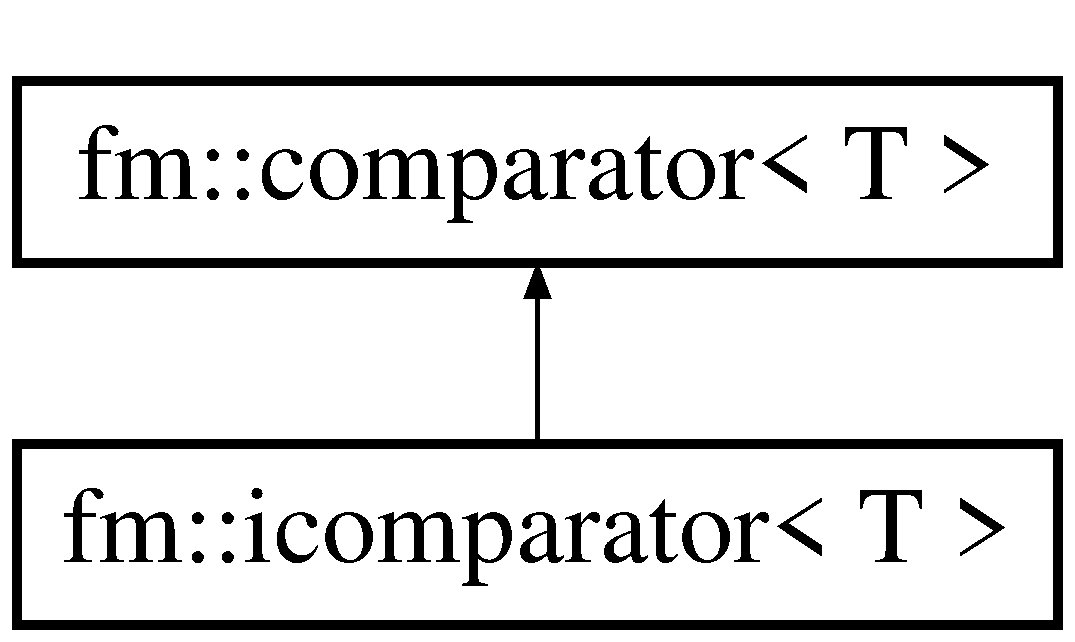
\includegraphics[height=2.000000cm]{classfm_1_1comparator}
\end{center}
\end{figure}
\subsection*{Public Member Functions}
\begin{DoxyCompactItemize}
\item 
virtual \hyperlink{classfm_1_1comparator_a08c191871b8d6e4a868571018d08cc6b}{$\sim$comparator} ()
\item 
virtual bool \hyperlink{classfm_1_1comparator_a4cc38737a2c598b76977625a75bc5c24}{compare} (const T \&a, const T \&b)
\item 
void \hyperlink{classfm_1_1comparator_abc9d0fddf1f79bd7028c519adf9f7908}{sort} (T $\ast$data, size\_\-t count)
\end{DoxyCompactItemize}


\subsection{Detailed Description}
\subsubsection*{template$<$class T$>$ class fm::comparator$<$ T $>$}

A utility to sort arrays. 

\subsection{Constructor \& Destructor Documentation}
\hypertarget{classfm_1_1comparator_a08c191871b8d6e4a868571018d08cc6b}{
\index{fm::comparator@{fm::comparator}!$\sim$comparator@{$\sim$comparator}}
\index{$\sim$comparator@{$\sim$comparator}!fm::comparator@{fm::comparator}}
\subsubsection[{$\sim$comparator}]{\setlength{\rightskip}{0pt plus 5cm}template$<$class T$>$ virtual {\bf fm::comparator}$<$ T $>$::$\sim${\bf comparator} (
\begin{DoxyParamCaption}
{}
\end{DoxyParamCaption}
)\hspace{0.3cm}{\ttfamily  \mbox{[}inline, virtual\mbox{]}}}}
\label{classfm_1_1comparator_a08c191871b8d6e4a868571018d08cc6b}
Destructor. 

\subsection{Member Function Documentation}
\hypertarget{classfm_1_1comparator_a4cc38737a2c598b76977625a75bc5c24}{
\index{fm::comparator@{fm::comparator}!compare@{compare}}
\index{compare@{compare}!fm::comparator@{fm::comparator}}
\subsubsection[{compare}]{\setlength{\rightskip}{0pt plus 5cm}template$<$class T$>$ virtual bool {\bf fm::comparator}$<$ T $>$::compare (
\begin{DoxyParamCaption}
\item[{const T \&}]{ a, }
\item[{const T \&}]{ b}
\end{DoxyParamCaption}
)\hspace{0.3cm}{\ttfamily  \mbox{[}inline, virtual\mbox{]}}}}
\label{classfm_1_1comparator_a4cc38737a2c598b76977625a75bc5c24}
Compares two elements in ascending order, using operator$<$. Override this function to define your custom comparator. 
\begin{DoxyParams}{Parameters}
\item[{\em a}]The first element. \item[{\em b}]The second element. \end{DoxyParams}
\begin{DoxyReturn}{Returns}
True if a is smaller than b, false otherwise. 
\end{DoxyReturn}


Reimplemented in \hyperlink{classfm_1_1icomparator_a8f1b1d5d8657fa5f852bf7b9437cefc9}{fm::icomparator$<$ T $>$}.

\hypertarget{classfm_1_1comparator_abc9d0fddf1f79bd7028c519adf9f7908}{
\index{fm::comparator@{fm::comparator}!sort@{sort}}
\index{sort@{sort}!fm::comparator@{fm::comparator}}
\subsubsection[{sort}]{\setlength{\rightskip}{0pt plus 5cm}template$<$class T$>$ void {\bf fm::comparator}$<$ T $>$::sort (
\begin{DoxyParamCaption}
\item[{T $\ast$}]{ data, }
\item[{size\_\-t}]{ count}
\end{DoxyParamCaption}
)\hspace{0.3cm}{\ttfamily  \mbox{[}inline\mbox{]}}}}
\label{classfm_1_1comparator_abc9d0fddf1f79bd7028c519adf9f7908}
Sorts the given array using the quick sort algorithm. 
\begin{DoxyParams}{Parameters}
\item[{\em data}]The data array to sort. \item[{\em count}]The number of elements in the array. \end{DoxyParams}


The documentation for this class was generated from the following file:\begin{DoxyCompactItemize}
\item 
FCollada/FMath/\hyperlink{FMSort_8h}{FMSort.h}\end{DoxyCompactItemize}

\hypertarget{classfm_1_1tree_1_1const__iterator}{
\section{fm::tree$<$ KEY, DATA $>$::const\_\-iterator Class Reference}
\label{classfm_1_1tree_1_1const__iterator}\index{fm::tree::const\_\-iterator@{fm::tree::const\_\-iterator}}
}


{\ttfamily \#include $<$FMTree.h$>$}

\subsection*{Public Member Functions}
\begin{DoxyCompactItemize}
\item 
\hyperlink{classfm_1_1tree_1_1const__iterator_aa330af47ca2bffdba07899258daf0795}{const\_\-iterator} ()
\item 
\hyperlink{classfm_1_1tree_1_1const__iterator_a39e90a1ec80e7f87f1876afc05a21817}{const\_\-iterator} (const \hyperlink{classfm_1_1tree_1_1iterator}{iterator} \&copy)
\item 
\hyperlink{classfm_1_1tree_1_1const__iterator_a3bfcb6528c87bd1bf1d85ef245b78bee}{const\_\-iterator} (const node $\ast$n)
\item 
\hyperlink{classfm_1_1tree_1_1const__iterator}{const\_\-iterator} \& \hyperlink{classfm_1_1tree_1_1const__iterator_ab53c0a7acec7c84eaf418ad05cb0fa63}{operator=} (const \hyperlink{classfm_1_1tree_1_1iterator}{iterator} \&copy)
\item 
\hyperlink{classfm_1_1tree_1_1const__iterator}{const\_\-iterator} \& \hyperlink{classfm_1_1tree_1_1const__iterator_ad965b6ad007ace833de30e6f5b75f671}{operator=} (const \hyperlink{classfm_1_1tree_1_1const__iterator}{const\_\-iterator} \&copy)
\item 
bool \hyperlink{classfm_1_1tree_1_1const__iterator_a46062effd7925af47181e924b23330fc}{operator==} (const \hyperlink{classfm_1_1tree_1_1iterator}{iterator} \&other) const 
\item 
bool \hyperlink{classfm_1_1tree_1_1const__iterator_abd27608fa704cd025477d313eb00294a}{operator==} (const \hyperlink{classfm_1_1tree_1_1const__iterator}{const\_\-iterator} \&other) const 
\item 
bool \hyperlink{classfm_1_1tree_1_1const__iterator_a86aff9854087ad1dc40afcbf00d5a7d7}{operator!=} (const \hyperlink{classfm_1_1tree_1_1iterator}{iterator} \&other) const 
\item 
bool \hyperlink{classfm_1_1tree_1_1const__iterator_a8241695495f324c6d56da516202a79c1}{operator!=} (const \hyperlink{classfm_1_1tree_1_1const__iterator}{const\_\-iterator} \&other) const 
\item 
\hyperlink{classfm_1_1tree_1_1const__iterator}{const\_\-iterator} \& \hyperlink{classfm_1_1tree_1_1const__iterator_ac94381e2cc1caccab3790483db4938be}{operator++} ()
\item 
\hyperlink{classfm_1_1tree_1_1const__iterator}{const\_\-iterator} \& \hyperlink{classfm_1_1tree_1_1const__iterator_a2eb6f5cf6ccc023fc757f413b4574799}{operator-\/-\/} ()
\item 
const \hyperlink{classfm_1_1pair}{pair} \& \hyperlink{classfm_1_1tree_1_1const__iterator_a8c1939090f9df91df5e6894439e0a9d7}{operator$\ast$} ()
\item 
const \hyperlink{classfm_1_1pair}{pair} $\ast$ \hyperlink{classfm_1_1tree_1_1const__iterator_a2f996de4cf03771fb8669994a72411bd}{operator-\/$>$} ()
\end{DoxyCompactItemize}
\subsection*{Friends}
\begin{DoxyCompactItemize}
\item 
\hypertarget{classfm_1_1tree_1_1const__iterator_a274b977404a53ceb91af64dfd96c9641}{
class {\bfseries tree}}
\label{classfm_1_1tree_1_1const__iterator_a274b977404a53ceb91af64dfd96c9641}

\item 
\hypertarget{classfm_1_1tree_1_1const__iterator_a67171474c4da6cc8efe0c7fafefd2b2d}{
class {\bfseries iterator}}
\label{classfm_1_1tree_1_1const__iterator_a67171474c4da6cc8efe0c7fafefd2b2d}

\end{DoxyCompactItemize}


\subsection{Detailed Description}
\subsubsection*{template$<$class KEY, class DATA$>$ class fm::tree$<$ KEY, DATA $>$::const\_\-iterator}

A tree constant-\/element iterator. Similar to the basic STL \hyperlink{classfm_1_1tree_1_1const__iterator}{const\_\-iterator}. 

\subsection{Constructor \& Destructor Documentation}
\hypertarget{classfm_1_1tree_1_1const__iterator_aa330af47ca2bffdba07899258daf0795}{
\index{fm::tree::const\_\-iterator@{fm::tree::const\_\-iterator}!const\_\-iterator@{const\_\-iterator}}
\index{const\_\-iterator@{const\_\-iterator}!fm::tree::const_iterator@{fm::tree::const\_\-iterator}}
\subsubsection[{const\_\-iterator}]{\setlength{\rightskip}{0pt plus 5cm}template$<$class KEY, class DATA$>$ {\bf fm::tree}$<$ KEY, DATA $>$::const\_\-iterator::const\_\-iterator (
\begin{DoxyParamCaption}
{}
\end{DoxyParamCaption}
)\hspace{0.3cm}{\ttfamily  \mbox{[}inline\mbox{]}}}}
\label{classfm_1_1tree_1_1const__iterator_aa330af47ca2bffdba07899258daf0795}
Empty constructor. \hypertarget{classfm_1_1tree_1_1const__iterator_a39e90a1ec80e7f87f1876afc05a21817}{
\index{fm::tree::const\_\-iterator@{fm::tree::const\_\-iterator}!const\_\-iterator@{const\_\-iterator}}
\index{const\_\-iterator@{const\_\-iterator}!fm::tree::const_iterator@{fm::tree::const\_\-iterator}}
\subsubsection[{const\_\-iterator}]{\setlength{\rightskip}{0pt plus 5cm}template$<$class KEY, class DATA$>$ {\bf fm::tree}$<$ KEY, DATA $>$::const\_\-iterator::const\_\-iterator (
\begin{DoxyParamCaption}
\item[{const {\bf iterator} \&}]{ copy}
\end{DoxyParamCaption}
)\hspace{0.3cm}{\ttfamily  \mbox{[}inline\mbox{]}}}}
\label{classfm_1_1tree_1_1const__iterator_a39e90a1ec80e7f87f1876afc05a21817}
Copy constructor. 
\begin{DoxyParams}{Parameters}
\item[{\em copy}]The iterator to clone. \end{DoxyParams}
\hypertarget{classfm_1_1tree_1_1const__iterator_a3bfcb6528c87bd1bf1d85ef245b78bee}{
\index{fm::tree::const\_\-iterator@{fm::tree::const\_\-iterator}!const\_\-iterator@{const\_\-iterator}}
\index{const\_\-iterator@{const\_\-iterator}!fm::tree::const_iterator@{fm::tree::const\_\-iterator}}
\subsubsection[{const\_\-iterator}]{\setlength{\rightskip}{0pt plus 5cm}template$<$class KEY, class DATA$>$ {\bf fm::tree}$<$ KEY, DATA $>$::const\_\-iterator::const\_\-iterator (
\begin{DoxyParamCaption}
\item[{const node $\ast$}]{ n}
\end{DoxyParamCaption}
)\hspace{0.3cm}{\ttfamily  \mbox{[}inline\mbox{]}}}}
\label{classfm_1_1tree_1_1const__iterator_a3bfcb6528c87bd1bf1d85ef245b78bee}
Constructor. 
\begin{DoxyParams}{Parameters}
\item[{\em n}]The tree node at which to start the iteration. \end{DoxyParams}


\subsection{Member Function Documentation}
\hypertarget{classfm_1_1tree_1_1const__iterator_a86aff9854087ad1dc40afcbf00d5a7d7}{
\index{fm::tree::const\_\-iterator@{fm::tree::const\_\-iterator}!operator!=@{operator!=}}
\index{operator!=@{operator!=}!fm::tree::const_iterator@{fm::tree::const\_\-iterator}}
\subsubsection[{operator!=}]{\setlength{\rightskip}{0pt plus 5cm}template$<$class KEY, class DATA$>$ bool {\bf fm::tree}$<$ KEY, DATA $>$::const\_\-iterator::operator!= (
\begin{DoxyParamCaption}
\item[{const {\bf iterator} \&}]{ other}
\end{DoxyParamCaption}
) const\hspace{0.3cm}{\ttfamily  \mbox{[}inline\mbox{]}}}}
\label{classfm_1_1tree_1_1const__iterator_a86aff9854087ad1dc40afcbf00d5a7d7}
Retrieves whether this iterator points to a different node that a given iterator. 
\begin{DoxyParams}{Parameters}
\item[{\em other}]A second iterator. \end{DoxyParams}
\begin{DoxyReturn}{Returns}
Whether the two iterators are pointing at different nodes. 
\end{DoxyReturn}
\hypertarget{classfm_1_1tree_1_1const__iterator_a8241695495f324c6d56da516202a79c1}{
\index{fm::tree::const\_\-iterator@{fm::tree::const\_\-iterator}!operator!=@{operator!=}}
\index{operator!=@{operator!=}!fm::tree::const_iterator@{fm::tree::const\_\-iterator}}
\subsubsection[{operator!=}]{\setlength{\rightskip}{0pt plus 5cm}template$<$class KEY, class DATA$>$ bool {\bf fm::tree}$<$ KEY, DATA $>$::const\_\-iterator::operator!= (
\begin{DoxyParamCaption}
\item[{const {\bf const\_\-iterator} \&}]{ other}
\end{DoxyParamCaption}
) const\hspace{0.3cm}{\ttfamily  \mbox{[}inline\mbox{]}}}}
\label{classfm_1_1tree_1_1const__iterator_a8241695495f324c6d56da516202a79c1}
See above. \hypertarget{classfm_1_1tree_1_1const__iterator_a8c1939090f9df91df5e6894439e0a9d7}{
\index{fm::tree::const\_\-iterator@{fm::tree::const\_\-iterator}!operator$\ast$@{operator$\ast$}}
\index{operator$\ast$@{operator$\ast$}!fm::tree::const_iterator@{fm::tree::const\_\-iterator}}
\subsubsection[{operator$\ast$}]{\setlength{\rightskip}{0pt plus 5cm}template$<$class KEY, class DATA$>$ const {\bf pair}\& {\bf fm::tree}$<$ KEY, DATA $>$::const\_\-iterator::operator$\ast$ (
\begin{DoxyParamCaption}
{}
\end{DoxyParamCaption}
)\hspace{0.3cm}{\ttfamily  \mbox{[}inline\mbox{]}}}}
\label{classfm_1_1tree_1_1const__iterator_a8c1939090f9df91df5e6894439e0a9d7}
Retrieves the current tree node. \begin{DoxyReturn}{Returns}
The current tree node. 
\end{DoxyReturn}
\hypertarget{classfm_1_1tree_1_1const__iterator_ac94381e2cc1caccab3790483db4938be}{
\index{fm::tree::const\_\-iterator@{fm::tree::const\_\-iterator}!operator++@{operator++}}
\index{operator++@{operator++}!fm::tree::const_iterator@{fm::tree::const\_\-iterator}}
\subsubsection[{operator++}]{\setlength{\rightskip}{0pt plus 5cm}template$<$class KEY, class DATA$>$ {\bf const\_\-iterator}\& {\bf fm::tree}$<$ KEY, DATA $>$::const\_\-iterator::operator++ (
\begin{DoxyParamCaption}
{}
\end{DoxyParamCaption}
)\hspace{0.3cm}{\ttfamily  \mbox{[}inline\mbox{]}}}}
\label{classfm_1_1tree_1_1const__iterator_ac94381e2cc1caccab3790483db4938be}
Advances the iterator to the next ordered tree node. \begin{DoxyReturn}{Returns}
This iterator. 
\end{DoxyReturn}
\hypertarget{classfm_1_1tree_1_1const__iterator_a2eb6f5cf6ccc023fc757f413b4574799}{
\index{fm::tree::const\_\-iterator@{fm::tree::const\_\-iterator}!operator-\/-\/@{operator-\/-\/}}
\index{operator-\/-\/@{operator-\/-\/}!fm::tree::const_iterator@{fm::tree::const\_\-iterator}}
\subsubsection[{operator-\/-\/}]{\setlength{\rightskip}{0pt plus 5cm}template$<$class KEY, class DATA$>$ {\bf const\_\-iterator}\& {\bf fm::tree}$<$ KEY, DATA $>$::const\_\-iterator::operator-\/-\/ (
\begin{DoxyParamCaption}
{}
\end{DoxyParamCaption}
)\hspace{0.3cm}{\ttfamily  \mbox{[}inline\mbox{]}}}}
\label{classfm_1_1tree_1_1const__iterator_a2eb6f5cf6ccc023fc757f413b4574799}
Backtrack the iterator to the next ordered tree node. \begin{DoxyReturn}{Returns}
This iterator. 
\end{DoxyReturn}
\hypertarget{classfm_1_1tree_1_1const__iterator_a2f996de4cf03771fb8669994a72411bd}{
\index{fm::tree::const\_\-iterator@{fm::tree::const\_\-iterator}!operator-\/$>$@{operator-\/$>$}}
\index{operator-\/$>$@{operator-\/$>$}!fm::tree::const_iterator@{fm::tree::const\_\-iterator}}
\subsubsection[{operator-\/$>$}]{\setlength{\rightskip}{0pt plus 5cm}template$<$class KEY, class DATA$>$ const {\bf pair}$\ast$ {\bf fm::tree}$<$ KEY, DATA $>$::const\_\-iterator::operator-\/$>$ (
\begin{DoxyParamCaption}
{}
\end{DoxyParamCaption}
)\hspace{0.3cm}{\ttfamily  \mbox{[}inline\mbox{]}}}}
\label{classfm_1_1tree_1_1const__iterator_a2f996de4cf03771fb8669994a72411bd}
See above. \hypertarget{classfm_1_1tree_1_1const__iterator_ab53c0a7acec7c84eaf418ad05cb0fa63}{
\index{fm::tree::const\_\-iterator@{fm::tree::const\_\-iterator}!operator=@{operator=}}
\index{operator=@{operator=}!fm::tree::const_iterator@{fm::tree::const\_\-iterator}}
\subsubsection[{operator=}]{\setlength{\rightskip}{0pt plus 5cm}template$<$class KEY, class DATA$>$ {\bf const\_\-iterator}\& {\bf fm::tree}$<$ KEY, DATA $>$::const\_\-iterator::operator= (
\begin{DoxyParamCaption}
\item[{const {\bf iterator} \&}]{ copy}
\end{DoxyParamCaption}
)\hspace{0.3cm}{\ttfamily  \mbox{[}inline\mbox{]}}}}
\label{classfm_1_1tree_1_1const__iterator_ab53c0a7acec7c84eaf418ad05cb0fa63}
Copy operator. 
\begin{DoxyParams}{Parameters}
\item[{\em copy}]The tree iterator to copy. \end{DoxyParams}
\hypertarget{classfm_1_1tree_1_1const__iterator_ad965b6ad007ace833de30e6f5b75f671}{
\index{fm::tree::const\_\-iterator@{fm::tree::const\_\-iterator}!operator=@{operator=}}
\index{operator=@{operator=}!fm::tree::const_iterator@{fm::tree::const\_\-iterator}}
\subsubsection[{operator=}]{\setlength{\rightskip}{0pt plus 5cm}template$<$class KEY, class DATA$>$ {\bf const\_\-iterator}\& {\bf fm::tree}$<$ KEY, DATA $>$::const\_\-iterator::operator= (
\begin{DoxyParamCaption}
\item[{const {\bf const\_\-iterator} \&}]{ copy}
\end{DoxyParamCaption}
)\hspace{0.3cm}{\ttfamily  \mbox{[}inline\mbox{]}}}}
\label{classfm_1_1tree_1_1const__iterator_ad965b6ad007ace833de30e6f5b75f671}
See above. \hypertarget{classfm_1_1tree_1_1const__iterator_a46062effd7925af47181e924b23330fc}{
\index{fm::tree::const\_\-iterator@{fm::tree::const\_\-iterator}!operator==@{operator==}}
\index{operator==@{operator==}!fm::tree::const_iterator@{fm::tree::const\_\-iterator}}
\subsubsection[{operator==}]{\setlength{\rightskip}{0pt plus 5cm}template$<$class KEY, class DATA$>$ bool {\bf fm::tree}$<$ KEY, DATA $>$::const\_\-iterator::operator== (
\begin{DoxyParamCaption}
\item[{const {\bf iterator} \&}]{ other}
\end{DoxyParamCaption}
) const\hspace{0.3cm}{\ttfamily  \mbox{[}inline\mbox{]}}}}
\label{classfm_1_1tree_1_1const__iterator_a46062effd7925af47181e924b23330fc}
Retrieves whether this iterator points to the same node as the given iterator. 
\begin{DoxyParams}{Parameters}
\item[{\em other}]A second iterator. \end{DoxyParams}
\begin{DoxyReturn}{Returns}
Whether the two iterators are pointing to the same node. 
\end{DoxyReturn}
\hypertarget{classfm_1_1tree_1_1const__iterator_abd27608fa704cd025477d313eb00294a}{
\index{fm::tree::const\_\-iterator@{fm::tree::const\_\-iterator}!operator==@{operator==}}
\index{operator==@{operator==}!fm::tree::const_iterator@{fm::tree::const\_\-iterator}}
\subsubsection[{operator==}]{\setlength{\rightskip}{0pt plus 5cm}template$<$class KEY, class DATA$>$ bool {\bf fm::tree}$<$ KEY, DATA $>$::const\_\-iterator::operator== (
\begin{DoxyParamCaption}
\item[{const {\bf const\_\-iterator} \&}]{ other}
\end{DoxyParamCaption}
) const\hspace{0.3cm}{\ttfamily  \mbox{[}inline\mbox{]}}}}
\label{classfm_1_1tree_1_1const__iterator_abd27608fa704cd025477d313eb00294a}
See above. 

The documentation for this class was generated from the following file:\begin{DoxyCompactItemize}
\item 
FCollada/FMath/\hyperlink{FMTree_8h}{FMTree.h}\end{DoxyCompactItemize}

\hypertarget{classfm_1_1DefaultInitializationAllocate}{
\section{fm::DefaultInitializationAllocate Class Reference}
\label{classfm_1_1DefaultInitializationAllocate}\index{fm::DefaultInitializationAllocate@{fm::DefaultInitializationAllocate}}
}


The documentation for this class was generated from the following file:\begin{DoxyCompactItemize}
\item 
FCollada/FMath/FMAllocator.cpp\end{DoxyCompactItemize}

\hypertarget{classfm_1_1DefaultInitializationRelease}{
\section{fm::DefaultInitializationRelease Class Reference}
\label{classfm_1_1DefaultInitializationRelease}\index{fm::DefaultInitializationRelease@{fm::DefaultInitializationRelease}}
}


The documentation for this class was generated from the following file:\begin{DoxyCompactItemize}
\item 
FCollada/FMath/FMAllocator.cpp\end{DoxyCompactItemize}

\hypertarget{classFArchiveXML}{
\section{FArchiveXML Class Reference}
\label{classFArchiveXML}\index{FArchiveXML@{FArchiveXML}}
}
Inheritance diagram for FArchiveXML:\begin{figure}[H]
\begin{center}
\leavevmode
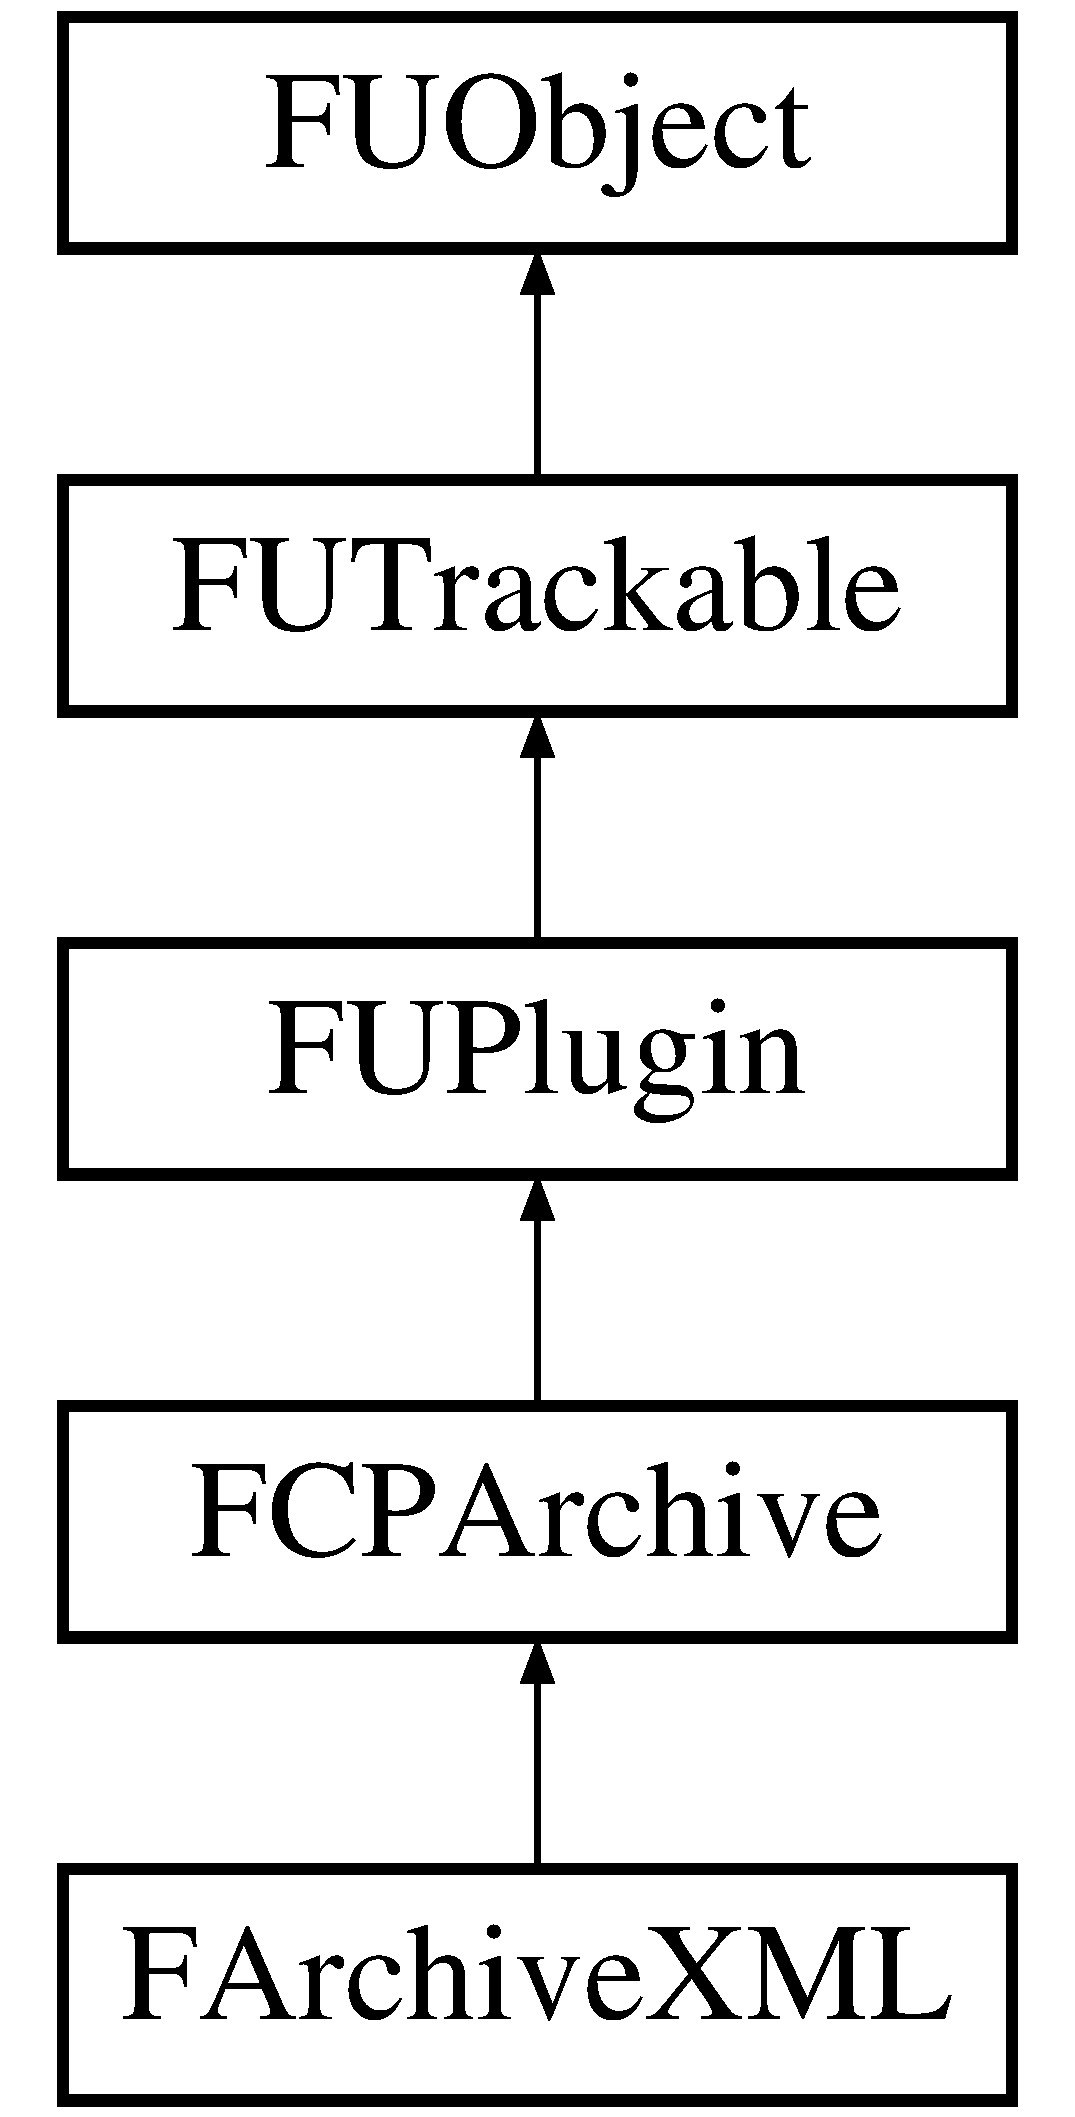
\includegraphics[height=5.000000cm]{classFArchiveXML}
\end{center}
\end{figure}
\subsection*{Public Member Functions}
\begin{DoxyCompactItemize}
\item 
virtual bool \hyperlink{classFArchiveXML_afaeaeb4ee3cd75bac1ad6a4c54c9b899}{IsImportSupported} ()
\item 
virtual bool \hyperlink{classFArchiveXML_adb1efee2caed4402a02dd20af432e5ef}{IsExportSupported} ()
\item 
virtual bool \hyperlink{classFArchiveXML_ad35bb5dd5d901c86edf794dda76bfc4d}{IsPartialExportSupported} ()
\item 
virtual bool \hyperlink{classFArchiveXML_a17673f93728bb30dedd2791473c4b14e}{IsExtensionSupported} (const char $\ast$ext)
\item 
virtual int \hyperlink{classFArchiveXML_a0547ef1565f6543319b9aaad3eca8697}{GetSupportedExtensionsCount} ()
\item 
virtual const char $\ast$ \hyperlink{classFArchiveXML_a3908cc84df654da0ded836afcfd7fab8}{GetSupportedExtensionAt} (int index)
\item 
virtual bool \hyperlink{classFArchiveXML_adb22e0884d6059ded32d194a8cdde4dc}{AddExtraExtension} (const char $\ast$ext)
\item 
virtual bool \hyperlink{classFArchiveXML_ad1e57b1a3067f88738ee7a2f0e6fc9ca}{RemoveExtraExtension} (const char $\ast$ext)
\item 
virtual bool \hyperlink{classFArchiveXML_a10bc809b2a64d9df0cd83742bf0dc49a}{ImportFile} (const fchar $\ast$filePath, \hyperlink{classFCDocument}{FCDocument} $\ast$fcdocument)
\item 
virtual bool \hyperlink{classFArchiveXML_a5a85deaaf25379ea56b30d5a602ae949}{ImportFileFromMemory} (const fchar $\ast$filePath, \hyperlink{classFCDocument}{FCDocument} $\ast$fcdocument, const void $\ast$contents, size\_\-t length)
\item 
virtual bool \hyperlink{classFArchiveXML_ab7c6e1fab043617e8e6adebf947dcf7e}{ExportFile} (\hyperlink{classFCDocument}{FCDocument} $\ast$fcdocument, const fchar $\ast$filePath)
\item 
virtual bool \hyperlink{classFArchiveXML_a485fad9bad65ed0e6512f9713223982f}{StartExport} (const fchar $\ast$absoluteFilePath)
\item 
virtual bool \hyperlink{classFArchiveXML_a36eff362143c86cae961237d4923a35a}{ExportObject} (\hyperlink{classFCDObject}{FCDObject} $\ast$object)
\item 
virtual bool \hyperlink{classFArchiveXML_a877083fc6c055f24042dd50103fb00a4}{EndExport} (\hyperlink{classfm_1_1vector}{fm::vector}$<$ uint8 $>$ \&outData)
\item 
virtual bool \hyperlink{classFArchiveXML_a19693477bc5410a640105cec37febdb6}{EndExport} (const fchar $\ast$filePath)
\item 
virtual bool \hyperlink{classFArchiveXML_a323f1807851e536b1c46f7583303518e}{ImportObject} (\hyperlink{classFCDObject}{FCDObject} $\ast$object, const \hyperlink{classfm_1_1vector}{fm::vector}$<$ uint8 $>$ \&data)
\item 
virtual const char $\ast$ \hyperlink{classFArchiveXML_abd9ac092eff78dbc8f8249fa402fe644}{GetPluginName} () const 
\item 
virtual uint32 \hyperlink{classFArchiveXML_a2fb1d4d2d6d862e023d8510ea404bd60}{GetPluginVersion} () const 
\item 
bool \hyperlink{classFArchiveXML_a31a7807261de79f1f8b9e539e7dff0ea}{Import} (\hyperlink{classFCDocument}{FCDocument} $\ast$theDocument, xmlNode $\ast$colladaNode)
\item 
bool \hyperlink{classFArchiveXML_a924a76fcef59b49c82ce323badbcc469}{ExportDocument} (\hyperlink{classFCDocument}{FCDocument} $\ast$theDocument, xmlNode $\ast$colladaNode)
\end{DoxyCompactItemize}
\subsection*{Static Public Member Functions}
\begin{DoxyCompactItemize}
\item 
static void \hyperlink{classFArchiveXML_a9058483d29253567c3bbaa9e557e38b1}{Initialize} ()
\item 
static void \hyperlink{classFArchiveXML_ad9be9f3803f77996d7b155f2110a7105}{ClearIntermediateData} ()
\item 
static bool \hyperlink{classFArchiveXML_a6cc3fc2e4e1415c3c411a38f978c77ae}{LoadSwitch} (\hyperlink{classFCDObject}{FCDObject} $\ast$object, const \hyperlink{classFUObjectType}{FUObjectType} $\ast$objectType, xmlNode $\ast$node)
\item 
static xmlNode $\ast$ \hyperlink{classFArchiveXML_aaf83155ae7183ba1b4b485fdd239c483}{WriteSwitch} (\hyperlink{classFCDObject}{FCDObject} $\ast$object, const \hyperlink{classFUObjectType}{FUObjectType} $\ast$objectType, xmlNode $\ast$parentNode)
\item 
static xmlNode $\ast$ \hyperlink{classFArchiveXML_a2b455f62993fdcc77200439fb917748e}{WriteParentSwitch} (\hyperlink{classFCDObject}{FCDObject} $\ast$object, const \hyperlink{classFUObjectType}{FUObjectType} $\ast$objectType, xmlNode $\ast$parentNode)
\item 
static bool \hyperlink{classFArchiveXML_a262d6014344ef77f716e08e4149d4c16}{LoadObject} (\hyperlink{classFCDObject}{FCDObject} $\ast$object, xmlNode $\ast$node)
\item 
\hypertarget{classFArchiveXML_a1b7970ad7bb676ad4589adc156d0f49c}{
static bool {\bfseries LoadExtra} (\hyperlink{classFCDObject}{FCDObject} $\ast$object, xmlNode $\ast$node)}
\label{classFArchiveXML_a1b7970ad7bb676ad4589adc156d0f49c}

\item 
\hypertarget{classFArchiveXML_a535909ab9a6ad15b14db6a0496d505e6}{
static bool {\bfseries LoadExtraNode} (\hyperlink{classFCDObject}{FCDObject} $\ast$object, xmlNode $\ast$node)}
\label{classFArchiveXML_a535909ab9a6ad15b14db6a0496d505e6}

\item 
\hypertarget{classFArchiveXML_a53dcee9d989ad31d7b18c5a993988421}{
static bool {\bfseries LoadExtraTechnique} (\hyperlink{classFCDObject}{FCDObject} $\ast$object, xmlNode $\ast$node)}
\label{classFArchiveXML_a53dcee9d989ad31d7b18c5a993988421}

\item 
\hypertarget{classFArchiveXML_a42482076998e2198f9a0425ff8dcc6dc}{
static bool {\bfseries LoadExtraType} (\hyperlink{classFCDObject}{FCDObject} $\ast$object, xmlNode $\ast$node)}
\label{classFArchiveXML_a42482076998e2198f9a0425ff8dcc6dc}

\item 
\hypertarget{classFArchiveXML_a5a49f5747b16985482ddc172fc81b734}{
static bool {\bfseries LoadScene} (\hyperlink{classFCDObject}{FCDObject} $\ast$object, xmlNode $\ast$node)}
\label{classFArchiveXML_a5a49f5747b16985482ddc172fc81b734}

\item 
\hypertarget{classFArchiveXML_a875e91a66a9b40641d083af3e8c9fe1b}{
static bool {\bfseries LoadAsset} (\hyperlink{classFCDObject}{FCDObject} $\ast$object, xmlNode $\ast$node)}
\label{classFArchiveXML_a875e91a66a9b40641d083af3e8c9fe1b}

\item 
\hypertarget{classFArchiveXML_a367c11921b7c1537718047064d1e5ffe}{
static bool {\bfseries LoadAssetContributor} (\hyperlink{classFCDObject}{FCDObject} $\ast$object, xmlNode $\ast$node)}
\label{classFArchiveXML_a367c11921b7c1537718047064d1e5ffe}

\item 
\hypertarget{classFArchiveXML_a8cadc7aba5cbef80ba1e0a05d566abdd}{
static bool {\bfseries LoadEntityReference} (\hyperlink{classFCDObject}{FCDObject} $\ast$object, xmlNode $\ast$node)}
\label{classFArchiveXML_a8cadc7aba5cbef80ba1e0a05d566abdd}

\item 
\hypertarget{classFArchiveXML_a957566c1300a2ab443077fb3cc554387}{
static bool {\bfseries LoadExternalReferenceManager} (\hyperlink{classFCDObject}{FCDObject} $\ast$object, xmlNode $\ast$node)}
\label{classFArchiveXML_a957566c1300a2ab443077fb3cc554387}

\item 
\hypertarget{classFArchiveXML_a6f9aa794147a5c59286711fe7245586a}{
static bool {\bfseries LoadPlaceHolder} (\hyperlink{classFCDObject}{FCDObject} $\ast$object, xmlNode $\ast$node)}
\label{classFArchiveXML_a6f9aa794147a5c59286711fe7245586a}

\item 
\hypertarget{classFArchiveXML_aad15689fbfca61712581151d2acb598e}{
static void {\bfseries FindAnimationChannelsArrayIndices} (\hyperlink{classFCDocument}{FCDocument} $\ast$fcdocument, xmlNode $\ast$targetArray, \hyperlink{classfm_1_1vector}{Int32List} \&animatedIndices)}
\label{classFArchiveXML_aad15689fbfca61712581151d2acb598e}

\item 
\hypertarget{classFArchiveXML_a114e99422f7d398d7f59b21439cebe9e}{
static void {\bfseries RegisterLoadedDocument} (\hyperlink{classFCDocument}{FCDocument} $\ast$document)}
\label{classFArchiveXML_a114e99422f7d398d7f59b21439cebe9e}

\item 
\hypertarget{classFArchiveXML_a44ed8a9ade24b76a36fa20f875d31afc}{
static bool {\bfseries LoadEntity} (\hyperlink{classFCDObject}{FCDObject} $\ast$object, xmlNode $\ast$node)}
\label{classFArchiveXML_a44ed8a9ade24b76a36fa20f875d31afc}

\item 
\hypertarget{classFArchiveXML_ada4170520a4eb94ea5259c952c48c69b}{
static bool {\bfseries LoadTargetedEntity} (\hyperlink{classFCDObject}{FCDObject} $\ast$object, xmlNode $\ast$node)}
\label{classFArchiveXML_ada4170520a4eb94ea5259c952c48c69b}

\item 
\hypertarget{classFArchiveXML_a487520c0383bf2beccbe4ed9b47ea358}{
static bool {\bfseries LoadSceneNode} (\hyperlink{classFCDObject}{FCDObject} $\ast$object, xmlNode $\ast$node)}
\label{classFArchiveXML_a487520c0383bf2beccbe4ed9b47ea358}

\item 
\hypertarget{classFArchiveXML_aca9add5b61e4ccc0e22be9a2038b4352}{
static bool {\bfseries LoadTransform} (\hyperlink{classFCDObject}{FCDObject} $\ast$object, xmlNode $\ast$node)}
\label{classFArchiveXML_aca9add5b61e4ccc0e22be9a2038b4352}

\item 
\hypertarget{classFArchiveXML_a1169d63ba7a5e2afec67d3582f3093e1}{
static bool {\bfseries LoadTransformLookAt} (\hyperlink{classFCDObject}{FCDObject} $\ast$object, xmlNode $\ast$node)}
\label{classFArchiveXML_a1169d63ba7a5e2afec67d3582f3093e1}

\item 
\hypertarget{classFArchiveXML_a11bf1d14aa206adfd006733ad7e5015a}{
static bool {\bfseries LoadTransformMatrix} (\hyperlink{classFCDObject}{FCDObject} $\ast$object, xmlNode $\ast$node)}
\label{classFArchiveXML_a11bf1d14aa206adfd006733ad7e5015a}

\item 
\hypertarget{classFArchiveXML_a446646e0da33d48808c83018dfc9efdf}{
static bool {\bfseries LoadTransformRotation} (\hyperlink{classFCDObject}{FCDObject} $\ast$object, xmlNode $\ast$node)}
\label{classFArchiveXML_a446646e0da33d48808c83018dfc9efdf}

\item 
\hypertarget{classFArchiveXML_abfd157c5d4f7569b81d84b7c493aa4e4}{
static bool {\bfseries LoadTransformScale} (\hyperlink{classFCDObject}{FCDObject} $\ast$object, xmlNode $\ast$node)}
\label{classFArchiveXML_abfd157c5d4f7569b81d84b7c493aa4e4}

\item 
\hypertarget{classFArchiveXML_a53c5e477e3f94544e64e8d5ab4beca3b}{
static bool {\bfseries LoadTransformSkew} (\hyperlink{classFCDObject}{FCDObject} $\ast$object, xmlNode $\ast$node)}
\label{classFArchiveXML_a53c5e477e3f94544e64e8d5ab4beca3b}

\item 
\hypertarget{classFArchiveXML_ab61719bd09628e5162b71a9b799b869b}{
static bool {\bfseries LoadTransformTranslation} (\hyperlink{classFCDObject}{FCDObject} $\ast$object, xmlNode $\ast$node)}
\label{classFArchiveXML_ab61719bd09628e5162b71a9b799b869b}

\item 
\hypertarget{classFArchiveXML_aed27eb532121fbeaf0d39c0ce5f5ff00}{
static bool {\bfseries LoadFromExtraSceneNode} (\hyperlink{classFCDSceneNode}{FCDSceneNode} $\ast$sceneNode)}
\label{classFArchiveXML_aed27eb532121fbeaf0d39c0ce5f5ff00}

\item 
\hypertarget{classFArchiveXML_a260ad693ec5a2cb70aef89db90f5ab60}{
static uint32 {\bfseries GetTransformType} (xmlNode $\ast$node)}
\label{classFArchiveXML_a260ad693ec5a2cb70aef89db90f5ab60}

\item 
\hypertarget{classFArchiveXML_a92f8ac29a7828b5a7d4084321463912d}{
static bool {\bfseries LoadController} (\hyperlink{classFCDObject}{FCDObject} $\ast$object, xmlNode $\ast$node)}
\label{classFArchiveXML_a92f8ac29a7828b5a7d4084321463912d}

\item 
\hypertarget{classFArchiveXML_a34c3cb5de48205da989e7755c2ffdc78}{
static bool {\bfseries LoadSkinController} (\hyperlink{classFCDObject}{FCDObject} $\ast$object, xmlNode $\ast$node)}
\label{classFArchiveXML_a34c3cb5de48205da989e7755c2ffdc78}

\item 
\hypertarget{classFArchiveXML_a7b81e68b09f6269713d4c9fe2ada5f43}{
static bool {\bfseries LoadMorphController} (\hyperlink{classFCDObject}{FCDObject} $\ast$object, xmlNode $\ast$node)}
\label{classFArchiveXML_a7b81e68b09f6269713d4c9fe2ada5f43}

\item 
\hypertarget{classFArchiveXML_a98489c2838a3d4eb96a4f04824081edb}{
static \hyperlink{classFCDSkinController}{FCDSkinController} $\ast$ {\bfseries FindSkinController} (\hyperlink{classFCDControllerInstance}{FCDControllerInstance} $\ast$controllerInstance, \hyperlink{classFCDEntity}{FCDEntity} $\ast$entity)}
\label{classFArchiveXML_a98489c2838a3d4eb96a4f04824081edb}

\item 
\hypertarget{classFArchiveXML_a900937020ac203ca5350ba3caadc7d28}{
static bool {\bfseries LoadEntityInstance} (\hyperlink{classFCDObject}{FCDObject} $\ast$object, xmlNode $\ast$node)}
\label{classFArchiveXML_a900937020ac203ca5350ba3caadc7d28}

\item 
\hypertarget{classFArchiveXML_ae91329905ec5e6b5a3e07b3ab6b0597c}{
static bool {\bfseries LoadEmitterInstance} (\hyperlink{classFCDObject}{FCDObject} $\ast$object, xmlNode $\ast$node)}
\label{classFArchiveXML_ae91329905ec5e6b5a3e07b3ab6b0597c}

\item 
\hypertarget{classFArchiveXML_a09864f68aba557a580a42d6b0091d121}{
static bool {\bfseries LoadGeometryInstance} (\hyperlink{classFCDObject}{FCDObject} $\ast$object, xmlNode $\ast$node)}
\label{classFArchiveXML_a09864f68aba557a580a42d6b0091d121}

\item 
\hypertarget{classFArchiveXML_a0a00cd269234eb419f4cd6a66854afad}{
static bool {\bfseries LoadControllerInstance} (\hyperlink{classFCDObject}{FCDObject} $\ast$object, xmlNode $\ast$node)}
\label{classFArchiveXML_a0a00cd269234eb419f4cd6a66854afad}

\item 
\hypertarget{classFArchiveXML_a8cacba7e220337fafb9af191769ef8ef}{
static bool {\bfseries LoadMaterialInstance} (\hyperlink{classFCDObject}{FCDObject} $\ast$object, xmlNode $\ast$node)}
\label{classFArchiveXML_a8cacba7e220337fafb9af191769ef8ef}

\item 
\hypertarget{classFArchiveXML_a1bdb975b6666fe700a24d6e31d1b02f6}{
static bool {\bfseries LoadPhysicsForceFieldInstance} (\hyperlink{classFCDObject}{FCDObject} $\ast$object, xmlNode $\ast$node)}
\label{classFArchiveXML_a1bdb975b6666fe700a24d6e31d1b02f6}

\item 
\hypertarget{classFArchiveXML_a601db1bc80cc144e179fef96dd82f6dc}{
static bool {\bfseries LoadPhysicsModelInstance} (\hyperlink{classFCDObject}{FCDObject} $\ast$object, xmlNode $\ast$node)}
\label{classFArchiveXML_a601db1bc80cc144e179fef96dd82f6dc}

\item 
\hypertarget{classFArchiveXML_a844e802b67f84ad81301a339e76d3b7b}{
static bool {\bfseries LoadPhysicsRigidBodyInstance} (\hyperlink{classFCDObject}{FCDObject} $\ast$object, xmlNode $\ast$node)}
\label{classFArchiveXML_a844e802b67f84ad81301a339e76d3b7b}

\item 
\hypertarget{classFArchiveXML_a23d938ee0bf9e6a2b017646b639fee68}{
static bool {\bfseries LoadPhysicsRigidConstraintInstance} (\hyperlink{classFCDObject}{FCDObject} $\ast$object, xmlNode $\ast$node)}
\label{classFArchiveXML_a23d938ee0bf9e6a2b017646b639fee68}

\item 
\hypertarget{classFArchiveXML_aa02dcab5cfd175401750a05d992e1d2b}{
static bool {\bfseries LinkControllerInstance} (\hyperlink{classFCDControllerInstance}{FCDControllerInstance} $\ast$controllerInstance)}
\label{classFArchiveXML_aa02dcab5cfd175401750a05d992e1d2b}

\item 
\hypertarget{classFArchiveXML_a1c77296a350a216bafcd5275447d58fd}{
static bool {\bfseries LinkEmitterInstance} (\hyperlink{classFCDEmitterInstance}{FCDEmitterInstance} $\ast$emitterInstance)}
\label{classFArchiveXML_a1c77296a350a216bafcd5275447d58fd}

\item 
\hypertarget{classFArchiveXML_aa8f1c68e99ccbe83af81a014d7b81fb3}{
static bool {\bfseries ImportEmittedInstanceList} (\hyperlink{classFCDEmitterInstance}{FCDEmitterInstance} $\ast$emitterInstance, xmlNode $\ast$node)}
\label{classFArchiveXML_aa8f1c68e99ccbe83af81a014d7b81fb3}

\item 
\hypertarget{classFArchiveXML_a55429934b31d562678dbe3b6750785b7}{
static uint32 {\bfseries GetEntityInstanceType} (xmlNode $\ast$node)}
\label{classFArchiveXML_a55429934b31d562678dbe3b6750785b7}

\item 
\hypertarget{classFArchiveXML_a78515848c51397e3eb41b95a97eea267}{
static bool {\bfseries LoadMaterial} (\hyperlink{classFCDObject}{FCDObject} $\ast$object, xmlNode $\ast$node)}
\label{classFArchiveXML_a78515848c51397e3eb41b95a97eea267}

\item 
\hypertarget{classFArchiveXML_a24d260139664a8ebfd6c03867ac8fef1}{
static bool {\bfseries LoadEffectCode} (\hyperlink{classFCDObject}{FCDObject} $\ast$object, xmlNode $\ast$node)}
\label{classFArchiveXML_a24d260139664a8ebfd6c03867ac8fef1}

\item 
\hypertarget{classFArchiveXML_a6efa928ba5a0471fc33f9b7623ace940}{
static bool {\bfseries LoadEffectParameter} (\hyperlink{classFCDObject}{FCDObject} $\ast$object, xmlNode $\ast$node)}
\label{classFArchiveXML_a6efa928ba5a0471fc33f9b7623ace940}

\item 
\hypertarget{classFArchiveXML_a29c3f291898ca121df019ba96562c972}{
static bool {\bfseries LoadEffectParameterBool} (\hyperlink{classFCDObject}{FCDObject} $\ast$object, xmlNode $\ast$node)}
\label{classFArchiveXML_a29c3f291898ca121df019ba96562c972}

\item 
\hypertarget{classFArchiveXML_a96bc1c1dbd9288ab5d0ab53bf332744e}{
static bool {\bfseries LoadEffectParameterFloat} (\hyperlink{classFCDObject}{FCDObject} $\ast$object, xmlNode $\ast$node)}
\label{classFArchiveXML_a96bc1c1dbd9288ab5d0ab53bf332744e}

\item 
\hypertarget{classFArchiveXML_a2823a5559af325bd967dd88c6d1951d3}{
static bool {\bfseries LoadEffectParameterFloat2} (\hyperlink{classFCDObject}{FCDObject} $\ast$object, xmlNode $\ast$node)}
\label{classFArchiveXML_a2823a5559af325bd967dd88c6d1951d3}

\item 
\hypertarget{classFArchiveXML_a305287ced718d4dc17e5601ffbb1fcec}{
static bool {\bfseries LoadEffectParameterFloat3} (\hyperlink{classFCDObject}{FCDObject} $\ast$object, xmlNode $\ast$node)}
\label{classFArchiveXML_a305287ced718d4dc17e5601ffbb1fcec}

\item 
\hypertarget{classFArchiveXML_af963cd0c755b4111dfcbf7a04a592e6c}{
static bool {\bfseries LoadEffectParameterInt} (\hyperlink{classFCDObject}{FCDObject} $\ast$object, xmlNode $\ast$node)}
\label{classFArchiveXML_af963cd0c755b4111dfcbf7a04a592e6c}

\item 
\hypertarget{classFArchiveXML_a382fcc2676fa9c3d221fb360af796103}{
static bool {\bfseries LoadEffectParameterMatrix} (\hyperlink{classFCDObject}{FCDObject} $\ast$object, xmlNode $\ast$node)}
\label{classFArchiveXML_a382fcc2676fa9c3d221fb360af796103}

\item 
\hypertarget{classFArchiveXML_ac117edb1dbd423e36e2c16f0a0436e49}{
static bool {\bfseries LoadEffectParameterSampler} (\hyperlink{classFCDObject}{FCDObject} $\ast$object, xmlNode $\ast$node)}
\label{classFArchiveXML_ac117edb1dbd423e36e2c16f0a0436e49}

\item 
\hypertarget{classFArchiveXML_a09d5269f821f5200d9d62c9393a66975}{
static bool {\bfseries LoadEffectParameterString} (\hyperlink{classFCDObject}{FCDObject} $\ast$object, xmlNode $\ast$node)}
\label{classFArchiveXML_a09d5269f821f5200d9d62c9393a66975}

\item 
\hypertarget{classFArchiveXML_ac507675658747c50aa09c93df518b500}{
static bool {\bfseries LoadEffectParameterSurface} (\hyperlink{classFCDObject}{FCDObject} $\ast$object, xmlNode $\ast$node)}
\label{classFArchiveXML_ac507675658747c50aa09c93df518b500}

\item 
\hypertarget{classFArchiveXML_a6696c767cda5cf04eee1535b776af176}{
static bool {\bfseries LoadEffectParameterVector} (\hyperlink{classFCDObject}{FCDObject} $\ast$object, xmlNode $\ast$node)}
\label{classFArchiveXML_a6696c767cda5cf04eee1535b776af176}

\item 
\hypertarget{classFArchiveXML_a2251423924d3c0353a07abc15b494297}{
static bool {\bfseries LoadEffectPass} (\hyperlink{classFCDObject}{FCDObject} $\ast$object, xmlNode $\ast$node)}
\label{classFArchiveXML_a2251423924d3c0353a07abc15b494297}

\item 
\hypertarget{classFArchiveXML_a019160d91b921e4a8b2a16310044df3f}{
static bool {\bfseries LoadEffectPassShader} (\hyperlink{classFCDObject}{FCDObject} $\ast$object, xmlNode $\ast$node)}
\label{classFArchiveXML_a019160d91b921e4a8b2a16310044df3f}

\item 
\hypertarget{classFArchiveXML_a853a7dc1f9dcea98145943d0b569f3eb}{
static bool {\bfseries LoadEffectPassState} (\hyperlink{classFCDObject}{FCDObject} $\ast$object, xmlNode $\ast$node)}
\label{classFArchiveXML_a853a7dc1f9dcea98145943d0b569f3eb}

\item 
\hypertarget{classFArchiveXML_a82e1f4d0f14af35527ec2a7fd51ef02f}{
static bool {\bfseries LoadEffectProfile} (\hyperlink{classFCDObject}{FCDObject} $\ast$object, xmlNode $\ast$node)}
\label{classFArchiveXML_a82e1f4d0f14af35527ec2a7fd51ef02f}

\item 
\hypertarget{classFArchiveXML_a321afcd5fb3bf1bd8f0a6068ea95f230}{
static bool {\bfseries LoadEffectProfileFX} (\hyperlink{classFCDObject}{FCDObject} $\ast$object, xmlNode $\ast$node)}
\label{classFArchiveXML_a321afcd5fb3bf1bd8f0a6068ea95f230}

\item 
\hypertarget{classFArchiveXML_a5bf4e7feb6cf2e1d8cecc47a2d5c5d5a}{
static bool {\bfseries LoadEffectStandard} (\hyperlink{classFCDObject}{FCDObject} $\ast$object, xmlNode $\ast$node)}
\label{classFArchiveXML_a5bf4e7feb6cf2e1d8cecc47a2d5c5d5a}

\item 
\hypertarget{classFArchiveXML_ab02955007a3e0a50373cd03e44ad1eb2}{
static bool {\bfseries LoadEffectTechnique} (\hyperlink{classFCDObject}{FCDObject} $\ast$object, xmlNode $\ast$node)}
\label{classFArchiveXML_ab02955007a3e0a50373cd03e44ad1eb2}

\item 
\hypertarget{classFArchiveXML_a3a1872c89840e3b0af2f45fc1375e672}{
static bool {\bfseries LoadEffect} (\hyperlink{classFCDObject}{FCDObject} $\ast$object, xmlNode $\ast$node)}
\label{classFArchiveXML_a3a1872c89840e3b0af2f45fc1375e672}

\item 
\hypertarget{classFArchiveXML_a3292f8a8a3dca9046bec1a417cd13d14}{
static bool {\bfseries LoadTexture} (\hyperlink{classFCDObject}{FCDObject} $\ast$object, xmlNode $\ast$node)}
\label{classFArchiveXML_a3292f8a8a3dca9046bec1a417cd13d14}

\item 
\hypertarget{classFArchiveXML_ac40abf7d8f99b67eafea35aef962870c}{
static bool {\bfseries LoadImage} (\hyperlink{classFCDObject}{FCDObject} $\ast$object, xmlNode $\ast$node)}
\label{classFArchiveXML_ac40abf7d8f99b67eafea35aef962870c}

\item 
\hypertarget{classFArchiveXML_ac4e5157296983ebccf95db178d1ce8c0}{
static bool {\bfseries ParseColorTextureParameter} (\hyperlink{classFCDEffectStandard}{FCDEffectStandard} $\ast$effectStandard, xmlNode $\ast$parameterNode, \hyperlink{classFCDEffectParameterAnimatableT}{FCDEffectParameterColor4} $\ast$value, uint32 bucketIndex)}
\label{classFArchiveXML_ac4e5157296983ebccf95db178d1ce8c0}

\item 
\hypertarget{classFArchiveXML_a3564c020122c1c0dc5b42cb0d29bac74}{
static bool {\bfseries ParseFloatTextureParameter} (\hyperlink{classFCDEffectStandard}{FCDEffectStandard} $\ast$effectStandard, xmlNode $\ast$parameterNode, \hyperlink{classFCDEffectParameterAnimatableT}{FCDEffectParameterFloat} $\ast$value, uint32 bucketIndex)}
\label{classFArchiveXML_a3564c020122c1c0dc5b42cb0d29bac74}

\item 
\hypertarget{classFArchiveXML_a8bb8080121201b7b720577379407ee7b}{
static bool {\bfseries ParseSimpleTextureParameter} (\hyperlink{classFCDEffectStandard}{FCDEffectStandard} $\ast$effectStandard, xmlNode $\ast$parameterNode, uint32 bucketIndex)}
\label{classFArchiveXML_a8bb8080121201b7b720577379407ee7b}

\item 
\hypertarget{classFArchiveXML_aef32fcbf50e0217463fdb5aa244b0c0b}{
static uint32 {\bfseries GetEffectParameterType} (xmlNode $\ast$parameterNode)}
\label{classFArchiveXML_aef32fcbf50e0217463fdb5aa244b0c0b}

\item 
\hypertarget{classFArchiveXML_ab90611d72d439141c2afa67bdb608775}{
static bool {\bfseries LoadAnimated} (\hyperlink{classFCDObject}{FCDObject} $\ast$object, xmlNode $\ast$node)}
\label{classFArchiveXML_ab90611d72d439141c2afa67bdb608775}

\item 
\hypertarget{classFArchiveXML_a11076b3abe8bab3edeb99630d6db1238}{
static bool {\bfseries LoadAnimationChannel} (\hyperlink{classFCDObject}{FCDObject} $\ast$object, xmlNode $\ast$node)}
\label{classFArchiveXML_a11076b3abe8bab3edeb99630d6db1238}

\item 
\hypertarget{classFArchiveXML_a9314af33577fe249ec39ccb42d5c059d}{
static bool {\bfseries LoadAnimationCurve} (\hyperlink{classFCDObject}{FCDObject} $\ast$object, xmlNode $\ast$node)}
\label{classFArchiveXML_a9314af33577fe249ec39ccb42d5c059d}

\item 
\hypertarget{classFArchiveXML_a80ab0a3010b7723624892e7006201951}{
static bool {\bfseries LoadAnimationMultiCurve} (\hyperlink{classFCDObject}{FCDObject} $\ast$object, xmlNode $\ast$node)}
\label{classFArchiveXML_a80ab0a3010b7723624892e7006201951}

\item 
\hypertarget{classFArchiveXML_a1556e23523434a156d05927399317f75}{
static bool {\bfseries LoadAnimation} (\hyperlink{classFCDObject}{FCDObject} $\ast$object, xmlNode $\ast$node)}
\label{classFArchiveXML_a1556e23523434a156d05927399317f75}

\item 
\hypertarget{classFArchiveXML_a8059e941d148962985a842ec7fc4ab9d}{
static bool {\bfseries LoadAnimationClip} (\hyperlink{classFCDObject}{FCDObject} $\ast$object, xmlNode $\ast$node)}
\label{classFArchiveXML_a8059e941d148962985a842ec7fc4ab9d}

\item 
\hypertarget{classFArchiveXML_a7ca2c2a7c5b93049947ff855936e2036}{
static bool {\bfseries LoadCamera} (\hyperlink{classFCDObject}{FCDObject} $\ast$object, xmlNode $\ast$node)}
\label{classFArchiveXML_a7ca2c2a7c5b93049947ff855936e2036}

\item 
\hypertarget{classFArchiveXML_a0cfda9575a465a13ffe357491e622cce}{
static bool {\bfseries LoadLight} (\hyperlink{classFCDObject}{FCDObject} $\ast$object, xmlNode $\ast$node)}
\label{classFArchiveXML_a0cfda9575a465a13ffe357491e622cce}

\item 
\hypertarget{classFArchiveXML_abd6b7eedb5a38c372c868d00584803cc}{
static bool {\bfseries LoadGeometrySource} (\hyperlink{classFCDObject}{FCDObject} $\ast$object, xmlNode $\ast$node)}
\label{classFArchiveXML_abd6b7eedb5a38c372c868d00584803cc}

\item 
\hypertarget{classFArchiveXML_a2efcffe1c9d1a5995041c1c67e4c8880}{
static bool {\bfseries LoadGeometryMesh} (\hyperlink{classFCDObject}{FCDObject} $\ast$object, xmlNode $\ast$node)}
\label{classFArchiveXML_a2efcffe1c9d1a5995041c1c67e4c8880}

\item 
\hypertarget{classFArchiveXML_a7cbb70e74b9798c3b5522da0fb7fafb8}{
static bool {\bfseries LoadGeometryNURBSSurface} (\hyperlink{classFCDObject}{FCDObject} $\ast$object, xmlNode $\ast$node)}
\label{classFArchiveXML_a7cbb70e74b9798c3b5522da0fb7fafb8}

\item 
\hypertarget{classFArchiveXML_aae7d1bddc6e15d3dce05b47ae15cb4d2}{
static bool {\bfseries LoadGeometry} (\hyperlink{classFCDObject}{FCDObject} $\ast$object, xmlNode $\ast$node)}
\label{classFArchiveXML_aae7d1bddc6e15d3dce05b47ae15cb4d2}

\item 
\hypertarget{classFArchiveXML_a0bc5ec838d4bb7b50952d317b4a1bbf0}{
static bool {\bfseries LoadGeometryPolygons} (\hyperlink{classFCDObject}{FCDObject} $\ast$object, xmlNode $\ast$node)}
\label{classFArchiveXML_a0bc5ec838d4bb7b50952d317b4a1bbf0}

\item 
\hypertarget{classFArchiveXML_a2333e909f2b1bcc4b5c9434f205f1750}{
static bool {\bfseries LoadGeometrySpline} (\hyperlink{classFCDObject}{FCDObject} $\ast$object, xmlNode $\ast$node)}
\label{classFArchiveXML_a2333e909f2b1bcc4b5c9434f205f1750}

\item 
\hypertarget{classFArchiveXML_a624aeb310f4820e643e240d088a3151a}{
static bool {\bfseries LoadSpline} (\hyperlink{classFCDObject}{FCDObject} $\ast$object, xmlNode $\ast$node)}
\label{classFArchiveXML_a624aeb310f4820e643e240d088a3151a}

\item 
\hypertarget{classFArchiveXML_abcb8278daa17a482a7c4a396b894d6bb}{
static bool {\bfseries LoadBezierSpline} (\hyperlink{classFCDObject}{FCDObject} $\ast$object, xmlNode $\ast$node)}
\label{classFArchiveXML_abcb8278daa17a482a7c4a396b894d6bb}

\item 
\hypertarget{classFArchiveXML_a8b584c08ceb7b26668d37ef6d5a56d1d}{
static bool {\bfseries LoadLinearSpline} (\hyperlink{classFCDObject}{FCDObject} $\ast$object, xmlNode $\ast$node)}
\label{classFArchiveXML_a8b584c08ceb7b26668d37ef6d5a56d1d}

\item 
\hypertarget{classFArchiveXML_a48c403aa203b02ea9a7a17957cf49fe0}{
static bool {\bfseries LoadNURBSSpline} (\hyperlink{classFCDObject}{FCDObject} $\ast$object, xmlNode $\ast$node)}
\label{classFArchiveXML_a48c403aa203b02ea9a7a17957cf49fe0}

\item 
\hypertarget{classFArchiveXML_a4c3548f119f2bb0c585f95ea44eba284}{
static void {\bfseries SetTypeFCDGeometrySource} (\hyperlink{classFCDGeometrySource}{FCDGeometrySource} $\ast$geometrySource, \hyperlink{namespaceFUDaeGeometryInput_a0f887d29f54b10338ebcf73789a7a061}{FUDaeGeometryInput::Semantic} type)}
\label{classFArchiveXML_a4c3548f119f2bb0c585f95ea44eba284}

\item 
\hypertarget{classFArchiveXML_aefcf31bf5c792c5ee9e961d2e781a4fa}{
static bool {\bfseries LoadPhysicsRigidBodyParameters} (\hyperlink{classFCDPhysicsRigidBodyParameters}{FCDPhysicsRigidBodyParameters} $\ast$parameters, xmlNode $\ast$techniqueNode, \hyperlink{classFCDPhysicsRigidBodyParameters}{FCDPhysicsRigidBodyParameters} $\ast$defaultParameters=NULL)}
\label{classFArchiveXML_aefcf31bf5c792c5ee9e961d2e781a4fa}

\item 
\hypertarget{classFArchiveXML_a984772ce7a60a0d21642939bd1421078}{
static bool {\bfseries AttachModelInstancesFCDPhysicsModel} (\hyperlink{classFCDPhysicsModel}{FCDPhysicsModel} $\ast$physicsModel)}
\label{classFArchiveXML_a984772ce7a60a0d21642939bd1421078}

\item 
\hypertarget{classFArchiveXML_a64acef1ffd5aba18564d2c7b9b870376}{
static bool {\bfseries LoadPhysicsShape} (\hyperlink{classFCDObject}{FCDObject} $\ast$object, xmlNode $\ast$node)}
\label{classFArchiveXML_a64acef1ffd5aba18564d2c7b9b870376}

\item 
\hypertarget{classFArchiveXML_ae46a2616d1919f184268991daa937d95}{
static bool {\bfseries LoadPhysicsAnalyticalGeometry} (\hyperlink{classFCDObject}{FCDObject} $\ast$object, xmlNode $\ast$node)}
\label{classFArchiveXML_ae46a2616d1919f184268991daa937d95}

\item 
\hypertarget{classFArchiveXML_af63374014ddf15b1dd31975596f1ced3}{
static bool {\bfseries LoadPASBox} (\hyperlink{classFCDObject}{FCDObject} $\ast$object, xmlNode $\ast$node)}
\label{classFArchiveXML_af63374014ddf15b1dd31975596f1ced3}

\item 
\hypertarget{classFArchiveXML_a223c29850e37f72af05c3d66dc28a978}{
static bool {\bfseries LoadPASCapsule} (\hyperlink{classFCDObject}{FCDObject} $\ast$object, xmlNode $\ast$node)}
\label{classFArchiveXML_a223c29850e37f72af05c3d66dc28a978}

\item 
\hypertarget{classFArchiveXML_aabd1fd0875ffaf8ef6fb0689d37e81cf}{
static bool {\bfseries LoadPASTaperedCapsule} (\hyperlink{classFCDObject}{FCDObject} $\ast$object, xmlNode $\ast$node)}
\label{classFArchiveXML_aabd1fd0875ffaf8ef6fb0689d37e81cf}

\item 
\hypertarget{classFArchiveXML_a590ab8128ebf104f25968fc1c76dcda1}{
static bool {\bfseries LoadPASCylinder} (\hyperlink{classFCDObject}{FCDObject} $\ast$object, xmlNode $\ast$node)}
\label{classFArchiveXML_a590ab8128ebf104f25968fc1c76dcda1}

\item 
\hypertarget{classFArchiveXML_ae33494b0714790692fdcc31195bb64c0}{
static bool {\bfseries LoadPASTaperedCylinder} (\hyperlink{classFCDObject}{FCDObject} $\ast$object, xmlNode $\ast$node)}
\label{classFArchiveXML_ae33494b0714790692fdcc31195bb64c0}

\item 
\hypertarget{classFArchiveXML_ae534146f87505d3702730261a143ffb4}{
static bool {\bfseries LoadPASPlane} (\hyperlink{classFCDObject}{FCDObject} $\ast$object, xmlNode $\ast$node)}
\label{classFArchiveXML_ae534146f87505d3702730261a143ffb4}

\item 
\hypertarget{classFArchiveXML_a2f2b3f695d4cafb82c1107a450736f23}{
static bool {\bfseries LoadPASSphere} (\hyperlink{classFCDObject}{FCDObject} $\ast$object, xmlNode $\ast$node)}
\label{classFArchiveXML_a2f2b3f695d4cafb82c1107a450736f23}

\item 
\hypertarget{classFArchiveXML_abbc224a6cb3d7c5445358199fe5f587f}{
static bool {\bfseries LoadPhysicsMaterial} (\hyperlink{classFCDObject}{FCDObject} $\ast$object, xmlNode $\ast$node)}
\label{classFArchiveXML_abbc224a6cb3d7c5445358199fe5f587f}

\item 
\hypertarget{classFArchiveXML_a04cb9c9989157dc2567e75be5470aca0}{
static bool {\bfseries LoadPhysicsModel} (\hyperlink{classFCDObject}{FCDObject} $\ast$object, xmlNode $\ast$node)}
\label{classFArchiveXML_a04cb9c9989157dc2567e75be5470aca0}

\item 
\hypertarget{classFArchiveXML_ac3a5fcb3474dfb503c68cd9387abe180}{
static bool {\bfseries LoadPhysicsRigidBody} (\hyperlink{classFCDObject}{FCDObject} $\ast$object, xmlNode $\ast$node)}
\label{classFArchiveXML_ac3a5fcb3474dfb503c68cd9387abe180}

\item 
\hypertarget{classFArchiveXML_a0512e8df437af58424e0bf64abcee55d}{
static bool {\bfseries LoadPhysicsRigidConstraint} (\hyperlink{classFCDObject}{FCDObject} $\ast$object, xmlNode $\ast$node)}
\label{classFArchiveXML_a0512e8df437af58424e0bf64abcee55d}

\item 
\hypertarget{classFArchiveXML_ae7dd322663acecf932d959b69af4e00d}{
static bool {\bfseries LoadPhysicsScene} (\hyperlink{classFCDObject}{FCDObject} $\ast$object, xmlNode $\ast$node)}
\label{classFArchiveXML_ae7dd322663acecf932d959b69af4e00d}

\item 
\hypertarget{classFArchiveXML_a24ce1334527d99a8d177d7596548a234}{
static bool {\bfseries LoadEmitter} (\hyperlink{classFCDObject}{FCDObject} $\ast$object, xmlNode $\ast$node)}
\label{classFArchiveXML_a24ce1334527d99a8d177d7596548a234}

\item 
\hypertarget{classFArchiveXML_a634d59668009bd2fda13656b90304993}{
static bool {\bfseries LoadForceField} (\hyperlink{classFCDObject}{FCDObject} $\ast$object, xmlNode $\ast$node)}
\label{classFArchiveXML_a634d59668009bd2fda13656b90304993}

\item 
\hypertarget{classFArchiveXML_a393c060981bea9bebcd033c86428c246}{
{\footnotesize template$<$class T $>$ }\\static bool {\bfseries LoadLibrary} (\hyperlink{classFCDObject}{FCDObject} $\ast$object, xmlNode $\ast$node)}
\label{classFArchiveXML_a393c060981bea9bebcd033c86428c246}

\item 
\hypertarget{classFArchiveXML_a1aa5d6c15add9802dbcd4f5d8444b546}{
static bool {\bfseries LoadAnimationLibrary} (\hyperlink{classFCDObject}{FCDObject} $\ast$object, xmlNode $\ast$node)}
\label{classFArchiveXML_a1aa5d6c15add9802dbcd4f5d8444b546}

\item 
\hypertarget{classFArchiveXML_a6d626a607be69305bd828079d21b0e34}{
static bool {\bfseries LoadAnimationClipLibrary} (\hyperlink{classFCDObject}{FCDObject} $\ast$object, xmlNode $\ast$node)}
\label{classFArchiveXML_a6d626a607be69305bd828079d21b0e34}

\item 
\hypertarget{classFArchiveXML_acec8ee660cfd5b3e35c7f45fca2794ad}{
static bool {\bfseries LoadCameraLibrary} (\hyperlink{classFCDObject}{FCDObject} $\ast$object, xmlNode $\ast$node)}
\label{classFArchiveXML_acec8ee660cfd5b3e35c7f45fca2794ad}

\item 
\hypertarget{classFArchiveXML_aac999f8eb64c3c747f4dfd7224ba1abf}{
static bool {\bfseries LoadControllerLibrary} (\hyperlink{classFCDObject}{FCDObject} $\ast$object, xmlNode $\ast$node)}
\label{classFArchiveXML_aac999f8eb64c3c747f4dfd7224ba1abf}

\item 
\hypertarget{classFArchiveXML_a732a244adfa1ccb499d3272f7969792d}{
static bool {\bfseries LoadEffectLibrary} (\hyperlink{classFCDObject}{FCDObject} $\ast$object, xmlNode $\ast$node)}
\label{classFArchiveXML_a732a244adfa1ccb499d3272f7969792d}

\item 
\hypertarget{classFArchiveXML_a00547f5cc81d25d6b3935523029bf4a3}{
static bool {\bfseries LoadEmitterLibrary} (\hyperlink{classFCDObject}{FCDObject} $\ast$object, xmlNode $\ast$node)}
\label{classFArchiveXML_a00547f5cc81d25d6b3935523029bf4a3}

\item 
\hypertarget{classFArchiveXML_a2e9aaf9b0dd5aedc9850b186262a025a}{
static bool {\bfseries LoadForceFieldLibrary} (\hyperlink{classFCDObject}{FCDObject} $\ast$object, xmlNode $\ast$node)}
\label{classFArchiveXML_a2e9aaf9b0dd5aedc9850b186262a025a}

\item 
\hypertarget{classFArchiveXML_a4427f2b8a567a3613d7a0244545db4aa}{
static bool {\bfseries LoadGeometryLibrary} (\hyperlink{classFCDObject}{FCDObject} $\ast$object, xmlNode $\ast$node)}
\label{classFArchiveXML_a4427f2b8a567a3613d7a0244545db4aa}

\item 
\hypertarget{classFArchiveXML_a96422a34a7f453856cf6f45d49aabec2}{
static bool {\bfseries LoadImageLibrary} (\hyperlink{classFCDObject}{FCDObject} $\ast$object, xmlNode $\ast$node)}
\label{classFArchiveXML_a96422a34a7f453856cf6f45d49aabec2}

\item 
\hypertarget{classFArchiveXML_a63dc58e9b11e7c7ee8be2c9a0d9ac581}{
static bool {\bfseries LoadLightLibrary} (\hyperlink{classFCDObject}{FCDObject} $\ast$object, xmlNode $\ast$node)}
\label{classFArchiveXML_a63dc58e9b11e7c7ee8be2c9a0d9ac581}

\item 
\hypertarget{classFArchiveXML_afa15aa60106cba2de98e09e237e18dd4}{
static bool {\bfseries LoadMaterialLibrary} (\hyperlink{classFCDObject}{FCDObject} $\ast$object, xmlNode $\ast$node)}
\label{classFArchiveXML_afa15aa60106cba2de98e09e237e18dd4}

\item 
\hypertarget{classFArchiveXML_ad4f1cc28aa42bb78ba85b1ca5d087a50}{
static bool {\bfseries LoadVisualSceneNodeLibrary} (\hyperlink{classFCDObject}{FCDObject} $\ast$object, xmlNode $\ast$node)}
\label{classFArchiveXML_ad4f1cc28aa42bb78ba85b1ca5d087a50}

\item 
\hypertarget{classFArchiveXML_acbc677237e097554bb960022998575e0}{
static bool {\bfseries LoadPhysicsModelLibrary} (\hyperlink{classFCDObject}{FCDObject} $\ast$object, xmlNode $\ast$node)}
\label{classFArchiveXML_acbc677237e097554bb960022998575e0}

\item 
\hypertarget{classFArchiveXML_aae3b34c0bb8bf5fba3028bfb52d03755}{
static bool {\bfseries LoadPhysicsMaterialLibrary} (\hyperlink{classFCDObject}{FCDObject} $\ast$object, xmlNode $\ast$node)}
\label{classFArchiveXML_aae3b34c0bb8bf5fba3028bfb52d03755}

\item 
\hypertarget{classFArchiveXML_a8cf7879dc4f84137474fcb012374c22d}{
static bool {\bfseries LoadPhysicsSceneLibrary} (\hyperlink{classFCDObject}{FCDObject} $\ast$object, xmlNode $\ast$node)}
\label{classFArchiveXML_a8cf7879dc4f84137474fcb012374c22d}

\item 
\hypertarget{classFArchiveXML_ad03e1e9e001d625c8438aa3a71d4d6d5}{
static bool {\bfseries LoadExtraNodeChildren} (\hyperlink{classFCDENode}{FCDENode} $\ast$fcdenode, xmlNode $\ast$customNode)}
\label{classFArchiveXML_ad03e1e9e001d625c8438aa3a71d4d6d5}

\item 
\hypertarget{classFArchiveXML_a8cec0caf19b3157792f9f1f5473110f2}{
static bool {\bfseries ProcessChannels} (\hyperlink{classFCDAnimated}{FCDAnimated} $\ast$animated, \hyperlink{classfm_1_1pvector}{FCDAnimationChannelList} \&channels)}
\label{classFArchiveXML_a8cec0caf19b3157792f9f1f5473110f2}

\item 
\hypertarget{classFArchiveXML_aeffdfc74a3cb92835bdbbc2c96f1baf4}{
static void {\bfseries LoadAnimatable} (\hyperlink{classFCDParameterAnimatable}{FCDParameterAnimatable} $\ast$animatable, xmlNode $\ast$node)}
\label{classFArchiveXML_aeffdfc74a3cb92835bdbbc2c96f1baf4}

\item 
\hypertarget{classFArchiveXML_ab26f7d5436249b4fdaa0aa156cc99d7c}{
static void {\bfseries LoadAnimatable} (\hyperlink{classFCDocument}{FCDocument} $\ast$document, \hyperlink{classFCDParameterListAnimatable}{FCDParameterListAnimatable} $\ast$animatable, xmlNode $\ast$node)}
\label{classFArchiveXML_ab26f7d5436249b4fdaa0aa156cc99d7c}

\item 
\hypertarget{classFArchiveXML_aa2c06cf876f47a3b7f95021ee117ba66}{
static xmlNode $\ast$ {\bfseries FindChildByIdFCDAnimation} (\hyperlink{classFCDAnimation}{FCDAnimation} $\ast$animation, const \hyperlink{classfm_1_1stringT}{fm::string} \&\_\-id)}
\label{classFArchiveXML_aa2c06cf876f47a3b7f95021ee117ba66}

\item 
\hypertarget{classFArchiveXML_a646a4f6aee23ef1cf9e1d6429f4dd4d8}{
static void {\bfseries FindAnimationChannels} (\hyperlink{classFCDocument}{FCDocument} $\ast$fcdocument, const \hyperlink{classfm_1_1stringT}{fm::string} \&pointer, \hyperlink{classfm_1_1pvector}{FCDAnimationChannelList} \&channels)}
\label{classFArchiveXML_a646a4f6aee23ef1cf9e1d6429f4dd4d8}

\item 
\hypertarget{classFArchiveXML_a95051bf5aa5dde518da9f7ebc04b5218}{
static void {\bfseries FindAnimationChannels} (\hyperlink{classFCDAnimation}{FCDAnimation} $\ast$animation, const \hyperlink{classfm_1_1stringT}{fm::string} \&pointer, \hyperlink{classfm_1_1pvector}{FCDAnimationChannelList} \&targetChannels)}
\label{classFArchiveXML_a95051bf5aa5dde518da9f7ebc04b5218}

\item 
\hypertarget{classFArchiveXML_aae1c100720d9186e6fbb4cd9001addff}{
static \hyperlink{classFCDAnimatedCustom}{FCDAnimatedCustom} $\ast$ {\bfseries CreateFCDAnimatedCustom} (\hyperlink{classFCDObject}{FCDObject} $\ast$document, xmlNode $\ast$node)}
\label{classFArchiveXML_aae1c100720d9186e6fbb4cd9001addff}

\item 
\hypertarget{classFArchiveXML_afe88d7151c32efa5d9889e5b1ed30a7b}{
static bool {\bfseries LinkDriver} (\hyperlink{classFCDocument}{FCDocument} $\ast$fcdoument, \hyperlink{classFCDAnimated}{FCDAnimated} $\ast$animated, const \hyperlink{classfm_1_1stringT}{fm::string} \&animatedTargetPointer)}
\label{classFArchiveXML_afe88d7151c32efa5d9889e5b1ed30a7b}

\item 
\hypertarget{classFArchiveXML_a34091349172f576a2f02e3886dfc2595}{
static bool {\bfseries LinkDriver} (\hyperlink{classFCDAnimation}{FCDAnimation} $\ast$animation, \hyperlink{classFCDAnimated}{FCDAnimated} $\ast$animated, const \hyperlink{classfm_1_1stringT}{fm::string} \&animatedTargetPointer)}
\label{classFArchiveXML_a34091349172f576a2f02e3886dfc2595}

\item 
\hypertarget{classFArchiveXML_ad52e6057fd19967cd5209e8987068821}{
static bool {\bfseries LinkDriver} (\hyperlink{classFCDAnimationChannel}{FCDAnimationChannel} $\ast$animationChannel, \hyperlink{classFCDAnimated}{FCDAnimated} $\ast$animated, const \hyperlink{classfm_1_1stringT}{fm::string} \&animatedTargetPointer)}
\label{classFArchiveXML_ad52e6057fd19967cd5209e8987068821}

\item 
\hypertarget{classFArchiveXML_a0a7fe3e9e54cae1dd319d601410b40e1}{
static bool {\bfseries LinkAnimated} (\hyperlink{classFCDAnimated}{FCDAnimated} $\ast$animated, xmlNode $\ast$node)}
\label{classFArchiveXML_a0a7fe3e9e54cae1dd319d601410b40e1}

\item 
\hypertarget{classFArchiveXML_ae1b317ec797fa78504c1ec618dece108}{
static bool {\bfseries LinkAnimatedCustom} (\hyperlink{classFCDAnimatedCustom}{FCDAnimatedCustom} $\ast$animatedCustom, xmlNode $\ast$node)}
\label{classFArchiveXML_ae1b317ec797fa78504c1ec618dece108}

\item 
\hypertarget{classFArchiveXML_aa2283f0807dc7bd86d357678ea9f9fb4}{
static bool {\bfseries LinkAnimation} (\hyperlink{classFCDAnimation}{FCDAnimation} $\ast$animation)}
\label{classFArchiveXML_aa2283f0807dc7bd86d357678ea9f9fb4}

\item 
\hypertarget{classFArchiveXML_a2049189584d0b1efb47b793b16358b09}{
static bool {\bfseries LinkTargetedEntity} (\hyperlink{classFCDTargetedEntity}{FCDTargetedEntity} $\ast$targetedEntity)}
\label{classFArchiveXML_a2049189584d0b1efb47b793b16358b09}

\item 
\hypertarget{classFArchiveXML_a2a18b5e37b81d8912ae6b9910e953538}{
static bool {\bfseries LinkSceneNode} (\hyperlink{classFCDSceneNode}{FCDSceneNode} $\ast$sceneNode)}
\label{classFArchiveXML_a2a18b5e37b81d8912ae6b9910e953538}

\item 
\hypertarget{classFArchiveXML_ad5a50dfd0cad6b09a6eb087554b1bb34}{
static void {\bfseries LinkMaterial} (\hyperlink{classFCDMaterial}{FCDMaterial} $\ast$material)}
\label{classFArchiveXML_ad5a50dfd0cad6b09a6eb087554b1bb34}

\item 
\hypertarget{classFArchiveXML_ae4a2da5304f0dbcae547bd12612ba201}{
static void {\bfseries LinkEffect} (\hyperlink{classFCDEffect}{FCDEffect} $\ast$effect)}
\label{classFArchiveXML_ae4a2da5304f0dbcae547bd12612ba201}

\item 
\hypertarget{classFArchiveXML_a5e1d8508feb0480b2af04f085f852644}{
static void {\bfseries LinkEffectParameterSurface} (\hyperlink{classFCDEffectParameterSurface}{FCDEffectParameterSurface} $\ast$effectParameterSurface)}
\label{classFArchiveXML_a5e1d8508feb0480b2af04f085f852644}

\item 
\hypertarget{classFArchiveXML_ae5e7f79e96acedf504819447f0a95e7d}{
static void {\bfseries LinkEffectParameterSampler} (\hyperlink{classFCDEffectParameterSampler}{FCDEffectParameterSampler} $\ast$effectParameterSampler, \hyperlink{classfm_1_1pvector}{FCDEffectParameterList} \&parameters)}
\label{classFArchiveXML_ae5e7f79e96acedf504819447f0a95e7d}

\item 
\hypertarget{classFArchiveXML_a220022712dbe7a2b82ae8c4b4263526d}{
static void {\bfseries LinkEffectProfile} (\hyperlink{classFCDEffectProfile}{FCDEffectProfile} $\ast$effectProfile)}
\label{classFArchiveXML_a220022712dbe7a2b82ae8c4b4263526d}

\item 
\hypertarget{classFArchiveXML_a5cd590dc516bb8685a91f3178995a549}{
static void {\bfseries LinkEffectProfileFX} (\hyperlink{classFCDEffectProfileFX}{FCDEffectProfileFX} $\ast$effectProfileFX)}
\label{classFArchiveXML_a5cd590dc516bb8685a91f3178995a549}

\item 
\hypertarget{classFArchiveXML_abfe6cf3544b64877e0860a129aa241c2}{
static void {\bfseries LinkEffectStandard} (\hyperlink{classFCDEffectStandard}{FCDEffectStandard} $\ast$effectStandard)}
\label{classFArchiveXML_abfe6cf3544b64877e0860a129aa241c2}

\item 
\hypertarget{classFArchiveXML_a6dc44608a425b4f5ba4c2e7f630e115d}{
static void {\bfseries LinkEffectTechnique} (\hyperlink{classFCDEffectTechnique}{FCDEffectTechnique} $\ast$effectTechnique)}
\label{classFArchiveXML_a6dc44608a425b4f5ba4c2e7f630e115d}

\item 
\hypertarget{classFArchiveXML_a2f06bd7040ce72f22da8b20de08083bc}{
static void {\bfseries LinkTexture} (\hyperlink{classFCDTexture}{FCDTexture} $\ast$texture, \hyperlink{classfm_1_1pvector}{FCDEffectParameterList} \&effectParameters)}
\label{classFArchiveXML_a2f06bd7040ce72f22da8b20de08083bc}

\item 
\hypertarget{classFArchiveXML_a5fee7c3ab0e0952e722c92a02cc96363}{
static bool {\bfseries LinkController} (\hyperlink{classFCDController}{FCDController} $\ast$controller)}
\label{classFArchiveXML_a5fee7c3ab0e0952e722c92a02cc96363}

\item 
\hypertarget{classFArchiveXML_a2a33aca1e78c523f54ca69efa136e08a}{
static bool {\bfseries LinkSkinController} (\hyperlink{classFCDSkinController}{FCDSkinController} $\ast$skinController)}
\label{classFArchiveXML_a2a33aca1e78c523f54ca69efa136e08a}

\item 
\hypertarget{classFArchiveXML_a79eb4da1ff65e11e1f0b56f2f9f5ed2f}{
static bool {\bfseries LinkMorphController} (\hyperlink{classFCDMorphController}{FCDMorphController} $\ast$morphController)}
\label{classFArchiveXML_a79eb4da1ff65e11e1f0b56f2f9f5ed2f}

\item 
\hypertarget{classFArchiveXML_a888d8c4cf531152d2f919bfdc67a4bc7}{
static bool {\bfseries LinkGeometryMesh} (\hyperlink{classFCDGeometryMesh}{FCDGeometryMesh} $\ast$geometryMesh)}
\label{classFArchiveXML_a888d8c4cf531152d2f919bfdc67a4bc7}

\item 
static xmlNode $\ast$ \hyperlink{classFArchiveXML_aa13b1e22f3b07d1323b3961d3e6b4ada}{WriteObject} (\hyperlink{classFCDObject}{FCDObject} $\ast$object, xmlNode $\ast$parentNode)
\item 
\hypertarget{classFArchiveXML_a79f1ae05b3aea45004211bd02a093966}{
static xmlNode $\ast$ {\bfseries WriteExtraNode} (\hyperlink{classFCDObject}{FCDObject} $\ast$object, xmlNode $\ast$parentNode)}
\label{classFArchiveXML_a79f1ae05b3aea45004211bd02a093966}

\item 
\hypertarget{classFArchiveXML_a4ec98e3e1b99d04e2e4def4817184426}{
static xmlNode $\ast$ {\bfseries WriteExtra} (\hyperlink{classFCDObject}{FCDObject} $\ast$object, xmlNode $\ast$parentNode)}
\label{classFArchiveXML_a4ec98e3e1b99d04e2e4def4817184426}

\item 
\hypertarget{classFArchiveXML_a2835381fb0d57fb58b4cdf9a48ab51e5}{
static xmlNode $\ast$ {\bfseries WriteExtraTechnique} (\hyperlink{classFCDObject}{FCDObject} $\ast$object, xmlNode $\ast$parentNode)}
\label{classFArchiveXML_a2835381fb0d57fb58b4cdf9a48ab51e5}

\item 
\hypertarget{classFArchiveXML_a8ce4a97e018d56ed68f44aa32d0d527d}{
static xmlNode $\ast$ {\bfseries WriteExtraType} (\hyperlink{classFCDObject}{FCDObject} $\ast$object, xmlNode $\ast$parentNode)}
\label{classFArchiveXML_a8ce4a97e018d56ed68f44aa32d0d527d}

\item 
\hypertarget{classFArchiveXML_aa62412ae97a0a975224c39ee62842f4a}{
static xmlNode $\ast$ {\bfseries WriteScene} (\hyperlink{classFCDObject}{FCDObject} $\ast$object, xmlNode $\ast$parentNode)}
\label{classFArchiveXML_aa62412ae97a0a975224c39ee62842f4a}

\item 
\hypertarget{classFArchiveXML_a7929891047fb78e39ce44c0e5db43c86}{
static xmlNode $\ast$ {\bfseries WriteAsset} (\hyperlink{classFCDObject}{FCDObject} $\ast$object, xmlNode $\ast$parentNode)}
\label{classFArchiveXML_a7929891047fb78e39ce44c0e5db43c86}

\item 
\hypertarget{classFArchiveXML_a61bc3951cbfde500ae7d40a52c1d3d02}{
static xmlNode $\ast$ {\bfseries WriteAssetContributor} (\hyperlink{classFCDObject}{FCDObject} $\ast$object, xmlNode $\ast$parentNode)}
\label{classFArchiveXML_a61bc3951cbfde500ae7d40a52c1d3d02}

\item 
\hypertarget{classFArchiveXML_a9a408594db2809e2d7631cbc417f91bd}{
static xmlNode $\ast$ {\bfseries WriteEntityReference} (\hyperlink{classFCDObject}{FCDObject} $\ast$object, xmlNode $\ast$parentNode)}
\label{classFArchiveXML_a9a408594db2809e2d7631cbc417f91bd}

\item 
\hypertarget{classFArchiveXML_a70b9fb9c35eb9631e441c8669c57f752}{
static xmlNode $\ast$ {\bfseries WriteExternalReferenceManager} (\hyperlink{classFCDObject}{FCDObject} $\ast$object, xmlNode $\ast$parentNode)}
\label{classFArchiveXML_a70b9fb9c35eb9631e441c8669c57f752}

\item 
\hypertarget{classFArchiveXML_a6d3e5c3d99ba03c269e3e15fbb38402a}{
static xmlNode $\ast$ {\bfseries WritePlaceHolder} (\hyperlink{classFCDObject}{FCDObject} $\ast$object, xmlNode $\ast$parentNode)}
\label{classFArchiveXML_a6d3e5c3d99ba03c269e3e15fbb38402a}

\item 
\hypertarget{classFArchiveXML_a018809fda406851712e0231eb8930861}{
static void {\bfseries WriteChildrenFCDENode} (\hyperlink{classFCDENode}{FCDENode} $\ast$eNode, xmlNode $\ast$customNode)}
\label{classFArchiveXML_a018809fda406851712e0231eb8930861}

\item 
\hypertarget{classFArchiveXML_a1b99653a7a756124d2879cfd68521943}{
static void {\bfseries WriteTechniquesFCDEType} (\hyperlink{classFCDEType}{FCDEType} $\ast$eType, xmlNode $\ast$parentNode)}
\label{classFArchiveXML_a1b99653a7a756124d2879cfd68521943}

\item 
\hypertarget{classFArchiveXML_afac50dcd3e52cce8b94a810ea3f50234}{
static void {\bfseries WriteTechniquesFCDExtra} (\hyperlink{classFCDExtra}{FCDExtra} $\ast$extra, xmlNode $\ast$parentNode)}
\label{classFArchiveXML_afac50dcd3e52cce8b94a810ea3f50234}

\item 
\hypertarget{classFArchiveXML_a069847f89d00cb2b3e20f2f27933d755}{
static xmlNode $\ast$ {\bfseries LetWriteObject} (\hyperlink{classFCDObject}{FCDObject} $\ast$object, void $\ast$entityNode)}
\label{classFArchiveXML_a069847f89d00cb2b3e20f2f27933d755}

\item 
\hypertarget{classFArchiveXML_a807a0857dcb5d4fe348010a1f10bfa02}{
static xmlNode $\ast$ {\bfseries WriteEntity} (\hyperlink{classFCDObject}{FCDObject} $\ast$object, xmlNode $\ast$parentNode)}
\label{classFArchiveXML_a807a0857dcb5d4fe348010a1f10bfa02}

\item 
\hypertarget{classFArchiveXML_a32954c23bd8602eee6aa0a8a64334923}{
static xmlNode $\ast$ {\bfseries WriteTargetedEntity} (\hyperlink{classFCDObject}{FCDObject} $\ast$object, xmlNode $\ast$parentNode)}
\label{classFArchiveXML_a32954c23bd8602eee6aa0a8a64334923}

\item 
\hypertarget{classFArchiveXML_a2ddd4c06e787a167f3f5797db1a43216}{
static xmlNode $\ast$ {\bfseries WriteSceneNode} (\hyperlink{classFCDObject}{FCDObject} $\ast$object, xmlNode $\ast$parentNode)}
\label{classFArchiveXML_a2ddd4c06e787a167f3f5797db1a43216}

\item 
\hypertarget{classFArchiveXML_a7a3d7ea3aec2b18562bf0203a56af303}{
static xmlNode $\ast$ {\bfseries WriteTransform} (\hyperlink{classFCDObject}{FCDObject} $\ast$object, xmlNode $\ast$parentNode)}
\label{classFArchiveXML_a7a3d7ea3aec2b18562bf0203a56af303}

\item 
\hypertarget{classFArchiveXML_a32ce577d0c71a7f753a03fcfb139449e}{
static xmlNode $\ast$ {\bfseries WriteTransformLookAt} (\hyperlink{classFCDObject}{FCDObject} $\ast$object, xmlNode $\ast$parentNode)}
\label{classFArchiveXML_a32ce577d0c71a7f753a03fcfb139449e}

\item 
\hypertarget{classFArchiveXML_aedf251f66e2ab6dc68d8041c4ac7a754}{
static xmlNode $\ast$ {\bfseries WriteTransformMatrix} (\hyperlink{classFCDObject}{FCDObject} $\ast$object, xmlNode $\ast$parentNode)}
\label{classFArchiveXML_aedf251f66e2ab6dc68d8041c4ac7a754}

\item 
\hypertarget{classFArchiveXML_aea7100c70dad99ff2ac5ad6e067de117}{
static xmlNode $\ast$ {\bfseries WriteTransformRotation} (\hyperlink{classFCDObject}{FCDObject} $\ast$object, xmlNode $\ast$parentNode)}
\label{classFArchiveXML_aea7100c70dad99ff2ac5ad6e067de117}

\item 
\hypertarget{classFArchiveXML_a63daeab153e77ba51ec8572490c90931}{
static xmlNode $\ast$ {\bfseries WriteTransformScale} (\hyperlink{classFCDObject}{FCDObject} $\ast$object, xmlNode $\ast$parentNode)}
\label{classFArchiveXML_a63daeab153e77ba51ec8572490c90931}

\item 
\hypertarget{classFArchiveXML_add94c40762481e636b6f5db574d30578}{
static xmlNode $\ast$ {\bfseries WriteTransformSkew} (\hyperlink{classFCDObject}{FCDObject} $\ast$object, xmlNode $\ast$parentNode)}
\label{classFArchiveXML_add94c40762481e636b6f5db574d30578}

\item 
\hypertarget{classFArchiveXML_acb9a7d6c0bd6c96f5f36591991638375}{
static xmlNode $\ast$ {\bfseries WriteTransformTranslation} (\hyperlink{classFCDObject}{FCDObject} $\ast$object, xmlNode $\ast$parentNode)}
\label{classFArchiveXML_acb9a7d6c0bd6c96f5f36591991638375}

\item 
\hypertarget{classFArchiveXML_a90a5b09426c94ede663cf714988fd37b}{
static xmlNode $\ast$ {\bfseries WriteToEntityXMLFCDEntity} (\hyperlink{classFCDEntity}{FCDEntity} $\ast$entity, xmlNode $\ast$parentNode, const char $\ast$nodeName, bool writeId=true)}
\label{classFArchiveXML_a90a5b09426c94ede663cf714988fd37b}

\item 
\hypertarget{classFArchiveXML_ac9d27deb3f41a681b21a3319939162ed}{
static void {\bfseries WriteEntityExtra} (\hyperlink{classFCDEntity}{FCDEntity} $\ast$entity, xmlNode $\ast$entityNode)}
\label{classFArchiveXML_ac9d27deb3f41a681b21a3319939162ed}

\item 
\hypertarget{classFArchiveXML_a3823567796ad14b199aa0823a6c6c7df}{
static void {\bfseries WriteEntityInstanceExtra} (\hyperlink{classFCDEntityInstance}{FCDEntityInstance} $\ast$entityInstance, xmlNode $\ast$instanceNode)}
\label{classFArchiveXML_a3823567796ad14b199aa0823a6c6c7df}

\item 
\hypertarget{classFArchiveXML_ad4b2d4193b9e44f8b922310d831eb04c}{
static void {\bfseries WriteTargetedEntityExtra} (\hyperlink{classFCDTargetedEntity}{FCDTargetedEntity} $\ast$targetedEntity, xmlNode $\ast$entityNode)}
\label{classFArchiveXML_ad4b2d4193b9e44f8b922310d831eb04c}

\item 
\hypertarget{classFArchiveXML_a3dd267983d86203d3ff1877a22320d3f}{
static void {\bfseries WriteVisualScene} (\hyperlink{classFCDSceneNode}{FCDSceneNode} $\ast$sceneNode, xmlNode $\ast$parentNode)}
\label{classFArchiveXML_a3dd267983d86203d3ff1877a22320d3f}

\item 
\hypertarget{classFArchiveXML_a8359af935af1f842a275061ce869ff38}{
static void {\bfseries WriteTransformBase} (\hyperlink{classFCDTransform}{FCDTransform} $\ast$transform, xmlNode $\ast$transformNode, const char $\ast$wantedSid)}
\label{classFArchiveXML_a8359af935af1f842a275061ce869ff38}

\item 
\hypertarget{classFArchiveXML_aae6c98a03591fd28aec379fa0946a230}{
static xmlNode $\ast$ {\bfseries WriteController} (\hyperlink{classFCDObject}{FCDObject} $\ast$object, xmlNode $\ast$parentNode)}
\label{classFArchiveXML_aae6c98a03591fd28aec379fa0946a230}

\item 
\hypertarget{classFArchiveXML_a0554213a4ab113f7a7b8fa0e1d376bfd}{
static xmlNode $\ast$ {\bfseries WriteSkinController} (\hyperlink{classFCDObject}{FCDObject} $\ast$object, xmlNode $\ast$parentNode)}
\label{classFArchiveXML_a0554213a4ab113f7a7b8fa0e1d376bfd}

\item 
\hypertarget{classFArchiveXML_abfc73128f77a8248c441a941eaebba2d}{
static xmlNode $\ast$ {\bfseries WriteMorphController} (\hyperlink{classFCDObject}{FCDObject} $\ast$object, xmlNode $\ast$parentNode)}
\label{classFArchiveXML_abfc73128f77a8248c441a941eaebba2d}

\item 
\hypertarget{classFArchiveXML_af7fc27ff38234f8237b658620e1ff6e8}{
static xmlNode $\ast$ {\bfseries WriteEntityInstance} (\hyperlink{classFCDObject}{FCDObject} $\ast$object, xmlNode $\ast$parentNode)}
\label{classFArchiveXML_af7fc27ff38234f8237b658620e1ff6e8}

\item 
\hypertarget{classFArchiveXML_ac11151ce93b520019166830033e7989d}{
static xmlNode $\ast$ {\bfseries WriteEmitterInstance} (\hyperlink{classFCDObject}{FCDObject} $\ast$object, xmlNode $\ast$parentNode)}
\label{classFArchiveXML_ac11151ce93b520019166830033e7989d}

\item 
\hypertarget{classFArchiveXML_a10f7dde0be8257ff5a05d9ab57f56d89}{
static xmlNode $\ast$ {\bfseries WriteSpriteInstance} (\hyperlink{classFCDEntityInstance}{FCDEntityInstance} $\ast$object, xmlNode $\ast$parentNode)}
\label{classFArchiveXML_a10f7dde0be8257ff5a05d9ab57f56d89}

\item 
\hypertarget{classFArchiveXML_aa7b0355376dd9371b9e737799c5d928e}{
static xmlNode $\ast$ {\bfseries WriteGeometryInstance} (\hyperlink{classFCDObject}{FCDObject} $\ast$object, xmlNode $\ast$parentNode)}
\label{classFArchiveXML_aa7b0355376dd9371b9e737799c5d928e}

\item 
\hypertarget{classFArchiveXML_ac08fda654194cba9b0ae862bc8250639}{
static xmlNode $\ast$ {\bfseries WriteControllerInstance} (\hyperlink{classFCDObject}{FCDObject} $\ast$object, xmlNode $\ast$parentNode)}
\label{classFArchiveXML_ac08fda654194cba9b0ae862bc8250639}

\item 
\hypertarget{classFArchiveXML_a4daabc243b617a14c153eb156f6ddf87}{
static xmlNode $\ast$ {\bfseries WriteMaterialInstance} (\hyperlink{classFCDObject}{FCDObject} $\ast$object, xmlNode $\ast$parentNode)}
\label{classFArchiveXML_a4daabc243b617a14c153eb156f6ddf87}

\item 
\hypertarget{classFArchiveXML_a5855343a9b949652a2724fe7cf875f79}{
static xmlNode $\ast$ {\bfseries WritePhysicsForceFieldInstance} (\hyperlink{classFCDObject}{FCDObject} $\ast$object, xmlNode $\ast$parentNode)}
\label{classFArchiveXML_a5855343a9b949652a2724fe7cf875f79}

\item 
\hypertarget{classFArchiveXML_a59df97ff9d45ab17e6da0901a994291b}{
static xmlNode $\ast$ {\bfseries WritePhysicsModelInstance} (\hyperlink{classFCDObject}{FCDObject} $\ast$object, xmlNode $\ast$parentNode)}
\label{classFArchiveXML_a59df97ff9d45ab17e6da0901a994291b}

\item 
\hypertarget{classFArchiveXML_a41b05d3777210a30a54e3df7adf70e66}{
static xmlNode $\ast$ {\bfseries WritePhysicsRigidBodyInstance} (\hyperlink{classFCDObject}{FCDObject} $\ast$object, xmlNode $\ast$parentNode)}
\label{classFArchiveXML_a41b05d3777210a30a54e3df7adf70e66}

\item 
\hypertarget{classFArchiveXML_a845d89ce4d972c6a6aca584142839d5a}{
static xmlNode $\ast$ {\bfseries WritePhysicsRigidConstraintInstance} (\hyperlink{classFCDObject}{FCDObject} $\ast$object, xmlNode $\ast$parentNode)}
\label{classFArchiveXML_a845d89ce4d972c6a6aca584142839d5a}

\item 
\hypertarget{classFArchiveXML_a587633d804ab70a3dc481b36e7777faf}{
static xmlNode $\ast$ {\bfseries WriteMaterial} (\hyperlink{classFCDObject}{FCDObject} $\ast$object, xmlNode $\ast$parentNode)}
\label{classFArchiveXML_a587633d804ab70a3dc481b36e7777faf}

\item 
\hypertarget{classFArchiveXML_a6eb2fb9f1669841c99e85ffffe4ddeac}{
static xmlNode $\ast$ {\bfseries WriteEffectCode} (\hyperlink{classFCDObject}{FCDObject} $\ast$object, xmlNode $\ast$parentNode)}
\label{classFArchiveXML_a6eb2fb9f1669841c99e85ffffe4ddeac}

\item 
\hypertarget{classFArchiveXML_af5e0b9d2642a61b4145338beb8b9ac24}{
static xmlNode $\ast$ {\bfseries WriteEffectParameter} (\hyperlink{classFCDObject}{FCDObject} $\ast$object, xmlNode $\ast$parentNode)}
\label{classFArchiveXML_af5e0b9d2642a61b4145338beb8b9ac24}

\item 
\hypertarget{classFArchiveXML_a206c5709c42abd2b8cedd16547b244ba}{
static xmlNode $\ast$ {\bfseries WriteEffectParameterBool} (\hyperlink{classFCDObject}{FCDObject} $\ast$object, xmlNode $\ast$parentNode)}
\label{classFArchiveXML_a206c5709c42abd2b8cedd16547b244ba}

\item 
\hypertarget{classFArchiveXML_aa2a03375ecc3203a35b9906cdfe26572}{
static xmlNode $\ast$ {\bfseries WriteEffectParameterFloat} (\hyperlink{classFCDObject}{FCDObject} $\ast$object, xmlNode $\ast$parentNode)}
\label{classFArchiveXML_aa2a03375ecc3203a35b9906cdfe26572}

\item 
\hypertarget{classFArchiveXML_a78c5460e56cf167cdd13430e40a6f446}{
static xmlNode $\ast$ {\bfseries WriteEffectParameterFloat2} (\hyperlink{classFCDObject}{FCDObject} $\ast$object, xmlNode $\ast$parentNode)}
\label{classFArchiveXML_a78c5460e56cf167cdd13430e40a6f446}

\item 
\hypertarget{classFArchiveXML_a2fe5995652c9d7f0e87478c2df247d19}{
static xmlNode $\ast$ {\bfseries WriteEffectParameterFloat3} (\hyperlink{classFCDObject}{FCDObject} $\ast$object, xmlNode $\ast$parentNode)}
\label{classFArchiveXML_a2fe5995652c9d7f0e87478c2df247d19}

\item 
\hypertarget{classFArchiveXML_a759d33b6880a60cf180fee446a2a1604}{
static xmlNode $\ast$ {\bfseries WriteEffectParameterInt} (\hyperlink{classFCDObject}{FCDObject} $\ast$object, xmlNode $\ast$parentNode)}
\label{classFArchiveXML_a759d33b6880a60cf180fee446a2a1604}

\item 
\hypertarget{classFArchiveXML_af20dbc06500fc9db1a0401dad4b0e277}{
static xmlNode $\ast$ {\bfseries WriteEffectParameterMatrix} (\hyperlink{classFCDObject}{FCDObject} $\ast$object, xmlNode $\ast$parentNode)}
\label{classFArchiveXML_af20dbc06500fc9db1a0401dad4b0e277}

\item 
\hypertarget{classFArchiveXML_a172090be69e194517e618dac85125112}{
static xmlNode $\ast$ {\bfseries WriteEffectParameterSampler} (\hyperlink{classFCDObject}{FCDObject} $\ast$object, xmlNode $\ast$parentNode)}
\label{classFArchiveXML_a172090be69e194517e618dac85125112}

\item 
\hypertarget{classFArchiveXML_afbbe4bd7c806738f10b0983dc3dcfb1e}{
static xmlNode $\ast$ {\bfseries WriteEffectParameterString} (\hyperlink{classFCDObject}{FCDObject} $\ast$object, xmlNode $\ast$parentNode)}
\label{classFArchiveXML_afbbe4bd7c806738f10b0983dc3dcfb1e}

\item 
\hypertarget{classFArchiveXML_ab36dc90780f7e11286440560e65d6c10}{
static xmlNode $\ast$ {\bfseries WriteEffectParameterSurface} (\hyperlink{classFCDObject}{FCDObject} $\ast$object, xmlNode $\ast$parentNode)}
\label{classFArchiveXML_ab36dc90780f7e11286440560e65d6c10}

\item 
\hypertarget{classFArchiveXML_a98909f975a7248398a4a6a1acc54ad8f}{
static xmlNode $\ast$ {\bfseries WriteEffectParameterVector} (\hyperlink{classFCDObject}{FCDObject} $\ast$object, xmlNode $\ast$parentNode)}
\label{classFArchiveXML_a98909f975a7248398a4a6a1acc54ad8f}

\item 
\hypertarget{classFArchiveXML_a6e11d622bef18fbcbac01a1fcbff58e7}{
static xmlNode $\ast$ {\bfseries WriteEffectPass} (\hyperlink{classFCDObject}{FCDObject} $\ast$object, xmlNode $\ast$parentNode)}
\label{classFArchiveXML_a6e11d622bef18fbcbac01a1fcbff58e7}

\item 
\hypertarget{classFArchiveXML_afbeb2fbcb6e08176a38fa7f73fbcc0df}{
static xmlNode $\ast$ {\bfseries WriteEffectPassShader} (\hyperlink{classFCDObject}{FCDObject} $\ast$object, xmlNode $\ast$parentNode)}
\label{classFArchiveXML_afbeb2fbcb6e08176a38fa7f73fbcc0df}

\item 
\hypertarget{classFArchiveXML_a03b67e399940cd8b4c84a8247549aa1b}{
static xmlNode $\ast$ {\bfseries WriteEffectPassState} (\hyperlink{classFCDObject}{FCDObject} $\ast$object, xmlNode $\ast$parentNode)}
\label{classFArchiveXML_a03b67e399940cd8b4c84a8247549aa1b}

\item 
\hypertarget{classFArchiveXML_a8017fd5292b911ac9a83654f67926fcd}{
static xmlNode $\ast$ {\bfseries WriteEffectProfile} (\hyperlink{classFCDObject}{FCDObject} $\ast$object, xmlNode $\ast$parentNode)}
\label{classFArchiveXML_a8017fd5292b911ac9a83654f67926fcd}

\item 
\hypertarget{classFArchiveXML_acc902d6745cbe50e436ddbef3567d5b6}{
static xmlNode $\ast$ {\bfseries WriteEffectProfileFX} (\hyperlink{classFCDObject}{FCDObject} $\ast$object, xmlNode $\ast$parentNode)}
\label{classFArchiveXML_acc902d6745cbe50e436ddbef3567d5b6}

\item 
\hypertarget{classFArchiveXML_af44165c1856eae4b5f5d7b376085d58c}{
static xmlNode $\ast$ {\bfseries WriteEffectStandard} (\hyperlink{classFCDObject}{FCDObject} $\ast$object, xmlNode $\ast$parentNode)}
\label{classFArchiveXML_af44165c1856eae4b5f5d7b376085d58c}

\item 
\hypertarget{classFArchiveXML_ace2d8adb4c64a3d88025961559a3b384}{
static xmlNode $\ast$ {\bfseries WriteEffectTechnique} (\hyperlink{classFCDObject}{FCDObject} $\ast$object, xmlNode $\ast$parentNode)}
\label{classFArchiveXML_ace2d8adb4c64a3d88025961559a3b384}

\item 
\hypertarget{classFArchiveXML_a57a0a0e7e147ad980c65b0fe5b664a84}{
static xmlNode $\ast$ {\bfseries WriteEffect} (\hyperlink{classFCDObject}{FCDObject} $\ast$object, xmlNode $\ast$parentNode)}
\label{classFArchiveXML_a57a0a0e7e147ad980c65b0fe5b664a84}

\item 
\hypertarget{classFArchiveXML_a4900426f253f5d3e6a727b29d89dfe95}{
static xmlNode $\ast$ {\bfseries WriteTexture} (\hyperlink{classFCDObject}{FCDObject} $\ast$object, xmlNode $\ast$parentNode)}
\label{classFArchiveXML_a4900426f253f5d3e6a727b29d89dfe95}

\item 
\hypertarget{classFArchiveXML_a3f29e73a10d24e2f5789eca954b69657}{
static xmlNode $\ast$ {\bfseries WriteImage} (\hyperlink{classFCDObject}{FCDObject} $\ast$object, xmlNode $\ast$parentNode)}
\label{classFArchiveXML_a3f29e73a10d24e2f5789eca954b69657}

\item 
\hypertarget{classFArchiveXML_a7bbad1ce83cb804ea01f1777db4c83c4}{
static xmlNode $\ast$ {\bfseries WriteColorTextureParameter} (\hyperlink{classFCDEffectStandard}{FCDEffectStandard} $\ast$effectStandard, xmlNode $\ast$parentNode, const char $\ast$parameterNodeName, const \hyperlink{classFCDEffectParameterAnimatableT}{FCDEffectParameterColor4} $\ast$value, uint32 bucketIndex)}
\label{classFArchiveXML_a7bbad1ce83cb804ea01f1777db4c83c4}

\item 
\hypertarget{classFArchiveXML_ad9620a4f4f9e23df04cca778ff391679}{
static xmlNode $\ast$ {\bfseries WriteFloatTextureParameter} (\hyperlink{classFCDEffectStandard}{FCDEffectStandard} $\ast$effectStandard, xmlNode $\ast$parentNode, const char $\ast$parameterNodeName, const \hyperlink{classFCDEffectParameterAnimatableT}{FCDEffectParameterFloat} $\ast$value, uint32 bucketIndex)}
\label{classFArchiveXML_ad9620a4f4f9e23df04cca778ff391679}

\item 
\hypertarget{classFArchiveXML_a2d69a87ce64757bc1a4e37ba3ff01354}{
static xmlNode $\ast$ {\bfseries WriteTextureParameter} (\hyperlink{classFCDEffectStandard}{FCDEffectStandard} $\ast$effectStandard, xmlNode $\ast$parentNode, uint32 bucketIndex)}
\label{classFArchiveXML_a2d69a87ce64757bc1a4e37ba3ff01354}

\item 
\hypertarget{classFArchiveXML_a930d5526059c9dcf0a352546d9b0bcd2}{
static xmlNode $\ast$ {\bfseries WriteAnimated} (\hyperlink{classFCDObject}{FCDObject} $\ast$object, xmlNode $\ast$parentNode)}
\label{classFArchiveXML_a930d5526059c9dcf0a352546d9b0bcd2}

\item 
\hypertarget{classFArchiveXML_a00eb2534a16d63608d3d5fbc1ac404b6}{
static xmlNode $\ast$ {\bfseries WriteAnimationChannel} (\hyperlink{classFCDObject}{FCDObject} $\ast$object, xmlNode $\ast$parentNode)}
\label{classFArchiveXML_a00eb2534a16d63608d3d5fbc1ac404b6}

\item 
\hypertarget{classFArchiveXML_a49da485e530c6945ef1294686a205a4c}{
static xmlNode $\ast$ {\bfseries WriteAnimationCurve} (\hyperlink{classFCDObject}{FCDObject} $\ast$object, xmlNode $\ast$parentNode)}
\label{classFArchiveXML_a49da485e530c6945ef1294686a205a4c}

\item 
\hypertarget{classFArchiveXML_a0161f4f73928164672f0a7a04c770790}{
static xmlNode $\ast$ {\bfseries WriteAnimationMultiCurve} (\hyperlink{classFCDObject}{FCDObject} $\ast$object, xmlNode $\ast$parentNode)}
\label{classFArchiveXML_a0161f4f73928164672f0a7a04c770790}

\item 
\hypertarget{classFArchiveXML_ad25b81e2dfcf019623b24c371508ce7f}{
static xmlNode $\ast$ {\bfseries WriteAnimation} (\hyperlink{classFCDObject}{FCDObject} $\ast$object, xmlNode $\ast$parentNode)}
\label{classFArchiveXML_ad25b81e2dfcf019623b24c371508ce7f}

\item 
\hypertarget{classFArchiveXML_ad1cb7b03cf613abedcffd3aea4c1ab89}{
static xmlNode $\ast$ {\bfseries WriteAnimationClip} (\hyperlink{classFCDObject}{FCDObject} $\ast$object, xmlNode $\ast$parentNode)}
\label{classFArchiveXML_ad1cb7b03cf613abedcffd3aea4c1ab89}

\item 
\hypertarget{classFArchiveXML_ab423b0ecc02eac4b4564b2237ec90472}{
static bool {\bfseries WriteAnimatedValue} (const \hyperlink{classFCDParameterAnimatable}{FCDParameterAnimatable} $\ast$value, xmlNode $\ast$valueNode, const char $\ast$wantedSid, int32 arrayElement=-\/1)}
\label{classFArchiveXML_ab423b0ecc02eac4b4564b2237ec90472}

\item 
\hypertarget{classFArchiveXML_ab5b9b9b9f6fcbc63dac0d59069c1d5c3}{
static void {\bfseries WriteAnimatedValue} (const \hyperlink{classFCDAnimated}{FCDAnimated} $\ast$\_\-animated, xmlNode $\ast$valueNode, const char $\ast$wantedSid)}
\label{classFArchiveXML_ab5b9b9b9f6fcbc63dac0d59069c1d5c3}

\item 
\hypertarget{classFArchiveXML_a7eb51648ebca63761f8e5030f7ff4f52}{
static void {\bfseries WriteSourceFCDAnimationCurve} (\hyperlink{classFCDAnimationCurve}{FCDAnimationCurve} $\ast$animationCurve, xmlNode $\ast$parentNode, const \hyperlink{classfm_1_1stringT}{fm::string} \&baseId)}
\label{classFArchiveXML_a7eb51648ebca63761f8e5030f7ff4f52}

\item 
\hypertarget{classFArchiveXML_a0581e30d1e2b17decc1a8646906c5667}{
static xmlNode $\ast$ {\bfseries WriteSamplerFCDAnimationCurve} (\hyperlink{classFCDAnimationCurve}{FCDAnimationCurve} $\ast$animationCurve, xmlNode $\ast$parentNode, const \hyperlink{classfm_1_1stringT}{fm::string} \&baseId)}
\label{classFArchiveXML_a0581e30d1e2b17decc1a8646906c5667}

\item 
\hypertarget{classFArchiveXML_a524dee9545f60b2969d6345585d6bd5e}{
static xmlNode $\ast$ {\bfseries WriteChannelFCDAnimationCurve} (\hyperlink{classFCDAnimationCurve}{FCDAnimationCurve} $\ast$animationCurve, xmlNode $\ast$parentNode, const \hyperlink{classfm_1_1stringT}{fm::string} \&baseId, const char $\ast$targetPointer)}
\label{classFArchiveXML_a524dee9545f60b2969d6345585d6bd5e}

\item 
\hypertarget{classFArchiveXML_a09423d223ef4e13a54fff41ded45ea40}{
static void {\bfseries WriteSourceFCDAnimationMultiCurve} (\hyperlink{classFCDAnimationMultiCurve}{FCDAnimationMultiCurve} $\ast$animationMultiCurve, xmlNode $\ast$parentNode, const char $\ast$$\ast$qualifiers, const \hyperlink{classfm_1_1stringT}{fm::string} \&baseId)}
\label{classFArchiveXML_a09423d223ef4e13a54fff41ded45ea40}

\item 
\hypertarget{classFArchiveXML_ab7d6348f3670dede6b5d4c74b624bf3a}{
static xmlNode $\ast$ {\bfseries WriteSamplerFCDAnimationMultiCurve} (\hyperlink{classFCDAnimationMultiCurve}{FCDAnimationMultiCurve} $\ast$animationMultiCurve, xmlNode $\ast$parentNode, const \hyperlink{classfm_1_1stringT}{fm::string} \&baseId)}
\label{classFArchiveXML_ab7d6348f3670dede6b5d4c74b624bf3a}

\item 
\hypertarget{classFArchiveXML_a8b0242d4d276202465dfdb0711e16597}{
static xmlNode $\ast$ {\bfseries WriteChannelFCDAnimationMultiCurve} (\hyperlink{classFCDAnimationMultiCurve}{FCDAnimationMultiCurve} $\ast$animationMultiCurve, xmlNode $\ast$parentNode, const \hyperlink{classfm_1_1stringT}{fm::string} \&baseId, const \hyperlink{classfm_1_1stringT}{fm::string} \&pointer)}
\label{classFArchiveXML_a8b0242d4d276202465dfdb0711e16597}

\item 
\hypertarget{classFArchiveXML_aa9ab0dfc88b8f3938f574a727ce0acbc}{
static xmlNode $\ast$ {\bfseries WriteCamera} (\hyperlink{classFCDObject}{FCDObject} $\ast$object, xmlNode $\ast$parentNode)}
\label{classFArchiveXML_aa9ab0dfc88b8f3938f574a727ce0acbc}

\item 
\hypertarget{classFArchiveXML_abab21e81e57c7aee216bdcb53aad0ff5}{
static xmlNode $\ast$ {\bfseries WriteLight} (\hyperlink{classFCDObject}{FCDObject} $\ast$object, xmlNode $\ast$parentNode)}
\label{classFArchiveXML_abab21e81e57c7aee216bdcb53aad0ff5}

\item 
\hypertarget{classFArchiveXML_a5a5ee34dcc46b42be50c9465e40578b7}{
static xmlNode $\ast$ {\bfseries WriteGeometry} (\hyperlink{classFCDObject}{FCDObject} $\ast$object, xmlNode $\ast$parentNode)}
\label{classFArchiveXML_a5a5ee34dcc46b42be50c9465e40578b7}

\item 
\hypertarget{classFArchiveXML_a1e0c8374002209abf26706968992011e}{
static xmlNode $\ast$ {\bfseries WriteGeometrySource} (\hyperlink{classFCDObject}{FCDObject} $\ast$object, xmlNode $\ast$parentNode)}
\label{classFArchiveXML_a1e0c8374002209abf26706968992011e}

\item 
\hypertarget{classFArchiveXML_ae90893f8799568dca2ecbfe9fe7e7ae2}{
static xmlNode $\ast$ {\bfseries WriteGeometryMesh} (\hyperlink{classFCDObject}{FCDObject} $\ast$object, xmlNode $\ast$parentNode)}
\label{classFArchiveXML_ae90893f8799568dca2ecbfe9fe7e7ae2}

\item 
\hypertarget{classFArchiveXML_aea52afa594e3ba2b4fec9d957e4f0852}{
static xmlNode $\ast$ {\bfseries WriteGeometryPolygons} (\hyperlink{classFCDObject}{FCDObject} $\ast$object, xmlNode $\ast$parentNode)}
\label{classFArchiveXML_aea52afa594e3ba2b4fec9d957e4f0852}

\item 
\hypertarget{classFArchiveXML_a410cc16f1df611a827df09d014e090bc}{
static xmlNode $\ast$ {\bfseries WriteGeometrySpline} (\hyperlink{classFCDObject}{FCDObject} $\ast$object, xmlNode $\ast$parentNode)}
\label{classFArchiveXML_a410cc16f1df611a827df09d014e090bc}

\item 
\hypertarget{classFArchiveXML_ace3dfa56ddb6c946e091ff8d660815f4}{
static xmlNode $\ast$ {\bfseries WriteNURBSSpline} (\hyperlink{classFCDNURBSSpline}{FCDNURBSSpline} $\ast$nURBSSpline, xmlNode $\ast$parentNode, const \hyperlink{classfm_1_1stringT}{fm::string} \&parentId, const \hyperlink{classfm_1_1stringT}{fm::string} \&splineId)}
\label{classFArchiveXML_ace3dfa56ddb6c946e091ff8d660815f4}

\item 
\hypertarget{classFArchiveXML_abcf93b607f671d8d78896642de2e7961}{
static xmlNode $\ast$ {\bfseries WriteSpline} (\hyperlink{classFCDSpline}{FCDSpline} $\ast$spline, xmlNode $\ast$parentNode, const \hyperlink{classfm_1_1stringT}{fm::string} \&parentId, const \hyperlink{classfm_1_1stringT}{fm::string} \&splineId)}
\label{classFArchiveXML_abcf93b607f671d8d78896642de2e7961}

\item 
\hypertarget{classFArchiveXML_a14bbd15a8629ef5cabded8c31f255e11}{
static xmlNode $\ast$ {\bfseries WritePhysicsShape} (\hyperlink{classFCDObject}{FCDObject} $\ast$object, xmlNode $\ast$parentNode)}
\label{classFArchiveXML_a14bbd15a8629ef5cabded8c31f255e11}

\item 
\hypertarget{classFArchiveXML_a04a77356b182ae7b11ceb0555383dd8c}{
static xmlNode $\ast$ {\bfseries WritePhysicsAnalyticalGeometry} (\hyperlink{classFCDObject}{FCDObject} $\ast$object, xmlNode $\ast$parentNode)}
\label{classFArchiveXML_a04a77356b182ae7b11ceb0555383dd8c}

\item 
\hypertarget{classFArchiveXML_aa791278978c08870c5e635223bda7efa}{
static xmlNode $\ast$ {\bfseries WritePASBox} (\hyperlink{classFCDObject}{FCDObject} $\ast$object, xmlNode $\ast$parentNode)}
\label{classFArchiveXML_aa791278978c08870c5e635223bda7efa}

\item 
\hypertarget{classFArchiveXML_a14d67110179c5b47581167ea87fc2561}{
static xmlNode $\ast$ {\bfseries WritePASCapsule} (\hyperlink{classFCDObject}{FCDObject} $\ast$object, xmlNode $\ast$parentNode)}
\label{classFArchiveXML_a14d67110179c5b47581167ea87fc2561}

\item 
\hypertarget{classFArchiveXML_aff6d80d14f259327443234f7c48c5ae2}{
static xmlNode $\ast$ {\bfseries WritePASTaperedCapsule} (\hyperlink{classFCDObject}{FCDObject} $\ast$object, xmlNode $\ast$parentNode)}
\label{classFArchiveXML_aff6d80d14f259327443234f7c48c5ae2}

\item 
\hypertarget{classFArchiveXML_a945d6e1751c201a5eeab8d7e6ba0b2f8}{
static xmlNode $\ast$ {\bfseries WritePASCylinder} (\hyperlink{classFCDObject}{FCDObject} $\ast$object, xmlNode $\ast$parentNode)}
\label{classFArchiveXML_a945d6e1751c201a5eeab8d7e6ba0b2f8}

\item 
\hypertarget{classFArchiveXML_abb256df79c4f773714a3aa4f78dcf4d5}{
static xmlNode $\ast$ {\bfseries WritePASTaperedCylinder} (\hyperlink{classFCDObject}{FCDObject} $\ast$object, xmlNode $\ast$parentNode)}
\label{classFArchiveXML_abb256df79c4f773714a3aa4f78dcf4d5}

\item 
\hypertarget{classFArchiveXML_a0b92ff45f03e4cb17b25037053474ecb}{
static xmlNode $\ast$ {\bfseries WritePASPlane} (\hyperlink{classFCDObject}{FCDObject} $\ast$object, xmlNode $\ast$parentNode)}
\label{classFArchiveXML_a0b92ff45f03e4cb17b25037053474ecb}

\item 
\hypertarget{classFArchiveXML_a9715507d6f1e6c8b163d21fcd26ec83a}{
static xmlNode $\ast$ {\bfseries WritePASSphere} (\hyperlink{classFCDObject}{FCDObject} $\ast$object, xmlNode $\ast$parentNode)}
\label{classFArchiveXML_a9715507d6f1e6c8b163d21fcd26ec83a}

\item 
\hypertarget{classFArchiveXML_aa187f91bf2d3a6a802454705bb4889aa}{
static xmlNode $\ast$ {\bfseries WritePhysicsMaterial} (\hyperlink{classFCDObject}{FCDObject} $\ast$object, xmlNode $\ast$parentNode)}
\label{classFArchiveXML_aa187f91bf2d3a6a802454705bb4889aa}

\item 
\hypertarget{classFArchiveXML_a490b0ec6047d14ad96653d57c978b133}{
static xmlNode $\ast$ {\bfseries WritePhysicsModel} (\hyperlink{classFCDObject}{FCDObject} $\ast$object, xmlNode $\ast$parentNode)}
\label{classFArchiveXML_a490b0ec6047d14ad96653d57c978b133}

\item 
\hypertarget{classFArchiveXML_a90eabd54daf9908c9c92740c244af39b}{
static xmlNode $\ast$ {\bfseries WritePhysicsRigidBody} (\hyperlink{classFCDObject}{FCDObject} $\ast$object, xmlNode $\ast$parentNode)}
\label{classFArchiveXML_a90eabd54daf9908c9c92740c244af39b}

\item 
\hypertarget{classFArchiveXML_afff2889527c35146cc597cb94b403270}{
static xmlNode $\ast$ {\bfseries WritePhysicsRigidConstraint} (\hyperlink{classFCDObject}{FCDObject} $\ast$object, xmlNode $\ast$parentNode)}
\label{classFArchiveXML_afff2889527c35146cc597cb94b403270}

\item 
\hypertarget{classFArchiveXML_a15f11f679910779a3c6210444fe66c5c}{
static xmlNode $\ast$ {\bfseries WritePhysicsScene} (\hyperlink{classFCDObject}{FCDObject} $\ast$object, xmlNode $\ast$parentNode)}
\label{classFArchiveXML_a15f11f679910779a3c6210444fe66c5c}

\item 
\hypertarget{classFArchiveXML_a05898e1765f3ff98dbe0d4c35cd960c5}{
static void {\bfseries WritePhysicsRigidBodyParameters} (\hyperlink{classFCDPhysicsRigidBodyParameters}{FCDPhysicsRigidBodyParameters} $\ast$physicsRigidBodyParameters, xmlNode $\ast$techniqueNode)}
\label{classFArchiveXML_a05898e1765f3ff98dbe0d4c35cd960c5}

\item 
\hypertarget{classFArchiveXML_a4d9c42167dff390182688c8b0b553693}{
{\footnotesize template$<$class TYPE , int QUAL$>$ }\\static xmlNode $\ast$ {\bfseries AddPhysicsParameter} (xmlNode $\ast$parentNode, const char $\ast$name, \hyperlink{classFCDParameterAnimatableT}{FCDParameterAnimatableT}$<$ TYPE, QUAL $>$ \&value)}
\label{classFArchiveXML_a4d9c42167dff390182688c8b0b553693}

\item 
\hypertarget{classFArchiveXML_ab2fc171640ac284e1a8ccb82bfb4c93e}{
static xmlNode $\ast$ {\bfseries WriteEmitter} (\hyperlink{classFCDObject}{FCDObject} $\ast$object, xmlNode $\ast$parentNode)}
\label{classFArchiveXML_ab2fc171640ac284e1a8ccb82bfb4c93e}

\item 
\hypertarget{classFArchiveXML_a81561f5cb4769c862a0ba58d5f17dfa3}{
static xmlNode $\ast$ {\bfseries WriteForceField} (\hyperlink{classFCDObject}{FCDObject} $\ast$object, xmlNode $\ast$parentNode)}
\label{classFArchiveXML_a81561f5cb4769c862a0ba58d5f17dfa3}

\item 
\hypertarget{classFArchiveXML_adc1373f3352980407c75d9a8e81d026d}{
{\footnotesize template$<$class T $>$ }\\static xmlNode $\ast$ {\bfseries WriteLibrary} (\hyperlink{classFCDLibrary}{FCDLibrary}$<$ T $>$ $\ast$library, xmlNode $\ast$node)}
\label{classFArchiveXML_adc1373f3352980407c75d9a8e81d026d}

\end{DoxyCompactItemize}


\subsection{Member Function Documentation}
\hypertarget{classFArchiveXML_adb22e0884d6059ded32d194a8cdde4dc}{
\index{FArchiveXML@{FArchiveXML}!AddExtraExtension@{AddExtraExtension}}
\index{AddExtraExtension@{AddExtraExtension}!FArchiveXML@{FArchiveXML}}
\subsubsection[{AddExtraExtension}]{\setlength{\rightskip}{0pt plus 5cm}bool FArchiveXML::AddExtraExtension (
\begin{DoxyParamCaption}
\item[{const char $\ast$}]{}
\end{DoxyParamCaption}
)\hspace{0.3cm}{\ttfamily  \mbox{[}virtual\mbox{]}}}}
\label{classFArchiveXML_adb22e0884d6059ded32d194a8cdde4dc}
Adds an extra extension to the list of supported extension by this plugin. 
\begin{DoxyParams}{Parameters}
\item[{\em ext}]The new extension to support. \end{DoxyParams}
\begin{DoxyReturn}{Returns}
Whether the extension was added. 
\end{DoxyReturn}


Reimplemented from \hyperlink{classFCPArchive_a94f402ab481e8ac8934de6869ea03902}{FCPArchive}.

\hypertarget{classFArchiveXML_ad9be9f3803f77996d7b155f2110a7105}{
\index{FArchiveXML@{FArchiveXML}!ClearIntermediateData@{ClearIntermediateData}}
\index{ClearIntermediateData@{ClearIntermediateData}!FArchiveXML@{FArchiveXML}}
\subsubsection[{ClearIntermediateData}]{\setlength{\rightskip}{0pt plus 5cm}void FArchiveXML::ClearIntermediateData (
\begin{DoxyParamCaption}
{}
\end{DoxyParamCaption}
)\hspace{0.3cm}{\ttfamily  \mbox{[}static\mbox{]}}}}
\label{classFArchiveXML_ad9be9f3803f77996d7b155f2110a7105}
Clears intermediate data used in 2nd pass of the loading/writing process \hypertarget{classFArchiveXML_a877083fc6c055f24042dd50103fb00a4}{
\index{FArchiveXML@{FArchiveXML}!EndExport@{EndExport}}
\index{EndExport@{EndExport}!FArchiveXML@{FArchiveXML}}
\subsubsection[{EndExport}]{\setlength{\rightskip}{0pt plus 5cm}bool FArchiveXML::EndExport (
\begin{DoxyParamCaption}
\item[{{\bf fm::vector}$<$ uint8 $>$ \&}]{ outData}
\end{DoxyParamCaption}
)\hspace{0.3cm}{\ttfamily  \mbox{[}virtual\mbox{]}}}}
\label{classFArchiveXML_a877083fc6c055f24042dd50103fb00a4}
End the export of the current document started by 'StartExport()'. Only valid if 'IsPartlyExportSupported()' returns 'true'. This function will release any resources associated with the export. 
\begin{DoxyParams}{Parameters}
\item[{\em outData}]\mbox{[}out\mbox{]} Void pointer to recieve a pointer to the memory chunk to write \end{DoxyParams}
\begin{DoxyReturn}{Returns}
Whether the request is valid, and the outData has been filled. 
\end{DoxyReturn}


Implements \hyperlink{classFCPArchive_aa241d796f8be01183eabe8d5f1b3216f}{FCPArchive}.

\hypertarget{classFArchiveXML_a19693477bc5410a640105cec37febdb6}{
\index{FArchiveXML@{FArchiveXML}!EndExport@{EndExport}}
\index{EndExport@{EndExport}!FArchiveXML@{FArchiveXML}}
\subsubsection[{EndExport}]{\setlength{\rightskip}{0pt plus 5cm}virtual bool FArchiveXML::EndExport (
\begin{DoxyParamCaption}
\item[{const fchar $\ast$}]{ filePath}
\end{DoxyParamCaption}
)\hspace{0.3cm}{\ttfamily  \mbox{[}virtual\mbox{]}}}}
\label{classFArchiveXML_a19693477bc5410a640105cec37febdb6}
End the export of the current document started by 'StartExport()'. Only valid if 'IsPartlyExportSupported()' returns 'true'. This function will release any resources associated with the export. 
\begin{DoxyParams}{Parameters}
\item[{\em filePath}]A full file path specifying the location to write the currently exported document too. \end{DoxyParams}
\begin{DoxyReturn}{Returns}
Whether the call is valid, and the file is written to disk without error. 
\end{DoxyReturn}


Implements \hyperlink{classFCPArchive_ad252bed74284e1615cbfdfdcba054250}{FCPArchive}.

\hypertarget{classFArchiveXML_a924a76fcef59b49c82ce323badbcc469}{
\index{FArchiveXML@{FArchiveXML}!ExportDocument@{ExportDocument}}
\index{ExportDocument@{ExportDocument}!FArchiveXML@{FArchiveXML}}
\subsubsection[{ExportDocument}]{\setlength{\rightskip}{0pt plus 5cm}bool FArchiveXML::ExportDocument (
\begin{DoxyParamCaption}
\item[{{\bf FCDocument} $\ast$}]{ theDocument, }
\item[{xmlNode $\ast$}]{ colladaNode}
\end{DoxyParamCaption}
)}}
\label{classFArchiveXML_a924a76fcef59b49c82ce323badbcc469}
Export the existing FCOLLADA document to the given xml node. 
\begin{DoxyParams}{Parameters}
\item[{\em theDocument.}]The FCOLLADA document to be exported. \item[{\em colladaNode.}]The root of the xml tree to be filled with the document content. \end{DoxyParams}
\begin{DoxyReturn}{Returns}
true if the document is exported correctly. 
\end{DoxyReturn}
\hypertarget{classFArchiveXML_ab7c6e1fab043617e8e6adebf947dcf7e}{
\index{FArchiveXML@{FArchiveXML}!ExportFile@{ExportFile}}
\index{ExportFile@{ExportFile}!FArchiveXML@{FArchiveXML}}
\subsubsection[{ExportFile}]{\setlength{\rightskip}{0pt plus 5cm}bool FArchiveXML::ExportFile (
\begin{DoxyParamCaption}
\item[{{\bf FCDocument} $\ast$}]{ document, }
\item[{const fchar $\ast$}]{ filePath}
\end{DoxyParamCaption}
)\hspace{0.3cm}{\ttfamily  \mbox{[}virtual\mbox{]}}}}
\label{classFArchiveXML_ab7c6e1fab043617e8e6adebf947dcf7e}
Export a file from \hyperlink{namespaceFCollada}{FCollada}. 
\begin{DoxyParams}{Parameters}
\item[{\em document}]a document to be be exported. \item[{\em filePath}]full file path to the file to be exported. \end{DoxyParams}
\begin{DoxyReturn}{Returns}
Whether the file is exported successfully. 
\end{DoxyReturn}


Implements \hyperlink{classFCPArchive_ad8450f07eca641209d2528f6e192b738}{FCPArchive}.

\hypertarget{classFArchiveXML_a36eff362143c86cae961237d4923a35a}{
\index{FArchiveXML@{FArchiveXML}!ExportObject@{ExportObject}}
\index{ExportObject@{ExportObject}!FArchiveXML@{FArchiveXML}}
\subsubsection[{ExportObject}]{\setlength{\rightskip}{0pt plus 5cm}bool FArchiveXML::ExportObject (
\begin{DoxyParamCaption}
\item[{{\bf FCDObject} $\ast$}]{ object}
\end{DoxyParamCaption}
)\hspace{0.3cm}{\ttfamily  \mbox{[}virtual\mbox{]}}}}
\label{classFArchiveXML_a36eff362143c86cae961237d4923a35a}
Export one object in \hyperlink{namespaceFCollada}{FCollada}. Only valid if 'IsPartlyExportSupported()' returns 'true'. 
\begin{DoxyParams}{Parameters}
\item[{\em document}]the \hyperlink{classFCDocument}{FCDocument} that contains the object to be exported. \item[{\em object}]the \hyperlink{classFCDObject}{FCDObject} to be exported to the file specified in 'StartExport()' \end{DoxyParams}
\begin{DoxyReturn}{Returns}
Whether the given object is successfully exported. 
\end{DoxyReturn}


Implements \hyperlink{classFCPArchive_af61f5a312713e2d3103bc803bf1df5ac}{FCPArchive}.

\hypertarget{classFArchiveXML_abd9ac092eff78dbc8f8249fa402fe644}{
\index{FArchiveXML@{FArchiveXML}!GetPluginName@{GetPluginName}}
\index{GetPluginName@{GetPluginName}!FArchiveXML@{FArchiveXML}}
\subsubsection[{GetPluginName}]{\setlength{\rightskip}{0pt plus 5cm}virtual const char$\ast$ FArchiveXML::GetPluginName (
\begin{DoxyParamCaption}
{}
\end{DoxyParamCaption}
) const\hspace{0.3cm}{\ttfamily  \mbox{[}inline, virtual\mbox{]}}}}
\label{classFArchiveXML_abd9ac092eff78dbc8f8249fa402fe644}
See \hyperlink{FUPlugin_8h_source}{FUPlugin.h} 

Implements \hyperlink{classFUPlugin_a18b5c936391bcc0e44c9d0552ea5f99f}{FUPlugin}.

\hypertarget{classFArchiveXML_a2fb1d4d2d6d862e023d8510ea404bd60}{
\index{FArchiveXML@{FArchiveXML}!GetPluginVersion@{GetPluginVersion}}
\index{GetPluginVersion@{GetPluginVersion}!FArchiveXML@{FArchiveXML}}
\subsubsection[{GetPluginVersion}]{\setlength{\rightskip}{0pt plus 5cm}virtual uint32 FArchiveXML::GetPluginVersion (
\begin{DoxyParamCaption}
{}
\end{DoxyParamCaption}
) const\hspace{0.3cm}{\ttfamily  \mbox{[}inline, virtual\mbox{]}}}}
\label{classFArchiveXML_a2fb1d4d2d6d862e023d8510ea404bd60}
Retrieves the version of the plug-\/in. For now, no version string formatting is suggested for this integer. It is unused and exists for future expansion only. \begin{DoxyReturn}{Returns}
The version number of the plug-\/in. 
\end{DoxyReturn}


Implements \hyperlink{classFUPlugin_a65f40e837051a381b3922a0db8f871f7}{FUPlugin}.

\hypertarget{classFArchiveXML_a3908cc84df654da0ded836afcfd7fab8}{
\index{FArchiveXML@{FArchiveXML}!GetSupportedExtensionAt@{GetSupportedExtensionAt}}
\index{GetSupportedExtensionAt@{GetSupportedExtensionAt}!FArchiveXML@{FArchiveXML}}
\subsubsection[{GetSupportedExtensionAt}]{\setlength{\rightskip}{0pt plus 5cm}const char $\ast$ FArchiveXML::GetSupportedExtensionAt (
\begin{DoxyParamCaption}
\item[{int}]{ index}
\end{DoxyParamCaption}
)\hspace{0.3cm}{\ttfamily  \mbox{[}virtual\mbox{]}}}}
\label{classFArchiveXML_a3908cc84df654da0ded836afcfd7fab8}
Retrieve one supported extension. 
\begin{DoxyParams}{Parameters}
\item[{\em index}]the index at which the extension is to be retrieved. Ideally to be less then that returned by \hyperlink{classFArchiveXML_a0547ef1565f6543319b9aaad3eca8697}{GetSupportedExtensionsCount()}. \end{DoxyParams}
\begin{DoxyReturn}{Returns}
the string of the file extension at the given index. NULL is returned if the given index is invalid. 
\end{DoxyReturn}


Implements \hyperlink{classFCPArchive_a0ff34fd40e2df3f2521ff7f3c3ec9c3a}{FCPArchive}.

\hypertarget{classFArchiveXML_a0547ef1565f6543319b9aaad3eca8697}{
\index{FArchiveXML@{FArchiveXML}!GetSupportedExtensionsCount@{GetSupportedExtensionsCount}}
\index{GetSupportedExtensionsCount@{GetSupportedExtensionsCount}!FArchiveXML@{FArchiveXML}}
\subsubsection[{GetSupportedExtensionsCount}]{\setlength{\rightskip}{0pt plus 5cm}virtual int FArchiveXML::GetSupportedExtensionsCount (
\begin{DoxyParamCaption}
{}
\end{DoxyParamCaption}
)\hspace{0.3cm}{\ttfamily  \mbox{[}inline, virtual\mbox{]}}}}
\label{classFArchiveXML_a0547ef1565f6543319b9aaad3eca8697}
Determine the number of file extension this plug-\/in supports \begin{DoxyReturn}{Returns}
number of supported file extensions. 
\end{DoxyReturn}


Implements \hyperlink{classFCPArchive_a20d84d32ee7f7fd24f1e5a2bfa18c641}{FCPArchive}.

\hypertarget{classFArchiveXML_a31a7807261de79f1f8b9e539e7dff0ea}{
\index{FArchiveXML@{FArchiveXML}!Import@{Import}}
\index{Import@{Import}!FArchiveXML@{FArchiveXML}}
\subsubsection[{Import}]{\setlength{\rightskip}{0pt plus 5cm}bool FArchiveXML::Import (
\begin{DoxyParamCaption}
\item[{{\bf FCDocument} $\ast$}]{ theDocument, }
\item[{xmlNode $\ast$}]{ colladaNode}
\end{DoxyParamCaption}
)}}
\label{classFArchiveXML_a31a7807261de79f1f8b9e539e7dff0ea}
Imports the parsed xml data into the \hyperlink{classFCDocument}{FCDocument}. 
\begin{DoxyParams}{Parameters}
\item[{\em theDocument}]the \hyperlink{classFCDocument}{FCDocument} to be filled with imported data. \item[{\em colladaNode}]the xmlNode containing the parsed data. \end{DoxyParams}
\begin{DoxyReturn}{Returns}
'true' if the operation is successful. 
\end{DoxyReturn}
\hypertarget{classFArchiveXML_a10bc809b2a64d9df0cd83742bf0dc49a}{
\index{FArchiveXML@{FArchiveXML}!ImportFile@{ImportFile}}
\index{ImportFile@{ImportFile}!FArchiveXML@{FArchiveXML}}
\subsubsection[{ImportFile}]{\setlength{\rightskip}{0pt plus 5cm}bool FArchiveXML::ImportFile (
\begin{DoxyParamCaption}
\item[{const fchar $\ast$}]{ filePath, }
\item[{{\bf FCDocument} $\ast$}]{ document}
\end{DoxyParamCaption}
)\hspace{0.3cm}{\ttfamily  \mbox{[}virtual\mbox{]}}}}
\label{classFArchiveXML_a10bc809b2a64d9df0cd83742bf0dc49a}
Import a file into \hyperlink{namespaceFCollada}{FCollada}. 
\begin{DoxyParams}{Parameters}
\item[{\em filePath}]full file path to the file to be imported. \item[{\em document}]an empty document to be filled with imported content. \end{DoxyParams}
\begin{DoxyReturn}{Returns}
Whether the file is imported successfully. 
\end{DoxyReturn}


Implements \hyperlink{classFCPArchive_a039a693760cc352763c1f4ef4b6b1e1e}{FCPArchive}.

\hypertarget{classFArchiveXML_a5a85deaaf25379ea56b30d5a602ae949}{
\index{FArchiveXML@{FArchiveXML}!ImportFileFromMemory@{ImportFileFromMemory}}
\index{ImportFileFromMemory@{ImportFileFromMemory}!FArchiveXML@{FArchiveXML}}
\subsubsection[{ImportFileFromMemory}]{\setlength{\rightskip}{0pt plus 5cm}bool FArchiveXML::ImportFileFromMemory (
\begin{DoxyParamCaption}
\item[{const fchar $\ast$}]{ filePath, }
\item[{{\bf FCDocument} $\ast$}]{ document, }
\item[{const void $\ast$}]{ contents, }
\item[{size\_\-t}]{ length}
\end{DoxyParamCaption}
)\hspace{0.3cm}{\ttfamily  \mbox{[}virtual\mbox{]}}}}
\label{classFArchiveXML_a5a85deaaf25379ea56b30d5a602ae949}
Import a file from the given memory address. It is the plugin managers duty to ensure that the appropriate plugin is selected based on the content of this memory address. 
\begin{DoxyParams}{Parameters}
\item[{\em document}]An empty document to load imported content into. \item[{\em contents}]The content to load into the document, in a format suitable to be read by this plugin. \item[{\em length}]The length of the content buffer. \end{DoxyParams}
\begin{DoxyReturn}{Returns}
Whether the file is imported successfully. 
\end{DoxyReturn}


Implements \hyperlink{classFCPArchive_a5cb561c22100b8a80f2c377cd777743d}{FCPArchive}.

\hypertarget{classFArchiveXML_a323f1807851e536b1c46f7583303518e}{
\index{FArchiveXML@{FArchiveXML}!ImportObject@{ImportObject}}
\index{ImportObject@{ImportObject}!FArchiveXML@{FArchiveXML}}
\subsubsection[{ImportObject}]{\setlength{\rightskip}{0pt plus 5cm}bool FArchiveXML::ImportObject (
\begin{DoxyParamCaption}
\item[{{\bf FCDObject} $\ast$}]{ object, }
\item[{const {\bf fm::vector}$<$ uint8 $>$ \&}]{ data}
\end{DoxyParamCaption}
)\hspace{0.3cm}{\ttfamily  \mbox{[}virtual\mbox{]}}}}
\label{classFArchiveXML_a323f1807851e536b1c46f7583303518e}
Load the save data onto an object. This allows for loads of partial documents 
\begin{DoxyParams}{Parameters}
\item[{\em object}]The object to recieve the loaded data \item[{\em data}]The data to load \end{DoxyParams}
\begin{DoxyReturn}{Returns}
Whether the load was successful 
\end{DoxyReturn}


Implements \hyperlink{classFCPArchive_a269b13b7c24086b5220fc81b1a08e173}{FCPArchive}.

\hypertarget{classFArchiveXML_a9058483d29253567c3bbaa9e557e38b1}{
\index{FArchiveXML@{FArchiveXML}!Initialize@{Initialize}}
\index{Initialize@{Initialize}!FArchiveXML@{FArchiveXML}}
\subsubsection[{Initialize}]{\setlength{\rightskip}{0pt plus 5cm}void FArchiveXML::Initialize (
\begin{DoxyParamCaption}
{}
\end{DoxyParamCaption}
)\hspace{0.3cm}{\ttfamily  \mbox{[}static\mbox{]}}}}
\label{classFArchiveXML_a9058483d29253567c3bbaa9e557e38b1}
Initializes the plug-\/in. Add function pointers into the map. \hypertarget{classFArchiveXML_adb1efee2caed4402a02dd20af432e5ef}{
\index{FArchiveXML@{FArchiveXML}!IsExportSupported@{IsExportSupported}}
\index{IsExportSupported@{IsExportSupported}!FArchiveXML@{FArchiveXML}}
\subsubsection[{IsExportSupported}]{\setlength{\rightskip}{0pt plus 5cm}virtual bool FArchiveXML::IsExportSupported (
\begin{DoxyParamCaption}
{}
\end{DoxyParamCaption}
)\hspace{0.3cm}{\ttfamily  \mbox{[}inline, virtual\mbox{]}}}}
\label{classFArchiveXML_adb1efee2caed4402a02dd20af432e5ef}
Determine if this plug-\/in supports export from \hyperlink{namespaceFCollada}{FCollada}. \begin{DoxyReturn}{Returns}
Whether this plug-\/in supports export. 
\end{DoxyReturn}


Implements \hyperlink{classFCPArchive_aa05c42f9060a8e15e49b49444475e4fd}{FCPArchive}.

\hypertarget{classFArchiveXML_a17673f93728bb30dedd2791473c4b14e}{
\index{FArchiveXML@{FArchiveXML}!IsExtensionSupported@{IsExtensionSupported}}
\index{IsExtensionSupported@{IsExtensionSupported}!FArchiveXML@{FArchiveXML}}
\subsubsection[{IsExtensionSupported}]{\setlength{\rightskip}{0pt plus 5cm}bool FArchiveXML::IsExtensionSupported (
\begin{DoxyParamCaption}
\item[{const char $\ast$}]{ ext}
\end{DoxyParamCaption}
)\hspace{0.3cm}{\ttfamily  \mbox{[}virtual\mbox{]}}}}
\label{classFArchiveXML_a17673f93728bb30dedd2791473c4b14e}
Determine if this plug-\/in supports the given file extension. 
\begin{DoxyParams}{Parameters}
\item[{\em ext}]string for the file extension \end{DoxyParams}
\begin{DoxyReturn}{Returns}
'true' if the given file extension is supported by this plug-\/in. 
\end{DoxyReturn}


Implements \hyperlink{classFCPArchive_aaab914c16d1f875202a345655de3da56}{FCPArchive}.

\hypertarget{classFArchiveXML_afaeaeb4ee3cd75bac1ad6a4c54c9b899}{
\index{FArchiveXML@{FArchiveXML}!IsImportSupported@{IsImportSupported}}
\index{IsImportSupported@{IsImportSupported}!FArchiveXML@{FArchiveXML}}
\subsubsection[{IsImportSupported}]{\setlength{\rightskip}{0pt plus 5cm}virtual bool FArchiveXML::IsImportSupported (
\begin{DoxyParamCaption}
{}
\end{DoxyParamCaption}
)\hspace{0.3cm}{\ttfamily  \mbox{[}inline, virtual\mbox{]}}}}
\label{classFArchiveXML_afaeaeb4ee3cd75bac1ad6a4c54c9b899}
See \hyperlink{FColladaPlugin_8h}{FColladaPlugin.h} 

Implements \hyperlink{classFCPArchive_aa0b2959b608384df6886b4aa7ee86986}{FCPArchive}.

\hypertarget{classFArchiveXML_ad35bb5dd5d901c86edf794dda76bfc4d}{
\index{FArchiveXML@{FArchiveXML}!IsPartialExportSupported@{IsPartialExportSupported}}
\index{IsPartialExportSupported@{IsPartialExportSupported}!FArchiveXML@{FArchiveXML}}
\subsubsection[{IsPartialExportSupported}]{\setlength{\rightskip}{0pt plus 5cm}virtual bool FArchiveXML::IsPartialExportSupported (
\begin{DoxyParamCaption}
{}
\end{DoxyParamCaption}
)\hspace{0.3cm}{\ttfamily  \mbox{[}inline, virtual\mbox{]}}}}
\label{classFArchiveXML_ad35bb5dd5d901c86edf794dda76bfc4d}
Determine if this plug-\/in supports exporting part of the \hyperlink{namespaceFCollada}{FCollada} assets. \begin{DoxyReturn}{Returns}
Whether partial export is supported. 
\end{DoxyReturn}


Implements \hyperlink{classFCPArchive_ac8098f0eee6da0e452e005993a994a34}{FCPArchive}.

\hypertarget{classFArchiveXML_a262d6014344ef77f716e08e4149d4c16}{
\index{FArchiveXML@{FArchiveXML}!LoadObject@{LoadObject}}
\index{LoadObject@{LoadObject}!FArchiveXML@{FArchiveXML}}
\subsubsection[{LoadObject}]{\setlength{\rightskip}{0pt plus 5cm}static bool FArchiveXML::LoadObject (
\begin{DoxyParamCaption}
\item[{{\bf FCDObject} $\ast$}]{ object, }
\item[{xmlNode $\ast$}]{ node}
\end{DoxyParamCaption}
)\hspace{0.3cm}{\ttfamily  \mbox{[}static\mbox{]}}}}
\label{classFArchiveXML_a262d6014344ef77f716e08e4149d4c16}
Functions to load FCOLLADA objects \hypertarget{classFArchiveXML_a6cc3fc2e4e1415c3c411a38f978c77ae}{
\index{FArchiveXML@{FArchiveXML}!LoadSwitch@{LoadSwitch}}
\index{LoadSwitch@{LoadSwitch}!FArchiveXML@{FArchiveXML}}
\subsubsection[{LoadSwitch}]{\setlength{\rightskip}{0pt plus 5cm}bool FArchiveXML::LoadSwitch (
\begin{DoxyParamCaption}
\item[{{\bf FCDObject} $\ast$}]{ object, }
\item[{const {\bf FUObjectType} $\ast$}]{ objectType, }
\item[{xmlNode $\ast$}]{ node}
\end{DoxyParamCaption}
)\hspace{0.3cm}{\ttfamily  \mbox{[}static\mbox{]}}}}
\label{classFArchiveXML_a6cc3fc2e4e1415c3c411a38f978c77ae}
Takes care of calling the right function to load the \hyperlink{classFCDObject}{FCDObject} 
\begin{DoxyParams}{Parameters}
\item[{\em object}]The base \hyperlink{classFCDObject}{FCDObject} \item[{\em objectType}]The correponding loading function will be called. \item[{\em node}]the xmlNode \end{DoxyParams}
\begin{DoxyReturn}{Returns}
'true' if the content is loaded correctly and 'false' otherwise. 
\end{DoxyReturn}
\hypertarget{classFArchiveXML_ad1e57b1a3067f88738ee7a2f0e6fc9ca}{
\index{FArchiveXML@{FArchiveXML}!RemoveExtraExtension@{RemoveExtraExtension}}
\index{RemoveExtraExtension@{RemoveExtraExtension}!FArchiveXML@{FArchiveXML}}
\subsubsection[{RemoveExtraExtension}]{\setlength{\rightskip}{0pt plus 5cm}bool FArchiveXML::RemoveExtraExtension (
\begin{DoxyParamCaption}
\item[{const char $\ast$}]{}
\end{DoxyParamCaption}
)\hspace{0.3cm}{\ttfamily  \mbox{[}virtual\mbox{]}}}}
\label{classFArchiveXML_ad1e57b1a3067f88738ee7a2f0e6fc9ca}
Removes an extension that has previously been added to the extra extension list. 
\begin{DoxyParams}{Parameters}
\item[{\em ext}]The extension to remove. \end{DoxyParams}
\begin{DoxyReturn}{Returns}
Whether the extension was supported and can be removed. 
\end{DoxyReturn}


Reimplemented from \hyperlink{classFCPArchive_a7127cef7e60e6828a3bc5c3016adf058}{FCPArchive}.

\hypertarget{classFArchiveXML_a485fad9bad65ed0e6512f9713223982f}{
\index{FArchiveXML@{FArchiveXML}!StartExport@{StartExport}}
\index{StartExport@{StartExport}!FArchiveXML@{FArchiveXML}}
\subsubsection[{StartExport}]{\setlength{\rightskip}{0pt plus 5cm}virtual bool FArchiveXML::StartExport (
\begin{DoxyParamCaption}
\item[{const fchar $\ast$}]{ absoluteFilePath}
\end{DoxyParamCaption}
)\hspace{0.3cm}{\ttfamily  \mbox{[}virtual\mbox{]}}}}
\label{classFArchiveXML_a485fad9bad65ed0e6512f9713223982f}
Start exporting parts of the \hyperlink{namespaceFCollada}{FCollada} assets. Only valid if 'IsPartlyExportSupported()' returns 'true'. 
\begin{DoxyParams}{Parameters}
\item[{\em filePath}]A full file path specifying the location of the target path This is in order to process relative file paths correctly. If this parameter is NULL then all paths will be exported absolutely. \end{DoxyParams}
\begin{DoxyReturn}{Returns}
Whether the operation succeeded. 
\end{DoxyReturn}


Implements \hyperlink{classFCPArchive_a7d142d1ca5e47da608eb3257ae3f36ab}{FCPArchive}.

\hypertarget{classFArchiveXML_aa13b1e22f3b07d1323b3961d3e6b4ada}{
\index{FArchiveXML@{FArchiveXML}!WriteObject@{WriteObject}}
\index{WriteObject@{WriteObject}!FArchiveXML@{FArchiveXML}}
\subsubsection[{WriteObject}]{\setlength{\rightskip}{0pt plus 5cm}static xmlNode$\ast$ FArchiveXML::WriteObject (
\begin{DoxyParamCaption}
\item[{{\bf FCDObject} $\ast$}]{ object, }
\item[{xmlNode $\ast$}]{ parentNode}
\end{DoxyParamCaption}
)\hspace{0.3cm}{\ttfamily  \mbox{[}static\mbox{]}}}}
\label{classFArchiveXML_aa13b1e22f3b07d1323b3961d3e6b4ada}
Functions to export FCOLLADA objects \hypertarget{classFArchiveXML_a2b455f62993fdcc77200439fb917748e}{
\index{FArchiveXML@{FArchiveXML}!WriteParentSwitch@{WriteParentSwitch}}
\index{WriteParentSwitch@{WriteParentSwitch}!FArchiveXML@{FArchiveXML}}
\subsubsection[{WriteParentSwitch}]{\setlength{\rightskip}{0pt plus 5cm}xmlNode $\ast$ FArchiveXML::WriteParentSwitch (
\begin{DoxyParamCaption}
\item[{{\bf FCDObject} $\ast$}]{ object, }
\item[{const {\bf FUObjectType} $\ast$}]{ objectType, }
\item[{xmlNode $\ast$}]{ parentNode}
\end{DoxyParamCaption}
)\hspace{0.3cm}{\ttfamily  \mbox{[}static\mbox{]}}}}
\label{classFArchiveXML_a2b455f62993fdcc77200439fb917748e}
Takes care of calling the right function to export the parent class information 
\begin{DoxyParams}{Parameters}
\item[{\em object}]the base \hyperlink{classFCDObject}{FCDObject} whose parent information is to be exported. \item[{\em objectType}]The correponding exporting function will be called for the parent of 'objectType'. \item[{\em parentNode}]the parent xmlNode \end{DoxyParams}
\begin{DoxyReturn}{Returns}
'true' if the content is exported correctly and 'false' otherwise. 
\end{DoxyReturn}
\hypertarget{classFArchiveXML_aaf83155ae7183ba1b4b485fdd239c483}{
\index{FArchiveXML@{FArchiveXML}!WriteSwitch@{WriteSwitch}}
\index{WriteSwitch@{WriteSwitch}!FArchiveXML@{FArchiveXML}}
\subsubsection[{WriteSwitch}]{\setlength{\rightskip}{0pt plus 5cm}xmlNode $\ast$ FArchiveXML::WriteSwitch (
\begin{DoxyParamCaption}
\item[{{\bf FCDObject} $\ast$}]{ object, }
\item[{const {\bf FUObjectType} $\ast$}]{ objectType, }
\item[{xmlNode $\ast$}]{ parentNode}
\end{DoxyParamCaption}
)\hspace{0.3cm}{\ttfamily  \mbox{[}static\mbox{]}}}}
\label{classFArchiveXML_aaf83155ae7183ba1b4b485fdd239c483}
Takes care of calling the right function to export the \hyperlink{classFCDObject}{FCDObject} 
\begin{DoxyParams}{Parameters}
\item[{\em object}]The base \hyperlink{classFCDObject}{FCDObject} \item[{\em objectType}]The correponding exporting function will be called. \item[{\em parentNode}]the parent xmlNode \end{DoxyParams}
\begin{DoxyReturn}{Returns}
'true' if the content is exported correctly and 'false' otherwise. 
\end{DoxyReturn}


The documentation for this class was generated from the following files:\begin{DoxyCompactItemize}
\item 
FColladaPlugins/FArchiveXML/FArchiveXML.h\item 
FColladaPlugins/FArchiveXML/FArchiveXML.cpp\item 
FColladaPlugins/FArchiveXML/FAXAnimationExport.cpp\item 
FColladaPlugins/FArchiveXML/FAXAnimationImport.cpp\item 
FColladaPlugins/FArchiveXML/FAXCameraExport.cpp\item 
FColladaPlugins/FArchiveXML/FAXCameraImport.cpp\item 
FColladaPlugins/FArchiveXML/FAXControllerExport.cpp\item 
FColladaPlugins/FArchiveXML/FAXControllerImport.cpp\item 
FColladaPlugins/FArchiveXML/FAXEmitterExport.cpp\item 
FColladaPlugins/FArchiveXML/FAXEmitterImport.cpp\item 
FColladaPlugins/FArchiveXML/FAXEntityExport.cpp\item 
FColladaPlugins/FArchiveXML/FAXEntityImport.cpp\item 
FColladaPlugins/FArchiveXML/FAXForceFieldExport.cpp\item 
FColladaPlugins/FArchiveXML/FAXForceFieldImport.cpp\item 
FColladaPlugins/FArchiveXML/FAXGeometryExport.cpp\item 
FColladaPlugins/FArchiveXML/FAXGeometryImport.cpp\item 
FColladaPlugins/FArchiveXML/FAXImportLinking.cpp\item 
FColladaPlugins/FArchiveXML/FAXInstanceExport.cpp\item 
FColladaPlugins/FArchiveXML/FAXInstanceImport.cpp\item 
FColladaPlugins/FArchiveXML/FAXLightExport.cpp\item 
FColladaPlugins/FArchiveXML/FAXLightImport.cpp\item 
FColladaPlugins/FArchiveXML/FAXMaterialExport.cpp\item 
FColladaPlugins/FArchiveXML/FAXMaterialImport.cpp\item 
FColladaPlugins/FArchiveXML/FAXPhysicsExport.cpp\item 
FColladaPlugins/FArchiveXML/FAXPhysicsImport.cpp\item 
FColladaPlugins/FArchiveXML/FAXSceneExport.cpp\item 
FColladaPlugins/FArchiveXML/FAXSceneImport.cpp\end{DoxyCompactItemize}

\hypertarget{structFAXAnimationChannelDefaultValue}{
\section{FAXAnimationChannelDefaultValue Struct Reference}
\label{structFAXAnimationChannelDefaultValue}\index{FAXAnimationChannelDefaultValue@{FAXAnimationChannelDefaultValue}}
}
\subsection*{Public Member Functions}
\begin{DoxyCompactItemize}
\item 
\hyperlink{structFAXAnimationChannelDefaultValue_acdfc806047c445a38b3db8014cf9fb33}{FAXAnimationChannelDefaultValue} ()
\item 
\hyperlink{structFAXAnimationChannelDefaultValue_ab75ce7cbfa439e6c8b38e3a9d4cacf27}{FAXAnimationChannelDefaultValue} (\hyperlink{classFCDAnimationCurve}{FCDAnimationCurve} $\ast$c, float f)
\end{DoxyCompactItemize}
\subsection*{Data Fields}
\begin{DoxyCompactItemize}
\item 
\hyperlink{classFCDAnimationCurve}{FCDAnimationCurve} $\ast$ \hyperlink{structFAXAnimationChannelDefaultValue_aa2acbd5661a378862458fd0e392c8dec}{curve}
\item 
float \hyperlink{structFAXAnimationChannelDefaultValue_a03faf32f6146a54daa1902baf93edde4}{defaultValue}
\end{DoxyCompactItemize}


\subsection{Constructor \& Destructor Documentation}
\hypertarget{structFAXAnimationChannelDefaultValue_acdfc806047c445a38b3db8014cf9fb33}{
\index{FAXAnimationChannelDefaultValue@{FAXAnimationChannelDefaultValue}!FAXAnimationChannelDefaultValue@{FAXAnimationChannelDefaultValue}}
\index{FAXAnimationChannelDefaultValue@{FAXAnimationChannelDefaultValue}!FAXAnimationChannelDefaultValue@{FAXAnimationChannelDefaultValue}}
\subsubsection[{FAXAnimationChannelDefaultValue}]{\setlength{\rightskip}{0pt plus 5cm}FAXAnimationChannelDefaultValue::FAXAnimationChannelDefaultValue (
\begin{DoxyParamCaption}
{}
\end{DoxyParamCaption}
)\hspace{0.3cm}{\ttfamily  \mbox{[}inline\mbox{]}}}}
\label{structFAXAnimationChannelDefaultValue_acdfc806047c445a38b3db8014cf9fb33}
Default constructor. \hypertarget{structFAXAnimationChannelDefaultValue_ab75ce7cbfa439e6c8b38e3a9d4cacf27}{
\index{FAXAnimationChannelDefaultValue@{FAXAnimationChannelDefaultValue}!FAXAnimationChannelDefaultValue@{FAXAnimationChannelDefaultValue}}
\index{FAXAnimationChannelDefaultValue@{FAXAnimationChannelDefaultValue}!FAXAnimationChannelDefaultValue@{FAXAnimationChannelDefaultValue}}
\subsubsection[{FAXAnimationChannelDefaultValue}]{\setlength{\rightskip}{0pt plus 5cm}FAXAnimationChannelDefaultValue::FAXAnimationChannelDefaultValue (
\begin{DoxyParamCaption}
\item[{{\bf FCDAnimationCurve} $\ast$}]{ c, }
\item[{float}]{ f}
\end{DoxyParamCaption}
)\hspace{0.3cm}{\ttfamily  \mbox{[}inline\mbox{]}}}}
\label{structFAXAnimationChannelDefaultValue_ab75ce7cbfa439e6c8b38e3a9d4cacf27}
Simple constructor. 
\begin{DoxyParams}{Parameters}
\item[{\em c}]A curve. \item[{\em f}]The default value. \item[{\em q}]The default value's qualifier. \end{DoxyParams}


\subsection{Field Documentation}
\hypertarget{structFAXAnimationChannelDefaultValue_aa2acbd5661a378862458fd0e392c8dec}{
\index{FAXAnimationChannelDefaultValue@{FAXAnimationChannelDefaultValue}!curve@{curve}}
\index{curve@{curve}!FAXAnimationChannelDefaultValue@{FAXAnimationChannelDefaultValue}}
\subsubsection[{curve}]{\setlength{\rightskip}{0pt plus 5cm}{\bf FCDAnimationCurve}$\ast$ {\bf FAXAnimationChannelDefaultValue::curve}}}
\label{structFAXAnimationChannelDefaultValue_aa2acbd5661a378862458fd0e392c8dec}
An animation curve contained by this channel. \hypertarget{structFAXAnimationChannelDefaultValue_a03faf32f6146a54daa1902baf93edde4}{
\index{FAXAnimationChannelDefaultValue@{FAXAnimationChannelDefaultValue}!defaultValue@{defaultValue}}
\index{defaultValue@{defaultValue}!FAXAnimationChannelDefaultValue@{FAXAnimationChannelDefaultValue}}
\subsubsection[{defaultValue}]{\setlength{\rightskip}{0pt plus 5cm}float {\bf FAXAnimationChannelDefaultValue::defaultValue}}}
\label{structFAXAnimationChannelDefaultValue_a03faf32f6146a54daa1902baf93edde4}
The default value for an animation value pointer that is not animated but may be merged. 

The documentation for this struct was generated from the following file:\begin{DoxyCompactItemize}
\item 
FColladaPlugins/FArchiveXML/FAXStructures.h\end{DoxyCompactItemize}

\hypertarget{classFCDAnimated}{
\section{FCDAnimated Class Reference}
\label{classFCDAnimated}\index{FCDAnimated@{FCDAnimated}}
}


{\ttfamily \#include $<$FCDAnimated.h$>$}

Inheritance diagram for FCDAnimated:\begin{figure}[H]
\begin{center}
\leavevmode
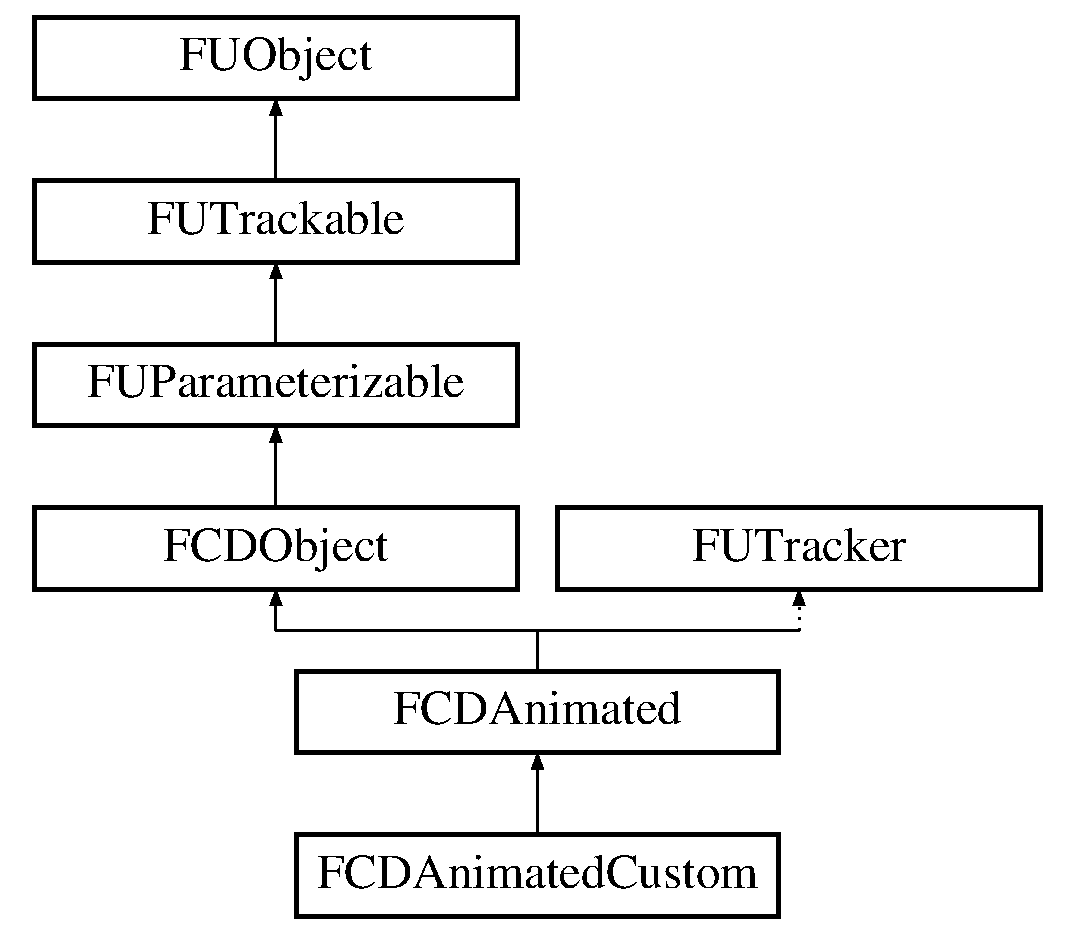
\includegraphics[height=6.000000cm]{classFCDAnimated}
\end{center}
\end{figure}
\subsection*{Public Member Functions}
\begin{DoxyCompactItemize}
\item 
\hyperlink{classFCDAnimated_ac837003f50e0f80a8931fbc81e26a58f}{DeclareFlag} (RelativeAnimation, 0)
\item 
\hyperlink{classFCDAnimated_a4eda43378afc55e11489da7b9dc2dcd2}{DeclareFlagCount} (1)
\item 
\hyperlink{classFCDAnimated_a167d5abc5e40cf3fc4324bb03c745e36}{FCDAnimated} (\hyperlink{classFCDObject}{FCDObject} $\ast$object, size\_\-t valueCount, const char $\ast$$\ast$\hyperlink{classFCDAnimated_a02ab9175d25055cd2d10d924de312490}{qualifiers}, float $\ast$$\ast$\hyperlink{classFCDAnimated_afa9e0b280ba2cd7c18e8454eb296e453}{values})
\item 
\hyperlink{classFCDAnimated_a9b99432d57703358264e5cf4db911570}{FCDAnimated} (\hyperlink{classFCDocument}{FCDocument} $\ast$document, size\_\-t valueCount, const char $\ast$$\ast$\hyperlink{classFCDAnimated_a02ab9175d25055cd2d10d924de312490}{qualifiers}, float $\ast$$\ast$\hyperlink{classFCDAnimated_afa9e0b280ba2cd7c18e8454eb296e453}{values})
\item 
virtual \hyperlink{classFCDAnimated_a8f3542f8832c28a2ac577eae2b63304b}{$\sim$FCDAnimated} ()
\item 
size\_\-t \hyperlink{classFCDAnimated_ab327a9cd5a07649b00105ee399926b86}{GetValueCount} () const 
\item 
size\_\-t \hyperlink{classFCDAnimated_aed087870f52e45cb31f0671739fdd22a}{GetCurveCount} (size\_\-t index) const 
\item 
\hyperlink{classFCDAnimationCurve}{FCDAnimationCurve} $\ast$ \hyperlink{classFCDAnimated_a1f001d1c8c99792304bddc3e4940d239}{GetCurve} (size\_\-t index, size\_\-t curveIndex=0)
\item 
const \hyperlink{classFCDAnimationCurve}{FCDAnimationCurve} $\ast$ \hyperlink{classFCDAnimated_a7ed98f7465fc04cee9d1daf463719f05}{GetCurve} (size\_\-t index, size\_\-t curveIndex=0) const 
\item 
\hyperlink{classfm_1_1vector}{FCDAnimationCurveListList} \& \hyperlink{classFCDAnimated_ad2ed5c2ba6f42d423b28025cf6f10090}{GetCurves} ()
\item 
const \hyperlink{classfm_1_1vector}{FCDAnimationCurveListList} \& \hyperlink{classFCDAnimated_a68b8b307c20c21ad2172cab63e97805a}{GetCurves} () const 
\item 
bool \hyperlink{classFCDAnimated_aeb1a5d7190c09b8a52e8004d852d44d2}{AddCurve} (size\_\-t index, \hyperlink{classFCDAnimationCurve}{FCDAnimationCurve} $\ast$curve)
\item 
bool \hyperlink{classFCDAnimated_adf19a87cc5623a4cba67979673872e3b}{AddCurve} (size\_\-t index, \hyperlink{classfm_1_1pvector}{FCDAnimationCurveList} \&curve)
\item 
bool \hyperlink{classFCDAnimated_aca4a4bcb2f4a4e4300dd3a49a97d210b}{RemoveCurve} (size\_\-t index)
\item 
float $\ast$ \hyperlink{classFCDAnimated_ab28462e611ad8d67a601c75b74b323c5}{GetValue} (size\_\-t index)
\item 
const float $\ast$ \hyperlink{classFCDAnimated_a121b81d9b2f509c8b4c169d41173f4df}{GetValue} (size\_\-t index) const 
\item 
void \hyperlink{classFCDAnimated_a4ae4a3041789375550621b68c19cec0d}{SetValue} (size\_\-t index, float $\ast$value)
\item 
const \hyperlink{classfm_1_1stringT}{fm::string} \& \hyperlink{classFCDAnimated_a6f0e09b0549d25f1d244984a22f59ed8}{GetQualifier} (size\_\-t index) const 
\item 
\hyperlink{classfm_1_1vector}{StringList} \& \hyperlink{classFCDAnimated_a0cd874022861ee825398284c6a3e5dcd}{GetQualifiers} ()
\item 
float $\ast$ \hyperlink{classFCDAnimated_a4b77d83d7a9763e57150f53f3b47496f}{FindValue} (const \hyperlink{classfm_1_1stringT}{fm::string} \&qualifier)
\item 
const float $\ast$ \hyperlink{classFCDAnimated_a635f0277e3da5cbdf20751279a972f24}{FindValue} (const \hyperlink{classfm_1_1stringT}{fm::string} \&qualifier) const 
\item 
\hyperlink{classFCDAnimationCurve}{FCDAnimationCurve} $\ast$ \hyperlink{classFCDAnimated_a431e0ae388de3bacbd7c42499f9f1405}{FindCurve} (const char $\ast$qualifier)
\item 
\hyperlink{classFCDAnimationCurve}{FCDAnimationCurve} $\ast$ \hyperlink{classFCDAnimated_aab87b39e82d91a0cf2d6819339dee16e}{FindCurve} (const \hyperlink{classfm_1_1stringT}{fm::string} \&qualifier)
\item 
const \hyperlink{classFCDAnimationCurve}{FCDAnimationCurve} $\ast$ \hyperlink{classFCDAnimated_a7e54c3e4ef1375e0bd7911f8a6779967}{FindCurve} (const char $\ast$qualifier) const 
\item 
const \hyperlink{classFCDAnimationCurve}{FCDAnimationCurve} $\ast$ \hyperlink{classFCDAnimated_a9459a2c65b46053d887bc2e0aab16549}{FindCurve} (const \hyperlink{classfm_1_1stringT}{fm::string} \&qualifier) const 
\item 
\hyperlink{classFCDAnimationCurve}{FCDAnimationCurve} $\ast$ \hyperlink{classFCDAnimated_a3b6f378a1057bff112715a70efcbc195}{FindCurve} (const float $\ast$value)
\item 
const \hyperlink{classFCDAnimationCurve}{FCDAnimationCurve} $\ast$ \hyperlink{classFCDAnimated_a010defa487b611547292e75e955e99d5}{FindCurve} (const float $\ast$value) const 
\item 
size\_\-t \hyperlink{classFCDAnimated_abc95fade652f7cb561363a2f572a6783}{FindQualifier} (const char $\ast$qualifier) const 
\item 
size\_\-t \hyperlink{classFCDAnimated_ab021f4938ac47274ed7beb906644ae96}{FindQualifier} (const \hyperlink{classfm_1_1stringT}{fm::string} \&qualifier) const 
\item 
size\_\-t \hyperlink{classFCDAnimated_a596cb5706f21ec11a38a21cd08d0b593}{FindValue} (const float $\ast$value) const 
\item 
void \hyperlink{classFCDAnimated_aa184ab9d719e1e798f099ff820041d9a}{SetTargetObject} (\hyperlink{classFCDObject}{FCDObject} $\ast$\_\-target)
\item 
\hyperlink{classFCDObject}{FCDObject} $\ast$ \hyperlink{classFCDAnimated_a9b3fae0cc1f766c2312c955e83ed7d1d}{GetTargetObject} ()
\item 
int32 \hyperlink{classFCDAnimated_a3e5c36661a7ebbceeeece5a6a5ef24a8}{GetArrayElement} () const 
\item 
void \hyperlink{classFCDAnimated_a8c9c8b720246764d0e5d5c88a55c31ff}{SetArrayElement} (int32 index)
\item 
bool \hyperlink{classFCDAnimated_a2e475c6ce1890734b8b9bc5226b79b6a}{HasCurve} () const 
\item 
\hyperlink{classFCDAnimationMultiCurve}{FCDAnimationMultiCurve} $\ast$ \hyperlink{classFCDAnimated_a04a1a0a8b83d4718c3be05761d724e11}{CreateMultiCurve} () const 
\item 
void \hyperlink{classFCDAnimated_a1bd0b6deb59cc5343aba007c9f5eae0c}{Evaluate} (float time)
\item 
\hyperlink{classFCDAnimated}{FCDAnimated} $\ast$ \hyperlink{classFCDAnimated_a94bbb32ae705dacebe1223ba15f3356e}{Clone} (\hyperlink{classFCDocument}{FCDocument} $\ast$document) const 
\item 
\hyperlink{classFCDAnimated}{FCDAnimated} $\ast$ \hyperlink{classFCDAnimated_a0c88b1e9ac37d6bd67abc13fee817bc7}{Clone} (\hyperlink{classFCDAnimated}{FCDAnimated} $\ast$clone) const 
\item 
virtual void \hyperlink{classFCDAnimated_af56690d3ce4fcec0caceff540129ba97}{OnObjectReleased} (\hyperlink{classFUTrackable}{FUTrackable} $\ast$object)
\end{DoxyCompactItemize}
\subsection*{Static Public Member Functions}
\begin{DoxyCompactItemize}
\item 
static \hyperlink{classFCDAnimationMultiCurve}{FCDAnimationMultiCurve} $\ast$ \hyperlink{classFCDAnimated_ad2ab07c9324f1921f16d741cea22d332}{CreateMultiCurve} (const \hyperlink{classfm_1_1pvector}{FCDAnimatedList} \&toMerge)
\end{DoxyCompactItemize}
\subsection*{Protected Attributes}
\begin{DoxyCompactItemize}
\item 
\hyperlink{classfm_1_1pvector}{FloatPtrList} \hyperlink{classFCDAnimated_afa9e0b280ba2cd7c18e8454eb296e453}{values}
\item 
\hyperlink{classfm_1_1vector}{StringList} \hyperlink{classFCDAnimated_a02ab9175d25055cd2d10d924de312490}{qualifiers}
\item 
\hyperlink{classfm_1_1vector}{FCDAnimationCurveListList} \hyperlink{classFCDAnimated_a602e65dada6111b6b748555550c0cb18}{curves}
\item 
\hyperlink{classFCDObject}{FCDObject} $\ast$ \hyperlink{classFCDAnimated_aca46cbdc7ee7a1b4cf90a5aa6849f4e0}{target}
\item 
int32 \hyperlink{classFCDAnimated_a27daa356d592abe62b5f84871bb6fefc}{arrayElement}
\end{DoxyCompactItemize}


\subsection{Detailed Description}
An animated element. An animated element encapsulates a set of floating-\/point values that are marked as animated.

For this purpose, an animated element holds a list of floating-\/point values, their animation curves and their COLLADA qualifiers for the generation of COLLADA targets. For animated list elements, an animated element holds an array index.

There are many classes built on top of this class. They represent the different element types that may be animated, such as 3D points, colors and matrices. 

\subsection{Constructor \& Destructor Documentation}
\hypertarget{classFCDAnimated_a167d5abc5e40cf3fc4324bb03c745e36}{
\index{FCDAnimated@{FCDAnimated}!FCDAnimated@{FCDAnimated}}
\index{FCDAnimated@{FCDAnimated}!FCDAnimated@{FCDAnimated}}
\subsubsection[{FCDAnimated}]{\setlength{\rightskip}{0pt plus 5cm}FCDAnimated::FCDAnimated (
\begin{DoxyParamCaption}
\item[{{\bf FCDObject} $\ast$}]{ object, }
\item[{size\_\-t}]{ valueCount, }
\item[{const char $\ast$$\ast$}]{ qualifiers, }
\item[{float $\ast$$\ast$}]{ values}
\end{DoxyParamCaption}
)}}
\label{classFCDAnimated_a167d5abc5e40cf3fc4324bb03c745e36}
Constructor. 
\begin{DoxyParams}{Parameters}
\item[{\em object}]The \hyperlink{namespaceFCollada}{FCollada} object that owns this animated element. \item[{\em valueCount}]The number of values inside the animated element. \item[{\em qualifiers}]A constant array of UTF8 string defining the qualifier for each value. You should check out the arrays in \hyperlink{namespaceFUDaeAccessor}{FUDaeAccessor} for examples. \item[{\em values}]A constant array containing the value pointers. \end{DoxyParams}
\hypertarget{classFCDAnimated_a9b99432d57703358264e5cf4db911570}{
\index{FCDAnimated@{FCDAnimated}!FCDAnimated@{FCDAnimated}}
\index{FCDAnimated@{FCDAnimated}!FCDAnimated@{FCDAnimated}}
\subsubsection[{FCDAnimated}]{\setlength{\rightskip}{0pt plus 5cm}FCDAnimated::FCDAnimated (
\begin{DoxyParamCaption}
\item[{{\bf FCDocument} $\ast$}]{ document, }
\item[{size\_\-t}]{ valueCount, }
\item[{const char $\ast$$\ast$}]{ qualifiers, }
\item[{float $\ast$$\ast$}]{ values}
\end{DoxyParamCaption}
)}}
\label{classFCDAnimated_a9b99432d57703358264e5cf4db911570}
Constructor. 
\begin{DoxyParams}{Parameters}
\item[{\em document}]The COLLADA document that owns this animated element. \item[{\em valueCount}]The number of values inside the animated element. \item[{\em qualifiers}]A constant array of UTF8 string defining the qualifier for each value. You should check out the arrays in \hyperlink{namespaceFUDaeAccessor}{FUDaeAccessor} for examples. \item[{\em values}]A constant array containing the value pointers. \end{DoxyParams}
\hypertarget{classFCDAnimated_a8f3542f8832c28a2ac577eae2b63304b}{
\index{FCDAnimated@{FCDAnimated}!$\sim$FCDAnimated@{$\sim$FCDAnimated}}
\index{$\sim$FCDAnimated@{$\sim$FCDAnimated}!FCDAnimated@{FCDAnimated}}
\subsubsection[{$\sim$FCDAnimated}]{\setlength{\rightskip}{0pt plus 5cm}FCDAnimated::$\sim$FCDAnimated (
\begin{DoxyParamCaption}
{}
\end{DoxyParamCaption}
)\hspace{0.3cm}{\ttfamily  \mbox{[}virtual\mbox{]}}}}
\label{classFCDAnimated_a8f3542f8832c28a2ac577eae2b63304b}
Destructor. 

\subsection{Member Function Documentation}
\hypertarget{classFCDAnimated_aeb1a5d7190c09b8a52e8004d852d44d2}{
\index{FCDAnimated@{FCDAnimated}!AddCurve@{AddCurve}}
\index{AddCurve@{AddCurve}!FCDAnimated@{FCDAnimated}}
\subsubsection[{AddCurve}]{\setlength{\rightskip}{0pt plus 5cm}bool FCDAnimated::AddCurve (
\begin{DoxyParamCaption}
\item[{size\_\-t}]{ index, }
\item[{{\bf FCDAnimationCurve} $\ast$}]{ curve}
\end{DoxyParamCaption}
)}}
\label{classFCDAnimated_aeb1a5d7190c09b8a52e8004d852d44d2}
Assigns a curve to a value of the animated element. The previously assigned curve will be deleted. 
\begin{DoxyParams}{Parameters}
\item[{\em index}]The value index. \item[{\em curve}]The new curve(s) that will affect the value at the given index. \end{DoxyParams}
\begin{DoxyReturn}{Returns}
Whether the curve was successfully assigned. Will return false if the index is out-\/of-\/bounds. 
\end{DoxyReturn}
\hypertarget{classFCDAnimated_adf19a87cc5623a4cba67979673872e3b}{
\index{FCDAnimated@{FCDAnimated}!AddCurve@{AddCurve}}
\index{AddCurve@{AddCurve}!FCDAnimated@{FCDAnimated}}
\subsubsection[{AddCurve}]{\setlength{\rightskip}{0pt plus 5cm}bool FCDAnimated::AddCurve (
\begin{DoxyParamCaption}
\item[{size\_\-t}]{ index, }
\item[{{\bf FCDAnimationCurveList} \&}]{ curve}
\end{DoxyParamCaption}
)}}
\label{classFCDAnimated_adf19a87cc5623a4cba67979673872e3b}
See above. \hypertarget{classFCDAnimated_a94bbb32ae705dacebe1223ba15f3356e}{
\index{FCDAnimated@{FCDAnimated}!Clone@{Clone}}
\index{Clone@{Clone}!FCDAnimated@{FCDAnimated}}
\subsubsection[{Clone}]{\setlength{\rightskip}{0pt plus 5cm}{\bf FCDAnimated} $\ast$ FCDAnimated::Clone (
\begin{DoxyParamCaption}
\item[{{\bf FCDocument} $\ast$}]{ document}
\end{DoxyParamCaption}
) const}}
\label{classFCDAnimated_a94bbb32ae705dacebe1223ba15f3356e}
Clones an animated element. 
\begin{DoxyParams}{Parameters}
\item[{\em document}]The COLLADA document that owns the cloned animated element. \end{DoxyParams}
\begin{DoxyReturn}{Returns}
The cloned animated element. 
\end{DoxyReturn}
\hypertarget{classFCDAnimated_a0c88b1e9ac37d6bd67abc13fee817bc7}{
\index{FCDAnimated@{FCDAnimated}!Clone@{Clone}}
\index{Clone@{Clone}!FCDAnimated@{FCDAnimated}}
\subsubsection[{Clone}]{\setlength{\rightskip}{0pt plus 5cm}{\bf FCDAnimated} $\ast$ FCDAnimated::Clone (
\begin{DoxyParamCaption}
\item[{{\bf FCDAnimated} $\ast$}]{ clone}
\end{DoxyParamCaption}
) const}}
\label{classFCDAnimated_a0c88b1e9ac37d6bd67abc13fee817bc7}
Clones an animated element. 
\begin{DoxyParams}{Parameters}
\item[{\em clone}]An animated element to be the clone of this element. \end{DoxyParams}
\begin{DoxyReturn}{Returns}
The clone. 
\end{DoxyReturn}
\hypertarget{classFCDAnimated_ad2ab07c9324f1921f16d741cea22d332}{
\index{FCDAnimated@{FCDAnimated}!CreateMultiCurve@{CreateMultiCurve}}
\index{CreateMultiCurve@{CreateMultiCurve}!FCDAnimated@{FCDAnimated}}
\subsubsection[{CreateMultiCurve}]{\setlength{\rightskip}{0pt plus 5cm}{\bf FCDAnimationMultiCurve} $\ast$ FCDAnimated::CreateMultiCurve (
\begin{DoxyParamCaption}
\item[{const {\bf FCDAnimatedList} \&}]{ toMerge}
\end{DoxyParamCaption}
)\hspace{0.3cm}{\ttfamily  \mbox{[}static\mbox{]}}}}
\label{classFCDAnimated_ad2ab07c9324f1921f16d741cea22d332}
Creates one multi-\/dimensional animation curve from a list of animated element. This function is useful if your application does not handle animations per-\/values. For example, we use this function is ColladaMax for animated scale values, where one scale value is two rotations for the scale rotation pivot and one 3D point for the scale factors. 
\begin{DoxyParams}{Parameters}
\item[{\em toMerge}]The list of animated elements to merge \end{DoxyParams}
\begin{DoxyReturn}{Returns}
The multi-\/dimensional animation curve. 
\end{DoxyReturn}
\hypertarget{classFCDAnimated_a04a1a0a8b83d4718c3be05761d724e11}{
\index{FCDAnimated@{FCDAnimated}!CreateMultiCurve@{CreateMultiCurve}}
\index{CreateMultiCurve@{CreateMultiCurve}!FCDAnimated@{FCDAnimated}}
\subsubsection[{CreateMultiCurve}]{\setlength{\rightskip}{0pt plus 5cm}{\bf FCDAnimationMultiCurve} $\ast$ FCDAnimated::CreateMultiCurve (
\begin{DoxyParamCaption}
{}
\end{DoxyParamCaption}
) const}}
\label{classFCDAnimated_a04a1a0a8b83d4718c3be05761d724e11}
Creates one multi-\/dimensional animation curve from this animated element. This function is useful is your application does not handle animations per-\/values, but instead needs one animation per-\/element. \begin{DoxyReturn}{Returns}
The multi-\/dimensional animation curve. 
\end{DoxyReturn}
\hypertarget{classFCDAnimated_ac837003f50e0f80a8931fbc81e26a58f}{
\index{FCDAnimated@{FCDAnimated}!DeclareFlag@{DeclareFlag}}
\index{DeclareFlag@{DeclareFlag}!FCDAnimated@{FCDAnimated}}
\subsubsection[{DeclareFlag}]{\setlength{\rightskip}{0pt plus 5cm}FCDAnimated::DeclareFlag (
\begin{DoxyParamCaption}
\item[{RelativeAnimation}]{, }
\item[{0}]{}
\end{DoxyParamCaption}
)}}
\label{classFCDAnimated_ac837003f50e0f80a8931fbc81e26a58f}
Flag to indicate that the animation should be applied relative to the default value. \hypertarget{classFCDAnimated_a4eda43378afc55e11489da7b9dc2dcd2}{
\index{FCDAnimated@{FCDAnimated}!DeclareFlagCount@{DeclareFlagCount}}
\index{DeclareFlagCount@{DeclareFlagCount}!FCDAnimated@{FCDAnimated}}
\subsubsection[{DeclareFlagCount}]{\setlength{\rightskip}{0pt plus 5cm}FCDAnimated::DeclareFlagCount (
\begin{DoxyParamCaption}
\item[{1}]{}
\end{DoxyParamCaption}
)}}
\label{classFCDAnimated_a4eda43378afc55e11489da7b9dc2dcd2}
The \hyperlink{classFCDAnimated}{FCDAnimated} class declares one flag. \hypertarget{classFCDAnimated_a1bd0b6deb59cc5343aba007c9f5eae0c}{
\index{FCDAnimated@{FCDAnimated}!Evaluate@{Evaluate}}
\index{Evaluate@{Evaluate}!FCDAnimated@{FCDAnimated}}
\subsubsection[{Evaluate}]{\setlength{\rightskip}{0pt plus 5cm}void FCDAnimated::Evaluate (
\begin{DoxyParamCaption}
\item[{float}]{ time}
\end{DoxyParamCaption}
)}}
\label{classFCDAnimated_a1bd0b6deb59cc5343aba007c9f5eae0c}
Evaluates the animated element at a given time. This function directly and {\bfseries permanently} modifies the values of the animated element according to the curves affecting them. 
\begin{DoxyParams}{Parameters}
\item[{\em time}]The evaluation time. \end{DoxyParams}
\hypertarget{classFCDAnimated_a431e0ae388de3bacbd7c42499f9f1405}{
\index{FCDAnimated@{FCDAnimated}!FindCurve@{FindCurve}}
\index{FindCurve@{FindCurve}!FCDAnimated@{FCDAnimated}}
\subsubsection[{FindCurve}]{\setlength{\rightskip}{0pt plus 5cm}{\bf FCDAnimationCurve}$\ast$ FCDAnimated::FindCurve (
\begin{DoxyParamCaption}
\item[{const char $\ast$}]{ qualifier}
\end{DoxyParamCaption}
)\hspace{0.3cm}{\ttfamily  \mbox{[}inline\mbox{]}}}}
\label{classFCDAnimated_a431e0ae388de3bacbd7c42499f9f1405}
Retrieves an animation curve given a valid qualifier. 
\begin{DoxyParams}{Parameters}
\item[{\em qualifier}]A valid qualifier. \end{DoxyParams}
\begin{DoxyReturn}{Returns}
The animation curve for this qualifier. This pointer will be NULL if the given qualifier is not used within this animated element or if the value for the given qualifier is not animated. 
\end{DoxyReturn}
\hypertarget{classFCDAnimated_aab87b39e82d91a0cf2d6819339dee16e}{
\index{FCDAnimated@{FCDAnimated}!FindCurve@{FindCurve}}
\index{FindCurve@{FindCurve}!FCDAnimated@{FCDAnimated}}
\subsubsection[{FindCurve}]{\setlength{\rightskip}{0pt plus 5cm}{\bf FCDAnimationCurve}$\ast$ FCDAnimated::FindCurve (
\begin{DoxyParamCaption}
\item[{const {\bf fm::string} \&}]{ qualifier}
\end{DoxyParamCaption}
)\hspace{0.3cm}{\ttfamily  \mbox{[}inline\mbox{]}}}}
\label{classFCDAnimated_aab87b39e82d91a0cf2d6819339dee16e}
See above. \hypertarget{classFCDAnimated_a7e54c3e4ef1375e0bd7911f8a6779967}{
\index{FCDAnimated@{FCDAnimated}!FindCurve@{FindCurve}}
\index{FindCurve@{FindCurve}!FCDAnimated@{FCDAnimated}}
\subsubsection[{FindCurve}]{\setlength{\rightskip}{0pt plus 5cm}const {\bf FCDAnimationCurve}$\ast$ FCDAnimated::FindCurve (
\begin{DoxyParamCaption}
\item[{const char $\ast$}]{ qualifier}
\end{DoxyParamCaption}
) const\hspace{0.3cm}{\ttfamily  \mbox{[}inline\mbox{]}}}}
\label{classFCDAnimated_a7e54c3e4ef1375e0bd7911f8a6779967}
See above. \hypertarget{classFCDAnimated_a9459a2c65b46053d887bc2e0aab16549}{
\index{FCDAnimated@{FCDAnimated}!FindCurve@{FindCurve}}
\index{FindCurve@{FindCurve}!FCDAnimated@{FCDAnimated}}
\subsubsection[{FindCurve}]{\setlength{\rightskip}{0pt plus 5cm}const {\bf FCDAnimationCurve}$\ast$ FCDAnimated::FindCurve (
\begin{DoxyParamCaption}
\item[{const {\bf fm::string} \&}]{ qualifier}
\end{DoxyParamCaption}
) const\hspace{0.3cm}{\ttfamily  \mbox{[}inline\mbox{]}}}}
\label{classFCDAnimated_a9459a2c65b46053d887bc2e0aab16549}
See above. \hypertarget{classFCDAnimated_a3b6f378a1057bff112715a70efcbc195}{
\index{FCDAnimated@{FCDAnimated}!FindCurve@{FindCurve}}
\index{FindCurve@{FindCurve}!FCDAnimated@{FCDAnimated}}
\subsubsection[{FindCurve}]{\setlength{\rightskip}{0pt plus 5cm}{\bf FCDAnimationCurve}$\ast$ FCDAnimated::FindCurve (
\begin{DoxyParamCaption}
\item[{const float $\ast$}]{ value}
\end{DoxyParamCaption}
)\hspace{0.3cm}{\ttfamily  \mbox{[}inline\mbox{]}}}}
\label{classFCDAnimated_a3b6f378a1057bff112715a70efcbc195}
Retrieves an animation curve given a value pointer. 
\begin{DoxyParams}{Parameters}
\item[{\em value}]A value pointer contained within the animated element. \end{DoxyParams}
\begin{DoxyReturn}{Returns}
The animation curve for this qualifier. This pointer will be NULL if the value pointer is not contained by this animated element or if the value is not animated. 
\end{DoxyReturn}
\hypertarget{classFCDAnimated_a010defa487b611547292e75e955e99d5}{
\index{FCDAnimated@{FCDAnimated}!FindCurve@{FindCurve}}
\index{FindCurve@{FindCurve}!FCDAnimated@{FCDAnimated}}
\subsubsection[{FindCurve}]{\setlength{\rightskip}{0pt plus 5cm}const {\bf FCDAnimationCurve}$\ast$ FCDAnimated::FindCurve (
\begin{DoxyParamCaption}
\item[{const float $\ast$}]{ value}
\end{DoxyParamCaption}
) const\hspace{0.3cm}{\ttfamily  \mbox{[}inline\mbox{]}}}}
\label{classFCDAnimated_a010defa487b611547292e75e955e99d5}
See above. \hypertarget{classFCDAnimated_abc95fade652f7cb561363a2f572a6783}{
\index{FCDAnimated@{FCDAnimated}!FindQualifier@{FindQualifier}}
\index{FindQualifier@{FindQualifier}!FCDAnimated@{FCDAnimated}}
\subsubsection[{FindQualifier}]{\setlength{\rightskip}{0pt plus 5cm}size\_\-t FCDAnimated::FindQualifier (
\begin{DoxyParamCaption}
\item[{const char $\ast$}]{ qualifier}
\end{DoxyParamCaption}
) const}}
\label{classFCDAnimated_abc95fade652f7cb561363a2f572a6783}
Retrieves the value index for a given qualifier. 
\begin{DoxyParams}{Parameters}
\item[{\em qualifier}]A valid qualifier. \end{DoxyParams}
\begin{DoxyReturn}{Returns}
The value index. This value will be -\/1 to indicate that the qualifier does not belong to this animated element. 
\end{DoxyReturn}
\hypertarget{classFCDAnimated_ab021f4938ac47274ed7beb906644ae96}{
\index{FCDAnimated@{FCDAnimated}!FindQualifier@{FindQualifier}}
\index{FindQualifier@{FindQualifier}!FCDAnimated@{FCDAnimated}}
\subsubsection[{FindQualifier}]{\setlength{\rightskip}{0pt plus 5cm}size\_\-t FCDAnimated::FindQualifier (
\begin{DoxyParamCaption}
\item[{const {\bf fm::string} \&}]{ qualifier}
\end{DoxyParamCaption}
) const\hspace{0.3cm}{\ttfamily  \mbox{[}inline\mbox{]}}}}
\label{classFCDAnimated_ab021f4938ac47274ed7beb906644ae96}
See above. \hypertarget{classFCDAnimated_a4b77d83d7a9763e57150f53f3b47496f}{
\index{FCDAnimated@{FCDAnimated}!FindValue@{FindValue}}
\index{FindValue@{FindValue}!FCDAnimated@{FCDAnimated}}
\subsubsection[{FindValue}]{\setlength{\rightskip}{0pt plus 5cm}float $\ast$ FCDAnimated::FindValue (
\begin{DoxyParamCaption}
\item[{const {\bf fm::string} \&}]{ qualifier}
\end{DoxyParamCaption}
)}}
\label{classFCDAnimated_a4b77d83d7a9763e57150f53f3b47496f}
Retrieves an animated value given a valid qualifier. 
\begin{DoxyParams}{Parameters}
\item[{\em qualifier}]A valid qualifier. \end{DoxyParams}
\begin{DoxyReturn}{Returns}
The animated value for this qualifier. This pointer will be NULL if the given qualifier is not used within this animated element. 
\end{DoxyReturn}
\hypertarget{classFCDAnimated_a635f0277e3da5cbdf20751279a972f24}{
\index{FCDAnimated@{FCDAnimated}!FindValue@{FindValue}}
\index{FindValue@{FindValue}!FCDAnimated@{FCDAnimated}}
\subsubsection[{FindValue}]{\setlength{\rightskip}{0pt plus 5cm}const float $\ast$ FCDAnimated::FindValue (
\begin{DoxyParamCaption}
\item[{const {\bf fm::string} \&}]{ qualifier}
\end{DoxyParamCaption}
) const}}
\label{classFCDAnimated_a635f0277e3da5cbdf20751279a972f24}
See above. \hypertarget{classFCDAnimated_a596cb5706f21ec11a38a21cd08d0b593}{
\index{FCDAnimated@{FCDAnimated}!FindValue@{FindValue}}
\index{FindValue@{FindValue}!FCDAnimated@{FCDAnimated}}
\subsubsection[{FindValue}]{\setlength{\rightskip}{0pt plus 5cm}size\_\-t FCDAnimated::FindValue (
\begin{DoxyParamCaption}
\item[{const float $\ast$}]{ value}
\end{DoxyParamCaption}
) const}}
\label{classFCDAnimated_a596cb5706f21ec11a38a21cd08d0b593}
Retrieves the value index for a given value pointer. 
\begin{DoxyParams}{Parameters}
\item[{\em value}]A value pointer contained within the animated element. \end{DoxyParams}
\begin{DoxyReturn}{Returns}
The value index. This value will be -\/1 to indicate that the value pointer is not contained by this animated element. 
\end{DoxyReturn}
\hypertarget{classFCDAnimated_a3e5c36661a7ebbceeeece5a6a5ef24a8}{
\index{FCDAnimated@{FCDAnimated}!GetArrayElement@{GetArrayElement}}
\index{GetArrayElement@{GetArrayElement}!FCDAnimated@{FCDAnimated}}
\subsubsection[{GetArrayElement}]{\setlength{\rightskip}{0pt plus 5cm}int32 FCDAnimated::GetArrayElement (
\begin{DoxyParamCaption}
{}
\end{DoxyParamCaption}
) const\hspace{0.3cm}{\ttfamily  \mbox{[}inline\mbox{]}}}}
\label{classFCDAnimated_a3e5c36661a7ebbceeeece5a6a5ef24a8}
Retrieves the array index for an animated element. This value is used only for animated elements that belong to a list of animated elements within the COLLADA document. \begin{DoxyReturn}{Returns}
The array index. This value will be -\/1 to indicate that the animated element does not belong to a list. 
\end{DoxyReturn}
\hypertarget{classFCDAnimated_a1f001d1c8c99792304bddc3e4940d239}{
\index{FCDAnimated@{FCDAnimated}!GetCurve@{GetCurve}}
\index{GetCurve@{GetCurve}!FCDAnimated@{FCDAnimated}}
\subsubsection[{GetCurve}]{\setlength{\rightskip}{0pt plus 5cm}{\bf FCDAnimationCurve}$\ast$ FCDAnimated::GetCurve (
\begin{DoxyParamCaption}
\item[{size\_\-t}]{ index, }
\item[{size\_\-t}]{ curveIndex = {\ttfamily 0}}
\end{DoxyParamCaption}
)\hspace{0.3cm}{\ttfamily  \mbox{[}inline\mbox{]}}}}
\label{classFCDAnimated_a1f001d1c8c99792304bddc3e4940d239}
Retrieves the animation curve affecting the value of an animated element. 
\begin{DoxyParams}{Parameters}
\item[{\em index}]The value index. \item[{\em curveIndex}]The index of the curve within the list of curves affecting the value at the given index. \end{DoxyParams}
\begin{DoxyReturn}{Returns}
The curve affecting the value at the given index. This pointer will be NULL if one of the index is out-\/of-\/bounds or if the value is not animated. 
\end{DoxyReturn}
\hypertarget{classFCDAnimated_a7ed98f7465fc04cee9d1daf463719f05}{
\index{FCDAnimated@{FCDAnimated}!GetCurve@{GetCurve}}
\index{GetCurve@{GetCurve}!FCDAnimated@{FCDAnimated}}
\subsubsection[{GetCurve}]{\setlength{\rightskip}{0pt plus 5cm}const {\bf FCDAnimationCurve}$\ast$ FCDAnimated::GetCurve (
\begin{DoxyParamCaption}
\item[{size\_\-t}]{ index, }
\item[{size\_\-t}]{ curveIndex = {\ttfamily 0}}
\end{DoxyParamCaption}
) const\hspace{0.3cm}{\ttfamily  \mbox{[}inline\mbox{]}}}}
\label{classFCDAnimated_a7ed98f7465fc04cee9d1daf463719f05}
See above. \hypertarget{classFCDAnimated_aed087870f52e45cb31f0671739fdd22a}{
\index{FCDAnimated@{FCDAnimated}!GetCurveCount@{GetCurveCount}}
\index{GetCurveCount@{GetCurveCount}!FCDAnimated@{FCDAnimated}}
\subsubsection[{GetCurveCount}]{\setlength{\rightskip}{0pt plus 5cm}size\_\-t FCDAnimated::GetCurveCount (
\begin{DoxyParamCaption}
\item[{size\_\-t}]{ index}
\end{DoxyParamCaption}
) const\hspace{0.3cm}{\ttfamily  \mbox{[}inline\mbox{]}}}}
\label{classFCDAnimated_aed087870f52e45cb31f0671739fdd22a}
Retrieves the number of animation curves affecting one value of an animated element. 
\begin{DoxyParams}{Parameters}
\item[{\em index}]The value index. \end{DoxyParams}
\begin{DoxyReturn}{Returns}
The number of curves affecting this value. 
\end{DoxyReturn}
\hypertarget{classFCDAnimated_a68b8b307c20c21ad2172cab63e97805a}{
\index{FCDAnimated@{FCDAnimated}!GetCurves@{GetCurves}}
\index{GetCurves@{GetCurves}!FCDAnimated@{FCDAnimated}}
\subsubsection[{GetCurves}]{\setlength{\rightskip}{0pt plus 5cm}const {\bf FCDAnimationCurveListList}\& FCDAnimated::GetCurves (
\begin{DoxyParamCaption}
{}
\end{DoxyParamCaption}
) const\hspace{0.3cm}{\ttfamily  \mbox{[}inline\mbox{]}}}}
\label{classFCDAnimated_a68b8b307c20c21ad2172cab63e97805a}
See above. \hypertarget{classFCDAnimated_ad2ed5c2ba6f42d423b28025cf6f10090}{
\index{FCDAnimated@{FCDAnimated}!GetCurves@{GetCurves}}
\index{GetCurves@{GetCurves}!FCDAnimated@{FCDAnimated}}
\subsubsection[{GetCurves}]{\setlength{\rightskip}{0pt plus 5cm}{\bf FCDAnimationCurveListList}\& FCDAnimated::GetCurves (
\begin{DoxyParamCaption}
{}
\end{DoxyParamCaption}
)\hspace{0.3cm}{\ttfamily  \mbox{[}inline\mbox{]}}}}
\label{classFCDAnimated_ad2ed5c2ba6f42d423b28025cf6f10090}
Retrieves the list of the curves affecting the values of an animated element. This list may contain the NULL pointer, where a value is not animated. \begin{DoxyReturn}{Returns}
The list of animation curves. 
\end{DoxyReturn}
\hypertarget{classFCDAnimated_a6f0e09b0549d25f1d244984a22f59ed8}{
\index{FCDAnimated@{FCDAnimated}!GetQualifier@{GetQualifier}}
\index{GetQualifier@{GetQualifier}!FCDAnimated@{FCDAnimated}}
\subsubsection[{GetQualifier}]{\setlength{\rightskip}{0pt plus 5cm}const {\bf fm::string} \& FCDAnimated::GetQualifier (
\begin{DoxyParamCaption}
\item[{size\_\-t}]{ index}
\end{DoxyParamCaption}
) const}}
\label{classFCDAnimated_a6f0e09b0549d25f1d244984a22f59ed8}
Retrieves the qualifier of the value of an animated element. 
\begin{DoxyParams}{Parameters}
\item[{\em index}]The value index. \end{DoxyParams}
\begin{DoxyReturn}{Returns}
The qualifier for the value. The value returned will be an empty string when the index is out-\/of-\/bounds. 
\end{DoxyReturn}
\hypertarget{classFCDAnimated_a0cd874022861ee825398284c6a3e5dcd}{
\index{FCDAnimated@{FCDAnimated}!GetQualifiers@{GetQualifiers}}
\index{GetQualifiers@{GetQualifiers}!FCDAnimated@{FCDAnimated}}
\subsubsection[{GetQualifiers}]{\setlength{\rightskip}{0pt plus 5cm}{\bf StringList}\& FCDAnimated::GetQualifiers (
\begin{DoxyParamCaption}
{}
\end{DoxyParamCaption}
)\hspace{0.3cm}{\ttfamily  \mbox{[}inline\mbox{]}}}}
\label{classFCDAnimated_a0cd874022861ee825398284c6a3e5dcd}
\mbox{[}INTERNAL\mbox{]} Retrieve the qualifier list directly. \begin{DoxyReturn}{Returns}
The reference to the qualifier list. 
\end{DoxyReturn}
\hypertarget{classFCDAnimated_a9b3fae0cc1f766c2312c955e83ed7d1d}{
\index{FCDAnimated@{FCDAnimated}!GetTargetObject@{GetTargetObject}}
\index{GetTargetObject@{GetTargetObject}!FCDAnimated@{FCDAnimated}}
\subsubsection[{GetTargetObject}]{\setlength{\rightskip}{0pt plus 5cm}{\bf FCDObject}$\ast$ FCDAnimated::GetTargetObject (
\begin{DoxyParamCaption}
{}
\end{DoxyParamCaption}
)\hspace{0.3cm}{\ttfamily  \mbox{[}inline\mbox{]}}}}
\label{classFCDAnimated_a9b3fae0cc1f766c2312c955e83ed7d1d}
Returns the \hyperlink{classFCDObject}{FCDObject} this animated value will notify when making changes \begin{DoxyReturn}{Returns}
Pointer to the \hyperlink{classFCDObject}{FCDObject} we notify 
\end{DoxyReturn}
\hypertarget{classFCDAnimated_a121b81d9b2f509c8b4c169d41173f4df}{
\index{FCDAnimated@{FCDAnimated}!GetValue@{GetValue}}
\index{GetValue@{GetValue}!FCDAnimated@{FCDAnimated}}
\subsubsection[{GetValue}]{\setlength{\rightskip}{0pt plus 5cm}const float$\ast$ FCDAnimated::GetValue (
\begin{DoxyParamCaption}
\item[{size\_\-t}]{ index}
\end{DoxyParamCaption}
) const\hspace{0.3cm}{\ttfamily  \mbox{[}inline\mbox{]}}}}
\label{classFCDAnimated_a121b81d9b2f509c8b4c169d41173f4df}
See above. \hypertarget{classFCDAnimated_ab28462e611ad8d67a601c75b74b323c5}{
\index{FCDAnimated@{FCDAnimated}!GetValue@{GetValue}}
\index{GetValue@{GetValue}!FCDAnimated@{FCDAnimated}}
\subsubsection[{GetValue}]{\setlength{\rightskip}{0pt plus 5cm}float$\ast$ FCDAnimated::GetValue (
\begin{DoxyParamCaption}
\item[{size\_\-t}]{ index}
\end{DoxyParamCaption}
)\hspace{0.3cm}{\ttfamily  \mbox{[}inline\mbox{]}}}}
\label{classFCDAnimated_ab28462e611ad8d67a601c75b74b323c5}
Retrieves the value of an animated element. 
\begin{DoxyParams}{Parameters}
\item[{\em index}]The value index. \end{DoxyParams}
\begin{DoxyReturn}{Returns}
The value at the given index. This pointer will be NULL if the index is out-\/of-\/boudns. 
\end{DoxyReturn}
\hypertarget{classFCDAnimated_ab327a9cd5a07649b00105ee399926b86}{
\index{FCDAnimated@{FCDAnimated}!GetValueCount@{GetValueCount}}
\index{GetValueCount@{GetValueCount}!FCDAnimated@{FCDAnimated}}
\subsubsection[{GetValueCount}]{\setlength{\rightskip}{0pt plus 5cm}size\_\-t FCDAnimated::GetValueCount (
\begin{DoxyParamCaption}
{}
\end{DoxyParamCaption}
) const\hspace{0.3cm}{\ttfamily  \mbox{[}inline\mbox{]}}}}
\label{classFCDAnimated_ab327a9cd5a07649b00105ee399926b86}
Retrieves the number of values contained within this animated element. \begin{DoxyReturn}{Returns}
The number of values. 
\end{DoxyReturn}
\hypertarget{classFCDAnimated_a2e475c6ce1890734b8b9bc5226b79b6a}{
\index{FCDAnimated@{FCDAnimated}!HasCurve@{HasCurve}}
\index{HasCurve@{HasCurve}!FCDAnimated@{FCDAnimated}}
\subsubsection[{HasCurve}]{\setlength{\rightskip}{0pt plus 5cm}bool FCDAnimated::HasCurve (
\begin{DoxyParamCaption}
{}
\end{DoxyParamCaption}
) const}}
\label{classFCDAnimated_a2e475c6ce1890734b8b9bc5226b79b6a}
Retrieves whether this animated element has any animation curves affecting its values. \begin{DoxyReturn}{Returns}
Whether any curves affect this animated element. 
\end{DoxyReturn}
\hypertarget{classFCDAnimated_af56690d3ce4fcec0caceff540129ba97}{
\index{FCDAnimated@{FCDAnimated}!OnObjectReleased@{OnObjectReleased}}
\index{OnObjectReleased@{OnObjectReleased}!FCDAnimated@{FCDAnimated}}
\subsubsection[{OnObjectReleased}]{\setlength{\rightskip}{0pt plus 5cm}void FCDAnimated::OnObjectReleased (
\begin{DoxyParamCaption}
\item[{{\bf FUTrackable} $\ast$}]{ object}
\end{DoxyParamCaption}
)\hspace{0.3cm}{\ttfamily  \mbox{[}virtual\mbox{]}}}}
\label{classFCDAnimated_af56690d3ce4fcec0caceff540129ba97}
\mbox{[}INTERNAL\mbox{]} See \hyperlink{classFUTracker}{FUTracker} On object deletion, remove ourselves as we no longer have any values to animate 

Implements \hyperlink{classFUTracker_a7e79d02821b3ccd2fadc460125cb3ca4}{FUTracker}.

\hypertarget{classFCDAnimated_aca4a4bcb2f4a4e4300dd3a49a97d210b}{
\index{FCDAnimated@{FCDAnimated}!RemoveCurve@{RemoveCurve}}
\index{RemoveCurve@{RemoveCurve}!FCDAnimated@{FCDAnimated}}
\subsubsection[{RemoveCurve}]{\setlength{\rightskip}{0pt plus 5cm}bool FCDAnimated::RemoveCurve (
\begin{DoxyParamCaption}
\item[{size\_\-t}]{ index}
\end{DoxyParamCaption}
)}}
\label{classFCDAnimated_aca4a4bcb2f4a4e4300dd3a49a97d210b}
Removes the curves affecting a value of the animated element. 
\begin{DoxyParams}{Parameters}
\item[{\em index}]The value index. \end{DoxyParams}
\begin{DoxyReturn}{Returns}
Whether a curve was successfully removed. Will return false if there was no curve to release or the index is out-\/of-\/bounds. 
\end{DoxyReturn}
\hypertarget{classFCDAnimated_a8c9c8b720246764d0e5d5c88a55c31ff}{
\index{FCDAnimated@{FCDAnimated}!SetArrayElement@{SetArrayElement}}
\index{SetArrayElement@{SetArrayElement}!FCDAnimated@{FCDAnimated}}
\subsubsection[{SetArrayElement}]{\setlength{\rightskip}{0pt plus 5cm}void FCDAnimated::SetArrayElement (
\begin{DoxyParamCaption}
\item[{int32}]{ index}
\end{DoxyParamCaption}
)\hspace{0.3cm}{\ttfamily  \mbox{[}inline\mbox{]}}}}
\label{classFCDAnimated_a8c9c8b720246764d0e5d5c88a55c31ff}
Sets the array index for an animated element. This value is used only for animated elements that belong to a list of animated elements within the COLLADA document. 
\begin{DoxyParams}{Parameters}
\item[{\em index}]The array index. This value should be -\/1 to indicate that the animated element does not belong to a list. \end{DoxyParams}
\hypertarget{classFCDAnimated_aa184ab9d719e1e798f099ff820041d9a}{
\index{FCDAnimated@{FCDAnimated}!SetTargetObject@{SetTargetObject}}
\index{SetTargetObject@{SetTargetObject}!FCDAnimated@{FCDAnimated}}
\subsubsection[{SetTargetObject}]{\setlength{\rightskip}{0pt plus 5cm}void FCDAnimated::SetTargetObject (
\begin{DoxyParamCaption}
\item[{{\bf FCDObject} $\ast$}]{ \_\-target}
\end{DoxyParamCaption}
)}}
\label{classFCDAnimated_aa184ab9d719e1e798f099ff820041d9a}
Sets the \hyperlink{classFCDObject}{FCDObject} this animated value will notify when making changes 
\begin{DoxyParams}{Parameters}
\item[{\em \_\-target}]Pointer to the \hyperlink{classFCDObject}{FCDObject} we will notify \end{DoxyParams}
\hypertarget{classFCDAnimated_a4ae4a3041789375550621b68c19cec0d}{
\index{FCDAnimated@{FCDAnimated}!SetValue@{SetValue}}
\index{SetValue@{SetValue}!FCDAnimated@{FCDAnimated}}
\subsubsection[{SetValue}]{\setlength{\rightskip}{0pt plus 5cm}void FCDAnimated::SetValue (
\begin{DoxyParamCaption}
\item[{size\_\-t}]{ index, }
\item[{float $\ast$}]{ value}
\end{DoxyParamCaption}
)\hspace{0.3cm}{\ttfamily  \mbox{[}inline\mbox{]}}}}
\label{classFCDAnimated_a4ae4a3041789375550621b68c19cec0d}
\mbox{[}INTERNAL\mbox{]} Overwrites the value pointer of an animated element. Used when changing the list size within FCDParameterAnimatableList. 
\begin{DoxyParams}{Parameters}
\item[{\em index}]The value index. \item[{\em value}]The new value pointer for this index. \end{DoxyParams}


\subsection{Field Documentation}
\hypertarget{classFCDAnimated_a27daa356d592abe62b5f84871bb6fefc}{
\index{FCDAnimated@{FCDAnimated}!arrayElement@{arrayElement}}
\index{arrayElement@{arrayElement}!FCDAnimated@{FCDAnimated}}
\subsubsection[{arrayElement}]{\setlength{\rightskip}{0pt plus 5cm}int32 {\bf FCDAnimated::arrayElement}\hspace{0.3cm}{\ttfamily  \mbox{[}protected\mbox{]}}}}
\label{classFCDAnimated_a27daa356d592abe62b5f84871bb6fefc}
The array index for animated element that belong to a list of animated elements. This value may be -\/1 to indicate that the element does not belong to a list. Otherwise, the index should always be unsigned. \hypertarget{classFCDAnimated_a602e65dada6111b6b748555550c0cb18}{
\index{FCDAnimated@{FCDAnimated}!curves@{curves}}
\index{curves@{curves}!FCDAnimated@{FCDAnimated}}
\subsubsection[{curves}]{\setlength{\rightskip}{0pt plus 5cm}{\bf FCDAnimationCurveListList} {\bf FCDAnimated::curves}\hspace{0.3cm}{\ttfamily  \mbox{[}protected\mbox{]}}}}
\label{classFCDAnimated_a602e65dada6111b6b748555550c0cb18}
The list of animation curves. There is always one curve for one value pointer, although that curve may be the NULL pointer to indicate a non-\/animated value. \hypertarget{classFCDAnimated_a02ab9175d25055cd2d10d924de312490}{
\index{FCDAnimated@{FCDAnimated}!qualifiers@{qualifiers}}
\index{qualifiers@{qualifiers}!FCDAnimated@{FCDAnimated}}
\subsubsection[{qualifiers}]{\setlength{\rightskip}{0pt plus 5cm}{\bf StringList} {\bf FCDAnimated::qualifiers}\hspace{0.3cm}{\ttfamily  \mbox{[}protected\mbox{]}}}}
\label{classFCDAnimated_a02ab9175d25055cd2d10d924de312490}
The list of target qualifiers. There is always one qualifier for one value pointer. \hypertarget{classFCDAnimated_aca46cbdc7ee7a1b4cf90a5aa6849f4e0}{
\index{FCDAnimated@{FCDAnimated}!target@{target}}
\index{target@{target}!FCDAnimated@{FCDAnimated}}
\subsubsection[{target}]{\setlength{\rightskip}{0pt plus 5cm}{\bf FCDObject}$\ast$ {\bf FCDAnimated::target}\hspace{0.3cm}{\ttfamily  \mbox{[}protected\mbox{]}}}}
\label{classFCDAnimated_aca46cbdc7ee7a1b4cf90a5aa6849f4e0}
The target object who contain the float values. \hypertarget{classFCDAnimated_afa9e0b280ba2cd7c18e8454eb296e453}{
\index{FCDAnimated@{FCDAnimated}!values@{values}}
\index{values@{values}!FCDAnimated@{FCDAnimated}}
\subsubsection[{values}]{\setlength{\rightskip}{0pt plus 5cm}{\bf FloatPtrList} {\bf FCDAnimated::values}\hspace{0.3cm}{\ttfamily  \mbox{[}protected\mbox{]}}}}
\label{classFCDAnimated_afa9e0b280ba2cd7c18e8454eb296e453}
The list of value pointers. 

The documentation for this class was generated from the following files:\begin{DoxyCompactItemize}
\item 
FCollada/FCDocument/\hyperlink{FCDAnimated_8h}{FCDAnimated.h}\item 
FCollada/FCDocument/FCDAnimated.cpp\end{DoxyCompactItemize}

\hypertarget{classFCDAnimatedCustom}{
\section{FCDAnimatedCustom Class Reference}
\label{classFCDAnimatedCustom}\index{FCDAnimatedCustom@{FCDAnimatedCustom}}
}


{\ttfamily \#include $<$FCDAnimated.h$>$}

Inheritance diagram for FCDAnimatedCustom:\begin{figure}[H]
\begin{center}
\leavevmode
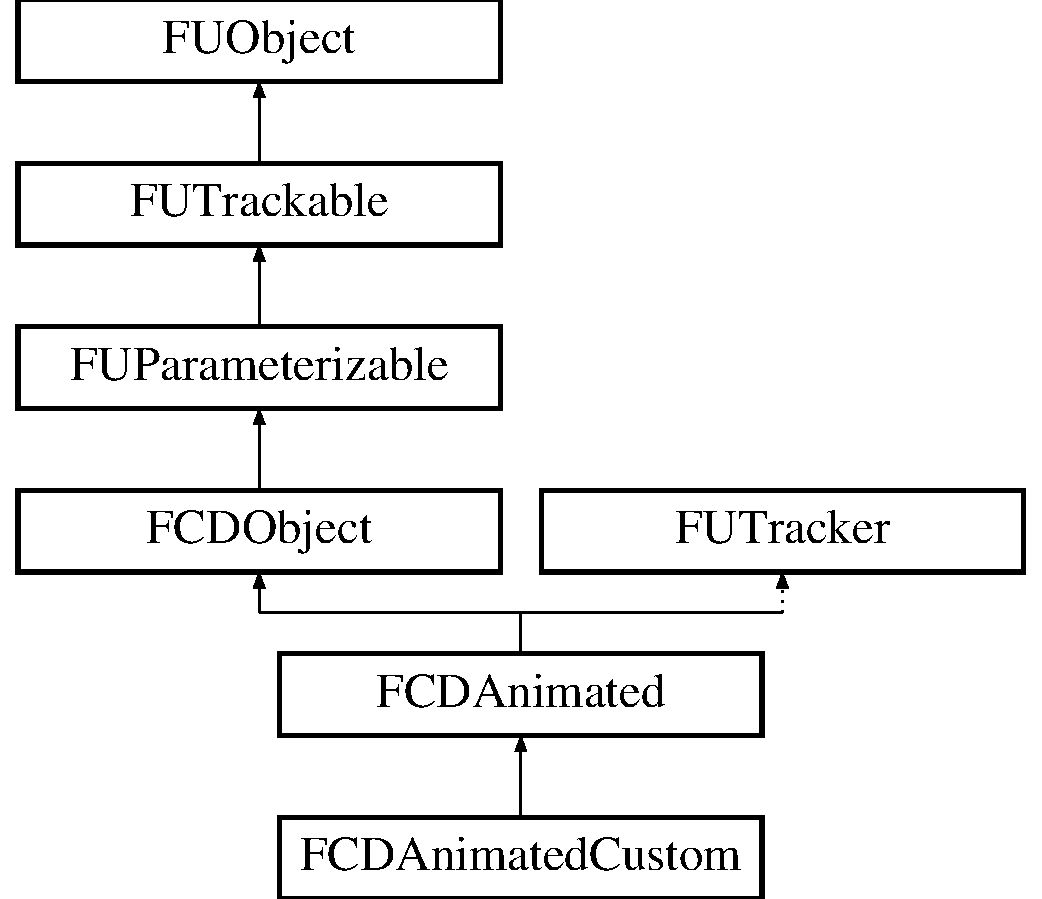
\includegraphics[height=6.000000cm]{classFCDAnimatedCustom}
\end{center}
\end{figure}
\subsection*{Public Member Functions}
\begin{DoxyCompactItemize}
\item 
\hyperlink{classFCDAnimatedCustom_a4e15071aff5b34b08ca8c39754331225}{FCDAnimatedCustom} (\hyperlink{classFCDObject}{FCDObject} $\ast$object)
\item 
void \hyperlink{classFCDAnimatedCustom_a2e53d1c7918e81312d507e6c196e778f}{Copy} (const \hyperlink{classFCDAnimated}{FCDAnimated} $\ast$copy)
\item 
float \& \hyperlink{classFCDAnimatedCustom_ac23677b9bcc764c90c2a2256c2665c6b}{GetDummy} ()
\item 
const float \& \hyperlink{classFCDAnimatedCustom_ae2e70908717bea35adcb50162066ee97}{GetDummy} () const 
\item 
void \hyperlink{classFCDAnimatedCustom_a22c9c44059742d2571f5d9bacf7c39ed}{Resize} (size\_\-t count, const char $\ast$$\ast$\hyperlink{classFCDAnimated_a02ab9175d25055cd2d10d924de312490}{qualifiers}=NULL, bool prependDot=true)
\item 
void \hyperlink{classFCDAnimatedCustom_ad231a2f2902a351b29a171b3540823d9}{Resize} (const \hyperlink{classfm_1_1vector}{StringList} \&\hyperlink{classFCDAnimated_a02ab9175d25055cd2d10d924de312490}{qualifiers}=NULL, bool prependDot=true)
\end{DoxyCompactItemize}


\subsection{Detailed Description}
A COLLADA custom animated value. Used for animated extra elements. A single value is used multiple times to hold as many value pointers are necessary to hold the animation curves. 

\subsection{Constructor \& Destructor Documentation}
\hypertarget{classFCDAnimatedCustom_a4e15071aff5b34b08ca8c39754331225}{
\index{FCDAnimatedCustom@{FCDAnimatedCustom}!FCDAnimatedCustom@{FCDAnimatedCustom}}
\index{FCDAnimatedCustom@{FCDAnimatedCustom}!FCDAnimatedCustom@{FCDAnimatedCustom}}
\subsubsection[{FCDAnimatedCustom}]{\setlength{\rightskip}{0pt plus 5cm}FCDAnimatedCustom::FCDAnimatedCustom (
\begin{DoxyParamCaption}
\item[{{\bf FCDObject} $\ast$}]{ object}
\end{DoxyParamCaption}
)}}
\label{classFCDAnimatedCustom_a4e15071aff5b34b08ca8c39754331225}
\mbox{[}INTERNAL\mbox{]} Don't build directly. 
\begin{DoxyParams}{Parameters}
\item[{\em object}]The object that owns this animated value. \end{DoxyParams}


\subsection{Member Function Documentation}
\hypertarget{classFCDAnimatedCustom_a2e53d1c7918e81312d507e6c196e778f}{
\index{FCDAnimatedCustom@{FCDAnimatedCustom}!Copy@{Copy}}
\index{Copy@{Copy}!FCDAnimatedCustom@{FCDAnimatedCustom}}
\subsubsection[{Copy}]{\setlength{\rightskip}{0pt plus 5cm}void FCDAnimatedCustom::Copy (
\begin{DoxyParamCaption}
\item[{const {\bf FCDAnimated} $\ast$}]{ copy}
\end{DoxyParamCaption}
)}}
\label{classFCDAnimatedCustom_a2e53d1c7918e81312d507e6c196e778f}
\mbox{[}INTERNAL\mbox{]} Initialized a custom animated element from another animated element. The custom animated element will be resized to copy the given animated element. 
\begin{DoxyParams}{Parameters}
\item[{\em copy}]The animated element to copy. \end{DoxyParams}
\hypertarget{classFCDAnimatedCustom_ac23677b9bcc764c90c2a2256c2665c6b}{
\index{FCDAnimatedCustom@{FCDAnimatedCustom}!GetDummy@{GetDummy}}
\index{GetDummy@{GetDummy}!FCDAnimatedCustom@{FCDAnimatedCustom}}
\subsubsection[{GetDummy}]{\setlength{\rightskip}{0pt plus 5cm}float\& FCDAnimatedCustom::GetDummy (
\begin{DoxyParamCaption}
{}
\end{DoxyParamCaption}
)\hspace{0.3cm}{\ttfamily  \mbox{[}inline\mbox{]}}}}
\label{classFCDAnimatedCustom_ac23677b9bcc764c90c2a2256c2665c6b}
Retrieves the floating-\/point value used for all the value pointers. \begin{DoxyReturn}{Returns}
The dummy floating-\/point value. 
\end{DoxyReturn}
\hypertarget{classFCDAnimatedCustom_ae2e70908717bea35adcb50162066ee97}{
\index{FCDAnimatedCustom@{FCDAnimatedCustom}!GetDummy@{GetDummy}}
\index{GetDummy@{GetDummy}!FCDAnimatedCustom@{FCDAnimatedCustom}}
\subsubsection[{GetDummy}]{\setlength{\rightskip}{0pt plus 5cm}const float\& FCDAnimatedCustom::GetDummy (
\begin{DoxyParamCaption}
{}
\end{DoxyParamCaption}
) const\hspace{0.3cm}{\ttfamily  \mbox{[}inline\mbox{]}}}}
\label{classFCDAnimatedCustom_ae2e70908717bea35adcb50162066ee97}
See above. \hypertarget{classFCDAnimatedCustom_a22c9c44059742d2571f5d9bacf7c39ed}{
\index{FCDAnimatedCustom@{FCDAnimatedCustom}!Resize@{Resize}}
\index{Resize@{Resize}!FCDAnimatedCustom@{FCDAnimatedCustom}}
\subsubsection[{Resize}]{\setlength{\rightskip}{0pt plus 5cm}void FCDAnimatedCustom::Resize (
\begin{DoxyParamCaption}
\item[{size\_\-t}]{ count, }
\item[{const char $\ast$$\ast$}]{ qualifiers = {\ttfamily NULL}, }
\item[{bool}]{ prependDot = {\ttfamily true}}
\end{DoxyParamCaption}
)}}
\label{classFCDAnimatedCustom_a22c9c44059742d2571f5d9bacf7c39ed}
Resizes the wanted qualifiers. Using the \hyperlink{namespaceFUDaeAccessor}{FUDaeAccessor} types or the \hyperlink{namespaceFCDAnimatedStandardQualifiers}{FCDAnimatedStandardQualifiers} types is recommended. 
\begin{DoxyParams}{Parameters}
\item[{\em count}]The new size of the animated element. \item[{\em qualifiers}]The new qualifiers for the animated element. \item[{\em prependDot}]Whether to prepend the '.' character for all the qualifiers of the animated element. \end{DoxyParams}
\hypertarget{classFCDAnimatedCustom_ad231a2f2902a351b29a171b3540823d9}{
\index{FCDAnimatedCustom@{FCDAnimatedCustom}!Resize@{Resize}}
\index{Resize@{Resize}!FCDAnimatedCustom@{FCDAnimatedCustom}}
\subsubsection[{Resize}]{\setlength{\rightskip}{0pt plus 5cm}void FCDAnimatedCustom::Resize (
\begin{DoxyParamCaption}
\item[{const {\bf StringList} \&}]{ qualifiers = {\ttfamily NULL}, }
\item[{bool}]{ prependDot = {\ttfamily true}}
\end{DoxyParamCaption}
)}}
\label{classFCDAnimatedCustom_ad231a2f2902a351b29a171b3540823d9}
Resizes the wanted qualifiers. 
\begin{DoxyParams}{Parameters}
\item[{\em qualifiers}]The new qualifiers for the animated element. \item[{\em prependDot}]Whether to prepend the '.' character for all the qualifiers of the animated element. \end{DoxyParams}


The documentation for this class was generated from the following files:\begin{DoxyCompactItemize}
\item 
FCollada/FCDocument/\hyperlink{FCDAnimated_8h}{FCDAnimated.h}\item 
FCollada/FCDocument/FCDAnimated.cpp\end{DoxyCompactItemize}

\hypertarget{structFCDAnimatedData}{
\section{FCDAnimatedData Struct Reference}
\label{structFCDAnimatedData}\index{FCDAnimatedData@{FCDAnimatedData}}
}
\subsection*{Data Fields}
\begin{DoxyCompactItemize}
\item 
\hypertarget{structFCDAnimatedData_a91903e493b45979188bbd484bbd8b8fa}{
\hyperlink{classfm_1_1stringT}{fm::string} {\bfseries pointer}}
\label{structFCDAnimatedData_a91903e493b45979188bbd484bbd8b8fa}

\end{DoxyCompactItemize}


The documentation for this struct was generated from the following file:\begin{DoxyCompactItemize}
\item 
FColladaPlugins/FArchiveXML/FAXStructures.h\end{DoxyCompactItemize}

\hypertarget{classFCDAnimation}{
\section{FCDAnimation Class Reference}
\label{classFCDAnimation}\index{FCDAnimation@{FCDAnimation}}
}


{\ttfamily \#include $<$FCDAnimation.h$>$}

Inheritance diagram for FCDAnimation:\begin{figure}[H]
\begin{center}
\leavevmode
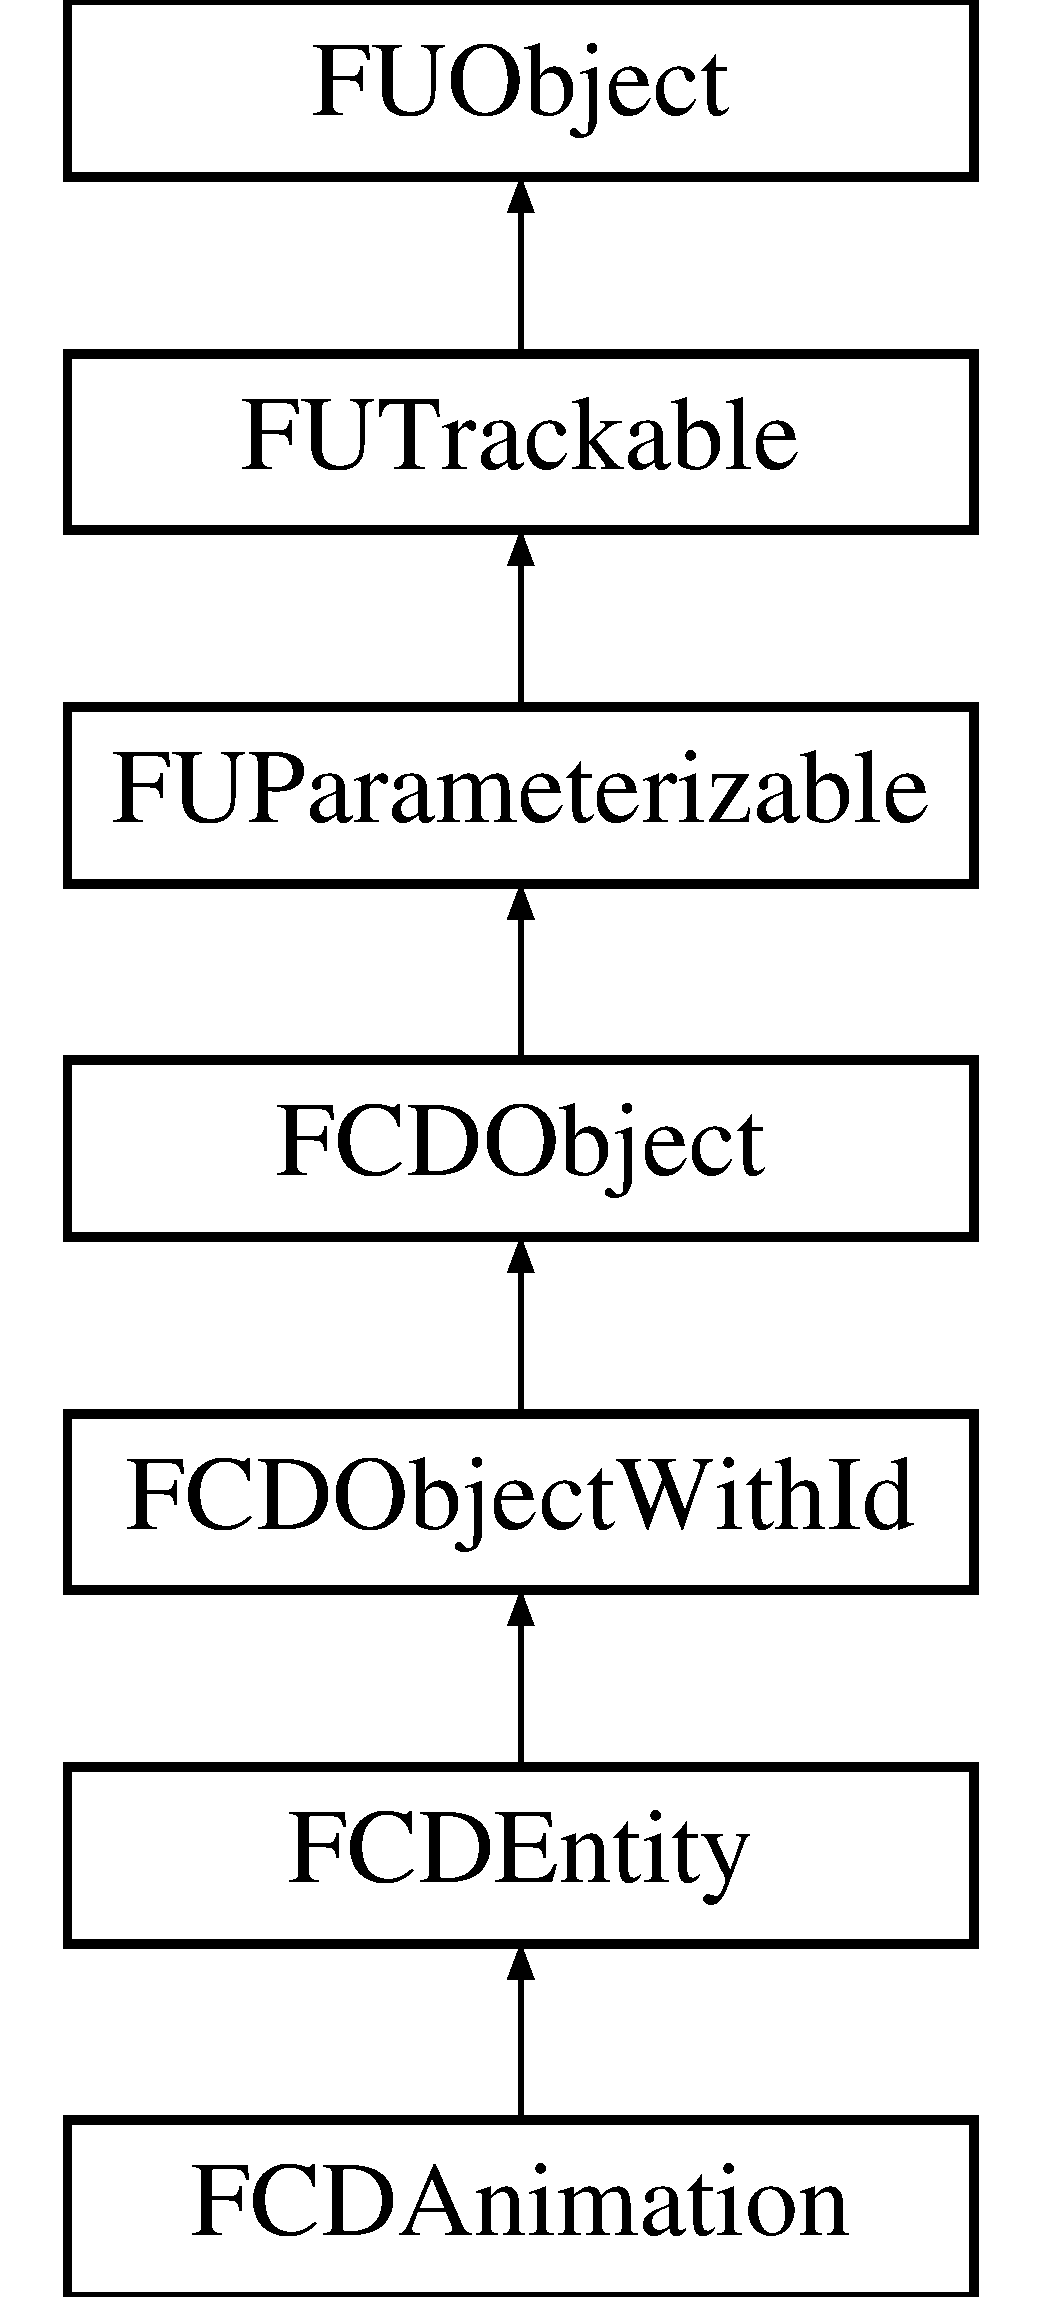
\includegraphics[height=7.000000cm]{classFCDAnimation}
\end{center}
\end{figure}
\subsection*{Public Member Functions}
\begin{DoxyCompactItemize}
\item 
\hyperlink{classFCDAnimation_a2ea6557524f3013849f60205215f9e64}{FCDAnimation} (\hyperlink{classFCDocument}{FCDocument} $\ast$document, \hyperlink{classFCDAnimation}{FCDAnimation} $\ast$parent=NULL)
\item 
virtual \hyperlink{classFCDAnimation_a3c7b9e277d2a7444caf5400747557ea1}{$\sim$FCDAnimation} ()
\item 
virtual \hyperlink{classFCDEntity_a9301a4bd5f4d4190ec13e40db4effdd7}{Type} \hyperlink{classFCDAnimation_a91e3239617da238768340a8bf62b4132}{GetType} () const 
\item 
\hyperlink{classFCDAnimation}{FCDAnimation} $\ast$ \hyperlink{classFCDAnimation_a968e8f57dbe5c45b97c876e76b9caa98}{GetParent} ()
\item 
const \hyperlink{classFCDAnimation}{FCDAnimation} $\ast$ \hyperlink{classFCDAnimation_a65e7147ad3c70f725f09ae391e2ea956}{GetParent} () const 
\item 
virtual \hyperlink{classFCDEntity}{FCDEntity} $\ast$ \hyperlink{classFCDAnimation_a1b23f8e4444121882edf5418c094b023}{Clone} (\hyperlink{classFCDEntity}{FCDEntity} $\ast$clone=NULL, bool cloneChildren=false) const 
\item 
virtual \hyperlink{classFCDEntity}{FCDEntity} $\ast$ \hyperlink{classFCDAnimation_a24615001e7529a89ce80245ddbea2a0e}{FindDaeId} (const \hyperlink{classfm_1_1stringT}{fm::string} \&daeId)
\item 
virtual const \hyperlink{classFCDEntity}{FCDEntity} $\ast$ \hyperlink{classFCDAnimation_a8e3f44f012007ca3b3f9b125c0fb8771}{FindDaeId} (const \hyperlink{classfm_1_1stringT}{fm::string} \&daeId) const 
\item 
size\_\-t \hyperlink{classFCDAnimation_a2e978db4aac9e1d378b31bd5652fe951}{GetChildrenCount} () const 
\item 
\hyperlink{classFCDAnimation}{FCDAnimation} $\ast$ \hyperlink{classFCDAnimation_ae308d048c95ea72df642f06865e37c3c}{GetChild} (size\_\-t index)
\item 
const \hyperlink{classFCDAnimation}{FCDAnimation} $\ast$ \hyperlink{classFCDAnimation_a49937056a91b0676fe3604457c579009}{GetChild} (size\_\-t index) const 
\item 
\hyperlink{classFCDAnimation}{FCDAnimation} $\ast$ \hyperlink{classFCDAnimation_a3e0b21ac9ffa48f85c0c7000b41ad555}{AddChild} ()
\item 
void \hyperlink{classFCDAnimation_ab1598e18c09d09536a7e1b173c379927}{GetHierarchicalAssets} (\hyperlink{classfm_1_1pvector}{FCDAssetList} \&assets)
\item 
virtual void \hyperlink{classFCDAnimation_add68466cc91957fc0b0fe0961cb3948e}{GetHierarchicalAssets} (\hyperlink{classfm_1_1pvector}{FCDAssetConstList} \&assets) const 
\item 
void \hyperlink{classFCDAnimation_ae86237e164a1d535dc6f6a93412fd9d9}{FindAnimationChannels} (const \hyperlink{classfm_1_1stringT}{fm::string} \&pointer, \hyperlink{classfm_1_1pvector}{FCDAnimationChannelList} \&targetChannels)
\item 
size\_\-t \hyperlink{classFCDAnimation_ace899d6bc499d07fb65bcdd2c5a7fd3c}{GetChannelCount} () const 
\item 
\hyperlink{classFCDAnimationChannel}{FCDAnimationChannel} $\ast$ \hyperlink{classFCDAnimation_a09826937c16c3c73bdc9995aa751279c}{GetChannel} (size\_\-t index)
\item 
const \hyperlink{classFCDAnimationChannel}{FCDAnimationChannel} $\ast$ \hyperlink{classFCDAnimation_ac406240a1265a474bef985478d925286}{GetChannel} (size\_\-t index) const 
\item 
void \hyperlink{classFCDAnimation_a0fd3e11834d0ceb9fdd13ac8796976b9}{GetChannels} () const 
\item 
\hyperlink{classFCDAnimationChannel}{FCDAnimationChannel} $\ast$ \hyperlink{classFCDAnimation_a4ad6d5f5fb7b3c043af8fab2b4db766c}{AddChannel} ()
\item 
void \hyperlink{classFCDAnimation_a6018679c8025b3c67e7cddccdb437fc5}{GetCurves} (\hyperlink{classfm_1_1pvector}{FCDAnimationCurveList} \&curves)
\end{DoxyCompactItemize}


\subsection{Detailed Description}
A COLLADA animation entity. An animation entity contains a list of child animation entities, in order to form a tree of animation entities. It also hold a list of animation channels, which hold the information to generate animation curves.

In other words, the animation entity is a structural class used to group animation channels hierarchically. 

\subsection{Constructor \& Destructor Documentation}
\hypertarget{classFCDAnimation_a2ea6557524f3013849f60205215f9e64}{
\index{FCDAnimation@{FCDAnimation}!FCDAnimation@{FCDAnimation}}
\index{FCDAnimation@{FCDAnimation}!FCDAnimation@{FCDAnimation}}
\subsubsection[{FCDAnimation}]{\setlength{\rightskip}{0pt plus 5cm}FCDAnimation::FCDAnimation (
\begin{DoxyParamCaption}
\item[{{\bf FCDocument} $\ast$}]{ document, }
\item[{{\bf FCDAnimation} $\ast$}]{ parent = {\ttfamily NULL}}
\end{DoxyParamCaption}
)}}
\label{classFCDAnimation_a2ea6557524f3013849f60205215f9e64}
Constructor. Do not use directly. Instead, use the \hyperlink{classFCDLibrary_aa5cdcac5a447298d5e3816e4f8c864d0}{FCDLibrary::AddEntity} function or the AddChild function, depending on the hierarchical level of the animation entity. 
\begin{DoxyParams}{Parameters}
\item[{\em document}]The \hyperlink{namespaceFCollada}{FCollada} document that owns the animation entity. \item[{\em parent}]The parent animation entity. This pointer will be NULL for root animation entities. \end{DoxyParams}
\hypertarget{classFCDAnimation_a3c7b9e277d2a7444caf5400747557ea1}{
\index{FCDAnimation@{FCDAnimation}!$\sim$FCDAnimation@{$\sim$FCDAnimation}}
\index{$\sim$FCDAnimation@{$\sim$FCDAnimation}!FCDAnimation@{FCDAnimation}}
\subsubsection[{$\sim$FCDAnimation}]{\setlength{\rightskip}{0pt plus 5cm}FCDAnimation::$\sim$FCDAnimation (
\begin{DoxyParamCaption}
{}
\end{DoxyParamCaption}
)\hspace{0.3cm}{\ttfamily  \mbox{[}virtual\mbox{]}}}}
\label{classFCDAnimation_a3c7b9e277d2a7444caf5400747557ea1}
Destructor . 

\subsection{Member Function Documentation}
\hypertarget{classFCDAnimation_a4ad6d5f5fb7b3c043af8fab2b4db766c}{
\index{FCDAnimation@{FCDAnimation}!AddChannel@{AddChannel}}
\index{AddChannel@{AddChannel}!FCDAnimation@{FCDAnimation}}
\subsubsection[{AddChannel}]{\setlength{\rightskip}{0pt plus 5cm}{\bf FCDAnimationChannel} $\ast$ FCDAnimation::AddChannel (
\begin{DoxyParamCaption}
{}
\end{DoxyParamCaption}
)}}
\label{classFCDAnimation_a4ad6d5f5fb7b3c043af8fab2b4db766c}
Adds a new animation channel to this animation entity. \begin{DoxyReturn}{Returns}
The new animation channel. 
\end{DoxyReturn}
\hypertarget{classFCDAnimation_a3e0b21ac9ffa48f85c0c7000b41ad555}{
\index{FCDAnimation@{FCDAnimation}!AddChild@{AddChild}}
\index{AddChild@{AddChild}!FCDAnimation@{FCDAnimation}}
\subsubsection[{AddChild}]{\setlength{\rightskip}{0pt plus 5cm}{\bf FCDAnimation} $\ast$ FCDAnimation::AddChild (
\begin{DoxyParamCaption}
{}
\end{DoxyParamCaption}
)}}
\label{classFCDAnimation_a3e0b21ac9ffa48f85c0c7000b41ad555}
Creates a new animation entity sub-\/tree contained within this animation entity tree. \begin{DoxyReturn}{Returns}
The new animation sub-\/tree. 
\end{DoxyReturn}
\hypertarget{classFCDAnimation_a1b23f8e4444121882edf5418c094b023}{
\index{FCDAnimation@{FCDAnimation}!Clone@{Clone}}
\index{Clone@{Clone}!FCDAnimation@{FCDAnimation}}
\subsubsection[{Clone}]{\setlength{\rightskip}{0pt plus 5cm}{\bf FCDEntity} $\ast$ FCDAnimation::Clone (
\begin{DoxyParamCaption}
\item[{{\bf FCDEntity} $\ast$}]{ clone = {\ttfamily NULL}, }
\item[{bool}]{ cloneChildren = {\ttfamily false}}
\end{DoxyParamCaption}
) const\hspace{0.3cm}{\ttfamily  \mbox{[}virtual\mbox{]}}}}
\label{classFCDAnimation_a1b23f8e4444121882edf5418c094b023}
Copies the animation tree into a clone. The clone may reside in another document. 
\begin{DoxyParams}{Parameters}
\item[{\em clone}]The empty clone. If this pointer is NULL, a new animation tree will be created and you will need to release the returned pointer manually. \item[{\em cloneChildren}]Whether to recursively clone this entity's children. \end{DoxyParams}
\begin{DoxyReturn}{Returns}
The clone. 
\end{DoxyReturn}


Reimplemented from \hyperlink{classFCDEntity_afd21dc9f9dba45786012dea87f70b9fc}{FCDEntity}.

\hypertarget{classFCDAnimation_ae86237e164a1d535dc6f6a93412fd9d9}{
\index{FCDAnimation@{FCDAnimation}!FindAnimationChannels@{FindAnimationChannels}}
\index{FindAnimationChannels@{FindAnimationChannels}!FCDAnimation@{FCDAnimation}}
\subsubsection[{FindAnimationChannels}]{\setlength{\rightskip}{0pt plus 5cm}void FCDAnimation::FindAnimationChannels (
\begin{DoxyParamCaption}
\item[{const {\bf fm::string} \&}]{ pointer, }
\item[{{\bf FCDAnimationChannelList} \&}]{ targetChannels}
\end{DoxyParamCaption}
)}}
\label{classFCDAnimation_ae86237e164a1d535dc6f6a93412fd9d9}
Retrieves the animation channels that target the given COLLADA target pointer. 
\begin{DoxyParams}{Parameters}
\item[{\em pointer}]A COLLADA target pointer. \item[{\em targetChannels}]A list of animation channels to fill in. This list is not cleared. \end{DoxyParams}
\hypertarget{classFCDAnimation_a24615001e7529a89ce80245ddbea2a0e}{
\index{FCDAnimation@{FCDAnimation}!FindDaeId@{FindDaeId}}
\index{FindDaeId@{FindDaeId}!FCDAnimation@{FCDAnimation}}
\subsubsection[{FindDaeId}]{\setlength{\rightskip}{0pt plus 5cm}virtual {\bf FCDEntity}$\ast$ FCDAnimation::FindDaeId (
\begin{DoxyParamCaption}
\item[{const {\bf fm::string} \&}]{ daeId}
\end{DoxyParamCaption}
)\hspace{0.3cm}{\ttfamily  \mbox{[}inline, virtual\mbox{]}}}}
\label{classFCDAnimation_a24615001e7529a89ce80245ddbea2a0e}
Retrieves the entity with the given COLLADA id. This function will look through the local sub-\/tree of animations for the given COLLADA id. 
\begin{DoxyParams}{Parameters}
\item[{\em daeId}]A COLLADA id. \end{DoxyParams}
\begin{DoxyReturn}{Returns}
The animation entity that matches the COLLADA id. This pointer will be NULL if there are no animation entities that matches the COLLADA id. 
\end{DoxyReturn}


Reimplemented from \hyperlink{classFCDEntity_a308cd3366b76e70ded4f09d05e4d7294}{FCDEntity}.

\hypertarget{classFCDAnimation_a8e3f44f012007ca3b3f9b125c0fb8771}{
\index{FCDAnimation@{FCDAnimation}!FindDaeId@{FindDaeId}}
\index{FindDaeId@{FindDaeId}!FCDAnimation@{FCDAnimation}}
\subsubsection[{FindDaeId}]{\setlength{\rightskip}{0pt plus 5cm}const {\bf FCDEntity} $\ast$ FCDAnimation::FindDaeId (
\begin{DoxyParamCaption}
\item[{const {\bf fm::string} \&}]{ daeId}
\end{DoxyParamCaption}
) const\hspace{0.3cm}{\ttfamily  \mbox{[}virtual\mbox{]}}}}
\label{classFCDAnimation_a8e3f44f012007ca3b3f9b125c0fb8771}
See above. 

Reimplemented from \hyperlink{classFCDEntity_a1a17dca81798431f54ec10f5da5c5c6b}{FCDEntity}.

\hypertarget{classFCDAnimation_ac406240a1265a474bef985478d925286}{
\index{FCDAnimation@{FCDAnimation}!GetChannel@{GetChannel}}
\index{GetChannel@{GetChannel}!FCDAnimation@{FCDAnimation}}
\subsubsection[{GetChannel}]{\setlength{\rightskip}{0pt plus 5cm}const {\bf FCDAnimationChannel}$\ast$ FCDAnimation::GetChannel (
\begin{DoxyParamCaption}
\item[{size\_\-t}]{ index}
\end{DoxyParamCaption}
) const\hspace{0.3cm}{\ttfamily  \mbox{[}inline\mbox{]}}}}
\label{classFCDAnimation_ac406240a1265a474bef985478d925286}
See above. \hypertarget{classFCDAnimation_a09826937c16c3c73bdc9995aa751279c}{
\index{FCDAnimation@{FCDAnimation}!GetChannel@{GetChannel}}
\index{GetChannel@{GetChannel}!FCDAnimation@{FCDAnimation}}
\subsubsection[{GetChannel}]{\setlength{\rightskip}{0pt plus 5cm}{\bf FCDAnimationChannel}$\ast$ FCDAnimation::GetChannel (
\begin{DoxyParamCaption}
\item[{size\_\-t}]{ index}
\end{DoxyParamCaption}
)\hspace{0.3cm}{\ttfamily  \mbox{[}inline\mbox{]}}}}
\label{classFCDAnimation_a09826937c16c3c73bdc9995aa751279c}
Retrieves an animation channel contained by this animation entity. 
\begin{DoxyParams}{Parameters}
\item[{\em index}]The index of the channel. \end{DoxyParams}
\begin{DoxyReturn}{Returns}
The channel at the given index. This pointer will be NULL if the index is out-\/of-\/bounds. 
\end{DoxyReturn}
\hypertarget{classFCDAnimation_ace899d6bc499d07fb65bcdd2c5a7fd3c}{
\index{FCDAnimation@{FCDAnimation}!GetChannelCount@{GetChannelCount}}
\index{GetChannelCount@{GetChannelCount}!FCDAnimation@{FCDAnimation}}
\subsubsection[{GetChannelCount}]{\setlength{\rightskip}{0pt plus 5cm}size\_\-t FCDAnimation::GetChannelCount (
\begin{DoxyParamCaption}
{}
\end{DoxyParamCaption}
) const\hspace{0.3cm}{\ttfamily  \mbox{[}inline\mbox{]}}}}
\label{classFCDAnimation_ace899d6bc499d07fb65bcdd2c5a7fd3c}
Retrieves the number of animation channels at this level within the animation tree. \begin{DoxyReturn}{Returns}
The number of animation channels. 
\end{DoxyReturn}
\hypertarget{classFCDAnimation_a0fd3e11834d0ceb9fdd13ac8796976b9}{
\index{FCDAnimation@{FCDAnimation}!GetChannels@{GetChannels}}
\index{GetChannels@{GetChannels}!FCDAnimation@{FCDAnimation}}
\subsubsection[{GetChannels}]{\setlength{\rightskip}{0pt plus 5cm}void FCDAnimation::GetChannels (
\begin{DoxyParamCaption}
{}
\end{DoxyParamCaption}
) const\hspace{0.3cm}{\ttfamily  \mbox{[}inline\mbox{]}}}}
\label{classFCDAnimation_a0fd3e11834d0ceb9fdd13ac8796976b9}
\mbox{[}INTERNAL\mbox{]} Retrieves the channels' list \begin{Desc}
\item[\hyperlink{deprecated__deprecated000001}{Deprecated}]\end{Desc}
\begin{DoxyReturn}{Returns}
The list of channels 
\end{DoxyReturn}
\hypertarget{classFCDAnimation_a49937056a91b0676fe3604457c579009}{
\index{FCDAnimation@{FCDAnimation}!GetChild@{GetChild}}
\index{GetChild@{GetChild}!FCDAnimation@{FCDAnimation}}
\subsubsection[{GetChild}]{\setlength{\rightskip}{0pt plus 5cm}const {\bf FCDAnimation}$\ast$ FCDAnimation::GetChild (
\begin{DoxyParamCaption}
\item[{size\_\-t}]{ index}
\end{DoxyParamCaption}
) const\hspace{0.3cm}{\ttfamily  \mbox{[}inline\mbox{]}}}}
\label{classFCDAnimation_a49937056a91b0676fe3604457c579009}
See above. \hypertarget{classFCDAnimation_ae308d048c95ea72df642f06865e37c3c}{
\index{FCDAnimation@{FCDAnimation}!GetChild@{GetChild}}
\index{GetChild@{GetChild}!FCDAnimation@{FCDAnimation}}
\subsubsection[{GetChild}]{\setlength{\rightskip}{0pt plus 5cm}{\bf FCDAnimation}$\ast$ FCDAnimation::GetChild (
\begin{DoxyParamCaption}
\item[{size\_\-t}]{ index}
\end{DoxyParamCaption}
)\hspace{0.3cm}{\ttfamily  \mbox{[}inline\mbox{]}}}}
\label{classFCDAnimation_ae308d048c95ea72df642f06865e37c3c}
Retrieves an animation entity sub-\/tree contained by this animation entity tree. 
\begin{DoxyParams}{Parameters}
\item[{\em index}]The index of the sub-\/tree. \end{DoxyParams}
\begin{DoxyReturn}{Returns}
The animation entity sub-\/tree at the given index. This pointer will be NULL if the index is out-\/of-\/bounds. 
\end{DoxyReturn}
\hypertarget{classFCDAnimation_a2e978db4aac9e1d378b31bd5652fe951}{
\index{FCDAnimation@{FCDAnimation}!GetChildrenCount@{GetChildrenCount}}
\index{GetChildrenCount@{GetChildrenCount}!FCDAnimation@{FCDAnimation}}
\subsubsection[{GetChildrenCount}]{\setlength{\rightskip}{0pt plus 5cm}size\_\-t FCDAnimation::GetChildrenCount (
\begin{DoxyParamCaption}
{}
\end{DoxyParamCaption}
) const\hspace{0.3cm}{\ttfamily  \mbox{[}inline\mbox{]}}}}
\label{classFCDAnimation_a2e978db4aac9e1d378b31bd5652fe951}
Retrieves the number of animation entity sub-\/trees contained by this animation entity tree. \begin{DoxyReturn}{Returns}
The number of animation entity sub-\/trees. 
\end{DoxyReturn}
\hypertarget{classFCDAnimation_a6018679c8025b3c67e7cddccdb437fc5}{
\index{FCDAnimation@{FCDAnimation}!GetCurves@{GetCurves}}
\index{GetCurves@{GetCurves}!FCDAnimation@{FCDAnimation}}
\subsubsection[{GetCurves}]{\setlength{\rightskip}{0pt plus 5cm}void FCDAnimation::GetCurves (
\begin{DoxyParamCaption}
\item[{{\bf FCDAnimationCurveList} \&}]{ curves}
\end{DoxyParamCaption}
)}}
\label{classFCDAnimation_a6018679c8025b3c67e7cddccdb437fc5}
Retrieves all the curves created in the subtree of this animation element. 
\begin{DoxyParams}{Parameters}
\item[{\em curves}]A list of animation curves to fill in. This list is not cleared. \end{DoxyParams}
\hypertarget{classFCDAnimation_ab1598e18c09d09536a7e1b173c379927}{
\index{FCDAnimation@{FCDAnimation}!GetHierarchicalAssets@{GetHierarchicalAssets}}
\index{GetHierarchicalAssets@{GetHierarchicalAssets}!FCDAnimation@{FCDAnimation}}
\subsubsection[{GetHierarchicalAssets}]{\setlength{\rightskip}{0pt plus 5cm}void FCDAnimation::GetHierarchicalAssets (
\begin{DoxyParamCaption}
\item[{{\bf FCDAssetList} \&}]{ assets}
\end{DoxyParamCaption}
)\hspace{0.3cm}{\ttfamily  \mbox{[}inline\mbox{]}}}}
\label{classFCDAnimation_ab1598e18c09d09536a7e1b173c379927}
Retrieves the asset information structures that affect this entity in its hierarchy. 
\begin{DoxyParams}{Parameters}
\item[{\em assets}]A list of asset information structures to fill in. \end{DoxyParams}


Reimplemented from \hyperlink{classFCDEntity_aacb2bd0c7d9906e6935a4cc65a0d5535}{FCDEntity}.

\hypertarget{classFCDAnimation_add68466cc91957fc0b0fe0961cb3948e}{
\index{FCDAnimation@{FCDAnimation}!GetHierarchicalAssets@{GetHierarchicalAssets}}
\index{GetHierarchicalAssets@{GetHierarchicalAssets}!FCDAnimation@{FCDAnimation}}
\subsubsection[{GetHierarchicalAssets}]{\setlength{\rightskip}{0pt plus 5cm}void FCDAnimation::GetHierarchicalAssets (
\begin{DoxyParamCaption}
\item[{{\bf FCDAssetConstList} \&}]{ assets}
\end{DoxyParamCaption}
) const\hspace{0.3cm}{\ttfamily  \mbox{[}virtual\mbox{]}}}}
\label{classFCDAnimation_add68466cc91957fc0b0fe0961cb3948e}
See above. 

Reimplemented from \hyperlink{classFCDEntity_a8586473fa13fe14b34633342c864656a}{FCDEntity}.

\hypertarget{classFCDAnimation_a968e8f57dbe5c45b97c876e76b9caa98}{
\index{FCDAnimation@{FCDAnimation}!GetParent@{GetParent}}
\index{GetParent@{GetParent}!FCDAnimation@{FCDAnimation}}
\subsubsection[{GetParent}]{\setlength{\rightskip}{0pt plus 5cm}{\bf FCDAnimation}$\ast$ FCDAnimation::GetParent (
\begin{DoxyParamCaption}
{}
\end{DoxyParamCaption}
)\hspace{0.3cm}{\ttfamily  \mbox{[}inline\mbox{]}}}}
\label{classFCDAnimation_a968e8f57dbe5c45b97c876e76b9caa98}
Retrieves the parent of the animation structure. \begin{DoxyReturn}{Returns}
The animation parent. This pointer will be NULL to indicate a root-\/level animation structure that is contained within the animation library. 
\end{DoxyReturn}
\hypertarget{classFCDAnimation_a65e7147ad3c70f725f09ae391e2ea956}{
\index{FCDAnimation@{FCDAnimation}!GetParent@{GetParent}}
\index{GetParent@{GetParent}!FCDAnimation@{FCDAnimation}}
\subsubsection[{GetParent}]{\setlength{\rightskip}{0pt plus 5cm}const {\bf FCDAnimation}$\ast$ FCDAnimation::GetParent (
\begin{DoxyParamCaption}
{}
\end{DoxyParamCaption}
) const\hspace{0.3cm}{\ttfamily  \mbox{[}inline\mbox{]}}}}
\label{classFCDAnimation_a65e7147ad3c70f725f09ae391e2ea956}
See above. \hypertarget{classFCDAnimation_a91e3239617da238768340a8bf62b4132}{
\index{FCDAnimation@{FCDAnimation}!GetType@{GetType}}
\index{GetType@{GetType}!FCDAnimation@{FCDAnimation}}
\subsubsection[{GetType}]{\setlength{\rightskip}{0pt plus 5cm}virtual {\bf Type} FCDAnimation::GetType (
\begin{DoxyParamCaption}
{}
\end{DoxyParamCaption}
) const\hspace{0.3cm}{\ttfamily  \mbox{[}inline, virtual\mbox{]}}}}
\label{classFCDAnimation_a91e3239617da238768340a8bf62b4132}
Retrieves the entity class type. This function is a part of the \hyperlink{classFCDEntity}{FCDEntity} interface. \begin{DoxyReturn}{Returns}
The entity class type: ANIMATION. 
\end{DoxyReturn}


Reimplemented from \hyperlink{classFCDEntity_abfd4312a7124f92364c1e6517c7e60ba}{FCDEntity}.



The documentation for this class was generated from the following files:\begin{DoxyCompactItemize}
\item 
FCollada/FCDocument/\hyperlink{FCDAnimation_8h}{FCDAnimation.h}\item 
FCollada/FCDocument/FCDAnimation.cpp\end{DoxyCompactItemize}

\hypertarget{classFCDAnimationChannel}{
\section{FCDAnimationChannel Class Reference}
\label{classFCDAnimationChannel}\index{FCDAnimationChannel@{FCDAnimationChannel}}
}


{\ttfamily \#include $<$FCDAnimationChannel.h$>$}

Inheritance diagram for FCDAnimationChannel:\begin{figure}[H]
\begin{center}
\leavevmode
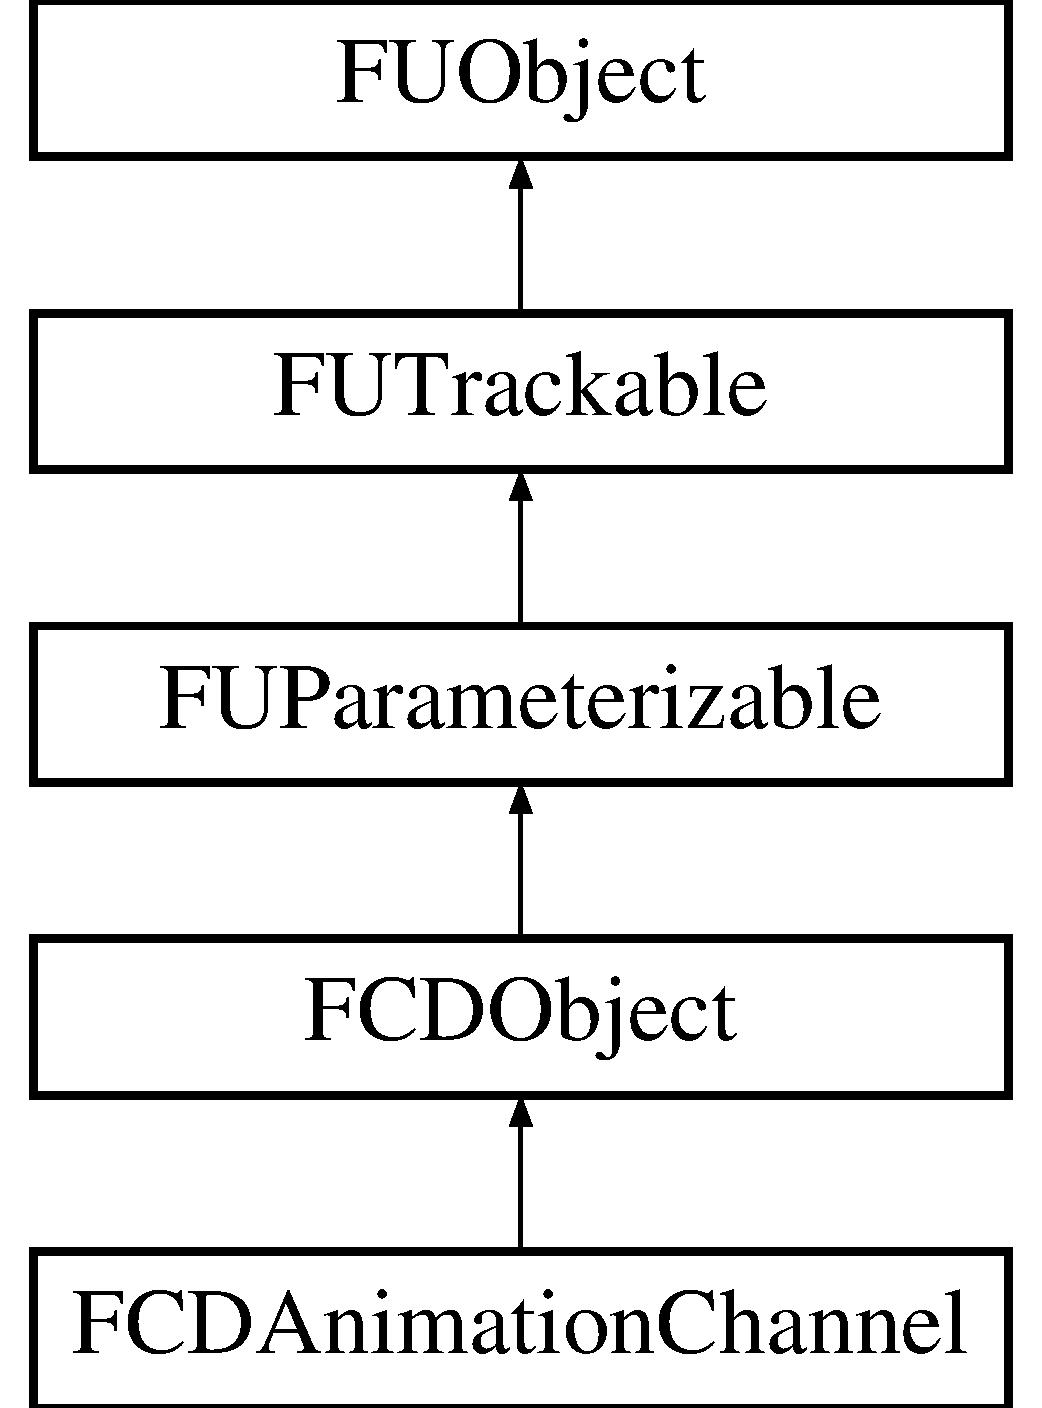
\includegraphics[height=5.000000cm]{classFCDAnimationChannel}
\end{center}
\end{figure}
\subsection*{Public Member Functions}
\begin{DoxyCompactItemize}
\item 
\hyperlink{classFCDAnimationChannel_a06b82dde2395bf29253670cd20e6b04c}{FCDAnimationChannel} (\hyperlink{classFCDocument}{FCDocument} $\ast$document, \hyperlink{classFCDAnimation}{FCDAnimation} $\ast$parent)
\item 
virtual \hyperlink{classFCDAnimationChannel_a71b4294f13adc2a0f57be0c3114c0cc9}{$\sim$FCDAnimationChannel} ()
\item 
\hyperlink{classFCDAnimationChannel}{FCDAnimationChannel} $\ast$ \hyperlink{classFCDAnimationChannel_a5736fd5d7dd229bb0d64a26d8ff1f39e}{Clone} (\hyperlink{classFCDAnimationChannel}{FCDAnimationChannel} $\ast$clone=NULL) const 
\item 
\hyperlink{classFCDAnimation}{FCDAnimation} $\ast$ \hyperlink{classFCDAnimationChannel_a208109679a16dec1f0103cbaa7b28324}{GetParent} ()
\item 
const \hyperlink{classFCDAnimation}{FCDAnimation} $\ast$ \hyperlink{classFCDAnimationChannel_a984c713570fdcd79242c2b260df91b0c}{GetParent} () const 
\item 
void \hyperlink{classFCDAnimationChannel_a978b4fceff674c0ae3bda2b5890760a2}{GetCurves} () const 
\item 
size\_\-t \hyperlink{classFCDAnimationChannel_ac1b1e057ebccde60502ea1a12b00f358}{GetCurveCount} () const 
\item 
\hyperlink{classFCDAnimationCurve}{FCDAnimationCurve} $\ast$ \hyperlink{classFCDAnimationChannel_a6022ce6350b29c74b21f253f779739c4}{GetCurve} (size\_\-t index)
\item 
const \hyperlink{classFCDAnimationCurve}{FCDAnimationCurve} $\ast$ \hyperlink{classFCDAnimationChannel_ae6716d448ab360c794901b072e27909c}{GetCurve} (size\_\-t index) const 
\item 
\hyperlink{classFCDAnimationCurve}{FCDAnimationCurve} $\ast$ \hyperlink{classFCDAnimationChannel_ab7d70254bef3270047703746e31522a8}{AddCurve} ()
\end{DoxyCompactItemize}


\subsection{Detailed Description}
A COLLADA animation channel. Each animation channel holds the animation curves for one animatable element, such as a single floating-\/point value, a 3D vector or a matrix.

\begin{DoxySeeAlso}{See also}
\hyperlink{classFCDAnimated}{FCDAnimated} 
\end{DoxySeeAlso}


\subsection{Constructor \& Destructor Documentation}
\hypertarget{classFCDAnimationChannel_a06b82dde2395bf29253670cd20e6b04c}{
\index{FCDAnimationChannel@{FCDAnimationChannel}!FCDAnimationChannel@{FCDAnimationChannel}}
\index{FCDAnimationChannel@{FCDAnimationChannel}!FCDAnimationChannel@{FCDAnimationChannel}}
\subsubsection[{FCDAnimationChannel}]{\setlength{\rightskip}{0pt plus 5cm}FCDAnimationChannel::FCDAnimationChannel (
\begin{DoxyParamCaption}
\item[{{\bf FCDocument} $\ast$}]{ document, }
\item[{{\bf FCDAnimation} $\ast$}]{ parent}
\end{DoxyParamCaption}
)}}
\label{classFCDAnimationChannel_a06b82dde2395bf29253670cd20e6b04c}
Constructor: do not use directly. Instead, call the \hyperlink{classFCDAnimation_a4ad6d5f5fb7b3c043af8fab2b4db766c}{FCDAnimation::AddChannel} function. 
\begin{DoxyParams}{Parameters}
\item[{\em document}]The COLLADA document that owns the animation channel. \item[{\em parent}]The animation sub-\/tree that contains the animation channel. \end{DoxyParams}
\hypertarget{classFCDAnimationChannel_a71b4294f13adc2a0f57be0c3114c0cc9}{
\index{FCDAnimationChannel@{FCDAnimationChannel}!$\sim$FCDAnimationChannel@{$\sim$FCDAnimationChannel}}
\index{$\sim$FCDAnimationChannel@{$\sim$FCDAnimationChannel}!FCDAnimationChannel@{FCDAnimationChannel}}
\subsubsection[{$\sim$FCDAnimationChannel}]{\setlength{\rightskip}{0pt plus 5cm}FCDAnimationChannel::$\sim$FCDAnimationChannel (
\begin{DoxyParamCaption}
{}
\end{DoxyParamCaption}
)\hspace{0.3cm}{\ttfamily  \mbox{[}virtual\mbox{]}}}}
\label{classFCDAnimationChannel_a71b4294f13adc2a0f57be0c3114c0cc9}
Destructor. 

\subsection{Member Function Documentation}
\hypertarget{classFCDAnimationChannel_ab7d70254bef3270047703746e31522a8}{
\index{FCDAnimationChannel@{FCDAnimationChannel}!AddCurve@{AddCurve}}
\index{AddCurve@{AddCurve}!FCDAnimationChannel@{FCDAnimationChannel}}
\subsubsection[{AddCurve}]{\setlength{\rightskip}{0pt plus 5cm}{\bf FCDAnimationCurve} $\ast$ FCDAnimationChannel::AddCurve (
\begin{DoxyParamCaption}
{}
\end{DoxyParamCaption}
)}}
\label{classFCDAnimationChannel_ab7d70254bef3270047703746e31522a8}
Adds a new animation curve to this animation channel. \begin{DoxyReturn}{Returns}
The new animation curve. 
\end{DoxyReturn}
\hypertarget{classFCDAnimationChannel_a5736fd5d7dd229bb0d64a26d8ff1f39e}{
\index{FCDAnimationChannel@{FCDAnimationChannel}!Clone@{Clone}}
\index{Clone@{Clone}!FCDAnimationChannel@{FCDAnimationChannel}}
\subsubsection[{Clone}]{\setlength{\rightskip}{0pt plus 5cm}{\bf FCDAnimationChannel} $\ast$ FCDAnimationChannel::Clone (
\begin{DoxyParamCaption}
\item[{{\bf FCDAnimationChannel} $\ast$}]{ clone = {\ttfamily NULL}}
\end{DoxyParamCaption}
) const}}
\label{classFCDAnimationChannel_a5736fd5d7dd229bb0d64a26d8ff1f39e}
Copies the animation channel into a clone. The clone may reside in another document. 
\begin{DoxyParams}{Parameters}
\item[{\em clone}]The empty clone. If this pointer is NULL, a new animation channel will be created and you will need to release the returned pointer manually. \end{DoxyParams}
\begin{DoxyReturn}{Returns}
The clone. 
\end{DoxyReturn}
\hypertarget{classFCDAnimationChannel_ae6716d448ab360c794901b072e27909c}{
\index{FCDAnimationChannel@{FCDAnimationChannel}!GetCurve@{GetCurve}}
\index{GetCurve@{GetCurve}!FCDAnimationChannel@{FCDAnimationChannel}}
\subsubsection[{GetCurve}]{\setlength{\rightskip}{0pt plus 5cm}const {\bf FCDAnimationCurve}$\ast$ FCDAnimationChannel::GetCurve (
\begin{DoxyParamCaption}
\item[{size\_\-t}]{ index}
\end{DoxyParamCaption}
) const\hspace{0.3cm}{\ttfamily  \mbox{[}inline\mbox{]}}}}
\label{classFCDAnimationChannel_ae6716d448ab360c794901b072e27909c}
See above. \hypertarget{classFCDAnimationChannel_a6022ce6350b29c74b21f253f779739c4}{
\index{FCDAnimationChannel@{FCDAnimationChannel}!GetCurve@{GetCurve}}
\index{GetCurve@{GetCurve}!FCDAnimationChannel@{FCDAnimationChannel}}
\subsubsection[{GetCurve}]{\setlength{\rightskip}{0pt plus 5cm}{\bf FCDAnimationCurve}$\ast$ FCDAnimationChannel::GetCurve (
\begin{DoxyParamCaption}
\item[{size\_\-t}]{ index}
\end{DoxyParamCaption}
)\hspace{0.3cm}{\ttfamily  \mbox{[}inline\mbox{]}}}}
\label{classFCDAnimationChannel_a6022ce6350b29c74b21f253f779739c4}
Retrieves an animation curve contained within the channel. 
\begin{DoxyParams}{Parameters}
\item[{\em index}]The index of the animation curve. \end{DoxyParams}
\begin{DoxyReturn}{Returns}
The animation curve at the given index. This pointer will be NULL if the index is out-\/of-\/bounds. 
\end{DoxyReturn}
\hypertarget{classFCDAnimationChannel_ac1b1e057ebccde60502ea1a12b00f358}{
\index{FCDAnimationChannel@{FCDAnimationChannel}!GetCurveCount@{GetCurveCount}}
\index{GetCurveCount@{GetCurveCount}!FCDAnimationChannel@{FCDAnimationChannel}}
\subsubsection[{GetCurveCount}]{\setlength{\rightskip}{0pt plus 5cm}size\_\-t FCDAnimationChannel::GetCurveCount (
\begin{DoxyParamCaption}
{}
\end{DoxyParamCaption}
) const\hspace{0.3cm}{\ttfamily  \mbox{[}inline\mbox{]}}}}
\label{classFCDAnimationChannel_ac1b1e057ebccde60502ea1a12b00f358}
Retrieves the number of animation curves contained within the channel. \begin{DoxyReturn}{Returns}
The number of animation curves. 
\end{DoxyReturn}
\hypertarget{classFCDAnimationChannel_a978b4fceff674c0ae3bda2b5890760a2}{
\index{FCDAnimationChannel@{FCDAnimationChannel}!GetCurves@{GetCurves}}
\index{GetCurves@{GetCurves}!FCDAnimationChannel@{FCDAnimationChannel}}
\subsubsection[{GetCurves}]{\setlength{\rightskip}{0pt plus 5cm}void FCDAnimationChannel::GetCurves (
\begin{DoxyParamCaption}
{}
\end{DoxyParamCaption}
) const\hspace{0.3cm}{\ttfamily  \mbox{[}inline\mbox{]}}}}
\label{classFCDAnimationChannel_a978b4fceff674c0ae3bda2b5890760a2}
Retrieves the list of animation curves contained within the channel. \begin{Desc}
\item[\hyperlink{deprecated__deprecated000002}{Deprecated}]\end{Desc}
\begin{DoxyReturn}{Returns}
The list of animation curves. 
\end{DoxyReturn}
\hypertarget{classFCDAnimationChannel_a984c713570fdcd79242c2b260df91b0c}{
\index{FCDAnimationChannel@{FCDAnimationChannel}!GetParent@{GetParent}}
\index{GetParent@{GetParent}!FCDAnimationChannel@{FCDAnimationChannel}}
\subsubsection[{GetParent}]{\setlength{\rightskip}{0pt plus 5cm}const {\bf FCDAnimation}$\ast$ FCDAnimationChannel::GetParent (
\begin{DoxyParamCaption}
{}
\end{DoxyParamCaption}
) const\hspace{0.3cm}{\ttfamily  \mbox{[}inline\mbox{]}}}}
\label{classFCDAnimationChannel_a984c713570fdcd79242c2b260df91b0c}
See above. \hypertarget{classFCDAnimationChannel_a208109679a16dec1f0103cbaa7b28324}{
\index{FCDAnimationChannel@{FCDAnimationChannel}!GetParent@{GetParent}}
\index{GetParent@{GetParent}!FCDAnimationChannel@{FCDAnimationChannel}}
\subsubsection[{GetParent}]{\setlength{\rightskip}{0pt plus 5cm}{\bf FCDAnimation}$\ast$ FCDAnimationChannel::GetParent (
\begin{DoxyParamCaption}
{}
\end{DoxyParamCaption}
)\hspace{0.3cm}{\ttfamily  \mbox{[}inline\mbox{]}}}}
\label{classFCDAnimationChannel_a208109679a16dec1f0103cbaa7b28324}
Retrieves the animation sub-\/tree that contains the animation channel. \begin{DoxyReturn}{Returns}
The parent animation sub-\/tree. 
\end{DoxyReturn}


The documentation for this class was generated from the following files:\begin{DoxyCompactItemize}
\item 
FCollada/FCDocument/\hyperlink{FCDAnimationChannel_8h}{FCDAnimationChannel.h}\item 
FCollada/FCDocument/FCDAnimationChannel.cpp\end{DoxyCompactItemize}

\hypertarget{structFCDAnimationChannelData}{
\section{FCDAnimationChannelData Struct Reference}
\label{structFCDAnimationChannelData}\index{FCDAnimationChannelData@{FCDAnimationChannelData}}
}
\subsection*{Data Fields}
\begin{DoxyCompactItemize}
\item 
\hypertarget{structFCDAnimationChannelData_ae58db047200461748e49df364fa99d4c}{
\hyperlink{classfm_1_1stringT}{fm::string} {\bfseries targetPointer}}
\label{structFCDAnimationChannelData_ae58db047200461748e49df364fa99d4c}

\item 
\hypertarget{structFCDAnimationChannelData_ac42bc46310e5107e40170c5d93157f17}{
\hyperlink{classfm_1_1stringT}{fm::string} {\bfseries targetQualifier}}
\label{structFCDAnimationChannelData_ac42bc46310e5107e40170c5d93157f17}

\item 
\hypertarget{structFCDAnimationChannelData_a05a48028de22e39af19697153c0e737d}{
\hyperlink{classfm_1_1stringT}{fm::string} {\bfseries driverPointer}}
\label{structFCDAnimationChannelData_a05a48028de22e39af19697153c0e737d}

\item 
\hypertarget{structFCDAnimationChannelData_aa19b04f8ef49296a457e28bca417010f}{
int32 {\bfseries driverQualifier}}
\label{structFCDAnimationChannelData_aa19b04f8ef49296a457e28bca417010f}

\item 
\hypertarget{structFCDAnimationChannelData_a6ab55632a777916da6e719ed42a0ce6e}{
\hyperlink{classfm_1_1vector}{FAXAnimationChannelDefaultValueList} {\bfseries defaultValues}}
\label{structFCDAnimationChannelData_a6ab55632a777916da6e719ed42a0ce6e}

\item 
\hypertarget{structFCDAnimationChannelData_a5f314c0134e767f51ac635fc5849a5df}{
\hyperlink{classFCDAnimated}{FCDAnimated} $\ast$ {\bfseries animatedValue}}
\label{structFCDAnimationChannelData_a5f314c0134e767f51ac635fc5849a5df}

\end{DoxyCompactItemize}


The documentation for this struct was generated from the following file:\begin{DoxyCompactItemize}
\item 
FColladaPlugins/FArchiveXML/FAXStructures.h\end{DoxyCompactItemize}

\hypertarget{classFCDAnimationClip}{
\section{FCDAnimationClip Class Reference}
\label{classFCDAnimationClip}\index{FCDAnimationClip@{FCDAnimationClip}}
}


{\ttfamily \#include $<$FCDAnimationClip.h$>$}

Inheritance diagram for FCDAnimationClip:\begin{figure}[H]
\begin{center}
\leavevmode
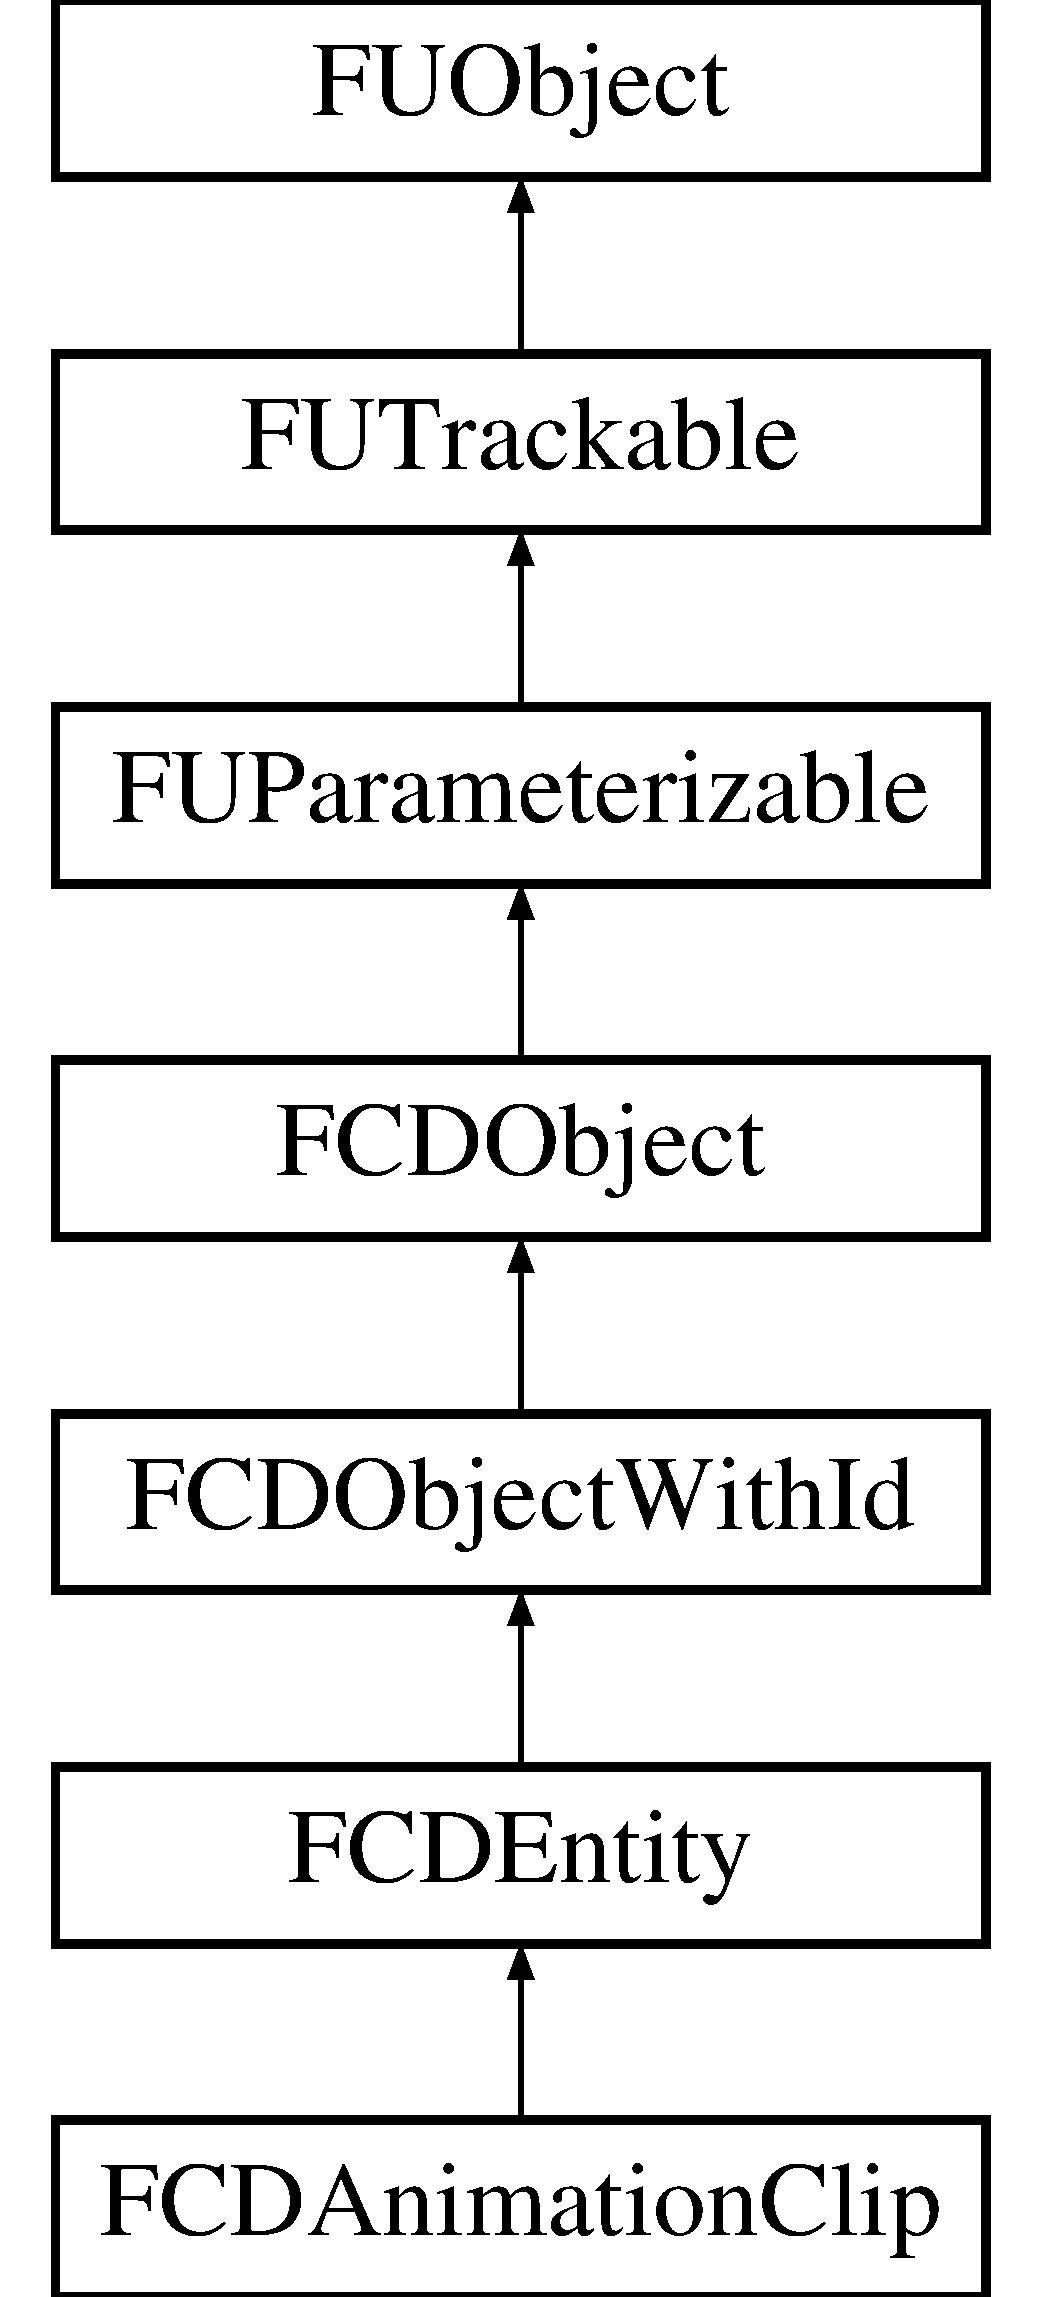
\includegraphics[height=7.000000cm]{classFCDAnimationClip}
\end{center}
\end{figure}
\subsection*{Public Member Functions}
\begin{DoxyCompactItemize}
\item 
\hyperlink{classFCDAnimationClip_a7b9a575f0a69924becf22c31309f052e}{FCDAnimationClip} (\hyperlink{classFCDocument}{FCDocument} $\ast$document)
\item 
virtual \hyperlink{classFCDAnimationClip_a277876f9e175f04ae9a954aa464b371a}{$\sim$FCDAnimationClip} ()
\item 
virtual \hyperlink{classFCDEntity}{FCDEntity} $\ast$ \hyperlink{classFCDAnimationClip_a238068520ca5d5932252fd73f18eb573}{Clone} (\hyperlink{classFCDEntity}{FCDEntity} $\ast$clone=NULL, bool cloneChildren=false) const 
\item 
virtual \hyperlink{classFCDEntity_a9301a4bd5f4d4190ec13e40db4effdd7}{Type} \hyperlink{classFCDAnimationClip_aef1051c0a708829ae1800e4362b8af7e}{GetType} () const 
\item 
\hyperlink{classFUTrackedList}{FCDAnimationCurveTrackList} \& \hyperlink{classFCDAnimationClip_ad3d1c50b00da7dc6092e893f2b2ba1a0}{GetClipCurves} ()
\item 
const \hyperlink{classFUTrackedList}{FCDAnimationCurveTrackList} \& \hyperlink{classFCDAnimationClip_ad815a4be325c0f6e375d9a2dd3ea6fdf}{GetClipCurves} () const 
\item 
void \hyperlink{classFCDAnimationClip_a1adf70ff7bf8a26cd7769a93a80eea02}{AddClipCurve} (\hyperlink{classFCDAnimationCurve}{FCDAnimationCurve} $\ast$curve)
\item 
float \hyperlink{classFCDAnimationClip_ab7d15c33a1ead6ed4b87b9cc6e75b866}{GetStart} () const 
\item 
void \hyperlink{classFCDAnimationClip_aba58782b21762c1602022accfafce340}{SetStart} (float \_\-start)
\item 
float \hyperlink{classFCDAnimationClip_a1cef2ba64b8f98f430d394423f1c37f4}{GetEnd} () const 
\item 
void \hyperlink{classFCDAnimationClip_aa55db11384a406c48b834326a964e666}{SetEnd} (float \_\-end)
\item 
size\_\-t \hyperlink{classFCDAnimationClip_aa1f97cce1c7ac2d9bb019404a73e923c}{GetAnimationCount} () const 
\item 
\hyperlink{classFCDAnimation}{FCDAnimation} $\ast$ \hyperlink{classFCDAnimationClip_a11169a159cea62896fa3f4c34fa0b888}{GetAnimation} (size\_\-t index) const 
\item 
void \hyperlink{classFCDAnimationClip_a583019dc6402e191b3a977ab601087fe}{SetAnimationName} (const \hyperlink{classfm_1_1stringT}{fm::string} \&name, size\_\-t index)
\item 
\hyperlink{classfm_1_1stringT}{fm::string} \hyperlink{classFCDAnimationClip_a6d952c3811daafcddc5b340dcdc519cb}{GetAnimationName} (size\_\-t index) const 
\item 
\hyperlink{classFCDEntityInstance}{FCDEntityInstance} $\ast$ \hyperlink{classFCDAnimationClip_a5bde27d1a1ac44745e74d611117fabe6}{AddInstanceAnimation} ()
\item 
\hyperlink{classFCDEntityInstance}{FCDEntityInstance} $\ast$ \hyperlink{classFCDAnimationClip_a3062d021cc77dc77063d669db4ca3322}{AddInstanceAnimation} (\hyperlink{classFCDAnimation}{FCDAnimation} $\ast$animation)
\end{DoxyCompactItemize}


\subsection{Detailed Description}
A COLLADA animation clip.

Animation clips are used to group together animation segments. Animation clips are typically used to form complex animation sequences where all the curves should only be used simultaneously. 

\subsection{Constructor \& Destructor Documentation}
\hypertarget{classFCDAnimationClip_a7b9a575f0a69924becf22c31309f052e}{
\index{FCDAnimationClip@{FCDAnimationClip}!FCDAnimationClip@{FCDAnimationClip}}
\index{FCDAnimationClip@{FCDAnimationClip}!FCDAnimationClip@{FCDAnimationClip}}
\subsubsection[{FCDAnimationClip}]{\setlength{\rightskip}{0pt plus 5cm}FCDAnimationClip::FCDAnimationClip (
\begin{DoxyParamCaption}
\item[{{\bf FCDocument} $\ast$}]{ document}
\end{DoxyParamCaption}
)}}
\label{classFCDAnimationClip_a7b9a575f0a69924becf22c31309f052e}
Constructor. 
\begin{DoxyParams}{Parameters}
\item[{\em document}]The COLLADA document that holds this animation clip. \end{DoxyParams}
\hypertarget{classFCDAnimationClip_a277876f9e175f04ae9a954aa464b371a}{
\index{FCDAnimationClip@{FCDAnimationClip}!$\sim$FCDAnimationClip@{$\sim$FCDAnimationClip}}
\index{$\sim$FCDAnimationClip@{$\sim$FCDAnimationClip}!FCDAnimationClip@{FCDAnimationClip}}
\subsubsection[{$\sim$FCDAnimationClip}]{\setlength{\rightskip}{0pt plus 5cm}FCDAnimationClip::$\sim$FCDAnimationClip (
\begin{DoxyParamCaption}
{}
\end{DoxyParamCaption}
)\hspace{0.3cm}{\ttfamily  \mbox{[}virtual\mbox{]}}}}
\label{classFCDAnimationClip_a277876f9e175f04ae9a954aa464b371a}
Destructor. 

\subsection{Member Function Documentation}
\hypertarget{classFCDAnimationClip_a1adf70ff7bf8a26cd7769a93a80eea02}{
\index{FCDAnimationClip@{FCDAnimationClip}!AddClipCurve@{AddClipCurve}}
\index{AddClipCurve@{AddClipCurve}!FCDAnimationClip@{FCDAnimationClip}}
\subsubsection[{AddClipCurve}]{\setlength{\rightskip}{0pt plus 5cm}void FCDAnimationClip::AddClipCurve (
\begin{DoxyParamCaption}
\item[{{\bf FCDAnimationCurve} $\ast$}]{ curve}
\end{DoxyParamCaption}
)}}
\label{classFCDAnimationClip_a1adf70ff7bf8a26cd7769a93a80eea02}
Inserts an existing curve within this animation clip. 
\begin{DoxyParams}{Parameters}
\item[{\em curve}]An animation curve to be used within this clip. \end{DoxyParams}
\hypertarget{classFCDAnimationClip_a5bde27d1a1ac44745e74d611117fabe6}{
\index{FCDAnimationClip@{FCDAnimationClip}!AddInstanceAnimation@{AddInstanceAnimation}}
\index{AddInstanceAnimation@{AddInstanceAnimation}!FCDAnimationClip@{FCDAnimationClip}}
\subsubsection[{AddInstanceAnimation}]{\setlength{\rightskip}{0pt plus 5cm}{\bf FCDEntityInstance} $\ast$ FCDAnimationClip::AddInstanceAnimation (
\begin{DoxyParamCaption}
{}
\end{DoxyParamCaption}
)}}
\label{classFCDAnimationClip_a5bde27d1a1ac44745e74d611117fabe6}
\mbox{[}INTERNAL\mbox{]} Adds an animation instance. \begin{DoxyReturn}{Returns}
The empty animation instance. 
\end{DoxyReturn}
\hypertarget{classFCDAnimationClip_a3062d021cc77dc77063d669db4ca3322}{
\index{FCDAnimationClip@{FCDAnimationClip}!AddInstanceAnimation@{AddInstanceAnimation}}
\index{AddInstanceAnimation@{AddInstanceAnimation}!FCDAnimationClip@{FCDAnimationClip}}
\subsubsection[{AddInstanceAnimation}]{\setlength{\rightskip}{0pt plus 5cm}{\bf FCDEntityInstance} $\ast$ FCDAnimationClip::AddInstanceAnimation (
\begin{DoxyParamCaption}
\item[{{\bf FCDAnimation} $\ast$}]{ animation}
\end{DoxyParamCaption}
)}}
\label{classFCDAnimationClip_a3062d021cc77dc77063d669db4ca3322}
\mbox{[}INTERNAL\mbox{]} Adds an animation instance. 
\begin{DoxyParams}{Parameters}
\item[{\em animation}]The animation to instance. \end{DoxyParams}
\begin{DoxyReturn}{Returns}
The animation instance. 
\end{DoxyReturn}
\hypertarget{classFCDAnimationClip_a238068520ca5d5932252fd73f18eb573}{
\index{FCDAnimationClip@{FCDAnimationClip}!Clone@{Clone}}
\index{Clone@{Clone}!FCDAnimationClip@{FCDAnimationClip}}
\subsubsection[{Clone}]{\setlength{\rightskip}{0pt plus 5cm}{\bf FCDEntity} $\ast$ FCDAnimationClip::Clone (
\begin{DoxyParamCaption}
\item[{{\bf FCDEntity} $\ast$}]{ clone = {\ttfamily NULL}, }
\item[{bool}]{ cloneChildren = {\ttfamily false}}
\end{DoxyParamCaption}
) const\hspace{0.3cm}{\ttfamily  \mbox{[}virtual\mbox{]}}}}
\label{classFCDAnimationClip_a238068520ca5d5932252fd73f18eb573}
Copies the animation clip entity into a clone. The clone may reside in another document. 
\begin{DoxyParams}{Parameters}
\item[{\em clone}]The empty clone. If this pointer is NULL, a new animation clip will be created and you will need to release the returned pointer manually. \item[{\em cloneChildren}]Whether to recursively clone this entity's children. \end{DoxyParams}
\begin{DoxyReturn}{Returns}
The clone. 
\end{DoxyReturn}


Reimplemented from \hyperlink{classFCDEntity_afd21dc9f9dba45786012dea87f70b9fc}{FCDEntity}.

\hypertarget{classFCDAnimationClip_a11169a159cea62896fa3f4c34fa0b888}{
\index{FCDAnimationClip@{FCDAnimationClip}!GetAnimation@{GetAnimation}}
\index{GetAnimation@{GetAnimation}!FCDAnimationClip@{FCDAnimationClip}}
\subsubsection[{GetAnimation}]{\setlength{\rightskip}{0pt plus 5cm}{\bf FCDAnimation}$\ast$ FCDAnimationClip::GetAnimation (
\begin{DoxyParamCaption}
\item[{size\_\-t}]{ index}
\end{DoxyParamCaption}
) const\hspace{0.3cm}{\ttfamily  \mbox{[}inline\mbox{]}}}}
\label{classFCDAnimationClip_a11169a159cea62896fa3f4c34fa0b888}
Retrieves a given animation instanced by this clip. 
\begin{DoxyParams}{Parameters}
\item[{\em index}]The index of the animation to retrieve. \end{DoxyParams}
\begin{DoxyReturn}{Returns}
The animation object at the given index. 
\end{DoxyReturn}
\hypertarget{classFCDAnimationClip_aa1f97cce1c7ac2d9bb019404a73e923c}{
\index{FCDAnimationClip@{FCDAnimationClip}!GetAnimationCount@{GetAnimationCount}}
\index{GetAnimationCount@{GetAnimationCount}!FCDAnimationClip@{FCDAnimationClip}}
\subsubsection[{GetAnimationCount}]{\setlength{\rightskip}{0pt plus 5cm}size\_\-t FCDAnimationClip::GetAnimationCount (
\begin{DoxyParamCaption}
{}
\end{DoxyParamCaption}
) const\hspace{0.3cm}{\ttfamily  \mbox{[}inline\mbox{]}}}}
\label{classFCDAnimationClip_aa1f97cce1c7ac2d9bb019404a73e923c}
Retrieves the number of instanced animations within this animation clip. \begin{DoxyReturn}{Returns}
The number of instanced animations. 
\end{DoxyReturn}
\hypertarget{classFCDAnimationClip_a6d952c3811daafcddc5b340dcdc519cb}{
\index{FCDAnimationClip@{FCDAnimationClip}!GetAnimationName@{GetAnimationName}}
\index{GetAnimationName@{GetAnimationName}!FCDAnimationClip@{FCDAnimationClip}}
\subsubsection[{GetAnimationName}]{\setlength{\rightskip}{0pt plus 5cm}{\bf fm::string} FCDAnimationClip::GetAnimationName (
\begin{DoxyParamCaption}
\item[{size\_\-t}]{ index}
\end{DoxyParamCaption}
) const\hspace{0.3cm}{\ttfamily  \mbox{[}inline\mbox{]}}}}
\label{classFCDAnimationClip_a6d952c3811daafcddc5b340dcdc519cb}
Retrieves the name of the animation at a given index. 
\begin{DoxyParams}{Parameters}
\item[{\em index}]The index of the animation. \end{DoxyParams}
\begin{DoxyReturn}{Returns}
The name of the animation. 
\end{DoxyReturn}
\hypertarget{classFCDAnimationClip_ad815a4be325c0f6e375d9a2dd3ea6fdf}{
\index{FCDAnimationClip@{FCDAnimationClip}!GetClipCurves@{GetClipCurves}}
\index{GetClipCurves@{GetClipCurves}!FCDAnimationClip@{FCDAnimationClip}}
\subsubsection[{GetClipCurves}]{\setlength{\rightskip}{0pt plus 5cm}const {\bf FCDAnimationCurveTrackList}\& FCDAnimationClip::GetClipCurves (
\begin{DoxyParamCaption}
{}
\end{DoxyParamCaption}
) const\hspace{0.3cm}{\ttfamily  \mbox{[}inline\mbox{]}}}}
\label{classFCDAnimationClip_ad815a4be325c0f6e375d9a2dd3ea6fdf}
See above. \hypertarget{classFCDAnimationClip_ad3d1c50b00da7dc6092e893f2b2ba1a0}{
\index{FCDAnimationClip@{FCDAnimationClip}!GetClipCurves@{GetClipCurves}}
\index{GetClipCurves@{GetClipCurves}!FCDAnimationClip@{FCDAnimationClip}}
\subsubsection[{GetClipCurves}]{\setlength{\rightskip}{0pt plus 5cm}{\bf FCDAnimationCurveTrackList}\& FCDAnimationClip::GetClipCurves (
\begin{DoxyParamCaption}
{}
\end{DoxyParamCaption}
)\hspace{0.3cm}{\ttfamily  \mbox{[}inline\mbox{]}}}}
\label{classFCDAnimationClip_ad3d1c50b00da7dc6092e893f2b2ba1a0}
Retrieves the list of curves that are used by this animation clip. \begin{DoxyReturn}{Returns}
The list of curves for the clip. 
\end{DoxyReturn}
\hypertarget{classFCDAnimationClip_a1cef2ba64b8f98f430d394423f1c37f4}{
\index{FCDAnimationClip@{FCDAnimationClip}!GetEnd@{GetEnd}}
\index{GetEnd@{GetEnd}!FCDAnimationClip@{FCDAnimationClip}}
\subsubsection[{GetEnd}]{\setlength{\rightskip}{0pt plus 5cm}float FCDAnimationClip::GetEnd (
\begin{DoxyParamCaption}
{}
\end{DoxyParamCaption}
) const\hspace{0.3cm}{\ttfamily  \mbox{[}inline\mbox{]}}}}
\label{classFCDAnimationClip_a1cef2ba64b8f98f430d394423f1c37f4}
Retrieves the end time marker position for this animation clip. When using the animation clip, all the animation curves will need to be synchronized in order for the animation to complete at the end time. \begin{DoxyReturn}{Returns}
The end time marker position, in seconds. 
\end{DoxyReturn}
\hypertarget{classFCDAnimationClip_ab7d15c33a1ead6ed4b87b9cc6e75b866}{
\index{FCDAnimationClip@{FCDAnimationClip}!GetStart@{GetStart}}
\index{GetStart@{GetStart}!FCDAnimationClip@{FCDAnimationClip}}
\subsubsection[{GetStart}]{\setlength{\rightskip}{0pt plus 5cm}float FCDAnimationClip::GetStart (
\begin{DoxyParamCaption}
{}
\end{DoxyParamCaption}
) const\hspace{0.3cm}{\ttfamily  \mbox{[}inline\mbox{]}}}}
\label{classFCDAnimationClip_ab7d15c33a1ead6ed4b87b9cc6e75b866}
Retrieves the start time marker position for this animation clip. When using the animation clip, all the animation curves will need to be synchronized in order for the animation to start at the start time. \begin{DoxyReturn}{Returns}
The start time marker position, in seconds. 
\end{DoxyReturn}
\hypertarget{classFCDAnimationClip_aef1051c0a708829ae1800e4362b8af7e}{
\index{FCDAnimationClip@{FCDAnimationClip}!GetType@{GetType}}
\index{GetType@{GetType}!FCDAnimationClip@{FCDAnimationClip}}
\subsubsection[{GetType}]{\setlength{\rightskip}{0pt plus 5cm}virtual {\bf Type} FCDAnimationClip::GetType (
\begin{DoxyParamCaption}
{}
\end{DoxyParamCaption}
) const\hspace{0.3cm}{\ttfamily  \mbox{[}inline, virtual\mbox{]}}}}
\label{classFCDAnimationClip_aef1051c0a708829ae1800e4362b8af7e}
Retrieves the entity type for this class. This function is part of the \hyperlink{classFCDEntity}{FCDEntity} class interface. \begin{DoxyReturn}{Returns}
The entity type: IMAGE. 
\end{DoxyReturn}


Reimplemented from \hyperlink{classFCDEntity_abfd4312a7124f92364c1e6517c7e60ba}{FCDEntity}.

\hypertarget{classFCDAnimationClip_a583019dc6402e191b3a977ab601087fe}{
\index{FCDAnimationClip@{FCDAnimationClip}!SetAnimationName@{SetAnimationName}}
\index{SetAnimationName@{SetAnimationName}!FCDAnimationClip@{FCDAnimationClip}}
\subsubsection[{SetAnimationName}]{\setlength{\rightskip}{0pt plus 5cm}void FCDAnimationClip::SetAnimationName (
\begin{DoxyParamCaption}
\item[{const {\bf fm::string} \&}]{ name, }
\item[{size\_\-t}]{ index}
\end{DoxyParamCaption}
)\hspace{0.3cm}{\ttfamily  \mbox{[}inline\mbox{]}}}}
\label{classFCDAnimationClip_a583019dc6402e191b3a977ab601087fe}
Sets the name of the animation at a given index. 
\begin{DoxyParams}{Parameters}
\item[{\em name}]The name to give the animation at the given index. \item[{\em index}]The index of the animation that will get the new name. \end{DoxyParams}
\hypertarget{classFCDAnimationClip_aa55db11384a406c48b834326a964e666}{
\index{FCDAnimationClip@{FCDAnimationClip}!SetEnd@{SetEnd}}
\index{SetEnd@{SetEnd}!FCDAnimationClip@{FCDAnimationClip}}
\subsubsection[{SetEnd}]{\setlength{\rightskip}{0pt plus 5cm}void FCDAnimationClip::SetEnd (
\begin{DoxyParamCaption}
\item[{float}]{ \_\-end}
\end{DoxyParamCaption}
)\hspace{0.3cm}{\ttfamily  \mbox{[}inline\mbox{]}}}}
\label{classFCDAnimationClip_aa55db11384a406c48b834326a964e666}
Sets the end time marker position for this animation clip. 
\begin{DoxyParams}{Parameters}
\item[{\em \_\-end}]The end time marker position. \end{DoxyParams}
\hypertarget{classFCDAnimationClip_aba58782b21762c1602022accfafce340}{
\index{FCDAnimationClip@{FCDAnimationClip}!SetStart@{SetStart}}
\index{SetStart@{SetStart}!FCDAnimationClip@{FCDAnimationClip}}
\subsubsection[{SetStart}]{\setlength{\rightskip}{0pt plus 5cm}void FCDAnimationClip::SetStart (
\begin{DoxyParamCaption}
\item[{float}]{ \_\-start}
\end{DoxyParamCaption}
)\hspace{0.3cm}{\ttfamily  \mbox{[}inline\mbox{]}}}}
\label{classFCDAnimationClip_aba58782b21762c1602022accfafce340}
Sets the start time marker position for this animation clip. 
\begin{DoxyParams}{Parameters}
\item[{\em \_\-start}]The new start time marker position. \end{DoxyParams}


The documentation for this class was generated from the following files:\begin{DoxyCompactItemize}
\item 
FCollada/FCDocument/\hyperlink{FCDAnimationClip_8h}{FCDAnimationClip.h}\item 
FCollada/FCDocument/FCDAnimationClip.cpp\end{DoxyCompactItemize}

\hypertarget{classFCDAnimationCurve}{
\section{FCDAnimationCurve Class Reference}
\label{classFCDAnimationCurve}\index{FCDAnimationCurve@{FCDAnimationCurve}}
}


{\ttfamily \#include $<$FCDAnimationCurve.h$>$}

Inheritance diagram for FCDAnimationCurve:\begin{figure}[H]
\begin{center}
\leavevmode
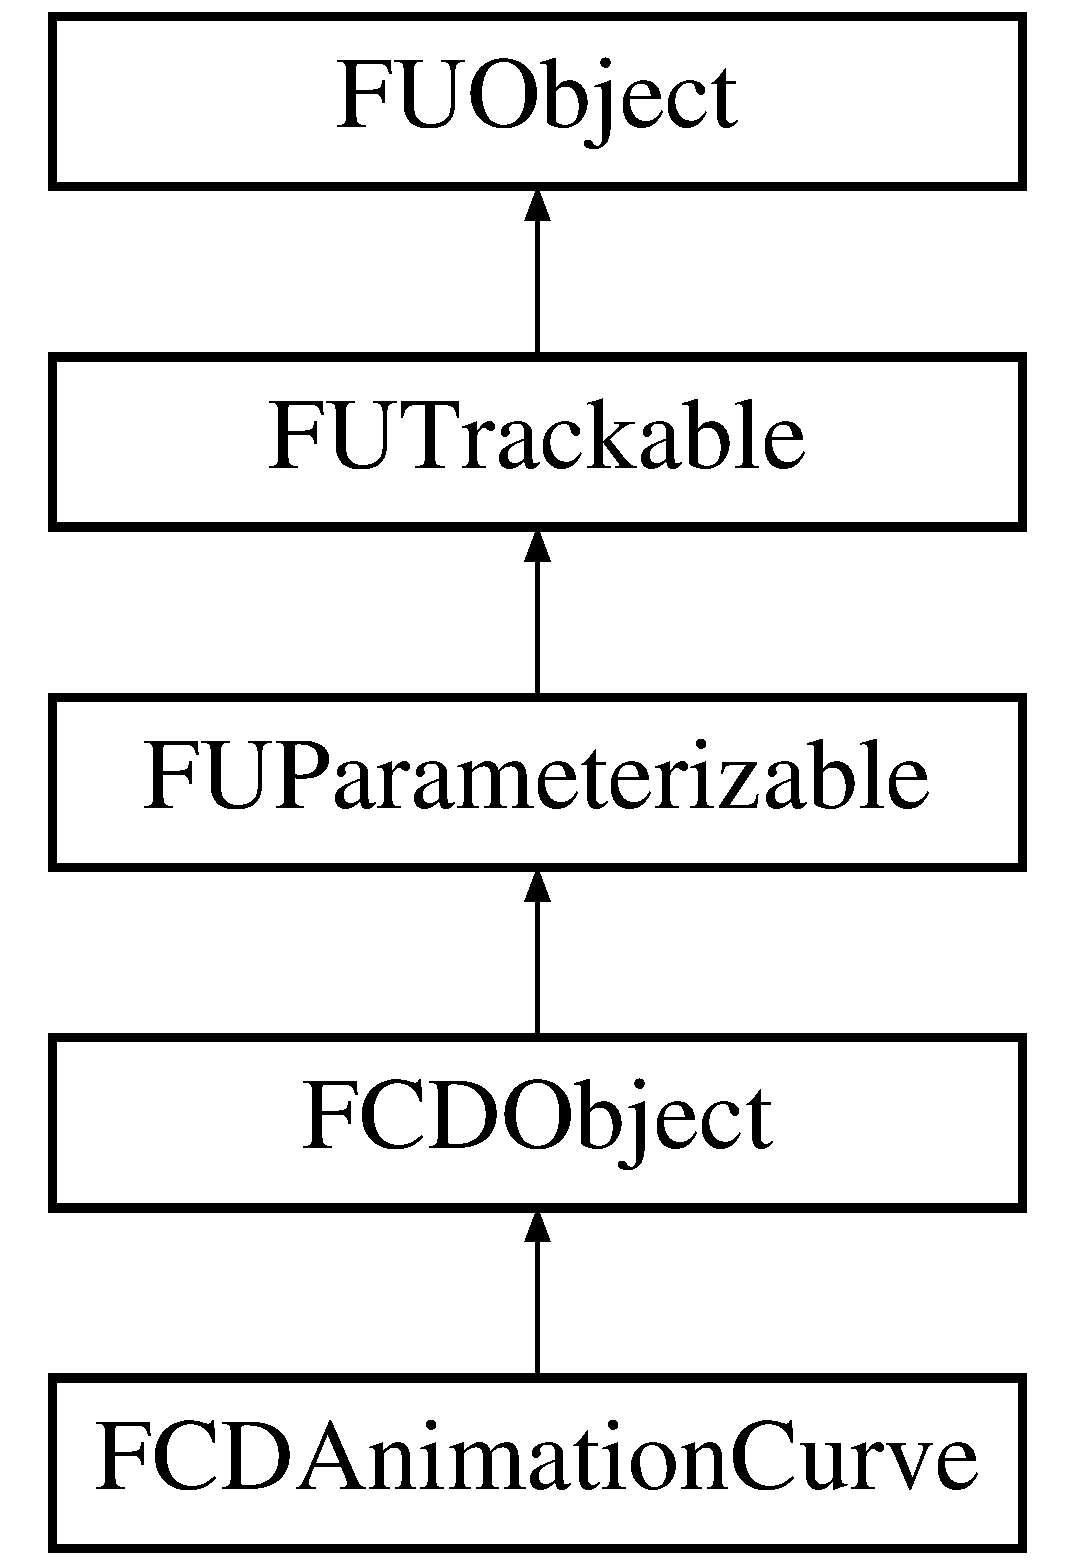
\includegraphics[height=5.000000cm]{classFCDAnimationCurve}
\end{center}
\end{figure}
\subsection*{Public Member Functions}
\begin{DoxyCompactItemize}
\item 
\hypertarget{classFCDAnimationCurve_a66c2b001d6172d74e57899d965449a7a}{
{\bfseries DeclareFlag} (AnimChanged, 0)}
\label{classFCDAnimationCurve_a66c2b001d6172d74e57899d965449a7a}

\item 
\hypertarget{classFCDAnimationCurve_abb88a31deb0a9ee93279240b24b3947d}{
{\bfseries DeclareFlagCount} (1)}
\label{classFCDAnimationCurve_abb88a31deb0a9ee93279240b24b3947d}

\item 
\hyperlink{classFCDAnimationCurve_ab266e817fd27a881f02c30d18b5c5f72}{FCDAnimationCurve} (\hyperlink{classFCDocument}{FCDocument} $\ast$document, \hyperlink{classFCDAnimationChannel}{FCDAnimationChannel} $\ast$parent)
\item 
virtual \hyperlink{classFCDAnimationCurve_a505ad851cb7265a300a5342996dd8c84}{$\sim$FCDAnimationCurve} ()
\item 
\hyperlink{classFCDAnimationChannel}{FCDAnimationChannel} $\ast$ \hyperlink{classFCDAnimationCurve_a7913003ec78d23d6e8b42feb17b943d4}{GetParent} ()
\item 
const \hyperlink{classFCDAnimationChannel}{FCDAnimationChannel} $\ast$ \hyperlink{classFCDAnimationCurve_a3e9c80bfc5bf390d79a511687d77f4fa}{GetParent} () const 
\item 
\hyperlink{classFCDAnimationKey}{FCDAnimationKey} $\ast$$\ast$ \hyperlink{classFCDAnimationCurve_acb8c98803d2cd6df5912c53aeb9b18f6}{GetKeys} ()
\item 
const \hyperlink{classFCDAnimationKey}{FCDAnimationKey} $\ast$$\ast$ \hyperlink{classFCDAnimationCurve_a0f4684cb8a2fd9119f294f91697da7bc}{GetKeys} () const 
\item 
size\_\-t \hyperlink{classFCDAnimationCurve_a3bbe5d298465ab1679f0236831d88369}{GetKeyCount} () const 
\item 
void \hyperlink{classFCDAnimationCurve_afa4134d2d93011191686d5dc7bd2f69f}{SetKeyCount} (size\_\-t count, \hyperlink{namespaceFUDaeInterpolation_a209a941c2fb6ece1325352968aa0374f}{FUDaeInterpolation::Interpolation} interpolation)
\item 
\hyperlink{classFCDAnimationKey}{FCDAnimationKey} $\ast$ \hyperlink{classFCDAnimationCurve_a4354985b1d74fc5fc006fc2bb853395f}{GetKey} (size\_\-t index)
\item 
const \hyperlink{classFCDAnimationKey}{FCDAnimationKey} $\ast$ \hyperlink{classFCDAnimationCurve_a26c830e127b6a87308bcd7b3fcef3dd7}{GetKey} (size\_\-t index) const 
\item 
\hyperlink{classFCDAnimationKey}{FCDAnimationKey} $\ast$ \hyperlink{classFCDAnimationCurve_a58e0870ef3f44d5711694103371df555}{AddKey} (\hyperlink{namespaceFUDaeInterpolation_a209a941c2fb6ece1325352968aa0374f}{FUDaeInterpolation::Interpolation} interpolation)
\item 
\hyperlink{classFCDAnimationKey}{FCDAnimationKey} $\ast$ \hyperlink{classFCDAnimationCurve_ace18196c3824cf30dab1fffe2a7590e8}{AddKey} (\hyperlink{namespaceFUDaeInterpolation_a209a941c2fb6ece1325352968aa0374f}{FUDaeInterpolation::Interpolation} interpolation, float input)
\item 
\hyperlink{classFCDAnimationKey}{FCDAnimationKey} $\ast$ \hyperlink{classFCDAnimationCurve_a506f618558dcbf95cbae57e1f98ffd6b}{AddKey} (\hyperlink{namespaceFUDaeInterpolation_a209a941c2fb6ece1325352968aa0374f}{FUDaeInterpolation::Interpolation} interpolation, float input, size\_\-t \&index)
\item 
bool \hyperlink{classFCDAnimationCurve_a056f03ba3077bb7238ae12530d670358}{DeleteKey} (\hyperlink{classFCDAnimationKey}{FCDAnimationKey} $\ast$key)
\item 
\hyperlink{namespaceFUDaeInfinity_a9d8fb86affe94d1586d728d4c2e89008}{FUDaeInfinity::Infinity} \hyperlink{classFCDAnimationCurve_ae782d284b00751674f233af37d1be31d}{GetPreInfinity} () const 
\item 
void \hyperlink{classFCDAnimationCurve_a854c8a287e5a06adb76b185a3b158d70}{SetPreInfinity} (\hyperlink{namespaceFUDaeInfinity_a9d8fb86affe94d1586d728d4c2e89008}{FUDaeInfinity::Infinity} infinity)
\item 
\hyperlink{namespaceFUDaeInfinity_a9d8fb86affe94d1586d728d4c2e89008}{FUDaeInfinity::Infinity} \hyperlink{classFCDAnimationCurve_a99c4ee14480666c4f203b616a3bfb026}{GetPostInfinity} () const 
\item 
void \hyperlink{classFCDAnimationCurve_a3ad6a612d70548dc221c66852f3119ac}{SetPostInfinity} (\hyperlink{namespaceFUDaeInfinity_a9d8fb86affe94d1586d728d4c2e89008}{FUDaeInfinity::Infinity} infinity)
\item 
bool \hyperlink{classFCDAnimationCurve_a458414600d521c80d5a1b96d10ec22ae}{HasDriver} () const 
\item 
void \hyperlink{classFCDAnimationCurve_ae97116da1f894405a10ff9b7c6b8d78d}{GetDriver} (\hyperlink{classFCDAnimated}{FCDAnimated} $\ast$\&driver, int32 \&index)
\item 
void \hyperlink{classFCDAnimationCurve_a8a489fc84d0a1a1314a70b599cf46e4b}{GetDriver} (const \hyperlink{classFCDAnimated}{FCDAnimated} $\ast$\&driver, int32 \&index) const 
\item 
\hypertarget{classFCDAnimationCurve_afdacf9cf08a2370af43b2eabe9b97cd2}{
\hyperlink{classFCDAnimated}{FCDAnimated} $\ast$ {\bfseries GetDriverPtr} ()}
\label{classFCDAnimationCurve_afdacf9cf08a2370af43b2eabe9b97cd2}

\item 
int32 \hyperlink{classFCDAnimationCurve_a5b7178c92b0431345b722f3a41ffc1f8}{GetDriverIndex} ()
\item 
void \hyperlink{classFCDAnimationCurve_aa440afe6b2fa33e6941be2306aa42eb1}{SetDriver} (\hyperlink{classFCDAnimated}{FCDAnimated} $\ast$driver, int32 index)
\item 
size\_\-t \hyperlink{classFCDAnimationCurve_ac84352a4fb7e1bbcabd47652e18e9295}{GetClipCount} () const 
\item 
\hyperlink{classFCDAnimationClip}{FCDAnimationClip} $\ast$$\ast$ \hyperlink{classFCDAnimationCurve_a21949f9cae3491f6e4c9dc3c9218726d}{GetClips} ()
\item 
const \hyperlink{classFCDAnimationClip}{FCDAnimationClip} $\ast$$\ast$ \hyperlink{classFCDAnimationCurve_a08739b03f09ad4e4d72e2b416b3fc0a5}{GetClips} () const 
\item 
\hyperlink{classFCDAnimationClip}{FCDAnimationClip} $\ast$ \hyperlink{classFCDAnimationCurve_ad004f56a3b76bfe41415ed4837326a52}{GetClip} (size\_\-t index)
\item 
const \hyperlink{classFCDAnimationClip}{FCDAnimationClip} $\ast$ \hyperlink{classFCDAnimationCurve_a90d654fc9156705c398f996d56d92b16}{GetClip} (size\_\-t index) const 
\item 
void \hyperlink{classFCDAnimationCurve_af9b490579c37bb15ddee75c415169958}{AddClip} (\hyperlink{classFCDAnimationClip}{FCDAnimationClip} $\ast$clip)
\item 
void \hyperlink{classFCDAnimationCurve_aca5ee7758684615dd5acf659315172c6}{SetCurrentAnimationClip} (\hyperlink{classFCDAnimationClip}{FCDAnimationClip} $\ast$clip)
\item 
float \hyperlink{classFCDAnimationCurve_a931bfe407893568022f461dbb1b3f8e1}{GetClipOffset} (size\_\-t index) const 
\item 
\hyperlink{classFCDAnimationCurve}{FCDAnimationCurve} $\ast$ \hyperlink{classFCDAnimationCurve_a142d97f7ea0f9312b95c2df9337b2356}{Clone} (\hyperlink{classFCDAnimationCurve}{FCDAnimationCurve} $\ast$clone=NULL, bool includeClips=true) const 
\item 
void \hyperlink{classFCDAnimationCurve_abecd157c277b8d1abd0c78b76a97ee83}{ConvertValues} (\hyperlink{FCDAnimationCurve_8h_a3f37db4cc9939d7b076d4cbfe81680c4}{FCDConversionFunction} valueConversion, \hyperlink{FCDAnimationCurve_8h_a3f37db4cc9939d7b076d4cbfe81680c4}{FCDConversionFunction} tangentConversion)
\item 
void \hyperlink{classFCDAnimationCurve_a21defc6b006ae6f3af9810333e8245bc}{ConvertValues} (\hyperlink{classFCDConversionFunctor}{FCDConversionFunctor} $\ast$valueConversion, \hyperlink{classFCDConversionFunctor}{FCDConversionFunctor} $\ast$tangentConversion)
\item 
void \hyperlink{classFCDAnimationCurve_ac77614a66e9af65e55370da9c41232a7}{ConvertInputs} (\hyperlink{FCDAnimationCurve_8h_a3f37db4cc9939d7b076d4cbfe81680c4}{FCDConversionFunction} timeConversion, \hyperlink{FCDAnimationCurve_8h_a3f37db4cc9939d7b076d4cbfe81680c4}{FCDConversionFunction} tangentWeightConversion)
\item 
void \hyperlink{classFCDAnimationCurve_a6b61e8a04977404fac8063b6b464ac1d}{ConvertInputs} (\hyperlink{classFCDConversionFunctor}{FCDConversionFunctor} $\ast$timeConversion, \hyperlink{classFCDConversionFunctor}{FCDConversionFunctor} $\ast$tangentWeightConversion)
\item 
float \hyperlink{classFCDAnimationCurve_a66887cf60eb77e03592173e6cebec028}{Evaluate} (float input) const 
\item 
void \hyperlink{classFCDAnimationCurve_ae255cbba1e90984157274f5713f32342}{RegisterAnimationClip} (\hyperlink{classFCDAnimationClip}{FCDAnimationClip} $\ast$clip)
\item 
int32 \hyperlink{classFCDAnimationCurve_a686961ad58773191b3426600c6e0c375}{GetTargetElement} () const 
\item 
const \hyperlink{classfm_1_1stringT}{fm::string} \& \hyperlink{classFCDAnimationCurve_aeb17123216607ff98554547641936180}{GetTargetQualifier} () const 
\item 
void \hyperlink{classFCDAnimationCurve_a27ff11a7446c95582551eb221993af4b}{SetTargetElement} (int32 e)
\item 
void \hyperlink{classFCDAnimationCurve_a9d69a7d44da85da5dfbb8a1489f282a4}{SetTargetQualifier} (const \hyperlink{classfm_1_1stringT}{fm::string} \&q)
\item 
void \hyperlink{classFCDAnimationCurve_af70751917c31d65a35e96211f31cf239}{SetClipOffset} (float offset, const \hyperlink{classFCDAnimationClip}{FCDAnimationClip} $\ast$clip)
\end{DoxyCompactItemize}
\subsection*{Static Public Member Functions}
\begin{DoxyCompactItemize}
\item 
static void \hyperlink{classFCDAnimationCurve_a97853d967dc312958463ee42ced34f64}{Set2DCurveEvaluation} (bool flag)
\item 
static bool \hyperlink{classFCDAnimationCurve_a1dc8857d6e5677454ebabbc6df39da9f}{Is2DCurveEvaluation} ()
\end{DoxyCompactItemize}


\subsection{Detailed Description}
A COLLADA single-\/dimensional animation curve. An animation curve holds the keyframes necessary to animate an animatable floating-\/point value.

There are multiple interpolation mechanisms supported by COLLADA. \hyperlink{namespaceFCollada}{FCollada} supports the CONSTANT, LINEAR and BEZIER interpolations.

\begin{DoxySeeAlso}{See also}
\hyperlink{namespaceFUDaeInterpolation}{FUDaeInterpolation} \hyperlink{namespaceFUDaeInfinity}{FUDaeInfinity} 
\end{DoxySeeAlso}


\subsection{Constructor \& Destructor Documentation}
\hypertarget{classFCDAnimationCurve_ab266e817fd27a881f02c30d18b5c5f72}{
\index{FCDAnimationCurve@{FCDAnimationCurve}!FCDAnimationCurve@{FCDAnimationCurve}}
\index{FCDAnimationCurve@{FCDAnimationCurve}!FCDAnimationCurve@{FCDAnimationCurve}}
\subsubsection[{FCDAnimationCurve}]{\setlength{\rightskip}{0pt plus 5cm}FCDAnimationCurve::FCDAnimationCurve (
\begin{DoxyParamCaption}
\item[{{\bf FCDocument} $\ast$}]{ document, }
\item[{{\bf FCDAnimationChannel} $\ast$}]{ parent}
\end{DoxyParamCaption}
)}}
\label{classFCDAnimationCurve_ab266e817fd27a881f02c30d18b5c5f72}
Constructor: do not use directly. Instead, use the \hyperlink{classFCDAnimationChannel_ab7d70254bef3270047703746e31522a8}{FCDAnimationChannel::AddCurve} function. You should also attach the new curve to an animated element using the FCDAnimated::SetCurve function. 
\begin{DoxyParams}{Parameters}
\item[{\em document}]The COLLADA document that owns the animation curve. \item[{\em parent}]The animation channel that contains the curve. \end{DoxyParams}
\hypertarget{classFCDAnimationCurve_a505ad851cb7265a300a5342996dd8c84}{
\index{FCDAnimationCurve@{FCDAnimationCurve}!$\sim$FCDAnimationCurve@{$\sim$FCDAnimationCurve}}
\index{$\sim$FCDAnimationCurve@{$\sim$FCDAnimationCurve}!FCDAnimationCurve@{FCDAnimationCurve}}
\subsubsection[{$\sim$FCDAnimationCurve}]{\setlength{\rightskip}{0pt plus 5cm}FCDAnimationCurve::$\sim$FCDAnimationCurve (
\begin{DoxyParamCaption}
{}
\end{DoxyParamCaption}
)\hspace{0.3cm}{\ttfamily  \mbox{[}virtual\mbox{]}}}}
\label{classFCDAnimationCurve_a505ad851cb7265a300a5342996dd8c84}
Destructor. 

\subsection{Member Function Documentation}
\hypertarget{classFCDAnimationCurve_af9b490579c37bb15ddee75c415169958}{
\index{FCDAnimationCurve@{FCDAnimationCurve}!AddClip@{AddClip}}
\index{AddClip@{AddClip}!FCDAnimationCurve@{FCDAnimationCurve}}
\subsubsection[{AddClip}]{\setlength{\rightskip}{0pt plus 5cm}void FCDAnimationCurve::AddClip (
\begin{DoxyParamCaption}
\item[{{\bf FCDAnimationClip} $\ast$}]{ clip}
\end{DoxyParamCaption}
)}}
\label{classFCDAnimationCurve_af9b490579c37bb15ddee75c415169958}
Adds an animation clip to the list of animation clips that use this curve. 
\begin{DoxyParams}{Parameters}
\item[{\em clip}]An animation clip that uses this curve. \end{DoxyParams}
\hypertarget{classFCDAnimationCurve_a58e0870ef3f44d5711694103371df555}{
\index{FCDAnimationCurve@{FCDAnimationCurve}!AddKey@{AddKey}}
\index{AddKey@{AddKey}!FCDAnimationCurve@{FCDAnimationCurve}}
\subsubsection[{AddKey}]{\setlength{\rightskip}{0pt plus 5cm}{\bf FCDAnimationKey} $\ast$ FCDAnimationCurve::AddKey (
\begin{DoxyParamCaption}
\item[{{\bf FUDaeInterpolation::Interpolation}}]{ interpolation}
\end{DoxyParamCaption}
)}}
\label{classFCDAnimationCurve_a58e0870ef3f44d5711694103371df555}
Appends a key to the animation curve. 
\begin{DoxyParams}{Parameters}
\item[{\em interpolation}]The interpolation type for the new key. \end{DoxyParams}
\begin{DoxyReturn}{Returns}
The new key. 
\end{DoxyReturn}
\hypertarget{classFCDAnimationCurve_a506f618558dcbf95cbae57e1f98ffd6b}{
\index{FCDAnimationCurve@{FCDAnimationCurve}!AddKey@{AddKey}}
\index{AddKey@{AddKey}!FCDAnimationCurve@{FCDAnimationCurve}}
\subsubsection[{AddKey}]{\setlength{\rightskip}{0pt plus 5cm}{\bf FCDAnimationKey} $\ast$ FCDAnimationCurve::AddKey (
\begin{DoxyParamCaption}
\item[{{\bf FUDaeInterpolation::Interpolation}}]{ interpolation, }
\item[{float}]{ input, }
\item[{size\_\-t \&}]{ index}
\end{DoxyParamCaption}
)}}
\label{classFCDAnimationCurve_a506f618558dcbf95cbae57e1f98ffd6b}
Adds a new key to the animation curve at the given time. 
\begin{DoxyParams}{Parameters}
\item[{\em interpolation}]The interpolation type for the new key. \item[{\em input}]The input (x) value of the new key. \item[{\em index}]\mbox{[}OUT\mbox{]} The index in the array of the new key \end{DoxyParams}
\begin{DoxyReturn}{Returns}
The new key. 
\end{DoxyReturn}
\hypertarget{classFCDAnimationCurve_ace18196c3824cf30dab1fffe2a7590e8}{
\index{FCDAnimationCurve@{FCDAnimationCurve}!AddKey@{AddKey}}
\index{AddKey@{AddKey}!FCDAnimationCurve@{FCDAnimationCurve}}
\subsubsection[{AddKey}]{\setlength{\rightskip}{0pt plus 5cm}{\bf FCDAnimationKey}$\ast$ FCDAnimationCurve::AddKey (
\begin{DoxyParamCaption}
\item[{{\bf FUDaeInterpolation::Interpolation}}]{ interpolation, }
\item[{float}]{ input}
\end{DoxyParamCaption}
)\hspace{0.3cm}{\ttfamily  \mbox{[}inline\mbox{]}}}}
\label{classFCDAnimationCurve_ace18196c3824cf30dab1fffe2a7590e8}
Adds a new key to the animation curve at the given time. 
\begin{DoxyParams}{Parameters}
\item[{\em interpolation}]The interpolation type for the new key. \item[{\em input}]The input (x) value of the new key. \end{DoxyParams}
\begin{DoxyReturn}{Returns}
The new key. 
\end{DoxyReturn}
\hypertarget{classFCDAnimationCurve_a142d97f7ea0f9312b95c2df9337b2356}{
\index{FCDAnimationCurve@{FCDAnimationCurve}!Clone@{Clone}}
\index{Clone@{Clone}!FCDAnimationCurve@{FCDAnimationCurve}}
\subsubsection[{Clone}]{\setlength{\rightskip}{0pt plus 5cm}{\bf FCDAnimationCurve} $\ast$ FCDAnimationCurve::Clone (
\begin{DoxyParamCaption}
\item[{{\bf FCDAnimationCurve} $\ast$}]{ clone = {\ttfamily NULL}, }
\item[{bool}]{ includeClips = {\ttfamily true}}
\end{DoxyParamCaption}
) const}}
\label{classFCDAnimationCurve_a142d97f7ea0f9312b95c2df9337b2356}
Clones the animation curve. The animation clips can be cloned as well, but this may lead to an infinite recursion because cloning the clips will also clone its curves. 
\begin{DoxyParams}{Parameters}
\item[{\em clone}]The cloned animation curve. If this pointer is NULL, a new animation curve will be created for you. You will then need to release the pointer. \item[{\em includeClips}]True if want to also clone the animation clips. \end{DoxyParams}
\begin{DoxyReturn}{Returns}
The cloned animation curve. 
\end{DoxyReturn}
\hypertarget{classFCDAnimationCurve_ac77614a66e9af65e55370da9c41232a7}{
\index{FCDAnimationCurve@{FCDAnimationCurve}!ConvertInputs@{ConvertInputs}}
\index{ConvertInputs@{ConvertInputs}!FCDAnimationCurve@{FCDAnimationCurve}}
\subsubsection[{ConvertInputs}]{\setlength{\rightskip}{0pt plus 5cm}void FCDAnimationCurve::ConvertInputs (
\begin{DoxyParamCaption}
\item[{{\bf FCDConversionFunction}}]{ timeConversion, }
\item[{{\bf FCDConversionFunction}}]{ tangentWeightConversion}
\end{DoxyParamCaption}
)}}
\label{classFCDAnimationCurve_ac77614a66e9af65e55370da9c41232a7}
Applies a conversion function to the key input values of the animation curve. 
\begin{DoxyParams}{Parameters}
\item[{\em timeConversion}]The conversion function to use on the key inputs. \item[{\em tangentWeightConversion}]The conversion function to use on the key tangent weights. \end{DoxyParams}
\hypertarget{classFCDAnimationCurve_a6b61e8a04977404fac8063b6b464ac1d}{
\index{FCDAnimationCurve@{FCDAnimationCurve}!ConvertInputs@{ConvertInputs}}
\index{ConvertInputs@{ConvertInputs}!FCDAnimationCurve@{FCDAnimationCurve}}
\subsubsection[{ConvertInputs}]{\setlength{\rightskip}{0pt plus 5cm}void FCDAnimationCurve::ConvertInputs (
\begin{DoxyParamCaption}
\item[{{\bf FCDConversionFunctor} $\ast$}]{ timeConversion, }
\item[{{\bf FCDConversionFunctor} $\ast$}]{ tangentWeightConversion}
\end{DoxyParamCaption}
)}}
\label{classFCDAnimationCurve_a6b61e8a04977404fac8063b6b464ac1d}
See above. \hypertarget{classFCDAnimationCurve_a21defc6b006ae6f3af9810333e8245bc}{
\index{FCDAnimationCurve@{FCDAnimationCurve}!ConvertValues@{ConvertValues}}
\index{ConvertValues@{ConvertValues}!FCDAnimationCurve@{FCDAnimationCurve}}
\subsubsection[{ConvertValues}]{\setlength{\rightskip}{0pt plus 5cm}void FCDAnimationCurve::ConvertValues (
\begin{DoxyParamCaption}
\item[{{\bf FCDConversionFunctor} $\ast$}]{ valueConversion, }
\item[{{\bf FCDConversionFunctor} $\ast$}]{ tangentConversion}
\end{DoxyParamCaption}
)}}
\label{classFCDAnimationCurve_a21defc6b006ae6f3af9810333e8245bc}
See above. \hypertarget{classFCDAnimationCurve_abecd157c277b8d1abd0c78b76a97ee83}{
\index{FCDAnimationCurve@{FCDAnimationCurve}!ConvertValues@{ConvertValues}}
\index{ConvertValues@{ConvertValues}!FCDAnimationCurve@{FCDAnimationCurve}}
\subsubsection[{ConvertValues}]{\setlength{\rightskip}{0pt plus 5cm}void FCDAnimationCurve::ConvertValues (
\begin{DoxyParamCaption}
\item[{{\bf FCDConversionFunction}}]{ valueConversion, }
\item[{{\bf FCDConversionFunction}}]{ tangentConversion}
\end{DoxyParamCaption}
)}}
\label{classFCDAnimationCurve_abecd157c277b8d1abd0c78b76a97ee83}
Applies a conversion function to the key output values of the animation curve. 
\begin{DoxyParams}{Parameters}
\item[{\em valueConversion}]The conversion function to use on the key outputs. \item[{\em tangentConversion}]The conversion function to use on the key tangents. \end{DoxyParams}
\hypertarget{classFCDAnimationCurve_a056f03ba3077bb7238ae12530d670358}{
\index{FCDAnimationCurve@{FCDAnimationCurve}!DeleteKey@{DeleteKey}}
\index{DeleteKey@{DeleteKey}!FCDAnimationCurve@{FCDAnimationCurve}}
\subsubsection[{DeleteKey}]{\setlength{\rightskip}{0pt plus 5cm}bool FCDAnimationCurve::DeleteKey (
\begin{DoxyParamCaption}
\item[{{\bf FCDAnimationKey} $\ast$}]{ key}
\end{DoxyParamCaption}
)}}
\label{classFCDAnimationCurve_a056f03ba3077bb7238ae12530d670358}
Removes the given key from this curves list and deletes it 
\begin{DoxyParams}{Parameters}
\item[{\em key}]The key to find and delete \end{DoxyParams}
\begin{DoxyReturn}{Returns}
True on success, false if the key is not found 
\end{DoxyReturn}
\hypertarget{classFCDAnimationCurve_a66887cf60eb77e03592173e6cebec028}{
\index{FCDAnimationCurve@{FCDAnimationCurve}!Evaluate@{Evaluate}}
\index{Evaluate@{Evaluate}!FCDAnimationCurve@{FCDAnimationCurve}}
\subsubsection[{Evaluate}]{\setlength{\rightskip}{0pt plus 5cm}float FCDAnimationCurve::Evaluate (
\begin{DoxyParamCaption}
\item[{float}]{ input}
\end{DoxyParamCaption}
) const}}
\label{classFCDAnimationCurve_a66887cf60eb77e03592173e6cebec028}
Evaluates the animation curve. 
\begin{DoxyParams}{Parameters}
\item[{\em input}]An input value. \end{DoxyParams}
\begin{DoxyReturn}{Returns}
The sampled value of the curve at the given input value. 
\end{DoxyReturn}
\hypertarget{classFCDAnimationCurve_ad004f56a3b76bfe41415ed4837326a52}{
\index{FCDAnimationCurve@{FCDAnimationCurve}!GetClip@{GetClip}}
\index{GetClip@{GetClip}!FCDAnimationCurve@{FCDAnimationCurve}}
\subsubsection[{GetClip}]{\setlength{\rightskip}{0pt plus 5cm}{\bf FCDAnimationClip}$\ast$ FCDAnimationCurve::GetClip (
\begin{DoxyParamCaption}
\item[{size\_\-t}]{ index}
\end{DoxyParamCaption}
)\hspace{0.3cm}{\ttfamily  \mbox{[}inline\mbox{]}}}}
\label{classFCDAnimationCurve_ad004f56a3b76bfe41415ed4837326a52}
Retrieves an animation clips that use this animation curve. 
\begin{DoxyParams}{Parameters}
\item[{\em index}]The index of the animation clip. \end{DoxyParams}
\begin{DoxyReturn}{Returns}
The animation clip at the given index in the list of clips that use this curve. 
\end{DoxyReturn}
\hypertarget{classFCDAnimationCurve_a90d654fc9156705c398f996d56d92b16}{
\index{FCDAnimationCurve@{FCDAnimationCurve}!GetClip@{GetClip}}
\index{GetClip@{GetClip}!FCDAnimationCurve@{FCDAnimationCurve}}
\subsubsection[{GetClip}]{\setlength{\rightskip}{0pt plus 5cm}const {\bf FCDAnimationClip}$\ast$ FCDAnimationCurve::GetClip (
\begin{DoxyParamCaption}
\item[{size\_\-t}]{ index}
\end{DoxyParamCaption}
) const\hspace{0.3cm}{\ttfamily  \mbox{[}inline\mbox{]}}}}
\label{classFCDAnimationCurve_a90d654fc9156705c398f996d56d92b16}
See above. \hypertarget{classFCDAnimationCurve_ac84352a4fb7e1bbcabd47652e18e9295}{
\index{FCDAnimationCurve@{FCDAnimationCurve}!GetClipCount@{GetClipCount}}
\index{GetClipCount@{GetClipCount}!FCDAnimationCurve@{FCDAnimationCurve}}
\subsubsection[{GetClipCount}]{\setlength{\rightskip}{0pt plus 5cm}size\_\-t FCDAnimationCurve::GetClipCount (
\begin{DoxyParamCaption}
{}
\end{DoxyParamCaption}
) const\hspace{0.3cm}{\ttfamily  \mbox{[}inline\mbox{]}}}}
\label{classFCDAnimationCurve_ac84352a4fb7e1bbcabd47652e18e9295}
Retrieves the number of animation clips that use this animation curve. \begin{DoxyReturn}{Returns}
The number of animation clips. 
\end{DoxyReturn}
\hypertarget{classFCDAnimationCurve_a931bfe407893568022f461dbb1b3f8e1}{
\index{FCDAnimationCurve@{FCDAnimationCurve}!GetClipOffset@{GetClipOffset}}
\index{GetClipOffset@{GetClipOffset}!FCDAnimationCurve@{FCDAnimationCurve}}
\subsubsection[{GetClipOffset}]{\setlength{\rightskip}{0pt plus 5cm}float FCDAnimationCurve::GetClipOffset (
\begin{DoxyParamCaption}
\item[{size\_\-t}]{ index}
\end{DoxyParamCaption}
) const\hspace{0.3cm}{\ttfamily  \mbox{[}inline\mbox{]}}}}
\label{classFCDAnimationCurve_a931bfe407893568022f461dbb1b3f8e1}
Gets the offset for an animation clip. When the offset is added to the keys, it causes the animation curve to be repositioned so that the animation clip starts at the beginning. 
\begin{DoxyParams}{Parameters}
\item[{\em index}]The index of the animation clip to get offset for. \end{DoxyParams}
\begin{DoxyReturn}{Returns}
The offset value. 
\end{DoxyReturn}
\hypertarget{classFCDAnimationCurve_a21949f9cae3491f6e4c9dc3c9218726d}{
\index{FCDAnimationCurve@{FCDAnimationCurve}!GetClips@{GetClips}}
\index{GetClips@{GetClips}!FCDAnimationCurve@{FCDAnimationCurve}}
\subsubsection[{GetClips}]{\setlength{\rightskip}{0pt plus 5cm}{\bf FCDAnimationClip}$\ast$$\ast$ FCDAnimationCurve::GetClips (
\begin{DoxyParamCaption}
{}
\end{DoxyParamCaption}
)\hspace{0.3cm}{\ttfamily  \mbox{[}inline\mbox{]}}}}
\label{classFCDAnimationCurve_a21949f9cae3491f6e4c9dc3c9218726d}
Retrieves the list of animation clips that use this animation curve. \begin{DoxyReturn}{Returns}
The list of animation clips. 
\end{DoxyReturn}
\hypertarget{classFCDAnimationCurve_a08739b03f09ad4e4d72e2b416b3fc0a5}{
\index{FCDAnimationCurve@{FCDAnimationCurve}!GetClips@{GetClips}}
\index{GetClips@{GetClips}!FCDAnimationCurve@{FCDAnimationCurve}}
\subsubsection[{GetClips}]{\setlength{\rightskip}{0pt plus 5cm}const {\bf FCDAnimationClip}$\ast$$\ast$ FCDAnimationCurve::GetClips (
\begin{DoxyParamCaption}
{}
\end{DoxyParamCaption}
) const\hspace{0.3cm}{\ttfamily  \mbox{[}inline\mbox{]}}}}
\label{classFCDAnimationCurve_a08739b03f09ad4e4d72e2b416b3fc0a5}
See above. \hypertarget{classFCDAnimationCurve_ae97116da1f894405a10ff9b7c6b8d78d}{
\index{FCDAnimationCurve@{FCDAnimationCurve}!GetDriver@{GetDriver}}
\index{GetDriver@{GetDriver}!FCDAnimationCurve@{FCDAnimationCurve}}
\subsubsection[{GetDriver}]{\setlength{\rightskip}{0pt plus 5cm}void FCDAnimationCurve::GetDriver (
\begin{DoxyParamCaption}
\item[{{\bf FCDAnimated} $\ast$\&}]{ driver, }
\item[{int32 \&}]{ index}
\end{DoxyParamCaption}
)}}
\label{classFCDAnimationCurve_ae97116da1f894405a10ff9b7c6b8d78d}
Retrieves the value pointer that drives this animation curve. 
\begin{DoxyParams}{Parameters}
\item[{\em driver}]A reference to receive the animated input driver. This pointer will be set to NULL when there is no input driver. \item[{\em index}]A reference to receive the animated input driver element index. \end{DoxyParams}
\hypertarget{classFCDAnimationCurve_a8a489fc84d0a1a1314a70b599cf46e4b}{
\index{FCDAnimationCurve@{FCDAnimationCurve}!GetDriver@{GetDriver}}
\index{GetDriver@{GetDriver}!FCDAnimationCurve@{FCDAnimationCurve}}
\subsubsection[{GetDriver}]{\setlength{\rightskip}{0pt plus 5cm}void FCDAnimationCurve::GetDriver (
\begin{DoxyParamCaption}
\item[{const {\bf FCDAnimated} $\ast$\&}]{ driver, }
\item[{int32 \&}]{ index}
\end{DoxyParamCaption}
) const}}
\label{classFCDAnimationCurve_a8a489fc84d0a1a1314a70b599cf46e4b}
See above. \hypertarget{classFCDAnimationCurve_a5b7178c92b0431345b722f3a41ffc1f8}{
\index{FCDAnimationCurve@{FCDAnimationCurve}!GetDriverIndex@{GetDriverIndex}}
\index{GetDriverIndex@{GetDriverIndex}!FCDAnimationCurve@{FCDAnimationCurve}}
\subsubsection[{GetDriverIndex}]{\setlength{\rightskip}{0pt plus 5cm}int32 FCDAnimationCurve::GetDriverIndex (
\begin{DoxyParamCaption}
{}
\end{DoxyParamCaption}
)\hspace{0.3cm}{\ttfamily  \mbox{[}inline\mbox{]}}}}
\label{classFCDAnimationCurve_a5b7178c92b0431345b722f3a41ffc1f8}
\mbox{[}INTERNAL\mbox{]} Retrieve the driver index. \begin{DoxyReturn}{Returns}
The driver index. 
\end{DoxyReturn}
\hypertarget{classFCDAnimationCurve_a4354985b1d74fc5fc006fc2bb853395f}{
\index{FCDAnimationCurve@{FCDAnimationCurve}!GetKey@{GetKey}}
\index{GetKey@{GetKey}!FCDAnimationCurve@{FCDAnimationCurve}}
\subsubsection[{GetKey}]{\setlength{\rightskip}{0pt plus 5cm}{\bf FCDAnimationKey}$\ast$ FCDAnimationCurve::GetKey (
\begin{DoxyParamCaption}
\item[{size\_\-t}]{ index}
\end{DoxyParamCaption}
)\hspace{0.3cm}{\ttfamily  \mbox{[}inline\mbox{]}}}}
\label{classFCDAnimationCurve_a4354985b1d74fc5fc006fc2bb853395f}
Retrieves one key in the animation curve. 
\begin{DoxyParams}{Parameters}
\item[{\em index}]The index of the key to retrieve. \end{DoxyParams}
\begin{DoxyReturn}{Returns}
The key. 
\end{DoxyReturn}
\hypertarget{classFCDAnimationCurve_a26c830e127b6a87308bcd7b3fcef3dd7}{
\index{FCDAnimationCurve@{FCDAnimationCurve}!GetKey@{GetKey}}
\index{GetKey@{GetKey}!FCDAnimationCurve@{FCDAnimationCurve}}
\subsubsection[{GetKey}]{\setlength{\rightskip}{0pt plus 5cm}const {\bf FCDAnimationKey}$\ast$ FCDAnimationCurve::GetKey (
\begin{DoxyParamCaption}
\item[{size\_\-t}]{ index}
\end{DoxyParamCaption}
) const\hspace{0.3cm}{\ttfamily  \mbox{[}inline\mbox{]}}}}
\label{classFCDAnimationCurve_a26c830e127b6a87308bcd7b3fcef3dd7}
See above. \hypertarget{classFCDAnimationCurve_a3bbe5d298465ab1679f0236831d88369}{
\index{FCDAnimationCurve@{FCDAnimationCurve}!GetKeyCount@{GetKeyCount}}
\index{GetKeyCount@{GetKeyCount}!FCDAnimationCurve@{FCDAnimationCurve}}
\subsubsection[{GetKeyCount}]{\setlength{\rightskip}{0pt plus 5cm}size\_\-t FCDAnimationCurve::GetKeyCount (
\begin{DoxyParamCaption}
{}
\end{DoxyParamCaption}
) const\hspace{0.3cm}{\ttfamily  \mbox{[}inline\mbox{]}}}}
\label{classFCDAnimationCurve_a3bbe5d298465ab1679f0236831d88369}
Retrieves the number of keys within the animation curve. \begin{DoxyReturn}{Returns}
The number of keys. 
\end{DoxyReturn}
\hypertarget{classFCDAnimationCurve_acb8c98803d2cd6df5912c53aeb9b18f6}{
\index{FCDAnimationCurve@{FCDAnimationCurve}!GetKeys@{GetKeys}}
\index{GetKeys@{GetKeys}!FCDAnimationCurve@{FCDAnimationCurve}}
\subsubsection[{GetKeys}]{\setlength{\rightskip}{0pt plus 5cm}{\bf FCDAnimationKey}$\ast$$\ast$ FCDAnimationCurve::GetKeys (
\begin{DoxyParamCaption}
{}
\end{DoxyParamCaption}
)\hspace{0.3cm}{\ttfamily  \mbox{[}inline\mbox{]}}}}
\label{classFCDAnimationCurve_acb8c98803d2cd6df5912c53aeb9b18f6}
Retrieves the list of keys for the animation curve. \begin{DoxyReturn}{Returns}
The list of keys. 
\end{DoxyReturn}
\hypertarget{classFCDAnimationCurve_a0f4684cb8a2fd9119f294f91697da7bc}{
\index{FCDAnimationCurve@{FCDAnimationCurve}!GetKeys@{GetKeys}}
\index{GetKeys@{GetKeys}!FCDAnimationCurve@{FCDAnimationCurve}}
\subsubsection[{GetKeys}]{\setlength{\rightskip}{0pt plus 5cm}const {\bf FCDAnimationKey}$\ast$$\ast$ FCDAnimationCurve::GetKeys (
\begin{DoxyParamCaption}
{}
\end{DoxyParamCaption}
) const\hspace{0.3cm}{\ttfamily  \mbox{[}inline\mbox{]}}}}
\label{classFCDAnimationCurve_a0f4684cb8a2fd9119f294f91697da7bc}
See above. \hypertarget{classFCDAnimationCurve_a3e9c80bfc5bf390d79a511687d77f4fa}{
\index{FCDAnimationCurve@{FCDAnimationCurve}!GetParent@{GetParent}}
\index{GetParent@{GetParent}!FCDAnimationCurve@{FCDAnimationCurve}}
\subsubsection[{GetParent}]{\setlength{\rightskip}{0pt plus 5cm}const {\bf FCDAnimationChannel}$\ast$ FCDAnimationCurve::GetParent (
\begin{DoxyParamCaption}
{}
\end{DoxyParamCaption}
) const\hspace{0.3cm}{\ttfamily  \mbox{[}inline\mbox{]}}}}
\label{classFCDAnimationCurve_a3e9c80bfc5bf390d79a511687d77f4fa}
See above. \hypertarget{classFCDAnimationCurve_a7913003ec78d23d6e8b42feb17b943d4}{
\index{FCDAnimationCurve@{FCDAnimationCurve}!GetParent@{GetParent}}
\index{GetParent@{GetParent}!FCDAnimationCurve@{FCDAnimationCurve}}
\subsubsection[{GetParent}]{\setlength{\rightskip}{0pt plus 5cm}{\bf FCDAnimationChannel}$\ast$ FCDAnimationCurve::GetParent (
\begin{DoxyParamCaption}
{}
\end{DoxyParamCaption}
)\hspace{0.3cm}{\ttfamily  \mbox{[}inline\mbox{]}}}}
\label{classFCDAnimationCurve_a7913003ec78d23d6e8b42feb17b943d4}
Retrieves the animation channel that contains this animation curve. \begin{DoxyReturn}{Returns}
The parent animation channel. 
\end{DoxyReturn}
\hypertarget{classFCDAnimationCurve_a99c4ee14480666c4f203b616a3bfb026}{
\index{FCDAnimationCurve@{FCDAnimationCurve}!GetPostInfinity@{GetPostInfinity}}
\index{GetPostInfinity@{GetPostInfinity}!FCDAnimationCurve@{FCDAnimationCurve}}
\subsubsection[{GetPostInfinity}]{\setlength{\rightskip}{0pt plus 5cm}{\bf FUDaeInfinity::Infinity} FCDAnimationCurve::GetPostInfinity (
\begin{DoxyParamCaption}
{}
\end{DoxyParamCaption}
) const\hspace{0.3cm}{\ttfamily  \mbox{[}inline\mbox{]}}}}
\label{classFCDAnimationCurve_a99c4ee14480666c4f203b616a3bfb026}
Retrieves the type of behavior for the curve if the input value is outside the input interval defined by the curve keys and greater than any key input value. \begin{DoxySeeAlso}{See also}
\hyperlink{namespaceFUDaeInfinity}{FUDaeInfinity} 
\end{DoxySeeAlso}
\begin{DoxyReturn}{Returns}
The post-\/infinity behavior of the curve. 
\end{DoxyReturn}
\hypertarget{classFCDAnimationCurve_ae782d284b00751674f233af37d1be31d}{
\index{FCDAnimationCurve@{FCDAnimationCurve}!GetPreInfinity@{GetPreInfinity}}
\index{GetPreInfinity@{GetPreInfinity}!FCDAnimationCurve@{FCDAnimationCurve}}
\subsubsection[{GetPreInfinity}]{\setlength{\rightskip}{0pt plus 5cm}{\bf FUDaeInfinity::Infinity} FCDAnimationCurve::GetPreInfinity (
\begin{DoxyParamCaption}
{}
\end{DoxyParamCaption}
) const\hspace{0.3cm}{\ttfamily  \mbox{[}inline\mbox{]}}}}
\label{classFCDAnimationCurve_ae782d284b00751674f233af37d1be31d}
Retrieves the type of behavior for the curve if the input value is outside the input interval defined by the curve keys and less than any key input value. \begin{DoxySeeAlso}{See also}
\hyperlink{namespaceFUDaeInfinity}{FUDaeInfinity} 
\end{DoxySeeAlso}
\begin{DoxyReturn}{Returns}
The pre-\/infinity behavior of the curve. 
\end{DoxyReturn}
\hypertarget{classFCDAnimationCurve_a686961ad58773191b3426600c6e0c375}{
\index{FCDAnimationCurve@{FCDAnimationCurve}!GetTargetElement@{GetTargetElement}}
\index{GetTargetElement@{GetTargetElement}!FCDAnimationCurve@{FCDAnimationCurve}}
\subsubsection[{GetTargetElement}]{\setlength{\rightskip}{0pt plus 5cm}int32 FCDAnimationCurve::GetTargetElement (
\begin{DoxyParamCaption}
{}
\end{DoxyParamCaption}
) const\hspace{0.3cm}{\ttfamily  \mbox{[}inline\mbox{]}}}}
\label{classFCDAnimationCurve_a686961ad58773191b3426600c6e0c375}
\mbox{[}INTERNAL\mbox{]} Retrieves the target element suffix for the curve. This will be -\/1 if the animated element does not belong to an animated element list. \begin{DoxyReturn}{Returns}
The target element suffix. 
\end{DoxyReturn}
\hypertarget{classFCDAnimationCurve_aeb17123216607ff98554547641936180}{
\index{FCDAnimationCurve@{FCDAnimationCurve}!GetTargetQualifier@{GetTargetQualifier}}
\index{GetTargetQualifier@{GetTargetQualifier}!FCDAnimationCurve@{FCDAnimationCurve}}
\subsubsection[{GetTargetQualifier}]{\setlength{\rightskip}{0pt plus 5cm}const {\bf fm::string}\& FCDAnimationCurve::GetTargetQualifier (
\begin{DoxyParamCaption}
{}
\end{DoxyParamCaption}
) const\hspace{0.3cm}{\ttfamily  \mbox{[}inline\mbox{]}}}}
\label{classFCDAnimationCurve_aeb17123216607ff98554547641936180}
\mbox{[}INTERNAL\mbox{]} Retrieves the target qualifier for the curve. This will be the empty string if that the curve affects a one-\/dimensional animated element. \begin{DoxyReturn}{Returns}
The target qualifier. 
\end{DoxyReturn}
\hypertarget{classFCDAnimationCurve_a458414600d521c80d5a1b96d10ec22ae}{
\index{FCDAnimationCurve@{FCDAnimationCurve}!HasDriver@{HasDriver}}
\index{HasDriver@{HasDriver}!FCDAnimationCurve@{FCDAnimationCurve}}
\subsubsection[{HasDriver}]{\setlength{\rightskip}{0pt plus 5cm}bool FCDAnimationCurve::HasDriver (
\begin{DoxyParamCaption}
{}
\end{DoxyParamCaption}
) const}}
\label{classFCDAnimationCurve_a458414600d521c80d5a1b96d10ec22ae}
Retrieves whether this animation curve has a driver. \begin{DoxyReturn}{Returns}
Whether there is a driver for this curve. 
\end{DoxyReturn}
\hypertarget{classFCDAnimationCurve_a1dc8857d6e5677454ebabbc6df39da9f}{
\index{FCDAnimationCurve@{FCDAnimationCurve}!Is2DCurveEvaluation@{Is2DCurveEvaluation}}
\index{Is2DCurveEvaluation@{Is2DCurveEvaluation}!FCDAnimationCurve@{FCDAnimationCurve}}
\subsubsection[{Is2DCurveEvaluation}]{\setlength{\rightskip}{0pt plus 5cm}static bool FCDAnimationCurve::Is2DCurveEvaluation (
\begin{DoxyParamCaption}
{}
\end{DoxyParamCaption}
)\hspace{0.3cm}{\ttfamily  \mbox{[}inline, static\mbox{]}}}}
\label{classFCDAnimationCurve_a1dc8857d6e5677454ebabbc6df39da9f}
Returns whether 2D Curve Evaluation is on or off. \begin{DoxyReturn}{Returns}
A boolean that indicates if the 2D Curve Evaluation is on or off. 
\end{DoxyReturn}
\hypertarget{classFCDAnimationCurve_ae255cbba1e90984157274f5713f32342}{
\index{FCDAnimationCurve@{FCDAnimationCurve}!RegisterAnimationClip@{RegisterAnimationClip}}
\index{RegisterAnimationClip@{RegisterAnimationClip}!FCDAnimationCurve@{FCDAnimationCurve}}
\subsubsection[{RegisterAnimationClip}]{\setlength{\rightskip}{0pt plus 5cm}void FCDAnimationCurve::RegisterAnimationClip (
\begin{DoxyParamCaption}
\item[{{\bf FCDAnimationClip} $\ast$}]{ clip}
\end{DoxyParamCaption}
)}}
\label{classFCDAnimationCurve_ae255cbba1e90984157274f5713f32342}
\mbox{[}INTERNAL\mbox{]} Adds an animation clip to the list of animation clips that use this curve. 
\begin{DoxyParams}{Parameters}
\item[{\em clip}]An animation clip. \end{DoxyParams}
\hypertarget{classFCDAnimationCurve_a97853d967dc312958463ee42ced34f64}{
\index{FCDAnimationCurve@{FCDAnimationCurve}!Set2DCurveEvaluation@{Set2DCurveEvaluation}}
\index{Set2DCurveEvaluation@{Set2DCurveEvaluation}!FCDAnimationCurve@{FCDAnimationCurve}}
\subsubsection[{Set2DCurveEvaluation}]{\setlength{\rightskip}{0pt plus 5cm}static void FCDAnimationCurve::Set2DCurveEvaluation (
\begin{DoxyParamCaption}
\item[{bool}]{ flag}
\end{DoxyParamCaption}
)\hspace{0.3cm}{\ttfamily  \mbox{[}inline, static\mbox{]}}}}
\label{classFCDAnimationCurve_a97853d967dc312958463ee42ced34f64}
Sets the 2D Curve Evaluation flag. This flag can be set by the user to enable the slower, but higher quality 2D evaluation. If the flag is negative, the faster 1D slope-\/based evaluation is performed. Defaults to true. 
\begin{DoxyParams}{Parameters}
\item[{\em flag}]Whether to enable 2D curve evaluation. \end{DoxyParams}
\hypertarget{classFCDAnimationCurve_af70751917c31d65a35e96211f31cf239}{
\index{FCDAnimationCurve@{FCDAnimationCurve}!SetClipOffset@{SetClipOffset}}
\index{SetClipOffset@{SetClipOffset}!FCDAnimationCurve@{FCDAnimationCurve}}
\subsubsection[{SetClipOffset}]{\setlength{\rightskip}{0pt plus 5cm}void FCDAnimationCurve::SetClipOffset (
\begin{DoxyParamCaption}
\item[{float}]{ offset, }
\item[{const {\bf FCDAnimationClip} $\ast$}]{ clip}
\end{DoxyParamCaption}
)}}
\label{classFCDAnimationCurve_af70751917c31d65a35e96211f31cf239}
\mbox{[}INTERNAL\mbox{]} Updates the offset for a given animation clip. 
\begin{DoxyParams}{Parameters}
\item[{\em offset}]The new offset. \item[{\em clip}]The animation clip to associate with the offset. \end{DoxyParams}
\hypertarget{classFCDAnimationCurve_aca5ee7758684615dd5acf659315172c6}{
\index{FCDAnimationCurve@{FCDAnimationCurve}!SetCurrentAnimationClip@{SetCurrentAnimationClip}}
\index{SetCurrentAnimationClip@{SetCurrentAnimationClip}!FCDAnimationCurve@{FCDAnimationCurve}}
\subsubsection[{SetCurrentAnimationClip}]{\setlength{\rightskip}{0pt plus 5cm}void FCDAnimationCurve::SetCurrentAnimationClip (
\begin{DoxyParamCaption}
\item[{{\bf FCDAnimationClip} $\ast$}]{ clip}
\end{DoxyParamCaption}
)}}
\label{classFCDAnimationCurve_aca5ee7758684615dd5acf659315172c6}
Updates the keys to match the timing of an animation clip that has been registered using RegisterAnimationClip, or returned from GetClips. 
\begin{DoxyParams}{Parameters}
\item[{\em clip}]The clip to update the keys to. \end{DoxyParams}
\hypertarget{classFCDAnimationCurve_aa440afe6b2fa33e6941be2306aa42eb1}{
\index{FCDAnimationCurve@{FCDAnimationCurve}!SetDriver@{SetDriver}}
\index{SetDriver@{SetDriver}!FCDAnimationCurve@{FCDAnimationCurve}}
\subsubsection[{SetDriver}]{\setlength{\rightskip}{0pt plus 5cm}void FCDAnimationCurve::SetDriver (
\begin{DoxyParamCaption}
\item[{{\bf FCDAnimated} $\ast$}]{ driver, }
\item[{int32}]{ index}
\end{DoxyParamCaption}
)}}
\label{classFCDAnimationCurve_aa440afe6b2fa33e6941be2306aa42eb1}
Sets the value pointer that drives the animation curve. 
\begin{DoxyParams}{Parameters}
\item[{\em driver}]The driver animated value. Set this pointer to NULL to indicate that time drives the animation curve. \item[{\em index}]The driver animated value index. \end{DoxyParams}
\hypertarget{classFCDAnimationCurve_afa4134d2d93011191686d5dc7bd2f69f}{
\index{FCDAnimationCurve@{FCDAnimationCurve}!SetKeyCount@{SetKeyCount}}
\index{SetKeyCount@{SetKeyCount}!FCDAnimationCurve@{FCDAnimationCurve}}
\subsubsection[{SetKeyCount}]{\setlength{\rightskip}{0pt plus 5cm}void FCDAnimationCurve::SetKeyCount (
\begin{DoxyParamCaption}
\item[{size\_\-t}]{ count, }
\item[{{\bf FUDaeInterpolation::Interpolation}}]{ interpolation}
\end{DoxyParamCaption}
)}}
\label{classFCDAnimationCurve_afa4134d2d93011191686d5dc7bd2f69f}
Sets the number of keys within the animation curve. 
\begin{DoxyParams}{Parameters}
\item[{\em count}]The new number of keys in the curve. \item[{\em interpolation}]If creating new keys, the interpolation type for the new keys. \end{DoxyParams}
\hypertarget{classFCDAnimationCurve_a3ad6a612d70548dc221c66852f3119ac}{
\index{FCDAnimationCurve@{FCDAnimationCurve}!SetPostInfinity@{SetPostInfinity}}
\index{SetPostInfinity@{SetPostInfinity}!FCDAnimationCurve@{FCDAnimationCurve}}
\subsubsection[{SetPostInfinity}]{\setlength{\rightskip}{0pt plus 5cm}void FCDAnimationCurve::SetPostInfinity (
\begin{DoxyParamCaption}
\item[{{\bf FUDaeInfinity::Infinity}}]{ infinity}
\end{DoxyParamCaption}
)\hspace{0.3cm}{\ttfamily  \mbox{[}inline\mbox{]}}}}
\label{classFCDAnimationCurve_a3ad6a612d70548dc221c66852f3119ac}
Sets the behavior of the curve if the input value is outside the input interval defined by the curve keys and greater than any key input value. \begin{DoxySeeAlso}{See also}
\hyperlink{namespaceFUDaeInfinity}{FUDaeInfinity} 
\end{DoxySeeAlso}

\begin{DoxyParams}{Parameters}
\item[{\em infinity}]The post-\/infinity behavior of the curve. \end{DoxyParams}
\hypertarget{classFCDAnimationCurve_a854c8a287e5a06adb76b185a3b158d70}{
\index{FCDAnimationCurve@{FCDAnimationCurve}!SetPreInfinity@{SetPreInfinity}}
\index{SetPreInfinity@{SetPreInfinity}!FCDAnimationCurve@{FCDAnimationCurve}}
\subsubsection[{SetPreInfinity}]{\setlength{\rightskip}{0pt plus 5cm}void FCDAnimationCurve::SetPreInfinity (
\begin{DoxyParamCaption}
\item[{{\bf FUDaeInfinity::Infinity}}]{ infinity}
\end{DoxyParamCaption}
)\hspace{0.3cm}{\ttfamily  \mbox{[}inline\mbox{]}}}}
\label{classFCDAnimationCurve_a854c8a287e5a06adb76b185a3b158d70}
Sets the behavior of the curve if the input value is outside the input interval defined by the curve keys and less than any key input value. \begin{DoxySeeAlso}{See also}
\hyperlink{namespaceFUDaeInfinity}{FUDaeInfinity} 
\end{DoxySeeAlso}

\begin{DoxyParams}{Parameters}
\item[{\em infinity}]The pre-\/infinity behavior of the curve. \end{DoxyParams}
\hypertarget{classFCDAnimationCurve_a27ff11a7446c95582551eb221993af4b}{
\index{FCDAnimationCurve@{FCDAnimationCurve}!SetTargetElement@{SetTargetElement}}
\index{SetTargetElement@{SetTargetElement}!FCDAnimationCurve@{FCDAnimationCurve}}
\subsubsection[{SetTargetElement}]{\setlength{\rightskip}{0pt plus 5cm}void FCDAnimationCurve::SetTargetElement (
\begin{DoxyParamCaption}
\item[{int32}]{ e}
\end{DoxyParamCaption}
)\hspace{0.3cm}{\ttfamily  \mbox{[}inline\mbox{]}}}}
\label{classFCDAnimationCurve_a27ff11a7446c95582551eb221993af4b}
\mbox{[}INTERNAL\mbox{]} Sets the target element suffix for the curve. 
\begin{DoxyParams}{Parameters}
\item[{\em e}]The target element suffix. Set to value to -\/1 if the animated element does not belong to an animated element list. \end{DoxyParams}
\hypertarget{classFCDAnimationCurve_a9d69a7d44da85da5dfbb8a1489f282a4}{
\index{FCDAnimationCurve@{FCDAnimationCurve}!SetTargetQualifier@{SetTargetQualifier}}
\index{SetTargetQualifier@{SetTargetQualifier}!FCDAnimationCurve@{FCDAnimationCurve}}
\subsubsection[{SetTargetQualifier}]{\setlength{\rightskip}{0pt plus 5cm}void FCDAnimationCurve::SetTargetQualifier (
\begin{DoxyParamCaption}
\item[{const {\bf fm::string} \&}]{ q}
\end{DoxyParamCaption}
)\hspace{0.3cm}{\ttfamily  \mbox{[}inline\mbox{]}}}}
\label{classFCDAnimationCurve_a9d69a7d44da85da5dfbb8a1489f282a4}
\mbox{[}INTERNAL\mbox{]} Sets the target qualifier for the curve. 
\begin{DoxyParams}{Parameters}
\item[{\em q}]The target qualifier. You may sets this string to the empty string only if that the curve affects a one-\/dimensional animated element. \end{DoxyParams}


The documentation for this class was generated from the following files:\begin{DoxyCompactItemize}
\item 
FCollada/FCDocument/\hyperlink{FCDAnimationCurve_8h}{FCDAnimationCurve.h}\item 
FCollada/FCDocument/FCDAnimationCurve.cpp\end{DoxyCompactItemize}

\hypertarget{structFCDAnimationCurveData}{
\section{FCDAnimationCurveData Struct Reference}
\label{structFCDAnimationCurveData}\index{FCDAnimationCurveData@{FCDAnimationCurveData}}
}
\subsection*{Data Fields}
\begin{DoxyCompactItemize}
\item 
\hypertarget{structFCDAnimationCurveData_a57a1100f4df2dff9c49b246473f0e971}{
int32 {\bfseries targetElement}}
\label{structFCDAnimationCurveData_a57a1100f4df2dff9c49b246473f0e971}

\item 
\hypertarget{structFCDAnimationCurveData_aedf498a272d5a310c68771b844375a6b}{
\hyperlink{classfm_1_1stringT}{fm::string} {\bfseries targetQualifier}}
\label{structFCDAnimationCurveData_aedf498a272d5a310c68771b844375a6b}

\end{DoxyCompactItemize}


The documentation for this struct was generated from the following file:\begin{DoxyCompactItemize}
\item 
FColladaPlugins/FArchiveXML/FAXStructures.h\end{DoxyCompactItemize}

\hypertarget{structFCDAnimationData}{
\section{FCDAnimationData Struct Reference}
\label{structFCDAnimationData}\index{FCDAnimationData@{FCDAnimationData}}
}
\subsection*{Public Attributes}
\begin{DoxyCompactItemize}
\item 
\hypertarget{structFCDAnimationData_a2161163930f76b5f439f0192088616a8}{
FAXNodeIdPairList {\bfseries childNodes}}
\label{structFCDAnimationData_a2161163930f76b5f439f0192088616a8}

\end{DoxyCompactItemize}


The documentation for this struct was generated from the following file:\begin{DoxyCompactItemize}
\item 
FColladaPlugins/FArchiveXML/FAXStructures.h\end{DoxyCompactItemize}

\hypertarget{classFCDAnimationKey}{
\section{FCDAnimationKey Class Reference}
\label{classFCDAnimationKey}\index{FCDAnimationKey@{FCDAnimationKey}}
}


{\ttfamily \#include $<$FCDAnimationKey.h$>$}

Inheritance diagram for FCDAnimationKey:\begin{figure}[H]
\begin{center}
\leavevmode
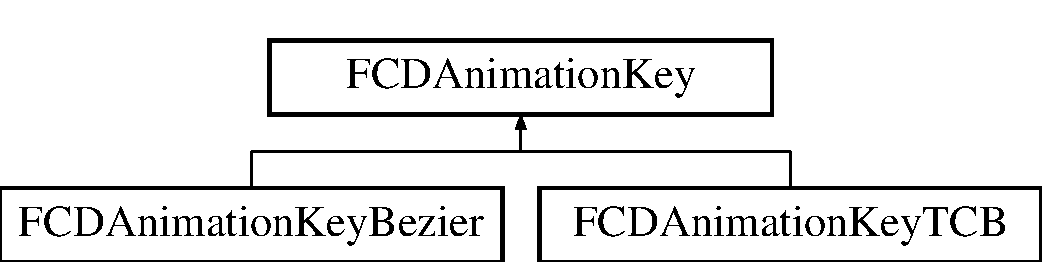
\includegraphics[height=2.000000cm]{classFCDAnimationKey}
\end{center}
\end{figure}
\subsection*{Public Attributes}
\begin{DoxyCompactItemize}
\item 
float \hyperlink{classFCDAnimationKey_a1591f4d28aac7dff40d92b0308809a7f}{input}
\item 
float \hyperlink{classFCDAnimationKey_aa779e0e946f47dbc9a2d6b9eeb58d6c2}{output}
\item 
uint32 \hyperlink{classFCDAnimationKey_a09ea6034885bc7a3c8af91afa68a52ed}{interpolation}
\end{DoxyCompactItemize}


\subsection{Detailed Description}
A simple animation key. This class is the base for the more complex one-\/dimensional keys and it is used directly for linear and step keys.

Do not create directly. Instead call FCDAnimationCurve::AddKey(FUDaeInterpolation::LINEAR) or FCDAnimationCurve::AddKey(FUDaeInterpolation::STEP). 

\subsection{Member Data Documentation}
\hypertarget{classFCDAnimationKey_a1591f4d28aac7dff40d92b0308809a7f}{
\index{FCDAnimationKey@{FCDAnimationKey}!input@{input}}
\index{input@{input}!FCDAnimationKey@{FCDAnimationKey}}
\subsubsection[{input}]{\setlength{\rightskip}{0pt plus 5cm}float {\bf FCDAnimationKey::input}}}
\label{classFCDAnimationKey_a1591f4d28aac7dff40d92b0308809a7f}
The key input. Typically, this will be a time value, in seconds. For driven curves, the dimension of this value will depend on the driver. \hypertarget{classFCDAnimationKey_a09ea6034885bc7a3c8af91afa68a52ed}{
\index{FCDAnimationKey@{FCDAnimationKey}!interpolation@{interpolation}}
\index{interpolation@{interpolation}!FCDAnimationKey@{FCDAnimationKey}}
\subsubsection[{interpolation}]{\setlength{\rightskip}{0pt plus 5cm}uint32 {\bf FCDAnimationKey::interpolation}}}
\label{classFCDAnimationKey_a09ea6034885bc7a3c8af91afa68a52ed}
The key interpolation type. \begin{DoxySeeAlso}{See also}
\hyperlink{namespaceFUDaeInterpolation_a209a941c2fb6ece1325352968aa0374f}{FUDaeInterpolation::Interpolation} 
\end{DoxySeeAlso}
\hypertarget{classFCDAnimationKey_aa779e0e946f47dbc9a2d6b9eeb58d6c2}{
\index{FCDAnimationKey@{FCDAnimationKey}!output@{output}}
\index{output@{output}!FCDAnimationKey@{FCDAnimationKey}}
\subsubsection[{output}]{\setlength{\rightskip}{0pt plus 5cm}float {\bf FCDAnimationKey::output}}}
\label{classFCDAnimationKey_aa779e0e946f47dbc9a2d6b9eeb58d6c2}
The key output. 

The documentation for this class was generated from the following file:\begin{DoxyCompactItemize}
\item 
FCollada/FCDocument/\hyperlink{FCDAnimationKey_8h}{FCDAnimationKey.h}\end{DoxyCompactItemize}

\hypertarget{classFCDAnimationKeyBezier}{
\section{FCDAnimationKeyBezier Class Reference}
\label{classFCDAnimationKeyBezier}\index{FCDAnimationKeyBezier@{FCDAnimationKeyBezier}}
}


{\ttfamily \#include $<$FCDAnimationKey.h$>$}

Inheritance diagram for FCDAnimationKeyBezier:\begin{figure}[H]
\begin{center}
\leavevmode
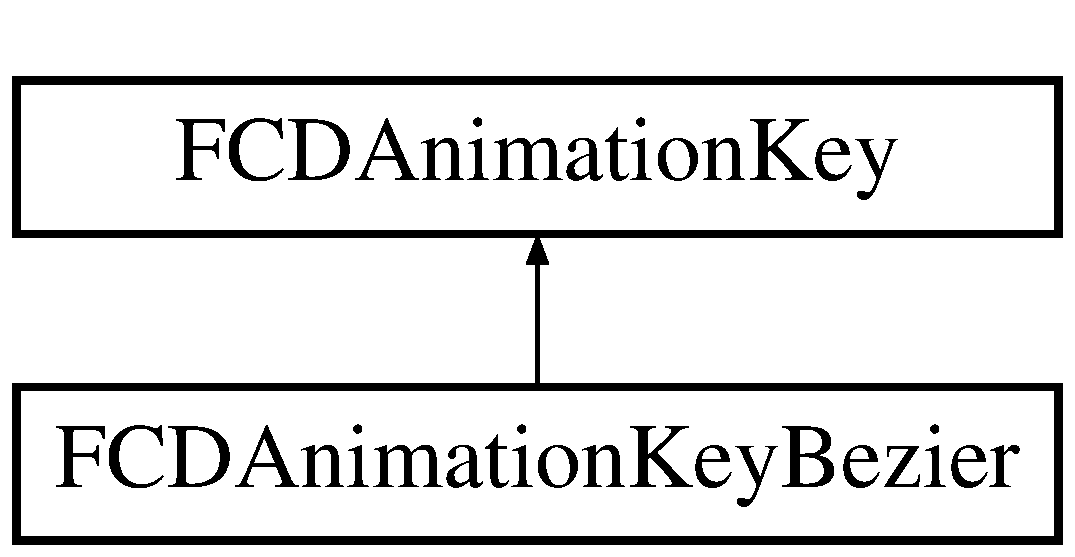
\includegraphics[height=2.000000cm]{classFCDAnimationKeyBezier}
\end{center}
\end{figure}
\subsection*{Public Attributes}
\begin{DoxyCompactItemize}
\item 
\hyperlink{classFMVector2}{FMVector2} \hyperlink{classFCDAnimationKeyBezier_a9376d6dde01d5a78629935b1bebf1ac1}{inTangent}
\item 
\hyperlink{classFMVector2}{FMVector2} \hyperlink{classFCDAnimationKeyBezier_a46baf873490cd046c4b54ea4f8926bf7}{outTangent}
\end{DoxyCompactItemize}


\subsection{Detailed Description}
An animation key with tangents values. This class is used for bezier keys and soon: for hermite keys as well.

Do not create directly. Instead call FCDAnimationCurve::AddKey(FUDaeInterpolation::BEZIER). 

\subsection{Member Data Documentation}
\hypertarget{classFCDAnimationKeyBezier_a9376d6dde01d5a78629935b1bebf1ac1}{
\index{FCDAnimationKeyBezier@{FCDAnimationKeyBezier}!inTangent@{inTangent}}
\index{inTangent@{inTangent}!FCDAnimationKeyBezier@{FCDAnimationKeyBezier}}
\subsubsection[{inTangent}]{\setlength{\rightskip}{0pt plus 5cm}{\bf FMVector2} {\bf FCDAnimationKeyBezier::inTangent}}}
\label{classFCDAnimationKeyBezier_a9376d6dde01d5a78629935b1bebf1ac1}
The incoming tangent value. \hypertarget{classFCDAnimationKeyBezier_a46baf873490cd046c4b54ea4f8926bf7}{
\index{FCDAnimationKeyBezier@{FCDAnimationKeyBezier}!outTangent@{outTangent}}
\index{outTangent@{outTangent}!FCDAnimationKeyBezier@{FCDAnimationKeyBezier}}
\subsubsection[{outTangent}]{\setlength{\rightskip}{0pt plus 5cm}{\bf FMVector2} {\bf FCDAnimationKeyBezier::outTangent}}}
\label{classFCDAnimationKeyBezier_a46baf873490cd046c4b54ea4f8926bf7}
The outcoming tangent value. 

The documentation for this class was generated from the following file:\begin{DoxyCompactItemize}
\item 
FCollada/FCDocument/\hyperlink{FCDAnimationKey_8h}{FCDAnimationKey.h}\end{DoxyCompactItemize}

\hypertarget{classFCDAnimationKeyTCB}{
\section{FCDAnimationKeyTCB Class Reference}
\label{classFCDAnimationKeyTCB}\index{FCDAnimationKeyTCB@{FCDAnimationKeyTCB}}
}


{\ttfamily \#include $<$FCDAnimationKey.h$>$}

Inheritance diagram for FCDAnimationKeyTCB:\begin{figure}[H]
\begin{center}
\leavevmode
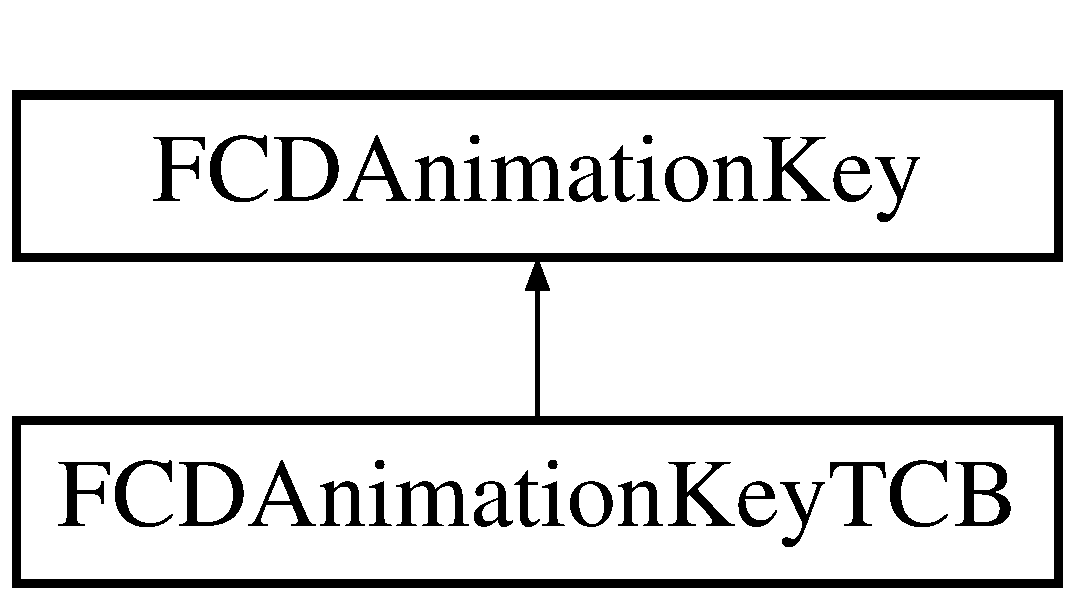
\includegraphics[height=2.000000cm]{classFCDAnimationKeyTCB}
\end{center}
\end{figure}
\subsection*{Public Attributes}
\begin{DoxyCompactItemize}
\item 
float \hyperlink{classFCDAnimationKeyTCB_ab1f6045357667b2adff959bb737925f1}{tension}
\item 
float \hyperlink{classFCDAnimationKeyTCB_ac82f078ec71eed7e6ed88dad95e2ad45}{continuity}
\item 
float \hyperlink{classFCDAnimationKeyTCB_a1676e8d6fded46456f042f9fb20e7c1d}{bias}
\item 
float \hyperlink{classFCDAnimationKeyTCB_a256d60dd1899471eae3a633734e7edaa}{easeIn}
\item 
float \hyperlink{classFCDAnimationKeyTCB_a45cdf0eff558ae6b5721a65d072e452f}{easeOut}
\end{DoxyCompactItemize}


\subsection{Detailed Description}
An animation key with tension, continuity and bias values. This class is used for 3dsMax TCB keys.

Do not create directly. Instead call FCDAnimationCurve::AddKey(FUDaeInterpolation::TCB). 

\subsection{Member Data Documentation}
\hypertarget{classFCDAnimationKeyTCB_a1676e8d6fded46456f042f9fb20e7c1d}{
\index{FCDAnimationKeyTCB@{FCDAnimationKeyTCB}!bias@{bias}}
\index{bias@{bias}!FCDAnimationKeyTCB@{FCDAnimationKeyTCB}}
\subsubsection[{bias}]{\setlength{\rightskip}{0pt plus 5cm}float {\bf FCDAnimationKeyTCB::bias}}}
\label{classFCDAnimationKeyTCB_a1676e8d6fded46456f042f9fb20e7c1d}
The bias. \hypertarget{classFCDAnimationKeyTCB_ac82f078ec71eed7e6ed88dad95e2ad45}{
\index{FCDAnimationKeyTCB@{FCDAnimationKeyTCB}!continuity@{continuity}}
\index{continuity@{continuity}!FCDAnimationKeyTCB@{FCDAnimationKeyTCB}}
\subsubsection[{continuity}]{\setlength{\rightskip}{0pt plus 5cm}float {\bf FCDAnimationKeyTCB::continuity}}}
\label{classFCDAnimationKeyTCB_ac82f078ec71eed7e6ed88dad95e2ad45}
The continuity. \hypertarget{classFCDAnimationKeyTCB_a256d60dd1899471eae3a633734e7edaa}{
\index{FCDAnimationKeyTCB@{FCDAnimationKeyTCB}!easeIn@{easeIn}}
\index{easeIn@{easeIn}!FCDAnimationKeyTCB@{FCDAnimationKeyTCB}}
\subsubsection[{easeIn}]{\setlength{\rightskip}{0pt plus 5cm}float {\bf FCDAnimationKeyTCB::easeIn}}}
\label{classFCDAnimationKeyTCB_a256d60dd1899471eae3a633734e7edaa}
The ease-\/in factor. \hypertarget{classFCDAnimationKeyTCB_a45cdf0eff558ae6b5721a65d072e452f}{
\index{FCDAnimationKeyTCB@{FCDAnimationKeyTCB}!easeOut@{easeOut}}
\index{easeOut@{easeOut}!FCDAnimationKeyTCB@{FCDAnimationKeyTCB}}
\subsubsection[{easeOut}]{\setlength{\rightskip}{0pt plus 5cm}float {\bf FCDAnimationKeyTCB::easeOut}}}
\label{classFCDAnimationKeyTCB_a45cdf0eff558ae6b5721a65d072e452f}
The ease-\/out factor. \hypertarget{classFCDAnimationKeyTCB_ab1f6045357667b2adff959bb737925f1}{
\index{FCDAnimationKeyTCB@{FCDAnimationKeyTCB}!tension@{tension}}
\index{tension@{tension}!FCDAnimationKeyTCB@{FCDAnimationKeyTCB}}
\subsubsection[{tension}]{\setlength{\rightskip}{0pt plus 5cm}float {\bf FCDAnimationKeyTCB::tension}}}
\label{classFCDAnimationKeyTCB_ab1f6045357667b2adff959bb737925f1}
The tension. 

The documentation for this class was generated from the following file:\begin{DoxyCompactItemize}
\item 
FCollada/FCDocument/\hyperlink{FCDAnimationKey_8h}{FCDAnimationKey.h}\end{DoxyCompactItemize}

\hypertarget{classFCDAnimationMKey}{
\section{FCDAnimationMKey Class Reference}
\label{classFCDAnimationMKey}\index{FCDAnimationMKey@{FCDAnimationMKey}}
}


{\ttfamily \#include $<$FCDAnimationKey.h$>$}

Inheritance diagram for FCDAnimationMKey:\begin{figure}[H]
\begin{center}
\leavevmode
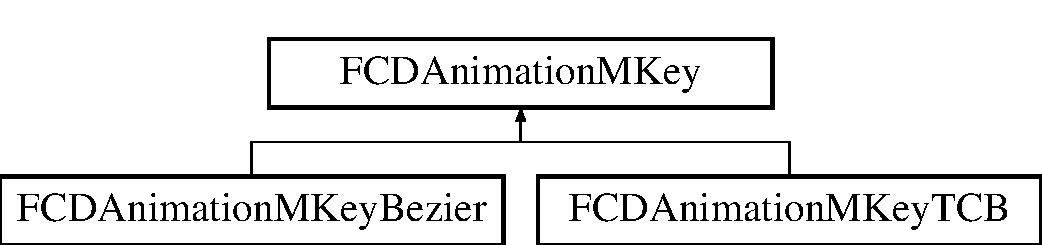
\includegraphics[height=2.000000cm]{classFCDAnimationMKey}
\end{center}
\end{figure}
\subsection*{Public Member Functions}
\begin{DoxyCompactItemize}
\item 
\hyperlink{classFCDAnimationMKey_a47f7144948d1042b187492722c2db4ae}{FCDAnimationMKey} (uint32 dimension)
\item 
virtual \hyperlink{classFCDAnimationMKey_aa0372888809476aee77140e315df5141}{$\sim$FCDAnimationMKey} ()
\item 
uint32 \hyperlink{classFCDAnimationMKey_ab1effabe7abcc46821442b88f7c459ba}{GetDimension} () const 
\end{DoxyCompactItemize}
\subsection*{Data Fields}
\begin{DoxyCompactItemize}
\item 
float \hyperlink{classFCDAnimationMKey_a23e2a29dcce4b317979da21ec48f8e68}{input}
\item 
uint32 \hyperlink{classFCDAnimationMKey_afde626bbddacb9897d80a6158f1a8e2a}{interpolation}
\item 
float $\ast$ \hyperlink{classFCDAnimationMKey_a44bfaf4f29f3946f9a3ffe0db81828cb}{output}
\end{DoxyCompactItemize}


\subsection{Detailed Description}
A simple multi-\/dimensional animation key. This class is the base for the more complex multi-\/dimensional keys and it is used directly for linear and step multi-\/dimensional keys. 

\subsection{Constructor \& Destructor Documentation}
\hypertarget{classFCDAnimationMKey_a47f7144948d1042b187492722c2db4ae}{
\index{FCDAnimationMKey@{FCDAnimationMKey}!FCDAnimationMKey@{FCDAnimationMKey}}
\index{FCDAnimationMKey@{FCDAnimationMKey}!FCDAnimationMKey@{FCDAnimationMKey}}
\subsubsection[{FCDAnimationMKey}]{\setlength{\rightskip}{0pt plus 5cm}FCDAnimationMKey::FCDAnimationMKey (
\begin{DoxyParamCaption}
\item[{uint32}]{ dimension}
\end{DoxyParamCaption}
)}}
\label{classFCDAnimationMKey_a47f7144948d1042b187492722c2db4ae}
Constructor. Do not use directly. Instead call FCDAnimationMultiCurve::AddKey(FUDaeInterpolation::LINEAR) or FCDAnimationMultiCurve::AddKey(FUDaeInterpolation::STEP). 
\begin{DoxyParams}{Parameters}
\item[{\em dimension}]The number of dimension to the key output. \end{DoxyParams}
\hypertarget{classFCDAnimationMKey_aa0372888809476aee77140e315df5141}{
\index{FCDAnimationMKey@{FCDAnimationMKey}!$\sim$FCDAnimationMKey@{$\sim$FCDAnimationMKey}}
\index{$\sim$FCDAnimationMKey@{$\sim$FCDAnimationMKey}!FCDAnimationMKey@{FCDAnimationMKey}}
\subsubsection[{$\sim$FCDAnimationMKey}]{\setlength{\rightskip}{0pt plus 5cm}FCDAnimationMKey::$\sim$FCDAnimationMKey (
\begin{DoxyParamCaption}
{}
\end{DoxyParamCaption}
)\hspace{0.3cm}{\ttfamily  \mbox{[}virtual\mbox{]}}}}
\label{classFCDAnimationMKey_aa0372888809476aee77140e315df5141}
Destructor. 

\subsection{Member Function Documentation}
\hypertarget{classFCDAnimationMKey_ab1effabe7abcc46821442b88f7c459ba}{
\index{FCDAnimationMKey@{FCDAnimationMKey}!GetDimension@{GetDimension}}
\index{GetDimension@{GetDimension}!FCDAnimationMKey@{FCDAnimationMKey}}
\subsubsection[{GetDimension}]{\setlength{\rightskip}{0pt plus 5cm}uint32 FCDAnimationMKey::GetDimension (
\begin{DoxyParamCaption}
{}
\end{DoxyParamCaption}
) const\hspace{0.3cm}{\ttfamily  \mbox{[}inline\mbox{]}}}}
\label{classFCDAnimationMKey_ab1effabe7abcc46821442b88f7c459ba}
Retrieves the number of dimensions for this key. \begin{DoxyReturn}{Returns}
The number of dimensions. 
\end{DoxyReturn}


\subsection{Field Documentation}
\hypertarget{classFCDAnimationMKey_a23e2a29dcce4b317979da21ec48f8e68}{
\index{FCDAnimationMKey@{FCDAnimationMKey}!input@{input}}
\index{input@{input}!FCDAnimationMKey@{FCDAnimationMKey}}
\subsubsection[{input}]{\setlength{\rightskip}{0pt plus 5cm}float {\bf FCDAnimationMKey::input}}}
\label{classFCDAnimationMKey_a23e2a29dcce4b317979da21ec48f8e68}
The key input. Typically, this will be a time value, in seconds. For driven curves, the dimension of this value will depend on the driver. \hypertarget{classFCDAnimationMKey_afde626bbddacb9897d80a6158f1a8e2a}{
\index{FCDAnimationMKey@{FCDAnimationMKey}!interpolation@{interpolation}}
\index{interpolation@{interpolation}!FCDAnimationMKey@{FCDAnimationMKey}}
\subsubsection[{interpolation}]{\setlength{\rightskip}{0pt plus 5cm}uint32 {\bf FCDAnimationMKey::interpolation}}}
\label{classFCDAnimationMKey_afde626bbddacb9897d80a6158f1a8e2a}
The key interpolation type. \begin{DoxySeeAlso}{See also}
\hyperlink{namespaceFUDaeInterpolation_a209a941c2fb6ece1325352968aa0374f}{FUDaeInterpolation::Interpolation} 
\end{DoxySeeAlso}
\hypertarget{classFCDAnimationMKey_a44bfaf4f29f3946f9a3ffe0db81828cb}{
\index{FCDAnimationMKey@{FCDAnimationMKey}!output@{output}}
\index{output@{output}!FCDAnimationMKey@{FCDAnimationMKey}}
\subsubsection[{output}]{\setlength{\rightskip}{0pt plus 5cm}float$\ast$ {\bf FCDAnimationMKey::output}}}
\label{classFCDAnimationMKey_a44bfaf4f29f3946f9a3ffe0db81828cb}
The multi-\/dimensional key output. 

The documentation for this class was generated from the following files:\begin{DoxyCompactItemize}
\item 
FCollada/FCDocument/\hyperlink{FCDAnimationKey_8h}{FCDAnimationKey.h}\item 
FCollada/FCDocument/FCDAnimationKey.cpp\end{DoxyCompactItemize}

\hypertarget{classFCDAnimationMKeyBezier}{
\section{FCDAnimationMKeyBezier Class Reference}
\label{classFCDAnimationMKeyBezier}\index{FCDAnimationMKeyBezier@{FCDAnimationMKeyBezier}}
}


{\ttfamily \#include $<$FCDAnimationKey.h$>$}

Inheritance diagram for FCDAnimationMKeyBezier:\begin{figure}[H]
\begin{center}
\leavevmode
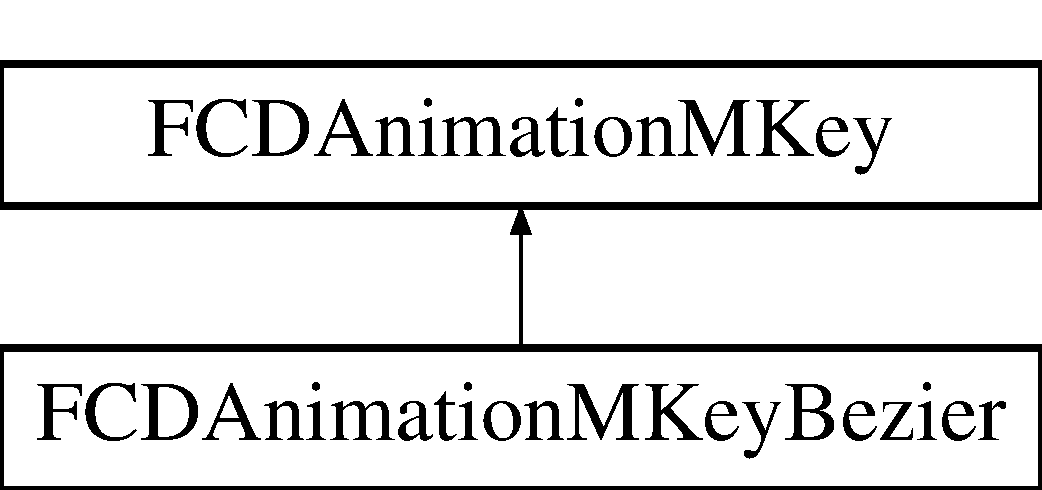
\includegraphics[height=2.000000cm]{classFCDAnimationMKeyBezier}
\end{center}
\end{figure}
\subsection*{Public Member Functions}
\begin{DoxyCompactItemize}
\item 
\hyperlink{classFCDAnimationMKeyBezier_a45aa55fc7430c817a8ab08882d2fcb9f}{FCDAnimationMKeyBezier} (uint32 dimension)
\item 
virtual \hyperlink{classFCDAnimationMKeyBezier_ae266c127ad7d936f2060b40c5368762f}{$\sim$FCDAnimationMKeyBezier} ()
\end{DoxyCompactItemize}
\subsection*{Data Fields}
\begin{DoxyCompactItemize}
\item 
\hyperlink{classFMVector2}{FMVector2} $\ast$ \hyperlink{classFCDAnimationMKeyBezier_aaf6f55f43516c1bf38cef19ecbb8fe21}{inTangent}
\item 
\hyperlink{classFMVector2}{FMVector2} $\ast$ \hyperlink{classFCDAnimationMKeyBezier_aea9338c2e0d894e9d5e9a4dcf00928e6}{outTangent}
\end{DoxyCompactItemize}


\subsection{Detailed Description}
A multi-\/dimensional animation key with tangents values. This class is used for bezier keys and soon: for hermite keys as well. 

\subsection{Constructor \& Destructor Documentation}
\hypertarget{classFCDAnimationMKeyBezier_a45aa55fc7430c817a8ab08882d2fcb9f}{
\index{FCDAnimationMKeyBezier@{FCDAnimationMKeyBezier}!FCDAnimationMKeyBezier@{FCDAnimationMKeyBezier}}
\index{FCDAnimationMKeyBezier@{FCDAnimationMKeyBezier}!FCDAnimationMKeyBezier@{FCDAnimationMKeyBezier}}
\subsubsection[{FCDAnimationMKeyBezier}]{\setlength{\rightskip}{0pt plus 5cm}FCDAnimationMKeyBezier::FCDAnimationMKeyBezier (
\begin{DoxyParamCaption}
\item[{uint32}]{ dimension}
\end{DoxyParamCaption}
)}}
\label{classFCDAnimationMKeyBezier_a45aa55fc7430c817a8ab08882d2fcb9f}
Constructor: do not use directly. Instead call FCDAnimationCurve::AddKey(FUDaeInterpolation::BEZIER). 
\begin{DoxyParams}{Parameters}
\item[{\em dimension}]The number of dimension to the key output. \end{DoxyParams}
\hypertarget{classFCDAnimationMKeyBezier_ae266c127ad7d936f2060b40c5368762f}{
\index{FCDAnimationMKeyBezier@{FCDAnimationMKeyBezier}!$\sim$FCDAnimationMKeyBezier@{$\sim$FCDAnimationMKeyBezier}}
\index{$\sim$FCDAnimationMKeyBezier@{$\sim$FCDAnimationMKeyBezier}!FCDAnimationMKeyBezier@{FCDAnimationMKeyBezier}}
\subsubsection[{$\sim$FCDAnimationMKeyBezier}]{\setlength{\rightskip}{0pt plus 5cm}FCDAnimationMKeyBezier::$\sim$FCDAnimationMKeyBezier (
\begin{DoxyParamCaption}
{}
\end{DoxyParamCaption}
)\hspace{0.3cm}{\ttfamily  \mbox{[}virtual\mbox{]}}}}
\label{classFCDAnimationMKeyBezier_ae266c127ad7d936f2060b40c5368762f}
Destructor. 

\subsection{Field Documentation}
\hypertarget{classFCDAnimationMKeyBezier_aaf6f55f43516c1bf38cef19ecbb8fe21}{
\index{FCDAnimationMKeyBezier@{FCDAnimationMKeyBezier}!inTangent@{inTangent}}
\index{inTangent@{inTangent}!FCDAnimationMKeyBezier@{FCDAnimationMKeyBezier}}
\subsubsection[{inTangent}]{\setlength{\rightskip}{0pt plus 5cm}{\bf FMVector2}$\ast$ {\bf FCDAnimationMKeyBezier::inTangent}}}
\label{classFCDAnimationMKeyBezier_aaf6f55f43516c1bf38cef19ecbb8fe21}
The incoming tangent value. \hypertarget{classFCDAnimationMKeyBezier_aea9338c2e0d894e9d5e9a4dcf00928e6}{
\index{FCDAnimationMKeyBezier@{FCDAnimationMKeyBezier}!outTangent@{outTangent}}
\index{outTangent@{outTangent}!FCDAnimationMKeyBezier@{FCDAnimationMKeyBezier}}
\subsubsection[{outTangent}]{\setlength{\rightskip}{0pt plus 5cm}{\bf FMVector2}$\ast$ {\bf FCDAnimationMKeyBezier::outTangent}}}
\label{classFCDAnimationMKeyBezier_aea9338c2e0d894e9d5e9a4dcf00928e6}
The outcoming tangent value. 

The documentation for this class was generated from the following files:\begin{DoxyCompactItemize}
\item 
FCollada/FCDocument/\hyperlink{FCDAnimationKey_8h}{FCDAnimationKey.h}\item 
FCollada/FCDocument/FCDAnimationKey.cpp\end{DoxyCompactItemize}

\hypertarget{classFCDAnimationMKeyTCB}{
\section{FCDAnimationMKeyTCB Class Reference}
\label{classFCDAnimationMKeyTCB}\index{FCDAnimationMKeyTCB@{FCDAnimationMKeyTCB}}
}


{\ttfamily \#include $<$FCDAnimationKey.h$>$}

Inheritance diagram for FCDAnimationMKeyTCB:\begin{figure}[H]
\begin{center}
\leavevmode
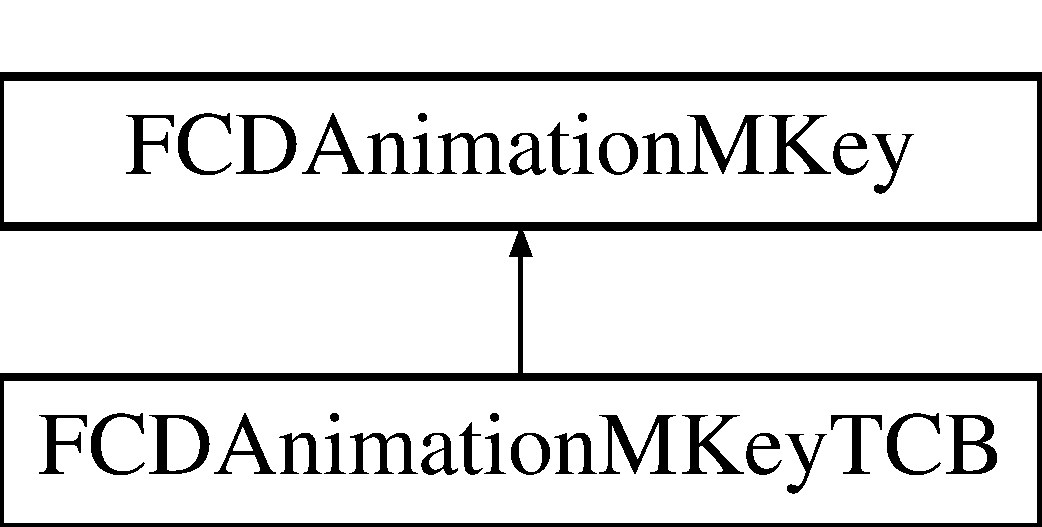
\includegraphics[height=2.000000cm]{classFCDAnimationMKeyTCB}
\end{center}
\end{figure}
\subsection*{Public Member Functions}
\begin{DoxyCompactItemize}
\item 
\hyperlink{classFCDAnimationMKeyTCB_aeeee3d548cbe6c41cd9a46ff0079d05d}{FCDAnimationMKeyTCB} (uint32 dimension)
\item 
virtual \hyperlink{classFCDAnimationMKeyTCB_a515f7219e82e55db7a7d543c624207c2}{$\sim$FCDAnimationMKeyTCB} ()
\end{DoxyCompactItemize}
\subsection*{Public Attributes}
\begin{DoxyCompactItemize}
\item 
float $\ast$ \hyperlink{classFCDAnimationMKeyTCB_a05aa82c6e377a34c8d4c521f05739070}{tension}
\item 
float $\ast$ \hyperlink{classFCDAnimationMKeyTCB_aad952e9ad96796b79ffbd7ea15fa4ce7}{continuity}
\item 
float $\ast$ \hyperlink{classFCDAnimationMKeyTCB_ae3812b7c36b879e9fd9ecfe67120c219}{bias}
\item 
float $\ast$ \hyperlink{classFCDAnimationMKeyTCB_a7e35030931711b58ae099eee73d05102}{easeIn}
\item 
float $\ast$ \hyperlink{classFCDAnimationMKeyTCB_a9cea41d40b917bc3f5151320318c49fe}{easeOut}
\end{DoxyCompactItemize}


\subsection{Detailed Description}
An animation key with tension, continuity and bias values. This class is used for 3dsMax TCB keys. 

\subsection{Constructor \& Destructor Documentation}
\hypertarget{classFCDAnimationMKeyTCB_aeeee3d548cbe6c41cd9a46ff0079d05d}{
\index{FCDAnimationMKeyTCB@{FCDAnimationMKeyTCB}!FCDAnimationMKeyTCB@{FCDAnimationMKeyTCB}}
\index{FCDAnimationMKeyTCB@{FCDAnimationMKeyTCB}!FCDAnimationMKeyTCB@{FCDAnimationMKeyTCB}}
\subsubsection[{FCDAnimationMKeyTCB}]{\setlength{\rightskip}{0pt plus 5cm}FCDAnimationMKeyTCB::FCDAnimationMKeyTCB (
\begin{DoxyParamCaption}
\item[{uint32}]{ dimension}
\end{DoxyParamCaption}
)}}
\label{classFCDAnimationMKeyTCB_aeeee3d548cbe6c41cd9a46ff0079d05d}
Constructor: do not use directly. Instead call FCDAnimationMultiCurve::AddKey(FUDaeInterpolation::TCB). 
\begin{DoxyParams}{Parameters}
\item[{\em dimension}]The number of dimension to the key output. \end{DoxyParams}
\hypertarget{classFCDAnimationMKeyTCB_a515f7219e82e55db7a7d543c624207c2}{
\index{FCDAnimationMKeyTCB@{FCDAnimationMKeyTCB}!$\sim$FCDAnimationMKeyTCB@{$\sim$FCDAnimationMKeyTCB}}
\index{$\sim$FCDAnimationMKeyTCB@{$\sim$FCDAnimationMKeyTCB}!FCDAnimationMKeyTCB@{FCDAnimationMKeyTCB}}
\subsubsection[{$\sim$FCDAnimationMKeyTCB}]{\setlength{\rightskip}{0pt plus 5cm}FCDAnimationMKeyTCB::$\sim$FCDAnimationMKeyTCB (
\begin{DoxyParamCaption}
{}
\end{DoxyParamCaption}
)\hspace{0.3cm}{\ttfamily  \mbox{[}virtual\mbox{]}}}}
\label{classFCDAnimationMKeyTCB_a515f7219e82e55db7a7d543c624207c2}
Destructor. 

\subsection{Member Data Documentation}
\hypertarget{classFCDAnimationMKeyTCB_ae3812b7c36b879e9fd9ecfe67120c219}{
\index{FCDAnimationMKeyTCB@{FCDAnimationMKeyTCB}!bias@{bias}}
\index{bias@{bias}!FCDAnimationMKeyTCB@{FCDAnimationMKeyTCB}}
\subsubsection[{bias}]{\setlength{\rightskip}{0pt plus 5cm}float$\ast$ {\bf FCDAnimationMKeyTCB::bias}}}
\label{classFCDAnimationMKeyTCB_ae3812b7c36b879e9fd9ecfe67120c219}
The multi-\/dimensional biases. \hypertarget{classFCDAnimationMKeyTCB_aad952e9ad96796b79ffbd7ea15fa4ce7}{
\index{FCDAnimationMKeyTCB@{FCDAnimationMKeyTCB}!continuity@{continuity}}
\index{continuity@{continuity}!FCDAnimationMKeyTCB@{FCDAnimationMKeyTCB}}
\subsubsection[{continuity}]{\setlength{\rightskip}{0pt plus 5cm}float$\ast$ {\bf FCDAnimationMKeyTCB::continuity}}}
\label{classFCDAnimationMKeyTCB_aad952e9ad96796b79ffbd7ea15fa4ce7}
The multi-\/dimensional continuities. \hypertarget{classFCDAnimationMKeyTCB_a7e35030931711b58ae099eee73d05102}{
\index{FCDAnimationMKeyTCB@{FCDAnimationMKeyTCB}!easeIn@{easeIn}}
\index{easeIn@{easeIn}!FCDAnimationMKeyTCB@{FCDAnimationMKeyTCB}}
\subsubsection[{easeIn}]{\setlength{\rightskip}{0pt plus 5cm}float$\ast$ {\bf FCDAnimationMKeyTCB::easeIn}}}
\label{classFCDAnimationMKeyTCB_a7e35030931711b58ae099eee73d05102}
The multi-\/dimensional ease-\/in factors. \hypertarget{classFCDAnimationMKeyTCB_a9cea41d40b917bc3f5151320318c49fe}{
\index{FCDAnimationMKeyTCB@{FCDAnimationMKeyTCB}!easeOut@{easeOut}}
\index{easeOut@{easeOut}!FCDAnimationMKeyTCB@{FCDAnimationMKeyTCB}}
\subsubsection[{easeOut}]{\setlength{\rightskip}{0pt plus 5cm}float$\ast$ {\bf FCDAnimationMKeyTCB::easeOut}}}
\label{classFCDAnimationMKeyTCB_a9cea41d40b917bc3f5151320318c49fe}
The multi-\/dimensional ease-\/out factors. \hypertarget{classFCDAnimationMKeyTCB_a05aa82c6e377a34c8d4c521f05739070}{
\index{FCDAnimationMKeyTCB@{FCDAnimationMKeyTCB}!tension@{tension}}
\index{tension@{tension}!FCDAnimationMKeyTCB@{FCDAnimationMKeyTCB}}
\subsubsection[{tension}]{\setlength{\rightskip}{0pt plus 5cm}float$\ast$ {\bf FCDAnimationMKeyTCB::tension}}}
\label{classFCDAnimationMKeyTCB_a05aa82c6e377a34c8d4c521f05739070}
The multi-\/dimensional tensions. 

The documentation for this class was generated from the following files:\begin{DoxyCompactItemize}
\item 
FCollada/FCDocument/\hyperlink{FCDAnimationKey_8h}{FCDAnimationKey.h}\item 
FCollada/FCDocument/FCDAnimationKey.cpp\end{DoxyCompactItemize}

\hypertarget{classFCDAnimationMultiCurve}{
\section{FCDAnimationMultiCurve Class Reference}
\label{classFCDAnimationMultiCurve}\index{FCDAnimationMultiCurve@{FCDAnimationMultiCurve}}
}


{\ttfamily \#include $<$FCDAnimationMultiCurve.h$>$}

Inheritance diagram for FCDAnimationMultiCurve:\begin{figure}[H]
\begin{center}
\leavevmode
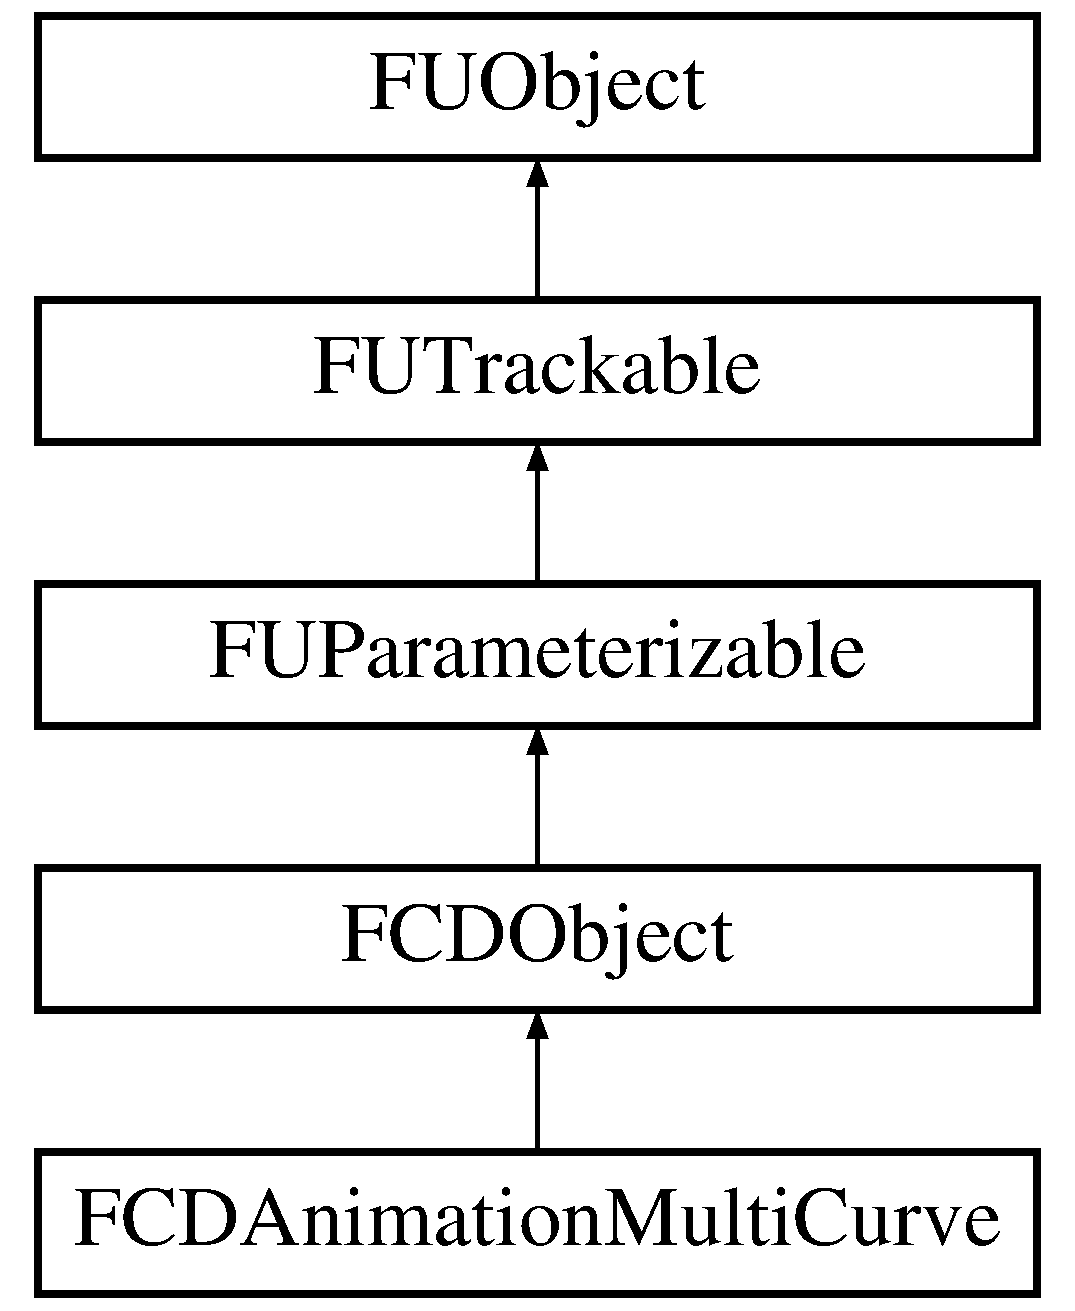
\includegraphics[height=5.000000cm]{classFCDAnimationMultiCurve}
\end{center}
\end{figure}
\subsection*{Public Member Functions}
\begin{DoxyCompactItemize}
\item 
\hyperlink{classFCDAnimationMultiCurve_a2d24f269824f986407c0fa247b80e96c}{FCDAnimationMultiCurve} (\hyperlink{classFCDocument}{FCDocument} $\ast$document, uint32 dimension)
\item 
virtual \hyperlink{classFCDAnimationMultiCurve_a1de4b1de48116068c3897b82860a8060}{$\sim$FCDAnimationMultiCurve} ()
\item 
uint32 \hyperlink{classFCDAnimationMultiCurve_a0b6badef0fb401db1e99820d043a69f4}{GetDimension} () const 
\item 
\hyperlink{classFCDAnimationMKey}{FCDAnimationMKey} $\ast$$\ast$ \hyperlink{classFCDAnimationMultiCurve_acd3398ca66622d9f62edccd64fb97049}{GetKeys} ()
\item 
const \hyperlink{classFCDAnimationMKey}{FCDAnimationMKey} $\ast$$\ast$ \hyperlink{classFCDAnimationMultiCurve_a08a4162ad5ca67540472f1c1113ddce6}{GetKeys} () const 
\item 
size\_\-t \hyperlink{classFCDAnimationMultiCurve_a2c54b98723c4909c93c9a6ec151ef234}{GetKeyCount} () const 
\item 
void \hyperlink{classFCDAnimationMultiCurve_adf25740adf8ddfabcf64bd1cbc83e5f7}{SetKeyCount} (size\_\-t count, \hyperlink{namespaceFUDaeInterpolation_a209a941c2fb6ece1325352968aa0374f}{FUDaeInterpolation::Interpolation} interpolation)
\item 
\hyperlink{classFCDAnimationMKey}{FCDAnimationMKey} $\ast$ \hyperlink{classFCDAnimationMultiCurve_a5f8632aed8843243c3f8a8c94146a93e}{GetKey} (size\_\-t index)
\item 
const \hyperlink{classFCDAnimationMKey}{FCDAnimationMKey} $\ast$ \hyperlink{classFCDAnimationMultiCurve_aee9dedbdf473e27cb9d448cc9da4826b}{GetKey} (size\_\-t index) const 
\item 
\hyperlink{classFCDAnimationMKey}{FCDAnimationMKey} $\ast$ \hyperlink{classFCDAnimationMultiCurve_af8b1447f1ab5fd021b6e8e61d45bc08c}{AddKey} (\hyperlink{namespaceFUDaeInterpolation_a209a941c2fb6ece1325352968aa0374f}{FUDaeInterpolation::Interpolation} interpolation)
\item 
\hyperlink{namespaceFUDaeInfinity_a9d8fb86affe94d1586d728d4c2e89008}{FUDaeInfinity::Infinity} \hyperlink{classFCDAnimationMultiCurve_a3ce35c4236b8e07a5c48dc6c6203898c}{GetPreInfinity} () const 
\item 
void \hyperlink{classFCDAnimationMultiCurve_a22a66864b972abde1cacb06ba6d7653a}{SetPreInfinity} (\hyperlink{namespaceFUDaeInfinity_a9d8fb86affe94d1586d728d4c2e89008}{FUDaeInfinity::Infinity} infinity)
\item 
\hyperlink{namespaceFUDaeInfinity_a9d8fb86affe94d1586d728d4c2e89008}{FUDaeInfinity::Infinity} \hyperlink{classFCDAnimationMultiCurve_a2700e160254c7bccb321cf19234e1228}{GetPostInfinity} () const 
\item 
void \hyperlink{classFCDAnimationMultiCurve_a498e31528b918826b0ad7069622607b2}{SetPostInfinity} (\hyperlink{namespaceFUDaeInfinity_a9d8fb86affe94d1586d728d4c2e89008}{FUDaeInfinity::Infinity} infinity)
\item 
void \hyperlink{classFCDAnimationMultiCurve_a50979bee5862ccb12a5c829e9410a4eb}{Evaluate} (float input, float $\ast$output) const 
\item 
int32 \hyperlink{classFCDAnimationMultiCurve_ae1cd6afb67f21bc40e706ec73bc911e5}{GetTargetElement} () const 
\item 
void \hyperlink{classFCDAnimationMultiCurve_ae9a30b28b6ab7f201717fd6a3d4db770}{SetTargetElement} (int32 e)
\item 
\hypertarget{classFCDAnimationMultiCurve_ad5383e34ae38c53c4122871ae717cb8a}{
int32 {\bfseries GetTargetElement} ()}
\label{classFCDAnimationMultiCurve_ad5383e34ae38c53c4122871ae717cb8a}

\item 
void \hyperlink{classFCDAnimationMultiCurve_aad5e1829346170165119d01d92de62bb}{Set2DCurveEvaluation} (bool flag)
\item 
bool \hyperlink{classFCDAnimationMultiCurve_ace2392f79497988d3f9742504e9032ee}{Is2DCurveEvaluation} ()
\end{DoxyCompactItemize}


\subsection{Detailed Description}
A COLLADA multi-\/dimensional animation curve.

This is a utility class that is used to convert multiple animation curves into one animation curve that has multiple dimensions, but only one list of key inputs.

\hyperlink{namespaceFCollada}{FCollada} will never create a multi-\/dimensional animation curve during the import of a COLLADA document. 

\subsection{Constructor \& Destructor Documentation}
\hypertarget{classFCDAnimationMultiCurve_a2d24f269824f986407c0fa247b80e96c}{
\index{FCDAnimationMultiCurve@{FCDAnimationMultiCurve}!FCDAnimationMultiCurve@{FCDAnimationMultiCurve}}
\index{FCDAnimationMultiCurve@{FCDAnimationMultiCurve}!FCDAnimationMultiCurve@{FCDAnimationMultiCurve}}
\subsubsection[{FCDAnimationMultiCurve}]{\setlength{\rightskip}{0pt plus 5cm}FCDAnimationMultiCurve::FCDAnimationMultiCurve (
\begin{DoxyParamCaption}
\item[{{\bf FCDocument} $\ast$}]{ document, }
\item[{uint32}]{ dimension}
\end{DoxyParamCaption}
)}}
\label{classFCDAnimationMultiCurve_a2d24f269824f986407c0fa247b80e96c}
Constructor. The number of dimensions will not change in the lifetime of a multi-\/dimensional curve. 
\begin{DoxyParams}{Parameters}
\item[{\em document}]The COLLADA document that owns the animation curve. \item[{\em dimension}]The number of dimensions for the animation curve. \end{DoxyParams}
\hypertarget{classFCDAnimationMultiCurve_a1de4b1de48116068c3897b82860a8060}{
\index{FCDAnimationMultiCurve@{FCDAnimationMultiCurve}!$\sim$FCDAnimationMultiCurve@{$\sim$FCDAnimationMultiCurve}}
\index{$\sim$FCDAnimationMultiCurve@{$\sim$FCDAnimationMultiCurve}!FCDAnimationMultiCurve@{FCDAnimationMultiCurve}}
\subsubsection[{$\sim$FCDAnimationMultiCurve}]{\setlength{\rightskip}{0pt plus 5cm}FCDAnimationMultiCurve::$\sim$FCDAnimationMultiCurve (
\begin{DoxyParamCaption}
{}
\end{DoxyParamCaption}
)\hspace{0.3cm}{\ttfamily  \mbox{[}virtual\mbox{]}}}}
\label{classFCDAnimationMultiCurve_a1de4b1de48116068c3897b82860a8060}
Destructor. 

\subsection{Member Function Documentation}
\hypertarget{classFCDAnimationMultiCurve_af8b1447f1ab5fd021b6e8e61d45bc08c}{
\index{FCDAnimationMultiCurve@{FCDAnimationMultiCurve}!AddKey@{AddKey}}
\index{AddKey@{AddKey}!FCDAnimationMultiCurve@{FCDAnimationMultiCurve}}
\subsubsection[{AddKey}]{\setlength{\rightskip}{0pt plus 5cm}{\bf FCDAnimationMKey} $\ast$ FCDAnimationMultiCurve::AddKey (
\begin{DoxyParamCaption}
\item[{{\bf FUDaeInterpolation::Interpolation}}]{ interpolation}
\end{DoxyParamCaption}
)}}
\label{classFCDAnimationMultiCurve_af8b1447f1ab5fd021b6e8e61d45bc08c}
Appends a key to the animation curve. 
\begin{DoxyParams}{Parameters}
\item[{\em interpolation}]The interpolation type for the new key. \end{DoxyParams}
\begin{DoxyReturn}{Returns}
The new key. 
\end{DoxyReturn}
\hypertarget{classFCDAnimationMultiCurve_a50979bee5862ccb12a5c829e9410a4eb}{
\index{FCDAnimationMultiCurve@{FCDAnimationMultiCurve}!Evaluate@{Evaluate}}
\index{Evaluate@{Evaluate}!FCDAnimationMultiCurve@{FCDAnimationMultiCurve}}
\subsubsection[{Evaluate}]{\setlength{\rightskip}{0pt plus 5cm}void FCDAnimationMultiCurve::Evaluate (
\begin{DoxyParamCaption}
\item[{float}]{ input, }
\item[{float $\ast$}]{ output}
\end{DoxyParamCaption}
) const}}
\label{classFCDAnimationMultiCurve_a50979bee5862ccb12a5c829e9410a4eb}
Evaluates the animation curve. 
\begin{DoxyParams}{Parameters}
\item[{\em input}]An input value. \item[{\em output}]An array of floating-\/point values to fill in with the sampled values. \end{DoxyParams}
\hypertarget{classFCDAnimationMultiCurve_a0b6badef0fb401db1e99820d043a69f4}{
\index{FCDAnimationMultiCurve@{FCDAnimationMultiCurve}!GetDimension@{GetDimension}}
\index{GetDimension@{GetDimension}!FCDAnimationMultiCurve@{FCDAnimationMultiCurve}}
\subsubsection[{GetDimension}]{\setlength{\rightskip}{0pt plus 5cm}uint32 FCDAnimationMultiCurve::GetDimension (
\begin{DoxyParamCaption}
{}
\end{DoxyParamCaption}
) const\hspace{0.3cm}{\ttfamily  \mbox{[}inline\mbox{]}}}}
\label{classFCDAnimationMultiCurve_a0b6badef0fb401db1e99820d043a69f4}
Retrieves the number of dimensions for the curve. \begin{DoxyReturn}{Returns}
The number of dimensions for the curve. 
\end{DoxyReturn}
\hypertarget{classFCDAnimationMultiCurve_a5f8632aed8843243c3f8a8c94146a93e}{
\index{FCDAnimationMultiCurve@{FCDAnimationMultiCurve}!GetKey@{GetKey}}
\index{GetKey@{GetKey}!FCDAnimationMultiCurve@{FCDAnimationMultiCurve}}
\subsubsection[{GetKey}]{\setlength{\rightskip}{0pt plus 5cm}{\bf FCDAnimationMKey}$\ast$ FCDAnimationMultiCurve::GetKey (
\begin{DoxyParamCaption}
\item[{size\_\-t}]{ index}
\end{DoxyParamCaption}
)\hspace{0.3cm}{\ttfamily  \mbox{[}inline\mbox{]}}}}
\label{classFCDAnimationMultiCurve_a5f8632aed8843243c3f8a8c94146a93e}
Retrieve one key of the animation curve. 
\begin{DoxyParams}{Parameters}
\item[{\em index}]The index of the key to retrieve. \end{DoxyParams}
\begin{DoxyReturn}{Returns}
The indexed key. 
\end{DoxyReturn}
\hypertarget{classFCDAnimationMultiCurve_aee9dedbdf473e27cb9d448cc9da4826b}{
\index{FCDAnimationMultiCurve@{FCDAnimationMultiCurve}!GetKey@{GetKey}}
\index{GetKey@{GetKey}!FCDAnimationMultiCurve@{FCDAnimationMultiCurve}}
\subsubsection[{GetKey}]{\setlength{\rightskip}{0pt plus 5cm}const {\bf FCDAnimationMKey}$\ast$ FCDAnimationMultiCurve::GetKey (
\begin{DoxyParamCaption}
\item[{size\_\-t}]{ index}
\end{DoxyParamCaption}
) const\hspace{0.3cm}{\ttfamily  \mbox{[}inline\mbox{]}}}}
\label{classFCDAnimationMultiCurve_aee9dedbdf473e27cb9d448cc9da4826b}
See above. \hypertarget{classFCDAnimationMultiCurve_a2c54b98723c4909c93c9a6ec151ef234}{
\index{FCDAnimationMultiCurve@{FCDAnimationMultiCurve}!GetKeyCount@{GetKeyCount}}
\index{GetKeyCount@{GetKeyCount}!FCDAnimationMultiCurve@{FCDAnimationMultiCurve}}
\subsubsection[{GetKeyCount}]{\setlength{\rightskip}{0pt plus 5cm}size\_\-t FCDAnimationMultiCurve::GetKeyCount (
\begin{DoxyParamCaption}
{}
\end{DoxyParamCaption}
) const\hspace{0.3cm}{\ttfamily  \mbox{[}inline\mbox{]}}}}
\label{classFCDAnimationMultiCurve_a2c54b98723c4909c93c9a6ec151ef234}
Retrieves the number of keys within the animation curve. \begin{DoxyReturn}{Returns}
The number of keys. 
\end{DoxyReturn}
\hypertarget{classFCDAnimationMultiCurve_acd3398ca66622d9f62edccd64fb97049}{
\index{FCDAnimationMultiCurve@{FCDAnimationMultiCurve}!GetKeys@{GetKeys}}
\index{GetKeys@{GetKeys}!FCDAnimationMultiCurve@{FCDAnimationMultiCurve}}
\subsubsection[{GetKeys}]{\setlength{\rightskip}{0pt plus 5cm}{\bf FCDAnimationMKey}$\ast$$\ast$ FCDAnimationMultiCurve::GetKeys (
\begin{DoxyParamCaption}
{}
\end{DoxyParamCaption}
)\hspace{0.3cm}{\ttfamily  \mbox{[}inline\mbox{]}}}}
\label{classFCDAnimationMultiCurve_acd3398ca66622d9f62edccd64fb97049}
Retrieves the list of key inputs for the animation curve. \begin{DoxyReturn}{Returns}
The list of key inputs. 
\end{DoxyReturn}
\hypertarget{classFCDAnimationMultiCurve_a08a4162ad5ca67540472f1c1113ddce6}{
\index{FCDAnimationMultiCurve@{FCDAnimationMultiCurve}!GetKeys@{GetKeys}}
\index{GetKeys@{GetKeys}!FCDAnimationMultiCurve@{FCDAnimationMultiCurve}}
\subsubsection[{GetKeys}]{\setlength{\rightskip}{0pt plus 5cm}const {\bf FCDAnimationMKey}$\ast$$\ast$ FCDAnimationMultiCurve::GetKeys (
\begin{DoxyParamCaption}
{}
\end{DoxyParamCaption}
) const\hspace{0.3cm}{\ttfamily  \mbox{[}inline\mbox{]}}}}
\label{classFCDAnimationMultiCurve_a08a4162ad5ca67540472f1c1113ddce6}
See above. \hypertarget{classFCDAnimationMultiCurve_a2700e160254c7bccb321cf19234e1228}{
\index{FCDAnimationMultiCurve@{FCDAnimationMultiCurve}!GetPostInfinity@{GetPostInfinity}}
\index{GetPostInfinity@{GetPostInfinity}!FCDAnimationMultiCurve@{FCDAnimationMultiCurve}}
\subsubsection[{GetPostInfinity}]{\setlength{\rightskip}{0pt plus 5cm}{\bf FUDaeInfinity::Infinity} FCDAnimationMultiCurve::GetPostInfinity (
\begin{DoxyParamCaption}
{}
\end{DoxyParamCaption}
) const\hspace{0.3cm}{\ttfamily  \mbox{[}inline\mbox{]}}}}
\label{classFCDAnimationMultiCurve_a2700e160254c7bccb321cf19234e1228}
Retrieves the type of behavior for the curve if the input value is outside the input interval defined by the curve keys and greater than any key input value. \begin{DoxySeeAlso}{See also}
\hyperlink{namespaceFUDaeInfinity}{FUDaeInfinity} 
\end{DoxySeeAlso}
\begin{DoxyReturn}{Returns}
The post-\/infinity behavior of the curve. 
\end{DoxyReturn}
\hypertarget{classFCDAnimationMultiCurve_a3ce35c4236b8e07a5c48dc6c6203898c}{
\index{FCDAnimationMultiCurve@{FCDAnimationMultiCurve}!GetPreInfinity@{GetPreInfinity}}
\index{GetPreInfinity@{GetPreInfinity}!FCDAnimationMultiCurve@{FCDAnimationMultiCurve}}
\subsubsection[{GetPreInfinity}]{\setlength{\rightskip}{0pt plus 5cm}{\bf FUDaeInfinity::Infinity} FCDAnimationMultiCurve::GetPreInfinity (
\begin{DoxyParamCaption}
{}
\end{DoxyParamCaption}
) const\hspace{0.3cm}{\ttfamily  \mbox{[}inline\mbox{]}}}}
\label{classFCDAnimationMultiCurve_a3ce35c4236b8e07a5c48dc6c6203898c}
Retrieves the type of behavior for the curve if the input value is outside the input interval defined by the curve keys and less than any key input value. \begin{DoxySeeAlso}{See also}
\hyperlink{namespaceFUDaeInfinity}{FUDaeInfinity} 
\end{DoxySeeAlso}
\begin{DoxyReturn}{Returns}
The pre-\/infinity behavior of the curve. 
\end{DoxyReturn}
\hypertarget{classFCDAnimationMultiCurve_ae1cd6afb67f21bc40e706ec73bc911e5}{
\index{FCDAnimationMultiCurve@{FCDAnimationMultiCurve}!GetTargetElement@{GetTargetElement}}
\index{GetTargetElement@{GetTargetElement}!FCDAnimationMultiCurve@{FCDAnimationMultiCurve}}
\subsubsection[{GetTargetElement}]{\setlength{\rightskip}{0pt plus 5cm}int32 FCDAnimationMultiCurve::GetTargetElement (
\begin{DoxyParamCaption}
{}
\end{DoxyParamCaption}
) const\hspace{0.3cm}{\ttfamily  \mbox{[}inline\mbox{]}}}}
\label{classFCDAnimationMultiCurve_ae1cd6afb67f21bc40e706ec73bc911e5}
\mbox{[}INTERNAL\mbox{]} Retrieves the target element suffix for the curve. This will be -\/1 if the animated element does not belong to an animated element list. \begin{DoxyReturn}{Returns}
The target element suffix. 
\end{DoxyReturn}
\hypertarget{classFCDAnimationMultiCurve_ace2392f79497988d3f9742504e9032ee}{
\index{FCDAnimationMultiCurve@{FCDAnimationMultiCurve}!Is2DCurveEvaluation@{Is2DCurveEvaluation}}
\index{Is2DCurveEvaluation@{Is2DCurveEvaluation}!FCDAnimationMultiCurve@{FCDAnimationMultiCurve}}
\subsubsection[{Is2DCurveEvaluation}]{\setlength{\rightskip}{0pt plus 5cm}bool FCDAnimationMultiCurve::Is2DCurveEvaluation (
\begin{DoxyParamCaption}
{}
\end{DoxyParamCaption}
)\hspace{0.3cm}{\ttfamily  \mbox{[}inline\mbox{]}}}}
\label{classFCDAnimationMultiCurve_ace2392f79497988d3f9742504e9032ee}
Returns whether 2D Curve Evaluation is on or off. \begin{DoxyReturn}{Returns}
A boolean that indicates if the 2D Curve Evaluation is on or off. 
\end{DoxyReturn}
\hypertarget{classFCDAnimationMultiCurve_aad5e1829346170165119d01d92de62bb}{
\index{FCDAnimationMultiCurve@{FCDAnimationMultiCurve}!Set2DCurveEvaluation@{Set2DCurveEvaluation}}
\index{Set2DCurveEvaluation@{Set2DCurveEvaluation}!FCDAnimationMultiCurve@{FCDAnimationMultiCurve}}
\subsubsection[{Set2DCurveEvaluation}]{\setlength{\rightskip}{0pt plus 5cm}void FCDAnimationMultiCurve::Set2DCurveEvaluation (
\begin{DoxyParamCaption}
\item[{bool}]{ flag}
\end{DoxyParamCaption}
)\hspace{0.3cm}{\ttfamily  \mbox{[}inline\mbox{]}}}}
\label{classFCDAnimationMultiCurve_aad5e1829346170165119d01d92de62bb}
\mbox{[}INTERNAL\mbox{]} Sets the target qualifier for the merged curve. Target qualifiers are transient information useful when exporting animation curves. 
\begin{DoxyParams}{Parameters}
\item[{\em index}]The dimension index of the target qualifier to modify. \item[{\em qualifier}]The new target qualifier. Turns on or off the 2D Curve Evaluation. \item[{\em flag}]An on or off boolean flag. \end{DoxyParams}
\hypertarget{classFCDAnimationMultiCurve_adf25740adf8ddfabcf64bd1cbc83e5f7}{
\index{FCDAnimationMultiCurve@{FCDAnimationMultiCurve}!SetKeyCount@{SetKeyCount}}
\index{SetKeyCount@{SetKeyCount}!FCDAnimationMultiCurve@{FCDAnimationMultiCurve}}
\subsubsection[{SetKeyCount}]{\setlength{\rightskip}{0pt plus 5cm}void FCDAnimationMultiCurve::SetKeyCount (
\begin{DoxyParamCaption}
\item[{size\_\-t}]{ count, }
\item[{{\bf FUDaeInterpolation::Interpolation}}]{ interpolation}
\end{DoxyParamCaption}
)}}
\label{classFCDAnimationMultiCurve_adf25740adf8ddfabcf64bd1cbc83e5f7}
Sets the number of keys within the animation curve. 
\begin{DoxyParams}{Parameters}
\item[{\em count}]The new number of keys in the curve. \item[{\em interpolation}]If creating new keys, the interpolation type for the new keys. \end{DoxyParams}
\hypertarget{classFCDAnimationMultiCurve_a498e31528b918826b0ad7069622607b2}{
\index{FCDAnimationMultiCurve@{FCDAnimationMultiCurve}!SetPostInfinity@{SetPostInfinity}}
\index{SetPostInfinity@{SetPostInfinity}!FCDAnimationMultiCurve@{FCDAnimationMultiCurve}}
\subsubsection[{SetPostInfinity}]{\setlength{\rightskip}{0pt plus 5cm}void FCDAnimationMultiCurve::SetPostInfinity (
\begin{DoxyParamCaption}
\item[{{\bf FUDaeInfinity::Infinity}}]{ infinity}
\end{DoxyParamCaption}
)\hspace{0.3cm}{\ttfamily  \mbox{[}inline\mbox{]}}}}
\label{classFCDAnimationMultiCurve_a498e31528b918826b0ad7069622607b2}
Sets the behavior of the curve if the input value is outside the input interval defined by the curve keys and greater than any key input value. \begin{DoxySeeAlso}{See also}
\hyperlink{namespaceFUDaeInfinity}{FUDaeInfinity} 
\end{DoxySeeAlso}

\begin{DoxyParams}{Parameters}
\item[{\em infinity}]The post-\/infinity behavior of the curve. \end{DoxyParams}
\hypertarget{classFCDAnimationMultiCurve_a22a66864b972abde1cacb06ba6d7653a}{
\index{FCDAnimationMultiCurve@{FCDAnimationMultiCurve}!SetPreInfinity@{SetPreInfinity}}
\index{SetPreInfinity@{SetPreInfinity}!FCDAnimationMultiCurve@{FCDAnimationMultiCurve}}
\subsubsection[{SetPreInfinity}]{\setlength{\rightskip}{0pt plus 5cm}void FCDAnimationMultiCurve::SetPreInfinity (
\begin{DoxyParamCaption}
\item[{{\bf FUDaeInfinity::Infinity}}]{ infinity}
\end{DoxyParamCaption}
)\hspace{0.3cm}{\ttfamily  \mbox{[}inline\mbox{]}}}}
\label{classFCDAnimationMultiCurve_a22a66864b972abde1cacb06ba6d7653a}
Sets the behavior of the curve if the input value is outside the input interval defined by the curve keys and less than any key input value. \begin{DoxySeeAlso}{See also}
\hyperlink{namespaceFUDaeInfinity}{FUDaeInfinity} 
\end{DoxySeeAlso}

\begin{DoxyParams}{Parameters}
\item[{\em infinity}]The pre-\/infinity behavior of the curve. \end{DoxyParams}
\hypertarget{classFCDAnimationMultiCurve_ae9a30b28b6ab7f201717fd6a3d4db770}{
\index{FCDAnimationMultiCurve@{FCDAnimationMultiCurve}!SetTargetElement@{SetTargetElement}}
\index{SetTargetElement@{SetTargetElement}!FCDAnimationMultiCurve@{FCDAnimationMultiCurve}}
\subsubsection[{SetTargetElement}]{\setlength{\rightskip}{0pt plus 5cm}void FCDAnimationMultiCurve::SetTargetElement (
\begin{DoxyParamCaption}
\item[{int32}]{ e}
\end{DoxyParamCaption}
)\hspace{0.3cm}{\ttfamily  \mbox{[}inline\mbox{]}}}}
\label{classFCDAnimationMultiCurve_ae9a30b28b6ab7f201717fd6a3d4db770}
\mbox{[}INTERNAL\mbox{]} Sets the target element suffix for the curve. 
\begin{DoxyParams}{Parameters}
\item[{\em e}]The target element suffix. Set to value to -\/1 if the animated element does not belong to an animated element list. \end{DoxyParams}


The documentation for this class was generated from the following files:\begin{DoxyCompactItemize}
\item 
FCollada/FCDocument/\hyperlink{FCDAnimationMultiCurve_8h}{FCDAnimationMultiCurve.h}\item 
FCollada/FCDocument/FCDAnimationMultiCurve.cpp\end{DoxyCompactItemize}

\hypertarget{classFCDAsset}{
\section{FCDAsset Class Reference}
\label{classFCDAsset}\index{FCDAsset@{FCDAsset}}
}


{\ttfamily \#include $<$FCDAsset.h$>$}

Inheritance diagram for FCDAsset:\begin{figure}[H]
\begin{center}
\leavevmode
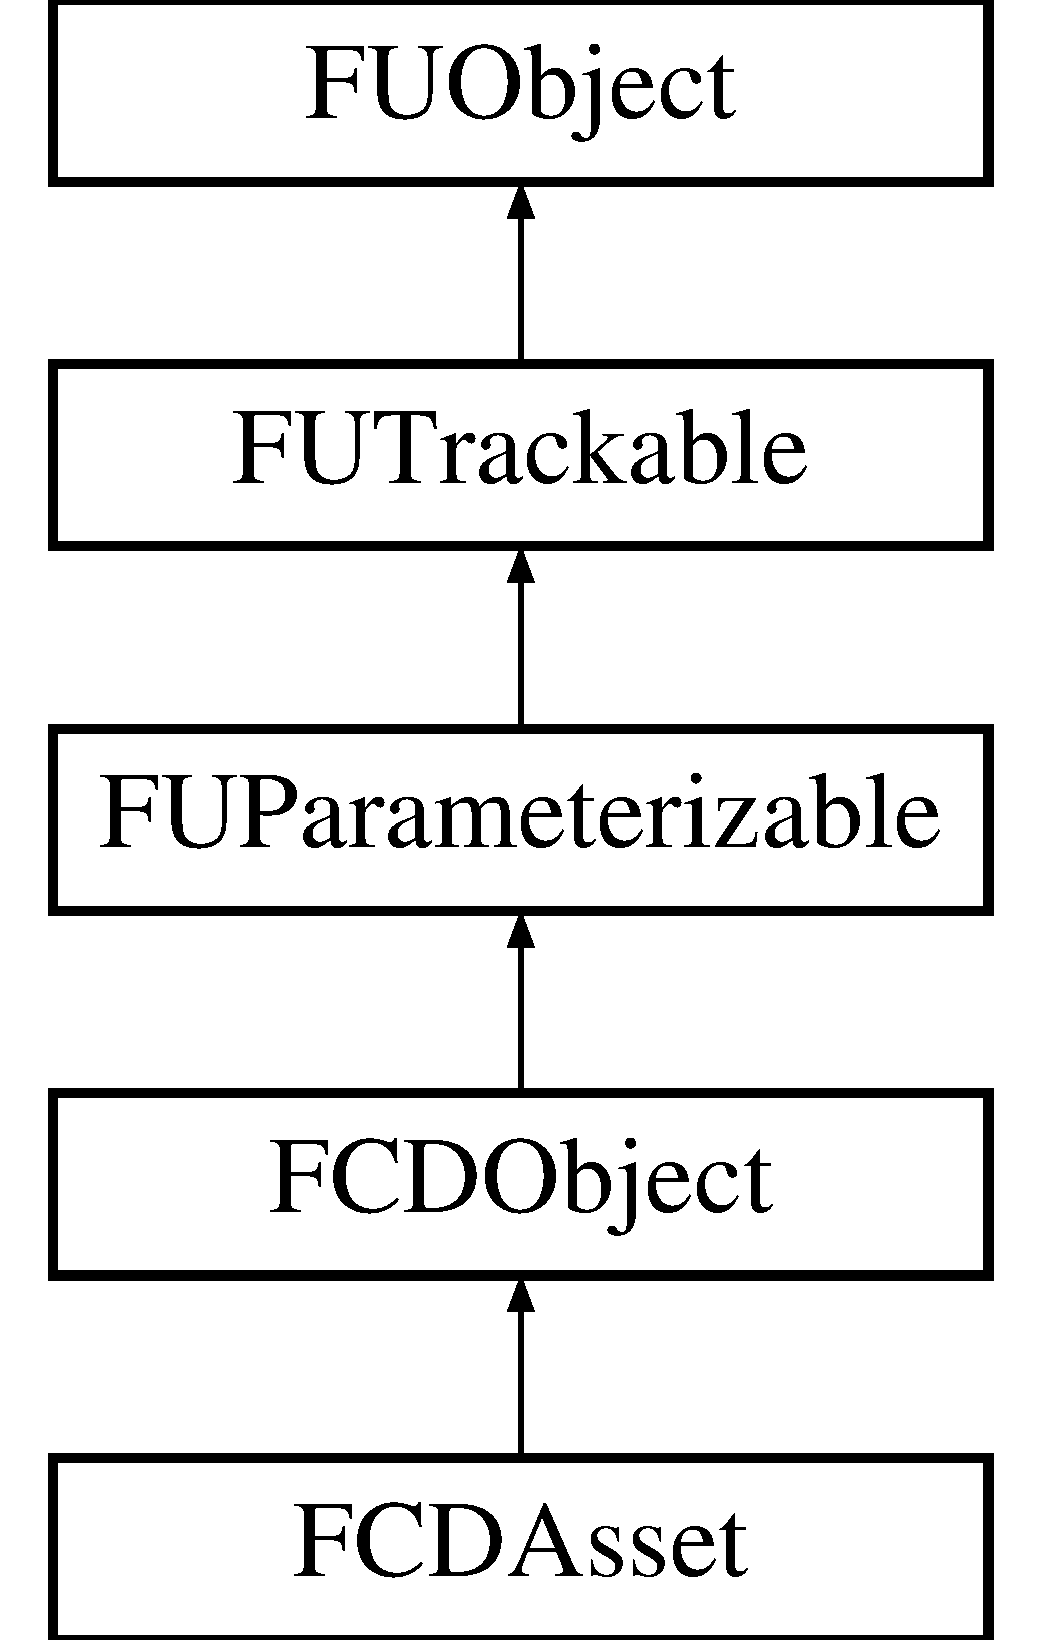
\includegraphics[height=5.000000cm]{classFCDAsset}
\end{center}
\end{figure}
\subsection*{Public Member Functions}
\begin{DoxyCompactItemize}
\item 
\hyperlink{classFCDAsset_aaef444871208dc4fa7844faae9934a28}{DeclareFlag} (HasUpAxis, 0)
\item 
\hyperlink{classFCDAsset_a1d93c654b9349d0bdcb1908d6913acbf}{DeclareFlag} (HasUnits, 1)
\item 
\hyperlink{classFCDAsset_a570cdb41df882da6b1870d1fc2a832c4}{DeclareFlagCount} (2)
\item 
\hyperlink{classFCDAsset_a5da15a3a94d6a7f59f45c61867ec5bc0}{FCDAsset} (\hyperlink{classFCDocument}{FCDocument} $\ast$document)
\item 
virtual \hyperlink{classFCDAsset_ac42df2e17abd0b486487fe81eae943f6}{$\sim$FCDAsset} ()
\item 
const \hyperlink{classFCDAssetContributor}{FCDAssetContributor} $\ast$$\ast$ \hyperlink{classFCDAsset_a2513997b4e76d1c0b0372e5038b14fdd}{GetContributors} () const 
\item 
size\_\-t \hyperlink{classFCDAsset_ac155201e474e73fae72f6a311b75fabe}{GetContributorCount} () const 
\item 
\hyperlink{classFCDAssetContributor}{FCDAssetContributor} $\ast$ \hyperlink{classFCDAsset_af880150aa707a2c0d01650cf06cdcd0e}{GetContributor} (size\_\-t index)
\item 
const \hyperlink{classFCDAssetContributor}{FCDAssetContributor} $\ast$ \hyperlink{classFCDAsset_a1fc0c9b2045afaebef1c1ddab603b910}{GetContributor} (size\_\-t index) const 
\item 
\hyperlink{classFCDAssetContributor}{FCDAssetContributor} $\ast$ \hyperlink{classFCDAsset_a38a74fe254c1973e4168cbb7dc6ac8c4}{AddContributor} ()
\item 
const \hyperlink{classFUDateTime}{FUDateTime} \& \hyperlink{classFCDAsset_aca09b308ca564bfc2f46b7e1e2a9fd8f}{GetCreationDateTime} () const 
\item 
\hyperlink{classFUDateTime}{FUDateTime} \& \hyperlink{classFCDAsset_ac6b536eed591166e36ce17e872cb4590}{GetCreationDateTime} ()
\item 
const \hyperlink{classFUDateTime}{FUDateTime} \& \hyperlink{classFCDAsset_a76a1f0b10d0b9584769426a5c6364914}{GetModifiedDateTime} () const 
\item 
\hyperlink{classFUDateTime}{FUDateTime} \& \hyperlink{classFCDAsset_aa9cb70c621809bcc5c21ce46f0337572}{GetModifiedDateTime} ()
\item 
const \hyperlink{classfm_1_1stringT}{fstring} \& \hyperlink{classFCDAsset_a3065bcdf36ae6dcf08340ca34cdde8cb}{GetKeywords} () const 
\item 
void \hyperlink{classFCDAsset_a317640602ee4402a75bf44336f6b1730}{SetKeywords} (const \hyperlink{classfm_1_1stringT}{fstring} \&\_\-keywords)
\item 
const \hyperlink{classfm_1_1stringT}{fstring} \& \hyperlink{classFCDAsset_aee96d3220790dad890310c1a96fec407}{GetRevision} () const 
\item 
void \hyperlink{classFCDAsset_a82bbc7fef5c62ff0f5be2aa269379e50}{SetRevision} (const \hyperlink{classfm_1_1stringT}{fstring} \&\_\-revision)
\item 
const \hyperlink{classfm_1_1stringT}{fstring} \& \hyperlink{classFCDAsset_ae6171c1527a8a42c2e460efb4905b72b}{GetSubject} () const 
\item 
void \hyperlink{classFCDAsset_ad11385733a29ffab48c98524fd5fd499}{SetSubject} (const \hyperlink{classfm_1_1stringT}{fstring} \&\_\-subject)
\item 
const \hyperlink{classfm_1_1stringT}{fstring} \& \hyperlink{classFCDAsset_a30cca0e5b5033d75ffd1d3e5eb3122c8}{GetTitle} () const 
\item 
void \hyperlink{classFCDAsset_a13ff0403acddd544d101b9eed9f5c08a}{SetTitle} (const \hyperlink{classfm_1_1stringT}{fstring} \&\_\-title)
\item 
const \hyperlink{classFMVector3}{FMVector3} \& \hyperlink{classFCDAsset_a43d8c683514ea100cdf5cd400cd763f4}{GetUpAxis} () const 
\item 
void \hyperlink{classFCDAsset_abf15daaf8ad6ad3f79e91c61f3c413cf}{SetUpAxis} (const \hyperlink{classFMVector3}{FMVector3} \&\_\-upAxis)
\item 
const \hyperlink{classfm_1_1stringT}{fstring} \& \hyperlink{classFCDAsset_a474173912edd72b7cc622a97831f3b53}{GetUnitName} () const 
\item 
void \hyperlink{classFCDAsset_a84c0518772964e0bf68adfb92ef974cb}{SetUnitName} (const \hyperlink{classfm_1_1stringT}{fstring} \&\_\-unitName)
\item 
float \hyperlink{classFCDAsset_a5bf9d6f3626f189847747bff1fb11acc}{GetUnitConversionFactor} () const 
\item 
void \hyperlink{classFCDAsset_ad8bae14c4dee0c70e87e009737727059}{SetUnitConversionFactor} (float factor)
\item 
\hyperlink{classFCDAsset_a81ee67ffa2e9fad37c2b5c38afe65391}{DEPRECATED} (3.05A, GetHasUpAxisFlag) inline bool HasUpAxis() const 
\item 
\hyperlink{classFCDAsset_a8b2bd39d79aed2e15e9e0838c77dae29}{DEPRECATED} (3.05A, GetHasUnitsFlag) inline bool HasUnits() const 
\item 
\hyperlink{classFCDAsset_a0ab293d73a5f99619978629f67de4d3c}{DEPRECATED} (3.05A, ResetHasUpAxisFlag) inline void ResetUpAxis()
\item 
\hyperlink{classFCDAsset_a11dedba737a92ce67886ca5324cf7c7b}{DEPRECATED} (3.05A, ResetHasUnitsFlag) inline void ResetUnits()
\item 
\hyperlink{classFCDAsset}{FCDAsset} $\ast$ \hyperlink{classFCDAsset_a75f6bacb408ab3a71f718ca49b81777f}{Clone} (\hyperlink{classFCDAsset}{FCDAsset} $\ast$clone=NULL, bool cloneAllContributors=true) const 
\end{DoxyCompactItemize}


\subsection{Detailed Description}
A COLLADA asset declaration structure.

In COLLADA, there are three types of assets. \hyperlink{namespaceFCollada}{FCollada} recognizes two.

1) The COLLADA document is the most important asset and an asset declaration structure is always created for it. 2) The \hyperlink{classFCDEntity}{FCDEntity} objects may also contain assets structures. 3) COLLADA also allows asset structure on entity libraries, but \hyperlink{namespaceFCollada}{FCollada} does not support them.

Every asset contains its own list of contributors. Every COLLADA application and conditioner that modifies an asset should attach its signature, in the form of a contributor, to the asset. \begin{DoxySeeAlso}{See also}
\hyperlink{classFCDAssetContributor}{FCDAssetContributor} 
\end{DoxySeeAlso}


\subsection{Constructor \& Destructor Documentation}
\hypertarget{classFCDAsset_a5da15a3a94d6a7f59f45c61867ec5bc0}{
\index{FCDAsset@{FCDAsset}!FCDAsset@{FCDAsset}}
\index{FCDAsset@{FCDAsset}!FCDAsset@{FCDAsset}}
\subsubsection[{FCDAsset}]{\setlength{\rightskip}{0pt plus 5cm}FCDAsset::FCDAsset (
\begin{DoxyParamCaption}
\item[{{\bf FCDocument} $\ast$}]{ document}
\end{DoxyParamCaption}
)}}
\label{classFCDAsset_a5da15a3a94d6a7f59f45c61867ec5bc0}
Constructor. 
\begin{DoxyParams}{Parameters}
\item[{\em document}]The COLLADA document that owns the asset. \end{DoxyParams}
\hypertarget{classFCDAsset_ac42df2e17abd0b486487fe81eae943f6}{
\index{FCDAsset@{FCDAsset}!$\sim$FCDAsset@{$\sim$FCDAsset}}
\index{$\sim$FCDAsset@{$\sim$FCDAsset}!FCDAsset@{FCDAsset}}
\subsubsection[{$\sim$FCDAsset}]{\setlength{\rightskip}{0pt plus 5cm}FCDAsset::$\sim$FCDAsset (
\begin{DoxyParamCaption}
{}
\end{DoxyParamCaption}
)\hspace{0.3cm}{\ttfamily  \mbox{[}virtual\mbox{]}}}}
\label{classFCDAsset_ac42df2e17abd0b486487fe81eae943f6}
Destructor. 

\subsection{Member Function Documentation}
\hypertarget{classFCDAsset_a38a74fe254c1973e4168cbb7dc6ac8c4}{
\index{FCDAsset@{FCDAsset}!AddContributor@{AddContributor}}
\index{AddContributor@{AddContributor}!FCDAsset@{FCDAsset}}
\subsubsection[{AddContributor}]{\setlength{\rightskip}{0pt plus 5cm}{\bf FCDAssetContributor} $\ast$ FCDAsset::AddContributor (
\begin{DoxyParamCaption}
{}
\end{DoxyParamCaption}
)}}
\label{classFCDAsset_a38a74fe254c1973e4168cbb7dc6ac8c4}
Inserts a new contributor to this asset. \begin{DoxyReturn}{Returns}
An empty contributor structure. 
\end{DoxyReturn}
\hypertarget{classFCDAsset_a75f6bacb408ab3a71f718ca49b81777f}{
\index{FCDAsset@{FCDAsset}!Clone@{Clone}}
\index{Clone@{Clone}!FCDAsset@{FCDAsset}}
\subsubsection[{Clone}]{\setlength{\rightskip}{0pt plus 5cm}{\bf FCDAsset} $\ast$ FCDAsset::Clone (
\begin{DoxyParamCaption}
\item[{{\bf FCDAsset} $\ast$}]{ clone = {\ttfamily NULL}, }
\item[{bool}]{ cloneAllContributors = {\ttfamily true}}
\end{DoxyParamCaption}
) const}}
\label{classFCDAsset_a75f6bacb408ab3a71f718ca49b81777f}
Clones the asset structure into another asset structure. 
\begin{DoxyParams}{Parameters}
\item[{\em clone}]The asset structure that will become the copy of this asset. When this pointer is NULL, a new asset structure will be created. \item[{\em cloneAllContributors}]Whether all the contributors of this asset should be copied into the clone. \end{DoxyParams}
\begin{DoxyReturn}{Returns}
The clone. 
\end{DoxyReturn}
\hypertarget{classFCDAsset_aaef444871208dc4fa7844faae9934a28}{
\index{FCDAsset@{FCDAsset}!DeclareFlag@{DeclareFlag}}
\index{DeclareFlag@{DeclareFlag}!FCDAsset@{FCDAsset}}
\subsubsection[{DeclareFlag}]{\setlength{\rightskip}{0pt plus 5cm}FCDAsset::DeclareFlag (
\begin{DoxyParamCaption}
\item[{HasUpAxis}]{, }
\item[{0}]{}
\end{DoxyParamCaption}
)}}
\label{classFCDAsset_aaef444871208dc4fa7844faae9934a28}
Whether an up-\/axis is set for this asset. If no up-\/axis is set for this asset, you should use the up-\/axis of the parent's asset. \hypertarget{classFCDAsset_a1d93c654b9349d0bdcb1908d6913acbf}{
\index{FCDAsset@{FCDAsset}!DeclareFlag@{DeclareFlag}}
\index{DeclareFlag@{DeclareFlag}!FCDAsset@{FCDAsset}}
\subsubsection[{DeclareFlag}]{\setlength{\rightskip}{0pt plus 5cm}FCDAsset::DeclareFlag (
\begin{DoxyParamCaption}
\item[{HasUnits}]{, }
\item[{1}]{}
\end{DoxyParamCaption}
)}}
\label{classFCDAsset_a1d93c654b9349d0bdcb1908d6913acbf}
Whether a length unit is set for this asset. If no length unit is set for this asset, you should use the length unit of the parent's asset. \hypertarget{classFCDAsset_a570cdb41df882da6b1870d1fc2a832c4}{
\index{FCDAsset@{FCDAsset}!DeclareFlagCount@{DeclareFlagCount}}
\index{DeclareFlagCount@{DeclareFlagCount}!FCDAsset@{FCDAsset}}
\subsubsection[{DeclareFlagCount}]{\setlength{\rightskip}{0pt plus 5cm}FCDAsset::DeclareFlagCount (
\begin{DoxyParamCaption}
\item[{2}]{}
\end{DoxyParamCaption}
)}}
\label{classFCDAsset_a570cdb41df882da6b1870d1fc2a832c4}
\hyperlink{classFCDAsset}{FCDAsset} declares two flags. 

Reimplemented from \hyperlink{classFCDObject_a829bea1d332894b2f803754b8832a818}{FCDObject}.

\hypertarget{classFCDAsset_a81ee67ffa2e9fad37c2b5c38afe65391}{
\index{FCDAsset@{FCDAsset}!DEPRECATED@{DEPRECATED}}
\index{DEPRECATED@{DEPRECATED}!FCDAsset@{FCDAsset}}
\subsubsection[{DEPRECATED}]{\setlength{\rightskip}{0pt plus 5cm}FCDAsset::DEPRECATED (
\begin{DoxyParamCaption}
\item[{3.}]{ 05A, }
\item[{GetHasUpAxisFlag}]{}
\end{DoxyParamCaption}
) const\hspace{0.3cm}{\ttfamily  \mbox{[}inline\mbox{]}}}}
\label{classFCDAsset_a81ee67ffa2e9fad37c2b5c38afe65391}
Retrieves whether an up-\/axis is set for this asset. If no up-\/axis is set for this asset, you should use the up-\/axis of the parent's asset. \begin{DoxyReturn}{Returns}
Whether this asset defines an up-\/axis. 
\end{DoxyReturn}
\hypertarget{classFCDAsset_a11dedba737a92ce67886ca5324cf7c7b}{
\index{FCDAsset@{FCDAsset}!DEPRECATED@{DEPRECATED}}
\index{DEPRECATED@{DEPRECATED}!FCDAsset@{FCDAsset}}
\subsubsection[{DEPRECATED}]{\setlength{\rightskip}{0pt plus 5cm}FCDAsset::DEPRECATED (
\begin{DoxyParamCaption}
\item[{3.}]{ 05A, }
\item[{ResetHasUnitsFlag}]{}
\end{DoxyParamCaption}
)\hspace{0.3cm}{\ttfamily  \mbox{[}inline\mbox{]}}}}
\label{classFCDAsset_a11dedba737a92ce67886ca5324cf7c7b}
Resets the length unit of the asset. The parent asset length unit should henceforth be used. Changing the length unit of an asset does not modify its data. \hypertarget{classFCDAsset_a0ab293d73a5f99619978629f67de4d3c}{
\index{FCDAsset@{FCDAsset}!DEPRECATED@{DEPRECATED}}
\index{DEPRECATED@{DEPRECATED}!FCDAsset@{FCDAsset}}
\subsubsection[{DEPRECATED}]{\setlength{\rightskip}{0pt plus 5cm}FCDAsset::DEPRECATED (
\begin{DoxyParamCaption}
\item[{3.}]{ 05A, }
\item[{ResetHasUpAxisFlag}]{}
\end{DoxyParamCaption}
)\hspace{0.3cm}{\ttfamily  \mbox{[}inline\mbox{]}}}}
\label{classFCDAsset_a0ab293d73a5f99619978629f67de4d3c}
Resets the up-\/axis of the asset. The parent asset up-\/axis should henceforth be used. Changing the up-\/axis of an asset does not modify its data. \hypertarget{classFCDAsset_a8b2bd39d79aed2e15e9e0838c77dae29}{
\index{FCDAsset@{FCDAsset}!DEPRECATED@{DEPRECATED}}
\index{DEPRECATED@{DEPRECATED}!FCDAsset@{FCDAsset}}
\subsubsection[{DEPRECATED}]{\setlength{\rightskip}{0pt plus 5cm}FCDAsset::DEPRECATED (
\begin{DoxyParamCaption}
\item[{3.}]{ 05A, }
\item[{GetHasUnitsFlag}]{}
\end{DoxyParamCaption}
) const\hspace{0.3cm}{\ttfamily  \mbox{[}inline\mbox{]}}}}
\label{classFCDAsset_a8b2bd39d79aed2e15e9e0838c77dae29}
Retrieves whether a length unit is set for this asset. If no length unit is set for this asset, you should use the length unit of the parent's asset. \begin{DoxyReturn}{Returns}
Whether this asset defines a length unit. 
\end{DoxyReturn}
\hypertarget{classFCDAsset_a1fc0c9b2045afaebef1c1ddab603b910}{
\index{FCDAsset@{FCDAsset}!GetContributor@{GetContributor}}
\index{GetContributor@{GetContributor}!FCDAsset@{FCDAsset}}
\subsubsection[{GetContributor}]{\setlength{\rightskip}{0pt plus 5cm}const {\bf FCDAssetContributor}$\ast$ FCDAsset::GetContributor (
\begin{DoxyParamCaption}
\item[{size\_\-t}]{ index}
\end{DoxyParamCaption}
) const\hspace{0.3cm}{\ttfamily  \mbox{[}inline\mbox{]}}}}
\label{classFCDAsset_a1fc0c9b2045afaebef1c1ddab603b910}
See above. \hypertarget{classFCDAsset_af880150aa707a2c0d01650cf06cdcd0e}{
\index{FCDAsset@{FCDAsset}!GetContributor@{GetContributor}}
\index{GetContributor@{GetContributor}!FCDAsset@{FCDAsset}}
\subsubsection[{GetContributor}]{\setlength{\rightskip}{0pt plus 5cm}{\bf FCDAssetContributor}$\ast$ FCDAsset::GetContributor (
\begin{DoxyParamCaption}
\item[{size\_\-t}]{ index}
\end{DoxyParamCaption}
)\hspace{0.3cm}{\ttfamily  \mbox{[}inline\mbox{]}}}}
\label{classFCDAsset_af880150aa707a2c0d01650cf06cdcd0e}
Retrieves a contributor tied to this asset. 
\begin{DoxyParams}{Parameters}
\item[{\em index}]The index of the contributor. \end{DoxyParams}
\begin{DoxyReturn}{Returns}
The contributor at the given index. 
\end{DoxyReturn}
\hypertarget{classFCDAsset_ac155201e474e73fae72f6a311b75fabe}{
\index{FCDAsset@{FCDAsset}!GetContributorCount@{GetContributorCount}}
\index{GetContributorCount@{GetContributorCount}!FCDAsset@{FCDAsset}}
\subsubsection[{GetContributorCount}]{\setlength{\rightskip}{0pt plus 5cm}size\_\-t FCDAsset::GetContributorCount (
\begin{DoxyParamCaption}
{}
\end{DoxyParamCaption}
) const\hspace{0.3cm}{\ttfamily  \mbox{[}inline\mbox{]}}}}
\label{classFCDAsset_ac155201e474e73fae72f6a311b75fabe}
Retrieves the number of contributors to this asset. \begin{DoxyReturn}{Returns}
The number of contributors. 
\end{DoxyReturn}
\hypertarget{classFCDAsset_a2513997b4e76d1c0b0372e5038b14fdd}{
\index{FCDAsset@{FCDAsset}!GetContributors@{GetContributors}}
\index{GetContributors@{GetContributors}!FCDAsset@{FCDAsset}}
\subsubsection[{GetContributors}]{\setlength{\rightskip}{0pt plus 5cm}const {\bf FCDAssetContributor}$\ast$$\ast$ FCDAsset::GetContributors (
\begin{DoxyParamCaption}
{}
\end{DoxyParamCaption}
) const\hspace{0.3cm}{\ttfamily  \mbox{[}inline\mbox{]}}}}
\label{classFCDAsset_a2513997b4e76d1c0b0372e5038b14fdd}
Retrieves the list of contributors to this asset. \begin{DoxyReturn}{Returns}
The list of contributors. See above. 
\end{DoxyReturn}
\hypertarget{classFCDAsset_aca09b308ca564bfc2f46b7e1e2a9fd8f}{
\index{FCDAsset@{FCDAsset}!GetCreationDateTime@{GetCreationDateTime}}
\index{GetCreationDateTime@{GetCreationDateTime}!FCDAsset@{FCDAsset}}
\subsubsection[{GetCreationDateTime}]{\setlength{\rightskip}{0pt plus 5cm}const {\bf FUDateTime}\& FCDAsset::GetCreationDateTime (
\begin{DoxyParamCaption}
{}
\end{DoxyParamCaption}
) const\hspace{0.3cm}{\ttfamily  \mbox{[}inline\mbox{]}}}}
\label{classFCDAsset_aca09b308ca564bfc2f46b7e1e2a9fd8f}
Retrieves the creation date-\/time of the document. This date-\/time is not modifiable. It is set automatically when \hyperlink{namespaceFCollada}{FCollada} creates the document or imported when \hyperlink{namespaceFCollada}{FCollada} reads in a COLLADA document. \begin{DoxyReturn}{Returns}
The date-\/time at which the COLLADA document was originally created. 
\end{DoxyReturn}
\hypertarget{classFCDAsset_ac6b536eed591166e36ce17e872cb4590}{
\index{FCDAsset@{FCDAsset}!GetCreationDateTime@{GetCreationDateTime}}
\index{GetCreationDateTime@{GetCreationDateTime}!FCDAsset@{FCDAsset}}
\subsubsection[{GetCreationDateTime}]{\setlength{\rightskip}{0pt plus 5cm}{\bf FUDateTime}\& FCDAsset::GetCreationDateTime (
\begin{DoxyParamCaption}
{}
\end{DoxyParamCaption}
)\hspace{0.3cm}{\ttfamily  \mbox{[}inline\mbox{]}}}}
\label{classFCDAsset_ac6b536eed591166e36ce17e872cb4590}
\mbox{[}INTERNAL\mbox{]} Use this function to createDateTime when you are writing an import plug-\/in. see above \hypertarget{classFCDAsset_a3065bcdf36ae6dcf08340ca34cdde8cb}{
\index{FCDAsset@{FCDAsset}!GetKeywords@{GetKeywords}}
\index{GetKeywords@{GetKeywords}!FCDAsset@{FCDAsset}}
\subsubsection[{GetKeywords}]{\setlength{\rightskip}{0pt plus 5cm}const {\bf fstring}\& FCDAsset::GetKeywords (
\begin{DoxyParamCaption}
{}
\end{DoxyParamCaption}
) const\hspace{0.3cm}{\ttfamily  \mbox{[}inline\mbox{]}}}}
\label{classFCDAsset_a3065bcdf36ae6dcf08340ca34cdde8cb}
Retrieves the list of keywords identifying this asset. \begin{DoxyReturn}{Returns}
The list of keywords for the asset. 
\end{DoxyReturn}
\hypertarget{classFCDAsset_a76a1f0b10d0b9584769426a5c6364914}{
\index{FCDAsset@{FCDAsset}!GetModifiedDateTime@{GetModifiedDateTime}}
\index{GetModifiedDateTime@{GetModifiedDateTime}!FCDAsset@{FCDAsset}}
\subsubsection[{GetModifiedDateTime}]{\setlength{\rightskip}{0pt plus 5cm}const {\bf FUDateTime}\& FCDAsset::GetModifiedDateTime (
\begin{DoxyParamCaption}
{}
\end{DoxyParamCaption}
) const\hspace{0.3cm}{\ttfamily  \mbox{[}inline\mbox{]}}}}
\label{classFCDAsset_a76a1f0b10d0b9584769426a5c6364914}
Retrieves the last modification date-\/time of the document. This date-\/time is not modifiable. It is set automatically when \hyperlink{namespaceFCollada}{FCollada} writes out a COLLADA document to a file, when \hyperlink{namespaceFCollada}{FCollada} creates an original document and when \hyperlink{namespaceFCollada}{FCollada} reads in a COLLADA document from a file. \begin{DoxyReturn}{Returns}
The date-\/time at which the COLLADA document was last modified. 
\end{DoxyReturn}
\hypertarget{classFCDAsset_aa9cb70c621809bcc5c21ce46f0337572}{
\index{FCDAsset@{FCDAsset}!GetModifiedDateTime@{GetModifiedDateTime}}
\index{GetModifiedDateTime@{GetModifiedDateTime}!FCDAsset@{FCDAsset}}
\subsubsection[{GetModifiedDateTime}]{\setlength{\rightskip}{0pt plus 5cm}{\bf FUDateTime}\& FCDAsset::GetModifiedDateTime (
\begin{DoxyParamCaption}
{}
\end{DoxyParamCaption}
)\hspace{0.3cm}{\ttfamily  \mbox{[}inline\mbox{]}}}}
\label{classFCDAsset_aa9cb70c621809bcc5c21ce46f0337572}
\mbox{[}INTERNAL\mbox{]} Use this function to retieve the modifiedDateTime when you are writing an import plug-\/in. see above \hypertarget{classFCDAsset_aee96d3220790dad890310c1a96fec407}{
\index{FCDAsset@{FCDAsset}!GetRevision@{GetRevision}}
\index{GetRevision@{GetRevision}!FCDAsset@{FCDAsset}}
\subsubsection[{GetRevision}]{\setlength{\rightskip}{0pt plus 5cm}const {\bf fstring}\& FCDAsset::GetRevision (
\begin{DoxyParamCaption}
{}
\end{DoxyParamCaption}
) const\hspace{0.3cm}{\ttfamily  \mbox{[}inline\mbox{]}}}}
\label{classFCDAsset_aee96d3220790dad890310c1a96fec407}
Retrieves the revision string for this asset. COLLADA doesn't define a standard for the revisions of assets. \begin{DoxyReturn}{Returns}
The revision string for the asset. 
\end{DoxyReturn}
\hypertarget{classFCDAsset_ae6171c1527a8a42c2e460efb4905b72b}{
\index{FCDAsset@{FCDAsset}!GetSubject@{GetSubject}}
\index{GetSubject@{GetSubject}!FCDAsset@{FCDAsset}}
\subsubsection[{GetSubject}]{\setlength{\rightskip}{0pt plus 5cm}const {\bf fstring}\& FCDAsset::GetSubject (
\begin{DoxyParamCaption}
{}
\end{DoxyParamCaption}
) const\hspace{0.3cm}{\ttfamily  \mbox{[}inline\mbox{]}}}}
\label{classFCDAsset_ae6171c1527a8a42c2e460efb4905b72b}
Retrieves the subject of the asset. \begin{DoxyReturn}{Returns}
The subject of the asset. 
\end{DoxyReturn}
\hypertarget{classFCDAsset_a30cca0e5b5033d75ffd1d3e5eb3122c8}{
\index{FCDAsset@{FCDAsset}!GetTitle@{GetTitle}}
\index{GetTitle@{GetTitle}!FCDAsset@{FCDAsset}}
\subsubsection[{GetTitle}]{\setlength{\rightskip}{0pt plus 5cm}const {\bf fstring}\& FCDAsset::GetTitle (
\begin{DoxyParamCaption}
{}
\end{DoxyParamCaption}
) const\hspace{0.3cm}{\ttfamily  \mbox{[}inline\mbox{]}}}}
\label{classFCDAsset_a30cca0e5b5033d75ffd1d3e5eb3122c8}
Retrieves the title of the asset. \begin{DoxyReturn}{Returns}
The title of the asset. 
\end{DoxyReturn}
\hypertarget{classFCDAsset_a5bf9d6f3626f189847747bff1fb11acc}{
\index{FCDAsset@{FCDAsset}!GetUnitConversionFactor@{GetUnitConversionFactor}}
\index{GetUnitConversionFactor@{GetUnitConversionFactor}!FCDAsset@{FCDAsset}}
\subsubsection[{GetUnitConversionFactor}]{\setlength{\rightskip}{0pt plus 5cm}float FCDAsset::GetUnitConversionFactor (
\begin{DoxyParamCaption}
{}
\end{DoxyParamCaption}
) const\hspace{0.3cm}{\ttfamily  \mbox{[}inline\mbox{]}}}}
\label{classFCDAsset_a5bf9d6f3626f189847747bff1fb11acc}
Retrieves the length unit conversion factor, in meters, for the asset. The length unit of two entities within the same document may differ. To avoid issues with length unit differences, it is suggested that you use the \hyperlink{namespaceFCDocumentTools_a2c30506a0db61b68aa07f18b025e935e}{FCDocumentTools::StandardizeUpAxisAndLength} function. \begin{DoxyReturn}{Returns}
The length unit conversion factor. 
\end{DoxyReturn}
\hypertarget{classFCDAsset_a474173912edd72b7cc622a97831f3b53}{
\index{FCDAsset@{FCDAsset}!GetUnitName@{GetUnitName}}
\index{GetUnitName@{GetUnitName}!FCDAsset@{FCDAsset}}
\subsubsection[{GetUnitName}]{\setlength{\rightskip}{0pt plus 5cm}const {\bf fstring}\& FCDAsset::GetUnitName (
\begin{DoxyParamCaption}
{}
\end{DoxyParamCaption}
) const\hspace{0.3cm}{\ttfamily  \mbox{[}inline\mbox{]}}}}
\label{classFCDAsset_a474173912edd72b7cc622a97831f3b53}
Retrieves the name of the length unit for the asset. \begin{DoxyReturn}{Returns}
The name of the length unit for the asset. 
\end{DoxyReturn}
\hypertarget{classFCDAsset_a43d8c683514ea100cdf5cd400cd763f4}{
\index{FCDAsset@{FCDAsset}!GetUpAxis@{GetUpAxis}}
\index{GetUpAxis@{GetUpAxis}!FCDAsset@{FCDAsset}}
\subsubsection[{GetUpAxis}]{\setlength{\rightskip}{0pt plus 5cm}const {\bf FMVector3}\& FCDAsset::GetUpAxis (
\begin{DoxyParamCaption}
{}
\end{DoxyParamCaption}
) const\hspace{0.3cm}{\ttfamily  \mbox{[}inline\mbox{]}}}}
\label{classFCDAsset_a43d8c683514ea100cdf5cd400cd763f4}
Retrieves the up-\/axis of the asset. The up-\/axis of two entities within the same document may differ. To avoid issues with up-\/axis differences, it is suggested that you use the \hyperlink{namespaceFCDocumentTools_a2c30506a0db61b68aa07f18b025e935e}{FCDocumentTools::StandardizeUpAxisAndLength} function. \begin{DoxyReturn}{Returns}
The up-\/axis of the asset. 
\end{DoxyReturn}
\hypertarget{classFCDAsset_a317640602ee4402a75bf44336f6b1730}{
\index{FCDAsset@{FCDAsset}!SetKeywords@{SetKeywords}}
\index{SetKeywords@{SetKeywords}!FCDAsset@{FCDAsset}}
\subsubsection[{SetKeywords}]{\setlength{\rightskip}{0pt plus 5cm}void FCDAsset::SetKeywords (
\begin{DoxyParamCaption}
\item[{const {\bf fstring} \&}]{ \_\-keywords}
\end{DoxyParamCaption}
)\hspace{0.3cm}{\ttfamily  \mbox{[}inline\mbox{]}}}}
\label{classFCDAsset_a317640602ee4402a75bf44336f6b1730}
Sets the list of keywords for this asset. 
\begin{DoxyParams}{Parameters}
\item[{\em \_\-keywords}]The list of keywords for the asset. \end{DoxyParams}
\hypertarget{classFCDAsset_a82bbc7fef5c62ff0f5be2aa269379e50}{
\index{FCDAsset@{FCDAsset}!SetRevision@{SetRevision}}
\index{SetRevision@{SetRevision}!FCDAsset@{FCDAsset}}
\subsubsection[{SetRevision}]{\setlength{\rightskip}{0pt plus 5cm}void FCDAsset::SetRevision (
\begin{DoxyParamCaption}
\item[{const {\bf fstring} \&}]{ \_\-revision}
\end{DoxyParamCaption}
)\hspace{0.3cm}{\ttfamily  \mbox{[}inline\mbox{]}}}}
\label{classFCDAsset_a82bbc7fef5c62ff0f5be2aa269379e50}
Sets the revision string for this asset. COLLADA doesn't define a standard for the revisions of assets. 
\begin{DoxyParams}{Parameters}
\item[{\em \_\-revision}]The revision string for the asset. \end{DoxyParams}
\hypertarget{classFCDAsset_ad11385733a29ffab48c98524fd5fd499}{
\index{FCDAsset@{FCDAsset}!SetSubject@{SetSubject}}
\index{SetSubject@{SetSubject}!FCDAsset@{FCDAsset}}
\subsubsection[{SetSubject}]{\setlength{\rightskip}{0pt plus 5cm}void FCDAsset::SetSubject (
\begin{DoxyParamCaption}
\item[{const {\bf fstring} \&}]{ \_\-subject}
\end{DoxyParamCaption}
)\hspace{0.3cm}{\ttfamily  \mbox{[}inline\mbox{]}}}}
\label{classFCDAsset_ad11385733a29ffab48c98524fd5fd499}
Sets the subject of the asset. 
\begin{DoxyParams}{Parameters}
\item[{\em \_\-subject}]The subject of the asset. \end{DoxyParams}
\hypertarget{classFCDAsset_a13ff0403acddd544d101b9eed9f5c08a}{
\index{FCDAsset@{FCDAsset}!SetTitle@{SetTitle}}
\index{SetTitle@{SetTitle}!FCDAsset@{FCDAsset}}
\subsubsection[{SetTitle}]{\setlength{\rightskip}{0pt plus 5cm}void FCDAsset::SetTitle (
\begin{DoxyParamCaption}
\item[{const {\bf fstring} \&}]{ \_\-title}
\end{DoxyParamCaption}
)\hspace{0.3cm}{\ttfamily  \mbox{[}inline\mbox{]}}}}
\label{classFCDAsset_a13ff0403acddd544d101b9eed9f5c08a}
Sets the title of the asset. 
\begin{DoxyParams}{Parameters}
\item[{\em \_\-title}]The title of the asset. \end{DoxyParams}
\hypertarget{classFCDAsset_ad8bae14c4dee0c70e87e009737727059}{
\index{FCDAsset@{FCDAsset}!SetUnitConversionFactor@{SetUnitConversionFactor}}
\index{SetUnitConversionFactor@{SetUnitConversionFactor}!FCDAsset@{FCDAsset}}
\subsubsection[{SetUnitConversionFactor}]{\setlength{\rightskip}{0pt plus 5cm}void FCDAsset::SetUnitConversionFactor (
\begin{DoxyParamCaption}
\item[{float}]{ factor}
\end{DoxyParamCaption}
)\hspace{0.3cm}{\ttfamily  \mbox{[}inline\mbox{]}}}}
\label{classFCDAsset_ad8bae14c4dee0c70e87e009737727059}
Sets the length unit conversion factor for the asset. Changing the length unit conversion factor of an asset does not modify its data. 
\begin{DoxyParams}{Parameters}
\item[{\em factor}]The new length unit conversion factor. \end{DoxyParams}
\hypertarget{classFCDAsset_a84c0518772964e0bf68adfb92ef974cb}{
\index{FCDAsset@{FCDAsset}!SetUnitName@{SetUnitName}}
\index{SetUnitName@{SetUnitName}!FCDAsset@{FCDAsset}}
\subsubsection[{SetUnitName}]{\setlength{\rightskip}{0pt plus 5cm}void FCDAsset::SetUnitName (
\begin{DoxyParamCaption}
\item[{const {\bf fstring} \&}]{ \_\-unitName}
\end{DoxyParamCaption}
)\hspace{0.3cm}{\ttfamily  \mbox{[}inline\mbox{]}}}}
\label{classFCDAsset_a84c0518772964e0bf68adfb92ef974cb}
Sets the name of the length unit for the asset. 
\begin{DoxyParams}{Parameters}
\item[{\em \_\-unitName}]The name of the length unit for the asset. \end{DoxyParams}
\hypertarget{classFCDAsset_abf15daaf8ad6ad3f79e91c61f3c413cf}{
\index{FCDAsset@{FCDAsset}!SetUpAxis@{SetUpAxis}}
\index{SetUpAxis@{SetUpAxis}!FCDAsset@{FCDAsset}}
\subsubsection[{SetUpAxis}]{\setlength{\rightskip}{0pt plus 5cm}void FCDAsset::SetUpAxis (
\begin{DoxyParamCaption}
\item[{const {\bf FMVector3} \&}]{ \_\-upAxis}
\end{DoxyParamCaption}
)\hspace{0.3cm}{\ttfamily  \mbox{[}inline\mbox{]}}}}
\label{classFCDAsset_abf15daaf8ad6ad3f79e91c61f3c413cf}
Sets the up-\/axis of the asset. Changing the up-\/axis of an asset does not modify its data. 
\begin{DoxyParams}{Parameters}
\item[{\em \_\-upAxis}]The up-\/axis of the asset. \end{DoxyParams}


The documentation for this class was generated from the following files:\begin{DoxyCompactItemize}
\item 
FCollada/FCDocument/\hyperlink{FCDAsset_8h}{FCDAsset.h}\item 
FCollada/FCDocument/FCDAsset.cpp\end{DoxyCompactItemize}

\hypertarget{classFCDAssetContributor}{
\section{FCDAssetContributor Class Reference}
\label{classFCDAssetContributor}\index{FCDAssetContributor@{FCDAssetContributor}}
}


{\ttfamily \#include $<$FCDAsset.h$>$}

Inheritance diagram for FCDAssetContributor:\begin{figure}[H]
\begin{center}
\leavevmode
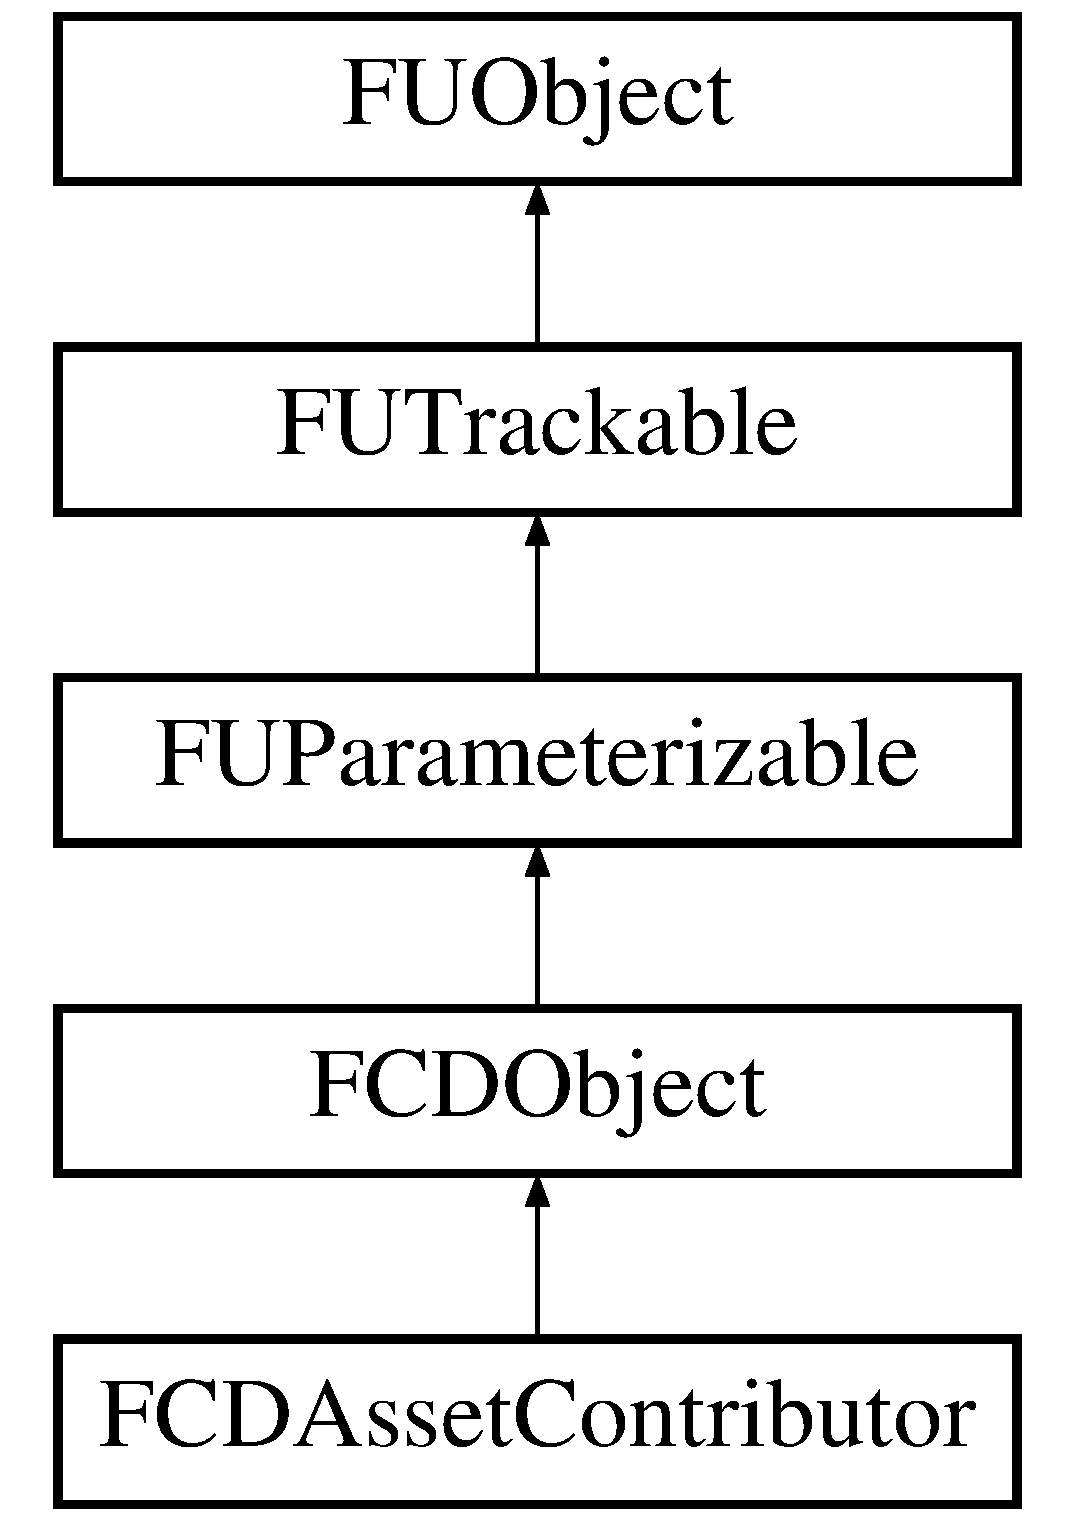
\includegraphics[height=5.000000cm]{classFCDAssetContributor}
\end{center}
\end{figure}
\subsection*{Public Member Functions}
\begin{DoxyCompactItemize}
\item 
\hyperlink{classFCDAssetContributor_a8a7123eb16366bac47bf3708970556f7}{FCDAssetContributor} (\hyperlink{classFCDocument}{FCDocument} $\ast$document)
\item 
virtual \hyperlink{classFCDAssetContributor_a6590d01617a5c6ad85d08a1325973a9a}{$\sim$FCDAssetContributor} ()
\item 
const \hyperlink{classfm_1_1stringT}{fstring} \& \hyperlink{classFCDAssetContributor_abd825a17c602412292656fe8d52680c5}{GetAuthor} () const 
\item 
void \hyperlink{classFCDAssetContributor_abc74516d6102c6322c43f2577da8c81a}{SetAuthor} (const \hyperlink{classfm_1_1stringT}{fstring} \&\_\-author)
\item 
const \hyperlink{classfm_1_1stringT}{fstring} \& \hyperlink{classFCDAssetContributor_a9ddb47c979cc5b8ad97e8dd7d897e897}{GetAuthoringTool} () const 
\item 
void \hyperlink{classFCDAssetContributor_a07a2dd49a8ccf12e5870fa06b7a61f02}{SetAuthoringTool} (const \hyperlink{classfm_1_1stringT}{fstring} \&\_\-authoringTool)
\item 
const \hyperlink{classfm_1_1stringT}{fstring} \& \hyperlink{classFCDAssetContributor_a69f3f0685703c61cfcabd362eca31a33}{GetComments} () const 
\item 
void \hyperlink{classFCDAssetContributor_acaa614aecc59641c5e15add26922e861}{SetComments} (const \hyperlink{classfm_1_1stringT}{fstring} \&\_\-comments)
\item 
const \hyperlink{classfm_1_1stringT}{fstring} \& \hyperlink{classFCDAssetContributor_a58f5cc84befb00e73f941821e257211b}{GetCopyright} () const 
\item 
void \hyperlink{classFCDAssetContributor_a9cb9b88bde5c78bda46283253e24ea17}{SetCopyright} (const \hyperlink{classfm_1_1stringT}{fstring} \&\_\-copyright)
\item 
const \hyperlink{classfm_1_1stringT}{fstring} \& \hyperlink{classFCDAssetContributor_a12e695e3b5a4eeced536aae16d5a7e2b}{GetSourceData} () const 
\item 
void \hyperlink{classFCDAssetContributor_abc3ff900877819ed4ffd2681d7fa5429}{SetSourceData} (const \hyperlink{classfm_1_1stringT}{fstring} \&\_\-sourceData)
\item 
bool \hyperlink{classFCDAssetContributor_aed4c3b91ce010f2a1a90a4a4896f901f}{IsEmpty} () const 
\item 
\hyperlink{classFCDAssetContributor}{FCDAssetContributor} $\ast$ \hyperlink{classFCDAssetContributor_ab6a0451d9febd1426b861846ad21dffd}{Clone} (\hyperlink{classFCDAssetContributor}{FCDAssetContributor} $\ast$clone=NULL) const 
\end{DoxyCompactItemize}


\subsection{Detailed Description}
A COLLADA asset contributor.

The asset contributor represent each step that the COLLADA document has taken, in terms of applications and conditioners, in order to get to its current state.

Every COLLADA application and conditioner that modifies an asset should therefore attach its signature, in the form of a contributor, to the asset. 

\subsection{Constructor \& Destructor Documentation}
\hypertarget{classFCDAssetContributor_a8a7123eb16366bac47bf3708970556f7}{
\index{FCDAssetContributor@{FCDAssetContributor}!FCDAssetContributor@{FCDAssetContributor}}
\index{FCDAssetContributor@{FCDAssetContributor}!FCDAssetContributor@{FCDAssetContributor}}
\subsubsection[{FCDAssetContributor}]{\setlength{\rightskip}{0pt plus 5cm}FCDAssetContributor::FCDAssetContributor (
\begin{DoxyParamCaption}
\item[{{\bf FCDocument} $\ast$}]{ document}
\end{DoxyParamCaption}
)}}
\label{classFCDAssetContributor_a8a7123eb16366bac47bf3708970556f7}
Constructor. 
\begin{DoxyParams}{Parameters}
\item[{\em document}]The COLLADA document that owns the contributor. \end{DoxyParams}
\hypertarget{classFCDAssetContributor_a6590d01617a5c6ad85d08a1325973a9a}{
\index{FCDAssetContributor@{FCDAssetContributor}!$\sim$FCDAssetContributor@{$\sim$FCDAssetContributor}}
\index{$\sim$FCDAssetContributor@{$\sim$FCDAssetContributor}!FCDAssetContributor@{FCDAssetContributor}}
\subsubsection[{$\sim$FCDAssetContributor}]{\setlength{\rightskip}{0pt plus 5cm}FCDAssetContributor::$\sim$FCDAssetContributor (
\begin{DoxyParamCaption}
{}
\end{DoxyParamCaption}
)\hspace{0.3cm}{\ttfamily  \mbox{[}virtual\mbox{]}}}}
\label{classFCDAssetContributor_a6590d01617a5c6ad85d08a1325973a9a}
Destructor. 

\subsection{Member Function Documentation}
\hypertarget{classFCDAssetContributor_ab6a0451d9febd1426b861846ad21dffd}{
\index{FCDAssetContributor@{FCDAssetContributor}!Clone@{Clone}}
\index{Clone@{Clone}!FCDAssetContributor@{FCDAssetContributor}}
\subsubsection[{Clone}]{\setlength{\rightskip}{0pt plus 5cm}{\bf FCDAssetContributor} $\ast$ FCDAssetContributor::Clone (
\begin{DoxyParamCaption}
\item[{{\bf FCDAssetContributor} $\ast$}]{ clone = {\ttfamily NULL}}
\end{DoxyParamCaption}
) const}}
\label{classFCDAssetContributor_ab6a0451d9febd1426b861846ad21dffd}
Clones a contributor structure. 
\begin{DoxyParams}{Parameters}
\item[{\em clone}]The contributor structure that will become the copy of this contributor structure. When this pointer is NULL, a new contributor structure is created. \end{DoxyParams}
\begin{DoxyReturn}{Returns}
The clone. 
\end{DoxyReturn}
\hypertarget{classFCDAssetContributor_abd825a17c602412292656fe8d52680c5}{
\index{FCDAssetContributor@{FCDAssetContributor}!GetAuthor@{GetAuthor}}
\index{GetAuthor@{GetAuthor}!FCDAssetContributor@{FCDAssetContributor}}
\subsubsection[{GetAuthor}]{\setlength{\rightskip}{0pt plus 5cm}const {\bf fstring}\& FCDAssetContributor::GetAuthor (
\begin{DoxyParamCaption}
{}
\end{DoxyParamCaption}
) const\hspace{0.3cm}{\ttfamily  \mbox{[}inline\mbox{]}}}}
\label{classFCDAssetContributor_abd825a17c602412292656fe8d52680c5}
Retrieves the name of the user that applied this contributor. \begin{DoxyReturn}{Returns}
The name of the user. 
\end{DoxyReturn}
\hypertarget{classFCDAssetContributor_a9ddb47c979cc5b8ad97e8dd7d897e897}{
\index{FCDAssetContributor@{FCDAssetContributor}!GetAuthoringTool@{GetAuthoringTool}}
\index{GetAuthoringTool@{GetAuthoringTool}!FCDAssetContributor@{FCDAssetContributor}}
\subsubsection[{GetAuthoringTool}]{\setlength{\rightskip}{0pt plus 5cm}const {\bf fstring}\& FCDAssetContributor::GetAuthoringTool (
\begin{DoxyParamCaption}
{}
\end{DoxyParamCaption}
) const\hspace{0.3cm}{\ttfamily  \mbox{[}inline\mbox{]}}}}
\label{classFCDAssetContributor_a9ddb47c979cc5b8ad97e8dd7d897e897}
Retrieves the name of the contributor. \begin{DoxyReturn}{Returns}
The name of the contributor. 
\end{DoxyReturn}
\hypertarget{classFCDAssetContributor_a69f3f0685703c61cfcabd362eca31a33}{
\index{FCDAssetContributor@{FCDAssetContributor}!GetComments@{GetComments}}
\index{GetComments@{GetComments}!FCDAssetContributor@{FCDAssetContributor}}
\subsubsection[{GetComments}]{\setlength{\rightskip}{0pt plus 5cm}const {\bf fstring}\& FCDAssetContributor::GetComments (
\begin{DoxyParamCaption}
{}
\end{DoxyParamCaption}
) const\hspace{0.3cm}{\ttfamily  \mbox{[}inline\mbox{]}}}}
\label{classFCDAssetContributor_a69f3f0685703c61cfcabd362eca31a33}
Retrieves the contributor's comment about the asset. \begin{DoxyReturn}{Returns}
The contributor comments. 
\end{DoxyReturn}
\hypertarget{classFCDAssetContributor_a58f5cc84befb00e73f941821e257211b}{
\index{FCDAssetContributor@{FCDAssetContributor}!GetCopyright@{GetCopyright}}
\index{GetCopyright@{GetCopyright}!FCDAssetContributor@{FCDAssetContributor}}
\subsubsection[{GetCopyright}]{\setlength{\rightskip}{0pt plus 5cm}const {\bf fstring}\& FCDAssetContributor::GetCopyright (
\begin{DoxyParamCaption}
{}
\end{DoxyParamCaption}
) const\hspace{0.3cm}{\ttfamily  \mbox{[}inline\mbox{]}}}}
\label{classFCDAssetContributor_a58f5cc84befb00e73f941821e257211b}
Retrieves the copyright information for the asset. \begin{DoxyReturn}{Returns}
The user copyright information for the asset. 
\end{DoxyReturn}
\hypertarget{classFCDAssetContributor_a12e695e3b5a4eeced536aae16d5a7e2b}{
\index{FCDAssetContributor@{FCDAssetContributor}!GetSourceData@{GetSourceData}}
\index{GetSourceData@{GetSourceData}!FCDAssetContributor@{FCDAssetContributor}}
\subsubsection[{GetSourceData}]{\setlength{\rightskip}{0pt plus 5cm}const {\bf fstring}\& FCDAssetContributor::GetSourceData (
\begin{DoxyParamCaption}
{}
\end{DoxyParamCaption}
) const\hspace{0.3cm}{\ttfamily  \mbox{[}inline\mbox{]}}}}
\label{classFCDAssetContributor_a12e695e3b5a4eeced536aae16d5a7e2b}
Retrieves the URI of the source data used by the contributor to generate the COLLADA asset. \begin{DoxyReturn}{Returns}
The URI of the source data. 
\end{DoxyReturn}
\hypertarget{classFCDAssetContributor_aed4c3b91ce010f2a1a90a4a4896f901f}{
\index{FCDAssetContributor@{FCDAssetContributor}!IsEmpty@{IsEmpty}}
\index{IsEmpty@{IsEmpty}!FCDAssetContributor@{FCDAssetContributor}}
\subsubsection[{IsEmpty}]{\setlength{\rightskip}{0pt plus 5cm}bool FCDAssetContributor::IsEmpty (
\begin{DoxyParamCaption}
{}
\end{DoxyParamCaption}
) const}}
\label{classFCDAssetContributor_aed4c3b91ce010f2a1a90a4a4896f901f}
Retrieves whether this contributor structure has any useful information. \begin{DoxyReturn}{Returns}
The validity of the contributor structure. 
\end{DoxyReturn}
\hypertarget{classFCDAssetContributor_abc74516d6102c6322c43f2577da8c81a}{
\index{FCDAssetContributor@{FCDAssetContributor}!SetAuthor@{SetAuthor}}
\index{SetAuthor@{SetAuthor}!FCDAssetContributor@{FCDAssetContributor}}
\subsubsection[{SetAuthor}]{\setlength{\rightskip}{0pt plus 5cm}void FCDAssetContributor::SetAuthor (
\begin{DoxyParamCaption}
\item[{const {\bf fstring} \&}]{ \_\-author}
\end{DoxyParamCaption}
)\hspace{0.3cm}{\ttfamily  \mbox{[}inline\mbox{]}}}}
\label{classFCDAssetContributor_abc74516d6102c6322c43f2577da8c81a}
Sets the name of the user that applies the current contributor. It is suggested to use the following code snippet: const char$\ast$ userName = getenv(\char`\"{}USER\char`\"{}); if (userName == NULL) userName = getenv(\char`\"{}USERNAME\char`\"{}); if (userName != NULL) contributor-\/$>$SetAuthor(\hyperlink{FUString_8h_a07704e1457df8a52db49b436f419d9f9}{TO\_\-FSTRING(userName)}); 
\begin{DoxyParams}{Parameters}
\item[{\em \_\-author}]The name of the user. \end{DoxyParams}
\hypertarget{classFCDAssetContributor_a07a2dd49a8ccf12e5870fa06b7a61f02}{
\index{FCDAssetContributor@{FCDAssetContributor}!SetAuthoringTool@{SetAuthoringTool}}
\index{SetAuthoringTool@{SetAuthoringTool}!FCDAssetContributor@{FCDAssetContributor}}
\subsubsection[{SetAuthoringTool}]{\setlength{\rightskip}{0pt plus 5cm}void FCDAssetContributor::SetAuthoringTool (
\begin{DoxyParamCaption}
\item[{const {\bf fstring} \&}]{ \_\-authoringTool}
\end{DoxyParamCaption}
)\hspace{0.3cm}{\ttfamily  \mbox{[}inline\mbox{]}}}}
\label{classFCDAssetContributor_a07a2dd49a8ccf12e5870fa06b7a61f02}
Sets the name of the current contributor. It is suggested that the version number of the contributor be included. 
\begin{DoxyParams}{Parameters}
\item[{\em \_\-authoringTool}]The name of the contributor. \end{DoxyParams}
\hypertarget{classFCDAssetContributor_acaa614aecc59641c5e15add26922e861}{
\index{FCDAssetContributor@{FCDAssetContributor}!SetComments@{SetComments}}
\index{SetComments@{SetComments}!FCDAssetContributor@{FCDAssetContributor}}
\subsubsection[{SetComments}]{\setlength{\rightskip}{0pt plus 5cm}void FCDAssetContributor::SetComments (
\begin{DoxyParamCaption}
\item[{const {\bf fstring} \&}]{ \_\-comments}
\end{DoxyParamCaption}
)\hspace{0.3cm}{\ttfamily  \mbox{[}inline\mbox{]}}}}
\label{classFCDAssetContributor_acaa614aecc59641c5e15add26922e861}
Sets the contributor's comment about the asset. For document-\/level assets, it is suggested, for debugging purposes, to write down all the user-\/selected export options instead of actual user text input. 
\begin{DoxyParams}{Parameters}
\item[{\em \_\-comments}]The contributor's comment. \end{DoxyParams}
\hypertarget{classFCDAssetContributor_a9cb9b88bde5c78bda46283253e24ea17}{
\index{FCDAssetContributor@{FCDAssetContributor}!SetCopyright@{SetCopyright}}
\index{SetCopyright@{SetCopyright}!FCDAssetContributor@{FCDAssetContributor}}
\subsubsection[{SetCopyright}]{\setlength{\rightskip}{0pt plus 5cm}void FCDAssetContributor::SetCopyright (
\begin{DoxyParamCaption}
\item[{const {\bf fstring} \&}]{ \_\-copyright}
\end{DoxyParamCaption}
)\hspace{0.3cm}{\ttfamily  \mbox{[}inline\mbox{]}}}}
\label{classFCDAssetContributor_a9cb9b88bde5c78bda46283253e24ea17}
Sets the copyright information for the asset. 
\begin{DoxyParams}{Parameters}
\item[{\em \_\-copyright}]The user copyright information for the asset. \end{DoxyParams}
\hypertarget{classFCDAssetContributor_abc3ff900877819ed4ffd2681d7fa5429}{
\index{FCDAssetContributor@{FCDAssetContributor}!SetSourceData@{SetSourceData}}
\index{SetSourceData@{SetSourceData}!FCDAssetContributor@{FCDAssetContributor}}
\subsubsection[{SetSourceData}]{\setlength{\rightskip}{0pt plus 5cm}void FCDAssetContributor::SetSourceData (
\begin{DoxyParamCaption}
\item[{const {\bf fstring} \&}]{ \_\-sourceData}
\end{DoxyParamCaption}
)\hspace{0.3cm}{\ttfamily  \mbox{[}inline\mbox{]}}}}
\label{classFCDAssetContributor_abc3ff900877819ed4ffd2681d7fa5429}
Sets the URI of the source data used by the contributor to generate the COLLADA asset. 
\begin{DoxyParams}{Parameters}
\item[{\em \_\-sourceData}]The URI of the source data. \end{DoxyParams}


The documentation for this class was generated from the following files:\begin{DoxyCompactItemize}
\item 
FCollada/FCDocument/\hyperlink{FCDAsset_8h}{FCDAsset.h}\item 
FCollada/FCDocument/FCDAsset.cpp\end{DoxyCompactItemize}

\hypertarget{classFCDBezierSpline}{
\section{FCDBezierSpline Class Reference}
\label{classFCDBezierSpline}\index{FCDBezierSpline@{FCDBezierSpline}}
}


{\ttfamily \#include $<$FCDGeometrySpline.h$>$}

Inheritance diagram for FCDBezierSpline:\begin{figure}[H]
\begin{center}
\leavevmode
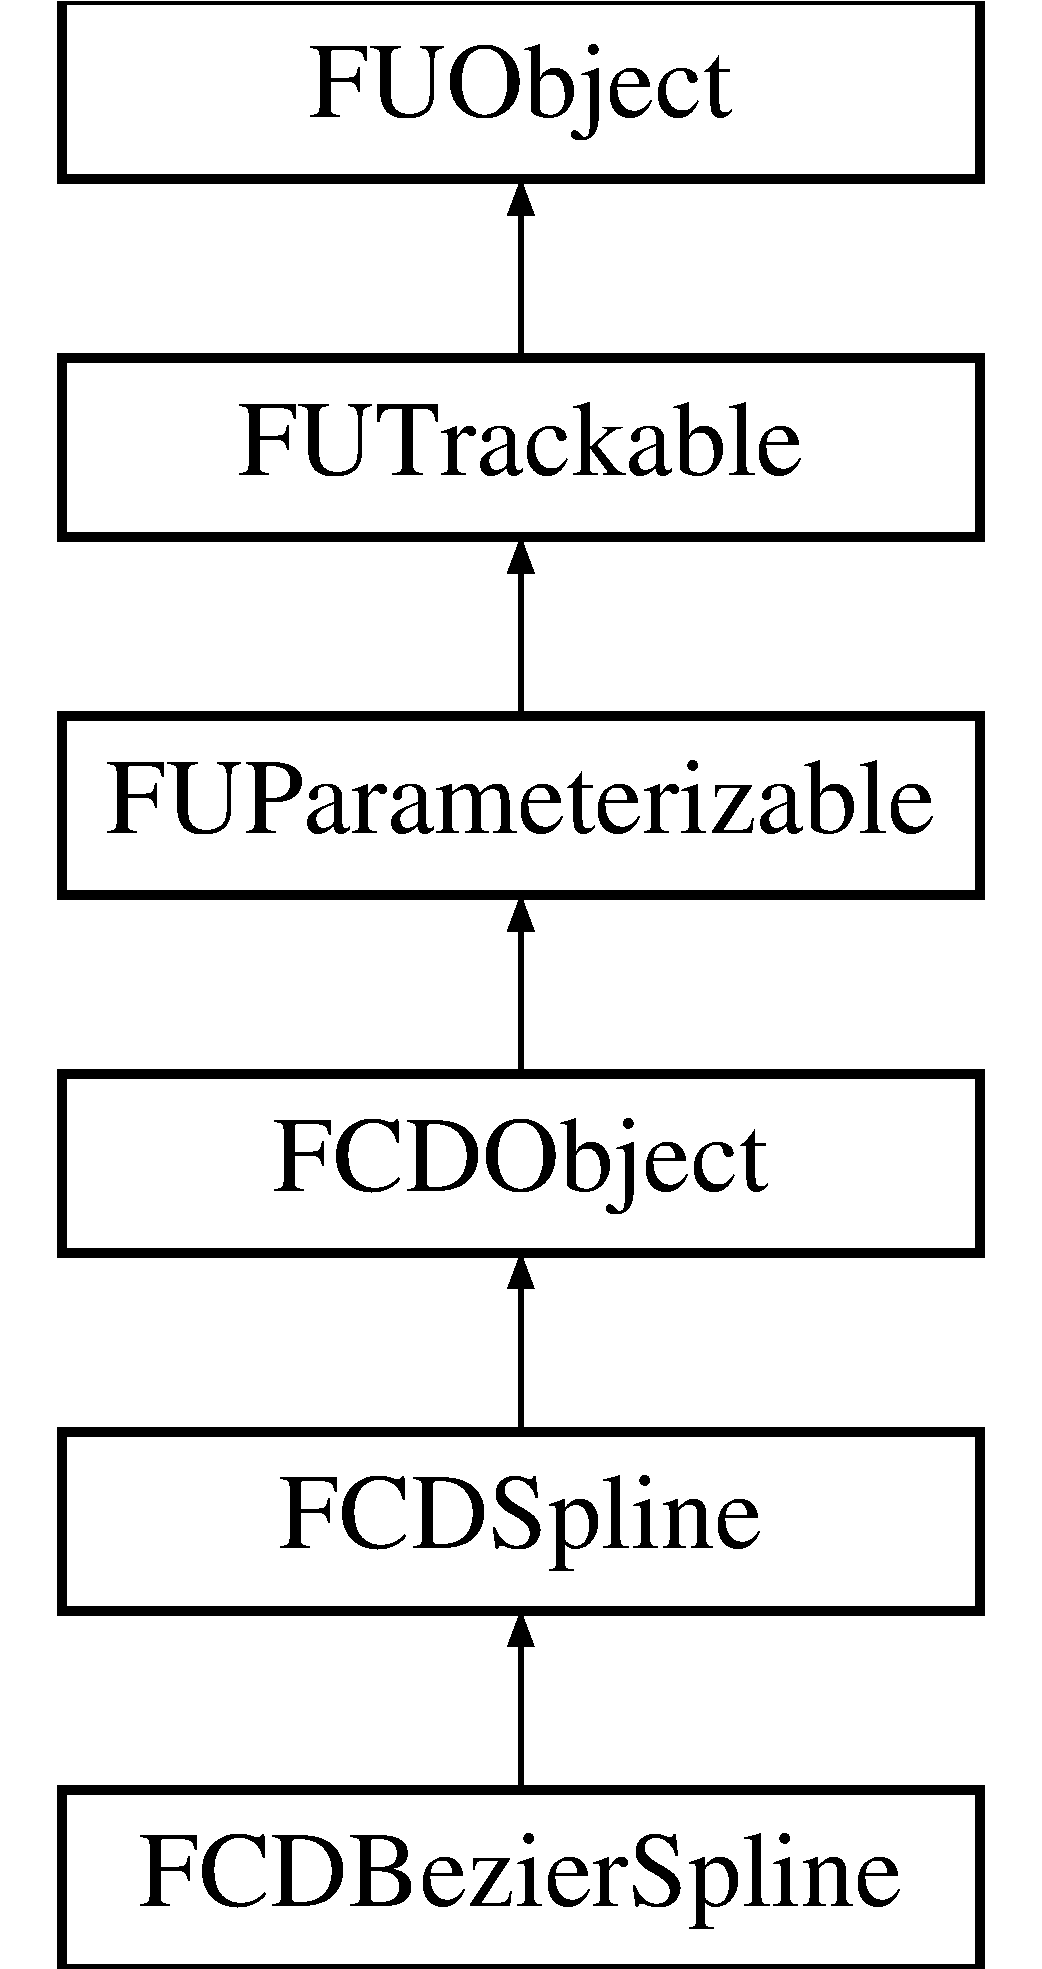
\includegraphics[height=6.000000cm]{classFCDBezierSpline}
\end{center}
\end{figure}
\subsection*{Public Member Functions}
\begin{DoxyCompactItemize}
\item 
\hyperlink{classFCDBezierSpline_aa3f49b89e0b97b58ffb4120b9abe2727}{FCDBezierSpline} (\hyperlink{classFCDocument}{FCDocument} $\ast$document)
\item 
virtual \hyperlink{classFCDBezierSpline_a090f86ef30c4135479d244def74c496e}{$\sim$FCDBezierSpline} ()
\item 
virtual \hyperlink{namespaceFUDaeSplineType_a7db2b90bcd53814239cc29f64754d0ab}{FUDaeSplineType::Type} \hyperlink{classFCDBezierSpline_a83442735cc73d09922891e94a96fa373}{GetSplineType} () const 
\item 
bool \hyperlink{classFCDBezierSpline_afe3b6399781f248db5d25c2772805e11}{AddCV} (const \hyperlink{classFMVector3}{FMVector3} \&cv)
\item 
void \hyperlink{classFCDBezierSpline_ab76408f07ee6105394bbbfb7f84d8fd2}{ToNURBs} (\hyperlink{classfm_1_1pvector}{FCDNURBSSplineList} \&toFill) const 
\item 
virtual bool \hyperlink{classFCDBezierSpline_abd299d3c4d31c253333ff861074c6816}{IsValid} () const 
\end{DoxyCompactItemize}


\subsection{Detailed Description}
Represents a Bezier spline.

The Bezier spline is represented as an array of adjacent cubic Bezier segments. Each segment consists of 4 control vertices, the last one being reused as the first vertex of the next segment. If the spline is closed, the first control vertex is also reused for the last vertex of the last segment. 

\subsection{Constructor \& Destructor Documentation}
\hypertarget{classFCDBezierSpline_aa3f49b89e0b97b58ffb4120b9abe2727}{
\index{FCDBezierSpline@{FCDBezierSpline}!FCDBezierSpline@{FCDBezierSpline}}
\index{FCDBezierSpline@{FCDBezierSpline}!FCDBezierSpline@{FCDBezierSpline}}
\subsubsection[{FCDBezierSpline}]{\setlength{\rightskip}{0pt plus 5cm}FCDBezierSpline::FCDBezierSpline (
\begin{DoxyParamCaption}
\item[{{\bf FCDocument} $\ast$}]{ document}
\end{DoxyParamCaption}
)}}
\label{classFCDBezierSpline_aa3f49b89e0b97b58ffb4120b9abe2727}
Constructor. 
\begin{DoxyParams}{Parameters}
\item[{\em document}]The \hyperlink{namespaceFCollada}{FCollada} document that owns this spline. \end{DoxyParams}
\hypertarget{classFCDBezierSpline_a090f86ef30c4135479d244def74c496e}{
\index{FCDBezierSpline@{FCDBezierSpline}!$\sim$FCDBezierSpline@{$\sim$FCDBezierSpline}}
\index{$\sim$FCDBezierSpline@{$\sim$FCDBezierSpline}!FCDBezierSpline@{FCDBezierSpline}}
\subsubsection[{$\sim$FCDBezierSpline}]{\setlength{\rightskip}{0pt plus 5cm}FCDBezierSpline::$\sim$FCDBezierSpline (
\begin{DoxyParamCaption}
{}
\end{DoxyParamCaption}
)\hspace{0.3cm}{\ttfamily  \mbox{[}virtual\mbox{]}}}}
\label{classFCDBezierSpline_a090f86ef30c4135479d244def74c496e}
Destructor. 

\subsection{Member Function Documentation}
\hypertarget{classFCDBezierSpline_afe3b6399781f248db5d25c2772805e11}{
\index{FCDBezierSpline@{FCDBezierSpline}!AddCV@{AddCV}}
\index{AddCV@{AddCV}!FCDBezierSpline@{FCDBezierSpline}}
\subsubsection[{AddCV}]{\setlength{\rightskip}{0pt plus 5cm}bool FCDBezierSpline::AddCV (
\begin{DoxyParamCaption}
\item[{const {\bf FMVector3} \&}]{ cv}
\end{DoxyParamCaption}
)\hspace{0.3cm}{\ttfamily  \mbox{[}inline\mbox{]}}}}
\label{classFCDBezierSpline_afe3b6399781f248db5d25c2772805e11}
Adds a CV to a Bezier spline 
\begin{DoxyParams}{Parameters}
\item[{\em cv}]3D position of the CV. \end{DoxyParams}
\hypertarget{classFCDBezierSpline_a83442735cc73d09922891e94a96fa373}{
\index{FCDBezierSpline@{FCDBezierSpline}!GetSplineType@{GetSplineType}}
\index{GetSplineType@{GetSplineType}!FCDBezierSpline@{FCDBezierSpline}}
\subsubsection[{GetSplineType}]{\setlength{\rightskip}{0pt plus 5cm}virtual {\bf FUDaeSplineType::Type} FCDBezierSpline::GetSplineType (
\begin{DoxyParamCaption}
{}
\end{DoxyParamCaption}
) const\hspace{0.3cm}{\ttfamily  \mbox{[}inline, virtual\mbox{]}}}}
\label{classFCDBezierSpline_a83442735cc73d09922891e94a96fa373}
\hyperlink{classFCDSpline}{FCDSpline} method implementation. \begin{DoxyReturn}{Returns}
The BEZIER spline type. 
\end{DoxyReturn}


Implements \hyperlink{classFCDSpline_ad8ad60a198cd8e041fde6587c3d5a9f9}{FCDSpline}.

\hypertarget{classFCDBezierSpline_abd299d3c4d31c253333ff861074c6816}{
\index{FCDBezierSpline@{FCDBezierSpline}!IsValid@{IsValid}}
\index{IsValid@{IsValid}!FCDBezierSpline@{FCDBezierSpline}}
\subsubsection[{IsValid}]{\setlength{\rightskip}{0pt plus 5cm}bool FCDBezierSpline::IsValid (
\begin{DoxyParamCaption}
{}
\end{DoxyParamCaption}
) const\hspace{0.3cm}{\ttfamily  \mbox{[}virtual\mbox{]}}}}
\label{classFCDBezierSpline_abd299d3c4d31c253333ff861074c6816}
Determines if the spline is valid. \begin{DoxyReturn}{Returns}
True is the spline is valid, false otherwise. 
\end{DoxyReturn}
\hypertarget{classFCDBezierSpline_ab76408f07ee6105394bbbfb7f84d8fd2}{
\index{FCDBezierSpline@{FCDBezierSpline}!ToNURBs@{ToNURBs}}
\index{ToNURBs@{ToNURBs}!FCDBezierSpline@{FCDBezierSpline}}
\subsubsection[{ToNURBs}]{\setlength{\rightskip}{0pt plus 5cm}void FCDBezierSpline::ToNURBs (
\begin{DoxyParamCaption}
\item[{{\bf FCDNURBSSplineList} \&}]{ toFill}
\end{DoxyParamCaption}
) const}}
\label{classFCDBezierSpline_ab76408f07ee6105394bbbfb7f84d8fd2}
Creates one NURB per Bezier segment and appends it to the provided NURB list. 
\begin{DoxyParams}{Parameters}
\item[{\em toFill}]The NURB list to fill. \end{DoxyParams}


The documentation for this class was generated from the following files:\begin{DoxyCompactItemize}
\item 
FCollada/FCDocument/\hyperlink{FCDGeometrySpline_8h}{FCDGeometrySpline.h}\item 
FCollada/FCDocument/FCDGeometrySpline.cpp\end{DoxyCompactItemize}

\hypertarget{classFCDCamera}{
\section{FCDCamera Class Reference}
\label{classFCDCamera}\index{FCDCamera@{FCDCamera}}
}


{\ttfamily \#include $<$FCDCamera.h$>$}

Inheritance diagram for FCDCamera:\begin{figure}[H]
\begin{center}
\leavevmode
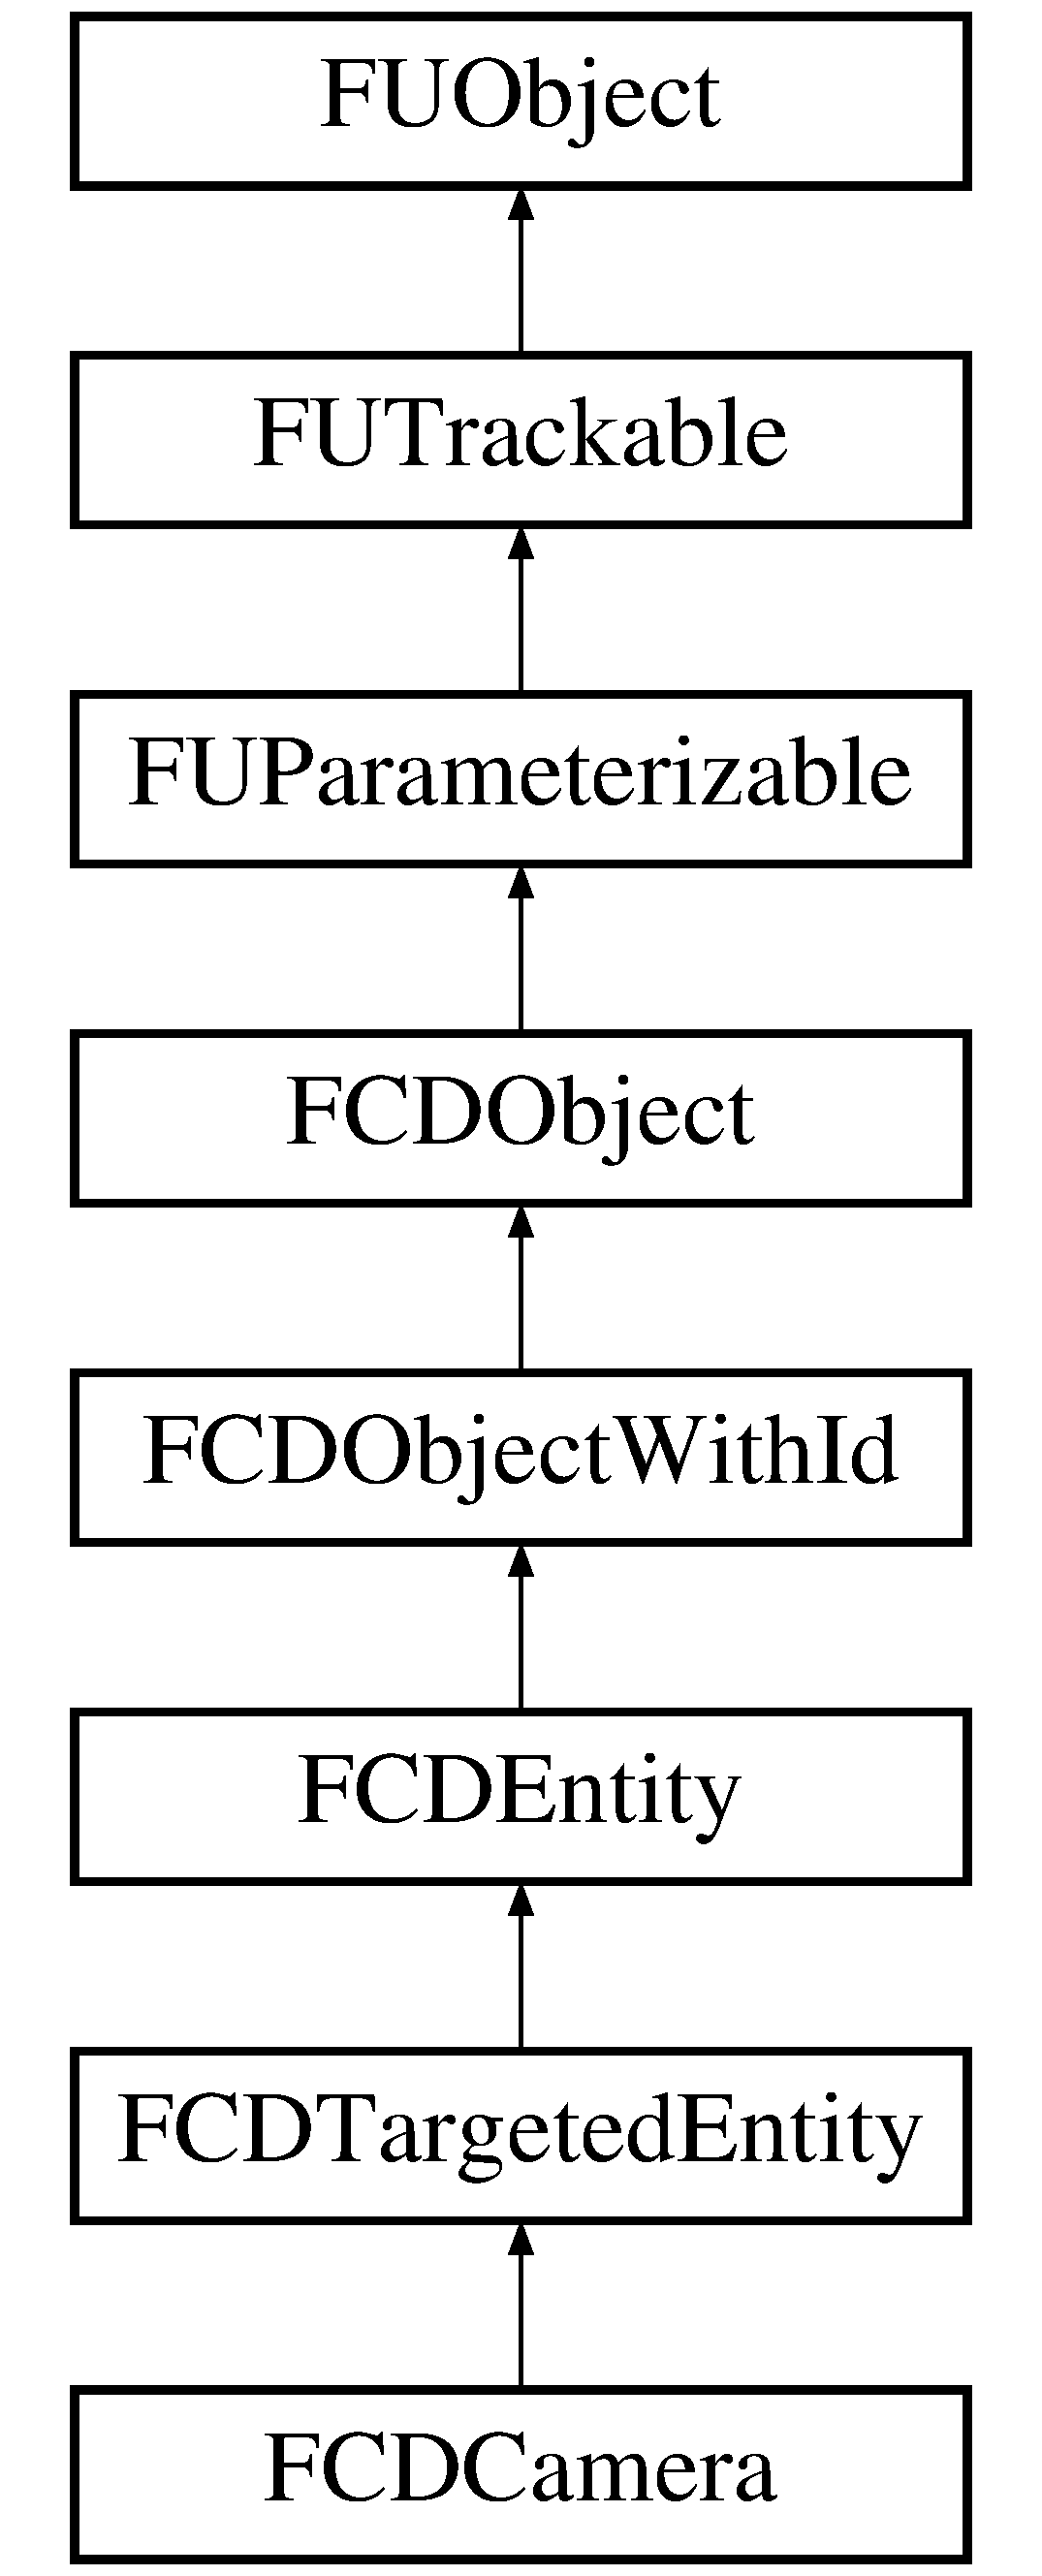
\includegraphics[height=8.000000cm]{classFCDCamera}
\end{center}
\end{figure}
\subsection*{Public Types}
\begin{DoxyCompactItemize}
\item 
enum \hyperlink{classFCDCamera_a6afb103bc3857a0e059dc0174a48616d}{ProjectionType} \{ \hyperlink{classFCDCamera_a6afb103bc3857a0e059dc0174a48616da92a6de5e36f59329c5d290c6da31a5bc}{PERSPECTIVE}, 
\hyperlink{classFCDCamera_a6afb103bc3857a0e059dc0174a48616da34b6cc066d8993d265896628316c6138}{ORTHOGRAPHIC}
 \}
\end{DoxyCompactItemize}
\subsection*{Public Member Functions}
\begin{DoxyCompactItemize}
\item 
\hypertarget{classFCDCamera_ab05984fe8d1ed66c27d0427ae3160ced}{
{\bfseries DeclareFlag} (HasHorizontalView, 0)}
\label{classFCDCamera_ab05984fe8d1ed66c27d0427ae3160ced}

\item 
\hypertarget{classFCDCamera_ac21eb4daaaa96b53793ff7d9bfbae48f}{
{\bfseries DeclareFlag} (HasVerticalView, 1)}
\label{classFCDCamera_ac21eb4daaaa96b53793ff7d9bfbae48f}

\item 
\hyperlink{classFCDCamera_a4d7c2057f783fbb34201c94899b124f7}{DeclareFlagCount} (2)
\item 
\hyperlink{classFCDCamera_accd96cd61f1479822036b39892669160}{FCDCamera} (\hyperlink{classFCDocument}{FCDocument} $\ast$document)
\item 
virtual \hyperlink{classFCDCamera_adb60b65448c97173f6ef01a625f63871}{$\sim$FCDCamera} ()
\item 
virtual \hyperlink{classFCDEntity_a9301a4bd5f4d4190ec13e40db4effdd7}{Type} \hyperlink{classFCDCamera_aa07c99de0148e39b46e33733852ef229}{GetType} () const 
\item 
\hyperlink{classFCDCamera_a6afb103bc3857a0e059dc0174a48616d}{ProjectionType} \hyperlink{classFCDCamera_a87c02ee9c85798fde4d7db01da5880f4}{GetProjectionType} () const 
\item 
void \hyperlink{classFCDCamera_a92d5b5ee50e2b59e5661498d97d8fc65}{SetProjectionType} (\hyperlink{classFCDCamera_a6afb103bc3857a0e059dc0174a48616d}{ProjectionType} type)
\item 
\hyperlink{classFCDCamera_a4b1071013b2640f05dbdf14320f75f3a}{DEPRECATED} (3.05A, GetProjectionType()==FCDCamera::PERSPECTIVE) inline bool IsPerspective() const 
\item 
\hyperlink{classFCDCamera_ab0ff15b9a68bd2e02cc5fe6281c65b28}{DEPRECATED} (3.05A, SetProjectionType(FCDCamera::PERSPECTIVE)) inline void SetPerspective()
\item 
bool \hyperlink{classFCDCamera_af5b0f3acc94e585b3d6b7a97d2b33600}{HasHorizontalFov} () const 
\item 
bool \hyperlink{classFCDCamera_ae08e063c02ac91d0fb834aaba29fec74}{HasVerticalFov} () const 
\item 
\hyperlink{classFCDParameterAnimatableT}{FCDParameterAnimatableFloat} \& \hyperlink{classFCDCamera_a48a470386f1f7985ee4524a713f92db9}{GetFovX} ()
\item 
const \hyperlink{classFCDParameterAnimatableT}{FCDParameterAnimatableFloat} \& \hyperlink{classFCDCamera_a2a16b1432904b518c25e4f5c96c79ca3}{GetFovX} () const 
\item 
\hyperlink{classFCDParameterAnimatableT}{FCDParameterAnimatableFloat} \& \hyperlink{classFCDCamera_a1b8d137f1a175ed595f1909b2d081d1c}{GetFovY} ()
\item 
const \hyperlink{classFCDParameterAnimatableT}{FCDParameterAnimatableFloat} \& \hyperlink{classFCDCamera_a0e8362765dede7db889296b708ac48f5}{GetFovY} () const 
\item 
void \hyperlink{classFCDCamera_a6288922e48ed1426edeeee4cb727a1e5}{SetFovX} (float fovX)
\item 
void \hyperlink{classFCDCamera_a833fe15b9b9186f3946bfc8c2f721e5c}{SetFovY} (float fovY)
\item 
\hyperlink{classFCDCamera_a85c12fce7991d68d04f3e458cd33b1c2}{DEPRECATED} (3.05A, GetProjectionType()==FCDCamera::ORTHOGRAPHIC) inline bool IsOrthographic() const 
\item 
\hyperlink{classFCDCamera_a69f9b90e16ce159cc104b4f5f0b92053}{DEPRECATED} (3.05A, SetProjectionType(FCDCamera::ORTHOGRAPHIC)) inline void SetOrthographic()
\item 
bool \hyperlink{classFCDCamera_a8e6652d9695b24aa398b0ab6bb408ecb}{HasHorizontalMag} () const 
\item 
bool \hyperlink{classFCDCamera_a4eddec2fc3082c106b417632103dbe51}{HasVerticalMag} () const 
\item 
\hyperlink{classFCDParameterAnimatableT}{FCDParameterAnimatableFloat} \& \hyperlink{classFCDCamera_a9c24ccb56d566c7bfd0cf884e785f807}{GetMagX} ()
\item 
const \hyperlink{classFCDParameterAnimatableT}{FCDParameterAnimatableFloat} \& \hyperlink{classFCDCamera_a688443be783987a85492568fbed75ef1}{GetMagX} () const 
\item 
\hyperlink{classFCDParameterAnimatableT}{FCDParameterAnimatableFloat} \& \hyperlink{classFCDCamera_a08aeea7cfca052b87a596ac1a559b465}{GetMagY} ()
\item 
const \hyperlink{classFCDParameterAnimatableT}{FCDParameterAnimatableFloat} \& \hyperlink{classFCDCamera_a896b2113cc9ea603932518e9423cdc83}{GetMagY} () const 
\item 
void \hyperlink{classFCDCamera_a6dad0e3978aad3bbd920587ae387e952}{SetMagX} (float magX)
\item 
void \hyperlink{classFCDCamera_a4edf1eb03fe522145a18d80aabcef450}{SetMagY} (float magY)
\item 
\hyperlink{classFCDParameterAnimatableT}{FCDParameterAnimatableFloat} \& \hyperlink{classFCDCamera_ac4de7173eb7c64fcc14c8bbd8c441b9e}{GetNearZ} ()
\item 
const \hyperlink{classFCDParameterAnimatableT}{FCDParameterAnimatableFloat} \& \hyperlink{classFCDCamera_a636bb27274e22fb19970827eded29dd0}{GetNearZ} () const 
\item 
\hyperlink{classFCDParameterAnimatableT}{FCDParameterAnimatableFloat} \& \hyperlink{classFCDCamera_a54a1ade62890179821725b0a8a158bab}{GetFarZ} ()
\item 
const \hyperlink{classFCDParameterAnimatableT}{FCDParameterAnimatableFloat} \& \hyperlink{classFCDCamera_a2604bcc802d800f035bb1417d71bb8f9}{GetFarZ} () const 
\item 
bool \hyperlink{classFCDCamera_a634c417903dd0f337851756b7f506c70}{HasAspectRatio} () const 
\item 
\hyperlink{classFCDParameterAnimatableT}{FCDParameterAnimatableFloat} \& \hyperlink{classFCDCamera_a16ba395c9fe1d551a80edc8b51e07e0d}{GetAspectRatio} ()
\item 
const \hyperlink{classFCDParameterAnimatableT}{FCDParameterAnimatableFloat} \& \hyperlink{classFCDCamera_a51fd69058b906cc152ac0e42bd08fcf0}{GetAspectRatio} () const 
\item 
void \hyperlink{classFCDCamera_a5897d7a1ba3e10316f0f2f183530ee45}{SetNearZ} (float \_\-nearZ)
\item 
void \hyperlink{classFCDCamera_af833473ab121efed5be5f02d8680d51c}{SetFarZ} (float \_\-farZ)
\item 
void \hyperlink{classFCDCamera_ad36e7b6987ff8a7f1a9145148a49fa5b}{SetAspectRatio} (float aspectRatio)
\end{DoxyCompactItemize}


\subsection{Detailed Description}
A COLLADA camera. Based on the \hyperlink{classFCDTargetedEntity}{FCDTargetedEntity} class to support aimed cameras. COLLADA defines two types of cameras: perspective and orthographic. Both types are fully handled by this class.

A COLLADA perspective camera defines two of the three following parameters: horizontal field of view, vertical field of view and aspect ratio. The missing parameter can be calculated using the following formulae: aspect ratio = vertical field of view / horizontal field of view. The vertical and horizontal field of view are in degrees.

A COLLADA orthographic camera defines two of the three following parameters: horizontal magnification, vertical magnification and aspect ratio. The missing parameter can be calculated using the following formulae: aspect ratio = vertical magnification / horizontal magnification. You can calculate the viewport width and height using the following formulas: viewport width = horizontal magnification $\ast$ 2, viewport height = vertical magnification $\ast$ 2. 

\subsection{Member Enumeration Documentation}
\hypertarget{classFCDCamera_a6afb103bc3857a0e059dc0174a48616d}{
\index{FCDCamera@{FCDCamera}!ProjectionType@{ProjectionType}}
\index{ProjectionType@{ProjectionType}!FCDCamera@{FCDCamera}}
\subsubsection[{ProjectionType}]{\setlength{\rightskip}{0pt plus 5cm}enum {\bf FCDCamera::ProjectionType}}}
\label{classFCDCamera_a6afb103bc3857a0e059dc0174a48616d}
The types of projection supported. \begin{Desc}
\item[Enumerator: ]\par
\begin{description}
\index{PERSPECTIVE@{PERSPECTIVE}!FCDCamera@{FCDCamera}}\index{FCDCamera@{FCDCamera}!PERSPECTIVE@{PERSPECTIVE}}\item[{\em 
\hypertarget{classFCDCamera_a6afb103bc3857a0e059dc0174a48616da92a6de5e36f59329c5d290c6da31a5bc}{
PERSPECTIVE}
\label{classFCDCamera_a6afb103bc3857a0e059dc0174a48616da92a6de5e36f59329c5d290c6da31a5bc}
}]A perspective projection. Uses a truncated rectangular pyramid frustrum. \index{ORTHOGRAPHIC@{ORTHOGRAPHIC}!FCDCamera@{FCDCamera}}\index{FCDCamera@{FCDCamera}!ORTHOGRAPHIC@{ORTHOGRAPHIC}}\item[{\em 
\hypertarget{classFCDCamera_a6afb103bc3857a0e059dc0174a48616da34b6cc066d8993d265896628316c6138}{
ORTHOGRAPHIC}
\label{classFCDCamera_a6afb103bc3857a0e059dc0174a48616da34b6cc066d8993d265896628316c6138}
}]An orthographic projection. Uses a rectangular prism frustrum. \end{description}
\end{Desc}



\subsection{Constructor \& Destructor Documentation}
\hypertarget{classFCDCamera_accd96cd61f1479822036b39892669160}{
\index{FCDCamera@{FCDCamera}!FCDCamera@{FCDCamera}}
\index{FCDCamera@{FCDCamera}!FCDCamera@{FCDCamera}}
\subsubsection[{FCDCamera}]{\setlength{\rightskip}{0pt plus 5cm}FCDCamera::FCDCamera (
\begin{DoxyParamCaption}
\item[{{\bf FCDocument} $\ast$}]{ document}
\end{DoxyParamCaption}
)}}
\label{classFCDCamera_accd96cd61f1479822036b39892669160}
Constructor: do not use directly. Create new cameras using the \hyperlink{classFCDLibrary_aa5cdcac5a447298d5e3816e4f8c864d0}{FCDLibrary::AddEntity} function. 
\begin{DoxyParams}{Parameters}
\item[{\em document}]The COLLADA document that contains this camera entity. \end{DoxyParams}
\hypertarget{classFCDCamera_adb60b65448c97173f6ef01a625f63871}{
\index{FCDCamera@{FCDCamera}!$\sim$FCDCamera@{$\sim$FCDCamera}}
\index{$\sim$FCDCamera@{$\sim$FCDCamera}!FCDCamera@{FCDCamera}}
\subsubsection[{$\sim$FCDCamera}]{\setlength{\rightskip}{0pt plus 5cm}FCDCamera::$\sim$FCDCamera (
\begin{DoxyParamCaption}
{}
\end{DoxyParamCaption}
)\hspace{0.3cm}{\ttfamily  \mbox{[}virtual\mbox{]}}}}
\label{classFCDCamera_adb60b65448c97173f6ef01a625f63871}
Destructor. 

\subsection{Member Function Documentation}
\hypertarget{classFCDCamera_a4d7c2057f783fbb34201c94899b124f7}{
\index{FCDCamera@{FCDCamera}!DeclareFlagCount@{DeclareFlagCount}}
\index{DeclareFlagCount@{DeclareFlagCount}!FCDCamera@{FCDCamera}}
\subsubsection[{DeclareFlagCount}]{\setlength{\rightskip}{0pt plus 5cm}FCDCamera::DeclareFlagCount (
\begin{DoxyParamCaption}
\item[{2}]{}
\end{DoxyParamCaption}
)}}
\label{classFCDCamera_a4d7c2057f783fbb34201c94899b124f7}
5 flags are locally declared. 

Reimplemented from \hyperlink{classFCDObjectWithId_a8289e2d57d75f2302effb07b0aee47f8}{FCDObjectWithId}.

\hypertarget{classFCDCamera_ab0ff15b9a68bd2e02cc5fe6281c65b28}{
\index{FCDCamera@{FCDCamera}!DEPRECATED@{DEPRECATED}}
\index{DEPRECATED@{DEPRECATED}!FCDCamera@{FCDCamera}}
\subsubsection[{DEPRECATED}]{\setlength{\rightskip}{0pt plus 5cm}FCDCamera::DEPRECATED (
\begin{DoxyParamCaption}
\item[{3.}]{ 05A, }
\item[{SetProjectionType(FCDCamera::PERSPECTIVE)}]{}
\end{DoxyParamCaption}
)\hspace{0.3cm}{\ttfamily  \mbox{[}inline\mbox{]}}}}
\label{classFCDCamera_ab0ff15b9a68bd2e02cc5fe6281c65b28}
Sets the type of this camera to perspective. \hypertarget{classFCDCamera_a85c12fce7991d68d04f3e458cd33b1c2}{
\index{FCDCamera@{FCDCamera}!DEPRECATED@{DEPRECATED}}
\index{DEPRECATED@{DEPRECATED}!FCDCamera@{FCDCamera}}
\subsubsection[{DEPRECATED}]{\setlength{\rightskip}{0pt plus 5cm}FCDCamera::DEPRECATED (
\begin{DoxyParamCaption}
\item[{3.}]{ 05A, }
\item[{GetProjectionType()}]{ = {\ttfamily =~FCDCamera::ORTHOGRAPHIC}}
\end{DoxyParamCaption}
) const\hspace{0.3cm}{\ttfamily  \mbox{[}inline\mbox{]}}}}
\label{classFCDCamera_a85c12fce7991d68d04f3e458cd33b1c2}
Retrieves whether this camera is an orthographic camera. \begin{DoxyReturn}{Returns}
Whether this camera is an orthographic camera. 
\end{DoxyReturn}
\hypertarget{classFCDCamera_a69f9b90e16ce159cc104b4f5f0b92053}{
\index{FCDCamera@{FCDCamera}!DEPRECATED@{DEPRECATED}}
\index{DEPRECATED@{DEPRECATED}!FCDCamera@{FCDCamera}}
\subsubsection[{DEPRECATED}]{\setlength{\rightskip}{0pt plus 5cm}FCDCamera::DEPRECATED (
\begin{DoxyParamCaption}
\item[{3.}]{ 05A, }
\item[{SetProjectionType(FCDCamera::ORTHOGRAPHIC)}]{}
\end{DoxyParamCaption}
)\hspace{0.3cm}{\ttfamily  \mbox{[}inline\mbox{]}}}}
\label{classFCDCamera_a69f9b90e16ce159cc104b4f5f0b92053}
Sets the type of this camera to orthographic. \hypertarget{classFCDCamera_a4b1071013b2640f05dbdf14320f75f3a}{
\index{FCDCamera@{FCDCamera}!DEPRECATED@{DEPRECATED}}
\index{DEPRECATED@{DEPRECATED}!FCDCamera@{FCDCamera}}
\subsubsection[{DEPRECATED}]{\setlength{\rightskip}{0pt plus 5cm}FCDCamera::DEPRECATED (
\begin{DoxyParamCaption}
\item[{3.}]{ 05A, }
\item[{GetProjectionType()}]{ = {\ttfamily =~FCDCamera::PERSPECTIVE}}
\end{DoxyParamCaption}
) const\hspace{0.3cm}{\ttfamily  \mbox{[}inline\mbox{]}}}}
\label{classFCDCamera_a4b1071013b2640f05dbdf14320f75f3a}
Retrieves whether this camera is a perspective camera. This is the default type of camera. \begin{DoxyReturn}{Returns}
Whether this camera is a perspective camera. 
\end{DoxyReturn}
\hypertarget{classFCDCamera_a16ba395c9fe1d551a80edc8b51e07e0d}{
\index{FCDCamera@{FCDCamera}!GetAspectRatio@{GetAspectRatio}}
\index{GetAspectRatio@{GetAspectRatio}!FCDCamera@{FCDCamera}}
\subsubsection[{GetAspectRatio}]{\setlength{\rightskip}{0pt plus 5cm}{\bf FCDParameterAnimatableFloat}\& FCDCamera::GetAspectRatio (
\begin{DoxyParamCaption}
{}
\end{DoxyParamCaption}
)\hspace{0.3cm}{\ttfamily  \mbox{[}inline\mbox{]}}}}
\label{classFCDCamera_a16ba395c9fe1d551a80edc8b51e07e0d}
Retrieves the aspect ratio for the view of this camera. Before using this value, check if there are only one of the horizontal and vertical view ratios. If there are both of the view ratios provided for the camera, you will need to calculate the aspect ratio using the following formula: aspect ratio = vertical field of view / horizontal field of view. \begin{DoxyReturn}{Returns}
The view aspect ratio. 
\end{DoxyReturn}
\hypertarget{classFCDCamera_a51fd69058b906cc152ac0e42bd08fcf0}{
\index{FCDCamera@{FCDCamera}!GetAspectRatio@{GetAspectRatio}}
\index{GetAspectRatio@{GetAspectRatio}!FCDCamera@{FCDCamera}}
\subsubsection[{GetAspectRatio}]{\setlength{\rightskip}{0pt plus 5cm}const {\bf FCDParameterAnimatableFloat}\& FCDCamera::GetAspectRatio (
\begin{DoxyParamCaption}
{}
\end{DoxyParamCaption}
) const\hspace{0.3cm}{\ttfamily  \mbox{[}inline\mbox{]}}}}
\label{classFCDCamera_a51fd69058b906cc152ac0e42bd08fcf0}
See above. \hypertarget{classFCDCamera_a54a1ade62890179821725b0a8a158bab}{
\index{FCDCamera@{FCDCamera}!GetFarZ@{GetFarZ}}
\index{GetFarZ@{GetFarZ}!FCDCamera@{FCDCamera}}
\subsubsection[{GetFarZ}]{\setlength{\rightskip}{0pt plus 5cm}{\bf FCDParameterAnimatableFloat}\& FCDCamera::GetFarZ (
\begin{DoxyParamCaption}
{}
\end{DoxyParamCaption}
)\hspace{0.3cm}{\ttfamily  \mbox{[}inline\mbox{]}}}}
\label{classFCDCamera_a54a1ade62890179821725b0a8a158bab}
Retrieves the far-\/z value for this camera. The far-\/z value represent how close the far-\/clip plane of the view frustum is. For orthographic cameras, this value is solely used for depth-\/buffering. \begin{DoxyReturn}{Returns}
The far-\/z value for this camera. 
\end{DoxyReturn}
\hypertarget{classFCDCamera_a2604bcc802d800f035bb1417d71bb8f9}{
\index{FCDCamera@{FCDCamera}!GetFarZ@{GetFarZ}}
\index{GetFarZ@{GetFarZ}!FCDCamera@{FCDCamera}}
\subsubsection[{GetFarZ}]{\setlength{\rightskip}{0pt plus 5cm}const {\bf FCDParameterAnimatableFloat}\& FCDCamera::GetFarZ (
\begin{DoxyParamCaption}
{}
\end{DoxyParamCaption}
) const\hspace{0.3cm}{\ttfamily  \mbox{[}inline\mbox{]}}}}
\label{classFCDCamera_a2604bcc802d800f035bb1417d71bb8f9}
See above. \hypertarget{classFCDCamera_a48a470386f1f7985ee4524a713f92db9}{
\index{FCDCamera@{FCDCamera}!GetFovX@{GetFovX}}
\index{GetFovX@{GetFovX}!FCDCamera@{FCDCamera}}
\subsubsection[{GetFovX}]{\setlength{\rightskip}{0pt plus 5cm}{\bf FCDParameterAnimatableFloat}\& FCDCamera::GetFovX (
\begin{DoxyParamCaption}
{}
\end{DoxyParamCaption}
)\hspace{0.3cm}{\ttfamily  \mbox{[}inline\mbox{]}}}}
\label{classFCDCamera_a48a470386f1f7985ee4524a713f92db9}
Retrieves the horizontal field of view. Before retrieving this value, check whether the camera defines the horizontal field of view using the HasHorizontalFov function. \begin{DoxyReturn}{Returns}
The horizontal field of view, in degrees. 
\end{DoxyReturn}
\hypertarget{classFCDCamera_a2a16b1432904b518c25e4f5c96c79ca3}{
\index{FCDCamera@{FCDCamera}!GetFovX@{GetFovX}}
\index{GetFovX@{GetFovX}!FCDCamera@{FCDCamera}}
\subsubsection[{GetFovX}]{\setlength{\rightskip}{0pt plus 5cm}const {\bf FCDParameterAnimatableFloat}\& FCDCamera::GetFovX (
\begin{DoxyParamCaption}
{}
\end{DoxyParamCaption}
) const\hspace{0.3cm}{\ttfamily  \mbox{[}inline\mbox{]}}}}
\label{classFCDCamera_a2a16b1432904b518c25e4f5c96c79ca3}
See above. \hypertarget{classFCDCamera_a1b8d137f1a175ed595f1909b2d081d1c}{
\index{FCDCamera@{FCDCamera}!GetFovY@{GetFovY}}
\index{GetFovY@{GetFovY}!FCDCamera@{FCDCamera}}
\subsubsection[{GetFovY}]{\setlength{\rightskip}{0pt plus 5cm}{\bf FCDParameterAnimatableFloat}\& FCDCamera::GetFovY (
\begin{DoxyParamCaption}
{}
\end{DoxyParamCaption}
)\hspace{0.3cm}{\ttfamily  \mbox{[}inline\mbox{]}}}}
\label{classFCDCamera_a1b8d137f1a175ed595f1909b2d081d1c}
Retrieves the vertical field of view. Before retrieving this value, check whether the camera defines the vertical field of view using the HasVerticalFov function. \begin{DoxyReturn}{Returns}
The horizontal field of view, in degrees. 
\end{DoxyReturn}
\hypertarget{classFCDCamera_a0e8362765dede7db889296b708ac48f5}{
\index{FCDCamera@{FCDCamera}!GetFovY@{GetFovY}}
\index{GetFovY@{GetFovY}!FCDCamera@{FCDCamera}}
\subsubsection[{GetFovY}]{\setlength{\rightskip}{0pt plus 5cm}const {\bf FCDParameterAnimatableFloat}\& FCDCamera::GetFovY (
\begin{DoxyParamCaption}
{}
\end{DoxyParamCaption}
) const\hspace{0.3cm}{\ttfamily  \mbox{[}inline\mbox{]}}}}
\label{classFCDCamera_a0e8362765dede7db889296b708ac48f5}
See above. \hypertarget{classFCDCamera_a9c24ccb56d566c7bfd0cf884e785f807}{
\index{FCDCamera@{FCDCamera}!GetMagX@{GetMagX}}
\index{GetMagX@{GetMagX}!FCDCamera@{FCDCamera}}
\subsubsection[{GetMagX}]{\setlength{\rightskip}{0pt plus 5cm}{\bf FCDParameterAnimatableFloat}\& FCDCamera::GetMagX (
\begin{DoxyParamCaption}
{}
\end{DoxyParamCaption}
)\hspace{0.3cm}{\ttfamily  \mbox{[}inline\mbox{]}}}}
\label{classFCDCamera_a9c24ccb56d566c7bfd0cf884e785f807}
Retrieves the horizontal magnification. Before retrieving this value, check whether the camera defines the horizontal magnification using the HasHorizontalMag function. \begin{DoxyReturn}{Returns}
The horizontal magnification. 
\end{DoxyReturn}
\hypertarget{classFCDCamera_a688443be783987a85492568fbed75ef1}{
\index{FCDCamera@{FCDCamera}!GetMagX@{GetMagX}}
\index{GetMagX@{GetMagX}!FCDCamera@{FCDCamera}}
\subsubsection[{GetMagX}]{\setlength{\rightskip}{0pt plus 5cm}const {\bf FCDParameterAnimatableFloat}\& FCDCamera::GetMagX (
\begin{DoxyParamCaption}
{}
\end{DoxyParamCaption}
) const\hspace{0.3cm}{\ttfamily  \mbox{[}inline\mbox{]}}}}
\label{classFCDCamera_a688443be783987a85492568fbed75ef1}
See above. \hypertarget{classFCDCamera_a08aeea7cfca052b87a596ac1a559b465}{
\index{FCDCamera@{FCDCamera}!GetMagY@{GetMagY}}
\index{GetMagY@{GetMagY}!FCDCamera@{FCDCamera}}
\subsubsection[{GetMagY}]{\setlength{\rightskip}{0pt plus 5cm}{\bf FCDParameterAnimatableFloat}\& FCDCamera::GetMagY (
\begin{DoxyParamCaption}
{}
\end{DoxyParamCaption}
)\hspace{0.3cm}{\ttfamily  \mbox{[}inline\mbox{]}}}}
\label{classFCDCamera_a08aeea7cfca052b87a596ac1a559b465}
Retrieves the vertical magnification. Before retrieving this value, check whether the camera defines the vertical magnification using the HasVerticalMag function. \begin{DoxyReturn}{Returns}
The vertical magnification. 
\end{DoxyReturn}
\hypertarget{classFCDCamera_a896b2113cc9ea603932518e9423cdc83}{
\index{FCDCamera@{FCDCamera}!GetMagY@{GetMagY}}
\index{GetMagY@{GetMagY}!FCDCamera@{FCDCamera}}
\subsubsection[{GetMagY}]{\setlength{\rightskip}{0pt plus 5cm}const {\bf FCDParameterAnimatableFloat}\& FCDCamera::GetMagY (
\begin{DoxyParamCaption}
{}
\end{DoxyParamCaption}
) const\hspace{0.3cm}{\ttfamily  \mbox{[}inline\mbox{]}}}}
\label{classFCDCamera_a896b2113cc9ea603932518e9423cdc83}
See above. \hypertarget{classFCDCamera_ac4de7173eb7c64fcc14c8bbd8c441b9e}{
\index{FCDCamera@{FCDCamera}!GetNearZ@{GetNearZ}}
\index{GetNearZ@{GetNearZ}!FCDCamera@{FCDCamera}}
\subsubsection[{GetNearZ}]{\setlength{\rightskip}{0pt plus 5cm}{\bf FCDParameterAnimatableFloat}\& FCDCamera::GetNearZ (
\begin{DoxyParamCaption}
{}
\end{DoxyParamCaption}
)\hspace{0.3cm}{\ttfamily  \mbox{[}inline\mbox{]}}}}
\label{classFCDCamera_ac4de7173eb7c64fcc14c8bbd8c441b9e}
Retrieves the near-\/z value for this camera. The near-\/z value represent how close the near-\/clip plane of the view frustum is. For orthographic cameras, this value is solely used for depth-\/buffering. \begin{DoxyReturn}{Returns}
The near-\/z value for this camera. 
\end{DoxyReturn}
\hypertarget{classFCDCamera_a636bb27274e22fb19970827eded29dd0}{
\index{FCDCamera@{FCDCamera}!GetNearZ@{GetNearZ}}
\index{GetNearZ@{GetNearZ}!FCDCamera@{FCDCamera}}
\subsubsection[{GetNearZ}]{\setlength{\rightskip}{0pt plus 5cm}const {\bf FCDParameterAnimatableFloat}\& FCDCamera::GetNearZ (
\begin{DoxyParamCaption}
{}
\end{DoxyParamCaption}
) const\hspace{0.3cm}{\ttfamily  \mbox{[}inline\mbox{]}}}}
\label{classFCDCamera_a636bb27274e22fb19970827eded29dd0}
See above. \hypertarget{classFCDCamera_a87c02ee9c85798fde4d7db01da5880f4}{
\index{FCDCamera@{FCDCamera}!GetProjectionType@{GetProjectionType}}
\index{GetProjectionType@{GetProjectionType}!FCDCamera@{FCDCamera}}
\subsubsection[{GetProjectionType}]{\setlength{\rightskip}{0pt plus 5cm}{\bf ProjectionType} FCDCamera::GetProjectionType (
\begin{DoxyParamCaption}
{}
\end{DoxyParamCaption}
) const\hspace{0.3cm}{\ttfamily  \mbox{[}inline\mbox{]}}}}
\label{classFCDCamera_a87c02ee9c85798fde4d7db01da5880f4}
Retrieves the type of projection of this camera. \begin{DoxyReturn}{Returns}
The projection type. 
\end{DoxyReturn}
\hypertarget{classFCDCamera_aa07c99de0148e39b46e33733852ef229}{
\index{FCDCamera@{FCDCamera}!GetType@{GetType}}
\index{GetType@{GetType}!FCDCamera@{FCDCamera}}
\subsubsection[{GetType}]{\setlength{\rightskip}{0pt plus 5cm}virtual {\bf Type} FCDCamera::GetType (
\begin{DoxyParamCaption}
{}
\end{DoxyParamCaption}
) const\hspace{0.3cm}{\ttfamily  \mbox{[}inline, virtual\mbox{]}}}}
\label{classFCDCamera_aa07c99de0148e39b46e33733852ef229}
Retrieves the entity type for this class. This function is part of the \hyperlink{classFCDEntity}{FCDEntity} interface. \begin{DoxyReturn}{Returns}
The entity type: CAMERA. 
\end{DoxyReturn}


Reimplemented from \hyperlink{classFCDEntity_abfd4312a7124f92364c1e6517c7e60ba}{FCDEntity}.

\hypertarget{classFCDCamera_a634c417903dd0f337851756b7f506c70}{
\index{FCDCamera@{FCDCamera}!HasAspectRatio@{HasAspectRatio}}
\index{HasAspectRatio@{HasAspectRatio}!FCDCamera@{FCDCamera}}
\subsubsection[{HasAspectRatio}]{\setlength{\rightskip}{0pt plus 5cm}bool FCDCamera::HasAspectRatio (
\begin{DoxyParamCaption}
{}
\end{DoxyParamCaption}
) const\hspace{0.3cm}{\ttfamily  \mbox{[}inline\mbox{]}}}}
\label{classFCDCamera_a634c417903dd0f337851756b7f506c70}
Retrieves whether the camera defines an aspect ratio. \begin{DoxyReturn}{Returns}
Whether the camera defines an aspect ratio. 
\end{DoxyReturn}
\hypertarget{classFCDCamera_af5b0f3acc94e585b3d6b7a97d2b33600}{
\index{FCDCamera@{FCDCamera}!HasHorizontalFov@{HasHorizontalFov}}
\index{HasHorizontalFov@{HasHorizontalFov}!FCDCamera@{FCDCamera}}
\subsubsection[{HasHorizontalFov}]{\setlength{\rightskip}{0pt plus 5cm}bool FCDCamera::HasHorizontalFov (
\begin{DoxyParamCaption}
{}
\end{DoxyParamCaption}
) const\hspace{0.3cm}{\ttfamily  \mbox{[}inline\mbox{]}}}}
\label{classFCDCamera_af5b0f3acc94e585b3d6b7a97d2b33600}
Retrieves whether the perspective camera defines an horizontal field of view. If the camera does not define the horizontal field of view, you can calculate it using the following formula: horizontal field of view = vertical field of view / aspect ratio. \begin{DoxyReturn}{Returns}
Whether the perspective camera defines an horizontal field of view. 
\end{DoxyReturn}
\hypertarget{classFCDCamera_a8e6652d9695b24aa398b0ab6bb408ecb}{
\index{FCDCamera@{FCDCamera}!HasHorizontalMag@{HasHorizontalMag}}
\index{HasHorizontalMag@{HasHorizontalMag}!FCDCamera@{FCDCamera}}
\subsubsection[{HasHorizontalMag}]{\setlength{\rightskip}{0pt plus 5cm}bool FCDCamera::HasHorizontalMag (
\begin{DoxyParamCaption}
{}
\end{DoxyParamCaption}
) const\hspace{0.3cm}{\ttfamily  \mbox{[}inline\mbox{]}}}}
\label{classFCDCamera_a8e6652d9695b24aa398b0ab6bb408ecb}
Retrieves whether the orthographic camera defines an horizontal magnification. If the camera does not define the horizontal magnification, you can calculate it using the following formula: horizontal magnification = vertical magnification / aspect ratio. \begin{DoxyReturn}{Returns}
Whether the orthographic camera defines an horizontal magnification. 
\end{DoxyReturn}
\hypertarget{classFCDCamera_ae08e063c02ac91d0fb834aaba29fec74}{
\index{FCDCamera@{FCDCamera}!HasVerticalFov@{HasVerticalFov}}
\index{HasVerticalFov@{HasVerticalFov}!FCDCamera@{FCDCamera}}
\subsubsection[{HasVerticalFov}]{\setlength{\rightskip}{0pt plus 5cm}bool FCDCamera::HasVerticalFov (
\begin{DoxyParamCaption}
{}
\end{DoxyParamCaption}
) const\hspace{0.3cm}{\ttfamily  \mbox{[}inline\mbox{]}}}}
\label{classFCDCamera_ae08e063c02ac91d0fb834aaba29fec74}
Retrieves whether the perspective camera defines a vertical field of view. If the camera does not define the vertical field of view, you can calculate it using the following formula: vertical field of view = aspect ratio $\ast$ horizontal field of view. \begin{DoxyReturn}{Returns}
Whether the perspective camera defines a vertical field of view. 
\end{DoxyReturn}
\hypertarget{classFCDCamera_a4eddec2fc3082c106b417632103dbe51}{
\index{FCDCamera@{FCDCamera}!HasVerticalMag@{HasVerticalMag}}
\index{HasVerticalMag@{HasVerticalMag}!FCDCamera@{FCDCamera}}
\subsubsection[{HasVerticalMag}]{\setlength{\rightskip}{0pt plus 5cm}bool FCDCamera::HasVerticalMag (
\begin{DoxyParamCaption}
{}
\end{DoxyParamCaption}
) const\hspace{0.3cm}{\ttfamily  \mbox{[}inline\mbox{]}}}}
\label{classFCDCamera_a4eddec2fc3082c106b417632103dbe51}
Retrieves whether the perspective camera defines a vertical magnification. If the camera does not define the vertical magnification, you can calculate it using the following formula: vertical magnification = aspect ratio $\ast$ horizontal magnification. \begin{DoxyReturn}{Returns}
Whether the perspective camera defines a vertical magnification. 
\end{DoxyReturn}
\hypertarget{classFCDCamera_ad36e7b6987ff8a7f1a9145148a49fa5b}{
\index{FCDCamera@{FCDCamera}!SetAspectRatio@{SetAspectRatio}}
\index{SetAspectRatio@{SetAspectRatio}!FCDCamera@{FCDCamera}}
\subsubsection[{SetAspectRatio}]{\setlength{\rightskip}{0pt plus 5cm}void FCDCamera::SetAspectRatio (
\begin{DoxyParamCaption}
\item[{float}]{ aspectRatio}
\end{DoxyParamCaption}
)}}
\label{classFCDCamera_ad36e7b6987ff8a7f1a9145148a49fa5b}
Sets the aspect ratio for the view of this camera. 
\begin{DoxyParams}{Parameters}
\item[{\em aspectRatio}]The new view aspect ratio. \end{DoxyParams}
\hypertarget{classFCDCamera_af833473ab121efed5be5f02d8680d51c}{
\index{FCDCamera@{FCDCamera}!SetFarZ@{SetFarZ}}
\index{SetFarZ@{SetFarZ}!FCDCamera@{FCDCamera}}
\subsubsection[{SetFarZ}]{\setlength{\rightskip}{0pt plus 5cm}void FCDCamera::SetFarZ (
\begin{DoxyParamCaption}
\item[{float}]{ \_\-farZ}
\end{DoxyParamCaption}
)\hspace{0.3cm}{\ttfamily  \mbox{[}inline\mbox{]}}}}
\label{classFCDCamera_af833473ab121efed5be5f02d8680d51c}
Sets the far-\/z value for this camera. The far-\/z value represent how close the far-\/clip plane of the view frustum is. For orthographic cameras, this value is solely used for depth-\/buffering. 
\begin{DoxyParams}{Parameters}
\item[{\em \_\-farZ}]A valid far-\/z value. No check is made to verify that the far-\/z value is greater than the near-\/z value. \end{DoxyParams}
\hypertarget{classFCDCamera_a6288922e48ed1426edeeee4cb727a1e5}{
\index{FCDCamera@{FCDCamera}!SetFovX@{SetFovX}}
\index{SetFovX@{SetFovX}!FCDCamera@{FCDCamera}}
\subsubsection[{SetFovX}]{\setlength{\rightskip}{0pt plus 5cm}void FCDCamera::SetFovX (
\begin{DoxyParamCaption}
\item[{float}]{ fovX}
\end{DoxyParamCaption}
)}}
\label{classFCDCamera_a6288922e48ed1426edeeee4cb727a1e5}
Sets the horizontal field of view value for this camera. 
\begin{DoxyParams}{Parameters}
\item[{\em fovX}]The new horizontal field of view, in degrees. \end{DoxyParams}
\hypertarget{classFCDCamera_a833fe15b9b9186f3946bfc8c2f721e5c}{
\index{FCDCamera@{FCDCamera}!SetFovY@{SetFovY}}
\index{SetFovY@{SetFovY}!FCDCamera@{FCDCamera}}
\subsubsection[{SetFovY}]{\setlength{\rightskip}{0pt plus 5cm}void FCDCamera::SetFovY (
\begin{DoxyParamCaption}
\item[{float}]{ fovY}
\end{DoxyParamCaption}
)}}
\label{classFCDCamera_a833fe15b9b9186f3946bfc8c2f721e5c}
Sets the vertical field of view value for this camera. 
\begin{DoxyParams}{Parameters}
\item[{\em fovY}]The new vertical field of view, in degrees. \end{DoxyParams}
\hypertarget{classFCDCamera_a6dad0e3978aad3bbd920587ae387e952}{
\index{FCDCamera@{FCDCamera}!SetMagX@{SetMagX}}
\index{SetMagX@{SetMagX}!FCDCamera@{FCDCamera}}
\subsubsection[{SetMagX}]{\setlength{\rightskip}{0pt plus 5cm}void FCDCamera::SetMagX (
\begin{DoxyParamCaption}
\item[{float}]{ magX}
\end{DoxyParamCaption}
)\hspace{0.3cm}{\ttfamily  \mbox{[}inline\mbox{]}}}}
\label{classFCDCamera_a6dad0e3978aad3bbd920587ae387e952}
Sets the horizontal magnification for this camera. 
\begin{DoxyParams}{Parameters}
\item[{\em magX}]The new horizontal magnification, in degrees. \end{DoxyParams}
\hypertarget{classFCDCamera_a4edf1eb03fe522145a18d80aabcef450}{
\index{FCDCamera@{FCDCamera}!SetMagY@{SetMagY}}
\index{SetMagY@{SetMagY}!FCDCamera@{FCDCamera}}
\subsubsection[{SetMagY}]{\setlength{\rightskip}{0pt plus 5cm}void FCDCamera::SetMagY (
\begin{DoxyParamCaption}
\item[{float}]{ magY}
\end{DoxyParamCaption}
)\hspace{0.3cm}{\ttfamily  \mbox{[}inline\mbox{]}}}}
\label{classFCDCamera_a4edf1eb03fe522145a18d80aabcef450}
Sets the vertical magnification value for this camera. 
\begin{DoxyParams}{Parameters}
\item[{\em magY}]The new vertical magnification, in degrees. \end{DoxyParams}
\hypertarget{classFCDCamera_a5897d7a1ba3e10316f0f2f183530ee45}{
\index{FCDCamera@{FCDCamera}!SetNearZ@{SetNearZ}}
\index{SetNearZ@{SetNearZ}!FCDCamera@{FCDCamera}}
\subsubsection[{SetNearZ}]{\setlength{\rightskip}{0pt plus 5cm}void FCDCamera::SetNearZ (
\begin{DoxyParamCaption}
\item[{float}]{ \_\-nearZ}
\end{DoxyParamCaption}
)\hspace{0.3cm}{\ttfamily  \mbox{[}inline\mbox{]}}}}
\label{classFCDCamera_a5897d7a1ba3e10316f0f2f183530ee45}
Sets the near-\/z value for this camera. The near-\/z value represent how close the near-\/clip plane of the view frustum is. For orthographic cameras, this value is solely used for depth-\/buffering. 
\begin{DoxyParams}{Parameters}
\item[{\em \_\-nearZ}]A valid near-\/z value. No check is made to verify that the near-\/z value is greater than the far-\/z value. \end{DoxyParams}
\hypertarget{classFCDCamera_a92d5b5ee50e2b59e5661498d97d8fc65}{
\index{FCDCamera@{FCDCamera}!SetProjectionType@{SetProjectionType}}
\index{SetProjectionType@{SetProjectionType}!FCDCamera@{FCDCamera}}
\subsubsection[{SetProjectionType}]{\setlength{\rightskip}{0pt plus 5cm}void FCDCamera::SetProjectionType (
\begin{DoxyParamCaption}
\item[{{\bf ProjectionType}}]{ type}
\end{DoxyParamCaption}
)\hspace{0.3cm}{\ttfamily  \mbox{[}inline\mbox{]}}}}
\label{classFCDCamera_a92d5b5ee50e2b59e5661498d97d8fc65}
Sets the type of projections for this camera. 
\begin{DoxyParams}{Parameters}
\item[{\em type}]The projection type for this camera. \end{DoxyParams}


The documentation for this class was generated from the following files:\begin{DoxyCompactItemize}
\item 
FCollada/FCDocument/\hyperlink{FCDCamera_8h}{FCDCamera.h}\item 
FCollada/FCDocument/FCDCamera.cpp\end{DoxyCompactItemize}

\hypertarget{classFCDController}{
\section{FCDController Class Reference}
\label{classFCDController}\index{FCDController@{FCDController}}
}


{\ttfamily \#include $<$FCDController.h$>$}

Inheritance diagram for FCDController:\begin{figure}[H]
\begin{center}
\leavevmode
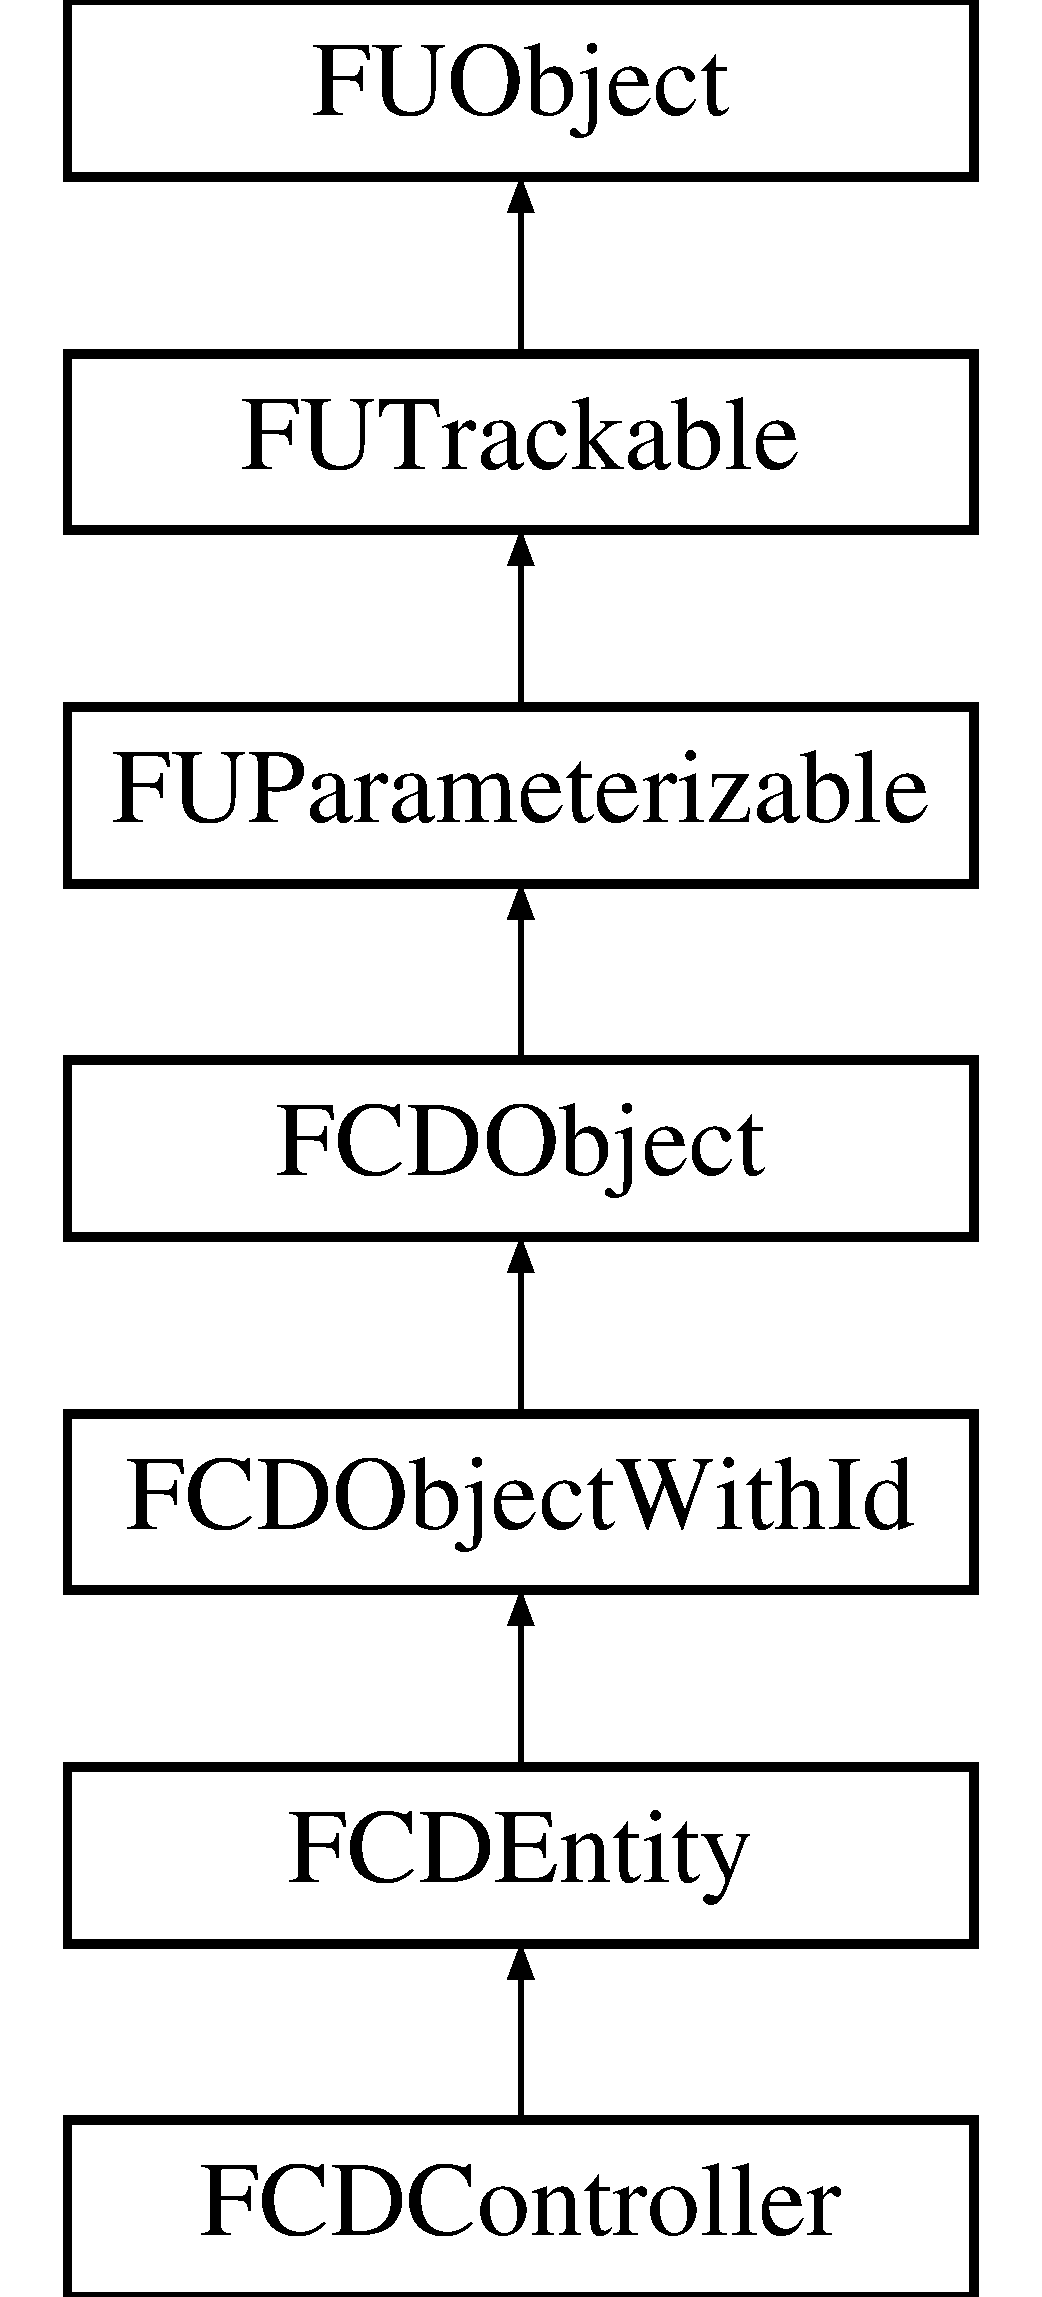
\includegraphics[height=7.000000cm]{classFCDController}
\end{center}
\end{figure}
\subsection*{Public Member Functions}
\begin{DoxyCompactItemize}
\item 
\hyperlink{classFCDController_a04573a2e038e54333ee86fcb3c18540c}{FCDController} (\hyperlink{classFCDocument}{FCDocument} $\ast$document)
\item 
virtual \hyperlink{classFCDController_ae02107dec9fb6fd1d30abcbb3abba043}{$\sim$FCDController} ()
\item 
virtual \hyperlink{classFCDEntity_a9301a4bd5f4d4190ec13e40db4effdd7}{Type} \hyperlink{classFCDController_a2ff5b14d564dba7be26d3b8544bec93c}{GetType} () const 
\item 
bool \hyperlink{classFCDController_a66949037b8bd19c1bbf2f0b0e2b1fefd}{IsSkin} () const 
\item 
bool \hyperlink{classFCDController_ad2894a5bb013f7ee7c21565b1fd0b7fe}{IsMorph} () const 
\item 
\hyperlink{classFCDSkinController}{FCDSkinController} $\ast$ \hyperlink{classFCDController_a808ec0e465cf611a6eb934f0abf51994}{CreateSkinController} ()
\item 
\hyperlink{classFCDMorphController}{FCDMorphController} $\ast$ \hyperlink{classFCDController_a7c96f2438b2cd4e69385c9c7d0172371}{CreateMorphController} ()
\item 
\hyperlink{classFCDSkinController}{FCDSkinController} $\ast$ \hyperlink{classFCDController_a4088c1f8c04cd88fcafa1a82b2c9d587}{GetSkinController} ()
\item 
const \hyperlink{classFCDSkinController}{FCDSkinController} $\ast$ \hyperlink{classFCDController_ae53ae0573ac7e17cfa4718284f4ad7a7}{GetSkinController} () const 
\item 
\hyperlink{classFCDMorphController}{FCDMorphController} $\ast$ \hyperlink{classFCDController_a6a7af0fbd38bb56cf3603e8674e4f445}{GetMorphController} ()
\item 
const \hyperlink{classFCDMorphController}{FCDMorphController} $\ast$ \hyperlink{classFCDController_a500f804426894dd04dcfd30657765305}{GetMorphController} () const 
\item 
\hyperlink{classFCDEntity}{FCDEntity} $\ast$ \hyperlink{classFCDController_a28ef9128280dc48afe55f0398a6c7eb1}{GetBaseTarget} ()
\item 
const \hyperlink{classFCDEntity}{FCDEntity} $\ast$ \hyperlink{classFCDController_ae4035016b183c3aa6fd414571c98b664}{GetBaseTarget} () const 
\item 
\hyperlink{classFCDGeometry}{FCDGeometry} $\ast$ \hyperlink{classFCDController_a407cb338a97fee2bd37ebc7899ee40a8}{GetBaseGeometry} ()
\item 
const \hyperlink{classFCDGeometry}{FCDGeometry} $\ast$ \hyperlink{classFCDController_a9b1bff949a4081b474c0946154ce0034}{GetBaseGeometry} () const 
\item 
\hyperlink{classFCDController}{FCDController} $\ast$ \hyperlink{classFCDController_a270b0e643d2b2e104cc057d611ec5ca8}{GetBaseGeometryController} ()
\item 
const \hyperlink{classFCDController}{FCDController} $\ast$ \hyperlink{classFCDController_ae9a274dc0c85e5de8461810272807374}{GetBaseGeometryController} () const 
\end{DoxyCompactItemize}


\subsection{Detailed Description}
A generic COLLADA controller. A COLLADA controller is used to influence a mesh. COLLADA defines two types of controller: skins (\hyperlink{classFCDSkinController}{FCDSkinController}) and morphers (\hyperlink{classFCDMorphController}{FCDMorphController}). 

\subsection{Constructor \& Destructor Documentation}
\hypertarget{classFCDController_a04573a2e038e54333ee86fcb3c18540c}{
\index{FCDController@{FCDController}!FCDController@{FCDController}}
\index{FCDController@{FCDController}!FCDController@{FCDController}}
\subsubsection[{FCDController}]{\setlength{\rightskip}{0pt plus 5cm}FCDController::FCDController (
\begin{DoxyParamCaption}
\item[{{\bf FCDocument} $\ast$}]{ document}
\end{DoxyParamCaption}
)}}
\label{classFCDController_a04573a2e038e54333ee86fcb3c18540c}
Constructor: do not use directly. Instead, use the \hyperlink{classFCDLibrary_aa5cdcac5a447298d5e3816e4f8c864d0}{FCDLibrary::AddEntity} function. 
\begin{DoxyParams}{Parameters}
\item[{\em document}]The COLLADA document that owns the controller. \end{DoxyParams}
\hypertarget{classFCDController_ae02107dec9fb6fd1d30abcbb3abba043}{
\index{FCDController@{FCDController}!$\sim$FCDController@{$\sim$FCDController}}
\index{$\sim$FCDController@{$\sim$FCDController}!FCDController@{FCDController}}
\subsubsection[{$\sim$FCDController}]{\setlength{\rightskip}{0pt plus 5cm}FCDController::$\sim$FCDController (
\begin{DoxyParamCaption}
{}
\end{DoxyParamCaption}
)\hspace{0.3cm}{\ttfamily  \mbox{[}virtual\mbox{]}}}}
\label{classFCDController_ae02107dec9fb6fd1d30abcbb3abba043}
Destructor. 

\subsection{Member Function Documentation}
\hypertarget{classFCDController_a7c96f2438b2cd4e69385c9c7d0172371}{
\index{FCDController@{FCDController}!CreateMorphController@{CreateMorphController}}
\index{CreateMorphController@{CreateMorphController}!FCDController@{FCDController}}
\subsubsection[{CreateMorphController}]{\setlength{\rightskip}{0pt plus 5cm}{\bf FCDMorphController} $\ast$ FCDController::CreateMorphController (
\begin{DoxyParamCaption}
{}
\end{DoxyParamCaption}
)}}
\label{classFCDController_a7c96f2438b2cd4e69385c9c7d0172371}
Sets the type of this controller to a morph controller. This function will release any previously created morpher or skin. \begin{DoxyReturn}{Returns}
The new morph controller. 
\end{DoxyReturn}
\hypertarget{classFCDController_a808ec0e465cf611a6eb934f0abf51994}{
\index{FCDController@{FCDController}!CreateSkinController@{CreateSkinController}}
\index{CreateSkinController@{CreateSkinController}!FCDController@{FCDController}}
\subsubsection[{CreateSkinController}]{\setlength{\rightskip}{0pt plus 5cm}{\bf FCDSkinController} $\ast$ FCDController::CreateSkinController (
\begin{DoxyParamCaption}
{}
\end{DoxyParamCaption}
)}}
\label{classFCDController_a808ec0e465cf611a6eb934f0abf51994}
Sets the type of this controller to a skin controller. This function will release any previously created morpher or skin. \begin{DoxyReturn}{Returns}
The new skin controller. 
\end{DoxyReturn}
\hypertarget{classFCDController_a407cb338a97fee2bd37ebc7899ee40a8}{
\index{FCDController@{FCDController}!GetBaseGeometry@{GetBaseGeometry}}
\index{GetBaseGeometry@{GetBaseGeometry}!FCDController@{FCDController}}
\subsubsection[{GetBaseGeometry}]{\setlength{\rightskip}{0pt plus 5cm}{\bf FCDGeometry}$\ast$ FCDController::GetBaseGeometry (
\begin{DoxyParamCaption}
{}
\end{DoxyParamCaption}
)\hspace{0.3cm}{\ttfamily  \mbox{[}inline\mbox{]}}}}
\label{classFCDController_a407cb338a97fee2bd37ebc7899ee40a8}
Retrieves the base target geometry for this controller. Controllers can be chained together. This function allows you to retrieve the base target geometry, if there is one. \begin{DoxyReturn}{Returns}
The base target geometry. This pointer will be NULL if no base target is defined or if the base target entity is not a geometry. 
\end{DoxyReturn}
\hypertarget{classFCDController_a9b1bff949a4081b474c0946154ce0034}{
\index{FCDController@{FCDController}!GetBaseGeometry@{GetBaseGeometry}}
\index{GetBaseGeometry@{GetBaseGeometry}!FCDController@{FCDController}}
\subsubsection[{GetBaseGeometry}]{\setlength{\rightskip}{0pt plus 5cm}const {\bf FCDGeometry} $\ast$ FCDController::GetBaseGeometry (
\begin{DoxyParamCaption}
{}
\end{DoxyParamCaption}
) const}}
\label{classFCDController_a9b1bff949a4081b474c0946154ce0034}
See above. \hypertarget{classFCDController_ae9a274dc0c85e5de8461810272807374}{
\index{FCDController@{FCDController}!GetBaseGeometryController@{GetBaseGeometryController}}
\index{GetBaseGeometryController@{GetBaseGeometryController}!FCDController@{FCDController}}
\subsubsection[{GetBaseGeometryController}]{\setlength{\rightskip}{0pt plus 5cm}const {\bf FCDController} $\ast$ FCDController::GetBaseGeometryController (
\begin{DoxyParamCaption}
{}
\end{DoxyParamCaption}
) const}}
\label{classFCDController_ae9a274dc0c85e5de8461810272807374}
See above. \hypertarget{classFCDController_a270b0e643d2b2e104cc057d611ec5ca8}{
\index{FCDController@{FCDController}!GetBaseGeometryController@{GetBaseGeometryController}}
\index{GetBaseGeometryController@{GetBaseGeometryController}!FCDController@{FCDController}}
\subsubsection[{GetBaseGeometryController}]{\setlength{\rightskip}{0pt plus 5cm}{\bf FCDController}$\ast$ FCDController::GetBaseGeometryController (
\begin{DoxyParamCaption}
{}
\end{DoxyParamCaption}
)\hspace{0.3cm}{\ttfamily  \mbox{[}inline\mbox{]}}}}
\label{classFCDController_a270b0e643d2b2e104cc057d611ec5ca8}
Retrieves the lowest controller on this stack. Controllers can be chained together. This function allows you to retrieve the controller assigned to the base target geometry. \begin{DoxyReturn}{Returns}
The base controller. This pointer will be NULL if no base target is defined or if the base target entity is not a geometry. 
\end{DoxyReturn}
\hypertarget{classFCDController_a28ef9128280dc48afe55f0398a6c7eb1}{
\index{FCDController@{FCDController}!GetBaseTarget@{GetBaseTarget}}
\index{GetBaseTarget@{GetBaseTarget}!FCDController@{FCDController}}
\subsubsection[{GetBaseTarget}]{\setlength{\rightskip}{0pt plus 5cm}{\bf FCDEntity} $\ast$ FCDController::GetBaseTarget (
\begin{DoxyParamCaption}
{}
\end{DoxyParamCaption}
)}}
\label{classFCDController_a28ef9128280dc48afe55f0398a6c7eb1}
Retrieves the base target entity for this controller. The base target entity may be another controller or a geometry entity. To change the base target, use the \hyperlink{classFCDMorphController_a11196ee1bd50c02cbd82e75397816272}{FCDMorphController::SetBaseTarget} or the \hyperlink{classFCDSkinController_a570337f366b9760bf1828620541c130b}{FCDSkinController::SetTarget} functions. \begin{DoxyReturn}{Returns}
The base target entity. This pointer will be NULL if no base target is defined. 
\end{DoxyReturn}
\hypertarget{classFCDController_ae4035016b183c3aa6fd414571c98b664}{
\index{FCDController@{FCDController}!GetBaseTarget@{GetBaseTarget}}
\index{GetBaseTarget@{GetBaseTarget}!FCDController@{FCDController}}
\subsubsection[{GetBaseTarget}]{\setlength{\rightskip}{0pt plus 5cm}const {\bf FCDEntity} $\ast$ FCDController::GetBaseTarget (
\begin{DoxyParamCaption}
{}
\end{DoxyParamCaption}
) const}}
\label{classFCDController_ae4035016b183c3aa6fd414571c98b664}
See above. \hypertarget{classFCDController_a500f804426894dd04dcfd30657765305}{
\index{FCDController@{FCDController}!GetMorphController@{GetMorphController}}
\index{GetMorphController@{GetMorphController}!FCDController@{FCDController}}
\subsubsection[{GetMorphController}]{\setlength{\rightskip}{0pt plus 5cm}const {\bf FCDMorphController}$\ast$ FCDController::GetMorphController (
\begin{DoxyParamCaption}
{}
\end{DoxyParamCaption}
) const\hspace{0.3cm}{\ttfamily  \mbox{[}inline\mbox{]}}}}
\label{classFCDController_a500f804426894dd04dcfd30657765305}
See above. \hypertarget{classFCDController_a6a7af0fbd38bb56cf3603e8674e4f445}{
\index{FCDController@{FCDController}!GetMorphController@{GetMorphController}}
\index{GetMorphController@{GetMorphController}!FCDController@{FCDController}}
\subsubsection[{GetMorphController}]{\setlength{\rightskip}{0pt plus 5cm}{\bf FCDMorphController}$\ast$ FCDController::GetMorphController (
\begin{DoxyParamCaption}
{}
\end{DoxyParamCaption}
)\hspace{0.3cm}{\ttfamily  \mbox{[}inline\mbox{]}}}}
\label{classFCDController_a6a7af0fbd38bb56cf3603e8674e4f445}
Retrieves the morph controller. This pointer is only valid for skins. To verify that this is a morpher, check the HasMorphController function. \begin{DoxyReturn}{Returns}
The morph controller. This pointer will be NULL, if the controller is not a morpher. 
\end{DoxyReturn}
\hypertarget{classFCDController_a4088c1f8c04cd88fcafa1a82b2c9d587}{
\index{FCDController@{FCDController}!GetSkinController@{GetSkinController}}
\index{GetSkinController@{GetSkinController}!FCDController@{FCDController}}
\subsubsection[{GetSkinController}]{\setlength{\rightskip}{0pt plus 5cm}{\bf FCDSkinController}$\ast$ FCDController::GetSkinController (
\begin{DoxyParamCaption}
{}
\end{DoxyParamCaption}
)\hspace{0.3cm}{\ttfamily  \mbox{[}inline\mbox{]}}}}
\label{classFCDController_a4088c1f8c04cd88fcafa1a82b2c9d587}
Retrieves the skin controller. This pointer is only valid for skins. To verify that this is a skin, check the HasSkinController function. \begin{DoxyReturn}{Returns}
The skin controller. This pointer will be NULL, if the controller is not a skin. 
\end{DoxyReturn}
\hypertarget{classFCDController_ae53ae0573ac7e17cfa4718284f4ad7a7}{
\index{FCDController@{FCDController}!GetSkinController@{GetSkinController}}
\index{GetSkinController@{GetSkinController}!FCDController@{FCDController}}
\subsubsection[{GetSkinController}]{\setlength{\rightskip}{0pt plus 5cm}const {\bf FCDSkinController}$\ast$ FCDController::GetSkinController (
\begin{DoxyParamCaption}
{}
\end{DoxyParamCaption}
) const\hspace{0.3cm}{\ttfamily  \mbox{[}inline\mbox{]}}}}
\label{classFCDController_ae53ae0573ac7e17cfa4718284f4ad7a7}
See above. \hypertarget{classFCDController_a2ff5b14d564dba7be26d3b8544bec93c}{
\index{FCDController@{FCDController}!GetType@{GetType}}
\index{GetType@{GetType}!FCDController@{FCDController}}
\subsubsection[{GetType}]{\setlength{\rightskip}{0pt plus 5cm}virtual {\bf Type} FCDController::GetType (
\begin{DoxyParamCaption}
{}
\end{DoxyParamCaption}
) const\hspace{0.3cm}{\ttfamily  \mbox{[}inline, virtual\mbox{]}}}}
\label{classFCDController_a2ff5b14d564dba7be26d3b8544bec93c}
Retrieves the entity class type. This function is a part of the \hyperlink{classFCDEntity}{FCDEntity} interface. \begin{DoxyReturn}{Returns}
The entity class type: CONTROLLER. 
\end{DoxyReturn}


Reimplemented from \hyperlink{classFCDEntity_abfd4312a7124f92364c1e6517c7e60ba}{FCDEntity}.

\hypertarget{classFCDController_ad2894a5bb013f7ee7c21565b1fd0b7fe}{
\index{FCDController@{FCDController}!IsMorph@{IsMorph}}
\index{IsMorph@{IsMorph}!FCDController@{FCDController}}
\subsubsection[{IsMorph}]{\setlength{\rightskip}{0pt plus 5cm}bool FCDController::IsMorph (
\begin{DoxyParamCaption}
{}
\end{DoxyParamCaption}
) const\hspace{0.3cm}{\ttfamily  \mbox{[}inline\mbox{]}}}}
\label{classFCDController_ad2894a5bb013f7ee7c21565b1fd0b7fe}
Retrieves whether this controller is a morph controller. \begin{DoxyReturn}{Returns}
Whether this controller is a morph controller. 
\end{DoxyReturn}
\hypertarget{classFCDController_a66949037b8bd19c1bbf2f0b0e2b1fefd}{
\index{FCDController@{FCDController}!IsSkin@{IsSkin}}
\index{IsSkin@{IsSkin}!FCDController@{FCDController}}
\subsubsection[{IsSkin}]{\setlength{\rightskip}{0pt plus 5cm}bool FCDController::IsSkin (
\begin{DoxyParamCaption}
{}
\end{DoxyParamCaption}
) const\hspace{0.3cm}{\ttfamily  \mbox{[}inline\mbox{]}}}}
\label{classFCDController_a66949037b8bd19c1bbf2f0b0e2b1fefd}
Retrieves whether this controller is a skin controller. \begin{DoxyReturn}{Returns}
Whether this controller is a skin controller. 
\end{DoxyReturn}


The documentation for this class was generated from the following files:\begin{DoxyCompactItemize}
\item 
FCollada/FCDocument/\hyperlink{FCDController_8h}{FCDController.h}\item 
FCollada/FCDocument/FCDController.cpp\end{DoxyCompactItemize}

\hypertarget{classFCDControllerInstance}{
\section{FCDControllerInstance Class Reference}
\label{classFCDControllerInstance}\index{FCDControllerInstance@{FCDControllerInstance}}
}


{\ttfamily \#include $<$FCDControllerInstance.h$>$}

Inheritance diagram for FCDControllerInstance:\begin{figure}[H]
\begin{center}
\leavevmode
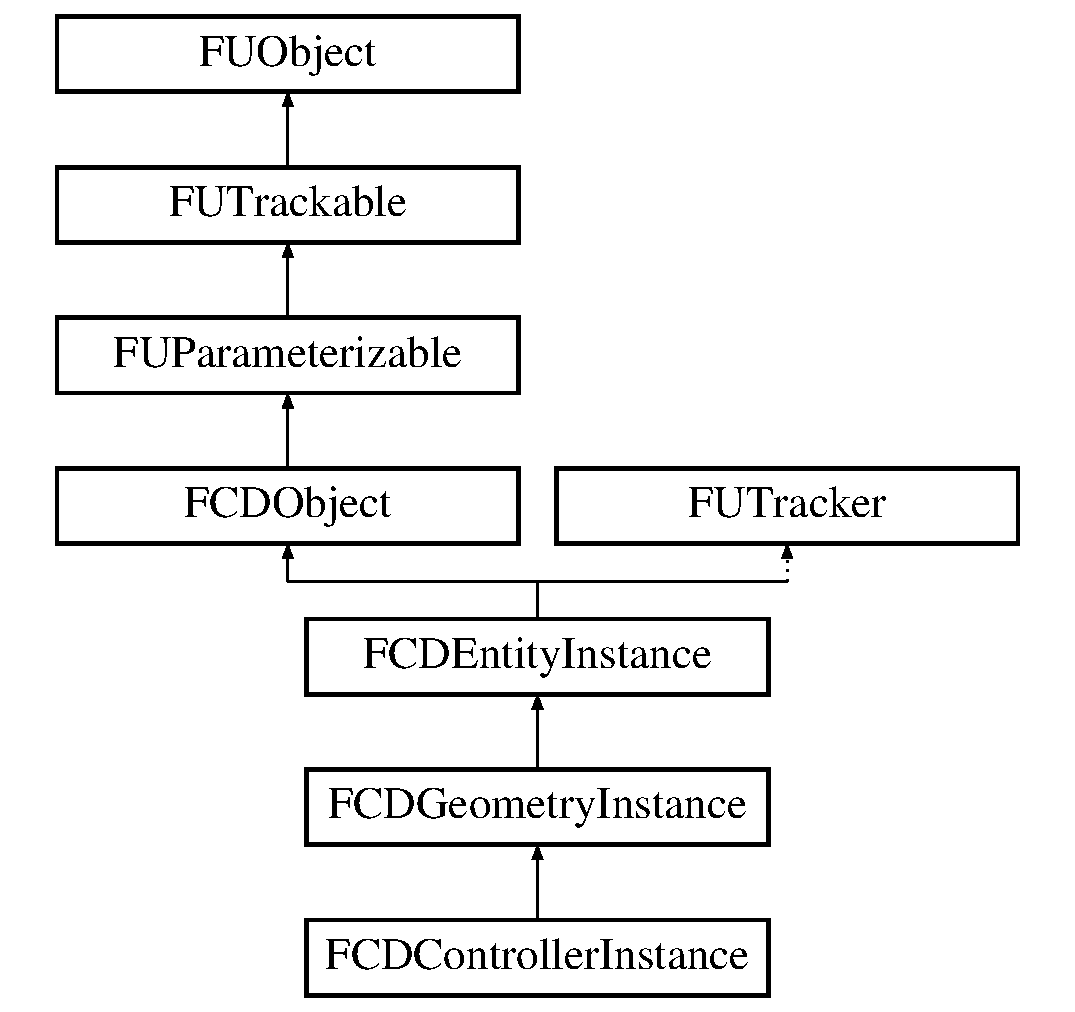
\includegraphics[height=7.000000cm]{classFCDControllerInstance}
\end{center}
\end{figure}
\subsection*{Public Member Functions}
\begin{DoxyCompactItemize}
\item 
virtual \hyperlink{classFCDControllerInstance_aade7a868f4c9154480f950553280e22f}{$\sim$FCDControllerInstance} ()
\item 
virtual \hyperlink{classFCDEntityInstance_a82e95eec7d9242bbedb336b0d35b59d3}{Type} \hyperlink{classFCDControllerInstance_a5c8057a1560e6b77340218e5d1e0d4ef}{GetType} () const 
\item 
virtual \hyperlink{classFCDEntityInstance}{FCDEntityInstance} $\ast$ \hyperlink{classFCDControllerInstance_a754a4004c6d4f4c72c1639f79138799a}{Clone} (\hyperlink{classFCDEntityInstance}{FCDEntityInstance} $\ast$clone=NULL) const 
\item 
const \hyperlink{classfm_1_1vector}{FUUriList} \& \hyperlink{classFCDControllerInstance_af3d8c893a4bd43eec2ec413e82f31be3}{GetSkeletonRoots} () const 
\item 
\hypertarget{classFCDControllerInstance_af8e2620bc755e7abcb01b63ced3c62bc}{
\hyperlink{classfm_1_1vector}{FUUriList} \& {\bfseries GetSkeletonRoots} ()}
\label{classFCDControllerInstance_af8e2620bc755e7abcb01b63ced3c62bc}

\item 
void \hyperlink{classFCDControllerInstance_ae661fba3361f80fe47aadab59639d599}{FindSkeletonNodes} (\hyperlink{classfm_1_1pvector}{FCDSceneNodeList} \&skeletonNodes) const 
\item 
void \hyperlink{classFCDControllerInstance_afe5e7f4cb5ac64a5a502ec83c8f777be}{CalculateRootIds} ()
\item 
size\_\-t \hyperlink{classFCDControllerInstance_ace8f96de6fc8961664b3a8567f669a7e}{GetJointCount} () const 
\item 
void \hyperlink{classFCDControllerInstance_a5439543d2a66269a957abca8f241b156}{ResetJoints} ()
\item 
\hyperlink{classFCDSceneNode}{FCDSceneNode} $\ast$ \hyperlink{classFCDControllerInstance_a9c5d37281dd140d3116e0dcb720f54a6}{GetJoint} (size\_\-t index)
\item 
const \hyperlink{classFCDSceneNode}{FCDSceneNode} $\ast$ \hyperlink{classFCDControllerInstance_abc908d73a16c1d4b4d2f226d90b2889c}{GetJoint} (size\_\-t index) const 
\item 
bool \hyperlink{classFCDControllerInstance_a9c58665f93aea522377627d20178ff73}{AddJoint} (\hyperlink{classFCDSceneNode}{FCDSceneNode} $\ast$j)
\item 
bool \hyperlink{classFCDControllerInstance_a064731e6ebcc97fa3ace04fa067a4ce6}{FindJoint} (const \hyperlink{classFCDSceneNode}{FCDSceneNode} $\ast$joint) const 
\item 
size\_\-t \hyperlink{classFCDControllerInstance_af7cc64b04416e1d04ff2c118398823fc}{FindJointIndex} (const \hyperlink{classFCDSceneNode}{FCDSceneNode} $\ast$joint) const 
\item 
void \hyperlink{classFCDControllerInstance_ab5a40778d93e9bc804127a11e0e184cf}{RemoveJoint} (size\_\-t index)
\item 
void \hyperlink{classFCDControllerInstance_a0be970ad3ce1b2dd92552ae90a1352ca}{RemoveJoint} (\hyperlink{classFCDSceneNode}{FCDSceneNode} $\ast$joint)
\end{DoxyCompactItemize}
\subsection*{Protected Member Functions}
\begin{DoxyCompactItemize}
\item 
\hyperlink{classFCDControllerInstance_a3f7e452b081c7fbbbd3ec5780ce44af0}{FCDControllerInstance} (\hyperlink{classFCDocument}{FCDocument} $\ast$document, \hyperlink{classFCDSceneNode}{FCDSceneNode} $\ast$parent, \hyperlink{classFCDEntity_a9301a4bd5f4d4190ec13e40db4effdd7}{FCDEntity::Type} entityType=FCDEntity::CONTROLLER)
\end{DoxyCompactItemize}
\subsection*{Friends}
\begin{DoxyCompactItemize}
\item 
\hypertarget{classFCDControllerInstance_a069ebb98497ccbc5fdcb75ecfa8b15f7}{
class \hyperlink{classFCDControllerInstance_a069ebb98497ccbc5fdcb75ecfa8b15f7}{FCDEntityInstanceFactory}}
\label{classFCDControllerInstance_a069ebb98497ccbc5fdcb75ecfa8b15f7}

\end{DoxyCompactItemize}


\subsection{Detailed Description}
A COLLADA controller instance.

When a COLLADA controller is instantiated, all its target(s) are instantiated in order to use them for the rendering or the logic. As such, all the information necessary to instantiate a geometry is also necessary to instantiate a controller.

Each COLLADA skin controller should instantiate its own skeleton, for this reason, the skeleton root(s) are defined at instantiation.

A controller instance should define the skeleton root joint. Previously a \hyperlink{classFCDSkinController}{FCDSkinController} directly linked to its joints. We now read the skeletonRoot here, and call which means that the \hyperlink{classFCDSkinController}{FCDSkinController} should never try and know about its own nodes. It should all be linked through here. 

\subsection{Constructor \& Destructor Documentation}
\hypertarget{classFCDControllerInstance_a3f7e452b081c7fbbbd3ec5780ce44af0}{
\index{FCDControllerInstance@{FCDControllerInstance}!FCDControllerInstance@{FCDControllerInstance}}
\index{FCDControllerInstance@{FCDControllerInstance}!FCDControllerInstance@{FCDControllerInstance}}
\subsubsection[{FCDControllerInstance}]{\setlength{\rightskip}{0pt plus 5cm}FCDControllerInstance::FCDControllerInstance (
\begin{DoxyParamCaption}
\item[{{\bf FCDocument} $\ast$}]{ document, }
\item[{{\bf FCDSceneNode} $\ast$}]{ parent, }
\item[{{\bf FCDEntity::Type}}]{ entityType = {\ttfamily FCDEntity::CONTROLLER}}
\end{DoxyParamCaption}
)\hspace{0.3cm}{\ttfamily  \mbox{[}protected\mbox{]}}}}
\label{classFCDControllerInstance_a3f7e452b081c7fbbbd3ec5780ce44af0}
Constructor: do not use directly. Instead, use the \hyperlink{classFCDSceneNode_a38826dd9b894ad2371511f0228cb04c0}{FCDSceneNode::AddInstance} function. 
\begin{DoxyParams}{Parameters}
\item[{\em document}]The COLLADA document that owns the controller instance. \item[{\em parent}]The parent visual scene node. \item[{\em entityType}]The type of the entity instantiate. Unless the class is overwritten, \hyperlink{classFCDEntity_a9301a4bd5f4d4190ec13e40db4effdd7ad1448b2688394292605bed327a679afe}{FCDEntity::CONTROLLER} should be given. \end{DoxyParams}
\hypertarget{classFCDControllerInstance_aade7a868f4c9154480f950553280e22f}{
\index{FCDControllerInstance@{FCDControllerInstance}!$\sim$FCDControllerInstance@{$\sim$FCDControllerInstance}}
\index{$\sim$FCDControllerInstance@{$\sim$FCDControllerInstance}!FCDControllerInstance@{FCDControllerInstance}}
\subsubsection[{$\sim$FCDControllerInstance}]{\setlength{\rightskip}{0pt plus 5cm}FCDControllerInstance::$\sim$FCDControllerInstance (
\begin{DoxyParamCaption}
{}
\end{DoxyParamCaption}
)\hspace{0.3cm}{\ttfamily  \mbox{[}virtual\mbox{]}}}}
\label{classFCDControllerInstance_aade7a868f4c9154480f950553280e22f}
Destructor. 

\subsection{Member Function Documentation}
\hypertarget{classFCDControllerInstance_a9c58665f93aea522377627d20178ff73}{
\index{FCDControllerInstance@{FCDControllerInstance}!AddJoint@{AddJoint}}
\index{AddJoint@{AddJoint}!FCDControllerInstance@{FCDControllerInstance}}
\subsubsection[{AddJoint}]{\setlength{\rightskip}{0pt plus 5cm}bool FCDControllerInstance::AddJoint (
\begin{DoxyParamCaption}
\item[{{\bf FCDSceneNode} $\ast$}]{ j}
\end{DoxyParamCaption}
)}}
\label{classFCDControllerInstance_a9c58665f93aea522377627d20178ff73}
Adds an existing joint to the list of controller joints. 
\begin{DoxyParams}{Parameters}
\item[{\em j}]A joint-\/typed scene node. \end{DoxyParams}
\hypertarget{classFCDControllerInstance_afe5e7f4cb5ac64a5a502ec83c8f777be}{
\index{FCDControllerInstance@{FCDControllerInstance}!CalculateRootIds@{CalculateRootIds}}
\index{CalculateRootIds@{CalculateRootIds}!FCDControllerInstance@{FCDControllerInstance}}
\subsubsection[{CalculateRootIds}]{\setlength{\rightskip}{0pt plus 5cm}void FCDControllerInstance::CalculateRootIds (
\begin{DoxyParamCaption}
{}
\end{DoxyParamCaption}
)}}
\label{classFCDControllerInstance_afe5e7f4cb5ac64a5a502ec83c8f777be}
Calculate our skeleton roots, based on the node list we have \hypertarget{classFCDControllerInstance_a754a4004c6d4f4c72c1639f79138799a}{
\index{FCDControllerInstance@{FCDControllerInstance}!Clone@{Clone}}
\index{Clone@{Clone}!FCDControllerInstance@{FCDControllerInstance}}
\subsubsection[{Clone}]{\setlength{\rightskip}{0pt plus 5cm}{\bf FCDEntityInstance} $\ast$ FCDControllerInstance::Clone (
\begin{DoxyParamCaption}
\item[{{\bf FCDEntityInstance} $\ast$}]{ clone = {\ttfamily NULL}}
\end{DoxyParamCaption}
) const\hspace{0.3cm}{\ttfamily  \mbox{[}virtual\mbox{]}}}}
\label{classFCDControllerInstance_a754a4004c6d4f4c72c1639f79138799a}
Clones the controller instance. 
\begin{DoxyParams}{Parameters}
\item[{\em clone}]The controller instance to become the clone. If this pointer is NULL, a new controller instance will be created and you will need to release the returned pointer. \end{DoxyParams}
\begin{DoxyReturn}{Returns}
The clone. 
\end{DoxyReturn}


Reimplemented from \hyperlink{classFCDGeometryInstance_ab056bfdefa8eb7c99a2551f114ae5242}{FCDGeometryInstance}.

\hypertarget{classFCDControllerInstance_a064731e6ebcc97fa3ace04fa067a4ce6}{
\index{FCDControllerInstance@{FCDControllerInstance}!FindJoint@{FindJoint}}
\index{FindJoint@{FindJoint}!FCDControllerInstance@{FCDControllerInstance}}
\subsubsection[{FindJoint}]{\setlength{\rightskip}{0pt plus 5cm}bool FCDControllerInstance::FindJoint (
\begin{DoxyParamCaption}
\item[{const {\bf FCDSceneNode} $\ast$}]{ joint}
\end{DoxyParamCaption}
) const}}
\label{classFCDControllerInstance_a064731e6ebcc97fa3ace04fa067a4ce6}
Find a given joint in this skin instance. 
\begin{DoxyParams}{Parameters}
\item[{\em joint}]The joint. \end{DoxyParams}
\begin{DoxyReturn}{Returns}
true if the node is present, false if not. See above. 
\end{DoxyReturn}
\hypertarget{classFCDControllerInstance_af7cc64b04416e1d04ff2c118398823fc}{
\index{FCDControllerInstance@{FCDControllerInstance}!FindJointIndex@{FindJointIndex}}
\index{FindJointIndex@{FindJointIndex}!FCDControllerInstance@{FCDControllerInstance}}
\subsubsection[{FindJointIndex}]{\setlength{\rightskip}{0pt plus 5cm}size\_\-t FCDControllerInstance::FindJointIndex (
\begin{DoxyParamCaption}
\item[{const {\bf FCDSceneNode} $\ast$}]{ joint}
\end{DoxyParamCaption}
) const}}
\label{classFCDControllerInstance_af7cc64b04416e1d04ff2c118398823fc}
Find the index of the given joint in this skin instance 
\begin{DoxyParams}{Parameters}
\item[{\em joint}]The joint. \end{DoxyParams}
\begin{DoxyReturn}{Returns}
The joints index, else \char`\"{}(size\_\-t) $\sim$0\char`\"{} if not present. 
\end{DoxyReturn}
\hypertarget{classFCDControllerInstance_ae661fba3361f80fe47aadab59639d599}{
\index{FCDControllerInstance@{FCDControllerInstance}!FindSkeletonNodes@{FindSkeletonNodes}}
\index{FindSkeletonNodes@{FindSkeletonNodes}!FCDControllerInstance@{FCDControllerInstance}}
\subsubsection[{FindSkeletonNodes}]{\setlength{\rightskip}{0pt plus 5cm}void FCDControllerInstance::FindSkeletonNodes (
\begin{DoxyParamCaption}
\item[{{\bf FCDSceneNodeList} \&}]{ skeletonNodes}
\end{DoxyParamCaption}
) const}}
\label{classFCDControllerInstance_ae661fba3361f80fe47aadab59639d599}
Retrieves a list of all the root scene nodes for the controller. This list is generated with a call to this method. 
\begin{DoxyParams}{Parameters}
\item[{\em skeletonNodes}]The list of parent Ids to fill in. This list is not cleared first. \end{DoxyParams}
\hypertarget{classFCDControllerInstance_a9c5d37281dd140d3116e0dcb720f54a6}{
\index{FCDControllerInstance@{FCDControllerInstance}!GetJoint@{GetJoint}}
\index{GetJoint@{GetJoint}!FCDControllerInstance@{FCDControllerInstance}}
\subsubsection[{GetJoint}]{\setlength{\rightskip}{0pt plus 5cm}{\bf FCDSceneNode}$\ast$ FCDControllerInstance::GetJoint (
\begin{DoxyParamCaption}
\item[{size\_\-t}]{ index}
\end{DoxyParamCaption}
)\hspace{0.3cm}{\ttfamily  \mbox{[}inline\mbox{]}}}}
\label{classFCDControllerInstance_a9c5d37281dd140d3116e0dcb720f54a6}
Retrieves a specific joint. 
\begin{DoxyParams}{Parameters}
\item[{\em index}]The index of the joint. \end{DoxyParams}
\begin{DoxyReturn}{Returns}
The joint. This pointer will be NULL, if the index is out-\/of-\/bounds. 
\end{DoxyReturn}
\hypertarget{classFCDControllerInstance_abc908d73a16c1d4b4d2f226d90b2889c}{
\index{FCDControllerInstance@{FCDControllerInstance}!GetJoint@{GetJoint}}
\index{GetJoint@{GetJoint}!FCDControllerInstance@{FCDControllerInstance}}
\subsubsection[{GetJoint}]{\setlength{\rightskip}{0pt plus 5cm}const {\bf FCDSceneNode}$\ast$ FCDControllerInstance::GetJoint (
\begin{DoxyParamCaption}
\item[{size\_\-t}]{ index}
\end{DoxyParamCaption}
) const\hspace{0.3cm}{\ttfamily  \mbox{[}inline\mbox{]}}}}
\label{classFCDControllerInstance_abc908d73a16c1d4b4d2f226d90b2889c}
See above. \hypertarget{classFCDControllerInstance_ace8f96de6fc8961664b3a8567f669a7e}{
\index{FCDControllerInstance@{FCDControllerInstance}!GetJointCount@{GetJointCount}}
\index{GetJointCount@{GetJointCount}!FCDControllerInstance@{FCDControllerInstance}}
\subsubsection[{GetJointCount}]{\setlength{\rightskip}{0pt plus 5cm}size\_\-t FCDControllerInstance::GetJointCount (
\begin{DoxyParamCaption}
{}
\end{DoxyParamCaption}
) const\hspace{0.3cm}{\ttfamily  \mbox{[}inline\mbox{]}}}}
\label{classFCDControllerInstance_ace8f96de6fc8961664b3a8567f669a7e}
Retrieves the number of joints used by this controller. Joints only make sense when used with skin controllers. Defining the skeleton root affects the actual joints, but not the joint sids. \begin{DoxyReturn}{Returns}
The number of joints used by this controller. 
\end{DoxyReturn}
\hypertarget{classFCDControllerInstance_af3d8c893a4bd43eec2ec413e82f31be3}{
\index{FCDControllerInstance@{FCDControllerInstance}!GetSkeletonRoots@{GetSkeletonRoots}}
\index{GetSkeletonRoots@{GetSkeletonRoots}!FCDControllerInstance@{FCDControllerInstance}}
\subsubsection[{GetSkeletonRoots}]{\setlength{\rightskip}{0pt plus 5cm}const {\bf FUUriList}\& FCDControllerInstance::GetSkeletonRoots (
\begin{DoxyParamCaption}
{}
\end{DoxyParamCaption}
) const\hspace{0.3cm}{\ttfamily  \mbox{[}inline\mbox{]}}}}
\label{classFCDControllerInstance_af3d8c893a4bd43eec2ec413e82f31be3}
Retrieves a list of all the root joint ids for the controller. \begin{DoxyReturn}{Returns}
List of parent Ids 
\end{DoxyReturn}
\hypertarget{classFCDControllerInstance_a5c8057a1560e6b77340218e5d1e0d4ef}{
\index{FCDControllerInstance@{FCDControllerInstance}!GetType@{GetType}}
\index{GetType@{GetType}!FCDControllerInstance@{FCDControllerInstance}}
\subsubsection[{GetType}]{\setlength{\rightskip}{0pt plus 5cm}virtual {\bf Type} FCDControllerInstance::GetType (
\begin{DoxyParamCaption}
{}
\end{DoxyParamCaption}
) const\hspace{0.3cm}{\ttfamily  \mbox{[}inline, virtual\mbox{]}}}}
\label{classFCDControllerInstance_a5c8057a1560e6b77340218e5d1e0d4ef}
Retrieves the entity instance class type. This is used to determine the up-\/class for the entity instance object. \begin{Desc}
\item[\hyperlink{deprecated__deprecated000003}{Deprecated}]Instead use: \hyperlink{classFUObject_ab838ad4132b756dcd3614440b8e32f2a}{FCDEntityInstance::HasType}(\hyperlink{classFUObject_a907d4f6d284b3ac4f8203d557af41668}{FCDController::GetClassType()}) \end{Desc}
\begin{DoxyReturn}{Returns}
The class type: CONTROLLER. 
\end{DoxyReturn}


Reimplemented from \hyperlink{classFCDGeometryInstance_a6125c229bbac52a27ae4a1fa8cd0dac6}{FCDGeometryInstance}.

\hypertarget{classFCDControllerInstance_ab5a40778d93e9bc804127a11e0e184cf}{
\index{FCDControllerInstance@{FCDControllerInstance}!RemoveJoint@{RemoveJoint}}
\index{RemoveJoint@{RemoveJoint}!FCDControllerInstance@{FCDControllerInstance}}
\subsubsection[{RemoveJoint}]{\setlength{\rightskip}{0pt plus 5cm}void FCDControllerInstance::RemoveJoint (
\begin{DoxyParamCaption}
\item[{size\_\-t}]{ index}
\end{DoxyParamCaption}
)\hspace{0.3cm}{\ttfamily  \mbox{[}inline\mbox{]}}}}
\label{classFCDControllerInstance_ab5a40778d93e9bc804127a11e0e184cf}
Removes a joint from the skin instance. 
\begin{DoxyParams}{Parameters}
\item[{\em index}]The index of the joint to remove. \end{DoxyParams}
\hypertarget{classFCDControllerInstance_a0be970ad3ce1b2dd92552ae90a1352ca}{
\index{FCDControllerInstance@{FCDControllerInstance}!RemoveJoint@{RemoveJoint}}
\index{RemoveJoint@{RemoveJoint}!FCDControllerInstance@{FCDControllerInstance}}
\subsubsection[{RemoveJoint}]{\setlength{\rightskip}{0pt plus 5cm}void FCDControllerInstance::RemoveJoint (
\begin{DoxyParamCaption}
\item[{{\bf FCDSceneNode} $\ast$}]{ joint}
\end{DoxyParamCaption}
)\hspace{0.3cm}{\ttfamily  \mbox{[}inline\mbox{]}}}}
\label{classFCDControllerInstance_a0be970ad3ce1b2dd92552ae90a1352ca}
Removes a joint from the skin instance. 
\begin{DoxyParams}{Parameters}
\item[{\em joint}]The joint to remove. \end{DoxyParams}
\hypertarget{classFCDControllerInstance_a5439543d2a66269a957abca8f241b156}{
\index{FCDControllerInstance@{FCDControllerInstance}!ResetJoints@{ResetJoints}}
\index{ResetJoints@{ResetJoints}!FCDControllerInstance@{FCDControllerInstance}}
\subsubsection[{ResetJoints}]{\setlength{\rightskip}{0pt plus 5cm}void FCDControllerInstance::ResetJoints (
\begin{DoxyParamCaption}
{}
\end{DoxyParamCaption}
)\hspace{0.3cm}{\ttfamily  \mbox{[}inline\mbox{]}}}}
\label{classFCDControllerInstance_a5439543d2a66269a957abca8f241b156}
Reset the joint lists. 

The documentation for this class was generated from the following files:\begin{DoxyCompactItemize}
\item 
FCollada/FCDocument/\hyperlink{FCDControllerInstance_8h}{FCDControllerInstance.h}\item 
FCollada/FCDocument/FCDControllerInstance.cpp\end{DoxyCompactItemize}

\hypertarget{classFCDConversionFunctor}{
\section{FCDConversionFunctor Class Reference}
\label{classFCDConversionFunctor}\index{FCDConversionFunctor@{FCDConversionFunctor}}
}


{\ttfamily \#include $<$FCDAnimationCurve.h$>$}

Inheritance diagram for FCDConversionFunctor:\begin{figure}[H]
\begin{center}
\leavevmode
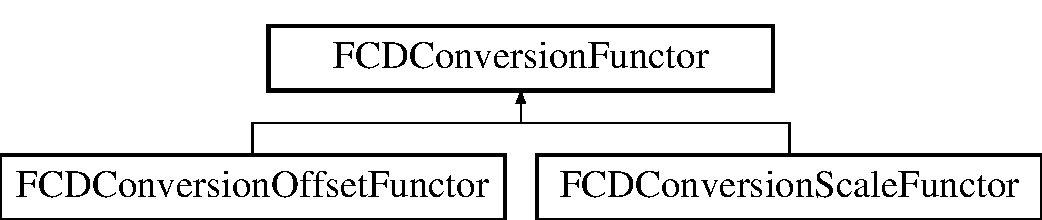
\includegraphics[height=2.000000cm]{classFCDConversionFunctor}
\end{center}
\end{figure}
\subsection*{Public Member Functions}
\begin{DoxyCompactItemize}
\item 
\hyperlink{classFCDConversionFunctor_aab15aedc7c2a7d0432d4fbd67c8b903c}{FCDConversionFunctor} ()
\item 
virtual \hyperlink{classFCDConversionFunctor_a7c986aa2bba9d01376c1f8eeae40e14f}{$\sim$FCDConversionFunctor} ()
\item 
virtual float \hyperlink{classFCDConversionFunctor_af94a77c95015ec514d041b9c71a549e2}{operator()} (float v)=0
\end{DoxyCompactItemize}


\subsection{Detailed Description}
A simple conversion functor. 

\subsection{Constructor \& Destructor Documentation}
\hypertarget{classFCDConversionFunctor_aab15aedc7c2a7d0432d4fbd67c8b903c}{
\index{FCDConversionFunctor@{FCDConversionFunctor}!FCDConversionFunctor@{FCDConversionFunctor}}
\index{FCDConversionFunctor@{FCDConversionFunctor}!FCDConversionFunctor@{FCDConversionFunctor}}
\subsubsection[{FCDConversionFunctor}]{\setlength{\rightskip}{0pt plus 5cm}FCDConversionFunctor::FCDConversionFunctor (
\begin{DoxyParamCaption}
{}
\end{DoxyParamCaption}
)\hspace{0.3cm}{\ttfamily  \mbox{[}inline\mbox{]}}}}
\label{classFCDConversionFunctor_aab15aedc7c2a7d0432d4fbd67c8b903c}
Constructor. \hypertarget{classFCDConversionFunctor_a7c986aa2bba9d01376c1f8eeae40e14f}{
\index{FCDConversionFunctor@{FCDConversionFunctor}!$\sim$FCDConversionFunctor@{$\sim$FCDConversionFunctor}}
\index{$\sim$FCDConversionFunctor@{$\sim$FCDConversionFunctor}!FCDConversionFunctor@{FCDConversionFunctor}}
\subsubsection[{$\sim$FCDConversionFunctor}]{\setlength{\rightskip}{0pt plus 5cm}virtual FCDConversionFunctor::$\sim$FCDConversionFunctor (
\begin{DoxyParamCaption}
{}
\end{DoxyParamCaption}
)\hspace{0.3cm}{\ttfamily  \mbox{[}inline, virtual\mbox{]}}}}
\label{classFCDConversionFunctor_a7c986aa2bba9d01376c1f8eeae40e14f}
Destructor. 

\subsection{Member Function Documentation}
\hypertarget{classFCDConversionFunctor_af94a77c95015ec514d041b9c71a549e2}{
\index{FCDConversionFunctor@{FCDConversionFunctor}!operator()@{operator()}}
\index{operator()@{operator()}!FCDConversionFunctor@{FCDConversionFunctor}}
\subsubsection[{operator()}]{\setlength{\rightskip}{0pt plus 5cm}virtual float FCDConversionFunctor::operator() (
\begin{DoxyParamCaption}
\item[{float}]{ v}
\end{DoxyParamCaption}
)\hspace{0.3cm}{\ttfamily  \mbox{[}pure virtual\mbox{]}}}}
\label{classFCDConversionFunctor_af94a77c95015ec514d041b9c71a549e2}
Main functor to override. 
\begin{DoxyParams}{Parameters}
\item[{\em v}]The value to convert. \end{DoxyParams}
\begin{DoxyReturn}{Returns}
The converted value. 
\end{DoxyReturn}


Implemented in \hyperlink{classFCDConversionScaleFunctor_a7e4410b974d4d79b5c7211cc42032d87}{FCDConversionScaleFunctor}, and \hyperlink{classFCDConversionOffsetFunctor_ad9fa76a47de5e11521394e7eff97e2f7}{FCDConversionOffsetFunctor}.



The documentation for this class was generated from the following file:\begin{DoxyCompactItemize}
\item 
FCollada/FCDocument/\hyperlink{FCDAnimationCurve_8h}{FCDAnimationCurve.h}\end{DoxyCompactItemize}

\hypertarget{classFCDConversionOffsetFunctor}{
\section{FCDConversionOffsetFunctor Class Reference}
\label{classFCDConversionOffsetFunctor}\index{FCDConversionOffsetFunctor@{FCDConversionOffsetFunctor}}
}


{\ttfamily \#include $<$FCDAnimationCurve.h$>$}

Inheritance diagram for FCDConversionOffsetFunctor:\begin{figure}[H]
\begin{center}
\leavevmode
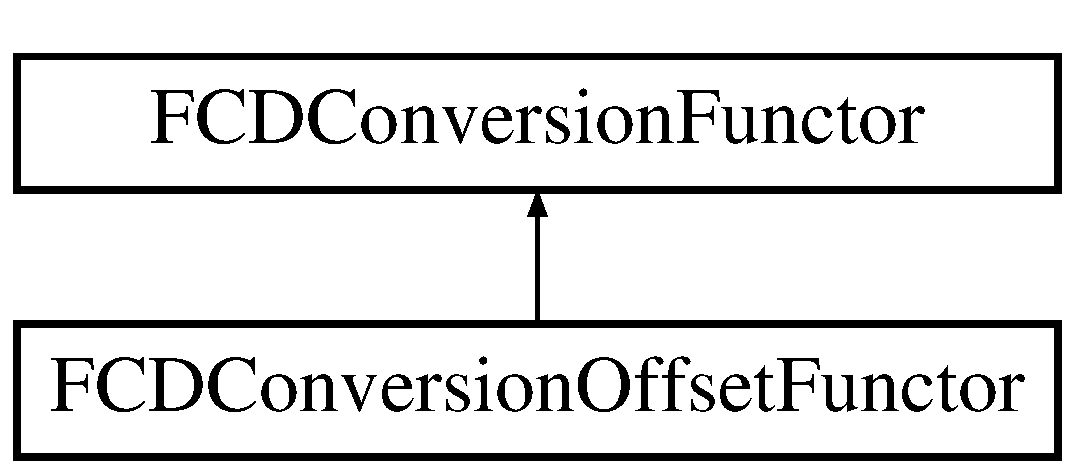
\includegraphics[height=2.000000cm]{classFCDConversionOffsetFunctor}
\end{center}
\end{figure}
\subsection*{Public Member Functions}
\begin{DoxyCompactItemize}
\item 
\hyperlink{classFCDConversionOffsetFunctor_aa26f96382ae8854e902e6dab056141d8}{FCDConversionOffsetFunctor} (float \_\-offset)
\item 
virtual \hyperlink{classFCDConversionOffsetFunctor_ac24d34325f5ece40a70063258585108e}{$\sim$FCDConversionOffsetFunctor} ()
\item 
virtual float \hyperlink{classFCDConversionOffsetFunctor_ad9fa76a47de5e11521394e7eff97e2f7}{operator()} (float v)
\end{DoxyCompactItemize}


\subsection{Detailed Description}
A sample conversion functor: it offsets the value by a given amount. 

\subsection{Constructor \& Destructor Documentation}
\hypertarget{classFCDConversionOffsetFunctor_aa26f96382ae8854e902e6dab056141d8}{
\index{FCDConversionOffsetFunctor@{FCDConversionOffsetFunctor}!FCDConversionOffsetFunctor@{FCDConversionOffsetFunctor}}
\index{FCDConversionOffsetFunctor@{FCDConversionOffsetFunctor}!FCDConversionOffsetFunctor@{FCDConversionOffsetFunctor}}
\subsubsection[{FCDConversionOffsetFunctor}]{\setlength{\rightskip}{0pt plus 5cm}FCDConversionOffsetFunctor::FCDConversionOffsetFunctor (
\begin{DoxyParamCaption}
\item[{float}]{ \_\-offset}
\end{DoxyParamCaption}
)\hspace{0.3cm}{\ttfamily  \mbox{[}inline\mbox{]}}}}
\label{classFCDConversionOffsetFunctor_aa26f96382ae8854e902e6dab056141d8}
Constructor. 
\begin{DoxyParams}{Parameters}
\item[{\em \_\-offset}]The value offset. \end{DoxyParams}
\hypertarget{classFCDConversionOffsetFunctor_ac24d34325f5ece40a70063258585108e}{
\index{FCDConversionOffsetFunctor@{FCDConversionOffsetFunctor}!$\sim$FCDConversionOffsetFunctor@{$\sim$FCDConversionOffsetFunctor}}
\index{$\sim$FCDConversionOffsetFunctor@{$\sim$FCDConversionOffsetFunctor}!FCDConversionOffsetFunctor@{FCDConversionOffsetFunctor}}
\subsubsection[{$\sim$FCDConversionOffsetFunctor}]{\setlength{\rightskip}{0pt plus 5cm}virtual FCDConversionOffsetFunctor::$\sim$FCDConversionOffsetFunctor (
\begin{DoxyParamCaption}
{}
\end{DoxyParamCaption}
)\hspace{0.3cm}{\ttfamily  \mbox{[}inline, virtual\mbox{]}}}}
\label{classFCDConversionOffsetFunctor_ac24d34325f5ece40a70063258585108e}
Destructor. 

\subsection{Member Function Documentation}
\hypertarget{classFCDConversionOffsetFunctor_ad9fa76a47de5e11521394e7eff97e2f7}{
\index{FCDConversionOffsetFunctor@{FCDConversionOffsetFunctor}!operator()@{operator()}}
\index{operator()@{operator()}!FCDConversionOffsetFunctor@{FCDConversionOffsetFunctor}}
\subsubsection[{operator()}]{\setlength{\rightskip}{0pt plus 5cm}virtual float FCDConversionOffsetFunctor::operator() (
\begin{DoxyParamCaption}
\item[{float}]{ v}
\end{DoxyParamCaption}
)\hspace{0.3cm}{\ttfamily  \mbox{[}inline, virtual\mbox{]}}}}
\label{classFCDConversionOffsetFunctor_ad9fa76a47de5e11521394e7eff97e2f7}
Offsets the given value. 
\begin{DoxyParams}{Parameters}
\item[{\em v}]The value to offset. \end{DoxyParams}
\begin{DoxyReturn}{Returns}
The offseted value. 
\end{DoxyReturn}


Implements \hyperlink{classFCDConversionFunctor_af94a77c95015ec514d041b9c71a549e2}{FCDConversionFunctor}.



The documentation for this class was generated from the following file:\begin{DoxyCompactItemize}
\item 
FCollada/FCDocument/\hyperlink{FCDAnimationCurve_8h}{FCDAnimationCurve.h}\end{DoxyCompactItemize}

\hypertarget{classFCDConversionScaleFunctor}{
\section{FCDConversionScaleFunctor Class Reference}
\label{classFCDConversionScaleFunctor}\index{FCDConversionScaleFunctor@{FCDConversionScaleFunctor}}
}


{\ttfamily \#include $<$FCDAnimationCurve.h$>$}

Inheritance diagram for FCDConversionScaleFunctor:\begin{figure}[H]
\begin{center}
\leavevmode
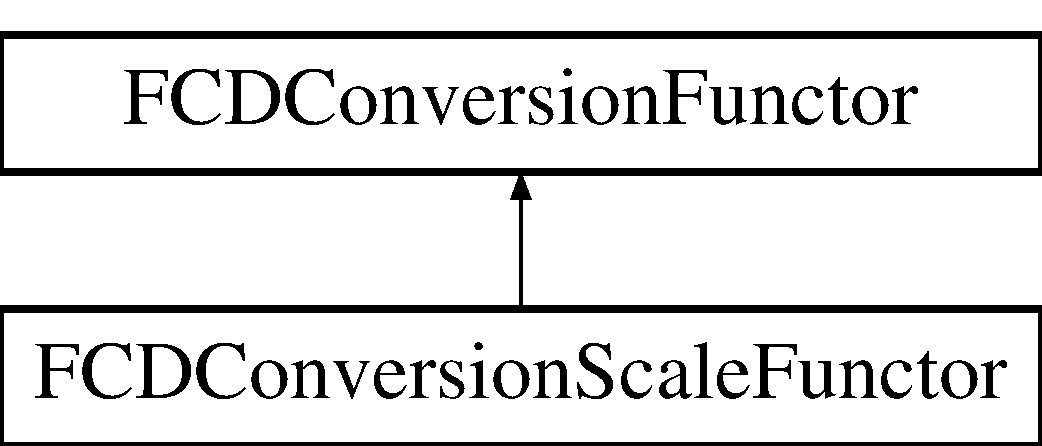
\includegraphics[height=2.000000cm]{classFCDConversionScaleFunctor}
\end{center}
\end{figure}
\subsection*{Public Member Functions}
\begin{DoxyCompactItemize}
\item 
\hyperlink{classFCDConversionScaleFunctor_a82e1e5fdf55999dd2d9a12a886003b0c}{FCDConversionScaleFunctor} (float factor)
\item 
void \hyperlink{classFCDConversionScaleFunctor_a5e5f3036da8df4e3c5304346627108ec}{SetScaleFactor} (float factor)
\item 
virtual \hyperlink{classFCDConversionScaleFunctor_a56b2908039ef33c68f5ea9fe3c207d0b}{$\sim$FCDConversionScaleFunctor} ()
\item 
virtual float \hyperlink{classFCDConversionScaleFunctor_a7e4410b974d4d79b5c7211cc42032d87}{operator()} (float v)
\item 
virtual \hyperlink{classFMVector3}{FMVector3} \hyperlink{classFCDConversionScaleFunctor_a0a978f0896ca17db695e5acf08d6da9c}{operator()} (const \hyperlink{classFMVector3}{FMVector3} \&v)
\item 
virtual \hyperlink{classFMVector4}{FMVector4} \hyperlink{classFCDConversionScaleFunctor_a4ed5f3f3fa4619b3374442a3f4c3de5a}{operator()} (const \hyperlink{classFMVector4}{FMVector4} \&v)
\end{DoxyCompactItemize}


\subsection{Detailed Description}
A sample conversion functor: it scales the value by a given amount. 

\subsection{Constructor \& Destructor Documentation}
\hypertarget{classFCDConversionScaleFunctor_a82e1e5fdf55999dd2d9a12a886003b0c}{
\index{FCDConversionScaleFunctor@{FCDConversionScaleFunctor}!FCDConversionScaleFunctor@{FCDConversionScaleFunctor}}
\index{FCDConversionScaleFunctor@{FCDConversionScaleFunctor}!FCDConversionScaleFunctor@{FCDConversionScaleFunctor}}
\subsubsection[{FCDConversionScaleFunctor}]{\setlength{\rightskip}{0pt plus 5cm}FCDConversionScaleFunctor::FCDConversionScaleFunctor (
\begin{DoxyParamCaption}
\item[{float}]{ factor}
\end{DoxyParamCaption}
)\hspace{0.3cm}{\ttfamily  \mbox{[}inline\mbox{]}}}}
\label{classFCDConversionScaleFunctor_a82e1e5fdf55999dd2d9a12a886003b0c}
Constructor. 
\begin{DoxyParams}{Parameters}
\item[{\em factor}]The scale factor. \end{DoxyParams}
\hypertarget{classFCDConversionScaleFunctor_a56b2908039ef33c68f5ea9fe3c207d0b}{
\index{FCDConversionScaleFunctor@{FCDConversionScaleFunctor}!$\sim$FCDConversionScaleFunctor@{$\sim$FCDConversionScaleFunctor}}
\index{$\sim$FCDConversionScaleFunctor@{$\sim$FCDConversionScaleFunctor}!FCDConversionScaleFunctor@{FCDConversionScaleFunctor}}
\subsubsection[{$\sim$FCDConversionScaleFunctor}]{\setlength{\rightskip}{0pt plus 5cm}virtual FCDConversionScaleFunctor::$\sim$FCDConversionScaleFunctor (
\begin{DoxyParamCaption}
{}
\end{DoxyParamCaption}
)\hspace{0.3cm}{\ttfamily  \mbox{[}inline, virtual\mbox{]}}}}
\label{classFCDConversionScaleFunctor_a56b2908039ef33c68f5ea9fe3c207d0b}
Destructor. 

\subsection{Member Function Documentation}
\hypertarget{classFCDConversionScaleFunctor_a7e4410b974d4d79b5c7211cc42032d87}{
\index{FCDConversionScaleFunctor@{FCDConversionScaleFunctor}!operator()@{operator()}}
\index{operator()@{operator()}!FCDConversionScaleFunctor@{FCDConversionScaleFunctor}}
\subsubsection[{operator()}]{\setlength{\rightskip}{0pt plus 5cm}virtual float FCDConversionScaleFunctor::operator() (
\begin{DoxyParamCaption}
\item[{float}]{ v}
\end{DoxyParamCaption}
)\hspace{0.3cm}{\ttfamily  \mbox{[}inline, virtual\mbox{]}}}}
\label{classFCDConversionScaleFunctor_a7e4410b974d4d79b5c7211cc42032d87}
Scales the given value. 
\begin{DoxyParams}{Parameters}
\item[{\em v}]The value to scale. \end{DoxyParams}
\begin{DoxyReturn}{Returns}
The scaled value. 
\end{DoxyReturn}


Implements \hyperlink{classFCDConversionFunctor_af94a77c95015ec514d041b9c71a549e2}{FCDConversionFunctor}.

\hypertarget{classFCDConversionScaleFunctor_a4ed5f3f3fa4619b3374442a3f4c3de5a}{
\index{FCDConversionScaleFunctor@{FCDConversionScaleFunctor}!operator()@{operator()}}
\index{operator()@{operator()}!FCDConversionScaleFunctor@{FCDConversionScaleFunctor}}
\subsubsection[{operator()}]{\setlength{\rightskip}{0pt plus 5cm}virtual {\bf FMVector4} FCDConversionScaleFunctor::operator() (
\begin{DoxyParamCaption}
\item[{const {\bf FMVector4} \&}]{ v}
\end{DoxyParamCaption}
)\hspace{0.3cm}{\ttfamily  \mbox{[}inline, virtual\mbox{]}}}}
\label{classFCDConversionScaleFunctor_a4ed5f3f3fa4619b3374442a3f4c3de5a}
Scales the given \hyperlink{classFMVector4}{FMVector4}. 
\begin{DoxyParams}{Parameters}
\item[{\em v}]The value to scale. \end{DoxyParams}
\begin{DoxyReturn}{Returns}
The scaled value. 
\end{DoxyReturn}
\hypertarget{classFCDConversionScaleFunctor_a0a978f0896ca17db695e5acf08d6da9c}{
\index{FCDConversionScaleFunctor@{FCDConversionScaleFunctor}!operator()@{operator()}}
\index{operator()@{operator()}!FCDConversionScaleFunctor@{FCDConversionScaleFunctor}}
\subsubsection[{operator()}]{\setlength{\rightskip}{0pt plus 5cm}virtual {\bf FMVector3} FCDConversionScaleFunctor::operator() (
\begin{DoxyParamCaption}
\item[{const {\bf FMVector3} \&}]{ v}
\end{DoxyParamCaption}
)\hspace{0.3cm}{\ttfamily  \mbox{[}inline, virtual\mbox{]}}}}
\label{classFCDConversionScaleFunctor_a0a978f0896ca17db695e5acf08d6da9c}
Scales the given \hyperlink{classFMVector3}{FMVector3}. 
\begin{DoxyParams}{Parameters}
\item[{\em v}]The value to scale. \end{DoxyParams}
\begin{DoxyReturn}{Returns}
The scaled value. 
\end{DoxyReturn}
\hypertarget{classFCDConversionScaleFunctor_a5e5f3036da8df4e3c5304346627108ec}{
\index{FCDConversionScaleFunctor@{FCDConversionScaleFunctor}!SetScaleFactor@{SetScaleFactor}}
\index{SetScaleFactor@{SetScaleFactor}!FCDConversionScaleFunctor@{FCDConversionScaleFunctor}}
\subsubsection[{SetScaleFactor}]{\setlength{\rightskip}{0pt plus 5cm}void FCDConversionScaleFunctor::SetScaleFactor (
\begin{DoxyParamCaption}
\item[{float}]{ factor}
\end{DoxyParamCaption}
)\hspace{0.3cm}{\ttfamily  \mbox{[}inline\mbox{]}}}}
\label{classFCDConversionScaleFunctor_a5e5f3036da8df4e3c5304346627108ec}
Mutator. 
\begin{DoxyParams}{Parameters}
\item[{\em factor}]The new scale factor. \end{DoxyParams}


The documentation for this class was generated from the following file:\begin{DoxyCompactItemize}
\item 
FCollada/FCDocument/\hyperlink{FCDAnimationCurve_8h}{FCDAnimationCurve.h}\end{DoxyCompactItemize}

\hypertarget{classFCDocumentTools_1_1FCDConversionSwapFunctor}{
\section{FCDocumentTools::FCDConversionSwapFunctor Class Reference}
\label{classFCDocumentTools_1_1FCDConversionSwapFunctor}\index{FCDocumentTools::FCDConversionSwapFunctor@{FCDocumentTools::FCDConversionSwapFunctor}}
}
\subsection*{Public Member Functions}
\begin{DoxyCompactItemize}
\item 
\hypertarget{classFCDocumentTools_1_1FCDConversionSwapFunctor_a101c31762b7b03375a90241e8af2d3b2}{
{\bfseries FCDConversionSwapFunctor} (const \hyperlink{classFMVector3}{FMVector3} \&targetAxis)}
\label{classFCDocumentTools_1_1FCDConversionSwapFunctor_a101c31762b7b03375a90241e8af2d3b2}

\item 
\hypertarget{classFCDocumentTools_1_1FCDConversionSwapFunctor_af59f7914484fc9af271b8f2ca5460ac3}{
void {\bfseries SetCurrent} (const \hyperlink{classFMVector3}{FMVector3} \&axis)}
\label{classFCDocumentTools_1_1FCDConversionSwapFunctor_af59f7914484fc9af271b8f2ca5460ac3}

\item 
\hypertarget{classFCDocumentTools_1_1FCDConversionSwapFunctor_a88ab9273b9cea87eff129b50c8cf14cb}{
bool {\bfseries HasConversion} ()}
\label{classFCDocumentTools_1_1FCDConversionSwapFunctor_a88ab9273b9cea87eff129b50c8cf14cb}

\item 
\hypertarget{classFCDocumentTools_1_1FCDConversionSwapFunctor_a9b1ed0ac0a4d9eee6d5b5209ca2ad4bf}{
void {\bfseries SetPivotTransform} (\hyperlink{classFCDSceneNode}{FCDSceneNode} $\ast$node, bool rollOnly)}
\label{classFCDocumentTools_1_1FCDConversionSwapFunctor_a9b1ed0ac0a4d9eee6d5b5209ca2ad4bf}

\item 
\hypertarget{classFCDocumentTools_1_1FCDConversionSwapFunctor_aa01c7004fb61542e20d0d0d93bae3795}{
void {\bfseries operator()} (\hyperlink{classFMVector3}{FMVector3} \&data, bool isScale=false)}
\label{classFCDocumentTools_1_1FCDConversionSwapFunctor_aa01c7004fb61542e20d0d0d93bae3795}

\end{DoxyCompactItemize}
\subsection*{Static Public Member Functions}
\begin{DoxyCompactItemize}
\item 
\hypertarget{classFCDocumentTools_1_1FCDConversionSwapFunctor_a9489874fd8ea50f164ad706c0359b366}{
static \hyperlink{classFCDTRotation}{FCDTRotation} $\ast$ {\bfseries GetLastTransformForPivot} (\hyperlink{classFCDSceneNode}{FCDSceneNode} $\ast$node)}
\label{classFCDocumentTools_1_1FCDConversionSwapFunctor_a9489874fd8ea50f164ad706c0359b366}

\item 
\hypertarget{classFCDocumentTools_1_1FCDConversionSwapFunctor_a85fdfa24778d6eca385905c2b72a78ca}{
static void {\bfseries SmartAddRotationPivot} (\hyperlink{classFCDSceneNode}{FCDSceneNode} $\ast$node, const \hyperlink{classFMVector3}{FMVector3} \&axis, float angle)}
\label{classFCDocumentTools_1_1FCDConversionSwapFunctor_a85fdfa24778d6eca385905c2b72a78ca}

\end{DoxyCompactItemize}


The documentation for this class was generated from the following file:\begin{DoxyCompactItemize}
\item 
FCollada/FCDocument/FCDocumentTools.cpp\end{DoxyCompactItemize}

\hypertarget{classFCDocumentTools_1_1FCDConversionUnitFunctor}{
\section{FCDocumentTools::FCDConversionUnitFunctor Class Reference}
\label{classFCDocumentTools_1_1FCDConversionUnitFunctor}\index{FCDocumentTools::FCDConversionUnitFunctor@{FCDocumentTools::FCDConversionUnitFunctor}}
}
\subsection*{Public Member Functions}
\begin{DoxyCompactItemize}
\item 
\hypertarget{classFCDocumentTools_1_1FCDConversionUnitFunctor_ac9cb423a7036d946dbfaecfb83402a6f}{
{\bfseries FCDConversionUnitFunctor} (float \_\-target)}
\label{classFCDocumentTools_1_1FCDConversionUnitFunctor_ac9cb423a7036d946dbfaecfb83402a6f}

\item 
\hypertarget{classFCDocumentTools_1_1FCDConversionUnitFunctor_afa0ce9f99556c1cda9d892f8a1745db3}{
bool {\bfseries HasConversion} ()}
\label{classFCDocumentTools_1_1FCDConversionUnitFunctor_afa0ce9f99556c1cda9d892f8a1745db3}

\item 
\hypertarget{classFCDocumentTools_1_1FCDConversionUnitFunctor_aaf9ac74e073e6c4ff7effc1b1afbbc95}{
void {\bfseries SetCurrent} (float current)}
\label{classFCDocumentTools_1_1FCDConversionUnitFunctor_aaf9ac74e073e6c4ff7effc1b1afbbc95}

\item 
\hypertarget{classFCDocumentTools_1_1FCDConversionUnitFunctor_ab804adcbeb8a39d116aa0fe73a4d3d36}{
float {\bfseries GetConversionFactor} ()}
\label{classFCDocumentTools_1_1FCDConversionUnitFunctor_ab804adcbeb8a39d116aa0fe73a4d3d36}

\item 
\hypertarget{classFCDocumentTools_1_1FCDConversionUnitFunctor_ab56fdb237462072b96a54e9deaf08583}{
void {\bfseries operator()} (float \&data)}
\label{classFCDocumentTools_1_1FCDConversionUnitFunctor_ab56fdb237462072b96a54e9deaf08583}

\item 
\hypertarget{classFCDocumentTools_1_1FCDConversionUnitFunctor_abf6ec5a61dcae64596bca328a054417d}{
void {\bfseries operator()} (\hyperlink{classFMVector3}{FMVector3} \&data)}
\label{classFCDocumentTools_1_1FCDConversionUnitFunctor_abf6ec5a61dcae64596bca328a054417d}

\end{DoxyCompactItemize}


The documentation for this class was generated from the following file:\begin{DoxyCompactItemize}
\item 
FCollada/FCDocument/FCDocumentTools.cpp\end{DoxyCompactItemize}

\hypertarget{classFCDEAttribute}{
\section{FCDEAttribute Class Reference}
\label{classFCDEAttribute}\index{FCDEAttribute@{FCDEAttribute}}
}


{\ttfamily \#include $<$FCDExtra.h$>$}

Inheritance diagram for FCDEAttribute:\begin{figure}[H]
\begin{center}
\leavevmode
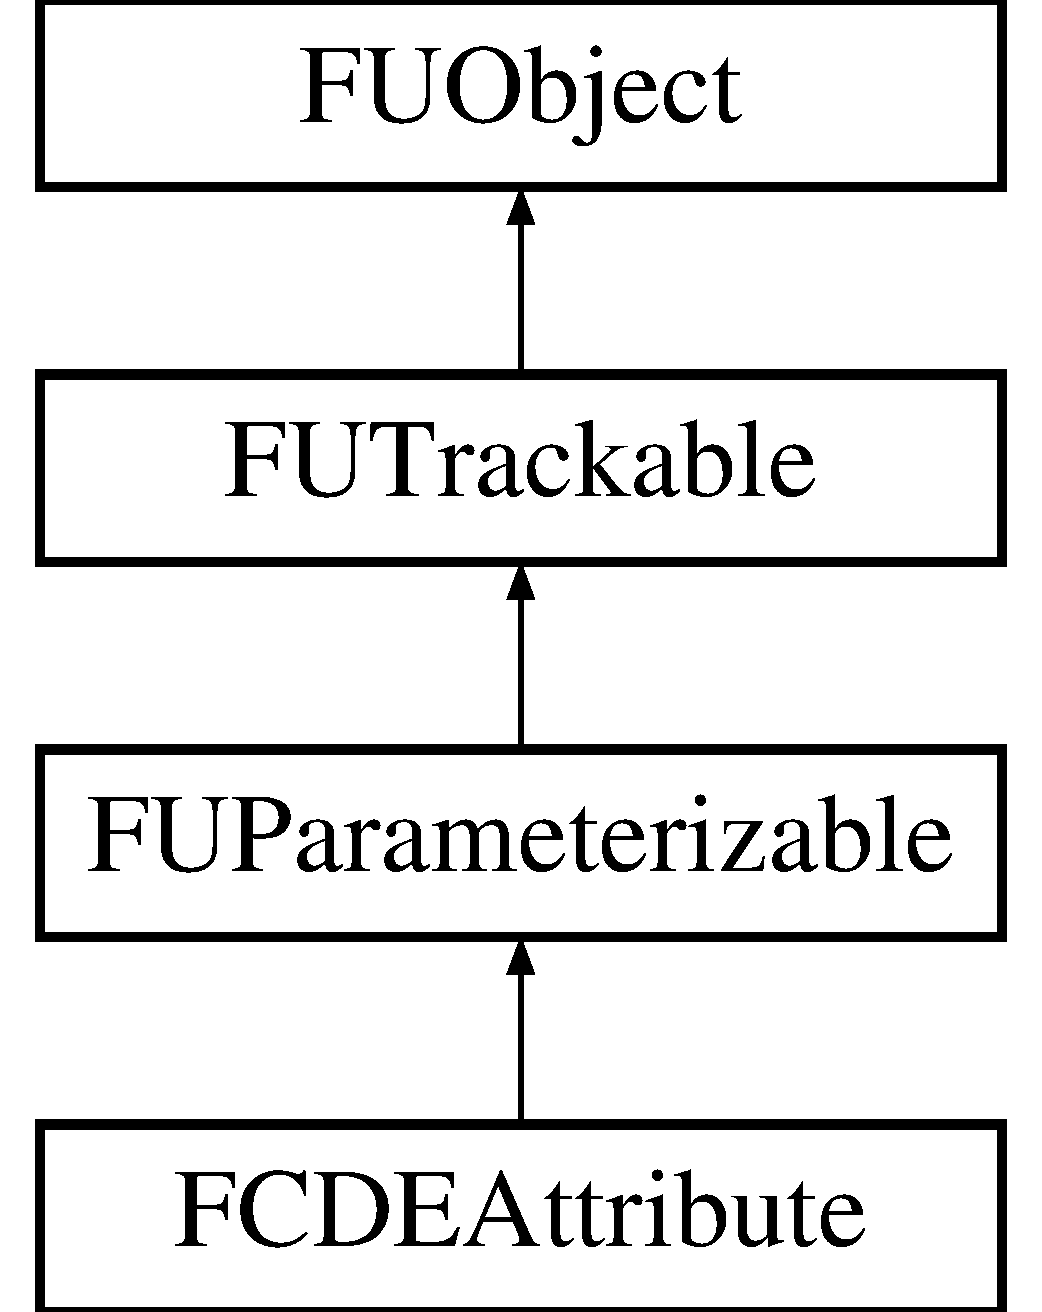
\includegraphics[height=4.000000cm]{classFCDEAttribute}
\end{center}
\end{figure}
\subsection*{Public Member Functions}
\begin{DoxyCompactItemize}
\item 
\hyperlink{classFCDEAttribute_a5bd4a74cf8705804a3bb43336d7eeb80}{FCDEAttribute} ()
\item 
\hyperlink{classFCDEAttribute_a653f729f45533b8ece04792d054967bd}{FCDEAttribute} (const char $\ast$name, const fchar $\ast$value)
\item 
const \hyperlink{classfm_1_1stringT}{fm::string} \& \hyperlink{classFCDEAttribute_a66cbc2e664e7fdf7a994af9744787813}{GetName} () const 
\item 
void \hyperlink{classFCDEAttribute_a1af3d0cbe4b804a053a09dbdb9275a04}{SetName} (const \hyperlink{classfm_1_1stringT}{fm::string} \&\_\-name)
\item 
const \hyperlink{classfm_1_1stringT}{fstring} \& \hyperlink{classFCDEAttribute_ae09637bac4d6ae26ac7afb01a241c53e}{GetValue} () const 
\item 
void \hyperlink{classFCDEAttribute_ae85287f77ddb40b5797d83fcd686f549}{SetValue} (const \hyperlink{classfm_1_1stringT}{fstring} \&\_\-value)
\end{DoxyCompactItemize}


\subsection{Detailed Description}
An extra tree attribute. Contains a name and a value string. 

\subsection{Constructor \& Destructor Documentation}
\hypertarget{classFCDEAttribute_a5bd4a74cf8705804a3bb43336d7eeb80}{
\index{FCDEAttribute@{FCDEAttribute}!FCDEAttribute@{FCDEAttribute}}
\index{FCDEAttribute@{FCDEAttribute}!FCDEAttribute@{FCDEAttribute}}
\subsubsection[{FCDEAttribute}]{\setlength{\rightskip}{0pt plus 5cm}FCDEAttribute::FCDEAttribute (
\begin{DoxyParamCaption}
{}
\end{DoxyParamCaption}
)}}
\label{classFCDEAttribute_a5bd4a74cf8705804a3bb43336d7eeb80}
Default constructor. The name and the value string will be blank. \hypertarget{classFCDEAttribute_a653f729f45533b8ece04792d054967bd}{
\index{FCDEAttribute@{FCDEAttribute}!FCDEAttribute@{FCDEAttribute}}
\index{FCDEAttribute@{FCDEAttribute}!FCDEAttribute@{FCDEAttribute}}
\subsubsection[{FCDEAttribute}]{\setlength{\rightskip}{0pt plus 5cm}FCDEAttribute::FCDEAttribute (
\begin{DoxyParamCaption}
\item[{const char $\ast$}]{ name, }
\item[{const fchar $\ast$}]{ value}
\end{DoxyParamCaption}
)}}
\label{classFCDEAttribute_a653f729f45533b8ece04792d054967bd}
Constructor. Sets the attribute name and the attribute value appropriately. 
\begin{DoxyParams}{Parameters}
\item[{\em name}]The attribute name. \item[{\em value}]The attribute value. \end{DoxyParams}


\subsection{Member Function Documentation}
\hypertarget{classFCDEAttribute_a66cbc2e664e7fdf7a994af9744787813}{
\index{FCDEAttribute@{FCDEAttribute}!GetName@{GetName}}
\index{GetName@{GetName}!FCDEAttribute@{FCDEAttribute}}
\subsubsection[{GetName}]{\setlength{\rightskip}{0pt plus 5cm}const {\bf fm::string}\& FCDEAttribute::GetName (
\begin{DoxyParamCaption}
{}
\end{DoxyParamCaption}
) const\hspace{0.3cm}{\ttfamily  \mbox{[}inline\mbox{]}}}}
\label{classFCDEAttribute_a66cbc2e664e7fdf7a994af9744787813}
Retrieves the name of the attribute. \begin{DoxyReturn}{Returns}
The name of the attribute. 
\end{DoxyReturn}
\hypertarget{classFCDEAttribute_ae09637bac4d6ae26ac7afb01a241c53e}{
\index{FCDEAttribute@{FCDEAttribute}!GetValue@{GetValue}}
\index{GetValue@{GetValue}!FCDEAttribute@{FCDEAttribute}}
\subsubsection[{GetValue}]{\setlength{\rightskip}{0pt plus 5cm}const {\bf fstring}\& FCDEAttribute::GetValue (
\begin{DoxyParamCaption}
{}
\end{DoxyParamCaption}
) const\hspace{0.3cm}{\ttfamily  \mbox{[}inline\mbox{]}}}}
\label{classFCDEAttribute_ae09637bac4d6ae26ac7afb01a241c53e}
Retrieves the value of the attribute. \begin{DoxyReturn}{Returns}
The value of the attribute. 
\end{DoxyReturn}
\hypertarget{classFCDEAttribute_a1af3d0cbe4b804a053a09dbdb9275a04}{
\index{FCDEAttribute@{FCDEAttribute}!SetName@{SetName}}
\index{SetName@{SetName}!FCDEAttribute@{FCDEAttribute}}
\subsubsection[{SetName}]{\setlength{\rightskip}{0pt plus 5cm}void FCDEAttribute::SetName (
\begin{DoxyParamCaption}
\item[{const {\bf fm::string} \&}]{ \_\-name}
\end{DoxyParamCaption}
)\hspace{0.3cm}{\ttfamily  \mbox{[}inline\mbox{]}}}}
\label{classFCDEAttribute_a1af3d0cbe4b804a053a09dbdb9275a04}
Sets the name of the attribute. 
\begin{DoxyParams}{Parameters}
\item[{\em \_\-name}]The new name of the attribute. \end{DoxyParams}
\hypertarget{classFCDEAttribute_ae85287f77ddb40b5797d83fcd686f549}{
\index{FCDEAttribute@{FCDEAttribute}!SetValue@{SetValue}}
\index{SetValue@{SetValue}!FCDEAttribute@{FCDEAttribute}}
\subsubsection[{SetValue}]{\setlength{\rightskip}{0pt plus 5cm}void FCDEAttribute::SetValue (
\begin{DoxyParamCaption}
\item[{const {\bf fstring} \&}]{ \_\-value}
\end{DoxyParamCaption}
)\hspace{0.3cm}{\ttfamily  \mbox{[}inline\mbox{]}}}}
\label{classFCDEAttribute_ae85287f77ddb40b5797d83fcd686f549}
Sets the value of the attribute. 
\begin{DoxyParams}{Parameters}
\item[{\em \_\-value}]The new value of the attribute. \end{DoxyParams}


The documentation for this class was generated from the following files:\begin{DoxyCompactItemize}
\item 
FCollada/FCDocument/\hyperlink{FCDExtra_8h}{FCDExtra.h}\item 
FCollada/FCDocument/FCDExtra.cpp\end{DoxyCompactItemize}

\hypertarget{classFCDEffect}{
\section{FCDEffect Class Reference}
\label{classFCDEffect}\index{FCDEffect@{FCDEffect}}
}


{\ttfamily \#include $<$FCDEffect.h$>$}

Inheritance diagram for FCDEffect:\begin{figure}[H]
\begin{center}
\leavevmode
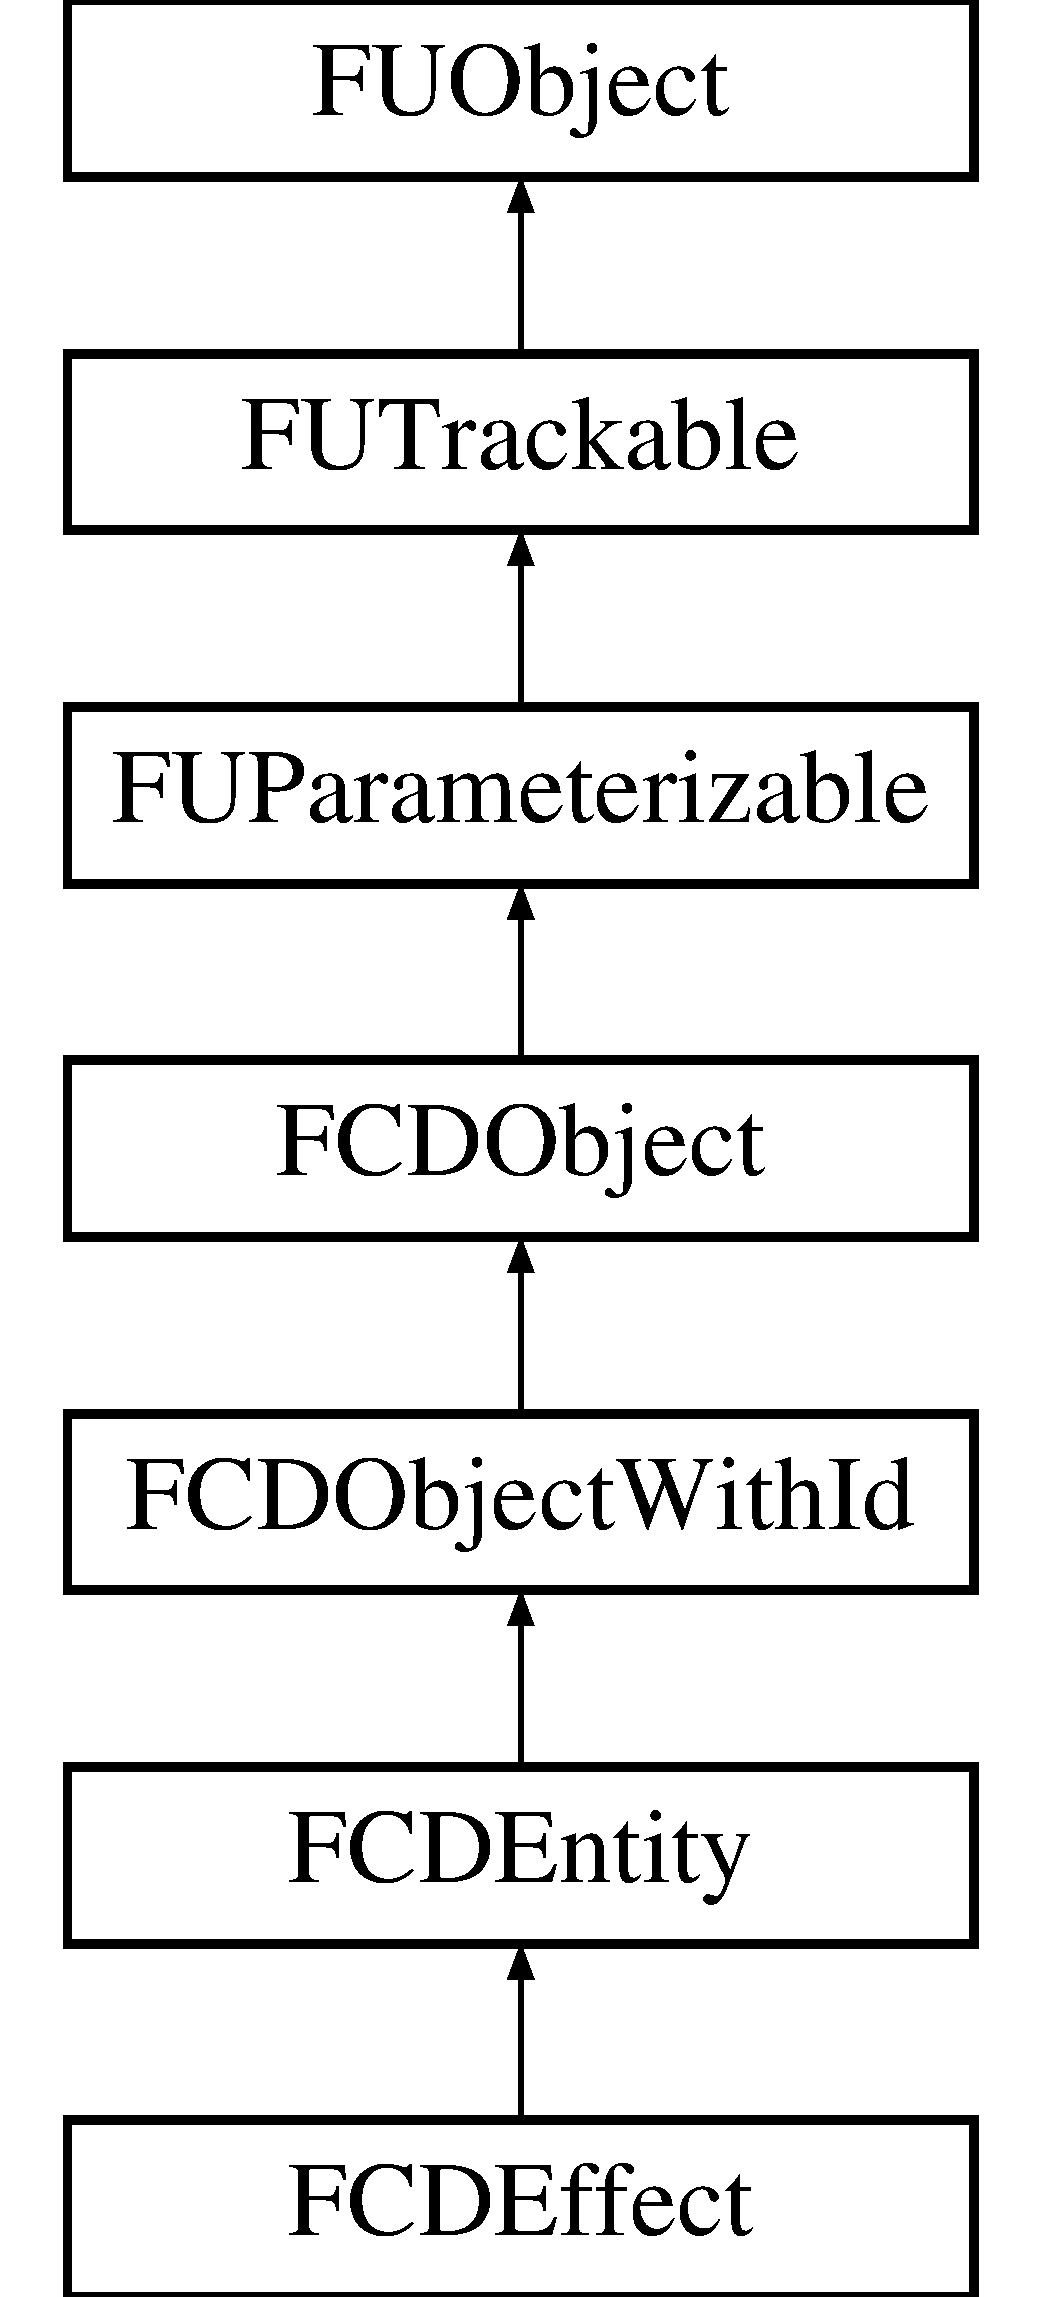
\includegraphics[height=7.000000cm]{classFCDEffect}
\end{center}
\end{figure}
\subsection*{Public Member Functions}
\begin{DoxyCompactItemize}
\item 
\hyperlink{classFCDEffect_ad2e620e6c041da706302e8541344a5e9}{FCDEffect} (\hyperlink{classFCDocument}{FCDocument} $\ast$document)
\item 
virtual \hyperlink{classFCDEffect_a6c1b6a6d3aefb9c011dd8fa7c116e0d6}{$\sim$FCDEffect} ()
\item 
virtual \hyperlink{classFCDEntity_a9301a4bd5f4d4190ec13e40db4effdd7}{Type} \hyperlink{classFCDEffect_ab6106f67f33a4cb049ea17a1970bbfbe}{GetType} () const 
\item 
size\_\-t \hyperlink{classFCDEffect_a07ca7c378d3ecf158beefe5ba35143ae}{GetProfileCount} () const 
\item 
\hyperlink{classFCDEffectProfile}{FCDEffectProfile} $\ast$ \hyperlink{classFCDEffect_a22c8dc9f098387eaa2ffb6a66aceb22d}{GetProfile} (size\_\-t index)
\item 
const \hyperlink{classFCDEffectProfile}{FCDEffectProfile} $\ast$ \hyperlink{classFCDEffect_aad9b921743685b02b847d30670dc1631}{GetProfile} (size\_\-t index) const 
\item 
\hyperlink{classFCDEffect_a227ef80a932cf071f0fdd299b00cfed9}{DEPRECATED} (3.05A, GetProfileCount and GetProfile(index)) void GetProfiles() const 
\item 
const \hyperlink{classFCDEffectProfile}{FCDEffectProfile} $\ast$ \hyperlink{classFCDEffect_ad81082bec4aa4d90bf595b598e8f3330}{FindProfile} (\hyperlink{namespaceFUDaeProfileType_ac10ea253a7a141708de2324a929f8a79}{FUDaeProfileType::Type} type) const 
\item 
\hyperlink{classFCDEffectProfile}{FCDEffectProfile} $\ast$ \hyperlink{classFCDEffect_a110a7d6488fc376b63e3f6ef7166e0c4}{FindProfile} (\hyperlink{namespaceFUDaeProfileType_ac10ea253a7a141708de2324a929f8a79}{FUDaeProfileType::Type} type)
\item 
\hyperlink{classFCDEffectProfile}{FCDEffectProfile} $\ast$ \hyperlink{classFCDEffect_a439f45f6a34e9ae11990e8bded9b9867}{FindProfileByTypeAndPlatform} (\hyperlink{namespaceFUDaeProfileType_ac10ea253a7a141708de2324a929f8a79}{FUDaeProfileType::Type} type, const \hyperlink{classfm_1_1stringT}{fm::string} \&platform)
\item 
const \hyperlink{classFCDEffectProfile}{FCDEffectProfile} $\ast$ \hyperlink{classFCDEffect_a6f82a6071958b135a8655702d3875b58}{FindProfileByTypeAndPlatform} (\hyperlink{namespaceFUDaeProfileType_ac10ea253a7a141708de2324a929f8a79}{FUDaeProfileType::Type} type, const \hyperlink{classfm_1_1stringT}{fm::string} \&platform) const 
\item 
bool \hyperlink{classFCDEffect_a0e210e70a9933fc89f314747edbb3bf5}{HasProfile} (\hyperlink{namespaceFUDaeProfileType_ac10ea253a7a141708de2324a929f8a79}{FUDaeProfileType::Type} type) const 
\item 
\hyperlink{classFCDEffectProfile}{FCDEffectProfile} $\ast$ \hyperlink{classFCDEffect_abe53b1e58ce5469b28f63b5155703a95}{AddProfile} (\hyperlink{namespaceFUDaeProfileType_ac10ea253a7a141708de2324a929f8a79}{FUDaeProfileType::Type} type)
\item 
size\_\-t \hyperlink{classFCDEffect_aa0a011919dc7b8b3e40d07b3110f85b3}{GetEffectParameterCount} () const 
\item 
\hyperlink{classFCDEffectParameter}{FCDEffectParameter} $\ast$ \hyperlink{classFCDEffect_aa426058e105da62cec3eb4f8f3efd31c}{GetEffectParameter} (size\_\-t index)
\item 
\hypertarget{classFCDEffect_ac4da98a447ccfeb406fce54c5a880fd5}{
const \hyperlink{classFCDEffectParameter}{FCDEffectParameter} $\ast$ {\bfseries GetEffectParameter} (size\_\-t index) const }
\label{classFCDEffect_ac4da98a447ccfeb406fce54c5a880fd5}

\item 
\hyperlink{classFCDEffectParameter}{FCDEffectParameter} $\ast$ \hyperlink{classFCDEffect_a19ae444c7d61d619accac5eab4f1ea4e}{AddEffectParameter} (uint32 type)
\item 
virtual \hyperlink{classFCDEntity}{FCDEntity} $\ast$ \hyperlink{classFCDEffect_a7582fbc089f3eff95fd522c20d492b98}{Clone} (\hyperlink{classFCDEntity}{FCDEntity} $\ast$clone=NULL, bool cloneChildren=false) const 
\item 
\hyperlink{classFCDEffect_a20106fd0bb005c517153dc5cedc14a23}{DEPRECATED} (3.05A, not recommended) void Flatten()
\end{DoxyCompactItemize}


\subsection{Detailed Description}
A COLLADA effect.

A COLLADA effect is one of many abstraction level that defines how to render mesh polygon sets. It contains one or more rendering profile that the application can choose to support. In theory, all the rendering profiles should reach the same render output, using different rendering technologies.

An effect may also declare new general purpose parameters that are common to all the profiles. 

\subsection{Constructor \& Destructor Documentation}
\hypertarget{classFCDEffect_ad2e620e6c041da706302e8541344a5e9}{
\index{FCDEffect@{FCDEffect}!FCDEffect@{FCDEffect}}
\index{FCDEffect@{FCDEffect}!FCDEffect@{FCDEffect}}
\subsubsection[{FCDEffect}]{\setlength{\rightskip}{0pt plus 5cm}FCDEffect::FCDEffect (
\begin{DoxyParamCaption}
\item[{{\bf FCDocument} $\ast$}]{ document}
\end{DoxyParamCaption}
)}}
\label{classFCDEffect_ad2e620e6c041da706302e8541344a5e9}
Constructor: do not use directly. Instead use the \hyperlink{classFCDLibrary_aa5cdcac5a447298d5e3816e4f8c864d0}{FCDLibrary::AddEntity} function. 
\begin{DoxyParams}{Parameters}
\item[{\em document}]The COLLADA document that owns this effect. \end{DoxyParams}
\hypertarget{classFCDEffect_a6c1b6a6d3aefb9c011dd8fa7c116e0d6}{
\index{FCDEffect@{FCDEffect}!$\sim$FCDEffect@{$\sim$FCDEffect}}
\index{$\sim$FCDEffect@{$\sim$FCDEffect}!FCDEffect@{FCDEffect}}
\subsubsection[{$\sim$FCDEffect}]{\setlength{\rightskip}{0pt plus 5cm}FCDEffect::$\sim$FCDEffect (
\begin{DoxyParamCaption}
{}
\end{DoxyParamCaption}
)\hspace{0.3cm}{\ttfamily  \mbox{[}virtual\mbox{]}}}}
\label{classFCDEffect_a6c1b6a6d3aefb9c011dd8fa7c116e0d6}
Destructor. 

\subsection{Member Function Documentation}
\hypertarget{classFCDEffect_a19ae444c7d61d619accac5eab4f1ea4e}{
\index{FCDEffect@{FCDEffect}!AddEffectParameter@{AddEffectParameter}}
\index{AddEffectParameter@{AddEffectParameter}!FCDEffect@{FCDEffect}}
\subsubsection[{AddEffectParameter}]{\setlength{\rightskip}{0pt plus 5cm}{\bf FCDEffectParameter} $\ast$ FCDEffect::AddEffectParameter (
\begin{DoxyParamCaption}
\item[{uint32}]{ type}
\end{DoxyParamCaption}
)}}
\label{classFCDEffect_a19ae444c7d61d619accac5eab4f1ea4e}
Adds a local effect parameter to the local list. \begin{DoxySeeAlso}{See also}
\hyperlink{classFCDEffectParameter_a1efe74553d2ed199435085c171743b08}{FCDEffectParameter::Type} 
\end{DoxySeeAlso}

\begin{DoxyParams}{Parameters}
\item[{\em type}]The value type of the effect parameter to create. \end{DoxyParams}
\begin{DoxyReturn}{Returns}
The new local effect parameter. 
\end{DoxyReturn}
\hypertarget{classFCDEffect_abe53b1e58ce5469b28f63b5155703a95}{
\index{FCDEffect@{FCDEffect}!AddProfile@{AddProfile}}
\index{AddProfile@{AddProfile}!FCDEffect@{FCDEffect}}
\subsubsection[{AddProfile}]{\setlength{\rightskip}{0pt plus 5cm}{\bf FCDEffectProfile} $\ast$ FCDEffect::AddProfile (
\begin{DoxyParamCaption}
\item[{{\bf FUDaeProfileType::Type}}]{ type}
\end{DoxyParamCaption}
)}}
\label{classFCDEffect_abe53b1e58ce5469b28f63b5155703a95}
Creates a profile of the given type. If a profile of this type already exists, it will be released, as a COLLADA effect should only contain one profile of each type. 
\begin{DoxyParams}{Parameters}
\item[{\em type}]The profile type. \end{DoxyParams}
\begin{DoxyReturn}{Returns}
The new effect profile. 
\end{DoxyReturn}
\hypertarget{classFCDEffect_a7582fbc089f3eff95fd522c20d492b98}{
\index{FCDEffect@{FCDEffect}!Clone@{Clone}}
\index{Clone@{Clone}!FCDEffect@{FCDEffect}}
\subsubsection[{Clone}]{\setlength{\rightskip}{0pt plus 5cm}{\bf FCDEntity} $\ast$ FCDEffect::Clone (
\begin{DoxyParamCaption}
\item[{{\bf FCDEntity} $\ast$}]{ clone = {\ttfamily NULL}, }
\item[{bool}]{ cloneChildren = {\ttfamily false}}
\end{DoxyParamCaption}
) const\hspace{0.3cm}{\ttfamily  \mbox{[}virtual\mbox{]}}}}
\label{classFCDEffect_a7582fbc089f3eff95fd522c20d492b98}
Clones the effect object. 
\begin{DoxyParams}{Parameters}
\item[{\em clone}]The clone object into which to copy the effect information. If this pointer is NULL, a new effect will be created and your will need to release the returned pointer. \item[{\em cloneChildren}]Whether to recursively clone this entity's children. \end{DoxyParams}
\begin{DoxyReturn}{Returns}
The cloned effect object. You will must delete this pointer. 
\end{DoxyReturn}


Reimplemented from \hyperlink{classFCDEntity_afd21dc9f9dba45786012dea87f70b9fc}{FCDEntity}.

\hypertarget{classFCDEffect_a227ef80a932cf071f0fdd299b00cfed9}{
\index{FCDEffect@{FCDEffect}!DEPRECATED@{DEPRECATED}}
\index{DEPRECATED@{DEPRECATED}!FCDEffect@{FCDEffect}}
\subsubsection[{DEPRECATED}]{\setlength{\rightskip}{0pt plus 5cm}FCDEffect::DEPRECATED (
\begin{DoxyParamCaption}
\item[{3.}]{ 05A, }
\item[{GetProfileCount and }]{ GetProfileindex}
\end{DoxyParamCaption}
) const\hspace{0.3cm}{\ttfamily  \mbox{[}inline\mbox{]}}}}
\label{classFCDEffect_a227ef80a932cf071f0fdd299b00cfed9}
Retrieves the list of the profiles contained within the effect. \begin{DoxyReturn}{Returns}
The list of effect profiles. 
\end{DoxyReturn}
\hypertarget{classFCDEffect_a20106fd0bb005c517153dc5cedc14a23}{
\index{FCDEffect@{FCDEffect}!DEPRECATED@{DEPRECATED}}
\index{DEPRECATED@{DEPRECATED}!FCDEffect@{FCDEffect}}
\subsubsection[{DEPRECATED}]{\setlength{\rightskip}{0pt plus 5cm}FCDEffect::DEPRECATED (
\begin{DoxyParamCaption}
\item[{3.}]{ 05A, }
\item[{not}]{ recommended}
\end{DoxyParamCaption}
)}}
\label{classFCDEffect_a20106fd0bb005c517153dc5cedc14a23}
\mbox{[}INTERNAL\mbox{]} Flattens the effect, pushing all the common effect parameters into to the effect technique level of abstraction. To correctly flatten a material, use the FCDMaterialInstance::FlattenMaterial function. \hypertarget{classFCDEffect_ad81082bec4aa4d90bf595b598e8f3330}{
\index{FCDEffect@{FCDEffect}!FindProfile@{FindProfile}}
\index{FindProfile@{FindProfile}!FCDEffect@{FCDEffect}}
\subsubsection[{FindProfile}]{\setlength{\rightskip}{0pt plus 5cm}const {\bf FCDEffectProfile} $\ast$ FCDEffect::FindProfile (
\begin{DoxyParamCaption}
\item[{{\bf FUDaeProfileType::Type}}]{ type}
\end{DoxyParamCaption}
) const}}
\label{classFCDEffect_ad81082bec4aa4d90bf595b598e8f3330}
Retrieves the first profile for a specific profile type. There should only be one profile of each type within an effect. This function allows you to retrieve the profile for a given type. 
\begin{DoxyParams}{Parameters}
\item[{\em type}]The profile type. \end{DoxyParams}
\begin{DoxyReturn}{Returns}
The first profile of this type. This pointer will be NULL if the effect does not have any profile of this type. 
\end{DoxyReturn}
\hypertarget{classFCDEffect_a110a7d6488fc376b63e3f6ef7166e0c4}{
\index{FCDEffect@{FCDEffect}!FindProfile@{FindProfile}}
\index{FindProfile@{FindProfile}!FCDEffect@{FCDEffect}}
\subsubsection[{FindProfile}]{\setlength{\rightskip}{0pt plus 5cm}{\bf FCDEffectProfile}$\ast$ FCDEffect::FindProfile (
\begin{DoxyParamCaption}
\item[{{\bf FUDaeProfileType::Type}}]{ type}
\end{DoxyParamCaption}
)\hspace{0.3cm}{\ttfamily  \mbox{[}inline\mbox{]}}}}
\label{classFCDEffect_a110a7d6488fc376b63e3f6ef7166e0c4}
See above. \hypertarget{classFCDEffect_a6f82a6071958b135a8655702d3875b58}{
\index{FCDEffect@{FCDEffect}!FindProfileByTypeAndPlatform@{FindProfileByTypeAndPlatform}}
\index{FindProfileByTypeAndPlatform@{FindProfileByTypeAndPlatform}!FCDEffect@{FCDEffect}}
\subsubsection[{FindProfileByTypeAndPlatform}]{\setlength{\rightskip}{0pt plus 5cm}const {\bf FCDEffectProfile} $\ast$ FCDEffect::FindProfileByTypeAndPlatform (
\begin{DoxyParamCaption}
\item[{{\bf FUDaeProfileType::Type}}]{ type, }
\item[{const {\bf fm::string} \&}]{ platform}
\end{DoxyParamCaption}
) const}}
\label{classFCDEffect_a6f82a6071958b135a8655702d3875b58}
See above. \hypertarget{classFCDEffect_a439f45f6a34e9ae11990e8bded9b9867}{
\index{FCDEffect@{FCDEffect}!FindProfileByTypeAndPlatform@{FindProfileByTypeAndPlatform}}
\index{FindProfileByTypeAndPlatform@{FindProfileByTypeAndPlatform}!FCDEffect@{FCDEffect}}
\subsubsection[{FindProfileByTypeAndPlatform}]{\setlength{\rightskip}{0pt plus 5cm}{\bf FCDEffectProfile}$\ast$ FCDEffect::FindProfileByTypeAndPlatform (
\begin{DoxyParamCaption}
\item[{{\bf FUDaeProfileType::Type}}]{ type, }
\item[{const {\bf fm::string} \&}]{ platform}
\end{DoxyParamCaption}
)\hspace{0.3cm}{\ttfamily  \mbox{[}inline\mbox{]}}}}
\label{classFCDEffect_a439f45f6a34e9ae11990e8bded9b9867}
Retrieves the profile for a specific profile type and platform. There should only be one profile of each type within an effect. This function allows you to retrieve the profile for a given type. 
\begin{DoxyParams}{Parameters}
\item[{\em type}]The profile type. \item[{\em platform}]The profile platform. \end{DoxyParams}
\begin{DoxyReturn}{Returns}
The profile of this type. This pointer will be NULL if the effect does not have any profile of this type. 
\end{DoxyReturn}
\hypertarget{classFCDEffect_aa426058e105da62cec3eb4f8f3efd31c}{
\index{FCDEffect@{FCDEffect}!GetEffectParameter@{GetEffectParameter}}
\index{GetEffectParameter@{GetEffectParameter}!FCDEffect@{FCDEffect}}
\subsubsection[{GetEffectParameter}]{\setlength{\rightskip}{0pt plus 5cm}{\bf FCDEffectParameter}$\ast$ FCDEffect::GetEffectParameter (
\begin{DoxyParamCaption}
\item[{size\_\-t}]{ index}
\end{DoxyParamCaption}
)\hspace{0.3cm}{\ttfamily  \mbox{[}inline\mbox{]}}}}
\label{classFCDEffect_aa426058e105da62cec3eb4f8f3efd31c}
Retrieves a given local effect parameter. 
\begin{DoxyParams}{Parameters}
\item[{\em index}]An index. \end{DoxyParams}
\begin{DoxyReturn}{Returns}
The local effect parameter at the given index. 
\end{DoxyReturn}
\hypertarget{classFCDEffect_aa0a011919dc7b8b3e40d07b3110f85b3}{
\index{FCDEffect@{FCDEffect}!GetEffectParameterCount@{GetEffectParameterCount}}
\index{GetEffectParameterCount@{GetEffectParameterCount}!FCDEffect@{FCDEffect}}
\subsubsection[{GetEffectParameterCount}]{\setlength{\rightskip}{0pt plus 5cm}size\_\-t FCDEffect::GetEffectParameterCount (
\begin{DoxyParamCaption}
{}
\end{DoxyParamCaption}
) const\hspace{0.3cm}{\ttfamily  \mbox{[}inline\mbox{]}}}}
\label{classFCDEffect_aa0a011919dc7b8b3e40d07b3110f85b3}
Retrieves the number of local effect parameters \begin{DoxyReturn}{Returns}
The number of local effect parameters. 
\end{DoxyReturn}
\hypertarget{classFCDEffect_a22c8dc9f098387eaa2ffb6a66aceb22d}{
\index{FCDEffect@{FCDEffect}!GetProfile@{GetProfile}}
\index{GetProfile@{GetProfile}!FCDEffect@{FCDEffect}}
\subsubsection[{GetProfile}]{\setlength{\rightskip}{0pt plus 5cm}{\bf FCDEffectProfile}$\ast$ FCDEffect::GetProfile (
\begin{DoxyParamCaption}
\item[{size\_\-t}]{ index}
\end{DoxyParamCaption}
)\hspace{0.3cm}{\ttfamily  \mbox{[}inline\mbox{]}}}}
\label{classFCDEffect_a22c8dc9f098387eaa2ffb6a66aceb22d}
Retrieves a profile contained within the effect. 
\begin{DoxyParams}{Parameters}
\item[{\em index}]The index of the profile. \end{DoxyParams}
\begin{DoxyReturn}{Returns}
The profile. This pointer will be NULL, if the given index is out-\/of-\/bounds. 
\end{DoxyReturn}
\hypertarget{classFCDEffect_aad9b921743685b02b847d30670dc1631}{
\index{FCDEffect@{FCDEffect}!GetProfile@{GetProfile}}
\index{GetProfile@{GetProfile}!FCDEffect@{FCDEffect}}
\subsubsection[{GetProfile}]{\setlength{\rightskip}{0pt plus 5cm}const {\bf FCDEffectProfile}$\ast$ FCDEffect::GetProfile (
\begin{DoxyParamCaption}
\item[{size\_\-t}]{ index}
\end{DoxyParamCaption}
) const\hspace{0.3cm}{\ttfamily  \mbox{[}inline\mbox{]}}}}
\label{classFCDEffect_aad9b921743685b02b847d30670dc1631}
See above. \hypertarget{classFCDEffect_a07ca7c378d3ecf158beefe5ba35143ae}{
\index{FCDEffect@{FCDEffect}!GetProfileCount@{GetProfileCount}}
\index{GetProfileCount@{GetProfileCount}!FCDEffect@{FCDEffect}}
\subsubsection[{GetProfileCount}]{\setlength{\rightskip}{0pt plus 5cm}size\_\-t FCDEffect::GetProfileCount (
\begin{DoxyParamCaption}
{}
\end{DoxyParamCaption}
) const\hspace{0.3cm}{\ttfamily  \mbox{[}inline\mbox{]}}}}
\label{classFCDEffect_a07ca7c378d3ecf158beefe5ba35143ae}
Retrieves the number of profiles contained within the effect. \begin{DoxyReturn}{Returns}
The number of profiles within the effect. 
\end{DoxyReturn}
\hypertarget{classFCDEffect_ab6106f67f33a4cb049ea17a1970bbfbe}{
\index{FCDEffect@{FCDEffect}!GetType@{GetType}}
\index{GetType@{GetType}!FCDEffect@{FCDEffect}}
\subsubsection[{GetType}]{\setlength{\rightskip}{0pt plus 5cm}virtual {\bf Type} FCDEffect::GetType (
\begin{DoxyParamCaption}
{}
\end{DoxyParamCaption}
) const\hspace{0.3cm}{\ttfamily  \mbox{[}inline, virtual\mbox{]}}}}
\label{classFCDEffect_ab6106f67f33a4cb049ea17a1970bbfbe}
Retrieves the type for this entity class. This function is a part of the \hyperlink{classFCDEntity}{FCDEntity} interface. \begin{DoxyReturn}{Returns}
The entity type: EFFECT. 
\end{DoxyReturn}


Reimplemented from \hyperlink{classFCDEntity_abfd4312a7124f92364c1e6517c7e60ba}{FCDEntity}.

\hypertarget{classFCDEffect_a0e210e70a9933fc89f314747edbb3bf5}{
\index{FCDEffect@{FCDEffect}!HasProfile@{HasProfile}}
\index{HasProfile@{HasProfile}!FCDEffect@{FCDEffect}}
\subsubsection[{HasProfile}]{\setlength{\rightskip}{0pt plus 5cm}bool FCDEffect::HasProfile (
\begin{DoxyParamCaption}
\item[{{\bf FUDaeProfileType::Type}}]{ type}
\end{DoxyParamCaption}
) const\hspace{0.3cm}{\ttfamily  \mbox{[}inline\mbox{]}}}}
\label{classFCDEffect_a0e210e70a9933fc89f314747edbb3bf5}
Retrieves whether the effect contains a profile of the given type. 
\begin{DoxyParams}{Parameters}
\item[{\em type}]The profile type. \end{DoxyParams}
\begin{DoxyReturn}{Returns}
Whether the effect has a profile of this type. 
\end{DoxyReturn}


The documentation for this class was generated from the following files:\begin{DoxyCompactItemize}
\item 
FCollada/FCDocument/\hyperlink{FCDEffect_8h}{FCDEffect.h}\item 
FCollada/FCDocument/FCDEffect.cpp\end{DoxyCompactItemize}

\hypertarget{classFCDEffectCode}{
\section{FCDEffectCode Class Reference}
\label{classFCDEffectCode}\index{FCDEffectCode@{FCDEffectCode}}
}


{\ttfamily \#include $<$FCDEffectCode.h$>$}

Inheritance diagram for FCDEffectCode:\begin{figure}[H]
\begin{center}
\leavevmode
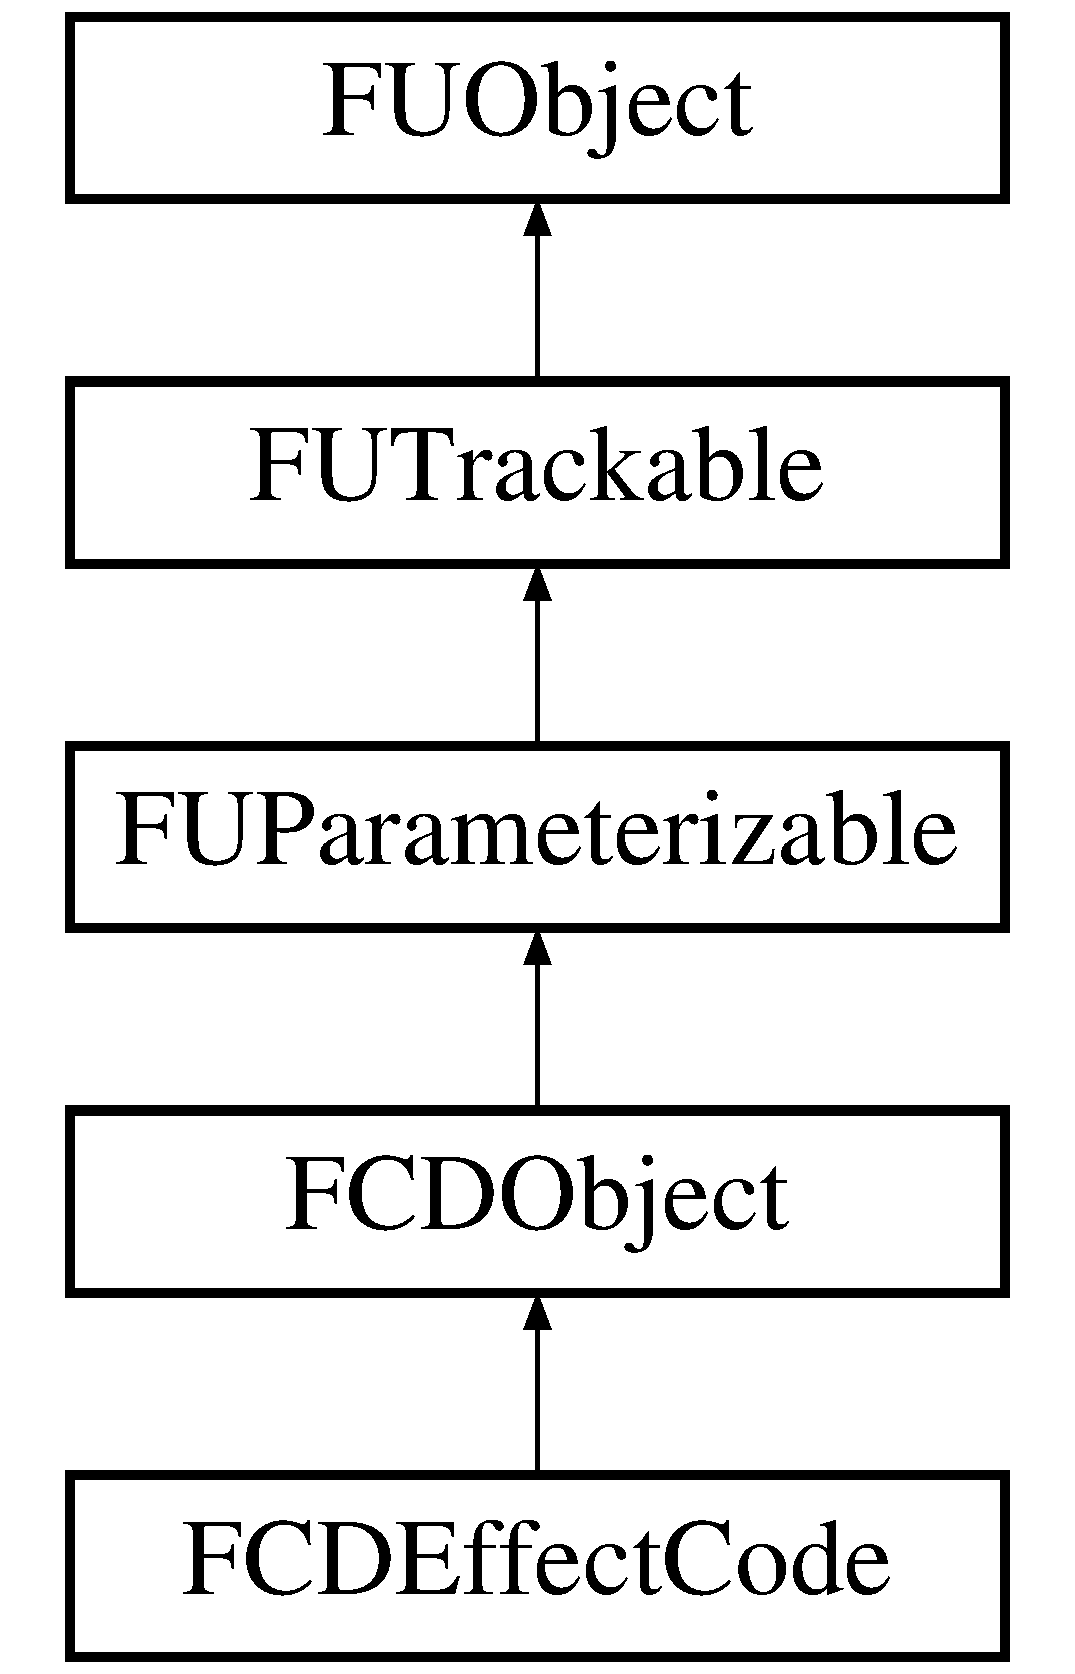
\includegraphics[height=5.000000cm]{classFCDEffectCode}
\end{center}
\end{figure}
\subsection*{Public Types}
\begin{DoxyCompactItemize}
\item 
enum \hyperlink{classFCDEffectCode_a0e492088a72daaf6e6e14c50d17c9424}{Type} \{ {\bfseries INCLUDE}, 
\hyperlink{classFCDEffectCode_a0e492088a72daaf6e6e14c50d17c9424abd1a77e0d6fd232b43bd48113315b248}{CODE}
 \}
\end{DoxyCompactItemize}
\subsection*{Public Member Functions}
\begin{DoxyCompactItemize}
\item 
\hyperlink{classFCDEffectCode_a5ba927db410adba1b34e73bd9a3cabe1}{FCDEffectCode} (\hyperlink{classFCDocument}{FCDocument} $\ast$document)
\item 
virtual \hyperlink{classFCDEffectCode_a74f636708ade039da19ef82aea0a14bd}{$\sim$FCDEffectCode} ()
\item 
\hyperlink{classFCDEffectCode_a0e492088a72daaf6e6e14c50d17c9424}{Type} \hyperlink{classFCDEffectCode_a9e00aa62fc3e509f8aedb04443026871}{GetType} () const 
\item 
void \hyperlink{classFCDEffectCode_aee0f522cea26f2b8414c6c023f15702b}{SetType} (\hyperlink{classFCDEffectCode_a0e492088a72daaf6e6e14c50d17c9424}{Type} \_\-type)
\item 
const \hyperlink{classfm_1_1stringT}{fm::string} \& \hyperlink{classFCDEffectCode_a98973fd93404c031bc8282a5f84db017}{GetSubId} () const 
\item 
void \hyperlink{classFCDEffectCode_ab36d40bd36e748634342c24db4b23639}{SetSubId} (const \hyperlink{classfm_1_1stringT}{fm::string} \&\_\-sid)
\item 
const \hyperlink{classfm_1_1stringT}{fstring} \& \hyperlink{classFCDEffectCode_aeb303dd3b3ce37a77955fe4a2fa1986f}{GetCode} () const 
\item 
void \hyperlink{classFCDEffectCode_a10347e9dc00a809f0203cadd55e9ab64}{SetCode} (const \hyperlink{classfm_1_1stringT}{fstring} \&\_\-code)
\item 
const \hyperlink{classfm_1_1stringT}{fstring} \& \hyperlink{classFCDEffectCode_a201251ceb6b7774c33b4cdd64e78b136}{GetFilename} () const 
\item 
void \hyperlink{classFCDEffectCode_a24505787b2431902f598c6454105b737}{SetFilename} (const \hyperlink{classfm_1_1stringT}{fstring} \&\_\-filename)
\item 
\hyperlink{classFCDEffectCode}{FCDEffectCode} $\ast$ \hyperlink{classFCDEffectCode_ac3f31e1734d949b402bf2880ec9e4087}{Clone} (\hyperlink{classFCDEffectCode}{FCDEffectCode} $\ast$clone=NULL) const 
\end{DoxyCompactItemize}


\subsection{Detailed Description}
A COLLADA code inclusion.

Code inclusions come in two forms: file includes and inline code. For file includes, you will want to grab the filename of the file using the GetFilename function and for inline code, you can get the code directly through the GetCode function.

Code inclusions are referenced through sub-\/ids by the effect pass shaders. Regardless of the extension of the filename of file includes, the code inclusions' language is solely determined by the effect profile they belong to. 

\subsection{Member Enumeration Documentation}
\hypertarget{classFCDEffectCode_a0e492088a72daaf6e6e14c50d17c9424}{
\index{FCDEffectCode@{FCDEffectCode}!Type@{Type}}
\index{Type@{Type}!FCDEffectCode@{FCDEffectCode}}
\subsubsection[{Type}]{\setlength{\rightskip}{0pt plus 5cm}enum {\bf FCDEffectCode::Type}}}
\label{classFCDEffectCode_a0e492088a72daaf6e6e14c50d17c9424}
The list of support code inclusion types. \begin{Desc}
\item[Enumerator: ]\par
\begin{description}
\index{CODE@{CODE}!FCDEffectCode@{FCDEffectCode}}\index{FCDEffectCode@{FCDEffectCode}!CODE@{CODE}}\item[{\em 
\hypertarget{classFCDEffectCode_a0e492088a72daaf6e6e14c50d17c9424abd1a77e0d6fd232b43bd48113315b248}{
CODE}
\label{classFCDEffectCode_a0e492088a72daaf6e6e14c50d17c9424abd1a77e0d6fd232b43bd48113315b248}
}]A file include. \begin{DoxySeeAlso}{See also}
\hyperlink{classFCDEffectCode_a201251ceb6b7774c33b4cdd64e78b136}{GetFilename} Inlined code. 

\hyperlink{classFCDEffectCode_aeb303dd3b3ce37a77955fe4a2fa1986f}{GetCode} 
\end{DoxySeeAlso}
\end{description}
\end{Desc}



\subsection{Constructor \& Destructor Documentation}
\hypertarget{classFCDEffectCode_a5ba927db410adba1b34e73bd9a3cabe1}{
\index{FCDEffectCode@{FCDEffectCode}!FCDEffectCode@{FCDEffectCode}}
\index{FCDEffectCode@{FCDEffectCode}!FCDEffectCode@{FCDEffectCode}}
\subsubsection[{FCDEffectCode}]{\setlength{\rightskip}{0pt plus 5cm}FCDEffectCode::FCDEffectCode (
\begin{DoxyParamCaption}
\item[{{\bf FCDocument} $\ast$}]{ document}
\end{DoxyParamCaption}
)}}
\label{classFCDEffectCode_a5ba927db410adba1b34e73bd9a3cabe1}
Constructor: do not use directly. Instead, use the FCDEffectProfile::AddCode or the \hyperlink{classFCDEffectTechnique_aa532d3dff7c9c8f159a16811c7cdcf20}{FCDEffectTechnique::AddCode} functions. 
\begin{DoxyParams}{Parameters}
\item[{\em document}]The COLLADA document that owns this code inclusion. \end{DoxyParams}
\hypertarget{classFCDEffectCode_a74f636708ade039da19ef82aea0a14bd}{
\index{FCDEffectCode@{FCDEffectCode}!$\sim$FCDEffectCode@{$\sim$FCDEffectCode}}
\index{$\sim$FCDEffectCode@{$\sim$FCDEffectCode}!FCDEffectCode@{FCDEffectCode}}
\subsubsection[{$\sim$FCDEffectCode}]{\setlength{\rightskip}{0pt plus 5cm}FCDEffectCode::$\sim$FCDEffectCode (
\begin{DoxyParamCaption}
{}
\end{DoxyParamCaption}
)\hspace{0.3cm}{\ttfamily  \mbox{[}virtual\mbox{]}}}}
\label{classFCDEffectCode_a74f636708ade039da19ef82aea0a14bd}
Destructor. 

\subsection{Member Function Documentation}
\hypertarget{classFCDEffectCode_ac3f31e1734d949b402bf2880ec9e4087}{
\index{FCDEffectCode@{FCDEffectCode}!Clone@{Clone}}
\index{Clone@{Clone}!FCDEffectCode@{FCDEffectCode}}
\subsubsection[{Clone}]{\setlength{\rightskip}{0pt plus 5cm}{\bf FCDEffectCode} $\ast$ FCDEffectCode::Clone (
\begin{DoxyParamCaption}
\item[{{\bf FCDEffectCode} $\ast$}]{ clone = {\ttfamily NULL}}
\end{DoxyParamCaption}
) const}}
\label{classFCDEffectCode_ac3f31e1734d949b402bf2880ec9e4087}
Clones the code inclusion. 
\begin{DoxyParams}{Parameters}
\item[{\em clone}]The cloned code inclusion. If this pointer is NULL, a new code inclusion is created and you will need to release this new code inclusion. \end{DoxyParams}
\begin{DoxyReturn}{Returns}
The cloned effect object. This pointer will never be NULL. 
\end{DoxyReturn}
\hypertarget{classFCDEffectCode_aeb303dd3b3ce37a77955fe4a2fa1986f}{
\index{FCDEffectCode@{FCDEffectCode}!GetCode@{GetCode}}
\index{GetCode@{GetCode}!FCDEffectCode@{FCDEffectCode}}
\subsubsection[{GetCode}]{\setlength{\rightskip}{0pt plus 5cm}const {\bf fstring}\& FCDEffectCode::GetCode (
\begin{DoxyParamCaption}
{}
\end{DoxyParamCaption}
) const\hspace{0.3cm}{\ttfamily  \mbox{[}inline\mbox{]}}}}
\label{classFCDEffectCode_aeb303dd3b3ce37a77955fe4a2fa1986f}
Retrieves the inlined code. First verify that this code inclusion contains inlined code using the GetType function. \begin{DoxyReturn}{Returns}
The inlined code. 
\end{DoxyReturn}
\hypertarget{classFCDEffectCode_a201251ceb6b7774c33b4cdd64e78b136}{
\index{FCDEffectCode@{FCDEffectCode}!GetFilename@{GetFilename}}
\index{GetFilename@{GetFilename}!FCDEffectCode@{FCDEffectCode}}
\subsubsection[{GetFilename}]{\setlength{\rightskip}{0pt plus 5cm}const {\bf fstring}\& FCDEffectCode::GetFilename (
\begin{DoxyParamCaption}
{}
\end{DoxyParamCaption}
) const\hspace{0.3cm}{\ttfamily  \mbox{[}inline\mbox{]}}}}
\label{classFCDEffectCode_a201251ceb6b7774c33b4cdd64e78b136}
Retrieves the filename of the code file to open. First verify that this code inclusion contains a filename using the GetType function. \begin{DoxyReturn}{Returns}
The code filename. 
\end{DoxyReturn}
\hypertarget{classFCDEffectCode_a98973fd93404c031bc8282a5f84db017}{
\index{FCDEffectCode@{FCDEffectCode}!GetSubId@{GetSubId}}
\index{GetSubId@{GetSubId}!FCDEffectCode@{FCDEffectCode}}
\subsubsection[{GetSubId}]{\setlength{\rightskip}{0pt plus 5cm}const {\bf fm::string}\& FCDEffectCode::GetSubId (
\begin{DoxyParamCaption}
{}
\end{DoxyParamCaption}
) const\hspace{0.3cm}{\ttfamily  \mbox{[}inline\mbox{]}}}}
\label{classFCDEffectCode_a98973fd93404c031bc8282a5f84db017}
Retrieves the sub-\/id of the code inclusion. Used to match the code inclusion within the effect pass shaders. \begin{DoxyReturn}{Returns}
The sub-\/id. 
\end{DoxyReturn}
\hypertarget{classFCDEffectCode_a9e00aa62fc3e509f8aedb04443026871}{
\index{FCDEffectCode@{FCDEffectCode}!GetType@{GetType}}
\index{GetType@{GetType}!FCDEffectCode@{FCDEffectCode}}
\subsubsection[{GetType}]{\setlength{\rightskip}{0pt plus 5cm}{\bf Type} FCDEffectCode::GetType (
\begin{DoxyParamCaption}
{}
\end{DoxyParamCaption}
) const\hspace{0.3cm}{\ttfamily  \mbox{[}inline\mbox{]}}}}
\label{classFCDEffectCode_a9e00aa62fc3e509f8aedb04443026871}
Retrieves the form of the code inclusion. \begin{DoxyReturn}{Returns}
The form. 
\end{DoxyReturn}
\hypertarget{classFCDEffectCode_a10347e9dc00a809f0203cadd55e9ab64}{
\index{FCDEffectCode@{FCDEffectCode}!SetCode@{SetCode}}
\index{SetCode@{SetCode}!FCDEffectCode@{FCDEffectCode}}
\subsubsection[{SetCode}]{\setlength{\rightskip}{0pt plus 5cm}void FCDEffectCode::SetCode (
\begin{DoxyParamCaption}
\item[{const {\bf fstring} \&}]{ \_\-code}
\end{DoxyParamCaption}
)\hspace{0.3cm}{\ttfamily  \mbox{[}inline\mbox{]}}}}
\label{classFCDEffectCode_a10347e9dc00a809f0203cadd55e9ab64}
Sets the inlined code. As a side-\/effect, calling this function forces the type of the code inclusion. 
\begin{DoxyParams}{Parameters}
\item[{\em \_\-code}]The inlined code. \end{DoxyParams}
\hypertarget{classFCDEffectCode_a24505787b2431902f598c6454105b737}{
\index{FCDEffectCode@{FCDEffectCode}!SetFilename@{SetFilename}}
\index{SetFilename@{SetFilename}!FCDEffectCode@{FCDEffectCode}}
\subsubsection[{SetFilename}]{\setlength{\rightskip}{0pt plus 5cm}void FCDEffectCode::SetFilename (
\begin{DoxyParamCaption}
\item[{const {\bf fstring} \&}]{ \_\-filename}
\end{DoxyParamCaption}
)}}
\label{classFCDEffectCode_a24505787b2431902f598c6454105b737}
Sets the filename of the code file. As a side-\/effect, calling this function forces the type of the code inclusion. 
\begin{DoxyParams}{Parameters}
\item[{\em \_\-filename}]The code filename. \end{DoxyParams}
\hypertarget{classFCDEffectCode_ab36d40bd36e748634342c24db4b23639}{
\index{FCDEffectCode@{FCDEffectCode}!SetSubId@{SetSubId}}
\index{SetSubId@{SetSubId}!FCDEffectCode@{FCDEffectCode}}
\subsubsection[{SetSubId}]{\setlength{\rightskip}{0pt plus 5cm}void FCDEffectCode::SetSubId (
\begin{DoxyParamCaption}
\item[{const {\bf fm::string} \&}]{ \_\-sid}
\end{DoxyParamCaption}
)}}
\label{classFCDEffectCode_ab36d40bd36e748634342c24db4b23639}
Sets the sub-\/id of the code inclusion. This value may change on export, as the sub-\/id must be unique within its scope. 
\begin{DoxyParams}{Parameters}
\item[{\em \_\-sid}]The sub-\/id. \end{DoxyParams}
\hypertarget{classFCDEffectCode_aee0f522cea26f2b8414c6c023f15702b}{
\index{FCDEffectCode@{FCDEffectCode}!SetType@{SetType}}
\index{SetType@{SetType}!FCDEffectCode@{FCDEffectCode}}
\subsubsection[{SetType}]{\setlength{\rightskip}{0pt plus 5cm}void FCDEffectCode::SetType (
\begin{DoxyParamCaption}
\item[{{\bf Type}}]{ \_\-type}
\end{DoxyParamCaption}
)\hspace{0.3cm}{\ttfamily  \mbox{[}inline\mbox{]}}}}
\label{classFCDEffectCode_aee0f522cea26f2b8414c6c023f15702b}
Sets the form of the code inclusion. Changing the form of the code inclusion will not remove the inline code or the filename. 
\begin{DoxyParams}{Parameters}
\item[{\em \_\-type}]The form. \end{DoxyParams}


The documentation for this class was generated from the following files:\begin{DoxyCompactItemize}
\item 
FCollada/FCDocument/\hyperlink{FCDEffectCode_8h}{FCDEffectCode.h}\item 
FCollada/FCDocument/FCDEffectCode.cpp\end{DoxyCompactItemize}

\hypertarget{classFCDEffectParameter}{
\section{FCDEffectParameter Class Reference}
\label{classFCDEffectParameter}\index{FCDEffectParameter@{FCDEffectParameter}}
}


{\ttfamily \#include $<$FCDEffectParameter.h$>$}

Inheritance diagram for FCDEffectParameter:\begin{figure}[H]
\begin{center}
\leavevmode
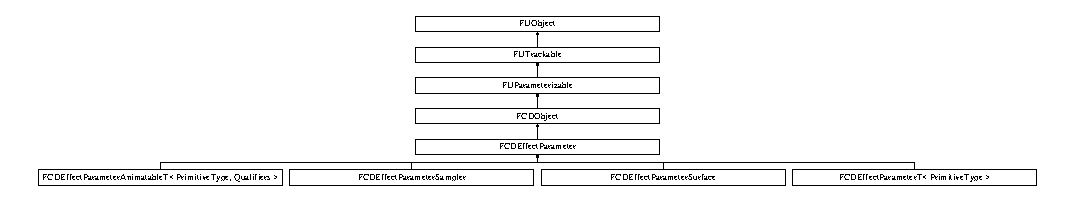
\includegraphics[height=2.270270cm]{classFCDEffectParameter}
\end{center}
\end{figure}
\subsection*{Public Types}
\begin{DoxyCompactItemize}
\item 
enum \hyperlink{classFCDEffectParameter_a1efe74553d2ed199435085c171743b08}{Type} \{ \par
\hyperlink{classFCDEffectParameter_a1efe74553d2ed199435085c171743b08a8f5ddd923615701f05a30158b80f56ec}{SAMPLER}, 
\hyperlink{classFCDEffectParameter_a1efe74553d2ed199435085c171743b08add655617aa5a92725480964718122182}{INTEGER}, 
\hyperlink{classFCDEffectParameter_a1efe74553d2ed199435085c171743b08ad40197d51fa800a31facae92a9dca91a}{BOOLEAN}, 
\hyperlink{classFCDEffectParameter_a1efe74553d2ed199435085c171743b08a87e8166fffd6cc3a8d39671b1346e469}{FLOAT}, 
\par
\hyperlink{classFCDEffectParameter_a1efe74553d2ed199435085c171743b08a6d83a40ca335905a8a6877f001e6b52c}{FLOAT2}, 
\hyperlink{classFCDEffectParameter_a1efe74553d2ed199435085c171743b08aa94c8dfc96b419a36c1de7ca2b6413c1}{FLOAT3}, 
\hyperlink{classFCDEffectParameter_a1efe74553d2ed199435085c171743b08a4e0256ca9cff99b253d54ca218fde0f9}{VECTOR}, 
\hyperlink{classFCDEffectParameter_a1efe74553d2ed199435085c171743b08a660e596914f88e50d5853b2131ad225a}{MATRIX}, 
\par
\hyperlink{classFCDEffectParameter_a1efe74553d2ed199435085c171743b08a1b235e6d5cb68e8bcd13443795252e0a}{STRING}, 
\hyperlink{classFCDEffectParameter_a1efe74553d2ed199435085c171743b08a217a1f4ad8b74ced28de295ab6de116b}{SURFACE}
 \}
\item 
enum \hyperlink{classFCDEffectParameter_a25a513057c610179b5229dc99e840bb9}{ParamType} \{ \par
\hyperlink{classFCDEffectParameter_a25a513057c610179b5229dc99e840bb9a14eca93fcd14630310f36b886eccb457}{GENERATOR}, 
\hyperlink{classFCDEffectParameter_a25a513057c610179b5229dc99e840bb9a39a1f8b4018e17cf450cdf1d4b1ff73a}{MODIFIER}, 
\hyperlink{classFCDEffectParameter_a25a513057c610179b5229dc99e840bb9a9bc6e04cd6ea9ab90d07f215aeff3b60}{ANIMATOR}, 
\hyperlink{classFCDEffectParameter_a25a513057c610179b5229dc99e840bb9a170fdf70dc1ace376fbe736c84bf8d0c}{REFERENCER}, 
\par
\hyperlink{classFCDEffectParameter_a25a513057c610179b5229dc99e840bb9abb34bd1f49cb5c89dee19319a990c094}{CONSTANT}
 \}
\end{DoxyCompactItemize}
\subsection*{Public Member Functions}
\begin{DoxyCompactItemize}
\item 
\hyperlink{classFCDEffectParameter_aab5e11cc5f59d90be17fd8db28146826}{FCDEffectParameter} (\hyperlink{classFCDocument}{FCDocument} $\ast$document)
\item 
virtual \hyperlink{classFCDEffectParameter_ad0314597c4be5629a6b55927ed32f15a}{$\sim$FCDEffectParameter} ()
\item 
virtual \hyperlink{classFCDEffectParameter_a1efe74553d2ed199435085c171743b08}{Type} \hyperlink{classFCDEffectParameter_a5858946f333ea4486ca30c4c1b104871}{GetType} () const =0
\item 
\hyperlink{classFCDEffectParameter_a25a513057c610179b5229dc99e840bb9}{ParamType} \hyperlink{classFCDEffectParameter_a48ab8e00ca3648e54795864a901e1b2e}{GetParamType} () const 
\item 
const \hyperlink{classfm_1_1stringT}{fm::string} \& \hyperlink{classFCDEffectParameter_a7f736431830ef8d76e9410747546c6d8}{GetReference} () const 
\item 
void \hyperlink{classFCDEffectParameter_a5a1af6ade68203ece99e22e2334e7dda}{SetReference} (const char $\ast$\_\-reference)
\item 
const \hyperlink{classfm_1_1stringT}{fm::string} \& \hyperlink{classFCDEffectParameter_a766c4c57cce34ae74c7946a166cd4141}{GetSemantic} () const 
\item 
void \hyperlink{classFCDEffectParameter_ab7a042b8a3df0d6c72892ecca6c2f3e1}{SetSemantic} (const char $\ast$\_\-semantic)
\item 
bool \hyperlink{classFCDEffectParameter_aa77e878bbff4b0d7a85c3f08e46bb206}{IsGenerator} () const 
\item 
void \hyperlink{classFCDEffectParameter_ae9e19c411f12e1f456a45be82b4ddf6a}{SetGenerator} ()
\item 
bool \hyperlink{classFCDEffectParameter_af0270639bc9e73ca45c15fbbebdc8066}{IsModifier} () const 
\item 
void \hyperlink{classFCDEffectParameter_a620f3208cb12bb3017635fa43cd5b0cf}{SetModifier} ()
\item 
bool \hyperlink{classFCDEffectParameter_ab592fa7e739aefa0428d7ef5c5ef802c}{IsAnimator} () const 
\item 
void \hyperlink{classFCDEffectParameter_a3f4336d517d28228d97b7d6ba64b0f7f}{SetAnimator} ()
\item 
bool \hyperlink{classFCDEffectParameter_aeab23a79f8e23c34c578d3dbeaa15ccb}{IsReferencer} () const 
\item 
void \hyperlink{classFCDEffectParameter_ac583526f7633df0f53eb9b2bcb4cc871}{SetReferencer} ()
\item 
bool \hyperlink{classFCDEffectParameter_abea9fef6b3f53f3517deecf65e48930d}{IsConstant} () const 
\item 
void \hyperlink{classFCDEffectParameter_a9dfd1408c013fc089814ddc8081d717e}{SetConstant} ()
\item 
const \hyperlink{classFCDEffectParameterAnnotation}{FCDEffectParameterAnnotation} $\ast$$\ast$ \hyperlink{classFCDEffectParameter_a6ac54dcbf8d32ba46ef33beb59496a85}{GetAnnotations} () const 
\item 
size\_\-t \hyperlink{classFCDEffectParameter_ab7044a24dc78a4e5bf4521591d0b7c8b}{GetAnnotationCount} () const 
\item 
\hyperlink{classFCDEffectParameterAnnotation}{FCDEffectParameterAnnotation} $\ast$ \hyperlink{classFCDEffectParameter_a1a65ceee576d44bccfc64e1180512a77}{GetAnnotation} (size\_\-t index)
\item 
const \hyperlink{classFCDEffectParameterAnnotation}{FCDEffectParameterAnnotation} $\ast$ \hyperlink{classFCDEffectParameter_ae62a9e58e54ea7430e9de7faae3197a4}{GetAnnotation} (size\_\-t index) const 
\item 
\hyperlink{classFCDEffectParameterAnnotation}{FCDEffectParameterAnnotation} $\ast$ \hyperlink{classFCDEffectParameter_a20bfb0f1361f5712c6014300878996e9}{AddAnnotation} ()
\item 
void \hyperlink{classFCDEffectParameter_a196cbd25ffbbd769276b800b7a557409}{AddAnnotation} (const fchar $\ast$name, \hyperlink{classFCDEffectParameter_a1efe74553d2ed199435085c171743b08}{FCDEffectParameter::Type} type, const fchar $\ast$value)
\item 
void \hyperlink{classFCDEffectParameter_a3e42008248b98e54482a2461cbdcf4da}{AddAnnotation} (const \hyperlink{classfm_1_1stringT}{fstring} \&name, \hyperlink{classFCDEffectParameter_a1efe74553d2ed199435085c171743b08}{FCDEffectParameter::Type} type, const fchar $\ast$value)
\item 
void \hyperlink{classFCDEffectParameter_a94ed87e08db50adcc733b756530a2a06}{AddAnnotation} (const fchar $\ast$name, \hyperlink{classFCDEffectParameter_a1efe74553d2ed199435085c171743b08}{FCDEffectParameter::Type} type, const \hyperlink{classfm_1_1stringT}{fstring} \&value)
\item 
void \hyperlink{classFCDEffectParameter_a0cc972ecbab3edac8a12476ddf8d88bf}{AddAnnotation} (const \hyperlink{classfm_1_1stringT}{fstring} \&name, \hyperlink{classFCDEffectParameter_a1efe74553d2ed199435085c171743b08}{FCDEffectParameter::Type} type, const \hyperlink{classfm_1_1stringT}{fstring} \&value)
\item 
{\footnotesize template$<$class T $>$ }\\void \hyperlink{classFCDEffectParameter_a3c1b2078989b55f9f6bc40d38bb84be6}{AddAnnotation} (const fchar $\ast$name, \hyperlink{classFCDEffectParameter_a1efe74553d2ed199435085c171743b08}{FCDEffectParameter::Type} type, const T \&value)
\item 
{\footnotesize template$<$class T $>$ }\\void \hyperlink{classFCDEffectParameter_a69564a01be462524f6d42cf09b443221}{AddAnnotation} (const \hyperlink{classfm_1_1stringT}{fstring} \&name, \hyperlink{classFCDEffectParameter_a1efe74553d2ed199435085c171743b08}{FCDEffectParameter::Type} type, const T \&value)
\item 
\hyperlink{classFCDEffectParameter_a70ae77594ef3b066891f78d1a72502d6}{DEPRECATED} (3.05A, annotation-\/$>$Release) inline void ReleaseAnnotation(FCDEffectParameterAnnotation $\ast$annotation)
\item 
virtual bool \hyperlink{classFCDEffectParameter_a005a5a316bdb99dbd97ac542c129cc5e}{IsValueEqual} (\hyperlink{classFCDEffectParameter}{FCDEffectParameter} $\ast$parameter)=0
\item 
virtual \hyperlink{classFCDEffectParameter}{FCDEffectParameter} $\ast$ \hyperlink{classFCDEffectParameter_a75abe4b8964493db40604fa3d0e373eb}{Clone} (\hyperlink{classFCDEffectParameter}{FCDEffectParameter} $\ast$clone=NULL) const 
\item 
virtual void \hyperlink{classFCDEffectParameter_a016be91dbd27ff3c8c30f759f00b8c53}{Overwrite} (\hyperlink{classFCDEffectParameter}{FCDEffectParameter} $\ast$target)
\end{DoxyCompactItemize}


\subsection{Detailed Description}
A COLLADA effect parameter.

This interface class is used to define all the valid ColladaFX parameter types. There are many types of parameters: integers, booleans, floating-\/point values, 2D, 3D and 4D vectors of floating-\/point values, matrices, strings, surfaces and their samplers.

A COLLADA effect parameter may generate a new effect parameter, in which case it will declare a semantic and a reference: to represent it within the COLLADA document. 

\subsection{Member Enumeration Documentation}
\hypertarget{classFCDEffectParameter_a25a513057c610179b5229dc99e840bb9}{
\index{FCDEffectParameter@{FCDEffectParameter}!ParamType@{ParamType}}
\index{ParamType@{ParamType}!FCDEffectParameter@{FCDEffectParameter}}
\subsubsection[{ParamType}]{\setlength{\rightskip}{0pt plus 5cm}enum {\bf FCDEffectParameter::ParamType}}}
\label{classFCDEffectParameter_a25a513057c610179b5229dc99e840bb9}
The usage type of the effect parameter. \begin{Desc}
\item[Enumerator: ]\par
\begin{description}
\index{GENERATOR@{GENERATOR}!FCDEffectParameter@{FCDEffectParameter}}\index{FCDEffectParameter@{FCDEffectParameter}!GENERATOR@{GENERATOR}}\item[{\em 
\hypertarget{classFCDEffectParameter_a25a513057c610179b5229dc99e840bb9a14eca93fcd14630310f36b886eccb457}{
GENERATOR}
\label{classFCDEffectParameter_a25a513057c610179b5229dc99e840bb9a14eca93fcd14630310f36b886eccb457}
}]This should be the type used for a 'newparam' element. Valid only at the levels of effect, profile common or technique common. \index{MODIFIER@{MODIFIER}!FCDEffectParameter@{FCDEffectParameter}}\index{FCDEffectParameter@{FCDEffectParameter}!MODIFIER@{MODIFIER}}\item[{\em 
\hypertarget{classFCDEffectParameter_a25a513057c610179b5229dc99e840bb9a39a1f8b4018e17cf450cdf1d4b1ff73a}{
MODIFIER}
\label{classFCDEffectParameter_a25a513057c610179b5229dc99e840bb9a39a1f8b4018e17cf450cdf1d4b1ff73a}
}]This should be the type used for a 'setparam' element. Valid only at the instance effect level. \index{ANIMATOR@{ANIMATOR}!FCDEffectParameter@{FCDEffectParameter}}\index{FCDEffectParameter@{FCDEffectParameter}!ANIMATOR@{ANIMATOR}}\item[{\em 
\hypertarget{classFCDEffectParameter_a25a513057c610179b5229dc99e840bb9a9bc6e04cd6ea9ab90d07f215aeff3b60}{
ANIMATOR}
\label{classFCDEffectParameter_a25a513057c610179b5229dc99e840bb9a9bc6e04cd6ea9ab90d07f215aeff3b60}
}]This should be the type used for a 'param' element that is to be animated. Valid only at the bind\_\-material level. \index{REFERENCER@{REFERENCER}!FCDEffectParameter@{FCDEffectParameter}}\index{FCDEffectParameter@{FCDEffectParameter}!REFERENCER@{REFERENCER}}\item[{\em 
\hypertarget{classFCDEffectParameter_a25a513057c610179b5229dc99e840bb9a170fdf70dc1ace376fbe736c84bf8d0c}{
REFERENCER}
\label{classFCDEffectParameter_a25a513057c610179b5229dc99e840bb9a170fdf70dc1ace376fbe736c84bf8d0c}
}]This should be the type used for a 'param' element used in any of the common techniques. The 'param' needs to have a reference that is the same as the generator used above. \index{CONSTANT@{CONSTANT}!FCDEffectParameter@{FCDEffectParameter}}\index{FCDEffectParameter@{FCDEffectParameter}!CONSTANT@{CONSTANT}}\item[{\em 
\hypertarget{classFCDEffectParameter_a25a513057c610179b5229dc99e840bb9abb34bd1f49cb5c89dee19319a990c094}{
CONSTANT}
\label{classFCDEffectParameter_a25a513057c610179b5229dc99e840bb9abb34bd1f49cb5c89dee19319a990c094}
}]This should be the type used for a parameter that is either a color or a float in any of the common techniques. This type isn't linked to any parameter elsewhere. \end{description}
\end{Desc}

\hypertarget{classFCDEffectParameter_a1efe74553d2ed199435085c171743b08}{
\index{FCDEffectParameter@{FCDEffectParameter}!Type@{Type}}
\index{Type@{Type}!FCDEffectParameter@{FCDEffectParameter}}
\subsubsection[{Type}]{\setlength{\rightskip}{0pt plus 5cm}enum {\bf FCDEffectParameter::Type}}}
\label{classFCDEffectParameter_a1efe74553d2ed199435085c171743b08}
The value type of the effect parameter. \begin{Desc}
\item[Enumerator: ]\par
\begin{description}
\index{SAMPLER@{SAMPLER}!FCDEffectParameter@{FCDEffectParameter}}\index{FCDEffectParameter@{FCDEffectParameter}!SAMPLER@{SAMPLER}}\item[{\em 
\hypertarget{classFCDEffectParameter_a1efe74553d2ed199435085c171743b08a8f5ddd923615701f05a30158b80f56ec}{
SAMPLER}
\label{classFCDEffectParameter_a1efe74553d2ed199435085c171743b08a8f5ddd923615701f05a30158b80f56ec}
}]A sampler effect parameter. Points towards a surface parameter and adds extra texturing parameters. \index{INTEGER@{INTEGER}!FCDEffectParameter@{FCDEffectParameter}}\index{FCDEffectParameter@{FCDEffectParameter}!INTEGER@{INTEGER}}\item[{\em 
\hypertarget{classFCDEffectParameter_a1efe74553d2ed199435085c171743b08add655617aa5a92725480964718122182}{
INTEGER}
\label{classFCDEffectParameter_a1efe74553d2ed199435085c171743b08add655617aa5a92725480964718122182}
}]A single integer effect parameter. \index{BOOLEAN@{BOOLEAN}!FCDEffectParameter@{FCDEffectParameter}}\index{FCDEffectParameter@{FCDEffectParameter}!BOOLEAN@{BOOLEAN}}\item[{\em 
\hypertarget{classFCDEffectParameter_a1efe74553d2ed199435085c171743b08ad40197d51fa800a31facae92a9dca91a}{
BOOLEAN}
\label{classFCDEffectParameter_a1efe74553d2ed199435085c171743b08ad40197d51fa800a31facae92a9dca91a}
}]A single boolean effect parameter. \index{FLOAT@{FLOAT}!FCDEffectParameter@{FCDEffectParameter}}\index{FCDEffectParameter@{FCDEffectParameter}!FLOAT@{FLOAT}}\item[{\em 
\hypertarget{classFCDEffectParameter_a1efe74553d2ed199435085c171743b08a87e8166fffd6cc3a8d39671b1346e469}{
FLOAT}
\label{classFCDEffectParameter_a1efe74553d2ed199435085c171743b08a87e8166fffd6cc3a8d39671b1346e469}
}]A single floating-\/pointer value effect parameter. \index{FLOAT2@{FLOAT2}!FCDEffectParameter@{FCDEffectParameter}}\index{FCDEffectParameter@{FCDEffectParameter}!FLOAT2@{FLOAT2}}\item[{\em 
\hypertarget{classFCDEffectParameter_a1efe74553d2ed199435085c171743b08a6d83a40ca335905a8a6877f001e6b52c}{
FLOAT2}
\label{classFCDEffectParameter_a1efe74553d2ed199435085c171743b08a6d83a40ca335905a8a6877f001e6b52c}
}]A 2D vector of floating-\/pointer values. \index{FLOAT3@{FLOAT3}!FCDEffectParameter@{FCDEffectParameter}}\index{FCDEffectParameter@{FCDEffectParameter}!FLOAT3@{FLOAT3}}\item[{\em 
\hypertarget{classFCDEffectParameter_a1efe74553d2ed199435085c171743b08aa94c8dfc96b419a36c1de7ca2b6413c1}{
FLOAT3}
\label{classFCDEffectParameter_a1efe74553d2ed199435085c171743b08aa94c8dfc96b419a36c1de7ca2b6413c1}
}]A 3D vector of floating-\/pointer values. \index{VECTOR@{VECTOR}!FCDEffectParameter@{FCDEffectParameter}}\index{FCDEffectParameter@{FCDEffectParameter}!VECTOR@{VECTOR}}\item[{\em 
\hypertarget{classFCDEffectParameter_a1efe74553d2ed199435085c171743b08a4e0256ca9cff99b253d54ca218fde0f9}{
VECTOR}
\label{classFCDEffectParameter_a1efe74553d2ed199435085c171743b08a4e0256ca9cff99b253d54ca218fde0f9}
}]A 4D vector of floating-\/pointer values. \index{MATRIX@{MATRIX}!FCDEffectParameter@{FCDEffectParameter}}\index{FCDEffectParameter@{FCDEffectParameter}!MATRIX@{MATRIX}}\item[{\em 
\hypertarget{classFCDEffectParameter_a1efe74553d2ed199435085c171743b08a660e596914f88e50d5853b2131ad225a}{
MATRIX}
\label{classFCDEffectParameter_a1efe74553d2ed199435085c171743b08a660e596914f88e50d5853b2131ad225a}
}]A 4x4 matrix. \index{STRING@{STRING}!FCDEffectParameter@{FCDEffectParameter}}\index{FCDEffectParameter@{FCDEffectParameter}!STRING@{STRING}}\item[{\em 
\hypertarget{classFCDEffectParameter_a1efe74553d2ed199435085c171743b08a1b235e6d5cb68e8bcd13443795252e0a}{
STRING}
\label{classFCDEffectParameter_a1efe74553d2ed199435085c171743b08a1b235e6d5cb68e8bcd13443795252e0a}
}]A string effect parameter. \index{SURFACE@{SURFACE}!FCDEffectParameter@{FCDEffectParameter}}\index{FCDEffectParameter@{FCDEffectParameter}!SURFACE@{SURFACE}}\item[{\em 
\hypertarget{classFCDEffectParameter_a1efe74553d2ed199435085c171743b08a217a1f4ad8b74ced28de295ab6de116b}{
SURFACE}
\label{classFCDEffectParameter_a1efe74553d2ed199435085c171743b08a217a1f4ad8b74ced28de295ab6de116b}
}]A surface effect parameter. Contains a COLLADA image pointer. \end{description}
\end{Desc}



\subsection{Constructor \& Destructor Documentation}
\hypertarget{classFCDEffectParameter_aab5e11cc5f59d90be17fd8db28146826}{
\index{FCDEffectParameter@{FCDEffectParameter}!FCDEffectParameter@{FCDEffectParameter}}
\index{FCDEffectParameter@{FCDEffectParameter}!FCDEffectParameter@{FCDEffectParameter}}
\subsubsection[{FCDEffectParameter}]{\setlength{\rightskip}{0pt plus 5cm}FCDEffectParameter::FCDEffectParameter (
\begin{DoxyParamCaption}
\item[{{\bf FCDocument} $\ast$}]{ document}
\end{DoxyParamCaption}
)}}
\label{classFCDEffectParameter_aab5e11cc5f59d90be17fd8db28146826}
Constructor: do not use directly. Instead, use the appropriate AddEffectParameter function. 
\begin{DoxyParams}{Parameters}
\item[{\em document}]The COLLADA document that owns the effect parameter. \end{DoxyParams}
\hypertarget{classFCDEffectParameter_ad0314597c4be5629a6b55927ed32f15a}{
\index{FCDEffectParameter@{FCDEffectParameter}!$\sim$FCDEffectParameter@{$\sim$FCDEffectParameter}}
\index{$\sim$FCDEffectParameter@{$\sim$FCDEffectParameter}!FCDEffectParameter@{FCDEffectParameter}}
\subsubsection[{$\sim$FCDEffectParameter}]{\setlength{\rightskip}{0pt plus 5cm}FCDEffectParameter::$\sim$FCDEffectParameter (
\begin{DoxyParamCaption}
{}
\end{DoxyParamCaption}
)\hspace{0.3cm}{\ttfamily  \mbox{[}virtual\mbox{]}}}}
\label{classFCDEffectParameter_ad0314597c4be5629a6b55927ed32f15a}
Destructor. 

\subsection{Member Function Documentation}
\hypertarget{classFCDEffectParameter_a20bfb0f1361f5712c6014300878996e9}{
\index{FCDEffectParameter@{FCDEffectParameter}!AddAnnotation@{AddAnnotation}}
\index{AddAnnotation@{AddAnnotation}!FCDEffectParameter@{FCDEffectParameter}}
\subsubsection[{AddAnnotation}]{\setlength{\rightskip}{0pt plus 5cm}{\bf FCDEffectParameterAnnotation} $\ast$ FCDEffectParameter::AddAnnotation (
\begin{DoxyParamCaption}
{}
\end{DoxyParamCaption}
)}}
\label{classFCDEffectParameter_a20bfb0f1361f5712c6014300878996e9}
Adds a blank annotation to this parameter. \begin{DoxyReturn}{Returns}
The blank annotation. 
\end{DoxyReturn}
\hypertarget{classFCDEffectParameter_a196cbd25ffbbd769276b800b7a557409}{
\index{FCDEffectParameter@{FCDEffectParameter}!AddAnnotation@{AddAnnotation}}
\index{AddAnnotation@{AddAnnotation}!FCDEffectParameter@{FCDEffectParameter}}
\subsubsection[{AddAnnotation}]{\setlength{\rightskip}{0pt plus 5cm}void FCDEffectParameter::AddAnnotation (
\begin{DoxyParamCaption}
\item[{const fchar $\ast$}]{ name, }
\item[{{\bf FCDEffectParameter::Type}}]{ type, }
\item[{const fchar $\ast$}]{ value}
\end{DoxyParamCaption}
)}}
\label{classFCDEffectParameter_a196cbd25ffbbd769276b800b7a557409}
Adds an annotation to this parameter. 
\begin{DoxyParams}{Parameters}
\item[{\em name}]The name of the annotation. \item[{\em type}]The type of the annotation. \item[{\em value}]The value of the annotation. \end{DoxyParams}
\hypertarget{classFCDEffectParameter_a3e42008248b98e54482a2461cbdcf4da}{
\index{FCDEffectParameter@{FCDEffectParameter}!AddAnnotation@{AddAnnotation}}
\index{AddAnnotation@{AddAnnotation}!FCDEffectParameter@{FCDEffectParameter}}
\subsubsection[{AddAnnotation}]{\setlength{\rightskip}{0pt plus 5cm}void FCDEffectParameter::AddAnnotation (
\begin{DoxyParamCaption}
\item[{const {\bf fstring} \&}]{ name, }
\item[{{\bf FCDEffectParameter::Type}}]{ type, }
\item[{const fchar $\ast$}]{ value}
\end{DoxyParamCaption}
)\hspace{0.3cm}{\ttfamily  \mbox{[}inline\mbox{]}}}}
\label{classFCDEffectParameter_a3e42008248b98e54482a2461cbdcf4da}
See above. \hypertarget{classFCDEffectParameter_a94ed87e08db50adcc733b756530a2a06}{
\index{FCDEffectParameter@{FCDEffectParameter}!AddAnnotation@{AddAnnotation}}
\index{AddAnnotation@{AddAnnotation}!FCDEffectParameter@{FCDEffectParameter}}
\subsubsection[{AddAnnotation}]{\setlength{\rightskip}{0pt plus 5cm}void FCDEffectParameter::AddAnnotation (
\begin{DoxyParamCaption}
\item[{const fchar $\ast$}]{ name, }
\item[{{\bf FCDEffectParameter::Type}}]{ type, }
\item[{const {\bf fstring} \&}]{ value}
\end{DoxyParamCaption}
)\hspace{0.3cm}{\ttfamily  \mbox{[}inline\mbox{]}}}}
\label{classFCDEffectParameter_a94ed87e08db50adcc733b756530a2a06}
See above. \hypertarget{classFCDEffectParameter_a0cc972ecbab3edac8a12476ddf8d88bf}{
\index{FCDEffectParameter@{FCDEffectParameter}!AddAnnotation@{AddAnnotation}}
\index{AddAnnotation@{AddAnnotation}!FCDEffectParameter@{FCDEffectParameter}}
\subsubsection[{AddAnnotation}]{\setlength{\rightskip}{0pt plus 5cm}void FCDEffectParameter::AddAnnotation (
\begin{DoxyParamCaption}
\item[{const {\bf fstring} \&}]{ name, }
\item[{{\bf FCDEffectParameter::Type}}]{ type, }
\item[{const {\bf fstring} \&}]{ value}
\end{DoxyParamCaption}
)\hspace{0.3cm}{\ttfamily  \mbox{[}inline\mbox{]}}}}
\label{classFCDEffectParameter_a0cc972ecbab3edac8a12476ddf8d88bf}
See above. \hypertarget{classFCDEffectParameter_a3c1b2078989b55f9f6bc40d38bb84be6}{
\index{FCDEffectParameter@{FCDEffectParameter}!AddAnnotation@{AddAnnotation}}
\index{AddAnnotation@{AddAnnotation}!FCDEffectParameter@{FCDEffectParameter}}
\subsubsection[{AddAnnotation}]{\setlength{\rightskip}{0pt plus 5cm}template$<$class T $>$ void FCDEffectParameter::AddAnnotation (
\begin{DoxyParamCaption}
\item[{const fchar $\ast$}]{ name, }
\item[{{\bf FCDEffectParameter::Type}}]{ type, }
\item[{const T \&}]{ value}
\end{DoxyParamCaption}
)\hspace{0.3cm}{\ttfamily  \mbox{[}inline\mbox{]}}}}
\label{classFCDEffectParameter_a3c1b2078989b55f9f6bc40d38bb84be6}
See above. \hypertarget{classFCDEffectParameter_a69564a01be462524f6d42cf09b443221}{
\index{FCDEffectParameter@{FCDEffectParameter}!AddAnnotation@{AddAnnotation}}
\index{AddAnnotation@{AddAnnotation}!FCDEffectParameter@{FCDEffectParameter}}
\subsubsection[{AddAnnotation}]{\setlength{\rightskip}{0pt plus 5cm}template$<$class T $>$ void FCDEffectParameter::AddAnnotation (
\begin{DoxyParamCaption}
\item[{const {\bf fstring} \&}]{ name, }
\item[{{\bf FCDEffectParameter::Type}}]{ type, }
\item[{const T \&}]{ value}
\end{DoxyParamCaption}
)\hspace{0.3cm}{\ttfamily  \mbox{[}inline\mbox{]}}}}
\label{classFCDEffectParameter_a69564a01be462524f6d42cf09b443221}
See above. \hypertarget{classFCDEffectParameter_a75abe4b8964493db40604fa3d0e373eb}{
\index{FCDEffectParameter@{FCDEffectParameter}!Clone@{Clone}}
\index{Clone@{Clone}!FCDEffectParameter@{FCDEffectParameter}}
\subsubsection[{Clone}]{\setlength{\rightskip}{0pt plus 5cm}{\bf FCDEffectParameter} $\ast$ FCDEffectParameter::Clone (
\begin{DoxyParamCaption}
\item[{{\bf FCDEffectParameter} $\ast$}]{ clone = {\ttfamily NULL}}
\end{DoxyParamCaption}
) const\hspace{0.3cm}{\ttfamily  \mbox{[}virtual\mbox{]}}}}
\label{classFCDEffectParameter_a75abe4b8964493db40604fa3d0e373eb}
Creates a full copy of the effect parameter. 
\begin{DoxyParams}{Parameters}
\item[{\em clone}]The cloned effect parameter. If this pointer is NULL, a new effect parameter will be created and you will need to delete this pointer. \end{DoxyParams}
\begin{DoxyReturn}{Returns}
The cloned effect parameter. 
\end{DoxyReturn}


Reimplemented in \hyperlink{classFCDEffectParameterT_a2db377c408f4ab9fec8795aa91d3b77e}{FCDEffectParameterT$<$ PrimitiveType $>$}, \hyperlink{classFCDEffectParameterAnimatableT_a810e39c7a3824cf55828197ce0befa79}{FCDEffectParameterAnimatableT$<$ PrimitiveType, Qualifiers $>$}, \hyperlink{classFCDEffectParameterSampler_af72a0f9e9514fca46bc9996ed872eb01}{FCDEffectParameterSampler}, and \hyperlink{classFCDEffectParameterSurface_a0b95f01b907cb82af8cb84106d227cf3}{FCDEffectParameterSurface}.

\hypertarget{classFCDEffectParameter_a70ae77594ef3b066891f78d1a72502d6}{
\index{FCDEffectParameter@{FCDEffectParameter}!DEPRECATED@{DEPRECATED}}
\index{DEPRECATED@{DEPRECATED}!FCDEffectParameter@{FCDEffectParameter}}
\subsubsection[{DEPRECATED}]{\setlength{\rightskip}{0pt plus 5cm}FCDEffectParameter::DEPRECATED (
\begin{DoxyParamCaption}
\item[{3.}]{ 05A, }
\item[{annotation-\/$>$}]{ Release}
\end{DoxyParamCaption}
)\hspace{0.3cm}{\ttfamily  \mbox{[}inline\mbox{]}}}}
\label{classFCDEffectParameter_a70ae77594ef3b066891f78d1a72502d6}
Releases an annotation of this parameter. 
\begin{DoxyParams}{Parameters}
\item[{\em annotation}]The annotation to release. \end{DoxyParams}
\hypertarget{classFCDEffectParameter_a1a65ceee576d44bccfc64e1180512a77}{
\index{FCDEffectParameter@{FCDEffectParameter}!GetAnnotation@{GetAnnotation}}
\index{GetAnnotation@{GetAnnotation}!FCDEffectParameter@{FCDEffectParameter}}
\subsubsection[{GetAnnotation}]{\setlength{\rightskip}{0pt plus 5cm}{\bf FCDEffectParameterAnnotation}$\ast$ FCDEffectParameter::GetAnnotation (
\begin{DoxyParamCaption}
\item[{size\_\-t}]{ index}
\end{DoxyParamCaption}
)\hspace{0.3cm}{\ttfamily  \mbox{[}inline\mbox{]}}}}
\label{classFCDEffectParameter_a1a65ceee576d44bccfc64e1180512a77}
Retrieves an annotation of this parameter. 
\begin{DoxyParams}{Parameters}
\item[{\em index}]The index of the annotation. \end{DoxyParams}
\begin{DoxyReturn}{Returns}
The annotation for the given index. This pointer will be NULL if the index is out-\/of-\/bounds. 
\end{DoxyReturn}
\hypertarget{classFCDEffectParameter_ae62a9e58e54ea7430e9de7faae3197a4}{
\index{FCDEffectParameter@{FCDEffectParameter}!GetAnnotation@{GetAnnotation}}
\index{GetAnnotation@{GetAnnotation}!FCDEffectParameter@{FCDEffectParameter}}
\subsubsection[{GetAnnotation}]{\setlength{\rightskip}{0pt plus 5cm}const {\bf FCDEffectParameterAnnotation}$\ast$ FCDEffectParameter::GetAnnotation (
\begin{DoxyParamCaption}
\item[{size\_\-t}]{ index}
\end{DoxyParamCaption}
) const\hspace{0.3cm}{\ttfamily  \mbox{[}inline\mbox{]}}}}
\label{classFCDEffectParameter_ae62a9e58e54ea7430e9de7faae3197a4}
See above. \hypertarget{classFCDEffectParameter_ab7044a24dc78a4e5bf4521591d0b7c8b}{
\index{FCDEffectParameter@{FCDEffectParameter}!GetAnnotationCount@{GetAnnotationCount}}
\index{GetAnnotationCount@{GetAnnotationCount}!FCDEffectParameter@{FCDEffectParameter}}
\subsubsection[{GetAnnotationCount}]{\setlength{\rightskip}{0pt plus 5cm}size\_\-t FCDEffectParameter::GetAnnotationCount (
\begin{DoxyParamCaption}
{}
\end{DoxyParamCaption}
) const\hspace{0.3cm}{\ttfamily  \mbox{[}inline\mbox{]}}}}
\label{classFCDEffectParameter_ab7044a24dc78a4e5bf4521591d0b7c8b}
Retrieves the number of annotations for this parameter. \begin{DoxyReturn}{Returns}
The number of annotations. 
\end{DoxyReturn}
\hypertarget{classFCDEffectParameter_a6ac54dcbf8d32ba46ef33beb59496a85}{
\index{FCDEffectParameter@{FCDEffectParameter}!GetAnnotations@{GetAnnotations}}
\index{GetAnnotations@{GetAnnotations}!FCDEffectParameter@{FCDEffectParameter}}
\subsubsection[{GetAnnotations}]{\setlength{\rightskip}{0pt plus 5cm}const {\bf FCDEffectParameterAnnotation}$\ast$$\ast$ FCDEffectParameter::GetAnnotations (
\begin{DoxyParamCaption}
{}
\end{DoxyParamCaption}
) const\hspace{0.3cm}{\ttfamily  \mbox{[}inline\mbox{]}}}}
\label{classFCDEffectParameter_a6ac54dcbf8d32ba46ef33beb59496a85}
Retrieves the list of annotations for this parameter. \begin{DoxyReturn}{Returns}
The list of annotations. See above. 
\end{DoxyReturn}
\hypertarget{classFCDEffectParameter_a48ab8e00ca3648e54795864a901e1b2e}{
\index{FCDEffectParameter@{FCDEffectParameter}!GetParamType@{GetParamType}}
\index{GetParamType@{GetParamType}!FCDEffectParameter@{FCDEffectParameter}}
\subsubsection[{GetParamType}]{\setlength{\rightskip}{0pt plus 5cm}{\bf ParamType} FCDEffectParameter::GetParamType (
\begin{DoxyParamCaption}
{}
\end{DoxyParamCaption}
) const\hspace{0.3cm}{\ttfamily  \mbox{[}inline\mbox{]}}}}
\label{classFCDEffectParameter_a48ab8e00ca3648e54795864a901e1b2e}
Retrieves the type of parameter. The parameter can be a generator (newparam), a modifier (setparam) or an animated param (animator). \begin{DoxyReturn}{Returns}
The type of the parameter. 
\end{DoxyReturn}
\hypertarget{classFCDEffectParameter_a7f736431830ef8d76e9410747546c6d8}{
\index{FCDEffectParameter@{FCDEffectParameter}!GetReference@{GetReference}}
\index{GetReference@{GetReference}!FCDEffectParameter@{FCDEffectParameter}}
\subsubsection[{GetReference}]{\setlength{\rightskip}{0pt plus 5cm}const {\bf fm::string}\& FCDEffectParameter::GetReference (
\begin{DoxyParamCaption}
{}
\end{DoxyParamCaption}
) const\hspace{0.3cm}{\ttfamily  \mbox{[}inline\mbox{]}}}}
\label{classFCDEffectParameter_a7f736431830ef8d76e9410747546c6d8}
Retrieves the reference for this effect parameter. In the case of generators, the reference string contains the sub-\/id. \begin{DoxyReturn}{Returns}
The reference. 
\end{DoxyReturn}
\hypertarget{classFCDEffectParameter_a766c4c57cce34ae74c7946a166cd4141}{
\index{FCDEffectParameter@{FCDEffectParameter}!GetSemantic@{GetSemantic}}
\index{GetSemantic@{GetSemantic}!FCDEffectParameter@{FCDEffectParameter}}
\subsubsection[{GetSemantic}]{\setlength{\rightskip}{0pt plus 5cm}const {\bf fm::string}\& FCDEffectParameter::GetSemantic (
\begin{DoxyParamCaption}
{}
\end{DoxyParamCaption}
) const\hspace{0.3cm}{\ttfamily  \mbox{[}inline\mbox{]}}}}
\label{classFCDEffectParameter_a766c4c57cce34ae74c7946a166cd4141}
Retrieves the semantic for this effect parameter. \begin{DoxyReturn}{Returns}
The semantic. 
\end{DoxyReturn}
\hypertarget{classFCDEffectParameter_a5858946f333ea4486ca30c4c1b104871}{
\index{FCDEffectParameter@{FCDEffectParameter}!GetType@{GetType}}
\index{GetType@{GetType}!FCDEffectParameter@{FCDEffectParameter}}
\subsubsection[{GetType}]{\setlength{\rightskip}{0pt plus 5cm}virtual {\bf Type} FCDEffectParameter::GetType (
\begin{DoxyParamCaption}
{}
\end{DoxyParamCaption}
) const\hspace{0.3cm}{\ttfamily  \mbox{[}pure virtual\mbox{]}}}}
\label{classFCDEffectParameter_a5858946f333ea4486ca30c4c1b104871}
Retrieves the type of effect parameter class. \begin{DoxyReturn}{Returns}
The type of the effect parameter class. 
\end{DoxyReturn}


Implemented in \hyperlink{classFCDEffectParameterT_a8280e5d75b37d5794f33bfed92f9ad59}{FCDEffectParameterT$<$ PrimitiveType $>$}, \hyperlink{classFCDEffectParameterAnimatableT_a5c9927e0ec4e8ab4c53f64c9a9490b20}{FCDEffectParameterAnimatableT$<$ PrimitiveType, Qualifiers $>$}, \hyperlink{classFCDEffectParameterSampler_ab0483ddfcc3c69f12539df9fba36f0d6}{FCDEffectParameterSampler}, and \hyperlink{classFCDEffectParameterSurface_a48e1ec0933996bc9ebb5ef1ec9b8e334}{FCDEffectParameterSurface}.

\hypertarget{classFCDEffectParameter_ab592fa7e739aefa0428d7ef5c5ef802c}{
\index{FCDEffectParameter@{FCDEffectParameter}!IsAnimator@{IsAnimator}}
\index{IsAnimator@{IsAnimator}!FCDEffectParameter@{FCDEffectParameter}}
\subsubsection[{IsAnimator}]{\setlength{\rightskip}{0pt plus 5cm}bool FCDEffectParameter::IsAnimator (
\begin{DoxyParamCaption}
{}
\end{DoxyParamCaption}
) const\hspace{0.3cm}{\ttfamily  \mbox{[}inline\mbox{]}}}}
\label{classFCDEffectParameter_ab592fa7e739aefa0428d7ef5c5ef802c}
Retrieves whether this effect is an animated parameter. A ColladaFX parameter must be generated to be modified or bound at higher abstraction levels. \begin{DoxyReturn}{Returns}
Whether this is an animator. 
\end{DoxyReturn}
\hypertarget{classFCDEffectParameter_abea9fef6b3f53f3517deecf65e48930d}{
\index{FCDEffectParameter@{FCDEffectParameter}!IsConstant@{IsConstant}}
\index{IsConstant@{IsConstant}!FCDEffectParameter@{FCDEffectParameter}}
\subsubsection[{IsConstant}]{\setlength{\rightskip}{0pt plus 5cm}bool FCDEffectParameter::IsConstant (
\begin{DoxyParamCaption}
{}
\end{DoxyParamCaption}
) const\hspace{0.3cm}{\ttfamily  \mbox{[}inline\mbox{]}}}}
\label{classFCDEffectParameter_abea9fef6b3f53f3517deecf65e48930d}
Retrieves whether this effect is a constant parameter. This type of parameter belongs to the technique and isn't referenced anywhere. It should have an empty reference. \begin{DoxyReturn}{Returns}
Whether this is a constant parameter. 
\end{DoxyReturn}
\hypertarget{classFCDEffectParameter_aa77e878bbff4b0d7a85c3f08e46bb206}{
\index{FCDEffectParameter@{FCDEffectParameter}!IsGenerator@{IsGenerator}}
\index{IsGenerator@{IsGenerator}!FCDEffectParameter@{FCDEffectParameter}}
\subsubsection[{IsGenerator}]{\setlength{\rightskip}{0pt plus 5cm}bool FCDEffectParameter::IsGenerator (
\begin{DoxyParamCaption}
{}
\end{DoxyParamCaption}
) const\hspace{0.3cm}{\ttfamily  \mbox{[}inline\mbox{]}}}}
\label{classFCDEffectParameter_aa77e878bbff4b0d7a85c3f08e46bb206}
Retrieves whether this effect parameter is a parameter generator. A ColladaFX parameter must be generated to be modified or bound at higher abstraction levels. \begin{DoxyReturn}{Returns}
Whether this is a generator. 
\end{DoxyReturn}
\hypertarget{classFCDEffectParameter_af0270639bc9e73ca45c15fbbebdc8066}{
\index{FCDEffectParameter@{FCDEffectParameter}!IsModifier@{IsModifier}}
\index{IsModifier@{IsModifier}!FCDEffectParameter@{FCDEffectParameter}}
\subsubsection[{IsModifier}]{\setlength{\rightskip}{0pt plus 5cm}bool FCDEffectParameter::IsModifier (
\begin{DoxyParamCaption}
{}
\end{DoxyParamCaption}
) const\hspace{0.3cm}{\ttfamily  \mbox{[}inline\mbox{]}}}}
\label{classFCDEffectParameter_af0270639bc9e73ca45c15fbbebdc8066}
Retrieves whether this effect parameter is a parameter modifier. A ColladaFX parameter must be generated to be modified or bound at higher abstraction levels. \begin{DoxyReturn}{Returns}
Whether this is a modifier. 
\end{DoxyReturn}
\hypertarget{classFCDEffectParameter_aeab23a79f8e23c34c578d3dbeaa15ccb}{
\index{FCDEffectParameter@{FCDEffectParameter}!IsReferencer@{IsReferencer}}
\index{IsReferencer@{IsReferencer}!FCDEffectParameter@{FCDEffectParameter}}
\subsubsection[{IsReferencer}]{\setlength{\rightskip}{0pt plus 5cm}bool FCDEffectParameter::IsReferencer (
\begin{DoxyParamCaption}
{}
\end{DoxyParamCaption}
) const\hspace{0.3cm}{\ttfamily  \mbox{[}inline\mbox{]}}}}
\label{classFCDEffectParameter_aeab23a79f8e23c34c578d3dbeaa15ccb}
Retrieves whether this effect is a referenced parameter. This type of parameter must have a valid reference equal to that of the generator paramater in order to be properly linked. \begin{DoxyReturn}{Returns}
Whether this is a referencer. 
\end{DoxyReturn}
\hypertarget{classFCDEffectParameter_a005a5a316bdb99dbd97ac542c129cc5e}{
\index{FCDEffectParameter@{FCDEffectParameter}!IsValueEqual@{IsValueEqual}}
\index{IsValueEqual@{IsValueEqual}!FCDEffectParameter@{FCDEffectParameter}}
\subsubsection[{IsValueEqual}]{\setlength{\rightskip}{0pt plus 5cm}bool FCDEffectParameter::IsValueEqual (
\begin{DoxyParamCaption}
\item[{{\bf FCDEffectParameter} $\ast$}]{ parameter}
\end{DoxyParamCaption}
)\hspace{0.3cm}{\ttfamily  \mbox{[}pure virtual\mbox{]}}}}
\label{classFCDEffectParameter_a005a5a316bdb99dbd97ac542c129cc5e}
Compares this parameter's value with another 
\begin{DoxyParams}{Parameters}
\item[{\em parameter}]The given parameter to compare with. \end{DoxyParams}
\begin{DoxyReturn}{Returns}
true if the values are equal 
\end{DoxyReturn}


Implemented in \hyperlink{classFCDEffectParameterT_a2070c18f8e6abf90ebb970d8ad249676}{FCDEffectParameterT$<$ PrimitiveType $>$}, \hyperlink{classFCDEffectParameterAnimatableT_a490bf049e84d5c75ae60b4c5256aee5c}{FCDEffectParameterAnimatableT$<$ PrimitiveType, Qualifiers $>$}, \hyperlink{classFCDEffectParameterSampler_ad167b41465766bed31b83cc76f6866c4}{FCDEffectParameterSampler}, and \hyperlink{classFCDEffectParameterSurface_a39896f512054cc2bb9fa8938fa67ab80}{FCDEffectParameterSurface}.

\hypertarget{classFCDEffectParameter_a016be91dbd27ff3c8c30f759f00b8c53}{
\index{FCDEffectParameter@{FCDEffectParameter}!Overwrite@{Overwrite}}
\index{Overwrite@{Overwrite}!FCDEffectParameter@{FCDEffectParameter}}
\subsubsection[{Overwrite}]{\setlength{\rightskip}{0pt plus 5cm}virtual void FCDEffectParameter::Overwrite (
\begin{DoxyParamCaption}
\item[{{\bf FCDEffectParameter} $\ast$}]{ target}
\end{DoxyParamCaption}
)\hspace{0.3cm}{\ttfamily  \mbox{[}virtual\mbox{]}}}}
\label{classFCDEffectParameter_a016be91dbd27ff3c8c30f759f00b8c53}
\mbox{[}INTERNAL\mbox{]} Overwrites the target parameter with this parameter. This function is used during the flattening of materials. 
\begin{DoxyParams}{Parameters}
\item[{\em target}]The target parameter to overwrite. \end{DoxyParams}


Reimplemented in \hyperlink{classFCDEffectParameterT_ac65b69f100b1cab8efa1ba6c5281caf7}{FCDEffectParameterT$<$ PrimitiveType $>$}, \hyperlink{classFCDEffectParameterAnimatableT_a6645b1e1d7ccef7505b7912b22f9deb9}{FCDEffectParameterAnimatableT$<$ PrimitiveType, Qualifiers $>$}, \hyperlink{classFCDEffectParameterSampler_a2c562fb4058a2a10a0f9545c3a8eb43a}{FCDEffectParameterSampler}, and \hyperlink{classFCDEffectParameterSurface_a3079626698cf949faf90030b3d6230e2}{FCDEffectParameterSurface}.

\hypertarget{classFCDEffectParameter_a3f4336d517d28228d97b7d6ba64b0f7f}{
\index{FCDEffectParameter@{FCDEffectParameter}!SetAnimator@{SetAnimator}}
\index{SetAnimator@{SetAnimator}!FCDEffectParameter@{FCDEffectParameter}}
\subsubsection[{SetAnimator}]{\setlength{\rightskip}{0pt plus 5cm}void FCDEffectParameter::SetAnimator (
\begin{DoxyParamCaption}
{}
\end{DoxyParamCaption}
)\hspace{0.3cm}{\ttfamily  \mbox{[}inline\mbox{]}}}}
\label{classFCDEffectParameter_a3f4336d517d28228d97b7d6ba64b0f7f}
Sets this effect parameter as animated. \hypertarget{classFCDEffectParameter_a9dfd1408c013fc089814ddc8081d717e}{
\index{FCDEffectParameter@{FCDEffectParameter}!SetConstant@{SetConstant}}
\index{SetConstant@{SetConstant}!FCDEffectParameter@{FCDEffectParameter}}
\subsubsection[{SetConstant}]{\setlength{\rightskip}{0pt plus 5cm}void FCDEffectParameter::SetConstant (
\begin{DoxyParamCaption}
{}
\end{DoxyParamCaption}
)\hspace{0.3cm}{\ttfamily  \mbox{[}inline\mbox{]}}}}
\label{classFCDEffectParameter_a9dfd1408c013fc089814ddc8081d717e}
Sets this effect parameter as constant. \hypertarget{classFCDEffectParameter_ae9e19c411f12e1f456a45be82b4ddf6a}{
\index{FCDEffectParameter@{FCDEffectParameter}!SetGenerator@{SetGenerator}}
\index{SetGenerator@{SetGenerator}!FCDEffectParameter@{FCDEffectParameter}}
\subsubsection[{SetGenerator}]{\setlength{\rightskip}{0pt plus 5cm}void FCDEffectParameter::SetGenerator (
\begin{DoxyParamCaption}
{}
\end{DoxyParamCaption}
)\hspace{0.3cm}{\ttfamily  \mbox{[}inline\mbox{]}}}}
\label{classFCDEffectParameter_ae9e19c411f12e1f456a45be82b4ddf6a}
Sets this effect parameter as a generator. \hypertarget{classFCDEffectParameter_a620f3208cb12bb3017635fa43cd5b0cf}{
\index{FCDEffectParameter@{FCDEffectParameter}!SetModifier@{SetModifier}}
\index{SetModifier@{SetModifier}!FCDEffectParameter@{FCDEffectParameter}}
\subsubsection[{SetModifier}]{\setlength{\rightskip}{0pt plus 5cm}void FCDEffectParameter::SetModifier (
\begin{DoxyParamCaption}
{}
\end{DoxyParamCaption}
)\hspace{0.3cm}{\ttfamily  \mbox{[}inline\mbox{]}}}}
\label{classFCDEffectParameter_a620f3208cb12bb3017635fa43cd5b0cf}
Sets this effect parameter as a modified. \hypertarget{classFCDEffectParameter_a5a1af6ade68203ece99e22e2334e7dda}{
\index{FCDEffectParameter@{FCDEffectParameter}!SetReference@{SetReference}}
\index{SetReference@{SetReference}!FCDEffectParameter@{FCDEffectParameter}}
\subsubsection[{SetReference}]{\setlength{\rightskip}{0pt plus 5cm}void FCDEffectParameter::SetReference (
\begin{DoxyParamCaption}
\item[{const char $\ast$}]{ \_\-reference}
\end{DoxyParamCaption}
)}}
\label{classFCDEffectParameter_a5a1af6ade68203ece99e22e2334e7dda}
Sets the reference for the effect parameter. In the case of generators, the reference string contains the sub-\/id. 
\begin{DoxyParams}{Parameters}
\item[{\em \_\-reference}]The reference. \end{DoxyParams}
\hypertarget{classFCDEffectParameter_ac583526f7633df0f53eb9b2bcb4cc871}{
\index{FCDEffectParameter@{FCDEffectParameter}!SetReferencer@{SetReferencer}}
\index{SetReferencer@{SetReferencer}!FCDEffectParameter@{FCDEffectParameter}}
\subsubsection[{SetReferencer}]{\setlength{\rightskip}{0pt plus 5cm}void FCDEffectParameter::SetReferencer (
\begin{DoxyParamCaption}
{}
\end{DoxyParamCaption}
)\hspace{0.3cm}{\ttfamily  \mbox{[}inline\mbox{]}}}}
\label{classFCDEffectParameter_ac583526f7633df0f53eb9b2bcb4cc871}
Sets this effect parameter as referencer. \hypertarget{classFCDEffectParameter_ab7a042b8a3df0d6c72892ecca6c2f3e1}{
\index{FCDEffectParameter@{FCDEffectParameter}!SetSemantic@{SetSemantic}}
\index{SetSemantic@{SetSemantic}!FCDEffectParameter@{FCDEffectParameter}}
\subsubsection[{SetSemantic}]{\setlength{\rightskip}{0pt plus 5cm}void FCDEffectParameter::SetSemantic (
\begin{DoxyParamCaption}
\item[{const char $\ast$}]{ \_\-semantic}
\end{DoxyParamCaption}
)\hspace{0.3cm}{\ttfamily  \mbox{[}inline\mbox{]}}}}
\label{classFCDEffectParameter_ab7a042b8a3df0d6c72892ecca6c2f3e1}
Sets the semantic for this effect parameter. 
\begin{DoxyParams}{Parameters}
\item[{\em \_\-semantic}]The semantic. \end{DoxyParams}


The documentation for this class was generated from the following files:\begin{DoxyCompactItemize}
\item 
FCollada/FCDocument/\hyperlink{FCDEffectParameter_8h}{FCDEffectParameter.h}\item 
FCollada/FCDocument/FCDEffectParameter.cpp\end{DoxyCompactItemize}

\hypertarget{classFCDEffectParameterAnimatableT}{
\section{FCDEffectParameterAnimatableT$<$ PrimitiveType, Qualifiers $>$ Class Template Reference}
\label{classFCDEffectParameterAnimatableT}\index{FCDEffectParameterAnimatableT@{FCDEffectParameterAnimatableT}}
}


{\ttfamily \#include $<$FCDEffectParameter.h$>$}

Inheritance diagram for FCDEffectParameterAnimatableT$<$ PrimitiveType, Qualifiers $>$:\begin{figure}[H]
\begin{center}
\leavevmode
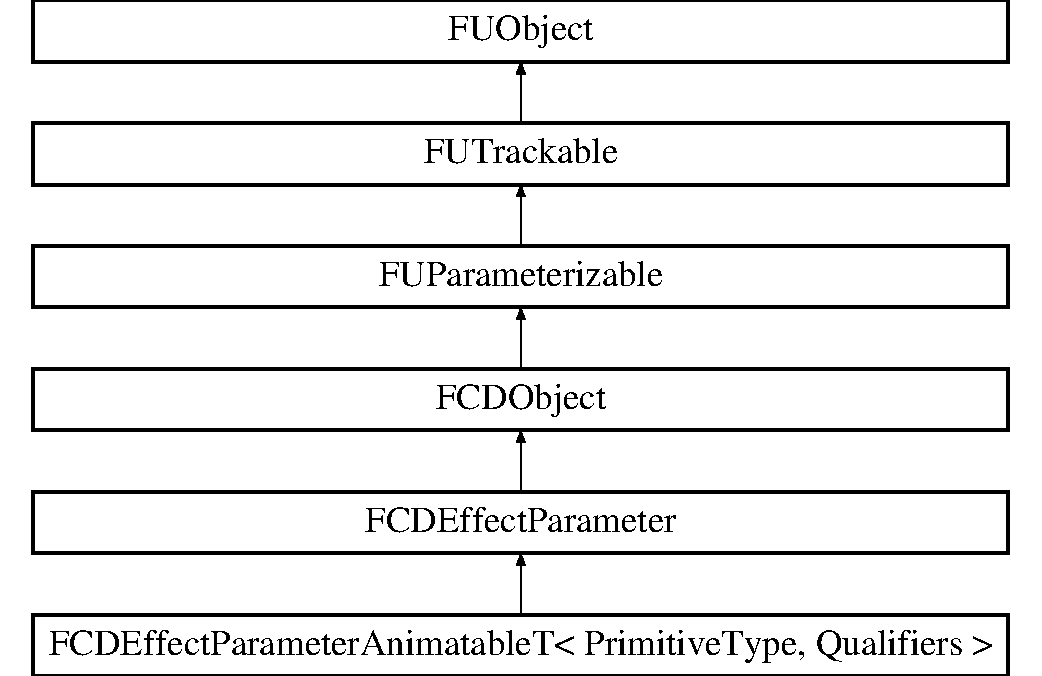
\includegraphics[height=6.000000cm]{classFCDEffectParameterAnimatableT}
\end{center}
\end{figure}
\subsection*{Public Types}
\begin{DoxyCompactItemize}
\item 
enum \hyperlink{classFCDEffectParameterAnimatableT_a8cc624ded1c773fd65851d213573e8b1}{FloatType} \{ \hyperlink{classFCDEffectParameterAnimatableT_a8cc624ded1c773fd65851d213573e8b1ac9547c18b1292ca978765dda33d09ed1}{FLOAT}, 
\hyperlink{classFCDEffectParameterAnimatableT_a8cc624ded1c773fd65851d213573e8b1a0f1f9490970710f8c80173b3d8fa37ff}{HALF}
 \}
\end{DoxyCompactItemize}
\subsection*{Public Member Functions}
\begin{DoxyCompactItemize}
\item 
\hyperlink{classFCDEffectParameterAnimatableT_a5cf262b2959b4536f8e434600b3e8d45}{FCDEffectParameterAnimatableT} (\hyperlink{classFCDocument}{FCDocument} $\ast$document)
\item 
virtual \hyperlink{classFCDEffectParameterAnimatableT_a1c7fc2c46f69476898aa002bcec78df4}{$\sim$FCDEffectParameterAnimatableT} ()
\item 
virtual \hyperlink{classFCDEffectParameter_a1efe74553d2ed199435085c171743b08}{Type} \hyperlink{classFCDEffectParameterAnimatableT_a5c9927e0ec4e8ab4c53f64c9a9490b20}{GetType} () const 
\item 
\hyperlink{classFCDEffectParameterAnimatableT_a8cc624ded1c773fd65851d213573e8b1}{FloatType} \hyperlink{classFCDEffectParameterAnimatableT_a8d67ba29be54209efc203539e47a5126}{GetFloatType} () const 
\item 
void \hyperlink{classFCDEffectParameterAnimatableT_a301ec52a4c64cada628b9cc4a8b10583}{SetFloatType} (\hyperlink{classFCDEffectParameterAnimatableT_a8cc624ded1c773fd65851d213573e8b1}{FloatType} type)
\item 
\hyperlink{classFCDParameterAnimatableT}{FCDParameterAnimatableT}$<$ PrimitiveType, Qualifiers $>$ \& \hyperlink{classFCDEffectParameterAnimatableT_ade9b28bef76882f7be35a199f03dc91d}{GetValue} ()
\item 
const \hyperlink{classFCDParameterAnimatableT}{FCDParameterAnimatableT}$<$ PrimitiveType, Qualifiers $>$ \& \hyperlink{classFCDEffectParameterAnimatableT_a2dd24784bc0f3db4215ce7cf8b63934f}{GetValue} () const 
\item 
void \hyperlink{classFCDEffectParameterAnimatableT_a14593ca8b6b7cba38b3e2a7d99e5f81c}{SetValue} (const PrimitiveType \&\_\-value)
\item 
virtual bool \hyperlink{classFCDEffectParameterAnimatableT_a490bf049e84d5c75ae60b4c5256aee5c}{IsValueEqual} (\hyperlink{classFCDEffectParameter}{FCDEffectParameter} $\ast$parameter)
\item 
virtual \hyperlink{classFCDEffectParameter}{FCDEffectParameter} $\ast$ \hyperlink{classFCDEffectParameterAnimatableT_a810e39c7a3824cf55828197ce0befa79}{Clone} (\hyperlink{classFCDEffectParameter}{FCDEffectParameter} $\ast$clone=NULL) const 
\item 
virtual void \hyperlink{classFCDEffectParameterAnimatableT_a6645b1e1d7ccef7505b7912b22f9deb9}{Overwrite} (\hyperlink{classFCDEffectParameter}{FCDEffectParameter} $\ast$target)
\end{DoxyCompactItemize}


\subsection{Detailed Description}
\subsubsection*{template$<$class PrimitiveType, int Qualifiers$>$ class FCDEffectParameterAnimatableT$<$ PrimitiveType, Qualifiers $>$}

A COLLADA non-\/animatable effect parameter template. 

\subsection{Member Enumeration Documentation}
\hypertarget{classFCDEffectParameterAnimatableT_a8cc624ded1c773fd65851d213573e8b1}{
\index{FCDEffectParameterAnimatableT@{FCDEffectParameterAnimatableT}!FloatType@{FloatType}}
\index{FloatType@{FloatType}!FCDEffectParameterAnimatableT@{FCDEffectParameterAnimatableT}}
\subsubsection[{FloatType}]{\setlength{\rightskip}{0pt plus 5cm}template$<$class PrimitiveType, int Qualifiers$>$ enum {\bf FCDEffectParameterAnimatableT::FloatType}}}
\label{classFCDEffectParameterAnimatableT_a8cc624ded1c773fd65851d213573e8b1}
The supported types of float-\/point values. \begin{Desc}
\item[Enumerator: ]\par
\begin{description}
\index{HALF@{HALF}!FCDEffectParameterAnimatableT@{FCDEffectParameterAnimatableT}}\index{FCDEffectParameterAnimatableT@{FCDEffectParameterAnimatableT}!HALF@{HALF}}\item[{\em 
\hypertarget{classFCDEffectParameterAnimatableT_a8cc624ded1c773fd65851d213573e8b1a0f1f9490970710f8c80173b3d8fa37ff}{
HALF}
\label{classFCDEffectParameterAnimatableT_a8cc624ded1c773fd65851d213573e8b1a0f1f9490970710f8c80173b3d8fa37ff}
}]A full-\/fledged floating-\/point value. This is the default. Probably implies a 16-\/bit floating-\/point value. \end{description}
\end{Desc}



\subsection{Constructor \& Destructor Documentation}
\hypertarget{classFCDEffectParameterAnimatableT_a5cf262b2959b4536f8e434600b3e8d45}{
\index{FCDEffectParameterAnimatableT@{FCDEffectParameterAnimatableT}!FCDEffectParameterAnimatableT@{FCDEffectParameterAnimatableT}}
\index{FCDEffectParameterAnimatableT@{FCDEffectParameterAnimatableT}!FCDEffectParameterAnimatableT@{FCDEffectParameterAnimatableT}}
\subsubsection[{FCDEffectParameterAnimatableT}]{\setlength{\rightskip}{0pt plus 5cm}FCDEffectParameterMatrix::FCDEffectParameterAnimatableT (
\begin{DoxyParamCaption}
\item[{{\bf FCDocument} $\ast$}]{ document}
\end{DoxyParamCaption}
)}}
\label{classFCDEffectParameterAnimatableT_a5cf262b2959b4536f8e434600b3e8d45}
Constructor: do not use directly. Instead, use the appropriate AddEffectParameter function. 
\begin{DoxyParams}{Parameters}
\item[{\em document}]The COLLADA document that owns the effect parameter. \end{DoxyParams}
\hypertarget{classFCDEffectParameterAnimatableT_a1c7fc2c46f69476898aa002bcec78df4}{
\index{FCDEffectParameterAnimatableT@{FCDEffectParameterAnimatableT}!$\sim$FCDEffectParameterAnimatableT@{$\sim$FCDEffectParameterAnimatableT}}
\index{$\sim$FCDEffectParameterAnimatableT@{$\sim$FCDEffectParameterAnimatableT}!FCDEffectParameterAnimatableT@{FCDEffectParameterAnimatableT}}
\subsubsection[{$\sim$FCDEffectParameterAnimatableT}]{\setlength{\rightskip}{0pt plus 5cm}template$<$class PrimitiveType , int Qualifiers$>$ {\bf FCDEffectParameterAnimatableT}$<$ PrimitiveType, Qualifiers $>$::$\sim${\bf FCDEffectParameterAnimatableT} (
\begin{DoxyParamCaption}
{}
\end{DoxyParamCaption}
)\hspace{0.3cm}{\ttfamily  \mbox{[}virtual\mbox{]}}}}
\label{classFCDEffectParameterAnimatableT_a1c7fc2c46f69476898aa002bcec78df4}
Destructor. 

\subsection{Member Function Documentation}
\hypertarget{classFCDEffectParameterAnimatableT_a810e39c7a3824cf55828197ce0befa79}{
\index{FCDEffectParameterAnimatableT@{FCDEffectParameterAnimatableT}!Clone@{Clone}}
\index{Clone@{Clone}!FCDEffectParameterAnimatableT@{FCDEffectParameterAnimatableT}}
\subsubsection[{Clone}]{\setlength{\rightskip}{0pt plus 5cm}template$<$class PrimitiveType , int Qualifiers$>$ {\bf FCDEffectParameter} $\ast$ {\bf FCDEffectParameterAnimatableT}$<$ PrimitiveType, Qualifiers $>$::Clone (
\begin{DoxyParamCaption}
\item[{{\bf FCDEffectParameter} $\ast$}]{ clone = {\ttfamily NULL}}
\end{DoxyParamCaption}
) const\hspace{0.3cm}{\ttfamily  \mbox{[}virtual\mbox{]}}}}
\label{classFCDEffectParameterAnimatableT_a810e39c7a3824cf55828197ce0befa79}
Creates a full copy of the effect parameter. 
\begin{DoxyParams}{Parameters}
\item[{\em clone}]The cloned effect parameter. If this pointer is NULL, a new effect parameter will be created and you will need to delete this pointer. \end{DoxyParams}
\begin{DoxyReturn}{Returns}
The cloned effect parameter. 
\end{DoxyReturn}


Reimplemented from \hyperlink{classFCDEffectParameter_a75abe4b8964493db40604fa3d0e373eb}{FCDEffectParameter}.

\hypertarget{classFCDEffectParameterAnimatableT_a8d67ba29be54209efc203539e47a5126}{
\index{FCDEffectParameterAnimatableT@{FCDEffectParameterAnimatableT}!GetFloatType@{GetFloatType}}
\index{GetFloatType@{GetFloatType}!FCDEffectParameterAnimatableT@{FCDEffectParameterAnimatableT}}
\subsubsection[{GetFloatType}]{\setlength{\rightskip}{0pt plus 5cm}template$<$class PrimitiveType, int Qualifiers$>$ {\bf FloatType} {\bf FCDEffectParameterAnimatableT}$<$ PrimitiveType, Qualifiers $>$::GetFloatType (
\begin{DoxyParamCaption}
{}
\end{DoxyParamCaption}
) const\hspace{0.3cm}{\ttfamily  \mbox{[}inline\mbox{]}}}}
\label{classFCDEffectParameterAnimatableT_a8d67ba29be54209efc203539e47a5126}
Retrieves the type of floating-\/point value held by this effect parameter. \begin{DoxyReturn}{Returns}
The type of floating-\/point value. 
\end{DoxyReturn}
\hypertarget{classFCDEffectParameterAnimatableT_a5c9927e0ec4e8ab4c53f64c9a9490b20}{
\index{FCDEffectParameterAnimatableT@{FCDEffectParameterAnimatableT}!GetType@{GetType}}
\index{GetType@{GetType}!FCDEffectParameterAnimatableT@{FCDEffectParameterAnimatableT}}
\subsubsection[{GetType}]{\setlength{\rightskip}{0pt plus 5cm}{\bf FCDEffectParameter::Type} FCDEffectParameterMatrix::GetType (
\begin{DoxyParamCaption}
{}
\end{DoxyParamCaption}
) const\hspace{0.3cm}{\ttfamily  \mbox{[}virtual\mbox{]}}}}
\label{classFCDEffectParameterAnimatableT_a5c9927e0ec4e8ab4c53f64c9a9490b20}
Retrieves the type of effect parameter class. \begin{DoxyReturn}{Returns}
The parameter class type. 
\end{DoxyReturn}


Implements \hyperlink{classFCDEffectParameter_a5858946f333ea4486ca30c4c1b104871}{FCDEffectParameter}.

\hypertarget{classFCDEffectParameterAnimatableT_ade9b28bef76882f7be35a199f03dc91d}{
\index{FCDEffectParameterAnimatableT@{FCDEffectParameterAnimatableT}!GetValue@{GetValue}}
\index{GetValue@{GetValue}!FCDEffectParameterAnimatableT@{FCDEffectParameterAnimatableT}}
\subsubsection[{GetValue}]{\setlength{\rightskip}{0pt plus 5cm}template$<$class PrimitiveType, int Qualifiers$>$ {\bf FCDParameterAnimatableT}$<$PrimitiveType, Qualifiers$>$\& {\bf FCDEffectParameterAnimatableT}$<$ PrimitiveType, Qualifiers $>$::GetValue (
\begin{DoxyParamCaption}
{}
\end{DoxyParamCaption}
)\hspace{0.3cm}{\ttfamily  \mbox{[}inline\mbox{]}}}}
\label{classFCDEffectParameterAnimatableT_ade9b28bef76882f7be35a199f03dc91d}
Retrieves the value of the effect parameter. \begin{DoxyReturn}{Returns}
The integer value. 
\end{DoxyReturn}
\hypertarget{classFCDEffectParameterAnimatableT_a2dd24784bc0f3db4215ce7cf8b63934f}{
\index{FCDEffectParameterAnimatableT@{FCDEffectParameterAnimatableT}!GetValue@{GetValue}}
\index{GetValue@{GetValue}!FCDEffectParameterAnimatableT@{FCDEffectParameterAnimatableT}}
\subsubsection[{GetValue}]{\setlength{\rightskip}{0pt plus 5cm}template$<$class PrimitiveType, int Qualifiers$>$ const {\bf FCDParameterAnimatableT}$<$PrimitiveType, Qualifiers$>$\& {\bf FCDEffectParameterAnimatableT}$<$ PrimitiveType, Qualifiers $>$::GetValue (
\begin{DoxyParamCaption}
{}
\end{DoxyParamCaption}
) const\hspace{0.3cm}{\ttfamily  \mbox{[}inline\mbox{]}}}}
\label{classFCDEffectParameterAnimatableT_a2dd24784bc0f3db4215ce7cf8b63934f}
See above. \hypertarget{classFCDEffectParameterAnimatableT_a490bf049e84d5c75ae60b4c5256aee5c}{
\index{FCDEffectParameterAnimatableT@{FCDEffectParameterAnimatableT}!IsValueEqual@{IsValueEqual}}
\index{IsValueEqual@{IsValueEqual}!FCDEffectParameterAnimatableT@{FCDEffectParameterAnimatableT}}
\subsubsection[{IsValueEqual}]{\setlength{\rightskip}{0pt plus 5cm}template$<$class PrimitiveType , int Qualifiers$>$ bool {\bf FCDEffectParameterAnimatableT}$<$ PrimitiveType, Qualifiers $>$::IsValueEqual (
\begin{DoxyParamCaption}
\item[{{\bf FCDEffectParameter} $\ast$}]{ parameter}
\end{DoxyParamCaption}
)\hspace{0.3cm}{\ttfamily  \mbox{[}virtual\mbox{]}}}}
\label{classFCDEffectParameterAnimatableT_a490bf049e84d5c75ae60b4c5256aee5c}
Compares this parameter's value with another 
\begin{DoxyParams}{Parameters}
\item[{\em parameter}]The given parameter to compare with. \end{DoxyParams}
\begin{DoxyReturn}{Returns}
true if the values are equal 
\end{DoxyReturn}


Implements \hyperlink{classFCDEffectParameter_a005a5a316bdb99dbd97ac542c129cc5e}{FCDEffectParameter}.

\hypertarget{classFCDEffectParameterAnimatableT_a6645b1e1d7ccef7505b7912b22f9deb9}{
\index{FCDEffectParameterAnimatableT@{FCDEffectParameterAnimatableT}!Overwrite@{Overwrite}}
\index{Overwrite@{Overwrite}!FCDEffectParameterAnimatableT@{FCDEffectParameterAnimatableT}}
\subsubsection[{Overwrite}]{\setlength{\rightskip}{0pt plus 5cm}template$<$class PrimitiveType , int Qualifiers$>$ void {\bf FCDEffectParameterAnimatableT}$<$ PrimitiveType, Qualifiers $>$::Overwrite (
\begin{DoxyParamCaption}
\item[{{\bf FCDEffectParameter} $\ast$}]{ target}
\end{DoxyParamCaption}
)\hspace{0.3cm}{\ttfamily  \mbox{[}virtual\mbox{]}}}}
\label{classFCDEffectParameterAnimatableT_a6645b1e1d7ccef7505b7912b22f9deb9}
\mbox{[}INTERNAL\mbox{]} Overwrites the target parameter with this parameter. This function is used during the flattening of materials. 
\begin{DoxyParams}{Parameters}
\item[{\em target}]The target parameter to overwrite. \end{DoxyParams}


Reimplemented from \hyperlink{classFCDEffectParameter_a016be91dbd27ff3c8c30f759f00b8c53}{FCDEffectParameter}.

\hypertarget{classFCDEffectParameterAnimatableT_a301ec52a4c64cada628b9cc4a8b10583}{
\index{FCDEffectParameterAnimatableT@{FCDEffectParameterAnimatableT}!SetFloatType@{SetFloatType}}
\index{SetFloatType@{SetFloatType}!FCDEffectParameterAnimatableT@{FCDEffectParameterAnimatableT}}
\subsubsection[{SetFloatType}]{\setlength{\rightskip}{0pt plus 5cm}template$<$class PrimitiveType, int Qualifiers$>$ void {\bf FCDEffectParameterAnimatableT}$<$ PrimitiveType, Qualifiers $>$::SetFloatType (
\begin{DoxyParamCaption}
\item[{{\bf FloatType}}]{ type}
\end{DoxyParamCaption}
)\hspace{0.3cm}{\ttfamily  \mbox{[}inline\mbox{]}}}}
\label{classFCDEffectParameterAnimatableT_a301ec52a4c64cada628b9cc4a8b10583}
Sets the type of floating-\/point value held by this effect parameter. 
\begin{DoxyParams}{Parameters}
\item[{\em type}]The type of floating-\/point value. \end{DoxyParams}
\hypertarget{classFCDEffectParameterAnimatableT_a14593ca8b6b7cba38b3e2a7d99e5f81c}{
\index{FCDEffectParameterAnimatableT@{FCDEffectParameterAnimatableT}!SetValue@{SetValue}}
\index{SetValue@{SetValue}!FCDEffectParameterAnimatableT@{FCDEffectParameterAnimatableT}}
\subsubsection[{SetValue}]{\setlength{\rightskip}{0pt plus 5cm}template$<$class PrimitiveType, int Qualifiers$>$ void {\bf FCDEffectParameterAnimatableT}$<$ PrimitiveType, Qualifiers $>$::SetValue (
\begin{DoxyParamCaption}
\item[{const PrimitiveType \&}]{ \_\-value}
\end{DoxyParamCaption}
)\hspace{0.3cm}{\ttfamily  \mbox{[}inline\mbox{]}}}}
\label{classFCDEffectParameterAnimatableT_a14593ca8b6b7cba38b3e2a7d99e5f81c}
Sets the integer value of the effect parameter. 
\begin{DoxyParams}{Parameters}
\item[{\em \_\-value}]The integer value. \end{DoxyParams}


The documentation for this class was generated from the following files:\begin{DoxyCompactItemize}
\item 
FCollada/FCDocument/\hyperlink{FCDEffectParameter_8h}{FCDEffectParameter.h}\item 
FCollada/FCDocument/FCDEffectParameter.cpp\item 
FCollada/FCDocument/FCDEffectParameter.hpp\end{DoxyCompactItemize}

\hypertarget{classFCDEffectParameterAnnotation}{
\section{FCDEffectParameterAnnotation Class Reference}
\label{classFCDEffectParameterAnnotation}\index{FCDEffectParameterAnnotation@{FCDEffectParameterAnnotation}}
}


{\ttfamily \#include $<$FCDEffectParameter.h$>$}

Inheritance diagram for FCDEffectParameterAnnotation:\begin{figure}[H]
\begin{center}
\leavevmode
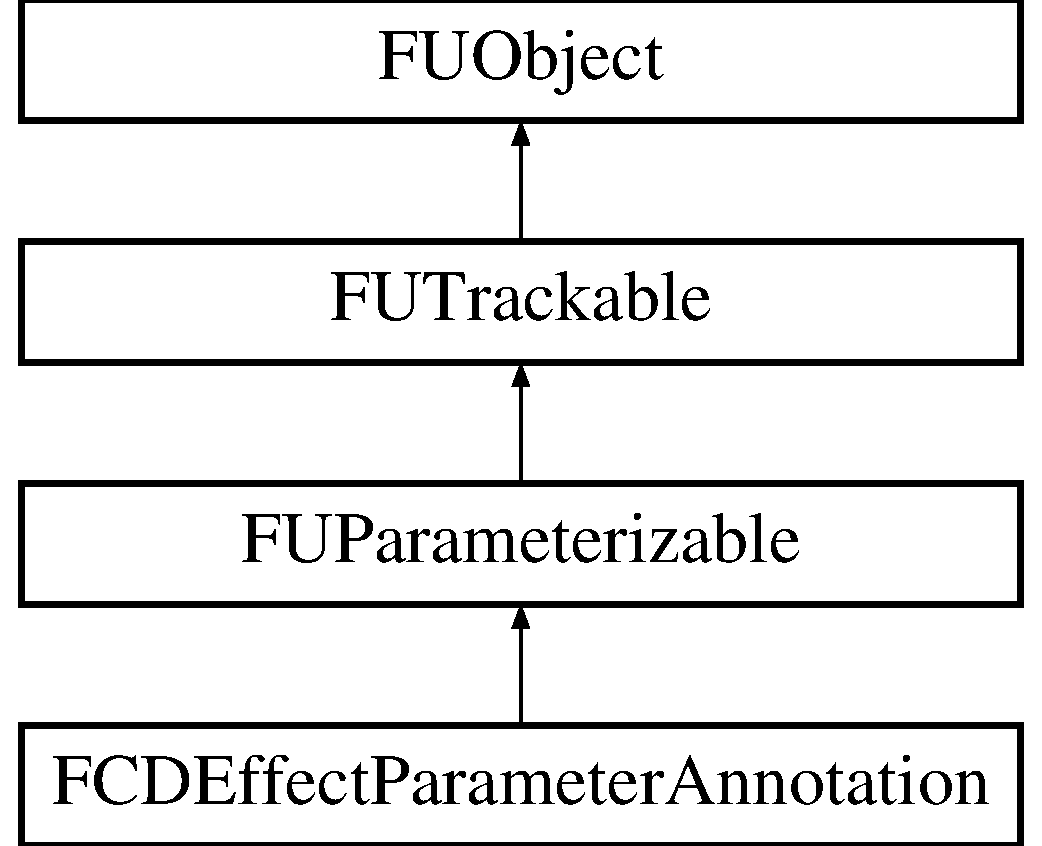
\includegraphics[height=4.000000cm]{classFCDEffectParameterAnnotation}
\end{center}
\end{figure}
\subsection*{Public Member Functions}
\begin{DoxyCompactItemize}
\item 
\hyperlink{classFCDEffectParameterAnnotation_a5b1857a81202e62800f3c1bcac6627fa}{FCDEffectParameterAnnotation} ()
\item 
virtual \hyperlink{classFCDEffectParameterAnnotation_a9eea09226dcd4ca7446bfc9b14302029}{$\sim$FCDEffectParameterAnnotation} ()
\item 
\hyperlink{classFCDEffectParameterAnnotation_a74a444cbb66d179737de9295fd49687d}{DeclareParameter} (\hyperlink{classfm_1_1stringT}{fstring}, FUParameterQualifiers::SIMPLE, name, FC(\char`\"{}Name\char`\"{}))
\item 
\hyperlink{classFCDEffectParameterAnnotation_afd3d8cdacd96378545bbef52335e23da}{DeclareParameter} (uint32, FUParameterQualifiers::SIMPLE, type, FC(\char`\"{}Value Type\char`\"{}))
\item 
\hyperlink{classFCDEffectParameterAnnotation_a88ba3b71a44d7b9be365acb8036cfeaf}{DeclareParameter} (\hyperlink{classfm_1_1stringT}{fstring}, FUParameterQualifiers::SIMPLE, value, FC(\char`\"{}Value\char`\"{}))
\end{DoxyCompactItemize}


\subsection{Detailed Description}
A ColladaFX annotation.

ColladaFX annotations are used mainly to describe the user interface necessary to modify a parameter. Common annotations are \char`\"{}UIMin\char`\"{}, \char`\"{}UIMax\char`\"{} and \char`\"{}UIWidget\char`\"{}. 

\subsection{Constructor \& Destructor Documentation}
\hypertarget{classFCDEffectParameterAnnotation_a5b1857a81202e62800f3c1bcac6627fa}{
\index{FCDEffectParameterAnnotation@{FCDEffectParameterAnnotation}!FCDEffectParameterAnnotation@{FCDEffectParameterAnnotation}}
\index{FCDEffectParameterAnnotation@{FCDEffectParameterAnnotation}!FCDEffectParameterAnnotation@{FCDEffectParameterAnnotation}}
\subsubsection[{FCDEffectParameterAnnotation}]{\setlength{\rightskip}{0pt plus 5cm}FCDEffectParameterAnnotation::FCDEffectParameterAnnotation (
\begin{DoxyParamCaption}
{}
\end{DoxyParamCaption}
)}}
\label{classFCDEffectParameterAnnotation_a5b1857a81202e62800f3c1bcac6627fa}
Constructor. Do not use directly. Instead, use \hyperlink{classFCDEffectParameter_a20bfb0f1361f5712c6014300878996e9}{FCDEffectParameter::AddAnnotation}. \hypertarget{classFCDEffectParameterAnnotation_a9eea09226dcd4ca7446bfc9b14302029}{
\index{FCDEffectParameterAnnotation@{FCDEffectParameterAnnotation}!$\sim$FCDEffectParameterAnnotation@{$\sim$FCDEffectParameterAnnotation}}
\index{$\sim$FCDEffectParameterAnnotation@{$\sim$FCDEffectParameterAnnotation}!FCDEffectParameterAnnotation@{FCDEffectParameterAnnotation}}
\subsubsection[{$\sim$FCDEffectParameterAnnotation}]{\setlength{\rightskip}{0pt plus 5cm}FCDEffectParameterAnnotation::$\sim$FCDEffectParameterAnnotation (
\begin{DoxyParamCaption}
{}
\end{DoxyParamCaption}
)\hspace{0.3cm}{\ttfamily  \mbox{[}virtual\mbox{]}}}}
\label{classFCDEffectParameterAnnotation_a9eea09226dcd4ca7446bfc9b14302029}
Destructor. 

\subsection{Member Function Documentation}
\hypertarget{classFCDEffectParameterAnnotation_a74a444cbb66d179737de9295fd49687d}{
\index{FCDEffectParameterAnnotation@{FCDEffectParameterAnnotation}!DeclareParameter@{DeclareParameter}}
\index{DeclareParameter@{DeclareParameter}!FCDEffectParameterAnnotation@{FCDEffectParameterAnnotation}}
\subsubsection[{DeclareParameter}]{\setlength{\rightskip}{0pt plus 5cm}FCDEffectParameterAnnotation::DeclareParameter (
\begin{DoxyParamCaption}
\item[{{\bf fstring}}]{, }
\item[{FUParameterQualifiers::SIMPLE}]{, }
\item[{name}]{, }
\item[{FC(\char`\"{}Name\char`\"{})}]{}
\end{DoxyParamCaption}
)}}
\label{classFCDEffectParameterAnnotation_a74a444cbb66d179737de9295fd49687d}
The annotation name. \hypertarget{classFCDEffectParameterAnnotation_a88ba3b71a44d7b9be365acb8036cfeaf}{
\index{FCDEffectParameterAnnotation@{FCDEffectParameterAnnotation}!DeclareParameter@{DeclareParameter}}
\index{DeclareParameter@{DeclareParameter}!FCDEffectParameterAnnotation@{FCDEffectParameterAnnotation}}
\subsubsection[{DeclareParameter}]{\setlength{\rightskip}{0pt plus 5cm}FCDEffectParameterAnnotation::DeclareParameter (
\begin{DoxyParamCaption}
\item[{{\bf fstring}}]{, }
\item[{FUParameterQualifiers::SIMPLE}]{, }
\item[{value}]{, }
\item[{FC(\char`\"{}Value\char`\"{})}]{}
\end{DoxyParamCaption}
)}}
\label{classFCDEffectParameterAnnotation_a88ba3b71a44d7b9be365acb8036cfeaf}
The annotation value. \hypertarget{classFCDEffectParameterAnnotation_afd3d8cdacd96378545bbef52335e23da}{
\index{FCDEffectParameterAnnotation@{FCDEffectParameterAnnotation}!DeclareParameter@{DeclareParameter}}
\index{DeclareParameter@{DeclareParameter}!FCDEffectParameterAnnotation@{FCDEffectParameterAnnotation}}
\subsubsection[{DeclareParameter}]{\setlength{\rightskip}{0pt plus 5cm}FCDEffectParameterAnnotation::DeclareParameter (
\begin{DoxyParamCaption}
\item[{uint32}]{, }
\item[{FUParameterQualifiers::SIMPLE}]{, }
\item[{type}]{, }
\item[{FC(\char`\"{}Value Type\char`\"{})}]{}
\end{DoxyParamCaption}
)}}
\label{classFCDEffectParameterAnnotation_afd3d8cdacd96378545bbef52335e23da}
The annotation value type (\hyperlink{classFCDEffectParameter_a1efe74553d2ed199435085c171743b08}{FCDEffectParameter::Type}). 

The documentation for this class was generated from the following files:\begin{DoxyCompactItemize}
\item 
FCollada/FCDocument/\hyperlink{FCDEffectParameter_8h}{FCDEffectParameter.h}\item 
FCollada/FCDocument/FCDEffectParameter.cpp\end{DoxyCompactItemize}

\hypertarget{classFCDEffectParameterFactory}{
\section{FCDEffectParameterFactory Class Reference}
\label{classFCDEffectParameterFactory}\index{FCDEffectParameterFactory@{FCDEffectParameterFactory}}
}


{\ttfamily \#include $<$FCDEffectParameterFactory.h$>$}

\subsection*{Static Public Member Functions}
\begin{DoxyCompactItemize}
\item 
static \hyperlink{classFCDEffectParameter}{FCDEffectParameter} $\ast$ \hyperlink{classFCDEffectParameterFactory_a49f20591f628c8bdf8f8b4b132721e69}{Create} (\hyperlink{classFCDocument}{FCDocument} $\ast$document, uint32 type)
\end{DoxyCompactItemize}


\subsection{Detailed Description}
\mbox{[}INTERNAL\mbox{]} The factory for COLLADA effect parameters.

Takes in a COLLADA XML tree and returns a new parameter that represent it, if one is possible. 

\subsection{Member Function Documentation}
\hypertarget{classFCDEffectParameterFactory_a49f20591f628c8bdf8f8b4b132721e69}{
\index{FCDEffectParameterFactory@{FCDEffectParameterFactory}!Create@{Create}}
\index{Create@{Create}!FCDEffectParameterFactory@{FCDEffectParameterFactory}}
\subsubsection[{Create}]{\setlength{\rightskip}{0pt plus 5cm}{\bf FCDEffectParameter} $\ast$ FCDEffectParameterFactory::Create (
\begin{DoxyParamCaption}
\item[{{\bf FCDocument} $\ast$}]{ document, }
\item[{uint32}]{ type}
\end{DoxyParamCaption}
)\hspace{0.3cm}{\ttfamily  \mbox{[}static\mbox{]}}}}
\label{classFCDEffectParameterFactory_a49f20591f628c8bdf8f8b4b132721e69}
\mbox{[}INTERNAL\mbox{]} Creates a new effect parameter, given a type. To create new effect parameters, use the appropriate AddEffectParameter function. 
\begin{DoxyParams}{Parameters}
\item[{\em document}]The COLLADA document that will own the effect parameter. \item[{\em type}]The type of effect to create. This value should reflect the \hyperlink{classFCDEffectParameter_a1efe74553d2ed199435085c171743b08}{FCDEffectParameter::Type} enum. \end{DoxyParams}


The documentation for this class was generated from the following files:\begin{DoxyCompactItemize}
\item 
FCollada/FCDocument/\hyperlink{FCDEffectParameterFactory_8h}{FCDEffectParameterFactory.h}\item 
FCollada/FCDocument/FCDEffectParameterFactory.cpp\end{DoxyCompactItemize}

\hypertarget{classFCDEffectParameterSampler}{
\section{FCDEffectParameterSampler Class Reference}
\label{classFCDEffectParameterSampler}\index{FCDEffectParameterSampler@{FCDEffectParameterSampler}}
}


{\ttfamily \#include $<$FCDEffectParameterSampler.h$>$}

Inheritance diagram for FCDEffectParameterSampler:\begin{figure}[H]
\begin{center}
\leavevmode
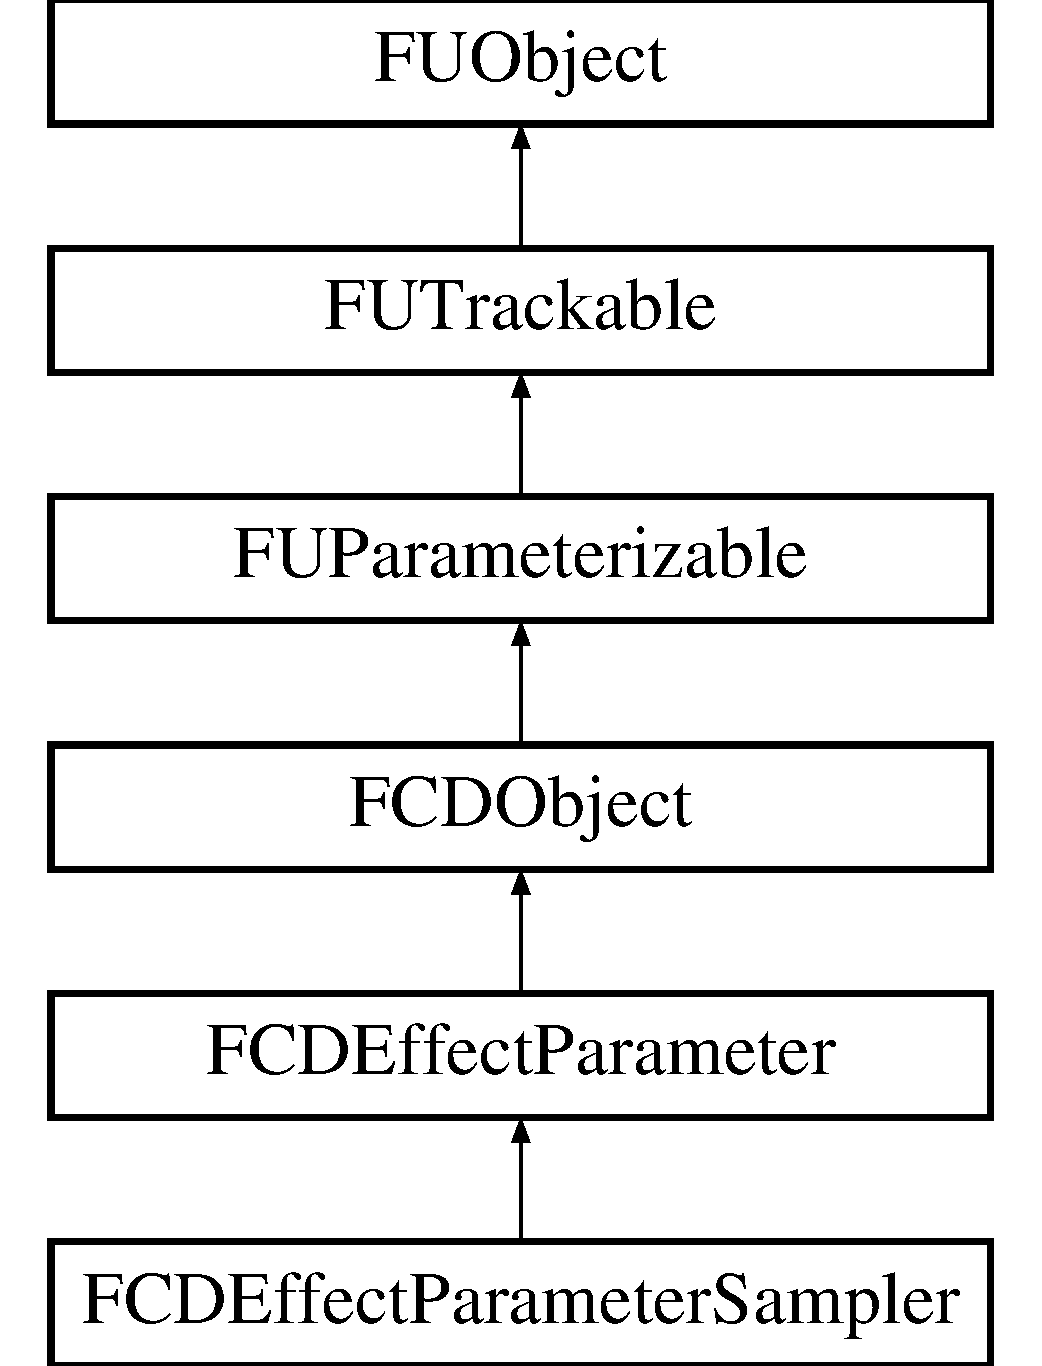
\includegraphics[height=6.000000cm]{classFCDEffectParameterSampler}
\end{center}
\end{figure}
\subsection*{Public Types}
\begin{DoxyCompactItemize}
\item 
enum \hyperlink{classFCDEffectParameterSampler_ae3a82d31b80b3510bb44a62bd3c34424}{SamplerType} \{ {\bfseries SAMPLER1D}, 
\hyperlink{classFCDEffectParameterSampler_ae3a82d31b80b3510bb44a62bd3c34424a3e0a98b613cd47287b74402a45dcd2df}{SAMPLER2D}, 
\hyperlink{classFCDEffectParameterSampler_ae3a82d31b80b3510bb44a62bd3c34424a705723cc55960ee3b2d6744e3244cd48}{SAMPLER3D}, 
\hyperlink{classFCDEffectParameterSampler_ae3a82d31b80b3510bb44a62bd3c34424a4c3851e3bc494f054f2e45efd74e107d}{SAMPLERCUBE}
 \}
\end{DoxyCompactItemize}
\subsection*{Public Member Functions}
\begin{DoxyCompactItemize}
\item 
\hyperlink{classFCDEffectParameterSampler_a2f69f2f62504f6e0122254d738aac0b4}{FCDEffectParameterSampler} (\hyperlink{classFCDocument}{FCDocument} $\ast$document)
\item 
virtual \hyperlink{classFCDEffectParameterSampler_a55177a91bf15cb2168bceb2d7b32c5bf}{$\sim$FCDEffectParameterSampler} ()
\item 
virtual \hyperlink{classFCDEffectParameter_a1efe74553d2ed199435085c171743b08}{Type} \hyperlink{classFCDEffectParameterSampler_ab0483ddfcc3c69f12539df9fba36f0d6}{GetType} () const 
\item 
\hyperlink{classFCDEffectParameterSurface}{FCDEffectParameterSurface} $\ast$ \hyperlink{classFCDEffectParameterSampler_aa1d035030a9a82d64f65b7863b9812a2}{GetSurface} ()
\item 
const \hyperlink{classFCDEffectParameterSurface}{FCDEffectParameterSurface} $\ast$ \hyperlink{classFCDEffectParameterSampler_a291ce036d2d8a353368633eb677e972b}{GetSurface} () const 
\item 
void \hyperlink{classFCDEffectParameterSampler_a5e34b2e987fcdc73e65fafcf0d21036b}{SetSurface} (\hyperlink{classFCDEffectParameterSurface}{FCDEffectParameterSurface} $\ast$surface)
\item 
\hyperlink{classFCDEffectParameterSampler_ae3a82d31b80b3510bb44a62bd3c34424}{SamplerType} \hyperlink{classFCDEffectParameterSampler_a07aaa27b521ceaf9fb570eeb713bb41a}{GetSamplerType} () const 
\item 
void \hyperlink{classFCDEffectParameterSampler_aeb463b7fed44feccf05032b2274c4dcc}{SetSamplerType} (\hyperlink{classFCDEffectParameterSampler_ae3a82d31b80b3510bb44a62bd3c34424}{SamplerType} type)
\item 
FUDaeTextureWrapMode::WrapMode \hyperlink{classFCDEffectParameterSampler_a95b028a920ae04a45bbb9613c7754389}{GetWrapS} () const 
\item 
FUDaeTextureWrapMode::WrapMode \hyperlink{classFCDEffectParameterSampler_a80fa6f7d93d559c2a0382fa6fb3b13b0}{GetWrapT} () const 
\item 
FUDaeTextureWrapMode::WrapMode \hyperlink{classFCDEffectParameterSampler_abec9f4de7ac772c42c12ff6a1f76ee7c}{GetWrapP} () const 
\item 
void \hyperlink{classFCDEffectParameterSampler_a68a18ff96d3edeb67f15d5616e18ae75}{SetWrapS} (FUDaeTextureWrapMode::WrapMode mode)
\item 
void \hyperlink{classFCDEffectParameterSampler_ad0bfbd28ab6eaa0418e7132854c8f2cd}{SetWrapT} (FUDaeTextureWrapMode::WrapMode mode)
\item 
void \hyperlink{classFCDEffectParameterSampler_a02d7b529fde6695a19ff46b08da4a19c}{SetWrapP} (FUDaeTextureWrapMode::WrapMode mode)
\item 
FUDaeTextureFilterFunction::FilterFunction \hyperlink{classFCDEffectParameterSampler_aaea04017be7daae510dcc8542dce7d01}{GetMinFilter} () const 
\item 
FUDaeTextureFilterFunction::FilterFunction \hyperlink{classFCDEffectParameterSampler_a289f5a2811094a7673ab7ace87405025}{GetMagFilter} () const 
\item 
FUDaeTextureFilterFunction::FilterFunction \hyperlink{classFCDEffectParameterSampler_a90eb9b969aeb0bd4da0c1964c8d0252d}{GetMipFilter} () const 
\item 
void \hyperlink{classFCDEffectParameterSampler_ac109ce64fbad3136acf24bf15636316d}{SetMinFilter} (FUDaeTextureFilterFunction::FilterFunction func)
\item 
void \hyperlink{classFCDEffectParameterSampler_a28fef01829ddba5f4146335e1982e8e0}{SetMagFilter} (FUDaeTextureFilterFunction::FilterFunction func)
\item 
void \hyperlink{classFCDEffectParameterSampler_ae0cd8598da4f351c0c526eb5c72530e6}{SetMipFilter} (FUDaeTextureFilterFunction::FilterFunction func)
\item 
virtual bool \hyperlink{classFCDEffectParameterSampler_ad167b41465766bed31b83cc76f6866c4}{IsValueEqual} (\hyperlink{classFCDEffectParameter}{FCDEffectParameter} $\ast$parameter)
\item 
virtual \hyperlink{classFCDEffectParameter}{FCDEffectParameter} $\ast$ \hyperlink{classFCDEffectParameterSampler_af72a0f9e9514fca46bc9996ed872eb01}{Clone} (\hyperlink{classFCDEffectParameter}{FCDEffectParameter} $\ast$clone=NULL) const 
\item 
virtual void \hyperlink{classFCDEffectParameterSampler_a2c562fb4058a2a10a0f9545c3a8eb43a}{Overwrite} (\hyperlink{classFCDEffectParameter}{FCDEffectParameter} $\ast$target)
\end{DoxyCompactItemize}


\subsection{Detailed Description}
A COLLADA sampler effect parameter. A sampler parameter provides the extra texturing information necessary to correctly sample a surface parameter. There are four types of samplers supported: 1D, 2D, 3D and cube. 

\subsection{Member Enumeration Documentation}
\hypertarget{classFCDEffectParameterSampler_ae3a82d31b80b3510bb44a62bd3c34424}{
\index{FCDEffectParameterSampler@{FCDEffectParameterSampler}!SamplerType@{SamplerType}}
\index{SamplerType@{SamplerType}!FCDEffectParameterSampler@{FCDEffectParameterSampler}}
\subsubsection[{SamplerType}]{\setlength{\rightskip}{0pt plus 5cm}enum {\bf FCDEffectParameterSampler::SamplerType}}}
\label{classFCDEffectParameterSampler_ae3a82d31b80b3510bb44a62bd3c34424}
The type of sampling to execute. \begin{Desc}
\item[Enumerator: ]\par
\begin{description}
\index{SAMPLER2D@{SAMPLER2D}!FCDEffectParameterSampler@{FCDEffectParameterSampler}}\index{FCDEffectParameterSampler@{FCDEffectParameterSampler}!SAMPLER2D@{SAMPLER2D}}\item[{\em 
\hypertarget{classFCDEffectParameterSampler_ae3a82d31b80b3510bb44a62bd3c34424a3e0a98b613cd47287b74402a45dcd2df}{
SAMPLER2D}
\label{classFCDEffectParameterSampler_ae3a82d31b80b3510bb44a62bd3c34424a3e0a98b613cd47287b74402a45dcd2df}
}]1D sampling. \index{SAMPLER3D@{SAMPLER3D}!FCDEffectParameterSampler@{FCDEffectParameterSampler}}\index{FCDEffectParameterSampler@{FCDEffectParameterSampler}!SAMPLER3D@{SAMPLER3D}}\item[{\em 
\hypertarget{classFCDEffectParameterSampler_ae3a82d31b80b3510bb44a62bd3c34424a705723cc55960ee3b2d6744e3244cd48}{
SAMPLER3D}
\label{classFCDEffectParameterSampler_ae3a82d31b80b3510bb44a62bd3c34424a705723cc55960ee3b2d6744e3244cd48}
}]2D sampling. \index{SAMPLERCUBE@{SAMPLERCUBE}!FCDEffectParameterSampler@{FCDEffectParameterSampler}}\index{FCDEffectParameterSampler@{FCDEffectParameterSampler}!SAMPLERCUBE@{SAMPLERCUBE}}\item[{\em 
\hypertarget{classFCDEffectParameterSampler_ae3a82d31b80b3510bb44a62bd3c34424a4c3851e3bc494f054f2e45efd74e107d}{
SAMPLERCUBE}
\label{classFCDEffectParameterSampler_ae3a82d31b80b3510bb44a62bd3c34424a4c3851e3bc494f054f2e45efd74e107d}
}]3D sampling. Cube-\/map sampling. \end{description}
\end{Desc}



\subsection{Constructor \& Destructor Documentation}
\hypertarget{classFCDEffectParameterSampler_a2f69f2f62504f6e0122254d738aac0b4}{
\index{FCDEffectParameterSampler@{FCDEffectParameterSampler}!FCDEffectParameterSampler@{FCDEffectParameterSampler}}
\index{FCDEffectParameterSampler@{FCDEffectParameterSampler}!FCDEffectParameterSampler@{FCDEffectParameterSampler}}
\subsubsection[{FCDEffectParameterSampler}]{\setlength{\rightskip}{0pt plus 5cm}FCDEffectParameterSampler::FCDEffectParameterSampler (
\begin{DoxyParamCaption}
\item[{{\bf FCDocument} $\ast$}]{ document}
\end{DoxyParamCaption}
)}}
\label{classFCDEffectParameterSampler_a2f69f2f62504f6e0122254d738aac0b4}
Constructor: do not use directly. Instead, use the appropriate AddEffectParameter function. 
\begin{DoxyParams}{Parameters}
\item[{\em document}]The COLLADA document that owns the effect parameter. \end{DoxyParams}
\hypertarget{classFCDEffectParameterSampler_a55177a91bf15cb2168bceb2d7b32c5bf}{
\index{FCDEffectParameterSampler@{FCDEffectParameterSampler}!$\sim$FCDEffectParameterSampler@{$\sim$FCDEffectParameterSampler}}
\index{$\sim$FCDEffectParameterSampler@{$\sim$FCDEffectParameterSampler}!FCDEffectParameterSampler@{FCDEffectParameterSampler}}
\subsubsection[{$\sim$FCDEffectParameterSampler}]{\setlength{\rightskip}{0pt plus 5cm}FCDEffectParameterSampler::$\sim$FCDEffectParameterSampler (
\begin{DoxyParamCaption}
{}
\end{DoxyParamCaption}
)\hspace{0.3cm}{\ttfamily  \mbox{[}virtual\mbox{]}}}}
\label{classFCDEffectParameterSampler_a55177a91bf15cb2168bceb2d7b32c5bf}
Destructor. 

\subsection{Member Function Documentation}
\hypertarget{classFCDEffectParameterSampler_af72a0f9e9514fca46bc9996ed872eb01}{
\index{FCDEffectParameterSampler@{FCDEffectParameterSampler}!Clone@{Clone}}
\index{Clone@{Clone}!FCDEffectParameterSampler@{FCDEffectParameterSampler}}
\subsubsection[{Clone}]{\setlength{\rightskip}{0pt plus 5cm}{\bf FCDEffectParameter} $\ast$ FCDEffectParameterSampler::Clone (
\begin{DoxyParamCaption}
\item[{{\bf FCDEffectParameter} $\ast$}]{ clone = {\ttfamily NULL}}
\end{DoxyParamCaption}
) const\hspace{0.3cm}{\ttfamily  \mbox{[}virtual\mbox{]}}}}
\label{classFCDEffectParameterSampler_af72a0f9e9514fca46bc9996ed872eb01}
Creates a full copy of the effect parameter. 
\begin{DoxyParams}{Parameters}
\item[{\em clone}]The cloned effect parameter. If this pointer is NULL, a new effect parameter will be created and you will need to delete this pointer. \end{DoxyParams}
\begin{DoxyReturn}{Returns}
The cloned effect parameter. 
\end{DoxyReturn}


Reimplemented from \hyperlink{classFCDEffectParameter_a75abe4b8964493db40604fa3d0e373eb}{FCDEffectParameter}.

\hypertarget{classFCDEffectParameterSampler_a289f5a2811094a7673ab7ace87405025}{
\index{FCDEffectParameterSampler@{FCDEffectParameterSampler}!GetMagFilter@{GetMagFilter}}
\index{GetMagFilter@{GetMagFilter}!FCDEffectParameterSampler@{FCDEffectParameterSampler}}
\subsubsection[{GetMagFilter}]{\setlength{\rightskip}{0pt plus 5cm}FUDaeTextureFilterFunction::FilterFunction FCDEffectParameterSampler::GetMagFilter (
\begin{DoxyParamCaption}
{}
\end{DoxyParamCaption}
) const\hspace{0.3cm}{\ttfamily  \mbox{[}inline\mbox{]}}}}
\label{classFCDEffectParameterSampler_a289f5a2811094a7673ab7ace87405025}
See above. \hypertarget{classFCDEffectParameterSampler_aaea04017be7daae510dcc8542dce7d01}{
\index{FCDEffectParameterSampler@{FCDEffectParameterSampler}!GetMinFilter@{GetMinFilter}}
\index{GetMinFilter@{GetMinFilter}!FCDEffectParameterSampler@{FCDEffectParameterSampler}}
\subsubsection[{GetMinFilter}]{\setlength{\rightskip}{0pt plus 5cm}FUDaeTextureFilterFunction::FilterFunction FCDEffectParameterSampler::GetMinFilter (
\begin{DoxyParamCaption}
{}
\end{DoxyParamCaption}
) const\hspace{0.3cm}{\ttfamily  \mbox{[}inline\mbox{]}}}}
\label{classFCDEffectParameterSampler_aaea04017be7daae510dcc8542dce7d01}
Retrieves the appropriate filter function (minification, magnification or mip map filtering) of the sampler. \begin{DoxyReturn}{Returns}
The filter function. 
\end{DoxyReturn}
\hypertarget{classFCDEffectParameterSampler_a90eb9b969aeb0bd4da0c1964c8d0252d}{
\index{FCDEffectParameterSampler@{FCDEffectParameterSampler}!GetMipFilter@{GetMipFilter}}
\index{GetMipFilter@{GetMipFilter}!FCDEffectParameterSampler@{FCDEffectParameterSampler}}
\subsubsection[{GetMipFilter}]{\setlength{\rightskip}{0pt plus 5cm}FUDaeTextureFilterFunction::FilterFunction FCDEffectParameterSampler::GetMipFilter (
\begin{DoxyParamCaption}
{}
\end{DoxyParamCaption}
) const\hspace{0.3cm}{\ttfamily  \mbox{[}inline\mbox{]}}}}
\label{classFCDEffectParameterSampler_a90eb9b969aeb0bd4da0c1964c8d0252d}
See above. \hypertarget{classFCDEffectParameterSampler_a07aaa27b521ceaf9fb570eeb713bb41a}{
\index{FCDEffectParameterSampler@{FCDEffectParameterSampler}!GetSamplerType@{GetSamplerType}}
\index{GetSamplerType@{GetSamplerType}!FCDEffectParameterSampler@{FCDEffectParameterSampler}}
\subsubsection[{GetSamplerType}]{\setlength{\rightskip}{0pt plus 5cm}{\bf SamplerType} FCDEffectParameterSampler::GetSamplerType (
\begin{DoxyParamCaption}
{}
\end{DoxyParamCaption}
) const\hspace{0.3cm}{\ttfamily  \mbox{[}inline\mbox{]}}}}
\label{classFCDEffectParameterSampler_a07aaa27b521ceaf9fb570eeb713bb41a}
Retrieves the type of sampling to do. \begin{DoxyReturn}{Returns}
The sampling type. 
\end{DoxyReturn}
\hypertarget{classFCDEffectParameterSampler_aa1d035030a9a82d64f65b7863b9812a2}{
\index{FCDEffectParameterSampler@{FCDEffectParameterSampler}!GetSurface@{GetSurface}}
\index{GetSurface@{GetSurface}!FCDEffectParameterSampler@{FCDEffectParameterSampler}}
\subsubsection[{GetSurface}]{\setlength{\rightskip}{0pt plus 5cm}{\bf FCDEffectParameterSurface}$\ast$ FCDEffectParameterSampler::GetSurface (
\begin{DoxyParamCaption}
{}
\end{DoxyParamCaption}
)\hspace{0.3cm}{\ttfamily  \mbox{[}inline\mbox{]}}}}
\label{classFCDEffectParameterSampler_aa1d035030a9a82d64f65b7863b9812a2}
Retrieves the parameter for the surface to sample. \begin{DoxyReturn}{Returns}
The surface parameter. This pointer will be NULL if the sampler is not yet linked to any surface.. 
\end{DoxyReturn}
\hypertarget{classFCDEffectParameterSampler_a291ce036d2d8a353368633eb677e972b}{
\index{FCDEffectParameterSampler@{FCDEffectParameterSampler}!GetSurface@{GetSurface}}
\index{GetSurface@{GetSurface}!FCDEffectParameterSampler@{FCDEffectParameterSampler}}
\subsubsection[{GetSurface}]{\setlength{\rightskip}{0pt plus 5cm}const {\bf FCDEffectParameterSurface}$\ast$ FCDEffectParameterSampler::GetSurface (
\begin{DoxyParamCaption}
{}
\end{DoxyParamCaption}
) const\hspace{0.3cm}{\ttfamily  \mbox{[}inline\mbox{]}}}}
\label{classFCDEffectParameterSampler_a291ce036d2d8a353368633eb677e972b}
See above. \hypertarget{classFCDEffectParameterSampler_ab0483ddfcc3c69f12539df9fba36f0d6}{
\index{FCDEffectParameterSampler@{FCDEffectParameterSampler}!GetType@{GetType}}
\index{GetType@{GetType}!FCDEffectParameterSampler@{FCDEffectParameterSampler}}
\subsubsection[{GetType}]{\setlength{\rightskip}{0pt plus 5cm}virtual {\bf Type} FCDEffectParameterSampler::GetType (
\begin{DoxyParamCaption}
{}
\end{DoxyParamCaption}
) const\hspace{0.3cm}{\ttfamily  \mbox{[}inline, virtual\mbox{]}}}}
\label{classFCDEffectParameterSampler_ab0483ddfcc3c69f12539df9fba36f0d6}
Retrieves the type of effect parameter class. \begin{DoxyReturn}{Returns}
The parameter class type: SAMPLER. 
\end{DoxyReturn}


Implements \hyperlink{classFCDEffectParameter_a5858946f333ea4486ca30c4c1b104871}{FCDEffectParameter}.

\hypertarget{classFCDEffectParameterSampler_abec9f4de7ac772c42c12ff6a1f76ee7c}{
\index{FCDEffectParameterSampler@{FCDEffectParameterSampler}!GetWrapP@{GetWrapP}}
\index{GetWrapP@{GetWrapP}!FCDEffectParameterSampler@{FCDEffectParameterSampler}}
\subsubsection[{GetWrapP}]{\setlength{\rightskip}{0pt plus 5cm}FUDaeTextureWrapMode::WrapMode FCDEffectParameterSampler::GetWrapP (
\begin{DoxyParamCaption}
{}
\end{DoxyParamCaption}
) const\hspace{0.3cm}{\ttfamily  \mbox{[}inline\mbox{]}}}}
\label{classFCDEffectParameterSampler_abec9f4de7ac772c42c12ff6a1f76ee7c}
See above. \hypertarget{classFCDEffectParameterSampler_a95b028a920ae04a45bbb9613c7754389}{
\index{FCDEffectParameterSampler@{FCDEffectParameterSampler}!GetWrapS@{GetWrapS}}
\index{GetWrapS@{GetWrapS}!FCDEffectParameterSampler@{FCDEffectParameterSampler}}
\subsubsection[{GetWrapS}]{\setlength{\rightskip}{0pt plus 5cm}FUDaeTextureWrapMode::WrapMode FCDEffectParameterSampler::GetWrapS (
\begin{DoxyParamCaption}
{}
\end{DoxyParamCaption}
) const\hspace{0.3cm}{\ttfamily  \mbox{[}inline\mbox{]}}}}
\label{classFCDEffectParameterSampler_a95b028a920ae04a45bbb9613c7754389}
Retrieves the wrap mode (in dimension S, T or P) of the sampler. \begin{DoxyReturn}{Returns}
The wrap mode. 
\end{DoxyReturn}
\hypertarget{classFCDEffectParameterSampler_a80fa6f7d93d559c2a0382fa6fb3b13b0}{
\index{FCDEffectParameterSampler@{FCDEffectParameterSampler}!GetWrapT@{GetWrapT}}
\index{GetWrapT@{GetWrapT}!FCDEffectParameterSampler@{FCDEffectParameterSampler}}
\subsubsection[{GetWrapT}]{\setlength{\rightskip}{0pt plus 5cm}FUDaeTextureWrapMode::WrapMode FCDEffectParameterSampler::GetWrapT (
\begin{DoxyParamCaption}
{}
\end{DoxyParamCaption}
) const\hspace{0.3cm}{\ttfamily  \mbox{[}inline\mbox{]}}}}
\label{classFCDEffectParameterSampler_a80fa6f7d93d559c2a0382fa6fb3b13b0}
See above. \hypertarget{classFCDEffectParameterSampler_ad167b41465766bed31b83cc76f6866c4}{
\index{FCDEffectParameterSampler@{FCDEffectParameterSampler}!IsValueEqual@{IsValueEqual}}
\index{IsValueEqual@{IsValueEqual}!FCDEffectParameterSampler@{FCDEffectParameterSampler}}
\subsubsection[{IsValueEqual}]{\setlength{\rightskip}{0pt plus 5cm}bool FCDEffectParameterSampler::IsValueEqual (
\begin{DoxyParamCaption}
\item[{{\bf FCDEffectParameter} $\ast$}]{ parameter}
\end{DoxyParamCaption}
)\hspace{0.3cm}{\ttfamily  \mbox{[}virtual\mbox{]}}}}
\label{classFCDEffectParameterSampler_ad167b41465766bed31b83cc76f6866c4}
Compares this parameter's value with another 
\begin{DoxyParams}{Parameters}
\item[{\em parameter}]The given parameter to compare with. \end{DoxyParams}
\begin{DoxyReturn}{Returns}
true if the values are equal 
\end{DoxyReturn}


Implements \hyperlink{classFCDEffectParameter_a005a5a316bdb99dbd97ac542c129cc5e}{FCDEffectParameter}.

\hypertarget{classFCDEffectParameterSampler_a2c562fb4058a2a10a0f9545c3a8eb43a}{
\index{FCDEffectParameterSampler@{FCDEffectParameterSampler}!Overwrite@{Overwrite}}
\index{Overwrite@{Overwrite}!FCDEffectParameterSampler@{FCDEffectParameterSampler}}
\subsubsection[{Overwrite}]{\setlength{\rightskip}{0pt plus 5cm}void FCDEffectParameterSampler::Overwrite (
\begin{DoxyParamCaption}
\item[{{\bf FCDEffectParameter} $\ast$}]{ target}
\end{DoxyParamCaption}
)\hspace{0.3cm}{\ttfamily  \mbox{[}virtual\mbox{]}}}}
\label{classFCDEffectParameterSampler_a2c562fb4058a2a10a0f9545c3a8eb43a}
\mbox{[}INTERNAL\mbox{]} Overwrites the target parameter with this parameter. This function is used during the flattening of materials. 
\begin{DoxyParams}{Parameters}
\item[{\em target}]The target parameter to overwrite. \end{DoxyParams}


Reimplemented from \hyperlink{classFCDEffectParameter_a016be91dbd27ff3c8c30f759f00b8c53}{FCDEffectParameter}.

\hypertarget{classFCDEffectParameterSampler_a28fef01829ddba5f4146335e1982e8e0}{
\index{FCDEffectParameterSampler@{FCDEffectParameterSampler}!SetMagFilter@{SetMagFilter}}
\index{SetMagFilter@{SetMagFilter}!FCDEffectParameterSampler@{FCDEffectParameterSampler}}
\subsubsection[{SetMagFilter}]{\setlength{\rightskip}{0pt plus 5cm}void FCDEffectParameterSampler::SetMagFilter (
\begin{DoxyParamCaption}
\item[{FUDaeTextureFilterFunction::FilterFunction}]{ func}
\end{DoxyParamCaption}
)\hspace{0.3cm}{\ttfamily  \mbox{[}inline\mbox{]}}}}
\label{classFCDEffectParameterSampler_a28fef01829ddba5f4146335e1982e8e0}
See above. \hypertarget{classFCDEffectParameterSampler_ac109ce64fbad3136acf24bf15636316d}{
\index{FCDEffectParameterSampler@{FCDEffectParameterSampler}!SetMinFilter@{SetMinFilter}}
\index{SetMinFilter@{SetMinFilter}!FCDEffectParameterSampler@{FCDEffectParameterSampler}}
\subsubsection[{SetMinFilter}]{\setlength{\rightskip}{0pt plus 5cm}void FCDEffectParameterSampler::SetMinFilter (
\begin{DoxyParamCaption}
\item[{FUDaeTextureFilterFunction::FilterFunction}]{ func}
\end{DoxyParamCaption}
)\hspace{0.3cm}{\ttfamily  \mbox{[}inline\mbox{]}}}}
\label{classFCDEffectParameterSampler_ac109ce64fbad3136acf24bf15636316d}
Sets the appropriate filter function (minification, magnification or mip map filtering) of the sampler. 
\begin{DoxyParams}{Parameters}
\item[{\em func}]The filter function. \end{DoxyParams}
\hypertarget{classFCDEffectParameterSampler_ae0cd8598da4f351c0c526eb5c72530e6}{
\index{FCDEffectParameterSampler@{FCDEffectParameterSampler}!SetMipFilter@{SetMipFilter}}
\index{SetMipFilter@{SetMipFilter}!FCDEffectParameterSampler@{FCDEffectParameterSampler}}
\subsubsection[{SetMipFilter}]{\setlength{\rightskip}{0pt plus 5cm}void FCDEffectParameterSampler::SetMipFilter (
\begin{DoxyParamCaption}
\item[{FUDaeTextureFilterFunction::FilterFunction}]{ func}
\end{DoxyParamCaption}
)\hspace{0.3cm}{\ttfamily  \mbox{[}inline\mbox{]}}}}
\label{classFCDEffectParameterSampler_ae0cd8598da4f351c0c526eb5c72530e6}
See above. \hypertarget{classFCDEffectParameterSampler_aeb463b7fed44feccf05032b2274c4dcc}{
\index{FCDEffectParameterSampler@{FCDEffectParameterSampler}!SetSamplerType@{SetSamplerType}}
\index{SetSamplerType@{SetSamplerType}!FCDEffectParameterSampler@{FCDEffectParameterSampler}}
\subsubsection[{SetSamplerType}]{\setlength{\rightskip}{0pt plus 5cm}void FCDEffectParameterSampler::SetSamplerType (
\begin{DoxyParamCaption}
\item[{{\bf SamplerType}}]{ type}
\end{DoxyParamCaption}
)\hspace{0.3cm}{\ttfamily  \mbox{[}inline\mbox{]}}}}
\label{classFCDEffectParameterSampler_aeb463b7fed44feccf05032b2274c4dcc}
Sets the type of sampling to do. 
\begin{DoxyParams}{Parameters}
\item[{\em type}]The sampling type. \end{DoxyParams}
\hypertarget{classFCDEffectParameterSampler_a5e34b2e987fcdc73e65fafcf0d21036b}{
\index{FCDEffectParameterSampler@{FCDEffectParameterSampler}!SetSurface@{SetSurface}}
\index{SetSurface@{SetSurface}!FCDEffectParameterSampler@{FCDEffectParameterSampler}}
\subsubsection[{SetSurface}]{\setlength{\rightskip}{0pt plus 5cm}void FCDEffectParameterSampler::SetSurface (
\begin{DoxyParamCaption}
\item[{{\bf FCDEffectParameterSurface} $\ast$}]{ surface}
\end{DoxyParamCaption}
)}}
\label{classFCDEffectParameterSampler_a5e34b2e987fcdc73e65fafcf0d21036b}
Sets the surface parameter for the surface to sample. 
\begin{DoxyParams}{Parameters}
\item[{\em surface}]The surface parameter. This pointer may be NULL to unlink the sampler. \end{DoxyParams}
\hypertarget{classFCDEffectParameterSampler_a02d7b529fde6695a19ff46b08da4a19c}{
\index{FCDEffectParameterSampler@{FCDEffectParameterSampler}!SetWrapP@{SetWrapP}}
\index{SetWrapP@{SetWrapP}!FCDEffectParameterSampler@{FCDEffectParameterSampler}}
\subsubsection[{SetWrapP}]{\setlength{\rightskip}{0pt plus 5cm}void FCDEffectParameterSampler::SetWrapP (
\begin{DoxyParamCaption}
\item[{FUDaeTextureWrapMode::WrapMode}]{ mode}
\end{DoxyParamCaption}
)\hspace{0.3cm}{\ttfamily  \mbox{[}inline\mbox{]}}}}
\label{classFCDEffectParameterSampler_a02d7b529fde6695a19ff46b08da4a19c}
See above. \hypertarget{classFCDEffectParameterSampler_a68a18ff96d3edeb67f15d5616e18ae75}{
\index{FCDEffectParameterSampler@{FCDEffectParameterSampler}!SetWrapS@{SetWrapS}}
\index{SetWrapS@{SetWrapS}!FCDEffectParameterSampler@{FCDEffectParameterSampler}}
\subsubsection[{SetWrapS}]{\setlength{\rightskip}{0pt plus 5cm}void FCDEffectParameterSampler::SetWrapS (
\begin{DoxyParamCaption}
\item[{FUDaeTextureWrapMode::WrapMode}]{ mode}
\end{DoxyParamCaption}
)\hspace{0.3cm}{\ttfamily  \mbox{[}inline\mbox{]}}}}
\label{classFCDEffectParameterSampler_a68a18ff96d3edeb67f15d5616e18ae75}
Sets the wrap mode (in dimension S, T or P) of the sampler. 
\begin{DoxyParams}{Parameters}
\item[{\em mode}]The wrap mode. \end{DoxyParams}
\hypertarget{classFCDEffectParameterSampler_ad0bfbd28ab6eaa0418e7132854c8f2cd}{
\index{FCDEffectParameterSampler@{FCDEffectParameterSampler}!SetWrapT@{SetWrapT}}
\index{SetWrapT@{SetWrapT}!FCDEffectParameterSampler@{FCDEffectParameterSampler}}
\subsubsection[{SetWrapT}]{\setlength{\rightskip}{0pt plus 5cm}void FCDEffectParameterSampler::SetWrapT (
\begin{DoxyParamCaption}
\item[{FUDaeTextureWrapMode::WrapMode}]{ mode}
\end{DoxyParamCaption}
)\hspace{0.3cm}{\ttfamily  \mbox{[}inline\mbox{]}}}}
\label{classFCDEffectParameterSampler_ad0bfbd28ab6eaa0418e7132854c8f2cd}
See above. 

The documentation for this class was generated from the following files:\begin{DoxyCompactItemize}
\item 
FCollada/FCDocument/\hyperlink{FCDEffectParameterSampler_8h}{FCDEffectParameterSampler.h}\item 
FCollada/FCDocument/FCDEffectParameterSampler.cpp\end{DoxyCompactItemize}

\hypertarget{structFCDEffectParameterSamplerData}{
\section{FCDEffectParameterSamplerData Struct Reference}
\label{structFCDEffectParameterSamplerData}\index{FCDEffectParameterSamplerData@{FCDEffectParameterSamplerData}}
}
\subsection*{Public Attributes}
\begin{DoxyCompactItemize}
\item 
\hypertarget{structFCDEffectParameterSamplerData_af5427cfd6205ecb0a6a54c04fb6bf6c3}{
\hyperlink{classfm_1_1stringT}{fm::string} {\bfseries surfaceSid}}
\label{structFCDEffectParameterSamplerData_af5427cfd6205ecb0a6a54c04fb6bf6c3}

\end{DoxyCompactItemize}


The documentation for this struct was generated from the following file:\begin{DoxyCompactItemize}
\item 
FColladaPlugins/FArchiveXML/FAXStructures.h\end{DoxyCompactItemize}

\hypertarget{classFCDEffectParameterSurface}{
\section{FCDEffectParameterSurface Class Reference}
\label{classFCDEffectParameterSurface}\index{FCDEffectParameterSurface@{FCDEffectParameterSurface}}
}


{\ttfamily \#include $<$FCDEffectParameterSurface.h$>$}

Inheritance diagram for FCDEffectParameterSurface:\begin{figure}[H]
\begin{center}
\leavevmode
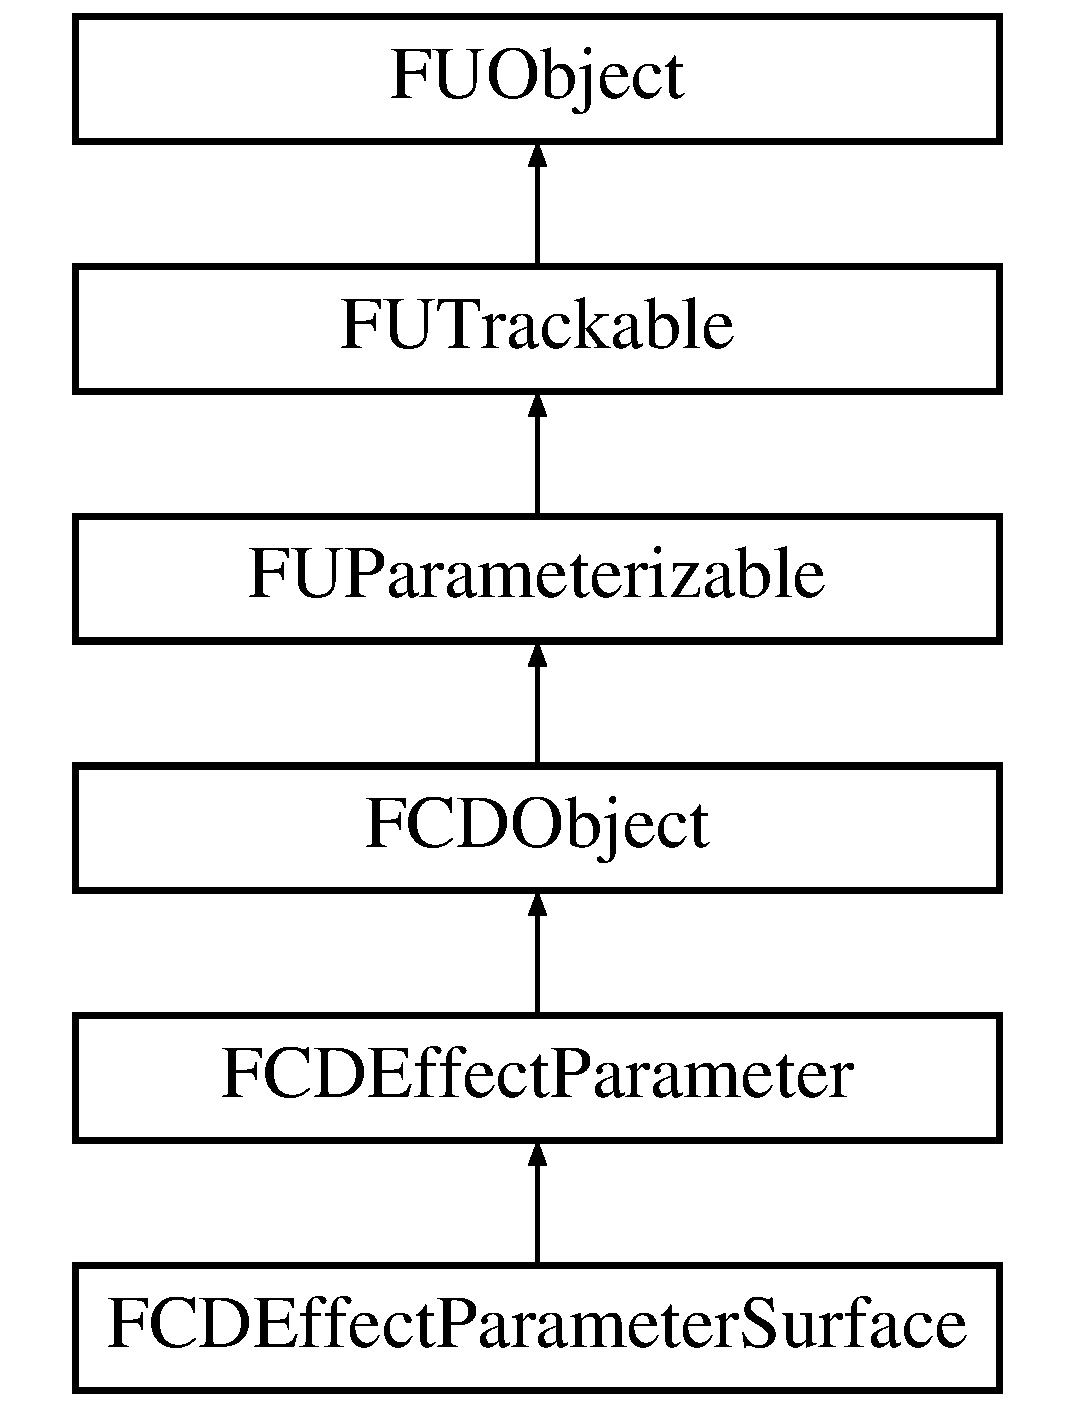
\includegraphics[height=6.000000cm]{classFCDEffectParameterSurface}
\end{center}
\end{figure}
\subsection*{Public Member Functions}
\begin{DoxyCompactItemize}
\item 
\hyperlink{classFCDEffectParameterSurface_a365475eff0f265c84c0b749b9d6e6e0d}{FCDEffectParameterSurface} (\hyperlink{classFCDocument}{FCDocument} $\ast$document)
\item 
virtual \hyperlink{classFCDEffectParameterSurface_aef09401c63f2c3fbfcacca78064d5c4d}{$\sim$FCDEffectParameterSurface} ()
\item 
virtual \hyperlink{classFCDEffectParameter_a1efe74553d2ed199435085c171743b08}{Type} \hyperlink{classFCDEffectParameterSurface_a48e1ec0933996bc9ebb5ef1ec9b8e334}{GetType} () const 
\item 
\hyperlink{classFCDEffectParameterSurfaceInit}{FCDEffectParameterSurfaceInit} $\ast$ \hyperlink{classFCDEffectParameterSurface_a1b399c2a8fbf1444d3978017f8abee01}{GetInitMethod} ()
\item 
const \hyperlink{classFCDEffectParameterSurfaceInit}{FCDEffectParameterSurfaceInit} $\ast$ \hyperlink{classFCDEffectParameterSurface_a6450a67e0c01706ff96363d2e86ee6f0}{GetInitMethod} () const 
\item 
void \hyperlink{classFCDEffectParameterSurface_aeabfcc4c49e58c2838442a7812d8089e}{SetInitMethod} (\hyperlink{classFCDEffectParameterSurfaceInit}{FCDEffectParameterSurfaceInit} $\ast$method)
\item 
const \hyperlink{classFCDImage}{FCDImage} $\ast$$\ast$ \hyperlink{classFCDEffectParameterSurface_ab16a2edc1ecb7a54f622f890c6cda395}{GetImages} () const 
\item 
size\_\-t \hyperlink{classFCDEffectParameterSurface_a443aec0a023b31f27ffd8e1d182774fe}{GetImageCount} () const 
\item 
\hyperlink{classFCDImage}{FCDImage} $\ast$ \hyperlink{classFCDEffectParameterSurface_af4276ec08cfb3d4221ce194e853e035a}{GetImage} (size\_\-t index=0)
\item 
const \hyperlink{classFCDImage}{FCDImage} $\ast$ \hyperlink{classFCDEffectParameterSurface_a5d1101a0718e31566ee4aba117a09df7}{GetImage} (size\_\-t index=0) const 
\item 
size\_\-t \hyperlink{classFCDEffectParameterSurface_a18ad28d3f7f968be42d64a3dcbdca6e4}{FindImage} (const \hyperlink{classFCDImage}{FCDImage} $\ast$image) const 
\item 
size\_\-t \hyperlink{classFCDEffectParameterSurface_a49b5474ba6ef9fe0682046e7a3309440}{AddImage} (\hyperlink{classFCDImage}{FCDImage} $\ast$image, size\_\-t index=(size\_\-t)-\/1)
\item 
void \hyperlink{classFCDEffectParameterSurface_a04c6197912f5111a3e8a880b448445f2}{RemoveImage} (\hyperlink{classFCDImage}{FCDImage} $\ast$image)
\item 
const \hyperlink{classFMVector3}{FMVector3} \& \hyperlink{classFCDEffectParameterSurface_aefdd7adb3a0405f786a0c2a4f3974067}{GetSize} () const 
\item 
void \hyperlink{classFCDEffectParameterSurface_aba3e88b59a7126a5ce96cc8f9cb9e124}{SetSize} (const \hyperlink{classFMVector3}{FMVector3} \&dimensions)
\item 
float \hyperlink{classFCDEffectParameterSurface_a6fe1ab43fe3939de50d6da9fe4968bd8}{GetViewportRatio} () const 
\item 
void \hyperlink{classFCDEffectParameterSurface_a88a5a9addf40ad180fcca095864f1bf1}{SetViewportRatio} (float ratio)
\item 
uint16 \hyperlink{classFCDEffectParameterSurface_ace5c0d37199d08306cd98c37b492f5ae}{GetMipLevelCount} () const 
\item 
void \hyperlink{classFCDEffectParameterSurface_af6e4d39fce4cebf06f5a04025952c56f}{SetMipLevelCount} (uint16 levelCount)
\item 
bool \hyperlink{classFCDEffectParameterSurface_a0e48c062f07a3590da200d38b1001b6e}{IsGenerateMipMaps} () const 
\item 
void \hyperlink{classFCDEffectParameterSurface_a034a5471a03ed630a821343f927f1ae6}{SetGenerateMipMaps} (bool \_\-generateMipmaps)
\item 
void \hyperlink{classFCDEffectParameterSurface_a38e0137e5c7a37c23438a0bc884fa379}{SetFormat} (const \hyperlink{classfm_1_1stringT}{fm::string} \&\_\-format)
\item 
\hypertarget{classFCDEffectParameterSurface_a970c79d7dea95b9340bae40739a572a8}{
const \hyperlink{classfm_1_1stringT}{fm::string} \& {\bfseries GetFormat} ()}
\label{classFCDEffectParameterSurface_a970c79d7dea95b9340bae40739a572a8}

\item 
void \hyperlink{classFCDEffectParameterSurface_ab4be08c0a8e19ee4fdf54cedca4b5403}{SetSurfaceType} (const \hyperlink{classfm_1_1stringT}{fm::string} \&\_\-type)
\item 
const \hyperlink{classfm_1_1stringT}{fm::string} \& \hyperlink{classFCDEffectParameterSurface_a30e2fd6698aa20b749a300c7c9cc60f0}{GetSurfaceType} ()
\item 
virtual bool \hyperlink{classFCDEffectParameterSurface_a39896f512054cc2bb9fa8938fa67ab80}{IsValueEqual} (\hyperlink{classFCDEffectParameter}{FCDEffectParameter} $\ast$parameter)
\item 
virtual \hyperlink{classFCDEffectParameter}{FCDEffectParameter} $\ast$ \hyperlink{classFCDEffectParameterSurface_a0b95f01b907cb82af8cb84106d227cf3}{Clone} (\hyperlink{classFCDEffectParameter}{FCDEffectParameter} $\ast$clone=NULL) const 
\item 
virtual void \hyperlink{classFCDEffectParameterSurface_a3079626698cf949faf90030b3d6230e2}{Overwrite} (\hyperlink{classFCDEffectParameter}{FCDEffectParameter} $\ast$target)
\item 
\hyperlink{classfm_1_1vector}{StringList} \& \hyperlink{classFCDEffectParameterSurface_a84c69ff8e75ff4d76e033cf33b3bd768}{GetNames} ()
\item 
\hyperlink{structFCDFormatHint}{FCDFormatHint} $\ast$ \hyperlink{classFCDEffectParameterSurface_a19a153fcabe4cf75b34201d436e1ae54}{AddFormatHint} ()
\item 
\hyperlink{structFCDFormatHint}{FCDFormatHint} $\ast$ \hyperlink{classFCDEffectParameterSurface_a59783a6fd9d677e81a824e6d4cf33ccb}{GetFormatHint} ()
\item 
\hypertarget{classFCDEffectParameterSurface_af30b3c8202dd63dd751a0d54993dad2e}{
const \hyperlink{structFCDFormatHint}{FCDFormatHint} $\ast$ {\bfseries GetFormatHint} () const }
\label{classFCDEffectParameterSurface_af30b3c8202dd63dd751a0d54993dad2e}

\end{DoxyCompactItemize}


\subsection{Detailed Description}
A COLLADA surface parameter. This parameters hold the texture loading information. The texture placement information should be held by the sampler parameter.

\begin{DoxySeeAlso}{See also}
\hyperlink{classFCDEffectParameterSampler}{FCDEffectParameterSampler} 
\end{DoxySeeAlso}


\subsection{Constructor \& Destructor Documentation}
\hypertarget{classFCDEffectParameterSurface_a365475eff0f265c84c0b749b9d6e6e0d}{
\index{FCDEffectParameterSurface@{FCDEffectParameterSurface}!FCDEffectParameterSurface@{FCDEffectParameterSurface}}
\index{FCDEffectParameterSurface@{FCDEffectParameterSurface}!FCDEffectParameterSurface@{FCDEffectParameterSurface}}
\subsubsection[{FCDEffectParameterSurface}]{\setlength{\rightskip}{0pt plus 5cm}FCDEffectParameterSurface::FCDEffectParameterSurface (
\begin{DoxyParamCaption}
\item[{{\bf FCDocument} $\ast$}]{ document}
\end{DoxyParamCaption}
)}}
\label{classFCDEffectParameterSurface_a365475eff0f265c84c0b749b9d6e6e0d}
Constructor: do not use directly. Instead, use the appropriate AddEffectParameter function. 
\begin{DoxyParams}{Parameters}
\item[{\em document}]The COLLADA document that owns the effect parameter. \end{DoxyParams}
\hypertarget{classFCDEffectParameterSurface_aef09401c63f2c3fbfcacca78064d5c4d}{
\index{FCDEffectParameterSurface@{FCDEffectParameterSurface}!$\sim$FCDEffectParameterSurface@{$\sim$FCDEffectParameterSurface}}
\index{$\sim$FCDEffectParameterSurface@{$\sim$FCDEffectParameterSurface}!FCDEffectParameterSurface@{FCDEffectParameterSurface}}
\subsubsection[{$\sim$FCDEffectParameterSurface}]{\setlength{\rightskip}{0pt plus 5cm}FCDEffectParameterSurface::$\sim$FCDEffectParameterSurface (
\begin{DoxyParamCaption}
{}
\end{DoxyParamCaption}
)\hspace{0.3cm}{\ttfamily  \mbox{[}virtual\mbox{]}}}}
\label{classFCDEffectParameterSurface_aef09401c63f2c3fbfcacca78064d5c4d}
Destructor. 

\subsection{Member Function Documentation}
\hypertarget{classFCDEffectParameterSurface_a19a153fcabe4cf75b34201d436e1ae54}{
\index{FCDEffectParameterSurface@{FCDEffectParameterSurface}!AddFormatHint@{AddFormatHint}}
\index{AddFormatHint@{AddFormatHint}!FCDEffectParameterSurface@{FCDEffectParameterSurface}}
\subsubsection[{AddFormatHint}]{\setlength{\rightskip}{0pt plus 5cm}{\bf FCDFormatHint} $\ast$ FCDEffectParameterSurface::AddFormatHint (
\begin{DoxyParamCaption}
{}
\end{DoxyParamCaption}
)}}
\label{classFCDEffectParameterSurface_a19a153fcabe4cf75b34201d436e1ae54}
Adds a format hint to the surface parameter. Will fail silently if one already exists. \hypertarget{classFCDEffectParameterSurface_a49b5474ba6ef9fe0682046e7a3309440}{
\index{FCDEffectParameterSurface@{FCDEffectParameterSurface}!AddImage@{AddImage}}
\index{AddImage@{AddImage}!FCDEffectParameterSurface@{FCDEffectParameterSurface}}
\subsubsection[{AddImage}]{\setlength{\rightskip}{0pt plus 5cm}size\_\-t FCDEffectParameterSurface::AddImage (
\begin{DoxyParamCaption}
\item[{{\bf FCDImage} $\ast$}]{ image, }
\item[{size\_\-t}]{ index = {\ttfamily (size\_\-t)~-\/1}}
\end{DoxyParamCaption}
)}}
\label{classFCDEffectParameterSurface_a49b5474ba6ef9fe0682046e7a3309440}
Adds an image to the list. The initialization method indexes the images from this list. This function will verify that this image does not already exist within the list, so use the returned index. 
\begin{DoxyParams}{Parameters}
\item[{\em image}]The new image. \item[{\em index}]The index at which to insert the image. Set the index to -\/1 in order to append the image to the list. \end{DoxyParams}
\begin{DoxyReturn}{Returns}
The index of the image within the list. 
\end{DoxyReturn}
\hypertarget{classFCDEffectParameterSurface_a0b95f01b907cb82af8cb84106d227cf3}{
\index{FCDEffectParameterSurface@{FCDEffectParameterSurface}!Clone@{Clone}}
\index{Clone@{Clone}!FCDEffectParameterSurface@{FCDEffectParameterSurface}}
\subsubsection[{Clone}]{\setlength{\rightskip}{0pt plus 5cm}{\bf FCDEffectParameter} $\ast$ FCDEffectParameterSurface::Clone (
\begin{DoxyParamCaption}
\item[{{\bf FCDEffectParameter} $\ast$}]{ clone = {\ttfamily NULL}}
\end{DoxyParamCaption}
) const\hspace{0.3cm}{\ttfamily  \mbox{[}virtual\mbox{]}}}}
\label{classFCDEffectParameterSurface_a0b95f01b907cb82af8cb84106d227cf3}
Creates a full copy of the effect parameter. 
\begin{DoxyParams}{Parameters}
\item[{\em clone}]The cloned effect parameter. If this pointer is NULL, a new effect parameter will be created and you will need to delete this pointer. \end{DoxyParams}
\begin{DoxyReturn}{Returns}
The cloned effect parameter. 
\end{DoxyReturn}


Reimplemented from \hyperlink{classFCDEffectParameter_a75abe4b8964493db40604fa3d0e373eb}{FCDEffectParameter}.

\hypertarget{classFCDEffectParameterSurface_a18ad28d3f7f968be42d64a3dcbdca6e4}{
\index{FCDEffectParameterSurface@{FCDEffectParameterSurface}!FindImage@{FindImage}}
\index{FindImage@{FindImage}!FCDEffectParameterSurface@{FCDEffectParameterSurface}}
\subsubsection[{FindImage}]{\setlength{\rightskip}{0pt plus 5cm}size\_\-t FCDEffectParameterSurface::FindImage (
\begin{DoxyParamCaption}
\item[{const {\bf FCDImage} $\ast$}]{ image}
\end{DoxyParamCaption}
) const}}
\label{classFCDEffectParameterSurface_a18ad28d3f7f968be42d64a3dcbdca6e4}
Retrieves the index that matches the given image. 
\begin{DoxyParams}{Parameters}
\item[{\em image}]The image to match. \end{DoxyParams}
\begin{DoxyReturn}{Returns}
The index within the list for this image. This index may be -\/1 if no match was found. 
\end{DoxyReturn}
\hypertarget{classFCDEffectParameterSurface_a59783a6fd9d677e81a824e6d4cf33ccb}{
\index{FCDEffectParameterSurface@{FCDEffectParameterSurface}!GetFormatHint@{GetFormatHint}}
\index{GetFormatHint@{GetFormatHint}!FCDEffectParameterSurface@{FCDEffectParameterSurface}}
\subsubsection[{GetFormatHint}]{\setlength{\rightskip}{0pt plus 5cm}{\bf FCDFormatHint}$\ast$ FCDEffectParameterSurface::GetFormatHint (
\begin{DoxyParamCaption}
{}
\end{DoxyParamCaption}
)\hspace{0.3cm}{\ttfamily  \mbox{[}inline\mbox{]}}}}
\label{classFCDEffectParameterSurface_a59783a6fd9d677e81a824e6d4cf33ccb}
Retrieves the format hint of the surface parameter. \begin{DoxyReturn}{Returns}
The format hint of the parameter. If this pointer is NULL, no format hint is provided. 
\end{DoxyReturn}
\hypertarget{classFCDEffectParameterSurface_a5d1101a0718e31566ee4aba117a09df7}{
\index{FCDEffectParameterSurface@{FCDEffectParameterSurface}!GetImage@{GetImage}}
\index{GetImage@{GetImage}!FCDEffectParameterSurface@{FCDEffectParameterSurface}}
\subsubsection[{GetImage}]{\setlength{\rightskip}{0pt plus 5cm}const {\bf FCDImage}$\ast$ FCDEffectParameterSurface::GetImage (
\begin{DoxyParamCaption}
\item[{size\_\-t}]{ index = {\ttfamily 0}}
\end{DoxyParamCaption}
) const\hspace{0.3cm}{\ttfamily  \mbox{[}inline\mbox{]}}}}
\label{classFCDEffectParameterSurface_a5d1101a0718e31566ee4aba117a09df7}
See above. \hypertarget{classFCDEffectParameterSurface_af4276ec08cfb3d4221ce194e853e035a}{
\index{FCDEffectParameterSurface@{FCDEffectParameterSurface}!GetImage@{GetImage}}
\index{GetImage@{GetImage}!FCDEffectParameterSurface@{FCDEffectParameterSurface}}
\subsubsection[{GetImage}]{\setlength{\rightskip}{0pt plus 5cm}{\bf FCDImage}$\ast$ FCDEffectParameterSurface::GetImage (
\begin{DoxyParamCaption}
\item[{size\_\-t}]{ index = {\ttfamily 0}}
\end{DoxyParamCaption}
)\hspace{0.3cm}{\ttfamily  \mbox{[}inline\mbox{]}}}}
\label{classFCDEffectParameterSurface_af4276ec08cfb3d4221ce194e853e035a}
Retrieves a specific image. 
\begin{DoxyParams}{Parameters}
\item[{\em index}]The index of the image. \end{DoxyParams}
\begin{DoxyReturn}{Returns}
The image. This pointer will be NULL if the index is out-\/of-\/bounds. 
\end{DoxyReturn}
\hypertarget{classFCDEffectParameterSurface_a443aec0a023b31f27ffd8e1d182774fe}{
\index{FCDEffectParameterSurface@{FCDEffectParameterSurface}!GetImageCount@{GetImageCount}}
\index{GetImageCount@{GetImageCount}!FCDEffectParameterSurface@{FCDEffectParameterSurface}}
\subsubsection[{GetImageCount}]{\setlength{\rightskip}{0pt plus 5cm}size\_\-t FCDEffectParameterSurface::GetImageCount (
\begin{DoxyParamCaption}
{}
\end{DoxyParamCaption}
) const\hspace{0.3cm}{\ttfamily  \mbox{[}inline\mbox{]}}}}
\label{classFCDEffectParameterSurface_a443aec0a023b31f27ffd8e1d182774fe}
Retrieves the number of COLLADA images that make up this surface. There should never be more than six images to build a surface. In the large majority of cases, expect one image. \begin{DoxyReturn}{Returns}
The number of images. 
\end{DoxyReturn}
\hypertarget{classFCDEffectParameterSurface_ab16a2edc1ecb7a54f622f890c6cda395}{
\index{FCDEffectParameterSurface@{FCDEffectParameterSurface}!GetImages@{GetImages}}
\index{GetImages@{GetImages}!FCDEffectParameterSurface@{FCDEffectParameterSurface}}
\subsubsection[{GetImages}]{\setlength{\rightskip}{0pt plus 5cm}const {\bf FCDImage}$\ast$$\ast$ FCDEffectParameterSurface::GetImages (
\begin{DoxyParamCaption}
{}
\end{DoxyParamCaption}
) const\hspace{0.3cm}{\ttfamily  \mbox{[}inline\mbox{]}}}}
\label{classFCDEffectParameterSurface_ab16a2edc1ecb7a54f622f890c6cda395}
Retrieves the list of images that make up this surface. There should never be more than six images to build a surface. In the large majority of cases, expect one image. \begin{DoxyReturn}{Returns}
The list of images. See above. 
\end{DoxyReturn}
\hypertarget{classFCDEffectParameterSurface_a1b399c2a8fbf1444d3978017f8abee01}{
\index{FCDEffectParameterSurface@{FCDEffectParameterSurface}!GetInitMethod@{GetInitMethod}}
\index{GetInitMethod@{GetInitMethod}!FCDEffectParameterSurface@{FCDEffectParameterSurface}}
\subsubsection[{GetInitMethod}]{\setlength{\rightskip}{0pt plus 5cm}{\bf FCDEffectParameterSurfaceInit}$\ast$ FCDEffectParameterSurface::GetInitMethod (
\begin{DoxyParamCaption}
{}
\end{DoxyParamCaption}
)\hspace{0.3cm}{\ttfamily  \mbox{[}inline\mbox{]}}}}
\label{classFCDEffectParameterSurface_a1b399c2a8fbf1444d3978017f8abee01}
Retrieves the initialization method for the surface parameter. The initialization method is a powerful method of describing how to build complex textures, such as cube maps, from one or multiple image files. \begin{DoxyReturn}{Returns}
The surface initialization method. This pointer will be NULL, if no initialization method is provided. 
\end{DoxyReturn}
\hypertarget{classFCDEffectParameterSurface_a6450a67e0c01706ff96363d2e86ee6f0}{
\index{FCDEffectParameterSurface@{FCDEffectParameterSurface}!GetInitMethod@{GetInitMethod}}
\index{GetInitMethod@{GetInitMethod}!FCDEffectParameterSurface@{FCDEffectParameterSurface}}
\subsubsection[{GetInitMethod}]{\setlength{\rightskip}{0pt plus 5cm}const {\bf FCDEffectParameterSurfaceInit}$\ast$ FCDEffectParameterSurface::GetInitMethod (
\begin{DoxyParamCaption}
{}
\end{DoxyParamCaption}
) const\hspace{0.3cm}{\ttfamily  \mbox{[}inline\mbox{]}}}}
\label{classFCDEffectParameterSurface_a6450a67e0c01706ff96363d2e86ee6f0}
See above. \hypertarget{classFCDEffectParameterSurface_ace5c0d37199d08306cd98c37b492f5ae}{
\index{FCDEffectParameterSurface@{FCDEffectParameterSurface}!GetMipLevelCount@{GetMipLevelCount}}
\index{GetMipLevelCount@{GetMipLevelCount}!FCDEffectParameterSurface@{FCDEffectParameterSurface}}
\subsubsection[{GetMipLevelCount}]{\setlength{\rightskip}{0pt plus 5cm}uint16 FCDEffectParameterSurface::GetMipLevelCount (
\begin{DoxyParamCaption}
{}
\end{DoxyParamCaption}
) const\hspace{0.3cm}{\ttfamily  \mbox{[}inline\mbox{]}}}}
\label{classFCDEffectParameterSurface_ace5c0d37199d08306cd98c37b492f5ae}
Retrieves the wanted number of mip-\/levels. This parameter is optional and may be zero to indicate that you should retrieve the mip-\/levels from the image file(s) or generate a full mip-\/chain, depending on the mip-\/map generate flag. \begin{DoxySeeAlso}{See also}
GetMipMapGenerate 
\end{DoxySeeAlso}
\begin{DoxyReturn}{Returns}
The wanted number of mip-\/levels. 
\end{DoxyReturn}
\hypertarget{classFCDEffectParameterSurface_a84c69ff8e75ff4d76e033cf33b3bd768}{
\index{FCDEffectParameterSurface@{FCDEffectParameterSurface}!GetNames@{GetNames}}
\index{GetNames@{GetNames}!FCDEffectParameterSurface@{FCDEffectParameterSurface}}
\subsubsection[{GetNames}]{\setlength{\rightskip}{0pt plus 5cm}{\bf StringList}\& FCDEffectParameterSurface::GetNames (
\begin{DoxyParamCaption}
{}
\end{DoxyParamCaption}
)\hspace{0.3cm}{\ttfamily  \mbox{[}inline\mbox{]}}}}
\label{classFCDEffectParameterSurface_a84c69ff8e75ff4d76e033cf33b3bd768}
\mbox{[}INTERNAL\mbox{]} Retrieve the list of image names \hypertarget{classFCDEffectParameterSurface_aefdd7adb3a0405f786a0c2a4f3974067}{
\index{FCDEffectParameterSurface@{FCDEffectParameterSurface}!GetSize@{GetSize}}
\index{GetSize@{GetSize}!FCDEffectParameterSurface@{FCDEffectParameterSurface}}
\subsubsection[{GetSize}]{\setlength{\rightskip}{0pt plus 5cm}const {\bf FMVector3}\& FCDEffectParameterSurface::GetSize (
\begin{DoxyParamCaption}
{}
\end{DoxyParamCaption}
) const\hspace{0.3cm}{\ttfamily  \mbox{[}inline\mbox{]}}}}
\label{classFCDEffectParameterSurface_aefdd7adb3a0405f786a0c2a4f3974067}
Retrieves the wanted dimensions of the surface. This parameter is optional and may contain all zeroes to indicate that you should read the surface dimensions from the image file(s). \begin{DoxyReturn}{Returns}
The wanted dimensions. 
\end{DoxyReturn}
\hypertarget{classFCDEffectParameterSurface_a30e2fd6698aa20b749a300c7c9cc60f0}{
\index{FCDEffectParameterSurface@{FCDEffectParameterSurface}!GetSurfaceType@{GetSurfaceType}}
\index{GetSurfaceType@{GetSurfaceType}!FCDEffectParameterSurface@{FCDEffectParameterSurface}}
\subsubsection[{GetSurfaceType}]{\setlength{\rightskip}{0pt plus 5cm}const {\bf fm::string}\& FCDEffectParameterSurface::GetSurfaceType (
\begin{DoxyParamCaption}
{}
\end{DoxyParamCaption}
)\hspace{0.3cm}{\ttfamily  \mbox{[}inline\mbox{]}}}}
\label{classFCDEffectParameterSurface_a30e2fd6698aa20b749a300c7c9cc60f0}
Retrieves type. \hypertarget{classFCDEffectParameterSurface_a48e1ec0933996bc9ebb5ef1ec9b8e334}{
\index{FCDEffectParameterSurface@{FCDEffectParameterSurface}!GetType@{GetType}}
\index{GetType@{GetType}!FCDEffectParameterSurface@{FCDEffectParameterSurface}}
\subsubsection[{GetType}]{\setlength{\rightskip}{0pt plus 5cm}virtual {\bf Type} FCDEffectParameterSurface::GetType (
\begin{DoxyParamCaption}
{}
\end{DoxyParamCaption}
) const\hspace{0.3cm}{\ttfamily  \mbox{[}inline, virtual\mbox{]}}}}
\label{classFCDEffectParameterSurface_a48e1ec0933996bc9ebb5ef1ec9b8e334}
Retrieves the type of effect parameter class. \begin{DoxyReturn}{Returns}
The parameter class type: SURFACE. 
\end{DoxyReturn}


Implements \hyperlink{classFCDEffectParameter_a5858946f333ea4486ca30c4c1b104871}{FCDEffectParameter}.

\hypertarget{classFCDEffectParameterSurface_a6fe1ab43fe3939de50d6da9fe4968bd8}{
\index{FCDEffectParameterSurface@{FCDEffectParameterSurface}!GetViewportRatio@{GetViewportRatio}}
\index{GetViewportRatio@{GetViewportRatio}!FCDEffectParameterSurface@{FCDEffectParameterSurface}}
\subsubsection[{GetViewportRatio}]{\setlength{\rightskip}{0pt plus 5cm}float FCDEffectParameterSurface::GetViewportRatio (
\begin{DoxyParamCaption}
{}
\end{DoxyParamCaption}
) const\hspace{0.3cm}{\ttfamily  \mbox{[}inline\mbox{]}}}}
\label{classFCDEffectParameterSurface_a6fe1ab43fe3939de50d6da9fe4968bd8}
Retrieves the viewport ratio to use when the surface is a render target. \begin{DoxyReturn}{Returns}
The viewport ratio. 
\end{DoxyReturn}
\hypertarget{classFCDEffectParameterSurface_a0e48c062f07a3590da200d38b1001b6e}{
\index{FCDEffectParameterSurface@{FCDEffectParameterSurface}!IsGenerateMipMaps@{IsGenerateMipMaps}}
\index{IsGenerateMipMaps@{IsGenerateMipMaps}!FCDEffectParameterSurface@{FCDEffectParameterSurface}}
\subsubsection[{IsGenerateMipMaps}]{\setlength{\rightskip}{0pt plus 5cm}bool FCDEffectParameterSurface::IsGenerateMipMaps (
\begin{DoxyParamCaption}
{}
\end{DoxyParamCaption}
) const\hspace{0.3cm}{\ttfamily  \mbox{[}inline\mbox{]}}}}
\label{classFCDEffectParameterSurface_a0e48c062f07a3590da200d38b1001b6e}
Retrieves whether to generate the mip-\/map levels on load. The alternative is to load the mip-\/map levels from the image files. \begin{DoxyReturn}{Returns}
Whether to generate the mip-\/map levels on load. 
\end{DoxyReturn}
\hypertarget{classFCDEffectParameterSurface_a39896f512054cc2bb9fa8938fa67ab80}{
\index{FCDEffectParameterSurface@{FCDEffectParameterSurface}!IsValueEqual@{IsValueEqual}}
\index{IsValueEqual@{IsValueEqual}!FCDEffectParameterSurface@{FCDEffectParameterSurface}}
\subsubsection[{IsValueEqual}]{\setlength{\rightskip}{0pt plus 5cm}bool FCDEffectParameterSurface::IsValueEqual (
\begin{DoxyParamCaption}
\item[{{\bf FCDEffectParameter} $\ast$}]{ parameter}
\end{DoxyParamCaption}
)\hspace{0.3cm}{\ttfamily  \mbox{[}virtual\mbox{]}}}}
\label{classFCDEffectParameterSurface_a39896f512054cc2bb9fa8938fa67ab80}
Compares this parameter's value with another 
\begin{DoxyParams}{Parameters}
\item[{\em parameter}]The given parameter to compare with. \end{DoxyParams}
\begin{DoxyReturn}{Returns}
true if the values are equal 
\end{DoxyReturn}


Implements \hyperlink{classFCDEffectParameter_a005a5a316bdb99dbd97ac542c129cc5e}{FCDEffectParameter}.

\hypertarget{classFCDEffectParameterSurface_a3079626698cf949faf90030b3d6230e2}{
\index{FCDEffectParameterSurface@{FCDEffectParameterSurface}!Overwrite@{Overwrite}}
\index{Overwrite@{Overwrite}!FCDEffectParameterSurface@{FCDEffectParameterSurface}}
\subsubsection[{Overwrite}]{\setlength{\rightskip}{0pt plus 5cm}void FCDEffectParameterSurface::Overwrite (
\begin{DoxyParamCaption}
\item[{{\bf FCDEffectParameter} $\ast$}]{ target}
\end{DoxyParamCaption}
)\hspace{0.3cm}{\ttfamily  \mbox{[}virtual\mbox{]}}}}
\label{classFCDEffectParameterSurface_a3079626698cf949faf90030b3d6230e2}
\mbox{[}INTERNAL\mbox{]} Overwrites the target parameter with this parameter. This function is used during the flattening of materials. 
\begin{DoxyParams}{Parameters}
\item[{\em target}]The target parameter to overwrite. \end{DoxyParams}


Reimplemented from \hyperlink{classFCDEffectParameter_a016be91dbd27ff3c8c30f759f00b8c53}{FCDEffectParameter}.

\hypertarget{classFCDEffectParameterSurface_a04c6197912f5111a3e8a880b448445f2}{
\index{FCDEffectParameterSurface@{FCDEffectParameterSurface}!RemoveImage@{RemoveImage}}
\index{RemoveImage@{RemoveImage}!FCDEffectParameterSurface@{FCDEffectParameterSurface}}
\subsubsection[{RemoveImage}]{\setlength{\rightskip}{0pt plus 5cm}void FCDEffectParameterSurface::RemoveImage (
\begin{DoxyParamCaption}
\item[{{\bf FCDImage} $\ast$}]{ image}
\end{DoxyParamCaption}
)}}
\label{classFCDEffectParameterSurface_a04c6197912f5111a3e8a880b448445f2}
Removes an image from the list. The initialization method indexes the images from this list. This function will shift all the indexes in the initialization method so that they continue matching the correct image. 
\begin{DoxyParams}{Parameters}
\item[{\em image}]The image to remove. Its memory is not released. \end{DoxyParams}
\hypertarget{classFCDEffectParameterSurface_a38e0137e5c7a37c23438a0bc884fa379}{
\index{FCDEffectParameterSurface@{FCDEffectParameterSurface}!SetFormat@{SetFormat}}
\index{SetFormat@{SetFormat}!FCDEffectParameterSurface@{FCDEffectParameterSurface}}
\subsubsection[{SetFormat}]{\setlength{\rightskip}{0pt plus 5cm}void FCDEffectParameterSurface::SetFormat (
\begin{DoxyParamCaption}
\item[{const {\bf fm::string} \&}]{ \_\-format}
\end{DoxyParamCaption}
)\hspace{0.3cm}{\ttfamily  \mbox{[}inline\mbox{]}}}}
\label{classFCDEffectParameterSurface_a38e0137e5c7a37c23438a0bc884fa379}
Sets/Gets format \hypertarget{classFCDEffectParameterSurface_a034a5471a03ed630a821343f927f1ae6}{
\index{FCDEffectParameterSurface@{FCDEffectParameterSurface}!SetGenerateMipMaps@{SetGenerateMipMaps}}
\index{SetGenerateMipMaps@{SetGenerateMipMaps}!FCDEffectParameterSurface@{FCDEffectParameterSurface}}
\subsubsection[{SetGenerateMipMaps}]{\setlength{\rightskip}{0pt plus 5cm}void FCDEffectParameterSurface::SetGenerateMipMaps (
\begin{DoxyParamCaption}
\item[{bool}]{ \_\-generateMipmaps}
\end{DoxyParamCaption}
)\hspace{0.3cm}{\ttfamily  \mbox{[}inline\mbox{]}}}}
\label{classFCDEffectParameterSurface_a034a5471a03ed630a821343f927f1ae6}
Sets whether to generate the mip-\/map levels of load. The alternative is to load the mip-\/map levels from the image files. 
\begin{DoxyParams}{Parameters}
\item[{\em \_\-generateMipmaps}]Whether to generate the mip-\/map levels on load. \end{DoxyParams}
\hypertarget{classFCDEffectParameterSurface_aeabfcc4c49e58c2838442a7812d8089e}{
\index{FCDEffectParameterSurface@{FCDEffectParameterSurface}!SetInitMethod@{SetInitMethod}}
\index{SetInitMethod@{SetInitMethod}!FCDEffectParameterSurface@{FCDEffectParameterSurface}}
\subsubsection[{SetInitMethod}]{\setlength{\rightskip}{0pt plus 5cm}void FCDEffectParameterSurface::SetInitMethod (
\begin{DoxyParamCaption}
\item[{{\bf FCDEffectParameterSurfaceInit} $\ast$}]{ method}
\end{DoxyParamCaption}
)}}
\label{classFCDEffectParameterSurface_aeabfcc4c49e58c2838442a7812d8089e}
Sets the initialization method for the surface parameter. The initialization method is a powerful method of describing how to build complex textures, such as cube maps, from one or multiple image files. 
\begin{DoxyParams}{Parameters}
\item[{\em method}]The new initialization method. The old initialization method will be released. You should create a new initialization method for each surface parameter. \end{DoxyParams}
\hypertarget{classFCDEffectParameterSurface_af6e4d39fce4cebf06f5a04025952c56f}{
\index{FCDEffectParameterSurface@{FCDEffectParameterSurface}!SetMipLevelCount@{SetMipLevelCount}}
\index{SetMipLevelCount@{SetMipLevelCount}!FCDEffectParameterSurface@{FCDEffectParameterSurface}}
\subsubsection[{SetMipLevelCount}]{\setlength{\rightskip}{0pt plus 5cm}void FCDEffectParameterSurface::SetMipLevelCount (
\begin{DoxyParamCaption}
\item[{uint16}]{ levelCount}
\end{DoxyParamCaption}
)\hspace{0.3cm}{\ttfamily  \mbox{[}inline\mbox{]}}}}
\label{classFCDEffectParameterSurface_af6e4d39fce4cebf06f5a04025952c56f}
Sets the wanted number of mip-\/levels. This parameter is optional and can be zero to indicate that you should retrieve the mip-\/levels from the image file(s) or generate a full mip-\/chain, depending on the mip-\/map generate flag. 
\begin{DoxyParams}{Parameters}
\item[{\em levelCount}]The wanted number of mip-\/levels. \end{DoxyParams}
\hypertarget{classFCDEffectParameterSurface_aba3e88b59a7126a5ce96cc8f9cb9e124}{
\index{FCDEffectParameterSurface@{FCDEffectParameterSurface}!SetSize@{SetSize}}
\index{SetSize@{SetSize}!FCDEffectParameterSurface@{FCDEffectParameterSurface}}
\subsubsection[{SetSize}]{\setlength{\rightskip}{0pt plus 5cm}void FCDEffectParameterSurface::SetSize (
\begin{DoxyParamCaption}
\item[{const {\bf FMVector3} \&}]{ dimensions}
\end{DoxyParamCaption}
)\hspace{0.3cm}{\ttfamily  \mbox{[}inline\mbox{]}}}}
\label{classFCDEffectParameterSurface_aba3e88b59a7126a5ce96cc8f9cb9e124}
Sets the wanted dimensions of the surface. This parameter is optional and can contain all zeroes to indicate that you should read the surface dimensions from the image file(s). 
\begin{DoxyParams}{Parameters}
\item[{\em dimensions}]The wanted dimensions. \end{DoxyParams}
\hypertarget{classFCDEffectParameterSurface_ab4be08c0a8e19ee4fdf54cedca4b5403}{
\index{FCDEffectParameterSurface@{FCDEffectParameterSurface}!SetSurfaceType@{SetSurfaceType}}
\index{SetSurfaceType@{SetSurfaceType}!FCDEffectParameterSurface@{FCDEffectParameterSurface}}
\subsubsection[{SetSurfaceType}]{\setlength{\rightskip}{0pt plus 5cm}void FCDEffectParameterSurface::SetSurfaceType (
\begin{DoxyParamCaption}
\item[{const {\bf fm::string} \&}]{ \_\-type}
\end{DoxyParamCaption}
)\hspace{0.3cm}{\ttfamily  \mbox{[}inline\mbox{]}}}}
\label{classFCDEffectParameterSurface_ab4be08c0a8e19ee4fdf54cedca4b5403}
Sets type \hypertarget{classFCDEffectParameterSurface_a88a5a9addf40ad180fcca095864f1bf1}{
\index{FCDEffectParameterSurface@{FCDEffectParameterSurface}!SetViewportRatio@{SetViewportRatio}}
\index{SetViewportRatio@{SetViewportRatio}!FCDEffectParameterSurface@{FCDEffectParameterSurface}}
\subsubsection[{SetViewportRatio}]{\setlength{\rightskip}{0pt plus 5cm}void FCDEffectParameterSurface::SetViewportRatio (
\begin{DoxyParamCaption}
\item[{float}]{ ratio}
\end{DoxyParamCaption}
)\hspace{0.3cm}{\ttfamily  \mbox{[}inline\mbox{]}}}}
\label{classFCDEffectParameterSurface_a88a5a9addf40ad180fcca095864f1bf1}
Sets the viewport ratio to use when the surface is a render target. 
\begin{DoxyParams}{Parameters}
\item[{\em ratio}]The viewport ratio. \end{DoxyParams}


The documentation for this class was generated from the following files:\begin{DoxyCompactItemize}
\item 
FCollada/FCDocument/\hyperlink{FCDEffectParameterSurface_8h}{FCDEffectParameterSurface.h}\item 
FCollada/FCDocument/FCDEffectParameterSurface.cpp\end{DoxyCompactItemize}

\hypertarget{classFCDEffectParameterSurfaceInit}{
\section{FCDEffectParameterSurfaceInit Class Reference}
\label{classFCDEffectParameterSurfaceInit}\index{FCDEffectParameterSurfaceInit@{FCDEffectParameterSurfaceInit}}
}


{\ttfamily \#include $<$FCDEffectParameterSurface.h$>$}

Inheritance diagram for FCDEffectParameterSurfaceInit:\begin{figure}[H]
\begin{center}
\leavevmode
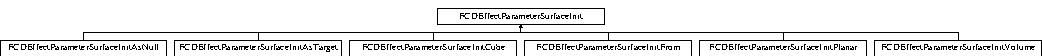
\includegraphics[height=0.749665cm]{classFCDEffectParameterSurfaceInit}
\end{center}
\end{figure}
\subsection*{Public Member Functions}
\begin{DoxyCompactItemize}
\item 
\hyperlink{classFCDEffectParameterSurfaceInit_a6b22a5b52b38cbabb51a39c3ea42db74}{FCDEffectParameterSurfaceInit} ()
\item 
virtual \hyperlink{classFCDEffectParameterSurfaceInit_ac350e10e96cbb79e5f4e5b6487052280}{$\sim$FCDEffectParameterSurfaceInit} ()
\item 
virtual \hyperlink{classFCDEffectParameterSurfaceInitFactory_a65e74f1159865702cac5236dd5d83892}{FCDEffectParameterSurfaceInitFactory::InitType} \hyperlink{classFCDEffectParameterSurfaceInit_ad0109233e63c892e5963a3ca67f7108f}{GetInitType} () const =0
\item 
virtual \hyperlink{classFCDEffectParameterSurfaceInit}{FCDEffectParameterSurfaceInit} $\ast$ \hyperlink{classFCDEffectParameterSurfaceInit_ae3ac516773ea5ebb6838ed8a0d10d910}{Clone} (\hyperlink{classFCDEffectParameterSurfaceInit}{FCDEffectParameterSurfaceInit} $\ast$clone) const 
\end{DoxyCompactItemize}


\subsection{Detailed Description}
A surface initialization method. In COLLADA 1.4.1, this information was added to support complex surface types. There are six types of initialization methods, described in the InitType enumerated type. Expect the FROM initialization type in the large majority of cases. 

\subsection{Constructor \& Destructor Documentation}
\hypertarget{classFCDEffectParameterSurfaceInit_a6b22a5b52b38cbabb51a39c3ea42db74}{
\index{FCDEffectParameterSurfaceInit@{FCDEffectParameterSurfaceInit}!FCDEffectParameterSurfaceInit@{FCDEffectParameterSurfaceInit}}
\index{FCDEffectParameterSurfaceInit@{FCDEffectParameterSurfaceInit}!FCDEffectParameterSurfaceInit@{FCDEffectParameterSurfaceInit}}
\subsubsection[{FCDEffectParameterSurfaceInit}]{\setlength{\rightskip}{0pt plus 5cm}FCDEffectParameterSurfaceInit::FCDEffectParameterSurfaceInit (
\begin{DoxyParamCaption}
{}
\end{DoxyParamCaption}
)\hspace{0.3cm}{\ttfamily  \mbox{[}inline\mbox{]}}}}
\label{classFCDEffectParameterSurfaceInit_a6b22a5b52b38cbabb51a39c3ea42db74}
Constructor: builds a new surface initialization method. \hypertarget{classFCDEffectParameterSurfaceInit_ac350e10e96cbb79e5f4e5b6487052280}{
\index{FCDEffectParameterSurfaceInit@{FCDEffectParameterSurfaceInit}!$\sim$FCDEffectParameterSurfaceInit@{$\sim$FCDEffectParameterSurfaceInit}}
\index{$\sim$FCDEffectParameterSurfaceInit@{$\sim$FCDEffectParameterSurfaceInit}!FCDEffectParameterSurfaceInit@{FCDEffectParameterSurfaceInit}}
\subsubsection[{$\sim$FCDEffectParameterSurfaceInit}]{\setlength{\rightskip}{0pt plus 5cm}virtual FCDEffectParameterSurfaceInit::$\sim$FCDEffectParameterSurfaceInit (
\begin{DoxyParamCaption}
{}
\end{DoxyParamCaption}
)\hspace{0.3cm}{\ttfamily  \mbox{[}inline, virtual\mbox{]}}}}
\label{classFCDEffectParameterSurfaceInit_ac350e10e96cbb79e5f4e5b6487052280}
Destructor. 

\subsection{Member Function Documentation}
\hypertarget{classFCDEffectParameterSurfaceInit_ae3ac516773ea5ebb6838ed8a0d10d910}{
\index{FCDEffectParameterSurfaceInit@{FCDEffectParameterSurfaceInit}!Clone@{Clone}}
\index{Clone@{Clone}!FCDEffectParameterSurfaceInit@{FCDEffectParameterSurfaceInit}}
\subsubsection[{Clone}]{\setlength{\rightskip}{0pt plus 5cm}{\bf FCDEffectParameterSurfaceInit} $\ast$ FCDEffectParameterSurfaceInit::Clone (
\begin{DoxyParamCaption}
\item[{{\bf FCDEffectParameterSurfaceInit} $\ast$}]{ clone}
\end{DoxyParamCaption}
) const\hspace{0.3cm}{\ttfamily  \mbox{[}virtual\mbox{]}}}}
\label{classFCDEffectParameterSurfaceInit_ae3ac516773ea5ebb6838ed8a0d10d910}
Copies all member variables into clone. 
\begin{DoxyParams}{Parameters}
\item[{\em clone}]a valid pointer to a \hyperlink{classFCDEffectParameterSurfaceInit}{FCDEffectParameterSurfaceInit} object \end{DoxyParams}


Reimplemented in \hyperlink{classFCDEffectParameterSurfaceInitCube_a46ae1522ddb60038c59f9a1511157713}{FCDEffectParameterSurfaceInitCube}, \hyperlink{classFCDEffectParameterSurfaceInitVolume_a54cdfc576b05fe56d87c1dc1c2fe211a}{FCDEffectParameterSurfaceInitVolume}, \hyperlink{classFCDEffectParameterSurfaceInitFrom_a8a173445b78914cf1ed6f222ffb7ba0b}{FCDEffectParameterSurfaceInitFrom}, \hyperlink{classFCDEffectParameterSurfaceInitAsNull_a0c3b98b0d3d379c6cab95c45490ee579}{FCDEffectParameterSurfaceInitAsNull}, \hyperlink{classFCDEffectParameterSurfaceInitAsTarget_aa4c94c80a32fa40d6c7cc851d73b105e}{FCDEffectParameterSurfaceInitAsTarget}, and \hyperlink{classFCDEffectParameterSurfaceInitPlanar_a565047eceb428bb55f32c7522c39354e}{FCDEffectParameterSurfaceInitPlanar}.

\hypertarget{classFCDEffectParameterSurfaceInit_ad0109233e63c892e5963a3ca67f7108f}{
\index{FCDEffectParameterSurfaceInit@{FCDEffectParameterSurfaceInit}!GetInitType@{GetInitType}}
\index{GetInitType@{GetInitType}!FCDEffectParameterSurfaceInit@{FCDEffectParameterSurfaceInit}}
\subsubsection[{GetInitType}]{\setlength{\rightskip}{0pt plus 5cm}virtual {\bf FCDEffectParameterSurfaceInitFactory::InitType} FCDEffectParameterSurfaceInit::GetInitType (
\begin{DoxyParamCaption}
{}
\end{DoxyParamCaption}
) const\hspace{0.3cm}{\ttfamily  \mbox{[}pure virtual\mbox{]}}}}
\label{classFCDEffectParameterSurfaceInit_ad0109233e63c892e5963a3ca67f7108f}
Retrieves the initialization type. You cannot modify this value. To change the initialization type of a surface parameter, create a new surface initialization structure of the correct type. \begin{DoxyReturn}{Returns}
The initialization type. 
\end{DoxyReturn}


Implemented in \hyperlink{classFCDEffectParameterSurfaceInitCube_aa22db1c4680d97b447466bc54a492451}{FCDEffectParameterSurfaceInitCube}, \hyperlink{classFCDEffectParameterSurfaceInitVolume_ad0490f5d50b8babd77b3294277f4fde5}{FCDEffectParameterSurfaceInitVolume}, \hyperlink{classFCDEffectParameterSurfaceInitFrom_a33c2001f6d11fe519d7f5c492daec92a}{FCDEffectParameterSurfaceInitFrom}, \hyperlink{classFCDEffectParameterSurfaceInitAsNull_a91211f6657b5ca23ad0530fe803eea8b}{FCDEffectParameterSurfaceInitAsNull}, \hyperlink{classFCDEffectParameterSurfaceInitAsTarget_a45bcad832e5dd14719aa1dfbea529db2}{FCDEffectParameterSurfaceInitAsTarget}, and \hyperlink{classFCDEffectParameterSurfaceInitPlanar_a9e91a455acbcbed40b8e647aa0c56d80}{FCDEffectParameterSurfaceInitPlanar}.



The documentation for this class was generated from the following files:\begin{DoxyCompactItemize}
\item 
FCollada/FCDocument/\hyperlink{FCDEffectParameterSurface_8h}{FCDEffectParameterSurface.h}\item 
FCollada/FCDocument/FCDEffectParameterSurface.cpp\end{DoxyCompactItemize}

\hypertarget{classFCDEffectParameterSurfaceInitAsNull}{
\section{FCDEffectParameterSurfaceInitAsNull Class Reference}
\label{classFCDEffectParameterSurfaceInitAsNull}\index{FCDEffectParameterSurfaceInitAsNull@{FCDEffectParameterSurfaceInitAsNull}}
}


{\ttfamily \#include $<$FCDEffectParameterSurface.h$>$}

Inheritance diagram for FCDEffectParameterSurfaceInitAsNull:\begin{figure}[H]
\begin{center}
\leavevmode
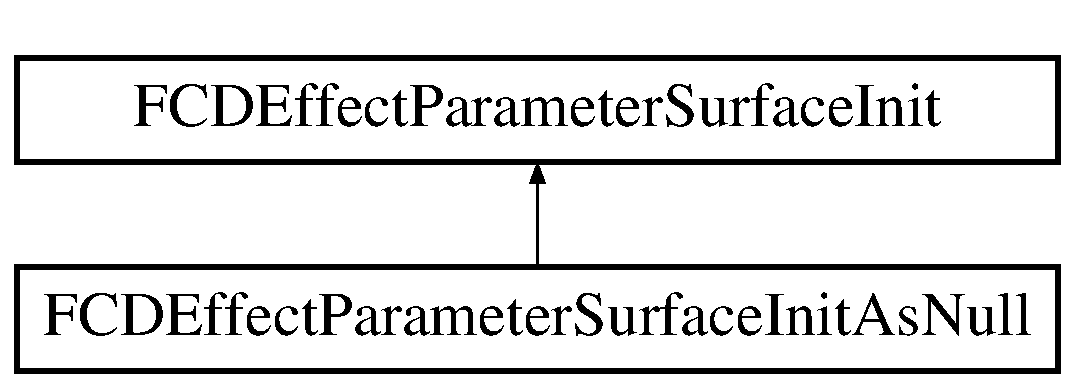
\includegraphics[height=2.000000cm]{classFCDEffectParameterSurfaceInitAsNull}
\end{center}
\end{figure}
\subsection*{Public Member Functions}
\begin{DoxyCompactItemize}
\item 
\hyperlink{classFCDEffectParameterSurfaceInitAsNull_ad1abc61479cb8ba4bf4f5038513fd763}{FCDEffectParameterSurfaceInitAsNull} ()
\item 
virtual \hyperlink{classFCDEffectParameterSurfaceInitAsNull_ab427055c5f1197f5b42e4b3ac22dfb44}{$\sim$FCDEffectParameterSurfaceInitAsNull} ()
\item 
virtual \hyperlink{classFCDEffectParameterSurfaceInitFactory_a65e74f1159865702cac5236dd5d83892}{FCDEffectParameterSurfaceInitFactory::InitType} \hyperlink{classFCDEffectParameterSurfaceInitAsNull_a91211f6657b5ca23ad0530fe803eea8b}{GetInitType} () const 
\item 
virtual \hyperlink{classFCDEffectParameterSurfaceInit}{FCDEffectParameterSurfaceInit} $\ast$ \hyperlink{classFCDEffectParameterSurfaceInitAsNull_a0c3b98b0d3d379c6cab95c45490ee579}{Clone} (\hyperlink{classFCDEffectParameterSurfaceInit}{FCDEffectParameterSurfaceInit} $\ast$clone) const 
\end{DoxyCompactItemize}


\subsection{Detailed Description}
This method allows to initialize the surface at a later point. 

\subsection{Constructor \& Destructor Documentation}
\hypertarget{classFCDEffectParameterSurfaceInitAsNull_ad1abc61479cb8ba4bf4f5038513fd763}{
\index{FCDEffectParameterSurfaceInitAsNull@{FCDEffectParameterSurfaceInitAsNull}!FCDEffectParameterSurfaceInitAsNull@{FCDEffectParameterSurfaceInitAsNull}}
\index{FCDEffectParameterSurfaceInitAsNull@{FCDEffectParameterSurfaceInitAsNull}!FCDEffectParameterSurfaceInitAsNull@{FCDEffectParameterSurfaceInitAsNull}}
\subsubsection[{FCDEffectParameterSurfaceInitAsNull}]{\setlength{\rightskip}{0pt plus 5cm}FCDEffectParameterSurfaceInitAsNull::FCDEffectParameterSurfaceInitAsNull (
\begin{DoxyParamCaption}
{}
\end{DoxyParamCaption}
)\hspace{0.3cm}{\ttfamily  \mbox{[}inline\mbox{]}}}}
\label{classFCDEffectParameterSurfaceInitAsNull_ad1abc61479cb8ba4bf4f5038513fd763}
Constructor: builds a new file surface initialization method. \hypertarget{classFCDEffectParameterSurfaceInitAsNull_ab427055c5f1197f5b42e4b3ac22dfb44}{
\index{FCDEffectParameterSurfaceInitAsNull@{FCDEffectParameterSurfaceInitAsNull}!$\sim$FCDEffectParameterSurfaceInitAsNull@{$\sim$FCDEffectParameterSurfaceInitAsNull}}
\index{$\sim$FCDEffectParameterSurfaceInitAsNull@{$\sim$FCDEffectParameterSurfaceInitAsNull}!FCDEffectParameterSurfaceInitAsNull@{FCDEffectParameterSurfaceInitAsNull}}
\subsubsection[{$\sim$FCDEffectParameterSurfaceInitAsNull}]{\setlength{\rightskip}{0pt plus 5cm}virtual FCDEffectParameterSurfaceInitAsNull::$\sim$FCDEffectParameterSurfaceInitAsNull (
\begin{DoxyParamCaption}
{}
\end{DoxyParamCaption}
)\hspace{0.3cm}{\ttfamily  \mbox{[}inline, virtual\mbox{]}}}}
\label{classFCDEffectParameterSurfaceInitAsNull_ab427055c5f1197f5b42e4b3ac22dfb44}
Destructor. 

\subsection{Member Function Documentation}
\hypertarget{classFCDEffectParameterSurfaceInitAsNull_a0c3b98b0d3d379c6cab95c45490ee579}{
\index{FCDEffectParameterSurfaceInitAsNull@{FCDEffectParameterSurfaceInitAsNull}!Clone@{Clone}}
\index{Clone@{Clone}!FCDEffectParameterSurfaceInitAsNull@{FCDEffectParameterSurfaceInitAsNull}}
\subsubsection[{Clone}]{\setlength{\rightskip}{0pt plus 5cm}{\bf FCDEffectParameterSurfaceInit} $\ast$ FCDEffectParameterSurfaceInitAsNull::Clone (
\begin{DoxyParamCaption}
\item[{{\bf FCDEffectParameterSurfaceInit} $\ast$}]{ clone}
\end{DoxyParamCaption}
) const\hspace{0.3cm}{\ttfamily  \mbox{[}virtual\mbox{]}}}}
\label{classFCDEffectParameterSurfaceInitAsNull_a0c3b98b0d3d379c6cab95c45490ee579}
Creates a full copy of the surface initialization parameter. 
\begin{DoxyParams}{Parameters}
\item[{\em clone}]The cloned surface initialization. If this pointer is NULL, a new surface initialization parameter will be created and you will need to delete this pointer. \end{DoxyParams}
\begin{DoxyReturn}{Returns}
The cloned surface initialization. 
\end{DoxyReturn}


Reimplemented from \hyperlink{classFCDEffectParameterSurfaceInit_ae3ac516773ea5ebb6838ed8a0d10d910}{FCDEffectParameterSurfaceInit}.

\hypertarget{classFCDEffectParameterSurfaceInitAsNull_a91211f6657b5ca23ad0530fe803eea8b}{
\index{FCDEffectParameterSurfaceInitAsNull@{FCDEffectParameterSurfaceInitAsNull}!GetInitType@{GetInitType}}
\index{GetInitType@{GetInitType}!FCDEffectParameterSurfaceInitAsNull@{FCDEffectParameterSurfaceInitAsNull}}
\subsubsection[{GetInitType}]{\setlength{\rightskip}{0pt plus 5cm}virtual {\bf FCDEffectParameterSurfaceInitFactory::InitType} FCDEffectParameterSurfaceInitAsNull::GetInitType (
\begin{DoxyParamCaption}
{}
\end{DoxyParamCaption}
) const\hspace{0.3cm}{\ttfamily  \mbox{[}inline, virtual\mbox{]}}}}
\label{classFCDEffectParameterSurfaceInitAsNull_a91211f6657b5ca23ad0530fe803eea8b}
Retrieves the initialization type. You cannot modify this value. To change the initialization type of a surface parameter, create a new surface initialization structure of the correct type. \begin{DoxyReturn}{Returns}
The initialization type. 
\end{DoxyReturn}


Implements \hyperlink{classFCDEffectParameterSurfaceInit_ad0109233e63c892e5963a3ca67f7108f}{FCDEffectParameterSurfaceInit}.



The documentation for this class was generated from the following files:\begin{DoxyCompactItemize}
\item 
FCollada/FCDocument/\hyperlink{FCDEffectParameterSurface_8h}{FCDEffectParameterSurface.h}\item 
FCollada/FCDocument/FCDEffectParameterSurface.cpp\end{DoxyCompactItemize}

\hypertarget{classFCDEffectParameterSurfaceInitAsTarget}{
\section{FCDEffectParameterSurfaceInitAsTarget Class Reference}
\label{classFCDEffectParameterSurfaceInitAsTarget}\index{FCDEffectParameterSurfaceInitAsTarget@{FCDEffectParameterSurfaceInitAsTarget}}
}


{\ttfamily \#include $<$FCDEffectParameterSurface.h$>$}

Inheritance diagram for FCDEffectParameterSurfaceInitAsTarget:\begin{figure}[H]
\begin{center}
\leavevmode
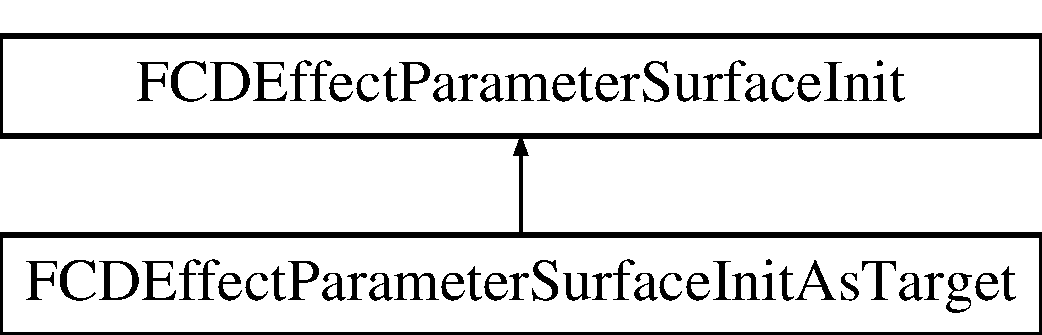
\includegraphics[height=2.000000cm]{classFCDEffectParameterSurfaceInitAsTarget}
\end{center}
\end{figure}
\subsection*{Public Member Functions}
\begin{DoxyCompactItemize}
\item 
\hyperlink{classFCDEffectParameterSurfaceInitAsTarget_ac376d8e70a47b5e755dd658e79fff8fb}{FCDEffectParameterSurfaceInitAsTarget} ()
\item 
virtual \hyperlink{classFCDEffectParameterSurfaceInitAsTarget_a0370bc803fc43b77113a38ecbc898ea3}{$\sim$FCDEffectParameterSurfaceInitAsTarget} ()
\item 
virtual \hyperlink{classFCDEffectParameterSurfaceInitFactory_a65e74f1159865702cac5236dd5d83892}{FCDEffectParameterSurfaceInitFactory::InitType} \hyperlink{classFCDEffectParameterSurfaceInitAsTarget_a45bcad832e5dd14719aa1dfbea529db2}{GetInitType} () const 
\item 
virtual \hyperlink{classFCDEffectParameterSurfaceInit}{FCDEffectParameterSurfaceInit} $\ast$ \hyperlink{classFCDEffectParameterSurfaceInitAsTarget_aa4c94c80a32fa40d6c7cc851d73b105e}{Clone} (\hyperlink{classFCDEffectParameterSurfaceInit}{FCDEffectParameterSurfaceInit} $\ast$clone) const 
\end{DoxyCompactItemize}


\subsection{Detailed Description}
This method allows to initialize the surface as a rendering target. 

\subsection{Constructor \& Destructor Documentation}
\hypertarget{classFCDEffectParameterSurfaceInitAsTarget_ac376d8e70a47b5e755dd658e79fff8fb}{
\index{FCDEffectParameterSurfaceInitAsTarget@{FCDEffectParameterSurfaceInitAsTarget}!FCDEffectParameterSurfaceInitAsTarget@{FCDEffectParameterSurfaceInitAsTarget}}
\index{FCDEffectParameterSurfaceInitAsTarget@{FCDEffectParameterSurfaceInitAsTarget}!FCDEffectParameterSurfaceInitAsTarget@{FCDEffectParameterSurfaceInitAsTarget}}
\subsubsection[{FCDEffectParameterSurfaceInitAsTarget}]{\setlength{\rightskip}{0pt plus 5cm}FCDEffectParameterSurfaceInitAsTarget::FCDEffectParameterSurfaceInitAsTarget (
\begin{DoxyParamCaption}
{}
\end{DoxyParamCaption}
)\hspace{0.3cm}{\ttfamily  \mbox{[}inline\mbox{]}}}}
\label{classFCDEffectParameterSurfaceInitAsTarget_ac376d8e70a47b5e755dd658e79fff8fb}
Constructor: builds a new file surface initialization method. \hypertarget{classFCDEffectParameterSurfaceInitAsTarget_a0370bc803fc43b77113a38ecbc898ea3}{
\index{FCDEffectParameterSurfaceInitAsTarget@{FCDEffectParameterSurfaceInitAsTarget}!$\sim$FCDEffectParameterSurfaceInitAsTarget@{$\sim$FCDEffectParameterSurfaceInitAsTarget}}
\index{$\sim$FCDEffectParameterSurfaceInitAsTarget@{$\sim$FCDEffectParameterSurfaceInitAsTarget}!FCDEffectParameterSurfaceInitAsTarget@{FCDEffectParameterSurfaceInitAsTarget}}
\subsubsection[{$\sim$FCDEffectParameterSurfaceInitAsTarget}]{\setlength{\rightskip}{0pt plus 5cm}virtual FCDEffectParameterSurfaceInitAsTarget::$\sim$FCDEffectParameterSurfaceInitAsTarget (
\begin{DoxyParamCaption}
{}
\end{DoxyParamCaption}
)\hspace{0.3cm}{\ttfamily  \mbox{[}inline, virtual\mbox{]}}}}
\label{classFCDEffectParameterSurfaceInitAsTarget_a0370bc803fc43b77113a38ecbc898ea3}
Destructor. 

\subsection{Member Function Documentation}
\hypertarget{classFCDEffectParameterSurfaceInitAsTarget_aa4c94c80a32fa40d6c7cc851d73b105e}{
\index{FCDEffectParameterSurfaceInitAsTarget@{FCDEffectParameterSurfaceInitAsTarget}!Clone@{Clone}}
\index{Clone@{Clone}!FCDEffectParameterSurfaceInitAsTarget@{FCDEffectParameterSurfaceInitAsTarget}}
\subsubsection[{Clone}]{\setlength{\rightskip}{0pt plus 5cm}{\bf FCDEffectParameterSurfaceInit} $\ast$ FCDEffectParameterSurfaceInitAsTarget::Clone (
\begin{DoxyParamCaption}
\item[{{\bf FCDEffectParameterSurfaceInit} $\ast$}]{ clone}
\end{DoxyParamCaption}
) const\hspace{0.3cm}{\ttfamily  \mbox{[}virtual\mbox{]}}}}
\label{classFCDEffectParameterSurfaceInitAsTarget_aa4c94c80a32fa40d6c7cc851d73b105e}
Creates a full copy of the surface initialization parameter. 
\begin{DoxyParams}{Parameters}
\item[{\em clone}]The cloned surface initialization. If this pointer is NULL, a new surface initialization parameter will be created and you will need to delete this pointer. \end{DoxyParams}
\begin{DoxyReturn}{Returns}
The surface initialization parameter. You will need to delete this pointer. 
\end{DoxyReturn}


Reimplemented from \hyperlink{classFCDEffectParameterSurfaceInit_ae3ac516773ea5ebb6838ed8a0d10d910}{FCDEffectParameterSurfaceInit}.

\hypertarget{classFCDEffectParameterSurfaceInitAsTarget_a45bcad832e5dd14719aa1dfbea529db2}{
\index{FCDEffectParameterSurfaceInitAsTarget@{FCDEffectParameterSurfaceInitAsTarget}!GetInitType@{GetInitType}}
\index{GetInitType@{GetInitType}!FCDEffectParameterSurfaceInitAsTarget@{FCDEffectParameterSurfaceInitAsTarget}}
\subsubsection[{GetInitType}]{\setlength{\rightskip}{0pt plus 5cm}virtual {\bf FCDEffectParameterSurfaceInitFactory::InitType} FCDEffectParameterSurfaceInitAsTarget::GetInitType (
\begin{DoxyParamCaption}
{}
\end{DoxyParamCaption}
) const\hspace{0.3cm}{\ttfamily  \mbox{[}inline, virtual\mbox{]}}}}
\label{classFCDEffectParameterSurfaceInitAsTarget_a45bcad832e5dd14719aa1dfbea529db2}
Retrieves the initialization type. You cannot modify this value. To change the initialization type of a surface parameter, create a new surface initialization structure of the correct type. \begin{DoxyReturn}{Returns}
The initialization type. 
\end{DoxyReturn}


Implements \hyperlink{classFCDEffectParameterSurfaceInit_ad0109233e63c892e5963a3ca67f7108f}{FCDEffectParameterSurfaceInit}.



The documentation for this class was generated from the following files:\begin{DoxyCompactItemize}
\item 
FCollada/FCDocument/\hyperlink{FCDEffectParameterSurface_8h}{FCDEffectParameterSurface.h}\item 
FCollada/FCDocument/FCDEffectParameterSurface.cpp\end{DoxyCompactItemize}

\hypertarget{classFCDEffectParameterSurfaceInitCube}{
\section{FCDEffectParameterSurfaceInitCube Class Reference}
\label{classFCDEffectParameterSurfaceInitCube}\index{FCDEffectParameterSurfaceInitCube@{FCDEffectParameterSurfaceInitCube}}
}


{\ttfamily \#include $<$FCDEffectParameterSurface.h$>$}

Inheritance diagram for FCDEffectParameterSurfaceInitCube:\begin{figure}[H]
\begin{center}
\leavevmode
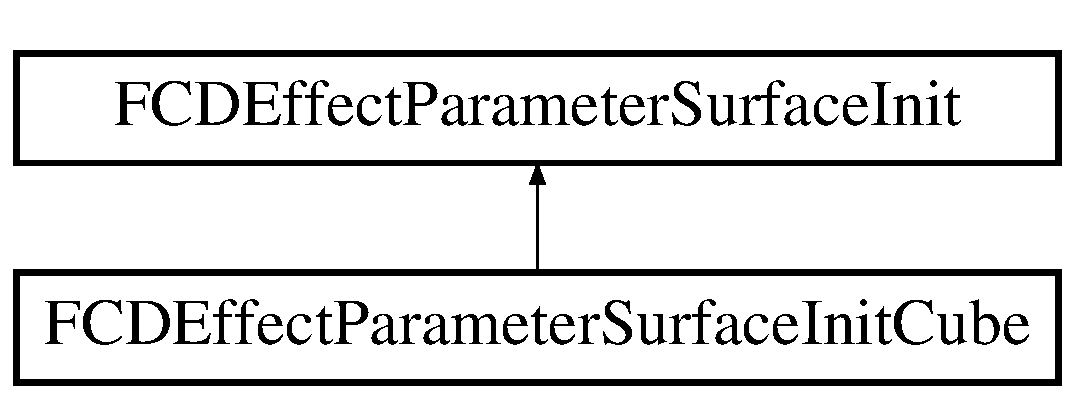
\includegraphics[height=2.000000cm]{classFCDEffectParameterSurfaceInitCube}
\end{center}
\end{figure}
\subsection*{Public Types}
\begin{DoxyCompactItemize}
\item 
enum \hyperlink{classFCDEffectParameterSurfaceInitCube_a59228097e934d37b9e8ae788a749bc07}{CubeType} \{ {\bfseries ALL}, 
\hyperlink{classFCDEffectParameterSurfaceInitCube_a59228097e934d37b9e8ae788a749bc07a5f20c13bdba2e0c6acd3616d3af70936}{PRIMARY}, 
\hyperlink{classFCDEffectParameterSurfaceInitCube_a59228097e934d37b9e8ae788a749bc07ad8ea23e52036e6ad637a7169021239f3}{FACE}
 \}
\end{DoxyCompactItemize}
\subsection*{Public Member Functions}
\begin{DoxyCompactItemize}
\item 
\hyperlink{classFCDEffectParameterSurfaceInitCube_ae55fc2856c67f2572dc5eb26cdafda76}{FCDEffectParameterSurfaceInitCube} ()
\item 
virtual \hyperlink{classFCDEffectParameterSurfaceInitCube_ad69a070147d26f23d81d4380c9dd6ec8}{$\sim$FCDEffectParameterSurfaceInitCube} ()
\item 
virtual \hyperlink{classFCDEffectParameterSurfaceInitFactory_a65e74f1159865702cac5236dd5d83892}{FCDEffectParameterSurfaceInitFactory::InitType} \hyperlink{classFCDEffectParameterSurfaceInitCube_aa22db1c4680d97b447466bc54a492451}{GetInitType} () const 
\item 
virtual \hyperlink{classFCDEffectParameterSurfaceInit}{FCDEffectParameterSurfaceInit} $\ast$ \hyperlink{classFCDEffectParameterSurfaceInitCube_a46ae1522ddb60038c59f9a1511157713}{Clone} (\hyperlink{classFCDEffectParameterSurfaceInit}{FCDEffectParameterSurfaceInit} $\ast$clone) const 
\end{DoxyCompactItemize}
\subsection*{Data Fields}
\begin{DoxyCompactItemize}
\item 
\hyperlink{classFCDEffectParameterSurfaceInitCube_a59228097e934d37b9e8ae788a749bc07}{CubeType} \hyperlink{classFCDEffectParameterSurfaceInitCube_af13376d1509627b73843e631db0abffb}{cubeType}
\item 
\hyperlink{classfm_1_1vector}{UInt16List} \hyperlink{classFCDEffectParameterSurfaceInitCube_abb0a85514c43581c62d9b1167d329035}{order}
\end{DoxyCompactItemize}


\subsection{Detailed Description}
A cube-\/map surface initialization method. 

\subsection{Member Enumeration Documentation}
\hypertarget{classFCDEffectParameterSurfaceInitCube_a59228097e934d37b9e8ae788a749bc07}{
\index{FCDEffectParameterSurfaceInitCube@{FCDEffectParameterSurfaceInitCube}!CubeType@{CubeType}}
\index{CubeType@{CubeType}!FCDEffectParameterSurfaceInitCube@{FCDEffectParameterSurfaceInitCube}}
\subsubsection[{CubeType}]{\setlength{\rightskip}{0pt plus 5cm}enum {\bf FCDEffectParameterSurfaceInitCube::CubeType}}}
\label{classFCDEffectParameterSurfaceInitCube_a59228097e934d37b9e8ae788a749bc07}
The types of cube-\/map initializations. \begin{Desc}
\item[Enumerator: ]\par
\begin{description}
\index{PRIMARY@{PRIMARY}!FCDEffectParameterSurfaceInitCube@{FCDEffectParameterSurfaceInitCube}}\index{FCDEffectParameterSurfaceInitCube@{FCDEffectParameterSurfaceInitCube}!PRIMARY@{PRIMARY}}\item[{\em 
\hypertarget{classFCDEffectParameterSurfaceInitCube_a59228097e934d37b9e8ae788a749bc07a5f20c13bdba2e0c6acd3616d3af70936}{
PRIMARY}
\label{classFCDEffectParameterSurfaceInitCube_a59228097e934d37b9e8ae788a749bc07a5f20c13bdba2e0c6acd3616d3af70936}
}]Load all the mip-\/levels of all the cube-\/map faces from one image file. \index{FACE@{FACE}!FCDEffectParameterSurfaceInitCube@{FCDEffectParameterSurfaceInitCube}}\index{FCDEffectParameterSurfaceInitCube@{FCDEffectParameterSurfaceInitCube}!FACE@{FACE}}\item[{\em 
\hypertarget{classFCDEffectParameterSurfaceInitCube_a59228097e934d37b9e8ae788a749bc07ad8ea23e52036e6ad637a7169021239f3}{
FACE}
\label{classFCDEffectParameterSurfaceInitCube_a59228097e934d37b9e8ae788a749bc07ad8ea23e52036e6ad637a7169021239f3}
}]Load the first mip-\/level of all the cube-\/map faces from one image file. Load all the cube-\/map faces from separate image files. \end{description}
\end{Desc}



\subsection{Constructor \& Destructor Documentation}
\hypertarget{classFCDEffectParameterSurfaceInitCube_ae55fc2856c67f2572dc5eb26cdafda76}{
\index{FCDEffectParameterSurfaceInitCube@{FCDEffectParameterSurfaceInitCube}!FCDEffectParameterSurfaceInitCube@{FCDEffectParameterSurfaceInitCube}}
\index{FCDEffectParameterSurfaceInitCube@{FCDEffectParameterSurfaceInitCube}!FCDEffectParameterSurfaceInitCube@{FCDEffectParameterSurfaceInitCube}}
\subsubsection[{FCDEffectParameterSurfaceInitCube}]{\setlength{\rightskip}{0pt plus 5cm}FCDEffectParameterSurfaceInitCube::FCDEffectParameterSurfaceInitCube (
\begin{DoxyParamCaption}
{}
\end{DoxyParamCaption}
)}}
\label{classFCDEffectParameterSurfaceInitCube_ae55fc2856c67f2572dc5eb26cdafda76}
Constructor: builds a new cube-\/map initialization method. \hypertarget{classFCDEffectParameterSurfaceInitCube_ad69a070147d26f23d81d4380c9dd6ec8}{
\index{FCDEffectParameterSurfaceInitCube@{FCDEffectParameterSurfaceInitCube}!$\sim$FCDEffectParameterSurfaceInitCube@{$\sim$FCDEffectParameterSurfaceInitCube}}
\index{$\sim$FCDEffectParameterSurfaceInitCube@{$\sim$FCDEffectParameterSurfaceInitCube}!FCDEffectParameterSurfaceInitCube@{FCDEffectParameterSurfaceInitCube}}
\subsubsection[{$\sim$FCDEffectParameterSurfaceInitCube}]{\setlength{\rightskip}{0pt plus 5cm}virtual FCDEffectParameterSurfaceInitCube::$\sim$FCDEffectParameterSurfaceInitCube (
\begin{DoxyParamCaption}
{}
\end{DoxyParamCaption}
)\hspace{0.3cm}{\ttfamily  \mbox{[}inline, virtual\mbox{]}}}}
\label{classFCDEffectParameterSurfaceInitCube_ad69a070147d26f23d81d4380c9dd6ec8}
Destructor. 

\subsection{Member Function Documentation}
\hypertarget{classFCDEffectParameterSurfaceInitCube_a46ae1522ddb60038c59f9a1511157713}{
\index{FCDEffectParameterSurfaceInitCube@{FCDEffectParameterSurfaceInitCube}!Clone@{Clone}}
\index{Clone@{Clone}!FCDEffectParameterSurfaceInitCube@{FCDEffectParameterSurfaceInitCube}}
\subsubsection[{Clone}]{\setlength{\rightskip}{0pt plus 5cm}{\bf FCDEffectParameterSurfaceInit} $\ast$ FCDEffectParameterSurfaceInitCube::Clone (
\begin{DoxyParamCaption}
\item[{{\bf FCDEffectParameterSurfaceInit} $\ast$}]{ clone}
\end{DoxyParamCaption}
) const\hspace{0.3cm}{\ttfamily  \mbox{[}virtual\mbox{]}}}}
\label{classFCDEffectParameterSurfaceInitCube_a46ae1522ddb60038c59f9a1511157713}
Creates a full copy of the surface initialization parameter. 
\begin{DoxyParams}{Parameters}
\item[{\em clone}]The cloned surface initialization. If this pointer is NULL, a new surface initialization parameter will be created and you will need to delete this pointer. \end{DoxyParams}
\begin{DoxyReturn}{Returns}
The cloned surface initialization. 
\end{DoxyReturn}


Reimplemented from \hyperlink{classFCDEffectParameterSurfaceInit_ae3ac516773ea5ebb6838ed8a0d10d910}{FCDEffectParameterSurfaceInit}.

\hypertarget{classFCDEffectParameterSurfaceInitCube_aa22db1c4680d97b447466bc54a492451}{
\index{FCDEffectParameterSurfaceInitCube@{FCDEffectParameterSurfaceInitCube}!GetInitType@{GetInitType}}
\index{GetInitType@{GetInitType}!FCDEffectParameterSurfaceInitCube@{FCDEffectParameterSurfaceInitCube}}
\subsubsection[{GetInitType}]{\setlength{\rightskip}{0pt plus 5cm}virtual {\bf FCDEffectParameterSurfaceInitFactory::InitType} FCDEffectParameterSurfaceInitCube::GetInitType (
\begin{DoxyParamCaption}
{}
\end{DoxyParamCaption}
) const\hspace{0.3cm}{\ttfamily  \mbox{[}inline, virtual\mbox{]}}}}
\label{classFCDEffectParameterSurfaceInitCube_aa22db1c4680d97b447466bc54a492451}
Retrieves the initialization type. You cannot modify this value. To change the initialization type of a surface parameter, create a new surface initialization structure of the correct type. \begin{DoxyReturn}{Returns}
The initialization type. 
\end{DoxyReturn}


Implements \hyperlink{classFCDEffectParameterSurfaceInit_ad0109233e63c892e5963a3ca67f7108f}{FCDEffectParameterSurfaceInit}.



\subsection{Field Documentation}
\hypertarget{classFCDEffectParameterSurfaceInitCube_af13376d1509627b73843e631db0abffb}{
\index{FCDEffectParameterSurfaceInitCube@{FCDEffectParameterSurfaceInitCube}!cubeType@{cubeType}}
\index{cubeType@{cubeType}!FCDEffectParameterSurfaceInitCube@{FCDEffectParameterSurfaceInitCube}}
\subsubsection[{cubeType}]{\setlength{\rightskip}{0pt plus 5cm}{\bf CubeType} {\bf FCDEffectParameterSurfaceInitCube::cubeType}}}
\label{classFCDEffectParameterSurfaceInitCube_af13376d1509627b73843e631db0abffb}
The type of cube-\/map initialization. \hypertarget{classFCDEffectParameterSurfaceInitCube_abb0a85514c43581c62d9b1167d329035}{
\index{FCDEffectParameterSurfaceInitCube@{FCDEffectParameterSurfaceInitCube}!order@{order}}
\index{order@{order}!FCDEffectParameterSurfaceInitCube@{FCDEffectParameterSurfaceInitCube}}
\subsubsection[{order}]{\setlength{\rightskip}{0pt plus 5cm}{\bf UInt16List} {\bf FCDEffectParameterSurfaceInitCube::order}}}
\label{classFCDEffectParameterSurfaceInitCube_abb0a85514c43581c62d9b1167d329035}
The list of image indices. The images are contained within the surface effect parameter. This is used only for the FACE cube-\/map initialization type and indicates how to match the faces of faces of the cube-\/map with the images in the surface effect parameter. 

The documentation for this class was generated from the following files:\begin{DoxyCompactItemize}
\item 
FCollada/FCDocument/\hyperlink{FCDEffectParameterSurface_8h}{FCDEffectParameterSurface.h}\item 
FCollada/FCDocument/FCDEffectParameterSurface.cpp\end{DoxyCompactItemize}

\hypertarget{classFCDEffectParameterSurfaceInitFactory}{
\section{FCDEffectParameterSurfaceInitFactory Class Reference}
\label{classFCDEffectParameterSurfaceInitFactory}\index{FCDEffectParameterSurfaceInitFactory@{FCDEffectParameterSurfaceInitFactory}}
}


{\ttfamily \#include $<$FCDEffectParameterSurface.h$>$}

\subsection*{Public Types}
\begin{DoxyCompactItemize}
\item 
enum \hyperlink{classFCDEffectParameterSurfaceInitFactory_a65e74f1159865702cac5236dd5d83892}{InitType} \{ \par
\hyperlink{classFCDEffectParameterSurfaceInitFactory_a65e74f1159865702cac5236dd5d83892aa87c1f6872f211a3f525c11557149e4d}{FROM}, 
\hyperlink{classFCDEffectParameterSurfaceInitFactory_a65e74f1159865702cac5236dd5d83892a90f0b3c1c0dfe447ea2f973141eb0b1c}{AS\_\-NULL}, 
\hyperlink{classFCDEffectParameterSurfaceInitFactory_a65e74f1159865702cac5236dd5d83892ad1baa0ff12391ddc3dd1f9c40ea77906}{AS\_\-TARGET}, 
\hyperlink{classFCDEffectParameterSurfaceInitFactory_a65e74f1159865702cac5236dd5d83892ae2d69f0436ba18d343605f554e30ed22}{CUBE}, 
\par
\hyperlink{classFCDEffectParameterSurfaceInitFactory_a65e74f1159865702cac5236dd5d83892a328076a8538f429eb5988879c0e643cd}{VOLUME}, 
\hyperlink{classFCDEffectParameterSurfaceInitFactory_a65e74f1159865702cac5236dd5d83892a5c8434819c6046c14dff8f793841ac51}{PLANAR}
 \}
\end{DoxyCompactItemize}
\subsection*{Static Public Member Functions}
\begin{DoxyCompactItemize}
\item 
static \hyperlink{classFCDEffectParameterSurfaceInit}{FCDEffectParameterSurfaceInit} $\ast$ \hyperlink{classFCDEffectParameterSurfaceInitFactory_aaebd11b1bbf4ac88b544c8917bf4c979}{Create} (\hyperlink{classFCDEffectParameterSurfaceInitFactory_a65e74f1159865702cac5236dd5d83892}{InitType} type)
\end{DoxyCompactItemize}


\subsection{Detailed Description}
\mbox{[}INTERNAL\mbox{]} The factory for COLLADA effect parameter surface initialization. 

\subsection{Member Enumeration Documentation}
\hypertarget{classFCDEffectParameterSurfaceInitFactory_a65e74f1159865702cac5236dd5d83892}{
\index{FCDEffectParameterSurfaceInitFactory@{FCDEffectParameterSurfaceInitFactory}!InitType@{InitType}}
\index{InitType@{InitType}!FCDEffectParameterSurfaceInitFactory@{FCDEffectParameterSurfaceInitFactory}}
\subsubsection[{InitType}]{\setlength{\rightskip}{0pt plus 5cm}enum {\bf FCDEffectParameterSurfaceInitFactory::InitType}}}
\label{classFCDEffectParameterSurfaceInitFactory_a65e74f1159865702cac5236dd5d83892}
The supported initialization types. \begin{Desc}
\item[Enumerator: ]\par
\begin{description}
\index{FROM@{FROM}!FCDEffectParameterSurfaceInitFactory@{FCDEffectParameterSurfaceInitFactory}}\index{FCDEffectParameterSurfaceInitFactory@{FCDEffectParameterSurfaceInitFactory}!FROM@{FROM}}\item[{\em 
\hypertarget{classFCDEffectParameterSurfaceInitFactory_a65e74f1159865702cac5236dd5d83892aa87c1f6872f211a3f525c11557149e4d}{
FROM}
\label{classFCDEffectParameterSurfaceInitFactory_a65e74f1159865702cac5236dd5d83892aa87c1f6872f211a3f525c11557149e4d}
}]Loads a surface from one simple image file. \begin{DoxySeeAlso}{See also}
\hyperlink{classFCDEffectParameterSurfaceInitFrom}{FCDEffectParameterSurfaceInitFrom} 
\end{DoxySeeAlso}
\index{AS\_\-NULL@{AS\_\-NULL}!FCDEffectParameterSurfaceInitFactory@{FCDEffectParameterSurfaceInitFactory}}\index{FCDEffectParameterSurfaceInitFactory@{FCDEffectParameterSurfaceInitFactory}!AS\_\-NULL@{AS\_\-NULL}}\item[{\em 
\hypertarget{classFCDEffectParameterSurfaceInitFactory_a65e74f1159865702cac5236dd5d83892a90f0b3c1c0dfe447ea2f973141eb0b1c}{
AS\_\-NULL}
\label{classFCDEffectParameterSurfaceInitFactory_a65e74f1159865702cac5236dd5d83892a90f0b3c1c0dfe447ea2f973141eb0b1c}
}]No initialization. This surface may be initialized by some future effect parameter override. \index{AS\_\-TARGET@{AS\_\-TARGET}!FCDEffectParameterSurfaceInitFactory@{FCDEffectParameterSurfaceInitFactory}}\index{FCDEffectParameterSurfaceInitFactory@{FCDEffectParameterSurfaceInitFactory}!AS\_\-TARGET@{AS\_\-TARGET}}\item[{\em 
\hypertarget{classFCDEffectParameterSurfaceInitFactory_a65e74f1159865702cac5236dd5d83892ad1baa0ff12391ddc3dd1f9c40ea77906}{
AS\_\-TARGET}
\label{classFCDEffectParameterSurfaceInitFactory_a65e74f1159865702cac5236dd5d83892ad1baa0ff12391ddc3dd1f9c40ea77906}
}]Initializes an engine-\/specific render target for offscreen rendering. In this case, the dimensions should be provided by the surface effect parameter. \index{CUBE@{CUBE}!FCDEffectParameterSurfaceInitFactory@{FCDEffectParameterSurfaceInitFactory}}\index{FCDEffectParameterSurfaceInitFactory@{FCDEffectParameterSurfaceInitFactory}!CUBE@{CUBE}}\item[{\em 
\hypertarget{classFCDEffectParameterSurfaceInitFactory_a65e74f1159865702cac5236dd5d83892ae2d69f0436ba18d343605f554e30ed22}{
CUBE}
\label{classFCDEffectParameterSurfaceInitFactory_a65e74f1159865702cac5236dd5d83892ae2d69f0436ba18d343605f554e30ed22}
}]Loads a cube-\/map from one complex image file or six simple image files. \begin{DoxySeeAlso}{See also}
\hyperlink{classFCDEffectParameterSurfaceInitCube}{FCDEffectParameterSurfaceInitCube} 
\end{DoxySeeAlso}
\index{VOLUME@{VOLUME}!FCDEffectParameterSurfaceInitFactory@{FCDEffectParameterSurfaceInitFactory}}\index{FCDEffectParameterSurfaceInitFactory@{FCDEffectParameterSurfaceInitFactory}!VOLUME@{VOLUME}}\item[{\em 
\hypertarget{classFCDEffectParameterSurfaceInitFactory_a65e74f1159865702cac5236dd5d83892a328076a8538f429eb5988879c0e643cd}{
VOLUME}
\label{classFCDEffectParameterSurfaceInitFactory_a65e74f1159865702cac5236dd5d83892a328076a8538f429eb5988879c0e643cd}
}]Loads a 3D images for one image file. \begin{DoxySeeAlso}{See also}
\hyperlink{classFCDEffectParameterSurfaceInitVolume}{FCDEffectParameterSurfaceInitVolume} 
\end{DoxySeeAlso}
\index{PLANAR@{PLANAR}!FCDEffectParameterSurfaceInitFactory@{FCDEffectParameterSurfaceInitFactory}}\index{FCDEffectParameterSurfaceInitFactory@{FCDEffectParameterSurfaceInitFactory}!PLANAR@{PLANAR}}\item[{\em 
\hypertarget{classFCDEffectParameterSurfaceInitFactory_a65e74f1159865702cac5236dd5d83892a5c8434819c6046c14dff8f793841ac51}{
PLANAR}
\label{classFCDEffectParameterSurfaceInitFactory_a65e74f1159865702cac5236dd5d83892a5c8434819c6046c14dff8f793841ac51}
}]Loads a surface from one simple image file. \end{description}
\end{Desc}



\subsection{Member Function Documentation}
\hypertarget{classFCDEffectParameterSurfaceInitFactory_aaebd11b1bbf4ac88b544c8917bf4c979}{
\index{FCDEffectParameterSurfaceInitFactory@{FCDEffectParameterSurfaceInitFactory}!Create@{Create}}
\index{Create@{Create}!FCDEffectParameterSurfaceInitFactory@{FCDEffectParameterSurfaceInitFactory}}
\subsubsection[{Create}]{\setlength{\rightskip}{0pt plus 5cm}{\bf FCDEffectParameterSurfaceInit} $\ast$ FCDEffectParameterSurfaceInitFactory::Create (
\begin{DoxyParamCaption}
\item[{{\bf InitType}}]{ type}
\end{DoxyParamCaption}
)\hspace{0.3cm}{\ttfamily  \mbox{[}static\mbox{]}}}}
\label{classFCDEffectParameterSurfaceInitFactory_aaebd11b1bbf4ac88b544c8917bf4c979}
\mbox{[}INTERNAL\mbox{]} Creates a new effect surface initialization parameter, given a type. 
\begin{DoxyParams}{Parameters}
\item[{\em type}]The type of initialization parameter to create. \end{DoxyParams}


The documentation for this class was generated from the following files:\begin{DoxyCompactItemize}
\item 
FCollada/FCDocument/\hyperlink{FCDEffectParameterSurface_8h}{FCDEffectParameterSurface.h}\item 
FCollada/FCDocument/FCDEffectParameterSurface.cpp\end{DoxyCompactItemize}

\hypertarget{classFCDEffectParameterSurfaceInitFrom}{
\section{FCDEffectParameterSurfaceInitFrom Class Reference}
\label{classFCDEffectParameterSurfaceInitFrom}\index{FCDEffectParameterSurfaceInitFrom@{FCDEffectParameterSurfaceInitFrom}}
}


{\ttfamily \#include $<$FCDEffectParameterSurface.h$>$}

Inheritance diagram for FCDEffectParameterSurfaceInitFrom:\begin{figure}[H]
\begin{center}
\leavevmode
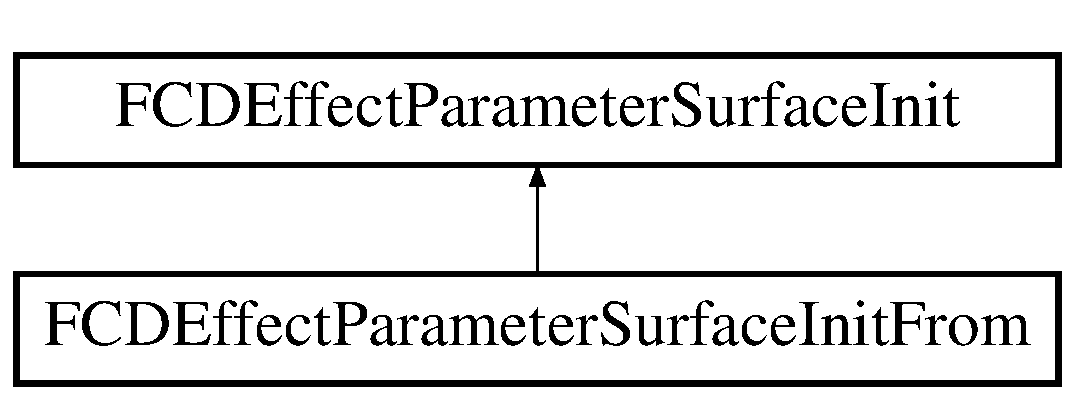
\includegraphics[height=2.000000cm]{classFCDEffectParameterSurfaceInitFrom}
\end{center}
\end{figure}
\subsection*{Public Member Functions}
\begin{DoxyCompactItemize}
\item 
\hyperlink{classFCDEffectParameterSurfaceInitFrom_a308effcaf25b329f368d02f4efcc2ecb}{FCDEffectParameterSurfaceInitFrom} ()
\item 
virtual \hyperlink{classFCDEffectParameterSurfaceInitFrom_a3de6ed57df62c569a872995a95bce88f}{$\sim$FCDEffectParameterSurfaceInitFrom} ()
\item 
virtual \hyperlink{classFCDEffectParameterSurfaceInitFactory_a65e74f1159865702cac5236dd5d83892}{FCDEffectParameterSurfaceInitFactory::InitType} \hyperlink{classFCDEffectParameterSurfaceInitFrom_a33c2001f6d11fe519d7f5c492daec92a}{GetInitType} () const 
\item 
virtual \hyperlink{classFCDEffectParameterSurfaceInit}{FCDEffectParameterSurfaceInit} $\ast$ \hyperlink{classFCDEffectParameterSurfaceInitFrom_a8a173445b78914cf1ed6f222ffb7ba0b}{Clone} (\hyperlink{classFCDEffectParameterSurfaceInit}{FCDEffectParameterSurfaceInit} $\ast$clone) const 
\end{DoxyCompactItemize}
\subsection*{Public Attributes}
\begin{DoxyCompactItemize}
\item 
\hyperlink{classfm_1_1vector}{StringList} \hyperlink{classFCDEffectParameterSurfaceInitFrom_ac7df5eff72c2fa2a183bacdfc3ac3799}{mip}
\item 
\hyperlink{classfm_1_1vector}{StringList} \hyperlink{classFCDEffectParameterSurfaceInitFrom_a9abea30f2ccd2f28a50d5678d22135cb}{slice}
\item 
\hyperlink{classfm_1_1vector}{StringList} \hyperlink{classFCDEffectParameterSurfaceInitFrom_a78e6c19391ebf68c392be301db666ac8}{face}
\end{DoxyCompactItemize}


\subsection{Detailed Description}
A simple file surface initialization method. This is the method used for backward-\/compatibility. 

\subsection{Constructor \& Destructor Documentation}
\hypertarget{classFCDEffectParameterSurfaceInitFrom_a308effcaf25b329f368d02f4efcc2ecb}{
\index{FCDEffectParameterSurfaceInitFrom@{FCDEffectParameterSurfaceInitFrom}!FCDEffectParameterSurfaceInitFrom@{FCDEffectParameterSurfaceInitFrom}}
\index{FCDEffectParameterSurfaceInitFrom@{FCDEffectParameterSurfaceInitFrom}!FCDEffectParameterSurfaceInitFrom@{FCDEffectParameterSurfaceInitFrom}}
\subsubsection[{FCDEffectParameterSurfaceInitFrom}]{\setlength{\rightskip}{0pt plus 5cm}FCDEffectParameterSurfaceInitFrom::FCDEffectParameterSurfaceInitFrom (
\begin{DoxyParamCaption}
{}
\end{DoxyParamCaption}
)\hspace{0.3cm}{\ttfamily  \mbox{[}inline\mbox{]}}}}
\label{classFCDEffectParameterSurfaceInitFrom_a308effcaf25b329f368d02f4efcc2ecb}
Constructor: builds a new file surface initialization method. \hypertarget{classFCDEffectParameterSurfaceInitFrom_a3de6ed57df62c569a872995a95bce88f}{
\index{FCDEffectParameterSurfaceInitFrom@{FCDEffectParameterSurfaceInitFrom}!$\sim$FCDEffectParameterSurfaceInitFrom@{$\sim$FCDEffectParameterSurfaceInitFrom}}
\index{$\sim$FCDEffectParameterSurfaceInitFrom@{$\sim$FCDEffectParameterSurfaceInitFrom}!FCDEffectParameterSurfaceInitFrom@{FCDEffectParameterSurfaceInitFrom}}
\subsubsection[{$\sim$FCDEffectParameterSurfaceInitFrom}]{\setlength{\rightskip}{0pt plus 5cm}virtual FCDEffectParameterSurfaceInitFrom::$\sim$FCDEffectParameterSurfaceInitFrom (
\begin{DoxyParamCaption}
{}
\end{DoxyParamCaption}
)\hspace{0.3cm}{\ttfamily  \mbox{[}inline, virtual\mbox{]}}}}
\label{classFCDEffectParameterSurfaceInitFrom_a3de6ed57df62c569a872995a95bce88f}
Destructor. 

\subsection{Member Function Documentation}
\hypertarget{classFCDEffectParameterSurfaceInitFrom_a8a173445b78914cf1ed6f222ffb7ba0b}{
\index{FCDEffectParameterSurfaceInitFrom@{FCDEffectParameterSurfaceInitFrom}!Clone@{Clone}}
\index{Clone@{Clone}!FCDEffectParameterSurfaceInitFrom@{FCDEffectParameterSurfaceInitFrom}}
\subsubsection[{Clone}]{\setlength{\rightskip}{0pt plus 5cm}{\bf FCDEffectParameterSurfaceInit} $\ast$ FCDEffectParameterSurfaceInitFrom::Clone (
\begin{DoxyParamCaption}
\item[{{\bf FCDEffectParameterSurfaceInit} $\ast$}]{ clone}
\end{DoxyParamCaption}
) const\hspace{0.3cm}{\ttfamily  \mbox{[}virtual\mbox{]}}}}
\label{classFCDEffectParameterSurfaceInitFrom_a8a173445b78914cf1ed6f222ffb7ba0b}
Creates a full copy of the surface initialization parameter. 
\begin{DoxyParams}{Parameters}
\item[{\em clone}]The cloned surface initialization. If this pointer is NULL, a new surface initialization parameter will be created and you will need to delete this pointer. \end{DoxyParams}
\begin{DoxyReturn}{Returns}
The cloned surface initialization. 
\end{DoxyReturn}


Reimplemented from \hyperlink{classFCDEffectParameterSurfaceInit_ae3ac516773ea5ebb6838ed8a0d10d910}{FCDEffectParameterSurfaceInit}.

\hypertarget{classFCDEffectParameterSurfaceInitFrom_a33c2001f6d11fe519d7f5c492daec92a}{
\index{FCDEffectParameterSurfaceInitFrom@{FCDEffectParameterSurfaceInitFrom}!GetInitType@{GetInitType}}
\index{GetInitType@{GetInitType}!FCDEffectParameterSurfaceInitFrom@{FCDEffectParameterSurfaceInitFrom}}
\subsubsection[{GetInitType}]{\setlength{\rightskip}{0pt plus 5cm}virtual {\bf FCDEffectParameterSurfaceInitFactory::InitType} FCDEffectParameterSurfaceInitFrom::GetInitType (
\begin{DoxyParamCaption}
{}
\end{DoxyParamCaption}
) const\hspace{0.3cm}{\ttfamily  \mbox{[}inline, virtual\mbox{]}}}}
\label{classFCDEffectParameterSurfaceInitFrom_a33c2001f6d11fe519d7f5c492daec92a}
Retrieves the initialization type. You cannot modify this value. To change the initialization type of a surface parameter, create a new surface initialization structure of the correct type. \begin{DoxyReturn}{Returns}
The initialization type. 
\end{DoxyReturn}


Implements \hyperlink{classFCDEffectParameterSurfaceInit_ad0109233e63c892e5963a3ca67f7108f}{FCDEffectParameterSurfaceInit}.



\subsection{Member Data Documentation}
\hypertarget{classFCDEffectParameterSurfaceInitFrom_a78e6c19391ebf68c392be301db666ac8}{
\index{FCDEffectParameterSurfaceInitFrom@{FCDEffectParameterSurfaceInitFrom}!face@{face}}
\index{face@{face}!FCDEffectParameterSurfaceInitFrom@{FCDEffectParameterSurfaceInitFrom}}
\subsubsection[{face}]{\setlength{\rightskip}{0pt plus 5cm}{\bf StringList} {\bf FCDEffectParameterSurfaceInitFrom::face}}}
\label{classFCDEffectParameterSurfaceInitFrom_a78e6c19391ebf68c392be301db666ac8}
The list of matching faces. \hypertarget{classFCDEffectParameterSurfaceInitFrom_ac7df5eff72c2fa2a183bacdfc3ac3799}{
\index{FCDEffectParameterSurfaceInitFrom@{FCDEffectParameterSurfaceInitFrom}!mip@{mip}}
\index{mip@{mip}!FCDEffectParameterSurfaceInitFrom@{FCDEffectParameterSurfaceInitFrom}}
\subsubsection[{mip}]{\setlength{\rightskip}{0pt plus 5cm}{\bf StringList} {\bf FCDEffectParameterSurfaceInitFrom::mip}}}
\label{classFCDEffectParameterSurfaceInitFrom_ac7df5eff72c2fa2a183bacdfc3ac3799}
The list of mip levels. \hypertarget{classFCDEffectParameterSurfaceInitFrom_a9abea30f2ccd2f28a50d5678d22135cb}{
\index{FCDEffectParameterSurfaceInitFrom@{FCDEffectParameterSurfaceInitFrom}!slice@{slice}}
\index{slice@{slice}!FCDEffectParameterSurfaceInitFrom@{FCDEffectParameterSurfaceInitFrom}}
\subsubsection[{slice}]{\setlength{\rightskip}{0pt plus 5cm}{\bf StringList} {\bf FCDEffectParameterSurfaceInitFrom::slice}}}
\label{classFCDEffectParameterSurfaceInitFrom_a9abea30f2ccd2f28a50d5678d22135cb}
The list of matching slices. 

The documentation for this class was generated from the following files:\begin{DoxyCompactItemize}
\item 
FCollada/FCDocument/\hyperlink{FCDEffectParameterSurface_8h}{FCDEffectParameterSurface.h}\item 
FCollada/FCDocument/FCDEffectParameterSurface.cpp\end{DoxyCompactItemize}

\hypertarget{classFCDEffectParameterSurfaceInitPlanar}{
\section{FCDEffectParameterSurfaceInitPlanar Class Reference}
\label{classFCDEffectParameterSurfaceInitPlanar}\index{FCDEffectParameterSurfaceInitPlanar@{FCDEffectParameterSurfaceInitPlanar}}
}


{\ttfamily \#include $<$FCDEffectParameterSurface.h$>$}

Inheritance diagram for FCDEffectParameterSurfaceInitPlanar:\begin{figure}[H]
\begin{center}
\leavevmode
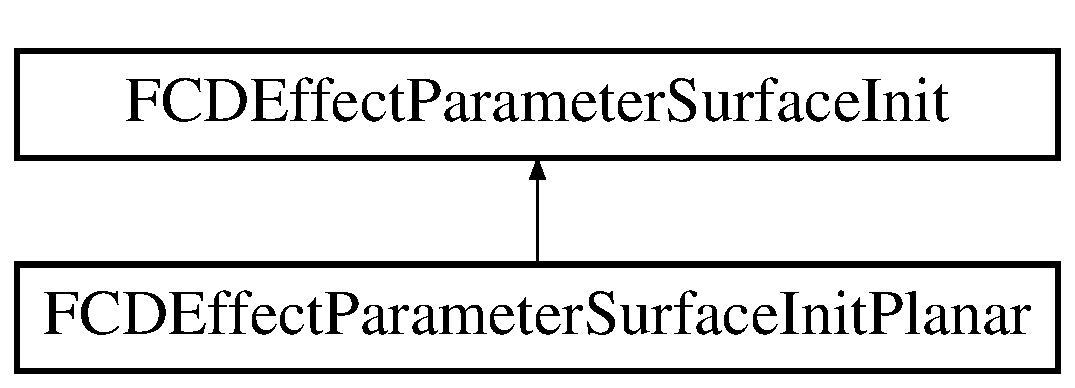
\includegraphics[height=2.000000cm]{classFCDEffectParameterSurfaceInitPlanar}
\end{center}
\end{figure}
\subsection*{Public Member Functions}
\begin{DoxyCompactItemize}
\item 
\hyperlink{classFCDEffectParameterSurfaceInitPlanar_a8ce39fa32d458f71da29f83a69ec7329}{FCDEffectParameterSurfaceInitPlanar} ()
\item 
virtual \hyperlink{classFCDEffectParameterSurfaceInitPlanar_ae29ed97f2de4463e47b8354338db5b44}{$\sim$FCDEffectParameterSurfaceInitPlanar} ()
\item 
virtual \hyperlink{classFCDEffectParameterSurfaceInitFactory_a65e74f1159865702cac5236dd5d83892}{FCDEffectParameterSurfaceInitFactory::InitType} \hyperlink{classFCDEffectParameterSurfaceInitPlanar_a9e91a455acbcbed40b8e647aa0c56d80}{GetInitType} () const 
\item 
virtual \hyperlink{classFCDEffectParameterSurfaceInit}{FCDEffectParameterSurfaceInit} $\ast$ \hyperlink{classFCDEffectParameterSurfaceInitPlanar_a565047eceb428bb55f32c7522c39354e}{Clone} (\hyperlink{classFCDEffectParameterSurfaceInit}{FCDEffectParameterSurfaceInit} $\ast$clone) const 
\end{DoxyCompactItemize}


\subsection{Detailed Description}
This method allows to initialize the surface as planar. 

\subsection{Constructor \& Destructor Documentation}
\hypertarget{classFCDEffectParameterSurfaceInitPlanar_a8ce39fa32d458f71da29f83a69ec7329}{
\index{FCDEffectParameterSurfaceInitPlanar@{FCDEffectParameterSurfaceInitPlanar}!FCDEffectParameterSurfaceInitPlanar@{FCDEffectParameterSurfaceInitPlanar}}
\index{FCDEffectParameterSurfaceInitPlanar@{FCDEffectParameterSurfaceInitPlanar}!FCDEffectParameterSurfaceInitPlanar@{FCDEffectParameterSurfaceInitPlanar}}
\subsubsection[{FCDEffectParameterSurfaceInitPlanar}]{\setlength{\rightskip}{0pt plus 5cm}FCDEffectParameterSurfaceInitPlanar::FCDEffectParameterSurfaceInitPlanar (
\begin{DoxyParamCaption}
{}
\end{DoxyParamCaption}
)\hspace{0.3cm}{\ttfamily  \mbox{[}inline\mbox{]}}}}
\label{classFCDEffectParameterSurfaceInitPlanar_a8ce39fa32d458f71da29f83a69ec7329}
Constructor: builds a new file surface initialization method. \hypertarget{classFCDEffectParameterSurfaceInitPlanar_ae29ed97f2de4463e47b8354338db5b44}{
\index{FCDEffectParameterSurfaceInitPlanar@{FCDEffectParameterSurfaceInitPlanar}!$\sim$FCDEffectParameterSurfaceInitPlanar@{$\sim$FCDEffectParameterSurfaceInitPlanar}}
\index{$\sim$FCDEffectParameterSurfaceInitPlanar@{$\sim$FCDEffectParameterSurfaceInitPlanar}!FCDEffectParameterSurfaceInitPlanar@{FCDEffectParameterSurfaceInitPlanar}}
\subsubsection[{$\sim$FCDEffectParameterSurfaceInitPlanar}]{\setlength{\rightskip}{0pt plus 5cm}virtual FCDEffectParameterSurfaceInitPlanar::$\sim$FCDEffectParameterSurfaceInitPlanar (
\begin{DoxyParamCaption}
{}
\end{DoxyParamCaption}
)\hspace{0.3cm}{\ttfamily  \mbox{[}inline, virtual\mbox{]}}}}
\label{classFCDEffectParameterSurfaceInitPlanar_ae29ed97f2de4463e47b8354338db5b44}
Destructor. 

\subsection{Member Function Documentation}
\hypertarget{classFCDEffectParameterSurfaceInitPlanar_a565047eceb428bb55f32c7522c39354e}{
\index{FCDEffectParameterSurfaceInitPlanar@{FCDEffectParameterSurfaceInitPlanar}!Clone@{Clone}}
\index{Clone@{Clone}!FCDEffectParameterSurfaceInitPlanar@{FCDEffectParameterSurfaceInitPlanar}}
\subsubsection[{Clone}]{\setlength{\rightskip}{0pt plus 5cm}{\bf FCDEffectParameterSurfaceInit} $\ast$ FCDEffectParameterSurfaceInitPlanar::Clone (
\begin{DoxyParamCaption}
\item[{{\bf FCDEffectParameterSurfaceInit} $\ast$}]{ clone}
\end{DoxyParamCaption}
) const\hspace{0.3cm}{\ttfamily  \mbox{[}virtual\mbox{]}}}}
\label{classFCDEffectParameterSurfaceInitPlanar_a565047eceb428bb55f32c7522c39354e}
Creates a full copy of the surface initialization parameter. 
\begin{DoxyParams}{Parameters}
\item[{\em clone}]The cloned surface initialization. If this pointer is NULL, a new surface initialization parameter will be created and you will need to delete this pointer. \end{DoxyParams}
\begin{DoxyReturn}{Returns}
The cloned surface initialization. 
\end{DoxyReturn}


Reimplemented from \hyperlink{classFCDEffectParameterSurfaceInit_ae3ac516773ea5ebb6838ed8a0d10d910}{FCDEffectParameterSurfaceInit}.

\hypertarget{classFCDEffectParameterSurfaceInitPlanar_a9e91a455acbcbed40b8e647aa0c56d80}{
\index{FCDEffectParameterSurfaceInitPlanar@{FCDEffectParameterSurfaceInitPlanar}!GetInitType@{GetInitType}}
\index{GetInitType@{GetInitType}!FCDEffectParameterSurfaceInitPlanar@{FCDEffectParameterSurfaceInitPlanar}}
\subsubsection[{GetInitType}]{\setlength{\rightskip}{0pt plus 5cm}virtual {\bf FCDEffectParameterSurfaceInitFactory::InitType} FCDEffectParameterSurfaceInitPlanar::GetInitType (
\begin{DoxyParamCaption}
{}
\end{DoxyParamCaption}
) const\hspace{0.3cm}{\ttfamily  \mbox{[}inline, virtual\mbox{]}}}}
\label{classFCDEffectParameterSurfaceInitPlanar_a9e91a455acbcbed40b8e647aa0c56d80}
Retrieves the initialization type. You cannot modify this value. To change the initialization type of a surface parameter, create a new surface initialization structure of the correct type. \begin{DoxyReturn}{Returns}
The initialization type. 
\end{DoxyReturn}


Implements \hyperlink{classFCDEffectParameterSurfaceInit_ad0109233e63c892e5963a3ca67f7108f}{FCDEffectParameterSurfaceInit}.



The documentation for this class was generated from the following files:\begin{DoxyCompactItemize}
\item 
FCollada/FCDocument/\hyperlink{FCDEffectParameterSurface_8h}{FCDEffectParameterSurface.h}\item 
FCollada/FCDocument/FCDEffectParameterSurface.cpp\end{DoxyCompactItemize}

\hypertarget{classFCDEffectParameterSurfaceInitVolume}{
\section{FCDEffectParameterSurfaceInitVolume Class Reference}
\label{classFCDEffectParameterSurfaceInitVolume}\index{FCDEffectParameterSurfaceInitVolume@{FCDEffectParameterSurfaceInitVolume}}
}


{\ttfamily \#include $<$FCDEffectParameterSurface.h$>$}

Inheritance diagram for FCDEffectParameterSurfaceInitVolume:\begin{figure}[H]
\begin{center}
\leavevmode
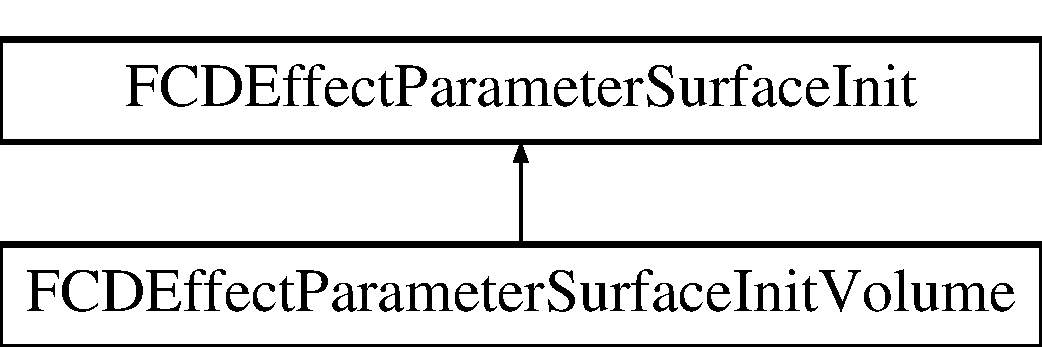
\includegraphics[height=2.000000cm]{classFCDEffectParameterSurfaceInitVolume}
\end{center}
\end{figure}
\subsection*{Public Types}
\begin{DoxyCompactItemize}
\item 
enum \hyperlink{classFCDEffectParameterSurfaceInitVolume_a26c9418850b0c0d5a6c685b4ce4d890b}{VolumeType} \{ {\bfseries ALL}, 
\hyperlink{classFCDEffectParameterSurfaceInitVolume_a26c9418850b0c0d5a6c685b4ce4d890ba13ca69673f7e1aa87c61d5ef49df4512}{PRIMARY}
 \}
\end{DoxyCompactItemize}
\subsection*{Public Member Functions}
\begin{DoxyCompactItemize}
\item 
\hyperlink{classFCDEffectParameterSurfaceInitVolume_a06132d8a624304e2b2a738d57eeaeb0f}{FCDEffectParameterSurfaceInitVolume} ()
\item 
virtual \hyperlink{classFCDEffectParameterSurfaceInitVolume_a131f222e9900bc43683051e97c243ea0}{$\sim$FCDEffectParameterSurfaceInitVolume} ()
\item 
virtual \hyperlink{classFCDEffectParameterSurfaceInitFactory_a65e74f1159865702cac5236dd5d83892}{FCDEffectParameterSurfaceInitFactory::InitType} \hyperlink{classFCDEffectParameterSurfaceInitVolume_ad0490f5d50b8babd77b3294277f4fde5}{GetInitType} () const 
\item 
virtual \hyperlink{classFCDEffectParameterSurfaceInit}{FCDEffectParameterSurfaceInit} $\ast$ \hyperlink{classFCDEffectParameterSurfaceInitVolume_a54cdfc576b05fe56d87c1dc1c2fe211a}{Clone} (\hyperlink{classFCDEffectParameterSurfaceInit}{FCDEffectParameterSurfaceInit} $\ast$clone) const 
\end{DoxyCompactItemize}
\subsection*{Data Fields}
\begin{DoxyCompactItemize}
\item 
\hyperlink{classFCDEffectParameterSurfaceInitVolume_a26c9418850b0c0d5a6c685b4ce4d890b}{VolumeType} \hyperlink{classFCDEffectParameterSurfaceInitVolume_aad5bb8a564f3583dce34eb2b916d87e7}{volumeType}
\end{DoxyCompactItemize}


\subsection{Detailed Description}
A volumetric surface initialization method. 

\subsection{Member Enumeration Documentation}
\hypertarget{classFCDEffectParameterSurfaceInitVolume_a26c9418850b0c0d5a6c685b4ce4d890b}{
\index{FCDEffectParameterSurfaceInitVolume@{FCDEffectParameterSurfaceInitVolume}!VolumeType@{VolumeType}}
\index{VolumeType@{VolumeType}!FCDEffectParameterSurfaceInitVolume@{FCDEffectParameterSurfaceInitVolume}}
\subsubsection[{VolumeType}]{\setlength{\rightskip}{0pt plus 5cm}enum {\bf FCDEffectParameterSurfaceInitVolume::VolumeType}}}
\label{classFCDEffectParameterSurfaceInitVolume_a26c9418850b0c0d5a6c685b4ce4d890b}
The types of volumetric surfaces initialization. \begin{Desc}
\item[Enumerator: ]\par
\begin{description}
\index{PRIMARY@{PRIMARY}!FCDEffectParameterSurfaceInitVolume@{FCDEffectParameterSurfaceInitVolume}}\index{FCDEffectParameterSurfaceInitVolume@{FCDEffectParameterSurfaceInitVolume}!PRIMARY@{PRIMARY}}\item[{\em 
\hypertarget{classFCDEffectParameterSurfaceInitVolume_a26c9418850b0c0d5a6c685b4ce4d890ba13ca69673f7e1aa87c61d5ef49df4512}{
PRIMARY}
\label{classFCDEffectParameterSurfaceInitVolume_a26c9418850b0c0d5a6c685b4ce4d890ba13ca69673f7e1aa87c61d5ef49df4512}
}]Load all the mip-\/levels from the image file. Load the first mip-\/level from the image file. \end{description}
\end{Desc}



\subsection{Constructor \& Destructor Documentation}
\hypertarget{classFCDEffectParameterSurfaceInitVolume_a06132d8a624304e2b2a738d57eeaeb0f}{
\index{FCDEffectParameterSurfaceInitVolume@{FCDEffectParameterSurfaceInitVolume}!FCDEffectParameterSurfaceInitVolume@{FCDEffectParameterSurfaceInitVolume}}
\index{FCDEffectParameterSurfaceInitVolume@{FCDEffectParameterSurfaceInitVolume}!FCDEffectParameterSurfaceInitVolume@{FCDEffectParameterSurfaceInitVolume}}
\subsubsection[{FCDEffectParameterSurfaceInitVolume}]{\setlength{\rightskip}{0pt plus 5cm}FCDEffectParameterSurfaceInitVolume::FCDEffectParameterSurfaceInitVolume (
\begin{DoxyParamCaption}
{}
\end{DoxyParamCaption}
)}}
\label{classFCDEffectParameterSurfaceInitVolume_a06132d8a624304e2b2a738d57eeaeb0f}
Constructor: builds a new volumetric surface initialization method. \hypertarget{classFCDEffectParameterSurfaceInitVolume_a131f222e9900bc43683051e97c243ea0}{
\index{FCDEffectParameterSurfaceInitVolume@{FCDEffectParameterSurfaceInitVolume}!$\sim$FCDEffectParameterSurfaceInitVolume@{$\sim$FCDEffectParameterSurfaceInitVolume}}
\index{$\sim$FCDEffectParameterSurfaceInitVolume@{$\sim$FCDEffectParameterSurfaceInitVolume}!FCDEffectParameterSurfaceInitVolume@{FCDEffectParameterSurfaceInitVolume}}
\subsubsection[{$\sim$FCDEffectParameterSurfaceInitVolume}]{\setlength{\rightskip}{0pt plus 5cm}virtual FCDEffectParameterSurfaceInitVolume::$\sim$FCDEffectParameterSurfaceInitVolume (
\begin{DoxyParamCaption}
{}
\end{DoxyParamCaption}
)\hspace{0.3cm}{\ttfamily  \mbox{[}inline, virtual\mbox{]}}}}
\label{classFCDEffectParameterSurfaceInitVolume_a131f222e9900bc43683051e97c243ea0}
Destructor. 

\subsection{Member Function Documentation}
\hypertarget{classFCDEffectParameterSurfaceInitVolume_a54cdfc576b05fe56d87c1dc1c2fe211a}{
\index{FCDEffectParameterSurfaceInitVolume@{FCDEffectParameterSurfaceInitVolume}!Clone@{Clone}}
\index{Clone@{Clone}!FCDEffectParameterSurfaceInitVolume@{FCDEffectParameterSurfaceInitVolume}}
\subsubsection[{Clone}]{\setlength{\rightskip}{0pt plus 5cm}{\bf FCDEffectParameterSurfaceInit} $\ast$ FCDEffectParameterSurfaceInitVolume::Clone (
\begin{DoxyParamCaption}
\item[{{\bf FCDEffectParameterSurfaceInit} $\ast$}]{ clone}
\end{DoxyParamCaption}
) const\hspace{0.3cm}{\ttfamily  \mbox{[}virtual\mbox{]}}}}
\label{classFCDEffectParameterSurfaceInitVolume_a54cdfc576b05fe56d87c1dc1c2fe211a}
Creates a full copy of the surface initialization parameter. 
\begin{DoxyParams}{Parameters}
\item[{\em clone}]The cloned surface initialization. If this pointer is NULL, a new surface initialization parameter will be created and you will need to delete this pointer. \end{DoxyParams}
\begin{DoxyReturn}{Returns}
The cloned surface initialization. 
\end{DoxyReturn}


Reimplemented from \hyperlink{classFCDEffectParameterSurfaceInit_ae3ac516773ea5ebb6838ed8a0d10d910}{FCDEffectParameterSurfaceInit}.

\hypertarget{classFCDEffectParameterSurfaceInitVolume_ad0490f5d50b8babd77b3294277f4fde5}{
\index{FCDEffectParameterSurfaceInitVolume@{FCDEffectParameterSurfaceInitVolume}!GetInitType@{GetInitType}}
\index{GetInitType@{GetInitType}!FCDEffectParameterSurfaceInitVolume@{FCDEffectParameterSurfaceInitVolume}}
\subsubsection[{GetInitType}]{\setlength{\rightskip}{0pt plus 5cm}virtual {\bf FCDEffectParameterSurfaceInitFactory::InitType} FCDEffectParameterSurfaceInitVolume::GetInitType (
\begin{DoxyParamCaption}
{}
\end{DoxyParamCaption}
) const\hspace{0.3cm}{\ttfamily  \mbox{[}inline, virtual\mbox{]}}}}
\label{classFCDEffectParameterSurfaceInitVolume_ad0490f5d50b8babd77b3294277f4fde5}
Retrieves the initialization type. You cannot modify this value. To change the initialization type of a surface parameter, create a new surface initialization structure of the correct type. \begin{DoxyReturn}{Returns}
The initialization type. 
\end{DoxyReturn}


Implements \hyperlink{classFCDEffectParameterSurfaceInit_ad0109233e63c892e5963a3ca67f7108f}{FCDEffectParameterSurfaceInit}.



\subsection{Field Documentation}
\hypertarget{classFCDEffectParameterSurfaceInitVolume_aad5bb8a564f3583dce34eb2b916d87e7}{
\index{FCDEffectParameterSurfaceInitVolume@{FCDEffectParameterSurfaceInitVolume}!volumeType@{volumeType}}
\index{volumeType@{volumeType}!FCDEffectParameterSurfaceInitVolume@{FCDEffectParameterSurfaceInitVolume}}
\subsubsection[{volumeType}]{\setlength{\rightskip}{0pt plus 5cm}{\bf VolumeType} {\bf FCDEffectParameterSurfaceInitVolume::volumeType}}}
\label{classFCDEffectParameterSurfaceInitVolume_aad5bb8a564f3583dce34eb2b916d87e7}
The type of volumetric initialization. 

The documentation for this class was generated from the following files:\begin{DoxyCompactItemize}
\item 
FCollada/FCDocument/\hyperlink{FCDEffectParameterSurface_8h}{FCDEffectParameterSurface.h}\item 
FCollada/FCDocument/FCDEffectParameterSurface.cpp\end{DoxyCompactItemize}

\hypertarget{classFCDEffectParameterT}{
\section{FCDEffectParameterT$<$ PrimitiveType $>$ Class Template Reference}
\label{classFCDEffectParameterT}\index{FCDEffectParameterT@{FCDEffectParameterT}}
}


{\ttfamily \#include $<$FCDEffectParameter.h$>$}

Inheritance diagram for FCDEffectParameterT$<$ PrimitiveType $>$:\begin{figure}[H]
\begin{center}
\leavevmode
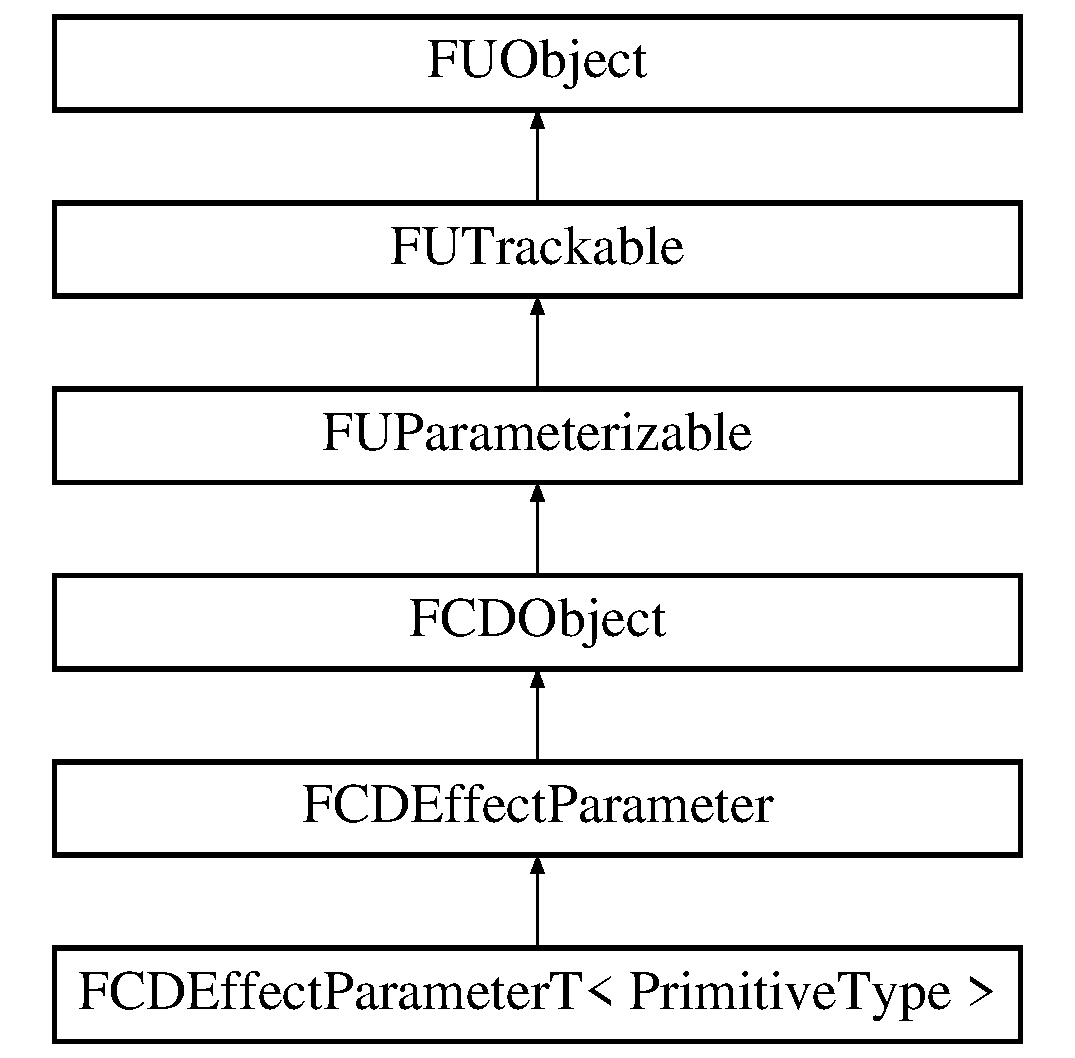
\includegraphics[height=6.000000cm]{classFCDEffectParameterT}
\end{center}
\end{figure}
\subsection*{Public Member Functions}
\begin{DoxyCompactItemize}
\item 
\hyperlink{classFCDEffectParameterT_a031c1f2f396d963d7c0b9ae7e44cf270}{FCDEffectParameterT} (\hyperlink{classFCDocument}{FCDocument} $\ast$document)
\item 
virtual \hyperlink{classFCDEffectParameterT_a12f8fd7f5c8663039d8f716bdcaa0139}{$\sim$FCDEffectParameterT} ()
\item 
virtual \hyperlink{classFCDEffectParameter_a1efe74553d2ed199435085c171743b08}{Type} \hyperlink{classFCDEffectParameterT_a8280e5d75b37d5794f33bfed92f9ad59}{GetType} () const 
\item 
const PrimitiveType \& \hyperlink{classFCDEffectParameterT_a4d0ca4343b288be2bbec5cf1c17d74c2}{GetValue} () const 
\item 
void \hyperlink{classFCDEffectParameterT_ae841e2e8c26167fa29f9a3e062db260e}{SetValue} (const PrimitiveType \&\_\-value)
\item 
virtual bool \hyperlink{classFCDEffectParameterT_a2070c18f8e6abf90ebb970d8ad249676}{IsValueEqual} (\hyperlink{classFCDEffectParameter}{FCDEffectParameter} $\ast$parameter)
\item 
virtual \hyperlink{classFCDEffectParameter}{FCDEffectParameter} $\ast$ \hyperlink{classFCDEffectParameterT_a2db377c408f4ab9fec8795aa91d3b77e}{Clone} (\hyperlink{classFCDEffectParameter}{FCDEffectParameter} $\ast$clone=NULL) const 
\item 
virtual void \hyperlink{classFCDEffectParameterT_ac65b69f100b1cab8efa1ba6c5281caf7}{Overwrite} (\hyperlink{classFCDEffectParameter}{FCDEffectParameter} $\ast$target)
\end{DoxyCompactItemize}


\subsection{Detailed Description}
\subsubsection*{template$<$class PrimitiveType$>$ class FCDEffectParameterT$<$ PrimitiveType $>$}

A COLLADA non-\/animatable effect parameter template. 

\subsection{Constructor \& Destructor Documentation}
\hypertarget{classFCDEffectParameterT_a031c1f2f396d963d7c0b9ae7e44cf270}{
\index{FCDEffectParameterT@{FCDEffectParameterT}!FCDEffectParameterT@{FCDEffectParameterT}}
\index{FCDEffectParameterT@{FCDEffectParameterT}!FCDEffectParameterT@{FCDEffectParameterT}}
\subsubsection[{FCDEffectParameterT}]{\setlength{\rightskip}{0pt plus 5cm}FCDEffectParameterBool::FCDEffectParameterT (
\begin{DoxyParamCaption}
\item[{{\bf FCDocument} $\ast$}]{ document}
\end{DoxyParamCaption}
)}}
\label{classFCDEffectParameterT_a031c1f2f396d963d7c0b9ae7e44cf270}
Constructor: do not use directly. Instead, use the appropriate AddEffectParameter function. 
\begin{DoxyParams}{Parameters}
\item[{\em document}]The COLLADA document that owns the effect parameter. \end{DoxyParams}
\hypertarget{classFCDEffectParameterT_a12f8fd7f5c8663039d8f716bdcaa0139}{
\index{FCDEffectParameterT@{FCDEffectParameterT}!$\sim$FCDEffectParameterT@{$\sim$FCDEffectParameterT}}
\index{$\sim$FCDEffectParameterT@{$\sim$FCDEffectParameterT}!FCDEffectParameterT@{FCDEffectParameterT}}
\subsubsection[{$\sim$FCDEffectParameterT}]{\setlength{\rightskip}{0pt plus 5cm}template$<$class PrimitiveType $>$ {\bf FCDEffectParameterT}$<$ PrimitiveType $>$::$\sim${\bf FCDEffectParameterT} (
\begin{DoxyParamCaption}
{}
\end{DoxyParamCaption}
)\hspace{0.3cm}{\ttfamily  \mbox{[}virtual\mbox{]}}}}
\label{classFCDEffectParameterT_a12f8fd7f5c8663039d8f716bdcaa0139}
Destructor. 

\subsection{Member Function Documentation}
\hypertarget{classFCDEffectParameterT_a2db377c408f4ab9fec8795aa91d3b77e}{
\index{FCDEffectParameterT@{FCDEffectParameterT}!Clone@{Clone}}
\index{Clone@{Clone}!FCDEffectParameterT@{FCDEffectParameterT}}
\subsubsection[{Clone}]{\setlength{\rightskip}{0pt plus 5cm}template$<$class PrimitiveType $>$ {\bf FCDEffectParameter} $\ast$ {\bf FCDEffectParameterT}$<$ PrimitiveType $>$::Clone (
\begin{DoxyParamCaption}
\item[{{\bf FCDEffectParameter} $\ast$}]{ clone = {\ttfamily NULL}}
\end{DoxyParamCaption}
) const\hspace{0.3cm}{\ttfamily  \mbox{[}virtual\mbox{]}}}}
\label{classFCDEffectParameterT_a2db377c408f4ab9fec8795aa91d3b77e}
Creates a full copy of the effect parameter. 
\begin{DoxyParams}{Parameters}
\item[{\em clone}]The cloned effect parameter. If this pointer is NULL, a new effect parameter will be created and you will need to delete this pointer. \end{DoxyParams}
\begin{DoxyReturn}{Returns}
The cloned effect parameter. 
\end{DoxyReturn}


Reimplemented from \hyperlink{classFCDEffectParameter_a75abe4b8964493db40604fa3d0e373eb}{FCDEffectParameter}.

\hypertarget{classFCDEffectParameterT_a8280e5d75b37d5794f33bfed92f9ad59}{
\index{FCDEffectParameterT@{FCDEffectParameterT}!GetType@{GetType}}
\index{GetType@{GetType}!FCDEffectParameterT@{FCDEffectParameterT}}
\subsubsection[{GetType}]{\setlength{\rightskip}{0pt plus 5cm}{\bf FCDEffectParameter::Type} FCDEffectParameterBool::GetType (
\begin{DoxyParamCaption}
{}
\end{DoxyParamCaption}
) const\hspace{0.3cm}{\ttfamily  \mbox{[}virtual\mbox{]}}}}
\label{classFCDEffectParameterT_a8280e5d75b37d5794f33bfed92f9ad59}
Retrieves the type of effect parameter class. \begin{DoxyReturn}{Returns}
The parameter class type. 
\end{DoxyReturn}


Implements \hyperlink{classFCDEffectParameter_a5858946f333ea4486ca30c4c1b104871}{FCDEffectParameter}.

\hypertarget{classFCDEffectParameterT_a4d0ca4343b288be2bbec5cf1c17d74c2}{
\index{FCDEffectParameterT@{FCDEffectParameterT}!GetValue@{GetValue}}
\index{GetValue@{GetValue}!FCDEffectParameterT@{FCDEffectParameterT}}
\subsubsection[{GetValue}]{\setlength{\rightskip}{0pt plus 5cm}template$<$class PrimitiveType$>$ const PrimitiveType\& {\bf FCDEffectParameterT}$<$ PrimitiveType $>$::GetValue (
\begin{DoxyParamCaption}
{}
\end{DoxyParamCaption}
) const\hspace{0.3cm}{\ttfamily  \mbox{[}inline\mbox{]}}}}
\label{classFCDEffectParameterT_a4d0ca4343b288be2bbec5cf1c17d74c2}
Retrieves the value of the effect parameter. \begin{DoxyReturn}{Returns}
The integer value. 
\end{DoxyReturn}
\hypertarget{classFCDEffectParameterT_a2070c18f8e6abf90ebb970d8ad249676}{
\index{FCDEffectParameterT@{FCDEffectParameterT}!IsValueEqual@{IsValueEqual}}
\index{IsValueEqual@{IsValueEqual}!FCDEffectParameterT@{FCDEffectParameterT}}
\subsubsection[{IsValueEqual}]{\setlength{\rightskip}{0pt plus 5cm}template$<$class PrimitiveType $>$ bool {\bf FCDEffectParameterT}$<$ PrimitiveType $>$::IsValueEqual (
\begin{DoxyParamCaption}
\item[{{\bf FCDEffectParameter} $\ast$}]{ parameter}
\end{DoxyParamCaption}
)\hspace{0.3cm}{\ttfamily  \mbox{[}virtual\mbox{]}}}}
\label{classFCDEffectParameterT_a2070c18f8e6abf90ebb970d8ad249676}
Compares this parameter's value with another 
\begin{DoxyParams}{Parameters}
\item[{\em parameter}]The given parameter to compare with. \end{DoxyParams}
\begin{DoxyReturn}{Returns}
true if the values are equal 
\end{DoxyReturn}


Implements \hyperlink{classFCDEffectParameter_a005a5a316bdb99dbd97ac542c129cc5e}{FCDEffectParameter}.

\hypertarget{classFCDEffectParameterT_ac65b69f100b1cab8efa1ba6c5281caf7}{
\index{FCDEffectParameterT@{FCDEffectParameterT}!Overwrite@{Overwrite}}
\index{Overwrite@{Overwrite}!FCDEffectParameterT@{FCDEffectParameterT}}
\subsubsection[{Overwrite}]{\setlength{\rightskip}{0pt plus 5cm}template$<$class PrimitiveType $>$ void {\bf FCDEffectParameterT}$<$ PrimitiveType $>$::Overwrite (
\begin{DoxyParamCaption}
\item[{{\bf FCDEffectParameter} $\ast$}]{ target}
\end{DoxyParamCaption}
)\hspace{0.3cm}{\ttfamily  \mbox{[}virtual\mbox{]}}}}
\label{classFCDEffectParameterT_ac65b69f100b1cab8efa1ba6c5281caf7}
\mbox{[}INTERNAL\mbox{]} Overwrites the target parameter with this parameter. This function is used during the flattening of materials. 
\begin{DoxyParams}{Parameters}
\item[{\em target}]The target parameter to overwrite. \end{DoxyParams}


Reimplemented from \hyperlink{classFCDEffectParameter_a016be91dbd27ff3c8c30f759f00b8c53}{FCDEffectParameter}.

\hypertarget{classFCDEffectParameterT_ae841e2e8c26167fa29f9a3e062db260e}{
\index{FCDEffectParameterT@{FCDEffectParameterT}!SetValue@{SetValue}}
\index{SetValue@{SetValue}!FCDEffectParameterT@{FCDEffectParameterT}}
\subsubsection[{SetValue}]{\setlength{\rightskip}{0pt plus 5cm}template$<$class PrimitiveType$>$ void {\bf FCDEffectParameterT}$<$ PrimitiveType $>$::SetValue (
\begin{DoxyParamCaption}
\item[{const PrimitiveType \&}]{ \_\-value}
\end{DoxyParamCaption}
)\hspace{0.3cm}{\ttfamily  \mbox{[}inline\mbox{]}}}}
\label{classFCDEffectParameterT_ae841e2e8c26167fa29f9a3e062db260e}
Sets the integer value of the effect parameter. 
\begin{DoxyParams}{Parameters}
\item[{\em \_\-value}]The integer value. \end{DoxyParams}


The documentation for this class was generated from the following files:\begin{DoxyCompactItemize}
\item 
FCollada/FCDocument/\hyperlink{FCDEffectParameter_8h}{FCDEffectParameter.h}\item 
FCollada/FCDocument/FCDEffectParameter.cpp\item 
FCollada/FCDocument/FCDEffectParameter.hpp\end{DoxyCompactItemize}

\hypertarget{classFCDEffectPass}{
\section{FCDEffectPass Class Reference}
\label{classFCDEffectPass}\index{FCDEffectPass@{FCDEffectPass}}
}


{\ttfamily \#include $<$FCDEffectPass.h$>$}

Inheritance diagram for FCDEffectPass:\begin{figure}[H]
\begin{center}
\leavevmode
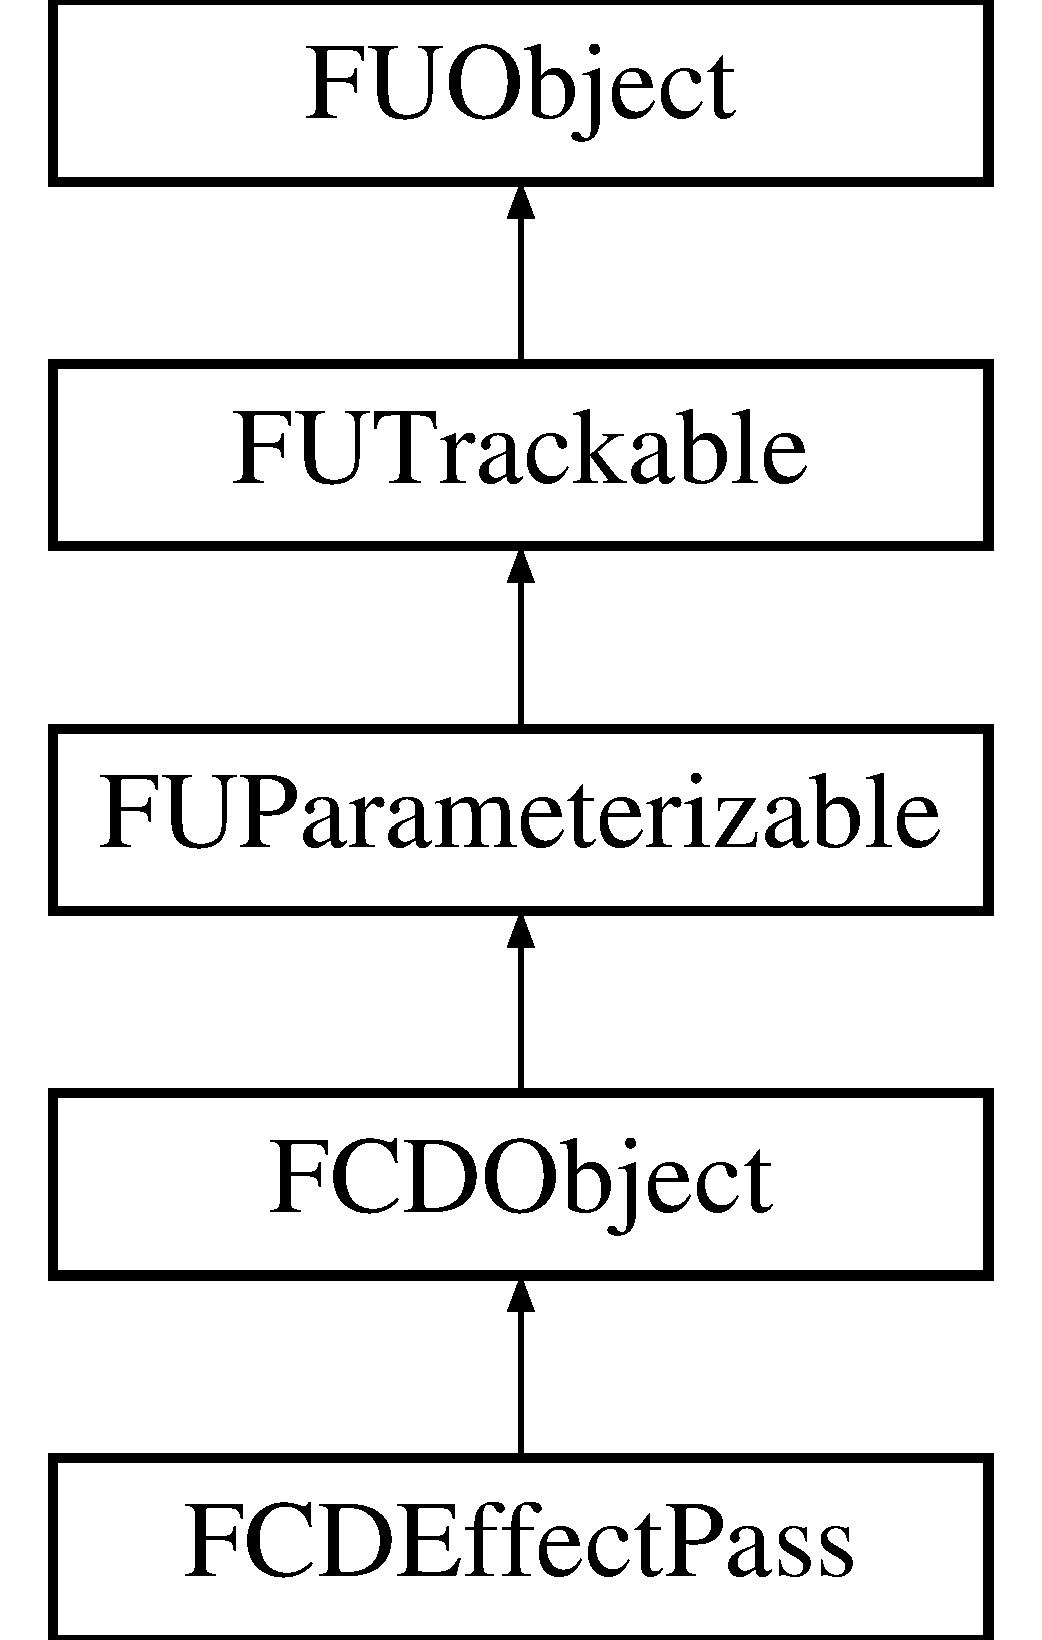
\includegraphics[height=5.000000cm]{classFCDEffectPass}
\end{center}
\end{figure}
\subsection*{Public Member Functions}
\begin{DoxyCompactItemize}
\item 
\hyperlink{classFCDEffectPass_a113ecf82cb3f9a875243fa9c392460d6}{FCDEffectPass} (\hyperlink{classFCDocument}{FCDocument} $\ast$document, \hyperlink{classFCDEffectTechnique}{FCDEffectTechnique} $\ast$parent)
\item 
virtual \hyperlink{classFCDEffectPass_a06f52bed17aedeb976700a42db076288}{$\sim$FCDEffectPass} ()
\item 
\hyperlink{classFCDEffectTechnique}{FCDEffectTechnique} $\ast$ \hyperlink{classFCDEffectPass_ad8c83b72090cee6340c41482c743b19d}{GetParent} ()
\item 
const \hyperlink{classFCDEffectTechnique}{FCDEffectTechnique} $\ast$ \hyperlink{classFCDEffectPass_ae3c3a6a9fc9aa96385908b866e730f69}{GetParent} () const 
\item 
\hyperlink{classFCDEffectPass_a2f2be39f5cb737d23be00822c429499f}{DEPRECATED} (3.05A, GetParent()-\/$>$GetParent()-\/$>$GetParent()-\/$>$GetDaeId()) const fm
\item 
const \hyperlink{classfm_1_1stringT}{fstring} \& \hyperlink{classFCDEffectPass_a965264f2ebd9bfab1eda85402b4e62b0}{GetPassName} () const 
\item 
void \hyperlink{classFCDEffectPass_a440924efb479a6417fb4c9de15cce12d}{SetPassName} (const fchar $\ast$\_\-name)
\item 
size\_\-t \hyperlink{classFCDEffectPass_a91266b26fcb7e861dd32d065f1d3e03a}{GetShaderCount} () const 
\item 
\hyperlink{classFCDEffectPassShader}{FCDEffectPassShader} $\ast$ \hyperlink{classFCDEffectPass_a4812f4512392d1c3599adc9411292742}{GetShader} (size\_\-t index)
\item 
const \hyperlink{classFCDEffectPassShader}{FCDEffectPassShader} $\ast$ \hyperlink{classFCDEffectPass_a594254479c6b9459963347609f013c0d}{GetShader} (size\_\-t index) const 
\item 
\hyperlink{classFCDEffectPassShader}{FCDEffectPassShader} $\ast$ \hyperlink{classFCDEffectPass_a3f517cc9def825f5ed1eff92fd63767f}{AddShader} ()
\item 
\hyperlink{classFCDEffectPass_ad750f820967f201bf16e11810bdd4e61}{DEPRECATED} (3.05A, shader-\/$>$Release()) void ReleaseShader(FCDEffectPassShader $\ast$shader)
\item 
\hyperlink{classFCDEffectPassShader}{FCDEffectPassShader} $\ast$ \hyperlink{classFCDEffectPass_ad5be823d1fcf2b809d88edc3d4bd128e}{GetVertexShader} ()
\item 
const \hyperlink{classFCDEffectPassShader}{FCDEffectPassShader} $\ast$ \hyperlink{classFCDEffectPass_a33ba661e6fd6321720446a0a8c194182}{GetVertexShader} () const 
\item 
\hyperlink{classFCDEffectPassShader}{FCDEffectPassShader} $\ast$ \hyperlink{classFCDEffectPass_a5c2d7a6cb07d072474a712d7989b0c47}{GetFragmentShader} ()
\item 
const \hyperlink{classFCDEffectPassShader}{FCDEffectPassShader} $\ast$ \hyperlink{classFCDEffectPass_af897aa752fb8efce514b5fa78a0c1f9c}{GetFragmentShader} () const 
\item 
\hyperlink{classFCDEffectPassShader}{FCDEffectPassShader} $\ast$ \hyperlink{classFCDEffectPass_a38b4b91ed84a52f4b3b4f564bc145adc}{AddVertexShader} ()
\item 
\hyperlink{classFCDEffectPassShader}{FCDEffectPassShader} $\ast$ \hyperlink{classFCDEffectPass_a994019f83ec1f8664ebe944ac1853972}{AddFragmentShader} ()
\item 
\hyperlink{classFCDEffectPass_a751132054a8fe95f6113ee1dce669315}{DEPRECATED} (3.05A, GetRenderStateCount and GetRenderState(index)) void GetRenderStates() const 
\item 
size\_\-t \hyperlink{classFCDEffectPass_ac7b761be64722700e0896574d039a927}{GetRenderStateCount} () const 
\item 
\hyperlink{classFCDEffectPassState}{FCDEffectPassState} $\ast$ \hyperlink{classFCDEffectPass_a2d9d4bc7ef4a68f0eef84fa133bf2bf4}{GetRenderState} (size\_\-t index)
\item 
const \hyperlink{classFCDEffectPassState}{FCDEffectPassState} $\ast$ \hyperlink{classFCDEffectPass_a53757eb176c01b3d5014ec405d70949b}{GetRenderState} (size\_\-t index) const 
\item 
\hyperlink{classFCDEffectPassState}{FCDEffectPassState} $\ast$ \hyperlink{classFCDEffectPass_a0693c21a2306025fc8853295c07b6927}{AddRenderState} (\hyperlink{namespaceFUDaePassState_a99a648050f80bc29359e932cffa8c973}{FUDaePassState::State} type)
\item 
\hyperlink{classFCDEffectPassState}{FCDEffectPassState} $\ast$ \hyperlink{classFCDEffectPass_ac145319a544b80a7cb1f013609e5ccfa}{FindRenderState} (\hyperlink{namespaceFUDaePassState_a99a648050f80bc29359e932cffa8c973}{FUDaePassState::State} type)
\item 
const \hyperlink{classFCDEffectPassState}{FCDEffectPassState} $\ast$ \hyperlink{classFCDEffectPass_a613603555b9bae099c4eba84290db2c1}{FindRenderState} (\hyperlink{namespaceFUDaePassState_a99a648050f80bc29359e932cffa8c973}{FUDaePassState::State} type) const 
\item 
\hyperlink{classFCDEffectPass}{FCDEffectPass} $\ast$ \hyperlink{classFCDEffectPass_a42e60c76a99dff70809a727a87d757ea}{Clone} (\hyperlink{classFCDEffectPass}{FCDEffectPass} $\ast$clone=NULL) const 
\end{DoxyCompactItemize}


\subsection{Detailed Description}
A COLLADA effect pass.

The effect pass contains a list of effect shaders. While they may be missing, it does not make sense for the effect pass to contain more than two shaders: a vertex shader and a fragment/pixel shader.

For this reason, we provide the GetVertexShader and the GetFragmentShader which we expect will be used for most applications, rather than looking through the list of shader objects. 

\subsection{Constructor \& Destructor Documentation}
\hypertarget{classFCDEffectPass_a113ecf82cb3f9a875243fa9c392460d6}{
\index{FCDEffectPass@{FCDEffectPass}!FCDEffectPass@{FCDEffectPass}}
\index{FCDEffectPass@{FCDEffectPass}!FCDEffectPass@{FCDEffectPass}}
\subsubsection[{FCDEffectPass}]{\setlength{\rightskip}{0pt plus 5cm}FCDEffectPass::FCDEffectPass (
\begin{DoxyParamCaption}
\item[{{\bf FCDocument} $\ast$}]{ document, }
\item[{{\bf FCDEffectTechnique} $\ast$}]{ parent}
\end{DoxyParamCaption}
)}}
\label{classFCDEffectPass_a113ecf82cb3f9a875243fa9c392460d6}
Constructor: do not use directly. Instead, use the \hyperlink{classFCDEffectTechnique_a485529a79e25dfb6c9d9f3b6ebc4d5c4}{FCDEffectTechnique::AddPass} function. 
\begin{DoxyParams}{Parameters}
\item[{\em document}]The \hyperlink{namespaceFCollada}{FCollada} document that owns this pass. \item[{\em parent}]The effect technique that contains this effect pass. \end{DoxyParams}
\hypertarget{classFCDEffectPass_a06f52bed17aedeb976700a42db076288}{
\index{FCDEffectPass@{FCDEffectPass}!$\sim$FCDEffectPass@{$\sim$FCDEffectPass}}
\index{$\sim$FCDEffectPass@{$\sim$FCDEffectPass}!FCDEffectPass@{FCDEffectPass}}
\subsubsection[{$\sim$FCDEffectPass}]{\setlength{\rightskip}{0pt plus 5cm}FCDEffectPass::$\sim$FCDEffectPass (
\begin{DoxyParamCaption}
{}
\end{DoxyParamCaption}
)\hspace{0.3cm}{\ttfamily  \mbox{[}virtual\mbox{]}}}}
\label{classFCDEffectPass_a06f52bed17aedeb976700a42db076288}
Destructor. 

\subsection{Member Function Documentation}
\hypertarget{classFCDEffectPass_a994019f83ec1f8664ebe944ac1853972}{
\index{FCDEffectPass@{FCDEffectPass}!AddFragmentShader@{AddFragmentShader}}
\index{AddFragmentShader@{AddFragmentShader}!FCDEffectPass@{FCDEffectPass}}
\subsubsection[{AddFragmentShader}]{\setlength{\rightskip}{0pt plus 5cm}{\bf FCDEffectPassShader} $\ast$ FCDEffectPass::AddFragmentShader (
\begin{DoxyParamCaption}
{}
\end{DoxyParamCaption}
)}}
\label{classFCDEffectPass_a994019f83ec1f8664ebe944ac1853972}
Adds a new fragment shader to the pass. If a fragment shader already exists within the pass, it will be released. \begin{DoxyReturn}{Returns}
The new fragment shader. 
\end{DoxyReturn}
\hypertarget{classFCDEffectPass_a0693c21a2306025fc8853295c07b6927}{
\index{FCDEffectPass@{FCDEffectPass}!AddRenderState@{AddRenderState}}
\index{AddRenderState@{AddRenderState}!FCDEffectPass@{FCDEffectPass}}
\subsubsection[{AddRenderState}]{\setlength{\rightskip}{0pt plus 5cm}{\bf FCDEffectPassState} $\ast$ FCDEffectPass::AddRenderState (
\begin{DoxyParamCaption}
\item[{{\bf FUDaePassState::State}}]{ type}
\end{DoxyParamCaption}
)}}
\label{classFCDEffectPass_a0693c21a2306025fc8853295c07b6927}
Adds a new render state to the effect pass. Render states automatically get sorted by type. 
\begin{DoxyParams}{Parameters}
\item[{\em type}]The type of the render state to add. If a render state of this type already exists within the effect pass, it will be returned. \end{DoxyParams}
\begin{DoxyReturn}{Returns}
A render state of the given type. 
\end{DoxyReturn}
\hypertarget{classFCDEffectPass_a3f517cc9def825f5ed1eff92fd63767f}{
\index{FCDEffectPass@{FCDEffectPass}!AddShader@{AddShader}}
\index{AddShader@{AddShader}!FCDEffectPass@{FCDEffectPass}}
\subsubsection[{AddShader}]{\setlength{\rightskip}{0pt plus 5cm}{\bf FCDEffectPassShader} $\ast$ FCDEffectPass::AddShader (
\begin{DoxyParamCaption}
{}
\end{DoxyParamCaption}
)}}
\label{classFCDEffectPass_a3f517cc9def825f5ed1eff92fd63767f}
Adds a new shader to the pass. \begin{DoxyReturn}{Returns}
The new shader. 
\end{DoxyReturn}
\hypertarget{classFCDEffectPass_a38b4b91ed84a52f4b3b4f564bc145adc}{
\index{FCDEffectPass@{FCDEffectPass}!AddVertexShader@{AddVertexShader}}
\index{AddVertexShader@{AddVertexShader}!FCDEffectPass@{FCDEffectPass}}
\subsubsection[{AddVertexShader}]{\setlength{\rightskip}{0pt plus 5cm}{\bf FCDEffectPassShader} $\ast$ FCDEffectPass::AddVertexShader (
\begin{DoxyParamCaption}
{}
\end{DoxyParamCaption}
)}}
\label{classFCDEffectPass_a38b4b91ed84a52f4b3b4f564bc145adc}
Adds a new vertex shader to the pass. If a vertex shader already exists within the pass, it will be released. \begin{DoxyReturn}{Returns}
The new vertex shader. 
\end{DoxyReturn}
\hypertarget{classFCDEffectPass_a42e60c76a99dff70809a727a87d757ea}{
\index{FCDEffectPass@{FCDEffectPass}!Clone@{Clone}}
\index{Clone@{Clone}!FCDEffectPass@{FCDEffectPass}}
\subsubsection[{Clone}]{\setlength{\rightskip}{0pt plus 5cm}{\bf FCDEffectPass} $\ast$ FCDEffectPass::Clone (
\begin{DoxyParamCaption}
\item[{{\bf FCDEffectPass} $\ast$}]{ clone = {\ttfamily NULL}}
\end{DoxyParamCaption}
) const}}
\label{classFCDEffectPass_a42e60c76a99dff70809a727a87d757ea}
Clones the effect pass and shaders. 
\begin{DoxyParams}{Parameters}
\item[{\em clone}]The cloned pass. If this pointer is NULL, a new pass is created and you will need to release this new pass. \end{DoxyParams}
\begin{DoxyReturn}{Returns}
The cloned pass. 
\end{DoxyReturn}
\hypertarget{classFCDEffectPass_a2f2be39f5cb737d23be00822c429499f}{
\index{FCDEffectPass@{FCDEffectPass}!DEPRECATED@{DEPRECATED}}
\index{DEPRECATED@{DEPRECATED}!FCDEffectPass@{FCDEffectPass}}
\subsubsection[{DEPRECATED}]{\setlength{\rightskip}{0pt plus 5cm}FCDEffectPass::DEPRECATED (
\begin{DoxyParamCaption}
\item[{3.}]{ 05A, }
\item[{GetParent()-\/$>$GetParent()-\/$>$GetParent()-\/$>$GetDaeId()}]{}
\end{DoxyParamCaption}
) const\hspace{0.3cm}{\ttfamily  \mbox{[}inline\mbox{]}}}}
\label{classFCDEffectPass_a2f2be39f5cb737d23be00822c429499f}
Retrieves the COLLADA id of the parent effect. This function is mostly useful as a shortcut for debugging and reporting. \begin{DoxyReturn}{Returns}
The COLLADA id of the parent effect. 
\end{DoxyReturn}
\hypertarget{classFCDEffectPass_a751132054a8fe95f6113ee1dce669315}{
\index{FCDEffectPass@{FCDEffectPass}!DEPRECATED@{DEPRECATED}}
\index{DEPRECATED@{DEPRECATED}!FCDEffectPass@{FCDEffectPass}}
\subsubsection[{DEPRECATED}]{\setlength{\rightskip}{0pt plus 5cm}FCDEffectPass::DEPRECATED (
\begin{DoxyParamCaption}
\item[{3.}]{ 05A, }
\item[{GetRenderStateCount and }]{ GetRenderStateindex}
\end{DoxyParamCaption}
) const\hspace{0.3cm}{\ttfamily  \mbox{[}inline\mbox{]}}}}
\label{classFCDEffectPass_a751132054a8fe95f6113ee1dce669315}
Retrieves the container of the render states for the pass. \begin{DoxyReturn}{Returns}
The render state list. 
\end{DoxyReturn}
\hypertarget{classFCDEffectPass_ad750f820967f201bf16e11810bdd4e61}{
\index{FCDEffectPass@{FCDEffectPass}!DEPRECATED@{DEPRECATED}}
\index{DEPRECATED@{DEPRECATED}!FCDEffectPass@{FCDEffectPass}}
\subsubsection[{DEPRECATED}]{\setlength{\rightskip}{0pt plus 5cm}FCDEffectPass::DEPRECATED (
\begin{DoxyParamCaption}
\item[{3.}]{ 05A, }
\item[{shader-\/$>$}]{ Release()}
\end{DoxyParamCaption}
)\hspace{0.3cm}{\ttfamily  \mbox{[}inline\mbox{]}}}}
\label{classFCDEffectPass_ad750f820967f201bf16e11810bdd4e61}
Releases a shader contained within the pass. 
\begin{DoxyParams}{Parameters}
\item[{\em shader}]The shader to release. \end{DoxyParams}
\hypertarget{classFCDEffectPass_a613603555b9bae099c4eba84290db2c1}{
\index{FCDEffectPass@{FCDEffectPass}!FindRenderState@{FindRenderState}}
\index{FindRenderState@{FindRenderState}!FCDEffectPass@{FCDEffectPass}}
\subsubsection[{FindRenderState}]{\setlength{\rightskip}{0pt plus 5cm}const {\bf FCDEffectPassState} $\ast$ FCDEffectPass::FindRenderState (
\begin{DoxyParamCaption}
\item[{{\bf FUDaePassState::State}}]{ type}
\end{DoxyParamCaption}
) const}}
\label{classFCDEffectPass_a613603555b9bae099c4eba84290db2c1}
See above. \hypertarget{classFCDEffectPass_ac145319a544b80a7cb1f013609e5ccfa}{
\index{FCDEffectPass@{FCDEffectPass}!FindRenderState@{FindRenderState}}
\index{FindRenderState@{FindRenderState}!FCDEffectPass@{FCDEffectPass}}
\subsubsection[{FindRenderState}]{\setlength{\rightskip}{0pt plus 5cm}{\bf FCDEffectPassState}$\ast$ FCDEffectPass::FindRenderState (
\begin{DoxyParamCaption}
\item[{{\bf FUDaePassState::State}}]{ type}
\end{DoxyParamCaption}
)\hspace{0.3cm}{\ttfamily  \mbox{[}inline\mbox{]}}}}
\label{classFCDEffectPass_ac145319a544b80a7cb1f013609e5ccfa}
Retrieves a specific render state defined for the pass. 
\begin{DoxyParams}{Parameters}
\item[{\em type}]The type of the render state to retrieve. \end{DoxyParams}
\begin{DoxyReturn}{Returns}
The render state with the given type. This pointer will be NULL if no render state has been defined for the given type. 
\end{DoxyReturn}
\hypertarget{classFCDEffectPass_a5c2d7a6cb07d072474a712d7989b0c47}{
\index{FCDEffectPass@{FCDEffectPass}!GetFragmentShader@{GetFragmentShader}}
\index{GetFragmentShader@{GetFragmentShader}!FCDEffectPass@{FCDEffectPass}}
\subsubsection[{GetFragmentShader}]{\setlength{\rightskip}{0pt plus 5cm}{\bf FCDEffectPassShader}$\ast$ FCDEffectPass::GetFragmentShader (
\begin{DoxyParamCaption}
{}
\end{DoxyParamCaption}
)\hspace{0.3cm}{\ttfamily  \mbox{[}inline\mbox{]}}}}
\label{classFCDEffectPass_a5c2d7a6cb07d072474a712d7989b0c47}
Retrieves the fragment shader for this effect pass. \begin{DoxyReturn}{Returns}
The fragment shader. This pointer will be NULL if no shader within the pass affects pixels/fragments. 
\end{DoxyReturn}
\hypertarget{classFCDEffectPass_af897aa752fb8efce514b5fa78a0c1f9c}{
\index{FCDEffectPass@{FCDEffectPass}!GetFragmentShader@{GetFragmentShader}}
\index{GetFragmentShader@{GetFragmentShader}!FCDEffectPass@{FCDEffectPass}}
\subsubsection[{GetFragmentShader}]{\setlength{\rightskip}{0pt plus 5cm}const {\bf FCDEffectPassShader} $\ast$ FCDEffectPass::GetFragmentShader (
\begin{DoxyParamCaption}
{}
\end{DoxyParamCaption}
) const}}
\label{classFCDEffectPass_af897aa752fb8efce514b5fa78a0c1f9c}
See above. \hypertarget{classFCDEffectPass_ae3c3a6a9fc9aa96385908b866e730f69}{
\index{FCDEffectPass@{FCDEffectPass}!GetParent@{GetParent}}
\index{GetParent@{GetParent}!FCDEffectPass@{FCDEffectPass}}
\subsubsection[{GetParent}]{\setlength{\rightskip}{0pt plus 5cm}const {\bf FCDEffectTechnique}$\ast$ FCDEffectPass::GetParent (
\begin{DoxyParamCaption}
{}
\end{DoxyParamCaption}
) const\hspace{0.3cm}{\ttfamily  \mbox{[}inline\mbox{]}}}}
\label{classFCDEffectPass_ae3c3a6a9fc9aa96385908b866e730f69}
See above. \hypertarget{classFCDEffectPass_ad8c83b72090cee6340c41482c743b19d}{
\index{FCDEffectPass@{FCDEffectPass}!GetParent@{GetParent}}
\index{GetParent@{GetParent}!FCDEffectPass@{FCDEffectPass}}
\subsubsection[{GetParent}]{\setlength{\rightskip}{0pt plus 5cm}{\bf FCDEffectTechnique}$\ast$ FCDEffectPass::GetParent (
\begin{DoxyParamCaption}
{}
\end{DoxyParamCaption}
)\hspace{0.3cm}{\ttfamily  \mbox{[}inline\mbox{]}}}}
\label{classFCDEffectPass_ad8c83b72090cee6340c41482c743b19d}
Retrieves the effect techniques which contains this effect pass. \begin{DoxyReturn}{Returns}
The parent technique. 
\end{DoxyReturn}
\hypertarget{classFCDEffectPass_a965264f2ebd9bfab1eda85402b4e62b0}{
\index{FCDEffectPass@{FCDEffectPass}!GetPassName@{GetPassName}}
\index{GetPassName@{GetPassName}!FCDEffectPass@{FCDEffectPass}}
\subsubsection[{GetPassName}]{\setlength{\rightskip}{0pt plus 5cm}const {\bf fstring}\& FCDEffectPass::GetPassName (
\begin{DoxyParamCaption}
{}
\end{DoxyParamCaption}
) const\hspace{0.3cm}{\ttfamily  \mbox{[}inline\mbox{]}}}}
\label{classFCDEffectPass_a965264f2ebd9bfab1eda85402b4e62b0}
Retrieves the sub-\/id of the effect pass. This sub-\/id is optional. \begin{DoxyReturn}{Returns}
The sub-\/id. 
\end{DoxyReturn}
\hypertarget{classFCDEffectPass_a2d9d4bc7ef4a68f0eef84fa133bf2bf4}{
\index{FCDEffectPass@{FCDEffectPass}!GetRenderState@{GetRenderState}}
\index{GetRenderState@{GetRenderState}!FCDEffectPass@{FCDEffectPass}}
\subsubsection[{GetRenderState}]{\setlength{\rightskip}{0pt plus 5cm}{\bf FCDEffectPassState}$\ast$ FCDEffectPass::GetRenderState (
\begin{DoxyParamCaption}
\item[{size\_\-t}]{ index}
\end{DoxyParamCaption}
)\hspace{0.3cm}{\ttfamily  \mbox{[}inline\mbox{]}}}}
\label{classFCDEffectPass_a2d9d4bc7ef4a68f0eef84fa133bf2bf4}
Retrieves a specific render state defined for the pass. 
\begin{DoxyParams}{Parameters}
\item[{\em index}]The index of the render state. \end{DoxyParams}
\begin{DoxyReturn}{Returns}
The render state at the given index. 
\end{DoxyReturn}
\hypertarget{classFCDEffectPass_a53757eb176c01b3d5014ec405d70949b}{
\index{FCDEffectPass@{FCDEffectPass}!GetRenderState@{GetRenderState}}
\index{GetRenderState@{GetRenderState}!FCDEffectPass@{FCDEffectPass}}
\subsubsection[{GetRenderState}]{\setlength{\rightskip}{0pt plus 5cm}const {\bf FCDEffectPassState}$\ast$ FCDEffectPass::GetRenderState (
\begin{DoxyParamCaption}
\item[{size\_\-t}]{ index}
\end{DoxyParamCaption}
) const\hspace{0.3cm}{\ttfamily  \mbox{[}inline\mbox{]}}}}
\label{classFCDEffectPass_a53757eb176c01b3d5014ec405d70949b}
See above. \hypertarget{classFCDEffectPass_ac7b761be64722700e0896574d039a927}{
\index{FCDEffectPass@{FCDEffectPass}!GetRenderStateCount@{GetRenderStateCount}}
\index{GetRenderStateCount@{GetRenderStateCount}!FCDEffectPass@{FCDEffectPass}}
\subsubsection[{GetRenderStateCount}]{\setlength{\rightskip}{0pt plus 5cm}size\_\-t FCDEffectPass::GetRenderStateCount (
\begin{DoxyParamCaption}
{}
\end{DoxyParamCaption}
) const\hspace{0.3cm}{\ttfamily  \mbox{[}inline\mbox{]}}}}
\label{classFCDEffectPass_ac7b761be64722700e0896574d039a927}
Retrieves the number of render states defined for the pass. \begin{DoxyReturn}{Returns}
The render state count. 
\end{DoxyReturn}
\hypertarget{classFCDEffectPass_a594254479c6b9459963347609f013c0d}{
\index{FCDEffectPass@{FCDEffectPass}!GetShader@{GetShader}}
\index{GetShader@{GetShader}!FCDEffectPass@{FCDEffectPass}}
\subsubsection[{GetShader}]{\setlength{\rightskip}{0pt plus 5cm}const {\bf FCDEffectPassShader}$\ast$ FCDEffectPass::GetShader (
\begin{DoxyParamCaption}
\item[{size\_\-t}]{ index}
\end{DoxyParamCaption}
) const\hspace{0.3cm}{\ttfamily  \mbox{[}inline\mbox{]}}}}
\label{classFCDEffectPass_a594254479c6b9459963347609f013c0d}
See above. \hypertarget{classFCDEffectPass_a4812f4512392d1c3599adc9411292742}{
\index{FCDEffectPass@{FCDEffectPass}!GetShader@{GetShader}}
\index{GetShader@{GetShader}!FCDEffectPass@{FCDEffectPass}}
\subsubsection[{GetShader}]{\setlength{\rightskip}{0pt plus 5cm}{\bf FCDEffectPassShader}$\ast$ FCDEffectPass::GetShader (
\begin{DoxyParamCaption}
\item[{size\_\-t}]{ index}
\end{DoxyParamCaption}
)\hspace{0.3cm}{\ttfamily  \mbox{[}inline\mbox{]}}}}
\label{classFCDEffectPass_a4812f4512392d1c3599adc9411292742}
Retrieves a specific shader. 
\begin{DoxyParams}{Parameters}
\item[{\em index}]The index of the shader. \end{DoxyParams}
\begin{DoxyReturn}{Returns}
The shader. This pointer will be NULL if the index is out-\/of-\/bounds. 
\end{DoxyReturn}
\hypertarget{classFCDEffectPass_a91266b26fcb7e861dd32d065f1d3e03a}{
\index{FCDEffectPass@{FCDEffectPass}!GetShaderCount@{GetShaderCount}}
\index{GetShaderCount@{GetShaderCount}!FCDEffectPass@{FCDEffectPass}}
\subsubsection[{GetShaderCount}]{\setlength{\rightskip}{0pt plus 5cm}size\_\-t FCDEffectPass::GetShaderCount (
\begin{DoxyParamCaption}
{}
\end{DoxyParamCaption}
) const\hspace{0.3cm}{\ttfamily  \mbox{[}inline\mbox{]}}}}
\label{classFCDEffectPass_a91266b26fcb7e861dd32d065f1d3e03a}
Retrieves the number of shaders contained within the effect pass. \begin{DoxyReturn}{Returns}
The number of shaders. 
\end{DoxyReturn}
\hypertarget{classFCDEffectPass_a33ba661e6fd6321720446a0a8c194182}{
\index{FCDEffectPass@{FCDEffectPass}!GetVertexShader@{GetVertexShader}}
\index{GetVertexShader@{GetVertexShader}!FCDEffectPass@{FCDEffectPass}}
\subsubsection[{GetVertexShader}]{\setlength{\rightskip}{0pt plus 5cm}const {\bf FCDEffectPassShader} $\ast$ FCDEffectPass::GetVertexShader (
\begin{DoxyParamCaption}
{}
\end{DoxyParamCaption}
) const}}
\label{classFCDEffectPass_a33ba661e6fd6321720446a0a8c194182}
See above. \hypertarget{classFCDEffectPass_ad5be823d1fcf2b809d88edc3d4bd128e}{
\index{FCDEffectPass@{FCDEffectPass}!GetVertexShader@{GetVertexShader}}
\index{GetVertexShader@{GetVertexShader}!FCDEffectPass@{FCDEffectPass}}
\subsubsection[{GetVertexShader}]{\setlength{\rightskip}{0pt plus 5cm}{\bf FCDEffectPassShader}$\ast$ FCDEffectPass::GetVertexShader (
\begin{DoxyParamCaption}
{}
\end{DoxyParamCaption}
)\hspace{0.3cm}{\ttfamily  \mbox{[}inline\mbox{]}}}}
\label{classFCDEffectPass_ad5be823d1fcf2b809d88edc3d4bd128e}
Retrieves the vertex shader for this effect pass. \begin{DoxyReturn}{Returns}
The vertex shader. This pointer will be NULL if no shader within the pass affects vertices. 
\end{DoxyReturn}
\hypertarget{classFCDEffectPass_a440924efb479a6417fb4c9de15cce12d}{
\index{FCDEffectPass@{FCDEffectPass}!SetPassName@{SetPassName}}
\index{SetPassName@{SetPassName}!FCDEffectPass@{FCDEffectPass}}
\subsubsection[{SetPassName}]{\setlength{\rightskip}{0pt plus 5cm}void FCDEffectPass::SetPassName (
\begin{DoxyParamCaption}
\item[{const fchar $\ast$}]{ \_\-name}
\end{DoxyParamCaption}
)\hspace{0.3cm}{\ttfamily  \mbox{[}inline\mbox{]}}}}
\label{classFCDEffectPass_a440924efb479a6417fb4c9de15cce12d}
Sets the optional sub-\/id for the effect pass. This sub-\/id is optional. 
\begin{DoxyParams}{Parameters}
\item[{\em \_\-name}]The sub-\/id. \end{DoxyParams}


The documentation for this class was generated from the following files:\begin{DoxyCompactItemize}
\item 
FCollada/FCDocument/\hyperlink{FCDEffectPass_8h}{FCDEffectPass.h}\item 
FCollada/FCDocument/FCDEffectPass.cpp\end{DoxyCompactItemize}

\hypertarget{classFCDEffectPassBind}{
\section{FCDEffectPassBind Class Reference}
\label{classFCDEffectPassBind}\index{FCDEffectPassBind@{FCDEffectPassBind}}
}


{\ttfamily \#include $<$FCDEffectPassShader.h$>$}

Inheritance diagram for FCDEffectPassBind:\begin{figure}[H]
\begin{center}
\leavevmode
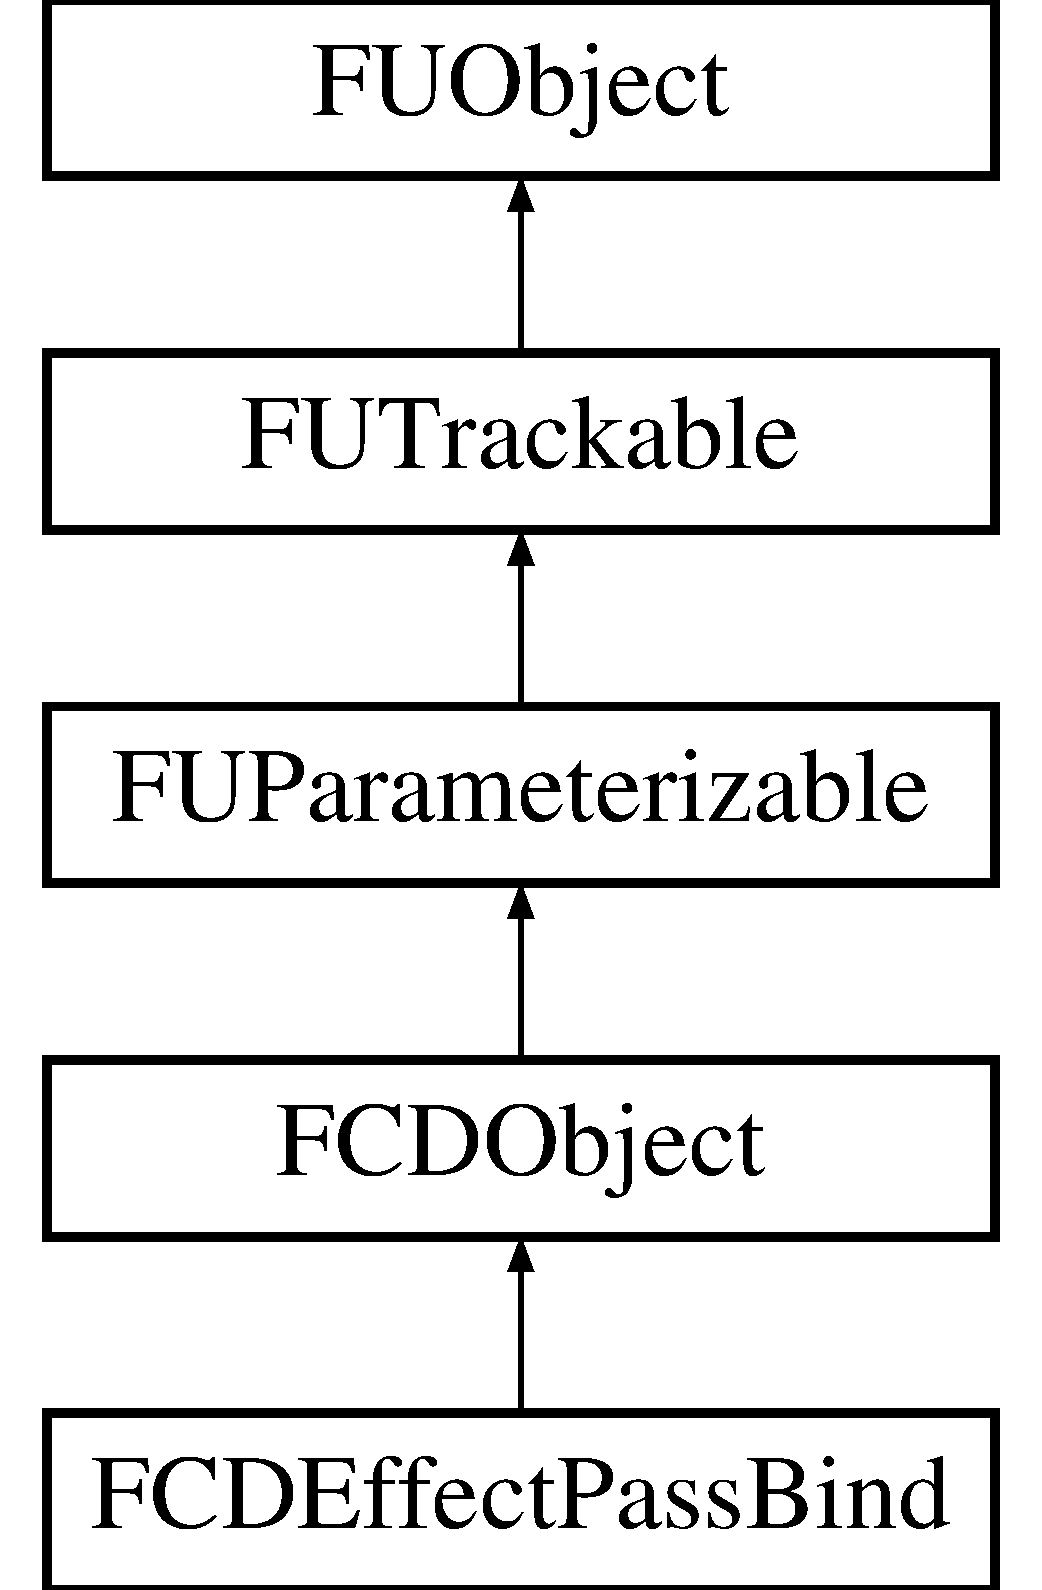
\includegraphics[height=5.000000cm]{classFCDEffectPassBind}
\end{center}
\end{figure}
\subsection*{Public Member Functions}
\begin{DoxyCompactItemize}
\item 
\hyperlink{classFCDEffectPassBind_a3e81f0a6b03a384c17068f07374d2297}{FCDEffectPassBind} (\hyperlink{classFCDocument}{FCDocument} $\ast$document)
\item 
\hyperlink{classFCDEffectPassBind_a848da92f37f19d2e8cd02ffffedf636f}{DeclareParameter} (\hyperlink{classfm_1_1stringT}{fm::string}, FUParameterQualifiers::SIMPLE, reference, FC(\char`\"{}Parameter Reference\char`\"{}))
\item 
\hyperlink{classFCDEffectPassBind_ad3ccd5fc342438687c3592d4eaecf317}{DeclareParameter} (\hyperlink{classfm_1_1stringT}{fm::string}, FUParameterQualifiers::SIMPLE, symbol, FC(\char`\"{}Shader Symbol\char`\"{}))
\end{DoxyCompactItemize}


\subsection{Detailed Description}
A COLLADA shader binding.

Binds an external symbol to a COLLADA effect parameter, by reference. 

\subsection{Constructor \& Destructor Documentation}
\hypertarget{classFCDEffectPassBind_a3e81f0a6b03a384c17068f07374d2297}{
\index{FCDEffectPassBind@{FCDEffectPassBind}!FCDEffectPassBind@{FCDEffectPassBind}}
\index{FCDEffectPassBind@{FCDEffectPassBind}!FCDEffectPassBind@{FCDEffectPassBind}}
\subsubsection[{FCDEffectPassBind}]{\setlength{\rightskip}{0pt plus 5cm}FCDEffectPassBind::FCDEffectPassBind (
\begin{DoxyParamCaption}
\item[{{\bf FCDocument} $\ast$}]{ document}
\end{DoxyParamCaption}
)}}
\label{classFCDEffectPassBind_a3e81f0a6b03a384c17068f07374d2297}
Constructor. 
\begin{DoxyParams}{Parameters}
\item[{\em document}]The document that owns this binding. \end{DoxyParams}


\subsection{Member Function Documentation}
\hypertarget{classFCDEffectPassBind_a848da92f37f19d2e8cd02ffffedf636f}{
\index{FCDEffectPassBind@{FCDEffectPassBind}!DeclareParameter@{DeclareParameter}}
\index{DeclareParameter@{DeclareParameter}!FCDEffectPassBind@{FCDEffectPassBind}}
\subsubsection[{DeclareParameter}]{\setlength{\rightskip}{0pt plus 5cm}FCDEffectPassBind::DeclareParameter (
\begin{DoxyParamCaption}
\item[{{\bf fm::string}}]{, }
\item[{FUParameterQualifiers::SIMPLE}]{, }
\item[{reference}]{, }
\item[{FC(\char`\"{}Parameter Reference\char`\"{})}]{}
\end{DoxyParamCaption}
)}}
\label{classFCDEffectPassBind_a848da92f37f19d2e8cd02ffffedf636f}
A COLLADA effect parameter reference. \hypertarget{classFCDEffectPassBind_ad3ccd5fc342438687c3592d4eaecf317}{
\index{FCDEffectPassBind@{FCDEffectPassBind}!DeclareParameter@{DeclareParameter}}
\index{DeclareParameter@{DeclareParameter}!FCDEffectPassBind@{FCDEffectPassBind}}
\subsubsection[{DeclareParameter}]{\setlength{\rightskip}{0pt plus 5cm}FCDEffectPassBind::DeclareParameter (
\begin{DoxyParamCaption}
\item[{{\bf fm::string}}]{, }
\item[{FUParameterQualifiers::SIMPLE}]{, }
\item[{symbol}]{, }
\item[{FC(\char`\"{}Shader Symbol\char`\"{})}]{}
\end{DoxyParamCaption}
)}}
\label{classFCDEffectPassBind_ad3ccd5fc342438687c3592d4eaecf317}
An external symbol, used within the shader code. 

The documentation for this class was generated from the following files:\begin{DoxyCompactItemize}
\item 
FCollada/FCDocument/\hyperlink{FCDEffectPassShader_8h}{FCDEffectPassShader.h}\item 
FCollada/FCDocument/FCDEffectPassShader.cpp\end{DoxyCompactItemize}

\hypertarget{classFCDEffectPassShader}{
\section{FCDEffectPassShader Class Reference}
\label{classFCDEffectPassShader}\index{FCDEffectPassShader@{FCDEffectPassShader}}
}


{\ttfamily \#include $<$FCDEffectPassShader.h$>$}

Inheritance diagram for FCDEffectPassShader:\begin{figure}[H]
\begin{center}
\leavevmode
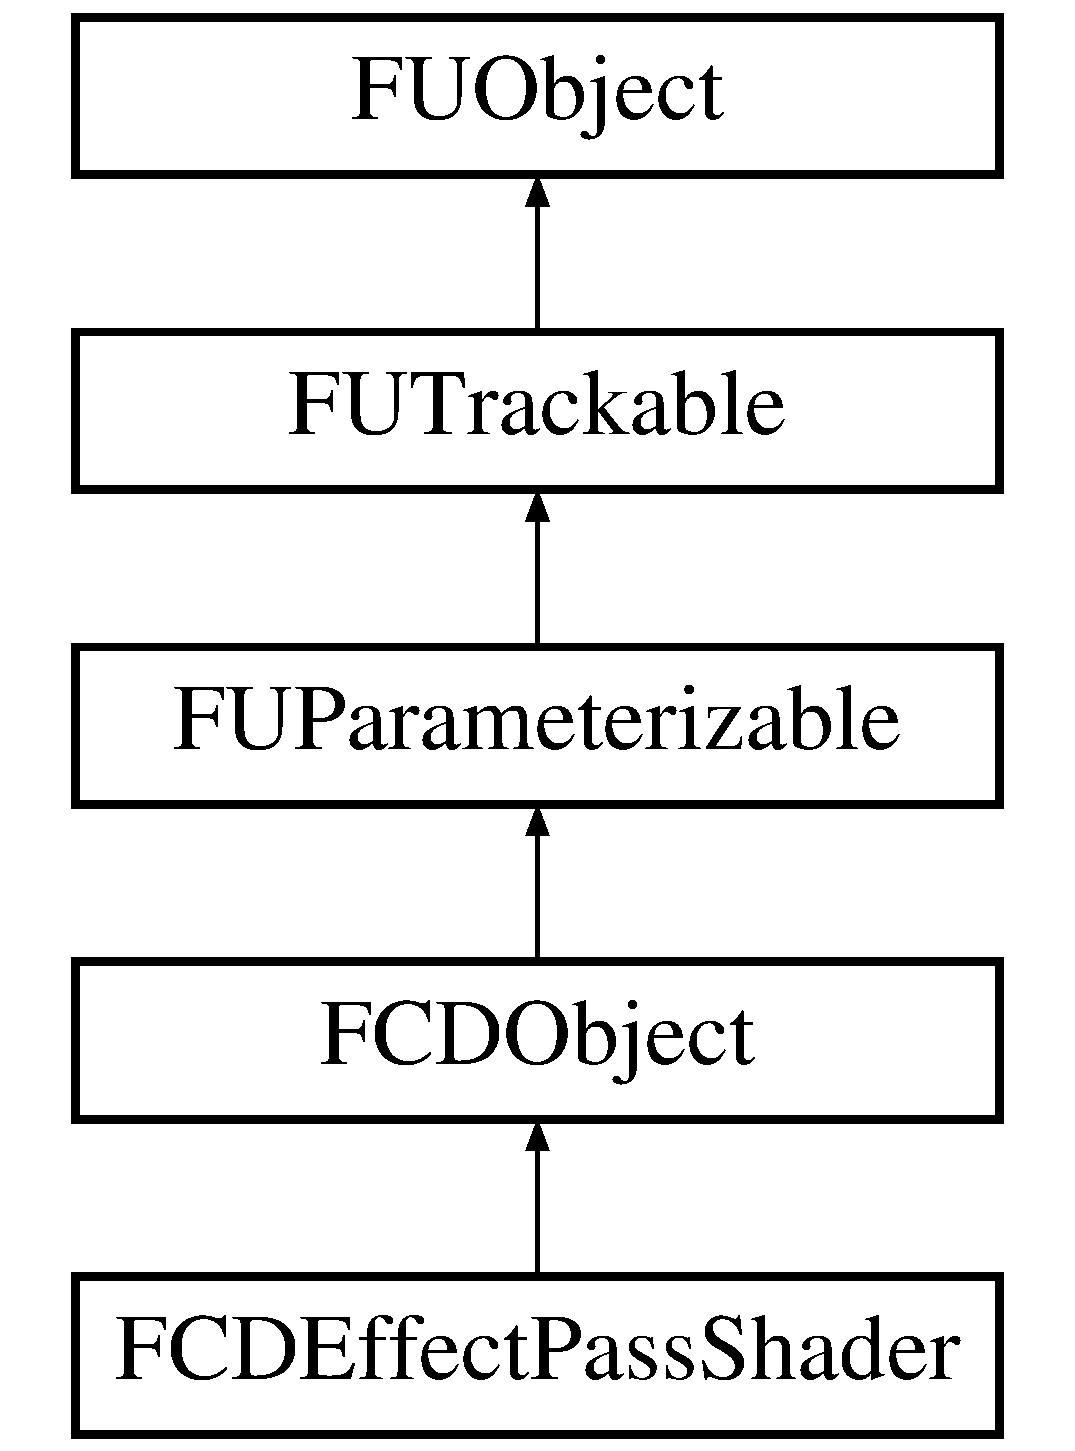
\includegraphics[height=5.000000cm]{classFCDEffectPassShader}
\end{center}
\end{figure}
\subsection*{Public Member Functions}
\begin{DoxyCompactItemize}
\item 
\hyperlink{classFCDEffectPassShader_ae57864a08401f39717f7efda046a632f}{FCDEffectPassShader} (\hyperlink{classFCDocument}{FCDocument} $\ast$document, \hyperlink{classFCDEffectPass}{FCDEffectPass} $\ast$parent)
\item 
virtual \hyperlink{classFCDEffectPassShader_a38684fa5bcf757fb8e71cdf3909c12d9}{$\sim$FCDEffectPassShader} ()
\item 
\hyperlink{classFCDEffectPass}{FCDEffectPass} $\ast$ \hyperlink{classFCDEffectPassShader_a365da412e637795e1745e54d8358c115}{GetParent} ()
\item 
const \hyperlink{classFCDEffectPass}{FCDEffectPass} $\ast$ \hyperlink{classFCDEffectPassShader_a6bc5edd010e61c5724c16b3d7f29c6bd}{GetParent} () const 
\item 
void \hyperlink{classFCDEffectPassShader_ac3d106f0382036bda3a0a8d9bda95417}{AffectsVertices} ()
\item 
void \hyperlink{classFCDEffectPassShader_a927b034d38cc794d291bca6a89efcf7c}{AffectsFragments} ()
\item 
bool \hyperlink{classFCDEffectPassShader_a6c044d94c60e622df3ce526d19dad566}{IsFragmentShader} () const 
\item 
bool \hyperlink{classFCDEffectPassShader_afaae07ba360e49a3a3e9d44ed820469c}{IsVertexShader} () const 
\item 
\hyperlink{classFCDEffectPassShader_ac3244952b3fd0fe46c39ef1f4b65a321}{DEPRECATED} (3.05A, GetBindingCount and GetBinding(index)) void GetBindings() const 
\item 
size\_\-t \hyperlink{classFCDEffectPassShader_a968248d378a857d4f9fca2b6b209847e}{GetBindingCount} () const 
\item 
\hyperlink{classFCDEffectPassBind}{FCDEffectPassBind} $\ast$ \hyperlink{classFCDEffectPassShader_aa3cc0fa0e41ff5a3e0409ed6bd66bed4}{GetBinding} (size\_\-t index)
\item 
const \hyperlink{classFCDEffectPassBind}{FCDEffectPassBind} $\ast$ \hyperlink{classFCDEffectPassShader_a7126aac03331d3f87b8ee109dd5fd199}{GetBinding} (size\_\-t index) const 
\item 
const \hyperlink{classFCDEffectPassBind}{FCDEffectPassBind} $\ast$ \hyperlink{classFCDEffectPassShader_a7df9cd1c21d04856e7b3cf23b2aa9a2c}{FindBindingReference} (const char $\ast$reference) const 
\item 
\hyperlink{classFCDEffectPassBind}{FCDEffectPassBind} $\ast$ \hyperlink{classFCDEffectPassShader_a7676d499e9a4d2f85d6db549e8e2d353}{FindBindingReference} (const char $\ast$reference)
\item 
const \hyperlink{classFCDEffectPassBind}{FCDEffectPassBind} $\ast$ \hyperlink{classFCDEffectPassShader_a9271fa40c72737fcfa9e0c44a5ee2e11}{FindBindingSymbol} (const char $\ast$symbol) const 
\item 
\hyperlink{classFCDEffectPassBind}{FCDEffectPassBind} $\ast$ \hyperlink{classFCDEffectPassShader_a5e4c5b5eafffbabc2ac6cefa3351a6f5}{FindBindingSymbol} (const char $\ast$symbol)
\item 
\hyperlink{classFCDEffectPassBind}{FCDEffectPassBind} $\ast$ \hyperlink{classFCDEffectPassShader_ac99bba07d76ccb9be805d64fa7693bbd}{AddBinding} ()
\item 
\hyperlink{classFCDEffectPassShader_a447a9016612aa1f0e836d7e04dc18963}{DEPRECATED} (3.05A, binding-\/$>$Release()) void ReleaseBinding(FCDEffectPassBind $\ast$binding)
\item 
const \hyperlink{classfm_1_1stringT}{fstring} \& \hyperlink{classFCDEffectPassShader_a15899c058bde932cf352ab1f4741ac6e}{GetCompilerTarget} () const 
\item 
void \hyperlink{classFCDEffectPassShader_a54510d91cdb8a8a0acb8e8de365751e9}{SetCompilerTarget} (const fchar $\ast$\_\-compilerTarget)
\item 
const \hyperlink{classfm_1_1stringT}{fstring} \& \hyperlink{classFCDEffectPassShader_a86a7b27f70b58589dd9cd8c0366c585a}{GetCompilerOptions} () const 
\item 
void \hyperlink{classFCDEffectPassShader_af7d74246e413298b96ef3568e2dd9913}{SetCompilerOptions} (const fchar $\ast$\_\-compilerOptions)
\item 
const \hyperlink{classfm_1_1stringT}{fm::string} \& \hyperlink{classFCDEffectPassShader_ad8500b40b69fa965e7c9339848d4c7ec}{GetName} () const 
\item 
void \hyperlink{classFCDEffectPassShader_a7d907beb4ad9f6aa77ea6f2ca10366af}{SetName} (const char $\ast$\_\-name)
\item 
\hyperlink{classFCDEffectCode}{FCDEffectCode} $\ast$ \hyperlink{classFCDEffectPassShader_af2d089e27b1378d3e258a640307e89ba}{GetCode} ()
\item 
const \hyperlink{classFCDEffectCode}{FCDEffectCode} $\ast$ \hyperlink{classFCDEffectPassShader_a5531627c61332877f09641f4d508f57a}{GetCode} () const 
\item 
void \hyperlink{classFCDEffectPassShader_a0ca1befb72b2e5dec4a67bbb8b8167ea}{SetCode} (\hyperlink{classFCDEffectCode}{FCDEffectCode} $\ast$\_\-code)
\item 
\hyperlink{classFCDEffectPassShader}{FCDEffectPassShader} $\ast$ \hyperlink{classFCDEffectPassShader_a409fbe05f0be92651824f238b7a89cfd}{Clone} (\hyperlink{classFCDEffectPassShader}{FCDEffectPassShader} $\ast$clone) const 
\end{DoxyCompactItemize}


\subsection{Detailed Description}
A COLLADA shader.

The shader abstraction level in ColladaFX is contained within the effect passes. There are two types of shaders: vertex shaders and fragment/pixel shaders. A COLLADA shader contains a list of bindings to attach the effect parameters to the shader input parameters.

The shader object also contains the compiler information necessary to build the shader: its code, the compiler target and the compiler options. 

\subsection{Constructor \& Destructor Documentation}
\hypertarget{classFCDEffectPassShader_ae57864a08401f39717f7efda046a632f}{
\index{FCDEffectPassShader@{FCDEffectPassShader}!FCDEffectPassShader@{FCDEffectPassShader}}
\index{FCDEffectPassShader@{FCDEffectPassShader}!FCDEffectPassShader@{FCDEffectPassShader}}
\subsubsection[{FCDEffectPassShader}]{\setlength{\rightskip}{0pt plus 5cm}FCDEffectPassShader::FCDEffectPassShader (
\begin{DoxyParamCaption}
\item[{{\bf FCDocument} $\ast$}]{ document, }
\item[{{\bf FCDEffectPass} $\ast$}]{ parent}
\end{DoxyParamCaption}
)}}
\label{classFCDEffectPassShader_ae57864a08401f39717f7efda046a632f}
Constructor: do not use directly. Instead, use the \hyperlink{classFCDEffectPass_a3f517cc9def825f5ed1eff92fd63767f}{FCDEffectPass::AddShader}, \hyperlink{classFCDEffectPass_a38b4b91ed84a52f4b3b4f564bc145adc}{FCDEffectPass::AddVertexShader} or \hyperlink{classFCDEffectPass_a994019f83ec1f8664ebe944ac1853972}{FCDEffectPass::AddFragmentShader} functions. 
\begin{DoxyParams}{Parameters}
\item[{\em parent}]The effect pass that contains this shader. \end{DoxyParams}
\hypertarget{classFCDEffectPassShader_a38684fa5bcf757fb8e71cdf3909c12d9}{
\index{FCDEffectPassShader@{FCDEffectPassShader}!$\sim$FCDEffectPassShader@{$\sim$FCDEffectPassShader}}
\index{$\sim$FCDEffectPassShader@{$\sim$FCDEffectPassShader}!FCDEffectPassShader@{FCDEffectPassShader}}
\subsubsection[{$\sim$FCDEffectPassShader}]{\setlength{\rightskip}{0pt plus 5cm}FCDEffectPassShader::$\sim$FCDEffectPassShader (
\begin{DoxyParamCaption}
{}
\end{DoxyParamCaption}
)\hspace{0.3cm}{\ttfamily  \mbox{[}virtual\mbox{]}}}}
\label{classFCDEffectPassShader_a38684fa5bcf757fb8e71cdf3909c12d9}
Destructor. 

\subsection{Member Function Documentation}
\hypertarget{classFCDEffectPassShader_ac99bba07d76ccb9be805d64fa7693bbd}{
\index{FCDEffectPassShader@{FCDEffectPassShader}!AddBinding@{AddBinding}}
\index{AddBinding@{AddBinding}!FCDEffectPassShader@{FCDEffectPassShader}}
\subsubsection[{AddBinding}]{\setlength{\rightskip}{0pt plus 5cm}{\bf FCDEffectPassBind} $\ast$ FCDEffectPassShader::AddBinding (
\begin{DoxyParamCaption}
{}
\end{DoxyParamCaption}
)}}
\label{classFCDEffectPassShader_ac99bba07d76ccb9be805d64fa7693bbd}
Adds a new binding to this shader. \begin{DoxyReturn}{Returns}
The new binding. 
\end{DoxyReturn}
\hypertarget{classFCDEffectPassShader_a927b034d38cc794d291bca6a89efcf7c}{
\index{FCDEffectPassShader@{FCDEffectPassShader}!AffectsFragments@{AffectsFragments}}
\index{AffectsFragments@{AffectsFragments}!FCDEffectPassShader@{FCDEffectPassShader}}
\subsubsection[{AffectsFragments}]{\setlength{\rightskip}{0pt plus 5cm}void FCDEffectPassShader::AffectsFragments (
\begin{DoxyParamCaption}
{}
\end{DoxyParamCaption}
)\hspace{0.3cm}{\ttfamily  \mbox{[}inline\mbox{]}}}}
\label{classFCDEffectPassShader_a927b034d38cc794d291bca6a89efcf7c}
Sets this shader as affecting fragments/pixels. This sets the stage of the shader to the fragment/pixel pipeline. \hypertarget{classFCDEffectPassShader_ac3d106f0382036bda3a0a8d9bda95417}{
\index{FCDEffectPassShader@{FCDEffectPassShader}!AffectsVertices@{AffectsVertices}}
\index{AffectsVertices@{AffectsVertices}!FCDEffectPassShader@{FCDEffectPassShader}}
\subsubsection[{AffectsVertices}]{\setlength{\rightskip}{0pt plus 5cm}void FCDEffectPassShader::AffectsVertices (
\begin{DoxyParamCaption}
{}
\end{DoxyParamCaption}
)\hspace{0.3cm}{\ttfamily  \mbox{[}inline\mbox{]}}}}
\label{classFCDEffectPassShader_ac3d106f0382036bda3a0a8d9bda95417}
Sets this shader as affecting vertices. This sets the stage of the shader to the vertex pipeline. \hypertarget{classFCDEffectPassShader_a409fbe05f0be92651824f238b7a89cfd}{
\index{FCDEffectPassShader@{FCDEffectPassShader}!Clone@{Clone}}
\index{Clone@{Clone}!FCDEffectPassShader@{FCDEffectPassShader}}
\subsubsection[{Clone}]{\setlength{\rightskip}{0pt plus 5cm}{\bf FCDEffectPassShader} $\ast$ FCDEffectPassShader::Clone (
\begin{DoxyParamCaption}
\item[{{\bf FCDEffectPassShader} $\ast$}]{ clone}
\end{DoxyParamCaption}
) const}}
\label{classFCDEffectPassShader_a409fbe05f0be92651824f238b7a89cfd}
Clones this shader. 
\begin{DoxyParams}{Parameters}
\item[{\em clone}]The cloned shader. If this pointer is NULL, a new shader is created and you will need to release this new shader. \end{DoxyParams}
\begin{DoxyReturn}{Returns}
The cloned shader. 
\end{DoxyReturn}
\hypertarget{classFCDEffectPassShader_a447a9016612aa1f0e836d7e04dc18963}{
\index{FCDEffectPassShader@{FCDEffectPassShader}!DEPRECATED@{DEPRECATED}}
\index{DEPRECATED@{DEPRECATED}!FCDEffectPassShader@{FCDEffectPassShader}}
\subsubsection[{DEPRECATED}]{\setlength{\rightskip}{0pt plus 5cm}FCDEffectPassShader::DEPRECATED (
\begin{DoxyParamCaption}
\item[{3.}]{ 05A, }
\item[{binding-\/$>$}]{ Release()}
\end{DoxyParamCaption}
)\hspace{0.3cm}{\ttfamily  \mbox{[}inline\mbox{]}}}}
\label{classFCDEffectPassShader_a447a9016612aa1f0e836d7e04dc18963}
Releases a binding contained within this shader. 
\begin{DoxyParams}{Parameters}
\item[{\em binding}]The binding to release. \end{DoxyParams}
\hypertarget{classFCDEffectPassShader_ac3244952b3fd0fe46c39ef1f4b65a321}{
\index{FCDEffectPassShader@{FCDEffectPassShader}!DEPRECATED@{DEPRECATED}}
\index{DEPRECATED@{DEPRECATED}!FCDEffectPassShader@{FCDEffectPassShader}}
\subsubsection[{DEPRECATED}]{\setlength{\rightskip}{0pt plus 5cm}FCDEffectPassShader::DEPRECATED (
\begin{DoxyParamCaption}
\item[{3.}]{ 05A, }
\item[{GetBindingCount and }]{ GetBindingindex}
\end{DoxyParamCaption}
) const\hspace{0.3cm}{\ttfamily  \mbox{[}inline\mbox{]}}}}
\label{classFCDEffectPassShader_ac3244952b3fd0fe46c39ef1f4b65a321}
Retrieves the list of bindings for this shader. \begin{DoxyReturn}{Returns}
The list of bindings. 
\end{DoxyReturn}
\hypertarget{classFCDEffectPassShader_a7df9cd1c21d04856e7b3cf23b2aa9a2c}{
\index{FCDEffectPassShader@{FCDEffectPassShader}!FindBindingReference@{FindBindingReference}}
\index{FindBindingReference@{FindBindingReference}!FCDEffectPassShader@{FCDEffectPassShader}}
\subsubsection[{FindBindingReference}]{\setlength{\rightskip}{0pt plus 5cm}const {\bf FCDEffectPassBind} $\ast$ FCDEffectPassShader::FindBindingReference (
\begin{DoxyParamCaption}
\item[{const char $\ast$}]{ reference}
\end{DoxyParamCaption}
) const}}
\label{classFCDEffectPassShader_a7df9cd1c21d04856e7b3cf23b2aa9a2c}
Retrieves a binding for a given COLLADA reference. 
\begin{DoxyParams}{Parameters}
\item[{\em reference}]The reference of the parameter binding. \end{DoxyParams}
\begin{DoxyReturn}{Returns}
The binding. This pointer will be NULL if the parameter is not bound in this shader. 
\end{DoxyReturn}
\hypertarget{classFCDEffectPassShader_a7676d499e9a4d2f85d6db549e8e2d353}{
\index{FCDEffectPassShader@{FCDEffectPassShader}!FindBindingReference@{FindBindingReference}}
\index{FindBindingReference@{FindBindingReference}!FCDEffectPassShader@{FCDEffectPassShader}}
\subsubsection[{FindBindingReference}]{\setlength{\rightskip}{0pt plus 5cm}{\bf FCDEffectPassBind}$\ast$ FCDEffectPassShader::FindBindingReference (
\begin{DoxyParamCaption}
\item[{const char $\ast$}]{ reference}
\end{DoxyParamCaption}
)\hspace{0.3cm}{\ttfamily  \mbox{[}inline\mbox{]}}}}
\label{classFCDEffectPassShader_a7676d499e9a4d2f85d6db549e8e2d353}
See above. \hypertarget{classFCDEffectPassShader_a9271fa40c72737fcfa9e0c44a5ee2e11}{
\index{FCDEffectPassShader@{FCDEffectPassShader}!FindBindingSymbol@{FindBindingSymbol}}
\index{FindBindingSymbol@{FindBindingSymbol}!FCDEffectPassShader@{FCDEffectPassShader}}
\subsubsection[{FindBindingSymbol}]{\setlength{\rightskip}{0pt plus 5cm}const {\bf FCDEffectPassBind} $\ast$ FCDEffectPassShader::FindBindingSymbol (
\begin{DoxyParamCaption}
\item[{const char $\ast$}]{ symbol}
\end{DoxyParamCaption}
) const}}
\label{classFCDEffectPassShader_a9271fa40c72737fcfa9e0c44a5ee2e11}
Retrieves a binding for a given FX symbol. 
\begin{DoxyParams}{Parameters}
\item[{\em symbol}]The symbol of the parameter binding. \end{DoxyParams}
\begin{DoxyReturn}{Returns}
The binding. This pointer will be NULL if the parameter is not bound in this shader. 
\end{DoxyReturn}
\hypertarget{classFCDEffectPassShader_a5e4c5b5eafffbabc2ac6cefa3351a6f5}{
\index{FCDEffectPassShader@{FCDEffectPassShader}!FindBindingSymbol@{FindBindingSymbol}}
\index{FindBindingSymbol@{FindBindingSymbol}!FCDEffectPassShader@{FCDEffectPassShader}}
\subsubsection[{FindBindingSymbol}]{\setlength{\rightskip}{0pt plus 5cm}{\bf FCDEffectPassBind}$\ast$ FCDEffectPassShader::FindBindingSymbol (
\begin{DoxyParamCaption}
\item[{const char $\ast$}]{ symbol}
\end{DoxyParamCaption}
)\hspace{0.3cm}{\ttfamily  \mbox{[}inline\mbox{]}}}}
\label{classFCDEffectPassShader_a5e4c5b5eafffbabc2ac6cefa3351a6f5}
See above. \hypertarget{classFCDEffectPassShader_aa3cc0fa0e41ff5a3e0409ed6bd66bed4}{
\index{FCDEffectPassShader@{FCDEffectPassShader}!GetBinding@{GetBinding}}
\index{GetBinding@{GetBinding}!FCDEffectPassShader@{FCDEffectPassShader}}
\subsubsection[{GetBinding}]{\setlength{\rightskip}{0pt plus 5cm}{\bf FCDEffectPassBind}$\ast$ FCDEffectPassShader::GetBinding (
\begin{DoxyParamCaption}
\item[{size\_\-t}]{ index}
\end{DoxyParamCaption}
)\hspace{0.3cm}{\ttfamily  \mbox{[}inline\mbox{]}}}}
\label{classFCDEffectPassShader_aa3cc0fa0e41ff5a3e0409ed6bd66bed4}
Retrieves a binding contained in this shader. 
\begin{DoxyParams}{Parameters}
\item[{\em index}]The index of the binding. \end{DoxyParams}
\begin{DoxyReturn}{Returns}
The binding. This pointer will be NULL if the index is out-\/of-\/bounds. 
\end{DoxyReturn}
\hypertarget{classFCDEffectPassShader_a7126aac03331d3f87b8ee109dd5fd199}{
\index{FCDEffectPassShader@{FCDEffectPassShader}!GetBinding@{GetBinding}}
\index{GetBinding@{GetBinding}!FCDEffectPassShader@{FCDEffectPassShader}}
\subsubsection[{GetBinding}]{\setlength{\rightskip}{0pt plus 5cm}const {\bf FCDEffectPassBind}$\ast$ FCDEffectPassShader::GetBinding (
\begin{DoxyParamCaption}
\item[{size\_\-t}]{ index}
\end{DoxyParamCaption}
) const\hspace{0.3cm}{\ttfamily  \mbox{[}inline\mbox{]}}}}
\label{classFCDEffectPassShader_a7126aac03331d3f87b8ee109dd5fd199}
See above. \hypertarget{classFCDEffectPassShader_a968248d378a857d4f9fca2b6b209847e}{
\index{FCDEffectPassShader@{FCDEffectPassShader}!GetBindingCount@{GetBindingCount}}
\index{GetBindingCount@{GetBindingCount}!FCDEffectPassShader@{FCDEffectPassShader}}
\subsubsection[{GetBindingCount}]{\setlength{\rightskip}{0pt plus 5cm}size\_\-t FCDEffectPassShader::GetBindingCount (
\begin{DoxyParamCaption}
{}
\end{DoxyParamCaption}
) const\hspace{0.3cm}{\ttfamily  \mbox{[}inline\mbox{]}}}}
\label{classFCDEffectPassShader_a968248d378a857d4f9fca2b6b209847e}
Retrieves the number of bindings for this shader. \begin{DoxyReturn}{Returns}
The number of bindings. 
\end{DoxyReturn}
\hypertarget{classFCDEffectPassShader_af2d089e27b1378d3e258a640307e89ba}{
\index{FCDEffectPassShader@{FCDEffectPassShader}!GetCode@{GetCode}}
\index{GetCode@{GetCode}!FCDEffectPassShader@{FCDEffectPassShader}}
\subsubsection[{GetCode}]{\setlength{\rightskip}{0pt plus 5cm}{\bf FCDEffectCode}$\ast$ FCDEffectPassShader::GetCode (
\begin{DoxyParamCaption}
{}
\end{DoxyParamCaption}
)\hspace{0.3cm}{\ttfamily  \mbox{[}inline\mbox{]}}}}
\label{classFCDEffectPassShader_af2d089e27b1378d3e258a640307e89ba}
Retrieves the code inclusion that contains the code for this shader. \begin{DoxyReturn}{Returns}
The code inclusion. This pointer will be NULL if this shader is not yet attached to any code. 
\end{DoxyReturn}
\hypertarget{classFCDEffectPassShader_a5531627c61332877f09641f4d508f57a}{
\index{FCDEffectPassShader@{FCDEffectPassShader}!GetCode@{GetCode}}
\index{GetCode@{GetCode}!FCDEffectPassShader@{FCDEffectPassShader}}
\subsubsection[{GetCode}]{\setlength{\rightskip}{0pt plus 5cm}const {\bf FCDEffectCode}$\ast$ FCDEffectPassShader::GetCode (
\begin{DoxyParamCaption}
{}
\end{DoxyParamCaption}
) const\hspace{0.3cm}{\ttfamily  \mbox{[}inline\mbox{]}}}}
\label{classFCDEffectPassShader_a5531627c61332877f09641f4d508f57a}
See above. \hypertarget{classFCDEffectPassShader_a86a7b27f70b58589dd9cd8c0366c585a}{
\index{FCDEffectPassShader@{FCDEffectPassShader}!GetCompilerOptions@{GetCompilerOptions}}
\index{GetCompilerOptions@{GetCompilerOptions}!FCDEffectPassShader@{FCDEffectPassShader}}
\subsubsection[{GetCompilerOptions}]{\setlength{\rightskip}{0pt plus 5cm}const {\bf fstring}\& FCDEffectPassShader::GetCompilerOptions (
\begin{DoxyParamCaption}
{}
\end{DoxyParamCaption}
) const\hspace{0.3cm}{\ttfamily  \mbox{[}inline\mbox{]}}}}
\label{classFCDEffectPassShader_a86a7b27f70b58589dd9cd8c0366c585a}
Retrieves the compiler option string. The validity of this string depends on the type of the profile that contains this shader. \begin{DoxyReturn}{Returns}
The compiler option string. 
\end{DoxyReturn}
\hypertarget{classFCDEffectPassShader_a15899c058bde932cf352ab1f4741ac6e}{
\index{FCDEffectPassShader@{FCDEffectPassShader}!GetCompilerTarget@{GetCompilerTarget}}
\index{GetCompilerTarget@{GetCompilerTarget}!FCDEffectPassShader@{FCDEffectPassShader}}
\subsubsection[{GetCompilerTarget}]{\setlength{\rightskip}{0pt plus 5cm}const {\bf fstring}\& FCDEffectPassShader::GetCompilerTarget (
\begin{DoxyParamCaption}
{}
\end{DoxyParamCaption}
) const\hspace{0.3cm}{\ttfamily  \mbox{[}inline\mbox{]}}}}
\label{classFCDEffectPassShader_a15899c058bde932cf352ab1f4741ac6e}
Retrieves the compiler target information. The validity of this string depends on the type of the profile that contains this shader. \begin{DoxyReturn}{Returns}
The compiler target information string. 
\end{DoxyReturn}
\hypertarget{classFCDEffectPassShader_ad8500b40b69fa965e7c9339848d4c7ec}{
\index{FCDEffectPassShader@{FCDEffectPassShader}!GetName@{GetName}}
\index{GetName@{GetName}!FCDEffectPassShader@{FCDEffectPassShader}}
\subsubsection[{GetName}]{\setlength{\rightskip}{0pt plus 5cm}const {\bf fm::string}\& FCDEffectPassShader::GetName (
\begin{DoxyParamCaption}
{}
\end{DoxyParamCaption}
) const\hspace{0.3cm}{\ttfamily  \mbox{[}inline\mbox{]}}}}
\label{classFCDEffectPassShader_ad8500b40b69fa965e7c9339848d4c7ec}
Retrieves the sub-\/id of the shader. \begin{DoxyReturn}{Returns}
The sub-\/id. 
\end{DoxyReturn}
\hypertarget{classFCDEffectPassShader_a6bc5edd010e61c5724c16b3d7f29c6bd}{
\index{FCDEffectPassShader@{FCDEffectPassShader}!GetParent@{GetParent}}
\index{GetParent@{GetParent}!FCDEffectPassShader@{FCDEffectPassShader}}
\subsubsection[{GetParent}]{\setlength{\rightskip}{0pt plus 5cm}const {\bf FCDEffectPass}$\ast$ FCDEffectPassShader::GetParent (
\begin{DoxyParamCaption}
{}
\end{DoxyParamCaption}
) const\hspace{0.3cm}{\ttfamily  \mbox{[}inline\mbox{]}}}}
\label{classFCDEffectPassShader_a6bc5edd010e61c5724c16b3d7f29c6bd}
See above. \hypertarget{classFCDEffectPassShader_a365da412e637795e1745e54d8358c115}{
\index{FCDEffectPassShader@{FCDEffectPassShader}!GetParent@{GetParent}}
\index{GetParent@{GetParent}!FCDEffectPassShader@{FCDEffectPassShader}}
\subsubsection[{GetParent}]{\setlength{\rightskip}{0pt plus 5cm}{\bf FCDEffectPass}$\ast$ FCDEffectPassShader::GetParent (
\begin{DoxyParamCaption}
{}
\end{DoxyParamCaption}
)\hspace{0.3cm}{\ttfamily  \mbox{[}inline\mbox{]}}}}
\label{classFCDEffectPassShader_a365da412e637795e1745e54d8358c115}
Retrieves the effect pass that contains this shader. \begin{DoxyReturn}{Returns}
The effect pass. 
\end{DoxyReturn}
\hypertarget{classFCDEffectPassShader_a6c044d94c60e622df3ce526d19dad566}{
\index{FCDEffectPassShader@{FCDEffectPassShader}!IsFragmentShader@{IsFragmentShader}}
\index{IsFragmentShader@{IsFragmentShader}!FCDEffectPassShader@{FCDEffectPassShader}}
\subsubsection[{IsFragmentShader}]{\setlength{\rightskip}{0pt plus 5cm}bool FCDEffectPassShader::IsFragmentShader (
\begin{DoxyParamCaption}
{}
\end{DoxyParamCaption}
) const\hspace{0.3cm}{\ttfamily  \mbox{[}inline\mbox{]}}}}
\label{classFCDEffectPassShader_a6c044d94c60e622df3ce526d19dad566}
Retrieves whether this shader affects fragments/pixels. \begin{DoxyReturn}{Returns}
Whether this shader affects fragments/pixels. 
\end{DoxyReturn}
\hypertarget{classFCDEffectPassShader_afaae07ba360e49a3a3e9d44ed820469c}{
\index{FCDEffectPassShader@{FCDEffectPassShader}!IsVertexShader@{IsVertexShader}}
\index{IsVertexShader@{IsVertexShader}!FCDEffectPassShader@{FCDEffectPassShader}}
\subsubsection[{IsVertexShader}]{\setlength{\rightskip}{0pt plus 5cm}bool FCDEffectPassShader::IsVertexShader (
\begin{DoxyParamCaption}
{}
\end{DoxyParamCaption}
) const\hspace{0.3cm}{\ttfamily  \mbox{[}inline\mbox{]}}}}
\label{classFCDEffectPassShader_afaae07ba360e49a3a3e9d44ed820469c}
Retrieves whether this shader affects vertices. \begin{DoxyReturn}{Returns}
Whether this shader affects vertices. 
\end{DoxyReturn}
\hypertarget{classFCDEffectPassShader_a0ca1befb72b2e5dec4a67bbb8b8167ea}{
\index{FCDEffectPassShader@{FCDEffectPassShader}!SetCode@{SetCode}}
\index{SetCode@{SetCode}!FCDEffectPassShader@{FCDEffectPassShader}}
\subsubsection[{SetCode}]{\setlength{\rightskip}{0pt plus 5cm}void FCDEffectPassShader::SetCode (
\begin{DoxyParamCaption}
\item[{{\bf FCDEffectCode} $\ast$}]{ \_\-code}
\end{DoxyParamCaption}
)\hspace{0.3cm}{\ttfamily  \mbox{[}inline\mbox{]}}}}
\label{classFCDEffectPassShader_a0ca1befb72b2e5dec4a67bbb8b8167ea}
Sets the code inclusion that contains the code for this shader. 
\begin{DoxyParams}{Parameters}
\item[{\em \_\-code}]The code inclusion. This pointer will be NULL to detach a shader from its code. \end{DoxyParams}
\hypertarget{classFCDEffectPassShader_af7d74246e413298b96ef3568e2dd9913}{
\index{FCDEffectPassShader@{FCDEffectPassShader}!SetCompilerOptions@{SetCompilerOptions}}
\index{SetCompilerOptions@{SetCompilerOptions}!FCDEffectPassShader@{FCDEffectPassShader}}
\subsubsection[{SetCompilerOptions}]{\setlength{\rightskip}{0pt plus 5cm}void FCDEffectPassShader::SetCompilerOptions (
\begin{DoxyParamCaption}
\item[{const fchar $\ast$}]{ \_\-compilerOptions}
\end{DoxyParamCaption}
)\hspace{0.3cm}{\ttfamily  \mbox{[}inline\mbox{]}}}}
\label{classFCDEffectPassShader_af7d74246e413298b96ef3568e2dd9913}
Sets the compiler option string. The validity of this string depends on the type of the profile that contains this shader. 
\begin{DoxyParams}{Parameters}
\item[{\em \_\-compilerOptions}]The compiler option string. \end{DoxyParams}
\hypertarget{classFCDEffectPassShader_a54510d91cdb8a8a0acb8e8de365751e9}{
\index{FCDEffectPassShader@{FCDEffectPassShader}!SetCompilerTarget@{SetCompilerTarget}}
\index{SetCompilerTarget@{SetCompilerTarget}!FCDEffectPassShader@{FCDEffectPassShader}}
\subsubsection[{SetCompilerTarget}]{\setlength{\rightskip}{0pt plus 5cm}void FCDEffectPassShader::SetCompilerTarget (
\begin{DoxyParamCaption}
\item[{const fchar $\ast$}]{ \_\-compilerTarget}
\end{DoxyParamCaption}
)\hspace{0.3cm}{\ttfamily  \mbox{[}inline\mbox{]}}}}
\label{classFCDEffectPassShader_a54510d91cdb8a8a0acb8e8de365751e9}
Sets the compiler target information string. The validity of this string depends on the type of the profile that contains this shader. 
\begin{DoxyParams}{Parameters}
\item[{\em \_\-compilerTarget}]The compiler target information. \end{DoxyParams}
\hypertarget{classFCDEffectPassShader_a7d907beb4ad9f6aa77ea6f2ca10366af}{
\index{FCDEffectPassShader@{FCDEffectPassShader}!SetName@{SetName}}
\index{SetName@{SetName}!FCDEffectPassShader@{FCDEffectPassShader}}
\subsubsection[{SetName}]{\setlength{\rightskip}{0pt plus 5cm}void FCDEffectPassShader::SetName (
\begin{DoxyParamCaption}
\item[{const char $\ast$}]{ \_\-name}
\end{DoxyParamCaption}
)\hspace{0.3cm}{\ttfamily  \mbox{[}inline\mbox{]}}}}
\label{classFCDEffectPassShader_a7d907beb4ad9f6aa77ea6f2ca10366af}
Sets the sub-\/id of the shader. 
\begin{DoxyParams}{Parameters}
\item[{\em \_\-name}]The sub-\/id. \end{DoxyParams}


The documentation for this class was generated from the following files:\begin{DoxyCompactItemize}
\item 
FCollada/FCDocument/\hyperlink{FCDEffectPassShader_8h}{FCDEffectPassShader.h}\item 
FCollada/FCDocument/FCDEffectPassShader.cpp\end{DoxyCompactItemize}

\hypertarget{classFCDEffectPassState}{
\section{FCDEffectPassState Class Reference}
\label{classFCDEffectPassState}\index{FCDEffectPassState@{FCDEffectPassState}}
}


{\ttfamily \#include $<$FCDEffectPassState.h$>$}

Inheritance diagram for FCDEffectPassState:\begin{figure}[H]
\begin{center}
\leavevmode
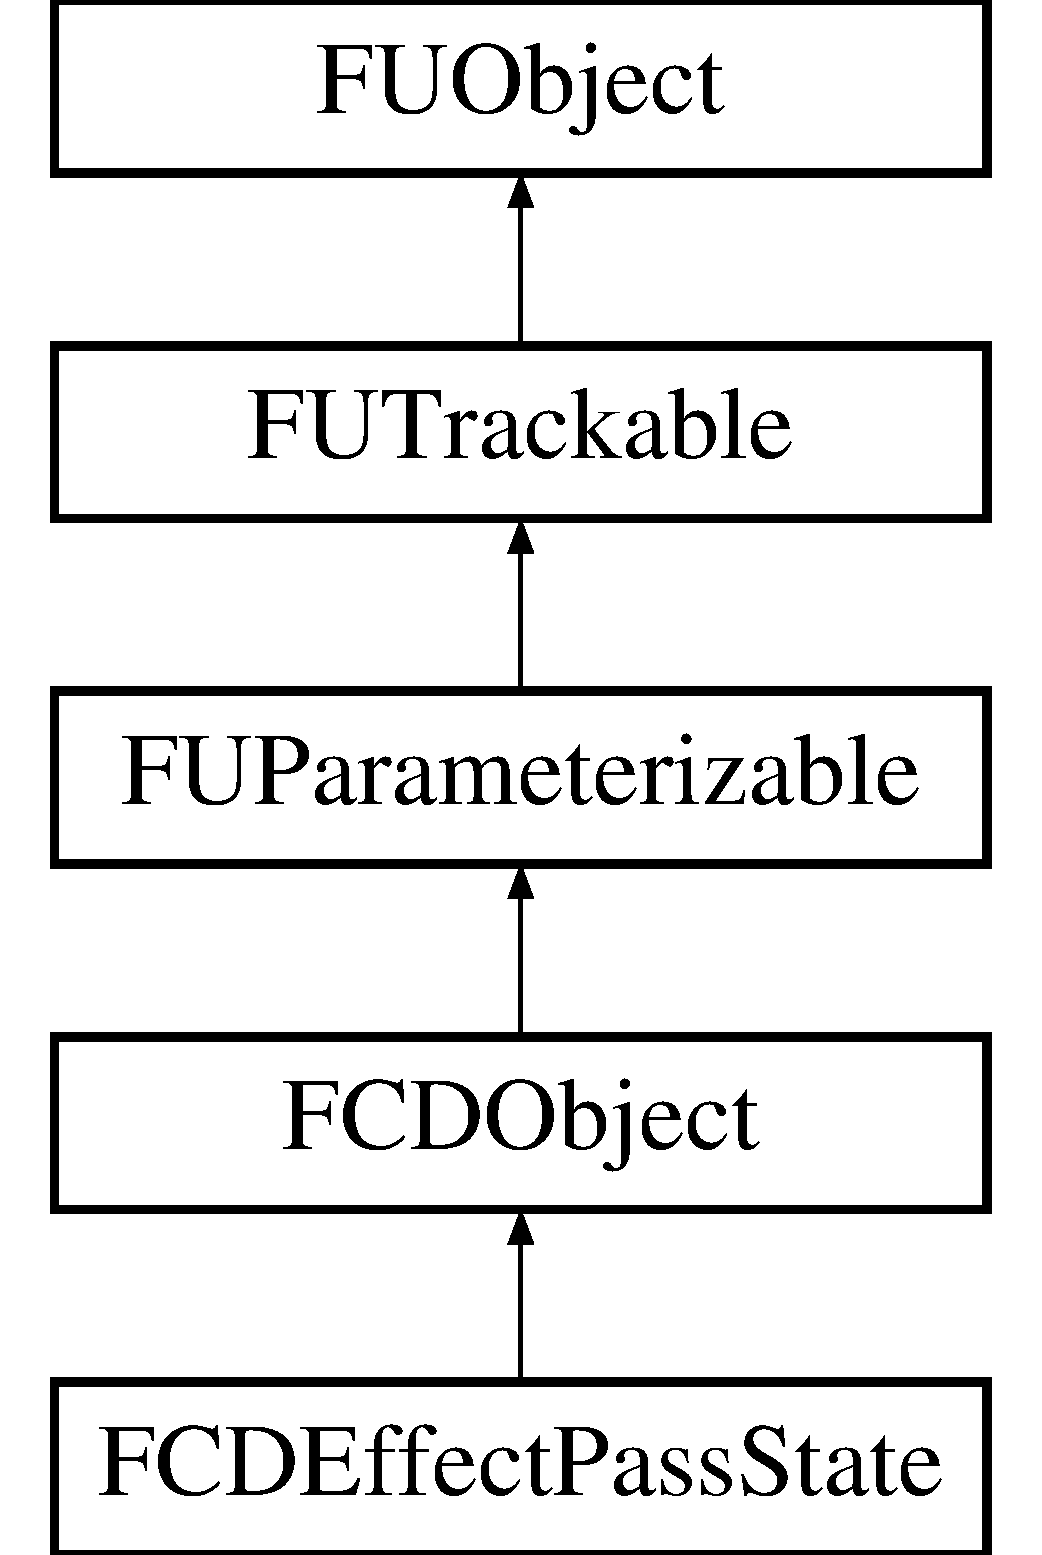
\includegraphics[height=5.000000cm]{classFCDEffectPassState}
\end{center}
\end{figure}
\subsection*{Public Member Functions}
\begin{DoxyCompactItemize}
\item 
\hyperlink{classFCDEffectPassState_abbc4d010d4024ce229baca1894099e9f}{FCDEffectPassState} (\hyperlink{classFCDocument}{FCDocument} $\ast$document, \hyperlink{namespaceFUDaePassState_a99a648050f80bc29359e932cffa8c973}{FUDaePassState::State} renderState)
\item 
virtual \hyperlink{classFCDEffectPassState_ab765430051f401516ee57b9aefe5dec7}{$\sim$FCDEffectPassState} ()
\item 
\hyperlink{namespaceFUDaePassState_a99a648050f80bc29359e932cffa8c973}{FUDaePassState::State} \hyperlink{classFCDEffectPassState_ada8069dff94f685d4b8c65ffde91704c}{GetType} () const 
\item 
size\_\-t \hyperlink{classFCDEffectPassState_ac7f6bda16f381c3dd55dd103816f458a}{GetDataSize} () const 
\item 
uint8 $\ast$ \hyperlink{classFCDEffectPassState_a23eb14cd11c0c65586e564199939ccf9}{GetData} ()
\item 
const uint8 $\ast$ \hyperlink{classFCDEffectPassState_ad0394f4c508bf9058a3208b592e06954}{GetData} () const 
\item 
void \hyperlink{classFCDEffectPassState_aaa372d3b7ee42af4c54eff6240fd9f5c}{SetDefaultValue} ()
\item 
\hyperlink{classFCDEffectPassState}{FCDEffectPassState} $\ast$ \hyperlink{classFCDEffectPassState_a7b41150adfb37a3ad71d5d3d9d3bd02f}{Clone} (\hyperlink{classFCDEffectPassState}{FCDEffectPassState} $\ast$clone=NULL) const 
\end{DoxyCompactItemize}


\subsection{Detailed Description}
This class holds the information necessary to set or apply one render state for a given pass. To get more information about the render state and how to interpret the data they hold, see the \hyperlink{namespaceFUDaePassState}{FUDaePassState} namespace and its enumerated type. \begin{DoxySeeAlso}{See also}
\hyperlink{namespaceFUDaePassState_a99a648050f80bc29359e932cffa8c973}{FUDaePassState::State} 
\end{DoxySeeAlso}


\subsection{Constructor \& Destructor Documentation}
\hypertarget{classFCDEffectPassState_abbc4d010d4024ce229baca1894099e9f}{
\index{FCDEffectPassState@{FCDEffectPassState}!FCDEffectPassState@{FCDEffectPassState}}
\index{FCDEffectPassState@{FCDEffectPassState}!FCDEffectPassState@{FCDEffectPassState}}
\subsubsection[{FCDEffectPassState}]{\setlength{\rightskip}{0pt plus 5cm}FCDEffectPassState::FCDEffectPassState (
\begin{DoxyParamCaption}
\item[{{\bf FCDocument} $\ast$}]{ document, }
\item[{{\bf FUDaePassState::State}}]{ renderState}
\end{DoxyParamCaption}
)}}
\label{classFCDEffectPassState_abbc4d010d4024ce229baca1894099e9f}
Constructor. Once built, the render state associated with this object should never change and the data pointer should be allocated to the correct size and never re-\/allocated. 
\begin{DoxyParams}{Parameters}
\item[{\em document}]The COLLADA document that owns this render state. \item[{\em renderState}]The render state type. \end{DoxyParams}
\hypertarget{classFCDEffectPassState_ab765430051f401516ee57b9aefe5dec7}{
\index{FCDEffectPassState@{FCDEffectPassState}!$\sim$FCDEffectPassState@{$\sim$FCDEffectPassState}}
\index{$\sim$FCDEffectPassState@{$\sim$FCDEffectPassState}!FCDEffectPassState@{FCDEffectPassState}}
\subsubsection[{$\sim$FCDEffectPassState}]{\setlength{\rightskip}{0pt plus 5cm}FCDEffectPassState::$\sim$FCDEffectPassState (
\begin{DoxyParamCaption}
{}
\end{DoxyParamCaption}
)\hspace{0.3cm}{\ttfamily  \mbox{[}virtual\mbox{]}}}}
\label{classFCDEffectPassState_ab765430051f401516ee57b9aefe5dec7}
Destructor. 

\subsection{Member Function Documentation}
\hypertarget{classFCDEffectPassState_a7b41150adfb37a3ad71d5d3d9d3bd02f}{
\index{FCDEffectPassState@{FCDEffectPassState}!Clone@{Clone}}
\index{Clone@{Clone}!FCDEffectPassState@{FCDEffectPassState}}
\subsubsection[{Clone}]{\setlength{\rightskip}{0pt plus 5cm}{\bf FCDEffectPassState} $\ast$ FCDEffectPassState::Clone (
\begin{DoxyParamCaption}
\item[{{\bf FCDEffectPassState} $\ast$}]{ clone = {\ttfamily NULL}}
\end{DoxyParamCaption}
) const}}
\label{classFCDEffectPassState_a7b41150adfb37a3ad71d5d3d9d3bd02f}
Clones the effect pass and shaders. 
\begin{DoxyParams}{Parameters}
\item[{\em clone}]The cloned pass. If this pointer is NULL, a new pass is created and you will need to release this new pass. \end{DoxyParams}
\begin{DoxyReturn}{Returns}
The cloned pass. 
\end{DoxyReturn}
\hypertarget{classFCDEffectPassState_ad0394f4c508bf9058a3208b592e06954}{
\index{FCDEffectPassState@{FCDEffectPassState}!GetData@{GetData}}
\index{GetData@{GetData}!FCDEffectPassState@{FCDEffectPassState}}
\subsubsection[{GetData}]{\setlength{\rightskip}{0pt plus 5cm}const uint8$\ast$ FCDEffectPassState::GetData (
\begin{DoxyParamCaption}
{}
\end{DoxyParamCaption}
) const\hspace{0.3cm}{\ttfamily  \mbox{[}inline\mbox{]}}}}
\label{classFCDEffectPassState_ad0394f4c508bf9058a3208b592e06954}
See above. \hypertarget{classFCDEffectPassState_a23eb14cd11c0c65586e564199939ccf9}{
\index{FCDEffectPassState@{FCDEffectPassState}!GetData@{GetData}}
\index{GetData@{GetData}!FCDEffectPassState@{FCDEffectPassState}}
\subsubsection[{GetData}]{\setlength{\rightskip}{0pt plus 5cm}uint8$\ast$ FCDEffectPassState::GetData (
\begin{DoxyParamCaption}
{}
\end{DoxyParamCaption}
)\hspace{0.3cm}{\ttfamily  \mbox{[}inline\mbox{]}}}}
\label{classFCDEffectPassState_a23eb14cd11c0c65586e564199939ccf9}
Retrieves the data pointer for the pass render state. \begin{DoxyReturn}{Returns}
The data pointer. 
\end{DoxyReturn}
\hypertarget{classFCDEffectPassState_ac7f6bda16f381c3dd55dd103816f458a}{
\index{FCDEffectPassState@{FCDEffectPassState}!GetDataSize@{GetDataSize}}
\index{GetDataSize@{GetDataSize}!FCDEffectPassState@{FCDEffectPassState}}
\subsubsection[{GetDataSize}]{\setlength{\rightskip}{0pt plus 5cm}size\_\-t FCDEffectPassState::GetDataSize (
\begin{DoxyParamCaption}
{}
\end{DoxyParamCaption}
) const\hspace{0.3cm}{\ttfamily  \mbox{[}inline\mbox{]}}}}
\label{classFCDEffectPassState_ac7f6bda16f381c3dd55dd103816f458a}
Retrieves the data size of the pass render state. \begin{DoxyReturn}{Returns}
The size of the render state data. 
\end{DoxyReturn}
\hypertarget{classFCDEffectPassState_ada8069dff94f685d4b8c65ffde91704c}{
\index{FCDEffectPassState@{FCDEffectPassState}!GetType@{GetType}}
\index{GetType@{GetType}!FCDEffectPassState@{FCDEffectPassState}}
\subsubsection[{GetType}]{\setlength{\rightskip}{0pt plus 5cm}{\bf FUDaePassState::State} FCDEffectPassState::GetType (
\begin{DoxyParamCaption}
{}
\end{DoxyParamCaption}
) const\hspace{0.3cm}{\ttfamily  \mbox{[}inline\mbox{]}}}}
\label{classFCDEffectPassState_ada8069dff94f685d4b8c65ffde91704c}
Retrieves the type of the pass render state. \begin{DoxyReturn}{Returns}
The render state type. 
\end{DoxyReturn}
\hypertarget{classFCDEffectPassState_aaa372d3b7ee42af4c54eff6240fd9f5c}{
\index{FCDEffectPassState@{FCDEffectPassState}!SetDefaultValue@{SetDefaultValue}}
\index{SetDefaultValue@{SetDefaultValue}!FCDEffectPassState@{FCDEffectPassState}}
\subsubsection[{SetDefaultValue}]{\setlength{\rightskip}{0pt plus 5cm}void FCDEffectPassState::SetDefaultValue (
\begin{DoxyParamCaption}
{}
\end{DoxyParamCaption}
)}}
\label{classFCDEffectPassState_aaa372d3b7ee42af4c54eff6240fd9f5c}
Use this method to reset the state back to its default value. This method is called in the constructor. 

The documentation for this class was generated from the following files:\begin{DoxyCompactItemize}
\item 
FCollada/FCDocument/\hyperlink{FCDEffectPassState_8h}{FCDEffectPassState.h}\item 
FCollada/FCDocument/FCDEffectPassState.cpp\end{DoxyCompactItemize}

\hypertarget{classFCDEffectProfile}{
\section{FCDEffectProfile Class Reference}
\label{classFCDEffectProfile}\index{FCDEffectProfile@{FCDEffectProfile}}
}


{\ttfamily \#include $<$FCDEffectProfile.h$>$}

Inheritance diagram for FCDEffectProfile:\begin{figure}[H]
\begin{center}
\leavevmode
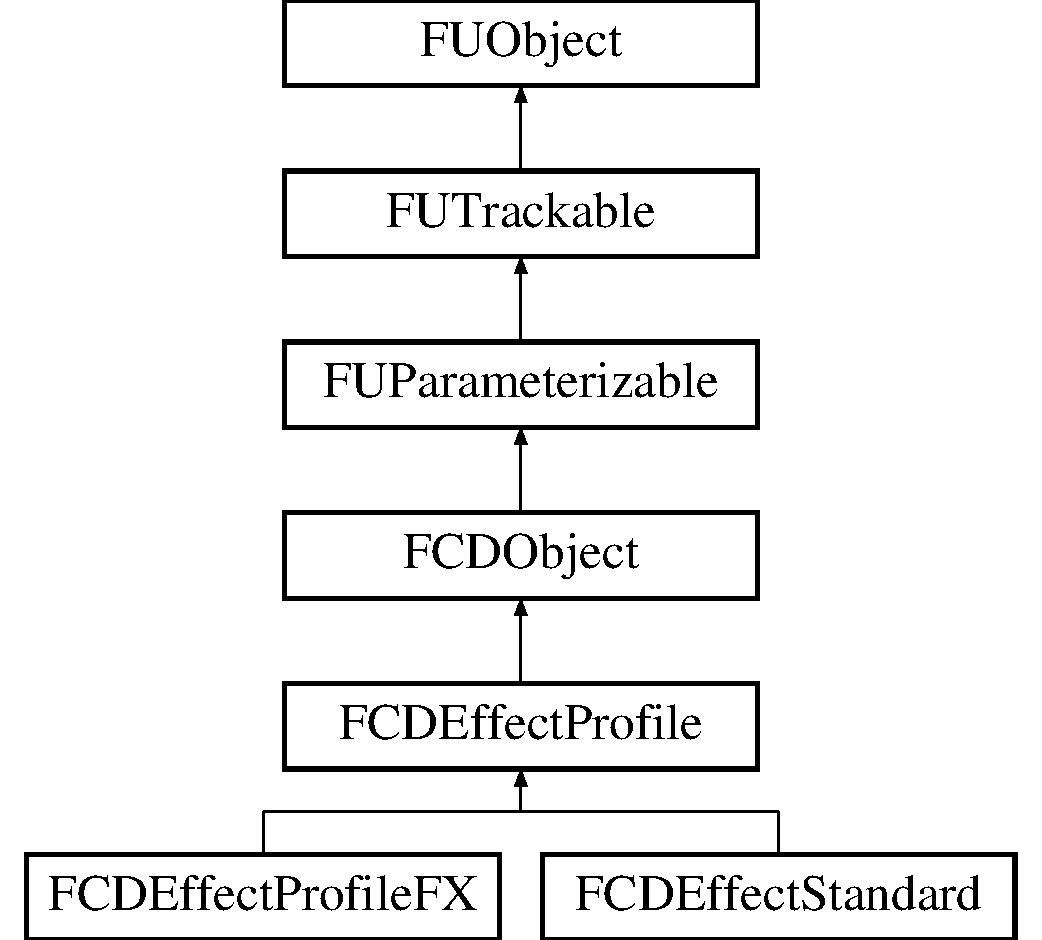
\includegraphics[height=6.000000cm]{classFCDEffectProfile}
\end{center}
\end{figure}
\subsection*{Public Member Functions}
\begin{DoxyCompactItemize}
\item 
\hyperlink{classFCDEffectProfile_a9556428303b69f40a009c72de9b22cc9}{FCDEffectProfile} (\hyperlink{classFCDocument}{FCDocument} $\ast$document, \hyperlink{classFCDEffect}{FCDEffect} $\ast$parent)
\item 
virtual \hyperlink{classFCDEffectProfile_a2ad98f217369ae412db5df21d7cfc5c8}{$\sim$FCDEffectProfile} ()
\item 
virtual \hyperlink{namespaceFUDaeProfileType_ac10ea253a7a141708de2324a929f8a79}{FUDaeProfileType::Type} \hyperlink{classFCDEffectProfile_a48ae9db50d8cce2509d6a3d557a1b0a6}{GetType} () const =0
\item 
\hyperlink{classFCDEffect}{FCDEffect} $\ast$ \hyperlink{classFCDEffectProfile_a806741463f02e52835fcb6be20865513}{GetParent} ()
\item 
const \hyperlink{classFCDEffect}{FCDEffect} $\ast$ \hyperlink{classFCDEffectProfile_ab25cac5a4ca182eb96cac13b0044a77d}{GetParent} () const 
\item 
\hyperlink{classFCDEffectProfile_ad53800537042e1829dd607ac68c2630d}{DEPRECATED} (3.05A, GetParent()-\/$>$GetDaeId) const fm
\item 
\hyperlink{classFCDExtra}{FCDExtra} $\ast$ \hyperlink{classFCDEffectProfile_a9e0105d9bbe5590a771a4c5ea101fb64}{GetExtra} ()
\item 
const \hyperlink{classFCDExtra}{FCDExtra} $\ast$ \hyperlink{classFCDEffectProfile_a4adf36a1efe613e6816871e224a58f41}{GetExtra} () const 
\item 
virtual \hyperlink{classFCDEffectProfile}{FCDEffectProfile} $\ast$ \hyperlink{classFCDEffectProfile_ab7641c9671098f6966146798e61bb098}{Clone} (\hyperlink{classFCDEffectProfile}{FCDEffectProfile} $\ast$clone=NULL) const 
\item 
size\_\-t \hyperlink{classFCDEffectProfile_a1f3e9c38b6283cbdfb102e3393590746}{GetEffectParameterCount} () const 
\item 
\hyperlink{classFCDEffectParameter}{FCDEffectParameter} $\ast$ \hyperlink{classFCDEffectProfile_a91c0bff4f69ccf48e07809983167b34f}{GetEffectParameter} (size\_\-t index)
\item 
\hypertarget{classFCDEffectProfile_a4453f452c165f61024cba5a4958a3d35}{
const \hyperlink{classFCDEffectParameter}{FCDEffectParameter} $\ast$ {\bfseries GetEffectParameter} (size\_\-t index) const }
\label{classFCDEffectProfile_a4453f452c165f61024cba5a4958a3d35}

\item 
\hyperlink{classFCDEffectParameter}{FCDEffectParameter} $\ast$ \hyperlink{classFCDEffectProfile_a8b3be439e89e6abf8aab1ae61d27650c}{AddEffectParameter} (uint32 type)
\item 
\hyperlink{classFCDEffectProfile_aadc7e65fa145af53ec2bf47c6de550f2}{DEPRECATED} (3.05A, not recommended) void Flatten()
\end{DoxyCompactItemize}


\subsection{Detailed Description}
The base for a COLLADA effect profile.

COLLADA has multiple effect profiles: CG, HLSL, GLSL, GLES and the COMMON profile. For each profile, there is a class which implements this abstract class. This abstract class solely holds the parent effect and allows access to the profile type.

\begin{DoxySeeAlso}{See also}
\hyperlink{classFCDEffectProfileFX}{FCDEffectProfileFX} \hyperlink{classFCDEffectStandard}{FCDEffectStandard} 
\end{DoxySeeAlso}


\subsection{Constructor \& Destructor Documentation}
\hypertarget{classFCDEffectProfile_a9556428303b69f40a009c72de9b22cc9}{
\index{FCDEffectProfile@{FCDEffectProfile}!FCDEffectProfile@{FCDEffectProfile}}
\index{FCDEffectProfile@{FCDEffectProfile}!FCDEffectProfile@{FCDEffectProfile}}
\subsubsection[{FCDEffectProfile}]{\setlength{\rightskip}{0pt plus 5cm}FCDEffectProfile::FCDEffectProfile (
\begin{DoxyParamCaption}
\item[{{\bf FCDocument} $\ast$}]{ document, }
\item[{{\bf FCDEffect} $\ast$}]{ parent}
\end{DoxyParamCaption}
)}}
\label{classFCDEffectProfile_a9556428303b69f40a009c72de9b22cc9}
Constructor: do not use directly. Instead, use the \hyperlink{classFCDEffect_abe53b1e58ce5469b28f63b5155703a95}{FCDEffect::AddProfile} function. 
\begin{DoxyParams}{Parameters}
\item[{\em document}]The \hyperlink{namespaceFCollada}{FCollada} document that owns this effect profile. \item[{\em parent}]The effect which contains this profile. \end{DoxyParams}
\hypertarget{classFCDEffectProfile_a2ad98f217369ae412db5df21d7cfc5c8}{
\index{FCDEffectProfile@{FCDEffectProfile}!$\sim$FCDEffectProfile@{$\sim$FCDEffectProfile}}
\index{$\sim$FCDEffectProfile@{$\sim$FCDEffectProfile}!FCDEffectProfile@{FCDEffectProfile}}
\subsubsection[{$\sim$FCDEffectProfile}]{\setlength{\rightskip}{0pt plus 5cm}FCDEffectProfile::$\sim$FCDEffectProfile (
\begin{DoxyParamCaption}
{}
\end{DoxyParamCaption}
)\hspace{0.3cm}{\ttfamily  \mbox{[}virtual\mbox{]}}}}
\label{classFCDEffectProfile_a2ad98f217369ae412db5df21d7cfc5c8}
Destructor. 

\subsection{Member Function Documentation}
\hypertarget{classFCDEffectProfile_a8b3be439e89e6abf8aab1ae61d27650c}{
\index{FCDEffectProfile@{FCDEffectProfile}!AddEffectParameter@{AddEffectParameter}}
\index{AddEffectParameter@{AddEffectParameter}!FCDEffectProfile@{FCDEffectProfile}}
\subsubsection[{AddEffectParameter}]{\setlength{\rightskip}{0pt plus 5cm}{\bf FCDEffectParameter} $\ast$ FCDEffectProfile::AddEffectParameter (
\begin{DoxyParamCaption}
\item[{uint32}]{ type}
\end{DoxyParamCaption}
)}}
\label{classFCDEffectProfile_a8b3be439e89e6abf8aab1ae61d27650c}
Adds a local effect parameter to the local list. \begin{DoxySeeAlso}{See also}
\hyperlink{classFCDEffectParameter_a1efe74553d2ed199435085c171743b08}{FCDEffectParameter::Type} 
\end{DoxySeeAlso}

\begin{DoxyParams}{Parameters}
\item[{\em type}]The value type of the effect parameter to create. \end{DoxyParams}
\begin{DoxyReturn}{Returns}
The new local effect parameter. 
\end{DoxyReturn}
\hypertarget{classFCDEffectProfile_ab7641c9671098f6966146798e61bb098}{
\index{FCDEffectProfile@{FCDEffectProfile}!Clone@{Clone}}
\index{Clone@{Clone}!FCDEffectProfile@{FCDEffectProfile}}
\subsubsection[{Clone}]{\setlength{\rightskip}{0pt plus 5cm}{\bf FCDEffectProfile} $\ast$ FCDEffectProfile::Clone (
\begin{DoxyParamCaption}
\item[{{\bf FCDEffectProfile} $\ast$}]{ clone = {\ttfamily NULL}}
\end{DoxyParamCaption}
) const\hspace{0.3cm}{\ttfamily  \mbox{[}virtual\mbox{]}}}}
\label{classFCDEffectProfile_ab7641c9671098f6966146798e61bb098}
Clones the profile effect and its parameters. 
\begin{DoxyParams}{Parameters}
\item[{\em clone}]The cloned profile. If this pointer is NULL, a new profile is created and you will need to release this new profile. \end{DoxyParams}
\begin{DoxyReturn}{Returns}
The cloned profile. This pointer will be NULL if the abstract class' cloning function is used without a given clone. 
\end{DoxyReturn}


Reimplemented in \hyperlink{classFCDEffectProfileFX_affaefb11964c4000f30e2f7be7cd2aa5}{FCDEffectProfileFX}, and \hyperlink{classFCDEffectStandard_aeadbfb97cdfd733a09a564f457020b66}{FCDEffectStandard}.

\hypertarget{classFCDEffectProfile_ad53800537042e1829dd607ac68c2630d}{
\index{FCDEffectProfile@{FCDEffectProfile}!DEPRECATED@{DEPRECATED}}
\index{DEPRECATED@{DEPRECATED}!FCDEffectProfile@{FCDEffectProfile}}
\subsubsection[{DEPRECATED}]{\setlength{\rightskip}{0pt plus 5cm}FCDEffectProfile::DEPRECATED (
\begin{DoxyParamCaption}
\item[{3.}]{ 05A, }
\item[{GetParent()-\/$>$}]{ GetDaeId}
\end{DoxyParamCaption}
) const\hspace{0.3cm}{\ttfamily  \mbox{[}inline\mbox{]}}}}
\label{classFCDEffectProfile_ad53800537042e1829dd607ac68c2630d}
\mbox{[}INTERNAL\mbox{]} Retrieves the COLLADA id of the parent effect. This function is useful when reporting errors and warnings. \begin{DoxyReturn}{Returns}
The COLLADA id of the parent effect. 
\end{DoxyReturn}
\hypertarget{classFCDEffectProfile_aadc7e65fa145af53ec2bf47c6de550f2}{
\index{FCDEffectProfile@{FCDEffectProfile}!DEPRECATED@{DEPRECATED}}
\index{DEPRECATED@{DEPRECATED}!FCDEffectProfile@{FCDEffectProfile}}
\subsubsection[{DEPRECATED}]{\setlength{\rightskip}{0pt plus 5cm}FCDEffectProfile::DEPRECATED (
\begin{DoxyParamCaption}
\item[{3.}]{ 05A, }
\item[{not}]{ recommended}
\end{DoxyParamCaption}
)\hspace{0.3cm}{\ttfamily  \mbox{[}inline\mbox{]}}}}
\label{classFCDEffectProfile_aadc7e65fa145af53ec2bf47c6de550f2}
\mbox{[}INTERNAL\mbox{]} Flattens this effect profile, pushing all the effect parameter overrides into the effect parameter generators and moving all the parameters to the effect technique level of abstraction. To flatten the material, use the FCDMaterialInstance::FlattenMaterial function. 

Reimplemented in \hyperlink{classFCDEffectProfileFX_a3a00d4ed2dec686e7e0a60eb99168ff5}{FCDEffectProfileFX}, and \hyperlink{classFCDEffectStandard_a40ab2cc34bd3cf5d3f622a8dcf9e9fcd}{FCDEffectStandard}.

\hypertarget{classFCDEffectProfile_a91c0bff4f69ccf48e07809983167b34f}{
\index{FCDEffectProfile@{FCDEffectProfile}!GetEffectParameter@{GetEffectParameter}}
\index{GetEffectParameter@{GetEffectParameter}!FCDEffectProfile@{FCDEffectProfile}}
\subsubsection[{GetEffectParameter}]{\setlength{\rightskip}{0pt plus 5cm}{\bf FCDEffectParameter}$\ast$ FCDEffectProfile::GetEffectParameter (
\begin{DoxyParamCaption}
\item[{size\_\-t}]{ index}
\end{DoxyParamCaption}
)\hspace{0.3cm}{\ttfamily  \mbox{[}inline\mbox{]}}}}
\label{classFCDEffectProfile_a91c0bff4f69ccf48e07809983167b34f}
Retrieves a given local effect parameter. 
\begin{DoxyParams}{Parameters}
\item[{\em index}]An index. \end{DoxyParams}
\begin{DoxyReturn}{Returns}
The local effect parameter at the given index. 
\end{DoxyReturn}
\hypertarget{classFCDEffectProfile_a1f3e9c38b6283cbdfb102e3393590746}{
\index{FCDEffectProfile@{FCDEffectProfile}!GetEffectParameterCount@{GetEffectParameterCount}}
\index{GetEffectParameterCount@{GetEffectParameterCount}!FCDEffectProfile@{FCDEffectProfile}}
\subsubsection[{GetEffectParameterCount}]{\setlength{\rightskip}{0pt plus 5cm}size\_\-t FCDEffectProfile::GetEffectParameterCount (
\begin{DoxyParamCaption}
{}
\end{DoxyParamCaption}
) const\hspace{0.3cm}{\ttfamily  \mbox{[}inline\mbox{]}}}}
\label{classFCDEffectProfile_a1f3e9c38b6283cbdfb102e3393590746}
Retrieves the number of local effect parameters \begin{DoxyReturn}{Returns}
The number of local effect parameters. 
\end{DoxyReturn}
\hypertarget{classFCDEffectProfile_a9e0105d9bbe5590a771a4c5ea101fb64}{
\index{FCDEffectProfile@{FCDEffectProfile}!GetExtra@{GetExtra}}
\index{GetExtra@{GetExtra}!FCDEffectProfile@{FCDEffectProfile}}
\subsubsection[{GetExtra}]{\setlength{\rightskip}{0pt plus 5cm}{\bf FCDExtra}$\ast$ FCDEffectProfile::GetExtra (
\begin{DoxyParamCaption}
{}
\end{DoxyParamCaption}
)\hspace{0.3cm}{\ttfamily  \mbox{[}inline\mbox{]}}}}
\label{classFCDEffectProfile_a9e0105d9bbe5590a771a4c5ea101fb64}
Retrieves the extra information tree for this effect profile. The prefered way to save extra information in \hyperlink{namespaceFCollada}{FCollada} is at the entity level: \hyperlink{classFCDEffect}{FCDEffect}. \begin{DoxyReturn}{Returns}
The extra information tree. 
\end{DoxyReturn}
\hypertarget{classFCDEffectProfile_a4adf36a1efe613e6816871e224a58f41}{
\index{FCDEffectProfile@{FCDEffectProfile}!GetExtra@{GetExtra}}
\index{GetExtra@{GetExtra}!FCDEffectProfile@{FCDEffectProfile}}
\subsubsection[{GetExtra}]{\setlength{\rightskip}{0pt plus 5cm}const {\bf FCDExtra}$\ast$ FCDEffectProfile::GetExtra (
\begin{DoxyParamCaption}
{}
\end{DoxyParamCaption}
) const\hspace{0.3cm}{\ttfamily  \mbox{[}inline\mbox{]}}}}
\label{classFCDEffectProfile_a4adf36a1efe613e6816871e224a58f41}
See above. \hypertarget{classFCDEffectProfile_ab25cac5a4ca182eb96cac13b0044a77d}{
\index{FCDEffectProfile@{FCDEffectProfile}!GetParent@{GetParent}}
\index{GetParent@{GetParent}!FCDEffectProfile@{FCDEffectProfile}}
\subsubsection[{GetParent}]{\setlength{\rightskip}{0pt plus 5cm}const {\bf FCDEffect}$\ast$ FCDEffectProfile::GetParent (
\begin{DoxyParamCaption}
{}
\end{DoxyParamCaption}
) const\hspace{0.3cm}{\ttfamily  \mbox{[}inline\mbox{]}}}}
\label{classFCDEffectProfile_ab25cac5a4ca182eb96cac13b0044a77d}
See above. \hypertarget{classFCDEffectProfile_a806741463f02e52835fcb6be20865513}{
\index{FCDEffectProfile@{FCDEffectProfile}!GetParent@{GetParent}}
\index{GetParent@{GetParent}!FCDEffectProfile@{FCDEffectProfile}}
\subsubsection[{GetParent}]{\setlength{\rightskip}{0pt plus 5cm}{\bf FCDEffect}$\ast$ FCDEffectProfile::GetParent (
\begin{DoxyParamCaption}
{}
\end{DoxyParamCaption}
)\hspace{0.3cm}{\ttfamily  \mbox{[}inline\mbox{]}}}}
\label{classFCDEffectProfile_a806741463f02e52835fcb6be20865513}
Retrieves the parent effect. This is the effect which contains this profile. \begin{DoxyReturn}{Returns}
The parent effect. This pointer will never be NULL. 
\end{DoxyReturn}
\hypertarget{classFCDEffectProfile_a48ae9db50d8cce2509d6a3d557a1b0a6}{
\index{FCDEffectProfile@{FCDEffectProfile}!GetType@{GetType}}
\index{GetType@{GetType}!FCDEffectProfile@{FCDEffectProfile}}
\subsubsection[{GetType}]{\setlength{\rightskip}{0pt plus 5cm}virtual {\bf FUDaeProfileType::Type} FCDEffectProfile::GetType (
\begin{DoxyParamCaption}
{}
\end{DoxyParamCaption}
) const\hspace{0.3cm}{\ttfamily  \mbox{[}pure virtual\mbox{]}}}}
\label{classFCDEffectProfile_a48ae9db50d8cce2509d6a3d557a1b0a6}
Retrieves the profile type for this effect. This function allows you to up-\/cast the pointer safely to a more specific effect profile class. \begin{DoxyReturn}{Returns}
The profile type. 
\end{DoxyReturn}


Implemented in \hyperlink{classFCDEffectProfileFX_a711f7094d3d2ae864f336a4db558c3c5}{FCDEffectProfileFX}, and \hyperlink{classFCDEffectStandard_a5870dbcf350bd3f15781cf9ccf1095f9}{FCDEffectStandard}.



The documentation for this class was generated from the following files:\begin{DoxyCompactItemize}
\item 
FCollada/FCDocument/\hyperlink{FCDEffectProfile_8h}{FCDEffectProfile.h}\item 
FCollada/FCDocument/FCDEffectProfile.cpp\end{DoxyCompactItemize}

\hypertarget{classFCDEffectProfileFX}{
\section{FCDEffectProfileFX Class Reference}
\label{classFCDEffectProfileFX}\index{FCDEffectProfileFX@{FCDEffectProfileFX}}
}


{\ttfamily \#include $<$FCDEffectProfileFX.h$>$}

Inheritance diagram for FCDEffectProfileFX:\begin{figure}[H]
\begin{center}
\leavevmode
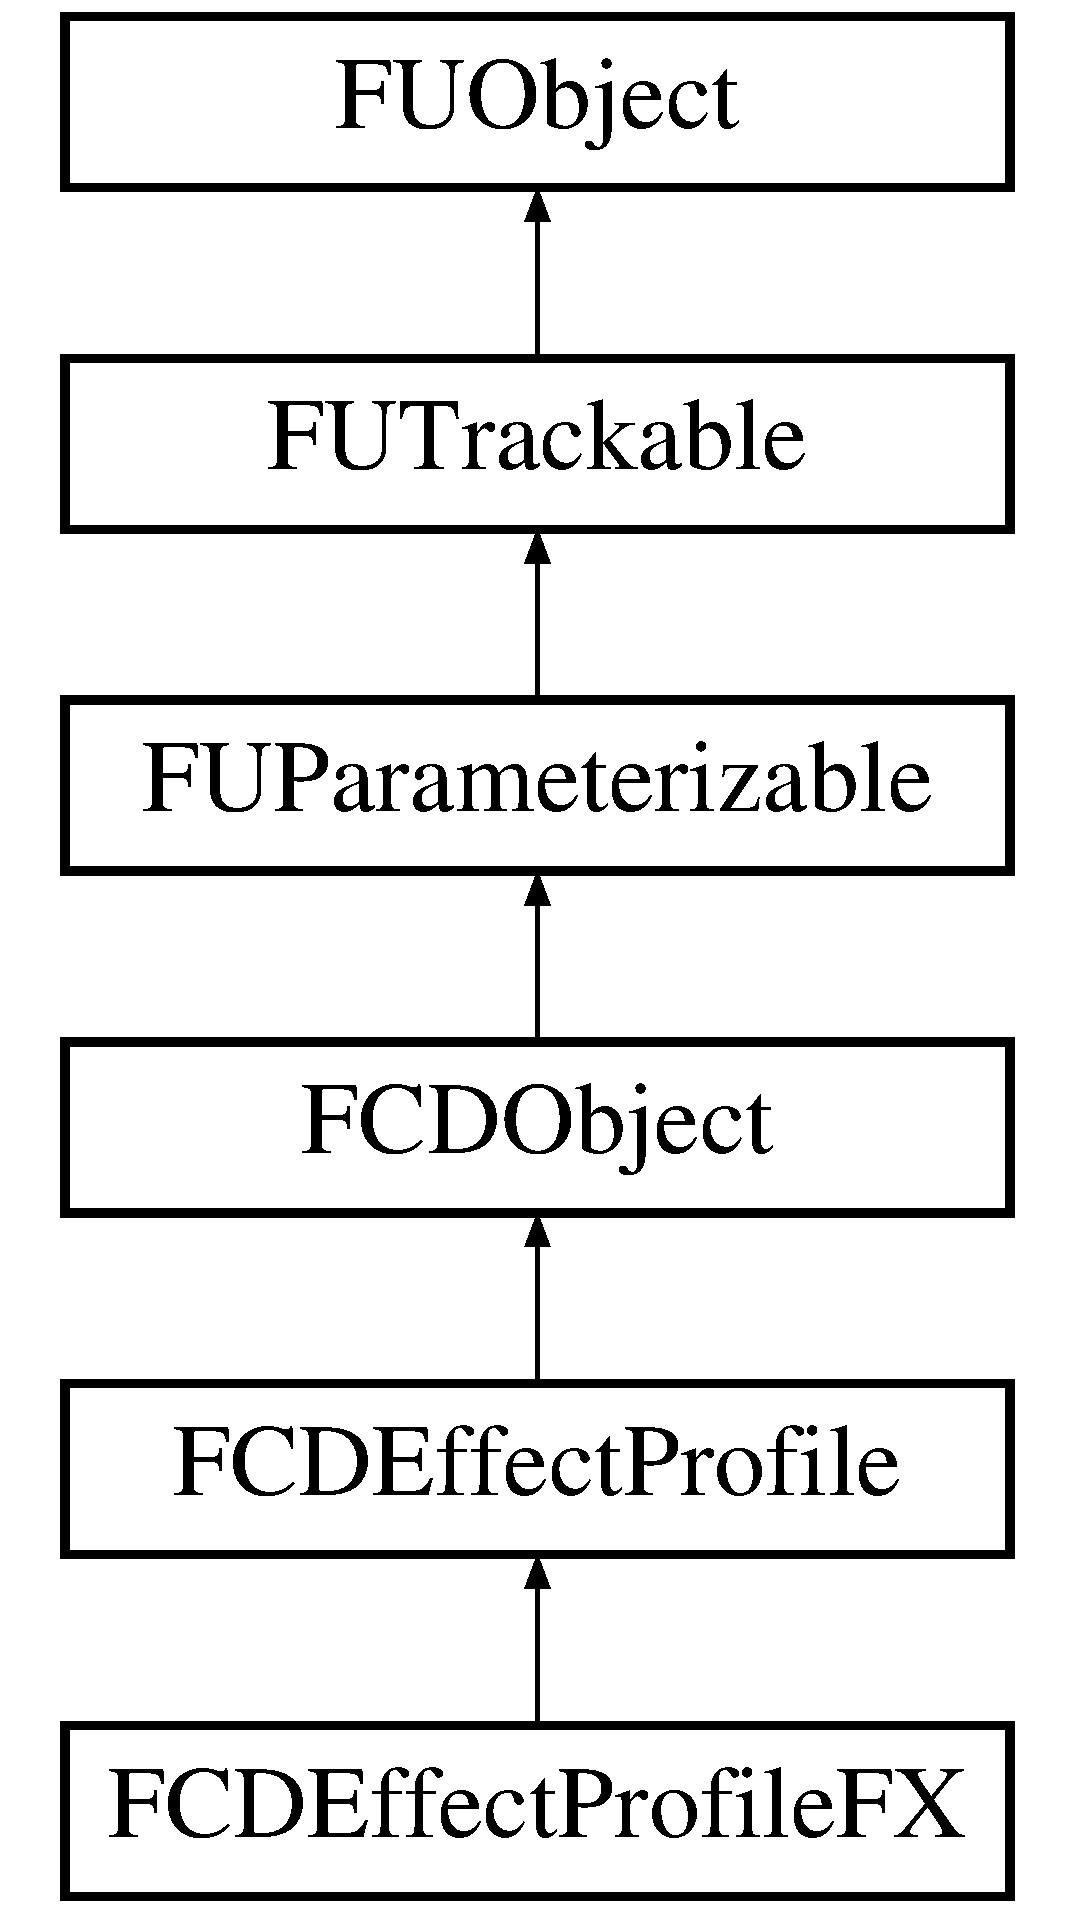
\includegraphics[height=6.000000cm]{classFCDEffectProfileFX}
\end{center}
\end{figure}
\subsection*{Public Member Functions}
\begin{DoxyCompactItemize}
\item 
\hyperlink{classFCDEffectProfileFX_a3a6aa38eb1af1a180116c06c651311c5}{FCDEffectProfileFX} (\hyperlink{classFCDocument}{FCDocument} $\ast$document, \hyperlink{classFCDEffect}{FCDEffect} $\ast$parent)
\item 
virtual \hyperlink{classFCDEffectProfileFX_a30b48d2454decffb4c5b45f3986ac995}{$\sim$FCDEffectProfileFX} ()
\item 
virtual \hyperlink{namespaceFUDaeProfileType_ac10ea253a7a141708de2324a929f8a79}{FUDaeProfileType::Type} \hyperlink{classFCDEffectProfileFX_a711f7094d3d2ae864f336a4db558c3c5}{GetType} () const 
\item 
void \hyperlink{classFCDEffectProfileFX_a8da90f2c6a32edaa68a0430ecc143017}{SetType} (\hyperlink{namespaceFUDaeProfileType_ac10ea253a7a141708de2324a929f8a79}{FUDaeProfileType::Type} \_\-type)
\item 
const \hyperlink{classfm_1_1stringT}{fstring} \& \hyperlink{classFCDEffectProfileFX_a0d4d03330cc23e49a83f7dcb22df0b06}{GetPlatform} () const 
\item 
void \hyperlink{classFCDEffectProfileFX_a749574bde12f659c1bae707284f3d630}{SetPlatform} (const \hyperlink{classfm_1_1stringT}{fstring} \&\_\-platform)
\item 
\hyperlink{classFCDEffectProfileFX_a883c195463d15960a9d5d1d347ec3a41}{DEPRECATED} (3.05A, GetTechniqueCount and GetTechnique(index)) void GetTechniqueList() const 
\item 
size\_\-t \hyperlink{classFCDEffectProfileFX_af1fac9bef78005e8a0936cc4f4cf5b63}{GetTechniqueCount} () const 
\item 
\hyperlink{classFCDEffectTechnique}{FCDEffectTechnique} $\ast$ \hyperlink{classFCDEffectProfileFX_a3cfd88fb24777d0cd909834bf15ab99a}{GetTechnique} (size\_\-t index)
\item 
const \hyperlink{classFCDEffectTechnique}{FCDEffectTechnique} $\ast$ \hyperlink{classFCDEffectProfileFX_aa1f90851b8c0527d30017ecf8f247ea6}{GetTechnique} (size\_\-t index) const 
\item 
\hyperlink{classFCDEffectTechnique}{FCDEffectTechnique} $\ast$ \hyperlink{classFCDEffectProfileFX_ae6498c1d1bba41fdc63b98cbceb797d0}{AddTechnique} ()
\item 
\hyperlink{classFCDEffectProfileFX_a603840ea8a108748a8da26697c6f72ce}{DEPRECATED} (3.05A, GetCodeCount and GetCode(index)) void GetCodeList()
\item 
size\_\-t \hyperlink{classFCDEffectProfileFX_a4014013862a3bbda5a93162279dc2698}{GetCodeCount} () const 
\item 
\hyperlink{classFCDEffectCode}{FCDEffectCode} $\ast$ \hyperlink{classFCDEffectProfileFX_adf8d6b95a3a98efd8c3df44cdf301347}{GetCode} (size\_\-t index)
\item 
const \hyperlink{classFCDEffectCode}{FCDEffectCode} $\ast$ \hyperlink{classFCDEffectProfileFX_aab857859ae788ec5d8da9641ce4ca6cb}{GetCode} (size\_\-t index) const 
\item 
\hyperlink{classFCDEffectCode}{FCDEffectCode} $\ast$ \hyperlink{classFCDEffectProfileFX_af704be744d23f8edf5f253649d6f08c2}{FindCode} (const char $\ast$sid)
\item 
const \hyperlink{classFCDEffectCode}{FCDEffectCode} $\ast$ \hyperlink{classFCDEffectProfileFX_a5a33aac3ed1633e3b02b071debe27492}{FindCode} (const char $\ast$sid) const 
\item 
\hyperlink{classFCDEffectCode}{FCDEffectCode} $\ast$ \hyperlink{classFCDEffectProfileFX_a953350d444182d9c325166d120b6510c}{AddCode} ()
\item 
virtual \hyperlink{classFCDEffectProfile}{FCDEffectProfile} $\ast$ \hyperlink{classFCDEffectProfileFX_affaefb11964c4000f30e2f7be7cd2aa5}{Clone} (\hyperlink{classFCDEffectProfile}{FCDEffectProfile} $\ast$clone=NULL) const 
\item 
\hyperlink{classFCDEffectProfileFX_a3a00d4ed2dec686e7e0a60eb99168ff5}{DEPRECATED} (3.05A, not recommended) void Flatten()
\end{DoxyCompactItemize}


\subsection{Detailed Description}
A general effect profile description.

The general effect profile contains all the information necessary to implement the advanced effect profiles, such as CG, HLSL, GLSL and GLES. Since these effect profiles contains extremely similar information, they use the same description structure. For the COMMON profile, see the \hyperlink{classFCDEffectStandard}{FCDEffectStandard} class.

You should use the GetType function to figure out which profile this structure addresses. You can then retrieve one or many of the \hyperlink{classFCDEffectTechnique}{FCDEffectTechnique} objects that describe how to render for this profile. You may want to check the FCDEffectMaterialTechniqueHint objects at the \hyperlink{classFCDMaterial}{FCDMaterial} level, in order to determine which technique(s) to use for your platform. At the profile level of abstraction, parameters may be generated within the FCDEffectParamterList. 

\subsection{Constructor \& Destructor Documentation}
\hypertarget{classFCDEffectProfileFX_a3a6aa38eb1af1a180116c06c651311c5}{
\index{FCDEffectProfileFX@{FCDEffectProfileFX}!FCDEffectProfileFX@{FCDEffectProfileFX}}
\index{FCDEffectProfileFX@{FCDEffectProfileFX}!FCDEffectProfileFX@{FCDEffectProfileFX}}
\subsubsection[{FCDEffectProfileFX}]{\setlength{\rightskip}{0pt plus 5cm}FCDEffectProfileFX::FCDEffectProfileFX (
\begin{DoxyParamCaption}
\item[{{\bf FCDocument} $\ast$}]{ document, }
\item[{{\bf FCDEffect} $\ast$}]{ parent}
\end{DoxyParamCaption}
)}}
\label{classFCDEffectProfileFX_a3a6aa38eb1af1a180116c06c651311c5}
Constructor: do not use directly. Instead, use the \hyperlink{classFCDEffect_abe53b1e58ce5469b28f63b5155703a95}{FCDEffect::AddProfile} function. 
\begin{DoxyParams}{Parameters}
\item[{\em parent}]The effect which contains this profile. \item[{\em type}]The type of profile. \end{DoxyParams}
\hypertarget{classFCDEffectProfileFX_a30b48d2454decffb4c5b45f3986ac995}{
\index{FCDEffectProfileFX@{FCDEffectProfileFX}!$\sim$FCDEffectProfileFX@{$\sim$FCDEffectProfileFX}}
\index{$\sim$FCDEffectProfileFX@{$\sim$FCDEffectProfileFX}!FCDEffectProfileFX@{FCDEffectProfileFX}}
\subsubsection[{$\sim$FCDEffectProfileFX}]{\setlength{\rightskip}{0pt plus 5cm}FCDEffectProfileFX::$\sim$FCDEffectProfileFX (
\begin{DoxyParamCaption}
{}
\end{DoxyParamCaption}
)\hspace{0.3cm}{\ttfamily  \mbox{[}virtual\mbox{]}}}}
\label{classFCDEffectProfileFX_a30b48d2454decffb4c5b45f3986ac995}
Destructor. 

\subsection{Member Function Documentation}
\hypertarget{classFCDEffectProfileFX_a953350d444182d9c325166d120b6510c}{
\index{FCDEffectProfileFX@{FCDEffectProfileFX}!AddCode@{AddCode}}
\index{AddCode@{AddCode}!FCDEffectProfileFX@{FCDEffectProfileFX}}
\subsubsection[{AddCode}]{\setlength{\rightskip}{0pt plus 5cm}{\bf FCDEffectCode} $\ast$ FCDEffectProfileFX::AddCode (
\begin{DoxyParamCaption}
{}
\end{DoxyParamCaption}
)}}
\label{classFCDEffectProfileFX_a953350d444182d9c325166d120b6510c}
Adds a new code inclusion to this effect profile. \begin{DoxyReturn}{Returns}
The new code inclusion. 
\end{DoxyReturn}
\hypertarget{classFCDEffectProfileFX_ae6498c1d1bba41fdc63b98cbceb797d0}{
\index{FCDEffectProfileFX@{FCDEffectProfileFX}!AddTechnique@{AddTechnique}}
\index{AddTechnique@{AddTechnique}!FCDEffectProfileFX@{FCDEffectProfileFX}}
\subsubsection[{AddTechnique}]{\setlength{\rightskip}{0pt plus 5cm}{\bf FCDEffectTechnique} $\ast$ FCDEffectProfileFX::AddTechnique (
\begin{DoxyParamCaption}
{}
\end{DoxyParamCaption}
)}}
\label{classFCDEffectProfileFX_ae6498c1d1bba41fdc63b98cbceb797d0}
Adds a new technique to this effect profile. \begin{DoxyReturn}{Returns}
The new technique object. 
\end{DoxyReturn}
\hypertarget{classFCDEffectProfileFX_affaefb11964c4000f30e2f7be7cd2aa5}{
\index{FCDEffectProfileFX@{FCDEffectProfileFX}!Clone@{Clone}}
\index{Clone@{Clone}!FCDEffectProfileFX@{FCDEffectProfileFX}}
\subsubsection[{Clone}]{\setlength{\rightskip}{0pt plus 5cm}{\bf FCDEffectProfile} $\ast$ FCDEffectProfileFX::Clone (
\begin{DoxyParamCaption}
\item[{{\bf FCDEffectProfile} $\ast$}]{ clone = {\ttfamily NULL}}
\end{DoxyParamCaption}
) const\hspace{0.3cm}{\ttfamily  \mbox{[}virtual\mbox{]}}}}
\label{classFCDEffectProfileFX_affaefb11964c4000f30e2f7be7cd2aa5}
Clones the full effect profile. 
\begin{DoxyParams}{Parameters}
\item[{\em clone}]The cloned profile. If this pointer is NULL, a new profile is created and you will need to release this new profile. \end{DoxyParams}
\begin{DoxyReturn}{Returns}
The cloned profile. This pointer will never be NULL. 
\end{DoxyReturn}


Reimplemented from \hyperlink{classFCDEffectProfile_ab7641c9671098f6966146798e61bb098}{FCDEffectProfile}.

\hypertarget{classFCDEffectProfileFX_a883c195463d15960a9d5d1d347ec3a41}{
\index{FCDEffectProfileFX@{FCDEffectProfileFX}!DEPRECATED@{DEPRECATED}}
\index{DEPRECATED@{DEPRECATED}!FCDEffectProfileFX@{FCDEffectProfileFX}}
\subsubsection[{DEPRECATED}]{\setlength{\rightskip}{0pt plus 5cm}FCDEffectProfileFX::DEPRECATED (
\begin{DoxyParamCaption}
\item[{3.}]{ 05A, }
\item[{GetTechniqueCount and }]{ GetTechniqueindex}
\end{DoxyParamCaption}
) const\hspace{0.3cm}{\ttfamily  \mbox{[}inline\mbox{]}}}}
\label{classFCDEffectProfileFX_a883c195463d15960a9d5d1d347ec3a41}
Retrieves the list of techniques contained within this effect profile. You may want to check the FCDEffectMaterialTechniqueHint objects at the \hyperlink{classFCDMaterial}{FCDMaterial} level, in order to determine which technique(s) to use for your platform. \begin{DoxyReturn}{Returns}
The list of inner techniques. 
\end{DoxyReturn}
\hypertarget{classFCDEffectProfileFX_a3a00d4ed2dec686e7e0a60eb99168ff5}{
\index{FCDEffectProfileFX@{FCDEffectProfileFX}!DEPRECATED@{DEPRECATED}}
\index{DEPRECATED@{DEPRECATED}!FCDEffectProfileFX@{FCDEffectProfileFX}}
\subsubsection[{DEPRECATED}]{\setlength{\rightskip}{0pt plus 5cm}FCDEffectProfileFX::DEPRECATED (
\begin{DoxyParamCaption}
\item[{3.}]{ 05A, }
\item[{not}]{ recommended}
\end{DoxyParamCaption}
)\hspace{0.3cm}{\ttfamily  \mbox{[}inline\mbox{]}}}}
\label{classFCDEffectProfileFX_a3a00d4ed2dec686e7e0a60eb99168ff5}
\mbox{[}INTERNAL\mbox{]} Flattens this effect profile. Pushes all the effect parameter overrides into the effect parameter generators and moves all the parameters to the effect technique level of abstraction. To flatten the material, use the FCDMaterialInstance::FlattenMaterial function. 

Reimplemented from \hyperlink{classFCDEffectProfile_aadc7e65fa145af53ec2bf47c6de550f2}{FCDEffectProfile}.

\hypertarget{classFCDEffectProfileFX_a603840ea8a108748a8da26697c6f72ce}{
\index{FCDEffectProfileFX@{FCDEffectProfileFX}!DEPRECATED@{DEPRECATED}}
\index{DEPRECATED@{DEPRECATED}!FCDEffectProfileFX@{FCDEffectProfileFX}}
\subsubsection[{DEPRECATED}]{\setlength{\rightskip}{0pt plus 5cm}FCDEffectProfileFX::DEPRECATED (
\begin{DoxyParamCaption}
\item[{3.}]{ 05A, }
\item[{GetCodeCount and }]{ GetCodeindex}
\end{DoxyParamCaption}
)\hspace{0.3cm}{\ttfamily  \mbox{[}inline\mbox{]}}}}
\label{classFCDEffectProfileFX_a603840ea8a108748a8da26697c6f72ce}
Retrieves the list of code inclusions. \begin{DoxyReturn}{Returns}
The list of code inclusions. 
\end{DoxyReturn}
\hypertarget{classFCDEffectProfileFX_af704be744d23f8edf5f253649d6f08c2}{
\index{FCDEffectProfileFX@{FCDEffectProfileFX}!FindCode@{FindCode}}
\index{FindCode@{FindCode}!FCDEffectProfileFX@{FCDEffectProfileFX}}
\subsubsection[{FindCode}]{\setlength{\rightskip}{0pt plus 5cm}{\bf FCDEffectCode}$\ast$ FCDEffectProfileFX::FindCode (
\begin{DoxyParamCaption}
\item[{const char $\ast$}]{ sid}
\end{DoxyParamCaption}
)\hspace{0.3cm}{\ttfamily  \mbox{[}inline\mbox{]}}}}
\label{classFCDEffectProfileFX_af704be744d23f8edf5f253649d6f08c2}
Retrieves the code inclusion with the given sub-\/id. 
\begin{DoxyParams}{Parameters}
\item[{\em sid}]A COLLADA sub-\/id. \end{DoxyParams}
\begin{DoxyReturn}{Returns}
The code inclusion with the given sub-\/id. This pointer will be NULL, if there are no code inclusions that match the given sub-\/id. 
\end{DoxyReturn}
\hypertarget{classFCDEffectProfileFX_a5a33aac3ed1633e3b02b071debe27492}{
\index{FCDEffectProfileFX@{FCDEffectProfileFX}!FindCode@{FindCode}}
\index{FindCode@{FindCode}!FCDEffectProfileFX@{FCDEffectProfileFX}}
\subsubsection[{FindCode}]{\setlength{\rightskip}{0pt plus 5cm}const {\bf FCDEffectCode} $\ast$ FCDEffectProfileFX::FindCode (
\begin{DoxyParamCaption}
\item[{const char $\ast$}]{ sid}
\end{DoxyParamCaption}
) const}}
\label{classFCDEffectProfileFX_a5a33aac3ed1633e3b02b071debe27492}
See above. \hypertarget{classFCDEffectProfileFX_adf8d6b95a3a98efd8c3df44cdf301347}{
\index{FCDEffectProfileFX@{FCDEffectProfileFX}!GetCode@{GetCode}}
\index{GetCode@{GetCode}!FCDEffectProfileFX@{FCDEffectProfileFX}}
\subsubsection[{GetCode}]{\setlength{\rightskip}{0pt plus 5cm}{\bf FCDEffectCode}$\ast$ FCDEffectProfileFX::GetCode (
\begin{DoxyParamCaption}
\item[{size\_\-t}]{ index}
\end{DoxyParamCaption}
)\hspace{0.3cm}{\ttfamily  \mbox{[}inline\mbox{]}}}}
\label{classFCDEffectProfileFX_adf8d6b95a3a98efd8c3df44cdf301347}
Retrieves a code inclusion contained within the effect profile. 
\begin{DoxyParams}{Parameters}
\item[{\em index}]The index of the code inclusion. \end{DoxyParams}
\begin{DoxyReturn}{Returns}
The code inclusion. This pointer will be NULL if the index is out-\/of-\/bounds. 
\end{DoxyReturn}
\hypertarget{classFCDEffectProfileFX_aab857859ae788ec5d8da9641ce4ca6cb}{
\index{FCDEffectProfileFX@{FCDEffectProfileFX}!GetCode@{GetCode}}
\index{GetCode@{GetCode}!FCDEffectProfileFX@{FCDEffectProfileFX}}
\subsubsection[{GetCode}]{\setlength{\rightskip}{0pt plus 5cm}const {\bf FCDEffectCode}$\ast$ FCDEffectProfileFX::GetCode (
\begin{DoxyParamCaption}
\item[{size\_\-t}]{ index}
\end{DoxyParamCaption}
) const\hspace{0.3cm}{\ttfamily  \mbox{[}inline\mbox{]}}}}
\label{classFCDEffectProfileFX_aab857859ae788ec5d8da9641ce4ca6cb}
See above. \hypertarget{classFCDEffectProfileFX_a4014013862a3bbda5a93162279dc2698}{
\index{FCDEffectProfileFX@{FCDEffectProfileFX}!GetCodeCount@{GetCodeCount}}
\index{GetCodeCount@{GetCodeCount}!FCDEffectProfileFX@{FCDEffectProfileFX}}
\subsubsection[{GetCodeCount}]{\setlength{\rightskip}{0pt plus 5cm}size\_\-t FCDEffectProfileFX::GetCodeCount (
\begin{DoxyParamCaption}
{}
\end{DoxyParamCaption}
) const\hspace{0.3cm}{\ttfamily  \mbox{[}inline\mbox{]}}}}
\label{classFCDEffectProfileFX_a4014013862a3bbda5a93162279dc2698}
Retrieves the number of code inclusions contained within the effect profile. \begin{DoxyReturn}{Returns}
The number of code inclusions. 
\end{DoxyReturn}
\hypertarget{classFCDEffectProfileFX_a0d4d03330cc23e49a83f7dcb22df0b06}{
\index{FCDEffectProfileFX@{FCDEffectProfileFX}!GetPlatform@{GetPlatform}}
\index{GetPlatform@{GetPlatform}!FCDEffectProfileFX@{FCDEffectProfileFX}}
\subsubsection[{GetPlatform}]{\setlength{\rightskip}{0pt plus 5cm}const {\bf fstring}\& FCDEffectProfileFX::GetPlatform (
\begin{DoxyParamCaption}
{}
\end{DoxyParamCaption}
) const\hspace{0.3cm}{\ttfamily  \mbox{[}inline\mbox{]}}}}
\label{classFCDEffectProfileFX_a0d4d03330cc23e49a83f7dcb22df0b06}
Retrieves the name of the platform in which to use the effect profile. This parameter is very optional. \begin{DoxyReturn}{Returns}
The platform name. 
\end{DoxyReturn}
\hypertarget{classFCDEffectProfileFX_aa1f90851b8c0527d30017ecf8f247ea6}{
\index{FCDEffectProfileFX@{FCDEffectProfileFX}!GetTechnique@{GetTechnique}}
\index{GetTechnique@{GetTechnique}!FCDEffectProfileFX@{FCDEffectProfileFX}}
\subsubsection[{GetTechnique}]{\setlength{\rightskip}{0pt plus 5cm}const {\bf FCDEffectTechnique}$\ast$ FCDEffectProfileFX::GetTechnique (
\begin{DoxyParamCaption}
\item[{size\_\-t}]{ index}
\end{DoxyParamCaption}
) const\hspace{0.3cm}{\ttfamily  \mbox{[}inline\mbox{]}}}}
\label{classFCDEffectProfileFX_aa1f90851b8c0527d30017ecf8f247ea6}
See above. \hypertarget{classFCDEffectProfileFX_a3cfd88fb24777d0cd909834bf15ab99a}{
\index{FCDEffectProfileFX@{FCDEffectProfileFX}!GetTechnique@{GetTechnique}}
\index{GetTechnique@{GetTechnique}!FCDEffectProfileFX@{FCDEffectProfileFX}}
\subsubsection[{GetTechnique}]{\setlength{\rightskip}{0pt plus 5cm}{\bf FCDEffectTechnique}$\ast$ FCDEffectProfileFX::GetTechnique (
\begin{DoxyParamCaption}
\item[{size\_\-t}]{ index}
\end{DoxyParamCaption}
)\hspace{0.3cm}{\ttfamily  \mbox{[}inline\mbox{]}}}}
\label{classFCDEffectProfileFX_a3cfd88fb24777d0cd909834bf15ab99a}
Retrieves a technique contained within this effect profile. You may want to check the FCDEffectMaterialTechniqueHint objects at the \hyperlink{classFCDMaterial}{FCDMaterial} level, in order to determine which technique(s) to use for your platform. 
\begin{DoxyParams}{Parameters}
\item[{\em index}]The index of the technique. \end{DoxyParams}
\begin{DoxyReturn}{Returns}
The inner technique. This pointer will be NULL if the index is out-\/of-\/bounds. 
\end{DoxyReturn}
\hypertarget{classFCDEffectProfileFX_af1fac9bef78005e8a0936cc4f4cf5b63}{
\index{FCDEffectProfileFX@{FCDEffectProfileFX}!GetTechniqueCount@{GetTechniqueCount}}
\index{GetTechniqueCount@{GetTechniqueCount}!FCDEffectProfileFX@{FCDEffectProfileFX}}
\subsubsection[{GetTechniqueCount}]{\setlength{\rightskip}{0pt plus 5cm}size\_\-t FCDEffectProfileFX::GetTechniqueCount (
\begin{DoxyParamCaption}
{}
\end{DoxyParamCaption}
) const\hspace{0.3cm}{\ttfamily  \mbox{[}inline\mbox{]}}}}
\label{classFCDEffectProfileFX_af1fac9bef78005e8a0936cc4f4cf5b63}
Retrieves the number of techniques contained within this effect profile. \begin{DoxyReturn}{Returns}
The number of inner techniques. 
\end{DoxyReturn}
\hypertarget{classFCDEffectProfileFX_a711f7094d3d2ae864f336a4db558c3c5}{
\index{FCDEffectProfileFX@{FCDEffectProfileFX}!GetType@{GetType}}
\index{GetType@{GetType}!FCDEffectProfileFX@{FCDEffectProfileFX}}
\subsubsection[{GetType}]{\setlength{\rightskip}{0pt plus 5cm}virtual {\bf FUDaeProfileType::Type} FCDEffectProfileFX::GetType (
\begin{DoxyParamCaption}
{}
\end{DoxyParamCaption}
) const\hspace{0.3cm}{\ttfamily  \mbox{[}inline, virtual\mbox{]}}}}
\label{classFCDEffectProfileFX_a711f7094d3d2ae864f336a4db558c3c5}
Retrieves the profile type for this effect. This function is a part of the \hyperlink{classFCDEffectProfile}{FCDEffectProfile} interface and allows you to up-\/cast an effect profile pointer safely to this class. \begin{DoxyReturn}{Returns}
The profile type. This should never be the value: 'COMMON', but all other profiles currently derive from this class. 
\end{DoxyReturn}


Implements \hyperlink{classFCDEffectProfile_a48ae9db50d8cce2509d6a3d557a1b0a6}{FCDEffectProfile}.

\hypertarget{classFCDEffectProfileFX_a749574bde12f659c1bae707284f3d630}{
\index{FCDEffectProfileFX@{FCDEffectProfileFX}!SetPlatform@{SetPlatform}}
\index{SetPlatform@{SetPlatform}!FCDEffectProfileFX@{FCDEffectProfileFX}}
\subsubsection[{SetPlatform}]{\setlength{\rightskip}{0pt plus 5cm}void FCDEffectProfileFX::SetPlatform (
\begin{DoxyParamCaption}
\item[{const {\bf fstring} \&}]{ \_\-platform}
\end{DoxyParamCaption}
)\hspace{0.3cm}{\ttfamily  \mbox{[}inline\mbox{]}}}}
\label{classFCDEffectProfileFX_a749574bde12f659c1bae707284f3d630}
Sets the name of the platform in which to use the effect profile. This parameter is very optional. 
\begin{DoxyParams}{Parameters}
\item[{\em \_\-platform}]The platform name. \end{DoxyParams}
\hypertarget{classFCDEffectProfileFX_a8da90f2c6a32edaa68a0430ecc143017}{
\index{FCDEffectProfileFX@{FCDEffectProfileFX}!SetType@{SetType}}
\index{SetType@{SetType}!FCDEffectProfileFX@{FCDEffectProfileFX}}
\subsubsection[{SetType}]{\setlength{\rightskip}{0pt plus 5cm}void FCDEffectProfileFX::SetType (
\begin{DoxyParamCaption}
\item[{{\bf FUDaeProfileType::Type}}]{ \_\-type}
\end{DoxyParamCaption}
)\hspace{0.3cm}{\ttfamily  \mbox{[}inline\mbox{]}}}}
\label{classFCDEffectProfileFX_a8da90f2c6a32edaa68a0430ecc143017}
Sets the profile type for this effect. Do not change the profile type of a completed effect. 

The documentation for this class was generated from the following files:\begin{DoxyCompactItemize}
\item 
FCollada/FCDocument/\hyperlink{FCDEffectProfileFX_8h}{FCDEffectProfileFX.h}\item 
FCollada/FCDocument/FCDEffectProfileFX.cpp\end{DoxyCompactItemize}

\hypertarget{classFCDEffectStandard}{
\section{FCDEffectStandard Class Reference}
\label{classFCDEffectStandard}\index{FCDEffectStandard@{FCDEffectStandard}}
}


{\ttfamily \#include $<$FCDEffectStandard.h$>$}

Inheritance diagram for FCDEffectStandard:\begin{figure}[H]
\begin{center}
\leavevmode
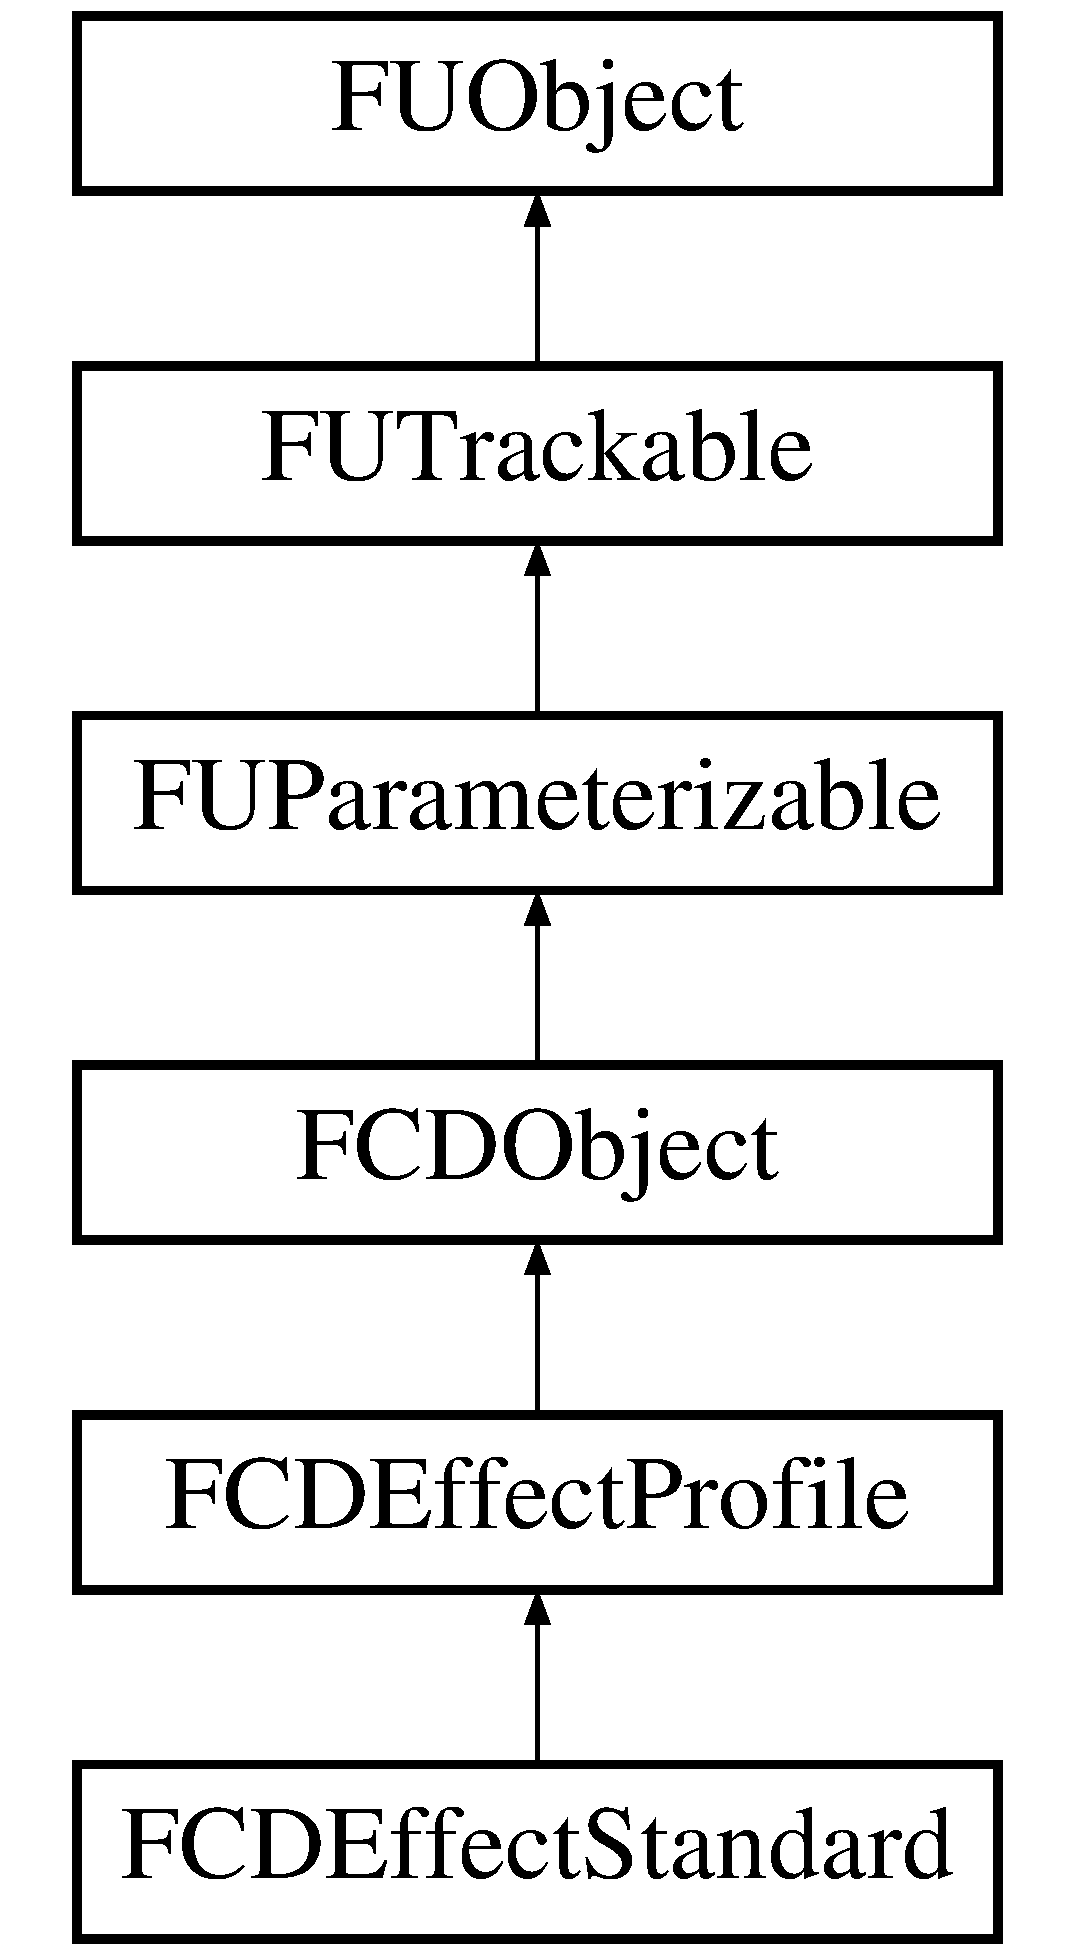
\includegraphics[height=6.000000cm]{classFCDEffectStandard}
\end{center}
\end{figure}
\subsection*{Public Types}
\begin{DoxyCompactItemize}
\item 
enum \hyperlink{classFCDEffectStandard_a0c8ec2fb06ea05212a4bb140f909b41d}{LightingType} \{ \par
\hyperlink{classFCDEffectStandard_a0c8ec2fb06ea05212a4bb140f909b41da405f6b6e4e09f73969b9566ec39a37cd}{CONSTANT}, 
\hyperlink{classFCDEffectStandard_a0c8ec2fb06ea05212a4bb140f909b41da936fa2b549fcc7833ec86e32a6d26667}{LAMBERT}, 
\hyperlink{classFCDEffectStandard_a0c8ec2fb06ea05212a4bb140f909b41dacdf2c5f91356a6c80fd8d764a433e008}{PHONG}, 
\hyperlink{classFCDEffectStandard_a0c8ec2fb06ea05212a4bb140f909b41da589842bebd4c87def8bf1a65fab074f4}{BLINN}, 
\par
\hyperlink{classFCDEffectStandard_a0c8ec2fb06ea05212a4bb140f909b41dac081dc5deede6d9e1a8293f556a5bcfc}{UNKNOWN}
 \}
\item 
enum \hyperlink{classFCDEffectStandard_a9e749ea44e9152c5671985b3e9a7c9a5}{TransparencyMode} \{ \hyperlink{classFCDEffectStandard_a9e749ea44e9152c5671985b3e9a7c9a5a68c1c4c107542260f18ff3ef04c46762}{A\_\-ONE}, 
\hyperlink{classFCDEffectStandard_a9e749ea44e9152c5671985b3e9a7c9a5a0da1b910a6c9fb9553dd131a56295411}{RGB\_\-ZERO}
 \}
\end{DoxyCompactItemize}
\subsection*{Public Member Functions}
\begin{DoxyCompactItemize}
\item 
\hyperlink{classFCDEffectStandard_a3afc0b015bd0c80e7eae0c9ba7adb5a1}{FCDEffectStandard} (\hyperlink{classFCDocument}{FCDocument} $\ast$document, \hyperlink{classFCDEffect}{FCDEffect} $\ast$parent)
\item 
virtual \hyperlink{classFCDEffectStandard_a1579bf493f5dcfa5f8b45b46c4b346f5}{$\sim$FCDEffectStandard} ()
\item 
\hyperlink{classFCDEffectStandard_a0c8ec2fb06ea05212a4bb140f909b41d}{LightingType} \hyperlink{classFCDEffectStandard_a659241e4151186c1a2f59c3583b0035d}{GetLightingType} () const 
\item 
void \hyperlink{classFCDEffectStandard_a0f1e8305c58f97a4b191bfc62db0155e}{SetLightingType} (\hyperlink{classFCDEffectStandard_a0c8ec2fb06ea05212a4bb140f909b41d}{LightingType} \_\-type)
\item 
virtual \hyperlink{namespaceFUDaeProfileType_ac10ea253a7a141708de2324a929f8a79}{FUDaeProfileType::Type} \hyperlink{classFCDEffectStandard_a5870dbcf350bd3f15781cf9ccf1095f9}{GetType} () const 
\item 
\hyperlink{classFCDTexture}{FCDTexture} $\ast$$\ast$ \hyperlink{classFCDEffectStandard_a92773e450b4ac35adfb15516e90c147f}{GetTextureBucket} (uint32 bucket)
\item 
const \hyperlink{classFCDTexture}{FCDTexture} $\ast$$\ast$ \hyperlink{classFCDEffectStandard_a427f196e14042ccc111b9ffb35649c60}{GetTextureBucket} (uint32 bucket) const 
\item 
size\_\-t \hyperlink{classFCDEffectStandard_a81a864fa18e3c0ff42abf708c9fca9ff}{GetTextureCount} (uint32 bucket) const 
\item 
\hyperlink{classFCDTexture}{FCDTexture} $\ast$ \hyperlink{classFCDEffectStandard_a502f6539d10d624b0d9d22dbe5b6cd33}{GetTexture} (uint32 bucket, size\_\-t index)
\item 
const \hyperlink{classFCDTexture}{FCDTexture} $\ast$ \hyperlink{classFCDEffectStandard_adbcd3cc63dc1898ec1a370c104724468}{GetTexture} (uint32 bucket, size\_\-t index) const 
\item 
\hyperlink{classFCDTexture}{FCDTexture} $\ast$ \hyperlink{classFCDEffectStandard_a98e73c677f68753e9630f0c9a1c3947b}{AddTexture} (uint32 bucket)
\item 
\hyperlink{classFCDEffectStandard_a547dc3b97250d3143da3a42b21543400}{DEPRECATED} (3.05A, texture-\/$>$Release()) void ReleaseTexture(FCDTexture $\ast$texture)
\item 
\hyperlink{classFCDEffectParameter}{FCDEffectParameter} $\ast$ \hyperlink{classFCDEffectStandard_a8a74e967a857025c0ffa61d8acad7565}{GetParam} (const \hyperlink{classfm_1_1stringT}{fm::string} \&semantic, bool $\ast$isFloat)
\item 
\hyperlink{classFMVector4}{FMVector4} \& \hyperlink{classFCDEffectStandard_a0ccf7493649cc1870ca48cdde33f787e}{GetTranslucencyColor} ()
\item 
const \hyperlink{classFMVector4}{FMVector4} \& \hyperlink{classFCDEffectStandard_ac42d14b615f0c8a0c7e679204a5925c2}{GetTranslucencyColor} () const 
\item 
\hyperlink{classFCDEffectParameterAnimatableT}{FCDEffectParameterColor4} $\ast$ \hyperlink{classFCDEffectStandard_ae2ef3a8540d5dd7fef08b549b6af0ae0}{GetTranslucencyColorParam} ()
\item 
const \hyperlink{classFCDEffectParameterAnimatableT}{FCDEffectParameterColor4} $\ast$ \hyperlink{classFCDEffectStandard_aa31d56cb3ebb1096bc201daaa93c269c}{GetTranslucencyColorParam} () const 
\item 
void \hyperlink{classFCDEffectStandard_af3b24d8b85f4637f3bf7fa52ef578686}{SetTranslucencyColor} (const \hyperlink{classFMVector4}{FMVector4} \&color)
\item 
float \& \hyperlink{classFCDEffectStandard_affd222f5c17b3cd49e49eae5219ea1ec}{GetTranslucencyFactor} ()
\item 
const float \& \hyperlink{classFCDEffectStandard_ab89fda3928774321d1c95bebae1bb13d}{GetTranslucencyFactor} () const 
\item 
\hyperlink{classFCDEffectParameterAnimatableT}{FCDEffectParameterFloat} $\ast$ \hyperlink{classFCDEffectStandard_a30b06e8ef8177d59483926a70389e764}{GetTranslucencyFactorParam} ()
\item 
const \hyperlink{classFCDEffectParameterAnimatableT}{FCDEffectParameterFloat} $\ast$ \hyperlink{classFCDEffectStandard_ad18eefe810f554e294a1c90044905d28}{GetTranslucencyFactorParam} () const 
\item 
void \hyperlink{classFCDEffectStandard_a622c5a44ccfcecbb21bd7181d6653f82}{SetTranslucencyFactor} (float factor)
\item 
\hyperlink{classFCDEffectStandard_a9e749ea44e9152c5671985b3e9a7c9a5}{TransparencyMode} \hyperlink{classFCDEffectStandard_a986494286968251cd067be0bad9bc85a}{GetTransparencyMode} () const 
\item 
void \hyperlink{classFCDEffectStandard_a486d7ddb1801ed110c40b7b8ece29794}{SetTransparencyMode} (\hyperlink{classFCDEffectStandard_a9e749ea44e9152c5671985b3e9a7c9a5}{TransparencyMode} mode)
\item 
float \hyperlink{classFCDEffectStandard_ae10a18d9f1c10bfd334bb914b6c664e4}{GetOpacity} () const 
\item 
\hyperlink{classFMVector4}{FMVector4} \& \hyperlink{classFCDEffectStandard_a5995a932d71c056adf95c3ac21568d52}{GetEmissionColor} ()
\item 
const \hyperlink{classFMVector4}{FMVector4} \& \hyperlink{classFCDEffectStandard_aed08c475e5e46cfc37bfe25127b9b299}{GetEmissionColor} () const 
\item 
\hyperlink{classFCDEffectParameterAnimatableT}{FCDEffectParameterColor4} $\ast$ \hyperlink{classFCDEffectStandard_ad302349aad357e6c6335e794bc583ae0}{GetEmissionColorParam} ()
\item 
const \hyperlink{classFCDEffectParameterAnimatableT}{FCDEffectParameterColor4} $\ast$ \hyperlink{classFCDEffectStandard_ae104c6a2552283803cb7642fc9a9793d}{GetEmissionColorParam} () const 
\item 
void \hyperlink{classFCDEffectStandard_a7c0cf1aef71af0350675d32a3b179b4b}{SetEmissionColor} (const \hyperlink{classFMVector4}{FMVector4} \&color)
\item 
float \& \hyperlink{classFCDEffectStandard_aa0c497d8985dfd39f9a0b31ce0e61d90}{GetEmissionFactor} ()
\item 
const float \& \hyperlink{classFCDEffectStandard_aa8b817f9737206608e87ef4ea1f9c3f8}{GetEmissionFactor} () const 
\item 
\hyperlink{classFCDEffectParameterAnimatableT}{FCDEffectParameterFloat} $\ast$ \hyperlink{classFCDEffectStandard_a0c99ef6f5a48cabe5ad756002b2b5292}{GetEmissionFactorParam} ()
\item 
const \hyperlink{classFCDEffectParameterAnimatableT}{FCDEffectParameterFloat} $\ast$ \hyperlink{classFCDEffectStandard_a39b92132f40f484cf872da1479914ae5}{GetEmissionFactorParam} () const 
\item 
void \hyperlink{classFCDEffectStandard_a8bcef4fb2c27fc2e93d584b737666ad2}{SetEmissionFactor} (float factor)
\item 
bool \hyperlink{classFCDEffectStandard_a45c0775d6da7ed652eaf36bd40bdc4cf}{IsEmissionFactor} () const 
\item 
void \hyperlink{classFCDEffectStandard_a33444405bd0753a8fc45e1104c291b7d}{SetIsEmissionFactor} (bool useFactor)
\item 
\hyperlink{classFMVector4}{FMVector4} \& \hyperlink{classFCDEffectStandard_a626e44192093159c2e352c8338279815}{GetDiffuseColor} ()
\item 
const \hyperlink{classFMVector4}{FMVector4} \& \hyperlink{classFCDEffectStandard_acc8baa8b4dc83b02d1d532cbb67b9f72}{GetDiffuseColor} () const 
\item 
\hyperlink{classFCDEffectParameterAnimatableT}{FCDEffectParameterColor4} $\ast$ \hyperlink{classFCDEffectStandard_ae93cc60fc1866767d4458fc40ae201d5}{GetDiffuseColorParam} ()
\item 
const \hyperlink{classFCDEffectParameterAnimatableT}{FCDEffectParameterColor4} $\ast$ \hyperlink{classFCDEffectStandard_a0f33f3f13917f86900c05837ed208d3f}{GetDiffuseColorParam} () const 
\item 
void \hyperlink{classFCDEffectStandard_a1382e93839dc984c16d33bfc93572ecd}{SetDiffuseColor} (const \hyperlink{classFMVector4}{FMVector4} \&color)
\item 
\hyperlink{classFMVector4}{FMVector4} \& \hyperlink{classFCDEffectStandard_aa1d50e4a0b7155f4d0c23f15af65fa12}{GetAmbientColor} ()
\item 
const \hyperlink{classFMVector4}{FMVector4} \& \hyperlink{classFCDEffectStandard_a64f7d494685ff88911848a2726f8203d}{GetAmbientColor} () const 
\item 
\hyperlink{classFCDEffectParameterAnimatableT}{FCDEffectParameterColor4} $\ast$ \hyperlink{classFCDEffectStandard_a94ddd58f63bf7a1460cac5048a2cea17}{GetAmbientColorParam} ()
\item 
const \hyperlink{classFCDEffectParameterAnimatableT}{FCDEffectParameterColor4} $\ast$ \hyperlink{classFCDEffectStandard_a5d3405fde172e64f16f53c119d82a49e}{GetAmbientColorParam} () const 
\item 
void \hyperlink{classFCDEffectStandard_a8777730e606304365b9e9db07bb7f145}{SetAmbientColor} (const \hyperlink{classFMVector4}{FMVector4} \&color)
\item 
\hyperlink{classFMVector4}{FMVector4} \& \hyperlink{classFCDEffectStandard_ae457fc42deb3a72cb9b7840364dcebe1}{GetSpecularColor} ()
\item 
const \hyperlink{classFMVector4}{FMVector4} \& \hyperlink{classFCDEffectStandard_af82d5eaf48244a5369ef8ed11213221b}{GetSpecularColor} () const 
\item 
\hyperlink{classFCDEffectParameterAnimatableT}{FCDEffectParameterColor4} $\ast$ \hyperlink{classFCDEffectStandard_a04c6cf85df02970023a6146be45f1e9f}{GetSpecularColorParam} ()
\item 
const \hyperlink{classFCDEffectParameterAnimatableT}{FCDEffectParameterColor4} $\ast$ \hyperlink{classFCDEffectStandard_a96a3021ea4315499f01b1ab5cefab2a4}{GetSpecularColorParam} () const 
\item 
void \hyperlink{classFCDEffectStandard_a01e8df7c03a4ee76e929d3e2f71aaff8}{SetSpecularColor} (const \hyperlink{classFMVector4}{FMVector4} \&color)
\item 
float \& \hyperlink{classFCDEffectStandard_ac83628e3ccf1c9215249fa4dbe1b9919}{GetSpecularFactor} ()
\item 
const float \& \hyperlink{classFCDEffectStandard_a06692330309f95f57281301feb05eedc}{GetSpecularFactor} () const 
\item 
\hyperlink{classFCDEffectParameterAnimatableT}{FCDEffectParameterFloat} $\ast$ \hyperlink{classFCDEffectStandard_a0d9fde6e676a6dafa1951043e0185ed3}{GetSpecularFactorParam} ()
\item 
const \hyperlink{classFCDEffectParameterAnimatableT}{FCDEffectParameterFloat} $\ast$ \hyperlink{classFCDEffectStandard_ac876d1261703bcdab860ee03288c8ac4}{GetSpecularFactorParam} () const 
\item 
void \hyperlink{classFCDEffectStandard_a4511986a5a68aeb47ce042c722bf8071}{SetSpecularFactor} (float factor)
\item 
float \& \hyperlink{classFCDEffectStandard_ab4654ab8fa86532fe336804f067b58a2}{GetShininess} ()
\item 
const float \& \hyperlink{classFCDEffectStandard_a07d5518f90b17601f0d729885956a56a}{GetShininess} () const 
\item 
\hyperlink{classFCDEffectParameterAnimatableT}{FCDEffectParameterFloat} $\ast$ \hyperlink{classFCDEffectStandard_a845897c93a379357f9e46224dae9e2ad}{GetShininessParam} ()
\item 
const \hyperlink{classFCDEffectParameterAnimatableT}{FCDEffectParameterFloat} $\ast$ \hyperlink{classFCDEffectStandard_a628bb62efa7a89d2d99212961103fe85}{GetShininessParam} () const 
\item 
void \hyperlink{classFCDEffectStandard_a992804e1672eefab311332f23679fb80}{SetShininess} (float \_\-shininess)
\item 
bool \hyperlink{classFCDEffectStandard_a68040795f35f89bf38331e86ba853449}{IsReflective} () const 
\item 
void \hyperlink{classFCDEffectStandard_a6fdc49307f092d5b20eb66daa48e1920}{SetReflective} (bool r)
\item 
\hyperlink{classFMVector4}{FMVector4} \& \hyperlink{classFCDEffectStandard_aa8983e27afa9a215fbb33e8edb63444d}{GetReflectivityColor} ()
\item 
const \hyperlink{classFMVector4}{FMVector4} \& \hyperlink{classFCDEffectStandard_abdd5047a0a82b40b5f13b3f666bd1c8a}{GetReflectivityColor} () const 
\item 
\hyperlink{classFCDEffectParameterAnimatableT}{FCDEffectParameterColor4} $\ast$ \hyperlink{classFCDEffectStandard_a2a69b869efe3a2d58126fff91814e157}{GetReflectivityColorParam} ()
\item 
const \hyperlink{classFCDEffectParameterAnimatableT}{FCDEffectParameterColor4} $\ast$ \hyperlink{classFCDEffectStandard_ab994ac2a861c5066cfedf435294286e3}{GetReflectivityColorParam} () const 
\item 
void \hyperlink{classFCDEffectStandard_a7da791434dd5676d6ab09c860829fb47}{SetReflectivityColor} (const \hyperlink{classFMVector4}{FMVector4} \&color)
\item 
float \& \hyperlink{classFCDEffectStandard_a45478829ccbe6b25b9f3550fc4e04c4a}{GetReflectivityFactor} ()
\item 
const float \& \hyperlink{classFCDEffectStandard_a2c2f46d7834a17771b18a3f27dab73d4}{GetReflectivityFactor} () const 
\item 
\hyperlink{classFCDEffectParameterAnimatableT}{FCDEffectParameterFloat} $\ast$ \hyperlink{classFCDEffectStandard_a1ace9e6e264bcf10bd2ac48ecb7fe11f}{GetReflectivityFactorParam} ()
\item 
const \hyperlink{classFCDEffectParameterAnimatableT}{FCDEffectParameterFloat} $\ast$ \hyperlink{classFCDEffectStandard_a0de5e4f9582f94fc413d563a6abc2fc5}{GetReflectivityFactorParam} () const 
\item 
void \hyperlink{classFCDEffectStandard_a5d44f575161556c7e32fd01db0cce3b5}{SetReflectivityFactor} (float factor)
\item 
float \hyperlink{classFCDEffectStandard_a0665515f47cf93f0df913f5d345f04c6}{GetReflectivity} () const 
\item 
bool \hyperlink{classFCDEffectStandard_a0dc0c78d14a0beb924cf7fe971ee7bda}{IsRefractive} () const 
\item 
void \hyperlink{classFCDEffectStandard_ab658aa9ac8d10afc1cd3b83abc81d571}{SetRefractive} (bool r)
\item 
float \& \hyperlink{classFCDEffectStandard_aba2edd070372a49560528d901dbf66cd}{GetIndexOfRefraction} ()
\item 
const float \& \hyperlink{classFCDEffectStandard_a749723323b4de3691eabafef079a9342}{GetIndexOfRefraction} () const 
\item 
\hyperlink{classFCDEffectParameterAnimatableT}{FCDEffectParameterFloat} $\ast$ \hyperlink{classFCDEffectStandard_a77001b0842bf3bbe4c904369a4801302}{GetIndexOfRefractionParam} ()
\item 
const \hyperlink{classFCDEffectParameterAnimatableT}{FCDEffectParameterFloat} $\ast$ \hyperlink{classFCDEffectStandard_a45c8ea77e71387409eeba9dfd9b54ad7}{GetIndexOfRefractionParam} () const 
\item 
void \hyperlink{classFCDEffectStandard_af60264112cb42d1f00d8b6af09ffc43e}{SetIndexOfRefraction} (float index)
\item 
virtual \hyperlink{classFCDEffectProfile}{FCDEffectProfile} $\ast$ \hyperlink{classFCDEffectStandard_aeadbfb97cdfd733a09a564f457020b66}{Clone} (\hyperlink{classFCDEffectProfile}{FCDEffectProfile} $\ast$clone=NULL) const 
\item 
\hyperlink{classFCDEffectStandard_a40ab2cc34bd3cf5d3f622a8dcf9e9fcd}{DEPRECATED} (3.05A, not recommended) void Flatten()
\item 
void \hyperlink{classFCDEffectStandard_ab7d158f54a2b6d23ed71faa4a3f1598f}{AddExtraAttribute} (const char $\ast$profile, const char $\ast$key, const fchar $\ast$value)
\item 
const fchar $\ast$ \hyperlink{classFCDEffectStandard_a115b0bfdfa3fb1712a51b26607ae8d37}{GetExtraAttribute} (const char $\ast$profile, const char $\ast$key) const 
\end{DoxyCompactItemize}
\subsection*{Static Public Attributes}
\begin{DoxyCompactItemize}
\item 
\hypertarget{classFCDEffectStandard_af1b5eea66dd078d98feb51ba084900b9}{
static const \hyperlink{classfm_1_1stringT}{fm::string} {\bfseries EmissionColorSemantic}}
\label{classFCDEffectStandard_af1b5eea66dd078d98feb51ba084900b9}

\item 
\hypertarget{classFCDEffectStandard_aa1b823e9f78a3c319724d8436b5ef2c2}{
static const \hyperlink{classfm_1_1stringT}{fm::string} {\bfseries EmissionFactorSemantic}}
\label{classFCDEffectStandard_aa1b823e9f78a3c319724d8436b5ef2c2}

\item 
\hypertarget{classFCDEffectStandard_a86fdcb920b4446d4f1d3cec60f7d1deb}{
static const \hyperlink{classfm_1_1stringT}{fm::string} {\bfseries ReflectivityColorSemantic}}
\label{classFCDEffectStandard_a86fdcb920b4446d4f1d3cec60f7d1deb}

\item 
\hypertarget{classFCDEffectStandard_abff5c430934991b46c9b25d508b84b55}{
static const \hyperlink{classfm_1_1stringT}{fm::string} {\bfseries ReflectivityFactorSemantic}}
\label{classFCDEffectStandard_abff5c430934991b46c9b25d508b84b55}

\item 
\hypertarget{classFCDEffectStandard_a06389abe5788d824d94b3563465b39ef}{
static const \hyperlink{classfm_1_1stringT}{fm::string} {\bfseries IndexOfRefractionSemantic}}
\label{classFCDEffectStandard_a06389abe5788d824d94b3563465b39ef}

\item 
\hypertarget{classFCDEffectStandard_adc9fcb8d989d8f8881bc7aa850aaadb8}{
static const \hyperlink{classfm_1_1stringT}{fm::string} {\bfseries TranslucencyColorSemantic}}
\label{classFCDEffectStandard_adc9fcb8d989d8f8881bc7aa850aaadb8}

\item 
\hypertarget{classFCDEffectStandard_a8ffdda8d54e66ff7f4b88cc4062dba7e}{
static const \hyperlink{classfm_1_1stringT}{fm::string} {\bfseries TranslucencyFactorSemantic}}
\label{classFCDEffectStandard_a8ffdda8d54e66ff7f4b88cc4062dba7e}

\item 
\hypertarget{classFCDEffectStandard_ae4b1207a87546418dba682903c906135}{
static const \hyperlink{classfm_1_1stringT}{fm::string} {\bfseries DiffuseColorSemantic}}
\label{classFCDEffectStandard_ae4b1207a87546418dba682903c906135}

\item 
\hypertarget{classFCDEffectStandard_a85cfe6b55efc19e678b11f0d74686a62}{
static const \hyperlink{classfm_1_1stringT}{fm::string} {\bfseries AmbientColorSemantic}}
\label{classFCDEffectStandard_a85cfe6b55efc19e678b11f0d74686a62}

\item 
\hypertarget{classFCDEffectStandard_a0db5a8e39550be273a04a893c2aeb1f9}{
static const \hyperlink{classfm_1_1stringT}{fm::string} {\bfseries SpecularColorSemantic}}
\label{classFCDEffectStandard_a0db5a8e39550be273a04a893c2aeb1f9}

\item 
\hypertarget{classFCDEffectStandard_ae7bb65e68aaf9a9277139fdc84af9b57}{
static const \hyperlink{classfm_1_1stringT}{fm::string} {\bfseries SpecularFactorSemantic}}
\label{classFCDEffectStandard_ae7bb65e68aaf9a9277139fdc84af9b57}

\item 
\hypertarget{classFCDEffectStandard_ad0047e7193363514924cf4cb5836e2cb}{
static const \hyperlink{classfm_1_1stringT}{fm::string} {\bfseries ShininessSemantic}}
\label{classFCDEffectStandard_ad0047e7193363514924cf4cb5836e2cb}

\end{DoxyCompactItemize}


\subsection{Detailed Description}
A COMMON profile effect description.

The COMMON effect profile holds the information necessary to render your polygon sets using the well-\/defined lighting models.

COLLADA supports four lighting models: constant, Lambert, Phong and Blinn. 

\subsection{Member Enumeration Documentation}
\hypertarget{classFCDEffectStandard_a0c8ec2fb06ea05212a4bb140f909b41d}{
\index{FCDEffectStandard@{FCDEffectStandard}!LightingType@{LightingType}}
\index{LightingType@{LightingType}!FCDEffectStandard@{FCDEffectStandard}}
\subsubsection[{LightingType}]{\setlength{\rightskip}{0pt plus 5cm}enum {\bf FCDEffectStandard::LightingType}}}
\label{classFCDEffectStandard_a0c8ec2fb06ea05212a4bb140f909b41d}
The list of the lighting models supported by the COMMON profile of COLLADA. \begin{Desc}
\item[Enumerator: ]\par
\begin{description}
\index{CONSTANT@{CONSTANT}!FCDEffectStandard@{FCDEffectStandard}}\index{FCDEffectStandard@{FCDEffectStandard}!CONSTANT@{CONSTANT}}\item[{\em 
\hypertarget{classFCDEffectStandard_a0c8ec2fb06ea05212a4bb140f909b41da405f6b6e4e09f73969b9566ec39a37cd}{
CONSTANT}
\label{classFCDEffectStandard_a0c8ec2fb06ea05212a4bb140f909b41da405f6b6e4e09f73969b9566ec39a37cd}
}]The constant lighting model. This lighting model uses the emissive color everywhere, without any complex lighting calculations. It also uses the translucency factor and the translucency color, by multiplying them together and applying them to your standard alpha channel according to the final lighting color. \index{LAMBERT@{LAMBERT}!FCDEffectStandard@{FCDEffectStandard}}\index{FCDEffectStandard@{FCDEffectStandard}!LAMBERT@{LAMBERT}}\item[{\em 
\hypertarget{classFCDEffectStandard_a0c8ec2fb06ea05212a4bb140f909b41da936fa2b549fcc7833ec86e32a6d26667}{
LAMBERT}
\label{classFCDEffectStandard_a0c8ec2fb06ea05212a4bb140f909b41da936fa2b549fcc7833ec86e32a6d26667}
}]The Lambert lighting model. This lighting model improves on the constant lighting model by using the dot-\/product between the normalized light vectors and the polygon normals to determine how much light should affect each polygon. This value is multiplied to the diffuse color and (1 + the ambient color). \index{PHONG@{PHONG}!FCDEffectStandard@{FCDEffectStandard}}\index{FCDEffectStandard@{FCDEffectStandard}!PHONG@{PHONG}}\item[{\em 
\hypertarget{classFCDEffectStandard_a0c8ec2fb06ea05212a4bb140f909b41dacdf2c5f91356a6c80fd8d764a433e008}{
PHONG}
\label{classFCDEffectStandard_a0c8ec2fb06ea05212a4bb140f909b41dacdf2c5f91356a6c80fd8d764a433e008}
}]The Phong lighting model. This lighting model improves on the Lambert lighting model by calculating how much light is reflected by the polygons into the viewer's eye. For this calculation, the shininess, the specular color and the reflectivity is used. \index{BLINN@{BLINN}!FCDEffectStandard@{FCDEffectStandard}}\index{FCDEffectStandard@{FCDEffectStandard}!BLINN@{BLINN}}\item[{\em 
\hypertarget{classFCDEffectStandard_a0c8ec2fb06ea05212a4bb140f909b41da589842bebd4c87def8bf1a65fab074f4}{
BLINN}
\label{classFCDEffectStandard_a0c8ec2fb06ea05212a4bb140f909b41da589842bebd4c87def8bf1a65fab074f4}
}]The Blinn lighting model. This lighting model improves on the Lambert lighting model by calculating how much light is reflected by the polygons into the viewer's eye. For this calculation, the shininess, the specular color and the reflectivity is used. \index{UNKNOWN@{UNKNOWN}!FCDEffectStandard@{FCDEffectStandard}}\index{FCDEffectStandard@{FCDEffectStandard}!UNKNOWN@{UNKNOWN}}\item[{\em 
\hypertarget{classFCDEffectStandard_a0c8ec2fb06ea05212a4bb140f909b41dac081dc5deede6d9e1a8293f556a5bcfc}{
UNKNOWN}
\label{classFCDEffectStandard_a0c8ec2fb06ea05212a4bb140f909b41dac081dc5deede6d9e1a8293f556a5bcfc}
}]Not a valid lighting model. \end{description}
\end{Desc}

\hypertarget{classFCDEffectStandard_a9e749ea44e9152c5671985b3e9a7c9a5}{
\index{FCDEffectStandard@{FCDEffectStandard}!TransparencyMode@{TransparencyMode}}
\index{TransparencyMode@{TransparencyMode}!FCDEffectStandard@{FCDEffectStandard}}
\subsubsection[{TransparencyMode}]{\setlength{\rightskip}{0pt plus 5cm}enum {\bf FCDEffectStandard::TransparencyMode}}}
\label{classFCDEffectStandard_a9e749ea44e9152c5671985b3e9a7c9a5}
The list of transparency modes supported by the COMMON profile of COLLADA. \begin{Desc}
\item[Enumerator: ]\par
\begin{description}
\index{A\_\-ONE@{A\_\-ONE}!FCDEffectStandard@{FCDEffectStandard}}\index{FCDEffectStandard@{FCDEffectStandard}!A\_\-ONE@{A\_\-ONE}}\item[{\em 
\hypertarget{classFCDEffectStandard_a9e749ea44e9152c5671985b3e9a7c9a5a68c1c4c107542260f18ff3ef04c46762}{
A\_\-ONE}
\label{classFCDEffectStandard_a9e749ea44e9152c5671985b3e9a7c9a5a68c1c4c107542260f18ff3ef04c46762}
}]Takes the transparency information from the color's alpha channel, where the value 1.0 is opaque. \index{RGB\_\-ZERO@{RGB\_\-ZERO}!FCDEffectStandard@{FCDEffectStandard}}\index{FCDEffectStandard@{FCDEffectStandard}!RGB\_\-ZERO@{RGB\_\-ZERO}}\item[{\em 
\hypertarget{classFCDEffectStandard_a9e749ea44e9152c5671985b3e9a7c9a5a0da1b910a6c9fb9553dd131a56295411}{
RGB\_\-ZERO}
\label{classFCDEffectStandard_a9e749ea44e9152c5671985b3e9a7c9a5a0da1b910a6c9fb9553dd131a56295411}
}]Takes the transparency information from the color's red, green, and blue channels, where the value 0.0 is opaque, with each channel modulated independently. \end{description}
\end{Desc}



\subsection{Constructor \& Destructor Documentation}
\hypertarget{classFCDEffectStandard_a3afc0b015bd0c80e7eae0c9ba7adb5a1}{
\index{FCDEffectStandard@{FCDEffectStandard}!FCDEffectStandard@{FCDEffectStandard}}
\index{FCDEffectStandard@{FCDEffectStandard}!FCDEffectStandard@{FCDEffectStandard}}
\subsubsection[{FCDEffectStandard}]{\setlength{\rightskip}{0pt plus 5cm}FCDEffectStandard::FCDEffectStandard (
\begin{DoxyParamCaption}
\item[{{\bf FCDocument} $\ast$}]{ document, }
\item[{{\bf FCDEffect} $\ast$}]{ parent}
\end{DoxyParamCaption}
)}}
\label{classFCDEffectStandard_a3afc0b015bd0c80e7eae0c9ba7adb5a1}
Constructor: do not use directly. Instead, use the \hyperlink{classFCDEffect_abe53b1e58ce5469b28f63b5155703a95}{FCDEffect::AddProfile} function with the \hyperlink{namespaceFUDaeProfileType_ac10ea253a7a141708de2324a929f8a79ad8aa33a3586c77ac1163a8840cf2ac38}{FUDaeProfileType::COMMON} parameter. 
\begin{DoxyParams}{Parameters}
\item[{\em document}]The \hyperlink{namespaceFCollada}{FCollada} document that owns this effect standard. \item[{\em parent}]The effect that contains this profile. \end{DoxyParams}
\hypertarget{classFCDEffectStandard_a1579bf493f5dcfa5f8b45b46c4b346f5}{
\index{FCDEffectStandard@{FCDEffectStandard}!$\sim$FCDEffectStandard@{$\sim$FCDEffectStandard}}
\index{$\sim$FCDEffectStandard@{$\sim$FCDEffectStandard}!FCDEffectStandard@{FCDEffectStandard}}
\subsubsection[{$\sim$FCDEffectStandard}]{\setlength{\rightskip}{0pt plus 5cm}FCDEffectStandard::$\sim$FCDEffectStandard (
\begin{DoxyParamCaption}
{}
\end{DoxyParamCaption}
)\hspace{0.3cm}{\ttfamily  \mbox{[}virtual\mbox{]}}}}
\label{classFCDEffectStandard_a1579bf493f5dcfa5f8b45b46c4b346f5}
Destructor. 

\subsection{Member Function Documentation}
\hypertarget{classFCDEffectStandard_ab7d158f54a2b6d23ed71faa4a3f1598f}{
\index{FCDEffectStandard@{FCDEffectStandard}!AddExtraAttribute@{AddExtraAttribute}}
\index{AddExtraAttribute@{AddExtraAttribute}!FCDEffectStandard@{FCDEffectStandard}}
\subsubsection[{AddExtraAttribute}]{\setlength{\rightskip}{0pt plus 5cm}void FCDEffectStandard::AddExtraAttribute (
\begin{DoxyParamCaption}
\item[{const char $\ast$}]{ profile, }
\item[{const char $\ast$}]{ key, }
\item[{const fchar $\ast$}]{ value}
\end{DoxyParamCaption}
)}}
\label{classFCDEffectStandard_ab7d158f54a2b6d23ed71faa4a3f1598f}
Adds an extra attribute to the given profile 
\begin{DoxyParams}{Parameters}
\item[{\em profile}]The profile in which to insert the attribute. \item[{\em key}]The attribute's key \item[{\em value}]The attribute's value \end{DoxyParams}
\hypertarget{classFCDEffectStandard_a98e73c677f68753e9630f0c9a1c3947b}{
\index{FCDEffectStandard@{FCDEffectStandard}!AddTexture@{AddTexture}}
\index{AddTexture@{AddTexture}!FCDEffectStandard@{FCDEffectStandard}}
\subsubsection[{AddTexture}]{\setlength{\rightskip}{0pt plus 5cm}{\bf FCDTexture} $\ast$ FCDEffectStandard::AddTexture (
\begin{DoxyParamCaption}
\item[{uint32}]{ bucket}
\end{DoxyParamCaption}
)}}
\label{classFCDEffectStandard_a98e73c677f68753e9630f0c9a1c3947b}
Adds a texture to a specific channel. 
\begin{DoxyParams}{Parameters}
\item[{\em bucket}]A texture channel index. This index should match one of the values in the \hyperlink{namespaceFUDaeTextureChannel}{FUDaeTextureChannel} enum. \end{DoxyParams}
\begin{DoxyReturn}{Returns}
The new texture. This pointer will be NULL if the bucket is out-\/of-\/bounds. 
\end{DoxyReturn}
\hypertarget{classFCDEffectStandard_aeadbfb97cdfd733a09a564f457020b66}{
\index{FCDEffectStandard@{FCDEffectStandard}!Clone@{Clone}}
\index{Clone@{Clone}!FCDEffectStandard@{FCDEffectStandard}}
\subsubsection[{Clone}]{\setlength{\rightskip}{0pt plus 5cm}{\bf FCDEffectProfile} $\ast$ FCDEffectStandard::Clone (
\begin{DoxyParamCaption}
\item[{{\bf FCDEffectProfile} $\ast$}]{ clone = {\ttfamily NULL}}
\end{DoxyParamCaption}
) const\hspace{0.3cm}{\ttfamily  \mbox{[}virtual\mbox{]}}}}
\label{classFCDEffectStandard_aeadbfb97cdfd733a09a564f457020b66}
Clones the COMMON profile effect and its parameters. 
\begin{DoxyParams}{Parameters}
\item[{\em clone}]The cloned profile. If this pointer is NULL, a new COMMON profile is created and you will need to release this pointer. \end{DoxyParams}
\begin{DoxyReturn}{Returns}
The cloned COMMON profile. 
\end{DoxyReturn}


Reimplemented from \hyperlink{classFCDEffectProfile_ab7641c9671098f6966146798e61bb098}{FCDEffectProfile}.

\hypertarget{classFCDEffectStandard_a547dc3b97250d3143da3a42b21543400}{
\index{FCDEffectStandard@{FCDEffectStandard}!DEPRECATED@{DEPRECATED}}
\index{DEPRECATED@{DEPRECATED}!FCDEffectStandard@{FCDEffectStandard}}
\subsubsection[{DEPRECATED}]{\setlength{\rightskip}{0pt plus 5cm}FCDEffectStandard::DEPRECATED (
\begin{DoxyParamCaption}
\item[{3.}]{ 05A, }
\item[{texture-\/$>$}]{ Release()}
\end{DoxyParamCaption}
)\hspace{0.3cm}{\ttfamily  \mbox{[}inline\mbox{]}}}}
\label{classFCDEffectStandard_a547dc3b97250d3143da3a42b21543400}
Releases a texture contained within this effect profile. 
\begin{DoxyParams}{Parameters}
\item[{\em texture}]The texture to release. \end{DoxyParams}
\hypertarget{classFCDEffectStandard_a40ab2cc34bd3cf5d3f622a8dcf9e9fcd}{
\index{FCDEffectStandard@{FCDEffectStandard}!DEPRECATED@{DEPRECATED}}
\index{DEPRECATED@{DEPRECATED}!FCDEffectStandard@{FCDEffectStandard}}
\subsubsection[{DEPRECATED}]{\setlength{\rightskip}{0pt plus 5cm}FCDEffectStandard::DEPRECATED (
\begin{DoxyParamCaption}
\item[{3.}]{ 05A, }
\item[{not}]{ recommended}
\end{DoxyParamCaption}
)\hspace{0.3cm}{\ttfamily  \mbox{[}inline\mbox{]}}}}
\label{classFCDEffectStandard_a40ab2cc34bd3cf5d3f622a8dcf9e9fcd}
\mbox{[}INTERNAL\mbox{]} Flattens the profile. Does nothing on the common profile. 

Reimplemented from \hyperlink{classFCDEffectProfile_aadc7e65fa145af53ec2bf47c6de550f2}{FCDEffectProfile}.

\hypertarget{classFCDEffectStandard_aa1d50e4a0b7155f4d0c23f15af65fa12}{
\index{FCDEffectStandard@{FCDEffectStandard}!GetAmbientColor@{GetAmbientColor}}
\index{GetAmbientColor@{GetAmbientColor}!FCDEffectStandard@{FCDEffectStandard}}
\subsubsection[{GetAmbientColor}]{\setlength{\rightskip}{0pt plus 5cm}{\bf FMVector4}\& FCDEffectStandard::GetAmbientColor (
\begin{DoxyParamCaption}
{}
\end{DoxyParamCaption}
)\hspace{0.3cm}{\ttfamily  \mbox{[}inline\mbox{]}}}}
\label{classFCDEffectStandard_aa1d50e4a0b7155f4d0c23f15af65fa12}
Retrieves the ambient color. This value is used in the Lambert lighting model. \begin{DoxyReturn}{Returns}
The ambient color. 
\end{DoxyReturn}
\hypertarget{classFCDEffectStandard_a64f7d494685ff88911848a2726f8203d}{
\index{FCDEffectStandard@{FCDEffectStandard}!GetAmbientColor@{GetAmbientColor}}
\index{GetAmbientColor@{GetAmbientColor}!FCDEffectStandard@{FCDEffectStandard}}
\subsubsection[{GetAmbientColor}]{\setlength{\rightskip}{0pt plus 5cm}const {\bf FMVector4}\& FCDEffectStandard::GetAmbientColor (
\begin{DoxyParamCaption}
{}
\end{DoxyParamCaption}
) const\hspace{0.3cm}{\ttfamily  \mbox{[}inline\mbox{]}}}}
\label{classFCDEffectStandard_a64f7d494685ff88911848a2726f8203d}
See above. \hypertarget{classFCDEffectStandard_a94ddd58f63bf7a1460cac5048a2cea17}{
\index{FCDEffectStandard@{FCDEffectStandard}!GetAmbientColorParam@{GetAmbientColorParam}}
\index{GetAmbientColorParam@{GetAmbientColorParam}!FCDEffectStandard@{FCDEffectStandard}}
\subsubsection[{GetAmbientColorParam}]{\setlength{\rightskip}{0pt plus 5cm}{\bf FCDEffectParameterColor4}$\ast$ FCDEffectStandard::GetAmbientColorParam (
\begin{DoxyParamCaption}
{}
\end{DoxyParamCaption}
)\hspace{0.3cm}{\ttfamily  \mbox{[}inline\mbox{]}}}}
\label{classFCDEffectStandard_a94ddd58f63bf7a1460cac5048a2cea17}
Retrieves the parameter pointer that contains the ambient color. Use this function to modify the value, the semantic, reference or annotations of the parameter. Note: in order to be linked with the profile\_\-COMMON's parameter list, the parameter needs to have a valid semantic and reference. Otherwise it is treated as a simple color. \begin{DoxyReturn}{Returns}
The parameter that contains the ambient color. 
\end{DoxyReturn}
\hypertarget{classFCDEffectStandard_a5d3405fde172e64f16f53c119d82a49e}{
\index{FCDEffectStandard@{FCDEffectStandard}!GetAmbientColorParam@{GetAmbientColorParam}}
\index{GetAmbientColorParam@{GetAmbientColorParam}!FCDEffectStandard@{FCDEffectStandard}}
\subsubsection[{GetAmbientColorParam}]{\setlength{\rightskip}{0pt plus 5cm}const {\bf FCDEffectParameterColor4}$\ast$ FCDEffectStandard::GetAmbientColorParam (
\begin{DoxyParamCaption}
{}
\end{DoxyParamCaption}
) const\hspace{0.3cm}{\ttfamily  \mbox{[}inline\mbox{]}}}}
\label{classFCDEffectStandard_a5d3405fde172e64f16f53c119d82a49e}
See above. \hypertarget{classFCDEffectStandard_a626e44192093159c2e352c8338279815}{
\index{FCDEffectStandard@{FCDEffectStandard}!GetDiffuseColor@{GetDiffuseColor}}
\index{GetDiffuseColor@{GetDiffuseColor}!FCDEffectStandard@{FCDEffectStandard}}
\subsubsection[{GetDiffuseColor}]{\setlength{\rightskip}{0pt plus 5cm}{\bf FMVector4}\& FCDEffectStandard::GetDiffuseColor (
\begin{DoxyParamCaption}
{}
\end{DoxyParamCaption}
)\hspace{0.3cm}{\ttfamily  \mbox{[}inline\mbox{]}}}}
\label{classFCDEffectStandard_a626e44192093159c2e352c8338279815}
Retrieves the diffuse color. This value is used in the Lambert lighting model. \begin{DoxyReturn}{Returns}
The diffuse color. 
\end{DoxyReturn}
\hypertarget{classFCDEffectStandard_acc8baa8b4dc83b02d1d532cbb67b9f72}{
\index{FCDEffectStandard@{FCDEffectStandard}!GetDiffuseColor@{GetDiffuseColor}}
\index{GetDiffuseColor@{GetDiffuseColor}!FCDEffectStandard@{FCDEffectStandard}}
\subsubsection[{GetDiffuseColor}]{\setlength{\rightskip}{0pt plus 5cm}const {\bf FMVector4}\& FCDEffectStandard::GetDiffuseColor (
\begin{DoxyParamCaption}
{}
\end{DoxyParamCaption}
) const\hspace{0.3cm}{\ttfamily  \mbox{[}inline\mbox{]}}}}
\label{classFCDEffectStandard_acc8baa8b4dc83b02d1d532cbb67b9f72}
See above. \hypertarget{classFCDEffectStandard_ae93cc60fc1866767d4458fc40ae201d5}{
\index{FCDEffectStandard@{FCDEffectStandard}!GetDiffuseColorParam@{GetDiffuseColorParam}}
\index{GetDiffuseColorParam@{GetDiffuseColorParam}!FCDEffectStandard@{FCDEffectStandard}}
\subsubsection[{GetDiffuseColorParam}]{\setlength{\rightskip}{0pt plus 5cm}{\bf FCDEffectParameterColor4}$\ast$ FCDEffectStandard::GetDiffuseColorParam (
\begin{DoxyParamCaption}
{}
\end{DoxyParamCaption}
)\hspace{0.3cm}{\ttfamily  \mbox{[}inline\mbox{]}}}}
\label{classFCDEffectStandard_ae93cc60fc1866767d4458fc40ae201d5}
Retrieves the parameter pointer that contains the diffuse color. Use this function to modify the value, the semantic, reference or annotations of the parameter. Note: in order to be linked with the profile\_\-COMMON's parameter list, the parameter needs to have a valid semantic and reference. Otherwise it is treated as a simple color. \begin{DoxyReturn}{Returns}
The parameter that contains the diffuse color. 
\end{DoxyReturn}
\hypertarget{classFCDEffectStandard_a0f33f3f13917f86900c05837ed208d3f}{
\index{FCDEffectStandard@{FCDEffectStandard}!GetDiffuseColorParam@{GetDiffuseColorParam}}
\index{GetDiffuseColorParam@{GetDiffuseColorParam}!FCDEffectStandard@{FCDEffectStandard}}
\subsubsection[{GetDiffuseColorParam}]{\setlength{\rightskip}{0pt plus 5cm}const {\bf FCDEffectParameterColor4}$\ast$ FCDEffectStandard::GetDiffuseColorParam (
\begin{DoxyParamCaption}
{}
\end{DoxyParamCaption}
) const\hspace{0.3cm}{\ttfamily  \mbox{[}inline\mbox{]}}}}
\label{classFCDEffectStandard_a0f33f3f13917f86900c05837ed208d3f}
See above. \hypertarget{classFCDEffectStandard_a5995a932d71c056adf95c3ac21568d52}{
\index{FCDEffectStandard@{FCDEffectStandard}!GetEmissionColor@{GetEmissionColor}}
\index{GetEmissionColor@{GetEmissionColor}!FCDEffectStandard@{FCDEffectStandard}}
\subsubsection[{GetEmissionColor}]{\setlength{\rightskip}{0pt plus 5cm}{\bf FMVector4}\& FCDEffectStandard::GetEmissionColor (
\begin{DoxyParamCaption}
{}
\end{DoxyParamCaption}
)\hspace{0.3cm}{\ttfamily  \mbox{[}inline\mbox{]}}}}
\label{classFCDEffectStandard_a5995a932d71c056adf95c3ac21568d52}
Retrieves the base emission/self-\/illumination color. This value must be multiplied with the emission factor to get the real emission color. This value is used in all lighting models. \begin{DoxyReturn}{Returns}
The base emission color. 
\end{DoxyReturn}
\hypertarget{classFCDEffectStandard_aed08c475e5e46cfc37bfe25127b9b299}{
\index{FCDEffectStandard@{FCDEffectStandard}!GetEmissionColor@{GetEmissionColor}}
\index{GetEmissionColor@{GetEmissionColor}!FCDEffectStandard@{FCDEffectStandard}}
\subsubsection[{GetEmissionColor}]{\setlength{\rightskip}{0pt plus 5cm}const {\bf FMVector4}\& FCDEffectStandard::GetEmissionColor (
\begin{DoxyParamCaption}
{}
\end{DoxyParamCaption}
) const\hspace{0.3cm}{\ttfamily  \mbox{[}inline\mbox{]}}}}
\label{classFCDEffectStandard_aed08c475e5e46cfc37bfe25127b9b299}
See above. \hypertarget{classFCDEffectStandard_ad302349aad357e6c6335e794bc583ae0}{
\index{FCDEffectStandard@{FCDEffectStandard}!GetEmissionColorParam@{GetEmissionColorParam}}
\index{GetEmissionColorParam@{GetEmissionColorParam}!FCDEffectStandard@{FCDEffectStandard}}
\subsubsection[{GetEmissionColorParam}]{\setlength{\rightskip}{0pt plus 5cm}{\bf FCDEffectParameterColor4}$\ast$ FCDEffectStandard::GetEmissionColorParam (
\begin{DoxyParamCaption}
{}
\end{DoxyParamCaption}
)\hspace{0.3cm}{\ttfamily  \mbox{[}inline\mbox{]}}}}
\label{classFCDEffectStandard_ad302349aad357e6c6335e794bc583ae0}
Retrieves the parameter pointer that contains the emission color. Use this function to modify the value, the semantic, reference or annotations of the parameter. Note: in order to be linked with the profile\_\-COMMON's parameter list, the parameter needs to have a valid semantic and reference. Otherwise it is treated as a simple color. \begin{DoxyReturn}{Returns}
The parameter that contains the emission color. 
\end{DoxyReturn}
\hypertarget{classFCDEffectStandard_ae104c6a2552283803cb7642fc9a9793d}{
\index{FCDEffectStandard@{FCDEffectStandard}!GetEmissionColorParam@{GetEmissionColorParam}}
\index{GetEmissionColorParam@{GetEmissionColorParam}!FCDEffectStandard@{FCDEffectStandard}}
\subsubsection[{GetEmissionColorParam}]{\setlength{\rightskip}{0pt plus 5cm}const {\bf FCDEffectParameterColor4}$\ast$ FCDEffectStandard::GetEmissionColorParam (
\begin{DoxyParamCaption}
{}
\end{DoxyParamCaption}
) const\hspace{0.3cm}{\ttfamily  \mbox{[}inline\mbox{]}}}}
\label{classFCDEffectStandard_ae104c6a2552283803cb7642fc9a9793d}
See above. \hypertarget{classFCDEffectStandard_aa0c497d8985dfd39f9a0b31ce0e61d90}{
\index{FCDEffectStandard@{FCDEffectStandard}!GetEmissionFactor@{GetEmissionFactor}}
\index{GetEmissionFactor@{GetEmissionFactor}!FCDEffectStandard@{FCDEffectStandard}}
\subsubsection[{GetEmissionFactor}]{\setlength{\rightskip}{0pt plus 5cm}float\& FCDEffectStandard::GetEmissionFactor (
\begin{DoxyParamCaption}
{}
\end{DoxyParamCaption}
)\hspace{0.3cm}{\ttfamily  \mbox{[}inline\mbox{]}}}}
\label{classFCDEffectStandard_aa0c497d8985dfd39f9a0b31ce0e61d90}
Retrieves the emission/self-\/illumination factor. This value must be multiplied with the base emission color to get the real emission color. \begin{DoxyReturn}{Returns}
The emission factor. 
\end{DoxyReturn}
\hypertarget{classFCDEffectStandard_aa8b817f9737206608e87ef4ea1f9c3f8}{
\index{FCDEffectStandard@{FCDEffectStandard}!GetEmissionFactor@{GetEmissionFactor}}
\index{GetEmissionFactor@{GetEmissionFactor}!FCDEffectStandard@{FCDEffectStandard}}
\subsubsection[{GetEmissionFactor}]{\setlength{\rightskip}{0pt plus 5cm}const float\& FCDEffectStandard::GetEmissionFactor (
\begin{DoxyParamCaption}
{}
\end{DoxyParamCaption}
) const\hspace{0.3cm}{\ttfamily  \mbox{[}inline\mbox{]}}}}
\label{classFCDEffectStandard_aa8b817f9737206608e87ef4ea1f9c3f8}
See above. \hypertarget{classFCDEffectStandard_a39b92132f40f484cf872da1479914ae5}{
\index{FCDEffectStandard@{FCDEffectStandard}!GetEmissionFactorParam@{GetEmissionFactorParam}}
\index{GetEmissionFactorParam@{GetEmissionFactorParam}!FCDEffectStandard@{FCDEffectStandard}}
\subsubsection[{GetEmissionFactorParam}]{\setlength{\rightskip}{0pt plus 5cm}const {\bf FCDEffectParameterFloat}$\ast$ FCDEffectStandard::GetEmissionFactorParam (
\begin{DoxyParamCaption}
{}
\end{DoxyParamCaption}
) const\hspace{0.3cm}{\ttfamily  \mbox{[}inline\mbox{]}}}}
\label{classFCDEffectStandard_a39b92132f40f484cf872da1479914ae5}
See above. \hypertarget{classFCDEffectStandard_a0c99ef6f5a48cabe5ad756002b2b5292}{
\index{FCDEffectStandard@{FCDEffectStandard}!GetEmissionFactorParam@{GetEmissionFactorParam}}
\index{GetEmissionFactorParam@{GetEmissionFactorParam}!FCDEffectStandard@{FCDEffectStandard}}
\subsubsection[{GetEmissionFactorParam}]{\setlength{\rightskip}{0pt plus 5cm}{\bf FCDEffectParameterFloat}$\ast$ FCDEffectStandard::GetEmissionFactorParam (
\begin{DoxyParamCaption}
{}
\end{DoxyParamCaption}
)\hspace{0.3cm}{\ttfamily  \mbox{[}inline\mbox{]}}}}
\label{classFCDEffectStandard_a0c99ef6f5a48cabe5ad756002b2b5292}
Retrieves the parameter pointer that contains the emission/self-\/illumination factor. Use this function to modify the value, the semantic, reference or annotations of the parameter. Note: in order to be linked with the profile\_\-COMMON's parameter list, the parameter needs to have a valid semantic and reference. Otherwise it is treated as a simple float. \begin{DoxyReturn}{Returns}
The parameter that contains the emission/self-\/illumination factor. 
\end{DoxyReturn}
\hypertarget{classFCDEffectStandard_a115b0bfdfa3fb1712a51b26607ae8d37}{
\index{FCDEffectStandard@{FCDEffectStandard}!GetExtraAttribute@{GetExtraAttribute}}
\index{GetExtraAttribute@{GetExtraAttribute}!FCDEffectStandard@{FCDEffectStandard}}
\subsubsection[{GetExtraAttribute}]{\setlength{\rightskip}{0pt plus 5cm}const fchar $\ast$ FCDEffectStandard::GetExtraAttribute (
\begin{DoxyParamCaption}
\item[{const char $\ast$}]{ profile, }
\item[{const char $\ast$}]{ key}
\end{DoxyParamCaption}
) const}}
\label{classFCDEffectStandard_a115b0bfdfa3fb1712a51b26607ae8d37}
Get the extra attribute value corresponding to the given profile and key values 
\begin{DoxyParams}{Parameters}
\item[{\em profile}]The profile to look for. \item[{\em key}]The attribute key to look for. \end{DoxyParams}
\hypertarget{classFCDEffectStandard_aba2edd070372a49560528d901dbf66cd}{
\index{FCDEffectStandard@{FCDEffectStandard}!GetIndexOfRefraction@{GetIndexOfRefraction}}
\index{GetIndexOfRefraction@{GetIndexOfRefraction}!FCDEffectStandard@{FCDEffectStandard}}
\subsubsection[{GetIndexOfRefraction}]{\setlength{\rightskip}{0pt plus 5cm}float\& FCDEffectStandard::GetIndexOfRefraction (
\begin{DoxyParamCaption}
{}
\end{DoxyParamCaption}
)\hspace{0.3cm}{\ttfamily  \mbox{[}inline\mbox{]}}}}
\label{classFCDEffectStandard_aba2edd070372a49560528d901dbf66cd}
Retrieves the index of refraction. The index of refraction defaults to 1.0f. \begin{DoxyReturn}{Returns}
The index of refraction. 
\end{DoxyReturn}
\hypertarget{classFCDEffectStandard_a749723323b4de3691eabafef079a9342}{
\index{FCDEffectStandard@{FCDEffectStandard}!GetIndexOfRefraction@{GetIndexOfRefraction}}
\index{GetIndexOfRefraction@{GetIndexOfRefraction}!FCDEffectStandard@{FCDEffectStandard}}
\subsubsection[{GetIndexOfRefraction}]{\setlength{\rightskip}{0pt plus 5cm}const float\& FCDEffectStandard::GetIndexOfRefraction (
\begin{DoxyParamCaption}
{}
\end{DoxyParamCaption}
) const\hspace{0.3cm}{\ttfamily  \mbox{[}inline\mbox{]}}}}
\label{classFCDEffectStandard_a749723323b4de3691eabafef079a9342}
See above. \hypertarget{classFCDEffectStandard_a45c8ea77e71387409eeba9dfd9b54ad7}{
\index{FCDEffectStandard@{FCDEffectStandard}!GetIndexOfRefractionParam@{GetIndexOfRefractionParam}}
\index{GetIndexOfRefractionParam@{GetIndexOfRefractionParam}!FCDEffectStandard@{FCDEffectStandard}}
\subsubsection[{GetIndexOfRefractionParam}]{\setlength{\rightskip}{0pt plus 5cm}const {\bf FCDEffectParameterFloat}$\ast$ FCDEffectStandard::GetIndexOfRefractionParam (
\begin{DoxyParamCaption}
{}
\end{DoxyParamCaption}
) const\hspace{0.3cm}{\ttfamily  \mbox{[}inline\mbox{]}}}}
\label{classFCDEffectStandard_a45c8ea77e71387409eeba9dfd9b54ad7}
See above. \hypertarget{classFCDEffectStandard_a77001b0842bf3bbe4c904369a4801302}{
\index{FCDEffectStandard@{FCDEffectStandard}!GetIndexOfRefractionParam@{GetIndexOfRefractionParam}}
\index{GetIndexOfRefractionParam@{GetIndexOfRefractionParam}!FCDEffectStandard@{FCDEffectStandard}}
\subsubsection[{GetIndexOfRefractionParam}]{\setlength{\rightskip}{0pt plus 5cm}{\bf FCDEffectParameterFloat}$\ast$ FCDEffectStandard::GetIndexOfRefractionParam (
\begin{DoxyParamCaption}
{}
\end{DoxyParamCaption}
)\hspace{0.3cm}{\ttfamily  \mbox{[}inline\mbox{]}}}}
\label{classFCDEffectStandard_a77001b0842bf3bbe4c904369a4801302}
Retrieves the parameter pointer that contains the index of refraction. Use this function to modify the value, the semantic, reference or annotations of the parameter. Note: in order to be linked with the profile\_\-COMMON's parameter list, the parameter needs to have a valid semantic and reference. Otherwise it is treated as a simple float. \begin{DoxyReturn}{Returns}
The parameter that contains the index of refraction. 
\end{DoxyReturn}
\hypertarget{classFCDEffectStandard_a659241e4151186c1a2f59c3583b0035d}{
\index{FCDEffectStandard@{FCDEffectStandard}!GetLightingType@{GetLightingType}}
\index{GetLightingType@{GetLightingType}!FCDEffectStandard@{FCDEffectStandard}}
\subsubsection[{GetLightingType}]{\setlength{\rightskip}{0pt plus 5cm}{\bf LightingType} FCDEffectStandard::GetLightingType (
\begin{DoxyParamCaption}
{}
\end{DoxyParamCaption}
) const\hspace{0.3cm}{\ttfamily  \mbox{[}inline\mbox{]}}}}
\label{classFCDEffectStandard_a659241e4151186c1a2f59c3583b0035d}
Retrieves the lighting model to be used for this profile. \begin{DoxyReturn}{Returns}
The lighting model. 
\end{DoxyReturn}
\hypertarget{classFCDEffectStandard_ae10a18d9f1c10bfd334bb914b6c664e4}{
\index{FCDEffectStandard@{FCDEffectStandard}!GetOpacity@{GetOpacity}}
\index{GetOpacity@{GetOpacity}!FCDEffectStandard@{FCDEffectStandard}}
\subsubsection[{GetOpacity}]{\setlength{\rightskip}{0pt plus 5cm}float FCDEffectStandard::GetOpacity (
\begin{DoxyParamCaption}
{}
\end{DoxyParamCaption}
) const}}
\label{classFCDEffectStandard_ae10a18d9f1c10bfd334bb914b6c664e4}
Retrieves the flat opacity. This is a calculated value and will not take into consideration any animations that affect either the base translucency color or the translucency factor. This value can be used in all lighting models. \begin{DoxyReturn}{Returns}
The flat opacity. 
\end{DoxyReturn}
\hypertarget{classFCDEffectStandard_a8a74e967a857025c0ffa61d8acad7565}{
\index{FCDEffectStandard@{FCDEffectStandard}!GetParam@{GetParam}}
\index{GetParam@{GetParam}!FCDEffectStandard@{FCDEffectStandard}}
\subsubsection[{GetParam}]{\setlength{\rightskip}{0pt plus 5cm}{\bf FCDEffectParameter} $\ast$ FCDEffectStandard::GetParam (
\begin{DoxyParamCaption}
\item[{const {\bf fm::string} \&}]{ semantic, }
\item[{bool $\ast$}]{ isFloat}
\end{DoxyParamCaption}
)}}
\label{classFCDEffectStandard_a8a74e967a857025c0ffa61d8acad7565}
Retrieves a parameter based on the semantic. 
\begin{DoxyParams}{Parameters}
\item[{\em semantic}]The semantic that names the param. \item[{\em isFloat}]Returned float indicating whether the parameter is a float or a vector. \end{DoxyParams}
\begin{DoxyReturn}{Returns}
param The returned parameter. Use isFloat to cast to FCDEffectParameterFloat or FCDEffectParameterColor4. 
\end{DoxyReturn}
\hypertarget{classFCDEffectStandard_a0665515f47cf93f0df913f5d345f04c6}{
\index{FCDEffectStandard@{FCDEffectStandard}!GetReflectivity@{GetReflectivity}}
\index{GetReflectivity@{GetReflectivity}!FCDEffectStandard@{FCDEffectStandard}}
\subsubsection[{GetReflectivity}]{\setlength{\rightskip}{0pt plus 5cm}float FCDEffectStandard::GetReflectivity (
\begin{DoxyParamCaption}
{}
\end{DoxyParamCaption}
) const}}
\label{classFCDEffectStandard_a0665515f47cf93f0df913f5d345f04c6}
Retrieves the flat reflectivity. This is a calculated value and will not take into consideration any animations that affect either the base reflectivity color or the reflectivity factor. This value can be used in the Phong and Blinn lighting models. \begin{DoxyReturn}{Returns}
The flat reflectivity. 
\end{DoxyReturn}
\hypertarget{classFCDEffectStandard_aa8983e27afa9a215fbb33e8edb63444d}{
\index{FCDEffectStandard@{FCDEffectStandard}!GetReflectivityColor@{GetReflectivityColor}}
\index{GetReflectivityColor@{GetReflectivityColor}!FCDEffectStandard@{FCDEffectStandard}}
\subsubsection[{GetReflectivityColor}]{\setlength{\rightskip}{0pt plus 5cm}{\bf FMVector4}\& FCDEffectStandard::GetReflectivityColor (
\begin{DoxyParamCaption}
{}
\end{DoxyParamCaption}
)\hspace{0.3cm}{\ttfamily  \mbox{[}inline\mbox{]}}}}
\label{classFCDEffectStandard_aa8983e27afa9a215fbb33e8edb63444d}
Retrieves the base reflectivity color. This value must be multiplied to the reflectivity factor to get the real reflectivity color. This value is used in the Phong and Blinn lighting models. \begin{DoxyReturn}{Returns}
The base reflectivity color. 
\end{DoxyReturn}
\hypertarget{classFCDEffectStandard_abdd5047a0a82b40b5f13b3f666bd1c8a}{
\index{FCDEffectStandard@{FCDEffectStandard}!GetReflectivityColor@{GetReflectivityColor}}
\index{GetReflectivityColor@{GetReflectivityColor}!FCDEffectStandard@{FCDEffectStandard}}
\subsubsection[{GetReflectivityColor}]{\setlength{\rightskip}{0pt plus 5cm}const {\bf FMVector4}\& FCDEffectStandard::GetReflectivityColor (
\begin{DoxyParamCaption}
{}
\end{DoxyParamCaption}
) const\hspace{0.3cm}{\ttfamily  \mbox{[}inline\mbox{]}}}}
\label{classFCDEffectStandard_abdd5047a0a82b40b5f13b3f666bd1c8a}
See above. \hypertarget{classFCDEffectStandard_a2a69b869efe3a2d58126fff91814e157}{
\index{FCDEffectStandard@{FCDEffectStandard}!GetReflectivityColorParam@{GetReflectivityColorParam}}
\index{GetReflectivityColorParam@{GetReflectivityColorParam}!FCDEffectStandard@{FCDEffectStandard}}
\subsubsection[{GetReflectivityColorParam}]{\setlength{\rightskip}{0pt plus 5cm}{\bf FCDEffectParameterColor4}$\ast$ FCDEffectStandard::GetReflectivityColorParam (
\begin{DoxyParamCaption}
{}
\end{DoxyParamCaption}
)\hspace{0.3cm}{\ttfamily  \mbox{[}inline\mbox{]}}}}
\label{classFCDEffectStandard_a2a69b869efe3a2d58126fff91814e157}
Retrieves the parameter pointer that contains the reflectivity color. Use this function to modify the value, the semantic, reference or annotations of the parameter. Note: in order to be linked with the profile\_\-COMMON's parameter list, the parameter needs to have a valid semantic and reference. Otherwise it is treated as a simple color. \begin{DoxyReturn}{Returns}
The parameter that contains the reflectivity color. 
\end{DoxyReturn}
\hypertarget{classFCDEffectStandard_ab994ac2a861c5066cfedf435294286e3}{
\index{FCDEffectStandard@{FCDEffectStandard}!GetReflectivityColorParam@{GetReflectivityColorParam}}
\index{GetReflectivityColorParam@{GetReflectivityColorParam}!FCDEffectStandard@{FCDEffectStandard}}
\subsubsection[{GetReflectivityColorParam}]{\setlength{\rightskip}{0pt plus 5cm}const {\bf FCDEffectParameterColor4}$\ast$ FCDEffectStandard::GetReflectivityColorParam (
\begin{DoxyParamCaption}
{}
\end{DoxyParamCaption}
) const\hspace{0.3cm}{\ttfamily  \mbox{[}inline\mbox{]}}}}
\label{classFCDEffectStandard_ab994ac2a861c5066cfedf435294286e3}
See above. \hypertarget{classFCDEffectStandard_a45478829ccbe6b25b9f3550fc4e04c4a}{
\index{FCDEffectStandard@{FCDEffectStandard}!GetReflectivityFactor@{GetReflectivityFactor}}
\index{GetReflectivityFactor@{GetReflectivityFactor}!FCDEffectStandard@{FCDEffectStandard}}
\subsubsection[{GetReflectivityFactor}]{\setlength{\rightskip}{0pt plus 5cm}float\& FCDEffectStandard::GetReflectivityFactor (
\begin{DoxyParamCaption}
{}
\end{DoxyParamCaption}
)\hspace{0.3cm}{\ttfamily  \mbox{[}inline\mbox{]}}}}
\label{classFCDEffectStandard_a45478829ccbe6b25b9f3550fc4e04c4a}
Retrieves the reflectivity factor. This value must be multiplied to the base reflectivity color to get the real reflectivity color. This value is used in the Phong and Blinn lighting models. \begin{DoxyReturn}{Returns}
The reflectivity factor. 
\end{DoxyReturn}
\hypertarget{classFCDEffectStandard_a2c2f46d7834a17771b18a3f27dab73d4}{
\index{FCDEffectStandard@{FCDEffectStandard}!GetReflectivityFactor@{GetReflectivityFactor}}
\index{GetReflectivityFactor@{GetReflectivityFactor}!FCDEffectStandard@{FCDEffectStandard}}
\subsubsection[{GetReflectivityFactor}]{\setlength{\rightskip}{0pt plus 5cm}const float\& FCDEffectStandard::GetReflectivityFactor (
\begin{DoxyParamCaption}
{}
\end{DoxyParamCaption}
) const\hspace{0.3cm}{\ttfamily  \mbox{[}inline\mbox{]}}}}
\label{classFCDEffectStandard_a2c2f46d7834a17771b18a3f27dab73d4}
See above. \hypertarget{classFCDEffectStandard_a0de5e4f9582f94fc413d563a6abc2fc5}{
\index{FCDEffectStandard@{FCDEffectStandard}!GetReflectivityFactorParam@{GetReflectivityFactorParam}}
\index{GetReflectivityFactorParam@{GetReflectivityFactorParam}!FCDEffectStandard@{FCDEffectStandard}}
\subsubsection[{GetReflectivityFactorParam}]{\setlength{\rightskip}{0pt plus 5cm}const {\bf FCDEffectParameterFloat}$\ast$ FCDEffectStandard::GetReflectivityFactorParam (
\begin{DoxyParamCaption}
{}
\end{DoxyParamCaption}
) const\hspace{0.3cm}{\ttfamily  \mbox{[}inline\mbox{]}}}}
\label{classFCDEffectStandard_a0de5e4f9582f94fc413d563a6abc2fc5}
See above. \hypertarget{classFCDEffectStandard_a1ace9e6e264bcf10bd2ac48ecb7fe11f}{
\index{FCDEffectStandard@{FCDEffectStandard}!GetReflectivityFactorParam@{GetReflectivityFactorParam}}
\index{GetReflectivityFactorParam@{GetReflectivityFactorParam}!FCDEffectStandard@{FCDEffectStandard}}
\subsubsection[{GetReflectivityFactorParam}]{\setlength{\rightskip}{0pt plus 5cm}{\bf FCDEffectParameterFloat}$\ast$ FCDEffectStandard::GetReflectivityFactorParam (
\begin{DoxyParamCaption}
{}
\end{DoxyParamCaption}
)\hspace{0.3cm}{\ttfamily  \mbox{[}inline\mbox{]}}}}
\label{classFCDEffectStandard_a1ace9e6e264bcf10bd2ac48ecb7fe11f}
Retrieves the parameter pointer that contains the reflectivity factor. Use this function to modify the value, the semantic, reference or annotations of the parameter. Note: in order to be linked with the profile\_\-COMMON's parameter list, the parameter needs to have a valid semantic and reference. Otherwise it is treated as a simple float. \begin{DoxyReturn}{Returns}
The parameter that contains the reflectivity factor. 
\end{DoxyReturn}
\hypertarget{classFCDEffectStandard_ab4654ab8fa86532fe336804f067b58a2}{
\index{FCDEffectStandard@{FCDEffectStandard}!GetShininess@{GetShininess}}
\index{GetShininess@{GetShininess}!FCDEffectStandard@{FCDEffectStandard}}
\subsubsection[{GetShininess}]{\setlength{\rightskip}{0pt plus 5cm}float\& FCDEffectStandard::GetShininess (
\begin{DoxyParamCaption}
{}
\end{DoxyParamCaption}
)\hspace{0.3cm}{\ttfamily  \mbox{[}inline\mbox{]}}}}
\label{classFCDEffectStandard_ab4654ab8fa86532fe336804f067b58a2}
Retrieves the specular shininess. This value represents the exponent to which you must raise the dot-\/product between the view vector and reflected light vectors: as such, it is usually a number greater than 1. This value is used in the Phong and Blinn lighting models. \begin{DoxyReturn}{Returns}
The specular shininess. 
\end{DoxyReturn}
\hypertarget{classFCDEffectStandard_a07d5518f90b17601f0d729885956a56a}{
\index{FCDEffectStandard@{FCDEffectStandard}!GetShininess@{GetShininess}}
\index{GetShininess@{GetShininess}!FCDEffectStandard@{FCDEffectStandard}}
\subsubsection[{GetShininess}]{\setlength{\rightskip}{0pt plus 5cm}const float\& FCDEffectStandard::GetShininess (
\begin{DoxyParamCaption}
{}
\end{DoxyParamCaption}
) const\hspace{0.3cm}{\ttfamily  \mbox{[}inline\mbox{]}}}}
\label{classFCDEffectStandard_a07d5518f90b17601f0d729885956a56a}
See above. \hypertarget{classFCDEffectStandard_a845897c93a379357f9e46224dae9e2ad}{
\index{FCDEffectStandard@{FCDEffectStandard}!GetShininessParam@{GetShininessParam}}
\index{GetShininessParam@{GetShininessParam}!FCDEffectStandard@{FCDEffectStandard}}
\subsubsection[{GetShininessParam}]{\setlength{\rightskip}{0pt plus 5cm}{\bf FCDEffectParameterFloat}$\ast$ FCDEffectStandard::GetShininessParam (
\begin{DoxyParamCaption}
{}
\end{DoxyParamCaption}
)\hspace{0.3cm}{\ttfamily  \mbox{[}inline\mbox{]}}}}
\label{classFCDEffectStandard_a845897c93a379357f9e46224dae9e2ad}
Retrieves the parameter pointer that contains the specular shininess. Use this function to modify the value, the semantic, reference or annotations of the parameter. Note: in order to be linked with the profile\_\-COMMON's parameter list, the parameter needs to have a valid semantic and reference. Otherwise it is treated as a simple float. \begin{DoxyReturn}{Returns}
The parameter that contains the specular shininess. 
\end{DoxyReturn}
\hypertarget{classFCDEffectStandard_a628bb62efa7a89d2d99212961103fe85}{
\index{FCDEffectStandard@{FCDEffectStandard}!GetShininessParam@{GetShininessParam}}
\index{GetShininessParam@{GetShininessParam}!FCDEffectStandard@{FCDEffectStandard}}
\subsubsection[{GetShininessParam}]{\setlength{\rightskip}{0pt plus 5cm}const {\bf FCDEffectParameterFloat}$\ast$ FCDEffectStandard::GetShininessParam (
\begin{DoxyParamCaption}
{}
\end{DoxyParamCaption}
) const\hspace{0.3cm}{\ttfamily  \mbox{[}inline\mbox{]}}}}
\label{classFCDEffectStandard_a628bb62efa7a89d2d99212961103fe85}
See above. \hypertarget{classFCDEffectStandard_ae457fc42deb3a72cb9b7840364dcebe1}{
\index{FCDEffectStandard@{FCDEffectStandard}!GetSpecularColor@{GetSpecularColor}}
\index{GetSpecularColor@{GetSpecularColor}!FCDEffectStandard@{FCDEffectStandard}}
\subsubsection[{GetSpecularColor}]{\setlength{\rightskip}{0pt plus 5cm}{\bf FMVector4}\& FCDEffectStandard::GetSpecularColor (
\begin{DoxyParamCaption}
{}
\end{DoxyParamCaption}
)\hspace{0.3cm}{\ttfamily  \mbox{[}inline\mbox{]}}}}
\label{classFCDEffectStandard_ae457fc42deb3a72cb9b7840364dcebe1}
Retrieves the base specular color. This value must be multiplied with the specular factor to get the real specular color. This value is used in the Phong and Blinn lighting models. \begin{DoxyReturn}{Returns}
The specular color. 
\end{DoxyReturn}
\hypertarget{classFCDEffectStandard_af82d5eaf48244a5369ef8ed11213221b}{
\index{FCDEffectStandard@{FCDEffectStandard}!GetSpecularColor@{GetSpecularColor}}
\index{GetSpecularColor@{GetSpecularColor}!FCDEffectStandard@{FCDEffectStandard}}
\subsubsection[{GetSpecularColor}]{\setlength{\rightskip}{0pt plus 5cm}const {\bf FMVector4}\& FCDEffectStandard::GetSpecularColor (
\begin{DoxyParamCaption}
{}
\end{DoxyParamCaption}
) const\hspace{0.3cm}{\ttfamily  \mbox{[}inline\mbox{]}}}}
\label{classFCDEffectStandard_af82d5eaf48244a5369ef8ed11213221b}
See above. \hypertarget{classFCDEffectStandard_a04c6cf85df02970023a6146be45f1e9f}{
\index{FCDEffectStandard@{FCDEffectStandard}!GetSpecularColorParam@{GetSpecularColorParam}}
\index{GetSpecularColorParam@{GetSpecularColorParam}!FCDEffectStandard@{FCDEffectStandard}}
\subsubsection[{GetSpecularColorParam}]{\setlength{\rightskip}{0pt plus 5cm}{\bf FCDEffectParameterColor4}$\ast$ FCDEffectStandard::GetSpecularColorParam (
\begin{DoxyParamCaption}
{}
\end{DoxyParamCaption}
)\hspace{0.3cm}{\ttfamily  \mbox{[}inline\mbox{]}}}}
\label{classFCDEffectStandard_a04c6cf85df02970023a6146be45f1e9f}
Retrieves the parameter pointer that contains the specular color. Use this function to modify the value, the semantic, reference or annotations of the parameter. Note: in order to be linked with the profile\_\-COMMON's parameter list, the parameter needs to have a valid semantic and reference. Otherwise it is treated as a simple color. \begin{DoxyReturn}{Returns}
The parameter that contains the specular color. 
\end{DoxyReturn}
\hypertarget{classFCDEffectStandard_a96a3021ea4315499f01b1ab5cefab2a4}{
\index{FCDEffectStandard@{FCDEffectStandard}!GetSpecularColorParam@{GetSpecularColorParam}}
\index{GetSpecularColorParam@{GetSpecularColorParam}!FCDEffectStandard@{FCDEffectStandard}}
\subsubsection[{GetSpecularColorParam}]{\setlength{\rightskip}{0pt plus 5cm}const {\bf FCDEffectParameterColor4}$\ast$ FCDEffectStandard::GetSpecularColorParam (
\begin{DoxyParamCaption}
{}
\end{DoxyParamCaption}
) const\hspace{0.3cm}{\ttfamily  \mbox{[}inline\mbox{]}}}}
\label{classFCDEffectStandard_a96a3021ea4315499f01b1ab5cefab2a4}
See above. \hypertarget{classFCDEffectStandard_ac83628e3ccf1c9215249fa4dbe1b9919}{
\index{FCDEffectStandard@{FCDEffectStandard}!GetSpecularFactor@{GetSpecularFactor}}
\index{GetSpecularFactor@{GetSpecularFactor}!FCDEffectStandard@{FCDEffectStandard}}
\subsubsection[{GetSpecularFactor}]{\setlength{\rightskip}{0pt plus 5cm}float\& FCDEffectStandard::GetSpecularFactor (
\begin{DoxyParamCaption}
{}
\end{DoxyParamCaption}
)\hspace{0.3cm}{\ttfamily  \mbox{[}inline\mbox{]}}}}
\label{classFCDEffectStandard_ac83628e3ccf1c9215249fa4dbe1b9919}
Retrieves the specular factor. This value must be multiplied with the base specular color to get the real specular color. This value is used in the Phong and Blinn lighting models. \begin{DoxyReturn}{Returns}
The specular factor. 
\end{DoxyReturn}
\hypertarget{classFCDEffectStandard_a06692330309f95f57281301feb05eedc}{
\index{FCDEffectStandard@{FCDEffectStandard}!GetSpecularFactor@{GetSpecularFactor}}
\index{GetSpecularFactor@{GetSpecularFactor}!FCDEffectStandard@{FCDEffectStandard}}
\subsubsection[{GetSpecularFactor}]{\setlength{\rightskip}{0pt plus 5cm}const float\& FCDEffectStandard::GetSpecularFactor (
\begin{DoxyParamCaption}
{}
\end{DoxyParamCaption}
) const\hspace{0.3cm}{\ttfamily  \mbox{[}inline\mbox{]}}}}
\label{classFCDEffectStandard_a06692330309f95f57281301feb05eedc}
See above. \hypertarget{classFCDEffectStandard_ac876d1261703bcdab860ee03288c8ac4}{
\index{FCDEffectStandard@{FCDEffectStandard}!GetSpecularFactorParam@{GetSpecularFactorParam}}
\index{GetSpecularFactorParam@{GetSpecularFactorParam}!FCDEffectStandard@{FCDEffectStandard}}
\subsubsection[{GetSpecularFactorParam}]{\setlength{\rightskip}{0pt plus 5cm}const {\bf FCDEffectParameterFloat}$\ast$ FCDEffectStandard::GetSpecularFactorParam (
\begin{DoxyParamCaption}
{}
\end{DoxyParamCaption}
) const\hspace{0.3cm}{\ttfamily  \mbox{[}inline\mbox{]}}}}
\label{classFCDEffectStandard_ac876d1261703bcdab860ee03288c8ac4}
See above. \hypertarget{classFCDEffectStandard_a0d9fde6e676a6dafa1951043e0185ed3}{
\index{FCDEffectStandard@{FCDEffectStandard}!GetSpecularFactorParam@{GetSpecularFactorParam}}
\index{GetSpecularFactorParam@{GetSpecularFactorParam}!FCDEffectStandard@{FCDEffectStandard}}
\subsubsection[{GetSpecularFactorParam}]{\setlength{\rightskip}{0pt plus 5cm}{\bf FCDEffectParameterFloat}$\ast$ FCDEffectStandard::GetSpecularFactorParam (
\begin{DoxyParamCaption}
{}
\end{DoxyParamCaption}
)\hspace{0.3cm}{\ttfamily  \mbox{[}inline\mbox{]}}}}
\label{classFCDEffectStandard_a0d9fde6e676a6dafa1951043e0185ed3}
Retrieves the parameter pointer that contains the specular factor. Use this function to modify the value, the semantic, reference or annotations of the parameter. Note: in order to be linked with the profile\_\-COMMON's parameter list, the parameter needs to have a valid semantic and reference. Otherwise it is treated as a simple float. \begin{DoxyReturn}{Returns}
The parameter that contains the specular factor. 
\end{DoxyReturn}
\hypertarget{classFCDEffectStandard_adbcd3cc63dc1898ec1a370c104724468}{
\index{FCDEffectStandard@{FCDEffectStandard}!GetTexture@{GetTexture}}
\index{GetTexture@{GetTexture}!FCDEffectStandard@{FCDEffectStandard}}
\subsubsection[{GetTexture}]{\setlength{\rightskip}{0pt plus 5cm}const {\bf FCDTexture}$\ast$ FCDEffectStandard::GetTexture (
\begin{DoxyParamCaption}
\item[{uint32}]{ bucket, }
\item[{size\_\-t}]{ index}
\end{DoxyParamCaption}
) const\hspace{0.3cm}{\ttfamily  \mbox{[}inline\mbox{]}}}}
\label{classFCDEffectStandard_adbcd3cc63dc1898ec1a370c104724468}
See above. \hypertarget{classFCDEffectStandard_a502f6539d10d624b0d9d22dbe5b6cd33}{
\index{FCDEffectStandard@{FCDEffectStandard}!GetTexture@{GetTexture}}
\index{GetTexture@{GetTexture}!FCDEffectStandard@{FCDEffectStandard}}
\subsubsection[{GetTexture}]{\setlength{\rightskip}{0pt plus 5cm}{\bf FCDTexture}$\ast$ FCDEffectStandard::GetTexture (
\begin{DoxyParamCaption}
\item[{uint32}]{ bucket, }
\item[{size\_\-t}]{ index}
\end{DoxyParamCaption}
)\hspace{0.3cm}{\ttfamily  \mbox{[}inline\mbox{]}}}}
\label{classFCDEffectStandard_a502f6539d10d624b0d9d22dbe5b6cd33}
Retrieves a texture 
\begin{DoxyParams}{Parameters}
\item[{\em bucket}]A texture channel index. This index should match one of the values in the \hyperlink{namespaceFUDaeTextureChannel}{FUDaeTextureChannel} enum. \item[{\em index}]The index of a texture within this channel. \end{DoxyParams}
\begin{DoxyReturn}{Returns}
The texture. This pointer will be NULL if either the bucket or the index is out-\/of-\/bounds. 
\end{DoxyReturn}
\hypertarget{classFCDEffectStandard_a92773e450b4ac35adfb15516e90c147f}{
\index{FCDEffectStandard@{FCDEffectStandard}!GetTextureBucket@{GetTextureBucket}}
\index{GetTextureBucket@{GetTextureBucket}!FCDEffectStandard@{FCDEffectStandard}}
\subsubsection[{GetTextureBucket}]{\setlength{\rightskip}{0pt plus 5cm}{\bf FCDTexture}$\ast$$\ast$ FCDEffectStandard::GetTextureBucket (
\begin{DoxyParamCaption}
\item[{uint32}]{ bucket}
\end{DoxyParamCaption}
)\hspace{0.3cm}{\ttfamily  \mbox{[}inline\mbox{]}}}}
\label{classFCDEffectStandard_a92773e450b4ac35adfb15516e90c147f}
Retrieves the list of textures belonging to a specific channel. 
\begin{DoxyParams}{Parameters}
\item[{\em bucket}]A texture channel index. This index should match one of the values in the \hyperlink{namespaceFUDaeTextureChannel}{FUDaeTextureChannel} enum. \end{DoxyParams}
\begin{DoxyReturn}{Returns}
The list of textures for this channel. 
\end{DoxyReturn}
\hypertarget{classFCDEffectStandard_a427f196e14042ccc111b9ffb35649c60}{
\index{FCDEffectStandard@{FCDEffectStandard}!GetTextureBucket@{GetTextureBucket}}
\index{GetTextureBucket@{GetTextureBucket}!FCDEffectStandard@{FCDEffectStandard}}
\subsubsection[{GetTextureBucket}]{\setlength{\rightskip}{0pt plus 5cm}const {\bf FCDTexture} $\ast$$\ast$ FCDEffectStandard::GetTextureBucket (
\begin{DoxyParamCaption}
\item[{uint32}]{ bucket}
\end{DoxyParamCaption}
) const}}
\label{classFCDEffectStandard_a427f196e14042ccc111b9ffb35649c60}
See above. \hypertarget{classFCDEffectStandard_a81a864fa18e3c0ff42abf708c9fca9ff}{
\index{FCDEffectStandard@{FCDEffectStandard}!GetTextureCount@{GetTextureCount}}
\index{GetTextureCount@{GetTextureCount}!FCDEffectStandard@{FCDEffectStandard}}
\subsubsection[{GetTextureCount}]{\setlength{\rightskip}{0pt plus 5cm}size\_\-t FCDEffectStandard::GetTextureCount (
\begin{DoxyParamCaption}
\item[{uint32}]{ bucket}
\end{DoxyParamCaption}
) const}}
\label{classFCDEffectStandard_a81a864fa18e3c0ff42abf708c9fca9ff}
Retrieves the number of textures belonging to a specific channel. 
\begin{DoxyParams}{Parameters}
\item[{\em bucket}]A texture channel index. This index should match one of the values in the \hyperlink{namespaceFUDaeTextureChannel}{FUDaeTextureChannel} enum. \end{DoxyParams}
\begin{DoxyReturn}{Returns}
The number of textures in that channel. 
\end{DoxyReturn}
\hypertarget{classFCDEffectStandard_ac42d14b615f0c8a0c7e679204a5925c2}{
\index{FCDEffectStandard@{FCDEffectStandard}!GetTranslucencyColor@{GetTranslucencyColor}}
\index{GetTranslucencyColor@{GetTranslucencyColor}!FCDEffectStandard@{FCDEffectStandard}}
\subsubsection[{GetTranslucencyColor}]{\setlength{\rightskip}{0pt plus 5cm}const {\bf FMVector4}\& FCDEffectStandard::GetTranslucencyColor (
\begin{DoxyParamCaption}
{}
\end{DoxyParamCaption}
) const\hspace{0.3cm}{\ttfamily  \mbox{[}inline\mbox{]}}}}
\label{classFCDEffectStandard_ac42d14b615f0c8a0c7e679204a5925c2}
See above. \hypertarget{classFCDEffectStandard_a0ccf7493649cc1870ca48cdde33f787e}{
\index{FCDEffectStandard@{FCDEffectStandard}!GetTranslucencyColor@{GetTranslucencyColor}}
\index{GetTranslucencyColor@{GetTranslucencyColor}!FCDEffectStandard@{FCDEffectStandard}}
\subsubsection[{GetTranslucencyColor}]{\setlength{\rightskip}{0pt plus 5cm}{\bf FMVector4}\& FCDEffectStandard::GetTranslucencyColor (
\begin{DoxyParamCaption}
{}
\end{DoxyParamCaption}
)\hspace{0.3cm}{\ttfamily  \mbox{[}inline\mbox{]}}}}
\label{classFCDEffectStandard_a0ccf7493649cc1870ca48cdde33f787e}
Retrieves the base translucency color. This value must be multiplied with the translucency factor to get the real translucency color. Use the RGB channels in case of a RGB\_\-ZERO transparency mode, and the A channel in case of a A\_\-ONE transparency mode This value is used in all lighting models. \begin{DoxyReturn}{Returns}
The base translucency color. 
\end{DoxyReturn}
\hypertarget{classFCDEffectStandard_ae2ef3a8540d5dd7fef08b549b6af0ae0}{
\index{FCDEffectStandard@{FCDEffectStandard}!GetTranslucencyColorParam@{GetTranslucencyColorParam}}
\index{GetTranslucencyColorParam@{GetTranslucencyColorParam}!FCDEffectStandard@{FCDEffectStandard}}
\subsubsection[{GetTranslucencyColorParam}]{\setlength{\rightskip}{0pt plus 5cm}{\bf FCDEffectParameterColor4}$\ast$ FCDEffectStandard::GetTranslucencyColorParam (
\begin{DoxyParamCaption}
{}
\end{DoxyParamCaption}
)\hspace{0.3cm}{\ttfamily  \mbox{[}inline\mbox{]}}}}
\label{classFCDEffectStandard_ae2ef3a8540d5dd7fef08b549b6af0ae0}
Retrieves the parameter pointer that contains the translucency color. Use this function to modify the value, the semantic, reference or annotations of the parameter. Note: in order to be linked with the profile\_\-COMMON's parameter list, the parameter needs to have a valid semantic and reference. Otherwise it is treated as a simple color. \begin{DoxyReturn}{Returns}
The parameter that contains the translucency color. 
\end{DoxyReturn}
\hypertarget{classFCDEffectStandard_aa31d56cb3ebb1096bc201daaa93c269c}{
\index{FCDEffectStandard@{FCDEffectStandard}!GetTranslucencyColorParam@{GetTranslucencyColorParam}}
\index{GetTranslucencyColorParam@{GetTranslucencyColorParam}!FCDEffectStandard@{FCDEffectStandard}}
\subsubsection[{GetTranslucencyColorParam}]{\setlength{\rightskip}{0pt plus 5cm}const {\bf FCDEffectParameterColor4}$\ast$ FCDEffectStandard::GetTranslucencyColorParam (
\begin{DoxyParamCaption}
{}
\end{DoxyParamCaption}
) const\hspace{0.3cm}{\ttfamily  \mbox{[}inline\mbox{]}}}}
\label{classFCDEffectStandard_aa31d56cb3ebb1096bc201daaa93c269c}
See above. \hypertarget{classFCDEffectStandard_ab89fda3928774321d1c95bebae1bb13d}{
\index{FCDEffectStandard@{FCDEffectStandard}!GetTranslucencyFactor@{GetTranslucencyFactor}}
\index{GetTranslucencyFactor@{GetTranslucencyFactor}!FCDEffectStandard@{FCDEffectStandard}}
\subsubsection[{GetTranslucencyFactor}]{\setlength{\rightskip}{0pt plus 5cm}const float\& FCDEffectStandard::GetTranslucencyFactor (
\begin{DoxyParamCaption}
{}
\end{DoxyParamCaption}
) const\hspace{0.3cm}{\ttfamily  \mbox{[}inline\mbox{]}}}}
\label{classFCDEffectStandard_ab89fda3928774321d1c95bebae1bb13d}
See above. \hypertarget{classFCDEffectStandard_affd222f5c17b3cd49e49eae5219ea1ec}{
\index{FCDEffectStandard@{FCDEffectStandard}!GetTranslucencyFactor@{GetTranslucencyFactor}}
\index{GetTranslucencyFactor@{GetTranslucencyFactor}!FCDEffectStandard@{FCDEffectStandard}}
\subsubsection[{GetTranslucencyFactor}]{\setlength{\rightskip}{0pt plus 5cm}float\& FCDEffectStandard::GetTranslucencyFactor (
\begin{DoxyParamCaption}
{}
\end{DoxyParamCaption}
)\hspace{0.3cm}{\ttfamily  \mbox{[}inline\mbox{]}}}}
\label{classFCDEffectStandard_affd222f5c17b3cd49e49eae5219ea1ec}
Retrieves the translucency factor. This value must be multiplied with the translucency color to get the real translucency color. This value is used in all lighting models. \begin{DoxyReturn}{Returns}
The translucency factor. 
\end{DoxyReturn}
\hypertarget{classFCDEffectStandard_a30b06e8ef8177d59483926a70389e764}{
\index{FCDEffectStandard@{FCDEffectStandard}!GetTranslucencyFactorParam@{GetTranslucencyFactorParam}}
\index{GetTranslucencyFactorParam@{GetTranslucencyFactorParam}!FCDEffectStandard@{FCDEffectStandard}}
\subsubsection[{GetTranslucencyFactorParam}]{\setlength{\rightskip}{0pt plus 5cm}{\bf FCDEffectParameterFloat}$\ast$ FCDEffectStandard::GetTranslucencyFactorParam (
\begin{DoxyParamCaption}
{}
\end{DoxyParamCaption}
)\hspace{0.3cm}{\ttfamily  \mbox{[}inline\mbox{]}}}}
\label{classFCDEffectStandard_a30b06e8ef8177d59483926a70389e764}
Retrieves the parameter pointer that contains the translucency factor. Use this function to modify the value, the semantic, reference or annotations of the parameter. Note: in order to be linked with the profile\_\-COMMON's parameter list, the parameter needs to have a valid semantic and reference. Otherwise it is treated as a simple float. \begin{DoxyReturn}{Returns}
The parameter that contains the translucency factor. 
\end{DoxyReturn}
\hypertarget{classFCDEffectStandard_ad18eefe810f554e294a1c90044905d28}{
\index{FCDEffectStandard@{FCDEffectStandard}!GetTranslucencyFactorParam@{GetTranslucencyFactorParam}}
\index{GetTranslucencyFactorParam@{GetTranslucencyFactorParam}!FCDEffectStandard@{FCDEffectStandard}}
\subsubsection[{GetTranslucencyFactorParam}]{\setlength{\rightskip}{0pt plus 5cm}const {\bf FCDEffectParameterFloat}$\ast$ FCDEffectStandard::GetTranslucencyFactorParam (
\begin{DoxyParamCaption}
{}
\end{DoxyParamCaption}
) const\hspace{0.3cm}{\ttfamily  \mbox{[}inline\mbox{]}}}}
\label{classFCDEffectStandard_ad18eefe810f554e294a1c90044905d28}
See above. \hypertarget{classFCDEffectStandard_a986494286968251cd067be0bad9bc85a}{
\index{FCDEffectStandard@{FCDEffectStandard}!GetTransparencyMode@{GetTransparencyMode}}
\index{GetTransparencyMode@{GetTransparencyMode}!FCDEffectStandard@{FCDEffectStandard}}
\subsubsection[{GetTransparencyMode}]{\setlength{\rightskip}{0pt plus 5cm}{\bf TransparencyMode} FCDEffectStandard::GetTransparencyMode (
\begin{DoxyParamCaption}
{}
\end{DoxyParamCaption}
) const\hspace{0.3cm}{\ttfamily  \mbox{[}inline\mbox{]}}}}
\label{classFCDEffectStandard_a986494286968251cd067be0bad9bc85a}
Retrieves the transparency mode. \begin{DoxyReturn}{Returns}
The transparency mode. 
\end{DoxyReturn}
\hypertarget{classFCDEffectStandard_a5870dbcf350bd3f15781cf9ccf1095f9}{
\index{FCDEffectStandard@{FCDEffectStandard}!GetType@{GetType}}
\index{GetType@{GetType}!FCDEffectStandard@{FCDEffectStandard}}
\subsubsection[{GetType}]{\setlength{\rightskip}{0pt plus 5cm}virtual {\bf FUDaeProfileType::Type} FCDEffectStandard::GetType (
\begin{DoxyParamCaption}
{}
\end{DoxyParamCaption}
) const\hspace{0.3cm}{\ttfamily  \mbox{[}inline, virtual\mbox{]}}}}
\label{classFCDEffectStandard_a5870dbcf350bd3f15781cf9ccf1095f9}
Retrieves the profile type for this effect. This function is a part of the \hyperlink{classFCDEffectProfile}{FCDEffectProfile} interface and allows you to up-\/cast an effect profile pointer safely to this class. \begin{DoxyReturn}{Returns}
The profile type: COMMON. 
\end{DoxyReturn}


Implements \hyperlink{classFCDEffectProfile_a48ae9db50d8cce2509d6a3d557a1b0a6}{FCDEffectProfile}.

\hypertarget{classFCDEffectStandard_a45c0775d6da7ed652eaf36bd40bdc4cf}{
\index{FCDEffectStandard@{FCDEffectStandard}!IsEmissionFactor@{IsEmissionFactor}}
\index{IsEmissionFactor@{IsEmissionFactor}!FCDEffectStandard@{FCDEffectStandard}}
\subsubsection[{IsEmissionFactor}]{\setlength{\rightskip}{0pt plus 5cm}bool FCDEffectStandard::IsEmissionFactor (
\begin{DoxyParamCaption}
{}
\end{DoxyParamCaption}
) const\hspace{0.3cm}{\ttfamily  \mbox{[}inline\mbox{]}}}}
\label{classFCDEffectStandard_a45c0775d6da7ed652eaf36bd40bdc4cf}
Retrieves whether the emission factor was used, rather than the emission color. This value is used in conjunction with 3dsMax, in which the self-\/illumination color and the self-\/illumination factor are mutually exclusive. \begin{DoxyReturn}{Returns}
Whether the emission factor is to be used. 
\end{DoxyReturn}
\hypertarget{classFCDEffectStandard_a68040795f35f89bf38331e86ba853449}{
\index{FCDEffectStandard@{FCDEffectStandard}!IsReflective@{IsReflective}}
\index{IsReflective@{IsReflective}!FCDEffectStandard@{FCDEffectStandard}}
\subsubsection[{IsReflective}]{\setlength{\rightskip}{0pt plus 5cm}bool FCDEffectStandard::IsReflective (
\begin{DoxyParamCaption}
{}
\end{DoxyParamCaption}
) const\hspace{0.3cm}{\ttfamily  \mbox{[}inline\mbox{]}}}}
\label{classFCDEffectStandard_a68040795f35f89bf38331e86ba853449}
Retrieves the reflectivity state. \begin{DoxyReturn}{Returns}
True if the effect has reflectivity information. 
\end{DoxyReturn}
\hypertarget{classFCDEffectStandard_a0dc0c78d14a0beb924cf7fe971ee7bda}{
\index{FCDEffectStandard@{FCDEffectStandard}!IsRefractive@{IsRefractive}}
\index{IsRefractive@{IsRefractive}!FCDEffectStandard@{FCDEffectStandard}}
\subsubsection[{IsRefractive}]{\setlength{\rightskip}{0pt plus 5cm}bool FCDEffectStandard::IsRefractive (
\begin{DoxyParamCaption}
{}
\end{DoxyParamCaption}
) const\hspace{0.3cm}{\ttfamily  \mbox{[}inline\mbox{]}}}}
\label{classFCDEffectStandard_a0dc0c78d14a0beb924cf7fe971ee7bda}
Retrieves the refractive state. \begin{DoxyReturn}{Returns}
True if the effect has refractive information. 
\end{DoxyReturn}
\hypertarget{classFCDEffectStandard_a8777730e606304365b9e9db07bb7f145}{
\index{FCDEffectStandard@{FCDEffectStandard}!SetAmbientColor@{SetAmbientColor}}
\index{SetAmbientColor@{SetAmbientColor}!FCDEffectStandard@{FCDEffectStandard}}
\subsubsection[{SetAmbientColor}]{\setlength{\rightskip}{0pt plus 5cm}void FCDEffectStandard::SetAmbientColor (
\begin{DoxyParamCaption}
\item[{const {\bf FMVector4} \&}]{ color}
\end{DoxyParamCaption}
)\hspace{0.3cm}{\ttfamily  \mbox{[}inline\mbox{]}}}}
\label{classFCDEffectStandard_a8777730e606304365b9e9db07bb7f145}
Sets the ambient color. 
\begin{DoxyParams}{Parameters}
\item[{\em color}]The ambient color. \end{DoxyParams}
\hypertarget{classFCDEffectStandard_a1382e93839dc984c16d33bfc93572ecd}{
\index{FCDEffectStandard@{FCDEffectStandard}!SetDiffuseColor@{SetDiffuseColor}}
\index{SetDiffuseColor@{SetDiffuseColor}!FCDEffectStandard@{FCDEffectStandard}}
\subsubsection[{SetDiffuseColor}]{\setlength{\rightskip}{0pt plus 5cm}void FCDEffectStandard::SetDiffuseColor (
\begin{DoxyParamCaption}
\item[{const {\bf FMVector4} \&}]{ color}
\end{DoxyParamCaption}
)\hspace{0.3cm}{\ttfamily  \mbox{[}inline\mbox{]}}}}
\label{classFCDEffectStandard_a1382e93839dc984c16d33bfc93572ecd}
Sets the diffuse color. 
\begin{DoxyParams}{Parameters}
\item[{\em color}]The diffuse color. \end{DoxyParams}
\hypertarget{classFCDEffectStandard_a7c0cf1aef71af0350675d32a3b179b4b}{
\index{FCDEffectStandard@{FCDEffectStandard}!SetEmissionColor@{SetEmissionColor}}
\index{SetEmissionColor@{SetEmissionColor}!FCDEffectStandard@{FCDEffectStandard}}
\subsubsection[{SetEmissionColor}]{\setlength{\rightskip}{0pt plus 5cm}void FCDEffectStandard::SetEmissionColor (
\begin{DoxyParamCaption}
\item[{const {\bf FMVector4} \&}]{ color}
\end{DoxyParamCaption}
)\hspace{0.3cm}{\ttfamily  \mbox{[}inline\mbox{]}}}}
\label{classFCDEffectStandard_a7c0cf1aef71af0350675d32a3b179b4b}
Sets the base emission/self-\/illumination color. 
\begin{DoxyParams}{Parameters}
\item[{\em color}]The base emission color. \end{DoxyParams}
\hypertarget{classFCDEffectStandard_a8bcef4fb2c27fc2e93d584b737666ad2}{
\index{FCDEffectStandard@{FCDEffectStandard}!SetEmissionFactor@{SetEmissionFactor}}
\index{SetEmissionFactor@{SetEmissionFactor}!FCDEffectStandard@{FCDEffectStandard}}
\subsubsection[{SetEmissionFactor}]{\setlength{\rightskip}{0pt plus 5cm}void FCDEffectStandard::SetEmissionFactor (
\begin{DoxyParamCaption}
\item[{float}]{ factor}
\end{DoxyParamCaption}
)\hspace{0.3cm}{\ttfamily  \mbox{[}inline\mbox{]}}}}
\label{classFCDEffectStandard_a8bcef4fb2c27fc2e93d584b737666ad2}
Sets the emission/self-\/illumination factor. 
\begin{DoxyParams}{Parameters}
\item[{\em factor}]The emission factor. \end{DoxyParams}
\hypertarget{classFCDEffectStandard_af60264112cb42d1f00d8b6af09ffc43e}{
\index{FCDEffectStandard@{FCDEffectStandard}!SetIndexOfRefraction@{SetIndexOfRefraction}}
\index{SetIndexOfRefraction@{SetIndexOfRefraction}!FCDEffectStandard@{FCDEffectStandard}}
\subsubsection[{SetIndexOfRefraction}]{\setlength{\rightskip}{0pt plus 5cm}void FCDEffectStandard::SetIndexOfRefraction (
\begin{DoxyParamCaption}
\item[{float}]{ index}
\end{DoxyParamCaption}
)\hspace{0.3cm}{\ttfamily  \mbox{[}inline\mbox{]}}}}
\label{classFCDEffectStandard_af60264112cb42d1f00d8b6af09ffc43e}
Sets the index of refraction. 
\begin{DoxyParams}{Parameters}
\item[{\em index}]The new index of refraction. \end{DoxyParams}
\hypertarget{classFCDEffectStandard_a33444405bd0753a8fc45e1104c291b7d}{
\index{FCDEffectStandard@{FCDEffectStandard}!SetIsEmissionFactor@{SetIsEmissionFactor}}
\index{SetIsEmissionFactor@{SetIsEmissionFactor}!FCDEffectStandard@{FCDEffectStandard}}
\subsubsection[{SetIsEmissionFactor}]{\setlength{\rightskip}{0pt plus 5cm}void FCDEffectStandard::SetIsEmissionFactor (
\begin{DoxyParamCaption}
\item[{bool}]{ useFactor}
\end{DoxyParamCaption}
)\hspace{0.3cm}{\ttfamily  \mbox{[}inline\mbox{]}}}}
\label{classFCDEffectStandard_a33444405bd0753a8fc45e1104c291b7d}
Sets whether the emission factor is to be used, rather than the emission color. This value is used in conjunction with 3dsMax, in which the self-\/illumination color and the self-\/illumination factor are mutually exclusive. 
\begin{DoxyParams}{Parameters}
\item[{\em useFactor}]Whether the emission factor should be used. \end{DoxyParams}
\hypertarget{classFCDEffectStandard_a0f1e8305c58f97a4b191bfc62db0155e}{
\index{FCDEffectStandard@{FCDEffectStandard}!SetLightingType@{SetLightingType}}
\index{SetLightingType@{SetLightingType}!FCDEffectStandard@{FCDEffectStandard}}
\subsubsection[{SetLightingType}]{\setlength{\rightskip}{0pt plus 5cm}void FCDEffectStandard::SetLightingType (
\begin{DoxyParamCaption}
\item[{{\bf LightingType}}]{ \_\-type}
\end{DoxyParamCaption}
)\hspace{0.3cm}{\ttfamily  \mbox{[}inline\mbox{]}}}}
\label{classFCDEffectStandard_a0f1e8305c58f97a4b191bfc62db0155e}
Sets the lighting model to be used for this profile. Note that which parameters are exported depends on the lighting model. 
\begin{DoxyParams}{Parameters}
\item[{\em \_\-type}]The lighting model. \end{DoxyParams}
\hypertarget{classFCDEffectStandard_a6fdc49307f092d5b20eb66daa48e1920}{
\index{FCDEffectStandard@{FCDEffectStandard}!SetReflective@{SetReflective}}
\index{SetReflective@{SetReflective}!FCDEffectStandard@{FCDEffectStandard}}
\subsubsection[{SetReflective}]{\setlength{\rightskip}{0pt plus 5cm}void FCDEffectStandard::SetReflective (
\begin{DoxyParamCaption}
\item[{bool}]{ r}
\end{DoxyParamCaption}
)\hspace{0.3cm}{\ttfamily  \mbox{[}inline\mbox{]}}}}
\label{classFCDEffectStandard_a6fdc49307f092d5b20eb66daa48e1920}
Sets the reflectivity state. 
\begin{DoxyParams}{Parameters}
\item[{\em r}]The effect's new reflectivity state. \end{DoxyParams}
\hypertarget{classFCDEffectStandard_a7da791434dd5676d6ab09c860829fb47}{
\index{FCDEffectStandard@{FCDEffectStandard}!SetReflectivityColor@{SetReflectivityColor}}
\index{SetReflectivityColor@{SetReflectivityColor}!FCDEffectStandard@{FCDEffectStandard}}
\subsubsection[{SetReflectivityColor}]{\setlength{\rightskip}{0pt plus 5cm}void FCDEffectStandard::SetReflectivityColor (
\begin{DoxyParamCaption}
\item[{const {\bf FMVector4} \&}]{ color}
\end{DoxyParamCaption}
)\hspace{0.3cm}{\ttfamily  \mbox{[}inline\mbox{]}}}}
\label{classFCDEffectStandard_a7da791434dd5676d6ab09c860829fb47}
Sets the base reflectivity color. 
\begin{DoxyParams}{Parameters}
\item[{\em color}]The base reflectivity color. \end{DoxyParams}
\hypertarget{classFCDEffectStandard_a5d44f575161556c7e32fd01db0cce3b5}{
\index{FCDEffectStandard@{FCDEffectStandard}!SetReflectivityFactor@{SetReflectivityFactor}}
\index{SetReflectivityFactor@{SetReflectivityFactor}!FCDEffectStandard@{FCDEffectStandard}}
\subsubsection[{SetReflectivityFactor}]{\setlength{\rightskip}{0pt plus 5cm}void FCDEffectStandard::SetReflectivityFactor (
\begin{DoxyParamCaption}
\item[{float}]{ factor}
\end{DoxyParamCaption}
)\hspace{0.3cm}{\ttfamily  \mbox{[}inline\mbox{]}}}}
\label{classFCDEffectStandard_a5d44f575161556c7e32fd01db0cce3b5}
Sets the reflectivity factor. 
\begin{DoxyParams}{Parameters}
\item[{\em factor}]The reflectivity factor. \end{DoxyParams}
\hypertarget{classFCDEffectStandard_ab658aa9ac8d10afc1cd3b83abc81d571}{
\index{FCDEffectStandard@{FCDEffectStandard}!SetRefractive@{SetRefractive}}
\index{SetRefractive@{SetRefractive}!FCDEffectStandard@{FCDEffectStandard}}
\subsubsection[{SetRefractive}]{\setlength{\rightskip}{0pt plus 5cm}void FCDEffectStandard::SetRefractive (
\begin{DoxyParamCaption}
\item[{bool}]{ r}
\end{DoxyParamCaption}
)\hspace{0.3cm}{\ttfamily  \mbox{[}inline\mbox{]}}}}
\label{classFCDEffectStandard_ab658aa9ac8d10afc1cd3b83abc81d571}
Sets the refractive state. 
\begin{DoxyParams}{Parameters}
\item[{\em r}]The effect's new refractive state. \end{DoxyParams}
\hypertarget{classFCDEffectStandard_a992804e1672eefab311332f23679fb80}{
\index{FCDEffectStandard@{FCDEffectStandard}!SetShininess@{SetShininess}}
\index{SetShininess@{SetShininess}!FCDEffectStandard@{FCDEffectStandard}}
\subsubsection[{SetShininess}]{\setlength{\rightskip}{0pt plus 5cm}void FCDEffectStandard::SetShininess (
\begin{DoxyParamCaption}
\item[{float}]{ \_\-shininess}
\end{DoxyParamCaption}
)\hspace{0.3cm}{\ttfamily  \mbox{[}inline\mbox{]}}}}
\label{classFCDEffectStandard_a992804e1672eefab311332f23679fb80}
Sets the specular shininess. This value represents the exponent to which you must raise the dot-\/product between the view vector and reflected light vectors: as such, it is usually a number greater than 1. 
\begin{DoxyParams}{Parameters}
\item[{\em \_\-shininess}]The specular shininess. \end{DoxyParams}
\hypertarget{classFCDEffectStandard_a01e8df7c03a4ee76e929d3e2f71aaff8}{
\index{FCDEffectStandard@{FCDEffectStandard}!SetSpecularColor@{SetSpecularColor}}
\index{SetSpecularColor@{SetSpecularColor}!FCDEffectStandard@{FCDEffectStandard}}
\subsubsection[{SetSpecularColor}]{\setlength{\rightskip}{0pt plus 5cm}void FCDEffectStandard::SetSpecularColor (
\begin{DoxyParamCaption}
\item[{const {\bf FMVector4} \&}]{ color}
\end{DoxyParamCaption}
)\hspace{0.3cm}{\ttfamily  \mbox{[}inline\mbox{]}}}}
\label{classFCDEffectStandard_a01e8df7c03a4ee76e929d3e2f71aaff8}
Sets the specular color. 
\begin{DoxyParams}{Parameters}
\item[{\em color}]The specular color. \end{DoxyParams}
\hypertarget{classFCDEffectStandard_a4511986a5a68aeb47ce042c722bf8071}{
\index{FCDEffectStandard@{FCDEffectStandard}!SetSpecularFactor@{SetSpecularFactor}}
\index{SetSpecularFactor@{SetSpecularFactor}!FCDEffectStandard@{FCDEffectStandard}}
\subsubsection[{SetSpecularFactor}]{\setlength{\rightskip}{0pt plus 5cm}void FCDEffectStandard::SetSpecularFactor (
\begin{DoxyParamCaption}
\item[{float}]{ factor}
\end{DoxyParamCaption}
)\hspace{0.3cm}{\ttfamily  \mbox{[}inline\mbox{]}}}}
\label{classFCDEffectStandard_a4511986a5a68aeb47ce042c722bf8071}
Sets the specular factor. 
\begin{DoxyParams}{Parameters}
\item[{\em factor}]The specular factor. \end{DoxyParams}
\hypertarget{classFCDEffectStandard_af3b24d8b85f4637f3bf7fa52ef578686}{
\index{FCDEffectStandard@{FCDEffectStandard}!SetTranslucencyColor@{SetTranslucencyColor}}
\index{SetTranslucencyColor@{SetTranslucencyColor}!FCDEffectStandard@{FCDEffectStandard}}
\subsubsection[{SetTranslucencyColor}]{\setlength{\rightskip}{0pt plus 5cm}void FCDEffectStandard::SetTranslucencyColor (
\begin{DoxyParamCaption}
\item[{const {\bf FMVector4} \&}]{ color}
\end{DoxyParamCaption}
)\hspace{0.3cm}{\ttfamily  \mbox{[}inline\mbox{]}}}}
\label{classFCDEffectStandard_af3b24d8b85f4637f3bf7fa52ef578686}
Sets the base translucency color. 
\begin{DoxyParams}{Parameters}
\item[{\em color}]The base translucency color including the alpha channel. \end{DoxyParams}
\hypertarget{classFCDEffectStandard_a622c5a44ccfcecbb21bd7181d6653f82}{
\index{FCDEffectStandard@{FCDEffectStandard}!SetTranslucencyFactor@{SetTranslucencyFactor}}
\index{SetTranslucencyFactor@{SetTranslucencyFactor}!FCDEffectStandard@{FCDEffectStandard}}
\subsubsection[{SetTranslucencyFactor}]{\setlength{\rightskip}{0pt plus 5cm}void FCDEffectStandard::SetTranslucencyFactor (
\begin{DoxyParamCaption}
\item[{float}]{ factor}
\end{DoxyParamCaption}
)\hspace{0.3cm}{\ttfamily  \mbox{[}inline\mbox{]}}}}
\label{classFCDEffectStandard_a622c5a44ccfcecbb21bd7181d6653f82}
Sets the translucency factor. 
\begin{DoxyParams}{Parameters}
\item[{\em factor}]The translucency factor. \end{DoxyParams}
\hypertarget{classFCDEffectStandard_a486d7ddb1801ed110c40b7b8ece29794}{
\index{FCDEffectStandard@{FCDEffectStandard}!SetTransparencyMode@{SetTransparencyMode}}
\index{SetTransparencyMode@{SetTransparencyMode}!FCDEffectStandard@{FCDEffectStandard}}
\subsubsection[{SetTransparencyMode}]{\setlength{\rightskip}{0pt plus 5cm}void FCDEffectStandard::SetTransparencyMode (
\begin{DoxyParamCaption}
\item[{{\bf TransparencyMode}}]{ mode}
\end{DoxyParamCaption}
)\hspace{0.3cm}{\ttfamily  \mbox{[}inline\mbox{]}}}}
\label{classFCDEffectStandard_a486d7ddb1801ed110c40b7b8ece29794}
Sets the transparency mode. 
\begin{DoxyParams}{Parameters}
\item[{\em mode}]The transparency mode. \end{DoxyParams}


The documentation for this class was generated from the following files:\begin{DoxyCompactItemize}
\item 
FCollada/FCDocument/\hyperlink{FCDEffectStandard_8h}{FCDEffectStandard.h}\item 
FCollada/FCDocument/FCDEffectStandard.cpp\end{DoxyCompactItemize}

\hypertarget{classFCDEffectTechnique}{
\section{FCDEffectTechnique Class Reference}
\label{classFCDEffectTechnique}\index{FCDEffectTechnique@{FCDEffectTechnique}}
}


{\ttfamily \#include $<$FCDEffectTechnique.h$>$}

Inheritance diagram for FCDEffectTechnique:\begin{figure}[H]
\begin{center}
\leavevmode
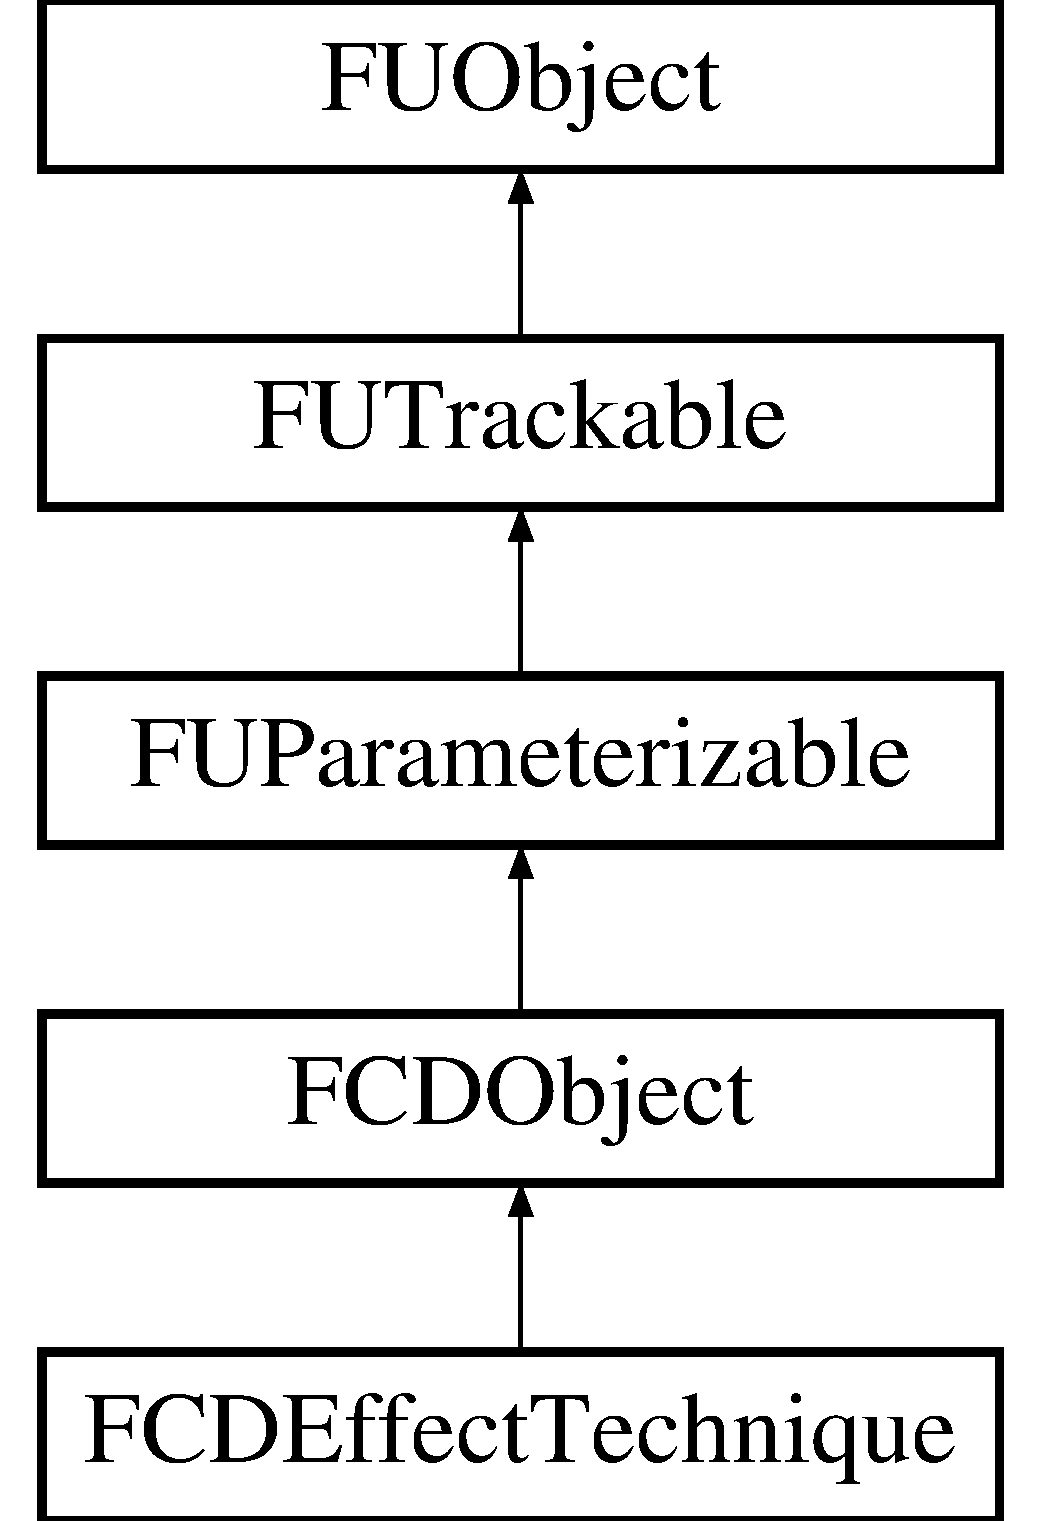
\includegraphics[height=5.000000cm]{classFCDEffectTechnique}
\end{center}
\end{figure}
\subsection*{Public Member Functions}
\begin{DoxyCompactItemize}
\item 
\hyperlink{classFCDEffectTechnique_a1e47ee8356ddfaf650da3601733d2394}{FCDEffectTechnique} (\hyperlink{classFCDocument}{FCDocument} $\ast$document, \hyperlink{classFCDEffectProfileFX}{FCDEffectProfileFX} $\ast$parent)
\item 
virtual \hyperlink{classFCDEffectTechnique_a63421c500dc1aea4d475f5cf77300d71}{$\sim$FCDEffectTechnique} ()
\item 
\hyperlink{classFCDEffectProfileFX}{FCDEffectProfileFX} $\ast$ \hyperlink{classFCDEffectTechnique_ac4649a643cf6949375115dd31a775b28}{GetParent} ()
\item 
const \hyperlink{classFCDEffectProfileFX}{FCDEffectProfileFX} $\ast$ \hyperlink{classFCDEffectTechnique_af1d184dd73bc107f25d6b12debaf5625}{GetParent} () const 
\item 
\hyperlink{classFCDEffectTechnique_a67b10f9e49ba3cb4ae2bb498d8197f36}{DEPRECATED} (3.05A, GetParent()-\/$>$GetParent()-\/$>$GetDaeId) const fm
\item 
const \hyperlink{classfm_1_1stringT}{fstring} \& \hyperlink{classFCDEffectTechnique_a2d3245870ddab9ce3b442e5afd708a52}{GetName} () const 
\item 
void \hyperlink{classFCDEffectTechnique_a07bca55857e485109ce1b499ceef6a40}{SetName} (const \hyperlink{classfm_1_1stringT}{fstring} \&\_\-name)
\item 
\hyperlink{classFCDEffectTechnique_ac454b0b966bd0ee9dfd181cae1e3cb7b}{DEPRECATED} (3.05A, GetPassCount and GetPass(index)) void GetPassList()
\item 
size\_\-t \hyperlink{classFCDEffectTechnique_a71dae8aafce949a83b7bf0361bc68910}{GetPassCount} () const 
\item 
\hyperlink{classFCDEffectPass}{FCDEffectPass} $\ast$ \hyperlink{classFCDEffectTechnique_a2b957bde5e7142e14724bea627226eff}{GetPass} (size\_\-t index)
\item 
const \hyperlink{classFCDEffectPass}{FCDEffectPass} $\ast$ \hyperlink{classFCDEffectTechnique_a02721f15869f261d94438d8a1837ed75}{GetPass} (size\_\-t index) const 
\item 
\hyperlink{classFCDEffectPass}{FCDEffectPass} $\ast$ \hyperlink{classFCDEffectTechnique_a485529a79e25dfb6c9d9f3b6ebc4d5c4}{AddPass} ()
\item 
\hyperlink{classFCDEffectTechnique_a0f2d38037a7fbfb2f80913148d2ea68e}{DEPRECATED} (3.05A, GetCodeCount and GetCode(index) or FindCode) void GetCodeList()
\item 
size\_\-t \hyperlink{classFCDEffectTechnique_ab9f545e1ae37dd7bd8ef17bd2d533b85}{GetCodeCount} () const 
\item 
\hyperlink{classFCDEffectCode}{FCDEffectCode} $\ast$ \hyperlink{classFCDEffectTechnique_a055752fffaa859ba4b300fc5e1668307}{GetCode} (size\_\-t index)
\item 
const \hyperlink{classFCDEffectCode}{FCDEffectCode} $\ast$ \hyperlink{classFCDEffectTechnique_ac1bfa956e08f14bd17dcc9dd5c397833}{GetCode} (size\_\-t index) const 
\item 
\hyperlink{classFCDEffectCode}{FCDEffectCode} $\ast$ \hyperlink{classFCDEffectTechnique_aa1d2ca97bd7e689527c2d7a579f0f9ca}{FindCode} (const char $\ast$sid)
\item 
const \hyperlink{classFCDEffectCode}{FCDEffectCode} $\ast$ \hyperlink{classFCDEffectTechnique_ac4a6ee7e3bac9f19eaa9ed77fc36eca4}{FindCode} (const char $\ast$sid) const 
\item 
\hyperlink{classFCDEffectCode}{FCDEffectCode} $\ast$ \hyperlink{classFCDEffectTechnique_aa532d3dff7c9c8f159a16811c7cdcf20}{AddCode} ()
\item 
size\_\-t \hyperlink{classFCDEffectTechnique_a58c423415223bbe1ada049c770562f74}{GetEffectParameterCount} () const 
\item 
\hyperlink{classFCDEffectParameter}{FCDEffectParameter} $\ast$ \hyperlink{classFCDEffectTechnique_a0cf4e90aeff863f03f183e0c3e791df0}{GetEffectParameter} (size\_\-t index)
\item 
\hypertarget{classFCDEffectTechnique_a5539b314ef3f3b0460513f4025cfdb97}{
const \hyperlink{classFCDEffectParameter}{FCDEffectParameter} $\ast$ {\bfseries GetEffectParameter} (size\_\-t index) const }
\label{classFCDEffectTechnique_a5539b314ef3f3b0460513f4025cfdb97}

\item 
\hyperlink{classFCDEffectParameter}{FCDEffectParameter} $\ast$ \hyperlink{classFCDEffectTechnique_af52fac53bb63d670d5c580b500d15719}{AddEffectParameter} (uint32 type)
\item 
\hyperlink{classFCDEffectTechnique}{FCDEffectTechnique} $\ast$ \hyperlink{classFCDEffectTechnique_ae810ec6ecd9b3baec142868f62dfe154}{Clone} (\hyperlink{classFCDEffectTechnique}{FCDEffectTechnique} $\ast$clone=NULL) const 
\item 
\hyperlink{classFCDEffectTechnique_a6f0456eaec5bf45c469a7d9be98cc4ce}{DEPRECATED} (3.05A, not recommended) void Flatten()
\end{DoxyCompactItemize}


\subsection{Detailed Description}
A COLLADA effect technique.

The COLLADA effect technique contains the passes to be used in the rendering of polygon sets.

It also contains a list of effect parameters: both generators and overrides and it is the lowest level of abstraction in which you can access effect parameters. For flattened materials, this means that all the effect parameters will be accessible at this level.

It also contains a list of effect code inclusions. 

\subsection{Constructor \& Destructor Documentation}
\hypertarget{classFCDEffectTechnique_a1e47ee8356ddfaf650da3601733d2394}{
\index{FCDEffectTechnique@{FCDEffectTechnique}!FCDEffectTechnique@{FCDEffectTechnique}}
\index{FCDEffectTechnique@{FCDEffectTechnique}!FCDEffectTechnique@{FCDEffectTechnique}}
\subsubsection[{FCDEffectTechnique}]{\setlength{\rightskip}{0pt plus 5cm}FCDEffectTechnique::FCDEffectTechnique (
\begin{DoxyParamCaption}
\item[{{\bf FCDocument} $\ast$}]{ document, }
\item[{{\bf FCDEffectProfileFX} $\ast$}]{ parent}
\end{DoxyParamCaption}
)}}
\label{classFCDEffectTechnique_a1e47ee8356ddfaf650da3601733d2394}
Constructor: do not use directly. Instead, use the \hyperlink{classFCDEffectProfileFX_ae6498c1d1bba41fdc63b98cbceb797d0}{FCDEffectProfileFX::AddTechnique} function. 
\begin{DoxyParams}{Parameters}
\item[{\em document}]The \hyperlink{namespaceFCollada}{FCollada} document that owns this technique. \item[{\em parent}]The effect profile which contains the technique. \end{DoxyParams}
\hypertarget{classFCDEffectTechnique_a63421c500dc1aea4d475f5cf77300d71}{
\index{FCDEffectTechnique@{FCDEffectTechnique}!$\sim$FCDEffectTechnique@{$\sim$FCDEffectTechnique}}
\index{$\sim$FCDEffectTechnique@{$\sim$FCDEffectTechnique}!FCDEffectTechnique@{FCDEffectTechnique}}
\subsubsection[{$\sim$FCDEffectTechnique}]{\setlength{\rightskip}{0pt plus 5cm}FCDEffectTechnique::$\sim$FCDEffectTechnique (
\begin{DoxyParamCaption}
{}
\end{DoxyParamCaption}
)\hspace{0.3cm}{\ttfamily  \mbox{[}virtual\mbox{]}}}}
\label{classFCDEffectTechnique_a63421c500dc1aea4d475f5cf77300d71}
Destructor. 

\subsection{Member Function Documentation}
\hypertarget{classFCDEffectTechnique_aa532d3dff7c9c8f159a16811c7cdcf20}{
\index{FCDEffectTechnique@{FCDEffectTechnique}!AddCode@{AddCode}}
\index{AddCode@{AddCode}!FCDEffectTechnique@{FCDEffectTechnique}}
\subsubsection[{AddCode}]{\setlength{\rightskip}{0pt plus 5cm}{\bf FCDEffectCode} $\ast$ FCDEffectTechnique::AddCode (
\begin{DoxyParamCaption}
{}
\end{DoxyParamCaption}
)}}
\label{classFCDEffectTechnique_aa532d3dff7c9c8f159a16811c7cdcf20}
Adds a new code inclusion to this effect profile. \begin{DoxyReturn}{Returns}
The new code inclusion. 
\end{DoxyReturn}
\hypertarget{classFCDEffectTechnique_af52fac53bb63d670d5c580b500d15719}{
\index{FCDEffectTechnique@{FCDEffectTechnique}!AddEffectParameter@{AddEffectParameter}}
\index{AddEffectParameter@{AddEffectParameter}!FCDEffectTechnique@{FCDEffectTechnique}}
\subsubsection[{AddEffectParameter}]{\setlength{\rightskip}{0pt plus 5cm}{\bf FCDEffectParameter} $\ast$ FCDEffectTechnique::AddEffectParameter (
\begin{DoxyParamCaption}
\item[{uint32}]{ type}
\end{DoxyParamCaption}
)}}
\label{classFCDEffectTechnique_af52fac53bb63d670d5c580b500d15719}
Adds a local effect parameter to the local list. \begin{DoxySeeAlso}{See also}
\hyperlink{classFCDEffectParameter_a1efe74553d2ed199435085c171743b08}{FCDEffectParameter::Type} 
\end{DoxySeeAlso}

\begin{DoxyParams}{Parameters}
\item[{\em type}]The value type of the effect parameter to create. \end{DoxyParams}
\begin{DoxyReturn}{Returns}
The new local effect parameter. 
\end{DoxyReturn}
\hypertarget{classFCDEffectTechnique_a485529a79e25dfb6c9d9f3b6ebc4d5c4}{
\index{FCDEffectTechnique@{FCDEffectTechnique}!AddPass@{AddPass}}
\index{AddPass@{AddPass}!FCDEffectTechnique@{FCDEffectTechnique}}
\subsubsection[{AddPass}]{\setlength{\rightskip}{0pt plus 5cm}{\bf FCDEffectPass} $\ast$ FCDEffectTechnique::AddPass (
\begin{DoxyParamCaption}
{}
\end{DoxyParamCaption}
)}}
\label{classFCDEffectTechnique_a485529a79e25dfb6c9d9f3b6ebc4d5c4}
Adds a new pass to this effect technique. \begin{DoxyReturn}{Returns}
The new pass. 
\end{DoxyReturn}
\hypertarget{classFCDEffectTechnique_ae810ec6ecd9b3baec142868f62dfe154}{
\index{FCDEffectTechnique@{FCDEffectTechnique}!Clone@{Clone}}
\index{Clone@{Clone}!FCDEffectTechnique@{FCDEffectTechnique}}
\subsubsection[{Clone}]{\setlength{\rightskip}{0pt plus 5cm}{\bf FCDEffectTechnique} $\ast$ FCDEffectTechnique::Clone (
\begin{DoxyParamCaption}
\item[{{\bf FCDEffectTechnique} $\ast$}]{ clone = {\ttfamily NULL}}
\end{DoxyParamCaption}
) const}}
\label{classFCDEffectTechnique_ae810ec6ecd9b3baec142868f62dfe154}
\mbox{[}INTERNAL\mbox{]} Clones the full effect technique. 
\begin{DoxyParams}{Parameters}
\item[{\em clone}]The cloned technique. If this pointer is NULL, a new technique is created and you will need to release this new techniquetechnique. \end{DoxyParams}
\begin{DoxyReturn}{Returns}
The cloned technique. This pointer will never be NULL. 
\end{DoxyReturn}
\hypertarget{classFCDEffectTechnique_a67b10f9e49ba3cb4ae2bb498d8197f36}{
\index{FCDEffectTechnique@{FCDEffectTechnique}!DEPRECATED@{DEPRECATED}}
\index{DEPRECATED@{DEPRECATED}!FCDEffectTechnique@{FCDEffectTechnique}}
\subsubsection[{DEPRECATED}]{\setlength{\rightskip}{0pt plus 5cm}FCDEffectTechnique::DEPRECATED (
\begin{DoxyParamCaption}
\item[{3.}]{ 05A, }
\item[{GetParent()-\/$>$GetParent()-\/$>$}]{ GetDaeId}
\end{DoxyParamCaption}
) const\hspace{0.3cm}{\ttfamily  \mbox{[}inline\mbox{]}}}}
\label{classFCDEffectTechnique_a67b10f9e49ba3cb4ae2bb498d8197f36}
Retrieves the COLLADA id of the parent effect. This function is mostly useful as a shortcut for debugging and reporting. \begin{DoxyReturn}{Returns}
The COLLADA id of the parent effect. 
\end{DoxyReturn}
\hypertarget{classFCDEffectTechnique_a0f2d38037a7fbfb2f80913148d2ea68e}{
\index{FCDEffectTechnique@{FCDEffectTechnique}!DEPRECATED@{DEPRECATED}}
\index{DEPRECATED@{DEPRECATED}!FCDEffectTechnique@{FCDEffectTechnique}}
\subsubsection[{DEPRECATED}]{\setlength{\rightskip}{0pt plus 5cm}FCDEffectTechnique::DEPRECATED (
\begin{DoxyParamCaption}
\item[{3.}]{ 05A, }
\item[{GetCodeCount and GetCode(index) or}]{ FindCode}
\end{DoxyParamCaption}
)\hspace{0.3cm}{\ttfamily  \mbox{[}inline\mbox{]}}}}
\label{classFCDEffectTechnique_a0f2d38037a7fbfb2f80913148d2ea68e}
Retrieves the list of code inclusions. \begin{DoxyReturn}{Returns}
The list of code inclusions. 
\end{DoxyReturn}
\hypertarget{classFCDEffectTechnique_a6f0456eaec5bf45c469a7d9be98cc4ce}{
\index{FCDEffectTechnique@{FCDEffectTechnique}!DEPRECATED@{DEPRECATED}}
\index{DEPRECATED@{DEPRECATED}!FCDEffectTechnique@{FCDEffectTechnique}}
\subsubsection[{DEPRECATED}]{\setlength{\rightskip}{0pt plus 5cm}FCDEffectTechnique::DEPRECATED (
\begin{DoxyParamCaption}
\item[{3.}]{ 05A, }
\item[{not}]{ recommended}
\end{DoxyParamCaption}
)\hspace{0.3cm}{\ttfamily  \mbox{[}inline\mbox{]}}}}
\label{classFCDEffectTechnique_a6f0456eaec5bf45c469a7d9be98cc4ce}
\mbox{[}INTERNAL\mbox{]} Flattens this effect technique. Merges the parameter overrides into the parameter generators. \hypertarget{classFCDEffectTechnique_ac454b0b966bd0ee9dfd181cae1e3cb7b}{
\index{FCDEffectTechnique@{FCDEffectTechnique}!DEPRECATED@{DEPRECATED}}
\index{DEPRECATED@{DEPRECATED}!FCDEffectTechnique@{FCDEffectTechnique}}
\subsubsection[{DEPRECATED}]{\setlength{\rightskip}{0pt plus 5cm}FCDEffectTechnique::DEPRECATED (
\begin{DoxyParamCaption}
\item[{3.}]{ 05A, }
\item[{GetPassCount and }]{ GetPassindex}
\end{DoxyParamCaption}
)\hspace{0.3cm}{\ttfamily  \mbox{[}inline\mbox{]}}}}
\label{classFCDEffectTechnique_ac454b0b966bd0ee9dfd181cae1e3cb7b}
Retrieves the list of passes. \begin{DoxyReturn}{Returns}
The list of passes. 
\end{DoxyReturn}
\hypertarget{classFCDEffectTechnique_ac4a6ee7e3bac9f19eaa9ed77fc36eca4}{
\index{FCDEffectTechnique@{FCDEffectTechnique}!FindCode@{FindCode}}
\index{FindCode@{FindCode}!FCDEffectTechnique@{FCDEffectTechnique}}
\subsubsection[{FindCode}]{\setlength{\rightskip}{0pt plus 5cm}const {\bf FCDEffectCode} $\ast$ FCDEffectTechnique::FindCode (
\begin{DoxyParamCaption}
\item[{const char $\ast$}]{ sid}
\end{DoxyParamCaption}
) const}}
\label{classFCDEffectTechnique_ac4a6ee7e3bac9f19eaa9ed77fc36eca4}
See above. \hypertarget{classFCDEffectTechnique_aa1d2ca97bd7e689527c2d7a579f0f9ca}{
\index{FCDEffectTechnique@{FCDEffectTechnique}!FindCode@{FindCode}}
\index{FindCode@{FindCode}!FCDEffectTechnique@{FCDEffectTechnique}}
\subsubsection[{FindCode}]{\setlength{\rightskip}{0pt plus 5cm}{\bf FCDEffectCode}$\ast$ FCDEffectTechnique::FindCode (
\begin{DoxyParamCaption}
\item[{const char $\ast$}]{ sid}
\end{DoxyParamCaption}
)\hspace{0.3cm}{\ttfamily  \mbox{[}inline\mbox{]}}}}
\label{classFCDEffectTechnique_aa1d2ca97bd7e689527c2d7a579f0f9ca}
Retrieves the code inclusion with the given sub-\/id. 
\begin{DoxyParams}{Parameters}
\item[{\em sid}]A COLLADA sub-\/id. \end{DoxyParams}
\begin{DoxyReturn}{Returns}
The code inclusion with the given sub-\/id. This pointer will be NULL, if there are no code inclusions that match the given sub-\/id. 
\end{DoxyReturn}
\hypertarget{classFCDEffectTechnique_a055752fffaa859ba4b300fc5e1668307}{
\index{FCDEffectTechnique@{FCDEffectTechnique}!GetCode@{GetCode}}
\index{GetCode@{GetCode}!FCDEffectTechnique@{FCDEffectTechnique}}
\subsubsection[{GetCode}]{\setlength{\rightskip}{0pt plus 5cm}{\bf FCDEffectCode}$\ast$ FCDEffectTechnique::GetCode (
\begin{DoxyParamCaption}
\item[{size\_\-t}]{ index}
\end{DoxyParamCaption}
)\hspace{0.3cm}{\ttfamily  \mbox{[}inline\mbox{]}}}}
\label{classFCDEffectTechnique_a055752fffaa859ba4b300fc5e1668307}
Retrieves a code inclusion contained within the effect profile. 
\begin{DoxyParams}{Parameters}
\item[{\em index}]The index of the code inclusion. \end{DoxyParams}
\begin{DoxyReturn}{Returns}
The code inclusion. This pointer will be NULL if the index is out-\/of-\/bounds. 
\end{DoxyReturn}
\hypertarget{classFCDEffectTechnique_ac1bfa956e08f14bd17dcc9dd5c397833}{
\index{FCDEffectTechnique@{FCDEffectTechnique}!GetCode@{GetCode}}
\index{GetCode@{GetCode}!FCDEffectTechnique@{FCDEffectTechnique}}
\subsubsection[{GetCode}]{\setlength{\rightskip}{0pt plus 5cm}const {\bf FCDEffectCode}$\ast$ FCDEffectTechnique::GetCode (
\begin{DoxyParamCaption}
\item[{size\_\-t}]{ index}
\end{DoxyParamCaption}
) const\hspace{0.3cm}{\ttfamily  \mbox{[}inline\mbox{]}}}}
\label{classFCDEffectTechnique_ac1bfa956e08f14bd17dcc9dd5c397833}
See above. \hypertarget{classFCDEffectTechnique_ab9f545e1ae37dd7bd8ef17bd2d533b85}{
\index{FCDEffectTechnique@{FCDEffectTechnique}!GetCodeCount@{GetCodeCount}}
\index{GetCodeCount@{GetCodeCount}!FCDEffectTechnique@{FCDEffectTechnique}}
\subsubsection[{GetCodeCount}]{\setlength{\rightskip}{0pt plus 5cm}size\_\-t FCDEffectTechnique::GetCodeCount (
\begin{DoxyParamCaption}
{}
\end{DoxyParamCaption}
) const\hspace{0.3cm}{\ttfamily  \mbox{[}inline\mbox{]}}}}
\label{classFCDEffectTechnique_ab9f545e1ae37dd7bd8ef17bd2d533b85}
Retrieves the number of code inclusions contained within the effect profile. \begin{DoxyReturn}{Returns}
The number of code inclusions. 
\end{DoxyReturn}
\hypertarget{classFCDEffectTechnique_a0cf4e90aeff863f03f183e0c3e791df0}{
\index{FCDEffectTechnique@{FCDEffectTechnique}!GetEffectParameter@{GetEffectParameter}}
\index{GetEffectParameter@{GetEffectParameter}!FCDEffectTechnique@{FCDEffectTechnique}}
\subsubsection[{GetEffectParameter}]{\setlength{\rightskip}{0pt plus 5cm}{\bf FCDEffectParameter}$\ast$ FCDEffectTechnique::GetEffectParameter (
\begin{DoxyParamCaption}
\item[{size\_\-t}]{ index}
\end{DoxyParamCaption}
)\hspace{0.3cm}{\ttfamily  \mbox{[}inline\mbox{]}}}}
\label{classFCDEffectTechnique_a0cf4e90aeff863f03f183e0c3e791df0}
Retrieves a given local effect parameter. 
\begin{DoxyParams}{Parameters}
\item[{\em index}]An index. \end{DoxyParams}
\begin{DoxyReturn}{Returns}
The local effect parameter at the given index. 
\end{DoxyReturn}
\hypertarget{classFCDEffectTechnique_a58c423415223bbe1ada049c770562f74}{
\index{FCDEffectTechnique@{FCDEffectTechnique}!GetEffectParameterCount@{GetEffectParameterCount}}
\index{GetEffectParameterCount@{GetEffectParameterCount}!FCDEffectTechnique@{FCDEffectTechnique}}
\subsubsection[{GetEffectParameterCount}]{\setlength{\rightskip}{0pt plus 5cm}size\_\-t FCDEffectTechnique::GetEffectParameterCount (
\begin{DoxyParamCaption}
{}
\end{DoxyParamCaption}
) const\hspace{0.3cm}{\ttfamily  \mbox{[}inline\mbox{]}}}}
\label{classFCDEffectTechnique_a58c423415223bbe1ada049c770562f74}
Retrieves the number of local effect parameters \begin{DoxyReturn}{Returns}
The number of local effect parameters. 
\end{DoxyReturn}
\hypertarget{classFCDEffectTechnique_a2d3245870ddab9ce3b442e5afd708a52}{
\index{FCDEffectTechnique@{FCDEffectTechnique}!GetName@{GetName}}
\index{GetName@{GetName}!FCDEffectTechnique@{FCDEffectTechnique}}
\subsubsection[{GetName}]{\setlength{\rightskip}{0pt plus 5cm}const {\bf fstring}\& FCDEffectTechnique::GetName (
\begin{DoxyParamCaption}
{}
\end{DoxyParamCaption}
) const\hspace{0.3cm}{\ttfamily  \mbox{[}inline\mbox{]}}}}
\label{classFCDEffectTechnique_a2d3245870ddab9ce3b442e5afd708a52}
Retrieves the sub-\/id of the technique. \begin{DoxyReturn}{Returns}
The sub-\/id of the technique. 
\end{DoxyReturn}
\hypertarget{classFCDEffectTechnique_ac4649a643cf6949375115dd31a775b28}{
\index{FCDEffectTechnique@{FCDEffectTechnique}!GetParent@{GetParent}}
\index{GetParent@{GetParent}!FCDEffectTechnique@{FCDEffectTechnique}}
\subsubsection[{GetParent}]{\setlength{\rightskip}{0pt plus 5cm}{\bf FCDEffectProfileFX}$\ast$ FCDEffectTechnique::GetParent (
\begin{DoxyParamCaption}
{}
\end{DoxyParamCaption}
)\hspace{0.3cm}{\ttfamily  \mbox{[}inline\mbox{]}}}}
\label{classFCDEffectTechnique_ac4649a643cf6949375115dd31a775b28}
Retrieves the effect profile that contains this technique. \begin{DoxyReturn}{Returns}
The parent effect profile. 
\end{DoxyReturn}
\hypertarget{classFCDEffectTechnique_af1d184dd73bc107f25d6b12debaf5625}{
\index{FCDEffectTechnique@{FCDEffectTechnique}!GetParent@{GetParent}}
\index{GetParent@{GetParent}!FCDEffectTechnique@{FCDEffectTechnique}}
\subsubsection[{GetParent}]{\setlength{\rightskip}{0pt plus 5cm}const {\bf FCDEffectProfileFX}$\ast$ FCDEffectTechnique::GetParent (
\begin{DoxyParamCaption}
{}
\end{DoxyParamCaption}
) const\hspace{0.3cm}{\ttfamily  \mbox{[}inline\mbox{]}}}}
\label{classFCDEffectTechnique_af1d184dd73bc107f25d6b12debaf5625}
See above. \hypertarget{classFCDEffectTechnique_a2b957bde5e7142e14724bea627226eff}{
\index{FCDEffectTechnique@{FCDEffectTechnique}!GetPass@{GetPass}}
\index{GetPass@{GetPass}!FCDEffectTechnique@{FCDEffectTechnique}}
\subsubsection[{GetPass}]{\setlength{\rightskip}{0pt plus 5cm}{\bf FCDEffectPass}$\ast$ FCDEffectTechnique::GetPass (
\begin{DoxyParamCaption}
\item[{size\_\-t}]{ index}
\end{DoxyParamCaption}
)\hspace{0.3cm}{\ttfamily  \mbox{[}inline\mbox{]}}}}
\label{classFCDEffectTechnique_a2b957bde5e7142e14724bea627226eff}
Retrieves a specific pass contained within this effect technique. 
\begin{DoxyParams}{Parameters}
\item[{\em index}]The index of the pass. \end{DoxyParams}
\begin{DoxyReturn}{Returns}
The pass. This pointer will be NULL if the index is out-\/of-\/bounds. 
\end{DoxyReturn}
\hypertarget{classFCDEffectTechnique_a02721f15869f261d94438d8a1837ed75}{
\index{FCDEffectTechnique@{FCDEffectTechnique}!GetPass@{GetPass}}
\index{GetPass@{GetPass}!FCDEffectTechnique@{FCDEffectTechnique}}
\subsubsection[{GetPass}]{\setlength{\rightskip}{0pt plus 5cm}const {\bf FCDEffectPass}$\ast$ FCDEffectTechnique::GetPass (
\begin{DoxyParamCaption}
\item[{size\_\-t}]{ index}
\end{DoxyParamCaption}
) const\hspace{0.3cm}{\ttfamily  \mbox{[}inline\mbox{]}}}}
\label{classFCDEffectTechnique_a02721f15869f261d94438d8a1837ed75}
See above. \hypertarget{classFCDEffectTechnique_a71dae8aafce949a83b7bf0361bc68910}{
\index{FCDEffectTechnique@{FCDEffectTechnique}!GetPassCount@{GetPassCount}}
\index{GetPassCount@{GetPassCount}!FCDEffectTechnique@{FCDEffectTechnique}}
\subsubsection[{GetPassCount}]{\setlength{\rightskip}{0pt plus 5cm}size\_\-t FCDEffectTechnique::GetPassCount (
\begin{DoxyParamCaption}
{}
\end{DoxyParamCaption}
) const\hspace{0.3cm}{\ttfamily  \mbox{[}inline\mbox{]}}}}
\label{classFCDEffectTechnique_a71dae8aafce949a83b7bf0361bc68910}
Retrieves the number of passes contained within this effect technique. \begin{DoxyReturn}{Returns}
The number of passes. 
\end{DoxyReturn}
\hypertarget{classFCDEffectTechnique_a07bca55857e485109ce1b499ceef6a40}{
\index{FCDEffectTechnique@{FCDEffectTechnique}!SetName@{SetName}}
\index{SetName@{SetName}!FCDEffectTechnique@{FCDEffectTechnique}}
\subsubsection[{SetName}]{\setlength{\rightskip}{0pt plus 5cm}void FCDEffectTechnique::SetName (
\begin{DoxyParamCaption}
\item[{const {\bf fstring} \&}]{ \_\-name}
\end{DoxyParamCaption}
)\hspace{0.3cm}{\ttfamily  \mbox{[}inline\mbox{]}}}}
\label{classFCDEffectTechnique_a07bca55857e485109ce1b499ceef6a40}
Sets the sub-\/id of the technique. The effect technique must have a valid sub-\/id that is unique within its scope. Otherwise, one will be provided on XML export. 
\begin{DoxyParams}{Parameters}
\item[{\em \_\-name}]A valid sub-\/id. \end{DoxyParams}


The documentation for this class was generated from the following files:\begin{DoxyCompactItemize}
\item 
FCollada/FCDocument/\hyperlink{FCDEffectTechnique_8h}{FCDEffectTechnique.h}\item 
FCollada/FCDocument/FCDEffectTechnique.cpp\end{DoxyCompactItemize}

\hypertarget{classFCDEmitter}{
\section{FCDEmitter Class Reference}
\label{classFCDEmitter}\index{FCDEmitter@{FCDEmitter}}
}


{\ttfamily \#include $<$FCDEmitter.h$>$}

Inheritance diagram for FCDEmitter:\begin{figure}[H]
\begin{center}
\leavevmode
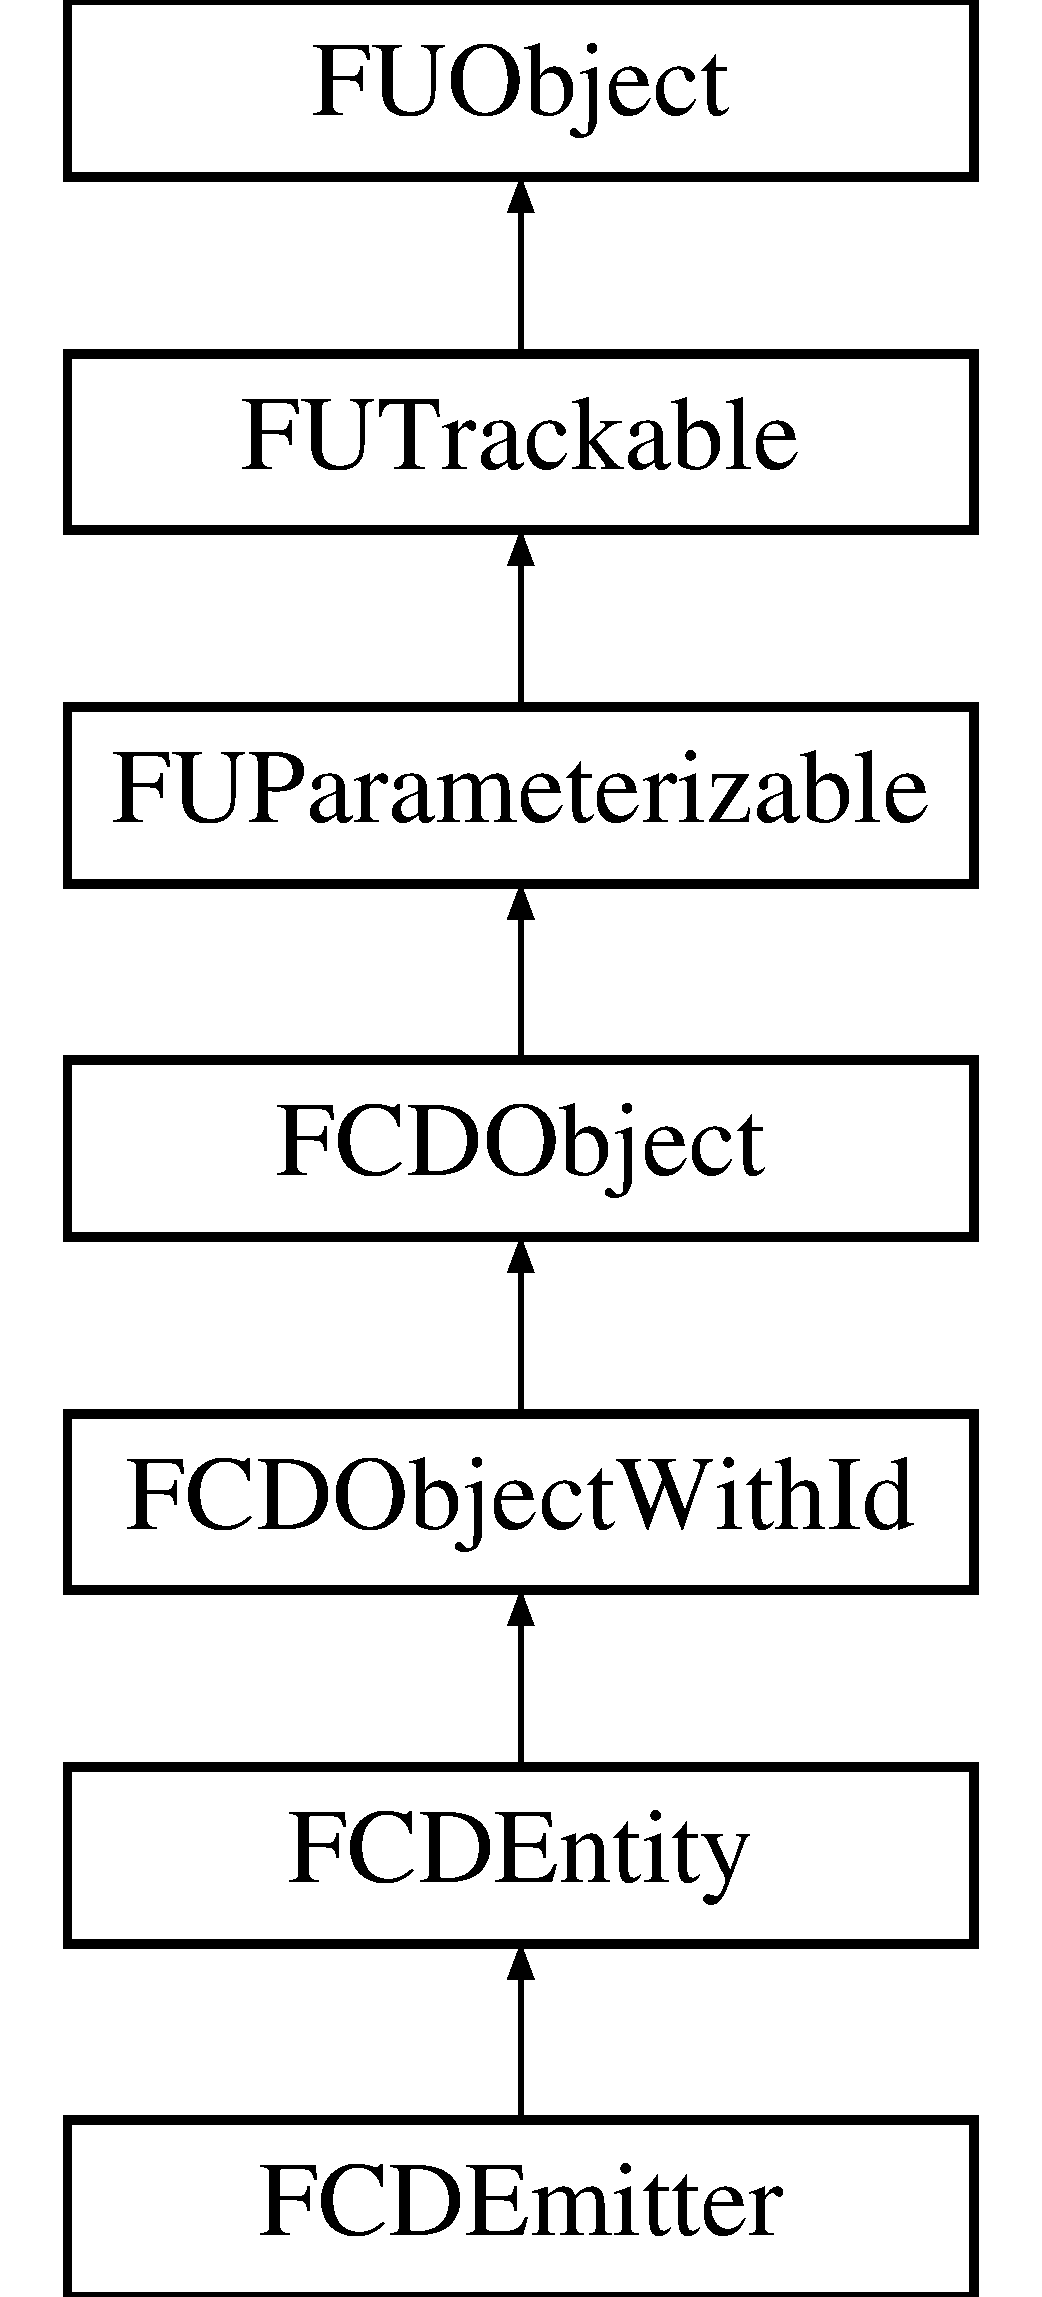
\includegraphics[height=7.000000cm]{classFCDEmitter}
\end{center}
\end{figure}
\subsection*{Public Member Functions}
\begin{DoxyCompactItemize}
\item 
\hyperlink{classFCDEmitter_a49f90e56fcc799ae7c87bca9ba5d2a8e}{FCDEmitter} (\hyperlink{classFCDocument}{FCDocument} $\ast$document)
\item 
\hyperlink{classFCDEmitter_a5903b5d66d3877e062549c433ea98d1d}{$\sim$FCDEmitter} ()
\item 
virtual \hyperlink{classFCDEntity_a9301a4bd5f4d4190ec13e40db4effdd7}{Type} \hyperlink{classFCDEmitter_a2921acf052b38f68d148b0fdcaa366b9}{GetType} () const 
\item 
virtual \hyperlink{classFCDEntity}{FCDEntity} $\ast$ \hyperlink{classFCDEmitter_afdd49a87fe2fdb95b425f62bac8150d6}{Clone} (\hyperlink{classFCDEntity}{FCDEntity} $\ast$clone=NULL, bool cloneChildren=false) const 
\end{DoxyCompactItemize}


\subsection{Detailed Description}
A COLLADA generic emitter.

This class does not belong to the COLLADA COMMON profile. It is used to define both particle and sound emitters. 

\subsection{Constructor \& Destructor Documentation}
\hypertarget{classFCDEmitter_a49f90e56fcc799ae7c87bca9ba5d2a8e}{
\index{FCDEmitter@{FCDEmitter}!FCDEmitter@{FCDEmitter}}
\index{FCDEmitter@{FCDEmitter}!FCDEmitter@{FCDEmitter}}
\subsubsection[{FCDEmitter}]{\setlength{\rightskip}{0pt plus 5cm}FCDEmitter::FCDEmitter (
\begin{DoxyParamCaption}
\item[{{\bf FCDocument} $\ast$}]{ document}
\end{DoxyParamCaption}
)}}
\label{classFCDEmitter_a49f90e56fcc799ae7c87bca9ba5d2a8e}
Constructor. Do not use directly, emitters should be created using the AddEntity function on the FCDEmitterLibrary 
\begin{DoxyParams}{Parameters}
\item[{\em document}]The COLLADA document that owns the emitter. \end{DoxyParams}
\hypertarget{classFCDEmitter_a5903b5d66d3877e062549c433ea98d1d}{
\index{FCDEmitter@{FCDEmitter}!$\sim$FCDEmitter@{$\sim$FCDEmitter}}
\index{$\sim$FCDEmitter@{$\sim$FCDEmitter}!FCDEmitter@{FCDEmitter}}
\subsubsection[{$\sim$FCDEmitter}]{\setlength{\rightskip}{0pt plus 5cm}FCDEmitter::$\sim$FCDEmitter (
\begin{DoxyParamCaption}
{}
\end{DoxyParamCaption}
)}}
\label{classFCDEmitter_a5903b5d66d3877e062549c433ea98d1d}
Destructor. 

\subsection{Member Function Documentation}
\hypertarget{classFCDEmitter_afdd49a87fe2fdb95b425f62bac8150d6}{
\index{FCDEmitter@{FCDEmitter}!Clone@{Clone}}
\index{Clone@{Clone}!FCDEmitter@{FCDEmitter}}
\subsubsection[{Clone}]{\setlength{\rightskip}{0pt plus 5cm}{\bf FCDEntity} $\ast$ FCDEmitter::Clone (
\begin{DoxyParamCaption}
\item[{{\bf FCDEntity} $\ast$}]{ clone = {\ttfamily NULL}, }
\item[{bool}]{ cloneChildren = {\ttfamily false}}
\end{DoxyParamCaption}
) const\hspace{0.3cm}{\ttfamily  \mbox{[}virtual\mbox{]}}}}
\label{classFCDEmitter_afdd49a87fe2fdb95b425f62bac8150d6}
Clones the emitter information. 
\begin{DoxyParams}{Parameters}
\item[{\em clone}]The cloned emitter. If this pointer is NULL, a new emitter is created and you will need to release it manually. \item[{\em cloneChildren}]Whether to recursively clone this entity's children. \end{DoxyParams}
\begin{DoxyReturn}{Returns}
The clone. 
\end{DoxyReturn}


Reimplemented from \hyperlink{classFCDEntity_afd21dc9f9dba45786012dea87f70b9fc}{FCDEntity}.

\hypertarget{classFCDEmitter_a2921acf052b38f68d148b0fdcaa366b9}{
\index{FCDEmitter@{FCDEmitter}!GetType@{GetType}}
\index{GetType@{GetType}!FCDEmitter@{FCDEmitter}}
\subsubsection[{GetType}]{\setlength{\rightskip}{0pt plus 5cm}virtual {\bf Type} FCDEmitter::GetType (
\begin{DoxyParamCaption}
{}
\end{DoxyParamCaption}
) const\hspace{0.3cm}{\ttfamily  \mbox{[}inline, virtual\mbox{]}}}}
\label{classFCDEmitter_a2921acf052b38f68d148b0fdcaa366b9}
Retrieves the entity class type. \begin{DoxyReturn}{Returns}
The entity class type: EMITTER 
\end{DoxyReturn}


Reimplemented from \hyperlink{classFCDEntity_abfd4312a7124f92364c1e6517c7e60ba}{FCDEntity}.



The documentation for this class was generated from the following files:\begin{DoxyCompactItemize}
\item 
FCollada/FCDocument/\hyperlink{FCDEmitter_8h}{FCDEmitter.h}\item 
FCollada/FCDocument/FCDEmitter.cpp\end{DoxyCompactItemize}

\hypertarget{classFCDEmitterInstance}{
\section{FCDEmitterInstance Class Reference}
\label{classFCDEmitterInstance}\index{FCDEmitterInstance@{FCDEmitterInstance}}
}


{\ttfamily \#include $<$FCDEmitterInstance.h$>$}

Inheritance diagram for FCDEmitterInstance:\begin{figure}[H]
\begin{center}
\leavevmode
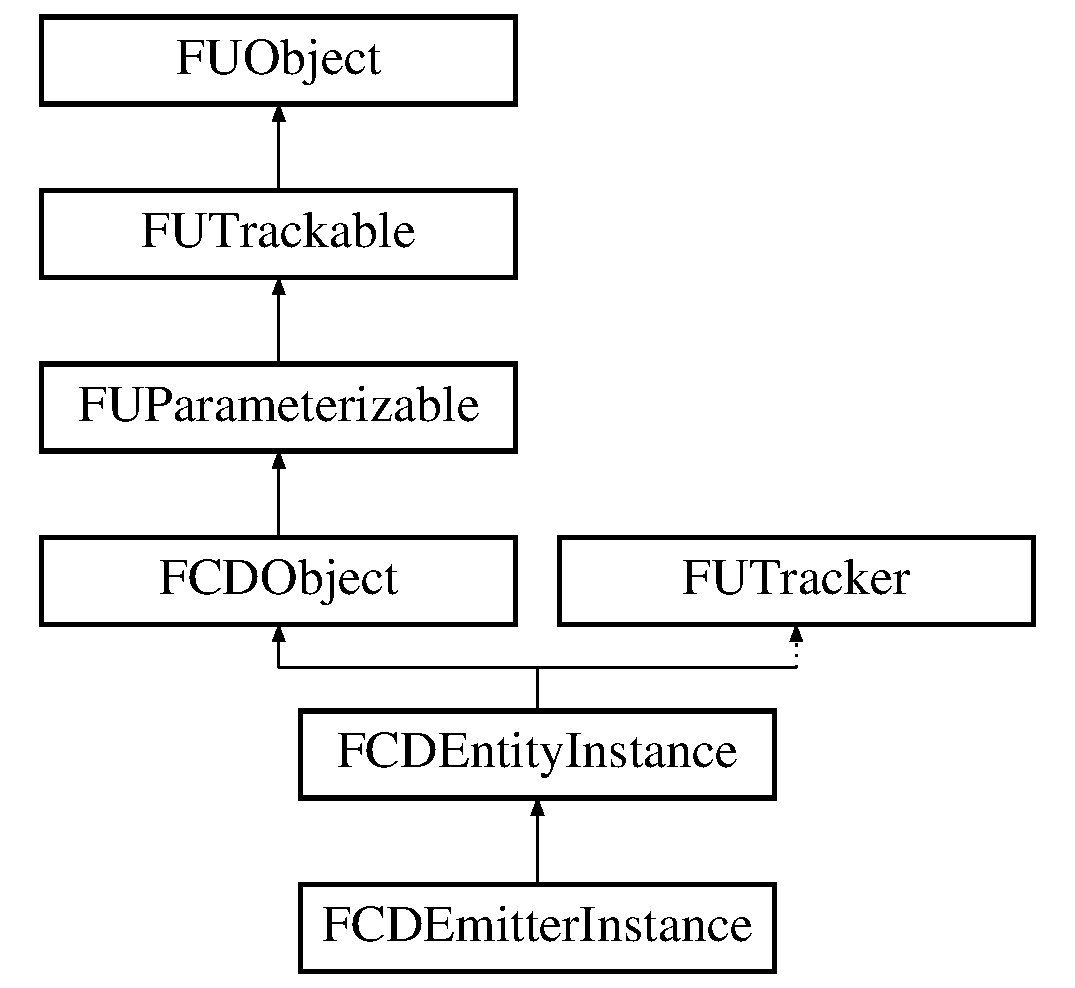
\includegraphics[height=6.000000cm]{classFCDEmitterInstance}
\end{center}
\end{figure}
\subsection*{Public Member Functions}
\begin{DoxyCompactItemize}
\item 
virtual \hyperlink{classFCDEmitterInstance_a2a130dc123cdf1ed9c62fb87db99524f}{$\sim$FCDEmitterInstance} ()
\end{DoxyCompactItemize}
\subsection*{Protected Member Functions}
\begin{DoxyCompactItemize}
\item 
\hyperlink{classFCDEmitterInstance_adb603a8e31948ff5f77412233ec1ce0d}{FCDEmitterInstance} (\hyperlink{classFCDocument}{FCDocument} $\ast$document, \hyperlink{classFCDSceneNode}{FCDSceneNode} $\ast$parent, \hyperlink{classFCDEntity_a9301a4bd5f4d4190ec13e40db4effdd7}{FCDEntity::Type} entityType=FCDEntity::EMITTER)
\end{DoxyCompactItemize}
\subsection*{Friends}
\begin{DoxyCompactItemize}
\item 
\hypertarget{classFCDEmitterInstance_a069ebb98497ccbc5fdcb75ecfa8b15f7}{
class \hyperlink{classFCDEmitterInstance_a069ebb98497ccbc5fdcb75ecfa8b15f7}{FCDEntityInstanceFactory}}
\label{classFCDEmitterInstance_a069ebb98497ccbc5fdcb75ecfa8b15f7}

\end{DoxyCompactItemize}


\subsection{Detailed Description}
A COLLADA emitter instance.

The types of particles emitted are instance dependent. Instances also contain the FCDForceInstances pointers to forces applied to the particles. 

\subsection{Constructor \& Destructor Documentation}
\hypertarget{classFCDEmitterInstance_adb603a8e31948ff5f77412233ec1ce0d}{
\index{FCDEmitterInstance@{FCDEmitterInstance}!FCDEmitterInstance@{FCDEmitterInstance}}
\index{FCDEmitterInstance@{FCDEmitterInstance}!FCDEmitterInstance@{FCDEmitterInstance}}
\subsubsection[{FCDEmitterInstance}]{\setlength{\rightskip}{0pt plus 5cm}FCDEmitterInstance::FCDEmitterInstance (
\begin{DoxyParamCaption}
\item[{{\bf FCDocument} $\ast$}]{ document, }
\item[{{\bf FCDSceneNode} $\ast$}]{ parent, }
\item[{{\bf FCDEntity::Type}}]{ entityType = {\ttfamily FCDEntity::EMITTER}}
\end{DoxyParamCaption}
)\hspace{0.3cm}{\ttfamily  \mbox{[}protected\mbox{]}}}}
\label{classFCDEmitterInstance_adb603a8e31948ff5f77412233ec1ce0d}
Constructor: do not use directly. Instead, use the \hyperlink{classFCDSceneNode_a38826dd9b894ad2371511f0228cb04c0}{FCDSceneNode::AddInstance} function. 
\begin{DoxyParams}{Parameters}
\item[{\em document}]The COLLADA document that owns the emitter instance. \item[{\em parent}]The parent visual scene node. \item[{\em entityType}]The type of the entity to instantiate. Unless this class is overwritten, \hyperlink{classFCDEntity_a9301a4bd5f4d4190ec13e40db4effdd7ab6f994b7aaba9add07d533f8945ddb70}{FCDEntity::EMITTER} should be given. \end{DoxyParams}
\hypertarget{classFCDEmitterInstance_a2a130dc123cdf1ed9c62fb87db99524f}{
\index{FCDEmitterInstance@{FCDEmitterInstance}!$\sim$FCDEmitterInstance@{$\sim$FCDEmitterInstance}}
\index{$\sim$FCDEmitterInstance@{$\sim$FCDEmitterInstance}!FCDEmitterInstance@{FCDEmitterInstance}}
\subsubsection[{$\sim$FCDEmitterInstance}]{\setlength{\rightskip}{0pt plus 5cm}FCDEmitterInstance::$\sim$FCDEmitterInstance (
\begin{DoxyParamCaption}
{}
\end{DoxyParamCaption}
)\hspace{0.3cm}{\ttfamily  \mbox{[}virtual\mbox{]}}}}
\label{classFCDEmitterInstance_a2a130dc123cdf1ed9c62fb87db99524f}
Destructor. 

The documentation for this class was generated from the following files:\begin{DoxyCompactItemize}
\item 
FCollada/FCDocument/\hyperlink{FCDEmitterInstance_8h}{FCDEmitterInstance.h}\item 
FCollada/FCDocument/FCDEmitterInstance.cpp\end{DoxyCompactItemize}

\hypertarget{structFCDEmitterInstanceData}{
\section{FCDEmitterInstanceData Struct Reference}
\label{structFCDEmitterInstanceData}\index{FCDEmitterInstanceData@{FCDEmitterInstanceData}}
}
\subsection*{Public Attributes}
\begin{DoxyCompactItemize}
\item 
\hypertarget{structFCDEmitterInstanceData_a769508e2753d8ef69301ba416e00bb41}{
\hyperlink{classfm_1_1vector}{StringList} {\bfseries forceInstUris}}
\label{structFCDEmitterInstanceData_a769508e2753d8ef69301ba416e00bb41}

\end{DoxyCompactItemize}


The documentation for this struct was generated from the following file:\begin{DoxyCompactItemize}
\item 
FColladaPlugins/FArchiveXML/FAXStructures.h\end{DoxyCompactItemize}

\hypertarget{classFCDENode}{
\section{FCDENode Class Reference}
\label{classFCDENode}\index{FCDENode@{FCDENode}}
}


{\ttfamily \#include $<$FCDExtra.h$>$}

Inheritance diagram for FCDENode:\begin{figure}[H]
\begin{center}
\leavevmode
\includegraphics[height=6.000000cm]{classFCDENode}
\end{center}
\end{figure}
\subsection*{Public Member Functions}
\begin{DoxyCompactItemize}
\item 
\hyperlink{classFCDENode_aacc68c7cf15eb43b08d8183a2f1feb21}{FCDENode} (\hyperlink{classFCDocument}{FCDocument} $\ast$document, \hyperlink{classFCDENode}{FCDENode} $\ast$parent)
\item 
virtual \hyperlink{classFCDENode_a2b18abc6ddbcfe7182afba2e0234f760}{$\sim$FCDENode} ()
\item 
const char $\ast$ \hyperlink{classFCDENode_a595efe3b26ec3f240192f730fc312989}{GetName} () const 
\item 
void \hyperlink{classFCDENode_a4f60977945ccf9769bce6558cce2ce62}{SetName} (const char $\ast$\_\-name, bool cleanName=true)
\item 
void \hyperlink{classFCDENode_a9e8a6d96f8c53770a453c5da257212ed}{SetName} (const \hyperlink{classfm_1_1stringT}{fm::string} \&\_\-name, bool cleanName=true)
\item 
\hypertarget{classFCDENode_a8de6084312fdd3ff7cf63c172871d6e9}{
void {\bfseries SetName} (\hyperlink{classfm_1_1stringT}{fm::string} \&\_\-name, bool cleanName=true)}
\label{classFCDENode_a8de6084312fdd3ff7cf63c172871d6e9}

\item 
const fchar $\ast$ \hyperlink{classFCDENode_a247bd3d75c6cb2687d7911dadd6d690b}{GetContent} () const 
\item 
void \hyperlink{classFCDENode_ac356dbe74452d564436e43dea7ac09f9}{SetContent} (const fchar $\ast$\_\-content)
\item 
void \hyperlink{classFCDENode_afa5aa472e42c4d60b5b3542a327271d5}{SetContent} (const \hyperlink{classfm_1_1stringT}{fstring} \&\_\-content)
\item 
void \hyperlink{classFCDENode_af047ec5be8f7729e3eaa197e56f3468f}{SetContentDirect} (const \hyperlink{classfm_1_1stringT}{fstring} \&\_\-content)
\item 
\hyperlink{classFCDAnimatedCustom}{FCDAnimatedCustom} $\ast$ \hyperlink{classFCDENode_aae36239184d7b2ffd48a521410597388}{GetAnimated} ()
\item 
const \hyperlink{classFCDAnimatedCustom}{FCDAnimatedCustom} $\ast$ \hyperlink{classFCDENode_ab58f086b7b09062047cb58b7a8e25742}{GetAnimated} () const 
\item 
void \hyperlink{classFCDENode_a98c5d2c96b15964037d6768f8194a32e}{SetAnimated} (\hyperlink{classFCDAnimatedCustom}{FCDAnimatedCustom} $\ast$animatedCustom)
\item 
\hyperlink{classFCDENode}{FCDENode} $\ast$ \hyperlink{classFCDENode_a072547f941f76cae03fbcb01b345a9f9}{GetParent} ()
\item 
const \hyperlink{classFCDENode}{FCDENode} $\ast$ \hyperlink{classFCDENode_a4fb6c8bde7310dcfd4718f140aa5d07c}{GetParent} () const 
\item 
\hyperlink{classFCDENode_a0dc118a86acd86d3be1e723e17d90272}{DEPRECATED} (3.05A, GetChildNodeCount and GetChildNode(index)) void GetChildNodes() const 
\item 
size\_\-t \hyperlink{classFCDENode_a75bb1798b9c6f99db77ef6d6559cf4f1}{GetChildNodeCount} () const 
\item 
\hyperlink{classFCDENode}{FCDENode} $\ast$ \hyperlink{classFCDENode_a5b6f7e6a52e743bd8280c2a96813e1c2}{GetChildNode} (size\_\-t index)
\item 
const \hyperlink{classFCDENode}{FCDENode} $\ast$ \hyperlink{classFCDENode_a1b96ab4f748661f9d22229c41f335607}{GetChildNode} (size\_\-t index) const 
\item 
\hyperlink{classFCDENode}{FCDENode} $\ast$ \hyperlink{classFCDENode_ac70023bb70d6a368233370e1cf4b4099}{AddChildNode} ()
\item 
\hyperlink{classFCDENode}{FCDENode} $\ast$ \hyperlink{classFCDENode_a6f9205591a7fa4027e9946757916ae4e}{AddChildNode} (const char $\ast$name, bool cleanName=true)
\item 
\hyperlink{classFCDENode}{FCDENode} $\ast$ \hyperlink{classFCDENode_a7f7cb8de1de5d228907b08768e0fefc1}{AddChildNode} (const \hyperlink{classfm_1_1stringT}{fm::string} \&name, bool cleanName=true)
\item 
\hyperlink{classFCDENode}{FCDENode} $\ast$ \hyperlink{classFCDENode_aeb0ce9fab6a7ad45e2de229995886d37}{FindChildNode} (const char $\ast$name)
\item 
const \hyperlink{classFCDENode}{FCDENode} $\ast$ \hyperlink{classFCDENode_a238f318027de680126d6334394b18b25}{FindChildNode} (const char $\ast$name) const 
\item 
\hyperlink{classFCDENode}{FCDENode} $\ast$ \hyperlink{classFCDENode_a84c7b53de2158ad6cd8401b5d04d3359}{FindChildNode} (const \hyperlink{classfm_1_1stringT}{fm::string} \&name)
\item 
const \hyperlink{classFCDENode}{FCDENode} $\ast$ \hyperlink{classFCDENode_a77ce270d4c8305db113ca75b045bad49}{FindChildNode} (const \hyperlink{classfm_1_1stringT}{fm::string} \&name) const 
\item 
void \hyperlink{classFCDENode_a4d8701eef19fb20fb9c5d125cea81099}{FindChildrenNodes} (const char $\ast$name, \hyperlink{classfm_1_1pvector}{FCDENodeList} \&nodes) const 
\item 
void \hyperlink{classFCDENode_a84f861c699114366525040e683ef7abf}{FindChildrenNodes} (const \hyperlink{classfm_1_1stringT}{fm::string} \&name, \hyperlink{classfm_1_1pvector}{FCDENodeList} \&nodes) const 
\item 
const \hyperlink{classFCDENode}{FCDENode} $\ast$ \hyperlink{classFCDENode_a094cb64a16feaab717805db7cb4e4336}{FindParameter} (const char $\ast$name) const 
\item 
\hyperlink{classFCDENode}{FCDENode} $\ast$ \hyperlink{classFCDENode_a4d8ca649fdd9403c360fe9b868fd37d9}{FindParameter} (const char $\ast$name)
\item 
void \hyperlink{classFCDENode_a3b62649f0e7658c9493a643134bcf11a}{FindParameters} (\hyperlink{classfm_1_1pvector}{FCDENodeList} \&nodes, \hyperlink{classfm_1_1vector}{StringList} \&names)
\item 
\hyperlink{classFCDENode_a880d166669a134846321eadb21c634b5}{DEPRECATED} (3.05A, GetAttributeCount and GetAttribute(index)) void GetAttributes() const 
\item 
size\_\-t \hyperlink{classFCDENode_a7615bf8b5720c9a2d483cf6beba795c2}{GetAttributeCount} () const 
\item 
\hyperlink{classFCDEAttribute}{FCDEAttribute} $\ast$ \hyperlink{classFCDENode_ac0ba7eb643eb141adaa789270d33d296}{GetAttribute} (size\_\-t index)
\item 
const \hyperlink{classFCDEAttribute}{FCDEAttribute} $\ast$ \hyperlink{classFCDENode_a5ec77bab1c14fb21d72b407a6c6f59b6}{GetAttribute} (size\_\-t index) const 
\item 
\hyperlink{classFCDEAttribute}{FCDEAttribute} $\ast$ \hyperlink{classFCDENode_aeebafbb3f989c462f528b9dbbe1f8340}{AddAttribute} (\hyperlink{classfm_1_1stringT}{fm::string} \&\_\-name, const fchar $\ast$\_\-value, bool cleanName=true)
\item 
\hyperlink{classFCDEAttribute}{FCDEAttribute} $\ast$ \hyperlink{classFCDENode_a910a99b97e470ae580bb23fecc3de714}{AddAttribute} (const char $\ast$\_\-name, const fchar $\ast$\_\-value, bool cleanName=true)
\item 
\hyperlink{classFCDEAttribute}{FCDEAttribute} $\ast$ \hyperlink{classFCDENode_a64b7d06f6f1891805d179ee6f1add258}{AddAttribute} (const \hyperlink{classfm_1_1stringT}{fm::string} \&\_\-name, const fchar $\ast$\_\-value, bool cleanName=true)
\item 
\hyperlink{classFCDEAttribute}{FCDEAttribute} $\ast$ \hyperlink{classFCDENode_a1e11db3e9269d969858a9d40ac0d530e}{AddAttribute} (const char $\ast$\_\-name, const \hyperlink{classfm_1_1stringT}{fstring} \&\_\-value, bool cleanName=true)
\item 
\hyperlink{classFCDEAttribute}{FCDEAttribute} $\ast$ \hyperlink{classFCDENode_aa1ceea347c76e3db12aca3e92100493e}{AddAttribute} (\hyperlink{classfm_1_1stringT}{fm::string} \&\_\-name, const \hyperlink{classfm_1_1stringT}{fstring} \&\_\-value, bool cleanName=true)
\item 
\hyperlink{classFCDEAttribute}{FCDEAttribute} $\ast$ \hyperlink{classFCDENode_a7518f895be3b6a46d231020907de96c4}{AddAttribute} (const \hyperlink{classfm_1_1stringT}{fm::string} \&\_\-name, const \hyperlink{classfm_1_1stringT}{fstring} \&\_\-value, bool cleanName=true)
\item 
{\footnotesize template$<$typename T $>$ }\\\hyperlink{classFCDEAttribute}{FCDEAttribute} $\ast$ \hyperlink{classFCDENode_a3961036e3784499fce1eaa112686b551}{AddAttribute} (const char $\ast$\_\-name, const T \&\_\-value, bool cleanName=true)
\item 
{\footnotesize template$<$typename T $>$ }\\\hyperlink{classFCDEAttribute}{FCDEAttribute} $\ast$ \hyperlink{classFCDENode_a749f384bff85037c194ca0ac730be97e}{AddAttribute} (\hyperlink{classfm_1_1stringT}{fm::string} \&\_\-name, const T \&\_\-value, bool cleanName=true)
\item 
{\footnotesize template$<$typename T $>$ }\\\hyperlink{classFCDEAttribute}{FCDEAttribute} $\ast$ \hyperlink{classFCDENode_acb91af32e7f1fac7f7de9819fee2fa1f}{AddAttribute} (const \hyperlink{classfm_1_1stringT}{fm::string} \&\_\-name, const T \&\_\-value, bool cleanName=true)
\item 
\hyperlink{classFCDEAttribute}{FCDEAttribute} $\ast$ \hyperlink{classFCDENode_a6e884f0a82646133db5cc931bca2b4f3}{FindAttribute} (const char $\ast$name)
\item 
const \hyperlink{classFCDEAttribute}{FCDEAttribute} $\ast$ \hyperlink{classFCDENode_aca538490764d00113b4b523ba1b8a124}{FindAttribute} (const char $\ast$name) const 
\item 
const \hyperlink{classfm_1_1stringT}{fstring} \& \hyperlink{classFCDENode_a4b5bd497353c7ef19a03f4a3736e55eb}{ReadAttribute} (const char $\ast$name) const 
\item 
\hyperlink{classFCDENode}{FCDENode} $\ast$ \hyperlink{classFCDENode_afccfb78c65118fbb51878e1e808cb9ce}{AddParameter} (const char $\ast$name, const fchar $\ast$value)
\item 
\hyperlink{classFCDENode}{FCDENode} $\ast$ \hyperlink{classFCDENode_a42767fbdf042fc7b0dc2a2e0d006c18c}{AddParameter} (const \hyperlink{classfm_1_1stringT}{fm::string} \&name, const fchar $\ast$value)
\item 
\hyperlink{classFCDENode}{FCDENode} $\ast$ \hyperlink{classFCDENode_ae11b6cf8debc87fa2579d75c05ece4f6}{AddParameter} (const char $\ast$name, const \hyperlink{classfm_1_1stringT}{fstring} \&value)
\item 
\hyperlink{classFCDENode}{FCDENode} $\ast$ \hyperlink{classFCDENode_a337904d3a7d22a2e0686abe39110c725}{AddParameter} (const \hyperlink{classfm_1_1stringT}{fm::string} \&name, const \hyperlink{classfm_1_1stringT}{fstring} \&value)
\item 
{\footnotesize template$<$class T $>$ }\\\hyperlink{classFCDENode}{FCDENode} $\ast$ \hyperlink{classFCDENode_a45cf5afb3523939cea3afaa90d83c703}{AddParameter} (const char $\ast$name, const T \&value)
\item 
{\footnotesize template$<$class T $>$ }\\\hyperlink{classFCDENode}{FCDENode} $\ast$ \hyperlink{classFCDENode_a10e0bc108f3c696c90ba3d2c14f5c096}{AddParameter} (const \hyperlink{classfm_1_1stringT}{fm::string} \&name, const T \&value)
\item 
virtual \hyperlink{classFCDENode}{FCDENode} $\ast$ \hyperlink{classFCDENode_ab098c534fe514f1a24567a9d785ca66d}{Clone} (\hyperlink{classFCDENode}{FCDENode} $\ast$clone) const 
\end{DoxyCompactItemize}
\subsection*{Static Public Member Functions}
\begin{DoxyCompactItemize}
\item 
static void \hyperlink{classFCDENode_ac26e5f14dd8ab111f75d06105224616e}{CleanName} (\hyperlink{classfm_1_1stringT}{fm::string} \&n)
\end{DoxyCompactItemize}


\subsection{Detailed Description}
A COLLADA extra tree node.

The extra tree node is a hierarchical structure that contains child extra tree nodes as well as attributes. If the extra tree node is a leaf of the tree, it may contain textual content.

The extra tree node leaf may be animated, if it has the 'sid' attribute. 

\subsection{Constructor \& Destructor Documentation}
\hypertarget{classFCDENode_aacc68c7cf15eb43b08d8183a2f1feb21}{
\index{FCDENode@{FCDENode}!FCDENode@{FCDENode}}
\index{FCDENode@{FCDENode}!FCDENode@{FCDENode}}
\subsubsection[{FCDENode}]{\setlength{\rightskip}{0pt plus 5cm}FCDENode::FCDENode (
\begin{DoxyParamCaption}
\item[{{\bf FCDocument} $\ast$}]{ document, }
\item[{{\bf FCDENode} $\ast$}]{ parent}
\end{DoxyParamCaption}
)}}
\label{classFCDENode_aacc68c7cf15eb43b08d8183a2f1feb21}
Constructor: do not use directly. Instead, call the FCDENode::AddChild function of the parent within the hierarchy. 
\begin{DoxyParams}{Parameters}
\item[{\em document}]The COLLADA document that owns the extra tree node. \item[{\em parent}]The extra tree node that contains this extra tree node. \end{DoxyParams}
\hypertarget{classFCDENode_a2b18abc6ddbcfe7182afba2e0234f760}{
\index{FCDENode@{FCDENode}!$\sim$FCDENode@{$\sim$FCDENode}}
\index{$\sim$FCDENode@{$\sim$FCDENode}!FCDENode@{FCDENode}}
\subsubsection[{$\sim$FCDENode}]{\setlength{\rightskip}{0pt plus 5cm}FCDENode::$\sim$FCDENode (
\begin{DoxyParamCaption}
{}
\end{DoxyParamCaption}
)\hspace{0.3cm}{\ttfamily  \mbox{[}virtual\mbox{]}}}}
\label{classFCDENode_a2b18abc6ddbcfe7182afba2e0234f760}
Destructor. 

\subsection{Member Function Documentation}
\hypertarget{classFCDENode_aeebafbb3f989c462f528b9dbbe1f8340}{
\index{FCDENode@{FCDENode}!AddAttribute@{AddAttribute}}
\index{AddAttribute@{AddAttribute}!FCDENode@{FCDENode}}
\subsubsection[{AddAttribute}]{\setlength{\rightskip}{0pt plus 5cm}{\bf FCDEAttribute} $\ast$ FCDENode::AddAttribute (
\begin{DoxyParamCaption}
\item[{{\bf fm::string} \&}]{ \_\-name, }
\item[{const fchar $\ast$}]{ \_\-value, }
\item[{bool}]{ cleanName = {\ttfamily true}}
\end{DoxyParamCaption}
)}}
\label{classFCDENode_aeebafbb3f989c462f528b9dbbe1f8340}
Adds a new attribute to this extra tree node. If an attribute with the same name already exists, this function simply assigns the new value to the existing attribute and returns the existing attribute. 
\begin{DoxyParams}{Parameters}
\item[{\em \_\-name}]The name of the attribute. If this parameter is a non-\/constant \hyperlink{namespacefm_ac112eb8f56d62ea729aa6d1edd7233a4}{fm::string} reference, it will be updated with the cleaned name. \item[{\em \_\-value}]The value of the attribute. \item[{\em cleanName}]If set to true, \hyperlink{classFCDENode_ac26e5f14dd8ab111f75d06105224616e}{CleanName} will be applied on \_\-name. \end{DoxyParams}
\begin{DoxyReturn}{Returns}
The new attribute. 
\end{DoxyReturn}
\hypertarget{classFCDENode_a910a99b97e470ae580bb23fecc3de714}{
\index{FCDENode@{FCDENode}!AddAttribute@{AddAttribute}}
\index{AddAttribute@{AddAttribute}!FCDENode@{FCDENode}}
\subsubsection[{AddAttribute}]{\setlength{\rightskip}{0pt plus 5cm}{\bf FCDEAttribute}$\ast$ FCDENode::AddAttribute (
\begin{DoxyParamCaption}
\item[{const char $\ast$}]{ \_\-name, }
\item[{const fchar $\ast$}]{ \_\-value, }
\item[{bool}]{ cleanName = {\ttfamily true}}
\end{DoxyParamCaption}
)\hspace{0.3cm}{\ttfamily  \mbox{[}inline\mbox{]}}}}
\label{classFCDENode_a910a99b97e470ae580bb23fecc3de714}
See above. \hypertarget{classFCDENode_a64b7d06f6f1891805d179ee6f1add258}{
\index{FCDENode@{FCDENode}!AddAttribute@{AddAttribute}}
\index{AddAttribute@{AddAttribute}!FCDENode@{FCDENode}}
\subsubsection[{AddAttribute}]{\setlength{\rightskip}{0pt plus 5cm}{\bf FCDEAttribute}$\ast$ FCDENode::AddAttribute (
\begin{DoxyParamCaption}
\item[{const {\bf fm::string} \&}]{ \_\-name, }
\item[{const fchar $\ast$}]{ \_\-value, }
\item[{bool}]{ cleanName = {\ttfamily true}}
\end{DoxyParamCaption}
)\hspace{0.3cm}{\ttfamily  \mbox{[}inline\mbox{]}}}}
\label{classFCDENode_a64b7d06f6f1891805d179ee6f1add258}
See above. \hypertarget{classFCDENode_a1e11db3e9269d969858a9d40ac0d530e}{
\index{FCDENode@{FCDENode}!AddAttribute@{AddAttribute}}
\index{AddAttribute@{AddAttribute}!FCDENode@{FCDENode}}
\subsubsection[{AddAttribute}]{\setlength{\rightskip}{0pt plus 5cm}{\bf FCDEAttribute}$\ast$ FCDENode::AddAttribute (
\begin{DoxyParamCaption}
\item[{const char $\ast$}]{ \_\-name, }
\item[{const {\bf fstring} \&}]{ \_\-value, }
\item[{bool}]{ cleanName = {\ttfamily true}}
\end{DoxyParamCaption}
)\hspace{0.3cm}{\ttfamily  \mbox{[}inline\mbox{]}}}}
\label{classFCDENode_a1e11db3e9269d969858a9d40ac0d530e}
See above. \hypertarget{classFCDENode_aa1ceea347c76e3db12aca3e92100493e}{
\index{FCDENode@{FCDENode}!AddAttribute@{AddAttribute}}
\index{AddAttribute@{AddAttribute}!FCDENode@{FCDENode}}
\subsubsection[{AddAttribute}]{\setlength{\rightskip}{0pt plus 5cm}{\bf FCDEAttribute}$\ast$ FCDENode::AddAttribute (
\begin{DoxyParamCaption}
\item[{{\bf fm::string} \&}]{ \_\-name, }
\item[{const {\bf fstring} \&}]{ \_\-value, }
\item[{bool}]{ cleanName = {\ttfamily true}}
\end{DoxyParamCaption}
)\hspace{0.3cm}{\ttfamily  \mbox{[}inline\mbox{]}}}}
\label{classFCDENode_aa1ceea347c76e3db12aca3e92100493e}
See above. \hypertarget{classFCDENode_a7518f895be3b6a46d231020907de96c4}{
\index{FCDENode@{FCDENode}!AddAttribute@{AddAttribute}}
\index{AddAttribute@{AddAttribute}!FCDENode@{FCDENode}}
\subsubsection[{AddAttribute}]{\setlength{\rightskip}{0pt plus 5cm}{\bf FCDEAttribute}$\ast$ FCDENode::AddAttribute (
\begin{DoxyParamCaption}
\item[{const {\bf fm::string} \&}]{ \_\-name, }
\item[{const {\bf fstring} \&}]{ \_\-value, }
\item[{bool}]{ cleanName = {\ttfamily true}}
\end{DoxyParamCaption}
)\hspace{0.3cm}{\ttfamily  \mbox{[}inline\mbox{]}}}}
\label{classFCDENode_a7518f895be3b6a46d231020907de96c4}
See above. \hypertarget{classFCDENode_a3961036e3784499fce1eaa112686b551}{
\index{FCDENode@{FCDENode}!AddAttribute@{AddAttribute}}
\index{AddAttribute@{AddAttribute}!FCDENode@{FCDENode}}
\subsubsection[{AddAttribute}]{\setlength{\rightskip}{0pt plus 5cm}template$<$typename T $>$ {\bf FCDEAttribute}$\ast$ FCDENode::AddAttribute (
\begin{DoxyParamCaption}
\item[{const char $\ast$}]{ \_\-name, }
\item[{const T \&}]{ \_\-value, }
\item[{bool}]{ cleanName = {\ttfamily true}}
\end{DoxyParamCaption}
)\hspace{0.3cm}{\ttfamily  \mbox{[}inline\mbox{]}}}}
\label{classFCDENode_a3961036e3784499fce1eaa112686b551}
See above. \hypertarget{classFCDENode_a749f384bff85037c194ca0ac730be97e}{
\index{FCDENode@{FCDENode}!AddAttribute@{AddAttribute}}
\index{AddAttribute@{AddAttribute}!FCDENode@{FCDENode}}
\subsubsection[{AddAttribute}]{\setlength{\rightskip}{0pt plus 5cm}template$<$typename T $>$ {\bf FCDEAttribute}$\ast$ FCDENode::AddAttribute (
\begin{DoxyParamCaption}
\item[{{\bf fm::string} \&}]{ \_\-name, }
\item[{const T \&}]{ \_\-value, }
\item[{bool}]{ cleanName = {\ttfamily true}}
\end{DoxyParamCaption}
)\hspace{0.3cm}{\ttfamily  \mbox{[}inline\mbox{]}}}}
\label{classFCDENode_a749f384bff85037c194ca0ac730be97e}
See above. \hypertarget{classFCDENode_acb91af32e7f1fac7f7de9819fee2fa1f}{
\index{FCDENode@{FCDENode}!AddAttribute@{AddAttribute}}
\index{AddAttribute@{AddAttribute}!FCDENode@{FCDENode}}
\subsubsection[{AddAttribute}]{\setlength{\rightskip}{0pt plus 5cm}template$<$typename T $>$ {\bf FCDEAttribute}$\ast$ FCDENode::AddAttribute (
\begin{DoxyParamCaption}
\item[{const {\bf fm::string} \&}]{ \_\-name, }
\item[{const T \&}]{ \_\-value, }
\item[{bool}]{ cleanName = {\ttfamily true}}
\end{DoxyParamCaption}
)\hspace{0.3cm}{\ttfamily  \mbox{[}inline\mbox{]}}}}
\label{classFCDENode_acb91af32e7f1fac7f7de9819fee2fa1f}
See above. \hypertarget{classFCDENode_a6f9205591a7fa4027e9946757916ae4e}{
\index{FCDENode@{FCDENode}!AddChildNode@{AddChildNode}}
\index{AddChildNode@{AddChildNode}!FCDENode@{FCDENode}}
\subsubsection[{AddChildNode}]{\setlength{\rightskip}{0pt plus 5cm}{\bf FCDENode} $\ast$ FCDENode::AddChildNode (
\begin{DoxyParamCaption}
\item[{const char $\ast$}]{ name, }
\item[{bool}]{ cleanName = {\ttfamily true}}
\end{DoxyParamCaption}
)}}
\label{classFCDENode_a6f9205591a7fa4027e9946757916ae4e}
Adds a new, named, child extra tree to this extra tree node. \begin{DoxySeeAlso}{See also}
\hyperlink{classFCDENode_afccfb78c65118fbb51878e1e808cb9ce}{AddParameter} 
\end{DoxySeeAlso}

\begin{DoxyParams}{Parameters}
\item[{\em name}]The name of the child node. \item[{\em cleanName}]Allow to set a namespace in the node name by setting this boolean to false (otherwise all the non-\/alphanumeric characters are replaced by underscores). \end{DoxyParams}
\begin{DoxyReturn}{Returns}
The new child extra tree node. 
\end{DoxyReturn}
\hypertarget{classFCDENode_ac70023bb70d6a368233370e1cf4b4099}{
\index{FCDENode@{FCDENode}!AddChildNode@{AddChildNode}}
\index{AddChildNode@{AddChildNode}!FCDENode@{FCDENode}}
\subsubsection[{AddChildNode}]{\setlength{\rightskip}{0pt plus 5cm}{\bf FCDENode} $\ast$ FCDENode::AddChildNode (
\begin{DoxyParamCaption}
{}
\end{DoxyParamCaption}
)}}
\label{classFCDENode_ac70023bb70d6a368233370e1cf4b4099}
Adds a new child extra tree to this extra tree node. \begin{DoxySeeAlso}{See also}
\hyperlink{classFCDENode_afccfb78c65118fbb51878e1e808cb9ce}{AddParameter} 
\end{DoxySeeAlso}
\begin{DoxyReturn}{Returns}
The new child extra tree node. 
\end{DoxyReturn}
\hypertarget{classFCDENode_a7f7cb8de1de5d228907b08768e0fefc1}{
\index{FCDENode@{FCDENode}!AddChildNode@{AddChildNode}}
\index{AddChildNode@{AddChildNode}!FCDENode@{FCDENode}}
\subsubsection[{AddChildNode}]{\setlength{\rightskip}{0pt plus 5cm}{\bf FCDENode}$\ast$ FCDENode::AddChildNode (
\begin{DoxyParamCaption}
\item[{const {\bf fm::string} \&}]{ name, }
\item[{bool}]{ cleanName = {\ttfamily true}}
\end{DoxyParamCaption}
)\hspace{0.3cm}{\ttfamily  \mbox{[}inline\mbox{]}}}}
\label{classFCDENode_a7f7cb8de1de5d228907b08768e0fefc1}
See above. \hypertarget{classFCDENode_afccfb78c65118fbb51878e1e808cb9ce}{
\index{FCDENode@{FCDENode}!AddParameter@{AddParameter}}
\index{AddParameter@{AddParameter}!FCDENode@{FCDENode}}
\subsubsection[{AddParameter}]{\setlength{\rightskip}{0pt plus 5cm}{\bf FCDENode} $\ast$ FCDENode::AddParameter (
\begin{DoxyParamCaption}
\item[{const char $\ast$}]{ name, }
\item[{const fchar $\ast$}]{ value}
\end{DoxyParamCaption}
)}}
\label{classFCDENode_afccfb78c65118fbb51878e1e808cb9ce}
Adds a parameter as the child node. A parameter is the simplest child node possible: with a name and a value, represented as the node's content. \begin{DoxySeeAlso}{See also}
\hyperlink{classFCDENode_ac70023bb70d6a368233370e1cf4b4099}{AddChildNode} 
\end{DoxySeeAlso}

\begin{DoxyParams}{Parameters}
\item[{\em name}]The parameter name. \item[{\em value}]The parameter value. \end{DoxyParams}
\hypertarget{classFCDENode_a42767fbdf042fc7b0dc2a2e0d006c18c}{
\index{FCDENode@{FCDENode}!AddParameter@{AddParameter}}
\index{AddParameter@{AddParameter}!FCDENode@{FCDENode}}
\subsubsection[{AddParameter}]{\setlength{\rightskip}{0pt plus 5cm}{\bf FCDENode}$\ast$ FCDENode::AddParameter (
\begin{DoxyParamCaption}
\item[{const {\bf fm::string} \&}]{ name, }
\item[{const fchar $\ast$}]{ value}
\end{DoxyParamCaption}
)\hspace{0.3cm}{\ttfamily  \mbox{[}inline\mbox{]}}}}
\label{classFCDENode_a42767fbdf042fc7b0dc2a2e0d006c18c}
See above. \hypertarget{classFCDENode_ae11b6cf8debc87fa2579d75c05ece4f6}{
\index{FCDENode@{FCDENode}!AddParameter@{AddParameter}}
\index{AddParameter@{AddParameter}!FCDENode@{FCDENode}}
\subsubsection[{AddParameter}]{\setlength{\rightskip}{0pt plus 5cm}{\bf FCDENode}$\ast$ FCDENode::AddParameter (
\begin{DoxyParamCaption}
\item[{const char $\ast$}]{ name, }
\item[{const {\bf fstring} \&}]{ value}
\end{DoxyParamCaption}
)\hspace{0.3cm}{\ttfamily  \mbox{[}inline\mbox{]}}}}
\label{classFCDENode_ae11b6cf8debc87fa2579d75c05ece4f6}
See above. \hypertarget{classFCDENode_a337904d3a7d22a2e0686abe39110c725}{
\index{FCDENode@{FCDENode}!AddParameter@{AddParameter}}
\index{AddParameter@{AddParameter}!FCDENode@{FCDENode}}
\subsubsection[{AddParameter}]{\setlength{\rightskip}{0pt plus 5cm}{\bf FCDENode}$\ast$ FCDENode::AddParameter (
\begin{DoxyParamCaption}
\item[{const {\bf fm::string} \&}]{ name, }
\item[{const {\bf fstring} \&}]{ value}
\end{DoxyParamCaption}
)\hspace{0.3cm}{\ttfamily  \mbox{[}inline\mbox{]}}}}
\label{classFCDENode_a337904d3a7d22a2e0686abe39110c725}
See above. \hypertarget{classFCDENode_a45cf5afb3523939cea3afaa90d83c703}{
\index{FCDENode@{FCDENode}!AddParameter@{AddParameter}}
\index{AddParameter@{AddParameter}!FCDENode@{FCDENode}}
\subsubsection[{AddParameter}]{\setlength{\rightskip}{0pt plus 5cm}template$<$class T $>$ {\bf FCDENode}$\ast$ FCDENode::AddParameter (
\begin{DoxyParamCaption}
\item[{const char $\ast$}]{ name, }
\item[{const T \&}]{ value}
\end{DoxyParamCaption}
)\hspace{0.3cm}{\ttfamily  \mbox{[}inline\mbox{]}}}}
\label{classFCDENode_a45cf5afb3523939cea3afaa90d83c703}
See above. \hypertarget{classFCDENode_a10e0bc108f3c696c90ba3d2c14f5c096}{
\index{FCDENode@{FCDENode}!AddParameter@{AddParameter}}
\index{AddParameter@{AddParameter}!FCDENode@{FCDENode}}
\subsubsection[{AddParameter}]{\setlength{\rightskip}{0pt plus 5cm}template$<$class T $>$ {\bf FCDENode}$\ast$ FCDENode::AddParameter (
\begin{DoxyParamCaption}
\item[{const {\bf fm::string} \&}]{ name, }
\item[{const T \&}]{ value}
\end{DoxyParamCaption}
)\hspace{0.3cm}{\ttfamily  \mbox{[}inline\mbox{]}}}}
\label{classFCDENode_a10e0bc108f3c696c90ba3d2c14f5c096}
See above. \hypertarget{classFCDENode_ac26e5f14dd8ab111f75d06105224616e}{
\index{FCDENode@{FCDENode}!CleanName@{CleanName}}
\index{CleanName@{CleanName}!FCDENode@{FCDENode}}
\subsubsection[{CleanName}]{\setlength{\rightskip}{0pt plus 5cm}void FCDENode::CleanName (
\begin{DoxyParamCaption}
\item[{{\bf fm::string} \&}]{ n}
\end{DoxyParamCaption}
)\hspace{0.3cm}{\ttfamily  \mbox{[}static\mbox{]}}}}
\label{classFCDENode_ac26e5f14dd8ab111f75d06105224616e}
Cleans up extra tree node names and extra tree attribute names in order to always start with an alphabetic character or an underscore, as well as contain only alphanumeric characters or underscore. 
\begin{DoxyParams}{Parameters}
\item[{\em n}]The string to clean. This reference will be updated with the cleaned name. \end{DoxyParams}
\hypertarget{classFCDENode_ab098c534fe514f1a24567a9d785ca66d}{
\index{FCDENode@{FCDENode}!Clone@{Clone}}
\index{Clone@{Clone}!FCDENode@{FCDENode}}
\subsubsection[{Clone}]{\setlength{\rightskip}{0pt plus 5cm}{\bf FCDENode} $\ast$ FCDENode::Clone (
\begin{DoxyParamCaption}
\item[{{\bf FCDENode} $\ast$}]{ clone}
\end{DoxyParamCaption}
) const\hspace{0.3cm}{\ttfamily  \mbox{[}virtual\mbox{]}}}}
\label{classFCDENode_ab098c534fe514f1a24567a9d785ca66d}
Clones the extra tree node. 
\begin{DoxyParams}{Parameters}
\item[{\em clone}]The extra tree node that will receive the clone information. This pointer cannot be NULL. \end{DoxyParams}
\begin{DoxyReturn}{Returns}
The clone. You will need to release the returned pointer manually. 
\end{DoxyReturn}


Reimplemented in \hyperlink{classFCDETechnique_a2bbe271c808cf52f0675cbcbdf520bb8}{FCDETechnique}.

\hypertarget{classFCDENode_a0dc118a86acd86d3be1e723e17d90272}{
\index{FCDENode@{FCDENode}!DEPRECATED@{DEPRECATED}}
\index{DEPRECATED@{DEPRECATED}!FCDENode@{FCDENode}}
\subsubsection[{DEPRECATED}]{\setlength{\rightskip}{0pt plus 5cm}FCDENode::DEPRECATED (
\begin{DoxyParamCaption}
\item[{3.}]{ 05A, }
\item[{GetChildNodeCount and }]{ GetChildNodeindex}
\end{DoxyParamCaption}
) const\hspace{0.3cm}{\ttfamily  \mbox{[}inline\mbox{]}}}}
\label{classFCDENode_a0dc118a86acd86d3be1e723e17d90272}
Retrieves the children of an extra tree node. \begin{DoxyReturn}{Returns}
The list of child extra tree nodes. 
\end{DoxyReturn}
\hypertarget{classFCDENode_a880d166669a134846321eadb21c634b5}{
\index{FCDENode@{FCDENode}!DEPRECATED@{DEPRECATED}}
\index{DEPRECATED@{DEPRECATED}!FCDENode@{FCDENode}}
\subsubsection[{DEPRECATED}]{\setlength{\rightskip}{0pt plus 5cm}FCDENode::DEPRECATED (
\begin{DoxyParamCaption}
\item[{3.}]{ 05A, }
\item[{GetAttributeCount and }]{ GetAttributeindex}
\end{DoxyParamCaption}
) const\hspace{0.3cm}{\ttfamily  \mbox{[}inline\mbox{]}}}}
\label{classFCDENode_a880d166669a134846321eadb21c634b5}
Retrieves the list of attributes for this extra tree node. \begin{DoxyReturn}{Returns}
The list of attributes. 
\end{DoxyReturn}
\hypertarget{classFCDENode_aca538490764d00113b4b523ba1b8a124}{
\index{FCDENode@{FCDENode}!FindAttribute@{FindAttribute}}
\index{FindAttribute@{FindAttribute}!FCDENode@{FCDENode}}
\subsubsection[{FindAttribute}]{\setlength{\rightskip}{0pt plus 5cm}const {\bf FCDEAttribute} $\ast$ FCDENode::FindAttribute (
\begin{DoxyParamCaption}
\item[{const char $\ast$}]{ name}
\end{DoxyParamCaption}
) const}}
\label{classFCDENode_aca538490764d00113b4b523ba1b8a124}
See above. \hypertarget{classFCDENode_a6e884f0a82646133db5cc931bca2b4f3}{
\index{FCDENode@{FCDENode}!FindAttribute@{FindAttribute}}
\index{FindAttribute@{FindAttribute}!FCDENode@{FCDENode}}
\subsubsection[{FindAttribute}]{\setlength{\rightskip}{0pt plus 5cm}{\bf FCDEAttribute}$\ast$ FCDENode::FindAttribute (
\begin{DoxyParamCaption}
\item[{const char $\ast$}]{ name}
\end{DoxyParamCaption}
)\hspace{0.3cm}{\ttfamily  \mbox{[}inline\mbox{]}}}}
\label{classFCDENode_a6e884f0a82646133db5cc931bca2b4f3}
Retrieve the attribute of this extra tree node with the given name. Attribute names are unique within an extra tree node. 
\begin{DoxyParams}{Parameters}
\item[{\em name}]The attribute name. \end{DoxyParams}
\begin{DoxyReturn}{Returns}
The attribute that matches the name. This pointer will be NULL if there is no attribute with the given name. 
\end{DoxyReturn}
\hypertarget{classFCDENode_aeb0ce9fab6a7ad45e2de229995886d37}{
\index{FCDENode@{FCDENode}!FindChildNode@{FindChildNode}}
\index{FindChildNode@{FindChildNode}!FCDENode@{FCDENode}}
\subsubsection[{FindChildNode}]{\setlength{\rightskip}{0pt plus 5cm}{\bf FCDENode}$\ast$ FCDENode::FindChildNode (
\begin{DoxyParamCaption}
\item[{const char $\ast$}]{ name}
\end{DoxyParamCaption}
)\hspace{0.3cm}{\ttfamily  \mbox{[}inline\mbox{]}}}}
\label{classFCDENode_aeb0ce9fab6a7ad45e2de229995886d37}
Retrieves the child extra tree node with the given name. 
\begin{DoxyParams}{Parameters}
\item[{\em name}]A name. \end{DoxyParams}
\begin{DoxyReturn}{Returns}
The child extra tree node that matches the given name. This pointer will be NULL if no child extra tree node matches the given name. 
\end{DoxyReturn}
\hypertarget{classFCDENode_a238f318027de680126d6334394b18b25}{
\index{FCDENode@{FCDENode}!FindChildNode@{FindChildNode}}
\index{FindChildNode@{FindChildNode}!FCDENode@{FCDENode}}
\subsubsection[{FindChildNode}]{\setlength{\rightskip}{0pt plus 5cm}const {\bf FCDENode} $\ast$ FCDENode::FindChildNode (
\begin{DoxyParamCaption}
\item[{const char $\ast$}]{ name}
\end{DoxyParamCaption}
) const}}
\label{classFCDENode_a238f318027de680126d6334394b18b25}
See above. \hypertarget{classFCDENode_a77ce270d4c8305db113ca75b045bad49}{
\index{FCDENode@{FCDENode}!FindChildNode@{FindChildNode}}
\index{FindChildNode@{FindChildNode}!FCDENode@{FCDENode}}
\subsubsection[{FindChildNode}]{\setlength{\rightskip}{0pt plus 5cm}const {\bf FCDENode}$\ast$ FCDENode::FindChildNode (
\begin{DoxyParamCaption}
\item[{const {\bf fm::string} \&}]{ name}
\end{DoxyParamCaption}
) const\hspace{0.3cm}{\ttfamily  \mbox{[}inline\mbox{]}}}}
\label{classFCDENode_a77ce270d4c8305db113ca75b045bad49}
See above. \hypertarget{classFCDENode_a84c7b53de2158ad6cd8401b5d04d3359}{
\index{FCDENode@{FCDENode}!FindChildNode@{FindChildNode}}
\index{FindChildNode@{FindChildNode}!FCDENode@{FCDENode}}
\subsubsection[{FindChildNode}]{\setlength{\rightskip}{0pt plus 5cm}{\bf FCDENode}$\ast$ FCDENode::FindChildNode (
\begin{DoxyParamCaption}
\item[{const {\bf fm::string} \&}]{ name}
\end{DoxyParamCaption}
)\hspace{0.3cm}{\ttfamily  \mbox{[}inline\mbox{]}}}}
\label{classFCDENode_a84c7b53de2158ad6cd8401b5d04d3359}
See above. \hypertarget{classFCDENode_a4d8701eef19fb20fb9c5d125cea81099}{
\index{FCDENode@{FCDENode}!FindChildrenNodes@{FindChildrenNodes}}
\index{FindChildrenNodes@{FindChildrenNodes}!FCDENode@{FCDENode}}
\subsubsection[{FindChildrenNodes}]{\setlength{\rightskip}{0pt plus 5cm}void FCDENode::FindChildrenNodes (
\begin{DoxyParamCaption}
\item[{const char $\ast$}]{ name, }
\item[{{\bf FCDENodeList} \&}]{ nodes}
\end{DoxyParamCaption}
) const}}
\label{classFCDENode_a4d8701eef19fb20fb9c5d125cea81099}
Retrieves the child extra tree nodes with the given name. 
\begin{DoxyParams}{Parameters}
\item[{\em name}]A name. \item[{\em nodes}]A list of nodes to fill in with the nodes that match a given name. \end{DoxyParams}
\hypertarget{classFCDENode_a84f861c699114366525040e683ef7abf}{
\index{FCDENode@{FCDENode}!FindChildrenNodes@{FindChildrenNodes}}
\index{FindChildrenNodes@{FindChildrenNodes}!FCDENode@{FCDENode}}
\subsubsection[{FindChildrenNodes}]{\setlength{\rightskip}{0pt plus 5cm}void FCDENode::FindChildrenNodes (
\begin{DoxyParamCaption}
\item[{const {\bf fm::string} \&}]{ name, }
\item[{{\bf FCDENodeList} \&}]{ nodes}
\end{DoxyParamCaption}
) const\hspace{0.3cm}{\ttfamily  \mbox{[}inline\mbox{]}}}}
\label{classFCDENode_a84f861c699114366525040e683ef7abf}
See above. \hypertarget{classFCDENode_a4d8ca649fdd9403c360fe9b868fd37d9}{
\index{FCDENode@{FCDENode}!FindParameter@{FindParameter}}
\index{FindParameter@{FindParameter}!FCDENode@{FCDENode}}
\subsubsection[{FindParameter}]{\setlength{\rightskip}{0pt plus 5cm}{\bf FCDENode}$\ast$ FCDENode::FindParameter (
\begin{DoxyParamCaption}
\item[{const char $\ast$}]{ name}
\end{DoxyParamCaption}
)\hspace{0.3cm}{\ttfamily  \mbox{[}inline\mbox{]}}}}
\label{classFCDENode_a4d8ca649fdd9403c360fe9b868fd37d9}
See above. \hypertarget{classFCDENode_a094cb64a16feaab717805db7cb4e4336}{
\index{FCDENode@{FCDENode}!FindParameter@{FindParameter}}
\index{FindParameter@{FindParameter}!FCDENode@{FCDENode}}
\subsubsection[{FindParameter}]{\setlength{\rightskip}{0pt plus 5cm}const {\bf FCDENode} $\ast$ FCDENode::FindParameter (
\begin{DoxyParamCaption}
\item[{const char $\ast$}]{ name}
\end{DoxyParamCaption}
) const}}
\label{classFCDENode_a094cb64a16feaab717805db7cb4e4336}
Retrieves the child extra tree node with the given name. A parameter has no child nodes and is described as: $<$X$>$value$<$/X$>$. The first child extra tree node where the name matches 'X' will be returned. 
\begin{DoxyParams}{Parameters}
\item[{\em name}]The parameter name. \end{DoxyParams}
\begin{DoxyReturn}{Returns}
The first child extra tree node holding the wanted parameter within the hierarchy. This pointer will be NULL to indicate that no parameter matches the given name. 
\end{DoxyReturn}
\hypertarget{classFCDENode_a3b62649f0e7658c9493a643134bcf11a}{
\index{FCDENode@{FCDENode}!FindParameters@{FindParameters}}
\index{FindParameters@{FindParameters}!FCDENode@{FCDENode}}
\subsubsection[{FindParameters}]{\setlength{\rightskip}{0pt plus 5cm}void FCDENode::FindParameters (
\begin{DoxyParamCaption}
\item[{{\bf FCDENodeList} \&}]{ nodes, }
\item[{{\bf StringList} \&}]{ names}
\end{DoxyParamCaption}
)}}
\label{classFCDENode_a3b62649f0e7658c9493a643134bcf11a}
Retrieves a list of all the parameters contained within the hierarchy. A parameter has no child nodes and is described as: $<$X$>$value$<$/X$>$. Using this function, The parameter would be returned with the name 'X'. 
\begin{DoxyParams}{Parameters}
\item[{\em nodes}]The list of parameters to fill in. This list is not emptied by the function. \item[{\em names}]The list of names of the parameters. This list is not emptied by the function. \end{DoxyParams}
\hypertarget{classFCDENode_aae36239184d7b2ffd48a521410597388}{
\index{FCDENode@{FCDENode}!GetAnimated@{GetAnimated}}
\index{GetAnimated@{GetAnimated}!FCDENode@{FCDENode}}
\subsubsection[{GetAnimated}]{\setlength{\rightskip}{0pt plus 5cm}{\bf FCDAnimatedCustom}$\ast$ FCDENode::GetAnimated (
\begin{DoxyParamCaption}
{}
\end{DoxyParamCaption}
)\hspace{0.3cm}{\ttfamily  \mbox{[}inline\mbox{]}}}}
\label{classFCDENode_aae36239184d7b2ffd48a521410597388}
Retrieves the animated values associated with this extra tree node. Extra tree node leaves may be animated. If this extra tree node leaf is animated, this animated value will contain the animation curves. \begin{DoxyReturn}{Returns}
The animated value. 
\end{DoxyReturn}
\hypertarget{classFCDENode_ab58f086b7b09062047cb58b7a8e25742}{
\index{FCDENode@{FCDENode}!GetAnimated@{GetAnimated}}
\index{GetAnimated@{GetAnimated}!FCDENode@{FCDENode}}
\subsubsection[{GetAnimated}]{\setlength{\rightskip}{0pt plus 5cm}const {\bf FCDAnimatedCustom}$\ast$ FCDENode::GetAnimated (
\begin{DoxyParamCaption}
{}
\end{DoxyParamCaption}
) const\hspace{0.3cm}{\ttfamily  \mbox{[}inline\mbox{]}}}}
\label{classFCDENode_ab58f086b7b09062047cb58b7a8e25742}
See above. \hypertarget{classFCDENode_ac0ba7eb643eb141adaa789270d33d296}{
\index{FCDENode@{FCDENode}!GetAttribute@{GetAttribute}}
\index{GetAttribute@{GetAttribute}!FCDENode@{FCDENode}}
\subsubsection[{GetAttribute}]{\setlength{\rightskip}{0pt plus 5cm}{\bf FCDEAttribute}$\ast$ FCDENode::GetAttribute (
\begin{DoxyParamCaption}
\item[{size\_\-t}]{ index}
\end{DoxyParamCaption}
)\hspace{0.3cm}{\ttfamily  \mbox{[}inline\mbox{]}}}}
\label{classFCDENode_ac0ba7eb643eb141adaa789270d33d296}
Retrieves a specific attribute of this extra tree node. 
\begin{DoxyParams}{Parameters}
\item[{\em index}]The index. \end{DoxyParams}
\begin{DoxyReturn}{Returns}
The attribute at this index. This pointer will be NULL if the index is out-\/of-\/bounds. 
\end{DoxyReturn}
\hypertarget{classFCDENode_a5ec77bab1c14fb21d72b407a6c6f59b6}{
\index{FCDENode@{FCDENode}!GetAttribute@{GetAttribute}}
\index{GetAttribute@{GetAttribute}!FCDENode@{FCDENode}}
\subsubsection[{GetAttribute}]{\setlength{\rightskip}{0pt plus 5cm}const {\bf FCDEAttribute}$\ast$ FCDENode::GetAttribute (
\begin{DoxyParamCaption}
\item[{size\_\-t}]{ index}
\end{DoxyParamCaption}
) const\hspace{0.3cm}{\ttfamily  \mbox{[}inline\mbox{]}}}}
\label{classFCDENode_a5ec77bab1c14fb21d72b407a6c6f59b6}
See above. \hypertarget{classFCDENode_a7615bf8b5720c9a2d483cf6beba795c2}{
\index{FCDENode@{FCDENode}!GetAttributeCount@{GetAttributeCount}}
\index{GetAttributeCount@{GetAttributeCount}!FCDENode@{FCDENode}}
\subsubsection[{GetAttributeCount}]{\setlength{\rightskip}{0pt plus 5cm}size\_\-t FCDENode::GetAttributeCount (
\begin{DoxyParamCaption}
{}
\end{DoxyParamCaption}
) const\hspace{0.3cm}{\ttfamily  \mbox{[}inline\mbox{]}}}}
\label{classFCDENode_a7615bf8b5720c9a2d483cf6beba795c2}
Retrieves the number of attributes for this extra tree node. \begin{DoxyReturn}{Returns}
The number of attributes. 
\end{DoxyReturn}
\hypertarget{classFCDENode_a5b6f7e6a52e743bd8280c2a96813e1c2}{
\index{FCDENode@{FCDENode}!GetChildNode@{GetChildNode}}
\index{GetChildNode@{GetChildNode}!FCDENode@{FCDENode}}
\subsubsection[{GetChildNode}]{\setlength{\rightskip}{0pt plus 5cm}{\bf FCDENode}$\ast$ FCDENode::GetChildNode (
\begin{DoxyParamCaption}
\item[{size\_\-t}]{ index}
\end{DoxyParamCaption}
)\hspace{0.3cm}{\ttfamily  \mbox{[}inline\mbox{]}}}}
\label{classFCDENode_a5b6f7e6a52e743bd8280c2a96813e1c2}
Retrieves a specific child extra tree node. 
\begin{DoxyParams}{Parameters}
\item[{\em index}]The index of the child extra tree node. \end{DoxyParams}
\begin{DoxyReturn}{Returns}
The child extra tree node. This pointer will be NULL if the index is out-\/of-\/bounds. 
\end{DoxyReturn}
\hypertarget{classFCDENode_a1b96ab4f748661f9d22229c41f335607}{
\index{FCDENode@{FCDENode}!GetChildNode@{GetChildNode}}
\index{GetChildNode@{GetChildNode}!FCDENode@{FCDENode}}
\subsubsection[{GetChildNode}]{\setlength{\rightskip}{0pt plus 5cm}const {\bf FCDENode}$\ast$ FCDENode::GetChildNode (
\begin{DoxyParamCaption}
\item[{size\_\-t}]{ index}
\end{DoxyParamCaption}
) const\hspace{0.3cm}{\ttfamily  \mbox{[}inline\mbox{]}}}}
\label{classFCDENode_a1b96ab4f748661f9d22229c41f335607}
See above. \hypertarget{classFCDENode_a75bb1798b9c6f99db77ef6d6559cf4f1}{
\index{FCDENode@{FCDENode}!GetChildNodeCount@{GetChildNodeCount}}
\index{GetChildNodeCount@{GetChildNodeCount}!FCDENode@{FCDENode}}
\subsubsection[{GetChildNodeCount}]{\setlength{\rightskip}{0pt plus 5cm}size\_\-t FCDENode::GetChildNodeCount (
\begin{DoxyParamCaption}
{}
\end{DoxyParamCaption}
) const\hspace{0.3cm}{\ttfamily  \mbox{[}inline\mbox{]}}}}
\label{classFCDENode_a75bb1798b9c6f99db77ef6d6559cf4f1}
Retrieves the number of children of an extra tree node. \begin{DoxyReturn}{Returns}
The number of children. 
\end{DoxyReturn}
\hypertarget{classFCDENode_a247bd3d75c6cb2687d7911dadd6d690b}{
\index{FCDENode@{FCDENode}!GetContent@{GetContent}}
\index{GetContent@{GetContent}!FCDENode@{FCDENode}}
\subsubsection[{GetContent}]{\setlength{\rightskip}{0pt plus 5cm}const fchar $\ast$ FCDENode::GetContent (
\begin{DoxyParamCaption}
{}
\end{DoxyParamCaption}
) const}}
\label{classFCDENode_a247bd3d75c6cb2687d7911dadd6d690b}
Retrieves the textual content of the extra tree node. This value is only valid for extra tree node that have no children, as COLLADA doesn't allow for mixed-\/content. \begin{DoxyReturn}{Returns}
The textual content of the extra tree node. 
\end{DoxyReturn}
\hypertarget{classFCDENode_a595efe3b26ec3f240192f730fc312989}{
\index{FCDENode@{FCDENode}!GetName@{GetName}}
\index{GetName@{GetName}!FCDENode@{FCDENode}}
\subsubsection[{GetName}]{\setlength{\rightskip}{0pt plus 5cm}const char$\ast$ FCDENode::GetName (
\begin{DoxyParamCaption}
{}
\end{DoxyParamCaption}
) const\hspace{0.3cm}{\ttfamily  \mbox{[}inline\mbox{]}}}}
\label{classFCDENode_a595efe3b26ec3f240192f730fc312989}
Retrieves the name of the extra tree node. The name of the extra tree node is the name of the equivalent XML tree node. \begin{DoxyReturn}{Returns}
The name of the extra tree node. 
\end{DoxyReturn}
\hypertarget{classFCDENode_a072547f941f76cae03fbcb01b345a9f9}{
\index{FCDENode@{FCDENode}!GetParent@{GetParent}}
\index{GetParent@{GetParent}!FCDENode@{FCDENode}}
\subsubsection[{GetParent}]{\setlength{\rightskip}{0pt plus 5cm}{\bf FCDENode}$\ast$ FCDENode::GetParent (
\begin{DoxyParamCaption}
{}
\end{DoxyParamCaption}
)\hspace{0.3cm}{\ttfamily  \mbox{[}inline\mbox{]}}}}
\label{classFCDENode_a072547f941f76cae03fbcb01b345a9f9}
Retrieves the parent of an extra tree node. The hierarchy cannot be changed dynamically. If you to move an extra tree node, you will need to clone it manually and release the old extra tree node. \begin{DoxyReturn}{Returns}
The parent extra tree node within the hierarchy. This pointer will be NULL if the extra tree node is a extra tree technique. 
\end{DoxyReturn}
\hypertarget{classFCDENode_a4fb6c8bde7310dcfd4718f140aa5d07c}{
\index{FCDENode@{FCDENode}!GetParent@{GetParent}}
\index{GetParent@{GetParent}!FCDENode@{FCDENode}}
\subsubsection[{GetParent}]{\setlength{\rightskip}{0pt plus 5cm}const {\bf FCDENode}$\ast$ FCDENode::GetParent (
\begin{DoxyParamCaption}
{}
\end{DoxyParamCaption}
) const\hspace{0.3cm}{\ttfamily  \mbox{[}inline\mbox{]}}}}
\label{classFCDENode_a4fb6c8bde7310dcfd4718f140aa5d07c}
See above. \hypertarget{classFCDENode_a4b5bd497353c7ef19a03f4a3736e55eb}{
\index{FCDENode@{FCDENode}!ReadAttribute@{ReadAttribute}}
\index{ReadAttribute@{ReadAttribute}!FCDENode@{FCDENode}}
\subsubsection[{ReadAttribute}]{\setlength{\rightskip}{0pt plus 5cm}const {\bf fstring} \& FCDENode::ReadAttribute (
\begin{DoxyParamCaption}
\item[{const char $\ast$}]{ name}
\end{DoxyParamCaption}
) const}}
\label{classFCDENode_a4b5bd497353c7ef19a03f4a3736e55eb}
Retrieves the value of an attribute on this extra tree node. Attributes names are unique within an extra tree node. 
\begin{DoxyParams}{Parameters}
\item[{\em name}]The attribute name. \end{DoxyParams}
\begin{DoxyReturn}{Returns}
The value attached to the attribute with the given name. This value will be the empty string when no attribute exists with the given name. 
\end{DoxyReturn}
\hypertarget{classFCDENode_a98c5d2c96b15964037d6768f8194a32e}{
\index{FCDENode@{FCDENode}!SetAnimated@{SetAnimated}}
\index{SetAnimated@{SetAnimated}!FCDENode@{FCDENode}}
\subsubsection[{SetAnimated}]{\setlength{\rightskip}{0pt plus 5cm}void FCDENode::SetAnimated (
\begin{DoxyParamCaption}
\item[{{\bf FCDAnimatedCustom} $\ast$}]{ animatedCustom}
\end{DoxyParamCaption}
)}}
\label{classFCDENode_a98c5d2c96b15964037d6768f8194a32e}
\mbox{[}INTERNAL\mbox{]} Set the customized animated. The old pointer is released first.  The new animated. \hypertarget{classFCDENode_ac356dbe74452d564436e43dea7ac09f9}{
\index{FCDENode@{FCDENode}!SetContent@{SetContent}}
\index{SetContent@{SetContent}!FCDENode@{FCDENode}}
\subsubsection[{SetContent}]{\setlength{\rightskip}{0pt plus 5cm}void FCDENode::SetContent (
\begin{DoxyParamCaption}
\item[{const fchar $\ast$}]{ \_\-content}
\end{DoxyParamCaption}
)}}
\label{classFCDENode_ac356dbe74452d564436e43dea7ac09f9}
Sets the textual content of the extra tree node. This function will release all the child node of this extra tree node, as COLLADA doesn't allow for mixed-\/content. 
\begin{DoxyParams}{Parameters}
\item[{\em \_\-content}]The textual content. \end{DoxyParams}
\hypertarget{classFCDENode_afa5aa472e42c4d60b5b3542a327271d5}{
\index{FCDENode@{FCDENode}!SetContent@{SetContent}}
\index{SetContent@{SetContent}!FCDENode@{FCDENode}}
\subsubsection[{SetContent}]{\setlength{\rightskip}{0pt plus 5cm}void FCDENode::SetContent (
\begin{DoxyParamCaption}
\item[{const {\bf fstring} \&}]{ \_\-content}
\end{DoxyParamCaption}
)\hspace{0.3cm}{\ttfamily  \mbox{[}inline\mbox{]}}}}
\label{classFCDENode_afa5aa472e42c4d60b5b3542a327271d5}
See above. \hypertarget{classFCDENode_af047ec5be8f7729e3eaa197e56f3468f}{
\index{FCDENode@{FCDENode}!SetContentDirect@{SetContentDirect}}
\index{SetContentDirect@{SetContentDirect}!FCDENode@{FCDENode}}
\subsubsection[{SetContentDirect}]{\setlength{\rightskip}{0pt plus 5cm}void FCDENode::SetContentDirect (
\begin{DoxyParamCaption}
\item[{const {\bf fstring} \&}]{ \_\-content}
\end{DoxyParamCaption}
)\hspace{0.3cm}{\ttfamily  \mbox{[}inline\mbox{]}}}}
\label{classFCDENode_af047ec5be8f7729e3eaa197e56f3468f}
\mbox{[}INTERNAL\mbox{]} Set the content directly. 
\begin{DoxyParams}{Parameters}
\item[{\em \_\-content}]The new content to set. \end{DoxyParams}
\hypertarget{classFCDENode_a9e8a6d96f8c53770a453c5da257212ed}{
\index{FCDENode@{FCDENode}!SetName@{SetName}}
\index{SetName@{SetName}!FCDENode@{FCDENode}}
\subsubsection[{SetName}]{\setlength{\rightskip}{0pt plus 5cm}void FCDENode::SetName (
\begin{DoxyParamCaption}
\item[{const {\bf fm::string} \&}]{ \_\-name, }
\item[{bool}]{ cleanName = {\ttfamily true}}
\end{DoxyParamCaption}
)\hspace{0.3cm}{\ttfamily  \mbox{[}inline\mbox{]}}}}
\label{classFCDENode_a9e8a6d96f8c53770a453c5da257212ed}
See above. \hypertarget{classFCDENode_a4f60977945ccf9769bce6558cce2ce62}{
\index{FCDENode@{FCDENode}!SetName@{SetName}}
\index{SetName@{SetName}!FCDENode@{FCDENode}}
\subsubsection[{SetName}]{\setlength{\rightskip}{0pt plus 5cm}void FCDENode::SetName (
\begin{DoxyParamCaption}
\item[{const char $\ast$}]{ \_\-name, }
\item[{bool}]{ cleanName = {\ttfamily true}}
\end{DoxyParamCaption}
)\hspace{0.3cm}{\ttfamily  \mbox{[}inline\mbox{]}}}}
\label{classFCDENode_a4f60977945ccf9769bce6558cce2ce62}
Sets the name of the extra tree node. The name of the extra tree node is the name of the equivalent XML tree node. 
\begin{DoxyParams}{Parameters}
\item[{\em \_\-name}]The name of the extra tree node. \item[{\em cleanName}]If set to true, \hyperlink{classFCDENode_ac26e5f14dd8ab111f75d06105224616e}{CleanName} will be applied on \_\-name. \end{DoxyParams}


The documentation for this class was generated from the following files:\begin{DoxyCompactItemize}
\item 
FCollada/FCDocument/\hyperlink{FCDExtra_8h}{FCDExtra.h}\item 
FCollada/FCDocument/FCDExtra.cpp\end{DoxyCompactItemize}

\hypertarget{classFCDEntity}{
\section{FCDEntity Class Reference}
\label{classFCDEntity}\index{FCDEntity@{FCDEntity}}
}


{\ttfamily \#include $<$FCDEntity.h$>$}

Inheritance diagram for FCDEntity:\begin{figure}[H]
\begin{center}
\leavevmode
\includegraphics[height=12.000000cm]{classFCDEntity}
\end{center}
\end{figure}
\subsection*{Public Types}
\begin{DoxyCompactItemize}
\item 
enum \hyperlink{classFCDEntity_a9301a4bd5f4d4190ec13e40db4effdd7}{Type} \{ \par
\hyperlink{classFCDEntity_a9301a4bd5f4d4190ec13e40db4effdd7ad3c81776d7cbf8bc30f5a92aa1cdc6af}{ENTITY}, 
\hyperlink{classFCDEntity_a9301a4bd5f4d4190ec13e40db4effdd7ad056f9a0c0836aa9add7e10969736fd5}{ANIMATION}, 
\hyperlink{classFCDEntity_a9301a4bd5f4d4190ec13e40db4effdd7a71cf4ef98b4af310de2fca7cfd3c6b63}{ANIMATION\_\-CLIP}, 
\hyperlink{classFCDEntity_a9301a4bd5f4d4190ec13e40db4effdd7a079dc3be01f63d3552374a7717f23f8f}{CAMERA}, 
\par
\hyperlink{classFCDEntity_a9301a4bd5f4d4190ec13e40db4effdd7aeaff98f940446b32b452289b0a79de71}{LIGHT}, 
\hyperlink{classFCDEntity_a9301a4bd5f4d4190ec13e40db4effdd7a9ad49c80c980e901cfefb18e037fce81}{IMAGE}, 
\hyperlink{classFCDEntity_a9301a4bd5f4d4190ec13e40db4effdd7af0658dd0aa3b5a1b0c5e3dc44c5d763c}{MATERIAL}, 
\hyperlink{classFCDEntity_a9301a4bd5f4d4190ec13e40db4effdd7a25776f0c3122d297fd3b6026618d50af}{EFFECT}, 
\par
\hyperlink{classFCDEntity_a9301a4bd5f4d4190ec13e40db4effdd7a99b17e5e6e7e9cdcb353bad7ff811c85}{GEOMETRY}, 
\hyperlink{classFCDEntity_a9301a4bd5f4d4190ec13e40db4effdd7ad1448b2688394292605bed327a679afe}{CONTROLLER}, 
\hyperlink{classFCDEntity_a9301a4bd5f4d4190ec13e40db4effdd7ad56e9eb11f4aa44893f27411ac9a2455}{SCENE\_\-NODE}, 
\hyperlink{classFCDEntity_a9301a4bd5f4d4190ec13e40db4effdd7a026283951793084a7a849e508857d603}{PHYSICS\_\-RIGID\_\-CONSTRAINT}, 
\par
\hyperlink{classFCDEntity_a9301a4bd5f4d4190ec13e40db4effdd7ae754a84e2c8b4c525e8207e0a971b89c}{PHYSICS\_\-MATERIAL}, 
\hyperlink{classFCDEntity_a9301a4bd5f4d4190ec13e40db4effdd7a9bc7a8ae178d5f9cb06111b4d51240d0}{PHYSICS\_\-RIGID\_\-BODY}, 
\hyperlink{classFCDEntity_a9301a4bd5f4d4190ec13e40db4effdd7ad4b1f4af3fdb3f4b7a0188437749baf7}{PHYSICS\_\-SHAPE}, 
\hyperlink{classFCDEntity_a9301a4bd5f4d4190ec13e40db4effdd7a84bd56ee18a6f6e1118f89078714a761}{PHYSICS\_\-ANALYTICAL\_\-GEOMETRY}, 
\par
\hyperlink{classFCDEntity_a9301a4bd5f4d4190ec13e40db4effdd7acc96ac70dd041d7bf674e18c11d628af}{PHYSICS\_\-MODEL}, 
\hyperlink{classFCDEntity_a9301a4bd5f4d4190ec13e40db4effdd7a3f3aa51d0684a57da181845722e8cc1f}{PHYSICS\_\-SCENE\_\-NODE}, 
\hyperlink{classFCDEntity_a9301a4bd5f4d4190ec13e40db4effdd7a82f3b68df09fcd2bc6ba839b41e01b58}{FORCE\_\-FIELD}, 
\hyperlink{classFCDEntity_a9301a4bd5f4d4190ec13e40db4effdd7ab6f994b7aaba9add07d533f8945ddb70}{EMITTER}, 
\par
{\bfseries TYPE\_\-COUNT}
 \}
\end{DoxyCompactItemize}
\subsection*{Public Member Functions}
\begin{DoxyCompactItemize}
\item 
\hyperlink{classFCDEntity_ad302a33b87642d93072c49b385ab93a0}{FCDEntity} (\hyperlink{classFCDocument}{FCDocument} $\ast$document, const char $\ast$baseId=\char`\"{}GenericEntity\char`\"{})
\item 
virtual \hyperlink{classFCDEntity_acfd3e8347c030bcb1ee823f90037f925}{$\sim$FCDEntity} ()
\item 
virtual \hyperlink{classFCDEntity_a9301a4bd5f4d4190ec13e40db4effdd7}{Type} \hyperlink{classFCDEntity_abfd4312a7124f92364c1e6517c7e60ba}{GetType} () const 
\item 
const \hyperlink{classfm_1_1stringT}{fstring} \& \hyperlink{classFCDEntity_a35cfd66b81c3cdf9024077f36e076db3}{GetName} () const 
\item 
void \hyperlink{classFCDEntity_a1babd49b4bd5c3165932d8c390dae61e}{SetName} (const \hyperlink{classfm_1_1stringT}{fstring} \&\_\-name)
\item 
\hyperlink{classFCDExtra}{FCDExtra} $\ast$ \hyperlink{classFCDEntity_a2f05f99564ddf44896602ef020a3b5c1}{GetExtra} ()
\item 
const \hyperlink{classFCDExtra}{FCDExtra} $\ast$ \hyperlink{classFCDEntity_a9198b84815c826fed3d872c72b1c6137}{GetExtra} () const 
\item 
\hyperlink{classFCDAsset}{FCDAsset} $\ast$ \hyperlink{classFCDEntity_a73ae046205624749743904ffe23525e8}{GetAsset} ()
\item 
const \hyperlink{classFCDAsset}{FCDAsset} $\ast$ \hyperlink{classFCDEntity_a252f9f1bfbfa8fe2bcc6a447026e0ed5}{GetAsset} () const 
\item 
void \hyperlink{classFCDEntity_aacb2bd0c7d9906e6935a4cc65a0d5535}{GetHierarchicalAssets} (\hyperlink{classfm_1_1pvector}{FCDAssetList} \&assets)
\item 
virtual void \hyperlink{classFCDEntity_a8586473fa13fe14b34633342c864656a}{GetHierarchicalAssets} (\hyperlink{classfm_1_1pvector}{FCDAssetConstList} \&assets) const 
\item 
bool \hyperlink{classFCDEntity_a8026453fbf365692639dfdeda0dca56c}{HasNote} () const 
\item 
const \hyperlink{classfm_1_1stringT}{fstring} \& \hyperlink{classFCDEntity_a33412ca4c24d35ba0fe6721083c82373}{GetNote} () const 
\item 
void \hyperlink{classFCDEntity_a8589906fc686e63486db9bc8e899f794}{SetNote} (const \hyperlink{classfm_1_1stringT}{fstring} \&\_\-note)
\item 
virtual \hyperlink{classFCDEntity}{FCDEntity} $\ast$ \hyperlink{classFCDEntity_a308cd3366b76e70ded4f09d05e4d7294}{FindDaeId} (const \hyperlink{classfm_1_1stringT}{fm::string} \&daeId)
\item 
virtual const \hyperlink{classFCDEntity}{FCDEntity} $\ast$ \hyperlink{classFCDEntity_a1a17dca81798431f54ec10f5da5c5c6b}{FindDaeId} (const \hyperlink{classfm_1_1stringT}{fm::string} \&daeId) const 
\item 
virtual \hyperlink{classFCDEntity}{FCDEntity} $\ast$ \hyperlink{classFCDEntity_afd21dc9f9dba45786012dea87f70b9fc}{Clone} (\hyperlink{classFCDEntity}{FCDEntity} $\ast$clone=NULL, bool cloneChildren=false) const 
\end{DoxyCompactItemize}
\subsection*{Static Public Member Functions}
\begin{DoxyCompactItemize}
\item 
static \hyperlink{classfm_1_1stringT}{fstring} \hyperlink{classFCDEntity_ac3e33404794eafcba3279ae4e8414da0}{CleanName} (const fchar $\ast$c)
\end{DoxyCompactItemize}


\subsection{Detailed Description}
A COLLADA entity.

A COLLADA entity is an object contained within a COLLADA library. As such, it is based on the \hyperlink{classFCDObjectWithId}{FCDObjectWithId} class so that it can be accessed by other entities, such as the scene graph.

The entity adds to the \hyperlink{classFCDObjectWithId}{FCDObjectWithId} class: a name, an extra tree and an optional note, as well as a way to identity the type of the entity, in order to up-\/cast it to its correct class. 

\subsection{Member Enumeration Documentation}
\hypertarget{classFCDEntity_a9301a4bd5f4d4190ec13e40db4effdd7}{
\index{FCDEntity@{FCDEntity}!Type@{Type}}
\index{Type@{Type}!FCDEntity@{FCDEntity}}
\subsubsection[{Type}]{\setlength{\rightskip}{0pt plus 5cm}enum {\bf FCDEntity::Type}}}
\label{classFCDEntity_a9301a4bd5f4d4190ec13e40db4effdd7}
The types of entity classes. Each type corresponds directly to one class that contains the \hyperlink{classFCDEntity}{FCDEntity} class as a parent, so you can up-\/cast \hyperlink{classFCDEntity}{FCDEntity} pointers. \begin{Desc}
\item[Enumerator: ]\par
\begin{description}
\index{ENTITY@{ENTITY}!FCDEntity@{FCDEntity}}\index{FCDEntity@{FCDEntity}!ENTITY@{ENTITY}}\item[{\em 
\hypertarget{classFCDEntity_a9301a4bd5f4d4190ec13e40db4effdd7ad3c81776d7cbf8bc30f5a92aa1cdc6af}{
ENTITY}
\label{classFCDEntity_a9301a4bd5f4d4190ec13e40db4effdd7ad3c81776d7cbf8bc30f5a92aa1cdc6af}
}]A generic entity (\hyperlink{classFCDEntity}{FCDEntity}). Should never be used. \index{ANIMATION@{ANIMATION}!FCDEntity@{FCDEntity}}\index{FCDEntity@{FCDEntity}!ANIMATION@{ANIMATION}}\item[{\em 
\hypertarget{classFCDEntity_a9301a4bd5f4d4190ec13e40db4effdd7ad056f9a0c0836aa9add7e10969736fd5}{
ANIMATION}
\label{classFCDEntity_a9301a4bd5f4d4190ec13e40db4effdd7ad056f9a0c0836aa9add7e10969736fd5}
}]An animation (\hyperlink{classFCDAnimation}{FCDAnimation}). \index{ANIMATION\_\-CLIP@{ANIMATION\_\-CLIP}!FCDEntity@{FCDEntity}}\index{FCDEntity@{FCDEntity}!ANIMATION\_\-CLIP@{ANIMATION\_\-CLIP}}\item[{\em 
\hypertarget{classFCDEntity_a9301a4bd5f4d4190ec13e40db4effdd7a71cf4ef98b4af310de2fca7cfd3c6b63}{
ANIMATION\_\-CLIP}
\label{classFCDEntity_a9301a4bd5f4d4190ec13e40db4effdd7a71cf4ef98b4af310de2fca7cfd3c6b63}
}]An animation clip (\hyperlink{classFCDAnimationClip}{FCDAnimationClip}). \index{CAMERA@{CAMERA}!FCDEntity@{FCDEntity}}\index{FCDEntity@{FCDEntity}!CAMERA@{CAMERA}}\item[{\em 
\hypertarget{classFCDEntity_a9301a4bd5f4d4190ec13e40db4effdd7a079dc3be01f63d3552374a7717f23f8f}{
CAMERA}
\label{classFCDEntity_a9301a4bd5f4d4190ec13e40db4effdd7a079dc3be01f63d3552374a7717f23f8f}
}]A camera (\hyperlink{classFCDCamera}{FCDCamera}). \index{LIGHT@{LIGHT}!FCDEntity@{FCDEntity}}\index{FCDEntity@{FCDEntity}!LIGHT@{LIGHT}}\item[{\em 
\hypertarget{classFCDEntity_a9301a4bd5f4d4190ec13e40db4effdd7aeaff98f940446b32b452289b0a79de71}{
LIGHT}
\label{classFCDEntity_a9301a4bd5f4d4190ec13e40db4effdd7aeaff98f940446b32b452289b0a79de71}
}]A light (\hyperlink{classFCDLight}{FCDLight}). \index{IMAGE@{IMAGE}!FCDEntity@{FCDEntity}}\index{FCDEntity@{FCDEntity}!IMAGE@{IMAGE}}\item[{\em 
\hypertarget{classFCDEntity_a9301a4bd5f4d4190ec13e40db4effdd7a9ad49c80c980e901cfefb18e037fce81}{
IMAGE}
\label{classFCDEntity_a9301a4bd5f4d4190ec13e40db4effdd7a9ad49c80c980e901cfefb18e037fce81}
}]An image (\hyperlink{classFCDImage}{FCDImage}). \index{MATERIAL@{MATERIAL}!FCDEntity@{FCDEntity}}\index{FCDEntity@{FCDEntity}!MATERIAL@{MATERIAL}}\item[{\em 
\hypertarget{classFCDEntity_a9301a4bd5f4d4190ec13e40db4effdd7af0658dd0aa3b5a1b0c5e3dc44c5d763c}{
MATERIAL}
\label{classFCDEntity_a9301a4bd5f4d4190ec13e40db4effdd7af0658dd0aa3b5a1b0c5e3dc44c5d763c}
}]A visual material definition (\hyperlink{classFCDMaterial}{FCDMaterial}). \index{EFFECT@{EFFECT}!FCDEntity@{FCDEntity}}\index{FCDEntity@{FCDEntity}!EFFECT@{EFFECT}}\item[{\em 
\hypertarget{classFCDEntity_a9301a4bd5f4d4190ec13e40db4effdd7a25776f0c3122d297fd3b6026618d50af}{
EFFECT}
\label{classFCDEntity_a9301a4bd5f4d4190ec13e40db4effdd7a25776f0c3122d297fd3b6026618d50af}
}]An effect definition (\hyperlink{classFCDEffect}{FCDEffect}). \index{GEOMETRY@{GEOMETRY}!FCDEntity@{FCDEntity}}\index{FCDEntity@{FCDEntity}!GEOMETRY@{GEOMETRY}}\item[{\em 
\hypertarget{classFCDEntity_a9301a4bd5f4d4190ec13e40db4effdd7a99b17e5e6e7e9cdcb353bad7ff811c85}{
GEOMETRY}
\label{classFCDEntity_a9301a4bd5f4d4190ec13e40db4effdd7a99b17e5e6e7e9cdcb353bad7ff811c85}
}]A geometric object (\hyperlink{classFCDGeometry}{FCDGeometry}). Includes splines and meshes. \index{CONTROLLER@{CONTROLLER}!FCDEntity@{FCDEntity}}\index{FCDEntity@{FCDEntity}!CONTROLLER@{CONTROLLER}}\item[{\em 
\hypertarget{classFCDEntity_a9301a4bd5f4d4190ec13e40db4effdd7ad1448b2688394292605bed327a679afe}{
CONTROLLER}
\label{classFCDEntity_a9301a4bd5f4d4190ec13e40db4effdd7ad1448b2688394292605bed327a679afe}
}]A geometric controller (\hyperlink{classFCDController}{FCDController}). Includes skins and morphers. \index{SCENE\_\-NODE@{SCENE\_\-NODE}!FCDEntity@{FCDEntity}}\index{FCDEntity@{FCDEntity}!SCENE\_\-NODE@{SCENE\_\-NODE}}\item[{\em 
\hypertarget{classFCDEntity_a9301a4bd5f4d4190ec13e40db4effdd7ad56e9eb11f4aa44893f27411ac9a2455}{
SCENE\_\-NODE}
\label{classFCDEntity_a9301a4bd5f4d4190ec13e40db4effdd7ad56e9eb11f4aa44893f27411ac9a2455}
}]A visual scene node (\hyperlink{classFCDSceneNode}{FCDSceneNode}). \index{PHYSICS\_\-RIGID\_\-CONSTRAINT@{PHYSICS\_\-RIGID\_\-CONSTRAINT}!FCDEntity@{FCDEntity}}\index{FCDEntity@{FCDEntity}!PHYSICS\_\-RIGID\_\-CONSTRAINT@{PHYSICS\_\-RIGID\_\-CONSTRAINT}}\item[{\em 
\hypertarget{classFCDEntity_a9301a4bd5f4d4190ec13e40db4effdd7a026283951793084a7a849e508857d603}{
PHYSICS\_\-RIGID\_\-CONSTRAINT}
\label{classFCDEntity_a9301a4bd5f4d4190ec13e40db4effdd7a026283951793084a7a849e508857d603}
}]A physics rigid constraint (\hyperlink{classFCDPhysicsRigidConstraint}{FCDPhysicsRigidConstraint}). \index{PHYSICS\_\-MATERIAL@{PHYSICS\_\-MATERIAL}!FCDEntity@{FCDEntity}}\index{FCDEntity@{FCDEntity}!PHYSICS\_\-MATERIAL@{PHYSICS\_\-MATERIAL}}\item[{\em 
\hypertarget{classFCDEntity_a9301a4bd5f4d4190ec13e40db4effdd7ae754a84e2c8b4c525e8207e0a971b89c}{
PHYSICS\_\-MATERIAL}
\label{classFCDEntity_a9301a4bd5f4d4190ec13e40db4effdd7ae754a84e2c8b4c525e8207e0a971b89c}
}]A physics material definiton (\hyperlink{classFCDPhysicsMaterial}{FCDPhysicsMaterial}). \index{PHYSICS\_\-RIGID\_\-BODY@{PHYSICS\_\-RIGID\_\-BODY}!FCDEntity@{FCDEntity}}\index{FCDEntity@{FCDEntity}!PHYSICS\_\-RIGID\_\-BODY@{PHYSICS\_\-RIGID\_\-BODY}}\item[{\em 
\hypertarget{classFCDEntity_a9301a4bd5f4d4190ec13e40db4effdd7a9bc7a8ae178d5f9cb06111b4d51240d0}{
PHYSICS\_\-RIGID\_\-BODY}
\label{classFCDEntity_a9301a4bd5f4d4190ec13e40db4effdd7a9bc7a8ae178d5f9cb06111b4d51240d0}
}]A physics rigid body (\hyperlink{classFCDPhysicsRigidBody}{FCDPhysicsRigidBody}). \index{PHYSICS\_\-SHAPE@{PHYSICS\_\-SHAPE}!FCDEntity@{FCDEntity}}\index{FCDEntity@{FCDEntity}!PHYSICS\_\-SHAPE@{PHYSICS\_\-SHAPE}}\item[{\em 
\hypertarget{classFCDEntity_a9301a4bd5f4d4190ec13e40db4effdd7ad4b1f4af3fdb3f4b7a0188437749baf7}{
PHYSICS\_\-SHAPE}
\label{classFCDEntity_a9301a4bd5f4d4190ec13e40db4effdd7ad4b1f4af3fdb3f4b7a0188437749baf7}
}]A physics shape (\hyperlink{classFCDPhysicsShape}{FCDPhysicsShape}). \index{PHYSICS\_\-ANALYTICAL\_\-GEOMETRY@{PHYSICS\_\-ANALYTICAL\_\-GEOMETRY}!FCDEntity@{FCDEntity}}\index{FCDEntity@{FCDEntity}!PHYSICS\_\-ANALYTICAL\_\-GEOMETRY@{PHYSICS\_\-ANALYTICAL\_\-GEOMETRY}}\item[{\em 
\hypertarget{classFCDEntity_a9301a4bd5f4d4190ec13e40db4effdd7a84bd56ee18a6f6e1118f89078714a761}{
PHYSICS\_\-ANALYTICAL\_\-GEOMETRY}
\label{classFCDEntity_a9301a4bd5f4d4190ec13e40db4effdd7a84bd56ee18a6f6e1118f89078714a761}
}]A physics analytical geometric object (\hyperlink{classFCDPhysicsAnalyticalGeometry}{FCDPhysicsAnalyticalGeometry}). \index{PHYSICS\_\-MODEL@{PHYSICS\_\-MODEL}!FCDEntity@{FCDEntity}}\index{FCDEntity@{FCDEntity}!PHYSICS\_\-MODEL@{PHYSICS\_\-MODEL}}\item[{\em 
\hypertarget{classFCDEntity_a9301a4bd5f4d4190ec13e40db4effdd7acc96ac70dd041d7bf674e18c11d628af}{
PHYSICS\_\-MODEL}
\label{classFCDEntity_a9301a4bd5f4d4190ec13e40db4effdd7acc96ac70dd041d7bf674e18c11d628af}
}]A physics model (\hyperlink{classFCDPhysicsModel}{FCDPhysicsModel}). \index{PHYSICS\_\-SCENE\_\-NODE@{PHYSICS\_\-SCENE\_\-NODE}!FCDEntity@{FCDEntity}}\index{FCDEntity@{FCDEntity}!PHYSICS\_\-SCENE\_\-NODE@{PHYSICS\_\-SCENE\_\-NODE}}\item[{\em 
\hypertarget{classFCDEntity_a9301a4bd5f4d4190ec13e40db4effdd7a3f3aa51d0684a57da181845722e8cc1f}{
PHYSICS\_\-SCENE\_\-NODE}
\label{classFCDEntity_a9301a4bd5f4d4190ec13e40db4effdd7a3f3aa51d0684a57da181845722e8cc1f}
}]A physics scene node (\hyperlink{classFCDPhysicsScene}{FCDPhysicsScene}). \index{FORCE\_\-FIELD@{FORCE\_\-FIELD}!FCDEntity@{FCDEntity}}\index{FCDEntity@{FCDEntity}!FORCE\_\-FIELD@{FORCE\_\-FIELD}}\item[{\em 
\hypertarget{classFCDEntity_a9301a4bd5f4d4190ec13e40db4effdd7a82f3b68df09fcd2bc6ba839b41e01b58}{
FORCE\_\-FIELD}
\label{classFCDEntity_a9301a4bd5f4d4190ec13e40db4effdd7a82f3b68df09fcd2bc6ba839b41e01b58}
}]A physics force field (\hyperlink{classFCDForceField}{FCDForceField}). \index{EMITTER@{EMITTER}!FCDEntity@{FCDEntity}}\index{FCDEntity@{FCDEntity}!EMITTER@{EMITTER}}\item[{\em 
\hypertarget{classFCDEntity_a9301a4bd5f4d4190ec13e40db4effdd7ab6f994b7aaba9add07d533f8945ddb70}{
EMITTER}
\label{classFCDEntity_a9301a4bd5f4d4190ec13e40db4effdd7ab6f994b7aaba9add07d533f8945ddb70}
}]A generic emitter for sound and particles (\hyperlink{classFCDEmitter}{FCDEmitter}) -\/ Premium feature. \end{description}
\end{Desc}



\subsection{Constructor \& Destructor Documentation}
\hypertarget{classFCDEntity_ad302a33b87642d93072c49b385ab93a0}{
\index{FCDEntity@{FCDEntity}!FCDEntity@{FCDEntity}}
\index{FCDEntity@{FCDEntity}!FCDEntity@{FCDEntity}}
\subsubsection[{FCDEntity}]{\setlength{\rightskip}{0pt plus 5cm}FCDEntity::FCDEntity (
\begin{DoxyParamCaption}
\item[{{\bf FCDocument} $\ast$}]{ document, }
\item[{const char $\ast$}]{ baseId = {\ttfamily \char`\"{}GenericEntity\char`\"{}}}
\end{DoxyParamCaption}
)}}
\label{classFCDEntity_ad302a33b87642d93072c49b385ab93a0}
Constructor: do not use directly. Instead, create objects of the up-\/classes. 
\begin{DoxyParams}{Parameters}
\item[{\em document}]The COLLADA document that owns the entity. \item[{\em baseId}]The prefix COLLADA id to be used if no COLLADA id is provided. \end{DoxyParams}
\hypertarget{classFCDEntity_acfd3e8347c030bcb1ee823f90037f925}{
\index{FCDEntity@{FCDEntity}!$\sim$FCDEntity@{$\sim$FCDEntity}}
\index{$\sim$FCDEntity@{$\sim$FCDEntity}!FCDEntity@{FCDEntity}}
\subsubsection[{$\sim$FCDEntity}]{\setlength{\rightskip}{0pt plus 5cm}FCDEntity::$\sim$FCDEntity (
\begin{DoxyParamCaption}
{}
\end{DoxyParamCaption}
)\hspace{0.3cm}{\ttfamily  \mbox{[}virtual\mbox{]}}}}
\label{classFCDEntity_acfd3e8347c030bcb1ee823f90037f925}
Destructor. 

\subsection{Member Function Documentation}
\hypertarget{classFCDEntity_ac3e33404794eafcba3279ae4e8414da0}{
\index{FCDEntity@{FCDEntity}!CleanName@{CleanName}}
\index{CleanName@{CleanName}!FCDEntity@{FCDEntity}}
\subsubsection[{CleanName}]{\setlength{\rightskip}{0pt plus 5cm}{\bf fstring} FCDEntity::CleanName (
\begin{DoxyParamCaption}
\item[{const fchar $\ast$}]{ c}
\end{DoxyParamCaption}
)\hspace{0.3cm}{\ttfamily  \mbox{[}static\mbox{]}}}}
\label{classFCDEntity_ac3e33404794eafcba3279ae4e8414da0}
Cleans illegal characters in from the input char string 
\begin{DoxyParams}{Parameters}
\item[{\em c}]The string to clean \end{DoxyParams}
\begin{DoxyReturn}{Returns}
the sanitized version 
\end{DoxyReturn}
\hypertarget{classFCDEntity_afd21dc9f9dba45786012dea87f70b9fc}{
\index{FCDEntity@{FCDEntity}!Clone@{Clone}}
\index{Clone@{Clone}!FCDEntity@{FCDEntity}}
\subsubsection[{Clone}]{\setlength{\rightskip}{0pt plus 5cm}virtual {\bf FCDEntity}$\ast$ FCDEntity::Clone (
\begin{DoxyParamCaption}
\item[{{\bf FCDEntity} $\ast$}]{ clone = {\ttfamily NULL}, }
\item[{bool}]{ cloneChildren = {\ttfamily false}}
\end{DoxyParamCaption}
) const\hspace{0.3cm}{\ttfamily  \mbox{[}virtual\mbox{]}}}}
\label{classFCDEntity_afd21dc9f9dba45786012dea87f70b9fc}
Copies the entity information into a clone. All the overwriting functions of this function should call this function to copy the COLLADA id and the other entity-\/level information. All the up-\/classes of this class should implement this function. The cloned entity may reside in another document. 
\begin{DoxyParams}{Parameters}
\item[{\em clone}]The empty clone. If this pointer is NULL, a new entity will be created and you will need to release the returned pointer manually. \item[{\em cloneChildren}]Whether to recursively clone this entity's children. \end{DoxyParams}
\begin{DoxyReturn}{Returns}
The clone. 
\end{DoxyReturn}


Reimplemented in \hyperlink{classFCDAnimation_a1b23f8e4444121882edf5418c094b023}{FCDAnimation}, \hyperlink{classFCDAnimationClip_a238068520ca5d5932252fd73f18eb573}{FCDAnimationClip}, \hyperlink{classFCDEffect_a7582fbc089f3eff95fd522c20d492b98}{FCDEffect}, \hyperlink{classFCDEmitter_afdd49a87fe2fdb95b425f62bac8150d6}{FCDEmitter}, \hyperlink{classFCDForceField_a1d5a404e537c12d32426b98dd6703290}{FCDForceField}, \hyperlink{classFCDGeometry_a676d04fa311bf75b20b22aa4c6211905}{FCDGeometry}, \hyperlink{classFCDImage_a9d01548f390bc703560b1ccaee569464}{FCDImage}, \hyperlink{classFCDMaterial_aba6a2fcda56c0b503889a1334cb42e93}{FCDMaterial}, \hyperlink{classFCDPhysicsAnalyticalGeometry_a804b67f4fccd71a46dd182b3ece13e39}{FCDPhysicsAnalyticalGeometry}, \hyperlink{classFCDPASBox_a75222259173d8dd1e54e49f08f9ea262}{FCDPASBox}, \hyperlink{classFCDPASPlane_aa2d319eebf56f8967dba2cba55df41cb}{FCDPASPlane}, \hyperlink{classFCDPASSphere_a3714e903e359b1e0fb11daf84af1b018}{FCDPASSphere}, \hyperlink{classFCDPASCylinder_a9f398013a3fd84fa83c4da99ca4b7c25}{FCDPASCylinder}, \hyperlink{classFCDPASCapsule_a62a029b060c2bcf64cac963bf9896a92}{FCDPASCapsule}, \hyperlink{classFCDPASTaperedCylinder_a34397b0765bebf5dcf08a61585ece3f0}{FCDPASTaperedCylinder}, \hyperlink{classFCDPhysicsMaterial_a37db393d57f224a97e24ee6f5d4c4499}{FCDPhysicsMaterial}, \hyperlink{classFCDPhysicsModel_a8f50bef0284300f395efb6637ddce559}{FCDPhysicsModel}, \hyperlink{classFCDPhysicsRigidBody_abbb8a9d5b02b252b2ae887edb2afe937}{FCDPhysicsRigidBody}, \hyperlink{classFCDPhysicsRigidConstraint_a45abae1d5a24c70f830e0a14137cd98e}{FCDPhysicsRigidConstraint}, \hyperlink{classFCDPhysicsScene_a59f5db89c0c2d3c0da6fea94534c58a1}{FCDPhysicsScene}, \hyperlink{classFCDSceneNode_a5e115ea183d284ebcdff42d358c06e2e}{FCDSceneNode}, and \hyperlink{classFCDTargetedEntity_a58caa60f030e5eba714015adf54dbd54}{FCDTargetedEntity}.

\hypertarget{classFCDEntity_a308cd3366b76e70ded4f09d05e4d7294}{
\index{FCDEntity@{FCDEntity}!FindDaeId@{FindDaeId}}
\index{FindDaeId@{FindDaeId}!FCDEntity@{FCDEntity}}
\subsubsection[{FindDaeId}]{\setlength{\rightskip}{0pt plus 5cm}virtual {\bf FCDEntity}$\ast$ FCDEntity::FindDaeId (
\begin{DoxyParamCaption}
\item[{const {\bf fm::string} \&}]{ daeId}
\end{DoxyParamCaption}
)\hspace{0.3cm}{\ttfamily  \mbox{[}inline, virtual\mbox{]}}}}
\label{classFCDEntity_a308cd3366b76e70ded4f09d05e4d7294}
Retrieves the child entity that has the given COLLADA id. This function is only useful for entities that are hierarchical: visual/physics scene nodes and animations. 
\begin{DoxyParams}{Parameters}
\item[{\em daeId}]A COLLADA id. \end{DoxyParams}
\begin{DoxyReturn}{Returns}
The child entity with the given id. This pointer will be NULL if no child entity matches the given id. 
\end{DoxyReturn}


Reimplemented in \hyperlink{classFCDAnimation_a24615001e7529a89ce80245ddbea2a0e}{FCDAnimation}, and \hyperlink{classFCDSceneNode_ab4963aa56327cbb6b6d871d1483f4f43}{FCDSceneNode}.

\hypertarget{classFCDEntity_a1a17dca81798431f54ec10f5da5c5c6b}{
\index{FCDEntity@{FCDEntity}!FindDaeId@{FindDaeId}}
\index{FindDaeId@{FindDaeId}!FCDEntity@{FCDEntity}}
\subsubsection[{FindDaeId}]{\setlength{\rightskip}{0pt plus 5cm}const {\bf FCDEntity} $\ast$ FCDEntity::FindDaeId (
\begin{DoxyParamCaption}
\item[{const {\bf fm::string} \&}]{ daeId}
\end{DoxyParamCaption}
) const\hspace{0.3cm}{\ttfamily  \mbox{[}virtual\mbox{]}}}}
\label{classFCDEntity_a1a17dca81798431f54ec10f5da5c5c6b}
See above. 

Reimplemented in \hyperlink{classFCDAnimation_a8e3f44f012007ca3b3f9b125c0fb8771}{FCDAnimation}, and \hyperlink{classFCDSceneNode_a55654ef3acc406b4ca7d1aafda9edcce}{FCDSceneNode}.

\hypertarget{classFCDEntity_a252f9f1bfbfa8fe2bcc6a447026e0ed5}{
\index{FCDEntity@{FCDEntity}!GetAsset@{GetAsset}}
\index{GetAsset@{GetAsset}!FCDEntity@{FCDEntity}}
\subsubsection[{GetAsset}]{\setlength{\rightskip}{0pt plus 5cm}const {\bf FCDAsset}$\ast$ FCDEntity::GetAsset (
\begin{DoxyParamCaption}
{}
\end{DoxyParamCaption}
) const\hspace{0.3cm}{\ttfamily  \mbox{[}inline\mbox{]}}}}
\label{classFCDEntity_a252f9f1bfbfa8fe2bcc6a447026e0ed5}
See above. \hypertarget{classFCDEntity_a73ae046205624749743904ffe23525e8}{
\index{FCDEntity@{FCDEntity}!GetAsset@{GetAsset}}
\index{GetAsset@{GetAsset}!FCDEntity@{FCDEntity}}
\subsubsection[{GetAsset}]{\setlength{\rightskip}{0pt plus 5cm}{\bf FCDAsset} $\ast$ FCDEntity::GetAsset (
\begin{DoxyParamCaption}
{}
\end{DoxyParamCaption}
)}}
\label{classFCDEntity_a73ae046205624749743904ffe23525e8}
Retrieves the asset information for this entity. In the non-\/const version, calling this function will create an asset structure. If you are interested in a specific asset-\/type information, such as up\_\-axis and units, please use the \hyperlink{classFCDEntity_aacb2bd0c7d9906e6935a4cc65a0d5535}{FCDEntity::GetHierarchicalAssets} function. \begin{DoxyReturn}{Returns}
The asset information structure. 
\end{DoxyReturn}
\hypertarget{classFCDEntity_a9198b84815c826fed3d872c72b1c6137}{
\index{FCDEntity@{FCDEntity}!GetExtra@{GetExtra}}
\index{GetExtra@{GetExtra}!FCDEntity@{FCDEntity}}
\subsubsection[{GetExtra}]{\setlength{\rightskip}{0pt plus 5cm}const {\bf FCDExtra}$\ast$ FCDEntity::GetExtra (
\begin{DoxyParamCaption}
{}
\end{DoxyParamCaption}
) const\hspace{0.3cm}{\ttfamily  \mbox{[}inline\mbox{]}}}}
\label{classFCDEntity_a9198b84815c826fed3d872c72b1c6137}
See above. \hypertarget{classFCDEntity_a2f05f99564ddf44896602ef020a3b5c1}{
\index{FCDEntity@{FCDEntity}!GetExtra@{GetExtra}}
\index{GetExtra@{GetExtra}!FCDEntity@{FCDEntity}}
\subsubsection[{GetExtra}]{\setlength{\rightskip}{0pt plus 5cm}{\bf FCDExtra}$\ast$ FCDEntity::GetExtra (
\begin{DoxyParamCaption}
{}
\end{DoxyParamCaption}
)\hspace{0.3cm}{\ttfamily  \mbox{[}inline\mbox{]}}}}
\label{classFCDEntity_a2f05f99564ddf44896602ef020a3b5c1}
Retrieves the extra information tree for this entity. The prefered way to save extra information in \hyperlink{namespaceFCollada}{FCollada} is at the entity level. Use this extra information tree to store any information you want exported and imported back. \begin{DoxyReturn}{Returns}
The extra information tree. 
\end{DoxyReturn}
\hypertarget{classFCDEntity_aacb2bd0c7d9906e6935a4cc65a0d5535}{
\index{FCDEntity@{FCDEntity}!GetHierarchicalAssets@{GetHierarchicalAssets}}
\index{GetHierarchicalAssets@{GetHierarchicalAssets}!FCDEntity@{FCDEntity}}
\subsubsection[{GetHierarchicalAssets}]{\setlength{\rightskip}{0pt plus 5cm}void FCDEntity::GetHierarchicalAssets (
\begin{DoxyParamCaption}
\item[{{\bf FCDAssetList} \&}]{ assets}
\end{DoxyParamCaption}
)\hspace{0.3cm}{\ttfamily  \mbox{[}inline\mbox{]}}}}
\label{classFCDEntity_aacb2bd0c7d9906e6935a4cc65a0d5535}
Retrieves the asset information structures that affect this entity in its hierarchy. 
\begin{DoxyParams}{Parameters}
\item[{\em assets}]A list of asset information structures to fill in. \end{DoxyParams}


Reimplemented in \hyperlink{classFCDAnimation_ab1598e18c09d09536a7e1b173c379927}{FCDAnimation}, and \hyperlink{classFCDSceneNode_aeab0e88d0beeb832bd1b5fd457700c45}{FCDSceneNode}.

\hypertarget{classFCDEntity_a8586473fa13fe14b34633342c864656a}{
\index{FCDEntity@{FCDEntity}!GetHierarchicalAssets@{GetHierarchicalAssets}}
\index{GetHierarchicalAssets@{GetHierarchicalAssets}!FCDEntity@{FCDEntity}}
\subsubsection[{GetHierarchicalAssets}]{\setlength{\rightskip}{0pt plus 5cm}void FCDEntity::GetHierarchicalAssets (
\begin{DoxyParamCaption}
\item[{{\bf FCDAssetConstList} \&}]{ assets}
\end{DoxyParamCaption}
) const\hspace{0.3cm}{\ttfamily  \mbox{[}virtual\mbox{]}}}}
\label{classFCDEntity_a8586473fa13fe14b34633342c864656a}
See above. 

Reimplemented in \hyperlink{classFCDAnimation_add68466cc91957fc0b0fe0961cb3948e}{FCDAnimation}, and \hyperlink{classFCDSceneNode_ae3b739c9548ec44effd945a30590098f}{FCDSceneNode}.

\hypertarget{classFCDEntity_a35cfd66b81c3cdf9024077f36e076db3}{
\index{FCDEntity@{FCDEntity}!GetName@{GetName}}
\index{GetName@{GetName}!FCDEntity@{FCDEntity}}
\subsubsection[{GetName}]{\setlength{\rightskip}{0pt plus 5cm}const {\bf fstring}\& FCDEntity::GetName (
\begin{DoxyParamCaption}
{}
\end{DoxyParamCaption}
) const\hspace{0.3cm}{\ttfamily  \mbox{[}inline\mbox{]}}}}
\label{classFCDEntity_a35cfd66b81c3cdf9024077f36e076db3}
Retrieves the name of the entity. This value has no direct use in COLLADA but is useful to track the user-\/friendly name of an entity. \begin{DoxyReturn}{Returns}
The name. 
\end{DoxyReturn}
\hypertarget{classFCDEntity_a33412ca4c24d35ba0fe6721083c82373}{
\index{FCDEntity@{FCDEntity}!GetNote@{GetNote}}
\index{GetNote@{GetNote}!FCDEntity@{FCDEntity}}
\subsubsection[{GetNote}]{\setlength{\rightskip}{0pt plus 5cm}const {\bf fstring} \& FCDEntity::GetNote (
\begin{DoxyParamCaption}
{}
\end{DoxyParamCaption}
) const}}
\label{classFCDEntity_a33412ca4c24d35ba0fe6721083c82373}
Retrieves the user-\/defined note for this entity. This value is a simpler way, than the extra tree, to store user-\/defined information that does not belong in COLLADA. \begin{DoxyReturn}{Returns}
The user-\/defined note. 
\end{DoxyReturn}
\hypertarget{classFCDEntity_abfd4312a7124f92364c1e6517c7e60ba}{
\index{FCDEntity@{FCDEntity}!GetType@{GetType}}
\index{GetType@{GetType}!FCDEntity@{FCDEntity}}
\subsubsection[{GetType}]{\setlength{\rightskip}{0pt plus 5cm}virtual {\bf Type} FCDEntity::GetType (
\begin{DoxyParamCaption}
{}
\end{DoxyParamCaption}
) const\hspace{0.3cm}{\ttfamily  \mbox{[}inline, virtual\mbox{]}}}}
\label{classFCDEntity_abfd4312a7124f92364c1e6517c7e60ba}
Retrieves the entity class type for an entity. You can use the entity class type of up-\/cast an entity pointer to the correct up-\/class. This function should be overwritten by all up-\/classes. \begin{DoxyReturn}{Returns}
The entity class type. 
\end{DoxyReturn}


Reimplemented in \hyperlink{classFCDAnimation_a91e3239617da238768340a8bf62b4132}{FCDAnimation}, \hyperlink{classFCDAnimationClip_aef1051c0a708829ae1800e4362b8af7e}{FCDAnimationClip}, \hyperlink{classFCDCamera_aa07c99de0148e39b46e33733852ef229}{FCDCamera}, \hyperlink{classFCDController_a2ff5b14d564dba7be26d3b8544bec93c}{FCDController}, \hyperlink{classFCDEffect_ab6106f67f33a4cb049ea17a1970bbfbe}{FCDEffect}, \hyperlink{classFCDEmitter_a2921acf052b38f68d148b0fdcaa366b9}{FCDEmitter}, \hyperlink{classFCDForceField_a494b4e24b7bd9a5f11f9f46736704113}{FCDForceField}, \hyperlink{classFCDGeometry_a220b50045d5a815dce0c1be69e06f926}{FCDGeometry}, \hyperlink{classFCDImage_a137caaacfc6ee0f82a4f654e142f23ea}{FCDImage}, \hyperlink{classFCDLight_a846e07aee92d19dd745a98462a9ffd74}{FCDLight}, \hyperlink{classFCDMaterial_aeeaf2e7f96a1b3efc7daac490b1e5e8f}{FCDMaterial}, \hyperlink{classFCDPhysicsAnalyticalGeometry_a9a228510e74aafa38f32d60b01b2cb69}{FCDPhysicsAnalyticalGeometry}, \hyperlink{classFCDPhysicsMaterial_af7b84458b75d65c2e88028cafb865526}{FCDPhysicsMaterial}, \hyperlink{classFCDPhysicsModel_a3da8c015b13e7225d2416c102333fe4b}{FCDPhysicsModel}, \hyperlink{classFCDPhysicsRigidBody_a5cfe206a60862fd34274e257d94628eb}{FCDPhysicsRigidBody}, \hyperlink{classFCDPhysicsRigidConstraint_a95fd22d9def1fdfedb0000a16a410851}{FCDPhysicsRigidConstraint}, \hyperlink{classFCDPhysicsScene_a568a005e55d570ad78e6ae02dc912e9c}{FCDPhysicsScene}, and \hyperlink{classFCDSceneNode_a5dad40efa762d2cb7b3df38288c7f5aa}{FCDSceneNode}.

\hypertarget{classFCDEntity_a8026453fbf365692639dfdeda0dca56c}{
\index{FCDEntity@{FCDEntity}!HasNote@{HasNote}}
\index{HasNote@{HasNote}!FCDEntity@{FCDEntity}}
\subsubsection[{HasNote}]{\setlength{\rightskip}{0pt plus 5cm}bool FCDEntity::HasNote (
\begin{DoxyParamCaption}
{}
\end{DoxyParamCaption}
) const}}
\label{classFCDEntity_a8026453fbf365692639dfdeda0dca56c}
Retrieves whether the entity has a user-\/defined note. This value is a simpler way, than the extra tree, to store user-\/defined information that does not belong in COLLADA. \begin{DoxyReturn}{Returns}
Whether the entity has an user-\/defined note. 
\end{DoxyReturn}
\hypertarget{classFCDEntity_a1babd49b4bd5c3165932d8c390dae61e}{
\index{FCDEntity@{FCDEntity}!SetName@{SetName}}
\index{SetName@{SetName}!FCDEntity@{FCDEntity}}
\subsubsection[{SetName}]{\setlength{\rightskip}{0pt plus 5cm}void FCDEntity::SetName (
\begin{DoxyParamCaption}
\item[{const {\bf fstring} \&}]{ \_\-name}
\end{DoxyParamCaption}
)}}
\label{classFCDEntity_a1babd49b4bd5c3165932d8c390dae61e}
Sets the name of the entity. This value has no direct use in COLLADA but is useful to track the user-\/friendly name of an entity. 
\begin{DoxyParams}{Parameters}
\item[{\em \_\-name}]The name. \end{DoxyParams}
\hypertarget{classFCDEntity_a8589906fc686e63486db9bc8e899f794}{
\index{FCDEntity@{FCDEntity}!SetNote@{SetNote}}
\index{SetNote@{SetNote}!FCDEntity@{FCDEntity}}
\subsubsection[{SetNote}]{\setlength{\rightskip}{0pt plus 5cm}void FCDEntity::SetNote (
\begin{DoxyParamCaption}
\item[{const {\bf fstring} \&}]{ \_\-note}
\end{DoxyParamCaption}
)}}
\label{classFCDEntity_a8589906fc686e63486db9bc8e899f794}
Sets the user-\/defined note for this entity. This value is a simpler way, than the extra tree, to store user-\/defined information that does not belong in COLLADA. 
\begin{DoxyParams}{Parameters}
\item[{\em \_\-note}]The user-\/defined note. \end{DoxyParams}


The documentation for this class was generated from the following files:\begin{DoxyCompactItemize}
\item 
FCollada/FCDocument/\hyperlink{FCDEntity_8h}{FCDEntity.h}\item 
FCollada/FCDocument/FCDEntity.cpp\end{DoxyCompactItemize}

\hypertarget{classFCDEntityInstance}{
\section{FCDEntityInstance Class Reference}
\label{classFCDEntityInstance}\index{FCDEntityInstance@{FCDEntityInstance}}
}


{\ttfamily \#include $<$FCDEntityInstance.h$>$}

Inheritance diagram for FCDEntityInstance:\begin{figure}[H]
\begin{center}
\leavevmode
\includegraphics[height=2.522523cm]{classFCDEntityInstance}
\end{center}
\end{figure}
\subsection*{Public Types}
\begin{DoxyCompactItemize}
\item 
enum \hyperlink{classFCDEntityInstance_a82e95eec7d9242bbedb336b0d35b59d3}{Type} \{ \par
\hyperlink{classFCDEntityInstance_a82e95eec7d9242bbedb336b0d35b59d3aa31de3dc363bacacbbf12a8f9d760477}{SIMPLE}, 
\hyperlink{classFCDEntityInstance_a82e95eec7d9242bbedb336b0d35b59d3a6026b8777b8988f942f78b8172c1604d}{GEOMETRY}, 
\hyperlink{classFCDEntityInstance_a82e95eec7d9242bbedb336b0d35b59d3a96bbf48e06e48db7a862619342469762}{CONTROLLER}, 
\hyperlink{classFCDEntityInstance_a82e95eec7d9242bbedb336b0d35b59d3a7fd9bb75e47a0173ec8298eaaa71ef3f}{MATERIAL}, 
\par
\hyperlink{classFCDEntityInstance_a82e95eec7d9242bbedb336b0d35b59d3a03e68768f437adde6f6c2d518f9db58c}{PHYSICS\_\-MODEL}, 
\hyperlink{classFCDEntityInstance_a82e95eec7d9242bbedb336b0d35b59d3ac01cf93a002bd04a94094fedd096e9bb}{PHYSICS\_\-RIGID\_\-BODY}, 
\hyperlink{classFCDEntityInstance_a82e95eec7d9242bbedb336b0d35b59d3a2f1de96262a206342daf00ceda2bd582}{PHYSICS\_\-RIGID\_\-CONSTRAINT}, 
\hyperlink{classFCDEntityInstance_a82e95eec7d9242bbedb336b0d35b59d3ac30d656db09f41bc66b333ef3e15c819}{PHYSICS\_\-FORCE\_\-FIELD}, 
\par
{\bfseries TYPE\_\-COUNT}
 \}
\end{DoxyCompactItemize}
\subsection*{Public Member Functions}
\begin{DoxyCompactItemize}
\item 
virtual \hyperlink{classFCDEntityInstance_ac7e14bc4e56fabd5781421423ce45228}{$\sim$FCDEntityInstance} ()
\item 
virtual \hyperlink{classFCDEntityInstance_a82e95eec7d9242bbedb336b0d35b59d3}{Type} \hyperlink{classFCDEntityInstance_a773c2cfdbad937e93da7a3fa71a671a7}{GetType} () const 
\item 
\hyperlink{classFCDEntity_a9301a4bd5f4d4190ec13e40db4effdd7}{FCDEntity::Type} \hyperlink{classFCDEntityInstance_a62d378c0770ebc2ece12f4083701616c}{GetEntityType} () const 
\item 
\hyperlink{classFCDEntity}{FCDEntity} $\ast$ \hyperlink{classFCDEntityInstance_a88b34b3df90a7067487e5ccf0ca81dd4}{GetEntity} ()
\item 
const \hyperlink{classFCDEntity}{FCDEntity} $\ast$ \hyperlink{classFCDEntityInstance_ac311fa6264528437a06bf02fb9a2b3a8}{GetEntity} () const 
\item 
const \hyperlink{classFUUri}{FUUri} \hyperlink{classFCDEntityInstance_a4cb45e1e4a30bf419f07b7562115a57b}{GetEntityUri} () const 
\item 
void \hyperlink{classFCDEntityInstance_a248b8d0d704f7132c90fe394ba3d7183}{SetEntityUri} (const \hyperlink{classFUUri}{FUUri} \&uri)
\item 
void \hyperlink{classFCDEntityInstance_ab67be7fa194a7ece56000d1895fb03d9}{SetEntity} (\hyperlink{classFCDEntity}{FCDEntity} $\ast$entity)
\item 
\hyperlink{classFCDEntityReference}{FCDEntityReference} $\ast$ \hyperlink{classFCDEntityInstance_a61a2ecec539dcbd32ae2637eca38b200}{GetEntityReference} ()
\item 
const \hyperlink{classFCDEntityReference}{FCDEntityReference} $\ast$ \hyperlink{classFCDEntityInstance_a16bc7b1145a2ba8c7fb71646f082c693}{GetEntityReference} () const 
\item 
const \hyperlink{classfm_1_1stringT}{fstring} \& \hyperlink{classFCDEntityInstance_a2c4633c7a62e6a3e998bcbb1e824a0d7}{GetName} () const 
\item 
void \hyperlink{classFCDEntityInstance_a64d90994ebec198429a38f7e7d349f5c}{SetName} (const \hyperlink{classfm_1_1stringT}{fstring} \&name)
\item 
const \hyperlink{classfm_1_1stringT}{fm::string} \& \hyperlink{classFCDEntityInstance_ac5cb2ab3ab829af54320f570df7d8f35}{GetWantedSubId} () const 
\item 
void \hyperlink{classFCDEntityInstance_a4fb6a523d628e1046ebea5d9708453f2}{SetWantedSubId} (const \hyperlink{classfm_1_1stringT}{fm::string} \&\_\-wantedSubId)
\item 
\hyperlink{classFCDExtra}{FCDExtra} $\ast$ \hyperlink{classFCDEntityInstance_af0318e0e117788b3b26b77c1bb91eaac}{GetExtra} ()
\item 
const \hyperlink{classFCDExtra}{FCDExtra} $\ast$ \hyperlink{classFCDEntityInstance_ada20db4b24a8be692cf53844ebb08512}{GetExtra} () const 
\item 
bool \hyperlink{classFCDEntityInstance_a429583fbf800628e8d4f8075c593f7ac}{IsExternalReference} () const 
\item 
\hyperlink{classFCDSceneNode}{FCDSceneNode} $\ast$ \hyperlink{classFCDEntityInstance_a3b384a12ff92c1ac984a1772e562d87a}{GetParent} ()
\item 
const \hyperlink{classFCDSceneNode}{FCDSceneNode} $\ast$ \hyperlink{classFCDEntityInstance_acb1d825d422ab6484db2b5e862b18bfa}{GetParent} () const 
\item 
bool \hyperlink{classFCDEntityInstance_a61c83c6bc229353ea1c00bbae91df674}{HasForParent} (\hyperlink{classFCDSceneNode}{FCDSceneNode} $\ast$node) const 
\item 
virtual void \hyperlink{classFCDEntityInstance_a06ed77f5adc21e43eb2617db6af5df6c}{CleanSubId} (\hyperlink{classFUUniqueStringMapT}{FUSUniqueStringMap} $\ast$parentStringMap=NULL)
\item 
virtual \hyperlink{classFCDEntityInstance}{FCDEntityInstance} $\ast$ \hyperlink{classFCDEntityInstance_a64b11d12fcf0151800084f66bbbeb2d6}{Clone} (\hyperlink{classFCDEntityInstance}{FCDEntityInstance} $\ast$clone=NULL) const 
\end{DoxyCompactItemize}
\subsection*{Protected Member Functions}
\begin{DoxyCompactItemize}
\item 
\hyperlink{classFCDEntityInstance_a0595d4840743b79b7fe535f250d3a9bf}{FCDEntityInstance} (\hyperlink{classFCDocument}{FCDocument} $\ast$document, \hyperlink{classFCDSceneNode}{FCDSceneNode} $\ast$parent, \hyperlink{classFCDEntity_a9301a4bd5f4d4190ec13e40db4effdd7}{FCDEntity::Type} type)
\item 
virtual void \hyperlink{classFCDEntityInstance_ae66647da209d1030a2e4a36ac3bd7d63}{OnObjectReleased} (\hyperlink{classFUTrackable}{FUTrackable} $\ast$object)
\end{DoxyCompactItemize}
\subsection*{Friends}
\begin{DoxyCompactItemize}
\item 
\hypertarget{classFCDEntityInstance_a069ebb98497ccbc5fdcb75ecfa8b15f7}{
class \hyperlink{classFCDEntityInstance_a069ebb98497ccbc5fdcb75ecfa8b15f7}{FCDEntityInstanceFactory}}
\label{classFCDEntityInstance_a069ebb98497ccbc5fdcb75ecfa8b15f7}

\end{DoxyCompactItemize}


\subsection{Detailed Description}
A COLLADA entity instance. COLLADA allows for quite a bit of per-\/instance settings for entities. This information is held by the up-\/classes of this class. This base class is simply meant to hold the entity that is instantiated.

The entity instance tracks the entity, so that when an entity is released, all its instances are released. 

\subsection{Member Enumeration Documentation}
\hypertarget{classFCDEntityInstance_a82e95eec7d9242bbedb336b0d35b59d3}{
\index{FCDEntityInstance@{FCDEntityInstance}!Type@{Type}}
\index{Type@{Type}!FCDEntityInstance@{FCDEntityInstance}}
\subsubsection[{Type}]{\setlength{\rightskip}{0pt plus 5cm}enum {\bf FCDEntityInstance::Type}}}
\label{classFCDEntityInstance_a82e95eec7d9242bbedb336b0d35b59d3}
The class type of the entity instance class. Used this information to up-\/cast an entity instance. \begin{Desc}
\item[Enumerator: ]\par
\begin{description}
\index{SIMPLE@{SIMPLE}!FCDEntityInstance@{FCDEntityInstance}}\index{FCDEntityInstance@{FCDEntityInstance}!SIMPLE@{SIMPLE}}\item[{\em 
\hypertarget{classFCDEntityInstance_a82e95eec7d9242bbedb336b0d35b59d3aa31de3dc363bacacbbf12a8f9d760477}{
SIMPLE}
\label{classFCDEntityInstance_a82e95eec7d9242bbedb336b0d35b59d3aa31de3dc363bacacbbf12a8f9d760477}
}]A simple entity instance that has no per-\/instance information. This is used for lights, cameras, physics materials and force fields: there is no up-\/class. \index{GEOMETRY@{GEOMETRY}!FCDEntityInstance@{FCDEntityInstance}}\index{FCDEntityInstance@{FCDEntityInstance}!GEOMETRY@{GEOMETRY}}\item[{\em 
\hypertarget{classFCDEntityInstance_a82e95eec7d9242bbedb336b0d35b59d3a6026b8777b8988f942f78b8172c1604d}{
GEOMETRY}
\label{classFCDEntityInstance_a82e95eec7d9242bbedb336b0d35b59d3a6026b8777b8988f942f78b8172c1604d}
}]A geometry entity(FCDGeometryInstance). \index{CONTROLLER@{CONTROLLER}!FCDEntityInstance@{FCDEntityInstance}}\index{FCDEntityInstance@{FCDEntityInstance}!CONTROLLER@{CONTROLLER}}\item[{\em 
\hypertarget{classFCDEntityInstance_a82e95eec7d9242bbedb336b0d35b59d3a96bbf48e06e48db7a862619342469762}{
CONTROLLER}
\label{classFCDEntityInstance_a82e95eec7d9242bbedb336b0d35b59d3a96bbf48e06e48db7a862619342469762}
}]A controller entity(FCDControllerInstance). \index{MATERIAL@{MATERIAL}!FCDEntityInstance@{FCDEntityInstance}}\index{FCDEntityInstance@{FCDEntityInstance}!MATERIAL@{MATERIAL}}\item[{\em 
\hypertarget{classFCDEntityInstance_a82e95eec7d9242bbedb336b0d35b59d3a7fd9bb75e47a0173ec8298eaaa71ef3f}{
MATERIAL}
\label{classFCDEntityInstance_a82e95eec7d9242bbedb336b0d35b59d3a7fd9bb75e47a0173ec8298eaaa71ef3f}
}]A material entity(FCDMaterialInstance). \index{PHYSICS\_\-MODEL@{PHYSICS\_\-MODEL}!FCDEntityInstance@{FCDEntityInstance}}\index{FCDEntityInstance@{FCDEntityInstance}!PHYSICS\_\-MODEL@{PHYSICS\_\-MODEL}}\item[{\em 
\hypertarget{classFCDEntityInstance_a82e95eec7d9242bbedb336b0d35b59d3a03e68768f437adde6f6c2d518f9db58c}{
PHYSICS\_\-MODEL}
\label{classFCDEntityInstance_a82e95eec7d9242bbedb336b0d35b59d3a03e68768f437adde6f6c2d518f9db58c}
}]A physics model(FCDPhysicsModelInstance). \index{PHYSICS\_\-RIGID\_\-BODY@{PHYSICS\_\-RIGID\_\-BODY}!FCDEntityInstance@{FCDEntityInstance}}\index{FCDEntityInstance@{FCDEntityInstance}!PHYSICS\_\-RIGID\_\-BODY@{PHYSICS\_\-RIGID\_\-BODY}}\item[{\em 
\hypertarget{classFCDEntityInstance_a82e95eec7d9242bbedb336b0d35b59d3ac01cf93a002bd04a94094fedd096e9bb}{
PHYSICS\_\-RIGID\_\-BODY}
\label{classFCDEntityInstance_a82e95eec7d9242bbedb336b0d35b59d3ac01cf93a002bd04a94094fedd096e9bb}
}]A physics rigid body(FCDPhysicsRigidBodyInstance). \index{PHYSICS\_\-RIGID\_\-CONSTRAINT@{PHYSICS\_\-RIGID\_\-CONSTRAINT}!FCDEntityInstance@{FCDEntityInstance}}\index{FCDEntityInstance@{FCDEntityInstance}!PHYSICS\_\-RIGID\_\-CONSTRAINT@{PHYSICS\_\-RIGID\_\-CONSTRAINT}}\item[{\em 
\hypertarget{classFCDEntityInstance_a82e95eec7d9242bbedb336b0d35b59d3a2f1de96262a206342daf00ceda2bd582}{
PHYSICS\_\-RIGID\_\-CONSTRAINT}
\label{classFCDEntityInstance_a82e95eec7d9242bbedb336b0d35b59d3a2f1de96262a206342daf00ceda2bd582}
}]A physics rigid constraint(FCDPhysicsRigidConstraintInstance). \index{PHYSICS\_\-FORCE\_\-FIELD@{PHYSICS\_\-FORCE\_\-FIELD}!FCDEntityInstance@{FCDEntityInstance}}\index{FCDEntityInstance@{FCDEntityInstance}!PHYSICS\_\-FORCE\_\-FIELD@{PHYSICS\_\-FORCE\_\-FIELD}}\item[{\em 
\hypertarget{classFCDEntityInstance_a82e95eec7d9242bbedb336b0d35b59d3ac30d656db09f41bc66b333ef3e15c819}{
PHYSICS\_\-FORCE\_\-FIELD}
\label{classFCDEntityInstance_a82e95eec7d9242bbedb336b0d35b59d3ac30d656db09f41bc66b333ef3e15c819}
}]A physics force field (\hyperlink{classFCDPhysicsForceFieldInstance}{FCDPhysicsForceFieldInstance}). \end{description}
\end{Desc}



\subsection{Constructor \& Destructor Documentation}
\hypertarget{classFCDEntityInstance_a0595d4840743b79b7fe535f250d3a9bf}{
\index{FCDEntityInstance@{FCDEntityInstance}!FCDEntityInstance@{FCDEntityInstance}}
\index{FCDEntityInstance@{FCDEntityInstance}!FCDEntityInstance@{FCDEntityInstance}}
\subsubsection[{FCDEntityInstance}]{\setlength{\rightskip}{0pt plus 5cm}FCDEntityInstance::FCDEntityInstance (
\begin{DoxyParamCaption}
\item[{{\bf FCDocument} $\ast$}]{ document, }
\item[{{\bf FCDSceneNode} $\ast$}]{ parent, }
\item[{{\bf FCDEntity::Type}}]{ type}
\end{DoxyParamCaption}
)\hspace{0.3cm}{\ttfamily  \mbox{[}protected\mbox{]}}}}
\label{classFCDEntityInstance_a0595d4840743b79b7fe535f250d3a9bf}
Constructor: do not use directly. Instead, use the appropriate allocation function. For scene node instance: \hyperlink{classFCDSceneNode_a38826dd9b894ad2371511f0228cb04c0}{FCDSceneNode::AddInstance}. 
\begin{DoxyParams}{Parameters}
\item[{\em document}]The COLLADA document that owns the entity instance. \item[{\em parent}]The visual scene node that contains the entity instance. This pointer will be NULL for instances that are not directly under a visual scene node. \item[{\em type}]The type of entity to instantiate. \end{DoxyParams}
\hypertarget{classFCDEntityInstance_ac7e14bc4e56fabd5781421423ce45228}{
\index{FCDEntityInstance@{FCDEntityInstance}!$\sim$FCDEntityInstance@{$\sim$FCDEntityInstance}}
\index{$\sim$FCDEntityInstance@{$\sim$FCDEntityInstance}!FCDEntityInstance@{FCDEntityInstance}}
\subsubsection[{$\sim$FCDEntityInstance}]{\setlength{\rightskip}{0pt plus 5cm}FCDEntityInstance::$\sim$FCDEntityInstance (
\begin{DoxyParamCaption}
{}
\end{DoxyParamCaption}
)\hspace{0.3cm}{\ttfamily  \mbox{[}virtual\mbox{]}}}}
\label{classFCDEntityInstance_ac7e14bc4e56fabd5781421423ce45228}
Destructor. 

\subsection{Member Function Documentation}
\hypertarget{classFCDEntityInstance_a06ed77f5adc21e43eb2617db6af5df6c}{
\index{FCDEntityInstance@{FCDEntityInstance}!CleanSubId@{CleanSubId}}
\index{CleanSubId@{CleanSubId}!FCDEntityInstance@{FCDEntityInstance}}
\subsubsection[{CleanSubId}]{\setlength{\rightskip}{0pt plus 5cm}void FCDEntityInstance::CleanSubId (
\begin{DoxyParamCaption}
\item[{{\bf FUSUniqueStringMap} $\ast$}]{ parentStringMap = {\ttfamily NULL}}
\end{DoxyParamCaption}
)\hspace{0.3cm}{\ttfamily  \mbox{[}virtual\mbox{]}}}}
\label{classFCDEntityInstance_a06ed77f5adc21e43eb2617db6af5df6c}
\mbox{[}INTERNAL\mbox{]} Cleans up the sub identifiers. The sub identifiers must be unique with respect to its parent. This method corrects the sub ids if there are conflicts. 
\begin{DoxyParams}{Parameters}
\item[{\em parentStringMap}]The string map from the parent of this instance in which the sub ids must be unique. \end{DoxyParams}


Reimplemented in \hyperlink{classFCDGeometryInstance_ab62a4a52c738bc6ef49e4744d4d12722}{FCDGeometryInstance}, and \hyperlink{classFCDPhysicsModelInstance_a5d69b58ff479dc0006dc92e4689b557e}{FCDPhysicsModelInstance}.

\hypertarget{classFCDEntityInstance_a64b11d12fcf0151800084f66bbbeb2d6}{
\index{FCDEntityInstance@{FCDEntityInstance}!Clone@{Clone}}
\index{Clone@{Clone}!FCDEntityInstance@{FCDEntityInstance}}
\subsubsection[{Clone}]{\setlength{\rightskip}{0pt plus 5cm}{\bf FCDEntityInstance} $\ast$ FCDEntityInstance::Clone (
\begin{DoxyParamCaption}
\item[{{\bf FCDEntityInstance} $\ast$}]{ clone = {\ttfamily NULL}}
\end{DoxyParamCaption}
) const\hspace{0.3cm}{\ttfamily  \mbox{[}virtual\mbox{]}}}}
\label{classFCDEntityInstance_a64b11d12fcf0151800084f66bbbeb2d6}
Clones the entity instance. 
\begin{DoxyParams}{Parameters}
\item[{\em clone}]The entity instance to become the clone. \end{DoxyParams}
\begin{DoxyReturn}{Returns}
The cloned entity instance. 
\end{DoxyReturn}


Reimplemented in \hyperlink{classFCDControllerInstance_a754a4004c6d4f4c72c1639f79138799a}{FCDControllerInstance}, \hyperlink{classFCDGeometryInstance_ab056bfdefa8eb7c99a2551f114ae5242}{FCDGeometryInstance}, \hyperlink{classFCDMaterialInstance_afcf47870beed21fcce66de36b57ba216}{FCDMaterialInstance}, \hyperlink{classFCDPhysicsForceFieldInstance_a94639f782500a04f469aaf7ed3154d3f}{FCDPhysicsForceFieldInstance}, \hyperlink{classFCDPhysicsModelInstance_a701959f01ffd8e0b2be6d4318d665dc0}{FCDPhysicsModelInstance}, \hyperlink{classFCDPhysicsRigidBodyInstance_a7c3afe016b0f2c00a21a8b586bc32ce9}{FCDPhysicsRigidBodyInstance}, and \hyperlink{classFCDPhysicsRigidConstraintInstance_aade5baf4826fb9421eecb7734df02b79}{FCDPhysicsRigidConstraintInstance}.

\hypertarget{classFCDEntityInstance_a88b34b3df90a7067487e5ccf0ca81dd4}{
\index{FCDEntityInstance@{FCDEntityInstance}!GetEntity@{GetEntity}}
\index{GetEntity@{GetEntity}!FCDEntityInstance@{FCDEntityInstance}}
\subsubsection[{GetEntity}]{\setlength{\rightskip}{0pt plus 5cm}{\bf FCDEntity} $\ast$ FCDEntityInstance::GetEntity (
\begin{DoxyParamCaption}
{}
\end{DoxyParamCaption}
)}}
\label{classFCDEntityInstance_a88b34b3df90a7067487e5ccf0ca81dd4}
Retrieves the instantiated entity. If the entity is an external reference, this may load the external document and retrieve the entity. \begin{DoxyReturn}{Returns}
The instantiated entity. 
\end{DoxyReturn}
\hypertarget{classFCDEntityInstance_ac311fa6264528437a06bf02fb9a2b3a8}{
\index{FCDEntityInstance@{FCDEntityInstance}!GetEntity@{GetEntity}}
\index{GetEntity@{GetEntity}!FCDEntityInstance@{FCDEntityInstance}}
\subsubsection[{GetEntity}]{\setlength{\rightskip}{0pt plus 5cm}const {\bf FCDEntity}$\ast$ FCDEntityInstance::GetEntity (
\begin{DoxyParamCaption}
{}
\end{DoxyParamCaption}
) const\hspace{0.3cm}{\ttfamily  \mbox{[}inline\mbox{]}}}}
\label{classFCDEntityInstance_ac311fa6264528437a06bf02fb9a2b3a8}
Retrieves the instantiated entity. If the entity is an external reference, this function will load the entity. Be careful when using this function since it will change the object. \begin{DoxyReturn}{Returns}
The instantiated entity, if loaded. 
\end{DoxyReturn}
\hypertarget{classFCDEntityInstance_a61a2ecec539dcbd32ae2637eca38b200}{
\index{FCDEntityInstance@{FCDEntityInstance}!GetEntityReference@{GetEntityReference}}
\index{GetEntityReference@{GetEntityReference}!FCDEntityInstance@{FCDEntityInstance}}
\subsubsection[{GetEntityReference}]{\setlength{\rightskip}{0pt plus 5cm}{\bf FCDEntityReference}$\ast$ FCDEntityInstance::GetEntityReference (
\begin{DoxyParamCaption}
{}
\end{DoxyParamCaption}
)\hspace{0.3cm}{\ttfamily  \mbox{[}inline\mbox{]}}}}
\label{classFCDEntityInstance_a61a2ecec539dcbd32ae2637eca38b200}
Get the contained EntityReference object. \hypertarget{classFCDEntityInstance_a16bc7b1145a2ba8c7fb71646f082c693}{
\index{FCDEntityInstance@{FCDEntityInstance}!GetEntityReference@{GetEntityReference}}
\index{GetEntityReference@{GetEntityReference}!FCDEntityInstance@{FCDEntityInstance}}
\subsubsection[{GetEntityReference}]{\setlength{\rightskip}{0pt plus 5cm}const {\bf FCDEntityReference}$\ast$ FCDEntityInstance::GetEntityReference (
\begin{DoxyParamCaption}
{}
\end{DoxyParamCaption}
) const\hspace{0.3cm}{\ttfamily  \mbox{[}inline\mbox{]}}}}
\label{classFCDEntityInstance_a16bc7b1145a2ba8c7fb71646f082c693}
See above \hypertarget{classFCDEntityInstance_a62d378c0770ebc2ece12f4083701616c}{
\index{FCDEntityInstance@{FCDEntityInstance}!GetEntityType@{GetEntityType}}
\index{GetEntityType@{GetEntityType}!FCDEntityInstance@{FCDEntityInstance}}
\subsubsection[{GetEntityType}]{\setlength{\rightskip}{0pt plus 5cm}{\bf FCDEntity::Type} FCDEntityInstance::GetEntityType (
\begin{DoxyParamCaption}
{}
\end{DoxyParamCaption}
) const\hspace{0.3cm}{\ttfamily  \mbox{[}inline\mbox{]}}}}
\label{classFCDEntityInstance_a62d378c0770ebc2ece12f4083701616c}
Retrieves the instantiated entity type. The instantiated entity type will never change. \begin{DoxyReturn}{Returns}
The instantiated entity type. 
\end{DoxyReturn}
\hypertarget{classFCDEntityInstance_a4cb45e1e4a30bf419f07b7562115a57b}{
\index{FCDEntityInstance@{FCDEntityInstance}!GetEntityUri@{GetEntityUri}}
\index{GetEntityUri@{GetEntityUri}!FCDEntityInstance@{FCDEntityInstance}}
\subsubsection[{GetEntityUri}]{\setlength{\rightskip}{0pt plus 5cm}const {\bf FUUri} FCDEntityInstance::GetEntityUri (
\begin{DoxyParamCaption}
{}
\end{DoxyParamCaption}
) const}}
\label{classFCDEntityInstance_a4cb45e1e4a30bf419f07b7562115a57b}
Retrieves the Uri to the skin target. This can be an internal or external link \begin{DoxyReturn}{Returns}
The uri to the target 
\end{DoxyReturn}
\hypertarget{classFCDEntityInstance_af0318e0e117788b3b26b77c1bb91eaac}{
\index{FCDEntityInstance@{FCDEntityInstance}!GetExtra@{GetExtra}}
\index{GetExtra@{GetExtra}!FCDEntityInstance@{FCDEntityInstance}}
\subsubsection[{GetExtra}]{\setlength{\rightskip}{0pt plus 5cm}{\bf FCDExtra} $\ast$ FCDEntityInstance::GetExtra (
\begin{DoxyParamCaption}
{}
\end{DoxyParamCaption}
)}}
\label{classFCDEntityInstance_af0318e0e117788b3b26b77c1bb91eaac}
Retrieves the extra information tree for this entity instance. The prefered way to save extra information in \hyperlink{namespaceFCollada}{FCollada} is at the entity level. Use this extra information tree to store any information you want exported and imported back. \begin{DoxyReturn}{Returns}
The extra information tree. 
\end{DoxyReturn}
\hypertarget{classFCDEntityInstance_ada20db4b24a8be692cf53844ebb08512}{
\index{FCDEntityInstance@{FCDEntityInstance}!GetExtra@{GetExtra}}
\index{GetExtra@{GetExtra}!FCDEntityInstance@{FCDEntityInstance}}
\subsubsection[{GetExtra}]{\setlength{\rightskip}{0pt plus 5cm}const {\bf FCDExtra}$\ast$ FCDEntityInstance::GetExtra (
\begin{DoxyParamCaption}
{}
\end{DoxyParamCaption}
) const\hspace{0.3cm}{\ttfamily  \mbox{[}inline\mbox{]}}}}
\label{classFCDEntityInstance_ada20db4b24a8be692cf53844ebb08512}
See above. \hypertarget{classFCDEntityInstance_a2c4633c7a62e6a3e998bcbb1e824a0d7}{
\index{FCDEntityInstance@{FCDEntityInstance}!GetName@{GetName}}
\index{GetName@{GetName}!FCDEntityInstance@{FCDEntityInstance}}
\subsubsection[{GetName}]{\setlength{\rightskip}{0pt plus 5cm}const {\bf fstring}\& FCDEntityInstance::GetName (
\begin{DoxyParamCaption}
{}
\end{DoxyParamCaption}
) const\hspace{0.3cm}{\ttfamily  \mbox{[}inline\mbox{]}}}}
\label{classFCDEntityInstance_a2c4633c7a62e6a3e998bcbb1e824a0d7}
Retrieves the name of the entity instance. This value has no direct use in COLLADA but is useful to track the user-\/friendly name of an entity instance. \begin{DoxyReturn}{Returns}
The name. 
\end{DoxyReturn}
\hypertarget{classFCDEntityInstance_a3b384a12ff92c1ac984a1772e562d87a}{
\index{FCDEntityInstance@{FCDEntityInstance}!GetParent@{GetParent}}
\index{GetParent@{GetParent}!FCDEntityInstance@{FCDEntityInstance}}
\subsubsection[{GetParent}]{\setlength{\rightskip}{0pt plus 5cm}{\bf FCDSceneNode}$\ast$ FCDEntityInstance::GetParent (
\begin{DoxyParamCaption}
{}
\end{DoxyParamCaption}
)\hspace{0.3cm}{\ttfamily  \mbox{[}inline\mbox{]}}}}
\label{classFCDEntityInstance_a3b384a12ff92c1ac984a1772e562d87a}
Retrieves the parent of the entity instance. \begin{DoxyReturn}{Returns}
the parent visual scene node. This pointer will be NULL when the instance is not created in the visual scene graph. 
\end{DoxyReturn}


Reimplemented in \hyperlink{classFCDMaterialInstance_a84d82c5789d224a2112e076fc730943c}{FCDMaterialInstance}, and \hyperlink{classFCDPhysicsRigidConstraintInstance_acc8e39647944f00cd5e7807b348ef1d2}{FCDPhysicsRigidConstraintInstance}.

\hypertarget{classFCDEntityInstance_acb1d825d422ab6484db2b5e862b18bfa}{
\index{FCDEntityInstance@{FCDEntityInstance}!GetParent@{GetParent}}
\index{GetParent@{GetParent}!FCDEntityInstance@{FCDEntityInstance}}
\subsubsection[{GetParent}]{\setlength{\rightskip}{0pt plus 5cm}const {\bf FCDSceneNode}$\ast$ FCDEntityInstance::GetParent (
\begin{DoxyParamCaption}
{}
\end{DoxyParamCaption}
) const\hspace{0.3cm}{\ttfamily  \mbox{[}inline\mbox{]}}}}
\label{classFCDEntityInstance_acb1d825d422ab6484db2b5e862b18bfa}
See above. 

Reimplemented in \hyperlink{classFCDMaterialInstance_aae8d59b1e623f5b85b3dfc8c5aeaa58e}{FCDMaterialInstance}, and \hyperlink{classFCDPhysicsRigidConstraintInstance_a1e03bfe2fc403659f16cc8c1f2d0e794}{FCDPhysicsRigidConstraintInstance}.

\hypertarget{classFCDEntityInstance_a773c2cfdbad937e93da7a3fa71a671a7}{
\index{FCDEntityInstance@{FCDEntityInstance}!GetType@{GetType}}
\index{GetType@{GetType}!FCDEntityInstance@{FCDEntityInstance}}
\subsubsection[{GetType}]{\setlength{\rightskip}{0pt plus 5cm}virtual {\bf Type} FCDEntityInstance::GetType (
\begin{DoxyParamCaption}
{}
\end{DoxyParamCaption}
) const\hspace{0.3cm}{\ttfamily  \mbox{[}inline, virtual\mbox{]}}}}
\label{classFCDEntityInstance_a773c2cfdbad937e93da7a3fa71a671a7}
Retrieves the entity instance class type. This is used to determine the up-\/class for the entity instance object. \begin{Desc}
\item[\hyperlink{deprecated__deprecated000004}{Deprecated}]Instead use: \hyperlink{classFUObject_ab838ad4132b756dcd3614440b8e32f2a}{FCDEntityInstance::HasType()}. \end{Desc}
\begin{DoxyReturn}{Returns}
The class type: SIMPLE for entity instances with no up-\/class. 
\end{DoxyReturn}


Reimplemented in \hyperlink{classFCDControllerInstance_a5c8057a1560e6b77340218e5d1e0d4ef}{FCDControllerInstance}, \hyperlink{classFCDGeometryInstance_a6125c229bbac52a27ae4a1fa8cd0dac6}{FCDGeometryInstance}, \hyperlink{classFCDPhysicsForceFieldInstance_a6c7921f3ba25d5236877ddf966a67886}{FCDPhysicsForceFieldInstance}, \hyperlink{classFCDPhysicsModelInstance_a84476954bc4c90e663bf775db097b9fb}{FCDPhysicsModelInstance}, \hyperlink{classFCDPhysicsRigidBodyInstance_a8cc8936e74d129b15b8f7a7ea7e0f7d9}{FCDPhysicsRigidBodyInstance}, and \hyperlink{classFCDPhysicsRigidConstraintInstance_ae97992fcec6d82605322582fb6c89a4a}{FCDPhysicsRigidConstraintInstance}.

\hypertarget{classFCDEntityInstance_ac5cb2ab3ab829af54320f570df7d8f35}{
\index{FCDEntityInstance@{FCDEntityInstance}!GetWantedSubId@{GetWantedSubId}}
\index{GetWantedSubId@{GetWantedSubId}!FCDEntityInstance@{FCDEntityInstance}}
\subsubsection[{GetWantedSubId}]{\setlength{\rightskip}{0pt plus 5cm}const {\bf fm::string}\& FCDEntityInstance::GetWantedSubId (
\begin{DoxyParamCaption}
{}
\end{DoxyParamCaption}
) const\hspace{0.3cm}{\ttfamily  \mbox{[}inline\mbox{]}}}}
\label{classFCDEntityInstance_ac5cb2ab3ab829af54320f570df7d8f35}
Retrieves the optional sub id and is not garanteed to exist. This id is the same as that given in SetSubId or from the COLLADA document using LoadFromXML unless it clashes with another id and CleanSubId has been called. \begin{DoxyReturn}{Returns}
The set sub id of the node. 
\end{DoxyReturn}
\hypertarget{classFCDEntityInstance_a61c83c6bc229353ea1c00bbae91df674}{
\index{FCDEntityInstance@{FCDEntityInstance}!HasForParent@{HasForParent}}
\index{HasForParent@{HasForParent}!FCDEntityInstance@{FCDEntityInstance}}
\subsubsection[{HasForParent}]{\setlength{\rightskip}{0pt plus 5cm}bool FCDEntityInstance::HasForParent (
\begin{DoxyParamCaption}
\item[{{\bf FCDSceneNode} $\ast$}]{ node}
\end{DoxyParamCaption}
) const}}
\label{classFCDEntityInstance_a61c83c6bc229353ea1c00bbae91df674}
Checks whether or not this instance is below the given scene node in the scene hierarchy. 
\begin{DoxyParams}{Parameters}
\item[{\em node}]The scene node. \end{DoxyParams}
\begin{DoxyReturn}{Returns}
True if parent is above this instance in the hierarchy, false otherwise. 
\end{DoxyReturn}
\hypertarget{classFCDEntityInstance_a429583fbf800628e8d4f8075c593f7ac}{
\index{FCDEntityInstance@{FCDEntityInstance}!IsExternalReference@{IsExternalReference}}
\index{IsExternalReference@{IsExternalReference}!FCDEntityInstance@{FCDEntityInstance}}
\subsubsection[{IsExternalReference}]{\setlength{\rightskip}{0pt plus 5cm}bool FCDEntityInstance::IsExternalReference (
\begin{DoxyParamCaption}
{}
\end{DoxyParamCaption}
) const}}
\label{classFCDEntityInstance_a429583fbf800628e8d4f8075c593f7ac}
Retrieves whether this entity instance points to an external entity. \begin{DoxyReturn}{Returns}
Whether this is an external entity instantiation. 
\end{DoxyReturn}
\hypertarget{classFCDEntityInstance_ae66647da209d1030a2e4a36ac3bd7d63}{
\index{FCDEntityInstance@{FCDEntityInstance}!OnObjectReleased@{OnObjectReleased}}
\index{OnObjectReleased@{OnObjectReleased}!FCDEntityInstance@{FCDEntityInstance}}
\subsubsection[{OnObjectReleased}]{\setlength{\rightskip}{0pt plus 5cm}void FCDEntityInstance::OnObjectReleased (
\begin{DoxyParamCaption}
\item[{{\bf FUTrackable} $\ast$}]{ object}
\end{DoxyParamCaption}
)\hspace{0.3cm}{\ttfamily  \mbox{[}protected, virtual\mbox{]}}}}
\label{classFCDEntityInstance_ae66647da209d1030a2e4a36ac3bd7d63}
\mbox{[}INTERNAL\mbox{]} Retrieves the COLLADA name for the instantiation of a given entity type. Children can override this method to easily add more class types. 
\begin{DoxyParams}{Parameters}
\item[{\em type}]The entity class type. \end{DoxyParams}
\begin{DoxyReturn}{Returns}
The COLLADA name to instantiate an entity of the given class type. Callback when the instantiated entity is being released. 
\end{DoxyReturn}

\begin{DoxyParams}{Parameters}
\item[{\em object}]A tracked object. \end{DoxyParams}


Implements \hyperlink{classFUTracker_a7e79d02821b3ccd2fadc460125cb3ca4}{FUTracker}.

\hypertarget{classFCDEntityInstance_ab67be7fa194a7ece56000d1895fb03d9}{
\index{FCDEntityInstance@{FCDEntityInstance}!SetEntity@{SetEntity}}
\index{SetEntity@{SetEntity}!FCDEntityInstance@{FCDEntityInstance}}
\subsubsection[{SetEntity}]{\setlength{\rightskip}{0pt plus 5cm}void FCDEntityInstance::SetEntity (
\begin{DoxyParamCaption}
\item[{{\bf FCDEntity} $\ast$}]{ entity}
\end{DoxyParamCaption}
)}}
\label{classFCDEntityInstance_ab67be7fa194a7ece56000d1895fb03d9}
Sets the instantiated entity. The type of the entity will be verified. 
\begin{DoxyParams}{Parameters}
\item[{\em entity}]The instantiated entity. \end{DoxyParams}
\hypertarget{classFCDEntityInstance_a248b8d0d704f7132c90fe394ba3d7183}{
\index{FCDEntityInstance@{FCDEntityInstance}!SetEntityUri@{SetEntityUri}}
\index{SetEntityUri@{SetEntityUri}!FCDEntityInstance@{FCDEntityInstance}}
\subsubsection[{SetEntityUri}]{\setlength{\rightskip}{0pt plus 5cm}void FCDEntityInstance::SetEntityUri (
\begin{DoxyParamCaption}
\item[{const {\bf FUUri} \&}]{ uri}
\end{DoxyParamCaption}
)}}
\label{classFCDEntityInstance_a248b8d0d704f7132c90fe394ba3d7183}
Sets the URI of the target mesh. 
\begin{DoxyParams}{Parameters}
\item[{\em uri}]The Uri to a local or external controller or geometry \end{DoxyParams}
\hypertarget{classFCDEntityInstance_a64d90994ebec198429a38f7e7d349f5c}{
\index{FCDEntityInstance@{FCDEntityInstance}!SetName@{SetName}}
\index{SetName@{SetName}!FCDEntityInstance@{FCDEntityInstance}}
\subsubsection[{SetName}]{\setlength{\rightskip}{0pt plus 5cm}void FCDEntityInstance::SetName (
\begin{DoxyParamCaption}
\item[{const {\bf fstring} \&}]{ name}
\end{DoxyParamCaption}
)}}
\label{classFCDEntityInstance_a64d90994ebec198429a38f7e7d349f5c}
Sets the name of the entity instance. This value has no direct use in COLLADA but is useful to track the user-\/friendly name of an entity instance. 
\begin{DoxyParams}{Parameters}
\item[{\em name}]The name. \end{DoxyParams}
\hypertarget{classFCDEntityInstance_a4fb6a523d628e1046ebea5d9708453f2}{
\index{FCDEntityInstance@{FCDEntityInstance}!SetWantedSubId@{SetWantedSubId}}
\index{SetWantedSubId@{SetWantedSubId}!FCDEntityInstance@{FCDEntityInstance}}
\subsubsection[{SetWantedSubId}]{\setlength{\rightskip}{0pt plus 5cm}void FCDEntityInstance::SetWantedSubId (
\begin{DoxyParamCaption}
\item[{const {\bf fm::string} \&}]{ \_\-wantedSubId}
\end{DoxyParamCaption}
)\hspace{0.3cm}{\ttfamily  \mbox{[}inline\mbox{]}}}}
\label{classFCDEntityInstance_a4fb6a523d628e1046ebea5d9708453f2}
Sets the sub id for this object. This id must be unique within the scope of the parent element. If it is not, it can be corrected by calling CleanSubId. 
\begin{DoxyParams}{Parameters}
\item[{\em \_\-wantedSubId}]The new sub id of the object. \end{DoxyParams}


The documentation for this class was generated from the following files:\begin{DoxyCompactItemize}
\item 
FCollada/FCDocument/\hyperlink{FCDEntityInstance_8h}{FCDEntityInstance.h}\item 
FCollada/FCDocument/FCDEntityInstance.cpp\end{DoxyCompactItemize}

\hypertarget{classFCDEntityInstanceFactory}{
\section{FCDEntityInstanceFactory Class Reference}
\label{classFCDEntityInstanceFactory}\index{FCDEntityInstanceFactory@{FCDEntityInstanceFactory}}
}


{\ttfamily \#include $<$FCDEntityInstance.h$>$}

\subsection*{Static Public Member Functions}
\begin{DoxyCompactItemize}
\item 
static \hyperlink{classFCDEntityInstance}{FCDEntityInstance} $\ast$ \hyperlink{classFCDEntityInstanceFactory_a1086af84220cd2d77a2c63c8f59a7b1a}{CreateInstance} (\hyperlink{classFCDocument}{FCDocument} $\ast$document, \hyperlink{classFCDSceneNode}{FCDSceneNode} $\ast$parent, \hyperlink{classFCDEntity_a9301a4bd5f4d4190ec13e40db4effdd7}{FCDEntity::Type} type)
\item 
static \hyperlink{classFCDEntityInstance}{FCDEntityInstance} $\ast$ \hyperlink{classFCDEntityInstanceFactory_af3cad5e62eb5b634ec9bfeb096ca06e3}{CreateInstance} (\hyperlink{classFCDocument}{FCDocument} $\ast$document, \hyperlink{classFCDSceneNode}{FCDSceneNode} $\ast$parent, \hyperlink{classFCDEntity}{FCDEntity} $\ast$entity)
\end{DoxyCompactItemize}


\subsection{Detailed Description}
\mbox{[}INTERNAL\mbox{]} A factory for COLLADA Entity instances. Creates the correct instance object for a given entity type/XML tree node. To create new instances, use the \hyperlink{classFCDSceneNode_a38826dd9b894ad2371511f0228cb04c0}{FCDSceneNode::AddInstance} function. 

\subsection{Member Function Documentation}
\hypertarget{classFCDEntityInstanceFactory_a1086af84220cd2d77a2c63c8f59a7b1a}{
\index{FCDEntityInstanceFactory@{FCDEntityInstanceFactory}!CreateInstance@{CreateInstance}}
\index{CreateInstance@{CreateInstance}!FCDEntityInstanceFactory@{FCDEntityInstanceFactory}}
\subsubsection[{CreateInstance}]{\setlength{\rightskip}{0pt plus 5cm}{\bf FCDEntityInstance} $\ast$ FCDEntityInstanceFactory::CreateInstance (
\begin{DoxyParamCaption}
\item[{{\bf FCDocument} $\ast$}]{ document, }
\item[{{\bf FCDSceneNode} $\ast$}]{ parent, }
\item[{{\bf FCDEntity::Type}}]{ type}
\end{DoxyParamCaption}
)\hspace{0.3cm}{\ttfamily  \mbox{[}static\mbox{]}}}}
\label{classFCDEntityInstanceFactory_a1086af84220cd2d77a2c63c8f59a7b1a}
Creates a new COLLADA instance, given a entity type. 
\begin{DoxyParams}{Parameters}
\item[{\em document}]The COLLADA document that will own the new instance. \item[{\em parent}]The visual scene node that will contain the instance. \item[{\em type}]The type of instance object to create. \end{DoxyParams}
\begin{DoxyReturn}{Returns}
The new COLLADA instance. This pointer will be NULL if the given type is invalid. 
\end{DoxyReturn}
\hypertarget{classFCDEntityInstanceFactory_af3cad5e62eb5b634ec9bfeb096ca06e3}{
\index{FCDEntityInstanceFactory@{FCDEntityInstanceFactory}!CreateInstance@{CreateInstance}}
\index{CreateInstance@{CreateInstance}!FCDEntityInstanceFactory@{FCDEntityInstanceFactory}}
\subsubsection[{CreateInstance}]{\setlength{\rightskip}{0pt plus 5cm}{\bf FCDEntityInstance} $\ast$ FCDEntityInstanceFactory::CreateInstance (
\begin{DoxyParamCaption}
\item[{{\bf FCDocument} $\ast$}]{ document, }
\item[{{\bf FCDSceneNode} $\ast$}]{ parent, }
\item[{{\bf FCDEntity} $\ast$}]{ entity}
\end{DoxyParamCaption}
)\hspace{0.3cm}{\ttfamily  \mbox{[}static\mbox{]}}}}
\label{classFCDEntityInstanceFactory_af3cad5e62eb5b634ec9bfeb096ca06e3}
Creates a new COLLADA instance of a given entity. 
\begin{DoxyParams}{Parameters}
\item[{\em document}]The COLLADA document that will own the new instance. \item[{\em parent}]The visual scene node that will contain the instance. \item[{\em entity}]The entity to create an instance of. \end{DoxyParams}
\begin{DoxyReturn}{Returns}
The new COLLADA instance. This pointer will be NULL if the given type is invalid. 
\end{DoxyReturn}


The documentation for this class was generated from the following files:\begin{DoxyCompactItemize}
\item 
FCollada/FCDocument/\hyperlink{FCDEntityInstance_8h}{FCDEntityInstance.h}\item 
FCollada/FCDocument/FCDEntityInstance.cpp\end{DoxyCompactItemize}

\hypertarget{classFCDEntityReference}{
\section{FCDEntityReference Class Reference}
\label{classFCDEntityReference}\index{FCDEntityReference@{FCDEntityReference}}
}


{\ttfamily \#include $<$FCDEntityReference.h$>$}

Inheritance diagram for FCDEntityReference:\begin{figure}[H]
\begin{center}
\leavevmode
\includegraphics[height=5.000000cm]{classFCDEntityReference}
\end{center}
\end{figure}
\subsection*{Public Member Functions}
\begin{DoxyCompactItemize}
\item 
\hyperlink{classFCDEntityReference_aefeac7725c54f05187921e564897f948}{FCDEntityReference} (\hyperlink{classFCDocument}{FCDocument} $\ast$document, \hyperlink{classFCDObjectWithId}{FCDObjectWithId} $\ast$parent)
\item 
virtual \hyperlink{classFCDEntityReference_a1fcd3b0444c96a85d1156cbf974d6366}{$\sim$FCDEntityReference} ()
\item 
\hyperlink{classFCDPlaceHolder}{FCDPlaceHolder} $\ast$ \hyperlink{classFCDEntityReference_a7df4767dc82a8315766f8526db7781e0}{GetPlaceHolder} ()
\item 
const \hyperlink{classFCDPlaceHolder}{FCDPlaceHolder} $\ast$ \hyperlink{classFCDEntityReference_a51cb355f0b2647cb9ff8be45b749ab6d}{GetPlaceHolder} () const 
\item 
const \hyperlink{classfm_1_1stringT}{fm::string} \& \hyperlink{classFCDEntityReference_a71093d0985ba2c7c9a825c6732c3a983}{GetEntityId} () const 
\item 
bool \hyperlink{classFCDEntityReference_a7959b330c7b15c0eaab8179df82445c9}{IsExternal} () const 
\item 
bool \hyperlink{classFCDEntityReference_a54ed0344364c939510281b31290f4fed}{IsLocal} () const 
\item 
void \hyperlink{classFCDEntityReference_a40bc9d2d3bc84815bd948c34e483c389}{SetEntityId} (const \hyperlink{classfm_1_1stringT}{fm::string} \&id)
\item 
\hyperlink{classFUUri}{FUUri} \hyperlink{classFCDEntityReference_a0c7893555d3cd8bf87c6b13c54b26037}{GetUri} () const 
\item 
void \hyperlink{classFCDEntityReference_aa41da184d772a1e805290223fd794c79}{SetUri} (const \hyperlink{classFUUri}{FUUri} \&uri)
\item 
\hyperlink{classFCDEntity}{FCDEntity} $\ast$ \hyperlink{classFCDEntityReference_a0198480bac39a42d02618cf95657c98d}{GetEntity} ()
\item 
const \hyperlink{classFCDEntity}{FCDEntity} $\ast$ \hyperlink{classFCDEntityReference_a7c489cf6645eb19e3c0708da49ab3aa0}{GetEntity} () const 
\item 
const \hyperlink{classFCDObjectWithId}{FCDObjectWithId} $\ast$ \hyperlink{classFCDEntityReference_abdfe1fa4f0c01aba927b90bcd6965b26}{GetClosestObjectWithId} () const 
\item 
void \hyperlink{classFCDEntityReference_a7fa9539ed0a87e9be443e46c7fa086f6}{SetClosestObjectWithId} (\hyperlink{classFCDObjectWithId}{FCDObjectWithId} $\ast$obj)
\item 
void \hyperlink{classFCDEntityReference_a0fb3981482f2894cd778d05d46937fa2}{SetEntity} (\hyperlink{classFCDEntity}{FCDEntity} $\ast$entity)
\end{DoxyCompactItemize}


\subsection{Detailed Description}
A COLLADA external reference for an entity instance. \hyperlink{namespaceFCollada}{FCollada} only exposes external references for entity instances. Other types of external references: geometry sources, morph targets, etc. are not supported.

The entity instance for an external reference cannot be modified and tracks it, so that if is it released manually, the reference is also released.

The placeholder and the document referenced by the entity instance can be modified manually or by the entity instance.

Also allowing external links by more than just entity instances. Controllers can reference external geometry targets.

Renaming this class to \hyperlink{classFCDEntityReference}{FCDEntityReference}, as it used for tracking ALL entities. This lightens the Code load on all classes that track entities.

TODO: The following are non-\/compliant on the XRefs: Animations (instance\_\-animation) $<$-\/-\/ TODO QUICK Morphers (base\_\-geom \&\& morph\_\-targets) Emitters (force links) Emitters (object\_\-mesh) $<$-\/-\/ TODO LAST 

\subsection{Constructor \& Destructor Documentation}
\hypertarget{classFCDEntityReference_aefeac7725c54f05187921e564897f948}{
\index{FCDEntityReference@{FCDEntityReference}!FCDEntityReference@{FCDEntityReference}}
\index{FCDEntityReference@{FCDEntityReference}!FCDEntityReference@{FCDEntityReference}}
\subsubsection[{FCDEntityReference}]{\setlength{\rightskip}{0pt plus 5cm}FCDEntityReference::FCDEntityReference (
\begin{DoxyParamCaption}
\item[{{\bf FCDocument} $\ast$}]{ document, }
\item[{{\bf FCDObjectWithId} $\ast$}]{ parent}
\end{DoxyParamCaption}
)}}
\label{classFCDEntityReference_aefeac7725c54f05187921e564897f948}
Constructor. 
\begin{DoxyParams}{Parameters}
\item[{\em document}]The \hyperlink{namespaceFCollada}{FCollada} document that owns the reference. \item[{\em baseObject}]The parent object. \end{DoxyParams}
\hypertarget{classFCDEntityReference_a1fcd3b0444c96a85d1156cbf974d6366}{
\index{FCDEntityReference@{FCDEntityReference}!$\sim$FCDEntityReference@{$\sim$FCDEntityReference}}
\index{$\sim$FCDEntityReference@{$\sim$FCDEntityReference}!FCDEntityReference@{FCDEntityReference}}
\subsubsection[{$\sim$FCDEntityReference}]{\setlength{\rightskip}{0pt plus 5cm}FCDEntityReference::$\sim$FCDEntityReference (
\begin{DoxyParamCaption}
{}
\end{DoxyParamCaption}
)\hspace{0.3cm}{\ttfamily  \mbox{[}virtual\mbox{]}}}}
\label{classFCDEntityReference_a1fcd3b0444c96a85d1156cbf974d6366}
Destructor. 

\subsection{Member Function Documentation}
\hypertarget{classFCDEntityReference_abdfe1fa4f0c01aba927b90bcd6965b26}{
\index{FCDEntityReference@{FCDEntityReference}!GetClosestObjectWithId@{GetClosestObjectWithId}}
\index{GetClosestObjectWithId@{GetClosestObjectWithId}!FCDEntityReference@{FCDEntityReference}}
\subsubsection[{GetClosestObjectWithId}]{\setlength{\rightskip}{0pt plus 5cm}const {\bf FCDObjectWithId}$\ast$ FCDEntityReference::GetClosestObjectWithId (
\begin{DoxyParamCaption}
{}
\end{DoxyParamCaption}
) const\hspace{0.3cm}{\ttfamily  \mbox{[}inline\mbox{]}}}}
\label{classFCDEntityReference_abdfe1fa4f0c01aba927b90bcd6965b26}
Get a pointer to the entity that either directly or indirectly exclusively contains this reference. This is not necessarily the class that contains the actual pointer, but it is the class that is responsible for managing the link to the entity referenced (ie, not an \hyperlink{classFCDEntityInstance}{FCDEntityInstance}, but the containing \hyperlink{classFCDEntity}{FCDEntity}). \begin{DoxyReturn}{Returns}
A pointer the object that uses this class to reference an entity 
\end{DoxyReturn}
\hypertarget{classFCDEntityReference_a0198480bac39a42d02618cf95657c98d}{
\index{FCDEntityReference@{FCDEntityReference}!GetEntity@{GetEntity}}
\index{GetEntity@{GetEntity}!FCDEntityReference@{FCDEntityReference}}
\subsubsection[{GetEntity}]{\setlength{\rightskip}{0pt plus 5cm}{\bf FCDEntity}$\ast$ FCDEntityReference::GetEntity (
\begin{DoxyParamCaption}
{}
\end{DoxyParamCaption}
)\hspace{0.3cm}{\ttfamily  \mbox{[}inline\mbox{]}}}}
\label{classFCDEntityReference_a0198480bac39a42d02618cf95657c98d}
Get the entity this external reference points to. This may cause the entity to load if it is not present already! See the \hyperlink{namespaceFCollada_a081d3740d838e9eb2fc7dd4611a513bf}{FCollada::GetDereferenceFlag()} for more information. \begin{DoxyReturn}{Returns}
the entity 
\end{DoxyReturn}
\hypertarget{classFCDEntityReference_a7c489cf6645eb19e3c0708da49ab3aa0}{
\index{FCDEntityReference@{FCDEntityReference}!GetEntity@{GetEntity}}
\index{GetEntity@{GetEntity}!FCDEntityReference@{FCDEntityReference}}
\subsubsection[{GetEntity}]{\setlength{\rightskip}{0pt plus 5cm}const {\bf FCDEntity} $\ast$ FCDEntityReference::GetEntity (
\begin{DoxyParamCaption}
{}
\end{DoxyParamCaption}
) const}}
\label{classFCDEntityReference_a7c489cf6645eb19e3c0708da49ab3aa0}
See above. \hypertarget{classFCDEntityReference_a71093d0985ba2c7c9a825c6732c3a983}{
\index{FCDEntityReference@{FCDEntityReference}!GetEntityId@{GetEntityId}}
\index{GetEntityId@{GetEntityId}!FCDEntityReference@{FCDEntityReference}}
\subsubsection[{GetEntityId}]{\setlength{\rightskip}{0pt plus 5cm}const {\bf fm::string}\& FCDEntityReference::GetEntityId (
\begin{DoxyParamCaption}
{}
\end{DoxyParamCaption}
) const\hspace{0.3cm}{\ttfamily  \mbox{[}inline\mbox{]}}}}
\label{classFCDEntityReference_a71093d0985ba2c7c9a825c6732c3a983}
Retrieves the COLLADA id of the entity that is externally referenced. \begin{DoxyReturn}{Returns}
The COLLADA id of the referenced entity. 
\end{DoxyReturn}
\hypertarget{classFCDEntityReference_a51cb355f0b2647cb9ff8be45b749ab6d}{
\index{FCDEntityReference@{FCDEntityReference}!GetPlaceHolder@{GetPlaceHolder}}
\index{GetPlaceHolder@{GetPlaceHolder}!FCDEntityReference@{FCDEntityReference}}
\subsubsection[{GetPlaceHolder}]{\setlength{\rightskip}{0pt plus 5cm}const {\bf FCDPlaceHolder}$\ast$ FCDEntityReference::GetPlaceHolder (
\begin{DoxyParamCaption}
{}
\end{DoxyParamCaption}
) const\hspace{0.3cm}{\ttfamily  \mbox{[}inline\mbox{]}}}}
\label{classFCDEntityReference_a51cb355f0b2647cb9ff8be45b749ab6d}
See above. \hypertarget{classFCDEntityReference_a7df4767dc82a8315766f8526db7781e0}{
\index{FCDEntityReference@{FCDEntityReference}!GetPlaceHolder@{GetPlaceHolder}}
\index{GetPlaceHolder@{GetPlaceHolder}!FCDEntityReference@{FCDEntityReference}}
\subsubsection[{GetPlaceHolder}]{\setlength{\rightskip}{0pt plus 5cm}{\bf FCDPlaceHolder}$\ast$ FCDEntityReference::GetPlaceHolder (
\begin{DoxyParamCaption}
{}
\end{DoxyParamCaption}
)\hspace{0.3cm}{\ttfamily  \mbox{[}inline\mbox{]}}}}
\label{classFCDEntityReference_a7df4767dc82a8315766f8526db7781e0}
Retrieves the placeholder if this references an entity from an external COLLADA document. \begin{DoxyReturn}{Returns}
The COLLADA document placeholder. 
\end{DoxyReturn}
\hypertarget{classFCDEntityReference_a0c7893555d3cd8bf87c6b13c54b26037}{
\index{FCDEntityReference@{FCDEntityReference}!GetUri@{GetUri}}
\index{GetUri@{GetUri}!FCDEntityReference@{FCDEntityReference}}
\subsubsection[{GetUri}]{\setlength{\rightskip}{0pt plus 5cm}{\bf FUUri} FCDEntityReference::GetUri (
\begin{DoxyParamCaption}
{}
\end{DoxyParamCaption}
) const}}
\label{classFCDEntityReference_a0c7893555d3cd8bf87c6b13c54b26037}
Retrieves the full URI of the external reference. This points to the COLLADA document and the id of the referenced entity. \begin{DoxyReturn}{Returns}
The referenced entity URI. 
\end{DoxyReturn}
\hypertarget{classFCDEntityReference_a7959b330c7b15c0eaab8179df82445c9}{
\index{FCDEntityReference@{FCDEntityReference}!IsExternal@{IsExternal}}
\index{IsExternal@{IsExternal}!FCDEntityReference@{FCDEntityReference}}
\subsubsection[{IsExternal}]{\setlength{\rightskip}{0pt plus 5cm}bool FCDEntityReference::IsExternal (
\begin{DoxyParamCaption}
{}
\end{DoxyParamCaption}
) const\hspace{0.3cm}{\ttfamily  \mbox{[}inline\mbox{]}}}}
\label{classFCDEntityReference_a7959b330c7b15c0eaab8179df82445c9}
Retrieves whether this entity reference is an external entity reference. This function intentionally hides the \hyperlink{classFCDObject_a80b3ead3bd7925339fc704819b5a8cdf}{FCDObject::IsExternal} function. \begin{DoxyReturn}{Returns}
Whether the entity reference is an external entity reference. 
\end{DoxyReturn}
\hypertarget{classFCDEntityReference_a54ed0344364c939510281b31290f4fed}{
\index{FCDEntityReference@{FCDEntityReference}!IsLocal@{IsLocal}}
\index{IsLocal@{IsLocal}!FCDEntityReference@{FCDEntityReference}}
\subsubsection[{IsLocal}]{\setlength{\rightskip}{0pt plus 5cm}bool FCDEntityReference::IsLocal (
\begin{DoxyParamCaption}
{}
\end{DoxyParamCaption}
) const\hspace{0.3cm}{\ttfamily  \mbox{[}inline\mbox{]}}}}
\label{classFCDEntityReference_a54ed0344364c939510281b31290f4fed}
Retrieves whether this entity reference is a local entity reference. This function intentionally hides the \hyperlink{classFCDObject_a00962a83267c742d2d5c37dba993c57b}{FCDObject::IsLocal} function. \begin{DoxyReturn}{Returns}
Whether the entity reference is a local entity reference. 
\end{DoxyReturn}
\hypertarget{classFCDEntityReference_a7fa9539ed0a87e9be443e46c7fa086f6}{
\index{FCDEntityReference@{FCDEntityReference}!SetClosestObjectWithId@{SetClosestObjectWithId}}
\index{SetClosestObjectWithId@{SetClosestObjectWithId}!FCDEntityReference@{FCDEntityReference}}
\subsubsection[{SetClosestObjectWithId}]{\setlength{\rightskip}{0pt plus 5cm}void FCDEntityReference::SetClosestObjectWithId (
\begin{DoxyParamCaption}
\item[{{\bf FCDObjectWithId} $\ast$}]{ obj}
\end{DoxyParamCaption}
)\hspace{0.3cm}{\ttfamily  \mbox{[}inline\mbox{]}}}}
\label{classFCDEntityReference_a7fa9539ed0a87e9be443e46c7fa086f6}
Set the pointer to the closest entity upstream that contains this reference. 
\begin{DoxyParams}{Parameters}
\item[{\em obj}]An object with Id that either directly or indirectly exclusively contains this reference \end{DoxyParams}
\hypertarget{classFCDEntityReference_a0fb3981482f2894cd778d05d46937fa2}{
\index{FCDEntityReference@{FCDEntityReference}!SetEntity@{SetEntity}}
\index{SetEntity@{SetEntity}!FCDEntityReference@{FCDEntityReference}}
\subsubsection[{SetEntity}]{\setlength{\rightskip}{0pt plus 5cm}void FCDEntityReference::SetEntity (
\begin{DoxyParamCaption}
\item[{{\bf FCDEntity} $\ast$}]{ entity}
\end{DoxyParamCaption}
)}}
\label{classFCDEntityReference_a0fb3981482f2894cd778d05d46937fa2}
Set the entity we are referencing. If this is from an external document, it will create the appropriate FCDPlaceholder etc.  The new entity to reference \hypertarget{classFCDEntityReference_a40bc9d2d3bc84815bd948c34e483c389}{
\index{FCDEntityReference@{FCDEntityReference}!SetEntityId@{SetEntityId}}
\index{SetEntityId@{SetEntityId}!FCDEntityReference@{FCDEntityReference}}
\subsubsection[{SetEntityId}]{\setlength{\rightskip}{0pt plus 5cm}void FCDEntityReference::SetEntityId (
\begin{DoxyParamCaption}
\item[{const {\bf fm::string} \&}]{ id}
\end{DoxyParamCaption}
)\hspace{0.3cm}{\ttfamily  \mbox{[}inline\mbox{]}}}}
\label{classFCDEntityReference_a40bc9d2d3bc84815bd948c34e483c389}
Sets the COLLADA id of the referenced entity. 
\begin{DoxyParams}{Parameters}
\item[{\em id}]The COLLADA id of the referenced entity. \end{DoxyParams}
\hypertarget{classFCDEntityReference_aa41da184d772a1e805290223fd794c79}{
\index{FCDEntityReference@{FCDEntityReference}!SetUri@{SetUri}}
\index{SetUri@{SetUri}!FCDEntityReference@{FCDEntityReference}}
\subsubsection[{SetUri}]{\setlength{\rightskip}{0pt plus 5cm}void FCDEntityReference::SetUri (
\begin{DoxyParamCaption}
\item[{const {\bf FUUri} \&}]{ uri}
\end{DoxyParamCaption}
)}}
\label{classFCDEntityReference_aa41da184d772a1e805290223fd794c79}
Sets the URI of the external reference. This points to the COLLADA document and the id of the referenced entity. 
\begin{DoxyParams}{Parameters}
\item[{\em uri}]The referenced entity URL. \end{DoxyParams}


The documentation for this class was generated from the following files:\begin{DoxyCompactItemize}
\item 
FCollada/FCDocument/\hyperlink{FCDEntityReference_8h}{FCDEntityReference.h}\item 
FCollada/FCDocument/FCDEntityReference.cpp\end{DoxyCompactItemize}

\hypertarget{classFCDETechnique}{
\section{FCDETechnique Class Reference}
\label{classFCDETechnique}\index{FCDETechnique@{FCDETechnique}}
}


{\ttfamily \#include $<$FCDExtra.h$>$}

Inheritance diagram for FCDETechnique:\begin{figure}[H]
\begin{center}
\leavevmode
\includegraphics[height=6.000000cm]{classFCDETechnique}
\end{center}
\end{figure}
\subsection*{Public Member Functions}
\begin{DoxyCompactItemize}
\item 
\hyperlink{classFCDETechnique_abfb0d834d5ea03d2972429bcaf963016}{FCDETechnique} (\hyperlink{classFCDocument}{FCDocument} $\ast$document, \hyperlink{classFCDEType}{FCDEType} $\ast$parent, const char $\ast$profile)
\item 
virtual \hyperlink{classFCDETechnique_a043feb038171272869fb70f733c7a69c}{$\sim$FCDETechnique} ()
\item 
const char $\ast$ \hyperlink{classFCDETechnique_af70bf2e36a2e43d218d9ef40d84d00c0}{GetProfile} () const 
\item 
void \hyperlink{classFCDETechnique_a39e0252c1e20d496fb4836a5755a1c13}{SetProfile} (const \hyperlink{classfm_1_1stringT}{fm::string} \&\_\-profile)
\item 
\hyperlink{classFUTrackable}{FUTrackable} $\ast$ \hyperlink{classFCDETechnique_afd05d449c901f03a9b687389a10dd510}{GetPluginObject} ()
\item 
const \hyperlink{classFUTrackable}{FUTrackable} $\ast$ \hyperlink{classFCDETechnique_ad5a686c5ebe50025f6bf3c162333818d}{GetPluginObject} () const 
\item 
void \hyperlink{classFCDETechnique_a50db00ed5ed48580f6f613bcb247d6a6}{SetPluginObject} (\hyperlink{classFUTrackable}{FUTrackable} $\ast$plugin)
\item 
virtual \hyperlink{classFCDENode}{FCDENode} $\ast$ \hyperlink{classFCDETechnique_a2bbe271c808cf52f0675cbcbdf520bb8}{Clone} (\hyperlink{classFCDENode}{FCDENode} $\ast$clone) const 
\end{DoxyCompactItemize}


\subsection{Detailed Description}
A COLLADA extra tree technique.

For convenience, this extra tree technique is based on top of the \hyperlink{classFCDENode}{FCDENode} class. An extra tree technique is the root of the extra tree specific to the profile of an application. 

\subsection{Constructor \& Destructor Documentation}
\hypertarget{classFCDETechnique_abfb0d834d5ea03d2972429bcaf963016}{
\index{FCDETechnique@{FCDETechnique}!FCDETechnique@{FCDETechnique}}
\index{FCDETechnique@{FCDETechnique}!FCDETechnique@{FCDETechnique}}
\subsubsection[{FCDETechnique}]{\setlength{\rightskip}{0pt plus 5cm}FCDETechnique::FCDETechnique (
\begin{DoxyParamCaption}
\item[{{\bf FCDocument} $\ast$}]{ document, }
\item[{{\bf FCDEType} $\ast$}]{ parent, }
\item[{const char $\ast$}]{ profile}
\end{DoxyParamCaption}
)}}
\label{classFCDETechnique_abfb0d834d5ea03d2972429bcaf963016}
Constructor: do not use directly. Instead, use the \hyperlink{classFCDEType_ae50b62701aabf46505d13b686794ceae}{FCDEType::AddTechnique} function. 
\begin{DoxyParams}{Parameters}
\item[{\em document}]The COLLADA document that owns the technique. \item[{\em parent}]The extra type that contains this technique. \item[{\em profile}]The application-\/specific profile name. \end{DoxyParams}
\hypertarget{classFCDETechnique_a043feb038171272869fb70f733c7a69c}{
\index{FCDETechnique@{FCDETechnique}!$\sim$FCDETechnique@{$\sim$FCDETechnique}}
\index{$\sim$FCDETechnique@{$\sim$FCDETechnique}!FCDETechnique@{FCDETechnique}}
\subsubsection[{$\sim$FCDETechnique}]{\setlength{\rightskip}{0pt plus 5cm}FCDETechnique::$\sim$FCDETechnique (
\begin{DoxyParamCaption}
{}
\end{DoxyParamCaption}
)\hspace{0.3cm}{\ttfamily  \mbox{[}virtual\mbox{]}}}}
\label{classFCDETechnique_a043feb038171272869fb70f733c7a69c}
Destructor. 

\subsection{Member Function Documentation}
\hypertarget{classFCDETechnique_a2bbe271c808cf52f0675cbcbdf520bb8}{
\index{FCDETechnique@{FCDETechnique}!Clone@{Clone}}
\index{Clone@{Clone}!FCDETechnique@{FCDETechnique}}
\subsubsection[{Clone}]{\setlength{\rightskip}{0pt plus 5cm}{\bf FCDENode} $\ast$ FCDETechnique::Clone (
\begin{DoxyParamCaption}
\item[{{\bf FCDENode} $\ast$}]{ clone}
\end{DoxyParamCaption}
) const\hspace{0.3cm}{\ttfamily  \mbox{[}virtual\mbox{]}}}}
\label{classFCDETechnique_a2bbe271c808cf52f0675cbcbdf520bb8}
Clones the extra tree node. 
\begin{DoxyParams}{Parameters}
\item[{\em clone}]The extra tree node that will receive the clone information. If this pointer is NULL, a new extra tree technique will be created and you will need to release the returned pointer manually. \end{DoxyParams}
\begin{DoxyReturn}{Returns}
The clone. 
\end{DoxyReturn}


Reimplemented from \hyperlink{classFCDENode_ab098c534fe514f1a24567a9d785ca66d}{FCDENode}.

\hypertarget{classFCDETechnique_ad5a686c5ebe50025f6bf3c162333818d}{
\index{FCDETechnique@{FCDETechnique}!GetPluginObject@{GetPluginObject}}
\index{GetPluginObject@{GetPluginObject}!FCDETechnique@{FCDETechnique}}
\subsubsection[{GetPluginObject}]{\setlength{\rightskip}{0pt plus 5cm}const {\bf FUTrackable}$\ast$ FCDETechnique::GetPluginObject (
\begin{DoxyParamCaption}
{}
\end{DoxyParamCaption}
) const\hspace{0.3cm}{\ttfamily  \mbox{[}inline\mbox{]}}}}
\label{classFCDETechnique_ad5a686c5ebe50025f6bf3c162333818d}
See above. \hypertarget{classFCDETechnique_afd05d449c901f03a9b687389a10dd510}{
\index{FCDETechnique@{FCDETechnique}!GetPluginObject@{GetPluginObject}}
\index{GetPluginObject@{GetPluginObject}!FCDETechnique@{FCDETechnique}}
\subsubsection[{GetPluginObject}]{\setlength{\rightskip}{0pt plus 5cm}{\bf FUTrackable}$\ast$ FCDETechnique::GetPluginObject (
\begin{DoxyParamCaption}
{}
\end{DoxyParamCaption}
)\hspace{0.3cm}{\ttfamily  \mbox{[}inline\mbox{]}}}}
\label{classFCDETechnique_afd05d449c901f03a9b687389a10dd510}
Retrieves the plug-\/in object that overrides the extra tree for this profile. The plug-\/in object should contain all the necessary information and this extra tree is expected to be empty. \begin{DoxyReturn}{Returns}
The profile-\/specific plug-\/in object. 
\end{DoxyReturn}
\hypertarget{classFCDETechnique_af70bf2e36a2e43d218d9ef40d84d00c0}{
\index{FCDETechnique@{FCDETechnique}!GetProfile@{GetProfile}}
\index{GetProfile@{GetProfile}!FCDETechnique@{FCDETechnique}}
\subsubsection[{GetProfile}]{\setlength{\rightskip}{0pt plus 5cm}const char$\ast$ FCDETechnique::GetProfile (
\begin{DoxyParamCaption}
{}
\end{DoxyParamCaption}
) const\hspace{0.3cm}{\ttfamily  \mbox{[}inline\mbox{]}}}}
\label{classFCDETechnique_af70bf2e36a2e43d218d9ef40d84d00c0}
Retrieves the name of the application-\/specific profile of the technique. \begin{DoxyReturn}{Returns}
The name of the application-\/specific profile. 
\end{DoxyReturn}
\hypertarget{classFCDETechnique_a50db00ed5ed48580f6f613bcb247d6a6}{
\index{FCDETechnique@{FCDETechnique}!SetPluginObject@{SetPluginObject}}
\index{SetPluginObject@{SetPluginObject}!FCDETechnique@{FCDETechnique}}
\subsubsection[{SetPluginObject}]{\setlength{\rightskip}{0pt plus 5cm}void FCDETechnique::SetPluginObject (
\begin{DoxyParamCaption}
\item[{{\bf FUTrackable} $\ast$}]{ plugin}
\end{DoxyParamCaption}
)\hspace{0.3cm}{\ttfamily  \mbox{[}inline\mbox{]}}}}
\label{classFCDETechnique_a50db00ed5ed48580f6f613bcb247d6a6}
Sets the plug-\/in object that overrides the extra tree for this profile. \hypertarget{classFCDETechnique_a39e0252c1e20d496fb4836a5755a1c13}{
\index{FCDETechnique@{FCDETechnique}!SetProfile@{SetProfile}}
\index{SetProfile@{SetProfile}!FCDETechnique@{FCDETechnique}}
\subsubsection[{SetProfile}]{\setlength{\rightskip}{0pt plus 5cm}void FCDETechnique::SetProfile (
\begin{DoxyParamCaption}
\item[{const {\bf fm::string} \&}]{ \_\-profile}
\end{DoxyParamCaption}
)\hspace{0.3cm}{\ttfamily  \mbox{[}inline\mbox{]}}}}
\label{classFCDETechnique_a39e0252c1e20d496fb4836a5755a1c13}
Sets the name of the application-\/specific profile of the technique. Be careful when modifying the application-\/specific profile name. There is an assumption that within a typed-\/extra, all application-\/specific profile names are unique. 
\begin{DoxyParams}{Parameters}
\item[{\em \_\-profile}]The new name of the application-\/specific profile. \end{DoxyParams}


The documentation for this class was generated from the following files:\begin{DoxyCompactItemize}
\item 
FCollada/FCDocument/\hyperlink{FCDExtra_8h}{FCDExtra.h}\item 
FCollada/FCDocument/FCDExtra.cpp\end{DoxyCompactItemize}

\hypertarget{classFCDEType}{
\section{FCDEType Class Reference}
\label{classFCDEType}\index{FCDEType@{FCDEType}}
}


{\ttfamily \#include $<$FCDExtra.h$>$}

Inheritance diagram for FCDEType:\begin{figure}[H]
\begin{center}
\leavevmode
\includegraphics[height=5.000000cm]{classFCDEType}
\end{center}
\end{figure}
\subsection*{Public Member Functions}
\begin{DoxyCompactItemize}
\item 
\hyperlink{classFCDEType_a14bd145c3b4f2f5aa0d25852a0698706}{FCDEType} (\hyperlink{classFCDocument}{FCDocument} $\ast$document, \hyperlink{classFCDExtra}{FCDExtra} $\ast$parent, const char $\ast$type)
\item 
virtual \hyperlink{classFCDEType_a0585b376ad36abfec5b8372de2702183}{$\sim$FCDEType} ()
\item 
\hyperlink{classFCDExtra}{FCDExtra} $\ast$ \hyperlink{classFCDEType_a0c4455bac1cc56e108130c2fac32614a}{GetParent} ()
\item 
const \hyperlink{classFCDExtra}{FCDExtra} $\ast$ \hyperlink{classFCDEType_a5d11ad6113e51143be76679257ffac82}{GetParent} () const 
\item 
const \hyperlink{classfm_1_1stringT}{fm::string} \& \hyperlink{classFCDEType_aaf24a742777651135e29fe0002ad88e1}{GetName} () const 
\item 
void \hyperlink{classFCDEType_adb64c87b8153987daac072eb91331dc4}{SetName} (const \hyperlink{classfm_1_1stringT}{fm::string} \&\_\-name)
\item 
\hyperlink{classFCDEType_a9903510035e36fbc7bb5d6c61c3e24ac}{DEPRECATED} (3.05A, GetTechniqueCount and GetTechnique(index)) inline void GetTechniques() const 
\item 
size\_\-t \hyperlink{classFCDEType_a2fd6af3e30446aa929f179bd7a13eeb1}{GetTechniqueCount} () const 
\item 
\hyperlink{classFCDETechnique}{FCDETechnique} $\ast$ \hyperlink{classFCDEType_ab7e8c7c3492e405e82a919a00d2f8396}{GetTechnique} (size\_\-t index)
\item 
const \hyperlink{classFCDETechnique}{FCDETechnique} $\ast$ \hyperlink{classFCDEType_a8372b78313462119a99e6ded4b12e995}{GetTechnique} (size\_\-t index) const 
\item 
\hyperlink{classFCDETechnique}{FCDETechnique} $\ast$ \hyperlink{classFCDEType_ae50b62701aabf46505d13b686794ceae}{AddTechnique} (const char $\ast$profile)
\item 
\hyperlink{classFCDETechnique}{FCDETechnique} $\ast$ \hyperlink{classFCDEType_ade0d9afa15440c67971ae8c78071b86b}{AddTechnique} (const \hyperlink{classfm_1_1stringT}{fm::string} \&profile)
\item 
\hyperlink{classFCDETechnique}{FCDETechnique} $\ast$ \hyperlink{classFCDEType_ae5bd23f477d8a955c61614b75f389e7f}{FindTechnique} (const char $\ast$profile)
\item 
const \hyperlink{classFCDETechnique}{FCDETechnique} $\ast$ \hyperlink{classFCDEType_ab27ea3d162508d235d895f3a53e4aea9}{FindTechnique} (const char $\ast$profile) const 
\item 
\hyperlink{classFCDETechnique}{FCDETechnique} $\ast$ \hyperlink{classFCDEType_af443c71a12bf6f7af4cf3b694b659c3a}{FindTechnique} (const \hyperlink{classfm_1_1stringT}{fm::string} \&profile)
\item 
const \hyperlink{classFCDETechnique}{FCDETechnique} $\ast$ \hyperlink{classFCDEType_a966dc71e64699f2baeebcdc7edb68918}{FindTechnique} (const \hyperlink{classfm_1_1stringT}{fm::string} \&profile) const 
\item 
\hyperlink{classFCDENode}{FCDENode} $\ast$ \hyperlink{classFCDEType_a4e1e66bc55d36ec22d34f8956de6c90f}{FindRootNode} (const char $\ast$name)
\item 
const \hyperlink{classFCDENode}{FCDENode} $\ast$ \hyperlink{classFCDEType_abee65394ef3b73fa041beb7046a45f17}{FindRootNode} (const char $\ast$name) const 
\item 
\hyperlink{classFCDENode}{FCDENode} $\ast$ \hyperlink{classFCDEType_a14279bc9ac8eb1cefc1a7ca7f19926f4}{FindRootNode} (const \hyperlink{classfm_1_1stringT}{fm::string} \&name)
\item 
const \hyperlink{classFCDENode}{FCDENode} $\ast$ \hyperlink{classFCDEType_a260a69d1721c699b991caf6aa259e76b}{FindRootNode} (const \hyperlink{classfm_1_1stringT}{fm::string} \&name) const 
\item 
\hyperlink{classFCDEType}{FCDEType} $\ast$ \hyperlink{classFCDEType_ad305c941aab8caa99be240b88335dafb}{Clone} (\hyperlink{classFCDEType}{FCDEType} $\ast$clone=NULL) const 
\end{DoxyCompactItemize}


\subsection{Detailed Description}
A COLLADA typed extra node.

The 'type' attribute of the extra nodes allow us to bucket techniques to allow for different data for the same idea.

Therefore, a typed extra node contains a type name and a list of techniques. 

\subsection{Constructor \& Destructor Documentation}
\hypertarget{classFCDEType_a14bd145c3b4f2f5aa0d25852a0698706}{
\index{FCDEType@{FCDEType}!FCDEType@{FCDEType}}
\index{FCDEType@{FCDEType}!FCDEType@{FCDEType}}
\subsubsection[{FCDEType}]{\setlength{\rightskip}{0pt plus 5cm}FCDEType::FCDEType (
\begin{DoxyParamCaption}
\item[{{\bf FCDocument} $\ast$}]{ document, }
\item[{{\bf FCDExtra} $\ast$}]{ parent, }
\item[{const char $\ast$}]{ type}
\end{DoxyParamCaption}
)}}
\label{classFCDEType_a14bd145c3b4f2f5aa0d25852a0698706}
Constructor: do not use directly. Use the \hyperlink{classFCDExtra_abfa9e4ba6b5df94fc3e64df6430e20f6}{FCDExtra::AddType} function instead. 
\begin{DoxyParams}{Parameters}
\item[{\em document}]The COLLADA document that owns the extra tree. \item[{\em parent}]The parent extra tree structure. \item[{\em type}]The name of the type for this typed extra. \end{DoxyParams}
\hypertarget{classFCDEType_a0585b376ad36abfec5b8372de2702183}{
\index{FCDEType@{FCDEType}!$\sim$FCDEType@{$\sim$FCDEType}}
\index{$\sim$FCDEType@{$\sim$FCDEType}!FCDEType@{FCDEType}}
\subsubsection[{$\sim$FCDEType}]{\setlength{\rightskip}{0pt plus 5cm}FCDEType::$\sim$FCDEType (
\begin{DoxyParamCaption}
{}
\end{DoxyParamCaption}
)\hspace{0.3cm}{\ttfamily  \mbox{[}virtual\mbox{]}}}}
\label{classFCDEType_a0585b376ad36abfec5b8372de2702183}
Destructor. 

\subsection{Member Function Documentation}
\hypertarget{classFCDEType_ae50b62701aabf46505d13b686794ceae}{
\index{FCDEType@{FCDEType}!AddTechnique@{AddTechnique}}
\index{AddTechnique@{AddTechnique}!FCDEType@{FCDEType}}
\subsubsection[{AddTechnique}]{\setlength{\rightskip}{0pt plus 5cm}{\bf FCDETechnique} $\ast$ FCDEType::AddTechnique (
\begin{DoxyParamCaption}
\item[{const char $\ast$}]{ profile}
\end{DoxyParamCaption}
)}}
\label{classFCDEType_ae50b62701aabf46505d13b686794ceae}
Adds a new application-\/specific profile technique to the extra tree. If the given application-\/specific profile already exists within the extra tree, the old technique will be returned. 
\begin{DoxyParams}{Parameters}
\item[{\em profile}]The application-\/specific profile name. \end{DoxyParams}
\begin{DoxyReturn}{Returns}
A technique for this application-\/specific profile. 
\end{DoxyReturn}
\hypertarget{classFCDEType_ade0d9afa15440c67971ae8c78071b86b}{
\index{FCDEType@{FCDEType}!AddTechnique@{AddTechnique}}
\index{AddTechnique@{AddTechnique}!FCDEType@{FCDEType}}
\subsubsection[{AddTechnique}]{\setlength{\rightskip}{0pt plus 5cm}{\bf FCDETechnique}$\ast$ FCDEType::AddTechnique (
\begin{DoxyParamCaption}
\item[{const {\bf fm::string} \&}]{ profile}
\end{DoxyParamCaption}
)\hspace{0.3cm}{\ttfamily  \mbox{[}inline\mbox{]}}}}
\label{classFCDEType_ade0d9afa15440c67971ae8c78071b86b}
See above. \hypertarget{classFCDEType_ad305c941aab8caa99be240b88335dafb}{
\index{FCDEType@{FCDEType}!Clone@{Clone}}
\index{Clone@{Clone}!FCDEType@{FCDEType}}
\subsubsection[{Clone}]{\setlength{\rightskip}{0pt plus 5cm}{\bf FCDEType} $\ast$ FCDEType::Clone (
\begin{DoxyParamCaption}
\item[{{\bf FCDEType} $\ast$}]{ clone = {\ttfamily NULL}}
\end{DoxyParamCaption}
) const}}
\label{classFCDEType_ad305c941aab8caa99be240b88335dafb}
\mbox{[}INTERNAL\mbox{]} Clones the extra tree information. 
\begin{DoxyParams}{Parameters}
\item[{\em clone}]The extra tree that will take in this extra tree's information. If this pointer is NULL, a new extra tree will be created and you will need to release the returned pointer manually. \end{DoxyParams}
\begin{DoxyReturn}{Returns}
The clone. 
\end{DoxyReturn}
\hypertarget{classFCDEType_a9903510035e36fbc7bb5d6c61c3e24ac}{
\index{FCDEType@{FCDEType}!DEPRECATED@{DEPRECATED}}
\index{DEPRECATED@{DEPRECATED}!FCDEType@{FCDEType}}
\subsubsection[{DEPRECATED}]{\setlength{\rightskip}{0pt plus 5cm}FCDEType::DEPRECATED (
\begin{DoxyParamCaption}
\item[{3.}]{ 05A, }
\item[{GetTechniqueCount and }]{ GetTechniqueindex}
\end{DoxyParamCaption}
) const\hspace{0.3cm}{\ttfamily  \mbox{[}inline\mbox{]}}}}
\label{classFCDEType_a9903510035e36fbc7bb5d6c61c3e24ac}
Retrieves the list of techniques contained by this extra tree. \begin{DoxyReturn}{Returns}
The list of techniques. 
\end{DoxyReturn}
\hypertarget{classFCDEType_a260a69d1721c699b991caf6aa259e76b}{
\index{FCDEType@{FCDEType}!FindRootNode@{FindRootNode}}
\index{FindRootNode@{FindRootNode}!FCDEType@{FCDEType}}
\subsubsection[{FindRootNode}]{\setlength{\rightskip}{0pt plus 5cm}const {\bf FCDENode}$\ast$ FCDEType::FindRootNode (
\begin{DoxyParamCaption}
\item[{const {\bf fm::string} \&}]{ name}
\end{DoxyParamCaption}
) const\hspace{0.3cm}{\ttfamily  \mbox{[}inline\mbox{]}}}}
\label{classFCDEType_a260a69d1721c699b991caf6aa259e76b}
See above. \hypertarget{classFCDEType_a14279bc9ac8eb1cefc1a7ca7f19926f4}{
\index{FCDEType@{FCDEType}!FindRootNode@{FindRootNode}}
\index{FindRootNode@{FindRootNode}!FCDEType@{FCDEType}}
\subsubsection[{FindRootNode}]{\setlength{\rightskip}{0pt plus 5cm}{\bf FCDENode}$\ast$ FCDEType::FindRootNode (
\begin{DoxyParamCaption}
\item[{const {\bf fm::string} \&}]{ name}
\end{DoxyParamCaption}
)\hspace{0.3cm}{\ttfamily  \mbox{[}inline\mbox{]}}}}
\label{classFCDEType_a14279bc9ac8eb1cefc1a7ca7f19926f4}
See above. \hypertarget{classFCDEType_abee65394ef3b73fa041beb7046a45f17}{
\index{FCDEType@{FCDEType}!FindRootNode@{FindRootNode}}
\index{FindRootNode@{FindRootNode}!FCDEType@{FCDEType}}
\subsubsection[{FindRootNode}]{\setlength{\rightskip}{0pt plus 5cm}const {\bf FCDENode} $\ast$ FCDEType::FindRootNode (
\begin{DoxyParamCaption}
\item[{const char $\ast$}]{ name}
\end{DoxyParamCaption}
) const}}
\label{classFCDEType_abee65394ef3b73fa041beb7046a45f17}
See above. \hypertarget{classFCDEType_a4e1e66bc55d36ec22d34f8956de6c90f}{
\index{FCDEType@{FCDEType}!FindRootNode@{FindRootNode}}
\index{FindRootNode@{FindRootNode}!FCDEType@{FCDEType}}
\subsubsection[{FindRootNode}]{\setlength{\rightskip}{0pt plus 5cm}{\bf FCDENode}$\ast$ FCDEType::FindRootNode (
\begin{DoxyParamCaption}
\item[{const char $\ast$}]{ name}
\end{DoxyParamCaption}
)\hspace{0.3cm}{\ttfamily  \mbox{[}inline\mbox{]}}}}
\label{classFCDEType_a4e1e66bc55d36ec22d34f8956de6c90f}
Retrieves the extra tree node that has a given element name. This function searches for the extra tree node within all the techniques. 
\begin{DoxyParams}{Parameters}
\item[{\em name}]An element name. \end{DoxyParams}
\begin{DoxyReturn}{Returns}
The extra tree node that matches the element name. This pointer will be NULL if no extra tree node matches the element name. 
\end{DoxyReturn}
\hypertarget{classFCDEType_a966dc71e64699f2baeebcdc7edb68918}{
\index{FCDEType@{FCDEType}!FindTechnique@{FindTechnique}}
\index{FindTechnique@{FindTechnique}!FCDEType@{FCDEType}}
\subsubsection[{FindTechnique}]{\setlength{\rightskip}{0pt plus 5cm}const {\bf FCDETechnique}$\ast$ FCDEType::FindTechnique (
\begin{DoxyParamCaption}
\item[{const {\bf fm::string} \&}]{ profile}
\end{DoxyParamCaption}
) const\hspace{0.3cm}{\ttfamily  \mbox{[}inline\mbox{]}}}}
\label{classFCDEType_a966dc71e64699f2baeebcdc7edb68918}
See above. \hypertarget{classFCDEType_ae5bd23f477d8a955c61614b75f389e7f}{
\index{FCDEType@{FCDEType}!FindTechnique@{FindTechnique}}
\index{FindTechnique@{FindTechnique}!FCDEType@{FCDEType}}
\subsubsection[{FindTechnique}]{\setlength{\rightskip}{0pt plus 5cm}{\bf FCDETechnique}$\ast$ FCDEType::FindTechnique (
\begin{DoxyParamCaption}
\item[{const char $\ast$}]{ profile}
\end{DoxyParamCaption}
)\hspace{0.3cm}{\ttfamily  \mbox{[}inline\mbox{]}}}}
\label{classFCDEType_ae5bd23f477d8a955c61614b75f389e7f}
Retrieves a specific technique contained by this extra tree. 
\begin{DoxyParams}{Parameters}
\item[{\em profile}]The application-\/specific profile name of the technique. \end{DoxyParams}
\begin{DoxyReturn}{Returns}
The technique that matches the profile name. This pointer may be NULL if no technique matches the profile name. 
\end{DoxyReturn}
\hypertarget{classFCDEType_af443c71a12bf6f7af4cf3b694b659c3a}{
\index{FCDEType@{FCDEType}!FindTechnique@{FindTechnique}}
\index{FindTechnique@{FindTechnique}!FCDEType@{FCDEType}}
\subsubsection[{FindTechnique}]{\setlength{\rightskip}{0pt plus 5cm}{\bf FCDETechnique}$\ast$ FCDEType::FindTechnique (
\begin{DoxyParamCaption}
\item[{const {\bf fm::string} \&}]{ profile}
\end{DoxyParamCaption}
)\hspace{0.3cm}{\ttfamily  \mbox{[}inline\mbox{]}}}}
\label{classFCDEType_af443c71a12bf6f7af4cf3b694b659c3a}
See above. \hypertarget{classFCDEType_ab27ea3d162508d235d895f3a53e4aea9}{
\index{FCDEType@{FCDEType}!FindTechnique@{FindTechnique}}
\index{FindTechnique@{FindTechnique}!FCDEType@{FCDEType}}
\subsubsection[{FindTechnique}]{\setlength{\rightskip}{0pt plus 5cm}const {\bf FCDETechnique} $\ast$ FCDEType::FindTechnique (
\begin{DoxyParamCaption}
\item[{const char $\ast$}]{ profile}
\end{DoxyParamCaption}
) const}}
\label{classFCDEType_ab27ea3d162508d235d895f3a53e4aea9}
See above. \hypertarget{classFCDEType_aaf24a742777651135e29fe0002ad88e1}{
\index{FCDEType@{FCDEType}!GetName@{GetName}}
\index{GetName@{GetName}!FCDEType@{FCDEType}}
\subsubsection[{GetName}]{\setlength{\rightskip}{0pt plus 5cm}const {\bf fm::string}\& FCDEType::GetName (
\begin{DoxyParamCaption}
{}
\end{DoxyParamCaption}
) const\hspace{0.3cm}{\ttfamily  \mbox{[}inline\mbox{]}}}}
\label{classFCDEType_aaf24a742777651135e29fe0002ad88e1}
Retrieves the name of the type of the typed extra. \begin{DoxyReturn}{Returns}
The name of the type. 
\end{DoxyReturn}
\hypertarget{classFCDEType_a5d11ad6113e51143be76679257ffac82}{
\index{FCDEType@{FCDEType}!GetParent@{GetParent}}
\index{GetParent@{GetParent}!FCDEType@{FCDEType}}
\subsubsection[{GetParent}]{\setlength{\rightskip}{0pt plus 5cm}const {\bf FCDExtra}$\ast$ FCDEType::GetParent (
\begin{DoxyParamCaption}
{}
\end{DoxyParamCaption}
) const\hspace{0.3cm}{\ttfamily  \mbox{[}inline\mbox{]}}}}
\label{classFCDEType_a5d11ad6113e51143be76679257ffac82}
See above. \hypertarget{classFCDEType_a0c4455bac1cc56e108130c2fac32614a}{
\index{FCDEType@{FCDEType}!GetParent@{GetParent}}
\index{GetParent@{GetParent}!FCDEType@{FCDEType}}
\subsubsection[{GetParent}]{\setlength{\rightskip}{0pt plus 5cm}{\bf FCDExtra}$\ast$ FCDEType::GetParent (
\begin{DoxyParamCaption}
{}
\end{DoxyParamCaption}
)\hspace{0.3cm}{\ttfamily  \mbox{[}inline\mbox{]}}}}
\label{classFCDEType_a0c4455bac1cc56e108130c2fac32614a}
Retrieves the extra tree that contains this typed extra. \begin{DoxyReturn}{Returns}
The parent extra tree. 
\end{DoxyReturn}
\hypertarget{classFCDEType_ab7e8c7c3492e405e82a919a00d2f8396}{
\index{FCDEType@{FCDEType}!GetTechnique@{GetTechnique}}
\index{GetTechnique@{GetTechnique}!FCDEType@{FCDEType}}
\subsubsection[{GetTechnique}]{\setlength{\rightskip}{0pt plus 5cm}{\bf FCDETechnique}$\ast$ FCDEType::GetTechnique (
\begin{DoxyParamCaption}
\item[{size\_\-t}]{ index}
\end{DoxyParamCaption}
)\hspace{0.3cm}{\ttfamily  \mbox{[}inline\mbox{]}}}}
\label{classFCDEType_ab7e8c7c3492e405e82a919a00d2f8396}
Retrieves a specific technique contained by this extra tree. 
\begin{DoxyParams}{Parameters}
\item[{\em index}]The index of the technique. \end{DoxyParams}
\begin{DoxyReturn}{Returns}
The technique. This pointer will be NULL if the index is out-\/of-\/bounds. 
\end{DoxyReturn}
\hypertarget{classFCDEType_a8372b78313462119a99e6ded4b12e995}{
\index{FCDEType@{FCDEType}!GetTechnique@{GetTechnique}}
\index{GetTechnique@{GetTechnique}!FCDEType@{FCDEType}}
\subsubsection[{GetTechnique}]{\setlength{\rightskip}{0pt plus 5cm}const {\bf FCDETechnique}$\ast$ FCDEType::GetTechnique (
\begin{DoxyParamCaption}
\item[{size\_\-t}]{ index}
\end{DoxyParamCaption}
) const\hspace{0.3cm}{\ttfamily  \mbox{[}inline\mbox{]}}}}
\label{classFCDEType_a8372b78313462119a99e6ded4b12e995}
See above. \hypertarget{classFCDEType_a2fd6af3e30446aa929f179bd7a13eeb1}{
\index{FCDEType@{FCDEType}!GetTechniqueCount@{GetTechniqueCount}}
\index{GetTechniqueCount@{GetTechniqueCount}!FCDEType@{FCDEType}}
\subsubsection[{GetTechniqueCount}]{\setlength{\rightskip}{0pt plus 5cm}size\_\-t FCDEType::GetTechniqueCount (
\begin{DoxyParamCaption}
{}
\end{DoxyParamCaption}
) const\hspace{0.3cm}{\ttfamily  \mbox{[}inline\mbox{]}}}}
\label{classFCDEType_a2fd6af3e30446aa929f179bd7a13eeb1}
Retrieves the number of techniques contained by this extra tree. \begin{DoxyReturn}{Returns}
The number of techniques. 
\end{DoxyReturn}
\hypertarget{classFCDEType_adb64c87b8153987daac072eb91331dc4}{
\index{FCDEType@{FCDEType}!SetName@{SetName}}
\index{SetName@{SetName}!FCDEType@{FCDEType}}
\subsubsection[{SetName}]{\setlength{\rightskip}{0pt plus 5cm}void FCDEType::SetName (
\begin{DoxyParamCaption}
\item[{const {\bf fm::string} \&}]{ \_\-name}
\end{DoxyParamCaption}
)\hspace{0.3cm}{\ttfamily  \mbox{[}inline\mbox{]}}}}
\label{classFCDEType_adb64c87b8153987daac072eb91331dc4}
Modifies the name of the type of the typed extra. Be careful when modifying the name of a type. The extra tree assumes no duplicate type names within its typed extras. 
\begin{DoxyParams}{Parameters}
\item[{\em \_\-name}]The new name of the type. \end{DoxyParams}


The documentation for this class was generated from the following files:\begin{DoxyCompactItemize}
\item 
FCollada/FCDocument/\hyperlink{FCDExtra_8h}{FCDExtra.h}\item 
FCollada/FCDocument/FCDExtra.cpp\end{DoxyCompactItemize}

\hypertarget{classFCDExternalReferenceManager}{
\section{FCDExternalReferenceManager Class Reference}
\label{classFCDExternalReferenceManager}\index{FCDExternalReferenceManager@{FCDExternalReferenceManager}}
}


{\ttfamily \#include $<$FCDExternalReferenceManager.h$>$}

Inheritance diagram for FCDExternalReferenceManager:\begin{figure}[H]
\begin{center}
\leavevmode
\includegraphics[height=5.000000cm]{classFCDExternalReferenceManager}
\end{center}
\end{figure}
\subsection*{Public Member Functions}
\begin{DoxyCompactItemize}
\item 
\hyperlink{classFCDExternalReferenceManager_a1a2d6c38874ca05e641e7435d2c99d15}{FCDExternalReferenceManager} (\hyperlink{classFCDocument}{FCDocument} $\ast$document)
\item 
virtual \hyperlink{classFCDExternalReferenceManager_a54c82f52411a67e27ed085257648a3de}{$\sim$FCDExternalReferenceManager} ()
\item 
\hyperlink{classFCDPlaceHolder}{FCDPlaceHolder} $\ast$ \hyperlink{classFCDExternalReferenceManager_a71f3dc8d19a92f32aceb77886563b98d}{AddPlaceHolder} (\hyperlink{classFCDocument}{FCDocument} $\ast$document)
\item 
\hyperlink{classFCDPlaceHolder}{FCDPlaceHolder} $\ast$ \hyperlink{classFCDExternalReferenceManager_af4a273a9e4a40647e5e874f7e9fa4ede}{AddPlaceHolder} (const \hyperlink{classfm_1_1stringT}{fstring} \&fileUrl)
\item 
size\_\-t \hyperlink{classFCDExternalReferenceManager_ac79e8b1f68b26f8f3f40afd82e7c923b}{GetPlaceHolderCount} () const 
\item 
\hyperlink{classFCDPlaceHolder}{FCDPlaceHolder} $\ast$ \hyperlink{classFCDExternalReferenceManager_a6a59d88cc384c0f515ce138b3a8f3f07}{GetPlaceHolder} (size\_\-t index)
\item 
const \hyperlink{classFCDPlaceHolder}{FCDPlaceHolder} $\ast$ \hyperlink{classFCDExternalReferenceManager_a33e290a56348fce8f2d0cfcbff132f76}{GetPlaceHolder} (size\_\-t index) const 
\item 
const \hyperlink{classFCDPlaceHolder}{FCDPlaceHolder} $\ast$ \hyperlink{classFCDExternalReferenceManager_adbdae14f6202150d11c0dd8bda42ad35}{FindPlaceHolder} (const \hyperlink{classfm_1_1stringT}{fstring} \&fileUrl) const 
\item 
\hyperlink{classFCDPlaceHolder}{FCDPlaceHolder} $\ast$ \hyperlink{classFCDExternalReferenceManager_a988da44bbddbb3b99c0e567590d3ba6d}{FindPlaceHolder} (const \hyperlink{classfm_1_1stringT}{fstring} \&fileUrl)
\item 
const \hyperlink{classFCDPlaceHolder}{FCDPlaceHolder} $\ast$ \hyperlink{classFCDExternalReferenceManager_a578f4a2cdc248fb0a596f0c0210f268e}{FindPlaceHolder} (const \hyperlink{classFCDocument}{FCDocument} $\ast$document) const 
\item 
\hyperlink{classFCDPlaceHolder}{FCDPlaceHolder} $\ast$ \hyperlink{classFCDExternalReferenceManager_acd9ce00d9efa5e4964f5baae12c6b4aa}{FindPlaceHolder} (\hyperlink{classFCDocument}{FCDocument} $\ast$document)
\end{DoxyCompactItemize}
\subsection*{Static Public Member Functions}
\begin{DoxyCompactItemize}
\item 
static void \hyperlink{classFCDExternalReferenceManager_a486322014ffd3a7acf3bd5aef039e05e}{RegisterLoadedDocument} (\hyperlink{classFCDocument}{FCDocument} $\ast$document)
\end{DoxyCompactItemize}


\subsection{Detailed Description}
A \hyperlink{namespaceFCollada}{FCollada} document external reference manager.

Each \hyperlink{namespaceFCollada}{FCollada} document has one and only one external reference manager. It keeps track of all the external document's, whether they are loaded or not.

By default, all external references are handled automatically. You will have to access this structure only for informational purposes or if you have disabled the automatic de-\/referencing feature using the \hyperlink{namespaceFCollada_a05ea72389195718910a74f5cd967fb47}{FCollada::SetDereferenceFlag} function. 

\subsection{Constructor \& Destructor Documentation}
\hypertarget{classFCDExternalReferenceManager_a1a2d6c38874ca05e641e7435d2c99d15}{
\index{FCDExternalReferenceManager@{FCDExternalReferenceManager}!FCDExternalReferenceManager@{FCDExternalReferenceManager}}
\index{FCDExternalReferenceManager@{FCDExternalReferenceManager}!FCDExternalReferenceManager@{FCDExternalReferenceManager}}
\subsubsection[{FCDExternalReferenceManager}]{\setlength{\rightskip}{0pt plus 5cm}FCDExternalReferenceManager::FCDExternalReferenceManager (
\begin{DoxyParamCaption}
\item[{{\bf FCDocument} $\ast$}]{ document}
\end{DoxyParamCaption}
)}}
\label{classFCDExternalReferenceManager_a1a2d6c38874ca05e641e7435d2c99d15}
Constructor. 
\begin{DoxyParams}{Parameters}
\item[{\em document}]The COLLADA document that owns the external reference manager. \end{DoxyParams}
\hypertarget{classFCDExternalReferenceManager_a54c82f52411a67e27ed085257648a3de}{
\index{FCDExternalReferenceManager@{FCDExternalReferenceManager}!$\sim$FCDExternalReferenceManager@{$\sim$FCDExternalReferenceManager}}
\index{$\sim$FCDExternalReferenceManager@{$\sim$FCDExternalReferenceManager}!FCDExternalReferenceManager@{FCDExternalReferenceManager}}
\subsubsection[{$\sim$FCDExternalReferenceManager}]{\setlength{\rightskip}{0pt plus 5cm}FCDExternalReferenceManager::$\sim$FCDExternalReferenceManager (
\begin{DoxyParamCaption}
{}
\end{DoxyParamCaption}
)\hspace{0.3cm}{\ttfamily  \mbox{[}virtual\mbox{]}}}}
\label{classFCDExternalReferenceManager_a54c82f52411a67e27ed085257648a3de}
Destructor. 

\subsection{Member Function Documentation}
\hypertarget{classFCDExternalReferenceManager_a71f3dc8d19a92f32aceb77886563b98d}{
\index{FCDExternalReferenceManager@{FCDExternalReferenceManager}!AddPlaceHolder@{AddPlaceHolder}}
\index{AddPlaceHolder@{AddPlaceHolder}!FCDExternalReferenceManager@{FCDExternalReferenceManager}}
\subsubsection[{AddPlaceHolder}]{\setlength{\rightskip}{0pt plus 5cm}{\bf FCDPlaceHolder} $\ast$ FCDExternalReferenceManager::AddPlaceHolder (
\begin{DoxyParamCaption}
\item[{{\bf FCDocument} $\ast$}]{ document}
\end{DoxyParamCaption}
)}}
\label{classFCDExternalReferenceManager_a71f3dc8d19a92f32aceb77886563b98d}
Adds a new \hyperlink{namespaceFCollada}{FCollada} document placeholder to this document. 
\begin{DoxyParams}{Parameters}
\item[{\em document}]The external \hyperlink{namespaceFCollada}{FCollada} document to track. \end{DoxyParams}
\hypertarget{classFCDExternalReferenceManager_af4a273a9e4a40647e5e874f7e9fa4ede}{
\index{FCDExternalReferenceManager@{FCDExternalReferenceManager}!AddPlaceHolder@{AddPlaceHolder}}
\index{AddPlaceHolder@{AddPlaceHolder}!FCDExternalReferenceManager@{FCDExternalReferenceManager}}
\subsubsection[{AddPlaceHolder}]{\setlength{\rightskip}{0pt plus 5cm}{\bf FCDPlaceHolder} $\ast$ FCDExternalReferenceManager::AddPlaceHolder (
\begin{DoxyParamCaption}
\item[{const {\bf fstring} \&}]{ fileUrl}
\end{DoxyParamCaption}
)}}
\label{classFCDExternalReferenceManager_af4a273a9e4a40647e5e874f7e9fa4ede}
Adds a new \hyperlink{namespaceFCollada}{FCollada} document placeholder to this document. 
\begin{DoxyParams}{Parameters}
\item[{\em fileUrl}]The URI of the external \hyperlink{namespaceFCollada}{FCollada} document to track. \end{DoxyParams}
\hypertarget{classFCDExternalReferenceManager_a578f4a2cdc248fb0a596f0c0210f268e}{
\index{FCDExternalReferenceManager@{FCDExternalReferenceManager}!FindPlaceHolder@{FindPlaceHolder}}
\index{FindPlaceHolder@{FindPlaceHolder}!FCDExternalReferenceManager@{FCDExternalReferenceManager}}
\subsubsection[{FindPlaceHolder}]{\setlength{\rightskip}{0pt plus 5cm}const {\bf FCDPlaceHolder} $\ast$ FCDExternalReferenceManager::FindPlaceHolder (
\begin{DoxyParamCaption}
\item[{const {\bf FCDocument} $\ast$}]{ document}
\end{DoxyParamCaption}
) const}}
\label{classFCDExternalReferenceManager_a578f4a2cdc248fb0a596f0c0210f268e}
Retrieves the placeholder that references the given \hyperlink{namespaceFCollada}{FCollada} document. 
\begin{DoxyParams}{Parameters}
\item[{\em document}]A \hyperlink{namespaceFCollada}{FCollada} document. \end{DoxyParams}
\begin{DoxyReturn}{Returns}
The placeholder for the given \hyperlink{namespaceFCollada}{FCollada} document. This pointer will be NULL if no local entity instances reference entities within the given document. 
\end{DoxyReturn}
\hypertarget{classFCDExternalReferenceManager_acd9ce00d9efa5e4964f5baae12c6b4aa}{
\index{FCDExternalReferenceManager@{FCDExternalReferenceManager}!FindPlaceHolder@{FindPlaceHolder}}
\index{FindPlaceHolder@{FindPlaceHolder}!FCDExternalReferenceManager@{FCDExternalReferenceManager}}
\subsubsection[{FindPlaceHolder}]{\setlength{\rightskip}{0pt plus 5cm}{\bf FCDPlaceHolder}$\ast$ FCDExternalReferenceManager::FindPlaceHolder (
\begin{DoxyParamCaption}
\item[{{\bf FCDocument} $\ast$}]{ document}
\end{DoxyParamCaption}
)\hspace{0.3cm}{\ttfamily  \mbox{[}inline\mbox{]}}}}
\label{classFCDExternalReferenceManager_acd9ce00d9efa5e4964f5baae12c6b4aa}
See above. \hypertarget{classFCDExternalReferenceManager_a988da44bbddbb3b99c0e567590d3ba6d}{
\index{FCDExternalReferenceManager@{FCDExternalReferenceManager}!FindPlaceHolder@{FindPlaceHolder}}
\index{FindPlaceHolder@{FindPlaceHolder}!FCDExternalReferenceManager@{FCDExternalReferenceManager}}
\subsubsection[{FindPlaceHolder}]{\setlength{\rightskip}{0pt plus 5cm}{\bf FCDPlaceHolder}$\ast$ FCDExternalReferenceManager::FindPlaceHolder (
\begin{DoxyParamCaption}
\item[{const {\bf fstring} \&}]{ fileUrl}
\end{DoxyParamCaption}
)\hspace{0.3cm}{\ttfamily  \mbox{[}inline\mbox{]}}}}
\label{classFCDExternalReferenceManager_a988da44bbddbb3b99c0e567590d3ba6d}
See above. \hypertarget{classFCDExternalReferenceManager_adbdae14f6202150d11c0dd8bda42ad35}{
\index{FCDExternalReferenceManager@{FCDExternalReferenceManager}!FindPlaceHolder@{FindPlaceHolder}}
\index{FindPlaceHolder@{FindPlaceHolder}!FCDExternalReferenceManager@{FCDExternalReferenceManager}}
\subsubsection[{FindPlaceHolder}]{\setlength{\rightskip}{0pt plus 5cm}const {\bf FCDPlaceHolder} $\ast$ FCDExternalReferenceManager::FindPlaceHolder (
\begin{DoxyParamCaption}
\item[{const {\bf fstring} \&}]{ fileUrl}
\end{DoxyParamCaption}
) const}}
\label{classFCDExternalReferenceManager_adbdae14f6202150d11c0dd8bda42ad35}
Retrieves the placeholder that references the \hyperlink{namespaceFCollada}{FCollada} document at the given URI. 
\begin{DoxyParams}{Parameters}
\item[{\em fileUrl}]The URI of the \hyperlink{namespaceFCollada}{FCollada} document. \end{DoxyParams}
\begin{DoxyReturn}{Returns}
The placeholder for the \hyperlink{namespaceFCollada}{FCollada} document. This pointer will be NULL if no local entity instances reference entities within the document at the given URI. 
\end{DoxyReturn}
\hypertarget{classFCDExternalReferenceManager_a33e290a56348fce8f2d0cfcbff132f76}{
\index{FCDExternalReferenceManager@{FCDExternalReferenceManager}!GetPlaceHolder@{GetPlaceHolder}}
\index{GetPlaceHolder@{GetPlaceHolder}!FCDExternalReferenceManager@{FCDExternalReferenceManager}}
\subsubsection[{GetPlaceHolder}]{\setlength{\rightskip}{0pt plus 5cm}const {\bf FCDPlaceHolder}$\ast$ FCDExternalReferenceManager::GetPlaceHolder (
\begin{DoxyParamCaption}
\item[{size\_\-t}]{ index}
\end{DoxyParamCaption}
) const\hspace{0.3cm}{\ttfamily  \mbox{[}inline\mbox{]}}}}
\label{classFCDExternalReferenceManager_a33e290a56348fce8f2d0cfcbff132f76}
See above. \hypertarget{classFCDExternalReferenceManager_a6a59d88cc384c0f515ce138b3a8f3f07}{
\index{FCDExternalReferenceManager@{FCDExternalReferenceManager}!GetPlaceHolder@{GetPlaceHolder}}
\index{GetPlaceHolder@{GetPlaceHolder}!FCDExternalReferenceManager@{FCDExternalReferenceManager}}
\subsubsection[{GetPlaceHolder}]{\setlength{\rightskip}{0pt plus 5cm}{\bf FCDPlaceHolder}$\ast$ FCDExternalReferenceManager::GetPlaceHolder (
\begin{DoxyParamCaption}
\item[{size\_\-t}]{ index}
\end{DoxyParamCaption}
)\hspace{0.3cm}{\ttfamily  \mbox{[}inline\mbox{]}}}}
\label{classFCDExternalReferenceManager_a6a59d88cc384c0f515ce138b3a8f3f07}
Retrieves a \hyperlink{namespaceFCollada}{FCollada} document placeholder. 
\begin{DoxyParams}{Parameters}
\item[{\em index}]The index of the placeholder. \end{DoxyParams}
\begin{DoxyReturn}{Returns}
The placeholder at the given index. 
\end{DoxyReturn}
\hypertarget{classFCDExternalReferenceManager_ac79e8b1f68b26f8f3f40afd82e7c923b}{
\index{FCDExternalReferenceManager@{FCDExternalReferenceManager}!GetPlaceHolderCount@{GetPlaceHolderCount}}
\index{GetPlaceHolderCount@{GetPlaceHolderCount}!FCDExternalReferenceManager@{FCDExternalReferenceManager}}
\subsubsection[{GetPlaceHolderCount}]{\setlength{\rightskip}{0pt plus 5cm}size\_\-t FCDExternalReferenceManager::GetPlaceHolderCount (
\begin{DoxyParamCaption}
{}
\end{DoxyParamCaption}
) const\hspace{0.3cm}{\ttfamily  \mbox{[}inline\mbox{]}}}}
\label{classFCDExternalReferenceManager_ac79e8b1f68b26f8f3f40afd82e7c923b}
Retrieves the number of \hyperlink{namespaceFCollada}{FCollada} document that are automatically tracked by this document. \begin{DoxyReturn}{Returns}
The number of tracked document. 
\end{DoxyReturn}
\hypertarget{classFCDExternalReferenceManager_a486322014ffd3a7acf3bd5aef039e05e}{
\index{FCDExternalReferenceManager@{FCDExternalReferenceManager}!RegisterLoadedDocument@{RegisterLoadedDocument}}
\index{RegisterLoadedDocument@{RegisterLoadedDocument}!FCDExternalReferenceManager@{FCDExternalReferenceManager}}
\subsubsection[{RegisterLoadedDocument}]{\setlength{\rightskip}{0pt plus 5cm}void FCDExternalReferenceManager::RegisterLoadedDocument (
\begin{DoxyParamCaption}
\item[{{\bf FCDocument} $\ast$}]{ document}
\end{DoxyParamCaption}
)\hspace{0.3cm}{\ttfamily  \mbox{[}static\mbox{]}}}}
\label{classFCDExternalReferenceManager_a486322014ffd3a7acf3bd5aef039e05e}
\mbox{[}INTERNAL\mbox{]} Registers a newly-\/loaded \hyperlink{namespaceFCollada}{FCollada} document with the other existing \hyperlink{namespaceFCollada}{FCollada} document. This callback is used to update all the entity instances that reference external entities. Any entity instance that references an entity within the newly-\/loaded \hyperlink{namespaceFCollada}{FCollada} document will be updated. 
\begin{DoxyParams}{Parameters}
\item[{\em document}]The newly-\/loaded \hyperlink{namespaceFCollada}{FCollada} document. \end{DoxyParams}


The documentation for this class was generated from the following files:\begin{DoxyCompactItemize}
\item 
FCollada/FCDocument/\hyperlink{FCDExternalReferenceManager_8h}{FCDExternalReferenceManager.h}\item 
FCollada/FCDocument/FCDExternalReferenceManager.cpp\end{DoxyCompactItemize}

\hypertarget{classFCDExtra}{
\section{FCDExtra Class Reference}
\label{classFCDExtra}\index{FCDExtra@{FCDExtra}}
}


{\ttfamily \#include $<$FCDExtra.h$>$}

Inheritance diagram for FCDExtra:\begin{figure}[H]
\begin{center}
\leavevmode
\includegraphics[height=5.000000cm]{classFCDExtra}
\end{center}
\end{figure}
\subsection*{Public Member Functions}
\begin{DoxyCompactItemize}
\item 
\hyperlink{classFCDExtra_a9a55fbd9968c5aafa3e33029b18d7363}{FCDExtra} (\hyperlink{classFCDocument}{FCDocument} $\ast$document, \hyperlink{classFUObject}{FUObject} $\ast$parent)
\item 
virtual \hyperlink{classFCDExtra_a5be907c8a698237eb99e397b84b6522b}{$\sim$FCDExtra} ()
\item 
\hyperlink{classFUObject}{FUObject} $\ast$ \hyperlink{classFCDExtra_a88eb6096fb1fb66b0d23806edd895c92}{GetParent} ()
\item 
const \hyperlink{classFUObject}{FUObject} $\ast$ \hyperlink{classFCDExtra_a1db4b3dd676a6307beb8c513fe3ddb10}{GetParent} () const 
\item 
\hyperlink{classFCDExtra_ab5e41af4e9cf729bb249029d6a6ec7ba}{DEPRECATED} (3.05A, GetTypeCount and GetType(index)) inline void GetTypes() const 
\item 
size\_\-t \hyperlink{classFCDExtra_a4a406f3eac69ab943f1ba4cb59c408f4}{GetTypeCount} () const 
\item 
\hyperlink{classFCDEType}{FCDEType} $\ast$ \hyperlink{classFCDExtra_aa321c349e458ac3f066667cc216ed084}{GetDefaultType} ()
\item 
const \hyperlink{classFCDEType}{FCDEType} $\ast$ \hyperlink{classFCDExtra_aa8171b62f9c4a47de2a554fd44f16755}{GetDefaultType} () const 
\item 
\hyperlink{classFCDEType}{FCDEType} $\ast$ \hyperlink{classFCDExtra_ae5a12efc807894f8b585ec1fefbc5164}{GetType} (size\_\-t index)
\item 
const \hyperlink{classFCDEType}{FCDEType} $\ast$ \hyperlink{classFCDExtra_af3a40c3de673c3f68350895cd3930a29}{GetType} (size\_\-t index) const 
\item 
\hyperlink{classFCDEType}{FCDEType} $\ast$ \hyperlink{classFCDExtra_abfa9e4ba6b5df94fc3e64df6430e20f6}{AddType} (const char $\ast$name)
\item 
\hyperlink{classFCDEType}{FCDEType} $\ast$ \hyperlink{classFCDExtra_ae46d3a3a75deeea46c603b91cb7acef5}{AddType} (const \hyperlink{classfm_1_1stringT}{fm::string} \&name)
\item 
\hyperlink{classFCDEType}{FCDEType} $\ast$ \hyperlink{classFCDExtra_a64f1bee9cf00ba3401869a8296a9eff3}{FindType} (const char $\ast$name)
\item 
const \hyperlink{classFCDEType}{FCDEType} $\ast$ \hyperlink{classFCDExtra_adf82daa2c00e8b24694dd62a23106b3f}{FindType} (const char $\ast$name) const 
\item 
\hyperlink{classFCDEType}{FCDEType} $\ast$ \hyperlink{classFCDExtra_a538c3cf6ced7df7df0f0d818292d5834}{FindType} (const \hyperlink{classfm_1_1stringT}{fm::string} \&name)
\item 
const \hyperlink{classFCDEType}{FCDEType} $\ast$ \hyperlink{classFCDExtra_a6f2d7c15d7909b0ebf4c6bccc3b9417f}{FindType} (const \hyperlink{classfm_1_1stringT}{fm::string} \&name) const 
\item 
bool \hyperlink{classFCDExtra_a08661d20edbb6cf32537f1021ce1275b}{HasContent} () const 
\item 
\hyperlink{classFCDExtra}{FCDExtra} $\ast$ \hyperlink{classFCDExtra_a0e73bed824fc3035a69bf64c351163eb}{Clone} (\hyperlink{classFCDExtra}{FCDExtra} $\ast$clone=NULL) const 
\end{DoxyCompactItemize}


\subsection{Detailed Description}
A COLLADA extra tree.

An extra tree contains the user-\/defined COLLADA information contained within $<$extra$>$ elements. For this, the extra tree root simply contains a list of techniques. Each technique belongs to a different application-\/specific profile. 

\subsection{Constructor \& Destructor Documentation}
\hypertarget{classFCDExtra_a9a55fbd9968c5aafa3e33029b18d7363}{
\index{FCDExtra@{FCDExtra}!FCDExtra@{FCDExtra}}
\index{FCDExtra@{FCDExtra}!FCDExtra@{FCDExtra}}
\subsubsection[{FCDExtra}]{\setlength{\rightskip}{0pt plus 5cm}FCDExtra::FCDExtra (
\begin{DoxyParamCaption}
\item[{{\bf FCDocument} $\ast$}]{ document, }
\item[{{\bf FUObject} $\ast$}]{ parent}
\end{DoxyParamCaption}
)}}
\label{classFCDExtra_a9a55fbd9968c5aafa3e33029b18d7363}
Constructor. Only structures that contain extra trees should create them. 
\begin{DoxyParams}{Parameters}
\item[{\em document}]The COLLADA document that owns the extra tree. \item[{\em parent}]The object that contains this extra tree. This parameter is used only for plug-\/in support. \end{DoxyParams}
\hypertarget{classFCDExtra_a5be907c8a698237eb99e397b84b6522b}{
\index{FCDExtra@{FCDExtra}!$\sim$FCDExtra@{$\sim$FCDExtra}}
\index{$\sim$FCDExtra@{$\sim$FCDExtra}!FCDExtra@{FCDExtra}}
\subsubsection[{$\sim$FCDExtra}]{\setlength{\rightskip}{0pt plus 5cm}FCDExtra::$\sim$FCDExtra (
\begin{DoxyParamCaption}
{}
\end{DoxyParamCaption}
)\hspace{0.3cm}{\ttfamily  \mbox{[}virtual\mbox{]}}}}
\label{classFCDExtra_a5be907c8a698237eb99e397b84b6522b}
Destructor. 

\subsection{Member Function Documentation}
\hypertarget{classFCDExtra_abfa9e4ba6b5df94fc3e64df6430e20f6}{
\index{FCDExtra@{FCDExtra}!AddType@{AddType}}
\index{AddType@{AddType}!FCDExtra@{FCDExtra}}
\subsubsection[{AddType}]{\setlength{\rightskip}{0pt plus 5cm}{\bf FCDEType} $\ast$ FCDExtra::AddType (
\begin{DoxyParamCaption}
\item[{const char $\ast$}]{ name}
\end{DoxyParamCaption}
)}}
\label{classFCDExtra_abfa9e4ba6b5df94fc3e64df6430e20f6}
Adds a new application-\/specific type to the extra tree. If the given application-\/specific type already exists within the extra tree, the old type will be returned. 
\begin{DoxyParams}{Parameters}
\item[{\em name}]The application-\/specific name. \end{DoxyParams}
\begin{DoxyReturn}{Returns}
A type for this application-\/specific name. 
\end{DoxyReturn}
\hypertarget{classFCDExtra_ae46d3a3a75deeea46c603b91cb7acef5}{
\index{FCDExtra@{FCDExtra}!AddType@{AddType}}
\index{AddType@{AddType}!FCDExtra@{FCDExtra}}
\subsubsection[{AddType}]{\setlength{\rightskip}{0pt plus 5cm}{\bf FCDEType}$\ast$ FCDExtra::AddType (
\begin{DoxyParamCaption}
\item[{const {\bf fm::string} \&}]{ name}
\end{DoxyParamCaption}
)\hspace{0.3cm}{\ttfamily  \mbox{[}inline\mbox{]}}}}
\label{classFCDExtra_ae46d3a3a75deeea46c603b91cb7acef5}
See above. \hypertarget{classFCDExtra_a0e73bed824fc3035a69bf64c351163eb}{
\index{FCDExtra@{FCDExtra}!Clone@{Clone}}
\index{Clone@{Clone}!FCDExtra@{FCDExtra}}
\subsubsection[{Clone}]{\setlength{\rightskip}{0pt plus 5cm}{\bf FCDExtra} $\ast$ FCDExtra::Clone (
\begin{DoxyParamCaption}
\item[{{\bf FCDExtra} $\ast$}]{ clone = {\ttfamily NULL}}
\end{DoxyParamCaption}
) const}}
\label{classFCDExtra_a0e73bed824fc3035a69bf64c351163eb}
\mbox{[}INTERNAL\mbox{]} Clones the extra tree information. 
\begin{DoxyParams}{Parameters}
\item[{\em clone}]The extra tree that will take in this extra tree's information. If this pointer is NULL, a new extra tree will be created and you will need to release the returned pointer manually. \end{DoxyParams}
\begin{DoxyReturn}{Returns}
The clone. 
\end{DoxyReturn}
\hypertarget{classFCDExtra_ab5e41af4e9cf729bb249029d6a6ec7ba}{
\index{FCDExtra@{FCDExtra}!DEPRECATED@{DEPRECATED}}
\index{DEPRECATED@{DEPRECATED}!FCDExtra@{FCDExtra}}
\subsubsection[{DEPRECATED}]{\setlength{\rightskip}{0pt plus 5cm}FCDExtra::DEPRECATED (
\begin{DoxyParamCaption}
\item[{3.}]{ 05A, }
\item[{GetTypeCount and }]{ GetTypeindex}
\end{DoxyParamCaption}
) const\hspace{0.3cm}{\ttfamily  \mbox{[}inline\mbox{]}}}}
\label{classFCDExtra_ab5e41af4e9cf729bb249029d6a6ec7ba}
Retrieves the list of types contained by this extra tree. \begin{DoxyReturn}{Returns}
The list of types. 
\end{DoxyReturn}
\hypertarget{classFCDExtra_a64f1bee9cf00ba3401869a8296a9eff3}{
\index{FCDExtra@{FCDExtra}!FindType@{FindType}}
\index{FindType@{FindType}!FCDExtra@{FCDExtra}}
\subsubsection[{FindType}]{\setlength{\rightskip}{0pt plus 5cm}{\bf FCDEType}$\ast$ FCDExtra::FindType (
\begin{DoxyParamCaption}
\item[{const char $\ast$}]{ name}
\end{DoxyParamCaption}
)\hspace{0.3cm}{\ttfamily  \mbox{[}inline\mbox{]}}}}
\label{classFCDExtra_a64f1bee9cf00ba3401869a8296a9eff3}
Retrieves a specific type contained by this extra tree. 
\begin{DoxyParams}{Parameters}
\item[{\em name}]The application-\/specific name of the type. \end{DoxyParams}
\begin{DoxyReturn}{Returns}
The type that matches the name. This pointer may be NULL if no type matches the name. 
\end{DoxyReturn}
\hypertarget{classFCDExtra_adf82daa2c00e8b24694dd62a23106b3f}{
\index{FCDExtra@{FCDExtra}!FindType@{FindType}}
\index{FindType@{FindType}!FCDExtra@{FCDExtra}}
\subsubsection[{FindType}]{\setlength{\rightskip}{0pt plus 5cm}const {\bf FCDEType} $\ast$ FCDExtra::FindType (
\begin{DoxyParamCaption}
\item[{const char $\ast$}]{ name}
\end{DoxyParamCaption}
) const}}
\label{classFCDExtra_adf82daa2c00e8b24694dd62a23106b3f}
See above. \hypertarget{classFCDExtra_a538c3cf6ced7df7df0f0d818292d5834}{
\index{FCDExtra@{FCDExtra}!FindType@{FindType}}
\index{FindType@{FindType}!FCDExtra@{FCDExtra}}
\subsubsection[{FindType}]{\setlength{\rightskip}{0pt plus 5cm}{\bf FCDEType}$\ast$ FCDExtra::FindType (
\begin{DoxyParamCaption}
\item[{const {\bf fm::string} \&}]{ name}
\end{DoxyParamCaption}
)\hspace{0.3cm}{\ttfamily  \mbox{[}inline\mbox{]}}}}
\label{classFCDExtra_a538c3cf6ced7df7df0f0d818292d5834}
See above. \hypertarget{classFCDExtra_a6f2d7c15d7909b0ebf4c6bccc3b9417f}{
\index{FCDExtra@{FCDExtra}!FindType@{FindType}}
\index{FindType@{FindType}!FCDExtra@{FCDExtra}}
\subsubsection[{FindType}]{\setlength{\rightskip}{0pt plus 5cm}const {\bf FCDEType}$\ast$ FCDExtra::FindType (
\begin{DoxyParamCaption}
\item[{const {\bf fm::string} \&}]{ name}
\end{DoxyParamCaption}
) const\hspace{0.3cm}{\ttfamily  \mbox{[}inline\mbox{]}}}}
\label{classFCDExtra_a6f2d7c15d7909b0ebf4c6bccc3b9417f}
See above. \hypertarget{classFCDExtra_aa8171b62f9c4a47de2a554fd44f16755}{
\index{FCDExtra@{FCDExtra}!GetDefaultType@{GetDefaultType}}
\index{GetDefaultType@{GetDefaultType}!FCDExtra@{FCDExtra}}
\subsubsection[{GetDefaultType}]{\setlength{\rightskip}{0pt plus 5cm}const {\bf FCDEType}$\ast$ FCDExtra::GetDefaultType (
\begin{DoxyParamCaption}
{}
\end{DoxyParamCaption}
) const\hspace{0.3cm}{\ttfamily  \mbox{[}inline\mbox{]}}}}
\label{classFCDExtra_aa8171b62f9c4a47de2a554fd44f16755}
See above. \hypertarget{classFCDExtra_aa321c349e458ac3f066667cc216ed084}{
\index{FCDExtra@{FCDExtra}!GetDefaultType@{GetDefaultType}}
\index{GetDefaultType@{GetDefaultType}!FCDExtra@{FCDExtra}}
\subsubsection[{GetDefaultType}]{\setlength{\rightskip}{0pt plus 5cm}{\bf FCDEType}$\ast$ FCDExtra::GetDefaultType (
\begin{DoxyParamCaption}
{}
\end{DoxyParamCaption}
)\hspace{0.3cm}{\ttfamily  \mbox{[}inline\mbox{]}}}}
\label{classFCDExtra_aa321c349e458ac3f066667cc216ed084}
Retrieves the default extra type. The default extra type has an empty typename and is always created by default. The default extra type will NOT be exported if it is empty. \begin{DoxyReturn}{Returns}
The default extra type. 
\end{DoxyReturn}
\hypertarget{classFCDExtra_a1db4b3dd676a6307beb8c513fe3ddb10}{
\index{FCDExtra@{FCDExtra}!GetParent@{GetParent}}
\index{GetParent@{GetParent}!FCDExtra@{FCDExtra}}
\subsubsection[{GetParent}]{\setlength{\rightskip}{0pt plus 5cm}const {\bf FUObject}$\ast$ FCDExtra::GetParent (
\begin{DoxyParamCaption}
{}
\end{DoxyParamCaption}
) const\hspace{0.3cm}{\ttfamily  \mbox{[}inline\mbox{]}}}}
\label{classFCDExtra_a1db4b3dd676a6307beb8c513fe3ddb10}
See above. \hypertarget{classFCDExtra_a88eb6096fb1fb66b0d23806edd895c92}{
\index{FCDExtra@{FCDExtra}!GetParent@{GetParent}}
\index{GetParent@{GetParent}!FCDExtra@{FCDExtra}}
\subsubsection[{GetParent}]{\setlength{\rightskip}{0pt plus 5cm}{\bf FUObject}$\ast$ FCDExtra::GetParent (
\begin{DoxyParamCaption}
{}
\end{DoxyParamCaption}
)\hspace{0.3cm}{\ttfamily  \mbox{[}inline\mbox{]}}}}
\label{classFCDExtra_a88eb6096fb1fb66b0d23806edd895c92}
Retrieves the parent object for the extra tree. \begin{DoxyReturn}{Returns}
The parent object pointer. 
\end{DoxyReturn}
\hypertarget{classFCDExtra_af3a40c3de673c3f68350895cd3930a29}{
\index{FCDExtra@{FCDExtra}!GetType@{GetType}}
\index{GetType@{GetType}!FCDExtra@{FCDExtra}}
\subsubsection[{GetType}]{\setlength{\rightskip}{0pt plus 5cm}const {\bf FCDEType}$\ast$ FCDExtra::GetType (
\begin{DoxyParamCaption}
\item[{size\_\-t}]{ index}
\end{DoxyParamCaption}
) const\hspace{0.3cm}{\ttfamily  \mbox{[}inline\mbox{]}}}}
\label{classFCDExtra_af3a40c3de673c3f68350895cd3930a29}
See above. \hypertarget{classFCDExtra_ae5a12efc807894f8b585ec1fefbc5164}{
\index{FCDExtra@{FCDExtra}!GetType@{GetType}}
\index{GetType@{GetType}!FCDExtra@{FCDExtra}}
\subsubsection[{GetType}]{\setlength{\rightskip}{0pt plus 5cm}{\bf FCDEType}$\ast$ FCDExtra::GetType (
\begin{DoxyParamCaption}
\item[{size\_\-t}]{ index}
\end{DoxyParamCaption}
)\hspace{0.3cm}{\ttfamily  \mbox{[}inline\mbox{]}}}}
\label{classFCDExtra_ae5a12efc807894f8b585ec1fefbc5164}
Retrieves a specific type contained by this extra tree. 
\begin{DoxyParams}{Parameters}
\item[{\em index}]The index of the type. \end{DoxyParams}
\begin{DoxyReturn}{Returns}
The type. This pointer will be NULL if the index is out-\/of-\/bounds. 
\end{DoxyReturn}
\hypertarget{classFCDExtra_a4a406f3eac69ab943f1ba4cb59c408f4}{
\index{FCDExtra@{FCDExtra}!GetTypeCount@{GetTypeCount}}
\index{GetTypeCount@{GetTypeCount}!FCDExtra@{FCDExtra}}
\subsubsection[{GetTypeCount}]{\setlength{\rightskip}{0pt plus 5cm}size\_\-t FCDExtra::GetTypeCount (
\begin{DoxyParamCaption}
{}
\end{DoxyParamCaption}
) const\hspace{0.3cm}{\ttfamily  \mbox{[}inline\mbox{]}}}}
\label{classFCDExtra_a4a406f3eac69ab943f1ba4cb59c408f4}
Retrieves the number of types contained by this extra tree. \begin{DoxyReturn}{Returns}
The number of types. 
\end{DoxyReturn}
\hypertarget{classFCDExtra_a08661d20edbb6cf32537f1021ce1275b}{
\index{FCDExtra@{FCDExtra}!HasContent@{HasContent}}
\index{HasContent@{HasContent}!FCDExtra@{FCDExtra}}
\subsubsection[{HasContent}]{\setlength{\rightskip}{0pt plus 5cm}bool FCDExtra::HasContent (
\begin{DoxyParamCaption}
{}
\end{DoxyParamCaption}
) const}}
\label{classFCDExtra_a08661d20edbb6cf32537f1021ce1275b}
Determines whether this structure is empty or not. Basically, if there is an extra type, and that this type contains at least one extra technique, content exists. \begin{DoxyReturn}{Returns}
True if non-\/empty, false otherwise. 
\end{DoxyReturn}


The documentation for this class was generated from the following files:\begin{DoxyCompactItemize}
\item 
FCollada/FCDocument/\hyperlink{FCDExtra_8h}{FCDExtra.h}\item 
FCollada/FCDocument/FCDExtra.cpp\end{DoxyCompactItemize}

\hypertarget{classFCDForceField}{
\section{FCDForceField Class Reference}
\label{classFCDForceField}\index{FCDForceField@{FCDForceField}}
}


{\ttfamily \#include $<$FCDForceField.h$>$}

Inheritance diagram for FCDForceField:\begin{figure}[H]
\begin{center}
\leavevmode
\includegraphics[height=7.000000cm]{classFCDForceField}
\end{center}
\end{figure}
\subsection*{Public Member Functions}
\begin{DoxyCompactItemize}
\item 
\hyperlink{classFCDForceField_a1aef5213739e1091a7c8c4e5aa798498}{FCDForceField} (\hyperlink{classFCDocument}{FCDocument} $\ast$document)
\item 
virtual \hyperlink{classFCDForceField_a735c4afd89852cd4bb8298a71085f2f9}{$\sim$FCDForceField} ()
\item 
\hyperlink{classFCDExtra}{FCDExtra} $\ast$ \hyperlink{classFCDForceField_acf7035d6b5f08f88182afabf68eb2001}{GetInformation} ()
\item 
\hypertarget{classFCDForceField_aa70873280d33536212c026f9a226ce8f}{
const \hyperlink{classFCDExtra}{FCDExtra} $\ast$ {\bfseries GetInformation} () const }
\label{classFCDForceField_aa70873280d33536212c026f9a226ce8f}

\item 
void \hyperlink{classFCDForceField_a2ff4416e840c96f2725b067c233198bc}{SetInformation} (\hyperlink{classFCDExtra}{FCDExtra} $\ast$info)
\item 
virtual \hyperlink{classFCDEntity_a9301a4bd5f4d4190ec13e40db4effdd7}{Type} \hyperlink{classFCDForceField_a494b4e24b7bd9a5f11f9f46736704113}{GetType} () const 
\item 
virtual \hyperlink{classFCDEntity}{FCDEntity} $\ast$ \hyperlink{classFCDForceField_a1d5a404e537c12d32426b98dd6703290}{Clone} (\hyperlink{classFCDEntity}{FCDEntity} $\ast$clone=NULL, bool cloneChildren=false) const 
\end{DoxyCompactItemize}


\subsection{Detailed Description}
A COLLADA physics force field.

This class does not have any parameters in the COMMON profile. You can use the custom extra tree to enter/retrieve your specific customized information. 

\subsection{Constructor \& Destructor Documentation}
\hypertarget{classFCDForceField_a1aef5213739e1091a7c8c4e5aa798498}{
\index{FCDForceField@{FCDForceField}!FCDForceField@{FCDForceField}}
\index{FCDForceField@{FCDForceField}!FCDForceField@{FCDForceField}}
\subsubsection[{FCDForceField}]{\setlength{\rightskip}{0pt plus 5cm}FCDForceField::FCDForceField (
\begin{DoxyParamCaption}
\item[{{\bf FCDocument} $\ast$}]{ document}
\end{DoxyParamCaption}
)}}
\label{classFCDForceField_a1aef5213739e1091a7c8c4e5aa798498}
Constructor. 
\begin{DoxyParams}{Parameters}
\item[{\em document}]The COLLADA document that owns the force field. \end{DoxyParams}
\hypertarget{classFCDForceField_a735c4afd89852cd4bb8298a71085f2f9}{
\index{FCDForceField@{FCDForceField}!$\sim$FCDForceField@{$\sim$FCDForceField}}
\index{$\sim$FCDForceField@{$\sim$FCDForceField}!FCDForceField@{FCDForceField}}
\subsubsection[{$\sim$FCDForceField}]{\setlength{\rightskip}{0pt plus 5cm}FCDForceField::$\sim$FCDForceField (
\begin{DoxyParamCaption}
{}
\end{DoxyParamCaption}
)\hspace{0.3cm}{\ttfamily  \mbox{[}virtual\mbox{]}}}}
\label{classFCDForceField_a735c4afd89852cd4bb8298a71085f2f9}
Destructor. 

\subsection{Member Function Documentation}
\hypertarget{classFCDForceField_a1d5a404e537c12d32426b98dd6703290}{
\index{FCDForceField@{FCDForceField}!Clone@{Clone}}
\index{Clone@{Clone}!FCDForceField@{FCDForceField}}
\subsubsection[{Clone}]{\setlength{\rightskip}{0pt plus 5cm}{\bf FCDEntity} $\ast$ FCDForceField::Clone (
\begin{DoxyParamCaption}
\item[{{\bf FCDEntity} $\ast$}]{ clone = {\ttfamily NULL}, }
\item[{bool}]{ cloneChildren = {\ttfamily false}}
\end{DoxyParamCaption}
) const\hspace{0.3cm}{\ttfamily  \mbox{[}virtual\mbox{]}}}}
\label{classFCDForceField_a1d5a404e537c12d32426b98dd6703290}
Clones the force field information. 
\begin{DoxyParams}{Parameters}
\item[{\em clone}]The cloned force field. If this pointer is NULL, a new force field is created and you will need to release it manually. \item[{\em cloneChildren}]Whether to recursively clone this entity's children. \end{DoxyParams}
\begin{DoxyReturn}{Returns}
The clone. 
\end{DoxyReturn}


Reimplemented from \hyperlink{classFCDEntity_afd21dc9f9dba45786012dea87f70b9fc}{FCDEntity}.

\hypertarget{classFCDForceField_acf7035d6b5f08f88182afabf68eb2001}{
\index{FCDForceField@{FCDForceField}!GetInformation@{GetInformation}}
\index{GetInformation@{GetInformation}!FCDForceField@{FCDForceField}}
\subsubsection[{GetInformation}]{\setlength{\rightskip}{0pt plus 5cm}{\bf FCDExtra}$\ast$ FCDForceField::GetInformation (
\begin{DoxyParamCaption}
{}
\end{DoxyParamCaption}
)\hspace{0.3cm}{\ttfamily  \mbox{[}inline\mbox{]}}}}
\label{classFCDForceField_acf7035d6b5f08f88182afabf68eb2001}
Retrieves the extra tree for all the force field information. \begin{DoxyReturn}{Returns}
The extra tree. 
\end{DoxyReturn}
\hypertarget{classFCDForceField_a494b4e24b7bd9a5f11f9f46736704113}{
\index{FCDForceField@{FCDForceField}!GetType@{GetType}}
\index{GetType@{GetType}!FCDForceField@{FCDForceField}}
\subsubsection[{GetType}]{\setlength{\rightskip}{0pt plus 5cm}virtual {\bf Type} FCDForceField::GetType (
\begin{DoxyParamCaption}
{}
\end{DoxyParamCaption}
) const\hspace{0.3cm}{\ttfamily  \mbox{[}inline, virtual\mbox{]}}}}
\label{classFCDForceField_a494b4e24b7bd9a5f11f9f46736704113}
Retrieves the entity class type. \begin{DoxyReturn}{Returns}
The entity class type: FORCE\_\-FIELD 
\end{DoxyReturn}


Reimplemented from \hyperlink{classFCDEntity_abfd4312a7124f92364c1e6517c7e60ba}{FCDEntity}.

\hypertarget{classFCDForceField_a2ff4416e840c96f2725b067c233198bc}{
\index{FCDForceField@{FCDForceField}!SetInformation@{SetInformation}}
\index{SetInformation@{SetInformation}!FCDForceField@{FCDForceField}}
\subsubsection[{SetInformation}]{\setlength{\rightskip}{0pt plus 5cm}void FCDForceField::SetInformation (
\begin{DoxyParamCaption}
\item[{{\bf FCDExtra} $\ast$}]{ info}
\end{DoxyParamCaption}
)\hspace{0.3cm}{\ttfamily  \mbox{[}inline\mbox{]}}}}
\label{classFCDForceField_a2ff4416e840c96f2725b067c233198bc}
\mbox{[}INTERNAL\mbox{]} Set the information. 
\begin{DoxyParams}{Parameters}
\item[{\em info}]The new information to set. \end{DoxyParams}


The documentation for this class was generated from the following files:\begin{DoxyCompactItemize}
\item 
FCollada/FCDocument/FCDForceField.h\item 
FCollada/FCDocument/FCDForceField.cpp\end{DoxyCompactItemize}

\hypertarget{structFCDFormatHint}{
\section{FCDFormatHint Struct Reference}
\label{structFCDFormatHint}\index{FCDFormatHint@{FCDFormatHint}}
}


{\ttfamily \#include $<$FCDEffectParameterSurface.h$>$}

\subsection*{Public Types}
\begin{DoxyCompactItemize}
\item 
enum \hyperlink{structFCDFormatHint_a4c22503ef75be12aa19a582b88ce32c1}{channelValues} \{ \par
{\bfseries CHANNEL\_\-UNKNOWN}, 
{\bfseries CHANNEL\_\-RGB}, 
{\bfseries CHANNEL\_\-RGBA}, 
{\bfseries CHANNEL\_\-L}, 
\par
{\bfseries CHANNEL\_\-LA}, 
{\bfseries CHANNEL\_\-D}, 
{\bfseries CHANNEL\_\-XYZ}, 
{\bfseries CHANNEL\_\-XYZW}
 \}
\item 
enum \hyperlink{structFCDFormatHint_a28f1ee9691301b71d657b472689d77a9}{rangeValue} \{ \par
{\bfseries RANGE\_\-UNKNOWN}, 
{\bfseries RANGE\_\-SNORM}, 
{\bfseries RANGE\_\-UNORM}, 
{\bfseries RANGE\_\-SINT}, 
\par
{\bfseries RANGE\_\-UINT}, 
{\bfseries RANGE\_\-FLOAT}, 
{\bfseries RANGE\_\-LOW}
 \}
\item 
enum \hyperlink{structFCDFormatHint_a720a2fffc66e38ba997c263e22ddc2c2}{precisionValue} \{ {\bfseries PRECISION\_\-UNKNOWN}, 
{\bfseries PRECISION\_\-LOW}, 
{\bfseries PRECISION\_\-MID}, 
{\bfseries PRECISION\_\-HIGH}
 \}
\item 
enum \hyperlink{structFCDFormatHint_a4777b8826090e9f6c9812711faf3ac66}{optionValue} \{ {\bfseries OPT\_\-SRGB\_\-GAMMA}, 
{\bfseries OPT\_\-NORMALIZED3}, 
{\bfseries OPT\_\-NORMALIZED4}, 
{\bfseries OPT\_\-COMPRESSABLE}
 \}
\end{DoxyCompactItemize}
\subsection*{Data Fields}
\begin{DoxyCompactItemize}
\item 
\hyperlink{structFCDFormatHint_a4c22503ef75be12aa19a582b88ce32c1}{channelValues} \hyperlink{structFCDFormatHint_acfb2c3d8e09bcb65430d2d733ee2023c}{channels}
\item 
\hyperlink{structFCDFormatHint_a28f1ee9691301b71d657b472689d77a9}{rangeValue} \hyperlink{structFCDFormatHint_ab999301788a29244f9b81e9dd6fe4277}{range}
\item 
\hyperlink{structFCDFormatHint_a720a2fffc66e38ba997c263e22ddc2c2}{precisionValue} \hyperlink{structFCDFormatHint_ab9648a25aadd4c375d3b574f3c980d74}{precision}
\item 
\hyperlink{classfm_1_1vector}{fm::vector}$<$ \hyperlink{structFCDFormatHint_a4777b8826090e9f6c9812711faf3ac66}{optionValue} $>$ \hyperlink{structFCDFormatHint_aaa86d7af04b996fb90c551b2d401a0be}{options}
\end{DoxyCompactItemize}


\subsection{Detailed Description}
Describes a surface format by providing hints as to its properties. Used by the \hyperlink{classFCDEffectParameterSurface}{FCDEffectParameterSurface} class exclusively. 

\subsection{Member Enumeration Documentation}
\hypertarget{structFCDFormatHint_a4c22503ef75be12aa19a582b88ce32c1}{
\index{FCDFormatHint@{FCDFormatHint}!channelValues@{channelValues}}
\index{channelValues@{channelValues}!FCDFormatHint@{FCDFormatHint}}
\subsubsection[{channelValues}]{\setlength{\rightskip}{0pt plus 5cm}enum {\bf FCDFormatHint::channelValues}}}
\label{structFCDFormatHint_a4c22503ef75be12aa19a582b88ce32c1}
The color channels that the choosen format should have. \hypertarget{structFCDFormatHint_a4777b8826090e9f6c9812711faf3ac66}{
\index{FCDFormatHint@{FCDFormatHint}!optionValue@{optionValue}}
\index{optionValue@{optionValue}!FCDFormatHint@{FCDFormatHint}}
\subsubsection[{optionValue}]{\setlength{\rightskip}{0pt plus 5cm}enum {\bf FCDFormatHint::optionValue}}}
\label{structFCDFormatHint_a4777b8826090e9f6c9812711faf3ac66}
Additional options for the surface. \hypertarget{structFCDFormatHint_a720a2fffc66e38ba997c263e22ddc2c2}{
\index{FCDFormatHint@{FCDFormatHint}!precisionValue@{precisionValue}}
\index{precisionValue@{precisionValue}!FCDFormatHint@{FCDFormatHint}}
\subsubsection[{precisionValue}]{\setlength{\rightskip}{0pt plus 5cm}enum {\bf FCDFormatHint::precisionValue}}}
\label{structFCDFormatHint_a720a2fffc66e38ba997c263e22ddc2c2}
The precision of the color values for the choosen format. \hypertarget{structFCDFormatHint_a28f1ee9691301b71d657b472689d77a9}{
\index{FCDFormatHint@{FCDFormatHint}!rangeValue@{rangeValue}}
\index{rangeValue@{rangeValue}!FCDFormatHint@{FCDFormatHint}}
\subsubsection[{rangeValue}]{\setlength{\rightskip}{0pt plus 5cm}enum {\bf FCDFormatHint::rangeValue}}}
\label{structFCDFormatHint_a28f1ee9691301b71d657b472689d77a9}
The range of the color values for the choosen format. 

\subsection{Field Documentation}
\hypertarget{structFCDFormatHint_acfb2c3d8e09bcb65430d2d733ee2023c}{
\index{FCDFormatHint@{FCDFormatHint}!channels@{channels}}
\index{channels@{channels}!FCDFormatHint@{FCDFormatHint}}
\subsubsection[{channels}]{\setlength{\rightskip}{0pt plus 5cm}{\bf channelValues} {\bf FCDFormatHint::channels}}}
\label{structFCDFormatHint_acfb2c3d8e09bcb65430d2d733ee2023c}
The per-\/texel layout of the format \hypertarget{structFCDFormatHint_aaa86d7af04b996fb90c551b2d401a0be}{
\index{FCDFormatHint@{FCDFormatHint}!options@{options}}
\index{options@{options}!FCDFormatHint@{FCDFormatHint}}
\subsubsection[{options}]{\setlength{\rightskip}{0pt plus 5cm}{\bf fm::vector}$<${\bf optionValue}$>$ {\bf FCDFormatHint::options}}}
\label{structFCDFormatHint_aaa86d7af04b996fb90c551b2d401a0be}
Additional hints \hypertarget{structFCDFormatHint_ab9648a25aadd4c375d3b574f3c980d74}{
\index{FCDFormatHint@{FCDFormatHint}!precision@{precision}}
\index{precision@{precision}!FCDFormatHint@{FCDFormatHint}}
\subsubsection[{precision}]{\setlength{\rightskip}{0pt plus 5cm}{\bf precisionValue} {\bf FCDFormatHint::precision}}}
\label{structFCDFormatHint_ab9648a25aadd4c375d3b574f3c980d74}
Precision (number of bits) of the texel channels \hypertarget{structFCDFormatHint_ab999301788a29244f9b81e9dd6fe4277}{
\index{FCDFormatHint@{FCDFormatHint}!range@{range}}
\index{range@{range}!FCDFormatHint@{FCDFormatHint}}
\subsubsection[{range}]{\setlength{\rightskip}{0pt plus 5cm}{\bf rangeValue} {\bf FCDFormatHint::range}}}
\label{structFCDFormatHint_ab999301788a29244f9b81e9dd6fe4277}
The range format of the channels 

The documentation for this struct was generated from the following file:\begin{DoxyCompactItemize}
\item 
FCollada/FCDocument/\hyperlink{FCDEffectParameterSurface_8h}{FCDEffectParameterSurface.h}\end{DoxyCompactItemize}

\hypertarget{classFCDGeometry}{
\section{FCDGeometry Class Reference}
\label{classFCDGeometry}\index{FCDGeometry@{FCDGeometry}}
}


{\ttfamily \#include $<$FCDGeometry.h$>$}

Inheritance diagram for FCDGeometry:\begin{figure}[H]
\begin{center}
\leavevmode
\includegraphics[height=7.000000cm]{classFCDGeometry}
\end{center}
\end{figure}
\subsection*{Public Member Functions}
\begin{DoxyCompactItemize}
\item 
\hyperlink{classFCDGeometry_a99a0bad2b82d7829e289878cb5850af9}{FCDGeometry} (\hyperlink{classFCDocument}{FCDocument} $\ast$document)
\item 
virtual \hyperlink{classFCDGeometry_a060ee967dd962390502b8e46789f9882}{$\sim$FCDGeometry} ()
\item 
void \hyperlink{classFCDGeometry_a5ee6d764e3446b9380d9386c7524991d}{SetMesh} (\hyperlink{classFCDGeometryMesh}{FCDGeometryMesh} $\ast$data)
\item 
\hypertarget{classFCDGeometry_a184ceec81b8851a0b5fa06f9a4e11cdb}{
void {\bfseries SetSpline} (\hyperlink{classFCDGeometrySpline}{FCDGeometrySpline} $\ast$data)}
\label{classFCDGeometry_a184ceec81b8851a0b5fa06f9a4e11cdb}

\item 
virtual \hyperlink{classFCDEntity_a9301a4bd5f4d4190ec13e40db4effdd7}{Type} \hyperlink{classFCDGeometry_a220b50045d5a815dce0c1be69e06f926}{GetType} () const 
\item 
bool \hyperlink{classFCDGeometry_a2c8f918ca0734d57fc32f7b06ba2dcd1}{IsMesh} () const 
\item 
\hyperlink{classFCDGeometryMesh}{FCDGeometryMesh} $\ast$ \hyperlink{classFCDGeometry_acf98b948f99bb3f83cb6c09db05877b5}{GetMesh} ()
\item 
const \hyperlink{classFCDGeometryMesh}{FCDGeometryMesh} $\ast$ \hyperlink{classFCDGeometry_acf3bf2789cfb07effcf66b8fe74d1478}{GetMesh} () const 
\item 
\hyperlink{classFCDGeometryMesh}{FCDGeometryMesh} $\ast$ \hyperlink{classFCDGeometry_acce1627740e08dfd3b47fe0d42f9c3bb}{CreateMesh} ()
\item 
bool \hyperlink{classFCDGeometry_a939f0b6f72a6178fc38d8c09d2b4c5e2}{IsSpline} () const 
\item 
\hyperlink{classFCDGeometrySpline}{FCDGeometrySpline} $\ast$ \hyperlink{classFCDGeometry_ae0e0c4d96306a22cc89682058cbe95c0}{GetSpline} ()
\item 
const \hyperlink{classFCDGeometrySpline}{FCDGeometrySpline} $\ast$ \hyperlink{classFCDGeometry_a9054bad549b0e2e904210d8068b02792}{GetSpline} () const 
\item 
\hyperlink{classFCDGeometrySpline}{FCDGeometrySpline} $\ast$ \hyperlink{classFCDGeometry_a6f1df4bee113e6cce5cbb08b3c17e7ca}{CreateSpline} ()
\item 
bool \hyperlink{classFCDGeometry_a82d47e5b122836f234ff9f4e8a04bdc5}{IsPSurface} () const 
\item 
virtual \hyperlink{classFCDEntity}{FCDEntity} $\ast$ \hyperlink{classFCDGeometry_a676d04fa311bf75b20b22aa4c6211905}{Clone} (\hyperlink{classFCDEntity}{FCDEntity} $\ast$clone=NULL, bool cloneChildren=false) const 
\end{DoxyCompactItemize}


\subsection{Detailed Description}
A COLLADA geometry entity. There are three types of COLLADA geometry entities: meshes, NURBS surfaces and splines. NURBS Surfaces are part of the Premium Build only.$\ast$

Meshes are collections of polygons where the vertices always have a position, usually have a normal to define smooth or hard edges and may be colored or textured.

Parameterized surfaces (PSurface) are a list of parameterized patches defined as a sequence of weighted control points that may be associated with two knot vectors and possibly trimming curves to define a 3D surface.

Note: \char`\"{}PSurfaces\char`\"{} are part of the Premium Build only.

Splines are a sequence of control points used to generate a smooth curve. 

\subsection{Constructor \& Destructor Documentation}
\hypertarget{classFCDGeometry_a99a0bad2b82d7829e289878cb5850af9}{
\index{FCDGeometry@{FCDGeometry}!FCDGeometry@{FCDGeometry}}
\index{FCDGeometry@{FCDGeometry}!FCDGeometry@{FCDGeometry}}
\subsubsection[{FCDGeometry}]{\setlength{\rightskip}{0pt plus 5cm}FCDGeometry::FCDGeometry (
\begin{DoxyParamCaption}
\item[{{\bf FCDocument} $\ast$}]{ document}
\end{DoxyParamCaption}
)}}
\label{classFCDGeometry_a99a0bad2b82d7829e289878cb5850af9}
Contructor: do not use directly. Create new geometries using the \hyperlink{classFCDLibrary_aa5cdcac5a447298d5e3816e4f8c864d0}{FCDLibrary::AddEntity} function. 
\begin{DoxyParams}{Parameters}
\item[{\em document}]The COLLADA document which owns the new geometry entity. \end{DoxyParams}
\hypertarget{classFCDGeometry_a060ee967dd962390502b8e46789f9882}{
\index{FCDGeometry@{FCDGeometry}!$\sim$FCDGeometry@{$\sim$FCDGeometry}}
\index{$\sim$FCDGeometry@{$\sim$FCDGeometry}!FCDGeometry@{FCDGeometry}}
\subsubsection[{$\sim$FCDGeometry}]{\setlength{\rightskip}{0pt plus 5cm}FCDGeometry::$\sim$FCDGeometry (
\begin{DoxyParamCaption}
{}
\end{DoxyParamCaption}
)\hspace{0.3cm}{\ttfamily  \mbox{[}virtual\mbox{]}}}}
\label{classFCDGeometry_a060ee967dd962390502b8e46789f9882}
Destructor. 

\subsection{Member Function Documentation}
\hypertarget{classFCDGeometry_a676d04fa311bf75b20b22aa4c6211905}{
\index{FCDGeometry@{FCDGeometry}!Clone@{Clone}}
\index{Clone@{Clone}!FCDGeometry@{FCDGeometry}}
\subsubsection[{Clone}]{\setlength{\rightskip}{0pt plus 5cm}{\bf FCDEntity} $\ast$ FCDGeometry::Clone (
\begin{DoxyParamCaption}
\item[{{\bf FCDEntity} $\ast$}]{ clone = {\ttfamily NULL}, }
\item[{bool}]{ cloneChildren = {\ttfamily false}}
\end{DoxyParamCaption}
) const\hspace{0.3cm}{\ttfamily  \mbox{[}virtual\mbox{]}}}}
\label{classFCDGeometry_a676d04fa311bf75b20b22aa4c6211905}
Copies the geometry entity into a clone. The clone may reside in another document. 
\begin{DoxyParams}{Parameters}
\item[{\em clone}]The empty clone. If this pointer is NULL, a new geometry entity will be created and you will need to release the returned pointer manually. \item[{\em cloneChildren}]Whether to recursively clone this entity's children. \end{DoxyParams}
\begin{DoxyReturn}{Returns}
The clone. 
\end{DoxyReturn}


Reimplemented from \hyperlink{classFCDEntity_afd21dc9f9dba45786012dea87f70b9fc}{FCDEntity}.

\hypertarget{classFCDGeometry_acce1627740e08dfd3b47fe0d42f9c3bb}{
\index{FCDGeometry@{FCDGeometry}!CreateMesh@{CreateMesh}}
\index{CreateMesh@{CreateMesh}!FCDGeometry@{FCDGeometry}}
\subsubsection[{CreateMesh}]{\setlength{\rightskip}{0pt plus 5cm}{\bf FCDGeometryMesh} $\ast$ FCDGeometry::CreateMesh (
\begin{DoxyParamCaption}
{}
\end{DoxyParamCaption}
)}}
\label{classFCDGeometry_acce1627740e08dfd3b47fe0d42f9c3bb}
Sets the type of this geometry to mesh and creates an empty mesh structure. This function will release any mesh or spline structure that the geometry may already contain \begin{DoxyReturn}{Returns}
The mesh information structure. This pointer will always be valid. 
\end{DoxyReturn}
\hypertarget{classFCDGeometry_a6f1df4bee113e6cce5cbb08b3c17e7ca}{
\index{FCDGeometry@{FCDGeometry}!CreateSpline@{CreateSpline}}
\index{CreateSpline@{CreateSpline}!FCDGeometry@{FCDGeometry}}
\subsubsection[{CreateSpline}]{\setlength{\rightskip}{0pt plus 5cm}{\bf FCDGeometrySpline} $\ast$ FCDGeometry::CreateSpline (
\begin{DoxyParamCaption}
{}
\end{DoxyParamCaption}
)}}
\label{classFCDGeometry_a6f1df4bee113e6cce5cbb08b3c17e7ca}
Sets the type of this geometry to spline and creates an empty spline structure. This function will release any mesh or spline structure that the geometry may already contain. \begin{DoxyReturn}{Returns}
The spline information structure. This pointer will always be valid. 
\end{DoxyReturn}
\hypertarget{classFCDGeometry_acf98b948f99bb3f83cb6c09db05877b5}{
\index{FCDGeometry@{FCDGeometry}!GetMesh@{GetMesh}}
\index{GetMesh@{GetMesh}!FCDGeometry@{FCDGeometry}}
\subsubsection[{GetMesh}]{\setlength{\rightskip}{0pt plus 5cm}{\bf FCDGeometryMesh}$\ast$ FCDGeometry::GetMesh (
\begin{DoxyParamCaption}
{}
\end{DoxyParamCaption}
)\hspace{0.3cm}{\ttfamily  \mbox{[}inline\mbox{]}}}}
\label{classFCDGeometry_acf98b948f99bb3f83cb6c09db05877b5}
Retrieves the mesh information structure for this geometry. Verify that this geometry is a mesh using the IsMesh function prior to calling this function. \begin{DoxyReturn}{Returns}
The mesh information structure. This pointer will be NULL when the geometry is a spline or is undefined. 
\end{DoxyReturn}
\hypertarget{classFCDGeometry_acf3bf2789cfb07effcf66b8fe74d1478}{
\index{FCDGeometry@{FCDGeometry}!GetMesh@{GetMesh}}
\index{GetMesh@{GetMesh}!FCDGeometry@{FCDGeometry}}
\subsubsection[{GetMesh}]{\setlength{\rightskip}{0pt plus 5cm}const {\bf FCDGeometryMesh}$\ast$ FCDGeometry::GetMesh (
\begin{DoxyParamCaption}
{}
\end{DoxyParamCaption}
) const\hspace{0.3cm}{\ttfamily  \mbox{[}inline\mbox{]}}}}
\label{classFCDGeometry_acf3bf2789cfb07effcf66b8fe74d1478}
See above. \hypertarget{classFCDGeometry_ae0e0c4d96306a22cc89682058cbe95c0}{
\index{FCDGeometry@{FCDGeometry}!GetSpline@{GetSpline}}
\index{GetSpline@{GetSpline}!FCDGeometry@{FCDGeometry}}
\subsubsection[{GetSpline}]{\setlength{\rightskip}{0pt plus 5cm}{\bf FCDGeometrySpline}$\ast$ FCDGeometry::GetSpline (
\begin{DoxyParamCaption}
{}
\end{DoxyParamCaption}
)\hspace{0.3cm}{\ttfamily  \mbox{[}inline\mbox{]}}}}
\label{classFCDGeometry_ae0e0c4d96306a22cc89682058cbe95c0}
Retrieves the spline information structure for this geometry. Verify that this geometry is a spline using the IsSpline function prior to calling this function. \begin{DoxyReturn}{Returns}
The spline information structure. This pointer will be NULL when the geometry is a mesh or is undefined. 
\end{DoxyReturn}
\hypertarget{classFCDGeometry_a9054bad549b0e2e904210d8068b02792}{
\index{FCDGeometry@{FCDGeometry}!GetSpline@{GetSpline}}
\index{GetSpline@{GetSpline}!FCDGeometry@{FCDGeometry}}
\subsubsection[{GetSpline}]{\setlength{\rightskip}{0pt plus 5cm}const {\bf FCDGeometrySpline}$\ast$ FCDGeometry::GetSpline (
\begin{DoxyParamCaption}
{}
\end{DoxyParamCaption}
) const\hspace{0.3cm}{\ttfamily  \mbox{[}inline\mbox{]}}}}
\label{classFCDGeometry_a9054bad549b0e2e904210d8068b02792}
See above. \hypertarget{classFCDGeometry_a220b50045d5a815dce0c1be69e06f926}{
\index{FCDGeometry@{FCDGeometry}!GetType@{GetType}}
\index{GetType@{GetType}!FCDGeometry@{FCDGeometry}}
\subsubsection[{GetType}]{\setlength{\rightskip}{0pt plus 5cm}virtual {\bf Type} FCDGeometry::GetType (
\begin{DoxyParamCaption}
{}
\end{DoxyParamCaption}
) const\hspace{0.3cm}{\ttfamily  \mbox{[}inline, virtual\mbox{]}}}}
\label{classFCDGeometry_a220b50045d5a815dce0c1be69e06f926}
see above Retrieves the entity class type. This function is a part of the \hyperlink{classFCDEntity}{FCDEntity} interface. \begin{DoxyReturn}{Returns}
The entity class type: GEOMETRY. 
\end{DoxyReturn}


Reimplemented from \hyperlink{classFCDEntity_abfd4312a7124f92364c1e6517c7e60ba}{FCDEntity}.

\hypertarget{classFCDGeometry_a2c8f918ca0734d57fc32f7b06ba2dcd1}{
\index{FCDGeometry@{FCDGeometry}!IsMesh@{IsMesh}}
\index{IsMesh@{IsMesh}!FCDGeometry@{FCDGeometry}}
\subsubsection[{IsMesh}]{\setlength{\rightskip}{0pt plus 5cm}bool FCDGeometry::IsMesh (
\begin{DoxyParamCaption}
{}
\end{DoxyParamCaption}
) const\hspace{0.3cm}{\ttfamily  \mbox{[}inline\mbox{]}}}}
\label{classFCDGeometry_a2c8f918ca0734d57fc32f7b06ba2dcd1}
Retrieves whether the type of this geometry is a mesh. \begin{DoxyReturn}{Returns}
Whether this geometry is a mesh. 
\end{DoxyReturn}
\hypertarget{classFCDGeometry_a82d47e5b122836f234ff9f4e8a04bdc5}{
\index{FCDGeometry@{FCDGeometry}!IsPSurface@{IsPSurface}}
\index{IsPSurface@{IsPSurface}!FCDGeometry@{FCDGeometry}}
\subsubsection[{IsPSurface}]{\setlength{\rightskip}{0pt plus 5cm}bool FCDGeometry::IsPSurface (
\begin{DoxyParamCaption}
{}
\end{DoxyParamCaption}
) const\hspace{0.3cm}{\ttfamily  \mbox{[}inline\mbox{]}}}}
\label{classFCDGeometry_a82d47e5b122836f234ff9f4e8a04bdc5}
Retrieves whether the type of this geometry is a parameterized surface. \begin{DoxyReturn}{Returns}
Whether this geometry is a parameterized surface. 
\end{DoxyReturn}
\hypertarget{classFCDGeometry_a939f0b6f72a6178fc38d8c09d2b4c5e2}{
\index{FCDGeometry@{FCDGeometry}!IsSpline@{IsSpline}}
\index{IsSpline@{IsSpline}!FCDGeometry@{FCDGeometry}}
\subsubsection[{IsSpline}]{\setlength{\rightskip}{0pt plus 5cm}bool FCDGeometry::IsSpline (
\begin{DoxyParamCaption}
{}
\end{DoxyParamCaption}
) const\hspace{0.3cm}{\ttfamily  \mbox{[}inline\mbox{]}}}}
\label{classFCDGeometry_a939f0b6f72a6178fc38d8c09d2b4c5e2}
Retrieves whether the type of this geometry is a spline. \begin{DoxyReturn}{Returns}
Whether this geometry is a spline. 
\end{DoxyReturn}
\hypertarget{classFCDGeometry_a5ee6d764e3446b9380d9386c7524991d}{
\index{FCDGeometry@{FCDGeometry}!SetMesh@{SetMesh}}
\index{SetMesh@{SetMesh}!FCDGeometry@{FCDGeometry}}
\subsubsection[{SetMesh}]{\setlength{\rightskip}{0pt plus 5cm}void FCDGeometry::SetMesh (
\begin{DoxyParamCaption}
\item[{{\bf FCDGeometryMesh} $\ast$}]{ data}
\end{DoxyParamCaption}
)\hspace{0.3cm}{\ttfamily  \mbox{[}inline\mbox{]}}}}
\label{classFCDGeometry_a5ee6d764e3446b9380d9386c7524991d}
\mbox{[}INTERNAL\mbox{]} Set geometry information. 
\begin{DoxyParams}{Parameters}
\item[{\em data}]The specific geometry data structure. \end{DoxyParams}


The documentation for this class was generated from the following files:\begin{DoxyCompactItemize}
\item 
FCollada/FCDocument/\hyperlink{FCDGeometry_8h}{FCDGeometry.h}\item 
FCollada/FCDocument/FCDGeometry.cpp\end{DoxyCompactItemize}

\hypertarget{classFCDGeometryInstance}{
\section{FCDGeometryInstance Class Reference}
\label{classFCDGeometryInstance}\index{FCDGeometryInstance@{FCDGeometryInstance}}
}


{\ttfamily \#include $<$FCDGeometryInstance.h$>$}

Inheritance diagram for FCDGeometryInstance:\begin{figure}[H]
\begin{center}
\leavevmode
\includegraphics[height=7.000000cm]{classFCDGeometryInstance}
\end{center}
\end{figure}
\subsection*{Public Member Functions}
\begin{DoxyCompactItemize}
\item 
virtual \hyperlink{classFCDGeometryInstance_ac57bc9a80e16e9fb3f6869c797d41a10}{$\sim$FCDGeometryInstance} ()
\item 
virtual \hyperlink{classFCDEntityInstance_a82e95eec7d9242bbedb336b0d35b59d3}{Type} \hyperlink{classFCDGeometryInstance_a6125c229bbac52a27ae4a1fa8cd0dac6}{GetType} () const 
\item 
size\_\-t \hyperlink{classFCDGeometryInstance_ade08b466ff86c4d1d4ced39a694d5a23}{GetEffectParameterCount} () const 
\item 
\hyperlink{classFCDEffectParameter}{FCDEffectParameter} $\ast$ \hyperlink{classFCDGeometryInstance_a07074f218e61128d9c53d9a8bedda444}{GetEffectParameter} (size\_\-t index)
\item 
\hypertarget{classFCDGeometryInstance_ac60032c190042f2450d53f1ae781f9e4}{
const \hyperlink{classFCDEffectParameter}{FCDEffectParameter} $\ast$ {\bfseries GetEffectParameter} (size\_\-t index) const }
\label{classFCDGeometryInstance_ac60032c190042f2450d53f1ae781f9e4}

\item 
\hyperlink{classFCDEffectParameter}{FCDEffectParameter} $\ast$ \hyperlink{classFCDGeometryInstance_a7c0b0c60e965233a022a44f86f5d3fb6}{AddEffectParameter} (uint32 type)
\item 
\hyperlink{classFCDMaterialInstance}{FCDMaterialInstance} $\ast$ \hyperlink{classFCDGeometryInstance_ac9d105a74407a7e184cc69049f7255d6}{FindMaterialInstance} (const fchar $\ast$semantic)
\item 
\hyperlink{classFCDMaterialInstance}{FCDMaterialInstance} $\ast$ \hyperlink{classFCDGeometryInstance_a4f07ed4cac509b46bc36d5f8aa94a4fe}{FindMaterialInstance} (const \hyperlink{classfm_1_1stringT}{fstring} \&semantic)
\item 
const \hyperlink{classFCDMaterialInstance}{FCDMaterialInstance} $\ast$ \hyperlink{classFCDGeometryInstance_a902fad54ae3522d5f315ff11974f33c8}{FindMaterialInstance} (const fchar $\ast$semantic) const 
\item 
const \hyperlink{classFCDMaterialInstance}{FCDMaterialInstance} $\ast$ \hyperlink{classFCDGeometryInstance_ad49c53b2a8bea739087f8894d86c5656}{FindMaterialInstance} (const \hyperlink{classfm_1_1stringT}{fstring} \&semantic) const 
\item 
size\_\-t \hyperlink{classFCDGeometryInstance_aa2398e94e5c6fa59363ab7b8cda7963e}{GetMaterialInstanceCount} () const 
\item 
\hyperlink{classFCDMaterialInstance}{FCDMaterialInstance} $\ast$ \hyperlink{classFCDGeometryInstance_a939d30cc2f135b3514423cc6850e2de4}{GetMaterialInstance} (size\_\-t index)
\item 
const \hyperlink{classFCDMaterialInstance}{FCDMaterialInstance} $\ast$ \hyperlink{classFCDGeometryInstance_abd29f3069119a9533912c97b76c5cb63}{GetMaterialInstance} (size\_\-t index) const 
\item 
\hyperlink{classFCDGeometryInstance_a74e65effbdfb12d07d2cc368265e7184}{DEPRECATED} (3.05A, GetMaterialInstance) inline FCDMaterialInstance $\ast$$\ast$GetMaterialInstances()
\item 
\hyperlink{classFCDGeometryInstance_a0f715f31b0dd4769d029c074d0e5cf1b}{DEPRECATED} (3.05A, GetMaterialInstance) inline const FCDMaterialInstance $\ast$$\ast$GetMaterialInstances() const 
\item 
\hyperlink{classFCDMaterialInstance}{FCDMaterialInstance} $\ast$ \hyperlink{classFCDGeometryInstance_ab98ebf13af872c2b7c924d8d74259f39}{AddMaterialInstance} ()
\item 
\hyperlink{classFCDMaterialInstance}{FCDMaterialInstance} $\ast$ \hyperlink{classFCDGeometryInstance_aa16524750451e06170533e0a107f84c3}{AddMaterialInstance} (\hyperlink{classFCDMaterial}{FCDMaterial} $\ast$material, \hyperlink{classFCDGeometryPolygons}{FCDGeometryPolygons} $\ast$polygons)
\item 
\hyperlink{classFCDMaterialInstance}{FCDMaterialInstance} $\ast$ \hyperlink{classFCDGeometryInstance_aba21dfcfe5e44b555f3bf008bdda9559}{AddMaterialInstance} (\hyperlink{classFCDMaterial}{FCDMaterial} $\ast$material, const fchar $\ast$semantic)
\item 
\hyperlink{classFCDMaterialInstance}{FCDMaterialInstance} $\ast$ \hyperlink{classFCDGeometryInstance_ab4c4be172128f47986875e6253fa4bfe}{AddMaterialInstance} (\hyperlink{classFCDMaterial}{FCDMaterial} $\ast$material, const \hyperlink{classfm_1_1stringT}{fstring} \&semantic)
\item 
virtual \hyperlink{classFCDEntityInstance}{FCDEntityInstance} $\ast$ \hyperlink{classFCDGeometryInstance_ab056bfdefa8eb7c99a2551f114ae5242}{Clone} (\hyperlink{classFCDEntityInstance}{FCDEntityInstance} $\ast$clone=NULL) const 
\item 
virtual void \hyperlink{classFCDGeometryInstance_ab62a4a52c738bc6ef49e4744d4d12722}{CleanSubId} (\hyperlink{classFUUniqueStringMapT}{FUSUniqueStringMap} $\ast$parentStringMap)
\end{DoxyCompactItemize}
\subsection*{Protected Member Functions}
\begin{DoxyCompactItemize}
\item 
\hyperlink{classFCDGeometryInstance_a4f35018ca38e624d4aab01272ed77b08}{FCDGeometryInstance} (\hyperlink{classFCDocument}{FCDocument} $\ast$document, \hyperlink{classFCDSceneNode}{FCDSceneNode} $\ast$parent, \hyperlink{classFCDEntity_a9301a4bd5f4d4190ec13e40db4effdd7}{FCDEntity::Type} entityType=FCDEntity::GEOMETRY)
\end{DoxyCompactItemize}
\subsection*{Friends}
\begin{DoxyCompactItemize}
\item 
\hypertarget{classFCDGeometryInstance_a069ebb98497ccbc5fdcb75ecfa8b15f7}{
class \hyperlink{classFCDGeometryInstance_a069ebb98497ccbc5fdcb75ecfa8b15f7}{FCDEntityInstanceFactory}}
\label{classFCDGeometryInstance_a069ebb98497ccbc5fdcb75ecfa8b15f7}

\end{DoxyCompactItemize}


\subsection{Detailed Description}
A COLLADA geometry instance. It is during the instantiation of geometries that the mesh polygons are attached to actual materials. 

\subsection{Constructor \& Destructor Documentation}
\hypertarget{classFCDGeometryInstance_a4f35018ca38e624d4aab01272ed77b08}{
\index{FCDGeometryInstance@{FCDGeometryInstance}!FCDGeometryInstance@{FCDGeometryInstance}}
\index{FCDGeometryInstance@{FCDGeometryInstance}!FCDGeometryInstance@{FCDGeometryInstance}}
\subsubsection[{FCDGeometryInstance}]{\setlength{\rightskip}{0pt plus 5cm}parameters FCDGeometryInstance::FCDGeometryInstance (
\begin{DoxyParamCaption}
\item[{{\bf FCDocument} $\ast$}]{ document, }
\item[{{\bf FCDSceneNode} $\ast$}]{ parent, }
\item[{{\bf FCDEntity::Type}}]{ entityType = {\ttfamily FCDEntity::GEOMETRY}}
\end{DoxyParamCaption}
)\hspace{0.3cm}{\ttfamily  \mbox{[}protected\mbox{]}}}}
\label{classFCDGeometryInstance_a4f35018ca38e624d4aab01272ed77b08}
Constructor. 
\begin{DoxyParams}{Parameters}
\item[{\em document}]The \hyperlink{namespaceFCollada}{FCollada} document that owns this instance. \item[{\em parent}]The visual scene node that contains this instance. This pointer will be NULL for instances that are not directly under a visual scene node. \item[{\em entityType}]The type of entity to instantiate. \end{DoxyParams}
\hypertarget{classFCDGeometryInstance_ac57bc9a80e16e9fb3f6869c797d41a10}{
\index{FCDGeometryInstance@{FCDGeometryInstance}!$\sim$FCDGeometryInstance@{$\sim$FCDGeometryInstance}}
\index{$\sim$FCDGeometryInstance@{$\sim$FCDGeometryInstance}!FCDGeometryInstance@{FCDGeometryInstance}}
\subsubsection[{$\sim$FCDGeometryInstance}]{\setlength{\rightskip}{0pt plus 5cm}FCDGeometryInstance::$\sim$FCDGeometryInstance (
\begin{DoxyParamCaption}
{}
\end{DoxyParamCaption}
)\hspace{0.3cm}{\ttfamily  \mbox{[}virtual\mbox{]}}}}
\label{classFCDGeometryInstance_ac57bc9a80e16e9fb3f6869c797d41a10}
Destructor. 

\subsection{Member Function Documentation}
\hypertarget{classFCDGeometryInstance_a7c0b0c60e965233a022a44f86f5d3fb6}{
\index{FCDGeometryInstance@{FCDGeometryInstance}!AddEffectParameter@{AddEffectParameter}}
\index{AddEffectParameter@{AddEffectParameter}!FCDGeometryInstance@{FCDGeometryInstance}}
\subsubsection[{AddEffectParameter}]{\setlength{\rightskip}{0pt plus 5cm}{\bf FCDEffectParameter} $\ast$ FCDGeometryInstance::AddEffectParameter (
\begin{DoxyParamCaption}
\item[{uint32}]{ type}
\end{DoxyParamCaption}
)}}
\label{classFCDGeometryInstance_a7c0b0c60e965233a022a44f86f5d3fb6}
Adds a local effect parameter to the local list. \begin{DoxySeeAlso}{See also}
\hyperlink{classFCDEffectParameter_a1efe74553d2ed199435085c171743b08}{FCDEffectParameter::Type} 
\end{DoxySeeAlso}

\begin{DoxyParams}{Parameters}
\item[{\em type}]The value type of the effect parameter to create. \end{DoxyParams}
\begin{DoxyReturn}{Returns}
The new local effect parameter. 
\end{DoxyReturn}
\hypertarget{classFCDGeometryInstance_aa16524750451e06170533e0a107f84c3}{
\index{FCDGeometryInstance@{FCDGeometryInstance}!AddMaterialInstance@{AddMaterialInstance}}
\index{AddMaterialInstance@{AddMaterialInstance}!FCDGeometryInstance@{FCDGeometryInstance}}
\subsubsection[{AddMaterialInstance}]{\setlength{\rightskip}{0pt plus 5cm}{\bf FCDMaterialInstance} $\ast$ FCDGeometryInstance::AddMaterialInstance (
\begin{DoxyParamCaption}
\item[{{\bf FCDMaterial} $\ast$}]{ material, }
\item[{{\bf FCDGeometryPolygons} $\ast$}]{ polygons}
\end{DoxyParamCaption}
)}}
\label{classFCDGeometryInstance_aa16524750451e06170533e0a107f84c3}
Binds a material with a polygons set for this geometry instance. No verification is done to ensure that the polygons set is not already bound to another material. 
\begin{DoxyParams}{Parameters}
\item[{\em material}]A material. \item[{\em polygons}]A polygons set that belongs to the instanced geometry. \end{DoxyParams}
\begin{DoxyReturn}{Returns}
The new material instance. 
\end{DoxyReturn}
\hypertarget{classFCDGeometryInstance_aba21dfcfe5e44b555f3bf008bdda9559}{
\index{FCDGeometryInstance@{FCDGeometryInstance}!AddMaterialInstance@{AddMaterialInstance}}
\index{AddMaterialInstance@{AddMaterialInstance}!FCDGeometryInstance@{FCDGeometryInstance}}
\subsubsection[{AddMaterialInstance}]{\setlength{\rightskip}{0pt plus 5cm}{\bf FCDMaterialInstance} $\ast$ FCDGeometryInstance::AddMaterialInstance (
\begin{DoxyParamCaption}
\item[{{\bf FCDMaterial} $\ast$}]{ material, }
\item[{const fchar $\ast$}]{ semantic}
\end{DoxyParamCaption}
)}}
\label{classFCDGeometryInstance_aba21dfcfe5e44b555f3bf008bdda9559}
Binds a material to a material semantic token. No verification is done to ensure that the material semantic token is used within the instanced geometry or that a material is not already bound to this token. 
\begin{DoxyParams}{Parameters}
\item[{\em material}]A material. \item[{\em semantic}]A material semantic token. \end{DoxyParams}
\begin{DoxyReturn}{Returns}
The new material instance. 
\end{DoxyReturn}
\hypertarget{classFCDGeometryInstance_ab4c4be172128f47986875e6253fa4bfe}{
\index{FCDGeometryInstance@{FCDGeometryInstance}!AddMaterialInstance@{AddMaterialInstance}}
\index{AddMaterialInstance@{AddMaterialInstance}!FCDGeometryInstance@{FCDGeometryInstance}}
\subsubsection[{AddMaterialInstance}]{\setlength{\rightskip}{0pt plus 5cm}{\bf FCDMaterialInstance}$\ast$ FCDGeometryInstance::AddMaterialInstance (
\begin{DoxyParamCaption}
\item[{{\bf FCDMaterial} $\ast$}]{ material, }
\item[{const {\bf fstring} \&}]{ semantic}
\end{DoxyParamCaption}
)\hspace{0.3cm}{\ttfamily  \mbox{[}inline\mbox{]}}}}
\label{classFCDGeometryInstance_ab4c4be172128f47986875e6253fa4bfe}
See above. \hypertarget{classFCDGeometryInstance_ab98ebf13af872c2b7c924d8d74259f39}{
\index{FCDGeometryInstance@{FCDGeometryInstance}!AddMaterialInstance@{AddMaterialInstance}}
\index{AddMaterialInstance@{AddMaterialInstance}!FCDGeometryInstance@{FCDGeometryInstance}}
\subsubsection[{AddMaterialInstance}]{\setlength{\rightskip}{0pt plus 5cm}{\bf FCDMaterialInstance} $\ast$ FCDGeometryInstance::AddMaterialInstance (
\begin{DoxyParamCaption}
{}
\end{DoxyParamCaption}
)}}
\label{classFCDGeometryInstance_ab98ebf13af872c2b7c924d8d74259f39}
Adds an empty material instance to the geometry. This new material instance will be unbound. \begin{DoxyReturn}{Returns}
The empty material instance. 
\end{DoxyReturn}
\hypertarget{classFCDGeometryInstance_ab62a4a52c738bc6ef49e4744d4d12722}{
\index{FCDGeometryInstance@{FCDGeometryInstance}!CleanSubId@{CleanSubId}}
\index{CleanSubId@{CleanSubId}!FCDGeometryInstance@{FCDGeometryInstance}}
\subsubsection[{CleanSubId}]{\setlength{\rightskip}{0pt plus 5cm}void FCDGeometryInstance::CleanSubId (
\begin{DoxyParamCaption}
\item[{{\bf FUSUniqueStringMap} $\ast$}]{ parentStringMap}
\end{DoxyParamCaption}
)\hspace{0.3cm}{\ttfamily  \mbox{[}virtual\mbox{]}}}}
\label{classFCDGeometryInstance_ab62a4a52c738bc6ef49e4744d4d12722}
\mbox{[}INTERNAL\mbox{]} Cleans up the sub identifiers. The sub identifiers must be unique with respect to its parent. This method corrects the sub ids if there are conflicts. 
\begin{DoxyParams}{Parameters}
\item[{\em parentStringMap}]The string map from the parent of this instance in which the sub ids must be unique. \end{DoxyParams}


Reimplemented from \hyperlink{classFCDEntityInstance_a06ed77f5adc21e43eb2617db6af5df6c}{FCDEntityInstance}.

\hypertarget{classFCDGeometryInstance_ab056bfdefa8eb7c99a2551f114ae5242}{
\index{FCDGeometryInstance@{FCDGeometryInstance}!Clone@{Clone}}
\index{Clone@{Clone}!FCDGeometryInstance@{FCDGeometryInstance}}
\subsubsection[{Clone}]{\setlength{\rightskip}{0pt plus 5cm}{\bf FCDEntityInstance} $\ast$ FCDGeometryInstance::Clone (
\begin{DoxyParamCaption}
\item[{{\bf FCDEntityInstance} $\ast$}]{ clone = {\ttfamily NULL}}
\end{DoxyParamCaption}
) const\hspace{0.3cm}{\ttfamily  \mbox{[}virtual\mbox{]}}}}
\label{classFCDGeometryInstance_ab056bfdefa8eb7c99a2551f114ae5242}
Clones the geometry instance. 
\begin{DoxyParams}{Parameters}
\item[{\em clone}]The geometry instance to become the clone. If this pointer is NULL, a new geometry instance will be created. \end{DoxyParams}
\begin{DoxyReturn}{Returns}
The cloned geometry instance. 
\end{DoxyReturn}


Reimplemented from \hyperlink{classFCDEntityInstance_a64b11d12fcf0151800084f66bbbeb2d6}{FCDEntityInstance}.



Reimplemented in \hyperlink{classFCDControllerInstance_a754a4004c6d4f4c72c1639f79138799a}{FCDControllerInstance}.

\hypertarget{classFCDGeometryInstance_a74e65effbdfb12d07d2cc368265e7184}{
\index{FCDGeometryInstance@{FCDGeometryInstance}!DEPRECATED@{DEPRECATED}}
\index{DEPRECATED@{DEPRECATED}!FCDGeometryInstance@{FCDGeometryInstance}}
\subsubsection[{DEPRECATED}]{\setlength{\rightskip}{0pt plus 5cm}FCDGeometryInstance::DEPRECATED (
\begin{DoxyParamCaption}
\item[{3.}]{ 05A, }
\item[{GetMaterialInstance}]{}
\end{DoxyParamCaption}
)\hspace{0.3cm}{\ttfamily  \mbox{[}inline\mbox{]}}}}
\label{classFCDGeometryInstance_a74e65effbdfb12d07d2cc368265e7184}
Retrieves the material instances. \begin{DoxyReturn}{Returns}
The list of material instances. 
\end{DoxyReturn}
\hypertarget{classFCDGeometryInstance_a0f715f31b0dd4769d029c074d0e5cf1b}{
\index{FCDGeometryInstance@{FCDGeometryInstance}!DEPRECATED@{DEPRECATED}}
\index{DEPRECATED@{DEPRECATED}!FCDGeometryInstance@{FCDGeometryInstance}}
\subsubsection[{DEPRECATED}]{\setlength{\rightskip}{0pt plus 5cm}FCDGeometryInstance::DEPRECATED (
\begin{DoxyParamCaption}
\item[{3.}]{ 05A, }
\item[{GetMaterialInstance}]{}
\end{DoxyParamCaption}
) const\hspace{0.3cm}{\ttfamily  \mbox{[}inline\mbox{]}}}}
\label{classFCDGeometryInstance_a0f715f31b0dd4769d029c074d0e5cf1b}
See above. \hypertarget{classFCDGeometryInstance_ad49c53b2a8bea739087f8894d86c5656}{
\index{FCDGeometryInstance@{FCDGeometryInstance}!FindMaterialInstance@{FindMaterialInstance}}
\index{FindMaterialInstance@{FindMaterialInstance}!FCDGeometryInstance@{FCDGeometryInstance}}
\subsubsection[{FindMaterialInstance}]{\setlength{\rightskip}{0pt plus 5cm}const {\bf FCDMaterialInstance}$\ast$ FCDGeometryInstance::FindMaterialInstance (
\begin{DoxyParamCaption}
\item[{const {\bf fstring} \&}]{ semantic}
\end{DoxyParamCaption}
) const\hspace{0.3cm}{\ttfamily  \mbox{[}inline\mbox{]}}}}
\label{classFCDGeometryInstance_ad49c53b2a8bea739087f8894d86c5656}
See above. \hypertarget{classFCDGeometryInstance_a902fad54ae3522d5f315ff11974f33c8}{
\index{FCDGeometryInstance@{FCDGeometryInstance}!FindMaterialInstance@{FindMaterialInstance}}
\index{FindMaterialInstance@{FindMaterialInstance}!FCDGeometryInstance@{FCDGeometryInstance}}
\subsubsection[{FindMaterialInstance}]{\setlength{\rightskip}{0pt plus 5cm}const {\bf FCDMaterialInstance} $\ast$ FCDGeometryInstance::FindMaterialInstance (
\begin{DoxyParamCaption}
\item[{const fchar $\ast$}]{ semantic}
\end{DoxyParamCaption}
) const}}
\label{classFCDGeometryInstance_a902fad54ae3522d5f315ff11974f33c8}
See above. \hypertarget{classFCDGeometryInstance_ac9d105a74407a7e184cc69049f7255d6}{
\index{FCDGeometryInstance@{FCDGeometryInstance}!FindMaterialInstance@{FindMaterialInstance}}
\index{FindMaterialInstance@{FindMaterialInstance}!FCDGeometryInstance@{FCDGeometryInstance}}
\subsubsection[{FindMaterialInstance}]{\setlength{\rightskip}{0pt plus 5cm}{\bf FCDMaterialInstance}$\ast$ FCDGeometryInstance::FindMaterialInstance (
\begin{DoxyParamCaption}
\item[{const fchar $\ast$}]{ semantic}
\end{DoxyParamCaption}
)\hspace{0.3cm}{\ttfamily  \mbox{[}inline\mbox{]}}}}
\label{classFCDGeometryInstance_ac9d105a74407a7e184cc69049f7255d6}
Retrieves a material instance bound to the given material semantic. 
\begin{DoxyParams}{Parameters}
\item[{\em semantic}]A material semantic. \end{DoxyParams}
\begin{DoxyReturn}{Returns}
The material instance bound to the given material semantic. This pointer will be NULL if the material semantic has no material instance binding to it. 
\end{DoxyReturn}
\hypertarget{classFCDGeometryInstance_a4f07ed4cac509b46bc36d5f8aa94a4fe}{
\index{FCDGeometryInstance@{FCDGeometryInstance}!FindMaterialInstance@{FindMaterialInstance}}
\index{FindMaterialInstance@{FindMaterialInstance}!FCDGeometryInstance@{FCDGeometryInstance}}
\subsubsection[{FindMaterialInstance}]{\setlength{\rightskip}{0pt plus 5cm}{\bf FCDMaterialInstance}$\ast$ FCDGeometryInstance::FindMaterialInstance (
\begin{DoxyParamCaption}
\item[{const {\bf fstring} \&}]{ semantic}
\end{DoxyParamCaption}
)\hspace{0.3cm}{\ttfamily  \mbox{[}inline\mbox{]}}}}
\label{classFCDGeometryInstance_a4f07ed4cac509b46bc36d5f8aa94a4fe}
See above. \hypertarget{classFCDGeometryInstance_a07074f218e61128d9c53d9a8bedda444}{
\index{FCDGeometryInstance@{FCDGeometryInstance}!GetEffectParameter@{GetEffectParameter}}
\index{GetEffectParameter@{GetEffectParameter}!FCDGeometryInstance@{FCDGeometryInstance}}
\subsubsection[{GetEffectParameter}]{\setlength{\rightskip}{0pt plus 5cm}{\bf FCDEffectParameter}$\ast$ FCDGeometryInstance::GetEffectParameter (
\begin{DoxyParamCaption}
\item[{size\_\-t}]{ index}
\end{DoxyParamCaption}
)\hspace{0.3cm}{\ttfamily  \mbox{[}inline\mbox{]}}}}
\label{classFCDGeometryInstance_a07074f218e61128d9c53d9a8bedda444}
Retrieves a given local effect parameter. 
\begin{DoxyParams}{Parameters}
\item[{\em index}]An index. \end{DoxyParams}
\begin{DoxyReturn}{Returns}
The local effect parameter at the given index. 
\end{DoxyReturn}
\hypertarget{classFCDGeometryInstance_ade08b466ff86c4d1d4ced39a694d5a23}{
\index{FCDGeometryInstance@{FCDGeometryInstance}!GetEffectParameterCount@{GetEffectParameterCount}}
\index{GetEffectParameterCount@{GetEffectParameterCount}!FCDGeometryInstance@{FCDGeometryInstance}}
\subsubsection[{GetEffectParameterCount}]{\setlength{\rightskip}{0pt plus 5cm}size\_\-t FCDGeometryInstance::GetEffectParameterCount (
\begin{DoxyParamCaption}
{}
\end{DoxyParamCaption}
) const\hspace{0.3cm}{\ttfamily  \mbox{[}inline\mbox{]}}}}
\label{classFCDGeometryInstance_ade08b466ff86c4d1d4ced39a694d5a23}
Retrieves the number of local effect parameters \begin{DoxyReturn}{Returns}
The number of local effect parameters. 
\end{DoxyReturn}
\hypertarget{classFCDGeometryInstance_a939d30cc2f135b3514423cc6850e2de4}{
\index{FCDGeometryInstance@{FCDGeometryInstance}!GetMaterialInstance@{GetMaterialInstance}}
\index{GetMaterialInstance@{GetMaterialInstance}!FCDGeometryInstance@{FCDGeometryInstance}}
\subsubsection[{GetMaterialInstance}]{\setlength{\rightskip}{0pt plus 5cm}{\bf FCDMaterialInstance}$\ast$ FCDGeometryInstance::GetMaterialInstance (
\begin{DoxyParamCaption}
\item[{size\_\-t}]{ index}
\end{DoxyParamCaption}
)\hspace{0.3cm}{\ttfamily  \mbox{[}inline\mbox{]}}}}
\label{classFCDGeometryInstance_a939d30cc2f135b3514423cc6850e2de4}
Retrieves a material instance. 
\begin{DoxyParams}{Parameters}
\item[{\em index}]The index of the material instance. \end{DoxyParams}
\begin{DoxyReturn}{Returns}
The material instance at the given index. 
\end{DoxyReturn}
\hypertarget{classFCDGeometryInstance_abd29f3069119a9533912c97b76c5cb63}{
\index{FCDGeometryInstance@{FCDGeometryInstance}!GetMaterialInstance@{GetMaterialInstance}}
\index{GetMaterialInstance@{GetMaterialInstance}!FCDGeometryInstance@{FCDGeometryInstance}}
\subsubsection[{GetMaterialInstance}]{\setlength{\rightskip}{0pt plus 5cm}const {\bf FCDMaterialInstance}$\ast$ FCDGeometryInstance::GetMaterialInstance (
\begin{DoxyParamCaption}
\item[{size\_\-t}]{ index}
\end{DoxyParamCaption}
) const\hspace{0.3cm}{\ttfamily  \mbox{[}inline\mbox{]}}}}
\label{classFCDGeometryInstance_abd29f3069119a9533912c97b76c5cb63}
See above. \hypertarget{classFCDGeometryInstance_aa2398e94e5c6fa59363ab7b8cda7963e}{
\index{FCDGeometryInstance@{FCDGeometryInstance}!GetMaterialInstanceCount@{GetMaterialInstanceCount}}
\index{GetMaterialInstanceCount@{GetMaterialInstanceCount}!FCDGeometryInstance@{FCDGeometryInstance}}
\subsubsection[{GetMaterialInstanceCount}]{\setlength{\rightskip}{0pt plus 5cm}size\_\-t FCDGeometryInstance::GetMaterialInstanceCount (
\begin{DoxyParamCaption}
{}
\end{DoxyParamCaption}
) const\hspace{0.3cm}{\ttfamily  \mbox{[}inline\mbox{]}}}}
\label{classFCDGeometryInstance_aa2398e94e5c6fa59363ab7b8cda7963e}
Retrieves the number of material instances. \begin{DoxyReturn}{Returns}
The number of material instances. 
\end{DoxyReturn}
\hypertarget{classFCDGeometryInstance_a6125c229bbac52a27ae4a1fa8cd0dac6}{
\index{FCDGeometryInstance@{FCDGeometryInstance}!GetType@{GetType}}
\index{GetType@{GetType}!FCDGeometryInstance@{FCDGeometryInstance}}
\subsubsection[{GetType}]{\setlength{\rightskip}{0pt plus 5cm}virtual {\bf Type} FCDGeometryInstance::GetType (
\begin{DoxyParamCaption}
{}
\end{DoxyParamCaption}
) const\hspace{0.3cm}{\ttfamily  \mbox{[}inline, virtual\mbox{]}}}}
\label{classFCDGeometryInstance_a6125c229bbac52a27ae4a1fa8cd0dac6}
Retrieves the entity instance class type. This is used to determine the up-\/class for the entity instance object. \begin{Desc}
\item[\hyperlink{deprecated__deprecated000005}{Deprecated}]Instead use: \hyperlink{classFUObject_ab838ad4132b756dcd3614440b8e32f2a}{FCDEntityInstance::HasType}(\hyperlink{classFUObject_a907d4f6d284b3ac4f8203d557af41668}{FCDGeometryInstance::GetClassType()}) \end{Desc}
\begin{DoxyReturn}{Returns}
The class type: GEOMETRY. 
\end{DoxyReturn}


Reimplemented from \hyperlink{classFCDEntityInstance_a773c2cfdbad937e93da7a3fa71a671a7}{FCDEntityInstance}.



Reimplemented in \hyperlink{classFCDControllerInstance_a5c8057a1560e6b77340218e5d1e0d4ef}{FCDControllerInstance}.



The documentation for this class was generated from the following files:\begin{DoxyCompactItemize}
\item 
FCollada/FCDocument/\hyperlink{FCDGeometryInstance_8h}{FCDGeometryInstance.h}\item 
FCollada/FCDocument/FCDGeometryInstance.cpp\end{DoxyCompactItemize}

\hypertarget{classFCDGeometryMesh}{
\section{FCDGeometryMesh Class Reference}
\label{classFCDGeometryMesh}\index{FCDGeometryMesh@{FCDGeometryMesh}}
}


{\ttfamily \#include $<$FCDGeometryMesh.h$>$}

Inheritance diagram for FCDGeometryMesh:\begin{figure}[H]
\begin{center}
\leavevmode
\includegraphics[height=5.000000cm]{classFCDGeometryMesh}
\end{center}
\end{figure}
\subsection*{Public Member Functions}
\begin{DoxyCompactItemize}
\item 
\hyperlink{classFCDGeometryMesh_a6f1c5510f106416551bd2c331f9ea022}{FCDGeometryMesh} (\hyperlink{classFCDocument}{FCDocument} $\ast$document, \hyperlink{classFCDGeometry}{FCDGeometry} $\ast$parent)
\item 
virtual \hyperlink{classFCDGeometryMesh_a062e400aac6ce055ed6db51231b3b537}{$\sim$FCDGeometryMesh} ()
\item 
bool \hyperlink{classFCDGeometryMesh_a2b87610eccdde4570945cc1c81e48366}{Link} ()
\item 
\hyperlink{classFCDGeometry}{FCDGeometry} $\ast$ \hyperlink{classFCDGeometryMesh_aa6c96b824ccc5d236ea22fa49233d33d}{GetParent} ()
\item 
const \hyperlink{classFCDGeometry}{FCDGeometry} $\ast$ \hyperlink{classFCDGeometryMesh_a3df8702d155a390893ae9f5c8d1cbee4}{GetParent} () const 
\item 
size\_\-t \hyperlink{classFCDGeometryMesh_a3c551f539e902eee84aa773a22d83c01}{GetFaceCount} () const 
\item 
size\_\-t \hyperlink{classFCDGeometryMesh_ae5f4ce74dcda45627dffdbfeb2125979}{GetHoleCount} () const 
\item 
size\_\-t \hyperlink{classFCDGeometryMesh_a86adc3c12dc416d492abd8a28e6a4977}{GetFaceVertexCount} () const 
\item 
bool \hyperlink{classFCDGeometryMesh_a3d32a446c2812954aa68ed6fd3249eae}{IsConvex} () const 
\item 
void \hyperlink{classFCDGeometryMesh_a46580a4255f7732b79d867bd9d401001}{SetConvex} (bool \_\-isConvex)
\item 
bool \hyperlink{classFCDGeometryMesh_a2769a84038bc95dfc3fc17ae310175b3}{GetConvexify} () const 
\item 
void \hyperlink{classFCDGeometryMesh_abe640e389233b31201a37379c7ee9925}{SetConvexify} (bool \_\-convexify)
\item 
const \hyperlink{classfm_1_1stringT}{fm::string} \& \hyperlink{classFCDGeometryMesh_a77c22ce44b86092efbee7e7fb46e3e93}{GetConvexHullOf} () const 
\item 
\hyperlink{classFCDGeometryMesh}{FCDGeometryMesh} $\ast$ \hyperlink{classFCDGeometryMesh_acf7ba1dc888c3eac17b80a19eddedd2f}{FindConvexHullOfMesh} ()
\item 
const \hyperlink{classFCDGeometryMesh}{FCDGeometryMesh} $\ast$ \hyperlink{classFCDGeometryMesh_a0b975dd5d261b1185ddb8a0af4d55c9d}{FindConvexHullOfMesh} () const 
\item 
void \hyperlink{classFCDGeometryMesh_ab1698e8b1d977dd22bfd83812ecfd5bb}{SetConvexHullOf} (\hyperlink{classFCDGeometry}{FCDGeometry} $\ast$\_\-geom)
\item 
void \hyperlink{classFCDGeometryMesh_aaaceaa775bf5c5d83383184553effaa8}{SetConvexHullOf} (const \hyperlink{classfm_1_1stringT}{fm::string} \&id)
\item 
const \hyperlink{classfm_1_1stringT}{fm::string} \& \hyperlink{classFCDGeometryMesh_aa5a466bf4030f5569f45521e94bc4e55}{GetDaeId} () const 
\item 
size\_\-t \hyperlink{classFCDGeometryMesh_a4084371b8ae62cd07762775f81f9f613}{GetPolygonsCount} () const 
\item 
\hyperlink{classFCDGeometryPolygons}{FCDGeometryPolygons} $\ast$ \hyperlink{classFCDGeometryMesh_a990c21288535abe1d92c89b71ff662e3}{GetPolygons} (size\_\-t index)
\item 
const \hyperlink{classFCDGeometryPolygons}{FCDGeometryPolygons} $\ast$ \hyperlink{classFCDGeometryMesh_a99cbf42129bc06552153e4a2fc6a5910}{GetPolygons} (size\_\-t index) const 
\item 
\hyperlink{classFCDGeometryPolygons}{FCDGeometryPolygons} $\ast$ \hyperlink{classFCDGeometryMesh_a6a9c6a30b6cfc7d0a98a02b879c47e65}{AddPolygons} ()
\item 
bool \hyperlink{classFCDGeometryMesh_a490c6becbbbca137d2634c8d6ba818b9}{IsTriangles} () const 
\item 
void \hyperlink{classFCDGeometryMesh_a5a336363d9cb4f255d81ed8cf6fab8b7}{FindPolygonsByMaterial} (const \hyperlink{classfm_1_1stringT}{fstring} \&semantic, \hyperlink{classfm_1_1pvector}{FCDGeometryPolygonsList} \&sets)
\item 
\hyperlink{classFCDGeometryMesh_a0dd57bbe0bd7f6a2dfe58bdc140cf613}{DEPRECATED} (3.05A, GetVertexSourceCount and GetVertexSource(index)) void GetVertexSources() const 
\item 
size\_\-t \hyperlink{classFCDGeometryMesh_a5c0629b519bf32d5f4f172e3b0502de9}{GetVertexSourceCount} () const 
\item 
\hyperlink{classFCDGeometrySource}{FCDGeometrySource} $\ast$ \hyperlink{classFCDGeometryMesh_a728dd8d9dc103b9c9a4013dd882344ee}{GetVertexSource} (size\_\-t index)
\item 
const \hyperlink{classFCDGeometrySource}{FCDGeometrySource} $\ast$ \hyperlink{classFCDGeometryMesh_a9f0976292b2349fb3ed58940d6e80922}{GetVertexSource} (size\_\-t index) const 
\item 
\hyperlink{classFCDGeometrySource}{FCDGeometrySource} $\ast$ \hyperlink{classFCDGeometryMesh_a0f44d1225024898096c94c404735f002}{AddVertexSource} (\hyperlink{namespaceFUDaeGeometryInput_a0f887d29f54b10338ebcf73789a7a061}{FUDaeGeometryInput::Semantic} type=FUDaeGeometryInput::UNKNOWN)
\item 
void \hyperlink{classFCDGeometryMesh_a876590d1949d84b329bce4b7c4f1b156}{AddVertexSource} (\hyperlink{classFCDGeometrySource}{FCDGeometrySource} $\ast$source)
\item 
void \hyperlink{classFCDGeometryMesh_ac9588d9fbce6033d50081a5548d8a750}{RemoveVertexSource} (\hyperlink{classFCDGeometrySource}{FCDGeometrySource} $\ast$source)
\item 
bool \hyperlink{classFCDGeometryMesh_a3ed75ea7669024342ae73557fa6d685f}{IsVertexSource} (const \hyperlink{classFCDGeometrySource}{FCDGeometrySource} $\ast$source) const 
\item 
\hyperlink{classFCDGeometrySource}{FCDGeometrySource} $\ast$ \hyperlink{classFCDGeometryMesh_a1a495f5f00098b395600395642537cfa}{FindSourceById} (const \hyperlink{classfm_1_1stringT}{fm::string} \&id)
\item 
const \hyperlink{classFCDGeometrySource}{FCDGeometrySource} $\ast$ \hyperlink{classFCDGeometryMesh_a923d2f84ba37ad337f3262cb7df2e46d}{FindSourceById} (const \hyperlink{classfm_1_1stringT}{fm::string} \&id) const 
\item 
\hyperlink{classFCDGeometrySource}{FCDGeometrySource} $\ast$ \hyperlink{classFCDGeometryMesh_a3788f726e849de30ffef93ba90583700}{FindSourceByType} (\hyperlink{namespaceFUDaeGeometryInput_a0f887d29f54b10338ebcf73789a7a061}{FUDaeGeometryInput::Semantic} type)
\item 
const \hyperlink{classFCDGeometrySource}{FCDGeometrySource} $\ast$ \hyperlink{classFCDGeometryMesh_afeacc64105ee1ead0b3af7f854416ad0}{FindSourceByType} (\hyperlink{namespaceFUDaeGeometryInput_a0f887d29f54b10338ebcf73789a7a061}{FUDaeGeometryInput::Semantic} type) const 
\item 
\hyperlink{classFCDGeometrySource}{FCDGeometrySource} $\ast$ \hyperlink{classFCDGeometryMesh_a584960c00a400af53f293eedfc6240a6}{FindSourceByName} (const \hyperlink{classfm_1_1stringT}{fstring} \&name)
\item 
const \hyperlink{classFCDGeometrySource}{FCDGeometrySource} $\ast$ \hyperlink{classFCDGeometryMesh_ad4dcd04e32a8c8919170d162e9fc8277}{FindSourceByName} (const \hyperlink{classfm_1_1stringT}{fstring} \&name) const 
\item 
void \hyperlink{classFCDGeometryMesh_a5a1bff9cf4323b7ed518110be9319c1e}{FindSourcesByType} (\hyperlink{namespaceFUDaeGeometryInput_a0f887d29f54b10338ebcf73789a7a061}{FUDaeGeometryInput::Semantic} type, \hyperlink{classfm_1_1pvector}{FCDGeometrySourceList} \&sources)
\item 
void \hyperlink{classFCDGeometryMesh_a07d2e6592dc1f1d78396f4c144c4343f}{FindSourcesByType} (\hyperlink{namespaceFUDaeGeometryInput_a0f887d29f54b10338ebcf73789a7a061}{FUDaeGeometryInput::Semantic} type, \hyperlink{classfm_1_1pvector}{FCDGeometrySourceConstList} \&sources) const 
\item 
\hyperlink{classFCDGeometrySource}{FCDGeometrySource} $\ast$ \hyperlink{classFCDGeometryMesh_a85bfd86c44d637d2fc61cceb21e915c7}{GetPositionSource} ()
\item 
const \hyperlink{classFCDGeometrySource}{FCDGeometrySource} $\ast$ \hyperlink{classFCDGeometryMesh_a370c274c5664868793d95b39d6259d75}{GetPositionSource} () const 
\item 
\hyperlink{classFCDGeometryMesh_a6edfcfac601ee70ed5c3686e8b847e5e}{DEPRECATED} (3.05A, GetSourceCount and GetSource(index)) void GetSources() const 
\item 
size\_\-t \hyperlink{classFCDGeometryMesh_a7581dd3fbd707e8e19832a7f7c57de26}{GetSourceCount} () const 
\item 
\hyperlink{classFCDGeometrySource}{FCDGeometrySource} $\ast$ \hyperlink{classFCDGeometryMesh_acf9352020a124bf2ebb371dd39e49ec6}{GetSource} (size\_\-t index)
\item 
const \hyperlink{classFCDGeometrySource}{FCDGeometrySource} $\ast$ \hyperlink{classFCDGeometryMesh_a6eed13657d4095926b0b298024bd5c3f}{GetSource} (size\_\-t index) const 
\item 
\hyperlink{classFCDGeometrySource}{FCDGeometrySource} $\ast$ \hyperlink{classFCDGeometryMesh_a394981429e2d56f865d4b5866da5fc8c}{AddSource} (\hyperlink{namespaceFUDaeGeometryInput_a0f887d29f54b10338ebcf73789a7a061}{FUDaeGeometryInput::Semantic} type=FUDaeGeometryInput::UNKNOWN)
\item 
\hyperlink{classFCDGeometryMesh}{FCDGeometryMesh} $\ast$ \hyperlink{classFCDGeometryMesh_a5556b53254358c1c765123c074a57d13}{Clone} (\hyperlink{classFCDGeometryMesh}{FCDGeometryMesh} $\ast$clone=NULL) const 
\item 
void \hyperlink{classFCDGeometryMesh_ad5227d055e5a3d1f7f0623724fab2586}{Recalculate} ()
\end{DoxyCompactItemize}


\subsection{Detailed Description}
A COLLADA geometric mesh. A COLLADA geometric mesh is a list of vertices tied together in polygons. A set of per-\/vertex data is used to determine the vertices of the mesh. This data usually includes a single list: of vertex positions, but it may also contain per-\/vertex colors, per-\/vertex normals or per-\/vertex texture coordinates. The other data sources declare per-\/vertex-\/face data.

The faces of a mesh may be split across different groups, as they may have different materials assigned to them. The \hyperlink{classFCDGeometryPolygons}{FCDGeometryPolygons} objects contains one such group of faces. 

\subsection{Constructor \& Destructor Documentation}
\hypertarget{classFCDGeometryMesh_a6f1c5510f106416551bd2c331f9ea022}{
\index{FCDGeometryMesh@{FCDGeometryMesh}!FCDGeometryMesh@{FCDGeometryMesh}}
\index{FCDGeometryMesh@{FCDGeometryMesh}!FCDGeometryMesh@{FCDGeometryMesh}}
\subsubsection[{FCDGeometryMesh}]{\setlength{\rightskip}{0pt plus 5cm}FCDGeometryMesh::FCDGeometryMesh (
\begin{DoxyParamCaption}
\item[{{\bf FCDocument} $\ast$}]{ document, }
\item[{{\bf FCDGeometry} $\ast$}]{ parent}
\end{DoxyParamCaption}
)}}
\label{classFCDGeometryMesh_a6f1c5510f106416551bd2c331f9ea022}
Contructor: do not use directly. Use FCDGeometry::AddMesh instead. 
\begin{DoxyParams}{Parameters}
\item[{\em document}]The COLLADA document which owns this mesh. \item[{\em parent}]The geometry entity which contains this mesh. \end{DoxyParams}
\hypertarget{classFCDGeometryMesh_a062e400aac6ce055ed6db51231b3b537}{
\index{FCDGeometryMesh@{FCDGeometryMesh}!$\sim$FCDGeometryMesh@{$\sim$FCDGeometryMesh}}
\index{$\sim$FCDGeometryMesh@{$\sim$FCDGeometryMesh}!FCDGeometryMesh@{FCDGeometryMesh}}
\subsubsection[{$\sim$FCDGeometryMesh}]{\setlength{\rightskip}{0pt plus 5cm}FCDGeometryMesh::$\sim$FCDGeometryMesh (
\begin{DoxyParamCaption}
{}
\end{DoxyParamCaption}
)\hspace{0.3cm}{\ttfamily  \mbox{[}virtual\mbox{]}}}}
\label{classFCDGeometryMesh_a062e400aac6ce055ed6db51231b3b537}
Destructor. 

\subsection{Member Function Documentation}
\hypertarget{classFCDGeometryMesh_a6a9c6a30b6cfc7d0a98a02b879c47e65}{
\index{FCDGeometryMesh@{FCDGeometryMesh}!AddPolygons@{AddPolygons}}
\index{AddPolygons@{AddPolygons}!FCDGeometryMesh@{FCDGeometryMesh}}
\subsubsection[{AddPolygons}]{\setlength{\rightskip}{0pt plus 5cm}{\bf FCDGeometryPolygons} $\ast$ FCDGeometryMesh::AddPolygons (
\begin{DoxyParamCaption}
{}
\end{DoxyParamCaption}
)}}
\label{classFCDGeometryMesh_a6a9c6a30b6cfc7d0a98a02b879c47e65}
Creates a new polygon group. Each polygon group is represented within a \hyperlink{classFCDGeometryPolygons}{FCDGeometryPolygons} object. The new polygon group will be assigned all the existing per-\/vertex data sources. No material will be assigned to the new polygon group. \begin{DoxyReturn}{Returns}
The new polygon group. This pointer should never be NULL. 
\end{DoxyReturn}
\hypertarget{classFCDGeometryMesh_a394981429e2d56f865d4b5866da5fc8c}{
\index{FCDGeometryMesh@{FCDGeometryMesh}!AddSource@{AddSource}}
\index{AddSource@{AddSource}!FCDGeometryMesh@{FCDGeometryMesh}}
\subsubsection[{AddSource}]{\setlength{\rightskip}{0pt plus 5cm}{\bf FCDGeometrySource} $\ast$ FCDGeometryMesh::AddSource (
\begin{DoxyParamCaption}
\item[{{\bf FUDaeGeometryInput::Semantic}}]{ type = {\ttfamily FUDaeGeometryInput::UNKNOWN}}
\end{DoxyParamCaption}
)}}
\label{classFCDGeometryMesh_a394981429e2d56f865d4b5866da5fc8c}
Creates a new data source for this geometric mesh. The new data source will not be added to any of the existing polygon groups. 
\begin{DoxyParams}{Parameters}
\item[{\em type}]The type of data that will be contained within the source. Defaults to UNKNOWN, so that you may provide the source type later. \end{DoxyParams}
\begin{DoxyReturn}{Returns}
The new per-\/vertex data source. This pointer should never be NULL. 
\end{DoxyReturn}
\hypertarget{classFCDGeometryMesh_a0f44d1225024898096c94c404735f002}{
\index{FCDGeometryMesh@{FCDGeometryMesh}!AddVertexSource@{AddVertexSource}}
\index{AddVertexSource@{AddVertexSource}!FCDGeometryMesh@{FCDGeometryMesh}}
\subsubsection[{AddVertexSource}]{\setlength{\rightskip}{0pt plus 5cm}{\bf FCDGeometrySource} $\ast$ FCDGeometryMesh::AddVertexSource (
\begin{DoxyParamCaption}
\item[{{\bf FUDaeGeometryInput::Semantic}}]{ type = {\ttfamily FUDaeGeometryInput::UNKNOWN}}
\end{DoxyParamCaption}
)}}
\label{classFCDGeometryMesh_a0f44d1225024898096c94c404735f002}
Creates a new per-\/vertex data source for this geometric mesh. The per-\/vertex data source will be added to both the per-\/vertex data source list and the data source list. The new per-\/vertex data source will automatically be added to all the existing polygon groups. 
\begin{DoxyParams}{Parameters}
\item[{\em type}]The type of data that will be contained within the source. Defaults to UNKNOWN, so that you may provide the source type later. \end{DoxyParams}
\begin{DoxyReturn}{Returns}
The new per-\/vertex data source. This pointer should never be NULL. 
\end{DoxyReturn}
\hypertarget{classFCDGeometryMesh_a876590d1949d84b329bce4b7c4f1b156}{
\index{FCDGeometryMesh@{FCDGeometryMesh}!AddVertexSource@{AddVertexSource}}
\index{AddVertexSource@{AddVertexSource}!FCDGeometryMesh@{FCDGeometryMesh}}
\subsubsection[{AddVertexSource}]{\setlength{\rightskip}{0pt plus 5cm}void FCDGeometryMesh::AddVertexSource (
\begin{DoxyParamCaption}
\item[{{\bf FCDGeometrySource} $\ast$}]{ source}
\end{DoxyParamCaption}
)}}
\label{classFCDGeometryMesh_a876590d1949d84b329bce4b7c4f1b156}
Sets a source as per-\/vertex data. 
\begin{DoxyParams}{Parameters}
\item[{\em source}]A source that will now contain per-\/vertex data. \end{DoxyParams}
\hypertarget{classFCDGeometryMesh_a5556b53254358c1c765123c074a57d13}{
\index{FCDGeometryMesh@{FCDGeometryMesh}!Clone@{Clone}}
\index{Clone@{Clone}!FCDGeometryMesh@{FCDGeometryMesh}}
\subsubsection[{Clone}]{\setlength{\rightskip}{0pt plus 5cm}{\bf FCDGeometryMesh} $\ast$ FCDGeometryMesh::Clone (
\begin{DoxyParamCaption}
\item[{{\bf FCDGeometryMesh} $\ast$}]{ clone = {\ttfamily NULL}}
\end{DoxyParamCaption}
) const}}
\label{classFCDGeometryMesh_a5556b53254358c1c765123c074a57d13}
Copies the mesh into a clone. The clone may reside in another document. 
\begin{DoxyParams}{Parameters}
\item[{\em clone}]The empty clone. If this pointer is NULL, a new mesh will be created and you will need to release the returned pointer manually. \end{DoxyParams}
\begin{DoxyReturn}{Returns}
The clone. 
\end{DoxyReturn}
\hypertarget{classFCDGeometryMesh_a0dd57bbe0bd7f6a2dfe58bdc140cf613}{
\index{FCDGeometryMesh@{FCDGeometryMesh}!DEPRECATED@{DEPRECATED}}
\index{DEPRECATED@{DEPRECATED}!FCDGeometryMesh@{FCDGeometryMesh}}
\subsubsection[{DEPRECATED}]{\setlength{\rightskip}{0pt plus 5cm}FCDGeometryMesh::DEPRECATED (
\begin{DoxyParamCaption}
\item[{3.}]{ 05A, }
\item[{GetVertexSourceCount and }]{ GetVertexSourceindex}
\end{DoxyParamCaption}
) const\hspace{0.3cm}{\ttfamily  \mbox{[}inline\mbox{]}}}}
\label{classFCDGeometryMesh_a0dd57bbe0bd7f6a2dfe58bdc140cf613}
Retrieves the list of per-\/vertex data sources. There should usually be one per-\/vertex data source that contains positions. All the sources within this list are also present within the data source list. \begin{DoxyReturn}{Returns}
The list of per-\/vertex data sources. 
\end{DoxyReturn}
\hypertarget{classFCDGeometryMesh_a6edfcfac601ee70ed5c3686e8b847e5e}{
\index{FCDGeometryMesh@{FCDGeometryMesh}!DEPRECATED@{DEPRECATED}}
\index{DEPRECATED@{DEPRECATED}!FCDGeometryMesh@{FCDGeometryMesh}}
\subsubsection[{DEPRECATED}]{\setlength{\rightskip}{0pt plus 5cm}FCDGeometryMesh::DEPRECATED (
\begin{DoxyParamCaption}
\item[{3.}]{ 05A, }
\item[{GetSourceCount and }]{ GetSourceindex}
\end{DoxyParamCaption}
) const\hspace{0.3cm}{\ttfamily  \mbox{[}inline\mbox{]}}}}
\label{classFCDGeometryMesh_a6edfcfac601ee70ed5c3686e8b847e5e}
Retrieves the list of all data sources. Some of the sources within this list are also present within the vertex data source list. \begin{DoxyReturn}{Returns}
The list of all data sources. 
\end{DoxyReturn}
\hypertarget{classFCDGeometryMesh_acf7ba1dc888c3eac17b80a19eddedd2f}{
\index{FCDGeometryMesh@{FCDGeometryMesh}!FindConvexHullOfMesh@{FindConvexHullOfMesh}}
\index{FindConvexHullOfMesh@{FindConvexHullOfMesh}!FCDGeometryMesh@{FCDGeometryMesh}}
\subsubsection[{FindConvexHullOfMesh}]{\setlength{\rightskip}{0pt plus 5cm}{\bf FCDGeometryMesh}$\ast$ FCDGeometryMesh::FindConvexHullOfMesh (
\begin{DoxyParamCaption}
{}
\end{DoxyParamCaption}
)\hspace{0.3cm}{\ttfamily  \mbox{[}inline\mbox{]}}}}
\label{classFCDGeometryMesh_acf7ba1dc888c3eac17b80a19eddedd2f}
Retrieves the convex hull of this mesh. \begin{DoxyReturn}{Returns}
The convex hull geometry created using this mesh. This pointer will be NULL if no convex hull was created using this mesh. 
\end{DoxyReturn}
\hypertarget{classFCDGeometryMesh_a0b975dd5d261b1185ddb8a0af4d55c9d}{
\index{FCDGeometryMesh@{FCDGeometryMesh}!FindConvexHullOfMesh@{FindConvexHullOfMesh}}
\index{FindConvexHullOfMesh@{FindConvexHullOfMesh}!FCDGeometryMesh@{FCDGeometryMesh}}
\subsubsection[{FindConvexHullOfMesh}]{\setlength{\rightskip}{0pt plus 5cm}const {\bf FCDGeometryMesh} $\ast$ FCDGeometryMesh::FindConvexHullOfMesh (
\begin{DoxyParamCaption}
{}
\end{DoxyParamCaption}
) const}}
\label{classFCDGeometryMesh_a0b975dd5d261b1185ddb8a0af4d55c9d}
See above. \hypertarget{classFCDGeometryMesh_a5a336363d9cb4f255d81ed8cf6fab8b7}{
\index{FCDGeometryMesh@{FCDGeometryMesh}!FindPolygonsByMaterial@{FindPolygonsByMaterial}}
\index{FindPolygonsByMaterial@{FindPolygonsByMaterial}!FCDGeometryMesh@{FCDGeometryMesh}}
\subsubsection[{FindPolygonsByMaterial}]{\setlength{\rightskip}{0pt plus 5cm}void FCDGeometryMesh::FindPolygonsByMaterial (
\begin{DoxyParamCaption}
\item[{const {\bf fstring} \&}]{ semantic, }
\item[{{\bf FCDGeometryPolygonsList} \&}]{ sets}
\end{DoxyParamCaption}
)}}
\label{classFCDGeometryMesh_a5a336363d9cb4f255d81ed8cf6fab8b7}
Retrieves the polygons sets which use the given material semantic. Useful when processing material instances. 
\begin{DoxyParams}{Parameters}
\item[{\em semantic}]The material semantic to find. \item[{\em sets}]A list of polygon sets to fill in. This list is not cleared. \end{DoxyParams}
\hypertarget{classFCDGeometryMesh_a923d2f84ba37ad337f3262cb7df2e46d}{
\index{FCDGeometryMesh@{FCDGeometryMesh}!FindSourceById@{FindSourceById}}
\index{FindSourceById@{FindSourceById}!FCDGeometryMesh@{FCDGeometryMesh}}
\subsubsection[{FindSourceById}]{\setlength{\rightskip}{0pt plus 5cm}const {\bf FCDGeometrySource} $\ast$ FCDGeometryMesh::FindSourceById (
\begin{DoxyParamCaption}
\item[{const {\bf fm::string} \&}]{ id}
\end{DoxyParamCaption}
) const}}
\label{classFCDGeometryMesh_a923d2f84ba37ad337f3262cb7df2e46d}
See above. \hypertarget{classFCDGeometryMesh_a1a495f5f00098b395600395642537cfa}{
\index{FCDGeometryMesh@{FCDGeometryMesh}!FindSourceById@{FindSourceById}}
\index{FindSourceById@{FindSourceById}!FCDGeometryMesh@{FCDGeometryMesh}}
\subsubsection[{FindSourceById}]{\setlength{\rightskip}{0pt plus 5cm}{\bf FCDGeometrySource}$\ast$ FCDGeometryMesh::FindSourceById (
\begin{DoxyParamCaption}
\item[{const {\bf fm::string} \&}]{ id}
\end{DoxyParamCaption}
)\hspace{0.3cm}{\ttfamily  \mbox{[}inline\mbox{]}}}}
\label{classFCDGeometryMesh_a1a495f5f00098b395600395642537cfa}
\mbox{[}INTERNAL\mbox{]} Retrieves the data source that matches the given COLLADA id. 
\begin{DoxyParams}{Parameters}
\item[{\em id}]A valid COLLADA id. \end{DoxyParams}
\begin{DoxyReturn}{Returns}
The data source. This pointer will be NULL if no matching data source was found. 
\end{DoxyReturn}
\hypertarget{classFCDGeometryMesh_a584960c00a400af53f293eedfc6240a6}{
\index{FCDGeometryMesh@{FCDGeometryMesh}!FindSourceByName@{FindSourceByName}}
\index{FindSourceByName@{FindSourceByName}!FCDGeometryMesh@{FCDGeometryMesh}}
\subsubsection[{FindSourceByName}]{\setlength{\rightskip}{0pt plus 5cm}{\bf FCDGeometrySource}$\ast$ FCDGeometryMesh::FindSourceByName (
\begin{DoxyParamCaption}
\item[{const {\bf fstring} \&}]{ name}
\end{DoxyParamCaption}
)\hspace{0.3cm}{\ttfamily  \mbox{[}inline\mbox{]}}}}
\label{classFCDGeometryMesh_a584960c00a400af53f293eedfc6240a6}
Retrieves the first data source that matches the given name. 
\begin{DoxyParams}{Parameters}
\item[{\em name}]A valid COLLADA name. \end{DoxyParams}
\begin{DoxyReturn}{Returns}
The first data source that matches the name. This pointer will be NULL if no matching data source was found. 
\end{DoxyReturn}
\hypertarget{classFCDGeometryMesh_ad4dcd04e32a8c8919170d162e9fc8277}{
\index{FCDGeometryMesh@{FCDGeometryMesh}!FindSourceByName@{FindSourceByName}}
\index{FindSourceByName@{FindSourceByName}!FCDGeometryMesh@{FCDGeometryMesh}}
\subsubsection[{FindSourceByName}]{\setlength{\rightskip}{0pt plus 5cm}const {\bf FCDGeometrySource} $\ast$ FCDGeometryMesh::FindSourceByName (
\begin{DoxyParamCaption}
\item[{const {\bf fstring} \&}]{ name}
\end{DoxyParamCaption}
) const}}
\label{classFCDGeometryMesh_ad4dcd04e32a8c8919170d162e9fc8277}
See above. \hypertarget{classFCDGeometryMesh_a3788f726e849de30ffef93ba90583700}{
\index{FCDGeometryMesh@{FCDGeometryMesh}!FindSourceByType@{FindSourceByType}}
\index{FindSourceByType@{FindSourceByType}!FCDGeometryMesh@{FCDGeometryMesh}}
\subsubsection[{FindSourceByType}]{\setlength{\rightskip}{0pt plus 5cm}{\bf FCDGeometrySource}$\ast$ FCDGeometryMesh::FindSourceByType (
\begin{DoxyParamCaption}
\item[{{\bf FUDaeGeometryInput::Semantic}}]{ type}
\end{DoxyParamCaption}
)\hspace{0.3cm}{\ttfamily  \mbox{[}inline\mbox{]}}}}
\label{classFCDGeometryMesh_a3788f726e849de30ffef93ba90583700}
Retrieves the first data source that matches the given geometry data type. 
\begin{DoxyParams}{Parameters}
\item[{\em type}]A geometry data type. \end{DoxyParams}
\begin{DoxyReturn}{Returns}
The first data source that matches the data type. This pointer will be NULL if no matching data source was found. 
\end{DoxyReturn}
\hypertarget{classFCDGeometryMesh_afeacc64105ee1ead0b3af7f854416ad0}{
\index{FCDGeometryMesh@{FCDGeometryMesh}!FindSourceByType@{FindSourceByType}}
\index{FindSourceByType@{FindSourceByType}!FCDGeometryMesh@{FCDGeometryMesh}}
\subsubsection[{FindSourceByType}]{\setlength{\rightskip}{0pt plus 5cm}const {\bf FCDGeometrySource} $\ast$ FCDGeometryMesh::FindSourceByType (
\begin{DoxyParamCaption}
\item[{{\bf FUDaeGeometryInput::Semantic}}]{ type}
\end{DoxyParamCaption}
) const}}
\label{classFCDGeometryMesh_afeacc64105ee1ead0b3af7f854416ad0}
See above. \hypertarget{classFCDGeometryMesh_a5a1bff9cf4323b7ed518110be9319c1e}{
\index{FCDGeometryMesh@{FCDGeometryMesh}!FindSourcesByType@{FindSourcesByType}}
\index{FindSourcesByType@{FindSourcesByType}!FCDGeometryMesh@{FCDGeometryMesh}}
\subsubsection[{FindSourcesByType}]{\setlength{\rightskip}{0pt plus 5cm}void FCDGeometryMesh::FindSourcesByType (
\begin{DoxyParamCaption}
\item[{{\bf FUDaeGeometryInput::Semantic}}]{ type, }
\item[{{\bf FCDGeometrySourceList} \&}]{ sources}
\end{DoxyParamCaption}
)\hspace{0.3cm}{\ttfamily  \mbox{[}inline\mbox{]}}}}
\label{classFCDGeometryMesh_a5a1bff9cf4323b7ed518110be9319c1e}
Retrieves the list of data sources that matches the given geometry data type. 
\begin{DoxyParams}{Parameters}
\item[{\em type}]A geometry data type. \item[{\em sources}]A list of data sources to fill in with the matching data sources. This list is not cleared and no check for uniqueness is done. \end{DoxyParams}
\hypertarget{classFCDGeometryMesh_a07d2e6592dc1f1d78396f4c144c4343f}{
\index{FCDGeometryMesh@{FCDGeometryMesh}!FindSourcesByType@{FindSourcesByType}}
\index{FindSourcesByType@{FindSourcesByType}!FCDGeometryMesh@{FCDGeometryMesh}}
\subsubsection[{FindSourcesByType}]{\setlength{\rightskip}{0pt plus 5cm}void FCDGeometryMesh::FindSourcesByType (
\begin{DoxyParamCaption}
\item[{{\bf FUDaeGeometryInput::Semantic}}]{ type, }
\item[{{\bf FCDGeometrySourceConstList} \&}]{ sources}
\end{DoxyParamCaption}
) const}}
\label{classFCDGeometryMesh_a07d2e6592dc1f1d78396f4c144c4343f}
See above. \hypertarget{classFCDGeometryMesh_a77c22ce44b86092efbee7e7fb46e3e93}{
\index{FCDGeometryMesh@{FCDGeometryMesh}!GetConvexHullOf@{GetConvexHullOf}}
\index{GetConvexHullOf@{GetConvexHullOf}!FCDGeometryMesh@{FCDGeometryMesh}}
\subsubsection[{GetConvexHullOf}]{\setlength{\rightskip}{0pt plus 5cm}const {\bf fm::string}\& FCDGeometryMesh::GetConvexHullOf (
\begin{DoxyParamCaption}
{}
\end{DoxyParamCaption}
) const\hspace{0.3cm}{\ttfamily  \mbox{[}inline\mbox{]}}}}
\label{classFCDGeometryMesh_a77c22ce44b86092efbee7e7fb46e3e93}
Retrieves the name of the concave mesh we need to convexify. \begin{DoxyReturn}{Returns}
The name of the geometry containing the mesh to convexify. 
\end{DoxyReturn}
\hypertarget{classFCDGeometryMesh_a2769a84038bc95dfc3fc17ae310175b3}{
\index{FCDGeometryMesh@{FCDGeometryMesh}!GetConvexify@{GetConvexify}}
\index{GetConvexify@{GetConvexify}!FCDGeometryMesh@{FCDGeometryMesh}}
\subsubsection[{GetConvexify}]{\setlength{\rightskip}{0pt plus 5cm}bool FCDGeometryMesh::GetConvexify (
\begin{DoxyParamCaption}
{}
\end{DoxyParamCaption}
) const\hspace{0.3cm}{\ttfamily  \mbox{[}inline\mbox{]}}}}
\label{classFCDGeometryMesh_a2769a84038bc95dfc3fc17ae310175b3}
Retrieves the attribute determining if the mesh needs to be made convex. \begin{DoxyReturn}{Returns}
The flag determining if the mesh needs to be made convex. 
\end{DoxyReturn}
\hypertarget{classFCDGeometryMesh_aa5a466bf4030f5569f45521e94bc4e55}{
\index{FCDGeometryMesh@{FCDGeometryMesh}!GetDaeId@{GetDaeId}}
\index{GetDaeId@{GetDaeId}!FCDGeometryMesh@{FCDGeometryMesh}}
\subsubsection[{GetDaeId}]{\setlength{\rightskip}{0pt plus 5cm}const {\bf fm::string} \& FCDGeometryMesh::GetDaeId (
\begin{DoxyParamCaption}
{}
\end{DoxyParamCaption}
) const}}
\label{classFCDGeometryMesh_aa5a466bf4030f5569f45521e94bc4e55}
Retrieves the COLLADA id of the mesh. This is a shortcut to the parent geometry's COLLADA id. \begin{DoxyReturn}{Returns}
The COLLADA id of the mesh. 
\end{DoxyReturn}
\hypertarget{classFCDGeometryMesh_a3c551f539e902eee84aa773a22d83c01}{
\index{FCDGeometryMesh@{FCDGeometryMesh}!GetFaceCount@{GetFaceCount}}
\index{GetFaceCount@{GetFaceCount}!FCDGeometryMesh@{FCDGeometryMesh}}
\subsubsection[{GetFaceCount}]{\setlength{\rightskip}{0pt plus 5cm}size\_\-t FCDGeometryMesh::GetFaceCount (
\begin{DoxyParamCaption}
{}
\end{DoxyParamCaption}
) const\hspace{0.3cm}{\ttfamily  \mbox{[}inline\mbox{]}}}}
\label{classFCDGeometryMesh_a3c551f539e902eee84aa773a22d83c01}
Retrieves the number of faces within the geometric mesh. \begin{DoxyReturn}{Returns}
The number of faces within the geometric mesh. 
\end{DoxyReturn}
\hypertarget{classFCDGeometryMesh_a86adc3c12dc416d492abd8a28e6a4977}{
\index{FCDGeometryMesh@{FCDGeometryMesh}!GetFaceVertexCount@{GetFaceVertexCount}}
\index{GetFaceVertexCount@{GetFaceVertexCount}!FCDGeometryMesh@{FCDGeometryMesh}}
\subsubsection[{GetFaceVertexCount}]{\setlength{\rightskip}{0pt plus 5cm}size\_\-t FCDGeometryMesh::GetFaceVertexCount (
\begin{DoxyParamCaption}
{}
\end{DoxyParamCaption}
) const\hspace{0.3cm}{\ttfamily  \mbox{[}inline\mbox{]}}}}
\label{classFCDGeometryMesh_a86adc3c12dc416d492abd8a28e6a4977}
Retrieves the total number of per-\/face vertices in the mesh. This function makes no assumption about the uniqueness of the per-\/face vertices. \begin{DoxyReturn}{Returns}
The total number of per-\/face vertices in the mesh. 
\end{DoxyReturn}
\hypertarget{classFCDGeometryMesh_ae5f4ce74dcda45627dffdbfeb2125979}{
\index{FCDGeometryMesh@{FCDGeometryMesh}!GetHoleCount@{GetHoleCount}}
\index{GetHoleCount@{GetHoleCount}!FCDGeometryMesh@{FCDGeometryMesh}}
\subsubsection[{GetHoleCount}]{\setlength{\rightskip}{0pt plus 5cm}size\_\-t FCDGeometryMesh::GetHoleCount (
\begin{DoxyParamCaption}
{}
\end{DoxyParamCaption}
) const\hspace{0.3cm}{\ttfamily  \mbox{[}inline\mbox{]}}}}
\label{classFCDGeometryMesh_ae5f4ce74dcda45627dffdbfeb2125979}
Retrieves the number of holes within the faces of the geometric mesh. As one face may contain multiple holes, this value may be larger than the number of faces. \begin{DoxyReturn}{Returns}
The number of holes within the faces of the geometric mesh. 
\end{DoxyReturn}
\hypertarget{classFCDGeometryMesh_a3df8702d155a390893ae9f5c8d1cbee4}{
\index{FCDGeometryMesh@{FCDGeometryMesh}!GetParent@{GetParent}}
\index{GetParent@{GetParent}!FCDGeometryMesh@{FCDGeometryMesh}}
\subsubsection[{GetParent}]{\setlength{\rightskip}{0pt plus 5cm}const {\bf FCDGeometry}$\ast$ FCDGeometryMesh::GetParent (
\begin{DoxyParamCaption}
{}
\end{DoxyParamCaption}
) const\hspace{0.3cm}{\ttfamily  \mbox{[}inline\mbox{]}}}}
\label{classFCDGeometryMesh_a3df8702d155a390893ae9f5c8d1cbee4}
See above. \hypertarget{classFCDGeometryMesh_aa6c96b824ccc5d236ea22fa49233d33d}{
\index{FCDGeometryMesh@{FCDGeometryMesh}!GetParent@{GetParent}}
\index{GetParent@{GetParent}!FCDGeometryMesh@{FCDGeometryMesh}}
\subsubsection[{GetParent}]{\setlength{\rightskip}{0pt plus 5cm}{\bf FCDGeometry}$\ast$ FCDGeometryMesh::GetParent (
\begin{DoxyParamCaption}
{}
\end{DoxyParamCaption}
)\hspace{0.3cm}{\ttfamily  \mbox{[}inline\mbox{]}}}}
\label{classFCDGeometryMesh_aa6c96b824ccc5d236ea22fa49233d33d}
Retrieve the parent of this geometric spline: the geometry entity. \begin{DoxyReturn}{Returns}
The geometry entity that this spline belongs to. 
\end{DoxyReturn}
\hypertarget{classFCDGeometryMesh_a990c21288535abe1d92c89b71ff662e3}{
\index{FCDGeometryMesh@{FCDGeometryMesh}!GetPolygons@{GetPolygons}}
\index{GetPolygons@{GetPolygons}!FCDGeometryMesh@{FCDGeometryMesh}}
\subsubsection[{GetPolygons}]{\setlength{\rightskip}{0pt plus 5cm}{\bf FCDGeometryPolygons}$\ast$ FCDGeometryMesh::GetPolygons (
\begin{DoxyParamCaption}
\item[{size\_\-t}]{ index}
\end{DoxyParamCaption}
)\hspace{0.3cm}{\ttfamily  \mbox{[}inline\mbox{]}}}}
\label{classFCDGeometryMesh_a990c21288535abe1d92c89b71ff662e3}
Retrieves a specific polygon group. Each polygon group is represented within a \hyperlink{classFCDGeometryPolygons}{FCDGeometryPolygons} object. An independent polygon group is usually created to assign a different material to different parts of the mesh or to assign partial texture coordinates and texture tangents to different parts of the mesh. 
\begin{DoxyParams}{Parameters}
\item[{\em index}]The index of the polygon group. This index should be less than the number of independent polygon groups returned by the GetPolygonsCount function. \end{DoxyParams}
\begin{DoxyReturn}{Returns}
The polygon group. This pointer will be NULL if the index is out-\/of-\/bounds. 
\end{DoxyReturn}
\hypertarget{classFCDGeometryMesh_a99cbf42129bc06552153e4a2fc6a5910}{
\index{FCDGeometryMesh@{FCDGeometryMesh}!GetPolygons@{GetPolygons}}
\index{GetPolygons@{GetPolygons}!FCDGeometryMesh@{FCDGeometryMesh}}
\subsubsection[{GetPolygons}]{\setlength{\rightskip}{0pt plus 5cm}const {\bf FCDGeometryPolygons}$\ast$ FCDGeometryMesh::GetPolygons (
\begin{DoxyParamCaption}
\item[{size\_\-t}]{ index}
\end{DoxyParamCaption}
) const\hspace{0.3cm}{\ttfamily  \mbox{[}inline\mbox{]}}}}
\label{classFCDGeometryMesh_a99cbf42129bc06552153e4a2fc6a5910}
See above. \hypertarget{classFCDGeometryMesh_a4084371b8ae62cd07762775f81f9f613}{
\index{FCDGeometryMesh@{FCDGeometryMesh}!GetPolygonsCount@{GetPolygonsCount}}
\index{GetPolygonsCount@{GetPolygonsCount}!FCDGeometryMesh@{FCDGeometryMesh}}
\subsubsection[{GetPolygonsCount}]{\setlength{\rightskip}{0pt plus 5cm}size\_\-t FCDGeometryMesh::GetPolygonsCount (
\begin{DoxyParamCaption}
{}
\end{DoxyParamCaption}
) const\hspace{0.3cm}{\ttfamily  \mbox{[}inline\mbox{]}}}}
\label{classFCDGeometryMesh_a4084371b8ae62cd07762775f81f9f613}
Retrieves the number of independent polygon groups. Each polygon group is represented within a \hyperlink{classFCDGeometryPolygons}{FCDGeometryPolygons} object. An independent polygon group is usually created to assign a different material to different parts of the mesh or to assign partial texture coordinates and texture tangents to different parts of the mesh. \begin{DoxyReturn}{Returns}
The number of independent polygon groups. 
\end{DoxyReturn}
\hypertarget{classFCDGeometryMesh_a85bfd86c44d637d2fc61cceb21e915c7}{
\index{FCDGeometryMesh@{FCDGeometryMesh}!GetPositionSource@{GetPositionSource}}
\index{GetPositionSource@{GetPositionSource}!FCDGeometryMesh@{FCDGeometryMesh}}
\subsubsection[{GetPositionSource}]{\setlength{\rightskip}{0pt plus 5cm}{\bf FCDGeometrySource}$\ast$ FCDGeometryMesh::GetPositionSource (
\begin{DoxyParamCaption}
{}
\end{DoxyParamCaption}
)\hspace{0.3cm}{\ttfamily  \mbox{[}inline\mbox{]}}}}
\label{classFCDGeometryMesh_a85bfd86c44d637d2fc61cceb21e915c7}
Retrieves the per-\/vertex data that specifically contains the vertex positions. If there are more than one per-\/vertex data source that contains vertex positions, the first one is returned. \begin{Desc}
\item[\hyperlink{deprecated__deprecated000006}{Deprecated}]Use FindSourceByType instead. \end{Desc}
\begin{DoxyReturn}{Returns}
A per-\/vertex data source that contains vertex positions. This pointer will be NULL in the unlikely possibility that there are no per-\/vertex data source that contains vertex positions. 
\end{DoxyReturn}
\hypertarget{classFCDGeometryMesh_a370c274c5664868793d95b39d6259d75}{
\index{FCDGeometryMesh@{FCDGeometryMesh}!GetPositionSource@{GetPositionSource}}
\index{GetPositionSource@{GetPositionSource}!FCDGeometryMesh@{FCDGeometryMesh}}
\subsubsection[{GetPositionSource}]{\setlength{\rightskip}{0pt plus 5cm}const {\bf FCDGeometrySource}$\ast$ FCDGeometryMesh::GetPositionSource (
\begin{DoxyParamCaption}
{}
\end{DoxyParamCaption}
) const\hspace{0.3cm}{\ttfamily  \mbox{[}inline\mbox{]}}}}
\label{classFCDGeometryMesh_a370c274c5664868793d95b39d6259d75}
See above. \hypertarget{classFCDGeometryMesh_acf9352020a124bf2ebb371dd39e49ec6}{
\index{FCDGeometryMesh@{FCDGeometryMesh}!GetSource@{GetSource}}
\index{GetSource@{GetSource}!FCDGeometryMesh@{FCDGeometryMesh}}
\subsubsection[{GetSource}]{\setlength{\rightskip}{0pt plus 5cm}{\bf FCDGeometrySource}$\ast$ FCDGeometryMesh::GetSource (
\begin{DoxyParamCaption}
\item[{size\_\-t}]{ index}
\end{DoxyParamCaption}
)\hspace{0.3cm}{\ttfamily  \mbox{[}inline\mbox{]}}}}
\label{classFCDGeometryMesh_acf9352020a124bf2ebb371dd39e49ec6}
Retrieves a specific data source. 
\begin{DoxyParams}{Parameters}
\item[{\em index}]The index of the data source. This index should be less than the number of data sources returns by the GetSourceCount function. \end{DoxyParams}
\begin{DoxyReturn}{Returns}
The data source. This pointer will be NULL if the index is out-\/of-\/bounds. 
\end{DoxyReturn}
\hypertarget{classFCDGeometryMesh_a6eed13657d4095926b0b298024bd5c3f}{
\index{FCDGeometryMesh@{FCDGeometryMesh}!GetSource@{GetSource}}
\index{GetSource@{GetSource}!FCDGeometryMesh@{FCDGeometryMesh}}
\subsubsection[{GetSource}]{\setlength{\rightskip}{0pt plus 5cm}const {\bf FCDGeometrySource}$\ast$ FCDGeometryMesh::GetSource (
\begin{DoxyParamCaption}
\item[{size\_\-t}]{ index}
\end{DoxyParamCaption}
) const\hspace{0.3cm}{\ttfamily  \mbox{[}inline\mbox{]}}}}
\label{classFCDGeometryMesh_a6eed13657d4095926b0b298024bd5c3f}
See above. \hypertarget{classFCDGeometryMesh_a7581dd3fbd707e8e19832a7f7c57de26}{
\index{FCDGeometryMesh@{FCDGeometryMesh}!GetSourceCount@{GetSourceCount}}
\index{GetSourceCount@{GetSourceCount}!FCDGeometryMesh@{FCDGeometryMesh}}
\subsubsection[{GetSourceCount}]{\setlength{\rightskip}{0pt plus 5cm}size\_\-t FCDGeometryMesh::GetSourceCount (
\begin{DoxyParamCaption}
{}
\end{DoxyParamCaption}
) const\hspace{0.3cm}{\ttfamily  \mbox{[}inline\mbox{]}}}}
\label{classFCDGeometryMesh_a7581dd3fbd707e8e19832a7f7c57de26}
Retrieves the number of data sources contained within this geometric mesh. \begin{DoxyReturn}{Returns}
The number of data sources within the mesh. 
\end{DoxyReturn}
\hypertarget{classFCDGeometryMesh_a728dd8d9dc103b9c9a4013dd882344ee}{
\index{FCDGeometryMesh@{FCDGeometryMesh}!GetVertexSource@{GetVertexSource}}
\index{GetVertexSource@{GetVertexSource}!FCDGeometryMesh@{FCDGeometryMesh}}
\subsubsection[{GetVertexSource}]{\setlength{\rightskip}{0pt plus 5cm}{\bf FCDGeometrySource}$\ast$ FCDGeometryMesh::GetVertexSource (
\begin{DoxyParamCaption}
\item[{size\_\-t}]{ index}
\end{DoxyParamCaption}
)\hspace{0.3cm}{\ttfamily  \mbox{[}inline\mbox{]}}}}
\label{classFCDGeometryMesh_a728dd8d9dc103b9c9a4013dd882344ee}
Retrieves a specific per-\/vertex data source. All the per-\/vertex data sources are also included in the list of data sources. 
\begin{DoxyParams}{Parameters}
\item[{\em index}]The index of the per-\/vertex data source. This index should be less than the number of per-\/vertex data sources returns by the GetVertexSourceCount function. \end{DoxyParams}
\begin{DoxyReturn}{Returns}
The per-\/vertex data source. This pointer will be NULL if the index is out-\/of-\/bounds. 
\end{DoxyReturn}
\hypertarget{classFCDGeometryMesh_a9f0976292b2349fb3ed58940d6e80922}{
\index{FCDGeometryMesh@{FCDGeometryMesh}!GetVertexSource@{GetVertexSource}}
\index{GetVertexSource@{GetVertexSource}!FCDGeometryMesh@{FCDGeometryMesh}}
\subsubsection[{GetVertexSource}]{\setlength{\rightskip}{0pt plus 5cm}const {\bf FCDGeometrySource}$\ast$ FCDGeometryMesh::GetVertexSource (
\begin{DoxyParamCaption}
\item[{size\_\-t}]{ index}
\end{DoxyParamCaption}
) const\hspace{0.3cm}{\ttfamily  \mbox{[}inline\mbox{]}}}}
\label{classFCDGeometryMesh_a9f0976292b2349fb3ed58940d6e80922}
See above. \hypertarget{classFCDGeometryMesh_a5c0629b519bf32d5f4f172e3b0502de9}{
\index{FCDGeometryMesh@{FCDGeometryMesh}!GetVertexSourceCount@{GetVertexSourceCount}}
\index{GetVertexSourceCount@{GetVertexSourceCount}!FCDGeometryMesh@{FCDGeometryMesh}}
\subsubsection[{GetVertexSourceCount}]{\setlength{\rightskip}{0pt plus 5cm}size\_\-t FCDGeometryMesh::GetVertexSourceCount (
\begin{DoxyParamCaption}
{}
\end{DoxyParamCaption}
) const\hspace{0.3cm}{\ttfamily  \mbox{[}inline\mbox{]}}}}
\label{classFCDGeometryMesh_a5c0629b519bf32d5f4f172e3b0502de9}
Retrieves the number of per-\/vertex data sources. This number should always be lesser or equal to the number of data sources, as each per-\/vertex data source is also included within the list of data sources. \begin{DoxyReturn}{Returns}
The number of per-\/vertex data sources. 
\end{DoxyReturn}
\hypertarget{classFCDGeometryMesh_a3d32a446c2812954aa68ed6fd3249eae}{
\index{FCDGeometryMesh@{FCDGeometryMesh}!IsConvex@{IsConvex}}
\index{IsConvex@{IsConvex}!FCDGeometryMesh@{FCDGeometryMesh}}
\subsubsection[{IsConvex}]{\setlength{\rightskip}{0pt plus 5cm}bool FCDGeometryMesh::IsConvex (
\begin{DoxyParamCaption}
{}
\end{DoxyParamCaption}
) const\hspace{0.3cm}{\ttfamily  \mbox{[}inline\mbox{]}}}}
\label{classFCDGeometryMesh_a3d32a446c2812954aa68ed6fd3249eae}
Retrieves whether the mesh is defined as convex or not. \begin{DoxyReturn}{Returns}
Whether the mesh is defined as convex. 
\end{DoxyReturn}
\hypertarget{classFCDGeometryMesh_a490c6becbbbca137d2634c8d6ba818b9}{
\index{FCDGeometryMesh@{FCDGeometryMesh}!IsTriangles@{IsTriangles}}
\index{IsTriangles@{IsTriangles}!FCDGeometryMesh@{FCDGeometryMesh}}
\subsubsection[{IsTriangles}]{\setlength{\rightskip}{0pt plus 5cm}bool FCDGeometryMesh::IsTriangles (
\begin{DoxyParamCaption}
{}
\end{DoxyParamCaption}
) const}}
\label{classFCDGeometryMesh_a490c6becbbbca137d2634c8d6ba818b9}
Retrieves if the mesh consists of only triangles. \begin{DoxyReturn}{Returns}
The boolean value. 
\end{DoxyReturn}
\hypertarget{classFCDGeometryMesh_a3ed75ea7669024342ae73557fa6d685f}{
\index{FCDGeometryMesh@{FCDGeometryMesh}!IsVertexSource@{IsVertexSource}}
\index{IsVertexSource@{IsVertexSource}!FCDGeometryMesh@{FCDGeometryMesh}}
\subsubsection[{IsVertexSource}]{\setlength{\rightskip}{0pt plus 5cm}bool FCDGeometryMesh::IsVertexSource (
\begin{DoxyParamCaption}
\item[{const {\bf FCDGeometrySource} $\ast$}]{ source}
\end{DoxyParamCaption}
) const\hspace{0.3cm}{\ttfamily  \mbox{[}inline\mbox{]}}}}
\label{classFCDGeometryMesh_a3ed75ea7669024342ae73557fa6d685f}
Retrieves whether a given geometry source is a per-\/vertex source of this mesh. 
\begin{DoxyParams}{Parameters}
\item[{\em source}]A source contained within this mesh. \end{DoxyParams}
\begin{DoxyReturn}{Returns}
Whether the source is a per-\/vertex source of the mesh. 
\end{DoxyReturn}
\hypertarget{classFCDGeometryMesh_a2b87610eccdde4570945cc1c81e48366}{
\index{FCDGeometryMesh@{FCDGeometryMesh}!Link@{Link}}
\index{Link@{Link}!FCDGeometryMesh@{FCDGeometryMesh}}
\subsubsection[{Link}]{\setlength{\rightskip}{0pt plus 5cm}bool FCDGeometryMesh::Link (
\begin{DoxyParamCaption}
{}
\end{DoxyParamCaption}
)}}
\label{classFCDGeometryMesh_a2b87610eccdde4570945cc1c81e48366}
\mbox{[}INTERNAL\mbox{]} Links a convex mesh to its source geometry (in convexHullOf). The geometry's mesh is copied into the current one and convexified. This function is used at the end of the import of a document to verify that the geometry was found. \begin{DoxyReturn}{Returns}
The status of the linkage. 
\end{DoxyReturn}
\hypertarget{classFCDGeometryMesh_ad5227d055e5a3d1f7f0623724fab2586}{
\index{FCDGeometryMesh@{FCDGeometryMesh}!Recalculate@{Recalculate}}
\index{Recalculate@{Recalculate}!FCDGeometryMesh@{FCDGeometryMesh}}
\subsubsection[{Recalculate}]{\setlength{\rightskip}{0pt plus 5cm}void FCDGeometryMesh::Recalculate (
\begin{DoxyParamCaption}
{}
\end{DoxyParamCaption}
)}}
\label{classFCDGeometryMesh_ad5227d055e5a3d1f7f0623724fab2586}
\mbox{[}INTERNAL\mbox{]} Forces the recalculation of the hole count, vertex count, face-\/vertex counts and their offsets. Since the counts and offsets are buffered at the geometric mesh object level, this function allows the polygon groups to force the recalculation of the buffered values, when they are modified. \hypertarget{classFCDGeometryMesh_ac9588d9fbce6033d50081a5548d8a750}{
\index{FCDGeometryMesh@{FCDGeometryMesh}!RemoveVertexSource@{RemoveVertexSource}}
\index{RemoveVertexSource@{RemoveVertexSource}!FCDGeometryMesh@{FCDGeometryMesh}}
\subsubsection[{RemoveVertexSource}]{\setlength{\rightskip}{0pt plus 5cm}void FCDGeometryMesh::RemoveVertexSource (
\begin{DoxyParamCaption}
\item[{{\bf FCDGeometrySource} $\ast$}]{ source}
\end{DoxyParamCaption}
)}}
\label{classFCDGeometryMesh_ac9588d9fbce6033d50081a5548d8a750}
Transforms a source of per-\/vertex data into a source of per-\/vertex-\/face data. Note: the offsets of the inputs is not changed and no data is released. 
\begin{DoxyParams}{Parameters}
\item[{\em source}]A source that will now contain per-\/vertex data. \end{DoxyParams}
\hypertarget{classFCDGeometryMesh_a46580a4255f7732b79d867bd9d401001}{
\index{FCDGeometryMesh@{FCDGeometryMesh}!SetConvex@{SetConvex}}
\index{SetConvex@{SetConvex}!FCDGeometryMesh@{FCDGeometryMesh}}
\subsubsection[{SetConvex}]{\setlength{\rightskip}{0pt plus 5cm}void FCDGeometryMesh::SetConvex (
\begin{DoxyParamCaption}
\item[{bool}]{ \_\-isConvex}
\end{DoxyParamCaption}
)\hspace{0.3cm}{\ttfamily  \mbox{[}inline\mbox{]}}}}
\label{classFCDGeometryMesh_a46580a4255f7732b79d867bd9d401001}
Sets whether the mesh should be defined as convex. 
\begin{DoxyParams}{Parameters}
\item[{\em \_\-isConvex}]Whether the mesh is convex. \end{DoxyParams}
\hypertarget{classFCDGeometryMesh_ab1698e8b1d977dd22bfd83812ecfd5bb}{
\index{FCDGeometryMesh@{FCDGeometryMesh}!SetConvexHullOf@{SetConvexHullOf}}
\index{SetConvexHullOf@{SetConvexHullOf}!FCDGeometryMesh@{FCDGeometryMesh}}
\subsubsection[{SetConvexHullOf}]{\setlength{\rightskip}{0pt plus 5cm}void FCDGeometryMesh::SetConvexHullOf (
\begin{DoxyParamCaption}
\item[{{\bf FCDGeometry} $\ast$}]{ \_\-geom}
\end{DoxyParamCaption}
)}}
\label{classFCDGeometryMesh_ab1698e8b1d977dd22bfd83812ecfd5bb}
Sets the name of the geometry of which this mesh is the convex hull of. 
\begin{DoxyParams}{Parameters}
\item[{\em \_\-geom}]The geometry of which this mesh is the convex hull of. \end{DoxyParams}
\hypertarget{classFCDGeometryMesh_aaaceaa775bf5c5d83383184553effaa8}{
\index{FCDGeometryMesh@{FCDGeometryMesh}!SetConvexHullOf@{SetConvexHullOf}}
\index{SetConvexHullOf@{SetConvexHullOf}!FCDGeometryMesh@{FCDGeometryMesh}}
\subsubsection[{SetConvexHullOf}]{\setlength{\rightskip}{0pt plus 5cm}void FCDGeometryMesh::SetConvexHullOf (
\begin{DoxyParamCaption}
\item[{const {\bf fm::string} \&}]{ id}
\end{DoxyParamCaption}
)\hspace{0.3cm}{\ttfamily  \mbox{[}inline\mbox{]}}}}
\label{classFCDGeometryMesh_aaaceaa775bf5c5d83383184553effaa8}
\mbox{[}INTERNAL\mbox{]} Set the convec hull name directly. 
\begin{DoxyParams}{Parameters}
\item[{\em id}]The name id. \end{DoxyParams}
\hypertarget{classFCDGeometryMesh_abe640e389233b31201a37379c7ee9925}{
\index{FCDGeometryMesh@{FCDGeometryMesh}!SetConvexify@{SetConvexify}}
\index{SetConvexify@{SetConvexify}!FCDGeometryMesh@{FCDGeometryMesh}}
\subsubsection[{SetConvexify}]{\setlength{\rightskip}{0pt plus 5cm}void FCDGeometryMesh::SetConvexify (
\begin{DoxyParamCaption}
\item[{bool}]{ \_\-convexify}
\end{DoxyParamCaption}
)\hspace{0.3cm}{\ttfamily  \mbox{[}inline\mbox{]}}}}
\label{classFCDGeometryMesh_abe640e389233b31201a37379c7ee9925}
Raise a flag that the mesh needs to be made convex and the host application should take care of it. In the future, we could compute ourselves the convex hull of the mesh. A good algorithm could be the \char`\"{}Quickhull\char`\"{}. 
\begin{DoxyParams}{Parameters}
\item[{\em \_\-convexify}]Whether the mesh needs to be made convex. \end{DoxyParams}


The documentation for this class was generated from the following files:\begin{DoxyCompactItemize}
\item 
FCollada/FCDocument/\hyperlink{FCDGeometryMesh_8h}{FCDGeometryMesh.h}\item 
FCollada/FCDocument/FCDGeometryMesh.cpp\end{DoxyCompactItemize}

\hypertarget{classFCDGeometryPolygons}{
\section{FCDGeometryPolygons Class Reference}
\label{classFCDGeometryPolygons}\index{FCDGeometryPolygons@{FCDGeometryPolygons}}
}


{\ttfamily \#include $<$FCDGeometryPolygons.h$>$}

Inheritance diagram for FCDGeometryPolygons:\begin{figure}[H]
\begin{center}
\leavevmode
\includegraphics[height=5.000000cm]{classFCDGeometryPolygons}
\end{center}
\end{figure}
\subsection*{Public Types}
\begin{DoxyCompactItemize}
\item 
enum \hyperlink{classFCDGeometryPolygons_a78fd93579665ea37c6d3396f4c4e8fac}{PrimitiveType} \{ \par
\hyperlink{classFCDGeometryPolygons_a78fd93579665ea37c6d3396f4c4e8faca19d3a4978cdce03bf99f36e7fd9b8f8c}{LINES}, 
\hyperlink{classFCDGeometryPolygons_a78fd93579665ea37c6d3396f4c4e8faca4f7e50d887fd20ae05131b31d30061e7}{LINE\_\-STRIPS}, 
\hyperlink{classFCDGeometryPolygons_a78fd93579665ea37c6d3396f4c4e8facac6923b1ee08ce77a7c973a4136b86989}{POLYGONS}, 
\hyperlink{classFCDGeometryPolygons_a78fd93579665ea37c6d3396f4c4e8facaed47201a0dbf1782843319e2fb7f3ef9}{TRIANGLE\_\-FANS}, 
\par
\hyperlink{classFCDGeometryPolygons_a78fd93579665ea37c6d3396f4c4e8facada4edb89695314d4168086fd07c62dd7}{TRIANGLE\_\-STRIPS}, 
\hyperlink{classFCDGeometryPolygons_a78fd93579665ea37c6d3396f4c4e8facadef536297623ef77c09b5d7d50e72d04}{POINTS}
 \}
\end{DoxyCompactItemize}
\subsection*{Public Member Functions}
\begin{DoxyCompactItemize}
\item 
\hyperlink{classFCDGeometryPolygons_a4c56f499ac09bcf2cd144c2848a0a08b}{FCDGeometryPolygons} (\hyperlink{classFCDocument}{FCDocument} $\ast$document, \hyperlink{classFCDGeometryMesh}{FCDGeometryMesh} $\ast$parent)
\item 
virtual \hyperlink{classFCDGeometryPolygons_ac4fdd79f4400a6f0c65dccf15e3c1a5b}{$\sim$FCDGeometryPolygons} ()
\item 
\hyperlink{classFCDGeometryMesh}{FCDGeometryMesh} $\ast$ \hyperlink{classFCDGeometryPolygons_a734b90161e968c1e35e1349d60b399be}{GetParent} ()
\item 
const \hyperlink{classFCDGeometryMesh}{FCDGeometryMesh} $\ast$ \hyperlink{classFCDGeometryPolygons_abcd0f7f55db3017bb4b5fbc3dff037e4}{GetParent} () const 
\item 
\hyperlink{classFCDExtra}{FCDExtra} $\ast$ \hyperlink{classFCDGeometryPolygons_a54a957cf0373ee1fd9be64f4efbcbbee}{GetExtra} ()
\item 
const \hyperlink{classFCDExtra}{FCDExtra} $\ast$ \hyperlink{classFCDGeometryPolygons_a1f1331216a3fbe3add14502805763bb6}{GetExtra} () const 
\item 
\hyperlink{classFCDGeometryPolygons_a78fd93579665ea37c6d3396f4c4e8fac}{PrimitiveType} \hyperlink{classFCDGeometryPolygons_abedbad52108a86ba7fa2f8c98b39ab85}{GetPrimitiveType} () const 
\item 
void \hyperlink{classFCDGeometryPolygons_a187f864d831817aae1df92ac5f51a3d0}{SetPrimitiveType} (\hyperlink{classFCDGeometryPolygons_a78fd93579665ea37c6d3396f4c4e8fac}{PrimitiveType} type)
\item 
const uint32 $\ast$ \hyperlink{classFCDGeometryPolygons_ab7fad74395b260ad1ff0f94e5a56d1e4}{GetFaceVertexCounts} () const 
\item 
void \hyperlink{classFCDGeometryPolygons_a37d030e5ba34f0bbb007c7fd37d364e2}{AddFaceVertexCount} (uint32 count)
\item 
size\_\-t \hyperlink{classFCDGeometryPolygons_adb9b5d828babdd8fae20a94bbb867de1}{GetFaceVertexCountCount} () const 
\item 
void \hyperlink{classFCDGeometryPolygons_a0376390ca4fd7be5d6d612104b5a5210}{SetFaceVertexCountCount} (size\_\-t count)
\item 
\hyperlink{classFCDGeometryPolygons_ada1781d31ec1eefc4883f34e843f308c}{DEPRECATED} (3.05, TestPolyType) bool IsTriangles() const 
\item 
int32 \hyperlink{classFCDGeometryPolygons_ab7abd4ecf390204404de7e122f92cf42}{TestPolyType} () const 
\item 
size\_\-t \hyperlink{classFCDGeometryPolygons_a3fae32cddb26fdda38ed0780742994f5}{GetHoleCount} () const 
\item 
size\_\-t \hyperlink{classFCDGeometryPolygons_a8c3d81ca40de775180955f60136443be}{GetFaceCount} () const 
\item 
size\_\-t \hyperlink{classFCDGeometryPolygons_a5030ae9c26ce1a0eb657b1e9c407d095}{GetFaceOffset} () const 
\item 
size\_\-t \hyperlink{classFCDGeometryPolygons_ad1d7724ee2ad523c046daf1578a02c41}{GetFaceVertexCount} () const 
\item 
size\_\-t \hyperlink{classFCDGeometryPolygons_a98f523078342d14909b6ff313fbc4a43}{GetFaceVertexCount} (size\_\-t index) const 
\item 
size\_\-t \hyperlink{classFCDGeometryPolygons_a3ca276bbd62799974de70225f8394ec2}{GetFaceVertexOffset} () const 
\item 
size\_\-t \hyperlink{classFCDGeometryPolygons_a0e095e2198011c34314770ecc0cdfe77}{GetHoleOffset} () const 
\item 
size\_\-t \hyperlink{classFCDGeometryPolygons_a83acf657c7b5fdc3757cdfb20a404318}{GetFaceVertexOffset} (size\_\-t index) const 
\item 
void \hyperlink{classFCDGeometryPolygons_af074c0123e8361063135c9454404d006}{SetFaceOffset} (size\_\-t offset)
\item 
void \hyperlink{classFCDGeometryPolygons_a591b64e48b4fc166e14eb4489bc1814c}{SetFaceVertexOffset} (size\_\-t offset)
\item 
void \hyperlink{classFCDGeometryPolygons_ade33e2cbf8a9eddd93803dc142077821}{SetHoleOffset} (size\_\-t offset)
\item 
virtual void \hyperlink{classFCDGeometryPolygons_a9e578e49c066fc57e5f74a62ecd1b104}{AddFace} (uint32 degree)
\item 
virtual void \hyperlink{classFCDGeometryPolygons_ae8e0ee226f5f038151c0eb383ab4a9cd}{RemoveFace} (size\_\-t index)
\item 
\hyperlink{classFCDGeometryPolygons_a3cf3679faae04bb130943c0ed2be4d63}{DEPRECATED} (3.05A, GetInputCount and GetInput(index)) void GetInputs()
\item 
size\_\-t \hyperlink{classFCDGeometryPolygons_ac74a72265b15e81bb947bf41228e722b}{GetInputCount} () const 
\item 
\hyperlink{classFCDGeometryPolygonsInput}{FCDGeometryPolygonsInput} $\ast$ \hyperlink{classFCDGeometryPolygons_ae94dd6808541c432efe36603a29829a1}{GetInput} (size\_\-t index)
\item 
const \hyperlink{classFCDGeometryPolygonsInput}{FCDGeometryPolygonsInput} $\ast$ \hyperlink{classFCDGeometryPolygons_aa9454a8d2242abcd8e24006fe9f2a5fe}{GetInput} (size\_\-t index) const 
\item 
\hyperlink{classFCDGeometryPolygonsInput}{FCDGeometryPolygonsInput} $\ast$ \hyperlink{classFCDGeometryPolygons_a47f70b59744844bef7447e0d24d4aec1}{AddInput} (\hyperlink{classFCDGeometrySource}{FCDGeometrySource} $\ast$source, uint32 offset)
\item 
size\_\-t \hyperlink{classFCDGeometryPolygons_a7e4de0fd24ea0c147f703ac93c93e9dc}{GetHoleFaceCount} () const 
\item 
void \hyperlink{classFCDGeometryPolygons_a71e5e996ffb5d85b68be0281b45b0bd9}{SetHoleFaceCount} (size\_\-t count)
\item 
bool \hyperlink{classFCDGeometryPolygons_a5f7bc84ef2af68d4f29224ee258df4dd}{IsHoleFaceHole} (size\_\-t index)
\item 
const uint32 $\ast$ \hyperlink{classFCDGeometryPolygons_a0adb9be33e614e882fd7a78ed2c51511}{GetHoleFaces} () const 
\item 
void \hyperlink{classFCDGeometryPolygons_ad61ebb862bc1270ab634e0f7040ee1ed}{AddHole} (uint32 index)
\item 
size\_\-t \hyperlink{classFCDGeometryPolygons_a85b525e0279d57163aad34a55351c712}{GetHoleCountBefore} (size\_\-t index) const 
\item 
size\_\-t \hyperlink{classFCDGeometryPolygons_a58580909c79acac0342ac8b000b1d125}{GetHoleCount} (size\_\-t index) const 
\item 
\hyperlink{classFCDGeometryPolygonsInput}{FCDGeometryPolygonsInput} $\ast$ \hyperlink{classFCDGeometryPolygons_aacd4feab6b8f68030a2a391bcdc3129c}{FindInput} (\hyperlink{namespaceFUDaeGeometryInput_a0f887d29f54b10338ebcf73789a7a061}{FUDaeGeometryInput::Semantic} semantic)
\item 
const \hyperlink{classFCDGeometryPolygonsInput}{FCDGeometryPolygonsInput} $\ast$ \hyperlink{classFCDGeometryPolygons_a8bcccc4fbf784081dc3b9ae162594c9c}{FindInput} (\hyperlink{namespaceFUDaeGeometryInput_a0f887d29f54b10338ebcf73789a7a061}{FUDaeGeometryInput::Semantic} semantic) const 
\item 
\hyperlink{classFCDGeometryPolygonsInput}{FCDGeometryPolygonsInput} $\ast$ \hyperlink{classFCDGeometryPolygons_a7edacd157bec17fd6aba319a751446a9}{FindInput} (const \hyperlink{classFCDGeometrySource}{FCDGeometrySource} $\ast$source)
\item 
const \hyperlink{classFCDGeometryPolygonsInput}{FCDGeometryPolygonsInput} $\ast$ \hyperlink{classFCDGeometryPolygons_a336f2538f73dcc9650f4829398fe440e}{FindInput} (const \hyperlink{classFCDGeometrySource}{FCDGeometrySource} $\ast$source) const 
\item 
\hyperlink{classFCDGeometryPolygonsInput}{FCDGeometryPolygonsInput} $\ast$ \hyperlink{classFCDGeometryPolygons_a4db38610be5d3715269773c7c161fd54}{FindInput} (const \hyperlink{classfm_1_1stringT}{fm::string} \&sourceId)
\item 
void \hyperlink{classFCDGeometryPolygons_a5a10d70c6f4de95aeb1e2cc99971bfa4}{FindInputs} (\hyperlink{namespaceFUDaeGeometryInput_a0f887d29f54b10338ebcf73789a7a061}{FUDaeGeometryInput::Semantic} semantic, \hyperlink{classfm_1_1pvector}{FCDGeometryPolygonsInputList} \&inputs)
\item 
void \hyperlink{classFCDGeometryPolygons_aecb6402d3e1d9f8e34e2b6372cddd017}{FindInputs} (\hyperlink{namespaceFUDaeGeometryInput_a0f887d29f54b10338ebcf73789a7a061}{FUDaeGeometryInput::Semantic} semantic, \hyperlink{classfm_1_1pvector}{FCDGeometryPolygonsInputConstList} \&inputs) const 
\item 
const \hyperlink{classfm_1_1stringT}{fstring} \& \hyperlink{classFCDGeometryPolygons_a12d1469fd0d4cc0a0275c6290ed50afa}{GetMaterialSemantic} () const 
\item 
void \hyperlink{classFCDGeometryPolygons_a72dfb0d4aa1cbbb5c488483b53eee1d2}{SetMaterialSemantic} (const fchar $\ast$semantic)
\item 
void \hyperlink{classFCDGeometryPolygons_aa311b07a2317dd9414f06a262cfab631}{SetMaterialSemantic} (const \hyperlink{classfm_1_1stringT}{fstring} \&semantic)
\item 
virtual void \hyperlink{classFCDGeometryPolygons_aaa536fd31b6ec7c5b581cba2c155beb6}{Recalculate} ()
\item 
virtual \hyperlink{classFCDGeometryPolygons}{FCDGeometryPolygons} $\ast$ \hyperlink{classFCDGeometryPolygons_a517383d9be9015cfebe96fab6f5502e0}{Clone} (\hyperlink{classFCDGeometryPolygons}{FCDGeometryPolygons} $\ast$clone, const \hyperlink{classfm_1_1map}{FCDGeometrySourceCloneMap} \&cloneMap) const 
\end{DoxyCompactItemize}


\subsection{Detailed Description}
A mesh polygon set. Each polygon set contains a list of inputs and the tessellation information to make polygons out of the data and indices of the input. \hyperlink{namespaceFCollada}{FCollada} supports triangle lists as well as polygon lists and lists of polygons with holes. This implies that each face has an undeterminate number of vertices. The tessellation information creates polygons, but may also creates holes within the polygons. 

\subsection{Member Enumeration Documentation}
\hypertarget{classFCDGeometryPolygons_a78fd93579665ea37c6d3396f4c4e8fac}{
\index{FCDGeometryPolygons@{FCDGeometryPolygons}!PrimitiveType@{PrimitiveType}}
\index{PrimitiveType@{PrimitiveType}!FCDGeometryPolygons@{FCDGeometryPolygons}}
\subsubsection[{PrimitiveType}]{\setlength{\rightskip}{0pt plus 5cm}enum {\bf FCDGeometryPolygons::PrimitiveType}}}
\label{classFCDGeometryPolygons_a78fd93579665ea37c6d3396f4c4e8fac}
The types of primitives. \begin{Desc}
\item[Enumerator: ]\par
\begin{description}
\index{LINES@{LINES}!FCDGeometryPolygons@{FCDGeometryPolygons}}\index{FCDGeometryPolygons@{FCDGeometryPolygons}!LINES@{LINES}}\item[{\em 
\hypertarget{classFCDGeometryPolygons_a78fd93579665ea37c6d3396f4c4e8faca19d3a4978cdce03bf99f36e7fd9b8f8c}{
LINES}
\label{classFCDGeometryPolygons_a78fd93579665ea37c6d3396f4c4e8faca19d3a4978cdce03bf99f36e7fd9b8f8c}
}]A list of lines. Only one element is contained in the face-\/vertex count list. It represents the total number of line vertices. The total number of lines is equal to half the total number of line vertices. \index{LINE\_\-STRIPS@{LINE\_\-STRIPS}!FCDGeometryPolygons@{FCDGeometryPolygons}}\index{FCDGeometryPolygons@{FCDGeometryPolygons}!LINE\_\-STRIPS@{LINE\_\-STRIPS}}\item[{\em 
\hypertarget{classFCDGeometryPolygons_a78fd93579665ea37c6d3396f4c4e8faca4f7e50d887fd20ae05131b31d30061e7}{
LINE\_\-STRIPS}
\label{classFCDGeometryPolygons_a78fd93579665ea37c6d3396f4c4e8faca4f7e50d887fd20ae05131b31d30061e7}
}]A list of continuous lines. Each element in the face-\/vertex count list represents the number of consecutive line vertices before restarting. \index{POLYGONS@{POLYGONS}!FCDGeometryPolygons@{FCDGeometryPolygons}}\index{FCDGeometryPolygons@{FCDGeometryPolygons}!POLYGONS@{POLYGONS}}\item[{\em 
\hypertarget{classFCDGeometryPolygons_a78fd93579665ea37c6d3396f4c4e8facac6923b1ee08ce77a7c973a4136b86989}{
POLYGONS}
\label{classFCDGeometryPolygons_a78fd93579665ea37c6d3396f4c4e8facac6923b1ee08ce77a7c973a4136b86989}
}]A list of polygons. All the polygons may be triangles. This is the most common primitive type. The polygons may have holes. Each element in the face-\/vertex count list represent the number of vertices for one polygon. \index{TRIANGLE\_\-FANS@{TRIANGLE\_\-FANS}!FCDGeometryPolygons@{FCDGeometryPolygons}}\index{FCDGeometryPolygons@{FCDGeometryPolygons}!TRIANGLE\_\-FANS@{TRIANGLE\_\-FANS}}\item[{\em 
\hypertarget{classFCDGeometryPolygons_a78fd93579665ea37c6d3396f4c4e8facaed47201a0dbf1782843319e2fb7f3ef9}{
TRIANGLE\_\-FANS}
\label{classFCDGeometryPolygons_a78fd93579665ea37c6d3396f4c4e8facaed47201a0dbf1782843319e2fb7f3ef9}
}]A list of triangle fans. Each element in the face-\/vertex count list represents the number of vertices for one fan. A triangle fan is defined by re-\/using the first vertex for every triangle. Advancing pairs are then used in order to generate adjacent triangles such that if there are 5 vertices, then 3 triangles are created: \{0,1,2\}, \{0,2,3\} and \{0,3,4\}. \index{TRIANGLE\_\-STRIPS@{TRIANGLE\_\-STRIPS}!FCDGeometryPolygons@{FCDGeometryPolygons}}\index{FCDGeometryPolygons@{FCDGeometryPolygons}!TRIANGLE\_\-STRIPS@{TRIANGLE\_\-STRIPS}}\item[{\em 
\hypertarget{classFCDGeometryPolygons_a78fd93579665ea37c6d3396f4c4e8facada4edb89695314d4168086fd07c62dd7}{
TRIANGLE\_\-STRIPS}
\label{classFCDGeometryPolygons_a78fd93579665ea37c6d3396f4c4e8facada4edb89695314d4168086fd07c62dd7}
}]A list of continuous triangles. Each element in the face-\/vertex count list represents the number of vertices for one strip. A triangle strip is defined by re-\/using two advancing vertices from the previous triangle for the next triangle. If there are 5 vertices in the strip, then 3 triangles are created: \{0,1,2\}, \{1,2,3\}, \{2,3,4\}. Note that vertex winding must also be taken into consideration and every even triangle in the strip has its vertices swapped from the above pattern. \index{POINTS@{POINTS}!FCDGeometryPolygons@{FCDGeometryPolygons}}\index{FCDGeometryPolygons@{FCDGeometryPolygons}!POINTS@{POINTS}}\item[{\em 
\hypertarget{classFCDGeometryPolygons_a78fd93579665ea37c6d3396f4c4e8facadef536297623ef77c09b5d7d50e72d04}{
POINTS}
\label{classFCDGeometryPolygons_a78fd93579665ea37c6d3396f4c4e8facadef536297623ef77c09b5d7d50e72d04}
}]A list of Camera-\/facing sprites. The face-\/vertex count list will contain one element that represents the total number of points. Two non-\/COLLADA geometry sources (POINT\_\-SIZE and POINT\_\-ROTATION) are specific to this type. \end{description}
\end{Desc}



\subsection{Constructor \& Destructor Documentation}
\hypertarget{classFCDGeometryPolygons_a4c56f499ac09bcf2cd144c2848a0a08b}{
\index{FCDGeometryPolygons@{FCDGeometryPolygons}!FCDGeometryPolygons@{FCDGeometryPolygons}}
\index{FCDGeometryPolygons@{FCDGeometryPolygons}!FCDGeometryPolygons@{FCDGeometryPolygons}}
\subsubsection[{FCDGeometryPolygons}]{\setlength{\rightskip}{0pt plus 5cm}FCDGeometryPolygons::FCDGeometryPolygons (
\begin{DoxyParamCaption}
\item[{{\bf FCDocument} $\ast$}]{ document, }
\item[{{\bf FCDGeometryMesh} $\ast$}]{ parent}
\end{DoxyParamCaption}
)}}
\label{classFCDGeometryPolygons_a4c56f499ac09bcf2cd144c2848a0a08b}
Constructor: do not use directly. Instead, use the \hyperlink{classFCDGeometryMesh_a6a9c6a30b6cfc7d0a98a02b879c47e65}{FCDGeometryMesh::AddPolygons} function to create new polygon sets. 
\begin{DoxyParams}{Parameters}
\item[{\em document}]The COLLADA document which owns this polygon set. \item[{\em parent}]The geometric mesh which contains this polygon set. \end{DoxyParams}
\hypertarget{classFCDGeometryPolygons_ac4fdd79f4400a6f0c65dccf15e3c1a5b}{
\index{FCDGeometryPolygons@{FCDGeometryPolygons}!$\sim$FCDGeometryPolygons@{$\sim$FCDGeometryPolygons}}
\index{$\sim$FCDGeometryPolygons@{$\sim$FCDGeometryPolygons}!FCDGeometryPolygons@{FCDGeometryPolygons}}
\subsubsection[{$\sim$FCDGeometryPolygons}]{\setlength{\rightskip}{0pt plus 5cm}FCDGeometryPolygons::$\sim$FCDGeometryPolygons (
\begin{DoxyParamCaption}
{}
\end{DoxyParamCaption}
)\hspace{0.3cm}{\ttfamily  \mbox{[}virtual\mbox{]}}}}
\label{classFCDGeometryPolygons_ac4fdd79f4400a6f0c65dccf15e3c1a5b}
Destructor. 

\subsection{Member Function Documentation}
\hypertarget{classFCDGeometryPolygons_a9e578e49c066fc57e5f74a62ecd1b104}{
\index{FCDGeometryPolygons@{FCDGeometryPolygons}!AddFace@{AddFace}}
\index{AddFace@{AddFace}!FCDGeometryPolygons@{FCDGeometryPolygons}}
\subsubsection[{AddFace}]{\setlength{\rightskip}{0pt plus 5cm}void FCDGeometryPolygons::AddFace (
\begin{DoxyParamCaption}
\item[{uint32}]{ degree}
\end{DoxyParamCaption}
)\hspace{0.3cm}{\ttfamily  \mbox{[}virtual\mbox{]}}}}
\label{classFCDGeometryPolygons_a9e578e49c066fc57e5f74a62ecd1b104}
Creates a new face. Enough indices to fill the face will be added to the polygon set inputs: you will want to overwrite those, as they will all be set to zero. 
\begin{DoxyParams}{Parameters}
\item[{\em degree}]The degree of the polygon. This number implies the number of indices that will be expected, in order, within each of the input index lists. \end{DoxyParams}
\hypertarget{classFCDGeometryPolygons_a37d030e5ba34f0bbb007c7fd37d364e2}{
\index{FCDGeometryPolygons@{FCDGeometryPolygons}!AddFaceVertexCount@{AddFaceVertexCount}}
\index{AddFaceVertexCount@{AddFaceVertexCount}!FCDGeometryPolygons@{FCDGeometryPolygons}}
\subsubsection[{AddFaceVertexCount}]{\setlength{\rightskip}{0pt plus 5cm}void FCDGeometryPolygons::AddFaceVertexCount (
\begin{DoxyParamCaption}
\item[{uint32}]{ count}
\end{DoxyParamCaption}
)}}
\label{classFCDGeometryPolygons_a37d030e5ba34f0bbb007c7fd37d364e2}
Adds a new count to the face-\/vertex count list. This function only modifies the face-\/vertex count list. To also add indices to the inputs for the new face, use the AddFace function. 
\begin{DoxyParams}{Parameters}
\item[{\em count}]The number of vertices in the new face. \end{DoxyParams}
\hypertarget{classFCDGeometryPolygons_ad61ebb862bc1270ab634e0f7040ee1ed}{
\index{FCDGeometryPolygons@{FCDGeometryPolygons}!AddHole@{AddHole}}
\index{AddHole@{AddHole}!FCDGeometryPolygons@{FCDGeometryPolygons}}
\subsubsection[{AddHole}]{\setlength{\rightskip}{0pt plus 5cm}void FCDGeometryPolygons::AddHole (
\begin{DoxyParamCaption}
\item[{uint32}]{ index}
\end{DoxyParamCaption}
)}}
\label{classFCDGeometryPolygons_ad61ebb862bc1270ab634e0f7040ee1ed}
Adds a new hole identifier. The face-\/vertex count entry should already exist and the identifier will be place in increasing order within the current list of entries within the face-\/vertex count list. 
\begin{DoxyParams}{Parameters}
\item[{\em index}]The index of the hole within the face-\/vertex count list. \end{DoxyParams}
\hypertarget{classFCDGeometryPolygons_a47f70b59744844bef7447e0d24d4aec1}{
\index{FCDGeometryPolygons@{FCDGeometryPolygons}!AddInput@{AddInput}}
\index{AddInput@{AddInput}!FCDGeometryPolygons@{FCDGeometryPolygons}}
\subsubsection[{AddInput}]{\setlength{\rightskip}{0pt plus 5cm}{\bf FCDGeometryPolygonsInput} $\ast$ FCDGeometryPolygons::AddInput (
\begin{DoxyParamCaption}
\item[{{\bf FCDGeometrySource} $\ast$}]{ source, }
\item[{uint32}]{ offset}
\end{DoxyParamCaption}
)}}
\label{classFCDGeometryPolygons_a47f70b59744844bef7447e0d24d4aec1}
Creates a new polygon set input. 
\begin{DoxyParams}{Parameters}
\item[{\em source}]The data source for the polygon set input. \item[{\em offset}]The tessellation indices offset for the polygon set input. If this value is new to the list of polygon inputs, you will need to fill in the indices. Please use the FindIndices function to verify that the offset is new and that indices need to be provided. The offset of zero is reserved for per-\/vertex data sources. \end{DoxyParams}
\begin{DoxyReturn}{Returns}
The new polygon set input. 
\end{DoxyReturn}
\hypertarget{classFCDGeometryPolygons_a517383d9be9015cfebe96fab6f5502e0}{
\index{FCDGeometryPolygons@{FCDGeometryPolygons}!Clone@{Clone}}
\index{Clone@{Clone}!FCDGeometryPolygons@{FCDGeometryPolygons}}
\subsubsection[{Clone}]{\setlength{\rightskip}{0pt plus 5cm}{\bf FCDGeometryPolygons} $\ast$ FCDGeometryPolygons::Clone (
\begin{DoxyParamCaption}
\item[{{\bf FCDGeometryPolygons} $\ast$}]{ clone, }
\item[{const {\bf FCDGeometrySourceCloneMap} \&}]{ cloneMap}
\end{DoxyParamCaption}
) const\hspace{0.3cm}{\ttfamily  \mbox{[}virtual\mbox{]}}}}
\label{classFCDGeometryPolygons_a517383d9be9015cfebe96fab6f5502e0}
\mbox{[}INTERNAL\mbox{]} Creates a copy of this mesh. You should use the \hyperlink{classFCDGeometry_a676d04fa311bf75b20b22aa4c6211905}{FCDGeometry::Clone} function instead of this function. 
\begin{DoxyParams}{Parameters}
\item[{\em clone}]The clone polygon set. \item[{\em cloneMap}]A match-\/map of the original geometry sources to the clone geometry sources for the mesh. \end{DoxyParams}
\begin{DoxyReturn}{Returns}
The clone polygon set. 
\end{DoxyReturn}
\hypertarget{classFCDGeometryPolygons_ada1781d31ec1eefc4883f34e843f308c}{
\index{FCDGeometryPolygons@{FCDGeometryPolygons}!DEPRECATED@{DEPRECATED}}
\index{DEPRECATED@{DEPRECATED}!FCDGeometryPolygons@{FCDGeometryPolygons}}
\subsubsection[{DEPRECATED}]{\setlength{\rightskip}{0pt plus 5cm}FCDGeometryPolygons::DEPRECATED (
\begin{DoxyParamCaption}
\item[{3.}]{ 05, }
\item[{TestPolyType}]{}
\end{DoxyParamCaption}
) const}}
\label{classFCDGeometryPolygons_ada1781d31ec1eefc4883f34e843f308c}
\mbox{[}DEPRECATED\mbox{]} Retrieves if the polygons is a list of polygons (returns false), or a list of triangles (returns true). \begin{DoxyReturn}{Returns}
The boolean answer. 
\end{DoxyReturn}
\hypertarget{classFCDGeometryPolygons_a3cf3679faae04bb130943c0ed2be4d63}{
\index{FCDGeometryPolygons@{FCDGeometryPolygons}!DEPRECATED@{DEPRECATED}}
\index{DEPRECATED@{DEPRECATED}!FCDGeometryPolygons@{FCDGeometryPolygons}}
\subsubsection[{DEPRECATED}]{\setlength{\rightskip}{0pt plus 5cm}FCDGeometryPolygons::DEPRECATED (
\begin{DoxyParamCaption}
\item[{3.}]{ 05A, }
\item[{GetInputCount and }]{ GetInputindex}
\end{DoxyParamCaption}
)\hspace{0.3cm}{\ttfamily  \mbox{[}inline\mbox{]}}}}
\label{classFCDGeometryPolygons_a3cf3679faae04bb130943c0ed2be4d63}
Retrieves the list of polygon set inputs. \begin{DoxySeeAlso}{See also}
\hyperlink{classFCDGeometryPolygonsInput}{FCDGeometryPolygonsInput} 
\end{DoxySeeAlso}
\begin{DoxyReturn}{Returns}
The list of polygon set inputs. 
\end{DoxyReturn}
\hypertarget{classFCDGeometryPolygons_aacd4feab6b8f68030a2a391bcdc3129c}{
\index{FCDGeometryPolygons@{FCDGeometryPolygons}!FindInput@{FindInput}}
\index{FindInput@{FindInput}!FCDGeometryPolygons@{FCDGeometryPolygons}}
\subsubsection[{FindInput}]{\setlength{\rightskip}{0pt plus 5cm}{\bf FCDGeometryPolygonsInput}$\ast$ FCDGeometryPolygons::FindInput (
\begin{DoxyParamCaption}
\item[{{\bf FUDaeGeometryInput::Semantic}}]{ semantic}
\end{DoxyParamCaption}
)\hspace{0.3cm}{\ttfamily  \mbox{[}inline\mbox{]}}}}
\label{classFCDGeometryPolygons_aacd4feab6b8f68030a2a391bcdc3129c}
Retrieves the first polygon set input found that has the given data type. 
\begin{DoxyParams}{Parameters}
\item[{\em semantic}]A type of geometry data. \end{DoxyParams}
\begin{DoxyReturn}{Returns}
The polygon set input. This pointer will be NULL if no polygon set input matches the data type. 
\end{DoxyReturn}
\hypertarget{classFCDGeometryPolygons_a8bcccc4fbf784081dc3b9ae162594c9c}{
\index{FCDGeometryPolygons@{FCDGeometryPolygons}!FindInput@{FindInput}}
\index{FindInput@{FindInput}!FCDGeometryPolygons@{FCDGeometryPolygons}}
\subsubsection[{FindInput}]{\setlength{\rightskip}{0pt plus 5cm}const {\bf FCDGeometryPolygonsInput} $\ast$ FCDGeometryPolygons::FindInput (
\begin{DoxyParamCaption}
\item[{{\bf FUDaeGeometryInput::Semantic}}]{ semantic}
\end{DoxyParamCaption}
) const}}
\label{classFCDGeometryPolygons_a8bcccc4fbf784081dc3b9ae162594c9c}
See above. \hypertarget{classFCDGeometryPolygons_a7edacd157bec17fd6aba319a751446a9}{
\index{FCDGeometryPolygons@{FCDGeometryPolygons}!FindInput@{FindInput}}
\index{FindInput@{FindInput}!FCDGeometryPolygons@{FCDGeometryPolygons}}
\subsubsection[{FindInput}]{\setlength{\rightskip}{0pt plus 5cm}{\bf FCDGeometryPolygonsInput}$\ast$ FCDGeometryPolygons::FindInput (
\begin{DoxyParamCaption}
\item[{const {\bf FCDGeometrySource} $\ast$}]{ source}
\end{DoxyParamCaption}
)\hspace{0.3cm}{\ttfamily  \mbox{[}inline\mbox{]}}}}
\label{classFCDGeometryPolygons_a7edacd157bec17fd6aba319a751446a9}
Retrieves the polygon set input that points towards a given data source. 
\begin{DoxyParams}{Parameters}
\item[{\em source}]A geometry data source. \end{DoxyParams}
\begin{DoxyReturn}{Returns}
The polygon set input. This pointer will be NULL if no polygon set input matches the data source. 
\end{DoxyReturn}
\hypertarget{classFCDGeometryPolygons_a336f2538f73dcc9650f4829398fe440e}{
\index{FCDGeometryPolygons@{FCDGeometryPolygons}!FindInput@{FindInput}}
\index{FindInput@{FindInput}!FCDGeometryPolygons@{FCDGeometryPolygons}}
\subsubsection[{FindInput}]{\setlength{\rightskip}{0pt plus 5cm}const {\bf FCDGeometryPolygonsInput} $\ast$ FCDGeometryPolygons::FindInput (
\begin{DoxyParamCaption}
\item[{const {\bf FCDGeometrySource} $\ast$}]{ source}
\end{DoxyParamCaption}
) const}}
\label{classFCDGeometryPolygons_a336f2538f73dcc9650f4829398fe440e}
See above. \hypertarget{classFCDGeometryPolygons_a4db38610be5d3715269773c7c161fd54}{
\index{FCDGeometryPolygons@{FCDGeometryPolygons}!FindInput@{FindInput}}
\index{FindInput@{FindInput}!FCDGeometryPolygons@{FCDGeometryPolygons}}
\subsubsection[{FindInput}]{\setlength{\rightskip}{0pt plus 5cm}{\bf FCDGeometryPolygonsInput} $\ast$ FCDGeometryPolygons::FindInput (
\begin{DoxyParamCaption}
\item[{const {\bf fm::string} \&}]{ sourceId}
\end{DoxyParamCaption}
)}}
\label{classFCDGeometryPolygons_a4db38610be5d3715269773c7c161fd54}
\mbox{[}INTERNAL\mbox{]} Retrieves the polygon set input that points towards a given data source. 
\begin{DoxyParams}{Parameters}
\item[{\em sourceId}]The COLLADA id of a geometry data source. \end{DoxyParams}
\begin{DoxyReturn}{Returns}
The polygon set input. This pointer will be NULL if no polygon set input matches the COLLADA id. 
\end{DoxyReturn}
\hypertarget{classFCDGeometryPolygons_a5a10d70c6f4de95aeb1e2cc99971bfa4}{
\index{FCDGeometryPolygons@{FCDGeometryPolygons}!FindInputs@{FindInputs}}
\index{FindInputs@{FindInputs}!FCDGeometryPolygons@{FCDGeometryPolygons}}
\subsubsection[{FindInputs}]{\setlength{\rightskip}{0pt plus 5cm}void FCDGeometryPolygons::FindInputs (
\begin{DoxyParamCaption}
\item[{{\bf FUDaeGeometryInput::Semantic}}]{ semantic, }
\item[{{\bf FCDGeometryPolygonsInputList} \&}]{ inputs}
\end{DoxyParamCaption}
)\hspace{0.3cm}{\ttfamily  \mbox{[}inline\mbox{]}}}}
\label{classFCDGeometryPolygons_a5a10d70c6f4de95aeb1e2cc99971bfa4}
Retrieves all the polygon set inputs that have the given data type. 
\begin{DoxyParams}{Parameters}
\item[{\em semantic}]A type of geometry data. \item[{\em inputs}]A list of polygon set inputs to fill in. This list is not emptied by the function and may remain untouched, if no polygon set input matches the given data type. \end{DoxyParams}
\hypertarget{classFCDGeometryPolygons_aecb6402d3e1d9f8e34e2b6372cddd017}{
\index{FCDGeometryPolygons@{FCDGeometryPolygons}!FindInputs@{FindInputs}}
\index{FindInputs@{FindInputs}!FCDGeometryPolygons@{FCDGeometryPolygons}}
\subsubsection[{FindInputs}]{\setlength{\rightskip}{0pt plus 5cm}void FCDGeometryPolygons::FindInputs (
\begin{DoxyParamCaption}
\item[{{\bf FUDaeGeometryInput::Semantic}}]{ semantic, }
\item[{{\bf FCDGeometryPolygonsInputConstList} \&}]{ inputs}
\end{DoxyParamCaption}
) const}}
\label{classFCDGeometryPolygons_aecb6402d3e1d9f8e34e2b6372cddd017}
See above. \hypertarget{classFCDGeometryPolygons_a1f1331216a3fbe3add14502805763bb6}{
\index{FCDGeometryPolygons@{FCDGeometryPolygons}!GetExtra@{GetExtra}}
\index{GetExtra@{GetExtra}!FCDGeometryPolygons@{FCDGeometryPolygons}}
\subsubsection[{GetExtra}]{\setlength{\rightskip}{0pt plus 5cm}const {\bf FCDExtra}$\ast$ FCDGeometryPolygons::GetExtra (
\begin{DoxyParamCaption}
{}
\end{DoxyParamCaption}
) const\hspace{0.3cm}{\ttfamily  \mbox{[}inline\mbox{]}}}}
\label{classFCDGeometryPolygons_a1f1331216a3fbe3add14502805763bb6}
See above. \hypertarget{classFCDGeometryPolygons_a54a957cf0373ee1fd9be64f4efbcbbee}{
\index{FCDGeometryPolygons@{FCDGeometryPolygons}!GetExtra@{GetExtra}}
\index{GetExtra@{GetExtra}!FCDGeometryPolygons@{FCDGeometryPolygons}}
\subsubsection[{GetExtra}]{\setlength{\rightskip}{0pt plus 5cm}{\bf FCDExtra} $\ast$ FCDGeometryPolygons::GetExtra (
\begin{DoxyParamCaption}
{}
\end{DoxyParamCaption}
)}}
\label{classFCDGeometryPolygons_a54a957cf0373ee1fd9be64f4efbcbbee}
Retrieves the extra information tree for this entity instance. The prefered way to save extra information in \hyperlink{namespaceFCollada}{FCollada} is at the entity level. Use this extra information tree to store any information you want exported and imported back. \begin{DoxyReturn}{Returns}
The extra information tree. 
\end{DoxyReturn}
\hypertarget{classFCDGeometryPolygons_a8c3d81ca40de775180955f60136443be}{
\index{FCDGeometryPolygons@{FCDGeometryPolygons}!GetFaceCount@{GetFaceCount}}
\index{GetFaceCount@{GetFaceCount}!FCDGeometryPolygons@{FCDGeometryPolygons}}
\subsubsection[{GetFaceCount}]{\setlength{\rightskip}{0pt plus 5cm}size\_\-t FCDGeometryPolygons::GetFaceCount (
\begin{DoxyParamCaption}
{}
\end{DoxyParamCaption}
) const\hspace{0.3cm}{\ttfamily  \mbox{[}inline\mbox{]}}}}
\label{classFCDGeometryPolygons_a8c3d81ca40de775180955f60136443be}
Retrieves the number of faces within the polygon set. \begin{DoxyReturn}{Returns}
The number of faces within the polygon set. 
\end{DoxyReturn}
\hypertarget{classFCDGeometryPolygons_a5030ae9c26ce1a0eb657b1e9c407d095}{
\index{FCDGeometryPolygons@{FCDGeometryPolygons}!GetFaceOffset@{GetFaceOffset}}
\index{GetFaceOffset@{GetFaceOffset}!FCDGeometryPolygons@{FCDGeometryPolygons}}
\subsubsection[{GetFaceOffset}]{\setlength{\rightskip}{0pt plus 5cm}size\_\-t FCDGeometryPolygons::GetFaceOffset (
\begin{DoxyParamCaption}
{}
\end{DoxyParamCaption}
) const\hspace{0.3cm}{\ttfamily  \mbox{[}inline\mbox{]}}}}
\label{classFCDGeometryPolygons_a5030ae9c26ce1a0eb657b1e9c407d095}
Retrieves the number of faces which appear before this polygon set within the geometric mesh. This value is useful when traversing all the faces of a geometric mesh. \begin{DoxyReturn}{Returns}
The number of faces in previous polygon sets. 
\end{DoxyReturn}
\hypertarget{classFCDGeometryPolygons_ad1d7724ee2ad523c046daf1578a02c41}{
\index{FCDGeometryPolygons@{FCDGeometryPolygons}!GetFaceVertexCount@{GetFaceVertexCount}}
\index{GetFaceVertexCount@{GetFaceVertexCount}!FCDGeometryPolygons@{FCDGeometryPolygons}}
\subsubsection[{GetFaceVertexCount}]{\setlength{\rightskip}{0pt plus 5cm}size\_\-t FCDGeometryPolygons::GetFaceVertexCount (
\begin{DoxyParamCaption}
{}
\end{DoxyParamCaption}
) const\hspace{0.3cm}{\ttfamily  \mbox{[}inline\mbox{]}}}}
\label{classFCDGeometryPolygons_ad1d7724ee2ad523c046daf1578a02c41}
Retrieves the total number of face-\/vertex pairs within the polygon set. This value is the total of all the values within the face-\/vertex count list. Do remember that the list of face-\/vertex pairs includes holes. \begin{DoxyReturn}{Returns}
The total number of face-\/vertex pairs within the polygon set. 
\end{DoxyReturn}
\hypertarget{classFCDGeometryPolygons_a98f523078342d14909b6ff313fbc4a43}{
\index{FCDGeometryPolygons@{FCDGeometryPolygons}!GetFaceVertexCount@{GetFaceVertexCount}}
\index{GetFaceVertexCount@{GetFaceVertexCount}!FCDGeometryPolygons@{FCDGeometryPolygons}}
\subsubsection[{GetFaceVertexCount}]{\setlength{\rightskip}{0pt plus 5cm}size\_\-t FCDGeometryPolygons::GetFaceVertexCount (
\begin{DoxyParamCaption}
\item[{size\_\-t}]{ index}
\end{DoxyParamCaption}
) const}}
\label{classFCDGeometryPolygons_a98f523078342d14909b6ff313fbc4a43}
Retrieves the number of face-\/vertex pairs for a given face. This value includes face-\/vertex pairs that create the polygon and its holes. 
\begin{DoxyParams}{Parameters}
\item[{\em index}]A face index. \end{DoxyParams}
\begin{DoxyReturn}{Returns}
The number of face-\/vertex pairs for a given face. 
\end{DoxyReturn}
\hypertarget{classFCDGeometryPolygons_adb9b5d828babdd8fae20a94bbb867de1}{
\index{FCDGeometryPolygons@{FCDGeometryPolygons}!GetFaceVertexCountCount@{GetFaceVertexCountCount}}
\index{GetFaceVertexCountCount@{GetFaceVertexCountCount}!FCDGeometryPolygons@{FCDGeometryPolygons}}
\subsubsection[{GetFaceVertexCountCount}]{\setlength{\rightskip}{0pt plus 5cm}size\_\-t FCDGeometryPolygons::GetFaceVertexCountCount (
\begin{DoxyParamCaption}
{}
\end{DoxyParamCaption}
) const\hspace{0.3cm}{\ttfamily  \mbox{[}inline\mbox{]}}}}
\label{classFCDGeometryPolygons_adb9b5d828babdd8fae20a94bbb867de1}
Retrieves the number of face-\/vertex counts within the polygon set. This value also represents the total the number of faces and holes within the polygon set. \begin{DoxyReturn}{Returns}
The number of face-\/vertex counts within the polygon set. 
\end{DoxyReturn}
\hypertarget{classFCDGeometryPolygons_ab7fad74395b260ad1ff0f94e5a56d1e4}{
\index{FCDGeometryPolygons@{FCDGeometryPolygons}!GetFaceVertexCounts@{GetFaceVertexCounts}}
\index{GetFaceVertexCounts@{GetFaceVertexCounts}!FCDGeometryPolygons@{FCDGeometryPolygons}}
\subsubsection[{GetFaceVertexCounts}]{\setlength{\rightskip}{0pt plus 5cm}const uint32$\ast$ FCDGeometryPolygons::GetFaceVertexCounts (
\begin{DoxyParamCaption}
{}
\end{DoxyParamCaption}
) const\hspace{0.3cm}{\ttfamily  \mbox{[}inline\mbox{]}}}}
\label{classFCDGeometryPolygons_ab7fad74395b260ad1ff0f94e5a56d1e4}
Retrieves the list of face-\/vertex counts. Each face within the polygon set has one or more entry within this list, depending on the number of holes within that face. Each face-\/vertex count indicates the number of ordered indices within the polygon set inputs that are used to generate a face or its holes. To find out if a face-\/vertex count represents a face or its holes, check the hole-\/faces list retrieved using the GetHoleFaces function. Indirectly, the face-\/vertex count indicates the degree of the polygon. \begin{DoxySeeAlso}{See also}
\hyperlink{classFCDGeometryPolygons_a0adb9be33e614e882fd7a78ed2c51511}{GetHoleFaces} 

\hyperlink{classFCDGeometryPolygons_a3fae32cddb26fdda38ed0780742994f5}{GetHoleCount} 
\end{DoxySeeAlso}
\begin{DoxyReturn}{Returns}
The list of face-\/vertex counts. See above. 
\end{DoxyReturn}
\hypertarget{classFCDGeometryPolygons_a3ca276bbd62799974de70225f8394ec2}{
\index{FCDGeometryPolygons@{FCDGeometryPolygons}!GetFaceVertexOffset@{GetFaceVertexOffset}}
\index{GetFaceVertexOffset@{GetFaceVertexOffset}!FCDGeometryPolygons@{FCDGeometryPolygons}}
\subsubsection[{GetFaceVertexOffset}]{\setlength{\rightskip}{0pt plus 5cm}size\_\-t FCDGeometryPolygons::GetFaceVertexOffset (
\begin{DoxyParamCaption}
{}
\end{DoxyParamCaption}
) const\hspace{0.3cm}{\ttfamily  \mbox{[}inline\mbox{]}}}}
\label{classFCDGeometryPolygons_a3ca276bbd62799974de70225f8394ec2}
Retrieves the total number of face-\/vertex pairs which appear before this polygon set within the geometric mesh. This value is useful when traversing all the face-\/vertex pairs of a geometric mesh. \begin{DoxyReturn}{Returns}
The number of face-\/vertex pairs in previous polygon sets. 
\end{DoxyReturn}
\hypertarget{classFCDGeometryPolygons_a83acf657c7b5fdc3757cdfb20a404318}{
\index{FCDGeometryPolygons@{FCDGeometryPolygons}!GetFaceVertexOffset@{GetFaceVertexOffset}}
\index{GetFaceVertexOffset@{GetFaceVertexOffset}!FCDGeometryPolygons@{FCDGeometryPolygons}}
\subsubsection[{GetFaceVertexOffset}]{\setlength{\rightskip}{0pt plus 5cm}size\_\-t FCDGeometryPolygons::GetFaceVertexOffset (
\begin{DoxyParamCaption}
\item[{size\_\-t}]{ index}
\end{DoxyParamCaption}
) const}}
\label{classFCDGeometryPolygons_a83acf657c7b5fdc3757cdfb20a404318}
Retrieves the number of face-\/vertex pairs which appear before a given face within the polygon set. This value is useful when doing per-\/vertex mesh operations within the polygon set. 
\begin{DoxyParams}{Parameters}
\item[{\em index}]The index of the face. \end{DoxyParams}
\begin{DoxyReturn}{Returns}
The number of face-\/vertex pairs before the given face, within the polygon set. 
\end{DoxyReturn}
\hypertarget{classFCDGeometryPolygons_a58580909c79acac0342ac8b000b1d125}{
\index{FCDGeometryPolygons@{FCDGeometryPolygons}!GetHoleCount@{GetHoleCount}}
\index{GetHoleCount@{GetHoleCount}!FCDGeometryPolygons@{FCDGeometryPolygons}}
\subsubsection[{GetHoleCount}]{\setlength{\rightskip}{0pt plus 5cm}size\_\-t FCDGeometryPolygons::GetHoleCount (
\begin{DoxyParamCaption}
\item[{size\_\-t}]{ index}
\end{DoxyParamCaption}
) const}}
\label{classFCDGeometryPolygons_a58580909c79acac0342ac8b000b1d125}
Retrieves the number of holes within a given face. 
\begin{DoxyParams}{Parameters}
\item[{\em index}]A face index. \end{DoxyParams}
\begin{DoxyReturn}{Returns}
The number of holes within the given face. 
\end{DoxyReturn}
\hypertarget{classFCDGeometryPolygons_a3fae32cddb26fdda38ed0780742994f5}{
\index{FCDGeometryPolygons@{FCDGeometryPolygons}!GetHoleCount@{GetHoleCount}}
\index{GetHoleCount@{GetHoleCount}!FCDGeometryPolygons@{FCDGeometryPolygons}}
\subsubsection[{GetHoleCount}]{\setlength{\rightskip}{0pt plus 5cm}size\_\-t FCDGeometryPolygons::GetHoleCount (
\begin{DoxyParamCaption}
{}
\end{DoxyParamCaption}
) const\hspace{0.3cm}{\ttfamily  \mbox{[}inline\mbox{]}}}}
\label{classFCDGeometryPolygons_a3fae32cddb26fdda38ed0780742994f5}
Retrieves the number of holes within the faces of the polygon set. \begin{DoxyReturn}{Returns}
The number of holes within the faces of the polygon set. 
\end{DoxyReturn}
\hypertarget{classFCDGeometryPolygons_a85b525e0279d57163aad34a55351c712}{
\index{FCDGeometryPolygons@{FCDGeometryPolygons}!GetHoleCountBefore@{GetHoleCountBefore}}
\index{GetHoleCountBefore@{GetHoleCountBefore}!FCDGeometryPolygons@{FCDGeometryPolygons}}
\subsubsection[{GetHoleCountBefore}]{\setlength{\rightskip}{0pt plus 5cm}size\_\-t FCDGeometryPolygons::GetHoleCountBefore (
\begin{DoxyParamCaption}
\item[{size\_\-t}]{ index}
\end{DoxyParamCaption}
) const}}
\label{classFCDGeometryPolygons_a85b525e0279d57163aad34a55351c712}
Retrieves the number of holes within faces of the polygon set that appear before the given face index. This value is useful when trying to access a specific face of a mesh, as holes and faces appear together within the face-\/vertex degree list. 
\begin{DoxyParams}{Parameters}
\item[{\em index}]A face index. \end{DoxyParams}
\begin{DoxyReturn}{Returns}
The number of holes within the polygon set that appear before the given face index. 
\end{DoxyReturn}
\hypertarget{classFCDGeometryPolygons_a7e4de0fd24ea0c147f703ac93c93e9dc}{
\index{FCDGeometryPolygons@{FCDGeometryPolygons}!GetHoleFaceCount@{GetHoleFaceCount}}
\index{GetHoleFaceCount@{GetHoleFaceCount}!FCDGeometryPolygons@{FCDGeometryPolygons}}
\subsubsection[{GetHoleFaceCount}]{\setlength{\rightskip}{0pt plus 5cm}size\_\-t FCDGeometryPolygons::GetHoleFaceCount (
\begin{DoxyParamCaption}
{}
\end{DoxyParamCaption}
) const\hspace{0.3cm}{\ttfamily  \mbox{[}inline\mbox{]}}}}
\label{classFCDGeometryPolygons_a7e4de0fd24ea0c147f703ac93c93e9dc}
Retrieves the number of hole entries within the face-\/vertex count list. \begin{DoxyReturn}{Returns}
The number of hole entries within the face-\/vertex count list. 
\end{DoxyReturn}
\hypertarget{classFCDGeometryPolygons_a0adb9be33e614e882fd7a78ed2c51511}{
\index{FCDGeometryPolygons@{FCDGeometryPolygons}!GetHoleFaces@{GetHoleFaces}}
\index{GetHoleFaces@{GetHoleFaces}!FCDGeometryPolygons@{FCDGeometryPolygons}}
\subsubsection[{GetHoleFaces}]{\setlength{\rightskip}{0pt plus 5cm}const uint32$\ast$ FCDGeometryPolygons::GetHoleFaces (
\begin{DoxyParamCaption}
{}
\end{DoxyParamCaption}
) const\hspace{0.3cm}{\ttfamily  \mbox{[}inline\mbox{]}}}}
\label{classFCDGeometryPolygons_a0adb9be33e614e882fd7a78ed2c51511}
Retrieves the list of entries within the face-\/vertex count list that are considered holes. COLLADA does not support holes within holes, so each entry within this list implies a hole within the previous face. \begin{DoxySeeAlso}{See also}
\hyperlink{classFCDGeometryPolygons_ab7fad74395b260ad1ff0f94e5a56d1e4}{GetFaceVertexCounts} 
\end{DoxySeeAlso}
\begin{DoxyReturn}{Returns}
The list of hole entries within the face-\/vertex counts. See above. 
\end{DoxyReturn}
\hypertarget{classFCDGeometryPolygons_a0e095e2198011c34314770ecc0cdfe77}{
\index{FCDGeometryPolygons@{FCDGeometryPolygons}!GetHoleOffset@{GetHoleOffset}}
\index{GetHoleOffset@{GetHoleOffset}!FCDGeometryPolygons@{FCDGeometryPolygons}}
\subsubsection[{GetHoleOffset}]{\setlength{\rightskip}{0pt plus 5cm}size\_\-t FCDGeometryPolygons::GetHoleOffset (
\begin{DoxyParamCaption}
{}
\end{DoxyParamCaption}
) const\hspace{0.3cm}{\ttfamily  \mbox{[}inline\mbox{]}}}}
\label{classFCDGeometryPolygons_a0e095e2198011c34314770ecc0cdfe77}
Retrieves the number of holes which appear before this polygon set. This value is useful when traversing all the face-\/vertex pairs of a geometric mesh. \hypertarget{classFCDGeometryPolygons_aa9454a8d2242abcd8e24006fe9f2a5fe}{
\index{FCDGeometryPolygons@{FCDGeometryPolygons}!GetInput@{GetInput}}
\index{GetInput@{GetInput}!FCDGeometryPolygons@{FCDGeometryPolygons}}
\subsubsection[{GetInput}]{\setlength{\rightskip}{0pt plus 5cm}const {\bf FCDGeometryPolygonsInput}$\ast$ FCDGeometryPolygons::GetInput (
\begin{DoxyParamCaption}
\item[{size\_\-t}]{ index}
\end{DoxyParamCaption}
) const\hspace{0.3cm}{\ttfamily  \mbox{[}inline\mbox{]}}}}
\label{classFCDGeometryPolygons_aa9454a8d2242abcd8e24006fe9f2a5fe}
See above. \hypertarget{classFCDGeometryPolygons_ae94dd6808541c432efe36603a29829a1}{
\index{FCDGeometryPolygons@{FCDGeometryPolygons}!GetInput@{GetInput}}
\index{GetInput@{GetInput}!FCDGeometryPolygons@{FCDGeometryPolygons}}
\subsubsection[{GetInput}]{\setlength{\rightskip}{0pt plus 5cm}{\bf FCDGeometryPolygonsInput}$\ast$ FCDGeometryPolygons::GetInput (
\begin{DoxyParamCaption}
\item[{size\_\-t}]{ index}
\end{DoxyParamCaption}
)\hspace{0.3cm}{\ttfamily  \mbox{[}inline\mbox{]}}}}
\label{classFCDGeometryPolygons_ae94dd6808541c432efe36603a29829a1}
Retrieves a specific polygon set input. 
\begin{DoxyParams}{Parameters}
\item[{\em index}]The index of the polygon set input. This index should not be greater than or equal to the number of polygon set inputs. \end{DoxyParams}
\begin{DoxyReturn}{Returns}
The specific polygon set input. This pointer will be NULL if the index is out-\/of-\/bounds. 
\end{DoxyReturn}
\hypertarget{classFCDGeometryPolygons_ac74a72265b15e81bb947bf41228e722b}{
\index{FCDGeometryPolygons@{FCDGeometryPolygons}!GetInputCount@{GetInputCount}}
\index{GetInputCount@{GetInputCount}!FCDGeometryPolygons@{FCDGeometryPolygons}}
\subsubsection[{GetInputCount}]{\setlength{\rightskip}{0pt plus 5cm}size\_\-t FCDGeometryPolygons::GetInputCount (
\begin{DoxyParamCaption}
{}
\end{DoxyParamCaption}
) const\hspace{0.3cm}{\ttfamily  \mbox{[}inline\mbox{]}}}}
\label{classFCDGeometryPolygons_ac74a72265b15e81bb947bf41228e722b}
Retrieves the number of polygon set inputs. \begin{DoxyReturn}{Returns}
The number of polygon set inputs. 
\end{DoxyReturn}
\hypertarget{classFCDGeometryPolygons_a12d1469fd0d4cc0a0275c6290ed50afa}{
\index{FCDGeometryPolygons@{FCDGeometryPolygons}!GetMaterialSemantic@{GetMaterialSemantic}}
\index{GetMaterialSemantic@{GetMaterialSemantic}!FCDGeometryPolygons@{FCDGeometryPolygons}}
\subsubsection[{GetMaterialSemantic}]{\setlength{\rightskip}{0pt plus 5cm}const {\bf fstring}\& FCDGeometryPolygons::GetMaterialSemantic (
\begin{DoxyParamCaption}
{}
\end{DoxyParamCaption}
) const\hspace{0.3cm}{\ttfamily  \mbox{[}inline\mbox{]}}}}
\label{classFCDGeometryPolygons_a12d1469fd0d4cc0a0275c6290ed50afa}
Retrieves the symbolic name for the material used on this polygon set. Match this symbolic name within a \hyperlink{classFCDGeometryInstance}{FCDGeometryInstance} to get the correct material instance. \begin{DoxyReturn}{Returns}
A symbolic material name. 
\end{DoxyReturn}
\hypertarget{classFCDGeometryPolygons_abcd0f7f55db3017bb4b5fbc3dff037e4}{
\index{FCDGeometryPolygons@{FCDGeometryPolygons}!GetParent@{GetParent}}
\index{GetParent@{GetParent}!FCDGeometryPolygons@{FCDGeometryPolygons}}
\subsubsection[{GetParent}]{\setlength{\rightskip}{0pt plus 5cm}const {\bf FCDGeometryMesh}$\ast$ FCDGeometryPolygons::GetParent (
\begin{DoxyParamCaption}
{}
\end{DoxyParamCaption}
) const\hspace{0.3cm}{\ttfamily  \mbox{[}inline\mbox{]}}}}
\label{classFCDGeometryPolygons_abcd0f7f55db3017bb4b5fbc3dff037e4}
See above. \hypertarget{classFCDGeometryPolygons_a734b90161e968c1e35e1349d60b399be}{
\index{FCDGeometryPolygons@{FCDGeometryPolygons}!GetParent@{GetParent}}
\index{GetParent@{GetParent}!FCDGeometryPolygons@{FCDGeometryPolygons}}
\subsubsection[{GetParent}]{\setlength{\rightskip}{0pt plus 5cm}{\bf FCDGeometryMesh}$\ast$ FCDGeometryPolygons::GetParent (
\begin{DoxyParamCaption}
{}
\end{DoxyParamCaption}
)\hspace{0.3cm}{\ttfamily  \mbox{[}inline\mbox{]}}}}
\label{classFCDGeometryPolygons_a734b90161e968c1e35e1349d60b399be}
Retrieves the geometry that contains this polygons. \begin{DoxyReturn}{Returns}
The parent geometry. 
\end{DoxyReturn}
\hypertarget{classFCDGeometryPolygons_abedbad52108a86ba7fa2f8c98b39ab85}{
\index{FCDGeometryPolygons@{FCDGeometryPolygons}!GetPrimitiveType@{GetPrimitiveType}}
\index{GetPrimitiveType@{GetPrimitiveType}!FCDGeometryPolygons@{FCDGeometryPolygons}}
\subsubsection[{GetPrimitiveType}]{\setlength{\rightskip}{0pt plus 5cm}{\bf PrimitiveType} FCDGeometryPolygons::GetPrimitiveType (
\begin{DoxyParamCaption}
{}
\end{DoxyParamCaption}
) const\hspace{0.3cm}{\ttfamily  \mbox{[}inline\mbox{]}}}}
\label{classFCDGeometryPolygons_abedbad52108a86ba7fa2f8c98b39ab85}
Retrieves the primitive type for this polygons set. \begin{DoxyReturn}{Returns}
The primitive type. 
\end{DoxyReturn}
\hypertarget{classFCDGeometryPolygons_a5f7bc84ef2af68d4f29224ee258df4dd}{
\index{FCDGeometryPolygons@{FCDGeometryPolygons}!IsHoleFaceHole@{IsHoleFaceHole}}
\index{IsHoleFaceHole@{IsHoleFaceHole}!FCDGeometryPolygons@{FCDGeometryPolygons}}
\subsubsection[{IsHoleFaceHole}]{\setlength{\rightskip}{0pt plus 5cm}bool FCDGeometryPolygons::IsHoleFaceHole (
\begin{DoxyParamCaption}
\item[{size\_\-t}]{ index}
\end{DoxyParamCaption}
)}}
\label{classFCDGeometryPolygons_a5f7bc84ef2af68d4f29224ee258df4dd}
Checks whether a given face-\/vertex count entries represents a hole. 
\begin{DoxyParams}{Parameters}
\item[{\em index}]The index of the face-\/vertex count entry. \end{DoxyParams}
\begin{DoxyReturn}{Returns}
Whether this face-\/vertex count entry is a hole. 
\end{DoxyReturn}
\hypertarget{classFCDGeometryPolygons_aaa536fd31b6ec7c5b581cba2c155beb6}{
\index{FCDGeometryPolygons@{FCDGeometryPolygons}!Recalculate@{Recalculate}}
\index{Recalculate@{Recalculate}!FCDGeometryPolygons@{FCDGeometryPolygons}}
\subsubsection[{Recalculate}]{\setlength{\rightskip}{0pt plus 5cm}void FCDGeometryPolygons::Recalculate (
\begin{DoxyParamCaption}
{}
\end{DoxyParamCaption}
)\hspace{0.3cm}{\ttfamily  \mbox{[}virtual\mbox{]}}}}
\label{classFCDGeometryPolygons_aaa536fd31b6ec7c5b581cba2c155beb6}
\mbox{[}INTERNAL\mbox{]} Recalculates the buffered offset and count values for this polygon set. \hypertarget{classFCDGeometryPolygons_ae8e0ee226f5f038151c0eb383ab4a9cd}{
\index{FCDGeometryPolygons@{FCDGeometryPolygons}!RemoveFace@{RemoveFace}}
\index{RemoveFace@{RemoveFace}!FCDGeometryPolygons@{FCDGeometryPolygons}}
\subsubsection[{RemoveFace}]{\setlength{\rightskip}{0pt plus 5cm}void FCDGeometryPolygons::RemoveFace (
\begin{DoxyParamCaption}
\item[{size\_\-t}]{ index}
\end{DoxyParamCaption}
)\hspace{0.3cm}{\ttfamily  \mbox{[}virtual\mbox{]}}}}
\label{classFCDGeometryPolygons_ae8e0ee226f5f038151c0eb383ab4a9cd}
Removes a face. 
\begin{DoxyParams}{Parameters}
\item[{\em index}]The index of the face to remove. All the indices associated with this face will also be removed. \end{DoxyParams}
\hypertarget{classFCDGeometryPolygons_af074c0123e8361063135c9454404d006}{
\index{FCDGeometryPolygons@{FCDGeometryPolygons}!SetFaceOffset@{SetFaceOffset}}
\index{SetFaceOffset@{SetFaceOffset}!FCDGeometryPolygons@{FCDGeometryPolygons}}
\subsubsection[{SetFaceOffset}]{\setlength{\rightskip}{0pt plus 5cm}void FCDGeometryPolygons::SetFaceOffset (
\begin{DoxyParamCaption}
\item[{size\_\-t}]{ offset}
\end{DoxyParamCaption}
)\hspace{0.3cm}{\ttfamily  \mbox{[}inline\mbox{]}}}}
\label{classFCDGeometryPolygons_af074c0123e8361063135c9454404d006}
\mbox{[}INTERNAL\mbox{]} Sets the number of faces in previous polygon sets. Used by the \hyperlink{classFCDGeometryMesh_ad5227d055e5a3d1f7f0623724fab2586}{FCDGeometryMesh::Recalculate} function. 
\begin{DoxyParams}{Parameters}
\item[{\em offset}]The number of faces in previous polygon sets. \end{DoxyParams}
\hypertarget{classFCDGeometryPolygons_a0376390ca4fd7be5d6d612104b5a5210}{
\index{FCDGeometryPolygons@{FCDGeometryPolygons}!SetFaceVertexCountCount@{SetFaceVertexCountCount}}
\index{SetFaceVertexCountCount@{SetFaceVertexCountCount}!FCDGeometryPolygons@{FCDGeometryPolygons}}
\subsubsection[{SetFaceVertexCountCount}]{\setlength{\rightskip}{0pt plus 5cm}void FCDGeometryPolygons::SetFaceVertexCountCount (
\begin{DoxyParamCaption}
\item[{size\_\-t}]{ count}
\end{DoxyParamCaption}
)}}
\label{classFCDGeometryPolygons_a0376390ca4fd7be5d6d612104b5a5210}
Sets the number of face-\/vertex counts within the polygon set. Any additional face-\/vertex count will not be initialized and any removed face-\/vertex count will not remove the equivalent indices within the polygon set inputs. 
\begin{DoxyParams}{Parameters}
\item[{\em count}]The new number of face-\/vertex counts within the polygon set. \end{DoxyParams}
\hypertarget{classFCDGeometryPolygons_a591b64e48b4fc166e14eb4489bc1814c}{
\index{FCDGeometryPolygons@{FCDGeometryPolygons}!SetFaceVertexOffset@{SetFaceVertexOffset}}
\index{SetFaceVertexOffset@{SetFaceVertexOffset}!FCDGeometryPolygons@{FCDGeometryPolygons}}
\subsubsection[{SetFaceVertexOffset}]{\setlength{\rightskip}{0pt plus 5cm}void FCDGeometryPolygons::SetFaceVertexOffset (
\begin{DoxyParamCaption}
\item[{size\_\-t}]{ offset}
\end{DoxyParamCaption}
)\hspace{0.3cm}{\ttfamily  \mbox{[}inline\mbox{]}}}}
\label{classFCDGeometryPolygons_a591b64e48b4fc166e14eb4489bc1814c}
\mbox{[}INTERNAL\mbox{]} Sets the number of face-\/vertex pairs in previous polygon sets. Used by the \hyperlink{classFCDGeometryMesh_ad5227d055e5a3d1f7f0623724fab2586}{FCDGeometryMesh::Recalculate} function. 
\begin{DoxyParams}{Parameters}
\item[{\em offset}]The number of face-\/vertex pairs in previous polygon sets. \end{DoxyParams}
\hypertarget{classFCDGeometryPolygons_a71e5e996ffb5d85b68be0281b45b0bd9}{
\index{FCDGeometryPolygons@{FCDGeometryPolygons}!SetHoleFaceCount@{SetHoleFaceCount}}
\index{SetHoleFaceCount@{SetHoleFaceCount}!FCDGeometryPolygons@{FCDGeometryPolygons}}
\subsubsection[{SetHoleFaceCount}]{\setlength{\rightskip}{0pt plus 5cm}void FCDGeometryPolygons::SetHoleFaceCount (
\begin{DoxyParamCaption}
\item[{size\_\-t}]{ count}
\end{DoxyParamCaption}
)}}
\label{classFCDGeometryPolygons_a71e5e996ffb5d85b68be0281b45b0bd9}
Sets the number of hole entries within the face-\/vertex count list. Any additional hole entries will need to be initialized by the application. Reducing the number of hole entries without taking special care to remove these entries from the face-\/vertex count list will result in new, unwanted, faces. 
\begin{DoxyParams}{Parameters}
\item[{\em count}]The number of hole entries within the face-\/vertex count list. \end{DoxyParams}
\hypertarget{classFCDGeometryPolygons_ade33e2cbf8a9eddd93803dc142077821}{
\index{FCDGeometryPolygons@{FCDGeometryPolygons}!SetHoleOffset@{SetHoleOffset}}
\index{SetHoleOffset@{SetHoleOffset}!FCDGeometryPolygons@{FCDGeometryPolygons}}
\subsubsection[{SetHoleOffset}]{\setlength{\rightskip}{0pt plus 5cm}void FCDGeometryPolygons::SetHoleOffset (
\begin{DoxyParamCaption}
\item[{size\_\-t}]{ offset}
\end{DoxyParamCaption}
)\hspace{0.3cm}{\ttfamily  \mbox{[}inline\mbox{]}}}}
\label{classFCDGeometryPolygons_ade33e2cbf8a9eddd93803dc142077821}
\mbox{[}INTERNAL\mbox{]} Sets the number of holes in previous polygon sets. Used by the \hyperlink{classFCDGeometryMesh_ad5227d055e5a3d1f7f0623724fab2586}{FCDGeometryMesh::Recalculate} function. 
\begin{DoxyParams}{Parameters}
\item[{\em offset}]The number of holes in previous polygon sets. \end{DoxyParams}
\hypertarget{classFCDGeometryPolygons_aa311b07a2317dd9414f06a262cfab631}{
\index{FCDGeometryPolygons@{FCDGeometryPolygons}!SetMaterialSemantic@{SetMaterialSemantic}}
\index{SetMaterialSemantic@{SetMaterialSemantic}!FCDGeometryPolygons@{FCDGeometryPolygons}}
\subsubsection[{SetMaterialSemantic}]{\setlength{\rightskip}{0pt plus 5cm}void FCDGeometryPolygons::SetMaterialSemantic (
\begin{DoxyParamCaption}
\item[{const {\bf fstring} \&}]{ semantic}
\end{DoxyParamCaption}
)\hspace{0.3cm}{\ttfamily  \mbox{[}inline\mbox{]}}}}
\label{classFCDGeometryPolygons_aa311b07a2317dd9414f06a262cfab631}
See above. \hypertarget{classFCDGeometryPolygons_a72dfb0d4aa1cbbb5c488483b53eee1d2}{
\index{FCDGeometryPolygons@{FCDGeometryPolygons}!SetMaterialSemantic@{SetMaterialSemantic}}
\index{SetMaterialSemantic@{SetMaterialSemantic}!FCDGeometryPolygons@{FCDGeometryPolygons}}
\subsubsection[{SetMaterialSemantic}]{\setlength{\rightskip}{0pt plus 5cm}void FCDGeometryPolygons::SetMaterialSemantic (
\begin{DoxyParamCaption}
\item[{const fchar $\ast$}]{ semantic}
\end{DoxyParamCaption}
)\hspace{0.3cm}{\ttfamily  \mbox{[}inline\mbox{]}}}}
\label{classFCDGeometryPolygons_a72dfb0d4aa1cbbb5c488483b53eee1d2}
Sets a symbolic name for the material used on this polygon set. This symbolic name will be matched in the \hyperlink{classFCDMaterialInstance}{FCDMaterialInstance} contained within a \hyperlink{classFCDGeometryInstance}{FCDGeometryInstance} to assign the correct material. 
\begin{DoxyParams}{Parameters}
\item[{\em semantic}]The symbolic material name. \end{DoxyParams}
\hypertarget{classFCDGeometryPolygons_a187f864d831817aae1df92ac5f51a3d0}{
\index{FCDGeometryPolygons@{FCDGeometryPolygons}!SetPrimitiveType@{SetPrimitiveType}}
\index{SetPrimitiveType@{SetPrimitiveType}!FCDGeometryPolygons@{FCDGeometryPolygons}}
\subsubsection[{SetPrimitiveType}]{\setlength{\rightskip}{0pt plus 5cm}void FCDGeometryPolygons::SetPrimitiveType (
\begin{DoxyParamCaption}
\item[{{\bf PrimitiveType}}]{ type}
\end{DoxyParamCaption}
)\hspace{0.3cm}{\ttfamily  \mbox{[}inline\mbox{]}}}}
\label{classFCDGeometryPolygons_a187f864d831817aae1df92ac5f51a3d0}
Sets the primitive type for this polygons set. Important note: no attempt is made at fixing up the indices. You should only do this operation of empty polygons set. 
\begin{DoxyParams}{Parameters}
\item[{\em type}]The new primitive type. \end{DoxyParams}
\hypertarget{classFCDGeometryPolygons_ab7abd4ecf390204404de7e122f92cf42}{
\index{FCDGeometryPolygons@{FCDGeometryPolygons}!TestPolyType@{TestPolyType}}
\index{TestPolyType@{TestPolyType}!FCDGeometryPolygons@{FCDGeometryPolygons}}
\subsubsection[{TestPolyType}]{\setlength{\rightskip}{0pt plus 5cm}int32 FCDGeometryPolygons::TestPolyType (
\begin{DoxyParamCaption}
{}
\end{DoxyParamCaption}
) const}}
\label{classFCDGeometryPolygons_ab7abd4ecf390204404de7e122f92cf42}
Tests if the polygon can be aproximated with a constant face count Returns: 3 if all faces are triangles, 4 if all faces are triangles, else -\/1 

The documentation for this class was generated from the following files:\begin{DoxyCompactItemize}
\item 
FCollada/FCDocument/\hyperlink{FCDGeometryPolygons_8h}{FCDGeometryPolygons.h}\item 
FCollada/FCDocument/FCDGeometryPolygons.cpp\end{DoxyCompactItemize}

\hypertarget{classFCDGeometryPolygonsInput}{
\section{FCDGeometryPolygonsInput Class Reference}
\label{classFCDGeometryPolygonsInput}\index{FCDGeometryPolygonsInput@{FCDGeometryPolygonsInput}}
}


{\ttfamily \#include $<$FCDGeometryPolygonsInput.h$>$}

Inheritance diagram for FCDGeometryPolygonsInput:\begin{figure}[H]
\begin{center}
\leavevmode
\includegraphics[height=5.000000cm]{classFCDGeometryPolygonsInput}
\end{center}
\end{figure}
\subsection*{Public Member Functions}
\begin{DoxyCompactItemize}
\item 
\hyperlink{classFCDGeometryPolygonsInput_af28777c31ffe03f0ec9e5928a98f9f96}{FCDGeometryPolygonsInput} (\hyperlink{classFCDocument}{FCDocument} $\ast$document, \hyperlink{classFCDGeometryPolygons}{FCDGeometryPolygons} $\ast$parent)
\item 
\hyperlink{classFCDGeometryPolygonsInput_a81ec274561e90c9c103e4de83a8d2a1d}{$\sim$FCDGeometryPolygonsInput} ()
\item 
\hyperlink{namespaceFUDaeGeometryInput_a0f887d29f54b10338ebcf73789a7a061}{FUDaeGeometryInput::Semantic} \hyperlink{classFCDGeometryPolygonsInput_a00b2b196c94ff22d4ae2cec3759abdc7}{GetSemantic} () const 
\item 
\hyperlink{classFCDGeometrySource}{FCDGeometrySource} $\ast$ \hyperlink{classFCDGeometryPolygonsInput_a713b84b7aeb8f5c0d22ca380c7d5848b}{GetSource} ()
\item 
const \hyperlink{classFCDGeometrySource}{FCDGeometrySource} $\ast$ \hyperlink{classFCDGeometryPolygonsInput_aa2a070f88c0aba41707dfb91e0522a2a}{GetSource} () const 
\item 
void \hyperlink{classFCDGeometryPolygonsInput_a274087545c26f22c7e815375b100aeff}{SetSource} (\hyperlink{classFCDGeometrySource}{FCDGeometrySource} $\ast$source)
\item 
void \hyperlink{classFCDGeometryPolygonsInput_aac3017db3ac95e98b7bed95c032eb519}{SetOffset} (uint32 \_\-offset)
\item 
uint32 \hyperlink{classFCDGeometryPolygonsInput_ae397c60491172cacd7378d0b58b937d3}{GetOffset} () const 
\item 
int32 \hyperlink{classFCDGeometryPolygonsInput_a1b0484d39f26b21e5c100bf9c9995ca4}{GetSet} () const 
\item 
void \hyperlink{classFCDGeometryPolygonsInput_a50c9f9a8af36be7635b0cd4d08419851}{SetSet} (int32 \_\-set)
\item 
bool \hyperlink{classFCDGeometryPolygonsInput_ae371191aa9f4672d8a9b2c02c25426ce}{OwnsIndices} () const 
\item 
void \hyperlink{classFCDGeometryPolygonsInput_a27b48af070d7f0df605acbc77000d79a}{SetIndices} (const uint32 $\ast$indices, size\_\-t count)
\item 
void \hyperlink{classFCDGeometryPolygonsInput_adcf7935cdd571608bd926e43a798835c}{SetIndexCount} (size\_\-t count)
\item 
void \hyperlink{classFCDGeometryPolygonsInput_adc1244ae383d74286b2cffda2cdf5273}{ReserveIndexCount} (size\_\-t count)
\item 
void \hyperlink{classFCDGeometryPolygonsInput_a7a0f9b2bd9a029dacb85dedf117be369}{AddIndex} (uint32 index)
\item 
void \hyperlink{classFCDGeometryPolygonsInput_aaeaf5df01bcea6367c4f871d83021db6}{AddIndices} (const \hyperlink{classfm_1_1vector}{UInt32List} \&indices)
\item 
uint32 $\ast$ \hyperlink{classFCDGeometryPolygonsInput_a5d7b1ca8bcb8b13f82068a081d58ee04}{GetIndices} ()
\item 
const uint32 $\ast$ \hyperlink{classFCDGeometryPolygonsInput_a1c3cb050c3fa5bc0b1a57b80fcbdc463}{GetIndices} () const 
\item 
size\_\-t \hyperlink{classFCDGeometryPolygonsInput_a9cee5af01dde8af915cc2e2b7ffba6e2}{GetIndexCount} () const 
\end{DoxyCompactItemize}


\subsection{Detailed Description}
An input data source for one mesh polygons set. This structure knows the type of input data in the data source as well as the set and offset for the data. It also contains a pointer to the mesh data source.

Many polygon set inputs may have the same offset (or 'idx' in older versions) when multiple data sources are compressed together within the COLLADA document. In this case, one and only one of the polygon set input should contain indices. To find the indices of any polygon set input, it is recommended that you use the FCDGeometryPolygons::FindIndicesForIdx function. 

\subsection{Constructor \& Destructor Documentation}
\hypertarget{classFCDGeometryPolygonsInput_af28777c31ffe03f0ec9e5928a98f9f96}{
\index{FCDGeometryPolygonsInput@{FCDGeometryPolygonsInput}!FCDGeometryPolygonsInput@{FCDGeometryPolygonsInput}}
\index{FCDGeometryPolygonsInput@{FCDGeometryPolygonsInput}!FCDGeometryPolygonsInput@{FCDGeometryPolygonsInput}}
\subsubsection[{FCDGeometryPolygonsInput}]{\setlength{\rightskip}{0pt plus 5cm}FCDGeometryPolygonsInput::FCDGeometryPolygonsInput (
\begin{DoxyParamCaption}
\item[{{\bf FCDocument} $\ast$}]{ document, }
\item[{{\bf FCDGeometryPolygons} $\ast$}]{ parent}
\end{DoxyParamCaption}
)}}
\label{classFCDGeometryPolygonsInput_af28777c31ffe03f0ec9e5928a98f9f96}
Constructor. 
\begin{DoxyParams}{Parameters}
\item[{\em parent}]The polygons sets that contains the input. \item[{\em offset}]The offset for the indices of this input within the interlaced tesselation information. \end{DoxyParams}
\hypertarget{classFCDGeometryPolygonsInput_a81ec274561e90c9c103e4de83a8d2a1d}{
\index{FCDGeometryPolygonsInput@{FCDGeometryPolygonsInput}!$\sim$FCDGeometryPolygonsInput@{$\sim$FCDGeometryPolygonsInput}}
\index{$\sim$FCDGeometryPolygonsInput@{$\sim$FCDGeometryPolygonsInput}!FCDGeometryPolygonsInput@{FCDGeometryPolygonsInput}}
\subsubsection[{$\sim$FCDGeometryPolygonsInput}]{\setlength{\rightskip}{0pt plus 5cm}FCDGeometryPolygonsInput::$\sim$FCDGeometryPolygonsInput (
\begin{DoxyParamCaption}
{}
\end{DoxyParamCaption}
)}}
\label{classFCDGeometryPolygonsInput_a81ec274561e90c9c103e4de83a8d2a1d}
Destructor. 

\subsection{Member Function Documentation}
\hypertarget{classFCDGeometryPolygonsInput_a7a0f9b2bd9a029dacb85dedf117be369}{
\index{FCDGeometryPolygonsInput@{FCDGeometryPolygonsInput}!AddIndex@{AddIndex}}
\index{AddIndex@{AddIndex}!FCDGeometryPolygonsInput@{FCDGeometryPolygonsInput}}
\subsubsection[{AddIndex}]{\setlength{\rightskip}{0pt plus 5cm}void FCDGeometryPolygonsInput::AddIndex (
\begin{DoxyParamCaption}
\item[{uint32}]{ index}
\end{DoxyParamCaption}
)}}
\label{classFCDGeometryPolygonsInput_a7a0f9b2bd9a029dacb85dedf117be369}
Adds an index to the indices of this input. Be careful when adding indices directly to multiple inputs: if multiple inputs share an index list, you may be adding unwanted indices. 
\begin{DoxyParams}{Parameters}
\item[{\em index}]The index to add. \end{DoxyParams}
\hypertarget{classFCDGeometryPolygonsInput_aaeaf5df01bcea6367c4f871d83021db6}{
\index{FCDGeometryPolygonsInput@{FCDGeometryPolygonsInput}!AddIndices@{AddIndices}}
\index{AddIndices@{AddIndices}!FCDGeometryPolygonsInput@{FCDGeometryPolygonsInput}}
\subsubsection[{AddIndices}]{\setlength{\rightskip}{0pt plus 5cm}void FCDGeometryPolygonsInput::AddIndices (
\begin{DoxyParamCaption}
\item[{const {\bf UInt32List} \&}]{ indices}
\end{DoxyParamCaption}
)}}
\label{classFCDGeometryPolygonsInput_aaeaf5df01bcea6367c4f871d83021db6}
Adds a batch of indices to the end of the index list of this input. Be careful when adding indices directly to multiple inputs: if multiple inputs share an index list, you may be adding unwanted indices. 
\begin{DoxyParams}{Parameters}
\item[{\em indices}]The indices to add. \end{DoxyParams}
\hypertarget{classFCDGeometryPolygonsInput_a9cee5af01dde8af915cc2e2b7ffba6e2}{
\index{FCDGeometryPolygonsInput@{FCDGeometryPolygonsInput}!GetIndexCount@{GetIndexCount}}
\index{GetIndexCount@{GetIndexCount}!FCDGeometryPolygonsInput@{FCDGeometryPolygonsInput}}
\subsubsection[{GetIndexCount}]{\setlength{\rightskip}{0pt plus 5cm}size\_\-t FCDGeometryPolygonsInput::GetIndexCount (
\begin{DoxyParamCaption}
{}
\end{DoxyParamCaption}
) const}}
\label{classFCDGeometryPolygonsInput_a9cee5af01dde8af915cc2e2b7ffba6e2}
Retrieves the number of indices for this input. \begin{DoxyReturn}{Returns}
The number of indices for this input. 
\end{DoxyReturn}
\hypertarget{classFCDGeometryPolygonsInput_a1c3cb050c3fa5bc0b1a57b80fcbdc463}{
\index{FCDGeometryPolygonsInput@{FCDGeometryPolygonsInput}!GetIndices@{GetIndices}}
\index{GetIndices@{GetIndices}!FCDGeometryPolygonsInput@{FCDGeometryPolygonsInput}}
\subsubsection[{GetIndices}]{\setlength{\rightskip}{0pt plus 5cm}const uint32 $\ast$ FCDGeometryPolygonsInput::GetIndices (
\begin{DoxyParamCaption}
{}
\end{DoxyParamCaption}
) const}}
\label{classFCDGeometryPolygonsInput_a1c3cb050c3fa5bc0b1a57b80fcbdc463}
See above. \hypertarget{classFCDGeometryPolygonsInput_a5d7b1ca8bcb8b13f82068a081d58ee04}{
\index{FCDGeometryPolygonsInput@{FCDGeometryPolygonsInput}!GetIndices@{GetIndices}}
\index{GetIndices@{GetIndices}!FCDGeometryPolygonsInput@{FCDGeometryPolygonsInput}}
\subsubsection[{GetIndices}]{\setlength{\rightskip}{0pt plus 5cm}uint32$\ast$ FCDGeometryPolygonsInput::GetIndices (
\begin{DoxyParamCaption}
{}
\end{DoxyParamCaption}
)\hspace{0.3cm}{\ttfamily  \mbox{[}inline\mbox{]}}}}
\label{classFCDGeometryPolygonsInput_a5d7b1ca8bcb8b13f82068a081d58ee04}
Retrieves the list of indices for this input. \begin{DoxyReturn}{Returns}
The list of indices for this input. 
\end{DoxyReturn}
\hypertarget{classFCDGeometryPolygonsInput_ae397c60491172cacd7378d0b58b937d3}{
\index{FCDGeometryPolygonsInput@{FCDGeometryPolygonsInput}!GetOffset@{GetOffset}}
\index{GetOffset@{GetOffset}!FCDGeometryPolygonsInput@{FCDGeometryPolygonsInput}}
\subsubsection[{GetOffset}]{\setlength{\rightskip}{0pt plus 5cm}uint32 FCDGeometryPolygonsInput::GetOffset (
\begin{DoxyParamCaption}
{}
\end{DoxyParamCaption}
) const\hspace{0.3cm}{\ttfamily  \mbox{[}inline\mbox{]}}}}
\label{classFCDGeometryPolygonsInput_ae397c60491172cacd7378d0b58b937d3}
Retrieves the offset within the interlaced COLLADA indices for this input's indices. \begin{DoxyReturn}{Returns}
The interlaced indices offset. 
\end{DoxyReturn}
\hypertarget{classFCDGeometryPolygonsInput_a00b2b196c94ff22d4ae2cec3759abdc7}{
\index{FCDGeometryPolygonsInput@{FCDGeometryPolygonsInput}!GetSemantic@{GetSemantic}}
\index{GetSemantic@{GetSemantic}!FCDGeometryPolygonsInput@{FCDGeometryPolygonsInput}}
\subsubsection[{GetSemantic}]{\setlength{\rightskip}{0pt plus 5cm}{\bf FUDaeGeometryInput::Semantic} FCDGeometryPolygonsInput::GetSemantic (
\begin{DoxyParamCaption}
{}
\end{DoxyParamCaption}
) const}}
\label{classFCDGeometryPolygonsInput_a00b2b196c94ff22d4ae2cec3759abdc7}
Retrieves the type of data to input. \hyperlink{namespaceFCollada}{FCollada} doesn't support data sources which are interpreted differently depending on the input. Therefore, this information is retrieved from the source. \begin{DoxyReturn}{Returns}
The source data type. 
\end{DoxyReturn}
\hypertarget{classFCDGeometryPolygonsInput_a1b0484d39f26b21e5c100bf9c9995ca4}{
\index{FCDGeometryPolygonsInput@{FCDGeometryPolygonsInput}!GetSet@{GetSet}}
\index{GetSet@{GetSet}!FCDGeometryPolygonsInput@{FCDGeometryPolygonsInput}}
\subsubsection[{GetSet}]{\setlength{\rightskip}{0pt plus 5cm}int32 FCDGeometryPolygonsInput::GetSet (
\begin{DoxyParamCaption}
{}
\end{DoxyParamCaption}
) const\hspace{0.3cm}{\ttfamily  \mbox{[}inline\mbox{]}}}}
\label{classFCDGeometryPolygonsInput_a1b0484d39f26b21e5c100bf9c9995ca4}
Retrieves the input set. The input set is used to group together the texture coordinates with the texture tangents and binormals. In ColladaMax, this value should also represent the map channel index for texture coordinates and vertex color channels. \begin{DoxyReturn}{Returns}
The input set. 
\end{DoxyReturn}
\hypertarget{classFCDGeometryPolygonsInput_a713b84b7aeb8f5c0d22ca380c7d5848b}{
\index{FCDGeometryPolygonsInput@{FCDGeometryPolygonsInput}!GetSource@{GetSource}}
\index{GetSource@{GetSource}!FCDGeometryPolygonsInput@{FCDGeometryPolygonsInput}}
\subsubsection[{GetSource}]{\setlength{\rightskip}{0pt plus 5cm}{\bf FCDGeometrySource}$\ast$ FCDGeometryPolygonsInput::GetSource (
\begin{DoxyParamCaption}
{}
\end{DoxyParamCaption}
)\hspace{0.3cm}{\ttfamily  \mbox{[}inline\mbox{]}}}}
\label{classFCDGeometryPolygonsInput_a713b84b7aeb8f5c0d22ca380c7d5848b}
Retrieves the data source references by this polygon set input. This is the data source into which the indices are indexing. You need to take the data source stride into consideration when un-\/indexing the data. \begin{DoxyReturn}{Returns}
The data source. 
\end{DoxyReturn}
\hypertarget{classFCDGeometryPolygonsInput_aa2a070f88c0aba41707dfb91e0522a2a}{
\index{FCDGeometryPolygonsInput@{FCDGeometryPolygonsInput}!GetSource@{GetSource}}
\index{GetSource@{GetSource}!FCDGeometryPolygonsInput@{FCDGeometryPolygonsInput}}
\subsubsection[{GetSource}]{\setlength{\rightskip}{0pt plus 5cm}const {\bf FCDGeometrySource}$\ast$ FCDGeometryPolygonsInput::GetSource (
\begin{DoxyParamCaption}
{}
\end{DoxyParamCaption}
) const\hspace{0.3cm}{\ttfamily  \mbox{[}inline\mbox{]}}}}
\label{classFCDGeometryPolygonsInput_aa2a070f88c0aba41707dfb91e0522a2a}
See above. \hypertarget{classFCDGeometryPolygonsInput_ae371191aa9f4672d8a9b2c02c25426ce}{
\index{FCDGeometryPolygonsInput@{FCDGeometryPolygonsInput}!OwnsIndices@{OwnsIndices}}
\index{OwnsIndices@{OwnsIndices}!FCDGeometryPolygonsInput@{FCDGeometryPolygonsInput}}
\subsubsection[{OwnsIndices}]{\setlength{\rightskip}{0pt plus 5cm}bool FCDGeometryPolygonsInput::OwnsIndices (
\begin{DoxyParamCaption}
{}
\end{DoxyParamCaption}
) const\hspace{0.3cm}{\ttfamily  \mbox{[}inline\mbox{]}}}}
\label{classFCDGeometryPolygonsInput_ae371191aa9f4672d8a9b2c02c25426ce}
Checks whether this polygon set input owns the local indices for its offset. Since an offset may be shared, only one polygon set input will own the local indices. \begin{DoxyReturn}{Returns}
Whether this polygon set owns the local indices. 
\end{DoxyReturn}
\hypertarget{classFCDGeometryPolygonsInput_adc1244ae383d74286b2cffda2cdf5273}{
\index{FCDGeometryPolygonsInput@{FCDGeometryPolygonsInput}!ReserveIndexCount@{ReserveIndexCount}}
\index{ReserveIndexCount@{ReserveIndexCount}!FCDGeometryPolygonsInput@{FCDGeometryPolygonsInput}}
\subsubsection[{ReserveIndexCount}]{\setlength{\rightskip}{0pt plus 5cm}void FCDGeometryPolygonsInput::ReserveIndexCount (
\begin{DoxyParamCaption}
\item[{size\_\-t}]{ count}
\end{DoxyParamCaption}
)}}
\label{classFCDGeometryPolygonsInput_adc1244ae383d74286b2cffda2cdf5273}
Reserves memory for a given number of indices. This is useful for performance reasons, since AddIndex can be extremely costly otherwise. 
\begin{DoxyParams}{Parameters}
\item[{\em count}]The total number of indices to prepare memory for. \end{DoxyParams}
\hypertarget{classFCDGeometryPolygonsInput_adcf7935cdd571608bd926e43a798835c}{
\index{FCDGeometryPolygonsInput@{FCDGeometryPolygonsInput}!SetIndexCount@{SetIndexCount}}
\index{SetIndexCount@{SetIndexCount}!FCDGeometryPolygonsInput@{FCDGeometryPolygonsInput}}
\subsubsection[{SetIndexCount}]{\setlength{\rightskip}{0pt plus 5cm}void FCDGeometryPolygonsInput::SetIndexCount (
\begin{DoxyParamCaption}
\item[{size\_\-t}]{ count}
\end{DoxyParamCaption}
)}}
\label{classFCDGeometryPolygonsInput_adcf7935cdd571608bd926e43a798835c}
Sets the number of indices in this input's index list. Any additional indices allocated will not be initialized. 
\begin{DoxyParams}{Parameters}
\item[{\em count}]The number of indices in this input's index list. \end{DoxyParams}
\hypertarget{classFCDGeometryPolygonsInput_a27b48af070d7f0df605acbc77000d79a}{
\index{FCDGeometryPolygonsInput@{FCDGeometryPolygonsInput}!SetIndices@{SetIndices}}
\index{SetIndices@{SetIndices}!FCDGeometryPolygonsInput@{FCDGeometryPolygonsInput}}
\subsubsection[{SetIndices}]{\setlength{\rightskip}{0pt plus 5cm}void FCDGeometryPolygonsInput::SetIndices (
\begin{DoxyParamCaption}
\item[{const uint32 $\ast$}]{ indices, }
\item[{size\_\-t}]{ count}
\end{DoxyParamCaption}
)}}
\label{classFCDGeometryPolygonsInput_a27b48af070d7f0df605acbc77000d79a}
Sets the local indices for the input's offset. This function may fail if another input already owns the indices for this offset. 
\begin{DoxyParams}{Parameters}
\item[{\em indices}]A static list of indices. \item[{\em count}]The number of indices in the given list. \end{DoxyParams}
\hypertarget{classFCDGeometryPolygonsInput_aac3017db3ac95e98b7bed95c032eb519}{
\index{FCDGeometryPolygonsInput@{FCDGeometryPolygonsInput}!SetOffset@{SetOffset}}
\index{SetOffset@{SetOffset}!FCDGeometryPolygonsInput@{FCDGeometryPolygonsInput}}
\subsubsection[{SetOffset}]{\setlength{\rightskip}{0pt plus 5cm}void FCDGeometryPolygonsInput::SetOffset (
\begin{DoxyParamCaption}
\item[{uint32}]{ \_\-offset}
\end{DoxyParamCaption}
)\hspace{0.3cm}{\ttfamily  \mbox{[}inline\mbox{]}}}}
\label{classFCDGeometryPolygonsInput_aac3017db3ac95e98b7bed95c032eb519}
Retrieves the offset within the interlaced COLLADA indices for this input's indices. Changing this value after the input's construction is not recommended. 
\begin{DoxyParams}{Parameters}
\item[{\em \_\-offset}]The offset within the interlaced COLLADA indices for this input's indices. \end{DoxyParams}
\hypertarget{classFCDGeometryPolygonsInput_a50c9f9a8af36be7635b0cd4d08419851}{
\index{FCDGeometryPolygonsInput@{FCDGeometryPolygonsInput}!SetSet@{SetSet}}
\index{SetSet@{SetSet}!FCDGeometryPolygonsInput@{FCDGeometryPolygonsInput}}
\subsubsection[{SetSet}]{\setlength{\rightskip}{0pt plus 5cm}void FCDGeometryPolygonsInput::SetSet (
\begin{DoxyParamCaption}
\item[{int32}]{ \_\-set}
\end{DoxyParamCaption}
)\hspace{0.3cm}{\ttfamily  \mbox{[}inline\mbox{]}}}}
\label{classFCDGeometryPolygonsInput_a50c9f9a8af36be7635b0cd4d08419851}
Sets the input set. The input set is used to group together the texture coordinates with the texture tangents and binormals. In ColladaMax, this value should also represent the map channel index for texture coordinates and vertex color channels. 
\begin{DoxyParams}{Parameters}
\item[{\em \_\-set}]The new input set. If the given value is -\/1, this input does not belong to any set. \end{DoxyParams}
\hypertarget{classFCDGeometryPolygonsInput_a274087545c26f22c7e815375b100aeff}{
\index{FCDGeometryPolygonsInput@{FCDGeometryPolygonsInput}!SetSource@{SetSource}}
\index{SetSource@{SetSource}!FCDGeometryPolygonsInput@{FCDGeometryPolygonsInput}}
\subsubsection[{SetSource}]{\setlength{\rightskip}{0pt plus 5cm}void FCDGeometryPolygonsInput::SetSource (
\begin{DoxyParamCaption}
\item[{{\bf FCDGeometrySource} $\ast$}]{ source}
\end{DoxyParamCaption}
)}}
\label{classFCDGeometryPolygonsInput_a274087545c26f22c7e815375b100aeff}
Sets the data source referenced by this polygon set input. 
\begin{DoxyParams}{Parameters}
\item[{\em source}]The data source referenced by the input indices. \end{DoxyParams}


The documentation for this class was generated from the following files:\begin{DoxyCompactItemize}
\item 
FCollada/FCDocument/\hyperlink{FCDGeometryPolygonsInput_8h}{FCDGeometryPolygonsInput.h}\item 
FCollada/FCDocument/FCDGeometryPolygonsInput.cpp\end{DoxyCompactItemize}

\hypertarget{classFCDGeometrySource}{
\section{FCDGeometrySource Class Reference}
\label{classFCDGeometrySource}\index{FCDGeometrySource@{FCDGeometrySource}}
}


{\ttfamily \#include $<$FCDGeometrySource.h$>$}

Inheritance diagram for FCDGeometrySource:\begin{figure}[H]
\begin{center}
\leavevmode
\includegraphics[height=6.000000cm]{classFCDGeometrySource}
\end{center}
\end{figure}
\subsection*{Public Member Functions}
\begin{DoxyCompactItemize}
\item 
\hyperlink{classFCDGeometrySource_a02597e76122f43117f30b0c89739e819}{FCDGeometrySource} (\hyperlink{classFCDocument}{FCDocument} $\ast$document)
\item 
virtual \hyperlink{classFCDGeometrySource_a752a3a52c5cf4df2173616a332eff9a9}{$\sim$FCDGeometrySource} ()
\item 
\hyperlink{classFCDGeometrySource}{FCDGeometrySource} $\ast$ \hyperlink{classFCDGeometrySource_a663219a15914187c3b6c31a3a6ba1dc4}{Clone} (\hyperlink{classFCDGeometrySource}{FCDGeometrySource} $\ast$clone=NULL) const 
\item 
const \hyperlink{classfm_1_1stringT}{fstring} \& \hyperlink{classFCDGeometrySource_a50fbd22bd142ca689a7b5fb42d9e47eb}{GetName} () const 
\item 
float $\ast$ \hyperlink{classFCDGeometrySource_a450adee10f06fc187f62cd9ecb6567bb}{GetData} ()
\item 
const float $\ast$ \hyperlink{classFCDGeometrySource_a1dcd473a747b643cdd7cdf03499e5a04}{GetData} () const 
\item 
\hyperlink{classFCDParameterListAnimatableT}{FCDParameterListAnimatableFloat} \& \hyperlink{classFCDGeometrySource_a9fcede2e0dcb96722ffec269d6748a97}{GetSourceData} ()
\item 
\hypertarget{classFCDGeometrySource_a2301514d5678d6e123fcb867a7219c7c}{
const \hyperlink{classFCDParameterListAnimatableT}{FCDParameterListAnimatableFloat} \& {\bfseries GetSourceData} () const }
\label{classFCDGeometrySource_a2301514d5678d6e123fcb867a7219c7c}

\item 
float $\ast$$\ast$ \hyperlink{classFCDGeometrySource_a902252a6cba269b85c933ee8cc3c9755}{GetDataPtr} ()
\item 
const float $\ast$$\ast$ \hyperlink{classFCDGeometrySource_a91b9f12b26795439637bc59498c4334e}{GetDataPtr} () const 
\item 
size\_\-t \hyperlink{classFCDGeometrySource_ad758049fb9d2a7dc8950ecadc2dd8cbc}{GetDataCount} () const 
\item 
void \hyperlink{classFCDGeometrySource_a6e363fb7c4ab24adc86a6c84e32c79c1}{SetDataCount} (size\_\-t count)
\item 
uint32 \hyperlink{classFCDGeometrySource_a7dcebe0cf5ce917044a08b76df5e20a0}{GetStride} () const 
\item 
size\_\-t \hyperlink{classFCDGeometrySource_a32044849fd334877d739eb2c5177a182}{GetValueCount} () const 
\item 
size\_\-t \hyperlink{classFCDGeometrySource_a81d3ea07195965e947e8bb132b2719ce}{GetValueReserved} () const 
\item 
void \hyperlink{classFCDGeometrySource_ae60c3542035bc651c4cd76de926e97da}{SetValueCount} (size\_\-t count)
\item 
const float $\ast$ \hyperlink{classFCDGeometrySource_a48d19574bd5fc73ab935a357d42334e2}{GetValue} (size\_\-t index) const 
\item 
void \hyperlink{classFCDGeometrySource_a5221f77080c27478b7ad92aa50aee88a}{SetValue} (size\_\-t index, const float $\ast$value)
\item 
\hyperlink{namespaceFUDaeGeometryInput_a0f887d29f54b10338ebcf73789a7a061}{FUDaeGeometryInput::Semantic} \hyperlink{classFCDGeometrySource_ade05c553563ec84625cd8351da4d952b}{GetType} () const 
\item 
void \hyperlink{classFCDGeometrySource_ae98809e1d73eab01671c853020e18604}{SetType} (\hyperlink{namespaceFUDaeGeometryInput_a0f887d29f54b10338ebcf73789a7a061}{FUDaeGeometryInput::Semantic} type)
\item 
\hyperlink{classFUObjectContainer}{FUObjectContainer}$<$ \hyperlink{classFCDAnimated}{FCDAnimated} $>$ \& \hyperlink{classFCDGeometrySource_aa09bb6623337764f8371a66fdddf322d}{GetAnimatedValues} ()
\item 
const \hyperlink{classFUObjectContainer}{FUObjectContainer}$<$ \hyperlink{classFCDAnimated}{FCDAnimated} $>$ \& \hyperlink{classFCDGeometrySource_a2e8125a8f7974d40c7153a34ad743ea2}{GetAnimatedValues} () const 
\item 
void \hyperlink{classFCDGeometrySource_a8e9469c35a0e45c15407b63387fc1aa6}{SetName} (const \hyperlink{classfm_1_1stringT}{fstring} \&\_\-name)
\item 
void \hyperlink{classFCDGeometrySource_af42830becb886962cdcb345c05def0d3}{SetData} (const \hyperlink{classfm_1_1vector}{FloatList} \&\_\-sourceData, uint32 \_\-sourceStride, size\_\-t count=0, size\_\-t offset=0)
\item 
void \hyperlink{classFCDGeometrySource_a24b59fdf6b4a8732e57124c197d34c2d}{SetStride} (uint32 \_\-stride)
\item 
void \hyperlink{classFCDGeometrySource_ada666b2bf53d7c96c8116da04d06ae6f}{SetSourceType} (\hyperlink{namespaceFUDaeGeometryInput_a0f887d29f54b10338ebcf73789a7a061}{FUDaeGeometryInput::Semantic} type)
\item 
\hyperlink{classFCDExtra}{FCDExtra} $\ast$ \hyperlink{classFCDGeometrySource_a3bb420a157eab5853e162757d528add2}{GetExtra} ()
\item 
const \hyperlink{classFCDExtra}{FCDExtra} $\ast$ \hyperlink{classFCDGeometrySource_ae2eb04c56a3041d79fda59e9df13e5a5}{GetExtra} () const 
\item 
\hyperlink{classFCDGeometrySource}{FCDGeometrySource} $\ast$ \hyperlink{classFCDGeometrySource_ac06f878ba71c0d70e36b0f8dee2370b1}{Clone} () const 
\end{DoxyCompactItemize}


\subsection{Detailed Description}
A COLLADA data source for geometric meshes.

A COLLADA data source for geometric meshes contains a list of floating-\/point values and the information to parse these floating-\/point values into meaningful content: the stride of the list and the type of data that the floating-\/point values represent. When the floating-\/point values are split according to the stride, you get the individual source values of the given type. A data source may also have a user-\/generated name to identify the data within. The name is optional and is used to keep around the user-\/friendly name for texture coordinate sets or color sets.

Each source values of the COLLADA data source may be animated individually, or together: as an element. 

\subsection{Constructor \& Destructor Documentation}
\hypertarget{classFCDGeometrySource_a02597e76122f43117f30b0c89739e819}{
\index{FCDGeometrySource@{FCDGeometrySource}!FCDGeometrySource@{FCDGeometrySource}}
\index{FCDGeometrySource@{FCDGeometrySource}!FCDGeometrySource@{FCDGeometrySource}}
\subsubsection[{FCDGeometrySource}]{\setlength{\rightskip}{0pt plus 5cm}FCDGeometrySource::FCDGeometrySource (
\begin{DoxyParamCaption}
\item[{{\bf FCDocument} $\ast$}]{ document}
\end{DoxyParamCaption}
)}}
\label{classFCDGeometrySource_a02597e76122f43117f30b0c89739e819}
Constructor: do not use directly. Use \hyperlink{classFCDGeometryMesh_a394981429e2d56f865d4b5866da5fc8c}{FCDGeometryMesh::AddSource} or FCDGeometryMesh::AddValueSource instead. 
\begin{DoxyParams}{Parameters}
\item[{\em document}]The COLLADA document which owns the data source. \end{DoxyParams}
\hypertarget{classFCDGeometrySource_a752a3a52c5cf4df2173616a332eff9a9}{
\index{FCDGeometrySource@{FCDGeometrySource}!$\sim$FCDGeometrySource@{$\sim$FCDGeometrySource}}
\index{$\sim$FCDGeometrySource@{$\sim$FCDGeometrySource}!FCDGeometrySource@{FCDGeometrySource}}
\subsubsection[{$\sim$FCDGeometrySource}]{\setlength{\rightskip}{0pt plus 5cm}FCDGeometrySource::$\sim$FCDGeometrySource (
\begin{DoxyParamCaption}
{}
\end{DoxyParamCaption}
)\hspace{0.3cm}{\ttfamily  \mbox{[}virtual\mbox{]}}}}
\label{classFCDGeometrySource_a752a3a52c5cf4df2173616a332eff9a9}
Destructor. 

\subsection{Member Function Documentation}
\hypertarget{classFCDGeometrySource_a663219a15914187c3b6c31a3a6ba1dc4}{
\index{FCDGeometrySource@{FCDGeometrySource}!Clone@{Clone}}
\index{Clone@{Clone}!FCDGeometrySource@{FCDGeometrySource}}
\subsubsection[{Clone}]{\setlength{\rightskip}{0pt plus 5cm}{\bf FCDGeometrySource} $\ast$ FCDGeometrySource::Clone (
\begin{DoxyParamCaption}
\item[{{\bf FCDGeometrySource} $\ast$}]{ clone = {\ttfamily NULL}}
\end{DoxyParamCaption}
) const}}
\label{classFCDGeometrySource_a663219a15914187c3b6c31a3a6ba1dc4}
Copies the data source into a clone. The clone may reside in another document. 
\begin{DoxyParams}{Parameters}
\item[{\em clone}]The empty clone. If this pointer is NULL, a new data source will be created and you will need to release the returned pointer manually. \end{DoxyParams}
\begin{DoxyReturn}{Returns}
The clone. 
\end{DoxyReturn}
\hypertarget{classFCDGeometrySource_ac06f878ba71c0d70e36b0f8dee2370b1}{
\index{FCDGeometrySource@{FCDGeometrySource}!Clone@{Clone}}
\index{Clone@{Clone}!FCDGeometrySource@{FCDGeometrySource}}
\subsubsection[{Clone}]{\setlength{\rightskip}{0pt plus 5cm}{\bf FCDGeometrySource}$\ast$ FCDGeometrySource::Clone (
\begin{DoxyParamCaption}
{}
\end{DoxyParamCaption}
) const}}
\label{classFCDGeometrySource_ac06f878ba71c0d70e36b0f8dee2370b1}
\mbox{[}INTERNAL\mbox{]} Clones this data source. You will need to release the returned pointer manually. \begin{DoxyReturn}{Returns}
An identical copy of the data source. 
\end{DoxyReturn}
\hypertarget{classFCDGeometrySource_aa09bb6623337764f8371a66fdddf322d}{
\index{FCDGeometrySource@{FCDGeometrySource}!GetAnimatedValues@{GetAnimatedValues}}
\index{GetAnimatedValues@{GetAnimatedValues}!FCDGeometrySource@{FCDGeometrySource}}
\subsubsection[{GetAnimatedValues}]{\setlength{\rightskip}{0pt plus 5cm}{\bf FUObjectContainer}$<${\bf FCDAnimated}$>$\& FCDGeometrySource::GetAnimatedValues (
\begin{DoxyParamCaption}
{}
\end{DoxyParamCaption}
)\hspace{0.3cm}{\ttfamily  \mbox{[}inline\mbox{]}}}}
\label{classFCDGeometrySource_aa09bb6623337764f8371a66fdddf322d}
Retrieves the list of animated values for the data of the source. \begin{DoxyReturn}{Returns}
The list of animated values. 
\end{DoxyReturn}
\hypertarget{classFCDGeometrySource_a2e8125a8f7974d40c7153a34ad743ea2}{
\index{FCDGeometrySource@{FCDGeometrySource}!GetAnimatedValues@{GetAnimatedValues}}
\index{GetAnimatedValues@{GetAnimatedValues}!FCDGeometrySource@{FCDGeometrySource}}
\subsubsection[{GetAnimatedValues}]{\setlength{\rightskip}{0pt plus 5cm}const {\bf FUObjectContainer}$<${\bf FCDAnimated}$>$\& FCDGeometrySource::GetAnimatedValues (
\begin{DoxyParamCaption}
{}
\end{DoxyParamCaption}
) const\hspace{0.3cm}{\ttfamily  \mbox{[}inline\mbox{]}}}}
\label{classFCDGeometrySource_a2e8125a8f7974d40c7153a34ad743ea2}
See above. \hypertarget{classFCDGeometrySource_a1dcd473a747b643cdd7cdf03499e5a04}{
\index{FCDGeometrySource@{FCDGeometrySource}!GetData@{GetData}}
\index{GetData@{GetData}!FCDGeometrySource@{FCDGeometrySource}}
\subsubsection[{GetData}]{\setlength{\rightskip}{0pt plus 5cm}const float$\ast$ FCDGeometrySource::GetData (
\begin{DoxyParamCaption}
{}
\end{DoxyParamCaption}
) const\hspace{0.3cm}{\ttfamily  \mbox{[}inline\mbox{]}}}}
\label{classFCDGeometrySource_a1dcd473a747b643cdd7cdf03499e5a04}
See above. \hypertarget{classFCDGeometrySource_a450adee10f06fc187f62cd9ecb6567bb}{
\index{FCDGeometrySource@{FCDGeometrySource}!GetData@{GetData}}
\index{GetData@{GetData}!FCDGeometrySource@{FCDGeometrySource}}
\subsubsection[{GetData}]{\setlength{\rightskip}{0pt plus 5cm}float$\ast$ FCDGeometrySource::GetData (
\begin{DoxyParamCaption}
{}
\end{DoxyParamCaption}
)\hspace{0.3cm}{\ttfamily  \mbox{[}inline\mbox{]}}}}
\label{classFCDGeometrySource_a450adee10f06fc187f62cd9ecb6567bb}
Retrieves the pure data of the data source. This is a dynamically-\/sized array of floating-\/point values that contains all the data of the source. \begin{DoxyReturn}{Returns}
The pure data of the data source. 
\end{DoxyReturn}
\hypertarget{classFCDGeometrySource_ad758049fb9d2a7dc8950ecadc2dd8cbc}{
\index{FCDGeometrySource@{FCDGeometrySource}!GetDataCount@{GetDataCount}}
\index{GetDataCount@{GetDataCount}!FCDGeometrySource@{FCDGeometrySource}}
\subsubsection[{GetDataCount}]{\setlength{\rightskip}{0pt plus 5cm}size\_\-t FCDGeometrySource::GetDataCount (
\begin{DoxyParamCaption}
{}
\end{DoxyParamCaption}
) const\hspace{0.3cm}{\ttfamily  \mbox{[}inline\mbox{]}}}}
\label{classFCDGeometrySource_ad758049fb9d2a7dc8950ecadc2dd8cbc}
Retrieves the amount of data inside the source. \begin{DoxyReturn}{Returns}
The number of data entries in the source. 
\end{DoxyReturn}
\hypertarget{classFCDGeometrySource_a91b9f12b26795439637bc59498c4334e}{
\index{FCDGeometrySource@{FCDGeometrySource}!GetDataPtr@{GetDataPtr}}
\index{GetDataPtr@{GetDataPtr}!FCDGeometrySource@{FCDGeometrySource}}
\subsubsection[{GetDataPtr}]{\setlength{\rightskip}{0pt plus 5cm}const float$\ast$$\ast$ FCDGeometrySource::GetDataPtr (
\begin{DoxyParamCaption}
{}
\end{DoxyParamCaption}
) const\hspace{0.3cm}{\ttfamily  \mbox{[}inline\mbox{]}}}}
\label{classFCDGeometrySource_a91b9f12b26795439637bc59498c4334e}
See above. \hypertarget{classFCDGeometrySource_a902252a6cba269b85c933ee8cc3c9755}{
\index{FCDGeometrySource@{FCDGeometrySource}!GetDataPtr@{GetDataPtr}}
\index{GetDataPtr@{GetDataPtr}!FCDGeometrySource@{FCDGeometrySource}}
\subsubsection[{GetDataPtr}]{\setlength{\rightskip}{0pt plus 5cm}float$\ast$$\ast$ FCDGeometrySource::GetDataPtr (
\begin{DoxyParamCaption}
{}
\end{DoxyParamCaption}
)\hspace{0.3cm}{\ttfamily  \mbox{[}inline\mbox{]}}}}
\label{classFCDGeometrySource_a902252a6cba269b85c933ee8cc3c9755}
Retrieves a ptr to the data of the data source. This allows external objects to store pointers to our data even when the data memory is reallocated \begin{DoxyReturn}{Returns}
The ptr to the pure data of the data source. 
\end{DoxyReturn}
\hypertarget{classFCDGeometrySource_ae2eb04c56a3041d79fda59e9df13e5a5}{
\index{FCDGeometrySource@{FCDGeometrySource}!GetExtra@{GetExtra}}
\index{GetExtra@{GetExtra}!FCDGeometrySource@{FCDGeometrySource}}
\subsubsection[{GetExtra}]{\setlength{\rightskip}{0pt plus 5cm}const {\bf FCDExtra}$\ast$ FCDGeometrySource::GetExtra (
\begin{DoxyParamCaption}
{}
\end{DoxyParamCaption}
) const\hspace{0.3cm}{\ttfamily  \mbox{[}inline\mbox{]}}}}
\label{classFCDGeometrySource_ae2eb04c56a3041d79fda59e9df13e5a5}
See above. \hypertarget{classFCDGeometrySource_a3bb420a157eab5853e162757d528add2}{
\index{FCDGeometrySource@{FCDGeometrySource}!GetExtra@{GetExtra}}
\index{GetExtra@{GetExtra}!FCDGeometrySource@{FCDGeometrySource}}
\subsubsection[{GetExtra}]{\setlength{\rightskip}{0pt plus 5cm}{\bf FCDExtra} $\ast$ FCDGeometrySource::GetExtra (
\begin{DoxyParamCaption}
{}
\end{DoxyParamCaption}
)}}
\label{classFCDGeometrySource_a3bb420a157eab5853e162757d528add2}
Retrieves the extra information contained by this data source. \begin{DoxyReturn}{Returns}
The extra tree. This pointer will be NULL, in the const-\/version of this function, if there is no extra information. In the modifiable-\/version of this function: you will always get a valid extra tree that you can fill in. 
\end{DoxyReturn}
\hypertarget{classFCDGeometrySource_a50fbd22bd142ca689a7b5fb42d9e47eb}{
\index{FCDGeometrySource@{FCDGeometrySource}!GetName@{GetName}}
\index{GetName@{GetName}!FCDGeometrySource@{FCDGeometrySource}}
\subsubsection[{GetName}]{\setlength{\rightskip}{0pt plus 5cm}const {\bf fstring}\& FCDGeometrySource::GetName (
\begin{DoxyParamCaption}
{}
\end{DoxyParamCaption}
) const\hspace{0.3cm}{\ttfamily  \mbox{[}inline\mbox{]}}}}
\label{classFCDGeometrySource_a50fbd22bd142ca689a7b5fb42d9e47eb}
Retrieves the name of the data source. The name is optional and is used to keep around a user-\/friendly name for texture coordinate sets or color sets. \begin{DoxyReturn}{Returns}
The name of the data source. 
\end{DoxyReturn}
\hypertarget{classFCDGeometrySource_a9fcede2e0dcb96722ffec269d6748a97}{
\index{FCDGeometrySource@{FCDGeometrySource}!GetSourceData@{GetSourceData}}
\index{GetSourceData@{GetSourceData}!FCDGeometrySource@{FCDGeometrySource}}
\subsubsection[{GetSourceData}]{\setlength{\rightskip}{0pt plus 5cm}{\bf FCDParameterListAnimatableFloat}\& FCDGeometrySource::GetSourceData (
\begin{DoxyParamCaption}
{}
\end{DoxyParamCaption}
)\hspace{0.3cm}{\ttfamily  \mbox{[}inline\mbox{]}}}}
\label{classFCDGeometrySource_a9fcede2e0dcb96722ffec269d6748a97}
\mbox{[}INTERNAL\mbox{]} Retrieve the reference to the source data. \begin{DoxyReturn}{Returns}
The reference to the source data. 
\end{DoxyReturn}
\hypertarget{classFCDGeometrySource_a7dcebe0cf5ce917044a08b76df5e20a0}{
\index{FCDGeometrySource@{FCDGeometrySource}!GetStride@{GetStride}}
\index{GetStride@{GetStride}!FCDGeometrySource@{FCDGeometrySource}}
\subsubsection[{GetStride}]{\setlength{\rightskip}{0pt plus 5cm}uint32 FCDGeometrySource::GetStride (
\begin{DoxyParamCaption}
{}
\end{DoxyParamCaption}
) const\hspace{0.3cm}{\ttfamily  \mbox{[}inline\mbox{]}}}}
\label{classFCDGeometrySource_a7dcebe0cf5ce917044a08b76df5e20a0}
Retrieves the stride of the data within the source. There is no guarantee that the number of data values within the source is a multiple of the stride, yet you should always verify that the stride is at least the wanted dimension. For example, there is no guarantee that your vertex position data source has a stride of 3. 3dsMax is known to always export 3D texture coordinate positions. \begin{DoxyReturn}{Returns}
The stride of the data. 
\end{DoxyReturn}
\hypertarget{classFCDGeometrySource_ade05c553563ec84625cd8351da4d952b}{
\index{FCDGeometrySource@{FCDGeometrySource}!GetType@{GetType}}
\index{GetType@{GetType}!FCDGeometrySource@{FCDGeometrySource}}
\subsubsection[{GetType}]{\setlength{\rightskip}{0pt plus 5cm}{\bf FUDaeGeometryInput::Semantic} FCDGeometrySource::GetType (
\begin{DoxyParamCaption}
{}
\end{DoxyParamCaption}
) const\hspace{0.3cm}{\ttfamily  \mbox{[}inline\mbox{]}}}}
\label{classFCDGeometrySource_ade05c553563ec84625cd8351da4d952b}
Retrieves the type of data contained within the source. Common values for the type of data are POSITION, NORMAL, COLOR and TEXCOORD. Please see \hyperlink{namespaceFUDaeGeometryInput}{FUDaeGeometryInput} for more information. \begin{DoxySeeAlso}{See also}
\hyperlink{namespaceFUDaeGeometryInput}{FUDaeGeometryInput}. 
\end{DoxySeeAlso}
\begin{DoxyReturn}{Returns}
The type of data contained within the source. 
\end{DoxyReturn}
\hypertarget{classFCDGeometrySource_a48d19574bd5fc73ab935a357d42334e2}{
\index{FCDGeometrySource@{FCDGeometrySource}!GetValue@{GetValue}}
\index{GetValue@{GetValue}!FCDGeometrySource@{FCDGeometrySource}}
\subsubsection[{GetValue}]{\setlength{\rightskip}{0pt plus 5cm}const float$\ast$ FCDGeometrySource::GetValue (
\begin{DoxyParamCaption}
\item[{size\_\-t}]{ index}
\end{DoxyParamCaption}
) const\hspace{0.3cm}{\ttfamily  \mbox{[}inline\mbox{]}}}}
\label{classFCDGeometrySource_a48d19574bd5fc73ab935a357d42334e2}
Retrieves one source value out of this source. 
\begin{DoxyParams}{Parameters}
\item[{\em index}]The index of the source value. \end{DoxyParams}
\begin{DoxyReturn}{Returns}
The source value. See above. 
\end{DoxyReturn}
\hypertarget{classFCDGeometrySource_a32044849fd334877d739eb2c5177a182}{
\index{FCDGeometrySource@{FCDGeometrySource}!GetValueCount@{GetValueCount}}
\index{GetValueCount@{GetValueCount}!FCDGeometrySource@{FCDGeometrySource}}
\subsubsection[{GetValueCount}]{\setlength{\rightskip}{0pt plus 5cm}size\_\-t FCDGeometrySource::GetValueCount (
\begin{DoxyParamCaption}
{}
\end{DoxyParamCaption}
) const\hspace{0.3cm}{\ttfamily  \mbox{[}inline\mbox{]}}}}
\label{classFCDGeometrySource_a32044849fd334877d739eb2c5177a182}
Retrieves the number of individual source values contained in the source. \begin{DoxyReturn}{Returns}
The number of source values. 
\end{DoxyReturn}
\hypertarget{classFCDGeometrySource_a81d3ea07195965e947e8bb132b2719ce}{
\index{FCDGeometrySource@{FCDGeometrySource}!GetValueReserved@{GetValueReserved}}
\index{GetValueReserved@{GetValueReserved}!FCDGeometrySource@{FCDGeometrySource}}
\subsubsection[{GetValueReserved}]{\setlength{\rightskip}{0pt plus 5cm}size\_\-t FCDGeometrySource::GetValueReserved (
\begin{DoxyParamCaption}
{}
\end{DoxyParamCaption}
) const\hspace{0.3cm}{\ttfamily  \mbox{[}inline\mbox{]}}}}
\label{classFCDGeometrySource_a81d3ea07195965e947e8bb132b2719ce}
Retrieves the max number of values this input can handle before memory is reallocated. \begin{DoxyReturn}{Returns}
The number of source values. 
\end{DoxyReturn}
\hypertarget{classFCDGeometrySource_af42830becb886962cdcb345c05def0d3}{
\index{FCDGeometrySource@{FCDGeometrySource}!SetData@{SetData}}
\index{SetData@{SetData}!FCDGeometrySource@{FCDGeometrySource}}
\subsubsection[{SetData}]{\setlength{\rightskip}{0pt plus 5cm}void FCDGeometrySource::SetData (
\begin{DoxyParamCaption}
\item[{const {\bf FloatList} \&}]{ \_\-sourceData, }
\item[{uint32}]{ \_\-sourceStride, }
\item[{size\_\-t}]{ count = {\ttfamily 0}, }
\item[{size\_\-t}]{ offset = {\ttfamily 0}}
\end{DoxyParamCaption}
)}}
\label{classFCDGeometrySource_af42830becb886962cdcb345c05def0d3}
Overwrites the data contained within the data source. 
\begin{DoxyParams}{Parameters}
\item[{\em \_\-sourceData}]The new data for this source. \item[{\em \_\-sourceStride}]The stride for the new data. \item[{\em offset}]The offset at which to start retrieving the new data. This argument defaults at 0 to indicate that the data copy should start from the beginning. \item[{\em count}]The number of data entries to copy into the data source. This argument defaults at 0 to indicate that the data copy should include everything. \end{DoxyParams}
\hypertarget{classFCDGeometrySource_a6e363fb7c4ab24adc86a6c84e32c79c1}{
\index{FCDGeometrySource@{FCDGeometrySource}!SetDataCount@{SetDataCount}}
\index{SetDataCount@{SetDataCount}!FCDGeometrySource@{FCDGeometrySource}}
\subsubsection[{SetDataCount}]{\setlength{\rightskip}{0pt plus 5cm}void FCDGeometrySource::SetDataCount (
\begin{DoxyParamCaption}
\item[{size\_\-t}]{ count}
\end{DoxyParamCaption}
)}}
\label{classFCDGeometrySource_a6e363fb7c4ab24adc86a6c84e32c79c1}
Sets the amount of data contained inside the source. It is preferable to set the stride and to use SetValueCount. No initialization of new values is done. 
\begin{DoxyParams}{Parameters}
\item[{\em count}]The amount of data for the source to contain. \end{DoxyParams}
\hypertarget{classFCDGeometrySource_a8e9469c35a0e45c15407b63387fc1aa6}{
\index{FCDGeometrySource@{FCDGeometrySource}!SetName@{SetName}}
\index{SetName@{SetName}!FCDGeometrySource@{FCDGeometrySource}}
\subsubsection[{SetName}]{\setlength{\rightskip}{0pt plus 5cm}void FCDGeometrySource::SetName (
\begin{DoxyParamCaption}
\item[{const {\bf fstring} \&}]{ \_\-name}
\end{DoxyParamCaption}
)\hspace{0.3cm}{\ttfamily  \mbox{[}inline\mbox{]}}}}
\label{classFCDGeometrySource_a8e9469c35a0e45c15407b63387fc1aa6}
Sets the user-\/friendly name of the data source. The name is optional and is used to keep around a user-\/friendly name for texture coordinate sets or color sets. 
\begin{DoxyParams}{Parameters}
\item[{\em \_\-name}]The user-\/friendly name of the data source. \end{DoxyParams}
\hypertarget{classFCDGeometrySource_ada666b2bf53d7c96c8116da04d06ae6f}{
\index{FCDGeometrySource@{FCDGeometrySource}!SetSourceType@{SetSourceType}}
\index{SetSourceType@{SetSourceType}!FCDGeometrySource@{FCDGeometrySource}}
\subsubsection[{SetSourceType}]{\setlength{\rightskip}{0pt plus 5cm}void FCDGeometrySource::SetSourceType (
\begin{DoxyParamCaption}
\item[{{\bf FUDaeGeometryInput::Semantic}}]{ type}
\end{DoxyParamCaption}
)\hspace{0.3cm}{\ttfamily  \mbox{[}inline\mbox{]}}}}
\label{classFCDGeometrySource_ada666b2bf53d7c96c8116da04d06ae6f}
\mbox{[}INTERNAL\mbox{]} Set the source type. 
\begin{DoxyParams}{Parameters}
\item[{\em type}]The source type. \end{DoxyParams}
\hypertarget{classFCDGeometrySource_a24b59fdf6b4a8732e57124c197d34c2d}{
\index{FCDGeometrySource@{FCDGeometrySource}!SetStride@{SetStride}}
\index{SetStride@{SetStride}!FCDGeometrySource@{FCDGeometrySource}}
\subsubsection[{SetStride}]{\setlength{\rightskip}{0pt plus 5cm}void FCDGeometrySource::SetStride (
\begin{DoxyParamCaption}
\item[{uint32}]{ \_\-stride}
\end{DoxyParamCaption}
)\hspace{0.3cm}{\ttfamily  \mbox{[}inline\mbox{]}}}}
\label{classFCDGeometrySource_a24b59fdf6b4a8732e57124c197d34c2d}
Sets the stride for the source data. 
\begin{DoxyParams}{Parameters}
\item[{\em \_\-stride}]The stride for the source data. \end{DoxyParams}
\hypertarget{classFCDGeometrySource_ae98809e1d73eab01671c853020e18604}{
\index{FCDGeometrySource@{FCDGeometrySource}!SetType@{SetType}}
\index{SetType@{SetType}!FCDGeometrySource@{FCDGeometrySource}}
\subsubsection[{SetType}]{\setlength{\rightskip}{0pt plus 5cm}void FCDGeometrySource::SetType (
\begin{DoxyParamCaption}
\item[{{\bf FUDaeGeometryInput::Semantic}}]{ type}
\end{DoxyParamCaption}
)\hspace{0.3cm}{\ttfamily  \mbox{[}inline\mbox{]}}}}
\label{classFCDGeometrySource_ae98809e1d73eab01671c853020e18604}
Sets the type of data contained within the source. Modifying the source type of an existing source is not recommended. Common values for the type of data are POSITION, NORMAL, COLOR and TEXCOORD. Please see \hyperlink{namespaceFUDaeGeometryInput}{FUDaeGeometryInput} for more information. \begin{DoxySeeAlso}{See also}
\hyperlink{namespaceFUDaeGeometryInput}{FUDaeGeometryInput}. 
\end{DoxySeeAlso}

\begin{DoxyParams}{Parameters}
\item[{\em type}]The type of data to be contained within the source. \end{DoxyParams}
\hypertarget{classFCDGeometrySource_a5221f77080c27478b7ad92aa50aee88a}{
\index{FCDGeometrySource@{FCDGeometrySource}!SetValue@{SetValue}}
\index{SetValue@{SetValue}!FCDGeometrySource@{FCDGeometrySource}}
\subsubsection[{SetValue}]{\setlength{\rightskip}{0pt plus 5cm}void FCDGeometrySource::SetValue (
\begin{DoxyParamCaption}
\item[{size\_\-t}]{ index, }
\item[{const float $\ast$}]{ value}
\end{DoxyParamCaption}
)\hspace{0.3cm}{\ttfamily  \mbox{[}inline\mbox{]}}}}
\label{classFCDGeometrySource_a5221f77080c27478b7ad92aa50aee88a}
Sets one source value out of this source. 
\begin{DoxyParams}{Parameters}
\item[{\em index}]The index of the source value. \item[{\em value}]The new value. \end{DoxyParams}
\hypertarget{classFCDGeometrySource_ae60c3542035bc651c4cd76de926e97da}{
\index{FCDGeometrySource@{FCDGeometrySource}!SetValueCount@{SetValueCount}}
\index{SetValueCount@{SetValueCount}!FCDGeometrySource@{FCDGeometrySource}}
\subsubsection[{SetValueCount}]{\setlength{\rightskip}{0pt plus 5cm}void FCDGeometrySource::SetValueCount (
\begin{DoxyParamCaption}
\item[{size\_\-t}]{ count}
\end{DoxyParamCaption}
)\hspace{0.3cm}{\ttfamily  \mbox{[}inline\mbox{]}}}}
\label{classFCDGeometrySource_ae60c3542035bc651c4cd76de926e97da}
Sets the number of individual source values contained in the source. No initialization of new values is done. 
\begin{DoxyParams}{Parameters}
\item[{\em count}]The number of individual source values to contain in this source. \end{DoxyParams}


The documentation for this class was generated from the following files:\begin{DoxyCompactItemize}
\item 
FCollada/FCDocument/\hyperlink{FCDGeometrySource_8h}{FCDGeometrySource.h}\item 
FCollada/FCDocument/FCDGeometrySource.cpp\end{DoxyCompactItemize}

\hypertarget{structFCDGeometrySourceData}{
\section{FCDGeometrySourceData Struct Reference}
\label{structFCDGeometrySourceData}\index{FCDGeometrySourceData@{FCDGeometrySourceData}}
}
\subsection*{Public Attributes}
\begin{DoxyCompactItemize}
\item 
\hypertarget{structFCDGeometrySourceData_a20c09f6277b3f13cc2eece3e8dd01223}{
\hyperlink{struct__xmlNode}{xmlNode} $\ast$ {\bfseries sourceNode}}
\label{structFCDGeometrySourceData_a20c09f6277b3f13cc2eece3e8dd01223}

\end{DoxyCompactItemize}


The documentation for this struct was generated from the following file:\begin{DoxyCompactItemize}
\item 
FColladaPlugins/FArchiveXML/FAXStructures.h\end{DoxyCompactItemize}

\hypertarget{classFCDGeometrySpline}{
\section{FCDGeometrySpline Class Reference}
\label{classFCDGeometrySpline}\index{FCDGeometrySpline@{FCDGeometrySpline}}
}


{\ttfamily \#include $<$FCDGeometrySpline.h$>$}

Inheritance diagram for FCDGeometrySpline:\begin{figure}[H]
\begin{center}
\leavevmode
\includegraphics[height=5.000000cm]{classFCDGeometrySpline}
\end{center}
\end{figure}
\subsection*{Public Member Functions}
\begin{DoxyCompactItemize}
\item 
\hyperlink{classFCDGeometrySpline_a38ba060aef184caf6bc732a087715bee}{FCDGeometrySpline} (\hyperlink{classFCDocument}{FCDocument} $\ast$document, \hyperlink{classFCDGeometry}{FCDGeometry} $\ast$parent)
\item 
virtual \hyperlink{classFCDGeometrySpline_ad4f6348fd3f54b04b28d6283239f1573}{$\sim$FCDGeometrySpline} ()
\item 
\hyperlink{classFCDGeometry}{FCDGeometry} $\ast$ \hyperlink{classFCDGeometrySpline_adab00f51a9fd1721b0cb3fde8f21559b}{GetParent} ()
\item 
const \hyperlink{classFCDGeometry}{FCDGeometry} $\ast$ \hyperlink{classFCDGeometrySpline_a995a455064951b00735d4357add0dd95}{GetParent} () const 
\item 
\hyperlink{namespaceFUDaeSplineType_a7db2b90bcd53814239cc29f64754d0ab}{FUDaeSplineType::Type} \hyperlink{classFCDGeometrySpline_a1c66216b24056c9ea49ad0ef71e84d71}{GetType} () const 
\item 
bool \hyperlink{classFCDGeometrySpline_aaa79dd3c303dad513e09428ecb96de64}{SetType} (\hyperlink{namespaceFUDaeSplineType_a7db2b90bcd53814239cc29f64754d0ab}{FUDaeSplineType::Type} \_\-type)
\item 
size\_\-t \hyperlink{classFCDGeometrySpline_ad19110e9e49091f99ff7bde388c072be}{GetSplineCount} () const 
\item 
size\_\-t \hyperlink{classFCDGeometrySpline_aac7369c335120e96cb7565e6a43b75d0}{GetTotalCVCount} ()
\item 
\hyperlink{classFCDSpline}{FCDSpline} $\ast$ \hyperlink{classFCDGeometrySpline_accbb809978a613e00bf5aaeedd68e77f}{GetSpline} (size\_\-t index)
\item 
const \hyperlink{classFCDSpline}{FCDSpline} $\ast$ \hyperlink{classFCDGeometrySpline_a320c80590c623b3c1c385dd10fd375e9}{GetSpline} (size\_\-t index) const 
\item 
\hyperlink{classFCDSpline}{FCDSpline} $\ast$ \hyperlink{classFCDGeometrySpline_af4c756cca2e3801c1955cad21e6bcf67}{AddSpline} (\hyperlink{namespaceFUDaeSplineType_a7db2b90bcd53814239cc29f64754d0ab}{FUDaeSplineType::Type} type=FUDaeSplineType::UNKNOWN)
\item 
void \hyperlink{classFCDGeometrySpline_af86d7ea190d9a1f28727be439a34a17d}{ConvertBezierToNURBS} (\hyperlink{classfm_1_1pvector}{FCDNURBSSplineList} \&toFill)
\item 
\hyperlink{classFCDGeometrySpline}{FCDGeometrySpline} $\ast$ \hyperlink{classFCDGeometrySpline_ad0d92ed47056e7be1a4d99ce291e21ff}{Clone} (\hyperlink{classFCDGeometrySpline}{FCDGeometrySpline} $\ast$clone=NULL) const 
\end{DoxyCompactItemize}


\subsection{Detailed Description}
A COLLADA geometric spline.

A COLLADA spline contains an array of \hyperlink{classFCDSpline}{FCDSpline} of the same type.

\begin{Desc}
\item[\hyperlink{todo__todo000005}{Todo}]: Insert the mathematical formula to calculate the spline position.\end{Desc}


\subsection{Constructor \& Destructor Documentation}
\hypertarget{classFCDGeometrySpline_a38ba060aef184caf6bc732a087715bee}{
\index{FCDGeometrySpline@{FCDGeometrySpline}!FCDGeometrySpline@{FCDGeometrySpline}}
\index{FCDGeometrySpline@{FCDGeometrySpline}!FCDGeometrySpline@{FCDGeometrySpline}}
\subsubsection[{FCDGeometrySpline}]{\setlength{\rightskip}{0pt plus 5cm}FCDGeometrySpline::FCDGeometrySpline (
\begin{DoxyParamCaption}
\item[{{\bf FCDocument} $\ast$}]{ document, }
\item[{{\bf FCDGeometry} $\ast$}]{ parent}
\end{DoxyParamCaption}
)}}
\label{classFCDGeometrySpline_a38ba060aef184caf6bc732a087715bee}
Constructor: do not use directly. Use the \hyperlink{classFCDGeometry_acce1627740e08dfd3b47fe0d42f9c3bb}{FCDGeometry::CreateMesh} function instead. 
\begin{DoxyParams}{Parameters}
\item[{\em document}]The COLLADA document that owns the new spline. \item[{\em parent}]The geometry entity that contains the new spline. \end{DoxyParams}
\hypertarget{classFCDGeometrySpline_ad4f6348fd3f54b04b28d6283239f1573}{
\index{FCDGeometrySpline@{FCDGeometrySpline}!$\sim$FCDGeometrySpline@{$\sim$FCDGeometrySpline}}
\index{$\sim$FCDGeometrySpline@{$\sim$FCDGeometrySpline}!FCDGeometrySpline@{FCDGeometrySpline}}
\subsubsection[{$\sim$FCDGeometrySpline}]{\setlength{\rightskip}{0pt plus 5cm}FCDGeometrySpline::$\sim$FCDGeometrySpline (
\begin{DoxyParamCaption}
{}
\end{DoxyParamCaption}
)\hspace{0.3cm}{\ttfamily  \mbox{[}virtual\mbox{]}}}}
\label{classFCDGeometrySpline_ad4f6348fd3f54b04b28d6283239f1573}
Destructor. 

\subsection{Member Function Documentation}
\hypertarget{classFCDGeometrySpline_af4c756cca2e3801c1955cad21e6bcf67}{
\index{FCDGeometrySpline@{FCDGeometrySpline}!AddSpline@{AddSpline}}
\index{AddSpline@{AddSpline}!FCDGeometrySpline@{FCDGeometrySpline}}
\subsubsection[{AddSpline}]{\setlength{\rightskip}{0pt plus 5cm}{\bf FCDSpline} $\ast$ FCDGeometrySpline::AddSpline (
\begin{DoxyParamCaption}
\item[{{\bf FUDaeSplineType::Type}}]{ type = {\ttfamily FUDaeSplineType::UNKNOWN}}
\end{DoxyParamCaption}
)}}
\label{classFCDGeometrySpline_af4c756cca2e3801c1955cad21e6bcf67}
Adds a spline to this geometry spline. 
\begin{DoxyParams}{Parameters}
\item[{\em type}]The type of spline to create. Set the type to \hyperlink{namespaceFUDaeSplineType_a7db2b90bcd53814239cc29f64754d0abaf05e5adf7918dddb5ef472a545b82d61}{FUDaeSplineType::UNKNOWN} to create a spline that has the same type as this geometry spline. \end{DoxyParams}
\begin{DoxyReturn}{Returns}
The new spline. This pointer will be NULL if the requested spline type is different from existing splines. This pointer will be NULL if the requested type is \hyperlink{namespaceFUDaeSplineType_a7db2b90bcd53814239cc29f64754d0abaf05e5adf7918dddb5ef472a545b82d61}{FUDaeSplineType::UNKNOWN} and this geometry spline doesn't yet have a type assigned. 
\end{DoxyReturn}
\hypertarget{classFCDGeometrySpline_ad0d92ed47056e7be1a4d99ce291e21ff}{
\index{FCDGeometrySpline@{FCDGeometrySpline}!Clone@{Clone}}
\index{Clone@{Clone}!FCDGeometrySpline@{FCDGeometrySpline}}
\subsubsection[{Clone}]{\setlength{\rightskip}{0pt plus 5cm}{\bf FCDGeometrySpline} $\ast$ FCDGeometrySpline::Clone (
\begin{DoxyParamCaption}
\item[{{\bf FCDGeometrySpline} $\ast$}]{ clone = {\ttfamily NULL}}
\end{DoxyParamCaption}
) const}}
\label{classFCDGeometrySpline_ad0d92ed47056e7be1a4d99ce291e21ff}
Copies the spline into a clone. The clone may reside in another document. 
\begin{DoxyParams}{Parameters}
\item[{\em clone}]The empty clone. If this pointer is NULL, a new spline will be created and you will need to release the returned pointer manually. \end{DoxyParams}
\begin{DoxyReturn}{Returns}
The clone. 
\end{DoxyReturn}
\hypertarget{classFCDGeometrySpline_af86d7ea190d9a1f28727be439a34a17d}{
\index{FCDGeometrySpline@{FCDGeometrySpline}!ConvertBezierToNURBS@{ConvertBezierToNURBS}}
\index{ConvertBezierToNURBS@{ConvertBezierToNURBS}!FCDGeometrySpline@{FCDGeometrySpline}}
\subsubsection[{ConvertBezierToNURBS}]{\setlength{\rightskip}{0pt plus 5cm}void FCDGeometrySpline::ConvertBezierToNURBS (
\begin{DoxyParamCaption}
\item[{{\bf FCDNURBSSplineList} \&}]{ toFill}
\end{DoxyParamCaption}
)}}
\label{classFCDGeometrySpline_af86d7ea190d9a1f28727be439a34a17d}
Converts the Bezier splines in this geometry to a list of NURBS splines. 
\begin{DoxyParams}{Parameters}
\item[{\em toFill}]The list of NURBS to fill. An empty list if the type of this geometry is not BEZIER. \end{DoxyParams}
\hypertarget{classFCDGeometrySpline_a995a455064951b00735d4357add0dd95}{
\index{FCDGeometrySpline@{FCDGeometrySpline}!GetParent@{GetParent}}
\index{GetParent@{GetParent}!FCDGeometrySpline@{FCDGeometrySpline}}
\subsubsection[{GetParent}]{\setlength{\rightskip}{0pt plus 5cm}const {\bf FCDGeometry}$\ast$ FCDGeometrySpline::GetParent (
\begin{DoxyParamCaption}
{}
\end{DoxyParamCaption}
) const\hspace{0.3cm}{\ttfamily  \mbox{[}inline\mbox{]}}}}
\label{classFCDGeometrySpline_a995a455064951b00735d4357add0dd95}
See above. \hypertarget{classFCDGeometrySpline_adab00f51a9fd1721b0cb3fde8f21559b}{
\index{FCDGeometrySpline@{FCDGeometrySpline}!GetParent@{GetParent}}
\index{GetParent@{GetParent}!FCDGeometrySpline@{FCDGeometrySpline}}
\subsubsection[{GetParent}]{\setlength{\rightskip}{0pt plus 5cm}{\bf FCDGeometry}$\ast$ FCDGeometrySpline::GetParent (
\begin{DoxyParamCaption}
{}
\end{DoxyParamCaption}
)\hspace{0.3cm}{\ttfamily  \mbox{[}inline\mbox{]}}}}
\label{classFCDGeometrySpline_adab00f51a9fd1721b0cb3fde8f21559b}
Retrieves the parent of this geometric spline: the geometry entity. \begin{DoxyReturn}{Returns}
The geometry entity that this spline belongs to. 
\end{DoxyReturn}
\hypertarget{classFCDGeometrySpline_a320c80590c623b3c1c385dd10fd375e9}{
\index{FCDGeometrySpline@{FCDGeometrySpline}!GetSpline@{GetSpline}}
\index{GetSpline@{GetSpline}!FCDGeometrySpline@{FCDGeometrySpline}}
\subsubsection[{GetSpline}]{\setlength{\rightskip}{0pt plus 5cm}const {\bf FCDSpline}$\ast$ FCDGeometrySpline::GetSpline (
\begin{DoxyParamCaption}
\item[{size\_\-t}]{ index}
\end{DoxyParamCaption}
) const\hspace{0.3cm}{\ttfamily  \mbox{[}inline\mbox{]}}}}
\label{classFCDGeometrySpline_a320c80590c623b3c1c385dd10fd375e9}
see above \hypertarget{classFCDGeometrySpline_accbb809978a613e00bf5aaeedd68e77f}{
\index{FCDGeometrySpline@{FCDGeometrySpline}!GetSpline@{GetSpline}}
\index{GetSpline@{GetSpline}!FCDGeometrySpline@{FCDGeometrySpline}}
\subsubsection[{GetSpline}]{\setlength{\rightskip}{0pt plus 5cm}{\bf FCDSpline}$\ast$ FCDGeometrySpline::GetSpline (
\begin{DoxyParamCaption}
\item[{size\_\-t}]{ index}
\end{DoxyParamCaption}
)\hspace{0.3cm}{\ttfamily  \mbox{[}inline\mbox{]}}}}
\label{classFCDGeometrySpline_accbb809978a613e00bf5aaeedd68e77f}
Retrieves a pointer to the spline specified by the given index. 
\begin{DoxyParams}{Parameters}
\item[{\em index}]The index, higher or equal to 0 and lower than \hyperlink{classFCDGeometrySpline_ad19110e9e49091f99ff7bde388c072be}{GetSplineCount()}. \end{DoxyParams}
\begin{DoxyReturn}{Returns}
The \hyperlink{classFCDSpline}{FCDSpline} pointer, or NULL if index is invalid. 
\end{DoxyReturn}
\hypertarget{classFCDGeometrySpline_ad19110e9e49091f99ff7bde388c072be}{
\index{FCDGeometrySpline@{FCDGeometrySpline}!GetSplineCount@{GetSplineCount}}
\index{GetSplineCount@{GetSplineCount}!FCDGeometrySpline@{FCDGeometrySpline}}
\subsubsection[{GetSplineCount}]{\setlength{\rightskip}{0pt plus 5cm}size\_\-t FCDGeometrySpline::GetSplineCount (
\begin{DoxyParamCaption}
{}
\end{DoxyParamCaption}
) const\hspace{0.3cm}{\ttfamily  \mbox{[}inline\mbox{]}}}}
\label{classFCDGeometrySpline_ad19110e9e49091f99ff7bde388c072be}
Retrieves the number of splines in this geometry spline. \begin{DoxyReturn}{Returns}
The spline count. 
\end{DoxyReturn}
\hypertarget{classFCDGeometrySpline_aac7369c335120e96cb7565e6a43b75d0}{
\index{FCDGeometrySpline@{FCDGeometrySpline}!GetTotalCVCount@{GetTotalCVCount}}
\index{GetTotalCVCount@{GetTotalCVCount}!FCDGeometrySpline@{FCDGeometrySpline}}
\subsubsection[{GetTotalCVCount}]{\setlength{\rightskip}{0pt plus 5cm}size\_\-t FCDGeometrySpline::GetTotalCVCount (
\begin{DoxyParamCaption}
{}
\end{DoxyParamCaption}
)}}
\label{classFCDGeometrySpline_aac7369c335120e96cb7565e6a43b75d0}
Retrieves the total amount of control vertices in the spline array. \begin{DoxyReturn}{Returns}
The total CV count. 
\end{DoxyReturn}
\hypertarget{classFCDGeometrySpline_a1c66216b24056c9ea49ad0ef71e84d71}{
\index{FCDGeometrySpline@{FCDGeometrySpline}!GetType@{GetType}}
\index{GetType@{GetType}!FCDGeometrySpline@{FCDGeometrySpline}}
\subsubsection[{GetType}]{\setlength{\rightskip}{0pt plus 5cm}{\bf FUDaeSplineType::Type} FCDGeometrySpline::GetType (
\begin{DoxyParamCaption}
{}
\end{DoxyParamCaption}
) const\hspace{0.3cm}{\ttfamily  \mbox{[}inline\mbox{]}}}}
\label{classFCDGeometrySpline_a1c66216b24056c9ea49ad0ef71e84d71}
Retrieves the type of this geometry spline. \begin{DoxyReturn}{Returns}
The type. 
\end{DoxyReturn}
\hypertarget{classFCDGeometrySpline_aaa79dd3c303dad513e09428ecb96de64}{
\index{FCDGeometrySpline@{FCDGeometrySpline}!SetType@{SetType}}
\index{SetType@{SetType}!FCDGeometrySpline@{FCDGeometrySpline}}
\subsubsection[{SetType}]{\setlength{\rightskip}{0pt plus 5cm}bool FCDGeometrySpline::SetType (
\begin{DoxyParamCaption}
\item[{{\bf FUDaeSplineType::Type}}]{ \_\-type}
\end{DoxyParamCaption}
)}}
\label{classFCDGeometrySpline_aaa79dd3c303dad513e09428ecb96de64}
Sets the spline type for this geometry spline. Changing the type of a geometry spline that contains sub-\/splines will clear all its sub-\/splines. 
\begin{DoxyParams}{Parameters}
\item[{\em \_\-type}]The type. \end{DoxyParams}


The documentation for this class was generated from the following files:\begin{DoxyCompactItemize}
\item 
FCollada/FCDocument/\hyperlink{FCDGeometrySpline_8h}{FCDGeometrySpline.h}\item 
FCollada/FCDocument/FCDGeometrySpline.cpp\end{DoxyCompactItemize}

\hypertarget{classFCDImage}{
\section{FCDImage Class Reference}
\label{classFCDImage}\index{FCDImage@{FCDImage}}
}


{\ttfamily \#include $<$FCDImage.h$>$}

Inheritance diagram for FCDImage:\begin{figure}[H]
\begin{center}
\leavevmode
\includegraphics[height=7.000000cm]{classFCDImage}
\end{center}
\end{figure}
\subsection*{Public Member Functions}
\begin{DoxyCompactItemize}
\item 
\hyperlink{classFCDImage_a7bf618522edeefdcca908654299f2926}{DeclareFlag} (Video, 0)
\item 
\hypertarget{classFCDImage_a2d1207ec1294ed5f1fc5b6811e34a005}{
{\bfseries DeclareFlagCount} (1)}
\label{classFCDImage_a2d1207ec1294ed5f1fc5b6811e34a005}

\item 
\hyperlink{classFCDImage_ad5beb271aca9f1d566f0370dd06df0e0}{FCDImage} (\hyperlink{classFCDocument}{FCDocument} $\ast$document)
\item 
virtual \hyperlink{classFCDImage_a1883486f37fb68501cff879df759372e}{$\sim$FCDImage} ()
\item 
virtual \hyperlink{classFCDEntity_a9301a4bd5f4d4190ec13e40db4effdd7}{Type} \hyperlink{classFCDImage_a137caaacfc6ee0f82a4f654e142f23ea}{GetType} () const 
\item 
const \hyperlink{classfm_1_1stringT}{fstring} \& \hyperlink{classFCDImage_a6858c945bf5d58a4ce59162bdab1875a}{GetFilename} () const 
\item 
void \hyperlink{classFCDImage_a9489bc2214865330b82029f949ceedf7}{SetFilename} (const \hyperlink{classfm_1_1stringT}{fstring} \&\_\-filename)
\item 
const uint32 \& \hyperlink{classFCDImage_a9ff868bc5bcf26c3c861844522dd93d9}{GetWidth} () const 
\item 
void \hyperlink{classFCDImage_a1b095ed4b987f695fc4b742d4c4cfb5e}{SetWidth} (uint32 \_\-width)
\item 
const uint32 \& \hyperlink{classFCDImage_ad39e605dd085356561da4b407434a6ba}{GetHeight} () const 
\item 
void \hyperlink{classFCDImage_aff423a44ea5f473505efc3e35773e980}{SetHeight} (uint32 \_\-height)
\item 
const uint32 \& \hyperlink{classFCDImage_a120503567eb788e5000a4d19bfd46f16}{GetDepth} () const 
\item 
void \hyperlink{classFCDImage_abb4f63a3f2e886ad6bacb9be0ebab2d5}{SetDepth} (uint32 \_\-depth)
\item 
virtual \hyperlink{classFCDEntity}{FCDEntity} $\ast$ \hyperlink{classFCDImage_a9d01548f390bc703560b1ccaee569464}{Clone} (\hyperlink{classFCDEntity}{FCDEntity} $\ast$clone=NULL, bool cloneChildren=false) const 
\end{DoxyCompactItemize}


\subsection{Detailed Description}
A COLLADA image.

A COLLADA image encapsulates an image file and are contained within the image library. \hyperlink{namespaceFCollada}{FCollada} doesn't support inlined image bits.

An image is solely defined by its filename. For some image types and optionally, the width, height and depth of the image may be required and valid. 

\subsection{Constructor \& Destructor Documentation}
\hypertarget{classFCDImage_ad5beb271aca9f1d566f0370dd06df0e0}{
\index{FCDImage@{FCDImage}!FCDImage@{FCDImage}}
\index{FCDImage@{FCDImage}!FCDImage@{FCDImage}}
\subsubsection[{FCDImage}]{\setlength{\rightskip}{0pt plus 5cm}FCDImage::FCDImage (
\begin{DoxyParamCaption}
\item[{{\bf FCDocument} $\ast$}]{ document}
\end{DoxyParamCaption}
)}}
\label{classFCDImage_ad5beb271aca9f1d566f0370dd06df0e0}
Constructor: do not use directly. Instead, use the \hyperlink{classFCDLibrary_aa5cdcac5a447298d5e3816e4f8c864d0}{FCDLibrary::AddEntity} function. 
\begin{DoxyParams}{Parameters}
\item[{\em document}]The COLLADA document that owns the image. \end{DoxyParams}
\hypertarget{classFCDImage_a1883486f37fb68501cff879df759372e}{
\index{FCDImage@{FCDImage}!$\sim$FCDImage@{$\sim$FCDImage}}
\index{$\sim$FCDImage@{$\sim$FCDImage}!FCDImage@{FCDImage}}
\subsubsection[{$\sim$FCDImage}]{\setlength{\rightskip}{0pt plus 5cm}FCDImage::$\sim$FCDImage (
\begin{DoxyParamCaption}
{}
\end{DoxyParamCaption}
)\hspace{0.3cm}{\ttfamily  \mbox{[}virtual\mbox{]}}}}
\label{classFCDImage_a1883486f37fb68501cff879df759372e}
Destructor. 

\subsection{Member Function Documentation}
\hypertarget{classFCDImage_a9d01548f390bc703560b1ccaee569464}{
\index{FCDImage@{FCDImage}!Clone@{Clone}}
\index{Clone@{Clone}!FCDImage@{FCDImage}}
\subsubsection[{Clone}]{\setlength{\rightskip}{0pt plus 5cm}{\bf FCDEntity} $\ast$ FCDImage::Clone (
\begin{DoxyParamCaption}
\item[{{\bf FCDEntity} $\ast$}]{ clone = {\ttfamily NULL}, }
\item[{bool}]{ cloneChildren = {\ttfamily false}}
\end{DoxyParamCaption}
) const\hspace{0.3cm}{\ttfamily  \mbox{[}virtual\mbox{]}}}}
\label{classFCDImage_a9d01548f390bc703560b1ccaee569464}
Copies the image entity into a clone. The clone may reside in another document. 
\begin{DoxyParams}{Parameters}
\item[{\em clone}]The empty clone. If this pointer is NULL, a new image will be created and you will need to release the returned pointer manually. \item[{\em cloneChildren}]Whether to recursively clone this entity's children. \end{DoxyParams}
\begin{DoxyReturn}{Returns}
The clone. 
\end{DoxyReturn}


Reimplemented from \hyperlink{classFCDEntity_afd21dc9f9dba45786012dea87f70b9fc}{FCDEntity}.

\hypertarget{classFCDImage_a7bf618522edeefdcca908654299f2926}{
\index{FCDImage@{FCDImage}!DeclareFlag@{DeclareFlag}}
\index{DeclareFlag@{DeclareFlag}!FCDImage@{FCDImage}}
\subsubsection[{DeclareFlag}]{\setlength{\rightskip}{0pt plus 5cm}FCDImage::DeclareFlag (
\begin{DoxyParamCaption}
\item[{Video}]{, }
\item[{0}]{}
\end{DoxyParamCaption}
)}}
\label{classFCDImage_a7bf618522edeefdcca908654299f2926}
Flags this image as a video stream. \hypertarget{classFCDImage_a120503567eb788e5000a4d19bfd46f16}{
\index{FCDImage@{FCDImage}!GetDepth@{GetDepth}}
\index{GetDepth@{GetDepth}!FCDImage@{FCDImage}}
\subsubsection[{GetDepth}]{\setlength{\rightskip}{0pt plus 5cm}const uint32\& FCDImage::GetDepth (
\begin{DoxyParamCaption}
{}
\end{DoxyParamCaption}
) const\hspace{0.3cm}{\ttfamily  \mbox{[}inline\mbox{]}}}}
\label{classFCDImage_a120503567eb788e5000a4d19bfd46f16}
Retrieves the depth of the 3D image. This parameter is optional for texture image files. \begin{DoxyReturn}{Returns}
The depth of the image. This value will be zero to indicate that you should retrieve the depth of the image from the image file. 
\end{DoxyReturn}
\hypertarget{classFCDImage_a6858c945bf5d58a4ce59162bdab1875a}{
\index{FCDImage@{FCDImage}!GetFilename@{GetFilename}}
\index{GetFilename@{GetFilename}!FCDImage@{FCDImage}}
\subsubsection[{GetFilename}]{\setlength{\rightskip}{0pt plus 5cm}const {\bf fstring}\& FCDImage::GetFilename (
\begin{DoxyParamCaption}
{}
\end{DoxyParamCaption}
) const\hspace{0.3cm}{\ttfamily  \mbox{[}inline\mbox{]}}}}
\label{classFCDImage_a6858c945bf5d58a4ce59162bdab1875a}
Retrieves the filename of the image file. This is the image file that you should load when attempting to use the image bits. \hyperlink{namespaceFCollada}{FCollada} will deal with the filename internally and provide an absolute filename. \begin{DoxyReturn}{Returns}
The filename of the image file. 
\end{DoxyReturn}
\hypertarget{classFCDImage_ad39e605dd085356561da4b407434a6ba}{
\index{FCDImage@{FCDImage}!GetHeight@{GetHeight}}
\index{GetHeight@{GetHeight}!FCDImage@{FCDImage}}
\subsubsection[{GetHeight}]{\setlength{\rightskip}{0pt plus 5cm}const uint32\& FCDImage::GetHeight (
\begin{DoxyParamCaption}
{}
\end{DoxyParamCaption}
) const\hspace{0.3cm}{\ttfamily  \mbox{[}inline\mbox{]}}}}
\label{classFCDImage_ad39e605dd085356561da4b407434a6ba}
Retrieves the height of the image. This parameter is useful for off-\/screen render targets and is optional for texture image files. \begin{DoxyReturn}{Returns}
The height of the image. This value will be zero to indicate that you should retrieve the height of the image from the image file. 
\end{DoxyReturn}
\hypertarget{classFCDImage_a137caaacfc6ee0f82a4f654e142f23ea}{
\index{FCDImage@{FCDImage}!GetType@{GetType}}
\index{GetType@{GetType}!FCDImage@{FCDImage}}
\subsubsection[{GetType}]{\setlength{\rightskip}{0pt plus 5cm}virtual {\bf Type} FCDImage::GetType (
\begin{DoxyParamCaption}
{}
\end{DoxyParamCaption}
) const\hspace{0.3cm}{\ttfamily  \mbox{[}inline, virtual\mbox{]}}}}
\label{classFCDImage_a137caaacfc6ee0f82a4f654e142f23ea}
Retrieves the entity type for this class. This function is part of the \hyperlink{classFCDEntity}{FCDEntity} class interface. \begin{DoxyReturn}{Returns}
The entity type: IMAGE. 
\end{DoxyReturn}


Reimplemented from \hyperlink{classFCDEntity_abfd4312a7124f92364c1e6517c7e60ba}{FCDEntity}.

\hypertarget{classFCDImage_a9ff868bc5bcf26c3c861844522dd93d9}{
\index{FCDImage@{FCDImage}!GetWidth@{GetWidth}}
\index{GetWidth@{GetWidth}!FCDImage@{FCDImage}}
\subsubsection[{GetWidth}]{\setlength{\rightskip}{0pt plus 5cm}const uint32\& FCDImage::GetWidth (
\begin{DoxyParamCaption}
{}
\end{DoxyParamCaption}
) const\hspace{0.3cm}{\ttfamily  \mbox{[}inline\mbox{]}}}}
\label{classFCDImage_a9ff868bc5bcf26c3c861844522dd93d9}
Retrieves the width of the image. This parameter is useful for off-\/screen render targets and is optional for texture image files. \begin{DoxyReturn}{Returns}
The width of the image. This value will be zero to indicate that you should retrieve the width of the image from the image file. 
\end{DoxyReturn}
\hypertarget{classFCDImage_abb4f63a3f2e886ad6bacb9be0ebab2d5}{
\index{FCDImage@{FCDImage}!SetDepth@{SetDepth}}
\index{SetDepth@{SetDepth}!FCDImage@{FCDImage}}
\subsubsection[{SetDepth}]{\setlength{\rightskip}{0pt plus 5cm}void FCDImage::SetDepth (
\begin{DoxyParamCaption}
\item[{uint32}]{ \_\-depth}
\end{DoxyParamCaption}
)\hspace{0.3cm}{\ttfamily  \mbox{[}inline\mbox{]}}}}
\label{classFCDImage_abb4f63a3f2e886ad6bacb9be0ebab2d5}
Sets the depth of the 3D image. This parameter is optional for texture image files. 
\begin{DoxyParams}{Parameters}
\item[{\em \_\-depth}]The depth of the image. This value can be zero to indicate that you should retrieve the depth of the image from the image file. \end{DoxyParams}
\hypertarget{classFCDImage_a9489bc2214865330b82029f949ceedf7}{
\index{FCDImage@{FCDImage}!SetFilename@{SetFilename}}
\index{SetFilename@{SetFilename}!FCDImage@{FCDImage}}
\subsubsection[{SetFilename}]{\setlength{\rightskip}{0pt plus 5cm}void FCDImage::SetFilename (
\begin{DoxyParamCaption}
\item[{const {\bf fstring} \&}]{ \_\-filename}
\end{DoxyParamCaption}
)}}
\label{classFCDImage_a9489bc2214865330b82029f949ceedf7}
Sets the filename of the image file. This is the image file that you should load when attempting to use the image bits. \hyperlink{namespaceFCollada}{FCollada} will deal with the filename internally and export a relative filename. 
\begin{DoxyParams}{Parameters}
\item[{\em \_\-filename}]The filename of the image file. \end{DoxyParams}
\hypertarget{classFCDImage_aff423a44ea5f473505efc3e35773e980}{
\index{FCDImage@{FCDImage}!SetHeight@{SetHeight}}
\index{SetHeight@{SetHeight}!FCDImage@{FCDImage}}
\subsubsection[{SetHeight}]{\setlength{\rightskip}{0pt plus 5cm}void FCDImage::SetHeight (
\begin{DoxyParamCaption}
\item[{uint32}]{ \_\-height}
\end{DoxyParamCaption}
)\hspace{0.3cm}{\ttfamily  \mbox{[}inline\mbox{]}}}}
\label{classFCDImage_aff423a44ea5f473505efc3e35773e980}
Sets the height of the image. This parameter is useful for off-\/screen render targets and is optional for texture image files. 
\begin{DoxyParams}{Parameters}
\item[{\em \_\-height}]The height of the image. This value can be zero to indicate that you should retrieve the width of the image from the image file. \end{DoxyParams}
\hypertarget{classFCDImage_a1b095ed4b987f695fc4b742d4c4cfb5e}{
\index{FCDImage@{FCDImage}!SetWidth@{SetWidth}}
\index{SetWidth@{SetWidth}!FCDImage@{FCDImage}}
\subsubsection[{SetWidth}]{\setlength{\rightskip}{0pt plus 5cm}void FCDImage::SetWidth (
\begin{DoxyParamCaption}
\item[{uint32}]{ \_\-width}
\end{DoxyParamCaption}
)\hspace{0.3cm}{\ttfamily  \mbox{[}inline\mbox{]}}}}
\label{classFCDImage_a1b095ed4b987f695fc4b742d4c4cfb5e}
Sets the width of the image. This parameter is useful for off-\/screen render targets and is optional for texture image files. 
\begin{DoxyParams}{Parameters}
\item[{\em \_\-width}]The width of the image. This value can be zero to indicate that you should retrieve the width of the image from the image file. \end{DoxyParams}


The documentation for this class was generated from the following files:\begin{DoxyCompactItemize}
\item 
FCollada/FCDocument/\hyperlink{FCDImage_8h}{FCDImage.h}\item 
FCollada/FCDocument/FCDImage.cpp\end{DoxyCompactItemize}

\hypertarget{structFCDJointWeightPair}{
\section{FCDJointWeightPair Struct Reference}
\label{structFCDJointWeightPair}\index{FCDJointWeightPair@{FCDJointWeightPair}}
}


{\ttfamily \#include $<$FCDSkinController.h$>$}

\subsection*{Public Member Functions}
\begin{DoxyCompactItemize}
\item 
\hyperlink{structFCDJointWeightPair_adb720c80d8fde84e5fdecf16f9b6de8a}{FCDJointWeightPair} ()
\item 
\hyperlink{structFCDJointWeightPair_a3c34c929311b6d2b555f91c18c230090}{FCDJointWeightPair} (int32 \_\-jointIndex, float \_\-weight)
\end{DoxyCompactItemize}
\subsection*{Public Attributes}
\begin{DoxyCompactItemize}
\item 
int32 \hyperlink{structFCDJointWeightPair_a12f6483d8748e4cca1089064b1934a3b}{jointIndex}
\item 
float \hyperlink{structFCDJointWeightPair_a375a6320fef00a704bbdaf67097f8552}{weight}
\end{DoxyCompactItemize}


\subsection{Detailed Description}
A COLLADA weighted vertex-\/joint binding used in skinning. 

\subsection{Constructor \& Destructor Documentation}
\hypertarget{structFCDJointWeightPair_adb720c80d8fde84e5fdecf16f9b6de8a}{
\index{FCDJointWeightPair@{FCDJointWeightPair}!FCDJointWeightPair@{FCDJointWeightPair}}
\index{FCDJointWeightPair@{FCDJointWeightPair}!FCDJointWeightPair@{FCDJointWeightPair}}
\subsubsection[{FCDJointWeightPair}]{\setlength{\rightskip}{0pt plus 5cm}FCDJointWeightPair::FCDJointWeightPair (
\begin{DoxyParamCaption}
{}
\end{DoxyParamCaption}
)\hspace{0.3cm}{\ttfamily  \mbox{[}inline\mbox{]}}}}
\label{structFCDJointWeightPair_adb720c80d8fde84e5fdecf16f9b6de8a}
Default constructor: sets both the joint index and the weight to zero. \hypertarget{structFCDJointWeightPair_a3c34c929311b6d2b555f91c18c230090}{
\index{FCDJointWeightPair@{FCDJointWeightPair}!FCDJointWeightPair@{FCDJointWeightPair}}
\index{FCDJointWeightPair@{FCDJointWeightPair}!FCDJointWeightPair@{FCDJointWeightPair}}
\subsubsection[{FCDJointWeightPair}]{\setlength{\rightskip}{0pt plus 5cm}FCDJointWeightPair::FCDJointWeightPair (
\begin{DoxyParamCaption}
\item[{int32}]{ \_\-jointIndex, }
\item[{float}]{ \_\-weight}
\end{DoxyParamCaption}
)\hspace{0.3cm}{\ttfamily  \mbox{[}inline\mbox{]}}}}
\label{structFCDJointWeightPair_a3c34c929311b6d2b555f91c18c230090}
Constructor: sets the joint index and the weight to the given values. 
\begin{DoxyParams}{Parameters}
\item[{\em \_\-jointIndex}]The jointIndex. \item[{\em \_\-weight}]Its weight. \end{DoxyParams}


\subsection{Member Data Documentation}
\hypertarget{structFCDJointWeightPair_a12f6483d8748e4cca1089064b1934a3b}{
\index{FCDJointWeightPair@{FCDJointWeightPair}!jointIndex@{jointIndex}}
\index{jointIndex@{jointIndex}!FCDJointWeightPair@{FCDJointWeightPair}}
\subsubsection[{jointIndex}]{\setlength{\rightskip}{0pt plus 5cm}int32 {\bf FCDJointWeightPair::jointIndex}}}
\label{structFCDJointWeightPair_a12f6483d8748e4cca1089064b1934a3b}
A joint index. Use this index within the skin's joint list. Look-\/out for the special joint index: -\/1. It indicates that the bind-\/shape position should be used. \hypertarget{structFCDJointWeightPair_a375a6320fef00a704bbdaf67097f8552}{
\index{FCDJointWeightPair@{FCDJointWeightPair}!weight@{weight}}
\index{weight@{weight}!FCDJointWeightPair@{FCDJointWeightPair}}
\subsubsection[{weight}]{\setlength{\rightskip}{0pt plus 5cm}float {\bf FCDJointWeightPair::weight}}}
\label{structFCDJointWeightPair_a375a6320fef00a704bbdaf67097f8552}
The weight of this influence on the vertex. 

The documentation for this struct was generated from the following file:\begin{DoxyCompactItemize}
\item 
FCollada/FCDocument/\hyperlink{FCDSkinController_8h}{FCDSkinController.h}\end{DoxyCompactItemize}

\hypertarget{classFCDLayer}{
\section{FCDLayer Class Reference}
\label{classFCDLayer}\index{FCDLayer@{FCDLayer}}
}


{\ttfamily \#include $<$FCDocument.h$>$}

\subsection*{Public Attributes}
\begin{DoxyCompactItemize}
\item 
\hyperlink{classfm_1_1stringT}{fm::string} \hyperlink{classFCDLayer_a4822be9dda053acf9e716a221ce2238e}{name}
\item 
\hyperlink{classfm_1_1vector}{StringList} \hyperlink{classFCDLayer_a63c94e949b25992748a0f334b8eb2a45}{objects}
\end{DoxyCompactItemize}


\subsection{Detailed Description}
A layer declaration. Contains a name for the layer and the ids of all the entities within the layer. 

\subsection{Member Data Documentation}
\hypertarget{classFCDLayer_a4822be9dda053acf9e716a221ce2238e}{
\index{FCDLayer@{FCDLayer}!name@{name}}
\index{name@{name}!FCDLayer@{FCDLayer}}
\subsubsection[{name}]{\setlength{\rightskip}{0pt plus 5cm}{\bf fm::string} {\bf FCDLayer::name}}}
\label{classFCDLayer_a4822be9dda053acf9e716a221ce2238e}
The layer name. There is no guarantee of uniqueness. \hypertarget{classFCDLayer_a63c94e949b25992748a0f334b8eb2a45}{
\index{FCDLayer@{FCDLayer}!objects@{objects}}
\index{objects@{objects}!FCDLayer@{FCDLayer}}
\subsubsection[{objects}]{\setlength{\rightskip}{0pt plus 5cm}{\bf StringList} {\bf FCDLayer::objects}}}
\label{classFCDLayer_a63c94e949b25992748a0f334b8eb2a45}
The list of COLLADA entity ids which are contained by this layer. 

The documentation for this class was generated from the following file:\begin{DoxyCompactItemize}
\item 
FCollada/FCDocument/\hyperlink{FCDocument_8h}{FCDocument.h}\end{DoxyCompactItemize}

\hypertarget{classFCDLibrary}{
\section{FCDLibrary$<$ T $>$ Class Template Reference}
\label{classFCDLibrary}\index{FCDLibrary@{FCDLibrary}}
}


{\ttfamily \#include $<$FCDLibrary.h$>$}

Inheritance diagram for FCDLibrary$<$ T $>$:\begin{figure}[H]
\begin{center}
\leavevmode
\includegraphics[height=5.000000cm]{classFCDLibrary}
\end{center}
\end{figure}
\subsection*{Public Member Functions}
\begin{DoxyCompactItemize}
\item 
\hyperlink{classFCDLibrary_a9cf3270dce2286c94003cabe65602bd3}{FCDLibrary} (\hyperlink{classFCDocument}{FCDocument} $\ast$document)
\item 
virtual \hyperlink{classFCDLibrary_aca8cf97f6797c52ff37422d7e7158afd}{$\sim$FCDLibrary} ()
\item 
T $\ast$ \hyperlink{classFCDLibrary_aa5cdcac5a447298d5e3816e4f8c864d0}{AddEntity} ()
\item 
void \hyperlink{classFCDLibrary_a5dba04c94673e18b2a1a2e7c8ca1eeaa}{AddEntity} (T $\ast$entity)
\item 
T $\ast$ \hyperlink{classFCDLibrary_a64376436cd35baea0992cc343138aaca}{FindDaeId} (const \hyperlink{classfm_1_1stringT}{fm::string} \&daeId)
\item 
const T $\ast$ \hyperlink{classFCDLibrary_af502e24b810e9957b820f6a7f6759b60}{FindDaeId} (const \hyperlink{classfm_1_1stringT}{fm::string} \&daeId) const 
\item 
bool \hyperlink{classFCDLibrary_a5045adb8f08e9a8f51fada3fdce63470}{IsEmpty} () const 
\item 
size\_\-t \hyperlink{classFCDLibrary_ab79bd9b55bce87bcb597a3343a94957a}{GetEntityCount} () const 
\item 
T $\ast$ \hyperlink{classFCDLibrary_ab2aa913794a0ceaafe3b3773deac3398}{GetEntity} (size\_\-t index)
\item 
const T $\ast$ \hyperlink{classFCDLibrary_a3a53f0a1500d48e935f1469f002f27ce}{GetEntity} (size\_\-t index) const 
\item 
\hyperlink{classFCDAsset}{FCDAsset} $\ast$ \hyperlink{classFCDLibrary_ab4c9390266912c40fa1d910380996f01}{GetAsset} (bool create=true)
\item 
\hypertarget{classFCDLibrary_a9c99ce7f639393804d9ce27a05f1beb6}{
const \hyperlink{classFCDAsset}{FCDAsset} $\ast$ {\bfseries GetAsset} () const }
\label{classFCDLibrary_a9c99ce7f639393804d9ce27a05f1beb6}

\item 
\hyperlink{classFCDExtra}{FCDExtra} $\ast$ \hyperlink{classFCDLibrary_ae95b2810d4f77c1c2d83d07e69d0d3a3}{GetExtra} ()
\item 
\hypertarget{classFCDLibrary_a01f67955c9edcc08876564f5ab1ad93d}{
const \hyperlink{classFCDExtra}{FCDExtra} $\ast$ {\bfseries GetExtra} () const }
\label{classFCDLibrary_a01f67955c9edcc08876564f5ab1ad93d}

\end{DoxyCompactItemize}


\subsection{Detailed Description}
\subsubsection*{template$<$class T$>$ class FCDLibrary$<$ T $>$}

A COLLADA library.

A COLLADA library holds a list of entities. There are libraries for the following entities: animations (\hyperlink{classFCDAnimation}{FCDAnimation}), animation clips (\hyperlink{classFCDAnimationClip}{FCDAnimationClip}), meshes and splines (\hyperlink{classFCDGeometry}{FCDGeometry}), materials (\hyperlink{classFCDMaterial}{FCDMaterial}), effects (\hyperlink{classFCDEffect}{FCDEffect}), images (\hyperlink{classFCDImage}{FCDImage}), skins and morphers (\hyperlink{classFCDController}{FCDController}), cameras (\hyperlink{classFCDCamera}{FCDCamera}), lights (\hyperlink{classFCDLight}{FCDLight}), physics models (\hyperlink{classFCDPhysicsModel}{FCDPhysicsModel}), physics materials (\hyperlink{classFCDPhysicsMaterial}{FCDPhysicsMaterial}), physics scenes (\hyperlink{classFCDPhysicsScene}{FCDPhysicsScene}) and visual scenes (\hyperlink{classFCDSceneNode}{FCDSceneNode}).

The COLLADA libraries are contained within the \hyperlink{classFCDocument}{FCDocument} object. 

\subsection{Constructor \& Destructor Documentation}
\hypertarget{classFCDLibrary_a9cf3270dce2286c94003cabe65602bd3}{
\index{FCDLibrary@{FCDLibrary}!FCDLibrary@{FCDLibrary}}
\index{FCDLibrary@{FCDLibrary}!FCDLibrary@{FCDLibrary}}
\subsubsection[{FCDLibrary}]{\setlength{\rightskip}{0pt plus 5cm}template$<$class T $>$ {\bf FCDLibrary}$<$ T $>$::{\bf FCDLibrary} (
\begin{DoxyParamCaption}
\item[{{\bf FCDocument} $\ast$}]{ document}
\end{DoxyParamCaption}
)}}
\label{classFCDLibrary_a9cf3270dce2286c94003cabe65602bd3}
Constructor: do not use directly. All the necessary libraries are created by the \hyperlink{classFCDocument}{FCDocument} object during its creation. 
\begin{DoxyParams}{Parameters}
\item[{\em document}]The parent document. \end{DoxyParams}
\hypertarget{classFCDLibrary_aca8cf97f6797c52ff37422d7e7158afd}{
\index{FCDLibrary@{FCDLibrary}!$\sim$FCDLibrary@{$\sim$FCDLibrary}}
\index{$\sim$FCDLibrary@{$\sim$FCDLibrary}!FCDLibrary@{FCDLibrary}}
\subsubsection[{$\sim$FCDLibrary}]{\setlength{\rightskip}{0pt plus 5cm}template$<$class T $>$ {\bf FCDLibrary}$<$ T $>$::$\sim${\bf FCDLibrary} (
\begin{DoxyParamCaption}
{}
\end{DoxyParamCaption}
)\hspace{0.3cm}{\ttfamily  \mbox{[}virtual\mbox{]}}}}
\label{classFCDLibrary_aca8cf97f6797c52ff37422d7e7158afd}
Destructor. 

\subsection{Member Function Documentation}
\hypertarget{classFCDLibrary_aa5cdcac5a447298d5e3816e4f8c864d0}{
\index{FCDLibrary@{FCDLibrary}!AddEntity@{AddEntity}}
\index{AddEntity@{AddEntity}!FCDLibrary@{FCDLibrary}}
\subsubsection[{AddEntity}]{\setlength{\rightskip}{0pt plus 5cm}template$<$class T $>$ T $\ast$ {\bf FCDLibrary}$<$ T $>$::AddEntity (
\begin{DoxyParamCaption}
{}
\end{DoxyParamCaption}
)}}
\label{classFCDLibrary_aa5cdcac5a447298d5e3816e4f8c864d0}
Creates a new entity within this library. \begin{DoxyReturn}{Returns}
The newly created entity. 
\end{DoxyReturn}
\hypertarget{classFCDLibrary_a5dba04c94673e18b2a1a2e7c8ca1eeaa}{
\index{FCDLibrary@{FCDLibrary}!AddEntity@{AddEntity}}
\index{AddEntity@{AddEntity}!FCDLibrary@{FCDLibrary}}
\subsubsection[{AddEntity}]{\setlength{\rightskip}{0pt plus 5cm}template$<$class T $>$ void {\bf FCDLibrary}$<$ T $>$::AddEntity (
\begin{DoxyParamCaption}
\item[{T $\ast$}]{ entity}
\end{DoxyParamCaption}
)}}
\label{classFCDLibrary_a5dba04c94673e18b2a1a2e7c8ca1eeaa}
Inserts a new entity to this library. This function is useful if you are adding cloned entites back inside the library. 
\begin{DoxyParams}{Parameters}
\item[{\em entity}]The entity to insert in the library. \end{DoxyParams}
\begin{DoxyReturn}{Returns}
The entity to insert. 
\end{DoxyReturn}
\hypertarget{classFCDLibrary_af502e24b810e9957b820f6a7f6759b60}{
\index{FCDLibrary@{FCDLibrary}!FindDaeId@{FindDaeId}}
\index{FindDaeId@{FindDaeId}!FCDLibrary@{FCDLibrary}}
\subsubsection[{FindDaeId}]{\setlength{\rightskip}{0pt plus 5cm}template$<$class T $>$ const T $\ast$ {\bf FCDLibrary}$<$ T $>$::FindDaeId (
\begin{DoxyParamCaption}
\item[{const {\bf fm::string} \&}]{ daeId}
\end{DoxyParamCaption}
) const}}
\label{classFCDLibrary_af502e24b810e9957b820f6a7f6759b60}
See above. \hypertarget{classFCDLibrary_a64376436cd35baea0992cc343138aaca}{
\index{FCDLibrary@{FCDLibrary}!FindDaeId@{FindDaeId}}
\index{FindDaeId@{FindDaeId}!FCDLibrary@{FCDLibrary}}
\subsubsection[{FindDaeId}]{\setlength{\rightskip}{0pt plus 5cm}template$<$class T$>$ T$\ast$ {\bf FCDLibrary}$<$ T $>$::FindDaeId (
\begin{DoxyParamCaption}
\item[{const {\bf fm::string} \&}]{ daeId}
\end{DoxyParamCaption}
)\hspace{0.3cm}{\ttfamily  \mbox{[}inline\mbox{]}}}}
\label{classFCDLibrary_a64376436cd35baea0992cc343138aaca}
Retrieves the library entity with the given COLLADA id. 
\begin{DoxyParams}{Parameters}
\item[{\em daeId}]The COLLADA id of the entity. \end{DoxyParams}
\begin{DoxyReturn}{Returns}
The library entity which matches the COLLADA id. This pointer will be NULL if no matching entity was found. 
\end{DoxyReturn}
\hypertarget{classFCDLibrary_ab4c9390266912c40fa1d910380996f01}{
\index{FCDLibrary@{FCDLibrary}!GetAsset@{GetAsset}}
\index{GetAsset@{GetAsset}!FCDLibrary@{FCDLibrary}}
\subsubsection[{GetAsset}]{\setlength{\rightskip}{0pt plus 5cm}template$<$class T $>$ {\bf FCDAsset} $\ast$ {\bf FCDLibrary}$<$ T $>$::GetAsset (
\begin{DoxyParamCaption}
\item[{bool}]{ create = {\ttfamily true}}
\end{DoxyParamCaption}
)}}
\label{classFCDLibrary_ab4c9390266912c40fa1d910380996f01}
Retrieves the asset information for the library. The non-\/const version of this function can create an empty asset structure for this library. 
\begin{DoxyParams}{Parameters}
\item[{\em create}]Whether to create the asset tag if it is missing. Defaults to true. \end{DoxyParams}
\begin{DoxyReturn}{Returns}
The asset tag for the library. 
\end{DoxyReturn}
\hypertarget{classFCDLibrary_a3a53f0a1500d48e935f1469f002f27ce}{
\index{FCDLibrary@{FCDLibrary}!GetEntity@{GetEntity}}
\index{GetEntity@{GetEntity}!FCDLibrary@{FCDLibrary}}
\subsubsection[{GetEntity}]{\setlength{\rightskip}{0pt plus 5cm}template$<$class T$>$ const T$\ast$ {\bf FCDLibrary}$<$ T $>$::GetEntity (
\begin{DoxyParamCaption}
\item[{size\_\-t}]{ index}
\end{DoxyParamCaption}
) const\hspace{0.3cm}{\ttfamily  \mbox{[}inline\mbox{]}}}}
\label{classFCDLibrary_a3a53f0a1500d48e935f1469f002f27ce}
See above. \hypertarget{classFCDLibrary_ab2aa913794a0ceaafe3b3773deac3398}{
\index{FCDLibrary@{FCDLibrary}!GetEntity@{GetEntity}}
\index{GetEntity@{GetEntity}!FCDLibrary@{FCDLibrary}}
\subsubsection[{GetEntity}]{\setlength{\rightskip}{0pt plus 5cm}template$<$class T$>$ T$\ast$ {\bf FCDLibrary}$<$ T $>$::GetEntity (
\begin{DoxyParamCaption}
\item[{size\_\-t}]{ index}
\end{DoxyParamCaption}
)\hspace{0.3cm}{\ttfamily  \mbox{[}inline\mbox{]}}}}
\label{classFCDLibrary_ab2aa913794a0ceaafe3b3773deac3398}
Retrieves an indexed entity from the library. 
\begin{DoxyParams}{Parameters}
\item[{\em index}]The index of the entity to retrieve. Should be within the range \mbox{[}0, \hyperlink{classFCDLibrary_ab79bd9b55bce87bcb597a3343a94957a}{GetEntityCount()}\mbox{[}. \end{DoxyParams}
\begin{DoxyReturn}{Returns}
The indexed entity. 
\end{DoxyReturn}
\hypertarget{classFCDLibrary_ab79bd9b55bce87bcb597a3343a94957a}{
\index{FCDLibrary@{FCDLibrary}!GetEntityCount@{GetEntityCount}}
\index{GetEntityCount@{GetEntityCount}!FCDLibrary@{FCDLibrary}}
\subsubsection[{GetEntityCount}]{\setlength{\rightskip}{0pt plus 5cm}template$<$class T$>$ size\_\-t {\bf FCDLibrary}$<$ T $>$::GetEntityCount (
\begin{DoxyParamCaption}
{}
\end{DoxyParamCaption}
) const\hspace{0.3cm}{\ttfamily  \mbox{[}inline\mbox{]}}}}
\label{classFCDLibrary_ab79bd9b55bce87bcb597a3343a94957a}
Retrieves the number of entities within the library. \begin{DoxyReturn}{Returns}
the number of entities contained within the library. 
\end{DoxyReturn}
\hypertarget{classFCDLibrary_ae95b2810d4f77c1c2d83d07e69d0d3a3}{
\index{FCDLibrary@{FCDLibrary}!GetExtra@{GetExtra}}
\index{GetExtra@{GetExtra}!FCDLibrary@{FCDLibrary}}
\subsubsection[{GetExtra}]{\setlength{\rightskip}{0pt plus 5cm}template$<$class T$>$ {\bf FCDExtra}$\ast$ {\bf FCDLibrary}$<$ T $>$::GetExtra (
\begin{DoxyParamCaption}
{}
\end{DoxyParamCaption}
)\hspace{0.3cm}{\ttfamily  \mbox{[}inline\mbox{]}}}}
\label{classFCDLibrary_ae95b2810d4f77c1c2d83d07e69d0d3a3}
See above. Retrieves the asset information for the library. \begin{DoxyReturn}{Returns}
The asset tag for the library. 
\end{DoxyReturn}
\hypertarget{classFCDLibrary_a5045adb8f08e9a8f51fada3fdce63470}{
\index{FCDLibrary@{FCDLibrary}!IsEmpty@{IsEmpty}}
\index{IsEmpty@{IsEmpty}!FCDLibrary@{FCDLibrary}}
\subsubsection[{IsEmpty}]{\setlength{\rightskip}{0pt plus 5cm}template$<$class T$>$ bool {\bf FCDLibrary}$<$ T $>$::IsEmpty (
\begin{DoxyParamCaption}
{}
\end{DoxyParamCaption}
) const\hspace{0.3cm}{\ttfamily  \mbox{[}inline\mbox{]}}}}
\label{classFCDLibrary_a5045adb8f08e9a8f51fada3fdce63470}
Returns whether the library contains no entities. \begin{DoxyReturn}{Returns}
Whether the library is empty. 
\end{DoxyReturn}


The documentation for this class was generated from the following files:\begin{DoxyCompactItemize}
\item 
FCollada/FCDocument/\hyperlink{FCDLibrary_8h}{FCDLibrary.h}\item 
FCollada/FCDocument/FCDLibrary.hpp\end{DoxyCompactItemize}

\hypertarget{classFCDLight}{
\section{FCDLight Class Reference}
\label{classFCDLight}\index{FCDLight@{FCDLight}}
}


{\ttfamily \#include $<$FCDLight.h$>$}

Inheritance diagram for FCDLight:\begin{figure}[H]
\begin{center}
\leavevmode
\includegraphics[height=8.000000cm]{classFCDLight}
\end{center}
\end{figure}
\subsection*{Public Types}
\begin{DoxyCompactItemize}
\item 
enum \hyperlink{classFCDLight_a358eac688b4a74aa90531e5206e92e60}{LightType} \{ \hyperlink{classFCDLight_a358eac688b4a74aa90531e5206e92e60acdd1f5feac88cf971d9edad4126243c5}{POINT}, 
\hyperlink{classFCDLight_a358eac688b4a74aa90531e5206e92e60aaca948f926e7b39611a4f5a4886db8cd}{SPOT}, 
\hyperlink{classFCDLight_a358eac688b4a74aa90531e5206e92e60abf76b195d4f9db1832f491c0b6223c5e}{AMBIENT}, 
\hyperlink{classFCDLight_a358eac688b4a74aa90531e5206e92e60a07c34b01d651ace906e59ff728a8112d}{DIRECTIONAL}
 \}
\end{DoxyCompactItemize}
\subsection*{Public Member Functions}
\begin{DoxyCompactItemize}
\item 
\hyperlink{classFCDLight_aaf95e04d9a0fabdd2fa9d0e58884c9da}{FCDLight} (\hyperlink{classFCDocument}{FCDocument} $\ast$document)
\item 
virtual \hyperlink{classFCDLight_a1d1691af54cdf575c315978724445d0f}{$\sim$FCDLight} ()
\item 
virtual \hyperlink{classFCDEntity_a9301a4bd5f4d4190ec13e40db4effdd7}{Type} \hyperlink{classFCDLight_a846e07aee92d19dd745a98462a9ffd74}{GetType} () const 
\item 
\hyperlink{classFCDLight_a79f78c8ab362a43382aca2ca17009242}{DEPRECATED} (3.05A, GetExtra()-\/$>$GetDefaultType()-\/$>$GetTechniques()) virtual bool HasMaxExtras() const 
\item 
\hyperlink{classFCDLight_a6abbb56f9c405ea01142624563e98da4}{DEPRECATED} (3.05A, GetExtra()-\/$>$GetDefaultType()-\/$>$GetTechniques()) virtual bool HasMayaExtras() const 
\item 
\hyperlink{classFCDLight_acdbb83fef4b9a591f275c45e189e17d0}{DEPRECATED} (3.05A, nothing) void SetHasMaxExtras(bool UNUSED(value))
\item 
\hypertarget{classFCDLight_a772b1b8220e7e8d3e8d60a342962116a}{
{\bfseries DEPRECATED} (3.05A, nothing) void SetHasMayaExtras(bool UNUSED(value))}
\label{classFCDLight_a772b1b8220e7e8d3e8d60a342962116a}

\item 
\hyperlink{classFCDParameterAnimatableT}{FCDParameterAnimatableColor3} \& \hyperlink{classFCDLight_a8b7c9d40d5fb2380b695bbb13acf7700}{GetColor} ()
\item 
const \hyperlink{classFCDParameterAnimatableT}{FCDParameterAnimatableColor3} \& \hyperlink{classFCDLight_ad1dac1ef4662b5848641e9effb782fe9}{GetColor} () const 
\item 
void \hyperlink{classFCDLight_ae0391538fa3a7e801bf1a67376b99849}{SetColor} (const \hyperlink{classFMVector3}{FMVector3} \&col)
\item 
void \hyperlink{classFCDLight_a5f1bf45318a9c58ab16e2617ac3151a7}{SetColor} (float r, float g, float b)
\item 
\hyperlink{classFCDParameterAnimatableT}{FCDParameterAnimatableFloat} \& \hyperlink{classFCDLight_ad5ec2806163a582d5e03e48b8a45e4c9}{GetIntensity} ()
\item 
const \hyperlink{classFCDParameterAnimatableT}{FCDParameterAnimatableFloat} \& \hyperlink{classFCDLight_a16c3d05bff3f7abb521e560ef48d0d04}{GetIntensity} () const 
\item 
void \hyperlink{classFCDLight_a5805489e21bcaa487fe165b1e23c48c9}{SetIntensity} (float \_\-intensity)
\item 
\hyperlink{classFCDLight_a358eac688b4a74aa90531e5206e92e60}{LightType} \hyperlink{classFCDLight_aa6a7002af06c8663e083390a8497bc88}{GetLightType} () const 
\item 
void \hyperlink{classFCDLight_af1d0df3b52fd2bc9d19ccc9f7e8f1b2b}{SetLightType} (\hyperlink{classFCDLight_a358eac688b4a74aa90531e5206e92e60}{LightType} type)
\item 
\hyperlink{classFCDParameterAnimatableT}{FCDParameterAnimatableFloat} \& \hyperlink{classFCDLight_aea02a8559a510bbeca4f72afaa8e8f22}{GetConstantAttenuationFactor} ()
\item 
const \hyperlink{classFCDParameterAnimatableT}{FCDParameterAnimatableFloat} \& \hyperlink{classFCDLight_a20e469466a910905e4f81e3256befe8a}{GetConstantAttenuationFactor} () const 
\item 
void \hyperlink{classFCDLight_aacb2ad42d6e14393e1016866f2fb90fa}{SetConstantAttenuationFactor} (float factor)
\item 
\hyperlink{classFCDParameterAnimatableT}{FCDParameterAnimatableFloat} \& \hyperlink{classFCDLight_afa5378f4371d9cd543cac259b8ab7378}{GetLinearAttenuationFactor} ()
\item 
const \hyperlink{classFCDParameterAnimatableT}{FCDParameterAnimatableFloat} \& \hyperlink{classFCDLight_a14aa36a91c0bcc3a93ffa2ff78e7b835}{GetLinearAttenuationFactor} () const 
\item 
void \hyperlink{classFCDLight_ac49add5d8113667515dbf732f54b074c}{SetLinearAttenuationFactor} (float factor)
\item 
\hyperlink{classFCDParameterAnimatableT}{FCDParameterAnimatableFloat} \& \hyperlink{classFCDLight_a3fdaf79fdbf70bd93d79c0bece5584c1}{GetQuadraticAttenuationFactor} ()
\item 
const \hyperlink{classFCDParameterAnimatableT}{FCDParameterAnimatableFloat} \& \hyperlink{classFCDLight_afb2a25f365919613c231f353a2058ca7}{GetQuadraticAttenuationFactor} () const 
\item 
void \hyperlink{classFCDLight_a2d399fdd6cb7acb438f4a928bed8990f}{SetQuadraticAttenuationFactor} (float factor)
\item 
\hyperlink{classFCDParameterAnimatableT}{FCDParameterAnimatableFloat} \& \hyperlink{classFCDLight_a1e02138df1878250de6522a1bc62241f}{GetFallOffExponent} ()
\item 
const \hyperlink{classFCDParameterAnimatableT}{FCDParameterAnimatableFloat} \& \hyperlink{classFCDLight_a1775321a4cf1fba59c3e4a87c8b48c16}{GetFallOffExponent} () const 
\item 
void \hyperlink{classFCDLight_a41ef012ce10d686bdd298e125523914c}{SetFallOffExponent} (float exponent)
\item 
\hyperlink{classFCDParameterAnimatableT}{FCDParameterAnimatableFloat} \& \hyperlink{classFCDLight_ac6eb92ada915ff9fad5011d3a5791d7e}{GetFallOffAngle} ()
\item 
const \hyperlink{classFCDParameterAnimatableT}{FCDParameterAnimatableFloat} \& \hyperlink{classFCDLight_a412b2e2c187cb38ab04a32cf313e8e96}{GetFallOffAngle} () const 
\item 
void \hyperlink{classFCDLight_af5ab71bc8463b42473a3d65d5f5a6f53}{SetFallOffAngle} (float angle)
\item 
\hyperlink{classFCDParameterAnimatableT}{FCDParameterAnimatableFloat} \& \hyperlink{classFCDLight_aad96306d544e03d49389617e4a1ec423}{GetOuterAngle} ()
\item 
const \hyperlink{classFCDParameterAnimatableT}{FCDParameterAnimatableFloat} \& \hyperlink{classFCDLight_a21063a50503cdc2c5ad9337b0e20fac0}{GetOuterAngle} () const 
\item 
void \hyperlink{classFCDLight_add7a7a1357b00dee19f0a2add3d21818}{SetOuterAngle} (float angle)
\item 
\hyperlink{classFCDLight_a127fc0c85f489c5087542cf0267593ab}{DEPRECATED} (3.05A, GetOuterAngle and GetFallOffAngle) float \&GetPenumbraAngle()
\item 
\hyperlink{classFCDLight_a95d4f8b8d9b8f7d177405d1139ab346b}{DEPRECATED} (3.05A, GetOuterAngle and GetFallOffAngle) const float \&GetPenumbraAngle() const 
\item 
\hyperlink{classFCDLight_ad69a3aca5f0962c52c75d65bf51f55a5}{DEPRECATED} (3.05A, SetOuterAngle and SetFallOffAngle) void SetPenumbraAngle(float angle)
\item 
\hyperlink{classFCDParameterAnimatableT}{FCDParameterAnimatableFloat} \& \hyperlink{classFCDLight_ae532074b29738e69ef8e0bc73de993ad}{GetDropoff} ()
\item 
const \hyperlink{classFCDParameterAnimatableT}{FCDParameterAnimatableFloat} \& \hyperlink{classFCDLight_a11ea9829880b669586fde18745710649}{GetDropoff} () const 
\item 
void \hyperlink{classFCDLight_a78e8a5e5465c92226c41cc93e22652da}{SetDropoff} (float factor)
\end{DoxyCompactItemize}


\subsection{Detailed Description}
A COLLADA light. Based on the \hyperlink{classFCDTargetedEntity}{FCDTargetedEntity} class to supported aimed lights. COLLADA defines four types of native lights: point, spot, ambient and directional. These four types are fully handled by this class: make sure to check the type flag as well as which information to expect for each light type.

A COLLADA ambient light has a global color, which should be added to all other lighting on all geometry.

A COLLADA directional light has a global color, which should be multiplied to the cosine of the angle between the normal vector of a triangle and the direction of the light. Note that the direction will be calculated from the transforms, for each instance, and is not provided by this class.

A COLLADA point light has a color which attenuates as the distance increases between the light position and the vertex being shaded. Note that the position will be calculated from the transforms, for each instance, and is not provided by this class.

A COLLADA spot light is a point light which lights only the objects that appear within a specific angle, with respect to the direction of the light. Note that the position and the direction will be calculated from the transforms, for each instance, and is not provided by this class. 

\subsection{Member Enumeration Documentation}
\hypertarget{classFCDLight_a358eac688b4a74aa90531e5206e92e60}{
\index{FCDLight@{FCDLight}!LightType@{LightType}}
\index{LightType@{LightType}!FCDLight@{FCDLight}}
\subsubsection[{LightType}]{\setlength{\rightskip}{0pt plus 5cm}enum {\bf FCDLight::LightType}}}
\label{classFCDLight_a358eac688b4a74aa90531e5206e92e60}
The types of lights supported by this class. \begin{Desc}
\item[Enumerator: ]\par
\begin{description}
\index{POINT@{POINT}!FCDLight@{FCDLight}}\index{FCDLight@{FCDLight}!POINT@{POINT}}\item[{\em 
\hypertarget{classFCDLight_a358eac688b4a74aa90531e5206e92e60acdd1f5feac88cf971d9edad4126243c5}{
POINT}
\label{classFCDLight_a358eac688b4a74aa90531e5206e92e60acdd1f5feac88cf971d9edad4126243c5}
}]A point light. This is the default type. \index{SPOT@{SPOT}!FCDLight@{FCDLight}}\index{FCDLight@{FCDLight}!SPOT@{SPOT}}\item[{\em 
\hypertarget{classFCDLight_a358eac688b4a74aa90531e5206e92e60aaca948f926e7b39611a4f5a4886db8cd}{
SPOT}
\label{classFCDLight_a358eac688b4a74aa90531e5206e92e60aaca948f926e7b39611a4f5a4886db8cd}
}]A spot light. \index{AMBIENT@{AMBIENT}!FCDLight@{FCDLight}}\index{FCDLight@{FCDLight}!AMBIENT@{AMBIENT}}\item[{\em 
\hypertarget{classFCDLight_a358eac688b4a74aa90531e5206e92e60abf76b195d4f9db1832f491c0b6223c5e}{
AMBIENT}
\label{classFCDLight_a358eac688b4a74aa90531e5206e92e60abf76b195d4f9db1832f491c0b6223c5e}
}]An ambient light. \index{DIRECTIONAL@{DIRECTIONAL}!FCDLight@{FCDLight}}\index{FCDLight@{FCDLight}!DIRECTIONAL@{DIRECTIONAL}}\item[{\em 
\hypertarget{classFCDLight_a358eac688b4a74aa90531e5206e92e60a07c34b01d651ace906e59ff728a8112d}{
DIRECTIONAL}
\label{classFCDLight_a358eac688b4a74aa90531e5206e92e60a07c34b01d651ace906e59ff728a8112d}
}]A directional light. \end{description}
\end{Desc}



\subsection{Constructor \& Destructor Documentation}
\hypertarget{classFCDLight_aaf95e04d9a0fabdd2fa9d0e58884c9da}{
\index{FCDLight@{FCDLight}!FCDLight@{FCDLight}}
\index{FCDLight@{FCDLight}!FCDLight@{FCDLight}}
\subsubsection[{FCDLight}]{\setlength{\rightskip}{0pt plus 5cm}FCDLight::FCDLight (
\begin{DoxyParamCaption}
\item[{{\bf FCDocument} $\ast$}]{ document}
\end{DoxyParamCaption}
)}}
\label{classFCDLight_aaf95e04d9a0fabdd2fa9d0e58884c9da}
Constructor: do not use directly. Create new lights using the \hyperlink{classFCDLibrary_aa5cdcac5a447298d5e3816e4f8c864d0}{FCDLibrary::AddEntity} function. 
\begin{DoxyParams}{Parameters}
\item[{\em document}]The COLLADA document that contains this light entity. \end{DoxyParams}
\hypertarget{classFCDLight_a1d1691af54cdf575c315978724445d0f}{
\index{FCDLight@{FCDLight}!$\sim$FCDLight@{$\sim$FCDLight}}
\index{$\sim$FCDLight@{$\sim$FCDLight}!FCDLight@{FCDLight}}
\subsubsection[{$\sim$FCDLight}]{\setlength{\rightskip}{0pt plus 5cm}FCDLight::$\sim$FCDLight (
\begin{DoxyParamCaption}
{}
\end{DoxyParamCaption}
)\hspace{0.3cm}{\ttfamily  \mbox{[}virtual\mbox{]}}}}
\label{classFCDLight_a1d1691af54cdf575c315978724445d0f}
Destructor. 

\subsection{Member Function Documentation}
\hypertarget{classFCDLight_a79f78c8ab362a43382aca2ca17009242}{
\index{FCDLight@{FCDLight}!DEPRECATED@{DEPRECATED}}
\index{DEPRECATED@{DEPRECATED}!FCDLight@{FCDLight}}
\subsubsection[{DEPRECATED}]{\setlength{\rightskip}{0pt plus 5cm}FCDLight::DEPRECATED (
\begin{DoxyParamCaption}
\item[{3.}]{ 05A, }
\item[{GetExtra()-\/$>$GetDefaultType()-\/$>$GetTechniques()}]{}
\end{DoxyParamCaption}
) const\hspace{0.3cm}{\ttfamily  \mbox{[}inline\mbox{]}}}}
\label{classFCDLight_a79f78c8ab362a43382aca2ca17009242}
Checks if the light uses a DCC specific representation Currently always returns false. \begin{Desc}
\item[\hyperlink{deprecated__deprecated000007}{Deprecated}]Instead use: \hyperlink{classFCDEntity_a2f05f99564ddf44896602ef020a3b5c1}{GetExtra()}-\/$>$GetDefaultType()-\/$>$GetTechniques() \end{Desc}
\begin{DoxyReturn}{Returns}
The DCC flag. 
\end{DoxyReturn}
\hypertarget{classFCDLight_acdbb83fef4b9a591f275c45e189e17d0}{
\index{FCDLight@{FCDLight}!DEPRECATED@{DEPRECATED}}
\index{DEPRECATED@{DEPRECATED}!FCDLight@{FCDLight}}
\subsubsection[{DEPRECATED}]{\setlength{\rightskip}{0pt plus 5cm}FCDLight::DEPRECATED (
\begin{DoxyParamCaption}
\item[{3.}]{ 05A, }
\item[{nothing}]{}
\end{DoxyParamCaption}
)\hspace{0.3cm}{\ttfamily  \mbox{[}inline\mbox{]}}}}
\label{classFCDLight_acdbb83fef4b9a591f275c45e189e17d0}
\mbox{[}INTERNAL\mbox{]} Set DCC specific flags. \begin{Desc}
\item[\hyperlink{deprecated__deprecated000008}{Deprecated}]Internal method, should never have been used. \end{Desc}

\begin{DoxyParams}{Parameters}
\item[{\em value}]The new flag. \end{DoxyParams}
\hypertarget{classFCDLight_a127fc0c85f489c5087542cf0267593ab}{
\index{FCDLight@{FCDLight}!DEPRECATED@{DEPRECATED}}
\index{DEPRECATED@{DEPRECATED}!FCDLight@{FCDLight}}
\subsubsection[{DEPRECATED}]{\setlength{\rightskip}{0pt plus 5cm}FCDLight::DEPRECATED (
\begin{DoxyParamCaption}
\item[{3.}]{ 05A, }
\item[{GetOuterAngle and}]{ GetFallOffAngle}
\end{DoxyParamCaption}
)\hspace{0.3cm}{\ttfamily  \mbox{[}inline\mbox{]}}}}
\label{classFCDLight_a127fc0c85f489c5087542cf0267593ab}
Retrieves the penumbra angle for the light. This value is valid only for spot lights. The value is only used by documents exported by ColladaMaya. This value is relative to the fall-\/off angle and may be negative. If this value is positive, it determines the outer angle, as described above. If this value is negative, the fall-\/off angle is used as the outer angle and the fall-\/off angle + the penumbra angle is used as the full-\/lighting angle. This now actually does nothing but gets the value assigned in SetPenumbraAngle \begin{Desc}
\item[\hyperlink{deprecated__deprecated000009}{Deprecated}]Instead use: GetOuterAngle and GetFallOffAngle \end{Desc}
\begin{DoxySeeAlso}{See also}
\hyperlink{classFCDLight_aad96306d544e03d49389617e4a1ec423}{GetOuterAngle} 
\end{DoxySeeAlso}
\begin{DoxyReturn}{Returns}
The spot light penumbra angle. 
\end{DoxyReturn}
\hypertarget{classFCDLight_a95d4f8b8d9b8f7d177405d1139ab346b}{
\index{FCDLight@{FCDLight}!DEPRECATED@{DEPRECATED}}
\index{DEPRECATED@{DEPRECATED}!FCDLight@{FCDLight}}
\subsubsection[{DEPRECATED}]{\setlength{\rightskip}{0pt plus 5cm}FCDLight::DEPRECATED (
\begin{DoxyParamCaption}
\item[{3.}]{ 05A, }
\item[{GetOuterAngle and}]{ GetFallOffAngle}
\end{DoxyParamCaption}
) const\hspace{0.3cm}{\ttfamily  \mbox{[}inline\mbox{]}}}}
\label{classFCDLight_a95d4f8b8d9b8f7d177405d1139ab346b}
See above. \hypertarget{classFCDLight_ad69a3aca5f0962c52c75d65bf51f55a5}{
\index{FCDLight@{FCDLight}!DEPRECATED@{DEPRECATED}}
\index{DEPRECATED@{DEPRECATED}!FCDLight@{FCDLight}}
\subsubsection[{DEPRECATED}]{\setlength{\rightskip}{0pt plus 5cm}FCDLight::DEPRECATED (
\begin{DoxyParamCaption}
\item[{3.}]{ 05A, }
\item[{SetOuterAngle and}]{ SetFallOffAngle}
\end{DoxyParamCaption}
)\hspace{0.3cm}{\ttfamily  \mbox{[}inline\mbox{]}}}}
\label{classFCDLight_ad69a3aca5f0962c52c75d65bf51f55a5}
Sets the penumbra angle for the light. This now actually doesn't nothing except sets a variable that you can read back with GetPenumbraAngle. \begin{Desc}
\item[\hyperlink{deprecated__deprecated000010}{Deprecated}]Instead use: SetOuterAngle and SetFallOffAngle, or \hyperlink{namespaceFCDLightTools_ac7e4420bb00c7765b91debb75fbf673f}{FCDLightTools::LoadPenumbra} \end{Desc}
\begin{DoxySeeAlso}{See also}
GetPenumbraAngle 
\end{DoxySeeAlso}

\begin{DoxyParams}{Parameters}
\item[{\em angle}]The spot light penumbra angle. \end{DoxyParams}
\hypertarget{classFCDLight_a6abbb56f9c405ea01142624563e98da4}{
\index{FCDLight@{FCDLight}!DEPRECATED@{DEPRECATED}}
\index{DEPRECATED@{DEPRECATED}!FCDLight@{FCDLight}}
\subsubsection[{DEPRECATED}]{\setlength{\rightskip}{0pt plus 5cm}FCDLight::DEPRECATED (
\begin{DoxyParamCaption}
\item[{3.}]{ 05A, }
\item[{GetExtra()-\/$>$GetDefaultType()-\/$>$GetTechniques()}]{}
\end{DoxyParamCaption}
) const\hspace{0.3cm}{\ttfamily  \mbox{[}inline\mbox{]}}}}
\label{classFCDLight_a6abbb56f9c405ea01142624563e98da4}
See above. \hypertarget{classFCDLight_a8b7c9d40d5fb2380b695bbb13acf7700}{
\index{FCDLight@{FCDLight}!GetColor@{GetColor}}
\index{GetColor@{GetColor}!FCDLight@{FCDLight}}
\subsubsection[{GetColor}]{\setlength{\rightskip}{0pt plus 5cm}{\bf FCDParameterAnimatableColor3}\& FCDLight::GetColor (
\begin{DoxyParamCaption}
{}
\end{DoxyParamCaption}
)\hspace{0.3cm}{\ttfamily  \mbox{[}inline\mbox{]}}}}
\label{classFCDLight_a8b7c9d40d5fb2380b695bbb13acf7700}
Retrieves the base color for the light. To calculate the light color, multiply the base color with the intensity. \begin{DoxyReturn}{Returns}
The base color for the light. 
\end{DoxyReturn}
\hypertarget{classFCDLight_ad1dac1ef4662b5848641e9effb782fe9}{
\index{FCDLight@{FCDLight}!GetColor@{GetColor}}
\index{GetColor@{GetColor}!FCDLight@{FCDLight}}
\subsubsection[{GetColor}]{\setlength{\rightskip}{0pt plus 5cm}const {\bf FCDParameterAnimatableColor3}\& FCDLight::GetColor (
\begin{DoxyParamCaption}
{}
\end{DoxyParamCaption}
) const\hspace{0.3cm}{\ttfamily  \mbox{[}inline\mbox{]}}}}
\label{classFCDLight_ad1dac1ef4662b5848641e9effb782fe9}
See above. \hypertarget{classFCDLight_a20e469466a910905e4f81e3256befe8a}{
\index{FCDLight@{FCDLight}!GetConstantAttenuationFactor@{GetConstantAttenuationFactor}}
\index{GetConstantAttenuationFactor@{GetConstantAttenuationFactor}!FCDLight@{FCDLight}}
\subsubsection[{GetConstantAttenuationFactor}]{\setlength{\rightskip}{0pt plus 5cm}const {\bf FCDParameterAnimatableFloat}\& FCDLight::GetConstantAttenuationFactor (
\begin{DoxyParamCaption}
{}
\end{DoxyParamCaption}
) const\hspace{0.3cm}{\ttfamily  \mbox{[}inline\mbox{]}}}}
\label{classFCDLight_a20e469466a910905e4f81e3256befe8a}
See above. \hypertarget{classFCDLight_aea02a8559a510bbeca4f72afaa8e8f22}{
\index{FCDLight@{FCDLight}!GetConstantAttenuationFactor@{GetConstantAttenuationFactor}}
\index{GetConstantAttenuationFactor@{GetConstantAttenuationFactor}!FCDLight@{FCDLight}}
\subsubsection[{GetConstantAttenuationFactor}]{\setlength{\rightskip}{0pt plus 5cm}{\bf FCDParameterAnimatableFloat}\& FCDLight::GetConstantAttenuationFactor (
\begin{DoxyParamCaption}
{}
\end{DoxyParamCaption}
)\hspace{0.3cm}{\ttfamily  \mbox{[}inline\mbox{]}}}}
\label{classFCDLight_aea02a8559a510bbeca4f72afaa8e8f22}
Retrieves the constant attenuation factor for the light. This value is valid only for point and spot lights. \begin{DoxyReturn}{Returns}
The constant attenuation factor. 
\end{DoxyReturn}
\hypertarget{classFCDLight_ae532074b29738e69ef8e0bc73de993ad}{
\index{FCDLight@{FCDLight}!GetDropoff@{GetDropoff}}
\index{GetDropoff@{GetDropoff}!FCDLight@{FCDLight}}
\subsubsection[{GetDropoff}]{\setlength{\rightskip}{0pt plus 5cm}{\bf FCDParameterAnimatableFloat}\& FCDLight::GetDropoff (
\begin{DoxyParamCaption}
{}
\end{DoxyParamCaption}
)\hspace{0.3cm}{\ttfamily  \mbox{[}inline\mbox{]}}}}
\label{classFCDLight_ae532074b29738e69ef8e0bc73de993ad}
Retrieves the drop-\/off for the light. It defines the rate at which a spot light gets dimmer from the center of the beam to outside angles. \begin{DoxyReturn}{Returns}
The drop-\/off for the light. 
\end{DoxyReturn}
\hypertarget{classFCDLight_a11ea9829880b669586fde18745710649}{
\index{FCDLight@{FCDLight}!GetDropoff@{GetDropoff}}
\index{GetDropoff@{GetDropoff}!FCDLight@{FCDLight}}
\subsubsection[{GetDropoff}]{\setlength{\rightskip}{0pt plus 5cm}const {\bf FCDParameterAnimatableFloat}\& FCDLight::GetDropoff (
\begin{DoxyParamCaption}
{}
\end{DoxyParamCaption}
) const\hspace{0.3cm}{\ttfamily  \mbox{[}inline\mbox{]}}}}
\label{classFCDLight_a11ea9829880b669586fde18745710649}
See above. \hypertarget{classFCDLight_ac6eb92ada915ff9fad5011d3a5791d7e}{
\index{FCDLight@{FCDLight}!GetFallOffAngle@{GetFallOffAngle}}
\index{GetFallOffAngle@{GetFallOffAngle}!FCDLight@{FCDLight}}
\subsubsection[{GetFallOffAngle}]{\setlength{\rightskip}{0pt plus 5cm}{\bf FCDParameterAnimatableFloat}\& FCDLight::GetFallOffAngle (
\begin{DoxyParamCaption}
{}
\end{DoxyParamCaption}
)\hspace{0.3cm}{\ttfamily  \mbox{[}inline\mbox{]}}}}
\label{classFCDLight_ac6eb92ada915ff9fad5011d3a5791d7e}
Retrieves the fall-\/off angle for the light. This value is valid only for spot lights. It defines the cone of the spot light. \begin{DoxyReturn}{Returns}
The spot light fall-\/off angle. 
\end{DoxyReturn}
\hypertarget{classFCDLight_a412b2e2c187cb38ab04a32cf313e8e96}{
\index{FCDLight@{FCDLight}!GetFallOffAngle@{GetFallOffAngle}}
\index{GetFallOffAngle@{GetFallOffAngle}!FCDLight@{FCDLight}}
\subsubsection[{GetFallOffAngle}]{\setlength{\rightskip}{0pt plus 5cm}const {\bf FCDParameterAnimatableFloat}\& FCDLight::GetFallOffAngle (
\begin{DoxyParamCaption}
{}
\end{DoxyParamCaption}
) const\hspace{0.3cm}{\ttfamily  \mbox{[}inline\mbox{]}}}}
\label{classFCDLight_a412b2e2c187cb38ab04a32cf313e8e96}
See above. \hypertarget{classFCDLight_a1e02138df1878250de6522a1bc62241f}{
\index{FCDLight@{FCDLight}!GetFallOffExponent@{GetFallOffExponent}}
\index{GetFallOffExponent@{GetFallOffExponent}!FCDLight@{FCDLight}}
\subsubsection[{GetFallOffExponent}]{\setlength{\rightskip}{0pt plus 5cm}{\bf FCDParameterAnimatableFloat}\& FCDLight::GetFallOffExponent (
\begin{DoxyParamCaption}
{}
\end{DoxyParamCaption}
)\hspace{0.3cm}{\ttfamily  \mbox{[}inline\mbox{]}}}}
\label{classFCDLight_a1e02138df1878250de6522a1bc62241f}
Retrieves the fall-\/off exponent for the light. This value is valid only for spot lights. It determines how fast the lighting turns off, with respect to angles greater than the fall-\/off angle. This results in a smooth lighting at the spot light's edges.

IMPORTANT NOTE: Neither ColladaMaya or ColladaMax use this value as neither Maya or 3dsMax use this technique for soft lighting.

\begin{DoxyReturn}{Returns}
The spot light fall-\/off exponent. 
\end{DoxyReturn}
\hypertarget{classFCDLight_a1775321a4cf1fba59c3e4a87c8b48c16}{
\index{FCDLight@{FCDLight}!GetFallOffExponent@{GetFallOffExponent}}
\index{GetFallOffExponent@{GetFallOffExponent}!FCDLight@{FCDLight}}
\subsubsection[{GetFallOffExponent}]{\setlength{\rightskip}{0pt plus 5cm}const {\bf FCDParameterAnimatableFloat}\& FCDLight::GetFallOffExponent (
\begin{DoxyParamCaption}
{}
\end{DoxyParamCaption}
) const\hspace{0.3cm}{\ttfamily  \mbox{[}inline\mbox{]}}}}
\label{classFCDLight_a1775321a4cf1fba59c3e4a87c8b48c16}
See above. \hypertarget{classFCDLight_ad5ec2806163a582d5e03e48b8a45e4c9}{
\index{FCDLight@{FCDLight}!GetIntensity@{GetIntensity}}
\index{GetIntensity@{GetIntensity}!FCDLight@{FCDLight}}
\subsubsection[{GetIntensity}]{\setlength{\rightskip}{0pt plus 5cm}{\bf FCDParameterAnimatableFloat}\& FCDLight::GetIntensity (
\begin{DoxyParamCaption}
{}
\end{DoxyParamCaption}
)\hspace{0.3cm}{\ttfamily  \mbox{[}inline\mbox{]}}}}
\label{classFCDLight_ad5ec2806163a582d5e03e48b8a45e4c9}
Retrieves the intensity of the light. To calculate the light color, multiply the base color with the intensity. \begin{DoxyReturn}{Returns}
The intensity of the light. 
\end{DoxyReturn}
\hypertarget{classFCDLight_a16c3d05bff3f7abb521e560ef48d0d04}{
\index{FCDLight@{FCDLight}!GetIntensity@{GetIntensity}}
\index{GetIntensity@{GetIntensity}!FCDLight@{FCDLight}}
\subsubsection[{GetIntensity}]{\setlength{\rightskip}{0pt plus 5cm}const {\bf FCDParameterAnimatableFloat}\& FCDLight::GetIntensity (
\begin{DoxyParamCaption}
{}
\end{DoxyParamCaption}
) const\hspace{0.3cm}{\ttfamily  \mbox{[}inline\mbox{]}}}}
\label{classFCDLight_a16c3d05bff3f7abb521e560ef48d0d04}
See above. \hypertarget{classFCDLight_aa6a7002af06c8663e083390a8497bc88}{
\index{FCDLight@{FCDLight}!GetLightType@{GetLightType}}
\index{GetLightType@{GetLightType}!FCDLight@{FCDLight}}
\subsubsection[{GetLightType}]{\setlength{\rightskip}{0pt plus 5cm}{\bf LightType} FCDLight::GetLightType (
\begin{DoxyParamCaption}
{}
\end{DoxyParamCaption}
) const\hspace{0.3cm}{\ttfamily  \mbox{[}inline\mbox{]}}}}
\label{classFCDLight_aa6a7002af06c8663e083390a8497bc88}
Retrieves the type of the light. Make sure to check the type of light before using the values, as some values may not make sense with some types of light. \begin{DoxyReturn}{Returns}
The light type. 
\end{DoxyReturn}
\hypertarget{classFCDLight_afa5378f4371d9cd543cac259b8ab7378}{
\index{FCDLight@{FCDLight}!GetLinearAttenuationFactor@{GetLinearAttenuationFactor}}
\index{GetLinearAttenuationFactor@{GetLinearAttenuationFactor}!FCDLight@{FCDLight}}
\subsubsection[{GetLinearAttenuationFactor}]{\setlength{\rightskip}{0pt plus 5cm}{\bf FCDParameterAnimatableFloat}\& FCDLight::GetLinearAttenuationFactor (
\begin{DoxyParamCaption}
{}
\end{DoxyParamCaption}
)\hspace{0.3cm}{\ttfamily  \mbox{[}inline\mbox{]}}}}
\label{classFCDLight_afa5378f4371d9cd543cac259b8ab7378}
Retrieves the linear attenuation factor for the light. This value is valid only for point and spot lights. \begin{DoxyReturn}{Returns}
The linear attenuation factor. 
\end{DoxyReturn}
\hypertarget{classFCDLight_a14aa36a91c0bcc3a93ffa2ff78e7b835}{
\index{FCDLight@{FCDLight}!GetLinearAttenuationFactor@{GetLinearAttenuationFactor}}
\index{GetLinearAttenuationFactor@{GetLinearAttenuationFactor}!FCDLight@{FCDLight}}
\subsubsection[{GetLinearAttenuationFactor}]{\setlength{\rightskip}{0pt plus 5cm}const {\bf FCDParameterAnimatableFloat}\& FCDLight::GetLinearAttenuationFactor (
\begin{DoxyParamCaption}
{}
\end{DoxyParamCaption}
) const\hspace{0.3cm}{\ttfamily  \mbox{[}inline\mbox{]}}}}
\label{classFCDLight_a14aa36a91c0bcc3a93ffa2ff78e7b835}
See above. \hypertarget{classFCDLight_a21063a50503cdc2c5ad9337b0e20fac0}{
\index{FCDLight@{FCDLight}!GetOuterAngle@{GetOuterAngle}}
\index{GetOuterAngle@{GetOuterAngle}!FCDLight@{FCDLight}}
\subsubsection[{GetOuterAngle}]{\setlength{\rightskip}{0pt plus 5cm}const {\bf FCDParameterAnimatableFloat}\& FCDLight::GetOuterAngle (
\begin{DoxyParamCaption}
{}
\end{DoxyParamCaption}
) const\hspace{0.3cm}{\ttfamily  \mbox{[}inline\mbox{]}}}}
\label{classFCDLight_a21063a50503cdc2c5ad9337b0e20fac0}
See above. \hypertarget{classFCDLight_aad96306d544e03d49389617e4a1ec423}{
\index{FCDLight@{FCDLight}!GetOuterAngle@{GetOuterAngle}}
\index{GetOuterAngle@{GetOuterAngle}!FCDLight@{FCDLight}}
\subsubsection[{GetOuterAngle}]{\setlength{\rightskip}{0pt plus 5cm}{\bf FCDParameterAnimatableFloat}\& FCDLight::GetOuterAngle (
\begin{DoxyParamCaption}
{}
\end{DoxyParamCaption}
)\hspace{0.3cm}{\ttfamily  \mbox{[}inline\mbox{]}}}}
\label{classFCDLight_aad96306d544e03d49389617e4a1ec423}
Retrieves the outer angle for the light. This value is valid only for spot lights. This value is used by documents exported by ColladaMax and ColladaMaya. This value should always be greater than the fall-\/off angle. It represents the angle at which the lighting is black. All lighting between the fall-\/off angle and the outer angle is a linear interpolation between the light color and black. \begin{DoxyReturn}{Returns}
The spot light outer angle. 
\end{DoxyReturn}
\hypertarget{classFCDLight_a3fdaf79fdbf70bd93d79c0bece5584c1}{
\index{FCDLight@{FCDLight}!GetQuadraticAttenuationFactor@{GetQuadraticAttenuationFactor}}
\index{GetQuadraticAttenuationFactor@{GetQuadraticAttenuationFactor}!FCDLight@{FCDLight}}
\subsubsection[{GetQuadraticAttenuationFactor}]{\setlength{\rightskip}{0pt plus 5cm}{\bf FCDParameterAnimatableFloat}\& FCDLight::GetQuadraticAttenuationFactor (
\begin{DoxyParamCaption}
{}
\end{DoxyParamCaption}
)\hspace{0.3cm}{\ttfamily  \mbox{[}inline\mbox{]}}}}
\label{classFCDLight_a3fdaf79fdbf70bd93d79c0bece5584c1}
Retrieves the quadratic attenuation factor for the light. This value is valid only for point and spot lights. \begin{DoxyReturn}{Returns}
The quadratic attenuation factor. 
\end{DoxyReturn}
\hypertarget{classFCDLight_afb2a25f365919613c231f353a2058ca7}{
\index{FCDLight@{FCDLight}!GetQuadraticAttenuationFactor@{GetQuadraticAttenuationFactor}}
\index{GetQuadraticAttenuationFactor@{GetQuadraticAttenuationFactor}!FCDLight@{FCDLight}}
\subsubsection[{GetQuadraticAttenuationFactor}]{\setlength{\rightskip}{0pt plus 5cm}const {\bf FCDParameterAnimatableFloat}\& FCDLight::GetQuadraticAttenuationFactor (
\begin{DoxyParamCaption}
{}
\end{DoxyParamCaption}
) const\hspace{0.3cm}{\ttfamily  \mbox{[}inline\mbox{]}}}}
\label{classFCDLight_afb2a25f365919613c231f353a2058ca7}
See above. \hypertarget{classFCDLight_a846e07aee92d19dd745a98462a9ffd74}{
\index{FCDLight@{FCDLight}!GetType@{GetType}}
\index{GetType@{GetType}!FCDLight@{FCDLight}}
\subsubsection[{GetType}]{\setlength{\rightskip}{0pt plus 5cm}virtual {\bf Type} FCDLight::GetType (
\begin{DoxyParamCaption}
{}
\end{DoxyParamCaption}
) const\hspace{0.3cm}{\ttfamily  \mbox{[}inline, virtual\mbox{]}}}}
\label{classFCDLight_a846e07aee92d19dd745a98462a9ffd74}
Retrieves the entity type for this class. This function is part of the \hyperlink{classFCDEntity}{FCDEntity} interface. \begin{DoxyReturn}{Returns}
The entity type: LIGHT. 
\end{DoxyReturn}


Reimplemented from \hyperlink{classFCDEntity_abfd4312a7124f92364c1e6517c7e60ba}{FCDEntity}.

\hypertarget{classFCDLight_a5f1bf45318a9c58ab16e2617ac3151a7}{
\index{FCDLight@{FCDLight}!SetColor@{SetColor}}
\index{SetColor@{SetColor}!FCDLight@{FCDLight}}
\subsubsection[{SetColor}]{\setlength{\rightskip}{0pt plus 5cm}void FCDLight::SetColor (
\begin{DoxyParamCaption}
\item[{float}]{ r, }
\item[{float}]{ g, }
\item[{float}]{ b}
\end{DoxyParamCaption}
)\hspace{0.3cm}{\ttfamily  \mbox{[}inline\mbox{]}}}}
\label{classFCDLight_a5f1bf45318a9c58ab16e2617ac3151a7}
Sets the base color for the light. To calculate the light color, multiply the base color with the intensity. 
\begin{DoxyParams}{Parameters}
\item[{\em r}]The red component for the light color. \item[{\em g}]The green component for the light color. \item[{\em b}]The blue component for the light color. \end{DoxyParams}
\hypertarget{classFCDLight_ae0391538fa3a7e801bf1a67376b99849}{
\index{FCDLight@{FCDLight}!SetColor@{SetColor}}
\index{SetColor@{SetColor}!FCDLight@{FCDLight}}
\subsubsection[{SetColor}]{\setlength{\rightskip}{0pt plus 5cm}void FCDLight::SetColor (
\begin{DoxyParamCaption}
\item[{const {\bf FMVector3} \&}]{ col}
\end{DoxyParamCaption}
)\hspace{0.3cm}{\ttfamily  \mbox{[}inline\mbox{]}}}}
\label{classFCDLight_ae0391538fa3a7e801bf1a67376b99849}
Sets the base color for the light. To calculate the light color, multiply the base color with the intensity. 
\begin{DoxyParams}{Parameters}
\item[{\em col}]The base color for the light. \end{DoxyParams}
\hypertarget{classFCDLight_aacb2ad42d6e14393e1016866f2fb90fa}{
\index{FCDLight@{FCDLight}!SetConstantAttenuationFactor@{SetConstantAttenuationFactor}}
\index{SetConstantAttenuationFactor@{SetConstantAttenuationFactor}!FCDLight@{FCDLight}}
\subsubsection[{SetConstantAttenuationFactor}]{\setlength{\rightskip}{0pt plus 5cm}void FCDLight::SetConstantAttenuationFactor (
\begin{DoxyParamCaption}
\item[{float}]{ factor}
\end{DoxyParamCaption}
)\hspace{0.3cm}{\ttfamily  \mbox{[}inline\mbox{]}}}}
\label{classFCDLight_aacb2ad42d6e14393e1016866f2fb90fa}
Sets the constant attenuation factor for the light. This value is valid only for point and spot lights. 
\begin{DoxyParams}{Parameters}
\item[{\em factor}]The constant attenuation factor. \end{DoxyParams}
\hypertarget{classFCDLight_a78e8a5e5465c92226c41cc93e22652da}{
\index{FCDLight@{FCDLight}!SetDropoff@{SetDropoff}}
\index{SetDropoff@{SetDropoff}!FCDLight@{FCDLight}}
\subsubsection[{SetDropoff}]{\setlength{\rightskip}{0pt plus 5cm}void FCDLight::SetDropoff (
\begin{DoxyParamCaption}
\item[{float}]{ factor}
\end{DoxyParamCaption}
)\hspace{0.3cm}{\ttfamily  \mbox{[}inline\mbox{]}}}}
\label{classFCDLight_a78e8a5e5465c92226c41cc93e22652da}
Sets the drop-\/off for the light. 
\begin{DoxyParams}{Parameters}
\item[{\em factor}]The drop-\/off for the light. \end{DoxyParams}
\hypertarget{classFCDLight_af5ab71bc8463b42473a3d65d5f5a6f53}{
\index{FCDLight@{FCDLight}!SetFallOffAngle@{SetFallOffAngle}}
\index{SetFallOffAngle@{SetFallOffAngle}!FCDLight@{FCDLight}}
\subsubsection[{SetFallOffAngle}]{\setlength{\rightskip}{0pt plus 5cm}void FCDLight::SetFallOffAngle (
\begin{DoxyParamCaption}
\item[{float}]{ angle}
\end{DoxyParamCaption}
)\hspace{0.3cm}{\ttfamily  \mbox{[}inline\mbox{]}}}}
\label{classFCDLight_af5ab71bc8463b42473a3d65d5f5a6f53}
Sets the fall-\/off angle for the light. \begin{DoxySeeAlso}{See also}
\hyperlink{classFCDLight_ac6eb92ada915ff9fad5011d3a5791d7e}{GetFallOffAngle} 
\end{DoxySeeAlso}

\begin{DoxyParams}{Parameters}
\item[{\em angle}]The spot light fall-\/off angle. \end{DoxyParams}
\hypertarget{classFCDLight_a41ef012ce10d686bdd298e125523914c}{
\index{FCDLight@{FCDLight}!SetFallOffExponent@{SetFallOffExponent}}
\index{SetFallOffExponent@{SetFallOffExponent}!FCDLight@{FCDLight}}
\subsubsection[{SetFallOffExponent}]{\setlength{\rightskip}{0pt plus 5cm}void FCDLight::SetFallOffExponent (
\begin{DoxyParamCaption}
\item[{float}]{ exponent}
\end{DoxyParamCaption}
)\hspace{0.3cm}{\ttfamily  \mbox{[}inline\mbox{]}}}}
\label{classFCDLight_a41ef012ce10d686bdd298e125523914c}
Sets the fall-\/off exponent for the light. \begin{DoxySeeAlso}{See also}
\hyperlink{classFCDLight_a1e02138df1878250de6522a1bc62241f}{GetFallOffExponent} 
\end{DoxySeeAlso}

\begin{DoxyParams}{Parameters}
\item[{\em exponent}]The spot light fall-\/off exponent. \end{DoxyParams}
\hypertarget{classFCDLight_a5805489e21bcaa487fe165b1e23c48c9}{
\index{FCDLight@{FCDLight}!SetIntensity@{SetIntensity}}
\index{SetIntensity@{SetIntensity}!FCDLight@{FCDLight}}
\subsubsection[{SetIntensity}]{\setlength{\rightskip}{0pt plus 5cm}void FCDLight::SetIntensity (
\begin{DoxyParamCaption}
\item[{float}]{ \_\-intensity}
\end{DoxyParamCaption}
)\hspace{0.3cm}{\ttfamily  \mbox{[}inline\mbox{]}}}}
\label{classFCDLight_a5805489e21bcaa487fe165b1e23c48c9}
Sets the intensity of the light. To calculate the light color, multiply the base color with the intensity. 
\begin{DoxyParams}{Parameters}
\item[{\em \_\-intensity}]The intensity of the light. \end{DoxyParams}
\hypertarget{classFCDLight_af1d0df3b52fd2bc9d19ccc9f7e8f1b2b}{
\index{FCDLight@{FCDLight}!SetLightType@{SetLightType}}
\index{SetLightType@{SetLightType}!FCDLight@{FCDLight}}
\subsubsection[{SetLightType}]{\setlength{\rightskip}{0pt plus 5cm}void FCDLight::SetLightType (
\begin{DoxyParamCaption}
\item[{{\bf LightType}}]{ type}
\end{DoxyParamCaption}
)\hspace{0.3cm}{\ttfamily  \mbox{[}inline\mbox{]}}}}
\label{classFCDLight_af1d0df3b52fd2bc9d19ccc9f7e8f1b2b}
Sets the type of the light. The default type of a new light is POINT. 
\begin{DoxyParams}{Parameters}
\item[{\em type}]The light type. \end{DoxyParams}
\hypertarget{classFCDLight_ac49add5d8113667515dbf732f54b074c}{
\index{FCDLight@{FCDLight}!SetLinearAttenuationFactor@{SetLinearAttenuationFactor}}
\index{SetLinearAttenuationFactor@{SetLinearAttenuationFactor}!FCDLight@{FCDLight}}
\subsubsection[{SetLinearAttenuationFactor}]{\setlength{\rightskip}{0pt plus 5cm}void FCDLight::SetLinearAttenuationFactor (
\begin{DoxyParamCaption}
\item[{float}]{ factor}
\end{DoxyParamCaption}
)\hspace{0.3cm}{\ttfamily  \mbox{[}inline\mbox{]}}}}
\label{classFCDLight_ac49add5d8113667515dbf732f54b074c}
Sets the linear attenuation factor for the light. This value is valid only for point and spot lights. 
\begin{DoxyParams}{Parameters}
\item[{\em factor}]The linear attenuation factor. \end{DoxyParams}
\hypertarget{classFCDLight_add7a7a1357b00dee19f0a2add3d21818}{
\index{FCDLight@{FCDLight}!SetOuterAngle@{SetOuterAngle}}
\index{SetOuterAngle@{SetOuterAngle}!FCDLight@{FCDLight}}
\subsubsection[{SetOuterAngle}]{\setlength{\rightskip}{0pt plus 5cm}void FCDLight::SetOuterAngle (
\begin{DoxyParamCaption}
\item[{float}]{ angle}
\end{DoxyParamCaption}
)\hspace{0.3cm}{\ttfamily  \mbox{[}inline\mbox{]}}}}
\label{classFCDLight_add7a7a1357b00dee19f0a2add3d21818}
Sets the outer angle for the light. \begin{DoxySeeAlso}{See also}
\hyperlink{classFCDLight_aad96306d544e03d49389617e4a1ec423}{GetOuterAngle} 
\end{DoxySeeAlso}

\begin{DoxyParams}{Parameters}
\item[{\em angle}]The spot light outer angle. \end{DoxyParams}
\hypertarget{classFCDLight_a2d399fdd6cb7acb438f4a928bed8990f}{
\index{FCDLight@{FCDLight}!SetQuadraticAttenuationFactor@{SetQuadraticAttenuationFactor}}
\index{SetQuadraticAttenuationFactor@{SetQuadraticAttenuationFactor}!FCDLight@{FCDLight}}
\subsubsection[{SetQuadraticAttenuationFactor}]{\setlength{\rightskip}{0pt plus 5cm}void FCDLight::SetQuadraticAttenuationFactor (
\begin{DoxyParamCaption}
\item[{float}]{ factor}
\end{DoxyParamCaption}
)\hspace{0.3cm}{\ttfamily  \mbox{[}inline\mbox{]}}}}
\label{classFCDLight_a2d399fdd6cb7acb438f4a928bed8990f}
Sets the quadratic attenuation factor for the light. This value is valid only for point and spot lights. 
\begin{DoxyParams}{Parameters}
\item[{\em factor}]The quadratic attenuation factor. \end{DoxyParams}


The documentation for this class was generated from the following files:\begin{DoxyCompactItemize}
\item 
FCollada/FCDocument/\hyperlink{FCDLight_8h}{FCDLight.h}\item 
FCollada/FCDocument/FCDLight.cpp\end{DoxyCompactItemize}

\hypertarget{classFCDLinearSpline}{
\section{FCDLinearSpline Class Reference}
\label{classFCDLinearSpline}\index{FCDLinearSpline@{FCDLinearSpline}}
}


{\ttfamily \#include $<$FCDGeometrySpline.h$>$}

Inheritance diagram for FCDLinearSpline:\begin{figure}[H]
\begin{center}
\leavevmode
\includegraphics[height=6.000000cm]{classFCDLinearSpline}
\end{center}
\end{figure}
\subsection*{Public Member Functions}
\begin{DoxyCompactItemize}
\item 
\hyperlink{classFCDLinearSpline_af5e74815103de8aab4ae286f19acf5ab}{FCDLinearSpline} (\hyperlink{classFCDocument}{FCDocument} $\ast$document)
\item 
virtual \hyperlink{classFCDLinearSpline_a96e58db71e95b864b7f8f2cb39479afd}{$\sim$FCDLinearSpline} ()
\item 
virtual \hyperlink{namespaceFUDaeSplineType_a7db2b90bcd53814239cc29f64754d0ab}{FUDaeSplineType::Type} \hyperlink{classFCDLinearSpline_a7ec1ac08cadd6504ad7dd2a5cbd91640}{GetSplineType} () const 
\item 
bool \hyperlink{classFCDLinearSpline_a24ef6b2ff41fc49d42472da57875684b}{AddCV} (const \hyperlink{classFMVector3}{FMVector3} \&cv)
\item 
void \hyperlink{classFCDLinearSpline_a06be2f207432851791b269fcd9074779}{ToBezier} (\hyperlink{classFCDBezierSpline}{FCDBezierSpline} \&toFill)
\item 
virtual bool \hyperlink{classFCDLinearSpline_a39a847cadde3904109b811b2e1fd0794}{IsValid} () const 
\end{DoxyCompactItemize}


\subsection{Detailed Description}
Represents a Linear spline.

Linear splines are, like the Bezier splines, represented as an array of adjacent linear segment. Each segment consisting of 2 control vertices, the last one being reused as the first vertex of the next segment. If the spline is closed, the first vertex is also reused for the last vertex of the last segment. 

\subsection{Constructor \& Destructor Documentation}
\hypertarget{classFCDLinearSpline_af5e74815103de8aab4ae286f19acf5ab}{
\index{FCDLinearSpline@{FCDLinearSpline}!FCDLinearSpline@{FCDLinearSpline}}
\index{FCDLinearSpline@{FCDLinearSpline}!FCDLinearSpline@{FCDLinearSpline}}
\subsubsection[{FCDLinearSpline}]{\setlength{\rightskip}{0pt plus 5cm}FCDLinearSpline::FCDLinearSpline (
\begin{DoxyParamCaption}
\item[{{\bf FCDocument} $\ast$}]{ document}
\end{DoxyParamCaption}
)}}
\label{classFCDLinearSpline_af5e74815103de8aab4ae286f19acf5ab}
Constructor. 
\begin{DoxyParams}{Parameters}
\item[{\em document}]The \hyperlink{namespaceFCollada}{FCollada} document that owns this spline. \end{DoxyParams}
\hypertarget{classFCDLinearSpline_a96e58db71e95b864b7f8f2cb39479afd}{
\index{FCDLinearSpline@{FCDLinearSpline}!$\sim$FCDLinearSpline@{$\sim$FCDLinearSpline}}
\index{$\sim$FCDLinearSpline@{$\sim$FCDLinearSpline}!FCDLinearSpline@{FCDLinearSpline}}
\subsubsection[{$\sim$FCDLinearSpline}]{\setlength{\rightskip}{0pt plus 5cm}FCDLinearSpline::$\sim$FCDLinearSpline (
\begin{DoxyParamCaption}
{}
\end{DoxyParamCaption}
)\hspace{0.3cm}{\ttfamily  \mbox{[}virtual\mbox{]}}}}
\label{classFCDLinearSpline_a96e58db71e95b864b7f8f2cb39479afd}
Destructor. 

\subsection{Member Function Documentation}
\hypertarget{classFCDLinearSpline_a24ef6b2ff41fc49d42472da57875684b}{
\index{FCDLinearSpline@{FCDLinearSpline}!AddCV@{AddCV}}
\index{AddCV@{AddCV}!FCDLinearSpline@{FCDLinearSpline}}
\subsubsection[{AddCV}]{\setlength{\rightskip}{0pt plus 5cm}bool FCDLinearSpline::AddCV (
\begin{DoxyParamCaption}
\item[{const {\bf FMVector3} \&}]{ cv}
\end{DoxyParamCaption}
)\hspace{0.3cm}{\ttfamily  \mbox{[}inline\mbox{]}}}}
\label{classFCDLinearSpline_a24ef6b2ff41fc49d42472da57875684b}
Adds a CV to a Linear spline 
\begin{DoxyParams}{Parameters}
\item[{\em cv}]3D position of the CV. \end{DoxyParams}
\hypertarget{classFCDLinearSpline_a7ec1ac08cadd6504ad7dd2a5cbd91640}{
\index{FCDLinearSpline@{FCDLinearSpline}!GetSplineType@{GetSplineType}}
\index{GetSplineType@{GetSplineType}!FCDLinearSpline@{FCDLinearSpline}}
\subsubsection[{GetSplineType}]{\setlength{\rightskip}{0pt plus 5cm}virtual {\bf FUDaeSplineType::Type} FCDLinearSpline::GetSplineType (
\begin{DoxyParamCaption}
{}
\end{DoxyParamCaption}
) const\hspace{0.3cm}{\ttfamily  \mbox{[}inline, virtual\mbox{]}}}}
\label{classFCDLinearSpline_a7ec1ac08cadd6504ad7dd2a5cbd91640}
\hyperlink{classFCDSpline}{FCDSpline} method implementation. \begin{DoxyReturn}{Returns}
The LINEAR spline type. 
\end{DoxyReturn}


Implements \hyperlink{classFCDSpline_ad8ad60a198cd8e041fde6587c3d5a9f9}{FCDSpline}.

\hypertarget{classFCDLinearSpline_a39a847cadde3904109b811b2e1fd0794}{
\index{FCDLinearSpline@{FCDLinearSpline}!IsValid@{IsValid}}
\index{IsValid@{IsValid}!FCDLinearSpline@{FCDLinearSpline}}
\subsubsection[{IsValid}]{\setlength{\rightskip}{0pt plus 5cm}bool FCDLinearSpline::IsValid (
\begin{DoxyParamCaption}
{}
\end{DoxyParamCaption}
) const\hspace{0.3cm}{\ttfamily  \mbox{[}virtual\mbox{]}}}}
\label{classFCDLinearSpline_a39a847cadde3904109b811b2e1fd0794}
Determines if the spline is valid. \begin{DoxyReturn}{Returns}
True is the spline is valid, false otherwise. 
\end{DoxyReturn}
\hypertarget{classFCDLinearSpline_a06be2f207432851791b269fcd9074779}{
\index{FCDLinearSpline@{FCDLinearSpline}!ToBezier@{ToBezier}}
\index{ToBezier@{ToBezier}!FCDLinearSpline@{FCDLinearSpline}}
\subsubsection[{ToBezier}]{\setlength{\rightskip}{0pt plus 5cm}void FCDLinearSpline::ToBezier (
\begin{DoxyParamCaption}
\item[{{\bf FCDBezierSpline} \&}]{ toFill}
\end{DoxyParamCaption}
)}}
\label{classFCDLinearSpline_a06be2f207432851791b269fcd9074779}
Convert the linear segments contained inside this linear spline into Bezier segments. 
\begin{DoxyParams}{Parameters}
\item[{\em toFill}]The Bezier spline to fill with linear information. \end{DoxyParams}


The documentation for this class was generated from the following files:\begin{DoxyCompactItemize}
\item 
FCollada/FCDocument/\hyperlink{FCDGeometrySpline_8h}{FCDGeometrySpline.h}\item 
FCollada/FCDocument/FCDGeometrySpline.cpp\end{DoxyCompactItemize}

\hypertarget{classFCDMaterial}{
\section{FCDMaterial Class Reference}
\label{classFCDMaterial}\index{FCDMaterial@{FCDMaterial}}
}


{\ttfamily \#include $<$FCDMaterial.h$>$}

Inheritance diagram for FCDMaterial:\begin{figure}[H]
\begin{center}
\leavevmode
\includegraphics[height=7.000000cm]{classFCDMaterial}
\end{center}
\end{figure}
\subsection*{Public Member Functions}
\begin{DoxyCompactItemize}
\item 
\hyperlink{classFCDMaterial_aa4dd4881fb4a591e9362eed48718a8ad}{FCDMaterial} (\hyperlink{classFCDocument}{FCDocument} $\ast$document)
\item 
virtual \hyperlink{classFCDMaterial_a2243f5a10bb1d04138dd5d37ebcf397b}{$\sim$FCDMaterial} ()
\item 
virtual \hyperlink{classFCDEntity_a9301a4bd5f4d4190ec13e40db4effdd7}{Type} \hyperlink{classFCDMaterial_aeeaf2e7f96a1b3efc7daac490b1e5e8f}{GetType} () const 
\item 
\hyperlink{classFCDEffect}{FCDEffect} $\ast$ \hyperlink{classFCDMaterial_a1992dea70f24be2d15505e7713f144aa}{GetEffect} ()
\item 
const \hyperlink{classFCDEffect}{FCDEffect} $\ast$ \hyperlink{classFCDMaterial_ad9b523d46b0c8f180663ba408fe0c4c3}{GetEffect} () const 
\item 
\hyperlink{classFCDEntityReference}{FCDEntityReference} $\ast$ \hyperlink{classFCDMaterial_a91b8928679af106f839d3f9bc2cdf98c}{GetEffectReference} ()
\item 
\hypertarget{classFCDMaterial_a5e8270a47a37ee33d91aefa405f9b1ca}{
const \hyperlink{classFCDEntityReference}{FCDEntityReference} $\ast$ {\bfseries GetEffectReference} () const }
\label{classFCDMaterial_a5e8270a47a37ee33d91aefa405f9b1ca}

\item 
void \hyperlink{classFCDMaterial_af5a95739d8051b054f982f562887dbf4}{SetEffect} (\hyperlink{classFCDEffect}{FCDEffect} $\ast$\_\-effect)
\item 
\hyperlink{classfm_1_1vector}{FCDMaterialTechniqueHintList} \& \hyperlink{classFCDMaterial_a3447a9b64d3e2c9f3d11580481eed937}{GetTechniqueHints} ()
\item 
const \hyperlink{classfm_1_1vector}{FCDMaterialTechniqueHintList} \& \hyperlink{classFCDMaterial_ab8af6e4d2bf012eea502b6a1dfb09a95}{GetTechniqueHints} () const 
\item 
size\_\-t \hyperlink{classFCDMaterial_a141e00a179b153b6cccbf9b274276bb9}{GetEffectParameterCount} () const 
\item 
\hyperlink{classFCDEffectParameter}{FCDEffectParameter} $\ast$ \hyperlink{classFCDMaterial_ae3f2d3c5d8b9c9c9d96254d5fff85010}{GetEffectParameter} (size\_\-t index)
\item 
\hypertarget{classFCDMaterial_abd2b15ea80230dcd28a2507d6ce7604a}{
const \hyperlink{classFCDEffectParameter}{FCDEffectParameter} $\ast$ {\bfseries GetEffectParameter} (size\_\-t index) const }
\label{classFCDMaterial_abd2b15ea80230dcd28a2507d6ce7604a}

\item 
\hyperlink{classFCDEffectParameter}{FCDEffectParameter} $\ast$ \hyperlink{classFCDMaterial_a77dd7d65ff90827f7b4bc60ae2f05cfc}{AddEffectParameter} (uint32 type)
\item 
virtual \hyperlink{classFCDEntity}{FCDEntity} $\ast$ \hyperlink{classFCDMaterial_aba6a2fcda56c0b503889a1334cb42e93}{Clone} (\hyperlink{classFCDEntity}{FCDEntity} $\ast$clone=NULL, bool cloneChildren=false) const 
\item 
\hyperlink{classFCDMaterial_aecfef757d88de5bb6eec23011eaae05e}{DEPRECATED} (3.05A, not recommended) void Flatten()
\end{DoxyCompactItemize}


\subsection{Detailed Description}
A COLLADA material.

A COLLADA material is one of many abstraction level that defines how to render mesh polygon sets. It instantiates an effect and may overrides some of the effect parameters with its own values. 

\subsection{Constructor \& Destructor Documentation}
\hypertarget{classFCDMaterial_aa4dd4881fb4a591e9362eed48718a8ad}{
\index{FCDMaterial@{FCDMaterial}!FCDMaterial@{FCDMaterial}}
\index{FCDMaterial@{FCDMaterial}!FCDMaterial@{FCDMaterial}}
\subsubsection[{FCDMaterial}]{\setlength{\rightskip}{0pt plus 5cm}FCDMaterial::FCDMaterial (
\begin{DoxyParamCaption}
\item[{{\bf FCDocument} $\ast$}]{ document}
\end{DoxyParamCaption}
)}}
\label{classFCDMaterial_aa4dd4881fb4a591e9362eed48718a8ad}
Constructor: do not use directly. Instead, use the \hyperlink{classFCDLibrary_aa5cdcac5a447298d5e3816e4f8c864d0}{FCDLibrary::AddEntity} function. 
\begin{DoxyParams}{Parameters}
\item[{\em document}]The COLLADA document that owns the material. \end{DoxyParams}
\hypertarget{classFCDMaterial_a2243f5a10bb1d04138dd5d37ebcf397b}{
\index{FCDMaterial@{FCDMaterial}!$\sim$FCDMaterial@{$\sim$FCDMaterial}}
\index{$\sim$FCDMaterial@{$\sim$FCDMaterial}!FCDMaterial@{FCDMaterial}}
\subsubsection[{$\sim$FCDMaterial}]{\setlength{\rightskip}{0pt plus 5cm}FCDMaterial::$\sim$FCDMaterial (
\begin{DoxyParamCaption}
{}
\end{DoxyParamCaption}
)\hspace{0.3cm}{\ttfamily  \mbox{[}virtual\mbox{]}}}}
\label{classFCDMaterial_a2243f5a10bb1d04138dd5d37ebcf397b}
Destructor. 

\subsection{Member Function Documentation}
\hypertarget{classFCDMaterial_a77dd7d65ff90827f7b4bc60ae2f05cfc}{
\index{FCDMaterial@{FCDMaterial}!AddEffectParameter@{AddEffectParameter}}
\index{AddEffectParameter@{AddEffectParameter}!FCDMaterial@{FCDMaterial}}
\subsubsection[{AddEffectParameter}]{\setlength{\rightskip}{0pt plus 5cm}{\bf FCDEffectParameter} $\ast$ FCDMaterial::AddEffectParameter (
\begin{DoxyParamCaption}
\item[{uint32}]{ type}
\end{DoxyParamCaption}
)}}
\label{classFCDMaterial_a77dd7d65ff90827f7b4bc60ae2f05cfc}
Adds a local effect parameter to the local list. \begin{DoxySeeAlso}{See also}
\hyperlink{classFCDEffectParameter_a1efe74553d2ed199435085c171743b08}{FCDEffectParameter::Type} 
\end{DoxySeeAlso}

\begin{DoxyParams}{Parameters}
\item[{\em type}]The value type of the effect parameter to create. \end{DoxyParams}
\begin{DoxyReturn}{Returns}
The new local effect parameter. 
\end{DoxyReturn}
\hypertarget{classFCDMaterial_aba6a2fcda56c0b503889a1334cb42e93}{
\index{FCDMaterial@{FCDMaterial}!Clone@{Clone}}
\index{Clone@{Clone}!FCDMaterial@{FCDMaterial}}
\subsubsection[{Clone}]{\setlength{\rightskip}{0pt plus 5cm}{\bf FCDEntity} $\ast$ FCDMaterial::Clone (
\begin{DoxyParamCaption}
\item[{{\bf FCDEntity} $\ast$}]{ clone = {\ttfamily NULL}, }
\item[{bool}]{ cloneChildren = {\ttfamily false}}
\end{DoxyParamCaption}
) const\hspace{0.3cm}{\ttfamily  \mbox{[}virtual\mbox{]}}}}
\label{classFCDMaterial_aba6a2fcda56c0b503889a1334cb42e93}
Clones the material object. Everything is cloned, including the effect parameters. 
\begin{DoxyParams}{Parameters}
\item[{\em clone}]The material clone. If this pointer is NULL, a new material object will be created and you will need to release the returned pointer. \item[{\em cloneChildren}]Whether to recursively clone this entity's children. \end{DoxyParams}
\begin{DoxyReturn}{Returns}
The clone. 
\end{DoxyReturn}


Reimplemented from \hyperlink{classFCDEntity_afd21dc9f9dba45786012dea87f70b9fc}{FCDEntity}.

\hypertarget{classFCDMaterial_aecfef757d88de5bb6eec23011eaae05e}{
\index{FCDMaterial@{FCDMaterial}!DEPRECATED@{DEPRECATED}}
\index{DEPRECATED@{DEPRECATED}!FCDMaterial@{FCDMaterial}}
\subsubsection[{DEPRECATED}]{\setlength{\rightskip}{0pt plus 5cm}FCDMaterial::DEPRECATED (
\begin{DoxyParamCaption}
\item[{3.}]{ 05A, }
\item[{not}]{ recommended}
\end{DoxyParamCaption}
)\hspace{0.3cm}{\ttfamily  \mbox{[}inline\mbox{]}}}}
\label{classFCDMaterial_aecfef757d88de5bb6eec23011eaae05e}
\mbox{[}INTERNAL\mbox{]} Flattens the material, pushing all the effect parameter overrides into the effect parameter generators and moving all the parameters to the effect technique level of abstraction. To flatten the material, use the FCDMaterialInstance::FlattenMaterial function. \hypertarget{classFCDMaterial_ad9b523d46b0c8f180663ba408fe0c4c3}{
\index{FCDMaterial@{FCDMaterial}!GetEffect@{GetEffect}}
\index{GetEffect@{GetEffect}!FCDMaterial@{FCDMaterial}}
\subsubsection[{GetEffect}]{\setlength{\rightskip}{0pt plus 5cm}const {\bf FCDEffect} $\ast$ FCDMaterial::GetEffect (
\begin{DoxyParamCaption}
{}
\end{DoxyParamCaption}
) const}}
\label{classFCDMaterial_ad9b523d46b0c8f180663ba408fe0c4c3}
See above. \hypertarget{classFCDMaterial_a1992dea70f24be2d15505e7713f144aa}{
\index{FCDMaterial@{FCDMaterial}!GetEffect@{GetEffect}}
\index{GetEffect@{GetEffect}!FCDMaterial@{FCDMaterial}}
\subsubsection[{GetEffect}]{\setlength{\rightskip}{0pt plus 5cm}{\bf FCDEffect}$\ast$ FCDMaterial::GetEffect (
\begin{DoxyParamCaption}
{}
\end{DoxyParamCaption}
)\hspace{0.3cm}{\ttfamily  \mbox{[}inline\mbox{]}}}}
\label{classFCDMaterial_a1992dea70f24be2d15505e7713f144aa}
Retrieves the effect instantiated for this material. The parameters of the effect may be overwritten by this material. \begin{DoxyReturn}{Returns}
The instantiated effect. This pointer will be NULL if the material has no rendering. 
\end{DoxyReturn}
\hypertarget{classFCDMaterial_ae3f2d3c5d8b9c9c9d96254d5fff85010}{
\index{FCDMaterial@{FCDMaterial}!GetEffectParameter@{GetEffectParameter}}
\index{GetEffectParameter@{GetEffectParameter}!FCDMaterial@{FCDMaterial}}
\subsubsection[{GetEffectParameter}]{\setlength{\rightskip}{0pt plus 5cm}{\bf FCDEffectParameter}$\ast$ FCDMaterial::GetEffectParameter (
\begin{DoxyParamCaption}
\item[{size\_\-t}]{ index}
\end{DoxyParamCaption}
)\hspace{0.3cm}{\ttfamily  \mbox{[}inline\mbox{]}}}}
\label{classFCDMaterial_ae3f2d3c5d8b9c9c9d96254d5fff85010}
Retrieves a given local effect parameter. 
\begin{DoxyParams}{Parameters}
\item[{\em index}]An index. \end{DoxyParams}
\begin{DoxyReturn}{Returns}
The local effect parameter at the given index. 
\end{DoxyReturn}
\hypertarget{classFCDMaterial_a141e00a179b153b6cccbf9b274276bb9}{
\index{FCDMaterial@{FCDMaterial}!GetEffectParameterCount@{GetEffectParameterCount}}
\index{GetEffectParameterCount@{GetEffectParameterCount}!FCDMaterial@{FCDMaterial}}
\subsubsection[{GetEffectParameterCount}]{\setlength{\rightskip}{0pt plus 5cm}size\_\-t FCDMaterial::GetEffectParameterCount (
\begin{DoxyParamCaption}
{}
\end{DoxyParamCaption}
) const\hspace{0.3cm}{\ttfamily  \mbox{[}inline\mbox{]}}}}
\label{classFCDMaterial_a141e00a179b153b6cccbf9b274276bb9}
Retrieves the number of local effect parameters \begin{DoxyReturn}{Returns}
The number of local effect parameters. 
\end{DoxyReturn}
\hypertarget{classFCDMaterial_a91b8928679af106f839d3f9bc2cdf98c}{
\index{FCDMaterial@{FCDMaterial}!GetEffectReference@{GetEffectReference}}
\index{GetEffectReference@{GetEffectReference}!FCDMaterial@{FCDMaterial}}
\subsubsection[{GetEffectReference}]{\setlength{\rightskip}{0pt plus 5cm}{\bf FCDEntityReference}$\ast$ FCDMaterial::GetEffectReference (
\begin{DoxyParamCaption}
{}
\end{DoxyParamCaption}
)\hspace{0.3cm}{\ttfamily  \mbox{[}inline\mbox{]}}}}
\label{classFCDMaterial_a91b8928679af106f839d3f9bc2cdf98c}
Retrieves the effect reference for this material. Using the FCDEffectReference object for the effect is only useful when dealing manually with external references. \begin{DoxyReturn}{Returns}
The entity reference for the effect. 
\end{DoxyReturn}
\hypertarget{classFCDMaterial_ab8af6e4d2bf012eea502b6a1dfb09a95}{
\index{FCDMaterial@{FCDMaterial}!GetTechniqueHints@{GetTechniqueHints}}
\index{GetTechniqueHints@{GetTechniqueHints}!FCDMaterial@{FCDMaterial}}
\subsubsection[{GetTechniqueHints}]{\setlength{\rightskip}{0pt plus 5cm}const {\bf FCDMaterialTechniqueHintList}\& FCDMaterial::GetTechniqueHints (
\begin{DoxyParamCaption}
{}
\end{DoxyParamCaption}
) const\hspace{0.3cm}{\ttfamily  \mbox{[}inline\mbox{]}}}}
\label{classFCDMaterial_ab8af6e4d2bf012eea502b6a1dfb09a95}
See above. \hypertarget{classFCDMaterial_a3447a9b64d3e2c9f3d11580481eed937}{
\index{FCDMaterial@{FCDMaterial}!GetTechniqueHints@{GetTechniqueHints}}
\index{GetTechniqueHints@{GetTechniqueHints}!FCDMaterial@{FCDMaterial}}
\subsubsection[{GetTechniqueHints}]{\setlength{\rightskip}{0pt plus 5cm}{\bf FCDMaterialTechniqueHintList}\& FCDMaterial::GetTechniqueHints (
\begin{DoxyParamCaption}
{}
\end{DoxyParamCaption}
)\hspace{0.3cm}{\ttfamily  \mbox{[}inline\mbox{]}}}}
\label{classFCDMaterial_a3447a9b64d3e2c9f3d11580481eed937}
Retrieves the list of the material platform-\/technique hints. \begin{DoxyReturn}{Returns}
The list of material platform-\/technique hints. 
\end{DoxyReturn}
\hypertarget{classFCDMaterial_aeeaf2e7f96a1b3efc7daac490b1e5e8f}{
\index{FCDMaterial@{FCDMaterial}!GetType@{GetType}}
\index{GetType@{GetType}!FCDMaterial@{FCDMaterial}}
\subsubsection[{GetType}]{\setlength{\rightskip}{0pt plus 5cm}virtual {\bf Type} FCDMaterial::GetType (
\begin{DoxyParamCaption}
{}
\end{DoxyParamCaption}
) const\hspace{0.3cm}{\ttfamily  \mbox{[}inline, virtual\mbox{]}}}}
\label{classFCDMaterial_aeeaf2e7f96a1b3efc7daac490b1e5e8f}
Retrieves the entity type for this class. This function is part of the \hyperlink{classFCDEntity}{FCDEntity} class interface. \begin{DoxyReturn}{Returns}
The entity type: MATERIAL. 
\end{DoxyReturn}


Reimplemented from \hyperlink{classFCDEntity_abfd4312a7124f92364c1e6517c7e60ba}{FCDEntity}.

\hypertarget{classFCDMaterial_af5a95739d8051b054f982f562887dbf4}{
\index{FCDMaterial@{FCDMaterial}!SetEffect@{SetEffect}}
\index{SetEffect@{SetEffect}!FCDMaterial@{FCDMaterial}}
\subsubsection[{SetEffect}]{\setlength{\rightskip}{0pt plus 5cm}void FCDMaterial::SetEffect (
\begin{DoxyParamCaption}
\item[{{\bf FCDEffect} $\ast$}]{ \_\-effect}
\end{DoxyParamCaption}
)}}
\label{classFCDMaterial_af5a95739d8051b054f982f562887dbf4}
Sets the effect instantiated for this material. 
\begin{DoxyParams}{Parameters}
\item[{\em \_\-effect}]The effect instantiated for this material. \end{DoxyParams}


The documentation for this class was generated from the following files:\begin{DoxyCompactItemize}
\item 
FCollada/FCDocument/\hyperlink{FCDMaterial_8h}{FCDMaterial.h}\item 
FCollada/FCDocument/FCDMaterial.cpp\end{DoxyCompactItemize}

\hypertarget{classFCDMaterialInstance}{
\section{FCDMaterialInstance Class Reference}
\label{classFCDMaterialInstance}\index{FCDMaterialInstance@{FCDMaterialInstance}}
}


{\ttfamily \#include $<$FCDMaterialInstance.h$>$}

Inheritance diagram for FCDMaterialInstance:\begin{figure}[H]
\begin{center}
\leavevmode
\includegraphics[height=6.000000cm]{classFCDMaterialInstance}
\end{center}
\end{figure}
\subsection*{Public Member Functions}
\begin{DoxyCompactItemize}
\item 
\hyperlink{classFCDMaterialInstance_aeead20fe8adce58d86d40b4c026a6c01}{FCDMaterialInstance} (\hyperlink{classFCDocument}{FCDocument} $\ast$document, \hyperlink{classFCDEntityInstance}{FCDEntityInstance} $\ast$parent)
\item 
virtual \hyperlink{classFCDMaterialInstance_a19ef000f5b34ee9d4fe7688a4e4b17af}{$\sim$FCDMaterialInstance} ()
\item 
\hyperlink{classFCDMaterialInstance_a43aeb69d042dcf821de74a63b2ef0e1d}{DEPRECATED} (3.05A, HasType(FCDMaterialInstance::GetClassType())) virtual Type GetType() const 
\item 
\hyperlink{classFCDEntityInstance}{FCDEntityInstance} $\ast$ \hyperlink{classFCDMaterialInstance_a84d82c5789d224a2112e076fc730943c}{GetParent} ()
\item 
const \hyperlink{classFCDEntityInstance}{FCDEntityInstance} $\ast$ \hyperlink{classFCDMaterialInstance_aae8d59b1e623f5b85b3dfc8c5aeaa58e}{GetParent} () const 
\item 
const \hyperlink{classfm_1_1stringT}{fstring} \& \hyperlink{classFCDMaterialInstance_afb39d26ab1e0eaedcedb9ec7be0ba492}{GetSemantic} () const 
\item 
void \hyperlink{classFCDMaterialInstance_a8b74872facbef6ce4de3c3eea3ed524a}{SetSemantic} (const fchar $\ast$\_\-semantic)
\item 
void \hyperlink{classFCDMaterialInstance_a7a1930462c50ff340e40f60fc1642ebd}{SetSemantic} (const \hyperlink{classfm_1_1stringT}{fstring} \&\_\-semantic)
\item 
\hyperlink{classFCDMaterial}{FCDMaterial} $\ast$ \hyperlink{classFCDMaterialInstance_a190f2bb81d391892a0edc501c682bba7}{GetMaterial} ()
\item 
const \hyperlink{classFCDMaterial}{FCDMaterial} $\ast$ \hyperlink{classFCDMaterialInstance_a8dd52145748ea4424bd6d5ce67ce4110}{GetMaterial} () const 
\item 
void \hyperlink{classFCDMaterialInstance_ade599811f26176190f8174d50bacb2b7}{SetMaterial} (\hyperlink{classFCDMaterial}{FCDMaterial} $\ast$\_\-material)
\item 
\hyperlink{classFCDMaterialInstance_ac6ed7f1448b38726d9bd293e30cda6bb}{DEPRECATED} (3.05A, GetBindingCount and GetBinding(index)) inline void GetBindings() const 
\item 
const \hyperlink{classFCDMaterialInstanceBind}{FCDMaterialInstanceBind} $\ast$ \hyperlink{classFCDMaterialInstance_a41a476a7b82d8406b8bdd321612d041f}{FindBinding} (const char $\ast$semantic)
\item 
size\_\-t \hyperlink{classFCDMaterialInstance_aad2749897b63b5ccb090dc2f3e2b6b95}{GetBindingCount} () const 
\item 
\hyperlink{classFCDMaterialInstanceBind}{FCDMaterialInstanceBind} $\ast$ \hyperlink{classFCDMaterialInstance_a2b1e047084ed5191337e369733b74641}{GetBinding} (size\_\-t index)
\item 
const \hyperlink{classFCDMaterialInstanceBind}{FCDMaterialInstanceBind} $\ast$ \hyperlink{classFCDMaterialInstance_a8adfe57c81d757c46d1598f782079090}{GetBinding} (size\_\-t index) const 
\item 
\hyperlink{classFCDObject}{FCDObject} $\ast$ \hyperlink{classFCDMaterialInstance_a855175cc0d660ed54e5c87b33229f969}{GetGeometryTarget} ()
\item 
\hyperlink{classFCDMaterialInstanceBind}{FCDMaterialInstanceBind} $\ast$ \hyperlink{classFCDMaterialInstance_acfaa4897f0acf6d89bd62bfcc7690760}{AddBinding} ()
\item 
\hyperlink{classFCDMaterialInstanceBind}{FCDMaterialInstanceBind} $\ast$ \hyperlink{classFCDMaterialInstance_a7f4dafda2db965c0841e62be86280701}{AddBinding} (const char $\ast$semantic, const char $\ast$target)
\item 
void \hyperlink{classFCDMaterialInstance_a80cf10dc7af55794335d3ac676373cda}{RemoveBinding} (size\_\-t index)
\item 
\hyperlink{classFCDMaterialInstance_a8665a75d8a9fbe2d8f2c882a7a6d48cb}{DEPRECATED} (3.05A, GetVertexInputBindingCount and GetVertexInputBinding(index)) inline void GetVertexInputBindings()
\item 
size\_\-t \hyperlink{classFCDMaterialInstance_afaf92b900b38ecacc565a2823a9d7639}{GetVertexInputBindingCount} () const 
\item 
\hyperlink{classFCDMaterialInstanceBindVertexInput}{FCDMaterialInstanceBindVertexInput} $\ast$ \hyperlink{classFCDMaterialInstance_a1372de985b79a51a54cc5674b275e60d}{GetVertexInputBinding} (size\_\-t index)
\item 
const \hyperlink{classFCDMaterialInstanceBindVertexInput}{FCDMaterialInstanceBindVertexInput} $\ast$ \hyperlink{classFCDMaterialInstance_a7beb53b836aba0e36f82d251264030c7}{GetVertexInputBinding} (size\_\-t index) const 
\item 
\hyperlink{classFCDMaterialInstanceBindVertexInput}{FCDMaterialInstanceBindVertexInput} $\ast$ \hyperlink{classFCDMaterialInstance_a5081cea89492e19506ac31ae9d01fcf0}{FindVertexInputBinding} (const char $\ast$semantic)
\item 
const \hyperlink{classFCDMaterialInstanceBindVertexInput}{FCDMaterialInstanceBindVertexInput} $\ast$ \hyperlink{classFCDMaterialInstance_a32cb9141f1becbc35212537e18e9ab42}{FindVertexInputBinding} (const char $\ast$semantic) const 
\item 
\hyperlink{classFCDMaterialInstanceBindVertexInput}{FCDMaterialInstanceBindVertexInput} $\ast$ \hyperlink{classFCDMaterialInstance_a91776fc1c3d21da97183a6b066056cc3}{AddVertexInputBinding} ()
\item 
\hyperlink{classFCDMaterialInstanceBindVertexInput}{FCDMaterialInstanceBindVertexInput} $\ast$ \hyperlink{classFCDMaterialInstance_a96bb0dc2620bf91c873bc44371d7aa74}{AddVertexInputBinding} (const char $\ast$semantic, \hyperlink{namespaceFUDaeGeometryInput_a0f887d29f54b10338ebcf73789a7a061}{FUDaeGeometryInput::Semantic} inputSemantic, int32 inputSet)
\item 
\hyperlink{classFCDMaterialInstance_aa0f7bd7b6f5e4e7f20c40fedbe0022b0}{DEPRECATED} (3.05A, not recommended) FCDMaterial $\ast$FlattenMaterial()
\item 
virtual \hyperlink{classFCDEntityInstance}{FCDEntityInstance} $\ast$ \hyperlink{classFCDMaterialInstance_afcf47870beed21fcce66de36b57ba216}{Clone} (\hyperlink{classFCDEntityInstance}{FCDEntityInstance} $\ast$clone=NULL) const 
\end{DoxyCompactItemize}


\subsection{Detailed Description}
A COLLADA material instance. A material instance is used to given polygon sets with a COLLADA material entity. It is also used to bind data sources with the inputs of an effect. 

\subsection{Constructor \& Destructor Documentation}
\hypertarget{classFCDMaterialInstance_aeead20fe8adce58d86d40b4c026a6c01}{
\index{FCDMaterialInstance@{FCDMaterialInstance}!FCDMaterialInstance@{FCDMaterialInstance}}
\index{FCDMaterialInstance@{FCDMaterialInstance}!FCDMaterialInstance@{FCDMaterialInstance}}
\subsubsection[{FCDMaterialInstance}]{\setlength{\rightskip}{0pt plus 5cm}FCDMaterialInstance::FCDMaterialInstance (
\begin{DoxyParamCaption}
\item[{{\bf FCDocument} $\ast$}]{ document, }
\item[{{\bf FCDEntityInstance} $\ast$}]{ parent}
\end{DoxyParamCaption}
)}}
\label{classFCDMaterialInstance_aeead20fe8adce58d86d40b4c026a6c01}
Constructor. 
\begin{DoxyParams}{Parameters}
\item[{\em parent}]The entity instance that owns this material instance. \end{DoxyParams}
\hypertarget{classFCDMaterialInstance_a19ef000f5b34ee9d4fe7688a4e4b17af}{
\index{FCDMaterialInstance@{FCDMaterialInstance}!$\sim$FCDMaterialInstance@{$\sim$FCDMaterialInstance}}
\index{$\sim$FCDMaterialInstance@{$\sim$FCDMaterialInstance}!FCDMaterialInstance@{FCDMaterialInstance}}
\subsubsection[{$\sim$FCDMaterialInstance}]{\setlength{\rightskip}{0pt plus 5cm}FCDMaterialInstance::$\sim$FCDMaterialInstance (
\begin{DoxyParamCaption}
{}
\end{DoxyParamCaption}
)\hspace{0.3cm}{\ttfamily  \mbox{[}virtual\mbox{]}}}}
\label{classFCDMaterialInstance_a19ef000f5b34ee9d4fe7688a4e4b17af}
Destructor. 

\subsection{Member Function Documentation}
\hypertarget{classFCDMaterialInstance_acfaa4897f0acf6d89bd62bfcc7690760}{
\index{FCDMaterialInstance@{FCDMaterialInstance}!AddBinding@{AddBinding}}
\index{AddBinding@{AddBinding}!FCDMaterialInstance@{FCDMaterialInstance}}
\subsubsection[{AddBinding}]{\setlength{\rightskip}{0pt plus 5cm}{\bf FCDMaterialInstanceBind} $\ast$ FCDMaterialInstance::AddBinding (
\begin{DoxyParamCaption}
{}
\end{DoxyParamCaption}
)}}
\label{classFCDMaterialInstance_acfaa4897f0acf6d89bd62bfcc7690760}
Adds a new parameter binding. \begin{DoxyReturn}{Returns}
An empty parameter binding. 
\end{DoxyReturn}
\hypertarget{classFCDMaterialInstance_a7f4dafda2db965c0841e62be86280701}{
\index{FCDMaterialInstance@{FCDMaterialInstance}!AddBinding@{AddBinding}}
\index{AddBinding@{AddBinding}!FCDMaterialInstance@{FCDMaterialInstance}}
\subsubsection[{AddBinding}]{\setlength{\rightskip}{0pt plus 5cm}{\bf FCDMaterialInstanceBind} $\ast$ FCDMaterialInstance::AddBinding (
\begin{DoxyParamCaption}
\item[{const char $\ast$}]{ semantic, }
\item[{const char $\ast$}]{ target}
\end{DoxyParamCaption}
)}}
\label{classFCDMaterialInstance_a7f4dafda2db965c0841e62be86280701}
Adds a new parameter binding. 
\begin{DoxyParams}{Parameters}
\item[{\em semantic}]The token that identifies the material or effect parameter. \item[{\em target}]The fully-\/qualified target pointer to the bind scene graph object. \end{DoxyParams}
\begin{DoxyReturn}{Returns}
The parameter binding. 
\end{DoxyReturn}
\hypertarget{classFCDMaterialInstance_a91776fc1c3d21da97183a6b066056cc3}{
\index{FCDMaterialInstance@{FCDMaterialInstance}!AddVertexInputBinding@{AddVertexInputBinding}}
\index{AddVertexInputBinding@{AddVertexInputBinding}!FCDMaterialInstance@{FCDMaterialInstance}}
\subsubsection[{AddVertexInputBinding}]{\setlength{\rightskip}{0pt plus 5cm}{\bf FCDMaterialInstanceBindVertexInput} $\ast$ FCDMaterialInstance::AddVertexInputBinding (
\begin{DoxyParamCaption}
{}
\end{DoxyParamCaption}
)}}
\label{classFCDMaterialInstance_a91776fc1c3d21da97183a6b066056cc3}
Adds a new vertex input binding. \begin{DoxyReturn}{Returns}
An empty vertex input binding. 
\end{DoxyReturn}
\hypertarget{classFCDMaterialInstance_a96bb0dc2620bf91c873bc44371d7aa74}{
\index{FCDMaterialInstance@{FCDMaterialInstance}!AddVertexInputBinding@{AddVertexInputBinding}}
\index{AddVertexInputBinding@{AddVertexInputBinding}!FCDMaterialInstance@{FCDMaterialInstance}}
\subsubsection[{AddVertexInputBinding}]{\setlength{\rightskip}{0pt plus 5cm}{\bf FCDMaterialInstanceBindVertexInput} $\ast$ FCDMaterialInstance::AddVertexInputBinding (
\begin{DoxyParamCaption}
\item[{const char $\ast$}]{ semantic, }
\item[{{\bf FUDaeGeometryInput::Semantic}}]{ inputSemantic, }
\item[{int32}]{ inputSet}
\end{DoxyParamCaption}
)}}
\label{classFCDMaterialInstance_a96bb0dc2620bf91c873bc44371d7aa74}
Adds a new vertex input binding. Together, the data source type and set should always define a unique data source. 
\begin{DoxyParams}{Parameters}
\item[{\em semantic}]The token identify the shader varying input. \item[{\em inputSemantic}]The polygons set data source type to bind. \item[{\em inputSet}]The polygons set data source set to bind. \end{DoxyParams}
\begin{DoxyReturn}{Returns}
The new vertex input binding. 
\end{DoxyReturn}
\hypertarget{classFCDMaterialInstance_afcf47870beed21fcce66de36b57ba216}{
\index{FCDMaterialInstance@{FCDMaterialInstance}!Clone@{Clone}}
\index{Clone@{Clone}!FCDMaterialInstance@{FCDMaterialInstance}}
\subsubsection[{Clone}]{\setlength{\rightskip}{0pt plus 5cm}{\bf FCDEntityInstance} $\ast$ FCDMaterialInstance::Clone (
\begin{DoxyParamCaption}
\item[{{\bf FCDEntityInstance} $\ast$}]{ clone = {\ttfamily NULL}}
\end{DoxyParamCaption}
) const\hspace{0.3cm}{\ttfamily  \mbox{[}virtual\mbox{]}}}}
\label{classFCDMaterialInstance_afcf47870beed21fcce66de36b57ba216}
Clones the material instance. 
\begin{DoxyParams}{Parameters}
\item[{\em clone}]The material instance to become the clone. \end{DoxyParams}
\begin{DoxyReturn}{Returns}
The cloned material instance. 
\end{DoxyReturn}


Reimplemented from \hyperlink{classFCDEntityInstance_a64b11d12fcf0151800084f66bbbeb2d6}{FCDEntityInstance}.

\hypertarget{classFCDMaterialInstance_a43aeb69d042dcf821de74a63b2ef0e1d}{
\index{FCDMaterialInstance@{FCDMaterialInstance}!DEPRECATED@{DEPRECATED}}
\index{DEPRECATED@{DEPRECATED}!FCDMaterialInstance@{FCDMaterialInstance}}
\subsubsection[{DEPRECATED}]{\setlength{\rightskip}{0pt plus 5cm}FCDMaterialInstance::DEPRECATED (
\begin{DoxyParamCaption}
\item[{3.}]{ 05A, }
\item[{HasType(FCDMaterialInstance::GetClassType())}]{}
\end{DoxyParamCaption}
) const\hspace{0.3cm}{\ttfamily  \mbox{[}inline\mbox{]}}}}
\label{classFCDMaterialInstance_a43aeb69d042dcf821de74a63b2ef0e1d}
Retrieves the type of entity instance. \begin{Desc}
\item[\hyperlink{deprecated__deprecated000011}{Deprecated}]Use the following code, instead: entityInstance-\/$>$HasType(\hyperlink{classFUObject_a907d4f6d284b3ac4f8203d557af41668}{FCDMaterialInstance::GetClassType()}). \end{Desc}
\begin{DoxyReturn}{Returns}
The type of entity instance. 
\end{DoxyReturn}
\hypertarget{classFCDMaterialInstance_ac6ed7f1448b38726d9bd293e30cda6bb}{
\index{FCDMaterialInstance@{FCDMaterialInstance}!DEPRECATED@{DEPRECATED}}
\index{DEPRECATED@{DEPRECATED}!FCDMaterialInstance@{FCDMaterialInstance}}
\subsubsection[{DEPRECATED}]{\setlength{\rightskip}{0pt plus 5cm}FCDMaterialInstance::DEPRECATED (
\begin{DoxyParamCaption}
\item[{3.}]{ 05A, }
\item[{GetBindingCount and }]{ GetBindingindex}
\end{DoxyParamCaption}
) const\hspace{0.3cm}{\ttfamily  \mbox{[}inline\mbox{]}}}}
\label{classFCDMaterialInstance_ac6ed7f1448b38726d9bd293e30cda6bb}
Retrieves the parameter bindings of the instance. Each material instance may re-\/define any number of material or effect parameters. \begin{DoxyReturn}{Returns}
The parameter bindings. 
\end{DoxyReturn}
\hypertarget{classFCDMaterialInstance_a8665a75d8a9fbe2d8f2c882a7a6d48cb}{
\index{FCDMaterialInstance@{FCDMaterialInstance}!DEPRECATED@{DEPRECATED}}
\index{DEPRECATED@{DEPRECATED}!FCDMaterialInstance@{FCDMaterialInstance}}
\subsubsection[{DEPRECATED}]{\setlength{\rightskip}{0pt plus 5cm}FCDMaterialInstance::DEPRECATED (
\begin{DoxyParamCaption}
\item[{3.}]{ 05A, }
\item[{GetVertexInputBindingCount and }]{ GetVertexInputBindingindex}
\end{DoxyParamCaption}
)\hspace{0.3cm}{\ttfamily  \mbox{[}inline\mbox{]}}}}
\label{classFCDMaterialInstance_a8665a75d8a9fbe2d8f2c882a7a6d48cb}
Retrieves the vertex input bindings. \begin{DoxyReturn}{Returns}
The vertex input bindings. 
\end{DoxyReturn}
\hypertarget{classFCDMaterialInstance_aa0f7bd7b6f5e4e7f20c40fedbe0022b0}{
\index{FCDMaterialInstance@{FCDMaterialInstance}!DEPRECATED@{DEPRECATED}}
\index{DEPRECATED@{DEPRECATED}!FCDMaterialInstance@{FCDMaterialInstance}}
\subsubsection[{DEPRECATED}]{\setlength{\rightskip}{0pt plus 5cm}FCDMaterialInstance::DEPRECATED (
\begin{DoxyParamCaption}
\item[{3.}]{ 05A, }
\item[{not}]{ recommended}
\end{DoxyParamCaption}
)\hspace{0.3cm}{\ttfamily  \mbox{[}inline\mbox{]}}}}
\label{classFCDMaterialInstance_aa0f7bd7b6f5e4e7f20c40fedbe0022b0}
Creates a flattened version of the instantiated material. This is the preferred way to generate viewer materials from a COLLADA document. \begin{DoxyReturn}{Returns}
The flattened version of the instantiated material. You will need to delete this pointer manually. This pointer will be NULL when there is no material attached to this instance. 
\end{DoxyReturn}
\hypertarget{classFCDMaterialInstance_a41a476a7b82d8406b8bdd321612d041f}{
\index{FCDMaterialInstance@{FCDMaterialInstance}!FindBinding@{FindBinding}}
\index{FindBinding@{FindBinding}!FCDMaterialInstance@{FCDMaterialInstance}}
\subsubsection[{FindBinding}]{\setlength{\rightskip}{0pt plus 5cm}const {\bf FCDMaterialInstanceBind} $\ast$ FCDMaterialInstance::FindBinding (
\begin{DoxyParamCaption}
\item[{const char $\ast$}]{ semantic}
\end{DoxyParamCaption}
)}}
\label{classFCDMaterialInstance_a41a476a7b82d8406b8bdd321612d041f}
Retrieves a given binding. 
\begin{DoxyParams}{Parameters}
\item[{\em semantic}]The binding's semantic. \end{DoxyParams}
\begin{DoxyReturn}{Returns}
The found binding, or NULL if there is no such binding. 
\end{DoxyReturn}
\hypertarget{classFCDMaterialInstance_a5081cea89492e19506ac31ae9d01fcf0}{
\index{FCDMaterialInstance@{FCDMaterialInstance}!FindVertexInputBinding@{FindVertexInputBinding}}
\index{FindVertexInputBinding@{FindVertexInputBinding}!FCDMaterialInstance@{FCDMaterialInstance}}
\subsubsection[{FindVertexInputBinding}]{\setlength{\rightskip}{0pt plus 5cm}{\bf FCDMaterialInstanceBindVertexInput}$\ast$ FCDMaterialInstance::FindVertexInputBinding (
\begin{DoxyParamCaption}
\item[{const char $\ast$}]{ semantic}
\end{DoxyParamCaption}
)\hspace{0.3cm}{\ttfamily  \mbox{[}inline\mbox{]}}}}
\label{classFCDMaterialInstance_a5081cea89492e19506ac31ae9d01fcf0}
Retrieves a given vertex input binding. This is useful when trying to match textures with the texture coordinate sets. 
\begin{DoxyParams}{Parameters}
\item[{\em semantic}]A given vertex input binding semantic. \end{DoxyParams}
\begin{DoxyReturn}{Returns}
The vertex input binding information structure. This pointer will be NULL if the given semantic is not bound within the material instance. 
\end{DoxyReturn}
\hypertarget{classFCDMaterialInstance_a32cb9141f1becbc35212537e18e9ab42}{
\index{FCDMaterialInstance@{FCDMaterialInstance}!FindVertexInputBinding@{FindVertexInputBinding}}
\index{FindVertexInputBinding@{FindVertexInputBinding}!FCDMaterialInstance@{FCDMaterialInstance}}
\subsubsection[{FindVertexInputBinding}]{\setlength{\rightskip}{0pt plus 5cm}const {\bf FCDMaterialInstanceBindVertexInput} $\ast$ FCDMaterialInstance::FindVertexInputBinding (
\begin{DoxyParamCaption}
\item[{const char $\ast$}]{ semantic}
\end{DoxyParamCaption}
) const}}
\label{classFCDMaterialInstance_a32cb9141f1becbc35212537e18e9ab42}
See above. \hypertarget{classFCDMaterialInstance_a2b1e047084ed5191337e369733b74641}{
\index{FCDMaterialInstance@{FCDMaterialInstance}!GetBinding@{GetBinding}}
\index{GetBinding@{GetBinding}!FCDMaterialInstance@{FCDMaterialInstance}}
\subsubsection[{GetBinding}]{\setlength{\rightskip}{0pt plus 5cm}{\bf FCDMaterialInstanceBind}$\ast$ FCDMaterialInstance::GetBinding (
\begin{DoxyParamCaption}
\item[{size\_\-t}]{ index}
\end{DoxyParamCaption}
)\hspace{0.3cm}{\ttfamily  \mbox{[}inline\mbox{]}}}}
\label{classFCDMaterialInstance_a2b1e047084ed5191337e369733b74641}
Retrieves a parameter binding. 
\begin{DoxyParams}{Parameters}
\item[{\em index}]The index of the parameter binding. \end{DoxyParams}
\begin{DoxyReturn}{Returns}
The parameter binding at the given index. 
\end{DoxyReturn}
\hypertarget{classFCDMaterialInstance_a8adfe57c81d757c46d1598f782079090}{
\index{FCDMaterialInstance@{FCDMaterialInstance}!GetBinding@{GetBinding}}
\index{GetBinding@{GetBinding}!FCDMaterialInstance@{FCDMaterialInstance}}
\subsubsection[{GetBinding}]{\setlength{\rightskip}{0pt plus 5cm}const {\bf FCDMaterialInstanceBind}$\ast$ FCDMaterialInstance::GetBinding (
\begin{DoxyParamCaption}
\item[{size\_\-t}]{ index}
\end{DoxyParamCaption}
) const\hspace{0.3cm}{\ttfamily  \mbox{[}inline\mbox{]}}}}
\label{classFCDMaterialInstance_a8adfe57c81d757c46d1598f782079090}
See above. \hypertarget{classFCDMaterialInstance_aad2749897b63b5ccb090dc2f3e2b6b95}{
\index{FCDMaterialInstance@{FCDMaterialInstance}!GetBindingCount@{GetBindingCount}}
\index{GetBindingCount@{GetBindingCount}!FCDMaterialInstance@{FCDMaterialInstance}}
\subsubsection[{GetBindingCount}]{\setlength{\rightskip}{0pt plus 5cm}size\_\-t FCDMaterialInstance::GetBindingCount (
\begin{DoxyParamCaption}
{}
\end{DoxyParamCaption}
) const\hspace{0.3cm}{\ttfamily  \mbox{[}inline\mbox{]}}}}
\label{classFCDMaterialInstance_aad2749897b63b5ccb090dc2f3e2b6b95}
Retrieves the number of parameter bindings for this instance. \begin{DoxyReturn}{Returns}
The number of parameter bindings. 
\end{DoxyReturn}
\hypertarget{classFCDMaterialInstance_a855175cc0d660ed54e5c87b33229f969}{
\index{FCDMaterialInstance@{FCDMaterialInstance}!GetGeometryTarget@{GetGeometryTarget}}
\index{GetGeometryTarget@{GetGeometryTarget}!FCDMaterialInstance@{FCDMaterialInstance}}
\subsubsection[{GetGeometryTarget}]{\setlength{\rightskip}{0pt plus 5cm}{\bf FCDObject} $\ast$ FCDMaterialInstance::GetGeometryTarget (
\begin{DoxyParamCaption}
{}
\end{DoxyParamCaption}
)}}
\label{classFCDMaterialInstance_a855175cc0d660ed54e5c87b33229f969}
Retrieves the geometry target that this instance affects. Note that this function uses the parent geometry instance and searches for the polygon set. Therefore, the application should buffer the retrieved pointer. \hypertarget{classFCDMaterialInstance_a8dd52145748ea4424bd6d5ce67ce4110}{
\index{FCDMaterialInstance@{FCDMaterialInstance}!GetMaterial@{GetMaterial}}
\index{GetMaterial@{GetMaterial}!FCDMaterialInstance@{FCDMaterialInstance}}
\subsubsection[{GetMaterial}]{\setlength{\rightskip}{0pt plus 5cm}const {\bf FCDMaterial}$\ast$ FCDMaterialInstance::GetMaterial (
\begin{DoxyParamCaption}
{}
\end{DoxyParamCaption}
) const\hspace{0.3cm}{\ttfamily  \mbox{[}inline\mbox{]}}}}
\label{classFCDMaterialInstance_a8dd52145748ea4424bd6d5ce67ce4110}
See above. \hypertarget{classFCDMaterialInstance_a190f2bb81d391892a0edc501c682bba7}{
\index{FCDMaterialInstance@{FCDMaterialInstance}!GetMaterial@{GetMaterial}}
\index{GetMaterial@{GetMaterial}!FCDMaterialInstance@{FCDMaterialInstance}}
\subsubsection[{GetMaterial}]{\setlength{\rightskip}{0pt plus 5cm}{\bf FCDMaterial}$\ast$ FCDMaterialInstance::GetMaterial (
\begin{DoxyParamCaption}
{}
\end{DoxyParamCaption}
)\hspace{0.3cm}{\ttfamily  \mbox{[}inline\mbox{]}}}}
\label{classFCDMaterialInstance_a190f2bb81d391892a0edc501c682bba7}
Retrieves the material entity used by this instance. \begin{DoxyReturn}{Returns}
The instanced material. 
\end{DoxyReturn}
\hypertarget{classFCDMaterialInstance_aae8d59b1e623f5b85b3dfc8c5aeaa58e}{
\index{FCDMaterialInstance@{FCDMaterialInstance}!GetParent@{GetParent}}
\index{GetParent@{GetParent}!FCDMaterialInstance@{FCDMaterialInstance}}
\subsubsection[{GetParent}]{\setlength{\rightskip}{0pt plus 5cm}const {\bf FCDEntityInstance}$\ast$ FCDMaterialInstance::GetParent (
\begin{DoxyParamCaption}
{}
\end{DoxyParamCaption}
) const\hspace{0.3cm}{\ttfamily  \mbox{[}inline\mbox{]}}}}
\label{classFCDMaterialInstance_aae8d59b1e623f5b85b3dfc8c5aeaa58e}
See above. 

Reimplemented from \hyperlink{classFCDEntityInstance_acb1d825d422ab6484db2b5e862b18bfa}{FCDEntityInstance}.

\hypertarget{classFCDMaterialInstance_a84d82c5789d224a2112e076fc730943c}{
\index{FCDMaterialInstance@{FCDMaterialInstance}!GetParent@{GetParent}}
\index{GetParent@{GetParent}!FCDMaterialInstance@{FCDMaterialInstance}}
\subsubsection[{GetParent}]{\setlength{\rightskip}{0pt plus 5cm}{\bf FCDEntityInstance}$\ast$ FCDMaterialInstance::GetParent (
\begin{DoxyParamCaption}
{}
\end{DoxyParamCaption}
)\hspace{0.3cm}{\ttfamily  \mbox{[}inline\mbox{]}}}}
\label{classFCDMaterialInstance_a84d82c5789d224a2112e076fc730943c}
Retrieves the parent instance. \begin{DoxyReturn}{Returns}
The parent instance. 
\end{DoxyReturn}


Reimplemented from \hyperlink{classFCDEntityInstance_a3b384a12ff92c1ac984a1772e562d87a}{FCDEntityInstance}.

\hypertarget{classFCDMaterialInstance_afb39d26ab1e0eaedcedb9ec7be0ba492}{
\index{FCDMaterialInstance@{FCDMaterialInstance}!GetSemantic@{GetSemantic}}
\index{GetSemantic@{GetSemantic}!FCDMaterialInstance@{FCDMaterialInstance}}
\subsubsection[{GetSemantic}]{\setlength{\rightskip}{0pt plus 5cm}const {\bf fstring}\& FCDMaterialInstance::GetSemantic (
\begin{DoxyParamCaption}
{}
\end{DoxyParamCaption}
) const\hspace{0.3cm}{\ttfamily  \mbox{[}inline\mbox{]}}}}
\label{classFCDMaterialInstance_afb39d26ab1e0eaedcedb9ec7be0ba492}
Retrieves the symbolic name used to link the polygons sets with the material of this instance. \begin{DoxyReturn}{Returns}
The symbolic name of the material instance. 
\end{DoxyReturn}
\hypertarget{classFCDMaterialInstance_a7beb53b836aba0e36f82d251264030c7}{
\index{FCDMaterialInstance@{FCDMaterialInstance}!GetVertexInputBinding@{GetVertexInputBinding}}
\index{GetVertexInputBinding@{GetVertexInputBinding}!FCDMaterialInstance@{FCDMaterialInstance}}
\subsubsection[{GetVertexInputBinding}]{\setlength{\rightskip}{0pt plus 5cm}const {\bf FCDMaterialInstanceBindVertexInput}$\ast$ FCDMaterialInstance::GetVertexInputBinding (
\begin{DoxyParamCaption}
\item[{size\_\-t}]{ index}
\end{DoxyParamCaption}
) const\hspace{0.3cm}{\ttfamily  \mbox{[}inline\mbox{]}}}}
\label{classFCDMaterialInstance_a7beb53b836aba0e36f82d251264030c7}
See above. \hypertarget{classFCDMaterialInstance_a1372de985b79a51a54cc5674b275e60d}{
\index{FCDMaterialInstance@{FCDMaterialInstance}!GetVertexInputBinding@{GetVertexInputBinding}}
\index{GetVertexInputBinding@{GetVertexInputBinding}!FCDMaterialInstance@{FCDMaterialInstance}}
\subsubsection[{GetVertexInputBinding}]{\setlength{\rightskip}{0pt plus 5cm}{\bf FCDMaterialInstanceBindVertexInput}$\ast$ FCDMaterialInstance::GetVertexInputBinding (
\begin{DoxyParamCaption}
\item[{size\_\-t}]{ index}
\end{DoxyParamCaption}
)\hspace{0.3cm}{\ttfamily  \mbox{[}inline\mbox{]}}}}
\label{classFCDMaterialInstance_a1372de985b79a51a54cc5674b275e60d}
Retrieves a vertex input binding. 
\begin{DoxyParams}{Parameters}
\item[{\em index}]The index of the vertex input binding. \end{DoxyParams}
\begin{DoxyReturn}{Returns}
The vertex input binding at the given index. 
\end{DoxyReturn}
\hypertarget{classFCDMaterialInstance_afaf92b900b38ecacc565a2823a9d7639}{
\index{FCDMaterialInstance@{FCDMaterialInstance}!GetVertexInputBindingCount@{GetVertexInputBindingCount}}
\index{GetVertexInputBindingCount@{GetVertexInputBindingCount}!FCDMaterialInstance@{FCDMaterialInstance}}
\subsubsection[{GetVertexInputBindingCount}]{\setlength{\rightskip}{0pt plus 5cm}size\_\-t FCDMaterialInstance::GetVertexInputBindingCount (
\begin{DoxyParamCaption}
{}
\end{DoxyParamCaption}
) const\hspace{0.3cm}{\ttfamily  \mbox{[}inline\mbox{]}}}}
\label{classFCDMaterialInstance_afaf92b900b38ecacc565a2823a9d7639}
Retrieves the number of vertex input bindings. \begin{DoxyReturn}{Returns}
The number of vertex input bindings. 
\end{DoxyReturn}
\hypertarget{classFCDMaterialInstance_a80cf10dc7af55794335d3ac676373cda}{
\index{FCDMaterialInstance@{FCDMaterialInstance}!RemoveBinding@{RemoveBinding}}
\index{RemoveBinding@{RemoveBinding}!FCDMaterialInstance@{FCDMaterialInstance}}
\subsubsection[{RemoveBinding}]{\setlength{\rightskip}{0pt plus 5cm}void FCDMaterialInstance::RemoveBinding (
\begin{DoxyParamCaption}
\item[{size\_\-t}]{ index}
\end{DoxyParamCaption}
)}}
\label{classFCDMaterialInstance_a80cf10dc7af55794335d3ac676373cda}
Removes a parameter binding. 
\begin{DoxyParams}{Parameters}
\item[{\em index}]The index of the parameter binding to remove. \end{DoxyParams}
\hypertarget{classFCDMaterialInstance_ade599811f26176190f8174d50bacb2b7}{
\index{FCDMaterialInstance@{FCDMaterialInstance}!SetMaterial@{SetMaterial}}
\index{SetMaterial@{SetMaterial}!FCDMaterialInstance@{FCDMaterialInstance}}
\subsubsection[{SetMaterial}]{\setlength{\rightskip}{0pt plus 5cm}void FCDMaterialInstance::SetMaterial (
\begin{DoxyParamCaption}
\item[{{\bf FCDMaterial} $\ast$}]{ \_\-material}
\end{DoxyParamCaption}
)\hspace{0.3cm}{\ttfamily  \mbox{[}inline\mbox{]}}}}
\label{classFCDMaterialInstance_ade599811f26176190f8174d50bacb2b7}
Sets the material entity used by this instance. 
\begin{DoxyParams}{Parameters}
\item[{\em \_\-material}]The new instanced material. \end{DoxyParams}
\hypertarget{classFCDMaterialInstance_a8b74872facbef6ce4de3c3eea3ed524a}{
\index{FCDMaterialInstance@{FCDMaterialInstance}!SetSemantic@{SetSemantic}}
\index{SetSemantic@{SetSemantic}!FCDMaterialInstance@{FCDMaterialInstance}}
\subsubsection[{SetSemantic}]{\setlength{\rightskip}{0pt plus 5cm}void FCDMaterialInstance::SetSemantic (
\begin{DoxyParamCaption}
\item[{const fchar $\ast$}]{ \_\-semantic}
\end{DoxyParamCaption}
)\hspace{0.3cm}{\ttfamily  \mbox{[}inline\mbox{]}}}}
\label{classFCDMaterialInstance_a8b74872facbef6ce4de3c3eea3ed524a}
Sets the symbolic name used to link polygons sets with this instance. This name should always match against the symbolic name assigned to a polygons set. \begin{DoxySeeAlso}{See also}
\hyperlink{classFCDGeometryPolygons}{FCDGeometryPolygons}. 
\end{DoxySeeAlso}

\begin{DoxyParams}{Parameters}
\item[{\em \_\-semantic}]The new symbolic name of this instance. \end{DoxyParams}
\hypertarget{classFCDMaterialInstance_a7a1930462c50ff340e40f60fc1642ebd}{
\index{FCDMaterialInstance@{FCDMaterialInstance}!SetSemantic@{SetSemantic}}
\index{SetSemantic@{SetSemantic}!FCDMaterialInstance@{FCDMaterialInstance}}
\subsubsection[{SetSemantic}]{\setlength{\rightskip}{0pt plus 5cm}void FCDMaterialInstance::SetSemantic (
\begin{DoxyParamCaption}
\item[{const {\bf fstring} \&}]{ \_\-semantic}
\end{DoxyParamCaption}
)\hspace{0.3cm}{\ttfamily  \mbox{[}inline\mbox{]}}}}
\label{classFCDMaterialInstance_a7a1930462c50ff340e40f60fc1642ebd}
See above. 

The documentation for this class was generated from the following files:\begin{DoxyCompactItemize}
\item 
FCollada/FCDocument/\hyperlink{FCDMaterialInstance_8h}{FCDMaterialInstance.h}\item 
FCollada/FCDocument/FCDMaterialInstance.cpp\end{DoxyCompactItemize}

\hypertarget{classFCDMaterialInstanceBind}{
\section{FCDMaterialInstanceBind Class Reference}
\label{classFCDMaterialInstanceBind}\index{FCDMaterialInstanceBind@{FCDMaterialInstanceBind}}
}


{\ttfamily \#include $<$FCDMaterialInstance.h$>$}

Inheritance diagram for FCDMaterialInstanceBind:\begin{figure}[H]
\begin{center}
\leavevmode
\includegraphics[height=4.000000cm]{classFCDMaterialInstanceBind}
\end{center}
\end{figure}
\subsection*{Public Member Functions}
\begin{DoxyCompactItemize}
\item 
\hyperlink{classFCDMaterialInstanceBind_a2bf41e0faaa069005b83dcaa1905c70d}{DeclareParameter} (\hyperlink{classfm_1_1stringT}{fm::string}, FUParameterQualifiers::SIMPLE, semantic, FC(\char`\"{}Semantic\char`\"{}))
\item 
\hyperlink{classFCDMaterialInstanceBind_afc4292ce656c086072f94c60aab4fe7d}{DeclareParameter} (\hyperlink{classfm_1_1stringT}{fm::string}, FUParameterQualifiers::SIMPLE, target, FC(\char`\"{}Target\char`\"{}))
\item 
\hyperlink{classFCDMaterialInstanceBind_ac7e860a99a6350a85303484622027216}{FCDMaterialInstanceBind} ()
\item 
virtual \hyperlink{classFCDMaterialInstanceBind_a62c40ea4f4a606b215984fbeb25e6263}{$\sim$FCDMaterialInstanceBind} ()
\end{DoxyCompactItemize}


\subsection{Detailed Description}
A ColladaFX per-\/instance binding.

This structure is used by the effect to bind its parameters to scene graph values. Two common examples of this is to bind effect parameters to the position and orientation of the camera. 

\subsection{Constructor \& Destructor Documentation}
\hypertarget{classFCDMaterialInstanceBind_ac7e860a99a6350a85303484622027216}{
\index{FCDMaterialInstanceBind@{FCDMaterialInstanceBind}!FCDMaterialInstanceBind@{FCDMaterialInstanceBind}}
\index{FCDMaterialInstanceBind@{FCDMaterialInstanceBind}!FCDMaterialInstanceBind@{FCDMaterialInstanceBind}}
\subsubsection[{FCDMaterialInstanceBind}]{\setlength{\rightskip}{0pt plus 5cm}FCDMaterialInstanceBind::FCDMaterialInstanceBind (
\begin{DoxyParamCaption}
{}
\end{DoxyParamCaption}
)}}
\label{classFCDMaterialInstanceBind_ac7e860a99a6350a85303484622027216}
Constructor. \hypertarget{classFCDMaterialInstanceBind_a62c40ea4f4a606b215984fbeb25e6263}{
\index{FCDMaterialInstanceBind@{FCDMaterialInstanceBind}!$\sim$FCDMaterialInstanceBind@{$\sim$FCDMaterialInstanceBind}}
\index{$\sim$FCDMaterialInstanceBind@{$\sim$FCDMaterialInstanceBind}!FCDMaterialInstanceBind@{FCDMaterialInstanceBind}}
\subsubsection[{$\sim$FCDMaterialInstanceBind}]{\setlength{\rightskip}{0pt plus 5cm}FCDMaterialInstanceBind::$\sim$FCDMaterialInstanceBind (
\begin{DoxyParamCaption}
{}
\end{DoxyParamCaption}
)\hspace{0.3cm}{\ttfamily  \mbox{[}virtual\mbox{]}}}}
\label{classFCDMaterialInstanceBind_a62c40ea4f4a606b215984fbeb25e6263}
Destructor. 

\subsection{Member Function Documentation}
\hypertarget{classFCDMaterialInstanceBind_a2bf41e0faaa069005b83dcaa1905c70d}{
\index{FCDMaterialInstanceBind@{FCDMaterialInstanceBind}!DeclareParameter@{DeclareParameter}}
\index{DeclareParameter@{DeclareParameter}!FCDMaterialInstanceBind@{FCDMaterialInstanceBind}}
\subsubsection[{DeclareParameter}]{\setlength{\rightskip}{0pt plus 5cm}FCDMaterialInstanceBind::DeclareParameter (
\begin{DoxyParamCaption}
\item[{{\bf fm::string}}]{, }
\item[{FUParameterQualifiers::SIMPLE}]{, }
\item[{semantic}]{, }
\item[{FC(\char`\"{}Semantic\char`\"{})}]{}
\end{DoxyParamCaption}
)}}
\label{classFCDMaterialInstanceBind_a2bf41e0faaa069005b83dcaa1905c70d}
The token used to identify the effect parameter to modify. \hypertarget{classFCDMaterialInstanceBind_afc4292ce656c086072f94c60aab4fe7d}{
\index{FCDMaterialInstanceBind@{FCDMaterialInstanceBind}!DeclareParameter@{DeclareParameter}}
\index{DeclareParameter@{DeclareParameter}!FCDMaterialInstanceBind@{FCDMaterialInstanceBind}}
\subsubsection[{DeclareParameter}]{\setlength{\rightskip}{0pt plus 5cm}FCDMaterialInstanceBind::DeclareParameter (
\begin{DoxyParamCaption}
\item[{{\bf fm::string}}]{, }
\item[{FUParameterQualifiers::SIMPLE}]{, }
\item[{target}]{, }
\item[{FC(\char`\"{}Target\char`\"{})}]{}
\end{DoxyParamCaption}
)}}
\label{classFCDMaterialInstanceBind_afc4292ce656c086072f94c60aab4fe7d}
The fully-\/qualified target of the COLLADA element whose value should be bound to the effect parameter. 

The documentation for this class was generated from the following files:\begin{DoxyCompactItemize}
\item 
FCollada/FCDocument/\hyperlink{FCDMaterialInstance_8h}{FCDMaterialInstance.h}\item 
FCollada/FCDocument/FCDMaterialInstance.cpp\end{DoxyCompactItemize}

\hypertarget{classFCDMaterialInstanceBindVertexInput}{
\section{FCDMaterialInstanceBindVertexInput Class Reference}
\label{classFCDMaterialInstanceBindVertexInput}\index{FCDMaterialInstanceBindVertexInput@{FCDMaterialInstanceBindVertexInput}}
}


{\ttfamily \#include $<$FCDMaterialInstance.h$>$}

Inheritance diagram for FCDMaterialInstanceBindVertexInput:\begin{figure}[H]
\begin{center}
\leavevmode
\includegraphics[height=4.000000cm]{classFCDMaterialInstanceBindVertexInput}
\end{center}
\end{figure}
\subsection*{Public Member Functions}
\begin{DoxyCompactItemize}
\item 
\hyperlink{classFCDMaterialInstanceBindVertexInput_a658712d13d4d4f26c4e9d14ad3b9f5bf}{DeclareParameter} (\hyperlink{classfm_1_1stringT}{fm::string}, FUParameterQualifiers::SIMPLE, semantic, FC(\char`\"{}Bind Semantic\char`\"{}))
\item 
\hyperlink{classFCDMaterialInstanceBindVertexInput_a60828e98d2582ecfa609e7c04cc48a83}{DeclareParameter} (uint32, FUParameterQualifiers::SIMPLE, inputSemantic, FC(\char`\"{}Input Semantic\char`\"{}))
\item 
\hyperlink{classFCDMaterialInstanceBindVertexInput_ac1870b73cdfe64b0571c1fee93cb2468}{DeclareParameter} (int32, FUParameterQualifiers::SIMPLE, inputSet, FC(\char`\"{}Input Set\char`\"{}))
\item 
\hyperlink{classFCDMaterialInstanceBindVertexInput_ae752c5c495217ca9fc3671c1f8d657b2}{FCDMaterialInstanceBindVertexInput} ()
\item 
virtual \hyperlink{classFCDMaterialInstanceBindVertexInput_a10098c9fde10dc83683132374772e822}{$\sim$FCDMaterialInstanceBindVertexInput} ()
\item 
\hyperlink{namespaceFUDaeGeometryInput_a0f887d29f54b10338ebcf73789a7a061}{FUDaeGeometryInput::Semantic} \hyperlink{classFCDMaterialInstanceBindVertexInput_a3f79f5c625f3eb5087d136a2e38bcb03}{GetInputSemantic} () const 
\end{DoxyCompactItemize}


\subsection{Detailed Description}
A ColladaFX per-\/instance vertex input binding.

This structure is used by the shader to bind its varying inputs to actual data streams from the polygons sets. A common example of this is to identify which texture coordinate set to use for a particular TEXCOORDx stream. 

\subsection{Constructor \& Destructor Documentation}
\hypertarget{classFCDMaterialInstanceBindVertexInput_ae752c5c495217ca9fc3671c1f8d657b2}{
\index{FCDMaterialInstanceBindVertexInput@{FCDMaterialInstanceBindVertexInput}!FCDMaterialInstanceBindVertexInput@{FCDMaterialInstanceBindVertexInput}}
\index{FCDMaterialInstanceBindVertexInput@{FCDMaterialInstanceBindVertexInput}!FCDMaterialInstanceBindVertexInput@{FCDMaterialInstanceBindVertexInput}}
\subsubsection[{FCDMaterialInstanceBindVertexInput}]{\setlength{\rightskip}{0pt plus 5cm}FCDMaterialInstanceBindVertexInput::FCDMaterialInstanceBindVertexInput (
\begin{DoxyParamCaption}
{}
\end{DoxyParamCaption}
)}}
\label{classFCDMaterialInstanceBindVertexInput_ae752c5c495217ca9fc3671c1f8d657b2}
Constructor. \hypertarget{classFCDMaterialInstanceBindVertexInput_a10098c9fde10dc83683132374772e822}{
\index{FCDMaterialInstanceBindVertexInput@{FCDMaterialInstanceBindVertexInput}!$\sim$FCDMaterialInstanceBindVertexInput@{$\sim$FCDMaterialInstanceBindVertexInput}}
\index{$\sim$FCDMaterialInstanceBindVertexInput@{$\sim$FCDMaterialInstanceBindVertexInput}!FCDMaterialInstanceBindVertexInput@{FCDMaterialInstanceBindVertexInput}}
\subsubsection[{$\sim$FCDMaterialInstanceBindVertexInput}]{\setlength{\rightskip}{0pt plus 5cm}FCDMaterialInstanceBindVertexInput::$\sim$FCDMaterialInstanceBindVertexInput (
\begin{DoxyParamCaption}
{}
\end{DoxyParamCaption}
)\hspace{0.3cm}{\ttfamily  \mbox{[}virtual\mbox{]}}}}
\label{classFCDMaterialInstanceBindVertexInput_a10098c9fde10dc83683132374772e822}
Destructor. 

\subsection{Member Function Documentation}
\hypertarget{classFCDMaterialInstanceBindVertexInput_a658712d13d4d4f26c4e9d14ad3b9f5bf}{
\index{FCDMaterialInstanceBindVertexInput@{FCDMaterialInstanceBindVertexInput}!DeclareParameter@{DeclareParameter}}
\index{DeclareParameter@{DeclareParameter}!FCDMaterialInstanceBindVertexInput@{FCDMaterialInstanceBindVertexInput}}
\subsubsection[{DeclareParameter}]{\setlength{\rightskip}{0pt plus 5cm}FCDMaterialInstanceBindVertexInput::DeclareParameter (
\begin{DoxyParamCaption}
\item[{{\bf fm::string}}]{, }
\item[{FUParameterQualifiers::SIMPLE}]{, }
\item[{semantic}]{, }
\item[{FC(\char`\"{}Bind Semantic\char`\"{})}]{}
\end{DoxyParamCaption}
)}}
\label{classFCDMaterialInstanceBindVertexInput_a658712d13d4d4f26c4e9d14ad3b9f5bf}
The token used to identify the effect parameter or varying shader input. \hypertarget{classFCDMaterialInstanceBindVertexInput_a60828e98d2582ecfa609e7c04cc48a83}{
\index{FCDMaterialInstanceBindVertexInput@{FCDMaterialInstanceBindVertexInput}!DeclareParameter@{DeclareParameter}}
\index{DeclareParameter@{DeclareParameter}!FCDMaterialInstanceBindVertexInput@{FCDMaterialInstanceBindVertexInput}}
\subsubsection[{DeclareParameter}]{\setlength{\rightskip}{0pt plus 5cm}FCDMaterialInstanceBindVertexInput::DeclareParameter (
\begin{DoxyParamCaption}
\item[{uint32}]{, }
\item[{FUParameterQualifiers::SIMPLE}]{, }
\item[{inputSemantic}]{, }
\item[{FC(\char`\"{}Input Semantic\char`\"{})}]{}
\end{DoxyParamCaption}
)}}
\label{classFCDMaterialInstanceBindVertexInput_a60828e98d2582ecfa609e7c04cc48a83}
The geometry source type of the data source to bind to the effect parameter. \begin{DoxySeeAlso}{See also}
\hyperlink{namespaceFUDaeGeometryInput_a0f887d29f54b10338ebcf73789a7a061}{FUDaeGeometryInput::Semantic}. 
\end{DoxySeeAlso}
\hypertarget{classFCDMaterialInstanceBindVertexInput_ac1870b73cdfe64b0571c1fee93cb2468}{
\index{FCDMaterialInstanceBindVertexInput@{FCDMaterialInstanceBindVertexInput}!DeclareParameter@{DeclareParameter}}
\index{DeclareParameter@{DeclareParameter}!FCDMaterialInstanceBindVertexInput@{FCDMaterialInstanceBindVertexInput}}
\subsubsection[{DeclareParameter}]{\setlength{\rightskip}{0pt plus 5cm}FCDMaterialInstanceBindVertexInput::DeclareParameter (
\begin{DoxyParamCaption}
\item[{int32}]{, }
\item[{FUParameterQualifiers::SIMPLE}]{, }
\item[{inputSet}]{, }
\item[{FC(\char`\"{}Input Set\char`\"{})}]{}
\end{DoxyParamCaption}
)}}
\label{classFCDMaterialInstanceBindVertexInput_ac1870b73cdfe64b0571c1fee93cb2468}
The set value of the data source to bind to the effect parameter. A semantic/set pair should always be unique within a polygons set. \hypertarget{classFCDMaterialInstanceBindVertexInput_a3f79f5c625f3eb5087d136a2e38bcb03}{
\index{FCDMaterialInstanceBindVertexInput@{FCDMaterialInstanceBindVertexInput}!GetInputSemantic@{GetInputSemantic}}
\index{GetInputSemantic@{GetInputSemantic}!FCDMaterialInstanceBindVertexInput@{FCDMaterialInstanceBindVertexInput}}
\subsubsection[{GetInputSemantic}]{\setlength{\rightskip}{0pt plus 5cm}{\bf FUDaeGeometryInput::Semantic} FCDMaterialInstanceBindVertexInput::GetInputSemantic (
\begin{DoxyParamCaption}
{}
\end{DoxyParamCaption}
) const\hspace{0.3cm}{\ttfamily  \mbox{[}inline\mbox{]}}}}
\label{classFCDMaterialInstanceBindVertexInput_a3f79f5c625f3eb5087d136a2e38bcb03}
Retrieves the input semantic for this vertex-\/input binding. \begin{DoxyReturn}{Returns}
The input semantic. 
\end{DoxyReturn}


The documentation for this class was generated from the following files:\begin{DoxyCompactItemize}
\item 
FCollada/FCDocument/\hyperlink{FCDMaterialInstance_8h}{FCDMaterialInstance.h}\item 
FCollada/FCDocument/FCDMaterialInstance.cpp\end{DoxyCompactItemize}

\hypertarget{classFCDMaterialTechniqueHint}{
\section{FCDMaterialTechniqueHint Class Reference}
\label{classFCDMaterialTechniqueHint}\index{FCDMaterialTechniqueHint@{FCDMaterialTechniqueHint}}
}


{\ttfamily \#include $<$FCDMaterial.h$>$}

\subsection*{Public Attributes}
\begin{DoxyCompactItemize}
\item 
\hyperlink{classfm_1_1stringT}{fstring} \hyperlink{classFCDMaterialTechniqueHint_a989eee193086807edd2729859ca755aa}{platform}
\item 
\hyperlink{classfm_1_1stringT}{fm::string} \hyperlink{classFCDMaterialTechniqueHint_a7fdc8336e10d168d95e046e423154285}{technique}
\end{DoxyCompactItemize}


\subsection{Detailed Description}
A technique usage hint for a material. This structure contains two strings to help applications choose a technique within the material's instantiated effect according to their application platform. 

\subsection{Member Data Documentation}
\hypertarget{classFCDMaterialTechniqueHint_a989eee193086807edd2729859ca755aa}{
\index{FCDMaterialTechniqueHint@{FCDMaterialTechniqueHint}!platform@{platform}}
\index{platform@{platform}!FCDMaterialTechniqueHint@{FCDMaterialTechniqueHint}}
\subsubsection[{platform}]{\setlength{\rightskip}{0pt plus 5cm}{\bf fstring} {\bf FCDMaterialTechniqueHint::platform}}}
\label{classFCDMaterialTechniqueHint_a989eee193086807edd2729859ca755aa}
A platform semantic. COLLADA defines no platform semantics. \hypertarget{classFCDMaterialTechniqueHint_a7fdc8336e10d168d95e046e423154285}{
\index{FCDMaterialTechniqueHint@{FCDMaterialTechniqueHint}!technique@{technique}}
\index{technique@{technique}!FCDMaterialTechniqueHint@{FCDMaterialTechniqueHint}}
\subsubsection[{technique}]{\setlength{\rightskip}{0pt plus 5cm}{\bf fm::string} {\bf FCDMaterialTechniqueHint::technique}}}
\label{classFCDMaterialTechniqueHint_a7fdc8336e10d168d95e046e423154285}
The sid for the technique to choose for the platform. 

The documentation for this class was generated from the following file:\begin{DoxyCompactItemize}
\item 
FCollada/FCDocument/\hyperlink{FCDMaterial_8h}{FCDMaterial.h}\end{DoxyCompactItemize}

\hypertarget{classFCDMorphController}{
\section{FCDMorphController Class Reference}
\label{classFCDMorphController}\index{FCDMorphController@{FCDMorphController}}
}


{\ttfamily \#include $<$FCDMorphController.h$>$}

Inheritance diagram for FCDMorphController:\begin{figure}[H]
\begin{center}
\leavevmode
\includegraphics[height=5.000000cm]{classFCDMorphController}
\end{center}
\end{figure}
\subsection*{Public Member Functions}
\begin{DoxyCompactItemize}
\item 
\hyperlink{classFCDMorphController_a7ca19cd7aa4ee0e8ddac751037aa9fb0}{FCDMorphController} (\hyperlink{classFCDocument}{FCDocument} $\ast$document, \hyperlink{classFCDController}{FCDController} $\ast$parent)
\item 
virtual \hyperlink{classFCDMorphController_a5e655cfc4e3e9419dc6fc6fd61c9b2e4}{$\sim$FCDMorphController} ()
\item 
\hyperlink{classFCDController}{FCDController} $\ast$ \hyperlink{classFCDMorphController_aa30efb4684a80d2c7226e3ad8819a24a}{GetParent} ()
\item 
const \hyperlink{classFCDController}{FCDController} $\ast$ \hyperlink{classFCDMorphController_a78fc1ba6858842513dc3a37ae553a786}{GetParent} () const 
\item 
\hyperlink{classFCDEntity}{FCDEntity} $\ast$ \hyperlink{classFCDMorphController_a7ccafd403cc1abeec2a0324b583fd452}{GetBaseTarget} ()
\item 
const \hyperlink{classFCDEntity}{FCDEntity} $\ast$ \hyperlink{classFCDMorphController_a485e835aae8d8764fd0b0deaf5ea8659}{GetBaseTarget} () const 
\item 
void \hyperlink{classFCDMorphController_a11196ee1bd50c02cbd82e75397816272}{SetBaseTarget} (\hyperlink{classFCDEntity}{FCDEntity} $\ast$entity)
\item 
\hyperlink{classFCDMorphController_a7ed532b78b17ff96e5cd1f888ecbf1b8}{DEPRECATED} (3.05A, GetTargetCount and GetTarget(index)) void GetTargets() const 
\item 
size\_\-t \hyperlink{classFCDMorphController_aec95e35c6454c09cfdd5bb76d5f79cc6}{GetTargetCount} () const 
\item 
\hyperlink{classFCDMorphTarget}{FCDMorphTarget} $\ast$ \hyperlink{classFCDMorphController_a8a6aeeb920cd60af2ae403cdb2bbfb36}{GetTarget} (size\_\-t index)
\item 
const \hyperlink{classFCDMorphTarget}{FCDMorphTarget} $\ast$ \hyperlink{classFCDMorphController_a2c08dbafbb92f3f22c660953249f7a76}{GetTarget} (size\_\-t index) const 
\item 
\hyperlink{classFCDMorphTarget}{FCDMorphTarget} $\ast$ \hyperlink{classFCDMorphController_a396c0633ba33ff55e8706fdf3a2e00d1}{AddTarget} (\hyperlink{classFCDGeometry}{FCDGeometry} $\ast$geometry=NULL, float weight=0.0f)
\item 
\hyperlink{namespaceFUDaeMorphMethod_a097fa073638c4df9edf9479f8561329e}{FUDaeMorphMethod::Method} \hyperlink{classFCDMorphController_a71ff7b5ac5470f189b0f04f8674d2c3c}{GetMethod} () const 
\item 
void \hyperlink{classFCDMorphController_af7519da3b3d47febca0b7a36f34aa3ec}{SetMethod} (\hyperlink{namespaceFUDaeMorphMethod_a097fa073638c4df9edf9479f8561329e}{FUDaeMorphMethod::Method} \_\-method)
\item 
bool \hyperlink{classFCDMorphController_a43685ec9f55c43b66e75f62c8b820980}{IsSimilar} (\hyperlink{classFCDEntity}{FCDEntity} $\ast$entity)
\end{DoxyCompactItemize}


\subsection{Detailed Description}
A COLLADA morpher.

A morpher holds a base geometry and a set of morph targets that contains a geometry and a weight. The geometry must be similar to the base geometry and the weights are used to interpolate the vertex positions of the base geometry. To be similar, two meshes must have the same number of vertices and two splines must have the same number of control points. The morphing weights can be animated.

There are two interpolation functions defined in COLLADA. See the \hyperlink{namespaceFUDaeMorphMethod_a097fa073638c4df9edf9479f8561329e}{FUDaeMorphMethod::Method} enumerated type for more information.

\begin{DoxySeeAlso}{See also}
\hyperlink{classFCDMorphTarget}{FCDMorphTarget} \hyperlink{namespaceFUDaeMorphMethod}{FUDaeMorphMethod} 
\end{DoxySeeAlso}


\subsection{Constructor \& Destructor Documentation}
\hypertarget{classFCDMorphController_a7ca19cd7aa4ee0e8ddac751037aa9fb0}{
\index{FCDMorphController@{FCDMorphController}!FCDMorphController@{FCDMorphController}}
\index{FCDMorphController@{FCDMorphController}!FCDMorphController@{FCDMorphController}}
\subsubsection[{FCDMorphController}]{\setlength{\rightskip}{0pt plus 5cm}FCDMorphController::FCDMorphController (
\begin{DoxyParamCaption}
\item[{{\bf FCDocument} $\ast$}]{ document, }
\item[{{\bf FCDController} $\ast$}]{ parent}
\end{DoxyParamCaption}
)}}
\label{classFCDMorphController_a7ca19cd7aa4ee0e8ddac751037aa9fb0}
Constructor: do not use directly. Instead, use the \hyperlink{classFCDController_a7c96f2438b2cd4e69385c9c7d0172371}{FCDController::CreateMorphController} function. 
\begin{DoxyParams}{Parameters}
\item[{\em document}]The COLLADA document that owns the morpher. \item[{\em parent}]The COLLADA controller that contains this morpher. \end{DoxyParams}
\hypertarget{classFCDMorphController_a5e655cfc4e3e9419dc6fc6fd61c9b2e4}{
\index{FCDMorphController@{FCDMorphController}!$\sim$FCDMorphController@{$\sim$FCDMorphController}}
\index{$\sim$FCDMorphController@{$\sim$FCDMorphController}!FCDMorphController@{FCDMorphController}}
\subsubsection[{$\sim$FCDMorphController}]{\setlength{\rightskip}{0pt plus 5cm}FCDMorphController::$\sim$FCDMorphController (
\begin{DoxyParamCaption}
{}
\end{DoxyParamCaption}
)\hspace{0.3cm}{\ttfamily  \mbox{[}virtual\mbox{]}}}}
\label{classFCDMorphController_a5e655cfc4e3e9419dc6fc6fd61c9b2e4}
Destructor. 

\subsection{Member Function Documentation}
\hypertarget{classFCDMorphController_a396c0633ba33ff55e8706fdf3a2e00d1}{
\index{FCDMorphController@{FCDMorphController}!AddTarget@{AddTarget}}
\index{AddTarget@{AddTarget}!FCDMorphController@{FCDMorphController}}
\subsubsection[{AddTarget}]{\setlength{\rightskip}{0pt plus 5cm}{\bf FCDMorphTarget} $\ast$ FCDMorphController::AddTarget (
\begin{DoxyParamCaption}
\item[{{\bf FCDGeometry} $\ast$}]{ geometry = {\ttfamily NULL}, }
\item[{float}]{ weight = {\ttfamily 0.0f}}
\end{DoxyParamCaption}
)}}
\label{classFCDMorphController_a396c0633ba33ff55e8706fdf3a2e00d1}
Adds a new morph target. 
\begin{DoxyParams}{Parameters}
\item[{\em geometry}]The morph target geometry. \item[{\em weight}]The morphing weight. \end{DoxyParams}
\begin{DoxyReturn}{Returns}
The new morph target. 
\end{DoxyReturn}
\hypertarget{classFCDMorphController_a7ed532b78b17ff96e5cd1f888ecbf1b8}{
\index{FCDMorphController@{FCDMorphController}!DEPRECATED@{DEPRECATED}}
\index{DEPRECATED@{DEPRECATED}!FCDMorphController@{FCDMorphController}}
\subsubsection[{DEPRECATED}]{\setlength{\rightskip}{0pt plus 5cm}FCDMorphController::DEPRECATED (
\begin{DoxyParamCaption}
\item[{3.}]{ 05A, }
\item[{GetTargetCount and }]{ GetTargetindex}
\end{DoxyParamCaption}
) const\hspace{0.3cm}{\ttfamily  \mbox{[}inline\mbox{]}}}}
\label{classFCDMorphController_a7ed532b78b17ff96e5cd1f888ecbf1b8}
Retrieves the list of the morph targets. All the morph target geometries should be similar to the base entity. \begin{DoxyReturn}{Returns}
The morph targets. 
\end{DoxyReturn}
\hypertarget{classFCDMorphController_a485e835aae8d8764fd0b0deaf5ea8659}{
\index{FCDMorphController@{FCDMorphController}!GetBaseTarget@{GetBaseTarget}}
\index{GetBaseTarget@{GetBaseTarget}!FCDMorphController@{FCDMorphController}}
\subsubsection[{GetBaseTarget}]{\setlength{\rightskip}{0pt plus 5cm}const {\bf FCDEntity}$\ast$ FCDMorphController::GetBaseTarget (
\begin{DoxyParamCaption}
{}
\end{DoxyParamCaption}
) const\hspace{0.3cm}{\ttfamily  \mbox{[}inline\mbox{]}}}}
\label{classFCDMorphController_a485e835aae8d8764fd0b0deaf5ea8659}
See above. \hypertarget{classFCDMorphController_a7ccafd403cc1abeec2a0324b583fd452}{
\index{FCDMorphController@{FCDMorphController}!GetBaseTarget@{GetBaseTarget}}
\index{GetBaseTarget@{GetBaseTarget}!FCDMorphController@{FCDMorphController}}
\subsubsection[{GetBaseTarget}]{\setlength{\rightskip}{0pt plus 5cm}{\bf FCDEntity}$\ast$ FCDMorphController::GetBaseTarget (
\begin{DoxyParamCaption}
{}
\end{DoxyParamCaption}
)\hspace{0.3cm}{\ttfamily  \mbox{[}inline\mbox{]}}}}
\label{classFCDMorphController_a7ccafd403cc1abeec2a0324b583fd452}
Retrieves the base entity controlled by this morpher. This entity may be a geometry or another controller. \begin{DoxyReturn}{Returns}
The base target. 
\end{DoxyReturn}
\hypertarget{classFCDMorphController_a71ff7b5ac5470f189b0f04f8674d2c3c}{
\index{FCDMorphController@{FCDMorphController}!GetMethod@{GetMethod}}
\index{GetMethod@{GetMethod}!FCDMorphController@{FCDMorphController}}
\subsubsection[{GetMethod}]{\setlength{\rightskip}{0pt plus 5cm}{\bf FUDaeMorphMethod::Method} FCDMorphController::GetMethod (
\begin{DoxyParamCaption}
{}
\end{DoxyParamCaption}
) const\hspace{0.3cm}{\ttfamily  \mbox{[}inline\mbox{]}}}}
\label{classFCDMorphController_a71ff7b5ac5470f189b0f04f8674d2c3c}
Retrieves the method used to interpolate between the different morph targets. \begin{DoxyReturn}{Returns}
The interpolation method. 
\end{DoxyReturn}
\hypertarget{classFCDMorphController_a78fc1ba6858842513dc3a37ae553a786}{
\index{FCDMorphController@{FCDMorphController}!GetParent@{GetParent}}
\index{GetParent@{GetParent}!FCDMorphController@{FCDMorphController}}
\subsubsection[{GetParent}]{\setlength{\rightskip}{0pt plus 5cm}const {\bf FCDController}$\ast$ FCDMorphController::GetParent (
\begin{DoxyParamCaption}
{}
\end{DoxyParamCaption}
) const\hspace{0.3cm}{\ttfamily  \mbox{[}inline\mbox{]}}}}
\label{classFCDMorphController_a78fc1ba6858842513dc3a37ae553a786}
See above. \hypertarget{classFCDMorphController_aa30efb4684a80d2c7226e3ad8819a24a}{
\index{FCDMorphController@{FCDMorphController}!GetParent@{GetParent}}
\index{GetParent@{GetParent}!FCDMorphController@{FCDMorphController}}
\subsubsection[{GetParent}]{\setlength{\rightskip}{0pt plus 5cm}{\bf FCDController}$\ast$ FCDMorphController::GetParent (
\begin{DoxyParamCaption}
{}
\end{DoxyParamCaption}
)\hspace{0.3cm}{\ttfamily  \mbox{[}inline\mbox{]}}}}
\label{classFCDMorphController_aa30efb4684a80d2c7226e3ad8819a24a}
Retrieves the parent entity for the morpher. \begin{DoxyReturn}{Returns}
The parent controller entity. 
\end{DoxyReturn}
\hypertarget{classFCDMorphController_a2c08dbafbb92f3f22c660953249f7a76}{
\index{FCDMorphController@{FCDMorphController}!GetTarget@{GetTarget}}
\index{GetTarget@{GetTarget}!FCDMorphController@{FCDMorphController}}
\subsubsection[{GetTarget}]{\setlength{\rightskip}{0pt plus 5cm}const {\bf FCDMorphTarget}$\ast$ FCDMorphController::GetTarget (
\begin{DoxyParamCaption}
\item[{size\_\-t}]{ index}
\end{DoxyParamCaption}
) const\hspace{0.3cm}{\ttfamily  \mbox{[}inline\mbox{]}}}}
\label{classFCDMorphController_a2c08dbafbb92f3f22c660953249f7a76}
See above. \hypertarget{classFCDMorphController_a8a6aeeb920cd60af2ae403cdb2bbfb36}{
\index{FCDMorphController@{FCDMorphController}!GetTarget@{GetTarget}}
\index{GetTarget@{GetTarget}!FCDMorphController@{FCDMorphController}}
\subsubsection[{GetTarget}]{\setlength{\rightskip}{0pt plus 5cm}{\bf FCDMorphTarget}$\ast$ FCDMorphController::GetTarget (
\begin{DoxyParamCaption}
\item[{size\_\-t}]{ index}
\end{DoxyParamCaption}
)\hspace{0.3cm}{\ttfamily  \mbox{[}inline\mbox{]}}}}
\label{classFCDMorphController_a8a6aeeb920cd60af2ae403cdb2bbfb36}
Retrieves a specific morph target. 
\begin{DoxyParams}{Parameters}
\item[{\em index}]The index of the morph target. \end{DoxyParams}
\begin{DoxyReturn}{Returns}
The morph target. This pointer will be NULL if the index is out-\/of-\/bounds. 
\end{DoxyReturn}
\hypertarget{classFCDMorphController_aec95e35c6454c09cfdd5bb76d5f79cc6}{
\index{FCDMorphController@{FCDMorphController}!GetTargetCount@{GetTargetCount}}
\index{GetTargetCount@{GetTargetCount}!FCDMorphController@{FCDMorphController}}
\subsubsection[{GetTargetCount}]{\setlength{\rightskip}{0pt plus 5cm}size\_\-t FCDMorphController::GetTargetCount (
\begin{DoxyParamCaption}
{}
\end{DoxyParamCaption}
) const\hspace{0.3cm}{\ttfamily  \mbox{[}inline\mbox{]}}}}
\label{classFCDMorphController_aec95e35c6454c09cfdd5bb76d5f79cc6}
Retrieves the number of morph targets. \begin{DoxyReturn}{Returns}
The number of morph targets. 
\end{DoxyReturn}
\hypertarget{classFCDMorphController_a43685ec9f55c43b66e75f62c8b820980}{
\index{FCDMorphController@{FCDMorphController}!IsSimilar@{IsSimilar}}
\index{IsSimilar@{IsSimilar}!FCDMorphController@{FCDMorphController}}
\subsubsection[{IsSimilar}]{\setlength{\rightskip}{0pt plus 5cm}bool FCDMorphController::IsSimilar (
\begin{DoxyParamCaption}
\item[{{\bf FCDEntity} $\ast$}]{ entity}
\end{DoxyParamCaption}
)}}
\label{classFCDMorphController_a43685ec9f55c43b66e75f62c8b820980}
Retrieves whether a given entity is similar to the base target. Entities must be similar to be able to morph between them. 
\begin{DoxyParams}{Parameters}
\item[{\em entity}]An entity. \end{DoxyParams}
\begin{DoxyReturn}{Returns}
Whether the given entity is similar to the base target. 
\end{DoxyReturn}
\hypertarget{classFCDMorphController_a11196ee1bd50c02cbd82e75397816272}{
\index{FCDMorphController@{FCDMorphController}!SetBaseTarget@{SetBaseTarget}}
\index{SetBaseTarget@{SetBaseTarget}!FCDMorphController@{FCDMorphController}}
\subsubsection[{SetBaseTarget}]{\setlength{\rightskip}{0pt plus 5cm}void FCDMorphController::SetBaseTarget (
\begin{DoxyParamCaption}
\item[{{\bf FCDEntity} $\ast$}]{ entity}
\end{DoxyParamCaption}
)}}
\label{classFCDMorphController_a11196ee1bd50c02cbd82e75397816272}
Sets the base entity controlled by this morpher. This entity may be a geometry or another controller. Since the morph targets must be similar to this entity, all the morph targets that are not similar to the new base entity will be removed. 
\begin{DoxyParams}{Parameters}
\item[{\em entity}]The new base entity. \end{DoxyParams}
\hypertarget{classFCDMorphController_af7519da3b3d47febca0b7a36f34aa3ec}{
\index{FCDMorphController@{FCDMorphController}!SetMethod@{SetMethod}}
\index{SetMethod@{SetMethod}!FCDMorphController@{FCDMorphController}}
\subsubsection[{SetMethod}]{\setlength{\rightskip}{0pt plus 5cm}void FCDMorphController::SetMethod (
\begin{DoxyParamCaption}
\item[{{\bf FUDaeMorphMethod::Method}}]{ \_\-method}
\end{DoxyParamCaption}
)\hspace{0.3cm}{\ttfamily  \mbox{[}inline\mbox{]}}}}
\label{classFCDMorphController_af7519da3b3d47febca0b7a36f34aa3ec}
Sets the method used to interpolate between the different morph targets. 
\begin{DoxyParams}{Parameters}
\item[{\em \_\-method}]The interpolation method. \end{DoxyParams}


The documentation for this class was generated from the following files:\begin{DoxyCompactItemize}
\item 
FCollada/FCDocument/\hyperlink{FCDMorphController_8h}{FCDMorphController.h}\item 
FCollada/FCDocument/FCDMorphController.cpp\end{DoxyCompactItemize}

\hypertarget{structFCDMorphControllerData}{
\section{FCDMorphControllerData Struct Reference}
\label{structFCDMorphControllerData}\index{FCDMorphControllerData@{FCDMorphControllerData}}
}
\subsection*{Data Fields}
\begin{DoxyCompactItemize}
\item 
\hypertarget{structFCDMorphControllerData_a178624878903024908ad4076488a8349}{
\hyperlink{classfm_1_1stringT}{fm::string} {\bfseries targetId}}
\label{structFCDMorphControllerData_a178624878903024908ad4076488a8349}

\end{DoxyCompactItemize}


The documentation for this struct was generated from the following file:\begin{DoxyCompactItemize}
\item 
FColladaPlugins/FArchiveXML/FAXStructures.h\end{DoxyCompactItemize}

\hypertarget{classFCDMorphTarget}{
\section{FCDMorphTarget Class Reference}
\label{classFCDMorphTarget}\index{FCDMorphTarget@{FCDMorphTarget}}
}


{\ttfamily \#include $<$FCDMorphController.h$>$}

Inheritance diagram for FCDMorphTarget:\begin{figure}[H]
\begin{center}
\leavevmode
\includegraphics[height=5.000000cm]{classFCDMorphTarget}
\end{center}
\end{figure}
\subsection*{Public Member Functions}
\begin{DoxyCompactItemize}
\item 
\hyperlink{classFCDMorphTarget_a3704c6c2176ffabe20c3b10ef3c36e90}{FCDMorphTarget} (\hyperlink{classFCDocument}{FCDocument} $\ast$document, \hyperlink{classFCDMorphController}{FCDMorphController} $\ast$parent)
\item 
virtual \hyperlink{classFCDMorphTarget_a751a40449c5a945fc233dd0a0ee32df7}{$\sim$FCDMorphTarget} ()
\item 
\hyperlink{classFCDMorphController}{FCDMorphController} $\ast$ \hyperlink{classFCDMorphTarget_a1cfed74a428ce68c944e487c335753f8}{GetParent} ()
\item 
const \hyperlink{classFCDMorphController}{FCDMorphController} $\ast$ \hyperlink{classFCDMorphTarget_a1e29057218a17fa7ab31b76fde8715cf}{GetParent} () const 
\item 
\hyperlink{classFCDGeometry}{FCDGeometry} $\ast$ \hyperlink{classFCDMorphTarget_ae96770062ed44c9fdb01681750b490c5}{GetGeometry} ()
\item 
const \hyperlink{classFCDGeometry}{FCDGeometry} $\ast$ \hyperlink{classFCDMorphTarget_ad21ba74ba248acddeef276d5e9298e24}{GetGeometry} () const 
\item 
void \hyperlink{classFCDMorphTarget_a998bd66544b91f0f41bbc2739acf65c2}{SetGeometry} (\hyperlink{classFCDGeometry}{FCDGeometry} $\ast$geometry)
\item 
\hyperlink{classFCDParameterAnimatableT}{FCDParameterAnimatableFloat} \& \hyperlink{classFCDMorphTarget_ad4e39bc98f3a51075ff634e06b41b698}{GetWeight} ()
\item 
const \hyperlink{classFCDParameterAnimatableT}{FCDParameterAnimatableFloat} \& \hyperlink{classFCDMorphTarget_a05c47b340b76af0d11a2de74dbb4a7e7}{GetWeight} () const 
\item 
void \hyperlink{classFCDMorphTarget_a1019a25890e87253afde129c4ad3e002}{SetWeight} (float \_\-weight)
\item 
\hyperlink{classFCDMorphTarget_a7086a6fcc6e9e10858e9a53dad2026d6}{DEPRECATED} (3.05A, GetWeight().IsAnimated()) bool IsAnimated() const 
\item 
\hyperlink{classFCDMorphTarget_abd8e297427d97a916989b8ac35c9ba4f}{DEPRECATED} (3.05A, GetWeight().GetAnimated()) FCDAnimated $\ast$GetAnimatedWeight()
\item 
\hyperlink{classFCDMorphTarget_a2a57b4224f12097e288e07c7574fa90e}{DEPRECATED} (3.05A, GetWeight().GetAnimated()) const FCDAnimated $\ast$GetAnimatedWeight() const 
\end{DoxyCompactItemize}


\subsection{Detailed Description}
A COLLADA morph target. A morph target is just a geometric entity with a weight assigned. The weight may be animated. 

\subsection{Constructor \& Destructor Documentation}
\hypertarget{classFCDMorphTarget_a3704c6c2176ffabe20c3b10ef3c36e90}{
\index{FCDMorphTarget@{FCDMorphTarget}!FCDMorphTarget@{FCDMorphTarget}}
\index{FCDMorphTarget@{FCDMorphTarget}!FCDMorphTarget@{FCDMorphTarget}}
\subsubsection[{FCDMorphTarget}]{\setlength{\rightskip}{0pt plus 5cm}FCDMorphTarget::FCDMorphTarget (
\begin{DoxyParamCaption}
\item[{{\bf FCDocument} $\ast$}]{ document, }
\item[{{\bf FCDMorphController} $\ast$}]{ parent}
\end{DoxyParamCaption}
)}}
\label{classFCDMorphTarget_a3704c6c2176ffabe20c3b10ef3c36e90}
Constructor: do not use directly. Instead, use the \hyperlink{classFCDMorphController_a396c0633ba33ff55e8706fdf3a2e00d1}{FCDMorphController::AddTarget} function. 
\begin{DoxyParams}{Parameters}
\item[{\em document}]The COLLADA document that owns the morph target. \item[{\em parent}]The morph controller that contains the morph target. \end{DoxyParams}
\hypertarget{classFCDMorphTarget_a751a40449c5a945fc233dd0a0ee32df7}{
\index{FCDMorphTarget@{FCDMorphTarget}!$\sim$FCDMorphTarget@{$\sim$FCDMorphTarget}}
\index{$\sim$FCDMorphTarget@{$\sim$FCDMorphTarget}!FCDMorphTarget@{FCDMorphTarget}}
\subsubsection[{$\sim$FCDMorphTarget}]{\setlength{\rightskip}{0pt plus 5cm}FCDMorphTarget::$\sim$FCDMorphTarget (
\begin{DoxyParamCaption}
{}
\end{DoxyParamCaption}
)\hspace{0.3cm}{\ttfamily  \mbox{[}virtual\mbox{]}}}}
\label{classFCDMorphTarget_a751a40449c5a945fc233dd0a0ee32df7}
Destructor. 

\subsection{Member Function Documentation}
\hypertarget{classFCDMorphTarget_a7086a6fcc6e9e10858e9a53dad2026d6}{
\index{FCDMorphTarget@{FCDMorphTarget}!DEPRECATED@{DEPRECATED}}
\index{DEPRECATED@{DEPRECATED}!FCDMorphTarget@{FCDMorphTarget}}
\subsubsection[{DEPRECATED}]{\setlength{\rightskip}{0pt plus 5cm}FCDMorphTarget::DEPRECATED (
\begin{DoxyParamCaption}
\item[{3.}]{ 05A, }
\item[{GetWeight().IsAnimated()}]{}
\end{DoxyParamCaption}
) const}}
\label{classFCDMorphTarget_a7086a6fcc6e9e10858e9a53dad2026d6}
Retrieves whether the morphing weight is animated. \begin{DoxyReturn}{Returns}
Whether the morphing weight is animated. 
\end{DoxyReturn}
\hypertarget{classFCDMorphTarget_abd8e297427d97a916989b8ac35c9ba4f}{
\index{FCDMorphTarget@{FCDMorphTarget}!DEPRECATED@{DEPRECATED}}
\index{DEPRECATED@{DEPRECATED}!FCDMorphTarget@{FCDMorphTarget}}
\subsubsection[{DEPRECATED}]{\setlength{\rightskip}{0pt plus 5cm}FCDMorphTarget::DEPRECATED (
\begin{DoxyParamCaption}
\item[{3.}]{ 05A, }
\item[{GetWeight().GetAnimated()}]{}
\end{DoxyParamCaption}
)}}
\label{classFCDMorphTarget_abd8e297427d97a916989b8ac35c9ba4f}
Retrieves the animation associated with the morphing weight. \begin{DoxyReturn}{Returns}
The animated value associated with the morphing weight. This pointer will be NULL if the morphing weight is not animated. 
\end{DoxyReturn}
\hypertarget{classFCDMorphTarget_a2a57b4224f12097e288e07c7574fa90e}{
\index{FCDMorphTarget@{FCDMorphTarget}!DEPRECATED@{DEPRECATED}}
\index{DEPRECATED@{DEPRECATED}!FCDMorphTarget@{FCDMorphTarget}}
\subsubsection[{DEPRECATED}]{\setlength{\rightskip}{0pt plus 5cm}FCDMorphTarget::DEPRECATED (
\begin{DoxyParamCaption}
\item[{3.}]{ 05A, }
\item[{GetWeight().GetAnimated()}]{}
\end{DoxyParamCaption}
) const}}
\label{classFCDMorphTarget_a2a57b4224f12097e288e07c7574fa90e}
See above. \hypertarget{classFCDMorphTarget_ad21ba74ba248acddeef276d5e9298e24}{
\index{FCDMorphTarget@{FCDMorphTarget}!GetGeometry@{GetGeometry}}
\index{GetGeometry@{GetGeometry}!FCDMorphTarget@{FCDMorphTarget}}
\subsubsection[{GetGeometry}]{\setlength{\rightskip}{0pt plus 5cm}const {\bf FCDGeometry}$\ast$ FCDMorphTarget::GetGeometry (
\begin{DoxyParamCaption}
{}
\end{DoxyParamCaption}
) const\hspace{0.3cm}{\ttfamily  \mbox{[}inline\mbox{]}}}}
\label{classFCDMorphTarget_ad21ba74ba248acddeef276d5e9298e24}
See above. \hypertarget{classFCDMorphTarget_ae96770062ed44c9fdb01681750b490c5}{
\index{FCDMorphTarget@{FCDMorphTarget}!GetGeometry@{GetGeometry}}
\index{GetGeometry@{GetGeometry}!FCDMorphTarget@{FCDMorphTarget}}
\subsubsection[{GetGeometry}]{\setlength{\rightskip}{0pt plus 5cm}{\bf FCDGeometry}$\ast$ FCDMorphTarget::GetGeometry (
\begin{DoxyParamCaption}
{}
\end{DoxyParamCaption}
)\hspace{0.3cm}{\ttfamily  \mbox{[}inline\mbox{]}}}}
\label{classFCDMorphTarget_ae96770062ed44c9fdb01681750b490c5}
Retrieves the target geometry. This is what the morphed geometry should look like if the morphing weight is set to 1.0f. \begin{DoxyReturn}{Returns}
The target geometry. 
\end{DoxyReturn}
\hypertarget{classFCDMorphTarget_a1e29057218a17fa7ab31b76fde8715cf}{
\index{FCDMorphTarget@{FCDMorphTarget}!GetParent@{GetParent}}
\index{GetParent@{GetParent}!FCDMorphTarget@{FCDMorphTarget}}
\subsubsection[{GetParent}]{\setlength{\rightskip}{0pt plus 5cm}const {\bf FCDMorphController}$\ast$ FCDMorphTarget::GetParent (
\begin{DoxyParamCaption}
{}
\end{DoxyParamCaption}
) const\hspace{0.3cm}{\ttfamily  \mbox{[}inline\mbox{]}}}}
\label{classFCDMorphTarget_a1e29057218a17fa7ab31b76fde8715cf}
See above. \hypertarget{classFCDMorphTarget_a1cfed74a428ce68c944e487c335753f8}{
\index{FCDMorphTarget@{FCDMorphTarget}!GetParent@{GetParent}}
\index{GetParent@{GetParent}!FCDMorphTarget@{FCDMorphTarget}}
\subsubsection[{GetParent}]{\setlength{\rightskip}{0pt plus 5cm}{\bf FCDMorphController}$\ast$ FCDMorphTarget::GetParent (
\begin{DoxyParamCaption}
{}
\end{DoxyParamCaption}
)\hspace{0.3cm}{\ttfamily  \mbox{[}inline\mbox{]}}}}
\label{classFCDMorphTarget_a1cfed74a428ce68c944e487c335753f8}
Retrieves the morph controller which contains this target. \begin{DoxyReturn}{Returns}
The parent morpher. 
\end{DoxyReturn}
\hypertarget{classFCDMorphTarget_a05c47b340b76af0d11a2de74dbb4a7e7}{
\index{FCDMorphTarget@{FCDMorphTarget}!GetWeight@{GetWeight}}
\index{GetWeight@{GetWeight}!FCDMorphTarget@{FCDMorphTarget}}
\subsubsection[{GetWeight}]{\setlength{\rightskip}{0pt plus 5cm}const {\bf FCDParameterAnimatableFloat}\& FCDMorphTarget::GetWeight (
\begin{DoxyParamCaption}
{}
\end{DoxyParamCaption}
) const\hspace{0.3cm}{\ttfamily  \mbox{[}inline\mbox{]}}}}
\label{classFCDMorphTarget_a05c47b340b76af0d11a2de74dbb4a7e7}
See above. \hypertarget{classFCDMorphTarget_ad4e39bc98f3a51075ff634e06b41b698}{
\index{FCDMorphTarget@{FCDMorphTarget}!GetWeight@{GetWeight}}
\index{GetWeight@{GetWeight}!FCDMorphTarget@{FCDMorphTarget}}
\subsubsection[{GetWeight}]{\setlength{\rightskip}{0pt plus 5cm}{\bf FCDParameterAnimatableFloat}\& FCDMorphTarget::GetWeight (
\begin{DoxyParamCaption}
{}
\end{DoxyParamCaption}
)\hspace{0.3cm}{\ttfamily  \mbox{[}inline\mbox{]}}}}
\label{classFCDMorphTarget_ad4e39bc98f3a51075ff634e06b41b698}
Retrieves the morphing weight. \begin{DoxyReturn}{Returns}
The morphing weight. 
\end{DoxyReturn}
\hypertarget{classFCDMorphTarget_a998bd66544b91f0f41bbc2739acf65c2}{
\index{FCDMorphTarget@{FCDMorphTarget}!SetGeometry@{SetGeometry}}
\index{SetGeometry@{SetGeometry}!FCDMorphTarget@{FCDMorphTarget}}
\subsubsection[{SetGeometry}]{\setlength{\rightskip}{0pt plus 5cm}void FCDMorphTarget::SetGeometry (
\begin{DoxyParamCaption}
\item[{{\bf FCDGeometry} $\ast$}]{ geometry}
\end{DoxyParamCaption}
)}}
\label{classFCDMorphTarget_a998bd66544b91f0f41bbc2739acf65c2}
Sets the target geometry. This is what the morphed geometry should look like if the morphing weight is set to 1.0f. As such, the target geometry should be similar to the base target geometry. You can verify this using the \hyperlink{classFCDMorphController_a43685ec9f55c43b66e75f62c8b820980}{FCDMorphController::IsSimilar} function. 
\begin{DoxyParams}{Parameters}
\item[{\em geometry}]The target geometry. \end{DoxyParams}
\hypertarget{classFCDMorphTarget_a1019a25890e87253afde129c4ad3e002}{
\index{FCDMorphTarget@{FCDMorphTarget}!SetWeight@{SetWeight}}
\index{SetWeight@{SetWeight}!FCDMorphTarget@{FCDMorphTarget}}
\subsubsection[{SetWeight}]{\setlength{\rightskip}{0pt plus 5cm}void FCDMorphTarget::SetWeight (
\begin{DoxyParamCaption}
\item[{float}]{ \_\-weight}
\end{DoxyParamCaption}
)\hspace{0.3cm}{\ttfamily  \mbox{[}inline\mbox{]}}}}
\label{classFCDMorphTarget_a1019a25890e87253afde129c4ad3e002}
Sets the morphing weight. This function has no impact on any animations that target the morphing weight. 
\begin{DoxyParams}{Parameters}
\item[{\em \_\-weight}]The morphing weight. \end{DoxyParams}


The documentation for this class was generated from the following files:\begin{DoxyCompactItemize}
\item 
FCollada/FCDocument/\hyperlink{FCDMorphController_8h}{FCDMorphController.h}\item 
FCollada/FCDocument/FCDMorphController.cpp\end{DoxyCompactItemize}

\hypertarget{classFCDNURBSSpline}{
\section{FCDNURBSSpline Class Reference}
\label{classFCDNURBSSpline}\index{FCDNURBSSpline@{FCDNURBSSpline}}
}


{\ttfamily \#include $<$FCDGeometrySpline.h$>$}

Inheritance diagram for FCDNURBSSpline:\begin{figure}[H]
\begin{center}
\leavevmode
\includegraphics[height=6.000000cm]{classFCDNURBSSpline}
\end{center}
\end{figure}
\subsection*{Public Member Functions}
\begin{DoxyCompactItemize}
\item 
\hyperlink{classFCDNURBSSpline_afa75b1dac57825795ed7d93d9994140b}{FCDNURBSSpline} (\hyperlink{classFCDocument}{FCDocument} $\ast$document)
\item 
virtual \hyperlink{classFCDNURBSSpline_a5315520e4fe1b49b422c83270a0a7d9b}{$\sim$FCDNURBSSpline} ()
\item 
virtual \hyperlink{namespaceFUDaeSplineType_a7db2b90bcd53814239cc29f64754d0ab}{FUDaeSplineType::Type} \hyperlink{classFCDNURBSSpline_a0d9cface270d668744063df438332592}{GetSplineType} () const 
\item 
uint32 \hyperlink{classFCDNURBSSpline_a6396ce1363effd9c57e88f5eda7c3869}{GetDegree} () const 
\item 
void \hyperlink{classFCDNURBSSpline_a093e97e94918de75a5854ac1d30201ce}{SetDegree} (uint32 deg)
\item 
bool \hyperlink{classFCDNURBSSpline_a76afdd5aba03ec465efe32c963e0bd8d}{AddCV} (const \hyperlink{classFMVector3}{FMVector3} \&cv, float weight)
\item 
float $\ast$ \hyperlink{classFCDNURBSSpline_a7d362b126d164738ee5b8d344d9ffa29}{GetWeight} (size\_\-t index)
\item 
const float $\ast$ \hyperlink{classFCDNURBSSpline_ae209c1bfe8b9804851c614f1b0631959}{GetWeight} (size\_\-t index) const 
\item 
size\_\-t \hyperlink{classFCDNURBSSpline_a75f39839a5054b7e2aeccbd63ad85d47}{GetKnotCount} () const 
\item 
void \hyperlink{classFCDNURBSSpline_aa7d6b4c46691ad6aab4b8fc8922ebbad}{AddKnot} (float knot)
\item 
float $\ast$ \hyperlink{classFCDNURBSSpline_aebe963a1b4311daea601fba391415706}{GetKnot} (size\_\-t index)
\item 
const float $\ast$ \hyperlink{classFCDNURBSSpline_a0391ad1bea1a2baa08febd7b28ba272c}{GetKnot} (size\_\-t index) const 
\item 
\hyperlink{classfm_1_1vector}{FloatList} \& \hyperlink{classFCDNURBSSpline_adc5904c97454117c01174f07d361ae8a}{GetWeights} ()
\item 
const \hyperlink{classfm_1_1vector}{FloatList} \& \hyperlink{classFCDNURBSSpline_a6df8aaa179b35cdb639b4f19b696a6d7}{GetWeights} () const 
\item 
\hyperlink{classfm_1_1vector}{FloatList} \& \hyperlink{classFCDNURBSSpline_a9c6ce1ca248d2dbc2f1b0457b03c50d8}{GetKnots} ()
\item 
const \hyperlink{classfm_1_1vector}{FloatList} \& \hyperlink{classFCDNURBSSpline_af30b06e230b9812c11c98085b5ca6d29}{GetKnots} () const 
\item 
virtual bool \hyperlink{classFCDNURBSSpline_a03760e2ca2bcf2b14814695b3af5be75}{IsValid} () const 
\item 
virtual \hyperlink{classFCDSpline}{FCDSpline} $\ast$ \hyperlink{classFCDNURBSSpline_a0390533ee410b9fde80866bc27b316e7}{Clone} (\hyperlink{classFCDSpline}{FCDSpline} $\ast$clone) const 
\end{DoxyCompactItemize}


\subsection{Detailed Description}
Represents a NURBS spline.

This is a typical NURBS spline. It uses a list of \hyperlink{classFMVector3}{FMVector3} for its control vertices, along with a list of float to represent each vertex weight. A knot vector (uniform or not, clamped or not), together with a degree, complete the specification. 

\subsection{Constructor \& Destructor Documentation}
\hypertarget{classFCDNURBSSpline_afa75b1dac57825795ed7d93d9994140b}{
\index{FCDNURBSSpline@{FCDNURBSSpline}!FCDNURBSSpline@{FCDNURBSSpline}}
\index{FCDNURBSSpline@{FCDNURBSSpline}!FCDNURBSSpline@{FCDNURBSSpline}}
\subsubsection[{FCDNURBSSpline}]{\setlength{\rightskip}{0pt plus 5cm}FCDNURBSSpline::FCDNURBSSpline (
\begin{DoxyParamCaption}
\item[{{\bf FCDocument} $\ast$}]{ document}
\end{DoxyParamCaption}
)}}
\label{classFCDNURBSSpline_afa75b1dac57825795ed7d93d9994140b}
Constructor. 
\begin{DoxyParams}{Parameters}
\item[{\em document}]The \hyperlink{namespaceFCollada}{FCollada} document that owns this spline. \end{DoxyParams}
\hypertarget{classFCDNURBSSpline_a5315520e4fe1b49b422c83270a0a7d9b}{
\index{FCDNURBSSpline@{FCDNURBSSpline}!$\sim$FCDNURBSSpline@{$\sim$FCDNURBSSpline}}
\index{$\sim$FCDNURBSSpline@{$\sim$FCDNURBSSpline}!FCDNURBSSpline@{FCDNURBSSpline}}
\subsubsection[{$\sim$FCDNURBSSpline}]{\setlength{\rightskip}{0pt plus 5cm}FCDNURBSSpline::$\sim$FCDNURBSSpline (
\begin{DoxyParamCaption}
{}
\end{DoxyParamCaption}
)\hspace{0.3cm}{\ttfamily  \mbox{[}virtual\mbox{]}}}}
\label{classFCDNURBSSpline_a5315520e4fe1b49b422c83270a0a7d9b}
Destructor. 

\subsection{Member Function Documentation}
\hypertarget{classFCDNURBSSpline_a76afdd5aba03ec465efe32c963e0bd8d}{
\index{FCDNURBSSpline@{FCDNURBSSpline}!AddCV@{AddCV}}
\index{AddCV@{AddCV}!FCDNURBSSpline@{FCDNURBSSpline}}
\subsubsection[{AddCV}]{\setlength{\rightskip}{0pt plus 5cm}bool FCDNURBSSpline::AddCV (
\begin{DoxyParamCaption}
\item[{const {\bf FMVector3} \&}]{ cv, }
\item[{float}]{ weight}
\end{DoxyParamCaption}
)}}
\label{classFCDNURBSSpline_a76afdd5aba03ec465efe32c963e0bd8d}
Add a control vertex as a 3D position and a weight attribute specific to this CV. 
\begin{DoxyParams}{Parameters}
\item[{\em cv}]The 3D position. \item[{\em weight}]The weight attribute. \end{DoxyParams}
\hypertarget{classFCDNURBSSpline_aa7d6b4c46691ad6aab4b8fc8922ebbad}{
\index{FCDNURBSSpline@{FCDNURBSSpline}!AddKnot@{AddKnot}}
\index{AddKnot@{AddKnot}!FCDNURBSSpline@{FCDNURBSSpline}}
\subsubsection[{AddKnot}]{\setlength{\rightskip}{0pt plus 5cm}void FCDNURBSSpline::AddKnot (
\begin{DoxyParamCaption}
\item[{float}]{ knot}
\end{DoxyParamCaption}
)\hspace{0.3cm}{\ttfamily  \mbox{[}inline\mbox{]}}}}
\label{classFCDNURBSSpline_aa7d6b4c46691ad6aab4b8fc8922ebbad}
Add a knot to this NURB. 
\begin{DoxyParams}{Parameters}
\item[{\em knot}]The knot value. \end{DoxyParams}
\hypertarget{classFCDNURBSSpline_a0390533ee410b9fde80866bc27b316e7}{
\index{FCDNURBSSpline@{FCDNURBSSpline}!Clone@{Clone}}
\index{Clone@{Clone}!FCDNURBSSpline@{FCDNURBSSpline}}
\subsubsection[{Clone}]{\setlength{\rightskip}{0pt plus 5cm}{\bf FCDSpline} $\ast$ FCDNURBSSpline::Clone (
\begin{DoxyParamCaption}
\item[{{\bf FCDSpline} $\ast$}]{ clone}
\end{DoxyParamCaption}
) const\hspace{0.3cm}{\ttfamily  \mbox{[}virtual\mbox{]}}}}
\label{classFCDNURBSSpline_a0390533ee410b9fde80866bc27b316e7}
\mbox{[}INTERNAL\mbox{]} Copies the spline into a clone. The clone may reside in another document. 
\begin{DoxyParams}{Parameters}
\item[{\em clone}]The empty clone. This pointer cannot be NULL. \end{DoxyParams}
\begin{DoxyReturn}{Returns}
The clone. 
\end{DoxyReturn}


Reimplemented from \hyperlink{classFCDSpline_abff4f438bb811a561891f14e8c0d9c59}{FCDSpline}.

\hypertarget{classFCDNURBSSpline_a6396ce1363effd9c57e88f5eda7c3869}{
\index{FCDNURBSSpline@{FCDNURBSSpline}!GetDegree@{GetDegree}}
\index{GetDegree@{GetDegree}!FCDNURBSSpline@{FCDNURBSSpline}}
\subsubsection[{GetDegree}]{\setlength{\rightskip}{0pt plus 5cm}uint32 FCDNURBSSpline::GetDegree (
\begin{DoxyParamCaption}
{}
\end{DoxyParamCaption}
) const\hspace{0.3cm}{\ttfamily  \mbox{[}inline\mbox{]}}}}
\label{classFCDNURBSSpline_a6396ce1363effd9c57e88f5eda7c3869}
Get the degree for this NURBS. \begin{DoxyReturn}{Returns}
The degree. 
\end{DoxyReturn}
\hypertarget{classFCDNURBSSpline_aebe963a1b4311daea601fba391415706}{
\index{FCDNURBSSpline@{FCDNURBSSpline}!GetKnot@{GetKnot}}
\index{GetKnot@{GetKnot}!FCDNURBSSpline@{FCDNURBSSpline}}
\subsubsection[{GetKnot}]{\setlength{\rightskip}{0pt plus 5cm}float$\ast$ FCDNURBSSpline::GetKnot (
\begin{DoxyParamCaption}
\item[{size\_\-t}]{ index}
\end{DoxyParamCaption}
)\hspace{0.3cm}{\ttfamily  \mbox{[}inline\mbox{]}}}}
\label{classFCDNURBSSpline_aebe963a1b4311daea601fba391415706}
Retrieves a reference to the knot specified by the index. 
\begin{DoxyParams}{Parameters}
\item[{\em index}]The index. \end{DoxyParams}
\begin{DoxyReturn}{Returns}
The address of the knot value, NULL if index is invalid. 
\end{DoxyReturn}
\hypertarget{classFCDNURBSSpline_a0391ad1bea1a2baa08febd7b28ba272c}{
\index{FCDNURBSSpline@{FCDNURBSSpline}!GetKnot@{GetKnot}}
\index{GetKnot@{GetKnot}!FCDNURBSSpline@{FCDNURBSSpline}}
\subsubsection[{GetKnot}]{\setlength{\rightskip}{0pt plus 5cm}const float$\ast$ FCDNURBSSpline::GetKnot (
\begin{DoxyParamCaption}
\item[{size\_\-t}]{ index}
\end{DoxyParamCaption}
) const\hspace{0.3cm}{\ttfamily  \mbox{[}inline\mbox{]}}}}
\label{classFCDNURBSSpline_a0391ad1bea1a2baa08febd7b28ba272c}
See above. \hypertarget{classFCDNURBSSpline_a75f39839a5054b7e2aeccbd63ad85d47}{
\index{FCDNURBSSpline@{FCDNURBSSpline}!GetKnotCount@{GetKnotCount}}
\index{GetKnotCount@{GetKnotCount}!FCDNURBSSpline@{FCDNURBSSpline}}
\subsubsection[{GetKnotCount}]{\setlength{\rightskip}{0pt plus 5cm}size\_\-t FCDNURBSSpline::GetKnotCount (
\begin{DoxyParamCaption}
{}
\end{DoxyParamCaption}
) const\hspace{0.3cm}{\ttfamily  \mbox{[}inline\mbox{]}}}}
\label{classFCDNURBSSpline_a75f39839a5054b7e2aeccbd63ad85d47}
Retrieves the knot count in this NURB. \begin{DoxyReturn}{Returns}
The knot count. 
\end{DoxyReturn}
\hypertarget{classFCDNURBSSpline_a9c6ce1ca248d2dbc2f1b0457b03c50d8}{
\index{FCDNURBSSpline@{FCDNURBSSpline}!GetKnots@{GetKnots}}
\index{GetKnots@{GetKnots}!FCDNURBSSpline@{FCDNURBSSpline}}
\subsubsection[{GetKnots}]{\setlength{\rightskip}{0pt plus 5cm}{\bf FloatList}\& FCDNURBSSpline::GetKnots (
\begin{DoxyParamCaption}
{}
\end{DoxyParamCaption}
)\hspace{0.3cm}{\ttfamily  \mbox{[}inline\mbox{]}}}}
\label{classFCDNURBSSpline_a9c6ce1ca248d2dbc2f1b0457b03c50d8}
Retrieves a const reference to the knot list. \begin{DoxyReturn}{Returns}
The knots' const reference. 
\end{DoxyReturn}
\hypertarget{classFCDNURBSSpline_af30b06e230b9812c11c98085b5ca6d29}{
\index{FCDNURBSSpline@{FCDNURBSSpline}!GetKnots@{GetKnots}}
\index{GetKnots@{GetKnots}!FCDNURBSSpline@{FCDNURBSSpline}}
\subsubsection[{GetKnots}]{\setlength{\rightskip}{0pt plus 5cm}const {\bf FloatList}\& FCDNURBSSpline::GetKnots (
\begin{DoxyParamCaption}
{}
\end{DoxyParamCaption}
) const\hspace{0.3cm}{\ttfamily  \mbox{[}inline\mbox{]}}}}
\label{classFCDNURBSSpline_af30b06e230b9812c11c98085b5ca6d29}
See above. \hypertarget{classFCDNURBSSpline_a0d9cface270d668744063df438332592}{
\index{FCDNURBSSpline@{FCDNURBSSpline}!GetSplineType@{GetSplineType}}
\index{GetSplineType@{GetSplineType}!FCDNURBSSpline@{FCDNURBSSpline}}
\subsubsection[{GetSplineType}]{\setlength{\rightskip}{0pt plus 5cm}virtual {\bf FUDaeSplineType::Type} FCDNURBSSpline::GetSplineType (
\begin{DoxyParamCaption}
{}
\end{DoxyParamCaption}
) const\hspace{0.3cm}{\ttfamily  \mbox{[}inline, virtual\mbox{]}}}}
\label{classFCDNURBSSpline_a0d9cface270d668744063df438332592}
\hyperlink{classFCDSpline}{FCDSpline} method implementation. \begin{DoxyReturn}{Returns}
The NURBS spline type. 
\end{DoxyReturn}


Implements \hyperlink{classFCDSpline_ad8ad60a198cd8e041fde6587c3d5a9f9}{FCDSpline}.

\hypertarget{classFCDNURBSSpline_ae209c1bfe8b9804851c614f1b0631959}{
\index{FCDNURBSSpline@{FCDNURBSSpline}!GetWeight@{GetWeight}}
\index{GetWeight@{GetWeight}!FCDNURBSSpline@{FCDNURBSSpline}}
\subsubsection[{GetWeight}]{\setlength{\rightskip}{0pt plus 5cm}const float$\ast$ FCDNURBSSpline::GetWeight (
\begin{DoxyParamCaption}
\item[{size\_\-t}]{ index}
\end{DoxyParamCaption}
) const\hspace{0.3cm}{\ttfamily  \mbox{[}inline\mbox{]}}}}
\label{classFCDNURBSSpline_ae209c1bfe8b9804851c614f1b0631959}
See above. \hypertarget{classFCDNURBSSpline_a7d362b126d164738ee5b8d344d9ffa29}{
\index{FCDNURBSSpline@{FCDNURBSSpline}!GetWeight@{GetWeight}}
\index{GetWeight@{GetWeight}!FCDNURBSSpline@{FCDNURBSSpline}}
\subsubsection[{GetWeight}]{\setlength{\rightskip}{0pt plus 5cm}float$\ast$ FCDNURBSSpline::GetWeight (
\begin{DoxyParamCaption}
\item[{size\_\-t}]{ index}
\end{DoxyParamCaption}
)\hspace{0.3cm}{\ttfamily  \mbox{[}inline\mbox{]}}}}
\label{classFCDNURBSSpline_a7d362b126d164738ee5b8d344d9ffa29}
Retrieves a reference to the weight specified by the index. 
\begin{DoxyParams}{Parameters}
\item[{\em index}]The index. \end{DoxyParams}
\begin{DoxyReturn}{Returns}
The address of the weight value, NULL if index is invalid. 
\end{DoxyReturn}
\hypertarget{classFCDNURBSSpline_a6df8aaa179b35cdb639b4f19b696a6d7}{
\index{FCDNURBSSpline@{FCDNURBSSpline}!GetWeights@{GetWeights}}
\index{GetWeights@{GetWeights}!FCDNURBSSpline@{FCDNURBSSpline}}
\subsubsection[{GetWeights}]{\setlength{\rightskip}{0pt plus 5cm}const {\bf FloatList}\& FCDNURBSSpline::GetWeights (
\begin{DoxyParamCaption}
{}
\end{DoxyParamCaption}
) const\hspace{0.3cm}{\ttfamily  \mbox{[}inline\mbox{]}}}}
\label{classFCDNURBSSpline_a6df8aaa179b35cdb639b4f19b696a6d7}
See above. \hypertarget{classFCDNURBSSpline_adc5904c97454117c01174f07d361ae8a}{
\index{FCDNURBSSpline@{FCDNURBSSpline}!GetWeights@{GetWeights}}
\index{GetWeights@{GetWeights}!FCDNURBSSpline@{FCDNURBSSpline}}
\subsubsection[{GetWeights}]{\setlength{\rightskip}{0pt plus 5cm}{\bf FloatList}\& FCDNURBSSpline::GetWeights (
\begin{DoxyParamCaption}
{}
\end{DoxyParamCaption}
)\hspace{0.3cm}{\ttfamily  \mbox{[}inline\mbox{]}}}}
\label{classFCDNURBSSpline_adc5904c97454117c01174f07d361ae8a}
Retrieves a const reference to the weight list. \begin{DoxyReturn}{Returns}
The weights' const reference. 
\end{DoxyReturn}
\hypertarget{classFCDNURBSSpline_a03760e2ca2bcf2b14814695b3af5be75}{
\index{FCDNURBSSpline@{FCDNURBSSpline}!IsValid@{IsValid}}
\index{IsValid@{IsValid}!FCDNURBSSpline@{FCDNURBSSpline}}
\subsubsection[{IsValid}]{\setlength{\rightskip}{0pt plus 5cm}bool FCDNURBSSpline::IsValid (
\begin{DoxyParamCaption}
{}
\end{DoxyParamCaption}
) const\hspace{0.3cm}{\ttfamily  \mbox{[}virtual\mbox{]}}}}
\label{classFCDNURBSSpline_a03760e2ca2bcf2b14814695b3af5be75}
Determines if the spline is valid. \begin{DoxyReturn}{Returns}
True is the spline is valid, false otherwise. 
\end{DoxyReturn}
\hypertarget{classFCDNURBSSpline_a093e97e94918de75a5854ac1d30201ce}{
\index{FCDNURBSSpline@{FCDNURBSSpline}!SetDegree@{SetDegree}}
\index{SetDegree@{SetDegree}!FCDNURBSSpline@{FCDNURBSSpline}}
\subsubsection[{SetDegree}]{\setlength{\rightskip}{0pt plus 5cm}void FCDNURBSSpline::SetDegree (
\begin{DoxyParamCaption}
\item[{uint32}]{ deg}
\end{DoxyParamCaption}
)\hspace{0.3cm}{\ttfamily  \mbox{[}inline\mbox{]}}}}
\label{classFCDNURBSSpline_a093e97e94918de75a5854ac1d30201ce}
Set the degree for this NURBS. 
\begin{DoxyParams}{Parameters}
\item[{\em deg}]The wanted degree. \end{DoxyParams}


The documentation for this class was generated from the following files:\begin{DoxyCompactItemize}
\item 
FCollada/FCDocument/\hyperlink{FCDGeometrySpline_8h}{FCDGeometrySpline.h}\item 
FCollada/FCDocument/FCDGeometrySpline.cpp\end{DoxyCompactItemize}

\hypertarget{classFCDObject}{
\section{FCDObject Class Reference}
\label{classFCDObject}\index{FCDObject@{FCDObject}}
}


{\ttfamily \#include $<$FCDObject.h$>$}

Inheritance diagram for FCDObject:\begin{figure}[H]
\begin{center}
\leavevmode
\includegraphics[height=12.000000cm]{classFCDObject}
\end{center}
\end{figure}
\subsection*{Public Member Functions}
\begin{DoxyCompactItemize}
\item 
\hyperlink{classFCDObject_aca79d8d610d29be4d162e674ccb006f5}{DeclareFlag} (Transient, 0)
\item 
\hyperlink{classFCDObject_a86effe001056e7eb435a76852706857f}{DeclareFlag} (NewChild, 1)
\item 
\hyperlink{classFCDObject_a829bea1d332894b2f803754b8832a818}{DeclareFlagCount} (2)
\item 
\hyperlink{classFCDObject_abb787f16c30ad2788684869045a99dd6}{FCDObject} (\hyperlink{classFCDocument}{FCDocument} $\ast$document)
\item 
virtual \hyperlink{classFCDObject_afbb15500235ce725aa634128406fcd9d}{$\sim$FCDObject} ()
\item 
\hyperlink{classFCDocument}{FCDocument} $\ast$ \hyperlink{classFCDObject_a6c8a748e2691d69586ab87b46b01e072}{GetDocument} ()
\item 
const \hyperlink{classFCDocument}{FCDocument} $\ast$ \hyperlink{classFCDObject_aa2ff1f1ca238df9dfa5c633ae2e27dc1}{GetDocument} () const 
\item 
bool \hyperlink{classFCDObject_a00962a83267c742d2d5c37dba993c57b}{IsLocal} (const \hyperlink{classFCDObject}{FCDObject} $\ast$object) const 
\item 
bool \hyperlink{classFCDObject_a80b3ead3bd7925339fc704819b5a8cdf}{IsExternal} (const \hyperlink{classFCDObject}{FCDObject} $\ast$object) const 
\item 
void $\ast$ \hyperlink{classFCDObject_ab77b02a9672a50cfe041bac026a26ea7}{GetUserHandle} () const 
\item 
void \hyperlink{classFCDObject_a32714d741f0673992de087516a79b9e7}{SetUserHandle} (void $\ast$handle)
\item 
virtual void \hyperlink{classFCDObject_a26513baaf8b9a2996f9c050e4a7c16d8}{SetValueChange} ()
\end{DoxyCompactItemize}


\subsection{Detailed Description}
A basic COLLADA document object.

All the objects owned by the COLLADA document derive from this class. The \hyperlink{classFCDocument}{FCDocument} object is accessible through this interface to all the object which it owns.

Space for an handle which has no meaning to \hyperlink{namespaceFCollada}{FCollada} is available in this base class, for our users. You can therefore attach your own objects to most \hyperlink{namespaceFCollada}{FCollada} objects. If you assign memory buffers to the user-\/specified handle, be aware that \hyperlink{namespaceFCollada}{FCollada} will make no attempt to release it.

32 flags are also available within this object. You can use the DeclareFlag and DeclareFlagCount macros to include flags within your custom classes. This object reverses the first four bits for its own flags: dirty, value changed, transient and new child.

All \hyperlink{namespaceFCollada}{FCollada} objects should set the dirty flag when modifications are made to the objects, but \hyperlink{namespaceFCollada}{FCollada} will never reset it. This flag should be used by multi-\/tier applications. This flag defaults to 'true'. 

\subsection{Constructor \& Destructor Documentation}
\hypertarget{classFCDObject_abb787f16c30ad2788684869045a99dd6}{
\index{FCDObject@{FCDObject}!FCDObject@{FCDObject}}
\index{FCDObject@{FCDObject}!FCDObject@{FCDObject}}
\subsubsection[{FCDObject}]{\setlength{\rightskip}{0pt plus 5cm}FCDObject::FCDObject (
\begin{DoxyParamCaption}
\item[{{\bf FCDocument} $\ast$}]{ document}
\end{DoxyParamCaption}
)}}
\label{classFCDObject_abb787f16c30ad2788684869045a99dd6}
Constructor: sets the COLLADA document object. 
\begin{DoxyParams}{Parameters}
\item[{\em document}]The COLLADA document which owns this object. \end{DoxyParams}
\hypertarget{classFCDObject_afbb15500235ce725aa634128406fcd9d}{
\index{FCDObject@{FCDObject}!$\sim$FCDObject@{$\sim$FCDObject}}
\index{$\sim$FCDObject@{$\sim$FCDObject}!FCDObject@{FCDObject}}
\subsubsection[{$\sim$FCDObject}]{\setlength{\rightskip}{0pt plus 5cm}FCDObject::$\sim$FCDObject (
\begin{DoxyParamCaption}
{}
\end{DoxyParamCaption}
)\hspace{0.3cm}{\ttfamily  \mbox{[}virtual\mbox{]}}}}
\label{classFCDObject_afbb15500235ce725aa634128406fcd9d}
Destructor. 

\subsection{Member Function Documentation}
\hypertarget{classFCDObject_aca79d8d610d29be4d162e674ccb006f5}{
\index{FCDObject@{FCDObject}!DeclareFlag@{DeclareFlag}}
\index{DeclareFlag@{DeclareFlag}!FCDObject@{FCDObject}}
\subsubsection[{DeclareFlag}]{\setlength{\rightskip}{0pt plus 5cm}FCDObject::DeclareFlag (
\begin{DoxyParamCaption}
\item[{Transient}]{, }
\item[{0}]{}
\end{DoxyParamCaption}
)}}
\label{classFCDObject_aca79d8d610d29be4d162e674ccb006f5}
Declare the flags to set various states available on an \hyperlink{classFCDObject}{FCDObject} Each Declare flag requires its local index. It is required to DeclareFlagCount, declaring the amount of flags specified locally \mbox{[}EXPERIMENTAL\mbox{]} This object exists for the application to use. This object should be not archived/saved. \hypertarget{classFCDObject_a86effe001056e7eb435a76852706857f}{
\index{FCDObject@{FCDObject}!DeclareFlag@{DeclareFlag}}
\index{DeclareFlag@{DeclareFlag}!FCDObject@{FCDObject}}
\subsubsection[{DeclareFlag}]{\setlength{\rightskip}{0pt plus 5cm}FCDObject::DeclareFlag (
\begin{DoxyParamCaption}
\item[{NewChild}]{, }
\item[{1}]{}
\end{DoxyParamCaption}
)}}
\label{classFCDObject_a86effe001056e7eb435a76852706857f}
\mbox{[}EXPERIMENTAL\mbox{]} A new child has been assigned to this object. Should be replaced by the StructureChanged flag in future versions. \hypertarget{classFCDObject_a829bea1d332894b2f803754b8832a818}{
\index{FCDObject@{FCDObject}!DeclareFlagCount@{DeclareFlagCount}}
\index{DeclareFlagCount@{DeclareFlagCount}!FCDObject@{FCDObject}}
\subsubsection[{DeclareFlagCount}]{\setlength{\rightskip}{0pt plus 5cm}FCDObject::DeclareFlagCount (
\begin{DoxyParamCaption}
\item[{2}]{}
\end{DoxyParamCaption}
)}}
\label{classFCDObject_a829bea1d332894b2f803754b8832a818}
5 flags are locally declared. 

Reimplemented in \hyperlink{classFCDAsset_a570cdb41df882da6b1870d1fc2a832c4}{FCDAsset}, \hyperlink{classFCDCamera_a4d7c2057f783fbb34201c94899b124f7}{FCDCamera}, \hyperlink{classFCDObjectWithId_a8289e2d57d75f2302effb07b0aee47f8}{FCDObjectWithId}, and \hyperlink{classFCDSceneNode_a014d704b3c4a43bd5a5031d0f09488ff}{FCDSceneNode}.

\hypertarget{classFCDObject_a6c8a748e2691d69586ab87b46b01e072}{
\index{FCDObject@{FCDObject}!GetDocument@{GetDocument}}
\index{GetDocument@{GetDocument}!FCDObject@{FCDObject}}
\subsubsection[{GetDocument}]{\setlength{\rightskip}{0pt plus 5cm}{\bf FCDocument}$\ast$ FCDObject::GetDocument (
\begin{DoxyParamCaption}
{}
\end{DoxyParamCaption}
)\hspace{0.3cm}{\ttfamily  \mbox{[}inline\mbox{]}}}}
\label{classFCDObject_a6c8a748e2691d69586ab87b46b01e072}
Retrieves the COLLADA document which owns this object. \begin{DoxyReturn}{Returns}
The COLLADA document. 
\end{DoxyReturn}
\hypertarget{classFCDObject_aa2ff1f1ca238df9dfa5c633ae2e27dc1}{
\index{FCDObject@{FCDObject}!GetDocument@{GetDocument}}
\index{GetDocument@{GetDocument}!FCDObject@{FCDObject}}
\subsubsection[{GetDocument}]{\setlength{\rightskip}{0pt plus 5cm}const {\bf FCDocument}$\ast$ FCDObject::GetDocument (
\begin{DoxyParamCaption}
{}
\end{DoxyParamCaption}
) const\hspace{0.3cm}{\ttfamily  \mbox{[}inline\mbox{]}}}}
\label{classFCDObject_aa2ff1f1ca238df9dfa5c633ae2e27dc1}
See above. \hypertarget{classFCDObject_ab77b02a9672a50cfe041bac026a26ea7}{
\index{FCDObject@{FCDObject}!GetUserHandle@{GetUserHandle}}
\index{GetUserHandle@{GetUserHandle}!FCDObject@{FCDObject}}
\subsubsection[{GetUserHandle}]{\setlength{\rightskip}{0pt plus 5cm}void$\ast$ FCDObject::GetUserHandle (
\begin{DoxyParamCaption}
{}
\end{DoxyParamCaption}
) const\hspace{0.3cm}{\ttfamily  \mbox{[}inline\mbox{]}}}}
\label{classFCDObject_ab77b02a9672a50cfe041bac026a26ea7}
Retrieves the object's user-\/specified handle. This handle is available for users and has no meaning to \hyperlink{namespaceFCollada}{FCollada}. \begin{DoxyReturn}{Returns}
The object user-\/specified handle. 
\end{DoxyReturn}
\hypertarget{classFCDObject_a80b3ead3bd7925339fc704819b5a8cdf}{
\index{FCDObject@{FCDObject}!IsExternal@{IsExternal}}
\index{IsExternal@{IsExternal}!FCDObject@{FCDObject}}
\subsubsection[{IsExternal}]{\setlength{\rightskip}{0pt plus 5cm}bool FCDObject::IsExternal (
\begin{DoxyParamCaption}
\item[{const {\bf FCDObject} $\ast$}]{ object}
\end{DoxyParamCaption}
) const\hspace{0.3cm}{\ttfamily  \mbox{[}inline\mbox{]}}}}
\label{classFCDObject_a80b3ead3bd7925339fc704819b5a8cdf}
Retrieves whether a given object is an external reference from this object. 
\begin{DoxyParams}{Parameters}
\item[{\em object}]A data object. \end{DoxyParams}
\begin{DoxyReturn}{Returns}
Whether a reference from this object to the given object is external. 
\end{DoxyReturn}
\hypertarget{classFCDObject_a00962a83267c742d2d5c37dba993c57b}{
\index{FCDObject@{FCDObject}!IsLocal@{IsLocal}}
\index{IsLocal@{IsLocal}!FCDObject@{FCDObject}}
\subsubsection[{IsLocal}]{\setlength{\rightskip}{0pt plus 5cm}bool FCDObject::IsLocal (
\begin{DoxyParamCaption}
\item[{const {\bf FCDObject} $\ast$}]{ object}
\end{DoxyParamCaption}
) const\hspace{0.3cm}{\ttfamily  \mbox{[}inline\mbox{]}}}}
\label{classFCDObject_a00962a83267c742d2d5c37dba993c57b}
Retrieves whether a given object is a local reference from this object. 
\begin{DoxyParams}{Parameters}
\item[{\em object}]A data object. \end{DoxyParams}
\begin{DoxyReturn}{Returns}
Whether a reference from this object to the given object is local. 
\end{DoxyReturn}
\hypertarget{classFCDObject_a32714d741f0673992de087516a79b9e7}{
\index{FCDObject@{FCDObject}!SetUserHandle@{SetUserHandle}}
\index{SetUserHandle@{SetUserHandle}!FCDObject@{FCDObject}}
\subsubsection[{SetUserHandle}]{\setlength{\rightskip}{0pt plus 5cm}void FCDObject::SetUserHandle (
\begin{DoxyParamCaption}
\item[{void $\ast$}]{ handle}
\end{DoxyParamCaption}
)\hspace{0.3cm}{\ttfamily  \mbox{[}inline\mbox{]}}}}
\label{classFCDObject_a32714d741f0673992de087516a79b9e7}
Sets the object's user-\/specified handle. This handle is available for users and has no meaning to \hyperlink{namespaceFCollada}{FCollada}. 
\begin{DoxyParams}{Parameters}
\item[{\em handle}]The user-\/specified handle. \end{DoxyParams}
\hypertarget{classFCDObject_a26513baaf8b9a2996f9c050e4a7c16d8}{
\index{FCDObject@{FCDObject}!SetValueChange@{SetValueChange}}
\index{SetValueChange@{SetValueChange}!FCDObject@{FCDObject}}
\subsubsection[{SetValueChange}]{\setlength{\rightskip}{0pt plus 5cm}virtual void FCDObject::SetValueChange (
\begin{DoxyParamCaption}
{}
\end{DoxyParamCaption}
)\hspace{0.3cm}{\ttfamily  \mbox{[}inline, virtual\mbox{]}}}}
\label{classFCDObject_a26513baaf8b9a2996f9c050e4a7c16d8}
ValueChangedFlag override, this allows objects to react if necessary. 

Reimplemented from \hyperlink{classFUParameterizable_af6fbf123f3488d0af7607aae8241aaf8}{FUParameterizable}.



Reimplemented in \hyperlink{classFCDTransform_adb72479a86149a1f93a3dfdf84569b91}{FCDTransform}.



The documentation for this class was generated from the following files:\begin{DoxyCompactItemize}
\item 
FCollada/FCDocument/\hyperlink{FCDObject_8h}{FCDObject.h}\item 
FCollada/FCDocument/FCDObject.cpp\end{DoxyCompactItemize}

\hypertarget{classFCDObjectWithId}{
\section{FCDObjectWithId Class Reference}
\label{classFCDObjectWithId}\index{FCDObjectWithId@{FCDObjectWithId}}
}


{\ttfamily \#include $<$FCDObjectWithId.h$>$}

Inheritance diagram for FCDObjectWithId:\begin{figure}[H]
\begin{center}
\leavevmode
\includegraphics[height=12.000000cm]{classFCDObjectWithId}
\end{center}
\end{figure}
\subsection*{Public Member Functions}
\begin{DoxyCompactItemize}
\item 
\hypertarget{classFCDObjectWithId_a3ff3e2284f4206c968668b93fbc6322b}{
{\bfseries DeclareFlag} (DaeIdChanged, 1)}
\label{classFCDObjectWithId_a3ff3e2284f4206c968668b93fbc6322b}

\item 
\hyperlink{classFCDObjectWithId_a8289e2d57d75f2302effb07b0aee47f8}{DeclareFlagCount} (2)
\item 
\hyperlink{classFCDObjectWithId_a985fbb2e196c9fab8cbc2832be31ebab}{FCDObjectWithId} (\hyperlink{classFCDocument}{FCDocument} $\ast$document, const char $\ast$baseId=\char`\"{}ObjectWithID\char`\"{})
\item 
virtual \hyperlink{classFCDObjectWithId_a497c84442d6b3b608f24e99a6f89f82e}{$\sim$FCDObjectWithId} ()
\item 
const \hyperlink{classfm_1_1stringT}{fm::string} \& \hyperlink{classFCDObjectWithId_a6a166de3fb2c42cb165c385bbac6010a}{GetDaeId} () const 
\item 
void \hyperlink{classFCDObjectWithId_a73e750bac4c1c2675b14ecc763c166e7}{SetDaeId} (const \hyperlink{classfm_1_1stringT}{fm::string} \&id)
\item 
void \hyperlink{classFCDObjectWithId_a72e5e1e0f76d1516b833c854523508be}{SetDaeId} (\hyperlink{classfm_1_1stringT}{fm::string} \&id)
\item 
void \hyperlink{classFCDObjectWithId_a1075bd8450623f83343ce6a698da06e1}{RemoveDaeId} ()
\item 
void \hyperlink{classFCDObjectWithId_aea836eca56429cb5607903c2bf9ac111}{Clone} (\hyperlink{classFCDObjectWithId}{FCDObjectWithId} $\ast$clone) const 
\end{DoxyCompactItemize}
\subsection*{Static Public Member Functions}
\begin{DoxyCompactItemize}
\item 
static \hyperlink{classfm_1_1stringT}{fm::string} \hyperlink{classFCDObjectWithId_a1e96cc0d517ff2747ae1cee333098ff5}{CleanId} (const char $\ast$id)
\item 
static const \hyperlink{classfm_1_1stringT}{fm::string} \hyperlink{classFCDObjectWithId_acd7db6c71bf9bb396e1a5c751f1db0da}{CleanId} (const \hyperlink{classfm_1_1stringT}{fm::string} \&id)
\item 
static \hyperlink{classfm_1_1stringT}{fm::string} \hyperlink{classFCDObjectWithId_ae5ae1d23f25a57692524fbd36cf2caf4}{CleanSubId} (const char $\ast$sid)
\item 
static const \hyperlink{classfm_1_1stringT}{fm::string} \hyperlink{classFCDObjectWithId_a946857329e2db9a531a136784c870106}{CleanSubId} (const \hyperlink{classfm_1_1stringT}{fm::string} \&sid)
\end{DoxyCompactItemize}


\subsection{Detailed Description}
A basic COLLADA object which has a unique COLLADA id.

Many COLLADA structures such as entities and sources need a unique COLLADA id. The COLLADA document contains a map of all the COLLADA ids known in its scope. The interface of the \hyperlink{classFCDObjectWithId}{FCDObjectWithId} class allows for the retrieval and the modification of the unique COLLADA id attached to these objects.

A unique COLLADA id is built, if none are provided, using the 'baseId' field of the constructor. A unique COLLADA id is generated only on demand. 

\subsection{Constructor \& Destructor Documentation}
\hypertarget{classFCDObjectWithId_a985fbb2e196c9fab8cbc2832be31ebab}{
\index{FCDObjectWithId@{FCDObjectWithId}!FCDObjectWithId@{FCDObjectWithId}}
\index{FCDObjectWithId@{FCDObjectWithId}!FCDObjectWithId@{FCDObjectWithId}}
\subsubsection[{FCDObjectWithId}]{\setlength{\rightskip}{0pt plus 5cm}FCDObjectWithId::FCDObjectWithId (
\begin{DoxyParamCaption}
\item[{{\bf FCDocument} $\ast$}]{ document, }
\item[{const char $\ast$}]{ baseId = {\ttfamily \char`\"{}ObjectWithID\char`\"{}}}
\end{DoxyParamCaption}
)}}
\label{classFCDObjectWithId_a985fbb2e196c9fab8cbc2832be31ebab}
Constructor: sets the prefix COLLADA id to be used if no COLLADA id is provided. 
\begin{DoxyParams}{Parameters}
\item[{\em document}]The COLLADA document which owns this object. \item[{\em baseId}]The prefix COLLADA id to be used if no COLLADA id is provided. \end{DoxyParams}
\hypertarget{classFCDObjectWithId_a497c84442d6b3b608f24e99a6f89f82e}{
\index{FCDObjectWithId@{FCDObjectWithId}!$\sim$FCDObjectWithId@{$\sim$FCDObjectWithId}}
\index{$\sim$FCDObjectWithId@{$\sim$FCDObjectWithId}!FCDObjectWithId@{FCDObjectWithId}}
\subsubsection[{$\sim$FCDObjectWithId}]{\setlength{\rightskip}{0pt plus 5cm}FCDObjectWithId::$\sim$FCDObjectWithId (
\begin{DoxyParamCaption}
{}
\end{DoxyParamCaption}
)\hspace{0.3cm}{\ttfamily  \mbox{[}virtual\mbox{]}}}}
\label{classFCDObjectWithId_a497c84442d6b3b608f24e99a6f89f82e}
Destructor. 

\subsection{Member Function Documentation}
\hypertarget{classFCDObjectWithId_a1e96cc0d517ff2747ae1cee333098ff5}{
\index{FCDObjectWithId@{FCDObjectWithId}!CleanId@{CleanId}}
\index{CleanId@{CleanId}!FCDObjectWithId@{FCDObjectWithId}}
\subsubsection[{CleanId}]{\setlength{\rightskip}{0pt plus 5cm}{\bf fm::string} FCDObjectWithId::CleanId (
\begin{DoxyParamCaption}
\item[{const char $\ast$}]{ id}
\end{DoxyParamCaption}
)\hspace{0.3cm}{\ttfamily  \mbox{[}static\mbox{]}}}}
\label{classFCDObjectWithId_a1e96cc0d517ff2747ae1cee333098ff5}
Cleans up a given name into a valid COLLADA id. This function does no check for uniqueness. 
\begin{DoxyParams}{Parameters}
\item[{\em id}]A name. \end{DoxyParams}
\begin{DoxyReturn}{Returns}
A valid COLLADA id. The returned value is a static variable reference. If you want to keep this information, copy it to a local value. 
\end{DoxyReturn}
\hypertarget{classFCDObjectWithId_acd7db6c71bf9bb396e1a5c751f1db0da}{
\index{FCDObjectWithId@{FCDObjectWithId}!CleanId@{CleanId}}
\index{CleanId@{CleanId}!FCDObjectWithId@{FCDObjectWithId}}
\subsubsection[{CleanId}]{\setlength{\rightskip}{0pt plus 5cm}static const {\bf fm::string} FCDObjectWithId::CleanId (
\begin{DoxyParamCaption}
\item[{const {\bf fm::string} \&}]{ id}
\end{DoxyParamCaption}
)\hspace{0.3cm}{\ttfamily  \mbox{[}inline, static\mbox{]}}}}
\label{classFCDObjectWithId_acd7db6c71bf9bb396e1a5c751f1db0da}
See above. \hypertarget{classFCDObjectWithId_a946857329e2db9a531a136784c870106}{
\index{FCDObjectWithId@{FCDObjectWithId}!CleanSubId@{CleanSubId}}
\index{CleanSubId@{CleanSubId}!FCDObjectWithId@{FCDObjectWithId}}
\subsubsection[{CleanSubId}]{\setlength{\rightskip}{0pt plus 5cm}static const {\bf fm::string} FCDObjectWithId::CleanSubId (
\begin{DoxyParamCaption}
\item[{const {\bf fm::string} \&}]{ sid}
\end{DoxyParamCaption}
)\hspace{0.3cm}{\ttfamily  \mbox{[}inline, static\mbox{]}}}}
\label{classFCDObjectWithId_a946857329e2db9a531a136784c870106}
See above. \hypertarget{classFCDObjectWithId_ae5ae1d23f25a57692524fbd36cf2caf4}{
\index{FCDObjectWithId@{FCDObjectWithId}!CleanSubId@{CleanSubId}}
\index{CleanSubId@{CleanSubId}!FCDObjectWithId@{FCDObjectWithId}}
\subsubsection[{CleanSubId}]{\setlength{\rightskip}{0pt plus 5cm}{\bf fm::string} FCDObjectWithId::CleanSubId (
\begin{DoxyParamCaption}
\item[{const char $\ast$}]{ sid}
\end{DoxyParamCaption}
)\hspace{0.3cm}{\ttfamily  \mbox{[}static\mbox{]}}}}
\label{classFCDObjectWithId_ae5ae1d23f25a57692524fbd36cf2caf4}
Cleans up a given name into a valid COLLADA sub-\/id. This function does no check for uniqueness. Sub-\/ids support even less characters than ids. 
\begin{DoxyParams}{Parameters}
\item[{\em sid}]A sub-\/id. \end{DoxyParams}
\begin{DoxyReturn}{Returns}
A valid COLLADA id. The returned value is a static variable reference. If you want to keep this information, copy it to a local value. 
\end{DoxyReturn}
\hypertarget{classFCDObjectWithId_aea836eca56429cb5607903c2bf9ac111}{
\index{FCDObjectWithId@{FCDObjectWithId}!Clone@{Clone}}
\index{Clone@{Clone}!FCDObjectWithId@{FCDObjectWithId}}
\subsubsection[{Clone}]{\setlength{\rightskip}{0pt plus 5cm}void FCDObjectWithId::Clone (
\begin{DoxyParamCaption}
\item[{{\bf FCDObjectWithId} $\ast$}]{ clone}
\end{DoxyParamCaption}
) const}}
\label{classFCDObjectWithId_aea836eca56429cb5607903c2bf9ac111}
\mbox{[}INTERNAL\mbox{]} Clones the object. The unique COLLADA id will be copied over to the clone object. Use carefully: when a cloned object with an id is released, it does remove the unique COLLADA id from the unique name map. 
\begin{DoxyParams}{Parameters}
\item[{\em clone}]The object clone. \end{DoxyParams}
\hypertarget{classFCDObjectWithId_a8289e2d57d75f2302effb07b0aee47f8}{
\index{FCDObjectWithId@{FCDObjectWithId}!DeclareFlagCount@{DeclareFlagCount}}
\index{DeclareFlagCount@{DeclareFlagCount}!FCDObjectWithId@{FCDObjectWithId}}
\subsubsection[{DeclareFlagCount}]{\setlength{\rightskip}{0pt plus 5cm}FCDObjectWithId::DeclareFlagCount (
\begin{DoxyParamCaption}
\item[{2}]{}
\end{DoxyParamCaption}
)}}
\label{classFCDObjectWithId_a8289e2d57d75f2302effb07b0aee47f8}
5 flags are locally declared. 

Reimplemented from \hyperlink{classFCDObject_a829bea1d332894b2f803754b8832a818}{FCDObject}.



Reimplemented in \hyperlink{classFCDCamera_a4d7c2057f783fbb34201c94899b124f7}{FCDCamera}, and \hyperlink{classFCDSceneNode_a014d704b3c4a43bd5a5031d0f09488ff}{FCDSceneNode}.

\hypertarget{classFCDObjectWithId_a6a166de3fb2c42cb165c385bbac6010a}{
\index{FCDObjectWithId@{FCDObjectWithId}!GetDaeId@{GetDaeId}}
\index{GetDaeId@{GetDaeId}!FCDObjectWithId@{FCDObjectWithId}}
\subsubsection[{GetDaeId}]{\setlength{\rightskip}{0pt plus 5cm}const {\bf fm::string} \& FCDObjectWithId::GetDaeId (
\begin{DoxyParamCaption}
{}
\end{DoxyParamCaption}
) const}}
\label{classFCDObjectWithId_a6a166de3fb2c42cb165c385bbac6010a}
Retrieves the unique COLLADA id for this object. If no unique COLLADA id has been previously generated or provided, this function has the side-\/effect of generating a unique COLLADA id. \begin{DoxyReturn}{Returns}
The unique COLLADA id. 
\end{DoxyReturn}
\hypertarget{classFCDObjectWithId_a1075bd8450623f83343ce6a698da06e1}{
\index{FCDObjectWithId@{FCDObjectWithId}!RemoveDaeId@{RemoveDaeId}}
\index{RemoveDaeId@{RemoveDaeId}!FCDObjectWithId@{FCDObjectWithId}}
\subsubsection[{RemoveDaeId}]{\setlength{\rightskip}{0pt plus 5cm}void FCDObjectWithId::RemoveDaeId (
\begin{DoxyParamCaption}
{}
\end{DoxyParamCaption}
)}}
\label{classFCDObjectWithId_a1075bd8450623f83343ce6a698da06e1}
\mbox{[}INTERNAL\mbox{]} Release the unique COLLADA id of an object. Use this function wisely, as it leaves the object id-\/less and without a way to automatically generate a COLLADA id. \hypertarget{classFCDObjectWithId_a72e5e1e0f76d1516b833c854523508be}{
\index{FCDObjectWithId@{FCDObjectWithId}!SetDaeId@{SetDaeId}}
\index{SetDaeId@{SetDaeId}!FCDObjectWithId@{FCDObjectWithId}}
\subsubsection[{SetDaeId}]{\setlength{\rightskip}{0pt plus 5cm}void FCDObjectWithId::SetDaeId (
\begin{DoxyParamCaption}
\item[{{\bf fm::string} \&}]{ id}
\end{DoxyParamCaption}
)}}
\label{classFCDObjectWithId_a72e5e1e0f76d1516b833c854523508be}
Sets the COLLADA id for this object. There is no guarantee that the given COLLADA id will be used, as it may not be unique. 
\begin{DoxyParams}{Parameters}
\item[{\em id}]The wanted COLLADA id for this object. This COLLADA id does not need to be unique. If the COLLADA id is not unique, a new unique COLLADA id will be generated and this formal variable will be modified to contain the new COLLADA id. \end{DoxyParams}
\hypertarget{classFCDObjectWithId_a73e750bac4c1c2675b14ecc763c166e7}{
\index{FCDObjectWithId@{FCDObjectWithId}!SetDaeId@{SetDaeId}}
\index{SetDaeId@{SetDaeId}!FCDObjectWithId@{FCDObjectWithId}}
\subsubsection[{SetDaeId}]{\setlength{\rightskip}{0pt plus 5cm}void FCDObjectWithId::SetDaeId (
\begin{DoxyParamCaption}
\item[{const {\bf fm::string} \&}]{ id}
\end{DoxyParamCaption}
)}}
\label{classFCDObjectWithId_a73e750bac4c1c2675b14ecc763c166e7}
Sets the COLLADA id for this object. There is no guarantee that the given COLLADA id will be used, as it may not be unique. You can call the GetDaeId function after this call to retrieve the final, unique COLLADA id. 
\begin{DoxyParams}{Parameters}
\item[{\em id}]The wanted COLLADA id for this object. This COLLADA id does not need to be unique. If the COLLADA id is not unique, a new unique COLLADA id will be generated. \end{DoxyParams}


The documentation for this class was generated from the following files:\begin{DoxyCompactItemize}
\item 
FCollada/FCDocument/\hyperlink{FCDObjectWithId_8h}{FCDObjectWithId.h}\item 
FCollada/FCDocument/FCDObjectWithId.cpp\end{DoxyCompactItemize}

\hypertarget{classFCDocument}{
\section{FCDocument Class Reference}
\label{classFCDocument}\index{FCDocument@{FCDocument}}
}


{\ttfamily \#include $<$FCDocument.h$>$}

Inheritance diagram for FCDocument:\begin{figure}[H]
\begin{center}
\leavevmode
\includegraphics[height=5.000000cm]{classFCDocument}
\end{center}
\end{figure}
\subsection*{Public Member Functions}
\begin{DoxyCompactItemize}
\item 
\hyperlink{classFCDocument_a9769f1474665f8c2e794bba41e53b1e0}{FCDocument} ()
\item 
virtual \hyperlink{classFCDocument_aa4e159c889736ee056ba4e0b1763890b}{$\sim$FCDocument} ()
\item 
\hyperlink{classFCDAsset}{FCDAsset} $\ast$ \hyperlink{classFCDocument_a7bcebf9648d3cd1e0cd1ef797caa5a7c}{GetAsset} ()
\item 
const \hyperlink{classFCDAsset}{FCDAsset} $\ast$ \hyperlink{classFCDocument_a170b27aa27d0ac2570a5eecbc133d80b}{GetAsset} () const 
\item 
\hyperlink{classFCDScene}{FCDScene} $\ast$ \hyperlink{classFCDocument_ac4bc75901c66c568cbc7e23ed90534c7}{GetScene} ()
\item 
const \hyperlink{classFCDScene}{FCDScene} $\ast$ \hyperlink{classFCDocument_a34f31cfa9bdc2014bb619b8e65e4fc6b}{GetScene} () const 
\item 
\hyperlink{classFCDExtra}{FCDExtra} $\ast$ \hyperlink{classFCDocument_a7b3f1dcc00384c83f34ebd29ba7bace4}{GetExtra} ()
\item 
const \hyperlink{classFCDExtra}{FCDExtra} $\ast$ \hyperlink{classFCDocument_a0fc6701e531aecc66d860eccd781cbfc}{GetExtra} () const 
\item 
\hyperlink{classFCDVersion}{FCDVersion} \& \hyperlink{classFCDocument_a1710c45d89f59e40e9d53af2b304e936}{GetVersion} ()
\item 
const \hyperlink{classFCDVersion}{FCDVersion} \& \hyperlink{classFCDocument_ac8030b6edc5a51142bcbc845c6864d4b}{GetVersion} () const 
\item 
\hyperlink{classFUFileManager}{FUFileManager} $\ast$ \hyperlink{classFCDocument_a1d0a8cfe7e696e46c7b76bfe80ea3fc4}{GetFileManager} ()
\item 
const \hyperlink{classFUFileManager}{FUFileManager} $\ast$ \hyperlink{classFCDocument_a18ba25e6ff8b20da6f3aa244d95f13d9}{GetFileManager} () const 
\item 
\hyperlink{classFCDSceneNode}{FCDSceneNode} $\ast$ \hyperlink{classFCDocument_a020ea8de8371296000abfa5a70358017}{GetVisualSceneInstance} ()
\item 
const \hyperlink{classFCDSceneNode}{FCDSceneNode} $\ast$ \hyperlink{classFCDocument_adf95d427788c779dac15bb1d7a044c13}{GetVisualSceneInstance} () const 
\item 
\hyperlink{classFCDocument_a3c076aab82123c67d2e2dadaf5f11e49}{DEPRECATED} (3.04A, FCDocument::GetVisualSceneInstance) inline FCDSceneNode $\ast$GetVisualSceneRoot()
\item 
\hyperlink{classFCDocument_a1da26c9aa65ebf5da47483b48b536750}{DEPRECATED} (3.04A, FCDocument::GetVisualSceneInstance) inline const FCDSceneNode $\ast$GetVisualSceneRoot() const 
\item 
\hyperlink{classFCDEntityReference}{FCDEntityReference} $\ast$ \hyperlink{classFCDocument_a4ec1d4650e2d522d7168e708644582cc}{GetVisualSceneInstanceReference} ()
\item 
const \hyperlink{classFCDEntityReference}{FCDEntityReference} $\ast$ \hyperlink{classFCDocument_a7366c9e685cc218ce9bdb5ac5290fda1}{GetVisualSceneInstanceReference} () const 
\item 
size\_\-t \hyperlink{classFCDocument_a9884dd92a651dc1505ba23728e169721}{GetPhysicsSceneInstanceCount} () const 
\item 
\hyperlink{classFCDPhysicsScene}{FCDPhysicsScene} $\ast$ \hyperlink{classFCDocument_a8c1781498f018e02067cbddd1755b749}{GetPhysicsSceneInstance} (size\_\-t index=0)
\item 
const \hyperlink{classFCDPhysicsScene}{FCDPhysicsScene} $\ast$ \hyperlink{classFCDocument_a8d8e6f1695c18dbd27a0569d22c140ff}{GetPhysicsSceneInstance} (size\_\-t index=0) const 
\item 
\hyperlink{classFCDocument_a43ba7d9889f88543ba18e5d400f6f68b}{DEPRECATED} (3.04A, FCDocument::GetPhysicsSceneInstance) inline FCDPhysicsScene $\ast$GetPhysicsSceneRoot(size\_\-t index=0)
\item 
\hyperlink{classFCDocument_aa8dccbc6d424dc81918d7c13aa91f571}{DEPRECATED} (3.04A, FCDocument::GetPhysicsSceneInstance) inline const FCDPhysicsScene $\ast$GetPhysicsSceneRoot(size\_\-t index=0) const 
\item 
void \hyperlink{classFCDocument_a1b321fb096c702557da428e067812264}{AddPhysicsSceneInstance} (\hyperlink{classFCDPhysicsScene}{FCDPhysicsScene} $\ast$scene)
\item 
\hyperlink{classFCDEntityReference}{FCDEntityReference} $\ast$ \hyperlink{classFCDocument_ad833d1ee076c80cef4deee35cbff7702}{GetPhysicsSceneInstanceReference} (size\_\-t index=0)
\item 
\hypertarget{classFCDocument_a01118785d29906cf85df14de126aa8cf}{
const \hyperlink{classFCDEntityReference}{FCDEntityReference} $\ast$ {\bfseries GetPhysicsSceneInstanceReference} (size\_\-t index=0) const }
\label{classFCDocument_a01118785d29906cf85df14de126aa8cf}

\item 
\hyperlink{classFCDEntityReference}{FCDEntityReference} $\ast$ \hyperlink{classFCDocument_a5e839e7a2e5ae27569ac15374f562092}{AddPhysicsSceneInstanceReference} ()
\item 
\hyperlink{classFUUniqueStringMapT}{FUSUniqueStringMap} $\ast$ \hyperlink{classFCDocument_a51087f2b7e207acd9b91593a17a03ece}{GetUniqueNameMap} ()
\item 
const \hyperlink{classFUUniqueStringMapT}{FUSUniqueStringMap} $\ast$ \hyperlink{classFCDocument_a744ec07e076dd3d407cf86cab133d9da}{GetUniqueNameMap} () const 
\item 
\hyperlink{classFCDExternalReferenceManager}{FCDExternalReferenceManager} $\ast$ \hyperlink{classFCDocument_a317f4254028b6c0ce703e3bd49f06fea}{GetExternalReferenceManager} ()
\item 
const \hyperlink{classFCDExternalReferenceManager}{FCDExternalReferenceManager} $\ast$ \hyperlink{classFCDocument_a1b96b021dc3c2d21c4dbed72c42c6528}{GetExternalReferenceManager} () const 
\item 
const \hyperlink{classfm_1_1stringT}{fstring} \& \hyperlink{classFCDocument_acc3e16673efda723e522fa96251c35d3}{GetFileUrl} () const 
\item 
void \hyperlink{classFCDocument_ac4c9db1a38aa296d3a490bf0c5fb9b68}{SetFileUrl} (const \hyperlink{classfm_1_1stringT}{fstring} \&filename)
\item 
bool \hyperlink{classFCDocument_aa0d660d457f7cee9697153c953376b34}{HasStartTime} () const 
\item 
float \hyperlink{classFCDocument_aa3464ee0cd90d36fa21be0138d9130ac}{GetStartTime} () const 
\item 
void \hyperlink{classFCDocument_a2d645ebb0804a98b029f5385fbed4811}{SetStartTime} (float time)
\item 
bool \hyperlink{classFCDocument_ad6cb1ce5f04d20850096cf698c12d354}{HasEndTime} () const 
\item 
float \hyperlink{classFCDocument_a9527edd3502a061aed734aedd4b32db9}{GetEndTime} () const 
\item 
void \hyperlink{classFCDocument_a8227ef2951a30bc86843d178cddfb9ab}{SetEndTime} (float time)
\item 
void \hyperlink{classFCDocument_abc57dcb28da6aff43efa144e11a6fc32}{SetCurrentTime} (float time)
\item 
\hyperlink{classfm_1_1pvector}{FCDLayerList} \& \hyperlink{classFCDocument_a4da787bc275a485f677aba9238cebbfc}{GetLayers} ()
\item 
const \hyperlink{classfm_1_1pvector}{FCDLayerList} \& \hyperlink{classFCDocument_a08b89768c49a07cdd9319bcc44c9747c}{GetLayers} () const 
\item 
size\_\-t \hyperlink{classFCDocument_a40b60296aad9c67c00e66ff739cea4e3}{GetLayerCount} () const 
\item 
\hyperlink{classFCDLayer}{FCDLayer} $\ast$ \hyperlink{classFCDocument_a7cee58d4d66a79a5dc37cc3853f214e6}{GetLayer} (size\_\-t index)
\item 
const \hyperlink{classFCDLayer}{FCDLayer} $\ast$ \hyperlink{classFCDocument_a89cccee9d092a5b2b2cf61f56b7d132d}{GetLayer} (size\_\-t index) const 
\item 
\hyperlink{classFCDLayer}{FCDLayer} $\ast$ \hyperlink{classFCDocument_aa09334becd078b5efce7d68f6850f446}{AddLayer} ()
\item 
void \hyperlink{classFCDocument_aa21a4ba5101a6e78ccb87fc978a2e9b7}{ReleaseLayer} (\hyperlink{classFCDLayer}{FCDLayer} $\ast$layer)
\item 
\hyperlink{classFCDLibrary}{FCDAnimationLibrary} $\ast$ \hyperlink{classFCDocument_ac5b574a9a005b903cfc9e65ca73c5b4d}{GetAnimationLibrary} ()
\item 
const \hyperlink{classFCDLibrary}{FCDAnimationLibrary} $\ast$ \hyperlink{classFCDocument_a83d9efbb207fb3c5269f20f7254649ec}{GetAnimationLibrary} () const 
\item 
\hyperlink{classFCDLibrary}{FCDAnimationClipLibrary} $\ast$ \hyperlink{classFCDocument_aeaf85fb50ac173806e3835ba41175bed}{GetAnimationClipLibrary} ()
\item 
const \hyperlink{classFCDLibrary}{FCDAnimationClipLibrary} $\ast$ \hyperlink{classFCDocument_a3af1d6254bd19b8f8d607a3d478280f3}{GetAnimationClipLibrary} () const 
\item 
\hyperlink{classFCDLibrary}{FCDCameraLibrary} $\ast$ \hyperlink{classFCDocument_aaf837a4a0cb4939ad3611ed512a96846}{GetCameraLibrary} ()
\item 
const \hyperlink{classFCDLibrary}{FCDCameraLibrary} $\ast$ \hyperlink{classFCDocument_acabdb9a190f74c63457a5d80b46249ec}{GetCameraLibrary} () const 
\item 
\hyperlink{classFCDLibrary}{FCDControllerLibrary} $\ast$ \hyperlink{classFCDocument_a7bb386de2a06c190a05c34342f6cc52d}{GetControllerLibrary} ()
\item 
const \hyperlink{classFCDLibrary}{FCDControllerLibrary} $\ast$ \hyperlink{classFCDocument_adf1437beef61dff46a556b7ee92b4cd6}{GetControllerLibrary} () const 
\item 
\hyperlink{classFCDLibrary}{FCDGeometryLibrary} $\ast$ \hyperlink{classFCDocument_a315012dd8a8bffb0daac4ecf6043b99c}{GetGeometryLibrary} ()
\item 
const \hyperlink{classFCDLibrary}{FCDGeometryLibrary} $\ast$ \hyperlink{classFCDocument_a9034430f7ad47e5722a11ebcf69ece5f}{GetGeometryLibrary} () const 
\item 
\hyperlink{classFCDLibrary}{FCDForceFieldLibrary} $\ast$ \hyperlink{classFCDocument_a1b80dc292604b5be0558c00d32958878}{GetForceFieldLibrary} ()
\item 
const \hyperlink{classFCDLibrary}{FCDForceFieldLibrary} $\ast$ \hyperlink{classFCDocument_a12399e56aa9dde1de13a69912261d2e6}{GetForceFieldLibrary} () const 
\item 
\hyperlink{classFCDLibrary}{FCDImageLibrary} $\ast$ \hyperlink{classFCDocument_a4a558a5b2ede6f79c88490bec804c5bf}{GetImageLibrary} ()
\item 
const \hyperlink{classFCDLibrary}{FCDImageLibrary} $\ast$ \hyperlink{classFCDocument_a441927d7e7e226c5e3bf424dfd82bc36}{GetImageLibrary} () const 
\item 
\hyperlink{classFCDLibrary}{FCDLightLibrary} $\ast$ \hyperlink{classFCDocument_acc976c699b742a4bc106a7e0ba6ebc78}{GetLightLibrary} ()
\item 
const \hyperlink{classFCDLibrary}{FCDLightLibrary} $\ast$ \hyperlink{classFCDocument_a1711fd46fb30138ae97465a4ca09eebf}{GetLightLibrary} () const 
\item 
\hyperlink{classFCDLibrary}{FCDMaterialLibrary} $\ast$ \hyperlink{classFCDocument_a2f546dd15f5fa9433dc91151b89a5d0a}{GetMaterialLibrary} ()
\item 
const \hyperlink{classFCDLibrary}{FCDMaterialLibrary} $\ast$ \hyperlink{classFCDocument_a33ecc4525681f12b3d8fad5acdafa3c6}{GetMaterialLibrary} () const 
\item 
\hyperlink{classFCDLibrary}{FCDEffectLibrary} $\ast$ \hyperlink{classFCDocument_a252c373e66ac60cd4c6b01622ba440c3}{GetEffectLibrary} ()
\item 
const \hyperlink{classFCDLibrary}{FCDEffectLibrary} $\ast$ \hyperlink{classFCDocument_a2dc122be9c1cf92228884614f6f13dba}{GetEffectLibrary} () const 
\item 
\hyperlink{classFCDLibrary}{FCDVisualSceneNodeLibrary} $\ast$ \hyperlink{classFCDocument_acdbe2f7a0512483cd7ce17e7be7a731f}{GetVisualSceneLibrary} ()
\item 
const \hyperlink{classFCDLibrary}{FCDVisualSceneNodeLibrary} $\ast$ \hyperlink{classFCDocument_a579d4aa1534ed2c121ef5d96b9070a64}{GetVisualSceneLibrary} () const 
\item 
\hyperlink{classFCDLibrary}{FCDPhysicsModelLibrary} $\ast$ \hyperlink{classFCDocument_afa546a6ec51139a8403eb347e60e324d}{GetPhysicsModelLibrary} ()
\item 
const \hyperlink{classFCDLibrary}{FCDPhysicsModelLibrary} $\ast$ \hyperlink{classFCDocument_a42cd510b635b0b70b6d0897281bc2bc7}{GetPhysicsModelLibrary} () const 
\item 
\hyperlink{classFCDLibrary}{FCDPhysicsMaterialLibrary} $\ast$ \hyperlink{classFCDocument_a9113c4ecdce4f1c0386c8840bace0149}{GetPhysicsMaterialLibrary} ()
\item 
const \hyperlink{classFCDLibrary}{FCDPhysicsMaterialLibrary} $\ast$ \hyperlink{classFCDocument_ab44faa0974e38b742b3ee3d98c4fc800}{GetPhysicsMaterialLibrary} () const 
\item 
\hyperlink{classFCDLibrary}{FCDPhysicsSceneLibrary} $\ast$ \hyperlink{classFCDocument_ab305ac355eb6300cc02c30644e55843c}{GetPhysicsSceneLibrary} ()
\item 
const \hyperlink{classFCDLibrary}{FCDPhysicsSceneLibrary} $\ast$ \hyperlink{classFCDocument_a109715cb032dca9fef65727596818f82}{GetPhysicsSceneLibrary} () const 
\item 
\hyperlink{classFCDLibrary}{FCDEmitterLibrary} $\ast$ \hyperlink{classFCDocument_a15ee5f11dabf8044baef69b6c1cfac71}{GetEmitterLibrary} ()
\item 
const \hyperlink{classFCDLibrary}{FCDEmitterLibrary} $\ast$ \hyperlink{classFCDocument_a239251cc9a1611c02f1585ffef016ca1}{GetEmitterLibrary} () const 
\item 
\hyperlink{classFCDSceneNode}{FCDSceneNode} $\ast$ \hyperlink{classFCDocument_ac71e1b787b466ff984346b3bb02b6163}{AddVisualScene} ()
\item 
\hyperlink{classFCDPhysicsScene}{FCDPhysicsScene} $\ast$ \hyperlink{classFCDocument_a24737ce2476c0fa28b003e0fc81912da}{AddPhysicsScene} ()
\item 
\hyperlink{classFCDAnimation}{FCDAnimation} $\ast$ \hyperlink{classFCDocument_a484751e2b56e02f370ef3080e71cdd4d}{FindAnimation} (const \hyperlink{classfm_1_1stringT}{fm::string} \&daeId)
\item 
\hyperlink{classFCDAnimationClip}{FCDAnimationClip} $\ast$ \hyperlink{classFCDocument_ae25e41f3b284cfa8f50d0574344041b8}{FindAnimationClip} (const \hyperlink{classfm_1_1stringT}{fm::string} \&daeId)
\item 
\hyperlink{classFCDCamera}{FCDCamera} $\ast$ \hyperlink{classFCDocument_af69744f4d0d462616784dbe25a94dd2e}{FindCamera} (const \hyperlink{classfm_1_1stringT}{fm::string} \&daeId)
\item 
\hyperlink{classFCDController}{FCDController} $\ast$ \hyperlink{classFCDocument_a000167d8c0ae8c882112646df535d4de}{FindController} (const \hyperlink{classfm_1_1stringT}{fm::string} \&daeId)
\item 
\hyperlink{classFCDEffect}{FCDEffect} $\ast$ \hyperlink{classFCDocument_a79375a949976744e44ec862dd4a40691}{FindEffect} (const \hyperlink{classfm_1_1stringT}{fm::string} \&daeId)
\item 
\hyperlink{classFCDEntity}{FCDEntity} $\ast$ \hyperlink{classFCDocument_a15979aa2aa0eca88f2e73439e127b93c}{FindEntity} (const \hyperlink{classfm_1_1stringT}{fm::string} \&daeId)
\item 
\hyperlink{classFCDEmitter}{FCDEmitter} $\ast$ \hyperlink{classFCDocument_ac8d261077cde26a99a1ce3b772b07e53}{FindEmitter} (const \hyperlink{classfm_1_1stringT}{fm::string} \&daeId)
\item 
\hyperlink{classFCDForceField}{FCDForceField} $\ast$ \hyperlink{classFCDocument_ae23ddbb8be0fe6d1a5281bb86a348d55}{FindForceField} (const \hyperlink{classfm_1_1stringT}{fm::string} \&daeId)
\item 
\hyperlink{classFCDGeometry}{FCDGeometry} $\ast$ \hyperlink{classFCDocument_aba0a75e3cdcf0519c46359e6c00ca016}{FindGeometry} (const \hyperlink{classfm_1_1stringT}{fm::string} \&daeId)
\item 
\hyperlink{classFCDImage}{FCDImage} $\ast$ \hyperlink{classFCDocument_a765e299afb53dc8121a35e199e376c3b}{FindImage} (const \hyperlink{classfm_1_1stringT}{fm::string} \&daeId)
\item 
\hyperlink{classFCDLayer}{FCDLayer} $\ast$ \hyperlink{classFCDocument_a9e6f5bc687c368479f0b51cb8ac51018}{FindLayer} (const \hyperlink{classfm_1_1stringT}{fm::string} \&name)
\item 
\hyperlink{classFCDLight}{FCDLight} $\ast$ \hyperlink{classFCDocument_a8138a1308f79b1a21659af0931dcd3f5}{FindLight} (const \hyperlink{classfm_1_1stringT}{fm::string} \&daeId)
\item 
\hyperlink{classFCDMaterial}{FCDMaterial} $\ast$ \hyperlink{classFCDocument_a3a3c3223c7695facea54218afaf9a6b8}{FindMaterial} (const \hyperlink{classfm_1_1stringT}{fm::string} \&daeId)
\item 
\hyperlink{classFCDSceneNode}{FCDSceneNode} $\ast$ \hyperlink{classFCDocument_a305ad2a89cf7311bcad405912f0a55e8}{FindVisualScene} (const \hyperlink{classfm_1_1stringT}{fm::string} \&daeId)
\item 
\hyperlink{classFCDPhysicsScene}{FCDPhysicsScene} $\ast$ \hyperlink{classFCDocument_ab16b1f391d47e1810518d6a928c5c195}{FindPhysicsScene} (const \hyperlink{classfm_1_1stringT}{fm::string} \&daeId)
\item 
\hyperlink{classFCDPhysicsMaterial}{FCDPhysicsMaterial} $\ast$ \hyperlink{classFCDocument_aa4714891197d8214b0f72c751996dadb}{FindPhysicsMaterial} (const \hyperlink{classfm_1_1stringT}{fm::string} \&daeId)
\item 
\hyperlink{classFCDPhysicsModel}{FCDPhysicsModel} $\ast$ \hyperlink{classFCDocument_a903d3efe5af4549448a21e1856168f82}{FindPhysicsModel} (const \hyperlink{classfm_1_1stringT}{fm::string} \&daeId)
\item 
const \hyperlink{classFCDSceneNode}{FCDSceneNode} $\ast$ \hyperlink{classFCDocument_aa09de8d1f7f7a1b49b4bee0fe1121909}{FindSceneNode} (const char $\ast$daeId) const 
\item 
\hypertarget{classFCDocument_a4bd0cf0f2dddfee37986cd52e2135374}{
\hyperlink{classFCDSceneNode}{FCDSceneNode} $\ast$ {\bfseries FindSceneNode} (const char $\ast$daeId)}
\label{classFCDocument_a4bd0cf0f2dddfee37986cd52e2135374}

\item 
void \hyperlink{classFCDocument_ac2260196c5b9c94a7afa4bdd9d8266f9}{RegisterAnimatedValue} (\hyperlink{classFCDAnimated}{FCDAnimated} $\ast$animated)
\item 
void \hyperlink{classFCDocument_a015b71ea5c4654c3b98a440fabb00fc0}{UnregisterAnimatedValue} (\hyperlink{classFCDAnimated}{FCDAnimated} $\ast$animated)
\item 
void \hyperlink{classFCDocument_a5a036fdae44aabc79d274b4d559e589b}{RegisterExtraTree} (\hyperlink{classFCDExtra}{FCDExtra} $\ast$tree)
\item 
void \hyperlink{classFCDocument_ab542a7245ed30260c993f1f66473fb99}{UnregisterExtraTree} (\hyperlink{classFCDExtra}{FCDExtra} $\ast$tree)
\item 
\hyperlink{classfm_1_1map}{FCDExtraSet} \& \hyperlink{classFCDocument_a1455338e112745cfc95d829b368f31ec}{GetExtraTrees} ()
\end{DoxyCompactItemize}


\subsection{Detailed Description}
The top class for the COLLADA object model.

This class holds all the COLLADA libraries, the scene graphs and the document's asset tag.

It also holds some global information, such as the animation start and end time and the layers. This global information is only exported by ColladaMaya right now. 

\subsection{Constructor \& Destructor Documentation}
\hypertarget{classFCDocument_a9769f1474665f8c2e794bba41e53b1e0}{
\index{FCDocument@{FCDocument}!FCDocument@{FCDocument}}
\index{FCDocument@{FCDocument}!FCDocument@{FCDocument}}
\subsubsection[{FCDocument}]{\setlength{\rightskip}{0pt plus 5cm}FCDocument::FCDocument (
\begin{DoxyParamCaption}
{}
\end{DoxyParamCaption}
)}}
\label{classFCDocument_a9769f1474665f8c2e794bba41e53b1e0}
Construct a new COLLADA document. \hypertarget{classFCDocument_aa4e159c889736ee056ba4e0b1763890b}{
\index{FCDocument@{FCDocument}!$\sim$FCDocument@{$\sim$FCDocument}}
\index{$\sim$FCDocument@{$\sim$FCDocument}!FCDocument@{FCDocument}}
\subsubsection[{$\sim$FCDocument}]{\setlength{\rightskip}{0pt plus 5cm}FCDocument::$\sim$FCDocument (
\begin{DoxyParamCaption}
{}
\end{DoxyParamCaption}
)\hspace{0.3cm}{\ttfamily  \mbox{[}virtual\mbox{]}}}}
\label{classFCDocument_aa4e159c889736ee056ba4e0b1763890b}
COLLADA document destructor. This clears out all the memory related to the document. 

\subsection{Member Function Documentation}
\hypertarget{classFCDocument_aa09334becd078b5efce7d68f6850f446}{
\index{FCDocument@{FCDocument}!AddLayer@{AddLayer}}
\index{AddLayer@{AddLayer}!FCDocument@{FCDocument}}
\subsubsection[{AddLayer}]{\setlength{\rightskip}{0pt plus 5cm}{\bf FCDLayer} $\ast$ FCDocument::AddLayer (
\begin{DoxyParamCaption}
{}
\end{DoxyParamCaption}
)}}
\label{classFCDocument_aa09334becd078b5efce7d68f6850f446}
Adds an entity layer to the document. \begin{DoxyReturn}{Returns}
The new layer. 
\end{DoxyReturn}
\hypertarget{classFCDocument_a24737ce2476c0fa28b003e0fc81912da}{
\index{FCDocument@{FCDocument}!AddPhysicsScene@{AddPhysicsScene}}
\index{AddPhysicsScene@{AddPhysicsScene}!FCDocument@{FCDocument}}
\subsubsection[{AddPhysicsScene}]{\setlength{\rightskip}{0pt plus 5cm}{\bf FCDPhysicsScene} $\ast$ FCDocument::AddPhysicsScene (
\begin{DoxyParamCaption}
{}
\end{DoxyParamCaption}
)}}
\label{classFCDocument_a24737ce2476c0fa28b003e0fc81912da}
Insert a new physics scene within the physics material library. The new physics scene will be used as the root physics scene. \begin{DoxyReturn}{Returns}
The newly created physics scene. 
\end{DoxyReturn}
\hypertarget{classFCDocument_a1b321fb096c702557da428e067812264}{
\index{FCDocument@{FCDocument}!AddPhysicsSceneInstance@{AddPhysicsSceneInstance}}
\index{AddPhysicsSceneInstance@{AddPhysicsSceneInstance}!FCDocument@{FCDocument}}
\subsubsection[{AddPhysicsSceneInstance}]{\setlength{\rightskip}{0pt plus 5cm}void FCDocument::AddPhysicsSceneInstance (
\begin{DoxyParamCaption}
\item[{{\bf FCDPhysicsScene} $\ast$}]{ scene}
\end{DoxyParamCaption}
)}}
\label{classFCDocument_a1b321fb096c702557da428e067812264}
Adds one instanced physics scene to the document. 
\begin{DoxyParams}{Parameters}
\item[{\em scene}]The newly instanced physics scene. \end{DoxyParams}
\hypertarget{classFCDocument_a5e839e7a2e5ae27569ac15374f562092}{
\index{FCDocument@{FCDocument}!AddPhysicsSceneInstanceReference@{AddPhysicsSceneInstanceReference}}
\index{AddPhysicsSceneInstanceReference@{AddPhysicsSceneInstanceReference}!FCDocument@{FCDocument}}
\subsubsection[{AddPhysicsSceneInstanceReference}]{\setlength{\rightskip}{0pt plus 5cm}{\bf FCDEntityReference} $\ast$ FCDocument::AddPhysicsSceneInstanceReference (
\begin{DoxyParamCaption}
{}
\end{DoxyParamCaption}
)}}
\label{classFCDocument_a5e839e7a2e5ae27569ac15374f562092}
Adds an empty reference in the list of instanced physics scenes. \begin{DoxyReturn}{Returns}
The new, empty, reference. 
\end{DoxyReturn}
\hypertarget{classFCDocument_ac71e1b787b466ff984346b3bb02b6163}{
\index{FCDocument@{FCDocument}!AddVisualScene@{AddVisualScene}}
\index{AddVisualScene@{AddVisualScene}!FCDocument@{FCDocument}}
\subsubsection[{AddVisualScene}]{\setlength{\rightskip}{0pt plus 5cm}{\bf FCDSceneNode} $\ast$ FCDocument::AddVisualScene (
\begin{DoxyParamCaption}
{}
\end{DoxyParamCaption}
)}}
\label{classFCDocument_ac71e1b787b466ff984346b3bb02b6163}
Insert a new visual scene within the visual scene library. The new visual scene will be used as the root visual scene. \begin{DoxyReturn}{Returns}
The newly created visual scene. 
\end{DoxyReturn}
\hypertarget{classFCDocument_a3c076aab82123c67d2e2dadaf5f11e49}{
\index{FCDocument@{FCDocument}!DEPRECATED@{DEPRECATED}}
\index{DEPRECATED@{DEPRECATED}!FCDocument@{FCDocument}}
\subsubsection[{DEPRECATED}]{\setlength{\rightskip}{0pt plus 5cm}FCDocument::DEPRECATED (
\begin{DoxyParamCaption}
\item[{3.}]{ 04A, }
\item[{FCDocument::GetVisualSceneInstance}]{}
\end{DoxyParamCaption}
)\hspace{0.3cm}{\ttfamily  \mbox{[}inline\mbox{]}}}}
\label{classFCDocument_a3c076aab82123c67d2e2dadaf5f11e49}
See above. \hypertarget{classFCDocument_a43ba7d9889f88543ba18e5d400f6f68b}{
\index{FCDocument@{FCDocument}!DEPRECATED@{DEPRECATED}}
\index{DEPRECATED@{DEPRECATED}!FCDocument@{FCDocument}}
\subsubsection[{DEPRECATED}]{\setlength{\rightskip}{0pt plus 5cm}FCDocument::DEPRECATED (
\begin{DoxyParamCaption}
\item[{3.}]{ 04A, }
\item[{FCDocument::GetPhysicsSceneInstance}]{}
\end{DoxyParamCaption}
)\hspace{0.3cm}{\ttfamily  \mbox{[}inline, pure virtual\mbox{]}}}}
\label{classFCDocument_a43ba7d9889f88543ba18e5d400f6f68b}
See above. \hypertarget{classFCDocument_aa8dccbc6d424dc81918d7c13aa91f571}{
\index{FCDocument@{FCDocument}!DEPRECATED@{DEPRECATED}}
\index{DEPRECATED@{DEPRECATED}!FCDocument@{FCDocument}}
\subsubsection[{DEPRECATED}]{\setlength{\rightskip}{0pt plus 5cm}FCDocument::DEPRECATED (
\begin{DoxyParamCaption}
\item[{3.}]{ 04A, }
\item[{FCDocument::GetPhysicsSceneInstance}]{}
\end{DoxyParamCaption}
) const\hspace{0.3cm}{\ttfamily  \mbox{[}inline, pure virtual\mbox{]}}}}
\label{classFCDocument_aa8dccbc6d424dc81918d7c13aa91f571}
See above. \hypertarget{classFCDocument_a1da26c9aa65ebf5da47483b48b536750}{
\index{FCDocument@{FCDocument}!DEPRECATED@{DEPRECATED}}
\index{DEPRECATED@{DEPRECATED}!FCDocument@{FCDocument}}
\subsubsection[{DEPRECATED}]{\setlength{\rightskip}{0pt plus 5cm}FCDocument::DEPRECATED (
\begin{DoxyParamCaption}
\item[{3.}]{ 04A, }
\item[{FCDocument::GetVisualSceneInstance}]{}
\end{DoxyParamCaption}
) const\hspace{0.3cm}{\ttfamily  \mbox{[}inline\mbox{]}}}}
\label{classFCDocument_a1da26c9aa65ebf5da47483b48b536750}
See above. \hypertarget{classFCDocument_a484751e2b56e02f370ef3080e71cdd4d}{
\index{FCDocument@{FCDocument}!FindAnimation@{FindAnimation}}
\index{FindAnimation@{FindAnimation}!FCDocument@{FCDocument}}
\subsubsection[{FindAnimation}]{\setlength{\rightskip}{0pt plus 5cm}{\bf FCDAnimation} $\ast$ FCDocument::FindAnimation (
\begin{DoxyParamCaption}
\item[{const {\bf fm::string} \&}]{ daeId}
\end{DoxyParamCaption}
)}}
\label{classFCDocument_a484751e2b56e02f370ef3080e71cdd4d}
Retrieves the animation tree node that matches the given COLLADA id. 
\begin{DoxyParams}{Parameters}
\item[{\em daeId}]A valid COLLADA id. \end{DoxyParams}
\begin{DoxyReturn}{Returns}
The animation tree node. This pointer will be NULL if no matching animation tree node was found. 
\end{DoxyReturn}
\hypertarget{classFCDocument_ae25e41f3b284cfa8f50d0574344041b8}{
\index{FCDocument@{FCDocument}!FindAnimationClip@{FindAnimationClip}}
\index{FindAnimationClip@{FindAnimationClip}!FCDocument@{FCDocument}}
\subsubsection[{FindAnimationClip}]{\setlength{\rightskip}{0pt plus 5cm}{\bf FCDAnimationClip} $\ast$ FCDocument::FindAnimationClip (
\begin{DoxyParamCaption}
\item[{const {\bf fm::string} \&}]{ daeId}
\end{DoxyParamCaption}
)}}
\label{classFCDocument_ae25e41f3b284cfa8f50d0574344041b8}
Retrieves the animation clip that matches the given COLLADA id. 
\begin{DoxyParams}{Parameters}
\item[{\em daeId}]A valid COLLADA id. \end{DoxyParams}
\begin{DoxyReturn}{Returns}
The animation clip. This pointer will be NULL if no matching animation clip was found. 
\end{DoxyReturn}
\hypertarget{classFCDocument_af69744f4d0d462616784dbe25a94dd2e}{
\index{FCDocument@{FCDocument}!FindCamera@{FindCamera}}
\index{FindCamera@{FindCamera}!FCDocument@{FCDocument}}
\subsubsection[{FindCamera}]{\setlength{\rightskip}{0pt plus 5cm}{\bf FCDCamera} $\ast$ FCDocument::FindCamera (
\begin{DoxyParamCaption}
\item[{const {\bf fm::string} \&}]{ daeId}
\end{DoxyParamCaption}
)}}
\label{classFCDocument_af69744f4d0d462616784dbe25a94dd2e}
Retrieves the camera that matches the given COLLADA id. 
\begin{DoxyParams}{Parameters}
\item[{\em daeId}]A valid COLLADA id. \end{DoxyParams}
\begin{DoxyReturn}{Returns}
The camera. This pointer will be NULL if no matching camera was found. 
\end{DoxyReturn}
\hypertarget{classFCDocument_a000167d8c0ae8c882112646df535d4de}{
\index{FCDocument@{FCDocument}!FindController@{FindController}}
\index{FindController@{FindController}!FCDocument@{FCDocument}}
\subsubsection[{FindController}]{\setlength{\rightskip}{0pt plus 5cm}{\bf FCDController} $\ast$ FCDocument::FindController (
\begin{DoxyParamCaption}
\item[{const {\bf fm::string} \&}]{ daeId}
\end{DoxyParamCaption}
)}}
\label{classFCDocument_a000167d8c0ae8c882112646df535d4de}
Retrieves the controller that matches the given COLLADA id. 
\begin{DoxyParams}{Parameters}
\item[{\em daeId}]A valid COLLADA id. \end{DoxyParams}
\begin{DoxyReturn}{Returns}
The controller. This pointer will be NULL if no matching controller was found. 
\end{DoxyReturn}
\hypertarget{classFCDocument_a79375a949976744e44ec862dd4a40691}{
\index{FCDocument@{FCDocument}!FindEffect@{FindEffect}}
\index{FindEffect@{FindEffect}!FCDocument@{FCDocument}}
\subsubsection[{FindEffect}]{\setlength{\rightskip}{0pt plus 5cm}{\bf FCDEffect} $\ast$ FCDocument::FindEffect (
\begin{DoxyParamCaption}
\item[{const {\bf fm::string} \&}]{ daeId}
\end{DoxyParamCaption}
)}}
\label{classFCDocument_a79375a949976744e44ec862dd4a40691}
Retrieves the effect that matches the given COLLADA id. 
\begin{DoxyParams}{Parameters}
\item[{\em daeId}]A valid COLLADA id. \end{DoxyParams}
\begin{DoxyReturn}{Returns}
The effect. This pointer will be NULL if no matching effect was found. 
\end{DoxyReturn}
\hypertarget{classFCDocument_ac8d261077cde26a99a1ce3b772b07e53}{
\index{FCDocument@{FCDocument}!FindEmitter@{FindEmitter}}
\index{FindEmitter@{FindEmitter}!FCDocument@{FCDocument}}
\subsubsection[{FindEmitter}]{\setlength{\rightskip}{0pt plus 5cm}{\bf FCDEmitter} $\ast$ FCDocument::FindEmitter (
\begin{DoxyParamCaption}
\item[{const {\bf fm::string} \&}]{ daeId}
\end{DoxyParamCaption}
)}}
\label{classFCDocument_ac8d261077cde26a99a1ce3b772b07e53}
Retrieves the emitter that matches the given COLLADA id. 
\begin{DoxyParams}{Parameters}
\item[{\em daeId}]A valid COLLADA id. \end{DoxyParams}
\begin{DoxyReturn}{Returns}
The emitter. This pointer will be NULL if no matching emitter was found. 
\end{DoxyReturn}
\hypertarget{classFCDocument_a15979aa2aa0eca88f2e73439e127b93c}{
\index{FCDocument@{FCDocument}!FindEntity@{FindEntity}}
\index{FindEntity@{FindEntity}!FCDocument@{FCDocument}}
\subsubsection[{FindEntity}]{\setlength{\rightskip}{0pt plus 5cm}{\bf FCDEntity} $\ast$ FCDocument::FindEntity (
\begin{DoxyParamCaption}
\item[{const {\bf fm::string} \&}]{ daeId}
\end{DoxyParamCaption}
)}}
\label{classFCDocument_a15979aa2aa0eca88f2e73439e127b93c}
Retrieves the entity that matches the given COLLADA id. This function will look through all the libraries for any entity with the given COLLADA id. 
\begin{DoxyParams}{Parameters}
\item[{\em daeId}]A valid COLLADA id. \end{DoxyParams}
\begin{DoxyReturn}{Returns}
The entity. This pointer will be NULL if no matching entity was found. 
\end{DoxyReturn}
\hypertarget{classFCDocument_ae23ddbb8be0fe6d1a5281bb86a348d55}{
\index{FCDocument@{FCDocument}!FindForceField@{FindForceField}}
\index{FindForceField@{FindForceField}!FCDocument@{FCDocument}}
\subsubsection[{FindForceField}]{\setlength{\rightskip}{0pt plus 5cm}{\bf FCDForceField} $\ast$ FCDocument::FindForceField (
\begin{DoxyParamCaption}
\item[{const {\bf fm::string} \&}]{ daeId}
\end{DoxyParamCaption}
)}}
\label{classFCDocument_ae23ddbb8be0fe6d1a5281bb86a348d55}
Retrieves the force field that matches the given COLLADA id. 
\begin{DoxyParams}{Parameters}
\item[{\em daeId}]A valid COLLADA id. \end{DoxyParams}
\begin{DoxyReturn}{Returns}
The force field. This pointer will be NULL if no matching force field was found. 
\end{DoxyReturn}
\hypertarget{classFCDocument_aba0a75e3cdcf0519c46359e6c00ca016}{
\index{FCDocument@{FCDocument}!FindGeometry@{FindGeometry}}
\index{FindGeometry@{FindGeometry}!FCDocument@{FCDocument}}
\subsubsection[{FindGeometry}]{\setlength{\rightskip}{0pt plus 5cm}{\bf FCDGeometry} $\ast$ FCDocument::FindGeometry (
\begin{DoxyParamCaption}
\item[{const {\bf fm::string} \&}]{ daeId}
\end{DoxyParamCaption}
)}}
\label{classFCDocument_aba0a75e3cdcf0519c46359e6c00ca016}
Retrieves the geometry that matches the given COLLADA id. 
\begin{DoxyParams}{Parameters}
\item[{\em daeId}]A valid COLLADA id. \end{DoxyParams}
\begin{DoxyReturn}{Returns}
The geometry. This pointer will be NULL if no matching geometry was found. 
\end{DoxyReturn}
\hypertarget{classFCDocument_a765e299afb53dc8121a35e199e376c3b}{
\index{FCDocument@{FCDocument}!FindImage@{FindImage}}
\index{FindImage@{FindImage}!FCDocument@{FCDocument}}
\subsubsection[{FindImage}]{\setlength{\rightskip}{0pt plus 5cm}{\bf FCDImage} $\ast$ FCDocument::FindImage (
\begin{DoxyParamCaption}
\item[{const {\bf fm::string} \&}]{ daeId}
\end{DoxyParamCaption}
)}}
\label{classFCDocument_a765e299afb53dc8121a35e199e376c3b}
Retrieves the image that matches the given COLLADA id. 
\begin{DoxyParams}{Parameters}
\item[{\em daeId}]A valid COLLADA id. \end{DoxyParams}
\begin{DoxyReturn}{Returns}
The image. This pointer will be NULL if no matching image was found. 
\end{DoxyReturn}
\hypertarget{classFCDocument_a9e6f5bc687c368479f0b51cb8ac51018}{
\index{FCDocument@{FCDocument}!FindLayer@{FindLayer}}
\index{FindLayer@{FindLayer}!FCDocument@{FCDocument}}
\subsubsection[{FindLayer}]{\setlength{\rightskip}{0pt plus 5cm}{\bf FCDLayer} $\ast$ FCDocument::FindLayer (
\begin{DoxyParamCaption}
\item[{const {\bf fm::string} \&}]{ name}
\end{DoxyParamCaption}
)}}
\label{classFCDocument_a9e6f5bc687c368479f0b51cb8ac51018}
Retrieves the layer that matches the given name. Note that there are no checks for uniqueness in layer names. 
\begin{DoxyParams}{Parameters}
\item[{\em name}]A layer name. \end{DoxyParams}
\begin{DoxyReturn}{Returns}
The layer. This pointer will be NULL if no matching layer was found. 
\end{DoxyReturn}
\hypertarget{classFCDocument_a8138a1308f79b1a21659af0931dcd3f5}{
\index{FCDocument@{FCDocument}!FindLight@{FindLight}}
\index{FindLight@{FindLight}!FCDocument@{FCDocument}}
\subsubsection[{FindLight}]{\setlength{\rightskip}{0pt plus 5cm}{\bf FCDLight} $\ast$ FCDocument::FindLight (
\begin{DoxyParamCaption}
\item[{const {\bf fm::string} \&}]{ daeId}
\end{DoxyParamCaption}
)}}
\label{classFCDocument_a8138a1308f79b1a21659af0931dcd3f5}
Retrieves the light that matches the given COLLADA id. 
\begin{DoxyParams}{Parameters}
\item[{\em daeId}]A valid COLLADA id. \end{DoxyParams}
\begin{DoxyReturn}{Returns}
The light. This pointer will be NULL if no matching light was found. 
\end{DoxyReturn}
\hypertarget{classFCDocument_a3a3c3223c7695facea54218afaf9a6b8}{
\index{FCDocument@{FCDocument}!FindMaterial@{FindMaterial}}
\index{FindMaterial@{FindMaterial}!FCDocument@{FCDocument}}
\subsubsection[{FindMaterial}]{\setlength{\rightskip}{0pt plus 5cm}{\bf FCDMaterial} $\ast$ FCDocument::FindMaterial (
\begin{DoxyParamCaption}
\item[{const {\bf fm::string} \&}]{ daeId}
\end{DoxyParamCaption}
)}}
\label{classFCDocument_a3a3c3223c7695facea54218afaf9a6b8}
Retrieves the visual material that matches the given COLLADA id. 
\begin{DoxyParams}{Parameters}
\item[{\em daeId}]A valid COLLADA id. \end{DoxyParams}
\begin{DoxyReturn}{Returns}
The visual material. This pointer will be NULL if no matching visual material was found. 
\end{DoxyReturn}
\hypertarget{classFCDocument_aa4714891197d8214b0f72c751996dadb}{
\index{FCDocument@{FCDocument}!FindPhysicsMaterial@{FindPhysicsMaterial}}
\index{FindPhysicsMaterial@{FindPhysicsMaterial}!FCDocument@{FCDocument}}
\subsubsection[{FindPhysicsMaterial}]{\setlength{\rightskip}{0pt plus 5cm}{\bf FCDPhysicsMaterial} $\ast$ FCDocument::FindPhysicsMaterial (
\begin{DoxyParamCaption}
\item[{const {\bf fm::string} \&}]{ daeId}
\end{DoxyParamCaption}
)}}
\label{classFCDocument_aa4714891197d8214b0f72c751996dadb}
Retrieves the physics material that matches the given COLLADA id. 
\begin{DoxyParams}{Parameters}
\item[{\em daeId}]A valid COLLADA id. \end{DoxyParams}
\begin{DoxyReturn}{Returns}
The physics material. This pointer will be NULL if no matching physics material was found. 
\end{DoxyReturn}
\hypertarget{classFCDocument_a903d3efe5af4549448a21e1856168f82}{
\index{FCDocument@{FCDocument}!FindPhysicsModel@{FindPhysicsModel}}
\index{FindPhysicsModel@{FindPhysicsModel}!FCDocument@{FCDocument}}
\subsubsection[{FindPhysicsModel}]{\setlength{\rightskip}{0pt plus 5cm}{\bf FCDPhysicsModel} $\ast$ FCDocument::FindPhysicsModel (
\begin{DoxyParamCaption}
\item[{const {\bf fm::string} \&}]{ daeId}
\end{DoxyParamCaption}
)}}
\label{classFCDocument_a903d3efe5af4549448a21e1856168f82}
Retrieves the physics model that matches the given COLLADA id. 
\begin{DoxyParams}{Parameters}
\item[{\em daeId}]A valid COLLADA id. \end{DoxyParams}
\begin{DoxyReturn}{Returns}
The physics model. This pointer will be NULL if no matching physics model was found. 
\end{DoxyReturn}
\hypertarget{classFCDocument_ab16b1f391d47e1810518d6a928c5c195}{
\index{FCDocument@{FCDocument}!FindPhysicsScene@{FindPhysicsScene}}
\index{FindPhysicsScene@{FindPhysicsScene}!FCDocument@{FCDocument}}
\subsubsection[{FindPhysicsScene}]{\setlength{\rightskip}{0pt plus 5cm}{\bf FCDPhysicsScene} $\ast$ FCDocument::FindPhysicsScene (
\begin{DoxyParamCaption}
\item[{const {\bf fm::string} \&}]{ daeId}
\end{DoxyParamCaption}
)}}
\label{classFCDocument_ab16b1f391d47e1810518d6a928c5c195}
Retrieves the physics scene that matches the given COLLADA id. 
\begin{DoxyParams}{Parameters}
\item[{\em daeId}]A valid COLLADA id. \end{DoxyParams}
\begin{DoxyReturn}{Returns}
The physics scene. This pointer will be NULL if no matching physics scene was found. 
\end{DoxyReturn}
\hypertarget{classFCDocument_aa09de8d1f7f7a1b49b4bee0fe1121909}{
\index{FCDocument@{FCDocument}!FindSceneNode@{FindSceneNode}}
\index{FindSceneNode@{FindSceneNode}!FCDocument@{FCDocument}}
\subsubsection[{FindSceneNode}]{\setlength{\rightskip}{0pt plus 5cm}const {\bf FCDSceneNode} $\ast$ FCDocument::FindSceneNode (
\begin{DoxyParamCaption}
\item[{const char $\ast$}]{ daeId}
\end{DoxyParamCaption}
) const}}
\label{classFCDocument_aa09de8d1f7f7a1b49b4bee0fe1121909}
Retrieves the visual scene node that matches the given COLLADA id. This method searches through all the visual scenes within the visual scene library and their child visual scene nodes to find the correct visual scene node. 
\begin{DoxyParams}{Parameters}
\item[{\em daeId}]A valid COLLADA id. \end{DoxyParams}
\begin{DoxyReturn}{Returns}
The visual scene node. This pointer will be NULL if no matching visual scene node was found. 
\end{DoxyReturn}
\hypertarget{classFCDocument_a305ad2a89cf7311bcad405912f0a55e8}{
\index{FCDocument@{FCDocument}!FindVisualScene@{FindVisualScene}}
\index{FindVisualScene@{FindVisualScene}!FCDocument@{FCDocument}}
\subsubsection[{FindVisualScene}]{\setlength{\rightskip}{0pt plus 5cm}{\bf FCDSceneNode} $\ast$ FCDocument::FindVisualScene (
\begin{DoxyParamCaption}
\item[{const {\bf fm::string} \&}]{ daeId}
\end{DoxyParamCaption}
)}}
\label{classFCDocument_a305ad2a89cf7311bcad405912f0a55e8}
Retrieves the visual scene that matches the given COLLADA id. 
\begin{DoxyParams}{Parameters}
\item[{\em daeId}]A valid COLLADA id. \end{DoxyParams}
\begin{DoxyReturn}{Returns}
The visual scene. This pointer will be NULL if no matching visual scene was found. 
\end{DoxyReturn}
\hypertarget{classFCDocument_aeaf85fb50ac173806e3835ba41175bed}{
\index{FCDocument@{FCDocument}!GetAnimationClipLibrary@{GetAnimationClipLibrary}}
\index{GetAnimationClipLibrary@{GetAnimationClipLibrary}!FCDocument@{FCDocument}}
\subsubsection[{GetAnimationClipLibrary}]{\setlength{\rightskip}{0pt plus 5cm}{\bf FCDAnimationClipLibrary}$\ast$ FCDocument::GetAnimationClipLibrary (
\begin{DoxyParamCaption}
{}
\end{DoxyParamCaption}
)\hspace{0.3cm}{\ttfamily  \mbox{[}inline\mbox{]}}}}
\label{classFCDocument_aeaf85fb50ac173806e3835ba41175bed}
Retrieves the animation clip library. The animation clip library contains a list of animation clips. Each animation clip instantiates nodes from the animation library. Sections of the animation curves belonging to the instantiated animation nodes are thereby packaged together as animation clips. \begin{DoxyReturn}{Returns}
The animation clip library. 
\end{DoxyReturn}
\hypertarget{classFCDocument_a3af1d6254bd19b8f8d607a3d478280f3}{
\index{FCDocument@{FCDocument}!GetAnimationClipLibrary@{GetAnimationClipLibrary}}
\index{GetAnimationClipLibrary@{GetAnimationClipLibrary}!FCDocument@{FCDocument}}
\subsubsection[{GetAnimationClipLibrary}]{\setlength{\rightskip}{0pt plus 5cm}const {\bf FCDAnimationClipLibrary}$\ast$ FCDocument::GetAnimationClipLibrary (
\begin{DoxyParamCaption}
{}
\end{DoxyParamCaption}
) const\hspace{0.3cm}{\ttfamily  \mbox{[}inline\mbox{]}}}}
\label{classFCDocument_a3af1d6254bd19b8f8d607a3d478280f3}
See above. \hypertarget{classFCDocument_ac5b574a9a005b903cfc9e65ca73c5b4d}{
\index{FCDocument@{FCDocument}!GetAnimationLibrary@{GetAnimationLibrary}}
\index{GetAnimationLibrary@{GetAnimationLibrary}!FCDocument@{FCDocument}}
\subsubsection[{GetAnimationLibrary}]{\setlength{\rightskip}{0pt plus 5cm}{\bf FCDAnimationLibrary}$\ast$ FCDocument::GetAnimationLibrary (
\begin{DoxyParamCaption}
{}
\end{DoxyParamCaption}
)\hspace{0.3cm}{\ttfamily  \mbox{[}inline\mbox{]}}}}
\label{classFCDocument_ac5b574a9a005b903cfc9e65ca73c5b4d}
Retrieves the animation library. The animation library contains the animation curves within a tree structure. To create and find animation curves, do not use the animation library directly: use the \hyperlink{classFCDAnimated}{FCDAnimated} class, the FindAnimatedValue() function and the \hyperlink{classFCDocument_ac2260196c5b9c94a7afa4bdd9d8266f9}{RegisterAnimatedValue()} function. \begin{DoxyReturn}{Returns}
The animation library. 
\end{DoxyReturn}
\hypertarget{classFCDocument_a83d9efbb207fb3c5269f20f7254649ec}{
\index{FCDocument@{FCDocument}!GetAnimationLibrary@{GetAnimationLibrary}}
\index{GetAnimationLibrary@{GetAnimationLibrary}!FCDocument@{FCDocument}}
\subsubsection[{GetAnimationLibrary}]{\setlength{\rightskip}{0pt plus 5cm}const {\bf FCDAnimationLibrary}$\ast$ FCDocument::GetAnimationLibrary (
\begin{DoxyParamCaption}
{}
\end{DoxyParamCaption}
) const\hspace{0.3cm}{\ttfamily  \mbox{[}inline\mbox{]}}}}
\label{classFCDocument_a83d9efbb207fb3c5269f20f7254649ec}
See above. \hypertarget{classFCDocument_a170b27aa27d0ac2570a5eecbc133d80b}{
\index{FCDocument@{FCDocument}!GetAsset@{GetAsset}}
\index{GetAsset@{GetAsset}!FCDocument@{FCDocument}}
\subsubsection[{GetAsset}]{\setlength{\rightskip}{0pt plus 5cm}const {\bf FCDAsset}$\ast$ FCDocument::GetAsset (
\begin{DoxyParamCaption}
{}
\end{DoxyParamCaption}
) const\hspace{0.3cm}{\ttfamily  \mbox{[}inline\mbox{]}}}}
\label{classFCDocument_a170b27aa27d0ac2570a5eecbc133d80b}
See above. \hypertarget{classFCDocument_a7bcebf9648d3cd1e0cd1ef797caa5a7c}{
\index{FCDocument@{FCDocument}!GetAsset@{GetAsset}}
\index{GetAsset@{GetAsset}!FCDocument@{FCDocument}}
\subsubsection[{GetAsset}]{\setlength{\rightskip}{0pt plus 5cm}{\bf FCDAsset}$\ast$ FCDocument::GetAsset (
\begin{DoxyParamCaption}
{}
\end{DoxyParamCaption}
)\hspace{0.3cm}{\ttfamily  \mbox{[}inline\mbox{]}}}}
\label{classFCDocument_a7bcebf9648d3cd1e0cd1ef797caa5a7c}
Retrieves the asset information for this COLLADA document. The asset information should always be present. \begin{DoxyReturn}{Returns}
A pointer to the asset information structure. This pointer should never be NULL. 
\end{DoxyReturn}
\hypertarget{classFCDocument_aaf837a4a0cb4939ad3611ed512a96846}{
\index{FCDocument@{FCDocument}!GetCameraLibrary@{GetCameraLibrary}}
\index{GetCameraLibrary@{GetCameraLibrary}!FCDocument@{FCDocument}}
\subsubsection[{GetCameraLibrary}]{\setlength{\rightskip}{0pt plus 5cm}{\bf FCDCameraLibrary}$\ast$ FCDocument::GetCameraLibrary (
\begin{DoxyParamCaption}
{}
\end{DoxyParamCaption}
)\hspace{0.3cm}{\ttfamily  \mbox{[}inline\mbox{]}}}}
\label{classFCDocument_aaf837a4a0cb4939ad3611ed512a96846}
Retrieves the camera library. The camera library contains a list of cameras, which may be instantiated within the scene graph. COLLADA supports two camera types: perspective and orthographic. \begin{DoxyReturn}{Returns}
The camera library. 
\end{DoxyReturn}
\hypertarget{classFCDocument_acabdb9a190f74c63457a5d80b46249ec}{
\index{FCDocument@{FCDocument}!GetCameraLibrary@{GetCameraLibrary}}
\index{GetCameraLibrary@{GetCameraLibrary}!FCDocument@{FCDocument}}
\subsubsection[{GetCameraLibrary}]{\setlength{\rightskip}{0pt plus 5cm}const {\bf FCDCameraLibrary}$\ast$ FCDocument::GetCameraLibrary (
\begin{DoxyParamCaption}
{}
\end{DoxyParamCaption}
) const\hspace{0.3cm}{\ttfamily  \mbox{[}inline\mbox{]}}}}
\label{classFCDocument_acabdb9a190f74c63457a5d80b46249ec}
See above. \hypertarget{classFCDocument_a7bb386de2a06c190a05c34342f6cc52d}{
\index{FCDocument@{FCDocument}!GetControllerLibrary@{GetControllerLibrary}}
\index{GetControllerLibrary@{GetControllerLibrary}!FCDocument@{FCDocument}}
\subsubsection[{GetControllerLibrary}]{\setlength{\rightskip}{0pt plus 5cm}{\bf FCDControllerLibrary}$\ast$ FCDocument::GetControllerLibrary (
\begin{DoxyParamCaption}
{}
\end{DoxyParamCaption}
)\hspace{0.3cm}{\ttfamily  \mbox{[}inline\mbox{]}}}}
\label{classFCDocument_a7bb386de2a06c190a05c34342f6cc52d}
Retrieves the controller library. The controller library contains a list of controllers, which may be instantiated within the scene graph. COLLADA supports two controller types: skin and morph. \begin{DoxyReturn}{Returns}
The controller library. 
\end{DoxyReturn}
\hypertarget{classFCDocument_adf1437beef61dff46a556b7ee92b4cd6}{
\index{FCDocument@{FCDocument}!GetControllerLibrary@{GetControllerLibrary}}
\index{GetControllerLibrary@{GetControllerLibrary}!FCDocument@{FCDocument}}
\subsubsection[{GetControllerLibrary}]{\setlength{\rightskip}{0pt plus 5cm}const {\bf FCDControllerLibrary}$\ast$ FCDocument::GetControllerLibrary (
\begin{DoxyParamCaption}
{}
\end{DoxyParamCaption}
) const\hspace{0.3cm}{\ttfamily  \mbox{[}inline\mbox{]}}}}
\label{classFCDocument_adf1437beef61dff46a556b7ee92b4cd6}
See above. \hypertarget{classFCDocument_a2dc122be9c1cf92228884614f6f13dba}{
\index{FCDocument@{FCDocument}!GetEffectLibrary@{GetEffectLibrary}}
\index{GetEffectLibrary@{GetEffectLibrary}!FCDocument@{FCDocument}}
\subsubsection[{GetEffectLibrary}]{\setlength{\rightskip}{0pt plus 5cm}const {\bf FCDEffectLibrary}$\ast$ FCDocument::GetEffectLibrary (
\begin{DoxyParamCaption}
{}
\end{DoxyParamCaption}
) const\hspace{0.3cm}{\ttfamily  \mbox{[}inline\mbox{]}}}}
\label{classFCDocument_a2dc122be9c1cf92228884614f6f13dba}
See above. \hypertarget{classFCDocument_a252c373e66ac60cd4c6b01622ba440c3}{
\index{FCDocument@{FCDocument}!GetEffectLibrary@{GetEffectLibrary}}
\index{GetEffectLibrary@{GetEffectLibrary}!FCDocument@{FCDocument}}
\subsubsection[{GetEffectLibrary}]{\setlength{\rightskip}{0pt plus 5cm}{\bf FCDEffectLibrary}$\ast$ FCDocument::GetEffectLibrary (
\begin{DoxyParamCaption}
{}
\end{DoxyParamCaption}
)\hspace{0.3cm}{\ttfamily  \mbox{[}inline\mbox{]}}}}
\label{classFCDocument_a252c373e66ac60cd4c6b01622ba440c3}
Retrieves the effect library. The effect library contains a list of effects, which may be instantiated by materials. An effect defines an interface for a rendering shader. A ColladaFX effect may contain multiple passes and techniques for different platforms or level of details. \begin{DoxyReturn}{Returns}
The effect library. 
\end{DoxyReturn}
\hypertarget{classFCDocument_a239251cc9a1611c02f1585ffef016ca1}{
\index{FCDocument@{FCDocument}!GetEmitterLibrary@{GetEmitterLibrary}}
\index{GetEmitterLibrary@{GetEmitterLibrary}!FCDocument@{FCDocument}}
\subsubsection[{GetEmitterLibrary}]{\setlength{\rightskip}{0pt plus 5cm}const {\bf FCDEmitterLibrary}$\ast$ FCDocument::GetEmitterLibrary (
\begin{DoxyParamCaption}
{}
\end{DoxyParamCaption}
) const\hspace{0.3cm}{\ttfamily  \mbox{[}inline\mbox{]}}}}
\label{classFCDocument_a239251cc9a1611c02f1585ffef016ca1}
See above. \hypertarget{classFCDocument_a15ee5f11dabf8044baef69b6c1cfac71}{
\index{FCDocument@{FCDocument}!GetEmitterLibrary@{GetEmitterLibrary}}
\index{GetEmitterLibrary@{GetEmitterLibrary}!FCDocument@{FCDocument}}
\subsubsection[{GetEmitterLibrary}]{\setlength{\rightskip}{0pt plus 5cm}{\bf FCDEmitterLibrary}$\ast$ FCDocument::GetEmitterLibrary (
\begin{DoxyParamCaption}
{}
\end{DoxyParamCaption}
)\hspace{0.3cm}{\ttfamily  \mbox{[}inline\mbox{]}}}}
\label{classFCDocument_a15ee5f11dabf8044baef69b6c1cfac71}
Retrieves the emitter library. The emitter library contains a list of emitter definitions. \begin{DoxyReturn}{Returns}
The emitter library. 
\end{DoxyReturn}
\hypertarget{classFCDocument_a9527edd3502a061aed734aedd4b32db9}{
\index{FCDocument@{FCDocument}!GetEndTime@{GetEndTime}}
\index{GetEndTime@{GetEndTime}!FCDocument@{FCDocument}}
\subsubsection[{GetEndTime}]{\setlength{\rightskip}{0pt plus 5cm}float FCDocument::GetEndTime (
\begin{DoxyParamCaption}
{}
\end{DoxyParamCaption}
) const\hspace{0.3cm}{\ttfamily  \mbox{[}inline\mbox{]}}}}
\label{classFCDocument_a9527edd3502a061aed734aedd4b32db9}
Retrieves the end time set for the document. \begin{DoxyReturn}{Returns}
The document end time. 
\end{DoxyReturn}
\hypertarget{classFCDocument_a317f4254028b6c0ce703e3bd49f06fea}{
\index{FCDocument@{FCDocument}!GetExternalReferenceManager@{GetExternalReferenceManager}}
\index{GetExternalReferenceManager@{GetExternalReferenceManager}!FCDocument@{FCDocument}}
\subsubsection[{GetExternalReferenceManager}]{\setlength{\rightskip}{0pt plus 5cm}{\bf FCDExternalReferenceManager}$\ast$ FCDocument::GetExternalReferenceManager (
\begin{DoxyParamCaption}
{}
\end{DoxyParamCaption}
)\hspace{0.3cm}{\ttfamily  \mbox{[}inline\mbox{]}}}}
\label{classFCDocument_a317f4254028b6c0ce703e3bd49f06fea}
Retrieves the external reference manager. \begin{DoxyReturn}{Returns}
The external reference manager. 
\end{DoxyReturn}
\hypertarget{classFCDocument_a1b96b021dc3c2d21c4dbed72c42c6528}{
\index{FCDocument@{FCDocument}!GetExternalReferenceManager@{GetExternalReferenceManager}}
\index{GetExternalReferenceManager@{GetExternalReferenceManager}!FCDocument@{FCDocument}}
\subsubsection[{GetExternalReferenceManager}]{\setlength{\rightskip}{0pt plus 5cm}const {\bf FCDExternalReferenceManager}$\ast$ FCDocument::GetExternalReferenceManager (
\begin{DoxyParamCaption}
{}
\end{DoxyParamCaption}
) const\hspace{0.3cm}{\ttfamily  \mbox{[}inline\mbox{]}}}}
\label{classFCDocument_a1b96b021dc3c2d21c4dbed72c42c6528}
See above. \hypertarget{classFCDocument_a7b3f1dcc00384c83f34ebd29ba7bace4}{
\index{FCDocument@{FCDocument}!GetExtra@{GetExtra}}
\index{GetExtra@{GetExtra}!FCDocument@{FCDocument}}
\subsubsection[{GetExtra}]{\setlength{\rightskip}{0pt plus 5cm}{\bf FCDExtra}$\ast$ FCDocument::GetExtra (
\begin{DoxyParamCaption}
{}
\end{DoxyParamCaption}
)\hspace{0.3cm}{\ttfamily  \mbox{[}inline\mbox{]}}}}
\label{classFCDocument_a7b3f1dcc00384c83f34ebd29ba7bace4}
Retrieves the base extra tree for this COLLADA document. An extra tree should always be present, but is likely to be empty. \begin{DoxyReturn}{Returns}
A pointer to the base extra tree. This pointer should never be NULL. 
\end{DoxyReturn}
\hypertarget{classFCDocument_a0fc6701e531aecc66d860eccd781cbfc}{
\index{FCDocument@{FCDocument}!GetExtra@{GetExtra}}
\index{GetExtra@{GetExtra}!FCDocument@{FCDocument}}
\subsubsection[{GetExtra}]{\setlength{\rightskip}{0pt plus 5cm}const {\bf FCDExtra}$\ast$ FCDocument::GetExtra (
\begin{DoxyParamCaption}
{}
\end{DoxyParamCaption}
) const\hspace{0.3cm}{\ttfamily  \mbox{[}inline\mbox{]}}}}
\label{classFCDocument_a0fc6701e531aecc66d860eccd781cbfc}
See above. \hypertarget{classFCDocument_a1455338e112745cfc95d829b368f31ec}{
\index{FCDocument@{FCDocument}!GetExtraTrees@{GetExtraTrees}}
\index{GetExtraTrees@{GetExtraTrees}!FCDocument@{FCDocument}}
\subsubsection[{GetExtraTrees}]{\setlength{\rightskip}{0pt plus 5cm}{\bf FCDExtraSet}\& FCDocument::GetExtraTrees (
\begin{DoxyParamCaption}
{}
\end{DoxyParamCaption}
)\hspace{0.3cm}{\ttfamily  \mbox{[}inline\mbox{]}}}}
\label{classFCDocument_a1455338e112745cfc95d829b368f31ec}
\mbox{[}INTERNAL\mbox{]} Retrieves the set of extra trees. This function is meant only to be used for supporting the extra-\/technique plug-\/ins. \begin{DoxyReturn}{Returns}
The set of extra trees for this document. 
\end{DoxyReturn}
\hypertarget{classFCDocument_a1d0a8cfe7e696e46c7b76bfe80ea3fc4}{
\index{FCDocument@{FCDocument}!GetFileManager@{GetFileManager}}
\index{GetFileManager@{GetFileManager}!FCDocument@{FCDocument}}
\subsubsection[{GetFileManager}]{\setlength{\rightskip}{0pt plus 5cm}{\bf FUFileManager}$\ast$ FCDocument::GetFileManager (
\begin{DoxyParamCaption}
{}
\end{DoxyParamCaption}
)\hspace{0.3cm}{\ttfamily  \mbox{[}inline\mbox{]}}}}
\label{classFCDocument_a1d0a8cfe7e696e46c7b76bfe80ea3fc4}
\mbox{[}INTERNAL\mbox{]} Retrieves the local file manager for the COLLADA document. Used to resolve URIs and transform file paths into their relative or absolute equivalent. May be deprecated in future versions. \begin{DoxyReturn}{Returns}
The file manager for this COLLADA document. This pointer should never be NULL. 
\end{DoxyReturn}
\hypertarget{classFCDocument_a18ba25e6ff8b20da6f3aa244d95f13d9}{
\index{FCDocument@{FCDocument}!GetFileManager@{GetFileManager}}
\index{GetFileManager@{GetFileManager}!FCDocument@{FCDocument}}
\subsubsection[{GetFileManager}]{\setlength{\rightskip}{0pt plus 5cm}const {\bf FUFileManager}$\ast$ FCDocument::GetFileManager (
\begin{DoxyParamCaption}
{}
\end{DoxyParamCaption}
) const\hspace{0.3cm}{\ttfamily  \mbox{[}inline\mbox{]}}}}
\label{classFCDocument_a18ba25e6ff8b20da6f3aa244d95f13d9}
See above. \hypertarget{classFCDocument_acc3e16673efda723e522fa96251c35d3}{
\index{FCDocument@{FCDocument}!GetFileUrl@{GetFileUrl}}
\index{GetFileUrl@{GetFileUrl}!FCDocument@{FCDocument}}
\subsubsection[{GetFileUrl}]{\setlength{\rightskip}{0pt plus 5cm}const {\bf fstring}\& FCDocument::GetFileUrl (
\begin{DoxyParamCaption}
{}
\end{DoxyParamCaption}
) const\hspace{0.3cm}{\ttfamily  \mbox{[}inline\mbox{]}}}}
\label{classFCDocument_acc3e16673efda723e522fa96251c35d3}
Retrieves the file URL for this document. \begin{DoxyReturn}{Returns}
The file URL for the document. 
\end{DoxyReturn}
\hypertarget{classFCDocument_a1b80dc292604b5be0558c00d32958878}{
\index{FCDocument@{FCDocument}!GetForceFieldLibrary@{GetForceFieldLibrary}}
\index{GetForceFieldLibrary@{GetForceFieldLibrary}!FCDocument@{FCDocument}}
\subsubsection[{GetForceFieldLibrary}]{\setlength{\rightskip}{0pt plus 5cm}{\bf FCDForceFieldLibrary}$\ast$ FCDocument::GetForceFieldLibrary (
\begin{DoxyParamCaption}
{}
\end{DoxyParamCaption}
)\hspace{0.3cm}{\ttfamily  \mbox{[}inline\mbox{]}}}}
\label{classFCDocument_a1b80dc292604b5be0558c00d32958878}
Retrieves the physics force field library. Force fields are emitters of physical force and have no COMMON profile in COLLADA. \begin{DoxyReturn}{Returns}
The force field library. 
\end{DoxyReturn}
\hypertarget{classFCDocument_a12399e56aa9dde1de13a69912261d2e6}{
\index{FCDocument@{FCDocument}!GetForceFieldLibrary@{GetForceFieldLibrary}}
\index{GetForceFieldLibrary@{GetForceFieldLibrary}!FCDocument@{FCDocument}}
\subsubsection[{GetForceFieldLibrary}]{\setlength{\rightskip}{0pt plus 5cm}const {\bf FCDForceFieldLibrary}$\ast$ FCDocument::GetForceFieldLibrary (
\begin{DoxyParamCaption}
{}
\end{DoxyParamCaption}
) const\hspace{0.3cm}{\ttfamily  \mbox{[}inline\mbox{]}}}}
\label{classFCDocument_a12399e56aa9dde1de13a69912261d2e6}
See above. \hypertarget{classFCDocument_a315012dd8a8bffb0daac4ecf6043b99c}{
\index{FCDocument@{FCDocument}!GetGeometryLibrary@{GetGeometryLibrary}}
\index{GetGeometryLibrary@{GetGeometryLibrary}!FCDocument@{FCDocument}}
\subsubsection[{GetGeometryLibrary}]{\setlength{\rightskip}{0pt plus 5cm}{\bf FCDGeometryLibrary}$\ast$ FCDocument::GetGeometryLibrary (
\begin{DoxyParamCaption}
{}
\end{DoxyParamCaption}
)\hspace{0.3cm}{\ttfamily  \mbox{[}inline\mbox{]}}}}
\label{classFCDocument_a315012dd8a8bffb0daac4ecf6043b99c}
Retrieves the geometry library. The geometry library contains a list of basic geometries, which may be instantiated within the scene graph and may be used by controllers. COLLADA supports two geometry types: mesh and spline. \begin{DoxyReturn}{Returns}
The geometry library. 
\end{DoxyReturn}
\hypertarget{classFCDocument_a9034430f7ad47e5722a11ebcf69ece5f}{
\index{FCDocument@{FCDocument}!GetGeometryLibrary@{GetGeometryLibrary}}
\index{GetGeometryLibrary@{GetGeometryLibrary}!FCDocument@{FCDocument}}
\subsubsection[{GetGeometryLibrary}]{\setlength{\rightskip}{0pt plus 5cm}const {\bf FCDGeometryLibrary}$\ast$ FCDocument::GetGeometryLibrary (
\begin{DoxyParamCaption}
{}
\end{DoxyParamCaption}
) const\hspace{0.3cm}{\ttfamily  \mbox{[}inline\mbox{]}}}}
\label{classFCDocument_a9034430f7ad47e5722a11ebcf69ece5f}
See above. \hypertarget{classFCDocument_a4a558a5b2ede6f79c88490bec804c5bf}{
\index{FCDocument@{FCDocument}!GetImageLibrary@{GetImageLibrary}}
\index{GetImageLibrary@{GetImageLibrary}!FCDocument@{FCDocument}}
\subsubsection[{GetImageLibrary}]{\setlength{\rightskip}{0pt plus 5cm}{\bf FCDImageLibrary}$\ast$ FCDocument::GetImageLibrary (
\begin{DoxyParamCaption}
{}
\end{DoxyParamCaption}
)\hspace{0.3cm}{\ttfamily  \mbox{[}inline\mbox{]}}}}
\label{classFCDocument_a4a558a5b2ede6f79c88490bec804c5bf}
Retrieves the image library. The image library contains a list of images. Images are used by effects for textures. \begin{DoxyReturn}{Returns}
The image library. 
\end{DoxyReturn}
\hypertarget{classFCDocument_a441927d7e7e226c5e3bf424dfd82bc36}{
\index{FCDocument@{FCDocument}!GetImageLibrary@{GetImageLibrary}}
\index{GetImageLibrary@{GetImageLibrary}!FCDocument@{FCDocument}}
\subsubsection[{GetImageLibrary}]{\setlength{\rightskip}{0pt plus 5cm}const {\bf FCDImageLibrary}$\ast$ FCDocument::GetImageLibrary (
\begin{DoxyParamCaption}
{}
\end{DoxyParamCaption}
) const\hspace{0.3cm}{\ttfamily  \mbox{[}inline\mbox{]}}}}
\label{classFCDocument_a441927d7e7e226c5e3bf424dfd82bc36}
See above. \hypertarget{classFCDocument_a7cee58d4d66a79a5dc37cc3853f214e6}{
\index{FCDocument@{FCDocument}!GetLayer@{GetLayer}}
\index{GetLayer@{GetLayer}!FCDocument@{FCDocument}}
\subsubsection[{GetLayer}]{\setlength{\rightskip}{0pt plus 5cm}{\bf FCDLayer}$\ast$ FCDocument::GetLayer (
\begin{DoxyParamCaption}
\item[{size\_\-t}]{ index}
\end{DoxyParamCaption}
)\hspace{0.3cm}{\ttfamily  \mbox{[}inline\mbox{]}}}}
\label{classFCDocument_a7cee58d4d66a79a5dc37cc3853f214e6}
Retrieves a specific entity layer contained within the document. 
\begin{DoxyParams}{Parameters}
\item[{\em index}]The index of the layer. \end{DoxyParams}
\begin{DoxyReturn}{Returns}
The entity layer. This pointer will be NULL if the index is out-\/of-\/bounds. 
\end{DoxyReturn}
\hypertarget{classFCDocument_a89cccee9d092a5b2b2cf61f56b7d132d}{
\index{FCDocument@{FCDocument}!GetLayer@{GetLayer}}
\index{GetLayer@{GetLayer}!FCDocument@{FCDocument}}
\subsubsection[{GetLayer}]{\setlength{\rightskip}{0pt plus 5cm}const {\bf FCDLayer}$\ast$ FCDocument::GetLayer (
\begin{DoxyParamCaption}
\item[{size\_\-t}]{ index}
\end{DoxyParamCaption}
) const\hspace{0.3cm}{\ttfamily  \mbox{[}inline\mbox{]}}}}
\label{classFCDocument_a89cccee9d092a5b2b2cf61f56b7d132d}
See above. \hypertarget{classFCDocument_a40b60296aad9c67c00e66ff739cea4e3}{
\index{FCDocument@{FCDocument}!GetLayerCount@{GetLayerCount}}
\index{GetLayerCount@{GetLayerCount}!FCDocument@{FCDocument}}
\subsubsection[{GetLayerCount}]{\setlength{\rightskip}{0pt plus 5cm}size\_\-t FCDocument::GetLayerCount (
\begin{DoxyParamCaption}
{}
\end{DoxyParamCaption}
) const\hspace{0.3cm}{\ttfamily  \mbox{[}inline\mbox{]}}}}
\label{classFCDocument_a40b60296aad9c67c00e66ff739cea4e3}
Retrieves the number of entity layers contained within the document. \begin{DoxyReturn}{Returns}
The number of layers. 
\end{DoxyReturn}
\hypertarget{classFCDocument_a4da787bc275a485f677aba9238cebbfc}{
\index{FCDocument@{FCDocument}!GetLayers@{GetLayers}}
\index{GetLayers@{GetLayers}!FCDocument@{FCDocument}}
\subsubsection[{GetLayers}]{\setlength{\rightskip}{0pt plus 5cm}{\bf FCDLayerList}\& FCDocument::GetLayers (
\begin{DoxyParamCaption}
{}
\end{DoxyParamCaption}
)\hspace{0.3cm}{\ttfamily  \mbox{[}inline\mbox{]}}}}
\label{classFCDocument_a4da787bc275a485f677aba9238cebbfc}
Retrieves the list of entity layers. \begin{DoxyReturn}{Returns}
The list of entity layers. 
\end{DoxyReturn}
\hypertarget{classFCDocument_a08b89768c49a07cdd9319bcc44c9747c}{
\index{FCDocument@{FCDocument}!GetLayers@{GetLayers}}
\index{GetLayers@{GetLayers}!FCDocument@{FCDocument}}
\subsubsection[{GetLayers}]{\setlength{\rightskip}{0pt plus 5cm}const {\bf FCDLayerList}\& FCDocument::GetLayers (
\begin{DoxyParamCaption}
{}
\end{DoxyParamCaption}
) const\hspace{0.3cm}{\ttfamily  \mbox{[}inline\mbox{]}}}}
\label{classFCDocument_a08b89768c49a07cdd9319bcc44c9747c}
See above. \hypertarget{classFCDocument_a1711fd46fb30138ae97465a4ca09eebf}{
\index{FCDocument@{FCDocument}!GetLightLibrary@{GetLightLibrary}}
\index{GetLightLibrary@{GetLightLibrary}!FCDocument@{FCDocument}}
\subsubsection[{GetLightLibrary}]{\setlength{\rightskip}{0pt plus 5cm}const {\bf FCDLightLibrary}$\ast$ FCDocument::GetLightLibrary (
\begin{DoxyParamCaption}
{}
\end{DoxyParamCaption}
) const\hspace{0.3cm}{\ttfamily  \mbox{[}inline\mbox{]}}}}
\label{classFCDocument_a1711fd46fb30138ae97465a4ca09eebf}
See above. \hypertarget{classFCDocument_acc976c699b742a4bc106a7e0ba6ebc78}{
\index{FCDocument@{FCDocument}!GetLightLibrary@{GetLightLibrary}}
\index{GetLightLibrary@{GetLightLibrary}!FCDocument@{FCDocument}}
\subsubsection[{GetLightLibrary}]{\setlength{\rightskip}{0pt plus 5cm}{\bf FCDLightLibrary}$\ast$ FCDocument::GetLightLibrary (
\begin{DoxyParamCaption}
{}
\end{DoxyParamCaption}
)\hspace{0.3cm}{\ttfamily  \mbox{[}inline\mbox{]}}}}
\label{classFCDocument_acc976c699b742a4bc106a7e0ba6ebc78}
Retrieves the light library. The light library contains a list of light, which may be instantiated within the scene graph. COLLADA supports four light types: ambient, directional, point and spot lights. \begin{DoxyReturn}{Returns}
The light library. 
\end{DoxyReturn}
\hypertarget{classFCDocument_a33ecc4525681f12b3d8fad5acdafa3c6}{
\index{FCDocument@{FCDocument}!GetMaterialLibrary@{GetMaterialLibrary}}
\index{GetMaterialLibrary@{GetMaterialLibrary}!FCDocument@{FCDocument}}
\subsubsection[{GetMaterialLibrary}]{\setlength{\rightskip}{0pt plus 5cm}const {\bf FCDMaterialLibrary}$\ast$ FCDocument::GetMaterialLibrary (
\begin{DoxyParamCaption}
{}
\end{DoxyParamCaption}
) const\hspace{0.3cm}{\ttfamily  \mbox{[}inline\mbox{]}}}}
\label{classFCDocument_a33ecc4525681f12b3d8fad5acdafa3c6}
See above. \hypertarget{classFCDocument_a2f546dd15f5fa9433dc91151b89a5d0a}{
\index{FCDocument@{FCDocument}!GetMaterialLibrary@{GetMaterialLibrary}}
\index{GetMaterialLibrary@{GetMaterialLibrary}!FCDocument@{FCDocument}}
\subsubsection[{GetMaterialLibrary}]{\setlength{\rightskip}{0pt plus 5cm}{\bf FCDMaterialLibrary}$\ast$ FCDocument::GetMaterialLibrary (
\begin{DoxyParamCaption}
{}
\end{DoxyParamCaption}
)\hspace{0.3cm}{\ttfamily  \mbox{[}inline\mbox{]}}}}
\label{classFCDocument_a2f546dd15f5fa9433dc91151b89a5d0a}
Retrieves the visual material library. The visual material library contains a list of visual materials, which are bound to mesh polygons within the scene graph. A visual material instantiates an effect and presets the effect parameters for a given visual result. \begin{DoxyReturn}{Returns}
The visual material library. 
\end{DoxyReturn}
\hypertarget{classFCDocument_a9113c4ecdce4f1c0386c8840bace0149}{
\index{FCDocument@{FCDocument}!GetPhysicsMaterialLibrary@{GetPhysicsMaterialLibrary}}
\index{GetPhysicsMaterialLibrary@{GetPhysicsMaterialLibrary}!FCDocument@{FCDocument}}
\subsubsection[{GetPhysicsMaterialLibrary}]{\setlength{\rightskip}{0pt plus 5cm}{\bf FCDPhysicsMaterialLibrary}$\ast$ FCDocument::GetPhysicsMaterialLibrary (
\begin{DoxyParamCaption}
{}
\end{DoxyParamCaption}
)\hspace{0.3cm}{\ttfamily  \mbox{[}inline\mbox{]}}}}
\label{classFCDocument_a9113c4ecdce4f1c0386c8840bace0149}
Retrieves the physics material library. The physics material library contains a list of physics material. \begin{DoxyReturn}{Returns}
The physics material library. 
\end{DoxyReturn}
\hypertarget{classFCDocument_ab44faa0974e38b742b3ee3d98c4fc800}{
\index{FCDocument@{FCDocument}!GetPhysicsMaterialLibrary@{GetPhysicsMaterialLibrary}}
\index{GetPhysicsMaterialLibrary@{GetPhysicsMaterialLibrary}!FCDocument@{FCDocument}}
\subsubsection[{GetPhysicsMaterialLibrary}]{\setlength{\rightskip}{0pt plus 5cm}const {\bf FCDPhysicsMaterialLibrary}$\ast$ FCDocument::GetPhysicsMaterialLibrary (
\begin{DoxyParamCaption}
{}
\end{DoxyParamCaption}
) const\hspace{0.3cm}{\ttfamily  \mbox{[}inline\mbox{]}}}}
\label{classFCDocument_ab44faa0974e38b742b3ee3d98c4fc800}
See above. \hypertarget{classFCDocument_a42cd510b635b0b70b6d0897281bc2bc7}{
\index{FCDocument@{FCDocument}!GetPhysicsModelLibrary@{GetPhysicsModelLibrary}}
\index{GetPhysicsModelLibrary@{GetPhysicsModelLibrary}!FCDocument@{FCDocument}}
\subsubsection[{GetPhysicsModelLibrary}]{\setlength{\rightskip}{0pt plus 5cm}const {\bf FCDPhysicsModelLibrary}$\ast$ FCDocument::GetPhysicsModelLibrary (
\begin{DoxyParamCaption}
{}
\end{DoxyParamCaption}
) const\hspace{0.3cm}{\ttfamily  \mbox{[}inline\mbox{]}}}}
\label{classFCDocument_a42cd510b635b0b70b6d0897281bc2bc7}
See above. \hypertarget{classFCDocument_afa546a6ec51139a8403eb347e60e324d}{
\index{FCDocument@{FCDocument}!GetPhysicsModelLibrary@{GetPhysicsModelLibrary}}
\index{GetPhysicsModelLibrary@{GetPhysicsModelLibrary}!FCDocument@{FCDocument}}
\subsubsection[{GetPhysicsModelLibrary}]{\setlength{\rightskip}{0pt plus 5cm}{\bf FCDPhysicsModelLibrary}$\ast$ FCDocument::GetPhysicsModelLibrary (
\begin{DoxyParamCaption}
{}
\end{DoxyParamCaption}
)\hspace{0.3cm}{\ttfamily  \mbox{[}inline\mbox{]}}}}
\label{classFCDocument_afa546a6ec51139a8403eb347e60e324d}
Retrieves the physics model library. The physics model library contains a list of physics models. \begin{DoxyReturn}{Returns}
The physics model library. 
\end{DoxyReturn}
\hypertarget{classFCDocument_a8c1781498f018e02067cbddd1755b749}{
\index{FCDocument@{FCDocument}!GetPhysicsSceneInstance@{GetPhysicsSceneInstance}}
\index{GetPhysicsSceneInstance@{GetPhysicsSceneInstance}!FCDocument@{FCDocument}}
\subsubsection[{GetPhysicsSceneInstance}]{\setlength{\rightskip}{0pt plus 5cm}{\bf FCDPhysicsScene}$\ast$ FCDocument::GetPhysicsSceneInstance (
\begin{DoxyParamCaption}
\item[{size\_\-t}]{ index = {\ttfamily 0}}
\end{DoxyParamCaption}
)\hspace{0.3cm}{\ttfamily  \mbox{[}inline\mbox{]}}}}
\label{classFCDocument_a8c1781498f018e02067cbddd1755b749}
Retrieves one instanced physics scene. 
\begin{DoxyParams}{Parameters}
\item[{\em index}]The index of the physics scene to retrieve. If the index is out-\/of-\/bounds, NULL is returned. \end{DoxyParams}
\begin{DoxyReturn}{Returns}
A currently instanced physics scene. 
\end{DoxyReturn}
\hypertarget{classFCDocument_a8d8e6f1695c18dbd27a0569d22c140ff}{
\index{FCDocument@{FCDocument}!GetPhysicsSceneInstance@{GetPhysicsSceneInstance}}
\index{GetPhysicsSceneInstance@{GetPhysicsSceneInstance}!FCDocument@{FCDocument}}
\subsubsection[{GetPhysicsSceneInstance}]{\setlength{\rightskip}{0pt plus 5cm}const {\bf FCDPhysicsScene} $\ast$ FCDocument::GetPhysicsSceneInstance (
\begin{DoxyParamCaption}
\item[{size\_\-t}]{ index = {\ttfamily 0}}
\end{DoxyParamCaption}
) const}}
\label{classFCDocument_a8d8e6f1695c18dbd27a0569d22c140ff}
See above. \hypertarget{classFCDocument_a9884dd92a651dc1505ba23728e169721}{
\index{FCDocument@{FCDocument}!GetPhysicsSceneInstanceCount@{GetPhysicsSceneInstanceCount}}
\index{GetPhysicsSceneInstanceCount@{GetPhysicsSceneInstanceCount}!FCDocument@{FCDocument}}
\subsubsection[{GetPhysicsSceneInstanceCount}]{\setlength{\rightskip}{0pt plus 5cm}size\_\-t FCDocument::GetPhysicsSceneInstanceCount (
\begin{DoxyParamCaption}
{}
\end{DoxyParamCaption}
) const\hspace{0.3cm}{\ttfamily  \mbox{[}inline\mbox{]}}}}
\label{classFCDocument_a9884dd92a651dc1505ba23728e169721}
Retrieves the number of instanced physics scenes. \begin{DoxyReturn}{Returns}
The number of instanced physics scenes. 
\end{DoxyReturn}
\hypertarget{classFCDocument_ad833d1ee076c80cef4deee35cbff7702}{
\index{FCDocument@{FCDocument}!GetPhysicsSceneInstanceReference@{GetPhysicsSceneInstanceReference}}
\index{GetPhysicsSceneInstanceReference@{GetPhysicsSceneInstanceReference}!FCDocument@{FCDocument}}
\subsubsection[{GetPhysicsSceneInstanceReference}]{\setlength{\rightskip}{0pt plus 5cm}{\bf FCDEntityReference}$\ast$ FCDocument::GetPhysicsSceneInstanceReference (
\begin{DoxyParamCaption}
\item[{size\_\-t}]{ index = {\ttfamily 0}}
\end{DoxyParamCaption}
)\hspace{0.3cm}{\ttfamily  \mbox{[}inline\mbox{]}}}}
\label{classFCDocument_ad833d1ee076c80cef4deee35cbff7702}
Retrieves a reference to the instanced physics scene. 
\begin{DoxyParams}{Parameters}
\item[{\em index}]The index of the physics scene instance reference to retrieve. If the index is out-\/of-\/bounds, NULL is returned. \end{DoxyParams}
\begin{DoxyReturn}{Returns}
The reference to the index physics scene reference. 
\end{DoxyReturn}
\hypertarget{classFCDocument_ab305ac355eb6300cc02c30644e55843c}{
\index{FCDocument@{FCDocument}!GetPhysicsSceneLibrary@{GetPhysicsSceneLibrary}}
\index{GetPhysicsSceneLibrary@{GetPhysicsSceneLibrary}!FCDocument@{FCDocument}}
\subsubsection[{GetPhysicsSceneLibrary}]{\setlength{\rightskip}{0pt plus 5cm}{\bf FCDPhysicsSceneLibrary}$\ast$ FCDocument::GetPhysicsSceneLibrary (
\begin{DoxyParamCaption}
{}
\end{DoxyParamCaption}
)\hspace{0.3cm}{\ttfamily  \mbox{[}inline\mbox{]}}}}
\label{classFCDocument_ab305ac355eb6300cc02c30644e55843c}
Retrieves the physics scene library. The physics scene library contains a list of physics scene nodes. \begin{DoxyReturn}{Returns}
The physics scene library. 
\end{DoxyReturn}
\hypertarget{classFCDocument_a109715cb032dca9fef65727596818f82}{
\index{FCDocument@{FCDocument}!GetPhysicsSceneLibrary@{GetPhysicsSceneLibrary}}
\index{GetPhysicsSceneLibrary@{GetPhysicsSceneLibrary}!FCDocument@{FCDocument}}
\subsubsection[{GetPhysicsSceneLibrary}]{\setlength{\rightskip}{0pt plus 5cm}const {\bf FCDPhysicsSceneLibrary}$\ast$ FCDocument::GetPhysicsSceneLibrary (
\begin{DoxyParamCaption}
{}
\end{DoxyParamCaption}
) const\hspace{0.3cm}{\ttfamily  \mbox{[}inline\mbox{]}}}}
\label{classFCDocument_a109715cb032dca9fef65727596818f82}
See above. \hypertarget{classFCDocument_a34f31cfa9bdc2014bb619b8e65e4fc6b}{
\index{FCDocument@{FCDocument}!GetScene@{GetScene}}
\index{GetScene@{GetScene}!FCDocument@{FCDocument}}
\subsubsection[{GetScene}]{\setlength{\rightskip}{0pt plus 5cm}const {\bf FCDScene}$\ast$ FCDocument::GetScene (
\begin{DoxyParamCaption}
{}
\end{DoxyParamCaption}
) const\hspace{0.3cm}{\ttfamily  \mbox{[}inline\mbox{]}}}}
\label{classFCDocument_a34f31cfa9bdc2014bb619b8e65e4fc6b}
See above. \hypertarget{classFCDocument_ac4bc75901c66c568cbc7e23ed90534c7}{
\index{FCDocument@{FCDocument}!GetScene@{GetScene}}
\index{GetScene@{GetScene}!FCDocument@{FCDocument}}
\subsubsection[{GetScene}]{\setlength{\rightskip}{0pt plus 5cm}{\bf FCDScene}$\ast$ FCDocument::GetScene (
\begin{DoxyParamCaption}
{}
\end{DoxyParamCaption}
)\hspace{0.3cm}{\ttfamily  \mbox{[}inline\mbox{]}}}}
\label{classFCDocument_ac4bc75901c66c568cbc7e23ed90534c7}
Retrieves the scene node information for this COLLADA document. An extra tree should always be present, but is likely to be empty \begin{DoxyReturn}{Returns}
A pointer to the scene node information structure. This pointer should never be NULL. 
\end{DoxyReturn}
\hypertarget{classFCDocument_aa3464ee0cd90d36fa21be0138d9130ac}{
\index{FCDocument@{FCDocument}!GetStartTime@{GetStartTime}}
\index{GetStartTime@{GetStartTime}!FCDocument@{FCDocument}}
\subsubsection[{GetStartTime}]{\setlength{\rightskip}{0pt plus 5cm}float FCDocument::GetStartTime (
\begin{DoxyParamCaption}
{}
\end{DoxyParamCaption}
) const\hspace{0.3cm}{\ttfamily  \mbox{[}inline\mbox{]}}}}
\label{classFCDocument_aa3464ee0cd90d36fa21be0138d9130ac}
Retrieves the start time set for the document. \begin{DoxyReturn}{Returns}
The document start time. 
\end{DoxyReturn}
\hypertarget{classFCDocument_a744ec07e076dd3d407cf86cab133d9da}{
\index{FCDocument@{FCDocument}!GetUniqueNameMap@{GetUniqueNameMap}}
\index{GetUniqueNameMap@{GetUniqueNameMap}!FCDocument@{FCDocument}}
\subsubsection[{GetUniqueNameMap}]{\setlength{\rightskip}{0pt plus 5cm}const {\bf FUSUniqueStringMap}$\ast$ FCDocument::GetUniqueNameMap (
\begin{DoxyParamCaption}
{}
\end{DoxyParamCaption}
) const\hspace{0.3cm}{\ttfamily  \mbox{[}inline\mbox{]}}}}
\label{classFCDocument_a744ec07e076dd3d407cf86cab133d9da}
See above. \hypertarget{classFCDocument_a51087f2b7e207acd9b91593a17a03ece}{
\index{FCDocument@{FCDocument}!GetUniqueNameMap@{GetUniqueNameMap}}
\index{GetUniqueNameMap@{GetUniqueNameMap}!FCDocument@{FCDocument}}
\subsubsection[{GetUniqueNameMap}]{\setlength{\rightskip}{0pt plus 5cm}{\bf FUSUniqueStringMap}$\ast$ FCDocument::GetUniqueNameMap (
\begin{DoxyParamCaption}
{}
\end{DoxyParamCaption}
)\hspace{0.3cm}{\ttfamily  \mbox{[}inline\mbox{]}}}}
\label{classFCDocument_a51087f2b7e207acd9b91593a17a03ece}
\mbox{[}INTERNAL\mbox{]} Retrieves the map of unique ids for this document. \begin{DoxyReturn}{Returns}
The map of unique ids for this document. 
\end{DoxyReturn}
\hypertarget{classFCDocument_a1710c45d89f59e40e9d53af2b304e936}{
\index{FCDocument@{FCDocument}!GetVersion@{GetVersion}}
\index{GetVersion@{GetVersion}!FCDocument@{FCDocument}}
\subsubsection[{GetVersion}]{\setlength{\rightskip}{0pt plus 5cm}{\bf FCDVersion}\& FCDocument::GetVersion (
\begin{DoxyParamCaption}
{}
\end{DoxyParamCaption}
)\hspace{0.3cm}{\ttfamily  \mbox{[}inline\mbox{]}}}}
\label{classFCDocument_a1710c45d89f59e40e9d53af2b304e936}
Retrieves the version numbers for this COLLADA document. The version numbers should always be present. \begin{DoxyReturn}{Returns}
The version number structure. 
\end{DoxyReturn}
\hypertarget{classFCDocument_ac8030b6edc5a51142bcbc845c6864d4b}{
\index{FCDocument@{FCDocument}!GetVersion@{GetVersion}}
\index{GetVersion@{GetVersion}!FCDocument@{FCDocument}}
\subsubsection[{GetVersion}]{\setlength{\rightskip}{0pt plus 5cm}const {\bf FCDVersion}\& FCDocument::GetVersion (
\begin{DoxyParamCaption}
{}
\end{DoxyParamCaption}
) const\hspace{0.3cm}{\ttfamily  \mbox{[}inline\mbox{]}}}}
\label{classFCDocument_ac8030b6edc5a51142bcbc845c6864d4b}
See above. \hypertarget{classFCDocument_a020ea8de8371296000abfa5a70358017}{
\index{FCDocument@{FCDocument}!GetVisualSceneInstance@{GetVisualSceneInstance}}
\index{GetVisualSceneInstance@{GetVisualSceneInstance}!FCDocument@{FCDocument}}
\subsubsection[{GetVisualSceneInstance}]{\setlength{\rightskip}{0pt plus 5cm}{\bf FCDSceneNode}$\ast$ FCDocument::GetVisualSceneInstance (
\begin{DoxyParamCaption}
{}
\end{DoxyParamCaption}
)\hspace{0.3cm}{\ttfamily  \mbox{[}inline\mbox{]}}}}
\label{classFCDocument_a020ea8de8371296000abfa5a70358017}
Retrieves the currently instanced visual scene. NOTE: GetVisualSceneRoot is deprecated. Please start using GetVisualSceneInstance. \begin{DoxyReturn}{Returns}
The currently instanced visual scene. 
\end{DoxyReturn}
\hypertarget{classFCDocument_adf95d427788c779dac15bb1d7a044c13}{
\index{FCDocument@{FCDocument}!GetVisualSceneInstance@{GetVisualSceneInstance}}
\index{GetVisualSceneInstance@{GetVisualSceneInstance}!FCDocument@{FCDocument}}
\subsubsection[{GetVisualSceneInstance}]{\setlength{\rightskip}{0pt plus 5cm}const {\bf FCDSceneNode} $\ast$ FCDocument::GetVisualSceneInstance (
\begin{DoxyParamCaption}
{}
\end{DoxyParamCaption}
) const}}
\label{classFCDocument_adf95d427788c779dac15bb1d7a044c13}
See above. \hypertarget{classFCDocument_a4ec1d4650e2d522d7168e708644582cc}{
\index{FCDocument@{FCDocument}!GetVisualSceneInstanceReference@{GetVisualSceneInstanceReference}}
\index{GetVisualSceneInstanceReference@{GetVisualSceneInstanceReference}!FCDocument@{FCDocument}}
\subsubsection[{GetVisualSceneInstanceReference}]{\setlength{\rightskip}{0pt plus 5cm}{\bf FCDEntityReference}$\ast$ FCDocument::GetVisualSceneInstanceReference (
\begin{DoxyParamCaption}
{}
\end{DoxyParamCaption}
)\hspace{0.3cm}{\ttfamily  \mbox{[}inline\mbox{]}}}}
\label{classFCDocument_a4ec1d4650e2d522d7168e708644582cc}
Retrieves the reference to the currently instanced visual scene. \begin{DoxyReturn}{Returns}
The instanced visual scene reference. 
\end{DoxyReturn}
\hypertarget{classFCDocument_a7366c9e685cc218ce9bdb5ac5290fda1}{
\index{FCDocument@{FCDocument}!GetVisualSceneInstanceReference@{GetVisualSceneInstanceReference}}
\index{GetVisualSceneInstanceReference@{GetVisualSceneInstanceReference}!FCDocument@{FCDocument}}
\subsubsection[{GetVisualSceneInstanceReference}]{\setlength{\rightskip}{0pt plus 5cm}const {\bf FCDEntityReference}$\ast$ FCDocument::GetVisualSceneInstanceReference (
\begin{DoxyParamCaption}
{}
\end{DoxyParamCaption}
) const\hspace{0.3cm}{\ttfamily  \mbox{[}inline\mbox{]}}}}
\label{classFCDocument_a7366c9e685cc218ce9bdb5ac5290fda1}
See above. \hypertarget{classFCDocument_acdbe2f7a0512483cd7ce17e7be7a731f}{
\index{FCDocument@{FCDocument}!GetVisualSceneLibrary@{GetVisualSceneLibrary}}
\index{GetVisualSceneLibrary@{GetVisualSceneLibrary}!FCDocument@{FCDocument}}
\subsubsection[{GetVisualSceneLibrary}]{\setlength{\rightskip}{0pt plus 5cm}{\bf FCDVisualSceneNodeLibrary}$\ast$ FCDocument::GetVisualSceneLibrary (
\begin{DoxyParamCaption}
{}
\end{DoxyParamCaption}
)\hspace{0.3cm}{\ttfamily  \mbox{[}inline\mbox{]}}}}
\label{classFCDocument_acdbe2f7a0512483cd7ce17e7be7a731f}
Retrieves the visual scene library. The visual scene library contains an acyclic directed graph of visual scene nodes: a visual scene node contains one or more parent nodes and zero or more child nodes. A visual scene node also contains 3D transformations: translation, rotation, scale, skew, as well as the compound transformations: lookAt and matrix. A visual scene node also contains instances of geometries, controllers, cameras and/or lights. Only one visual scene should be used at one time by the global scene. \begin{DoxyReturn}{Returns}
The visual scene library. 
\end{DoxyReturn}
\hypertarget{classFCDocument_a579d4aa1534ed2c121ef5d96b9070a64}{
\index{FCDocument@{FCDocument}!GetVisualSceneLibrary@{GetVisualSceneLibrary}}
\index{GetVisualSceneLibrary@{GetVisualSceneLibrary}!FCDocument@{FCDocument}}
\subsubsection[{GetVisualSceneLibrary}]{\setlength{\rightskip}{0pt plus 5cm}const {\bf FCDVisualSceneNodeLibrary}$\ast$ FCDocument::GetVisualSceneLibrary (
\begin{DoxyParamCaption}
{}
\end{DoxyParamCaption}
) const\hspace{0.3cm}{\ttfamily  \mbox{[}inline\mbox{]}}}}
\label{classFCDocument_a579d4aa1534ed2c121ef5d96b9070a64}
See above. \hypertarget{classFCDocument_ad6cb1ce5f04d20850096cf698c12d354}{
\index{FCDocument@{FCDocument}!HasEndTime@{HasEndTime}}
\index{HasEndTime@{HasEndTime}!FCDocument@{FCDocument}}
\subsubsection[{HasEndTime}]{\setlength{\rightskip}{0pt plus 5cm}bool FCDocument::HasEndTime (
\begin{DoxyParamCaption}
{}
\end{DoxyParamCaption}
) const\hspace{0.3cm}{\ttfamily  \mbox{[}inline\mbox{]}}}}
\label{classFCDocument_ad6cb1ce5f04d20850096cf698c12d354}
Returns whether a end time is being enforced for the document. \begin{DoxyReturn}{Returns}
Whether the document has a end time. 
\end{DoxyReturn}
\hypertarget{classFCDocument_aa0d660d457f7cee9697153c953376b34}{
\index{FCDocument@{FCDocument}!HasStartTime@{HasStartTime}}
\index{HasStartTime@{HasStartTime}!FCDocument@{FCDocument}}
\subsubsection[{HasStartTime}]{\setlength{\rightskip}{0pt plus 5cm}bool FCDocument::HasStartTime (
\begin{DoxyParamCaption}
{}
\end{DoxyParamCaption}
) const\hspace{0.3cm}{\ttfamily  \mbox{[}inline\mbox{]}}}}
\label{classFCDocument_aa0d660d457f7cee9697153c953376b34}
Returns whether a start time is being enforced for the document. \begin{DoxyReturn}{Returns}
Whether the document has a start time. 
\end{DoxyReturn}
\hypertarget{classFCDocument_ac2260196c5b9c94a7afa4bdd9d8266f9}{
\index{FCDocument@{FCDocument}!RegisterAnimatedValue@{RegisterAnimatedValue}}
\index{RegisterAnimatedValue@{RegisterAnimatedValue}!FCDocument@{FCDocument}}
\subsubsection[{RegisterAnimatedValue}]{\setlength{\rightskip}{0pt plus 5cm}void FCDocument::RegisterAnimatedValue (
\begin{DoxyParamCaption}
\item[{{\bf FCDAnimated} $\ast$}]{ animated}
\end{DoxyParamCaption}
)}}
\label{classFCDocument_ac2260196c5b9c94a7afa4bdd9d8266f9}
\mbox{[}INTERNAL\mbox{]} Registers an animated value with the document. All animated values are listed within the document. 
\begin{DoxyParams}{Parameters}
\item[{\em animated}]The new animated value to list within the document. \end{DoxyParams}
\hypertarget{classFCDocument_a5a036fdae44aabc79d274b4d559e589b}{
\index{FCDocument@{FCDocument}!RegisterExtraTree@{RegisterExtraTree}}
\index{RegisterExtraTree@{RegisterExtraTree}!FCDocument@{FCDocument}}
\subsubsection[{RegisterExtraTree}]{\setlength{\rightskip}{0pt plus 5cm}void FCDocument::RegisterExtraTree (
\begin{DoxyParamCaption}
\item[{{\bf FCDExtra} $\ast$}]{ tree}
\end{DoxyParamCaption}
)\hspace{0.3cm}{\ttfamily  \mbox{[}inline\mbox{]}}}}
\label{classFCDocument_a5a036fdae44aabc79d274b4d559e589b}
\mbox{[}INTERNAL\mbox{]} Registers an extra tree with the document. All extra trees are listed within the document to support extra-\/technique plug-\/ins. 
\begin{DoxyParams}{Parameters}
\item[{\em tree}]The new extra tree to list within the document. \end{DoxyParams}
\hypertarget{classFCDocument_aa21a4ba5101a6e78ccb87fc978a2e9b7}{
\index{FCDocument@{FCDocument}!ReleaseLayer@{ReleaseLayer}}
\index{ReleaseLayer@{ReleaseLayer}!FCDocument@{FCDocument}}
\subsubsection[{ReleaseLayer}]{\setlength{\rightskip}{0pt plus 5cm}void FCDocument::ReleaseLayer (
\begin{DoxyParamCaption}
\item[{{\bf FCDLayer} $\ast$}]{ layer}
\end{DoxyParamCaption}
)}}
\label{classFCDocument_aa21a4ba5101a6e78ccb87fc978a2e9b7}
Releases an entity layer from the document 
\begin{DoxyParams}{Parameters}
\item[{\em layer}]The layer to release. \end{DoxyParams}
\hypertarget{classFCDocument_abc57dcb28da6aff43efa144e11a6fc32}{
\index{FCDocument@{FCDocument}!SetCurrentTime@{SetCurrentTime}}
\index{SetCurrentTime@{SetCurrentTime}!FCDocument@{FCDocument}}
\subsubsection[{SetCurrentTime}]{\setlength{\rightskip}{0pt plus 5cm}void FCDocument::SetCurrentTime (
\begin{DoxyParamCaption}
\item[{float}]{ time}
\end{DoxyParamCaption}
)\hspace{0.3cm}{\ttfamily  \mbox{[}inline\mbox{]}}}}
\label{classFCDocument_abc57dcb28da6aff43efa144e11a6fc32}
Evaluate the animation objects at the given time 
\begin{DoxyParams}{Parameters}
\item[{\em time}]The time to evaluate the objects at \end{DoxyParams}
\hypertarget{classFCDocument_a8227ef2951a30bc86843d178cddfb9ab}{
\index{FCDocument@{FCDocument}!SetEndTime@{SetEndTime}}
\index{SetEndTime@{SetEndTime}!FCDocument@{FCDocument}}
\subsubsection[{SetEndTime}]{\setlength{\rightskip}{0pt plus 5cm}void FCDocument::SetEndTime (
\begin{DoxyParamCaption}
\item[{float}]{ time}
\end{DoxyParamCaption}
)\hspace{0.3cm}{\ttfamily  \mbox{[}inline\mbox{]}}}}
\label{classFCDocument_a8227ef2951a30bc86843d178cddfb9ab}
Enforces a certain time as the end time for the document. 
\begin{DoxyParams}{Parameters}
\item[{\em time}]The document end time. \end{DoxyParams}
\hypertarget{classFCDocument_ac4c9db1a38aa296d3a490bf0c5fb9b68}{
\index{FCDocument@{FCDocument}!SetFileUrl@{SetFileUrl}}
\index{SetFileUrl@{SetFileUrl}!FCDocument@{FCDocument}}
\subsubsection[{SetFileUrl}]{\setlength{\rightskip}{0pt plus 5cm}void FCDocument::SetFileUrl (
\begin{DoxyParamCaption}
\item[{const {\bf fstring} \&}]{ filename}
\end{DoxyParamCaption}
)}}
\label{classFCDocument_ac4c9db1a38aa296d3a490bf0c5fb9b68}
Sets the file URL for this document. Useful when working with external references. 
\begin{DoxyParams}{Parameters}
\item[{\em filename}]The filename for the document. \end{DoxyParams}
\hypertarget{classFCDocument_a2d645ebb0804a98b029f5385fbed4811}{
\index{FCDocument@{FCDocument}!SetStartTime@{SetStartTime}}
\index{SetStartTime@{SetStartTime}!FCDocument@{FCDocument}}
\subsubsection[{SetStartTime}]{\setlength{\rightskip}{0pt plus 5cm}void FCDocument::SetStartTime (
\begin{DoxyParamCaption}
\item[{float}]{ time}
\end{DoxyParamCaption}
)\hspace{0.3cm}{\ttfamily  \mbox{[}inline\mbox{]}}}}
\label{classFCDocument_a2d645ebb0804a98b029f5385fbed4811}
Enforces a certain time as the start time for the document. 
\begin{DoxyParams}{Parameters}
\item[{\em time}]The document start time. \end{DoxyParams}
\hypertarget{classFCDocument_a015b71ea5c4654c3b98a440fabb00fc0}{
\index{FCDocument@{FCDocument}!UnregisterAnimatedValue@{UnregisterAnimatedValue}}
\index{UnregisterAnimatedValue@{UnregisterAnimatedValue}!FCDocument@{FCDocument}}
\subsubsection[{UnregisterAnimatedValue}]{\setlength{\rightskip}{0pt plus 5cm}void FCDocument::UnregisterAnimatedValue (
\begin{DoxyParamCaption}
\item[{{\bf FCDAnimated} $\ast$}]{ animated}
\end{DoxyParamCaption}
)}}
\label{classFCDocument_a015b71ea5c4654c3b98a440fabb00fc0}
\mbox{[}INTERNAL\mbox{]} Unregisters an animated value of the document. All animated values are listed within the document. This function must be called before deleting an animated value. 
\begin{DoxyParams}{Parameters}
\item[{\em animated}]The animated value to un-\/list from the document. \end{DoxyParams}
\hypertarget{classFCDocument_ab542a7245ed30260c993f1f66473fb99}{
\index{FCDocument@{FCDocument}!UnregisterExtraTree@{UnregisterExtraTree}}
\index{UnregisterExtraTree@{UnregisterExtraTree}!FCDocument@{FCDocument}}
\subsubsection[{UnregisterExtraTree}]{\setlength{\rightskip}{0pt plus 5cm}void FCDocument::UnregisterExtraTree (
\begin{DoxyParamCaption}
\item[{{\bf FCDExtra} $\ast$}]{ tree}
\end{DoxyParamCaption}
)\hspace{0.3cm}{\ttfamily  \mbox{[}inline\mbox{]}}}}
\label{classFCDocument_ab542a7245ed30260c993f1f66473fb99}
\mbox{[}INTERNAL\mbox{]} Unregisters an extra tree of the document. All extra trees are listed within the document to support extra-\/technique plug-\/ins. 
\begin{DoxyParams}{Parameters}
\item[{\em tree}]The extra tree to un-\/list from the document. \end{DoxyParams}


The documentation for this class was generated from the following files:\begin{DoxyCompactItemize}
\item 
FCollada/FCDocument/\hyperlink{FCDocument_8h}{FCDocument.h}\item 
FCollada/FCDocument/FCDocument.cpp\end{DoxyCompactItemize}

\hypertarget{structFCDocumentLinkData}{
\section{FCDocumentLinkData Struct Reference}
\label{structFCDocumentLinkData}\index{FCDocumentLinkData@{FCDocumentLinkData}}
}
\subsection*{Data Fields}
\begin{DoxyCompactItemize}
\item 
\hypertarget{structFCDocumentLinkData_a0c3f1d31591d1baf07466c2a61e78af0}{
\hyperlink{classfm_1_1map}{FCDEmitterInstanceDataMap} {\bfseries emitterInstanceDataMap}}
\label{structFCDocumentLinkData_a0c3f1d31591d1baf07466c2a61e78af0}

\item 
\hypertarget{structFCDocumentLinkData_afd134c63b465ba4b405e7beec6dcea2d}{
\hyperlink{classfm_1_1map}{FCDTargetedEntityDataMap} {\bfseries targetedEntityDataMap}}
\label{structFCDocumentLinkData_afd134c63b465ba4b405e7beec6dcea2d}

\item 
\hypertarget{structFCDocumentLinkData_af96a0d773cd367b2be866c4c0f31bff1}{
\hyperlink{classfm_1_1map}{FCDAnimationChannelDataMap} {\bfseries animationChannelData}}
\label{structFCDocumentLinkData_af96a0d773cd367b2be866c4c0f31bff1}

\item 
\hypertarget{structFCDocumentLinkData_aa77c19a022a5df12ebfc6b9dd3666fb0}{
\hyperlink{classfm_1_1map}{FCDAnimatedDataMap} {\bfseries animatedData}}
\label{structFCDocumentLinkData_aa77c19a022a5df12ebfc6b9dd3666fb0}

\item 
\hypertarget{structFCDocumentLinkData_ae535f19bc363c009ccdf92179f0854cb}{
\hyperlink{classfm_1_1map}{FCDAnimationCurveDataMap} {\bfseries animationCurveData}}
\label{structFCDocumentLinkData_ae535f19bc363c009ccdf92179f0854cb}

\item 
\hypertarget{structFCDocumentLinkData_a9efd378db1a5e8c7c4e1c285d4e6059c}{
\hyperlink{classfm_1_1map}{FCDAnimationDataMap} {\bfseries animationData}}
\label{structFCDocumentLinkData_a9efd378db1a5e8c7c4e1c285d4e6059c}

\item 
\hypertarget{structFCDocumentLinkData_aaccd7c0f195aff0804cf48a0a7a7cfe8}{
\hyperlink{classfm_1_1map}{FCDPhysicsModelDataMap} {\bfseries physicsModelDataMap}}
\label{structFCDocumentLinkData_aaccd7c0f195aff0804cf48a0a7a7cfe8}

\item 
\hypertarget{structFCDocumentLinkData_a05e47ee90ec25a4952943e5c6ad57d77}{
\hyperlink{classfm_1_1map}{FCDEffectParameterSamplerDataMap} {\bfseries effectParameterSamplerDataMap}}
\label{structFCDocumentLinkData_a05e47ee90ec25a4952943e5c6ad57d77}

\item 
\hypertarget{structFCDocumentLinkData_af5172944e078abc8a4db6d5c11036074}{
\hyperlink{classfm_1_1map}{FCDTextureDataMap} {\bfseries textureDataMap}}
\label{structFCDocumentLinkData_af5172944e078abc8a4db6d5c11036074}

\item 
\hypertarget{structFCDocumentLinkData_a12300b0abbdd584487a393ce5e2b04b3}{
\hyperlink{classfm_1_1map}{FCDSkinControllerDataMap} {\bfseries skinControllerDataMap}}
\label{structFCDocumentLinkData_a12300b0abbdd584487a393ce5e2b04b3}

\item 
\hypertarget{structFCDocumentLinkData_ac9da7b6c804f8a789cbd688d304dd2f8}{
\hyperlink{classfm_1_1map}{FCDMorphControllerDataMap} {\bfseries morphControllerDataMap}}
\label{structFCDocumentLinkData_ac9da7b6c804f8a789cbd688d304dd2f8}

\item 
\hypertarget{structFCDocumentLinkData_ad70664017dc2f1ba7328a2fbba76ce1d}{
\hyperlink{classfm_1_1map}{FCDGeometrySourceDataMap} {\bfseries geometrySourceDataMap}}
\label{structFCDocumentLinkData_ad70664017dc2f1ba7328a2fbba76ce1d}

\end{DoxyCompactItemize}


The documentation for this struct was generated from the following file:\begin{DoxyCompactItemize}
\item 
FColladaPlugins/FArchiveXML/FAXStructures.h\end{DoxyCompactItemize}

\hypertarget{classFCDParameterAnimatable}{
\section{FCDParameterAnimatable Class Reference}
\label{classFCDParameterAnimatable}\index{FCDParameterAnimatable@{FCDParameterAnimatable}}
}


{\ttfamily \#include $<$FCDParameterAnimatable.h$>$}

Inheritance diagram for FCDParameterAnimatable:\begin{figure}[H]
\begin{center}
\leavevmode
\includegraphics[height=2.000000cm]{classFCDParameterAnimatable}
\end{center}
\end{figure}
\subsection*{Public Member Functions}
\begin{DoxyCompactItemize}
\item 
\hyperlink{classFCDParameterAnimatable_aed03664bfbe151e2d4e86a34e333a55a}{FCDParameterAnimatable} (\hyperlink{classFUParameterizable}{FUParameterizable} $\ast$parent)
\item 
virtual \hyperlink{classFCDParameterAnimatable_a8a8895736c480eadd2f7fc894e92f5aa}{$\sim$FCDParameterAnimatable} ()
\item 
virtual \hyperlink{classFUParameterizable}{FUParameterizable} $\ast$ \hyperlink{classFCDParameterAnimatable_a91d43f004a0e43c11e22020e95cfc559}{GetParent} ()
\item 
\hyperlink{classFCDAnimated}{FCDAnimated} $\ast$ \hyperlink{classFCDParameterAnimatable_a1eb6abbad4614e5e4cf5933e9880edf8}{GetAnimated} ()
\item 
const \hyperlink{classFCDAnimated}{FCDAnimated} $\ast$ \hyperlink{classFCDParameterAnimatable_a42cbf84436c006ee466483b911425bf4}{GetAnimated} () const 
\item 
bool \hyperlink{classFCDParameterAnimatable_ac66b59ea020fcde7c54c5a4d8c0e8a42}{IsAnimated} () const 
\item 
\hyperlink{classFCDParameterAnimatable}{FCDParameterAnimatable} \& \hyperlink{classFCDParameterAnimatable_a70b165dd59cd82b6e431ae32113286f8}{operator=} (\hyperlink{classFCDParameterAnimatable}{FCDParameterAnimatable} \&parameter)
\end{DoxyCompactItemize}
\subsection*{Protected Member Functions}
\begin{DoxyCompactItemize}
\item 
virtual \hyperlink{classFCDAnimated}{FCDAnimated} $\ast$ \hyperlink{classFCDParameterAnimatable_a1718e59aa099ff1674168dce8a23a88e}{CreateAnimated} ()
\end{DoxyCompactItemize}


\subsection{Detailed Description}
An animatable value parameter. 

\subsection{Constructor \& Destructor Documentation}
\hypertarget{classFCDParameterAnimatable_aed03664bfbe151e2d4e86a34e333a55a}{
\index{FCDParameterAnimatable@{FCDParameterAnimatable}!FCDParameterAnimatable@{FCDParameterAnimatable}}
\index{FCDParameterAnimatable@{FCDParameterAnimatable}!FCDParameterAnimatable@{FCDParameterAnimatable}}
\subsubsection[{FCDParameterAnimatable}]{\setlength{\rightskip}{0pt plus 5cm}FCDParameterAnimatable::FCDParameterAnimatable (
\begin{DoxyParamCaption}
\item[{{\bf FUParameterizable} $\ast$}]{ parent}
\end{DoxyParamCaption}
)}}
\label{classFCDParameterAnimatable_aed03664bfbe151e2d4e86a34e333a55a}
Constructor. 
\begin{DoxyParams}{Parameters}
\item[{\em parent}]The \hyperlink{namespaceFCollada}{FCollada} object that owns this parameter. \end{DoxyParams}
\hypertarget{classFCDParameterAnimatable_a8a8895736c480eadd2f7fc894e92f5aa}{
\index{FCDParameterAnimatable@{FCDParameterAnimatable}!$\sim$FCDParameterAnimatable@{$\sim$FCDParameterAnimatable}}
\index{$\sim$FCDParameterAnimatable@{$\sim$FCDParameterAnimatable}!FCDParameterAnimatable@{FCDParameterAnimatable}}
\subsubsection[{$\sim$FCDParameterAnimatable}]{\setlength{\rightskip}{0pt plus 5cm}FCDParameterAnimatable::$\sim$FCDParameterAnimatable (
\begin{DoxyParamCaption}
{}
\end{DoxyParamCaption}
)\hspace{0.3cm}{\ttfamily  \mbox{[}virtual\mbox{]}}}}
\label{classFCDParameterAnimatable_a8a8895736c480eadd2f7fc894e92f5aa}
Destructor. 

\subsection{Member Function Documentation}
\hypertarget{classFCDParameterAnimatable_a1718e59aa099ff1674168dce8a23a88e}{
\index{FCDParameterAnimatable@{FCDParameterAnimatable}!CreateAnimated@{CreateAnimated}}
\index{CreateAnimated@{CreateAnimated}!FCDParameterAnimatable@{FCDParameterAnimatable}}
\subsubsection[{CreateAnimated}]{\setlength{\rightskip}{0pt plus 5cm}{\bf FCDAnimated} $\ast$ FCDParameterAnimatable::CreateAnimated (
\begin{DoxyParamCaption}
{}
\end{DoxyParamCaption}
)\hspace{0.3cm}{\ttfamily  \mbox{[}protected, virtual\mbox{]}}}}
\label{classFCDParameterAnimatable_a1718e59aa099ff1674168dce8a23a88e}
Requests from the up-\/class that the correct \hyperlink{classFCDAnimated}{FCDAnimated} helper class be created for this parameter. This should be handled by the \hyperlink{classFCDParameterAnimatableT}{FCDParameterAnimatableT} template specializations. \begin{DoxyReturn}{Returns}
A newly-\/created \hyperlink{classFCDAnimated}{FCDAnimated} helper object. 
\end{DoxyReturn}


Reimplemented in \hyperlink{classFCDParameterAnimatableT_acdffb22b8c67c115468191f7c0e9fd52}{FCDParameterAnimatableT$<$ TYPE, QUALIFIERS $>$}.

\hypertarget{classFCDParameterAnimatable_a42cbf84436c006ee466483b911425bf4}{
\index{FCDParameterAnimatable@{FCDParameterAnimatable}!GetAnimated@{GetAnimated}}
\index{GetAnimated@{GetAnimated}!FCDParameterAnimatable@{FCDParameterAnimatable}}
\subsubsection[{GetAnimated}]{\setlength{\rightskip}{0pt plus 5cm}const {\bf FCDAnimated} $\ast$ FCDParameterAnimatable::GetAnimated (
\begin{DoxyParamCaption}
{}
\end{DoxyParamCaption}
) const}}
\label{classFCDParameterAnimatable_a42cbf84436c006ee466483b911425bf4}
See above. \hypertarget{classFCDParameterAnimatable_a1eb6abbad4614e5e4cf5933e9880edf8}{
\index{FCDParameterAnimatable@{FCDParameterAnimatable}!GetAnimated@{GetAnimated}}
\index{GetAnimated@{GetAnimated}!FCDParameterAnimatable@{FCDParameterAnimatable}}
\subsubsection[{GetAnimated}]{\setlength{\rightskip}{0pt plus 5cm}{\bf FCDAnimated} $\ast$ FCDParameterAnimatable::GetAnimated (
\begin{DoxyParamCaption}
{}
\end{DoxyParamCaption}
)}}
\label{classFCDParameterAnimatable_a1eb6abbad4614e5e4cf5933e9880edf8}
Retrieves the animation helper for this animatable parameter. This animation helper will be created if non-\/existant. \begin{DoxyReturn}{Returns}
The animation helper for this parameter. 
\end{DoxyReturn}
\hypertarget{classFCDParameterAnimatable_a91d43f004a0e43c11e22020e95cfc559}{
\index{FCDParameterAnimatable@{FCDParameterAnimatable}!GetParent@{GetParent}}
\index{GetParent@{GetParent}!FCDParameterAnimatable@{FCDParameterAnimatable}}
\subsubsection[{GetParent}]{\setlength{\rightskip}{0pt plus 5cm}virtual {\bf FUParameterizable}$\ast$ FCDParameterAnimatable::GetParent (
\begin{DoxyParamCaption}
{}
\end{DoxyParamCaption}
)\hspace{0.3cm}{\ttfamily  \mbox{[}inline, virtual\mbox{]}}}}
\label{classFCDParameterAnimatable_a91d43f004a0e43c11e22020e95cfc559}
Retrieves the parent object for this animatable parameter. \begin{DoxyReturn}{Returns}
The parent object of the parameter. 
\end{DoxyReturn}
\hypertarget{classFCDParameterAnimatable_ac66b59ea020fcde7c54c5a4d8c0e8a42}{
\index{FCDParameterAnimatable@{FCDParameterAnimatable}!IsAnimated@{IsAnimated}}
\index{IsAnimated@{IsAnimated}!FCDParameterAnimatable@{FCDParameterAnimatable}}
\subsubsection[{IsAnimated}]{\setlength{\rightskip}{0pt plus 5cm}bool FCDParameterAnimatable::IsAnimated (
\begin{DoxyParamCaption}
{}
\end{DoxyParamCaption}
) const}}
\label{classFCDParameterAnimatable_ac66b59ea020fcde7c54c5a4d8c0e8a42}
Retrieves whether this animatable parameter has valid animation data. \begin{DoxyReturn}{Returns}
Whether this animatable parameter is animated. 
\end{DoxyReturn}
\hypertarget{classFCDParameterAnimatable_a70b165dd59cd82b6e431ae32113286f8}{
\index{FCDParameterAnimatable@{FCDParameterAnimatable}!operator=@{operator=}}
\index{operator=@{operator=}!FCDParameterAnimatable@{FCDParameterAnimatable}}
\subsubsection[{operator=}]{\setlength{\rightskip}{0pt plus 5cm}{\bf FCDParameterAnimatable}\& FCDParameterAnimatable::operator= (
\begin{DoxyParamCaption}
\item[{{\bf FCDParameterAnimatable} \&}]{ parameter}
\end{DoxyParamCaption}
)}}
\label{classFCDParameterAnimatable_a70b165dd59cd82b6e431ae32113286f8}
Copy operator. Note: the animation is not copied, right now. 
\begin{DoxyParams}{Parameters}
\item[{\em parameter}]The other parameter. \end{DoxyParams}
\begin{DoxyReturn}{Returns}
This parameter. 
\end{DoxyReturn}


The documentation for this class was generated from the following files:\begin{DoxyCompactItemize}
\item 
FCollada/FCDocument/\hyperlink{FCDParameterAnimatable_8h}{FCDParameterAnimatable.h}\item 
FCollada/FCDocument/FCDParameterAnimatable.cpp\end{DoxyCompactItemize}

\hypertarget{classFCDParameterAnimatableT}{
\section{FCDParameterAnimatableT$<$ TYPE, QUALIFIERS $>$ Class Template Reference}
\label{classFCDParameterAnimatableT}\index{FCDParameterAnimatableT@{FCDParameterAnimatableT}}
}


{\ttfamily \#include $<$FCDParameterAnimatable.h$>$}

Inheritance diagram for FCDParameterAnimatableT$<$ TYPE, QUALIFIERS $>$:\begin{figure}[H]
\begin{center}
\leavevmode
\includegraphics[height=2.000000cm]{classFCDParameterAnimatableT}
\end{center}
\end{figure}
\subsection*{Public Member Functions}
\begin{DoxyCompactItemize}
\item 
\hyperlink{classFCDParameterAnimatableT_a331f65027ec251576b820c33b92d3f22}{FCDParameterAnimatableT} (\hyperlink{classFUParameterizable}{FUParameterizable} $\ast$parent)
\item 
\hyperlink{classFCDParameterAnimatableT_a7ff2e34cd4d7c527837ad0dd45f3d326}{FCDParameterAnimatableT} (\hyperlink{classFUParameterizable}{FUParameterizable} $\ast$parent, const TYPE \&defaultValue)
\item 
virtual \hyperlink{classFCDParameterAnimatableT_ad33600c14d5facb49b2b7fe4e9a393f4}{$\sim$FCDParameterAnimatableT} ()
\item 
\hyperlink{classFCDParameterAnimatableT_a95c08d92be4e579fec56ecee76c9a124}{operator TYPE \&} ()
\item 
\hyperlink{classFCDParameterAnimatableT_a9903fc763b607061df2ea9629967bc37}{operator const TYPE \&} () const 
\item 
TYPE \& \hyperlink{classFCDParameterAnimatableT_a803f16c183446b4069d67c221a1cb061}{operator$\ast$} ()
\item 
const TYPE \& \hyperlink{classFCDParameterAnimatableT_a281100d3dbde949cd4ca7e239a3515b0}{operator$\ast$} () const 
\item 
TYPE $\ast$ \hyperlink{classFCDParameterAnimatableT_a86e0d446010e5b648399ebbb1043340e}{operator-\/$>$} ()
\item 
const TYPE $\ast$ \hyperlink{classFCDParameterAnimatableT_a7dec8fd03b31964bfb2688f05e694bf6}{operator-\/$>$} () const 
\item 
\hyperlink{classFCDParameterAnimatableT}{FCDParameterAnimatableT}$<$ TYPE, QUALIFIERS $>$ \& \hyperlink{classFCDParameterAnimatableT_a69989c687eba331bc1da00e07218bc14}{operator=} (const TYPE \&copy)
\end{DoxyCompactItemize}
\subsection*{Protected Member Functions}
\begin{DoxyCompactItemize}
\item 
virtual \hyperlink{classFCDAnimated}{FCDAnimated} $\ast$ \hyperlink{classFCDParameterAnimatableT_acdffb22b8c67c115468191f7c0e9fd52}{CreateAnimated} ()
\end{DoxyCompactItemize}


\subsection{Detailed Description}
\subsubsection*{template$<$class TYPE, int QUALIFIERS$>$ class FCDParameterAnimatableT$<$ TYPE, QUALIFIERS $>$}

A typed animatable \hyperlink{namespaceFCollada}{FCollada} value parameter. 

\subsection{Constructor \& Destructor Documentation}
\hypertarget{classFCDParameterAnimatableT_a331f65027ec251576b820c33b92d3f22}{
\index{FCDParameterAnimatableT@{FCDParameterAnimatableT}!FCDParameterAnimatableT@{FCDParameterAnimatableT}}
\index{FCDParameterAnimatableT@{FCDParameterAnimatableT}!FCDParameterAnimatableT@{FCDParameterAnimatableT}}
\subsubsection[{FCDParameterAnimatableT}]{\setlength{\rightskip}{0pt plus 5cm}template$<$class TYPE , int QUALIFIERS$>$ {\bf FCDParameterAnimatableT}$<$ TYPE, QUALIFIERS $>$::{\bf FCDParameterAnimatableT} (
\begin{DoxyParamCaption}
\item[{{\bf FUParameterizable} $\ast$}]{ parent}
\end{DoxyParamCaption}
)}}
\label{classFCDParameterAnimatableT_a331f65027ec251576b820c33b92d3f22}
Constructor. 
\begin{DoxyParams}{Parameters}
\item[{\em parent}]The \hyperlink{namespaceFCollada}{FCollada} object that owns this parameter. \end{DoxyParams}
\hypertarget{classFCDParameterAnimatableT_a7ff2e34cd4d7c527837ad0dd45f3d326}{
\index{FCDParameterAnimatableT@{FCDParameterAnimatableT}!FCDParameterAnimatableT@{FCDParameterAnimatableT}}
\index{FCDParameterAnimatableT@{FCDParameterAnimatableT}!FCDParameterAnimatableT@{FCDParameterAnimatableT}}
\subsubsection[{FCDParameterAnimatableT}]{\setlength{\rightskip}{0pt plus 5cm}template$<$class TYPE , int QUALIFIERS$>$ {\bf FCDParameterAnimatableT}$<$ TYPE, QUALIFIERS $>$::{\bf FCDParameterAnimatableT} (
\begin{DoxyParamCaption}
\item[{{\bf FUParameterizable} $\ast$}]{ parent, }
\item[{const TYPE \&}]{ defaultValue}
\end{DoxyParamCaption}
)}}
\label{classFCDParameterAnimatableT_a7ff2e34cd4d7c527837ad0dd45f3d326}
Constructor. 
\begin{DoxyParams}{Parameters}
\item[{\em parent}]The \hyperlink{namespaceFCollada}{FCollada} object that owns this parameter. \item[{\em defaultValue}]A default value to assign to this parameter. \end{DoxyParams}
\hypertarget{classFCDParameterAnimatableT_ad33600c14d5facb49b2b7fe4e9a393f4}{
\index{FCDParameterAnimatableT@{FCDParameterAnimatableT}!$\sim$FCDParameterAnimatableT@{$\sim$FCDParameterAnimatableT}}
\index{$\sim$FCDParameterAnimatableT@{$\sim$FCDParameterAnimatableT}!FCDParameterAnimatableT@{FCDParameterAnimatableT}}
\subsubsection[{$\sim$FCDParameterAnimatableT}]{\setlength{\rightskip}{0pt plus 5cm}template$<$class TYPE , int QUALIFIERS$>$ {\bf FCDParameterAnimatableT}$<$ TYPE, QUALIFIERS $>$::$\sim${\bf FCDParameterAnimatableT} (
\begin{DoxyParamCaption}
{}
\end{DoxyParamCaption}
)\hspace{0.3cm}{\ttfamily  \mbox{[}virtual\mbox{]}}}}
\label{classFCDParameterAnimatableT_ad33600c14d5facb49b2b7fe4e9a393f4}
Destructor. 

\subsection{Member Function Documentation}
\hypertarget{classFCDParameterAnimatableT_acdffb22b8c67c115468191f7c0e9fd52}{
\index{FCDParameterAnimatableT@{FCDParameterAnimatableT}!CreateAnimated@{CreateAnimated}}
\index{CreateAnimated@{CreateAnimated}!FCDParameterAnimatableT@{FCDParameterAnimatableT}}
\subsubsection[{CreateAnimated}]{\setlength{\rightskip}{0pt plus 5cm}{\bf FCDAnimated} $\ast$ FCDParameterAnimatableSkew::CreateAnimated (
\begin{DoxyParamCaption}
{}
\end{DoxyParamCaption}
)\hspace{0.3cm}{\ttfamily  \mbox{[}protected, virtual\mbox{]}}}}
\label{classFCDParameterAnimatableT_acdffb22b8c67c115468191f7c0e9fd52}
Created the correct \hyperlink{classFCDAnimated}{FCDAnimated} helper object, done by request from the parent class. \begin{DoxyReturn}{Returns}
A newly-\/created \hyperlink{classFCDAnimated}{FCDAnimated} helper object. 
\end{DoxyReturn}


Reimplemented from \hyperlink{classFCDParameterAnimatable_a1718e59aa099ff1674168dce8a23a88e}{FCDParameterAnimatable}.

\hypertarget{classFCDParameterAnimatableT_a9903fc763b607061df2ea9629967bc37}{
\index{FCDParameterAnimatableT@{FCDParameterAnimatableT}!operator const TYPE \&@{operator const TYPE \&}}
\index{operator const TYPE \&@{operator const TYPE \&}!FCDParameterAnimatableT@{FCDParameterAnimatableT}}
\subsubsection[{operator const TYPE \&}]{\setlength{\rightskip}{0pt plus 5cm}template$<$class TYPE, int QUALIFIERS$>$ {\bf FCDParameterAnimatableT}$<$ TYPE, QUALIFIERS $>$::operator const TYPE \& (
\begin{DoxyParamCaption}
{}
\end{DoxyParamCaption}
) const\hspace{0.3cm}{\ttfamily  \mbox{[}inline\mbox{]}}}}
\label{classFCDParameterAnimatableT_a9903fc763b607061df2ea9629967bc37}
See above. \hypertarget{classFCDParameterAnimatableT_a95c08d92be4e579fec56ecee76c9a124}{
\index{FCDParameterAnimatableT@{FCDParameterAnimatableT}!operator TYPE \&@{operator TYPE \&}}
\index{operator TYPE \&@{operator TYPE \&}!FCDParameterAnimatableT@{FCDParameterAnimatableT}}
\subsubsection[{operator TYPE \&}]{\setlength{\rightskip}{0pt plus 5cm}template$<$class TYPE, int QUALIFIERS$>$ {\bf FCDParameterAnimatableT}$<$ TYPE, QUALIFIERS $>$::operator TYPE \& (
\begin{DoxyParamCaption}
{}
\end{DoxyParamCaption}
)\hspace{0.3cm}{\ttfamily  \mbox{[}inline\mbox{]}}}}
\label{classFCDParameterAnimatableT_a95c08d92be4e579fec56ecee76c9a124}
Retrieves the value or a reference to the value. \begin{DoxyReturn}{Returns}
The value or a reference to it. 
\end{DoxyReturn}
\hypertarget{classFCDParameterAnimatableT_a281100d3dbde949cd4ca7e239a3515b0}{
\index{FCDParameterAnimatableT@{FCDParameterAnimatableT}!operator$\ast$@{operator$\ast$}}
\index{operator$\ast$@{operator$\ast$}!FCDParameterAnimatableT@{FCDParameterAnimatableT}}
\subsubsection[{operator$\ast$}]{\setlength{\rightskip}{0pt plus 5cm}template$<$class TYPE, int QUALIFIERS$>$ const TYPE\& {\bf FCDParameterAnimatableT}$<$ TYPE, QUALIFIERS $>$::operator$\ast$ (
\begin{DoxyParamCaption}
{}
\end{DoxyParamCaption}
) const\hspace{0.3cm}{\ttfamily  \mbox{[}inline\mbox{]}}}}
\label{classFCDParameterAnimatableT_a281100d3dbde949cd4ca7e239a3515b0}
See above. \hypertarget{classFCDParameterAnimatableT_a803f16c183446b4069d67c221a1cb061}{
\index{FCDParameterAnimatableT@{FCDParameterAnimatableT}!operator$\ast$@{operator$\ast$}}
\index{operator$\ast$@{operator$\ast$}!FCDParameterAnimatableT@{FCDParameterAnimatableT}}
\subsubsection[{operator$\ast$}]{\setlength{\rightskip}{0pt plus 5cm}template$<$class TYPE, int QUALIFIERS$>$ TYPE\& {\bf FCDParameterAnimatableT}$<$ TYPE, QUALIFIERS $>$::operator$\ast$ (
\begin{DoxyParamCaption}
{}
\end{DoxyParamCaption}
)\hspace{0.3cm}{\ttfamily  \mbox{[}inline\mbox{]}}}}
\label{classFCDParameterAnimatableT_a803f16c183446b4069d67c221a1cb061}
See above. \hypertarget{classFCDParameterAnimatableT_a7dec8fd03b31964bfb2688f05e694bf6}{
\index{FCDParameterAnimatableT@{FCDParameterAnimatableT}!operator-\/$>$@{operator-\/$>$}}
\index{operator-\/$>$@{operator-\/$>$}!FCDParameterAnimatableT@{FCDParameterAnimatableT}}
\subsubsection[{operator-\/$>$}]{\setlength{\rightskip}{0pt plus 5cm}template$<$class TYPE, int QUALIFIERS$>$ const TYPE$\ast$ {\bf FCDParameterAnimatableT}$<$ TYPE, QUALIFIERS $>$::operator-\/$>$ (
\begin{DoxyParamCaption}
{}
\end{DoxyParamCaption}
) const\hspace{0.3cm}{\ttfamily  \mbox{[}inline\mbox{]}}}}
\label{classFCDParameterAnimatableT_a7dec8fd03b31964bfb2688f05e694bf6}
See above. \hypertarget{classFCDParameterAnimatableT_a86e0d446010e5b648399ebbb1043340e}{
\index{FCDParameterAnimatableT@{FCDParameterAnimatableT}!operator-\/$>$@{operator-\/$>$}}
\index{operator-\/$>$@{operator-\/$>$}!FCDParameterAnimatableT@{FCDParameterAnimatableT}}
\subsubsection[{operator-\/$>$}]{\setlength{\rightskip}{0pt plus 5cm}template$<$class TYPE, int QUALIFIERS$>$ TYPE$\ast$ {\bf FCDParameterAnimatableT}$<$ TYPE, QUALIFIERS $>$::operator-\/$>$ (
\begin{DoxyParamCaption}
{}
\end{DoxyParamCaption}
)\hspace{0.3cm}{\ttfamily  \mbox{[}inline\mbox{]}}}}
\label{classFCDParameterAnimatableT_a86e0d446010e5b648399ebbb1043340e}
See above. \hypertarget{classFCDParameterAnimatableT_a69989c687eba331bc1da00e07218bc14}{
\index{FCDParameterAnimatableT@{FCDParameterAnimatableT}!operator=@{operator=}}
\index{operator=@{operator=}!FCDParameterAnimatableT@{FCDParameterAnimatableT}}
\subsubsection[{operator=}]{\setlength{\rightskip}{0pt plus 5cm}template$<$class TYPE , int QUALIFIERS$>$ {\bf FCDParameterAnimatableT}$<$ TYPE, QUALIFIERS $>$ \& {\bf FCDParameterAnimatableT}$<$ TYPE, QUALIFIERS $>$::operator= (
\begin{DoxyParamCaption}
\item[{const TYPE \&}]{ copy}
\end{DoxyParamCaption}
)}}
\label{classFCDParameterAnimatableT_a69989c687eba331bc1da00e07218bc14}
Assigns to this parameter the given value. 
\begin{DoxyParams}{Parameters}
\item[{\em copy}]A value of the correct type. \end{DoxyParams}
\begin{DoxyReturn}{Returns}
A reference to this parameter. 
\end{DoxyReturn}


The documentation for this class was generated from the following files:\begin{DoxyCompactItemize}
\item 
FCollada/FCDocument/\hyperlink{FCDParameterAnimatable_8h}{FCDParameterAnimatable.h}\item 
FCollada/FCDocument/FCDParameterAnimatable.cpp\item 
FCollada/FCDocument/FCDParameterAnimatable.hpp\end{DoxyCompactItemize}

\hypertarget{classFCDParameterListAnimatable}{
\section{FCDParameterListAnimatable Class Reference}
\label{classFCDParameterListAnimatable}\index{FCDParameterListAnimatable@{FCDParameterListAnimatable}}
}


{\ttfamily \#include $<$FCDParameterAnimatable.h$>$}

Inheritance diagram for FCDParameterListAnimatable:\begin{figure}[H]
\begin{center}
\leavevmode
\includegraphics[height=2.000000cm]{classFCDParameterListAnimatable}
\end{center}
\end{figure}
\subsection*{Public Member Functions}
\begin{DoxyCompactItemize}
\item 
\hyperlink{classFCDParameterListAnimatable_aab7bce9e1d72680f76a27fedfdee4fb5}{FCDParameterListAnimatable} (\hyperlink{classFUParameterizable}{FUParameterizable} $\ast$parent)
\item 
virtual \hyperlink{classFCDParameterListAnimatable_a4c7467dc2053b50cd8aac7ec8cbe6daa}{$\sim$FCDParameterListAnimatable} ()
\item 
virtual \hyperlink{classFUParameterizable}{FUParameterizable} $\ast$ \hyperlink{classFCDParameterListAnimatable_a8730d6ab1f478da7ff8510fa46693c5c}{GetParent} ()
\item 
\hyperlink{classFCDAnimated}{FCDAnimated} $\ast$ \hyperlink{classFCDParameterListAnimatable_a5b6a461611d9e53b7c21ce92956a5b45}{GetAnimated} (size\_\-t index)
\item 
const \hyperlink{classFCDAnimated}{FCDAnimated} $\ast$ \hyperlink{classFCDParameterListAnimatable_a4b99387f17182a5885df2f356e56abad}{GetAnimated} (size\_\-t index) const 
\item 
bool \hyperlink{classFCDParameterListAnimatable_a0c72ae40090c584d4444a5ea18a0dea7}{IsAnimated} (size\_\-t index=$\sim$(size\_\-t) 0) const 
\item 
\hyperlink{classFUObjectContainer}{FUObjectContainer}$<$ \hyperlink{classFCDAnimated}{FCDAnimated} $>$ \& \hyperlink{classFCDParameterListAnimatable_a7b16dc971e16a0dbd3aa310833db59ac}{GetAnimatedValues} ()
\item 
const \hyperlink{classFUObjectContainer}{FUObjectContainer}$<$ \hyperlink{classFCDAnimated}{FCDAnimated} $>$ \& \hyperlink{classFCDParameterListAnimatable_af9854bc7e739b316aa4badd4cf27ab6e}{GetAnimatedValues} () const 
\end{DoxyCompactItemize}
\subsection*{Protected Member Functions}
\begin{DoxyCompactItemize}
\item 
virtual \hyperlink{classFCDAnimated}{FCDAnimated} $\ast$ \hyperlink{classFCDParameterListAnimatable_ae26241a1e4214a96f9c7735712d65ab0}{CreateAnimated} (size\_\-t index)
\item 
void \hyperlink{classFCDParameterListAnimatable_a0b9f3e66fa656882d0dd96990fecb5b2}{OnInsertion} (size\_\-t offset, size\_\-t count)
\item 
void \hyperlink{classFCDParameterListAnimatable_a4d691c5060728861b49b63b64ccff98c}{OnRemoval} (size\_\-t offset, size\_\-t count)
\end{DoxyCompactItemize}
\subsection*{Protected Attributes}
\begin{DoxyCompactItemize}
\item 
\hyperlink{classFUObjectContainer}{FUObjectContainer}$<$ \hyperlink{classFCDAnimated}{FCDAnimated} $>$ \hyperlink{classFCDParameterListAnimatable_a145430d7d71b81045b718a6ec935202a}{animateds}
\end{DoxyCompactItemize}


\subsection{Detailed Description}
An animatable value parameter. 

\subsection{Constructor \& Destructor Documentation}
\hypertarget{classFCDParameterListAnimatable_aab7bce9e1d72680f76a27fedfdee4fb5}{
\index{FCDParameterListAnimatable@{FCDParameterListAnimatable}!FCDParameterListAnimatable@{FCDParameterListAnimatable}}
\index{FCDParameterListAnimatable@{FCDParameterListAnimatable}!FCDParameterListAnimatable@{FCDParameterListAnimatable}}
\subsubsection[{FCDParameterListAnimatable}]{\setlength{\rightskip}{0pt plus 5cm}FCDParameterListAnimatable::FCDParameterListAnimatable (
\begin{DoxyParamCaption}
\item[{{\bf FUParameterizable} $\ast$}]{ parent}
\end{DoxyParamCaption}
)}}
\label{classFCDParameterListAnimatable_aab7bce9e1d72680f76a27fedfdee4fb5}
Constructor. 
\begin{DoxyParams}{Parameters}
\item[{\em parent}]The \hyperlink{namespaceFCollada}{FCollada} object that owns this parameter. \end{DoxyParams}
\hypertarget{classFCDParameterListAnimatable_a4c7467dc2053b50cd8aac7ec8cbe6daa}{
\index{FCDParameterListAnimatable@{FCDParameterListAnimatable}!$\sim$FCDParameterListAnimatable@{$\sim$FCDParameterListAnimatable}}
\index{$\sim$FCDParameterListAnimatable@{$\sim$FCDParameterListAnimatable}!FCDParameterListAnimatable@{FCDParameterListAnimatable}}
\subsubsection[{$\sim$FCDParameterListAnimatable}]{\setlength{\rightskip}{0pt plus 5cm}FCDParameterListAnimatable::$\sim$FCDParameterListAnimatable (
\begin{DoxyParamCaption}
{}
\end{DoxyParamCaption}
)\hspace{0.3cm}{\ttfamily  \mbox{[}virtual\mbox{]}}}}
\label{classFCDParameterListAnimatable_a4c7467dc2053b50cd8aac7ec8cbe6daa}
Destructor. 

\subsection{Member Function Documentation}
\hypertarget{classFCDParameterListAnimatable_ae26241a1e4214a96f9c7735712d65ab0}{
\index{FCDParameterListAnimatable@{FCDParameterListAnimatable}!CreateAnimated@{CreateAnimated}}
\index{CreateAnimated@{CreateAnimated}!FCDParameterListAnimatable@{FCDParameterListAnimatable}}
\subsubsection[{CreateAnimated}]{\setlength{\rightskip}{0pt plus 5cm}virtual {\bf FCDAnimated}$\ast$ FCDParameterListAnimatable::CreateAnimated (
\begin{DoxyParamCaption}
\item[{size\_\-t}]{ index}
\end{DoxyParamCaption}
)\hspace{0.3cm}{\ttfamily  \mbox{[}protected, virtual\mbox{]}}}}
\label{classFCDParameterListAnimatable_ae26241a1e4214a96f9c7735712d65ab0}
Requests from the up-\/class that the correct \hyperlink{classFCDAnimated}{FCDAnimated} helper class be created for this parameter. This should be handled by the \hyperlink{classFCDParameterAnimatableT}{FCDParameterAnimatableT} template specializations. 
\begin{DoxyParams}{Parameters}
\item[{\em index}]The element array index of the animatable value. \end{DoxyParams}
\begin{DoxyReturn}{Returns}
A newly-\/created \hyperlink{classFCDAnimated}{FCDAnimated} helper object. 
\end{DoxyReturn}


Reimplemented in \hyperlink{classFCDParameterListAnimatableT_a2f498f408d7fba3ea732d93ef336d487}{FCDParameterListAnimatableT$<$ TYPE, QUALIFIERS $>$}.

\hypertarget{classFCDParameterListAnimatable_a5b6a461611d9e53b7c21ce92956a5b45}{
\index{FCDParameterListAnimatable@{FCDParameterListAnimatable}!GetAnimated@{GetAnimated}}
\index{GetAnimated@{GetAnimated}!FCDParameterListAnimatable@{FCDParameterListAnimatable}}
\subsubsection[{GetAnimated}]{\setlength{\rightskip}{0pt plus 5cm}{\bf FCDAnimated} $\ast$ FCDParameterListAnimatable::GetAnimated (
\begin{DoxyParamCaption}
\item[{size\_\-t}]{ index}
\end{DoxyParamCaption}
)}}
\label{classFCDParameterListAnimatable_a5b6a461611d9e53b7c21ce92956a5b45}
Retrieves the animation helper for an animatable value in this parameter. This animation helper will be created if non-\/existant. 
\begin{DoxyParams}{Parameters}
\item[{\em The}]index of the animatable value. \end{DoxyParams}
\begin{DoxyReturn}{Returns}
The animation helper for the value at the given index. 
\end{DoxyReturn}
\hypertarget{classFCDParameterListAnimatable_a4b99387f17182a5885df2f356e56abad}{
\index{FCDParameterListAnimatable@{FCDParameterListAnimatable}!GetAnimated@{GetAnimated}}
\index{GetAnimated@{GetAnimated}!FCDParameterListAnimatable@{FCDParameterListAnimatable}}
\subsubsection[{GetAnimated}]{\setlength{\rightskip}{0pt plus 5cm}const {\bf FCDAnimated} $\ast$ FCDParameterListAnimatable::GetAnimated (
\begin{DoxyParamCaption}
\item[{size\_\-t}]{ index}
\end{DoxyParamCaption}
) const}}
\label{classFCDParameterListAnimatable_a4b99387f17182a5885df2f356e56abad}
See above. \hypertarget{classFCDParameterListAnimatable_a7b16dc971e16a0dbd3aa310833db59ac}{
\index{FCDParameterListAnimatable@{FCDParameterListAnimatable}!GetAnimatedValues@{GetAnimatedValues}}
\index{GetAnimatedValues@{GetAnimatedValues}!FCDParameterListAnimatable@{FCDParameterListAnimatable}}
\subsubsection[{GetAnimatedValues}]{\setlength{\rightskip}{0pt plus 5cm}{\bf FUObjectContainer}$<${\bf FCDAnimated}$>$\& FCDParameterListAnimatable::GetAnimatedValues (
\begin{DoxyParamCaption}
{}
\end{DoxyParamCaption}
)\hspace{0.3cm}{\ttfamily  \mbox{[}inline\mbox{]}}}}
\label{classFCDParameterListAnimatable_a7b16dc971e16a0dbd3aa310833db59ac}
Retrieves the list of animated values for this list parameter. \begin{DoxyReturn}{Returns}
The list of animated values. 
\end{DoxyReturn}
\hypertarget{classFCDParameterListAnimatable_af9854bc7e739b316aa4badd4cf27ab6e}{
\index{FCDParameterListAnimatable@{FCDParameterListAnimatable}!GetAnimatedValues@{GetAnimatedValues}}
\index{GetAnimatedValues@{GetAnimatedValues}!FCDParameterListAnimatable@{FCDParameterListAnimatable}}
\subsubsection[{GetAnimatedValues}]{\setlength{\rightskip}{0pt plus 5cm}const {\bf FUObjectContainer}$<${\bf FCDAnimated}$>$\& FCDParameterListAnimatable::GetAnimatedValues (
\begin{DoxyParamCaption}
{}
\end{DoxyParamCaption}
) const\hspace{0.3cm}{\ttfamily  \mbox{[}inline\mbox{]}}}}
\label{classFCDParameterListAnimatable_af9854bc7e739b316aa4badd4cf27ab6e}
See above. \hypertarget{classFCDParameterListAnimatable_a8730d6ab1f478da7ff8510fa46693c5c}{
\index{FCDParameterListAnimatable@{FCDParameterListAnimatable}!GetParent@{GetParent}}
\index{GetParent@{GetParent}!FCDParameterListAnimatable@{FCDParameterListAnimatable}}
\subsubsection[{GetParent}]{\setlength{\rightskip}{0pt plus 5cm}virtual {\bf FUParameterizable}$\ast$ FCDParameterListAnimatable::GetParent (
\begin{DoxyParamCaption}
{}
\end{DoxyParamCaption}
)\hspace{0.3cm}{\ttfamily  \mbox{[}inline, virtual\mbox{]}}}}
\label{classFCDParameterListAnimatable_a8730d6ab1f478da7ff8510fa46693c5c}
Retrieves the parent object for this animatable parameter. \begin{DoxyReturn}{Returns}
The parent object of the parameter. 
\end{DoxyReturn}
\hypertarget{classFCDParameterListAnimatable_a0c72ae40090c584d4444a5ea18a0dea7}{
\index{FCDParameterListAnimatable@{FCDParameterListAnimatable}!IsAnimated@{IsAnimated}}
\index{IsAnimated@{IsAnimated}!FCDParameterListAnimatable@{FCDParameterListAnimatable}}
\subsubsection[{IsAnimated}]{\setlength{\rightskip}{0pt plus 5cm}bool FCDParameterListAnimatable::IsAnimated (
\begin{DoxyParamCaption}
\item[{size\_\-t}]{ index = {\ttfamily $\sim$(size\_\-t)0}}
\end{DoxyParamCaption}
) const}}
\label{classFCDParameterListAnimatable_a0c72ae40090c584d4444a5ea18a0dea7}
Retrieves whether this animatable list parameter has valid animation data. 
\begin{DoxyParams}{Parameters}
\item[{\em The}]index of the animatable value within the list parameter. If this index is -\/1, then whether the whole list is returned. \end{DoxyParams}
\begin{DoxyReturn}{Returns}
Whether this animatable value is animated. 
\end{DoxyReturn}
\hypertarget{classFCDParameterListAnimatable_a0b9f3e66fa656882d0dd96990fecb5b2}{
\index{FCDParameterListAnimatable@{FCDParameterListAnimatable}!OnInsertion@{OnInsertion}}
\index{OnInsertion@{OnInsertion}!FCDParameterListAnimatable@{FCDParameterListAnimatable}}
\subsubsection[{OnInsertion}]{\setlength{\rightskip}{0pt plus 5cm}void FCDParameterListAnimatable::OnInsertion (
\begin{DoxyParamCaption}
\item[{size\_\-t}]{ offset, }
\item[{size\_\-t}]{ count}
\end{DoxyParamCaption}
)\hspace{0.3cm}{\ttfamily  \mbox{[}protected\mbox{]}}}}
\label{classFCDParameterListAnimatable_a0b9f3e66fa656882d0dd96990fecb5b2}
Process a list insertion event. The affected array element indices in the \hyperlink{classFCDAnimated}{FCDAnimated} helpers will be modified accordingly. 
\begin{DoxyParams}{Parameters}
\item[{\em offset}]The index of where the insertion was done. \item[{\em count}]The number of values inserted in the list. \end{DoxyParams}
\hypertarget{classFCDParameterListAnimatable_a4d691c5060728861b49b63b64ccff98c}{
\index{FCDParameterListAnimatable@{FCDParameterListAnimatable}!OnRemoval@{OnRemoval}}
\index{OnRemoval@{OnRemoval}!FCDParameterListAnimatable@{FCDParameterListAnimatable}}
\subsubsection[{OnRemoval}]{\setlength{\rightskip}{0pt plus 5cm}void FCDParameterListAnimatable::OnRemoval (
\begin{DoxyParamCaption}
\item[{size\_\-t}]{ offset, }
\item[{size\_\-t}]{ count}
\end{DoxyParamCaption}
)\hspace{0.3cm}{\ttfamily  \mbox{[}protected\mbox{]}}}}
\label{classFCDParameterListAnimatable_a4d691c5060728861b49b63b64ccff98c}
Process a list removal event. The affected \hyperlink{classFCDAnimated}{FCDAnimated} helpers will be released and the element indices of the other helpers will be modified accordingly. 
\begin{DoxyParams}{Parameters}
\item[{\em offset}]The index of where the removal was done. \item[{\em count}]The number of values removed from the list. \end{DoxyParams}


\subsection{Member Data Documentation}
\hypertarget{classFCDParameterListAnimatable_a145430d7d71b81045b718a6ec935202a}{
\index{FCDParameterListAnimatable@{FCDParameterListAnimatable}!animateds@{animateds}}
\index{animateds@{animateds}!FCDParameterListAnimatable@{FCDParameterListAnimatable}}
\subsubsection[{animateds}]{\setlength{\rightskip}{0pt plus 5cm}{\bf FUObjectContainer}$<${\bf FCDAnimated}$>$ {\bf FCDParameterListAnimatable::animateds}\hspace{0.3cm}{\ttfamily  \mbox{[}protected\mbox{]}}}}
\label{classFCDParameterListAnimatable_a145430d7d71b81045b718a6ec935202a}
The list of \hyperlink{classFCDAnimated}{FCDAnimated} helpers. This value is marked \char`\"{}protected\char`\"{} because OnPotentialSizeChange uses it.. Needs some more thought? 

The documentation for this class was generated from the following files:\begin{DoxyCompactItemize}
\item 
FCollada/FCDocument/\hyperlink{FCDParameterAnimatable_8h}{FCDParameterAnimatable.h}\item 
FCollada/FCDocument/FCDParameterAnimatable.cpp\end{DoxyCompactItemize}

\hypertarget{classFCDParameterListAnimatableT}{
\section{FCDParameterListAnimatableT$<$ TYPE, QUALIFIERS $>$ Class Template Reference}
\label{classFCDParameterListAnimatableT}\index{FCDParameterListAnimatableT@{FCDParameterListAnimatableT}}
}


{\ttfamily \#include $<$FCDParameterAnimatable.h$>$}

Inheritance diagram for FCDParameterListAnimatableT$<$ TYPE, QUALIFIERS $>$:\begin{figure}[H]
\begin{center}
\leavevmode
\includegraphics[height=2.000000cm]{classFCDParameterListAnimatableT}
\end{center}
\end{figure}
\subsection*{Public Member Functions}
\begin{DoxyCompactItemize}
\item 
\hyperlink{classFCDParameterListAnimatableT_a0b81b992f2f835a8bfaa23b0ea9589dc}{FCDParameterListAnimatableT} (\hyperlink{classFUParameterizable}{FUParameterizable} $\ast$parent)
\item 
virtual \hyperlink{classFCDParameterListAnimatableT_a9f4a5b8c5d2536ec3ec0cccfa2fb3687}{$\sim$FCDParameterListAnimatableT} ()
\item 
size\_\-t \hyperlink{classFCDParameterListAnimatableT_aceb730c119e53c20a664133fe961ab8b}{size} () const 
\item 
bool \hyperlink{classFCDParameterListAnimatableT_a71f7283cf83699a3f00873a1ab0927ad}{empty} () const 
\item 
void \hyperlink{classFCDParameterListAnimatableT_a50217beea0b043f5ef0869287323ce20}{resize} (size\_\-t count)
\item 
void \hyperlink{classFCDParameterListAnimatableT_a46d7428f7b57de9529d67d25a7a83446}{resize} (size\_\-t count, const TYPE \&value)
\item 
const TYPE \& \hyperlink{classFCDParameterListAnimatableT_a5e20c8fe2386cdf03c1ba080d2ff6ce4}{at} (size\_\-t index) const 
\item 
const TYPE \& \hyperlink{classFCDParameterListAnimatableT_aca268c9026fc969b02489ebc0c61bd08}{operator\mbox{[}$\,$\mbox{]}} (size\_\-t index) const 
\item 
{\footnotesize template$<$class INTEGER $>$ }\\const TYPE \& \hyperlink{classFCDParameterListAnimatableT_a8cd9ee7a5a35e5f121623343101b178f}{operator\mbox{[}$\,$\mbox{]}} (INTEGER index) const 
\item 
void \hyperlink{classFCDParameterListAnimatableT_a3d828e2bda21011e7712083516a9e5fa}{set} (size\_\-t index, const TYPE \&value)
\item 
void \hyperlink{classFCDParameterListAnimatableT_a79ff7af7dea1c7b3228f2a91c6673228}{insert} (size\_\-t index, const TYPE \&value)
\item 
void \hyperlink{classFCDParameterListAnimatableT_ac883eddf811c3e28e6c3d3000927f114}{insert} (size\_\-t index, size\_\-t count, const TYPE \&value)
\item 
void \hyperlink{classFCDParameterListAnimatableT_a24b5749b54759b60073116c1dfac5a09}{insert} (size\_\-t index, const TYPE $\ast$values, size\_\-t count)
\item 
void \hyperlink{classFCDParameterListAnimatableT_aab32b0a366249c6730b68c6e463fc6f0}{erase} (size\_\-t index)
\item 
void \hyperlink{classFCDParameterListAnimatableT_ae5c50370512e97de76a8bfdb1e84ec0b}{erase} (const TYPE \&value)
\item 
void \hyperlink{classFCDParameterListAnimatableT_a27389c75812a668ffa279a7048506c16}{erase} (size\_\-t start, size\_\-t end)
\item 
void \hyperlink{classFCDParameterListAnimatableT_a2476ccf7c86a6addd52c1f354f8a03f1}{clear} ()
\item 
size\_\-t \hyperlink{classFCDParameterListAnimatableT_aa97ba0283cc76be31d9969204038ee41}{find} (const TYPE \&value) const 
\item 
bool \hyperlink{classFCDParameterListAnimatableT_af0e10af58090581ed816c0e8326af21f}{contains} (const TYPE \&value) const 
\item 
void \hyperlink{classFCDParameterListAnimatableT_afed25c181c67da98e3b9db31b6f1edc7}{push\_\-back} (const TYPE \&value)
\item 
void \hyperlink{classFCDParameterListAnimatableT_a9158941c8900e9428c363735235bdec2}{push\_\-front} (const TYPE \&value)
\item 
void \hyperlink{classFCDParameterListAnimatableT_a5d3bc56ecdb5c60b7f0884a1f4d51e46}{pop\_\-back} ()
\item 
void \hyperlink{classFCDParameterListAnimatableT_af480fd99170eec5720efcbc1daecc544}{pop\_\-front} ()
\item 
TYPE \& \hyperlink{classFCDParameterListAnimatableT_a5e77a9881dbb6856a40959c0615fb44e}{front} ()
\item 
const TYPE \& \hyperlink{classFCDParameterListAnimatableT_a5c5eaeea684867c854529621bfa59f68}{front} () const 
\item 
TYPE \& \hyperlink{classFCDParameterListAnimatableT_afad7bd49a475b4d6f9e307fc817abd95}{back} ()
\item 
const TYPE \& \hyperlink{classFCDParameterListAnimatableT_a013b67ed4471cf351fb1a9bfd778ffa0}{back} () const 
\item 
TYPE $\ast$$\ast$ \hyperlink{classFCDParameterListAnimatableT_ae8033d46d76133b4c56e1d76c5fd9f0c}{GetDataPtr} ()
\item 
const TYPE $\ast$$\ast$ \hyperlink{classFCDParameterListAnimatableT_a461d7b626d8eb71b45d8f9d3530430b0}{GetDataPtr} () const 
\item 
\hyperlink{classfm_1_1vector}{fm::vector}$<$ TYPE, true $>$ \& \hyperlink{classFCDParameterListAnimatableT_a73e6181e1aa73fb84ad9107e5e943059}{GetDataList} ()
\item 
const \hyperlink{classfm_1_1vector}{fm::vector}$<$ TYPE, true $>$ \& \hyperlink{classFCDParameterListAnimatableT_a133c55a794a99b1f13652de9a637e3d9}{GetDataList} () const 
\item 
size\_\-t \hyperlink{classFCDParameterListAnimatableT_a5455ddc6c00d01a7261444a8eeee5ef6}{capacity} () const 
\end{DoxyCompactItemize}
\subsection*{Protected Member Functions}
\begin{DoxyCompactItemize}
\item 
virtual \hyperlink{classFCDAnimated}{FCDAnimated} $\ast$ \hyperlink{classFCDParameterListAnimatableT_a2f498f408d7fba3ea732d93ef336d487}{CreateAnimated} (size\_\-t index)
\end{DoxyCompactItemize}


\subsection{Detailed Description}
\subsubsection*{template$<$class TYPE, int QUALIFIERS$>$ class FCDParameterListAnimatableT$<$ TYPE, QUALIFIERS $>$}

A typed animatable \hyperlink{namespaceFCollada}{FCollada} value parameter. 

\subsection{Constructor \& Destructor Documentation}
\hypertarget{classFCDParameterListAnimatableT_a0b81b992f2f835a8bfaa23b0ea9589dc}{
\index{FCDParameterListAnimatableT@{FCDParameterListAnimatableT}!FCDParameterListAnimatableT@{FCDParameterListAnimatableT}}
\index{FCDParameterListAnimatableT@{FCDParameterListAnimatableT}!FCDParameterListAnimatableT@{FCDParameterListAnimatableT}}
\subsubsection[{FCDParameterListAnimatableT}]{\setlength{\rightskip}{0pt plus 5cm}template$<$class TYPE , int QUALIFIERS$>$ {\bf FCDParameterListAnimatableT}$<$ TYPE, QUALIFIERS $>$::{\bf FCDParameterListAnimatableT} (
\begin{DoxyParamCaption}
\item[{{\bf FUParameterizable} $\ast$}]{ parent}
\end{DoxyParamCaption}
)}}
\label{classFCDParameterListAnimatableT_a0b81b992f2f835a8bfaa23b0ea9589dc}
Constructor. 
\begin{DoxyParams}{Parameters}
\item[{\em parent}]The \hyperlink{namespaceFCollada}{FCollada} object that owns this parameter. \end{DoxyParams}
\hypertarget{classFCDParameterListAnimatableT_a9f4a5b8c5d2536ec3ec0cccfa2fb3687}{
\index{FCDParameterListAnimatableT@{FCDParameterListAnimatableT}!$\sim$FCDParameterListAnimatableT@{$\sim$FCDParameterListAnimatableT}}
\index{$\sim$FCDParameterListAnimatableT@{$\sim$FCDParameterListAnimatableT}!FCDParameterListAnimatableT@{FCDParameterListAnimatableT}}
\subsubsection[{$\sim$FCDParameterListAnimatableT}]{\setlength{\rightskip}{0pt plus 5cm}template$<$class TYPE , int QUALIFIERS$>$ {\bf FCDParameterListAnimatableT}$<$ TYPE, QUALIFIERS $>$::$\sim${\bf FCDParameterListAnimatableT} (
\begin{DoxyParamCaption}
{}
\end{DoxyParamCaption}
)\hspace{0.3cm}{\ttfamily  \mbox{[}virtual\mbox{]}}}}
\label{classFCDParameterListAnimatableT_a9f4a5b8c5d2536ec3ec0cccfa2fb3687}
Destructor. 

\subsection{Member Function Documentation}
\hypertarget{classFCDParameterListAnimatableT_a5e20c8fe2386cdf03c1ba080d2ff6ce4}{
\index{FCDParameterListAnimatableT@{FCDParameterListAnimatableT}!at@{at}}
\index{at@{at}!FCDParameterListAnimatableT@{FCDParameterListAnimatableT}}
\subsubsection[{at}]{\setlength{\rightskip}{0pt plus 5cm}template$<$class TYPE , int QUALIFIERS$>$ const TYPE\& {\bf FCDParameterListAnimatableT}$<$ TYPE, QUALIFIERS $>$::at (
\begin{DoxyParamCaption}
\item[{size\_\-t}]{ index}
\end{DoxyParamCaption}
) const\hspace{0.3cm}{\ttfamily  \mbox{[}inline\mbox{]}}}}
\label{classFCDParameterListAnimatableT_a5e20c8fe2386cdf03c1ba080d2ff6ce4}
Retrieves one value held by this parameter. Important: it is intentional that you cannot modify a list value using these function. Instead, use the set function. 
\begin{DoxyParams}{Parameters}
\item[{\em index}]The index of the value held by this parameter. \end{DoxyParams}
\begin{DoxyReturn}{Returns}
The number of values in this parameter. 
\end{DoxyReturn}
\hypertarget{classFCDParameterListAnimatableT_afad7bd49a475b4d6f9e307fc817abd95}{
\index{FCDParameterListAnimatableT@{FCDParameterListAnimatableT}!back@{back}}
\index{back@{back}!FCDParameterListAnimatableT@{FCDParameterListAnimatableT}}
\subsubsection[{back}]{\setlength{\rightskip}{0pt plus 5cm}template$<$class TYPE , int QUALIFIERS$>$ TYPE\& {\bf FCDParameterListAnimatableT}$<$ TYPE, QUALIFIERS $>$::back (
\begin{DoxyParamCaption}
{}
\end{DoxyParamCaption}
)\hspace{0.3cm}{\ttfamily  \mbox{[}inline\mbox{]}}}}
\label{classFCDParameterListAnimatableT_afad7bd49a475b4d6f9e307fc817abd95}
Retrieves the last element from this list parameter. 
\begin{DoxyParams}{Parameters}
\item[{\em The}]last element in the list parameter. \end{DoxyParams}
\hypertarget{classFCDParameterListAnimatableT_a013b67ed4471cf351fb1a9bfd778ffa0}{
\index{FCDParameterListAnimatableT@{FCDParameterListAnimatableT}!back@{back}}
\index{back@{back}!FCDParameterListAnimatableT@{FCDParameterListAnimatableT}}
\subsubsection[{back}]{\setlength{\rightskip}{0pt plus 5cm}template$<$class TYPE , int QUALIFIERS$>$ const TYPE\& {\bf FCDParameterListAnimatableT}$<$ TYPE, QUALIFIERS $>$::back (
\begin{DoxyParamCaption}
{}
\end{DoxyParamCaption}
) const\hspace{0.3cm}{\ttfamily  \mbox{[}inline\mbox{]}}}}
\label{classFCDParameterListAnimatableT_a013b67ed4471cf351fb1a9bfd778ffa0}
See above. \hypertarget{classFCDParameterListAnimatableT_a5455ddc6c00d01a7261444a8eeee5ef6}{
\index{FCDParameterListAnimatableT@{FCDParameterListAnimatableT}!capacity@{capacity}}
\index{capacity@{capacity}!FCDParameterListAnimatableT@{FCDParameterListAnimatableT}}
\subsubsection[{capacity}]{\setlength{\rightskip}{0pt plus 5cm}template$<$class TYPE , int QUALIFIERS$>$ size\_\-t {\bf FCDParameterListAnimatableT}$<$ TYPE, QUALIFIERS $>$::capacity (
\begin{DoxyParamCaption}
{}
\end{DoxyParamCaption}
) const\hspace{0.3cm}{\ttfamily  \mbox{[}inline\mbox{]}}}}
\label{classFCDParameterListAnimatableT_a5455ddc6c00d01a7261444a8eeee5ef6}
Retrieves the number of pre-\/allocated values reserved by this value list. \begin{DoxyReturn}{Returns}
The number of pre-\/allocated values reserved. 
\end{DoxyReturn}
\hypertarget{classFCDParameterListAnimatableT_a2476ccf7c86a6addd52c1f354f8a03f1}{
\index{FCDParameterListAnimatableT@{FCDParameterListAnimatableT}!clear@{clear}}
\index{clear@{clear}!FCDParameterListAnimatableT@{FCDParameterListAnimatableT}}
\subsubsection[{clear}]{\setlength{\rightskip}{0pt plus 5cm}template$<$class TYPE , int QUALIFIERS$>$ void {\bf FCDParameterListAnimatableT}$<$ TYPE, QUALIFIERS $>$::clear (
\begin{DoxyParamCaption}
{}
\end{DoxyParamCaption}
)}}
\label{classFCDParameterListAnimatableT_a2476ccf7c86a6addd52c1f354f8a03f1}
Removes all the element of the list parameter. \hypertarget{classFCDParameterListAnimatableT_af0e10af58090581ed816c0e8326af21f}{
\index{FCDParameterListAnimatableT@{FCDParameterListAnimatableT}!contains@{contains}}
\index{contains@{contains}!FCDParameterListAnimatableT@{FCDParameterListAnimatableT}}
\subsubsection[{contains}]{\setlength{\rightskip}{0pt plus 5cm}template$<$class TYPE , int QUALIFIERS$>$ bool {\bf FCDParameterListAnimatableT}$<$ TYPE, QUALIFIERS $>$::contains (
\begin{DoxyParamCaption}
\item[{const TYPE \&}]{ value}
\end{DoxyParamCaption}
) const\hspace{0.3cm}{\ttfamily  \mbox{[}inline\mbox{]}}}}
\label{classFCDParameterListAnimatableT_af0e10af58090581ed816c0e8326af21f}
Retrieves whether the list parameter contains a specific value. 
\begin{DoxyParams}{Parameters}
\item[{\em value}]A value. \end{DoxyParams}
\begin{DoxyReturn}{Returns}
Whether the given value is contained within the list parameter. 
\end{DoxyReturn}
\hypertarget{classFCDParameterListAnimatableT_a2f498f408d7fba3ea732d93ef336d487}{
\index{FCDParameterListAnimatableT@{FCDParameterListAnimatableT}!CreateAnimated@{CreateAnimated}}
\index{CreateAnimated@{CreateAnimated}!FCDParameterListAnimatableT@{FCDParameterListAnimatableT}}
\subsubsection[{CreateAnimated}]{\setlength{\rightskip}{0pt plus 5cm}{\bf FCDAnimated} $\ast$ FCDParameterListAnimatableColor4::CreateAnimated (
\begin{DoxyParamCaption}
\item[{size\_\-t}]{ index}
\end{DoxyParamCaption}
)\hspace{0.3cm}{\ttfamily  \mbox{[}protected, virtual\mbox{]}}}}
\label{classFCDParameterListAnimatableT_a2f498f408d7fba3ea732d93ef336d487}
Created the correct \hyperlink{classFCDAnimated}{FCDAnimated} helper object, done by request from the parent class. \begin{DoxyReturn}{Returns}
A newly-\/created \hyperlink{classFCDAnimated}{FCDAnimated} helper object. 
\end{DoxyReturn}


Reimplemented from \hyperlink{classFCDParameterListAnimatable_ae26241a1e4214a96f9c7735712d65ab0}{FCDParameterListAnimatable}.

\hypertarget{classFCDParameterListAnimatableT_a71f7283cf83699a3f00873a1ab0927ad}{
\index{FCDParameterListAnimatableT@{FCDParameterListAnimatableT}!empty@{empty}}
\index{empty@{empty}!FCDParameterListAnimatableT@{FCDParameterListAnimatableT}}
\subsubsection[{empty}]{\setlength{\rightskip}{0pt plus 5cm}template$<$class TYPE , int QUALIFIERS$>$ bool {\bf FCDParameterListAnimatableT}$<$ TYPE, QUALIFIERS $>$::empty (
\begin{DoxyParamCaption}
{}
\end{DoxyParamCaption}
) const\hspace{0.3cm}{\ttfamily  \mbox{[}inline\mbox{]}}}}
\label{classFCDParameterListAnimatableT_a71f7283cf83699a3f00873a1ab0927ad}
Retrieves whether this list parameter contains values. \begin{DoxyReturn}{Returns}
Whether the list parameter is empty. 
\end{DoxyReturn}
\hypertarget{classFCDParameterListAnimatableT_aab32b0a366249c6730b68c6e463fc6f0}{
\index{FCDParameterListAnimatableT@{FCDParameterListAnimatableT}!erase@{erase}}
\index{erase@{erase}!FCDParameterListAnimatableT@{FCDParameterListAnimatableT}}
\subsubsection[{erase}]{\setlength{\rightskip}{0pt plus 5cm}template$<$class TYPE , int QUALIFIERS$>$ void {\bf FCDParameterListAnimatableT}$<$ TYPE, QUALIFIERS $>$::erase (
\begin{DoxyParamCaption}
\item[{size\_\-t}]{ index}
\end{DoxyParamCaption}
)}}
\label{classFCDParameterListAnimatableT_aab32b0a366249c6730b68c6e463fc6f0}
Removes one element from this list parameter. 
\begin{DoxyParams}{Parameters}
\item[{\em index}]The index of the element to remove. \end{DoxyParams}
\hypertarget{classFCDParameterListAnimatableT_ae5c50370512e97de76a8bfdb1e84ec0b}{
\index{FCDParameterListAnimatableT@{FCDParameterListAnimatableT}!erase@{erase}}
\index{erase@{erase}!FCDParameterListAnimatableT@{FCDParameterListAnimatableT}}
\subsubsection[{erase}]{\setlength{\rightskip}{0pt plus 5cm}template$<$class TYPE , int QUALIFIERS$>$ void {\bf FCDParameterListAnimatableT}$<$ TYPE, QUALIFIERS $>$::erase (
\begin{DoxyParamCaption}
\item[{const TYPE \&}]{ value}
\end{DoxyParamCaption}
)}}
\label{classFCDParameterListAnimatableT_ae5c50370512e97de76a8bfdb1e84ec0b}
Removes one element from this list parameter. 
\begin{DoxyParams}{Parameters}
\item[{\em value}]The value to remove. \end{DoxyParams}
\hypertarget{classFCDParameterListAnimatableT_a27389c75812a668ffa279a7048506c16}{
\index{FCDParameterListAnimatableT@{FCDParameterListAnimatableT}!erase@{erase}}
\index{erase@{erase}!FCDParameterListAnimatableT@{FCDParameterListAnimatableT}}
\subsubsection[{erase}]{\setlength{\rightskip}{0pt plus 5cm}template$<$class TYPE , int QUALIFIERS$>$ void {\bf FCDParameterListAnimatableT}$<$ TYPE, QUALIFIERS $>$::erase (
\begin{DoxyParamCaption}
\item[{size\_\-t}]{ start, }
\item[{size\_\-t}]{ end}
\end{DoxyParamCaption}
)}}
\label{classFCDParameterListAnimatableT_a27389c75812a668ffa279a7048506c16}
Removes a contiguous series of elements from this list parameter. 
\begin{DoxyParams}{Parameters}
\item[{\em start}]The index of the first element to remove. \item[{\em end}]The index past the last element to remove. \end{DoxyParams}
\hypertarget{classFCDParameterListAnimatableT_aa97ba0283cc76be31d9969204038ee41}{
\index{FCDParameterListAnimatableT@{FCDParameterListAnimatableT}!find@{find}}
\index{find@{find}!FCDParameterListAnimatableT@{FCDParameterListAnimatableT}}
\subsubsection[{find}]{\setlength{\rightskip}{0pt plus 5cm}template$<$class TYPE , int QUALIFIERS$>$ size\_\-t {\bf FCDParameterListAnimatableT}$<$ TYPE, QUALIFIERS $>$::find (
\begin{DoxyParamCaption}
\item[{const TYPE \&}]{ value}
\end{DoxyParamCaption}
) const\hspace{0.3cm}{\ttfamily  \mbox{[}inline\mbox{]}}}}
\label{classFCDParameterListAnimatableT_aa97ba0283cc76be31d9969204038ee41}
Retrieves the index of an existing value in this parameter. 
\begin{DoxyParams}{Parameters}
\item[{\em value}]The value to look for. \end{DoxyParams}
\begin{DoxyReturn}{Returns}
The index of the given value within the parameter. The size of the list is returned if the value is not found. 
\end{DoxyReturn}
\hypertarget{classFCDParameterListAnimatableT_a5e77a9881dbb6856a40959c0615fb44e}{
\index{FCDParameterListAnimatableT@{FCDParameterListAnimatableT}!front@{front}}
\index{front@{front}!FCDParameterListAnimatableT@{FCDParameterListAnimatableT}}
\subsubsection[{front}]{\setlength{\rightskip}{0pt plus 5cm}template$<$class TYPE , int QUALIFIERS$>$ TYPE\& {\bf FCDParameterListAnimatableT}$<$ TYPE, QUALIFIERS $>$::front (
\begin{DoxyParamCaption}
{}
\end{DoxyParamCaption}
)\hspace{0.3cm}{\ttfamily  \mbox{[}inline\mbox{]}}}}
\label{classFCDParameterListAnimatableT_a5e77a9881dbb6856a40959c0615fb44e}
Retrieves the first element from this list parameter. 
\begin{DoxyParams}{Parameters}
\item[{\em The}]first element in the list parameter. \end{DoxyParams}
\hypertarget{classFCDParameterListAnimatableT_a5c5eaeea684867c854529621bfa59f68}{
\index{FCDParameterListAnimatableT@{FCDParameterListAnimatableT}!front@{front}}
\index{front@{front}!FCDParameterListAnimatableT@{FCDParameterListAnimatableT}}
\subsubsection[{front}]{\setlength{\rightskip}{0pt plus 5cm}template$<$class TYPE , int QUALIFIERS$>$ const TYPE\& {\bf FCDParameterListAnimatableT}$<$ TYPE, QUALIFIERS $>$::front (
\begin{DoxyParamCaption}
{}
\end{DoxyParamCaption}
) const\hspace{0.3cm}{\ttfamily  \mbox{[}inline\mbox{]}}}}
\label{classFCDParameterListAnimatableT_a5c5eaeea684867c854529621bfa59f68}
See above. \hypertarget{classFCDParameterListAnimatableT_a133c55a794a99b1f13652de9a637e3d9}{
\index{FCDParameterListAnimatableT@{FCDParameterListAnimatableT}!GetDataList@{GetDataList}}
\index{GetDataList@{GetDataList}!FCDParameterListAnimatableT@{FCDParameterListAnimatableT}}
\subsubsection[{GetDataList}]{\setlength{\rightskip}{0pt plus 5cm}template$<$class TYPE , int QUALIFIERS$>$ const {\bf fm::vector}$<$TYPE, true$>$\& {\bf FCDParameterListAnimatableT}$<$ TYPE, QUALIFIERS $>$::GetDataList (
\begin{DoxyParamCaption}
{}
\end{DoxyParamCaption}
) const\hspace{0.3cm}{\ttfamily  \mbox{[}inline\mbox{]}}}}
\label{classFCDParameterListAnimatableT_a133c55a794a99b1f13652de9a637e3d9}
See above. \hypertarget{classFCDParameterListAnimatableT_a73e6181e1aa73fb84ad9107e5e943059}{
\index{FCDParameterListAnimatableT@{FCDParameterListAnimatableT}!GetDataList@{GetDataList}}
\index{GetDataList@{GetDataList}!FCDParameterListAnimatableT@{FCDParameterListAnimatableT}}
\subsubsection[{GetDataList}]{\setlength{\rightskip}{0pt plus 5cm}template$<$class TYPE , int QUALIFIERS$>$ {\bf fm::vector}$<$TYPE, true$>$\& {\bf FCDParameterListAnimatableT}$<$ TYPE, QUALIFIERS $>$::GetDataList (
\begin{DoxyParamCaption}
{}
\end{DoxyParamCaption}
)\hspace{0.3cm}{\ttfamily  \mbox{[}inline\mbox{]}}}}
\label{classFCDParameterListAnimatableT_a73e6181e1aa73fb84ad9107e5e943059}
\mbox{[}INTERNAL\mbox{]} Retrieves a reference to the inner value list. Not recommended. \begin{DoxyReturn}{Returns}
A reference to the value list. 
\end{DoxyReturn}
\hypertarget{classFCDParameterListAnimatableT_a461d7b626d8eb71b45d8f9d3530430b0}{
\index{FCDParameterListAnimatableT@{FCDParameterListAnimatableT}!GetDataPtr@{GetDataPtr}}
\index{GetDataPtr@{GetDataPtr}!FCDParameterListAnimatableT@{FCDParameterListAnimatableT}}
\subsubsection[{GetDataPtr}]{\setlength{\rightskip}{0pt plus 5cm}template$<$class TYPE , int QUALIFIERS$>$ const TYPE$\ast$$\ast$ {\bf FCDParameterListAnimatableT}$<$ TYPE, QUALIFIERS $>$::GetDataPtr (
\begin{DoxyParamCaption}
{}
\end{DoxyParamCaption}
) const\hspace{0.3cm}{\ttfamily  \mbox{[}inline\mbox{]}}}}
\label{classFCDParameterListAnimatableT_a461d7b626d8eb71b45d8f9d3530430b0}
See above. \hypertarget{classFCDParameterListAnimatableT_ae8033d46d76133b4c56e1d76c5fd9f0c}{
\index{FCDParameterListAnimatableT@{FCDParameterListAnimatableT}!GetDataPtr@{GetDataPtr}}
\index{GetDataPtr@{GetDataPtr}!FCDParameterListAnimatableT@{FCDParameterListAnimatableT}}
\subsubsection[{GetDataPtr}]{\setlength{\rightskip}{0pt plus 5cm}template$<$class TYPE , int QUALIFIERS$>$ TYPE$\ast$$\ast$ {\bf FCDParameterListAnimatableT}$<$ TYPE, QUALIFIERS $>$::GetDataPtr (
\begin{DoxyParamCaption}
{}
\end{DoxyParamCaption}
)\hspace{0.3cm}{\ttfamily  \mbox{[}inline\mbox{]}}}}
\label{classFCDParameterListAnimatableT_ae8033d46d76133b4c56e1d76c5fd9f0c}
\mbox{[}INTERNAL\mbox{]} Retrieves a pointer to the source data. Not recommended. \begin{DoxyReturn}{Returns}
A pointer to the source data. 
\end{DoxyReturn}
\hypertarget{classFCDParameterListAnimatableT_a79ff7af7dea1c7b3228f2a91c6673228}{
\index{FCDParameterListAnimatableT@{FCDParameterListAnimatableT}!insert@{insert}}
\index{insert@{insert}!FCDParameterListAnimatableT@{FCDParameterListAnimatableT}}
\subsubsection[{insert}]{\setlength{\rightskip}{0pt plus 5cm}template$<$class TYPE , int QUALIFIERS$>$ void {\bf FCDParameterListAnimatableT}$<$ TYPE, QUALIFIERS $>$::insert (
\begin{DoxyParamCaption}
\item[{size\_\-t}]{ index, }
\item[{const TYPE \&}]{ value}
\end{DoxyParamCaption}
)}}
\label{classFCDParameterListAnimatableT_a79ff7af7dea1c7b3228f2a91c6673228}
Inserts a value to this parameter. 
\begin{DoxyParams}{Parameters}
\item[{\em index}]Where to insert the value. \item[{\em value}]The values to insert to this parameter. \end{DoxyParams}
\hypertarget{classFCDParameterListAnimatableT_a24b5749b54759b60073116c1dfac5a09}{
\index{FCDParameterListAnimatableT@{FCDParameterListAnimatableT}!insert@{insert}}
\index{insert@{insert}!FCDParameterListAnimatableT@{FCDParameterListAnimatableT}}
\subsubsection[{insert}]{\setlength{\rightskip}{0pt plus 5cm}template$<$class TYPE , int QUALIFIERS$>$ void {\bf FCDParameterListAnimatableT}$<$ TYPE, QUALIFIERS $>$::insert (
\begin{DoxyParamCaption}
\item[{size\_\-t}]{ index, }
\item[{const TYPE $\ast$}]{ values, }
\item[{size\_\-t}]{ count}
\end{DoxyParamCaption}
)}}
\label{classFCDParameterListAnimatableT_a24b5749b54759b60073116c1dfac5a09}
Inserts multiple values to this list parameter. 
\begin{DoxyParams}{Parameters}
\item[{\em index}]Where to insert the values. \item[{\em values}]A static list of values. \item[{\em count}]The number of values to insert. \end{DoxyParams}
\hypertarget{classFCDParameterListAnimatableT_ac883eddf811c3e28e6c3d3000927f114}{
\index{FCDParameterListAnimatableT@{FCDParameterListAnimatableT}!insert@{insert}}
\index{insert@{insert}!FCDParameterListAnimatableT@{FCDParameterListAnimatableT}}
\subsubsection[{insert}]{\setlength{\rightskip}{0pt plus 5cm}template$<$class TYPE , int QUALIFIERS$>$ void {\bf FCDParameterListAnimatableT}$<$ TYPE, QUALIFIERS $>$::insert (
\begin{DoxyParamCaption}
\item[{size\_\-t}]{ index, }
\item[{size\_\-t}]{ count, }
\item[{const TYPE \&}]{ value}
\end{DoxyParamCaption}
)}}
\label{classFCDParameterListAnimatableT_ac883eddf811c3e28e6c3d3000927f114}
Inserts one value, multiple times, to this list parameter. 
\begin{DoxyParams}{Parameters}
\item[{\em index}]Where to insert the value. \item[{\em count}]The number of times to insert this value. \item[{\em value}]The value to insert to this parameter. \end{DoxyParams}
\hypertarget{classFCDParameterListAnimatableT_aca268c9026fc969b02489ebc0c61bd08}{
\index{FCDParameterListAnimatableT@{FCDParameterListAnimatableT}!operator\mbox{[}\mbox{]}@{operator[]}}
\index{operator\mbox{[}\mbox{]}@{operator[]}!FCDParameterListAnimatableT@{FCDParameterListAnimatableT}}
\subsubsection[{operator[]}]{\setlength{\rightskip}{0pt plus 5cm}template$<$class TYPE , int QUALIFIERS$>$ const TYPE\& {\bf FCDParameterListAnimatableT}$<$ TYPE, QUALIFIERS $>$::operator\mbox{[}$\,$\mbox{]} (
\begin{DoxyParamCaption}
\item[{size\_\-t}]{ index}
\end{DoxyParamCaption}
) const\hspace{0.3cm}{\ttfamily  \mbox{[}inline\mbox{]}}}}
\label{classFCDParameterListAnimatableT_aca268c9026fc969b02489ebc0c61bd08}
See above. \hypertarget{classFCDParameterListAnimatableT_a8cd9ee7a5a35e5f121623343101b178f}{
\index{FCDParameterListAnimatableT@{FCDParameterListAnimatableT}!operator\mbox{[}\mbox{]}@{operator[]}}
\index{operator\mbox{[}\mbox{]}@{operator[]}!FCDParameterListAnimatableT@{FCDParameterListAnimatableT}}
\subsubsection[{operator[]}]{\setlength{\rightskip}{0pt plus 5cm}template$<$class TYPE , int QUALIFIERS$>$ template$<$class INTEGER $>$ const TYPE\& {\bf FCDParameterListAnimatableT}$<$ TYPE, QUALIFIERS $>$::operator\mbox{[}$\,$\mbox{]} (
\begin{DoxyParamCaption}
\item[{INTEGER}]{ index}
\end{DoxyParamCaption}
) const\hspace{0.3cm}{\ttfamily  \mbox{[}inline\mbox{]}}}}
\label{classFCDParameterListAnimatableT_a8cd9ee7a5a35e5f121623343101b178f}
See above. \hypertarget{classFCDParameterListAnimatableT_a5d3bc56ecdb5c60b7f0884a1f4d51e46}{
\index{FCDParameterListAnimatableT@{FCDParameterListAnimatableT}!pop\_\-back@{pop\_\-back}}
\index{pop\_\-back@{pop\_\-back}!FCDParameterListAnimatableT@{FCDParameterListAnimatableT}}
\subsubsection[{pop\_\-back}]{\setlength{\rightskip}{0pt plus 5cm}template$<$class TYPE , int QUALIFIERS$>$ void {\bf FCDParameterListAnimatableT}$<$ TYPE, QUALIFIERS $>$::pop\_\-back (
\begin{DoxyParamCaption}
{}
\end{DoxyParamCaption}
)}}
\label{classFCDParameterListAnimatableT_a5d3bc56ecdb5c60b7f0884a1f4d51e46}
Removes the value at the end of the list parameter. \hypertarget{classFCDParameterListAnimatableT_af480fd99170eec5720efcbc1daecc544}{
\index{FCDParameterListAnimatableT@{FCDParameterListAnimatableT}!pop\_\-front@{pop\_\-front}}
\index{pop\_\-front@{pop\_\-front}!FCDParameterListAnimatableT@{FCDParameterListAnimatableT}}
\subsubsection[{pop\_\-front}]{\setlength{\rightskip}{0pt plus 5cm}template$<$class TYPE , int QUALIFIERS$>$ void {\bf FCDParameterListAnimatableT}$<$ TYPE, QUALIFIERS $>$::pop\_\-front (
\begin{DoxyParamCaption}
{}
\end{DoxyParamCaption}
)}}
\label{classFCDParameterListAnimatableT_af480fd99170eec5720efcbc1daecc544}
Removes the value at the end of the list parameter. \hypertarget{classFCDParameterListAnimatableT_afed25c181c67da98e3b9db31b6f1edc7}{
\index{FCDParameterListAnimatableT@{FCDParameterListAnimatableT}!push\_\-back@{push\_\-back}}
\index{push\_\-back@{push\_\-back}!FCDParameterListAnimatableT@{FCDParameterListAnimatableT}}
\subsubsection[{push\_\-back}]{\setlength{\rightskip}{0pt plus 5cm}template$<$class TYPE , int QUALIFIERS$>$ void {\bf FCDParameterListAnimatableT}$<$ TYPE, QUALIFIERS $>$::push\_\-back (
\begin{DoxyParamCaption}
\item[{const TYPE \&}]{ value}
\end{DoxyParamCaption}
)}}
\label{classFCDParameterListAnimatableT_afed25c181c67da98e3b9db31b6f1edc7}
Appends one value to this parameter. 
\begin{DoxyParams}{Parameters}
\item[{\em value}]The value to add to this parameter. \end{DoxyParams}
\hypertarget{classFCDParameterListAnimatableT_a9158941c8900e9428c363735235bdec2}{
\index{FCDParameterListAnimatableT@{FCDParameterListAnimatableT}!push\_\-front@{push\_\-front}}
\index{push\_\-front@{push\_\-front}!FCDParameterListAnimatableT@{FCDParameterListAnimatableT}}
\subsubsection[{push\_\-front}]{\setlength{\rightskip}{0pt plus 5cm}template$<$class TYPE , int QUALIFIERS$>$ void {\bf FCDParameterListAnimatableT}$<$ TYPE, QUALIFIERS $>$::push\_\-front (
\begin{DoxyParamCaption}
\item[{const TYPE \&}]{ value}
\end{DoxyParamCaption}
)}}
\label{classFCDParameterListAnimatableT_a9158941c8900e9428c363735235bdec2}
Adds one value at the beginning of this list parameter. 
\begin{DoxyParams}{Parameters}
\item[{\em value}]The value to add to this parameter. \end{DoxyParams}
\hypertarget{classFCDParameterListAnimatableT_a46d7428f7b57de9529d67d25a7a83446}{
\index{FCDParameterListAnimatableT@{FCDParameterListAnimatableT}!resize@{resize}}
\index{resize@{resize}!FCDParameterListAnimatableT@{FCDParameterListAnimatableT}}
\subsubsection[{resize}]{\setlength{\rightskip}{0pt plus 5cm}template$<$class TYPE , int QUALIFIERS$>$ void {\bf FCDParameterListAnimatableT}$<$ TYPE, QUALIFIERS $>$::resize (
\begin{DoxyParamCaption}
\item[{size\_\-t}]{ count, }
\item[{const TYPE \&}]{ value}
\end{DoxyParamCaption}
)}}
\label{classFCDParameterListAnimatableT_a46d7428f7b57de9529d67d25a7a83446}
Sets the number of values contained in the list parameter. 
\begin{DoxyParams}{Parameters}
\item[{\em count}]The new number of values contained in the parameter. \item[{\em value}]The default value to insert in the new slots of the list parameter. \end{DoxyParams}
\hypertarget{classFCDParameterListAnimatableT_a50217beea0b043f5ef0869287323ce20}{
\index{FCDParameterListAnimatableT@{FCDParameterListAnimatableT}!resize@{resize}}
\index{resize@{resize}!FCDParameterListAnimatableT@{FCDParameterListAnimatableT}}
\subsubsection[{resize}]{\setlength{\rightskip}{0pt plus 5cm}template$<$class TYPE , int QUALIFIERS$>$ void {\bf FCDParameterListAnimatableT}$<$ TYPE, QUALIFIERS $>$::resize (
\begin{DoxyParamCaption}
\item[{size\_\-t}]{ count}
\end{DoxyParamCaption}
)}}
\label{classFCDParameterListAnimatableT_a50217beea0b043f5ef0869287323ce20}
Sets the number of values contained in the list parameter. 
\begin{DoxyParams}{Parameters}
\item[{\em count}]The new number of values contained in the parameter. \end{DoxyParams}
\hypertarget{classFCDParameterListAnimatableT_a3d828e2bda21011e7712083516a9e5fa}{
\index{FCDParameterListAnimatableT@{FCDParameterListAnimatableT}!set@{set}}
\index{set@{set}!FCDParameterListAnimatableT@{FCDParameterListAnimatableT}}
\subsubsection[{set}]{\setlength{\rightskip}{0pt plus 5cm}template$<$class TYPE , int QUALIFIERS$>$ void {\bf FCDParameterListAnimatableT}$<$ TYPE, QUALIFIERS $>$::set (
\begin{DoxyParamCaption}
\item[{size\_\-t}]{ index, }
\item[{const TYPE \&}]{ value}
\end{DoxyParamCaption}
)}}
\label{classFCDParameterListAnimatableT_a3d828e2bda21011e7712083516a9e5fa}
Modifies one existing value held by this parameter. 
\begin{DoxyParams}{Parameters}
\item[{\em index}]The index of the value to change. \item[{\em value}]The new value. \end{DoxyParams}
\hypertarget{classFCDParameterListAnimatableT_aceb730c119e53c20a664133fe961ab8b}{
\index{FCDParameterListAnimatableT@{FCDParameterListAnimatableT}!size@{size}}
\index{size@{size}!FCDParameterListAnimatableT@{FCDParameterListAnimatableT}}
\subsubsection[{size}]{\setlength{\rightskip}{0pt plus 5cm}template$<$class TYPE , int QUALIFIERS$>$ size\_\-t {\bf FCDParameterListAnimatableT}$<$ TYPE, QUALIFIERS $>$::size (
\begin{DoxyParamCaption}
{}
\end{DoxyParamCaption}
) const\hspace{0.3cm}{\ttfamily  \mbox{[}inline\mbox{]}}}}
\label{classFCDParameterListAnimatableT_aceb730c119e53c20a664133fe961ab8b}
Retrieves the number of values in this parameter list. \begin{DoxyReturn}{Returns}
The number of values. See above. 
\end{DoxyReturn}


The documentation for this class was generated from the following files:\begin{DoxyCompactItemize}
\item 
FCollada/FCDocument/\hyperlink{FCDParameterAnimatable_8h}{FCDParameterAnimatable.h}\item 
FCollada/FCDocument/FCDParameterAnimatable.cpp\item 
FCollada/FCDocument/FCDParameterAnimatable.hpp\end{DoxyCompactItemize}

\hypertarget{classFCDPASBox}{
\section{FCDPASBox Class Reference}
\label{classFCDPASBox}\index{FCDPASBox@{FCDPASBox}}
}


{\ttfamily \#include $<$FCDPhysicsAnalyticalGeometry.h$>$}

Inheritance diagram for FCDPASBox:\begin{figure}[H]
\begin{center}
\leavevmode
\includegraphics[height=8.000000cm]{classFCDPASBox}
\end{center}
\end{figure}
\subsection*{Public Member Functions}
\begin{DoxyCompactItemize}
\item 
\hyperlink{classFCDPASBox_a7bfc08418717115ab302677f5f87821f}{FCDPASBox} (\hyperlink{classFCDocument}{FCDocument} $\ast$document)
\item 
virtual \hyperlink{classFCDPASBox_aae464f9822d5e7fe44df2874a11f2143}{$\sim$FCDPASBox} ()
\item 
virtual \hyperlink{classFCDPhysicsAnalyticalGeometry_a511583406e5c6a1bb5bd84c0453a452c}{GeomType} \hyperlink{classFCDPASBox_a4b2cdf28c8dffcc0b4a839f75900baeb}{GetGeomType} () const 
\item 
virtual float \hyperlink{classFCDPASBox_a2b4be02d7f8b4dd8d9dd591d4657b5a4}{CalculateVolume} () const 
\item 
virtual \hyperlink{classFCDEntity}{FCDEntity} $\ast$ \hyperlink{classFCDPASBox_a75222259173d8dd1e54e49f08f9ea262}{Clone} (\hyperlink{classFCDEntity}{FCDEntity} $\ast$clone=NULL, bool cloneChildren=false) const 
\end{DoxyCompactItemize}
\subsection*{Public Attributes}
\begin{DoxyCompactItemize}
\item 
\hyperlink{classFMVector3}{FMVector3} \hyperlink{classFCDPASBox_a1550f8088304f350f1dd3c92b123e82b}{halfExtents}
\end{DoxyCompactItemize}


\subsection{Detailed Description}
A COLLADA physics box. 

\subsection{Constructor \& Destructor Documentation}
\hypertarget{classFCDPASBox_a7bfc08418717115ab302677f5f87821f}{
\index{FCDPASBox@{FCDPASBox}!FCDPASBox@{FCDPASBox}}
\index{FCDPASBox@{FCDPASBox}!FCDPASBox@{FCDPASBox}}
\subsubsection[{FCDPASBox}]{\setlength{\rightskip}{0pt plus 5cm}FCDPASBox::FCDPASBox (
\begin{DoxyParamCaption}
\item[{{\bf FCDocument} $\ast$}]{ document}
\end{DoxyParamCaption}
)}}
\label{classFCDPASBox_a7bfc08418717115ab302677f5f87821f}
Constructor: do not use directly. Create new analytical geometries by using \hyperlink{classFCDPhysicsShape_a0674443390f7c6426171fd4bc21187fb}{FCDPhysicsShape::CreateAnalyticalGeometry} function. 
\begin{DoxyParams}{Parameters}
\item[{\em document}]The COLLADA document that contains this physics box. \end{DoxyParams}
\hypertarget{classFCDPASBox_aae464f9822d5e7fe44df2874a11f2143}{
\index{FCDPASBox@{FCDPASBox}!$\sim$FCDPASBox@{$\sim$FCDPASBox}}
\index{$\sim$FCDPASBox@{$\sim$FCDPASBox}!FCDPASBox@{FCDPASBox}}
\subsubsection[{$\sim$FCDPASBox}]{\setlength{\rightskip}{0pt plus 5cm}virtual FCDPASBox::$\sim$FCDPASBox (
\begin{DoxyParamCaption}
{}
\end{DoxyParamCaption}
)\hspace{0.3cm}{\ttfamily  \mbox{[}inline, virtual\mbox{]}}}}
\label{classFCDPASBox_aae464f9822d5e7fe44df2874a11f2143}
Destructor. 

\subsection{Member Function Documentation}
\hypertarget{classFCDPASBox_a2b4be02d7f8b4dd8d9dd591d4657b5a4}{
\index{FCDPASBox@{FCDPASBox}!CalculateVolume@{CalculateVolume}}
\index{CalculateVolume@{CalculateVolume}!FCDPASBox@{FCDPASBox}}
\subsubsection[{CalculateVolume}]{\setlength{\rightskip}{0pt plus 5cm}float FCDPASBox::CalculateVolume (
\begin{DoxyParamCaption}
{}
\end{DoxyParamCaption}
) const\hspace{0.3cm}{\ttfamily  \mbox{[}virtual\mbox{]}}}}
\label{classFCDPASBox_a2b4be02d7f8b4dd8d9dd591d4657b5a4}
Calculates the volume of this analytical geometry. \begin{DoxyReturn}{Returns}
The volume. 
\end{DoxyReturn}


Implements \hyperlink{classFCDPhysicsAnalyticalGeometry_aaf2af0d36280492051e8033ab8dc3ef9}{FCDPhysicsAnalyticalGeometry}.

\hypertarget{classFCDPASBox_a75222259173d8dd1e54e49f08f9ea262}{
\index{FCDPASBox@{FCDPASBox}!Clone@{Clone}}
\index{Clone@{Clone}!FCDPASBox@{FCDPASBox}}
\subsubsection[{Clone}]{\setlength{\rightskip}{0pt plus 5cm}{\bf FCDEntity} $\ast$ FCDPASBox::Clone (
\begin{DoxyParamCaption}
\item[{{\bf FCDEntity} $\ast$}]{ clone = {\ttfamily NULL}, }
\item[{bool}]{ cloneChildren = {\ttfamily false}}
\end{DoxyParamCaption}
) const\hspace{0.3cm}{\ttfamily  \mbox{[}virtual\mbox{]}}}}
\label{classFCDPASBox_a75222259173d8dd1e54e49f08f9ea262}
Copies the physics box into a clone. 
\begin{DoxyParams}{Parameters}
\item[{\em clone}]The empty clone. If this pointer is NULL, a analytical geometry will be created and you will need to release the returned pointer manually. \item[{\em cloneChildren}]Whether to recursively clone this entity's children. \end{DoxyParams}
\begin{DoxyReturn}{Returns}
The clone. 
\end{DoxyReturn}


Reimplemented from \hyperlink{classFCDPhysicsAnalyticalGeometry_a804b67f4fccd71a46dd182b3ece13e39}{FCDPhysicsAnalyticalGeometry}.

\hypertarget{classFCDPASBox_a4b2cdf28c8dffcc0b4a839f75900baeb}{
\index{FCDPASBox@{FCDPASBox}!GetGeomType@{GetGeomType}}
\index{GetGeomType@{GetGeomType}!FCDPASBox@{FCDPASBox}}
\subsubsection[{GetGeomType}]{\setlength{\rightskip}{0pt plus 5cm}virtual {\bf GeomType} FCDPASBox::GetGeomType (
\begin{DoxyParamCaption}
{}
\end{DoxyParamCaption}
) const\hspace{0.3cm}{\ttfamily  \mbox{[}inline, virtual\mbox{]}}}}
\label{classFCDPASBox_a4b2cdf28c8dffcc0b4a839f75900baeb}
Retrieves the analytical geometry type for this class. \begin{DoxyReturn}{Returns}
The analytical geometry type: BOX. 
\end{DoxyReturn}


Implements \hyperlink{classFCDPhysicsAnalyticalGeometry_a1902e92f195b227e7bee8799060e3084}{FCDPhysicsAnalyticalGeometry}.



\subsection{Member Data Documentation}
\hypertarget{classFCDPASBox_a1550f8088304f350f1dd3c92b123e82b}{
\index{FCDPASBox@{FCDPASBox}!halfExtents@{halfExtents}}
\index{halfExtents@{halfExtents}!FCDPASBox@{FCDPASBox}}
\subsubsection[{halfExtents}]{\setlength{\rightskip}{0pt plus 5cm}{\bf FMVector3} {\bf FCDPASBox::halfExtents}}}
\label{classFCDPASBox_a1550f8088304f350f1dd3c92b123e82b}
Half extents of the box in 3 dimensions. 

The documentation for this class was generated from the following files:\begin{DoxyCompactItemize}
\item 
FCollada/FCDocument/\hyperlink{FCDPhysicsAnalyticalGeometry_8h}{FCDPhysicsAnalyticalGeometry.h}\item 
FCollada/FCDocument/FCDPhysicsAnalyticalGeometry.cpp\end{DoxyCompactItemize}

\hypertarget{classFCDPASCapsule}{
\section{FCDPASCapsule Class Reference}
\label{classFCDPASCapsule}\index{FCDPASCapsule@{FCDPASCapsule}}
}


{\ttfamily \#include $<$FCDPhysicsAnalyticalGeometry.h$>$}

Inheritance diagram for FCDPASCapsule:\begin{figure}[H]
\begin{center}
\leavevmode
\includegraphics[height=9.000000cm]{classFCDPASCapsule}
\end{center}
\end{figure}
\subsection*{Public Member Functions}
\begin{DoxyCompactItemize}
\item 
\hyperlink{classFCDPASCapsule_a02a0865e28bab31f5dce60e167895a1a}{FCDPASCapsule} (\hyperlink{classFCDocument}{FCDocument} $\ast$document)
\item 
virtual \hyperlink{classFCDPASCapsule_a872219e08c083b72f0f5e7d62c46cb7b}{$\sim$FCDPASCapsule} ()
\item 
virtual \hyperlink{classFCDPhysicsAnalyticalGeometry_a511583406e5c6a1bb5bd84c0453a452c}{GeomType} \hyperlink{classFCDPASCapsule_ad857a4a8159f4928d7260ed38fc46c22}{GetGeomType} () const 
\item 
virtual float \hyperlink{classFCDPASCapsule_a7aa385c582b13979465e5cb6e3b8665e}{CalculateVolume} () const 
\item 
virtual \hyperlink{classFCDEntity}{FCDEntity} $\ast$ \hyperlink{classFCDPASCapsule_a62a029b060c2bcf64cac963bf9896a92}{Clone} (\hyperlink{classFCDEntity}{FCDEntity} $\ast$clone=NULL, bool cloneChildren=false) const 
\end{DoxyCompactItemize}
\subsection*{Public Attributes}
\begin{DoxyCompactItemize}
\item 
float \hyperlink{classFCDPASCapsule_a55d417e585c9eee8ec7c5a66702424d8}{height}
\item 
\hyperlink{classFMVector2}{FMVector2} \hyperlink{classFCDPASCapsule_a3f5d8e952d457e80e0c1c6abd092d96e}{radius}
\end{DoxyCompactItemize}


\subsection{Detailed Description}
A COLLADA physics capsule. 

\subsection{Constructor \& Destructor Documentation}
\hypertarget{classFCDPASCapsule_a02a0865e28bab31f5dce60e167895a1a}{
\index{FCDPASCapsule@{FCDPASCapsule}!FCDPASCapsule@{FCDPASCapsule}}
\index{FCDPASCapsule@{FCDPASCapsule}!FCDPASCapsule@{FCDPASCapsule}}
\subsubsection[{FCDPASCapsule}]{\setlength{\rightskip}{0pt plus 5cm}FCDPASCapsule::FCDPASCapsule (
\begin{DoxyParamCaption}
\item[{{\bf FCDocument} $\ast$}]{ document}
\end{DoxyParamCaption}
)}}
\label{classFCDPASCapsule_a02a0865e28bab31f5dce60e167895a1a}
Constructor: do not use directly. Create new analytical geometries by using \hyperlink{classFCDPhysicsShape_a0674443390f7c6426171fd4bc21187fb}{FCDPhysicsShape::CreateAnalyticalGeometry} function. 
\begin{DoxyParams}{Parameters}
\item[{\em document}]The COLLADA document that contains this physics capsule. \end{DoxyParams}
\hypertarget{classFCDPASCapsule_a872219e08c083b72f0f5e7d62c46cb7b}{
\index{FCDPASCapsule@{FCDPASCapsule}!$\sim$FCDPASCapsule@{$\sim$FCDPASCapsule}}
\index{$\sim$FCDPASCapsule@{$\sim$FCDPASCapsule}!FCDPASCapsule@{FCDPASCapsule}}
\subsubsection[{$\sim$FCDPASCapsule}]{\setlength{\rightskip}{0pt plus 5cm}virtual FCDPASCapsule::$\sim$FCDPASCapsule (
\begin{DoxyParamCaption}
{}
\end{DoxyParamCaption}
)\hspace{0.3cm}{\ttfamily  \mbox{[}inline, virtual\mbox{]}}}}
\label{classFCDPASCapsule_a872219e08c083b72f0f5e7d62c46cb7b}
Desctructor. 

\subsection{Member Function Documentation}
\hypertarget{classFCDPASCapsule_a7aa385c582b13979465e5cb6e3b8665e}{
\index{FCDPASCapsule@{FCDPASCapsule}!CalculateVolume@{CalculateVolume}}
\index{CalculateVolume@{CalculateVolume}!FCDPASCapsule@{FCDPASCapsule}}
\subsubsection[{CalculateVolume}]{\setlength{\rightskip}{0pt plus 5cm}float FCDPASCapsule::CalculateVolume (
\begin{DoxyParamCaption}
{}
\end{DoxyParamCaption}
) const\hspace{0.3cm}{\ttfamily  \mbox{[}virtual\mbox{]}}}}
\label{classFCDPASCapsule_a7aa385c582b13979465e5cb6e3b8665e}
Calculates the volume of this analytical geometry. \begin{DoxyReturn}{Returns}
The volume. 
\end{DoxyReturn}


Implements \hyperlink{classFCDPhysicsAnalyticalGeometry_aaf2af0d36280492051e8033ab8dc3ef9}{FCDPhysicsAnalyticalGeometry}.



Reimplemented in \hyperlink{classFCDPASTaperedCapsule_a4406ed34a211191bd43cc7aa4503f9db}{FCDPASTaperedCapsule}.

\hypertarget{classFCDPASCapsule_a62a029b060c2bcf64cac963bf9896a92}{
\index{FCDPASCapsule@{FCDPASCapsule}!Clone@{Clone}}
\index{Clone@{Clone}!FCDPASCapsule@{FCDPASCapsule}}
\subsubsection[{Clone}]{\setlength{\rightskip}{0pt plus 5cm}{\bf FCDEntity} $\ast$ FCDPASCapsule::Clone (
\begin{DoxyParamCaption}
\item[{{\bf FCDEntity} $\ast$}]{ clone = {\ttfamily NULL}, }
\item[{bool}]{ cloneChildren = {\ttfamily false}}
\end{DoxyParamCaption}
) const\hspace{0.3cm}{\ttfamily  \mbox{[}virtual\mbox{]}}}}
\label{classFCDPASCapsule_a62a029b060c2bcf64cac963bf9896a92}
Copies the physics capsule into a clone. 
\begin{DoxyParams}{Parameters}
\item[{\em clone}]The empty clone. If this pointer is NULL, a analytical geometry will be created and you will need to release the returned pointer manually. \item[{\em cloneChildren}]Whether to recursively clone this entity's children. \end{DoxyParams}
\begin{DoxyReturn}{Returns}
The clone. 
\end{DoxyReturn}


Reimplemented from \hyperlink{classFCDPhysicsAnalyticalGeometry_a804b67f4fccd71a46dd182b3ece13e39}{FCDPhysicsAnalyticalGeometry}.

\hypertarget{classFCDPASCapsule_ad857a4a8159f4928d7260ed38fc46c22}{
\index{FCDPASCapsule@{FCDPASCapsule}!GetGeomType@{GetGeomType}}
\index{GetGeomType@{GetGeomType}!FCDPASCapsule@{FCDPASCapsule}}
\subsubsection[{GetGeomType}]{\setlength{\rightskip}{0pt plus 5cm}virtual {\bf GeomType} FCDPASCapsule::GetGeomType (
\begin{DoxyParamCaption}
{}
\end{DoxyParamCaption}
) const\hspace{0.3cm}{\ttfamily  \mbox{[}inline, virtual\mbox{]}}}}
\label{classFCDPASCapsule_ad857a4a8159f4928d7260ed38fc46c22}
Retrieves the analytical geometry type for this class. \begin{DoxyReturn}{Returns}
The analytical geometry type: CAPSULE. 
\end{DoxyReturn}


Implements \hyperlink{classFCDPhysicsAnalyticalGeometry_a1902e92f195b227e7bee8799060e3084}{FCDPhysicsAnalyticalGeometry}.



Reimplemented in \hyperlink{classFCDPASTaperedCapsule_aa971c4fe9208c0c5c1155b6ed8cd03a2}{FCDPASTaperedCapsule}.



\subsection{Member Data Documentation}
\hypertarget{classFCDPASCapsule_a55d417e585c9eee8ec7c5a66702424d8}{
\index{FCDPASCapsule@{FCDPASCapsule}!height@{height}}
\index{height@{height}!FCDPASCapsule@{FCDPASCapsule}}
\subsubsection[{height}]{\setlength{\rightskip}{0pt plus 5cm}float {\bf FCDPASCapsule::height}}}
\label{classFCDPASCapsule_a55d417e585c9eee8ec7c5a66702424d8}
The height of the capsule. \hypertarget{classFCDPASCapsule_a3f5d8e952d457e80e0c1c6abd092d96e}{
\index{FCDPASCapsule@{FCDPASCapsule}!radius@{radius}}
\index{radius@{radius}!FCDPASCapsule@{FCDPASCapsule}}
\subsubsection[{radius}]{\setlength{\rightskip}{0pt plus 5cm}{\bf FMVector2} {\bf FCDPASCapsule::radius}}}
\label{classFCDPASCapsule_a3f5d8e952d457e80e0c1c6abd092d96e}
The radius in the X direction and Z direction of the capsule. 

The documentation for this class was generated from the following files:\begin{DoxyCompactItemize}
\item 
FCollada/FCDocument/\hyperlink{FCDPhysicsAnalyticalGeometry_8h}{FCDPhysicsAnalyticalGeometry.h}\item 
FCollada/FCDocument/FCDPhysicsAnalyticalGeometry.cpp\end{DoxyCompactItemize}

\hypertarget{classFCDPASCylinder}{
\section{FCDPASCylinder Class Reference}
\label{classFCDPASCylinder}\index{FCDPASCylinder@{FCDPASCylinder}}
}


{\ttfamily \#include $<$FCDPhysicsAnalyticalGeometry.h$>$}

Inheritance diagram for FCDPASCylinder:\begin{figure}[H]
\begin{center}
\leavevmode
\includegraphics[height=9.000000cm]{classFCDPASCylinder}
\end{center}
\end{figure}
\subsection*{Public Member Functions}
\begin{DoxyCompactItemize}
\item 
\hyperlink{classFCDPASCylinder_a678b7cc16e1e2a476aebb2899ab2d178}{FCDPASCylinder} (\hyperlink{classFCDocument}{FCDocument} $\ast$document)
\item 
virtual \hyperlink{classFCDPASCylinder_a8aafdffc070de8170008b24224f0f11c}{$\sim$FCDPASCylinder} ()
\item 
virtual \hyperlink{classFCDPhysicsAnalyticalGeometry_a511583406e5c6a1bb5bd84c0453a452c}{GeomType} \hyperlink{classFCDPASCylinder_a2c13420ee5b1dbb527dbd15043a9cc09}{GetGeomType} () const 
\item 
virtual float \hyperlink{classFCDPASCylinder_a20e4055372f2a805dff71d560246f212}{CalculateVolume} () const 
\item 
virtual \hyperlink{classFCDEntity}{FCDEntity} $\ast$ \hyperlink{classFCDPASCylinder_a9f398013a3fd84fa83c4da99ca4b7c25}{Clone} (\hyperlink{classFCDEntity}{FCDEntity} $\ast$clone=NULL, bool cloneChildren=false) const 
\end{DoxyCompactItemize}
\subsection*{Data Fields}
\begin{DoxyCompactItemize}
\item 
float \hyperlink{classFCDPASCylinder_a90fa5cdf47b99ca8f80e7f012aefe9bf}{height}
\item 
\hyperlink{classFMVector2}{FMVector2} \hyperlink{classFCDPASCylinder_a88a429bb5938ab2bd95b13baa27b3db8}{radius}
\end{DoxyCompactItemize}


\subsection{Detailed Description}
A COLLADA physics cylinder. 

\subsection{Constructor \& Destructor Documentation}
\hypertarget{classFCDPASCylinder_a678b7cc16e1e2a476aebb2899ab2d178}{
\index{FCDPASCylinder@{FCDPASCylinder}!FCDPASCylinder@{FCDPASCylinder}}
\index{FCDPASCylinder@{FCDPASCylinder}!FCDPASCylinder@{FCDPASCylinder}}
\subsubsection[{FCDPASCylinder}]{\setlength{\rightskip}{0pt plus 5cm}FCDPASCylinder::FCDPASCylinder (
\begin{DoxyParamCaption}
\item[{{\bf FCDocument} $\ast$}]{ document}
\end{DoxyParamCaption}
)}}
\label{classFCDPASCylinder_a678b7cc16e1e2a476aebb2899ab2d178}
Constructor: do not use directly. Create new analytical geometries by using \hyperlink{classFCDPhysicsShape_a0674443390f7c6426171fd4bc21187fb}{FCDPhysicsShape::CreateAnalyticalGeometry} function. 
\begin{DoxyParams}{Parameters}
\item[{\em document}]The COLLADA document that contains this physics cylinder. \end{DoxyParams}
\hypertarget{classFCDPASCylinder_a8aafdffc070de8170008b24224f0f11c}{
\index{FCDPASCylinder@{FCDPASCylinder}!$\sim$FCDPASCylinder@{$\sim$FCDPASCylinder}}
\index{$\sim$FCDPASCylinder@{$\sim$FCDPASCylinder}!FCDPASCylinder@{FCDPASCylinder}}
\subsubsection[{$\sim$FCDPASCylinder}]{\setlength{\rightskip}{0pt plus 5cm}virtual FCDPASCylinder::$\sim$FCDPASCylinder (
\begin{DoxyParamCaption}
{}
\end{DoxyParamCaption}
)\hspace{0.3cm}{\ttfamily  \mbox{[}inline, virtual\mbox{]}}}}
\label{classFCDPASCylinder_a8aafdffc070de8170008b24224f0f11c}
Destructor. 

\subsection{Member Function Documentation}
\hypertarget{classFCDPASCylinder_a20e4055372f2a805dff71d560246f212}{
\index{FCDPASCylinder@{FCDPASCylinder}!CalculateVolume@{CalculateVolume}}
\index{CalculateVolume@{CalculateVolume}!FCDPASCylinder@{FCDPASCylinder}}
\subsubsection[{CalculateVolume}]{\setlength{\rightskip}{0pt plus 5cm}float FCDPASCylinder::CalculateVolume (
\begin{DoxyParamCaption}
{}
\end{DoxyParamCaption}
) const\hspace{0.3cm}{\ttfamily  \mbox{[}virtual\mbox{]}}}}
\label{classFCDPASCylinder_a20e4055372f2a805dff71d560246f212}
Calculates the volume of this analytical geometry. \begin{DoxyReturn}{Returns}
The volume. 
\end{DoxyReturn}


Implements \hyperlink{classFCDPhysicsAnalyticalGeometry_aaf2af0d36280492051e8033ab8dc3ef9}{FCDPhysicsAnalyticalGeometry}.



Reimplemented in \hyperlink{classFCDPASTaperedCylinder_a50a96833458500497aa343d1bf3f92e5}{FCDPASTaperedCylinder}.

\hypertarget{classFCDPASCylinder_a9f398013a3fd84fa83c4da99ca4b7c25}{
\index{FCDPASCylinder@{FCDPASCylinder}!Clone@{Clone}}
\index{Clone@{Clone}!FCDPASCylinder@{FCDPASCylinder}}
\subsubsection[{Clone}]{\setlength{\rightskip}{0pt plus 5cm}{\bf FCDEntity} $\ast$ FCDPASCylinder::Clone (
\begin{DoxyParamCaption}
\item[{{\bf FCDEntity} $\ast$}]{ clone = {\ttfamily NULL}, }
\item[{bool}]{ cloneChildren = {\ttfamily false}}
\end{DoxyParamCaption}
) const\hspace{0.3cm}{\ttfamily  \mbox{[}virtual\mbox{]}}}}
\label{classFCDPASCylinder_a9f398013a3fd84fa83c4da99ca4b7c25}
Copies the physics cylinder into a clone. 
\begin{DoxyParams}{Parameters}
\item[{\em clone}]The empty clone. If this pointer is NULL, a analytical geometry will be created and you will need to release the returned pointer manually. \item[{\em cloneChildren}]Whether to recursively clone this entity's children. \end{DoxyParams}
\begin{DoxyReturn}{Returns}
The clone. 
\end{DoxyReturn}


Reimplemented from \hyperlink{classFCDPhysicsAnalyticalGeometry_a804b67f4fccd71a46dd182b3ece13e39}{FCDPhysicsAnalyticalGeometry}.



Reimplemented in \hyperlink{classFCDPASTaperedCylinder_a34397b0765bebf5dcf08a61585ece3f0}{FCDPASTaperedCylinder}.

\hypertarget{classFCDPASCylinder_a2c13420ee5b1dbb527dbd15043a9cc09}{
\index{FCDPASCylinder@{FCDPASCylinder}!GetGeomType@{GetGeomType}}
\index{GetGeomType@{GetGeomType}!FCDPASCylinder@{FCDPASCylinder}}
\subsubsection[{GetGeomType}]{\setlength{\rightskip}{0pt plus 5cm}virtual {\bf GeomType} FCDPASCylinder::GetGeomType (
\begin{DoxyParamCaption}
{}
\end{DoxyParamCaption}
) const\hspace{0.3cm}{\ttfamily  \mbox{[}inline, virtual\mbox{]}}}}
\label{classFCDPASCylinder_a2c13420ee5b1dbb527dbd15043a9cc09}
Retrieves the analytical geometry type for this class. \begin{DoxyReturn}{Returns}
The analytical geometry type: CYLINDER. 
\end{DoxyReturn}


Implements \hyperlink{classFCDPhysicsAnalyticalGeometry_a1902e92f195b227e7bee8799060e3084}{FCDPhysicsAnalyticalGeometry}.



Reimplemented in \hyperlink{classFCDPASTaperedCylinder_a0f25b9a117356a6e18e8e29c1c705b4e}{FCDPASTaperedCylinder}.



\subsection{Field Documentation}
\hypertarget{classFCDPASCylinder_a90fa5cdf47b99ca8f80e7f012aefe9bf}{
\index{FCDPASCylinder@{FCDPASCylinder}!height@{height}}
\index{height@{height}!FCDPASCylinder@{FCDPASCylinder}}
\subsubsection[{height}]{\setlength{\rightskip}{0pt plus 5cm}float {\bf FCDPASCylinder::height}}}
\label{classFCDPASCylinder_a90fa5cdf47b99ca8f80e7f012aefe9bf}
The height of the cylinder. \hypertarget{classFCDPASCylinder_a88a429bb5938ab2bd95b13baa27b3db8}{
\index{FCDPASCylinder@{FCDPASCylinder}!radius@{radius}}
\index{radius@{radius}!FCDPASCylinder@{FCDPASCylinder}}
\subsubsection[{radius}]{\setlength{\rightskip}{0pt plus 5cm}{\bf FMVector2} {\bf FCDPASCylinder::radius}}}
\label{classFCDPASCylinder_a88a429bb5938ab2bd95b13baa27b3db8}
The radius in the X direction and Z direction of the cylinder. 

The documentation for this class was generated from the following files:\begin{DoxyCompactItemize}
\item 
FCollada/FCDocument/\hyperlink{FCDPhysicsAnalyticalGeometry_8h}{FCDPhysicsAnalyticalGeometry.h}\item 
FCollada/FCDocument/FCDPhysicsAnalyticalGeometry.cpp\end{DoxyCompactItemize}

\hypertarget{classFCDPASFactory}{
\section{FCDPASFactory Class Reference}
\label{classFCDPASFactory}\index{FCDPASFactory@{FCDPASFactory}}
}


{\ttfamily \#include $<$FCDPhysicsAnalyticalGeometry.h$>$}

\subsection*{Static Public Member Functions}
\begin{DoxyCompactItemize}
\item 
static \hyperlink{classFCDPhysicsAnalyticalGeometry}{FCDPhysicsAnalyticalGeometry} $\ast$ \hyperlink{classFCDPASFactory_a3ed9d3dce52c9c82d3376a30eda9de25}{CreatePAS} (\hyperlink{classFCDocument}{FCDocument} $\ast$document, \hyperlink{classFCDPhysicsAnalyticalGeometry_a511583406e5c6a1bb5bd84c0453a452c}{FCDPhysicsAnalyticalGeometry::GeomType} type)
\end{DoxyCompactItemize}


\subsection{Detailed Description}
\mbox{[}INTERNAL\mbox{]} The factory for COLLADA physics analytical shapes.

Takes the type of analytical shape and returns a newly created one. 

\subsection{Member Function Documentation}
\hypertarget{classFCDPASFactory_a3ed9d3dce52c9c82d3376a30eda9de25}{
\index{FCDPASFactory@{FCDPASFactory}!CreatePAS@{CreatePAS}}
\index{CreatePAS@{CreatePAS}!FCDPASFactory@{FCDPASFactory}}
\subsubsection[{CreatePAS}]{\setlength{\rightskip}{0pt plus 5cm}{\bf FCDPhysicsAnalyticalGeometry} $\ast$ FCDPASFactory::CreatePAS (
\begin{DoxyParamCaption}
\item[{{\bf FCDocument} $\ast$}]{ document, }
\item[{{\bf FCDPhysicsAnalyticalGeometry::GeomType}}]{ type}
\end{DoxyParamCaption}
)\hspace{0.3cm}{\ttfamily  \mbox{[}static\mbox{]}}}}
\label{classFCDPASFactory_a3ed9d3dce52c9c82d3376a30eda9de25}
Creates the physics analytical shape. 
\begin{DoxyParams}{Parameters}
\item[{\em document}]The COLLADA document that contains the physics analytical shape to create. \item[{\em type}]The analytical geometry type of shape to dreate. \end{DoxyParams}
\begin{DoxyReturn}{Returns}
The newly created analytical shape. 
\end{DoxyReturn}


The documentation for this class was generated from the following files:\begin{DoxyCompactItemize}
\item 
FCollada/FCDocument/\hyperlink{FCDPhysicsAnalyticalGeometry_8h}{FCDPhysicsAnalyticalGeometry.h}\item 
FCollada/FCDocument/FCDPhysicsAnalyticalGeometry.cpp\end{DoxyCompactItemize}

\hypertarget{classFCDPASPlane}{
\section{FCDPASPlane Class Reference}
\label{classFCDPASPlane}\index{FCDPASPlane@{FCDPASPlane}}
}


{\ttfamily \#include $<$FCDPhysicsAnalyticalGeometry.h$>$}

Inheritance diagram for FCDPASPlane:\begin{figure}[H]
\begin{center}
\leavevmode
\includegraphics[height=8.000000cm]{classFCDPASPlane}
\end{center}
\end{figure}
\subsection*{Public Member Functions}
\begin{DoxyCompactItemize}
\item 
\hyperlink{classFCDPASPlane_a65438664ddc3091e3060f8e0d7130d47}{FCDPASPlane} (\hyperlink{classFCDocument}{FCDocument} $\ast$document)
\item 
virtual \hyperlink{classFCDPASPlane_a5c1223799ef22e7c3247408bf540b21d}{$\sim$FCDPASPlane} ()
\item 
virtual \hyperlink{classFCDPhysicsAnalyticalGeometry_a511583406e5c6a1bb5bd84c0453a452c}{GeomType} \hyperlink{classFCDPASPlane_a88c6bbffd989b9215b09199c876065ea}{GetGeomType} () const 
\item 
virtual float \hyperlink{classFCDPASPlane_a49e8a7d34eacf41708585e199716728d}{CalculateVolume} () const 
\item 
virtual \hyperlink{classFCDEntity}{FCDEntity} $\ast$ \hyperlink{classFCDPASPlane_aa2d319eebf56f8967dba2cba55df41cb}{Clone} (\hyperlink{classFCDEntity}{FCDEntity} $\ast$clone=NULL, bool cloneChildren=false) const 
\end{DoxyCompactItemize}
\subsection*{Public Attributes}
\begin{DoxyCompactItemize}
\item 
\hyperlink{classFMVector3}{FMVector3} \hyperlink{classFCDPASPlane_a5da0322269f7ab44f82328d6a683094e}{normal}
\item 
float \hyperlink{classFCDPASPlane_a5f72c671f3ffd919544ee4902ec39b60}{d}
\end{DoxyCompactItemize}


\subsection{Detailed Description}
A COLLADA physics plane. 

\subsection{Constructor \& Destructor Documentation}
\hypertarget{classFCDPASPlane_a65438664ddc3091e3060f8e0d7130d47}{
\index{FCDPASPlane@{FCDPASPlane}!FCDPASPlane@{FCDPASPlane}}
\index{FCDPASPlane@{FCDPASPlane}!FCDPASPlane@{FCDPASPlane}}
\subsubsection[{FCDPASPlane}]{\setlength{\rightskip}{0pt plus 5cm}FCDPASPlane::FCDPASPlane (
\begin{DoxyParamCaption}
\item[{{\bf FCDocument} $\ast$}]{ document}
\end{DoxyParamCaption}
)}}
\label{classFCDPASPlane_a65438664ddc3091e3060f8e0d7130d47}
Constructor: do not use directly. Create new analytical geometries by using \hyperlink{classFCDPhysicsShape_a0674443390f7c6426171fd4bc21187fb}{FCDPhysicsShape::CreateAnalyticalGeometry} function. 
\begin{DoxyParams}{Parameters}
\item[{\em document}]The COLLADA document that contains this physics plane. \end{DoxyParams}
\hypertarget{classFCDPASPlane_a5c1223799ef22e7c3247408bf540b21d}{
\index{FCDPASPlane@{FCDPASPlane}!$\sim$FCDPASPlane@{$\sim$FCDPASPlane}}
\index{$\sim$FCDPASPlane@{$\sim$FCDPASPlane}!FCDPASPlane@{FCDPASPlane}}
\subsubsection[{$\sim$FCDPASPlane}]{\setlength{\rightskip}{0pt plus 5cm}virtual FCDPASPlane::$\sim$FCDPASPlane (
\begin{DoxyParamCaption}
{}
\end{DoxyParamCaption}
)\hspace{0.3cm}{\ttfamily  \mbox{[}inline, virtual\mbox{]}}}}
\label{classFCDPASPlane_a5c1223799ef22e7c3247408bf540b21d}
Destructor. 

\subsection{Member Function Documentation}
\hypertarget{classFCDPASPlane_a49e8a7d34eacf41708585e199716728d}{
\index{FCDPASPlane@{FCDPASPlane}!CalculateVolume@{CalculateVolume}}
\index{CalculateVolume@{CalculateVolume}!FCDPASPlane@{FCDPASPlane}}
\subsubsection[{CalculateVolume}]{\setlength{\rightskip}{0pt plus 5cm}float FCDPASPlane::CalculateVolume (
\begin{DoxyParamCaption}
{}
\end{DoxyParamCaption}
) const\hspace{0.3cm}{\ttfamily  \mbox{[}virtual\mbox{]}}}}
\label{classFCDPASPlane_a49e8a7d34eacf41708585e199716728d}
Calculates the volume of this analytical geometry. \begin{DoxyReturn}{Returns}
The volume. 
\end{DoxyReturn}


Implements \hyperlink{classFCDPhysicsAnalyticalGeometry_aaf2af0d36280492051e8033ab8dc3ef9}{FCDPhysicsAnalyticalGeometry}.

\hypertarget{classFCDPASPlane_aa2d319eebf56f8967dba2cba55df41cb}{
\index{FCDPASPlane@{FCDPASPlane}!Clone@{Clone}}
\index{Clone@{Clone}!FCDPASPlane@{FCDPASPlane}}
\subsubsection[{Clone}]{\setlength{\rightskip}{0pt plus 5cm}{\bf FCDEntity} $\ast$ FCDPASPlane::Clone (
\begin{DoxyParamCaption}
\item[{{\bf FCDEntity} $\ast$}]{ clone = {\ttfamily NULL}, }
\item[{bool}]{ cloneChildren = {\ttfamily false}}
\end{DoxyParamCaption}
) const\hspace{0.3cm}{\ttfamily  \mbox{[}virtual\mbox{]}}}}
\label{classFCDPASPlane_aa2d319eebf56f8967dba2cba55df41cb}
Copies the physics plane into a clone. 
\begin{DoxyParams}{Parameters}
\item[{\em clone}]The empty clone. If this pointer is NULL, a analytical geometry will be created and you will need to release the returned pointer manually. \item[{\em cloneChildren}]Whether to recursively clone this entity's children. \end{DoxyParams}
\begin{DoxyReturn}{Returns}
The clone. 
\end{DoxyReturn}


Reimplemented from \hyperlink{classFCDPhysicsAnalyticalGeometry_a804b67f4fccd71a46dd182b3ece13e39}{FCDPhysicsAnalyticalGeometry}.

\hypertarget{classFCDPASPlane_a88c6bbffd989b9215b09199c876065ea}{
\index{FCDPASPlane@{FCDPASPlane}!GetGeomType@{GetGeomType}}
\index{GetGeomType@{GetGeomType}!FCDPASPlane@{FCDPASPlane}}
\subsubsection[{GetGeomType}]{\setlength{\rightskip}{0pt plus 5cm}virtual {\bf GeomType} FCDPASPlane::GetGeomType (
\begin{DoxyParamCaption}
{}
\end{DoxyParamCaption}
) const\hspace{0.3cm}{\ttfamily  \mbox{[}inline, virtual\mbox{]}}}}
\label{classFCDPASPlane_a88c6bbffd989b9215b09199c876065ea}
Retrieves the analytical geometry type for this class. \begin{DoxyReturn}{Returns}
The analytical geometry type: PLANE. 
\end{DoxyReturn}


Implements \hyperlink{classFCDPhysicsAnalyticalGeometry_a1902e92f195b227e7bee8799060e3084}{FCDPhysicsAnalyticalGeometry}.



\subsection{Member Data Documentation}
\hypertarget{classFCDPASPlane_a5f72c671f3ffd919544ee4902ec39b60}{
\index{FCDPASPlane@{FCDPASPlane}!d@{d}}
\index{d@{d}!FCDPASPlane@{FCDPASPlane}}
\subsubsection[{d}]{\setlength{\rightskip}{0pt plus 5cm}float {\bf FCDPASPlane::d}}}
\label{classFCDPASPlane_a5f72c671f3ffd919544ee4902ec39b60}
The value that positions the plane. If the normal of the plane is at (A, B, C), the equation of the plane is Ax + By + Cz + d = 0. \hypertarget{classFCDPASPlane_a5da0322269f7ab44f82328d6a683094e}{
\index{FCDPASPlane@{FCDPASPlane}!normal@{normal}}
\index{normal@{normal}!FCDPASPlane@{FCDPASPlane}}
\subsubsection[{normal}]{\setlength{\rightskip}{0pt plus 5cm}{\bf FMVector3} {\bf FCDPASPlane::normal}}}
\label{classFCDPASPlane_a5da0322269f7ab44f82328d6a683094e}
The normal for the plane. 

The documentation for this class was generated from the following files:\begin{DoxyCompactItemize}
\item 
FCollada/FCDocument/\hyperlink{FCDPhysicsAnalyticalGeometry_8h}{FCDPhysicsAnalyticalGeometry.h}\item 
FCollada/FCDocument/FCDPhysicsAnalyticalGeometry.cpp\end{DoxyCompactItemize}

\hypertarget{classFCDPASSphere}{
\section{FCDPASSphere Class Reference}
\label{classFCDPASSphere}\index{FCDPASSphere@{FCDPASSphere}}
}


{\ttfamily \#include $<$FCDPhysicsAnalyticalGeometry.h$>$}

Inheritance diagram for FCDPASSphere:\begin{figure}[H]
\begin{center}
\leavevmode
\includegraphics[height=8.000000cm]{classFCDPASSphere}
\end{center}
\end{figure}
\subsection*{Public Member Functions}
\begin{DoxyCompactItemize}
\item 
\hyperlink{classFCDPASSphere_ab89e1b83bbf44c6c790b9bb38513d775}{FCDPASSphere} (\hyperlink{classFCDocument}{FCDocument} $\ast$document)
\item 
virtual \hyperlink{classFCDPASSphere_a9627e32c6a4f05cd9f0a88304e0c6d95}{$\sim$FCDPASSphere} ()
\item 
virtual \hyperlink{classFCDPhysicsAnalyticalGeometry_a511583406e5c6a1bb5bd84c0453a452c}{GeomType} \hyperlink{classFCDPASSphere_a7c3c557f235b2362784314887c4784e3}{GetGeomType} () const 
\item 
virtual float \hyperlink{classFCDPASSphere_a67cdef90f4d04d51cb93830b198d8486}{CalculateVolume} () const 
\item 
virtual \hyperlink{classFCDEntity}{FCDEntity} $\ast$ \hyperlink{classFCDPASSphere_a3714e903e359b1e0fb11daf84af1b018}{Clone} (\hyperlink{classFCDEntity}{FCDEntity} $\ast$clone=NULL, bool cloneChildren=false) const 
\end{DoxyCompactItemize}
\subsection*{Data Fields}
\begin{DoxyCompactItemize}
\item 
float \hyperlink{classFCDPASSphere_a362d190937209f56c8beb0f13df03cf8}{radius}
\end{DoxyCompactItemize}


\subsection{Detailed Description}
A COLLADA physics sphere. 

\subsection{Constructor \& Destructor Documentation}
\hypertarget{classFCDPASSphere_ab89e1b83bbf44c6c790b9bb38513d775}{
\index{FCDPASSphere@{FCDPASSphere}!FCDPASSphere@{FCDPASSphere}}
\index{FCDPASSphere@{FCDPASSphere}!FCDPASSphere@{FCDPASSphere}}
\subsubsection[{FCDPASSphere}]{\setlength{\rightskip}{0pt plus 5cm}FCDPASSphere::FCDPASSphere (
\begin{DoxyParamCaption}
\item[{{\bf FCDocument} $\ast$}]{ document}
\end{DoxyParamCaption}
)}}
\label{classFCDPASSphere_ab89e1b83bbf44c6c790b9bb38513d775}
Constructor: do not use directly. Create new analytical geometries by using \hyperlink{classFCDPhysicsShape_a0674443390f7c6426171fd4bc21187fb}{FCDPhysicsShape::CreateAnalyticalGeometry} function. 
\begin{DoxyParams}{Parameters}
\item[{\em document}]The COLLADA document that contains this physics sphere. \end{DoxyParams}
\hypertarget{classFCDPASSphere_a9627e32c6a4f05cd9f0a88304e0c6d95}{
\index{FCDPASSphere@{FCDPASSphere}!$\sim$FCDPASSphere@{$\sim$FCDPASSphere}}
\index{$\sim$FCDPASSphere@{$\sim$FCDPASSphere}!FCDPASSphere@{FCDPASSphere}}
\subsubsection[{$\sim$FCDPASSphere}]{\setlength{\rightskip}{0pt plus 5cm}virtual FCDPASSphere::$\sim$FCDPASSphere (
\begin{DoxyParamCaption}
{}
\end{DoxyParamCaption}
)\hspace{0.3cm}{\ttfamily  \mbox{[}inline, virtual\mbox{]}}}}
\label{classFCDPASSphere_a9627e32c6a4f05cd9f0a88304e0c6d95}
Destructor. 

\subsection{Member Function Documentation}
\hypertarget{classFCDPASSphere_a67cdef90f4d04d51cb93830b198d8486}{
\index{FCDPASSphere@{FCDPASSphere}!CalculateVolume@{CalculateVolume}}
\index{CalculateVolume@{CalculateVolume}!FCDPASSphere@{FCDPASSphere}}
\subsubsection[{CalculateVolume}]{\setlength{\rightskip}{0pt plus 5cm}float FCDPASSphere::CalculateVolume (
\begin{DoxyParamCaption}
{}
\end{DoxyParamCaption}
) const\hspace{0.3cm}{\ttfamily  \mbox{[}virtual\mbox{]}}}}
\label{classFCDPASSphere_a67cdef90f4d04d51cb93830b198d8486}
Calculates the volume of this analytical geometry. \begin{DoxyReturn}{Returns}
The volume. 
\end{DoxyReturn}


Implements \hyperlink{classFCDPhysicsAnalyticalGeometry_aaf2af0d36280492051e8033ab8dc3ef9}{FCDPhysicsAnalyticalGeometry}.

\hypertarget{classFCDPASSphere_a3714e903e359b1e0fb11daf84af1b018}{
\index{FCDPASSphere@{FCDPASSphere}!Clone@{Clone}}
\index{Clone@{Clone}!FCDPASSphere@{FCDPASSphere}}
\subsubsection[{Clone}]{\setlength{\rightskip}{0pt plus 5cm}{\bf FCDEntity} $\ast$ FCDPASSphere::Clone (
\begin{DoxyParamCaption}
\item[{{\bf FCDEntity} $\ast$}]{ clone = {\ttfamily NULL}, }
\item[{bool}]{ cloneChildren = {\ttfamily false}}
\end{DoxyParamCaption}
) const\hspace{0.3cm}{\ttfamily  \mbox{[}virtual\mbox{]}}}}
\label{classFCDPASSphere_a3714e903e359b1e0fb11daf84af1b018}
Copies the physics sphere into a clone. 
\begin{DoxyParams}{Parameters}
\item[{\em clone}]The empty clone. If this pointer is NULL, a analytical geometry will be created and you will need to release the returned pointer manually. \item[{\em cloneChildren}]Whether to recursively clone this entity's children. \end{DoxyParams}
\begin{DoxyReturn}{Returns}
The clone. 
\end{DoxyReturn}


Reimplemented from \hyperlink{classFCDPhysicsAnalyticalGeometry_a804b67f4fccd71a46dd182b3ece13e39}{FCDPhysicsAnalyticalGeometry}.

\hypertarget{classFCDPASSphere_a7c3c557f235b2362784314887c4784e3}{
\index{FCDPASSphere@{FCDPASSphere}!GetGeomType@{GetGeomType}}
\index{GetGeomType@{GetGeomType}!FCDPASSphere@{FCDPASSphere}}
\subsubsection[{GetGeomType}]{\setlength{\rightskip}{0pt plus 5cm}virtual {\bf GeomType} FCDPASSphere::GetGeomType (
\begin{DoxyParamCaption}
{}
\end{DoxyParamCaption}
) const\hspace{0.3cm}{\ttfamily  \mbox{[}inline, virtual\mbox{]}}}}
\label{classFCDPASSphere_a7c3c557f235b2362784314887c4784e3}
Retrieves the analytical geometry type for this class. \begin{DoxyReturn}{Returns}
The analytical geometry type: SPHERE. 
\end{DoxyReturn}


Implements \hyperlink{classFCDPhysicsAnalyticalGeometry_a1902e92f195b227e7bee8799060e3084}{FCDPhysicsAnalyticalGeometry}.



\subsection{Field Documentation}
\hypertarget{classFCDPASSphere_a362d190937209f56c8beb0f13df03cf8}{
\index{FCDPASSphere@{FCDPASSphere}!radius@{radius}}
\index{radius@{radius}!FCDPASSphere@{FCDPASSphere}}
\subsubsection[{radius}]{\setlength{\rightskip}{0pt plus 5cm}float {\bf FCDPASSphere::radius}}}
\label{classFCDPASSphere_a362d190937209f56c8beb0f13df03cf8}
The radius of the sphere. 

The documentation for this class was generated from the following files:\begin{DoxyCompactItemize}
\item 
FCollada/FCDocument/\hyperlink{FCDPhysicsAnalyticalGeometry_8h}{FCDPhysicsAnalyticalGeometry.h}\item 
FCollada/FCDocument/FCDPhysicsAnalyticalGeometry.cpp\end{DoxyCompactItemize}

\hypertarget{classFCDPASTaperedCapsule}{
\section{FCDPASTaperedCapsule Class Reference}
\label{classFCDPASTaperedCapsule}\index{FCDPASTaperedCapsule@{FCDPASTaperedCapsule}}
}


{\ttfamily \#include $<$FCDPhysicsAnalyticalGeometry.h$>$}

Inheritance diagram for FCDPASTaperedCapsule:\begin{figure}[H]
\begin{center}
\leavevmode
\includegraphics[height=9.000000cm]{classFCDPASTaperedCapsule}
\end{center}
\end{figure}
\subsection*{Public Member Functions}
\begin{DoxyCompactItemize}
\item 
\hyperlink{classFCDPASTaperedCapsule_a5a5a7657f504e57f0f5ca6ed18e3ceb7}{FCDPASTaperedCapsule} (\hyperlink{classFCDocument}{FCDocument} $\ast$document)
\item 
virtual \hyperlink{classFCDPASTaperedCapsule_a20a5ff1a3168a6fecdbafd3edba1ab8c}{$\sim$FCDPASTaperedCapsule} ()
\item 
virtual \hyperlink{classFCDPhysicsAnalyticalGeometry_a511583406e5c6a1bb5bd84c0453a452c}{GeomType} \hyperlink{classFCDPASTaperedCapsule_aa971c4fe9208c0c5c1155b6ed8cd03a2}{GetGeomType} () const 
\item 
virtual float \hyperlink{classFCDPASTaperedCapsule_a4406ed34a211191bd43cc7aa4503f9db}{CalculateVolume} () const 
\item 
virtual \hyperlink{classFCDPhysicsAnalyticalGeometry}{FCDPhysicsAnalyticalGeometry} $\ast$ \hyperlink{classFCDPASTaperedCapsule_a102c149935a10a7af1f77f7a0a76649a}{Clone} (\hyperlink{classFCDPhysicsAnalyticalGeometry}{FCDPhysicsAnalyticalGeometry} $\ast$clone=NULL, bool cloneChildren=false) const 
\end{DoxyCompactItemize}
\subsection*{Data Fields}
\begin{DoxyCompactItemize}
\item 
\hyperlink{classFMVector2}{FMVector2} \hyperlink{classFCDPASTaperedCapsule_a34e3bbbe3c80a574b69bb4e9e9a80016}{radius2}
\end{DoxyCompactItemize}


\subsection{Detailed Description}
A COLLADA physics tapered capsule. 

\subsection{Constructor \& Destructor Documentation}
\hypertarget{classFCDPASTaperedCapsule_a5a5a7657f504e57f0f5ca6ed18e3ceb7}{
\index{FCDPASTaperedCapsule@{FCDPASTaperedCapsule}!FCDPASTaperedCapsule@{FCDPASTaperedCapsule}}
\index{FCDPASTaperedCapsule@{FCDPASTaperedCapsule}!FCDPASTaperedCapsule@{FCDPASTaperedCapsule}}
\subsubsection[{FCDPASTaperedCapsule}]{\setlength{\rightskip}{0pt plus 5cm}FCDPASTaperedCapsule::FCDPASTaperedCapsule (
\begin{DoxyParamCaption}
\item[{{\bf FCDocument} $\ast$}]{ document}
\end{DoxyParamCaption}
)}}
\label{classFCDPASTaperedCapsule_a5a5a7657f504e57f0f5ca6ed18e3ceb7}
Constructor: do not use directly. Create new analytical geometries by using \hyperlink{classFCDPhysicsShape_a0674443390f7c6426171fd4bc21187fb}{FCDPhysicsShape::CreateAnalyticalGeometry} function. 
\begin{DoxyParams}{Parameters}
\item[{\em document}]The COLLADA document that contains this physics tapered capsule. \end{DoxyParams}
\hypertarget{classFCDPASTaperedCapsule_a20a5ff1a3168a6fecdbafd3edba1ab8c}{
\index{FCDPASTaperedCapsule@{FCDPASTaperedCapsule}!$\sim$FCDPASTaperedCapsule@{$\sim$FCDPASTaperedCapsule}}
\index{$\sim$FCDPASTaperedCapsule@{$\sim$FCDPASTaperedCapsule}!FCDPASTaperedCapsule@{FCDPASTaperedCapsule}}
\subsubsection[{$\sim$FCDPASTaperedCapsule}]{\setlength{\rightskip}{0pt plus 5cm}virtual FCDPASTaperedCapsule::$\sim$FCDPASTaperedCapsule (
\begin{DoxyParamCaption}
{}
\end{DoxyParamCaption}
)\hspace{0.3cm}{\ttfamily  \mbox{[}inline, virtual\mbox{]}}}}
\label{classFCDPASTaperedCapsule_a20a5ff1a3168a6fecdbafd3edba1ab8c}
Destructor. 

\subsection{Member Function Documentation}
\hypertarget{classFCDPASTaperedCapsule_a4406ed34a211191bd43cc7aa4503f9db}{
\index{FCDPASTaperedCapsule@{FCDPASTaperedCapsule}!CalculateVolume@{CalculateVolume}}
\index{CalculateVolume@{CalculateVolume}!FCDPASTaperedCapsule@{FCDPASTaperedCapsule}}
\subsubsection[{CalculateVolume}]{\setlength{\rightskip}{0pt plus 5cm}float FCDPASTaperedCapsule::CalculateVolume (
\begin{DoxyParamCaption}
{}
\end{DoxyParamCaption}
) const\hspace{0.3cm}{\ttfamily  \mbox{[}virtual\mbox{]}}}}
\label{classFCDPASTaperedCapsule_a4406ed34a211191bd43cc7aa4503f9db}
Calculates the volume of this analytical geometry. \begin{DoxyReturn}{Returns}
The volume. 
\end{DoxyReturn}


Reimplemented from \hyperlink{classFCDPASCapsule_a7aa385c582b13979465e5cb6e3b8665e}{FCDPASCapsule}.

\hypertarget{classFCDPASTaperedCapsule_a102c149935a10a7af1f77f7a0a76649a}{
\index{FCDPASTaperedCapsule@{FCDPASTaperedCapsule}!Clone@{Clone}}
\index{Clone@{Clone}!FCDPASTaperedCapsule@{FCDPASTaperedCapsule}}
\subsubsection[{Clone}]{\setlength{\rightskip}{0pt plus 5cm}{\bf FCDPhysicsAnalyticalGeometry} $\ast$ FCDPASTaperedCapsule::Clone (
\begin{DoxyParamCaption}
\item[{{\bf FCDPhysicsAnalyticalGeometry} $\ast$}]{ clone = {\ttfamily NULL}, }
\item[{bool}]{ cloneChildren = {\ttfamily false}}
\end{DoxyParamCaption}
) const\hspace{0.3cm}{\ttfamily  \mbox{[}virtual\mbox{]}}}}
\label{classFCDPASTaperedCapsule_a102c149935a10a7af1f77f7a0a76649a}
Copies the physics tapered capsule into a clone. 
\begin{DoxyParams}{Parameters}
\item[{\em clone}]The empty clone. If this pointer is NULL, a analytical geometry will be created and you will need to release the returned pointer manually. \item[{\em cloneChildren}]Whether to recursively clone this entity's children. \end{DoxyParams}
\begin{DoxyReturn}{Returns}
The clone. 
\end{DoxyReturn}
\hypertarget{classFCDPASTaperedCapsule_aa971c4fe9208c0c5c1155b6ed8cd03a2}{
\index{FCDPASTaperedCapsule@{FCDPASTaperedCapsule}!GetGeomType@{GetGeomType}}
\index{GetGeomType@{GetGeomType}!FCDPASTaperedCapsule@{FCDPASTaperedCapsule}}
\subsubsection[{GetGeomType}]{\setlength{\rightskip}{0pt plus 5cm}virtual {\bf GeomType} FCDPASTaperedCapsule::GetGeomType (
\begin{DoxyParamCaption}
{}
\end{DoxyParamCaption}
) const\hspace{0.3cm}{\ttfamily  \mbox{[}inline, virtual\mbox{]}}}}
\label{classFCDPASTaperedCapsule_aa971c4fe9208c0c5c1155b6ed8cd03a2}
Retrieves the analytical geometry type for this class. \begin{DoxyReturn}{Returns}
The analytical geometry type: TAPERED\_\-CAPSULE. 
\end{DoxyReturn}


Reimplemented from \hyperlink{classFCDPASCapsule_ad857a4a8159f4928d7260ed38fc46c22}{FCDPASCapsule}.



\subsection{Field Documentation}
\hypertarget{classFCDPASTaperedCapsule_a34e3bbbe3c80a574b69bb4e9e9a80016}{
\index{FCDPASTaperedCapsule@{FCDPASTaperedCapsule}!radius2@{radius2}}
\index{radius2@{radius2}!FCDPASTaperedCapsule@{FCDPASTaperedCapsule}}
\subsubsection[{radius2}]{\setlength{\rightskip}{0pt plus 5cm}{\bf FMVector2} {\bf FCDPASTaperedCapsule::radius2}}}
\label{classFCDPASTaperedCapsule_a34e3bbbe3c80a574b69bb4e9e9a80016}
The second radius in the X direction and Z direction of the capsule. 

The documentation for this class was generated from the following files:\begin{DoxyCompactItemize}
\item 
FCollada/FCDocument/\hyperlink{FCDPhysicsAnalyticalGeometry_8h}{FCDPhysicsAnalyticalGeometry.h}\item 
FCollada/FCDocument/FCDPhysicsAnalyticalGeometry.cpp\end{DoxyCompactItemize}

\hypertarget{classFCDPASTaperedCylinder}{
\section{FCDPASTaperedCylinder Class Reference}
\label{classFCDPASTaperedCylinder}\index{FCDPASTaperedCylinder@{FCDPASTaperedCylinder}}
}


{\ttfamily \#include $<$FCDPhysicsAnalyticalGeometry.h$>$}

Inheritance diagram for FCDPASTaperedCylinder:\begin{figure}[H]
\begin{center}
\leavevmode
\includegraphics[height=9.000000cm]{classFCDPASTaperedCylinder}
\end{center}
\end{figure}
\subsection*{Public Member Functions}
\begin{DoxyCompactItemize}
\item 
\hyperlink{classFCDPASTaperedCylinder_aad8939ae0fd46c84c1f869e6edd450cf}{FCDPASTaperedCylinder} (\hyperlink{classFCDocument}{FCDocument} $\ast$document)
\item 
virtual \hyperlink{classFCDPASTaperedCylinder_afe1df9fc946b28cd7bfcf8c1412f49f9}{$\sim$FCDPASTaperedCylinder} ()
\item 
virtual \hyperlink{classFCDPhysicsAnalyticalGeometry_a511583406e5c6a1bb5bd84c0453a452c}{GeomType} \hyperlink{classFCDPASTaperedCylinder_a0f25b9a117356a6e18e8e29c1c705b4e}{GetGeomType} () const 
\item 
virtual float \hyperlink{classFCDPASTaperedCylinder_a50a96833458500497aa343d1bf3f92e5}{CalculateVolume} () const 
\item 
virtual \hyperlink{classFCDEntity}{FCDEntity} $\ast$ \hyperlink{classFCDPASTaperedCylinder_a34397b0765bebf5dcf08a61585ece3f0}{Clone} (\hyperlink{classFCDEntity}{FCDEntity} $\ast$clone=NULL, bool cloneChildren=false) const 
\end{DoxyCompactItemize}
\subsection*{Public Attributes}
\begin{DoxyCompactItemize}
\item 
\hyperlink{classFMVector2}{FMVector2} \hyperlink{classFCDPASTaperedCylinder_a57e844efb895854e8f69b214d39ddc7a}{radius2}
\end{DoxyCompactItemize}


\subsection{Detailed Description}
A COLLADA physics tapered cylinder. 

\subsection{Constructor \& Destructor Documentation}
\hypertarget{classFCDPASTaperedCylinder_aad8939ae0fd46c84c1f869e6edd450cf}{
\index{FCDPASTaperedCylinder@{FCDPASTaperedCylinder}!FCDPASTaperedCylinder@{FCDPASTaperedCylinder}}
\index{FCDPASTaperedCylinder@{FCDPASTaperedCylinder}!FCDPASTaperedCylinder@{FCDPASTaperedCylinder}}
\subsubsection[{FCDPASTaperedCylinder}]{\setlength{\rightskip}{0pt plus 5cm}FCDPASTaperedCylinder::FCDPASTaperedCylinder (
\begin{DoxyParamCaption}
\item[{{\bf FCDocument} $\ast$}]{ document}
\end{DoxyParamCaption}
)}}
\label{classFCDPASTaperedCylinder_aad8939ae0fd46c84c1f869e6edd450cf}
Constructor: do not use directly. Create new analytical geometries by using \hyperlink{classFCDPhysicsShape_a0674443390f7c6426171fd4bc21187fb}{FCDPhysicsShape::CreateAnalyticalGeometry} function. 
\begin{DoxyParams}{Parameters}
\item[{\em document}]The COLLADA document that contains this physics tapered cylinder. \end{DoxyParams}
\hypertarget{classFCDPASTaperedCylinder_afe1df9fc946b28cd7bfcf8c1412f49f9}{
\index{FCDPASTaperedCylinder@{FCDPASTaperedCylinder}!$\sim$FCDPASTaperedCylinder@{$\sim$FCDPASTaperedCylinder}}
\index{$\sim$FCDPASTaperedCylinder@{$\sim$FCDPASTaperedCylinder}!FCDPASTaperedCylinder@{FCDPASTaperedCylinder}}
\subsubsection[{$\sim$FCDPASTaperedCylinder}]{\setlength{\rightskip}{0pt plus 5cm}virtual FCDPASTaperedCylinder::$\sim$FCDPASTaperedCylinder (
\begin{DoxyParamCaption}
{}
\end{DoxyParamCaption}
)\hspace{0.3cm}{\ttfamily  \mbox{[}inline, virtual\mbox{]}}}}
\label{classFCDPASTaperedCylinder_afe1df9fc946b28cd7bfcf8c1412f49f9}
Destructor. 

\subsection{Member Function Documentation}
\hypertarget{classFCDPASTaperedCylinder_a50a96833458500497aa343d1bf3f92e5}{
\index{FCDPASTaperedCylinder@{FCDPASTaperedCylinder}!CalculateVolume@{CalculateVolume}}
\index{CalculateVolume@{CalculateVolume}!FCDPASTaperedCylinder@{FCDPASTaperedCylinder}}
\subsubsection[{CalculateVolume}]{\setlength{\rightskip}{0pt plus 5cm}float FCDPASTaperedCylinder::CalculateVolume (
\begin{DoxyParamCaption}
{}
\end{DoxyParamCaption}
) const\hspace{0.3cm}{\ttfamily  \mbox{[}virtual\mbox{]}}}}
\label{classFCDPASTaperedCylinder_a50a96833458500497aa343d1bf3f92e5}
Calculates the volume of this analytical geometry. \begin{DoxyReturn}{Returns}
The volume. 
\end{DoxyReturn}


Reimplemented from \hyperlink{classFCDPASCylinder_a20e4055372f2a805dff71d560246f212}{FCDPASCylinder}.

\hypertarget{classFCDPASTaperedCylinder_a34397b0765bebf5dcf08a61585ece3f0}{
\index{FCDPASTaperedCylinder@{FCDPASTaperedCylinder}!Clone@{Clone}}
\index{Clone@{Clone}!FCDPASTaperedCylinder@{FCDPASTaperedCylinder}}
\subsubsection[{Clone}]{\setlength{\rightskip}{0pt plus 5cm}{\bf FCDEntity} $\ast$ FCDPASTaperedCylinder::Clone (
\begin{DoxyParamCaption}
\item[{{\bf FCDEntity} $\ast$}]{ clone = {\ttfamily NULL}, }
\item[{bool}]{ cloneChildren = {\ttfamily false}}
\end{DoxyParamCaption}
) const\hspace{0.3cm}{\ttfamily  \mbox{[}virtual\mbox{]}}}}
\label{classFCDPASTaperedCylinder_a34397b0765bebf5dcf08a61585ece3f0}
Copies the physics tapered cylinder into a clone. 
\begin{DoxyParams}{Parameters}
\item[{\em clone}]The empty clone. If this pointer is NULL, a analytical geometry will be created and you will need to release the returned pointer manually. \item[{\em cloneChildren}]Whether to recursively clone this entity's children. \end{DoxyParams}
\begin{DoxyReturn}{Returns}
The clone. 
\end{DoxyReturn}


Reimplemented from \hyperlink{classFCDPASCylinder_a9f398013a3fd84fa83c4da99ca4b7c25}{FCDPASCylinder}.

\hypertarget{classFCDPASTaperedCylinder_a0f25b9a117356a6e18e8e29c1c705b4e}{
\index{FCDPASTaperedCylinder@{FCDPASTaperedCylinder}!GetGeomType@{GetGeomType}}
\index{GetGeomType@{GetGeomType}!FCDPASTaperedCylinder@{FCDPASTaperedCylinder}}
\subsubsection[{GetGeomType}]{\setlength{\rightskip}{0pt plus 5cm}virtual {\bf GeomType} FCDPASTaperedCylinder::GetGeomType (
\begin{DoxyParamCaption}
{}
\end{DoxyParamCaption}
) const\hspace{0.3cm}{\ttfamily  \mbox{[}inline, virtual\mbox{]}}}}
\label{classFCDPASTaperedCylinder_a0f25b9a117356a6e18e8e29c1c705b4e}
Retrieves the analytical geometry type for this class. \begin{DoxyReturn}{Returns}
The analytical geometry type: TAPERED\_\-CYLINDER. 
\end{DoxyReturn}


Reimplemented from \hyperlink{classFCDPASCylinder_a2c13420ee5b1dbb527dbd15043a9cc09}{FCDPASCylinder}.



\subsection{Member Data Documentation}
\hypertarget{classFCDPASTaperedCylinder_a57e844efb895854e8f69b214d39ddc7a}{
\index{FCDPASTaperedCylinder@{FCDPASTaperedCylinder}!radius2@{radius2}}
\index{radius2@{radius2}!FCDPASTaperedCylinder@{FCDPASTaperedCylinder}}
\subsubsection[{radius2}]{\setlength{\rightskip}{0pt plus 5cm}{\bf FMVector2} {\bf FCDPASTaperedCylinder::radius2}}}
\label{classFCDPASTaperedCylinder_a57e844efb895854e8f69b214d39ddc7a}
The second radius in the X direction and Z direction of the cylinder. 

The documentation for this class was generated from the following files:\begin{DoxyCompactItemize}
\item 
FCollada/FCDocument/\hyperlink{FCDPhysicsAnalyticalGeometry_8h}{FCDPhysicsAnalyticalGeometry.h}\item 
FCollada/FCDocument/FCDPhysicsAnalyticalGeometry.cpp\end{DoxyCompactItemize}

\hypertarget{classFCDPhysicsAnalyticalGeometry}{
\section{FCDPhysicsAnalyticalGeometry Class Reference}
\label{classFCDPhysicsAnalyticalGeometry}\index{FCDPhysicsAnalyticalGeometry@{FCDPhysicsAnalyticalGeometry}}
}


{\ttfamily \#include $<$FCDPhysicsAnalyticalGeometry.h$>$}

Inheritance diagram for FCDPhysicsAnalyticalGeometry:\begin{figure}[H]
\begin{center}
\leavevmode
\includegraphics[height=5.040000cm]{classFCDPhysicsAnalyticalGeometry}
\end{center}
\end{figure}
\subsection*{Public Types}
\begin{DoxyCompactItemize}
\item 
enum \hyperlink{classFCDPhysicsAnalyticalGeometry_a511583406e5c6a1bb5bd84c0453a452c}{GeomType} \{ \par
\hyperlink{classFCDPhysicsAnalyticalGeometry_a511583406e5c6a1bb5bd84c0453a452cae83cea13f5c459f83e3b83f26f7bedaa}{BOX}, 
\hyperlink{classFCDPhysicsAnalyticalGeometry_a511583406e5c6a1bb5bd84c0453a452caefa79f8ac87976e3a75852cacc69d246}{PLANE}, 
\hyperlink{classFCDPhysicsAnalyticalGeometry_a511583406e5c6a1bb5bd84c0453a452ca1050722190aec6e9bf2f8cb13d735858}{SPHERE}, 
\hyperlink{classFCDPhysicsAnalyticalGeometry_a511583406e5c6a1bb5bd84c0453a452ca28c79b4c17d2c0c61ecbcdf686693053}{CYLINDER}, 
\par
\hyperlink{classFCDPhysicsAnalyticalGeometry_a511583406e5c6a1bb5bd84c0453a452ca382514ba832f62edf207f62eac996442}{CAPSULE}, 
\hyperlink{classFCDPhysicsAnalyticalGeometry_a511583406e5c6a1bb5bd84c0453a452ca873fd6d465a43ec7169a40d2cad11ba7}{TAPERED\_\-CYLINDER}, 
\hyperlink{classFCDPhysicsAnalyticalGeometry_a511583406e5c6a1bb5bd84c0453a452ca09a4f0d219d85483f8ec1d0319f1a179}{TAPERED\_\-CAPSULE}
 \}
\end{DoxyCompactItemize}
\subsection*{Public Member Functions}
\begin{DoxyCompactItemize}
\item 
\hyperlink{classFCDPhysicsAnalyticalGeometry_a3e92c7528dfeb9909ef2e90dd4888c76}{FCDPhysicsAnalyticalGeometry} (\hyperlink{classFCDocument}{FCDocument} $\ast$document)
\item 
virtual \hyperlink{classFCDPhysicsAnalyticalGeometry_a50f1ab64cc863c3361528c6cc9931688}{$\sim$FCDPhysicsAnalyticalGeometry} ()
\item 
virtual \hyperlink{classFCDEntity_a9301a4bd5f4d4190ec13e40db4effdd7}{Type} \hyperlink{classFCDPhysicsAnalyticalGeometry_a9a228510e74aafa38f32d60b01b2cb69}{GetType} () const 
\item 
virtual \hyperlink{classFCDPhysicsAnalyticalGeometry_a511583406e5c6a1bb5bd84c0453a452c}{GeomType} \hyperlink{classFCDPhysicsAnalyticalGeometry_a1902e92f195b227e7bee8799060e3084}{GetGeomType} () const =0
\item 
virtual float \hyperlink{classFCDPhysicsAnalyticalGeometry_aaf2af0d36280492051e8033ab8dc3ef9}{CalculateVolume} () const =0
\item 
virtual \hyperlink{classFCDEntity}{FCDEntity} $\ast$ \hyperlink{classFCDPhysicsAnalyticalGeometry_a804b67f4fccd71a46dd182b3ece13e39}{Clone} (\hyperlink{classFCDEntity}{FCDEntity} $\ast$clone=NULL, bool cloneChildren=false) const 
\end{DoxyCompactItemize}


\subsection{Detailed Description}
A COLLADA physics analytical geometry. 

\subsection{Member Enumeration Documentation}
\hypertarget{classFCDPhysicsAnalyticalGeometry_a511583406e5c6a1bb5bd84c0453a452c}{
\index{FCDPhysicsAnalyticalGeometry@{FCDPhysicsAnalyticalGeometry}!GeomType@{GeomType}}
\index{GeomType@{GeomType}!FCDPhysicsAnalyticalGeometry@{FCDPhysicsAnalyticalGeometry}}
\subsubsection[{GeomType}]{\setlength{\rightskip}{0pt plus 5cm}enum {\bf FCDPhysicsAnalyticalGeometry::GeomType}}}
\label{classFCDPhysicsAnalyticalGeometry_a511583406e5c6a1bb5bd84c0453a452c}
The geometry type of the analytical geometry class. Used this information to up-\/cast an entity instance. \begin{Desc}
\item[Enumerator: ]\par
\begin{description}
\index{BOX@{BOX}!FCDPhysicsAnalyticalGeometry@{FCDPhysicsAnalyticalGeometry}}\index{FCDPhysicsAnalyticalGeometry@{FCDPhysicsAnalyticalGeometry}!BOX@{BOX}}\item[{\em 
\hypertarget{classFCDPhysicsAnalyticalGeometry_a511583406e5c6a1bb5bd84c0453a452cae83cea13f5c459f83e3b83f26f7bedaa}{
BOX}
\label{classFCDPhysicsAnalyticalGeometry_a511583406e5c6a1bb5bd84c0453a452cae83cea13f5c459f83e3b83f26f7bedaa}
}]A box. \index{PLANE@{PLANE}!FCDPhysicsAnalyticalGeometry@{FCDPhysicsAnalyticalGeometry}}\index{FCDPhysicsAnalyticalGeometry@{FCDPhysicsAnalyticalGeometry}!PLANE@{PLANE}}\item[{\em 
\hypertarget{classFCDPhysicsAnalyticalGeometry_a511583406e5c6a1bb5bd84c0453a452caefa79f8ac87976e3a75852cacc69d246}{
PLANE}
\label{classFCDPhysicsAnalyticalGeometry_a511583406e5c6a1bb5bd84c0453a452caefa79f8ac87976e3a75852cacc69d246}
}]An infinate plane. \index{SPHERE@{SPHERE}!FCDPhysicsAnalyticalGeometry@{FCDPhysicsAnalyticalGeometry}}\index{FCDPhysicsAnalyticalGeometry@{FCDPhysicsAnalyticalGeometry}!SPHERE@{SPHERE}}\item[{\em 
\hypertarget{classFCDPhysicsAnalyticalGeometry_a511583406e5c6a1bb5bd84c0453a452ca1050722190aec6e9bf2f8cb13d735858}{
SPHERE}
\label{classFCDPhysicsAnalyticalGeometry_a511583406e5c6a1bb5bd84c0453a452ca1050722190aec6e9bf2f8cb13d735858}
}]A sphere. \index{CYLINDER@{CYLINDER}!FCDPhysicsAnalyticalGeometry@{FCDPhysicsAnalyticalGeometry}}\index{FCDPhysicsAnalyticalGeometry@{FCDPhysicsAnalyticalGeometry}!CYLINDER@{CYLINDER}}\item[{\em 
\hypertarget{classFCDPhysicsAnalyticalGeometry_a511583406e5c6a1bb5bd84c0453a452ca28c79b4c17d2c0c61ecbcdf686693053}{
CYLINDER}
\label{classFCDPhysicsAnalyticalGeometry_a511583406e5c6a1bb5bd84c0453a452ca28c79b4c17d2c0c61ecbcdf686693053}
}]A cylinder. \index{CAPSULE@{CAPSULE}!FCDPhysicsAnalyticalGeometry@{FCDPhysicsAnalyticalGeometry}}\index{FCDPhysicsAnalyticalGeometry@{FCDPhysicsAnalyticalGeometry}!CAPSULE@{CAPSULE}}\item[{\em 
\hypertarget{classFCDPhysicsAnalyticalGeometry_a511583406e5c6a1bb5bd84c0453a452ca382514ba832f62edf207f62eac996442}{
CAPSULE}
\label{classFCDPhysicsAnalyticalGeometry_a511583406e5c6a1bb5bd84c0453a452ca382514ba832f62edf207f62eac996442}
}]A cylinder with spheres at the end. \index{TAPERED\_\-CYLINDER@{TAPERED\_\-CYLINDER}!FCDPhysicsAnalyticalGeometry@{FCDPhysicsAnalyticalGeometry}}\index{FCDPhysicsAnalyticalGeometry@{FCDPhysicsAnalyticalGeometry}!TAPERED\_\-CYLINDER@{TAPERED\_\-CYLINDER}}\item[{\em 
\hypertarget{classFCDPhysicsAnalyticalGeometry_a511583406e5c6a1bb5bd84c0453a452ca873fd6d465a43ec7169a40d2cad11ba7}{
TAPERED\_\-CYLINDER}
\label{classFCDPhysicsAnalyticalGeometry_a511583406e5c6a1bb5bd84c0453a452ca873fd6d465a43ec7169a40d2cad11ba7}
}]A cylinder with different sized flat faces. \index{TAPERED\_\-CAPSULE@{TAPERED\_\-CAPSULE}!FCDPhysicsAnalyticalGeometry@{FCDPhysicsAnalyticalGeometry}}\index{FCDPhysicsAnalyticalGeometry@{FCDPhysicsAnalyticalGeometry}!TAPERED\_\-CAPSULE@{TAPERED\_\-CAPSULE}}\item[{\em 
\hypertarget{classFCDPhysicsAnalyticalGeometry_a511583406e5c6a1bb5bd84c0453a452ca09a4f0d219d85483f8ec1d0319f1a179}{
TAPERED\_\-CAPSULE}
\label{classFCDPhysicsAnalyticalGeometry_a511583406e5c6a1bb5bd84c0453a452ca09a4f0d219d85483f8ec1d0319f1a179}
}]A capsule with different sized spheres. \end{description}
\end{Desc}



\subsection{Constructor \& Destructor Documentation}
\hypertarget{classFCDPhysicsAnalyticalGeometry_a3e92c7528dfeb9909ef2e90dd4888c76}{
\index{FCDPhysicsAnalyticalGeometry@{FCDPhysicsAnalyticalGeometry}!FCDPhysicsAnalyticalGeometry@{FCDPhysicsAnalyticalGeometry}}
\index{FCDPhysicsAnalyticalGeometry@{FCDPhysicsAnalyticalGeometry}!FCDPhysicsAnalyticalGeometry@{FCDPhysicsAnalyticalGeometry}}
\subsubsection[{FCDPhysicsAnalyticalGeometry}]{\setlength{\rightskip}{0pt plus 5cm}FCDPhysicsAnalyticalGeometry::FCDPhysicsAnalyticalGeometry (
\begin{DoxyParamCaption}
\item[{{\bf FCDocument} $\ast$}]{ document}
\end{DoxyParamCaption}
)}}
\label{classFCDPhysicsAnalyticalGeometry_a3e92c7528dfeb9909ef2e90dd4888c76}
Constructor: do not use directly. Create new analytical geometries by using \hyperlink{classFCDPhysicsShape_a0674443390f7c6426171fd4bc21187fb}{FCDPhysicsShape::CreateAnalyticalGeometry} function. 
\begin{DoxyParams}{Parameters}
\item[{\em document}]The COLLADA document that contains this physics scene. \end{DoxyParams}
\hypertarget{classFCDPhysicsAnalyticalGeometry_a50f1ab64cc863c3361528c6cc9931688}{
\index{FCDPhysicsAnalyticalGeometry@{FCDPhysicsAnalyticalGeometry}!$\sim$FCDPhysicsAnalyticalGeometry@{$\sim$FCDPhysicsAnalyticalGeometry}}
\index{$\sim$FCDPhysicsAnalyticalGeometry@{$\sim$FCDPhysicsAnalyticalGeometry}!FCDPhysicsAnalyticalGeometry@{FCDPhysicsAnalyticalGeometry}}
\subsubsection[{$\sim$FCDPhysicsAnalyticalGeometry}]{\setlength{\rightskip}{0pt plus 5cm}FCDPhysicsAnalyticalGeometry::$\sim$FCDPhysicsAnalyticalGeometry (
\begin{DoxyParamCaption}
{}
\end{DoxyParamCaption}
)\hspace{0.3cm}{\ttfamily  \mbox{[}virtual\mbox{]}}}}
\label{classFCDPhysicsAnalyticalGeometry_a50f1ab64cc863c3361528c6cc9931688}
Destructor. 

\subsection{Member Function Documentation}
\hypertarget{classFCDPhysicsAnalyticalGeometry_aaf2af0d36280492051e8033ab8dc3ef9}{
\index{FCDPhysicsAnalyticalGeometry@{FCDPhysicsAnalyticalGeometry}!CalculateVolume@{CalculateVolume}}
\index{CalculateVolume@{CalculateVolume}!FCDPhysicsAnalyticalGeometry@{FCDPhysicsAnalyticalGeometry}}
\subsubsection[{CalculateVolume}]{\setlength{\rightskip}{0pt plus 5cm}virtual float FCDPhysicsAnalyticalGeometry::CalculateVolume (
\begin{DoxyParamCaption}
{}
\end{DoxyParamCaption}
) const\hspace{0.3cm}{\ttfamily  \mbox{[}pure virtual\mbox{]}}}}
\label{classFCDPhysicsAnalyticalGeometry_aaf2af0d36280492051e8033ab8dc3ef9}
Calculates the volume of this analytical geometry. \begin{DoxyReturn}{Returns}
The volume. 
\end{DoxyReturn}


Implemented in \hyperlink{classFCDPASBox_a2b4be02d7f8b4dd8d9dd591d4657b5a4}{FCDPASBox}, \hyperlink{classFCDPASPlane_a49e8a7d34eacf41708585e199716728d}{FCDPASPlane}, \hyperlink{classFCDPASSphere_a67cdef90f4d04d51cb93830b198d8486}{FCDPASSphere}, \hyperlink{classFCDPASCylinder_a20e4055372f2a805dff71d560246f212}{FCDPASCylinder}, \hyperlink{classFCDPASCapsule_a7aa385c582b13979465e5cb6e3b8665e}{FCDPASCapsule}, \hyperlink{classFCDPASTaperedCapsule_a4406ed34a211191bd43cc7aa4503f9db}{FCDPASTaperedCapsule}, and \hyperlink{classFCDPASTaperedCylinder_a50a96833458500497aa343d1bf3f92e5}{FCDPASTaperedCylinder}.

\hypertarget{classFCDPhysicsAnalyticalGeometry_a804b67f4fccd71a46dd182b3ece13e39}{
\index{FCDPhysicsAnalyticalGeometry@{FCDPhysicsAnalyticalGeometry}!Clone@{Clone}}
\index{Clone@{Clone}!FCDPhysicsAnalyticalGeometry@{FCDPhysicsAnalyticalGeometry}}
\subsubsection[{Clone}]{\setlength{\rightskip}{0pt plus 5cm}{\bf FCDEntity} $\ast$ FCDPhysicsAnalyticalGeometry::Clone (
\begin{DoxyParamCaption}
\item[{{\bf FCDEntity} $\ast$}]{ clone = {\ttfamily NULL}, }
\item[{bool}]{ cloneChildren = {\ttfamily false}}
\end{DoxyParamCaption}
) const\hspace{0.3cm}{\ttfamily  \mbox{[}virtual\mbox{]}}}}
\label{classFCDPhysicsAnalyticalGeometry_a804b67f4fccd71a46dd182b3ece13e39}
Copies the analytical geometry into a clone. 
\begin{DoxyParams}{Parameters}
\item[{\em clone}]The empty clone. If this pointer is NULL, a analytical geometry will be created and you will need to release the returned pointer manually. \item[{\em cloneChildren}]Whether to recursively clone this entity's children. \end{DoxyParams}
\begin{DoxyReturn}{Returns}
The clone. 
\end{DoxyReturn}


Reimplemented from \hyperlink{classFCDEntity_afd21dc9f9dba45786012dea87f70b9fc}{FCDEntity}.



Reimplemented in \hyperlink{classFCDPASBox_a75222259173d8dd1e54e49f08f9ea262}{FCDPASBox}, \hyperlink{classFCDPASPlane_aa2d319eebf56f8967dba2cba55df41cb}{FCDPASPlane}, \hyperlink{classFCDPASSphere_a3714e903e359b1e0fb11daf84af1b018}{FCDPASSphere}, \hyperlink{classFCDPASCylinder_a9f398013a3fd84fa83c4da99ca4b7c25}{FCDPASCylinder}, \hyperlink{classFCDPASCapsule_a62a029b060c2bcf64cac963bf9896a92}{FCDPASCapsule}, and \hyperlink{classFCDPASTaperedCylinder_a34397b0765bebf5dcf08a61585ece3f0}{FCDPASTaperedCylinder}.

\hypertarget{classFCDPhysicsAnalyticalGeometry_a1902e92f195b227e7bee8799060e3084}{
\index{FCDPhysicsAnalyticalGeometry@{FCDPhysicsAnalyticalGeometry}!GetGeomType@{GetGeomType}}
\index{GetGeomType@{GetGeomType}!FCDPhysicsAnalyticalGeometry@{FCDPhysicsAnalyticalGeometry}}
\subsubsection[{GetGeomType}]{\setlength{\rightskip}{0pt plus 5cm}virtual {\bf GeomType} FCDPhysicsAnalyticalGeometry::GetGeomType (
\begin{DoxyParamCaption}
{}
\end{DoxyParamCaption}
) const\hspace{0.3cm}{\ttfamily  \mbox{[}pure virtual\mbox{]}}}}
\label{classFCDPhysicsAnalyticalGeometry_a1902e92f195b227e7bee8799060e3084}
Retrieves the analytical geometry type for this class. \begin{DoxyReturn}{Returns}
The analytical geometry type. 
\end{DoxyReturn}


Implemented in \hyperlink{classFCDPASBox_a4b2cdf28c8dffcc0b4a839f75900baeb}{FCDPASBox}, \hyperlink{classFCDPASPlane_a88c6bbffd989b9215b09199c876065ea}{FCDPASPlane}, \hyperlink{classFCDPASSphere_a7c3c557f235b2362784314887c4784e3}{FCDPASSphere}, \hyperlink{classFCDPASCylinder_a2c13420ee5b1dbb527dbd15043a9cc09}{FCDPASCylinder}, \hyperlink{classFCDPASCapsule_ad857a4a8159f4928d7260ed38fc46c22}{FCDPASCapsule}, \hyperlink{classFCDPASTaperedCapsule_aa971c4fe9208c0c5c1155b6ed8cd03a2}{FCDPASTaperedCapsule}, and \hyperlink{classFCDPASTaperedCylinder_a0f25b9a117356a6e18e8e29c1c705b4e}{FCDPASTaperedCylinder}.

\hypertarget{classFCDPhysicsAnalyticalGeometry_a9a228510e74aafa38f32d60b01b2cb69}{
\index{FCDPhysicsAnalyticalGeometry@{FCDPhysicsAnalyticalGeometry}!GetType@{GetType}}
\index{GetType@{GetType}!FCDPhysicsAnalyticalGeometry@{FCDPhysicsAnalyticalGeometry}}
\subsubsection[{GetType}]{\setlength{\rightskip}{0pt plus 5cm}virtual {\bf Type} FCDPhysicsAnalyticalGeometry::GetType (
\begin{DoxyParamCaption}
{}
\end{DoxyParamCaption}
) const\hspace{0.3cm}{\ttfamily  \mbox{[}inline, virtual\mbox{]}}}}
\label{classFCDPhysicsAnalyticalGeometry_a9a228510e74aafa38f32d60b01b2cb69}
Retrieves the entity type for this class. This function is part of the \hyperlink{classFCDEntity}{FCDEntity} interface. \begin{DoxyReturn}{Returns}
The entity type: PHYSICS\_\-ANALYTICAL\_\-GEOMETRY. 
\end{DoxyReturn}


Reimplemented from \hyperlink{classFCDEntity_abfd4312a7124f92364c1e6517c7e60ba}{FCDEntity}.



The documentation for this class was generated from the following files:\begin{DoxyCompactItemize}
\item 
FCollada/FCDocument/\hyperlink{FCDPhysicsAnalyticalGeometry_8h}{FCDPhysicsAnalyticalGeometry.h}\item 
FCollada/FCDocument/FCDPhysicsAnalyticalGeometry.cpp\end{DoxyCompactItemize}

\hypertarget{classFCDPhysicsForceFieldInstance}{
\section{FCDPhysicsForceFieldInstance Class Reference}
\label{classFCDPhysicsForceFieldInstance}\index{FCDPhysicsForceFieldInstance@{FCDPhysicsForceFieldInstance}}
}


{\ttfamily \#include $<$FCDPhysicsForceFieldInstance.h$>$}

Inheritance diagram for FCDPhysicsForceFieldInstance:\begin{figure}[H]
\begin{center}
\leavevmode
\includegraphics[height=6.000000cm]{classFCDPhysicsForceFieldInstance}
\end{center}
\end{figure}
\subsection*{Public Member Functions}
\begin{DoxyCompactItemize}
\item 
virtual \hyperlink{classFCDPhysicsForceFieldInstance_a538a834fe14a1aee5541f1d7b8a33d32}{$\sim$FCDPhysicsForceFieldInstance} ()
\item 
virtual \hyperlink{classFCDEntityInstance_a82e95eec7d9242bbedb336b0d35b59d3}{Type} \hyperlink{classFCDPhysicsForceFieldInstance_a6c7921f3ba25d5236877ddf966a67886}{GetType} () const 
\item 
virtual \hyperlink{classFCDEntityInstance}{FCDEntityInstance} $\ast$ \hyperlink{classFCDPhysicsForceFieldInstance_a94639f782500a04f469aaf7ed3154d3f}{Clone} (\hyperlink{classFCDEntityInstance}{FCDEntityInstance} $\ast$clone=NULL) const 
\end{DoxyCompactItemize}
\subsection*{Protected Member Functions}
\begin{DoxyCompactItemize}
\item 
\hyperlink{classFCDPhysicsForceFieldInstance_a3526e93c73189268805f024bf1cf8331}{FCDPhysicsForceFieldInstance} (\hyperlink{classFCDocument}{FCDocument} $\ast$document, \hyperlink{classFCDSceneNode}{FCDSceneNode} $\ast$parent, \hyperlink{classFCDEntity_a9301a4bd5f4d4190ec13e40db4effdd7}{FCDEntity::Type} entityType=FCDEntity::FORCE\_\-FIELD)
\end{DoxyCompactItemize}
\subsection*{Friends}
\begin{DoxyCompactItemize}
\item 
\hypertarget{classFCDPhysicsForceFieldInstance_a069ebb98497ccbc5fdcb75ecfa8b15f7}{
class \hyperlink{classFCDPhysicsForceFieldInstance_a069ebb98497ccbc5fdcb75ecfa8b15f7}{FCDEntityInstanceFactory}}
\label{classFCDPhysicsForceFieldInstance_a069ebb98497ccbc5fdcb75ecfa8b15f7}

\end{DoxyCompactItemize}


\subsection{Detailed Description}
A COLLADA force field instance. 

\subsection{Constructor \& Destructor Documentation}
\hypertarget{classFCDPhysicsForceFieldInstance_a3526e93c73189268805f024bf1cf8331}{
\index{FCDPhysicsForceFieldInstance@{FCDPhysicsForceFieldInstance}!FCDPhysicsForceFieldInstance@{FCDPhysicsForceFieldInstance}}
\index{FCDPhysicsForceFieldInstance@{FCDPhysicsForceFieldInstance}!FCDPhysicsForceFieldInstance@{FCDPhysicsForceFieldInstance}}
\subsubsection[{FCDPhysicsForceFieldInstance}]{\setlength{\rightskip}{0pt plus 5cm}FCDPhysicsForceFieldInstance::FCDPhysicsForceFieldInstance (
\begin{DoxyParamCaption}
\item[{{\bf FCDocument} $\ast$}]{ document, }
\item[{{\bf FCDSceneNode} $\ast$}]{ parent, }
\item[{{\bf FCDEntity::Type}}]{ entityType = {\ttfamily FCDEntity::FORCE\_\-FIELD}}
\end{DoxyParamCaption}
)\hspace{0.3cm}{\ttfamily  \mbox{[}protected\mbox{]}}}}
\label{classFCDPhysicsForceFieldInstance_a3526e93c73189268805f024bf1cf8331}
Constructor: do not use directly. Create new physics force fields using the \hyperlink{classFCDEntityInstanceFactory_a1086af84220cd2d77a2c63c8f59a7b1a}{FCDEntityInstanceFactory::CreateInstance} function. 
\begin{DoxyParams}{Parameters}
\item[{\em document}]The COLLADA document that contains this physics model instance. \item[{\em parent}]The parent node for this force field. At the time of writing, this should be NULL since only parents are physics model instances and physics scene. \item[{\em entityType}]The entity type: FORCE\_\-FIELD. \end{DoxyParams}
\hypertarget{classFCDPhysicsForceFieldInstance_a538a834fe14a1aee5541f1d7b8a33d32}{
\index{FCDPhysicsForceFieldInstance@{FCDPhysicsForceFieldInstance}!$\sim$FCDPhysicsForceFieldInstance@{$\sim$FCDPhysicsForceFieldInstance}}
\index{$\sim$FCDPhysicsForceFieldInstance@{$\sim$FCDPhysicsForceFieldInstance}!FCDPhysicsForceFieldInstance@{FCDPhysicsForceFieldInstance}}
\subsubsection[{$\sim$FCDPhysicsForceFieldInstance}]{\setlength{\rightskip}{0pt plus 5cm}FCDPhysicsForceFieldInstance::$\sim$FCDPhysicsForceFieldInstance (
\begin{DoxyParamCaption}
{}
\end{DoxyParamCaption}
)\hspace{0.3cm}{\ttfamily  \mbox{[}virtual\mbox{]}}}}
\label{classFCDPhysicsForceFieldInstance_a538a834fe14a1aee5541f1d7b8a33d32}
Destructor. 

\subsection{Member Function Documentation}
\hypertarget{classFCDPhysicsForceFieldInstance_a94639f782500a04f469aaf7ed3154d3f}{
\index{FCDPhysicsForceFieldInstance@{FCDPhysicsForceFieldInstance}!Clone@{Clone}}
\index{Clone@{Clone}!FCDPhysicsForceFieldInstance@{FCDPhysicsForceFieldInstance}}
\subsubsection[{Clone}]{\setlength{\rightskip}{0pt plus 5cm}{\bf FCDEntityInstance} $\ast$ FCDPhysicsForceFieldInstance::Clone (
\begin{DoxyParamCaption}
\item[{{\bf FCDEntityInstance} $\ast$}]{ clone = {\ttfamily NULL}}
\end{DoxyParamCaption}
) const\hspace{0.3cm}{\ttfamily  \mbox{[}virtual\mbox{]}}}}
\label{classFCDPhysicsForceFieldInstance_a94639f782500a04f469aaf7ed3154d3f}
Clones the physics force field instance. 
\begin{DoxyParams}{Parameters}
\item[{\em clone}]The physics force field instance to become the clone. If this pointer is NULL, a new physics force field instance will be created and you will need to release it. \end{DoxyParams}
\begin{DoxyReturn}{Returns}
The clone. 
\end{DoxyReturn}


Reimplemented from \hyperlink{classFCDEntityInstance_a64b11d12fcf0151800084f66bbbeb2d6}{FCDEntityInstance}.

\hypertarget{classFCDPhysicsForceFieldInstance_a6c7921f3ba25d5236877ddf966a67886}{
\index{FCDPhysicsForceFieldInstance@{FCDPhysicsForceFieldInstance}!GetType@{GetType}}
\index{GetType@{GetType}!FCDPhysicsForceFieldInstance@{FCDPhysicsForceFieldInstance}}
\subsubsection[{GetType}]{\setlength{\rightskip}{0pt plus 5cm}virtual {\bf Type} FCDPhysicsForceFieldInstance::GetType (
\begin{DoxyParamCaption}
{}
\end{DoxyParamCaption}
) const\hspace{0.3cm}{\ttfamily  \mbox{[}inline, virtual\mbox{]}}}}
\label{classFCDPhysicsForceFieldInstance_a6c7921f3ba25d5236877ddf966a67886}
Retrieves the entity instance class type. This is used to determine the up-\/class for the entity instance object. \begin{Desc}
\item[\hyperlink{deprecated__deprecated000012}{Deprecated}]Instead use: \hyperlink{classFUObject_ab838ad4132b756dcd3614440b8e32f2a}{FCDEntityInstance::HasType}( \hyperlink{classFUObject_a907d4f6d284b3ac4f8203d557af41668}{FCDGeometryInstance::GetClassType()}) \end{Desc}
\begin{DoxyReturn}{Returns}
The class type: PHYSICS\_\-FORCE\_\-FIELD. 
\end{DoxyReturn}


Reimplemented from \hyperlink{classFCDEntityInstance_a773c2cfdbad937e93da7a3fa71a671a7}{FCDEntityInstance}.



The documentation for this class was generated from the following files:\begin{DoxyCompactItemize}
\item 
FCollada/FCDocument/\hyperlink{FCDPhysicsForceFieldInstance_8h}{FCDPhysicsForceFieldInstance.h}\item 
FCollada/FCDocument/FCDPhysicsForceFieldInstance.cpp\end{DoxyCompactItemize}

\hypertarget{classFCDPhysicsMaterial}{
\section{FCDPhysicsMaterial Class Reference}
\label{classFCDPhysicsMaterial}\index{FCDPhysicsMaterial@{FCDPhysicsMaterial}}
}


{\ttfamily \#include $<$FCDPhysicsMaterial.h$>$}

Inheritance diagram for FCDPhysicsMaterial:\begin{figure}[H]
\begin{center}
\leavevmode
\includegraphics[height=7.000000cm]{classFCDPhysicsMaterial}
\end{center}
\end{figure}
\subsection*{Public Member Functions}
\begin{DoxyCompactItemize}
\item 
\hyperlink{classFCDPhysicsMaterial_af117b2799b8342635e0b0778e496e577}{FCDPhysicsMaterial} (\hyperlink{classFCDocument}{FCDocument} $\ast$document)
\item 
virtual \hyperlink{classFCDPhysicsMaterial_a8c125b5616a838df37f2130501dce9d2}{$\sim$FCDPhysicsMaterial} ()
\item 
virtual \hyperlink{classFCDEntity_a9301a4bd5f4d4190ec13e40db4effdd7}{Type} \hyperlink{classFCDPhysicsMaterial_af7b84458b75d65c2e88028cafb865526}{GetType} () const 
\item 
float \hyperlink{classFCDPhysicsMaterial_adf3cae3fa4dc196807c446530701f482}{GetStaticFriction} () const 
\item 
void \hyperlink{classFCDPhysicsMaterial_ad89f828ca130c56e54f00f97384d492a}{SetStaticFriction} (float \_\-staticFriction)
\item 
float \hyperlink{classFCDPhysicsMaterial_aefdc9cbe348ec8dec6cc2a427740cf6a}{GetDynamicFriction} () const 
\item 
void \hyperlink{classFCDPhysicsMaterial_a6270ec2550be3c522488263908ce8ed3}{SetDynamicFriction} (float \_\-dynamicFriction)
\item 
float \hyperlink{classFCDPhysicsMaterial_a9cede0114b06eb9fab75f98de2e821c1}{GetRestitution} () const 
\item 
void \hyperlink{classFCDPhysicsMaterial_a39d172917abbce73b84f194ee7721eaf}{SetRestitution} (float \_\-restitution)
\item 
virtual \hyperlink{classFCDEntity}{FCDEntity} $\ast$ \hyperlink{classFCDPhysicsMaterial_a37db393d57f224a97e24ee6f5d4c4499}{Clone} (\hyperlink{classFCDEntity}{FCDEntity} $\ast$clone=NULL, bool cloneChildren=false) const 
\end{DoxyCompactItemize}


\subsection{Detailed Description}
A COLLADA physics material.

A physics material contains physical properties for an object. Because there isn't anything interesting in the physics material instance, this class is used to represent that as well. 

\subsection{Constructor \& Destructor Documentation}
\hypertarget{classFCDPhysicsMaterial_af117b2799b8342635e0b0778e496e577}{
\index{FCDPhysicsMaterial@{FCDPhysicsMaterial}!FCDPhysicsMaterial@{FCDPhysicsMaterial}}
\index{FCDPhysicsMaterial@{FCDPhysicsMaterial}!FCDPhysicsMaterial@{FCDPhysicsMaterial}}
\subsubsection[{FCDPhysicsMaterial}]{\setlength{\rightskip}{0pt plus 5cm}FCDPhysicsMaterial::FCDPhysicsMaterial (
\begin{DoxyParamCaption}
\item[{{\bf FCDocument} $\ast$}]{ document}
\end{DoxyParamCaption}
)}}
\label{classFCDPhysicsMaterial_af117b2799b8342635e0b0778e496e577}
Constructor. 
\begin{DoxyParams}{Parameters}
\item[{\em document}]The COLLADA document that contains this rigid body. \end{DoxyParams}
\hypertarget{classFCDPhysicsMaterial_a8c125b5616a838df37f2130501dce9d2}{
\index{FCDPhysicsMaterial@{FCDPhysicsMaterial}!$\sim$FCDPhysicsMaterial@{$\sim$FCDPhysicsMaterial}}
\index{$\sim$FCDPhysicsMaterial@{$\sim$FCDPhysicsMaterial}!FCDPhysicsMaterial@{FCDPhysicsMaterial}}
\subsubsection[{$\sim$FCDPhysicsMaterial}]{\setlength{\rightskip}{0pt plus 5cm}FCDPhysicsMaterial::$\sim$FCDPhysicsMaterial (
\begin{DoxyParamCaption}
{}
\end{DoxyParamCaption}
)\hspace{0.3cm}{\ttfamily  \mbox{[}virtual\mbox{]}}}}
\label{classFCDPhysicsMaterial_a8c125b5616a838df37f2130501dce9d2}
Destructor. 

\subsection{Member Function Documentation}
\hypertarget{classFCDPhysicsMaterial_a37db393d57f224a97e24ee6f5d4c4499}{
\index{FCDPhysicsMaterial@{FCDPhysicsMaterial}!Clone@{Clone}}
\index{Clone@{Clone}!FCDPhysicsMaterial@{FCDPhysicsMaterial}}
\subsubsection[{Clone}]{\setlength{\rightskip}{0pt plus 5cm}{\bf FCDEntity} $\ast$ FCDPhysicsMaterial::Clone (
\begin{DoxyParamCaption}
\item[{{\bf FCDEntity} $\ast$}]{ clone = {\ttfamily NULL}, }
\item[{bool}]{ cloneChildren = {\ttfamily false}}
\end{DoxyParamCaption}
) const\hspace{0.3cm}{\ttfamily  \mbox{[}virtual\mbox{]}}}}
\label{classFCDPhysicsMaterial_a37db393d57f224a97e24ee6f5d4c4499}
Copies the physics material into a clone. 
\begin{DoxyParams}{Parameters}
\item[{\em clone}]The empty clone. If this pointer is NULL, a new physics material will be created and you will need to release the returned pointer manually. \item[{\em cloneChildren}]Whether to recursively clone this entity's children. \end{DoxyParams}
\begin{DoxyReturn}{Returns}
The clone. 
\end{DoxyReturn}


Reimplemented from \hyperlink{classFCDEntity_afd21dc9f9dba45786012dea87f70b9fc}{FCDEntity}.

\hypertarget{classFCDPhysicsMaterial_aefdc9cbe348ec8dec6cc2a427740cf6a}{
\index{FCDPhysicsMaterial@{FCDPhysicsMaterial}!GetDynamicFriction@{GetDynamicFriction}}
\index{GetDynamicFriction@{GetDynamicFriction}!FCDPhysicsMaterial@{FCDPhysicsMaterial}}
\subsubsection[{GetDynamicFriction}]{\setlength{\rightskip}{0pt plus 5cm}float FCDPhysicsMaterial::GetDynamicFriction (
\begin{DoxyParamCaption}
{}
\end{DoxyParamCaption}
) const\hspace{0.3cm}{\ttfamily  \mbox{[}inline\mbox{]}}}}
\label{classFCDPhysicsMaterial_aefdc9cbe348ec8dec6cc2a427740cf6a}
Retrieves the dynamic friction for this physics material. \begin{DoxyReturn}{Returns}
The dynamic friction. 
\end{DoxyReturn}
\hypertarget{classFCDPhysicsMaterial_a9cede0114b06eb9fab75f98de2e821c1}{
\index{FCDPhysicsMaterial@{FCDPhysicsMaterial}!GetRestitution@{GetRestitution}}
\index{GetRestitution@{GetRestitution}!FCDPhysicsMaterial@{FCDPhysicsMaterial}}
\subsubsection[{GetRestitution}]{\setlength{\rightskip}{0pt plus 5cm}float FCDPhysicsMaterial::GetRestitution (
\begin{DoxyParamCaption}
{}
\end{DoxyParamCaption}
) const\hspace{0.3cm}{\ttfamily  \mbox{[}inline\mbox{]}}}}
\label{classFCDPhysicsMaterial_a9cede0114b06eb9fab75f98de2e821c1}
Retrieves the restitution for this physics material. \begin{DoxyReturn}{Returns}
The restitution. 
\end{DoxyReturn}
\hypertarget{classFCDPhysicsMaterial_adf3cae3fa4dc196807c446530701f482}{
\index{FCDPhysicsMaterial@{FCDPhysicsMaterial}!GetStaticFriction@{GetStaticFriction}}
\index{GetStaticFriction@{GetStaticFriction}!FCDPhysicsMaterial@{FCDPhysicsMaterial}}
\subsubsection[{GetStaticFriction}]{\setlength{\rightskip}{0pt plus 5cm}float FCDPhysicsMaterial::GetStaticFriction (
\begin{DoxyParamCaption}
{}
\end{DoxyParamCaption}
) const\hspace{0.3cm}{\ttfamily  \mbox{[}inline\mbox{]}}}}
\label{classFCDPhysicsMaterial_adf3cae3fa4dc196807c446530701f482}
Retrieves the static friction for this physics material. \begin{DoxyReturn}{Returns}
The static friction. 
\end{DoxyReturn}
\hypertarget{classFCDPhysicsMaterial_af7b84458b75d65c2e88028cafb865526}{
\index{FCDPhysicsMaterial@{FCDPhysicsMaterial}!GetType@{GetType}}
\index{GetType@{GetType}!FCDPhysicsMaterial@{FCDPhysicsMaterial}}
\subsubsection[{GetType}]{\setlength{\rightskip}{0pt plus 5cm}virtual {\bf Type} FCDPhysicsMaterial::GetType (
\begin{DoxyParamCaption}
{}
\end{DoxyParamCaption}
) const\hspace{0.3cm}{\ttfamily  \mbox{[}inline, virtual\mbox{]}}}}
\label{classFCDPhysicsMaterial_af7b84458b75d65c2e88028cafb865526}
Retrieves the entity type for this class. This function is part of the \hyperlink{classFCDEntity}{FCDEntity} interface. \begin{DoxyReturn}{Returns}
The entity type: PHYSICS\_\-MATERIAL. 
\end{DoxyReturn}


Reimplemented from \hyperlink{classFCDEntity_abfd4312a7124f92364c1e6517c7e60ba}{FCDEntity}.

\hypertarget{classFCDPhysicsMaterial_a6270ec2550be3c522488263908ce8ed3}{
\index{FCDPhysicsMaterial@{FCDPhysicsMaterial}!SetDynamicFriction@{SetDynamicFriction}}
\index{SetDynamicFriction@{SetDynamicFriction}!FCDPhysicsMaterial@{FCDPhysicsMaterial}}
\subsubsection[{SetDynamicFriction}]{\setlength{\rightskip}{0pt plus 5cm}void FCDPhysicsMaterial::SetDynamicFriction (
\begin{DoxyParamCaption}
\item[{float}]{ \_\-dynamicFriction}
\end{DoxyParamCaption}
)\hspace{0.3cm}{\ttfamily  \mbox{[}inline\mbox{]}}}}
\label{classFCDPhysicsMaterial_a6270ec2550be3c522488263908ce8ed3}
Sets the dynamic friction for this physics material. 
\begin{DoxyParams}{Parameters}
\item[{\em \_\-dynamicFriction}]The dynamic friction. \end{DoxyParams}
\hypertarget{classFCDPhysicsMaterial_a39d172917abbce73b84f194ee7721eaf}{
\index{FCDPhysicsMaterial@{FCDPhysicsMaterial}!SetRestitution@{SetRestitution}}
\index{SetRestitution@{SetRestitution}!FCDPhysicsMaterial@{FCDPhysicsMaterial}}
\subsubsection[{SetRestitution}]{\setlength{\rightskip}{0pt plus 5cm}void FCDPhysicsMaterial::SetRestitution (
\begin{DoxyParamCaption}
\item[{float}]{ \_\-restitution}
\end{DoxyParamCaption}
)\hspace{0.3cm}{\ttfamily  \mbox{[}inline\mbox{]}}}}
\label{classFCDPhysicsMaterial_a39d172917abbce73b84f194ee7721eaf}
Sets the restitution for this physics material. 
\begin{DoxyParams}{Parameters}
\item[{\em \_\-restitution}]The restitution. \end{DoxyParams}
\hypertarget{classFCDPhysicsMaterial_ad89f828ca130c56e54f00f97384d492a}{
\index{FCDPhysicsMaterial@{FCDPhysicsMaterial}!SetStaticFriction@{SetStaticFriction}}
\index{SetStaticFriction@{SetStaticFriction}!FCDPhysicsMaterial@{FCDPhysicsMaterial}}
\subsubsection[{SetStaticFriction}]{\setlength{\rightskip}{0pt plus 5cm}void FCDPhysicsMaterial::SetStaticFriction (
\begin{DoxyParamCaption}
\item[{float}]{ \_\-staticFriction}
\end{DoxyParamCaption}
)\hspace{0.3cm}{\ttfamily  \mbox{[}inline\mbox{]}}}}
\label{classFCDPhysicsMaterial_ad89f828ca130c56e54f00f97384d492a}
Sets the static friction for this physics material. 
\begin{DoxyParams}{Parameters}
\item[{\em \_\-staticFriction}]The static friction. \end{DoxyParams}


The documentation for this class was generated from the following files:\begin{DoxyCompactItemize}
\item 
FCollada/FCDocument/\hyperlink{FCDPhysicsMaterial_8h}{FCDPhysicsMaterial.h}\item 
FCollada/FCDocument/FCDPhysicsMaterial.cpp\end{DoxyCompactItemize}

\hypertarget{classFCDPhysicsModel}{
\section{FCDPhysicsModel Class Reference}
\label{classFCDPhysicsModel}\index{FCDPhysicsModel@{FCDPhysicsModel}}
}


{\ttfamily \#include $<$FCDPhysicsModel.h$>$}

Inheritance diagram for FCDPhysicsModel:\begin{figure}[H]
\begin{center}
\leavevmode
\includegraphics[height=7.000000cm]{classFCDPhysicsModel}
\end{center}
\end{figure}
\subsection*{Public Member Functions}
\begin{DoxyCompactItemize}
\item 
\hyperlink{classFCDPhysicsModel_a4cdcfff220f1071c13f8141ba715d193}{FCDPhysicsModel} (\hyperlink{classFCDocument}{FCDocument} $\ast$document)
\item 
virtual \hyperlink{classFCDPhysicsModel_ae1527f7869220fe0d1a6340af40a6c57}{$\sim$FCDPhysicsModel} ()
\item 
virtual \hyperlink{classFCDEntity_a9301a4bd5f4d4190ec13e40db4effdd7}{Type} \hyperlink{classFCDPhysicsModel_a3da8c015b13e7225d2416c102333fe4b}{GetType} () const 
\item 
\hyperlink{classFUObjectContainer}{FCDPhysicsModelInstanceContainer} \& \hyperlink{classFCDPhysicsModel_a9d4c1eea1be92761c5b7c8a546bc8579}{GetInstances} ()
\item 
const \hyperlink{classFUObjectContainer}{FCDPhysicsModelInstanceContainer} \& \hyperlink{classFCDPhysicsModel_a2d02738090b8d06a014b4b30b128e8a2}{GetInstances} () const 
\item 
size\_\-t \hyperlink{classFCDPhysicsModel_ac2144145ba0118b5a937b3a1d681269f}{GetInstanceCount} () const 
\item 
\hyperlink{classFCDPhysicsModelInstance}{FCDPhysicsModelInstance} $\ast$ \hyperlink{classFCDPhysicsModel_a1e94dffa1c9c1e88d30f407d0e3aae71}{GetInstance} (size\_\-t index)
\item 
const \hyperlink{classFCDPhysicsModelInstance}{FCDPhysicsModelInstance} $\ast$ \hyperlink{classFCDPhysicsModel_a7966d893455aaa403472fce13bbb5a0d}{GetInstance} (size\_\-t index) const 
\item 
\hyperlink{classFCDPhysicsModelInstance}{FCDPhysicsModelInstance} $\ast$ \hyperlink{classFCDPhysicsModel_ae222e53d9c0c9a2e7573d0350475b247}{AddPhysicsModelInstance} (\hyperlink{classFCDPhysicsModel}{FCDPhysicsModel} $\ast$model=NULL)
\item 
\hyperlink{classFUObjectContainer}{FCDPhysicsRigidBodyContainer} \& \hyperlink{classFCDPhysicsModel_ae20872b9a7123fe0249229744c61e372}{GetRigidBodies} ()
\item 
const \hyperlink{classFUObjectContainer}{FCDPhysicsRigidBodyContainer} \& \hyperlink{classFCDPhysicsModel_a66b28ef11ddd98c22cf9d3a0cbcb2208}{GetRigidBodies} () const 
\item 
size\_\-t \hyperlink{classFCDPhysicsModel_ab78fe671de0d7fc3aa95696f7b0d733f}{GetRigidBodyCount} () const 
\item 
\hyperlink{classFCDPhysicsRigidBody}{FCDPhysicsRigidBody} $\ast$ \hyperlink{classFCDPhysicsModel_a81a58aa2f1df8cf24197cc722ac8cac7}{GetRigidBody} (size\_\-t index)
\item 
const \hyperlink{classFCDPhysicsRigidBody}{FCDPhysicsRigidBody} $\ast$ \hyperlink{classFCDPhysicsModel_a6f48bfc2932d7dac65f11a82e5743627}{GetRigidBody} (size\_\-t index) const 
\item 
\hyperlink{classFCDPhysicsRigidBody}{FCDPhysicsRigidBody} $\ast$ \hyperlink{classFCDPhysicsModel_a956793477886604c0a19742047b0583a}{FindRigidBodyFromSid} (const \hyperlink{classfm_1_1stringT}{fm::string} \&sid)
\item 
const \hyperlink{classFCDPhysicsRigidBody}{FCDPhysicsRigidBody} $\ast$ \hyperlink{classFCDPhysicsModel_a5d78f6bd24271ae8620e2ef12f50117d}{FindRigidBodyFromSid} (const \hyperlink{classfm_1_1stringT}{fm::string} \&sid) const 
\item 
\hyperlink{classFCDPhysicsRigidBody}{FCDPhysicsRigidBody} $\ast$ \hyperlink{classFCDPhysicsModel_a4f24faaa9cee06ad6a148eb45572c496}{AddRigidBody} ()
\item 
\hyperlink{classFUObjectContainer}{FCDPhysicsRigidConstraintContainer} \& \hyperlink{classFCDPhysicsModel_af2cee3570b90eafa0d84a00c827273d1}{GetRigidConstraints} ()
\item 
const \hyperlink{classFUObjectContainer}{FCDPhysicsRigidConstraintContainer} \& \hyperlink{classFCDPhysicsModel_a0651e65e0820fcc89d6691cf0f1f36fd}{GetRigidConstraints} () const 
\item 
size\_\-t \hyperlink{classFCDPhysicsModel_a8b0483d5e5507540ceabb40951ae147e}{GetRigidConstraintCount} () const 
\item 
\hyperlink{classFCDPhysicsRigidConstraint}{FCDPhysicsRigidConstraint} $\ast$ \hyperlink{classFCDPhysicsModel_aaa881246071f32aeca94c78ccf12b7be}{GetRigidConstraint} (size\_\-t index)
\item 
const \hyperlink{classFCDPhysicsRigidConstraint}{FCDPhysicsRigidConstraint} $\ast$ \hyperlink{classFCDPhysicsModel_a16ee7e602747d4e6d603dde97fb63fe4}{GetRigidConstraint} (size\_\-t index) const 
\item 
\hyperlink{classFCDPhysicsRigidConstraint}{FCDPhysicsRigidConstraint} $\ast$ \hyperlink{classFCDPhysicsModel_a6ebc6f8ce35c796c9509da44ca113eaf}{FindRigidConstraintFromSid} (const \hyperlink{classfm_1_1stringT}{fm::string} \&sid)
\item 
const \hyperlink{classFCDPhysicsRigidConstraint}{FCDPhysicsRigidConstraint} $\ast$ \hyperlink{classFCDPhysicsModel_a6e9b3f4400aec64c3645a115c5dfe013}{FindRigidConstraintFromSid} (const \hyperlink{classfm_1_1stringT}{fm::string} \&sid) const 
\item 
\hyperlink{classFCDPhysicsRigidConstraint}{FCDPhysicsRigidConstraint} $\ast$ \hyperlink{classFCDPhysicsModel_af9356bcbe4a27ef102a8e49d3cbab53e}{AddRigidConstraint} ()
\item 
virtual \hyperlink{classFCDEntity}{FCDEntity} $\ast$ \hyperlink{classFCDPhysicsModel_a8f50bef0284300f395efb6637ddce559}{Clone} (\hyperlink{classFCDEntity}{FCDEntity} $\ast$clone=NULL, bool cloneChildren=false) const 
\item 
bool \hyperlink{classFCDPhysicsModel_a7505505b8a1e5f1c4e0d74fe155a4c53}{AttachModelInstances} ()
\item 
virtual void \hyperlink{classFCDPhysicsModel_a2caafe253a23d7336c38fac68dea9579}{CleanSubId} ()
\end{DoxyCompactItemize}


\subsection{Detailed Description}
A COLLADA physics model.

A physics model can contain rigid bodies, rigid constraints, or instances of previously defined physics models. For example, a house physics model could contain a number of instantiated physics models such as walls. 

\subsection{Constructor \& Destructor Documentation}
\hypertarget{classFCDPhysicsModel_a4cdcfff220f1071c13f8141ba715d193}{
\index{FCDPhysicsModel@{FCDPhysicsModel}!FCDPhysicsModel@{FCDPhysicsModel}}
\index{FCDPhysicsModel@{FCDPhysicsModel}!FCDPhysicsModel@{FCDPhysicsModel}}
\subsubsection[{FCDPhysicsModel}]{\setlength{\rightskip}{0pt plus 5cm}FCDPhysicsModel::FCDPhysicsModel (
\begin{DoxyParamCaption}
\item[{{\bf FCDocument} $\ast$}]{ document}
\end{DoxyParamCaption}
)}}
\label{classFCDPhysicsModel_a4cdcfff220f1071c13f8141ba715d193}
Constructor: do not use directly. Create new physics models using the \hyperlink{classFCDLibrary_aa5cdcac5a447298d5e3816e4f8c864d0}{FCDLibrary::AddEntity} function. 
\begin{DoxyParams}{Parameters}
\item[{\em document}]The COLLADA document that contains this physics model. \end{DoxyParams}
\hypertarget{classFCDPhysicsModel_ae1527f7869220fe0d1a6340af40a6c57}{
\index{FCDPhysicsModel@{FCDPhysicsModel}!$\sim$FCDPhysicsModel@{$\sim$FCDPhysicsModel}}
\index{$\sim$FCDPhysicsModel@{$\sim$FCDPhysicsModel}!FCDPhysicsModel@{FCDPhysicsModel}}
\subsubsection[{$\sim$FCDPhysicsModel}]{\setlength{\rightskip}{0pt plus 5cm}FCDPhysicsModel::$\sim$FCDPhysicsModel (
\begin{DoxyParamCaption}
{}
\end{DoxyParamCaption}
)\hspace{0.3cm}{\ttfamily  \mbox{[}virtual\mbox{]}}}}
\label{classFCDPhysicsModel_ae1527f7869220fe0d1a6340af40a6c57}
Destructor. 

\subsection{Member Function Documentation}
\hypertarget{classFCDPhysicsModel_ae222e53d9c0c9a2e7573d0350475b247}{
\index{FCDPhysicsModel@{FCDPhysicsModel}!AddPhysicsModelInstance@{AddPhysicsModelInstance}}
\index{AddPhysicsModelInstance@{AddPhysicsModelInstance}!FCDPhysicsModel@{FCDPhysicsModel}}
\subsubsection[{AddPhysicsModelInstance}]{\setlength{\rightskip}{0pt plus 5cm}{\bf FCDPhysicsModelInstance} $\ast$ FCDPhysicsModel::AddPhysicsModelInstance (
\begin{DoxyParamCaption}
\item[{{\bf FCDPhysicsModel} $\ast$}]{ model = {\ttfamily NULL}}
\end{DoxyParamCaption}
)}}
\label{classFCDPhysicsModel_ae222e53d9c0c9a2e7573d0350475b247}
Adds a instantiated physics model to this physics model. 
\begin{DoxyParams}{Parameters}
\item[{\em model}]The physics model to be instanced in this physics model. If this value is NULL, then there is no associated physics model for the instance yet. It should be filled in. \end{DoxyParams}
\begin{DoxyReturn}{Returns}
The new physics model instance. 
\end{DoxyReturn}
\hypertarget{classFCDPhysicsModel_a4f24faaa9cee06ad6a148eb45572c496}{
\index{FCDPhysicsModel@{FCDPhysicsModel}!AddRigidBody@{AddRigidBody}}
\index{AddRigidBody@{AddRigidBody}!FCDPhysicsModel@{FCDPhysicsModel}}
\subsubsection[{AddRigidBody}]{\setlength{\rightskip}{0pt plus 5cm}{\bf FCDPhysicsRigidBody} $\ast$ FCDPhysicsModel::AddRigidBody (
\begin{DoxyParamCaption}
{}
\end{DoxyParamCaption}
)}}
\label{classFCDPhysicsModel_a4f24faaa9cee06ad6a148eb45572c496}
Adds a rigid body to this physics model. \begin{DoxyReturn}{Returns}
The new rigid body. 
\end{DoxyReturn}
\hypertarget{classFCDPhysicsModel_af9356bcbe4a27ef102a8e49d3cbab53e}{
\index{FCDPhysicsModel@{FCDPhysicsModel}!AddRigidConstraint@{AddRigidConstraint}}
\index{AddRigidConstraint@{AddRigidConstraint}!FCDPhysicsModel@{FCDPhysicsModel}}
\subsubsection[{AddRigidConstraint}]{\setlength{\rightskip}{0pt plus 5cm}{\bf FCDPhysicsRigidConstraint} $\ast$ FCDPhysicsModel::AddRigidConstraint (
\begin{DoxyParamCaption}
{}
\end{DoxyParamCaption}
)}}
\label{classFCDPhysicsModel_af9356bcbe4a27ef102a8e49d3cbab53e}
Adds a rigid constraint to this physics model. \begin{DoxyReturn}{Returns}
The new rigid constraint. 
\end{DoxyReturn}
\hypertarget{classFCDPhysicsModel_a7505505b8a1e5f1c4e0d74fe155a4c53}{
\index{FCDPhysicsModel@{FCDPhysicsModel}!AttachModelInstances@{AttachModelInstances}}
\index{AttachModelInstances@{AttachModelInstances}!FCDPhysicsModel@{FCDPhysicsModel}}
\subsubsection[{AttachModelInstances}]{\setlength{\rightskip}{0pt plus 5cm}bool FCDPhysicsModel::AttachModelInstances (
\begin{DoxyParamCaption}
{}
\end{DoxyParamCaption}
)}}
\label{classFCDPhysicsModel_a7505505b8a1e5f1c4e0d74fe155a4c53}
\mbox{[}INTERNAL\mbox{]} Attaches the model instances. Because model instances can instance other models, the ordering is unknown so this cannot be done in the LoadFromXML call. This method should be called after LoadFromXML is applied to all physics models. \hypertarget{classFCDPhysicsModel_a2caafe253a23d7336c38fac68dea9579}{
\index{FCDPhysicsModel@{FCDPhysicsModel}!CleanSubId@{CleanSubId}}
\index{CleanSubId@{CleanSubId}!FCDPhysicsModel@{FCDPhysicsModel}}
\subsubsection[{CleanSubId}]{\setlength{\rightskip}{0pt plus 5cm}void FCDPhysicsModel::CleanSubId (
\begin{DoxyParamCaption}
{}
\end{DoxyParamCaption}
)\hspace{0.3cm}{\ttfamily  \mbox{[}virtual\mbox{]}}}}
\label{classFCDPhysicsModel_a2caafe253a23d7336c38fac68dea9579}
\mbox{[}INTERNAL\mbox{]} Cleans up the sub identifiers. The sub identifiers must be unique with respect to its parent. This method corrects the sub ids if there are conflicts. \hypertarget{classFCDPhysicsModel_a8f50bef0284300f395efb6637ddce559}{
\index{FCDPhysicsModel@{FCDPhysicsModel}!Clone@{Clone}}
\index{Clone@{Clone}!FCDPhysicsModel@{FCDPhysicsModel}}
\subsubsection[{Clone}]{\setlength{\rightskip}{0pt plus 5cm}{\bf FCDEntity} $\ast$ FCDPhysicsModel::Clone (
\begin{DoxyParamCaption}
\item[{{\bf FCDEntity} $\ast$}]{ clone = {\ttfamily NULL}, }
\item[{bool}]{ cloneChildren = {\ttfamily false}}
\end{DoxyParamCaption}
) const\hspace{0.3cm}{\ttfamily  \mbox{[}virtual\mbox{]}}}}
\label{classFCDPhysicsModel_a8f50bef0284300f395efb6637ddce559}
Copies the physics model into a clone. 
\begin{DoxyParams}{Parameters}
\item[{\em clone}]The empty clone. If this pointer is NULL, a new physics model will be created and you will need to release the returned pointer manually. \item[{\em cloneChildren}]Whether to recursively clone this entity's children. \end{DoxyParams}
\begin{DoxyReturn}{Returns}
The clone. 
\end{DoxyReturn}


Reimplemented from \hyperlink{classFCDEntity_afd21dc9f9dba45786012dea87f70b9fc}{FCDEntity}.

\hypertarget{classFCDPhysicsModel_a956793477886604c0a19742047b0583a}{
\index{FCDPhysicsModel@{FCDPhysicsModel}!FindRigidBodyFromSid@{FindRigidBodyFromSid}}
\index{FindRigidBodyFromSid@{FindRigidBodyFromSid}!FCDPhysicsModel@{FCDPhysicsModel}}
\subsubsection[{FindRigidBodyFromSid}]{\setlength{\rightskip}{0pt plus 5cm}{\bf FCDPhysicsRigidBody}$\ast$ FCDPhysicsModel::FindRigidBodyFromSid (
\begin{DoxyParamCaption}
\item[{const {\bf fm::string} \&}]{ sid}
\end{DoxyParamCaption}
)\hspace{0.3cm}{\ttfamily  \mbox{[}inline\mbox{]}}}}
\label{classFCDPhysicsModel_a956793477886604c0a19742047b0583a}
Retrieves a specific rigid body that is a part of this physics model by its sid. 
\begin{DoxyParams}{Parameters}
\item[{\em sid}]The sid of the rigid body. \end{DoxyParams}
\begin{DoxyReturn}{Returns}
The rigid body. 
\end{DoxyReturn}
\hypertarget{classFCDPhysicsModel_a5d78f6bd24271ae8620e2ef12f50117d}{
\index{FCDPhysicsModel@{FCDPhysicsModel}!FindRigidBodyFromSid@{FindRigidBodyFromSid}}
\index{FindRigidBodyFromSid@{FindRigidBodyFromSid}!FCDPhysicsModel@{FCDPhysicsModel}}
\subsubsection[{FindRigidBodyFromSid}]{\setlength{\rightskip}{0pt plus 5cm}const {\bf FCDPhysicsRigidBody} $\ast$ FCDPhysicsModel::FindRigidBodyFromSid (
\begin{DoxyParamCaption}
\item[{const {\bf fm::string} \&}]{ sid}
\end{DoxyParamCaption}
) const}}
\label{classFCDPhysicsModel_a5d78f6bd24271ae8620e2ef12f50117d}
See above. \hypertarget{classFCDPhysicsModel_a6ebc6f8ce35c796c9509da44ca113eaf}{
\index{FCDPhysicsModel@{FCDPhysicsModel}!FindRigidConstraintFromSid@{FindRigidConstraintFromSid}}
\index{FindRigidConstraintFromSid@{FindRigidConstraintFromSid}!FCDPhysicsModel@{FCDPhysicsModel}}
\subsubsection[{FindRigidConstraintFromSid}]{\setlength{\rightskip}{0pt plus 5cm}{\bf FCDPhysicsRigidConstraint}$\ast$ FCDPhysicsModel::FindRigidConstraintFromSid (
\begin{DoxyParamCaption}
\item[{const {\bf fm::string} \&}]{ sid}
\end{DoxyParamCaption}
)\hspace{0.3cm}{\ttfamily  \mbox{[}inline\mbox{]}}}}
\label{classFCDPhysicsModel_a6ebc6f8ce35c796c9509da44ca113eaf}
Retrieves a specific rigid constraint that is a part of tihs physics model by its sid. 
\begin{DoxyParams}{Parameters}
\item[{\em sid}]The sid of the rigid constraint. \end{DoxyParams}
\begin{DoxyReturn}{Returns}
The rigid constraint. 
\end{DoxyReturn}
\hypertarget{classFCDPhysicsModel_a6e9b3f4400aec64c3645a115c5dfe013}{
\index{FCDPhysicsModel@{FCDPhysicsModel}!FindRigidConstraintFromSid@{FindRigidConstraintFromSid}}
\index{FindRigidConstraintFromSid@{FindRigidConstraintFromSid}!FCDPhysicsModel@{FCDPhysicsModel}}
\subsubsection[{FindRigidConstraintFromSid}]{\setlength{\rightskip}{0pt plus 5cm}const {\bf FCDPhysicsRigidConstraint} $\ast$ FCDPhysicsModel::FindRigidConstraintFromSid (
\begin{DoxyParamCaption}
\item[{const {\bf fm::string} \&}]{ sid}
\end{DoxyParamCaption}
) const}}
\label{classFCDPhysicsModel_a6e9b3f4400aec64c3645a115c5dfe013}
See above. \hypertarget{classFCDPhysicsModel_a1e94dffa1c9c1e88d30f407d0e3aae71}{
\index{FCDPhysicsModel@{FCDPhysicsModel}!GetInstance@{GetInstance}}
\index{GetInstance@{GetInstance}!FCDPhysicsModel@{FCDPhysicsModel}}
\subsubsection[{GetInstance}]{\setlength{\rightskip}{0pt plus 5cm}{\bf FCDPhysicsModelInstance}$\ast$ FCDPhysicsModel::GetInstance (
\begin{DoxyParamCaption}
\item[{size\_\-t}]{ index}
\end{DoxyParamCaption}
)\hspace{0.3cm}{\ttfamily  \mbox{[}inline\mbox{]}}}}
\label{classFCDPhysicsModel_a1e94dffa1c9c1e88d30f407d0e3aae71}
Retrieves a specific instantiated physics model that is a part of this physics model. 
\begin{DoxyParams}{Parameters}
\item[{\em index}]The index of the instance. \end{DoxyParams}
\begin{DoxyReturn}{Returns}
The physics model instance. 
\end{DoxyReturn}
\hypertarget{classFCDPhysicsModel_a7966d893455aaa403472fce13bbb5a0d}{
\index{FCDPhysicsModel@{FCDPhysicsModel}!GetInstance@{GetInstance}}
\index{GetInstance@{GetInstance}!FCDPhysicsModel@{FCDPhysicsModel}}
\subsubsection[{GetInstance}]{\setlength{\rightskip}{0pt plus 5cm}const {\bf FCDPhysicsModelInstance}$\ast$ FCDPhysicsModel::GetInstance (
\begin{DoxyParamCaption}
\item[{size\_\-t}]{ index}
\end{DoxyParamCaption}
) const\hspace{0.3cm}{\ttfamily  \mbox{[}inline\mbox{]}}}}
\label{classFCDPhysicsModel_a7966d893455aaa403472fce13bbb5a0d}
See above. \hypertarget{classFCDPhysicsModel_ac2144145ba0118b5a937b3a1d681269f}{
\index{FCDPhysicsModel@{FCDPhysicsModel}!GetInstanceCount@{GetInstanceCount}}
\index{GetInstanceCount@{GetInstanceCount}!FCDPhysicsModel@{FCDPhysicsModel}}
\subsubsection[{GetInstanceCount}]{\setlength{\rightskip}{0pt plus 5cm}size\_\-t FCDPhysicsModel::GetInstanceCount (
\begin{DoxyParamCaption}
{}
\end{DoxyParamCaption}
) const\hspace{0.3cm}{\ttfamily  \mbox{[}inline\mbox{]}}}}
\label{classFCDPhysicsModel_ac2144145ba0118b5a937b3a1d681269f}
Retrieves the number of instantiated physics models that are part of this physics model. \begin{DoxyReturn}{Returns}
The number of instantiated physics models. 
\end{DoxyReturn}
\hypertarget{classFCDPhysicsModel_a9d4c1eea1be92761c5b7c8a546bc8579}{
\index{FCDPhysicsModel@{FCDPhysicsModel}!GetInstances@{GetInstances}}
\index{GetInstances@{GetInstances}!FCDPhysicsModel@{FCDPhysicsModel}}
\subsubsection[{GetInstances}]{\setlength{\rightskip}{0pt plus 5cm}{\bf FCDPhysicsModelInstanceContainer}\& FCDPhysicsModel::GetInstances (
\begin{DoxyParamCaption}
{}
\end{DoxyParamCaption}
)\hspace{0.3cm}{\ttfamily  \mbox{[}inline\mbox{]}}}}
\label{classFCDPhysicsModel_a9d4c1eea1be92761c5b7c8a546bc8579}
Retrieves the instantiated physics models that are part of this physics model. \begin{DoxyReturn}{Returns}
The physics model instances. 
\end{DoxyReturn}
\hypertarget{classFCDPhysicsModel_a2d02738090b8d06a014b4b30b128e8a2}{
\index{FCDPhysicsModel@{FCDPhysicsModel}!GetInstances@{GetInstances}}
\index{GetInstances@{GetInstances}!FCDPhysicsModel@{FCDPhysicsModel}}
\subsubsection[{GetInstances}]{\setlength{\rightskip}{0pt plus 5cm}const {\bf FCDPhysicsModelInstanceContainer}\& FCDPhysicsModel::GetInstances (
\begin{DoxyParamCaption}
{}
\end{DoxyParamCaption}
) const\hspace{0.3cm}{\ttfamily  \mbox{[}inline\mbox{]}}}}
\label{classFCDPhysicsModel_a2d02738090b8d06a014b4b30b128e8a2}
See above. \hypertarget{classFCDPhysicsModel_ae20872b9a7123fe0249229744c61e372}{
\index{FCDPhysicsModel@{FCDPhysicsModel}!GetRigidBodies@{GetRigidBodies}}
\index{GetRigidBodies@{GetRigidBodies}!FCDPhysicsModel@{FCDPhysicsModel}}
\subsubsection[{GetRigidBodies}]{\setlength{\rightskip}{0pt plus 5cm}{\bf FCDPhysicsRigidBodyContainer}\& FCDPhysicsModel::GetRigidBodies (
\begin{DoxyParamCaption}
{}
\end{DoxyParamCaption}
)\hspace{0.3cm}{\ttfamily  \mbox{[}inline\mbox{]}}}}
\label{classFCDPhysicsModel_ae20872b9a7123fe0249229744c61e372}
Retrieves the rigid bodies that are a part of this physics model. \begin{DoxyReturn}{Returns}
The rigid bodies. 
\end{DoxyReturn}
\hypertarget{classFCDPhysicsModel_a66b28ef11ddd98c22cf9d3a0cbcb2208}{
\index{FCDPhysicsModel@{FCDPhysicsModel}!GetRigidBodies@{GetRigidBodies}}
\index{GetRigidBodies@{GetRigidBodies}!FCDPhysicsModel@{FCDPhysicsModel}}
\subsubsection[{GetRigidBodies}]{\setlength{\rightskip}{0pt plus 5cm}const {\bf FCDPhysicsRigidBodyContainer}\& FCDPhysicsModel::GetRigidBodies (
\begin{DoxyParamCaption}
{}
\end{DoxyParamCaption}
) const\hspace{0.3cm}{\ttfamily  \mbox{[}inline\mbox{]}}}}
\label{classFCDPhysicsModel_a66b28ef11ddd98c22cf9d3a0cbcb2208}
See above. \hypertarget{classFCDPhysicsModel_a6f48bfc2932d7dac65f11a82e5743627}{
\index{FCDPhysicsModel@{FCDPhysicsModel}!GetRigidBody@{GetRigidBody}}
\index{GetRigidBody@{GetRigidBody}!FCDPhysicsModel@{FCDPhysicsModel}}
\subsubsection[{GetRigidBody}]{\setlength{\rightskip}{0pt plus 5cm}const {\bf FCDPhysicsRigidBody}$\ast$ FCDPhysicsModel::GetRigidBody (
\begin{DoxyParamCaption}
\item[{size\_\-t}]{ index}
\end{DoxyParamCaption}
) const\hspace{0.3cm}{\ttfamily  \mbox{[}inline\mbox{]}}}}
\label{classFCDPhysicsModel_a6f48bfc2932d7dac65f11a82e5743627}
See above. \hypertarget{classFCDPhysicsModel_a81a58aa2f1df8cf24197cc722ac8cac7}{
\index{FCDPhysicsModel@{FCDPhysicsModel}!GetRigidBody@{GetRigidBody}}
\index{GetRigidBody@{GetRigidBody}!FCDPhysicsModel@{FCDPhysicsModel}}
\subsubsection[{GetRigidBody}]{\setlength{\rightskip}{0pt plus 5cm}{\bf FCDPhysicsRigidBody}$\ast$ FCDPhysicsModel::GetRigidBody (
\begin{DoxyParamCaption}
\item[{size\_\-t}]{ index}
\end{DoxyParamCaption}
)\hspace{0.3cm}{\ttfamily  \mbox{[}inline\mbox{]}}}}
\label{classFCDPhysicsModel_a81a58aa2f1df8cf24197cc722ac8cac7}
Retrieves a specific rigid body that is a part of this physics model by its index. 
\begin{DoxyParams}{Parameters}
\item[{\em index}]The index of the rigid body. \end{DoxyParams}
\begin{DoxyReturn}{Returns}
The rigid body. 
\end{DoxyReturn}
\hypertarget{classFCDPhysicsModel_ab78fe671de0d7fc3aa95696f7b0d733f}{
\index{FCDPhysicsModel@{FCDPhysicsModel}!GetRigidBodyCount@{GetRigidBodyCount}}
\index{GetRigidBodyCount@{GetRigidBodyCount}!FCDPhysicsModel@{FCDPhysicsModel}}
\subsubsection[{GetRigidBodyCount}]{\setlength{\rightskip}{0pt plus 5cm}size\_\-t FCDPhysicsModel::GetRigidBodyCount (
\begin{DoxyParamCaption}
{}
\end{DoxyParamCaption}
) const\hspace{0.3cm}{\ttfamily  \mbox{[}inline\mbox{]}}}}
\label{classFCDPhysicsModel_ab78fe671de0d7fc3aa95696f7b0d733f}
Retrieves the number of rigid bodies that are a part of this physics model. \begin{DoxyReturn}{Returns}
The number of rigid bodies. 
\end{DoxyReturn}
\hypertarget{classFCDPhysicsModel_aaa881246071f32aeca94c78ccf12b7be}{
\index{FCDPhysicsModel@{FCDPhysicsModel}!GetRigidConstraint@{GetRigidConstraint}}
\index{GetRigidConstraint@{GetRigidConstraint}!FCDPhysicsModel@{FCDPhysicsModel}}
\subsubsection[{GetRigidConstraint}]{\setlength{\rightskip}{0pt plus 5cm}{\bf FCDPhysicsRigidConstraint}$\ast$ FCDPhysicsModel::GetRigidConstraint (
\begin{DoxyParamCaption}
\item[{size\_\-t}]{ index}
\end{DoxyParamCaption}
)\hspace{0.3cm}{\ttfamily  \mbox{[}inline\mbox{]}}}}
\label{classFCDPhysicsModel_aaa881246071f32aeca94c78ccf12b7be}
Retrieves a specific rigid constraint that is a part of tihs physics model by its index. 
\begin{DoxyParams}{Parameters}
\item[{\em index}]The index of the rigid constraint. \end{DoxyParams}
\begin{DoxyReturn}{Returns}
The rigid constraint. 
\end{DoxyReturn}
\hypertarget{classFCDPhysicsModel_a16ee7e602747d4e6d603dde97fb63fe4}{
\index{FCDPhysicsModel@{FCDPhysicsModel}!GetRigidConstraint@{GetRigidConstraint}}
\index{GetRigidConstraint@{GetRigidConstraint}!FCDPhysicsModel@{FCDPhysicsModel}}
\subsubsection[{GetRigidConstraint}]{\setlength{\rightskip}{0pt plus 5cm}const {\bf FCDPhysicsRigidConstraint}$\ast$ FCDPhysicsModel::GetRigidConstraint (
\begin{DoxyParamCaption}
\item[{size\_\-t}]{ index}
\end{DoxyParamCaption}
) const\hspace{0.3cm}{\ttfamily  \mbox{[}inline\mbox{]}}}}
\label{classFCDPhysicsModel_a16ee7e602747d4e6d603dde97fb63fe4}
See above. \hypertarget{classFCDPhysicsModel_a8b0483d5e5507540ceabb40951ae147e}{
\index{FCDPhysicsModel@{FCDPhysicsModel}!GetRigidConstraintCount@{GetRigidConstraintCount}}
\index{GetRigidConstraintCount@{GetRigidConstraintCount}!FCDPhysicsModel@{FCDPhysicsModel}}
\subsubsection[{GetRigidConstraintCount}]{\setlength{\rightskip}{0pt plus 5cm}size\_\-t FCDPhysicsModel::GetRigidConstraintCount (
\begin{DoxyParamCaption}
{}
\end{DoxyParamCaption}
) const\hspace{0.3cm}{\ttfamily  \mbox{[}inline\mbox{]}}}}
\label{classFCDPhysicsModel_a8b0483d5e5507540ceabb40951ae147e}
Retrieves the number of rigid constraints that are a part of this physics model. \begin{DoxyReturn}{Returns}
The number of rigid constraints. 
\end{DoxyReturn}
\hypertarget{classFCDPhysicsModel_a0651e65e0820fcc89d6691cf0f1f36fd}{
\index{FCDPhysicsModel@{FCDPhysicsModel}!GetRigidConstraints@{GetRigidConstraints}}
\index{GetRigidConstraints@{GetRigidConstraints}!FCDPhysicsModel@{FCDPhysicsModel}}
\subsubsection[{GetRigidConstraints}]{\setlength{\rightskip}{0pt plus 5cm}const {\bf FCDPhysicsRigidConstraintContainer}\& FCDPhysicsModel::GetRigidConstraints (
\begin{DoxyParamCaption}
{}
\end{DoxyParamCaption}
) const\hspace{0.3cm}{\ttfamily  \mbox{[}inline\mbox{]}}}}
\label{classFCDPhysicsModel_a0651e65e0820fcc89d6691cf0f1f36fd}
See above. \hypertarget{classFCDPhysicsModel_af2cee3570b90eafa0d84a00c827273d1}{
\index{FCDPhysicsModel@{FCDPhysicsModel}!GetRigidConstraints@{GetRigidConstraints}}
\index{GetRigidConstraints@{GetRigidConstraints}!FCDPhysicsModel@{FCDPhysicsModel}}
\subsubsection[{GetRigidConstraints}]{\setlength{\rightskip}{0pt plus 5cm}{\bf FCDPhysicsRigidConstraintContainer}\& FCDPhysicsModel::GetRigidConstraints (
\begin{DoxyParamCaption}
{}
\end{DoxyParamCaption}
)\hspace{0.3cm}{\ttfamily  \mbox{[}inline\mbox{]}}}}
\label{classFCDPhysicsModel_af2cee3570b90eafa0d84a00c827273d1}
Retrieves the rigid constraints that are a part of this physics model. \begin{DoxyReturn}{Returns}
The rigid constraints. 
\end{DoxyReturn}
\hypertarget{classFCDPhysicsModel_a3da8c015b13e7225d2416c102333fe4b}{
\index{FCDPhysicsModel@{FCDPhysicsModel}!GetType@{GetType}}
\index{GetType@{GetType}!FCDPhysicsModel@{FCDPhysicsModel}}
\subsubsection[{GetType}]{\setlength{\rightskip}{0pt plus 5cm}virtual {\bf Type} FCDPhysicsModel::GetType (
\begin{DoxyParamCaption}
{}
\end{DoxyParamCaption}
) const\hspace{0.3cm}{\ttfamily  \mbox{[}inline, virtual\mbox{]}}}}
\label{classFCDPhysicsModel_a3da8c015b13e7225d2416c102333fe4b}
Retrieves the entity type for this class. This function is part of the \hyperlink{classFCDEntity}{FCDEntity} interface. \begin{DoxyReturn}{Returns}
The entity type: PHYSICS\_\-MODEL. 
\end{DoxyReturn}


Reimplemented from \hyperlink{classFCDEntity_abfd4312a7124f92364c1e6517c7e60ba}{FCDEntity}.



The documentation for this class was generated from the following files:\begin{DoxyCompactItemize}
\item 
FCollada/FCDocument/\hyperlink{FCDPhysicsModel_8h}{FCDPhysicsModel.h}\item 
FCollada/FCDocument/FCDPhysicsModel.cpp\end{DoxyCompactItemize}

\hypertarget{structFCDPhysicsModelData}{
\section{FCDPhysicsModelData Struct Reference}
\label{structFCDPhysicsModelData}\index{FCDPhysicsModelData@{FCDPhysicsModelData}}
}
\subsection*{Data Fields}
\begin{DoxyCompactItemize}
\item 
\hypertarget{structFCDPhysicsModelData_abf8f83e227a7365c8cf06f771ac91e83}{
\hyperlink{classfm_1_1map}{ModelInstanceNameNodeMap} {\bfseries modelInstancesMap}}
\label{structFCDPhysicsModelData_abf8f83e227a7365c8cf06f771ac91e83}

\end{DoxyCompactItemize}


The documentation for this struct was generated from the following file:\begin{DoxyCompactItemize}
\item 
FColladaPlugins/FArchiveXML/FAXStructures.h\end{DoxyCompactItemize}

\hypertarget{classFCDPhysicsModelInstance}{
\section{FCDPhysicsModelInstance Class Reference}
\label{classFCDPhysicsModelInstance}\index{FCDPhysicsModelInstance@{FCDPhysicsModelInstance}}
}


{\ttfamily \#include $<$FCDPhysicsModelInstance.h$>$}

Inheritance diagram for FCDPhysicsModelInstance:\begin{figure}[H]
\begin{center}
\leavevmode
\includegraphics[height=6.000000cm]{classFCDPhysicsModelInstance}
\end{center}
\end{figure}
\subsection*{Public Member Functions}
\begin{DoxyCompactItemize}
\item 
\hyperlink{classFCDPhysicsModelInstance_a8beb946a1fd493c742eb4847c7225b80}{FCDPhysicsModelInstance} (\hyperlink{classFCDocument}{FCDocument} $\ast$document)
\item 
virtual \hyperlink{classFCDPhysicsModelInstance_ae5c49ecb35c2f09d1c542f8df89ab0c4}{$\sim$FCDPhysicsModelInstance} ()
\item 
virtual \hyperlink{classFCDEntityInstance_a82e95eec7d9242bbedb336b0d35b59d3}{Type} \hyperlink{classFCDPhysicsModelInstance_a84476954bc4c90e663bf775db097b9fb}{GetType} () const 
\item 
\hyperlink{classFCDPhysicsModelInstance_a7b673f1eef1db2ae557052facff5a525}{DEPRECATED} (3.05A, GetInstanceCount and GetInstance(index)) void GetInstances() const 
\item 
size\_\-t \hyperlink{classFCDPhysicsModelInstance_a078fb9b47516651b4cf766cb26142f93}{GetInstanceCount} () const 
\item 
\hyperlink{classFCDEntityInstance}{FCDEntityInstance} $\ast$ \hyperlink{classFCDPhysicsModelInstance_af26a56bbfe0e7bd5caa8261b41ba10e6}{GetInstance} (size\_\-t index)
\item 
const \hyperlink{classFCDEntityInstance}{FCDEntityInstance} $\ast$ \hyperlink{classFCDPhysicsModelInstance_a6a999aab87642a3ea8753316d9789986}{GetInstance} (size\_\-t index) const 
\item 
\hyperlink{classFCDPhysicsRigidBodyInstance}{FCDPhysicsRigidBodyInstance} $\ast$ \hyperlink{classFCDPhysicsModelInstance_a47ed41df54b61aee0ae2b5ed78717786}{AddRigidBodyInstance} (\hyperlink{classFCDPhysicsRigidBody}{FCDPhysicsRigidBody} $\ast$rigidBody=NULL)
\item 
\hyperlink{classFCDPhysicsRigidConstraintInstance}{FCDPhysicsRigidConstraintInstance} $\ast$ \hyperlink{classFCDPhysicsModelInstance_a6d720a4d9bc51e8ceb21fd0d2ea23a70}{AddRigidConstraintInstance} (\hyperlink{classFCDPhysicsRigidConstraint}{FCDPhysicsRigidConstraint} $\ast$rigidConstraint=NULL)
\item 
\hyperlink{classFCDPhysicsForceFieldInstance}{FCDPhysicsForceFieldInstance} $\ast$ \hyperlink{classFCDPhysicsModelInstance_a626669f91d2baa2919ade7bdd469c15b}{AddForceFieldInstance} (\hyperlink{classFCDForceField}{FCDForceField} $\ast$forceField=NULL)
\item 
\hyperlink{classFCDPhysicsModelInstance_ade18370226bfc59d2f62db463b508259}{DEPRECATED} (3.05A, instance-\/$>$Release() or SAFE\_\-RELEASE(instance)) bool RemoveInstance(FCDEntityInstance $\ast$instance)
\item 
virtual \hyperlink{classFCDEntityInstance}{FCDEntityInstance} $\ast$ \hyperlink{classFCDPhysicsModelInstance_a701959f01ffd8e0b2be6d4318d665dc0}{Clone} (\hyperlink{classFCDEntityInstance}{FCDEntityInstance} $\ast$clone=NULL) const 
\item 
virtual void \hyperlink{classFCDPhysicsModelInstance_a5d69b58ff479dc0006dc92e4689b557e}{CleanSubId} (\hyperlink{classFUUniqueStringMapT}{FUSUniqueStringMap} $\ast$parentStringMap)
\end{DoxyCompactItemize}


\subsection{Detailed Description}
A COLLADA physics model instance. 

\subsection{Constructor \& Destructor Documentation}
\hypertarget{classFCDPhysicsModelInstance_a8beb946a1fd493c742eb4847c7225b80}{
\index{FCDPhysicsModelInstance@{FCDPhysicsModelInstance}!FCDPhysicsModelInstance@{FCDPhysicsModelInstance}}
\index{FCDPhysicsModelInstance@{FCDPhysicsModelInstance}!FCDPhysicsModelInstance@{FCDPhysicsModelInstance}}
\subsubsection[{FCDPhysicsModelInstance}]{\setlength{\rightskip}{0pt plus 5cm}FCDPhysicsModelInstance::FCDPhysicsModelInstance (
\begin{DoxyParamCaption}
\item[{{\bf FCDocument} $\ast$}]{ document}
\end{DoxyParamCaption}
)}}
\label{classFCDPhysicsModelInstance_a8beb946a1fd493c742eb4847c7225b80}
Constructor: do not use directly. Create new physics models using the \hyperlink{classFCDPhysicsModel_ae222e53d9c0c9a2e7573d0350475b247}{FCDPhysicsModel::AddPhysicsModelInstance} function. 
\begin{DoxyParams}{Parameters}
\item[{\em document}]The COLLADA document that contains this physics model instance. \end{DoxyParams}
\hypertarget{classFCDPhysicsModelInstance_ae5c49ecb35c2f09d1c542f8df89ab0c4}{
\index{FCDPhysicsModelInstance@{FCDPhysicsModelInstance}!$\sim$FCDPhysicsModelInstance@{$\sim$FCDPhysicsModelInstance}}
\index{$\sim$FCDPhysicsModelInstance@{$\sim$FCDPhysicsModelInstance}!FCDPhysicsModelInstance@{FCDPhysicsModelInstance}}
\subsubsection[{$\sim$FCDPhysicsModelInstance}]{\setlength{\rightskip}{0pt plus 5cm}FCDPhysicsModelInstance::$\sim$FCDPhysicsModelInstance (
\begin{DoxyParamCaption}
{}
\end{DoxyParamCaption}
)\hspace{0.3cm}{\ttfamily  \mbox{[}virtual\mbox{]}}}}
\label{classFCDPhysicsModelInstance_ae5c49ecb35c2f09d1c542f8df89ab0c4}
Destructor. 

\subsection{Member Function Documentation}
\hypertarget{classFCDPhysicsModelInstance_a626669f91d2baa2919ade7bdd469c15b}{
\index{FCDPhysicsModelInstance@{FCDPhysicsModelInstance}!AddForceFieldInstance@{AddForceFieldInstance}}
\index{AddForceFieldInstance@{AddForceFieldInstance}!FCDPhysicsModelInstance@{FCDPhysicsModelInstance}}
\subsubsection[{AddForceFieldInstance}]{\setlength{\rightskip}{0pt plus 5cm}{\bf FCDPhysicsForceFieldInstance} $\ast$ FCDPhysicsModelInstance::AddForceFieldInstance (
\begin{DoxyParamCaption}
\item[{{\bf FCDForceField} $\ast$}]{ forceField = {\ttfamily NULL}}
\end{DoxyParamCaption}
)}}
\label{classFCDPhysicsModelInstance_a626669f91d2baa2919ade7bdd469c15b}
Adds an instantiated force field to this physics model instance. 
\begin{DoxyParams}{Parameters}
\item[{\em forceField}]The force field to be instanced in this physics model instance. If this value is NULL, then there is no associated force field for the instance yet. It should be filled in. \end{DoxyParams}
\begin{DoxyReturn}{Returns}
The new force field instance. 
\end{DoxyReturn}
\hypertarget{classFCDPhysicsModelInstance_a47ed41df54b61aee0ae2b5ed78717786}{
\index{FCDPhysicsModelInstance@{FCDPhysicsModelInstance}!AddRigidBodyInstance@{AddRigidBodyInstance}}
\index{AddRigidBodyInstance@{AddRigidBodyInstance}!FCDPhysicsModelInstance@{FCDPhysicsModelInstance}}
\subsubsection[{AddRigidBodyInstance}]{\setlength{\rightskip}{0pt plus 5cm}{\bf FCDPhysicsRigidBodyInstance} $\ast$ FCDPhysicsModelInstance::AddRigidBodyInstance (
\begin{DoxyParamCaption}
\item[{{\bf FCDPhysicsRigidBody} $\ast$}]{ rigidBody = {\ttfamily NULL}}
\end{DoxyParamCaption}
)}}
\label{classFCDPhysicsModelInstance_a47ed41df54b61aee0ae2b5ed78717786}
Adds an instantiated rigid body to this physics model instance. 
\begin{DoxyParams}{Parameters}
\item[{\em rigidBody}]The rigid body to be instanced in this physics model instance. If this value is NULL, then there is no associated rigid body for the instance yet. It should be filled in. \end{DoxyParams}
\begin{DoxyReturn}{Returns}
The new rigid body instance. 
\end{DoxyReturn}
\hypertarget{classFCDPhysicsModelInstance_a6d720a4d9bc51e8ceb21fd0d2ea23a70}{
\index{FCDPhysicsModelInstance@{FCDPhysicsModelInstance}!AddRigidConstraintInstance@{AddRigidConstraintInstance}}
\index{AddRigidConstraintInstance@{AddRigidConstraintInstance}!FCDPhysicsModelInstance@{FCDPhysicsModelInstance}}
\subsubsection[{AddRigidConstraintInstance}]{\setlength{\rightskip}{0pt plus 5cm}{\bf FCDPhysicsRigidConstraintInstance} $\ast$ FCDPhysicsModelInstance::AddRigidConstraintInstance (
\begin{DoxyParamCaption}
\item[{{\bf FCDPhysicsRigidConstraint} $\ast$}]{ rigidConstraint = {\ttfamily NULL}}
\end{DoxyParamCaption}
)}}
\label{classFCDPhysicsModelInstance_a6d720a4d9bc51e8ceb21fd0d2ea23a70}
Adds an instantiated rigid constraint to this physics model instance. 
\begin{DoxyParams}{Parameters}
\item[{\em rigidConstraint}]The rigid constraint to be instanced in this physics model instance. If this value is NULL, then there is no associated rigid constraint for the instance yet. It should be filled in. \end{DoxyParams}
\begin{DoxyReturn}{Returns}
The new rigid constraint instance. 
\end{DoxyReturn}
\hypertarget{classFCDPhysicsModelInstance_a5d69b58ff479dc0006dc92e4689b557e}{
\index{FCDPhysicsModelInstance@{FCDPhysicsModelInstance}!CleanSubId@{CleanSubId}}
\index{CleanSubId@{CleanSubId}!FCDPhysicsModelInstance@{FCDPhysicsModelInstance}}
\subsubsection[{CleanSubId}]{\setlength{\rightskip}{0pt plus 5cm}void FCDPhysicsModelInstance::CleanSubId (
\begin{DoxyParamCaption}
\item[{{\bf FUSUniqueStringMap} $\ast$}]{ parentStringMap}
\end{DoxyParamCaption}
)\hspace{0.3cm}{\ttfamily  \mbox{[}virtual\mbox{]}}}}
\label{classFCDPhysicsModelInstance_a5d69b58ff479dc0006dc92e4689b557e}
\mbox{[}INTERNAL\mbox{]} Cleans up the sub identifiers. The sub identifiers must be unique with respect to its parent. This method corrects the sub ids if there are conflicts. 
\begin{DoxyParams}{Parameters}
\item[{\em parentStringMap}]The string map from the parent of this instance in which the sub ids must be unique. \end{DoxyParams}


Reimplemented from \hyperlink{classFCDEntityInstance_a06ed77f5adc21e43eb2617db6af5df6c}{FCDEntityInstance}.

\hypertarget{classFCDPhysicsModelInstance_a701959f01ffd8e0b2be6d4318d665dc0}{
\index{FCDPhysicsModelInstance@{FCDPhysicsModelInstance}!Clone@{Clone}}
\index{Clone@{Clone}!FCDPhysicsModelInstance@{FCDPhysicsModelInstance}}
\subsubsection[{Clone}]{\setlength{\rightskip}{0pt plus 5cm}{\bf FCDEntityInstance} $\ast$ FCDPhysicsModelInstance::Clone (
\begin{DoxyParamCaption}
\item[{{\bf FCDEntityInstance} $\ast$}]{ clone = {\ttfamily NULL}}
\end{DoxyParamCaption}
) const\hspace{0.3cm}{\ttfamily  \mbox{[}virtual\mbox{]}}}}
\label{classFCDPhysicsModelInstance_a701959f01ffd8e0b2be6d4318d665dc0}
Copies the physics model instance into a clone. 
\begin{DoxyParams}{Parameters}
\item[{\em clone}]The empty clone. If this pointer is NULL, a new physics model instance will be created and you will need to release the returned pointer manually. \end{DoxyParams}
\begin{DoxyReturn}{Returns}
The clone. 
\end{DoxyReturn}


Reimplemented from \hyperlink{classFCDEntityInstance_a64b11d12fcf0151800084f66bbbeb2d6}{FCDEntityInstance}.

\hypertarget{classFCDPhysicsModelInstance_ade18370226bfc59d2f62db463b508259}{
\index{FCDPhysicsModelInstance@{FCDPhysicsModelInstance}!DEPRECATED@{DEPRECATED}}
\index{DEPRECATED@{DEPRECATED}!FCDPhysicsModelInstance@{FCDPhysicsModelInstance}}
\subsubsection[{DEPRECATED}]{\setlength{\rightskip}{0pt plus 5cm}FCDPhysicsModelInstance::DEPRECATED (
\begin{DoxyParamCaption}
\item[{3.}]{ 05A, }
\item[{instance-\/$>$}]{ Release) or SAFE\_\-RELEASE(instance}
\end{DoxyParamCaption}
)}}
\label{classFCDPhysicsModelInstance_ade18370226bfc59d2f62db463b508259}
Removes and deletes the instance from the model. 
\begin{DoxyParams}{Parameters}
\item[{\em instance}]The instance to remove. \end{DoxyParams}
\begin{DoxyReturn}{Returns}
True if the instance was removed. 
\end{DoxyReturn}
\hypertarget{classFCDPhysicsModelInstance_a7b673f1eef1db2ae557052facff5a525}{
\index{FCDPhysicsModelInstance@{FCDPhysicsModelInstance}!DEPRECATED@{DEPRECATED}}
\index{DEPRECATED@{DEPRECATED}!FCDPhysicsModelInstance@{FCDPhysicsModelInstance}}
\subsubsection[{DEPRECATED}]{\setlength{\rightskip}{0pt plus 5cm}FCDPhysicsModelInstance::DEPRECATED (
\begin{DoxyParamCaption}
\item[{3.}]{ 05A, }
\item[{GetInstanceCount and }]{ GetInstanceindex}
\end{DoxyParamCaption}
) const\hspace{0.3cm}{\ttfamily  \mbox{[}inline\mbox{]}}}}
\label{classFCDPhysicsModelInstance_a7b673f1eef1db2ae557052facff5a525}
Retrieves all the instances from this physics model instance. \begin{DoxyReturn}{Returns}
The instances. 
\end{DoxyReturn}
\hypertarget{classFCDPhysicsModelInstance_af26a56bbfe0e7bd5caa8261b41ba10e6}{
\index{FCDPhysicsModelInstance@{FCDPhysicsModelInstance}!GetInstance@{GetInstance}}
\index{GetInstance@{GetInstance}!FCDPhysicsModelInstance@{FCDPhysicsModelInstance}}
\subsubsection[{GetInstance}]{\setlength{\rightskip}{0pt plus 5cm}{\bf FCDEntityInstance}$\ast$ FCDPhysicsModelInstance::GetInstance (
\begin{DoxyParamCaption}
\item[{size\_\-t}]{ index}
\end{DoxyParamCaption}
)\hspace{0.3cm}{\ttfamily  \mbox{[}inline\mbox{]}}}}
\label{classFCDPhysicsModelInstance_af26a56bbfe0e7bd5caa8261b41ba10e6}
Retrieves a specified instance from this physics model instance by index. 
\begin{DoxyParams}{Parameters}
\item[{\em index}]The index. \end{DoxyParams}
\begin{DoxyReturn}{Returns}
The instance. 
\end{DoxyReturn}
\hypertarget{classFCDPhysicsModelInstance_a6a999aab87642a3ea8753316d9789986}{
\index{FCDPhysicsModelInstance@{FCDPhysicsModelInstance}!GetInstance@{GetInstance}}
\index{GetInstance@{GetInstance}!FCDPhysicsModelInstance@{FCDPhysicsModelInstance}}
\subsubsection[{GetInstance}]{\setlength{\rightskip}{0pt plus 5cm}const {\bf FCDEntityInstance}$\ast$ FCDPhysicsModelInstance::GetInstance (
\begin{DoxyParamCaption}
\item[{size\_\-t}]{ index}
\end{DoxyParamCaption}
) const\hspace{0.3cm}{\ttfamily  \mbox{[}inline\mbox{]}}}}
\label{classFCDPhysicsModelInstance_a6a999aab87642a3ea8753316d9789986}
See above. \hypertarget{classFCDPhysicsModelInstance_a078fb9b47516651b4cf766cb26142f93}{
\index{FCDPhysicsModelInstance@{FCDPhysicsModelInstance}!GetInstanceCount@{GetInstanceCount}}
\index{GetInstanceCount@{GetInstanceCount}!FCDPhysicsModelInstance@{FCDPhysicsModelInstance}}
\subsubsection[{GetInstanceCount}]{\setlength{\rightskip}{0pt plus 5cm}size\_\-t FCDPhysicsModelInstance::GetInstanceCount (
\begin{DoxyParamCaption}
{}
\end{DoxyParamCaption}
) const\hspace{0.3cm}{\ttfamily  \mbox{[}inline\mbox{]}}}}
\label{classFCDPhysicsModelInstance_a078fb9b47516651b4cf766cb26142f93}
Retrieves the number of instances from this physics model instance. \begin{DoxyReturn}{Returns}
The number of instances. 
\end{DoxyReturn}
\hypertarget{classFCDPhysicsModelInstance_a84476954bc4c90e663bf775db097b9fb}{
\index{FCDPhysicsModelInstance@{FCDPhysicsModelInstance}!GetType@{GetType}}
\index{GetType@{GetType}!FCDPhysicsModelInstance@{FCDPhysicsModelInstance}}
\subsubsection[{GetType}]{\setlength{\rightskip}{0pt plus 5cm}virtual {\bf Type} FCDPhysicsModelInstance::GetType (
\begin{DoxyParamCaption}
{}
\end{DoxyParamCaption}
) const\hspace{0.3cm}{\ttfamily  \mbox{[}inline, virtual\mbox{]}}}}
\label{classFCDPhysicsModelInstance_a84476954bc4c90e663bf775db097b9fb}
Retrieves the entity type for this class. This function is part of the \hyperlink{classFCDEntity}{FCDEntity} interface. \begin{DoxyReturn}{Returns}
The entity type: PHYSICS\_\-MODEL. 
\end{DoxyReturn}


Reimplemented from \hyperlink{classFCDEntityInstance_a773c2cfdbad937e93da7a3fa71a671a7}{FCDEntityInstance}.



The documentation for this class was generated from the following files:\begin{DoxyCompactItemize}
\item 
FCollada/FCDocument/\hyperlink{FCDPhysicsModelInstance_8h}{FCDPhysicsModelInstance.h}\item 
FCollada/FCDocument/FCDPhysicsModelInstance.cpp\end{DoxyCompactItemize}

\hypertarget{classFCDPhysicsRigidBody}{
\section{FCDPhysicsRigidBody Class Reference}
\label{classFCDPhysicsRigidBody}\index{FCDPhysicsRigidBody@{FCDPhysicsRigidBody}}
}


{\ttfamily \#include $<$FCDPhysicsRigidBody.h$>$}

Inheritance diagram for FCDPhysicsRigidBody:\begin{figure}[H]
\begin{center}
\leavevmode
\includegraphics[height=7.000000cm]{classFCDPhysicsRigidBody}
\end{center}
\end{figure}
\subsection*{Public Member Functions}
\begin{DoxyCompactItemize}
\item 
\hyperlink{classFCDPhysicsRigidBody_a0019e47e19790d3c31b3fb474103b267}{FCDPhysicsRigidBody} (\hyperlink{classFCDocument}{FCDocument} $\ast$document)
\item 
virtual \hyperlink{classFCDPhysicsRigidBody_a62c05825ef87903b9e24ef0f5bdabe3c}{$\sim$FCDPhysicsRigidBody} ()
\item 
virtual \hyperlink{classFCDEntity_a9301a4bd5f4d4190ec13e40db4effdd7}{Type} \hyperlink{classFCDPhysicsRigidBody_a5cfe206a60862fd34274e257d94628eb}{GetType} () const 
\item 
const \hyperlink{classfm_1_1stringT}{fm::string} \& \hyperlink{classFCDPhysicsRigidBody_acd1890efbc95b0834156913024302017}{GetSubId} () const 
\item 
void \hyperlink{classFCDPhysicsRigidBody_ac846aa8af914f061738945d57de8d5c1}{SetSubId} (const char $\ast$sid)
\item 
void \hyperlink{classFCDPhysicsRigidBody_a3d08dc5f77ddfe8ec5f0da816c18bfd8}{SetSubId} (const \hyperlink{classfm_1_1stringT}{fm::string} \&sid)
\item 
\hyperlink{classFCDPhysicsRigidBodyParameters}{FCDPhysicsRigidBodyParameters} $\ast$ \hyperlink{classFCDPhysicsRigidBody_a6286b1a609dad2e7381d77c41195b2aa}{GetParameters} ()
\item 
const \hyperlink{classFCDPhysicsRigidBodyParameters}{FCDPhysicsRigidBodyParameters} $\ast$ \hyperlink{classFCDPhysicsRigidBody_a00f353e11572fe0a371780c84ef8659e}{GetParameters} () const 
\item 
float \hyperlink{classFCDPhysicsRigidBody_af30dd37bccbaf8d9d35528b8e2f109f0}{GetShapeMassFactor} () const 
\item 
virtual \hyperlink{classFCDEntity}{FCDEntity} $\ast$ \hyperlink{classFCDPhysicsRigidBody_abbb8a9d5b02b252b2ae887edb2afe937}{Clone} (\hyperlink{classFCDEntity}{FCDEntity} $\ast$clone=NULL, bool cloneChildren=false) const 
\end{DoxyCompactItemize}


\subsection{Detailed Description}
A COLLADA rigid body.

A rigid body contains all the information needed for collision detection. 

\subsection{Constructor \& Destructor Documentation}
\hypertarget{classFCDPhysicsRigidBody_a0019e47e19790d3c31b3fb474103b267}{
\index{FCDPhysicsRigidBody@{FCDPhysicsRigidBody}!FCDPhysicsRigidBody@{FCDPhysicsRigidBody}}
\index{FCDPhysicsRigidBody@{FCDPhysicsRigidBody}!FCDPhysicsRigidBody@{FCDPhysicsRigidBody}}
\subsubsection[{FCDPhysicsRigidBody}]{\setlength{\rightskip}{0pt plus 5cm}FCDPhysicsRigidBody::FCDPhysicsRigidBody (
\begin{DoxyParamCaption}
\item[{{\bf FCDocument} $\ast$}]{ document}
\end{DoxyParamCaption}
)}}
\label{classFCDPhysicsRigidBody_a0019e47e19790d3c31b3fb474103b267}
Constructor: do not use directly. Create new rigid bodies using the \hyperlink{classFCDPhysicsModel_a4f24faaa9cee06ad6a148eb45572c496}{FCDPhysicsModel::AddRigidBody} function. 
\begin{DoxyParams}{Parameters}
\item[{\em document}]The COLLADA document that contains this rigid body. \end{DoxyParams}
\hypertarget{classFCDPhysicsRigidBody_a62c05825ef87903b9e24ef0f5bdabe3c}{
\index{FCDPhysicsRigidBody@{FCDPhysicsRigidBody}!$\sim$FCDPhysicsRigidBody@{$\sim$FCDPhysicsRigidBody}}
\index{$\sim$FCDPhysicsRigidBody@{$\sim$FCDPhysicsRigidBody}!FCDPhysicsRigidBody@{FCDPhysicsRigidBody}}
\subsubsection[{$\sim$FCDPhysicsRigidBody}]{\setlength{\rightskip}{0pt plus 5cm}FCDPhysicsRigidBody::$\sim$FCDPhysicsRigidBody (
\begin{DoxyParamCaption}
{}
\end{DoxyParamCaption}
)\hspace{0.3cm}{\ttfamily  \mbox{[}virtual\mbox{]}}}}
\label{classFCDPhysicsRigidBody_a62c05825ef87903b9e24ef0f5bdabe3c}
Destructor. 

\subsection{Member Function Documentation}
\hypertarget{classFCDPhysicsRigidBody_abbb8a9d5b02b252b2ae887edb2afe937}{
\index{FCDPhysicsRigidBody@{FCDPhysicsRigidBody}!Clone@{Clone}}
\index{Clone@{Clone}!FCDPhysicsRigidBody@{FCDPhysicsRigidBody}}
\subsubsection[{Clone}]{\setlength{\rightskip}{0pt plus 5cm}{\bf FCDEntity} $\ast$ FCDPhysicsRigidBody::Clone (
\begin{DoxyParamCaption}
\item[{{\bf FCDEntity} $\ast$}]{ clone = {\ttfamily NULL}, }
\item[{bool}]{ cloneChildren = {\ttfamily false}}
\end{DoxyParamCaption}
) const\hspace{0.3cm}{\ttfamily  \mbox{[}virtual\mbox{]}}}}
\label{classFCDPhysicsRigidBody_abbb8a9d5b02b252b2ae887edb2afe937}
Copies the rigid body into a clone. 
\begin{DoxyParams}{Parameters}
\item[{\em clone}]The empty clone. If this pointer is NULL, a new rigid body will be created and you will need to release the returned pointer manually. \item[{\em cloneChildren}]Whether to recursively clone this entity's children. \end{DoxyParams}
\begin{DoxyReturn}{Returns}
The clone. 
\end{DoxyReturn}


Reimplemented from \hyperlink{classFCDEntity_afd21dc9f9dba45786012dea87f70b9fc}{FCDEntity}.

\hypertarget{classFCDPhysicsRigidBody_a6286b1a609dad2e7381d77c41195b2aa}{
\index{FCDPhysicsRigidBody@{FCDPhysicsRigidBody}!GetParameters@{GetParameters}}
\index{GetParameters@{GetParameters}!FCDPhysicsRigidBody@{FCDPhysicsRigidBody}}
\subsubsection[{GetParameters}]{\setlength{\rightskip}{0pt plus 5cm}{\bf FCDPhysicsRigidBodyParameters}$\ast$ FCDPhysicsRigidBody::GetParameters (
\begin{DoxyParamCaption}
{}
\end{DoxyParamCaption}
)\hspace{0.3cm}{\ttfamily  \mbox{[}inline\mbox{]}}}}
\label{classFCDPhysicsRigidBody_a6286b1a609dad2e7381d77c41195b2aa}
Retrieves the parameters of tihs rigid body. \begin{DoxyReturn}{Returns}
The parameters. 
\end{DoxyReturn}
\hypertarget{classFCDPhysicsRigidBody_a00f353e11572fe0a371780c84ef8659e}{
\index{FCDPhysicsRigidBody@{FCDPhysicsRigidBody}!GetParameters@{GetParameters}}
\index{GetParameters@{GetParameters}!FCDPhysicsRigidBody@{FCDPhysicsRigidBody}}
\subsubsection[{GetParameters}]{\setlength{\rightskip}{0pt plus 5cm}const {\bf FCDPhysicsRigidBodyParameters}$\ast$ FCDPhysicsRigidBody::GetParameters (
\begin{DoxyParamCaption}
{}
\end{DoxyParamCaption}
) const\hspace{0.3cm}{\ttfamily  \mbox{[}inline\mbox{]}}}}
\label{classFCDPhysicsRigidBody_a00f353e11572fe0a371780c84ef8659e}
See above. \hypertarget{classFCDPhysicsRigidBody_af30dd37bccbaf8d9d35528b8e2f109f0}{
\index{FCDPhysicsRigidBody@{FCDPhysicsRigidBody}!GetShapeMassFactor@{GetShapeMassFactor}}
\index{GetShapeMassFactor@{GetShapeMassFactor}!FCDPhysicsRigidBody@{FCDPhysicsRigidBody}}
\subsubsection[{GetShapeMassFactor}]{\setlength{\rightskip}{0pt plus 5cm}float FCDPhysicsRigidBody::GetShapeMassFactor (
\begin{DoxyParamCaption}
{}
\end{DoxyParamCaption}
) const}}
\label{classFCDPhysicsRigidBody_af30dd37bccbaf8d9d35528b8e2f109f0}
Retrieves the factor to multiple by to ensure shape masses are correct. According to the COLLADA spec in 1.4.1, if the total mass of the rigid body is 6 and there are 2 shapes with mass of 1 and 2, then it will be interpreted as 2 shapes with mass of 2 and 4 respectively. This method gives the factor to convert from the shape's mass to the one that should be interpreted as. \begin{DoxyReturn}{Returns}
The factor for shape mass. 
\end{DoxyReturn}
\hypertarget{classFCDPhysicsRigidBody_acd1890efbc95b0834156913024302017}{
\index{FCDPhysicsRigidBody@{FCDPhysicsRigidBody}!GetSubId@{GetSubId}}
\index{GetSubId@{GetSubId}!FCDPhysicsRigidBody@{FCDPhysicsRigidBody}}
\subsubsection[{GetSubId}]{\setlength{\rightskip}{0pt plus 5cm}const {\bf fm::string}\& FCDPhysicsRigidBody::GetSubId (
\begin{DoxyParamCaption}
{}
\end{DoxyParamCaption}
) const\hspace{0.3cm}{\ttfamily  \mbox{[}inline\mbox{]}}}}
\label{classFCDPhysicsRigidBody_acd1890efbc95b0834156913024302017}
Retrieves the sub id (sid) of this rigid body. \begin{DoxyReturn}{Returns}
The sub id. 
\end{DoxyReturn}
\hypertarget{classFCDPhysicsRigidBody_a5cfe206a60862fd34274e257d94628eb}{
\index{FCDPhysicsRigidBody@{FCDPhysicsRigidBody}!GetType@{GetType}}
\index{GetType@{GetType}!FCDPhysicsRigidBody@{FCDPhysicsRigidBody}}
\subsubsection[{GetType}]{\setlength{\rightskip}{0pt plus 5cm}virtual {\bf Type} FCDPhysicsRigidBody::GetType (
\begin{DoxyParamCaption}
{}
\end{DoxyParamCaption}
) const\hspace{0.3cm}{\ttfamily  \mbox{[}inline, virtual\mbox{]}}}}
\label{classFCDPhysicsRigidBody_a5cfe206a60862fd34274e257d94628eb}
Retrieves the entity type for this class. This function is part of the \hyperlink{classFCDEntity}{FCDEntity} interface. \begin{DoxyReturn}{Returns}
The entity type: PHYSICS\_\-RIGID\_\-BODY. 
\end{DoxyReturn}


Reimplemented from \hyperlink{classFCDEntity_abfd4312a7124f92364c1e6517c7e60ba}{FCDEntity}.

\hypertarget{classFCDPhysicsRigidBody_ac846aa8af914f061738945d57de8d5c1}{
\index{FCDPhysicsRigidBody@{FCDPhysicsRigidBody}!SetSubId@{SetSubId}}
\index{SetSubId@{SetSubId}!FCDPhysicsRigidBody@{FCDPhysicsRigidBody}}
\subsubsection[{SetSubId}]{\setlength{\rightskip}{0pt plus 5cm}void FCDPhysicsRigidBody::SetSubId (
\begin{DoxyParamCaption}
\item[{const char $\ast$}]{ sid}
\end{DoxyParamCaption}
)\hspace{0.3cm}{\ttfamily  \mbox{[}inline\mbox{]}}}}
\label{classFCDPhysicsRigidBody_ac846aa8af914f061738945d57de8d5c1}
Sets the sub id (sid) of this rigid body. 
\begin{DoxyParams}{Parameters}
\item[{\em sid}]The new sub id. \end{DoxyParams}
\hypertarget{classFCDPhysicsRigidBody_a3d08dc5f77ddfe8ec5f0da816c18bfd8}{
\index{FCDPhysicsRigidBody@{FCDPhysicsRigidBody}!SetSubId@{SetSubId}}
\index{SetSubId@{SetSubId}!FCDPhysicsRigidBody@{FCDPhysicsRigidBody}}
\subsubsection[{SetSubId}]{\setlength{\rightskip}{0pt plus 5cm}void FCDPhysicsRigidBody::SetSubId (
\begin{DoxyParamCaption}
\item[{const {\bf fm::string} \&}]{ sid}
\end{DoxyParamCaption}
)\hspace{0.3cm}{\ttfamily  \mbox{[}inline\mbox{]}}}}
\label{classFCDPhysicsRigidBody_a3d08dc5f77ddfe8ec5f0da816c18bfd8}
See above. 

The documentation for this class was generated from the following files:\begin{DoxyCompactItemize}
\item 
FCollada/FCDocument/\hyperlink{FCDPhysicsRigidBody_8h}{FCDPhysicsRigidBody.h}\item 
FCollada/FCDocument/FCDPhysicsRigidBody.cpp\end{DoxyCompactItemize}

\hypertarget{classFCDPhysicsRigidBodyInstance}{
\section{FCDPhysicsRigidBodyInstance Class Reference}
\label{classFCDPhysicsRigidBodyInstance}\index{FCDPhysicsRigidBodyInstance@{FCDPhysicsRigidBodyInstance}}
}


{\ttfamily \#include $<$FCDPhysicsRigidBodyInstance.h$>$}

Inheritance diagram for FCDPhysicsRigidBodyInstance:\begin{figure}[H]
\begin{center}
\leavevmode
\includegraphics[height=6.000000cm]{classFCDPhysicsRigidBodyInstance}
\end{center}
\end{figure}
\subsection*{Public Member Functions}
\begin{DoxyCompactItemize}
\item 
\hyperlink{classFCDPhysicsRigidBodyInstance_ab481a5dc9a029338ad4390c57e2220c3}{FCDPhysicsRigidBodyInstance} (\hyperlink{classFCDocument}{FCDocument} $\ast$document, \hyperlink{classFCDPhysicsModelInstance}{FCDPhysicsModelInstance} $\ast$\_\-parent, \hyperlink{classFCDPhysicsRigidBody}{FCDPhysicsRigidBody} $\ast$body)
\item 
virtual \hyperlink{classFCDPhysicsRigidBodyInstance_ac105439aae23bff00a972bcf0303d62d}{$\sim$FCDPhysicsRigidBodyInstance} ()
\item 
virtual \hyperlink{classFCDEntityInstance_a82e95eec7d9242bbedb336b0d35b59d3}{Type} \hyperlink{classFCDPhysicsRigidBodyInstance_a8cc8936e74d129b15b8f7a7ea7e0f7d9}{GetType} () const 
\item 
\hyperlink{classFCDPhysicsModelInstance}{FCDPhysicsModelInstance} $\ast$ \hyperlink{classFCDPhysicsRigidBodyInstance_aaca1a0550e67488fa603a4d20de8e3ec}{GetModelParentInstance} ()
\item 
\hyperlink{classFCDPhysicsRigidBodyParameters}{FCDPhysicsRigidBodyParameters} $\ast$ \hyperlink{classFCDPhysicsRigidBodyInstance_a4e67bd1397ce847e49bc8cf11392e1d9}{GetParameters} ()
\item 
const \hyperlink{classFCDPhysicsRigidBodyParameters}{FCDPhysicsRigidBodyParameters} $\ast$ \hyperlink{classFCDPhysicsRigidBodyInstance_a0c95969518a2301993b7e2c344dd7aeb}{GetParameters} () const 
\item 
\hyperlink{classFCDPhysicsRigidBody}{FCDPhysicsRigidBody} $\ast$ \hyperlink{classFCDPhysicsRigidBodyInstance_ae6d4bf00a273a4c8fee80eb14c61f6f4}{GetRigidBody} ()
\item 
\hyperlink{classFCDParameterAnimatableT}{FCDParameterAnimatableVector3} \& \hyperlink{classFCDPhysicsRigidBodyInstance_ac83194c3601005a5432bdc69e7ea1d15}{GetAngularVelocity} ()
\item 
const \hyperlink{classFCDParameterAnimatableT}{FCDParameterAnimatableVector3} \& \hyperlink{classFCDPhysicsRigidBodyInstance_aeb813281e23a52c193cfdd12b938832d}{GetAngularVelocity} () const 
\item 
void \hyperlink{classFCDPhysicsRigidBodyInstance_a79a09682c7f68ea6d9c852970a79f43c}{SetAngularVelocity} (const \hyperlink{classFMVector3}{FMVector3} \&\_\-angularVelocity)
\item 
\hyperlink{classFCDParameterAnimatableT}{FCDParameterAnimatableVector3} \& \hyperlink{classFCDPhysicsRigidBodyInstance_adeb5b351b6a3250478cdbd5d9753cb7f}{GetVelocity} ()
\item 
const \hyperlink{classFCDParameterAnimatableT}{FCDParameterAnimatableVector3} \& \hyperlink{classFCDPhysicsRigidBodyInstance_a53f3bcaba7356fc1fcfb8966073370f5}{GetVelocity} () const 
\item 
void \hyperlink{classFCDPhysicsRigidBodyInstance_a61629cabc236654b01fb943da2c8c444}{SetVelocity} (const \hyperlink{classFMVector3}{FMVector3} \&\_\-velocity)
\item 
\hyperlink{classFCDSceneNode}{FCDSceneNode} $\ast$ \hyperlink{classFCDPhysicsRigidBodyInstance_aa1218819a69cb9d530f9ef7f12ea7c5f}{GetTargetNode} ()
\item 
const \hyperlink{classFCDSceneNode}{FCDSceneNode} $\ast$ \hyperlink{classFCDPhysicsRigidBodyInstance_a31b61526f84348c40d736c9ee3016fd3}{GetTargetNode} () const 
\item 
void \hyperlink{classFCDPhysicsRigidBodyInstance_a07abc1680ca9d963c5bab07741cd8227}{SetTargetNode} (\hyperlink{classFCDSceneNode}{FCDSceneNode} $\ast$target)
\item 
\hyperlink{classFUEvent2}{CollisionEvent} \& \hyperlink{classFCDPhysicsRigidBodyInstance_adb6369eabe78bbb2601fbc3461b969ba}{GetCollisionEvent} ()
\item 
virtual \hyperlink{classFCDEntityInstance}{FCDEntityInstance} $\ast$ \hyperlink{classFCDPhysicsRigidBodyInstance_a7c3afe016b0f2c00a21a8b586bc32ce9}{Clone} (\hyperlink{classFCDEntityInstance}{FCDEntityInstance} $\ast$clone=NULL) const 
\item 
void \hyperlink{classFCDPhysicsRigidBodyInstance_a24ccda9bd7b0c5554a06e47ca3a5c51c}{SetRigidBody} (\hyperlink{classFCDPhysicsRigidBody}{FCDPhysicsRigidBody} $\ast$body)
\end{DoxyCompactItemize}


\subsection{Detailed Description}
An instance of a physics rigid body. Allows you to overwrite the material of a rigid body and attach the instance to a visual scene node. 

\subsection{Constructor \& Destructor Documentation}
\hypertarget{classFCDPhysicsRigidBodyInstance_ab481a5dc9a029338ad4390c57e2220c3}{
\index{FCDPhysicsRigidBodyInstance@{FCDPhysicsRigidBodyInstance}!FCDPhysicsRigidBodyInstance@{FCDPhysicsRigidBodyInstance}}
\index{FCDPhysicsRigidBodyInstance@{FCDPhysicsRigidBodyInstance}!FCDPhysicsRigidBodyInstance@{FCDPhysicsRigidBodyInstance}}
\subsubsection[{FCDPhysicsRigidBodyInstance}]{\setlength{\rightskip}{0pt plus 5cm}FCDPhysicsRigidBodyInstance::FCDPhysicsRigidBodyInstance (
\begin{DoxyParamCaption}
\item[{{\bf FCDocument} $\ast$}]{ document, }
\item[{{\bf FCDPhysicsModelInstance} $\ast$}]{ \_\-parent, }
\item[{{\bf FCDPhysicsRigidBody} $\ast$}]{ body}
\end{DoxyParamCaption}
)}}
\label{classFCDPhysicsRigidBodyInstance_ab481a5dc9a029338ad4390c57e2220c3}
Constructor: do not use directly. Create new rigid bodies using the \hyperlink{classFCDPhysicsModelInstance_a47ed41df54b61aee0ae2b5ed78717786}{FCDPhysicsModelInstance::AddRigidBodyInstance} function. 
\begin{DoxyParams}{Parameters}
\item[{\em document}]The COLLADA document that contains this rigid body instance. \item[{\em \_\-parent}]The physics model instance holding this rigid body instance. \item[{\em body}]The rigid body to instance. Default values are taken from here. This should not be NULL unless it is expected to be filled in by LoadFromXML. \end{DoxyParams}
\hypertarget{classFCDPhysicsRigidBodyInstance_ac105439aae23bff00a972bcf0303d62d}{
\index{FCDPhysicsRigidBodyInstance@{FCDPhysicsRigidBodyInstance}!$\sim$FCDPhysicsRigidBodyInstance@{$\sim$FCDPhysicsRigidBodyInstance}}
\index{$\sim$FCDPhysicsRigidBodyInstance@{$\sim$FCDPhysicsRigidBodyInstance}!FCDPhysicsRigidBodyInstance@{FCDPhysicsRigidBodyInstance}}
\subsubsection[{$\sim$FCDPhysicsRigidBodyInstance}]{\setlength{\rightskip}{0pt plus 5cm}FCDPhysicsRigidBodyInstance::$\sim$FCDPhysicsRigidBodyInstance (
\begin{DoxyParamCaption}
{}
\end{DoxyParamCaption}
)\hspace{0.3cm}{\ttfamily  \mbox{[}virtual\mbox{]}}}}
\label{classFCDPhysicsRigidBodyInstance_ac105439aae23bff00a972bcf0303d62d}
Destructor. 

\subsection{Member Function Documentation}
\hypertarget{classFCDPhysicsRigidBodyInstance_a7c3afe016b0f2c00a21a8b586bc32ce9}{
\index{FCDPhysicsRigidBodyInstance@{FCDPhysicsRigidBodyInstance}!Clone@{Clone}}
\index{Clone@{Clone}!FCDPhysicsRigidBodyInstance@{FCDPhysicsRigidBodyInstance}}
\subsubsection[{Clone}]{\setlength{\rightskip}{0pt plus 5cm}{\bf FCDEntityInstance} $\ast$ FCDPhysicsRigidBodyInstance::Clone (
\begin{DoxyParamCaption}
\item[{{\bf FCDEntityInstance} $\ast$}]{ clone = {\ttfamily NULL}}
\end{DoxyParamCaption}
) const\hspace{0.3cm}{\ttfamily  \mbox{[}virtual\mbox{]}}}}
\label{classFCDPhysicsRigidBodyInstance_a7c3afe016b0f2c00a21a8b586bc32ce9}
Clones the rigid body instance. 
\begin{DoxyParams}{Parameters}
\item[{\em clone}]The rigid body instance to become the clone. If this pointer is NULL, a new rigid body instance will be created and you will need to release it. \end{DoxyParams}
\begin{DoxyReturn}{Returns}
The clone. 
\end{DoxyReturn}


Reimplemented from \hyperlink{classFCDEntityInstance_a64b11d12fcf0151800084f66bbbeb2d6}{FCDEntityInstance}.

\hypertarget{classFCDPhysicsRigidBodyInstance_ac83194c3601005a5432bdc69e7ea1d15}{
\index{FCDPhysicsRigidBodyInstance@{FCDPhysicsRigidBodyInstance}!GetAngularVelocity@{GetAngularVelocity}}
\index{GetAngularVelocity@{GetAngularVelocity}!FCDPhysicsRigidBodyInstance@{FCDPhysicsRigidBodyInstance}}
\subsubsection[{GetAngularVelocity}]{\setlength{\rightskip}{0pt plus 5cm}{\bf FCDParameterAnimatableVector3}\& FCDPhysicsRigidBodyInstance::GetAngularVelocity (
\begin{DoxyParamCaption}
{}
\end{DoxyParamCaption}
)\hspace{0.3cm}{\ttfamily  \mbox{[}inline\mbox{]}}}}
\label{classFCDPhysicsRigidBodyInstance_ac83194c3601005a5432bdc69e7ea1d15}
Retrieves the angular velocity of this rigid body instance. \begin{DoxyReturn}{Returns}
The angular velocity. 
\end{DoxyReturn}
\hypertarget{classFCDPhysicsRigidBodyInstance_aeb813281e23a52c193cfdd12b938832d}{
\index{FCDPhysicsRigidBodyInstance@{FCDPhysicsRigidBodyInstance}!GetAngularVelocity@{GetAngularVelocity}}
\index{GetAngularVelocity@{GetAngularVelocity}!FCDPhysicsRigidBodyInstance@{FCDPhysicsRigidBodyInstance}}
\subsubsection[{GetAngularVelocity}]{\setlength{\rightskip}{0pt plus 5cm}const {\bf FCDParameterAnimatableVector3}\& FCDPhysicsRigidBodyInstance::GetAngularVelocity (
\begin{DoxyParamCaption}
{}
\end{DoxyParamCaption}
) const\hspace{0.3cm}{\ttfamily  \mbox{[}inline\mbox{]}}}}
\label{classFCDPhysicsRigidBodyInstance_aeb813281e23a52c193cfdd12b938832d}
See above. \hypertarget{classFCDPhysicsRigidBodyInstance_adb6369eabe78bbb2601fbc3461b969ba}{
\index{FCDPhysicsRigidBodyInstance@{FCDPhysicsRigidBodyInstance}!GetCollisionEvent@{GetCollisionEvent}}
\index{GetCollisionEvent@{GetCollisionEvent}!FCDPhysicsRigidBodyInstance@{FCDPhysicsRigidBodyInstance}}
\subsubsection[{GetCollisionEvent}]{\setlength{\rightskip}{0pt plus 5cm}{\bf CollisionEvent}\& FCDPhysicsRigidBodyInstance::GetCollisionEvent (
\begin{DoxyParamCaption}
{}
\end{DoxyParamCaption}
)\hspace{0.3cm}{\ttfamily  \mbox{[}inline\mbox{]}}}}
\label{classFCDPhysicsRigidBodyInstance_adb6369eabe78bbb2601fbc3461b969ba}
Retrieves the collision event. This event may be used by a physics plugin to call an applications' callback when a collision occured on this rigid body. It should call it twice per collision, once for each object. The first parameter to the event is the rigid body instance that was collided with, and the second parameter is the world position of the collision. \begin{DoxyReturn}{Returns}
The collision event. 
\end{DoxyReturn}
\hypertarget{classFCDPhysicsRigidBodyInstance_aaca1a0550e67488fa603a4d20de8e3ec}{
\index{FCDPhysicsRigidBodyInstance@{FCDPhysicsRigidBodyInstance}!GetModelParentInstance@{GetModelParentInstance}}
\index{GetModelParentInstance@{GetModelParentInstance}!FCDPhysicsRigidBodyInstance@{FCDPhysicsRigidBodyInstance}}
\subsubsection[{GetModelParentInstance}]{\setlength{\rightskip}{0pt plus 5cm}{\bf FCDPhysicsModelInstance}$\ast$ FCDPhysicsRigidBodyInstance::GetModelParentInstance (
\begin{DoxyParamCaption}
{}
\end{DoxyParamCaption}
)\hspace{0.3cm}{\ttfamily  \mbox{[}inline\mbox{]}}}}
\label{classFCDPhysicsRigidBodyInstance_aaca1a0550e67488fa603a4d20de8e3ec}
\mbox{[}INTERNAL\mbox{]} Retrieve it's parent model instance. \begin{DoxyReturn}{Returns}
The parent of the intance. 
\end{DoxyReturn}
\hypertarget{classFCDPhysicsRigidBodyInstance_a0c95969518a2301993b7e2c344dd7aeb}{
\index{FCDPhysicsRigidBodyInstance@{FCDPhysicsRigidBodyInstance}!GetParameters@{GetParameters}}
\index{GetParameters@{GetParameters}!FCDPhysicsRigidBodyInstance@{FCDPhysicsRigidBodyInstance}}
\subsubsection[{GetParameters}]{\setlength{\rightskip}{0pt plus 5cm}const {\bf FCDPhysicsRigidBodyParameters}$\ast$ FCDPhysicsRigidBodyInstance::GetParameters (
\begin{DoxyParamCaption}
{}
\end{DoxyParamCaption}
) const\hspace{0.3cm}{\ttfamily  \mbox{[}inline\mbox{]}}}}
\label{classFCDPhysicsRigidBodyInstance_a0c95969518a2301993b7e2c344dd7aeb}
See above. \hypertarget{classFCDPhysicsRigidBodyInstance_a4e67bd1397ce847e49bc8cf11392e1d9}{
\index{FCDPhysicsRigidBodyInstance@{FCDPhysicsRigidBodyInstance}!GetParameters@{GetParameters}}
\index{GetParameters@{GetParameters}!FCDPhysicsRigidBodyInstance@{FCDPhysicsRigidBodyInstance}}
\subsubsection[{GetParameters}]{\setlength{\rightskip}{0pt plus 5cm}{\bf FCDPhysicsRigidBodyParameters}$\ast$ FCDPhysicsRigidBodyInstance::GetParameters (
\begin{DoxyParamCaption}
{}
\end{DoxyParamCaption}
)\hspace{0.3cm}{\ttfamily  \mbox{[}inline\mbox{]}}}}
\label{classFCDPhysicsRigidBodyInstance_a4e67bd1397ce847e49bc8cf11392e1d9}
Retrieves the parameters of tihs rigid body. \begin{DoxyReturn}{Returns}
The parameters. 
\end{DoxyReturn}
\hypertarget{classFCDPhysicsRigidBodyInstance_ae6d4bf00a273a4c8fee80eb14c61f6f4}{
\index{FCDPhysicsRigidBodyInstance@{FCDPhysicsRigidBodyInstance}!GetRigidBody@{GetRigidBody}}
\index{GetRigidBody@{GetRigidBody}!FCDPhysicsRigidBodyInstance@{FCDPhysicsRigidBodyInstance}}
\subsubsection[{GetRigidBody}]{\setlength{\rightskip}{0pt plus 5cm}{\bf FCDPhysicsRigidBody}$\ast$ FCDPhysicsRigidBodyInstance::GetRigidBody (
\begin{DoxyParamCaption}
{}
\end{DoxyParamCaption}
)\hspace{0.3cm}{\ttfamily  \mbox{[}inline\mbox{]}}}}
\label{classFCDPhysicsRigidBodyInstance_ae6d4bf00a273a4c8fee80eb14c61f6f4}
Retrieves the rigid body for this instance. \begin{DoxyReturn}{Returns}
The rigid body. 
\end{DoxyReturn}
\hypertarget{classFCDPhysicsRigidBodyInstance_a31b61526f84348c40d736c9ee3016fd3}{
\index{FCDPhysicsRigidBodyInstance@{FCDPhysicsRigidBodyInstance}!GetTargetNode@{GetTargetNode}}
\index{GetTargetNode@{GetTargetNode}!FCDPhysicsRigidBodyInstance@{FCDPhysicsRigidBodyInstance}}
\subsubsection[{GetTargetNode}]{\setlength{\rightskip}{0pt plus 5cm}const {\bf FCDSceneNode}$\ast$ FCDPhysicsRigidBodyInstance::GetTargetNode (
\begin{DoxyParamCaption}
{}
\end{DoxyParamCaption}
) const\hspace{0.3cm}{\ttfamily  \mbox{[}inline\mbox{]}}}}
\label{classFCDPhysicsRigidBodyInstance_a31b61526f84348c40d736c9ee3016fd3}
See above. \hypertarget{classFCDPhysicsRigidBodyInstance_aa1218819a69cb9d530f9ef7f12ea7c5f}{
\index{FCDPhysicsRigidBodyInstance@{FCDPhysicsRigidBodyInstance}!GetTargetNode@{GetTargetNode}}
\index{GetTargetNode@{GetTargetNode}!FCDPhysicsRigidBodyInstance@{FCDPhysicsRigidBodyInstance}}
\subsubsection[{GetTargetNode}]{\setlength{\rightskip}{0pt plus 5cm}{\bf FCDSceneNode}$\ast$ FCDPhysicsRigidBodyInstance::GetTargetNode (
\begin{DoxyParamCaption}
{}
\end{DoxyParamCaption}
)\hspace{0.3cm}{\ttfamily  \mbox{[}inline\mbox{]}}}}
\label{classFCDPhysicsRigidBodyInstance_aa1218819a69cb9d530f9ef7f12ea7c5f}
Retrieves the target node influenced by this rigid body instance. \begin{DoxyReturn}{Returns}
The target node. 
\end{DoxyReturn}
\hypertarget{classFCDPhysicsRigidBodyInstance_a8cc8936e74d129b15b8f7a7ea7e0f7d9}{
\index{FCDPhysicsRigidBodyInstance@{FCDPhysicsRigidBodyInstance}!GetType@{GetType}}
\index{GetType@{GetType}!FCDPhysicsRigidBodyInstance@{FCDPhysicsRigidBodyInstance}}
\subsubsection[{GetType}]{\setlength{\rightskip}{0pt plus 5cm}virtual {\bf Type} FCDPhysicsRigidBodyInstance::GetType (
\begin{DoxyParamCaption}
{}
\end{DoxyParamCaption}
) const\hspace{0.3cm}{\ttfamily  \mbox{[}inline, virtual\mbox{]}}}}
\label{classFCDPhysicsRigidBodyInstance_a8cc8936e74d129b15b8f7a7ea7e0f7d9}
Retrieves the entity type for this class. This function is part of the \hyperlink{classFCDEntity}{FCDEntity} interface. \begin{DoxyReturn}{Returns}
The entity type: PHYSICS\_\-RIGID\_\-BODY. 
\end{DoxyReturn}


Reimplemented from \hyperlink{classFCDEntityInstance_a773c2cfdbad937e93da7a3fa71a671a7}{FCDEntityInstance}.

\hypertarget{classFCDPhysicsRigidBodyInstance_adeb5b351b6a3250478cdbd5d9753cb7f}{
\index{FCDPhysicsRigidBodyInstance@{FCDPhysicsRigidBodyInstance}!GetVelocity@{GetVelocity}}
\index{GetVelocity@{GetVelocity}!FCDPhysicsRigidBodyInstance@{FCDPhysicsRigidBodyInstance}}
\subsubsection[{GetVelocity}]{\setlength{\rightskip}{0pt plus 5cm}{\bf FCDParameterAnimatableVector3}\& FCDPhysicsRigidBodyInstance::GetVelocity (
\begin{DoxyParamCaption}
{}
\end{DoxyParamCaption}
)\hspace{0.3cm}{\ttfamily  \mbox{[}inline\mbox{]}}}}
\label{classFCDPhysicsRigidBodyInstance_adeb5b351b6a3250478cdbd5d9753cb7f}
Retrives the linear velocity of this rigid body instance. \begin{DoxyReturn}{Returns}
The linear velocity. 
\end{DoxyReturn}
\hypertarget{classFCDPhysicsRigidBodyInstance_a53f3bcaba7356fc1fcfb8966073370f5}{
\index{FCDPhysicsRigidBodyInstance@{FCDPhysicsRigidBodyInstance}!GetVelocity@{GetVelocity}}
\index{GetVelocity@{GetVelocity}!FCDPhysicsRigidBodyInstance@{FCDPhysicsRigidBodyInstance}}
\subsubsection[{GetVelocity}]{\setlength{\rightskip}{0pt plus 5cm}const {\bf FCDParameterAnimatableVector3}\& FCDPhysicsRigidBodyInstance::GetVelocity (
\begin{DoxyParamCaption}
{}
\end{DoxyParamCaption}
) const\hspace{0.3cm}{\ttfamily  \mbox{[}inline\mbox{]}}}}
\label{classFCDPhysicsRigidBodyInstance_a53f3bcaba7356fc1fcfb8966073370f5}
See above. \hypertarget{classFCDPhysicsRigidBodyInstance_a79a09682c7f68ea6d9c852970a79f43c}{
\index{FCDPhysicsRigidBodyInstance@{FCDPhysicsRigidBodyInstance}!SetAngularVelocity@{SetAngularVelocity}}
\index{SetAngularVelocity@{SetAngularVelocity}!FCDPhysicsRigidBodyInstance@{FCDPhysicsRigidBodyInstance}}
\subsubsection[{SetAngularVelocity}]{\setlength{\rightskip}{0pt plus 5cm}void FCDPhysicsRigidBodyInstance::SetAngularVelocity (
\begin{DoxyParamCaption}
\item[{const {\bf FMVector3} \&}]{ \_\-angularVelocity}
\end{DoxyParamCaption}
)\hspace{0.3cm}{\ttfamily  \mbox{[}inline\mbox{]}}}}
\label{classFCDPhysicsRigidBodyInstance_a79a09682c7f68ea6d9c852970a79f43c}
Sets the angular velocity of this rigid body instance. 
\begin{DoxyParams}{Parameters}
\item[{\em \_\-angularVelocity}]The angular velocity. \end{DoxyParams}
\hypertarget{classFCDPhysicsRigidBodyInstance_a24ccda9bd7b0c5554a06e47ca3a5c51c}{
\index{FCDPhysicsRigidBodyInstance@{FCDPhysicsRigidBodyInstance}!SetRigidBody@{SetRigidBody}}
\index{SetRigidBody@{SetRigidBody}!FCDPhysicsRigidBodyInstance@{FCDPhysicsRigidBodyInstance}}
\subsubsection[{SetRigidBody}]{\setlength{\rightskip}{0pt plus 5cm}void FCDPhysicsRigidBodyInstance::SetRigidBody (
\begin{DoxyParamCaption}
\item[{{\bf FCDPhysicsRigidBody} $\ast$}]{ body}
\end{DoxyParamCaption}
)}}
\label{classFCDPhysicsRigidBodyInstance_a24ccda9bd7b0c5554a06e47ca3a5c51c}
\mbox{[}INTERNAL\mbox{]} Sets the rigid body for this rigid body instance. Default values are taken from the rigid body. 
\begin{DoxyParams}{Parameters}
\item[{\em body}]The rigid body. \end{DoxyParams}
\hypertarget{classFCDPhysicsRigidBodyInstance_a07abc1680ca9d963c5bab07741cd8227}{
\index{FCDPhysicsRigidBodyInstance@{FCDPhysicsRigidBodyInstance}!SetTargetNode@{SetTargetNode}}
\index{SetTargetNode@{SetTargetNode}!FCDPhysicsRigidBodyInstance@{FCDPhysicsRigidBodyInstance}}
\subsubsection[{SetTargetNode}]{\setlength{\rightskip}{0pt plus 5cm}void FCDPhysicsRigidBodyInstance::SetTargetNode (
\begin{DoxyParamCaption}
\item[{{\bf FCDSceneNode} $\ast$}]{ target}
\end{DoxyParamCaption}
)\hspace{0.3cm}{\ttfamily  \mbox{[}inline\mbox{]}}}}
\label{classFCDPhysicsRigidBodyInstance_a07abc1680ca9d963c5bab07741cd8227}
Sets the target node influenced by this rigid body instance. 
\begin{DoxyParams}{Parameters}
\item[{\em target}]The target node. \end{DoxyParams}
\hypertarget{classFCDPhysicsRigidBodyInstance_a61629cabc236654b01fb943da2c8c444}{
\index{FCDPhysicsRigidBodyInstance@{FCDPhysicsRigidBodyInstance}!SetVelocity@{SetVelocity}}
\index{SetVelocity@{SetVelocity}!FCDPhysicsRigidBodyInstance@{FCDPhysicsRigidBodyInstance}}
\subsubsection[{SetVelocity}]{\setlength{\rightskip}{0pt plus 5cm}void FCDPhysicsRigidBodyInstance::SetVelocity (
\begin{DoxyParamCaption}
\item[{const {\bf FMVector3} \&}]{ \_\-velocity}
\end{DoxyParamCaption}
)\hspace{0.3cm}{\ttfamily  \mbox{[}inline\mbox{]}}}}
\label{classFCDPhysicsRigidBodyInstance_a61629cabc236654b01fb943da2c8c444}
Sets the linear velocity of this rigid body instance. 
\begin{DoxyParams}{Parameters}
\item[{\em \_\-velocity}]The linear velocity. \end{DoxyParams}


The documentation for this class was generated from the following files:\begin{DoxyCompactItemize}
\item 
FCollada/FCDocument/\hyperlink{FCDPhysicsRigidBodyInstance_8h}{FCDPhysicsRigidBodyInstance.h}\item 
FCollada/FCDocument/FCDPhysicsRigidBodyInstance.cpp\end{DoxyCompactItemize}

\hypertarget{classFCDPhysicsRigidBodyParameters}{
\section{FCDPhysicsRigidBodyParameters Class Reference}
\label{classFCDPhysicsRigidBodyParameters}\index{FCDPhysicsRigidBodyParameters@{FCDPhysicsRigidBodyParameters}}
}


{\ttfamily \#include $<$FCDPhysicsRigidBodyParameters.h$>$}

Inheritance diagram for FCDPhysicsRigidBodyParameters:\begin{figure}[H]
\begin{center}
\leavevmode
\includegraphics[height=5.000000cm]{classFCDPhysicsRigidBodyParameters}
\end{center}
\end{figure}
\subsection*{Public Member Functions}
\begin{DoxyCompactItemize}
\item 
\hyperlink{classFCDPhysicsRigidBodyParameters_a372c0d1057f3ebba84feed8c9b8fb723}{FCDPhysicsRigidBodyParameters} (\hyperlink{classFCDocument}{FCDocument} $\ast$document, \hyperlink{classFCDPhysicsRigidBody}{FCDPhysicsRigidBody} $\ast$owner)
\item 
\hyperlink{classFCDPhysicsRigidBodyParameters_aec65c2fa8cbe38439f326a1ca6e64ba8}{FCDPhysicsRigidBodyParameters} (\hyperlink{classFCDocument}{FCDocument} $\ast$document, \hyperlink{classFCDPhysicsRigidBodyInstance}{FCDPhysicsRigidBodyInstance} $\ast$owner)
\item 
virtual \hyperlink{classFCDPhysicsRigidBodyParameters_a446f245870918a0bb3bb775709386a9d}{$\sim$FCDPhysicsRigidBodyParameters} ()
\item 
\hyperlink{classFCDParameterAnimatableT}{FCDParameterAnimatableFloat} \& \hyperlink{classFCDPhysicsRigidBodyParameters_a56919552bb3247b19b46525cfedfb3e5}{GetDynamic} ()
\item 
const \hyperlink{classFCDParameterAnimatableT}{FCDParameterAnimatableFloat} \& \hyperlink{classFCDPhysicsRigidBodyParameters_af59a4e5c583cdc7cac93a665e4b20347}{GetDynamic} () const 
\item 
bool \hyperlink{classFCDPhysicsRigidBodyParameters_a0fedebb8c19d10fff363192b689b3b80}{IsDynamic} ()
\item 
void \hyperlink{classFCDPhysicsRigidBodyParameters_aa730a3aa496a1cf0fb8b99033a77c7ad}{SetDynamic} (bool dynamic)
\item 
bool \hyperlink{classFCDPhysicsRigidBodyParameters_ad57edbe9778f54ce6c1507c8297d944d}{IsDensityMoreAccurate} ()
\item 
void \hyperlink{classFCDPhysicsRigidBodyParameters_ad43c560cc3ad9a391ec139a8baed8f01}{SetDensityMoreAccurate} (bool value)
\item 
\hyperlink{classFUParameterT}{FUParameterFloat} \& \hyperlink{classFCDPhysicsRigidBodyParameters_a9300f8d8e729386b81cecb6b6820e936}{GetDensity} ()
\item 
const \hyperlink{classFUParameterT}{FUParameterFloat} \& \hyperlink{classFCDPhysicsRigidBodyParameters_a18e1c15a563c9096cac0128ebe72e8dd}{GetDensity} () const 
\item 
void \hyperlink{classFCDPhysicsRigidBodyParameters_a8318f9d88253a07731904840d3c46315}{SetDensity} (float dens)
\item 
\hyperlink{classFCDParameterAnimatableT}{FCDParameterAnimatableFloat} \& \hyperlink{classFCDPhysicsRigidBodyParameters_a1508986eccd8dcec06562902167f31ae}{GetMass} ()
\item 
const \hyperlink{classFCDParameterAnimatableT}{FCDParameterAnimatableFloat} \& \hyperlink{classFCDPhysicsRigidBodyParameters_ab8a7aa39e9aac022fd24e14537cd23ba}{GetMass} () const 
\item 
void \hyperlink{classFCDPhysicsRigidBodyParameters_af06d1b1c8225f331c5d5153679d180d3}{SetMass} (float \_\-mass)
\item 
\hyperlink{classFCDParameterAnimatableT}{FCDParameterAnimatableVector3} \& \hyperlink{classFCDPhysicsRigidBodyParameters_a8c7ac7c8afd4c7ec4f87c6597900d8ae}{GetInertia} ()
\item 
const \hyperlink{classFCDParameterAnimatableT}{FCDParameterAnimatableVector3} \& \hyperlink{classFCDPhysicsRigidBodyParameters_a5a12beb9dbdb9c7846a5f12576f06e71}{GetInertia} () const 
\item 
bool \hyperlink{classFCDPhysicsRigidBodyParameters_ada7b8d9560c63d88b7eaa4ec35dcb321}{IsInertiaAccurate} ()
\item 
void \hyperlink{classFCDPhysicsRigidBodyParameters_ac3ba44278eb17678388fbe89a0f8d8b6}{SetInertiaAccurate} (bool value)
\item 
void \hyperlink{classFCDPhysicsRigidBodyParameters_ac94d541f793f032ff1cb9b58219b300f}{SetInertia} (const \hyperlink{classFMVector3}{FMVector3} \&\_\-inertia)
\item 
\hyperlink{classFCDParameterAnimatableT}{FCDParameterAnimatableVector3} \& \hyperlink{classFCDPhysicsRigidBodyParameters_a1cefbe360a56cbbb7e4c2894525b22c4}{GetMassFrameTranslate} ()
\item 
const \hyperlink{classFCDParameterAnimatableT}{FCDParameterAnimatableVector3} \& \hyperlink{classFCDPhysicsRigidBodyParameters_a80b31b591707b6bb77cadcc2b75afb26}{GetMassFrameTranslate} () const 
\item 
void \hyperlink{classFCDPhysicsRigidBodyParameters_a01fb133c138e40bfa12093ea56cc3fd7}{SetMassFrameTranslate} (const \hyperlink{classFMVector3}{FMVector3} \&position)
\item 
\hyperlink{classFCDParameterAnimatableT}{FCDParameterAnimatableAngleAxis} \& \hyperlink{classFCDPhysicsRigidBodyParameters_a52a353de8236e360d31849a6609414a7}{GetMassFrameOrientation} ()
\item 
const \hyperlink{classFCDParameterAnimatableT}{FCDParameterAnimatableAngleAxis} \& \hyperlink{classFCDPhysicsRigidBodyParameters_a8de1ae0f7c6e4fbfe178cb5526cd5cea}{GetMassFrameOrientation} () const 
\item 
void \hyperlink{classFCDPhysicsRigidBodyParameters_a6545300314f53765d8b9ed9c0c783369}{SetMassFrameOrientation} (const \hyperlink{classFMAngleAxis}{FMAngleAxis} \&angleAxis)
\item 
\hyperlink{classFMVector3}{FMVector3} \& \hyperlink{classFCDPhysicsRigidBodyParameters_a9cc7558b94c1f22671a0d00420c7738d}{GetMassFrameRotateAxis} ()
\item 
const \hyperlink{classFMVector3}{FMVector3} \& \hyperlink{classFCDPhysicsRigidBodyParameters_afa128a7fc6c27a62feb34b93bfb951af}{GetMassFrameRotateAxis} () const 
\item 
void \hyperlink{classFCDPhysicsRigidBodyParameters_a958c32e4b84c82eac3921d80daeaea85}{SetMassFrameRotateAxis} (const \hyperlink{classFMVector3}{FMVector3} \&axis)
\item 
float \& \hyperlink{classFCDPhysicsRigidBodyParameters_add588a304d97ff2a72d18863feeaebcd}{GetMassFrameRotateAngle} ()
\item 
const float \& \hyperlink{classFCDPhysicsRigidBodyParameters_a481b7fa2eca01e3b8094c3be98f3a30d}{GetMassFrameRotateAngle} () const 
\item 
void \hyperlink{classFCDPhysicsRigidBodyParameters_a576689c5240f33a46c5022e2f61e45a6}{SetMassFrameRotateAngle} (float angle)
\item 
\hyperlink{classFCDPhysicsMaterial}{FCDPhysicsMaterial} $\ast$ \hyperlink{classFCDPhysicsRigidBodyParameters_afd559982b8e159df2f170bd1e66d264c}{GetPhysicsMaterial} ()
\item 
const \hyperlink{classFCDPhysicsMaterial}{FCDPhysicsMaterial} $\ast$ \hyperlink{classFCDPhysicsRigidBodyParameters_a2d39baa56002677e743e0ebce9b8b3f0}{GetPhysicsMaterial} () const 
\item 
void \hyperlink{classFCDPhysicsRigidBodyParameters_a1b90826971c6a969d195006cd9f54eec}{SetPhysicsMaterial} (\hyperlink{classFCDPhysicsMaterial}{FCDPhysicsMaterial} $\ast$physicsMaterial)
\item 
\hyperlink{classFCDPhysicsMaterial}{FCDPhysicsMaterial} $\ast$ \hyperlink{classFCDPhysicsRigidBodyParameters_a52924ea642fe5cec458f44c7c2407f1b}{AddOwnPhysicsMaterial} ()
\item 
\hyperlink{classFCDPhysicsRigidBodyParameters_a339e09c1936b6e2a28e0f5d03ab365ff}{DEPRECATED} (3.05A, GetPhysicsShapeCount and GetPhysicsShape(index)) void GetPhysicsShapeList() const 
\item 
size\_\-t \hyperlink{classFCDPhysicsRigidBodyParameters_ad58b51fb6ed112d070f7258f8cfa0dc4}{GetPhysicsShapeCount} () const 
\item 
\hyperlink{classFCDPhysicsShape}{FCDPhysicsShape} $\ast$ \hyperlink{classFCDPhysicsRigidBodyParameters_af5061a33fc356789a07e49e7cabb9ccb}{GetPhysicsShape} (size\_\-t index)
\item 
const \hyperlink{classFCDPhysicsShape}{FCDPhysicsShape} $\ast$ \hyperlink{classFCDPhysicsRigidBodyParameters_a74c74106dde9897d0e9d7a3021890b2a}{GetPhysicsShape} (size\_\-t index) const 
\item 
\hyperlink{classFCDPhysicsShape}{FCDPhysicsShape} $\ast$ \hyperlink{classFCDPhysicsRigidBodyParameters_af9f3cc594af1352904b602f8f930e355}{AddPhysicsShape} ()
\item 
virtual void \hyperlink{classFCDPhysicsRigidBodyParameters_ae03738a47de5ef3383078e4cab8d29b4}{CopyFrom} (const \hyperlink{classFCDPhysicsRigidBodyParameters}{FCDPhysicsRigidBodyParameters} \&original)
\item 
\hyperlink{classFCDPhysicsRigidBodyParameters_a7850ceb66874aee3ac4f45c7be4b0464}{DEPRECATED} (3.05A, GetParent) FCDObject $\ast$GetOwner()
\item 
\hyperlink{classFCDObject}{FCDObject} $\ast$ \hyperlink{classFCDPhysicsRigidBodyParameters_a1c9bec0ce91d991ba5ae6da1c935ef3d}{GetParent} ()
\item 
const \hyperlink{classFCDObject}{FCDObject} $\ast$ \hyperlink{classFCDPhysicsRigidBodyParameters_a45d33a0be1cfa9b7b68f0bf9f80b361c}{GetParent} () const 
\item 
\hyperlink{classFCDPhysicsRigidBody}{FCDPhysicsRigidBody} $\ast$ \hyperlink{classFCDPhysicsRigidBodyParameters_a5a3abb1ebc9d47867ddc84609ff125b1}{GetEntityOwner} ()
\item 
\hyperlink{classFCDPhysicsRigidBodyInstance}{FCDPhysicsRigidBodyInstance} $\ast$ \hyperlink{classFCDPhysicsRigidBodyParameters_ac403403599364bfff22c0f8a1e15b829}{GetInstanceOwner} ()
\item 
bool \hyperlink{classFCDPhysicsRigidBodyParameters_ad00ea97cbc7daa31a2f5c2c0aa093e4a}{OwnsPhysicsMaterial} ()
\item 
void \hyperlink{classFCDPhysicsRigidBodyParameters_a5de70380bafbbefd31054881c972ea02}{SetInstanceMaterial} (\hyperlink{classFCDEntityInstance}{FCDEntityInstance} $\ast$instance)
\item 
\hyperlink{classFCDEntityInstance}{FCDEntityInstance} $\ast$ \hyperlink{classFCDPhysicsRigidBodyParameters_a9f7045ad53397230134e888c2b77404f}{GetInstanceMaterial} ()
\end{DoxyCompactItemize}


\subsection{Detailed Description}
A structure to hold the parameters for rigid body and rigid body instance.

Because many of the parameters found in the rigid body can be overwritten by the rigid body instance, it is useful to keep it in one single place. This class is responsible for loading, storing, and writing these parameters. 

\subsection{Constructor \& Destructor Documentation}
\hypertarget{classFCDPhysicsRigidBodyParameters_a372c0d1057f3ebba84feed8c9b8fb723}{
\index{FCDPhysicsRigidBodyParameters@{FCDPhysicsRigidBodyParameters}!FCDPhysicsRigidBodyParameters@{FCDPhysicsRigidBodyParameters}}
\index{FCDPhysicsRigidBodyParameters@{FCDPhysicsRigidBodyParameters}!FCDPhysicsRigidBodyParameters@{FCDPhysicsRigidBodyParameters}}
\subsubsection[{FCDPhysicsRigidBodyParameters}]{\setlength{\rightskip}{0pt plus 5cm}FCDPhysicsRigidBodyParameters::FCDPhysicsRigidBodyParameters (
\begin{DoxyParamCaption}
\item[{{\bf FCDocument} $\ast$}]{ document, }
\item[{{\bf FCDPhysicsRigidBody} $\ast$}]{ owner}
\end{DoxyParamCaption}
)}}
\label{classFCDPhysicsRigidBodyParameters_a372c0d1057f3ebba84feed8c9b8fb723}
Constructor. 
\begin{DoxyParams}{Parameters}
\item[{\em owner}]The owner of this parameters holder. Its SetDirty will be called whenever this class is modified. It cannot be NULL. \end{DoxyParams}
\hypertarget{classFCDPhysicsRigidBodyParameters_aec65c2fa8cbe38439f326a1ca6e64ba8}{
\index{FCDPhysicsRigidBodyParameters@{FCDPhysicsRigidBodyParameters}!FCDPhysicsRigidBodyParameters@{FCDPhysicsRigidBodyParameters}}
\index{FCDPhysicsRigidBodyParameters@{FCDPhysicsRigidBodyParameters}!FCDPhysicsRigidBodyParameters@{FCDPhysicsRigidBodyParameters}}
\subsubsection[{FCDPhysicsRigidBodyParameters}]{\setlength{\rightskip}{0pt plus 5cm}FCDPhysicsRigidBodyParameters::FCDPhysicsRigidBodyParameters (
\begin{DoxyParamCaption}
\item[{{\bf FCDocument} $\ast$}]{ document, }
\item[{{\bf FCDPhysicsRigidBodyInstance} $\ast$}]{ owner}
\end{DoxyParamCaption}
)}}
\label{classFCDPhysicsRigidBodyParameters_aec65c2fa8cbe38439f326a1ca6e64ba8}
See above. \hypertarget{classFCDPhysicsRigidBodyParameters_a446f245870918a0bb3bb775709386a9d}{
\index{FCDPhysicsRigidBodyParameters@{FCDPhysicsRigidBodyParameters}!$\sim$FCDPhysicsRigidBodyParameters@{$\sim$FCDPhysicsRigidBodyParameters}}
\index{$\sim$FCDPhysicsRigidBodyParameters@{$\sim$FCDPhysicsRigidBodyParameters}!FCDPhysicsRigidBodyParameters@{FCDPhysicsRigidBodyParameters}}
\subsubsection[{$\sim$FCDPhysicsRigidBodyParameters}]{\setlength{\rightskip}{0pt plus 5cm}FCDPhysicsRigidBodyParameters::$\sim$FCDPhysicsRigidBodyParameters (
\begin{DoxyParamCaption}
{}
\end{DoxyParamCaption}
)\hspace{0.3cm}{\ttfamily  \mbox{[}virtual\mbox{]}}}}
\label{classFCDPhysicsRigidBodyParameters_a446f245870918a0bb3bb775709386a9d}
Destructor. 

\subsection{Member Function Documentation}
\hypertarget{classFCDPhysicsRigidBodyParameters_a52924ea642fe5cec458f44c7c2407f1b}{
\index{FCDPhysicsRigidBodyParameters@{FCDPhysicsRigidBodyParameters}!AddOwnPhysicsMaterial@{AddOwnPhysicsMaterial}}
\index{AddOwnPhysicsMaterial@{AddOwnPhysicsMaterial}!FCDPhysicsRigidBodyParameters@{FCDPhysicsRigidBodyParameters}}
\subsubsection[{AddOwnPhysicsMaterial}]{\setlength{\rightskip}{0pt plus 5cm}{\bf FCDPhysicsMaterial} $\ast$ FCDPhysicsRigidBodyParameters::AddOwnPhysicsMaterial (
\begin{DoxyParamCaption}
{}
\end{DoxyParamCaption}
)}}
\label{classFCDPhysicsRigidBodyParameters_a52924ea642fe5cec458f44c7c2407f1b}
Adds a physics material for the owner. This parameter structuer is responsible for releasing the physics material. \begin{DoxyReturn}{Returns}
The new physics material. 
\end{DoxyReturn}
\hypertarget{classFCDPhysicsRigidBodyParameters_af9f3cc594af1352904b602f8f930e355}{
\index{FCDPhysicsRigidBodyParameters@{FCDPhysicsRigidBodyParameters}!AddPhysicsShape@{AddPhysicsShape}}
\index{AddPhysicsShape@{AddPhysicsShape}!FCDPhysicsRigidBodyParameters@{FCDPhysicsRigidBodyParameters}}
\subsubsection[{AddPhysicsShape}]{\setlength{\rightskip}{0pt plus 5cm}{\bf FCDPhysicsShape} $\ast$ FCDPhysicsRigidBodyParameters::AddPhysicsShape (
\begin{DoxyParamCaption}
{}
\end{DoxyParamCaption}
)}}
\label{classFCDPhysicsRigidBodyParameters_af9f3cc594af1352904b602f8f930e355}
Adds a physics shape to the owner. \begin{DoxyReturn}{Returns}
The new physics shape. 
\end{DoxyReturn}
\hypertarget{classFCDPhysicsRigidBodyParameters_ae03738a47de5ef3383078e4cab8d29b4}{
\index{FCDPhysicsRigidBodyParameters@{FCDPhysicsRigidBodyParameters}!CopyFrom@{CopyFrom}}
\index{CopyFrom@{CopyFrom}!FCDPhysicsRigidBodyParameters@{FCDPhysicsRigidBodyParameters}}
\subsubsection[{CopyFrom}]{\setlength{\rightskip}{0pt plus 5cm}void FCDPhysicsRigidBodyParameters::CopyFrom (
\begin{DoxyParamCaption}
\item[{const {\bf FCDPhysicsRigidBodyParameters} \&}]{ original}
\end{DoxyParamCaption}
)\hspace{0.3cm}{\ttfamily  \mbox{[}virtual\mbox{]}}}}
\label{classFCDPhysicsRigidBodyParameters_ae03738a47de5ef3383078e4cab8d29b4}
Copies the rigid body parameters into this parameters structure. 
\begin{DoxyParams}{Parameters}
\item[{\em original}]The original rigid body parameters to get values from. \end{DoxyParams}
\hypertarget{classFCDPhysicsRigidBodyParameters_a339e09c1936b6e2a28e0f5d03ab365ff}{
\index{FCDPhysicsRigidBodyParameters@{FCDPhysicsRigidBodyParameters}!DEPRECATED@{DEPRECATED}}
\index{DEPRECATED@{DEPRECATED}!FCDPhysicsRigidBodyParameters@{FCDPhysicsRigidBodyParameters}}
\subsubsection[{DEPRECATED}]{\setlength{\rightskip}{0pt plus 5cm}FCDPhysicsRigidBodyParameters::DEPRECATED (
\begin{DoxyParamCaption}
\item[{3.}]{ 05A, }
\item[{GetPhysicsShapeCount and }]{ GetPhysicsShapeindex}
\end{DoxyParamCaption}
) const\hspace{0.3cm}{\ttfamily  \mbox{[}inline\mbox{]}}}}
\label{classFCDPhysicsRigidBodyParameters_a339e09c1936b6e2a28e0f5d03ab365ff}
Retrieves the physics shapes of the owner. \begin{DoxyReturn}{Returns}
The physics shapes. 
\end{DoxyReturn}
\hypertarget{classFCDPhysicsRigidBodyParameters_a7850ceb66874aee3ac4f45c7be4b0464}{
\index{FCDPhysicsRigidBodyParameters@{FCDPhysicsRigidBodyParameters}!DEPRECATED@{DEPRECATED}}
\index{DEPRECATED@{DEPRECATED}!FCDPhysicsRigidBodyParameters@{FCDPhysicsRigidBodyParameters}}
\subsubsection[{DEPRECATED}]{\setlength{\rightskip}{0pt plus 5cm}FCDPhysicsRigidBodyParameters::DEPRECATED (
\begin{DoxyParamCaption}
\item[{3.}]{ 05A, }
\item[{GetParent}]{}
\end{DoxyParamCaption}
)\hspace{0.3cm}{\ttfamily  \mbox{[}inline\mbox{]}}}}
\label{classFCDPhysicsRigidBodyParameters_a7850ceb66874aee3ac4f45c7be4b0464}
\mbox{[}INTERNAL\mbox{]} Retrieves the owner of the parameters. \begin{DoxyReturn}{Returns}
The owner of the parameters 
\end{DoxyReturn}
\hypertarget{classFCDPhysicsRigidBodyParameters_a18e1c15a563c9096cac0128ebe72e8dd}{
\index{FCDPhysicsRigidBodyParameters@{FCDPhysicsRigidBodyParameters}!GetDensity@{GetDensity}}
\index{GetDensity@{GetDensity}!FCDPhysicsRigidBodyParameters@{FCDPhysicsRigidBodyParameters}}
\subsubsection[{GetDensity}]{\setlength{\rightskip}{0pt plus 5cm}const {\bf FUParameterFloat}\& FCDPhysicsRigidBodyParameters::GetDensity (
\begin{DoxyParamCaption}
{}
\end{DoxyParamCaption}
) const\hspace{0.3cm}{\ttfamily  \mbox{[}inline\mbox{]}}}}
\label{classFCDPhysicsRigidBodyParameters_a18e1c15a563c9096cac0128ebe72e8dd}
See above. \hypertarget{classFCDPhysicsRigidBodyParameters_a9300f8d8e729386b81cecb6b6820e936}{
\index{FCDPhysicsRigidBodyParameters@{FCDPhysicsRigidBodyParameters}!GetDensity@{GetDensity}}
\index{GetDensity@{GetDensity}!FCDPhysicsRigidBodyParameters@{FCDPhysicsRigidBodyParameters}}
\subsubsection[{GetDensity}]{\setlength{\rightskip}{0pt plus 5cm}{\bf FUParameterFloat}\& FCDPhysicsRigidBodyParameters::GetDensity (
\begin{DoxyParamCaption}
{}
\end{DoxyParamCaption}
)\hspace{0.3cm}{\ttfamily  \mbox{[}inline\mbox{]}}}}
\label{classFCDPhysicsRigidBodyParameters_a9300f8d8e729386b81cecb6b6820e936}
Retrieves the density of the owner. The client should call IsDensityMoreAccurate to make sure this is what we want instead of mass. \begin{DoxyReturn}{Returns}
The density. 
\end{DoxyReturn}
\hypertarget{classFCDPhysicsRigidBodyParameters_af59a4e5c583cdc7cac93a665e4b20347}{
\index{FCDPhysicsRigidBodyParameters@{FCDPhysicsRigidBodyParameters}!GetDynamic@{GetDynamic}}
\index{GetDynamic@{GetDynamic}!FCDPhysicsRigidBodyParameters@{FCDPhysicsRigidBodyParameters}}
\subsubsection[{GetDynamic}]{\setlength{\rightskip}{0pt plus 5cm}const {\bf FCDParameterAnimatableFloat}\& FCDPhysicsRigidBodyParameters::GetDynamic (
\begin{DoxyParamCaption}
{}
\end{DoxyParamCaption}
) const\hspace{0.3cm}{\ttfamily  \mbox{[}inline\mbox{]}}}}
\label{classFCDPhysicsRigidBodyParameters_af59a4e5c583cdc7cac93a665e4b20347}
See above. \hypertarget{classFCDPhysicsRigidBodyParameters_a56919552bb3247b19b46525cfedfb3e5}{
\index{FCDPhysicsRigidBodyParameters@{FCDPhysicsRigidBodyParameters}!GetDynamic@{GetDynamic}}
\index{GetDynamic@{GetDynamic}!FCDPhysicsRigidBodyParameters@{FCDPhysicsRigidBodyParameters}}
\subsubsection[{GetDynamic}]{\setlength{\rightskip}{0pt plus 5cm}{\bf FCDParameterAnimatableFloat}\& FCDPhysicsRigidBodyParameters::GetDynamic (
\begin{DoxyParamCaption}
{}
\end{DoxyParamCaption}
)\hspace{0.3cm}{\ttfamily  \mbox{[}inline\mbox{]}}}}
\label{classFCDPhysicsRigidBodyParameters_a56919552bb3247b19b46525cfedfb3e5}
Retrieves whether the owner is dynamic. If it is dynamic, forces like gravity affect it. \begin{DoxyReturn}{Returns}
True if dynamic. 
\end{DoxyReturn}
\hypertarget{classFCDPhysicsRigidBodyParameters_a5a3abb1ebc9d47867ddc84609ff125b1}{
\index{FCDPhysicsRigidBodyParameters@{FCDPhysicsRigidBodyParameters}!GetEntityOwner@{GetEntityOwner}}
\index{GetEntityOwner@{GetEntityOwner}!FCDPhysicsRigidBodyParameters@{FCDPhysicsRigidBodyParameters}}
\subsubsection[{GetEntityOwner}]{\setlength{\rightskip}{0pt plus 5cm}{\bf FCDPhysicsRigidBody}$\ast$ FCDPhysicsRigidBodyParameters::GetEntityOwner (
\begin{DoxyParamCaption}
{}
\end{DoxyParamCaption}
)\hspace{0.3cm}{\ttfamily  \mbox{[}inline\mbox{]}}}}
\label{classFCDPhysicsRigidBodyParameters_a5a3abb1ebc9d47867ddc84609ff125b1}
\mbox{[}INTERNAL\mbox{]} Retrieve the entity owner. \begin{DoxyReturn}{Returns}
The entity owner. 
\end{DoxyReturn}
\hypertarget{classFCDPhysicsRigidBodyParameters_a8c7ac7c8afd4c7ec4f87c6597900d8ae}{
\index{FCDPhysicsRigidBodyParameters@{FCDPhysicsRigidBodyParameters}!GetInertia@{GetInertia}}
\index{GetInertia@{GetInertia}!FCDPhysicsRigidBodyParameters@{FCDPhysicsRigidBodyParameters}}
\subsubsection[{GetInertia}]{\setlength{\rightskip}{0pt plus 5cm}{\bf FCDParameterAnimatableVector3}\& FCDPhysicsRigidBodyParameters::GetInertia (
\begin{DoxyParamCaption}
{}
\end{DoxyParamCaption}
)\hspace{0.3cm}{\ttfamily  \mbox{[}inline\mbox{]}}}}
\label{classFCDPhysicsRigidBodyParameters_a8c7ac7c8afd4c7ec4f87c6597900d8ae}
Retrieves the inertia of the owner. \begin{DoxyReturn}{Returns}
The inertia. 
\end{DoxyReturn}
\hypertarget{classFCDPhysicsRigidBodyParameters_a5a12beb9dbdb9c7846a5f12576f06e71}{
\index{FCDPhysicsRigidBodyParameters@{FCDPhysicsRigidBodyParameters}!GetInertia@{GetInertia}}
\index{GetInertia@{GetInertia}!FCDPhysicsRigidBodyParameters@{FCDPhysicsRigidBodyParameters}}
\subsubsection[{GetInertia}]{\setlength{\rightskip}{0pt plus 5cm}const {\bf FCDParameterAnimatableVector3}\& FCDPhysicsRigidBodyParameters::GetInertia (
\begin{DoxyParamCaption}
{}
\end{DoxyParamCaption}
) const\hspace{0.3cm}{\ttfamily  \mbox{[}inline\mbox{]}}}}
\label{classFCDPhysicsRigidBodyParameters_a5a12beb9dbdb9c7846a5f12576f06e71}
See above. \hypertarget{classFCDPhysicsRigidBodyParameters_a9f7045ad53397230134e888c2b77404f}{
\index{FCDPhysicsRigidBodyParameters@{FCDPhysicsRigidBodyParameters}!GetInstanceMaterial@{GetInstanceMaterial}}
\index{GetInstanceMaterial@{GetInstanceMaterial}!FCDPhysicsRigidBodyParameters@{FCDPhysicsRigidBodyParameters}}
\subsubsection[{GetInstanceMaterial}]{\setlength{\rightskip}{0pt plus 5cm}{\bf FCDEntityInstance}$\ast$ FCDPhysicsRigidBodyParameters::GetInstanceMaterial (
\begin{DoxyParamCaption}
{}
\end{DoxyParamCaption}
)\hspace{0.3cm}{\ttfamily  \mbox{[}inline\mbox{]}}}}
\label{classFCDPhysicsRigidBodyParameters_a9f7045ad53397230134e888c2b77404f}
\mbox{[}INTERNAL\mbox{]} Retrieve the material instance. \begin{DoxyReturn}{Returns}
The material instance. 
\end{DoxyReturn}
\hypertarget{classFCDPhysicsRigidBodyParameters_ac403403599364bfff22c0f8a1e15b829}{
\index{FCDPhysicsRigidBodyParameters@{FCDPhysicsRigidBodyParameters}!GetInstanceOwner@{GetInstanceOwner}}
\index{GetInstanceOwner@{GetInstanceOwner}!FCDPhysicsRigidBodyParameters@{FCDPhysicsRigidBodyParameters}}
\subsubsection[{GetInstanceOwner}]{\setlength{\rightskip}{0pt plus 5cm}{\bf FCDPhysicsRigidBodyInstance}$\ast$ FCDPhysicsRigidBodyParameters::GetInstanceOwner (
\begin{DoxyParamCaption}
{}
\end{DoxyParamCaption}
)\hspace{0.3cm}{\ttfamily  \mbox{[}inline\mbox{]}}}}
\label{classFCDPhysicsRigidBodyParameters_ac403403599364bfff22c0f8a1e15b829}
\mbox{[}INTERNAL\mbox{]} Retrieve the instance owner. \begin{DoxyReturn}{Returns}
The instance owner. 
\end{DoxyReturn}
\hypertarget{classFCDPhysicsRigidBodyParameters_a1508986eccd8dcec06562902167f31ae}{
\index{FCDPhysicsRigidBodyParameters@{FCDPhysicsRigidBodyParameters}!GetMass@{GetMass}}
\index{GetMass@{GetMass}!FCDPhysicsRigidBodyParameters@{FCDPhysicsRigidBodyParameters}}
\subsubsection[{GetMass}]{\setlength{\rightskip}{0pt plus 5cm}{\bf FCDParameterAnimatableFloat}\& FCDPhysicsRigidBodyParameters::GetMass (
\begin{DoxyParamCaption}
{}
\end{DoxyParamCaption}
)\hspace{0.3cm}{\ttfamily  \mbox{[}inline\mbox{]}}}}
\label{classFCDPhysicsRigidBodyParameters_a1508986eccd8dcec06562902167f31ae}
Retrieves the mass of the owner. \begin{DoxyReturn}{Returns}
The mass. 
\end{DoxyReturn}
\hypertarget{classFCDPhysicsRigidBodyParameters_ab8a7aa39e9aac022fd24e14537cd23ba}{
\index{FCDPhysicsRigidBodyParameters@{FCDPhysicsRigidBodyParameters}!GetMass@{GetMass}}
\index{GetMass@{GetMass}!FCDPhysicsRigidBodyParameters@{FCDPhysicsRigidBodyParameters}}
\subsubsection[{GetMass}]{\setlength{\rightskip}{0pt plus 5cm}const {\bf FCDParameterAnimatableFloat}\& FCDPhysicsRigidBodyParameters::GetMass (
\begin{DoxyParamCaption}
{}
\end{DoxyParamCaption}
) const\hspace{0.3cm}{\ttfamily  \mbox{[}inline\mbox{]}}}}
\label{classFCDPhysicsRigidBodyParameters_ab8a7aa39e9aac022fd24e14537cd23ba}
See above. \hypertarget{classFCDPhysicsRigidBodyParameters_a8de1ae0f7c6e4fbfe178cb5526cd5cea}{
\index{FCDPhysicsRigidBodyParameters@{FCDPhysicsRigidBodyParameters}!GetMassFrameOrientation@{GetMassFrameOrientation}}
\index{GetMassFrameOrientation@{GetMassFrameOrientation}!FCDPhysicsRigidBodyParameters@{FCDPhysicsRigidBodyParameters}}
\subsubsection[{GetMassFrameOrientation}]{\setlength{\rightskip}{0pt plus 5cm}const {\bf FCDParameterAnimatableAngleAxis}\& FCDPhysicsRigidBodyParameters::GetMassFrameOrientation (
\begin{DoxyParamCaption}
{}
\end{DoxyParamCaption}
) const\hspace{0.3cm}{\ttfamily  \mbox{[}inline\mbox{]}}}}
\label{classFCDPhysicsRigidBodyParameters_a8de1ae0f7c6e4fbfe178cb5526cd5cea}
See above. \hypertarget{classFCDPhysicsRigidBodyParameters_a52a353de8236e360d31849a6609414a7}{
\index{FCDPhysicsRigidBodyParameters@{FCDPhysicsRigidBodyParameters}!GetMassFrameOrientation@{GetMassFrameOrientation}}
\index{GetMassFrameOrientation@{GetMassFrameOrientation}!FCDPhysicsRigidBodyParameters@{FCDPhysicsRigidBodyParameters}}
\subsubsection[{GetMassFrameOrientation}]{\setlength{\rightskip}{0pt plus 5cm}{\bf FCDParameterAnimatableAngleAxis}\& FCDPhysicsRigidBodyParameters::GetMassFrameOrientation (
\begin{DoxyParamCaption}
{}
\end{DoxyParamCaption}
)\hspace{0.3cm}{\ttfamily  \mbox{[}inline\mbox{]}}}}
\label{classFCDPhysicsRigidBodyParameters_a52a353de8236e360d31849a6609414a7}
Retrieves the orientation of mass of the owner. \begin{DoxyReturn}{Returns}
The orientation of mass. 
\end{DoxyReturn}
\hypertarget{classFCDPhysicsRigidBodyParameters_add588a304d97ff2a72d18863feeaebcd}{
\index{FCDPhysicsRigidBodyParameters@{FCDPhysicsRigidBodyParameters}!GetMassFrameRotateAngle@{GetMassFrameRotateAngle}}
\index{GetMassFrameRotateAngle@{GetMassFrameRotateAngle}!FCDPhysicsRigidBodyParameters@{FCDPhysicsRigidBodyParameters}}
\subsubsection[{GetMassFrameRotateAngle}]{\setlength{\rightskip}{0pt plus 5cm}float\& FCDPhysicsRigidBodyParameters::GetMassFrameRotateAngle (
\begin{DoxyParamCaption}
{}
\end{DoxyParamCaption}
)\hspace{0.3cm}{\ttfamily  \mbox{[}inline\mbox{]}}}}
\label{classFCDPhysicsRigidBodyParameters_add588a304d97ff2a72d18863feeaebcd}
Retrieves the angle of orientation of mass of the owner along the axis retrieved from GetMassFrameRotateAxis. \begin{DoxyReturn}{Returns}
The angle of orientation of mass. 
\end{DoxyReturn}
\hypertarget{classFCDPhysicsRigidBodyParameters_a481b7fa2eca01e3b8094c3be98f3a30d}{
\index{FCDPhysicsRigidBodyParameters@{FCDPhysicsRigidBodyParameters}!GetMassFrameRotateAngle@{GetMassFrameRotateAngle}}
\index{GetMassFrameRotateAngle@{GetMassFrameRotateAngle}!FCDPhysicsRigidBodyParameters@{FCDPhysicsRigidBodyParameters}}
\subsubsection[{GetMassFrameRotateAngle}]{\setlength{\rightskip}{0pt plus 5cm}const float\& FCDPhysicsRigidBodyParameters::GetMassFrameRotateAngle (
\begin{DoxyParamCaption}
{}
\end{DoxyParamCaption}
) const\hspace{0.3cm}{\ttfamily  \mbox{[}inline\mbox{]}}}}
\label{classFCDPhysicsRigidBodyParameters_a481b7fa2eca01e3b8094c3be98f3a30d}
See above. \hypertarget{classFCDPhysicsRigidBodyParameters_a9cc7558b94c1f22671a0d00420c7738d}{
\index{FCDPhysicsRigidBodyParameters@{FCDPhysicsRigidBodyParameters}!GetMassFrameRotateAxis@{GetMassFrameRotateAxis}}
\index{GetMassFrameRotateAxis@{GetMassFrameRotateAxis}!FCDPhysicsRigidBodyParameters@{FCDPhysicsRigidBodyParameters}}
\subsubsection[{GetMassFrameRotateAxis}]{\setlength{\rightskip}{0pt plus 5cm}{\bf FMVector3}\& FCDPhysicsRigidBodyParameters::GetMassFrameRotateAxis (
\begin{DoxyParamCaption}
{}
\end{DoxyParamCaption}
)\hspace{0.3cm}{\ttfamily  \mbox{[}inline\mbox{]}}}}
\label{classFCDPhysicsRigidBodyParameters_a9cc7558b94c1f22671a0d00420c7738d}
Retrieves the axis of orientation of mass of the owner. \begin{DoxyReturn}{Returns}
The axis of orientation of mass. 
\end{DoxyReturn}
\hypertarget{classFCDPhysicsRigidBodyParameters_afa128a7fc6c27a62feb34b93bfb951af}{
\index{FCDPhysicsRigidBodyParameters@{FCDPhysicsRigidBodyParameters}!GetMassFrameRotateAxis@{GetMassFrameRotateAxis}}
\index{GetMassFrameRotateAxis@{GetMassFrameRotateAxis}!FCDPhysicsRigidBodyParameters@{FCDPhysicsRigidBodyParameters}}
\subsubsection[{GetMassFrameRotateAxis}]{\setlength{\rightskip}{0pt plus 5cm}const {\bf FMVector3}\& FCDPhysicsRigidBodyParameters::GetMassFrameRotateAxis (
\begin{DoxyParamCaption}
{}
\end{DoxyParamCaption}
) const\hspace{0.3cm}{\ttfamily  \mbox{[}inline\mbox{]}}}}
\label{classFCDPhysicsRigidBodyParameters_afa128a7fc6c27a62feb34b93bfb951af}
See above. \hypertarget{classFCDPhysicsRigidBodyParameters_a80b31b591707b6bb77cadcc2b75afb26}{
\index{FCDPhysicsRigidBodyParameters@{FCDPhysicsRigidBodyParameters}!GetMassFrameTranslate@{GetMassFrameTranslate}}
\index{GetMassFrameTranslate@{GetMassFrameTranslate}!FCDPhysicsRigidBodyParameters@{FCDPhysicsRigidBodyParameters}}
\subsubsection[{GetMassFrameTranslate}]{\setlength{\rightskip}{0pt plus 5cm}const {\bf FCDParameterAnimatableVector3}\& FCDPhysicsRigidBodyParameters::GetMassFrameTranslate (
\begin{DoxyParamCaption}
{}
\end{DoxyParamCaption}
) const\hspace{0.3cm}{\ttfamily  \mbox{[}inline\mbox{]}}}}
\label{classFCDPhysicsRigidBodyParameters_a80b31b591707b6bb77cadcc2b75afb26}
See above. \hypertarget{classFCDPhysicsRigidBodyParameters_a1cefbe360a56cbbb7e4c2894525b22c4}{
\index{FCDPhysicsRigidBodyParameters@{FCDPhysicsRigidBodyParameters}!GetMassFrameTranslate@{GetMassFrameTranslate}}
\index{GetMassFrameTranslate@{GetMassFrameTranslate}!FCDPhysicsRigidBodyParameters@{FCDPhysicsRigidBodyParameters}}
\subsubsection[{GetMassFrameTranslate}]{\setlength{\rightskip}{0pt plus 5cm}{\bf FCDParameterAnimatableVector3}\& FCDPhysicsRigidBodyParameters::GetMassFrameTranslate (
\begin{DoxyParamCaption}
{}
\end{DoxyParamCaption}
)\hspace{0.3cm}{\ttfamily  \mbox{[}inline\mbox{]}}}}
\label{classFCDPhysicsRigidBodyParameters_a1cefbe360a56cbbb7e4c2894525b22c4}
Retrieves the center of mass of the owner. \begin{DoxyReturn}{Returns}
The center of mass. 
\end{DoxyReturn}
\hypertarget{classFCDPhysicsRigidBodyParameters_a45d33a0be1cfa9b7b68f0bf9f80b361c}{
\index{FCDPhysicsRigidBodyParameters@{FCDPhysicsRigidBodyParameters}!GetParent@{GetParent}}
\index{GetParent@{GetParent}!FCDPhysicsRigidBodyParameters@{FCDPhysicsRigidBodyParameters}}
\subsubsection[{GetParent}]{\setlength{\rightskip}{0pt plus 5cm}const {\bf FCDObject}$\ast$ FCDPhysicsRigidBodyParameters::GetParent (
\begin{DoxyParamCaption}
{}
\end{DoxyParamCaption}
) const\hspace{0.3cm}{\ttfamily  \mbox{[}inline\mbox{]}}}}
\label{classFCDPhysicsRigidBodyParameters_a45d33a0be1cfa9b7b68f0bf9f80b361c}
See above. \hypertarget{classFCDPhysicsRigidBodyParameters_a1c9bec0ce91d991ba5ae6da1c935ef3d}{
\index{FCDPhysicsRigidBodyParameters@{FCDPhysicsRigidBodyParameters}!GetParent@{GetParent}}
\index{GetParent@{GetParent}!FCDPhysicsRigidBodyParameters@{FCDPhysicsRigidBodyParameters}}
\subsubsection[{GetParent}]{\setlength{\rightskip}{0pt plus 5cm}{\bf FCDObject}$\ast$ FCDPhysicsRigidBodyParameters::GetParent (
\begin{DoxyParamCaption}
{}
\end{DoxyParamCaption}
)\hspace{0.3cm}{\ttfamily  \mbox{[}inline\mbox{]}}}}
\label{classFCDPhysicsRigidBodyParameters_a1c9bec0ce91d991ba5ae6da1c935ef3d}
See above. \hypertarget{classFCDPhysicsRigidBodyParameters_a2d39baa56002677e743e0ebce9b8b3f0}{
\index{FCDPhysicsRigidBodyParameters@{FCDPhysicsRigidBodyParameters}!GetPhysicsMaterial@{GetPhysicsMaterial}}
\index{GetPhysicsMaterial@{GetPhysicsMaterial}!FCDPhysicsRigidBodyParameters@{FCDPhysicsRigidBodyParameters}}
\subsubsection[{GetPhysicsMaterial}]{\setlength{\rightskip}{0pt plus 5cm}const {\bf FCDPhysicsMaterial}$\ast$ FCDPhysicsRigidBodyParameters::GetPhysicsMaterial (
\begin{DoxyParamCaption}
{}
\end{DoxyParamCaption}
) const\hspace{0.3cm}{\ttfamily  \mbox{[}inline\mbox{]}}}}
\label{classFCDPhysicsRigidBodyParameters_a2d39baa56002677e743e0ebce9b8b3f0}
See above. \hypertarget{classFCDPhysicsRigidBodyParameters_afd559982b8e159df2f170bd1e66d264c}{
\index{FCDPhysicsRigidBodyParameters@{FCDPhysicsRigidBodyParameters}!GetPhysicsMaterial@{GetPhysicsMaterial}}
\index{GetPhysicsMaterial@{GetPhysicsMaterial}!FCDPhysicsRigidBodyParameters@{FCDPhysicsRigidBodyParameters}}
\subsubsection[{GetPhysicsMaterial}]{\setlength{\rightskip}{0pt plus 5cm}{\bf FCDPhysicsMaterial}$\ast$ FCDPhysicsRigidBodyParameters::GetPhysicsMaterial (
\begin{DoxyParamCaption}
{}
\end{DoxyParamCaption}
)\hspace{0.3cm}{\ttfamily  \mbox{[}inline\mbox{]}}}}
\label{classFCDPhysicsRigidBodyParameters_afd559982b8e159df2f170bd1e66d264c}
Retrives the physics material of the owner. \begin{DoxyReturn}{Returns}
The physics material. 
\end{DoxyReturn}
\hypertarget{classFCDPhysicsRigidBodyParameters_af5061a33fc356789a07e49e7cabb9ccb}{
\index{FCDPhysicsRigidBodyParameters@{FCDPhysicsRigidBodyParameters}!GetPhysicsShape@{GetPhysicsShape}}
\index{GetPhysicsShape@{GetPhysicsShape}!FCDPhysicsRigidBodyParameters@{FCDPhysicsRigidBodyParameters}}
\subsubsection[{GetPhysicsShape}]{\setlength{\rightskip}{0pt plus 5cm}{\bf FCDPhysicsShape}$\ast$ FCDPhysicsRigidBodyParameters::GetPhysicsShape (
\begin{DoxyParamCaption}
\item[{size\_\-t}]{ index}
\end{DoxyParamCaption}
)\hspace{0.3cm}{\ttfamily  \mbox{[}inline\mbox{]}}}}
\label{classFCDPhysicsRigidBodyParameters_af5061a33fc356789a07e49e7cabb9ccb}
Retrieves a speficied physics shape of the owner by index. 
\begin{DoxyParams}{Parameters}
\item[{\em index}]The index of the physics shape. \end{DoxyParams}
\begin{DoxyReturn}{Returns}
The physics shape. 
\end{DoxyReturn}
\hypertarget{classFCDPhysicsRigidBodyParameters_a74c74106dde9897d0e9d7a3021890b2a}{
\index{FCDPhysicsRigidBodyParameters@{FCDPhysicsRigidBodyParameters}!GetPhysicsShape@{GetPhysicsShape}}
\index{GetPhysicsShape@{GetPhysicsShape}!FCDPhysicsRigidBodyParameters@{FCDPhysicsRigidBodyParameters}}
\subsubsection[{GetPhysicsShape}]{\setlength{\rightskip}{0pt plus 5cm}const {\bf FCDPhysicsShape}$\ast$ FCDPhysicsRigidBodyParameters::GetPhysicsShape (
\begin{DoxyParamCaption}
\item[{size\_\-t}]{ index}
\end{DoxyParamCaption}
) const\hspace{0.3cm}{\ttfamily  \mbox{[}inline\mbox{]}}}}
\label{classFCDPhysicsRigidBodyParameters_a74c74106dde9897d0e9d7a3021890b2a}
See above. \hypertarget{classFCDPhysicsRigidBodyParameters_ad58b51fb6ed112d070f7258f8cfa0dc4}{
\index{FCDPhysicsRigidBodyParameters@{FCDPhysicsRigidBodyParameters}!GetPhysicsShapeCount@{GetPhysicsShapeCount}}
\index{GetPhysicsShapeCount@{GetPhysicsShapeCount}!FCDPhysicsRigidBodyParameters@{FCDPhysicsRigidBodyParameters}}
\subsubsection[{GetPhysicsShapeCount}]{\setlength{\rightskip}{0pt plus 5cm}size\_\-t FCDPhysicsRigidBodyParameters::GetPhysicsShapeCount (
\begin{DoxyParamCaption}
{}
\end{DoxyParamCaption}
) const\hspace{0.3cm}{\ttfamily  \mbox{[}inline\mbox{]}}}}
\label{classFCDPhysicsRigidBodyParameters_ad58b51fb6ed112d070f7258f8cfa0dc4}
Retrieves the number of physics shapes of the owner. \begin{DoxyReturn}{Returns}
The number of physics shapes. 
\end{DoxyReturn}
\hypertarget{classFCDPhysicsRigidBodyParameters_ad57edbe9778f54ce6c1507c8297d944d}{
\index{FCDPhysicsRigidBodyParameters@{FCDPhysicsRigidBodyParameters}!IsDensityMoreAccurate@{IsDensityMoreAccurate}}
\index{IsDensityMoreAccurate@{IsDensityMoreAccurate}!FCDPhysicsRigidBodyParameters@{FCDPhysicsRigidBodyParameters}}
\subsubsection[{IsDensityMoreAccurate}]{\setlength{\rightskip}{0pt plus 5cm}bool FCDPhysicsRigidBodyParameters::IsDensityMoreAccurate (
\begin{DoxyParamCaption}
{}
\end{DoxyParamCaption}
)\hspace{0.3cm}{\ttfamily  \mbox{[}inline\mbox{]}}}}
\label{classFCDPhysicsRigidBodyParameters_ad57edbe9778f54ce6c1507c8297d944d}
Retrieves whether density is more accurate. Because we are using an approximating algorithm for volume, density will be more accurate when dealing with non-\/analytical shapes. Density is calculated as the average density of the shapes. Shapes defining a mass will have density of 0.0f. A rigid body containing both shapes with only density and shapes with only mass will have both GetMass and GetDensity approximated. \begin{DoxyReturn}{Returns}
True if density is more accurate. 
\end{DoxyReturn}
\hypertarget{classFCDPhysicsRigidBodyParameters_a0fedebb8c19d10fff363192b689b3b80}{
\index{FCDPhysicsRigidBodyParameters@{FCDPhysicsRigidBodyParameters}!IsDynamic@{IsDynamic}}
\index{IsDynamic@{IsDynamic}!FCDPhysicsRigidBodyParameters@{FCDPhysicsRigidBodyParameters}}
\subsubsection[{IsDynamic}]{\setlength{\rightskip}{0pt plus 5cm}bool FCDPhysicsRigidBodyParameters::IsDynamic (
\begin{DoxyParamCaption}
{}
\end{DoxyParamCaption}
)\hspace{0.3cm}{\ttfamily  \mbox{[}inline\mbox{]}}}}
\label{classFCDPhysicsRigidBodyParameters_a0fedebb8c19d10fff363192b689b3b80}
See above. \hypertarget{classFCDPhysicsRigidBodyParameters_ada7b8d9560c63d88b7eaa4ec35dcb321}{
\index{FCDPhysicsRigidBodyParameters@{FCDPhysicsRigidBodyParameters}!IsInertiaAccurate@{IsInertiaAccurate}}
\index{IsInertiaAccurate@{IsInertiaAccurate}!FCDPhysicsRigidBodyParameters@{FCDPhysicsRigidBodyParameters}}
\subsubsection[{IsInertiaAccurate}]{\setlength{\rightskip}{0pt plus 5cm}bool FCDPhysicsRigidBodyParameters::IsInertiaAccurate (
\begin{DoxyParamCaption}
{}
\end{DoxyParamCaption}
)\hspace{0.3cm}{\ttfamily  \mbox{[}inline\mbox{]}}}}
\label{classFCDPhysicsRigidBodyParameters_ada7b8d9560c63d88b7eaa4ec35dcb321}
Inertia is accurate only if it comes directly from the COLLADA file. We are using a simple sphere approximation for the inertia if there is none specified. \begin{DoxyReturn}{Returns}
True if the inertia is accurate. 
\end{DoxyReturn}
\hypertarget{classFCDPhysicsRigidBodyParameters_ad00ea97cbc7daa31a2f5c2c0aa093e4a}{
\index{FCDPhysicsRigidBodyParameters@{FCDPhysicsRigidBodyParameters}!OwnsPhysicsMaterial@{OwnsPhysicsMaterial}}
\index{OwnsPhysicsMaterial@{OwnsPhysicsMaterial}!FCDPhysicsRigidBodyParameters@{FCDPhysicsRigidBodyParameters}}
\subsubsection[{OwnsPhysicsMaterial}]{\setlength{\rightskip}{0pt plus 5cm}bool FCDPhysicsRigidBodyParameters::OwnsPhysicsMaterial (
\begin{DoxyParamCaption}
{}
\end{DoxyParamCaption}
)\hspace{0.3cm}{\ttfamily  \mbox{[}inline\mbox{]}}}}
\label{classFCDPhysicsRigidBodyParameters_ad00ea97cbc7daa31a2f5c2c0aa093e4a}
\mbox{[}INTERNAL\mbox{]} Determine if the model owns the maaterial. \begin{DoxyReturn}{Returns}
true if the model owns the material. 
\end{DoxyReturn}
\hypertarget{classFCDPhysicsRigidBodyParameters_a8318f9d88253a07731904840d3c46315}{
\index{FCDPhysicsRigidBodyParameters@{FCDPhysicsRigidBodyParameters}!SetDensity@{SetDensity}}
\index{SetDensity@{SetDensity}!FCDPhysicsRigidBodyParameters@{FCDPhysicsRigidBodyParameters}}
\subsubsection[{SetDensity}]{\setlength{\rightskip}{0pt plus 5cm}void FCDPhysicsRigidBodyParameters::SetDensity (
\begin{DoxyParamCaption}
\item[{float}]{ dens}
\end{DoxyParamCaption}
)\hspace{0.3cm}{\ttfamily  \mbox{[}inline\mbox{]}}}}
\label{classFCDPhysicsRigidBodyParameters_a8318f9d88253a07731904840d3c46315}
\mbox{[}INTERNAL\mbox{]} Set the densisty. 
\begin{DoxyParams}{Parameters}
\item[{\em dens}]The density to set. \end{DoxyParams}
\hypertarget{classFCDPhysicsRigidBodyParameters_ad43c560cc3ad9a391ec139a8baed8f01}{
\index{FCDPhysicsRigidBodyParameters@{FCDPhysicsRigidBodyParameters}!SetDensityMoreAccurate@{SetDensityMoreAccurate}}
\index{SetDensityMoreAccurate@{SetDensityMoreAccurate}!FCDPhysicsRigidBodyParameters@{FCDPhysicsRigidBodyParameters}}
\subsubsection[{SetDensityMoreAccurate}]{\setlength{\rightskip}{0pt plus 5cm}void FCDPhysicsRigidBodyParameters::SetDensityMoreAccurate (
\begin{DoxyParamCaption}
\item[{bool}]{ value}
\end{DoxyParamCaption}
)\hspace{0.3cm}{\ttfamily  \mbox{[}inline\mbox{]}}}}
\label{classFCDPhysicsRigidBodyParameters_ad43c560cc3ad9a391ec139a8baed8f01}
\mbox{[}INTERNAL\mbox{]} Set 'DensityMoreAccurate'.  value Value to be set. \hypertarget{classFCDPhysicsRigidBodyParameters_aa730a3aa496a1cf0fb8b99033a77c7ad}{
\index{FCDPhysicsRigidBodyParameters@{FCDPhysicsRigidBodyParameters}!SetDynamic@{SetDynamic}}
\index{SetDynamic@{SetDynamic}!FCDPhysicsRigidBodyParameters@{FCDPhysicsRigidBodyParameters}}
\subsubsection[{SetDynamic}]{\setlength{\rightskip}{0pt plus 5cm}void FCDPhysicsRigidBodyParameters::SetDynamic (
\begin{DoxyParamCaption}
\item[{bool}]{ dynamic}
\end{DoxyParamCaption}
)}}
\label{classFCDPhysicsRigidBodyParameters_aa730a3aa496a1cf0fb8b99033a77c7ad}
Sets whether the owner is dynamic. If it is dynamic, forces like gravity affect it. 
\begin{DoxyParams}{Parameters}
\item[{\em dynamic}]True if dynamic. \end{DoxyParams}
\hypertarget{classFCDPhysicsRigidBodyParameters_ac94d541f793f032ff1cb9b58219b300f}{
\index{FCDPhysicsRigidBodyParameters@{FCDPhysicsRigidBodyParameters}!SetInertia@{SetInertia}}
\index{SetInertia@{SetInertia}!FCDPhysicsRigidBodyParameters@{FCDPhysicsRigidBodyParameters}}
\subsubsection[{SetInertia}]{\setlength{\rightskip}{0pt plus 5cm}void FCDPhysicsRigidBodyParameters::SetInertia (
\begin{DoxyParamCaption}
\item[{const {\bf FMVector3} \&}]{ \_\-inertia}
\end{DoxyParamCaption}
)\hspace{0.3cm}{\ttfamily  \mbox{[}inline\mbox{]}}}}
\label{classFCDPhysicsRigidBodyParameters_ac94d541f793f032ff1cb9b58219b300f}
Sets the inertia of the owner. 
\begin{DoxyParams}{Parameters}
\item[{\em \_\-inertia}]The inertia. \end{DoxyParams}
\hypertarget{classFCDPhysicsRigidBodyParameters_ac3ba44278eb17678388fbe89a0f8d8b6}{
\index{FCDPhysicsRigidBodyParameters@{FCDPhysicsRigidBodyParameters}!SetInertiaAccurate@{SetInertiaAccurate}}
\index{SetInertiaAccurate@{SetInertiaAccurate}!FCDPhysicsRigidBodyParameters@{FCDPhysicsRigidBodyParameters}}
\subsubsection[{SetInertiaAccurate}]{\setlength{\rightskip}{0pt plus 5cm}void FCDPhysicsRigidBodyParameters::SetInertiaAccurate (
\begin{DoxyParamCaption}
\item[{bool}]{ value}
\end{DoxyParamCaption}
)\hspace{0.3cm}{\ttfamily  \mbox{[}inline\mbox{]}}}}
\label{classFCDPhysicsRigidBodyParameters_ac3ba44278eb17678388fbe89a0f8d8b6}
\mbox{[}INTERNAL\mbox{]} Sets the inertia accuracy flag. 
\begin{DoxyParams}{Parameters}
\item[{\em value}]The value to set. \end{DoxyParams}
\hypertarget{classFCDPhysicsRigidBodyParameters_a5de70380bafbbefd31054881c972ea02}{
\index{FCDPhysicsRigidBodyParameters@{FCDPhysicsRigidBodyParameters}!SetInstanceMaterial@{SetInstanceMaterial}}
\index{SetInstanceMaterial@{SetInstanceMaterial}!FCDPhysicsRigidBodyParameters@{FCDPhysicsRigidBodyParameters}}
\subsubsection[{SetInstanceMaterial}]{\setlength{\rightskip}{0pt plus 5cm}void FCDPhysicsRigidBodyParameters::SetInstanceMaterial (
\begin{DoxyParamCaption}
\item[{{\bf FCDEntityInstance} $\ast$}]{ instance}
\end{DoxyParamCaption}
)\hspace{0.3cm}{\ttfamily  \mbox{[}inline\mbox{]}}}}
\label{classFCDPhysicsRigidBodyParameters_a5de70380bafbbefd31054881c972ea02}
\mbox{[}INTERNAL\mbox{]} Set the material instance.  The new material instance. \hypertarget{classFCDPhysicsRigidBodyParameters_af06d1b1c8225f331c5d5153679d180d3}{
\index{FCDPhysicsRigidBodyParameters@{FCDPhysicsRigidBodyParameters}!SetMass@{SetMass}}
\index{SetMass@{SetMass}!FCDPhysicsRigidBodyParameters@{FCDPhysicsRigidBodyParameters}}
\subsubsection[{SetMass}]{\setlength{\rightskip}{0pt plus 5cm}void FCDPhysicsRigidBodyParameters::SetMass (
\begin{DoxyParamCaption}
\item[{float}]{ \_\-mass}
\end{DoxyParamCaption}
)\hspace{0.3cm}{\ttfamily  \mbox{[}inline\mbox{]}}}}
\label{classFCDPhysicsRigidBodyParameters_af06d1b1c8225f331c5d5153679d180d3}
Sets the mass of the owner. 
\begin{DoxyParams}{Parameters}
\item[{\em \_\-mass}]The mass. \end{DoxyParams}
\hypertarget{classFCDPhysicsRigidBodyParameters_a6545300314f53765d8b9ed9c0c783369}{
\index{FCDPhysicsRigidBodyParameters@{FCDPhysicsRigidBodyParameters}!SetMassFrameOrientation@{SetMassFrameOrientation}}
\index{SetMassFrameOrientation@{SetMassFrameOrientation}!FCDPhysicsRigidBodyParameters@{FCDPhysicsRigidBodyParameters}}
\subsubsection[{SetMassFrameOrientation}]{\setlength{\rightskip}{0pt plus 5cm}void FCDPhysicsRigidBodyParameters::SetMassFrameOrientation (
\begin{DoxyParamCaption}
\item[{const {\bf FMAngleAxis} \&}]{ angleAxis}
\end{DoxyParamCaption}
)\hspace{0.3cm}{\ttfamily  \mbox{[}inline\mbox{]}}}}
\label{classFCDPhysicsRigidBodyParameters_a6545300314f53765d8b9ed9c0c783369}
Sets the orientation of mass of the owner. 
\begin{DoxyParams}{Parameters}
\item[{\em angleAxis}]The orientation of mass. \end{DoxyParams}
\hypertarget{classFCDPhysicsRigidBodyParameters_a576689c5240f33a46c5022e2f61e45a6}{
\index{FCDPhysicsRigidBodyParameters@{FCDPhysicsRigidBodyParameters}!SetMassFrameRotateAngle@{SetMassFrameRotateAngle}}
\index{SetMassFrameRotateAngle@{SetMassFrameRotateAngle}!FCDPhysicsRigidBodyParameters@{FCDPhysicsRigidBodyParameters}}
\subsubsection[{SetMassFrameRotateAngle}]{\setlength{\rightskip}{0pt plus 5cm}void FCDPhysicsRigidBodyParameters::SetMassFrameRotateAngle (
\begin{DoxyParamCaption}
\item[{float}]{ angle}
\end{DoxyParamCaption}
)\hspace{0.3cm}{\ttfamily  \mbox{[}inline\mbox{]}}}}
\label{classFCDPhysicsRigidBodyParameters_a576689c5240f33a46c5022e2f61e45a6}
Sets the angle of orientation of mass of the owner along the axis retrieved from GetMassFrameRotateAxis. 
\begin{DoxyParams}{Parameters}
\item[{\em angle}]The angle of orientation of mass. \end{DoxyParams}
\hypertarget{classFCDPhysicsRigidBodyParameters_a958c32e4b84c82eac3921d80daeaea85}{
\index{FCDPhysicsRigidBodyParameters@{FCDPhysicsRigidBodyParameters}!SetMassFrameRotateAxis@{SetMassFrameRotateAxis}}
\index{SetMassFrameRotateAxis@{SetMassFrameRotateAxis}!FCDPhysicsRigidBodyParameters@{FCDPhysicsRigidBodyParameters}}
\subsubsection[{SetMassFrameRotateAxis}]{\setlength{\rightskip}{0pt plus 5cm}void FCDPhysicsRigidBodyParameters::SetMassFrameRotateAxis (
\begin{DoxyParamCaption}
\item[{const {\bf FMVector3} \&}]{ axis}
\end{DoxyParamCaption}
)\hspace{0.3cm}{\ttfamily  \mbox{[}inline\mbox{]}}}}
\label{classFCDPhysicsRigidBodyParameters_a958c32e4b84c82eac3921d80daeaea85}
Sets the axis of orientation of mass of the owner. 
\begin{DoxyParams}{Parameters}
\item[{\em axis}]The axis of orientation of mass. \end{DoxyParams}
\hypertarget{classFCDPhysicsRigidBodyParameters_a01fb133c138e40bfa12093ea56cc3fd7}{
\index{FCDPhysicsRigidBodyParameters@{FCDPhysicsRigidBodyParameters}!SetMassFrameTranslate@{SetMassFrameTranslate}}
\index{SetMassFrameTranslate@{SetMassFrameTranslate}!FCDPhysicsRigidBodyParameters@{FCDPhysicsRigidBodyParameters}}
\subsubsection[{SetMassFrameTranslate}]{\setlength{\rightskip}{0pt plus 5cm}void FCDPhysicsRigidBodyParameters::SetMassFrameTranslate (
\begin{DoxyParamCaption}
\item[{const {\bf FMVector3} \&}]{ position}
\end{DoxyParamCaption}
)\hspace{0.3cm}{\ttfamily  \mbox{[}inline\mbox{]}}}}
\label{classFCDPhysicsRigidBodyParameters_a01fb133c138e40bfa12093ea56cc3fd7}
Sets the center of mass of the owner. 
\begin{DoxyParams}{Parameters}
\item[{\em position}]The center of mass. \end{DoxyParams}
\hypertarget{classFCDPhysicsRigidBodyParameters_a1b90826971c6a969d195006cd9f54eec}{
\index{FCDPhysicsRigidBodyParameters@{FCDPhysicsRigidBodyParameters}!SetPhysicsMaterial@{SetPhysicsMaterial}}
\index{SetPhysicsMaterial@{SetPhysicsMaterial}!FCDPhysicsRigidBodyParameters@{FCDPhysicsRigidBodyParameters}}
\subsubsection[{SetPhysicsMaterial}]{\setlength{\rightskip}{0pt plus 5cm}void FCDPhysicsRigidBodyParameters::SetPhysicsMaterial (
\begin{DoxyParamCaption}
\item[{{\bf FCDPhysicsMaterial} $\ast$}]{ physicsMaterial}
\end{DoxyParamCaption}
)}}
\label{classFCDPhysicsRigidBodyParameters_a1b90826971c6a969d195006cd9f54eec}
Sets the physics material of the owner. 
\begin{DoxyParams}{Parameters}
\item[{\em physicsMaterial}]The physics material. \end{DoxyParams}


The documentation for this class was generated from the following files:\begin{DoxyCompactItemize}
\item 
FCollada/FCDocument/\hyperlink{FCDPhysicsRigidBodyParameters_8h}{FCDPhysicsRigidBodyParameters.h}\item 
FCollada/FCDocument/FCDPhysicsRigidBodyParameters.cpp\end{DoxyCompactItemize}

\hypertarget{classFCDPhysicsRigidConstraint}{
\section{FCDPhysicsRigidConstraint Class Reference}
\label{classFCDPhysicsRigidConstraint}\index{FCDPhysicsRigidConstraint@{FCDPhysicsRigidConstraint}}
}


{\ttfamily \#include $<$FCDPhysicsRigidConstraint.h$>$}

Inheritance diagram for FCDPhysicsRigidConstraint:\begin{figure}[H]
\begin{center}
\leavevmode
\includegraphics[height=7.000000cm]{classFCDPhysicsRigidConstraint}
\end{center}
\end{figure}
\subsection*{Public Member Functions}
\begin{DoxyCompactItemize}
\item 
\hyperlink{classFCDPhysicsRigidConstraint_a6625956bba6087887e7003cad5e01ade}{FCDPhysicsRigidConstraint} (\hyperlink{classFCDocument}{FCDocument} $\ast$document, \hyperlink{classFCDPhysicsModel}{FCDPhysicsModel} $\ast$\_\-parent)
\item 
virtual \hyperlink{classFCDPhysicsRigidConstraint_ab109ee91a56b7deaf2659adb1dcdebc6}{$\sim$FCDPhysicsRigidConstraint} ()
\item 
virtual \hyperlink{classFCDEntity_a9301a4bd5f4d4190ec13e40db4effdd7}{Type} \hyperlink{classFCDPhysicsRigidConstraint_a95fd22d9def1fdfedb0000a16a410851}{GetType} () const 
\item 
\hyperlink{classFCDPhysicsModel}{FCDPhysicsModel} $\ast$ \hyperlink{classFCDPhysicsRigidConstraint_aa7aed9e03275e8b757de0044bbd0b395}{GetParent} ()
\item 
const \hyperlink{classFCDPhysicsModel}{FCDPhysicsModel} $\ast$ \hyperlink{classFCDPhysicsRigidConstraint_a376ef778cd819a3bf6d52365cba276ed}{GetParent} () const 
\item 
const \hyperlink{classfm_1_1stringT}{fm::string} \& \hyperlink{classFCDPhysicsRigidConstraint_afb23f9ec2cc4ebcb506c5c3f75fb943d}{GetSubId} () const 
\item 
void \hyperlink{classFCDPhysicsRigidConstraint_a3e2d3a71acb99a4b6d1ca13d01bfa4c6}{SetSubId} (const \hyperlink{classfm_1_1stringT}{fm::string} \&subId)
\item 
void \hyperlink{classFCDPhysicsRigidConstraint_a01b9ad045a6a431783f79964d5c7c979}{SetSubId} (const char $\ast$subId)
\item 
\hyperlink{classFCDPhysicsRigidBody}{FCDPhysicsRigidBody} $\ast$ \hyperlink{classFCDPhysicsRigidConstraint_a201b3ab455119d313914f32edac5a2b1}{GetReferenceRigidBody} ()
\item 
const \hyperlink{classFCDPhysicsRigidBody}{FCDPhysicsRigidBody} $\ast$ \hyperlink{classFCDPhysicsRigidConstraint_aba517b34a3c30353d61a062f4a57cb16}{GetReferenceRigidBody} () const 
\item 
void \hyperlink{classFCDPhysicsRigidConstraint_af2838b8841a6119e36c064aaa1fe8f91}{SetReferenceRigidBody} (\hyperlink{classFCDPhysicsRigidBody}{FCDPhysicsRigidBody} $\ast$\_\-referenceRigidBody)
\item 
\hyperlink{classFCDPhysicsRigidBody}{FCDPhysicsRigidBody} $\ast$ \hyperlink{classFCDPhysicsRigidConstraint_aa19d38ffd2893188fe1045b9f0fc57c0}{GetTargetRigidBody} ()
\item 
const \hyperlink{classFCDPhysicsRigidBody}{FCDPhysicsRigidBody} $\ast$ \hyperlink{classFCDPhysicsRigidConstraint_a1f5f716e35b3a73fe42cf995d5d27e8f}{GetTargetRigidBody} () const 
\item 
void \hyperlink{classFCDPhysicsRigidConstraint_ae3054b2ef168bc99dd265eba23048129}{SetTargetRigidBody} (\hyperlink{classFCDPhysicsRigidBody}{FCDPhysicsRigidBody} $\ast$\_\-targetRigidBody)
\item 
\hyperlink{classFCDSceneNode}{FCDSceneNode} $\ast$ \hyperlink{classFCDPhysicsRigidConstraint_aecfa72ef738ace21c10a690baf2022b2}{GetReferenceNode} ()
\item 
const \hyperlink{classFCDSceneNode}{FCDSceneNode} $\ast$ \hyperlink{classFCDPhysicsRigidConstraint_ab46b1e054faaaed8a67fcea806e27da4}{GetReferenceNode} () const 
\item 
void \hyperlink{classFCDPhysicsRigidConstraint_aeb92802f7e8ee0b97353c88a4baa766e}{SetReferenceNode} (\hyperlink{classFCDSceneNode}{FCDSceneNode} $\ast$\_\-referenceNode)
\item 
\hyperlink{classFCDSceneNode}{FCDSceneNode} $\ast$ \hyperlink{classFCDPhysicsRigidConstraint_afe91ca21e513e5087b3ca85d9c1b618e}{GetTargetNode} ()
\item 
const \hyperlink{classFCDSceneNode}{FCDSceneNode} $\ast$ \hyperlink{classFCDPhysicsRigidConstraint_afb0f19a82ccf6bb4025245096d1ec652}{GetTargetNode} () const 
\item 
void \hyperlink{classFCDPhysicsRigidConstraint_a6771e3e5c69b0372c054a2b385618ba7}{SetTargetNode} (\hyperlink{classFCDSceneNode}{FCDSceneNode} $\ast$\_\-targetNode)
\item 
\hyperlink{classFUObjectContainer}{FCDTransformContainer} \& \hyperlink{classFCDPhysicsRigidConstraint_a65d0a0e27da18419ca1ef2c239ec269e}{GetTransformsRef} ()
\item 
const \hyperlink{classFUObjectContainer}{FCDTransformContainer} \& \hyperlink{classFCDPhysicsRigidConstraint_ae24b5ae4e20e8a0556764fe638dc6d40}{GetTransformsRef} () const 
\item 
\hyperlink{classFUObjectContainer}{FCDTransformContainer} \& \hyperlink{classFCDPhysicsRigidConstraint_aec006086f6071ba2ecf3d6bda8f436d1}{GetTransformsTar} ()
\item 
const \hyperlink{classFUObjectContainer}{FCDTransformContainer} \& \hyperlink{classFCDPhysicsRigidConstraint_a6121e2a0bc57e7cb9ff19f903dfbc4c2}{GetTransformsTar} () const 
\item 
\hyperlink{classFCDTransform}{FCDTransform} $\ast$ \hyperlink{classFCDPhysicsRigidConstraint_aa640f671262ab9dae5f71dfa00c3d5ff}{AddTransformRef} (\hyperlink{classFCDTransform_a13e561c5e53aeaf84dedf4661cdc8921}{FCDTransform::Type} type, size\_\-t index=(size\_\-t)-\/1)
\item 
\hyperlink{classFCDTransform}{FCDTransform} $\ast$ \hyperlink{classFCDPhysicsRigidConstraint_a767751e1fec6557d92c0fabf047ae878}{AddTransformTar} (\hyperlink{classFCDTransform_a13e561c5e53aeaf84dedf4661cdc8921}{FCDTransform::Type} type, size\_\-t index=(size\_\-t)-\/1)
\item 
\hyperlink{classFCDParameterAnimatableT}{FCDParameterAnimatableFloat} \& \hyperlink{classFCDPhysicsRigidConstraint_a2dcfbcd57a613445ec3e90e0c7394538}{GetEnabled} ()
\item 
const \hyperlink{classFCDParameterAnimatableT}{FCDParameterAnimatableFloat} \& \hyperlink{classFCDPhysicsRigidConstraint_aff637d7813284bfbd7b4ba430f6b0fa6}{GetEnabled} () const 
\item 
bool \hyperlink{classFCDPhysicsRigidConstraint_aa118dc6e91437e7294210193cd9a1a52}{IsEnabled} () const 
\item 
void \hyperlink{classFCDPhysicsRigidConstraint_a29ce8a1fdf43832609641b1878391094}{SetEnabled} (bool \_\-enabled)
\item 
\hyperlink{classFCDParameterAnimatableT}{FCDParameterAnimatableFloat} \& \hyperlink{classFCDPhysicsRigidConstraint_a9713d6ef58dc43a391eb148de3f70647}{GetInterpenetrate} ()
\item 
const \hyperlink{classFCDParameterAnimatableT}{FCDParameterAnimatableFloat} \& \hyperlink{classFCDPhysicsRigidConstraint_a26e5f9dcd04acbf64cbc022c559bb2c1}{GetInterpenetrate} () const 
\item 
bool \hyperlink{classFCDPhysicsRigidConstraint_a847f584ac90b0b75a8e8429c2c961583}{IsInterpenetrate} () const 
\item 
void \hyperlink{classFCDPhysicsRigidConstraint_ad0ea420e99ac86f54f015b2a976cb7ca}{SetInterpenetrate} (bool \_\-interpenetrate)
\item 
\hyperlink{classFUParameterT}{FUParameterVector3} \& \hyperlink{classFCDPhysicsRigidConstraint_ad2f35d2c92bbca72cee81fd098ac2322}{GetLimitsLinearMin} ()
\item 
const \hyperlink{classFUParameterT}{FUParameterVector3} \& \hyperlink{classFCDPhysicsRigidConstraint_aa144e26fa4bd23eca297f3b0b6b0d47c}{GetLimitsLinearMin} () const 
\item 
void \hyperlink{classFCDPhysicsRigidConstraint_a2fe79d00bba974be3c40a884dad9c668}{SetLimitsLinearMin} (const \hyperlink{classFMVector3}{FMVector3} \&\_\-limitsLinearMin)
\item 
\hyperlink{classFUParameterT}{FUParameterVector3} \& \hyperlink{classFCDPhysicsRigidConstraint_aba63d3bd2428186d190dfe3944ba55aa}{GetLimitsLinearMax} ()
\item 
const \hyperlink{classFUParameterT}{FUParameterVector3} \& \hyperlink{classFCDPhysicsRigidConstraint_af64f85d15f8043b0349c336c2fb2d60d}{GetLimitsLinearMax} () const 
\item 
void \hyperlink{classFCDPhysicsRigidConstraint_a3561f4f05b63b865c25b283c28e286e2}{SetLimitsLinearMax} (const \hyperlink{classFMVector3}{FMVector3} \&\_\-limitsLinearMax)
\item 
\hyperlink{classFUParameterT}{FUParameterVector3} \& \hyperlink{classFCDPhysicsRigidConstraint_a20ea69483dccff0b6adbc7e831043c48}{GetLimitsSCTMin} ()
\item 
const \hyperlink{classFUParameterT}{FUParameterVector3} \& \hyperlink{classFCDPhysicsRigidConstraint_ac5a98c8471f032985c60d0de7aea3d13}{GetLimitsSCTMin} () const 
\item 
void \hyperlink{classFCDPhysicsRigidConstraint_a5e132af0e4279a8b5e953603cd2b8eb0}{SetLimitsSCTMin} (const \hyperlink{classFMVector3}{FMVector3} \&\_\-limitsSCTMin)
\item 
\hyperlink{classFUParameterT}{FUParameterVector3} \& \hyperlink{classFCDPhysicsRigidConstraint_abf33f31354bbcc096c84d3fae2db463b}{GetLimitsSCTMax} ()
\item 
const \hyperlink{classFUParameterT}{FUParameterVector3} \& \hyperlink{classFCDPhysicsRigidConstraint_a8974e4bc1cc245b8f618c9d81809253c}{GetLimitsSCTMax} () const 
\item 
void \hyperlink{classFCDPhysicsRigidConstraint_ae9ea41b987feed7065a3748ae94b689e}{SetLimitsSCTMax} (const \hyperlink{classFMVector3}{FMVector3} \&\_\-limitsSCTMax)
\item 
\hyperlink{classFUParameterT}{FUParameterFloat} \& \hyperlink{classFCDPhysicsRigidConstraint_af04ab7b87dc559dc3fc22f1ae2ba3d1c}{GetSpringLinearStiffness} ()
\item 
const \hyperlink{classFUParameterT}{FUParameterFloat} \& \hyperlink{classFCDPhysicsRigidConstraint_ab10c7ddef6e04594695cc5dbd122dd86}{GetSpringLinearStiffness} () const 
\item 
void \hyperlink{classFCDPhysicsRigidConstraint_ab229222b68cc31d15113f6921e4ee3d3}{SetSpringLinearStiffness} (float \_\-springLinearStiffness)
\item 
\hyperlink{classFUParameterT}{FUParameterFloat} \& \hyperlink{classFCDPhysicsRigidConstraint_a041966532526b63b3a2d99d82d619672}{GetSpringLinearDamping} ()
\item 
const \hyperlink{classFUParameterT}{FUParameterFloat} \& \hyperlink{classFCDPhysicsRigidConstraint_a3d7e4e73ca4d74061e9cfdc44fab07d1}{GetSpringLinearDamping} () const 
\item 
void \hyperlink{classFCDPhysicsRigidConstraint_ac1a792e51afd1be4f909371702ab7531}{SetSpringLinearDamping} (float \_\-springLinearDamping)
\item 
\hyperlink{classFUParameterT}{FUParameterFloat} \& \hyperlink{classFCDPhysicsRigidConstraint_ad18cb64c04a05705c5a4361d8e38c7de}{GetSpringLinearTargetValue} ()
\item 
const \hyperlink{classFUParameterT}{FUParameterFloat} \& \hyperlink{classFCDPhysicsRigidConstraint_a5ceb9fe6cd3ca58ae3b89e51bf509165}{GetSpringLinearTargetValue} () const 
\item 
void \hyperlink{classFCDPhysicsRigidConstraint_ac64c51727ed14548ba623c1742a3c2f2}{SetSpringLinearTargetValue} (float \_\-springLinearTargetValue)
\item 
\hyperlink{classFUParameterT}{FUParameterFloat} \& \hyperlink{classFCDPhysicsRigidConstraint_a7365394178b22920437afa3ee217a69f}{GetSpringAngularStiffness} ()
\item 
const \hyperlink{classFUParameterT}{FUParameterFloat} \& \hyperlink{classFCDPhysicsRigidConstraint_a2d886268c987e1797655c31ee57b31b7}{GetSpringAngularStiffness} () const 
\item 
void \hyperlink{classFCDPhysicsRigidConstraint_a50eff3aece7ef1d1f3937a50c4569746}{SetSpringAngularStiffness} (float \_\-springAngularStiffness)
\item 
\hyperlink{classFUParameterT}{FUParameterFloat} \& \hyperlink{classFCDPhysicsRigidConstraint_afdf08ace1c9d9c4d27ae88aebc451591}{GetSpringAngularDamping} ()
\item 
const \hyperlink{classFUParameterT}{FUParameterFloat} \& \hyperlink{classFCDPhysicsRigidConstraint_a66e19157e6a4c5970ebcf639e157fc70}{GetSpringAngularDamping} () const 
\item 
void \hyperlink{classFCDPhysicsRigidConstraint_a231532aff9c89c29bf25997647415854}{SetSpringAngularDamping} (float \_\-springAngularDamping)
\item 
\hyperlink{classFUParameterT}{FUParameterFloat} \& \hyperlink{classFCDPhysicsRigidConstraint_a37e69d7f6a60af6447b44705bdf8b0a0}{GetSpringAngularTargetValue} ()
\item 
const \hyperlink{classFUParameterT}{FUParameterFloat} \& \hyperlink{classFCDPhysicsRigidConstraint_aace7cc7301f20ba85ad32807a3b2bffd}{GetSpringAngularTargetValue} () const 
\item 
void \hyperlink{classFCDPhysicsRigidConstraint_ab0ab82e451611446b736be4a4656cd80}{SetSpringAngularTargetValue} (float \_\-springAngularTargetValue)
\item 
\hyperlink{classFCDPhysicsRigidConstraint_a72ffcdeb5fb61c9f0891da39bffd168a}{DEPRECATED} (3.05A, GetEnabled().GetAnimated) FCDAnimated $\ast$GetAnimatedEnabled()
\item 
\hyperlink{classFCDPhysicsRigidConstraint_aafc4b3931100ed13df110584b0a72623}{DEPRECATED} (3.05A, GetEnabled().GetAnimated) const FCDAnimated $\ast$GetAnimatedEnabled() const 
\item 
\hyperlink{classFCDPhysicsRigidConstraint_adcb526a3ce0c595eef0744e424cb9d12}{DEPRECATED} (3.05A, GetInterpenetrate().GetAnimated) FCDAnimated $\ast$GetAnimatedInterpenetrate()
\item 
\hyperlink{classFCDPhysicsRigidConstraint_a7b338e0666f3837068ab955687b51aea}{DEPRECATED} (3.05A, GetInterpenetrate().GetAnimated) const FCDAnimated $\ast$GetAnimatedInterpenetrate() const 
\item 
virtual \hyperlink{classFCDEntity}{FCDEntity} $\ast$ \hyperlink{classFCDPhysicsRigidConstraint_a45abae1d5a24c70f830e0a14137cd98e}{Clone} (\hyperlink{classFCDEntity}{FCDEntity} $\ast$clone=NULL, bool cloneChildren=false) const 
\end{DoxyCompactItemize}


\subsection{Detailed Description}
A COLLADA rigid constraint.

A rigid constraint attaches two rigid bodies together using springs, ball joints, or other limitations. 

\subsection{Constructor \& Destructor Documentation}
\hypertarget{classFCDPhysicsRigidConstraint_a6625956bba6087887e7003cad5e01ade}{
\index{FCDPhysicsRigidConstraint@{FCDPhysicsRigidConstraint}!FCDPhysicsRigidConstraint@{FCDPhysicsRigidConstraint}}
\index{FCDPhysicsRigidConstraint@{FCDPhysicsRigidConstraint}!FCDPhysicsRigidConstraint@{FCDPhysicsRigidConstraint}}
\subsubsection[{FCDPhysicsRigidConstraint}]{\setlength{\rightskip}{0pt plus 5cm}FCDPhysicsRigidConstraint::FCDPhysicsRigidConstraint (
\begin{DoxyParamCaption}
\item[{{\bf FCDocument} $\ast$}]{ document, }
\item[{{\bf FCDPhysicsModel} $\ast$}]{ \_\-parent}
\end{DoxyParamCaption}
)}}
\label{classFCDPhysicsRigidConstraint_a6625956bba6087887e7003cad5e01ade}
Constructor: do not use directly. Create new rigid constraints using the \hyperlink{classFCDPhysicsModel_af9356bcbe4a27ef102a8e49d3cbab53e}{FCDPhysicsModel::AddRigidConstraint} function. 
\begin{DoxyParams}{Parameters}
\item[{\em document}]The COLLADA document that contains this rigid constraint. \item[{\em \_\-parent}]The physics model that contains this rigid constraint. \end{DoxyParams}
\hypertarget{classFCDPhysicsRigidConstraint_ab109ee91a56b7deaf2659adb1dcdebc6}{
\index{FCDPhysicsRigidConstraint@{FCDPhysicsRigidConstraint}!$\sim$FCDPhysicsRigidConstraint@{$\sim$FCDPhysicsRigidConstraint}}
\index{$\sim$FCDPhysicsRigidConstraint@{$\sim$FCDPhysicsRigidConstraint}!FCDPhysicsRigidConstraint@{FCDPhysicsRigidConstraint}}
\subsubsection[{$\sim$FCDPhysicsRigidConstraint}]{\setlength{\rightskip}{0pt plus 5cm}FCDPhysicsRigidConstraint::$\sim$FCDPhysicsRigidConstraint (
\begin{DoxyParamCaption}
{}
\end{DoxyParamCaption}
)\hspace{0.3cm}{\ttfamily  \mbox{[}virtual\mbox{]}}}}
\label{classFCDPhysicsRigidConstraint_ab109ee91a56b7deaf2659adb1dcdebc6}
Destructor. 

\subsection{Member Function Documentation}
\hypertarget{classFCDPhysicsRigidConstraint_aa640f671262ab9dae5f71dfa00c3d5ff}{
\index{FCDPhysicsRigidConstraint@{FCDPhysicsRigidConstraint}!AddTransformRef@{AddTransformRef}}
\index{AddTransformRef@{AddTransformRef}!FCDPhysicsRigidConstraint@{FCDPhysicsRigidConstraint}}
\subsubsection[{AddTransformRef}]{\setlength{\rightskip}{0pt plus 5cm}{\bf FCDTransform} $\ast$ FCDPhysicsRigidConstraint::AddTransformRef (
\begin{DoxyParamCaption}
\item[{{\bf FCDTransform::Type}}]{ type, }
\item[{size\_\-t}]{ index = {\ttfamily (size\_\-t)-\/1}}
\end{DoxyParamCaption}
)}}
\label{classFCDPhysicsRigidConstraint_aa640f671262ab9dae5f71dfa00c3d5ff}
Adds a transform for the attached rigid body which is the reference. 
\begin{DoxyParams}{Parameters}
\item[{\em type}]The type of transform. \item[{\em index}]The position to add the transform to. \end{DoxyParams}
\hypertarget{classFCDPhysicsRigidConstraint_a767751e1fec6557d92c0fabf047ae878}{
\index{FCDPhysicsRigidConstraint@{FCDPhysicsRigidConstraint}!AddTransformTar@{AddTransformTar}}
\index{AddTransformTar@{AddTransformTar}!FCDPhysicsRigidConstraint@{FCDPhysicsRigidConstraint}}
\subsubsection[{AddTransformTar}]{\setlength{\rightskip}{0pt plus 5cm}{\bf FCDTransform} $\ast$ FCDPhysicsRigidConstraint::AddTransformTar (
\begin{DoxyParamCaption}
\item[{{\bf FCDTransform::Type}}]{ type, }
\item[{size\_\-t}]{ index = {\ttfamily (size\_\-t)-\/1}}
\end{DoxyParamCaption}
)}}
\label{classFCDPhysicsRigidConstraint_a767751e1fec6557d92c0fabf047ae878}
Adds a transform for the attached rigid body which is not the reference. 
\begin{DoxyParams}{Parameters}
\item[{\em type}]The type of transform. \item[{\em index}]The position to add the transform to. \end{DoxyParams}
\hypertarget{classFCDPhysicsRigidConstraint_a45abae1d5a24c70f830e0a14137cd98e}{
\index{FCDPhysicsRigidConstraint@{FCDPhysicsRigidConstraint}!Clone@{Clone}}
\index{Clone@{Clone}!FCDPhysicsRigidConstraint@{FCDPhysicsRigidConstraint}}
\subsubsection[{Clone}]{\setlength{\rightskip}{0pt plus 5cm}{\bf FCDEntity} $\ast$ FCDPhysicsRigidConstraint::Clone (
\begin{DoxyParamCaption}
\item[{{\bf FCDEntity} $\ast$}]{ clone = {\ttfamily NULL}, }
\item[{bool}]{ cloneChildren = {\ttfamily false}}
\end{DoxyParamCaption}
) const\hspace{0.3cm}{\ttfamily  \mbox{[}virtual\mbox{]}}}}
\label{classFCDPhysicsRigidConstraint_a45abae1d5a24c70f830e0a14137cd98e}
Copies the rigid constraint into a clone. 
\begin{DoxyParams}{Parameters}
\item[{\em clone}]The empty clone. If this pointer is NULL, a new rigid constraint will be created and you will need to release the returned pointer manually. \item[{\em cloneChildren}]Whether to recursively clone this entity's children. \end{DoxyParams}
\begin{DoxyReturn}{Returns}
The clone. 
\end{DoxyReturn}


Reimplemented from \hyperlink{classFCDEntity_afd21dc9f9dba45786012dea87f70b9fc}{FCDEntity}.

\hypertarget{classFCDPhysicsRigidConstraint_aafc4b3931100ed13df110584b0a72623}{
\index{FCDPhysicsRigidConstraint@{FCDPhysicsRigidConstraint}!DEPRECATED@{DEPRECATED}}
\index{DEPRECATED@{DEPRECATED}!FCDPhysicsRigidConstraint@{FCDPhysicsRigidConstraint}}
\subsubsection[{DEPRECATED}]{\setlength{\rightskip}{0pt plus 5cm}FCDPhysicsRigidConstraint::DEPRECATED (
\begin{DoxyParamCaption}
\item[{3.}]{ 05A, }
\item[{GetEnabled().}]{ GetAnimated}
\end{DoxyParamCaption}
) const\hspace{0.3cm}{\ttfamily  \mbox{[}inline\mbox{]}}}}
\label{classFCDPhysicsRigidConstraint_aafc4b3931100ed13df110584b0a72623}
See above. \hypertarget{classFCDPhysicsRigidConstraint_adcb526a3ce0c595eef0744e424cb9d12}{
\index{FCDPhysicsRigidConstraint@{FCDPhysicsRigidConstraint}!DEPRECATED@{DEPRECATED}}
\index{DEPRECATED@{DEPRECATED}!FCDPhysicsRigidConstraint@{FCDPhysicsRigidConstraint}}
\subsubsection[{DEPRECATED}]{\setlength{\rightskip}{0pt plus 5cm}FCDPhysicsRigidConstraint::DEPRECATED (
\begin{DoxyParamCaption}
\item[{3.}]{ 05A, }
\item[{GetInterpenetrate().}]{ GetAnimated}
\end{DoxyParamCaption}
)\hspace{0.3cm}{\ttfamily  \mbox{[}inline\mbox{]}}}}
\label{classFCDPhysicsRigidConstraint_adcb526a3ce0c595eef0744e424cb9d12}
Retrieves the animated value for interpenetrate. \begin{DoxyReturn}{Returns}
The animated value, or NULL if interpenetrate is not animated. 
\end{DoxyReturn}
\hypertarget{classFCDPhysicsRigidConstraint_a7b338e0666f3837068ab955687b51aea}{
\index{FCDPhysicsRigidConstraint@{FCDPhysicsRigidConstraint}!DEPRECATED@{DEPRECATED}}
\index{DEPRECATED@{DEPRECATED}!FCDPhysicsRigidConstraint@{FCDPhysicsRigidConstraint}}
\subsubsection[{DEPRECATED}]{\setlength{\rightskip}{0pt plus 5cm}FCDPhysicsRigidConstraint::DEPRECATED (
\begin{DoxyParamCaption}
\item[{3.}]{ 05A, }
\item[{GetInterpenetrate().}]{ GetAnimated}
\end{DoxyParamCaption}
) const\hspace{0.3cm}{\ttfamily  \mbox{[}inline\mbox{]}}}}
\label{classFCDPhysicsRigidConstraint_a7b338e0666f3837068ab955687b51aea}
See above. \hypertarget{classFCDPhysicsRigidConstraint_a72ffcdeb5fb61c9f0891da39bffd168a}{
\index{FCDPhysicsRigidConstraint@{FCDPhysicsRigidConstraint}!DEPRECATED@{DEPRECATED}}
\index{DEPRECATED@{DEPRECATED}!FCDPhysicsRigidConstraint@{FCDPhysicsRigidConstraint}}
\subsubsection[{DEPRECATED}]{\setlength{\rightskip}{0pt plus 5cm}FCDPhysicsRigidConstraint::DEPRECATED (
\begin{DoxyParamCaption}
\item[{3.}]{ 05A, }
\item[{GetEnabled().}]{ GetAnimated}
\end{DoxyParamCaption}
)\hspace{0.3cm}{\ttfamily  \mbox{[}inline\mbox{]}}}}
\label{classFCDPhysicsRigidConstraint_a72ffcdeb5fb61c9f0891da39bffd168a}
Retrieves the animated value for enabled. \begin{DoxyReturn}{Returns}
The animated value, or NULL if enabled is not animated. 
\end{DoxyReturn}
\hypertarget{classFCDPhysicsRigidConstraint_a2dcfbcd57a613445ec3e90e0c7394538}{
\index{FCDPhysicsRigidConstraint@{FCDPhysicsRigidConstraint}!GetEnabled@{GetEnabled}}
\index{GetEnabled@{GetEnabled}!FCDPhysicsRigidConstraint@{FCDPhysicsRigidConstraint}}
\subsubsection[{GetEnabled}]{\setlength{\rightskip}{0pt plus 5cm}{\bf FCDParameterAnimatableFloat}\& FCDPhysicsRigidConstraint::GetEnabled (
\begin{DoxyParamCaption}
{}
\end{DoxyParamCaption}
)\hspace{0.3cm}{\ttfamily  \mbox{[}inline\mbox{]}}}}
\label{classFCDPhysicsRigidConstraint_a2dcfbcd57a613445ec3e90e0c7394538}
Retrieves whether this rigid constraint is enabled. \begin{DoxyReturn}{Returns}
True if enabled. 
\end{DoxyReturn}
\hypertarget{classFCDPhysicsRigidConstraint_aff637d7813284bfbd7b4ba430f6b0fa6}{
\index{FCDPhysicsRigidConstraint@{FCDPhysicsRigidConstraint}!GetEnabled@{GetEnabled}}
\index{GetEnabled@{GetEnabled}!FCDPhysicsRigidConstraint@{FCDPhysicsRigidConstraint}}
\subsubsection[{GetEnabled}]{\setlength{\rightskip}{0pt plus 5cm}const {\bf FCDParameterAnimatableFloat}\& FCDPhysicsRigidConstraint::GetEnabled (
\begin{DoxyParamCaption}
{}
\end{DoxyParamCaption}
) const\hspace{0.3cm}{\ttfamily  \mbox{[}inline\mbox{]}}}}
\label{classFCDPhysicsRigidConstraint_aff637d7813284bfbd7b4ba430f6b0fa6}
See above. \hypertarget{classFCDPhysicsRigidConstraint_a9713d6ef58dc43a391eb148de3f70647}{
\index{FCDPhysicsRigidConstraint@{FCDPhysicsRigidConstraint}!GetInterpenetrate@{GetInterpenetrate}}
\index{GetInterpenetrate@{GetInterpenetrate}!FCDPhysicsRigidConstraint@{FCDPhysicsRigidConstraint}}
\subsubsection[{GetInterpenetrate}]{\setlength{\rightskip}{0pt plus 5cm}{\bf FCDParameterAnimatableFloat}\& FCDPhysicsRigidConstraint::GetInterpenetrate (
\begin{DoxyParamCaption}
{}
\end{DoxyParamCaption}
)\hspace{0.3cm}{\ttfamily  \mbox{[}inline\mbox{]}}}}
\label{classFCDPhysicsRigidConstraint_a9713d6ef58dc43a391eb148de3f70647}
Retrieves whether the connected rigid bodies can penetrate eachother. \begin{DoxyReturn}{Returns}
True of they can penetrate. 
\end{DoxyReturn}
\hypertarget{classFCDPhysicsRigidConstraint_a26e5f9dcd04acbf64cbc022c559bb2c1}{
\index{FCDPhysicsRigidConstraint@{FCDPhysicsRigidConstraint}!GetInterpenetrate@{GetInterpenetrate}}
\index{GetInterpenetrate@{GetInterpenetrate}!FCDPhysicsRigidConstraint@{FCDPhysicsRigidConstraint}}
\subsubsection[{GetInterpenetrate}]{\setlength{\rightskip}{0pt plus 5cm}const {\bf FCDParameterAnimatableFloat}\& FCDPhysicsRigidConstraint::GetInterpenetrate (
\begin{DoxyParamCaption}
{}
\end{DoxyParamCaption}
) const\hspace{0.3cm}{\ttfamily  \mbox{[}inline\mbox{]}}}}
\label{classFCDPhysicsRigidConstraint_a26e5f9dcd04acbf64cbc022c559bb2c1}
See above. \hypertarget{classFCDPhysicsRigidConstraint_aba63d3bd2428186d190dfe3944ba55aa}{
\index{FCDPhysicsRigidConstraint@{FCDPhysicsRigidConstraint}!GetLimitsLinearMax@{GetLimitsLinearMax}}
\index{GetLimitsLinearMax@{GetLimitsLinearMax}!FCDPhysicsRigidConstraint@{FCDPhysicsRigidConstraint}}
\subsubsection[{GetLimitsLinearMax}]{\setlength{\rightskip}{0pt plus 5cm}{\bf FUParameterVector3}\& FCDPhysicsRigidConstraint::GetLimitsLinearMax (
\begin{DoxyParamCaption}
{}
\end{DoxyParamCaption}
)\hspace{0.3cm}{\ttfamily  \mbox{[}inline\mbox{]}}}}
\label{classFCDPhysicsRigidConstraint_aba63d3bd2428186d190dfe3944ba55aa}
Retrieves the linear max limit of the degrees of freedom. \begin{DoxyReturn}{Returns}
The linear max limit. 
\end{DoxyReturn}
\hypertarget{classFCDPhysicsRigidConstraint_af64f85d15f8043b0349c336c2fb2d60d}{
\index{FCDPhysicsRigidConstraint@{FCDPhysicsRigidConstraint}!GetLimitsLinearMax@{GetLimitsLinearMax}}
\index{GetLimitsLinearMax@{GetLimitsLinearMax}!FCDPhysicsRigidConstraint@{FCDPhysicsRigidConstraint}}
\subsubsection[{GetLimitsLinearMax}]{\setlength{\rightskip}{0pt plus 5cm}const {\bf FUParameterVector3}\& FCDPhysicsRigidConstraint::GetLimitsLinearMax (
\begin{DoxyParamCaption}
{}
\end{DoxyParamCaption}
) const\hspace{0.3cm}{\ttfamily  \mbox{[}inline\mbox{]}}}}
\label{classFCDPhysicsRigidConstraint_af64f85d15f8043b0349c336c2fb2d60d}
See above. \hypertarget{classFCDPhysicsRigidConstraint_ad2f35d2c92bbca72cee81fd098ac2322}{
\index{FCDPhysicsRigidConstraint@{FCDPhysicsRigidConstraint}!GetLimitsLinearMin@{GetLimitsLinearMin}}
\index{GetLimitsLinearMin@{GetLimitsLinearMin}!FCDPhysicsRigidConstraint@{FCDPhysicsRigidConstraint}}
\subsubsection[{GetLimitsLinearMin}]{\setlength{\rightskip}{0pt plus 5cm}{\bf FUParameterVector3}\& FCDPhysicsRigidConstraint::GetLimitsLinearMin (
\begin{DoxyParamCaption}
{}
\end{DoxyParamCaption}
)\hspace{0.3cm}{\ttfamily  \mbox{[}inline\mbox{]}}}}
\label{classFCDPhysicsRigidConstraint_ad2f35d2c92bbca72cee81fd098ac2322}
Retrieves the linear min limit of the degrees of freedom. \begin{DoxyReturn}{Returns}
The linear min limit. 
\end{DoxyReturn}
\hypertarget{classFCDPhysicsRigidConstraint_aa144e26fa4bd23eca297f3b0b6b0d47c}{
\index{FCDPhysicsRigidConstraint@{FCDPhysicsRigidConstraint}!GetLimitsLinearMin@{GetLimitsLinearMin}}
\index{GetLimitsLinearMin@{GetLimitsLinearMin}!FCDPhysicsRigidConstraint@{FCDPhysicsRigidConstraint}}
\subsubsection[{GetLimitsLinearMin}]{\setlength{\rightskip}{0pt plus 5cm}const {\bf FUParameterVector3}\& FCDPhysicsRigidConstraint::GetLimitsLinearMin (
\begin{DoxyParamCaption}
{}
\end{DoxyParamCaption}
) const\hspace{0.3cm}{\ttfamily  \mbox{[}inline\mbox{]}}}}
\label{classFCDPhysicsRigidConstraint_aa144e26fa4bd23eca297f3b0b6b0d47c}
See above. \hypertarget{classFCDPhysicsRigidConstraint_abf33f31354bbcc096c84d3fae2db463b}{
\index{FCDPhysicsRigidConstraint@{FCDPhysicsRigidConstraint}!GetLimitsSCTMax@{GetLimitsSCTMax}}
\index{GetLimitsSCTMax@{GetLimitsSCTMax}!FCDPhysicsRigidConstraint@{FCDPhysicsRigidConstraint}}
\subsubsection[{GetLimitsSCTMax}]{\setlength{\rightskip}{0pt plus 5cm}{\bf FUParameterVector3}\& FCDPhysicsRigidConstraint::GetLimitsSCTMax (
\begin{DoxyParamCaption}
{}
\end{DoxyParamCaption}
)\hspace{0.3cm}{\ttfamily  \mbox{[}inline\mbox{]}}}}
\label{classFCDPhysicsRigidConstraint_abf33f31354bbcc096c84d3fae2db463b}
Retrieves the swing cone and twist max limit of the degrees of freedom. \begin{DoxyReturn}{Returns}
The swing cone and twist max limit. 
\end{DoxyReturn}
\hypertarget{classFCDPhysicsRigidConstraint_a8974e4bc1cc245b8f618c9d81809253c}{
\index{FCDPhysicsRigidConstraint@{FCDPhysicsRigidConstraint}!GetLimitsSCTMax@{GetLimitsSCTMax}}
\index{GetLimitsSCTMax@{GetLimitsSCTMax}!FCDPhysicsRigidConstraint@{FCDPhysicsRigidConstraint}}
\subsubsection[{GetLimitsSCTMax}]{\setlength{\rightskip}{0pt plus 5cm}const {\bf FUParameterVector3}\& FCDPhysicsRigidConstraint::GetLimitsSCTMax (
\begin{DoxyParamCaption}
{}
\end{DoxyParamCaption}
) const\hspace{0.3cm}{\ttfamily  \mbox{[}inline\mbox{]}}}}
\label{classFCDPhysicsRigidConstraint_a8974e4bc1cc245b8f618c9d81809253c}
See above. \hypertarget{classFCDPhysicsRigidConstraint_a20ea69483dccff0b6adbc7e831043c48}{
\index{FCDPhysicsRigidConstraint@{FCDPhysicsRigidConstraint}!GetLimitsSCTMin@{GetLimitsSCTMin}}
\index{GetLimitsSCTMin@{GetLimitsSCTMin}!FCDPhysicsRigidConstraint@{FCDPhysicsRigidConstraint}}
\subsubsection[{GetLimitsSCTMin}]{\setlength{\rightskip}{0pt plus 5cm}{\bf FUParameterVector3}\& FCDPhysicsRigidConstraint::GetLimitsSCTMin (
\begin{DoxyParamCaption}
{}
\end{DoxyParamCaption}
)\hspace{0.3cm}{\ttfamily  \mbox{[}inline\mbox{]}}}}
\label{classFCDPhysicsRigidConstraint_a20ea69483dccff0b6adbc7e831043c48}
Retrieves the swing cone and twist min limit of the degrees of freedom. \begin{DoxyReturn}{Returns}
The swing cone and twist min limit. 
\end{DoxyReturn}
\hypertarget{classFCDPhysicsRigidConstraint_ac5a98c8471f032985c60d0de7aea3d13}{
\index{FCDPhysicsRigidConstraint@{FCDPhysicsRigidConstraint}!GetLimitsSCTMin@{GetLimitsSCTMin}}
\index{GetLimitsSCTMin@{GetLimitsSCTMin}!FCDPhysicsRigidConstraint@{FCDPhysicsRigidConstraint}}
\subsubsection[{GetLimitsSCTMin}]{\setlength{\rightskip}{0pt plus 5cm}const {\bf FUParameterVector3}\& FCDPhysicsRigidConstraint::GetLimitsSCTMin (
\begin{DoxyParamCaption}
{}
\end{DoxyParamCaption}
) const\hspace{0.3cm}{\ttfamily  \mbox{[}inline\mbox{]}}}}
\label{classFCDPhysicsRigidConstraint_ac5a98c8471f032985c60d0de7aea3d13}
See above. \hypertarget{classFCDPhysicsRigidConstraint_aa7aed9e03275e8b757de0044bbd0b395}{
\index{FCDPhysicsRigidConstraint@{FCDPhysicsRigidConstraint}!GetParent@{GetParent}}
\index{GetParent@{GetParent}!FCDPhysicsRigidConstraint@{FCDPhysicsRigidConstraint}}
\subsubsection[{GetParent}]{\setlength{\rightskip}{0pt plus 5cm}{\bf FCDPhysicsModel}$\ast$ FCDPhysicsRigidConstraint::GetParent (
\begin{DoxyParamCaption}
{}
\end{DoxyParamCaption}
)\hspace{0.3cm}{\ttfamily  \mbox{[}inline\mbox{]}}}}
\label{classFCDPhysicsRigidConstraint_aa7aed9e03275e8b757de0044bbd0b395}
Retrieves the physics model that contraints this rigid constraint. \begin{DoxyReturn}{Returns}
The physics model. 
\end{DoxyReturn}
\hypertarget{classFCDPhysicsRigidConstraint_a376ef778cd819a3bf6d52365cba276ed}{
\index{FCDPhysicsRigidConstraint@{FCDPhysicsRigidConstraint}!GetParent@{GetParent}}
\index{GetParent@{GetParent}!FCDPhysicsRigidConstraint@{FCDPhysicsRigidConstraint}}
\subsubsection[{GetParent}]{\setlength{\rightskip}{0pt plus 5cm}const {\bf FCDPhysicsModel}$\ast$ FCDPhysicsRigidConstraint::GetParent (
\begin{DoxyParamCaption}
{}
\end{DoxyParamCaption}
) const\hspace{0.3cm}{\ttfamily  \mbox{[}inline\mbox{]}}}}
\label{classFCDPhysicsRigidConstraint_a376ef778cd819a3bf6d52365cba276ed}
See above. \hypertarget{classFCDPhysicsRigidConstraint_aecfa72ef738ace21c10a690baf2022b2}{
\index{FCDPhysicsRigidConstraint@{FCDPhysicsRigidConstraint}!GetReferenceNode@{GetReferenceNode}}
\index{GetReferenceNode@{GetReferenceNode}!FCDPhysicsRigidConstraint@{FCDPhysicsRigidConstraint}}
\subsubsection[{GetReferenceNode}]{\setlength{\rightskip}{0pt plus 5cm}{\bf FCDSceneNode}$\ast$ FCDPhysicsRigidConstraint::GetReferenceNode (
\begin{DoxyParamCaption}
{}
\end{DoxyParamCaption}
)\hspace{0.3cm}{\ttfamily  \mbox{[}inline\mbox{]}}}}
\label{classFCDPhysicsRigidConstraint_aecfa72ef738ace21c10a690baf2022b2}
Retrieves the attached node which is the reference. This method should be avoided as the specification says the attachment should be to a rigid body. This value is only used if GetReferenceRigidBody is NULL. \begin{DoxyReturn}{Returns}
The attached reference node. 
\end{DoxyReturn}
\hypertarget{classFCDPhysicsRigidConstraint_ab46b1e054faaaed8a67fcea806e27da4}{
\index{FCDPhysicsRigidConstraint@{FCDPhysicsRigidConstraint}!GetReferenceNode@{GetReferenceNode}}
\index{GetReferenceNode@{GetReferenceNode}!FCDPhysicsRigidConstraint@{FCDPhysicsRigidConstraint}}
\subsubsection[{GetReferenceNode}]{\setlength{\rightskip}{0pt plus 5cm}const {\bf FCDSceneNode}$\ast$ FCDPhysicsRigidConstraint::GetReferenceNode (
\begin{DoxyParamCaption}
{}
\end{DoxyParamCaption}
) const\hspace{0.3cm}{\ttfamily  \mbox{[}inline\mbox{]}}}}
\label{classFCDPhysicsRigidConstraint_ab46b1e054faaaed8a67fcea806e27da4}
See above. \hypertarget{classFCDPhysicsRigidConstraint_aba517b34a3c30353d61a062f4a57cb16}{
\index{FCDPhysicsRigidConstraint@{FCDPhysicsRigidConstraint}!GetReferenceRigidBody@{GetReferenceRigidBody}}
\index{GetReferenceRigidBody@{GetReferenceRigidBody}!FCDPhysicsRigidConstraint@{FCDPhysicsRigidConstraint}}
\subsubsection[{GetReferenceRigidBody}]{\setlength{\rightskip}{0pt plus 5cm}const {\bf FCDPhysicsRigidBody}$\ast$ FCDPhysicsRigidConstraint::GetReferenceRigidBody (
\begin{DoxyParamCaption}
{}
\end{DoxyParamCaption}
) const\hspace{0.3cm}{\ttfamily  \mbox{[}inline\mbox{]}}}}
\label{classFCDPhysicsRigidConstraint_aba517b34a3c30353d61a062f4a57cb16}
See above. \hypertarget{classFCDPhysicsRigidConstraint_a201b3ab455119d313914f32edac5a2b1}{
\index{FCDPhysicsRigidConstraint@{FCDPhysicsRigidConstraint}!GetReferenceRigidBody@{GetReferenceRigidBody}}
\index{GetReferenceRigidBody@{GetReferenceRigidBody}!FCDPhysicsRigidConstraint@{FCDPhysicsRigidConstraint}}
\subsubsection[{GetReferenceRigidBody}]{\setlength{\rightskip}{0pt plus 5cm}{\bf FCDPhysicsRigidBody}$\ast$ FCDPhysicsRigidConstraint::GetReferenceRigidBody (
\begin{DoxyParamCaption}
{}
\end{DoxyParamCaption}
)\hspace{0.3cm}{\ttfamily  \mbox{[}inline\mbox{]}}}}
\label{classFCDPhysicsRigidConstraint_a201b3ab455119d313914f32edac5a2b1}
Retrieves the attached rigid body which is the reference. \begin{DoxyReturn}{Returns}
The reference rigid body. 
\end{DoxyReturn}
\hypertarget{classFCDPhysicsRigidConstraint_afdf08ace1c9d9c4d27ae88aebc451591}{
\index{FCDPhysicsRigidConstraint@{FCDPhysicsRigidConstraint}!GetSpringAngularDamping@{GetSpringAngularDamping}}
\index{GetSpringAngularDamping@{GetSpringAngularDamping}!FCDPhysicsRigidConstraint@{FCDPhysicsRigidConstraint}}
\subsubsection[{GetSpringAngularDamping}]{\setlength{\rightskip}{0pt plus 5cm}{\bf FUParameterFloat}\& FCDPhysicsRigidConstraint::GetSpringAngularDamping (
\begin{DoxyParamCaption}
{}
\end{DoxyParamCaption}
)\hspace{0.3cm}{\ttfamily  \mbox{[}inline\mbox{]}}}}
\label{classFCDPhysicsRigidConstraint_afdf08ace1c9d9c4d27ae88aebc451591}
Retrieves the spring angular damping of the spring rigid constraint. This is set to 0.0 if there is no spring. \begin{DoxyReturn}{Returns}
The spring angular damping. 
\end{DoxyReturn}
\hypertarget{classFCDPhysicsRigidConstraint_a66e19157e6a4c5970ebcf639e157fc70}{
\index{FCDPhysicsRigidConstraint@{FCDPhysicsRigidConstraint}!GetSpringAngularDamping@{GetSpringAngularDamping}}
\index{GetSpringAngularDamping@{GetSpringAngularDamping}!FCDPhysicsRigidConstraint@{FCDPhysicsRigidConstraint}}
\subsubsection[{GetSpringAngularDamping}]{\setlength{\rightskip}{0pt plus 5cm}const {\bf FUParameterFloat}\& FCDPhysicsRigidConstraint::GetSpringAngularDamping (
\begin{DoxyParamCaption}
{}
\end{DoxyParamCaption}
) const\hspace{0.3cm}{\ttfamily  \mbox{[}inline\mbox{]}}}}
\label{classFCDPhysicsRigidConstraint_a66e19157e6a4c5970ebcf639e157fc70}
See above. \hypertarget{classFCDPhysicsRigidConstraint_a7365394178b22920437afa3ee217a69f}{
\index{FCDPhysicsRigidConstraint@{FCDPhysicsRigidConstraint}!GetSpringAngularStiffness@{GetSpringAngularStiffness}}
\index{GetSpringAngularStiffness@{GetSpringAngularStiffness}!FCDPhysicsRigidConstraint@{FCDPhysicsRigidConstraint}}
\subsubsection[{GetSpringAngularStiffness}]{\setlength{\rightskip}{0pt plus 5cm}{\bf FUParameterFloat}\& FCDPhysicsRigidConstraint::GetSpringAngularStiffness (
\begin{DoxyParamCaption}
{}
\end{DoxyParamCaption}
)\hspace{0.3cm}{\ttfamily  \mbox{[}inline\mbox{]}}}}
\label{classFCDPhysicsRigidConstraint_a7365394178b22920437afa3ee217a69f}
Retrieves the spring angular stiffness of the spring rigid constraint. This is set to 1.0 if there is no spring. \begin{DoxyReturn}{Returns}
The spring angular stiffness. 
\end{DoxyReturn}
\hypertarget{classFCDPhysicsRigidConstraint_a2d886268c987e1797655c31ee57b31b7}{
\index{FCDPhysicsRigidConstraint@{FCDPhysicsRigidConstraint}!GetSpringAngularStiffness@{GetSpringAngularStiffness}}
\index{GetSpringAngularStiffness@{GetSpringAngularStiffness}!FCDPhysicsRigidConstraint@{FCDPhysicsRigidConstraint}}
\subsubsection[{GetSpringAngularStiffness}]{\setlength{\rightskip}{0pt plus 5cm}const {\bf FUParameterFloat}\& FCDPhysicsRigidConstraint::GetSpringAngularStiffness (
\begin{DoxyParamCaption}
{}
\end{DoxyParamCaption}
) const\hspace{0.3cm}{\ttfamily  \mbox{[}inline\mbox{]}}}}
\label{classFCDPhysicsRigidConstraint_a2d886268c987e1797655c31ee57b31b7}
See above. \hypertarget{classFCDPhysicsRigidConstraint_aace7cc7301f20ba85ad32807a3b2bffd}{
\index{FCDPhysicsRigidConstraint@{FCDPhysicsRigidConstraint}!GetSpringAngularTargetValue@{GetSpringAngularTargetValue}}
\index{GetSpringAngularTargetValue@{GetSpringAngularTargetValue}!FCDPhysicsRigidConstraint@{FCDPhysicsRigidConstraint}}
\subsubsection[{GetSpringAngularTargetValue}]{\setlength{\rightskip}{0pt plus 5cm}const {\bf FUParameterFloat}\& FCDPhysicsRigidConstraint::GetSpringAngularTargetValue (
\begin{DoxyParamCaption}
{}
\end{DoxyParamCaption}
) const\hspace{0.3cm}{\ttfamily  \mbox{[}inline\mbox{]}}}}
\label{classFCDPhysicsRigidConstraint_aace7cc7301f20ba85ad32807a3b2bffd}
See above. \hypertarget{classFCDPhysicsRigidConstraint_a37e69d7f6a60af6447b44705bdf8b0a0}{
\index{FCDPhysicsRigidConstraint@{FCDPhysicsRigidConstraint}!GetSpringAngularTargetValue@{GetSpringAngularTargetValue}}
\index{GetSpringAngularTargetValue@{GetSpringAngularTargetValue}!FCDPhysicsRigidConstraint@{FCDPhysicsRigidConstraint}}
\subsubsection[{GetSpringAngularTargetValue}]{\setlength{\rightskip}{0pt plus 5cm}{\bf FUParameterFloat}\& FCDPhysicsRigidConstraint::GetSpringAngularTargetValue (
\begin{DoxyParamCaption}
{}
\end{DoxyParamCaption}
)\hspace{0.3cm}{\ttfamily  \mbox{[}inline\mbox{]}}}}
\label{classFCDPhysicsRigidConstraint_a37e69d7f6a60af6447b44705bdf8b0a0}
Retrieves the sping angular target value of the spring rigid constraint. This is set to 0.0 if there is no spring. \begin{DoxyReturn}{Returns}
The spring angular target value. 
\end{DoxyReturn}
\hypertarget{classFCDPhysicsRigidConstraint_a3d7e4e73ca4d74061e9cfdc44fab07d1}{
\index{FCDPhysicsRigidConstraint@{FCDPhysicsRigidConstraint}!GetSpringLinearDamping@{GetSpringLinearDamping}}
\index{GetSpringLinearDamping@{GetSpringLinearDamping}!FCDPhysicsRigidConstraint@{FCDPhysicsRigidConstraint}}
\subsubsection[{GetSpringLinearDamping}]{\setlength{\rightskip}{0pt plus 5cm}const {\bf FUParameterFloat}\& FCDPhysicsRigidConstraint::GetSpringLinearDamping (
\begin{DoxyParamCaption}
{}
\end{DoxyParamCaption}
) const\hspace{0.3cm}{\ttfamily  \mbox{[}inline\mbox{]}}}}
\label{classFCDPhysicsRigidConstraint_a3d7e4e73ca4d74061e9cfdc44fab07d1}
See above. \hypertarget{classFCDPhysicsRigidConstraint_a041966532526b63b3a2d99d82d619672}{
\index{FCDPhysicsRigidConstraint@{FCDPhysicsRigidConstraint}!GetSpringLinearDamping@{GetSpringLinearDamping}}
\index{GetSpringLinearDamping@{GetSpringLinearDamping}!FCDPhysicsRigidConstraint@{FCDPhysicsRigidConstraint}}
\subsubsection[{GetSpringLinearDamping}]{\setlength{\rightskip}{0pt plus 5cm}{\bf FUParameterFloat}\& FCDPhysicsRigidConstraint::GetSpringLinearDamping (
\begin{DoxyParamCaption}
{}
\end{DoxyParamCaption}
)\hspace{0.3cm}{\ttfamily  \mbox{[}inline\mbox{]}}}}
\label{classFCDPhysicsRigidConstraint_a041966532526b63b3a2d99d82d619672}
Retrieves the spring linear damping of the spring rigid constraint. This is set to 0.0 if there is no spring. \begin{DoxyReturn}{Returns}
The spring linear damping. 
\end{DoxyReturn}
\hypertarget{classFCDPhysicsRigidConstraint_af04ab7b87dc559dc3fc22f1ae2ba3d1c}{
\index{FCDPhysicsRigidConstraint@{FCDPhysicsRigidConstraint}!GetSpringLinearStiffness@{GetSpringLinearStiffness}}
\index{GetSpringLinearStiffness@{GetSpringLinearStiffness}!FCDPhysicsRigidConstraint@{FCDPhysicsRigidConstraint}}
\subsubsection[{GetSpringLinearStiffness}]{\setlength{\rightskip}{0pt plus 5cm}{\bf FUParameterFloat}\& FCDPhysicsRigidConstraint::GetSpringLinearStiffness (
\begin{DoxyParamCaption}
{}
\end{DoxyParamCaption}
)\hspace{0.3cm}{\ttfamily  \mbox{[}inline\mbox{]}}}}
\label{classFCDPhysicsRigidConstraint_af04ab7b87dc559dc3fc22f1ae2ba3d1c}
Retrieves the spring linear stiffness of the spring rigid constraint. This is set to 1.0 if there is no spring. \begin{DoxyReturn}{Returns}
The spring linear stiffness. 
\end{DoxyReturn}
\hypertarget{classFCDPhysicsRigidConstraint_ab10c7ddef6e04594695cc5dbd122dd86}{
\index{FCDPhysicsRigidConstraint@{FCDPhysicsRigidConstraint}!GetSpringLinearStiffness@{GetSpringLinearStiffness}}
\index{GetSpringLinearStiffness@{GetSpringLinearStiffness}!FCDPhysicsRigidConstraint@{FCDPhysicsRigidConstraint}}
\subsubsection[{GetSpringLinearStiffness}]{\setlength{\rightskip}{0pt plus 5cm}const {\bf FUParameterFloat}\& FCDPhysicsRigidConstraint::GetSpringLinearStiffness (
\begin{DoxyParamCaption}
{}
\end{DoxyParamCaption}
) const\hspace{0.3cm}{\ttfamily  \mbox{[}inline\mbox{]}}}}
\label{classFCDPhysicsRigidConstraint_ab10c7ddef6e04594695cc5dbd122dd86}
See above. \hypertarget{classFCDPhysicsRigidConstraint_ad18cb64c04a05705c5a4361d8e38c7de}{
\index{FCDPhysicsRigidConstraint@{FCDPhysicsRigidConstraint}!GetSpringLinearTargetValue@{GetSpringLinearTargetValue}}
\index{GetSpringLinearTargetValue@{GetSpringLinearTargetValue}!FCDPhysicsRigidConstraint@{FCDPhysicsRigidConstraint}}
\subsubsection[{GetSpringLinearTargetValue}]{\setlength{\rightskip}{0pt plus 5cm}{\bf FUParameterFloat}\& FCDPhysicsRigidConstraint::GetSpringLinearTargetValue (
\begin{DoxyParamCaption}
{}
\end{DoxyParamCaption}
)\hspace{0.3cm}{\ttfamily  \mbox{[}inline\mbox{]}}}}
\label{classFCDPhysicsRigidConstraint_ad18cb64c04a05705c5a4361d8e38c7de}
Retrieves the sping linear target value of the spring rigid constraint. This is set to 0.0 if there is no spring. \begin{DoxyReturn}{Returns}
The spring linear target value. 
\end{DoxyReturn}
\hypertarget{classFCDPhysicsRigidConstraint_a5ceb9fe6cd3ca58ae3b89e51bf509165}{
\index{FCDPhysicsRigidConstraint@{FCDPhysicsRigidConstraint}!GetSpringLinearTargetValue@{GetSpringLinearTargetValue}}
\index{GetSpringLinearTargetValue@{GetSpringLinearTargetValue}!FCDPhysicsRigidConstraint@{FCDPhysicsRigidConstraint}}
\subsubsection[{GetSpringLinearTargetValue}]{\setlength{\rightskip}{0pt plus 5cm}const {\bf FUParameterFloat}\& FCDPhysicsRigidConstraint::GetSpringLinearTargetValue (
\begin{DoxyParamCaption}
{}
\end{DoxyParamCaption}
) const\hspace{0.3cm}{\ttfamily  \mbox{[}inline\mbox{]}}}}
\label{classFCDPhysicsRigidConstraint_a5ceb9fe6cd3ca58ae3b89e51bf509165}
See above. \hypertarget{classFCDPhysicsRigidConstraint_afb23f9ec2cc4ebcb506c5c3f75fb943d}{
\index{FCDPhysicsRigidConstraint@{FCDPhysicsRigidConstraint}!GetSubId@{GetSubId}}
\index{GetSubId@{GetSubId}!FCDPhysicsRigidConstraint@{FCDPhysicsRigidConstraint}}
\subsubsection[{GetSubId}]{\setlength{\rightskip}{0pt plus 5cm}const {\bf fm::string}\& FCDPhysicsRigidConstraint::GetSubId (
\begin{DoxyParamCaption}
{}
\end{DoxyParamCaption}
) const\hspace{0.3cm}{\ttfamily  \mbox{[}inline\mbox{]}}}}
\label{classFCDPhysicsRigidConstraint_afb23f9ec2cc4ebcb506c5c3f75fb943d}
Retrieves the wanted sub-\/id for this transform. A wanted sub-\/id will always be exported, even if the transform is not animated. But the wanted sub-\/id may be modified if it isn't unique within the scope. \begin{DoxyReturn}{Returns}
The sub-\/id. 
\end{DoxyReturn}
\hypertarget{classFCDPhysicsRigidConstraint_afe91ca21e513e5087b3ca85d9c1b618e}{
\index{FCDPhysicsRigidConstraint@{FCDPhysicsRigidConstraint}!GetTargetNode@{GetTargetNode}}
\index{GetTargetNode@{GetTargetNode}!FCDPhysicsRigidConstraint@{FCDPhysicsRigidConstraint}}
\subsubsection[{GetTargetNode}]{\setlength{\rightskip}{0pt plus 5cm}{\bf FCDSceneNode}$\ast$ FCDPhysicsRigidConstraint::GetTargetNode (
\begin{DoxyParamCaption}
{}
\end{DoxyParamCaption}
)\hspace{0.3cm}{\ttfamily  \mbox{[}inline\mbox{]}}}}
\label{classFCDPhysicsRigidConstraint_afe91ca21e513e5087b3ca85d9c1b618e}
Retrieves the attached node which is not the reference. This method should be avoided as the specification says the attachment should be to a rigid body. This value is only used if GetTargetRigidBody is NULL. \begin{DoxyReturn}{Returns}
The attached non reference node. 
\end{DoxyReturn}
\hypertarget{classFCDPhysicsRigidConstraint_afb0f19a82ccf6bb4025245096d1ec652}{
\index{FCDPhysicsRigidConstraint@{FCDPhysicsRigidConstraint}!GetTargetNode@{GetTargetNode}}
\index{GetTargetNode@{GetTargetNode}!FCDPhysicsRigidConstraint@{FCDPhysicsRigidConstraint}}
\subsubsection[{GetTargetNode}]{\setlength{\rightskip}{0pt plus 5cm}const {\bf FCDSceneNode}$\ast$ FCDPhysicsRigidConstraint::GetTargetNode (
\begin{DoxyParamCaption}
{}
\end{DoxyParamCaption}
) const\hspace{0.3cm}{\ttfamily  \mbox{[}inline\mbox{]}}}}
\label{classFCDPhysicsRigidConstraint_afb0f19a82ccf6bb4025245096d1ec652}
See above. \hypertarget{classFCDPhysicsRigidConstraint_aa19d38ffd2893188fe1045b9f0fc57c0}{
\index{FCDPhysicsRigidConstraint@{FCDPhysicsRigidConstraint}!GetTargetRigidBody@{GetTargetRigidBody}}
\index{GetTargetRigidBody@{GetTargetRigidBody}!FCDPhysicsRigidConstraint@{FCDPhysicsRigidConstraint}}
\subsubsection[{GetTargetRigidBody}]{\setlength{\rightskip}{0pt plus 5cm}{\bf FCDPhysicsRigidBody}$\ast$ FCDPhysicsRigidConstraint::GetTargetRigidBody (
\begin{DoxyParamCaption}
{}
\end{DoxyParamCaption}
)\hspace{0.3cm}{\ttfamily  \mbox{[}inline\mbox{]}}}}
\label{classFCDPhysicsRigidConstraint_aa19d38ffd2893188fe1045b9f0fc57c0}
Retrieves the attached rigid body which is not the reference. \begin{DoxyReturn}{Returns}
The non reference rigid body. 
\end{DoxyReturn}
\hypertarget{classFCDPhysicsRigidConstraint_a1f5f716e35b3a73fe42cf995d5d27e8f}{
\index{FCDPhysicsRigidConstraint@{FCDPhysicsRigidConstraint}!GetTargetRigidBody@{GetTargetRigidBody}}
\index{GetTargetRigidBody@{GetTargetRigidBody}!FCDPhysicsRigidConstraint@{FCDPhysicsRigidConstraint}}
\subsubsection[{GetTargetRigidBody}]{\setlength{\rightskip}{0pt plus 5cm}const {\bf FCDPhysicsRigidBody}$\ast$ FCDPhysicsRigidConstraint::GetTargetRigidBody (
\begin{DoxyParamCaption}
{}
\end{DoxyParamCaption}
) const\hspace{0.3cm}{\ttfamily  \mbox{[}inline\mbox{]}}}}
\label{classFCDPhysicsRigidConstraint_a1f5f716e35b3a73fe42cf995d5d27e8f}
See above. \hypertarget{classFCDPhysicsRigidConstraint_a65d0a0e27da18419ca1ef2c239ec269e}{
\index{FCDPhysicsRigidConstraint@{FCDPhysicsRigidConstraint}!GetTransformsRef@{GetTransformsRef}}
\index{GetTransformsRef@{GetTransformsRef}!FCDPhysicsRigidConstraint@{FCDPhysicsRigidConstraint}}
\subsubsection[{GetTransformsRef}]{\setlength{\rightskip}{0pt plus 5cm}{\bf FCDTransformContainer}\& FCDPhysicsRigidConstraint::GetTransformsRef (
\begin{DoxyParamCaption}
{}
\end{DoxyParamCaption}
)\hspace{0.3cm}{\ttfamily  \mbox{[}inline\mbox{]}}}}
\label{classFCDPhysicsRigidConstraint_a65d0a0e27da18419ca1ef2c239ec269e}
Retrieves the transforms for the attached rigid body which is the reference. \begin{DoxyReturn}{Returns}
The transforms. 
\end{DoxyReturn}
\hypertarget{classFCDPhysicsRigidConstraint_ae24b5ae4e20e8a0556764fe638dc6d40}{
\index{FCDPhysicsRigidConstraint@{FCDPhysicsRigidConstraint}!GetTransformsRef@{GetTransformsRef}}
\index{GetTransformsRef@{GetTransformsRef}!FCDPhysicsRigidConstraint@{FCDPhysicsRigidConstraint}}
\subsubsection[{GetTransformsRef}]{\setlength{\rightskip}{0pt plus 5cm}const {\bf FCDTransformContainer}\& FCDPhysicsRigidConstraint::GetTransformsRef (
\begin{DoxyParamCaption}
{}
\end{DoxyParamCaption}
) const\hspace{0.3cm}{\ttfamily  \mbox{[}inline\mbox{]}}}}
\label{classFCDPhysicsRigidConstraint_ae24b5ae4e20e8a0556764fe638dc6d40}
See above. \hypertarget{classFCDPhysicsRigidConstraint_aec006086f6071ba2ecf3d6bda8f436d1}{
\index{FCDPhysicsRigidConstraint@{FCDPhysicsRigidConstraint}!GetTransformsTar@{GetTransformsTar}}
\index{GetTransformsTar@{GetTransformsTar}!FCDPhysicsRigidConstraint@{FCDPhysicsRigidConstraint}}
\subsubsection[{GetTransformsTar}]{\setlength{\rightskip}{0pt plus 5cm}{\bf FCDTransformContainer}\& FCDPhysicsRigidConstraint::GetTransformsTar (
\begin{DoxyParamCaption}
{}
\end{DoxyParamCaption}
)\hspace{0.3cm}{\ttfamily  \mbox{[}inline\mbox{]}}}}
\label{classFCDPhysicsRigidConstraint_aec006086f6071ba2ecf3d6bda8f436d1}
Retrieves the transforms for the attached rigid body which is not the reference. \begin{DoxyReturn}{Returns}
The transforms. 
\end{DoxyReturn}
\hypertarget{classFCDPhysicsRigidConstraint_a6121e2a0bc57e7cb9ff19f903dfbc4c2}{
\index{FCDPhysicsRigidConstraint@{FCDPhysicsRigidConstraint}!GetTransformsTar@{GetTransformsTar}}
\index{GetTransformsTar@{GetTransformsTar}!FCDPhysicsRigidConstraint@{FCDPhysicsRigidConstraint}}
\subsubsection[{GetTransformsTar}]{\setlength{\rightskip}{0pt plus 5cm}const {\bf FCDTransformContainer}\& FCDPhysicsRigidConstraint::GetTransformsTar (
\begin{DoxyParamCaption}
{}
\end{DoxyParamCaption}
) const\hspace{0.3cm}{\ttfamily  \mbox{[}inline\mbox{]}}}}
\label{classFCDPhysicsRigidConstraint_a6121e2a0bc57e7cb9ff19f903dfbc4c2}
See above. \hypertarget{classFCDPhysicsRigidConstraint_a95fd22d9def1fdfedb0000a16a410851}{
\index{FCDPhysicsRigidConstraint@{FCDPhysicsRigidConstraint}!GetType@{GetType}}
\index{GetType@{GetType}!FCDPhysicsRigidConstraint@{FCDPhysicsRigidConstraint}}
\subsubsection[{GetType}]{\setlength{\rightskip}{0pt plus 5cm}virtual {\bf Type} FCDPhysicsRigidConstraint::GetType (
\begin{DoxyParamCaption}
{}
\end{DoxyParamCaption}
) const\hspace{0.3cm}{\ttfamily  \mbox{[}inline, virtual\mbox{]}}}}
\label{classFCDPhysicsRigidConstraint_a95fd22d9def1fdfedb0000a16a410851}
Retrieves the entity type for this class. This function is part of the \hyperlink{classFCDEntity}{FCDEntity} interface. \begin{DoxyReturn}{Returns}
The entity type: PHYSICS\_\-RIGID\_\-CONSTRAINT. 
\end{DoxyReturn}


Reimplemented from \hyperlink{classFCDEntity_abfd4312a7124f92364c1e6517c7e60ba}{FCDEntity}.

\hypertarget{classFCDPhysicsRigidConstraint_aa118dc6e91437e7294210193cd9a1a52}{
\index{FCDPhysicsRigidConstraint@{FCDPhysicsRigidConstraint}!IsEnabled@{IsEnabled}}
\index{IsEnabled@{IsEnabled}!FCDPhysicsRigidConstraint@{FCDPhysicsRigidConstraint}}
\subsubsection[{IsEnabled}]{\setlength{\rightskip}{0pt plus 5cm}bool FCDPhysicsRigidConstraint::IsEnabled (
\begin{DoxyParamCaption}
{}
\end{DoxyParamCaption}
) const\hspace{0.3cm}{\ttfamily  \mbox{[}inline\mbox{]}}}}
\label{classFCDPhysicsRigidConstraint_aa118dc6e91437e7294210193cd9a1a52}
See above. \hypertarget{classFCDPhysicsRigidConstraint_a847f584ac90b0b75a8e8429c2c961583}{
\index{FCDPhysicsRigidConstraint@{FCDPhysicsRigidConstraint}!IsInterpenetrate@{IsInterpenetrate}}
\index{IsInterpenetrate@{IsInterpenetrate}!FCDPhysicsRigidConstraint@{FCDPhysicsRigidConstraint}}
\subsubsection[{IsInterpenetrate}]{\setlength{\rightskip}{0pt plus 5cm}bool FCDPhysicsRigidConstraint::IsInterpenetrate (
\begin{DoxyParamCaption}
{}
\end{DoxyParamCaption}
) const\hspace{0.3cm}{\ttfamily  \mbox{[}inline\mbox{]}}}}
\label{classFCDPhysicsRigidConstraint_a847f584ac90b0b75a8e8429c2c961583}
See above. \hypertarget{classFCDPhysicsRigidConstraint_a29ce8a1fdf43832609641b1878391094}{
\index{FCDPhysicsRigidConstraint@{FCDPhysicsRigidConstraint}!SetEnabled@{SetEnabled}}
\index{SetEnabled@{SetEnabled}!FCDPhysicsRigidConstraint@{FCDPhysicsRigidConstraint}}
\subsubsection[{SetEnabled}]{\setlength{\rightskip}{0pt plus 5cm}void FCDPhysicsRigidConstraint::SetEnabled (
\begin{DoxyParamCaption}
\item[{bool}]{ \_\-enabled}
\end{DoxyParamCaption}
)\hspace{0.3cm}{\ttfamily  \mbox{[}inline\mbox{]}}}}
\label{classFCDPhysicsRigidConstraint_a29ce8a1fdf43832609641b1878391094}
Sets whether this rigid constraint is enabled. 
\begin{DoxyParams}{Parameters}
\item[{\em \_\-enabled}]True of enabled. \end{DoxyParams}
\hypertarget{classFCDPhysicsRigidConstraint_ad0ea420e99ac86f54f015b2a976cb7ca}{
\index{FCDPhysicsRigidConstraint@{FCDPhysicsRigidConstraint}!SetInterpenetrate@{SetInterpenetrate}}
\index{SetInterpenetrate@{SetInterpenetrate}!FCDPhysicsRigidConstraint@{FCDPhysicsRigidConstraint}}
\subsubsection[{SetInterpenetrate}]{\setlength{\rightskip}{0pt plus 5cm}void FCDPhysicsRigidConstraint::SetInterpenetrate (
\begin{DoxyParamCaption}
\item[{bool}]{ \_\-interpenetrate}
\end{DoxyParamCaption}
)\hspace{0.3cm}{\ttfamily  \mbox{[}inline\mbox{]}}}}
\label{classFCDPhysicsRigidConstraint_ad0ea420e99ac86f54f015b2a976cb7ca}
Sets whether the connected rigid bodies can penetrate eachother. 
\begin{DoxyParams}{Parameters}
\item[{\em \_\-interpenetrate}]True of they can penetrate. \end{DoxyParams}
\hypertarget{classFCDPhysicsRigidConstraint_a3561f4f05b63b865c25b283c28e286e2}{
\index{FCDPhysicsRigidConstraint@{FCDPhysicsRigidConstraint}!SetLimitsLinearMax@{SetLimitsLinearMax}}
\index{SetLimitsLinearMax@{SetLimitsLinearMax}!FCDPhysicsRigidConstraint@{FCDPhysicsRigidConstraint}}
\subsubsection[{SetLimitsLinearMax}]{\setlength{\rightskip}{0pt plus 5cm}void FCDPhysicsRigidConstraint::SetLimitsLinearMax (
\begin{DoxyParamCaption}
\item[{const {\bf FMVector3} \&}]{ \_\-limitsLinearMax}
\end{DoxyParamCaption}
)\hspace{0.3cm}{\ttfamily  \mbox{[}inline\mbox{]}}}}
\label{classFCDPhysicsRigidConstraint_a3561f4f05b63b865c25b283c28e286e2}
Sets the linear max limit of the degrees of freedom. 
\begin{DoxyParams}{Parameters}
\item[{\em \_\-limitsLinearMax}]The linear max limit. \end{DoxyParams}
\hypertarget{classFCDPhysicsRigidConstraint_a2fe79d00bba974be3c40a884dad9c668}{
\index{FCDPhysicsRigidConstraint@{FCDPhysicsRigidConstraint}!SetLimitsLinearMin@{SetLimitsLinearMin}}
\index{SetLimitsLinearMin@{SetLimitsLinearMin}!FCDPhysicsRigidConstraint@{FCDPhysicsRigidConstraint}}
\subsubsection[{SetLimitsLinearMin}]{\setlength{\rightskip}{0pt plus 5cm}void FCDPhysicsRigidConstraint::SetLimitsLinearMin (
\begin{DoxyParamCaption}
\item[{const {\bf FMVector3} \&}]{ \_\-limitsLinearMin}
\end{DoxyParamCaption}
)\hspace{0.3cm}{\ttfamily  \mbox{[}inline\mbox{]}}}}
\label{classFCDPhysicsRigidConstraint_a2fe79d00bba974be3c40a884dad9c668}
Sets the linear min limit of the degrees of freedom. 
\begin{DoxyParams}{Parameters}
\item[{\em \_\-limitsLinearMin}]The linear min limit. \end{DoxyParams}
\hypertarget{classFCDPhysicsRigidConstraint_ae9ea41b987feed7065a3748ae94b689e}{
\index{FCDPhysicsRigidConstraint@{FCDPhysicsRigidConstraint}!SetLimitsSCTMax@{SetLimitsSCTMax}}
\index{SetLimitsSCTMax@{SetLimitsSCTMax}!FCDPhysicsRigidConstraint@{FCDPhysicsRigidConstraint}}
\subsubsection[{SetLimitsSCTMax}]{\setlength{\rightskip}{0pt plus 5cm}void FCDPhysicsRigidConstraint::SetLimitsSCTMax (
\begin{DoxyParamCaption}
\item[{const {\bf FMVector3} \&}]{ \_\-limitsSCTMax}
\end{DoxyParamCaption}
)\hspace{0.3cm}{\ttfamily  \mbox{[}inline\mbox{]}}}}
\label{classFCDPhysicsRigidConstraint_ae9ea41b987feed7065a3748ae94b689e}
Sets the swing cone and twist max limit of the degrees of freedom. 
\begin{DoxyParams}{Parameters}
\item[{\em \_\-limitsSCTMax}]The swing cone and twist max limit. \end{DoxyParams}
\hypertarget{classFCDPhysicsRigidConstraint_a5e132af0e4279a8b5e953603cd2b8eb0}{
\index{FCDPhysicsRigidConstraint@{FCDPhysicsRigidConstraint}!SetLimitsSCTMin@{SetLimitsSCTMin}}
\index{SetLimitsSCTMin@{SetLimitsSCTMin}!FCDPhysicsRigidConstraint@{FCDPhysicsRigidConstraint}}
\subsubsection[{SetLimitsSCTMin}]{\setlength{\rightskip}{0pt plus 5cm}void FCDPhysicsRigidConstraint::SetLimitsSCTMin (
\begin{DoxyParamCaption}
\item[{const {\bf FMVector3} \&}]{ \_\-limitsSCTMin}
\end{DoxyParamCaption}
)\hspace{0.3cm}{\ttfamily  \mbox{[}inline\mbox{]}}}}
\label{classFCDPhysicsRigidConstraint_a5e132af0e4279a8b5e953603cd2b8eb0}
Sets the swing cone and twist min limit of the degrees of freedom. 
\begin{DoxyParams}{Parameters}
\item[{\em \_\-limitsSCTMin}]The swing cone and twist min limit. \end{DoxyParams}
\hypertarget{classFCDPhysicsRigidConstraint_aeb92802f7e8ee0b97353c88a4baa766e}{
\index{FCDPhysicsRigidConstraint@{FCDPhysicsRigidConstraint}!SetReferenceNode@{SetReferenceNode}}
\index{SetReferenceNode@{SetReferenceNode}!FCDPhysicsRigidConstraint@{FCDPhysicsRigidConstraint}}
\subsubsection[{SetReferenceNode}]{\setlength{\rightskip}{0pt plus 5cm}void FCDPhysicsRigidConstraint::SetReferenceNode (
\begin{DoxyParamCaption}
\item[{{\bf FCDSceneNode} $\ast$}]{ \_\-referenceNode}
\end{DoxyParamCaption}
)\hspace{0.3cm}{\ttfamily  \mbox{[}inline\mbox{]}}}}
\label{classFCDPhysicsRigidConstraint_aeb92802f7e8ee0b97353c88a4baa766e}
Sets the attached node which is the reference. This method should be avoided as the specification says the attachment should be to a rigid body. This value is only used if GetReferenceRigidBody is NULL. 
\begin{DoxyParams}{Parameters}
\item[{\em \_\-referenceNode}]The attached reference node. \end{DoxyParams}
\hypertarget{classFCDPhysicsRigidConstraint_af2838b8841a6119e36c064aaa1fe8f91}{
\index{FCDPhysicsRigidConstraint@{FCDPhysicsRigidConstraint}!SetReferenceRigidBody@{SetReferenceRigidBody}}
\index{SetReferenceRigidBody@{SetReferenceRigidBody}!FCDPhysicsRigidConstraint@{FCDPhysicsRigidConstraint}}
\subsubsection[{SetReferenceRigidBody}]{\setlength{\rightskip}{0pt plus 5cm}void FCDPhysicsRigidConstraint::SetReferenceRigidBody (
\begin{DoxyParamCaption}
\item[{{\bf FCDPhysicsRigidBody} $\ast$}]{ \_\-referenceRigidBody}
\end{DoxyParamCaption}
)\hspace{0.3cm}{\ttfamily  \mbox{[}inline\mbox{]}}}}
\label{classFCDPhysicsRigidConstraint_af2838b8841a6119e36c064aaa1fe8f91}
Sets the attached rigid body which is the reference. 
\begin{DoxyParams}{Parameters}
\item[{\em \_\-referenceRigidBody}]The reference rigid body. \end{DoxyParams}
\hypertarget{classFCDPhysicsRigidConstraint_a231532aff9c89c29bf25997647415854}{
\index{FCDPhysicsRigidConstraint@{FCDPhysicsRigidConstraint}!SetSpringAngularDamping@{SetSpringAngularDamping}}
\index{SetSpringAngularDamping@{SetSpringAngularDamping}!FCDPhysicsRigidConstraint@{FCDPhysicsRigidConstraint}}
\subsubsection[{SetSpringAngularDamping}]{\setlength{\rightskip}{0pt plus 5cm}void FCDPhysicsRigidConstraint::SetSpringAngularDamping (
\begin{DoxyParamCaption}
\item[{float}]{ \_\-springAngularDamping}
\end{DoxyParamCaption}
)\hspace{0.3cm}{\ttfamily  \mbox{[}inline\mbox{]}}}}
\label{classFCDPhysicsRigidConstraint_a231532aff9c89c29bf25997647415854}
Sets the spring angular damping of the spring rigid constraint. This is set to 0.0 if there is no spring. 
\begin{DoxyParams}{Parameters}
\item[{\em \_\-springAngularDamping}]The spring angular damping. \end{DoxyParams}
\hypertarget{classFCDPhysicsRigidConstraint_a50eff3aece7ef1d1f3937a50c4569746}{
\index{FCDPhysicsRigidConstraint@{FCDPhysicsRigidConstraint}!SetSpringAngularStiffness@{SetSpringAngularStiffness}}
\index{SetSpringAngularStiffness@{SetSpringAngularStiffness}!FCDPhysicsRigidConstraint@{FCDPhysicsRigidConstraint}}
\subsubsection[{SetSpringAngularStiffness}]{\setlength{\rightskip}{0pt plus 5cm}void FCDPhysicsRigidConstraint::SetSpringAngularStiffness (
\begin{DoxyParamCaption}
\item[{float}]{ \_\-springAngularStiffness}
\end{DoxyParamCaption}
)\hspace{0.3cm}{\ttfamily  \mbox{[}inline\mbox{]}}}}
\label{classFCDPhysicsRigidConstraint_a50eff3aece7ef1d1f3937a50c4569746}
Sets the spring angular stiffness of the spring rigid constraint. This is set to 1.0 if there is no spring. 
\begin{DoxyParams}{Parameters}
\item[{\em \_\-springAngularStiffness}]The spring angular stiffness. \end{DoxyParams}
\hypertarget{classFCDPhysicsRigidConstraint_ab0ab82e451611446b736be4a4656cd80}{
\index{FCDPhysicsRigidConstraint@{FCDPhysicsRigidConstraint}!SetSpringAngularTargetValue@{SetSpringAngularTargetValue}}
\index{SetSpringAngularTargetValue@{SetSpringAngularTargetValue}!FCDPhysicsRigidConstraint@{FCDPhysicsRigidConstraint}}
\subsubsection[{SetSpringAngularTargetValue}]{\setlength{\rightskip}{0pt plus 5cm}void FCDPhysicsRigidConstraint::SetSpringAngularTargetValue (
\begin{DoxyParamCaption}
\item[{float}]{ \_\-springAngularTargetValue}
\end{DoxyParamCaption}
)\hspace{0.3cm}{\ttfamily  \mbox{[}inline\mbox{]}}}}
\label{classFCDPhysicsRigidConstraint_ab0ab82e451611446b736be4a4656cd80}
Sets the sping angular target value of the spring rigid constraint. This is set to 0.0 if there is no spring. 
\begin{DoxyParams}{Parameters}
\item[{\em \_\-springAngularTargetValue}]The spring angular target value. \end{DoxyParams}
\hypertarget{classFCDPhysicsRigidConstraint_ac1a792e51afd1be4f909371702ab7531}{
\index{FCDPhysicsRigidConstraint@{FCDPhysicsRigidConstraint}!SetSpringLinearDamping@{SetSpringLinearDamping}}
\index{SetSpringLinearDamping@{SetSpringLinearDamping}!FCDPhysicsRigidConstraint@{FCDPhysicsRigidConstraint}}
\subsubsection[{SetSpringLinearDamping}]{\setlength{\rightskip}{0pt plus 5cm}void FCDPhysicsRigidConstraint::SetSpringLinearDamping (
\begin{DoxyParamCaption}
\item[{float}]{ \_\-springLinearDamping}
\end{DoxyParamCaption}
)\hspace{0.3cm}{\ttfamily  \mbox{[}inline\mbox{]}}}}
\label{classFCDPhysicsRigidConstraint_ac1a792e51afd1be4f909371702ab7531}
Sets the spring linear damping of the spring rigid constraint. This is set to 0.0 if there is no spring. 
\begin{DoxyParams}{Parameters}
\item[{\em \_\-springLinearDamping}]The spring linear damping. \end{DoxyParams}
\hypertarget{classFCDPhysicsRigidConstraint_ab229222b68cc31d15113f6921e4ee3d3}{
\index{FCDPhysicsRigidConstraint@{FCDPhysicsRigidConstraint}!SetSpringLinearStiffness@{SetSpringLinearStiffness}}
\index{SetSpringLinearStiffness@{SetSpringLinearStiffness}!FCDPhysicsRigidConstraint@{FCDPhysicsRigidConstraint}}
\subsubsection[{SetSpringLinearStiffness}]{\setlength{\rightskip}{0pt plus 5cm}void FCDPhysicsRigidConstraint::SetSpringLinearStiffness (
\begin{DoxyParamCaption}
\item[{float}]{ \_\-springLinearStiffness}
\end{DoxyParamCaption}
)\hspace{0.3cm}{\ttfamily  \mbox{[}inline\mbox{]}}}}
\label{classFCDPhysicsRigidConstraint_ab229222b68cc31d15113f6921e4ee3d3}
Sets the spring linear stiffness of the spring rigid constraint. This is set to 1.0 if there is no spring. 
\begin{DoxyParams}{Parameters}
\item[{\em \_\-springLinearStiffness}]The spring linear stiffness. \end{DoxyParams}
\hypertarget{classFCDPhysicsRigidConstraint_ac64c51727ed14548ba623c1742a3c2f2}{
\index{FCDPhysicsRigidConstraint@{FCDPhysicsRigidConstraint}!SetSpringLinearTargetValue@{SetSpringLinearTargetValue}}
\index{SetSpringLinearTargetValue@{SetSpringLinearTargetValue}!FCDPhysicsRigidConstraint@{FCDPhysicsRigidConstraint}}
\subsubsection[{SetSpringLinearTargetValue}]{\setlength{\rightskip}{0pt plus 5cm}void FCDPhysicsRigidConstraint::SetSpringLinearTargetValue (
\begin{DoxyParamCaption}
\item[{float}]{ \_\-springLinearTargetValue}
\end{DoxyParamCaption}
)\hspace{0.3cm}{\ttfamily  \mbox{[}inline\mbox{]}}}}
\label{classFCDPhysicsRigidConstraint_ac64c51727ed14548ba623c1742a3c2f2}
Sets the sping linear target value of the spring rigid constraint. This is set to 0.0 if there is no spring. 
\begin{DoxyParams}{Parameters}
\item[{\em \_\-springLinearTargetValue}]The spring linear target value. \end{DoxyParams}
\hypertarget{classFCDPhysicsRigidConstraint_a3e2d3a71acb99a4b6d1ca13d01bfa4c6}{
\index{FCDPhysicsRigidConstraint@{FCDPhysicsRigidConstraint}!SetSubId@{SetSubId}}
\index{SetSubId@{SetSubId}!FCDPhysicsRigidConstraint@{FCDPhysicsRigidConstraint}}
\subsubsection[{SetSubId}]{\setlength{\rightskip}{0pt plus 5cm}void FCDPhysicsRigidConstraint::SetSubId (
\begin{DoxyParamCaption}
\item[{const {\bf fm::string} \&}]{ subId}
\end{DoxyParamCaption}
)\hspace{0.3cm}{\ttfamily  \mbox{[}inline\mbox{]}}}}
\label{classFCDPhysicsRigidConstraint_a3e2d3a71acb99a4b6d1ca13d01bfa4c6}
Sets the wanted sub-\/id for this transform. A wanted sub-\/id will always be exported, even if the transform is not animated. But the wanted sub-\/id may be modified if it isn't unique within the scope. 
\begin{DoxyParams}{Parameters}
\item[{\em subId}]The wanted sub-\/id. \end{DoxyParams}
\hypertarget{classFCDPhysicsRigidConstraint_a01b9ad045a6a431783f79964d5c7c979}{
\index{FCDPhysicsRigidConstraint@{FCDPhysicsRigidConstraint}!SetSubId@{SetSubId}}
\index{SetSubId@{SetSubId}!FCDPhysicsRigidConstraint@{FCDPhysicsRigidConstraint}}
\subsubsection[{SetSubId}]{\setlength{\rightskip}{0pt plus 5cm}void FCDPhysicsRigidConstraint::SetSubId (
\begin{DoxyParamCaption}
\item[{const char $\ast$}]{ subId}
\end{DoxyParamCaption}
)\hspace{0.3cm}{\ttfamily  \mbox{[}inline\mbox{]}}}}
\label{classFCDPhysicsRigidConstraint_a01b9ad045a6a431783f79964d5c7c979}
See above. \hypertarget{classFCDPhysicsRigidConstraint_a6771e3e5c69b0372c054a2b385618ba7}{
\index{FCDPhysicsRigidConstraint@{FCDPhysicsRigidConstraint}!SetTargetNode@{SetTargetNode}}
\index{SetTargetNode@{SetTargetNode}!FCDPhysicsRigidConstraint@{FCDPhysicsRigidConstraint}}
\subsubsection[{SetTargetNode}]{\setlength{\rightskip}{0pt plus 5cm}void FCDPhysicsRigidConstraint::SetTargetNode (
\begin{DoxyParamCaption}
\item[{{\bf FCDSceneNode} $\ast$}]{ \_\-targetNode}
\end{DoxyParamCaption}
)\hspace{0.3cm}{\ttfamily  \mbox{[}inline\mbox{]}}}}
\label{classFCDPhysicsRigidConstraint_a6771e3e5c69b0372c054a2b385618ba7}
Sets the attached node which is not the reference. This method should be avoided as the specification says the attachment should be to a rigid body. This value is only used if GetTargetRigidBody is NULL. 
\begin{DoxyParams}{Parameters}
\item[{\em \_\-targetNode}]The attached non reference node. \end{DoxyParams}
\hypertarget{classFCDPhysicsRigidConstraint_ae3054b2ef168bc99dd265eba23048129}{
\index{FCDPhysicsRigidConstraint@{FCDPhysicsRigidConstraint}!SetTargetRigidBody@{SetTargetRigidBody}}
\index{SetTargetRigidBody@{SetTargetRigidBody}!FCDPhysicsRigidConstraint@{FCDPhysicsRigidConstraint}}
\subsubsection[{SetTargetRigidBody}]{\setlength{\rightskip}{0pt plus 5cm}void FCDPhysicsRigidConstraint::SetTargetRigidBody (
\begin{DoxyParamCaption}
\item[{{\bf FCDPhysicsRigidBody} $\ast$}]{ \_\-targetRigidBody}
\end{DoxyParamCaption}
)\hspace{0.3cm}{\ttfamily  \mbox{[}inline\mbox{]}}}}
\label{classFCDPhysicsRigidConstraint_ae3054b2ef168bc99dd265eba23048129}
Sets the attached rigid body which is not the reference. 
\begin{DoxyParams}{Parameters}
\item[{\em \_\-targetRigidBody}]The non reference rigid body. \end{DoxyParams}


The documentation for this class was generated from the following files:\begin{DoxyCompactItemize}
\item 
FCollada/FCDocument/\hyperlink{FCDPhysicsRigidConstraint_8h}{FCDPhysicsRigidConstraint.h}\item 
FCollada/FCDocument/FCDPhysicsRigidConstraint.cpp\end{DoxyCompactItemize}

\hypertarget{classFCDPhysicsRigidConstraintInstance}{
\section{FCDPhysicsRigidConstraintInstance Class Reference}
\label{classFCDPhysicsRigidConstraintInstance}\index{FCDPhysicsRigidConstraintInstance@{FCDPhysicsRigidConstraintInstance}}
}


{\ttfamily \#include $<$FCDPhysicsRigidConstraintInstance.h$>$}

Inheritance diagram for FCDPhysicsRigidConstraintInstance:\begin{figure}[H]
\begin{center}
\leavevmode
\includegraphics[height=6.000000cm]{classFCDPhysicsRigidConstraintInstance}
\end{center}
\end{figure}
\subsection*{Public Member Functions}
\begin{DoxyCompactItemize}
\item 
\hyperlink{classFCDPhysicsRigidConstraintInstance_a40ddfb3bb3bdcf04e596d495d8c3bb8a}{FCDPhysicsRigidConstraintInstance} (\hyperlink{classFCDocument}{FCDocument} $\ast$document, \hyperlink{classFCDPhysicsModelInstance}{FCDPhysicsModelInstance} $\ast$parent, \hyperlink{classFCDPhysicsRigidConstraint}{FCDPhysicsRigidConstraint} $\ast$constraint)
\item 
virtual \hyperlink{classFCDPhysicsRigidConstraintInstance_a5559af27968bac8addd9e117e2b98d3b}{$\sim$FCDPhysicsRigidConstraintInstance} ()
\item 
virtual \hyperlink{classFCDEntityInstance_a82e95eec7d9242bbedb336b0d35b59d3}{Type} \hyperlink{classFCDPhysicsRigidConstraintInstance_ae97992fcec6d82605322582fb6c89a4a}{GetType} () const 
\item 
\hyperlink{classFCDPhysicsModelInstance}{FCDPhysicsModelInstance} $\ast$ \hyperlink{classFCDPhysicsRigidConstraintInstance_acc8e39647944f00cd5e7807b348ef1d2}{GetParent} ()
\item 
const \hyperlink{classFCDPhysicsModelInstance}{FCDPhysicsModelInstance} $\ast$ \hyperlink{classFCDPhysicsRigidConstraintInstance_a1e03bfe2fc403659f16cc8c1f2d0e794}{GetParent} () const 
\item 
\hyperlink{classFCDPhysicsRigidConstraint}{FCDPhysicsRigidConstraint} $\ast$ \hyperlink{classFCDPhysicsRigidConstraintInstance_a43abd53271eff58bd7b7b58644d69193}{GetRigidConstraint} ()
\item 
virtual \hyperlink{classFCDEntityInstance}{FCDEntityInstance} $\ast$ \hyperlink{classFCDPhysicsRigidConstraintInstance_aade5baf4826fb9421eecb7734df02b79}{Clone} (\hyperlink{classFCDEntityInstance}{FCDEntityInstance} $\ast$clone=NULL) const 
\item 
\hyperlink{classFCDPhysicsModelInstance}{FCDPhysicsModelInstance} $\ast$ \hyperlink{classFCDPhysicsRigidConstraintInstance_af426dee2fe40d1413b310526a0dfc569}{GetModelParentInstance} ()
\item 
void \hyperlink{classFCDPhysicsRigidConstraintInstance_abac99aa840c2fb2b1663ed98681b38b1}{SetRigidConstraint} (\hyperlink{classFCDPhysicsRigidConstraint}{FCDPhysicsRigidConstraint} $\ast$constraint)
\end{DoxyCompactItemize}


\subsection{Detailed Description}
A COLLADA rigid constraint instance.

They are instantiated in the instance\_\-physics\_\-model node. The only documentation on them is that it allows overriding of properties. 

\subsection{Constructor \& Destructor Documentation}
\hypertarget{classFCDPhysicsRigidConstraintInstance_a40ddfb3bb3bdcf04e596d495d8c3bb8a}{
\index{FCDPhysicsRigidConstraintInstance@{FCDPhysicsRigidConstraintInstance}!FCDPhysicsRigidConstraintInstance@{FCDPhysicsRigidConstraintInstance}}
\index{FCDPhysicsRigidConstraintInstance@{FCDPhysicsRigidConstraintInstance}!FCDPhysicsRigidConstraintInstance@{FCDPhysicsRigidConstraintInstance}}
\subsubsection[{FCDPhysicsRigidConstraintInstance}]{\setlength{\rightskip}{0pt plus 5cm}FCDPhysicsRigidConstraintInstance::FCDPhysicsRigidConstraintInstance (
\begin{DoxyParamCaption}
\item[{{\bf FCDocument} $\ast$}]{ document, }
\item[{{\bf FCDPhysicsModelInstance} $\ast$}]{ parent, }
\item[{{\bf FCDPhysicsRigidConstraint} $\ast$}]{ constraint}
\end{DoxyParamCaption}
)}}
\label{classFCDPhysicsRigidConstraintInstance_a40ddfb3bb3bdcf04e596d495d8c3bb8a}
Constructor: do not use directly. Create new rigid constraints instances using the FCDPhysicsModel::AddRigidConstraintInstance function. 
\begin{DoxyParams}{Parameters}
\item[{\em document}]The COLLADA document that contains this rigid constraint instance. \item[{\em parent}]The physics model instance that contains this rigid constraint instance. \item[{\em constraint}]The rigid constraint to instance. This should not be NULL unless it is expected to be filled in by LoadFromXML. \end{DoxyParams}
\hypertarget{classFCDPhysicsRigidConstraintInstance_a5559af27968bac8addd9e117e2b98d3b}{
\index{FCDPhysicsRigidConstraintInstance@{FCDPhysicsRigidConstraintInstance}!$\sim$FCDPhysicsRigidConstraintInstance@{$\sim$FCDPhysicsRigidConstraintInstance}}
\index{$\sim$FCDPhysicsRigidConstraintInstance@{$\sim$FCDPhysicsRigidConstraintInstance}!FCDPhysicsRigidConstraintInstance@{FCDPhysicsRigidConstraintInstance}}
\subsubsection[{$\sim$FCDPhysicsRigidConstraintInstance}]{\setlength{\rightskip}{0pt plus 5cm}FCDPhysicsRigidConstraintInstance::$\sim$FCDPhysicsRigidConstraintInstance (
\begin{DoxyParamCaption}
{}
\end{DoxyParamCaption}
)\hspace{0.3cm}{\ttfamily  \mbox{[}virtual\mbox{]}}}}
\label{classFCDPhysicsRigidConstraintInstance_a5559af27968bac8addd9e117e2b98d3b}
Destructor. 

\subsection{Member Function Documentation}
\hypertarget{classFCDPhysicsRigidConstraintInstance_aade5baf4826fb9421eecb7734df02b79}{
\index{FCDPhysicsRigidConstraintInstance@{FCDPhysicsRigidConstraintInstance}!Clone@{Clone}}
\index{Clone@{Clone}!FCDPhysicsRigidConstraintInstance@{FCDPhysicsRigidConstraintInstance}}
\subsubsection[{Clone}]{\setlength{\rightskip}{0pt plus 5cm}{\bf FCDEntityInstance} $\ast$ FCDPhysicsRigidConstraintInstance::Clone (
\begin{DoxyParamCaption}
\item[{{\bf FCDEntityInstance} $\ast$}]{ clone = {\ttfamily NULL}}
\end{DoxyParamCaption}
) const\hspace{0.3cm}{\ttfamily  \mbox{[}virtual\mbox{]}}}}
\label{classFCDPhysicsRigidConstraintInstance_aade5baf4826fb9421eecb7734df02b79}
Clones the rigid constraint instance. 
\begin{DoxyParams}{Parameters}
\item[{\em clone}]The rigid constraint instance to become the clone. If this pointer is NULL, a new rigid constraint instance will be created and you will need to release it. \end{DoxyParams}
\begin{DoxyReturn}{Returns}
The clone. 
\end{DoxyReturn}


Reimplemented from \hyperlink{classFCDEntityInstance_a64b11d12fcf0151800084f66bbbeb2d6}{FCDEntityInstance}.

\hypertarget{classFCDPhysicsRigidConstraintInstance_af426dee2fe40d1413b310526a0dfc569}{
\index{FCDPhysicsRigidConstraintInstance@{FCDPhysicsRigidConstraintInstance}!GetModelParentInstance@{GetModelParentInstance}}
\index{GetModelParentInstance@{GetModelParentInstance}!FCDPhysicsRigidConstraintInstance@{FCDPhysicsRigidConstraintInstance}}
\subsubsection[{GetModelParentInstance}]{\setlength{\rightskip}{0pt plus 5cm}{\bf FCDPhysicsModelInstance}$\ast$ FCDPhysicsRigidConstraintInstance::GetModelParentInstance (
\begin{DoxyParamCaption}
{}
\end{DoxyParamCaption}
)\hspace{0.3cm}{\ttfamily  \mbox{[}inline\mbox{]}}}}
\label{classFCDPhysicsRigidConstraintInstance_af426dee2fe40d1413b310526a0dfc569}
\mbox{[}INTERNAL\mbox{]} Retrieve it's parent model instance. \begin{DoxyReturn}{Returns}
The parent of the intance. 
\end{DoxyReturn}
\hypertarget{classFCDPhysicsRigidConstraintInstance_acc8e39647944f00cd5e7807b348ef1d2}{
\index{FCDPhysicsRigidConstraintInstance@{FCDPhysicsRigidConstraintInstance}!GetParent@{GetParent}}
\index{GetParent@{GetParent}!FCDPhysicsRigidConstraintInstance@{FCDPhysicsRigidConstraintInstance}}
\subsubsection[{GetParent}]{\setlength{\rightskip}{0pt plus 5cm}{\bf FCDPhysicsModelInstance}$\ast$ FCDPhysicsRigidConstraintInstance::GetParent (
\begin{DoxyParamCaption}
{}
\end{DoxyParamCaption}
)\hspace{0.3cm}{\ttfamily  \mbox{[}inline\mbox{]}}}}
\label{classFCDPhysicsRigidConstraintInstance_acc8e39647944f00cd5e7807b348ef1d2}
Retrieves the physics model instance that contraints this rigid constraint. \begin{DoxyReturn}{Returns}
The physics model instance. 
\end{DoxyReturn}


Reimplemented from \hyperlink{classFCDEntityInstance_a3b384a12ff92c1ac984a1772e562d87a}{FCDEntityInstance}.

\hypertarget{classFCDPhysicsRigidConstraintInstance_a1e03bfe2fc403659f16cc8c1f2d0e794}{
\index{FCDPhysicsRigidConstraintInstance@{FCDPhysicsRigidConstraintInstance}!GetParent@{GetParent}}
\index{GetParent@{GetParent}!FCDPhysicsRigidConstraintInstance@{FCDPhysicsRigidConstraintInstance}}
\subsubsection[{GetParent}]{\setlength{\rightskip}{0pt plus 5cm}const {\bf FCDPhysicsModelInstance}$\ast$ FCDPhysicsRigidConstraintInstance::GetParent (
\begin{DoxyParamCaption}
{}
\end{DoxyParamCaption}
) const\hspace{0.3cm}{\ttfamily  \mbox{[}inline\mbox{]}}}}
\label{classFCDPhysicsRigidConstraintInstance_a1e03bfe2fc403659f16cc8c1f2d0e794}
See above. 

Reimplemented from \hyperlink{classFCDEntityInstance_acb1d825d422ab6484db2b5e862b18bfa}{FCDEntityInstance}.

\hypertarget{classFCDPhysicsRigidConstraintInstance_a43abd53271eff58bd7b7b58644d69193}{
\index{FCDPhysicsRigidConstraintInstance@{FCDPhysicsRigidConstraintInstance}!GetRigidConstraint@{GetRigidConstraint}}
\index{GetRigidConstraint@{GetRigidConstraint}!FCDPhysicsRigidConstraintInstance@{FCDPhysicsRigidConstraintInstance}}
\subsubsection[{GetRigidConstraint}]{\setlength{\rightskip}{0pt plus 5cm}{\bf FCDPhysicsRigidConstraint}$\ast$ FCDPhysicsRigidConstraintInstance::GetRigidConstraint (
\begin{DoxyParamCaption}
{}
\end{DoxyParamCaption}
)\hspace{0.3cm}{\ttfamily  \mbox{[}inline\mbox{]}}}}
\label{classFCDPhysicsRigidConstraintInstance_a43abd53271eff58bd7b7b58644d69193}
Retrieves the rigid constraint for this rigid constraint instance. \begin{DoxyReturn}{Returns}
The rigid constraint. 
\end{DoxyReturn}
\hypertarget{classFCDPhysicsRigidConstraintInstance_ae97992fcec6d82605322582fb6c89a4a}{
\index{FCDPhysicsRigidConstraintInstance@{FCDPhysicsRigidConstraintInstance}!GetType@{GetType}}
\index{GetType@{GetType}!FCDPhysicsRigidConstraintInstance@{FCDPhysicsRigidConstraintInstance}}
\subsubsection[{GetType}]{\setlength{\rightskip}{0pt plus 5cm}virtual {\bf Type} FCDPhysicsRigidConstraintInstance::GetType (
\begin{DoxyParamCaption}
{}
\end{DoxyParamCaption}
) const\hspace{0.3cm}{\ttfamily  \mbox{[}inline, virtual\mbox{]}}}}
\label{classFCDPhysicsRigidConstraintInstance_ae97992fcec6d82605322582fb6c89a4a}
Retrieves the entity type for this class. This function is part of the \hyperlink{classFCDEntity}{FCDEntity} interface. \begin{DoxyReturn}{Returns}
The entity type: PHYSICS\_\-RIGID\_\-CONSTRAINT. 
\end{DoxyReturn}


Reimplemented from \hyperlink{classFCDEntityInstance_a773c2cfdbad937e93da7a3fa71a671a7}{FCDEntityInstance}.

\hypertarget{classFCDPhysicsRigidConstraintInstance_abac99aa840c2fb2b1663ed98681b38b1}{
\index{FCDPhysicsRigidConstraintInstance@{FCDPhysicsRigidConstraintInstance}!SetRigidConstraint@{SetRigidConstraint}}
\index{SetRigidConstraint@{SetRigidConstraint}!FCDPhysicsRigidConstraintInstance@{FCDPhysicsRigidConstraintInstance}}
\subsubsection[{SetRigidConstraint}]{\setlength{\rightskip}{0pt plus 5cm}void FCDPhysicsRigidConstraintInstance::SetRigidConstraint (
\begin{DoxyParamCaption}
\item[{{\bf FCDPhysicsRigidConstraint} $\ast$}]{ constraint}
\end{DoxyParamCaption}
)}}
\label{classFCDPhysicsRigidConstraintInstance_abac99aa840c2fb2b1663ed98681b38b1}
\mbox{[}INTERNAL\mbox{]} Sets the rigid body for this rigid body instance. Default values are taken from the rigid body. 
\begin{DoxyParams}{Parameters}
\item[{\em body}]The rigid body. \end{DoxyParams}


The documentation for this class was generated from the following files:\begin{DoxyCompactItemize}
\item 
FCollada/FCDocument/\hyperlink{FCDPhysicsRigidConstraintInstance_8h}{FCDPhysicsRigidConstraintInstance.h}\item 
FCollada/FCDocument/FCDPhysicsRigidConstraintInstance.cpp\end{DoxyCompactItemize}

\hypertarget{classFCDPhysicsScene}{
\section{FCDPhysicsScene Class Reference}
\label{classFCDPhysicsScene}\index{FCDPhysicsScene@{FCDPhysicsScene}}
}


{\ttfamily \#include $<$FCDPhysicsScene.h$>$}

Inheritance diagram for FCDPhysicsScene:\begin{figure}[H]
\begin{center}
\leavevmode
\includegraphics[height=7.000000cm]{classFCDPhysicsScene}
\end{center}
\end{figure}
\subsection*{Public Member Functions}
\begin{DoxyCompactItemize}
\item 
\hyperlink{classFCDPhysicsScene_a30873299110a20a4505e00d0cee95be0}{FCDPhysicsScene} (\hyperlink{classFCDocument}{FCDocument} $\ast$document)
\item 
virtual \hyperlink{classFCDPhysicsScene_a5c783bfe1982ae91ebb57c6e58eae354}{$\sim$FCDPhysicsScene} ()
\item 
virtual \hyperlink{classFCDEntity_a9301a4bd5f4d4190ec13e40db4effdd7}{Type} \hyperlink{classFCDPhysicsScene_a568a005e55d570ad78e6ae02dc912e9c}{GetType} () const 
\item 
\hyperlink{classFUObjectContainer}{FCDPhysicsModelInstanceContainer} \& \hyperlink{classFCDPhysicsScene_ada3a928acdcd9e92bdadbc166eb331af}{GetPhysicsModelInstances} ()
\item 
const \hyperlink{classFUObjectContainer}{FCDPhysicsModelInstanceContainer} \& \hyperlink{classFCDPhysicsScene_a7980b5a6a1db49779365babc6225c622}{GetPhysicsModelInstances} () const 
\item 
size\_\-t \hyperlink{classFCDPhysicsScene_a724d629be2caf2c036f405a9438a7002}{GetPhysicsModelInstancesCount} () const 
\item 
\hyperlink{classFCDPhysicsModelInstance}{FCDPhysicsModelInstance} $\ast$ \hyperlink{classFCDPhysicsScene_a3b08042f1124592e924d44dbbb6ffb1e}{GetPhysicsModelInstance} (size\_\-t index)
\item 
const \hyperlink{classFCDPhysicsModelInstance}{FCDPhysicsModelInstance} $\ast$ \hyperlink{classFCDPhysicsScene_adb73d49a40aae0997348cb4db467f3ee}{GetPhysicsModelInstance} (size\_\-t index) const 
\item 
\hyperlink{classFUObjectContainer}{FCDForceFieldInstanceContainer} \& \hyperlink{classFCDPhysicsScene_a6ef040475c53be4929e948de8b9b5dfc}{GetForceFieldInstances} ()
\item 
const \hyperlink{classFUObjectContainer}{FCDForceFieldInstanceContainer} \& \hyperlink{classFCDPhysicsScene_a8a4d7f8c4e3df0d398a02b09ffb4b2b4}{GetForceFieldInstances} () const 
\item 
size\_\-t \hyperlink{classFCDPhysicsScene_aecbbeefde5804a82faafe43ff751fd59}{GetForceFieldInstancesCount} () const 
\item 
\hyperlink{classFCDPhysicsForceFieldInstance}{FCDPhysicsForceFieldInstance} $\ast$ \hyperlink{classFCDPhysicsScene_a3803d5d15fb9450a4aa9378ae78717b2}{GetForceFieldInstance} (size\_\-t index)
\item 
const \hyperlink{classFCDPhysicsForceFieldInstance}{FCDPhysicsForceFieldInstance} $\ast$ \hyperlink{classFCDPhysicsScene_a5a3c11abe31df2e40d93453b0fdf742e}{GetForceFieldInstance} (size\_\-t index) const 
\item 
\hyperlink{classFCDPhysicsModelInstance}{FCDPhysicsModelInstance} $\ast$ \hyperlink{classFCDPhysicsScene_a0286f0990997828c009756e958cc2270}{AddPhysicsModelInstance} (\hyperlink{classFCDPhysicsModel}{FCDPhysicsModel} $\ast$model=NULL)
\item 
\hyperlink{classFCDPhysicsForceFieldInstance}{FCDPhysicsForceFieldInstance} $\ast$ \hyperlink{classFCDPhysicsScene_a79127c7b03493c9ebd3aa68f7facae09}{AddForceFieldInstance} (\hyperlink{classFCDForceField}{FCDForceField} $\ast$forceField=NULL)
\item 
const \hyperlink{classFMVector3}{FMVector3} \& \hyperlink{classFCDPhysicsScene_ad847e934ddc8731ab46b666fd4b0d5de}{GetGravity} () const 
\item 
void \hyperlink{classFCDPhysicsScene_a37ae2125e0c7150f8672e440842355a6}{SetGravity} (const \hyperlink{classFMVector3}{FMVector3} \&\_\-gravity)
\item 
const float \& \hyperlink{classFCDPhysicsScene_a6a845dbcf597cc2ba4c2b6a7c789e88d}{GetTimestep} () const 
\item 
void \hyperlink{classFCDPhysicsScene_ad3a227a5098d99e5257727efd9b30b8e}{SetTimestep} (float \_\-timestep)
\item 
virtual \hyperlink{classFCDEntity}{FCDEntity} $\ast$ \hyperlink{classFCDPhysicsScene_a59f5db89c0c2d3c0da6fea94534c58a1}{Clone} (\hyperlink{classFCDEntity}{FCDEntity} $\ast$clone=NULL, bool cloneChildren=false) const 
\item 
virtual void \hyperlink{classFCDPhysicsScene_a0726265db04f963535a45c1e990256be}{CleanSubId} ()
\end{DoxyCompactItemize}


\subsection{Detailed Description}
A COLLADA physics scene.

A physics scene contains physics model instances that can run. 

\subsection{Constructor \& Destructor Documentation}
\hypertarget{classFCDPhysicsScene_a30873299110a20a4505e00d0cee95be0}{
\index{FCDPhysicsScene@{FCDPhysicsScene}!FCDPhysicsScene@{FCDPhysicsScene}}
\index{FCDPhysicsScene@{FCDPhysicsScene}!FCDPhysicsScene@{FCDPhysicsScene}}
\subsubsection[{FCDPhysicsScene}]{\setlength{\rightskip}{0pt plus 5cm}FCDPhysicsScene::FCDPhysicsScene (
\begin{DoxyParamCaption}
\item[{{\bf FCDocument} $\ast$}]{ document}
\end{DoxyParamCaption}
)}}
\label{classFCDPhysicsScene_a30873299110a20a4505e00d0cee95be0}
Constructor: do not use directly. Create new physics scenes by using \hyperlink{classFCDocument_a24737ce2476c0fa28b003e0fc81912da}{FCDocument::AddPhysicsScene} function. 
\begin{DoxyParams}{Parameters}
\item[{\em document}]The COLLADA document that contains this physics scene. \end{DoxyParams}
\hypertarget{classFCDPhysicsScene_a5c783bfe1982ae91ebb57c6e58eae354}{
\index{FCDPhysicsScene@{FCDPhysicsScene}!$\sim$FCDPhysicsScene@{$\sim$FCDPhysicsScene}}
\index{$\sim$FCDPhysicsScene@{$\sim$FCDPhysicsScene}!FCDPhysicsScene@{FCDPhysicsScene}}
\subsubsection[{$\sim$FCDPhysicsScene}]{\setlength{\rightskip}{0pt plus 5cm}FCDPhysicsScene::$\sim$FCDPhysicsScene (
\begin{DoxyParamCaption}
{}
\end{DoxyParamCaption}
)\hspace{0.3cm}{\ttfamily  \mbox{[}virtual\mbox{]}}}}
\label{classFCDPhysicsScene_a5c783bfe1982ae91ebb57c6e58eae354}
Destructor. 

\subsection{Member Function Documentation}
\hypertarget{classFCDPhysicsScene_a79127c7b03493c9ebd3aa68f7facae09}{
\index{FCDPhysicsScene@{FCDPhysicsScene}!AddForceFieldInstance@{AddForceFieldInstance}}
\index{AddForceFieldInstance@{AddForceFieldInstance}!FCDPhysicsScene@{FCDPhysicsScene}}
\subsubsection[{AddForceFieldInstance}]{\setlength{\rightskip}{0pt plus 5cm}{\bf FCDPhysicsForceFieldInstance} $\ast$ FCDPhysicsScene::AddForceFieldInstance (
\begin{DoxyParamCaption}
\item[{{\bf FCDForceField} $\ast$}]{ forceField = {\ttfamily NULL}}
\end{DoxyParamCaption}
)}}
\label{classFCDPhysicsScene_a79127c7b03493c9ebd3aa68f7facae09}
Adds an instantiated force field to this physics model. 
\begin{DoxyParams}{Parameters}
\item[{\em forceField}]The force field to be instanced in this physics model. \end{DoxyParams}
\begin{DoxyReturn}{Returns}
The new force field instance. 
\end{DoxyReturn}
\hypertarget{classFCDPhysicsScene_a0286f0990997828c009756e958cc2270}{
\index{FCDPhysicsScene@{FCDPhysicsScene}!AddPhysicsModelInstance@{AddPhysicsModelInstance}}
\index{AddPhysicsModelInstance@{AddPhysicsModelInstance}!FCDPhysicsScene@{FCDPhysicsScene}}
\subsubsection[{AddPhysicsModelInstance}]{\setlength{\rightskip}{0pt plus 5cm}{\bf FCDPhysicsModelInstance} $\ast$ FCDPhysicsScene::AddPhysicsModelInstance (
\begin{DoxyParamCaption}
\item[{{\bf FCDPhysicsModel} $\ast$}]{ model = {\ttfamily NULL}}
\end{DoxyParamCaption}
)}}
\label{classFCDPhysicsScene_a0286f0990997828c009756e958cc2270}
Adds an instantiated physics model to this physics model. 
\begin{DoxyParams}{Parameters}
\item[{\em model}]The physics model to be instanced in this physics model. If this value is NULL, then there is no associated physics model for the instance yet. It should be filled in. \end{DoxyParams}
\begin{DoxyReturn}{Returns}
The new physics model instance. 
\end{DoxyReturn}
\hypertarget{classFCDPhysicsScene_a0726265db04f963535a45c1e990256be}{
\index{FCDPhysicsScene@{FCDPhysicsScene}!CleanSubId@{CleanSubId}}
\index{CleanSubId@{CleanSubId}!FCDPhysicsScene@{FCDPhysicsScene}}
\subsubsection[{CleanSubId}]{\setlength{\rightskip}{0pt plus 5cm}void FCDPhysicsScene::CleanSubId (
\begin{DoxyParamCaption}
{}
\end{DoxyParamCaption}
)\hspace{0.3cm}{\ttfamily  \mbox{[}virtual\mbox{]}}}}
\label{classFCDPhysicsScene_a0726265db04f963535a45c1e990256be}
\mbox{[}INTERNAL\mbox{]} Cleans up the sub identifiers. The sub identifiers must be unique with respect to its parent. This method corrects the sub ids if there are conflicts. \hypertarget{classFCDPhysicsScene_a59f5db89c0c2d3c0da6fea94534c58a1}{
\index{FCDPhysicsScene@{FCDPhysicsScene}!Clone@{Clone}}
\index{Clone@{Clone}!FCDPhysicsScene@{FCDPhysicsScene}}
\subsubsection[{Clone}]{\setlength{\rightskip}{0pt plus 5cm}{\bf FCDEntity} $\ast$ FCDPhysicsScene::Clone (
\begin{DoxyParamCaption}
\item[{{\bf FCDEntity} $\ast$}]{ clone = {\ttfamily NULL}, }
\item[{bool}]{ cloneChildren = {\ttfamily false}}
\end{DoxyParamCaption}
) const\hspace{0.3cm}{\ttfamily  \mbox{[}virtual\mbox{]}}}}
\label{classFCDPhysicsScene_a59f5db89c0c2d3c0da6fea94534c58a1}
Copies the physics scene into a clone. 
\begin{DoxyParams}{Parameters}
\item[{\em clone}]The empty clone. If this pointer is NULL, a new physics scene will be created and you will need to release the returned pointer manually. \item[{\em cloneChildren}]Whether to recursively clone this entity's children. \end{DoxyParams}
\begin{DoxyReturn}{Returns}
The clone. 
\end{DoxyReturn}


Reimplemented from \hyperlink{classFCDEntity_afd21dc9f9dba45786012dea87f70b9fc}{FCDEntity}.

\hypertarget{classFCDPhysicsScene_a5a3c11abe31df2e40d93453b0fdf742e}{
\index{FCDPhysicsScene@{FCDPhysicsScene}!GetForceFieldInstance@{GetForceFieldInstance}}
\index{GetForceFieldInstance@{GetForceFieldInstance}!FCDPhysicsScene@{FCDPhysicsScene}}
\subsubsection[{GetForceFieldInstance}]{\setlength{\rightskip}{0pt plus 5cm}const {\bf FCDPhysicsForceFieldInstance}$\ast$ FCDPhysicsScene::GetForceFieldInstance (
\begin{DoxyParamCaption}
\item[{size\_\-t}]{ index}
\end{DoxyParamCaption}
) const\hspace{0.3cm}{\ttfamily  \mbox{[}inline\mbox{]}}}}
\label{classFCDPhysicsScene_a5a3c11abe31df2e40d93453b0fdf742e}
See above. \hypertarget{classFCDPhysicsScene_a3803d5d15fb9450a4aa9378ae78717b2}{
\index{FCDPhysicsScene@{FCDPhysicsScene}!GetForceFieldInstance@{GetForceFieldInstance}}
\index{GetForceFieldInstance@{GetForceFieldInstance}!FCDPhysicsScene@{FCDPhysicsScene}}
\subsubsection[{GetForceFieldInstance}]{\setlength{\rightskip}{0pt plus 5cm}{\bf FCDPhysicsForceFieldInstance}$\ast$ FCDPhysicsScene::GetForceFieldInstance (
\begin{DoxyParamCaption}
\item[{size\_\-t}]{ index}
\end{DoxyParamCaption}
)\hspace{0.3cm}{\ttfamily  \mbox{[}inline\mbox{]}}}}
\label{classFCDPhysicsScene_a3803d5d15fb9450a4aa9378ae78717b2}
Retrieves a specific physics force field instance that is a part of tihs physics scene by index. 
\begin{DoxyParams}{Parameters}
\item[{\em index}]The index of the physics force field instance. \end{DoxyParams}
\begin{DoxyReturn}{Returns}
The physics force field instance. 
\end{DoxyReturn}
\hypertarget{classFCDPhysicsScene_a6ef040475c53be4929e948de8b9b5dfc}{
\index{FCDPhysicsScene@{FCDPhysicsScene}!GetForceFieldInstances@{GetForceFieldInstances}}
\index{GetForceFieldInstances@{GetForceFieldInstances}!FCDPhysicsScene@{FCDPhysicsScene}}
\subsubsection[{GetForceFieldInstances}]{\setlength{\rightskip}{0pt plus 5cm}{\bf FCDForceFieldInstanceContainer}\& FCDPhysicsScene::GetForceFieldInstances (
\begin{DoxyParamCaption}
{}
\end{DoxyParamCaption}
)\hspace{0.3cm}{\ttfamily  \mbox{[}inline\mbox{]}}}}
\label{classFCDPhysicsScene_a6ef040475c53be4929e948de8b9b5dfc}
Retrieves the physics force field instances that are a part of this physics scene. \begin{DoxyReturn}{Returns}
The physics force fieldinstances. 
\end{DoxyReturn}
\hypertarget{classFCDPhysicsScene_a8a4d7f8c4e3df0d398a02b09ffb4b2b4}{
\index{FCDPhysicsScene@{FCDPhysicsScene}!GetForceFieldInstances@{GetForceFieldInstances}}
\index{GetForceFieldInstances@{GetForceFieldInstances}!FCDPhysicsScene@{FCDPhysicsScene}}
\subsubsection[{GetForceFieldInstances}]{\setlength{\rightskip}{0pt plus 5cm}const {\bf FCDForceFieldInstanceContainer}\& FCDPhysicsScene::GetForceFieldInstances (
\begin{DoxyParamCaption}
{}
\end{DoxyParamCaption}
) const\hspace{0.3cm}{\ttfamily  \mbox{[}inline\mbox{]}}}}
\label{classFCDPhysicsScene_a8a4d7f8c4e3df0d398a02b09ffb4b2b4}
See above. \hypertarget{classFCDPhysicsScene_aecbbeefde5804a82faafe43ff751fd59}{
\index{FCDPhysicsScene@{FCDPhysicsScene}!GetForceFieldInstancesCount@{GetForceFieldInstancesCount}}
\index{GetForceFieldInstancesCount@{GetForceFieldInstancesCount}!FCDPhysicsScene@{FCDPhysicsScene}}
\subsubsection[{GetForceFieldInstancesCount}]{\setlength{\rightskip}{0pt plus 5cm}size\_\-t FCDPhysicsScene::GetForceFieldInstancesCount (
\begin{DoxyParamCaption}
{}
\end{DoxyParamCaption}
) const\hspace{0.3cm}{\ttfamily  \mbox{[}inline\mbox{]}}}}
\label{classFCDPhysicsScene_aecbbeefde5804a82faafe43ff751fd59}
Retrieves the number of physics force field instances that are a part of this physics scene. \begin{DoxyReturn}{Returns}
The number of physics force field instances. 
\end{DoxyReturn}
\hypertarget{classFCDPhysicsScene_ad847e934ddc8731ab46b666fd4b0d5de}{
\index{FCDPhysicsScene@{FCDPhysicsScene}!GetGravity@{GetGravity}}
\index{GetGravity@{GetGravity}!FCDPhysicsScene@{FCDPhysicsScene}}
\subsubsection[{GetGravity}]{\setlength{\rightskip}{0pt plus 5cm}const {\bf FMVector3}\& FCDPhysicsScene::GetGravity (
\begin{DoxyParamCaption}
{}
\end{DoxyParamCaption}
) const\hspace{0.3cm}{\ttfamily  \mbox{[}inline\mbox{]}}}}
\label{classFCDPhysicsScene_ad847e934ddc8731ab46b666fd4b0d5de}
Retrieves the gravity magnitude and direction as a 3 dimensional vector. \begin{DoxyReturn}{Returns}
The gravity. 
\end{DoxyReturn}
\hypertarget{classFCDPhysicsScene_adb73d49a40aae0997348cb4db467f3ee}{
\index{FCDPhysicsScene@{FCDPhysicsScene}!GetPhysicsModelInstance@{GetPhysicsModelInstance}}
\index{GetPhysicsModelInstance@{GetPhysicsModelInstance}!FCDPhysicsScene@{FCDPhysicsScene}}
\subsubsection[{GetPhysicsModelInstance}]{\setlength{\rightskip}{0pt plus 5cm}const {\bf FCDPhysicsModelInstance}$\ast$ FCDPhysicsScene::GetPhysicsModelInstance (
\begin{DoxyParamCaption}
\item[{size\_\-t}]{ index}
\end{DoxyParamCaption}
) const\hspace{0.3cm}{\ttfamily  \mbox{[}inline\mbox{]}}}}
\label{classFCDPhysicsScene_adb73d49a40aae0997348cb4db467f3ee}
See above. \hypertarget{classFCDPhysicsScene_a3b08042f1124592e924d44dbbb6ffb1e}{
\index{FCDPhysicsScene@{FCDPhysicsScene}!GetPhysicsModelInstance@{GetPhysicsModelInstance}}
\index{GetPhysicsModelInstance@{GetPhysicsModelInstance}!FCDPhysicsScene@{FCDPhysicsScene}}
\subsubsection[{GetPhysicsModelInstance}]{\setlength{\rightskip}{0pt plus 5cm}{\bf FCDPhysicsModelInstance}$\ast$ FCDPhysicsScene::GetPhysicsModelInstance (
\begin{DoxyParamCaption}
\item[{size\_\-t}]{ index}
\end{DoxyParamCaption}
)\hspace{0.3cm}{\ttfamily  \mbox{[}inline\mbox{]}}}}
\label{classFCDPhysicsScene_a3b08042f1124592e924d44dbbb6ffb1e}
Retrieves a specific physics model instance that is a part of tihs physics scene by index. 
\begin{DoxyParams}{Parameters}
\item[{\em index}]The index of the physics model instance. \end{DoxyParams}
\begin{DoxyReturn}{Returns}
The physics model instance. 
\end{DoxyReturn}
\hypertarget{classFCDPhysicsScene_ada3a928acdcd9e92bdadbc166eb331af}{
\index{FCDPhysicsScene@{FCDPhysicsScene}!GetPhysicsModelInstances@{GetPhysicsModelInstances}}
\index{GetPhysicsModelInstances@{GetPhysicsModelInstances}!FCDPhysicsScene@{FCDPhysicsScene}}
\subsubsection[{GetPhysicsModelInstances}]{\setlength{\rightskip}{0pt plus 5cm}{\bf FCDPhysicsModelInstanceContainer}\& FCDPhysicsScene::GetPhysicsModelInstances (
\begin{DoxyParamCaption}
{}
\end{DoxyParamCaption}
)\hspace{0.3cm}{\ttfamily  \mbox{[}inline\mbox{]}}}}
\label{classFCDPhysicsScene_ada3a928acdcd9e92bdadbc166eb331af}
Retrieves the physics model instances that are a part of this physics scene. \begin{DoxyReturn}{Returns}
The physics model instances. 
\end{DoxyReturn}
\hypertarget{classFCDPhysicsScene_a7980b5a6a1db49779365babc6225c622}{
\index{FCDPhysicsScene@{FCDPhysicsScene}!GetPhysicsModelInstances@{GetPhysicsModelInstances}}
\index{GetPhysicsModelInstances@{GetPhysicsModelInstances}!FCDPhysicsScene@{FCDPhysicsScene}}
\subsubsection[{GetPhysicsModelInstances}]{\setlength{\rightskip}{0pt plus 5cm}const {\bf FCDPhysicsModelInstanceContainer}\& FCDPhysicsScene::GetPhysicsModelInstances (
\begin{DoxyParamCaption}
{}
\end{DoxyParamCaption}
) const\hspace{0.3cm}{\ttfamily  \mbox{[}inline\mbox{]}}}}
\label{classFCDPhysicsScene_a7980b5a6a1db49779365babc6225c622}
See above. \hypertarget{classFCDPhysicsScene_a724d629be2caf2c036f405a9438a7002}{
\index{FCDPhysicsScene@{FCDPhysicsScene}!GetPhysicsModelInstancesCount@{GetPhysicsModelInstancesCount}}
\index{GetPhysicsModelInstancesCount@{GetPhysicsModelInstancesCount}!FCDPhysicsScene@{FCDPhysicsScene}}
\subsubsection[{GetPhysicsModelInstancesCount}]{\setlength{\rightskip}{0pt plus 5cm}size\_\-t FCDPhysicsScene::GetPhysicsModelInstancesCount (
\begin{DoxyParamCaption}
{}
\end{DoxyParamCaption}
) const\hspace{0.3cm}{\ttfamily  \mbox{[}inline\mbox{]}}}}
\label{classFCDPhysicsScene_a724d629be2caf2c036f405a9438a7002}
Retrieves the number of physics model instances that are a part of this physics scene. \begin{DoxyReturn}{Returns}
The number of physics model instances. 
\end{DoxyReturn}
\hypertarget{classFCDPhysicsScene_a6a845dbcf597cc2ba4c2b6a7c789e88d}{
\index{FCDPhysicsScene@{FCDPhysicsScene}!GetTimestep@{GetTimestep}}
\index{GetTimestep@{GetTimestep}!FCDPhysicsScene@{FCDPhysicsScene}}
\subsubsection[{GetTimestep}]{\setlength{\rightskip}{0pt plus 5cm}const float\& FCDPhysicsScene::GetTimestep (
\begin{DoxyParamCaption}
{}
\end{DoxyParamCaption}
) const\hspace{0.3cm}{\ttfamily  \mbox{[}inline\mbox{]}}}}
\label{classFCDPhysicsScene_a6a845dbcf597cc2ba4c2b6a7c789e88d}
Retrieves the integration time step, in seconds. \begin{DoxyReturn}{Returns}
The time step. 
\end{DoxyReturn}
\hypertarget{classFCDPhysicsScene_a568a005e55d570ad78e6ae02dc912e9c}{
\index{FCDPhysicsScene@{FCDPhysicsScene}!GetType@{GetType}}
\index{GetType@{GetType}!FCDPhysicsScene@{FCDPhysicsScene}}
\subsubsection[{GetType}]{\setlength{\rightskip}{0pt plus 5cm}virtual {\bf Type} FCDPhysicsScene::GetType (
\begin{DoxyParamCaption}
{}
\end{DoxyParamCaption}
) const\hspace{0.3cm}{\ttfamily  \mbox{[}inline, virtual\mbox{]}}}}
\label{classFCDPhysicsScene_a568a005e55d570ad78e6ae02dc912e9c}
Retrieves the entity type for this class. This function is part of the \hyperlink{classFCDEntity}{FCDEntity} interface. \begin{DoxyReturn}{Returns}
The entity type: PHYSICS\_\-SCENE\_\-NODE. 
\end{DoxyReturn}


Reimplemented from \hyperlink{classFCDEntity_abfd4312a7124f92364c1e6517c7e60ba}{FCDEntity}.

\hypertarget{classFCDPhysicsScene_a37ae2125e0c7150f8672e440842355a6}{
\index{FCDPhysicsScene@{FCDPhysicsScene}!SetGravity@{SetGravity}}
\index{SetGravity@{SetGravity}!FCDPhysicsScene@{FCDPhysicsScene}}
\subsubsection[{SetGravity}]{\setlength{\rightskip}{0pt plus 5cm}void FCDPhysicsScene::SetGravity (
\begin{DoxyParamCaption}
\item[{const {\bf FMVector3} \&}]{ \_\-gravity}
\end{DoxyParamCaption}
)\hspace{0.3cm}{\ttfamily  \mbox{[}inline\mbox{]}}}}
\label{classFCDPhysicsScene_a37ae2125e0c7150f8672e440842355a6}
Set the gravity magnitude and direction as a 3 dimensional vector. 
\begin{DoxyParams}{Parameters}
\item[{\em \_\-gravity}]The gravity. \end{DoxyParams}
\hypertarget{classFCDPhysicsScene_ad3a227a5098d99e5257727efd9b30b8e}{
\index{FCDPhysicsScene@{FCDPhysicsScene}!SetTimestep@{SetTimestep}}
\index{SetTimestep@{SetTimestep}!FCDPhysicsScene@{FCDPhysicsScene}}
\subsubsection[{SetTimestep}]{\setlength{\rightskip}{0pt plus 5cm}void FCDPhysicsScene::SetTimestep (
\begin{DoxyParamCaption}
\item[{float}]{ \_\-timestep}
\end{DoxyParamCaption}
)\hspace{0.3cm}{\ttfamily  \mbox{[}inline\mbox{]}}}}
\label{classFCDPhysicsScene_ad3a227a5098d99e5257727efd9b30b8e}
Set the integration time step, in seconds. 
\begin{DoxyParams}{Parameters}
\item[{\em \_\-timestep}]The time step. \end{DoxyParams}


The documentation for this class was generated from the following files:\begin{DoxyCompactItemize}
\item 
FCollada/FCDocument/\hyperlink{FCDPhysicsScene_8h}{FCDPhysicsScene.h}\item 
FCollada/FCDocument/FCDPhysicsScene.cpp\end{DoxyCompactItemize}

\hypertarget{classFCDPhysicsShape}{
\section{FCDPhysicsShape Class Reference}
\label{classFCDPhysicsShape}\index{FCDPhysicsShape@{FCDPhysicsShape}}
}


{\ttfamily \#include $<$FCDPhysicsShape.h$>$}

Inheritance diagram for FCDPhysicsShape:\begin{figure}[H]
\begin{center}
\leavevmode
\includegraphics[height=5.000000cm]{classFCDPhysicsShape}
\end{center}
\end{figure}
\subsection*{Public Member Functions}
\begin{DoxyCompactItemize}
\item 
\hyperlink{classFCDPhysicsShape_a91fd4fca45d4403ccf490a93da23228a}{FCDPhysicsShape} (\hyperlink{classFCDocument}{FCDocument} $\ast$document)
\item 
virtual \hyperlink{classFCDPhysicsShape_af21b9e41440e37775221b5a58814d3a4}{$\sim$FCDPhysicsShape} ()
\item 
float \hyperlink{classFCDPhysicsShape_a316ddb9cc0849367c9239e6e4b4285e6}{GetMass} () const 
\item 
\hypertarget{classFCDPhysicsShape_aa509fb89965dd0d0561e2a8182e57c2a}{
const float $\ast$ {\bfseries GetMassPointer} () const }
\label{classFCDPhysicsShape_aa509fb89965dd0d0561e2a8182e57c2a}

\item 
void \hyperlink{classFCDPhysicsShape_a8b5ead39b090bedf458a4535d0f8ad02}{SetMass} (float mass)
\item 
bool \hyperlink{classFCDPhysicsShape_a71b43f7a94caa7f92d56c571fc1070f9}{IsDensityMoreAccurate} () const 
\item 
void \hyperlink{classFCDPhysicsShape_a00fd8e4fccb91725643e3b5bd7c269fd}{SetDensityMoreAccurate} (bool value)
\item 
float \hyperlink{classFCDPhysicsShape_a6289d43d089627dd3a43e542cad3d5a9}{GetDensity} () const 
\item 
\hypertarget{classFCDPhysicsShape_acfd3a99968720bccb4a6a1aac21f4f5f}{
const float $\ast$ {\bfseries GetDensityPointer} () const }
\label{classFCDPhysicsShape_acfd3a99968720bccb4a6a1aac21f4f5f}

\item 
void \hyperlink{classFCDPhysicsShape_a458e68598df3e12b31c549cb83c3b3eb}{SetDensity} (float density)
\item 
bool \hyperlink{classFCDPhysicsShape_ab9d919587c7e5480adfd26450b9600f7}{IsHollow} () const 
\item 
void \hyperlink{classFCDPhysicsShape_a7b85b3f64fbd8c6e6003c598f5ff10f6}{SetHollow} (bool \_\-hollow)
\item 
bool \hyperlink{classFCDPhysicsShape_a648beea84868731c9791be72745b9497}{IsAnalyticalGeometry} () const 
\item 
\hyperlink{classFCDPhysicsAnalyticalGeometry}{FCDPhysicsAnalyticalGeometry} $\ast$ \hyperlink{classFCDPhysicsShape_a1acd950134dce65eace038f4a08ee4b8}{GetAnalyticalGeometry} ()
\item 
const \hyperlink{classFCDPhysicsAnalyticalGeometry}{FCDPhysicsAnalyticalGeometry} $\ast$ \hyperlink{classFCDPhysicsShape_a083c679ad2933f8e467ebec7ffded708}{GetAnalyticalGeometry} () const 
\item 
void \hyperlink{classFCDPhysicsShape_a14e48690f921b0d0c49e813cb62daaa3}{SetAnalyticalGeometry} (\hyperlink{classFCDPhysicsAnalyticalGeometry}{FCDPhysicsAnalyticalGeometry} $\ast$aGeom)
\item 
bool \hyperlink{classFCDPhysicsShape_aee983447f49181dda53f4369c35e1a2d}{IsGeometryInstance} () const 
\item 
\hyperlink{classFCDGeometryInstance}{FCDGeometryInstance} $\ast$ \hyperlink{classFCDPhysicsShape_af98bcdb947593276c55dcd4415a7d5b7}{GetGeometryInstance} ()
\item 
const \hyperlink{classFCDGeometryInstance}{FCDGeometryInstance} $\ast$ \hyperlink{classFCDPhysicsShape_a8b156f2b7257378a16ddf54eb1771f0b}{GetGeometryInstance} () const 
\item 
void \hyperlink{classFCDPhysicsShape_ac3ed3a866d95af407bccd2260531be51}{SetGeometryInstance} (\hyperlink{classFCDGeometryInstance}{FCDGeometryInstance} $\ast$instance)
\item 
\hyperlink{classFCDGeometryInstance}{FCDGeometryInstance} $\ast$ \hyperlink{classFCDPhysicsShape_a7861130d6533bc016531f0cc4c86b215}{CreateGeometryInstance} (\hyperlink{classFCDGeometry}{FCDGeometry} $\ast$geom, bool createConvexMesh=false)
\item 
\hyperlink{classFCDPhysicsAnalyticalGeometry}{FCDPhysicsAnalyticalGeometry} $\ast$ \hyperlink{classFCDPhysicsShape_a0674443390f7c6426171fd4bc21187fb}{CreateAnalyticalGeometry} (\hyperlink{classFCDPhysicsAnalyticalGeometry_a511583406e5c6a1bb5bd84c0453a452c}{FCDPhysicsAnalyticalGeometry::GeomType} type)
\item 
\hyperlink{classFUObjectContainer}{FCDTransformContainer} \& \hyperlink{classFCDPhysicsShape_a8ad60e4bdfa61cad151e04e5f3e3b7ad}{GetTransforms} ()
\item 
const \hyperlink{classFUObjectContainer}{FCDTransformContainer} \& \hyperlink{classFCDPhysicsShape_a16d790fb92d3beb88a3a7b8e1e17461e}{GetTransforms} () const 
\item 
\hyperlink{classFCDTransform}{FCDTransform} $\ast$ \hyperlink{classFCDPhysicsShape_a6d5e41a251e2a0fc8dbff64a6baf6558}{AddTransform} (\hyperlink{classFCDTransform_a13e561c5e53aeaf84dedf4661cdc8921}{FCDTransform::Type} type, size\_\-t index=(size\_\-t)-\/1)
\item 
\hyperlink{classFCDPhysicsMaterial}{FCDPhysicsMaterial} $\ast$ \hyperlink{classFCDPhysicsShape_a3d1dd2143b74acef19dac29507ac0646}{GetPhysicsMaterial} ()
\item 
const \hyperlink{classFCDPhysicsMaterial}{FCDPhysicsMaterial} $\ast$ \hyperlink{classFCDPhysicsShape_a72d0c05bf87b30cef0ec2a13454f3b1d}{GetPhysicsMaterial} () const 
\item 
void \hyperlink{classFCDPhysicsShape_adb33fd6195359241a64d60216b1e4064}{SetPhysicsMaterial} (\hyperlink{classFCDPhysicsMaterial}{FCDPhysicsMaterial} $\ast$physicsMaterial)
\item 
\hyperlink{classFCDPhysicsMaterial}{FCDPhysicsMaterial} $\ast$ \hyperlink{classFCDPhysicsShape_a20099441b0c057687d64ed39cfefc7c9}{AddOwnPhysicsMaterial} ()
\item 
\hyperlink{classFCDPhysicsShape}{FCDPhysicsShape} $\ast$ \hyperlink{classFCDPhysicsShape_a0f042148e27d4d3e59f1e5d5552fcdbf}{Clone} (\hyperlink{classFCDPhysicsShape}{FCDPhysicsShape} $\ast$clone=NULL) const 
\item 
float \hyperlink{classFCDPhysicsShape_a32c3a07eebb1083de9eae38384bc7ecd}{CalculateVolume} () const 
\item 
void \hyperlink{classFCDPhysicsShape_a1dc3a1b5c44a33ae0f48f3cda09c7dd9}{SetInstanceMaterial} (\hyperlink{classFCDEntityInstance}{FCDEntityInstance} $\ast$instance)
\item 
\hyperlink{classFCDEntityInstance}{FCDEntityInstance} $\ast$ \hyperlink{classFCDPhysicsShape_a508dc26de0d02ad3286d8d7f6a1e534b}{GetInstanceMaterial} ()
\item 
bool \hyperlink{classFCDPhysicsShape_ae2421bc20965aac77ddfafea6829f452}{OwnsPhysicsMaterial} ()
\end{DoxyCompactItemize}


\subsection{Detailed Description}
A COLLADA shape object.

A shape describes the boundary used for collision detection within a rigid body. It belongs to a single rigid body and cannot be referenced from other elements. 

\subsection{Constructor \& Destructor Documentation}
\hypertarget{classFCDPhysicsShape_a91fd4fca45d4403ccf490a93da23228a}{
\index{FCDPhysicsShape@{FCDPhysicsShape}!FCDPhysicsShape@{FCDPhysicsShape}}
\index{FCDPhysicsShape@{FCDPhysicsShape}!FCDPhysicsShape@{FCDPhysicsShape}}
\subsubsection[{FCDPhysicsShape}]{\setlength{\rightskip}{0pt plus 5cm}FCDPhysicsShape::FCDPhysicsShape (
\begin{DoxyParamCaption}
\item[{{\bf FCDocument} $\ast$}]{ document}
\end{DoxyParamCaption}
)}}
\label{classFCDPhysicsShape_a91fd4fca45d4403ccf490a93da23228a}
Constructor: do not use directly. Create new shapes using the FCDPhysicsRigidBody::AddPhysicsShape function. 
\begin{DoxyParams}{Parameters}
\item[{\em document}]The COLLADA document that contains this rigid body. \end{DoxyParams}
\hypertarget{classFCDPhysicsShape_af21b9e41440e37775221b5a58814d3a4}{
\index{FCDPhysicsShape@{FCDPhysicsShape}!$\sim$FCDPhysicsShape@{$\sim$FCDPhysicsShape}}
\index{$\sim$FCDPhysicsShape@{$\sim$FCDPhysicsShape}!FCDPhysicsShape@{FCDPhysicsShape}}
\subsubsection[{$\sim$FCDPhysicsShape}]{\setlength{\rightskip}{0pt plus 5cm}FCDPhysicsShape::$\sim$FCDPhysicsShape (
\begin{DoxyParamCaption}
{}
\end{DoxyParamCaption}
)\hspace{0.3cm}{\ttfamily  \mbox{[}virtual\mbox{]}}}}
\label{classFCDPhysicsShape_af21b9e41440e37775221b5a58814d3a4}
Destructor. 

\subsection{Member Function Documentation}
\hypertarget{classFCDPhysicsShape_a20099441b0c057687d64ed39cfefc7c9}{
\index{FCDPhysicsShape@{FCDPhysicsShape}!AddOwnPhysicsMaterial@{AddOwnPhysicsMaterial}}
\index{AddOwnPhysicsMaterial@{AddOwnPhysicsMaterial}!FCDPhysicsShape@{FCDPhysicsShape}}
\subsubsection[{AddOwnPhysicsMaterial}]{\setlength{\rightskip}{0pt plus 5cm}{\bf FCDPhysicsMaterial} $\ast$ FCDPhysicsShape::AddOwnPhysicsMaterial (
\begin{DoxyParamCaption}
{}
\end{DoxyParamCaption}
)}}
\label{classFCDPhysicsShape_a20099441b0c057687d64ed39cfefc7c9}
Adds a physics material for this shape. This shape is responsible for releasing the physics material. \begin{DoxyReturn}{Returns}
The new physics material. 
\end{DoxyReturn}
\hypertarget{classFCDPhysicsShape_a6d5e41a251e2a0fc8dbff64a6baf6558}{
\index{FCDPhysicsShape@{FCDPhysicsShape}!AddTransform@{AddTransform}}
\index{AddTransform@{AddTransform}!FCDPhysicsShape@{FCDPhysicsShape}}
\subsubsection[{AddTransform}]{\setlength{\rightskip}{0pt plus 5cm}{\bf FCDTransform} $\ast$ FCDPhysicsShape::AddTransform (
\begin{DoxyParamCaption}
\item[{{\bf FCDTransform::Type}}]{ type, }
\item[{size\_\-t}]{ index = {\ttfamily (size\_\-t)-\/1}}
\end{DoxyParamCaption}
)}}
\label{classFCDPhysicsShape_a6d5e41a251e2a0fc8dbff64a6baf6558}
Adds a transform for this shape. 
\begin{DoxyParams}{Parameters}
\item[{\em type}]The type of transform. \item[{\em index}]The position in the transform list to add it to; an index greater than the size indicates adding the transform to the end. \end{DoxyParams}
\begin{DoxyReturn}{Returns}
The new transform. 
\end{DoxyReturn}
\hypertarget{classFCDPhysicsShape_a32c3a07eebb1083de9eae38384bc7ecd}{
\index{FCDPhysicsShape@{FCDPhysicsShape}!CalculateVolume@{CalculateVolume}}
\index{CalculateVolume@{CalculateVolume}!FCDPhysicsShape@{FCDPhysicsShape}}
\subsubsection[{CalculateVolume}]{\setlength{\rightskip}{0pt plus 5cm}float FCDPhysicsShape::CalculateVolume (
\begin{DoxyParamCaption}
{}
\end{DoxyParamCaption}
) const}}
\label{classFCDPhysicsShape_a32c3a07eebb1083de9eae38384bc7ecd}
Calculates the volume of the shape. Currently it is calculating a simple bounding box volume if IsGeometryInstance it true, and it is calculating the exact volume if IsAnalyticalGeometry is true. Note that a volume of 1.0f is returned if it is a spline or plane. \begin{DoxyReturn}{Returns}
The volume of the shape. 
\end{DoxyReturn}
\hypertarget{classFCDPhysicsShape_a0f042148e27d4d3e59f1e5d5552fcdbf}{
\index{FCDPhysicsShape@{FCDPhysicsShape}!Clone@{Clone}}
\index{Clone@{Clone}!FCDPhysicsShape@{FCDPhysicsShape}}
\subsubsection[{Clone}]{\setlength{\rightskip}{0pt plus 5cm}{\bf FCDPhysicsShape} $\ast$ FCDPhysicsShape::Clone (
\begin{DoxyParamCaption}
\item[{{\bf FCDPhysicsShape} $\ast$}]{ clone = {\ttfamily NULL}}
\end{DoxyParamCaption}
) const}}
\label{classFCDPhysicsShape_a0f042148e27d4d3e59f1e5d5552fcdbf}
Copies the shape into a clone. 
\begin{DoxyParams}{Parameters}
\item[{\em clone}]The empty clone. If this pointer is NULL, a new physics shape will be created and you will need to release the returned pointer manually. \end{DoxyParams}
\begin{DoxyReturn}{Returns}
The clone. 
\end{DoxyReturn}
\hypertarget{classFCDPhysicsShape_a0674443390f7c6426171fd4bc21187fb}{
\index{FCDPhysicsShape@{FCDPhysicsShape}!CreateAnalyticalGeometry@{CreateAnalyticalGeometry}}
\index{CreateAnalyticalGeometry@{CreateAnalyticalGeometry}!FCDPhysicsShape@{FCDPhysicsShape}}
\subsubsection[{CreateAnalyticalGeometry}]{\setlength{\rightskip}{0pt plus 5cm}{\bf FCDPhysicsAnalyticalGeometry} $\ast$ FCDPhysicsShape::CreateAnalyticalGeometry (
\begin{DoxyParamCaption}
\item[{{\bf FCDPhysicsAnalyticalGeometry::GeomType}}]{ type}
\end{DoxyParamCaption}
)}}
\label{classFCDPhysicsShape_a0674443390f7c6426171fd4bc21187fb}
Creates an analytical geometry for this shape. If IsGeometryInstance returned true before this call, it will return false afterwards as the geometry instance is released. 
\begin{DoxyParams}{Parameters}
\item[{\em type}]The type of analytical geometry to create. \end{DoxyParams}
\begin{DoxyReturn}{Returns}
The new analytical geometry. 
\end{DoxyReturn}
\hypertarget{classFCDPhysicsShape_a7861130d6533bc016531f0cc4c86b215}{
\index{FCDPhysicsShape@{FCDPhysicsShape}!CreateGeometryInstance@{CreateGeometryInstance}}
\index{CreateGeometryInstance@{CreateGeometryInstance}!FCDPhysicsShape@{FCDPhysicsShape}}
\subsubsection[{CreateGeometryInstance}]{\setlength{\rightskip}{0pt plus 5cm}{\bf FCDGeometryInstance} $\ast$ FCDPhysicsShape::CreateGeometryInstance (
\begin{DoxyParamCaption}
\item[{{\bf FCDGeometry} $\ast$}]{ geom, }
\item[{bool}]{ createConvexMesh = {\ttfamily false}}
\end{DoxyParamCaption}
)}}
\label{classFCDPhysicsShape_a7861130d6533bc016531f0cc4c86b215}
Creates a geometry instance for this shape. If IsAnalyticalGeometry returned true before this call, it will return false afterwards as the analytical geometry is released. 
\begin{DoxyParams}{Parameters}
\item[{\em geom}]The geometry to instance. \item[{\em createConvexMesh}]True if want to create a convex mesh from geom \end{DoxyParams}
\begin{DoxyReturn}{Returns}
The new geometry instance. 
\end{DoxyReturn}
\hypertarget{classFCDPhysicsShape_a1acd950134dce65eace038f4a08ee4b8}{
\index{FCDPhysicsShape@{FCDPhysicsShape}!GetAnalyticalGeometry@{GetAnalyticalGeometry}}
\index{GetAnalyticalGeometry@{GetAnalyticalGeometry}!FCDPhysicsShape@{FCDPhysicsShape}}
\subsubsection[{GetAnalyticalGeometry}]{\setlength{\rightskip}{0pt plus 5cm}{\bf FCDPhysicsAnalyticalGeometry}$\ast$ FCDPhysicsShape::GetAnalyticalGeometry (
\begin{DoxyParamCaption}
{}
\end{DoxyParamCaption}
)\hspace{0.3cm}{\ttfamily  \mbox{[}inline\mbox{]}}}}
\label{classFCDPhysicsShape_a1acd950134dce65eace038f4a08ee4b8}
Gets the analytic geometry. NULL is returned if IsAnalyticalGeometry returns false. \begin{DoxyReturn}{Returns}
The analytical geometry. 
\end{DoxyReturn}
\hypertarget{classFCDPhysicsShape_a083c679ad2933f8e467ebec7ffded708}{
\index{FCDPhysicsShape@{FCDPhysicsShape}!GetAnalyticalGeometry@{GetAnalyticalGeometry}}
\index{GetAnalyticalGeometry@{GetAnalyticalGeometry}!FCDPhysicsShape@{FCDPhysicsShape}}
\subsubsection[{GetAnalyticalGeometry}]{\setlength{\rightskip}{0pt plus 5cm}const {\bf FCDPhysicsAnalyticalGeometry}$\ast$ FCDPhysicsShape::GetAnalyticalGeometry (
\begin{DoxyParamCaption}
{}
\end{DoxyParamCaption}
) const\hspace{0.3cm}{\ttfamily  \mbox{[}inline\mbox{]}}}}
\label{classFCDPhysicsShape_a083c679ad2933f8e467ebec7ffded708}
See above. \hypertarget{classFCDPhysicsShape_a6289d43d089627dd3a43e542cad3d5a9}{
\index{FCDPhysicsShape@{FCDPhysicsShape}!GetDensity@{GetDensity}}
\index{GetDensity@{GetDensity}!FCDPhysicsShape@{FCDPhysicsShape}}
\subsubsection[{GetDensity}]{\setlength{\rightskip}{0pt plus 5cm}float FCDPhysicsShape::GetDensity (
\begin{DoxyParamCaption}
{}
\end{DoxyParamCaption}
) const}}
\label{classFCDPhysicsShape_a6289d43d089627dd3a43e542cad3d5a9}
Retrieves the density of this shape. \begin{DoxyReturn}{Returns}
The density. 
\end{DoxyReturn}
\hypertarget{classFCDPhysicsShape_af98bcdb947593276c55dcd4415a7d5b7}{
\index{FCDPhysicsShape@{FCDPhysicsShape}!GetGeometryInstance@{GetGeometryInstance}}
\index{GetGeometryInstance@{GetGeometryInstance}!FCDPhysicsShape@{FCDPhysicsShape}}
\subsubsection[{GetGeometryInstance}]{\setlength{\rightskip}{0pt plus 5cm}{\bf FCDGeometryInstance}$\ast$ FCDPhysicsShape::GetGeometryInstance (
\begin{DoxyParamCaption}
{}
\end{DoxyParamCaption}
)\hspace{0.3cm}{\ttfamily  \mbox{[}inline\mbox{]}}}}
\label{classFCDPhysicsShape_af98bcdb947593276c55dcd4415a7d5b7}
Gets the geometry instance. NULL is returned if IsGeometryInstance returns false. \begin{DoxyReturn}{Returns}
The geometry instance. 
\end{DoxyReturn}
\hypertarget{classFCDPhysicsShape_a8b156f2b7257378a16ddf54eb1771f0b}{
\index{FCDPhysicsShape@{FCDPhysicsShape}!GetGeometryInstance@{GetGeometryInstance}}
\index{GetGeometryInstance@{GetGeometryInstance}!FCDPhysicsShape@{FCDPhysicsShape}}
\subsubsection[{GetGeometryInstance}]{\setlength{\rightskip}{0pt plus 5cm}const {\bf FCDGeometryInstance}$\ast$ FCDPhysicsShape::GetGeometryInstance (
\begin{DoxyParamCaption}
{}
\end{DoxyParamCaption}
) const\hspace{0.3cm}{\ttfamily  \mbox{[}inline\mbox{]}}}}
\label{classFCDPhysicsShape_a8b156f2b7257378a16ddf54eb1771f0b}
See above. \hypertarget{classFCDPhysicsShape_a508dc26de0d02ad3286d8d7f6a1e534b}{
\index{FCDPhysicsShape@{FCDPhysicsShape}!GetInstanceMaterial@{GetInstanceMaterial}}
\index{GetInstanceMaterial@{GetInstanceMaterial}!FCDPhysicsShape@{FCDPhysicsShape}}
\subsubsection[{GetInstanceMaterial}]{\setlength{\rightskip}{0pt plus 5cm}{\bf FCDEntityInstance}$\ast$ FCDPhysicsShape::GetInstanceMaterial (
\begin{DoxyParamCaption}
{}
\end{DoxyParamCaption}
)\hspace{0.3cm}{\ttfamily  \mbox{[}inline\mbox{]}}}}
\label{classFCDPhysicsShape_a508dc26de0d02ad3286d8d7f6a1e534b}
\mbox{[}INTERNAL\mbox{]} Retrieve the material instance. \begin{DoxyReturn}{Returns}
The material instance. 
\end{DoxyReturn}
\hypertarget{classFCDPhysicsShape_a316ddb9cc0849367c9239e6e4b4285e6}{
\index{FCDPhysicsShape@{FCDPhysicsShape}!GetMass@{GetMass}}
\index{GetMass@{GetMass}!FCDPhysicsShape@{FCDPhysicsShape}}
\subsubsection[{GetMass}]{\setlength{\rightskip}{0pt plus 5cm}float FCDPhysicsShape::GetMass (
\begin{DoxyParamCaption}
{}
\end{DoxyParamCaption}
) const}}
\label{classFCDPhysicsShape_a316ddb9cc0849367c9239e6e4b4285e6}
Retrieves the mass of this shape. \begin{DoxyReturn}{Returns}
The mass. 
\end{DoxyReturn}
\hypertarget{classFCDPhysicsShape_a72d0c05bf87b30cef0ec2a13454f3b1d}{
\index{FCDPhysicsShape@{FCDPhysicsShape}!GetPhysicsMaterial@{GetPhysicsMaterial}}
\index{GetPhysicsMaterial@{GetPhysicsMaterial}!FCDPhysicsShape@{FCDPhysicsShape}}
\subsubsection[{GetPhysicsMaterial}]{\setlength{\rightskip}{0pt plus 5cm}const {\bf FCDPhysicsMaterial}$\ast$ FCDPhysicsShape::GetPhysicsMaterial (
\begin{DoxyParamCaption}
{}
\end{DoxyParamCaption}
) const\hspace{0.3cm}{\ttfamily  \mbox{[}inline\mbox{]}}}}
\label{classFCDPhysicsShape_a72d0c05bf87b30cef0ec2a13454f3b1d}
See above. \hypertarget{classFCDPhysicsShape_a3d1dd2143b74acef19dac29507ac0646}{
\index{FCDPhysicsShape@{FCDPhysicsShape}!GetPhysicsMaterial@{GetPhysicsMaterial}}
\index{GetPhysicsMaterial@{GetPhysicsMaterial}!FCDPhysicsShape@{FCDPhysicsShape}}
\subsubsection[{GetPhysicsMaterial}]{\setlength{\rightskip}{0pt plus 5cm}{\bf FCDPhysicsMaterial}$\ast$ FCDPhysicsShape::GetPhysicsMaterial (
\begin{DoxyParamCaption}
{}
\end{DoxyParamCaption}
)\hspace{0.3cm}{\ttfamily  \mbox{[}inline\mbox{]}}}}
\label{classFCDPhysicsShape_a3d1dd2143b74acef19dac29507ac0646}
Retrieves the physics material for this shape. \begin{DoxyReturn}{Returns}
The physics material for this shape. 
\end{DoxyReturn}
\hypertarget{classFCDPhysicsShape_a8ad60e4bdfa61cad151e04e5f3e3b7ad}{
\index{FCDPhysicsShape@{FCDPhysicsShape}!GetTransforms@{GetTransforms}}
\index{GetTransforms@{GetTransforms}!FCDPhysicsShape@{FCDPhysicsShape}}
\subsubsection[{GetTransforms}]{\setlength{\rightskip}{0pt plus 5cm}{\bf FCDTransformContainer}\& FCDPhysicsShape::GetTransforms (
\begin{DoxyParamCaption}
{}
\end{DoxyParamCaption}
)\hspace{0.3cm}{\ttfamily  \mbox{[}inline\mbox{]}}}}
\label{classFCDPhysicsShape_a8ad60e4bdfa61cad151e04e5f3e3b7ad}
Retrieves the transforms for this shape. \begin{DoxyReturn}{Returns}
The transforms. 
\end{DoxyReturn}
\hypertarget{classFCDPhysicsShape_a16d790fb92d3beb88a3a7b8e1e17461e}{
\index{FCDPhysicsShape@{FCDPhysicsShape}!GetTransforms@{GetTransforms}}
\index{GetTransforms@{GetTransforms}!FCDPhysicsShape@{FCDPhysicsShape}}
\subsubsection[{GetTransforms}]{\setlength{\rightskip}{0pt plus 5cm}const {\bf FCDTransformContainer}\& FCDPhysicsShape::GetTransforms (
\begin{DoxyParamCaption}
{}
\end{DoxyParamCaption}
) const\hspace{0.3cm}{\ttfamily  \mbox{[}inline\mbox{]}}}}
\label{classFCDPhysicsShape_a16d790fb92d3beb88a3a7b8e1e17461e}
See above. \hypertarget{classFCDPhysicsShape_a648beea84868731c9791be72745b9497}{
\index{FCDPhysicsShape@{FCDPhysicsShape}!IsAnalyticalGeometry@{IsAnalyticalGeometry}}
\index{IsAnalyticalGeometry@{IsAnalyticalGeometry}!FCDPhysicsShape@{FCDPhysicsShape}}
\subsubsection[{IsAnalyticalGeometry}]{\setlength{\rightskip}{0pt plus 5cm}bool FCDPhysicsShape::IsAnalyticalGeometry (
\begin{DoxyParamCaption}
{}
\end{DoxyParamCaption}
) const\hspace{0.3cm}{\ttfamily  \mbox{[}inline\mbox{]}}}}
\label{classFCDPhysicsShape_a648beea84868731c9791be72745b9497}
Retrieves whether this shape is an analyical geometry such as a box, plane, sphere, cylinder, tapered cylinder, capsule, or tapered capsule. \begin{DoxyReturn}{Returns}
True if this shape is an analytical geometry. 
\end{DoxyReturn}
\hypertarget{classFCDPhysicsShape_a71b43f7a94caa7f92d56c571fc1070f9}{
\index{FCDPhysicsShape@{FCDPhysicsShape}!IsDensityMoreAccurate@{IsDensityMoreAccurate}}
\index{IsDensityMoreAccurate@{IsDensityMoreAccurate}!FCDPhysicsShape@{FCDPhysicsShape}}
\subsubsection[{IsDensityMoreAccurate}]{\setlength{\rightskip}{0pt plus 5cm}bool FCDPhysicsShape::IsDensityMoreAccurate (
\begin{DoxyParamCaption}
{}
\end{DoxyParamCaption}
) const\hspace{0.3cm}{\ttfamily  \mbox{[}inline\mbox{]}}}}
\label{classFCDPhysicsShape_a71b43f7a94caa7f92d56c571fc1070f9}
Retrieves whether density of this shape is more accurate than mass. It is more accurate if mass is not defined. In that case mass is calculated using approximations when it is non-\/analytic. \begin{DoxyReturn}{Returns}
True if density is more accurate. 
\end{DoxyReturn}
\hypertarget{classFCDPhysicsShape_aee983447f49181dda53f4369c35e1a2d}{
\index{FCDPhysicsShape@{FCDPhysicsShape}!IsGeometryInstance@{IsGeometryInstance}}
\index{IsGeometryInstance@{IsGeometryInstance}!FCDPhysicsShape@{FCDPhysicsShape}}
\subsubsection[{IsGeometryInstance}]{\setlength{\rightskip}{0pt plus 5cm}bool FCDPhysicsShape::IsGeometryInstance (
\begin{DoxyParamCaption}
{}
\end{DoxyParamCaption}
) const\hspace{0.3cm}{\ttfamily  \mbox{[}inline\mbox{]}}}}
\label{classFCDPhysicsShape_aee983447f49181dda53f4369c35e1a2d}
Retrieves whether this shape is a geometry instance such as from mesh, convex mesh, or spline. \begin{DoxyReturn}{Returns}
True if this shape is a geometry instance. 
\end{DoxyReturn}
\hypertarget{classFCDPhysicsShape_ab9d919587c7e5480adfd26450b9600f7}{
\index{FCDPhysicsShape@{FCDPhysicsShape}!IsHollow@{IsHollow}}
\index{IsHollow@{IsHollow}!FCDPhysicsShape@{FCDPhysicsShape}}
\subsubsection[{IsHollow}]{\setlength{\rightskip}{0pt plus 5cm}bool FCDPhysicsShape::IsHollow (
\begin{DoxyParamCaption}
{}
\end{DoxyParamCaption}
) const\hspace{0.3cm}{\ttfamily  \mbox{[}inline\mbox{]}}}}
\label{classFCDPhysicsShape_ab9d919587c7e5480adfd26450b9600f7}
Retrives whether this shape is hollow. \begin{DoxyReturn}{Returns}
True if this shape is hollow. 
\end{DoxyReturn}
\hypertarget{classFCDPhysicsShape_ae2421bc20965aac77ddfafea6829f452}{
\index{FCDPhysicsShape@{FCDPhysicsShape}!OwnsPhysicsMaterial@{OwnsPhysicsMaterial}}
\index{OwnsPhysicsMaterial@{OwnsPhysicsMaterial}!FCDPhysicsShape@{FCDPhysicsShape}}
\subsubsection[{OwnsPhysicsMaterial}]{\setlength{\rightskip}{0pt plus 5cm}bool FCDPhysicsShape::OwnsPhysicsMaterial (
\begin{DoxyParamCaption}
{}
\end{DoxyParamCaption}
)\hspace{0.3cm}{\ttfamily  \mbox{[}inline\mbox{]}}}}
\label{classFCDPhysicsShape_ae2421bc20965aac77ddfafea6829f452}
\mbox{[}INTERNAL\mbox{]} Determin if it owns the material. \begin{DoxyReturn}{Returns}
True if this owns the material, false otherwise. 
\end{DoxyReturn}
\hypertarget{classFCDPhysicsShape_a14e48690f921b0d0c49e813cb62daaa3}{
\index{FCDPhysicsShape@{FCDPhysicsShape}!SetAnalyticalGeometry@{SetAnalyticalGeometry}}
\index{SetAnalyticalGeometry@{SetAnalyticalGeometry}!FCDPhysicsShape@{FCDPhysicsShape}}
\subsubsection[{SetAnalyticalGeometry}]{\setlength{\rightskip}{0pt plus 5cm}void FCDPhysicsShape::SetAnalyticalGeometry (
\begin{DoxyParamCaption}
\item[{{\bf FCDPhysicsAnalyticalGeometry} $\ast$}]{ aGeom}
\end{DoxyParamCaption}
)\hspace{0.3cm}{\ttfamily  \mbox{[}inline\mbox{]}}}}
\label{classFCDPhysicsShape_a14e48690f921b0d0c49e813cb62daaa3}
\mbox{[}INTERNAL\mbox{]} Set the analytical geometry. 
\begin{DoxyParams}{Parameters}
\item[{\em aGeom}]The analytical geometry. \end{DoxyParams}
\hypertarget{classFCDPhysicsShape_a458e68598df3e12b31c549cb83c3b3eb}{
\index{FCDPhysicsShape@{FCDPhysicsShape}!SetDensity@{SetDensity}}
\index{SetDensity@{SetDensity}!FCDPhysicsShape@{FCDPhysicsShape}}
\subsubsection[{SetDensity}]{\setlength{\rightskip}{0pt plus 5cm}void FCDPhysicsShape::SetDensity (
\begin{DoxyParamCaption}
\item[{float}]{ density}
\end{DoxyParamCaption}
)}}
\label{classFCDPhysicsShape_a458e68598df3e12b31c549cb83c3b3eb}
\mbox{[}INTERNAL\mbox{]} Sets the density of this shape. 
\begin{DoxyParams}{Parameters}
\item[{\em density}]The new density. \end{DoxyParams}
\hypertarget{classFCDPhysicsShape_a00fd8e4fccb91725643e3b5bd7c269fd}{
\index{FCDPhysicsShape@{FCDPhysicsShape}!SetDensityMoreAccurate@{SetDensityMoreAccurate}}
\index{SetDensityMoreAccurate@{SetDensityMoreAccurate}!FCDPhysicsShape@{FCDPhysicsShape}}
\subsubsection[{SetDensityMoreAccurate}]{\setlength{\rightskip}{0pt plus 5cm}void FCDPhysicsShape::SetDensityMoreAccurate (
\begin{DoxyParamCaption}
\item[{bool}]{ value}
\end{DoxyParamCaption}
)\hspace{0.3cm}{\ttfamily  \mbox{[}inline\mbox{]}}}}
\label{classFCDPhysicsShape_a00fd8e4fccb91725643e3b5bd7c269fd}
\mbox{[}INTERNAL\mbox{]} Set 'DensityMoreAccurate'.  value Value to be set. \hypertarget{classFCDPhysicsShape_ac3ed3a866d95af407bccd2260531be51}{
\index{FCDPhysicsShape@{FCDPhysicsShape}!SetGeometryInstance@{SetGeometryInstance}}
\index{SetGeometryInstance@{SetGeometryInstance}!FCDPhysicsShape@{FCDPhysicsShape}}
\subsubsection[{SetGeometryInstance}]{\setlength{\rightskip}{0pt plus 5cm}void FCDPhysicsShape::SetGeometryInstance (
\begin{DoxyParamCaption}
\item[{{\bf FCDGeometryInstance} $\ast$}]{ instance}
\end{DoxyParamCaption}
)\hspace{0.3cm}{\ttfamily  \mbox{[}inline\mbox{]}}}}
\label{classFCDPhysicsShape_ac3ed3a866d95af407bccd2260531be51}
\mbox{[}INTERNAL\mbox{]} Set the geometry instance. 
\begin{DoxyParams}{Parameters}
\item[{\em instance}]The new geometry instance. \end{DoxyParams}
\hypertarget{classFCDPhysicsShape_a7b85b3f64fbd8c6e6003c598f5ff10f6}{
\index{FCDPhysicsShape@{FCDPhysicsShape}!SetHollow@{SetHollow}}
\index{SetHollow@{SetHollow}!FCDPhysicsShape@{FCDPhysicsShape}}
\subsubsection[{SetHollow}]{\setlength{\rightskip}{0pt plus 5cm}void FCDPhysicsShape::SetHollow (
\begin{DoxyParamCaption}
\item[{bool}]{ \_\-hollow}
\end{DoxyParamCaption}
)\hspace{0.3cm}{\ttfamily  \mbox{[}inline\mbox{]}}}}
\label{classFCDPhysicsShape_a7b85b3f64fbd8c6e6003c598f5ff10f6}
Sets whether this shape is hollow. 
\begin{DoxyParams}{Parameters}
\item[{\em \_\-hollow}]True if this shape is hollow. \end{DoxyParams}
\hypertarget{classFCDPhysicsShape_a1dc3a1b5c44a33ae0f48f3cda09c7dd9}{
\index{FCDPhysicsShape@{FCDPhysicsShape}!SetInstanceMaterial@{SetInstanceMaterial}}
\index{SetInstanceMaterial@{SetInstanceMaterial}!FCDPhysicsShape@{FCDPhysicsShape}}
\subsubsection[{SetInstanceMaterial}]{\setlength{\rightskip}{0pt plus 5cm}void FCDPhysicsShape::SetInstanceMaterial (
\begin{DoxyParamCaption}
\item[{{\bf FCDEntityInstance} $\ast$}]{ instance}
\end{DoxyParamCaption}
)\hspace{0.3cm}{\ttfamily  \mbox{[}inline\mbox{]}}}}
\label{classFCDPhysicsShape_a1dc3a1b5c44a33ae0f48f3cda09c7dd9}
\mbox{[}INTERNAL\mbox{]} Set the material instance.  The new material instance. \hypertarget{classFCDPhysicsShape_a8b5ead39b090bedf458a4535d0f8ad02}{
\index{FCDPhysicsShape@{FCDPhysicsShape}!SetMass@{SetMass}}
\index{SetMass@{SetMass}!FCDPhysicsShape@{FCDPhysicsShape}}
\subsubsection[{SetMass}]{\setlength{\rightskip}{0pt plus 5cm}void FCDPhysicsShape::SetMass (
\begin{DoxyParamCaption}
\item[{float}]{ mass}
\end{DoxyParamCaption}
)}}
\label{classFCDPhysicsShape_a8b5ead39b090bedf458a4535d0f8ad02}
\mbox{[}INTERNAL\mbox{]} Sets the mass of this shape. 
\begin{DoxyParams}{Parameters}
\item[{\em mass}]The new mass. \end{DoxyParams}
\hypertarget{classFCDPhysicsShape_adb33fd6195359241a64d60216b1e4064}{
\index{FCDPhysicsShape@{FCDPhysicsShape}!SetPhysicsMaterial@{SetPhysicsMaterial}}
\index{SetPhysicsMaterial@{SetPhysicsMaterial}!FCDPhysicsShape@{FCDPhysicsShape}}
\subsubsection[{SetPhysicsMaterial}]{\setlength{\rightskip}{0pt plus 5cm}void FCDPhysicsShape::SetPhysicsMaterial (
\begin{DoxyParamCaption}
\item[{{\bf FCDPhysicsMaterial} $\ast$}]{ physicsMaterial}
\end{DoxyParamCaption}
)}}
\label{classFCDPhysicsShape_adb33fd6195359241a64d60216b1e4064}
Sets the physics material for this shape. 
\begin{DoxyParams}{Parameters}
\item[{\em physicsMaterial}]The physics material for this shape. \end{DoxyParams}


The documentation for this class was generated from the following files:\begin{DoxyCompactItemize}
\item 
FCollada/FCDocument/\hyperlink{FCDPhysicsShape_8h}{FCDPhysicsShape.h}\item 
FCollada/FCDocument/FCDPhysicsShape.cpp\end{DoxyCompactItemize}

\hypertarget{classFCDPlaceHolder}{
\section{FCDPlaceHolder Class Reference}
\label{classFCDPlaceHolder}\index{FCDPlaceHolder@{FCDPlaceHolder}}
}


{\ttfamily \#include $<$FCDPlaceHolder.h$>$}

Inheritance diagram for FCDPlaceHolder:\begin{figure}[H]
\begin{center}
\leavevmode
\includegraphics[height=5.000000cm]{classFCDPlaceHolder}
\end{center}
\end{figure}
\subsection*{Public Member Functions}
\begin{DoxyCompactItemize}
\item 
\hyperlink{classFCDPlaceHolder_a89409e3814ab5f30770c757e0870b92c}{FCDPlaceHolder} (\hyperlink{classFCDocument}{FCDocument} $\ast$document, \hyperlink{classFCDocument}{FCDocument} $\ast$target=NULL)
\item 
virtual \hyperlink{classFCDPlaceHolder_ae3275c7f5e8a8cae9f28090d3abd69e4}{$\sim$FCDPlaceHolder} ()
\item 
\hyperlink{classFCDocument}{FCDocument} $\ast$ \hyperlink{classFCDPlaceHolder_aa026da52db67034b464dd192bee73c76}{GetTarget} () const 
\item 
\hyperlink{classFCDocument}{FCDocument} $\ast$ \hyperlink{classFCDPlaceHolder_af95744388b5166452deb04dac26482bc}{GetTarget} (bool loadIfMissing=true)
\item 
void \hyperlink{classFCDPlaceHolder_adad22793588bc82a651b986e4ac1672d}{LoadTarget} (\hyperlink{classFCDocument}{FCDocument} $\ast$\_\-target=NULL)
\item 
void \hyperlink{classFCDPlaceHolder_a1a3cf84c054d9e32d537324fbb852799}{UnloadTarget} ()
\item 
bool \hyperlink{classFCDPlaceHolder_a1571a699d4d028acdca3fc01008d0801}{IsTargetLoaded} () const 
\item 
const \hyperlink{classfm_1_1stringT}{fstring} \& \hyperlink{classFCDPlaceHolder_a59f7e62ec7bafc88d9ad044b1e3c30f6}{GetFileUrl} () const 
\item 
void \hyperlink{classFCDPlaceHolder_a4421c1519fed33bb5df88ef957e7e8a5}{SetFileUrl} (const \hyperlink{classfm_1_1stringT}{fstring} \&url)
\item 
void \hyperlink{classFCDPlaceHolder_afbd187459ae54bb49552dd2390333818}{AddExternalReference} (\hyperlink{classFCDEntityReference}{FCDEntityReference} $\ast$reference)
\item 
void \hyperlink{classFCDPlaceHolder_a836d2418b1801b6a64f2d77f30346a42}{RemoveExternalReference} (\hyperlink{classFCDEntityReference}{FCDEntityReference} $\ast$reference)
\item 
size\_\-t \hyperlink{classFCDPlaceHolder_a1d244e772320c800125c9a43006da459}{GetExternalReferenceCount} () const 
\item 
const \hyperlink{classFCDEntityReference}{FCDEntityReference} $\ast$ \hyperlink{classFCDPlaceHolder_a77da86d97df074ef06ecb805215210f3}{GetExternalReference} (size\_\-t index) const 
\end{DoxyCompactItemize}
\subsection*{Protected Member Functions}
\begin{DoxyCompactItemize}
\item 
void \hyperlink{classFCDPlaceHolder_af9c5b9d7ae1d24593ca7d75f338653a5}{OnObjectReleased} (\hyperlink{classFUTrackable}{FUTrackable} $\ast$object)
\end{DoxyCompactItemize}


\subsection{Detailed Description}
A \hyperlink{namespaceFCollada}{FCollada} document placeholder.

This class is used to correctly support deferred external references. It contains the information necessary to find and open referenced \hyperlink{namespaceFCollada}{FCollada} documents and (re-\/)bind entity instances that use entities within the referenced \hyperlink{namespaceFCollada}{FCollada} document. 

\subsection{Constructor \& Destructor Documentation}
\hypertarget{classFCDPlaceHolder_a89409e3814ab5f30770c757e0870b92c}{
\index{FCDPlaceHolder@{FCDPlaceHolder}!FCDPlaceHolder@{FCDPlaceHolder}}
\index{FCDPlaceHolder@{FCDPlaceHolder}!FCDPlaceHolder@{FCDPlaceHolder}}
\subsubsection[{FCDPlaceHolder}]{\setlength{\rightskip}{0pt plus 5cm}FCDPlaceHolder::FCDPlaceHolder (
\begin{DoxyParamCaption}
\item[{{\bf FCDocument} $\ast$}]{ document, }
\item[{{\bf FCDocument} $\ast$}]{ target = {\ttfamily NULL}}
\end{DoxyParamCaption}
)}}
\label{classFCDPlaceHolder_a89409e3814ab5f30770c757e0870b92c}
Constructor. 
\begin{DoxyParams}{Parameters}
\item[{\em document}]The \hyperlink{namespaceFCollada}{FCollada} document that owns the placeholder. \item[{\em target}]The \hyperlink{namespaceFCollada}{FCollada} document referenced by the placeholder. \end{DoxyParams}
\hypertarget{classFCDPlaceHolder_ae3275c7f5e8a8cae9f28090d3abd69e4}{
\index{FCDPlaceHolder@{FCDPlaceHolder}!$\sim$FCDPlaceHolder@{$\sim$FCDPlaceHolder}}
\index{$\sim$FCDPlaceHolder@{$\sim$FCDPlaceHolder}!FCDPlaceHolder@{FCDPlaceHolder}}
\subsubsection[{$\sim$FCDPlaceHolder}]{\setlength{\rightskip}{0pt plus 5cm}FCDPlaceHolder::$\sim$FCDPlaceHolder (
\begin{DoxyParamCaption}
{}
\end{DoxyParamCaption}
)\hspace{0.3cm}{\ttfamily  \mbox{[}virtual\mbox{]}}}}
\label{classFCDPlaceHolder_ae3275c7f5e8a8cae9f28090d3abd69e4}
Destructor. 

\subsection{Member Function Documentation}
\hypertarget{classFCDPlaceHolder_afbd187459ae54bb49552dd2390333818}{
\index{FCDPlaceHolder@{FCDPlaceHolder}!AddExternalReference@{AddExternalReference}}
\index{AddExternalReference@{AddExternalReference}!FCDPlaceHolder@{FCDPlaceHolder}}
\subsubsection[{AddExternalReference}]{\setlength{\rightskip}{0pt plus 5cm}void FCDPlaceHolder::AddExternalReference (
\begin{DoxyParamCaption}
\item[{{\bf FCDEntityReference} $\ast$}]{ reference}
\end{DoxyParamCaption}
)\hspace{0.3cm}{\ttfamily  \mbox{[}inline\mbox{]}}}}
\label{classFCDPlaceHolder_afbd187459ae54bb49552dd2390333818}
\mbox{[}INTERNAL\mbox{]} Registers an entity reference into out document. This external reference will be updated as the referenced \hyperlink{namespaceFCollada}{FCollada} document is loaded and unloaded. 
\begin{DoxyParams}{Parameters}
\item[{\em reference}]An external reference. \end{DoxyParams}
\hypertarget{classFCDPlaceHolder_a77da86d97df074ef06ecb805215210f3}{
\index{FCDPlaceHolder@{FCDPlaceHolder}!GetExternalReference@{GetExternalReference}}
\index{GetExternalReference@{GetExternalReference}!FCDPlaceHolder@{FCDPlaceHolder}}
\subsubsection[{GetExternalReference}]{\setlength{\rightskip}{0pt plus 5cm}const {\bf FCDEntityReference}$\ast$ FCDPlaceHolder::GetExternalReference (
\begin{DoxyParamCaption}
\item[{size\_\-t}]{ index}
\end{DoxyParamCaption}
) const\hspace{0.3cm}{\ttfamily  \mbox{[}inline\mbox{]}}}}
\label{classFCDPlaceHolder_a77da86d97df074ef06ecb805215210f3}
Retrieves an indexed external reference. 
\begin{DoxyParams}{Parameters}
\item[{\em index}]The index of the external reference. \end{DoxyParams}
\begin{DoxyReturn}{Returns}
The external reference at the given index. 
\end{DoxyReturn}
\hypertarget{classFCDPlaceHolder_a1d244e772320c800125c9a43006da459}{
\index{FCDPlaceHolder@{FCDPlaceHolder}!GetExternalReferenceCount@{GetExternalReferenceCount}}
\index{GetExternalReferenceCount@{GetExternalReferenceCount}!FCDPlaceHolder@{FCDPlaceHolder}}
\subsubsection[{GetExternalReferenceCount}]{\setlength{\rightskip}{0pt plus 5cm}size\_\-t FCDPlaceHolder::GetExternalReferenceCount (
\begin{DoxyParamCaption}
{}
\end{DoxyParamCaption}
) const\hspace{0.3cm}{\ttfamily  \mbox{[}inline\mbox{]}}}}
\label{classFCDPlaceHolder_a1d244e772320c800125c9a43006da459}
Retrieves the number of external references that references entities contained within the referenced \hyperlink{namespaceFCollada}{FCollada} document. \begin{DoxyReturn}{Returns}
The number of external references. 
\end{DoxyReturn}
\hypertarget{classFCDPlaceHolder_a59f7e62ec7bafc88d9ad044b1e3c30f6}{
\index{FCDPlaceHolder@{FCDPlaceHolder}!GetFileUrl@{GetFileUrl}}
\index{GetFileUrl@{GetFileUrl}!FCDPlaceHolder@{FCDPlaceHolder}}
\subsubsection[{GetFileUrl}]{\setlength{\rightskip}{0pt plus 5cm}const {\bf fstring} \& FCDPlaceHolder::GetFileUrl (
\begin{DoxyParamCaption}
{}
\end{DoxyParamCaption}
) const}}
\label{classFCDPlaceHolder_a59f7e62ec7bafc88d9ad044b1e3c30f6}
Retrieves the URL of the referenced \hyperlink{namespaceFCollada}{FCollada} document. \begin{DoxyReturn}{Returns}
The URL of the referenced \hyperlink{namespaceFCollada}{FCollada} document. 
\end{DoxyReturn}
\hypertarget{classFCDPlaceHolder_af95744388b5166452deb04dac26482bc}{
\index{FCDPlaceHolder@{FCDPlaceHolder}!GetTarget@{GetTarget}}
\index{GetTarget@{GetTarget}!FCDPlaceHolder@{FCDPlaceHolder}}
\subsubsection[{GetTarget}]{\setlength{\rightskip}{0pt plus 5cm}{\bf FCDocument} $\ast$ FCDPlaceHolder::GetTarget (
\begin{DoxyParamCaption}
\item[{bool}]{ loadIfMissing = {\ttfamily true}}
\end{DoxyParamCaption}
)}}
\label{classFCDPlaceHolder_af95744388b5166452deb04dac26482bc}
Retrieves the referenced \hyperlink{namespaceFCollada}{FCollada} document. 
\begin{DoxyParams}{Parameters}
\item[{\em loadIfMissing}]Whether the referenced document should be loaded when it is not already loaded. \end{DoxyParams}
\begin{DoxyReturn}{Returns}
The referenced \hyperlink{namespaceFCollada}{FCollada} document. The NULL pointer will be returned when the referenced \hyperlink{namespaceFCollada}{FCollada} document could not be opened. 
\end{DoxyReturn}
\hypertarget{classFCDPlaceHolder_aa026da52db67034b464dd192bee73c76}{
\index{FCDPlaceHolder@{FCDPlaceHolder}!GetTarget@{GetTarget}}
\index{GetTarget@{GetTarget}!FCDPlaceHolder@{FCDPlaceHolder}}
\subsubsection[{GetTarget}]{\setlength{\rightskip}{0pt plus 5cm}{\bf FCDocument}$\ast$ FCDPlaceHolder::GetTarget (
\begin{DoxyParamCaption}
{}
\end{DoxyParamCaption}
) const\hspace{0.3cm}{\ttfamily  \mbox{[}inline\mbox{]}}}}
\label{classFCDPlaceHolder_aa026da52db67034b464dd192bee73c76}
Retrieves the referenced \hyperlink{namespaceFCollada}{FCollada} document. \begin{DoxyReturn}{Returns}
The referenced \hyperlink{namespaceFCollada}{FCollada} document. The NULL pointer will be returned when the referenced \hyperlink{namespaceFCollada}{FCollada} document is not loaded. 
\end{DoxyReturn}
\hypertarget{classFCDPlaceHolder_a1571a699d4d028acdca3fc01008d0801}{
\index{FCDPlaceHolder@{FCDPlaceHolder}!IsTargetLoaded@{IsTargetLoaded}}
\index{IsTargetLoaded@{IsTargetLoaded}!FCDPlaceHolder@{FCDPlaceHolder}}
\subsubsection[{IsTargetLoaded}]{\setlength{\rightskip}{0pt plus 5cm}bool FCDPlaceHolder::IsTargetLoaded (
\begin{DoxyParamCaption}
{}
\end{DoxyParamCaption}
) const\hspace{0.3cm}{\ttfamily  \mbox{[}inline\mbox{]}}}}
\label{classFCDPlaceHolder_a1571a699d4d028acdca3fc01008d0801}
Retrieves whether the \hyperlink{namespaceFCollada}{FCollada} document referenced by this placeholder is currently loaded and available. \begin{DoxyReturn}{Returns}
Whether the referenced document is available. 
\end{DoxyReturn}
\hypertarget{classFCDPlaceHolder_adad22793588bc82a651b986e4ac1672d}{
\index{FCDPlaceHolder@{FCDPlaceHolder}!LoadTarget@{LoadTarget}}
\index{LoadTarget@{LoadTarget}!FCDPlaceHolder@{FCDPlaceHolder}}
\subsubsection[{LoadTarget}]{\setlength{\rightskip}{0pt plus 5cm}void FCDPlaceHolder::LoadTarget (
\begin{DoxyParamCaption}
\item[{{\bf FCDocument} $\ast$}]{ \_\-target = {\ttfamily NULL}}
\end{DoxyParamCaption}
)}}
\label{classFCDPlaceHolder_adad22793588bc82a651b986e4ac1672d}
\mbox{[}INTERNAL\mbox{]} Loads the referenced \hyperlink{namespaceFCollada}{FCollada} document. 
\begin{DoxyParams}{Parameters}
\item[{\em \_\-target}]The \hyperlink{namespaceFCollada}{FCollada} document referenced by this placeholder. This pointer will be NULL to let the placeholder load the \hyperlink{namespaceFCollada}{FCollada} document it knows about. \end{DoxyParams}
\hypertarget{classFCDPlaceHolder_af9c5b9d7ae1d24593ca7d75f338653a5}{
\index{FCDPlaceHolder@{FCDPlaceHolder}!OnObjectReleased@{OnObjectReleased}}
\index{OnObjectReleased@{OnObjectReleased}!FCDPlaceHolder@{FCDPlaceHolder}}
\subsubsection[{OnObjectReleased}]{\setlength{\rightskip}{0pt plus 5cm}void FCDPlaceHolder::OnObjectReleased (
\begin{DoxyParamCaption}
\item[{{\bf FUTrackable} $\ast$}]{ object}
\end{DoxyParamCaption}
)\hspace{0.3cm}{\ttfamily  \mbox{[}protected, virtual\mbox{]}}}}
\label{classFCDPlaceHolder_af9c5b9d7ae1d24593ca7d75f338653a5}
\mbox{[}INTERNAL\mbox{]} Callback for the manual release of a loaded referenced \hyperlink{namespaceFCollada}{FCollada} document. 
\begin{DoxyParams}{Parameters}
\item[{\em object}]The released object pointer. \end{DoxyParams}


Implements \hyperlink{classFUTracker_a7e79d02821b3ccd2fadc460125cb3ca4}{FUTracker}.

\hypertarget{classFCDPlaceHolder_a836d2418b1801b6a64f2d77f30346a42}{
\index{FCDPlaceHolder@{FCDPlaceHolder}!RemoveExternalReference@{RemoveExternalReference}}
\index{RemoveExternalReference@{RemoveExternalReference}!FCDPlaceHolder@{FCDPlaceHolder}}
\subsubsection[{RemoveExternalReference}]{\setlength{\rightskip}{0pt plus 5cm}void FCDPlaceHolder::RemoveExternalReference (
\begin{DoxyParamCaption}
\item[{{\bf FCDEntityReference} $\ast$}]{ reference}
\end{DoxyParamCaption}
)\hspace{0.3cm}{\ttfamily  \mbox{[}inline\mbox{]}}}}
\label{classFCDPlaceHolder_a836d2418b1801b6a64f2d77f30346a42}
\mbox{[}INTERNAL\mbox{]} Removes an external reference from this placeholder's management list. 
\begin{DoxyParams}{Parameters}
\item[{\em reference}]An external reference currently managed by this placeholder. \end{DoxyParams}
\hypertarget{classFCDPlaceHolder_a4421c1519fed33bb5df88ef957e7e8a5}{
\index{FCDPlaceHolder@{FCDPlaceHolder}!SetFileUrl@{SetFileUrl}}
\index{SetFileUrl@{SetFileUrl}!FCDPlaceHolder@{FCDPlaceHolder}}
\subsubsection[{SetFileUrl}]{\setlength{\rightskip}{0pt plus 5cm}void FCDPlaceHolder::SetFileUrl (
\begin{DoxyParamCaption}
\item[{const {\bf fstring} \&}]{ url}
\end{DoxyParamCaption}
)}}
\label{classFCDPlaceHolder_a4421c1519fed33bb5df88ef957e7e8a5}
Sets the URL of the referenced \hyperlink{namespaceFCollada}{FCollada} document. 
\begin{DoxyParams}{Parameters}
\item[{\em url}]The URL of the referenced \hyperlink{namespaceFCollada}{FCollada} document. \end{DoxyParams}
\hypertarget{classFCDPlaceHolder_a1a3cf84c054d9e32d537324fbb852799}{
\index{FCDPlaceHolder@{FCDPlaceHolder}!UnloadTarget@{UnloadTarget}}
\index{UnloadTarget@{UnloadTarget}!FCDPlaceHolder@{FCDPlaceHolder}}
\subsubsection[{UnloadTarget}]{\setlength{\rightskip}{0pt plus 5cm}void FCDPlaceHolder::UnloadTarget (
\begin{DoxyParamCaption}
{}
\end{DoxyParamCaption}
)}}
\label{classFCDPlaceHolder_a1a3cf84c054d9e32d537324fbb852799}
Unloads and releases the referenced \hyperlink{namespaceFCollada}{FCollada} document. 

The documentation for this class was generated from the following files:\begin{DoxyCompactItemize}
\item 
FCollada/FCDocument/\hyperlink{FCDPlaceHolder_8h}{FCDPlaceHolder.h}\item 
FCollada/FCDocument/FCDPlaceHolder.cpp\end{DoxyCompactItemize}

\hypertarget{classFCDScene}{
\section{FCDScene Class Reference}
\label{classFCDScene}\index{FCDScene@{FCDScene}}
}
Inheritance diagram for FCDScene:\begin{figure}[H]
\begin{center}
\leavevmode
\includegraphics[height=5.000000cm]{classFCDScene}
\end{center}
\end{figure}
\subsection*{Public Member Functions}
\begin{DoxyCompactItemize}
\item 
\hyperlink{classFCDScene_ad4f4dd497f1cd54338deebd7daf79921}{FCDScene} (\hyperlink{classFCDocument}{FCDocument} $\ast$document, \hyperlink{classFUObject}{FUObject} $\ast$\_\-parent)
\item 
virtual \hyperlink{classFCDScene_af0a77cb28f0409af9ae6f3c42dc82f76}{$\sim$FCDScene} ()
\item 
\hyperlink{classFCDExtra}{FCDExtra} $\ast$ \hyperlink{classFCDScene_a47230b81d898e8f576c9ef70abbbb2cf}{GetExtra} ()
\item 
const \hyperlink{classFCDExtra}{FCDExtra} $\ast$ \hyperlink{classFCDScene_a09a6d605d9959aa7741ede116243e885}{GetExtra} () const 
\item 
\hyperlink{classFCDScene}{FCDScene} $\ast$ \hyperlink{classFCDScene_a1881dfd099f7500c2359f8fc90545036}{Clone} (\hyperlink{classFCDScene}{FCDScene} $\ast$clone) const 
\end{DoxyCompactItemize}


\subsection{Constructor \& Destructor Documentation}
\hypertarget{classFCDScene_ad4f4dd497f1cd54338deebd7daf79921}{
\index{FCDScene@{FCDScene}!FCDScene@{FCDScene}}
\index{FCDScene@{FCDScene}!FCDScene@{FCDScene}}
\subsubsection[{FCDScene}]{\setlength{\rightskip}{0pt plus 5cm}FCDScene::FCDScene (
\begin{DoxyParamCaption}
\item[{{\bf FCDocument} $\ast$}]{ document, }
\item[{{\bf FUObject} $\ast$}]{ \_\-parent}
\end{DoxyParamCaption}
)}}
\label{classFCDScene_ad4f4dd497f1cd54338deebd7daf79921}
Constructor. 
\begin{DoxyParams}{Parameters}
\item[{\em document}]The COLLADA document that owns the scene. \end{DoxyParams}
\hypertarget{classFCDScene_af0a77cb28f0409af9ae6f3c42dc82f76}{
\index{FCDScene@{FCDScene}!$\sim$FCDScene@{$\sim$FCDScene}}
\index{$\sim$FCDScene@{$\sim$FCDScene}!FCDScene@{FCDScene}}
\subsubsection[{$\sim$FCDScene}]{\setlength{\rightskip}{0pt plus 5cm}FCDScene::$\sim$FCDScene (
\begin{DoxyParamCaption}
{}
\end{DoxyParamCaption}
)\hspace{0.3cm}{\ttfamily  \mbox{[}virtual\mbox{]}}}}
\label{classFCDScene_af0a77cb28f0409af9ae6f3c42dc82f76}
Destructor. 

\subsection{Member Function Documentation}
\hypertarget{classFCDScene_a1881dfd099f7500c2359f8fc90545036}{
\index{FCDScene@{FCDScene}!Clone@{Clone}}
\index{Clone@{Clone}!FCDScene@{FCDScene}}
\subsubsection[{Clone}]{\setlength{\rightskip}{0pt plus 5cm}{\bf FCDScene} $\ast$ FCDScene::Clone (
\begin{DoxyParamCaption}
\item[{{\bf FCDScene} $\ast$}]{ clone}
\end{DoxyParamCaption}
) const}}
\label{classFCDScene_a1881dfd099f7500c2359f8fc90545036}
Clones the asset structure into another scene structure. 
\begin{DoxyParams}{Parameters}
\item[{\em clone}]The scene structure that will become the copy of this scene. When this pointer is NULL, a new scene structure will be created. \item[{\em cloneAllContributors}]Whether all the contributors of this scene should be copied into the clone. \end{DoxyParams}
\begin{DoxyReturn}{Returns}
The clone. 
\end{DoxyReturn}
\hypertarget{classFCDScene_a47230b81d898e8f576c9ef70abbbb2cf}{
\index{FCDScene@{FCDScene}!GetExtra@{GetExtra}}
\index{GetExtra@{GetExtra}!FCDScene@{FCDScene}}
\subsubsection[{GetExtra}]{\setlength{\rightskip}{0pt plus 5cm}{\bf FCDExtra}$\ast$ FCDScene::GetExtra (
\begin{DoxyParamCaption}
{}
\end{DoxyParamCaption}
)\hspace{0.3cm}{\ttfamily  \mbox{[}inline\mbox{]}}}}
\label{classFCDScene_a47230b81d898e8f576c9ef70abbbb2cf}
Retrieves the extra information tree for this entity. The prefered way to save extra information in \hyperlink{namespaceFCollada}{FCollada} is at the entity level. Use this extra information tree to store any information you want exported and imported back. \begin{DoxyReturn}{Returns}
The extra information tree. 
\end{DoxyReturn}
\hypertarget{classFCDScene_a09a6d605d9959aa7741ede116243e885}{
\index{FCDScene@{FCDScene}!GetExtra@{GetExtra}}
\index{GetExtra@{GetExtra}!FCDScene@{FCDScene}}
\subsubsection[{GetExtra}]{\setlength{\rightskip}{0pt plus 5cm}const {\bf FCDExtra}$\ast$ FCDScene::GetExtra (
\begin{DoxyParamCaption}
{}
\end{DoxyParamCaption}
) const\hspace{0.3cm}{\ttfamily  \mbox{[}inline\mbox{]}}}}
\label{classFCDScene_a09a6d605d9959aa7741ede116243e885}
See above. 

The documentation for this class was generated from the following files:\begin{DoxyCompactItemize}
\item 
FCollada/FCDocument/FCDScene.h\item 
FCollada/FCDocument/FCDScene.cpp\end{DoxyCompactItemize}

\hypertarget{classFCDSceneNode}{
\section{FCDSceneNode Class Reference}
\label{classFCDSceneNode}\index{FCDSceneNode@{FCDSceneNode}}
}


{\ttfamily \#include $<$FCDSceneNode.h$>$}

Inheritance diagram for FCDSceneNode:\begin{figure}[H]
\begin{center}
\leavevmode
\includegraphics[height=7.000000cm]{classFCDSceneNode}
\end{center}
\end{figure}
\subsection*{Public Member Functions}
\begin{DoxyCompactItemize}
\item 
\hyperlink{classFCDSceneNode_ac460b0c44f59a0f74481b8575759ee32}{DeclareFlag} (TransformsDirty, 0)
\item 
\hyperlink{classFCDSceneNode_a2f96f35092cee2a7bd41026abf969398}{DeclareFlag} (Joint, 1)
\item 
\hyperlink{classFCDSceneNode_a014d704b3c4a43bd5a5031d0f09488ff}{DeclareFlagCount} (2)
\item 
\hyperlink{classFCDSceneNode_aca298791ceb66267f0c8856c404a5a92}{FCDSceneNode} (\hyperlink{classFCDocument}{FCDocument} $\ast$document)
\item 
virtual \hyperlink{classFCDSceneNode_a71261a699dc97a679e0ba35a31e06f65}{$\sim$FCDSceneNode} ()
\item 
virtual \hyperlink{classFCDEntity_a9301a4bd5f4d4190ec13e40db4effdd7}{Type} \hyperlink{classFCDSceneNode_a5dad40efa762d2cb7b3df38288c7f5aa}{GetType} () const 
\item 
size\_\-t \hyperlink{classFCDSceneNode_acce55d7e3bbcb7219e1f568ade78a33e}{GetParentCount} () const 
\item 
\hyperlink{classFCDSceneNode}{FCDSceneNode} $\ast$ \hyperlink{classFCDSceneNode_ae8d1c192e6c14a332d5e60b8956b00f5}{GetParent} (size\_\-t index=0)
\item 
const \hyperlink{classFCDSceneNode}{FCDSceneNode} $\ast$ \hyperlink{classFCDSceneNode_a95e707d6ae9e15397c5c2128e0ddea86}{GetParent} (size\_\-t index=0) const 
\item 
const \hyperlink{classFCDSceneNode}{FCDSceneNode} $\ast$$\ast$ \hyperlink{classFCDSceneNode_a383c128774398aff23dd47990511f86a}{GetParents} () const 
\item 
size\_\-t \hyperlink{classFCDSceneNode_a3d626d46b55be55ecebdb44036705c62}{GetChildrenCount} () const 
\item 
\hyperlink{classFCDSceneNode}{FCDSceneNode} $\ast$ \hyperlink{classFCDSceneNode_a4137a5a0035341285adc7ae30cf4523b}{GetChild} (size\_\-t index)
\item 
const \hyperlink{classFCDSceneNode}{FCDSceneNode} $\ast$ \hyperlink{classFCDSceneNode_a48e743198b721783eec2058f719c4c8d}{GetChild} (size\_\-t index) const 
\item 
const \hyperlink{classFCDSceneNode}{FCDSceneNode} $\ast$$\ast$ \hyperlink{classFCDSceneNode_a2f1e9396f8a6a8c150bf7c53fe76073a}{GetChildren} () const 
\item 
\hyperlink{classFCDSceneNode}{FCDSceneNode} $\ast$ \hyperlink{classFCDSceneNode_a1d2cca80ae66e0ceef9a093e37284b03}{AddChildNode} ()
\item 
bool \hyperlink{classFCDSceneNode_a2aa73a31353db13b3c9cb9931c8479e8}{AddChildNode} (\hyperlink{classFCDSceneNode}{FCDSceneNode} $\ast$sceneNode)
\item 
void \hyperlink{classFCDSceneNode_a07a1b64efd68b7a88b42cff860347859}{RemoveChildNode} (\hyperlink{classFCDSceneNode}{FCDSceneNode} $\ast$childNode)
\item 
size\_\-t \hyperlink{classFCDSceneNode_a191a57fdbb1ae5ddab8b45b4d4984e63}{GetInstanceCount} () const 
\item 
\hyperlink{classFCDEntityInstance}{FCDEntityInstance} $\ast$ \hyperlink{classFCDSceneNode_a5289e4d1feedb3af83a0719d04da348e}{GetInstance} (size\_\-t index)
\item 
const \hyperlink{classFCDEntityInstance}{FCDEntityInstance} $\ast$ \hyperlink{classFCDSceneNode_adaee3075febbaa2443fba9bd6c1fe56b}{GetInstance} (size\_\-t index) const 
\item 
const \hyperlink{classFCDEntityInstance}{FCDEntityInstance} $\ast$$\ast$ \hyperlink{classFCDSceneNode_a5a027253c1b201a213404b3635be224a}{GetInstances} () const 
\item 
\hyperlink{classFCDEntityInstance}{FCDEntityInstance} $\ast$ \hyperlink{classFCDSceneNode_a38826dd9b894ad2371511f0228cb04c0}{AddInstance} (\hyperlink{classFCDEntity}{FCDEntity} $\ast$entity)
\item 
\hyperlink{classFCDEntityInstance}{FCDEntityInstance} $\ast$ \hyperlink{classFCDSceneNode_ac9133483ba61e9b690d4ff0509678255}{AddInstance} (\hyperlink{classFCDEntity_a9301a4bd5f4d4190ec13e40db4effdd7}{FCDEntity::Type} type)
\item 
size\_\-t \hyperlink{classFCDSceneNode_a3767ecd3e9c672a4e13e7185ccd7305c}{GetTransformCount} () const 
\item 
\hyperlink{classFCDTransform}{FCDTransform} $\ast$ \hyperlink{classFCDSceneNode_a77f7cd7f791b74d161f5b0a88d21018c}{GetTransform} (size\_\-t index)
\item 
const \hyperlink{classFCDTransform}{FCDTransform} $\ast$ \hyperlink{classFCDSceneNode_aa21348079b3e12aaa49ffa80c931bc97}{GetTransform} (size\_\-t index) const 
\item 
const \hyperlink{classFCDTransform}{FCDTransform} $\ast$$\ast$ \hyperlink{classFCDSceneNode_a76eb38bae0f0388e8f7aea9d193b0f74}{GetTransforms} () const 
\item 
\hyperlink{classFCDTransform}{FCDTransform} $\ast$ \hyperlink{classFCDSceneNode_a863250572e5a4dbf022192c653222d94}{AddTransform} (\hyperlink{classFCDTransform_a13e561c5e53aeaf84dedf4661cdc8921}{FCDTransform::Type} type, size\_\-t index=(size\_\-t)-\/1)
\item 
void \hyperlink{classFCDSceneNode_aeab0e88d0beeb832bd1b5fd457700c45}{GetHierarchicalAssets} (\hyperlink{classfm_1_1pvector}{FCDAssetList} \&assets)
\item 
virtual void \hyperlink{classFCDSceneNode_ae3b739c9548ec44effd945a30590098f}{GetHierarchicalAssets} (\hyperlink{classfm_1_1pvector}{FCDAssetConstList} \&assets) const 
\item 
virtual \hyperlink{classFCDEntity}{FCDEntity} $\ast$ \hyperlink{classFCDSceneNode_ab4963aa56327cbb6b6d871d1483f4f43}{FindDaeId} (const \hyperlink{classfm_1_1stringT}{fm::string} \&daeId)
\item 
virtual const \hyperlink{classFCDEntity}{FCDEntity} $\ast$ \hyperlink{classFCDSceneNode_a55654ef3acc406b4ca7d1aafda9edcce}{FindDaeId} (const \hyperlink{classfm_1_1stringT}{fm::string} \&daeId) const 
\item 
const \hyperlink{classfm_1_1stringT}{fm::string} \& \hyperlink{classFCDSceneNode_a13704a88612d130a6fb93c9795340508}{GetSubId} () const 
\item 
void \hyperlink{classFCDSceneNode_a1c122c00f8c75a74228043cdb584e6ba}{SetSubId} (const \hyperlink{classfm_1_1stringT}{fm::string} \&id)
\item 
\hyperlink{classFCDEntity}{FCDEntity} $\ast$ \hyperlink{classFCDSceneNode_a662b611fcb6becf807c61f2271a0dd90}{FindSubId} (const \hyperlink{classfm_1_1stringT}{fm::string} \&subId)
\item 
const \hyperlink{classFCDEntity}{FCDEntity} $\ast$ \hyperlink{classFCDSceneNode_a044b42776197433885e2950ba7531f9d}{FindSubId} (const \hyperlink{classfm_1_1stringT}{fm::string} \&subId) const 
\item 
\hyperlink{classFCDParameterAnimatableT}{FCDParameterAnimatableFloat} \& \hyperlink{classFCDSceneNode_aa433451cde90a143a376d1fa8d62b42b}{GetVisibility} ()
\item 
const \hyperlink{classFCDParameterAnimatableT}{FCDParameterAnimatableFloat} \& \hyperlink{classFCDSceneNode_a4f7afd39c98b61b80dc3cbee97b3f132}{GetVisibility} () const 
\item 
bool \hyperlink{classFCDSceneNode_ac8302f5ea740d300e9525cef4afd40a3}{IsVisible} () const 
\item 
void \hyperlink{classFCDSceneNode_a03230a78e14fc4be25c8e0b60b4e0222}{SetVisibility} (bool isVisible)
\item 
bool \hyperlink{classFCDSceneNode_a0c06b667e6f1545745e0ce30f8f8a044}{IsTarget} () const 
\item 
\hyperlink{classFCDSceneNode_a065c60f2bca63753e5cf1a3a6164af27}{DEPRECATED} (3.05A, GetJointFlag) bool IsJoint() const 
\item 
\hyperlink{classFMMatrix44}{FMMatrix44} \hyperlink{classFCDSceneNode_ad14e7dc6ec8ff1755f40eade0e607f70}{ToMatrix} () const 
\item 
\hyperlink{classFMMatrix44}{FMMatrix44} \hyperlink{classFCDSceneNode_a3b5a25aad0f37490746a081de68aaa7b}{CalculateLocalTransform} () const 
\item 
\hyperlink{classFMMatrix44}{FMMatrix44} \hyperlink{classFCDSceneNode_a1cf1f54c879c9ea5a6ae86fc5e1b7f70}{CalculateWorldTransform} () const 
\item 
virtual \hyperlink{classFCDEntity}{FCDEntity} $\ast$ \hyperlink{classFCDSceneNode_a5e115ea183d284ebcdff42d358c06e2e}{Clone} (\hyperlink{classFCDEntity}{FCDEntity} $\ast$clone=NULL, bool cloneChildren=false) const 
\item 
void \hyperlink{classFCDSceneNode_a8d2667408080453df148768c648695e9}{IncrementTargetCount} ()
\item 
void \hyperlink{classFCDSceneNode_a80bef3c1b93bc7f746a4d2af9c4e5883}{DecrementTargetCount} ()
\item 
virtual void \hyperlink{classFCDSceneNode_a58a0797e6705aa5fc048521a28e04f3b}{CleanSubId} ()
\end{DoxyCompactItemize}


\subsection{Detailed Description}
A COLLADA visual scene node. This class is also used to represent COLLADA visual scene entities.

A visual scene node contains child scene nodes to make a tree. A visual scene node may appear multiple times within the scene graph, but checks are made to verify that there are no cycles within the graph.

A visual scene node also contained an ordered list of transformations and a list of entity instances.

NOTE: The GenerateSampledMatrixAnimation function was moved to the \hyperlink{namespaceFCDSceneNodeTools}{FCDSceneNodeTools} namespace to improve DLL support. 

\subsection{Constructor \& Destructor Documentation}
\hypertarget{classFCDSceneNode_aca298791ceb66267f0c8856c404a5a92}{
\index{FCDSceneNode@{FCDSceneNode}!FCDSceneNode@{FCDSceneNode}}
\index{FCDSceneNode@{FCDSceneNode}!FCDSceneNode@{FCDSceneNode}}
\subsubsection[{FCDSceneNode}]{\setlength{\rightskip}{0pt plus 5cm}FCDSceneNode::FCDSceneNode (
\begin{DoxyParamCaption}
\item[{{\bf FCDocument} $\ast$}]{ document}
\end{DoxyParamCaption}
)}}
\label{classFCDSceneNode_aca298791ceb66267f0c8856c404a5a92}
Constructor: do not use directly. Instead, use the FCDSceneNode::AddChild function for child visual scene nodes or the \hyperlink{classFCDLibrary_aa5cdcac5a447298d5e3816e4f8c864d0}{FCDLibrary::AddEntity} function for visual scenes. 
\begin{DoxyParams}{Parameters}
\item[{\em document}]The COLLADA document that owns the scene node.\end{DoxyParams}
Needs custom construction in the UI \hypertarget{classFCDSceneNode_a71261a699dc97a679e0ba35a31e06f65}{
\index{FCDSceneNode@{FCDSceneNode}!$\sim$FCDSceneNode@{$\sim$FCDSceneNode}}
\index{$\sim$FCDSceneNode@{$\sim$FCDSceneNode}!FCDSceneNode@{FCDSceneNode}}
\subsubsection[{$\sim$FCDSceneNode}]{\setlength{\rightskip}{0pt plus 5cm}FCDSceneNode::$\sim$FCDSceneNode (
\begin{DoxyParamCaption}
{}
\end{DoxyParamCaption}
)\hspace{0.3cm}{\ttfamily  \mbox{[}virtual\mbox{]}}}}
\label{classFCDSceneNode_a71261a699dc97a679e0ba35a31e06f65}
Destructor. 

\subsection{Member Function Documentation}
\hypertarget{classFCDSceneNode_a1d2cca80ae66e0ceef9a093e37284b03}{
\index{FCDSceneNode@{FCDSceneNode}!AddChildNode@{AddChildNode}}
\index{AddChildNode@{AddChildNode}!FCDSceneNode@{FCDSceneNode}}
\subsubsection[{AddChildNode}]{\setlength{\rightskip}{0pt plus 5cm}{\bf FCDSceneNode} $\ast$ FCDSceneNode::AddChildNode (
\begin{DoxyParamCaption}
{}
\end{DoxyParamCaption}
)}}
\label{classFCDSceneNode_a1d2cca80ae66e0ceef9a093e37284b03}
Creates a new child scene node. \begin{DoxyReturn}{Returns}
The new child scene node. 
\end{DoxyReturn}
\hypertarget{classFCDSceneNode_a2aa73a31353db13b3c9cb9931c8479e8}{
\index{FCDSceneNode@{FCDSceneNode}!AddChildNode@{AddChildNode}}
\index{AddChildNode@{AddChildNode}!FCDSceneNode@{FCDSceneNode}}
\subsubsection[{AddChildNode}]{\setlength{\rightskip}{0pt plus 5cm}bool FCDSceneNode::AddChildNode (
\begin{DoxyParamCaption}
\item[{{\bf FCDSceneNode} $\ast$}]{ sceneNode}
\end{DoxyParamCaption}
)}}
\label{classFCDSceneNode_a2aa73a31353db13b3c9cb9931c8479e8}
Attaches a existing scene node to this visual scene node. This function will fail if attaching the given scene node to this visual scene node creates a cycle within the scene graph. 
\begin{DoxyParams}{Parameters}
\item[{\em sceneNode}]The scene node to attach. \end{DoxyParams}
\begin{DoxyReturn}{Returns}
Whether the given scene node was attached to this scene node. 
\end{DoxyReturn}
\hypertarget{classFCDSceneNode_a38826dd9b894ad2371511f0228cb04c0}{
\index{FCDSceneNode@{FCDSceneNode}!AddInstance@{AddInstance}}
\index{AddInstance@{AddInstance}!FCDSceneNode@{FCDSceneNode}}
\subsubsection[{AddInstance}]{\setlength{\rightskip}{0pt plus 5cm}{\bf FCDEntityInstance} $\ast$ FCDSceneNode::AddInstance (
\begin{DoxyParamCaption}
\item[{{\bf FCDEntity} $\ast$}]{ entity}
\end{DoxyParamCaption}
)}}
\label{classFCDSceneNode_a38826dd9b894ad2371511f0228cb04c0}
Creates a new entity instance. Only geometric entities, controllers, light and cameras can be instantiated in the scene graph. To instantiate visual scene nodes, use the AddChildNode function. 
\begin{DoxyParams}{Parameters}
\item[{\em entity}]The entity to instantiate. This pointer cannot be NULL. \end{DoxyParams}
\begin{DoxyReturn}{Returns}
The entity instance structure. This pointer will be NULL if the entity cannot be instantiated here or if the entity is a scene node. 
\end{DoxyReturn}
\hypertarget{classFCDSceneNode_ac9133483ba61e9b690d4ff0509678255}{
\index{FCDSceneNode@{FCDSceneNode}!AddInstance@{AddInstance}}
\index{AddInstance@{AddInstance}!FCDSceneNode@{FCDSceneNode}}
\subsubsection[{AddInstance}]{\setlength{\rightskip}{0pt plus 5cm}{\bf FCDEntityInstance} $\ast$ FCDSceneNode::AddInstance (
\begin{DoxyParamCaption}
\item[{{\bf FCDEntity::Type}}]{ type}
\end{DoxyParamCaption}
)}}
\label{classFCDSceneNode_ac9133483ba61e9b690d4ff0509678255}
Creates a new entity instance. Only geometric entities, controllers, light and cameras can be instantiated in the scene graph. To instantiate visual scene nodes, use the AddChildNode function. 
\begin{DoxyParams}{Parameters}
\item[{\em type}]The type of entity to instantiate. \end{DoxyParams}
\begin{DoxyReturn}{Returns}
The entity instance structure. This pointer will be NULL if the entity cannot be instantiated here. 
\end{DoxyReturn}
\hypertarget{classFCDSceneNode_a863250572e5a4dbf022192c653222d94}{
\index{FCDSceneNode@{FCDSceneNode}!AddTransform@{AddTransform}}
\index{AddTransform@{AddTransform}!FCDSceneNode@{FCDSceneNode}}
\subsubsection[{AddTransform}]{\setlength{\rightskip}{0pt plus 5cm}{\bf FCDTransform} $\ast$ FCDSceneNode::AddTransform (
\begin{DoxyParamCaption}
\item[{{\bf FCDTransform::Type}}]{ type, }
\item[{size\_\-t}]{ index = {\ttfamily (size\_\-t)-\/1}}
\end{DoxyParamCaption}
)}}
\label{classFCDSceneNode_a863250572e5a4dbf022192c653222d94}
Creates a new transform for this visual scene node. The transforms are processed in order and COLLADA is column-\/major. For row-\/major matrix stacks, such as DirectX, this implies that the transformations will be processed in reverse order. By default, a transform is added at the end of the list. 
\begin{DoxyParams}{Parameters}
\item[{\em type}]The type of transform to create. \item[{\em index}]The index at which to insert the transform. Set this value to -\/1 to indicate that you want this transform at the end of the stack. \end{DoxyParams}
\begin{DoxyReturn}{Returns}
The created transform. 
\end{DoxyReturn}
\hypertarget{classFCDSceneNode_a3b5a25aad0f37490746a081de68aaa7b}{
\index{FCDSceneNode@{FCDSceneNode}!CalculateLocalTransform@{CalculateLocalTransform}}
\index{CalculateLocalTransform@{CalculateLocalTransform}!FCDSceneNode@{FCDSceneNode}}
\subsubsection[{CalculateLocalTransform}]{\setlength{\rightskip}{0pt plus 5cm}{\bf FMMatrix44} FCDSceneNode::CalculateLocalTransform (
\begin{DoxyParamCaption}
{}
\end{DoxyParamCaption}
) const\hspace{0.3cm}{\ttfamily  \mbox{[}inline\mbox{]}}}}
\label{classFCDSceneNode_a3b5a25aad0f37490746a081de68aaa7b}
Retrieves the local transform for this visual scene node. This is a shortcut to the above function. The above function will be deprecated in the future. \begin{DoxyReturn}{Returns}
The local transform. 
\end{DoxyReturn}
\hypertarget{classFCDSceneNode_a1cf1f54c879c9ea5a6ae86fc5e1b7f70}{
\index{FCDSceneNode@{FCDSceneNode}!CalculateWorldTransform@{CalculateWorldTransform}}
\index{CalculateWorldTransform@{CalculateWorldTransform}!FCDSceneNode@{FCDSceneNode}}
\subsubsection[{CalculateWorldTransform}]{\setlength{\rightskip}{0pt plus 5cm}{\bf FMMatrix44} FCDSceneNode::CalculateWorldTransform (
\begin{DoxyParamCaption}
{}
\end{DoxyParamCaption}
) const}}
\label{classFCDSceneNode_a1cf1f54c879c9ea5a6ae86fc5e1b7f70}
Retrieves the world transform for this visual scene node. This function is not optimized and will not work with node instances. \begin{DoxyReturn}{Returns}
The world transform. 
\end{DoxyReturn}
\hypertarget{classFCDSceneNode_a58a0797e6705aa5fc048521a28e04f3b}{
\index{FCDSceneNode@{FCDSceneNode}!CleanSubId@{CleanSubId}}
\index{CleanSubId@{CleanSubId}!FCDSceneNode@{FCDSceneNode}}
\subsubsection[{CleanSubId}]{\setlength{\rightskip}{0pt plus 5cm}void FCDSceneNode::CleanSubId (
\begin{DoxyParamCaption}
{}
\end{DoxyParamCaption}
)\hspace{0.3cm}{\ttfamily  \mbox{[}virtual\mbox{]}}}}
\label{classFCDSceneNode_a58a0797e6705aa5fc048521a28e04f3b}
\mbox{[}INTERNAL\mbox{]} Cleans up the sub identifiers. The sub identifiers must be unique with respect to its parent. This method corrects the sub ids if there are conflicts. \hypertarget{classFCDSceneNode_a5e115ea183d284ebcdff42d358c06e2e}{
\index{FCDSceneNode@{FCDSceneNode}!Clone@{Clone}}
\index{Clone@{Clone}!FCDSceneNode@{FCDSceneNode}}
\subsubsection[{Clone}]{\setlength{\rightskip}{0pt plus 5cm}{\bf FCDEntity} $\ast$ FCDSceneNode::Clone (
\begin{DoxyParamCaption}
\item[{{\bf FCDEntity} $\ast$}]{ clone = {\ttfamily NULL}, }
\item[{bool}]{ cloneChildren = {\ttfamily false}}
\end{DoxyParamCaption}
) const\hspace{0.3cm}{\ttfamily  \mbox{[}virtual\mbox{]}}}}
\label{classFCDSceneNode_a5e115ea183d284ebcdff42d358c06e2e}
Copies the entity information into a clone. All the overwriting functions of this function should call this function to copy the COLLADA id and the other entity-\/level information. All the up-\/classes of this class should implement this function. The cloned entity may reside in another document. 
\begin{DoxyParams}{Parameters}
\item[{\em clone}]The empty clone. If this pointer is NULL, a new entity will be created and you will need to release the returned pointer manually. \item[{\em cloneChildren}]Whether to recursively clone this entity's children. \end{DoxyParams}
\begin{DoxyReturn}{Returns}
The clone. 
\end{DoxyReturn}


Reimplemented from \hyperlink{classFCDEntity_afd21dc9f9dba45786012dea87f70b9fc}{FCDEntity}.

\hypertarget{classFCDSceneNode_a2f96f35092cee2a7bd41026abf969398}{
\index{FCDSceneNode@{FCDSceneNode}!DeclareFlag@{DeclareFlag}}
\index{DeclareFlag@{DeclareFlag}!FCDSceneNode@{FCDSceneNode}}
\subsubsection[{DeclareFlag}]{\setlength{\rightskip}{0pt plus 5cm}FCDSceneNode::DeclareFlag (
\begin{DoxyParamCaption}
\item[{Joint}]{, }
\item[{1}]{}
\end{DoxyParamCaption}
)}}
\label{classFCDSceneNode_a2f96f35092cee2a7bd41026abf969398}
Whether the scene node is a joint. \hypertarget{classFCDSceneNode_ac460b0c44f59a0f74481b8575759ee32}{
\index{FCDSceneNode@{FCDSceneNode}!DeclareFlag@{DeclareFlag}}
\index{DeclareFlag@{DeclareFlag}!FCDSceneNode@{FCDSceneNode}}
\subsubsection[{DeclareFlag}]{\setlength{\rightskip}{0pt plus 5cm}FCDSceneNode::DeclareFlag (
\begin{DoxyParamCaption}
\item[{TransformsDirty}]{, }
\item[{0}]{}
\end{DoxyParamCaption}
)}}
\label{classFCDSceneNode_ac460b0c44f59a0f74481b8575759ee32}
Whether the transforms have been dirtied. \hypertarget{classFCDSceneNode_a014d704b3c4a43bd5a5031d0f09488ff}{
\index{FCDSceneNode@{FCDSceneNode}!DeclareFlagCount@{DeclareFlagCount}}
\index{DeclareFlagCount@{DeclareFlagCount}!FCDSceneNode@{FCDSceneNode}}
\subsubsection[{DeclareFlagCount}]{\setlength{\rightskip}{0pt plus 5cm}FCDSceneNode::DeclareFlagCount (
\begin{DoxyParamCaption}
\item[{2}]{}
\end{DoxyParamCaption}
)}}
\label{classFCDSceneNode_a014d704b3c4a43bd5a5031d0f09488ff}


Reimplemented from \hyperlink{classFCDObjectWithId_a8289e2d57d75f2302effb07b0aee47f8}{FCDObjectWithId}.

\hypertarget{classFCDSceneNode_a80bef3c1b93bc7f746a4d2af9c4e5883}{
\index{FCDSceneNode@{FCDSceneNode}!DecrementTargetCount@{DecrementTargetCount}}
\index{DecrementTargetCount@{DecrementTargetCount}!FCDSceneNode@{FCDSceneNode}}
\subsubsection[{DecrementTargetCount}]{\setlength{\rightskip}{0pt plus 5cm}void FCDSceneNode::DecrementTargetCount (
\begin{DoxyParamCaption}
{}
\end{DoxyParamCaption}
)\hspace{0.3cm}{\ttfamily  \mbox{[}inline\mbox{]}}}}
\label{classFCDSceneNode_a80bef3c1b93bc7f746a4d2af9c4e5883}
\mbox{[}INTERNAL\mbox{]} Decrements the number of entities target this node. To set targets, use the FCDTargetedEntity::SetTarget function. \hypertarget{classFCDSceneNode_a065c60f2bca63753e5cf1a3a6164af27}{
\index{FCDSceneNode@{FCDSceneNode}!DEPRECATED@{DEPRECATED}}
\index{DEPRECATED@{DEPRECATED}!FCDSceneNode@{FCDSceneNode}}
\subsubsection[{DEPRECATED}]{\setlength{\rightskip}{0pt plus 5cm}FCDSceneNode::DEPRECATED (
\begin{DoxyParamCaption}
\item[{3.}]{ 05A, }
\item[{GetJointFlag}]{}
\end{DoxyParamCaption}
) const\hspace{0.3cm}{\ttfamily  \mbox{[}inline\mbox{]}}}}
\label{classFCDSceneNode_a065c60f2bca63753e5cf1a3a6164af27}
Retrieves whether this visual scene node is a joint. Joints are called bones in 3dsMax. A joint is a scene node that is used in skinning. \begin{DoxyReturn}{Returns}
Whether this node is a joint. 
\end{DoxyReturn}
\hypertarget{classFCDSceneNode_ab4963aa56327cbb6b6d871d1483f4f43}{
\index{FCDSceneNode@{FCDSceneNode}!FindDaeId@{FindDaeId}}
\index{FindDaeId@{FindDaeId}!FCDSceneNode@{FCDSceneNode}}
\subsubsection[{FindDaeId}]{\setlength{\rightskip}{0pt plus 5cm}virtual {\bf FCDEntity}$\ast$ FCDSceneNode::FindDaeId (
\begin{DoxyParamCaption}
\item[{const {\bf fm::string} \&}]{ daeId}
\end{DoxyParamCaption}
)\hspace{0.3cm}{\ttfamily  \mbox{[}inline, virtual\mbox{]}}}}
\label{classFCDSceneNode_ab4963aa56327cbb6b6d871d1483f4f43}
Retrieves the visual scene node with the given id. This function looks through the whole sub-\/tree of visual scene nodes for the wanted COLLADA id. 
\begin{DoxyParams}{Parameters}
\item[{\em daeId}]The COLLADA id to look for. \end{DoxyParams}
\begin{DoxyReturn}{Returns}
The visual scene node which has the given COLLADA id. This pointer will be NULL if no visual scene node can be found with the given COLLADA id. 
\end{DoxyReturn}


Reimplemented from \hyperlink{classFCDEntity_a308cd3366b76e70ded4f09d05e4d7294}{FCDEntity}.

\hypertarget{classFCDSceneNode_a55654ef3acc406b4ca7d1aafda9edcce}{
\index{FCDSceneNode@{FCDSceneNode}!FindDaeId@{FindDaeId}}
\index{FindDaeId@{FindDaeId}!FCDSceneNode@{FCDSceneNode}}
\subsubsection[{FindDaeId}]{\setlength{\rightskip}{0pt plus 5cm}const {\bf FCDEntity} $\ast$ FCDSceneNode::FindDaeId (
\begin{DoxyParamCaption}
\item[{const {\bf fm::string} \&}]{ daeId}
\end{DoxyParamCaption}
) const\hspace{0.3cm}{\ttfamily  \mbox{[}virtual\mbox{]}}}}
\label{classFCDSceneNode_a55654ef3acc406b4ca7d1aafda9edcce}
See above. 

Reimplemented from \hyperlink{classFCDEntity_a1a17dca81798431f54ec10f5da5c5c6b}{FCDEntity}.

\hypertarget{classFCDSceneNode_a662b611fcb6becf807c61f2271a0dd90}{
\index{FCDSceneNode@{FCDSceneNode}!FindSubId@{FindSubId}}
\index{FindSubId@{FindSubId}!FCDSceneNode@{FCDSceneNode}}
\subsubsection[{FindSubId}]{\setlength{\rightskip}{0pt plus 5cm}{\bf FCDEntity}$\ast$ FCDSceneNode::FindSubId (
\begin{DoxyParamCaption}
\item[{const {\bf fm::string} \&}]{ subId}
\end{DoxyParamCaption}
)\hspace{0.3cm}{\ttfamily  \mbox{[}inline\mbox{]}}}}
\label{classFCDSceneNode_a662b611fcb6becf807c61f2271a0dd90}
Retrieves the visual scene node with the given sub-\/id. This function looks through the whole sub-\/tree of visual scene nodes for the wanted COLLADA sub-\/id. 
\begin{DoxyParams}{Parameters}
\item[{\em subId}]The COLLADA sub-\/id to look for. \end{DoxyParams}
\begin{DoxyReturn}{Returns}
The visual scene node which has the given COLLADA sub-\/id. This pointer will be NULL if no visual scene node can be found with the given COLLADA sub-\/id. 
\end{DoxyReturn}
\hypertarget{classFCDSceneNode_a044b42776197433885e2950ba7531f9d}{
\index{FCDSceneNode@{FCDSceneNode}!FindSubId@{FindSubId}}
\index{FindSubId@{FindSubId}!FCDSceneNode@{FCDSceneNode}}
\subsubsection[{FindSubId}]{\setlength{\rightskip}{0pt plus 5cm}const {\bf FCDEntity} $\ast$ FCDSceneNode::FindSubId (
\begin{DoxyParamCaption}
\item[{const {\bf fm::string} \&}]{ subId}
\end{DoxyParamCaption}
) const}}
\label{classFCDSceneNode_a044b42776197433885e2950ba7531f9d}
See above. \hypertarget{classFCDSceneNode_a4137a5a0035341285adc7ae30cf4523b}{
\index{FCDSceneNode@{FCDSceneNode}!GetChild@{GetChild}}
\index{GetChild@{GetChild}!FCDSceneNode@{FCDSceneNode}}
\subsubsection[{GetChild}]{\setlength{\rightskip}{0pt plus 5cm}{\bf FCDSceneNode}$\ast$ FCDSceneNode::GetChild (
\begin{DoxyParamCaption}
\item[{size\_\-t}]{ index}
\end{DoxyParamCaption}
)\hspace{0.3cm}{\ttfamily  \mbox{[}inline\mbox{]}}}}
\label{classFCDSceneNode_a4137a5a0035341285adc7ae30cf4523b}
Retrieves a specific child of the visual scene node. 
\begin{DoxyParams}{Parameters}
\item[{\em index}]The index of the child. \end{DoxyParams}
\begin{DoxyReturn}{Returns}
The child scene node. This pointer will be NULL if the index is out-\/of-\/bounds. 
\end{DoxyReturn}
\hypertarget{classFCDSceneNode_a48e743198b721783eec2058f719c4c8d}{
\index{FCDSceneNode@{FCDSceneNode}!GetChild@{GetChild}}
\index{GetChild@{GetChild}!FCDSceneNode@{FCDSceneNode}}
\subsubsection[{GetChild}]{\setlength{\rightskip}{0pt plus 5cm}const {\bf FCDSceneNode}$\ast$ FCDSceneNode::GetChild (
\begin{DoxyParamCaption}
\item[{size\_\-t}]{ index}
\end{DoxyParamCaption}
) const\hspace{0.3cm}{\ttfamily  \mbox{[}inline\mbox{]}}}}
\label{classFCDSceneNode_a48e743198b721783eec2058f719c4c8d}
See above. \hypertarget{classFCDSceneNode_a2f1e9396f8a6a8c150bf7c53fe76073a}{
\index{FCDSceneNode@{FCDSceneNode}!GetChildren@{GetChildren}}
\index{GetChildren@{GetChildren}!FCDSceneNode@{FCDSceneNode}}
\subsubsection[{GetChildren}]{\setlength{\rightskip}{0pt plus 5cm}const {\bf FCDSceneNode}$\ast$$\ast$ FCDSceneNode::GetChildren (
\begin{DoxyParamCaption}
{}
\end{DoxyParamCaption}
) const\hspace{0.3cm}{\ttfamily  \mbox{[}inline\mbox{]}}}}
\label{classFCDSceneNode_a2f1e9396f8a6a8c150bf7c53fe76073a}
Retrieves the list of children of the visual scene node. \begin{DoxyReturn}{Returns}
The list of child scene nodes. 
\end{DoxyReturn}
\hypertarget{classFCDSceneNode_a3d626d46b55be55ecebdb44036705c62}{
\index{FCDSceneNode@{FCDSceneNode}!GetChildrenCount@{GetChildrenCount}}
\index{GetChildrenCount@{GetChildrenCount}!FCDSceneNode@{FCDSceneNode}}
\subsubsection[{GetChildrenCount}]{\setlength{\rightskip}{0pt plus 5cm}size\_\-t FCDSceneNode::GetChildrenCount (
\begin{DoxyParamCaption}
{}
\end{DoxyParamCaption}
) const\hspace{0.3cm}{\ttfamily  \mbox{[}inline\mbox{]}}}}
\label{classFCDSceneNode_a3d626d46b55be55ecebdb44036705c62}
Retrieves the number of child nodes for this visual scene node. \begin{DoxyReturn}{Returns}
The number of children. 
\end{DoxyReturn}
\hypertarget{classFCDSceneNode_aeab0e88d0beeb832bd1b5fd457700c45}{
\index{FCDSceneNode@{FCDSceneNode}!GetHierarchicalAssets@{GetHierarchicalAssets}}
\index{GetHierarchicalAssets@{GetHierarchicalAssets}!FCDSceneNode@{FCDSceneNode}}
\subsubsection[{GetHierarchicalAssets}]{\setlength{\rightskip}{0pt plus 5cm}void FCDSceneNode::GetHierarchicalAssets (
\begin{DoxyParamCaption}
\item[{{\bf FCDAssetList} \&}]{ assets}
\end{DoxyParamCaption}
)\hspace{0.3cm}{\ttfamily  \mbox{[}inline\mbox{]}}}}
\label{classFCDSceneNode_aeab0e88d0beeb832bd1b5fd457700c45}
Retrieves the asset information structures that affect this entity in its hierarchy. 
\begin{DoxyParams}{Parameters}
\item[{\em assets}]A list of asset information structures to fill in. \end{DoxyParams}


Reimplemented from \hyperlink{classFCDEntity_aacb2bd0c7d9906e6935a4cc65a0d5535}{FCDEntity}.

\hypertarget{classFCDSceneNode_ae3b739c9548ec44effd945a30590098f}{
\index{FCDSceneNode@{FCDSceneNode}!GetHierarchicalAssets@{GetHierarchicalAssets}}
\index{GetHierarchicalAssets@{GetHierarchicalAssets}!FCDSceneNode@{FCDSceneNode}}
\subsubsection[{GetHierarchicalAssets}]{\setlength{\rightskip}{0pt plus 5cm}void FCDSceneNode::GetHierarchicalAssets (
\begin{DoxyParamCaption}
\item[{{\bf FCDAssetConstList} \&}]{ assets}
\end{DoxyParamCaption}
) const\hspace{0.3cm}{\ttfamily  \mbox{[}virtual\mbox{]}}}}
\label{classFCDSceneNode_ae3b739c9548ec44effd945a30590098f}
See above. 

Reimplemented from \hyperlink{classFCDEntity_a8586473fa13fe14b34633342c864656a}{FCDEntity}.

\hypertarget{classFCDSceneNode_a5289e4d1feedb3af83a0719d04da348e}{
\index{FCDSceneNode@{FCDSceneNode}!GetInstance@{GetInstance}}
\index{GetInstance@{GetInstance}!FCDSceneNode@{FCDSceneNode}}
\subsubsection[{GetInstance}]{\setlength{\rightskip}{0pt plus 5cm}{\bf FCDEntityInstance}$\ast$ FCDSceneNode::GetInstance (
\begin{DoxyParamCaption}
\item[{size\_\-t}]{ index}
\end{DoxyParamCaption}
)\hspace{0.3cm}{\ttfamily  \mbox{[}inline\mbox{]}}}}
\label{classFCDSceneNode_a5289e4d1feedb3af83a0719d04da348e}
Retrieves a specific entity instance. 
\begin{DoxyParams}{Parameters}
\item[{\em index}]The index of the instance. \end{DoxyParams}
\begin{DoxyReturn}{Returns}
The entity instance at the given index. This pointer will be NULL if the index is out-\/of-\/bounds. 
\end{DoxyReturn}
\hypertarget{classFCDSceneNode_adaee3075febbaa2443fba9bd6c1fe56b}{
\index{FCDSceneNode@{FCDSceneNode}!GetInstance@{GetInstance}}
\index{GetInstance@{GetInstance}!FCDSceneNode@{FCDSceneNode}}
\subsubsection[{GetInstance}]{\setlength{\rightskip}{0pt plus 5cm}const {\bf FCDEntityInstance}$\ast$ FCDSceneNode::GetInstance (
\begin{DoxyParamCaption}
\item[{size\_\-t}]{ index}
\end{DoxyParamCaption}
) const\hspace{0.3cm}{\ttfamily  \mbox{[}inline\mbox{]}}}}
\label{classFCDSceneNode_adaee3075febbaa2443fba9bd6c1fe56b}
See above. \hypertarget{classFCDSceneNode_a191a57fdbb1ae5ddab8b45b4d4984e63}{
\index{FCDSceneNode@{FCDSceneNode}!GetInstanceCount@{GetInstanceCount}}
\index{GetInstanceCount@{GetInstanceCount}!FCDSceneNode@{FCDSceneNode}}
\subsubsection[{GetInstanceCount}]{\setlength{\rightskip}{0pt plus 5cm}size\_\-t FCDSceneNode::GetInstanceCount (
\begin{DoxyParamCaption}
{}
\end{DoxyParamCaption}
) const\hspace{0.3cm}{\ttfamily  \mbox{[}inline\mbox{]}}}}
\label{classFCDSceneNode_a191a57fdbb1ae5ddab8b45b4d4984e63}
Retrieves the number of entity instances at this node of the scene graph. \begin{DoxyReturn}{Returns}
The number of entity instances. 
\end{DoxyReturn}
\hypertarget{classFCDSceneNode_a5a027253c1b201a213404b3635be224a}{
\index{FCDSceneNode@{FCDSceneNode}!GetInstances@{GetInstances}}
\index{GetInstances@{GetInstances}!FCDSceneNode@{FCDSceneNode}}
\subsubsection[{GetInstances}]{\setlength{\rightskip}{0pt plus 5cm}const {\bf FCDEntityInstance}$\ast$$\ast$ FCDSceneNode::GetInstances (
\begin{DoxyParamCaption}
{}
\end{DoxyParamCaption}
) const\hspace{0.3cm}{\ttfamily  \mbox{[}inline\mbox{]}}}}
\label{classFCDSceneNode_a5a027253c1b201a213404b3635be224a}
Retrieves the list of entity instances at this node of the scene graph. \begin{DoxyReturn}{Returns}
The list of entity instances. 
\end{DoxyReturn}
\hypertarget{classFCDSceneNode_ae8d1c192e6c14a332d5e60b8956b00f5}{
\index{FCDSceneNode@{FCDSceneNode}!GetParent@{GetParent}}
\index{GetParent@{GetParent}!FCDSceneNode@{FCDSceneNode}}
\subsubsection[{GetParent}]{\setlength{\rightskip}{0pt plus 5cm}{\bf FCDSceneNode}$\ast$ FCDSceneNode::GetParent (
\begin{DoxyParamCaption}
\item[{size\_\-t}]{ index = {\ttfamily 0}}
\end{DoxyParamCaption}
)\hspace{0.3cm}{\ttfamily  \mbox{[}inline\mbox{]}}}}
\label{classFCDSceneNode_ae8d1c192e6c14a332d5e60b8956b00f5}
Retrieves a specific parent of the visual scene node. 
\begin{DoxyParams}{Parameters}
\item[{\em index}]The index of the parent. \end{DoxyParams}
\begin{DoxyReturn}{Returns}
The parent visual scene node. This pointer will be NULL if the scene node has no parents or if the index is out-\/of-\/bounds. 
\end{DoxyReturn}
\hypertarget{classFCDSceneNode_a95e707d6ae9e15397c5c2128e0ddea86}{
\index{FCDSceneNode@{FCDSceneNode}!GetParent@{GetParent}}
\index{GetParent@{GetParent}!FCDSceneNode@{FCDSceneNode}}
\subsubsection[{GetParent}]{\setlength{\rightskip}{0pt plus 5cm}const {\bf FCDSceneNode}$\ast$ FCDSceneNode::GetParent (
\begin{DoxyParamCaption}
\item[{size\_\-t}]{ index = {\ttfamily 0}}
\end{DoxyParamCaption}
) const\hspace{0.3cm}{\ttfamily  \mbox{[}inline\mbox{]}}}}
\label{classFCDSceneNode_a95e707d6ae9e15397c5c2128e0ddea86}
See above. \hypertarget{classFCDSceneNode_acce55d7e3bbcb7219e1f568ade78a33e}{
\index{FCDSceneNode@{FCDSceneNode}!GetParentCount@{GetParentCount}}
\index{GetParentCount@{GetParentCount}!FCDSceneNode@{FCDSceneNode}}
\subsubsection[{GetParentCount}]{\setlength{\rightskip}{0pt plus 5cm}size\_\-t FCDSceneNode::GetParentCount (
\begin{DoxyParamCaption}
{}
\end{DoxyParamCaption}
) const\hspace{0.3cm}{\ttfamily  \mbox{[}inline\mbox{]}}}}
\label{classFCDSceneNode_acce55d7e3bbcb7219e1f568ade78a33e}
Retrieves the number of parent nodes for this visual scene node. \begin{DoxyReturn}{Returns}
The number of parents. 
\end{DoxyReturn}
\hypertarget{classFCDSceneNode_a383c128774398aff23dd47990511f86a}{
\index{FCDSceneNode@{FCDSceneNode}!GetParents@{GetParents}}
\index{GetParents@{GetParents}!FCDSceneNode@{FCDSceneNode}}
\subsubsection[{GetParents}]{\setlength{\rightskip}{0pt plus 5cm}const {\bf FCDSceneNode}$\ast$$\ast$ FCDSceneNode::GetParents (
\begin{DoxyParamCaption}
{}
\end{DoxyParamCaption}
) const\hspace{0.3cm}{\ttfamily  \mbox{[}inline\mbox{]}}}}
\label{classFCDSceneNode_a383c128774398aff23dd47990511f86a}
Retrieves the list of parents for the visual scene node. \begin{DoxyReturn}{Returns}
The list of parents. 
\end{DoxyReturn}
\hypertarget{classFCDSceneNode_a13704a88612d130a6fb93c9795340508}{
\index{FCDSceneNode@{FCDSceneNode}!GetSubId@{GetSubId}}
\index{GetSubId@{GetSubId}!FCDSceneNode@{FCDSceneNode}}
\subsubsection[{GetSubId}]{\setlength{\rightskip}{0pt plus 5cm}const {\bf fm::string}\& FCDSceneNode::GetSubId (
\begin{DoxyParamCaption}
{}
\end{DoxyParamCaption}
) const\hspace{0.3cm}{\ttfamily  \mbox{[}inline\mbox{]}}}}
\label{classFCDSceneNode_a13704a88612d130a6fb93c9795340508}
$<$ See above. Retrieves the optional sub-\/id of the node. This sub-\/id is neither unique nor guaranteed to exist. \begin{DoxyReturn}{Returns}
The sub-\/id of the node. 
\end{DoxyReturn}
\hypertarget{classFCDSceneNode_a77f7cd7f791b74d161f5b0a88d21018c}{
\index{FCDSceneNode@{FCDSceneNode}!GetTransform@{GetTransform}}
\index{GetTransform@{GetTransform}!FCDSceneNode@{FCDSceneNode}}
\subsubsection[{GetTransform}]{\setlength{\rightskip}{0pt plus 5cm}{\bf FCDTransform}$\ast$ FCDSceneNode::GetTransform (
\begin{DoxyParamCaption}
\item[{size\_\-t}]{ index}
\end{DoxyParamCaption}
)\hspace{0.3cm}{\ttfamily  \mbox{[}inline\mbox{]}}}}
\label{classFCDSceneNode_a77f7cd7f791b74d161f5b0a88d21018c}
Retrieves a specific transform. 
\begin{DoxyParams}{Parameters}
\item[{\em index}]The index of the transform. \end{DoxyParams}
\begin{DoxyReturn}{Returns}
The transform at the given index. This pointer will be NULL if the index is out-\/of-\/bounds. 
\end{DoxyReturn}
\hypertarget{classFCDSceneNode_aa21348079b3e12aaa49ffa80c931bc97}{
\index{FCDSceneNode@{FCDSceneNode}!GetTransform@{GetTransform}}
\index{GetTransform@{GetTransform}!FCDSceneNode@{FCDSceneNode}}
\subsubsection[{GetTransform}]{\setlength{\rightskip}{0pt plus 5cm}const {\bf FCDTransform}$\ast$ FCDSceneNode::GetTransform (
\begin{DoxyParamCaption}
\item[{size\_\-t}]{ index}
\end{DoxyParamCaption}
) const\hspace{0.3cm}{\ttfamily  \mbox{[}inline\mbox{]}}}}
\label{classFCDSceneNode_aa21348079b3e12aaa49ffa80c931bc97}
See above. \hypertarget{classFCDSceneNode_a3767ecd3e9c672a4e13e7185ccd7305c}{
\index{FCDSceneNode@{FCDSceneNode}!GetTransformCount@{GetTransformCount}}
\index{GetTransformCount@{GetTransformCount}!FCDSceneNode@{FCDSceneNode}}
\subsubsection[{GetTransformCount}]{\setlength{\rightskip}{0pt plus 5cm}size\_\-t FCDSceneNode::GetTransformCount (
\begin{DoxyParamCaption}
{}
\end{DoxyParamCaption}
) const\hspace{0.3cm}{\ttfamily  \mbox{[}inline\mbox{]}}}}
\label{classFCDSceneNode_a3767ecd3e9c672a4e13e7185ccd7305c}
Retrieves the number of transforms for this node of the scene graph. \begin{DoxyReturn}{Returns}
The number of transforms. 
\end{DoxyReturn}
\hypertarget{classFCDSceneNode_a76eb38bae0f0388e8f7aea9d193b0f74}{
\index{FCDSceneNode@{FCDSceneNode}!GetTransforms@{GetTransforms}}
\index{GetTransforms@{GetTransforms}!FCDSceneNode@{FCDSceneNode}}
\subsubsection[{GetTransforms}]{\setlength{\rightskip}{0pt plus 5cm}const {\bf FCDTransform}$\ast$$\ast$ FCDSceneNode::GetTransforms (
\begin{DoxyParamCaption}
{}
\end{DoxyParamCaption}
) const\hspace{0.3cm}{\ttfamily  \mbox{[}inline\mbox{]}}}}
\label{classFCDSceneNode_a76eb38bae0f0388e8f7aea9d193b0f74}
Retrieves the list of transforms for this node of the scene graph. \begin{DoxyReturn}{Returns}
The list of transforms. See above. 
\end{DoxyReturn}
\hypertarget{classFCDSceneNode_a5dad40efa762d2cb7b3df38288c7f5aa}{
\index{FCDSceneNode@{FCDSceneNode}!GetType@{GetType}}
\index{GetType@{GetType}!FCDSceneNode@{FCDSceneNode}}
\subsubsection[{GetType}]{\setlength{\rightskip}{0pt plus 5cm}virtual {\bf Type} FCDSceneNode::GetType (
\begin{DoxyParamCaption}
{}
\end{DoxyParamCaption}
) const\hspace{0.3cm}{\ttfamily  \mbox{[}inline, virtual\mbox{]}}}}
\label{classFCDSceneNode_a5dad40efa762d2cb7b3df38288c7f5aa}
Retrieves the type of the entity class. \begin{DoxyReturn}{Returns}
The type of entity class: SCENE\_\-NODE. 
\end{DoxyReturn}


Reimplemented from \hyperlink{classFCDEntity_abfd4312a7124f92364c1e6517c7e60ba}{FCDEntity}.

\hypertarget{classFCDSceneNode_aa433451cde90a143a376d1fa8d62b42b}{
\index{FCDSceneNode@{FCDSceneNode}!GetVisibility@{GetVisibility}}
\index{GetVisibility@{GetVisibility}!FCDSceneNode@{FCDSceneNode}}
\subsubsection[{GetVisibility}]{\setlength{\rightskip}{0pt plus 5cm}{\bf FCDParameterAnimatableFloat}\& FCDSceneNode::GetVisibility (
\begin{DoxyParamCaption}
{}
\end{DoxyParamCaption}
)\hspace{0.3cm}{\ttfamily  \mbox{[}inline\mbox{]}}}}
\label{classFCDSceneNode_aa433451cde90a143a376d1fa8d62b42b}
Retrieves whether the visual scene node is visible. A hidden visual scene node will not be rendered but will still affect the world. This parameter is a floating-\/point value because it is animated. It should be intepreted as a Boolean value. \begin{DoxyReturn}{Returns}
Whether the scene node is visible. 
\end{DoxyReturn}
\hypertarget{classFCDSceneNode_a4f7afd39c98b61b80dc3cbee97b3f132}{
\index{FCDSceneNode@{FCDSceneNode}!GetVisibility@{GetVisibility}}
\index{GetVisibility@{GetVisibility}!FCDSceneNode@{FCDSceneNode}}
\subsubsection[{GetVisibility}]{\setlength{\rightskip}{0pt plus 5cm}const {\bf FCDParameterAnimatableFloat}\& FCDSceneNode::GetVisibility (
\begin{DoxyParamCaption}
{}
\end{DoxyParamCaption}
) const\hspace{0.3cm}{\ttfamily  \mbox{[}inline\mbox{]}}}}
\label{classFCDSceneNode_a4f7afd39c98b61b80dc3cbee97b3f132}
See above. \hypertarget{classFCDSceneNode_a8d2667408080453df148768c648695e9}{
\index{FCDSceneNode@{FCDSceneNode}!IncrementTargetCount@{IncrementTargetCount}}
\index{IncrementTargetCount@{IncrementTargetCount}!FCDSceneNode@{FCDSceneNode}}
\subsubsection[{IncrementTargetCount}]{\setlength{\rightskip}{0pt plus 5cm}void FCDSceneNode::IncrementTargetCount (
\begin{DoxyParamCaption}
{}
\end{DoxyParamCaption}
)\hspace{0.3cm}{\ttfamily  \mbox{[}inline\mbox{]}}}}
\label{classFCDSceneNode_a8d2667408080453df148768c648695e9}
\mbox{[}INTERNAL\mbox{]} Increments the number of entities target this node. To set targets, use the FCDTargetedEntity::SetTarget function. \hypertarget{classFCDSceneNode_a0c06b667e6f1545745e0ce30f8f8a044}{
\index{FCDSceneNode@{FCDSceneNode}!IsTarget@{IsTarget}}
\index{IsTarget@{IsTarget}!FCDSceneNode@{FCDSceneNode}}
\subsubsection[{IsTarget}]{\setlength{\rightskip}{0pt plus 5cm}bool FCDSceneNode::IsTarget (
\begin{DoxyParamCaption}
{}
\end{DoxyParamCaption}
) const\hspace{0.3cm}{\ttfamily  \mbox{[}inline\mbox{]}}}}
\label{classFCDSceneNode_a0c06b667e6f1545745e0ce30f8f8a044}
Retrieves whether this visual scene node is the target of an entity. \begin{DoxyReturn}{Returns}
Whether this is an entity target. 
\end{DoxyReturn}
\hypertarget{classFCDSceneNode_ac8302f5ea740d300e9525cef4afd40a3}{
\index{FCDSceneNode@{FCDSceneNode}!IsVisible@{IsVisible}}
\index{IsVisible@{IsVisible}!FCDSceneNode@{FCDSceneNode}}
\subsubsection[{IsVisible}]{\setlength{\rightskip}{0pt plus 5cm}bool FCDSceneNode::IsVisible (
\begin{DoxyParamCaption}
{}
\end{DoxyParamCaption}
) const\hspace{0.3cm}{\ttfamily  \mbox{[}inline\mbox{]}}}}
\label{classFCDSceneNode_ac8302f5ea740d300e9525cef4afd40a3}
See above. \hypertarget{classFCDSceneNode_a07a1b64efd68b7a88b42cff860347859}{
\index{FCDSceneNode@{FCDSceneNode}!RemoveChildNode@{RemoveChildNode}}
\index{RemoveChildNode@{RemoveChildNode}!FCDSceneNode@{FCDSceneNode}}
\subsubsection[{RemoveChildNode}]{\setlength{\rightskip}{0pt plus 5cm}void FCDSceneNode::RemoveChildNode (
\begin{DoxyParamCaption}
\item[{{\bf FCDSceneNode} $\ast$}]{ childNode}
\end{DoxyParamCaption}
)}}
\label{classFCDSceneNode_a07a1b64efd68b7a88b42cff860347859}
Removes a scene node from this scene node direct child list. This function should be used to detach a scene node with multiple parents. To completely delete a scene node, you should use the \hyperlink{classFUObject_a33be6852b877d7f29520bbe4722b846b}{FCDSceneNode::Release} function on the scene node to delete. If the given child node is instanced multiple times within this scene node, only the first instance will be removed. 
\begin{DoxyParams}{Parameters}
\item[{\em childNode}]The child node to remove from the direct hierarchy. \end{DoxyParams}
\hypertarget{classFCDSceneNode_a1c122c00f8c75a74228043cdb584e6ba}{
\index{FCDSceneNode@{FCDSceneNode}!SetSubId@{SetSubId}}
\index{SetSubId@{SetSubId}!FCDSceneNode@{FCDSceneNode}}
\subsubsection[{SetSubId}]{\setlength{\rightskip}{0pt plus 5cm}void FCDSceneNode::SetSubId (
\begin{DoxyParamCaption}
\item[{const {\bf fm::string} \&}]{ id}
\end{DoxyParamCaption}
)}}
\label{classFCDSceneNode_a1c122c00f8c75a74228043cdb584e6ba}
Sets the sub-\/id for this node. The sub-\/id of an object is not required to be unique. 
\begin{DoxyParams}{Parameters}
\item[{\em id}]The new sub-\/id of the node. \end{DoxyParams}
\hypertarget{classFCDSceneNode_a03230a78e14fc4be25c8e0b60b4e0222}{
\index{FCDSceneNode@{FCDSceneNode}!SetVisibility@{SetVisibility}}
\index{SetVisibility@{SetVisibility}!FCDSceneNode@{FCDSceneNode}}
\subsubsection[{SetVisibility}]{\setlength{\rightskip}{0pt plus 5cm}void FCDSceneNode::SetVisibility (
\begin{DoxyParamCaption}
\item[{bool}]{ isVisible}
\end{DoxyParamCaption}
)\hspace{0.3cm}{\ttfamily  \mbox{[}inline\mbox{]}}}}
\label{classFCDSceneNode_a03230a78e14fc4be25c8e0b60b4e0222}
Sets the visibility of the visual scene node. A hidden visual scene node will not be rendered but will still affect the world. 
\begin{DoxyParams}{Parameters}
\item[{\em isVisible}]Whether the visual scene node is visible. \end{DoxyParams}
\hypertarget{classFCDSceneNode_ad14e7dc6ec8ff1755f40eade0e607f70}{
\index{FCDSceneNode@{FCDSceneNode}!ToMatrix@{ToMatrix}}
\index{ToMatrix@{ToMatrix}!FCDSceneNode@{FCDSceneNode}}
\subsubsection[{ToMatrix}]{\setlength{\rightskip}{0pt plus 5cm}{\bf FMMatrix44} FCDSceneNode::ToMatrix (
\begin{DoxyParamCaption}
{}
\end{DoxyParamCaption}
) const}}
\label{classFCDSceneNode_ad14e7dc6ec8ff1755f40eade0e607f70}
Retrieves the local transform for this visual scene node. This function does not handle or apply animations. \begin{DoxyReturn}{Returns}
The local transform. 
\end{DoxyReturn}


The documentation for this class was generated from the following files:\begin{DoxyCompactItemize}
\item 
FCollada/FCDocument/\hyperlink{FCDSceneNode_8h}{FCDSceneNode.h}\item 
FCollada/FCDocument/FCDSceneNode.cpp\end{DoxyCompactItemize}

\hypertarget{classFCDSceneNodeIteratorT}{
\section{FCDSceneNodeIteratorT$<$ \_\-NODE $>$ Class Template Reference}
\label{classFCDSceneNodeIteratorT}\index{FCDSceneNodeIteratorT@{FCDSceneNodeIteratorT}}
}


{\ttfamily \#include $<$FCDSceneNodeIterator.h$>$}

\subsection*{Public Types}
\begin{DoxyCompactItemize}
\item 
enum \hyperlink{classFCDSceneNodeIteratorT_aa4caf69a5959db0fa82e3d25e8b56367}{SearchType} \{ \hyperlink{classFCDSceneNodeIteratorT_aa4caf69a5959db0fa82e3d25e8b56367a4a40ecf50eeb28d5adf02fc8f55550be}{BREADTH\_\-FIRST}, 
\hyperlink{classFCDSceneNodeIteratorT_aa4caf69a5959db0fa82e3d25e8b56367a5ad049a76b27b906ce1389609106229c}{DEPTH\_\-FIRST\_\-PREORDER}, 
\hyperlink{classFCDSceneNodeIteratorT_aa4caf69a5959db0fa82e3d25e8b56367af674b6b62e2e3a67ca888a94b058aeff}{DEPTH\_\-FIRST\_\-POSTORDER}
 \}
\end{DoxyCompactItemize}
\subsection*{Public Member Functions}
\begin{DoxyCompactItemize}
\item 
\hyperlink{classFCDSceneNodeIteratorT_a1e0908d914e1b8c5b452a9816771b0ed}{FCDSceneNodeIteratorT} (\_\-NODE $\ast$root, \hyperlink{classFCDSceneNodeIteratorT_aa4caf69a5959db0fa82e3d25e8b56367}{SearchType} searchType=BREADTH\_\-FIRST, bool pureChildOnly=false)
\item 
\hyperlink{classFCDSceneNodeIteratorT_aa6b60e205b694c0293a3a1dd6f3c746a}{$\sim$FCDSceneNodeIteratorT} ()
\item 
\_\-NODE $\ast$ \hyperlink{classFCDSceneNodeIteratorT_a276fdda452c3fd746f71e02ba998f895}{GetNode} ()
\item 
\_\-NODE $\ast$ \hyperlink{classFCDSceneNodeIteratorT_a0deb5e4e9954390865cde455984ec302}{Next} ()
\item 
bool \hyperlink{classFCDSceneNodeIteratorT_a0ab7b88852e0deabc35177c3aa15e9a8}{IsDone} ()
\item 
\hyperlink{classFCDSceneNodeIteratorT}{FCDSceneNodeIteratorT} \& \hyperlink{classFCDSceneNodeIteratorT_a83648440e727233e9fc9e9d8fee1d7af}{operator++} ()
\item 
\_\-NODE $\ast$ \hyperlink{classFCDSceneNodeIteratorT_aba0c9dbfb98e55ced477f06131c9dce8}{operator$\ast$} ()
\end{DoxyCompactItemize}


\subsection{Detailed Description}
\subsubsection*{template$<$class \_\-NODE$>$ class FCDSceneNodeIteratorT$<$ \_\-NODE $>$}

This template is used to process a given scene node and its full sub-\/tree. We use a template here in order to easily support both const and non-\/const scene node data, with the same code.

Do not use this template directly, instead use the FCDSceneNodeIterator and FCDSceneNodeConstIterator definitions.

This template does not care whether multiple instances of the same node is processed. 

\subsection{Member Enumeration Documentation}
\hypertarget{classFCDSceneNodeIteratorT_aa4caf69a5959db0fa82e3d25e8b56367}{
\index{FCDSceneNodeIteratorT@{FCDSceneNodeIteratorT}!SearchType@{SearchType}}
\index{SearchType@{SearchType}!FCDSceneNodeIteratorT@{FCDSceneNodeIteratorT}}
\subsubsection[{SearchType}]{\setlength{\rightskip}{0pt plus 5cm}template$<$class \_\-NODE $>$ enum {\bf FCDSceneNodeIteratorT::SearchType}}}
\label{classFCDSceneNodeIteratorT_aa4caf69a5959db0fa82e3d25e8b56367}
The order in which the scene nodes should be iterated. \begin{Desc}
\item[Enumerator: ]\par
\begin{description}
\index{BREADTH\_\-FIRST@{BREADTH\_\-FIRST}!FCDSceneNodeIteratorT@{FCDSceneNodeIteratorT}}\index{FCDSceneNodeIteratorT@{FCDSceneNodeIteratorT}!BREADTH\_\-FIRST@{BREADTH\_\-FIRST}}\item[{\em 
\hypertarget{classFCDSceneNodeIteratorT_aa4caf69a5959db0fa82e3d25e8b56367a4a40ecf50eeb28d5adf02fc8f55550be}{
BREADTH\_\-FIRST}
\label{classFCDSceneNodeIteratorT_aa4caf69a5959db0fa82e3d25e8b56367a4a40ecf50eeb28d5adf02fc8f55550be}
}]Iterate over the scene nodes one level at a time. Starts from the root and terminates with the leaves. Each node level is processed fully before processing the next one. \index{DEPTH\_\-FIRST\_\-PREORDER@{DEPTH\_\-FIRST\_\-PREORDER}!FCDSceneNodeIteratorT@{FCDSceneNodeIteratorT}}\index{FCDSceneNodeIteratorT@{FCDSceneNodeIteratorT}!DEPTH\_\-FIRST\_\-PREORDER@{DEPTH\_\-FIRST\_\-PREORDER}}\item[{\em 
\hypertarget{classFCDSceneNodeIteratorT_aa4caf69a5959db0fa82e3d25e8b56367a5ad049a76b27b906ce1389609106229c}{
DEPTH\_\-FIRST\_\-PREORDER}
\label{classFCDSceneNodeIteratorT_aa4caf69a5959db0fa82e3d25e8b56367a5ad049a76b27b906ce1389609106229c}
}]Standard tree traversal. Processes the root, the first child of the root, then the child's first child... until a leaf is reached. Then, the leaf's siblings are iterated over before iterating over the leaf's parent's siblings. \index{DEPTH\_\-FIRST\_\-POSTORDER@{DEPTH\_\-FIRST\_\-POSTORDER}!FCDSceneNodeIteratorT@{FCDSceneNodeIteratorT}}\index{FCDSceneNodeIteratorT@{FCDSceneNodeIteratorT}!DEPTH\_\-FIRST\_\-POSTORDER@{DEPTH\_\-FIRST\_\-POSTORDER}}\item[{\em 
\hypertarget{classFCDSceneNodeIteratorT_aa4caf69a5959db0fa82e3d25e8b56367af674b6b62e2e3a67ca888a94b058aeff}{
DEPTH\_\-FIRST\_\-POSTORDER}
\label{classFCDSceneNodeIteratorT_aa4caf69a5959db0fa82e3d25e8b56367af674b6b62e2e3a67ca888a94b058aeff}
}]Iterate over the scene nodes one level at a time. Starts at the leaves and terminates with the root. Each node level is processed fully before processing the next one. \end{description}
\end{Desc}



\subsection{Constructor \& Destructor Documentation}
\hypertarget{classFCDSceneNodeIteratorT_a1e0908d914e1b8c5b452a9816771b0ed}{
\index{FCDSceneNodeIteratorT@{FCDSceneNodeIteratorT}!FCDSceneNodeIteratorT@{FCDSceneNodeIteratorT}}
\index{FCDSceneNodeIteratorT@{FCDSceneNodeIteratorT}!FCDSceneNodeIteratorT@{FCDSceneNodeIteratorT}}
\subsubsection[{FCDSceneNodeIteratorT}]{\setlength{\rightskip}{0pt plus 5cm}template$<$class \_\-NODE $>$ {\bf FCDSceneNodeIteratorT}$<$ \_\-NODE $>$::{\bf FCDSceneNodeIteratorT} (
\begin{DoxyParamCaption}
\item[{\_\-NODE $\ast$}]{ root, }
\item[{{\bf SearchType}}]{ searchType = {\ttfamily BREADTH\_\-FIRST}, }
\item[{bool}]{ pureChildOnly = {\ttfamily false}}
\end{DoxyParamCaption}
)}}
\label{classFCDSceneNodeIteratorT_a1e0908d914e1b8c5b452a9816771b0ed}
Constructor. 
\begin{DoxyParams}{Parameters}
\item[{\em root}]The scene root of the sub-\/tree to iterate over. \item[{\em searchType}]The search type determines the ordering of the scene nodes returned by Next. \item[{\em pureChildOnly}]Only process nodes that are direct children of the root. All node instances will be discarded. \end{DoxyParams}
\hypertarget{classFCDSceneNodeIteratorT_aa6b60e205b694c0293a3a1dd6f3c746a}{
\index{FCDSceneNodeIteratorT@{FCDSceneNodeIteratorT}!$\sim$FCDSceneNodeIteratorT@{$\sim$FCDSceneNodeIteratorT}}
\index{$\sim$FCDSceneNodeIteratorT@{$\sim$FCDSceneNodeIteratorT}!FCDSceneNodeIteratorT@{FCDSceneNodeIteratorT}}
\subsubsection[{$\sim$FCDSceneNodeIteratorT}]{\setlength{\rightskip}{0pt plus 5cm}template$<$class NODE\_\-T $>$ {\bf FCDSceneNodeIteratorT}$<$ NODE\_\-T $>$::$\sim${\bf FCDSceneNodeIteratorT} (
\begin{DoxyParamCaption}
{}
\end{DoxyParamCaption}
)}}
\label{classFCDSceneNodeIteratorT_aa6b60e205b694c0293a3a1dd6f3c746a}
Destructor. 

\subsection{Member Function Documentation}
\hypertarget{classFCDSceneNodeIteratorT_a276fdda452c3fd746f71e02ba998f895}{
\index{FCDSceneNodeIteratorT@{FCDSceneNodeIteratorT}!GetNode@{GetNode}}
\index{GetNode@{GetNode}!FCDSceneNodeIteratorT@{FCDSceneNodeIteratorT}}
\subsubsection[{GetNode}]{\setlength{\rightskip}{0pt plus 5cm}template$<$class NODE\_\-T $>$ NODE\_\-T $\ast$ {\bf FCDSceneNodeIteratorT}$<$ NODE\_\-T $>$::GetNode (
\begin{DoxyParamCaption}
{}
\end{DoxyParamCaption}
)}}
\label{classFCDSceneNodeIteratorT_a276fdda452c3fd746f71e02ba998f895}
Retrieves the current node to process. \begin{DoxyReturn}{Returns}
The current node. 
\end{DoxyReturn}
\hypertarget{classFCDSceneNodeIteratorT_a0ab7b88852e0deabc35177c3aa15e9a8}{
\index{FCDSceneNodeIteratorT@{FCDSceneNodeIteratorT}!IsDone@{IsDone}}
\index{IsDone@{IsDone}!FCDSceneNodeIteratorT@{FCDSceneNodeIteratorT}}
\subsubsection[{IsDone}]{\setlength{\rightskip}{0pt plus 5cm}template$<$class \_\-NODE $>$ bool {\bf FCDSceneNodeIteratorT}$<$ \_\-NODE $>$::IsDone (
\begin{DoxyParamCaption}
{}
\end{DoxyParamCaption}
)\hspace{0.3cm}{\ttfamily  \mbox{[}inline\mbox{]}}}}
\label{classFCDSceneNodeIteratorT_a0ab7b88852e0deabc35177c3aa15e9a8}
Retrieves whether the full sub-\/tree has been processed. \hypertarget{classFCDSceneNodeIteratorT_a0deb5e4e9954390865cde455984ec302}{
\index{FCDSceneNodeIteratorT@{FCDSceneNodeIteratorT}!Next@{Next}}
\index{Next@{Next}!FCDSceneNodeIteratorT@{FCDSceneNodeIteratorT}}
\subsubsection[{Next}]{\setlength{\rightskip}{0pt plus 5cm}template$<$class NODE\_\-T $>$ NODE\_\-T $\ast$ {\bf FCDSceneNodeIteratorT}$<$ NODE\_\-T $>$::Next (
\begin{DoxyParamCaption}
{}
\end{DoxyParamCaption}
)}}
\label{classFCDSceneNodeIteratorT_a0deb5e4e9954390865cde455984ec302}
Advances the iteration pointer and retrieves the next node to process. \begin{DoxyReturn}{Returns}
The node to process. 
\end{DoxyReturn}
\hypertarget{classFCDSceneNodeIteratorT_aba0c9dbfb98e55ced477f06131c9dce8}{
\index{FCDSceneNodeIteratorT@{FCDSceneNodeIteratorT}!operator$\ast$@{operator$\ast$}}
\index{operator$\ast$@{operator$\ast$}!FCDSceneNodeIteratorT@{FCDSceneNodeIteratorT}}
\subsubsection[{operator$\ast$}]{\setlength{\rightskip}{0pt plus 5cm}template$<$class \_\-NODE $>$ \_\-NODE$\ast$ {\bf FCDSceneNodeIteratorT}$<$ \_\-NODE $>$::operator$\ast$ (
\begin{DoxyParamCaption}
{}
\end{DoxyParamCaption}
)\hspace{0.3cm}{\ttfamily  \mbox{[}inline\mbox{]}}}}
\label{classFCDSceneNodeIteratorT_aba0c9dbfb98e55ced477f06131c9dce8}
Retrieves the current node to process. \begin{DoxyReturn}{Returns}
The current node. 
\end{DoxyReturn}
\hypertarget{classFCDSceneNodeIteratorT_a83648440e727233e9fc9e9d8fee1d7af}{
\index{FCDSceneNodeIteratorT@{FCDSceneNodeIteratorT}!operator++@{operator++}}
\index{operator++@{operator++}!FCDSceneNodeIteratorT@{FCDSceneNodeIteratorT}}
\subsubsection[{operator++}]{\setlength{\rightskip}{0pt plus 5cm}template$<$class \_\-NODE $>$ {\bf FCDSceneNodeIteratorT}\& {\bf FCDSceneNodeIteratorT}$<$ \_\-NODE $>$::operator++ (
\begin{DoxyParamCaption}
{}
\end{DoxyParamCaption}
)\hspace{0.3cm}{\ttfamily  \mbox{[}inline\mbox{]}}}}
\label{classFCDSceneNodeIteratorT_a83648440e727233e9fc9e9d8fee1d7af}
Advances the iteration pointer. \begin{DoxyReturn}{Returns}
The iterator. 
\end{DoxyReturn}


The documentation for this class was generated from the following files:\begin{DoxyCompactItemize}
\item 
FCollada/FCDocument/\hyperlink{FCDSceneNodeIterator_8h}{FCDSceneNodeIterator.h}\item 
FCollada/FCDocument/FCDSceneNodeIterator.hpp\end{DoxyCompactItemize}

\hypertarget{classFCDSkinController}{
\section{FCDSkinController Class Reference}
\label{classFCDSkinController}\index{FCDSkinController@{FCDSkinController}}
}


{\ttfamily \#include $<$FCDSkinController.h$>$}

Inheritance diagram for FCDSkinController:\begin{figure}[H]
\begin{center}
\leavevmode
\includegraphics[height=5.000000cm]{classFCDSkinController}
\end{center}
\end{figure}
\subsection*{Public Member Functions}
\begin{DoxyCompactItemize}
\item 
\hyperlink{classFCDSkinController_a15bfb70a67633c1a87e4ea887e1bff85}{FCDSkinController} (\hyperlink{classFCDocument}{FCDocument} $\ast$document, \hyperlink{classFCDController}{FCDController} $\ast$parent)
\item 
virtual \hyperlink{classFCDSkinController_ab8720fcc6fae0f933439f5f7d394395b}{$\sim$FCDSkinController} ()
\item 
\hyperlink{classFCDController}{FCDController} $\ast$ \hyperlink{classFCDSkinController_a17cb7af659591ec87e2839efb855446d}{GetParent} ()
\item 
const \hyperlink{classFCDController}{FCDController} $\ast$ \hyperlink{classFCDSkinController_ac81335d8b97084b4afad3f78c50c04fd}{GetParent} () const 
\item 
\hyperlink{classFCDEntity}{FCDEntity} $\ast$ \hyperlink{classFCDSkinController_afd496fa67e9cb8681b0e42ce77897a57}{GetTarget} ()
\item 
\hypertarget{classFCDSkinController_a1e4d760d8fa60f2cf41f87efcd46323f}{
const \hyperlink{classFCDEntity}{FCDEntity} $\ast$ {\bfseries GetTarget} () const }
\label{classFCDSkinController_a1e4d760d8fa60f2cf41f87efcd46323f}

\item 
\hyperlink{classFUUri}{FUUri} \hyperlink{classFCDSkinController_ab4fdf1c8972ebe67b9ccbdf5b32f5e04}{GetTargetUri} () const 
\item 
void \hyperlink{classFCDSkinController_aba227b645b30f43847dad3246ed34132}{SetTargetUri} (const \hyperlink{classFUUri}{FUUri} \&uri)
\item 
void \hyperlink{classFCDSkinController_a570337f366b9760bf1828620541c130b}{SetTarget} (\hyperlink{classFCDEntity}{FCDEntity} $\ast$\_\-target)
\item 
const \hyperlink{classFMMatrix44}{FMMatrix44} \& \hyperlink{classFCDSkinController_afdd606f592acbdbb18e987dd7ac7f526}{GetBindShapeTransform} () const 
\item 
void \hyperlink{classFCDSkinController_a98e96fb0d648822f57ac2f94a2d13c63}{SetBindShapeTransform} (const \hyperlink{classFMMatrix44}{FMMatrix44} \&bindPose)
\item 
size\_\-t \hyperlink{classFCDSkinController_a4ec9325fef3ed3ed837eb99e82b79f35}{GetJointCount} () const 
\item 
void \hyperlink{classFCDSkinController_a6f6527350df3b392a9aed68834afde5a}{SetJointCount} (size\_\-t count)
\item 
\hyperlink{classFCDSkinControllerJoint}{FCDSkinControllerJoint} $\ast$ \hyperlink{classFCDSkinController_a9bdb04c9a9c464828c50e23883ac27ff}{GetJoints} ()
\item 
const \hyperlink{classFCDSkinControllerJoint}{FCDSkinControllerJoint} $\ast$ \hyperlink{classFCDSkinController_a3cefba7450f5ffd20eb50ce94930dace}{GetJoints} () const 
\item 
\hyperlink{classFCDSkinControllerJoint}{FCDSkinControllerJoint} $\ast$ \hyperlink{classFCDSkinController_a6122344e78bf79eac5d98146eea8ccf1}{GetJoint} (size\_\-t index)
\item 
const \hyperlink{classFCDSkinControllerJoint}{FCDSkinControllerJoint} $\ast$ \hyperlink{classFCDSkinController_a7ea6ffb632099285cc81b9dbe05a4b07}{GetJoint} (size\_\-t index) const 
\item 
\hyperlink{classFCDSkinControllerJoint}{FCDSkinControllerJoint} $\ast$ \hyperlink{classFCDSkinController_a0f7a20bb077328f9f6b58daf95ac9a20}{AddJoint} (const \hyperlink{classfm_1_1stringT}{fm::string} jSubId=\char`\"{}\char`\"{}, const \hyperlink{classFMMatrix44}{FMMatrix44} \&inverseBindPose=\hyperlink{classFMMatrix44_a6ec620d68ab61a95e3b4b5f7e7300468}{FMMatrix44::Identity})
\item 
size\_\-t \hyperlink{classFCDSkinController_a672679bbfe60f04d6309fd99cebb15c3}{GetInfluenceCount} () const 
\item 
void \hyperlink{classFCDSkinController_a9314bc3b96f9e9c25efd57f370c4f790}{SetInfluenceCount} (size\_\-t count)
\item 
\hyperlink{classFCDSkinControllerVertex}{FCDSkinControllerVertex} $\ast$ \hyperlink{classFCDSkinController_a75ee2c90f2f8011f476e4f96b1397641}{GetVertexInfluences} ()
\item 
const \hyperlink{classFCDSkinControllerVertex}{FCDSkinControllerVertex} $\ast$ \hyperlink{classFCDSkinController_a1bf89c968b4e0ffff2ac2478ea31ff2c}{GetVertexInfluences} () const 
\item 
\hyperlink{classFCDSkinControllerVertex}{FCDSkinControllerVertex} $\ast$ \hyperlink{classFCDSkinController_a1b403e5065c0a7635a424379208a1206}{GetVertexInfluence} (size\_\-t index)
\item 
const \hyperlink{classFCDSkinControllerVertex}{FCDSkinControllerVertex} $\ast$ \hyperlink{classFCDSkinController_ad1620f13499b450a80402e88a44089b3}{GetVertexInfluence} (size\_\-t index) const 
\item 
void \hyperlink{classFCDSkinController_aa6257743677e7d538e4b9fcbca98254c}{ReduceInfluences} (uint32 maxInfluenceCount, float minimumWeight=0.0f)
\end{DoxyCompactItemize}


\subsection{Detailed Description}
A COLLADA skin controller.

The skin controller holds the information to skin a geometric object. That information includes a target/base entity and its bind-\/pose matrix, a list of joints and their bind pose and the influences for the joints.

The influences are a list, for each vertex of the target entity, of which joints affect the vertex and by how much. 

\subsection{Constructor \& Destructor Documentation}
\hypertarget{classFCDSkinController_a15bfb70a67633c1a87e4ea887e1bff85}{
\index{FCDSkinController@{FCDSkinController}!FCDSkinController@{FCDSkinController}}
\index{FCDSkinController@{FCDSkinController}!FCDSkinController@{FCDSkinController}}
\subsubsection[{FCDSkinController}]{\setlength{\rightskip}{0pt plus 5cm}FCDSkinController::FCDSkinController (
\begin{DoxyParamCaption}
\item[{{\bf FCDocument} $\ast$}]{ document, }
\item[{{\bf FCDController} $\ast$}]{ parent}
\end{DoxyParamCaption}
)}}
\label{classFCDSkinController_a15bfb70a67633c1a87e4ea887e1bff85}
Constructor: do not use directly. Instead, use the \hyperlink{classFCDController_a808ec0e465cf611a6eb934f0abf51994}{FCDController::CreateSkinController} function. 
\begin{DoxyParams}{Parameters}
\item[{\em document}]The COLLADA document that owns the skin. \item[{\em parent}]The COLLADA controller that contains this skin. \end{DoxyParams}
\hypertarget{classFCDSkinController_ab8720fcc6fae0f933439f5f7d394395b}{
\index{FCDSkinController@{FCDSkinController}!$\sim$FCDSkinController@{$\sim$FCDSkinController}}
\index{$\sim$FCDSkinController@{$\sim$FCDSkinController}!FCDSkinController@{FCDSkinController}}
\subsubsection[{$\sim$FCDSkinController}]{\setlength{\rightskip}{0pt plus 5cm}FCDSkinController::$\sim$FCDSkinController (
\begin{DoxyParamCaption}
{}
\end{DoxyParamCaption}
)\hspace{0.3cm}{\ttfamily  \mbox{[}virtual\mbox{]}}}}
\label{classFCDSkinController_ab8720fcc6fae0f933439f5f7d394395b}
Destructor. 

\subsection{Member Function Documentation}
\hypertarget{classFCDSkinController_a0f7a20bb077328f9f6b58daf95ac9a20}{
\index{FCDSkinController@{FCDSkinController}!AddJoint@{AddJoint}}
\index{AddJoint@{AddJoint}!FCDSkinController@{FCDSkinController}}
\subsubsection[{AddJoint}]{\setlength{\rightskip}{0pt plus 5cm}{\bf FCDSkinControllerJoint} $\ast$ FCDSkinController::AddJoint (
\begin{DoxyParamCaption}
\item[{const {\bf fm::string}}]{ jSubId = {\ttfamily \char`\"{}\char`\"{}}, }
\item[{const {\bf FMMatrix44} \&}]{ inverseBindPose = {\ttfamily {\bf FMMatrix44::Identity}}}
\end{DoxyParamCaption}
)}}
\label{classFCDSkinController_a0f7a20bb077328f9f6b58daf95ac9a20}
Adds a joint to influence the skin. 
\begin{DoxyParams}{Parameters}
\item[{\em jSubId}]The sub-\/id of the scene node(s) that represent the joint. \item[{\em inverseBindPose}]The inverse bind-\/pose of the joint. \end{DoxyParams}
\hypertarget{classFCDSkinController_afdd606f592acbdbb18e987dd7ac7f526}{
\index{FCDSkinController@{FCDSkinController}!GetBindShapeTransform@{GetBindShapeTransform}}
\index{GetBindShapeTransform@{GetBindShapeTransform}!FCDSkinController@{FCDSkinController}}
\subsubsection[{GetBindShapeTransform}]{\setlength{\rightskip}{0pt plus 5cm}const {\bf FMMatrix44}\& FCDSkinController::GetBindShapeTransform (
\begin{DoxyParamCaption}
{}
\end{DoxyParamCaption}
) const\hspace{0.3cm}{\ttfamily  \mbox{[}inline\mbox{]}}}}
\label{classFCDSkinController_afdd606f592acbdbb18e987dd7ac7f526}
Retrieves the bind-\/pose transform of the target entity. \begin{DoxyReturn}{Returns}
The bind-\/pose transform. 
\end{DoxyReturn}
\hypertarget{classFCDSkinController_a672679bbfe60f04d6309fd99cebb15c3}{
\index{FCDSkinController@{FCDSkinController}!GetInfluenceCount@{GetInfluenceCount}}
\index{GetInfluenceCount@{GetInfluenceCount}!FCDSkinController@{FCDSkinController}}
\subsubsection[{GetInfluenceCount}]{\setlength{\rightskip}{0pt plus 5cm}size\_\-t FCDSkinController::GetInfluenceCount (
\begin{DoxyParamCaption}
{}
\end{DoxyParamCaption}
) const\hspace{0.3cm}{\ttfamily  \mbox{[}inline\mbox{]}}}}
\label{classFCDSkinController_a672679bbfe60f04d6309fd99cebb15c3}
Retrieves the number of vertices with influences defined in the skin controller. \begin{DoxyReturn}{Returns}
The number of influenced vertices. 
\end{DoxyReturn}
\hypertarget{classFCDSkinController_a6122344e78bf79eac5d98146eea8ccf1}{
\index{FCDSkinController@{FCDSkinController}!GetJoint@{GetJoint}}
\index{GetJoint@{GetJoint}!FCDSkinController@{FCDSkinController}}
\subsubsection[{GetJoint}]{\setlength{\rightskip}{0pt plus 5cm}{\bf FCDSkinControllerJoint}$\ast$ FCDSkinController::GetJoint (
\begin{DoxyParamCaption}
\item[{size\_\-t}]{ index}
\end{DoxyParamCaption}
)\hspace{0.3cm}{\ttfamily  \mbox{[}inline\mbox{]}}}}
\label{classFCDSkinController_a6122344e78bf79eac5d98146eea8ccf1}
Retrieves an indexed joint from the list of joints that influence this skin. 
\begin{DoxyParams}{Parameters}
\item[{\em index}]The index of the joint. \end{DoxyParams}
\begin{DoxyReturn}{Returns}
The joint at the given index. 
\end{DoxyReturn}
\hypertarget{classFCDSkinController_a7ea6ffb632099285cc81b9dbe05a4b07}{
\index{FCDSkinController@{FCDSkinController}!GetJoint@{GetJoint}}
\index{GetJoint@{GetJoint}!FCDSkinController@{FCDSkinController}}
\subsubsection[{GetJoint}]{\setlength{\rightskip}{0pt plus 5cm}const {\bf FCDSkinControllerJoint}$\ast$ FCDSkinController::GetJoint (
\begin{DoxyParamCaption}
\item[{size\_\-t}]{ index}
\end{DoxyParamCaption}
) const\hspace{0.3cm}{\ttfamily  \mbox{[}inline\mbox{]}}}}
\label{classFCDSkinController_a7ea6ffb632099285cc81b9dbe05a4b07}
See above. \hypertarget{classFCDSkinController_a4ec9325fef3ed3ed837eb99e82b79f35}{
\index{FCDSkinController@{FCDSkinController}!GetJointCount@{GetJointCount}}
\index{GetJointCount@{GetJointCount}!FCDSkinController@{FCDSkinController}}
\subsubsection[{GetJointCount}]{\setlength{\rightskip}{0pt plus 5cm}size\_\-t FCDSkinController::GetJointCount (
\begin{DoxyParamCaption}
{}
\end{DoxyParamCaption}
) const\hspace{0.3cm}{\ttfamily  \mbox{[}inline\mbox{]}}}}
\label{classFCDSkinController_a4ec9325fef3ed3ed837eb99e82b79f35}
Retrieves the number of joints that influence the skin. \begin{DoxyReturn}{Returns}
The number of joints. 
\end{DoxyReturn}
\hypertarget{classFCDSkinController_a3cefba7450f5ffd20eb50ce94930dace}{
\index{FCDSkinController@{FCDSkinController}!GetJoints@{GetJoints}}
\index{GetJoints@{GetJoints}!FCDSkinController@{FCDSkinController}}
\subsubsection[{GetJoints}]{\setlength{\rightskip}{0pt plus 5cm}const {\bf FCDSkinControllerJoint}$\ast$ FCDSkinController::GetJoints (
\begin{DoxyParamCaption}
{}
\end{DoxyParamCaption}
) const\hspace{0.3cm}{\ttfamily  \mbox{[}inline\mbox{]}}}}
\label{classFCDSkinController_a3cefba7450f5ffd20eb50ce94930dace}
See above. \hypertarget{classFCDSkinController_a9bdb04c9a9c464828c50e23883ac27ff}{
\index{FCDSkinController@{FCDSkinController}!GetJoints@{GetJoints}}
\index{GetJoints@{GetJoints}!FCDSkinController@{FCDSkinController}}
\subsubsection[{GetJoints}]{\setlength{\rightskip}{0pt plus 5cm}{\bf FCDSkinControllerJoint}$\ast$ FCDSkinController::GetJoints (
\begin{DoxyParamCaption}
{}
\end{DoxyParamCaption}
)\hspace{0.3cm}{\ttfamily  \mbox{[}inline\mbox{]}}}}
\label{classFCDSkinController_a9bdb04c9a9c464828c50e23883ac27ff}
Retrieves the list of joints that influence the skin. \begin{DoxyReturn}{Returns}
The list of joints that influence the skin. 
\end{DoxyReturn}
\hypertarget{classFCDSkinController_ac81335d8b97084b4afad3f78c50c04fd}{
\index{FCDSkinController@{FCDSkinController}!GetParent@{GetParent}}
\index{GetParent@{GetParent}!FCDSkinController@{FCDSkinController}}
\subsubsection[{GetParent}]{\setlength{\rightskip}{0pt plus 5cm}const {\bf FCDController}$\ast$ FCDSkinController::GetParent (
\begin{DoxyParamCaption}
{}
\end{DoxyParamCaption}
) const\hspace{0.3cm}{\ttfamily  \mbox{[}inline\mbox{]}}}}
\label{classFCDSkinController_ac81335d8b97084b4afad3f78c50c04fd}
See above. \hypertarget{classFCDSkinController_a17cb7af659591ec87e2839efb855446d}{
\index{FCDSkinController@{FCDSkinController}!GetParent@{GetParent}}
\index{GetParent@{GetParent}!FCDSkinController@{FCDSkinController}}
\subsubsection[{GetParent}]{\setlength{\rightskip}{0pt plus 5cm}{\bf FCDController}$\ast$ FCDSkinController::GetParent (
\begin{DoxyParamCaption}
{}
\end{DoxyParamCaption}
)\hspace{0.3cm}{\ttfamily  \mbox{[}inline\mbox{]}}}}
\label{classFCDSkinController_a17cb7af659591ec87e2839efb855446d}
Retrieves the parent entity for the morpher. \begin{DoxyReturn}{Returns}
The parent controller entity. 
\end{DoxyReturn}
\hypertarget{classFCDSkinController_afd496fa67e9cb8681b0e42ce77897a57}{
\index{FCDSkinController@{FCDSkinController}!GetTarget@{GetTarget}}
\index{GetTarget@{GetTarget}!FCDSkinController@{FCDSkinController}}
\subsubsection[{GetTarget}]{\setlength{\rightskip}{0pt plus 5cm}{\bf FCDEntity} $\ast$ FCDSkinController::GetTarget (
\begin{DoxyParamCaption}
{}
\end{DoxyParamCaption}
)}}
\label{classFCDSkinController_afd496fa67e9cb8681b0e42ce77897a57}
Retrieves the target entity. This entity may be a geometric entity or another controller. \begin{DoxyReturn}{Returns}
The target entity. 
\end{DoxyReturn}
\hypertarget{classFCDSkinController_ab4fdf1c8972ebe67b9ccbdf5b32f5e04}{
\index{FCDSkinController@{FCDSkinController}!GetTargetUri@{GetTargetUri}}
\index{GetTargetUri@{GetTargetUri}!FCDSkinController@{FCDSkinController}}
\subsubsection[{GetTargetUri}]{\setlength{\rightskip}{0pt plus 5cm}{\bf FUUri} FCDSkinController::GetTargetUri (
\begin{DoxyParamCaption}
{}
\end{DoxyParamCaption}
) const}}
\label{classFCDSkinController_ab4fdf1c8972ebe67b9ccbdf5b32f5e04}
Retrieves the Uri to the skin target. This can be an internal or external link \begin{DoxyReturn}{Returns}
The uri to the target 
\end{DoxyReturn}
\hypertarget{classFCDSkinController_ad1620f13499b450a80402e88a44089b3}{
\index{FCDSkinController@{FCDSkinController}!GetVertexInfluence@{GetVertexInfluence}}
\index{GetVertexInfluence@{GetVertexInfluence}!FCDSkinController@{FCDSkinController}}
\subsubsection[{GetVertexInfluence}]{\setlength{\rightskip}{0pt plus 5cm}const {\bf FCDSkinControllerVertex}$\ast$ FCDSkinController::GetVertexInfluence (
\begin{DoxyParamCaption}
\item[{size\_\-t}]{ index}
\end{DoxyParamCaption}
) const\hspace{0.3cm}{\ttfamily  \mbox{[}inline\mbox{]}}}}
\label{classFCDSkinController_ad1620f13499b450a80402e88a44089b3}
See above. \hypertarget{classFCDSkinController_a1b403e5065c0a7635a424379208a1206}{
\index{FCDSkinController@{FCDSkinController}!GetVertexInfluence@{GetVertexInfluence}}
\index{GetVertexInfluence@{GetVertexInfluence}!FCDSkinController@{FCDSkinController}}
\subsubsection[{GetVertexInfluence}]{\setlength{\rightskip}{0pt plus 5cm}{\bf FCDSkinControllerVertex}$\ast$ FCDSkinController::GetVertexInfluence (
\begin{DoxyParamCaption}
\item[{size\_\-t}]{ index}
\end{DoxyParamCaption}
)\hspace{0.3cm}{\ttfamily  \mbox{[}inline\mbox{]}}}}
\label{classFCDSkinController_a1b403e5065c0a7635a424379208a1206}
Retrieves the per-\/vertex influences for a given vertex. 
\begin{DoxyParams}{Parameters}
\item[{\em index}]The vertex index. \end{DoxyParams}
\begin{DoxyReturn}{Returns}
The per-\/vertex influences. 
\end{DoxyReturn}
\hypertarget{classFCDSkinController_a75ee2c90f2f8011f476e4f96b1397641}{
\index{FCDSkinController@{FCDSkinController}!GetVertexInfluences@{GetVertexInfluences}}
\index{GetVertexInfluences@{GetVertexInfluences}!FCDSkinController@{FCDSkinController}}
\subsubsection[{GetVertexInfluences}]{\setlength{\rightskip}{0pt plus 5cm}{\bf FCDSkinControllerVertex}$\ast$ FCDSkinController::GetVertexInfluences (
\begin{DoxyParamCaption}
{}
\end{DoxyParamCaption}
)\hspace{0.3cm}{\ttfamily  \mbox{[}inline\mbox{]}}}}
\label{classFCDSkinController_a75ee2c90f2f8011f476e4f96b1397641}
Retrieves a list of the per-\/vertex influences for the skin. \begin{DoxyReturn}{Returns}
The list of per-\/vertex influences. 
\end{DoxyReturn}
\hypertarget{classFCDSkinController_a1bf89c968b4e0ffff2ac2478ea31ff2c}{
\index{FCDSkinController@{FCDSkinController}!GetVertexInfluences@{GetVertexInfluences}}
\index{GetVertexInfluences@{GetVertexInfluences}!FCDSkinController@{FCDSkinController}}
\subsubsection[{GetVertexInfluences}]{\setlength{\rightskip}{0pt plus 5cm}const {\bf FCDSkinControllerVertex}$\ast$ FCDSkinController::GetVertexInfluences (
\begin{DoxyParamCaption}
{}
\end{DoxyParamCaption}
) const\hspace{0.3cm}{\ttfamily  \mbox{[}inline\mbox{]}}}}
\label{classFCDSkinController_a1bf89c968b4e0ffff2ac2478ea31ff2c}
See above. \hypertarget{classFCDSkinController_aa6257743677e7d538e4b9fcbca98254c}{
\index{FCDSkinController@{FCDSkinController}!ReduceInfluences@{ReduceInfluences}}
\index{ReduceInfluences@{ReduceInfluences}!FCDSkinController@{FCDSkinController}}
\subsubsection[{ReduceInfluences}]{\setlength{\rightskip}{0pt plus 5cm}void FCDSkinController::ReduceInfluences (
\begin{DoxyParamCaption}
\item[{uint32}]{ maxInfluenceCount, }
\item[{float}]{ minimumWeight = {\ttfamily 0.0f}}
\end{DoxyParamCaption}
)}}
\label{classFCDSkinController_aa6257743677e7d538e4b9fcbca98254c}
Reduces the number of joints influencing each vertex. 1) All the influences with a weight less than the minimum will be removed. 2) If a vertex has more influences than the given maximum, they will be sorted and the most important influences will be kept. If some of the influences for a vertex are removed, the weight will be normalized. 
\begin{DoxyParams}{Parameters}
\item[{\em maxInfluenceCount}]The maximum number of influence to keep for each vertex. \item[{\em minimumWeight}]The smallest weight to keep. \end{DoxyParams}
\hypertarget{classFCDSkinController_a98e96fb0d648822f57ac2f94a2d13c63}{
\index{FCDSkinController@{FCDSkinController}!SetBindShapeTransform@{SetBindShapeTransform}}
\index{SetBindShapeTransform@{SetBindShapeTransform}!FCDSkinController@{FCDSkinController}}
\subsubsection[{SetBindShapeTransform}]{\setlength{\rightskip}{0pt plus 5cm}void FCDSkinController::SetBindShapeTransform (
\begin{DoxyParamCaption}
\item[{const {\bf FMMatrix44} \&}]{ bindPose}
\end{DoxyParamCaption}
)\hspace{0.3cm}{\ttfamily  \mbox{[}inline\mbox{]}}}}
\label{classFCDSkinController_a98e96fb0d648822f57ac2f94a2d13c63}
Sets the bind-\/pose transform of the target entity. 
\begin{DoxyParams}{Parameters}
\item[{\em bindPose}]The bind-\/pose transform. \end{DoxyParams}
\hypertarget{classFCDSkinController_a9314bc3b96f9e9c25efd57f370c4f790}{
\index{FCDSkinController@{FCDSkinController}!SetInfluenceCount@{SetInfluenceCount}}
\index{SetInfluenceCount@{SetInfluenceCount}!FCDSkinController@{FCDSkinController}}
\subsubsection[{SetInfluenceCount}]{\setlength{\rightskip}{0pt plus 5cm}void FCDSkinController::SetInfluenceCount (
\begin{DoxyParamCaption}
\item[{size\_\-t}]{ count}
\end{DoxyParamCaption}
)}}
\label{classFCDSkinController_a9314bc3b96f9e9c25efd57f370c4f790}
Sets the number of vertices with influences defined in the skin controller. 
\begin{DoxyParams}{Parameters}
\item[{\em count}]The number of influences vertices. \end{DoxyParams}
\hypertarget{classFCDSkinController_a6f6527350df3b392a9aed68834afde5a}{
\index{FCDSkinController@{FCDSkinController}!SetJointCount@{SetJointCount}}
\index{SetJointCount@{SetJointCount}!FCDSkinController@{FCDSkinController}}
\subsubsection[{SetJointCount}]{\setlength{\rightskip}{0pt plus 5cm}void FCDSkinController::SetJointCount (
\begin{DoxyParamCaption}
\item[{size\_\-t}]{ count}
\end{DoxyParamCaption}
)}}
\label{classFCDSkinController_a6f6527350df3b392a9aed68834afde5a}
Sets the number of joints that influence the skin. 
\begin{DoxyParams}{Parameters}
\item[{\em count}]The number of joints that influence the skin. \end{DoxyParams}
\hypertarget{classFCDSkinController_a570337f366b9760bf1828620541c130b}{
\index{FCDSkinController@{FCDSkinController}!SetTarget@{SetTarget}}
\index{SetTarget@{SetTarget}!FCDSkinController@{FCDSkinController}}
\subsubsection[{SetTarget}]{\setlength{\rightskip}{0pt plus 5cm}void FCDSkinController::SetTarget (
\begin{DoxyParamCaption}
\item[{{\bf FCDEntity} $\ast$}]{ \_\-target}
\end{DoxyParamCaption}
)}}
\label{classFCDSkinController_a570337f366b9760bf1828620541c130b}
Sets the target entity. This function has very important ramifications, as the number of vertices may change. The influences list will be modified to follow the number of vertices. This entity may be a geometric entity or another controller. 
\begin{DoxyParams}{Parameters}
\item[{\em \_\-target}]The target entity. \end{DoxyParams}
\hypertarget{classFCDSkinController_aba227b645b30f43847dad3246ed34132}{
\index{FCDSkinController@{FCDSkinController}!SetTargetUri@{SetTargetUri}}
\index{SetTargetUri@{SetTargetUri}!FCDSkinController@{FCDSkinController}}
\subsubsection[{SetTargetUri}]{\setlength{\rightskip}{0pt plus 5cm}void FCDSkinController::SetTargetUri (
\begin{DoxyParamCaption}
\item[{const {\bf FUUri} \&}]{ uri}
\end{DoxyParamCaption}
)}}
\label{classFCDSkinController_aba227b645b30f43847dad3246ed34132}
Sets the URI of the target mesh. 
\begin{DoxyParams}{Parameters}
\item[{\em uri}]The Uri to a local or external controller or geometry \end{DoxyParams}


The documentation for this class was generated from the following files:\begin{DoxyCompactItemize}
\item 
FCollada/FCDocument/\hyperlink{FCDSkinController_8h}{FCDSkinController.h}\item 
FCollada/FCDocument/FCDSkinController.cpp\end{DoxyCompactItemize}

\hypertarget{structFCDSkinControllerData}{
\section{FCDSkinControllerData Struct Reference}
\label{structFCDSkinControllerData}\index{FCDSkinControllerData@{FCDSkinControllerData}}
}
\subsection*{Data Fields}
\begin{DoxyCompactItemize}
\item 
\hypertarget{structFCDSkinControllerData_ab993b5ac3ec4897455bf8f1263ecc0ae}{
bool {\bfseries jointAreSids}}
\label{structFCDSkinControllerData_ab993b5ac3ec4897455bf8f1263ecc0ae}

\end{DoxyCompactItemize}


The documentation for this struct was generated from the following file:\begin{DoxyCompactItemize}
\item 
FColladaPlugins/FArchiveXML/FAXStructures.h\end{DoxyCompactItemize}

\hypertarget{classFCDSkinControllerJoint}{
\section{FCDSkinControllerJoint Class Reference}
\label{classFCDSkinControllerJoint}\index{FCDSkinControllerJoint@{FCDSkinControllerJoint}}
}


{\ttfamily \#include $<$FCDSkinController.h$>$}

\subsection*{Public Member Functions}
\begin{DoxyCompactItemize}
\item 
const \hyperlink{classfm_1_1stringT}{fm::string} \& \hyperlink{classFCDSkinControllerJoint_aafa83feff34c690754513f4d947ca37a}{GetId} () const 
\item 
void \hyperlink{classFCDSkinControllerJoint_a456dc23cbc28a733e23d83b79a73e97d}{SetId} (const \hyperlink{classfm_1_1stringT}{fm::string} \&id)
\item 
const \hyperlink{classFMMatrix44}{FMMatrix44} \& \hyperlink{classFCDSkinControllerJoint_a2bb1d864ad62ed7dab4aafa4aadfb4cf}{GetBindPoseInverse} () const 
\item 
void \hyperlink{classFCDSkinControllerJoint_a0d3c78883effabc8cec5feb778dc6173}{SetBindPoseInverse} (const \hyperlink{classFMMatrix44}{FMMatrix44} \&inverseBindPose)
\end{DoxyCompactItemize}


\subsection{Detailed Description}
A COLLADA skin controller joint. The controller does not reference the scene nodes directly: that's the instance's job. Instead, the skin controllers keeps track of the sub-\/ids of the scene nodes and their bind poses. 

\subsection{Member Function Documentation}
\hypertarget{classFCDSkinControllerJoint_a2bb1d864ad62ed7dab4aafa4aadfb4cf}{
\index{FCDSkinControllerJoint@{FCDSkinControllerJoint}!GetBindPoseInverse@{GetBindPoseInverse}}
\index{GetBindPoseInverse@{GetBindPoseInverse}!FCDSkinControllerJoint@{FCDSkinControllerJoint}}
\subsubsection[{GetBindPoseInverse}]{\setlength{\rightskip}{0pt plus 5cm}const {\bf FMMatrix44}\& FCDSkinControllerJoint::GetBindPoseInverse (
\begin{DoxyParamCaption}
{}
\end{DoxyParamCaption}
) const\hspace{0.3cm}{\ttfamily  \mbox{[}inline\mbox{]}}}}
\label{classFCDSkinControllerJoint_a2bb1d864ad62ed7dab4aafa4aadfb4cf}
Retrieves the inverse bind-\/pose matrix of the joint. \begin{DoxyReturn}{Returns}
The inverse bind-\/pose matrix. 
\end{DoxyReturn}
\hypertarget{classFCDSkinControllerJoint_aafa83feff34c690754513f4d947ca37a}{
\index{FCDSkinControllerJoint@{FCDSkinControllerJoint}!GetId@{GetId}}
\index{GetId@{GetId}!FCDSkinControllerJoint@{FCDSkinControllerJoint}}
\subsubsection[{GetId}]{\setlength{\rightskip}{0pt plus 5cm}const {\bf fm::string}\& FCDSkinControllerJoint::GetId (
\begin{DoxyParamCaption}
{}
\end{DoxyParamCaption}
) const\hspace{0.3cm}{\ttfamily  \mbox{[}inline\mbox{]}}}}
\label{classFCDSkinControllerJoint_aafa83feff34c690754513f4d947ca37a}
Retrieves the identifier of the scene node(s) representing this joint. \begin{DoxyReturn}{Returns}
The identifier of the joint. 
\end{DoxyReturn}
\hypertarget{classFCDSkinControllerJoint_a0d3c78883effabc8cec5feb778dc6173}{
\index{FCDSkinControllerJoint@{FCDSkinControllerJoint}!SetBindPoseInverse@{SetBindPoseInverse}}
\index{SetBindPoseInverse@{SetBindPoseInverse}!FCDSkinControllerJoint@{FCDSkinControllerJoint}}
\subsubsection[{SetBindPoseInverse}]{\setlength{\rightskip}{0pt plus 5cm}void FCDSkinControllerJoint::SetBindPoseInverse (
\begin{DoxyParamCaption}
\item[{const {\bf FMMatrix44} \&}]{ inverseBindPose}
\end{DoxyParamCaption}
)\hspace{0.3cm}{\ttfamily  \mbox{[}inline\mbox{]}}}}
\label{classFCDSkinControllerJoint_a0d3c78883effabc8cec5feb778dc6173}
Sets the inverse bind-\/pose matrix of the joint. 
\begin{DoxyParams}{Parameters}
\item[{\em inverseBindPose}]The inverse bind-\/pose matrix. \end{DoxyParams}
\hypertarget{classFCDSkinControllerJoint_a456dc23cbc28a733e23d83b79a73e97d}{
\index{FCDSkinControllerJoint@{FCDSkinControllerJoint}!SetId@{SetId}}
\index{SetId@{SetId}!FCDSkinControllerJoint@{FCDSkinControllerJoint}}
\subsubsection[{SetId}]{\setlength{\rightskip}{0pt plus 5cm}void FCDSkinControllerJoint::SetId (
\begin{DoxyParamCaption}
\item[{const {\bf fm::string} \&}]{ id}
\end{DoxyParamCaption}
)}}
\label{classFCDSkinControllerJoint_a456dc23cbc28a733e23d83b79a73e97d}
Sets the identifier of the scene node(s) representing this joint. 
\begin{DoxyParams}{Parameters}
\item[{\em id}]The identifier of the joint. \end{DoxyParams}


The documentation for this class was generated from the following files:\begin{DoxyCompactItemize}
\item 
FCollada/FCDocument/\hyperlink{FCDSkinController_8h}{FCDSkinController.h}\item 
FCollada/FCDocument/FCDSkinController.cpp\end{DoxyCompactItemize}

\hypertarget{classFCDSkinControllerVertex}{
\section{FCDSkinControllerVertex Class Reference}
\label{classFCDSkinControllerVertex}\index{FCDSkinControllerVertex@{FCDSkinControllerVertex}}
}


{\ttfamily \#include $<$FCDSkinController.h$>$}

\subsection*{Public Member Functions}
\begin{DoxyCompactItemize}
\item 
size\_\-t \hyperlink{classFCDSkinControllerVertex_a698817cdf93a642d47b4f9428516a025}{GetPairCount} () const 
\item 
void \hyperlink{classFCDSkinControllerVertex_a3dcfd3c7cd7f0694295d87d0c8478c9c}{SetPairCount} (size\_\-t count)
\item 
\hyperlink{structFCDJointWeightPair}{FCDJointWeightPair} $\ast$ \hyperlink{classFCDSkinControllerVertex_a344bac52a2519a2ab482836994c412d5}{GetPair} (size\_\-t index)
\item 
const \hyperlink{structFCDJointWeightPair}{FCDJointWeightPair} $\ast$ \hyperlink{classFCDSkinControllerVertex_a55fd0bfcc9015a5c81249ba18b574834}{GetPair} (size\_\-t index) const 
\item 
void \hyperlink{classFCDSkinControllerVertex_a57770871bd7a86c7959144463228b927}{AddPair} (int32 jointIndex, float weight)
\end{DoxyCompactItemize}


\subsection{Detailed Description}
A COLLADA skin controller vertex. This structure contains a list of joint-\/weight pairs that defines how to modify a given mesh vertex in order to skin it properly. 

\subsection{Member Function Documentation}
\hypertarget{classFCDSkinControllerVertex_a57770871bd7a86c7959144463228b927}{
\index{FCDSkinControllerVertex@{FCDSkinControllerVertex}!AddPair@{AddPair}}
\index{AddPair@{AddPair}!FCDSkinControllerVertex@{FCDSkinControllerVertex}}
\subsubsection[{AddPair}]{\setlength{\rightskip}{0pt plus 5cm}void FCDSkinControllerVertex::AddPair (
\begin{DoxyParamCaption}
\item[{int32}]{ jointIndex, }
\item[{float}]{ weight}
\end{DoxyParamCaption}
)}}
\label{classFCDSkinControllerVertex_a57770871bd7a86c7959144463228b927}
Adds a new joint-\/weight pair to this vertex. No verification will be made to ensure that the sum of the weights equal 1.0. 
\begin{DoxyParams}{Parameters}
\item[{\em jointIndex}]The index of the joint within the skin controller's joint list. \item[{\em weight}]The influence weight for this joint, on this vertex. \end{DoxyParams}
\hypertarget{classFCDSkinControllerVertex_a55fd0bfcc9015a5c81249ba18b574834}{
\index{FCDSkinControllerVertex@{FCDSkinControllerVertex}!GetPair@{GetPair}}
\index{GetPair@{GetPair}!FCDSkinControllerVertex@{FCDSkinControllerVertex}}
\subsubsection[{GetPair}]{\setlength{\rightskip}{0pt plus 5cm}const {\bf FCDJointWeightPair}$\ast$ FCDSkinControllerVertex::GetPair (
\begin{DoxyParamCaption}
\item[{size\_\-t}]{ index}
\end{DoxyParamCaption}
) const\hspace{0.3cm}{\ttfamily  \mbox{[}inline\mbox{]}}}}
\label{classFCDSkinControllerVertex_a55fd0bfcc9015a5c81249ba18b574834}
See above. \hypertarget{classFCDSkinControllerVertex_a344bac52a2519a2ab482836994c412d5}{
\index{FCDSkinControllerVertex@{FCDSkinControllerVertex}!GetPair@{GetPair}}
\index{GetPair@{GetPair}!FCDSkinControllerVertex@{FCDSkinControllerVertex}}
\subsubsection[{GetPair}]{\setlength{\rightskip}{0pt plus 5cm}{\bf FCDJointWeightPair}$\ast$ FCDSkinControllerVertex::GetPair (
\begin{DoxyParamCaption}
\item[{size\_\-t}]{ index}
\end{DoxyParamCaption}
)\hspace{0.3cm}{\ttfamily  \mbox{[}inline\mbox{]}}}}
\label{classFCDSkinControllerVertex_a344bac52a2519a2ab482836994c412d5}
Retrieves a joint-\/weight pair. 
\begin{DoxyParams}{Parameters}
\item[{\em index}]The index of the joint-\/weight pair. \end{DoxyParams}
\begin{DoxyReturn}{Returns}
The joint-\/weight pair at the given index. 
\end{DoxyReturn}
\hypertarget{classFCDSkinControllerVertex_a698817cdf93a642d47b4f9428516a025}{
\index{FCDSkinControllerVertex@{FCDSkinControllerVertex}!GetPairCount@{GetPairCount}}
\index{GetPairCount@{GetPairCount}!FCDSkinControllerVertex@{FCDSkinControllerVertex}}
\subsubsection[{GetPairCount}]{\setlength{\rightskip}{0pt plus 5cm}size\_\-t FCDSkinControllerVertex::GetPairCount (
\begin{DoxyParamCaption}
{}
\end{DoxyParamCaption}
) const\hspace{0.3cm}{\ttfamily  \mbox{[}inline\mbox{]}}}}
\label{classFCDSkinControllerVertex_a698817cdf93a642d47b4f9428516a025}
Retrieve the number of joint-\/weight pairs defined for this vertex. \begin{DoxyReturn}{Returns}
The number of joint-\/weight pairs. 
\end{DoxyReturn}
\hypertarget{classFCDSkinControllerVertex_a3dcfd3c7cd7f0694295d87d0c8478c9c}{
\index{FCDSkinControllerVertex@{FCDSkinControllerVertex}!SetPairCount@{SetPairCount}}
\index{SetPairCount@{SetPairCount}!FCDSkinControllerVertex@{FCDSkinControllerVertex}}
\subsubsection[{SetPairCount}]{\setlength{\rightskip}{0pt plus 5cm}void FCDSkinControllerVertex::SetPairCount (
\begin{DoxyParamCaption}
\item[{size\_\-t}]{ count}
\end{DoxyParamCaption}
)}}
\label{classFCDSkinControllerVertex_a3dcfd3c7cd7f0694295d87d0c8478c9c}
Sets the number of joint-\/weight pairs defined for this vertex. 
\begin{DoxyParams}{Parameters}
\item[{\em count}]The number of joint-\/weight pairs defined for this vertex. \end{DoxyParams}


The documentation for this class was generated from the following files:\begin{DoxyCompactItemize}
\item 
FCollada/FCDocument/\hyperlink{FCDSkinController_8h}{FCDSkinController.h}\item 
FCollada/FCDocument/FCDSkinController.cpp\end{DoxyCompactItemize}

\hypertarget{classFCDSpline}{
\section{FCDSpline Class Reference}
\label{classFCDSpline}\index{FCDSpline@{FCDSpline}}
}


{\ttfamily \#include $<$FCDGeometrySpline.h$>$}

Inheritance diagram for FCDSpline:\begin{figure}[H]
\begin{center}
\leavevmode
\includegraphics[height=6.000000cm]{classFCDSpline}
\end{center}
\end{figure}
\subsection*{Public Member Functions}
\begin{DoxyCompactItemize}
\item 
\hyperlink{classFCDSpline_ace689bd475c17da2c24f076e06f47388}{FCDSpline} (\hyperlink{classFCDocument}{FCDocument} $\ast$document)
\item 
virtual \hyperlink{classFCDSpline_abd34e5c4f2b58a8e5acdc8935c91eab1}{$\sim$FCDSpline} ()
\item 
virtual \hyperlink{namespaceFUDaeSplineType_a7db2b90bcd53814239cc29f64754d0ab}{FUDaeSplineType::Type} \hyperlink{classFCDSpline_ad8ad60a198cd8e041fde6587c3d5a9f9}{GetSplineType} () const =0
\item 
\hyperlink{classfm_1_1stringT}{fm::string} \& \hyperlink{classFCDSpline_ab35c5ca0b5d061f9f0290cd34e13003b}{GetName} ()
\item 
const \hyperlink{classfm_1_1stringT}{fm::string} \& \hyperlink{classFCDSpline_a515cfaf72ec0bf42dbc957f02f387c54}{GetName} () const 
\item 
void \hyperlink{classFCDSpline_aa2254be48c6fe64bdd88f58fb8542348}{SetName} (const \hyperlink{classfm_1_1stringT}{fm::string} \&\_\-name)
\item 
bool \hyperlink{classFCDSpline_a17b6ccfe0363f7a7c4bb871a23c10e94}{IsClosed} () const 
\item 
void \hyperlink{classFCDSpline_a3e7e8a8fbc8f2f515c68dec439da887f}{SetClosed} (bool closed)
\item 
size\_\-t \hyperlink{classFCDSpline_a6ca716ecc294857a4f43c46e76507684}{GetCVCount} () const 
\item 
\hyperlink{classFMVector3}{FMVector3} $\ast$ \hyperlink{classFCDSpline_a75c0deef9de2a6b45282fa4168aec72f}{GetCV} (size\_\-t index)
\item 
const \hyperlink{classFMVector3}{FMVector3} $\ast$ \hyperlink{classFCDSpline_a61ac245365a6d33f3403af8393f5a23a}{GetCV} (size\_\-t index) const 
\item 
\hyperlink{classfm_1_1vector}{FMVector3List} \& \hyperlink{classFCDSpline_ae1a48bbf64bce61520d5557ff92c0d4f}{GetCVs} ()
\item 
const \hyperlink{classfm_1_1vector}{FMVector3List} \& \hyperlink{classFCDSpline_a746674509f8ff3a5579c662b269e728f}{GetCVs} () const 
\item 
void \hyperlink{classFCDSpline_afb753c93f0dd00a7482473b44dd89422}{ClearCVs} ()
\item 
virtual \hyperlink{classFCDSpline}{FCDSpline} $\ast$ \hyperlink{classFCDSpline_abff4f438bb811a561891f14e8c0d9c59}{Clone} (\hyperlink{classFCDSpline}{FCDSpline} $\ast$clone) const 
\end{DoxyCompactItemize}
\subsection*{Protected Attributes}
\begin{DoxyCompactItemize}
\item 
\hyperlink{classfm_1_1vector}{FMVector3List} \hyperlink{classFCDSpline_a05d1e800f6a9036a4fcb48645f801e97}{cvs}
\end{DoxyCompactItemize}


\subsection{Detailed Description}
Represents a generic spline. A FCSpline contains a list of control vertices and a closed attribute which defaults to false. 

\subsection{Constructor \& Destructor Documentation}
\hypertarget{classFCDSpline_ace689bd475c17da2c24f076e06f47388}{
\index{FCDSpline@{FCDSpline}!FCDSpline@{FCDSpline}}
\index{FCDSpline@{FCDSpline}!FCDSpline@{FCDSpline}}
\subsubsection[{FCDSpline}]{\setlength{\rightskip}{0pt plus 5cm}FCDSpline::FCDSpline (
\begin{DoxyParamCaption}
\item[{{\bf FCDocument} $\ast$}]{ document}
\end{DoxyParamCaption}
)}}
\label{classFCDSpline_ace689bd475c17da2c24f076e06f47388}
Constructor. 
\begin{DoxyParams}{Parameters}
\item[{\em document}]The \hyperlink{namespaceFCollada}{FCollada} document that owns this spline. \end{DoxyParams}
\hypertarget{classFCDSpline_abd34e5c4f2b58a8e5acdc8935c91eab1}{
\index{FCDSpline@{FCDSpline}!$\sim$FCDSpline@{$\sim$FCDSpline}}
\index{$\sim$FCDSpline@{$\sim$FCDSpline}!FCDSpline@{FCDSpline}}
\subsubsection[{$\sim$FCDSpline}]{\setlength{\rightskip}{0pt plus 5cm}FCDSpline::$\sim$FCDSpline (
\begin{DoxyParamCaption}
{}
\end{DoxyParamCaption}
)\hspace{0.3cm}{\ttfamily  \mbox{[}virtual\mbox{]}}}}
\label{classFCDSpline_abd34e5c4f2b58a8e5acdc8935c91eab1}
Destructor. 

\subsection{Member Function Documentation}
\hypertarget{classFCDSpline_afb753c93f0dd00a7482473b44dd89422}{
\index{FCDSpline@{FCDSpline}!ClearCVs@{ClearCVs}}
\index{ClearCVs@{ClearCVs}!FCDSpline@{FCDSpline}}
\subsubsection[{ClearCVs}]{\setlength{\rightskip}{0pt plus 5cm}void FCDSpline::ClearCVs (
\begin{DoxyParamCaption}
{}
\end{DoxyParamCaption}
)\hspace{0.3cm}{\ttfamily  \mbox{[}inline\mbox{]}}}}
\label{classFCDSpline_afb753c93f0dd00a7482473b44dd89422}
Empty the spline's control vertex list. \hypertarget{classFCDSpline_abff4f438bb811a561891f14e8c0d9c59}{
\index{FCDSpline@{FCDSpline}!Clone@{Clone}}
\index{Clone@{Clone}!FCDSpline@{FCDSpline}}
\subsubsection[{Clone}]{\setlength{\rightskip}{0pt plus 5cm}{\bf FCDSpline} $\ast$ FCDSpline::Clone (
\begin{DoxyParamCaption}
\item[{{\bf FCDSpline} $\ast$}]{ clone}
\end{DoxyParamCaption}
) const\hspace{0.3cm}{\ttfamily  \mbox{[}virtual\mbox{]}}}}
\label{classFCDSpline_abff4f438bb811a561891f14e8c0d9c59}
\mbox{[}INTERNAL\mbox{]} Copies the spline into a clone. The clone may reside in another document. 
\begin{DoxyParams}{Parameters}
\item[{\em clone}]The empty clone. This pointer cannot be NULL. \end{DoxyParams}
\begin{DoxyReturn}{Returns}
The clone. 
\end{DoxyReturn}


Reimplemented in \hyperlink{classFCDNURBSSpline_a0390533ee410b9fde80866bc27b316e7}{FCDNURBSSpline}.

\hypertarget{classFCDSpline_a61ac245365a6d33f3403af8393f5a23a}{
\index{FCDSpline@{FCDSpline}!GetCV@{GetCV}}
\index{GetCV@{GetCV}!FCDSpline@{FCDSpline}}
\subsubsection[{GetCV}]{\setlength{\rightskip}{0pt plus 5cm}const {\bf FMVector3}$\ast$ FCDSpline::GetCV (
\begin{DoxyParamCaption}
\item[{size\_\-t}]{ index}
\end{DoxyParamCaption}
) const\hspace{0.3cm}{\ttfamily  \mbox{[}inline\mbox{]}}}}
\label{classFCDSpline_a61ac245365a6d33f3403af8393f5a23a}
See above. \hypertarget{classFCDSpline_a75c0deef9de2a6b45282fa4168aec72f}{
\index{FCDSpline@{FCDSpline}!GetCV@{GetCV}}
\index{GetCV@{GetCV}!FCDSpline@{FCDSpline}}
\subsubsection[{GetCV}]{\setlength{\rightskip}{0pt plus 5cm}{\bf FMVector3}$\ast$ FCDSpline::GetCV (
\begin{DoxyParamCaption}
\item[{size\_\-t}]{ index}
\end{DoxyParamCaption}
)\hspace{0.3cm}{\ttfamily  \mbox{[}inline\mbox{]}}}}
\label{classFCDSpline_a75c0deef9de2a6b45282fa4168aec72f}
Retrieves a pointer to the control vertex specified by the given index. 
\begin{DoxyParams}{Parameters}
\item[{\em index}]The index, must be higher or equal to 0 and lower than \hyperlink{classFCDSpline_a6ca716ecc294857a4f43c46e76507684}{GetCVCount()}. \end{DoxyParams}
\begin{DoxyReturn}{Returns}
The control vertex. 
\end{DoxyReturn}
\hypertarget{classFCDSpline_a6ca716ecc294857a4f43c46e76507684}{
\index{FCDSpline@{FCDSpline}!GetCVCount@{GetCVCount}}
\index{GetCVCount@{GetCVCount}!FCDSpline@{FCDSpline}}
\subsubsection[{GetCVCount}]{\setlength{\rightskip}{0pt plus 5cm}size\_\-t FCDSpline::GetCVCount (
\begin{DoxyParamCaption}
{}
\end{DoxyParamCaption}
) const\hspace{0.3cm}{\ttfamily  \mbox{[}inline\mbox{]}}}}
\label{classFCDSpline_a6ca716ecc294857a4f43c46e76507684}
Retrieves the number of CVs in the spline. \begin{DoxyReturn}{Returns}
The number of control vertices. 
\end{DoxyReturn}
\hypertarget{classFCDSpline_ae1a48bbf64bce61520d5557ff92c0d4f}{
\index{FCDSpline@{FCDSpline}!GetCVs@{GetCVs}}
\index{GetCVs@{GetCVs}!FCDSpline@{FCDSpline}}
\subsubsection[{GetCVs}]{\setlength{\rightskip}{0pt plus 5cm}{\bf FMVector3List}\& FCDSpline::GetCVs (
\begin{DoxyParamCaption}
{}
\end{DoxyParamCaption}
)\hspace{0.3cm}{\ttfamily  \mbox{[}inline\mbox{]}}}}
\label{classFCDSpline_ae1a48bbf64bce61520d5557ff92c0d4f}
Retrieves a reference to the CVs list. \begin{DoxyReturn}{Returns}
The reference to the control vertices. 
\end{DoxyReturn}
\hypertarget{classFCDSpline_a746674509f8ff3a5579c662b269e728f}{
\index{FCDSpline@{FCDSpline}!GetCVs@{GetCVs}}
\index{GetCVs@{GetCVs}!FCDSpline@{FCDSpline}}
\subsubsection[{GetCVs}]{\setlength{\rightskip}{0pt plus 5cm}const {\bf FMVector3List}\& FCDSpline::GetCVs (
\begin{DoxyParamCaption}
{}
\end{DoxyParamCaption}
) const\hspace{0.3cm}{\ttfamily  \mbox{[}inline\mbox{]}}}}
\label{classFCDSpline_a746674509f8ff3a5579c662b269e728f}
See above. \hypertarget{classFCDSpline_a515cfaf72ec0bf42dbc957f02f387c54}{
\index{FCDSpline@{FCDSpline}!GetName@{GetName}}
\index{GetName@{GetName}!FCDSpline@{FCDSpline}}
\subsubsection[{GetName}]{\setlength{\rightskip}{0pt plus 5cm}const {\bf fm::string}\& FCDSpline::GetName (
\begin{DoxyParamCaption}
{}
\end{DoxyParamCaption}
) const\hspace{0.3cm}{\ttfamily  \mbox{[}inline\mbox{]}}}}
\label{classFCDSpline_a515cfaf72ec0bf42dbc957f02f387c54}
See above. \hypertarget{classFCDSpline_ab35c5ca0b5d061f9f0290cd34e13003b}{
\index{FCDSpline@{FCDSpline}!GetName@{GetName}}
\index{GetName@{GetName}!FCDSpline@{FCDSpline}}
\subsubsection[{GetName}]{\setlength{\rightskip}{0pt plus 5cm}{\bf fm::string}\& FCDSpline::GetName (
\begin{DoxyParamCaption}
{}
\end{DoxyParamCaption}
)\hspace{0.3cm}{\ttfamily  \mbox{[}inline\mbox{]}}}}
\label{classFCDSpline_ab35c5ca0b5d061f9f0290cd34e13003b}
Gets the name of the spline. \begin{DoxyReturn}{Returns}
The spline name. 
\end{DoxyReturn}
\hypertarget{classFCDSpline_ad8ad60a198cd8e041fde6587c3d5a9f9}{
\index{FCDSpline@{FCDSpline}!GetSplineType@{GetSplineType}}
\index{GetSplineType@{GetSplineType}!FCDSpline@{FCDSpline}}
\subsubsection[{GetSplineType}]{\setlength{\rightskip}{0pt plus 5cm}virtual {\bf FUDaeSplineType::Type} FCDSpline::GetSplineType (
\begin{DoxyParamCaption}
{}
\end{DoxyParamCaption}
) const\hspace{0.3cm}{\ttfamily  \mbox{[}pure virtual\mbox{]}}}}
\label{classFCDSpline_ad8ad60a198cd8e041fde6587c3d5a9f9}
Retrieves the type of the spline. This is the only method of the \hyperlink{classFCDSpline}{FCDSpline} interface. \begin{DoxyReturn}{Returns}
\hyperlink{namespaceFUDaeSplineType}{FUDaeSplineType} of the spline. 
\end{DoxyReturn}


Implemented in \hyperlink{classFCDLinearSpline_a7ec1ac08cadd6504ad7dd2a5cbd91640}{FCDLinearSpline}, \hyperlink{classFCDBezierSpline_a83442735cc73d09922891e94a96fa373}{FCDBezierSpline}, and \hyperlink{classFCDNURBSSpline_a0d9cface270d668744063df438332592}{FCDNURBSSpline}.

\hypertarget{classFCDSpline_a17b6ccfe0363f7a7c4bb871a23c10e94}{
\index{FCDSpline@{FCDSpline}!IsClosed@{IsClosed}}
\index{IsClosed@{IsClosed}!FCDSpline@{FCDSpline}}
\subsubsection[{IsClosed}]{\setlength{\rightskip}{0pt plus 5cm}bool FCDSpline::IsClosed (
\begin{DoxyParamCaption}
{}
\end{DoxyParamCaption}
) const\hspace{0.3cm}{\ttfamily  \mbox{[}inline\mbox{]}}}}
\label{classFCDSpline_a17b6ccfe0363f7a7c4bb871a23c10e94}
Retrieves if the spline is closed or not. \begin{DoxyReturn}{Returns}
The closed boolean value. 
\end{DoxyReturn}
\hypertarget{classFCDSpline_a3e7e8a8fbc8f2f515c68dec439da887f}{
\index{FCDSpline@{FCDSpline}!SetClosed@{SetClosed}}
\index{SetClosed@{SetClosed}!FCDSpline@{FCDSpline}}
\subsubsection[{SetClosed}]{\setlength{\rightskip}{0pt plus 5cm}void FCDSpline::SetClosed (
\begin{DoxyParamCaption}
\item[{bool}]{ closed}
\end{DoxyParamCaption}
)\hspace{0.3cm}{\ttfamily  \mbox{[}inline\mbox{]}}}}
\label{classFCDSpline_a3e7e8a8fbc8f2f515c68dec439da887f}
Sets if the spline is closed or not. 
\begin{DoxyParams}{Parameters}
\item[{\em closed}]The closed attribute value. \end{DoxyParams}
\hypertarget{classFCDSpline_aa2254be48c6fe64bdd88f58fb8542348}{
\index{FCDSpline@{FCDSpline}!SetName@{SetName}}
\index{SetName@{SetName}!FCDSpline@{FCDSpline}}
\subsubsection[{SetName}]{\setlength{\rightskip}{0pt plus 5cm}void FCDSpline::SetName (
\begin{DoxyParamCaption}
\item[{const {\bf fm::string} \&}]{ \_\-name}
\end{DoxyParamCaption}
)\hspace{0.3cm}{\ttfamily  \mbox{[}inline\mbox{]}}}}
\label{classFCDSpline_aa2254be48c6fe64bdd88f58fb8542348}
Sets the name of the spline. 
\begin{DoxyParams}{Parameters}
\item[{\em \_\-name}]The new name. \end{DoxyParams}


\subsection{Field Documentation}
\hypertarget{classFCDSpline_a05d1e800f6a9036a4fcb48645f801e97}{
\index{FCDSpline@{FCDSpline}!cvs@{cvs}}
\index{cvs@{cvs}!FCDSpline@{FCDSpline}}
\subsubsection[{cvs}]{\setlength{\rightskip}{0pt plus 5cm}{\bf FMVector3List} {\bf FCDSpline::cvs}\hspace{0.3cm}{\ttfamily  \mbox{[}protected\mbox{]}}}}
\label{classFCDSpline_a05d1e800f6a9036a4fcb48645f801e97}
The list of control vertices. 

The documentation for this class was generated from the following files:\begin{DoxyCompactItemize}
\item 
FCollada/FCDocument/\hyperlink{FCDGeometrySpline_8h}{FCDGeometrySpline.h}\item 
FCollada/FCDocument/FCDGeometrySpline.cpp\end{DoxyCompactItemize}

\hypertarget{classFCDTargetedEntity}{
\section{FCDTargetedEntity Class Reference}
\label{classFCDTargetedEntity}\index{FCDTargetedEntity@{FCDTargetedEntity}}
}


{\ttfamily \#include $<$FCDTargetedEntity.h$>$}

Inheritance diagram for FCDTargetedEntity:\begin{figure}[H]
\begin{center}
\leavevmode
\includegraphics[height=8.000000cm]{classFCDTargetedEntity}
\end{center}
\end{figure}
\subsection*{Public Member Functions}
\begin{DoxyCompactItemize}
\item 
\hyperlink{classFCDTargetedEntity_a1b8288f98ecd87c6d67c160fdbc84c8e}{FCDTargetedEntity} (\hyperlink{classFCDocument}{FCDocument} $\ast$document, const char $\ast$baseId)
\item 
virtual \hyperlink{classFCDTargetedEntity_af219ef0c612e1db887770ee173c4b0fc}{$\sim$FCDTargetedEntity} ()
\item 
bool \hyperlink{classFCDTargetedEntity_aa3b365694bdf46b5be98518607b66518}{HasTarget} () const 
\item 
\hyperlink{classFCDSceneNode}{FCDSceneNode} $\ast$ \hyperlink{classFCDTargetedEntity_a50896d5a2017ab08f63bb499e8c09343}{GetTargetNode} ()
\item 
const \hyperlink{classFCDSceneNode}{FCDSceneNode} $\ast$ \hyperlink{classFCDTargetedEntity_a9261ef2dc3b5d387fb62f52ea20efa21}{GetTargetNode} () const 
\item 
void \hyperlink{classFCDTargetedEntity_a297fa32e4899f799318e814645772a35}{SetTargetNode} (\hyperlink{classFCDSceneNode}{FCDSceneNode} $\ast$target)
\item 
virtual \hyperlink{classFCDEntity}{FCDEntity} $\ast$ \hyperlink{classFCDTargetedEntity_a58caa60f030e5eba714015adf54dbd54}{Clone} (\hyperlink{classFCDEntity}{FCDEntity} $\ast$clone=NULL, bool cloneChildren=false) const 
\end{DoxyCompactItemize}


\subsection{Detailed Description}
A targeted entity.

COLLADA doesn't have targeted entity. Therefore: the behavior of a targeted entity is application-\/defined.

This class is used to support 3dsMax's targeted cameras and lights and we also plan to support Maya's targeted cameras and lights.

\begin{DoxySeeAlso}{See also}
\hyperlink{classFCDCamera}{FCDCamera} \hyperlink{classFCDLight}{FCDLight} 
\end{DoxySeeAlso}


\subsection{Constructor \& Destructor Documentation}
\hypertarget{classFCDTargetedEntity_a1b8288f98ecd87c6d67c160fdbc84c8e}{
\index{FCDTargetedEntity@{FCDTargetedEntity}!FCDTargetedEntity@{FCDTargetedEntity}}
\index{FCDTargetedEntity@{FCDTargetedEntity}!FCDTargetedEntity@{FCDTargetedEntity}}
\subsubsection[{FCDTargetedEntity}]{\setlength{\rightskip}{0pt plus 5cm}FCDTargetedEntity::FCDTargetedEntity (
\begin{DoxyParamCaption}
\item[{{\bf FCDocument} $\ast$}]{ document, }
\item[{const char $\ast$}]{ baseId}
\end{DoxyParamCaption}
)}}
\label{classFCDTargetedEntity_a1b8288f98ecd87c6d67c160fdbc84c8e}
Constructor: do not use directly. Instead, create objects of the up-\/classes. 
\begin{DoxyParams}{Parameters}
\item[{\em document}]The COLLADA document that owns the targeted entity. \item[{\em baseId}]The prefix COLLADA id to be used if no COLLADA id is provided. \end{DoxyParams}
\hypertarget{classFCDTargetedEntity_af219ef0c612e1db887770ee173c4b0fc}{
\index{FCDTargetedEntity@{FCDTargetedEntity}!$\sim$FCDTargetedEntity@{$\sim$FCDTargetedEntity}}
\index{$\sim$FCDTargetedEntity@{$\sim$FCDTargetedEntity}!FCDTargetedEntity@{FCDTargetedEntity}}
\subsubsection[{$\sim$FCDTargetedEntity}]{\setlength{\rightskip}{0pt plus 5cm}FCDTargetedEntity::$\sim$FCDTargetedEntity (
\begin{DoxyParamCaption}
{}
\end{DoxyParamCaption}
)\hspace{0.3cm}{\ttfamily  \mbox{[}virtual\mbox{]}}}}
\label{classFCDTargetedEntity_af219ef0c612e1db887770ee173c4b0fc}
Destructor. 

\subsection{Member Function Documentation}
\hypertarget{classFCDTargetedEntity_a58caa60f030e5eba714015adf54dbd54}{
\index{FCDTargetedEntity@{FCDTargetedEntity}!Clone@{Clone}}
\index{Clone@{Clone}!FCDTargetedEntity@{FCDTargetedEntity}}
\subsubsection[{Clone}]{\setlength{\rightskip}{0pt plus 5cm}{\bf FCDEntity} $\ast$ FCDTargetedEntity::Clone (
\begin{DoxyParamCaption}
\item[{{\bf FCDEntity} $\ast$}]{ clone = {\ttfamily NULL}, }
\item[{bool}]{ cloneChildren = {\ttfamily false}}
\end{DoxyParamCaption}
) const\hspace{0.3cm}{\ttfamily  \mbox{[}virtual\mbox{]}}}}
\label{classFCDTargetedEntity_a58caa60f030e5eba714015adf54dbd54}
Copies the entity target information into a entity clone. All the overwriting functions of this function should call this function to copy the target information. The cloned entity may reside in another document. 
\begin{DoxyParams}{Parameters}
\item[{\em clone}]The empty clone. If this pointer is NULL, a new entity will be created and you will need to release the returned pointer manually. \item[{\em cloneChildren}]Whether to recursively clone this entity's children. \end{DoxyParams}
\begin{DoxyReturn}{Returns}
The clone. 
\end{DoxyReturn}


Reimplemented from \hyperlink{classFCDEntity_afd21dc9f9dba45786012dea87f70b9fc}{FCDEntity}.

\hypertarget{classFCDTargetedEntity_a50896d5a2017ab08f63bb499e8c09343}{
\index{FCDTargetedEntity@{FCDTargetedEntity}!GetTargetNode@{GetTargetNode}}
\index{GetTargetNode@{GetTargetNode}!FCDTargetedEntity@{FCDTargetedEntity}}
\subsubsection[{GetTargetNode}]{\setlength{\rightskip}{0pt plus 5cm}{\bf FCDSceneNode}$\ast$ FCDTargetedEntity::GetTargetNode (
\begin{DoxyParamCaption}
{}
\end{DoxyParamCaption}
)\hspace{0.3cm}{\ttfamily  \mbox{[}inline\mbox{]}}}}
\label{classFCDTargetedEntity_a50896d5a2017ab08f63bb499e8c09343}
Retrieves the target visual scene node for this entity. \begin{DoxyReturn}{Returns}
The target visual scene node. 
\end{DoxyReturn}
\hypertarget{classFCDTargetedEntity_a9261ef2dc3b5d387fb62f52ea20efa21}{
\index{FCDTargetedEntity@{FCDTargetedEntity}!GetTargetNode@{GetTargetNode}}
\index{GetTargetNode@{GetTargetNode}!FCDTargetedEntity@{FCDTargetedEntity}}
\subsubsection[{GetTargetNode}]{\setlength{\rightskip}{0pt plus 5cm}const {\bf FCDSceneNode}$\ast$ FCDTargetedEntity::GetTargetNode (
\begin{DoxyParamCaption}
{}
\end{DoxyParamCaption}
) const\hspace{0.3cm}{\ttfamily  \mbox{[}inline\mbox{]}}}}
\label{classFCDTargetedEntity_a9261ef2dc3b5d387fb62f52ea20efa21}
See above. \hypertarget{classFCDTargetedEntity_aa3b365694bdf46b5be98518607b66518}{
\index{FCDTargetedEntity@{FCDTargetedEntity}!HasTarget@{HasTarget}}
\index{HasTarget@{HasTarget}!FCDTargetedEntity@{FCDTargetedEntity}}
\subsubsection[{HasTarget}]{\setlength{\rightskip}{0pt plus 5cm}bool FCDTargetedEntity::HasTarget (
\begin{DoxyParamCaption}
{}
\end{DoxyParamCaption}
) const\hspace{0.3cm}{\ttfamily  \mbox{[}inline\mbox{]}}}}
\label{classFCDTargetedEntity_aa3b365694bdf46b5be98518607b66518}
Retrieves whether a target is defined for this entity. \begin{DoxyReturn}{Returns}
Whether a target is defined for this entity. 
\end{DoxyReturn}
\hypertarget{classFCDTargetedEntity_a297fa32e4899f799318e814645772a35}{
\index{FCDTargetedEntity@{FCDTargetedEntity}!SetTargetNode@{SetTargetNode}}
\index{SetTargetNode@{SetTargetNode}!FCDTargetedEntity@{FCDTargetedEntity}}
\subsubsection[{SetTargetNode}]{\setlength{\rightskip}{0pt plus 5cm}void FCDTargetedEntity::SetTargetNode (
\begin{DoxyParamCaption}
\item[{{\bf FCDSceneNode} $\ast$}]{ target}
\end{DoxyParamCaption}
)}}
\label{classFCDTargetedEntity_a297fa32e4899f799318e814645772a35}
Sets the target visual scene node for this entity. 
\begin{DoxyParams}{Parameters}
\item[{\em target}]The new target node. \end{DoxyParams}


The documentation for this class was generated from the following files:\begin{DoxyCompactItemize}
\item 
FCollada/FCDocument/\hyperlink{FCDTargetedEntity_8h}{FCDTargetedEntity.h}\item 
FCollada/FCDocument/FCDTargetedEntity.cpp\end{DoxyCompactItemize}

\hypertarget{structFCDTargetedEntityData}{
\section{FCDTargetedEntityData Struct Reference}
\label{structFCDTargetedEntityData}\index{FCDTargetedEntityData@{FCDTargetedEntityData}}
}
\subsection*{Data Fields}
\begin{DoxyCompactItemize}
\item 
\hypertarget{structFCDTargetedEntityData_ad64ad27c8cf8d397204f00e6bdd78179}{
\hyperlink{classfm_1_1stringT}{fm::string} {\bfseries targetId}}
\label{structFCDTargetedEntityData_ad64ad27c8cf8d397204f00e6bdd78179}

\end{DoxyCompactItemize}


The documentation for this struct was generated from the following file:\begin{DoxyCompactItemize}
\item 
FColladaPlugins/FArchiveXML/FAXStructures.h\end{DoxyCompactItemize}

\hypertarget{classFCDTexture}{
\section{FCDTexture Class Reference}
\label{classFCDTexture}\index{FCDTexture@{FCDTexture}}
}


{\ttfamily \#include $<$FCDTexture.h$>$}

Inheritance diagram for FCDTexture:\begin{figure}[H]
\begin{center}
\leavevmode
\includegraphics[height=5.000000cm]{classFCDTexture}
\end{center}
\end{figure}
\subsection*{Public Member Functions}
\begin{DoxyCompactItemize}
\item 
\hyperlink{classFCDTexture_a9e67960ce2912e1e9622240b658de5ce}{FCDTexture} (\hyperlink{classFCDocument}{FCDocument} $\ast$document, \hyperlink{classFCDEffectStandard}{FCDEffectStandard} $\ast$parent=NULL)
\item 
virtual \hyperlink{classFCDTexture_a9d6b6636d7f0bd5a063f15a1ccf7f3b7}{$\sim$FCDTexture} ()
\item 
\hyperlink{classFCDEffectStandard}{FCDEffectStandard} $\ast$ \hyperlink{classFCDTexture_a0752a50b91891c3381c2903992929ec9}{GetParent} () const 
\item 
\hyperlink{classFCDImage}{FCDImage} $\ast$ \hyperlink{classFCDTexture_a673c45380da9b69a37ad7a4a02676653}{GetImage} ()
\item 
const \hyperlink{classFCDImage}{FCDImage} $\ast$ \hyperlink{classFCDTexture_a83a2bf1cee6d7c48bdbb4faf7e22052a}{GetImage} () const 
\item 
void \hyperlink{classFCDTexture_acdcdbd708160b975c2a0ae6ef003048d}{SetImage} (\hyperlink{classFCDImage}{FCDImage} $\ast$image)
\item 
\hyperlink{classFCDEffectParameterSampler}{FCDEffectParameterSampler} $\ast$ \hyperlink{classFCDTexture_a18892262cc92aeddf81d25b3e5cadc46}{GetSampler} ()
\item 
const \hyperlink{classFCDEffectParameterSampler}{FCDEffectParameterSampler} $\ast$ \hyperlink{classFCDTexture_abd6252443d5e2a0ef79bb75287170a5a}{GetSampler} () const 
\item 
void \hyperlink{classFCDTexture_ad91f65cd0a265adbca7c8c6d2e431e6e}{SetSampler} (\hyperlink{classFCDEffectParameterSampler}{FCDEffectParameterSampler} $\ast$\_\-sampler)
\item 
bool \hyperlink{classFCDTexture_a46e7b4d281c59bb1dfe4f15ddefd7e49}{HasSampler} ()
\item 
\hyperlink{classFCDEffectParameterT}{FCDEffectParameterInt} $\ast$ \hyperlink{classFCDTexture_a4235750360d60f3fd8b1007743d7122b}{GetSet} ()
\item 
const \hyperlink{classFCDEffectParameterT}{FCDEffectParameterInt} $\ast$ \hyperlink{classFCDTexture_a00cee43e86f98b9d150240a81ca75c21}{GetSet} () const 
\item 
\hyperlink{classFCDExtra}{FCDExtra} $\ast$ \hyperlink{classFCDTexture_a3fd6a6b4b12975a7befb2d600b8be859}{GetExtra} ()
\item 
const \hyperlink{classFCDExtra}{FCDExtra} $\ast$ \hyperlink{classFCDTexture_a34dc0804e1d6af28f71fd87912347860}{GetExtra} () const 
\item 
virtual \hyperlink{classFCDTexture}{FCDTexture} $\ast$ \hyperlink{classFCDTexture_a94f511548049c74605bdd6e2388d6b1b}{Clone} (\hyperlink{classFCDTexture}{FCDTexture} $\ast$clone=NULL) const 
\end{DoxyCompactItemize}


\subsection{Detailed Description}
A COLLADA texture.

Textures are used by the COMMON profile materials. As per the COLLADA 1.4 specification, a texture is used to match some texture coordinates with a surface sampler, on a given texturing channel.

Therefore: textures hold the extra information necessary to place an image correctly onto polygon sets. This extra information includes the texturing coordinate transformations and the blend mode. 

\subsection{Constructor \& Destructor Documentation}
\hypertarget{classFCDTexture_a9e67960ce2912e1e9622240b658de5ce}{
\index{FCDTexture@{FCDTexture}!FCDTexture@{FCDTexture}}
\index{FCDTexture@{FCDTexture}!FCDTexture@{FCDTexture}}
\subsubsection[{FCDTexture}]{\setlength{\rightskip}{0pt plus 5cm}FCDTexture::FCDTexture (
\begin{DoxyParamCaption}
\item[{{\bf FCDocument} $\ast$}]{ document, }
\item[{{\bf FCDEffectStandard} $\ast$}]{ parent = {\ttfamily NULL}}
\end{DoxyParamCaption}
)}}
\label{classFCDTexture_a9e67960ce2912e1e9622240b658de5ce}
Constructor. Do not use directly. Instead, use the \hyperlink{classFCDEffectStandard_a98e73c677f68753e9630f0c9a1c3947b}{FCDEffectStandard::AddTexture} function. 
\begin{DoxyParams}{Parameters}
\item[{\em document}]The COLLADA document that owns this texture. \item[{\em parent}]The standard effect that contains this texture. \end{DoxyParams}
\hypertarget{classFCDTexture_a9d6b6636d7f0bd5a063f15a1ccf7f3b7}{
\index{FCDTexture@{FCDTexture}!$\sim$FCDTexture@{$\sim$FCDTexture}}
\index{$\sim$FCDTexture@{$\sim$FCDTexture}!FCDTexture@{FCDTexture}}
\subsubsection[{$\sim$FCDTexture}]{\setlength{\rightskip}{0pt plus 5cm}FCDTexture::$\sim$FCDTexture (
\begin{DoxyParamCaption}
{}
\end{DoxyParamCaption}
)\hspace{0.3cm}{\ttfamily  \mbox{[}virtual\mbox{]}}}}
\label{classFCDTexture_a9d6b6636d7f0bd5a063f15a1ccf7f3b7}
Destructor. 

\subsection{Member Function Documentation}
\hypertarget{classFCDTexture_a94f511548049c74605bdd6e2388d6b1b}{
\index{FCDTexture@{FCDTexture}!Clone@{Clone}}
\index{Clone@{Clone}!FCDTexture@{FCDTexture}}
\subsubsection[{Clone}]{\setlength{\rightskip}{0pt plus 5cm}{\bf FCDTexture} $\ast$ FCDTexture::Clone (
\begin{DoxyParamCaption}
\item[{{\bf FCDTexture} $\ast$}]{ clone = {\ttfamily NULL}}
\end{DoxyParamCaption}
) const\hspace{0.3cm}{\ttfamily  \mbox{[}virtual\mbox{]}}}}
\label{classFCDTexture_a94f511548049c74605bdd6e2388d6b1b}
Clones the texture. 
\begin{DoxyParams}{Parameters}
\item[{\em clone}]The cloned texture. If this pointer is NULL, a new texture is created and you will need to release this new texture. \end{DoxyParams}
\begin{DoxyReturn}{Returns}
The cloned texture. This pointer will never be NULL. 
\end{DoxyReturn}
\hypertarget{classFCDTexture_a3fd6a6b4b12975a7befb2d600b8be859}{
\index{FCDTexture@{FCDTexture}!GetExtra@{GetExtra}}
\index{GetExtra@{GetExtra}!FCDTexture@{FCDTexture}}
\subsubsection[{GetExtra}]{\setlength{\rightskip}{0pt plus 5cm}{\bf FCDExtra}$\ast$ FCDTexture::GetExtra (
\begin{DoxyParamCaption}
{}
\end{DoxyParamCaption}
)\hspace{0.3cm}{\ttfamily  \mbox{[}inline\mbox{]}}}}
\label{classFCDTexture_a3fd6a6b4b12975a7befb2d600b8be859}
Retrieves the extra information tied to this texture. \begin{DoxyReturn}{Returns}
The extra tree. 
\end{DoxyReturn}
\hypertarget{classFCDTexture_a34dc0804e1d6af28f71fd87912347860}{
\index{FCDTexture@{FCDTexture}!GetExtra@{GetExtra}}
\index{GetExtra@{GetExtra}!FCDTexture@{FCDTexture}}
\subsubsection[{GetExtra}]{\setlength{\rightskip}{0pt plus 5cm}const {\bf FCDExtra}$\ast$ FCDTexture::GetExtra (
\begin{DoxyParamCaption}
{}
\end{DoxyParamCaption}
) const\hspace{0.3cm}{\ttfamily  \mbox{[}inline\mbox{]}}}}
\label{classFCDTexture_a34dc0804e1d6af28f71fd87912347860}
See above. \hypertarget{classFCDTexture_a673c45380da9b69a37ad7a4a02676653}{
\index{FCDTexture@{FCDTexture}!GetImage@{GetImage}}
\index{GetImage@{GetImage}!FCDTexture@{FCDTexture}}
\subsubsection[{GetImage}]{\setlength{\rightskip}{0pt plus 5cm}{\bf FCDImage}$\ast$ FCDTexture::GetImage (
\begin{DoxyParamCaption}
{}
\end{DoxyParamCaption}
)\hspace{0.3cm}{\ttfamily  \mbox{[}inline\mbox{]}}}}
\label{classFCDTexture_a673c45380da9b69a37ad7a4a02676653}
Retrieves the image information for this texture. \begin{DoxyReturn}{Returns}
The image. This pointer will be NULL if this texture is not yet tied to a valid image. 
\end{DoxyReturn}
\hypertarget{classFCDTexture_a83a2bf1cee6d7c48bdbb4faf7e22052a}{
\index{FCDTexture@{FCDTexture}!GetImage@{GetImage}}
\index{GetImage@{GetImage}!FCDTexture@{FCDTexture}}
\subsubsection[{GetImage}]{\setlength{\rightskip}{0pt plus 5cm}const {\bf FCDImage} $\ast$ FCDTexture::GetImage (
\begin{DoxyParamCaption}
{}
\end{DoxyParamCaption}
) const}}
\label{classFCDTexture_a83a2bf1cee6d7c48bdbb4faf7e22052a}
See above. \hypertarget{classFCDTexture_a0752a50b91891c3381c2903992929ec9}{
\index{FCDTexture@{FCDTexture}!GetParent@{GetParent}}
\index{GetParent@{GetParent}!FCDTexture@{FCDTexture}}
\subsubsection[{GetParent}]{\setlength{\rightskip}{0pt plus 5cm}{\bf FCDEffectStandard}$\ast$ FCDTexture::GetParent (
\begin{DoxyParamCaption}
{}
\end{DoxyParamCaption}
) const\hspace{0.3cm}{\ttfamily  \mbox{[}inline\mbox{]}}}}
\label{classFCDTexture_a0752a50b91891c3381c2903992929ec9}
Access the parent standard effect or this texture. \begin{DoxyReturn}{Returns}
The parent effect. 
\end{DoxyReturn}
\hypertarget{classFCDTexture_a18892262cc92aeddf81d25b3e5cadc46}{
\index{FCDTexture@{FCDTexture}!GetSampler@{GetSampler}}
\index{GetSampler@{GetSampler}!FCDTexture@{FCDTexture}}
\subsubsection[{GetSampler}]{\setlength{\rightskip}{0pt plus 5cm}{\bf FCDEffectParameterSampler} $\ast$ FCDTexture::GetSampler (
\begin{DoxyParamCaption}
{}
\end{DoxyParamCaption}
)}}
\label{classFCDTexture_a18892262cc92aeddf81d25b3e5cadc46}
Retrieves the surface sampler for this texture. \begin{DoxyReturn}{Returns}
The sampler. In the non-\/const method: the sampler will be created if it is currently missing and the parent is available. 
\end{DoxyReturn}
\hypertarget{classFCDTexture_abd6252443d5e2a0ef79bb75287170a5a}{
\index{FCDTexture@{FCDTexture}!GetSampler@{GetSampler}}
\index{GetSampler@{GetSampler}!FCDTexture@{FCDTexture}}
\subsubsection[{GetSampler}]{\setlength{\rightskip}{0pt plus 5cm}const {\bf FCDEffectParameterSampler}$\ast$ FCDTexture::GetSampler (
\begin{DoxyParamCaption}
{}
\end{DoxyParamCaption}
) const\hspace{0.3cm}{\ttfamily  \mbox{[}inline\mbox{]}}}}
\label{classFCDTexture_abd6252443d5e2a0ef79bb75287170a5a}
See above. \hypertarget{classFCDTexture_a4235750360d60f3fd8b1007743d7122b}{
\index{FCDTexture@{FCDTexture}!GetSet@{GetSet}}
\index{GetSet@{GetSet}!FCDTexture@{FCDTexture}}
\subsubsection[{GetSet}]{\setlength{\rightskip}{0pt plus 5cm}{\bf FCDEffectParameterInt}$\ast$ FCDTexture::GetSet (
\begin{DoxyParamCaption}
{}
\end{DoxyParamCaption}
)\hspace{0.3cm}{\ttfamily  \mbox{[}inline\mbox{]}}}}
\label{classFCDTexture_a4235750360d60f3fd8b1007743d7122b}
Retrieves the texture coordinate set to use with this texture. This information is duplicated from the material instance abstraction level. \begin{DoxyReturn}{Returns}
The effect parameter containing the set. 
\end{DoxyReturn}
\hypertarget{classFCDTexture_a00cee43e86f98b9d150240a81ca75c21}{
\index{FCDTexture@{FCDTexture}!GetSet@{GetSet}}
\index{GetSet@{GetSet}!FCDTexture@{FCDTexture}}
\subsubsection[{GetSet}]{\setlength{\rightskip}{0pt plus 5cm}const {\bf FCDEffectParameterInt}$\ast$ FCDTexture::GetSet (
\begin{DoxyParamCaption}
{}
\end{DoxyParamCaption}
) const\hspace{0.3cm}{\ttfamily  \mbox{[}inline\mbox{]}}}}
\label{classFCDTexture_a00cee43e86f98b9d150240a81ca75c21}
See above. \hypertarget{classFCDTexture_a46e7b4d281c59bb1dfe4f15ddefd7e49}{
\index{FCDTexture@{FCDTexture}!HasSampler@{HasSampler}}
\index{HasSampler@{HasSampler}!FCDTexture@{FCDTexture}}
\subsubsection[{HasSampler}]{\setlength{\rightskip}{0pt plus 5cm}bool FCDTexture::HasSampler (
\begin{DoxyParamCaption}
{}
\end{DoxyParamCaption}
)\hspace{0.3cm}{\ttfamily  \mbox{[}inline\mbox{]}}}}
\label{classFCDTexture_a46e7b4d281c59bb1dfe4f15ddefd7e49}
Determines whether this texture targets a sampler. \begin{DoxyReturn}{Returns}
Whether the texture targets a sampler. 
\end{DoxyReturn}
\hypertarget{classFCDTexture_acdcdbd708160b975c2a0ae6ef003048d}{
\index{FCDTexture@{FCDTexture}!SetImage@{SetImage}}
\index{SetImage@{SetImage}!FCDTexture@{FCDTexture}}
\subsubsection[{SetImage}]{\setlength{\rightskip}{0pt plus 5cm}void FCDTexture::SetImage (
\begin{DoxyParamCaption}
\item[{{\bf FCDImage} $\ast$}]{ image}
\end{DoxyParamCaption}
)}}
\label{classFCDTexture_acdcdbd708160b975c2a0ae6ef003048d}
Set the image information for this texture. This is a shortcut that generates the sampler/surface parameters to access the given image. 
\begin{DoxyParams}{Parameters}
\item[{\em image}]The image information. This pointer may be NULL to disconnect an image. \end{DoxyParams}
\hypertarget{classFCDTexture_ad91f65cd0a265adbca7c8c6d2e431e6e}{
\index{FCDTexture@{FCDTexture}!SetSampler@{SetSampler}}
\index{SetSampler@{SetSampler}!FCDTexture@{FCDTexture}}
\subsubsection[{SetSampler}]{\setlength{\rightskip}{0pt plus 5cm}void FCDTexture::SetSampler (
\begin{DoxyParamCaption}
\item[{{\bf FCDEffectParameterSampler} $\ast$}]{ \_\-sampler}
\end{DoxyParamCaption}
)\hspace{0.3cm}{\ttfamily  \mbox{[}inline\mbox{]}}}}
\label{classFCDTexture_ad91f65cd0a265adbca7c8c6d2e431e6e}
Sets the targeted sampler. 
\begin{DoxyParams}{Parameters}
\item[{\em \_\-sampler}]The new sampler. \end{DoxyParams}


The documentation for this class was generated from the following files:\begin{DoxyCompactItemize}
\item 
FCollada/FCDocument/\hyperlink{FCDTexture_8h}{FCDTexture.h}\item 
FCollada/FCDocument/FCDTexture.cpp\end{DoxyCompactItemize}

\hypertarget{structFCDTextureData}{
\section{FCDTextureData Struct Reference}
\label{structFCDTextureData}\index{FCDTextureData@{FCDTextureData}}
}
\subsection*{Data Fields}
\begin{DoxyCompactItemize}
\item 
\hypertarget{structFCDTextureData_a812c4acaaa58ff35b4d7523c5f32d244}{
\hyperlink{classfm_1_1stringT}{fm::string} {\bfseries samplerSid}}
\label{structFCDTextureData_a812c4acaaa58ff35b4d7523c5f32d244}

\end{DoxyCompactItemize}


The documentation for this struct was generated from the following file:\begin{DoxyCompactItemize}
\item 
FColladaPlugins/FArchiveXML/FAXStructures.h\end{DoxyCompactItemize}

\hypertarget{classFCDTFactory}{
\section{FCDTFactory Class Reference}
\label{classFCDTFactory}\index{FCDTFactory@{FCDTFactory}}
}


{\ttfamily \#include $<$FCDTransform.h$>$}

\subsection*{Static Public Member Functions}
\begin{DoxyCompactItemize}
\item 
static \hyperlink{classFCDTransform}{FCDTransform} $\ast$ \hyperlink{classFCDTFactory_ab1725d09d03056146e8eda137db32fa8}{CreateTransform} (\hyperlink{classFCDocument}{FCDocument} $\ast$document, \hyperlink{classFCDSceneNode}{FCDSceneNode} $\ast$parent, \hyperlink{classFCDTransform_a13e561c5e53aeaf84dedf4661cdc8921}{FCDTransform::Type} type)
\end{DoxyCompactItemize}


\subsection{Detailed Description}
\mbox{[}INTERNAL\mbox{]} A factory for COLLADA transforms. Creates the correct transform object for a given transform type/XML tree node. To create new transforms, use the \hyperlink{classFCDSceneNode_a863250572e5a4dbf022192c653222d94}{FCDSceneNode::AddTransform} function. 

\subsection{Member Function Documentation}
\hypertarget{classFCDTFactory_ab1725d09d03056146e8eda137db32fa8}{
\index{FCDTFactory@{FCDTFactory}!CreateTransform@{CreateTransform}}
\index{CreateTransform@{CreateTransform}!FCDTFactory@{FCDTFactory}}
\subsubsection[{CreateTransform}]{\setlength{\rightskip}{0pt plus 5cm}{\bf FCDTransform} $\ast$ FCDTFactory::CreateTransform (
\begin{DoxyParamCaption}
\item[{{\bf FCDocument} $\ast$}]{ document, }
\item[{{\bf FCDSceneNode} $\ast$}]{ parent, }
\item[{{\bf FCDTransform::Type}}]{ type}
\end{DoxyParamCaption}
)\hspace{0.3cm}{\ttfamily  \mbox{[}static\mbox{]}}}}
\label{classFCDTFactory_ab1725d09d03056146e8eda137db32fa8}
Creates a new COLLADA transform, given a transform type. 
\begin{DoxyParams}{Parameters}
\item[{\em document}]The COLLADA document that will own the new transform. \item[{\em parent}]The visual scene node that will contain the transform. \item[{\em type}]The type of transform object to create. \end{DoxyParams}
\begin{DoxyReturn}{Returns}
The new COLLADA transform. This pointer will be NULL if the given type is invalid. 
\end{DoxyReturn}


The documentation for this class was generated from the following files:\begin{DoxyCompactItemize}
\item 
FCollada/FCDocument/\hyperlink{FCDTransform_8h}{FCDTransform.h}\item 
FCollada/FCDocument/FCDTransform.cpp\end{DoxyCompactItemize}

\hypertarget{classFCDTLookAt}{
\section{FCDTLookAt Class Reference}
\label{classFCDTLookAt}\index{FCDTLookAt@{FCDTLookAt}}
}


{\ttfamily \#include $<$FCDTransform.h$>$}

Inheritance diagram for FCDTLookAt:\begin{figure}[H]
\begin{center}
\leavevmode
\includegraphics[height=6.000000cm]{classFCDTLookAt}
\end{center}
\end{figure}
\subsection*{Public Member Functions}
\begin{DoxyCompactItemize}
\item 
\hyperlink{classFCDTLookAt_a8503ff0935502f743f1234cea3182ee0}{FCDTLookAt} (\hyperlink{classFCDocument}{FCDocument} $\ast$document, \hyperlink{classFCDSceneNode}{FCDSceneNode} $\ast$parent)
\item 
virtual \hyperlink{classFCDTLookAt_ae544b67a4f54cc5f8a1a64d2de11292a}{$\sim$FCDTLookAt} ()
\item 
virtual \hyperlink{classFCDTransform_a13e561c5e53aeaf84dedf4661cdc8921}{Type} \hyperlink{classFCDTLookAt_a1f3fc1c2e95176026628276ddf6f30a0}{GetType} () const 
\item 
\hyperlink{classFCDParameterAnimatableT}{FCDParameterAnimatableLookAt} \& \hyperlink{classFCDTLookAt_a755e41f51da21c8f949b6623ef017664}{GetLookAt} ()
\item 
const \hyperlink{classFCDParameterAnimatableT}{FCDParameterAnimatableLookAt} \& \hyperlink{classFCDTLookAt_a4e98b5132697693cd67bad673563eba0}{GetLookAt} () const 
\item 
void \hyperlink{classFCDTLookAt_a18ceb4f6d6edd22c92f46d1a2005def9}{SetLookAt} (const \hyperlink{classFMLookAt}{FMLookAt} \&\_\-lookAt)
\item 
\hyperlink{classFMVector3}{FMVector3} \& \hyperlink{classFCDTLookAt_aed9285b26df96252f27c619eb7d4206e}{GetPosition} ()
\item 
const \hyperlink{classFMVector3}{FMVector3} \& \hyperlink{classFCDTLookAt_aa1fed9d62a50ced26db28b139787c4ad}{GetPosition} () const 
\item 
void \hyperlink{classFCDTLookAt_a829becc1363d90854e74b8a7f202081e}{SetPosition} (const \hyperlink{classFMVector3}{FMVector3} \&pos)
\item 
void \hyperlink{classFCDTLookAt_a4c9374a9d4a6c78ffd1fab74389d1cd8}{SetPosition} (float x, float y, float z)
\item 
\hyperlink{classFMVector3}{FMVector3} \& \hyperlink{classFCDTLookAt_ac2c36146acd0a09d093fe1745a8ac2bb}{GetTarget} ()
\item 
const \hyperlink{classFMVector3}{FMVector3} \& \hyperlink{classFCDTLookAt_a2e86cb4fd7d215dcd20cb816fb075614}{GetTarget} () const 
\item 
void \hyperlink{classFCDTLookAt_abf1643d2b5658fc77a1f01eeb1c186a7}{SetTarget} (const \hyperlink{classFMVector3}{FMVector3} \&target)
\item 
void \hyperlink{classFCDTLookAt_ae2e8e556cffefa9632db14348ceec443}{SetTarget} (float x, float y, float z)
\item 
\hyperlink{classFMVector3}{FMVector3} \& \hyperlink{classFCDTLookAt_ad41f28e486d12f68541574a8a46f8ddf}{GetUp} ()
\item 
const \hyperlink{classFMVector3}{FMVector3} \& \hyperlink{classFCDTLookAt_a47760c84b69ec97c20de9e7a56f62c43}{GetUp} () const 
\item 
void \hyperlink{classFCDTLookAt_a8c1ee30e4146902af2cf547b2abab56c}{SetUp} (const \hyperlink{classFMVector3}{FMVector3} \&up)
\item 
void \hyperlink{classFCDTLookAt_abd6938a979f2df0c452767f79beaeca7}{SetUp} (float x, float y, float z)
\item 
virtual \hyperlink{classFMMatrix44}{FMMatrix44} \hyperlink{classFCDTLookAt_a93c1f4cf120fea015977562b14bfdd1c}{ToMatrix} () const 
\item 
virtual bool \hyperlink{classFCDTLookAt_ae766dccb3bb7818195010a6007437161}{IsAnimated} () const 
\item 
\hyperlink{classFCDAnimated}{FCDAnimated} $\ast$ \hyperlink{classFCDTLookAt_a94f32a8f1ce0e88cc736e03db0da7c3f}{GetAnimated} ()
\item 
virtual const \hyperlink{classFCDAnimated}{FCDAnimated} $\ast$ \hyperlink{classFCDTLookAt_a9bae8db093d0909253dc478edbc93b40}{GetAnimated} () const 
\item 
virtual \hyperlink{classFCDTransform}{FCDTransform} $\ast$ \hyperlink{classFCDTLookAt_a94d3f8fcfd9440f451206233524620c3}{Clone} (\hyperlink{classFCDTransform}{FCDTransform} $\ast$clone=NULL) const 
\end{DoxyCompactItemize}


\subsection{Detailed Description}
A COLLADA 'look-\/at' transformation. This transformation type fully defines a position and an orientation with a 3D world by using three 3D vectors: the viewer's position, the position that the viewer is looking at, and the up-\/vector for camera rolls. 

\subsection{Constructor \& Destructor Documentation}
\hypertarget{classFCDTLookAt_a8503ff0935502f743f1234cea3182ee0}{
\index{FCDTLookAt@{FCDTLookAt}!FCDTLookAt@{FCDTLookAt}}
\index{FCDTLookAt@{FCDTLookAt}!FCDTLookAt@{FCDTLookAt}}
\subsubsection[{FCDTLookAt}]{\setlength{\rightskip}{0pt plus 5cm}FCDTLookAt::FCDTLookAt (
\begin{DoxyParamCaption}
\item[{{\bf FCDocument} $\ast$}]{ document, }
\item[{{\bf FCDSceneNode} $\ast$}]{ parent}
\end{DoxyParamCaption}
)}}
\label{classFCDTLookAt_a8503ff0935502f743f1234cea3182ee0}
Constructor: do not use directly. Instead, use the \hyperlink{classFCDSceneNode_a863250572e5a4dbf022192c653222d94}{FCDSceneNode::AddTransform} function with the transformation type: LOOKAT. 
\begin{DoxyParams}{Parameters}
\item[{\em document}]The COLLADA document that owns the transformation. \item[{\em parent}]The visual scene node that contains the transformation. \end{DoxyParams}
\hypertarget{classFCDTLookAt_ae544b67a4f54cc5f8a1a64d2de11292a}{
\index{FCDTLookAt@{FCDTLookAt}!$\sim$FCDTLookAt@{$\sim$FCDTLookAt}}
\index{$\sim$FCDTLookAt@{$\sim$FCDTLookAt}!FCDTLookAt@{FCDTLookAt}}
\subsubsection[{$\sim$FCDTLookAt}]{\setlength{\rightskip}{0pt plus 5cm}FCDTLookAt::$\sim$FCDTLookAt (
\begin{DoxyParamCaption}
{}
\end{DoxyParamCaption}
)\hspace{0.3cm}{\ttfamily  \mbox{[}virtual\mbox{]}}}}
\label{classFCDTLookAt_ae544b67a4f54cc5f8a1a64d2de11292a}
Destructor. 

\subsection{Member Function Documentation}
\hypertarget{classFCDTLookAt_a94d3f8fcfd9440f451206233524620c3}{
\index{FCDTLookAt@{FCDTLookAt}!Clone@{Clone}}
\index{Clone@{Clone}!FCDTLookAt@{FCDTLookAt}}
\subsubsection[{Clone}]{\setlength{\rightskip}{0pt plus 5cm}{\bf FCDTransform} $\ast$ FCDTLookAt::Clone (
\begin{DoxyParamCaption}
\item[{{\bf FCDTransform} $\ast$}]{ clone = {\ttfamily NULL}}
\end{DoxyParamCaption}
) const\hspace{0.3cm}{\ttfamily  \mbox{[}virtual\mbox{]}}}}
\label{classFCDTLookAt_a94d3f8fcfd9440f451206233524620c3}
Creates a copy of a look-\/at transformation. 
\begin{DoxyParams}{Parameters}
\item[{\em clone}]The transform that will be the clone. \end{DoxyParams}
\begin{DoxyReturn}{Returns}
The cloned transformation. 
\end{DoxyReturn}


Implements \hyperlink{classFCDTransform_a5ffc20180fb422a2756e1394576f2901}{FCDTransform}.

\hypertarget{classFCDTLookAt_a94f32a8f1ce0e88cc736e03db0da7c3f}{
\index{FCDTLookAt@{FCDTLookAt}!GetAnimated@{GetAnimated}}
\index{GetAnimated@{GetAnimated}!FCDTLookAt@{FCDTLookAt}}
\subsubsection[{GetAnimated}]{\setlength{\rightskip}{0pt plus 5cm}{\bf FCDAnimated}$\ast$ FCDTLookAt::GetAnimated (
\begin{DoxyParamCaption}
{}
\end{DoxyParamCaption}
)\hspace{0.3cm}{\ttfamily  \mbox{[}inline\mbox{]}}}}
\label{classFCDTLookAt_a94f32a8f1ce0e88cc736e03db0da7c3f}
Retrieves the animated element for the transformation matrix. \hyperlink{namespaceFCollada}{FCollada} now supports animated look-\/at transforms. \begin{DoxySeeAlso}{See also}
\hyperlink{classFCDAnimatedCustom}{FCDAnimatedCustom} 
\end{DoxySeeAlso}
\begin{DoxyReturn}{Returns}
the animated element, containing 9 values. 
\end{DoxyReturn}


Reimplemented from \hyperlink{classFCDTransform_afefc850b24274c7e3ced421b18bec24b}{FCDTransform}.

\hypertarget{classFCDTLookAt_a9bae8db093d0909253dc478edbc93b40}{
\index{FCDTLookAt@{FCDTLookAt}!GetAnimated@{GetAnimated}}
\index{GetAnimated@{GetAnimated}!FCDTLookAt@{FCDTLookAt}}
\subsubsection[{GetAnimated}]{\setlength{\rightskip}{0pt plus 5cm}const {\bf FCDAnimated} $\ast$ FCDTLookAt::GetAnimated (
\begin{DoxyParamCaption}
{}
\end{DoxyParamCaption}
) const\hspace{0.3cm}{\ttfamily  \mbox{[}virtual\mbox{]}}}}
\label{classFCDTLookAt_a9bae8db093d0909253dc478edbc93b40}
See above. 

Implements \hyperlink{classFCDTransform_aac1ff2df9e63702a90300ba9c38c48e1}{FCDTransform}.

\hypertarget{classFCDTLookAt_a755e41f51da21c8f949b6623ef017664}{
\index{FCDTLookAt@{FCDTLookAt}!GetLookAt@{GetLookAt}}
\index{GetLookAt@{GetLookAt}!FCDTLookAt@{FCDTLookAt}}
\subsubsection[{GetLookAt}]{\setlength{\rightskip}{0pt plus 5cm}{\bf FCDParameterAnimatableLookAt}\& FCDTLookAt::GetLookAt (
\begin{DoxyParamCaption}
{}
\end{DoxyParamCaption}
)\hspace{0.3cm}{\ttfamily  \mbox{[}inline\mbox{]}}}}
\label{classFCDTLookAt_a755e41f51da21c8f949b6623ef017664}
Retrieves the look-\/at value for this transformation. \begin{DoxyReturn}{Returns}
The local look-\/at. 
\end{DoxyReturn}
\hypertarget{classFCDTLookAt_a4e98b5132697693cd67bad673563eba0}{
\index{FCDTLookAt@{FCDTLookAt}!GetLookAt@{GetLookAt}}
\index{GetLookAt@{GetLookAt}!FCDTLookAt@{FCDTLookAt}}
\subsubsection[{GetLookAt}]{\setlength{\rightskip}{0pt plus 5cm}const {\bf FCDParameterAnimatableLookAt}\& FCDTLookAt::GetLookAt (
\begin{DoxyParamCaption}
{}
\end{DoxyParamCaption}
) const\hspace{0.3cm}{\ttfamily  \mbox{[}inline\mbox{]}}}}
\label{classFCDTLookAt_a4e98b5132697693cd67bad673563eba0}
See above. \hypertarget{classFCDTLookAt_aed9285b26df96252f27c619eb7d4206e}{
\index{FCDTLookAt@{FCDTLookAt}!GetPosition@{GetPosition}}
\index{GetPosition@{GetPosition}!FCDTLookAt@{FCDTLookAt}}
\subsubsection[{GetPosition}]{\setlength{\rightskip}{0pt plus 5cm}{\bf FMVector3}\& FCDTLookAt::GetPosition (
\begin{DoxyParamCaption}
{}
\end{DoxyParamCaption}
)\hspace{0.3cm}{\ttfamily  \mbox{[}inline\mbox{]}}}}
\label{classFCDTLookAt_aed9285b26df96252f27c619eb7d4206e}
Retrieves the viewer's position. \begin{DoxyReturn}{Returns}
The viewer's position. 
\end{DoxyReturn}
\hypertarget{classFCDTLookAt_aa1fed9d62a50ced26db28b139787c4ad}{
\index{FCDTLookAt@{FCDTLookAt}!GetPosition@{GetPosition}}
\index{GetPosition@{GetPosition}!FCDTLookAt@{FCDTLookAt}}
\subsubsection[{GetPosition}]{\setlength{\rightskip}{0pt plus 5cm}const {\bf FMVector3}\& FCDTLookAt::GetPosition (
\begin{DoxyParamCaption}
{}
\end{DoxyParamCaption}
) const\hspace{0.3cm}{\ttfamily  \mbox{[}inline\mbox{]}}}}
\label{classFCDTLookAt_aa1fed9d62a50ced26db28b139787c4ad}
See above. \hypertarget{classFCDTLookAt_ac2c36146acd0a09d093fe1745a8ac2bb}{
\index{FCDTLookAt@{FCDTLookAt}!GetTarget@{GetTarget}}
\index{GetTarget@{GetTarget}!FCDTLookAt@{FCDTLookAt}}
\subsubsection[{GetTarget}]{\setlength{\rightskip}{0pt plus 5cm}{\bf FMVector3}\& FCDTLookAt::GetTarget (
\begin{DoxyParamCaption}
{}
\end{DoxyParamCaption}
)\hspace{0.3cm}{\ttfamily  \mbox{[}inline\mbox{]}}}}
\label{classFCDTLookAt_ac2c36146acd0a09d093fe1745a8ac2bb}
Retrieves the position that the viewer is looking at. \begin{DoxyReturn}{Returns}
The viewer's target. 
\end{DoxyReturn}
\hypertarget{classFCDTLookAt_a2e86cb4fd7d215dcd20cb816fb075614}{
\index{FCDTLookAt@{FCDTLookAt}!GetTarget@{GetTarget}}
\index{GetTarget@{GetTarget}!FCDTLookAt@{FCDTLookAt}}
\subsubsection[{GetTarget}]{\setlength{\rightskip}{0pt plus 5cm}const {\bf FMVector3}\& FCDTLookAt::GetTarget (
\begin{DoxyParamCaption}
{}
\end{DoxyParamCaption}
) const\hspace{0.3cm}{\ttfamily  \mbox{[}inline\mbox{]}}}}
\label{classFCDTLookAt_a2e86cb4fd7d215dcd20cb816fb075614}
See above. \hypertarget{classFCDTLookAt_a1f3fc1c2e95176026628276ddf6f30a0}{
\index{FCDTLookAt@{FCDTLookAt}!GetType@{GetType}}
\index{GetType@{GetType}!FCDTLookAt@{FCDTLookAt}}
\subsubsection[{GetType}]{\setlength{\rightskip}{0pt plus 5cm}virtual {\bf Type} FCDTLookAt::GetType (
\begin{DoxyParamCaption}
{}
\end{DoxyParamCaption}
) const\hspace{0.3cm}{\ttfamily  \mbox{[}inline, virtual\mbox{]}}}}
\label{classFCDTLookAt_a1f3fc1c2e95176026628276ddf6f30a0}
Retrieves the transformation class type for the transformation. \begin{DoxyReturn}{Returns}
The class type: LOOKAT. 
\end{DoxyReturn}


Implements \hyperlink{classFCDTransform_af406aebcba6215ebc1358a3cf87ab29d}{FCDTransform}.

\hypertarget{classFCDTLookAt_ad41f28e486d12f68541574a8a46f8ddf}{
\index{FCDTLookAt@{FCDTLookAt}!GetUp@{GetUp}}
\index{GetUp@{GetUp}!FCDTLookAt@{FCDTLookAt}}
\subsubsection[{GetUp}]{\setlength{\rightskip}{0pt plus 5cm}{\bf FMVector3}\& FCDTLookAt::GetUp (
\begin{DoxyParamCaption}
{}
\end{DoxyParamCaption}
)\hspace{0.3cm}{\ttfamily  \mbox{[}inline\mbox{]}}}}
\label{classFCDTLookAt_ad41f28e486d12f68541574a8a46f8ddf}
Retrieves the viewer's up-\/vector. \begin{DoxyReturn}{Returns}
The up-\/vector. 
\end{DoxyReturn}
\hypertarget{classFCDTLookAt_a47760c84b69ec97c20de9e7a56f62c43}{
\index{FCDTLookAt@{FCDTLookAt}!GetUp@{GetUp}}
\index{GetUp@{GetUp}!FCDTLookAt@{FCDTLookAt}}
\subsubsection[{GetUp}]{\setlength{\rightskip}{0pt plus 5cm}const {\bf FMVector3}\& FCDTLookAt::GetUp (
\begin{DoxyParamCaption}
{}
\end{DoxyParamCaption}
) const\hspace{0.3cm}{\ttfamily  \mbox{[}inline\mbox{]}}}}
\label{classFCDTLookAt_a47760c84b69ec97c20de9e7a56f62c43}
See above. \hypertarget{classFCDTLookAt_ae766dccb3bb7818195010a6007437161}{
\index{FCDTLookAt@{FCDTLookAt}!IsAnimated@{IsAnimated}}
\index{IsAnimated@{IsAnimated}!FCDTLookAt@{FCDTLookAt}}
\subsubsection[{IsAnimated}]{\setlength{\rightskip}{0pt plus 5cm}bool FCDTLookAt::IsAnimated (
\begin{DoxyParamCaption}
{}
\end{DoxyParamCaption}
) const\hspace{0.3cm}{\ttfamily  \mbox{[}virtual\mbox{]}}}}
\label{classFCDTLookAt_ae766dccb3bb7818195010a6007437161}
Retrieves whether the transformation is animated. \hyperlink{namespaceFCollada}{FCollada} now supports animated look-\/at transforms, through the \hyperlink{classFCDAnimatedCustom}{FCDAnimatedCustom}. \begin{DoxyReturn}{Returns}
Whether the transform is animated. 
\end{DoxyReturn}


Implements \hyperlink{classFCDTransform_ab12ac63fa2d46fbcf8c025971635cda4}{FCDTransform}.

\hypertarget{classFCDTLookAt_a18ceb4f6d6edd22c92f46d1a2005def9}{
\index{FCDTLookAt@{FCDTLookAt}!SetLookAt@{SetLookAt}}
\index{SetLookAt@{SetLookAt}!FCDTLookAt@{FCDTLookAt}}
\subsubsection[{SetLookAt}]{\setlength{\rightskip}{0pt plus 5cm}void FCDTLookAt::SetLookAt (
\begin{DoxyParamCaption}
\item[{const {\bf FMLookAt} \&}]{ \_\-lookAt}
\end{DoxyParamCaption}
)\hspace{0.3cm}{\ttfamily  \mbox{[}inline\mbox{]}}}}
\label{classFCDTLookAt_a18ceb4f6d6edd22c92f46d1a2005def9}
Sets the look-\/at value for this transformation. 
\begin{DoxyParams}{Parameters}
\item[{\em \_\-lookAt}]A look-\/at. \end{DoxyParams}
\hypertarget{classFCDTLookAt_a4c9374a9d4a6c78ffd1fab74389d1cd8}{
\index{FCDTLookAt@{FCDTLookAt}!SetPosition@{SetPosition}}
\index{SetPosition@{SetPosition}!FCDTLookAt@{FCDTLookAt}}
\subsubsection[{SetPosition}]{\setlength{\rightskip}{0pt plus 5cm}void FCDTLookAt::SetPosition (
\begin{DoxyParamCaption}
\item[{float}]{ x, }
\item[{float}]{ y, }
\item[{float}]{ z}
\end{DoxyParamCaption}
)\hspace{0.3cm}{\ttfamily  \mbox{[}inline\mbox{]}}}}
\label{classFCDTLookAt_a4c9374a9d4a6c78ffd1fab74389d1cd8}
Sets the viewer's position. 
\begin{DoxyParams}{Parameters}
\item[{\em x}]The x-\/component of the position. \item[{\em y}]The y-\/component of the position. \item[{\em z}]The z-\/component of the position. \end{DoxyParams}
\hypertarget{classFCDTLookAt_a829becc1363d90854e74b8a7f202081e}{
\index{FCDTLookAt@{FCDTLookAt}!SetPosition@{SetPosition}}
\index{SetPosition@{SetPosition}!FCDTLookAt@{FCDTLookAt}}
\subsubsection[{SetPosition}]{\setlength{\rightskip}{0pt plus 5cm}void FCDTLookAt::SetPosition (
\begin{DoxyParamCaption}
\item[{const {\bf FMVector3} \&}]{ pos}
\end{DoxyParamCaption}
)\hspace{0.3cm}{\ttfamily  \mbox{[}inline\mbox{]}}}}
\label{classFCDTLookAt_a829becc1363d90854e74b8a7f202081e}
Sets the viewer's position. 
\begin{DoxyParams}{Parameters}
\item[{\em pos}]The viewer's position. \end{DoxyParams}
\hypertarget{classFCDTLookAt_ae2e8e556cffefa9632db14348ceec443}{
\index{FCDTLookAt@{FCDTLookAt}!SetTarget@{SetTarget}}
\index{SetTarget@{SetTarget}!FCDTLookAt@{FCDTLookAt}}
\subsubsection[{SetTarget}]{\setlength{\rightskip}{0pt plus 5cm}void FCDTLookAt::SetTarget (
\begin{DoxyParamCaption}
\item[{float}]{ x, }
\item[{float}]{ y, }
\item[{float}]{ z}
\end{DoxyParamCaption}
)\hspace{0.3cm}{\ttfamily  \mbox{[}inline\mbox{]}}}}
\label{classFCDTLookAt_ae2e8e556cffefa9632db14348ceec443}
Sets the position that the viewer is looking at. 
\begin{DoxyParams}{Parameters}
\item[{\em x}]The x-\/component of the target position. \item[{\em y}]The y-\/component of the target position. \item[{\em z}]The z-\/component of the target position. \end{DoxyParams}
\hypertarget{classFCDTLookAt_abf1643d2b5658fc77a1f01eeb1c186a7}{
\index{FCDTLookAt@{FCDTLookAt}!SetTarget@{SetTarget}}
\index{SetTarget@{SetTarget}!FCDTLookAt@{FCDTLookAt}}
\subsubsection[{SetTarget}]{\setlength{\rightskip}{0pt plus 5cm}void FCDTLookAt::SetTarget (
\begin{DoxyParamCaption}
\item[{const {\bf FMVector3} \&}]{ target}
\end{DoxyParamCaption}
)\hspace{0.3cm}{\ttfamily  \mbox{[}inline\mbox{]}}}}
\label{classFCDTLookAt_abf1643d2b5658fc77a1f01eeb1c186a7}
Sets the position that the viewer is looking at. 
\begin{DoxyParams}{Parameters}
\item[{\em target}]The target position. \end{DoxyParams}
\hypertarget{classFCDTLookAt_a8c1ee30e4146902af2cf547b2abab56c}{
\index{FCDTLookAt@{FCDTLookAt}!SetUp@{SetUp}}
\index{SetUp@{SetUp}!FCDTLookAt@{FCDTLookAt}}
\subsubsection[{SetUp}]{\setlength{\rightskip}{0pt plus 5cm}void FCDTLookAt::SetUp (
\begin{DoxyParamCaption}
\item[{const {\bf FMVector3} \&}]{ up}
\end{DoxyParamCaption}
)\hspace{0.3cm}{\ttfamily  \mbox{[}inline\mbox{]}}}}
\label{classFCDTLookAt_a8c1ee30e4146902af2cf547b2abab56c}
Sets the viewer's up-\/vector. 
\begin{DoxyParams}{Parameters}
\item[{\em up}]The up-\/vector. \end{DoxyParams}
\hypertarget{classFCDTLookAt_abd6938a979f2df0c452767f79beaeca7}{
\index{FCDTLookAt@{FCDTLookAt}!SetUp@{SetUp}}
\index{SetUp@{SetUp}!FCDTLookAt@{FCDTLookAt}}
\subsubsection[{SetUp}]{\setlength{\rightskip}{0pt plus 5cm}void FCDTLookAt::SetUp (
\begin{DoxyParamCaption}
\item[{float}]{ x, }
\item[{float}]{ y, }
\item[{float}]{ z}
\end{DoxyParamCaption}
)\hspace{0.3cm}{\ttfamily  \mbox{[}inline\mbox{]}}}}
\label{classFCDTLookAt_abd6938a979f2df0c452767f79beaeca7}
Sets the viewer's up-\/vector. 
\begin{DoxyParams}{Parameters}
\item[{\em x}]The x-\/component of the up-\/vector. \item[{\em y}]The y-\/component of the up-\/vector. \item[{\em z}]The z-\/component of the up-\/vector. \end{DoxyParams}
\hypertarget{classFCDTLookAt_a93c1f4cf120fea015977562b14bfdd1c}{
\index{FCDTLookAt@{FCDTLookAt}!ToMatrix@{ToMatrix}}
\index{ToMatrix@{ToMatrix}!FCDTLookAt@{FCDTLookAt}}
\subsubsection[{ToMatrix}]{\setlength{\rightskip}{0pt plus 5cm}{\bf FMMatrix44} FCDTLookAt::ToMatrix (
\begin{DoxyParamCaption}
{}
\end{DoxyParamCaption}
) const\hspace{0.3cm}{\ttfamily  \mbox{[}virtual\mbox{]}}}}
\label{classFCDTLookAt_a93c1f4cf120fea015977562b14bfdd1c}
Converts the transformation into a matrix. \begin{DoxyReturn}{Returns}
The transformation matrix. 
\end{DoxyReturn}


Implements \hyperlink{classFCDTransform_afd7fc3c7dc012782ebb2886c5bc13d01}{FCDTransform}.



The documentation for this class was generated from the following files:\begin{DoxyCompactItemize}
\item 
FCollada/FCDocument/\hyperlink{FCDTransform_8h}{FCDTransform.h}\item 
FCollada/FCDocument/FCDTransform.cpp\end{DoxyCompactItemize}

\hypertarget{classFCDTMatrix}{
\section{FCDTMatrix Class Reference}
\label{classFCDTMatrix}\index{FCDTMatrix@{FCDTMatrix}}
}


{\ttfamily \#include $<$FCDTransform.h$>$}

Inheritance diagram for FCDTMatrix:\begin{figure}[H]
\begin{center}
\leavevmode
\includegraphics[height=6.000000cm]{classFCDTMatrix}
\end{center}
\end{figure}
\subsection*{Public Member Functions}
\begin{DoxyCompactItemize}
\item 
\hyperlink{classFCDTMatrix_abfe3f4dfeab74692152c34d2af3e0999}{FCDTMatrix} (\hyperlink{classFCDocument}{FCDocument} $\ast$document, \hyperlink{classFCDSceneNode}{FCDSceneNode} $\ast$parent)
\item 
virtual \hyperlink{classFCDTMatrix_abe118d75966fab2155ac04bf73a4681c}{$\sim$FCDTMatrix} ()
\item 
virtual \hyperlink{classFCDTransform_a13e561c5e53aeaf84dedf4661cdc8921}{Type} \hyperlink{classFCDTMatrix_a73abaf07dc65e188ceb14d49e27355ee}{GetType} () const 
\item 
\hyperlink{classFCDParameterAnimatableT}{FCDParameterAnimatableMatrix44} \& \hyperlink{classFCDTMatrix_a44021172638ab8ae2c1c0c56d2c88ebc}{GetTransform} ()
\item 
const \hyperlink{classFCDParameterAnimatableT}{FCDParameterAnimatableMatrix44} \& \hyperlink{classFCDTMatrix_a09a0316070f5f57d4f59cf25adf4bd64}{GetTransform} () const 
\item 
void \hyperlink{classFCDTMatrix_a9ad2ef293251bedafb477ea7fa624021}{SetTransform} (const \hyperlink{classFMMatrix44}{FMMatrix44} \&mx)
\item 
virtual \hyperlink{classFMMatrix44}{FMMatrix44} \hyperlink{classFCDTMatrix_a26384eeccaa1205b0f88d0ad16134669}{ToMatrix} () const 
\item 
virtual bool \hyperlink{classFCDTMatrix_aaed758f82370d47c82eb66263830d610}{IsAnimated} () const 
\item 
\hyperlink{classFCDAnimated}{FCDAnimated} $\ast$ \hyperlink{classFCDTMatrix_aef3ca1c87d3db3762750154f7dd306e1}{GetAnimated} ()
\item 
virtual const \hyperlink{classFCDAnimated}{FCDAnimated} $\ast$ \hyperlink{classFCDTMatrix_ae2a25b50913ee58bceac42b4aee92029}{GetAnimated} () const 
\item 
virtual \hyperlink{classFCDTransform}{FCDTransform} $\ast$ \hyperlink{classFCDTMatrix_afcd47013f6ef72c4f7b25aafeafd1699}{Clone} (\hyperlink{classFCDTransform}{FCDTransform} $\ast$clone=NULL) const 
\end{DoxyCompactItemize}


\subsection{Detailed Description}
A COLLADA matrix transformation. This transformation contains a matrix that should be multiplied to the local transformation matrix. 

\subsection{Constructor \& Destructor Documentation}
\hypertarget{classFCDTMatrix_abfe3f4dfeab74692152c34d2af3e0999}{
\index{FCDTMatrix@{FCDTMatrix}!FCDTMatrix@{FCDTMatrix}}
\index{FCDTMatrix@{FCDTMatrix}!FCDTMatrix@{FCDTMatrix}}
\subsubsection[{FCDTMatrix}]{\setlength{\rightskip}{0pt plus 5cm}FCDTMatrix::FCDTMatrix (
\begin{DoxyParamCaption}
\item[{{\bf FCDocument} $\ast$}]{ document, }
\item[{{\bf FCDSceneNode} $\ast$}]{ parent}
\end{DoxyParamCaption}
)}}
\label{classFCDTMatrix_abfe3f4dfeab74692152c34d2af3e0999}
Constructor: do not use directly. Instead, use the \hyperlink{classFCDSceneNode_a863250572e5a4dbf022192c653222d94}{FCDSceneNode::AddTransform} function with the transformation type: MATRIX. 
\begin{DoxyParams}{Parameters}
\item[{\em document}]The COLLADA document that owns the transformation. \item[{\em parent}]The visual scene node that contains the transformation. \end{DoxyParams}
\hypertarget{classFCDTMatrix_abe118d75966fab2155ac04bf73a4681c}{
\index{FCDTMatrix@{FCDTMatrix}!$\sim$FCDTMatrix@{$\sim$FCDTMatrix}}
\index{$\sim$FCDTMatrix@{$\sim$FCDTMatrix}!FCDTMatrix@{FCDTMatrix}}
\subsubsection[{$\sim$FCDTMatrix}]{\setlength{\rightskip}{0pt plus 5cm}FCDTMatrix::$\sim$FCDTMatrix (
\begin{DoxyParamCaption}
{}
\end{DoxyParamCaption}
)\hspace{0.3cm}{\ttfamily  \mbox{[}virtual\mbox{]}}}}
\label{classFCDTMatrix_abe118d75966fab2155ac04bf73a4681c}
Destructor. 

\subsection{Member Function Documentation}
\hypertarget{classFCDTMatrix_afcd47013f6ef72c4f7b25aafeafd1699}{
\index{FCDTMatrix@{FCDTMatrix}!Clone@{Clone}}
\index{Clone@{Clone}!FCDTMatrix@{FCDTMatrix}}
\subsubsection[{Clone}]{\setlength{\rightskip}{0pt plus 5cm}{\bf FCDTransform} $\ast$ FCDTMatrix::Clone (
\begin{DoxyParamCaption}
\item[{{\bf FCDTransform} $\ast$}]{ clone = {\ttfamily NULL}}
\end{DoxyParamCaption}
) const\hspace{0.3cm}{\ttfamily  \mbox{[}virtual\mbox{]}}}}
\label{classFCDTMatrix_afcd47013f6ef72c4f7b25aafeafd1699}
Creates a copy of a matrix transformation. 
\begin{DoxyParams}{Parameters}
\item[{\em clone}]The transform that will be the clone. \end{DoxyParams}
\begin{DoxyReturn}{Returns}
The cloned transformation. 
\end{DoxyReturn}


Implements \hyperlink{classFCDTransform_a5ffc20180fb422a2756e1394576f2901}{FCDTransform}.

\hypertarget{classFCDTMatrix_aef3ca1c87d3db3762750154f7dd306e1}{
\index{FCDTMatrix@{FCDTMatrix}!GetAnimated@{GetAnimated}}
\index{GetAnimated@{GetAnimated}!FCDTMatrix@{FCDTMatrix}}
\subsubsection[{GetAnimated}]{\setlength{\rightskip}{0pt plus 5cm}{\bf FCDAnimated}$\ast$ FCDTMatrix::GetAnimated (
\begin{DoxyParamCaption}
{}
\end{DoxyParamCaption}
)\hspace{0.3cm}{\ttfamily  \mbox{[}inline\mbox{]}}}}
\label{classFCDTMatrix_aef3ca1c87d3db3762750154f7dd306e1}
Retrieves the animated element for the transformation matrix. \begin{DoxySeeAlso}{See also}
FCDAnimatedMatrix 
\end{DoxySeeAlso}
\begin{DoxyReturn}{Returns}
The animated element. This pointer will be NULL if the transformation matrix is not animated. 
\end{DoxyReturn}


Reimplemented from \hyperlink{classFCDTransform_afefc850b24274c7e3ced421b18bec24b}{FCDTransform}.

\hypertarget{classFCDTMatrix_ae2a25b50913ee58bceac42b4aee92029}{
\index{FCDTMatrix@{FCDTMatrix}!GetAnimated@{GetAnimated}}
\index{GetAnimated@{GetAnimated}!FCDTMatrix@{FCDTMatrix}}
\subsubsection[{GetAnimated}]{\setlength{\rightskip}{0pt plus 5cm}const {\bf FCDAnimated} $\ast$ FCDTMatrix::GetAnimated (
\begin{DoxyParamCaption}
{}
\end{DoxyParamCaption}
) const\hspace{0.3cm}{\ttfamily  \mbox{[}virtual\mbox{]}}}}
\label{classFCDTMatrix_ae2a25b50913ee58bceac42b4aee92029}
See above. 

Implements \hyperlink{classFCDTransform_aac1ff2df9e63702a90300ba9c38c48e1}{FCDTransform}.

\hypertarget{classFCDTMatrix_a09a0316070f5f57d4f59cf25adf4bd64}{
\index{FCDTMatrix@{FCDTMatrix}!GetTransform@{GetTransform}}
\index{GetTransform@{GetTransform}!FCDTMatrix@{FCDTMatrix}}
\subsubsection[{GetTransform}]{\setlength{\rightskip}{0pt plus 5cm}const {\bf FCDParameterAnimatableMatrix44}\& FCDTMatrix::GetTransform (
\begin{DoxyParamCaption}
{}
\end{DoxyParamCaption}
) const\hspace{0.3cm}{\ttfamily  \mbox{[}inline\mbox{]}}}}
\label{classFCDTMatrix_a09a0316070f5f57d4f59cf25adf4bd64}
See above. \hypertarget{classFCDTMatrix_a44021172638ab8ae2c1c0c56d2c88ebc}{
\index{FCDTMatrix@{FCDTMatrix}!GetTransform@{GetTransform}}
\index{GetTransform@{GetTransform}!FCDTMatrix@{FCDTMatrix}}
\subsubsection[{GetTransform}]{\setlength{\rightskip}{0pt plus 5cm}{\bf FCDParameterAnimatableMatrix44}\& FCDTMatrix::GetTransform (
\begin{DoxyParamCaption}
{}
\end{DoxyParamCaption}
)\hspace{0.3cm}{\ttfamily  \mbox{[}inline\mbox{]}}}}
\label{classFCDTMatrix_a44021172638ab8ae2c1c0c56d2c88ebc}
Retrieves the matrix for the transformation. All 16 values of the matrix may be animated. \begin{DoxyReturn}{Returns}
The transformation matrix. 
\end{DoxyReturn}
\hypertarget{classFCDTMatrix_a73abaf07dc65e188ceb14d49e27355ee}{
\index{FCDTMatrix@{FCDTMatrix}!GetType@{GetType}}
\index{GetType@{GetType}!FCDTMatrix@{FCDTMatrix}}
\subsubsection[{GetType}]{\setlength{\rightskip}{0pt plus 5cm}virtual {\bf Type} FCDTMatrix::GetType (
\begin{DoxyParamCaption}
{}
\end{DoxyParamCaption}
) const\hspace{0.3cm}{\ttfamily  \mbox{[}inline, virtual\mbox{]}}}}
\label{classFCDTMatrix_a73abaf07dc65e188ceb14d49e27355ee}
Retrieves the transformation class type for the transformation. \begin{DoxyReturn}{Returns}
The class type: MATRIX. 
\end{DoxyReturn}


Implements \hyperlink{classFCDTransform_af406aebcba6215ebc1358a3cf87ab29d}{FCDTransform}.

\hypertarget{classFCDTMatrix_aaed758f82370d47c82eb66263830d610}{
\index{FCDTMatrix@{FCDTMatrix}!IsAnimated@{IsAnimated}}
\index{IsAnimated@{IsAnimated}!FCDTMatrix@{FCDTMatrix}}
\subsubsection[{IsAnimated}]{\setlength{\rightskip}{0pt plus 5cm}bool FCDTMatrix::IsAnimated (
\begin{DoxyParamCaption}
{}
\end{DoxyParamCaption}
) const\hspace{0.3cm}{\ttfamily  \mbox{[}virtual\mbox{]}}}}
\label{classFCDTMatrix_aaed758f82370d47c82eb66263830d610}
Retrieves whether the transformation matrix is animated. \begin{DoxyReturn}{Returns}
Whether the transformation matrix is animated. 
\end{DoxyReturn}


Implements \hyperlink{classFCDTransform_ab12ac63fa2d46fbcf8c025971635cda4}{FCDTransform}.

\hypertarget{classFCDTMatrix_a9ad2ef293251bedafb477ea7fa624021}{
\index{FCDTMatrix@{FCDTMatrix}!SetTransform@{SetTransform}}
\index{SetTransform@{SetTransform}!FCDTMatrix@{FCDTMatrix}}
\subsubsection[{SetTransform}]{\setlength{\rightskip}{0pt plus 5cm}void FCDTMatrix::SetTransform (
\begin{DoxyParamCaption}
\item[{const {\bf FMMatrix44} \&}]{ mx}
\end{DoxyParamCaption}
)\hspace{0.3cm}{\ttfamily  \mbox{[}inline\mbox{]}}}}
\label{classFCDTMatrix_a9ad2ef293251bedafb477ea7fa624021}
Sets the matrix for the transformation. 
\begin{DoxyParams}{Parameters}
\item[{\em mx}]The transformation matrix. \end{DoxyParams}
\hypertarget{classFCDTMatrix_a26384eeccaa1205b0f88d0ad16134669}{
\index{FCDTMatrix@{FCDTMatrix}!ToMatrix@{ToMatrix}}
\index{ToMatrix@{ToMatrix}!FCDTMatrix@{FCDTMatrix}}
\subsubsection[{ToMatrix}]{\setlength{\rightskip}{0pt plus 5cm}virtual {\bf FMMatrix44} FCDTMatrix::ToMatrix (
\begin{DoxyParamCaption}
{}
\end{DoxyParamCaption}
) const\hspace{0.3cm}{\ttfamily  \mbox{[}inline, virtual\mbox{]}}}}
\label{classFCDTMatrix_a26384eeccaa1205b0f88d0ad16134669}
Converts the transformation into a matrix. For matrix transformations, that's simply the transformation matrix. \begin{DoxyReturn}{Returns}
The transformation matrix. 
\end{DoxyReturn}


Implements \hyperlink{classFCDTransform_afd7fc3c7dc012782ebb2886c5bc13d01}{FCDTransform}.



The documentation for this class was generated from the following files:\begin{DoxyCompactItemize}
\item 
FCollada/FCDocument/\hyperlink{FCDTransform_8h}{FCDTransform.h}\item 
FCollada/FCDocument/FCDTransform.cpp\end{DoxyCompactItemize}

\hypertarget{classFCDTransform}{
\section{FCDTransform Class Reference}
\label{classFCDTransform}\index{FCDTransform@{FCDTransform}}
}


{\ttfamily \#include $<$FCDTransform.h$>$}

Inheritance diagram for FCDTransform:\begin{figure}[H]
\begin{center}
\leavevmode
\includegraphics[height=4.409449cm]{classFCDTransform}
\end{center}
\end{figure}
\subsection*{Public Types}
\begin{DoxyCompactItemize}
\item 
enum \hyperlink{classFCDTransform_a13e561c5e53aeaf84dedf4661cdc8921}{Type} \{ \par
\hyperlink{classFCDTransform_a13e561c5e53aeaf84dedf4661cdc8921a7e6c276586b7bbb02f2b4a93a9581873}{TRANSLATION}, 
\hyperlink{classFCDTransform_a13e561c5e53aeaf84dedf4661cdc8921af978abed37815c8a60a1c76745767eb6}{ROTATION}, 
\hyperlink{classFCDTransform_a13e561c5e53aeaf84dedf4661cdc8921aca207c4221523864b49deac186a4bd05}{SCALE}, 
\hyperlink{classFCDTransform_a13e561c5e53aeaf84dedf4661cdc8921a79c19319d29f4eb2afa8ab313fe2792d}{MATRIX}, 
\par
\hyperlink{classFCDTransform_a13e561c5e53aeaf84dedf4661cdc8921a381eafef1b7eb3501ae84f5e19071a35}{LOOKAT}, 
\hyperlink{classFCDTransform_a13e561c5e53aeaf84dedf4661cdc8921a64a79e08a191d674915594b9bdbeb6ad}{SKEW}, 
{\bfseries TYPE\_\-COUNT}
 \}
\end{DoxyCompactItemize}
\subsection*{Public Member Functions}
\begin{DoxyCompactItemize}
\item 
\hyperlink{classFCDTransform_a18daaaf8c64578eeebdaa5e5e09c6b66}{FCDTransform} (\hyperlink{classFCDocument}{FCDocument} $\ast$document, \hyperlink{classFCDSceneNode}{FCDSceneNode} $\ast$parent)
\item 
virtual \hyperlink{classFCDTransform_a8d472d99e748b80c9829b44eb7b7934d}{$\sim$FCDTransform} ()
\item 
\hyperlink{classFCDSceneNode}{FCDSceneNode} $\ast$ \hyperlink{classFCDTransform_a3da9bedb5a4ff62df3ffe10672a34e0a}{GetParent} ()
\item 
const \hyperlink{classFCDSceneNode}{FCDSceneNode} $\ast$ \hyperlink{classFCDTransform_a75778e4996553320c274a21cc120014b}{GetParent} () const 
\item 
void \hyperlink{classFCDTransform_a5fe09604c4a2b46a4576879ffb1aa18e}{SetTransformsDirtyFlag} ()
\item 
virtual \hyperlink{classFCDTransform}{FCDTransform} $\ast$ \hyperlink{classFCDTransform_a5ffc20180fb422a2756e1394576f2901}{Clone} (\hyperlink{classFCDTransform}{FCDTransform} $\ast$clone=NULL) const =0
\item 
virtual \hyperlink{classFCDTransform_a13e561c5e53aeaf84dedf4661cdc8921}{Type} \hyperlink{classFCDTransform_af406aebcba6215ebc1358a3cf87ab29d}{GetType} () const =0
\item 
virtual \hyperlink{classFMMatrix44}{FMMatrix44} \hyperlink{classFCDTransform_afd7fc3c7dc012782ebb2886c5bc13d01}{ToMatrix} () const =0
\item 
\hyperlink{classFUParameterT}{FUParameterString} \& \hyperlink{classFCDTransform_abfcbc0c1b44eb541d56fd2919bbb7d7d}{GetSubId} ()
\item 
const \hyperlink{classFUParameterT}{FUParameterString} \& \hyperlink{classFCDTransform_a945ce2cb0c895d720634ccedcfcc750c}{GetSubId} () const 
\item 
void \hyperlink{classFCDTransform_a063d8d592abd3d48d5d2e8baee56c2eb}{SetSubId} (const \hyperlink{classfm_1_1stringT}{fm::string} \&subId)
\item 
virtual bool \hyperlink{classFCDTransform_ab12ac63fa2d46fbcf8c025971635cda4}{IsAnimated} () const =0
\item 
\hyperlink{classFCDAnimated}{FCDAnimated} $\ast$ \hyperlink{classFCDTransform_afefc850b24274c7e3ced421b18bec24b}{GetAnimated} ()
\item 
virtual const \hyperlink{classFCDAnimated}{FCDAnimated} $\ast$ \hyperlink{classFCDTransform_aac1ff2df9e63702a90300ba9c38c48e1}{GetAnimated} () const =0
\item 
virtual bool \hyperlink{classFCDTransform_a9fa1a02a51f833f819248c2ff020507c}{IsInverse} (const \hyperlink{classFCDTransform}{FCDTransform} $\ast$transform) const 
\item 
virtual void \hyperlink{classFCDTransform_adb72479a86149a1f93a3dfdf84569b91}{SetValueChange} ()
\end{DoxyCompactItemize}


\subsection{Detailed Description}
A COLLADA transform.

COLLADA supports six transformation types: translations(FCDTTranslation), rotations(FCDTRotation), scales(FCDTScale), matrices(FCDTMatrix), skews(FCDTSkew) and the 'look-\/at' transform(FCDTLookAt). 

\subsection{Member Enumeration Documentation}
\hypertarget{classFCDTransform_a13e561c5e53aeaf84dedf4661cdc8921}{
\index{FCDTransform@{FCDTransform}!Type@{Type}}
\index{Type@{Type}!FCDTransform@{FCDTransform}}
\subsubsection[{Type}]{\setlength{\rightskip}{0pt plus 5cm}enum {\bf FCDTransform::Type}}}
\label{classFCDTransform_a13e561c5e53aeaf84dedf4661cdc8921}
The COLLADA transform types. \begin{Desc}
\item[Enumerator: ]\par
\begin{description}
\index{TRANSLATION@{TRANSLATION}!FCDTransform@{FCDTransform}}\index{FCDTransform@{FCDTransform}!TRANSLATION@{TRANSLATION}}\item[{\em 
\hypertarget{classFCDTransform_a13e561c5e53aeaf84dedf4661cdc8921a7e6c276586b7bbb02f2b4a93a9581873}{
TRANSLATION}
\label{classFCDTransform_a13e561c5e53aeaf84dedf4661cdc8921a7e6c276586b7bbb02f2b4a93a9581873}
}]A translation(FCDTTranslation). \index{ROTATION@{ROTATION}!FCDTransform@{FCDTransform}}\index{FCDTransform@{FCDTransform}!ROTATION@{ROTATION}}\item[{\em 
\hypertarget{classFCDTransform_a13e561c5e53aeaf84dedf4661cdc8921af978abed37815c8a60a1c76745767eb6}{
ROTATION}
\label{classFCDTransform_a13e561c5e53aeaf84dedf4661cdc8921af978abed37815c8a60a1c76745767eb6}
}]A rotation(FCDTRotation). \index{SCALE@{SCALE}!FCDTransform@{FCDTransform}}\index{FCDTransform@{FCDTransform}!SCALE@{SCALE}}\item[{\em 
\hypertarget{classFCDTransform_a13e561c5e53aeaf84dedf4661cdc8921aca207c4221523864b49deac186a4bd05}{
SCALE}
\label{classFCDTransform_a13e561c5e53aeaf84dedf4661cdc8921aca207c4221523864b49deac186a4bd05}
}]A non-\/uniform scale(FCDTScale). \index{MATRIX@{MATRIX}!FCDTransform@{FCDTransform}}\index{FCDTransform@{FCDTransform}!MATRIX@{MATRIX}}\item[{\em 
\hypertarget{classFCDTransform_a13e561c5e53aeaf84dedf4661cdc8921a79c19319d29f4eb2afa8ab313fe2792d}{
MATRIX}
\label{classFCDTransform_a13e561c5e53aeaf84dedf4661cdc8921a79c19319d29f4eb2afa8ab313fe2792d}
}]A matrix multiplication(FCDTMatrix). \index{LOOKAT@{LOOKAT}!FCDTransform@{FCDTransform}}\index{FCDTransform@{FCDTransform}!LOOKAT@{LOOKAT}}\item[{\em 
\hypertarget{classFCDTransform_a13e561c5e53aeaf84dedf4661cdc8921a381eafef1b7eb3501ae84f5e19071a35}{
LOOKAT}
\label{classFCDTransform_a13e561c5e53aeaf84dedf4661cdc8921a381eafef1b7eb3501ae84f5e19071a35}
}]A targeted, 'look-\/at' transformation(FCDTLookAt). \index{SKEW@{SKEW}!FCDTransform@{FCDTransform}}\index{FCDTransform@{FCDTransform}!SKEW@{SKEW}}\item[{\em 
\hypertarget{classFCDTransform_a13e561c5e53aeaf84dedf4661cdc8921a64a79e08a191d674915594b9bdbeb6ad}{
SKEW}
\label{classFCDTransform_a13e561c5e53aeaf84dedf4661cdc8921a64a79e08a191d674915594b9bdbeb6ad}
}]A skew(FCDTSkew). \end{description}
\end{Desc}



\subsection{Constructor \& Destructor Documentation}
\hypertarget{classFCDTransform_a18daaaf8c64578eeebdaa5e5e09c6b66}{
\index{FCDTransform@{FCDTransform}!FCDTransform@{FCDTransform}}
\index{FCDTransform@{FCDTransform}!FCDTransform@{FCDTransform}}
\subsubsection[{FCDTransform}]{\setlength{\rightskip}{0pt plus 5cm}FCDTransform::FCDTransform (
\begin{DoxyParamCaption}
\item[{{\bf FCDocument} $\ast$}]{ document, }
\item[{{\bf FCDSceneNode} $\ast$}]{ parent}
\end{DoxyParamCaption}
)}}
\label{classFCDTransform_a18daaaf8c64578eeebdaa5e5e09c6b66}
Constructor: do not use directly. Instead, use the \hyperlink{classFCDSceneNode_a863250572e5a4dbf022192c653222d94}{FCDSceneNode::AddTransform} function. 
\begin{DoxyParams}{Parameters}
\item[{\em document}]The COLLADA document that owns the transform. \item[{\em parent}]The visual scene node that contains the transform. Set this pointer to NULL if this transform is not owned by a visual scene node. \end{DoxyParams}
\hypertarget{classFCDTransform_a8d472d99e748b80c9829b44eb7b7934d}{
\index{FCDTransform@{FCDTransform}!$\sim$FCDTransform@{$\sim$FCDTransform}}
\index{$\sim$FCDTransform@{$\sim$FCDTransform}!FCDTransform@{FCDTransform}}
\subsubsection[{$\sim$FCDTransform}]{\setlength{\rightskip}{0pt plus 5cm}FCDTransform::$\sim$FCDTransform (
\begin{DoxyParamCaption}
{}
\end{DoxyParamCaption}
)\hspace{0.3cm}{\ttfamily  \mbox{[}virtual\mbox{]}}}}
\label{classFCDTransform_a8d472d99e748b80c9829b44eb7b7934d}
Destructor. 

\subsection{Member Function Documentation}
\hypertarget{classFCDTransform_a5ffc20180fb422a2756e1394576f2901}{
\index{FCDTransform@{FCDTransform}!Clone@{Clone}}
\index{Clone@{Clone}!FCDTransform@{FCDTransform}}
\subsubsection[{Clone}]{\setlength{\rightskip}{0pt plus 5cm}virtual {\bf FCDTransform}$\ast$ FCDTransform::Clone (
\begin{DoxyParamCaption}
\item[{{\bf FCDTransform} $\ast$}]{ clone = {\ttfamily NULL}}
\end{DoxyParamCaption}
) const\hspace{0.3cm}{\ttfamily  \mbox{[}pure virtual\mbox{]}}}}
\label{classFCDTransform_a5ffc20180fb422a2756e1394576f2901}
Creates a copy of a transformation. 
\begin{DoxyParams}{Parameters}
\item[{\em clone}]The transform that will be the clone. \end{DoxyParams}
\begin{DoxyReturn}{Returns}
The cloned transformation. 
\end{DoxyReturn}


Implemented in \hyperlink{classFCDTTranslation_a3eb53e49377c85e7bde0c003751a7679}{FCDTTranslation}, \hyperlink{classFCDTScale_a84c265a6be65aabb9cdfb26320da32fe}{FCDTScale}, \hyperlink{classFCDTRotation_a7b4de1344e7b0e1f930b3bad6f1ae169}{FCDTRotation}, \hyperlink{classFCDTMatrix_afcd47013f6ef72c4f7b25aafeafd1699}{FCDTMatrix}, \hyperlink{classFCDTLookAt_a94d3f8fcfd9440f451206233524620c3}{FCDTLookAt}, and \hyperlink{classFCDTSkew_a7c79f16b0a6fbaddad4d15d5911a2443}{FCDTSkew}.

\hypertarget{classFCDTransform_afefc850b24274c7e3ced421b18bec24b}{
\index{FCDTransform@{FCDTransform}!GetAnimated@{GetAnimated}}
\index{GetAnimated@{GetAnimated}!FCDTransform@{FCDTransform}}
\subsubsection[{GetAnimated}]{\setlength{\rightskip}{0pt plus 5cm}{\bf FCDAnimated}$\ast$ FCDTransform::GetAnimated (
\begin{DoxyParamCaption}
{}
\end{DoxyParamCaption}
)\hspace{0.3cm}{\ttfamily  \mbox{[}inline\mbox{]}}}}
\label{classFCDTransform_afefc850b24274c7e3ced421b18bec24b}
Retrieves the animated element for the transformation. \begin{DoxyReturn}{Returns}
The animated element. This pointer will be NULL if the transformation is not animated. 
\end{DoxyReturn}


Reimplemented in \hyperlink{classFCDTTranslation_ad94a535671c213794b4246f3441879ed}{FCDTTranslation}, \hyperlink{classFCDTScale_a5fd5d51e06c6a5bd56090bd24430d43d}{FCDTScale}, \hyperlink{classFCDTRotation_a749761125dbd6f71268696d42ee39450}{FCDTRotation}, \hyperlink{classFCDTMatrix_aef3ca1c87d3db3762750154f7dd306e1}{FCDTMatrix}, \hyperlink{classFCDTLookAt_a94f32a8f1ce0e88cc736e03db0da7c3f}{FCDTLookAt}, and \hyperlink{classFCDTSkew_a6637a68d104e66b0e8fb8b517f8ad345}{FCDTSkew}.

\hypertarget{classFCDTransform_aac1ff2df9e63702a90300ba9c38c48e1}{
\index{FCDTransform@{FCDTransform}!GetAnimated@{GetAnimated}}
\index{GetAnimated@{GetAnimated}!FCDTransform@{FCDTransform}}
\subsubsection[{GetAnimated}]{\setlength{\rightskip}{0pt plus 5cm}virtual const {\bf FCDAnimated}$\ast$ FCDTransform::GetAnimated (
\begin{DoxyParamCaption}
{}
\end{DoxyParamCaption}
) const\hspace{0.3cm}{\ttfamily  \mbox{[}pure virtual\mbox{]}}}}
\label{classFCDTransform_aac1ff2df9e63702a90300ba9c38c48e1}
See above. 

Implemented in \hyperlink{classFCDTTranslation_a11144dd99ef92c476e26be42ae71ab94}{FCDTTranslation}, \hyperlink{classFCDTScale_aeb7d457dbfc74d96173b4dba7a46a351}{FCDTScale}, \hyperlink{classFCDTRotation_aa15d71e8f12a80fba90bc788c3e26826}{FCDTRotation}, \hyperlink{classFCDTMatrix_ae2a25b50913ee58bceac42b4aee92029}{FCDTMatrix}, \hyperlink{classFCDTLookAt_a9bae8db093d0909253dc478edbc93b40}{FCDTLookAt}, and \hyperlink{classFCDTSkew_a38aa6c4cdf590300a71be183fbad50a1}{FCDTSkew}.

\hypertarget{classFCDTransform_a75778e4996553320c274a21cc120014b}{
\index{FCDTransform@{FCDTransform}!GetParent@{GetParent}}
\index{GetParent@{GetParent}!FCDTransform@{FCDTransform}}
\subsubsection[{GetParent}]{\setlength{\rightskip}{0pt plus 5cm}const {\bf FCDSceneNode}$\ast$ FCDTransform::GetParent (
\begin{DoxyParamCaption}
{}
\end{DoxyParamCaption}
) const\hspace{0.3cm}{\ttfamily  \mbox{[}inline\mbox{]}}}}
\label{classFCDTransform_a75778e4996553320c274a21cc120014b}
See above. \hypertarget{classFCDTransform_a3da9bedb5a4ff62df3ffe10672a34e0a}{
\index{FCDTransform@{FCDTransform}!GetParent@{GetParent}}
\index{GetParent@{GetParent}!FCDTransform@{FCDTransform}}
\subsubsection[{GetParent}]{\setlength{\rightskip}{0pt plus 5cm}{\bf FCDSceneNode}$\ast$ FCDTransform::GetParent (
\begin{DoxyParamCaption}
{}
\end{DoxyParamCaption}
)\hspace{0.3cm}{\ttfamily  \mbox{[}inline\mbox{]}}}}
\label{classFCDTransform_a3da9bedb5a4ff62df3ffe10672a34e0a}
Retrieves the visual scene node that contains this transformation. \begin{DoxyReturn}{Returns}
The parent visual scene node. This pointer will be NULL if the transformation is not contained by a visual scene node. 
\end{DoxyReturn}
\hypertarget{classFCDTransform_a945ce2cb0c895d720634ccedcfcc750c}{
\index{FCDTransform@{FCDTransform}!GetSubId@{GetSubId}}
\index{GetSubId@{GetSubId}!FCDTransform@{FCDTransform}}
\subsubsection[{GetSubId}]{\setlength{\rightskip}{0pt plus 5cm}const {\bf FUParameterString}\& FCDTransform::GetSubId (
\begin{DoxyParamCaption}
{}
\end{DoxyParamCaption}
) const\hspace{0.3cm}{\ttfamily  \mbox{[}inline\mbox{]}}}}
\label{classFCDTransform_a945ce2cb0c895d720634ccedcfcc750c}
See above. \hypertarget{classFCDTransform_abfcbc0c1b44eb541d56fd2919bbb7d7d}{
\index{FCDTransform@{FCDTransform}!GetSubId@{GetSubId}}
\index{GetSubId@{GetSubId}!FCDTransform@{FCDTransform}}
\subsubsection[{GetSubId}]{\setlength{\rightskip}{0pt plus 5cm}{\bf FUParameterString}\& FCDTransform::GetSubId (
\begin{DoxyParamCaption}
{}
\end{DoxyParamCaption}
)\hspace{0.3cm}{\ttfamily  \mbox{[}inline\mbox{]}}}}
\label{classFCDTransform_abfcbc0c1b44eb541d56fd2919bbb7d7d}
Retrieves the wanted sub-\/id for this transform. A wanted sub-\/id will always be exported, even if the transform is not animated. But the wanted sub-\/id may be modified if it isn't unique within the scope. \begin{DoxyReturn}{Returns}
The sub-\/id. 
\end{DoxyReturn}
\hypertarget{classFCDTransform_af406aebcba6215ebc1358a3cf87ab29d}{
\index{FCDTransform@{FCDTransform}!GetType@{GetType}}
\index{GetType@{GetType}!FCDTransform@{FCDTransform}}
\subsubsection[{GetType}]{\setlength{\rightskip}{0pt plus 5cm}virtual {\bf Type} FCDTransform::GetType (
\begin{DoxyParamCaption}
{}
\end{DoxyParamCaption}
) const\hspace{0.3cm}{\ttfamily  \mbox{[}pure virtual\mbox{]}}}}
\label{classFCDTransform_af406aebcba6215ebc1358a3cf87ab29d}
Retrieves the class type of the transformation. The class type should be used to up-\/case the transformation pointer. \begin{DoxyReturn}{Returns}
The class type. 
\end{DoxyReturn}


Implemented in \hyperlink{classFCDTTranslation_ad72589137729bcf5ea8b88f0ad2b2208}{FCDTTranslation}, \hyperlink{classFCDTScale_a69a9e36fcc1a3ba516a3a0f47c37db61}{FCDTScale}, \hyperlink{classFCDTRotation_af5ddd1b7b673eaa1d57f36b4e685a3c8}{FCDTRotation}, \hyperlink{classFCDTMatrix_a73abaf07dc65e188ceb14d49e27355ee}{FCDTMatrix}, \hyperlink{classFCDTLookAt_a1f3fc1c2e95176026628276ddf6f30a0}{FCDTLookAt}, and \hyperlink{classFCDTSkew_a069afb12195014737cc891cf4edd0946}{FCDTSkew}.

\hypertarget{classFCDTransform_ab12ac63fa2d46fbcf8c025971635cda4}{
\index{FCDTransform@{FCDTransform}!IsAnimated@{IsAnimated}}
\index{IsAnimated@{IsAnimated}!FCDTransform@{FCDTransform}}
\subsubsection[{IsAnimated}]{\setlength{\rightskip}{0pt plus 5cm}virtual bool FCDTransform::IsAnimated (
\begin{DoxyParamCaption}
{}
\end{DoxyParamCaption}
) const\hspace{0.3cm}{\ttfamily  \mbox{[}pure virtual\mbox{]}}}}
\label{classFCDTransform_ab12ac63fa2d46fbcf8c025971635cda4}
Retrieves whether this transformation has an animation tied to its values. \begin{DoxyReturn}{Returns}
Whether the transformation is animated. 
\end{DoxyReturn}


Implemented in \hyperlink{classFCDTTranslation_a6d74cff5dc8981b22e453054daeb2dbd}{FCDTTranslation}, \hyperlink{classFCDTScale_ac7ec837e495c1316d5f87b964318556c}{FCDTScale}, \hyperlink{classFCDTRotation_aeb5dc80fb81f11f0fe024f925961c7d9}{FCDTRotation}, \hyperlink{classFCDTMatrix_aaed758f82370d47c82eb66263830d610}{FCDTMatrix}, \hyperlink{classFCDTLookAt_ae766dccb3bb7818195010a6007437161}{FCDTLookAt}, and \hyperlink{classFCDTSkew_a81f213b6eb3014df1129f806708e7d76}{FCDTSkew}.

\hypertarget{classFCDTransform_a9fa1a02a51f833f819248c2ff020507c}{
\index{FCDTransform@{FCDTransform}!IsInverse@{IsInverse}}
\index{IsInverse@{IsInverse}!FCDTransform@{FCDTransform}}
\subsubsection[{IsInverse}]{\setlength{\rightskip}{0pt plus 5cm}virtual bool FCDTransform::IsInverse (
\begin{DoxyParamCaption}
\item[{const {\bf FCDTransform} $\ast$}]{ transform}
\end{DoxyParamCaption}
) const\hspace{0.3cm}{\ttfamily  \mbox{[}virtual\mbox{]}}}}
\label{classFCDTransform_a9fa1a02a51f833f819248c2ff020507c}
Retrieves whether a given transformation is the exact opposite of this transformation. Executing two opposite transformations, one after the other will not give any resulting transformation. This function is useful to detect pivots within the transform stack. 
\begin{DoxyParams}{Parameters}
\item[{\em transform}]A second transformation. \end{DoxyParams}
\begin{DoxyReturn}{Returns}
Whether the two transformations are opposites. 
\end{DoxyReturn}


Reimplemented in \hyperlink{classFCDTTranslation_a860f284c757f5ceccf3f41a42c361aec}{FCDTTranslation}, and \hyperlink{classFCDTRotation_a2b5c4b3edef9384c4fa20be5591874a2}{FCDTRotation}.

\hypertarget{classFCDTransform_a063d8d592abd3d48d5d2e8baee56c2eb}{
\index{FCDTransform@{FCDTransform}!SetSubId@{SetSubId}}
\index{SetSubId@{SetSubId}!FCDTransform@{FCDTransform}}
\subsubsection[{SetSubId}]{\setlength{\rightskip}{0pt plus 5cm}void FCDTransform::SetSubId (
\begin{DoxyParamCaption}
\item[{const {\bf fm::string} \&}]{ subId}
\end{DoxyParamCaption}
)}}
\label{classFCDTransform_a063d8d592abd3d48d5d2e8baee56c2eb}
Sets the wanted sub-\/id for this transform. A wanted sub-\/id will always be exported, even if the transform is not animated. But the wanted sub-\/id may be modified if it isn't unique within the scope. 
\begin{DoxyParams}{Parameters}
\item[{\em subId}]The wanted sub-\/id. \end{DoxyParams}
\hypertarget{classFCDTransform_a5fe09604c4a2b46a4576879ffb1aa18e}{
\index{FCDTransform@{FCDTransform}!SetTransformsDirtyFlag@{SetTransformsDirtyFlag}}
\index{SetTransformsDirtyFlag@{SetTransformsDirtyFlag}!FCDTransform@{FCDTransform}}
\subsubsection[{SetTransformsDirtyFlag}]{\setlength{\rightskip}{0pt plus 5cm}void FCDTransform::SetTransformsDirtyFlag (
\begin{DoxyParamCaption}
{}
\end{DoxyParamCaption}
)}}
\label{classFCDTransform_a5fe09604c4a2b46a4576879ffb1aa18e}
\mbox{[}DEPRECATED\mbox{]} Sets on a scene node parent, the transform dirty flag. \hypertarget{classFCDTransform_adb72479a86149a1f93a3dfdf84569b91}{
\index{FCDTransform@{FCDTransform}!SetValueChange@{SetValueChange}}
\index{SetValueChange@{SetValueChange}!FCDTransform@{FCDTransform}}
\subsubsection[{SetValueChange}]{\setlength{\rightskip}{0pt plus 5cm}void FCDTransform::SetValueChange (
\begin{DoxyParamCaption}
{}
\end{DoxyParamCaption}
)\hspace{0.3cm}{\ttfamily  \mbox{[}virtual\mbox{]}}}}
\label{classFCDTransform_adb72479a86149a1f93a3dfdf84569b91}
Set Value changed flag. When this happens, notify our parent 

Reimplemented from \hyperlink{classFCDObject_a26513baaf8b9a2996f9c050e4a7c16d8}{FCDObject}.

\hypertarget{classFCDTransform_afd7fc3c7dc012782ebb2886c5bc13d01}{
\index{FCDTransform@{FCDTransform}!ToMatrix@{ToMatrix}}
\index{ToMatrix@{ToMatrix}!FCDTransform@{FCDTransform}}
\subsubsection[{ToMatrix}]{\setlength{\rightskip}{0pt plus 5cm}virtual {\bf FMMatrix44} FCDTransform::ToMatrix (
\begin{DoxyParamCaption}
{}
\end{DoxyParamCaption}
) const\hspace{0.3cm}{\ttfamily  \mbox{[}pure virtual\mbox{]}}}}
\label{classFCDTransform_afd7fc3c7dc012782ebb2886c5bc13d01}
Converts the transformation into a matrix. Useful for visual scene nodes with a weird transformation stack. \begin{DoxyReturn}{Returns}
A matrix equivalent of the transformation. 
\end{DoxyReturn}


Implemented in \hyperlink{classFCDTTranslation_a70ad49113750b8f733e4b5682269c616}{FCDTTranslation}, \hyperlink{classFCDTScale_a7f80ee90e5633814c7d5bcfb2acc211f}{FCDTScale}, \hyperlink{classFCDTRotation_a928ca46c14e83d7efcf840ce3f1452fe}{FCDTRotation}, \hyperlink{classFCDTMatrix_a26384eeccaa1205b0f88d0ad16134669}{FCDTMatrix}, \hyperlink{classFCDTLookAt_a93c1f4cf120fea015977562b14bfdd1c}{FCDTLookAt}, and \hyperlink{classFCDTSkew_ae7e90834c3ca578ebec91fcc0472e479}{FCDTSkew}.



The documentation for this class was generated from the following files:\begin{DoxyCompactItemize}
\item 
FCollada/FCDocument/\hyperlink{FCDTransform_8h}{FCDTransform.h}\item 
FCollada/FCDocument/FCDTransform.cpp\end{DoxyCompactItemize}

\hypertarget{classFCDTRotation}{
\section{FCDTRotation Class Reference}
\label{classFCDTRotation}\index{FCDTRotation@{FCDTRotation}}
}


{\ttfamily \#include $<$FCDTransform.h$>$}

Inheritance diagram for FCDTRotation:\begin{figure}[H]
\begin{center}
\leavevmode
\includegraphics[height=6.000000cm]{classFCDTRotation}
\end{center}
\end{figure}
\subsection*{Public Member Functions}
\begin{DoxyCompactItemize}
\item 
\hyperlink{classFCDTRotation_ae92f4d8903836a1bf832a2c1ca42eb90}{FCDTRotation} (\hyperlink{classFCDocument}{FCDocument} $\ast$document, \hyperlink{classFCDSceneNode}{FCDSceneNode} $\ast$parent)
\item 
virtual \hyperlink{classFCDTRotation_adca97a7bdd9f3cd6f31712dce21a610b}{$\sim$FCDTRotation} ()
\item 
virtual \hyperlink{classFCDTransform_a13e561c5e53aeaf84dedf4661cdc8921}{Type} \hyperlink{classFCDTRotation_af5ddd1b7b673eaa1d57f36b4e685a3c8}{GetType} () const 
\item 
\hyperlink{classFCDParameterAnimatableT}{FCDParameterAnimatableAngleAxis} \& \hyperlink{classFCDTRotation_a3fd21b3f969e19041caab33747e2a109}{GetAngleAxis} ()
\item 
const \hyperlink{classFCDParameterAnimatableT}{FCDParameterAnimatableAngleAxis} \& \hyperlink{classFCDTRotation_afce9e601d1581ea6da3e2723cb5c0ebe}{GetAngleAxis} () const 
\item 
void \hyperlink{classFCDTRotation_a0ff581af572642dfa7506402d28ef6fb}{SetAngleAxis} (const \hyperlink{classFMAngleAxis}{FMAngleAxis} \&aa)
\item 
\hyperlink{classFMVector3}{FMVector3} \& \hyperlink{classFCDTRotation_a2c5629790e8172222f1095be97728e6f}{GetAxis} ()
\item 
const \hyperlink{classFMVector3}{FMVector3} \& \hyperlink{classFCDTRotation_a2049a1603120ef757614c31110a18a4d}{GetAxis} () const 
\item 
void \hyperlink{classFCDTRotation_a3aa0b0cccfcdb7cea0070bcf0b9b557b}{SetAxis} (const \hyperlink{classFMVector3}{FMVector3} \&axis)
\item 
void \hyperlink{classFCDTRotation_a550e50cede877e255589506c9fbc2e34}{SetAxis} (float x, float y, float z)
\item 
float \& \hyperlink{classFCDTRotation_a521fd665dca9d5a92450467a5680a156}{GetAngle} ()
\item 
const float \& \hyperlink{classFCDTRotation_ab6b9d98eac74729fc5c0c55a13bac478}{GetAngle} () const 
\item 
void \hyperlink{classFCDTRotation_a097be8d6e0d8f52e9a2da884d3d397ae}{SetAngle} (float a)
\item 
void \hyperlink{classFCDTRotation_a6ebf1ce90ac3247d924190652e595d7f}{SetRotation} (const \hyperlink{classFMVector3}{FMVector3} \&axis, float angle)
\item 
\hyperlink{classFMQuaternion}{FMQuaternion} \hyperlink{classFCDTRotation_a6371e350942c3efa33ac7b3ccd253b42}{GetOrientation} ()
\item 
void \hyperlink{classFCDTRotation_ab28cabb379c6312e4a5fae609f33dea8}{SetOrientation} (const \hyperlink{classFMQuaternion}{FMQuaternion} \&q)
\item 
virtual \hyperlink{classFMMatrix44}{FMMatrix44} \hyperlink{classFCDTRotation_a928ca46c14e83d7efcf840ce3f1452fe}{ToMatrix} () const 
\item 
virtual bool \hyperlink{classFCDTRotation_aeb5dc80fb81f11f0fe024f925961c7d9}{IsAnimated} () const 
\item 
\hyperlink{classFCDAnimated}{FCDAnimated} $\ast$ \hyperlink{classFCDTRotation_a749761125dbd6f71268696d42ee39450}{GetAnimated} ()
\item 
virtual const \hyperlink{classFCDAnimated}{FCDAnimated} $\ast$ \hyperlink{classFCDTRotation_aa15d71e8f12a80fba90bc788c3e26826}{GetAnimated} () const 
\item 
virtual bool \hyperlink{classFCDTRotation_a2b5c4b3edef9384c4fa20be5591874a2}{IsInverse} (const \hyperlink{classFCDTransform}{FCDTransform} $\ast$transform) const 
\item 
virtual \hyperlink{classFCDTransform}{FCDTransform} $\ast$ \hyperlink{classFCDTRotation_a7b4de1344e7b0e1f930b3bad6f1ae169}{Clone} (\hyperlink{classFCDTransform}{FCDTransform} $\ast$clone=NULL) const 
\end{DoxyCompactItemize}


\subsection{Detailed Description}
A COLLADA angle-\/axis rotation. This rotation defines an axis around which the 3D points are rotated by a given angle. \begin{Desc}
\item[\hyperlink{todo__todo000010}{Todo}](clock-\/wise/counter-\/clock-\/wise?)\end{Desc}


\subsection{Constructor \& Destructor Documentation}
\hypertarget{classFCDTRotation_ae92f4d8903836a1bf832a2c1ca42eb90}{
\index{FCDTRotation@{FCDTRotation}!FCDTRotation@{FCDTRotation}}
\index{FCDTRotation@{FCDTRotation}!FCDTRotation@{FCDTRotation}}
\subsubsection[{FCDTRotation}]{\setlength{\rightskip}{0pt plus 5cm}FCDTRotation::FCDTRotation (
\begin{DoxyParamCaption}
\item[{{\bf FCDocument} $\ast$}]{ document, }
\item[{{\bf FCDSceneNode} $\ast$}]{ parent}
\end{DoxyParamCaption}
)}}
\label{classFCDTRotation_ae92f4d8903836a1bf832a2c1ca42eb90}
Constructor: do not use directly. Instead, use the \hyperlink{classFCDSceneNode_a863250572e5a4dbf022192c653222d94}{FCDSceneNode::AddTransform} function with the transformation type: ROTATION. 
\begin{DoxyParams}{Parameters}
\item[{\em document}]The COLLADA document that owns the rotation. \item[{\em parent}]The visual scene node that contains the rotation. Set this pointer to NULL if the rotation is not owned by a visual scene node. \end{DoxyParams}
\hypertarget{classFCDTRotation_adca97a7bdd9f3cd6f31712dce21a610b}{
\index{FCDTRotation@{FCDTRotation}!$\sim$FCDTRotation@{$\sim$FCDTRotation}}
\index{$\sim$FCDTRotation@{$\sim$FCDTRotation}!FCDTRotation@{FCDTRotation}}
\subsubsection[{$\sim$FCDTRotation}]{\setlength{\rightskip}{0pt plus 5cm}FCDTRotation::$\sim$FCDTRotation (
\begin{DoxyParamCaption}
{}
\end{DoxyParamCaption}
)\hspace{0.3cm}{\ttfamily  \mbox{[}virtual\mbox{]}}}}
\label{classFCDTRotation_adca97a7bdd9f3cd6f31712dce21a610b}
Destructor. 

\subsection{Member Function Documentation}
\hypertarget{classFCDTRotation_a7b4de1344e7b0e1f930b3bad6f1ae169}{
\index{FCDTRotation@{FCDTRotation}!Clone@{Clone}}
\index{Clone@{Clone}!FCDTRotation@{FCDTRotation}}
\subsubsection[{Clone}]{\setlength{\rightskip}{0pt plus 5cm}{\bf FCDTransform} $\ast$ FCDTRotation::Clone (
\begin{DoxyParamCaption}
\item[{{\bf FCDTransform} $\ast$}]{ clone = {\ttfamily NULL}}
\end{DoxyParamCaption}
) const\hspace{0.3cm}{\ttfamily  \mbox{[}virtual\mbox{]}}}}
\label{classFCDTRotation_a7b4de1344e7b0e1f930b3bad6f1ae169}
Creates a copy of a rotation. 
\begin{DoxyParams}{Parameters}
\item[{\em clone}]The transform that will be the clone. \end{DoxyParams}
\begin{DoxyReturn}{Returns}
The cloned transformation. 
\end{DoxyReturn}


Implements \hyperlink{classFCDTransform_a5ffc20180fb422a2756e1394576f2901}{FCDTransform}.

\hypertarget{classFCDTRotation_a521fd665dca9d5a92450467a5680a156}{
\index{FCDTRotation@{FCDTRotation}!GetAngle@{GetAngle}}
\index{GetAngle@{GetAngle}!FCDTRotation@{FCDTRotation}}
\subsubsection[{GetAngle}]{\setlength{\rightskip}{0pt plus 5cm}float\& FCDTRotation::GetAngle (
\begin{DoxyParamCaption}
{}
\end{DoxyParamCaption}
)\hspace{0.3cm}{\ttfamily  \mbox{[}inline\mbox{]}}}}
\label{classFCDTRotation_a521fd665dca9d5a92450467a5680a156}
Retrieves the rotation angle. This angle may be animated. \begin{DoxyReturn}{Returns}
The rotation angle, in degrees. 
\end{DoxyReturn}
\hypertarget{classFCDTRotation_ab6b9d98eac74729fc5c0c55a13bac478}{
\index{FCDTRotation@{FCDTRotation}!GetAngle@{GetAngle}}
\index{GetAngle@{GetAngle}!FCDTRotation@{FCDTRotation}}
\subsubsection[{GetAngle}]{\setlength{\rightskip}{0pt plus 5cm}const float\& FCDTRotation::GetAngle (
\begin{DoxyParamCaption}
{}
\end{DoxyParamCaption}
) const\hspace{0.3cm}{\ttfamily  \mbox{[}inline\mbox{]}}}}
\label{classFCDTRotation_ab6b9d98eac74729fc5c0c55a13bac478}
See above. \hypertarget{classFCDTRotation_a3fd21b3f969e19041caab33747e2a109}{
\index{FCDTRotation@{FCDTRotation}!GetAngleAxis@{GetAngleAxis}}
\index{GetAngleAxis@{GetAngleAxis}!FCDTRotation@{FCDTRotation}}
\subsubsection[{GetAngleAxis}]{\setlength{\rightskip}{0pt plus 5cm}{\bf FCDParameterAnimatableAngleAxis}\& FCDTRotation::GetAngleAxis (
\begin{DoxyParamCaption}
{}
\end{DoxyParamCaption}
)\hspace{0.3cm}{\ttfamily  \mbox{[}inline\mbox{]}}}}
\label{classFCDTRotation_a3fd21b3f969e19041caab33747e2a109}
Retrieves the angle-\/axis value of the rotation. \begin{DoxyReturn}{Returns}
The angle-\/axis value. 
\end{DoxyReturn}
\hypertarget{classFCDTRotation_afce9e601d1581ea6da3e2723cb5c0ebe}{
\index{FCDTRotation@{FCDTRotation}!GetAngleAxis@{GetAngleAxis}}
\index{GetAngleAxis@{GetAngleAxis}!FCDTRotation@{FCDTRotation}}
\subsubsection[{GetAngleAxis}]{\setlength{\rightskip}{0pt plus 5cm}const {\bf FCDParameterAnimatableAngleAxis}\& FCDTRotation::GetAngleAxis (
\begin{DoxyParamCaption}
{}
\end{DoxyParamCaption}
) const\hspace{0.3cm}{\ttfamily  \mbox{[}inline\mbox{]}}}}
\label{classFCDTRotation_afce9e601d1581ea6da3e2723cb5c0ebe}
See above. \hypertarget{classFCDTRotation_a749761125dbd6f71268696d42ee39450}{
\index{FCDTRotation@{FCDTRotation}!GetAnimated@{GetAnimated}}
\index{GetAnimated@{GetAnimated}!FCDTRotation@{FCDTRotation}}
\subsubsection[{GetAnimated}]{\setlength{\rightskip}{0pt plus 5cm}{\bf FCDAnimated}$\ast$ FCDTRotation::GetAnimated (
\begin{DoxyParamCaption}
{}
\end{DoxyParamCaption}
)\hspace{0.3cm}{\ttfamily  \mbox{[}inline\mbox{]}}}}
\label{classFCDTRotation_a749761125dbd6f71268696d42ee39450}
Retrieves the animated element for the angle-\/axis rotation. \begin{DoxySeeAlso}{See also}
FCDAnimatedAngleAxis 
\end{DoxySeeAlso}
\begin{DoxyReturn}{Returns}
The animated element. This pointer will be NULL if the rotation is not animated. 
\end{DoxyReturn}


Reimplemented from \hyperlink{classFCDTransform_afefc850b24274c7e3ced421b18bec24b}{FCDTransform}.

\hypertarget{classFCDTRotation_aa15d71e8f12a80fba90bc788c3e26826}{
\index{FCDTRotation@{FCDTRotation}!GetAnimated@{GetAnimated}}
\index{GetAnimated@{GetAnimated}!FCDTRotation@{FCDTRotation}}
\subsubsection[{GetAnimated}]{\setlength{\rightskip}{0pt plus 5cm}const {\bf FCDAnimated} $\ast$ FCDTRotation::GetAnimated (
\begin{DoxyParamCaption}
{}
\end{DoxyParamCaption}
) const\hspace{0.3cm}{\ttfamily  \mbox{[}virtual\mbox{]}}}}
\label{classFCDTRotation_aa15d71e8f12a80fba90bc788c3e26826}
See above. 

Implements \hyperlink{classFCDTransform_aac1ff2df9e63702a90300ba9c38c48e1}{FCDTransform}.

\hypertarget{classFCDTRotation_a2c5629790e8172222f1095be97728e6f}{
\index{FCDTRotation@{FCDTRotation}!GetAxis@{GetAxis}}
\index{GetAxis@{GetAxis}!FCDTRotation@{FCDTRotation}}
\subsubsection[{GetAxis}]{\setlength{\rightskip}{0pt plus 5cm}{\bf FMVector3}\& FCDTRotation::GetAxis (
\begin{DoxyParamCaption}
{}
\end{DoxyParamCaption}
)\hspace{0.3cm}{\ttfamily  \mbox{[}inline\mbox{]}}}}
\label{classFCDTRotation_a2c5629790e8172222f1095be97728e6f}
Retrieves the rotation axis. This 3D vector may be animated. \begin{DoxyReturn}{Returns}
The rotation axis. 
\end{DoxyReturn}
\hypertarget{classFCDTRotation_a2049a1603120ef757614c31110a18a4d}{
\index{FCDTRotation@{FCDTRotation}!GetAxis@{GetAxis}}
\index{GetAxis@{GetAxis}!FCDTRotation@{FCDTRotation}}
\subsubsection[{GetAxis}]{\setlength{\rightskip}{0pt plus 5cm}const {\bf FMVector3}\& FCDTRotation::GetAxis (
\begin{DoxyParamCaption}
{}
\end{DoxyParamCaption}
) const\hspace{0.3cm}{\ttfamily  \mbox{[}inline\mbox{]}}}}
\label{classFCDTRotation_a2049a1603120ef757614c31110a18a4d}
See above. \hypertarget{classFCDTRotation_a6371e350942c3efa33ac7b3ccd253b42}{
\index{FCDTRotation@{FCDTRotation}!GetOrientation@{GetOrientation}}
\index{GetOrientation@{GetOrientation}!FCDTRotation@{FCDTRotation}}
\subsubsection[{GetOrientation}]{\setlength{\rightskip}{0pt plus 5cm}{\bf FMQuaternion} FCDTRotation::GetOrientation (
\begin{DoxyParamCaption}
{}
\end{DoxyParamCaption}
)\hspace{0.3cm}{\ttfamily  \mbox{[}inline\mbox{]}}}}
\label{classFCDTRotation_a6371e350942c3efa33ac7b3ccd253b42}
Retrieves the rotation orientation. \begin{DoxyReturn}{Returns}
The rotation orientation quaternion. 
\end{DoxyReturn}
\hypertarget{classFCDTRotation_af5ddd1b7b673eaa1d57f36b4e685a3c8}{
\index{FCDTRotation@{FCDTRotation}!GetType@{GetType}}
\index{GetType@{GetType}!FCDTRotation@{FCDTRotation}}
\subsubsection[{GetType}]{\setlength{\rightskip}{0pt plus 5cm}virtual {\bf Type} FCDTRotation::GetType (
\begin{DoxyParamCaption}
{}
\end{DoxyParamCaption}
) const\hspace{0.3cm}{\ttfamily  \mbox{[}inline, virtual\mbox{]}}}}
\label{classFCDTRotation_af5ddd1b7b673eaa1d57f36b4e685a3c8}
Retrieves the transformation class type for the rotation. \begin{DoxyReturn}{Returns}
The class type: ROTATION. 
\end{DoxyReturn}


Implements \hyperlink{classFCDTransform_af406aebcba6215ebc1358a3cf87ab29d}{FCDTransform}.

\hypertarget{classFCDTRotation_aeb5dc80fb81f11f0fe024f925961c7d9}{
\index{FCDTRotation@{FCDTRotation}!IsAnimated@{IsAnimated}}
\index{IsAnimated@{IsAnimated}!FCDTRotation@{FCDTRotation}}
\subsubsection[{IsAnimated}]{\setlength{\rightskip}{0pt plus 5cm}bool FCDTRotation::IsAnimated (
\begin{DoxyParamCaption}
{}
\end{DoxyParamCaption}
) const\hspace{0.3cm}{\ttfamily  \mbox{[}virtual\mbox{]}}}}
\label{classFCDTRotation_aeb5dc80fb81f11f0fe024f925961c7d9}
Retrieves whether the axis or the angle of the rotation are animated. \begin{DoxyReturn}{Returns}
Whether the rotation is animated. 
\end{DoxyReturn}


Implements \hyperlink{classFCDTransform_ab12ac63fa2d46fbcf8c025971635cda4}{FCDTransform}.

\hypertarget{classFCDTRotation_a2b5c4b3edef9384c4fa20be5591874a2}{
\index{FCDTRotation@{FCDTRotation}!IsInverse@{IsInverse}}
\index{IsInverse@{IsInverse}!FCDTRotation@{FCDTRotation}}
\subsubsection[{IsInverse}]{\setlength{\rightskip}{0pt plus 5cm}bool FCDTRotation::IsInverse (
\begin{DoxyParamCaption}
\item[{const {\bf FCDTransform} $\ast$}]{ transform}
\end{DoxyParamCaption}
) const\hspace{0.3cm}{\ttfamily  \mbox{[}virtual\mbox{]}}}}
\label{classFCDTRotation_a2b5c4b3edef9384c4fa20be5591874a2}
Retrieves whether a given transform is the exact opposite of this rotation. The opposite of an angle-\/axis rotation has the same axis as this rotation but the angle is multiplied by -\/1. 
\begin{DoxyParams}{Parameters}
\item[{\em transform}]A second transformation. \end{DoxyParams}
\begin{DoxyReturn}{Returns}
Whether the two rotation are opposites. 
\end{DoxyReturn}


Reimplemented from \hyperlink{classFCDTransform_a9fa1a02a51f833f819248c2ff020507c}{FCDTransform}.

\hypertarget{classFCDTRotation_a097be8d6e0d8f52e9a2da884d3d397ae}{
\index{FCDTRotation@{FCDTRotation}!SetAngle@{SetAngle}}
\index{SetAngle@{SetAngle}!FCDTRotation@{FCDTRotation}}
\subsubsection[{SetAngle}]{\setlength{\rightskip}{0pt plus 5cm}void FCDTRotation::SetAngle (
\begin{DoxyParamCaption}
\item[{float}]{ a}
\end{DoxyParamCaption}
)\hspace{0.3cm}{\ttfamily  \mbox{[}inline\mbox{]}}}}
\label{classFCDTRotation_a097be8d6e0d8f52e9a2da884d3d397ae}
Sets the rotation angle. 
\begin{DoxyParams}{Parameters}
\item[{\em a}]The rotation angle, in degrees. \end{DoxyParams}
\hypertarget{classFCDTRotation_a0ff581af572642dfa7506402d28ef6fb}{
\index{FCDTRotation@{FCDTRotation}!SetAngleAxis@{SetAngleAxis}}
\index{SetAngleAxis@{SetAngleAxis}!FCDTRotation@{FCDTRotation}}
\subsubsection[{SetAngleAxis}]{\setlength{\rightskip}{0pt plus 5cm}void FCDTRotation::SetAngleAxis (
\begin{DoxyParamCaption}
\item[{const {\bf FMAngleAxis} \&}]{ aa}
\end{DoxyParamCaption}
)\hspace{0.3cm}{\ttfamily  \mbox{[}inline\mbox{]}}}}
\label{classFCDTRotation_a0ff581af572642dfa7506402d28ef6fb}
Sets the angle-\/axis value of the rotation. 
\begin{DoxyParams}{Parameters}
\item[{\em aa}]The new angle-\/axis value. \end{DoxyParams}
\hypertarget{classFCDTRotation_a550e50cede877e255589506c9fbc2e34}{
\index{FCDTRotation@{FCDTRotation}!SetAxis@{SetAxis}}
\index{SetAxis@{SetAxis}!FCDTRotation@{FCDTRotation}}
\subsubsection[{SetAxis}]{\setlength{\rightskip}{0pt plus 5cm}void FCDTRotation::SetAxis (
\begin{DoxyParamCaption}
\item[{float}]{ x, }
\item[{float}]{ y, }
\item[{float}]{ z}
\end{DoxyParamCaption}
)\hspace{0.3cm}{\ttfamily  \mbox{[}inline\mbox{]}}}}
\label{classFCDTRotation_a550e50cede877e255589506c9fbc2e34}
Sets the rotation axis. 
\begin{DoxyParams}{Parameters}
\item[{\em x}]The x-\/component of the rotation axis. \item[{\em y}]The y-\/component of the rotation axis. \item[{\em z}]The z-\/component of the rotation axis. \end{DoxyParams}
\hypertarget{classFCDTRotation_a3aa0b0cccfcdb7cea0070bcf0b9b557b}{
\index{FCDTRotation@{FCDTRotation}!SetAxis@{SetAxis}}
\index{SetAxis@{SetAxis}!FCDTRotation@{FCDTRotation}}
\subsubsection[{SetAxis}]{\setlength{\rightskip}{0pt plus 5cm}void FCDTRotation::SetAxis (
\begin{DoxyParamCaption}
\item[{const {\bf FMVector3} \&}]{ axis}
\end{DoxyParamCaption}
)\hspace{0.3cm}{\ttfamily  \mbox{[}inline\mbox{]}}}}
\label{classFCDTRotation_a3aa0b0cccfcdb7cea0070bcf0b9b557b}
Sets the rotation axis. 
\begin{DoxyParams}{Parameters}
\item[{\em axis}]The rotation axis. \end{DoxyParams}
\hypertarget{classFCDTRotation_ab28cabb379c6312e4a5fae609f33dea8}{
\index{FCDTRotation@{FCDTRotation}!SetOrientation@{SetOrientation}}
\index{SetOrientation@{SetOrientation}!FCDTRotation@{FCDTRotation}}
\subsubsection[{SetOrientation}]{\setlength{\rightskip}{0pt plus 5cm}void FCDTRotation::SetOrientation (
\begin{DoxyParamCaption}
\item[{const {\bf FMQuaternion} \&}]{ q}
\end{DoxyParamCaption}
)\hspace{0.3cm}{\ttfamily  \mbox{[}inline\mbox{]}}}}
\label{classFCDTRotation_ab28cabb379c6312e4a5fae609f33dea8}
Sets the rotation orientation. 
\begin{DoxyParams}{Parameters}
\item[{\em q}]The rotation orientation quaternion. \end{DoxyParams}
\hypertarget{classFCDTRotation_a6ebf1ce90ac3247d924190652e595d7f}{
\index{FCDTRotation@{FCDTRotation}!SetRotation@{SetRotation}}
\index{SetRotation@{SetRotation}!FCDTRotation@{FCDTRotation}}
\subsubsection[{SetRotation}]{\setlength{\rightskip}{0pt plus 5cm}void FCDTRotation::SetRotation (
\begin{DoxyParamCaption}
\item[{const {\bf FMVector3} \&}]{ axis, }
\item[{float}]{ angle}
\end{DoxyParamCaption}
)\hspace{0.3cm}{\ttfamily  \mbox{[}inline\mbox{]}}}}
\label{classFCDTRotation_a6ebf1ce90ac3247d924190652e595d7f}
Sets the rotation components 
\begin{DoxyParams}{Parameters}
\item[{\em axis}]The rotation axis. \item[{\em angle}]The rotation angle, in degrees. \end{DoxyParams}
\hypertarget{classFCDTRotation_a928ca46c14e83d7efcf840ce3f1452fe}{
\index{FCDTRotation@{FCDTRotation}!ToMatrix@{ToMatrix}}
\index{ToMatrix@{ToMatrix}!FCDTRotation@{FCDTRotation}}
\subsubsection[{ToMatrix}]{\setlength{\rightskip}{0pt plus 5cm}{\bf FMMatrix44} FCDTRotation::ToMatrix (
\begin{DoxyParamCaption}
{}
\end{DoxyParamCaption}
) const\hspace{0.3cm}{\ttfamily  \mbox{[}virtual\mbox{]}}}}
\label{classFCDTRotation_a928ca46c14e83d7efcf840ce3f1452fe}
Converts the rotation into a matrix. \begin{DoxyReturn}{Returns}
A matrix equivalent of the rotation. 
\end{DoxyReturn}


Implements \hyperlink{classFCDTransform_afd7fc3c7dc012782ebb2886c5bc13d01}{FCDTransform}.



The documentation for this class was generated from the following files:\begin{DoxyCompactItemize}
\item 
FCollada/FCDocument/\hyperlink{FCDTransform_8h}{FCDTransform.h}\item 
FCollada/FCDocument/FCDTransform.cpp\end{DoxyCompactItemize}

\hypertarget{classFCDTScale}{
\section{FCDTScale Class Reference}
\label{classFCDTScale}\index{FCDTScale@{FCDTScale}}
}


{\ttfamily \#include $<$FCDTransform.h$>$}

Inheritance diagram for FCDTScale:\begin{figure}[H]
\begin{center}
\leavevmode
\includegraphics[height=6.000000cm]{classFCDTScale}
\end{center}
\end{figure}
\subsection*{Public Member Functions}
\begin{DoxyCompactItemize}
\item 
\hyperlink{classFCDTScale_aef81961b008c48c0278c74be54b9a8da}{FCDTScale} (\hyperlink{classFCDocument}{FCDocument} $\ast$document, \hyperlink{classFCDSceneNode}{FCDSceneNode} $\ast$parent)
\item 
virtual \hyperlink{classFCDTScale_a6fca0585872dcba041d3e952c01e7577}{$\sim$FCDTScale} ()
\item 
virtual \hyperlink{classFCDTransform_a13e561c5e53aeaf84dedf4661cdc8921}{Type} \hyperlink{classFCDTScale_a69a9e36fcc1a3ba516a3a0f47c37db61}{GetType} () const 
\item 
\hyperlink{classFCDParameterAnimatableT}{FCDParameterAnimatableVector3} \& \hyperlink{classFCDTScale_a9810b2f9ba71699c09e9b9e8b494ea06}{GetScale} ()
\item 
const \hyperlink{classFCDParameterAnimatableT}{FCDParameterAnimatableVector3} \& \hyperlink{classFCDTScale_a0eabcb0f6e8eb152529b41071650751c}{GetScale} () const 
\item 
void \hyperlink{classFCDTScale_a4fb83f56790d88afeaf43dea90b710e7}{SetScale} (const \hyperlink{classFMVector3}{FMVector3} \&\_\-scale)
\item 
void \hyperlink{classFCDTScale_a4354c67b84bca84d5f73ed0e34d8ac29}{SetScale} (float x, float y, float z)
\item 
virtual \hyperlink{classFMMatrix44}{FMMatrix44} \hyperlink{classFCDTScale_a7f80ee90e5633814c7d5bcfb2acc211f}{ToMatrix} () const 
\item 
virtual bool \hyperlink{classFCDTScale_ac7ec837e495c1316d5f87b964318556c}{IsAnimated} () const 
\item 
\hyperlink{classFCDAnimated}{FCDAnimated} $\ast$ \hyperlink{classFCDTScale_a5fd5d51e06c6a5bd56090bd24430d43d}{GetAnimated} ()
\item 
virtual const \hyperlink{classFCDAnimated}{FCDAnimated} $\ast$ \hyperlink{classFCDTScale_aeb7d457dbfc74d96173b4dba7a46a351}{GetAnimated} () const 
\item 
virtual \hyperlink{classFCDTransform}{FCDTransform} $\ast$ \hyperlink{classFCDTScale_a84c265a6be65aabb9cdfb26320da32fe}{Clone} (\hyperlink{classFCDTransform}{FCDTransform} $\ast$clone=NULL) const 
\end{DoxyCompactItemize}


\subsection{Detailed Description}
A COLLADA non-\/uniform scale. A non-\/uniform scale contains three scale factors. 

\subsection{Constructor \& Destructor Documentation}
\hypertarget{classFCDTScale_aef81961b008c48c0278c74be54b9a8da}{
\index{FCDTScale@{FCDTScale}!FCDTScale@{FCDTScale}}
\index{FCDTScale@{FCDTScale}!FCDTScale@{FCDTScale}}
\subsubsection[{FCDTScale}]{\setlength{\rightskip}{0pt plus 5cm}FCDTScale::FCDTScale (
\begin{DoxyParamCaption}
\item[{{\bf FCDocument} $\ast$}]{ document, }
\item[{{\bf FCDSceneNode} $\ast$}]{ parent}
\end{DoxyParamCaption}
)}}
\label{classFCDTScale_aef81961b008c48c0278c74be54b9a8da}
Constructor: do not use directly. Instead, use the \hyperlink{classFCDSceneNode_a863250572e5a4dbf022192c653222d94}{FCDSceneNode::AddTransform} function with the SCALE transformation type. 
\begin{DoxyParams}{Parameters}
\item[{\em document}]The COLLADA document that owns the non-\/uniform scale. \item[{\em parent}]The visual scene node that contains the non-\/uniform scale. Set this pointer to NULL if the non-\/uniform scale is not owned by a visual scene node. \end{DoxyParams}
\hypertarget{classFCDTScale_a6fca0585872dcba041d3e952c01e7577}{
\index{FCDTScale@{FCDTScale}!$\sim$FCDTScale@{$\sim$FCDTScale}}
\index{$\sim$FCDTScale@{$\sim$FCDTScale}!FCDTScale@{FCDTScale}}
\subsubsection[{$\sim$FCDTScale}]{\setlength{\rightskip}{0pt plus 5cm}FCDTScale::$\sim$FCDTScale (
\begin{DoxyParamCaption}
{}
\end{DoxyParamCaption}
)\hspace{0.3cm}{\ttfamily  \mbox{[}virtual\mbox{]}}}}
\label{classFCDTScale_a6fca0585872dcba041d3e952c01e7577}
Destructor. 

\subsection{Member Function Documentation}
\hypertarget{classFCDTScale_a84c265a6be65aabb9cdfb26320da32fe}{
\index{FCDTScale@{FCDTScale}!Clone@{Clone}}
\index{Clone@{Clone}!FCDTScale@{FCDTScale}}
\subsubsection[{Clone}]{\setlength{\rightskip}{0pt plus 5cm}{\bf FCDTransform} $\ast$ FCDTScale::Clone (
\begin{DoxyParamCaption}
\item[{{\bf FCDTransform} $\ast$}]{ clone = {\ttfamily NULL}}
\end{DoxyParamCaption}
) const\hspace{0.3cm}{\ttfamily  \mbox{[}virtual\mbox{]}}}}
\label{classFCDTScale_a84c265a6be65aabb9cdfb26320da32fe}
Creates a copy of a non-\/uniform scale. 
\begin{DoxyParams}{Parameters}
\item[{\em clone}]The transform that will be the clone. \end{DoxyParams}
\begin{DoxyReturn}{Returns}
The cloned transformation. 
\end{DoxyReturn}


Implements \hyperlink{classFCDTransform_a5ffc20180fb422a2756e1394576f2901}{FCDTransform}.

\hypertarget{classFCDTScale_a5fd5d51e06c6a5bd56090bd24430d43d}{
\index{FCDTScale@{FCDTScale}!GetAnimated@{GetAnimated}}
\index{GetAnimated@{GetAnimated}!FCDTScale@{FCDTScale}}
\subsubsection[{GetAnimated}]{\setlength{\rightskip}{0pt plus 5cm}{\bf FCDAnimated}$\ast$ FCDTScale::GetAnimated (
\begin{DoxyParamCaption}
{}
\end{DoxyParamCaption}
)\hspace{0.3cm}{\ttfamily  \mbox{[}inline\mbox{]}}}}
\label{classFCDTScale_a5fd5d51e06c6a5bd56090bd24430d43d}
Retrieves the animated element for the non-\/uniform scale factors. \begin{DoxyReturn}{Returns}
The animated element. This pointer will be NULL if the scale factors are not animated. 
\end{DoxyReturn}


Reimplemented from \hyperlink{classFCDTransform_afefc850b24274c7e3ced421b18bec24b}{FCDTransform}.

\hypertarget{classFCDTScale_aeb7d457dbfc74d96173b4dba7a46a351}{
\index{FCDTScale@{FCDTScale}!GetAnimated@{GetAnimated}}
\index{GetAnimated@{GetAnimated}!FCDTScale@{FCDTScale}}
\subsubsection[{GetAnimated}]{\setlength{\rightskip}{0pt plus 5cm}const {\bf FCDAnimated} $\ast$ FCDTScale::GetAnimated (
\begin{DoxyParamCaption}
{}
\end{DoxyParamCaption}
) const\hspace{0.3cm}{\ttfamily  \mbox{[}virtual\mbox{]}}}}
\label{classFCDTScale_aeb7d457dbfc74d96173b4dba7a46a351}
See above. 

Implements \hyperlink{classFCDTransform_aac1ff2df9e63702a90300ba9c38c48e1}{FCDTransform}.

\hypertarget{classFCDTScale_a9810b2f9ba71699c09e9b9e8b494ea06}{
\index{FCDTScale@{FCDTScale}!GetScale@{GetScale}}
\index{GetScale@{GetScale}!FCDTScale@{FCDTScale}}
\subsubsection[{GetScale}]{\setlength{\rightskip}{0pt plus 5cm}{\bf FCDParameterAnimatableVector3}\& FCDTScale::GetScale (
\begin{DoxyParamCaption}
{}
\end{DoxyParamCaption}
)\hspace{0.3cm}{\ttfamily  \mbox{[}inline\mbox{]}}}}
\label{classFCDTScale_a9810b2f9ba71699c09e9b9e8b494ea06}
Retrieves the factors of the non-\/uniform scale. These factors may be animated. \begin{DoxyReturn}{Returns}
The scale factors. 
\end{DoxyReturn}
\hypertarget{classFCDTScale_a0eabcb0f6e8eb152529b41071650751c}{
\index{FCDTScale@{FCDTScale}!GetScale@{GetScale}}
\index{GetScale@{GetScale}!FCDTScale@{FCDTScale}}
\subsubsection[{GetScale}]{\setlength{\rightskip}{0pt plus 5cm}const {\bf FCDParameterAnimatableVector3}\& FCDTScale::GetScale (
\begin{DoxyParamCaption}
{}
\end{DoxyParamCaption}
) const\hspace{0.3cm}{\ttfamily  \mbox{[}inline\mbox{]}}}}
\label{classFCDTScale_a0eabcb0f6e8eb152529b41071650751c}
See above. \hypertarget{classFCDTScale_a69a9e36fcc1a3ba516a3a0f47c37db61}{
\index{FCDTScale@{FCDTScale}!GetType@{GetType}}
\index{GetType@{GetType}!FCDTScale@{FCDTScale}}
\subsubsection[{GetType}]{\setlength{\rightskip}{0pt plus 5cm}virtual {\bf Type} FCDTScale::GetType (
\begin{DoxyParamCaption}
{}
\end{DoxyParamCaption}
) const\hspace{0.3cm}{\ttfamily  \mbox{[}inline, virtual\mbox{]}}}}
\label{classFCDTScale_a69a9e36fcc1a3ba516a3a0f47c37db61}
Retrieves the transformation class type for the non-\/uniform scale. \begin{DoxyReturn}{Returns}
The class type: SCALE. 
\end{DoxyReturn}


Implements \hyperlink{classFCDTransform_af406aebcba6215ebc1358a3cf87ab29d}{FCDTransform}.

\hypertarget{classFCDTScale_ac7ec837e495c1316d5f87b964318556c}{
\index{FCDTScale@{FCDTScale}!IsAnimated@{IsAnimated}}
\index{IsAnimated@{IsAnimated}!FCDTScale@{FCDTScale}}
\subsubsection[{IsAnimated}]{\setlength{\rightskip}{0pt plus 5cm}bool FCDTScale::IsAnimated (
\begin{DoxyParamCaption}
{}
\end{DoxyParamCaption}
) const\hspace{0.3cm}{\ttfamily  \mbox{[}virtual\mbox{]}}}}
\label{classFCDTScale_ac7ec837e495c1316d5f87b964318556c}
Retrieves whether the factors of the non-\/uniform scale are animated. \begin{DoxyReturn}{Returns}
Whether the scale factors are animated. 
\end{DoxyReturn}


Implements \hyperlink{classFCDTransform_ab12ac63fa2d46fbcf8c025971635cda4}{FCDTransform}.

\hypertarget{classFCDTScale_a4fb83f56790d88afeaf43dea90b710e7}{
\index{FCDTScale@{FCDTScale}!SetScale@{SetScale}}
\index{SetScale@{SetScale}!FCDTScale@{FCDTScale}}
\subsubsection[{SetScale}]{\setlength{\rightskip}{0pt plus 5cm}void FCDTScale::SetScale (
\begin{DoxyParamCaption}
\item[{const {\bf FMVector3} \&}]{ \_\-scale}
\end{DoxyParamCaption}
)\hspace{0.3cm}{\ttfamily  \mbox{[}inline\mbox{]}}}}
\label{classFCDTScale_a4fb83f56790d88afeaf43dea90b710e7}
Sets the factors of the non-\/uniform scale. 
\begin{DoxyParams}{Parameters}
\item[{\em \_\-scale}]The scale factors. \end{DoxyParams}
\hypertarget{classFCDTScale_a4354c67b84bca84d5f73ed0e34d8ac29}{
\index{FCDTScale@{FCDTScale}!SetScale@{SetScale}}
\index{SetScale@{SetScale}!FCDTScale@{FCDTScale}}
\subsubsection[{SetScale}]{\setlength{\rightskip}{0pt plus 5cm}void FCDTScale::SetScale (
\begin{DoxyParamCaption}
\item[{float}]{ x, }
\item[{float}]{ y, }
\item[{float}]{ z}
\end{DoxyParamCaption}
)\hspace{0.3cm}{\ttfamily  \mbox{[}inline\mbox{]}}}}
\label{classFCDTScale_a4354c67b84bca84d5f73ed0e34d8ac29}
Sets the factors of the non-\/uniform scale. 
\begin{DoxyParams}{Parameters}
\item[{\em x}]The x-\/component scale factor. \item[{\em y}]The y-\/component scale factor. \item[{\em z}]The z-\/component scale factor. \end{DoxyParams}
\hypertarget{classFCDTScale_a7f80ee90e5633814c7d5bcfb2acc211f}{
\index{FCDTScale@{FCDTScale}!ToMatrix@{ToMatrix}}
\index{ToMatrix@{ToMatrix}!FCDTScale@{FCDTScale}}
\subsubsection[{ToMatrix}]{\setlength{\rightskip}{0pt plus 5cm}{\bf FMMatrix44} FCDTScale::ToMatrix (
\begin{DoxyParamCaption}
{}
\end{DoxyParamCaption}
) const\hspace{0.3cm}{\ttfamily  \mbox{[}virtual\mbox{]}}}}
\label{classFCDTScale_a7f80ee90e5633814c7d5bcfb2acc211f}
Converts the non-\/uniform scale into a matrix. \begin{DoxyReturn}{Returns}
A matrix equivalent of the non-\/uniform scale. 
\end{DoxyReturn}


Implements \hyperlink{classFCDTransform_afd7fc3c7dc012782ebb2886c5bc13d01}{FCDTransform}.



The documentation for this class was generated from the following files:\begin{DoxyCompactItemize}
\item 
FCollada/FCDocument/\hyperlink{FCDTransform_8h}{FCDTransform.h}\item 
FCollada/FCDocument/FCDTransform.cpp\end{DoxyCompactItemize}

\hypertarget{classFCDTSkew}{
\section{FCDTSkew Class Reference}
\label{classFCDTSkew}\index{FCDTSkew@{FCDTSkew}}
}


{\ttfamily \#include $<$FCDTransform.h$>$}

Inheritance diagram for FCDTSkew:\begin{figure}[H]
\begin{center}
\leavevmode
\includegraphics[height=6.000000cm]{classFCDTSkew}
\end{center}
\end{figure}
\subsection*{Public Member Functions}
\begin{DoxyCompactItemize}
\item 
\hyperlink{classFCDTSkew_a2aba1a042d54f8a10b304e9b566dcc70}{FCDTSkew} (\hyperlink{classFCDocument}{FCDocument} $\ast$document, \hyperlink{classFCDSceneNode}{FCDSceneNode} $\ast$parent)
\item 
virtual \hyperlink{classFCDTSkew_a92bfc908793e289b13586e792210f841}{$\sim$FCDTSkew} ()
\item 
virtual \hyperlink{classFCDTransform_a13e561c5e53aeaf84dedf4661cdc8921}{Type} \hyperlink{classFCDTSkew_a069afb12195014737cc891cf4edd0946}{GetType} () const 
\item 
\hyperlink{classFCDParameterAnimatableT}{FCDParameterAnimatableSkew} \& \hyperlink{classFCDTSkew_a9431366cb29146c6947c63dbeb9fe2b6}{GetSkew} ()
\item 
\hypertarget{classFCDTSkew_a12c760e6bd411edcae0987118a53cd76}{
const \hyperlink{classFCDParameterAnimatableT}{FCDParameterAnimatableSkew} \& {\bfseries GetSkew} () const }
\label{classFCDTSkew_a12c760e6bd411edcae0987118a53cd76}

\item 
void \hyperlink{classFCDTSkew_af1a6227aa617dd5ed74a711fe951551f}{SetSkew} (const \hyperlink{classFMSkew}{FMSkew} \&\_\-skew)
\item 
const \hyperlink{classFMVector3}{FMVector3} \& \hyperlink{classFCDTSkew_a3fc21e33c8a5af04410e09a1ed0d7275}{GetRotateAxis} () const 
\item 
\hyperlink{classFMVector3}{FMVector3} \& \hyperlink{classFCDTSkew_a56ecf1919695b36c9dfc1aa8bc3cb7dd}{GetRotateAxis} ()
\item 
void \hyperlink{classFCDTSkew_acf018bf27460abd2e354ae3461b294a6}{SetRotateAxis} (const \hyperlink{classFMVector3}{FMVector3} \&axis)
\item 
const \hyperlink{classFMVector3}{FMVector3} \& \hyperlink{classFCDTSkew_a1cf6d65244d940a70913f396c4a21394}{GetAroundAxis} () const 
\item 
\hyperlink{classFMVector3}{FMVector3} \& \hyperlink{classFCDTSkew_ab555994aa6923ca3be4ed628b0d0b78a}{GetAroundAxis} ()
\item 
void \hyperlink{classFCDTSkew_a3fc0739c9c4e57510e849217fa023890}{SetAroundAxis} (const \hyperlink{classFMVector3}{FMVector3} \&axis)
\item 
const float \& \hyperlink{classFCDTSkew_a6e2b73155535a7206383484a78b36f36}{GetAngle} () const 
\item 
float \& \hyperlink{classFCDTSkew_a7f573a6324acdc92b5e7a71d05e0a8d7}{GetAngle} ()
\item 
void \hyperlink{classFCDTSkew_a4c85901fe75248b2824053190d6f26bd}{SetAngle} (float angle)
\item 
virtual \hyperlink{classFMMatrix44}{FMMatrix44} \hyperlink{classFCDTSkew_ae7e90834c3ca578ebec91fcc0472e479}{ToMatrix} () const 
\item 
virtual bool \hyperlink{classFCDTSkew_a81f213b6eb3014df1129f806708e7d76}{IsAnimated} () const 
\item 
\hyperlink{classFCDAnimated}{FCDAnimated} $\ast$ \hyperlink{classFCDTSkew_a6637a68d104e66b0e8fb8b517f8ad345}{GetAnimated} ()
\item 
virtual const \hyperlink{classFCDAnimated}{FCDAnimated} $\ast$ \hyperlink{classFCDTSkew_a38aa6c4cdf590300a71be183fbad50a1}{GetAnimated} () const 
\item 
virtual \hyperlink{classFCDTransform}{FCDTransform} $\ast$ \hyperlink{classFCDTSkew_a7c79f16b0a6fbaddad4d15d5911a2443}{Clone} (\hyperlink{classFCDTransform}{FCDTransform} $\ast$clone=NULL) const 
\end{DoxyCompactItemize}


\subsection{Detailed Description}
A COLLADA skew. In COLLADA, the skew transformation follows the Renderman convention. A skew is defined by two axis and one angle: the axis which is rotated, the axis around which the rotation is done and the angle of the rotation. 

\subsection{Constructor \& Destructor Documentation}
\hypertarget{classFCDTSkew_a2aba1a042d54f8a10b304e9b566dcc70}{
\index{FCDTSkew@{FCDTSkew}!FCDTSkew@{FCDTSkew}}
\index{FCDTSkew@{FCDTSkew}!FCDTSkew@{FCDTSkew}}
\subsubsection[{FCDTSkew}]{\setlength{\rightskip}{0pt plus 5cm}FCDTSkew::FCDTSkew (
\begin{DoxyParamCaption}
\item[{{\bf FCDocument} $\ast$}]{ document, }
\item[{{\bf FCDSceneNode} $\ast$}]{ parent}
\end{DoxyParamCaption}
)}}
\label{classFCDTSkew_a2aba1a042d54f8a10b304e9b566dcc70}
Constructor: do not use directly. Instead, use the \hyperlink{classFCDSceneNode_a863250572e5a4dbf022192c653222d94}{FCDSceneNode::AddTransform} function with the transformation type: SKEW. 
\begin{DoxyParams}{Parameters}
\item[{\em document}]The COLLADA document that owns the skew. \item[{\em parent}]The visual scene node that contains the skew. \end{DoxyParams}
\hypertarget{classFCDTSkew_a92bfc908793e289b13586e792210f841}{
\index{FCDTSkew@{FCDTSkew}!$\sim$FCDTSkew@{$\sim$FCDTSkew}}
\index{$\sim$FCDTSkew@{$\sim$FCDTSkew}!FCDTSkew@{FCDTSkew}}
\subsubsection[{$\sim$FCDTSkew}]{\setlength{\rightskip}{0pt plus 5cm}FCDTSkew::$\sim$FCDTSkew (
\begin{DoxyParamCaption}
{}
\end{DoxyParamCaption}
)\hspace{0.3cm}{\ttfamily  \mbox{[}virtual\mbox{]}}}}
\label{classFCDTSkew_a92bfc908793e289b13586e792210f841}
Destructor. 

\subsection{Member Function Documentation}
\hypertarget{classFCDTSkew_a7c79f16b0a6fbaddad4d15d5911a2443}{
\index{FCDTSkew@{FCDTSkew}!Clone@{Clone}}
\index{Clone@{Clone}!FCDTSkew@{FCDTSkew}}
\subsubsection[{Clone}]{\setlength{\rightskip}{0pt plus 5cm}{\bf FCDTransform} $\ast$ FCDTSkew::Clone (
\begin{DoxyParamCaption}
\item[{{\bf FCDTransform} $\ast$}]{ clone = {\ttfamily NULL}}
\end{DoxyParamCaption}
) const\hspace{0.3cm}{\ttfamily  \mbox{[}virtual\mbox{]}}}}
\label{classFCDTSkew_a7c79f16b0a6fbaddad4d15d5911a2443}
Creates a copy of a skew transformation. 
\begin{DoxyParams}{Parameters}
\item[{\em clone}]The transform that will be the clone. \end{DoxyParams}
\begin{DoxyReturn}{Returns}
The cloned transformation. 
\end{DoxyReturn}


Implements \hyperlink{classFCDTransform_a5ffc20180fb422a2756e1394576f2901}{FCDTransform}.

\hypertarget{classFCDTSkew_a6e2b73155535a7206383484a78b36f36}{
\index{FCDTSkew@{FCDTSkew}!GetAngle@{GetAngle}}
\index{GetAngle@{GetAngle}!FCDTSkew@{FCDTSkew}}
\subsubsection[{GetAngle}]{\setlength{\rightskip}{0pt plus 5cm}const float\& FCDTSkew::GetAngle (
\begin{DoxyParamCaption}
{}
\end{DoxyParamCaption}
) const\hspace{0.3cm}{\ttfamily  \mbox{[}inline\mbox{]}}}}
\label{classFCDTSkew_a6e2b73155535a7206383484a78b36f36}
Retrieves the rotation angle. \begin{DoxyReturn}{Returns}
The rotation angle. 
\end{DoxyReturn}
\hypertarget{classFCDTSkew_a7f573a6324acdc92b5e7a71d05e0a8d7}{
\index{FCDTSkew@{FCDTSkew}!GetAngle@{GetAngle}}
\index{GetAngle@{GetAngle}!FCDTSkew@{FCDTSkew}}
\subsubsection[{GetAngle}]{\setlength{\rightskip}{0pt plus 5cm}float\& FCDTSkew::GetAngle (
\begin{DoxyParamCaption}
{}
\end{DoxyParamCaption}
)\hspace{0.3cm}{\ttfamily  \mbox{[}inline\mbox{]}}}}
\label{classFCDTSkew_a7f573a6324acdc92b5e7a71d05e0a8d7}
See above. \hypertarget{classFCDTSkew_a6637a68d104e66b0e8fb8b517f8ad345}{
\index{FCDTSkew@{FCDTSkew}!GetAnimated@{GetAnimated}}
\index{GetAnimated@{GetAnimated}!FCDTSkew@{FCDTSkew}}
\subsubsection[{GetAnimated}]{\setlength{\rightskip}{0pt plus 5cm}{\bf FCDAnimated}$\ast$ FCDTSkew::GetAnimated (
\begin{DoxyParamCaption}
{}
\end{DoxyParamCaption}
)\hspace{0.3cm}{\ttfamily  \mbox{[}inline\mbox{]}}}}
\label{classFCDTSkew_a6637a68d104e66b0e8fb8b517f8ad345}
Retrieves the animated element for the skew. \begin{DoxyReturn}{Returns}
\hyperlink{namespaceFCollada}{FCollada} doesn't support animated skews: NULL. 
\end{DoxyReturn}


Reimplemented from \hyperlink{classFCDTransform_afefc850b24274c7e3ced421b18bec24b}{FCDTransform}.

\hypertarget{classFCDTSkew_a38aa6c4cdf590300a71be183fbad50a1}{
\index{FCDTSkew@{FCDTSkew}!GetAnimated@{GetAnimated}}
\index{GetAnimated@{GetAnimated}!FCDTSkew@{FCDTSkew}}
\subsubsection[{GetAnimated}]{\setlength{\rightskip}{0pt plus 5cm}const {\bf FCDAnimated} $\ast$ FCDTSkew::GetAnimated (
\begin{DoxyParamCaption}
{}
\end{DoxyParamCaption}
) const\hspace{0.3cm}{\ttfamily  \mbox{[}virtual\mbox{]}}}}
\label{classFCDTSkew_a38aa6c4cdf590300a71be183fbad50a1}
See above. 

Implements \hyperlink{classFCDTransform_aac1ff2df9e63702a90300ba9c38c48e1}{FCDTransform}.

\hypertarget{classFCDTSkew_a1cf6d65244d940a70913f396c4a21394}{
\index{FCDTSkew@{FCDTSkew}!GetAroundAxis@{GetAroundAxis}}
\index{GetAroundAxis@{GetAroundAxis}!FCDTSkew@{FCDTSkew}}
\subsubsection[{GetAroundAxis}]{\setlength{\rightskip}{0pt plus 5cm}const {\bf FMVector3}\& FCDTSkew::GetAroundAxis (
\begin{DoxyParamCaption}
{}
\end{DoxyParamCaption}
) const\hspace{0.3cm}{\ttfamily  \mbox{[}inline\mbox{]}}}}
\label{classFCDTSkew_a1cf6d65244d940a70913f396c4a21394}
Retrieves the axis around which the rotation is done. \begin{DoxyReturn}{Returns}
The rotation axis. 
\end{DoxyReturn}
\hypertarget{classFCDTSkew_ab555994aa6923ca3be4ed628b0d0b78a}{
\index{FCDTSkew@{FCDTSkew}!GetAroundAxis@{GetAroundAxis}}
\index{GetAroundAxis@{GetAroundAxis}!FCDTSkew@{FCDTSkew}}
\subsubsection[{GetAroundAxis}]{\setlength{\rightskip}{0pt plus 5cm}{\bf FMVector3}\& FCDTSkew::GetAroundAxis (
\begin{DoxyParamCaption}
{}
\end{DoxyParamCaption}
)\hspace{0.3cm}{\ttfamily  \mbox{[}inline\mbox{]}}}}
\label{classFCDTSkew_ab555994aa6923ca3be4ed628b0d0b78a}
See above. \hypertarget{classFCDTSkew_a3fc21e33c8a5af04410e09a1ed0d7275}{
\index{FCDTSkew@{FCDTSkew}!GetRotateAxis@{GetRotateAxis}}
\index{GetRotateAxis@{GetRotateAxis}!FCDTSkew@{FCDTSkew}}
\subsubsection[{GetRotateAxis}]{\setlength{\rightskip}{0pt plus 5cm}const {\bf FMVector3}\& FCDTSkew::GetRotateAxis (
\begin{DoxyParamCaption}
{}
\end{DoxyParamCaption}
) const\hspace{0.3cm}{\ttfamily  \mbox{[}inline\mbox{]}}}}
\label{classFCDTSkew_a3fc21e33c8a5af04410e09a1ed0d7275}
Retrieves the axis which is rotated. \begin{DoxyReturn}{Returns}
The rotated axis. 
\end{DoxyReturn}
\hypertarget{classFCDTSkew_a56ecf1919695b36c9dfc1aa8bc3cb7dd}{
\index{FCDTSkew@{FCDTSkew}!GetRotateAxis@{GetRotateAxis}}
\index{GetRotateAxis@{GetRotateAxis}!FCDTSkew@{FCDTSkew}}
\subsubsection[{GetRotateAxis}]{\setlength{\rightskip}{0pt plus 5cm}{\bf FMVector3}\& FCDTSkew::GetRotateAxis (
\begin{DoxyParamCaption}
{}
\end{DoxyParamCaption}
)\hspace{0.3cm}{\ttfamily  \mbox{[}inline\mbox{]}}}}
\label{classFCDTSkew_a56ecf1919695b36c9dfc1aa8bc3cb7dd}
See above. \hypertarget{classFCDTSkew_a9431366cb29146c6947c63dbeb9fe2b6}{
\index{FCDTSkew@{FCDTSkew}!GetSkew@{GetSkew}}
\index{GetSkew@{GetSkew}!FCDTSkew@{FCDTSkew}}
\subsubsection[{GetSkew}]{\setlength{\rightskip}{0pt plus 5cm}{\bf FCDParameterAnimatableSkew}\& FCDTSkew::GetSkew (
\begin{DoxyParamCaption}
{}
\end{DoxyParamCaption}
)\hspace{0.3cm}{\ttfamily  \mbox{[}inline\mbox{]}}}}
\label{classFCDTSkew_a9431366cb29146c6947c63dbeb9fe2b6}
Retrieves the skew value for this transformation. \begin{DoxyReturn}{Returns}
The skew value. 
\end{DoxyReturn}
\hypertarget{classFCDTSkew_a069afb12195014737cc891cf4edd0946}{
\index{FCDTSkew@{FCDTSkew}!GetType@{GetType}}
\index{GetType@{GetType}!FCDTSkew@{FCDTSkew}}
\subsubsection[{GetType}]{\setlength{\rightskip}{0pt plus 5cm}virtual {\bf Type} FCDTSkew::GetType (
\begin{DoxyParamCaption}
{}
\end{DoxyParamCaption}
) const\hspace{0.3cm}{\ttfamily  \mbox{[}inline, virtual\mbox{]}}}}
\label{classFCDTSkew_a069afb12195014737cc891cf4edd0946}
Retrieves the transformation class type for the transformation. \begin{DoxyReturn}{Returns}
The class type: SKEW. 
\end{DoxyReturn}


Implements \hyperlink{classFCDTransform_af406aebcba6215ebc1358a3cf87ab29d}{FCDTransform}.

\hypertarget{classFCDTSkew_a81f213b6eb3014df1129f806708e7d76}{
\index{FCDTSkew@{FCDTSkew}!IsAnimated@{IsAnimated}}
\index{IsAnimated@{IsAnimated}!FCDTSkew@{FCDTSkew}}
\subsubsection[{IsAnimated}]{\setlength{\rightskip}{0pt plus 5cm}bool FCDTSkew::IsAnimated (
\begin{DoxyParamCaption}
{}
\end{DoxyParamCaption}
) const\hspace{0.3cm}{\ttfamily  \mbox{[}virtual\mbox{]}}}}
\label{classFCDTSkew_a81f213b6eb3014df1129f806708e7d76}
Retrieves whether the transformation is animated. \begin{DoxyReturn}{Returns}
\hyperlink{namespaceFCollada}{FCollada} doesn't support animated skews: false. 
\end{DoxyReturn}


Implements \hyperlink{classFCDTransform_ab12ac63fa2d46fbcf8c025971635cda4}{FCDTransform}.

\hypertarget{classFCDTSkew_a4c85901fe75248b2824053190d6f26bd}{
\index{FCDTSkew@{FCDTSkew}!SetAngle@{SetAngle}}
\index{SetAngle@{SetAngle}!FCDTSkew@{FCDTSkew}}
\subsubsection[{SetAngle}]{\setlength{\rightskip}{0pt plus 5cm}void FCDTSkew::SetAngle (
\begin{DoxyParamCaption}
\item[{float}]{ angle}
\end{DoxyParamCaption}
)\hspace{0.3cm}{\ttfamily  \mbox{[}inline\mbox{]}}}}
\label{classFCDTSkew_a4c85901fe75248b2824053190d6f26bd}
Sets the rotation angle. 
\begin{DoxyParams}{Parameters}
\item[{\em \_\-angle}]The rotation angle. \end{DoxyParams}
\hypertarget{classFCDTSkew_a3fc0739c9c4e57510e849217fa023890}{
\index{FCDTSkew@{FCDTSkew}!SetAroundAxis@{SetAroundAxis}}
\index{SetAroundAxis@{SetAroundAxis}!FCDTSkew@{FCDTSkew}}
\subsubsection[{SetAroundAxis}]{\setlength{\rightskip}{0pt plus 5cm}void FCDTSkew::SetAroundAxis (
\begin{DoxyParamCaption}
\item[{const {\bf FMVector3} \&}]{ axis}
\end{DoxyParamCaption}
)\hspace{0.3cm}{\ttfamily  \mbox{[}inline\mbox{]}}}}
\label{classFCDTSkew_a3fc0739c9c4e57510e849217fa023890}
Sets the axis around which the rotation is done. 
\begin{DoxyParams}{Parameters}
\item[{\em axis}]The rotation axis. \end{DoxyParams}
\hypertarget{classFCDTSkew_acf018bf27460abd2e354ae3461b294a6}{
\index{FCDTSkew@{FCDTSkew}!SetRotateAxis@{SetRotateAxis}}
\index{SetRotateAxis@{SetRotateAxis}!FCDTSkew@{FCDTSkew}}
\subsubsection[{SetRotateAxis}]{\setlength{\rightskip}{0pt plus 5cm}void FCDTSkew::SetRotateAxis (
\begin{DoxyParamCaption}
\item[{const {\bf FMVector3} \&}]{ axis}
\end{DoxyParamCaption}
)\hspace{0.3cm}{\ttfamily  \mbox{[}inline\mbox{]}}}}
\label{classFCDTSkew_acf018bf27460abd2e354ae3461b294a6}
Sets the axis which is rotated. 
\begin{DoxyParams}{Parameters}
\item[{\em axis}]The rotated axis. \end{DoxyParams}
\hypertarget{classFCDTSkew_af1a6227aa617dd5ed74a711fe951551f}{
\index{FCDTSkew@{FCDTSkew}!SetSkew@{SetSkew}}
\index{SetSkew@{SetSkew}!FCDTSkew@{FCDTSkew}}
\subsubsection[{SetSkew}]{\setlength{\rightskip}{0pt plus 5cm}void FCDTSkew::SetSkew (
\begin{DoxyParamCaption}
\item[{const {\bf FMSkew} \&}]{ \_\-skew}
\end{DoxyParamCaption}
)\hspace{0.3cm}{\ttfamily  \mbox{[}inline\mbox{]}}}}
\label{classFCDTSkew_af1a6227aa617dd5ed74a711fe951551f}
Sets the skew value for this transformation. 
\begin{DoxyParams}{Parameters}
\item[{\em \_\-skew}]A skew value. \end{DoxyParams}
\hypertarget{classFCDTSkew_ae7e90834c3ca578ebec91fcc0472e479}{
\index{FCDTSkew@{FCDTSkew}!ToMatrix@{ToMatrix}}
\index{ToMatrix@{ToMatrix}!FCDTSkew@{FCDTSkew}}
\subsubsection[{ToMatrix}]{\setlength{\rightskip}{0pt plus 5cm}{\bf FMMatrix44} FCDTSkew::ToMatrix (
\begin{DoxyParamCaption}
{}
\end{DoxyParamCaption}
) const\hspace{0.3cm}{\ttfamily  \mbox{[}virtual\mbox{]}}}}
\label{classFCDTSkew_ae7e90834c3ca578ebec91fcc0472e479}
Converts the skew into a matrix. \begin{DoxyReturn}{Returns}
The transformation matrix. 
\end{DoxyReturn}


Implements \hyperlink{classFCDTransform_afd7fc3c7dc012782ebb2886c5bc13d01}{FCDTransform}.



The documentation for this class was generated from the following files:\begin{DoxyCompactItemize}
\item 
FCollada/FCDocument/\hyperlink{FCDTransform_8h}{FCDTransform.h}\item 
FCollada/FCDocument/FCDTransform.cpp\end{DoxyCompactItemize}

\hypertarget{classFCDTTranslation}{
\section{FCDTTranslation Class Reference}
\label{classFCDTTranslation}\index{FCDTTranslation@{FCDTTranslation}}
}


{\ttfamily \#include $<$FCDTransform.h$>$}

Inheritance diagram for FCDTTranslation:\begin{figure}[H]
\begin{center}
\leavevmode
\includegraphics[height=6.000000cm]{classFCDTTranslation}
\end{center}
\end{figure}
\subsection*{Public Member Functions}
\begin{DoxyCompactItemize}
\item 
\hyperlink{classFCDTTranslation_a418dee555e3fbcc0866b141888ed4fb3}{FCDTTranslation} (\hyperlink{classFCDocument}{FCDocument} $\ast$document, \hyperlink{classFCDSceneNode}{FCDSceneNode} $\ast$parent)
\item 
virtual \hyperlink{classFCDTTranslation_aa7b2c790d0c2351d51be43d0d534e076}{$\sim$FCDTTranslation} ()
\item 
virtual \hyperlink{classFCDTransform_a13e561c5e53aeaf84dedf4661cdc8921}{Type} \hyperlink{classFCDTTranslation_ad72589137729bcf5ea8b88f0ad2b2208}{GetType} () const 
\item 
\hyperlink{classFCDParameterAnimatableT}{FCDParameterAnimatableVector3} \& \hyperlink{classFCDTTranslation_a5c1a55a6f71cac08b24efc9796f3da0a}{GetTranslation} ()
\item 
const \hyperlink{classFCDParameterAnimatableT}{FCDParameterAnimatableVector3} \& \hyperlink{classFCDTTranslation_ad2e5be4d26efd28a4b2b885d8a81d534}{GetTranslation} () const 
\item 
void \hyperlink{classFCDTTranslation_a5939f2f2de53b653e6d319999c707c89}{SetTranslation} (const \hyperlink{classFMVector3}{FMVector3} \&\_\-translation)
\item 
void \hyperlink{classFCDTTranslation_afbb217d569f2b3203f8af60333579b66}{SetTranslation} (float x, float y, float z)
\item 
virtual \hyperlink{classFMMatrix44}{FMMatrix44} \hyperlink{classFCDTTranslation_a70ad49113750b8f733e4b5682269c616}{ToMatrix} () const 
\item 
virtual bool \hyperlink{classFCDTTranslation_a6d74cff5dc8981b22e453054daeb2dbd}{IsAnimated} () const 
\item 
\hyperlink{classFCDAnimated}{FCDAnimated} $\ast$ \hyperlink{classFCDTTranslation_ad94a535671c213794b4246f3441879ed}{GetAnimated} ()
\item 
virtual const \hyperlink{classFCDAnimated}{FCDAnimated} $\ast$ \hyperlink{classFCDTTranslation_a11144dd99ef92c476e26be42ae71ab94}{GetAnimated} () const 
\item 
virtual bool \hyperlink{classFCDTTranslation_a860f284c757f5ceccf3f41a42c361aec}{IsInverse} (const \hyperlink{classFCDTransform}{FCDTransform} $\ast$transform) const 
\item 
virtual \hyperlink{classFCDTransform}{FCDTransform} $\ast$ \hyperlink{classFCDTTranslation_a3eb53e49377c85e7bde0c003751a7679}{Clone} (\hyperlink{classFCDTransform}{FCDTransform} $\ast$clone=NULL) const 
\end{DoxyCompactItemize}


\subsection{Detailed Description}
A COLLADA translation. A translation is a simple 3D displacement. 

\subsection{Constructor \& Destructor Documentation}
\hypertarget{classFCDTTranslation_a418dee555e3fbcc0866b141888ed4fb3}{
\index{FCDTTranslation@{FCDTTranslation}!FCDTTranslation@{FCDTTranslation}}
\index{FCDTTranslation@{FCDTTranslation}!FCDTTranslation@{FCDTTranslation}}
\subsubsection[{FCDTTranslation}]{\setlength{\rightskip}{0pt plus 5cm}FCDTTranslation::FCDTTranslation (
\begin{DoxyParamCaption}
\item[{{\bf FCDocument} $\ast$}]{ document, }
\item[{{\bf FCDSceneNode} $\ast$}]{ parent}
\end{DoxyParamCaption}
)}}
\label{classFCDTTranslation_a418dee555e3fbcc0866b141888ed4fb3}
Constructor: do not use directly. Instead, use the \hyperlink{classFCDSceneNode_a863250572e5a4dbf022192c653222d94}{FCDSceneNode::AddTransform} function with the TRANSLATION transformation type. 
\begin{DoxyParams}{Parameters}
\item[{\em document}]The COLLADA document that owns the translation. \item[{\em parent}]The visual scene node that contains the translation. Set this pointer to NULL if the translation is not owned by a visual scene node. \end{DoxyParams}
\hypertarget{classFCDTTranslation_aa7b2c790d0c2351d51be43d0d534e076}{
\index{FCDTTranslation@{FCDTTranslation}!$\sim$FCDTTranslation@{$\sim$FCDTTranslation}}
\index{$\sim$FCDTTranslation@{$\sim$FCDTTranslation}!FCDTTranslation@{FCDTTranslation}}
\subsubsection[{$\sim$FCDTTranslation}]{\setlength{\rightskip}{0pt plus 5cm}FCDTTranslation::$\sim$FCDTTranslation (
\begin{DoxyParamCaption}
{}
\end{DoxyParamCaption}
)\hspace{0.3cm}{\ttfamily  \mbox{[}virtual\mbox{]}}}}
\label{classFCDTTranslation_aa7b2c790d0c2351d51be43d0d534e076}
Destructor. 

\subsection{Member Function Documentation}
\hypertarget{classFCDTTranslation_a3eb53e49377c85e7bde0c003751a7679}{
\index{FCDTTranslation@{FCDTTranslation}!Clone@{Clone}}
\index{Clone@{Clone}!FCDTTranslation@{FCDTTranslation}}
\subsubsection[{Clone}]{\setlength{\rightskip}{0pt plus 5cm}{\bf FCDTransform} $\ast$ FCDTTranslation::Clone (
\begin{DoxyParamCaption}
\item[{{\bf FCDTransform} $\ast$}]{ clone = {\ttfamily NULL}}
\end{DoxyParamCaption}
) const\hspace{0.3cm}{\ttfamily  \mbox{[}virtual\mbox{]}}}}
\label{classFCDTTranslation_a3eb53e49377c85e7bde0c003751a7679}
Creates a copy of a translation. 
\begin{DoxyParams}{Parameters}
\item[{\em clone}]The transform that will be the clone. \end{DoxyParams}
\begin{DoxyReturn}{Returns}
The cloned transformation. 
\end{DoxyReturn}


Implements \hyperlink{classFCDTransform_a5ffc20180fb422a2756e1394576f2901}{FCDTransform}.

\hypertarget{classFCDTTranslation_ad94a535671c213794b4246f3441879ed}{
\index{FCDTTranslation@{FCDTTranslation}!GetAnimated@{GetAnimated}}
\index{GetAnimated@{GetAnimated}!FCDTTranslation@{FCDTTranslation}}
\subsubsection[{GetAnimated}]{\setlength{\rightskip}{0pt plus 5cm}{\bf FCDAnimated}$\ast$ FCDTTranslation::GetAnimated (
\begin{DoxyParamCaption}
{}
\end{DoxyParamCaption}
)\hspace{0.3cm}{\ttfamily  \mbox{[}inline\mbox{]}}}}
\label{classFCDTTranslation_ad94a535671c213794b4246f3441879ed}
Retrieves the animated element for the translation. \begin{DoxyReturn}{Returns}
The animated element. This pointer will be NULL if the translation is not animated. 
\end{DoxyReturn}


Reimplemented from \hyperlink{classFCDTransform_afefc850b24274c7e3ced421b18bec24b}{FCDTransform}.

\hypertarget{classFCDTTranslation_a11144dd99ef92c476e26be42ae71ab94}{
\index{FCDTTranslation@{FCDTTranslation}!GetAnimated@{GetAnimated}}
\index{GetAnimated@{GetAnimated}!FCDTTranslation@{FCDTTranslation}}
\subsubsection[{GetAnimated}]{\setlength{\rightskip}{0pt plus 5cm}const {\bf FCDAnimated} $\ast$ FCDTTranslation::GetAnimated (
\begin{DoxyParamCaption}
{}
\end{DoxyParamCaption}
) const\hspace{0.3cm}{\ttfamily  \mbox{[}virtual\mbox{]}}}}
\label{classFCDTTranslation_a11144dd99ef92c476e26be42ae71ab94}
See above. 

Implements \hyperlink{classFCDTransform_aac1ff2df9e63702a90300ba9c38c48e1}{FCDTransform}.

\hypertarget{classFCDTTranslation_a5c1a55a6f71cac08b24efc9796f3da0a}{
\index{FCDTTranslation@{FCDTTranslation}!GetTranslation@{GetTranslation}}
\index{GetTranslation@{GetTranslation}!FCDTTranslation@{FCDTTranslation}}
\subsubsection[{GetTranslation}]{\setlength{\rightskip}{0pt plus 5cm}{\bf FCDParameterAnimatableVector3}\& FCDTTranslation::GetTranslation (
\begin{DoxyParamCaption}
{}
\end{DoxyParamCaption}
)\hspace{0.3cm}{\ttfamily  \mbox{[}inline\mbox{]}}}}
\label{classFCDTTranslation_a5c1a55a6f71cac08b24efc9796f3da0a}
Retrieves the translation 3D displacement vector. This displacement vector may be animated. \begin{DoxyReturn}{Returns}
The displacement vector. 
\end{DoxyReturn}
\hypertarget{classFCDTTranslation_ad2e5be4d26efd28a4b2b885d8a81d534}{
\index{FCDTTranslation@{FCDTTranslation}!GetTranslation@{GetTranslation}}
\index{GetTranslation@{GetTranslation}!FCDTTranslation@{FCDTTranslation}}
\subsubsection[{GetTranslation}]{\setlength{\rightskip}{0pt plus 5cm}const {\bf FCDParameterAnimatableVector3}\& FCDTTranslation::GetTranslation (
\begin{DoxyParamCaption}
{}
\end{DoxyParamCaption}
) const\hspace{0.3cm}{\ttfamily  \mbox{[}inline\mbox{]}}}}
\label{classFCDTTranslation_ad2e5be4d26efd28a4b2b885d8a81d534}
See above. \hypertarget{classFCDTTranslation_ad72589137729bcf5ea8b88f0ad2b2208}{
\index{FCDTTranslation@{FCDTTranslation}!GetType@{GetType}}
\index{GetType@{GetType}!FCDTTranslation@{FCDTTranslation}}
\subsubsection[{GetType}]{\setlength{\rightskip}{0pt plus 5cm}virtual {\bf Type} FCDTTranslation::GetType (
\begin{DoxyParamCaption}
{}
\end{DoxyParamCaption}
) const\hspace{0.3cm}{\ttfamily  \mbox{[}inline, virtual\mbox{]}}}}
\label{classFCDTTranslation_ad72589137729bcf5ea8b88f0ad2b2208}
Retrieves the transformation class type for the translation. \begin{DoxyReturn}{Returns}
The transformation class type: TRANSLATION. 
\end{DoxyReturn}


Implements \hyperlink{classFCDTransform_af406aebcba6215ebc1358a3cf87ab29d}{FCDTransform}.

\hypertarget{classFCDTTranslation_a6d74cff5dc8981b22e453054daeb2dbd}{
\index{FCDTTranslation@{FCDTTranslation}!IsAnimated@{IsAnimated}}
\index{IsAnimated@{IsAnimated}!FCDTTranslation@{FCDTTranslation}}
\subsubsection[{IsAnimated}]{\setlength{\rightskip}{0pt plus 5cm}bool FCDTTranslation::IsAnimated (
\begin{DoxyParamCaption}
{}
\end{DoxyParamCaption}
) const\hspace{0.3cm}{\ttfamily  \mbox{[}virtual\mbox{]}}}}
\label{classFCDTTranslation_a6d74cff5dc8981b22e453054daeb2dbd}
Retrieves whether this translation is affected by an animation. \begin{DoxyReturn}{Returns}
Whether the translation is animated. 
\end{DoxyReturn}


Implements \hyperlink{classFCDTransform_ab12ac63fa2d46fbcf8c025971635cda4}{FCDTransform}.

\hypertarget{classFCDTTranslation_a860f284c757f5ceccf3f41a42c361aec}{
\index{FCDTTranslation@{FCDTTranslation}!IsInverse@{IsInverse}}
\index{IsInverse@{IsInverse}!FCDTTranslation@{FCDTTranslation}}
\subsubsection[{IsInverse}]{\setlength{\rightskip}{0pt plus 5cm}bool FCDTTranslation::IsInverse (
\begin{DoxyParamCaption}
\item[{const {\bf FCDTransform} $\ast$}]{ transform}
\end{DoxyParamCaption}
) const\hspace{0.3cm}{\ttfamily  \mbox{[}virtual\mbox{]}}}}
\label{classFCDTTranslation_a860f284c757f5ceccf3f41a42c361aec}
Retrieves whether a given transform is the exact opposite of this translation. The opposite of a translation has a displacement vector with all the components multiplied by -\/1. 
\begin{DoxyParams}{Parameters}
\item[{\em transform}]A second transformation. \end{DoxyParams}
\begin{DoxyReturn}{Returns}
Whether the two transformations are opposites. 
\end{DoxyReturn}


Reimplemented from \hyperlink{classFCDTransform_a9fa1a02a51f833f819248c2ff020507c}{FCDTransform}.

\hypertarget{classFCDTTranslation_afbb217d569f2b3203f8af60333579b66}{
\index{FCDTTranslation@{FCDTTranslation}!SetTranslation@{SetTranslation}}
\index{SetTranslation@{SetTranslation}!FCDTTranslation@{FCDTTranslation}}
\subsubsection[{SetTranslation}]{\setlength{\rightskip}{0pt plus 5cm}void FCDTTranslation::SetTranslation (
\begin{DoxyParamCaption}
\item[{float}]{ x, }
\item[{float}]{ y, }
\item[{float}]{ z}
\end{DoxyParamCaption}
)\hspace{0.3cm}{\ttfamily  \mbox{[}inline\mbox{]}}}}
\label{classFCDTTranslation_afbb217d569f2b3203f8af60333579b66}
Sets the translation 3D displacement vector. 
\begin{DoxyParams}{Parameters}
\item[{\em x}]The x-\/component displacement. \item[{\em y}]The y-\/component displacement. \item[{\em z}]The z-\/component displacement. \end{DoxyParams}
\hypertarget{classFCDTTranslation_a5939f2f2de53b653e6d319999c707c89}{
\index{FCDTTranslation@{FCDTTranslation}!SetTranslation@{SetTranslation}}
\index{SetTranslation@{SetTranslation}!FCDTTranslation@{FCDTTranslation}}
\subsubsection[{SetTranslation}]{\setlength{\rightskip}{0pt plus 5cm}void FCDTTranslation::SetTranslation (
\begin{DoxyParamCaption}
\item[{const {\bf FMVector3} \&}]{ \_\-translation}
\end{DoxyParamCaption}
)\hspace{0.3cm}{\ttfamily  \mbox{[}inline\mbox{]}}}}
\label{classFCDTTranslation_a5939f2f2de53b653e6d319999c707c89}
Sets the translation 3D displacement vector. 
\begin{DoxyParams}{Parameters}
\item[{\em \_\-translation}]The displacement vector. \end{DoxyParams}
\hypertarget{classFCDTTranslation_a70ad49113750b8f733e4b5682269c616}{
\index{FCDTTranslation@{FCDTTranslation}!ToMatrix@{ToMatrix}}
\index{ToMatrix@{ToMatrix}!FCDTTranslation@{FCDTTranslation}}
\subsubsection[{ToMatrix}]{\setlength{\rightskip}{0pt plus 5cm}{\bf FMMatrix44} FCDTTranslation::ToMatrix (
\begin{DoxyParamCaption}
{}
\end{DoxyParamCaption}
) const\hspace{0.3cm}{\ttfamily  \mbox{[}virtual\mbox{]}}}}
\label{classFCDTTranslation_a70ad49113750b8f733e4b5682269c616}
Converts the translation into a matrix. \begin{DoxyReturn}{Returns}
A matrix equivalent of the translation. 
\end{DoxyReturn}


Implements \hyperlink{classFCDTransform_afd7fc3c7dc012782ebb2886c5bc13d01}{FCDTransform}.



The documentation for this class was generated from the following files:\begin{DoxyCompactItemize}
\item 
FCollada/FCDocument/\hyperlink{FCDTransform_8h}{FCDTransform.h}\item 
FCollada/FCDocument/FCDTransform.cpp\end{DoxyCompactItemize}

\hypertarget{classFCDVersion}{
\section{FCDVersion Class Reference}
\label{classFCDVersion}\index{FCDVersion@{FCDVersion}}
}


{\ttfamily \#include $<$FCDVersion.h$>$}

\subsection*{Public Member Functions}
\begin{DoxyCompactItemize}
\item 
\hyperlink{classFCDVersion_aabd470c6d19ddb7ff287ab601d344a21}{FCDVersion} ()
\item 
\hyperlink{classFCDVersion_a59ac2d2b345da3aa81fd5353a321792a}{FCDVersion} (const \hyperlink{classfm_1_1stringT}{fm::string} \&v)
\item 
\hyperlink{classFCDVersion_af12b625017f133c10a0dba3c780340e5}{FCDVersion} (uint32 \hyperlink{classFCDVersion_ad2508c7e5740ba8f03a0afe18bb9c7b5}{major}, uint32 \hyperlink{classFCDVersion_a7fa0db1f60be770ccff8ff93c3e11deb}{minor}, uint32 \hyperlink{classFCDVersion_a24a8596d2fa8ebfbb5866abb7be4801c}{revision})
\item 
\hyperlink{classFCDVersion_acb581433e7ac673c5b53d2a52afa4471}{$\sim$FCDVersion} ()
\item 
void \hyperlink{classFCDVersion_ad5677d5ab3fc13182e1385b209856cf9}{ParseVersionNumbers} (const \hyperlink{classfm_1_1stringT}{fm::string} \&v)
\item 
bool \hyperlink{classFCDVersion_a2ecd2a362323743defbf4134010c0df6}{operator$<$} (const \hyperlink{classFCDVersion}{FCDVersion} \&b) const 
\item 
bool \hyperlink{classFCDVersion_aa38153b38b9512d1101a6b3557d56f7d}{operator$<$=} (const \hyperlink{classFCDVersion}{FCDVersion} \&b) const 
\item 
bool \hyperlink{classFCDVersion_a9f1a163cee576efb2cf2e18659368fdf}{operator$>$} (const \hyperlink{classFCDVersion}{FCDVersion} \&b) const 
\item 
bool \hyperlink{classFCDVersion_a9ff11e9ff8690123f22b87d3de2591d4}{operator$>$=} (const \hyperlink{classFCDVersion}{FCDVersion} \&b) const 
\end{DoxyCompactItemize}
\subsection*{Data Fields}
\begin{DoxyCompactItemize}
\item 
uint32 \hyperlink{classFCDVersion_ad2508c7e5740ba8f03a0afe18bb9c7b5}{major}
\item 
uint32 \hyperlink{classFCDVersion_a7fa0db1f60be770ccff8ff93c3e11deb}{minor}
\item 
uint32 \hyperlink{classFCDVersion_a24a8596d2fa8ebfbb5866abb7be4801c}{revision}
\end{DoxyCompactItemize}
\subsection*{Friends}
\begin{DoxyCompactItemize}
\item 
FCOLLADA\_\-EXPORT bool \hyperlink{classFCDVersion_af421d044408891236aa6defd618eff5f}{IsEquivalent} (const \hyperlink{classFCDVersion}{FCDVersion} \&a, const \hyperlink{classFCDVersion}{FCDVersion} \&b)
\end{DoxyCompactItemize}


\subsection{Detailed Description}
A COLLADA document verison. Format is major.minor.revision. 

\subsection{Constructor \& Destructor Documentation}
\hypertarget{classFCDVersion_aabd470c6d19ddb7ff287ab601d344a21}{
\index{FCDVersion@{FCDVersion}!FCDVersion@{FCDVersion}}
\index{FCDVersion@{FCDVersion}!FCDVersion@{FCDVersion}}
\subsubsection[{FCDVersion}]{\setlength{\rightskip}{0pt plus 5cm}FCDVersion::FCDVersion (
\begin{DoxyParamCaption}
{}
\end{DoxyParamCaption}
)}}
\label{classFCDVersion_aabd470c6d19ddb7ff287ab601d344a21}
Default Constructor. Leaves all the numbers at zero. \hypertarget{classFCDVersion_a59ac2d2b345da3aa81fd5353a321792a}{
\index{FCDVersion@{FCDVersion}!FCDVersion@{FCDVersion}}
\index{FCDVersion@{FCDVersion}!FCDVersion@{FCDVersion}}
\subsubsection[{FCDVersion}]{\setlength{\rightskip}{0pt plus 5cm}FCDVersion::FCDVersion (
\begin{DoxyParamCaption}
\item[{const {\bf fm::string} \&}]{ v}
\end{DoxyParamCaption}
)}}
\label{classFCDVersion_a59ac2d2b345da3aa81fd5353a321792a}
Constructs a version number structure from a string. 
\begin{DoxyParams}{Parameters}
\item[{\em v}]A string containing the version numbers. \end{DoxyParams}
\hypertarget{classFCDVersion_af12b625017f133c10a0dba3c780340e5}{
\index{FCDVersion@{FCDVersion}!FCDVersion@{FCDVersion}}
\index{FCDVersion@{FCDVersion}!FCDVersion@{FCDVersion}}
\subsubsection[{FCDVersion}]{\setlength{\rightskip}{0pt plus 5cm}FCDVersion::FCDVersion (
\begin{DoxyParamCaption}
\item[{uint32}]{ major, }
\item[{uint32}]{ minor, }
\item[{uint32}]{ revision}
\end{DoxyParamCaption}
)}}
\label{classFCDVersion_af12b625017f133c10a0dba3c780340e5}
Constructs a version number structure from a series of numbers. 
\begin{DoxyParams}{Parameters}
\item[{\em major}]The major version number. \item[{\em minor}]The minor version number. \item[{\em revision}]The revision version number. \end{DoxyParams}
\hypertarget{classFCDVersion_acb581433e7ac673c5b53d2a52afa4471}{
\index{FCDVersion@{FCDVersion}!$\sim$FCDVersion@{$\sim$FCDVersion}}
\index{$\sim$FCDVersion@{$\sim$FCDVersion}!FCDVersion@{FCDVersion}}
\subsubsection[{$\sim$FCDVersion}]{\setlength{\rightskip}{0pt plus 5cm}FCDVersion::$\sim$FCDVersion (
\begin{DoxyParamCaption}
{}
\end{DoxyParamCaption}
)\hspace{0.3cm}{\ttfamily  \mbox{[}inline\mbox{]}}}}
\label{classFCDVersion_acb581433e7ac673c5b53d2a52afa4471}
Destructor. 

\subsection{Member Function Documentation}
\hypertarget{classFCDVersion_a2ecd2a362323743defbf4134010c0df6}{
\index{FCDVersion@{FCDVersion}!operator$<$@{operator$<$}}
\index{operator$<$@{operator$<$}!FCDVersion@{FCDVersion}}
\subsubsection[{operator$<$}]{\setlength{\rightskip}{0pt plus 5cm}bool FCDVersion::operator$<$ (
\begin{DoxyParamCaption}
\item[{const {\bf FCDVersion} \&}]{ b}
\end{DoxyParamCaption}
) const}}
\label{classFCDVersion_a2ecd2a362323743defbf4134010c0df6}
Returns whether this version is older than a second version. 
\begin{DoxyParams}{Parameters}
\item[{\em b}]A second version. \end{DoxyParams}
\begin{DoxyReturn}{Returns}
Whether this version is older than the second version. 
\end{DoxyReturn}
\hypertarget{classFCDVersion_aa38153b38b9512d1101a6b3557d56f7d}{
\index{FCDVersion@{FCDVersion}!operator$<$=@{operator$<$=}}
\index{operator$<$=@{operator$<$=}!FCDVersion@{FCDVersion}}
\subsubsection[{operator$<$=}]{\setlength{\rightskip}{0pt plus 5cm}bool FCDVersion::operator$<$= (
\begin{DoxyParamCaption}
\item[{const {\bf FCDVersion} \&}]{ b}
\end{DoxyParamCaption}
) const}}
\label{classFCDVersion_aa38153b38b9512d1101a6b3557d56f7d}
Returns whether this version is older than or equal to a second version. 
\begin{DoxyParams}{Parameters}
\item[{\em b}]A second version. \end{DoxyParams}
\begin{DoxyReturn}{Returns}
Whether this version is older than or equal to a second version. 
\end{DoxyReturn}
\hypertarget{classFCDVersion_a9f1a163cee576efb2cf2e18659368fdf}{
\index{FCDVersion@{FCDVersion}!operator$>$@{operator$>$}}
\index{operator$>$@{operator$>$}!FCDVersion@{FCDVersion}}
\subsubsection[{operator$>$}]{\setlength{\rightskip}{0pt plus 5cm}bool FCDVersion::operator$>$ (
\begin{DoxyParamCaption}
\item[{const {\bf FCDVersion} \&}]{ b}
\end{DoxyParamCaption}
) const\hspace{0.3cm}{\ttfamily  \mbox{[}inline\mbox{]}}}}
\label{classFCDVersion_a9f1a163cee576efb2cf2e18659368fdf}
Returns whether this version is newer than a second version. 
\begin{DoxyParams}{Parameters}
\item[{\em b}]A second version. \end{DoxyParams}
\begin{DoxyReturn}{Returns}
Whether this version is newer than the second version. 
\end{DoxyReturn}
\hypertarget{classFCDVersion_a9ff11e9ff8690123f22b87d3de2591d4}{
\index{FCDVersion@{FCDVersion}!operator$>$=@{operator$>$=}}
\index{operator$>$=@{operator$>$=}!FCDVersion@{FCDVersion}}
\subsubsection[{operator$>$=}]{\setlength{\rightskip}{0pt plus 5cm}bool FCDVersion::operator$>$= (
\begin{DoxyParamCaption}
\item[{const {\bf FCDVersion} \&}]{ b}
\end{DoxyParamCaption}
) const\hspace{0.3cm}{\ttfamily  \mbox{[}inline\mbox{]}}}}
\label{classFCDVersion_a9ff11e9ff8690123f22b87d3de2591d4}
Returns whether this version is newer or equal to a second version. 
\begin{DoxyParams}{Parameters}
\item[{\em b}]A second version. \end{DoxyParams}
\begin{DoxyReturn}{Returns}
Whether this version is newer or equal to a second version. 
\end{DoxyReturn}
\hypertarget{classFCDVersion_ad5677d5ab3fc13182e1385b209856cf9}{
\index{FCDVersion@{FCDVersion}!ParseVersionNumbers@{ParseVersionNumbers}}
\index{ParseVersionNumbers@{ParseVersionNumbers}!FCDVersion@{FCDVersion}}
\subsubsection[{ParseVersionNumbers}]{\setlength{\rightskip}{0pt plus 5cm}void FCDVersion::ParseVersionNumbers (
\begin{DoxyParamCaption}
\item[{const {\bf fm::string} \&}]{ v}
\end{DoxyParamCaption}
)}}
\label{classFCDVersion_ad5677d5ab3fc13182e1385b209856cf9}
Extracts the version number from a string in the form of major.minor.revision (ex: 1.4.1) 
\begin{DoxyParams}{Parameters}
\item[{\em v}]A string containing the version numbers \end{DoxyParams}


\subsection{Friends And Related Function Documentation}
\hypertarget{classFCDVersion_af421d044408891236aa6defd618eff5f}{
\index{FCDVersion@{FCDVersion}!IsEquivalent@{IsEquivalent}}
\index{IsEquivalent@{IsEquivalent}!FCDVersion@{FCDVersion}}
\subsubsection[{IsEquivalent}]{\setlength{\rightskip}{0pt plus 5cm}FCOLLADA\_\-EXPORT bool IsEquivalent (
\begin{DoxyParamCaption}
\item[{const {\bf FCDVersion} \&}]{ a, }
\item[{const {\bf FCDVersion} \&}]{ b}
\end{DoxyParamCaption}
)\hspace{0.3cm}{\ttfamily  \mbox{[}friend\mbox{]}}}}
\label{classFCDVersion_af421d044408891236aa6defd618eff5f}
Returns whether two versions are equivalent. 
\begin{DoxyParams}{Parameters}
\item[{\em a}]A first version. \item[{\em b}]A second version. \end{DoxyParams}
\begin{DoxyReturn}{Returns}
Whether the two versions are equivalent. 
\end{DoxyReturn}


\subsection{Field Documentation}
\hypertarget{classFCDVersion_ad2508c7e5740ba8f03a0afe18bb9c7b5}{
\index{FCDVersion@{FCDVersion}!major@{major}}
\index{major@{major}!FCDVersion@{FCDVersion}}
\subsubsection[{major}]{\setlength{\rightskip}{0pt plus 5cm}uint32 {\bf FCDVersion::major}}}
\label{classFCDVersion_ad2508c7e5740ba8f03a0afe18bb9c7b5}
The major release number of the version. \hypertarget{classFCDVersion_a7fa0db1f60be770ccff8ff93c3e11deb}{
\index{FCDVersion@{FCDVersion}!minor@{minor}}
\index{minor@{minor}!FCDVersion@{FCDVersion}}
\subsubsection[{minor}]{\setlength{\rightskip}{0pt plus 5cm}uint32 {\bf FCDVersion::minor}}}
\label{classFCDVersion_a7fa0db1f60be770ccff8ff93c3e11deb}
The minor release number of the version. \hypertarget{classFCDVersion_a24a8596d2fa8ebfbb5866abb7be4801c}{
\index{FCDVersion@{FCDVersion}!revision@{revision}}
\index{revision@{revision}!FCDVersion@{FCDVersion}}
\subsubsection[{revision}]{\setlength{\rightskip}{0pt plus 5cm}uint32 {\bf FCDVersion::revision}}}
\label{classFCDVersion_a24a8596d2fa8ebfbb5866abb7be4801c}
The revision number of the release. 

The documentation for this class was generated from the following files:\begin{DoxyCompactItemize}
\item 
FCollada/FCDocument/\hyperlink{FCDVersion_8h}{FCDVersion.h}\item 
FCollada/FCDocument/FCDVersion.cpp\end{DoxyCompactItemize}

\hypertarget{classFColladaPluginManager}{
\section{FColladaPluginManager Class Reference}
\label{classFColladaPluginManager}\index{FColladaPluginManager@{FColladaPluginManager}}
}


{\ttfamily \#include $<$FColladaPlugin.h$>$}

Inheritance diagram for FColladaPluginManager:\begin{figure}[H]
\begin{center}
\leavevmode
\includegraphics[height=2.000000cm]{classFColladaPluginManager}
\end{center}
\end{figure}
\subsection*{Public Types}
\begin{DoxyCompactItemize}
\item 
\hypertarget{classFColladaPluginManager_ac43b0b6a12e090062517054564c609d4}{
typedef \hyperlink{classfm_1_1pvector}{fm::pvector}$<$ \hyperlink{classFCDETechnique}{FCDETechnique} $>$ {\bfseries FCDETechniqueList}}
\label{classFColladaPluginManager_ac43b0b6a12e090062517054564c609d4}

\item 
typedef \hyperlink{classfm_1_1map}{fm::map}$<$ uint32, \hyperlink{classFCPExtraTechnique}{FCPExtraTechnique} $\ast$ $>$ \hyperlink{classFColladaPluginManager_a31b0354a9ddff1b9f6eb4543662bbed8}{FCPExtraMap}
\end{DoxyCompactItemize}
\subsection*{Public Member Functions}
\begin{DoxyCompactItemize}
\item 
\hyperlink{classFColladaPluginManager_affbab236883a435d8bb08bc52edca2ca}{FColladaPluginManager} ()
\item 
size\_\-t \hyperlink{classFColladaPluginManager_a2a0ebfa39ce05b91de49c348a6c5c568}{GetArchivePluginsCount} ()
\item 
\hyperlink{classFCPArchive}{FCPArchive} $\ast$ \hyperlink{classFColladaPluginManager_a7137a9d679ac626669fac19e73beb691}{GetArchivePlugin} (size\_\-t index)
\item 
bool \hyperlink{classFColladaPluginManager_a52fc25de16489fadec449415a0f2c633}{RegisterPlugin} (\hyperlink{classFUPlugin}{FUPlugin} $\ast$plugin)
\item 
\hyperlink{classFColladaPluginManager_a1160a19c60e7ec7f72759553929454d4}{DEPRECATED} (3.05A, RegisterPlugin) inline bool AddPlugin(FCPExtraTechnique $\ast$plugin)
\item 
\hyperlink{classFColladaPluginManager_abfd48890f1e1255f68dd6a7d07b5d980}{DEPRECATED} (3.05A, RegisterPlugin) inline bool AddArchivePlugin(FCPArchive $\ast$plugin)
\item 
bool \hyperlink{classFColladaPluginManager_a15089895620feae23927be8bc8c60c1d}{LoadDocumentFromFile} (\hyperlink{classFCDocument}{FCDocument} $\ast$document, const fchar $\ast$filename)
\item 
\hypertarget{classFColladaPluginManager_af245b43727fddb1dd3ae4b331afb17d2}{
{\bfseries DEPRECATED} (3.05A, LoadDocumentFromFile) inline bool LoadDocument(FCDocument $\ast$document}
\label{classFColladaPluginManager_af245b43727fddb1dd3ae4b331afb17d2}

\item 
bool \hyperlink{classFColladaPluginManager_ab9deb7df7ff61ec0cb82efb37c5bcc0b}{SaveDocumentToFile} (\hyperlink{classFCDocument}{FCDocument} $\ast$document, const fchar $\ast$filename)
\item 
\hypertarget{classFColladaPluginManager_a03d0fd439d210cd76c6663f4e89d9825}{
{\bfseries DEPRECATED} (3.05A, SaveDocumentToFile) inline bool SaveDocument(FCDocument $\ast$document}
\label{classFColladaPluginManager_a03d0fd439d210cd76c6663f4e89d9825}

\item 
\hyperlink{classFCPArchive}{FCPArchive} $\ast$ \hyperlink{classFColladaPluginManager_ac366a235e5a2704313bc1d7eccb73df0}{FindArchivePlugin} (const fchar $\ast$filename)
\item 
\hypertarget{classFColladaPluginManager_a4e72b0a129057dd3f5708d47dbb4f189}{
void {\bfseries PostImportDocument} (\hyperlink{classFCDocument}{FCDocument} $\ast$document)}
\label{classFColladaPluginManager_a4e72b0a129057dd3f5708d47dbb4f189}

\item 
\hypertarget{classFColladaPluginManager_aba08d84d5152c8b33c15381a64f5a9bb}{
void {\bfseries PreExportDocument} (\hyperlink{classFCDocument}{FCDocument} $\ast$document, \hyperlink{classfm_1_1pvector}{FCDETechniqueList} \&techniques)}
\label{classFColladaPluginManager_aba08d84d5152c8b33c15381a64f5a9bb}

\item 
\hypertarget{classFColladaPluginManager_ab8bb786e9ef6f148169c0c23cd32087e}{
void {\bfseries PostExportDocument} (\hyperlink{classFCDocument}{FCDocument} $\ast$document, \hyperlink{classfm_1_1pvector}{FCDETechniqueList} \&techniques)}
\label{classFColladaPluginManager_ab8bb786e9ef6f148169c0c23cd32087e}

\item 
\hypertarget{classFColladaPluginManager_a50d43e3f951e3be7a071b212641ea3e1}{
void {\bfseries CreateExtraTechniquePluginMap} (\hyperlink{classfm_1_1map}{FCPExtraMap} \&map)}
\label{classFColladaPluginManager_a50d43e3f951e3be7a071b212641ea3e1}

\end{DoxyCompactItemize}


\subsection{Detailed Description}
The \hyperlink{namespaceFCollada}{FCollada} plug-\/ins manager. 

\subsection{Member Typedef Documentation}
\hypertarget{classFColladaPluginManager_a31b0354a9ddff1b9f6eb4543662bbed8}{
\index{FColladaPluginManager@{FColladaPluginManager}!FCPExtraMap@{FCPExtraMap}}
\index{FCPExtraMap@{FCPExtraMap}!FColladaPluginManager@{FColladaPluginManager}}
\subsubsection[{FCPExtraMap}]{\setlength{\rightskip}{0pt plus 5cm}typedef {\bf fm::map}$<$uint32, {\bf FCPExtraTechnique}$\ast$$>$ {\bf FColladaPluginManager::FCPExtraMap}}}
\label{classFColladaPluginManager_a31b0354a9ddff1b9f6eb4543662bbed8}
Make a processed map of CRC32 profile names vs plug-\/ins to handle them. 

\subsection{Constructor \& Destructor Documentation}
\hypertarget{classFColladaPluginManager_affbab236883a435d8bb08bc52edca2ca}{
\index{FColladaPluginManager@{FColladaPluginManager}!FColladaPluginManager@{FColladaPluginManager}}
\index{FColladaPluginManager@{FColladaPluginManager}!FColladaPluginManager@{FColladaPluginManager}}
\subsubsection[{FColladaPluginManager}]{\setlength{\rightskip}{0pt plus 5cm}FColladaPluginManager::FColladaPluginManager (
\begin{DoxyParamCaption}
{}
\end{DoxyParamCaption}
)}}
\label{classFColladaPluginManager_affbab236883a435d8bb08bc52edca2ca}
Constructor. 

\subsection{Member Function Documentation}
\hypertarget{classFColladaPluginManager_abfd48890f1e1255f68dd6a7d07b5d980}{
\index{FColladaPluginManager@{FColladaPluginManager}!DEPRECATED@{DEPRECATED}}
\index{DEPRECATED@{DEPRECATED}!FColladaPluginManager@{FColladaPluginManager}}
\subsubsection[{DEPRECATED}]{\setlength{\rightskip}{0pt plus 5cm}FColladaPluginManager::DEPRECATED (
\begin{DoxyParamCaption}
\item[{3.}]{ 05A, }
\item[{RegisterPlugin}]{}
\end{DoxyParamCaption}
)\hspace{0.3cm}{\ttfamily  \mbox{[}inline\mbox{]}}}}
\label{classFColladaPluginManager_abfd48890f1e1255f68dd6a7d07b5d980}
See above. \hypertarget{classFColladaPluginManager_a1160a19c60e7ec7f72759553929454d4}{
\index{FColladaPluginManager@{FColladaPluginManager}!DEPRECATED@{DEPRECATED}}
\index{DEPRECATED@{DEPRECATED}!FColladaPluginManager@{FColladaPluginManager}}
\subsubsection[{DEPRECATED}]{\setlength{\rightskip}{0pt plus 5cm}FColladaPluginManager::DEPRECATED (
\begin{DoxyParamCaption}
\item[{3.}]{ 05A, }
\item[{RegisterPlugin}]{}
\end{DoxyParamCaption}
)\hspace{0.3cm}{\ttfamily  \mbox{[}inline\mbox{]}}}}
\label{classFColladaPluginManager_a1160a19c60e7ec7f72759553929454d4}
See above. \hypertarget{classFColladaPluginManager_ac366a235e5a2704313bc1d7eccb73df0}{
\index{FColladaPluginManager@{FColladaPluginManager}!FindArchivePlugin@{FindArchivePlugin}}
\index{FindArchivePlugin@{FindArchivePlugin}!FColladaPluginManager@{FColladaPluginManager}}
\subsubsection[{FindArchivePlugin}]{\setlength{\rightskip}{0pt plus 5cm}{\bf FCPArchive} $\ast$ FColladaPluginManager::FindArchivePlugin (
\begin{DoxyParamCaption}
\item[{const fchar $\ast$}]{ filename}
\end{DoxyParamCaption}
)}}
\label{classFColladaPluginManager_ac366a235e5a2704313bc1d7eccb73df0}
\mbox{[}INTERNAL\mbox{]} Find the correct plug-\/in to the document according to the file extension. \hypertarget{classFColladaPluginManager_a7137a9d679ac626669fac19e73beb691}{
\index{FColladaPluginManager@{FColladaPluginManager}!GetArchivePlugin@{GetArchivePlugin}}
\index{GetArchivePlugin@{GetArchivePlugin}!FColladaPluginManager@{FColladaPluginManager}}
\subsubsection[{GetArchivePlugin}]{\setlength{\rightskip}{0pt plus 5cm}{\bf FCPArchive}$\ast$ FColladaPluginManager::GetArchivePlugin (
\begin{DoxyParamCaption}
\item[{size\_\-t}]{ index}
\end{DoxyParamCaption}
)\hspace{0.3cm}{\ttfamily  \mbox{[}inline\mbox{]}}}}
\label{classFColladaPluginManager_a7137a9d679ac626669fac19e73beb691}
Retrieves the archive plugin specified by the given index. 
\begin{DoxyParams}{Parameters}
\item[{\em index}]The archive plugin index. \end{DoxyParams}
\begin{DoxyReturn}{Returns}
The plugin pointer on success, NULL otherwise. 
\end{DoxyReturn}
\hypertarget{classFColladaPluginManager_a2a0ebfa39ce05b91de49c348a6c5c568}{
\index{FColladaPluginManager@{FColladaPluginManager}!GetArchivePluginsCount@{GetArchivePluginsCount}}
\index{GetArchivePluginsCount@{GetArchivePluginsCount}!FColladaPluginManager@{FColladaPluginManager}}
\subsubsection[{GetArchivePluginsCount}]{\setlength{\rightskip}{0pt plus 5cm}size\_\-t FColladaPluginManager::GetArchivePluginsCount (
\begin{DoxyParamCaption}
{}
\end{DoxyParamCaption}
)\hspace{0.3cm}{\ttfamily  \mbox{[}inline\mbox{]}}}}
\label{classFColladaPluginManager_a2a0ebfa39ce05b91de49c348a6c5c568}
Retrieve the number of archive plugins that are loaded. \begin{DoxyReturn}{Returns}
The number of archive plugins loaded. 
\end{DoxyReturn}
\hypertarget{classFColladaPluginManager_a15089895620feae23927be8bc8c60c1d}{
\index{FColladaPluginManager@{FColladaPluginManager}!LoadDocumentFromFile@{LoadDocumentFromFile}}
\index{LoadDocumentFromFile@{LoadDocumentFromFile}!FColladaPluginManager@{FColladaPluginManager}}
\subsubsection[{LoadDocumentFromFile}]{\setlength{\rightskip}{0pt plus 5cm}bool FColladaPluginManager::LoadDocumentFromFile (
\begin{DoxyParamCaption}
\item[{{\bf FCDocument} $\ast$}]{ document, }
\item[{const fchar $\ast$}]{ filename}
\end{DoxyParamCaption}
)}}
\label{classFColladaPluginManager_a15089895620feae23927be8bc8c60c1d}
Load document to the given file. 
\begin{DoxyParams}{Parameters}
\item[{\em document}]the \hyperlink{classFCDocument}{FCDocument} which will be filled with loaded contents. \item[{\em filename}]The file name of the file to load. \end{DoxyParams}
\begin{DoxyReturn}{Returns}
'true' if the operation is successful. 
\end{DoxyReturn}
\hypertarget{classFColladaPluginManager_a52fc25de16489fadec449415a0f2c633}{
\index{FColladaPluginManager@{FColladaPluginManager}!RegisterPlugin@{RegisterPlugin}}
\index{RegisterPlugin@{RegisterPlugin}!FColladaPluginManager@{FColladaPluginManager}}
\subsubsection[{RegisterPlugin}]{\setlength{\rightskip}{0pt plus 5cm}bool FColladaPluginManager::RegisterPlugin (
\begin{DoxyParamCaption}
\item[{{\bf FUPlugin} $\ast$}]{ plugin}
\end{DoxyParamCaption}
)}}
\label{classFColladaPluginManager_a52fc25de16489fadec449415a0f2c633}
Manually registers a plugin. To manually un-\/register a plugin, use the plugin-\/$>$\hyperlink{classFUObject_a33be6852b877d7f29520bbe4722b846b}{Release()} function. 
\begin{DoxyParams}{Parameters}
\item[{\em plugin}]The plugin to manually add to the plugin map. \end{DoxyParams}
\begin{DoxyReturn}{Returns}
?. 
\end{DoxyReturn}
\hypertarget{classFColladaPluginManager_ab9deb7df7ff61ec0cb82efb37c5bcc0b}{
\index{FColladaPluginManager@{FColladaPluginManager}!SaveDocumentToFile@{SaveDocumentToFile}}
\index{SaveDocumentToFile@{SaveDocumentToFile}!FColladaPluginManager@{FColladaPluginManager}}
\subsubsection[{SaveDocumentToFile}]{\setlength{\rightskip}{0pt plus 5cm}bool FColladaPluginManager::SaveDocumentToFile (
\begin{DoxyParamCaption}
\item[{{\bf FCDocument} $\ast$}]{ document, }
\item[{const fchar $\ast$}]{ filename}
\end{DoxyParamCaption}
)}}
\label{classFColladaPluginManager_ab9deb7df7ff61ec0cb82efb37c5bcc0b}
Save document to the given file. 
\begin{DoxyParams}{Parameters}
\item[{\em document}]the \hyperlink{classFCDocument}{FCDocument} whose contents are to be writtern in the file. \item[{\em filename}]the full path of the file to write. \end{DoxyParams}
\begin{DoxyReturn}{Returns}
'true' if the operation is successful. 
\end{DoxyReturn}


The documentation for this class was generated from the following files:\begin{DoxyCompactItemize}
\item 
FCollada/\hyperlink{FColladaPlugin_8h}{FColladaPlugin.h}\item 
FCollada/FColladaPlugin.cpp\end{DoxyCompactItemize}

\hypertarget{classFCPArchive}{
\section{FCPArchive Class Reference}
\label{classFCPArchive}\index{FCPArchive@{FCPArchive}}
}


{\ttfamily \#include $<$FColladaPlugin.h$>$}

Inheritance diagram for FCPArchive:\begin{figure}[H]
\begin{center}
\leavevmode
\includegraphics[height=5.000000cm]{classFCPArchive}
\end{center}
\end{figure}
\subsection*{Public Member Functions}
\begin{DoxyCompactItemize}
\item 
virtual bool \hyperlink{classFCPArchive_aa0b2959b608384df6886b4aa7ee86986}{IsImportSupported} ()=0
\item 
virtual bool \hyperlink{classFCPArchive_aa05c42f9060a8e15e49b49444475e4fd}{IsExportSupported} ()=0
\item 
virtual bool \hyperlink{classFCPArchive_ac8098f0eee6da0e452e005993a994a34}{IsPartialExportSupported} ()=0
\item 
virtual bool \hyperlink{classFCPArchive_aaab914c16d1f875202a345655de3da56}{IsExtensionSupported} (const char $\ast$ext)=0
\item 
virtual int \hyperlink{classFCPArchive_a20d84d32ee7f7fd24f1e5a2bfa18c641}{GetSupportedExtensionsCount} ()=0
\item 
virtual const char $\ast$ \hyperlink{classFCPArchive_a0ff34fd40e2df3f2521ff7f3c3ec9c3a}{GetSupportedExtensionAt} (int index)=0
\item 
virtual bool \hyperlink{classFCPArchive_a94f402ab481e8ac8934de6869ea03902}{AddExtraExtension} (const char $\ast$)
\item 
virtual bool \hyperlink{classFCPArchive_a7127cef7e60e6828a3bc5c3016adf058}{RemoveExtraExtension} (const char $\ast$)
\item 
virtual bool \hyperlink{classFCPArchive_a039a693760cc352763c1f4ef4b6b1e1e}{ImportFile} (const fchar $\ast$filePath, \hyperlink{classFCDocument}{FCDocument} $\ast$document)=0
\item 
virtual bool \hyperlink{classFCPArchive_a5cb561c22100b8a80f2c377cd777743d}{ImportFileFromMemory} (const fchar $\ast$filePath, \hyperlink{classFCDocument}{FCDocument} $\ast$document, const void $\ast$contents, size\_\-t length)=0
\item 
virtual bool \hyperlink{classFCPArchive_ad8450f07eca641209d2528f6e192b738}{ExportFile} (\hyperlink{classFCDocument}{FCDocument} $\ast$document, const fchar $\ast$filePath)=0
\item 
virtual bool \hyperlink{classFCPArchive_a7d142d1ca5e47da608eb3257ae3f36ab}{StartExport} (const fchar $\ast$absoluteFilePath)=0
\item 
virtual bool \hyperlink{classFCPArchive_af61f5a312713e2d3103bc803bf1df5ac}{ExportObject} (\hyperlink{classFCDObject}{FCDObject} $\ast$object)=0
\item 
virtual bool \hyperlink{classFCPArchive_aa241d796f8be01183eabe8d5f1b3216f}{EndExport} (\hyperlink{classfm_1_1vector}{fm::vector}$<$ uint8 $>$ \&outData)=0
\item 
virtual bool \hyperlink{classFCPArchive_ad252bed74284e1615cbfdfdcba054250}{EndExport} (const fchar $\ast$filePath)=0
\item 
virtual bool \hyperlink{classFCPArchive_a269b13b7c24086b5220fc81b1a08e173}{ImportObject} (\hyperlink{classFCDObject}{FCDObject} $\ast$object, const \hyperlink{classfm_1_1vector}{fm::vector}$<$ uint8 $>$ \&data)=0
\end{DoxyCompactItemize}
\subsection*{Protected Member Functions}
\begin{DoxyCompactItemize}
\item 
virtual \hyperlink{classFCPArchive_ad5915b024bfd180350e998e7044d3719}{$\sim$FCPArchive} ()
\end{DoxyCompactItemize}


\subsection{Detailed Description}
A \hyperlink{namespaceFCollada}{FCollada} content archiving plugin. \hyperlink{namespaceFCollada}{FCollada} utilizes these plugins to import from and export to different 3D formats. Aside from supporting the standard XML format, binary fomrats can also be supported(E.g. X3D, IFF, OpenFlight).

\begin{DoxySeeAlso}{See also}
\hyperlink{classFUPlugin}{FUPlugin} 
\end{DoxySeeAlso}


\subsection{Constructor \& Destructor Documentation}
\hypertarget{classFCPArchive_ad5915b024bfd180350e998e7044d3719}{
\index{FCPArchive@{FCPArchive}!$\sim$FCPArchive@{$\sim$FCPArchive}}
\index{$\sim$FCPArchive@{$\sim$FCPArchive}!FCPArchive@{FCPArchive}}
\subsubsection[{$\sim$FCPArchive}]{\setlength{\rightskip}{0pt plus 5cm}virtual FCPArchive::$\sim$FCPArchive (
\begin{DoxyParamCaption}
{}
\end{DoxyParamCaption}
)\hspace{0.3cm}{\ttfamily  \mbox{[}inline, protected, virtual\mbox{]}}}}
\label{classFCPArchive_ad5915b024bfd180350e998e7044d3719}
Destructor. Don't destroy directly, use the Release function. 

\subsection{Member Function Documentation}
\hypertarget{classFCPArchive_a94f402ab481e8ac8934de6869ea03902}{
\index{FCPArchive@{FCPArchive}!AddExtraExtension@{AddExtraExtension}}
\index{AddExtraExtension@{AddExtraExtension}!FCPArchive@{FCPArchive}}
\subsubsection[{AddExtraExtension}]{\setlength{\rightskip}{0pt plus 5cm}virtual bool FCPArchive::AddExtraExtension (
\begin{DoxyParamCaption}
\item[{const char $\ast$}]{}
\end{DoxyParamCaption}
)\hspace{0.3cm}{\ttfamily  \mbox{[}inline, virtual\mbox{]}}}}
\label{classFCPArchive_a94f402ab481e8ac8934de6869ea03902}
Adds an extra extension to the list of supported extension by this plugin. 
\begin{DoxyParams}{Parameters}
\item[{\em ext}]The new extension to support. \end{DoxyParams}
\begin{DoxyReturn}{Returns}
Whether the extension was added. 
\end{DoxyReturn}


Reimplemented in \hyperlink{classFArchiveXML_adb22e0884d6059ded32d194a8cdde4dc}{FArchiveXML}.

\hypertarget{classFCPArchive_aa241d796f8be01183eabe8d5f1b3216f}{
\index{FCPArchive@{FCPArchive}!EndExport@{EndExport}}
\index{EndExport@{EndExport}!FCPArchive@{FCPArchive}}
\subsubsection[{EndExport}]{\setlength{\rightskip}{0pt plus 5cm}virtual bool FCPArchive::EndExport (
\begin{DoxyParamCaption}
\item[{{\bf fm::vector}$<$ uint8 $>$ \&}]{ outData}
\end{DoxyParamCaption}
)\hspace{0.3cm}{\ttfamily  \mbox{[}pure virtual\mbox{]}}}}
\label{classFCPArchive_aa241d796f8be01183eabe8d5f1b3216f}
End the export of the current document started by 'StartExport()'. Only valid if 'IsPartlyExportSupported()' returns 'true'. This function will release any resources associated with the export. 
\begin{DoxyParams}{Parameters}
\item[{\em outData}]\mbox{[}out\mbox{]} Void pointer to recieve a pointer to the memory chunk to write \end{DoxyParams}
\begin{DoxyReturn}{Returns}
Whether the request is valid, and the outData has been filled. 
\end{DoxyReturn}


Implemented in \hyperlink{classFArchiveXML_a877083fc6c055f24042dd50103fb00a4}{FArchiveXML}.

\hypertarget{classFCPArchive_ad252bed74284e1615cbfdfdcba054250}{
\index{FCPArchive@{FCPArchive}!EndExport@{EndExport}}
\index{EndExport@{EndExport}!FCPArchive@{FCPArchive}}
\subsubsection[{EndExport}]{\setlength{\rightskip}{0pt plus 5cm}virtual bool FCPArchive::EndExport (
\begin{DoxyParamCaption}
\item[{const fchar $\ast$}]{ filePath}
\end{DoxyParamCaption}
)\hspace{0.3cm}{\ttfamily  \mbox{[}pure virtual\mbox{]}}}}
\label{classFCPArchive_ad252bed74284e1615cbfdfdcba054250}
End the export of the current document started by 'StartExport()'. Only valid if 'IsPartlyExportSupported()' returns 'true'. This function will release any resources associated with the export. 
\begin{DoxyParams}{Parameters}
\item[{\em filePath}]A full file path specifying the location to write the currently exported document too. \end{DoxyParams}
\begin{DoxyReturn}{Returns}
Whether the call is valid, and the file is written to disk without error. 
\end{DoxyReturn}


Implemented in \hyperlink{classFArchiveXML_a19693477bc5410a640105cec37febdb6}{FArchiveXML}.

\hypertarget{classFCPArchive_ad8450f07eca641209d2528f6e192b738}{
\index{FCPArchive@{FCPArchive}!ExportFile@{ExportFile}}
\index{ExportFile@{ExportFile}!FCPArchive@{FCPArchive}}
\subsubsection[{ExportFile}]{\setlength{\rightskip}{0pt plus 5cm}virtual bool FCPArchive::ExportFile (
\begin{DoxyParamCaption}
\item[{{\bf FCDocument} $\ast$}]{ document, }
\item[{const fchar $\ast$}]{ filePath}
\end{DoxyParamCaption}
)\hspace{0.3cm}{\ttfamily  \mbox{[}pure virtual\mbox{]}}}}
\label{classFCPArchive_ad8450f07eca641209d2528f6e192b738}
Export a file from \hyperlink{namespaceFCollada}{FCollada}. 
\begin{DoxyParams}{Parameters}
\item[{\em document}]a document to be be exported. \item[{\em filePath}]full file path to the file to be exported. \end{DoxyParams}
\begin{DoxyReturn}{Returns}
Whether the file is exported successfully. 
\end{DoxyReturn}


Implemented in \hyperlink{classFArchiveXML_ab7c6e1fab043617e8e6adebf947dcf7e}{FArchiveXML}.

\hypertarget{classFCPArchive_af61f5a312713e2d3103bc803bf1df5ac}{
\index{FCPArchive@{FCPArchive}!ExportObject@{ExportObject}}
\index{ExportObject@{ExportObject}!FCPArchive@{FCPArchive}}
\subsubsection[{ExportObject}]{\setlength{\rightskip}{0pt plus 5cm}virtual bool FCPArchive::ExportObject (
\begin{DoxyParamCaption}
\item[{{\bf FCDObject} $\ast$}]{ object}
\end{DoxyParamCaption}
)\hspace{0.3cm}{\ttfamily  \mbox{[}pure virtual\mbox{]}}}}
\label{classFCPArchive_af61f5a312713e2d3103bc803bf1df5ac}
Export one object in \hyperlink{namespaceFCollada}{FCollada}. Only valid if 'IsPartlyExportSupported()' returns 'true'. 
\begin{DoxyParams}{Parameters}
\item[{\em document}]the \hyperlink{classFCDocument}{FCDocument} that contains the object to be exported. \item[{\em object}]the \hyperlink{classFCDObject}{FCDObject} to be exported to the file specified in 'StartExport()' \end{DoxyParams}
\begin{DoxyReturn}{Returns}
Whether the given object is successfully exported. 
\end{DoxyReturn}


Implemented in \hyperlink{classFArchiveXML_a36eff362143c86cae961237d4923a35a}{FArchiveXML}.

\hypertarget{classFCPArchive_a0ff34fd40e2df3f2521ff7f3c3ec9c3a}{
\index{FCPArchive@{FCPArchive}!GetSupportedExtensionAt@{GetSupportedExtensionAt}}
\index{GetSupportedExtensionAt@{GetSupportedExtensionAt}!FCPArchive@{FCPArchive}}
\subsubsection[{GetSupportedExtensionAt}]{\setlength{\rightskip}{0pt plus 5cm}virtual const char$\ast$ FCPArchive::GetSupportedExtensionAt (
\begin{DoxyParamCaption}
\item[{int}]{ index}
\end{DoxyParamCaption}
)\hspace{0.3cm}{\ttfamily  \mbox{[}pure virtual\mbox{]}}}}
\label{classFCPArchive_a0ff34fd40e2df3f2521ff7f3c3ec9c3a}
Retrieve one supported extension. 
\begin{DoxyParams}{Parameters}
\item[{\em index}]the index at which the extension is to be retrieved. Ideally to be less then that returned by \hyperlink{classFCPArchive_a20d84d32ee7f7fd24f1e5a2bfa18c641}{GetSupportedExtensionsCount()}. \end{DoxyParams}
\begin{DoxyReturn}{Returns}
the string of the file extension at the given index. NULL is returned if the given index is invalid. 
\end{DoxyReturn}


Implemented in \hyperlink{classFArchiveXML_a3908cc84df654da0ded836afcfd7fab8}{FArchiveXML}.

\hypertarget{classFCPArchive_a20d84d32ee7f7fd24f1e5a2bfa18c641}{
\index{FCPArchive@{FCPArchive}!GetSupportedExtensionsCount@{GetSupportedExtensionsCount}}
\index{GetSupportedExtensionsCount@{GetSupportedExtensionsCount}!FCPArchive@{FCPArchive}}
\subsubsection[{GetSupportedExtensionsCount}]{\setlength{\rightskip}{0pt plus 5cm}virtual int FCPArchive::GetSupportedExtensionsCount (
\begin{DoxyParamCaption}
{}
\end{DoxyParamCaption}
)\hspace{0.3cm}{\ttfamily  \mbox{[}pure virtual\mbox{]}}}}
\label{classFCPArchive_a20d84d32ee7f7fd24f1e5a2bfa18c641}
Determine the number of file extension this plug-\/in supports \begin{DoxyReturn}{Returns}
number of supported file extensions. 
\end{DoxyReturn}


Implemented in \hyperlink{classFArchiveXML_a0547ef1565f6543319b9aaad3eca8697}{FArchiveXML}.

\hypertarget{classFCPArchive_a039a693760cc352763c1f4ef4b6b1e1e}{
\index{FCPArchive@{FCPArchive}!ImportFile@{ImportFile}}
\index{ImportFile@{ImportFile}!FCPArchive@{FCPArchive}}
\subsubsection[{ImportFile}]{\setlength{\rightskip}{0pt plus 5cm}virtual bool FCPArchive::ImportFile (
\begin{DoxyParamCaption}
\item[{const fchar $\ast$}]{ filePath, }
\item[{{\bf FCDocument} $\ast$}]{ document}
\end{DoxyParamCaption}
)\hspace{0.3cm}{\ttfamily  \mbox{[}pure virtual\mbox{]}}}}
\label{classFCPArchive_a039a693760cc352763c1f4ef4b6b1e1e}
Import a file into \hyperlink{namespaceFCollada}{FCollada}. 
\begin{DoxyParams}{Parameters}
\item[{\em filePath}]full file path to the file to be imported. \item[{\em document}]an empty document to be filled with imported content. \end{DoxyParams}
\begin{DoxyReturn}{Returns}
Whether the file is imported successfully. 
\end{DoxyReturn}


Implemented in \hyperlink{classFArchiveXML_a10bc809b2a64d9df0cd83742bf0dc49a}{FArchiveXML}.

\hypertarget{classFCPArchive_a5cb561c22100b8a80f2c377cd777743d}{
\index{FCPArchive@{FCPArchive}!ImportFileFromMemory@{ImportFileFromMemory}}
\index{ImportFileFromMemory@{ImportFileFromMemory}!FCPArchive@{FCPArchive}}
\subsubsection[{ImportFileFromMemory}]{\setlength{\rightskip}{0pt plus 5cm}virtual bool FCPArchive::ImportFileFromMemory (
\begin{DoxyParamCaption}
\item[{const fchar $\ast$}]{ filePath, }
\item[{{\bf FCDocument} $\ast$}]{ document, }
\item[{const void $\ast$}]{ contents, }
\item[{size\_\-t}]{ length}
\end{DoxyParamCaption}
)\hspace{0.3cm}{\ttfamily  \mbox{[}pure virtual\mbox{]}}}}
\label{classFCPArchive_a5cb561c22100b8a80f2c377cd777743d}
Import a file from the given memory address. It is the plugin managers duty to ensure that the appropriate plugin is selected based on the content of this memory address. 
\begin{DoxyParams}{Parameters}
\item[{\em document}]An empty document to load imported content into. \item[{\em contents}]The content to load into the document, in a format suitable to be read by this plugin. \item[{\em length}]The length of the content buffer. \end{DoxyParams}
\begin{DoxyReturn}{Returns}
Whether the file is imported successfully. 
\end{DoxyReturn}


Implemented in \hyperlink{classFArchiveXML_a5a85deaaf25379ea56b30d5a602ae949}{FArchiveXML}.

\hypertarget{classFCPArchive_a269b13b7c24086b5220fc81b1a08e173}{
\index{FCPArchive@{FCPArchive}!ImportObject@{ImportObject}}
\index{ImportObject@{ImportObject}!FCPArchive@{FCPArchive}}
\subsubsection[{ImportObject}]{\setlength{\rightskip}{0pt plus 5cm}virtual bool FCPArchive::ImportObject (
\begin{DoxyParamCaption}
\item[{{\bf FCDObject} $\ast$}]{ object, }
\item[{const {\bf fm::vector}$<$ uint8 $>$ \&}]{ data}
\end{DoxyParamCaption}
)\hspace{0.3cm}{\ttfamily  \mbox{[}pure virtual\mbox{]}}}}
\label{classFCPArchive_a269b13b7c24086b5220fc81b1a08e173}
Load the save data onto an object. This allows for loads of partial documents 
\begin{DoxyParams}{Parameters}
\item[{\em object}]The object to recieve the loaded data \item[{\em data}]The data to load \end{DoxyParams}
\begin{DoxyReturn}{Returns}
Whether the load was successful 
\end{DoxyReturn}


Implemented in \hyperlink{classFArchiveXML_a323f1807851e536b1c46f7583303518e}{FArchiveXML}.

\hypertarget{classFCPArchive_aa05c42f9060a8e15e49b49444475e4fd}{
\index{FCPArchive@{FCPArchive}!IsExportSupported@{IsExportSupported}}
\index{IsExportSupported@{IsExportSupported}!FCPArchive@{FCPArchive}}
\subsubsection[{IsExportSupported}]{\setlength{\rightskip}{0pt plus 5cm}virtual bool FCPArchive::IsExportSupported (
\begin{DoxyParamCaption}
{}
\end{DoxyParamCaption}
)\hspace{0.3cm}{\ttfamily  \mbox{[}pure virtual\mbox{]}}}}
\label{classFCPArchive_aa05c42f9060a8e15e49b49444475e4fd}
Determine if this plug-\/in supports export from \hyperlink{namespaceFCollada}{FCollada}. \begin{DoxyReturn}{Returns}
Whether this plug-\/in supports export. 
\end{DoxyReturn}


Implemented in \hyperlink{classFArchiveXML_adb1efee2caed4402a02dd20af432e5ef}{FArchiveXML}.

\hypertarget{classFCPArchive_aaab914c16d1f875202a345655de3da56}{
\index{FCPArchive@{FCPArchive}!IsExtensionSupported@{IsExtensionSupported}}
\index{IsExtensionSupported@{IsExtensionSupported}!FCPArchive@{FCPArchive}}
\subsubsection[{IsExtensionSupported}]{\setlength{\rightskip}{0pt plus 5cm}virtual bool FCPArchive::IsExtensionSupported (
\begin{DoxyParamCaption}
\item[{const char $\ast$}]{ ext}
\end{DoxyParamCaption}
)\hspace{0.3cm}{\ttfamily  \mbox{[}pure virtual\mbox{]}}}}
\label{classFCPArchive_aaab914c16d1f875202a345655de3da56}
Determine if this plug-\/in supports the given file extension. 
\begin{DoxyParams}{Parameters}
\item[{\em ext}]string for the file extension \end{DoxyParams}
\begin{DoxyReturn}{Returns}
'true' if the given file extension is supported by this plug-\/in. 
\end{DoxyReturn}


Implemented in \hyperlink{classFArchiveXML_a17673f93728bb30dedd2791473c4b14e}{FArchiveXML}.

\hypertarget{classFCPArchive_aa0b2959b608384df6886b4aa7ee86986}{
\index{FCPArchive@{FCPArchive}!IsImportSupported@{IsImportSupported}}
\index{IsImportSupported@{IsImportSupported}!FCPArchive@{FCPArchive}}
\subsubsection[{IsImportSupported}]{\setlength{\rightskip}{0pt plus 5cm}virtual bool FCPArchive::IsImportSupported (
\begin{DoxyParamCaption}
{}
\end{DoxyParamCaption}
)\hspace{0.3cm}{\ttfamily  \mbox{[}pure virtual\mbox{]}}}}
\label{classFCPArchive_aa0b2959b608384df6886b4aa7ee86986}
Determine if this plug-\/in supports import into \hyperlink{namespaceFCollada}{FCollada}. \begin{DoxyReturn}{Returns}
Whether this plug-\/in supports import. 
\end{DoxyReturn}


Implemented in \hyperlink{classFArchiveXML_afaeaeb4ee3cd75bac1ad6a4c54c9b899}{FArchiveXML}.

\hypertarget{classFCPArchive_ac8098f0eee6da0e452e005993a994a34}{
\index{FCPArchive@{FCPArchive}!IsPartialExportSupported@{IsPartialExportSupported}}
\index{IsPartialExportSupported@{IsPartialExportSupported}!FCPArchive@{FCPArchive}}
\subsubsection[{IsPartialExportSupported}]{\setlength{\rightskip}{0pt plus 5cm}virtual bool FCPArchive::IsPartialExportSupported (
\begin{DoxyParamCaption}
{}
\end{DoxyParamCaption}
)\hspace{0.3cm}{\ttfamily  \mbox{[}pure virtual\mbox{]}}}}
\label{classFCPArchive_ac8098f0eee6da0e452e005993a994a34}
Determine if this plug-\/in supports exporting part of the \hyperlink{namespaceFCollada}{FCollada} assets. \begin{DoxyReturn}{Returns}
Whether partial export is supported. 
\end{DoxyReturn}


Implemented in \hyperlink{classFArchiveXML_ad35bb5dd5d901c86edf794dda76bfc4d}{FArchiveXML}.

\hypertarget{classFCPArchive_a7127cef7e60e6828a3bc5c3016adf058}{
\index{FCPArchive@{FCPArchive}!RemoveExtraExtension@{RemoveExtraExtension}}
\index{RemoveExtraExtension@{RemoveExtraExtension}!FCPArchive@{FCPArchive}}
\subsubsection[{RemoveExtraExtension}]{\setlength{\rightskip}{0pt plus 5cm}virtual bool FCPArchive::RemoveExtraExtension (
\begin{DoxyParamCaption}
\item[{const char $\ast$}]{}
\end{DoxyParamCaption}
)\hspace{0.3cm}{\ttfamily  \mbox{[}inline, virtual\mbox{]}}}}
\label{classFCPArchive_a7127cef7e60e6828a3bc5c3016adf058}
Removes an extension that has previously been added to the extra extension list. 
\begin{DoxyParams}{Parameters}
\item[{\em ext}]The extension to remove. \end{DoxyParams}
\begin{DoxyReturn}{Returns}
Whether the extension was supported and can be removed. 
\end{DoxyReturn}


Reimplemented in \hyperlink{classFArchiveXML_ad1e57b1a3067f88738ee7a2f0e6fc9ca}{FArchiveXML}.

\hypertarget{classFCPArchive_a7d142d1ca5e47da608eb3257ae3f36ab}{
\index{FCPArchive@{FCPArchive}!StartExport@{StartExport}}
\index{StartExport@{StartExport}!FCPArchive@{FCPArchive}}
\subsubsection[{StartExport}]{\setlength{\rightskip}{0pt plus 5cm}virtual bool FCPArchive::StartExport (
\begin{DoxyParamCaption}
\item[{const fchar $\ast$}]{ absoluteFilePath}
\end{DoxyParamCaption}
)\hspace{0.3cm}{\ttfamily  \mbox{[}pure virtual\mbox{]}}}}
\label{classFCPArchive_a7d142d1ca5e47da608eb3257ae3f36ab}
Start exporting parts of the \hyperlink{namespaceFCollada}{FCollada} assets. Only valid if 'IsPartlyExportSupported()' returns 'true'. 
\begin{DoxyParams}{Parameters}
\item[{\em filePath}]A full file path specifying the location of the target path This is in order to process relative file paths correctly. If this parameter is NULL then all paths will be exported absolutely. \end{DoxyParams}
\begin{DoxyReturn}{Returns}
Whether the operation succeeded. 
\end{DoxyReturn}


Implemented in \hyperlink{classFArchiveXML_a485fad9bad65ed0e6512f9713223982f}{FArchiveXML}.



The documentation for this class was generated from the following file:\begin{DoxyCompactItemize}
\item 
FCollada/\hyperlink{FColladaPlugin_8h}{FColladaPlugin.h}\end{DoxyCompactItemize}

\hypertarget{classFCPExtraTechnique}{
\section{FCPExtraTechnique Class Reference}
\label{classFCPExtraTechnique}\index{FCPExtraTechnique@{FCPExtraTechnique}}
}


{\ttfamily \#include $<$FColladaPlugin.h$>$}

Inheritance diagram for FCPExtraTechnique:\begin{figure}[H]
\begin{center}
\leavevmode
\includegraphics[height=4.000000cm]{classFCPExtraTechnique}
\end{center}
\end{figure}
\subsection*{Public Member Functions}
\begin{DoxyCompactItemize}
\item 
virtual const char $\ast$ \hyperlink{classFCPExtraTechnique_a84327e2bfdd1244ff6d31f2bbb7ac842}{GetProfileName} ()=0
\item 
virtual \hyperlink{classFUTrackable}{FUTrackable} $\ast$ \hyperlink{classFCPExtraTechnique_ae01d2c7e85e81566f3816a5c9ebfde5c}{ReadFromArchive} (\hyperlink{classFCDETechnique}{FCDETechnique} $\ast$techniqueNode, \hyperlink{classFUObject}{FUObject} $\ast$parent)=0
\item 
virtual void \hyperlink{classFCPExtraTechnique_a38c358d4fb8f99b7081ad57d18428777}{WriteToArchive} (\hyperlink{classFCDETechnique}{FCDETechnique} $\ast$techniqueNode, const \hyperlink{classFUTrackable}{FUTrackable} $\ast$handle) const =0
\end{DoxyCompactItemize}
\subsection*{Protected Member Functions}
\begin{DoxyCompactItemize}
\item 
virtual \hyperlink{classFCPExtraTechnique_ab4672349b3775bce10c478607b94682c}{$\sim$FCPExtraTechnique} ()
\end{DoxyCompactItemize}


\subsection{Detailed Description}
A \hyperlink{classFCPExtraTechnique}{FCPExtraTechnique} plug-\/in. We use the plug-\/in in \hyperlink{namespaceFCollada}{FCollada} to parse technique-\/specific informations. There are three techniques that \hyperlink{namespaceFCollada}{FCollada} handles directly but can be overriden using one or more plug-\/ins: \char`\"{}MAYA\char`\"{}, \char`\"{}MAX3D\char`\"{} and \char`\"{}FCOLLADA\char`\"{}.

\begin{DoxySeeAlso}{See also}
\hyperlink{classFUPlugin}{FUPlugin} 
\end{DoxySeeAlso}


\subsection{Constructor \& Destructor Documentation}
\hypertarget{classFCPExtraTechnique_ab4672349b3775bce10c478607b94682c}{
\index{FCPExtraTechnique@{FCPExtraTechnique}!$\sim$FCPExtraTechnique@{$\sim$FCPExtraTechnique}}
\index{$\sim$FCPExtraTechnique@{$\sim$FCPExtraTechnique}!FCPExtraTechnique@{FCPExtraTechnique}}
\subsubsection[{$\sim$FCPExtraTechnique}]{\setlength{\rightskip}{0pt plus 5cm}virtual FCPExtraTechnique::$\sim$FCPExtraTechnique (
\begin{DoxyParamCaption}
{}
\end{DoxyParamCaption}
)\hspace{0.3cm}{\ttfamily  \mbox{[}inline, protected, virtual\mbox{]}}}}
\label{classFCPExtraTechnique_ab4672349b3775bce10c478607b94682c}
Destructor. Don't destroy directly. Use the Release function. 

\subsection{Member Function Documentation}
\hypertarget{classFCPExtraTechnique_a84327e2bfdd1244ff6d31f2bbb7ac842}{
\index{FCPExtraTechnique@{FCPExtraTechnique}!GetProfileName@{GetProfileName}}
\index{GetProfileName@{GetProfileName}!FCPExtraTechnique@{FCPExtraTechnique}}
\subsubsection[{GetProfileName}]{\setlength{\rightskip}{0pt plus 5cm}virtual const char$\ast$ FCPExtraTechnique::GetProfileName (
\begin{DoxyParamCaption}
{}
\end{DoxyParamCaption}
)\hspace{0.3cm}{\ttfamily  \mbox{[}pure virtual\mbox{]}}}}
\label{classFCPExtraTechnique_a84327e2bfdd1244ff6d31f2bbb7ac842}
Retrieves the name of the technique profile that this plug-\/in handles. \begin{DoxyReturn}{Returns}
The name of the technique profile. 
\end{DoxyReturn}
\hypertarget{classFCPExtraTechnique_ae01d2c7e85e81566f3816a5c9ebfde5c}{
\index{FCPExtraTechnique@{FCPExtraTechnique}!ReadFromArchive@{ReadFromArchive}}
\index{ReadFromArchive@{ReadFromArchive}!FCPExtraTechnique@{FCPExtraTechnique}}
\subsubsection[{ReadFromArchive}]{\setlength{\rightskip}{0pt plus 5cm}virtual {\bf FUTrackable}$\ast$ FCPExtraTechnique::ReadFromArchive (
\begin{DoxyParamCaption}
\item[{{\bf FCDETechnique} $\ast$}]{ techniqueNode, }
\item[{{\bf FUObject} $\ast$}]{ parent}
\end{DoxyParamCaption}
)\hspace{0.3cm}{\ttfamily  \mbox{[}pure virtual\mbox{]}}}}
\label{classFCPExtraTechnique_ae01d2c7e85e81566f3816a5c9ebfde5c}
Replaces the extra tree node and generates the profile-\/specific object for it. A temporary extra tree is generated for archiving purposes and will be kept after this call only if this function returns NULL. 
\begin{DoxyParams}{Parameters}
\item[{\em techniqueNode}]The extra tree node for the profile-\/specific technique. \item[{\em parent}]The object that is creating this profile-\/specific object. \end{DoxyParams}
\begin{DoxyReturn}{Returns}
An handle to the profile-\/specific object. When this handle is NULL, the \hyperlink{namespaceFCollada}{FCollada} extra tree will be kept. When the extra tree that contains this handle is released, the handle will also be released. If you use this handle elsewhere, make sure you correctly use the \hyperlink{classFUTrackedPtr}{FUTrackedPtr}, \hyperlink{classFUObjectRef}{FUObjectRef}, \hyperlink{classFUTrackedList}{FUTrackedList} and \hyperlink{classFUObjectContainer}{FUObjectContainer} templates. 
\end{DoxyReturn}
\hypertarget{classFCPExtraTechnique_a38c358d4fb8f99b7081ad57d18428777}{
\index{FCPExtraTechnique@{FCPExtraTechnique}!WriteToArchive@{WriteToArchive}}
\index{WriteToArchive@{WriteToArchive}!FCPExtraTechnique@{FCPExtraTechnique}}
\subsubsection[{WriteToArchive}]{\setlength{\rightskip}{0pt plus 5cm}virtual void FCPExtraTechnique::WriteToArchive (
\begin{DoxyParamCaption}
\item[{{\bf FCDETechnique} $\ast$}]{ techniqueNode, }
\item[{const {\bf FUTrackable} $\ast$}]{ handle}
\end{DoxyParamCaption}
) const\hspace{0.3cm}{\ttfamily  \mbox{[}pure virtual\mbox{]}}}}
\label{classFCPExtraTechnique_a38c358d4fb8f99b7081ad57d18428777}
Generate a temporary extra tree for the given handle for archiving purposes. After archiving is complete, all the temporary extra trees are released. 
\begin{DoxyParams}{Parameters}
\item[{\em techniqueNode}]The extra tree node to contain the profile-\/specific object. This node is in the form: $<$technique profile=\char`\"{}X\char`\"{}$>$ \item[{\em handle}]A custom object created by the ReadFromArchive function. \end{DoxyParams}


The documentation for this class was generated from the following file:\begin{DoxyCompactItemize}
\item 
FCollada/\hyperlink{FColladaPlugin_8h}{FColladaPlugin.h}\end{DoxyCompactItemize}

\hypertarget{classFCTestOutsideParameter}{
\section{FCTestOutsideParameter Class Reference}
\label{classFCTestOutsideParameter}\index{FCTestOutsideParameter@{FCTestOutsideParameter}}
}
Inheritance diagram for FCTestOutsideParameter:\begin{figure}[H]
\begin{center}
\leavevmode
\includegraphics[height=5.000000cm]{classFCTestOutsideParameter}
\end{center}
\end{figure}
\subsection*{Public Member Functions}
\begin{DoxyCompactItemize}
\item 
\hypertarget{classFCTestOutsideParameter_ab0eed91383edfae5130acd9b2ef0d432}{
{\bfseries DeclareParameter} (float, FUParameterQualifiers::SIMPLE, test1, FC(\char`\"{}A large parameter name!\char`\"{}))}
\label{classFCTestOutsideParameter_ab0eed91383edfae5130acd9b2ef0d432}

\item 
\hypertarget{classFCTestOutsideParameter_a1c202713beefd038c4fe2610249dd4d9}{
{\bfseries DeclareParameterAnimatable} (\hyperlink{classFMVector3}{FMVector3}, FUParameterQualifiers::VECTOR, test2, FC(\char`\"{}An animatable parameter\char`\"{}))}
\label{classFCTestOutsideParameter_a1c202713beefd038c4fe2610249dd4d9}

\item 
\hypertarget{classFCTestOutsideParameter_aa980952fec6d4224856469a9953debf2}{
{\bfseries DeclareParameterAnimatable} (\hyperlink{classFMVector3}{FMVector3}, FUParameterQualifiers::COLOR, test3, FC(\char`\"{}A complex animatable parameter\char`\"{}))}
\label{classFCTestOutsideParameter_aa980952fec6d4224856469a9953debf2}

\item 
\hypertarget{classFCTestOutsideParameter_a8b731ec2cdbf9c3cb7a75cb8cdb874b7}{
{\bfseries DeclareParameterPtr} (\hyperlink{classFCDObject}{FCDObject}, test4, FC(\char`\"{}A simple object pointer\char`\"{}))}
\label{classFCTestOutsideParameter_a8b731ec2cdbf9c3cb7a75cb8cdb874b7}

\item 
\hypertarget{classFCTestOutsideParameter_a2659ecf92f85babc938701795633e9b8}{
{\bfseries DeclareParameterRef} (\hyperlink{classFCDObject}{FCDObject}, test5, FC(\char`\"{}An object reference!\char`\"{}))}
\label{classFCTestOutsideParameter_a2659ecf92f85babc938701795633e9b8}

\item 
\hypertarget{classFCTestOutsideParameter_a380df0011610957fc342fa5fca86cd71}{
{\bfseries DeclareParameterList} (Float, test6, FC(\char`\"{}A float list parameter.\char`\"{}))}
\label{classFCTestOutsideParameter_a380df0011610957fc342fa5fca86cd71}

\item 
\hypertarget{classFCTestOutsideParameter_aa37dd605266ca285cc21c549d787f7a1}{
{\bfseries DeclareParameterTrackList} (\hyperlink{classFCDObject}{FCDObject}, test7, FC(\char`\"{}An object tracker list.\char`\"{}))}
\label{classFCTestOutsideParameter_aa37dd605266ca285cc21c549d787f7a1}

\item 
\hypertarget{classFCTestOutsideParameter_ad9199ff6eb59419eacd0b0b51b087ba8}{
{\bfseries DeclareParameterContainer} (\hyperlink{classFCDObject}{FCDObject}, test8, FC(\char`\"{}An object container.\char`\"{}))}
\label{classFCTestOutsideParameter_ad9199ff6eb59419eacd0b0b51b087ba8}

\item 
\hypertarget{classFCTestOutsideParameter_ad98034ffee8e58bc323bbf95fbc5a4cd}{
{\bfseries DeclareParameterListAnimatable} (\hyperlink{classFMVector3}{FMVector3}, FUParameterQualifiers::COLOR, test9, FC(\char`\"{}An animatable color list.\char`\"{}))}
\label{classFCTestOutsideParameter_ad98034ffee8e58bc323bbf95fbc5a4cd}

\item 
\hypertarget{classFCTestOutsideParameter_a65cecff86b0a1756c1cee20567cbc00a}{
{\bfseries FCTestOutsideParameter} (\hyperlink{classFCDocument}{FCDocument} $\ast$document)}
\label{classFCTestOutsideParameter_a65cecff86b0a1756c1cee20567cbc00a}

\end{DoxyCompactItemize}


The documentation for this class was generated from the following file:\begin{DoxyCompactItemize}
\item 
FCollada/FColladaTest/FCTestParameters.cpp\end{DoxyCompactItemize}

\hypertarget{classFMAngleAxis}{
\section{FMAngleAxis Class Reference}
\label{classFMAngleAxis}\index{FMAngleAxis@{FMAngleAxis}}
}


{\ttfamily \#include $<$FMAngleAxis.h$>$}

\subsection*{Public Member Functions}
\begin{DoxyCompactItemize}
\item 
\hyperlink{classFMAngleAxis_a96d6087b312e7a87289e68acf5963fa6}{FMAngleAxis} ()
\item 
\hyperlink{classFMAngleAxis_ac955428debabefe0815a59a7c0bdab8f}{FMAngleAxis} (const \hyperlink{classFMVector3}{FMVector3} \&\_\-axis, float \_\-angle)
\end{DoxyCompactItemize}
\subsection*{Public Attributes}
\begin{DoxyCompactItemize}
\item 
\hyperlink{classFMVector3}{FMVector3} \hyperlink{classFMAngleAxis_a266bfd1ab3786362ebdf9519788e26df}{axis}
\item 
float \hyperlink{classFMAngleAxis_a015f65e6030e6c4969a218631d4d63d0}{angle}
\end{DoxyCompactItemize}


\subsection{Detailed Description}
An axis-\/angle rotation value. 

\subsection{Constructor \& Destructor Documentation}
\hypertarget{classFMAngleAxis_a96d6087b312e7a87289e68acf5963fa6}{
\index{FMAngleAxis@{FMAngleAxis}!FMAngleAxis@{FMAngleAxis}}
\index{FMAngleAxis@{FMAngleAxis}!FMAngleAxis@{FMAngleAxis}}
\subsubsection[{FMAngleAxis}]{\setlength{\rightskip}{0pt plus 5cm}FMAngleAxis::FMAngleAxis (
\begin{DoxyParamCaption}
{}
\end{DoxyParamCaption}
)}}
\label{classFMAngleAxis_a96d6087b312e7a87289e68acf5963fa6}
Default Constructor. \hypertarget{classFMAngleAxis_ac955428debabefe0815a59a7c0bdab8f}{
\index{FMAngleAxis@{FMAngleAxis}!FMAngleAxis@{FMAngleAxis}}
\index{FMAngleAxis@{FMAngleAxis}!FMAngleAxis@{FMAngleAxis}}
\subsubsection[{FMAngleAxis}]{\setlength{\rightskip}{0pt plus 5cm}FMAngleAxis::FMAngleAxis (
\begin{DoxyParamCaption}
\item[{const {\bf FMVector3} \&}]{ \_\-axis, }
\item[{float}]{ \_\-angle}
\end{DoxyParamCaption}
)}}
\label{classFMAngleAxis_ac955428debabefe0815a59a7c0bdab8f}
Constructor. 
\begin{DoxyParams}{Parameters}
\item[{\em \_\-axis}]A 3D rotation axis. \item[{\em \_\-angle}]The rotation angle, in degrees. \end{DoxyParams}


\subsection{Member Data Documentation}
\hypertarget{classFMAngleAxis_a015f65e6030e6c4969a218631d4d63d0}{
\index{FMAngleAxis@{FMAngleAxis}!angle@{angle}}
\index{angle@{angle}!FMAngleAxis@{FMAngleAxis}}
\subsubsection[{angle}]{\setlength{\rightskip}{0pt plus 5cm}float {\bf FMAngleAxis::angle}}}
\label{classFMAngleAxis_a015f65e6030e6c4969a218631d4d63d0}
The angle of rotation. \hypertarget{classFMAngleAxis_a266bfd1ab3786362ebdf9519788e26df}{
\index{FMAngleAxis@{FMAngleAxis}!axis@{axis}}
\index{axis@{axis}!FMAngleAxis@{FMAngleAxis}}
\subsubsection[{axis}]{\setlength{\rightskip}{0pt plus 5cm}{\bf FMVector3} {\bf FMAngleAxis::axis}}}
\label{classFMAngleAxis_a266bfd1ab3786362ebdf9519788e26df}
The axis of rotation. 

The documentation for this class was generated from the following files:\begin{DoxyCompactItemize}
\item 
FCollada/FMath/\hyperlink{FMAngleAxis_8h}{FMAngleAxis.h}\item 
FCollada/FMath/FMAngleAxis.cpp\end{DoxyCompactItemize}

\hypertarget{classFMColor}{
\section{FMColor Class Reference}
\label{classFMColor}\index{FMColor@{FMColor}}
}


{\ttfamily \#include $<$FMColor.h$>$}

\subsection*{Public Member Functions}
\begin{DoxyCompactItemize}
\item 
\hyperlink{classFMColor_a9acb710671c50f603c90e06ec2ed86b8}{FMColor} ()
\item 
\hyperlink{classFMColor_aee3407cc1b6df36919c3199e428bcb36}{FMColor} (uint8 \_\-r, uint8 \_\-g, uint8 \_\-b, uint8 \_\-a=255)
\item 
\hyperlink{classFMColor_aed846f140eef6e7379d2a4d7e11e0ce3}{FMColor} (uint32 hex)
\item 
\hyperlink{classFMColor_ae3df0928bc78ec430804397fd47e8df5}{FMColor} (const float $\ast$components, uint32 componentCount)
\item 
\hyperlink{classFMColor_a07b3d5e6216562e8ebf74a945a258dec}{FMColor} (const \hyperlink{classFMVector3}{FMVector3} \&v)
\item 
\hyperlink{classFMColor_a47217e9d9c89a93123e44a7e080a74b8}{FMColor} (const \hyperlink{classFMVector4}{FMVector4} \&v)
\item 
void \hyperlink{classFMColor_a89dcfa30dd18ff55c4aa79504fcabf24}{ToFloats} (float $\ast$components, uint32 componentCount)
\item 
uint8 \hyperlink{classFMColor_a911f0f47225a8c9c89246dd01280f789}{ComponentAverage} ()
\item 
\hyperlink{classFMColor_a4cbe7fa247d38162d700fabe70240b0a}{operator uint8 $\ast$} ()
\end{DoxyCompactItemize}
\subsection*{Data Fields}
\begin{DoxyCompactItemize}
\item 
uint8 \hyperlink{classFMColor_a36789d346608eb0c778d58204ea1f406}{r}
\item 
uint8 \hyperlink{classFMColor_a0868b26c7d46f6fd5fb753e63010c377}{g}
\item 
uint8 \hyperlink{classFMColor_aba4a975fc1d71d6f0065cf67f90d3c45}{b}
\item 
uint8 \hyperlink{classFMColor_a42355f56b082b874c5580a9b4625be7c}{a}
\end{DoxyCompactItemize}


\subsection{Detailed Description}
A RBGA color. Not used within \hyperlink{namespaceFCollada}{FCollada}. 

\subsection{Constructor \& Destructor Documentation}
\hypertarget{classFMColor_a9acb710671c50f603c90e06ec2ed86b8}{
\index{FMColor@{FMColor}!FMColor@{FMColor}}
\index{FMColor@{FMColor}!FMColor@{FMColor}}
\subsubsection[{FMColor}]{\setlength{\rightskip}{0pt plus 5cm}FMColor::FMColor (
\begin{DoxyParamCaption}
{}
\end{DoxyParamCaption}
)\hspace{0.3cm}{\ttfamily  \mbox{[}inline\mbox{]}}}}
\label{classFMColor_a9acb710671c50f603c90e06ec2ed86b8}
Creates an empty \hyperlink{classFMColor}{FMColor}. The default values are non deterministic. \hypertarget{classFMColor_aee3407cc1b6df36919c3199e428bcb36}{
\index{FMColor@{FMColor}!FMColor@{FMColor}}
\index{FMColor@{FMColor}!FMColor@{FMColor}}
\subsubsection[{FMColor}]{\setlength{\rightskip}{0pt plus 5cm}FMColor::FMColor (
\begin{DoxyParamCaption}
\item[{uint8}]{ \_\-r, }
\item[{uint8}]{ \_\-g, }
\item[{uint8}]{ \_\-b, }
\item[{uint8}]{ \_\-a = {\ttfamily 255}}
\end{DoxyParamCaption}
)\hspace{0.3cm}{\ttfamily  \mbox{[}inline\mbox{]}}}}
\label{classFMColor_aee3407cc1b6df36919c3199e428bcb36}
Creates the \hyperlink{classFMColor}{FMColor} with the coordinates values. The first three coordinates are taken from the \hyperlink{classFMVector3}{FMVector3}, where the first one is the x value, the second is that y, and the third is the z. The forth value is the {\ttfamily float} specified. 
\begin{DoxyParams}{Parameters}
\item[{\em \_\-r}]The red value. \item[{\em \_\-g}]The green value. \item[{\em \_\-b}]The blue value. \item[{\em \_\-a}]The alpha value. \end{DoxyParams}
\hypertarget{classFMColor_aed846f140eef6e7379d2a4d7e11e0ce3}{
\index{FMColor@{FMColor}!FMColor@{FMColor}}
\index{FMColor@{FMColor}!FMColor@{FMColor}}
\subsubsection[{FMColor}]{\setlength{\rightskip}{0pt plus 5cm}FMColor::FMColor (
\begin{DoxyParamCaption}
\item[{uint32}]{ hex}
\end{DoxyParamCaption}
)\hspace{0.3cm}{\ttfamily  \mbox{[}inline\mbox{]}}}}
\label{classFMColor_aed846f140eef6e7379d2a4d7e11e0ce3}
Creates the \hyperlink{classFMColor}{FMColor} from a color encoded into a uint32. The most significant byte makes up the red value. The second most significant makes up the green value, the third the blue, and the forth the alpha. 
\begin{DoxyParams}{Parameters}
\item[{\em hex}]The uint to decode the color values from. \end{DoxyParams}
\hypertarget{classFMColor_ae3df0928bc78ec430804397fd47e8df5}{
\index{FMColor@{FMColor}!FMColor@{FMColor}}
\index{FMColor@{FMColor}!FMColor@{FMColor}}
\subsubsection[{FMColor}]{\setlength{\rightskip}{0pt plus 5cm}FMColor::FMColor (
\begin{DoxyParamCaption}
\item[{const float $\ast$}]{ components, }
\item[{uint32}]{ componentCount}
\end{DoxyParamCaption}
)}}
\label{classFMColor_ae3df0928bc78ec430804397fd47e8df5}
Creates the \hyperlink{classFMColor}{FMColor} from a list of {\ttfamily floats}. It creates the \hyperlink{classFMColor}{FMColor} with the values specified in the {\ttfamily floats}, which range from 0.0f to 1.0f. {\itshape componentCount\/} is used to determined how many values to take from the {\ttfamily float} array. If there are insufficient values, then it will give the remaining values default values. The default values are 0 for the colors and 255 for the alpha. It fills in the values in this order: red, green, blue, alpha. 
\begin{DoxyParams}{Parameters}
\item[{\em components}]The {\ttfamily float} array to get values from. \item[{\em componentCount}]The amount of {\ttfamily float} to take from the array. \end{DoxyParams}
\hypertarget{classFMColor_a07b3d5e6216562e8ebf74a945a258dec}{
\index{FMColor@{FMColor}!FMColor@{FMColor}}
\index{FMColor@{FMColor}!FMColor@{FMColor}}
\subsubsection[{FMColor}]{\setlength{\rightskip}{0pt plus 5cm}FMColor::FMColor (
\begin{DoxyParamCaption}
\item[{const {\bf FMVector3} \&}]{ v}
\end{DoxyParamCaption}
)}}
\label{classFMColor_a07b3d5e6216562e8ebf74a945a258dec}
Creates a color value from a 3D vector. The alpha value of the color is set to the default of 255 (1.0f). 
\begin{DoxyParams}{Parameters}
\item[{\em v}]The 3D vector representing the color value. \end{DoxyParams}
\hypertarget{classFMColor_a47217e9d9c89a93123e44a7e080a74b8}{
\index{FMColor@{FMColor}!FMColor@{FMColor}}
\index{FMColor@{FMColor}!FMColor@{FMColor}}
\subsubsection[{FMColor}]{\setlength{\rightskip}{0pt plus 5cm}FMColor::FMColor (
\begin{DoxyParamCaption}
\item[{const {\bf FMVector4} \&}]{ v}
\end{DoxyParamCaption}
)}}
\label{classFMColor_a47217e9d9c89a93123e44a7e080a74b8}
Creates a color value from a 4D vector. 
\begin{DoxyParams}{Parameters}
\item[{\em v}]The 4D vector representing the color value. \end{DoxyParams}


\subsection{Member Function Documentation}
\hypertarget{classFMColor_a911f0f47225a8c9c89246dd01280f789}{
\index{FMColor@{FMColor}!ComponentAverage@{ComponentAverage}}
\index{ComponentAverage@{ComponentAverage}!FMColor@{FMColor}}
\subsubsection[{ComponentAverage}]{\setlength{\rightskip}{0pt plus 5cm}uint8 FMColor::ComponentAverage (
\begin{DoxyParamCaption}
{}
\end{DoxyParamCaption}
)\hspace{0.3cm}{\ttfamily  \mbox{[}inline\mbox{]}}}}
\label{classFMColor_a911f0f47225a8c9c89246dd01280f789}
Get the average of the three color values of this \hyperlink{classFMColor}{FMColor}. \begin{DoxyReturn}{Returns}
The averages of the three colors values of this \hyperlink{classFMColor}{FMColor}. 
\end{DoxyReturn}
\hypertarget{classFMColor_a4cbe7fa247d38162d700fabe70240b0a}{
\index{FMColor@{FMColor}!operator uint8 $\ast$@{operator uint8 $\ast$}}
\index{operator uint8 $\ast$@{operator uint8 $\ast$}!FMColor@{FMColor}}
\subsubsection[{operator uint8 $\ast$}]{\setlength{\rightskip}{0pt plus 5cm}FMColor::operator uint8 $\ast$ (
\begin{DoxyParamCaption}
{}
\end{DoxyParamCaption}
)\hspace{0.3cm}{\ttfamily  \mbox{[}inline\mbox{]}}}}
\label{classFMColor_a4cbe7fa247d38162d700fabe70240b0a}
Get this \hyperlink{classFMColor}{FMColor} as an array of uint8s. \begin{DoxyReturn}{Returns}
The {\ttfamily uint8} array. 
\end{DoxyReturn}
\hypertarget{classFMColor_a89dcfa30dd18ff55c4aa79504fcabf24}{
\index{FMColor@{FMColor}!ToFloats@{ToFloats}}
\index{ToFloats@{ToFloats}!FMColor@{FMColor}}
\subsubsection[{ToFloats}]{\setlength{\rightskip}{0pt plus 5cm}void FMColor::ToFloats (
\begin{DoxyParamCaption}
\item[{float $\ast$}]{ components, }
\item[{uint32}]{ componentCount}
\end{DoxyParamCaption}
)}}
\label{classFMColor_a89dcfa30dd18ff55c4aa79504fcabf24}
Get this \hyperlink{classFMColor}{FMColor} as an array of {\ttfamily floats}. It fills the first {\itshape componentCount\/} elements (max 4) of {\ttfamily components} with the red, green, blue, alpha values of this \hyperlink{classFMColor}{FMColor} in that order. 
\begin{DoxyParams}{Parameters}
\item[{\em components}]The {\ttfamily float} array to fill. \item[{\em componentCount}]The amount of {\ttfamily float} to fill into the array. \end{DoxyParams}


\subsection{Field Documentation}
\hypertarget{classFMColor_a42355f56b082b874c5580a9b4625be7c}{
\index{FMColor@{FMColor}!a@{a}}
\index{a@{a}!FMColor@{FMColor}}
\subsubsection[{a}]{\setlength{\rightskip}{0pt plus 5cm}uint8 {\bf FMColor::a}}}
\label{classFMColor_a42355f56b082b874c5580a9b4625be7c}
The alpha component. \hypertarget{classFMColor_aba4a975fc1d71d6f0065cf67f90d3c45}{
\index{FMColor@{FMColor}!b@{b}}
\index{b@{b}!FMColor@{FMColor}}
\subsubsection[{b}]{\setlength{\rightskip}{0pt plus 5cm}uint8 {\bf FMColor::b}}}
\label{classFMColor_aba4a975fc1d71d6f0065cf67f90d3c45}
The blue component. \hypertarget{classFMColor_a0868b26c7d46f6fd5fb753e63010c377}{
\index{FMColor@{FMColor}!g@{g}}
\index{g@{g}!FMColor@{FMColor}}
\subsubsection[{g}]{\setlength{\rightskip}{0pt plus 5cm}uint8 {\bf FMColor::g}}}
\label{classFMColor_a0868b26c7d46f6fd5fb753e63010c377}
The green component. \hypertarget{classFMColor_a36789d346608eb0c778d58204ea1f406}{
\index{FMColor@{FMColor}!r@{r}}
\index{r@{r}!FMColor@{FMColor}}
\subsubsection[{r}]{\setlength{\rightskip}{0pt plus 5cm}uint8 {\bf FMColor::r}}}
\label{classFMColor_a36789d346608eb0c778d58204ea1f406}
The red component. 

The documentation for this class was generated from the following files:\begin{DoxyCompactItemize}
\item 
FCollada/FMath/\hyperlink{FMColor_8h}{FMColor.h}\item 
FCollada/FMath/FMColor.cpp\end{DoxyCompactItemize}

\hypertarget{classFMLookAt}{
\section{FMLookAt Class Reference}
\label{classFMLookAt}\index{FMLookAt@{FMLookAt}}
}


{\ttfamily \#include $<$FMLookAt.h$>$}

\subsection*{Public Member Functions}
\begin{DoxyCompactItemize}
\item 
\hyperlink{classFMLookAt_ade0b3f349d6f4cf3c37dd097f9e8cc47}{FMLookAt} ()
\item 
\hyperlink{classFMLookAt_a10b76b5f2d331ec5748ef72e15f9aba6}{FMLookAt} (const \hyperlink{classFMVector3}{FMVector3} \&\_\-position, const \hyperlink{classFMVector3}{FMVector3} \&\_\-target, const \hyperlink{classFMVector3}{FMVector3} \&\_\-up)
\end{DoxyCompactItemize}
\subsection*{Public Attributes}
\begin{DoxyCompactItemize}
\item 
\hyperlink{classFMVector3}{FMVector3} \hyperlink{classFMLookAt_ac6a935d152b60654e88e0d1eca5eaf75}{position}
\item 
\hyperlink{classFMVector3}{FMVector3} \hyperlink{classFMLookAt_a1921262a8c2d6074189fc9b3c4da2dcf}{target}
\item 
\hyperlink{classFMVector3}{FMVector3} \hyperlink{classFMLookAt_aad5d1c7f21b35add5956972669befd6e}{up}
\end{DoxyCompactItemize}


\subsection{Detailed Description}
A look-\/at value. 

\subsection{Constructor \& Destructor Documentation}
\hypertarget{classFMLookAt_ade0b3f349d6f4cf3c37dd097f9e8cc47}{
\index{FMLookAt@{FMLookAt}!FMLookAt@{FMLookAt}}
\index{FMLookAt@{FMLookAt}!FMLookAt@{FMLookAt}}
\subsubsection[{FMLookAt}]{\setlength{\rightskip}{0pt plus 5cm}FMLookAt::FMLookAt (
\begin{DoxyParamCaption}
{}
\end{DoxyParamCaption}
)}}
\label{classFMLookAt_ade0b3f349d6f4cf3c37dd097f9e8cc47}
Default Constructor. \hypertarget{classFMLookAt_a10b76b5f2d331ec5748ef72e15f9aba6}{
\index{FMLookAt@{FMLookAt}!FMLookAt@{FMLookAt}}
\index{FMLookAt@{FMLookAt}!FMLookAt@{FMLookAt}}
\subsubsection[{FMLookAt}]{\setlength{\rightskip}{0pt plus 5cm}FMLookAt::FMLookAt (
\begin{DoxyParamCaption}
\item[{const {\bf FMVector3} \&}]{ \_\-position, }
\item[{const {\bf FMVector3} \&}]{ \_\-target, }
\item[{const {\bf FMVector3} \&}]{ \_\-up}
\end{DoxyParamCaption}
)}}
\label{classFMLookAt_a10b76b5f2d331ec5748ef72e15f9aba6}
Constructor. 
\begin{DoxyParams}{Parameters}
\item[{\em \_\-position}]The position of the viewer. \item[{\em \_\-target}]The target of the viewer. \item[{\em \_\-up}]The up-\/axis of the viewer. \end{DoxyParams}


\subsection{Member Data Documentation}
\hypertarget{classFMLookAt_ac6a935d152b60654e88e0d1eca5eaf75}{
\index{FMLookAt@{FMLookAt}!position@{position}}
\index{position@{position}!FMLookAt@{FMLookAt}}
\subsubsection[{position}]{\setlength{\rightskip}{0pt plus 5cm}{\bf FMVector3} {\bf FMLookAt::position}}}
\label{classFMLookAt_ac6a935d152b60654e88e0d1eca5eaf75}
The position of the viewer. Defines the translation. \hypertarget{classFMLookAt_a1921262a8c2d6074189fc9b3c4da2dcf}{
\index{FMLookAt@{FMLookAt}!target@{target}}
\index{target@{target}!FMLookAt@{FMLookAt}}
\subsubsection[{target}]{\setlength{\rightskip}{0pt plus 5cm}{\bf FMVector3} {\bf FMLookAt::target}}}
\label{classFMLookAt_a1921262a8c2d6074189fc9b3c4da2dcf}
The target of the viewer. Defines the pitch and the yaw of the transform. \hypertarget{classFMLookAt_aad5d1c7f21b35add5956972669befd6e}{
\index{FMLookAt@{FMLookAt}!up@{up}}
\index{up@{up}!FMLookAt@{FMLookAt}}
\subsubsection[{up}]{\setlength{\rightskip}{0pt plus 5cm}{\bf FMVector3} {\bf FMLookAt::up}}}
\label{classFMLookAt_aad5d1c7f21b35add5956972669befd6e}
The up-\/axis of the viewer. Defines the roll of the transform. 

The documentation for this class was generated from the following files:\begin{DoxyCompactItemize}
\item 
FCollada/FMath/\hyperlink{FMLookAt_8h}{FMLookAt.h}\item 
FCollada/FMath/FMLookAt.cpp\end{DoxyCompactItemize}

\hypertarget{classFMMatrix33}{
\section{FMMatrix33 Class Reference}
\label{classFMMatrix33}\index{FMMatrix33@{FMMatrix33}}
}


{\ttfamily \#include $<$FMMatrix33.h$>$}

\subsection*{Public Member Functions}
\begin{DoxyCompactItemize}
\item 
\hyperlink{classFMMatrix33_aaaa2c13f0e797c868ec3042cb9ed48b6}{FMMatrix33} (float $\ast$\_\-m)
\item 
\hyperlink{classFMMatrix33_ace369b9695f0110475ab09200f914aa6}{FMMatrix33} ()
\item 
\hyperlink{classFMMatrix33_a723877ff60d022ec7bb051947a73652b}{operator float $\ast$} ()
\item 
\hyperlink{classFMMatrix33_a0b4c98e78d0a6aff94cd0b9df52b723e}{operator const float $\ast$} () const 
\item 
float $\ast$ \hyperlink{classFMMatrix33_a17914c286b1df2f8e1727fe9416435e7}{operator\mbox{[}$\,$\mbox{]}} (int a)
\item 
\hyperlink{classFMMatrix33}{FMMatrix33} \& \hyperlink{classFMMatrix33_afd6fe3548530aff2889f606ebfce168c}{operator=} (const \hyperlink{classFMMatrix33}{FMMatrix33} \&copy)
\item 
\hyperlink{classFMMatrix33}{FMMatrix33} \hyperlink{classFMMatrix33_a4a12b1558c937f7972af9156910eb644}{Transposed} () const 
\item 
\hyperlink{classFMMatrix33}{FMMatrix33} \hyperlink{classFMMatrix33_ad14af34a608a0e918e03446382c72213}{Inverted} () const 
\end{DoxyCompactItemize}
\subsection*{Static Public Member Functions}
\begin{DoxyCompactItemize}
\item 
static \hyperlink{classFMMatrix33}{FMMatrix33} \hyperlink{classFMMatrix33_a84c00b4f22e56a11231f75d6686e1f99}{RotationMatrix} (float angle)
\item 
static \hyperlink{classFMMatrix33}{FMMatrix33} \hyperlink{classFMMatrix33_ae95865bc6013e404fcf9ff389213fefe}{TranslationMatrix} (float tx, float ty)
\item 
static \hyperlink{classFMMatrix33}{FMMatrix33} \hyperlink{classFMMatrix33_ac574d1782e22ccf8d093661a75b0e77b}{ScaleMatrix} (float sx, float sy)
\item 
static \hyperlink{classFMMatrix33}{FMMatrix33} \hyperlink{classFMMatrix33_a8c3951ad39dd4aa16b82f4baf2e22c2c}{TranslationMatrix} (\hyperlink{classFMVector2}{FMVector2} translation)
\item 
static \hyperlink{classFMMatrix33}{FMMatrix33} \hyperlink{classFMMatrix33_aa8d1703c15367aca1106ed6a20e4cb32}{ScaleMatrix} (\hyperlink{classFMVector2}{FMVector2} scale)
\end{DoxyCompactItemize}
\subsection*{Data Fields}
\begin{DoxyCompactItemize}
\item 
float \hyperlink{classFMMatrix33_a7cb9ef5c51c1e7610e43d1ba923e4269}{m} \mbox{[}3\mbox{]}\mbox{[}3\mbox{]}
\end{DoxyCompactItemize}
\subsection*{Static Public Attributes}
\begin{DoxyCompactItemize}
\item 
static \hyperlink{classFMMatrix33}{FMMatrix33} \hyperlink{classFMMatrix33_aaed39a65535b75afa28af7409ec5f0b8}{identity}
\end{DoxyCompactItemize}


\subsection{Detailed Description}
A 3x3 matrix: use to represent 2D transformations. Not used within \hyperlink{namespaceFCollada}{FCollada}. 

\subsection{Constructor \& Destructor Documentation}
\hypertarget{classFMMatrix33_aaaa2c13f0e797c868ec3042cb9ed48b6}{
\index{FMMatrix33@{FMMatrix33}!FMMatrix33@{FMMatrix33}}
\index{FMMatrix33@{FMMatrix33}!FMMatrix33@{FMMatrix33}}
\subsubsection[{FMMatrix33}]{\setlength{\rightskip}{0pt plus 5cm}FMMatrix33::FMMatrix33 (
\begin{DoxyParamCaption}
\item[{float $\ast$}]{ \_\-m}
\end{DoxyParamCaption}
)}}
\label{classFMMatrix33_aaaa2c13f0e797c868ec3042cb9ed48b6}
Creates a \hyperlink{classFMMatrix33}{FMMatrix33} from the {\ttfamily float} array.

The float array stores the elements in the following order: m\mbox{[}0\mbox{]}\mbox{[}0\mbox{]}, m\mbox{[}1\mbox{]}\mbox{[}0\mbox{]}, m\mbox{[}2\mbox{]}\mbox{[}0\mbox{]}, m\mbox{[}0\mbox{]}\mbox{[}1\mbox{]}, m\mbox{[}1\mbox{]}\mbox{[}1\mbox{]}, m\mbox{[}2\mbox{]}\mbox{[}1\mbox{]}, m\mbox{[}0\mbox{]}\mbox{[}2\mbox{]}, m\mbox{[}1\mbox{]}\mbox{[}2\mbox{]}, m\mbox{[}2\mbox{]}\mbox{[}2\mbox{]}.


\begin{DoxyParams}{Parameters}
\item[{\em \_\-m}]The {\ttfamily float} array to create the matrix from. \end{DoxyParams}
\hypertarget{classFMMatrix33_ace369b9695f0110475ab09200f914aa6}{
\index{FMMatrix33@{FMMatrix33}!FMMatrix33@{FMMatrix33}}
\index{FMMatrix33@{FMMatrix33}!FMMatrix33@{FMMatrix33}}
\subsubsection[{FMMatrix33}]{\setlength{\rightskip}{0pt plus 5cm}FMMatrix33::FMMatrix33 (
\begin{DoxyParamCaption}
{}
\end{DoxyParamCaption}
)\hspace{0.3cm}{\ttfamily  \mbox{[}inline\mbox{]}}}}
\label{classFMMatrix33_ace369b9695f0110475ab09200f914aa6}
Creates an empty \hyperlink{classFMMatrix33}{FMMatrix33}.

The default values are non deterministic. 

\subsection{Member Function Documentation}
\hypertarget{classFMMatrix33_ad14af34a608a0e918e03446382c72213}{
\index{FMMatrix33@{FMMatrix33}!Inverted@{Inverted}}
\index{Inverted@{Inverted}!FMMatrix33@{FMMatrix33}}
\subsubsection[{Inverted}]{\setlength{\rightskip}{0pt plus 5cm}{\bf FMMatrix33} FMMatrix33::Inverted (
\begin{DoxyParamCaption}
{}
\end{DoxyParamCaption}
) const}}
\label{classFMMatrix33_ad14af34a608a0e918e03446382c72213}
Gets the inversion of this \hyperlink{classFMMatrix33}{FMMatrix33}.

\begin{DoxyReturn}{Returns}
The inversion of this FMMatrix. 
\end{DoxyReturn}
\hypertarget{classFMMatrix33_a0b4c98e78d0a6aff94cd0b9df52b723e}{
\index{FMMatrix33@{FMMatrix33}!operator const float $\ast$@{operator const float $\ast$}}
\index{operator const float $\ast$@{operator const float $\ast$}!FMMatrix33@{FMMatrix33}}
\subsubsection[{operator const float $\ast$}]{\setlength{\rightskip}{0pt plus 5cm}FMMatrix33::operator const float $\ast$ (
\begin{DoxyParamCaption}
{}
\end{DoxyParamCaption}
) const\hspace{0.3cm}{\ttfamily  \mbox{[}inline\mbox{]}}}}
\label{classFMMatrix33_a0b4c98e78d0a6aff94cd0b9df52b723e}
Get this FMMatrix as an array of {\ttfamily floats}.

The array contains the elements in the following order: m\mbox{[}0\mbox{]}\mbox{[}0\mbox{]}, m\mbox{[}0\mbox{]}\mbox{[}1\mbox{]}, m\mbox{[}0\mbox{]}\mbox{[}2\mbox{]}, m\mbox{[}1\mbox{]}\mbox{[}0\mbox{]}, m\mbox{[}1\mbox{]}\mbox{[}1\mbox{]}, m\mbox{[}1\mbox{]}\mbox{[}2\mbox{]}, m\mbox{[}2\mbox{]}\mbox{[}0\mbox{]}, m\mbox{[}2\mbox{]}\mbox{[}1\mbox{]}, m\mbox{[}2\mbox{]}\mbox{[}2\mbox{]}.

\begin{DoxyReturn}{Returns}
The {\ttfamily float} array. 
\end{DoxyReturn}
\hypertarget{classFMMatrix33_a723877ff60d022ec7bb051947a73652b}{
\index{FMMatrix33@{FMMatrix33}!operator float $\ast$@{operator float $\ast$}}
\index{operator float $\ast$@{operator float $\ast$}!FMMatrix33@{FMMatrix33}}
\subsubsection[{operator float $\ast$}]{\setlength{\rightskip}{0pt plus 5cm}FMMatrix33::operator float $\ast$ (
\begin{DoxyParamCaption}
{}
\end{DoxyParamCaption}
)\hspace{0.3cm}{\ttfamily  \mbox{[}inline\mbox{]}}}}
\label{classFMMatrix33_a723877ff60d022ec7bb051947a73652b}
Get this \hyperlink{classFMMatrix33}{FMMatrix33} as an array of {\ttfamily floats}.

The array contains the elements in the following order: m\mbox{[}0\mbox{]}\mbox{[}0\mbox{]}, m\mbox{[}0\mbox{]}\mbox{[}1\mbox{]}, m\mbox{[}0\mbox{]}\mbox{[}2\mbox{]}, m\mbox{[}1\mbox{]}\mbox{[}0\mbox{]}, m\mbox{[}1\mbox{]}\mbox{[}1\mbox{]}, m\mbox{[}1\mbox{]}\mbox{[}2\mbox{]}, m\mbox{[}2\mbox{]}\mbox{[}0\mbox{]}, m\mbox{[}2\mbox{]}\mbox{[}1\mbox{]}, m\mbox{[}2\mbox{]}\mbox{[}2\mbox{]}.

\begin{DoxyReturn}{Returns}
The {\ttfamily float} array. 
\end{DoxyReturn}
\hypertarget{classFMMatrix33_afd6fe3548530aff2889f606ebfce168c}{
\index{FMMatrix33@{FMMatrix33}!operator=@{operator=}}
\index{operator=@{operator=}!FMMatrix33@{FMMatrix33}}
\subsubsection[{operator=}]{\setlength{\rightskip}{0pt plus 5cm}{\bf FMMatrix33} \& FMMatrix33::operator= (
\begin{DoxyParamCaption}
\item[{const {\bf FMMatrix33} \&}]{ copy}
\end{DoxyParamCaption}
)}}
\label{classFMMatrix33_afd6fe3548530aff2889f606ebfce168c}
Assign this FMMatrix33's elements to be the same as that of the given \hyperlink{classFMMatrix33}{FMMatrix33}.


\begin{DoxyParams}{Parameters}
\item[{\em copy}]The FMMatrix to copy elements from. \end{DoxyParams}
\begin{DoxyReturn}{Returns}
This FMMatrix. 
\end{DoxyReturn}
\hypertarget{classFMMatrix33_a17914c286b1df2f8e1727fe9416435e7}{
\index{FMMatrix33@{FMMatrix33}!operator\mbox{[}\mbox{]}@{operator[]}}
\index{operator\mbox{[}\mbox{]}@{operator[]}!FMMatrix33@{FMMatrix33}}
\subsubsection[{operator[]}]{\setlength{\rightskip}{0pt plus 5cm}float$\ast$ FMMatrix33::operator\mbox{[}$\,$\mbox{]} (
\begin{DoxyParamCaption}
\item[{int}]{ a}
\end{DoxyParamCaption}
)\hspace{0.3cm}{\ttfamily  \mbox{[}inline\mbox{]}}}}
\label{classFMMatrix33_a17914c286b1df2f8e1727fe9416435e7}
Get a specified row of \hyperlink{classFMMatrix33}{FMMatrix33} as an array of {\ttfamily floats}.


\begin{DoxyParams}{Parameters}
\item[{\em a}]The row index, starting at 0, of the row to get. \end{DoxyParams}
\begin{DoxyReturn}{Returns}
The {\ttfamily float} array of the elements in the specified row. 
\end{DoxyReturn}
\hypertarget{classFMMatrix33_a84c00b4f22e56a11231f75d6686e1f99}{
\index{FMMatrix33@{FMMatrix33}!RotationMatrix@{RotationMatrix}}
\index{RotationMatrix@{RotationMatrix}!FMMatrix33@{FMMatrix33}}
\subsubsection[{RotationMatrix}]{\setlength{\rightskip}{0pt plus 5cm}{\bf FMMatrix33} FMMatrix33::RotationMatrix (
\begin{DoxyParamCaption}
\item[{float}]{ angle}
\end{DoxyParamCaption}
)\hspace{0.3cm}{\ttfamily  \mbox{[}static\mbox{]}}}}
\label{classFMMatrix33_a84c00b4f22e56a11231f75d6686e1f99}
Gets the \hyperlink{classFMMatrix33}{FMMatrix33} representation of a 2D counter-\/clockwise rotation about the z-\/axis.


\begin{DoxyParams}{Parameters}
\item[{\em angle}]The angle of rotation in radians. \end{DoxyParams}
\begin{DoxyReturn}{Returns}
The rotation FMMatrix. 
\end{DoxyReturn}
\hypertarget{classFMMatrix33_ac574d1782e22ccf8d093661a75b0e77b}{
\index{FMMatrix33@{FMMatrix33}!ScaleMatrix@{ScaleMatrix}}
\index{ScaleMatrix@{ScaleMatrix}!FMMatrix33@{FMMatrix33}}
\subsubsection[{ScaleMatrix}]{\setlength{\rightskip}{0pt plus 5cm}{\bf FMMatrix33} FMMatrix33::ScaleMatrix (
\begin{DoxyParamCaption}
\item[{float}]{ sx, }
\item[{float}]{ sy}
\end{DoxyParamCaption}
)\hspace{0.3cm}{\ttfamily  \mbox{[}static\mbox{]}}}}
\label{classFMMatrix33_ac574d1782e22ccf8d093661a75b0e77b}
Gets the \hyperlink{classFMMatrix33}{FMMatrix33} representation of a 2D scale.


\begin{DoxyParams}{Parameters}
\item[{\em sx}]The scale factor in the x direction. \item[{\em sy}]The scale factor in the y direction. \end{DoxyParams}
\begin{DoxyReturn}{Returns}
The scale FMMatrix. 
\end{DoxyReturn}
\hypertarget{classFMMatrix33_aa8d1703c15367aca1106ed6a20e4cb32}{
\index{FMMatrix33@{FMMatrix33}!ScaleMatrix@{ScaleMatrix}}
\index{ScaleMatrix@{ScaleMatrix}!FMMatrix33@{FMMatrix33}}
\subsubsection[{ScaleMatrix}]{\setlength{\rightskip}{0pt plus 5cm}static {\bf FMMatrix33} FMMatrix33::ScaleMatrix (
\begin{DoxyParamCaption}
\item[{{\bf FMVector2}}]{ scale}
\end{DoxyParamCaption}
)\hspace{0.3cm}{\ttfamily  \mbox{[}inline, static\mbox{]}}}}
\label{classFMMatrix33_aa8d1703c15367aca1106ed6a20e4cb32}
Gets the \hyperlink{classFMMatrix33}{FMMatrix33} representation of a 2D scale.

The scale in the x direction is the {\itshape u\/} componenet of the given FMVector and the scale in the y direction is the {\itshape v\/} component.


\begin{DoxyParams}{Parameters}
\item[{\em scale}]The \hyperlink{classFMVector2}{FMVector2} to get the scale components from. \end{DoxyParams}
\begin{DoxyReturn}{Returns}
The scale \hyperlink{classFMMatrix33}{FMMatrix33}. 
\end{DoxyReturn}
\hypertarget{classFMMatrix33_ae95865bc6013e404fcf9ff389213fefe}{
\index{FMMatrix33@{FMMatrix33}!TranslationMatrix@{TranslationMatrix}}
\index{TranslationMatrix@{TranslationMatrix}!FMMatrix33@{FMMatrix33}}
\subsubsection[{TranslationMatrix}]{\setlength{\rightskip}{0pt plus 5cm}{\bf FMMatrix33} FMMatrix33::TranslationMatrix (
\begin{DoxyParamCaption}
\item[{float}]{ tx, }
\item[{float}]{ ty}
\end{DoxyParamCaption}
)\hspace{0.3cm}{\ttfamily  \mbox{[}static\mbox{]}}}}
\label{classFMMatrix33_ae95865bc6013e404fcf9ff389213fefe}
Gets the \hyperlink{classFMMatrix33}{FMMatrix33} representation of a 2D translation.


\begin{DoxyParams}{Parameters}
\item[{\em tx}]The translation in the x direction. \item[{\em ty}]The translation in the y direction. \end{DoxyParams}
\begin{DoxyReturn}{Returns}
The translation FMMatrix. 
\end{DoxyReturn}
\hypertarget{classFMMatrix33_a8c3951ad39dd4aa16b82f4baf2e22c2c}{
\index{FMMatrix33@{FMMatrix33}!TranslationMatrix@{TranslationMatrix}}
\index{TranslationMatrix@{TranslationMatrix}!FMMatrix33@{FMMatrix33}}
\subsubsection[{TranslationMatrix}]{\setlength{\rightskip}{0pt plus 5cm}static {\bf FMMatrix33} FMMatrix33::TranslationMatrix (
\begin{DoxyParamCaption}
\item[{{\bf FMVector2}}]{ translation}
\end{DoxyParamCaption}
)\hspace{0.3cm}{\ttfamily  \mbox{[}inline, static\mbox{]}}}}
\label{classFMMatrix33_a8c3951ad39dd4aa16b82f4baf2e22c2c}
Gets the \hyperlink{classFMMatrix33}{FMMatrix33} representation of a 2D translation.

The translation in the x direction is the {\itshape u\/} componenet of the given \hyperlink{classFMVector2}{FMVector2} and the translation in the y direction is the {\itshape v\/} component.


\begin{DoxyParams}{Parameters}
\item[{\em translation}]The \hyperlink{classFMVector2}{FMVector2} to get the translation components from. \end{DoxyParams}
\begin{DoxyReturn}{Returns}
The translation \hyperlink{classFMMatrix33}{FMMatrix33}. 
\end{DoxyReturn}
\hypertarget{classFMMatrix33_a4a12b1558c937f7972af9156910eb644}{
\index{FMMatrix33@{FMMatrix33}!Transposed@{Transposed}}
\index{Transposed@{Transposed}!FMMatrix33@{FMMatrix33}}
\subsubsection[{Transposed}]{\setlength{\rightskip}{0pt plus 5cm}{\bf FMMatrix33} FMMatrix33::Transposed (
\begin{DoxyParamCaption}
{}
\end{DoxyParamCaption}
) const}}
\label{classFMMatrix33_a4a12b1558c937f7972af9156910eb644}
Gets the transposed of this \hyperlink{classFMMatrix33}{FMMatrix33}.

\begin{DoxyReturn}{Returns}
The transposed of this FMMatrix. 
\end{DoxyReturn}


\subsection{Field Documentation}
\hypertarget{classFMMatrix33_aaed39a65535b75afa28af7409ec5f0b8}{
\index{FMMatrix33@{FMMatrix33}!identity@{identity}}
\index{identity@{identity}!FMMatrix33@{FMMatrix33}}
\subsubsection[{identity}]{\setlength{\rightskip}{0pt plus 5cm}{\bf FMMatrix33} {\bf FMMatrix33::identity}\hspace{0.3cm}{\ttfamily  \mbox{[}static\mbox{]}}}}
\label{classFMMatrix33_aaed39a65535b75afa28af7409ec5f0b8}
The identity \hyperlink{classFMMatrix33}{FMMatrix33}. \hypertarget{classFMMatrix33_a7cb9ef5c51c1e7610e43d1ba923e4269}{
\index{FMMatrix33@{FMMatrix33}!m@{m}}
\index{m@{m}!FMMatrix33@{FMMatrix33}}
\subsubsection[{m}]{\setlength{\rightskip}{0pt plus 5cm}float {\bf FMMatrix33::m}\mbox{[}3\mbox{]}\mbox{[}3\mbox{]}}}
\label{classFMMatrix33_a7cb9ef5c51c1e7610e43d1ba923e4269}
The matrix elements stored in a 2D array. 

The documentation for this class was generated from the following files:\begin{DoxyCompactItemize}
\item 
FCollada/FMath/\hyperlink{FMMatrix33_8h}{FMMatrix33.h}\item 
FCollada/FMath/FMMatrix33.cpp\end{DoxyCompactItemize}

\hypertarget{classFMMatrix44}{
\section{FMMatrix44 Class Reference}
\label{classFMMatrix44}\index{FMMatrix44@{FMMatrix44}}
}


{\ttfamily \#include $<$FMMatrix44.h$>$}

\subsection*{Public Member Functions}
\begin{DoxyCompactItemize}
\item 
\hyperlink{classFMMatrix44_ada7f9c617a9f990d868c984fcac85a6a}{FMMatrix44} (const float $\ast$\_\-m)
\item 
\hyperlink{classFMMatrix44_a341bbaaa668c598cfc736df0f5078d14}{FMMatrix44} (const double $\ast$\_\-m)
\item 
\hyperlink{classFMMatrix44_a4be1466ca31038675d9b74f260529a91}{FMMatrix44} ()
\item 
\hyperlink{classFMMatrix44_af14d21c32d852a9c6f70e198df360276}{operator float $\ast$} ()
\item 
\hyperlink{classFMMatrix44_ae57b4d31db4f88641f33bcb2550e9350}{operator const float $\ast$} () const 
\item 
{\footnotesize template$<$class Integer $>$ }\\float $\ast$ \hyperlink{classFMMatrix44_ad9de3c3698f8f4adcae38998a126edd8}{operator\mbox{[}$\,$\mbox{]}} (Integer a)
\item 
{\footnotesize template$<$class Integer $>$ }\\const float $\ast$ \hyperlink{classFMMatrix44_a23ddea9c722a65c235e5bac276166f67}{operator\mbox{[}$\,$\mbox{]}} (Integer a) const 
\item 
\hyperlink{classFMMatrix44}{FMMatrix44} \& \hyperlink{classFMMatrix44_a0e5dcb565721c69fa535ff86516051e6}{operator=} (const \hyperlink{classFMMatrix44}{FMMatrix44} \&copy)
\item 
void \hyperlink{classFMMatrix44_acec94b027967c367a76f22a458f1dd75}{Set} (const float $\ast$\_\-m)
\item 
void \hyperlink{classFMMatrix44_ad96511998f75e4a627765e773e9dbfc6}{Set} (const double $\ast$\_\-m)
\item 
\hyperlink{classFMMatrix44}{FMMatrix44} \hyperlink{classFMMatrix44_a819cba3d3436d54f60b23063d9c183cb}{Transposed} () const 
\item 
\hyperlink{classFMMatrix44}{FMMatrix44} \hyperlink{classFMMatrix44_a7ca1ec95a49399822e76a02141c8ad6d}{Inverted} () const 
\item 
float \hyperlink{classFMMatrix44_a3cf521d2817eb5805615bf4cdfc236a7}{Determinant} () const 
\item 
void \hyperlink{classFMMatrix44_a565c41380a70cefc7345ea54f7b76b23}{Decompose} (\hyperlink{classFMVector3}{FMVector3} \&scale, \hyperlink{classFMVector3}{FMVector3} \&rotation, \hyperlink{classFMVector3}{FMVector3} \&translation, float \&inverted) const 
\item 
void \hyperlink{classFMMatrix44_a9e9a50217a5f6e740f136cd4e98663d3}{Recompose} (const \hyperlink{classFMVector3}{FMVector3} \&scale, const \hyperlink{classFMVector3}{FMVector3} \&rotation, const \hyperlink{classFMVector3}{FMVector3} \&translation, float inverted=1.0f)
\item 
\hyperlink{classFMVector3}{FMVector3} \hyperlink{classFMMatrix44_a392e17e091f3060b2334fd8d16154b02}{TransformCoordinate} (const \hyperlink{classFMVector3}{FMVector3} \&coordinate) const 
\item 
\hyperlink{classFMVector4}{FMVector4} \hyperlink{classFMMatrix44_a8e52daceeaf4bf3406b338c3d2e7f98a}{TransformCoordinate} (const \hyperlink{classFMVector4}{FMVector4} \&coordinate) const 
\item 
\hyperlink{classFMVector3}{FMVector3} \hyperlink{classFMMatrix44_a0b29840a9c34c143dadbf9710dc58b8a}{TransformVector} (const \hyperlink{classFMVector3}{FMVector3} \&v) const 
\item 
const \hyperlink{classFMVector3}{FMVector3} \& \hyperlink{classFMMatrix44_a35d12d59a240ca11f5e39d9ed900e446}{GetTranslation} () const 
\item 
\hyperlink{classFMVector3}{FMVector3} \& \hyperlink{classFMMatrix44_ac117c8c9b02c6b0ec6b8f909eaaab871}{GetTranslation} ()
\item 
void \hyperlink{classFMMatrix44_ac8050b21149aa37d26928346ba3a3b82}{SetTranslation} (const \hyperlink{classFMVector3}{FMVector3} \&translation)
\item 
const \hyperlink{classFMVector3}{FMVector3} \& \hyperlink{classFMMatrix44_a1d02eafef6d14756839924fc9214ed82}{GetAxis} (\hyperlink{namespaceFMath_a6cebb48ac4d487860bfb3000dc83464f}{FMath::AXIS} axis) const 
\item 
\hyperlink{classFMVector3}{FMVector3} \& \hyperlink{classFMMatrix44_a22972796adbaadaa9d2952d11711890b}{GetAxis} (\hyperlink{namespaceFMath_a6cebb48ac4d487860bfb3000dc83464f}{FMath::AXIS} axis)
\end{DoxyCompactItemize}
\subsection*{Static Public Member Functions}
\begin{DoxyCompactItemize}
\item 
static \hyperlink{classFMMatrix44}{FMMatrix44} \hyperlink{classFMMatrix44_a5acef07c11f705a90d8746eb13d01379}{TranslationMatrix} (const \hyperlink{classFMVector3}{FMVector3} \&translation)
\item 
static \hyperlink{classFMMatrix44}{FMMatrix44} \hyperlink{classFMMatrix44_a91daf75ee43a86488849fbf3f8b865f6}{AxisRotationMatrix} (const \hyperlink{classFMVector3}{FMVector3} \&axis, float angle)
\item 
static \hyperlink{classFMMatrix44}{FMMatrix44} \hyperlink{classFMMatrix44_ab2fbbb135c1ef2dfceb2e46c985d99ee}{XAxisRotationMatrix} (float angle)
\item 
static \hyperlink{classFMMatrix44}{FMMatrix44} \hyperlink{classFMMatrix44_ac8eb6bcdb7b7a9e384453df3fcaa4971}{YAxisRotationMatrix} (float angle)
\item 
static \hyperlink{classFMMatrix44}{FMMatrix44} \hyperlink{classFMMatrix44_a224760f24d5df84ee84aad10b191b1fe}{ZAxisRotationMatrix} (float angle)
\item 
static \hyperlink{classFMMatrix44}{FMMatrix44} \hyperlink{classFMMatrix44_a7175333ab00a568082241ac08d7b6c89}{EulerRotationMatrix} (const \hyperlink{classFMVector3}{FMVector3} \&rotation)
\item 
static \hyperlink{classFMMatrix44}{FMMatrix44} \hyperlink{classFMMatrix44_ae87b95958aa655b805d177fdc628edf9}{ScaleMatrix} (const \hyperlink{classFMVector3}{FMVector3} \&scale)
\item 
static \hyperlink{classFMMatrix44}{FMMatrix44} \hyperlink{classFMMatrix44_a426d208ddd9b8a47156b81c5ae0e23bf}{LookAtMatrix} (const \hyperlink{classFMVector3}{FMVector3} \&eye, const \hyperlink{classFMVector3}{FMVector3} \&target, const \hyperlink{classFMVector3}{FMVector3} \&up)
\end{DoxyCompactItemize}
\subsection*{Data Fields}
\begin{DoxyCompactItemize}
\item 
float \hyperlink{classFMMatrix44_a709b1f27940c291ea1482866d3a165d0}{m} \mbox{[}4\mbox{]}\mbox{[}4\mbox{]}
\end{DoxyCompactItemize}
\subsection*{Static Public Attributes}
\begin{DoxyCompactItemize}
\item 
static \hyperlink{classFMMatrix44}{FMMatrix44} \hyperlink{classFMMatrix44_a6ec620d68ab61a95e3b4b5f7e7300468}{Identity}
\end{DoxyCompactItemize}


\subsection{Detailed Description}
A 4x4 Row Major matrix: use to represent 3D transformations. 

\subsection{Constructor \& Destructor Documentation}
\hypertarget{classFMMatrix44_ada7f9c617a9f990d868c984fcac85a6a}{
\index{FMMatrix44@{FMMatrix44}!FMMatrix44@{FMMatrix44}}
\index{FMMatrix44@{FMMatrix44}!FMMatrix44@{FMMatrix44}}
\subsubsection[{FMMatrix44}]{\setlength{\rightskip}{0pt plus 5cm}FMMatrix44::FMMatrix44 (
\begin{DoxyParamCaption}
\item[{const float $\ast$}]{ \_\-m}
\end{DoxyParamCaption}
)}}
\label{classFMMatrix44_ada7f9c617a9f990d868c984fcac85a6a}
Creates a \hyperlink{classFMMatrix44}{FMMatrix44} from the {\ttfamily float} array. The float array stores the elements in the following order: m\mbox{[}0\mbox{]}\mbox{[}0\mbox{]}, m\mbox{[}1\mbox{]}\mbox{[}0\mbox{]}, m\mbox{[}2\mbox{]}\mbox{[}0\mbox{]}, m\mbox{[}3\mbox{]}\mbox{[}0\mbox{]}, m\mbox{[}0\mbox{]}\mbox{[}1\mbox{]}, m\mbox{[}1\mbox{]}\mbox{[}1\mbox{]}, m\mbox{[}2\mbox{]}\mbox{[}1\mbox{]}, m\mbox{[}3\mbox{]}\mbox{[}1\mbox{]}, m\mbox{[}0\mbox{]}\mbox{[}2\mbox{]}, m\mbox{[}1\mbox{]}\mbox{[}2\mbox{]}, m\mbox{[}2\mbox{]}\mbox{[}2\mbox{]}, m\mbox{[}3\mbox{]}\mbox{[}2\mbox{]}, m\mbox{[}0\mbox{]}\mbox{[}3\mbox{]}, m\mbox{[}1\mbox{]}\mbox{[}3\mbox{]}, m\mbox{[}2\mbox{]}\mbox{[}3\mbox{]}, m\mbox{[}3\mbox{]}\mbox{[}3\mbox{]}. 
\begin{DoxyParams}{Parameters}
\item[{\em \_\-m}]The {\ttfamily float} array to create the matrix from. \end{DoxyParams}
\hypertarget{classFMMatrix44_a341bbaaa668c598cfc736df0f5078d14}{
\index{FMMatrix44@{FMMatrix44}!FMMatrix44@{FMMatrix44}}
\index{FMMatrix44@{FMMatrix44}!FMMatrix44@{FMMatrix44}}
\subsubsection[{FMMatrix44}]{\setlength{\rightskip}{0pt plus 5cm}FMMatrix44::FMMatrix44 (
\begin{DoxyParamCaption}
\item[{const double $\ast$}]{ \_\-m}
\end{DoxyParamCaption}
)}}
\label{classFMMatrix44_a341bbaaa668c598cfc736df0f5078d14}
See above. \hypertarget{classFMMatrix44_a4be1466ca31038675d9b74f260529a91}{
\index{FMMatrix44@{FMMatrix44}!FMMatrix44@{FMMatrix44}}
\index{FMMatrix44@{FMMatrix44}!FMMatrix44@{FMMatrix44}}
\subsubsection[{FMMatrix44}]{\setlength{\rightskip}{0pt plus 5cm}FMMatrix44::FMMatrix44 (
\begin{DoxyParamCaption}
{}
\end{DoxyParamCaption}
)\hspace{0.3cm}{\ttfamily  \mbox{[}inline\mbox{]}}}}
\label{classFMMatrix44_a4be1466ca31038675d9b74f260529a91}
Creates an empty \hyperlink{classFMMatrix44}{FMMatrix44}. The default values are left un-\/initialized. To get an identity matrix: \hyperlink{classFMMatrix44}{FMMatrix44} identity(FMMatrix44::Identity); 

\subsection{Member Function Documentation}
\hypertarget{classFMMatrix44_a91daf75ee43a86488849fbf3f8b865f6}{
\index{FMMatrix44@{FMMatrix44}!AxisRotationMatrix@{AxisRotationMatrix}}
\index{AxisRotationMatrix@{AxisRotationMatrix}!FMMatrix44@{FMMatrix44}}
\subsubsection[{AxisRotationMatrix}]{\setlength{\rightskip}{0pt plus 5cm}{\bf FMMatrix44} FMMatrix44::AxisRotationMatrix (
\begin{DoxyParamCaption}
\item[{const {\bf FMVector3} \&}]{ axis, }
\item[{float}]{ angle}
\end{DoxyParamCaption}
)\hspace{0.3cm}{\ttfamily  \mbox{[}static\mbox{]}}}}
\label{classFMMatrix44_a91daf75ee43a86488849fbf3f8b865f6}
Gets the \hyperlink{classFMMatrix44}{FMMatrix44} representation of a 3D rotation about a given axis by an angle. 
\begin{DoxyParams}{Parameters}
\item[{\em axis}]The axis of rotation. \item[{\em angle}]The angle of rotation in radians. \end{DoxyParams}
\begin{DoxyReturn}{Returns}
The rotation \hyperlink{classFMMatrix44}{FMMatrix44}. 
\end{DoxyReturn}
\hypertarget{classFMMatrix44_a565c41380a70cefc7345ea54f7b76b23}{
\index{FMMatrix44@{FMMatrix44}!Decompose@{Decompose}}
\index{Decompose@{Decompose}!FMMatrix44@{FMMatrix44}}
\subsubsection[{Decompose}]{\setlength{\rightskip}{0pt plus 5cm}void FMMatrix44::Decompose (
\begin{DoxyParamCaption}
\item[{{\bf FMVector3} \&}]{ scale, }
\item[{{\bf FMVector3} \&}]{ rotation, }
\item[{{\bf FMVector3} \&}]{ translation, }
\item[{float \&}]{ inverted}
\end{DoxyParamCaption}
) const}}
\label{classFMMatrix44_a565c41380a70cefc7345ea54f7b76b23}
Decompose this matrix into its scale, rotation, and translation components; it also tells whether it is inverted. To get back the original matrix, perform the following multiplication: translation $\ast$ axis-\/rotation \mbox{[}z$\ast$y$\ast$x order\mbox{]} $\ast$ scale -\/ or use the Recompose function. If invert is negative, then to get back the original matrix, negate scale and perform the above multiplication. 
\begin{DoxyParams}{Parameters}
\item[{\em scale}]The FMVector to place the scale components to. \item[{\em rotation}]The FMVector to place the rotation components to. \item[{\em translation}]The FMVector to place the translation components to. \item[{\em inverted}]-\/1.0 if inverted, 1.0 if not inverted. \end{DoxyParams}
\hypertarget{classFMMatrix44_a3cf521d2817eb5805615bf4cdfc236a7}{
\index{FMMatrix44@{FMMatrix44}!Determinant@{Determinant}}
\index{Determinant@{Determinant}!FMMatrix44@{FMMatrix44}}
\subsubsection[{Determinant}]{\setlength{\rightskip}{0pt plus 5cm}float FMMatrix44::Determinant (
\begin{DoxyParamCaption}
{}
\end{DoxyParamCaption}
) const}}
\label{classFMMatrix44_a3cf521d2817eb5805615bf4cdfc236a7}
Gets the determinant of this matrix. \begin{DoxyReturn}{Returns}
The determinant of this matrix. 
\end{DoxyReturn}
\hypertarget{classFMMatrix44_a7175333ab00a568082241ac08d7b6c89}{
\index{FMMatrix44@{FMMatrix44}!EulerRotationMatrix@{EulerRotationMatrix}}
\index{EulerRotationMatrix@{EulerRotationMatrix}!FMMatrix44@{FMMatrix44}}
\subsubsection[{EulerRotationMatrix}]{\setlength{\rightskip}{0pt plus 5cm}{\bf FMMatrix44} FMMatrix44::EulerRotationMatrix (
\begin{DoxyParamCaption}
\item[{const {\bf FMVector3} \&}]{ rotation}
\end{DoxyParamCaption}
)\hspace{0.3cm}{\ttfamily  \mbox{[}static\mbox{]}}}}
\label{classFMMatrix44_a7175333ab00a568082241ac08d7b6c89}
Gets the matrix representation of a 3D euler rotation. The angles are considered in the order: x, y, z, which represents heading, banking and roll. 
\begin{DoxyParams}{Parameters}
\item[{\em rotation}]The euler rotation angles. \end{DoxyParams}
\begin{DoxyReturn}{Returns}
The rotation matrix. 
\end{DoxyReturn}
\hypertarget{classFMMatrix44_a1d02eafef6d14756839924fc9214ed82}{
\index{FMMatrix44@{FMMatrix44}!GetAxis@{GetAxis}}
\index{GetAxis@{GetAxis}!FMMatrix44@{FMMatrix44}}
\subsubsection[{GetAxis}]{\setlength{\rightskip}{0pt plus 5cm}const {\bf FMVector3}\& FMMatrix44::GetAxis (
\begin{DoxyParamCaption}
\item[{{\bf FMath::AXIS}}]{ axis}
\end{DoxyParamCaption}
) const\hspace{0.3cm}{\ttfamily  \mbox{[}inline\mbox{]}}}}
\label{classFMMatrix44_a1d02eafef6d14756839924fc9214ed82}
Gets a reference to an axis of this matrix 
\begin{DoxyParams}{Parameters}
\item[{\em axis}]The index of the axis to get (X = 0, Y = 1, Z = 2) \end{DoxyParams}
\begin{DoxyReturn}{Returns}
A reference to the axis 
\end{DoxyReturn}
\hypertarget{classFMMatrix44_a22972796adbaadaa9d2952d11711890b}{
\index{FMMatrix44@{FMMatrix44}!GetAxis@{GetAxis}}
\index{GetAxis@{GetAxis}!FMMatrix44@{FMMatrix44}}
\subsubsection[{GetAxis}]{\setlength{\rightskip}{0pt plus 5cm}{\bf FMVector3}\& FMMatrix44::GetAxis (
\begin{DoxyParamCaption}
\item[{{\bf FMath::AXIS}}]{ axis}
\end{DoxyParamCaption}
)\hspace{0.3cm}{\ttfamily  \mbox{[}inline\mbox{]}}}}
\label{classFMMatrix44_a22972796adbaadaa9d2952d11711890b}
See above \hypertarget{classFMMatrix44_ac117c8c9b02c6b0ec6b8f909eaaab871}{
\index{FMMatrix44@{FMMatrix44}!GetTranslation@{GetTranslation}}
\index{GetTranslation@{GetTranslation}!FMMatrix44@{FMMatrix44}}
\subsubsection[{GetTranslation}]{\setlength{\rightskip}{0pt plus 5cm}{\bf FMVector3}\& FMMatrix44::GetTranslation (
\begin{DoxyParamCaption}
{}
\end{DoxyParamCaption}
)\hspace{0.3cm}{\ttfamily  \mbox{[}inline\mbox{]}}}}
\label{classFMMatrix44_ac117c8c9b02c6b0ec6b8f909eaaab871}
See Above \hypertarget{classFMMatrix44_a35d12d59a240ca11f5e39d9ed900e446}{
\index{FMMatrix44@{FMMatrix44}!GetTranslation@{GetTranslation}}
\index{GetTranslation@{GetTranslation}!FMMatrix44@{FMMatrix44}}
\subsubsection[{GetTranslation}]{\setlength{\rightskip}{0pt plus 5cm}const {\bf FMVector3}\& FMMatrix44::GetTranslation (
\begin{DoxyParamCaption}
{}
\end{DoxyParamCaption}
) const\hspace{0.3cm}{\ttfamily  \mbox{[}inline\mbox{]}}}}
\label{classFMMatrix44_a35d12d59a240ca11f5e39d9ed900e446}
Gets the translation component of this matrix. \begin{DoxyReturn}{Returns}
A Reference to the \hyperlink{classFMVector3}{FMVector3} representation of the translation. 
\end{DoxyReturn}
\hypertarget{classFMMatrix44_a7ca1ec95a49399822e76a02141c8ad6d}{
\index{FMMatrix44@{FMMatrix44}!Inverted@{Inverted}}
\index{Inverted@{Inverted}!FMMatrix44@{FMMatrix44}}
\subsubsection[{Inverted}]{\setlength{\rightskip}{0pt plus 5cm}{\bf FMMatrix44} FMMatrix44::Inverted (
\begin{DoxyParamCaption}
{}
\end{DoxyParamCaption}
) const}}
\label{classFMMatrix44_a7ca1ec95a49399822e76a02141c8ad6d}
Gets the inverse of this matrix. \begin{DoxyReturn}{Returns}
The inverse of this matrix. 
\end{DoxyReturn}
\hypertarget{classFMMatrix44_a426d208ddd9b8a47156b81c5ae0e23bf}{
\index{FMMatrix44@{FMMatrix44}!LookAtMatrix@{LookAtMatrix}}
\index{LookAtMatrix@{LookAtMatrix}!FMMatrix44@{FMMatrix44}}
\subsubsection[{LookAtMatrix}]{\setlength{\rightskip}{0pt plus 5cm}{\bf FMMatrix44} FMMatrix44::LookAtMatrix (
\begin{DoxyParamCaption}
\item[{const {\bf FMVector3} \&}]{ eye, }
\item[{const {\bf FMVector3} \&}]{ target, }
\item[{const {\bf FMVector3} \&}]{ up}
\end{DoxyParamCaption}
)\hspace{0.3cm}{\ttfamily  \mbox{[}static\mbox{]}}}}
\label{classFMMatrix44_a426d208ddd9b8a47156b81c5ae0e23bf}
Gets the \hyperlink{classFMMatrix44}{FMMatrix44} represention of a look-\/at transformation. 
\begin{DoxyParams}{Parameters}
\item[{\em eye}]The eye position. \item[{\em target}]The target position. \item[{\em up}]The up direction. \end{DoxyParams}
\begin{DoxyReturn}{Returns}
The look-\/at transformation matrix. 
\end{DoxyReturn}
\hypertarget{classFMMatrix44_ae57b4d31db4f88641f33bcb2550e9350}{
\index{FMMatrix44@{FMMatrix44}!operator const float $\ast$@{operator const float $\ast$}}
\index{operator const float $\ast$@{operator const float $\ast$}!FMMatrix44@{FMMatrix44}}
\subsubsection[{operator const float $\ast$}]{\setlength{\rightskip}{0pt plus 5cm}FMMatrix44::operator const float $\ast$ (
\begin{DoxyParamCaption}
{}
\end{DoxyParamCaption}
) const\hspace{0.3cm}{\ttfamily  \mbox{[}inline\mbox{]}}}}
\label{classFMMatrix44_ae57b4d31db4f88641f33bcb2550e9350}
See above. \hypertarget{classFMMatrix44_af14d21c32d852a9c6f70e198df360276}{
\index{FMMatrix44@{FMMatrix44}!operator float $\ast$@{operator float $\ast$}}
\index{operator float $\ast$@{operator float $\ast$}!FMMatrix44@{FMMatrix44}}
\subsubsection[{operator float $\ast$}]{\setlength{\rightskip}{0pt plus 5cm}FMMatrix44::operator float $\ast$ (
\begin{DoxyParamCaption}
{}
\end{DoxyParamCaption}
)\hspace{0.3cm}{\ttfamily  \mbox{[}inline\mbox{]}}}}
\label{classFMMatrix44_af14d21c32d852a9c6f70e198df360276}
Get this \hyperlink{classFMMatrix44}{FMMatrix44} as an array of {\ttfamily floats}. The array contains the elements in the following order: m\mbox{[}0\mbox{]}\mbox{[}0\mbox{]}, m\mbox{[}0\mbox{]}\mbox{[}1\mbox{]}, m\mbox{[}0\mbox{]}\mbox{[}2\mbox{]}, m\mbox{[}0\mbox{]}\mbox{[}3\mbox{]}, m\mbox{[}1\mbox{]}\mbox{[}0\mbox{]}, m\mbox{[}1\mbox{]}\mbox{[}1\mbox{]}, m\mbox{[}1\mbox{]}\mbox{[}2\mbox{]}, m\mbox{[}1\mbox{]}\mbox{[}3\mbox{]}, m\mbox{[}2\mbox{]}\mbox{[}0\mbox{]}, m\mbox{[}2\mbox{]}\mbox{[}1\mbox{]}, m\mbox{[}2\mbox{]}\mbox{[}2\mbox{]}, m\mbox{[}0\mbox{]}\mbox{[}3\mbox{]}, m\mbox{[}3\mbox{]}\mbox{[}0\mbox{]}, m\mbox{[}3\mbox{]}\mbox{[}1\mbox{]}, m\mbox{[}3\mbox{]}\mbox{[}2\mbox{]}, m\mbox{[}3\mbox{]}\mbox{[}3\mbox{]}. \begin{DoxyReturn}{Returns}
The {\ttfamily float} array. 
\end{DoxyReturn}
\hypertarget{classFMMatrix44_a0e5dcb565721c69fa535ff86516051e6}{
\index{FMMatrix44@{FMMatrix44}!operator=@{operator=}}
\index{operator=@{operator=}!FMMatrix44@{FMMatrix44}}
\subsubsection[{operator=}]{\setlength{\rightskip}{0pt plus 5cm}{\bf FMMatrix44} \& FMMatrix44::operator= (
\begin{DoxyParamCaption}
\item[{const {\bf FMMatrix44} \&}]{ copy}
\end{DoxyParamCaption}
)}}
\label{classFMMatrix44_a0e5dcb565721c69fa535ff86516051e6}
Assign this FMMatrix44's elements to be the same as that of the given matrix. 
\begin{DoxyParams}{Parameters}
\item[{\em copy}]The FMMatrix to copy elements from. \end{DoxyParams}
\begin{DoxyReturn}{Returns}
This FMMatrix. 
\end{DoxyReturn}
\hypertarget{classFMMatrix44_a23ddea9c722a65c235e5bac276166f67}{
\index{FMMatrix44@{FMMatrix44}!operator\mbox{[}\mbox{]}@{operator[]}}
\index{operator\mbox{[}\mbox{]}@{operator[]}!FMMatrix44@{FMMatrix44}}
\subsubsection[{operator[]}]{\setlength{\rightskip}{0pt plus 5cm}template$<$class Integer $>$ const float$\ast$ FMMatrix44::operator\mbox{[}$\,$\mbox{]} (
\begin{DoxyParamCaption}
\item[{Integer}]{ a}
\end{DoxyParamCaption}
) const\hspace{0.3cm}{\ttfamily  \mbox{[}inline\mbox{]}}}}
\label{classFMMatrix44_a23ddea9c722a65c235e5bac276166f67}
See above. \hypertarget{classFMMatrix44_ad9de3c3698f8f4adcae38998a126edd8}{
\index{FMMatrix44@{FMMatrix44}!operator\mbox{[}\mbox{]}@{operator[]}}
\index{operator\mbox{[}\mbox{]}@{operator[]}!FMMatrix44@{FMMatrix44}}
\subsubsection[{operator[]}]{\setlength{\rightskip}{0pt plus 5cm}template$<$class Integer $>$ float$\ast$ FMMatrix44::operator\mbox{[}$\,$\mbox{]} (
\begin{DoxyParamCaption}
\item[{Integer}]{ a}
\end{DoxyParamCaption}
)\hspace{0.3cm}{\ttfamily  \mbox{[}inline\mbox{]}}}}
\label{classFMMatrix44_ad9de3c3698f8f4adcae38998a126edd8}
Get a specified row of \hyperlink{classFMMatrix44}{FMMatrix44} as an array of {\ttfamily floats}. 
\begin{DoxyParams}{Parameters}
\item[{\em a}]The row index, starting at 0, of the row to get. \end{DoxyParams}
\begin{DoxyReturn}{Returns}
The {\ttfamily float} array of the elements in the specified row. 
\end{DoxyReturn}
\hypertarget{classFMMatrix44_a9e9a50217a5f6e740f136cd4e98663d3}{
\index{FMMatrix44@{FMMatrix44}!Recompose@{Recompose}}
\index{Recompose@{Recompose}!FMMatrix44@{FMMatrix44}}
\subsubsection[{Recompose}]{\setlength{\rightskip}{0pt plus 5cm}void FMMatrix44::Recompose (
\begin{DoxyParamCaption}
\item[{const {\bf FMVector3} \&}]{ scale, }
\item[{const {\bf FMVector3} \&}]{ rotation, }
\item[{const {\bf FMVector3} \&}]{ translation, }
\item[{float}]{ inverted = {\ttfamily 1.0f}}
\end{DoxyParamCaption}
)}}
\label{classFMMatrix44_a9e9a50217a5f6e740f136cd4e98663d3}
Recompose this matrix from its scale, rotation, and translation components.; it also tells whether it is inverted. To get back the original matrix, perform the following multiplication: translation $\ast$ rotation \mbox{[}x$\ast$y$\ast$z order\mbox{]} $\ast$ scale. If invert is negative, then to get back the original matrix, negate scale and perform the above multiplication. 
\begin{DoxyParams}{Parameters}
\item[{\em scale}]The FMVector to place the scale components to. \item[{\em rotation}]The FMVector to place the rotation components to. \item[{\em translation}]The FMVector to place the translation components to. \item[{\em inverted}]-\/1.0 if inverted, 1.0 if not inverted. \end{DoxyParams}
\hypertarget{classFMMatrix44_ae87b95958aa655b805d177fdc628edf9}{
\index{FMMatrix44@{FMMatrix44}!ScaleMatrix@{ScaleMatrix}}
\index{ScaleMatrix@{ScaleMatrix}!FMMatrix44@{FMMatrix44}}
\subsubsection[{ScaleMatrix}]{\setlength{\rightskip}{0pt plus 5cm}{\bf FMMatrix44} FMMatrix44::ScaleMatrix (
\begin{DoxyParamCaption}
\item[{const {\bf FMVector3} \&}]{ scale}
\end{DoxyParamCaption}
)\hspace{0.3cm}{\ttfamily  \mbox{[}static\mbox{]}}}}
\label{classFMMatrix44_ae87b95958aa655b805d177fdc628edf9}
Gets the \hyperlink{classFMMatrix44}{FMMatrix44} representation of a 3D axis-\/bound scale. 
\begin{DoxyParams}{Parameters}
\item[{\em scale}]The scaling components. \end{DoxyParams}
\begin{DoxyReturn}{Returns}
The scale transform. 
\end{DoxyReturn}
\hypertarget{classFMMatrix44_acec94b027967c367a76f22a458f1dd75}{
\index{FMMatrix44@{FMMatrix44}!Set@{Set}}
\index{Set@{Set}!FMMatrix44@{FMMatrix44}}
\subsubsection[{Set}]{\setlength{\rightskip}{0pt plus 5cm}void FMMatrix44::Set (
\begin{DoxyParamCaption}
\item[{const float $\ast$}]{ \_\-m}
\end{DoxyParamCaption}
)}}
\label{classFMMatrix44_acec94b027967c367a76f22a458f1dd75}
Sets a \hyperlink{classFMMatrix44}{FMMatrix44} from the {\ttfamily float} array. The float array stores the elements in the following order: m\mbox{[}0\mbox{]}\mbox{[}0\mbox{]}, m\mbox{[}1\mbox{]}\mbox{[}0\mbox{]}, m\mbox{[}2\mbox{]}\mbox{[}0\mbox{]}, m\mbox{[}3\mbox{]}\mbox{[}0\mbox{]}, m\mbox{[}0\mbox{]}\mbox{[}1\mbox{]}, m\mbox{[}1\mbox{]}\mbox{[}1\mbox{]}, m\mbox{[}2\mbox{]}\mbox{[}1\mbox{]}, m\mbox{[}3\mbox{]}\mbox{[}1\mbox{]}, m\mbox{[}0\mbox{]}\mbox{[}2\mbox{]}, m\mbox{[}1\mbox{]}\mbox{[}2\mbox{]}, m\mbox{[}2\mbox{]}\mbox{[}2\mbox{]}, m\mbox{[}3\mbox{]}\mbox{[}2\mbox{]}, m\mbox{[}0\mbox{]}\mbox{[}3\mbox{]}, m\mbox{[}1\mbox{]}\mbox{[}3\mbox{]}, m\mbox{[}2\mbox{]}\mbox{[}3\mbox{]}, m\mbox{[}3\mbox{]}\mbox{[}3\mbox{]}. 
\begin{DoxyParams}{Parameters}
\item[{\em \_\-m}]The {\ttfamily float} array to create the matrix from. \end{DoxyParams}
\hypertarget{classFMMatrix44_ad96511998f75e4a627765e773e9dbfc6}{
\index{FMMatrix44@{FMMatrix44}!Set@{Set}}
\index{Set@{Set}!FMMatrix44@{FMMatrix44}}
\subsubsection[{Set}]{\setlength{\rightskip}{0pt plus 5cm}void FMMatrix44::Set (
\begin{DoxyParamCaption}
\item[{const double $\ast$}]{ \_\-m}
\end{DoxyParamCaption}
)}}
\label{classFMMatrix44_ad96511998f75e4a627765e773e9dbfc6}
See above. \hypertarget{classFMMatrix44_ac8050b21149aa37d26928346ba3a3b82}{
\index{FMMatrix44@{FMMatrix44}!SetTranslation@{SetTranslation}}
\index{SetTranslation@{SetTranslation}!FMMatrix44@{FMMatrix44}}
\subsubsection[{SetTranslation}]{\setlength{\rightskip}{0pt plus 5cm}void FMMatrix44::SetTranslation (
\begin{DoxyParamCaption}
\item[{const {\bf FMVector3} \&}]{ translation}
\end{DoxyParamCaption}
)\hspace{0.3cm}{\ttfamily  \mbox{[}inline\mbox{]}}}}
\label{classFMMatrix44_ac8050b21149aa37d26928346ba3a3b82}
Sets the translation component of this matrix. 
\begin{DoxyParams}{Parameters}
\item[{\em translation}]The new translation component. \end{DoxyParams}
\hypertarget{classFMMatrix44_a8e52daceeaf4bf3406b338c3d2e7f98a}{
\index{FMMatrix44@{FMMatrix44}!TransformCoordinate@{TransformCoordinate}}
\index{TransformCoordinate@{TransformCoordinate}!FMMatrix44@{FMMatrix44}}
\subsubsection[{TransformCoordinate}]{\setlength{\rightskip}{0pt plus 5cm}{\bf FMVector4} FMMatrix44::TransformCoordinate (
\begin{DoxyParamCaption}
\item[{const {\bf FMVector4} \&}]{ coordinate}
\end{DoxyParamCaption}
) const}}
\label{classFMMatrix44_a8e52daceeaf4bf3406b338c3d2e7f98a}
See above. \hypertarget{classFMMatrix44_a392e17e091f3060b2334fd8d16154b02}{
\index{FMMatrix44@{FMMatrix44}!TransformCoordinate@{TransformCoordinate}}
\index{TransformCoordinate@{TransformCoordinate}!FMMatrix44@{FMMatrix44}}
\subsubsection[{TransformCoordinate}]{\setlength{\rightskip}{0pt plus 5cm}{\bf FMVector3} FMMatrix44::TransformCoordinate (
\begin{DoxyParamCaption}
\item[{const {\bf FMVector3} \&}]{ coordinate}
\end{DoxyParamCaption}
) const}}
\label{classFMMatrix44_a392e17e091f3060b2334fd8d16154b02}
Transforms the given point by this matrix. 
\begin{DoxyParams}{Parameters}
\item[{\em coordinate}]The point to transform. \end{DoxyParams}
\begin{DoxyReturn}{Returns}
The vector representation of the transformed point. 
\end{DoxyReturn}
\hypertarget{classFMMatrix44_a0b29840a9c34c143dadbf9710dc58b8a}{
\index{FMMatrix44@{FMMatrix44}!TransformVector@{TransformVector}}
\index{TransformVector@{TransformVector}!FMMatrix44@{FMMatrix44}}
\subsubsection[{TransformVector}]{\setlength{\rightskip}{0pt plus 5cm}{\bf FMVector3} FMMatrix44::TransformVector (
\begin{DoxyParamCaption}
\item[{const {\bf FMVector3} \&}]{ v}
\end{DoxyParamCaption}
) const}}
\label{classFMMatrix44_a0b29840a9c34c143dadbf9710dc58b8a}
Transforms the given vector by this \hyperlink{classFMMatrix44}{FMMatrix44}. 
\begin{DoxyParams}{Parameters}
\item[{\em v}]The vector to transform. \end{DoxyParams}
\begin{DoxyReturn}{Returns}
The \hyperlink{classFMVector3}{FMVector3} representation of the transformed vector. 
\end{DoxyReturn}
\hypertarget{classFMMatrix44_a5acef07c11f705a90d8746eb13d01379}{
\index{FMMatrix44@{FMMatrix44}!TranslationMatrix@{TranslationMatrix}}
\index{TranslationMatrix@{TranslationMatrix}!FMMatrix44@{FMMatrix44}}
\subsubsection[{TranslationMatrix}]{\setlength{\rightskip}{0pt plus 5cm}{\bf FMMatrix44} FMMatrix44::TranslationMatrix (
\begin{DoxyParamCaption}
\item[{const {\bf FMVector3} \&}]{ translation}
\end{DoxyParamCaption}
)\hspace{0.3cm}{\ttfamily  \mbox{[}static\mbox{]}}}}
\label{classFMMatrix44_a5acef07c11f705a90d8746eb13d01379}
Gets the \hyperlink{classFMMatrix44}{FMMatrix44} representation of a 3D translation. The translation in the x, y and z directions correspond to the {\itshape x\/}, {\itshape y\/}, and {\itshape z\/} components of the \hyperlink{classFMVector3}{FMVector3}. 
\begin{DoxyParams}{Parameters}
\item[{\em translation}]The \hyperlink{classFMVector3}{FMVector3} to get the translation components from. \end{DoxyParams}
\begin{DoxyReturn}{Returns}
The translation \hyperlink{classFMMatrix44}{FMMatrix44}. 
\end{DoxyReturn}
\hypertarget{classFMMatrix44_a819cba3d3436d54f60b23063d9c183cb}{
\index{FMMatrix44@{FMMatrix44}!Transposed@{Transposed}}
\index{Transposed@{Transposed}!FMMatrix44@{FMMatrix44}}
\subsubsection[{Transposed}]{\setlength{\rightskip}{0pt plus 5cm}{\bf FMMatrix44} FMMatrix44::Transposed (
\begin{DoxyParamCaption}
{}
\end{DoxyParamCaption}
) const}}
\label{classFMMatrix44_a819cba3d3436d54f60b23063d9c183cb}
Gets the transposed of this \hyperlink{classFMMatrix44}{FMMatrix44}. \begin{DoxyReturn}{Returns}
The transposed of this FMMatrix. 
\end{DoxyReturn}
\hypertarget{classFMMatrix44_ab2fbbb135c1ef2dfceb2e46c985d99ee}{
\index{FMMatrix44@{FMMatrix44}!XAxisRotationMatrix@{XAxisRotationMatrix}}
\index{XAxisRotationMatrix@{XAxisRotationMatrix}!FMMatrix44@{FMMatrix44}}
\subsubsection[{XAxisRotationMatrix}]{\setlength{\rightskip}{0pt plus 5cm}{\bf FMMatrix44} FMMatrix44::XAxisRotationMatrix (
\begin{DoxyParamCaption}
\item[{float}]{ angle}
\end{DoxyParamCaption}
)\hspace{0.3cm}{\ttfamily  \mbox{[}static\mbox{]}}}}
\label{classFMMatrix44_ab2fbbb135c1ef2dfceb2e46c985d99ee}
Creates an \hyperlink{classFMMatrix44}{FMMatrix44} rotation matrix of angle degrees around the X axis 
\begin{DoxyParams}{Parameters}
\item[{\em angle}]The rotation angle in radians \end{DoxyParams}
\begin{DoxyReturn}{Returns}
The rotation \hyperlink{classFMMatrix44}{FMMatrix44} 
\end{DoxyReturn}
\hypertarget{classFMMatrix44_ac8eb6bcdb7b7a9e384453df3fcaa4971}{
\index{FMMatrix44@{FMMatrix44}!YAxisRotationMatrix@{YAxisRotationMatrix}}
\index{YAxisRotationMatrix@{YAxisRotationMatrix}!FMMatrix44@{FMMatrix44}}
\subsubsection[{YAxisRotationMatrix}]{\setlength{\rightskip}{0pt plus 5cm}{\bf FMMatrix44} FMMatrix44::YAxisRotationMatrix (
\begin{DoxyParamCaption}
\item[{float}]{ angle}
\end{DoxyParamCaption}
)\hspace{0.3cm}{\ttfamily  \mbox{[}static\mbox{]}}}}
\label{classFMMatrix44_ac8eb6bcdb7b7a9e384453df3fcaa4971}
Creates an \hyperlink{classFMMatrix44}{FMMatrix44} rotation matrix of angle degrees around the X axis 
\begin{DoxyParams}{Parameters}
\item[{\em angle}]The rotation angle in radians \end{DoxyParams}
\begin{DoxyReturn}{Returns}
The rotation \hyperlink{classFMMatrix44}{FMMatrix44} 
\end{DoxyReturn}
\hypertarget{classFMMatrix44_a224760f24d5df84ee84aad10b191b1fe}{
\index{FMMatrix44@{FMMatrix44}!ZAxisRotationMatrix@{ZAxisRotationMatrix}}
\index{ZAxisRotationMatrix@{ZAxisRotationMatrix}!FMMatrix44@{FMMatrix44}}
\subsubsection[{ZAxisRotationMatrix}]{\setlength{\rightskip}{0pt plus 5cm}{\bf FMMatrix44} FMMatrix44::ZAxisRotationMatrix (
\begin{DoxyParamCaption}
\item[{float}]{ angle}
\end{DoxyParamCaption}
)\hspace{0.3cm}{\ttfamily  \mbox{[}static\mbox{]}}}}
\label{classFMMatrix44_a224760f24d5df84ee84aad10b191b1fe}
Creates an \hyperlink{classFMMatrix44}{FMMatrix44} rotation matrix of angle degrees around the X axis 
\begin{DoxyParams}{Parameters}
\item[{\em angle}]The rotation angle in radians \end{DoxyParams}
\begin{DoxyReturn}{Returns}
The rotation \hyperlink{classFMMatrix44}{FMMatrix44} 
\end{DoxyReturn}


\subsection{Field Documentation}
\hypertarget{classFMMatrix44_a6ec620d68ab61a95e3b4b5f7e7300468}{
\index{FMMatrix44@{FMMatrix44}!Identity@{Identity}}
\index{Identity@{Identity}!FMMatrix44@{FMMatrix44}}
\subsubsection[{Identity}]{\setlength{\rightskip}{0pt plus 5cm}{\bf FMMatrix44} {\bf FMMatrix44::Identity}\hspace{0.3cm}{\ttfamily  \mbox{[}static\mbox{]}}}}
\label{classFMMatrix44_a6ec620d68ab61a95e3b4b5f7e7300468}
The identity matrix. \hypertarget{classFMMatrix44_a709b1f27940c291ea1482866d3a165d0}{
\index{FMMatrix44@{FMMatrix44}!m@{m}}
\index{m@{m}!FMMatrix44@{FMMatrix44}}
\subsubsection[{m}]{\setlength{\rightskip}{0pt plus 5cm}float {\bf FMMatrix44::m}\mbox{[}4\mbox{]}\mbox{[}4\mbox{]}}}
\label{classFMMatrix44_a709b1f27940c291ea1482866d3a165d0}
The matrix elements stored in a 2D array. 

The documentation for this class was generated from the following files:\begin{DoxyCompactItemize}
\item 
FCollada/FMath/\hyperlink{FMMatrix44_8h}{FMMatrix44.h}\item 
FCollada/FMath/FMMatrix44.cpp\end{DoxyCompactItemize}

\hypertarget{classFMQuaternion}{
\section{FMQuaternion Class Reference}
\label{classFMQuaternion}\index{FMQuaternion@{FMQuaternion}}
}


{\ttfamily \#include $<$FMQuaternion.h$>$}

\subsection*{Public Member Functions}
\begin{DoxyCompactItemize}
\item 
\hyperlink{classFMQuaternion_a005eee578d5c2a7ed5f687e24adb4816}{FMQuaternion} ()
\item 
\hyperlink{classFMQuaternion_aa919c71bc03cd277d9996b50e4ddefda}{FMQuaternion} (float \_\-x, float \_\-y, float \_\-z, float \_\-w)
\item 
\hyperlink{classFMQuaternion_a17a6a5a5aca81debb509b8f96626d14d}{FMQuaternion} (const float $\ast$values)
\item 
\hyperlink{classFMQuaternion_a14018b57e6f3843aff52bc6fc60e3ea2}{FMQuaternion} (const double $\ast$values)
\item 
\hyperlink{classFMQuaternion_a9c5665bf329c191c9c662cf92ae18b6f}{FMQuaternion} (const \hyperlink{classFMVector3}{FMVector3} \&axis, float angle)
\item 
\hyperlink{classFMQuaternion_a0e7d1d7d85a8c7f1c70de0d01a44790e}{operator float $\ast$} ()
\item 
\hyperlink{classFMQuaternion_a1bf6463628b0027b3a4da62f0e93ec17}{operator const float $\ast$} () const 
\item 
\hyperlink{classFMQuaternion}{FMQuaternion} \& \hyperlink{classFMQuaternion_afac9386b2d79c2d63aee70c4d89184ae}{operator=} (const float $\ast$v)
\item 
float \hyperlink{classFMQuaternion_aa51d404a7f40faa3da1bfa6745eb6851}{LengthSquared} () const 
\item 
float \hyperlink{classFMQuaternion_ab21c955c4e7feaadc04e420358e59ecf}{Length} () const 
\item 
void \hyperlink{classFMQuaternion_a25977629bc7edf72a611e7e1cd89ae96}{NormalizeIt} ()
\item 
\hyperlink{classFMQuaternion}{FMQuaternion} \hyperlink{classFMQuaternion_a053fddada5c7a90057b0d49264715c71}{Normalize} () const 
\item 
\hyperlink{classFMQuaternion}{FMQuaternion} \hyperlink{classFMQuaternion_a213dae34f7dd861cbe2372cf4751684c}{operator$\ast$} (const \hyperlink{classFMQuaternion}{FMQuaternion} \&q) const 
\item 
\hyperlink{classFMVector3}{FMVector3} \hyperlink{classFMQuaternion_acdb1c6fe7ba298e591f0b02f66473f75}{operator$\ast$} (const \hyperlink{classFMVector3}{FMVector3} \&v) const 
\item 
\hyperlink{classFMQuaternion}{FMQuaternion} \hyperlink{classFMQuaternion_a8d2b0223f1aeedce2555afd33c9e4ab1}{operator$\sim$} () const 
\item 
\hyperlink{classFMQuaternion}{FMQuaternion} \& \hyperlink{classFMQuaternion_ae87b85da5d464f10c85e1018452125db}{operator$\ast$=} (const \hyperlink{classFMQuaternion}{FMQuaternion} \&q)
\item 
\hyperlink{classFMQuaternion}{FMQuaternion} \& \hyperlink{classFMQuaternion_a444d9b3df7d2274a5e229feac90820d0}{operator=} (const \hyperlink{classFMQuaternion}{FMQuaternion} \&q)
\item 
\hyperlink{classFMQuaternion}{FMQuaternion} \hyperlink{classFMQuaternion_ad3d25557ffe21731997fb748f2ae132a}{slerp} (const \hyperlink{classFMQuaternion}{FMQuaternion} \&other, float time) const 
\item 
\hyperlink{classFMVector3}{FMVector3} \hyperlink{classFMQuaternion_a2131304bff68befd9926184046dc65ab}{ToEuler} (\hyperlink{classFMVector3}{FMVector3} $\ast$previousAngles=NULL) const 
\item 
void \hyperlink{classFMQuaternion_a5c5f59d725baf0181818be1a8d721dae}{ToAngleAxis} (\hyperlink{classFMVector3}{FMVector3} \&axis, float \&angle) const 
\item 
\hyperlink{classFMMatrix44}{FMMatrix44} \hyperlink{classFMQuaternion_a60ef34b284860015ce4e866a2ad31525}{ToMatrix} () const 
\item 
void \hyperlink{classFMQuaternion_a108dce988b1e4c12b513811fd9d77d04}{SetToMatrix} (\hyperlink{classFMMatrix44}{FMMatrix44} \&m) const 
\end{DoxyCompactItemize}
\subsection*{Static Public Member Functions}
\begin{DoxyCompactItemize}
\item 
static \hyperlink{classFMQuaternion}{FMQuaternion} \hyperlink{classFMQuaternion_ab23f05b76328cdb000200dd1e0d5d193}{EulerRotationQuaternion} (float \hyperlink{classFMQuaternion_a036c642a43fb84dc5544eb4ce0e0828d}{x}, float \hyperlink{classFMQuaternion_a996bf6bcb013dbbbe8e255c35e085f81}{y}, float \hyperlink{classFMQuaternion_a03d06578ec64cf8a4d2032c336153244}{z})
\item 
static \hyperlink{classFMQuaternion}{FMQuaternion} \hyperlink{classFMQuaternion_ab5c2808c525eaf712153f0be986e571a}{MatrixRotationQuaternion} (const \hyperlink{classFMMatrix44}{FMMatrix44} \&mat)
\end{DoxyCompactItemize}
\subsection*{Public Attributes}
\begin{DoxyCompactItemize}
\item 
float \hyperlink{classFMQuaternion_a036c642a43fb84dc5544eb4ce0e0828d}{x}
\item 
float \hyperlink{classFMQuaternion_a996bf6bcb013dbbbe8e255c35e085f81}{y}
\item 
float \hyperlink{classFMQuaternion_a03d06578ec64cf8a4d2032c336153244}{z}
\item 
float \hyperlink{classFMQuaternion_ac60123167417258df35a27db4d3e7646}{w}
\end{DoxyCompactItemize}
\subsection*{Static Public Attributes}
\begin{DoxyCompactItemize}
\item 
static const \hyperlink{classFMQuaternion}{FMQuaternion} \hyperlink{classFMQuaternion_a5607b2bda36fbfff32f3a1677e1ebebc}{Zero} = \hyperlink{classFMQuaternion}{FMQuaternion}(0.0f, 0.0f, 0.0f, 0.0f)
\item 
static const \hyperlink{classFMQuaternion}{FMQuaternion} \hyperlink{classFMQuaternion_a7dccc8f53d6f730b27f784416a53052b}{Identity} = \hyperlink{classFMQuaternion}{FMQuaternion}(0.0f, 0.0f, 0.0f, 1.0f)
\end{DoxyCompactItemize}


\subsection{Detailed Description}
A quaternion. Used to represent rotations: quaternions have the sole advantage of reduced floating-\/point error when concatenating rotations. 

\subsection{Constructor \& Destructor Documentation}
\hypertarget{classFMQuaternion_a005eee578d5c2a7ed5f687e24adb4816}{
\index{FMQuaternion@{FMQuaternion}!FMQuaternion@{FMQuaternion}}
\index{FMQuaternion@{FMQuaternion}!FMQuaternion@{FMQuaternion}}
\subsubsection[{FMQuaternion}]{\setlength{\rightskip}{0pt plus 5cm}FMQuaternion::FMQuaternion (
\begin{DoxyParamCaption}
{}
\end{DoxyParamCaption}
)\hspace{0.3cm}{\ttfamily  \mbox{[}inline\mbox{]}}}}
\label{classFMQuaternion_a005eee578d5c2a7ed5f687e24adb4816}
Creates an empty \hyperlink{classFMQuaternion}{FMQuaternion}. The default values are non deterministic. \hypertarget{classFMQuaternion_aa919c71bc03cd277d9996b50e4ddefda}{
\index{FMQuaternion@{FMQuaternion}!FMQuaternion@{FMQuaternion}}
\index{FMQuaternion@{FMQuaternion}!FMQuaternion@{FMQuaternion}}
\subsubsection[{FMQuaternion}]{\setlength{\rightskip}{0pt plus 5cm}FMQuaternion::FMQuaternion (
\begin{DoxyParamCaption}
\item[{float}]{ \_\-x, }
\item[{float}]{ \_\-y, }
\item[{float}]{ \_\-z, }
\item[{float}]{ \_\-w}
\end{DoxyParamCaption}
)\hspace{0.3cm}{\ttfamily  \mbox{[}inline\mbox{]}}}}
\label{classFMQuaternion_aa919c71bc03cd277d9996b50e4ddefda}
Creates the quaternion with the given component values. 
\begin{DoxyParams}{Parameters}
\item[{\em \_\-x}]The i component. \item[{\em \_\-y}]The j component. \item[{\em \_\-z}]The k component. \item[{\em \_\-w}]The scalar component. \end{DoxyParams}
\hypertarget{classFMQuaternion_a17a6a5a5aca81debb509b8f96626d14d}{
\index{FMQuaternion@{FMQuaternion}!FMQuaternion@{FMQuaternion}}
\index{FMQuaternion@{FMQuaternion}!FMQuaternion@{FMQuaternion}}
\subsubsection[{FMQuaternion}]{\setlength{\rightskip}{0pt plus 5cm}FMQuaternion::FMQuaternion (
\begin{DoxyParamCaption}
\item[{const float $\ast$}]{ values}
\end{DoxyParamCaption}
)}}
\label{classFMQuaternion_a17a6a5a5aca81debb509b8f96626d14d}
Creates the quaternion with the given component values. 
\begin{DoxyParams}{Parameters}
\item[{\em values}]A static float array containing at least four elements. \end{DoxyParams}
\hypertarget{classFMQuaternion_a14018b57e6f3843aff52bc6fc60e3ea2}{
\index{FMQuaternion@{FMQuaternion}!FMQuaternion@{FMQuaternion}}
\index{FMQuaternion@{FMQuaternion}!FMQuaternion@{FMQuaternion}}
\subsubsection[{FMQuaternion}]{\setlength{\rightskip}{0pt plus 5cm}FMQuaternion::FMQuaternion (
\begin{DoxyParamCaption}
\item[{const double $\ast$}]{ values}
\end{DoxyParamCaption}
)}}
\label{classFMQuaternion_a14018b57e6f3843aff52bc6fc60e3ea2}
See above. \hypertarget{classFMQuaternion_a9c5665bf329c191c9c662cf92ae18b6f}{
\index{FMQuaternion@{FMQuaternion}!FMQuaternion@{FMQuaternion}}
\index{FMQuaternion@{FMQuaternion}!FMQuaternion@{FMQuaternion}}
\subsubsection[{FMQuaternion}]{\setlength{\rightskip}{0pt plus 5cm}FMQuaternion::FMQuaternion (
\begin{DoxyParamCaption}
\item[{const {\bf FMVector3} \&}]{ axis, }
\item[{float}]{ angle}
\end{DoxyParamCaption}
)}}
\label{classFMQuaternion_a9c5665bf329c191c9c662cf92ae18b6f}
Creates the quaternion from a given axis and angle of rotation. 
\begin{DoxyParams}{Parameters}
\item[{\em axis}]The axis of rotation. \item[{\em angle}]The angle of rotation in radians. \end{DoxyParams}


\subsection{Member Function Documentation}
\hypertarget{classFMQuaternion_ab23f05b76328cdb000200dd1e0d5d193}{
\index{FMQuaternion@{FMQuaternion}!EulerRotationQuaternion@{EulerRotationQuaternion}}
\index{EulerRotationQuaternion@{EulerRotationQuaternion}!FMQuaternion@{FMQuaternion}}
\subsubsection[{EulerRotationQuaternion}]{\setlength{\rightskip}{0pt plus 5cm}{\bf FMQuaternion} FMQuaternion::EulerRotationQuaternion (
\begin{DoxyParamCaption}
\item[{float}]{ x, }
\item[{float}]{ y, }
\item[{float}]{ z}
\end{DoxyParamCaption}
)\hspace{0.3cm}{\ttfamily  \mbox{[}static\mbox{]}}}}
\label{classFMQuaternion_ab23f05b76328cdb000200dd1e0d5d193}
Get the \hyperlink{classFMQuaternion}{FMQuaternion} representation of the Euler rotation angles. 
\begin{DoxyParams}{Parameters}
\item[{\em x}]The rotation about the x-\/axis (roll), in radians. \item[{\em y}]The rotation about the y-\/axis (pitch), in radians. \item[{\em z}]The rotation about the z-\/axis (yaw), in radians. \end{DoxyParams}
\hypertarget{classFMQuaternion_ab21c955c4e7feaadc04e420358e59ecf}{
\index{FMQuaternion@{FMQuaternion}!Length@{Length}}
\index{Length@{Length}!FMQuaternion@{FMQuaternion}}
\subsubsection[{Length}]{\setlength{\rightskip}{0pt plus 5cm}float FMQuaternion::Length (
\begin{DoxyParamCaption}
{}
\end{DoxyParamCaption}
) const\hspace{0.3cm}{\ttfamily  \mbox{[}inline\mbox{]}}}}
\label{classFMQuaternion_ab21c955c4e7feaadc04e420358e59ecf}
Retrieves the length of the vector. \begin{DoxyReturn}{Returns}
The length of this vector. 
\end{DoxyReturn}
\hypertarget{classFMQuaternion_aa51d404a7f40faa3da1bfa6745eb6851}{
\index{FMQuaternion@{FMQuaternion}!LengthSquared@{LengthSquared}}
\index{LengthSquared@{LengthSquared}!FMQuaternion@{FMQuaternion}}
\subsubsection[{LengthSquared}]{\setlength{\rightskip}{0pt plus 5cm}float FMQuaternion::LengthSquared (
\begin{DoxyParamCaption}
{}
\end{DoxyParamCaption}
) const\hspace{0.3cm}{\ttfamily  \mbox{[}inline\mbox{]}}}}
\label{classFMQuaternion_aa51d404a7f40faa3da1bfa6745eb6851}
Retrieves the squared length of the vector. \begin{DoxyReturn}{Returns}
The squared length of this vector. 
\end{DoxyReturn}
\hypertarget{classFMQuaternion_ab5c2808c525eaf712153f0be986e571a}{
\index{FMQuaternion@{FMQuaternion}!MatrixRotationQuaternion@{MatrixRotationQuaternion}}
\index{MatrixRotationQuaternion@{MatrixRotationQuaternion}!FMQuaternion@{FMQuaternion}}
\subsubsection[{MatrixRotationQuaternion}]{\setlength{\rightskip}{0pt plus 5cm}{\bf FMQuaternion} FMQuaternion::MatrixRotationQuaternion (
\begin{DoxyParamCaption}
\item[{const {\bf FMMatrix44} \&}]{ mat}
\end{DoxyParamCaption}
)\hspace{0.3cm}{\ttfamily  \mbox{[}static\mbox{]}}}}
\label{classFMQuaternion_ab5c2808c525eaf712153f0be986e571a}
Get the \hyperlink{classFMQuaternion}{FMQuaternion} that represents the \hyperlink{classFMMatrix44}{FMMatrix44} rotation 
\begin{DoxyParams}{Parameters}
\item[{\em mat}]The matrix whose rotation we will represent \end{DoxyParams}
\hypertarget{classFMQuaternion_a053fddada5c7a90057b0d49264715c71}{
\index{FMQuaternion@{FMQuaternion}!Normalize@{Normalize}}
\index{Normalize@{Normalize}!FMQuaternion@{FMQuaternion}}
\subsubsection[{Normalize}]{\setlength{\rightskip}{0pt plus 5cm}{\bf FMQuaternion} FMQuaternion::Normalize (
\begin{DoxyParamCaption}
{}
\end{DoxyParamCaption}
) const\hspace{0.3cm}{\ttfamily  \mbox{[}inline\mbox{]}}}}
\label{classFMQuaternion_a053fddada5c7a90057b0d49264715c71}
Returns a quaternion with a unit length at the same space as this quaternion \begin{DoxyReturn}{Returns}
A \hyperlink{classFMVector3}{FMVector3} with length 1 and same direction as this vector. 
\end{DoxyReturn}
\hypertarget{classFMQuaternion_a25977629bc7edf72a611e7e1cd89ae96}{
\index{FMQuaternion@{FMQuaternion}!NormalizeIt@{NormalizeIt}}
\index{NormalizeIt@{NormalizeIt}!FMQuaternion@{FMQuaternion}}
\subsubsection[{NormalizeIt}]{\setlength{\rightskip}{0pt plus 5cm}void FMQuaternion::NormalizeIt (
\begin{DoxyParamCaption}
{}
\end{DoxyParamCaption}
)\hspace{0.3cm}{\ttfamily  \mbox{[}inline\mbox{]}}}}
\label{classFMQuaternion_a25977629bc7edf72a611e7e1cd89ae96}
Normalizes this vector. \hypertarget{classFMQuaternion_a1bf6463628b0027b3a4da62f0e93ec17}{
\index{FMQuaternion@{FMQuaternion}!operator const float $\ast$@{operator const float $\ast$}}
\index{operator const float $\ast$@{operator const float $\ast$}!FMQuaternion@{FMQuaternion}}
\subsubsection[{operator const float $\ast$}]{\setlength{\rightskip}{0pt plus 5cm}FMQuaternion::operator const float $\ast$ (
\begin{DoxyParamCaption}
{}
\end{DoxyParamCaption}
) const\hspace{0.3cm}{\ttfamily  \mbox{[}inline\mbox{]}}}}
\label{classFMQuaternion_a1bf6463628b0027b3a4da62f0e93ec17}
See above. \hypertarget{classFMQuaternion_a0e7d1d7d85a8c7f1c70de0d01a44790e}{
\index{FMQuaternion@{FMQuaternion}!operator float $\ast$@{operator float $\ast$}}
\index{operator float $\ast$@{operator float $\ast$}!FMQuaternion@{FMQuaternion}}
\subsubsection[{operator float $\ast$}]{\setlength{\rightskip}{0pt plus 5cm}FMQuaternion::operator float $\ast$ (
\begin{DoxyParamCaption}
{}
\end{DoxyParamCaption}
)\hspace{0.3cm}{\ttfamily  \mbox{[}inline\mbox{]}}}}
\label{classFMQuaternion_a0e7d1d7d85a8c7f1c70de0d01a44790e}
Retrieves this quaternion as an array of {\ttfamily floats}. \begin{DoxyReturn}{Returns}
The {\ttfamily float} array. 
\end{DoxyReturn}
\hypertarget{classFMQuaternion_a213dae34f7dd861cbe2372cf4751684c}{
\index{FMQuaternion@{FMQuaternion}!operator$\ast$@{operator$\ast$}}
\index{operator$\ast$@{operator$\ast$}!FMQuaternion@{FMQuaternion}}
\subsubsection[{operator$\ast$}]{\setlength{\rightskip}{0pt plus 5cm}{\bf FMQuaternion} FMQuaternion::operator$\ast$ (
\begin{DoxyParamCaption}
\item[{const {\bf FMQuaternion} \&}]{ q}
\end{DoxyParamCaption}
) const}}
\label{classFMQuaternion_a213dae34f7dd861cbe2372cf4751684c}
Returns the concatonation of this quaternion rotation and the given quaternion rotation. 
\begin{DoxyParams}{Parameters}
\item[{\em q}]A second quaternion rotation. \end{DoxyParams}
\begin{DoxyReturn}{Returns}
The result of the two quaternion rotation. 
\end{DoxyReturn}
\hypertarget{classFMQuaternion_acdb1c6fe7ba298e591f0b02f66473f75}{
\index{FMQuaternion@{FMQuaternion}!operator$\ast$@{operator$\ast$}}
\index{operator$\ast$@{operator$\ast$}!FMQuaternion@{FMQuaternion}}
\subsubsection[{operator$\ast$}]{\setlength{\rightskip}{0pt plus 5cm}{\bf FMVector3} FMQuaternion::operator$\ast$ (
\begin{DoxyParamCaption}
\item[{const {\bf FMVector3} \&}]{ v}
\end{DoxyParamCaption}
) const}}
\label{classFMQuaternion_acdb1c6fe7ba298e591f0b02f66473f75}
Returns the concatonation of this quaternion rotation applied on the given vector. This concatonation works great on vector but will give strange results for points. 
\begin{DoxyParams}{Parameters}
\item[{\em v}]A 3D vector to rotate. \end{DoxyParams}
\begin{DoxyReturn}{Returns}
The rotated 3D vector. 
\end{DoxyReturn}
\hypertarget{classFMQuaternion_ae87b85da5d464f10c85e1018452125db}{
\index{FMQuaternion@{FMQuaternion}!operator$\ast$=@{operator$\ast$=}}
\index{operator$\ast$=@{operator$\ast$=}!FMQuaternion@{FMQuaternion}}
\subsubsection[{operator$\ast$=}]{\setlength{\rightskip}{0pt plus 5cm}{\bf FMQuaternion}\& FMQuaternion::operator$\ast$= (
\begin{DoxyParamCaption}
\item[{const {\bf FMQuaternion} \&}]{ q}
\end{DoxyParamCaption}
)\hspace{0.3cm}{\ttfamily  \mbox{[}inline\mbox{]}}}}
\label{classFMQuaternion_ae87b85da5d464f10c85e1018452125db}
Applies quaternion multiplication of the given quaternion with this quaternion and returns the value. 
\begin{DoxyParams}{Parameters}
\item[{\em q}]The quaternion multiplied with. \end{DoxyParams}
\begin{DoxyReturn}{Returns}
The resulting quaternion. 
\end{DoxyReturn}
\hypertarget{classFMQuaternion_afac9386b2d79c2d63aee70c4d89184ae}{
\index{FMQuaternion@{FMQuaternion}!operator=@{operator=}}
\index{operator=@{operator=}!FMQuaternion@{FMQuaternion}}
\subsubsection[{operator=}]{\setlength{\rightskip}{0pt plus 5cm}{\bf FMQuaternion}\& FMQuaternion::operator= (
\begin{DoxyParamCaption}
\item[{const float $\ast$}]{ v}
\end{DoxyParamCaption}
)\hspace{0.3cm}{\ttfamily  \mbox{[}inline\mbox{]}}}}
\label{classFMQuaternion_afac9386b2d79c2d63aee70c4d89184ae}
Assign this \hyperlink{classFMQuaternion}{FMQuaternion} to the given {\ttfamily float} array. Assigns each coordinate of this \hyperlink{classFMQuaternion}{FMQuaternion} to the elements in the {\ttfamily float} array. The first element to the i component, the second to the j, the third to the k, and the forth to the scalar. 
\begin{DoxyParams}{Parameters}
\item[{\em v}]The {\ttfamily float} array to assign with. \end{DoxyParams}
\begin{DoxyReturn}{Returns}
This quaternion. 
\end{DoxyReturn}
\hypertarget{classFMQuaternion_a444d9b3df7d2274a5e229feac90820d0}{
\index{FMQuaternion@{FMQuaternion}!operator=@{operator=}}
\index{operator=@{operator=}!FMQuaternion@{FMQuaternion}}
\subsubsection[{operator=}]{\setlength{\rightskip}{0pt plus 5cm}{\bf FMQuaternion}\& FMQuaternion::operator= (
\begin{DoxyParamCaption}
\item[{const {\bf FMQuaternion} \&}]{ q}
\end{DoxyParamCaption}
)\hspace{0.3cm}{\ttfamily  \mbox{[}inline\mbox{]}}}}
\label{classFMQuaternion_a444d9b3df7d2274a5e229feac90820d0}
Copy constructor. Clones the given quaternion into this quaternion. 
\begin{DoxyParams}{Parameters}
\item[{\em q}]A quaternion to clone. \end{DoxyParams}
\begin{DoxyReturn}{Returns}
This quaternion. 
\end{DoxyReturn}
\hypertarget{classFMQuaternion_a8d2b0223f1aeedce2555afd33c9e4ab1}{
\index{FMQuaternion@{FMQuaternion}!operator$\sim$@{operator$\sim$}}
\index{operator$\sim$@{operator$\sim$}!FMQuaternion@{FMQuaternion}}
\subsubsection[{operator$\sim$}]{\setlength{\rightskip}{0pt plus 5cm}{\bf FMQuaternion} FMQuaternion::operator$\sim$ (
\begin{DoxyParamCaption}
{}
\end{DoxyParamCaption}
) const\hspace{0.3cm}{\ttfamily  \mbox{[}inline\mbox{]}}}}
\label{classFMQuaternion_a8d2b0223f1aeedce2555afd33c9e4ab1}
Returns the conjugate of this quaternion. \begin{DoxyReturn}{Returns}
The conjugate. 
\end{DoxyReturn}
\hypertarget{classFMQuaternion_a108dce988b1e4c12b513811fd9d77d04}{
\index{FMQuaternion@{FMQuaternion}!SetToMatrix@{SetToMatrix}}
\index{SetToMatrix@{SetToMatrix}!FMQuaternion@{FMQuaternion}}
\subsubsection[{SetToMatrix}]{\setlength{\rightskip}{0pt plus 5cm}void FMQuaternion::SetToMatrix (
\begin{DoxyParamCaption}
\item[{{\bf FMMatrix44} \&}]{ m}
\end{DoxyParamCaption}
) const}}
\label{classFMQuaternion_a108dce988b1e4c12b513811fd9d77d04}
Sets the Quaternions transform onto the specified matrix. This will overwrite any existing rotations, but not positions 
\begin{DoxyParams}{Parameters}
\item[{\em m}]The matrix to set our transform onto \end{DoxyParams}
\hypertarget{classFMQuaternion_ad3d25557ffe21731997fb748f2ae132a}{
\index{FMQuaternion@{FMQuaternion}!slerp@{slerp}}
\index{slerp@{slerp}!FMQuaternion@{FMQuaternion}}
\subsubsection[{slerp}]{\setlength{\rightskip}{0pt plus 5cm}{\bf FMQuaternion} FMQuaternion::slerp (
\begin{DoxyParamCaption}
\item[{const {\bf FMQuaternion} \&}]{ other, }
\item[{float}]{ time}
\end{DoxyParamCaption}
) const}}
\label{classFMQuaternion_ad3d25557ffe21731997fb748f2ae132a}
Returns the slerp of this quaternion to other at time time 
\begin{DoxyParams}{Parameters}
\item[{\em other}]The Quaternion to interpolate to \item[{\em time}]The percentage (0 $<$ time $<$ 1) to slerp \end{DoxyParams}
\begin{DoxyReturn}{Returns}
The Quaternion formed by the slerp 
\end{DoxyReturn}
\hypertarget{classFMQuaternion_a5c5f59d725baf0181818be1a8d721dae}{
\index{FMQuaternion@{FMQuaternion}!ToAngleAxis@{ToAngleAxis}}
\index{ToAngleAxis@{ToAngleAxis}!FMQuaternion@{FMQuaternion}}
\subsubsection[{ToAngleAxis}]{\setlength{\rightskip}{0pt plus 5cm}void FMQuaternion::ToAngleAxis (
\begin{DoxyParamCaption}
\item[{{\bf FMVector3} \&}]{ axis, }
\item[{float \&}]{ angle}
\end{DoxyParamCaption}
) const}}
\label{classFMQuaternion_a5c5f59d725baf0181818be1a8d721dae}
Converts a quaternion to a angle-\/axis rotation. 
\begin{DoxyParams}{Parameters}
\item[{\em axis}]The returned axis for the rotation. \item[{\em angle}]The returned angle for the rotation, in radians. \end{DoxyParams}
\hypertarget{classFMQuaternion_a2131304bff68befd9926184046dc65ab}{
\index{FMQuaternion@{FMQuaternion}!ToEuler@{ToEuler}}
\index{ToEuler@{ToEuler}!FMQuaternion@{FMQuaternion}}
\subsubsection[{ToEuler}]{\setlength{\rightskip}{0pt plus 5cm}{\bf FMVector3} FMQuaternion::ToEuler (
\begin{DoxyParamCaption}
\item[{{\bf FMVector3} $\ast$}]{ previousAngles = {\ttfamily NULL}}
\end{DoxyParamCaption}
) const}}
\label{classFMQuaternion_a2131304bff68befd9926184046dc65ab}
Converts a quaternion to its Euler rotation angles. 
\begin{DoxyParams}{Parameters}
\item[{\em previousAngles}]To support animated quaternions conversion, you need to pass in the previous quaternion's converted angles. The closest angles to the previous angles will be returned for a smooth animation. If this parameter is NULL, one valid set of angles will be returned. \end{DoxyParams}
\begin{DoxyReturn}{Returns}
A 3D vector containing the Euler rotation angles. 
\end{DoxyReturn}
\hypertarget{classFMQuaternion_a60ef34b284860015ce4e866a2ad31525}{
\index{FMQuaternion@{FMQuaternion}!ToMatrix@{ToMatrix}}
\index{ToMatrix@{ToMatrix}!FMQuaternion@{FMQuaternion}}
\subsubsection[{ToMatrix}]{\setlength{\rightskip}{0pt plus 5cm}{\bf FMMatrix44} FMQuaternion::ToMatrix (
\begin{DoxyParamCaption}
{}
\end{DoxyParamCaption}
) const}}
\label{classFMQuaternion_a60ef34b284860015ce4e866a2ad31525}
Converts a quaternion to a transformation matrix. \begin{DoxyReturn}{Returns}
The transformation matrix for this quaternion. 
\end{DoxyReturn}


\subsection{Member Data Documentation}
\hypertarget{classFMQuaternion_a7dccc8f53d6f730b27f784416a53052b}{
\index{FMQuaternion@{FMQuaternion}!Identity@{Identity}}
\index{Identity@{Identity}!FMQuaternion@{FMQuaternion}}
\subsubsection[{Identity}]{\setlength{\rightskip}{0pt plus 5cm}const {\bf FMQuaternion} {\bf FMQuaternion::Identity} = {\bf FMQuaternion}(0.0f, 0.0f, 0.0f, 1.0f)\hspace{0.3cm}{\ttfamily  \mbox{[}static\mbox{]}}}}
\label{classFMQuaternion_a7dccc8f53d6f730b27f784416a53052b}
The identity quaternion. Transforming a vector or a point with this quaternion returns the same vector or point. \hypertarget{classFMQuaternion_ac60123167417258df35a27db4d3e7646}{
\index{FMQuaternion@{FMQuaternion}!w@{w}}
\index{w@{w}!FMQuaternion@{FMQuaternion}}
\subsubsection[{w}]{\setlength{\rightskip}{0pt plus 5cm}float {\bf FMQuaternion::w}}}
\label{classFMQuaternion_ac60123167417258df35a27db4d3e7646}
The scalar component. \hypertarget{classFMQuaternion_a036c642a43fb84dc5544eb4ce0e0828d}{
\index{FMQuaternion@{FMQuaternion}!x@{x}}
\index{x@{x}!FMQuaternion@{FMQuaternion}}
\subsubsection[{x}]{\setlength{\rightskip}{0pt plus 5cm}float {\bf FMQuaternion::x}}}
\label{classFMQuaternion_a036c642a43fb84dc5544eb4ce0e0828d}
The i component. \hypertarget{classFMQuaternion_a996bf6bcb013dbbbe8e255c35e085f81}{
\index{FMQuaternion@{FMQuaternion}!y@{y}}
\index{y@{y}!FMQuaternion@{FMQuaternion}}
\subsubsection[{y}]{\setlength{\rightskip}{0pt plus 5cm}float {\bf FMQuaternion::y}}}
\label{classFMQuaternion_a996bf6bcb013dbbbe8e255c35e085f81}
The j component. \hypertarget{classFMQuaternion_a03d06578ec64cf8a4d2032c336153244}{
\index{FMQuaternion@{FMQuaternion}!z@{z}}
\index{z@{z}!FMQuaternion@{FMQuaternion}}
\subsubsection[{z}]{\setlength{\rightskip}{0pt plus 5cm}float {\bf FMQuaternion::z}}}
\label{classFMQuaternion_a03d06578ec64cf8a4d2032c336153244}
The k component. \hypertarget{classFMQuaternion_a5607b2bda36fbfff32f3a1677e1ebebc}{
\index{FMQuaternion@{FMQuaternion}!Zero@{Zero}}
\index{Zero@{Zero}!FMQuaternion@{FMQuaternion}}
\subsubsection[{Zero}]{\setlength{\rightskip}{0pt plus 5cm}const {\bf FMQuaternion} {\bf FMQuaternion::Zero} = {\bf FMQuaternion}(0.0f, 0.0f, 0.0f, 0.0f)\hspace{0.3cm}{\ttfamily  \mbox{[}static\mbox{]}}}}
\label{classFMQuaternion_a5607b2bda36fbfff32f3a1677e1ebebc}
The zero quaternion. 

The documentation for this class was generated from the following files:\begin{DoxyCompactItemize}
\item 
FCollada/FMath/\hyperlink{FMQuaternion_8h}{FMQuaternion.h}\item 
FCollada/FMath/FMQuaternion.cpp\end{DoxyCompactItemize}

\hypertarget{classFMSkew}{
\section{FMSkew Class Reference}
\label{classFMSkew}\index{FMSkew@{FMSkew}}
}


{\ttfamily \#include $<$FMSkew.h$>$}

\subsection*{Public Member Functions}
\begin{DoxyCompactItemize}
\item 
\hyperlink{classFMSkew_aa668311a8e0eb9af847338f17f7f84d3}{FMSkew} ()
\item 
\hyperlink{classFMSkew_aed3d20ab9e8d8d974e23b8aa674de880}{FMSkew} (const \hyperlink{classFMVector3}{FMVector3} \&\hyperlink{classFMSkew_a7cf70bef4d980753e946c20ddbe24e80}{rotateAxis}, const \hyperlink{classFMVector3}{FMVector3} \&\hyperlink{classFMSkew_aeb3dfd593df446ebdc89996b803ff5f0}{aroundAxis}, float \hyperlink{classFMSkew_a3001b0a58b660f6b4677aa6e0381e25e}{angle})
\end{DoxyCompactItemize}
\subsection*{Public Attributes}
\begin{DoxyCompactItemize}
\item 
\hyperlink{classFMVector3}{FMVector3} \hyperlink{classFMSkew_a7cf70bef4d980753e946c20ddbe24e80}{rotateAxis}
\item 
\hyperlink{classFMVector3}{FMVector3} \hyperlink{classFMSkew_aeb3dfd593df446ebdc89996b803ff5f0}{aroundAxis}
\item 
float \hyperlink{classFMSkew_a3001b0a58b660f6b4677aa6e0381e25e}{angle}
\end{DoxyCompactItemize}


\subsection{Detailed Description}
A skew value. 

\subsection{Constructor \& Destructor Documentation}
\hypertarget{classFMSkew_aa668311a8e0eb9af847338f17f7f84d3}{
\index{FMSkew@{FMSkew}!FMSkew@{FMSkew}}
\index{FMSkew@{FMSkew}!FMSkew@{FMSkew}}
\subsubsection[{FMSkew}]{\setlength{\rightskip}{0pt plus 5cm}FMSkew::FMSkew (
\begin{DoxyParamCaption}
{}
\end{DoxyParamCaption}
)}}
\label{classFMSkew_aa668311a8e0eb9af847338f17f7f84d3}
Default Constructor. \hypertarget{classFMSkew_aed3d20ab9e8d8d974e23b8aa674de880}{
\index{FMSkew@{FMSkew}!FMSkew@{FMSkew}}
\index{FMSkew@{FMSkew}!FMSkew@{FMSkew}}
\subsubsection[{FMSkew}]{\setlength{\rightskip}{0pt plus 5cm}FMSkew::FMSkew (
\begin{DoxyParamCaption}
\item[{const {\bf FMVector3} \&}]{ rotateAxis, }
\item[{const {\bf FMVector3} \&}]{ aroundAxis, }
\item[{float}]{ angle}
\end{DoxyParamCaption}
)}}
\label{classFMSkew_aed3d20ab9e8d8d974e23b8aa674de880}
Constructor. 
\begin{DoxyParams}{Parameters}
\item[{\em rotateAxis}]The axis which is rotated. \item[{\em aroundAxis}]The axis around which to rotate. \item[{\em angle}]The rotation angle, in degrees. \end{DoxyParams}


\subsection{Member Data Documentation}
\hypertarget{classFMSkew_a3001b0a58b660f6b4677aa6e0381e25e}{
\index{FMSkew@{FMSkew}!angle@{angle}}
\index{angle@{angle}!FMSkew@{FMSkew}}
\subsubsection[{angle}]{\setlength{\rightskip}{0pt plus 5cm}float {\bf FMSkew::angle}}}
\label{classFMSkew_a3001b0a58b660f6b4677aa6e0381e25e}
The angle of rotation. \hypertarget{classFMSkew_aeb3dfd593df446ebdc89996b803ff5f0}{
\index{FMSkew@{FMSkew}!aroundAxis@{aroundAxis}}
\index{aroundAxis@{aroundAxis}!FMSkew@{FMSkew}}
\subsubsection[{aroundAxis}]{\setlength{\rightskip}{0pt plus 5cm}{\bf FMVector3} {\bf FMSkew::aroundAxis}}}
\label{classFMSkew_aeb3dfd593df446ebdc89996b803ff5f0}
The axis around which to rotate. \hypertarget{classFMSkew_a7cf70bef4d980753e946c20ddbe24e80}{
\index{FMSkew@{FMSkew}!rotateAxis@{rotateAxis}}
\index{rotateAxis@{rotateAxis}!FMSkew@{FMSkew}}
\subsubsection[{rotateAxis}]{\setlength{\rightskip}{0pt plus 5cm}{\bf FMVector3} {\bf FMSkew::rotateAxis}}}
\label{classFMSkew_a7cf70bef4d980753e946c20ddbe24e80}
The axis which is rotated. 

The documentation for this class was generated from the following files:\begin{DoxyCompactItemize}
\item 
FCollada/FMath/\hyperlink{FMSkew_8h}{FMSkew.h}\item 
FCollada/FMath/FMSkew.cpp\end{DoxyCompactItemize}

\hypertarget{classFMVector2}{
\section{FMVector2 Class Reference}
\label{classFMVector2}\index{FMVector2@{FMVector2}}
}


{\ttfamily \#include $<$FMVector2.h$>$}

\subsection*{Public Member Functions}
\begin{DoxyCompactItemize}
\item 
\hyperlink{classFMVector2_aa96a0629fd333f71e455fcc2069b3193}{FMVector2} ()
\item 
\hyperlink{classFMVector2_a29aeec6ea2cf4feb0375af535f8e7490}{FMVector2} (float \_\-u, float \_\-v)
\item 
float \hyperlink{classFMVector2_a9058c2c9c8d6f3904d1f830572269271}{LengthSquared} () const 
\item 
float \hyperlink{classFMVector2_ad59987a2ec38d77461b127c6774b2b2c}{Length} () const 
\item 
void \hyperlink{classFMVector2_a09f58542bf08b4e6e1f79881e7287057}{NormalizeIt} ()
\item 
\hyperlink{classFMVector2}{FMVector2} \hyperlink{classFMVector2_aecb7fbc50f98a61510a80b97c9b0ca64}{Normalize} () const 
\item 
\hyperlink{classFMVector2_ac7b603a55230c6f7d50a5706f5266c91}{operator float $\ast$} ()
\item 
\hyperlink{classFMVector2}{FMVector2} \& \hyperlink{classFMVector2_a10996ad35ebbe593238dd505232cbad9}{operator+=} (const \hyperlink{classFMVector2}{FMVector2} \&a)
\item 
\hyperlink{classFMVector2}{FMVector2} \& \hyperlink{classFMVector2_a694e6f2df85e23d500a0d7a6fa79d78f}{operator$\ast$=} (float a)
\item 
\hyperlink{classFMVector2}{FMVector2} \& \hyperlink{classFMVector2_aa4138ab608dde492d0f7fa5cb61b225c}{operator=} (const float $\ast$f)
\end{DoxyCompactItemize}
\subsection*{Data Fields}
\begin{DoxyCompactItemize}
\item 
\hypertarget{classFMVector2_a8022286014825126faa6122da6f3618a}{
\begin{tabbing}
xx\=xx\=xx\=xx\=xx\=xx\=xx\=xx\=xx\=\kill
union \{\\
\>float \hyperlink{classFMVector2_ae9271c21509c9a23fdeaacb30e3ec49f}{u}\\
\>float \hyperlink{classFMVector2_add13f67c553344452ad5274297afeebf}{x}\\
\}; }
\label{classFMVector2_a8022286014825126faa6122da6f3618a}
\\

\end{tabbing}\item 
\hypertarget{classFMVector2_ac40bad49e031da1ce98bcefdecd4cd23}{
\begin{tabbing}
xx\=xx\=xx\=xx\=xx\=xx\=xx\=xx\=xx\=\kill
union \{\\
\>float \hyperlink{classFMVector2_ad336a3412e6070c3419df8a82ccdfeac}{v}\\
\>float \hyperlink{classFMVector2_a2220c4429844ade53dc10c5e8b1d87e0}{y}\\
\}; }
\label{classFMVector2_ac40bad49e031da1ce98bcefdecd4cd23}
\\

\end{tabbing}\end{DoxyCompactItemize}
\subsection*{Static Public Attributes}
\begin{DoxyCompactItemize}
\item 
static const \hyperlink{classFMVector2}{FMVector2} \hyperlink{classFMVector2_aff17a6d216a00383aeeaf94655168bc8}{Zero}
\item 
static const \hyperlink{classFMVector2}{FMVector2} \hyperlink{classFMVector2_ac92a195612c79d7228214b8ad17d3c83}{Origin} = \hyperlink{classFMVector2_aff17a6d216a00383aeeaf94655168bc8}{FMVector2::Zero}
\item 
static const \hyperlink{classFMVector2}{FMVector2} \hyperlink{classFMVector2_af1e472e6de273133987bb212befb2615}{XAxis}
\item 
static const \hyperlink{classFMVector2}{FMVector2} \hyperlink{classFMVector2_ab5048e7e1432c3c0a96a84a91348830b}{YAxis}
\end{DoxyCompactItemize}


\subsection{Detailed Description}
A 2 dimensional vector. Not used within \hyperlink{namespaceFCollada}{FCollada}. 

\subsection{Constructor \& Destructor Documentation}
\hypertarget{classFMVector2_aa96a0629fd333f71e455fcc2069b3193}{
\index{FMVector2@{FMVector2}!FMVector2@{FMVector2}}
\index{FMVector2@{FMVector2}!FMVector2@{FMVector2}}
\subsubsection[{FMVector2}]{\setlength{\rightskip}{0pt plus 5cm}FMVector2::FMVector2 (
\begin{DoxyParamCaption}
{}
\end{DoxyParamCaption}
)\hspace{0.3cm}{\ttfamily  \mbox{[}inline\mbox{]}}}}
\label{classFMVector2_aa96a0629fd333f71e455fcc2069b3193}
Creates an empty \hyperlink{classFMVector2}{FMVector2}. \hypertarget{classFMVector2_a29aeec6ea2cf4feb0375af535f8e7490}{
\index{FMVector2@{FMVector2}!FMVector2@{FMVector2}}
\index{FMVector2@{FMVector2}!FMVector2@{FMVector2}}
\subsubsection[{FMVector2}]{\setlength{\rightskip}{0pt plus 5cm}FMVector2::FMVector2 (
\begin{DoxyParamCaption}
\item[{float}]{ \_\-u, }
\item[{float}]{ \_\-v}
\end{DoxyParamCaption}
)\hspace{0.3cm}{\ttfamily  \mbox{[}inline\mbox{]}}}}
\label{classFMVector2_a29aeec6ea2cf4feb0375af535f8e7490}
Creates the vector with the coordinates given. 
\begin{DoxyParams}{Parameters}
\item[{\em \_\-u}]The first coordinate. \item[{\em \_\-v}]The second coordinate. \end{DoxyParams}


\subsection{Member Function Documentation}
\hypertarget{classFMVector2_ad59987a2ec38d77461b127c6774b2b2c}{
\index{FMVector2@{FMVector2}!Length@{Length}}
\index{Length@{Length}!FMVector2@{FMVector2}}
\subsubsection[{Length}]{\setlength{\rightskip}{0pt plus 5cm}float FMVector2::Length (
\begin{DoxyParamCaption}
{}
\end{DoxyParamCaption}
) const\hspace{0.3cm}{\ttfamily  \mbox{[}inline\mbox{]}}}}
\label{classFMVector2_ad59987a2ec38d77461b127c6774b2b2c}
Retrieves the length of the vector. \begin{DoxyReturn}{Returns}
The length of this vector. 
\end{DoxyReturn}
\hypertarget{classFMVector2_a9058c2c9c8d6f3904d1f830572269271}{
\index{FMVector2@{FMVector2}!LengthSquared@{LengthSquared}}
\index{LengthSquared@{LengthSquared}!FMVector2@{FMVector2}}
\subsubsection[{LengthSquared}]{\setlength{\rightskip}{0pt plus 5cm}float FMVector2::LengthSquared (
\begin{DoxyParamCaption}
{}
\end{DoxyParamCaption}
) const\hspace{0.3cm}{\ttfamily  \mbox{[}inline\mbox{]}}}}
\label{classFMVector2_a9058c2c9c8d6f3904d1f830572269271}
Retrieves the squared length of the vector. \begin{DoxyReturn}{Returns}
The squared length of this vector. 
\end{DoxyReturn}
\hypertarget{classFMVector2_aecb7fbc50f98a61510a80b97c9b0ca64}{
\index{FMVector2@{FMVector2}!Normalize@{Normalize}}
\index{Normalize@{Normalize}!FMVector2@{FMVector2}}
\subsubsection[{Normalize}]{\setlength{\rightskip}{0pt plus 5cm}{\bf FMVector2} FMVector2::Normalize (
\begin{DoxyParamCaption}
{}
\end{DoxyParamCaption}
) const\hspace{0.3cm}{\ttfamily  \mbox{[}inline\mbox{]}}}}
\label{classFMVector2_aecb7fbc50f98a61510a80b97c9b0ca64}
Get a normalized vector with the same direction as this vector. \begin{DoxyReturn}{Returns}
A vector with length 1 and same direction as this vector. 
\end{DoxyReturn}
\hypertarget{classFMVector2_a09f58542bf08b4e6e1f79881e7287057}{
\index{FMVector2@{FMVector2}!NormalizeIt@{NormalizeIt}}
\index{NormalizeIt@{NormalizeIt}!FMVector2@{FMVector2}}
\subsubsection[{NormalizeIt}]{\setlength{\rightskip}{0pt plus 5cm}void FMVector2::NormalizeIt (
\begin{DoxyParamCaption}
{}
\end{DoxyParamCaption}
)\hspace{0.3cm}{\ttfamily  \mbox{[}inline\mbox{]}}}}
\label{classFMVector2_a09f58542bf08b4e6e1f79881e7287057}
Normalizes this vector. \hypertarget{classFMVector2_ac7b603a55230c6f7d50a5706f5266c91}{
\index{FMVector2@{FMVector2}!operator float $\ast$@{operator float $\ast$}}
\index{operator float $\ast$@{operator float $\ast$}!FMVector2@{FMVector2}}
\subsubsection[{operator float $\ast$}]{\setlength{\rightskip}{0pt plus 5cm}FMVector2::operator float $\ast$ (
\begin{DoxyParamCaption}
{}
\end{DoxyParamCaption}
)\hspace{0.3cm}{\ttfamily  \mbox{[}inline\mbox{]}}}}
\label{classFMVector2_ac7b603a55230c6f7d50a5706f5266c91}
Get this vector as an array of {\ttfamily floats}. \begin{DoxyReturn}{Returns}
The {\ttfamily float} array. 
\end{DoxyReturn}
\hypertarget{classFMVector2_a694e6f2df85e23d500a0d7a6fa79d78f}{
\index{FMVector2@{FMVector2}!operator$\ast$=@{operator$\ast$=}}
\index{operator$\ast$=@{operator$\ast$=}!FMVector2@{FMVector2}}
\subsubsection[{operator$\ast$=}]{\setlength{\rightskip}{0pt plus 5cm}{\bf FMVector2}\& FMVector2::operator$\ast$= (
\begin{DoxyParamCaption}
\item[{float}]{ a}
\end{DoxyParamCaption}
)\hspace{0.3cm}{\ttfamily  \mbox{[}inline\mbox{]}}}}
\label{classFMVector2_a694e6f2df85e23d500a0d7a6fa79d78f}
Multiplies this vector by a scaler. Multiplies each of this vector's coordinates with the scaler and returns this vector. 
\begin{DoxyParams}{Parameters}
\item[{\em a}]The scalar to multiply with. \end{DoxyParams}
\begin{DoxyReturn}{Returns}
This vector. 
\end{DoxyReturn}
\hypertarget{classFMVector2_a10996ad35ebbe593238dd505232cbad9}{
\index{FMVector2@{FMVector2}!operator+=@{operator+=}}
\index{operator+=@{operator+=}!FMVector2@{FMVector2}}
\subsubsection[{operator+=}]{\setlength{\rightskip}{0pt plus 5cm}{\bf FMVector2}\& FMVector2::operator+= (
\begin{DoxyParamCaption}
\item[{const {\bf FMVector2} \&}]{ a}
\end{DoxyParamCaption}
)\hspace{0.3cm}{\ttfamily  \mbox{[}inline\mbox{]}}}}
\label{classFMVector2_a10996ad35ebbe593238dd505232cbad9}
Adds two vector. Adds to this vector's coordinates the individual components of the given vector and returns this vector. 
\begin{DoxyParams}{Parameters}
\item[{\em a}]The vector to add with this one. \end{DoxyParams}
\begin{DoxyReturn}{Returns}
This vector. 
\end{DoxyReturn}
\hypertarget{classFMVector2_aa4138ab608dde492d0f7fa5cb61b225c}{
\index{FMVector2@{FMVector2}!operator=@{operator=}}
\index{operator=@{operator=}!FMVector2@{FMVector2}}
\subsubsection[{operator=}]{\setlength{\rightskip}{0pt plus 5cm}{\bf FMVector2}\& FMVector2::operator= (
\begin{DoxyParamCaption}
\item[{const float $\ast$}]{ f}
\end{DoxyParamCaption}
)\hspace{0.3cm}{\ttfamily  \mbox{[}inline\mbox{]}}}}
\label{classFMVector2_aa4138ab608dde492d0f7fa5cb61b225c}
Assign this vector to the given float array. Assigns each coordinate of this vector to the elements in the {\ttfamily float} array. The first element to the first coordinate and the second to the second. It returns this vector. 
\begin{DoxyParams}{Parameters}
\item[{\em f}]The {\ttfamily float} array to assign with. \end{DoxyParams}
\begin{DoxyReturn}{Returns}
This vector. 
\end{DoxyReturn}


\subsection{Field Documentation}
\hypertarget{classFMVector2_ac92a195612c79d7228214b8ad17d3c83}{
\index{FMVector2@{FMVector2}!Origin@{Origin}}
\index{Origin@{Origin}!FMVector2@{FMVector2}}
\subsubsection[{Origin}]{\setlength{\rightskip}{0pt plus 5cm}const {\bf FMVector2} {\bf FMVector2::Origin} = {\bf FMVector2::Zero}\hspace{0.3cm}{\ttfamily  \mbox{[}static\mbox{]}}}}
\label{classFMVector2_ac92a195612c79d7228214b8ad17d3c83}
The zero vector. \hypertarget{classFMVector2_ae9271c21509c9a23fdeaacb30e3ec49f}{
\index{FMVector2@{FMVector2}!u@{u}}
\index{u@{u}!FMVector2@{FMVector2}}
\subsubsection[{u}]{\setlength{\rightskip}{0pt plus 5cm}float {\bf FMVector2::u}}}
\label{classFMVector2_ae9271c21509c9a23fdeaacb30e3ec49f}
The first coordinate. \hypertarget{classFMVector2_ad336a3412e6070c3419df8a82ccdfeac}{
\index{FMVector2@{FMVector2}!v@{v}}
\index{v@{v}!FMVector2@{FMVector2}}
\subsubsection[{v}]{\setlength{\rightskip}{0pt plus 5cm}float {\bf FMVector2::v}}}
\label{classFMVector2_ad336a3412e6070c3419df8a82ccdfeac}
The second coordinate. \hypertarget{classFMVector2_add13f67c553344452ad5274297afeebf}{
\index{FMVector2@{FMVector2}!x@{x}}
\index{x@{x}!FMVector2@{FMVector2}}
\subsubsection[{x}]{\setlength{\rightskip}{0pt plus 5cm}float {\bf FMVector2::x}}}
\label{classFMVector2_add13f67c553344452ad5274297afeebf}
The first coordinate. \hypertarget{classFMVector2_af1e472e6de273133987bb212befb2615}{
\index{FMVector2@{FMVector2}!XAxis@{XAxis}}
\index{XAxis@{XAxis}!FMVector2@{FMVector2}}
\subsubsection[{XAxis}]{\setlength{\rightskip}{0pt plus 5cm}const {\bf FMVector2} {\bf FMVector2::XAxis}\hspace{0.3cm}{\ttfamily  \mbox{[}static\mbox{]}}}}
\label{classFMVector2_af1e472e6de273133987bb212befb2615}
The 2D X axis. \hypertarget{classFMVector2_a2220c4429844ade53dc10c5e8b1d87e0}{
\index{FMVector2@{FMVector2}!y@{y}}
\index{y@{y}!FMVector2@{FMVector2}}
\subsubsection[{y}]{\setlength{\rightskip}{0pt plus 5cm}float {\bf FMVector2::y}}}
\label{classFMVector2_a2220c4429844ade53dc10c5e8b1d87e0}
The second coordinate. \hypertarget{classFMVector2_ab5048e7e1432c3c0a96a84a91348830b}{
\index{FMVector2@{FMVector2}!YAxis@{YAxis}}
\index{YAxis@{YAxis}!FMVector2@{FMVector2}}
\subsubsection[{YAxis}]{\setlength{\rightskip}{0pt plus 5cm}const {\bf FMVector2} {\bf FMVector2::YAxis}\hspace{0.3cm}{\ttfamily  \mbox{[}static\mbox{]}}}}
\label{classFMVector2_ab5048e7e1432c3c0a96a84a91348830b}
The 2D Y axis. \hypertarget{classFMVector2_aff17a6d216a00383aeeaf94655168bc8}{
\index{FMVector2@{FMVector2}!Zero@{Zero}}
\index{Zero@{Zero}!FMVector2@{FMVector2}}
\subsubsection[{Zero}]{\setlength{\rightskip}{0pt plus 5cm}const {\bf FMVector2} {\bf FMVector2::Zero}\hspace{0.3cm}{\ttfamily  \mbox{[}static\mbox{]}}}}
\label{classFMVector2_aff17a6d216a00383aeeaf94655168bc8}
The zero vector. 

The documentation for this class was generated from the following files:\begin{DoxyCompactItemize}
\item 
FCollada/FMath/\hyperlink{FMVector2_8h}{FMVector2.h}\item 
FCollada/FMath/FMVector3.cpp\end{DoxyCompactItemize}

\hypertarget{classFMVector3}{
\section{FMVector3 Class Reference}
\label{classFMVector3}\index{FMVector3@{FMVector3}}
}


{\ttfamily \#include $<$FMVector3.h$>$}

\subsection*{Public Member Functions}
\begin{DoxyCompactItemize}
\item 
\hyperlink{classFMVector3_a7cee33ae8a870a7b7e14669fe599461b}{FMVector3} ()
\item 
\hyperlink{classFMVector3_ac4ebdd15669aea066ea5858b8a7deec5}{FMVector3} (float \_\-x, float \_\-y, float \_\-z)
\item 
\hyperlink{classFMVector3_ab99057d6a4d1e5f595cb2ffdb8367d76}{FMVector3} (const \hyperlink{classFMVector3}{FMVector3} \&rhs)
\item 
\hyperlink{classFMVector3_a7d031ab14f2635b737511cb2ac377a2c}{FMVector3} (const \hyperlink{classFMVector4}{FMVector4} \&vect4)
\item 
\hyperlink{classFMVector3_aeda87a2ab88edfd0275cfa9dd196cdc3}{FMVector3} (const float $\ast$source, uint32 startIndex=0)
\item 
\hyperlink{classFMVector3_a6361844cc95f7b488c99bb7b33e70e32}{FMVector3} (const double $\ast$source, uint32 startIndex=0)
\item 
float \hyperlink{classFMVector3_abf0253baa904834ecfc026869f84f634}{LengthSquared} () const 
\item 
float \hyperlink{classFMVector3_a4afad998497b127652eb14048932dd36}{Length} () const 
\item 
void \hyperlink{classFMVector3_a1cf1c273e7462d8b7d07d5795e3abaab}{NormalizeIt} ()
\item 
\hyperlink{classFMVector3}{FMVector3} \hyperlink{classFMVector3_a3d32f0806d047b4a4d34bac48842451b}{Normalize} () const 
\item 
void \hyperlink{classFMVector3_a1fe5b378f95449817837dc0ecadf1ccf}{Project} (const \hyperlink{classFMVector3}{FMVector3} \&unto)
\item 
\hyperlink{classFMVector3}{FMVector3} \hyperlink{classFMVector3_a02d02648049d4acb0868f42bf99ae1c3}{Projected} (const \hyperlink{classFMVector3}{FMVector3} \&unto) const 
\item 
\hyperlink{classFMVector3_a767d55b848c49e297cd683ca961fe138}{operator float $\ast$} ()
\item 
\hyperlink{classFMVector3_aa293da50dcc86b53884296e2ac8ca578}{operator const float $\ast$} () const 
\item 
void \hyperlink{classFMVector3_a9e59e251faad4951e50db8f04b7b8481}{Set} (float \hyperlink{classFMVector3_ab31613614892bba88807d31b2c9ee87e}{x}, float \hyperlink{classFMVector3_a6e8a45596a095d86205557d7231ef973}{y}, float \hyperlink{classFMVector3_ad912906661058ab718fb887ad67f5ad4}{z})
\item 
\hyperlink{classFMVector3}{FMVector3} \& \hyperlink{classFMVector3_a8b02f3c679758d31f1c5208c954cdbb9}{operator=} (const float $\ast$v)
\item 
\hyperlink{classFMVector3}{FMVector3} \& \hyperlink{classFMVector3_a4732a6439ff955252445b45b054ee0bb}{operator=} (const \hyperlink{classFMVector3}{FMVector3} \&rhs)
\item 
void \hyperlink{classFMVector3_a7ec4ab34895012f156add04613322c82}{ComponentMinimum} (const \hyperlink{classFMVector3}{FMVector3} \&min)
\item 
float \hyperlink{classFMVector3_a90460eb75019e378d47d7fbdbb754398}{ComponentMinimum} () const 
\item 
void \hyperlink{classFMVector3_a8682b0a239be2b72b85c3ff43b30d9e2}{ComponentMaximum} (const \hyperlink{classFMVector3}{FMVector3} \&max)
\item 
float \hyperlink{classFMVector3_a5f3b1065cb7615be6016be00ec6d5d49}{ComponentMaximum} () const 
\item 
void \hyperlink{classFMVector3_a0bbd056f588ca19bcaec3b4b92ff8351}{ComponentClamp} (const \hyperlink{classFMVector3}{FMVector3} \&min, const \hyperlink{classFMVector3}{FMVector3} \&max)
\item 
float \hyperlink{classFMVector3_a370f45ad1365232180b34d6eec7d3f0e}{ComponentAverage} () const 
\end{DoxyCompactItemize}
\subsection*{Public Attributes}
\begin{DoxyCompactItemize}
\item 
float \hyperlink{classFMVector3_ab31613614892bba88807d31b2c9ee87e}{x}
\item 
float \hyperlink{classFMVector3_a6e8a45596a095d86205557d7231ef973}{y}
\item 
float \hyperlink{classFMVector3_ad912906661058ab718fb887ad67f5ad4}{z}
\end{DoxyCompactItemize}
\subsection*{Static Public Attributes}
\begin{DoxyCompactItemize}
\item 
static const \hyperlink{classFMVector3}{FMVector3} \hyperlink{classFMVector3_a363010f82c60ec1d53a495de6284daf7}{XAxis}
\item 
static const \hyperlink{classFMVector3}{FMVector3} \hyperlink{classFMVector3_a4e67235dec2d974161ecb965b6590555}{YAxis}
\item 
static const \hyperlink{classFMVector3}{FMVector3} \hyperlink{classFMVector3_a3f1666b8e732a6480e3e3ac3416d0a22}{ZAxis}
\item 
static const \hyperlink{classFMVector3}{FMVector3} \hyperlink{classFMVector3_a886c355491c083e2664286caa7aa9ed8}{Origin} = \hyperlink{classFMVector3_a18fc0513121c660cc2dc3f172d698adb}{FMVector3::Zero}
\item 
static const \hyperlink{classFMVector3}{FMVector3} \hyperlink{classFMVector3_a18fc0513121c660cc2dc3f172d698adb}{Zero}
\item 
static const \hyperlink{classFMVector3}{FMVector3} \hyperlink{classFMVector3_a7f981857b8d0f3f6839c0a9ff0c3e430}{One}
\end{DoxyCompactItemize}


\subsection{Detailed Description}
A 3 dimensional vector.

Simple, non-\/optimized vector class: $\ast$ is the dot-\/product, $^\wedge$ is the cross-\/product. 

\subsection{Constructor \& Destructor Documentation}
\hypertarget{classFMVector3_a7cee33ae8a870a7b7e14669fe599461b}{
\index{FMVector3@{FMVector3}!FMVector3@{FMVector3}}
\index{FMVector3@{FMVector3}!FMVector3@{FMVector3}}
\subsubsection[{FMVector3}]{\setlength{\rightskip}{0pt plus 5cm}FMVector3::FMVector3 (
\begin{DoxyParamCaption}
{}
\end{DoxyParamCaption}
)\hspace{0.3cm}{\ttfamily  \mbox{[}inline\mbox{]}}}}
\label{classFMVector3_a7cee33ae8a870a7b7e14669fe599461b}
Creates an empty \hyperlink{classFMVector3}{FMVector3}. \hypertarget{classFMVector3_ac4ebdd15669aea066ea5858b8a7deec5}{
\index{FMVector3@{FMVector3}!FMVector3@{FMVector3}}
\index{FMVector3@{FMVector3}!FMVector3@{FMVector3}}
\subsubsection[{FMVector3}]{\setlength{\rightskip}{0pt plus 5cm}FMVector3::FMVector3 (
\begin{DoxyParamCaption}
\item[{float}]{ \_\-x, }
\item[{float}]{ \_\-y, }
\item[{float}]{ \_\-z}
\end{DoxyParamCaption}
)\hspace{0.3cm}{\ttfamily  \mbox{[}inline\mbox{]}}}}
\label{classFMVector3_ac4ebdd15669aea066ea5858b8a7deec5}
Creates the \hyperlink{classFMVector3}{FMVector3} with the coordinates given. 
\begin{DoxyParams}{Parameters}
\item[{\em \_\-x}]The first coordinate. \item[{\em \_\-y}]The second coordinate. \item[{\em \_\-z}]The third coordinate. \end{DoxyParams}
\hypertarget{classFMVector3_ab99057d6a4d1e5f595cb2ffdb8367d76}{
\index{FMVector3@{FMVector3}!FMVector3@{FMVector3}}
\index{FMVector3@{FMVector3}!FMVector3@{FMVector3}}
\subsubsection[{FMVector3}]{\setlength{\rightskip}{0pt plus 5cm}FMVector3::FMVector3 (
\begin{DoxyParamCaption}
\item[{const {\bf FMVector3} \&}]{ rhs}
\end{DoxyParamCaption}
)\hspace{0.3cm}{\ttfamily  \mbox{[}inline\mbox{]}}}}
\label{classFMVector3_ab99057d6a4d1e5f595cb2ffdb8367d76}
Copy constuctor. 
\begin{DoxyParams}{Parameters}
\item[{\em rhs}]A second 3D vector. \end{DoxyParams}
\hypertarget{classFMVector3_a7d031ab14f2635b737511cb2ac377a2c}{
\index{FMVector3@{FMVector3}!FMVector3@{FMVector3}}
\index{FMVector3@{FMVector3}!FMVector3@{FMVector3}}
\subsubsection[{FMVector3}]{\setlength{\rightskip}{0pt plus 5cm}FMVector3::FMVector3 (
\begin{DoxyParamCaption}
\item[{const {\bf FMVector4} \&}]{ vect4}
\end{DoxyParamCaption}
)}}
\label{classFMVector3_a7d031ab14f2635b737511cb2ac377a2c}
Constructor. Reduces the 4D vector into 3D by removing the 4th dimension. 
\begin{DoxyParams}{Parameters}
\item[{\em vect4}]A 4D vector. \end{DoxyParams}
\hypertarget{classFMVector3_aeda87a2ab88edfd0275cfa9dd196cdc3}{
\index{FMVector3@{FMVector3}!FMVector3@{FMVector3}}
\index{FMVector3@{FMVector3}!FMVector3@{FMVector3}}
\subsubsection[{FMVector3}]{\setlength{\rightskip}{0pt plus 5cm}FMVector3::FMVector3 (
\begin{DoxyParamCaption}
\item[{const float $\ast$}]{ source, }
\item[{uint32}]{ startIndex = {\ttfamily 0}}
\end{DoxyParamCaption}
)}}
\label{classFMVector3_aeda87a2ab88edfd0275cfa9dd196cdc3}
Creates the \hyperlink{classFMVector3}{FMVector3} from a list of floating-\/point values. It takes the first three floating-\/point starting from and including {\itshape startIndex\/} (0 indexing) in the array as the 3 coordinates. The first as the first coordinate, the second as the second, and the third as the third. 
\begin{DoxyParams}{Parameters}
\item[{\em source}]The floating-\/point value array. \item[{\em startIndex}]The index of the first element. \end{DoxyParams}
\hypertarget{classFMVector3_a6361844cc95f7b488c99bb7b33e70e32}{
\index{FMVector3@{FMVector3}!FMVector3@{FMVector3}}
\index{FMVector3@{FMVector3}!FMVector3@{FMVector3}}
\subsubsection[{FMVector3}]{\setlength{\rightskip}{0pt plus 5cm}FMVector3::FMVector3 (
\begin{DoxyParamCaption}
\item[{const double $\ast$}]{ source, }
\item[{uint32}]{ startIndex = {\ttfamily 0}}
\end{DoxyParamCaption}
)}}
\label{classFMVector3_a6361844cc95f7b488c99bb7b33e70e32}
See above. 

\subsection{Member Function Documentation}
\hypertarget{classFMVector3_a370f45ad1365232180b34d6eec7d3f0e}{
\index{FMVector3@{FMVector3}!ComponentAverage@{ComponentAverage}}
\index{ComponentAverage@{ComponentAverage}!FMVector3@{FMVector3}}
\subsubsection[{ComponentAverage}]{\setlength{\rightskip}{0pt plus 5cm}float FMVector3::ComponentAverage (
\begin{DoxyParamCaption}
{}
\end{DoxyParamCaption}
) const\hspace{0.3cm}{\ttfamily  \mbox{[}inline\mbox{]}}}}
\label{classFMVector3_a370f45ad1365232180b34d6eec7d3f0e}
Retrieves the average of the three vector components. \begin{DoxyReturn}{Returns}
The component average. 
\end{DoxyReturn}
\hypertarget{classFMVector3_a0bbd056f588ca19bcaec3b4b92ff8351}{
\index{FMVector3@{FMVector3}!ComponentClamp@{ComponentClamp}}
\index{ComponentClamp@{ComponentClamp}!FMVector3@{FMVector3}}
\subsubsection[{ComponentClamp}]{\setlength{\rightskip}{0pt plus 5cm}void FMVector3::ComponentClamp (
\begin{DoxyParamCaption}
\item[{const {\bf FMVector3} \&}]{ min, }
\item[{const {\bf FMVector3} \&}]{ max}
\end{DoxyParamCaption}
)\hspace{0.3cm}{\ttfamily  \mbox{[}inline\mbox{]}}}}
\label{classFMVector3_a0bbd056f588ca19bcaec3b4b92ff8351}
Clamp each component of this FMVector by the corresponding components in the specified min and max \hyperlink{classFMVector3}{FMVector3}. Clamp refers to setting a value within a given range. If the value is lower than the minimum of the range, it is set to the minimum; same for the maximum. 
\begin{DoxyParams}{Parameters}
\item[{\em min}]The FMVector to take the minimum values from. \item[{\em max}]The FMVector to take the maximum values from. \end{DoxyParams}
\hypertarget{classFMVector3_a8682b0a239be2b72b85c3ff43b30d9e2}{
\index{FMVector3@{FMVector3}!ComponentMaximum@{ComponentMaximum}}
\index{ComponentMaximum@{ComponentMaximum}!FMVector3@{FMVector3}}
\subsubsection[{ComponentMaximum}]{\setlength{\rightskip}{0pt plus 5cm}void FMVector3::ComponentMaximum (
\begin{DoxyParamCaption}
\item[{const {\bf FMVector3} \&}]{ max}
\end{DoxyParamCaption}
)\hspace{0.3cm}{\ttfamily  \mbox{[}inline\mbox{]}}}}
\label{classFMVector3_a8682b0a239be2b72b85c3ff43b30d9e2}
Update each component of this FMVector to the maximum of two FMVector3s. Updates each of the three components to be the maximum of the current value and that of the corresponding value of the given \hyperlink{classFMVector3}{FMVector3}. 
\begin{DoxyParams}{Parameters}
\item[{\em max}]The FMVector to take values from. \end{DoxyParams}
\hypertarget{classFMVector3_a5f3b1065cb7615be6016be00ec6d5d49}{
\index{FMVector3@{FMVector3}!ComponentMaximum@{ComponentMaximum}}
\index{ComponentMaximum@{ComponentMaximum}!FMVector3@{FMVector3}}
\subsubsection[{ComponentMaximum}]{\setlength{\rightskip}{0pt plus 5cm}float FMVector3::ComponentMaximum (
\begin{DoxyParamCaption}
{}
\end{DoxyParamCaption}
) const}}
\label{classFMVector3_a5f3b1065cb7615be6016be00ec6d5d49}
Retrieves the largest component of the vector. \begin{DoxyReturn}{Returns}
The largest component of the vector. 
\end{DoxyReturn}
\hypertarget{classFMVector3_a90460eb75019e378d47d7fbdbb754398}{
\index{FMVector3@{FMVector3}!ComponentMinimum@{ComponentMinimum}}
\index{ComponentMinimum@{ComponentMinimum}!FMVector3@{FMVector3}}
\subsubsection[{ComponentMinimum}]{\setlength{\rightskip}{0pt plus 5cm}float FMVector3::ComponentMinimum (
\begin{DoxyParamCaption}
{}
\end{DoxyParamCaption}
) const}}
\label{classFMVector3_a90460eb75019e378d47d7fbdbb754398}
Retrieves the smallest component of the vector. \begin{DoxyReturn}{Returns}
The smallest component of the vector. 
\end{DoxyReturn}
\hypertarget{classFMVector3_a7ec4ab34895012f156add04613322c82}{
\index{FMVector3@{FMVector3}!ComponentMinimum@{ComponentMinimum}}
\index{ComponentMinimum@{ComponentMinimum}!FMVector3@{FMVector3}}
\subsubsection[{ComponentMinimum}]{\setlength{\rightskip}{0pt plus 5cm}void FMVector3::ComponentMinimum (
\begin{DoxyParamCaption}
\item[{const {\bf FMVector3} \&}]{ min}
\end{DoxyParamCaption}
)\hspace{0.3cm}{\ttfamily  \mbox{[}inline\mbox{]}}}}
\label{classFMVector3_a7ec4ab34895012f156add04613322c82}
Update each component of this FMVector to the minimum of two FMVector3s. Updates each of the three components to be the minimum of the current value and that of the corresponding value of the given \hyperlink{classFMVector3}{FMVector3}. 
\begin{DoxyParams}{Parameters}
\item[{\em min}]The FMVector to take values from. \end{DoxyParams}
\hypertarget{classFMVector3_a4afad998497b127652eb14048932dd36}{
\index{FMVector3@{FMVector3}!Length@{Length}}
\index{Length@{Length}!FMVector3@{FMVector3}}
\subsubsection[{Length}]{\setlength{\rightskip}{0pt plus 5cm}float FMVector3::Length (
\begin{DoxyParamCaption}
{}
\end{DoxyParamCaption}
) const\hspace{0.3cm}{\ttfamily  \mbox{[}inline\mbox{]}}}}
\label{classFMVector3_a4afad998497b127652eb14048932dd36}
Retrieves the length of the vector. \begin{DoxyReturn}{Returns}
The length of this vector. 
\end{DoxyReturn}
\hypertarget{classFMVector3_abf0253baa904834ecfc026869f84f634}{
\index{FMVector3@{FMVector3}!LengthSquared@{LengthSquared}}
\index{LengthSquared@{LengthSquared}!FMVector3@{FMVector3}}
\subsubsection[{LengthSquared}]{\setlength{\rightskip}{0pt plus 5cm}float FMVector3::LengthSquared (
\begin{DoxyParamCaption}
{}
\end{DoxyParamCaption}
) const\hspace{0.3cm}{\ttfamily  \mbox{[}inline\mbox{]}}}}
\label{classFMVector3_abf0253baa904834ecfc026869f84f634}
Retrieves the squared length of the vector. \begin{DoxyReturn}{Returns}
The squared length of this vector. 
\end{DoxyReturn}
\hypertarget{classFMVector3_a3d32f0806d047b4a4d34bac48842451b}{
\index{FMVector3@{FMVector3}!Normalize@{Normalize}}
\index{Normalize@{Normalize}!FMVector3@{FMVector3}}
\subsubsection[{Normalize}]{\setlength{\rightskip}{0pt plus 5cm}{\bf FMVector3} FMVector3::Normalize (
\begin{DoxyParamCaption}
{}
\end{DoxyParamCaption}
) const\hspace{0.3cm}{\ttfamily  \mbox{[}inline\mbox{]}}}}
\label{classFMVector3_a3d32f0806d047b4a4d34bac48842451b}
Get a normalized \hyperlink{classFMVector3}{FMVector3} with the same direction as this vector. \begin{DoxyReturn}{Returns}
A \hyperlink{classFMVector3}{FMVector3} with length 1 and same direction as this vector. 
\end{DoxyReturn}
\hypertarget{classFMVector3_a1cf1c273e7462d8b7d07d5795e3abaab}{
\index{FMVector3@{FMVector3}!NormalizeIt@{NormalizeIt}}
\index{NormalizeIt@{NormalizeIt}!FMVector3@{FMVector3}}
\subsubsection[{NormalizeIt}]{\setlength{\rightskip}{0pt plus 5cm}void FMVector3::NormalizeIt (
\begin{DoxyParamCaption}
{}
\end{DoxyParamCaption}
)\hspace{0.3cm}{\ttfamily  \mbox{[}inline\mbox{]}}}}
\label{classFMVector3_a1cf1c273e7462d8b7d07d5795e3abaab}
Normalizes this vector. \hypertarget{classFMVector3_aa293da50dcc86b53884296e2ac8ca578}{
\index{FMVector3@{FMVector3}!operator const float $\ast$@{operator const float $\ast$}}
\index{operator const float $\ast$@{operator const float $\ast$}!FMVector3@{FMVector3}}
\subsubsection[{operator const float $\ast$}]{\setlength{\rightskip}{0pt plus 5cm}FMVector3::operator const float $\ast$ (
\begin{DoxyParamCaption}
{}
\end{DoxyParamCaption}
) const\hspace{0.3cm}{\ttfamily  \mbox{[}inline\mbox{]}}}}
\label{classFMVector3_aa293da50dcc86b53884296e2ac8ca578}
Get this \hyperlink{classFMVector3}{FMVector3} as an array of {\ttfamily floats}. \begin{DoxyReturn}{Returns}
The {\ttfamily float} array. 
\end{DoxyReturn}
\hypertarget{classFMVector3_a767d55b848c49e297cd683ca961fe138}{
\index{FMVector3@{FMVector3}!operator float $\ast$@{operator float $\ast$}}
\index{operator float $\ast$@{operator float $\ast$}!FMVector3@{FMVector3}}
\subsubsection[{operator float $\ast$}]{\setlength{\rightskip}{0pt plus 5cm}FMVector3::operator float $\ast$ (
\begin{DoxyParamCaption}
{}
\end{DoxyParamCaption}
)\hspace{0.3cm}{\ttfamily  \mbox{[}inline\mbox{]}}}}
\label{classFMVector3_a767d55b848c49e297cd683ca961fe138}
Get this \hyperlink{classFMVector3}{FMVector3} as an array of {\ttfamily floats}. \begin{DoxyReturn}{Returns}
The {\ttfamily float} array. 
\end{DoxyReturn}
\hypertarget{classFMVector3_a4732a6439ff955252445b45b054ee0bb}{
\index{FMVector3@{FMVector3}!operator=@{operator=}}
\index{operator=@{operator=}!FMVector3@{FMVector3}}
\subsubsection[{operator=}]{\setlength{\rightskip}{0pt plus 5cm}{\bf FMVector3}\& FMVector3::operator= (
\begin{DoxyParamCaption}
\item[{const {\bf FMVector3} \&}]{ rhs}
\end{DoxyParamCaption}
)\hspace{0.3cm}{\ttfamily  \mbox{[}inline\mbox{]}}}}
\label{classFMVector3_a4732a6439ff955252445b45b054ee0bb}
Assigns the \hyperlink{classFMVector3}{FMVector3} passed to outselves. Copies XYZ from the passed vector 
\begin{DoxyParams}{Parameters}
\item[{\em rhs}]The vector copy off \end{DoxyParams}
\hypertarget{classFMVector3_a8b02f3c679758d31f1c5208c954cdbb9}{
\index{FMVector3@{FMVector3}!operator=@{operator=}}
\index{operator=@{operator=}!FMVector3@{FMVector3}}
\subsubsection[{operator=}]{\setlength{\rightskip}{0pt plus 5cm}{\bf FMVector3}\& FMVector3::operator= (
\begin{DoxyParamCaption}
\item[{const float $\ast$}]{ v}
\end{DoxyParamCaption}
)\hspace{0.3cm}{\ttfamily  \mbox{[}inline\mbox{]}}}}
\label{classFMVector3_a8b02f3c679758d31f1c5208c954cdbb9}
Assign this \hyperlink{classFMVector3}{FMVector3} to the given float array. Assigns each coordinate of this \hyperlink{classFMVector3}{FMVector3} to the elements in the {\ttfamily float} array. The first element to the first coordinate, the second to the second, and the third to the third. It returns this \hyperlink{classFMVector3}{FMVector3}. 
\begin{DoxyParams}{Parameters}
\item[{\em v}]The {\ttfamily float} array to assign with. \end{DoxyParams}
\begin{DoxyReturn}{Returns}
This vector. 
\end{DoxyReturn}
\hypertarget{classFMVector3_a1fe5b378f95449817837dc0ecadf1ccf}{
\index{FMVector3@{FMVector3}!Project@{Project}}
\index{Project@{Project}!FMVector3@{FMVector3}}
\subsubsection[{Project}]{\setlength{\rightskip}{0pt plus 5cm}void FMVector3::Project (
\begin{DoxyParamCaption}
\item[{const {\bf FMVector3} \&}]{ unto}
\end{DoxyParamCaption}
)\hspace{0.3cm}{\ttfamily  \mbox{[}inline\mbox{]}}}}
\label{classFMVector3_a1fe5b378f95449817837dc0ecadf1ccf}
Project this \hyperlink{classFMVector3}{FMVector3} onto another \hyperlink{classFMVector3}{FMVector3}. 
\begin{DoxyParams}{Parameters}
\item[{\em unto}]The \hyperlink{classFMVector3}{FMVector3} to project onto. \end{DoxyParams}
\hypertarget{classFMVector3_a02d02648049d4acb0868f42bf99ae1c3}{
\index{FMVector3@{FMVector3}!Projected@{Projected}}
\index{Projected@{Projected}!FMVector3@{FMVector3}}
\subsubsection[{Projected}]{\setlength{\rightskip}{0pt plus 5cm}{\bf FMVector3} FMVector3::Projected (
\begin{DoxyParamCaption}
\item[{const {\bf FMVector3} \&}]{ unto}
\end{DoxyParamCaption}
) const\hspace{0.3cm}{\ttfamily  \mbox{[}inline\mbox{]}}}}
\label{classFMVector3_a02d02648049d4acb0868f42bf99ae1c3}
Get the projection of this \hyperlink{classFMVector3}{FMVector3} onto another \hyperlink{classFMVector3}{FMVector3}. 
\begin{DoxyParams}{Parameters}
\item[{\em unto}]The \hyperlink{classFMVector3}{FMVector3} to project onto. \end{DoxyParams}
\begin{DoxyReturn}{Returns}
The projected \hyperlink{classFMVector3}{FMVector3}. 
\end{DoxyReturn}
\hypertarget{classFMVector3_a9e59e251faad4951e50db8f04b7b8481}{
\index{FMVector3@{FMVector3}!Set@{Set}}
\index{Set@{Set}!FMVector3@{FMVector3}}
\subsubsection[{Set}]{\setlength{\rightskip}{0pt plus 5cm}void FMVector3::Set (
\begin{DoxyParamCaption}
\item[{float}]{ x, }
\item[{float}]{ y, }
\item[{float}]{ z}
\end{DoxyParamCaption}
)\hspace{0.3cm}{\ttfamily  \mbox{[}inline\mbox{]}}}}
\label{classFMVector3_a9e59e251faad4951e50db8f04b7b8481}
Set the values of this vector 
\begin{DoxyParams}{Parameters}
\item[{\em x}]The new X value \item[{\em y}]The new Y value \item[{\em z}]The new Z value \end{DoxyParams}


\subsection{Member Data Documentation}
\hypertarget{classFMVector3_a7f981857b8d0f3f6839c0a9ff0c3e430}{
\index{FMVector3@{FMVector3}!One@{One}}
\index{One@{One}!FMVector3@{FMVector3}}
\subsubsection[{One}]{\setlength{\rightskip}{0pt plus 5cm}const {\bf FMVector3} {\bf FMVector3::One}\hspace{0.3cm}{\ttfamily  \mbox{[}static\mbox{]}}}}
\label{classFMVector3_a7f981857b8d0f3f6839c0a9ff0c3e430}
The \hyperlink{classFMVector3}{FMVector3} containing all ones: (1,1,1). \hypertarget{classFMVector3_a886c355491c083e2664286caa7aa9ed8}{
\index{FMVector3@{FMVector3}!Origin@{Origin}}
\index{Origin@{Origin}!FMVector3@{FMVector3}}
\subsubsection[{Origin}]{\setlength{\rightskip}{0pt plus 5cm}const {\bf FMVector3} {\bf FMVector3::Origin} = {\bf FMVector3::Zero}\hspace{0.3cm}{\ttfamily  \mbox{[}static\mbox{]}}}}
\label{classFMVector3_a886c355491c083e2664286caa7aa9ed8}
The \hyperlink{classFMVector3}{FMVector3} representing the origin \hypertarget{classFMVector3_ab31613614892bba88807d31b2c9ee87e}{
\index{FMVector3@{FMVector3}!x@{x}}
\index{x@{x}!FMVector3@{FMVector3}}
\subsubsection[{x}]{\setlength{\rightskip}{0pt plus 5cm}float {\bf FMVector3::x}}}
\label{classFMVector3_ab31613614892bba88807d31b2c9ee87e}
The first coordinate. \hypertarget{classFMVector3_a363010f82c60ec1d53a495de6284daf7}{
\index{FMVector3@{FMVector3}!XAxis@{XAxis}}
\index{XAxis@{XAxis}!FMVector3@{FMVector3}}
\subsubsection[{XAxis}]{\setlength{\rightskip}{0pt plus 5cm}const {\bf FMVector3} {\bf FMVector3::XAxis}\hspace{0.3cm}{\ttfamily  \mbox{[}static\mbox{]}}}}
\label{classFMVector3_a363010f82c60ec1d53a495de6284daf7}
The \hyperlink{classFMVector3}{FMVector3} representing the x axis \hypertarget{classFMVector3_a6e8a45596a095d86205557d7231ef973}{
\index{FMVector3@{FMVector3}!y@{y}}
\index{y@{y}!FMVector3@{FMVector3}}
\subsubsection[{y}]{\setlength{\rightskip}{0pt plus 5cm}float {\bf FMVector3::y}}}
\label{classFMVector3_a6e8a45596a095d86205557d7231ef973}
The second coordinate. \hypertarget{classFMVector3_a4e67235dec2d974161ecb965b6590555}{
\index{FMVector3@{FMVector3}!YAxis@{YAxis}}
\index{YAxis@{YAxis}!FMVector3@{FMVector3}}
\subsubsection[{YAxis}]{\setlength{\rightskip}{0pt plus 5cm}const {\bf FMVector3} {\bf FMVector3::YAxis}\hspace{0.3cm}{\ttfamily  \mbox{[}static\mbox{]}}}}
\label{classFMVector3_a4e67235dec2d974161ecb965b6590555}
The \hyperlink{classFMVector3}{FMVector3} representing the y axis \hypertarget{classFMVector3_ad912906661058ab718fb887ad67f5ad4}{
\index{FMVector3@{FMVector3}!z@{z}}
\index{z@{z}!FMVector3@{FMVector3}}
\subsubsection[{z}]{\setlength{\rightskip}{0pt plus 5cm}float {\bf FMVector3::z}}}
\label{classFMVector3_ad912906661058ab718fb887ad67f5ad4}
The third coordinate. \hypertarget{classFMVector3_a3f1666b8e732a6480e3e3ac3416d0a22}{
\index{FMVector3@{FMVector3}!ZAxis@{ZAxis}}
\index{ZAxis@{ZAxis}!FMVector3@{FMVector3}}
\subsubsection[{ZAxis}]{\setlength{\rightskip}{0pt plus 5cm}const {\bf FMVector3} {\bf FMVector3::ZAxis}\hspace{0.3cm}{\ttfamily  \mbox{[}static\mbox{]}}}}
\label{classFMVector3_a3f1666b8e732a6480e3e3ac3416d0a22}
The \hyperlink{classFMVector3}{FMVector3} representing the z axis \hypertarget{classFMVector3_a18fc0513121c660cc2dc3f172d698adb}{
\index{FMVector3@{FMVector3}!Zero@{Zero}}
\index{Zero@{Zero}!FMVector3@{FMVector3}}
\subsubsection[{Zero}]{\setlength{\rightskip}{0pt plus 5cm}const {\bf FMVector3} {\bf FMVector3::Zero}\hspace{0.3cm}{\ttfamily  \mbox{[}static\mbox{]}}}}
\label{classFMVector3_a18fc0513121c660cc2dc3f172d698adb}
The \hyperlink{classFMVector3}{FMVector3} containing all zeroes: (0,0,0). 

The documentation for this class was generated from the following files:\begin{DoxyCompactItemize}
\item 
FCollada/FMath/\hyperlink{FMVector3_8h}{FMVector3.h}\item 
FCollada/FMath/FMVector3.cpp\end{DoxyCompactItemize}

\hypertarget{classFMVector4}{
\section{FMVector4 Class Reference}
\label{classFMVector4}\index{FMVector4@{FMVector4}}
}


{\ttfamily \#include $<$FMVector4.h$>$}

\subsection*{Public Member Functions}
\begin{DoxyCompactItemize}
\item 
\hyperlink{classFMVector4_a3b2cd748408a7afe130fa45c5bec65e4}{FMVector4} ()
\item 
\hyperlink{classFMVector4_ae8df6ed6fd4394719143750b94067465}{FMVector4} (const float $\ast$source, uint32 startIndex=0)
\item 
\hyperlink{classFMVector4_a0a4eae4929c2faa00791d5da8a1da820}{FMVector4} (const \hyperlink{classFMVector3}{FMVector3} \&v, float \_\-w)
\item 
\hyperlink{classFMVector4_a43e96d0020a66a24693f5590763629cd}{FMVector4} (const \hyperlink{classFMVector2}{FMVector2} \&v1, const \hyperlink{classFMVector2}{FMVector2} \&v2)
\item 
\hyperlink{classFMVector4_a731d6b58dc88125ecc21ef20111ebc19}{FMVector4} (float \_\-x, float \_\-y, float \_\-z, float \_\-w)
\item 
\hyperlink{classFMVector4_a9b4b895524a7d4b84491e1e7dd3dbabb}{FMVector4} (const \hyperlink{classFMColor}{FMColor} \&c)
\item 
\hyperlink{classFMVector3}{FMVector3} \hyperlink{classFMVector4_adbcdbe2324e6125a89cde808c0c51602}{ToHSVColor} ()
\item 
\hyperlink{classFMVector4_ac6f44432afa499a84c2c201de76749a6}{operator float $\ast$} ()
\item 
\hyperlink{classFMVector4_a756aff49407ca315e21591402fdc66fd}{operator const float $\ast$} () const 
\item 
\hyperlink{classFMVector4}{FMVector4} \& \hyperlink{classFMVector4_a1bd226d14764ca0a5e1332ca3d09b73e}{operator=} (const float $\ast$v)
\item 
void \hyperlink{classFMVector4_a341f5e0855c03994ac4c562252d6ee8b}{ComponentMinimum} (const \hyperlink{classFMVector4}{FMVector4} \&min)
\item 
void \hyperlink{classFMVector4_ae43fd5501fb7beaf8e8664e92c7e2861}{ComponentMaximum} (const \hyperlink{classFMVector4}{FMVector4} \&max)
\end{DoxyCompactItemize}
\subsection*{Static Public Member Functions}
\begin{DoxyCompactItemize}
\item 
static \hyperlink{classFMVector4}{FMVector4} \hyperlink{classFMVector4_a8cca8e1217107af6a800eab4e043f8b2}{FromHSVColor} (float hue, float saturation, float value)
\end{DoxyCompactItemize}
\subsection*{Public Attributes}
\begin{DoxyCompactItemize}
\item 
float \hyperlink{classFMVector4_afe5d4e4d762d99547c6c4ba2e2f336db}{x}
\item 
float \hyperlink{classFMVector4_a36567c972039925e7ee11faa69ddd5ab}{y}
\item 
float \hyperlink{classFMVector4_aa86685f8bdb9b6ce80edd1b4424475b8}{z}
\item 
float \hyperlink{classFMVector4_a38311f6dd1139e792d6fad137572a82a}{w}
\end{DoxyCompactItemize}
\subsection*{Static Public Attributes}
\begin{DoxyCompactItemize}
\item 
static const \hyperlink{classFMVector4}{FMVector4} \hyperlink{classFMVector4_a98ad0940dc7826de03de889f947a3ef6}{Zero}
\item 
static const \hyperlink{classFMVector4}{FMVector4} \hyperlink{classFMVector4_ae76b0f45630d1c2ff5f14409c15357ac}{One}
\item 
\hypertarget{classFMVector4_a195a80f3291baf3180202b691eab4357}{
static const \hyperlink{classFMVector4}{FMVector4} {\bfseries AlphaOne}}
\label{classFMVector4_a195a80f3291baf3180202b691eab4357}

\end{DoxyCompactItemize}


\subsection{Detailed Description}
A 4 dimensional vector. Not used within \hyperlink{namespaceFCollada}{FCollada}. 

\subsection{Constructor \& Destructor Documentation}
\hypertarget{classFMVector4_a3b2cd748408a7afe130fa45c5bec65e4}{
\index{FMVector4@{FMVector4}!FMVector4@{FMVector4}}
\index{FMVector4@{FMVector4}!FMVector4@{FMVector4}}
\subsubsection[{FMVector4}]{\setlength{\rightskip}{0pt plus 5cm}FMVector4::FMVector4 (
\begin{DoxyParamCaption}
{}
\end{DoxyParamCaption}
)\hspace{0.3cm}{\ttfamily  \mbox{[}inline\mbox{]}}}}
\label{classFMVector4_a3b2cd748408a7afe130fa45c5bec65e4}
Creates an empty 4D vector. \hypertarget{classFMVector4_ae8df6ed6fd4394719143750b94067465}{
\index{FMVector4@{FMVector4}!FMVector4@{FMVector4}}
\index{FMVector4@{FMVector4}!FMVector4@{FMVector4}}
\subsubsection[{FMVector4}]{\setlength{\rightskip}{0pt plus 5cm}FMVector4::FMVector4 (
\begin{DoxyParamCaption}
\item[{const float $\ast$}]{ source, }
\item[{uint32}]{ startIndex = {\ttfamily 0}}
\end{DoxyParamCaption}
)\hspace{0.3cm}{\ttfamily  \mbox{[}inline\mbox{]}}}}
\label{classFMVector4_ae8df6ed6fd4394719143750b94067465}
Creates the \hyperlink{classFMVector4}{FMVector4} from a list of {\ttfamily floats}. It takes the first 4 {\ttfamily floats} starting from and including {\itshape startIndex\/} (0 indexing) in the array as the 4 coordinates. The first as the first coordinate, the second as the second, and the third as the third, the fourth as w 
\begin{DoxyParams}{Parameters}
\item[{\em source}]The {\ttfamily float} array. \item[{\em startIndex}]The index of the first element. \end{DoxyParams}
\hypertarget{classFMVector4_a0a4eae4929c2faa00791d5da8a1da820}{
\index{FMVector4@{FMVector4}!FMVector4@{FMVector4}}
\index{FMVector4@{FMVector4}!FMVector4@{FMVector4}}
\subsubsection[{FMVector4}]{\setlength{\rightskip}{0pt plus 5cm}FMVector4::FMVector4 (
\begin{DoxyParamCaption}
\item[{const {\bf FMVector3} \&}]{ v, }
\item[{float}]{ \_\-w}
\end{DoxyParamCaption}
)\hspace{0.3cm}{\ttfamily  \mbox{[}inline\mbox{]}}}}
\label{classFMVector4_a0a4eae4929c2faa00791d5da8a1da820}
Creates the \hyperlink{classFMVector4}{FMVector4} with the coordinates given. The first three coordinates are taken from the \hyperlink{classFMVector3}{FMVector3}, where the first one is the x value, the second is that y, and the third is the z. The forth value is the {\ttfamily float} specified. 
\begin{DoxyParams}{Parameters}
\item[{\em v}]The \hyperlink{classFMVector3}{FMVector3} representing the first three coordinates. \item[{\em \_\-w}]The final coordinate. \end{DoxyParams}
\hypertarget{classFMVector4_a43e96d0020a66a24693f5590763629cd}{
\index{FMVector4@{FMVector4}!FMVector4@{FMVector4}}
\index{FMVector4@{FMVector4}!FMVector4@{FMVector4}}
\subsubsection[{FMVector4}]{\setlength{\rightskip}{0pt plus 5cm}FMVector4::FMVector4 (
\begin{DoxyParamCaption}
\item[{const {\bf FMVector2} \&}]{ v1, }
\item[{const {\bf FMVector2} \&}]{ v2}
\end{DoxyParamCaption}
)\hspace{0.3cm}{\ttfamily  \mbox{[}inline\mbox{]}}}}
\label{classFMVector4_a43e96d0020a66a24693f5590763629cd}
Creates the \hyperlink{classFMVector4}{FMVector4} with the coordinates given. 
\begin{DoxyParams}{Parameters}
\item[{\em v1}]The \hyperlink{classFMVector2}{FMVector2} representing the first two coordinates. \item[{\em v2}]The \hyperlink{classFMVector2}{FMVector2} representing the last two coordinates. \end{DoxyParams}
\hypertarget{classFMVector4_a731d6b58dc88125ecc21ef20111ebc19}{
\index{FMVector4@{FMVector4}!FMVector4@{FMVector4}}
\index{FMVector4@{FMVector4}!FMVector4@{FMVector4}}
\subsubsection[{FMVector4}]{\setlength{\rightskip}{0pt plus 5cm}FMVector4::FMVector4 (
\begin{DoxyParamCaption}
\item[{float}]{ \_\-x, }
\item[{float}]{ \_\-y, }
\item[{float}]{ \_\-z, }
\item[{float}]{ \_\-w}
\end{DoxyParamCaption}
)\hspace{0.3cm}{\ttfamily  \mbox{[}inline\mbox{]}}}}
\label{classFMVector4_a731d6b58dc88125ecc21ef20111ebc19}
Creates the \hyperlink{classFMVector4}{FMVector4} with the coordinates given. 
\begin{DoxyParams}{Parameters}
\item[{\em \_\-x}]The first coordinate. \item[{\em \_\-y}]The second coordinate. \item[{\em \_\-z}]The third coordinate. \item[{\em \_\-w}]The forth coordinate. \end{DoxyParams}
\hypertarget{classFMVector4_a9b4b895524a7d4b84491e1e7dd3dbabb}{
\index{FMVector4@{FMVector4}!FMVector4@{FMVector4}}
\index{FMVector4@{FMVector4}!FMVector4@{FMVector4}}
\subsubsection[{FMVector4}]{\setlength{\rightskip}{0pt plus 5cm}FMVector4::FMVector4 (
\begin{DoxyParamCaption}
\item[{const {\bf FMColor} \&}]{ c}
\end{DoxyParamCaption}
)}}
\label{classFMVector4_a9b4b895524a7d4b84491e1e7dd3dbabb}
Creates the 4D vector from a given color value. 
\begin{DoxyParams}{Parameters}
\item[{\em c}]The color value. \end{DoxyParams}


\subsection{Member Function Documentation}
\hypertarget{classFMVector4_ae43fd5501fb7beaf8e8664e92c7e2861}{
\index{FMVector4@{FMVector4}!ComponentMaximum@{ComponentMaximum}}
\index{ComponentMaximum@{ComponentMaximum}!FMVector4@{FMVector4}}
\subsubsection[{ComponentMaximum}]{\setlength{\rightskip}{0pt plus 5cm}void FMVector4::ComponentMaximum (
\begin{DoxyParamCaption}
\item[{const {\bf FMVector4} \&}]{ max}
\end{DoxyParamCaption}
)\hspace{0.3cm}{\ttfamily  \mbox{[}inline\mbox{]}}}}
\label{classFMVector4_ae43fd5501fb7beaf8e8664e92c7e2861}
Update each component of this FMVector to the maximum of two FMVector4s. Updates each of the four components to be the maximum of the current value and that of the corresponding value of the given \hyperlink{classFMVector4}{FMVector4}. 
\begin{DoxyParams}{Parameters}
\item[{\em max}]The FMVector to take values from. \end{DoxyParams}
\hypertarget{classFMVector4_a341f5e0855c03994ac4c562252d6ee8b}{
\index{FMVector4@{FMVector4}!ComponentMinimum@{ComponentMinimum}}
\index{ComponentMinimum@{ComponentMinimum}!FMVector4@{FMVector4}}
\subsubsection[{ComponentMinimum}]{\setlength{\rightskip}{0pt plus 5cm}void FMVector4::ComponentMinimum (
\begin{DoxyParamCaption}
\item[{const {\bf FMVector4} \&}]{ min}
\end{DoxyParamCaption}
)\hspace{0.3cm}{\ttfamily  \mbox{[}inline\mbox{]}}}}
\label{classFMVector4_a341f5e0855c03994ac4c562252d6ee8b}
Update each component of this FMVector to the minimum of two FMVector4s. Updates each of the four components to be the minimum of the current value and that of the corresponding value of the given \hyperlink{classFMVector4}{FMVector4}. 
\begin{DoxyParams}{Parameters}
\item[{\em min}]The FMVector to take values from. \end{DoxyParams}
\hypertarget{classFMVector4_a8cca8e1217107af6a800eab4e043f8b2}{
\index{FMVector4@{FMVector4}!FromHSVColor@{FromHSVColor}}
\index{FromHSVColor@{FromHSVColor}!FMVector4@{FMVector4}}
\subsubsection[{FromHSVColor}]{\setlength{\rightskip}{0pt plus 5cm}{\bf FMVector4} FMVector4::FromHSVColor (
\begin{DoxyParamCaption}
\item[{float}]{ hue, }
\item[{float}]{ saturation, }
\item[{float}]{ value}
\end{DoxyParamCaption}
)\hspace{0.3cm}{\ttfamily  \mbox{[}static\mbox{]}}}}
\label{classFMVector4_a8cca8e1217107af6a800eab4e043f8b2}
Creates the 4D vector from a HSV color value. HSV stands for hue, saturation and value and is a more humane way to express color values, as opposed to RGB. 
\begin{DoxyParams}{Parameters}
\item[{\em hue}]The color hue. In the range \mbox{[}0,1\mbox{]}. \item[{\em saturation}]The color saturation. In the range \mbox{[}0,1\mbox{]}. \item[{\em value}]The color value. In the range \mbox{[}0,1\mbox{]}. \end{DoxyParams}
\hypertarget{classFMVector4_a756aff49407ca315e21591402fdc66fd}{
\index{FMVector4@{FMVector4}!operator const float $\ast$@{operator const float $\ast$}}
\index{operator const float $\ast$@{operator const float $\ast$}!FMVector4@{FMVector4}}
\subsubsection[{operator const float $\ast$}]{\setlength{\rightskip}{0pt plus 5cm}FMVector4::operator const float $\ast$ (
\begin{DoxyParamCaption}
{}
\end{DoxyParamCaption}
) const\hspace{0.3cm}{\ttfamily  \mbox{[}inline\mbox{]}}}}
\label{classFMVector4_a756aff49407ca315e21591402fdc66fd}
Get this \hyperlink{classFMVector4}{FMVector4} as an array of {\ttfamily floats}. \begin{DoxyReturn}{Returns}
The {\ttfamily float} array. 
\end{DoxyReturn}
\hypertarget{classFMVector4_ac6f44432afa499a84c2c201de76749a6}{
\index{FMVector4@{FMVector4}!operator float $\ast$@{operator float $\ast$}}
\index{operator float $\ast$@{operator float $\ast$}!FMVector4@{FMVector4}}
\subsubsection[{operator float $\ast$}]{\setlength{\rightskip}{0pt plus 5cm}FMVector4::operator float $\ast$ (
\begin{DoxyParamCaption}
{}
\end{DoxyParamCaption}
)\hspace{0.3cm}{\ttfamily  \mbox{[}inline\mbox{]}}}}
\label{classFMVector4_ac6f44432afa499a84c2c201de76749a6}
Get this \hyperlink{classFMVector4}{FMVector4} as an array of {\ttfamily floats}. \begin{DoxyReturn}{Returns}
The {\ttfamily float} array. 
\end{DoxyReturn}
\hypertarget{classFMVector4_a1bd226d14764ca0a5e1332ca3d09b73e}{
\index{FMVector4@{FMVector4}!operator=@{operator=}}
\index{operator=@{operator=}!FMVector4@{FMVector4}}
\subsubsection[{operator=}]{\setlength{\rightskip}{0pt plus 5cm}{\bf FMVector4}\& FMVector4::operator= (
\begin{DoxyParamCaption}
\item[{const float $\ast$}]{ v}
\end{DoxyParamCaption}
)\hspace{0.3cm}{\ttfamily  \mbox{[}inline\mbox{]}}}}
\label{classFMVector4_a1bd226d14764ca0a5e1332ca3d09b73e}
Assign this \hyperlink{classFMVector4}{FMVector4} to the given float array. Assigns each coordinate of this \hyperlink{classFMVector4}{FMVector4} to the elements in the {\ttfamily float} array. The first element to the first coordinate, the second to the second, and the third to the third. It returns this \hyperlink{classFMVector4}{FMVector4}. 
\begin{DoxyParams}{Parameters}
\item[{\em v}]The {\ttfamily float} array to assign with. \end{DoxyParams}
\begin{DoxyReturn}{Returns}
This \hyperlink{classFMVector4}{FMVector4}. 
\end{DoxyReturn}
\hypertarget{classFMVector4_adbcdbe2324e6125a89cde808c0c51602}{
\index{FMVector4@{FMVector4}!ToHSVColor@{ToHSVColor}}
\index{ToHSVColor@{ToHSVColor}!FMVector4@{FMVector4}}
\subsubsection[{ToHSVColor}]{\setlength{\rightskip}{0pt plus 5cm}{\bf FMVector3} FMVector4::ToHSVColor (
\begin{DoxyParamCaption}
{}
\end{DoxyParamCaption}
)}}
\label{classFMVector4_adbcdbe2324e6125a89cde808c0c51602}
Retrieves the HSV color value for this RGBA color value. All the color components are expected to be in the \mbox{[}0,1\mbox{]} range: no clamping will be done. \begin{DoxyReturn}{Returns}
The equivalent HSV color value. All the components will be in the \mbox{[}0,1\mbox{]} range. 
\end{DoxyReturn}


\subsection{Member Data Documentation}
\hypertarget{classFMVector4_ae76b0f45630d1c2ff5f14409c15357ac}{
\index{FMVector4@{FMVector4}!One@{One}}
\index{One@{One}!FMVector4@{FMVector4}}
\subsubsection[{One}]{\setlength{\rightskip}{0pt plus 5cm}const {\bf FMVector4} {\bf FMVector4::One}\hspace{0.3cm}{\ttfamily  \mbox{[}static\mbox{]}}}}
\label{classFMVector4_ae76b0f45630d1c2ff5f14409c15357ac}
The 4D vector containing all ones. \hypertarget{classFMVector4_a38311f6dd1139e792d6fad137572a82a}{
\index{FMVector4@{FMVector4}!w@{w}}
\index{w@{w}!FMVector4@{FMVector4}}
\subsubsection[{w}]{\setlength{\rightskip}{0pt plus 5cm}float {\bf FMVector4::w}}}
\label{classFMVector4_a38311f6dd1139e792d6fad137572a82a}
The fourth coordinate. \hypertarget{classFMVector4_afe5d4e4d762d99547c6c4ba2e2f336db}{
\index{FMVector4@{FMVector4}!x@{x}}
\index{x@{x}!FMVector4@{FMVector4}}
\subsubsection[{x}]{\setlength{\rightskip}{0pt plus 5cm}float {\bf FMVector4::x}}}
\label{classFMVector4_afe5d4e4d762d99547c6c4ba2e2f336db}
The first coordinate. \hypertarget{classFMVector4_a36567c972039925e7ee11faa69ddd5ab}{
\index{FMVector4@{FMVector4}!y@{y}}
\index{y@{y}!FMVector4@{FMVector4}}
\subsubsection[{y}]{\setlength{\rightskip}{0pt plus 5cm}float {\bf FMVector4::y}}}
\label{classFMVector4_a36567c972039925e7ee11faa69ddd5ab}
The second coordinate. \hypertarget{classFMVector4_aa86685f8bdb9b6ce80edd1b4424475b8}{
\index{FMVector4@{FMVector4}!z@{z}}
\index{z@{z}!FMVector4@{FMVector4}}
\subsubsection[{z}]{\setlength{\rightskip}{0pt plus 5cm}float {\bf FMVector4::z}}}
\label{classFMVector4_aa86685f8bdb9b6ce80edd1b4424475b8}
The third coordinate. \hypertarget{classFMVector4_a98ad0940dc7826de03de889f947a3ef6}{
\index{FMVector4@{FMVector4}!Zero@{Zero}}
\index{Zero@{Zero}!FMVector4@{FMVector4}}
\subsubsection[{Zero}]{\setlength{\rightskip}{0pt plus 5cm}const {\bf FMVector4} {\bf FMVector4::Zero}\hspace{0.3cm}{\ttfamily  \mbox{[}static\mbox{]}}}}
\label{classFMVector4_a98ad0940dc7826de03de889f947a3ef6}
The 4D vector containing all zeroes. 

The documentation for this class was generated from the following files:\begin{DoxyCompactItemize}
\item 
FCollada/FMath/\hyperlink{FMVector4_8h}{FMVector4.h}\item 
FCollada/FMath/FMVector3.cpp\end{DoxyCompactItemize}

\hypertarget{classFUBinarySemaphore}{
\section{FUBinarySemaphore Class Reference}
\label{classFUBinarySemaphore}\index{FUBinarySemaphore@{FUBinarySemaphore}}
}


{\ttfamily \#include $<$FUSemaphore.h$>$}

Inheritance diagram for FUBinarySemaphore:\begin{figure}[H]
\begin{center}
\leavevmode
\includegraphics[height=2.000000cm]{classFUBinarySemaphore}
\end{center}
\end{figure}


\subsection{Detailed Description}
An OS dependent binary semaphore.

It only has the values 0, and 1. 

The documentation for this class was generated from the following file:\begin{DoxyCompactItemize}
\item 
FCollada/FUtils/\hyperlink{FUSemaphore_8h}{FUSemaphore.h}\end{DoxyCompactItemize}

\hypertarget{classFUBoundingBox}{
\section{FUBoundingBox Class Reference}
\label{classFUBoundingBox}\index{FUBoundingBox@{FUBoundingBox}}
}


{\ttfamily \#include $<$FUBoundingBox.h$>$}

\subsection*{Public Member Functions}
\begin{DoxyCompactItemize}
\item 
\hyperlink{classFUBoundingBox_a157478de0b72cfbcd4427a144cfbc873}{FUBoundingBox} ()
\item 
\hyperlink{classFUBoundingBox_a3e100c46cd969849941192d0e8324322}{FUBoundingBox} (const \hyperlink{classFMVector3}{FMVector3} \&minimum, const \hyperlink{classFMVector3}{FMVector3} \&maximum)
\item 
\hyperlink{classFUBoundingBox_ac862b784a5a84556dc59ea1cbd0ffb22}{FUBoundingBox} (const \hyperlink{classFUBoundingBox}{FUBoundingBox} \&copy)
\item 
\hyperlink{classFUBoundingBox_a6e6e38f3765275619aa230ed70463b4f}{$\sim$FUBoundingBox} ()
\item 
void \hyperlink{classFUBoundingBox_ae50f545150575c8614357e742eb7472a}{Reset} ()
\item 
bool \hyperlink{classFUBoundingBox_a627e1be0327f83a299f6e87be82a0d5a}{IsValid} () const 
\item 
const \hyperlink{classFMVector3}{FMVector3} \& \hyperlink{classFUBoundingBox_a4092364ab7ec076ec5dbaa95f308baa3}{GetMin} () const 
\item 
const \hyperlink{classFMVector3}{FMVector3} \& \hyperlink{classFUBoundingBox_a03c5ede1bdda53d488a8c3478abe9594}{GetMax} () const 
\item 
void \hyperlink{classFUBoundingBox_a95e7936d3f2f5ee73107e47f3bc23af9}{SetMin} (const \hyperlink{classFMVector3}{FMVector3} \&\_\-min)
\item 
void \hyperlink{classFUBoundingBox_a07b2a93e37b1aaa4ba6aa8d8f7c8c898}{SetMax} (const \hyperlink{classFMVector3}{FMVector3} \&\_\-max)
\item 
\hyperlink{classFMVector3}{FMVector3} \hyperlink{classFUBoundingBox_a50ba12b293aac6ea938b230bb5820324}{GetCenter} () const 
\item 
bool \hyperlink{classFUBoundingBox_acf4c46b38be8d32c3a4b45e31f9a693c}{Contains} (const \hyperlink{classFMVector3}{FMVector3} \&point) const 
\item 
bool \hyperlink{classFUBoundingBox_a29b98f6e2b73d3e0629829bccfc528b6}{Overlaps} (const \hyperlink{classFUBoundingBox}{FUBoundingBox} \&boundingBox, \hyperlink{classFMVector3}{FMVector3} $\ast$overlapCenter=NULL) const 
\item 
bool \hyperlink{classFUBoundingBox_a8e2a8ccf2a084a2909e0db4a272c6652}{Overlaps} (const \hyperlink{classFUBoundingSphere}{FUBoundingSphere} \&boundingSphere, \hyperlink{classFMVector3}{FMVector3} $\ast$overlapCenter=NULL) const 
\item 
void \hyperlink{classFUBoundingBox_a7b98eb5721ec4998c902e76327aa9ffc}{Include} (const \hyperlink{classFMVector3}{FMVector3} \&point)
\item 
void \hyperlink{classFUBoundingBox_aab46c31bca962b822b9013aa50c46418}{Include} (const \hyperlink{classFUBoundingBox}{FUBoundingBox} \&boundingBox)
\item 
\hyperlink{classFUBoundingBox}{FUBoundingBox} \hyperlink{classFUBoundingBox_ad3ec61464fae8e3f896aa0086b259990}{Transform} (const \hyperlink{classFMMatrix44}{FMMatrix44} \&transform) const 
\item 
bool \hyperlink{classFUBoundingBox_a5b310e8605cfc6f88ebfea9e2b241e8f}{Equals} (const \hyperlink{classFUBoundingBox}{FUBoundingBox} \&right) const 
\end{DoxyCompactItemize}
\subsection*{Static Public Attributes}
\begin{DoxyCompactItemize}
\item 
static const \hyperlink{classFUBoundingBox}{FUBoundingBox} \hyperlink{classFUBoundingBox_a688baae52b9ddfab1fb0082da0bffe57}{Infinity}
\end{DoxyCompactItemize}


\subsection{Detailed Description}
An axis-\/aligned bounding box. 

\subsection{Constructor \& Destructor Documentation}
\hypertarget{classFUBoundingBox_a157478de0b72cfbcd4427a144cfbc873}{
\index{FUBoundingBox@{FUBoundingBox}!FUBoundingBox@{FUBoundingBox}}
\index{FUBoundingBox@{FUBoundingBox}!FUBoundingBox@{FUBoundingBox}}
\subsubsection[{FUBoundingBox}]{\setlength{\rightskip}{0pt plus 5cm}FUBoundingBox::FUBoundingBox (
\begin{DoxyParamCaption}
{}
\end{DoxyParamCaption}
)}}
\label{classFUBoundingBox_a157478de0b72cfbcd4427a144cfbc873}
Empty constructor. The minimum and maximum bounds are set at the largest and most impossible values. \hypertarget{classFUBoundingBox_a3e100c46cd969849941192d0e8324322}{
\index{FUBoundingBox@{FUBoundingBox}!FUBoundingBox@{FUBoundingBox}}
\index{FUBoundingBox@{FUBoundingBox}!FUBoundingBox@{FUBoundingBox}}
\subsubsection[{FUBoundingBox}]{\setlength{\rightskip}{0pt plus 5cm}FUBoundingBox::FUBoundingBox (
\begin{DoxyParamCaption}
\item[{const {\bf FMVector3} \&}]{ minimum, }
\item[{const {\bf FMVector3} \&}]{ maximum}
\end{DoxyParamCaption}
)}}
\label{classFUBoundingBox_a3e100c46cd969849941192d0e8324322}
Constructor. 
\begin{DoxyParams}{Parameters}
\item[{\em minimum}]The minimum bounds of the bounding box. \item[{\em maximum}]The maximum bounds of the bounding box. \end{DoxyParams}
\hypertarget{classFUBoundingBox_ac862b784a5a84556dc59ea1cbd0ffb22}{
\index{FUBoundingBox@{FUBoundingBox}!FUBoundingBox@{FUBoundingBox}}
\index{FUBoundingBox@{FUBoundingBox}!FUBoundingBox@{FUBoundingBox}}
\subsubsection[{FUBoundingBox}]{\setlength{\rightskip}{0pt plus 5cm}FUBoundingBox::FUBoundingBox (
\begin{DoxyParamCaption}
\item[{const {\bf FUBoundingBox} \&}]{ copy}
\end{DoxyParamCaption}
)}}
\label{classFUBoundingBox_ac862b784a5a84556dc59ea1cbd0ffb22}
Copy constructor. 
\begin{DoxyParams}{Parameters}
\item[{\em copy}]The bounding box to duplicate. \end{DoxyParams}
\hypertarget{classFUBoundingBox_a6e6e38f3765275619aa230ed70463b4f}{
\index{FUBoundingBox@{FUBoundingBox}!$\sim$FUBoundingBox@{$\sim$FUBoundingBox}}
\index{$\sim$FUBoundingBox@{$\sim$FUBoundingBox}!FUBoundingBox@{FUBoundingBox}}
\subsubsection[{$\sim$FUBoundingBox}]{\setlength{\rightskip}{0pt plus 5cm}FUBoundingBox::$\sim$FUBoundingBox (
\begin{DoxyParamCaption}
{}
\end{DoxyParamCaption}
)}}
\label{classFUBoundingBox_a6e6e38f3765275619aa230ed70463b4f}
Destructor. 

\subsection{Member Function Documentation}
\hypertarget{classFUBoundingBox_acf4c46b38be8d32c3a4b45e31f9a693c}{
\index{FUBoundingBox@{FUBoundingBox}!Contains@{Contains}}
\index{Contains@{Contains}!FUBoundingBox@{FUBoundingBox}}
\subsubsection[{Contains}]{\setlength{\rightskip}{0pt plus 5cm}bool FUBoundingBox::Contains (
\begin{DoxyParamCaption}
\item[{const {\bf FMVector3} \&}]{ point}
\end{DoxyParamCaption}
) const}}
\label{classFUBoundingBox_acf4c46b38be8d32c3a4b45e31f9a693c}
Retrieves whether the bounding box contains a given 3D coordinate. 
\begin{DoxyParams}{Parameters}
\item[{\em point}]A 3D coordinate. \end{DoxyParams}
\begin{DoxyReturn}{Returns}
Whether the coordinate is contained by the bounding box. 
\end{DoxyReturn}
\hypertarget{classFUBoundingBox_a5b310e8605cfc6f88ebfea9e2b241e8f}{
\index{FUBoundingBox@{FUBoundingBox}!Equals@{Equals}}
\index{Equals@{Equals}!FUBoundingBox@{FUBoundingBox}}
\subsubsection[{Equals}]{\setlength{\rightskip}{0pt plus 5cm}bool FUBoundingBox::Equals (
\begin{DoxyParamCaption}
\item[{const {\bf FUBoundingBox} \&}]{ right}
\end{DoxyParamCaption}
) const}}
\label{classFUBoundingBox_a5b310e8605cfc6f88ebfea9e2b241e8f}
Evaluates if this bounding box is equal to the one at the RHS. 
\begin{DoxyParams}{Parameters}
\item[{\em right}]The bounding box to test against. \end{DoxyParams}
\begin{DoxyReturn}{Returns}
True if the two boxes are equivalent. 
\end{DoxyReturn}
\hypertarget{classFUBoundingBox_a50ba12b293aac6ea938b230bb5820324}{
\index{FUBoundingBox@{FUBoundingBox}!GetCenter@{GetCenter}}
\index{GetCenter@{GetCenter}!FUBoundingBox@{FUBoundingBox}}
\subsubsection[{GetCenter}]{\setlength{\rightskip}{0pt plus 5cm}{\bf FMVector3} FUBoundingBox::GetCenter (
\begin{DoxyParamCaption}
{}
\end{DoxyParamCaption}
) const\hspace{0.3cm}{\ttfamily  \mbox{[}inline\mbox{]}}}}
\label{classFUBoundingBox_a50ba12b293aac6ea938b230bb5820324}
Retrieves the center of the bounding box. \begin{DoxyReturn}{Returns}
The center of the bounding box. 
\end{DoxyReturn}
\hypertarget{classFUBoundingBox_a03c5ede1bdda53d488a8c3478abe9594}{
\index{FUBoundingBox@{FUBoundingBox}!GetMax@{GetMax}}
\index{GetMax@{GetMax}!FUBoundingBox@{FUBoundingBox}}
\subsubsection[{GetMax}]{\setlength{\rightskip}{0pt plus 5cm}const {\bf FMVector3}\& FUBoundingBox::GetMax (
\begin{DoxyParamCaption}
{}
\end{DoxyParamCaption}
) const\hspace{0.3cm}{\ttfamily  \mbox{[}inline\mbox{]}}}}
\label{classFUBoundingBox_a03c5ede1bdda53d488a8c3478abe9594}
Retrieves the maximum bounds of the bounding box. \begin{DoxyReturn}{Returns}
The maximum bounds. 
\end{DoxyReturn}
\hypertarget{classFUBoundingBox_a4092364ab7ec076ec5dbaa95f308baa3}{
\index{FUBoundingBox@{FUBoundingBox}!GetMin@{GetMin}}
\index{GetMin@{GetMin}!FUBoundingBox@{FUBoundingBox}}
\subsubsection[{GetMin}]{\setlength{\rightskip}{0pt plus 5cm}const {\bf FMVector3}\& FUBoundingBox::GetMin (
\begin{DoxyParamCaption}
{}
\end{DoxyParamCaption}
) const\hspace{0.3cm}{\ttfamily  \mbox{[}inline\mbox{]}}}}
\label{classFUBoundingBox_a4092364ab7ec076ec5dbaa95f308baa3}
Retrieves the minimum bounds of the bounding box. \begin{DoxyReturn}{Returns}
The minimum bounds. 
\end{DoxyReturn}
\hypertarget{classFUBoundingBox_a7b98eb5721ec4998c902e76327aa9ffc}{
\index{FUBoundingBox@{FUBoundingBox}!Include@{Include}}
\index{Include@{Include}!FUBoundingBox@{FUBoundingBox}}
\subsubsection[{Include}]{\setlength{\rightskip}{0pt plus 5cm}void FUBoundingBox::Include (
\begin{DoxyParamCaption}
\item[{const {\bf FMVector3} \&}]{ point}
\end{DoxyParamCaption}
)}}
\label{classFUBoundingBox_a7b98eb5721ec4998c902e76327aa9ffc}
Extends the bounding box to include the given 3D coordinate. 
\begin{DoxyParams}{Parameters}
\item[{\em point}]A 3D coordinate to include in the bounding box. \end{DoxyParams}
\hypertarget{classFUBoundingBox_aab46c31bca962b822b9013aa50c46418}{
\index{FUBoundingBox@{FUBoundingBox}!Include@{Include}}
\index{Include@{Include}!FUBoundingBox@{FUBoundingBox}}
\subsubsection[{Include}]{\setlength{\rightskip}{0pt plus 5cm}void FUBoundingBox::Include (
\begin{DoxyParamCaption}
\item[{const {\bf FUBoundingBox} \&}]{ boundingBox}
\end{DoxyParamCaption}
)}}
\label{classFUBoundingBox_aab46c31bca962b822b9013aa50c46418}
Extends the bounding box to include another bounding box. 
\begin{DoxyParams}{Parameters}
\item[{\em boundingBox}]A bounding box to include in this bounding box. \end{DoxyParams}
\hypertarget{classFUBoundingBox_a627e1be0327f83a299f6e87be82a0d5a}{
\index{FUBoundingBox@{FUBoundingBox}!IsValid@{IsValid}}
\index{IsValid@{IsValid}!FUBoundingBox@{FUBoundingBox}}
\subsubsection[{IsValid}]{\setlength{\rightskip}{0pt plus 5cm}bool FUBoundingBox::IsValid (
\begin{DoxyParamCaption}
{}
\end{DoxyParamCaption}
) const}}
\label{classFUBoundingBox_a627e1be0327f83a299f6e87be82a0d5a}
Retrieves whether the bounding box contains valid information. An invalid bounding box has a minimum value that is greater than the maximum value. Reseting the bounding box and the empty constructor generate invalid bounding boxes on purpose. \begin{DoxyReturn}{Returns}
The validity state of the bounding box. 
\end{DoxyReturn}
\hypertarget{classFUBoundingBox_a29b98f6e2b73d3e0629829bccfc528b6}{
\index{FUBoundingBox@{FUBoundingBox}!Overlaps@{Overlaps}}
\index{Overlaps@{Overlaps}!FUBoundingBox@{FUBoundingBox}}
\subsubsection[{Overlaps}]{\setlength{\rightskip}{0pt plus 5cm}bool FUBoundingBox::Overlaps (
\begin{DoxyParamCaption}
\item[{const {\bf FUBoundingBox} \&}]{ boundingBox, }
\item[{{\bf FMVector3} $\ast$}]{ overlapCenter = {\ttfamily NULL}}
\end{DoxyParamCaption}
) const}}
\label{classFUBoundingBox_a29b98f6e2b73d3e0629829bccfc528b6}
Retrieves whether this bounding box overlaps a given bounding box. 
\begin{DoxyParams}{Parameters}
\item[{\em boundingBox}]A bounding box. \item[{\em overlapCenter}]An optional pointer to retrieve the center of the overlap region. \end{DoxyParams}
\begin{DoxyReturn}{Returns}
Whether the two bounding boxes overlap. 
\end{DoxyReturn}
\hypertarget{classFUBoundingBox_a8e2a8ccf2a084a2909e0db4a272c6652}{
\index{FUBoundingBox@{FUBoundingBox}!Overlaps@{Overlaps}}
\index{Overlaps@{Overlaps}!FUBoundingBox@{FUBoundingBox}}
\subsubsection[{Overlaps}]{\setlength{\rightskip}{0pt plus 5cm}bool FUBoundingBox::Overlaps (
\begin{DoxyParamCaption}
\item[{const {\bf FUBoundingSphere} \&}]{ boundingSphere, }
\item[{{\bf FMVector3} $\ast$}]{ overlapCenter = {\ttfamily NULL}}
\end{DoxyParamCaption}
) const}}
\label{classFUBoundingBox_a8e2a8ccf2a084a2909e0db4a272c6652}
Retrieves whether this bounding box overlaps a given bounding sphere. 
\begin{DoxyParams}{Parameters}
\item[{\em boundingSphere}]A bounding sphere. \item[{\em overlapCenter}]An optional pointer to retrieve the center of the overlap region. For this particular case, there is no guarantee that this is the exact center of the overlap region. \end{DoxyParams}
\begin{DoxyReturn}{Returns}
Whether this bounding box overlaps the bounding sphere. 
\end{DoxyReturn}
\hypertarget{classFUBoundingBox_ae50f545150575c8614357e742eb7472a}{
\index{FUBoundingBox@{FUBoundingBox}!Reset@{Reset}}
\index{Reset@{Reset}!FUBoundingBox@{FUBoundingBox}}
\subsubsection[{Reset}]{\setlength{\rightskip}{0pt plus 5cm}void FUBoundingBox::Reset (
\begin{DoxyParamCaption}
{}
\end{DoxyParamCaption}
)}}
\label{classFUBoundingBox_ae50f545150575c8614357e742eb7472a}
Resets the bounding box. The minimum and maximum bounds are set at the largest and most impossible values. Including a freshly reset bounding box to a valid bounding box will have no effect. \hypertarget{classFUBoundingBox_a07b2a93e37b1aaa4ba6aa8d8f7c8c898}{
\index{FUBoundingBox@{FUBoundingBox}!SetMax@{SetMax}}
\index{SetMax@{SetMax}!FUBoundingBox@{FUBoundingBox}}
\subsubsection[{SetMax}]{\setlength{\rightskip}{0pt plus 5cm}void FUBoundingBox::SetMax (
\begin{DoxyParamCaption}
\item[{const {\bf FMVector3} \&}]{ \_\-max}
\end{DoxyParamCaption}
)\hspace{0.3cm}{\ttfamily  \mbox{[}inline\mbox{]}}}}
\label{classFUBoundingBox_a07b2a93e37b1aaa4ba6aa8d8f7c8c898}
Sets the maximum bounds of the bounding box. 
\begin{DoxyParams}{Parameters}
\item[{\em \_\-max}]The new maximum bounds of the bounding box. \end{DoxyParams}
\hypertarget{classFUBoundingBox_a95e7936d3f2f5ee73107e47f3bc23af9}{
\index{FUBoundingBox@{FUBoundingBox}!SetMin@{SetMin}}
\index{SetMin@{SetMin}!FUBoundingBox@{FUBoundingBox}}
\subsubsection[{SetMin}]{\setlength{\rightskip}{0pt plus 5cm}void FUBoundingBox::SetMin (
\begin{DoxyParamCaption}
\item[{const {\bf FMVector3} \&}]{ \_\-min}
\end{DoxyParamCaption}
)\hspace{0.3cm}{\ttfamily  \mbox{[}inline\mbox{]}}}}
\label{classFUBoundingBox_a95e7936d3f2f5ee73107e47f3bc23af9}
Sets the minimum bounds of the bounding box. 
\begin{DoxyParams}{Parameters}
\item[{\em \_\-min}]The new minimum bounds of the bounding box. \end{DoxyParams}
\hypertarget{classFUBoundingBox_ad3ec61464fae8e3f896aa0086b259990}{
\index{FUBoundingBox@{FUBoundingBox}!Transform@{Transform}}
\index{Transform@{Transform}!FUBoundingBox@{FUBoundingBox}}
\subsubsection[{Transform}]{\setlength{\rightskip}{0pt plus 5cm}{\bf FUBoundingBox} FUBoundingBox::Transform (
\begin{DoxyParamCaption}
\item[{const {\bf FMMatrix44} \&}]{ transform}
\end{DoxyParamCaption}
) const}}
\label{classFUBoundingBox_ad3ec61464fae8e3f896aa0086b259990}
Transform the bounding box into another space basis. 
\begin{DoxyParams}{Parameters}
\item[{\em transform}]The transformation matrix to go into the other space basis. \end{DoxyParams}
\begin{DoxyReturn}{Returns}
The transformed bounding box. 
\end{DoxyReturn}


\subsection{Field Documentation}
\hypertarget{classFUBoundingBox_a688baae52b9ddfab1fb0082da0bffe57}{
\index{FUBoundingBox@{FUBoundingBox}!Infinity@{Infinity}}
\index{Infinity@{Infinity}!FUBoundingBox@{FUBoundingBox}}
\subsubsection[{Infinity}]{\setlength{\rightskip}{0pt plus 5cm}const {\bf FUBoundingBox} {\bf FUBoundingBox::Infinity}\hspace{0.3cm}{\ttfamily  \mbox{[}static\mbox{]}}}}
\label{classFUBoundingBox_a688baae52b9ddfab1fb0082da0bffe57}
Represents an infinite bounding box, including all space. 

The documentation for this class was generated from the following files:\begin{DoxyCompactItemize}
\item 
FCollada/FUtils/\hyperlink{FUBoundingBox_8h}{FUBoundingBox.h}\item 
FCollada/FUtils/FUBoundingBox.cpp\end{DoxyCompactItemize}

\hypertarget{classFUBoundingSphere}{
\section{FUBoundingSphere Class Reference}
\label{classFUBoundingSphere}\index{FUBoundingSphere@{FUBoundingSphere}}
}


{\ttfamily \#include $<$FUBoundingSphere.h$>$}

\subsection*{Public Member Functions}
\begin{DoxyCompactItemize}
\item 
\hyperlink{classFUBoundingSphere_aef103eeefb1810269792877638997fdf}{FUBoundingSphere} ()
\item 
\hyperlink{classFUBoundingSphere_a7a9d33bda02b4c6b20a533568b07e197}{FUBoundingSphere} (const \hyperlink{classFMVector3}{FMVector3} \&center, float radius)
\item 
\hyperlink{classFUBoundingSphere_a759fa8635bcb2b5fca33386a8a30ba08}{FUBoundingSphere} (const \hyperlink{classFUBoundingSphere}{FUBoundingSphere} \&copy)
\item 
\hyperlink{classFUBoundingSphere_a102e9b7c27f1139f4c5e75522df4aa55}{$\sim$FUBoundingSphere} ()
\item 
void \hyperlink{classFUBoundingSphere_a4298b67a087c577a70cbef81d1fa32fa}{Reset} ()
\item 
bool \hyperlink{classFUBoundingSphere_ab986bd085735a8466643e9d638e0a21b}{IsValid} () const 
\item 
const \hyperlink{classFMVector3}{FMVector3} \& \hyperlink{classFUBoundingSphere_af876a90e6e5dbc651a93f658cab8ced5}{GetCenter} () const 
\item 
float \hyperlink{classFUBoundingSphere_a617fa08a1821537b09d73d70955a6fcb}{GetRadius} () const 
\item 
void \hyperlink{classFUBoundingSphere_a9232c3e6042bd31940343c5313e9e337}{SetCenter} (const \hyperlink{classFMVector3}{FMVector3} \&\_\-center)
\item 
void \hyperlink{classFUBoundingSphere_a376d82614f3888dae7312b109dea1ed8}{SetRadius} (float \_\-radius)
\item 
bool \hyperlink{classFUBoundingSphere_afa2a133249cec50f5d0f3175b23c9ff0}{Contains} (const \hyperlink{classFMVector3}{FMVector3} \&point) const 
\item 
bool \hyperlink{classFUBoundingSphere_af25dfeab95de4ac4bde2386b15c76c36}{Overlaps} (const \hyperlink{classFUBoundingSphere}{FUBoundingSphere} \&boundingSphere, \hyperlink{classFMVector3}{FMVector3} $\ast$overlapCenter=NULL) const 
\item 
bool \hyperlink{classFUBoundingSphere_abbfabd998defd4a3f8ec6a2570476b9b}{Overlaps} (const \hyperlink{classFUBoundingBox}{FUBoundingBox} \&boundingBox, \hyperlink{classFMVector3}{FMVector3} $\ast$overlapCenter=NULL) const 
\item 
void \hyperlink{classFUBoundingSphere_a9204f9a5b8784ad8e1c70fbcbe5b30bb}{Include} (const \hyperlink{classFMVector3}{FMVector3} \&point)
\item 
void \hyperlink{classFUBoundingSphere_aeedee8e04214d5389bc61fbf4167dd26}{Include} (const \hyperlink{classFUBoundingSphere}{FUBoundingSphere} \&boundingSphere)
\item 
void \hyperlink{classFUBoundingSphere_a1bf453ac6fbca95bcaff8fa6e700a9a3}{Include} (const \hyperlink{classFUBoundingBox}{FUBoundingBox} \&boundingBox)
\item 
\hyperlink{classFUBoundingSphere}{FUBoundingSphere} \hyperlink{classFUBoundingSphere_aafd37f8aaca9a64b02f5c8c6f8cc77f4}{Transform} (const \hyperlink{classFMMatrix44}{FMMatrix44} \&transform) const 
\end{DoxyCompactItemize}


\subsection{Detailed Description}
A bounding sphere. 

\subsection{Constructor \& Destructor Documentation}
\hypertarget{classFUBoundingSphere_aef103eeefb1810269792877638997fdf}{
\index{FUBoundingSphere@{FUBoundingSphere}!FUBoundingSphere@{FUBoundingSphere}}
\index{FUBoundingSphere@{FUBoundingSphere}!FUBoundingSphere@{FUBoundingSphere}}
\subsubsection[{FUBoundingSphere}]{\setlength{\rightskip}{0pt plus 5cm}FUBoundingSphere::FUBoundingSphere (
\begin{DoxyParamCaption}
{}
\end{DoxyParamCaption}
)}}
\label{classFUBoundingSphere_aef103eeefb1810269792877638997fdf}
Empty constructor. The center and radius parameters are set at the largest and most impossible values. \hypertarget{classFUBoundingSphere_a7a9d33bda02b4c6b20a533568b07e197}{
\index{FUBoundingSphere@{FUBoundingSphere}!FUBoundingSphere@{FUBoundingSphere}}
\index{FUBoundingSphere@{FUBoundingSphere}!FUBoundingSphere@{FUBoundingSphere}}
\subsubsection[{FUBoundingSphere}]{\setlength{\rightskip}{0pt plus 5cm}FUBoundingSphere::FUBoundingSphere (
\begin{DoxyParamCaption}
\item[{const {\bf FMVector3} \&}]{ center, }
\item[{float}]{ radius}
\end{DoxyParamCaption}
)}}
\label{classFUBoundingSphere_a7a9d33bda02b4c6b20a533568b07e197}
Constructor. 
\begin{DoxyParams}{Parameters}
\item[{\em center}]The center of the bounding sphere. \item[{\em radius}]The radius of the bounding sphere. \end{DoxyParams}
\hypertarget{classFUBoundingSphere_a759fa8635bcb2b5fca33386a8a30ba08}{
\index{FUBoundingSphere@{FUBoundingSphere}!FUBoundingSphere@{FUBoundingSphere}}
\index{FUBoundingSphere@{FUBoundingSphere}!FUBoundingSphere@{FUBoundingSphere}}
\subsubsection[{FUBoundingSphere}]{\setlength{\rightskip}{0pt plus 5cm}FUBoundingSphere::FUBoundingSphere (
\begin{DoxyParamCaption}
\item[{const {\bf FUBoundingSphere} \&}]{ copy}
\end{DoxyParamCaption}
)}}
\label{classFUBoundingSphere_a759fa8635bcb2b5fca33386a8a30ba08}
Copy constructor. 
\begin{DoxyParams}{Parameters}
\item[{\em copy}]The bounding sphere to duplicate. \end{DoxyParams}
\hypertarget{classFUBoundingSphere_a102e9b7c27f1139f4c5e75522df4aa55}{
\index{FUBoundingSphere@{FUBoundingSphere}!$\sim$FUBoundingSphere@{$\sim$FUBoundingSphere}}
\index{$\sim$FUBoundingSphere@{$\sim$FUBoundingSphere}!FUBoundingSphere@{FUBoundingSphere}}
\subsubsection[{$\sim$FUBoundingSphere}]{\setlength{\rightskip}{0pt plus 5cm}FUBoundingSphere::$\sim$FUBoundingSphere (
\begin{DoxyParamCaption}
{}
\end{DoxyParamCaption}
)}}
\label{classFUBoundingSphere_a102e9b7c27f1139f4c5e75522df4aa55}
Destructor. 

\subsection{Member Function Documentation}
\hypertarget{classFUBoundingSphere_afa2a133249cec50f5d0f3175b23c9ff0}{
\index{FUBoundingSphere@{FUBoundingSphere}!Contains@{Contains}}
\index{Contains@{Contains}!FUBoundingSphere@{FUBoundingSphere}}
\subsubsection[{Contains}]{\setlength{\rightskip}{0pt plus 5cm}bool FUBoundingSphere::Contains (
\begin{DoxyParamCaption}
\item[{const {\bf FMVector3} \&}]{ point}
\end{DoxyParamCaption}
) const}}
\label{classFUBoundingSphere_afa2a133249cec50f5d0f3175b23c9ff0}
Retrieves whether a given point is contained within the bounding sphere. 
\begin{DoxyParams}{Parameters}
\item[{\em point}]A 3D coordinate. \end{DoxyParams}
\begin{DoxyReturn}{Returns}
Whether the given 3D coordinate is inside the bounding sphere. 
\end{DoxyReturn}
\hypertarget{classFUBoundingSphere_af876a90e6e5dbc651a93f658cab8ced5}{
\index{FUBoundingSphere@{FUBoundingSphere}!GetCenter@{GetCenter}}
\index{GetCenter@{GetCenter}!FUBoundingSphere@{FUBoundingSphere}}
\subsubsection[{GetCenter}]{\setlength{\rightskip}{0pt plus 5cm}const {\bf FMVector3}\& FUBoundingSphere::GetCenter (
\begin{DoxyParamCaption}
{}
\end{DoxyParamCaption}
) const\hspace{0.3cm}{\ttfamily  \mbox{[}inline\mbox{]}}}}
\label{classFUBoundingSphere_af876a90e6e5dbc651a93f658cab8ced5}
Retrieves the center of the bounding sphere. \begin{DoxyReturn}{Returns}
The bounding sphere center. 
\end{DoxyReturn}
\hypertarget{classFUBoundingSphere_a617fa08a1821537b09d73d70955a6fcb}{
\index{FUBoundingSphere@{FUBoundingSphere}!GetRadius@{GetRadius}}
\index{GetRadius@{GetRadius}!FUBoundingSphere@{FUBoundingSphere}}
\subsubsection[{GetRadius}]{\setlength{\rightskip}{0pt plus 5cm}float FUBoundingSphere::GetRadius (
\begin{DoxyParamCaption}
{}
\end{DoxyParamCaption}
) const\hspace{0.3cm}{\ttfamily  \mbox{[}inline\mbox{]}}}}
\label{classFUBoundingSphere_a617fa08a1821537b09d73d70955a6fcb}
Retrieves the radius of the bounding sphere. \begin{DoxyReturn}{Returns}
The bounding sphere radius. 
\end{DoxyReturn}
\hypertarget{classFUBoundingSphere_a9204f9a5b8784ad8e1c70fbcbe5b30bb}{
\index{FUBoundingSphere@{FUBoundingSphere}!Include@{Include}}
\index{Include@{Include}!FUBoundingSphere@{FUBoundingSphere}}
\subsubsection[{Include}]{\setlength{\rightskip}{0pt plus 5cm}void FUBoundingSphere::Include (
\begin{DoxyParamCaption}
\item[{const {\bf FMVector3} \&}]{ point}
\end{DoxyParamCaption}
)}}
\label{classFUBoundingSphere_a9204f9a5b8784ad8e1c70fbcbe5b30bb}
Extends the bounding sphere to include the given 3D coordinate. 
\begin{DoxyParams}{Parameters}
\item[{\em point}]A 3D coordinate to include in the bounding sphere. \end{DoxyParams}
\hypertarget{classFUBoundingSphere_aeedee8e04214d5389bc61fbf4167dd26}{
\index{FUBoundingSphere@{FUBoundingSphere}!Include@{Include}}
\index{Include@{Include}!FUBoundingSphere@{FUBoundingSphere}}
\subsubsection[{Include}]{\setlength{\rightskip}{0pt plus 5cm}void FUBoundingSphere::Include (
\begin{DoxyParamCaption}
\item[{const {\bf FUBoundingSphere} \&}]{ boundingSphere}
\end{DoxyParamCaption}
)}}
\label{classFUBoundingSphere_aeedee8e04214d5389bc61fbf4167dd26}
Extends the bounding sphere to include another bounding sphere. 
\begin{DoxyParams}{Parameters}
\item[{\em boundingSphere}]A bounding sphere to include in this bounding sphere. \end{DoxyParams}
\hypertarget{classFUBoundingSphere_a1bf453ac6fbca95bcaff8fa6e700a9a3}{
\index{FUBoundingSphere@{FUBoundingSphere}!Include@{Include}}
\index{Include@{Include}!FUBoundingSphere@{FUBoundingSphere}}
\subsubsection[{Include}]{\setlength{\rightskip}{0pt plus 5cm}void FUBoundingSphere::Include (
\begin{DoxyParamCaption}
\item[{const {\bf FUBoundingBox} \&}]{ boundingBox}
\end{DoxyParamCaption}
)}}
\label{classFUBoundingSphere_a1bf453ac6fbca95bcaff8fa6e700a9a3}
Extends the bounding sphere to include a bounding box. 
\begin{DoxyParams}{Parameters}
\item[{\em boundingBox}]A bounding box to include in this bounding sphere. \end{DoxyParams}
\hypertarget{classFUBoundingSphere_ab986bd085735a8466643e9d638e0a21b}{
\index{FUBoundingSphere@{FUBoundingSphere}!IsValid@{IsValid}}
\index{IsValid@{IsValid}!FUBoundingSphere@{FUBoundingSphere}}
\subsubsection[{IsValid}]{\setlength{\rightskip}{0pt plus 5cm}bool FUBoundingSphere::IsValid (
\begin{DoxyParamCaption}
{}
\end{DoxyParamCaption}
) const}}
\label{classFUBoundingSphere_ab986bd085735a8466643e9d638e0a21b}
Retrieves whether the bounding sphere contains valid information. An invalid bounding sphere has a negative radius. Reseting the bounding sphere and the empty constructor generate invalid bounding spheres on purpose. \begin{DoxyReturn}{Returns}
The validity state of the bounding sphere. 
\end{DoxyReturn}
\hypertarget{classFUBoundingSphere_af25dfeab95de4ac4bde2386b15c76c36}{
\index{FUBoundingSphere@{FUBoundingSphere}!Overlaps@{Overlaps}}
\index{Overlaps@{Overlaps}!FUBoundingSphere@{FUBoundingSphere}}
\subsubsection[{Overlaps}]{\setlength{\rightskip}{0pt plus 5cm}bool FUBoundingSphere::Overlaps (
\begin{DoxyParamCaption}
\item[{const {\bf FUBoundingSphere} \&}]{ boundingSphere, }
\item[{{\bf FMVector3} $\ast$}]{ overlapCenter = {\ttfamily NULL}}
\end{DoxyParamCaption}
) const}}
\label{classFUBoundingSphere_af25dfeab95de4ac4bde2386b15c76c36}
Retrieves whether a bounding sphere overlaps with this bounding sphere. 
\begin{DoxyParams}{Parameters}
\item[{\em boundingSphere}]A bounding sphere. \item[{\em overlapCenter}]An optional pointer to retrieve the center of the overlap region. \end{DoxyParams}
\begin{DoxyReturn}{Returns}
Whether the given bounding sphere overlaps with this bounding sphere. 
\end{DoxyReturn}
\hypertarget{classFUBoundingSphere_abbfabd998defd4a3f8ec6a2570476b9b}{
\index{FUBoundingSphere@{FUBoundingSphere}!Overlaps@{Overlaps}}
\index{Overlaps@{Overlaps}!FUBoundingSphere@{FUBoundingSphere}}
\subsubsection[{Overlaps}]{\setlength{\rightskip}{0pt plus 5cm}bool FUBoundingSphere::Overlaps (
\begin{DoxyParamCaption}
\item[{const {\bf FUBoundingBox} \&}]{ boundingBox, }
\item[{{\bf FMVector3} $\ast$}]{ overlapCenter = {\ttfamily NULL}}
\end{DoxyParamCaption}
) const}}
\label{classFUBoundingSphere_abbfabd998defd4a3f8ec6a2570476b9b}
Retrieves whether a bounding box overlaps with this bounding sphere. 
\begin{DoxyParams}{Parameters}
\item[{\em boundingBox}]A bounding box. \item[{\em overlapCenter}]An optional pointer to retrieve the center of the overlap region. For this particular case, there is no guarantee that this is the exact center of the overlap region. \end{DoxyParams}
\begin{DoxyReturn}{Returns}
Whether the given bounding box overlaps with this bounding sphere. 
\end{DoxyReturn}
\hypertarget{classFUBoundingSphere_a4298b67a087c577a70cbef81d1fa32fa}{
\index{FUBoundingSphere@{FUBoundingSphere}!Reset@{Reset}}
\index{Reset@{Reset}!FUBoundingSphere@{FUBoundingSphere}}
\subsubsection[{Reset}]{\setlength{\rightskip}{0pt plus 5cm}void FUBoundingSphere::Reset (
\begin{DoxyParamCaption}
{}
\end{DoxyParamCaption}
)}}
\label{classFUBoundingSphere_a4298b67a087c577a70cbef81d1fa32fa}
Resets the bounding sphere. The center and radius are set at the largest and most impossible values. Including a freshly reset bounding sphere to a valid bounding sphere will have no effect. \hypertarget{classFUBoundingSphere_a9232c3e6042bd31940343c5313e9e337}{
\index{FUBoundingSphere@{FUBoundingSphere}!SetCenter@{SetCenter}}
\index{SetCenter@{SetCenter}!FUBoundingSphere@{FUBoundingSphere}}
\subsubsection[{SetCenter}]{\setlength{\rightskip}{0pt plus 5cm}void FUBoundingSphere::SetCenter (
\begin{DoxyParamCaption}
\item[{const {\bf FMVector3} \&}]{ \_\-center}
\end{DoxyParamCaption}
)\hspace{0.3cm}{\ttfamily  \mbox{[}inline\mbox{]}}}}
\label{classFUBoundingSphere_a9232c3e6042bd31940343c5313e9e337}
Sets the center of the bounding sphere. 
\begin{DoxyParams}{Parameters}
\item[{\em \_\-center}]The new center of the bounding sphere. \end{DoxyParams}
\hypertarget{classFUBoundingSphere_a376d82614f3888dae7312b109dea1ed8}{
\index{FUBoundingSphere@{FUBoundingSphere}!SetRadius@{SetRadius}}
\index{SetRadius@{SetRadius}!FUBoundingSphere@{FUBoundingSphere}}
\subsubsection[{SetRadius}]{\setlength{\rightskip}{0pt plus 5cm}void FUBoundingSphere::SetRadius (
\begin{DoxyParamCaption}
\item[{float}]{ \_\-radius}
\end{DoxyParamCaption}
)\hspace{0.3cm}{\ttfamily  \mbox{[}inline\mbox{]}}}}
\label{classFUBoundingSphere_a376d82614f3888dae7312b109dea1ed8}
Sets the radius of the bounding sphere. 
\begin{DoxyParams}{Parameters}
\item[{\em \_\-radius}]The radius of the bounding sphere. \end{DoxyParams}
\hypertarget{classFUBoundingSphere_aafd37f8aaca9a64b02f5c8c6f8cc77f4}{
\index{FUBoundingSphere@{FUBoundingSphere}!Transform@{Transform}}
\index{Transform@{Transform}!FUBoundingSphere@{FUBoundingSphere}}
\subsubsection[{Transform}]{\setlength{\rightskip}{0pt plus 5cm}{\bf FUBoundingSphere} FUBoundingSphere::Transform (
\begin{DoxyParamCaption}
\item[{const {\bf FMMatrix44} \&}]{ transform}
\end{DoxyParamCaption}
) const}}
\label{classFUBoundingSphere_aafd37f8aaca9a64b02f5c8c6f8cc77f4}
Transform the bounding sphere into another space basis. 
\begin{DoxyParams}{Parameters}
\item[{\em transform}]The transformation matrix to go into the other space basis. Skews and projections may strangely affect the resulting bounding sphere. \end{DoxyParams}
\begin{DoxyReturn}{Returns}
The transformed bounding sphere. 
\end{DoxyReturn}


The documentation for this class was generated from the following files:\begin{DoxyCompactItemize}
\item 
FCollada/FUtils/\hyperlink{FUBoundingSphere_8h}{FUBoundingSphere.h}\item 
FCollada/FUtils/FUBoundingSphere.cpp\end{DoxyCompactItemize}

\hypertarget{classFUCriticalSection}{
\section{FUCriticalSection Class Reference}
\label{classFUCriticalSection}\index{FUCriticalSection@{FUCriticalSection}}
}


{\ttfamily \#include $<$FUCriticalSection.h$>$}

\subsection*{Public Member Functions}
\begin{DoxyCompactItemize}
\item 
\hyperlink{classFUCriticalSection_acdb9b7289811342a3c3567fa4457e789}{FUCriticalSection} ()
\item 
\hyperlink{classFUCriticalSection_a6f2d184126a8d4259ebb36d9cf59ece5}{$\sim$FUCriticalSection} ()
\item 
void \hyperlink{classFUCriticalSection_a8c501b5f6d4ef387bceb89f1d0be8dcb}{Enter} ()
\item 
void \hyperlink{classFUCriticalSection_addb2b27c543b8598e636966438093c6e}{Leave} ()
\end{DoxyCompactItemize}


\subsection{Detailed Description}
An OS dependent critical section.

Currently only supported for WIN32. 

\subsection{Constructor \& Destructor Documentation}
\hypertarget{classFUCriticalSection_acdb9b7289811342a3c3567fa4457e789}{
\index{FUCriticalSection@{FUCriticalSection}!FUCriticalSection@{FUCriticalSection}}
\index{FUCriticalSection@{FUCriticalSection}!FUCriticalSection@{FUCriticalSection}}
\subsubsection[{FUCriticalSection}]{\setlength{\rightskip}{0pt plus 5cm}FUCriticalSection::FUCriticalSection (
\begin{DoxyParamCaption}
{}
\end{DoxyParamCaption}
)}}
\label{classFUCriticalSection_acdb9b7289811342a3c3567fa4457e789}
Constructor. \hypertarget{classFUCriticalSection_a6f2d184126a8d4259ebb36d9cf59ece5}{
\index{FUCriticalSection@{FUCriticalSection}!$\sim$FUCriticalSection@{$\sim$FUCriticalSection}}
\index{$\sim$FUCriticalSection@{$\sim$FUCriticalSection}!FUCriticalSection@{FUCriticalSection}}
\subsubsection[{$\sim$FUCriticalSection}]{\setlength{\rightskip}{0pt plus 5cm}FUCriticalSection::$\sim$FUCriticalSection (
\begin{DoxyParamCaption}
{}
\end{DoxyParamCaption}
)}}
\label{classFUCriticalSection_a6f2d184126a8d4259ebb36d9cf59ece5}
Destructor. 

\subsection{Member Function Documentation}
\hypertarget{classFUCriticalSection_a8c501b5f6d4ef387bceb89f1d0be8dcb}{
\index{FUCriticalSection@{FUCriticalSection}!Enter@{Enter}}
\index{Enter@{Enter}!FUCriticalSection@{FUCriticalSection}}
\subsubsection[{Enter}]{\setlength{\rightskip}{0pt plus 5cm}void FUCriticalSection::Enter (
\begin{DoxyParamCaption}
{}
\end{DoxyParamCaption}
)}}
\label{classFUCriticalSection_a8c501b5f6d4ef387bceb89f1d0be8dcb}
Enters the critical section, blocking if another thread is already in. Note: a thread may call Enter multiple times and it will still enter to prevent it from deadlocking itself. It must then call Leave the same number of times. \hypertarget{classFUCriticalSection_addb2b27c543b8598e636966438093c6e}{
\index{FUCriticalSection@{FUCriticalSection}!Leave@{Leave}}
\index{Leave@{Leave}!FUCriticalSection@{FUCriticalSection}}
\subsubsection[{Leave}]{\setlength{\rightskip}{0pt plus 5cm}void FUCriticalSection::Leave (
\begin{DoxyParamCaption}
{}
\end{DoxyParamCaption}
)}}
\label{classFUCriticalSection_addb2b27c543b8598e636966438093c6e}
Leaves the critical section, allowing other threads to enter. 

The documentation for this class was generated from the following files:\begin{DoxyCompactItemize}
\item 
FCollada/FUtils/\hyperlink{FUCriticalSection_8h}{FUCriticalSection.h}\item 
FCollada/FUtils/FUCriticalSection.cpp\end{DoxyCompactItemize}

\hypertarget{classFUDateTime}{
\section{FUDateTime Class Reference}
\label{classFUDateTime}\index{FUDateTime@{FUDateTime}}
}


{\ttfamily \#include $<$FUDateTime.h$>$}

\subsection*{Public Member Functions}
\begin{DoxyCompactItemize}
\item 
\hyperlink{classFUDateTime_a3e841a2509d2ff3faaabc8e081beea8f}{FUDateTime} ()
\item 
\hyperlink{classFUDateTime_ac38382150f5c63c6168b8eff80f7359c}{FUDateTime} (const \hyperlink{classFUDateTime}{FUDateTime} \&time)
\item 
\hyperlink{classFUDateTime_af1cee743d781c179dcdb85f1537407df}{$\sim$FUDateTime} ()
\item 
uint32 \hyperlink{classFUDateTime_ac6a02c221215238a779bff61093626b2}{GetSeconds} () const 
\item 
uint32 \hyperlink{classFUDateTime_a3ec9ad7624c058a0790c4de0a984702b}{GetMinutes} () const 
\item 
uint32 \hyperlink{classFUDateTime_abe0949d5c8c1d00a2c164ded6e11b30d}{GetHour} () const 
\item 
uint32 \hyperlink{classFUDateTime_a98db1109451fbc3e6a1544185a44fb73}{GetDay} () const 
\item 
uint32 \hyperlink{classFUDateTime_aa5a4762ef4023a8746684fc9306508e4}{GetMonth} () const 
\item 
uint32 \hyperlink{classFUDateTime_affed2783369ecf09a877ed640dd47923}{GetYear} () const 
\item 
void \hyperlink{classFUDateTime_ac29ee580eb76914ede1b5b1a55720dce}{SetSeconds} (uint32 \_\-seconds)
\item 
void \hyperlink{classFUDateTime_adefd51182822f0bea94e02087dd6433d}{SetMinutes} (uint32 \_\-minutes)
\item 
void \hyperlink{classFUDateTime_ae0418848399c02b37a046bd6afe6eb0d}{SetHour} (uint32 \_\-hour)
\item 
void \hyperlink{classFUDateTime_a824fc5c8edd8727961c2fe29df8333ed}{SetDay} (uint32 \_\-day)
\item 
void \hyperlink{classFUDateTime_af409696781158db5961a43c32050f1fd}{SetMonth} (uint32 \_\-month)
\item 
void \hyperlink{classFUDateTime_a1f8eab94e0f884ef3f10b481672d665f}{SetYear} (uint32 \_\-year)
\end{DoxyCompactItemize}
\subsection*{Static Public Member Functions}
\begin{DoxyCompactItemize}
\item 
static \hyperlink{classFUDateTime}{FUDateTime} \hyperlink{classFUDateTime_afa034e1418fd2a7e8ca124cdb0559e51}{GetNow} ()
\end{DoxyCompactItemize}


\subsection{Detailed Description}
A common date-\/time. Encapsulates the OS-\/dependant timing functions. Use the static member function: \hyperlink{classFUDateTime_afa034e1418fd2a7e8ca124cdb0559e51}{GetNow()} to sample the current time. The day and month values are 1-\/indexed, to be user-\/friendly. 

\subsection{Constructor \& Destructor Documentation}
\hypertarget{classFUDateTime_a3e841a2509d2ff3faaabc8e081beea8f}{
\index{FUDateTime@{FUDateTime}!FUDateTime@{FUDateTime}}
\index{FUDateTime@{FUDateTime}!FUDateTime@{FUDateTime}}
\subsubsection[{FUDateTime}]{\setlength{\rightskip}{0pt plus 5cm}FUDateTime::FUDateTime (
\begin{DoxyParamCaption}
{}
\end{DoxyParamCaption}
)}}
\label{classFUDateTime_a3e841a2509d2ff3faaabc8e081beea8f}
Default constructor. The default date-\/time is set to 01/01/1900 at 00:00:00. \hypertarget{classFUDateTime_ac38382150f5c63c6168b8eff80f7359c}{
\index{FUDateTime@{FUDateTime}!FUDateTime@{FUDateTime}}
\index{FUDateTime@{FUDateTime}!FUDateTime@{FUDateTime}}
\subsubsection[{FUDateTime}]{\setlength{\rightskip}{0pt plus 5cm}FUDateTime::FUDateTime (
\begin{DoxyParamCaption}
\item[{const {\bf FUDateTime} \&}]{ time}
\end{DoxyParamCaption}
)}}
\label{classFUDateTime_ac38382150f5c63c6168b8eff80f7359c}
Copy constructor. Creates an identical clone of the given date-\/time structure. 
\begin{DoxyParams}{Parameters}
\item[{\em time}]The date-\/time structure to copy. \end{DoxyParams}
\hypertarget{classFUDateTime_af1cee743d781c179dcdb85f1537407df}{
\index{FUDateTime@{FUDateTime}!$\sim$FUDateTime@{$\sim$FUDateTime}}
\index{$\sim$FUDateTime@{$\sim$FUDateTime}!FUDateTime@{FUDateTime}}
\subsubsection[{$\sim$FUDateTime}]{\setlength{\rightskip}{0pt plus 5cm}FUDateTime::$\sim$FUDateTime (
\begin{DoxyParamCaption}
{}
\end{DoxyParamCaption}
)}}
\label{classFUDateTime_af1cee743d781c179dcdb85f1537407df}
Destructor. 

\subsection{Member Function Documentation}
\hypertarget{classFUDateTime_a98db1109451fbc3e6a1544185a44fb73}{
\index{FUDateTime@{FUDateTime}!GetDay@{GetDay}}
\index{GetDay@{GetDay}!FUDateTime@{FUDateTime}}
\subsubsection[{GetDay}]{\setlength{\rightskip}{0pt plus 5cm}uint32 FUDateTime::GetDay (
\begin{DoxyParamCaption}
{}
\end{DoxyParamCaption}
) const\hspace{0.3cm}{\ttfamily  \mbox{[}inline\mbox{]}}}}
\label{classFUDateTime_a98db1109451fbc3e6a1544185a44fb73}
Retrieves the day component of the date-\/time structure. \begin{DoxyReturn}{Returns}
The day component. The day component is 1-\/indexed and has an upper range that depends on the month component. The valid range for the day component is \mbox{[}1, 31\mbox{]}. 
\end{DoxyReturn}
\hypertarget{classFUDateTime_abe0949d5c8c1d00a2c164ded6e11b30d}{
\index{FUDateTime@{FUDateTime}!GetHour@{GetHour}}
\index{GetHour@{GetHour}!FUDateTime@{FUDateTime}}
\subsubsection[{GetHour}]{\setlength{\rightskip}{0pt plus 5cm}uint32 FUDateTime::GetHour (
\begin{DoxyParamCaption}
{}
\end{DoxyParamCaption}
) const\hspace{0.3cm}{\ttfamily  \mbox{[}inline\mbox{]}}}}
\label{classFUDateTime_abe0949d5c8c1d00a2c164ded6e11b30d}
Retrieves the hour component of the date-\/time structure. \begin{DoxyReturn}{Returns}
The hour component. The hour component is always in the range \mbox{[}0, 24\mbox{[}. 
\end{DoxyReturn}
\hypertarget{classFUDateTime_a3ec9ad7624c058a0790c4de0a984702b}{
\index{FUDateTime@{FUDateTime}!GetMinutes@{GetMinutes}}
\index{GetMinutes@{GetMinutes}!FUDateTime@{FUDateTime}}
\subsubsection[{GetMinutes}]{\setlength{\rightskip}{0pt plus 5cm}uint32 FUDateTime::GetMinutes (
\begin{DoxyParamCaption}
{}
\end{DoxyParamCaption}
) const\hspace{0.3cm}{\ttfamily  \mbox{[}inline\mbox{]}}}}
\label{classFUDateTime_a3ec9ad7624c058a0790c4de0a984702b}
Retrieves the minutes component of the date-\/time structure. \begin{DoxyReturn}{Returns}
The minutes component. The minutes component is always in the range \mbox{[}0, 60\mbox{[}. 
\end{DoxyReturn}
\hypertarget{classFUDateTime_aa5a4762ef4023a8746684fc9306508e4}{
\index{FUDateTime@{FUDateTime}!GetMonth@{GetMonth}}
\index{GetMonth@{GetMonth}!FUDateTime@{FUDateTime}}
\subsubsection[{GetMonth}]{\setlength{\rightskip}{0pt plus 5cm}uint32 FUDateTime::GetMonth (
\begin{DoxyParamCaption}
{}
\end{DoxyParamCaption}
) const\hspace{0.3cm}{\ttfamily  \mbox{[}inline\mbox{]}}}}
\label{classFUDateTime_aa5a4762ef4023a8746684fc9306508e4}
Retrieves the month component of the date-\/time structure. \begin{DoxyReturn}{Returns}
The month component. The month component is 1-\/indexed and is always in the range \mbox{[}1, 12\mbox{]}. 
\end{DoxyReturn}
\hypertarget{classFUDateTime_afa034e1418fd2a7e8ca124cdb0559e51}{
\index{FUDateTime@{FUDateTime}!GetNow@{GetNow}}
\index{GetNow@{GetNow}!FUDateTime@{FUDateTime}}
\subsubsection[{GetNow}]{\setlength{\rightskip}{0pt plus 5cm}{\bf FUDateTime} FUDateTime::GetNow (
\begin{DoxyParamCaption}
{}
\end{DoxyParamCaption}
)\hspace{0.3cm}{\ttfamily  \mbox{[}static\mbox{]}}}}
\label{classFUDateTime_afa034e1418fd2a7e8ca124cdb0559e51}
Creates a date-\/time structure to represent the current time. Encapsulates the OS-\/dependant time() function. \begin{DoxyReturn}{Returns}
The current date-\/time. 
\end{DoxyReturn}
\hypertarget{classFUDateTime_ac6a02c221215238a779bff61093626b2}{
\index{FUDateTime@{FUDateTime}!GetSeconds@{GetSeconds}}
\index{GetSeconds@{GetSeconds}!FUDateTime@{FUDateTime}}
\subsubsection[{GetSeconds}]{\setlength{\rightskip}{0pt plus 5cm}uint32 FUDateTime::GetSeconds (
\begin{DoxyParamCaption}
{}
\end{DoxyParamCaption}
) const\hspace{0.3cm}{\ttfamily  \mbox{[}inline\mbox{]}}}}
\label{classFUDateTime_ac6a02c221215238a779bff61093626b2}
Retrieves the seconds component of the date-\/time structure. \begin{DoxyReturn}{Returns}
The seconds component. The seconds component is always in the range \mbox{[}0, 60\mbox{[}. 
\end{DoxyReturn}
\hypertarget{classFUDateTime_affed2783369ecf09a877ed640dd47923}{
\index{FUDateTime@{FUDateTime}!GetYear@{GetYear}}
\index{GetYear@{GetYear}!FUDateTime@{FUDateTime}}
\subsubsection[{GetYear}]{\setlength{\rightskip}{0pt plus 5cm}uint32 FUDateTime::GetYear (
\begin{DoxyParamCaption}
{}
\end{DoxyParamCaption}
) const\hspace{0.3cm}{\ttfamily  \mbox{[}inline\mbox{]}}}}
\label{classFUDateTime_affed2783369ecf09a877ed640dd47923}
Retrieves the year component of the date-\/time structure. \begin{DoxyReturn}{Returns}
The year component. The year component represents the full year value, where a value of 2000 is returned for the year 2000. 
\end{DoxyReturn}
\hypertarget{classFUDateTime_a824fc5c8edd8727961c2fe29df8333ed}{
\index{FUDateTime@{FUDateTime}!SetDay@{SetDay}}
\index{SetDay@{SetDay}!FUDateTime@{FUDateTime}}
\subsubsection[{SetDay}]{\setlength{\rightskip}{0pt plus 5cm}void FUDateTime::SetDay (
\begin{DoxyParamCaption}
\item[{uint32}]{ \_\-day}
\end{DoxyParamCaption}
)\hspace{0.3cm}{\ttfamily  \mbox{[}inline\mbox{]}}}}
\label{classFUDateTime_a824fc5c8edd8727961c2fe29df8333ed}
Sets the day component of the date-\/time structure. 
\begin{DoxyParams}{Parameters}
\item[{\em \_\-day}]The new seconds value. No verification is made to verify that the new value is within the valid range. \end{DoxyParams}
\hypertarget{classFUDateTime_ae0418848399c02b37a046bd6afe6eb0d}{
\index{FUDateTime@{FUDateTime}!SetHour@{SetHour}}
\index{SetHour@{SetHour}!FUDateTime@{FUDateTime}}
\subsubsection[{SetHour}]{\setlength{\rightskip}{0pt plus 5cm}void FUDateTime::SetHour (
\begin{DoxyParamCaption}
\item[{uint32}]{ \_\-hour}
\end{DoxyParamCaption}
)\hspace{0.3cm}{\ttfamily  \mbox{[}inline\mbox{]}}}}
\label{classFUDateTime_ae0418848399c02b37a046bd6afe6eb0d}
Sets the hour component of the date-\/time structure. 
\begin{DoxyParams}{Parameters}
\item[{\em \_\-hour}]The new seconds value. No verification is made to verify that the new value is within the valid range. \end{DoxyParams}
\hypertarget{classFUDateTime_adefd51182822f0bea94e02087dd6433d}{
\index{FUDateTime@{FUDateTime}!SetMinutes@{SetMinutes}}
\index{SetMinutes@{SetMinutes}!FUDateTime@{FUDateTime}}
\subsubsection[{SetMinutes}]{\setlength{\rightskip}{0pt plus 5cm}void FUDateTime::SetMinutes (
\begin{DoxyParamCaption}
\item[{uint32}]{ \_\-minutes}
\end{DoxyParamCaption}
)\hspace{0.3cm}{\ttfamily  \mbox{[}inline\mbox{]}}}}
\label{classFUDateTime_adefd51182822f0bea94e02087dd6433d}
Sets the minutes component of the date-\/time structure. 
\begin{DoxyParams}{Parameters}
\item[{\em \_\-minutes}]The new seconds value. No verification is made to verify that the new value is within the valid range. \end{DoxyParams}
\hypertarget{classFUDateTime_af409696781158db5961a43c32050f1fd}{
\index{FUDateTime@{FUDateTime}!SetMonth@{SetMonth}}
\index{SetMonth@{SetMonth}!FUDateTime@{FUDateTime}}
\subsubsection[{SetMonth}]{\setlength{\rightskip}{0pt plus 5cm}void FUDateTime::SetMonth (
\begin{DoxyParamCaption}
\item[{uint32}]{ \_\-month}
\end{DoxyParamCaption}
)\hspace{0.3cm}{\ttfamily  \mbox{[}inline\mbox{]}}}}
\label{classFUDateTime_af409696781158db5961a43c32050f1fd}
Sets the month component of the date-\/time structure. 
\begin{DoxyParams}{Parameters}
\item[{\em \_\-month}]The new seconds value. No verification is made to verify that the new value is within the valid range. \end{DoxyParams}
\hypertarget{classFUDateTime_ac29ee580eb76914ede1b5b1a55720dce}{
\index{FUDateTime@{FUDateTime}!SetSeconds@{SetSeconds}}
\index{SetSeconds@{SetSeconds}!FUDateTime@{FUDateTime}}
\subsubsection[{SetSeconds}]{\setlength{\rightskip}{0pt plus 5cm}void FUDateTime::SetSeconds (
\begin{DoxyParamCaption}
\item[{uint32}]{ \_\-seconds}
\end{DoxyParamCaption}
)\hspace{0.3cm}{\ttfamily  \mbox{[}inline\mbox{]}}}}
\label{classFUDateTime_ac29ee580eb76914ede1b5b1a55720dce}
Sets the seconds component of the date-\/time structure. 
\begin{DoxyParams}{Parameters}
\item[{\em \_\-seconds}]The new seconds value. No verification is made to verify that the new value is within the valid range. \end{DoxyParams}
\hypertarget{classFUDateTime_a1f8eab94e0f884ef3f10b481672d665f}{
\index{FUDateTime@{FUDateTime}!SetYear@{SetYear}}
\index{SetYear@{SetYear}!FUDateTime@{FUDateTime}}
\subsubsection[{SetYear}]{\setlength{\rightskip}{0pt plus 5cm}void FUDateTime::SetYear (
\begin{DoxyParamCaption}
\item[{uint32}]{ \_\-year}
\end{DoxyParamCaption}
)\hspace{0.3cm}{\ttfamily  \mbox{[}inline\mbox{]}}}}
\label{classFUDateTime_a1f8eab94e0f884ef3f10b481672d665f}
Sets the year component of the date-\/time structure. 
\begin{DoxyParams}{Parameters}
\item[{\em \_\-year}]The new seconds value. No verification is made to verify that the new value is within the valid range. \end{DoxyParams}


The documentation for this class was generated from the following files:\begin{DoxyCompactItemize}
\item 
FCollada/FUtils/\hyperlink{FUDateTime_8h}{FUDateTime.h}\item 
FCollada/FUtils/FUDateTime.cpp\end{DoxyCompactItemize}

\hypertarget{classFUDebug}{
\section{FUDebug Class Reference}
\label{classFUDebug}\index{FUDebug@{FUDebug}}
}


{\ttfamily \#include $<$FUDebug.h$>$}

\subsection*{Static Public Member Functions}
\begin{DoxyCompactItemize}
\item 
static void \hyperlink{classFUDebug_a8497ac8f011328a86b4aedbaf85504dc}{DebugOut} (uint8 level, uint32 line, const char $\ast$filename, const char $\ast$message,...)
\end{DoxyCompactItemize}


\subsection{Detailed Description}
A debugging logging facility. Do not use this static class directly. Instead, use the macros listed below. This class is based on top of the \hyperlink{classFUError}{FUError} sinks.

\begin{DoxySeeAlso}{See also}
\hyperlink{FUDebug_8h_a20c2b8fc53eb5fc7c525a1a8b201e6f3}{DEBUG\_\-OUT} \hyperlink{FUDebug_8h_aad84ea318f0287c9b741da8ac0f0ed56}{WARNING\_\-OUT} \hyperlink{FUDebug_8h_a48e135959518fe8f1103622a977bd400}{ERROR\_\-OUT} \hyperlink{classFUError}{FUError} 
\end{DoxySeeAlso}


\subsection{Member Function Documentation}
\hypertarget{classFUDebug_a8497ac8f011328a86b4aedbaf85504dc}{
\index{FUDebug@{FUDebug}!DebugOut@{DebugOut}}
\index{DebugOut@{DebugOut}!FUDebug@{FUDebug}}
\subsubsection[{DebugOut}]{\setlength{\rightskip}{0pt plus 5cm}void FUDebug::DebugOut (
\begin{DoxyParamCaption}
\item[{uint8}]{ level, }
\item[{uint32}]{ line, }
\item[{const char $\ast$}]{ filename, }
\item[{const char $\ast$}]{ message, }
\item[{}]{ ...}
\end{DoxyParamCaption}
)\hspace{0.3cm}{\ttfamily  \mbox{[}static\mbox{]}}}}
\label{classFUDebug_a8497ac8f011328a86b4aedbaf85504dc}
Outputs a string to the debug monitor. 
\begin{DoxyParams}{Parameters}
\item[{\em level}]The error level: FUError::DEBUG\_\-LEVEL is recommended. \item[{\em filename}]The filename of the code to trace. \item[{\em line}]The line number of the code trace. \item[{\em message}]The formatted message to output. \end{DoxyParams}


The documentation for this class was generated from the following files:\begin{DoxyCompactItemize}
\item 
FCollada/FUtils/\hyperlink{FUDebug_8h}{FUDebug.h}\item 
FCollada/FUtils/FUDebug.cpp\end{DoxyCompactItemize}

\hypertarget{classFUError}{
\section{FUError Class Reference}
\label{classFUError}\index{FUError@{FUError}}
}


{\ttfamily \#include $<$FUError.h$>$}

\subsection*{Public Types}
\begin{DoxyCompactItemize}
\item 
enum \hyperlink{classFUError_adb409c35dc05786e6742818fc7643d7d}{Code} \{ \par
{\bfseries ERROR\_\-DEFAULT\_\-ERROR} =  0, 
{\bfseries ERROR\_\-MALFORMED\_\-XML}, 
{\bfseries ERROR\_\-PARSING\_\-FAILED}, 
{\bfseries ERROR\_\-INVALID\_\-ELEMENT}, 
\par
{\bfseries ERROR\_\-MISSING\_\-ELEMENT}, 
{\bfseries ERROR\_\-UNKNOWN\_\-ELEMENT}, 
{\bfseries ERROR\_\-MISSING\_\-INPUT}, 
{\bfseries ERROR\_\-INVALID\_\-URI}, 
\par
{\bfseries ERROR\_\-WRITE\_\-FILE}, 
{\bfseries ERROR\_\-MISSING\_\-PROPERTY}, 
{\bfseries NO\_\-MATCHING\_\-PLUGIN}, 
{\bfseries ERROR\_\-ANIM\_\-CURVE\_\-DRIVER\_\-MISSING}, 
\par
{\bfseries ERROR\_\-SOURCE\_\-SIZE}, 
{\bfseries ERROR\_\-IB\_\-MATRIX\_\-MISSING}, 
{\bfseries ERROR\_\-VCOUNT\_\-MISSING}, 
{\bfseries ERROR\_\-V\_\-ELEMENT\_\-MISSING}, 
\par
{\bfseries ERROR\_\-JC\_\-BPMC\_\-NOT\_\-EQUAL}, 
{\bfseries ERROR\_\-INVALID\_\-VCOUNT}, 
{\bfseries ERROR\_\-PARSING\_\-PROG\_\-ERROR}, 
{\bfseries ERROR\_\-UNKNOWN\_\-CHILD}, 
\par
{\bfseries ERROR\_\-UNKNOWN\_\-GEO\_\-CH}, 
{\bfseries ERROR\_\-UNKNOWN\_\-MESH\_\-ID}, 
{\bfseries ERROR\_\-INVALID\_\-U\_\-KNOT}, 
{\bfseries ERROR\_\-INVALID\_\-V\_\-KNOT}, 
\par
{\bfseries ERROR\_\-NOT\_\-ENOUGHT\_\-V\_\-KNOT}, 
{\bfseries ERROR\_\-NOT\_\-ENOUGHT\_\-U\_\-KNOT}, 
{\bfseries ERROR\_\-INVALID\_\-CONTROL\_\-VERTICES}, 
{\bfseries ERROR\_\-NO\_\-CONTROL\_\-VERTICES}, 
\par
{\bfseries ERROR\_\-UNKNOWN\_\-POLYGONS}, 
{\bfseries WARNING\_\-NO\_\-POLYGON}, 
{\bfseries ERROR\_\-NO\_\-VERTEX\_\-INPUT}, 
{\bfseries ERROR\_\-NO\_\-VCOUNT}, 
\par
{\bfseries ERROR\_\-MISPLACED\_\-VCOUNT}, 
{\bfseries ERROR\_\-UNKNOWN\_\-PH\_\-ELEMENT}, 
{\bfseries ERROR\_\-INVALID\_\-FACE\_\-COUNT}, 
{\bfseries ERROR\_\-DUPLICATE\_\-ID}, 
\par
{\bfseries ERROR\_\-INVALID\_\-CVS\_\-WEIGHTS}, 
{\bfseries ERROR\_\-INVALID\_\-SPLINE}, 
{\bfseries ERROR\_\-UNKNOWN\_\-EFFECT\_\-CODE}, 
{\bfseries ERROR\_\-BAD\_\-FLOAT\_\-VALUE}, 
\par
{\bfseries ERROR\_\-BAD\_\-BOOLEAN\_\-VALUE}, 
{\bfseries ERROR\_\-BAD\_\-FLOAT\_\-PARAM}, 
{\bfseries ERROR\_\-BAD\_\-FLOAT\_\-PARAM2}, 
{\bfseries ERROR\_\-BAD\_\-FLOAT\_\-PARAM3}, 
\par
{\bfseries ERROR\_\-BAD\_\-FLOAT\_\-PARAM4}, 
{\bfseries ERROR\_\-BAD\_\-MATRIX}, 
{\bfseries ERROR\_\-PROG\_\-NODE\_\-MISSING}, 
{\bfseries ERROR\_\-INVALID\_\-TEXTURE\_\-SAMPLER}, 
\par
{\bfseries ERROR\_\-PARAM\_\-NODE\_\-MISSING}, 
{\bfseries ERROR\_\-INVALID\_\-IMAGE\_\-FILENAME}, 
{\bfseries ERROR\_\-UNKNOWN\_\-TEXTURE\_\-SAMPLER}, 
{\bfseries ERROR\_\-COMMON\_\-TECHNIQUE\_\-MISSING}, 
\par
{\bfseries ERROR\_\-TECHNIQUE\_\-NODE\_\-MISSING}, 
{\bfseries ERROR\_\-PHYSICS\_\-MODEL\_\-CYCLE\_\-DETECTED}, 
{\bfseries ERROR\_\-MAX\_\-CANNOT\_\-RESIZE\_\-MUT\_\-LIST}, 
{\bfseries WARNING\_\-UNSUPPORTED\_\-TEXTURE\_\-UVS}, 
\par
{\bfseries WARNING\_\-MISSING\_\-URI\_\-TARGET}, 
{\bfseries WARNING\_\-UNKNOWN\_\-CHILD\_\-ELEMENT}, 
{\bfseries WARNING\_\-UNKNOWN\_\-AC\_\-CHILD\_\-ELEMENT}, 
{\bfseries WARNING\_\-BASE\_\-NODE\_\-TYPE}, 
\par
{\bfseries WARNING\_\-INST\_\-ENTITY\_\-MISSING}, 
{\bfseries WARNING\_\-INVALID\_\-MATERIAL\_\-BINDING}, 
{\bfseries WARNING\_\-UNKNOWN\_\-MAT\_\-ID}, 
{\bfseries WARNING\_\-RIGID\_\-CONSTRAINT\_\-MISSING}, 
\par
{\bfseries WARNING\_\-INVALID\_\-ANIM\_\-LIB}, 
{\bfseries WARNING\_\-INVALID\_\-ANIM\_\-TARGET}, 
{\bfseries WARNING\_\-UNKNOWN\_\-ANIM\_\-LIB\_\-ELEMENT}, 
{\bfseries WARNING\_\-INVALID\_\-SE\_\-PAIR}, 
\par
{\bfseries WARNING\_\-CURVES\_\-MISSING}, 
{\bfseries WARNING\_\-EMPTY\_\-ANIM\_\-CLIP}, 
{\bfseries WARNING\_\-UNKNOWN\_\-CAM\_\-ELEMENT}, 
{\bfseries WARNING\_\-NO\_\-STD\_\-PROG\_\-TYPE}, 
\par
{\bfseries WARNING\_\-PARAM\_\-ROOT\_\-MISSING}, 
{\bfseries WARNING\_\-UNKNOWN\_\-CAM\_\-PROG\_\-TYPE}, 
{\bfseries WARNING\_\-UNKNOWN\_\-CAM\_\-PARAM}, 
{\bfseries WARNING\_\-UNKNOWN\_\-LIGHT\_\-LIB\_\-ELEMENT}, 
\par
{\bfseries WARNING\_\-UNKNOWN\_\-LIGHT\_\-TYPE\_\-VALUE}, 
{\bfseries WARNING\_\-UNKNOWN\_\-LT\_\-ELEMENT}, 
{\bfseries WARNING\_\-UNKNOWN\_\-LIGHT\_\-PROG\_\-PARAM}, 
{\bfseries WARNING\_\-INVALID\_\-CONTROLLER\_\-LIB\_\-NODE}, 
\par
{\bfseries WARNING\_\-CONTROLLER\_\-TYPE\_\-CONFLICT}, 
{\bfseries WARNING\_\-SM\_\-BASE\_\-MISSING}, 
{\bfseries WARNING\_\-UNKNOWN\_\-MC\_\-PROC\_\-METHOD}, 
{\bfseries WARNING\_\-UNKNOWN\_\-MC\_\-BASE\_\-TARGET\_\-MISSING}, 
\par
{\bfseries WARNING\_\-UNKNOWN\_\-MORPH\_\-TARGET\_\-TYPE}, 
{\bfseries WARNING\_\-TARGET\_\-GEOMETRY\_\-MISSING}, 
{\bfseries WARNING\_\-CONTROLLER\_\-TARGET\_\-MISSING}, 
{\bfseries WARNING\_\-UNKNOWN\_\-SC\_\-VERTEX\_\-INPUT}, 
\par
{\bfseries WARNING\_\-INVALID\_\-TARGET\_\-GEOMETRY\_\-OP}, 
{\bfseries WARNING\_\-INVALID\_\-JOINT\_\-INDEX}, 
{\bfseries WARNING\_\-INVALID\_\-WEIGHT\_\-INDEX}, 
{\bfseries WARNING\_\-UNKNOWN\_\-JOINT}, 
\par
{\bfseries WARNING\_\-UNKNOWN\_\-GL\_\-ELEMENT}, 
{\bfseries WARNING\_\-EMPTY\_\-GEOMETRY}, 
{\bfseries WARNING\_\-MESH\_\-VERTICES\_\-MISSING}, 
{\bfseries WARNING\_\-VP\_\-INPUT\_\-NODE\_\-MISSING}, 
\par
{\bfseries WARNING\_\-GEOMETRY\_\-VERTICES\_\-MISSING}, 
{\bfseries WARNING\_\-MESH\_\-TESSELLATION\_\-MISSING}, 
{\bfseries WARNING\_\-INVALID\_\-POLYGON\_\-MAT\_\-SYMBOL}, 
{\bfseries WARNING\_\-EXTRA\_\-VERTEX\_\-INPUT}, 
\par
{\bfseries WARNING\_\-UNKNOWN\_\-POLYGONS\_\-INPUT}, 
{\bfseries WARNING\_\-UNKNOWN\_\-POLYGON\_\-CHILD}, 
{\bfseries WARNING\_\-INVALID\_\-PRIMITIVE\_\-COUNT}, 
{\bfseries WARNING\_\-INVALID\_\-GEOMETRY\_\-SOURCE\_\-ID}, 
\par
{\bfseries WARNING\_\-EMPTY\_\-SOURCE}, 
{\bfseries WARNING\_\-EMPTY\_\-POLYGONS}, 
{\bfseries WARNING\_\-SPLINE\_\-CONTROL\_\-INPUT\_\-MISSING}, 
{\bfseries WARNING\_\-CONTROL\_\-VERTICES\_\-MISSING}, 
\par
{\bfseries WARNING\_\-VARYING\_\-SPLINE\_\-TYPE}, 
{\bfseries WARNING\_\-UNKNOWN\_\-EFFECT\_\-ELEMENT}, 
{\bfseries WARNING\_\-UNSUPPORTED\_\-PROFILE}, 
{\bfseries WARNING\_\-SID\_\-MISSING}, 
\par
{\bfseries WARNING\_\-INVALID\_\-ANNO\_\-TYPE}, 
{\bfseries WARNING\_\-GEN\_\-REF\_\-ATTRIBUTE\_\-MISSING}, 
{\bfseries WARNING\_\-MOD\_\-REF\_\-ATTRIBUTE\_\-MISSING}, 
{\bfseries WARNING\_\-SAMPLER\_\-NODE\_\-MISSING}, 
\par
{\bfseries WARNING\_\-EMPTY\_\-SURFACE\_\-SOURCE}, 
{\bfseries WARNING\_\-EMPTY\_\-INIT\_\-FROM}, 
{\bfseries WARNING\_\-EMPTY\_\-IMAGE\_\-NAME}, 
{\bfseries WARNING\_\-UNKNOWN\_\-PASS\_\-ELEMENT}, 
\par
{\bfseries WARNING\_\-UNKNOWN\_\-PASS\_\-SHADER\_\-ELEMENT}, 
{\bfseries WARNING\_\-UNAMED\_\-EFFECT\_\-PASS\_\-SHADER}, 
{\bfseries WARNING\_\-UNKNOWN\_\-EPS\_\-STAGE}, 
{\bfseries WARNING\_\-INVALID\_\-PROFILE\_\-INPUT\_\-NODE}, 
\par
{\bfseries WARNING\_\-UNKNOWN\_\-STD\_\-MAT\_\-BASE\_\-ELEMENT}, 
{\bfseries WARNING\_\-TECHNIQUE\_\-MISSING}, 
{\bfseries WARNING\_\-UNKNOWN\_\-MAT\_\-INPUT\_\-SEMANTIC}, 
{\bfseries WARNING\_\-UNKNOWN\_\-INPUT\_\-TEXTURE}, 
\par
{\bfseries WARNING\_\-UNSUPPORTED\_\-SHADER\_\-TYPE}, 
{\bfseries WARNING\_\-UNKNOWN\_\-MAT\_\-PARAM\_\-NAME}, 
{\bfseries WARNING\_\-UNKNOWN\_\-TECHNIQUE\_\-ELEMENT}, 
{\bfseries WARNING\_\-UNKNOWN\_\-IMAGE\_\-LIB\_\-ELEMENT}, 
\par
{\bfseries WARNING\_\-UNKNOWN\_\-TEX\_\-LIB\_\-ELEMENT}, 
{\bfseries WARNING\_\-UNKNOWN\_\-CHANNEL\_\-USAGE}, 
{\bfseries WARNING\_\-UNKNOWN\_\-INPUTE\_\-SEMANTIC}, 
{\bfseries WARNING\_\-UNKNOWN\_\-IMAGE\_\-SOURCE}, 
\par
{\bfseries WARNING\_\-UNKNOWN\_\-MAT\_\-LIB\_\-ELEMENT}, 
{\bfseries WARNING\_\-UNSUPPORTED\_\-REF\_\-EFFECTS}, 
{\bfseries WARNING\_\-EMPTY\_\-INSTANCE\_\-EFFECT}, 
{\bfseries WARNING\_\-EFFECT\_\-MISSING}, 
\par
{\bfseries WARNING\_\-UNKNOWN\_\-FORCE\_\-FIELD\_\-ELEMENT}, 
{\bfseries WARNING\_\-UNKNOWN\_\-ELEMENT}, 
{\bfseries WARNING\_\-INVALID\_\-BOX\_\-TYPE}, 
{\bfseries WARNING\_\-INVALID\_\-PLANE\_\-TYPE}, 
\par
{\bfseries WARNING\_\-INVALID\_\-SPHERE\_\-TYPE}, 
{\bfseries WARNING\_\-INVALID\_\-CAPSULE\_\-TYPE}, 
{\bfseries WARNING\_\-INVALID\_\-TCAPSULE\_\-TYPE}, 
{\bfseries WARNING\_\-INVALID\_\-TCYLINDER\_\-TYPE}, 
\par
{\bfseries WARNING\_\-UNKNOWN\_\-PHYS\_\-MAT\_\-LIB\_\-ELEMENT}, 
{\bfseries WARNING\_\-UNKNOWN\_\-PHYS\_\-LIB\_\-ELEMENT}, 
{\bfseries WARNING\_\-CORRUPTED\_\-INSTANCE}, 
{\bfseries WARNING\_\-UNKNOWN\_\-PRB\_\-LIB\_\-ELEMENT}, 
\par
{\bfseries WARNING\_\-PHYS\_\-MAT\_\-INST\_\-MISSING}, 
{\bfseries WARNING\_\-PHYS\_\-MAT\_\-DEF\_\-MISSING}, 
{\bfseries WARNING\_\-UNKNOWN\_\-RGC\_\-LIB\_\-ELEMENT}, 
{\bfseries WARNING\_\-INVALID\_\-NODE\_\-TRANSFORM}, 
\par
{\bfseries WARNING\_\-RF\_\-NODE\_\-MISSING}, 
{\bfseries WARNING\_\-RF\_\-REF\_\-NODE\_\-MISSING}, 
{\bfseries WARNING\_\-TARGET\_\-BS\_\-NODE\_\-MISSING}, 
{\bfseries WARNING\_\-TARGE\_\-BS\_\-REF\_\-NODE\_\-MISSING}, 
\par
{\bfseries WARNING\_\-UNKNOW\_\-PS\_\-LIB\_\-ELEMENT}, 
{\bfseries WARNING\_\-FCDGEOMETRY\_\-INST\_\-MISSING}, 
{\bfseries WARNING\_\-INVALID\_\-SHAPE\_\-NODE}, 
{\bfseries WARNING\_\-SHAPE\_\-NODE\_\-MISSING}, 
\par
{\bfseries WARNING\_\-UNKNOW\_\-NODE\_\-ELEMENT\_\-TYPE}, 
{\bfseries WARNING\_\-CYCLE\_\-DETECTED}, 
{\bfseries WARNING\_\-INVALID\_\-NODE\_\-INST}, 
{\bfseries WARNING\_\-INVALID\_\-WEAK\_\-NODE\_\-INST}, 
\par
{\bfseries WARNING\_\-UNSUPPORTED\_\-EXTERN\_\-REF}, 
{\bfseries WARNING\_\-UNEXPECTED\_\-ASSET}, 
{\bfseries WARNING\_\-INVALID\_\-TRANSFORM}, 
{\bfseries WARNING\_\-TARGET\_\-SCENE\_\-NODE\_\-MISSING}, 
\par
{\bfseries WARNING\_\-UNSUPPORTED\_\-EXTERN\_\-REF\_\-NODE}, 
{\bfseries WARNING\_\-XREF\_\-UNASSIGNED}, 
{\bfseries WARNING\_\-MASS\_\-AND\_\-DENSITY\_\-MISSING}, 
{\bfseries DEBUG\_\-LOAD\_\-SUCCESSFUL}, 
\par
{\bfseries DEBUG\_\-WRITE\_\-SUCCESSFUL}, 
{\bfseries ERROR\_\-CUSTOM\_\-STRING} =  5000
 \}
\item 
enum \hyperlink{classFUError_ac4b066f99c221e180ecfe9183fabbf3c}{Level} \{ {\bfseries DEBUG\_\-LEVEL} =  0, 
{\bfseries WARNING\_\-LEVEL} =  1, 
{\bfseries ERROR\_\-LEVEL} =  2, 
{\bfseries LEVEL\_\-COUNT}
 \}
\item 
typedef \hyperlink{classIFunctor3}{IFunctor3}$<$ \hyperlink{classFUError_ac4b066f99c221e180ecfe9183fabbf3c}{FUError::Level}, uint32, uint32, void $>$ \hyperlink{classFUError_af681c10c56bca8c0ca09d2a996a85b4b}{FUErrorFunctor}
\end{DoxyCompactItemize}
\subsection*{Static Public Member Functions}
\begin{DoxyCompactItemize}
\item 
static bool \hyperlink{classFUError_a9110b516618c009f9d7385b9be5f5aec}{Error} (\hyperlink{classFUError_ac4b066f99c221e180ecfe9183fabbf3c}{FUError::Level} errorLevel, uint32 errorCode, uint32 line=0)
\item 
static void \hyperlink{classFUError_abfccbf69fc3aab1c0c93d734d835f239}{AddErrorCallback} (\hyperlink{classFUError_ac4b066f99c221e180ecfe9183fabbf3c}{FUError::Level} errorLevel, \hyperlink{classIFunctor3}{FUErrorFunctor} $\ast$callback)
\item 
{\footnotesize template$<$class Class $>$ }\\static void \hyperlink{classFUError_af997111fb6cfdb5a0aab1ecaf1252e8e}{AddErrorCallback} (\hyperlink{classFUError_ac4b066f99c221e180ecfe9183fabbf3c}{FUError::Level} errorLevel, Class $\ast$handle, void(Class::$\ast$\_\-function)(\hyperlink{classFUError_ac4b066f99c221e180ecfe9183fabbf3c}{FUError::Level}, uint32, uint32))
\item 
static void \hyperlink{classFUError_a03947f8a2510b8bfef8e93e67892d12d}{AddErrorCallback} (\hyperlink{classFUError_ac4b066f99c221e180ecfe9183fabbf3c}{FUError::Level} errorLevel, void($\ast$\_\-function)(\hyperlink{classFUError_ac4b066f99c221e180ecfe9183fabbf3c}{FUError::Level}, uint32, uint32))
\item 
static void \hyperlink{classFUError_aa3de1b87525cf37fb279b20164429a76}{RemoveErrorCallback} (\hyperlink{classFUError_ac4b066f99c221e180ecfe9183fabbf3c}{FUError::Level} errorLevel, void $\ast$object, void $\ast$function)
\item 
{\footnotesize template$<$class Class $>$ }\\static void \hyperlink{classFUError_a80c5c18c086f567648f00c0b4ab8c74f}{RemoveErrorCallback} (\hyperlink{classFUError_ac4b066f99c221e180ecfe9183fabbf3c}{FUError::Level} errorLevel, Class $\ast$handle, void(Class::$\ast$\_\-function)(\hyperlink{classFUError_ac4b066f99c221e180ecfe9183fabbf3c}{FUError::Level}, uint32, uint32))
\item 
static void \hyperlink{classFUError_a96ca4bf271028a7956c71d4d1af72911}{RemoveErrorCallback} (\hyperlink{classFUError_ac4b066f99c221e180ecfe9183fabbf3c}{FUError::Level} errorLevel, void($\ast$\_\-function)(\hyperlink{classFUError_ac4b066f99c221e180ecfe9183fabbf3c}{FUError::Level}, uint32, uint32))
\item 
static const char $\ast$ \hyperlink{classFUError_a234f541a90298631a0cf8180513aed3d}{GetErrorString} (\hyperlink{classFUError_adb409c35dc05786e6742818fc7643d7d}{FUError::Code} errorCode)
\item 
static void \hyperlink{classFUError_a4a3b8a2c8f75bcdc5fcbc064386bab6c}{SetCustomErrorString} (const char $\ast$customErrorString)
\item 
static \hyperlink{classFUError_ac4b066f99c221e180ecfe9183fabbf3c}{FUError::Level} \hyperlink{classFUError_a2362a05e0d3722c056cef1409712aa0a}{GetFatalityLevel} ()
\item 
static void \hyperlink{classFUError_a4fba4a813a0a10357f4415fb38bfd8d5}{SetFatalityLevel} (\hyperlink{classFUError_ac4b066f99c221e180ecfe9183fabbf3c}{FUError::Level} \_\-fatalLevel)
\end{DoxyCompactItemize}


\subsection{Detailed Description}
Windows API defines this. This class deals with error message generated by \hyperlink{namespaceFCollada}{FCollada}. The constructor and the destructor are private: this class is meant to be used as a namespace. All error handler is wrapped around a critical section to work correctly in a multi-\/threaded environment. 

\subsection{Member Typedef Documentation}
\hypertarget{classFUError_af681c10c56bca8c0ca09d2a996a85b4b}{
\index{FUError@{FUError}!FUErrorFunctor@{FUErrorFunctor}}
\index{FUErrorFunctor@{FUErrorFunctor}!FUError@{FUError}}
\subsubsection[{FUErrorFunctor}]{\setlength{\rightskip}{0pt plus 5cm}typedef {\bf IFunctor3}$<${\bf FUError::Level}, uint32, uint32, void$>$ {\bf FUError::FUErrorFunctor}}}
\label{classFUError_af681c10c56bca8c0ca09d2a996a85b4b}
Callback functor definition. 

\subsection{Member Enumeration Documentation}
\hypertarget{classFUError_adb409c35dc05786e6742818fc7643d7d}{
\index{FUError@{FUError}!Code@{Code}}
\index{Code@{Code}!FUError@{FUError}}
\subsubsection[{Code}]{\setlength{\rightskip}{0pt plus 5cm}enum {\bf FUError::Code}}}
\label{classFUError_adb409c35dc05786e6742818fc7643d7d}
Error code used to retrieve localized error message. \hypertarget{classFUError_ac4b066f99c221e180ecfe9183fabbf3c}{
\index{FUError@{FUError}!Level@{Level}}
\index{Level@{Level}!FUError@{FUError}}
\subsubsection[{Level}]{\setlength{\rightskip}{0pt plus 5cm}enum {\bf FUError::Level}}}
\label{classFUError_ac4b066f99c221e180ecfe9183fabbf3c}
Error level defines supported error message levels in \hyperlink{namespaceFCollada}{FCollada} 

\subsection{Member Function Documentation}
\hypertarget{classFUError_abfccbf69fc3aab1c0c93d734d835f239}{
\index{FUError@{FUError}!AddErrorCallback@{AddErrorCallback}}
\index{AddErrorCallback@{AddErrorCallback}!FUError@{FUError}}
\subsubsection[{AddErrorCallback}]{\setlength{\rightskip}{0pt plus 5cm}void FUError::AddErrorCallback (
\begin{DoxyParamCaption}
\item[{{\bf FUError::Level}}]{ errorLevel, }
\item[{{\bf FUError::FUErrorFunctor} $\ast$}]{ callback}
\end{DoxyParamCaption}
)\hspace{0.3cm}{\ttfamily  \mbox{[}static\mbox{]}}}}
\label{classFUError_abfccbf69fc3aab1c0c93d734d835f239}
Add callback for error messages. 
\begin{DoxyParams}{Parameters}
\item[{\em errorLevel}]The error level whose callback is to be set. \item[{\em callback}]Callback to be called when \hyperlink{namespaceFCollada}{FCollada} generates error message. \end{DoxyParams}
\hypertarget{classFUError_a03947f8a2510b8bfef8e93e67892d12d}{
\index{FUError@{FUError}!AddErrorCallback@{AddErrorCallback}}
\index{AddErrorCallback@{AddErrorCallback}!FUError@{FUError}}
\subsubsection[{AddErrorCallback}]{\setlength{\rightskip}{0pt plus 5cm}static void FUError::AddErrorCallback (
\begin{DoxyParamCaption}
\item[{{\bf FUError::Level}}]{ errorLevel, }
\item[{void($\ast$)({\bf FUError::Level}, uint32, uint32)}]{ \_\-function}
\end{DoxyParamCaption}
)\hspace{0.3cm}{\ttfamily  \mbox{[}inline, static\mbox{]}}}}
\label{classFUError_a03947f8a2510b8bfef8e93e67892d12d}
Adds a new callback that handles the event. 
\begin{DoxyParams}{Parameters}
\item[{\em errorLevel}]The error level whose callback is to be set. \item[{\em \_\-function}]The static function to callback. \end{DoxyParams}
\hypertarget{classFUError_af997111fb6cfdb5a0aab1ecaf1252e8e}{
\index{FUError@{FUError}!AddErrorCallback@{AddErrorCallback}}
\index{AddErrorCallback@{AddErrorCallback}!FUError@{FUError}}
\subsubsection[{AddErrorCallback}]{\setlength{\rightskip}{0pt plus 5cm}template$<$class Class $>$ static void FUError::AddErrorCallback (
\begin{DoxyParamCaption}
\item[{{\bf FUError::Level}}]{ errorLevel, }
\item[{Class $\ast$}]{ handle, }
\item[{void(Class::$\ast$)({\bf FUError::Level}, uint32, uint32)}]{ \_\-function}
\end{DoxyParamCaption}
)\hspace{0.3cm}{\ttfamily  \mbox{[}inline, static\mbox{]}}}}
\label{classFUError_af997111fb6cfdb5a0aab1ecaf1252e8e}
Adds a new callback that handles the event. 
\begin{DoxyParams}{Parameters}
\item[{\em errorLevel}]The error level whose callback is to be set. \item[{\em handle}]The object that contains the member function. \item[{\em \_\-function}]The member function to callback. \end{DoxyParams}
\hypertarget{classFUError_a9110b516618c009f9d7385b9be5f5aec}{
\index{FUError@{FUError}!Error@{Error}}
\index{Error@{Error}!FUError@{FUError}}
\subsubsection[{Error}]{\setlength{\rightskip}{0pt plus 5cm}bool FUError::Error (
\begin{DoxyParamCaption}
\item[{{\bf FUError::Level}}]{ errorLevel, }
\item[{uint32}]{ errorCode, }
\item[{uint32}]{ line = {\ttfamily 0}}
\end{DoxyParamCaption}
)\hspace{0.3cm}{\ttfamily  \mbox{[}static\mbox{]}}}}
\label{classFUError_a9110b516618c009f9d7385b9be5f5aec}
Logs and error message. 
\begin{DoxyParams}{Parameters}
\item[{\em errorLevel}]The error level of this error. Different callback is called for corresponding error level. \item[{\em errorCode}]The error code for the error message \item[{\em line}]The line number to indicate where the error has occured \end{DoxyParams}
\begin{DoxyReturn}{Returns}
Whether the error is non-\/fatal. 
\end{DoxyReturn}
\hypertarget{classFUError_a234f541a90298631a0cf8180513aed3d}{
\index{FUError@{FUError}!GetErrorString@{GetErrorString}}
\index{GetErrorString@{GetErrorString}!FUError@{FUError}}
\subsubsection[{GetErrorString}]{\setlength{\rightskip}{0pt plus 5cm}const char $\ast$ FUError::GetErrorString (
\begin{DoxyParamCaption}
\item[{{\bf FUError::Code}}]{ errorCode}
\end{DoxyParamCaption}
)\hspace{0.3cm}{\ttfamily  \mbox{[}static\mbox{]}}}}
\label{classFUError_a234f541a90298631a0cf8180513aed3d}
Retrieves the string description of the error code 
\begin{DoxyParams}{Parameters}
\item[{\em errorCode}]The error code whose string description is to be obtained.  The string description in raw pointer to array of characters. \end{DoxyParams}
\hypertarget{classFUError_a2362a05e0d3722c056cef1409712aa0a}{
\index{FUError@{FUError}!GetFatalityLevel@{GetFatalityLevel}}
\index{GetFatalityLevel@{GetFatalityLevel}!FUError@{FUError}}
\subsubsection[{GetFatalityLevel}]{\setlength{\rightskip}{0pt plus 5cm}static {\bf FUError::Level} FUError::GetFatalityLevel (
\begin{DoxyParamCaption}
{}
\end{DoxyParamCaption}
)\hspace{0.3cm}{\ttfamily  \mbox{[}inline, static\mbox{]}}}}
\label{classFUError_a2362a05e0d3722c056cef1409712aa0a}
Retrieves the level at which errors are considered fatal. \begin{DoxyReturn}{Returns}
The fatality level. 
\end{DoxyReturn}
\hypertarget{classFUError_a80c5c18c086f567648f00c0b4ab8c74f}{
\index{FUError@{FUError}!RemoveErrorCallback@{RemoveErrorCallback}}
\index{RemoveErrorCallback@{RemoveErrorCallback}!FUError@{FUError}}
\subsubsection[{RemoveErrorCallback}]{\setlength{\rightskip}{0pt plus 5cm}template$<$class Class $>$ static void FUError::RemoveErrorCallback (
\begin{DoxyParamCaption}
\item[{{\bf FUError::Level}}]{ errorLevel, }
\item[{Class $\ast$}]{ handle, }
\item[{void(Class::$\ast$)({\bf FUError::Level}, uint32, uint32)}]{ \_\-function}
\end{DoxyParamCaption}
)\hspace{0.3cm}{\ttfamily  \mbox{[}inline, static\mbox{]}}}}
\label{classFUError_a80c5c18c086f567648f00c0b4ab8c74f}
Removes and releases a callback for error messages. 
\begin{DoxyParams}{Parameters}
\item[{\em errorLevel}]The error level whose callback is to be removed. @param handle The object that contains the member function. \item[{\em \_\-function}]The member function callback to unregister. \end{DoxyParams}
\hypertarget{classFUError_a96ca4bf271028a7956c71d4d1af72911}{
\index{FUError@{FUError}!RemoveErrorCallback@{RemoveErrorCallback}}
\index{RemoveErrorCallback@{RemoveErrorCallback}!FUError@{FUError}}
\subsubsection[{RemoveErrorCallback}]{\setlength{\rightskip}{0pt plus 5cm}static void FUError::RemoveErrorCallback (
\begin{DoxyParamCaption}
\item[{{\bf FUError::Level}}]{ errorLevel, }
\item[{void($\ast$)({\bf FUError::Level}, uint32, uint32)}]{ \_\-function}
\end{DoxyParamCaption}
)\hspace{0.3cm}{\ttfamily  \mbox{[}inline, static\mbox{]}}}}
\label{classFUError_a96ca4bf271028a7956c71d4d1af72911}
Removes and releases a static callback for error messages. 
\begin{DoxyParams}{Parameters}
\item[{\em errorLevel}]The error level whose callback is to be removed. @param \_\-function The static function callback to unregister. \end{DoxyParams}
\hypertarget{classFUError_aa3de1b87525cf37fb279b20164429a76}{
\index{FUError@{FUError}!RemoveErrorCallback@{RemoveErrorCallback}}
\index{RemoveErrorCallback@{RemoveErrorCallback}!FUError@{FUError}}
\subsubsection[{RemoveErrorCallback}]{\setlength{\rightskip}{0pt plus 5cm}void FUError::RemoveErrorCallback (
\begin{DoxyParamCaption}
\item[{{\bf FUError::Level}}]{ errorLevel, }
\item[{void $\ast$}]{ object, }
\item[{void $\ast$}]{ function}
\end{DoxyParamCaption}
)\hspace{0.3cm}{\ttfamily  \mbox{[}static\mbox{]}}}}
\label{classFUError_aa3de1b87525cf37fb279b20164429a76}
Removes and releases a callback for error messages. 
\begin{DoxyParams}{Parameters}
\item[{\em errorLevel}]The error level whose callback is to be removed. \item[{\em object}]The object that contains the callback. \item[{\em function}]Callback that was registered to be called when \hyperlink{namespaceFCollada}{FCollada} generates error message. \end{DoxyParams}
\hypertarget{classFUError_a4a3b8a2c8f75bcdc5fcbc064386bab6c}{
\index{FUError@{FUError}!SetCustomErrorString@{SetCustomErrorString}}
\index{SetCustomErrorString@{SetCustomErrorString}!FUError@{FUError}}
\subsubsection[{SetCustomErrorString}]{\setlength{\rightskip}{0pt plus 5cm}void FUError::SetCustomErrorString (
\begin{DoxyParamCaption}
\item[{const char $\ast$}]{ customErrorString}
\end{DoxyParamCaption}
)\hspace{0.3cm}{\ttfamily  \mbox{[}static\mbox{]}}}}
\label{classFUError_a4a3b8a2c8f75bcdc5fcbc064386bab6c}
Sets the error string for the custom error (ERROR\_\-CUSTOM\_\-STRING) Used mainly for the \hyperlink{classFUDebug}{FUDebug} structure. We encourage applications to also use it in conjunction with the \hyperlink{classFUErrorLog}{FUErrorLog} class. 
\begin{DoxyParams}{Parameters}
\item[{\em customErrorString.}]\end{DoxyParams}
\hypertarget{classFUError_a4fba4a813a0a10357f4415fb38bfd8d5}{
\index{FUError@{FUError}!SetFatalityLevel@{SetFatalityLevel}}
\index{SetFatalityLevel@{SetFatalityLevel}!FUError@{FUError}}
\subsubsection[{SetFatalityLevel}]{\setlength{\rightskip}{0pt plus 5cm}static void FUError::SetFatalityLevel (
\begin{DoxyParamCaption}
\item[{{\bf FUError::Level}}]{ \_\-fatalLevel}
\end{DoxyParamCaption}
)\hspace{0.3cm}{\ttfamily  \mbox{[}inline, static\mbox{]}}}}
\label{classFUError_a4fba4a813a0a10357f4415fb38bfd8d5}
Sets the level at which errors will cancel the processing of a COLLADA document. 
\begin{DoxyParams}{Parameters}
\item[{\em \_\-fatalLevel}]The fatality level. Is it highly recommended to leave this value at 'FUErrorERROR\_\-LEVEL'. \end{DoxyParams}


The documentation for this class was generated from the following files:\begin{DoxyCompactItemize}
\item 
FCollada/FUtils/\hyperlink{FUError_8h}{FUError.h}\item 
FCollada/FUtils/FUError.cpp\end{DoxyCompactItemize}

\hypertarget{classFUErrorLog}{
\section{FUErrorLog Class Reference}
\label{classFUErrorLog}\index{FUErrorLog@{FUErrorLog}}
}


{\ttfamily \#include $<$FUErrorLog.h$>$}

\subsection*{Public Member Functions}
\begin{DoxyCompactItemize}
\item 
\hyperlink{classFUErrorLog_a5793d5e3697fb459b63f60fb8d5373d8}{FUErrorLog} (const fchar $\ast$logFilename, \hyperlink{classFUError_ac4b066f99c221e180ecfe9183fabbf3c}{FUError::Level} errorLevel)
\item 
\hyperlink{classFUErrorLog_a1668f44defdf43926226f33e85511091}{$\sim$FUErrorLog} ()
\item 
\hyperlink{classFULogFile}{FULogFile} $\ast$ \hyperlink{classFUErrorLog_a5d942e975831c08be9981582b20f311f}{GetLogFile} ()
\item 
void \hyperlink{classFUErrorLog_aae7d5abcdb93506323d9307468124fee}{QueryNewMessages} (uint32 \&debug, uint32 \&warnings, uint32 \&errors)
\end{DoxyCompactItemize}


\subsection{Detailed Description}
An error log. This class monitors the \hyperlink{classFUError}{FUError} sinks and outputs the wanted messages into a text file. \begin{DoxySeeAlso}{See also}
\hyperlink{classFUError}{FUError} 
\end{DoxySeeAlso}


\subsection{Constructor \& Destructor Documentation}
\hypertarget{classFUErrorLog_a5793d5e3697fb459b63f60fb8d5373d8}{
\index{FUErrorLog@{FUErrorLog}!FUErrorLog@{FUErrorLog}}
\index{FUErrorLog@{FUErrorLog}!FUErrorLog@{FUErrorLog}}
\subsubsection[{FUErrorLog}]{\setlength{\rightskip}{0pt plus 5cm}FUErrorLog::FUErrorLog (
\begin{DoxyParamCaption}
\item[{const fchar $\ast$}]{ logFilename, }
\item[{{\bf FUError::Level}}]{ errorLevel}
\end{DoxyParamCaption}
)}}
\label{classFUErrorLog_a5793d5e3697fb459b63f60fb8d5373d8}
Constructor. \begin{DoxySeeAlso}{See also}
\hyperlink{classFUError_ac4b066f99c221e180ecfe9183fabbf3c}{FUError::Level} 
\end{DoxySeeAlso}

\begin{DoxyParams}{Parameters}
\item[{\em logFilename}]The filename in which to output the error messages that cover at least the given errorLevel. \item[{\em errorLevel}]The minimum required error level. Any error messages lower that this level will be discarded. \end{DoxyParams}
\hypertarget{classFUErrorLog_a1668f44defdf43926226f33e85511091}{
\index{FUErrorLog@{FUErrorLog}!$\sim$FUErrorLog@{$\sim$FUErrorLog}}
\index{$\sim$FUErrorLog@{$\sim$FUErrorLog}!FUErrorLog@{FUErrorLog}}
\subsubsection[{$\sim$FUErrorLog}]{\setlength{\rightskip}{0pt plus 5cm}FUErrorLog::$\sim$FUErrorLog (
\begin{DoxyParamCaption}
{}
\end{DoxyParamCaption}
)}}
\label{classFUErrorLog_a1668f44defdf43926226f33e85511091}
Destructor. Closes the log file. 

\subsection{Member Function Documentation}
\hypertarget{classFUErrorLog_a5d942e975831c08be9981582b20f311f}{
\index{FUErrorLog@{FUErrorLog}!GetLogFile@{GetLogFile}}
\index{GetLogFile@{GetLogFile}!FUErrorLog@{FUErrorLog}}
\subsubsection[{GetLogFile}]{\setlength{\rightskip}{0pt plus 5cm}{\bf FULogFile}$\ast$ FUErrorLog::GetLogFile (
\begin{DoxyParamCaption}
{}
\end{DoxyParamCaption}
)\hspace{0.3cm}{\ttfamily  \mbox{[}inline\mbox{]}}}}
\label{classFUErrorLog_a5d942e975831c08be9981582b20f311f}
Retrieves the log file handler. This can be useful when writing out long, custom messages. \begin{DoxyReturn}{Returns}
The log file handler. 
\end{DoxyReturn}
\hypertarget{classFUErrorLog_aae7d5abcdb93506323d9307468124fee}{
\index{FUErrorLog@{FUErrorLog}!QueryNewMessages@{QueryNewMessages}}
\index{QueryNewMessages@{QueryNewMessages}!FUErrorLog@{FUErrorLog}}
\subsubsection[{QueryNewMessages}]{\setlength{\rightskip}{0pt plus 5cm}void FUErrorLog::QueryNewMessages (
\begin{DoxyParamCaption}
\item[{uint32 \&}]{ debug, }
\item[{uint32 \&}]{ warnings, }
\item[{uint32 \&}]{ errors}
\end{DoxyParamCaption}
)}}
\label{classFUErrorLog_aae7d5abcdb93506323d9307468124fee}
Allows to determine if new messages have been generated since the last query. 
\begin{DoxyParams}{Parameters}
\item[{\em debug}]The number of new debug-\/level messages. \item[{\em warnings}]The number of new warning-\/level messages. \item[{\em errors}]The number of new error-\/level messages. \end{DoxyParams}


The documentation for this class was generated from the following files:\begin{DoxyCompactItemize}
\item 
FCollada/FUtils/\hyperlink{FUErrorLog_8h}{FUErrorLog.h}\item 
FCollada/FUtils/FUErrorLog.cpp\end{DoxyCompactItemize}

\hypertarget{classFUErrorSimpleHandler}{
\section{FUErrorSimpleHandler Class Reference}
\label{classFUErrorSimpleHandler}\index{FUErrorSimpleHandler@{FUErrorSimpleHandler}}
}


{\ttfamily \#include $<$FUError.h$>$}

\subsection*{Public Member Functions}
\begin{DoxyCompactItemize}
\item 
\hyperlink{classFUErrorSimpleHandler_a4034c1683dbd2cc0772da6e45763966c}{FUErrorSimpleHandler} (\hyperlink{classFUError_ac4b066f99c221e180ecfe9183fabbf3c}{FUError::Level} fatalLevel=FUError::ERROR\_\-LEVEL)
\item 
\hyperlink{classFUErrorSimpleHandler_a5cf911f79fe4b88fa05c5bb70d990213}{$\sim$FUErrorSimpleHandler} ()
\item 
const char $\ast$ \hyperlink{classFUErrorSimpleHandler_a8b33581ea5ea79b7fdeacae91b064070}{GetErrorString} () const 
\item 
bool \hyperlink{classFUErrorSimpleHandler_a38cd13df513461501d31bd541b7a6098}{IsSuccessful} () const 
\end{DoxyCompactItemize}


\subsection{Detailed Description}
This class is used as an example of error-\/handling. It simply retrieves and concatenates the english error strings. 

\subsection{Constructor \& Destructor Documentation}
\hypertarget{classFUErrorSimpleHandler_a4034c1683dbd2cc0772da6e45763966c}{
\index{FUErrorSimpleHandler@{FUErrorSimpleHandler}!FUErrorSimpleHandler@{FUErrorSimpleHandler}}
\index{FUErrorSimpleHandler@{FUErrorSimpleHandler}!FUErrorSimpleHandler@{FUErrorSimpleHandler}}
\subsubsection[{FUErrorSimpleHandler}]{\setlength{\rightskip}{0pt plus 5cm}FUErrorSimpleHandler::FUErrorSimpleHandler (
\begin{DoxyParamCaption}
\item[{{\bf FUError::Level}}]{ fatalLevel = {\ttfamily FUError::ERROR\_\-LEVEL}}
\end{DoxyParamCaption}
)}}
\label{classFUErrorSimpleHandler_a4034c1683dbd2cc0772da6e45763966c}
Constructor. 
\begin{DoxyParams}{Parameters}
\item[{\em fatalLevel}]The minimum error level which will cause the simple handler to consider the process to be a failure. \end{DoxyParams}
\hypertarget{classFUErrorSimpleHandler_a5cf911f79fe4b88fa05c5bb70d990213}{
\index{FUErrorSimpleHandler@{FUErrorSimpleHandler}!$\sim$FUErrorSimpleHandler@{$\sim$FUErrorSimpleHandler}}
\index{$\sim$FUErrorSimpleHandler@{$\sim$FUErrorSimpleHandler}!FUErrorSimpleHandler@{FUErrorSimpleHandler}}
\subsubsection[{$\sim$FUErrorSimpleHandler}]{\setlength{\rightskip}{0pt plus 5cm}FUErrorSimpleHandler::$\sim$FUErrorSimpleHandler (
\begin{DoxyParamCaption}
{}
\end{DoxyParamCaption}
)}}
\label{classFUErrorSimpleHandler_a5cf911f79fe4b88fa05c5bb70d990213}
Destructor. 

\subsection{Member Function Documentation}
\hypertarget{classFUErrorSimpleHandler_a8b33581ea5ea79b7fdeacae91b064070}{
\index{FUErrorSimpleHandler@{FUErrorSimpleHandler}!GetErrorString@{GetErrorString}}
\index{GetErrorString@{GetErrorString}!FUErrorSimpleHandler@{FUErrorSimpleHandler}}
\subsubsection[{GetErrorString}]{\setlength{\rightskip}{0pt plus 5cm}const char$\ast$ FUErrorSimpleHandler::GetErrorString (
\begin{DoxyParamCaption}
{}
\end{DoxyParamCaption}
) const\hspace{0.3cm}{\ttfamily  \mbox{[}inline\mbox{]}}}}
\label{classFUErrorSimpleHandler_a8b33581ea5ea79b7fdeacae91b064070}
Retrieves the complete error string. The complete error string is the concatenation of all the indivual errors encountered. \begin{DoxySeeAlso}{See also}
\hyperlink{classFUError_a234f541a90298631a0cf8180513aed3d}{FUError::GetErrorString} 
\end{DoxySeeAlso}
\begin{DoxyReturn}{Returns}
The complete error string. 
\end{DoxyReturn}
\hypertarget{classFUErrorSimpleHandler_a38cd13df513461501d31bd541b7a6098}{
\index{FUErrorSimpleHandler@{FUErrorSimpleHandler}!IsSuccessful@{IsSuccessful}}
\index{IsSuccessful@{IsSuccessful}!FUErrorSimpleHandler@{FUErrorSimpleHandler}}
\subsubsection[{IsSuccessful}]{\setlength{\rightskip}{0pt plus 5cm}bool FUErrorSimpleHandler::IsSuccessful (
\begin{DoxyParamCaption}
{}
\end{DoxyParamCaption}
) const\hspace{0.3cm}{\ttfamily  \mbox{[}inline\mbox{]}}}}
\label{classFUErrorSimpleHandler_a38cd13df513461501d31bd541b7a6098}
Retrieves whether the process was successful. \begin{DoxyReturn}{Returns}
Whether the process was successful. 
\end{DoxyReturn}


The documentation for this class was generated from the following files:\begin{DoxyCompactItemize}
\item 
FCollada/FUtils/\hyperlink{FUError_8h}{FUError.h}\item 
FCollada/FUtils/FUError.cpp\end{DoxyCompactItemize}

\hypertarget{classFUEvent0}{
\section{FUEvent0 Class Reference}
\label{classFUEvent0}\index{FUEvent0@{FUEvent0}}
}


{\ttfamily \#include $<$FUEvent.h$>$}

\subsection*{Public Member Functions}
\begin{DoxyCompactItemize}
\item 
\hyperlink{classFUEvent0_ac922d1c9843d5839e7fa53bb726fa970}{FUEvent0} ()
\item 
\hyperlink{classFUEvent0_ad727e4cef998908a0bc61b6519d19045}{$\sim$FUEvent0} ()
\item 
size\_\-t \hyperlink{classFUEvent0_a368d671f36ea0deec05b8f7103a1f922}{GetHandlerCount} ()
\item 
{\footnotesize template$<$class Class $>$ }\\void \hyperlink{classFUEvent0_a886f064cc7d90306e60ac22953d0eeff}{InsertHandler} (Class $\ast$handle, void(Class::$\ast$\_\-function)())
\item 
void \hyperlink{classFUEvent0_a6f9333d11913cd7f2e1a523f4f83dcd4}{InsertHandler} (\hyperlink{classIFunctor0}{Handler} $\ast$functor)
\item 
void \hyperlink{classFUEvent0_a16b5976121190399081738a636ba8c26}{InsertHandler} (void($\ast$\_\-function)())
\item 
void \hyperlink{classFUEvent0_a443329d8bcd603e0818a196608dca6d2}{ReleaseHandler} (void $\ast$handle, void $\ast$function)
\item 
{\footnotesize template$<$class Class $>$ }\\void \hyperlink{classFUEvent0_a07976577ab71e678872c8dd4b8df3e8f}{ReleaseHandler} (Class $\ast$handle, void(Class::$\ast$\_\-function)())
\item 
void \hyperlink{classFUEvent0_aec9f915e14a40ab50613341514e72d52}{ReleaseHandler} (void($\ast$\_\-function)())
\item 
void \hyperlink{classFUEvent0_acb4b5035be58291747200ca334139d95}{operator()} ()
\end{DoxyCompactItemize}


\subsection{Detailed Description}
An event with no argument. 

\subsection{Constructor \& Destructor Documentation}
\hypertarget{classFUEvent0_ac922d1c9843d5839e7fa53bb726fa970}{
\index{FUEvent0@{FUEvent0}!FUEvent0@{FUEvent0}}
\index{FUEvent0@{FUEvent0}!FUEvent0@{FUEvent0}}
\subsubsection[{FUEvent0}]{\setlength{\rightskip}{0pt plus 5cm}FUEvent0::FUEvent0 (
\begin{DoxyParamCaption}
{}
\end{DoxyParamCaption}
)\hspace{0.3cm}{\ttfamily  \mbox{[}inline\mbox{]}}}}
\label{classFUEvent0_ac922d1c9843d5839e7fa53bb726fa970}
Constructor. \hypertarget{classFUEvent0_ad727e4cef998908a0bc61b6519d19045}{
\index{FUEvent0@{FUEvent0}!$\sim$FUEvent0@{$\sim$FUEvent0}}
\index{$\sim$FUEvent0@{$\sim$FUEvent0}!FUEvent0@{FUEvent0}}
\subsubsection[{$\sim$FUEvent0}]{\setlength{\rightskip}{0pt plus 5cm}FUEvent0::$\sim$FUEvent0 (
\begin{DoxyParamCaption}
{}
\end{DoxyParamCaption}
)\hspace{0.3cm}{\ttfamily  \mbox{[}inline\mbox{]}}}}
\label{classFUEvent0_ad727e4cef998908a0bc61b6519d19045}
Destructor. 

\subsection{Member Function Documentation}
\hypertarget{classFUEvent0_a368d671f36ea0deec05b8f7103a1f922}{
\index{FUEvent0@{FUEvent0}!GetHandlerCount@{GetHandlerCount}}
\index{GetHandlerCount@{GetHandlerCount}!FUEvent0@{FUEvent0}}
\subsubsection[{GetHandlerCount}]{\setlength{\rightskip}{0pt plus 5cm}size\_\-t FUEvent0::GetHandlerCount (
\begin{DoxyParamCaption}
{}
\end{DoxyParamCaption}
)\hspace{0.3cm}{\ttfamily  \mbox{[}inline\mbox{]}}}}
\label{classFUEvent0_a368d671f36ea0deec05b8f7103a1f922}
Retrieves the number of callbacks registered for this event. \begin{DoxyReturn}{Returns}
The number of callbacks registered. 
\end{DoxyReturn}
\hypertarget{classFUEvent0_a886f064cc7d90306e60ac22953d0eeff}{
\index{FUEvent0@{FUEvent0}!InsertHandler@{InsertHandler}}
\index{InsertHandler@{InsertHandler}!FUEvent0@{FUEvent0}}
\subsubsection[{InsertHandler}]{\setlength{\rightskip}{0pt plus 5cm}template$<$class Class $>$ void FUEvent0::InsertHandler (
\begin{DoxyParamCaption}
\item[{Class $\ast$}]{ handle, }
\item[{void(Class::$\ast$)()}]{ \_\-function}
\end{DoxyParamCaption}
)\hspace{0.3cm}{\ttfamily  \mbox{[}inline\mbox{]}}}}
\label{classFUEvent0_a886f064cc7d90306e60ac22953d0eeff}
Adds a new callback that handles the event. 
\begin{DoxyParams}{Parameters}
\item[{\em handle}]The object that contains the member function. \item[{\em \_\-function}]The member function to callback. \end{DoxyParams}
\hypertarget{classFUEvent0_a16b5976121190399081738a636ba8c26}{
\index{FUEvent0@{FUEvent0}!InsertHandler@{InsertHandler}}
\index{InsertHandler@{InsertHandler}!FUEvent0@{FUEvent0}}
\subsubsection[{InsertHandler}]{\setlength{\rightskip}{0pt plus 5cm}void FUEvent0::InsertHandler (
\begin{DoxyParamCaption}
\item[{void($\ast$)()}]{ \_\-function}
\end{DoxyParamCaption}
)\hspace{0.3cm}{\ttfamily  \mbox{[}inline\mbox{]}}}}
\label{classFUEvent0_a16b5976121190399081738a636ba8c26}
Adds a new callback that handles the event. 
\begin{DoxyParams}{Parameters}
\item[{\em \_\-function}]The static function to callback. \end{DoxyParams}
\hypertarget{classFUEvent0_a6f9333d11913cd7f2e1a523f4f83dcd4}{
\index{FUEvent0@{FUEvent0}!InsertHandler@{InsertHandler}}
\index{InsertHandler@{InsertHandler}!FUEvent0@{FUEvent0}}
\subsubsection[{InsertHandler}]{\setlength{\rightskip}{0pt plus 5cm}void FUEvent0::InsertHandler (
\begin{DoxyParamCaption}
\item[{{\bf Handler} $\ast$}]{ functor}
\end{DoxyParamCaption}
)\hspace{0.3cm}{\ttfamily  \mbox{[}inline\mbox{]}}}}
\label{classFUEvent0_a6f9333d11913cd7f2e1a523f4f83dcd4}
Adds a functor that handles the event. Note that the event will own the memory for the functor. 
\begin{DoxyParams}{Parameters}
\item[{\em functor}]The functor that handlers the event. \end{DoxyParams}
\hypertarget{classFUEvent0_acb4b5035be58291747200ca334139d95}{
\index{FUEvent0@{FUEvent0}!operator()@{operator()}}
\index{operator()@{operator()}!FUEvent0@{FUEvent0}}
\subsubsection[{operator()}]{\setlength{\rightskip}{0pt plus 5cm}void FUEvent0::operator() (
\begin{DoxyParamCaption}
{}
\end{DoxyParamCaption}
)\hspace{0.3cm}{\ttfamily  \mbox{[}inline\mbox{]}}}}
\label{classFUEvent0_acb4b5035be58291747200ca334139d95}
Triggers the event. All the registered callbacks will be called, in reverse-\/order of their registration. \hypertarget{classFUEvent0_aec9f915e14a40ab50613341514e72d52}{
\index{FUEvent0@{FUEvent0}!ReleaseHandler@{ReleaseHandler}}
\index{ReleaseHandler@{ReleaseHandler}!FUEvent0@{FUEvent0}}
\subsubsection[{ReleaseHandler}]{\setlength{\rightskip}{0pt plus 5cm}void FUEvent0::ReleaseHandler (
\begin{DoxyParamCaption}
\item[{void($\ast$)()}]{ \_\-function}
\end{DoxyParamCaption}
)\hspace{0.3cm}{\ttfamily  \mbox{[}inline\mbox{]}}}}
\label{classFUEvent0_aec9f915e14a40ab50613341514e72d52}
Releases and unregisters a callback that handles the event. 
\begin{DoxyParams}{Parameters}
\item[{\em \_\-function}]The static function callback to unregister. \end{DoxyParams}
\hypertarget{classFUEvent0_a07976577ab71e678872c8dd4b8df3e8f}{
\index{FUEvent0@{FUEvent0}!ReleaseHandler@{ReleaseHandler}}
\index{ReleaseHandler@{ReleaseHandler}!FUEvent0@{FUEvent0}}
\subsubsection[{ReleaseHandler}]{\setlength{\rightskip}{0pt plus 5cm}template$<$class Class $>$ void FUEvent0::ReleaseHandler (
\begin{DoxyParamCaption}
\item[{Class $\ast$}]{ handle, }
\item[{void(Class::$\ast$)()}]{ \_\-function}
\end{DoxyParamCaption}
)\hspace{0.3cm}{\ttfamily  \mbox{[}inline\mbox{]}}}}
\label{classFUEvent0_a07976577ab71e678872c8dd4b8df3e8f}
Releases and unregisters a callback that handles the event. 
\begin{DoxyParams}{Parameters}
\item[{\em handle}]The object that contains the member function. \item[{\em \_\-function}]The member function callback to unregister. \end{DoxyParams}
\hypertarget{classFUEvent0_a443329d8bcd603e0818a196608dca6d2}{
\index{FUEvent0@{FUEvent0}!ReleaseHandler@{ReleaseHandler}}
\index{ReleaseHandler@{ReleaseHandler}!FUEvent0@{FUEvent0}}
\subsubsection[{ReleaseHandler}]{\setlength{\rightskip}{0pt plus 5cm}void FUEvent0::ReleaseHandler (
\begin{DoxyParamCaption}
\item[{void $\ast$}]{ handle, }
\item[{void $\ast$}]{ function}
\end{DoxyParamCaption}
)\hspace{0.3cm}{\ttfamily  \mbox{[}inline\mbox{]}}}}
\label{classFUEvent0_a443329d8bcd603e0818a196608dca6d2}
Releases and unregisters a callback that handles the event. 
\begin{DoxyParams}{Parameters}
\item[{\em handle}]The handle of the function container. This pointer will be NULL for static functions. \item[{\em function}]The address of the function callback to unregister. \end{DoxyParams}


The documentation for this class was generated from the following file:\begin{DoxyCompactItemize}
\item 
FCollada/FUtils/\hyperlink{FUEvent_8h}{FUEvent.h}\end{DoxyCompactItemize}

\hypertarget{classFUEvent1}{
\section{FUEvent1$<$ Arg1 $>$ Class Template Reference}
\label{classFUEvent1}\index{FUEvent1@{FUEvent1}}
}


{\ttfamily \#include $<$FUEvent.h$>$}

\subsection*{Public Member Functions}
\begin{DoxyCompactItemize}
\item 
\hyperlink{classFUEvent1_aeb2857b76a289959fc00e1703f78013d}{FUEvent1} ()
\item 
\hyperlink{classFUEvent1_a468c6dc59c55f8fec158918570c6a63d}{$\sim$FUEvent1} ()
\item 
size\_\-t \hyperlink{classFUEvent1_a1d7a397abec6f4107819c7e51446a834}{GetHandlerCount} ()
\item 
{\footnotesize template$<$class Class $>$ }\\void \hyperlink{classFUEvent1_aae1bd5925c353f9e5b04d2af09041f57}{InsertHandler} (Class $\ast$handle, void(Class::$\ast$\_\-function)(Arg1))
\item 
void \hyperlink{classFUEvent1_a4b909e5a3c1d81fe60264d1fb29fe9fa}{InsertHandler} (\hyperlink{classIFunctor1}{Handler} $\ast$functor)
\item 
void \hyperlink{classFUEvent1_a2be03967857daeafbc053b4104b06bbb}{InsertHandler} (void($\ast$\_\-function)(Arg1))
\item 
void \hyperlink{classFUEvent1_afb98dd5422f51541b03b744c0440f156}{ReleaseHandler} (void $\ast$handle, void $\ast$function)
\item 
{\footnotesize template$<$class Class $>$ }\\void \hyperlink{classFUEvent1_a5796ad84ec938d63a4d4211b4007ae52}{ReleaseHandler} (Class $\ast$handle, void(Class::$\ast$\_\-function)(Arg1))
\item 
void \hyperlink{classFUEvent1_a5083879b0f594292f83b438be55e50a9}{ReleaseHandler} (void($\ast$\_\-function)(Arg1))
\item 
void \hyperlink{classFUEvent1_ad3fa78f0350b34361cf65d65fd75dece}{operator()} (Arg1 argument1)
\end{DoxyCompactItemize}


\subsection{Detailed Description}
\subsubsection*{template$<$class Arg1$>$ class FUEvent1$<$ Arg1 $>$}

An event with one argument. 

\subsection{Constructor \& Destructor Documentation}
\hypertarget{classFUEvent1_aeb2857b76a289959fc00e1703f78013d}{
\index{FUEvent1@{FUEvent1}!FUEvent1@{FUEvent1}}
\index{FUEvent1@{FUEvent1}!FUEvent1@{FUEvent1}}
\subsubsection[{FUEvent1}]{\setlength{\rightskip}{0pt plus 5cm}template$<$class Arg1$>$ {\bf FUEvent1}$<$ Arg1 $>$::{\bf FUEvent1} (
\begin{DoxyParamCaption}
{}
\end{DoxyParamCaption}
)\hspace{0.3cm}{\ttfamily  \mbox{[}inline\mbox{]}}}}
\label{classFUEvent1_aeb2857b76a289959fc00e1703f78013d}
Constructor. \hypertarget{classFUEvent1_a468c6dc59c55f8fec158918570c6a63d}{
\index{FUEvent1@{FUEvent1}!$\sim$FUEvent1@{$\sim$FUEvent1}}
\index{$\sim$FUEvent1@{$\sim$FUEvent1}!FUEvent1@{FUEvent1}}
\subsubsection[{$\sim$FUEvent1}]{\setlength{\rightskip}{0pt plus 5cm}template$<$class Arg1$>$ {\bf FUEvent1}$<$ Arg1 $>$::$\sim${\bf FUEvent1} (
\begin{DoxyParamCaption}
{}
\end{DoxyParamCaption}
)\hspace{0.3cm}{\ttfamily  \mbox{[}inline\mbox{]}}}}
\label{classFUEvent1_a468c6dc59c55f8fec158918570c6a63d}
Destructor. 

\subsection{Member Function Documentation}
\hypertarget{classFUEvent1_a1d7a397abec6f4107819c7e51446a834}{
\index{FUEvent1@{FUEvent1}!GetHandlerCount@{GetHandlerCount}}
\index{GetHandlerCount@{GetHandlerCount}!FUEvent1@{FUEvent1}}
\subsubsection[{GetHandlerCount}]{\setlength{\rightskip}{0pt plus 5cm}template$<$class Arg1$>$ size\_\-t {\bf FUEvent1}$<$ Arg1 $>$::GetHandlerCount (
\begin{DoxyParamCaption}
{}
\end{DoxyParamCaption}
)\hspace{0.3cm}{\ttfamily  \mbox{[}inline\mbox{]}}}}
\label{classFUEvent1_a1d7a397abec6f4107819c7e51446a834}
Retrieves the number of callbacks registered for this event. \begin{DoxyReturn}{Returns}
The number of callbacks registered. 
\end{DoxyReturn}
\hypertarget{classFUEvent1_aae1bd5925c353f9e5b04d2af09041f57}{
\index{FUEvent1@{FUEvent1}!InsertHandler@{InsertHandler}}
\index{InsertHandler@{InsertHandler}!FUEvent1@{FUEvent1}}
\subsubsection[{InsertHandler}]{\setlength{\rightskip}{0pt plus 5cm}template$<$class Arg1$>$ template$<$class Class $>$ void {\bf FUEvent1}$<$ Arg1 $>$::InsertHandler (
\begin{DoxyParamCaption}
\item[{Class $\ast$}]{ handle, }
\item[{void(Class::$\ast$)(Arg1)}]{ \_\-function}
\end{DoxyParamCaption}
)\hspace{0.3cm}{\ttfamily  \mbox{[}inline\mbox{]}}}}
\label{classFUEvent1_aae1bd5925c353f9e5b04d2af09041f57}
Adds a new callback that handles the event. 
\begin{DoxyParams}{Parameters}
\item[{\em handle}]The object that contains the member function. \item[{\em \_\-function}]The member function to callback. \end{DoxyParams}
\hypertarget{classFUEvent1_a2be03967857daeafbc053b4104b06bbb}{
\index{FUEvent1@{FUEvent1}!InsertHandler@{InsertHandler}}
\index{InsertHandler@{InsertHandler}!FUEvent1@{FUEvent1}}
\subsubsection[{InsertHandler}]{\setlength{\rightskip}{0pt plus 5cm}template$<$class Arg1$>$ void {\bf FUEvent1}$<$ Arg1 $>$::InsertHandler (
\begin{DoxyParamCaption}
\item[{void($\ast$)(Arg1)}]{ \_\-function}
\end{DoxyParamCaption}
)\hspace{0.3cm}{\ttfamily  \mbox{[}inline\mbox{]}}}}
\label{classFUEvent1_a2be03967857daeafbc053b4104b06bbb}
Adds a new callback that handles the event. 
\begin{DoxyParams}{Parameters}
\item[{\em \_\-function}]The static function to callback. \end{DoxyParams}
\hypertarget{classFUEvent1_a4b909e5a3c1d81fe60264d1fb29fe9fa}{
\index{FUEvent1@{FUEvent1}!InsertHandler@{InsertHandler}}
\index{InsertHandler@{InsertHandler}!FUEvent1@{FUEvent1}}
\subsubsection[{InsertHandler}]{\setlength{\rightskip}{0pt plus 5cm}template$<$class Arg1$>$ void {\bf FUEvent1}$<$ Arg1 $>$::InsertHandler (
\begin{DoxyParamCaption}
\item[{{\bf Handler} $\ast$}]{ functor}
\end{DoxyParamCaption}
)\hspace{0.3cm}{\ttfamily  \mbox{[}inline\mbox{]}}}}
\label{classFUEvent1_a4b909e5a3c1d81fe60264d1fb29fe9fa}
Adds a functor that handles the event. Note that the event will own the memory for the functor. 
\begin{DoxyParams}{Parameters}
\item[{\em functor}]The functor that handlers the event. \end{DoxyParams}
\hypertarget{classFUEvent1_ad3fa78f0350b34361cf65d65fd75dece}{
\index{FUEvent1@{FUEvent1}!operator()@{operator()}}
\index{operator()@{operator()}!FUEvent1@{FUEvent1}}
\subsubsection[{operator()}]{\setlength{\rightskip}{0pt plus 5cm}template$<$class Arg1$>$ void {\bf FUEvent1}$<$ Arg1 $>$::operator() (
\begin{DoxyParamCaption}
\item[{Arg1}]{ argument1}
\end{DoxyParamCaption}
)\hspace{0.3cm}{\ttfamily  \mbox{[}inline\mbox{]}}}}
\label{classFUEvent1_ad3fa78f0350b34361cf65d65fd75dece}
Triggers the event. All the registered callbacks will be called, in reverse-\/order of their registration. 
\begin{DoxyParams}{Parameters}
\item[{\em argument1}]A first argument. \end{DoxyParams}
\hypertarget{classFUEvent1_a5083879b0f594292f83b438be55e50a9}{
\index{FUEvent1@{FUEvent1}!ReleaseHandler@{ReleaseHandler}}
\index{ReleaseHandler@{ReleaseHandler}!FUEvent1@{FUEvent1}}
\subsubsection[{ReleaseHandler}]{\setlength{\rightskip}{0pt plus 5cm}template$<$class Arg1$>$ void {\bf FUEvent1}$<$ Arg1 $>$::ReleaseHandler (
\begin{DoxyParamCaption}
\item[{void($\ast$)(Arg1)}]{ \_\-function}
\end{DoxyParamCaption}
)\hspace{0.3cm}{\ttfamily  \mbox{[}inline\mbox{]}}}}
\label{classFUEvent1_a5083879b0f594292f83b438be55e50a9}
Releases and unregisters a callback that handles the event. 
\begin{DoxyParams}{Parameters}
\item[{\em \_\-function}]The static function callback to unregister. \end{DoxyParams}
\hypertarget{classFUEvent1_a5796ad84ec938d63a4d4211b4007ae52}{
\index{FUEvent1@{FUEvent1}!ReleaseHandler@{ReleaseHandler}}
\index{ReleaseHandler@{ReleaseHandler}!FUEvent1@{FUEvent1}}
\subsubsection[{ReleaseHandler}]{\setlength{\rightskip}{0pt plus 5cm}template$<$class Arg1$>$ template$<$class Class $>$ void {\bf FUEvent1}$<$ Arg1 $>$::ReleaseHandler (
\begin{DoxyParamCaption}
\item[{Class $\ast$}]{ handle, }
\item[{void(Class::$\ast$)(Arg1)}]{ \_\-function}
\end{DoxyParamCaption}
)\hspace{0.3cm}{\ttfamily  \mbox{[}inline\mbox{]}}}}
\label{classFUEvent1_a5796ad84ec938d63a4d4211b4007ae52}
Releases and unregisters a callback that handles the event. 
\begin{DoxyParams}{Parameters}
\item[{\em handle}]The object that contains the member function. \item[{\em \_\-function}]The member function callback to unregister. \end{DoxyParams}
\hypertarget{classFUEvent1_afb98dd5422f51541b03b744c0440f156}{
\index{FUEvent1@{FUEvent1}!ReleaseHandler@{ReleaseHandler}}
\index{ReleaseHandler@{ReleaseHandler}!FUEvent1@{FUEvent1}}
\subsubsection[{ReleaseHandler}]{\setlength{\rightskip}{0pt plus 5cm}template$<$class Arg1$>$ void {\bf FUEvent1}$<$ Arg1 $>$::ReleaseHandler (
\begin{DoxyParamCaption}
\item[{void $\ast$}]{ handle, }
\item[{void $\ast$}]{ function}
\end{DoxyParamCaption}
)\hspace{0.3cm}{\ttfamily  \mbox{[}inline\mbox{]}}}}
\label{classFUEvent1_afb98dd5422f51541b03b744c0440f156}
Releases and unregisters a callback that handles the event. 
\begin{DoxyParams}{Parameters}
\item[{\em handle}]The handle of the function container. This pointer will be NULL for static functions. \item[{\em function}]The address of the function callback to unregister. \end{DoxyParams}


The documentation for this class was generated from the following file:\begin{DoxyCompactItemize}
\item 
FCollada/FUtils/\hyperlink{FUEvent_8h}{FUEvent.h}\end{DoxyCompactItemize}

\hypertarget{classFUEvent2}{
\section{FUEvent2$<$ Arg1, Arg2 $>$ Class Template Reference}
\label{classFUEvent2}\index{FUEvent2@{FUEvent2}}
}


{\ttfamily \#include $<$FUEvent.h$>$}

\subsection*{Public Member Functions}
\begin{DoxyCompactItemize}
\item 
\hyperlink{classFUEvent2_aaa58c36d65bf730c930b74deb670234c}{FUEvent2} ()
\item 
\hyperlink{classFUEvent2_ade4ce3f5499b074b6c959725fe4e6ef5}{$\sim$FUEvent2} ()
\item 
size\_\-t \hyperlink{classFUEvent2_a8abbceb8babd882d62e722d8cecdf3ec}{GetHandlerCount} ()
\item 
{\footnotesize template$<$class Class $>$ }\\void \hyperlink{classFUEvent2_a0ab2de478c4cd37a69ec5b99e54baba9}{InsertHandler} (Class $\ast$handle, void(Class::$\ast$\_\-function)(Arg1, Arg2))
\item 
void \hyperlink{classFUEvent2_a9d46bbf9a04b4e19d2b09332212319f4}{InsertHandler} (\hyperlink{classIFunctor2}{Handler} $\ast$functor)
\item 
void \hyperlink{classFUEvent2_afe991947a6b5a87dc4143d73773906c6}{InsertHandler} (void($\ast$\_\-function)(Arg1, Arg2))
\item 
void \hyperlink{classFUEvent2_af5053eab49374825bc78a5d9c20f532f}{ReleaseHandler} (void $\ast$handle, void $\ast$function)
\item 
{\footnotesize template$<$class Class $>$ }\\void \hyperlink{classFUEvent2_a7ffd7ee797298381359d399bda3bfd7a}{ReleaseHandler} (Class $\ast$handle, void(Class::$\ast$\_\-function)(Arg1, Arg2))
\item 
void \hyperlink{classFUEvent2_a07871d2824a60959fe6e4d82f2c56f23}{ReleaseHandler} (void($\ast$\_\-function)(Arg1, Arg2))
\item 
void \hyperlink{classFUEvent2_aafb6133b005b9e917d9c5ab8b6bd6a05}{operator()} (Arg1 argument1, Arg2 argument2)
\end{DoxyCompactItemize}


\subsection{Detailed Description}
\subsubsection*{template$<$class Arg1, class Arg2$>$ class FUEvent2$<$ Arg1, Arg2 $>$}

An event with two argument. 

\subsection{Constructor \& Destructor Documentation}
\hypertarget{classFUEvent2_aaa58c36d65bf730c930b74deb670234c}{
\index{FUEvent2@{FUEvent2}!FUEvent2@{FUEvent2}}
\index{FUEvent2@{FUEvent2}!FUEvent2@{FUEvent2}}
\subsubsection[{FUEvent2}]{\setlength{\rightskip}{0pt plus 5cm}template$<$class Arg1, class Arg2$>$ {\bf FUEvent2}$<$ Arg1, Arg2 $>$::{\bf FUEvent2} (
\begin{DoxyParamCaption}
{}
\end{DoxyParamCaption}
)\hspace{0.3cm}{\ttfamily  \mbox{[}inline\mbox{]}}}}
\label{classFUEvent2_aaa58c36d65bf730c930b74deb670234c}
Constructor. \hypertarget{classFUEvent2_ade4ce3f5499b074b6c959725fe4e6ef5}{
\index{FUEvent2@{FUEvent2}!$\sim$FUEvent2@{$\sim$FUEvent2}}
\index{$\sim$FUEvent2@{$\sim$FUEvent2}!FUEvent2@{FUEvent2}}
\subsubsection[{$\sim$FUEvent2}]{\setlength{\rightskip}{0pt plus 5cm}template$<$class Arg1, class Arg2$>$ {\bf FUEvent2}$<$ Arg1, Arg2 $>$::$\sim${\bf FUEvent2} (
\begin{DoxyParamCaption}
{}
\end{DoxyParamCaption}
)\hspace{0.3cm}{\ttfamily  \mbox{[}inline\mbox{]}}}}
\label{classFUEvent2_ade4ce3f5499b074b6c959725fe4e6ef5}
Destructor. 

\subsection{Member Function Documentation}
\hypertarget{classFUEvent2_a8abbceb8babd882d62e722d8cecdf3ec}{
\index{FUEvent2@{FUEvent2}!GetHandlerCount@{GetHandlerCount}}
\index{GetHandlerCount@{GetHandlerCount}!FUEvent2@{FUEvent2}}
\subsubsection[{GetHandlerCount}]{\setlength{\rightskip}{0pt plus 5cm}template$<$class Arg1, class Arg2$>$ size\_\-t {\bf FUEvent2}$<$ Arg1, Arg2 $>$::GetHandlerCount (
\begin{DoxyParamCaption}
{}
\end{DoxyParamCaption}
)\hspace{0.3cm}{\ttfamily  \mbox{[}inline\mbox{]}}}}
\label{classFUEvent2_a8abbceb8babd882d62e722d8cecdf3ec}
Retrieves the number of callbacks registered for this event. \begin{DoxyReturn}{Returns}
The number of callbacks registered. 
\end{DoxyReturn}
\hypertarget{classFUEvent2_a0ab2de478c4cd37a69ec5b99e54baba9}{
\index{FUEvent2@{FUEvent2}!InsertHandler@{InsertHandler}}
\index{InsertHandler@{InsertHandler}!FUEvent2@{FUEvent2}}
\subsubsection[{InsertHandler}]{\setlength{\rightskip}{0pt plus 5cm}template$<$class Arg1, class Arg2$>$ template$<$class Class $>$ void {\bf FUEvent2}$<$ Arg1, Arg2 $>$::InsertHandler (
\begin{DoxyParamCaption}
\item[{Class $\ast$}]{ handle, }
\item[{void(Class::$\ast$)(Arg1, Arg2)}]{ \_\-function}
\end{DoxyParamCaption}
)\hspace{0.3cm}{\ttfamily  \mbox{[}inline\mbox{]}}}}
\label{classFUEvent2_a0ab2de478c4cd37a69ec5b99e54baba9}
Adds a new callback that handles the event. 
\begin{DoxyParams}{Parameters}
\item[{\em handle}]The object that contains the member function. \item[{\em \_\-function}]The member function to callback. \end{DoxyParams}
\hypertarget{classFUEvent2_afe991947a6b5a87dc4143d73773906c6}{
\index{FUEvent2@{FUEvent2}!InsertHandler@{InsertHandler}}
\index{InsertHandler@{InsertHandler}!FUEvent2@{FUEvent2}}
\subsubsection[{InsertHandler}]{\setlength{\rightskip}{0pt plus 5cm}template$<$class Arg1, class Arg2$>$ void {\bf FUEvent2}$<$ Arg1, Arg2 $>$::InsertHandler (
\begin{DoxyParamCaption}
\item[{void($\ast$)(Arg1, Arg2)}]{ \_\-function}
\end{DoxyParamCaption}
)\hspace{0.3cm}{\ttfamily  \mbox{[}inline\mbox{]}}}}
\label{classFUEvent2_afe991947a6b5a87dc4143d73773906c6}
Adds a new callback that handles the event. 
\begin{DoxyParams}{Parameters}
\item[{\em \_\-function}]The static function to callback. \end{DoxyParams}
\hypertarget{classFUEvent2_a9d46bbf9a04b4e19d2b09332212319f4}{
\index{FUEvent2@{FUEvent2}!InsertHandler@{InsertHandler}}
\index{InsertHandler@{InsertHandler}!FUEvent2@{FUEvent2}}
\subsubsection[{InsertHandler}]{\setlength{\rightskip}{0pt plus 5cm}template$<$class Arg1, class Arg2$>$ void {\bf FUEvent2}$<$ Arg1, Arg2 $>$::InsertHandler (
\begin{DoxyParamCaption}
\item[{{\bf Handler} $\ast$}]{ functor}
\end{DoxyParamCaption}
)\hspace{0.3cm}{\ttfamily  \mbox{[}inline\mbox{]}}}}
\label{classFUEvent2_a9d46bbf9a04b4e19d2b09332212319f4}
Adds a functor that handles the event. Note that the event will own the memory for the functor. 
\begin{DoxyParams}{Parameters}
\item[{\em functor}]The functor that handlers the event. \end{DoxyParams}
\hypertarget{classFUEvent2_aafb6133b005b9e917d9c5ab8b6bd6a05}{
\index{FUEvent2@{FUEvent2}!operator()@{operator()}}
\index{operator()@{operator()}!FUEvent2@{FUEvent2}}
\subsubsection[{operator()}]{\setlength{\rightskip}{0pt plus 5cm}template$<$class Arg1, class Arg2$>$ void {\bf FUEvent2}$<$ Arg1, Arg2 $>$::operator() (
\begin{DoxyParamCaption}
\item[{Arg1}]{ argument1, }
\item[{Arg2}]{ argument2}
\end{DoxyParamCaption}
)\hspace{0.3cm}{\ttfamily  \mbox{[}inline\mbox{]}}}}
\label{classFUEvent2_aafb6133b005b9e917d9c5ab8b6bd6a05}
Triggers the event. All the registered callbacks will be called, in reverse-\/order of their registration. 
\begin{DoxyParams}{Parameters}
\item[{\em argument1}]A first argument. \item[{\em argument2}]A second argument. \end{DoxyParams}
\hypertarget{classFUEvent2_a07871d2824a60959fe6e4d82f2c56f23}{
\index{FUEvent2@{FUEvent2}!ReleaseHandler@{ReleaseHandler}}
\index{ReleaseHandler@{ReleaseHandler}!FUEvent2@{FUEvent2}}
\subsubsection[{ReleaseHandler}]{\setlength{\rightskip}{0pt plus 5cm}template$<$class Arg1, class Arg2$>$ void {\bf FUEvent2}$<$ Arg1, Arg2 $>$::ReleaseHandler (
\begin{DoxyParamCaption}
\item[{void($\ast$)(Arg1, Arg2)}]{ \_\-function}
\end{DoxyParamCaption}
)\hspace{0.3cm}{\ttfamily  \mbox{[}inline\mbox{]}}}}
\label{classFUEvent2_a07871d2824a60959fe6e4d82f2c56f23}
Releases and unregisters a callback that handles the event. 
\begin{DoxyParams}{Parameters}
\item[{\em \_\-function}]The static function callback to unregister. \end{DoxyParams}
\hypertarget{classFUEvent2_a7ffd7ee797298381359d399bda3bfd7a}{
\index{FUEvent2@{FUEvent2}!ReleaseHandler@{ReleaseHandler}}
\index{ReleaseHandler@{ReleaseHandler}!FUEvent2@{FUEvent2}}
\subsubsection[{ReleaseHandler}]{\setlength{\rightskip}{0pt plus 5cm}template$<$class Arg1, class Arg2$>$ template$<$class Class $>$ void {\bf FUEvent2}$<$ Arg1, Arg2 $>$::ReleaseHandler (
\begin{DoxyParamCaption}
\item[{Class $\ast$}]{ handle, }
\item[{void(Class::$\ast$)(Arg1, Arg2)}]{ \_\-function}
\end{DoxyParamCaption}
)\hspace{0.3cm}{\ttfamily  \mbox{[}inline\mbox{]}}}}
\label{classFUEvent2_a7ffd7ee797298381359d399bda3bfd7a}
Releases and unregisters a callback that handles the event. 
\begin{DoxyParams}{Parameters}
\item[{\em handle}]The object that contains the member function. \item[{\em \_\-function}]The member function callback to unregister. \end{DoxyParams}
\hypertarget{classFUEvent2_af5053eab49374825bc78a5d9c20f532f}{
\index{FUEvent2@{FUEvent2}!ReleaseHandler@{ReleaseHandler}}
\index{ReleaseHandler@{ReleaseHandler}!FUEvent2@{FUEvent2}}
\subsubsection[{ReleaseHandler}]{\setlength{\rightskip}{0pt plus 5cm}template$<$class Arg1, class Arg2$>$ void {\bf FUEvent2}$<$ Arg1, Arg2 $>$::ReleaseHandler (
\begin{DoxyParamCaption}
\item[{void $\ast$}]{ handle, }
\item[{void $\ast$}]{ function}
\end{DoxyParamCaption}
)\hspace{0.3cm}{\ttfamily  \mbox{[}inline\mbox{]}}}}
\label{classFUEvent2_af5053eab49374825bc78a5d9c20f532f}
Releases and unregisters a callback that handles the event. 
\begin{DoxyParams}{Parameters}
\item[{\em handle}]The handle of the function container. This pointer will be NULL for static functions. \item[{\em function}]The address of the function callback to unregister. \end{DoxyParams}


The documentation for this class was generated from the following file:\begin{DoxyCompactItemize}
\item 
FCollada/FUtils/\hyperlink{FUEvent_8h}{FUEvent.h}\end{DoxyCompactItemize}

\hypertarget{classFUEvent3}{
\section{FUEvent3$<$ Arg1, Arg2, Arg3 $>$ Class Template Reference}
\label{classFUEvent3}\index{FUEvent3@{FUEvent3}}
}


{\ttfamily \#include $<$FUEvent.h$>$}

\subsection*{Public Member Functions}
\begin{DoxyCompactItemize}
\item 
\hyperlink{classFUEvent3_a7eb68e0e07ea01fb0a801a123b8b8d1f}{FUEvent3} ()
\item 
\hyperlink{classFUEvent3_a7afabfde33ad2aa610973b5380a70e27}{$\sim$FUEvent3} ()
\item 
size\_\-t \hyperlink{classFUEvent3_a890ac286cc0587091e363969df885671}{GetHandlerCount} ()
\item 
{\footnotesize template$<$class Class $>$ }\\void \hyperlink{classFUEvent3_a990760fd33d52c29b39f215aa1f5e818}{InsertHandler} (Class $\ast$handle, void(Class::$\ast$\_\-function)(Arg1, Arg2, Arg3))
\item 
void \hyperlink{classFUEvent3_af68e6fd408e58e6f8900acef372e91d9}{InsertHandler} (\hyperlink{classIFunctor3}{Handler} $\ast$functor)
\item 
void \hyperlink{classFUEvent3_a0e967e2e4d305c1ae7fcb7db2ec42f08}{InsertHandler} (void($\ast$\_\-function)(Arg1, Arg2, Arg3))
\item 
void \hyperlink{classFUEvent3_aeccccf490f3daae050f53aced75bf4ec}{ReleaseHandler} (void $\ast$handle, void $\ast$function)
\item 
{\footnotesize template$<$class Class $>$ }\\void \hyperlink{classFUEvent3_a5d3b77502a201c79d102af11243b18ec}{ReleaseHandler} (Class $\ast$handle, void(Class::$\ast$\_\-function)(Arg1, Arg2, Arg3))
\item 
void \hyperlink{classFUEvent3_afe7c0bec668acd3355a125d5424308ff}{ReleaseHandler} (void($\ast$\_\-function)(Arg1, Arg2, Arg3))
\item 
void \hyperlink{classFUEvent3_a3c8c9064ff2b60d1d0e228dd8190e8ae}{operator()} (Arg1 argument1, Arg2 argument2, Arg3 argument3)
\end{DoxyCompactItemize}


\subsection{Detailed Description}
\subsubsection*{template$<$class Arg1, class Arg2, class Arg3$>$ class FUEvent3$<$ Arg1, Arg2, Arg3 $>$}

An event with three argument. 

\subsection{Constructor \& Destructor Documentation}
\hypertarget{classFUEvent3_a7eb68e0e07ea01fb0a801a123b8b8d1f}{
\index{FUEvent3@{FUEvent3}!FUEvent3@{FUEvent3}}
\index{FUEvent3@{FUEvent3}!FUEvent3@{FUEvent3}}
\subsubsection[{FUEvent3}]{\setlength{\rightskip}{0pt plus 5cm}template$<$class Arg1, class Arg2, class Arg3$>$ {\bf FUEvent3}$<$ Arg1, Arg2, Arg3 $>$::{\bf FUEvent3} (
\begin{DoxyParamCaption}
{}
\end{DoxyParamCaption}
)\hspace{0.3cm}{\ttfamily  \mbox{[}inline\mbox{]}}}}
\label{classFUEvent3_a7eb68e0e07ea01fb0a801a123b8b8d1f}
Constructor. \hypertarget{classFUEvent3_a7afabfde33ad2aa610973b5380a70e27}{
\index{FUEvent3@{FUEvent3}!$\sim$FUEvent3@{$\sim$FUEvent3}}
\index{$\sim$FUEvent3@{$\sim$FUEvent3}!FUEvent3@{FUEvent3}}
\subsubsection[{$\sim$FUEvent3}]{\setlength{\rightskip}{0pt plus 5cm}template$<$class Arg1, class Arg2, class Arg3$>$ {\bf FUEvent3}$<$ Arg1, Arg2, Arg3 $>$::$\sim${\bf FUEvent3} (
\begin{DoxyParamCaption}
{}
\end{DoxyParamCaption}
)\hspace{0.3cm}{\ttfamily  \mbox{[}inline\mbox{]}}}}
\label{classFUEvent3_a7afabfde33ad2aa610973b5380a70e27}
Destructor. 

\subsection{Member Function Documentation}
\hypertarget{classFUEvent3_a890ac286cc0587091e363969df885671}{
\index{FUEvent3@{FUEvent3}!GetHandlerCount@{GetHandlerCount}}
\index{GetHandlerCount@{GetHandlerCount}!FUEvent3@{FUEvent3}}
\subsubsection[{GetHandlerCount}]{\setlength{\rightskip}{0pt plus 5cm}template$<$class Arg1, class Arg2, class Arg3$>$ size\_\-t {\bf FUEvent3}$<$ Arg1, Arg2, Arg3 $>$::GetHandlerCount (
\begin{DoxyParamCaption}
{}
\end{DoxyParamCaption}
)\hspace{0.3cm}{\ttfamily  \mbox{[}inline\mbox{]}}}}
\label{classFUEvent3_a890ac286cc0587091e363969df885671}
Retrieves the number of callbacks registered for this event. \begin{DoxyReturn}{Returns}
The number of callbacks registered. 
\end{DoxyReturn}
\hypertarget{classFUEvent3_a990760fd33d52c29b39f215aa1f5e818}{
\index{FUEvent3@{FUEvent3}!InsertHandler@{InsertHandler}}
\index{InsertHandler@{InsertHandler}!FUEvent3@{FUEvent3}}
\subsubsection[{InsertHandler}]{\setlength{\rightskip}{0pt plus 5cm}template$<$class Arg1, class Arg2, class Arg3$>$ template$<$class Class $>$ void {\bf FUEvent3}$<$ Arg1, Arg2, Arg3 $>$::InsertHandler (
\begin{DoxyParamCaption}
\item[{Class $\ast$}]{ handle, }
\item[{void(Class::$\ast$)(Arg1, Arg2, Arg3)}]{ \_\-function}
\end{DoxyParamCaption}
)\hspace{0.3cm}{\ttfamily  \mbox{[}inline\mbox{]}}}}
\label{classFUEvent3_a990760fd33d52c29b39f215aa1f5e818}
Adds a new callback that handles the event. 
\begin{DoxyParams}{Parameters}
\item[{\em handle}]The object that contains the member function. \item[{\em \_\-function}]The member function to callback. \end{DoxyParams}
\hypertarget{classFUEvent3_a0e967e2e4d305c1ae7fcb7db2ec42f08}{
\index{FUEvent3@{FUEvent3}!InsertHandler@{InsertHandler}}
\index{InsertHandler@{InsertHandler}!FUEvent3@{FUEvent3}}
\subsubsection[{InsertHandler}]{\setlength{\rightskip}{0pt plus 5cm}template$<$class Arg1, class Arg2, class Arg3$>$ void {\bf FUEvent3}$<$ Arg1, Arg2, Arg3 $>$::InsertHandler (
\begin{DoxyParamCaption}
\item[{void($\ast$)(Arg1, Arg2, Arg3)}]{ \_\-function}
\end{DoxyParamCaption}
)\hspace{0.3cm}{\ttfamily  \mbox{[}inline\mbox{]}}}}
\label{classFUEvent3_a0e967e2e4d305c1ae7fcb7db2ec42f08}
Adds a new callback that handles the event. 
\begin{DoxyParams}{Parameters}
\item[{\em \_\-function}]The static function to callback. \end{DoxyParams}
\hypertarget{classFUEvent3_af68e6fd408e58e6f8900acef372e91d9}{
\index{FUEvent3@{FUEvent3}!InsertHandler@{InsertHandler}}
\index{InsertHandler@{InsertHandler}!FUEvent3@{FUEvent3}}
\subsubsection[{InsertHandler}]{\setlength{\rightskip}{0pt plus 5cm}template$<$class Arg1, class Arg2, class Arg3$>$ void {\bf FUEvent3}$<$ Arg1, Arg2, Arg3 $>$::InsertHandler (
\begin{DoxyParamCaption}
\item[{{\bf Handler} $\ast$}]{ functor}
\end{DoxyParamCaption}
)\hspace{0.3cm}{\ttfamily  \mbox{[}inline\mbox{]}}}}
\label{classFUEvent3_af68e6fd408e58e6f8900acef372e91d9}
Adds a functor that handles the event. Note that the event will own the memory for the functor. 
\begin{DoxyParams}{Parameters}
\item[{\em functor}]The functor that handlers the event. \end{DoxyParams}
\hypertarget{classFUEvent3_a3c8c9064ff2b60d1d0e228dd8190e8ae}{
\index{FUEvent3@{FUEvent3}!operator()@{operator()}}
\index{operator()@{operator()}!FUEvent3@{FUEvent3}}
\subsubsection[{operator()}]{\setlength{\rightskip}{0pt plus 5cm}template$<$class Arg1, class Arg2, class Arg3$>$ void {\bf FUEvent3}$<$ Arg1, Arg2, Arg3 $>$::operator() (
\begin{DoxyParamCaption}
\item[{Arg1}]{ argument1, }
\item[{Arg2}]{ argument2, }
\item[{Arg3}]{ argument3}
\end{DoxyParamCaption}
)\hspace{0.3cm}{\ttfamily  \mbox{[}inline\mbox{]}}}}
\label{classFUEvent3_a3c8c9064ff2b60d1d0e228dd8190e8ae}
Triggers the event. All the registered callbacks will be called, in reverse-\/order of their registration. 
\begin{DoxyParams}{Parameters}
\item[{\em argument1}]A first argument. \item[{\em argument2}]A second argument. \item[{\em argument3}]A third argument. \end{DoxyParams}
\hypertarget{classFUEvent3_afe7c0bec668acd3355a125d5424308ff}{
\index{FUEvent3@{FUEvent3}!ReleaseHandler@{ReleaseHandler}}
\index{ReleaseHandler@{ReleaseHandler}!FUEvent3@{FUEvent3}}
\subsubsection[{ReleaseHandler}]{\setlength{\rightskip}{0pt plus 5cm}template$<$class Arg1, class Arg2, class Arg3$>$ void {\bf FUEvent3}$<$ Arg1, Arg2, Arg3 $>$::ReleaseHandler (
\begin{DoxyParamCaption}
\item[{void($\ast$)(Arg1, Arg2, Arg3)}]{ \_\-function}
\end{DoxyParamCaption}
)\hspace{0.3cm}{\ttfamily  \mbox{[}inline\mbox{]}}}}
\label{classFUEvent3_afe7c0bec668acd3355a125d5424308ff}
Releases and unregisters a callback that handles the event. 
\begin{DoxyParams}{Parameters}
\item[{\em \_\-function}]The static function callback to unregister. \end{DoxyParams}
\hypertarget{classFUEvent3_a5d3b77502a201c79d102af11243b18ec}{
\index{FUEvent3@{FUEvent3}!ReleaseHandler@{ReleaseHandler}}
\index{ReleaseHandler@{ReleaseHandler}!FUEvent3@{FUEvent3}}
\subsubsection[{ReleaseHandler}]{\setlength{\rightskip}{0pt plus 5cm}template$<$class Arg1, class Arg2, class Arg3$>$ template$<$class Class $>$ void {\bf FUEvent3}$<$ Arg1, Arg2, Arg3 $>$::ReleaseHandler (
\begin{DoxyParamCaption}
\item[{Class $\ast$}]{ handle, }
\item[{void(Class::$\ast$)(Arg1, Arg2, Arg3)}]{ \_\-function}
\end{DoxyParamCaption}
)\hspace{0.3cm}{\ttfamily  \mbox{[}inline\mbox{]}}}}
\label{classFUEvent3_a5d3b77502a201c79d102af11243b18ec}
Releases and unregisters a callback that handles the event. 
\begin{DoxyParams}{Parameters}
\item[{\em handle}]The object that contains the member function. \item[{\em \_\-function}]The member function callback to unregister. \end{DoxyParams}
\hypertarget{classFUEvent3_aeccccf490f3daae050f53aced75bf4ec}{
\index{FUEvent3@{FUEvent3}!ReleaseHandler@{ReleaseHandler}}
\index{ReleaseHandler@{ReleaseHandler}!FUEvent3@{FUEvent3}}
\subsubsection[{ReleaseHandler}]{\setlength{\rightskip}{0pt plus 5cm}template$<$class Arg1, class Arg2, class Arg3$>$ void {\bf FUEvent3}$<$ Arg1, Arg2, Arg3 $>$::ReleaseHandler (
\begin{DoxyParamCaption}
\item[{void $\ast$}]{ handle, }
\item[{void $\ast$}]{ function}
\end{DoxyParamCaption}
)\hspace{0.3cm}{\ttfamily  \mbox{[}inline\mbox{]}}}}
\label{classFUEvent3_aeccccf490f3daae050f53aced75bf4ec}
Releases and unregisters a callback that handles the event. 
\begin{DoxyParams}{Parameters}
\item[{\em handle}]The handle of the function container. This pointer will be NULL for static functions. \item[{\em function}]The address of the function callback to unregister. \end{DoxyParams}


The documentation for this class was generated from the following file:\begin{DoxyCompactItemize}
\item 
FCollada/FUtils/\hyperlink{FUEvent_8h}{FUEvent.h}\end{DoxyCompactItemize}

\hypertarget{classFUFile}{
\section{FUFile Class Reference}
\label{classFUFile}\index{FUFile@{FUFile}}
}


{\ttfamily \#include $<$FUFile.h$>$}

\subsection*{Public Types}
\begin{DoxyCompactItemize}
\item 
enum \hyperlink{classFUFile_a68a459ccb913df26fe3cf6b123522849}{Mode} \{ \hyperlink{classFUFile_a68a459ccb913df26fe3cf6b123522849a720d45bf59ced12f7285a497effb2a06}{READ}, 
\hyperlink{classFUFile_a68a459ccb913df26fe3cf6b123522849a75ef4d7c51bce81db06487c168b76a49}{WRITE}
 \}
\end{DoxyCompactItemize}
\subsection*{Public Member Functions}
\begin{DoxyCompactItemize}
\item 
\hyperlink{classFUFile_ae38268fadff7494ef1d4de12f0449249}{FUFile} (const \hyperlink{classfm_1_1stringT}{fstring} \&filename, \hyperlink{classFUFile_a68a459ccb913df26fe3cf6b123522849}{Mode} mode)
\item 
\hyperlink{classFUFile_a18861f7e2a1811e713f6c158dc4ef448}{FUFile} (const fchar $\ast$filename, \hyperlink{classFUFile_a68a459ccb913df26fe3cf6b123522849}{Mode} mode)
\item 
\hyperlink{classFUFile_aea23daaa88aaeaa68ad91e899f9f44ba}{FUFile} ()
\item 
\hyperlink{classFUFile_a4bf33e86be4d1de4dcbb3f1ff076066c}{$\sim$FUFile} ()
\item 
const \hyperlink{classfm_1_1stringT}{fstring} \& \hyperlink{classFUFile_a281f5005c7a5f8c92af5ef634daf50cc}{GetFilePath} () const 
\item 
bool \hyperlink{classFUFile_a6897b0e76905c647a7d978fae708e0bb}{Open} (const \hyperlink{classfm_1_1stringT}{fstring} \&filename, \hyperlink{classFUFile_a68a459ccb913df26fe3cf6b123522849}{Mode} mode)
\item 
bool \hyperlink{classFUFile_a8747c052dfc0d9f7b6d724965ad106a3}{Open} (const fchar $\ast$filename, \hyperlink{classFUFile_a68a459ccb913df26fe3cf6b123522849}{Mode} mode)
\item 
bool \hyperlink{classFUFile_afe736bdc6e3ff9d3eb24fcab239a46dc}{IsOpen} ()
\item 
size\_\-t \hyperlink{classFUFile_af5d30f63d81e56c5fb5e25eccf764b5b}{GetLength} ()
\item 
FILE $\ast$ \hyperlink{classFUFile_afa1c4f220686af45a24071dd3c5b0c41}{GetHandle} ()
\item 
bool \hyperlink{classFUFile_a7758a60a2ccc8506bb4666e42f462e97}{Read} (void $\ast$buffer, size\_\-t length)
\item 
bool \hyperlink{classFUFile_a58f02e2b667e9b42c3bb89cc2450a66e}{Write} (const void $\ast$buffer, size\_\-t length)
\item 
void \hyperlink{classFUFile_a0c5a65257b3254c710c5dd6716db561c}{Flush} ()
\item 
void \hyperlink{classFUFile_a4ac9f391e99c0526d0a6d525540def3b}{Close} ()
\end{DoxyCompactItemize}


\subsection{Detailed Description}
A cross-\/platform file. This class encapsulates synchronous file I/O across different platforms and supports Unicode where the platform does. 

\subsection{Member Enumeration Documentation}
\hypertarget{classFUFile_a68a459ccb913df26fe3cf6b123522849}{
\index{FUFile@{FUFile}!Mode@{Mode}}
\index{Mode@{Mode}!FUFile@{FUFile}}
\subsubsection[{Mode}]{\setlength{\rightskip}{0pt plus 5cm}enum {\bf FUFile::Mode}}}
\label{classFUFile_a68a459ccb913df26fe3cf6b123522849}
The file open mode. \begin{Desc}
\item[Enumerator: ]\par
\begin{description}
\index{READ@{READ}!FUFile@{FUFile}}\index{FUFile@{FUFile}!READ@{READ}}\item[{\em 
\hypertarget{classFUFile_a68a459ccb913df26fe3cf6b123522849a720d45bf59ced12f7285a497effb2a06}{
READ}
\label{classFUFile_a68a459ccb913df26fe3cf6b123522849a720d45bf59ced12f7285a497effb2a06}
}]Open for reading only. \index{WRITE@{WRITE}!FUFile@{FUFile}}\index{FUFile@{FUFile}!WRITE@{WRITE}}\item[{\em 
\hypertarget{classFUFile_a68a459ccb913df26fe3cf6b123522849a75ef4d7c51bce81db06487c168b76a49}{
WRITE}
\label{classFUFile_a68a459ccb913df26fe3cf6b123522849a75ef4d7c51bce81db06487c168b76a49}
}]Open for writing only. \end{description}
\end{Desc}



\subsection{Constructor \& Destructor Documentation}
\hypertarget{classFUFile_ae38268fadff7494ef1d4de12f0449249}{
\index{FUFile@{FUFile}!FUFile@{FUFile}}
\index{FUFile@{FUFile}!FUFile@{FUFile}}
\subsubsection[{FUFile}]{\setlength{\rightskip}{0pt plus 5cm}FUFile::FUFile (
\begin{DoxyParamCaption}
\item[{const {\bf fstring} \&}]{ filename, }
\item[{{\bf Mode}}]{ mode}
\end{DoxyParamCaption}
)}}
\label{classFUFile_ae38268fadff7494ef1d4de12f0449249}
Constructor. 
\begin{DoxyParams}{Parameters}
\item[{\em filename}]The filename of the file to open. \item[{\em mode}]The opening mode. \end{DoxyParams}
\hypertarget{classFUFile_a18861f7e2a1811e713f6c158dc4ef448}{
\index{FUFile@{FUFile}!FUFile@{FUFile}}
\index{FUFile@{FUFile}!FUFile@{FUFile}}
\subsubsection[{FUFile}]{\setlength{\rightskip}{0pt plus 5cm}FUFile::FUFile (
\begin{DoxyParamCaption}
\item[{const fchar $\ast$}]{ filename, }
\item[{{\bf Mode}}]{ mode}
\end{DoxyParamCaption}
)}}
\label{classFUFile_a18861f7e2a1811e713f6c158dc4ef448}
See above. \hypertarget{classFUFile_aea23daaa88aaeaa68ad91e899f9f44ba}{
\index{FUFile@{FUFile}!FUFile@{FUFile}}
\index{FUFile@{FUFile}!FUFile@{FUFile}}
\subsubsection[{FUFile}]{\setlength{\rightskip}{0pt plus 5cm}FUFile::FUFile (
\begin{DoxyParamCaption}
{}
\end{DoxyParamCaption}
)}}
\label{classFUFile_aea23daaa88aaeaa68ad91e899f9f44ba}
Default constructor. The file object will not be attached: use the Open function to attach the file object to a file on the file system. \hypertarget{classFUFile_a4bf33e86be4d1de4dcbb3f1ff076066c}{
\index{FUFile@{FUFile}!$\sim$FUFile@{$\sim$FUFile}}
\index{$\sim$FUFile@{$\sim$FUFile}!FUFile@{FUFile}}
\subsubsection[{$\sim$FUFile}]{\setlength{\rightskip}{0pt plus 5cm}FUFile::$\sim$FUFile (
\begin{DoxyParamCaption}
{}
\end{DoxyParamCaption}
)}}
\label{classFUFile_a4bf33e86be4d1de4dcbb3f1ff076066c}
Destructor. Automatically flushes/closes any file left opened. 

\subsection{Member Function Documentation}
\hypertarget{classFUFile_a4ac9f391e99c0526d0a6d525540def3b}{
\index{FUFile@{FUFile}!Close@{Close}}
\index{Close@{Close}!FUFile@{FUFile}}
\subsubsection[{Close}]{\setlength{\rightskip}{0pt plus 5cm}void FUFile::Close (
\begin{DoxyParamCaption}
{}
\end{DoxyParamCaption}
)}}
\label{classFUFile_a4ac9f391e99c0526d0a6d525540def3b}
Closes and detaches the file. \hypertarget{classFUFile_a0c5a65257b3254c710c5dd6716db561c}{
\index{FUFile@{FUFile}!Flush@{Flush}}
\index{Flush@{Flush}!FUFile@{FUFile}}
\subsubsection[{Flush}]{\setlength{\rightskip}{0pt plus 5cm}void FUFile::Flush (
\begin{DoxyParamCaption}
{}
\end{DoxyParamCaption}
)}}
\label{classFUFile_a0c5a65257b3254c710c5dd6716db561c}
Flushes the data written to the file. This function will do nothing if the file was not opened in WRITE mode. \hypertarget{classFUFile_a281f5005c7a5f8c92af5ef634daf50cc}{
\index{FUFile@{FUFile}!GetFilePath@{GetFilePath}}
\index{GetFilePath@{GetFilePath}!FUFile@{FUFile}}
\subsubsection[{GetFilePath}]{\setlength{\rightskip}{0pt plus 5cm}const {\bf fstring}\& FUFile::GetFilePath (
\begin{DoxyParamCaption}
{}
\end{DoxyParamCaption}
) const\hspace{0.3cm}{\ttfamily  \mbox{[}inline\mbox{]}}}}
\label{classFUFile_a281f5005c7a5f8c92af5ef634daf50cc}
Retrieves the absolute, OS-\/specific path used to open this file. \begin{DoxyReturn}{Returns}
The path. 
\end{DoxyReturn}
\hypertarget{classFUFile_afa1c4f220686af45a24071dd3c5b0c41}{
\index{FUFile@{FUFile}!GetHandle@{GetHandle}}
\index{GetHandle@{GetHandle}!FUFile@{FUFile}}
\subsubsection[{GetHandle}]{\setlength{\rightskip}{0pt plus 5cm}FILE$\ast$ FUFile::GetHandle (
\begin{DoxyParamCaption}
{}
\end{DoxyParamCaption}
)\hspace{0.3cm}{\ttfamily  \mbox{[}inline\mbox{]}}}}
\label{classFUFile_afa1c4f220686af45a24071dd3c5b0c41}
\begin{Desc}
\item[\hyperlink{deprecated__deprecated000014}{Deprecated}]Retrieves the OS-\/specific handle to the file. Using this function is not recommended. \end{Desc}
\begin{DoxyReturn}{Returns}
The OS-\/specific file handle. 
\end{DoxyReturn}
\hypertarget{classFUFile_af5d30f63d81e56c5fb5e25eccf764b5b}{
\index{FUFile@{FUFile}!GetLength@{GetLength}}
\index{GetLength@{GetLength}!FUFile@{FUFile}}
\subsubsection[{GetLength}]{\setlength{\rightskip}{0pt plus 5cm}size\_\-t FUFile::GetLength (
\begin{DoxyParamCaption}
{}
\end{DoxyParamCaption}
)}}
\label{classFUFile_af5d30f63d81e56c5fb5e25eccf764b5b}
Retrieves the length, in bytes, of the attached file. \begin{DoxyReturn}{Returns}
The length of the file, in bytes. 
\end{DoxyReturn}
\hypertarget{classFUFile_afe736bdc6e3ff9d3eb24fcab239a46dc}{
\index{FUFile@{FUFile}!IsOpen@{IsOpen}}
\index{IsOpen@{IsOpen}!FUFile@{FUFile}}
\subsubsection[{IsOpen}]{\setlength{\rightskip}{0pt plus 5cm}bool FUFile::IsOpen (
\begin{DoxyParamCaption}
{}
\end{DoxyParamCaption}
)\hspace{0.3cm}{\ttfamily  \mbox{[}inline\mbox{]}}}}
\label{classFUFile_afe736bdc6e3ff9d3eb24fcab239a46dc}
Retrieves whether a file is attached to this object. \begin{DoxyReturn}{Returns}
Whether a file is attached to this object. 
\end{DoxyReturn}
\hypertarget{classFUFile_a6897b0e76905c647a7d978fae708e0bb}{
\index{FUFile@{FUFile}!Open@{Open}}
\index{Open@{Open}!FUFile@{FUFile}}
\subsubsection[{Open}]{\setlength{\rightskip}{0pt plus 5cm}bool FUFile::Open (
\begin{DoxyParamCaption}
\item[{const {\bf fstring} \&}]{ filename, }
\item[{{\bf Mode}}]{ mode}
\end{DoxyParamCaption}
)\hspace{0.3cm}{\ttfamily  \mbox{[}inline\mbox{]}}}}
\label{classFUFile_a6897b0e76905c647a7d978fae708e0bb}
Opens a file on the file system. 
\begin{DoxyParams}{Parameters}
\item[{\em filename}]The filename of the file to open. \item[{\em mode}]The opening mode. \end{DoxyParams}
\begin{DoxyReturn}{Returns}
Whether the open command was successful. 
\end{DoxyReturn}
\hypertarget{classFUFile_a8747c052dfc0d9f7b6d724965ad106a3}{
\index{FUFile@{FUFile}!Open@{Open}}
\index{Open@{Open}!FUFile@{FUFile}}
\subsubsection[{Open}]{\setlength{\rightskip}{0pt plus 5cm}bool FUFile::Open (
\begin{DoxyParamCaption}
\item[{const fchar $\ast$}]{ filename, }
\item[{{\bf Mode}}]{ mode}
\end{DoxyParamCaption}
)}}
\label{classFUFile_a8747c052dfc0d9f7b6d724965ad106a3}
See above. \hypertarget{classFUFile_a7758a60a2ccc8506bb4666e42f462e97}{
\index{FUFile@{FUFile}!Read@{Read}}
\index{Read@{Read}!FUFile@{FUFile}}
\subsubsection[{Read}]{\setlength{\rightskip}{0pt plus 5cm}bool FUFile::Read (
\begin{DoxyParamCaption}
\item[{void $\ast$}]{ buffer, }
\item[{size\_\-t}]{ length}
\end{DoxyParamCaption}
)}}
\label{classFUFile_a7758a60a2ccc8506bb4666e42f462e97}
Reads length bytes of data from this file. This function will fail if the file was not opened in READ mode. This function will advance the FILE pointer length bytes ahead. 
\begin{DoxyParams}{Parameters}
\item[{\em buffer}]A buffer large enough to accept the wanted data. \item[{\em length}]The length, in bytes, of the data to read. \end{DoxyParams}
\begin{DoxyReturn}{Returns}
True on success, false otherwise. 
\end{DoxyReturn}
\hypertarget{classFUFile_a58f02e2b667e9b42c3bb89cc2450a66e}{
\index{FUFile@{FUFile}!Write@{Write}}
\index{Write@{Write}!FUFile@{FUFile}}
\subsubsection[{Write}]{\setlength{\rightskip}{0pt plus 5cm}bool FUFile::Write (
\begin{DoxyParamCaption}
\item[{const void $\ast$}]{ buffer, }
\item[{size\_\-t}]{ length}
\end{DoxyParamCaption}
)}}
\label{classFUFile_a58f02e2b667e9b42c3bb89cc2450a66e}
Writes length bytes of data to this file. This function will fail if the file was not opened in WRITE mode. 
\begin{DoxyParams}{Parameters}
\item[{\em buffer}]A buffer contained the data to write. \item[{\em length}]The length, in bytes, of the data to write. \end{DoxyParams}
\begin{DoxyReturn}{Returns}
True on success, false otherwise. 
\end{DoxyReturn}


The documentation for this class was generated from the following files:\begin{DoxyCompactItemize}
\item 
FCollada/FUtils/\hyperlink{FUFile_8h}{FUFile.h}\item 
FCollada/FUtils/FUFile.cpp\end{DoxyCompactItemize}

\hypertarget{classFUFileManager}{
\section{FUFileManager Class Reference}
\label{classFUFileManager}\index{FUFileManager@{FUFileManager}}
}


{\ttfamily \#include $<$FUFileManager.h$>$}

\subsection*{Public Member Functions}
\begin{DoxyCompactItemize}
\item 
\hyperlink{classFUFileManager_ad2166d067dee17eae2c1d02189b081e9}{FUFileManager} ()
\item 
\hyperlink{classFUFileManager_a0b57fe99ae0e90996efaf55c595a2664}{$\sim$FUFileManager} ()
\item 
const \hyperlink{classFUUri}{FUUri} \& \hyperlink{classFUFileManager_a8c737c86433cf22fb443d131bf9d43cb}{GetCurrentUri} () const 
\item 
void \hyperlink{classFUFileManager_a83ad0cc17dcaa60f6cbedf70a7f9d698}{PushRootPath} (const \hyperlink{classfm_1_1stringT}{fstring} \&path)
\item 
void \hyperlink{classFUFileManager_af466233666b2255c31055d1e035586d1}{PushRootFile} (const \hyperlink{classfm_1_1stringT}{fstring} \&filename)
\item 
void \hyperlink{classFUFileManager_a5cfb553e3404880367e37b52e1912fa5}{PopRootPath} ()
\item 
void \hyperlink{classFUFileManager_aabe9887b5414ffa5dfb73d9c16f35777}{PopRootFile} ()
\item 
\hyperlink{classFUFile}{FUFile} $\ast$ \hyperlink{classFUFileManager_aa749c50d033ca53bca555cdb2ca78252}{OpenFile} (const \hyperlink{classfm_1_1stringT}{fstring} \&filename, bool write=false, \hyperlink{classIFunctor2}{SchemeOnCompleteCallback} $\ast$onComplete=NULL, size\_\-t userData=0)
\item 
bool \hyperlink{classFUFileManager_a574498a8a4f6743f6a67241367303bbe}{FileExists} (const \hyperlink{classfm_1_1stringT}{fstring} \&filename)
\item 
void \hyperlink{classFUFileManager_a870b7582e4c6ae3aacd18c0fad3ea4a5}{SetForceAbsoluteFlag} (bool \_\-forceAbsolute)
\item 
\hyperlink{classfm_1_1stringT}{fstring} \hyperlink{classFUFileManager_a05c034c9118a3a72bb67bf98b3980733}{CleanUri} (const \hyperlink{classFUUri}{FUUri} \&uri)
\item 
void \hyperlink{classFUFileManager_ac11c2d5dc52fc77d191278c7a4d7f1cb}{SetSchemeCallbacks} (FUUri::Scheme scheme, \hyperlink{structSchemeCallbacks}{SchemeCallbacks} $\ast$callbacks)
\item 
void \hyperlink{classFUFileManager_a879917dc4d7060741678ad4b3dd51f59}{RemoveSchemeCallbacks} (FUUri::Scheme scheme)
\item 
void \hyperlink{classFUFileManager_abc3797d5b03f837e8b27fa5afef61241}{RemoveAllSchemeCallbacks} ()
\item 
void \hyperlink{classFUFileManager_abcbcd32ddfe9aa1342ce0ded2b866b9c}{CloneSchemeCallbacks} (const \hyperlink{classFUFileManager}{FUFileManager} $\ast$srcFileManager)
\end{DoxyCompactItemize}
\subsection*{Static Public Member Functions}
\begin{DoxyCompactItemize}
\item 
static bool \hyperlink{classFUFileManager_ae83f1cf0bc2e618a6f63a61027004894}{MakeDirectory} (const \hyperlink{classfm_1_1stringT}{fstring} \&directory)
\item 
static \hyperlink{classfm_1_1stringT}{fstring} \hyperlink{classFUFileManager_a0f39bebb5c83df44df453f229cde2403}{StripFileFromPath} (const \hyperlink{classfm_1_1stringT}{fstring} \&filename)
\item 
static \hyperlink{classfm_1_1stringT}{fstring} \hyperlink{classFUFileManager_a11d5f66db4b2f0498890fb239fbdc469}{GetFileExtension} (const \hyperlink{classfm_1_1stringT}{fstring} \&filename)
\item 
static \hyperlink{classfm_1_1stringT}{fstring} \hyperlink{classFUFileManager_a058f7610a68c5a7a73bdaf9758bc4878}{ExtractNetworkHostname} (\hyperlink{classfm_1_1stringT}{fstring} \&filename)
\item 
static \hyperlink{classfm_1_1stringT}{fstring} \hyperlink{classFUFileManager_a1888761ae5cb947686d48e62411db2f1}{GetApplicationFolderName} ()
\item 
static \hyperlink{classfm_1_1stringT}{fstring} \hyperlink{classFUFileManager_aacc4070bda728b0326781997756671bc}{GetModuleFolderName} ()
\item 
static void \hyperlink{classFUFileManager_a20cd2e29466d4192fd22942b47ff9873}{GetFolderFromPath} (const \hyperlink{classfm_1_1stringT}{fstring} \&folder, \hyperlink{classfm_1_1stringT}{fstring} \&path)
\end{DoxyCompactItemize}


\subsection{Detailed Description}
Handles most file system related operations. Is useful mostly for platform-\/abstraction and to handle the relative paths within COLLADA documents. 

\subsection{Constructor \& Destructor Documentation}
\hypertarget{classFUFileManager_ad2166d067dee17eae2c1d02189b081e9}{
\index{FUFileManager@{FUFileManager}!FUFileManager@{FUFileManager}}
\index{FUFileManager@{FUFileManager}!FUFileManager@{FUFileManager}}
\subsubsection[{FUFileManager}]{\setlength{\rightskip}{0pt plus 5cm}FUFileManager::FUFileManager (
\begin{DoxyParamCaption}
{}
\end{DoxyParamCaption}
)}}
\label{classFUFileManager_ad2166d067dee17eae2c1d02189b081e9}
Constructor. When creating a new file manager, the file system's current file path is retrieved and placed on the file path stack. \hypertarget{classFUFileManager_a0b57fe99ae0e90996efaf55c595a2664}{
\index{FUFileManager@{FUFileManager}!$\sim$FUFileManager@{$\sim$FUFileManager}}
\index{$\sim$FUFileManager@{$\sim$FUFileManager}!FUFileManager@{FUFileManager}}
\subsubsection[{$\sim$FUFileManager}]{\setlength{\rightskip}{0pt plus 5cm}FUFileManager::$\sim$FUFileManager (
\begin{DoxyParamCaption}
{}
\end{DoxyParamCaption}
)}}
\label{classFUFileManager_a0b57fe99ae0e90996efaf55c595a2664}
Destructor. 

\subsection{Member Function Documentation}
\hypertarget{classFUFileManager_a05c034c9118a3a72bb67bf98b3980733}{
\index{FUFileManager@{FUFileManager}!CleanUri@{CleanUri}}
\index{CleanUri@{CleanUri}!FUFileManager@{FUFileManager}}
\subsubsection[{CleanUri}]{\setlength{\rightskip}{0pt plus 5cm}{\bf fstring} FUFileManager::CleanUri (
\begin{DoxyParamCaption}
\item[{const {\bf FUUri} \&}]{ uri}
\end{DoxyParamCaption}
)}}
\label{classFUFileManager_a05c034c9118a3a72bb67bf98b3980733}
Prepares a URI for export. 
\begin{DoxyParams}{Parameters}
\item[{\em uri}]A file URI. \end{DoxyParams}
\begin{DoxyReturn}{Returns}
The patched URI string. 
\end{DoxyReturn}
\hypertarget{classFUFileManager_abcbcd32ddfe9aa1342ce0ded2b866b9c}{
\index{FUFileManager@{FUFileManager}!CloneSchemeCallbacks@{CloneSchemeCallbacks}}
\index{CloneSchemeCallbacks@{CloneSchemeCallbacks}!FUFileManager@{FUFileManager}}
\subsubsection[{CloneSchemeCallbacks}]{\setlength{\rightskip}{0pt plus 5cm}void FUFileManager::CloneSchemeCallbacks (
\begin{DoxyParamCaption}
\item[{const {\bf FUFileManager} $\ast$}]{ srcFileManager}
\end{DoxyParamCaption}
)}}
\label{classFUFileManager_abcbcd32ddfe9aa1342ce0ded2b866b9c}
\mbox{[}INTERNAL\mbox{]} Clone the scheme callbacks off the passed in file manager 
\begin{DoxyParams}{Parameters}
\item[{\em srcFileManager}]The File manager to clone our schemes off \end{DoxyParams}
\hypertarget{classFUFileManager_a058f7610a68c5a7a73bdaf9758bc4878}{
\index{FUFileManager@{FUFileManager}!ExtractNetworkHostname@{ExtractNetworkHostname}}
\index{ExtractNetworkHostname@{ExtractNetworkHostname}!FUFileManager@{FUFileManager}}
\subsubsection[{ExtractNetworkHostname}]{\setlength{\rightskip}{0pt plus 5cm}{\bf fstring} FUFileManager::ExtractNetworkHostname (
\begin{DoxyParamCaption}
\item[{{\bf fstring} \&}]{ filename}
\end{DoxyParamCaption}
)\hspace{0.3cm}{\ttfamily  \mbox{[}static\mbox{]}}}}
\label{classFUFileManager_a058f7610a68c5a7a73bdaf9758bc4878}
Extracts the network hostname for a URI and returns it. 
\begin{DoxyParams}{Parameters}
\item[{\em filename}]A file URI. \end{DoxyParams}
\begin{DoxyReturn}{Returns}
The network hostname. 
\end{DoxyReturn}
\hypertarget{classFUFileManager_a574498a8a4f6743f6a67241367303bbe}{
\index{FUFileManager@{FUFileManager}!FileExists@{FileExists}}
\index{FileExists@{FileExists}!FUFileManager@{FUFileManager}}
\subsubsection[{FileExists}]{\setlength{\rightskip}{0pt plus 5cm}bool FUFileManager::FileExists (
\begin{DoxyParamCaption}
\item[{const {\bf fstring} \&}]{ filename}
\end{DoxyParamCaption}
)}}
\label{classFUFileManager_a574498a8a4f6743f6a67241367303bbe}
Determines whether a file exists or not. 
\begin{DoxyParams}{Parameters}
\item[{\em filename}]A file path. \end{DoxyParams}
\begin{DoxyReturn}{Returns}
True if the file exists, false otherwise. 
\end{DoxyReturn}
\hypertarget{classFUFileManager_a1888761ae5cb947686d48e62411db2f1}{
\index{FUFileManager@{FUFileManager}!GetApplicationFolderName@{GetApplicationFolderName}}
\index{GetApplicationFolderName@{GetApplicationFolderName}!FUFileManager@{FUFileManager}}
\subsubsection[{GetApplicationFolderName}]{\setlength{\rightskip}{0pt plus 5cm}{\bf fstring} FUFileManager::GetApplicationFolderName (
\begin{DoxyParamCaption}
{}
\end{DoxyParamCaption}
)\hspace{0.3cm}{\ttfamily  \mbox{[}static\mbox{]}}}}
\label{classFUFileManager_a1888761ae5cb947686d48e62411db2f1}
Retrieves the absolute folder name where the application resides. \begin{DoxyReturn}{Returns}
The absolute folder name of the application. 
\end{DoxyReturn}
\hypertarget{classFUFileManager_a8c737c86433cf22fb443d131bf9d43cb}{
\index{FUFileManager@{FUFileManager}!GetCurrentUri@{GetCurrentUri}}
\index{GetCurrentUri@{GetCurrentUri}!FUFileManager@{FUFileManager}}
\subsubsection[{GetCurrentUri}]{\setlength{\rightskip}{0pt plus 5cm}const {\bf FUUri}\& FUFileManager::GetCurrentUri (
\begin{DoxyParamCaption}
{}
\end{DoxyParamCaption}
) const\hspace{0.3cm}{\ttfamily  \mbox{[}inline\mbox{]}}}}
\label{classFUFileManager_a8c737c86433cf22fb443d131bf9d43cb}
Retrieves the current file path. This is the file path used when creating all relative paths. \begin{DoxyReturn}{Returns}
The current file path. 
\end{DoxyReturn}
\hypertarget{classFUFileManager_a11d5f66db4b2f0498890fb239fbdc469}{
\index{FUFileManager@{FUFileManager}!GetFileExtension@{GetFileExtension}}
\index{GetFileExtension@{GetFileExtension}!FUFileManager@{FUFileManager}}
\subsubsection[{GetFileExtension}]{\setlength{\rightskip}{0pt plus 5cm}{\bf fstring} FUFileManager::GetFileExtension (
\begin{DoxyParamCaption}
\item[{const {\bf fstring} \&}]{ filename}
\end{DoxyParamCaption}
)\hspace{0.3cm}{\ttfamily  \mbox{[}static\mbox{]}}}}
\label{classFUFileManager_a11d5f66db4b2f0498890fb239fbdc469}
Retrieves the extension of a filename 
\begin{DoxyParams}{Parameters}
\item[{\em filename}]A filename, may include a file path. \end{DoxyParams}
\begin{DoxyReturn}{Returns}
The extension of the filename. 
\end{DoxyReturn}
\hypertarget{classFUFileManager_a20cd2e29466d4192fd22942b47ff9873}{
\index{FUFileManager@{FUFileManager}!GetFolderFromPath@{GetFolderFromPath}}
\index{GetFolderFromPath@{GetFolderFromPath}!FUFileManager@{FUFileManager}}
\subsubsection[{GetFolderFromPath}]{\setlength{\rightskip}{0pt plus 5cm}void FUFileManager::GetFolderFromPath (
\begin{DoxyParamCaption}
\item[{const {\bf fstring} \&}]{ folder, }
\item[{{\bf fstring} \&}]{ path}
\end{DoxyParamCaption}
)\hspace{0.3cm}{\ttfamily  \mbox{[}static\mbox{]}}}}
\label{classFUFileManager_a20cd2e29466d4192fd22942b47ff9873}
Retrieves the folder name from a full path name. For example, C:/dirname/file.ext will return C:/dirname 
\begin{DoxyParams}{Parameters}
\item[{\em folder}]The folder name. \item[{\em path}]The path name will be returned to this parameter. \end{DoxyParams}
\hypertarget{classFUFileManager_aacc4070bda728b0326781997756671bc}{
\index{FUFileManager@{FUFileManager}!GetModuleFolderName@{GetModuleFolderName}}
\index{GetModuleFolderName@{GetModuleFolderName}!FUFileManager@{FUFileManager}}
\subsubsection[{GetModuleFolderName}]{\setlength{\rightskip}{0pt plus 5cm}{\bf fstring} FUFileManager::GetModuleFolderName (
\begin{DoxyParamCaption}
{}
\end{DoxyParamCaption}
)\hspace{0.3cm}{\ttfamily  \mbox{[}static\mbox{]}}}}
\label{classFUFileManager_aacc4070bda728b0326781997756671bc}
Retrieves the absolute folder name where the \hyperlink{namespaceFCollada}{FCollada} library resides. \begin{DoxyReturn}{Returns}
The absolute folder name of the \hyperlink{namespaceFCollada}{FCollada} library. 
\end{DoxyReturn}
\hypertarget{classFUFileManager_ae83f1cf0bc2e618a6f63a61027004894}{
\index{FUFileManager@{FUFileManager}!MakeDirectory@{MakeDirectory}}
\index{MakeDirectory@{MakeDirectory}!FUFileManager@{FUFileManager}}
\subsubsection[{MakeDirectory}]{\setlength{\rightskip}{0pt plus 5cm}bool FUFileManager::MakeDirectory (
\begin{DoxyParamCaption}
\item[{const {\bf fstring} \&}]{ directory}
\end{DoxyParamCaption}
)\hspace{0.3cm}{\ttfamily  \mbox{[}static\mbox{]}}}}
\label{classFUFileManager_ae83f1cf0bc2e618a6f63a61027004894}
Makes the directory. Currently, the directory must be one level from a directory that exists 
\begin{DoxyParams}{Parameters}
\item[{\em directory}]The path to the directory. \end{DoxyParams}
\begin{DoxyReturn}{Returns}
True if the directory exists after this call, whether it was created here or not. False if the directory does not exist. 
\end{DoxyReturn}
\hypertarget{classFUFileManager_aa749c50d033ca53bca555cdb2ca78252}{
\index{FUFileManager@{FUFileManager}!OpenFile@{OpenFile}}
\index{OpenFile@{OpenFile}!FUFileManager@{FUFileManager}}
\subsubsection[{OpenFile}]{\setlength{\rightskip}{0pt plus 5cm}{\bf FUFile} $\ast$ FUFileManager::OpenFile (
\begin{DoxyParamCaption}
\item[{const {\bf fstring} \&}]{ filename, }
\item[{bool}]{ write = {\ttfamily false}, }
\item[{{\bf SchemeOnCompleteCallback} $\ast$}]{ onComplete = {\ttfamily NULL}, }
\item[{size\_\-t}]{ userData = {\ttfamily 0}}
\end{DoxyParamCaption}
)}}
\label{classFUFileManager_aa749c50d033ca53bca555cdb2ca78252}
Opens a file. \begin{DoxySeeAlso}{See also}
\hyperlink{classFUFile}{FUFile}. 
\end{DoxySeeAlso}

\begin{DoxyParams}{Parameters}
\item[{\em filename}]A file path with a filename. \item[{\em write}]Whether to open the file for writing as opposed to opening the file for reading. \end{DoxyParams}
\begin{DoxyReturn}{Returns}
The file handle. 
\end{DoxyReturn}
\hypertarget{classFUFileManager_aabe9887b5414ffa5dfb73d9c16f35777}{
\index{FUFileManager@{FUFileManager}!PopRootFile@{PopRootFile}}
\index{PopRootFile@{PopRootFile}!FUFileManager@{FUFileManager}}
\subsubsection[{PopRootFile}]{\setlength{\rightskip}{0pt plus 5cm}void FUFileManager::PopRootFile (
\begin{DoxyParamCaption}
{}
\end{DoxyParamCaption}
)}}
\label{classFUFileManager_aabe9887b5414ffa5dfb73d9c16f35777}
See above. \hypertarget{classFUFileManager_a5cfb553e3404880367e37b52e1912fa5}{
\index{FUFileManager@{FUFileManager}!PopRootPath@{PopRootPath}}
\index{PopRootPath@{PopRootPath}!FUFileManager@{FUFileManager}}
\subsubsection[{PopRootPath}]{\setlength{\rightskip}{0pt plus 5cm}void FUFileManager::PopRootPath (
\begin{DoxyParamCaption}
{}
\end{DoxyParamCaption}
)}}
\label{classFUFileManager_a5cfb553e3404880367e37b52e1912fa5}
Removes the current file path from the stack. \hypertarget{classFUFileManager_af466233666b2255c31055d1e035586d1}{
\index{FUFileManager@{FUFileManager}!PushRootFile@{PushRootFile}}
\index{PushRootFile@{PushRootFile}!FUFileManager@{FUFileManager}}
\subsubsection[{PushRootFile}]{\setlength{\rightskip}{0pt plus 5cm}void FUFileManager::PushRootFile (
\begin{DoxyParamCaption}
\item[{const {\bf fstring} \&}]{ filename}
\end{DoxyParamCaption}
)}}
\label{classFUFileManager_af466233666b2255c31055d1e035586d1}
Sets a new current file path using a document filename. Files paths are placed on a stack in order to easily return to previous file paths. 
\begin{DoxyParams}{Parameters}
\item[{\em filename}]A document filename. \end{DoxyParams}
\hypertarget{classFUFileManager_a83ad0cc17dcaa60f6cbedf70a7f9d698}{
\index{FUFileManager@{FUFileManager}!PushRootPath@{PushRootPath}}
\index{PushRootPath@{PushRootPath}!FUFileManager@{FUFileManager}}
\subsubsection[{PushRootPath}]{\setlength{\rightskip}{0pt plus 5cm}void FUFileManager::PushRootPath (
\begin{DoxyParamCaption}
\item[{const {\bf fstring} \&}]{ path}
\end{DoxyParamCaption}
)}}
\label{classFUFileManager_a83ad0cc17dcaa60f6cbedf70a7f9d698}
Sets a new current file path. Files paths are placed on a stack in order to easily return to previous file paths. 
\begin{DoxyParams}{Parameters}
\item[{\em path}]The new file path. \end{DoxyParams}
\hypertarget{classFUFileManager_abc3797d5b03f837e8b27fa5afef61241}{
\index{FUFileManager@{FUFileManager}!RemoveAllSchemeCallbacks@{RemoveAllSchemeCallbacks}}
\index{RemoveAllSchemeCallbacks@{RemoveAllSchemeCallbacks}!FUFileManager@{FUFileManager}}
\subsubsection[{RemoveAllSchemeCallbacks}]{\setlength{\rightskip}{0pt plus 5cm}void FUFileManager::RemoveAllSchemeCallbacks (
\begin{DoxyParamCaption}
{}
\end{DoxyParamCaption}
)}}
\label{classFUFileManager_abc3797d5b03f837e8b27fa5afef61241}
Removes all the scheme callbacks registered on this file manager. \hypertarget{classFUFileManager_a879917dc4d7060741678ad4b3dd51f59}{
\index{FUFileManager@{FUFileManager}!RemoveSchemeCallbacks@{RemoveSchemeCallbacks}}
\index{RemoveSchemeCallbacks@{RemoveSchemeCallbacks}!FUFileManager@{FUFileManager}}
\subsubsection[{RemoveSchemeCallbacks}]{\setlength{\rightskip}{0pt plus 5cm}void FUFileManager::RemoveSchemeCallbacks (
\begin{DoxyParamCaption}
\item[{FUUri::Scheme}]{ scheme}
\end{DoxyParamCaption}
)}}
\label{classFUFileManager_a879917dc4d7060741678ad4b3dd51f59}
Removes the callbacks that override actions of a specified scheme. 
\begin{DoxyParams}{Parameters}
\item[{\em scheme}]The scheme to remove the callback. \end{DoxyParams}
\begin{DoxyReturn}{Returns}
The callback, if any, that was associated to this scheme. 
\end{DoxyReturn}
\hypertarget{classFUFileManager_a870b7582e4c6ae3aacd18c0fad3ea4a5}{
\index{FUFileManager@{FUFileManager}!SetForceAbsoluteFlag@{SetForceAbsoluteFlag}}
\index{SetForceAbsoluteFlag@{SetForceAbsoluteFlag}!FUFileManager@{FUFileManager}}
\subsubsection[{SetForceAbsoluteFlag}]{\setlength{\rightskip}{0pt plus 5cm}void FUFileManager::SetForceAbsoluteFlag (
\begin{DoxyParamCaption}
\item[{bool}]{ \_\-forceAbsolute}
\end{DoxyParamCaption}
)\hspace{0.3cm}{\ttfamily  \mbox{[}inline\mbox{]}}}}
\label{classFUFileManager_a870b7582e4c6ae3aacd18c0fad3ea4a5}
Sets an internal flag that will force all returned file paths and URIs to be absolute, rather than relative to the current file path. 
\begin{DoxyParams}{Parameters}
\item[{\em \_\-forceAbsolute}]Whether all file paths should be absolute. \end{DoxyParams}
\hypertarget{classFUFileManager_ac11c2d5dc52fc77d191278c7a4d7f1cb}{
\index{FUFileManager@{FUFileManager}!SetSchemeCallbacks@{SetSchemeCallbacks}}
\index{SetSchemeCallbacks@{SetSchemeCallbacks}!FUFileManager@{FUFileManager}}
\subsubsection[{SetSchemeCallbacks}]{\setlength{\rightskip}{0pt plus 5cm}void FUFileManager::SetSchemeCallbacks (
\begin{DoxyParamCaption}
\item[{FUUri::Scheme}]{ scheme, }
\item[{{\bf SchemeCallbacks} $\ast$}]{ callbacks}
\end{DoxyParamCaption}
)}}
\label{classFUFileManager_ac11c2d5dc52fc77d191278c7a4d7f1cb}
Sets the callbacks overriding the actions of a specified scheme. The provided callbacks are owned by the \hyperlink{classFUFileManager}{FUFileManager}, and thus deleted if modified or released. \begin{DoxySeeAlso}{See also}
NewSchemeCallbacks. 
\end{DoxySeeAlso}

\begin{DoxyParams}{Parameters}
\item[{\em scheme}]The scheme to override. \item[{\em callbacks}]The callbacks structure. \end{DoxyParams}
\hypertarget{classFUFileManager_a0f39bebb5c83df44df453f229cde2403}{
\index{FUFileManager@{FUFileManager}!StripFileFromPath@{StripFileFromPath}}
\index{StripFileFromPath@{StripFileFromPath}!FUFileManager@{FUFileManager}}
\subsubsection[{StripFileFromPath}]{\setlength{\rightskip}{0pt plus 5cm}{\bf fstring} FUFileManager::StripFileFromPath (
\begin{DoxyParamCaption}
\item[{const {\bf fstring} \&}]{ filename}
\end{DoxyParamCaption}
)\hspace{0.3cm}{\ttfamily  \mbox{[}static\mbox{]}}}}
\label{classFUFileManager_a0f39bebb5c83df44df453f229cde2403}
Strips the filename from the full file path. 
\begin{DoxyParams}{Parameters}
\item[{\em filename}]The full file path, including the filename. \end{DoxyParams}
\begin{DoxyReturn}{Returns}
The file path without the filename. 
\end{DoxyReturn}


The documentation for this class was generated from the following files:\begin{DoxyCompactItemize}
\item 
FCollada/FUtils/FUFileManager.h\item 
FCollada/FUtils/FUFileManager.cpp\end{DoxyCompactItemize}

\hypertarget{classFUFunctor0}{
\section{FUFunctor0$<$ Class, ReturnType $>$ Class Template Reference}
\label{classFUFunctor0}\index{FUFunctor0@{FUFunctor0}}
}


{\ttfamily \#include $<$FUFunctor.h$>$}

Inheritance diagram for FUFunctor0$<$ Class, ReturnType $>$:\begin{figure}[H]
\begin{center}
\leavevmode
\includegraphics[height=2.000000cm]{classFUFunctor0}
\end{center}
\end{figure}
\subsection*{Public Member Functions}
\begin{DoxyCompactItemize}
\item 
\hyperlink{classFUFunctor0_afe195014cc52f8ae7bc69f45a562668a}{FUFunctor0} (Class $\ast$object, ReturnType(Class::$\ast$function)())
\item 
virtual \hyperlink{classFUFunctor0_a219c1cd90104c4394445728b56a555f0}{$\sim$FUFunctor0} ()
\item 
virtual ReturnType \hyperlink{classFUFunctor0_a5f9574b22edd5dd82f27f94d0f3d5123}{operator()} () const 
\item 
virtual bool \hyperlink{classFUFunctor0_aa099128bf31a2349c5f59510a5718d50}{Compare} (void $\ast$object, void $\ast$function) const 
\item 
virtual \hyperlink{classIFunctor0}{IFunctor0}$<$ ReturnType $>$ $\ast$ \hyperlink{classFUFunctor0_a6bab1ab360e9ea77435d514a173e3e10}{Copy} () const 
\end{DoxyCompactItemize}


\subsection{Detailed Description}
\subsubsection*{template$<$class Class, class ReturnType$>$ class FUFunctor0$<$ Class, ReturnType $>$}

A functor with no arguments. 

\subsection{Constructor \& Destructor Documentation}
\hypertarget{classFUFunctor0_afe195014cc52f8ae7bc69f45a562668a}{
\index{FUFunctor0@{FUFunctor0}!FUFunctor0@{FUFunctor0}}
\index{FUFunctor0@{FUFunctor0}!FUFunctor0@{FUFunctor0}}
\subsubsection[{FUFunctor0}]{\setlength{\rightskip}{0pt plus 5cm}template$<$class Class, class ReturnType$>$ {\bf FUFunctor0}$<$ Class, ReturnType $>$::{\bf FUFunctor0} (
\begin{DoxyParamCaption}
\item[{Class $\ast$}]{ object, }
\item[{ReturnType(Class::$\ast$)()}]{ function}
\end{DoxyParamCaption}
)\hspace{0.3cm}{\ttfamily  \mbox{[}inline\mbox{]}}}}
\label{classFUFunctor0_afe195014cc52f8ae7bc69f45a562668a}
Constructor. 
\begin{DoxyParams}{Parameters}
\item[{\em object}]An object. \item[{\em function}]A member function of this object. \end{DoxyParams}
\hypertarget{classFUFunctor0_a219c1cd90104c4394445728b56a555f0}{
\index{FUFunctor0@{FUFunctor0}!$\sim$FUFunctor0@{$\sim$FUFunctor0}}
\index{$\sim$FUFunctor0@{$\sim$FUFunctor0}!FUFunctor0@{FUFunctor0}}
\subsubsection[{$\sim$FUFunctor0}]{\setlength{\rightskip}{0pt plus 5cm}template$<$class Class, class ReturnType$>$ virtual {\bf FUFunctor0}$<$ Class, ReturnType $>$::$\sim${\bf FUFunctor0} (
\begin{DoxyParamCaption}
{}
\end{DoxyParamCaption}
)\hspace{0.3cm}{\ttfamily  \mbox{[}inline, virtual\mbox{]}}}}
\label{classFUFunctor0_a219c1cd90104c4394445728b56a555f0}
Destructor. 

\subsection{Member Function Documentation}
\hypertarget{classFUFunctor0_aa099128bf31a2349c5f59510a5718d50}{
\index{FUFunctor0@{FUFunctor0}!Compare@{Compare}}
\index{Compare@{Compare}!FUFunctor0@{FUFunctor0}}
\subsubsection[{Compare}]{\setlength{\rightskip}{0pt plus 5cm}template$<$class Class, class ReturnType$>$ virtual bool {\bf FUFunctor0}$<$ Class, ReturnType $>$::Compare (
\begin{DoxyParamCaption}
\item[{void $\ast$}]{ object, }
\item[{void $\ast$}]{ function}
\end{DoxyParamCaption}
) const\hspace{0.3cm}{\ttfamily  \mbox{[}inline, virtual\mbox{]}}}}
\label{classFUFunctor0_aa099128bf31a2349c5f59510a5718d50}
Checks whether this functor points towards the given member function. 
\begin{DoxyParams}{Parameters}
\item[{\em object}]The object which holds the member function. \item[{\em function}]The member function. \end{DoxyParams}
\begin{DoxyReturn}{Returns}
Whether this functor points towards the given member function. 
\end{DoxyReturn}


Implements \hyperlink{classIFunctor0_a879e46499999d08d3a8eadf2220178c6}{IFunctor0$<$ ReturnType $>$}.

\hypertarget{classFUFunctor0_a6bab1ab360e9ea77435d514a173e3e10}{
\index{FUFunctor0@{FUFunctor0}!Copy@{Copy}}
\index{Copy@{Copy}!FUFunctor0@{FUFunctor0}}
\subsubsection[{Copy}]{\setlength{\rightskip}{0pt plus 5cm}template$<$class Class, class ReturnType$>$ virtual {\bf IFunctor0}$<$ReturnType$>$$\ast$ {\bf FUFunctor0}$<$ Class, ReturnType $>$::Copy (
\begin{DoxyParamCaption}
{}
\end{DoxyParamCaption}
) const\hspace{0.3cm}{\ttfamily  \mbox{[}inline, virtual\mbox{]}}}}
\label{classFUFunctor0_a6bab1ab360e9ea77435d514a173e3e10}
Returns a copy of this functor 

Implements \hyperlink{classIFunctor0_a005f7b1b2ad7249e32be6944e035f3f7}{IFunctor0$<$ ReturnType $>$}.

\hypertarget{classFUFunctor0_a5f9574b22edd5dd82f27f94d0f3d5123}{
\index{FUFunctor0@{FUFunctor0}!operator()@{operator()}}
\index{operator()@{operator()}!FUFunctor0@{FUFunctor0}}
\subsubsection[{operator()}]{\setlength{\rightskip}{0pt plus 5cm}template$<$class Class, class ReturnType$>$ virtual ReturnType {\bf FUFunctor0}$<$ Class, ReturnType $>$::operator() (
\begin{DoxyParamCaption}
{}
\end{DoxyParamCaption}
) const\hspace{0.3cm}{\ttfamily  \mbox{[}inline, virtual\mbox{]}}}}
\label{classFUFunctor0_a5f9574b22edd5dd82f27f94d0f3d5123}
Calls the functor. \begin{DoxyReturn}{Returns}
Implementation-\/dependant. 
\end{DoxyReturn}


Implements \hyperlink{classIFunctor0_adfceb968d959d54c212350ec3c6620cf}{IFunctor0$<$ ReturnType $>$}.



The documentation for this class was generated from the following file:\begin{DoxyCompactItemize}
\item 
FCollada/FUtils/FUFunctor.h\end{DoxyCompactItemize}

\hypertarget{classFUFunctor1}{
\section{FUFunctor1$<$ Class, Arg1, ReturnType $>$ Class Template Reference}
\label{classFUFunctor1}\index{FUFunctor1@{FUFunctor1}}
}


{\ttfamily \#include $<$FUFunctor.h$>$}

Inheritance diagram for FUFunctor1$<$ Class, Arg1, ReturnType $>$:\begin{figure}[H]
\begin{center}
\leavevmode
\includegraphics[height=2.000000cm]{classFUFunctor1}
\end{center}
\end{figure}
\subsection*{Public Member Functions}
\begin{DoxyCompactItemize}
\item 
\hyperlink{classFUFunctor1_a19c16dfecf1b7c0a53e073d5045aca17}{FUFunctor1} (Class $\ast$object, ReturnType(Class::$\ast$function)(Arg1))
\item 
virtual \hyperlink{classFUFunctor1_a6f45f5da9033a7f729501e83fcbcea36}{$\sim$FUFunctor1} ()
\item 
virtual ReturnType \hyperlink{classFUFunctor1_a4d13afbd6a7efb778dbbfa808e966a8d}{operator()} (Arg1 argument1) const 
\item 
virtual bool \hyperlink{classFUFunctor1_a37c91c41c965d33a15a26aab7f365330}{Compare} (void $\ast$object, void $\ast$function) const 
\item 
virtual \hyperlink{classIFunctor1}{IFunctor1}$<$ Arg1, ReturnType $>$ $\ast$ \hyperlink{classFUFunctor1_a7c94fa2ef449d7d1791b9f18db53c72e}{Copy} () const 
\end{DoxyCompactItemize}


\subsection{Detailed Description}
\subsubsection*{template$<$class Class, class Arg1, class ReturnType$>$ class FUFunctor1$<$ Class, Arg1, ReturnType $>$}

A functor with one arguments. 

\subsection{Constructor \& Destructor Documentation}
\hypertarget{classFUFunctor1_a19c16dfecf1b7c0a53e073d5045aca17}{
\index{FUFunctor1@{FUFunctor1}!FUFunctor1@{FUFunctor1}}
\index{FUFunctor1@{FUFunctor1}!FUFunctor1@{FUFunctor1}}
\subsubsection[{FUFunctor1}]{\setlength{\rightskip}{0pt plus 5cm}template$<$class Class, class Arg1, class ReturnType$>$ {\bf FUFunctor1}$<$ Class, Arg1, ReturnType $>$::{\bf FUFunctor1} (
\begin{DoxyParamCaption}
\item[{Class $\ast$}]{ object, }
\item[{ReturnType(Class::$\ast$)(Arg1)}]{ function}
\end{DoxyParamCaption}
)\hspace{0.3cm}{\ttfamily  \mbox{[}inline\mbox{]}}}}
\label{classFUFunctor1_a19c16dfecf1b7c0a53e073d5045aca17}
Constructor. 
\begin{DoxyParams}{Parameters}
\item[{\em object}]An object. \item[{\em function}]A member function of this object. \end{DoxyParams}
\hypertarget{classFUFunctor1_a6f45f5da9033a7f729501e83fcbcea36}{
\index{FUFunctor1@{FUFunctor1}!$\sim$FUFunctor1@{$\sim$FUFunctor1}}
\index{$\sim$FUFunctor1@{$\sim$FUFunctor1}!FUFunctor1@{FUFunctor1}}
\subsubsection[{$\sim$FUFunctor1}]{\setlength{\rightskip}{0pt plus 5cm}template$<$class Class, class Arg1, class ReturnType$>$ virtual {\bf FUFunctor1}$<$ Class, Arg1, ReturnType $>$::$\sim${\bf FUFunctor1} (
\begin{DoxyParamCaption}
{}
\end{DoxyParamCaption}
)\hspace{0.3cm}{\ttfamily  \mbox{[}inline, virtual\mbox{]}}}}
\label{classFUFunctor1_a6f45f5da9033a7f729501e83fcbcea36}
Destructor. 

\subsection{Member Function Documentation}
\hypertarget{classFUFunctor1_a37c91c41c965d33a15a26aab7f365330}{
\index{FUFunctor1@{FUFunctor1}!Compare@{Compare}}
\index{Compare@{Compare}!FUFunctor1@{FUFunctor1}}
\subsubsection[{Compare}]{\setlength{\rightskip}{0pt plus 5cm}template$<$class Class, class Arg1, class ReturnType$>$ virtual bool {\bf FUFunctor1}$<$ Class, Arg1, ReturnType $>$::Compare (
\begin{DoxyParamCaption}
\item[{void $\ast$}]{ object, }
\item[{void $\ast$}]{ function}
\end{DoxyParamCaption}
) const\hspace{0.3cm}{\ttfamily  \mbox{[}inline, virtual\mbox{]}}}}
\label{classFUFunctor1_a37c91c41c965d33a15a26aab7f365330}
Checks whether this functor points towards the given member function. 
\begin{DoxyParams}{Parameters}
\item[{\em object}]The object which holds the member function. \item[{\em function}]The member function. \end{DoxyParams}
\begin{DoxyReturn}{Returns}
Whether this functor points towards the given member function. 
\end{DoxyReturn}


Implements \hyperlink{classIFunctor1_af40dabb69bb64dcd2b4da5a76d0a0c95}{IFunctor1$<$ Arg1, ReturnType $>$}.

\hypertarget{classFUFunctor1_a7c94fa2ef449d7d1791b9f18db53c72e}{
\index{FUFunctor1@{FUFunctor1}!Copy@{Copy}}
\index{Copy@{Copy}!FUFunctor1@{FUFunctor1}}
\subsubsection[{Copy}]{\setlength{\rightskip}{0pt plus 5cm}template$<$class Class, class Arg1, class ReturnType$>$ virtual {\bf IFunctor1}$<$Arg1, ReturnType$>$$\ast$ {\bf FUFunctor1}$<$ Class, Arg1, ReturnType $>$::Copy (
\begin{DoxyParamCaption}
{}
\end{DoxyParamCaption}
) const\hspace{0.3cm}{\ttfamily  \mbox{[}inline, virtual\mbox{]}}}}
\label{classFUFunctor1_a7c94fa2ef449d7d1791b9f18db53c72e}
Returns a copy of this functor 

Implements \hyperlink{classIFunctor1_a9a7f152e50293268e2921ee19b25ed56}{IFunctor1$<$ Arg1, ReturnType $>$}.

\hypertarget{classFUFunctor1_a4d13afbd6a7efb778dbbfa808e966a8d}{
\index{FUFunctor1@{FUFunctor1}!operator()@{operator()}}
\index{operator()@{operator()}!FUFunctor1@{FUFunctor1}}
\subsubsection[{operator()}]{\setlength{\rightskip}{0pt plus 5cm}template$<$class Class, class Arg1, class ReturnType$>$ virtual ReturnType {\bf FUFunctor1}$<$ Class, Arg1, ReturnType $>$::operator() (
\begin{DoxyParamCaption}
\item[{Arg1}]{ argument1}
\end{DoxyParamCaption}
) const\hspace{0.3cm}{\ttfamily  \mbox{[}inline, virtual\mbox{]}}}}
\label{classFUFunctor1_a4d13afbd6a7efb778dbbfa808e966a8d}
Calls the functor. 
\begin{DoxyParams}{Parameters}
\item[{\em argument1}]A first argument. \end{DoxyParams}
\begin{DoxyReturn}{Returns}
Implementation-\/dependant. 
\end{DoxyReturn}


Implements \hyperlink{classIFunctor1_a01a0d99708e1bc5477f4d8058c0b0a8d}{IFunctor1$<$ Arg1, ReturnType $>$}.



The documentation for this class was generated from the following file:\begin{DoxyCompactItemize}
\item 
FCollada/FUtils/FUFunctor.h\end{DoxyCompactItemize}

\hypertarget{classFUFunctor2}{
\section{FUFunctor2$<$ Class, Arg1, Arg2, ReturnType $>$ Class Template Reference}
\label{classFUFunctor2}\index{FUFunctor2@{FUFunctor2}}
}


{\ttfamily \#include $<$FUFunctor.h$>$}

Inheritance diagram for FUFunctor2$<$ Class, Arg1, Arg2, ReturnType $>$:\begin{figure}[H]
\begin{center}
\leavevmode
\includegraphics[height=2.000000cm]{classFUFunctor2}
\end{center}
\end{figure}
\subsection*{Public Member Functions}
\begin{DoxyCompactItemize}
\item 
\hyperlink{classFUFunctor2_ac7844391d3ba9c695d37474f559e743b}{FUFunctor2} (Class $\ast$object, ReturnType(Class::$\ast$function)(Arg1, Arg2))
\item 
virtual \hyperlink{classFUFunctor2_a00b84a67e792780b280ce726ed335d5c}{$\sim$FUFunctor2} ()
\item 
virtual ReturnType \hyperlink{classFUFunctor2_ac601e3c1fe7e07ee1136adcf0cce6cec}{operator()} (Arg1 argument1, Arg2 argument2) const 
\item 
virtual bool \hyperlink{classFUFunctor2_ab8147e03fb494870eddf4e1e92dcdaad}{Compare} (void $\ast$object, void $\ast$function) const 
\item 
virtual \hyperlink{classIFunctor2}{IFunctor2}$<$ Arg1, Arg2, ReturnType $>$ $\ast$ \hyperlink{classFUFunctor2_a46ede0cb306d5364c777de1f66d06bc5}{Copy} () const 
\end{DoxyCompactItemize}


\subsection{Detailed Description}
\subsubsection*{template$<$class Class, class Arg1, class Arg2, class ReturnType$>$ class FUFunctor2$<$ Class, Arg1, Arg2, ReturnType $>$}

A functor with two arguments. 

\subsection{Constructor \& Destructor Documentation}
\hypertarget{classFUFunctor2_ac7844391d3ba9c695d37474f559e743b}{
\index{FUFunctor2@{FUFunctor2}!FUFunctor2@{FUFunctor2}}
\index{FUFunctor2@{FUFunctor2}!FUFunctor2@{FUFunctor2}}
\subsubsection[{FUFunctor2}]{\setlength{\rightskip}{0pt plus 5cm}template$<$class Class, class Arg1, class Arg2, class ReturnType$>$ {\bf FUFunctor2}$<$ Class, Arg1, Arg2, ReturnType $>$::{\bf FUFunctor2} (
\begin{DoxyParamCaption}
\item[{Class $\ast$}]{ object, }
\item[{ReturnType(Class::$\ast$)(Arg1, Arg2)}]{ function}
\end{DoxyParamCaption}
)\hspace{0.3cm}{\ttfamily  \mbox{[}inline\mbox{]}}}}
\label{classFUFunctor2_ac7844391d3ba9c695d37474f559e743b}
Constructor. 
\begin{DoxyParams}{Parameters}
\item[{\em object}]An object. \item[{\em function}]A member function of this object. \end{DoxyParams}
\hypertarget{classFUFunctor2_a00b84a67e792780b280ce726ed335d5c}{
\index{FUFunctor2@{FUFunctor2}!$\sim$FUFunctor2@{$\sim$FUFunctor2}}
\index{$\sim$FUFunctor2@{$\sim$FUFunctor2}!FUFunctor2@{FUFunctor2}}
\subsubsection[{$\sim$FUFunctor2}]{\setlength{\rightskip}{0pt plus 5cm}template$<$class Class, class Arg1, class Arg2, class ReturnType$>$ virtual {\bf FUFunctor2}$<$ Class, Arg1, Arg2, ReturnType $>$::$\sim${\bf FUFunctor2} (
\begin{DoxyParamCaption}
{}
\end{DoxyParamCaption}
)\hspace{0.3cm}{\ttfamily  \mbox{[}inline, virtual\mbox{]}}}}
\label{classFUFunctor2_a00b84a67e792780b280ce726ed335d5c}
Destructor. 

\subsection{Member Function Documentation}
\hypertarget{classFUFunctor2_ab8147e03fb494870eddf4e1e92dcdaad}{
\index{FUFunctor2@{FUFunctor2}!Compare@{Compare}}
\index{Compare@{Compare}!FUFunctor2@{FUFunctor2}}
\subsubsection[{Compare}]{\setlength{\rightskip}{0pt plus 5cm}template$<$class Class, class Arg1, class Arg2, class ReturnType$>$ virtual bool {\bf FUFunctor2}$<$ Class, Arg1, Arg2, ReturnType $>$::Compare (
\begin{DoxyParamCaption}
\item[{void $\ast$}]{ object, }
\item[{void $\ast$}]{ function}
\end{DoxyParamCaption}
) const\hspace{0.3cm}{\ttfamily  \mbox{[}inline, virtual\mbox{]}}}}
\label{classFUFunctor2_ab8147e03fb494870eddf4e1e92dcdaad}
Checks whether this functor points towards the given member function. 
\begin{DoxyParams}{Parameters}
\item[{\em object}]The object which holds the member function. \item[{\em function}]The member function. \end{DoxyParams}
\begin{DoxyReturn}{Returns}
Whether this functor points towards the given member function. 
\end{DoxyReturn}


Implements \hyperlink{classIFunctor2_a99f79daf014f6a713da9798fbee3959f}{IFunctor2$<$ Arg1, Arg2, ReturnType $>$}.

\hypertarget{classFUFunctor2_a46ede0cb306d5364c777de1f66d06bc5}{
\index{FUFunctor2@{FUFunctor2}!Copy@{Copy}}
\index{Copy@{Copy}!FUFunctor2@{FUFunctor2}}
\subsubsection[{Copy}]{\setlength{\rightskip}{0pt plus 5cm}template$<$class Class, class Arg1, class Arg2, class ReturnType$>$ virtual {\bf IFunctor2}$<$Arg1, Arg2, ReturnType$>$$\ast$ {\bf FUFunctor2}$<$ Class, Arg1, Arg2, ReturnType $>$::Copy (
\begin{DoxyParamCaption}
{}
\end{DoxyParamCaption}
) const\hspace{0.3cm}{\ttfamily  \mbox{[}inline, virtual\mbox{]}}}}
\label{classFUFunctor2_a46ede0cb306d5364c777de1f66d06bc5}
Returns a copy of this functor 

Implements \hyperlink{classIFunctor2_a36868826ad8fc518546d04a0a01ffcfc}{IFunctor2$<$ Arg1, Arg2, ReturnType $>$}.

\hypertarget{classFUFunctor2_ac601e3c1fe7e07ee1136adcf0cce6cec}{
\index{FUFunctor2@{FUFunctor2}!operator()@{operator()}}
\index{operator()@{operator()}!FUFunctor2@{FUFunctor2}}
\subsubsection[{operator()}]{\setlength{\rightskip}{0pt plus 5cm}template$<$class Class, class Arg1, class Arg2, class ReturnType$>$ virtual ReturnType {\bf FUFunctor2}$<$ Class, Arg1, Arg2, ReturnType $>$::operator() (
\begin{DoxyParamCaption}
\item[{Arg1}]{ argument1, }
\item[{Arg2}]{ argument2}
\end{DoxyParamCaption}
) const\hspace{0.3cm}{\ttfamily  \mbox{[}inline, virtual\mbox{]}}}}
\label{classFUFunctor2_ac601e3c1fe7e07ee1136adcf0cce6cec}
Calls the functor. 
\begin{DoxyParams}{Parameters}
\item[{\em argument1}]A first argument. \item[{\em argument2}]A second argument. \end{DoxyParams}
\begin{DoxyReturn}{Returns}
Implementation-\/dependant. 
\end{DoxyReturn}


Implements \hyperlink{classIFunctor2_a554589a266d33f262c610b7f40e34f2e}{IFunctor2$<$ Arg1, Arg2, ReturnType $>$}.



The documentation for this class was generated from the following file:\begin{DoxyCompactItemize}
\item 
FCollada/FUtils/FUFunctor.h\end{DoxyCompactItemize}

\hypertarget{classFUFunctor3}{
\section{FUFunctor3$<$ Class, Arg1, Arg2, Arg3, ReturnType $>$ Class Template Reference}
\label{classFUFunctor3}\index{FUFunctor3@{FUFunctor3}}
}


{\ttfamily \#include $<$FUFunctor.h$>$}

Inheritance diagram for FUFunctor3$<$ Class, Arg1, Arg2, Arg3, ReturnType $>$:\begin{figure}[H]
\begin{center}
\leavevmode
\includegraphics[height=2.000000cm]{classFUFunctor3}
\end{center}
\end{figure}
\subsection*{Public Member Functions}
\begin{DoxyCompactItemize}
\item 
\hyperlink{classFUFunctor3_af3cc0684b67ec1243c7dff071b47c76b}{FUFunctor3} (Class $\ast$object, ReturnType(Class::$\ast$function)(Arg1, Arg2, Arg3))
\item 
virtual \hyperlink{classFUFunctor3_ad540060948632e7c5862612aab2fd99d}{$\sim$FUFunctor3} ()
\item 
virtual ReturnType \hyperlink{classFUFunctor3_a7b253fc6a8983af28bbc852c8b07c63f}{operator()} (Arg1 argument1, Arg2 argument2, Arg3 argument3) const 
\item 
virtual bool \hyperlink{classFUFunctor3_a28cbfa159cb56cd0bce95014dacd5add}{Compare} (void $\ast$object, void $\ast$function) const 
\item 
virtual \hyperlink{classIFunctor3}{IFunctor3}$<$ Arg1, Arg2, Arg3, ReturnType $>$ $\ast$ \hyperlink{classFUFunctor3_a8ecff24a7bfb487bd8024b35cc3b00ca}{Copy} () const 
\end{DoxyCompactItemize}


\subsection{Detailed Description}
\subsubsection*{template$<$class Class, class Arg1, class Arg2, class Arg3, class ReturnType$>$ class FUFunctor3$<$ Class, Arg1, Arg2, Arg3, ReturnType $>$}

A functor with three arguments. 

\subsection{Constructor \& Destructor Documentation}
\hypertarget{classFUFunctor3_af3cc0684b67ec1243c7dff071b47c76b}{
\index{FUFunctor3@{FUFunctor3}!FUFunctor3@{FUFunctor3}}
\index{FUFunctor3@{FUFunctor3}!FUFunctor3@{FUFunctor3}}
\subsubsection[{FUFunctor3}]{\setlength{\rightskip}{0pt plus 5cm}template$<$class Class, class Arg1, class Arg2, class Arg3, class ReturnType$>$ {\bf FUFunctor3}$<$ Class, Arg1, Arg2, Arg3, ReturnType $>$::{\bf FUFunctor3} (
\begin{DoxyParamCaption}
\item[{Class $\ast$}]{ object, }
\item[{ReturnType(Class::$\ast$)(Arg1, Arg2, Arg3)}]{ function}
\end{DoxyParamCaption}
)\hspace{0.3cm}{\ttfamily  \mbox{[}inline\mbox{]}}}}
\label{classFUFunctor3_af3cc0684b67ec1243c7dff071b47c76b}
Constructor. 
\begin{DoxyParams}{Parameters}
\item[{\em object}]An object. \item[{\em function}]A member function of this object. \end{DoxyParams}
\hypertarget{classFUFunctor3_ad540060948632e7c5862612aab2fd99d}{
\index{FUFunctor3@{FUFunctor3}!$\sim$FUFunctor3@{$\sim$FUFunctor3}}
\index{$\sim$FUFunctor3@{$\sim$FUFunctor3}!FUFunctor3@{FUFunctor3}}
\subsubsection[{$\sim$FUFunctor3}]{\setlength{\rightskip}{0pt plus 5cm}template$<$class Class, class Arg1, class Arg2, class Arg3, class ReturnType$>$ virtual {\bf FUFunctor3}$<$ Class, Arg1, Arg2, Arg3, ReturnType $>$::$\sim${\bf FUFunctor3} (
\begin{DoxyParamCaption}
{}
\end{DoxyParamCaption}
)\hspace{0.3cm}{\ttfamily  \mbox{[}inline, virtual\mbox{]}}}}
\label{classFUFunctor3_ad540060948632e7c5862612aab2fd99d}
Destructor. 

\subsection{Member Function Documentation}
\hypertarget{classFUFunctor3_a28cbfa159cb56cd0bce95014dacd5add}{
\index{FUFunctor3@{FUFunctor3}!Compare@{Compare}}
\index{Compare@{Compare}!FUFunctor3@{FUFunctor3}}
\subsubsection[{Compare}]{\setlength{\rightskip}{0pt plus 5cm}template$<$class Class, class Arg1, class Arg2, class Arg3, class ReturnType$>$ virtual bool {\bf FUFunctor3}$<$ Class, Arg1, Arg2, Arg3, ReturnType $>$::Compare (
\begin{DoxyParamCaption}
\item[{void $\ast$}]{ object, }
\item[{void $\ast$}]{ function}
\end{DoxyParamCaption}
) const\hspace{0.3cm}{\ttfamily  \mbox{[}inline, virtual\mbox{]}}}}
\label{classFUFunctor3_a28cbfa159cb56cd0bce95014dacd5add}
Checks whether this functor points towards the given member function. 
\begin{DoxyParams}{Parameters}
\item[{\em object}]The object which holds the member function. \item[{\em function}]The member function. \end{DoxyParams}
\begin{DoxyReturn}{Returns}
Whether this functor points towards the given member function. 
\end{DoxyReturn}


Implements \hyperlink{classIFunctor3_afebcf117388c3c5e47bbc7f910400e03}{IFunctor3$<$ Arg1, Arg2, Arg3, ReturnType $>$}.

\hypertarget{classFUFunctor3_a8ecff24a7bfb487bd8024b35cc3b00ca}{
\index{FUFunctor3@{FUFunctor3}!Copy@{Copy}}
\index{Copy@{Copy}!FUFunctor3@{FUFunctor3}}
\subsubsection[{Copy}]{\setlength{\rightskip}{0pt plus 5cm}template$<$class Class, class Arg1, class Arg2, class Arg3, class ReturnType$>$ virtual {\bf IFunctor3}$<$Arg1, Arg2, Arg3, ReturnType$>$$\ast$ {\bf FUFunctor3}$<$ Class, Arg1, Arg2, Arg3, ReturnType $>$::Copy (
\begin{DoxyParamCaption}
{}
\end{DoxyParamCaption}
) const\hspace{0.3cm}{\ttfamily  \mbox{[}inline, virtual\mbox{]}}}}
\label{classFUFunctor3_a8ecff24a7bfb487bd8024b35cc3b00ca}
Returns a copy of this functor 

Implements \hyperlink{classIFunctor3_acfb39c190343a3c521d349302c0e71d1}{IFunctor3$<$ Arg1, Arg2, Arg3, ReturnType $>$}.

\hypertarget{classFUFunctor3_a7b253fc6a8983af28bbc852c8b07c63f}{
\index{FUFunctor3@{FUFunctor3}!operator()@{operator()}}
\index{operator()@{operator()}!FUFunctor3@{FUFunctor3}}
\subsubsection[{operator()}]{\setlength{\rightskip}{0pt plus 5cm}template$<$class Class, class Arg1, class Arg2, class Arg3, class ReturnType$>$ virtual ReturnType {\bf FUFunctor3}$<$ Class, Arg1, Arg2, Arg3, ReturnType $>$::operator() (
\begin{DoxyParamCaption}
\item[{Arg1}]{ argument1, }
\item[{Arg2}]{ argument2, }
\item[{Arg3}]{ argument3}
\end{DoxyParamCaption}
) const\hspace{0.3cm}{\ttfamily  \mbox{[}inline, virtual\mbox{]}}}}
\label{classFUFunctor3_a7b253fc6a8983af28bbc852c8b07c63f}
Calls the functor. 
\begin{DoxyParams}{Parameters}
\item[{\em argument1}]A first argument. \item[{\em argument2}]A second argument. \item[{\em argument3}]A third argument. \end{DoxyParams}
\begin{DoxyReturn}{Returns}
Implementation-\/dependant. 
\end{DoxyReturn}


Implements \hyperlink{classIFunctor3_a294e3f74b40e43701a0d0f1369ab7505}{IFunctor3$<$ Arg1, Arg2, Arg3, ReturnType $>$}.



The documentation for this class was generated from the following file:\begin{DoxyCompactItemize}
\item 
FCollada/FUtils/FUFunctor.h\end{DoxyCompactItemize}

\hypertarget{classFULogFile}{
\section{FULogFile Class Reference}
\label{classFULogFile}\index{FULogFile@{FULogFile}}
}


{\ttfamily \#include $<$FULogFile.h$>$}

\subsection*{Public Member Functions}
\begin{DoxyCompactItemize}
\item 
\hyperlink{classFULogFile_a24f47360790fe181cf9a6f5eecbfa665}{FULogFile} (const fchar $\ast$filename)
\item 
\hyperlink{classFULogFile_a5605db6ad24442abf1c11eabc2441d18}{$\sim$FULogFile} ()
\item 
\hyperlink{classFUFile}{FUFile} $\ast$ \hyperlink{classFULogFile_ab467075d0b5de7a0567df1c2dce5fcc6}{GetFile} ()
\item 
const \hyperlink{classFUFile}{FUFile} $\ast$ \hyperlink{classFULogFile_a131da7bcdaa6500b0e781d13d8870ac9}{GetFile} () const 
\item 
void \hyperlink{classFULogFile_afa88920acb58dc26475f046888ce7849}{WriteLine} (const char $\ast$filename, uint32 linenum, const char $\ast$message,...)
\item 
void \hyperlink{classFULogFile_a6c9e8756296da59251deab601b2c9673}{WriteLine} (const char $\ast$message,...)
\item 
void \hyperlink{classFULogFile_aee6dc11141cbb351108dadd4cbec26bd}{WriteLineV} (const char $\ast$message, va\_\-list \&vars)
\item 
void \hyperlink{classFULogFile_a92737f1f18917d957f65bab9f8336ed8}{Flush} ()
\end{DoxyCompactItemize}


\subsection{Detailed Description}
A log file. This class simply makes writing out text file easier. 

\subsection{Constructor \& Destructor Documentation}
\hypertarget{classFULogFile_a24f47360790fe181cf9a6f5eecbfa665}{
\index{FULogFile@{FULogFile}!FULogFile@{FULogFile}}
\index{FULogFile@{FULogFile}!FULogFile@{FULogFile}}
\subsubsection[{FULogFile}]{\setlength{\rightskip}{0pt plus 5cm}FULogFile::FULogFile (
\begin{DoxyParamCaption}
\item[{const fchar $\ast$}]{ filename}
\end{DoxyParamCaption}
)}}
\label{classFULogFile_a24f47360790fe181cf9a6f5eecbfa665}
Constructor. This opens, for writing, the file with the given filename. Relative filepaths are recommended for log files. 
\begin{DoxyParams}{Parameters}
\item[{\em filename}]The log filename. \end{DoxyParams}
\hypertarget{classFULogFile_a5605db6ad24442abf1c11eabc2441d18}{
\index{FULogFile@{FULogFile}!$\sim$FULogFile@{$\sim$FULogFile}}
\index{$\sim$FULogFile@{$\sim$FULogFile}!FULogFile@{FULogFile}}
\subsubsection[{$\sim$FULogFile}]{\setlength{\rightskip}{0pt plus 5cm}FULogFile::$\sim$FULogFile (
\begin{DoxyParamCaption}
{}
\end{DoxyParamCaption}
)}}
\label{classFULogFile_a5605db6ad24442abf1c11eabc2441d18}
Destructor. 

\subsection{Member Function Documentation}
\hypertarget{classFULogFile_a92737f1f18917d957f65bab9f8336ed8}{
\index{FULogFile@{FULogFile}!Flush@{Flush}}
\index{Flush@{Flush}!FULogFile@{FULogFile}}
\subsubsection[{Flush}]{\setlength{\rightskip}{0pt plus 5cm}void FULogFile::Flush (
\begin{DoxyParamCaption}
{}
\end{DoxyParamCaption}
)}}
\label{classFULogFile_a92737f1f18917d957f65bab9f8336ed8}
Flushes the log file. \hypertarget{classFULogFile_a131da7bcdaa6500b0e781d13d8870ac9}{
\index{FULogFile@{FULogFile}!GetFile@{GetFile}}
\index{GetFile@{GetFile}!FULogFile@{FULogFile}}
\subsubsection[{GetFile}]{\setlength{\rightskip}{0pt plus 5cm}const {\bf FUFile}$\ast$ FULogFile::GetFile (
\begin{DoxyParamCaption}
{}
\end{DoxyParamCaption}
) const\hspace{0.3cm}{\ttfamily  \mbox{[}inline\mbox{]}}}}
\label{classFULogFile_a131da7bcdaa6500b0e781d13d8870ac9}
See above. \hypertarget{classFULogFile_ab467075d0b5de7a0567df1c2dce5fcc6}{
\index{FULogFile@{FULogFile}!GetFile@{GetFile}}
\index{GetFile@{GetFile}!FULogFile@{FULogFile}}
\subsubsection[{GetFile}]{\setlength{\rightskip}{0pt plus 5cm}{\bf FUFile}$\ast$ FULogFile::GetFile (
\begin{DoxyParamCaption}
{}
\end{DoxyParamCaption}
)\hspace{0.3cm}{\ttfamily  \mbox{[}inline\mbox{]}}}}
\label{classFULogFile_ab467075d0b5de7a0567df1c2dce5fcc6}
Returns the underlying \hyperlink{classFUFile}{FUFile}. \begin{DoxyReturn}{Returns}
The \hyperlink{classFUFile}{FUFile}. 
\end{DoxyReturn}
\hypertarget{classFULogFile_a6c9e8756296da59251deab601b2c9673}{
\index{FULogFile@{FULogFile}!WriteLine@{WriteLine}}
\index{WriteLine@{WriteLine}!FULogFile@{FULogFile}}
\subsubsection[{WriteLine}]{\setlength{\rightskip}{0pt plus 5cm}void FULogFile::WriteLine (
\begin{DoxyParamCaption}
\item[{const char $\ast$}]{ message, }
\item[{}]{ ...}
\end{DoxyParamCaption}
)}}
\label{classFULogFile_a6c9e8756296da59251deab601b2c9673}
Writes out a log message. This version of this function is useful for messages aimed at users. 
\begin{DoxyParams}{Parameters}
\item[{\em message}]The message to write out. \end{DoxyParams}
\hypertarget{classFULogFile_afa88920acb58dc26475f046888ce7849}{
\index{FULogFile@{FULogFile}!WriteLine@{WriteLine}}
\index{WriteLine@{WriteLine}!FULogFile@{FULogFile}}
\subsubsection[{WriteLine}]{\setlength{\rightskip}{0pt plus 5cm}void FULogFile::WriteLine (
\begin{DoxyParamCaption}
\item[{const char $\ast$}]{ filename, }
\item[{uint32}]{ linenum, }
\item[{const char $\ast$}]{ message, }
\item[{}]{ ...}
\end{DoxyParamCaption}
)}}
\label{classFULogFile_afa88920acb58dc26475f046888ce7849}
Writes out a log message. This version of this function is useful for code-\/base assertions and error messages aimed at programmers. 
\begin{DoxyParams}{Parameters}
\item[{\em filename}]A filename. \item[{\em linenum}]A line number. \item[{\em message}]The message to write out. \end{DoxyParams}
\hypertarget{classFULogFile_aee6dc11141cbb351108dadd4cbec26bd}{
\index{FULogFile@{FULogFile}!WriteLineV@{WriteLineV}}
\index{WriteLineV@{WriteLineV}!FULogFile@{FULogFile}}
\subsubsection[{WriteLineV}]{\setlength{\rightskip}{0pt plus 5cm}void FULogFile::WriteLineV (
\begin{DoxyParamCaption}
\item[{const char $\ast$}]{ message, }
\item[{va\_\-list \&}]{ vars}
\end{DoxyParamCaption}
)}}
\label{classFULogFile_aee6dc11141cbb351108dadd4cbec26bd}
Writes out a log message. The variable-\/list version of this function. 
\begin{DoxyParams}{Parameters}
\item[{\em message}]The message to write out. \item[{\em vars}]A variable list object. \end{DoxyParams}


The documentation for this class was generated from the following files:\begin{DoxyCompactItemize}
\item 
FCollada/FUtils/\hyperlink{FULogFile_8h}{FULogFile.h}\item 
FCollada/FUtils/FULogFile.cpp\end{DoxyCompactItemize}

\hypertarget{classFUObject}{
\section{FUObject Class Reference}
\label{classFUObject}\index{FUObject@{FUObject}}
}


{\ttfamily \#include $<$FUObject.h$>$}

Inheritance diagram for FUObject:\begin{figure}[H]
\begin{center}
\leavevmode
\includegraphics[height=2.807017cm]{classFUObject}
\end{center}
\end{figure}
\subsection*{Public Member Functions}
\begin{DoxyCompactItemize}
\item 
\hyperlink{classFUObject_a82a14600f9f592cbdba3a0edb457ab0d}{FUObject} ()
\item 
virtual \hyperlink{classFUObject_a4dec1cc9b872769d4c3eece218278932}{$\sim$FUObject} ()
\item 
virtual void \hyperlink{classFUObject_a33be6852b877d7f29520bbe4722b846b}{Release} ()
\item 
virtual const \hyperlink{classFUObjectType}{FUObjectType} \& \hyperlink{classFUObject_af41252d8da713eae73cd7c1e9a95a9da}{GetObjectType} () const 
\item 
bool \hyperlink{classFUObject_a30e5c127c0fe7336dba6e8a15fdcde82}{IsType} (const \hyperlink{classFUObjectType}{FUObjectType} \&\_\-type) const 
\item 
bool \hyperlink{classFUObject_ab838ad4132b756dcd3614440b8e32f2a}{HasType} (const \hyperlink{classFUObjectType}{FUObjectType} \&\_\-type) const 
\end{DoxyCompactItemize}
\subsection*{Static Public Member Functions}
\begin{DoxyCompactItemize}
\item 
static const \hyperlink{classFUObjectType}{FUObjectType} \& \hyperlink{classFUObject_a907d4f6d284b3ac4f8203d557af41668}{GetClassType} ()
\end{DoxyCompactItemize}
\subsection*{Protected Member Functions}
\begin{DoxyCompactItemize}
\item 
void \hyperlink{classFUObject_a9cd036c408a27037f59ac80c5c158ea5}{Detach} ()
\end{DoxyCompactItemize}
\subsection*{Static Protected Attributes}
\begin{DoxyCompactItemize}
\item 
static const uint32 \hyperlink{classFUObject_a1fe08ae8277bc677dc3339fcc4c03252}{nextAvailableBit} = 0
\end{DoxyCompactItemize}
\subsection*{Friends}
\begin{DoxyCompactItemize}
\item 
\hypertarget{classFUObject_a1fed355493a063bf080873e161f105be}{
class \hyperlink{classFUObject_a1fed355493a063bf080873e161f105be}{FUObjectOwner}}
\label{classFUObject_a1fed355493a063bf080873e161f105be}

\end{DoxyCompactItemize}


\subsection{Detailed Description}
A basic object. Each up-\/class of this basic object class hold an object type that acts just like RTTI to provide a safe way to up-\/cast. 

\subsection{Constructor \& Destructor Documentation}
\hypertarget{classFUObject_a82a14600f9f592cbdba3a0edb457ab0d}{
\index{FUObject@{FUObject}!FUObject@{FUObject}}
\index{FUObject@{FUObject}!FUObject@{FUObject}}
\subsubsection[{FUObject}]{\setlength{\rightskip}{0pt plus 5cm}FUObject::FUObject (
\begin{DoxyParamCaption}
{}
\end{DoxyParamCaption}
)}}
\label{classFUObject_a82a14600f9f592cbdba3a0edb457ab0d}
Constructor. Although it is not an abstract class, this class is not meant to be used directly. \hypertarget{classFUObject_a4dec1cc9b872769d4c3eece218278932}{
\index{FUObject@{FUObject}!$\sim$FUObject@{$\sim$FUObject}}
\index{$\sim$FUObject@{$\sim$FUObject}!FUObject@{FUObject}}
\subsubsection[{$\sim$FUObject}]{\setlength{\rightskip}{0pt plus 5cm}FUObject::$\sim$FUObject (
\begin{DoxyParamCaption}
{}
\end{DoxyParamCaption}
)\hspace{0.3cm}{\ttfamily  \mbox{[}virtual\mbox{]}}}}
\label{classFUObject_a4dec1cc9b872769d4c3eece218278932}
Destructor. 

\subsection{Member Function Documentation}
\hypertarget{classFUObject_a9cd036c408a27037f59ac80c5c158ea5}{
\index{FUObject@{FUObject}!Detach@{Detach}}
\index{Detach@{Detach}!FUObject@{FUObject}}
\subsubsection[{Detach}]{\setlength{\rightskip}{0pt plus 5cm}void FUObject::Detach (
\begin{DoxyParamCaption}
{}
\end{DoxyParamCaption}
)\hspace{0.3cm}{\ttfamily  \mbox{[}protected\mbox{]}}}}
\label{classFUObject_a9cd036c408a27037f59ac80c5c158ea5}
Detaches this object from its owner. Mainly notifies the owner before the destructor is called. 

Reimplemented in \hyperlink{classFUTrackable_a2730c931df5604cd68ce8e9da1cdb320}{FUTrackable}.

\hypertarget{classFUObject_a907d4f6d284b3ac4f8203d557af41668}{
\index{FUObject@{FUObject}!GetClassType@{GetClassType}}
\index{GetClassType@{GetClassType}!FUObject@{FUObject}}
\subsubsection[{GetClassType}]{\setlength{\rightskip}{0pt plus 5cm}static const {\bf FUObjectType}\& FUObject::GetClassType (
\begin{DoxyParamCaption}
{}
\end{DoxyParamCaption}
)\hspace{0.3cm}{\ttfamily  \mbox{[}inline, static\mbox{]}}}}
\label{classFUObject_a907d4f6d284b3ac4f8203d557af41668}
Retrieves the type of the base object class. \begin{DoxyReturn}{Returns}
The type of the base object class. 
\end{DoxyReturn}
\hypertarget{classFUObject_af41252d8da713eae73cd7c1e9a95a9da}{
\index{FUObject@{FUObject}!GetObjectType@{GetObjectType}}
\index{GetObjectType@{GetObjectType}!FUObject@{FUObject}}
\subsubsection[{GetObjectType}]{\setlength{\rightskip}{0pt plus 5cm}virtual const {\bf FUObjectType}\& FUObject::GetObjectType (
\begin{DoxyParamCaption}
{}
\end{DoxyParamCaption}
) const\hspace{0.3cm}{\ttfamily  \mbox{[}inline, virtual\mbox{]}}}}
\label{classFUObject_af41252d8da713eae73cd7c1e9a95a9da}
Retrieves the type of the object class. \begin{DoxyReturn}{Returns}
The type of the base object class. 
\end{DoxyReturn}
\hypertarget{classFUObject_ab838ad4132b756dcd3614440b8e32f2a}{
\index{FUObject@{FUObject}!HasType@{HasType}}
\index{HasType@{HasType}!FUObject@{FUObject}}
\subsubsection[{HasType}]{\setlength{\rightskip}{0pt plus 5cm}bool FUObject::HasType (
\begin{DoxyParamCaption}
\item[{const {\bf FUObjectType} \&}]{ \_\-type}
\end{DoxyParamCaption}
) const\hspace{0.3cm}{\ttfamily  \mbox{[}inline\mbox{]}}}}
\label{classFUObject_ab838ad4132b756dcd3614440b8e32f2a}
Retrieves whether this object is exactly or inherits the given type. 
\begin{DoxyParams}{Parameters}
\item[{\em \_\-type}]A given class type. \end{DoxyParams}
\begin{DoxyReturn}{Returns}
Whether this object is exactly or inherits the given type. 
\end{DoxyReturn}
\hypertarget{classFUObject_a30e5c127c0fe7336dba6e8a15fdcde82}{
\index{FUObject@{FUObject}!IsType@{IsType}}
\index{IsType@{IsType}!FUObject@{FUObject}}
\subsubsection[{IsType}]{\setlength{\rightskip}{0pt plus 5cm}bool FUObject::IsType (
\begin{DoxyParamCaption}
\item[{const {\bf FUObjectType} \&}]{ \_\-type}
\end{DoxyParamCaption}
) const\hspace{0.3cm}{\ttfamily  \mbox{[}inline\mbox{]}}}}
\label{classFUObject_a30e5c127c0fe7336dba6e8a15fdcde82}
Retrieves whether this object has exactly the given type. 
\begin{DoxyParams}{Parameters}
\item[{\em \_\-type}]A given class type. \end{DoxyParams}
\begin{DoxyReturn}{Returns}
Whether this object is exactly of the given type. 
\end{DoxyReturn}
\hypertarget{classFUObject_a33be6852b877d7f29520bbe4722b846b}{
\index{FUObject@{FUObject}!Release@{Release}}
\index{Release@{Release}!FUObject@{FUObject}}
\subsubsection[{Release}]{\setlength{\rightskip}{0pt plus 5cm}void FUObject::Release (
\begin{DoxyParamCaption}
{}
\end{DoxyParamCaption}
)\hspace{0.3cm}{\ttfamily  \mbox{[}virtual\mbox{]}}}}
\label{classFUObject_a33be6852b877d7f29520bbe4722b846b}
Releases this object. This function essentially calls the destructor. This function is virtual and is always overwritten when using the ImplementObjectType macro. 

\subsection{Field Documentation}
\hypertarget{classFUObject_a1fe08ae8277bc677dc3339fcc4c03252}{
\index{FUObject@{FUObject}!nextAvailableBit@{nextAvailableBit}}
\index{nextAvailableBit@{nextAvailableBit}!FUObject@{FUObject}}
\subsubsection[{nextAvailableBit}]{\setlength{\rightskip}{0pt plus 5cm}const uint32 {\bf FUObject::nextAvailableBit} = 0\hspace{0.3cm}{\ttfamily  \mbox{[}static, protected\mbox{]}}}}
\label{classFUObject_a1fe08ae8277bc677dc3339fcc4c03252}
\mbox{[}INTERNAL\mbox{]} Necessary, in order for the flag macros to work on up-\/classes. 

The documentation for this class was generated from the following files:\begin{DoxyCompactItemize}
\item 
FCollada/FUtils/\hyperlink{FUObject_8h}{FUObject.h}\item 
FCollada/FUtils/FUObject.cpp\end{DoxyCompactItemize}

\hypertarget{classFUObjectContainer}{
\section{FUObjectContainer$<$ ObjectClass $>$ Class Template Reference}
\label{classFUObjectContainer}\index{FUObjectContainer@{FUObjectContainer}}
}


{\ttfamily \#include $<$FUObject.h$>$}

Inheritance diagram for FUObjectContainer$<$ ObjectClass $>$:\begin{figure}[H]
\begin{center}
\leavevmode
\includegraphics[height=2.000000cm]{classFUObjectContainer}
\end{center}
\end{figure}
\subsection*{Public Types}
\begin{DoxyCompactItemize}
\item 
\hypertarget{classFUObjectContainer_a97a68d6351d9cbb03cdf02138cffe822}{
typedef ObjectClass $\ast$$\ast$ {\bfseries iterator}}
\label{classFUObjectContainer_a97a68d6351d9cbb03cdf02138cffe822}

\item 
\hypertarget{classFUObjectContainer_accaa22e8a7435d4f62a2bd4b04beaf43}{
typedef const ObjectClass $\ast$$\ast$ {\bfseries const\_\-iterator}}
\label{classFUObjectContainer_accaa22e8a7435d4f62a2bd4b04beaf43}

\end{DoxyCompactItemize}
\subsection*{Public Member Functions}
\begin{DoxyCompactItemize}
\item 
virtual \hyperlink{classFUObjectContainer_a2536f916c73734766a0d5384c8b4e4fa}{$\sim$FUObjectContainer} ()
\item 
void \hyperlink{classFUObjectContainer_a6a5de13497a54059c8e64eeb0c7d4649}{clear} ()
\item 
size\_\-t \hyperlink{classFUObjectContainer_af113112622cecb6303ad80c9638581cd}{size} () const 
\item 
bool \hyperlink{classFUObjectContainer_ade02770e2fb1c1584756f7397e6217c1}{empty} () const 
\item 
ObjectClass $\ast$\& \hyperlink{classFUObjectContainer_a31bb811b878d95c6be48813e54b576eb}{front} ()
\item 
const ObjectClass $\ast$\& \hyperlink{classFUObjectContainer_a0492e4bbed66840780ed99fb39aca04c}{front} () const 
\item 
ObjectClass $\ast$\& \hyperlink{classFUObjectContainer_a706056bc564047b69ee3921402f17d5c}{back} ()
\item 
const ObjectClass $\ast$\& \hyperlink{classFUObjectContainer_a5b996cbc75ccca1f3251323eb528a634}{back} () const 
\item 
ObjectClass $\ast$ \hyperlink{classFUObjectContainer_ac03e95b5bb925d980a08fe87ea580d17}{at} (size\_\-t index)
\item 
const ObjectClass $\ast$ \hyperlink{classFUObjectContainer_ae7ab424e108015d69d2cace86e9f47b0}{at} (size\_\-t index) const 
\item 
{\footnotesize template$<$class INTEGER $>$ }\\ObjectClass $\ast$ \hyperlink{classFUObjectContainer_a930075fdd29acb874cacaf3f4a31cde1}{operator\mbox{[}$\,$\mbox{]}} (INTEGER index)
\item 
{\footnotesize template$<$class INTEGER $>$ }\\const ObjectClass $\ast$ \hyperlink{classFUObjectContainer_a9ccb9a78dc99bfed9a003d289b20cbc6}{operator\mbox{[}$\,$\mbox{]}} (INTEGER index) const 
\item 
iterator \hyperlink{classFUObjectContainer_afec7bfee54ac21da128ef9726b45895f}{begin} ()
\item 
const\_\-iterator \hyperlink{classFUObjectContainer_ac94e733aeaa214ebfc83a2266893a217}{begin} () const 
\item 
iterator \hyperlink{classFUObjectContainer_afa538b19b625b12df198dd5604d49ffa}{end} ()
\item 
const\_\-iterator \hyperlink{classFUObjectContainer_af0a3be7ae01b6803ac6dd4911ec9b740}{end} () const 
\item 
iterator \hyperlink{classFUObjectContainer_a789a4b7a1032d25f725ad43a124afc79}{find} (const ObjectClass $\ast$\hyperlink{classfm_1_1pvector_af6ced3802a18342adc0b26355d1b75bf}{item})
\item 
const\_\-iterator \hyperlink{classFUObjectContainer_a7bf320e12a4a134521a5eb0d1550d1fe}{find} (const ObjectClass $\ast$\hyperlink{classfm_1_1pvector_af6ced3802a18342adc0b26355d1b75bf}{item}) const 
\item 
void \hyperlink{classFUObjectContainer_a9a1a09f62802a2e9741a64e1c360562b}{push\_\-back} (ObjectClass $\ast$object)
\item 
iterator \hyperlink{classFUObjectContainer_a98521997753d6c926a8a95f7cae44889}{insert} (iterator \_\-iterator, ObjectClass $\ast$object)
\item 
void \hyperlink{classFUObjectContainer_ac2a100c856c985e4f8873a3e5ae78bc8}{insert} (size\_\-t index, ObjectClass $\ast$object)
\item 
{\footnotesize template$<$class \_\-It $>$ }\\void \hyperlink{classFUObjectContainer_a7a80b268403f74d794a09e6b057850da}{insert} (iterator \_\-where, \_\-It \_\-startIterator, \_\-It \_\-endIterator)
\item 
void \hyperlink{classFUObjectContainer_a5ca44ff29a0b7d9a0fe570c20128e4c7}{pop\_\-back} ()
\item 
void \hyperlink{classFUObjectContainer_acbc75007166b9ff643e19c3155521798}{pop\_\-front} ()
\item 
iterator \hyperlink{classFUObjectContainer_a33e43cf985c1d89f3b6cdf686c45a89a}{erase} (iterator \_\-it)
\item 
void \hyperlink{classFUObjectContainer_a074fe8d95fdcf84aa566ef1f3b8f5a62}{erase} (iterator first, iterator last)
\item 
void \hyperlink{classFUObjectContainer_a9120fc640d75119b516988e46c14e7b1}{erase} (size\_\-t first, size\_\-t last)
\item 
bool \hyperlink{classFUObjectContainer_abd0271c9bac9e03afb4fe0ee46f46fbf}{erase} (const ObjectClass $\ast$value)
\item 
iterator \hyperlink{classFUObjectContainer_a5eb14ee7d9342da1320df89c53e0bd26}{Detach} (iterator \_\-it)
\item 
void \hyperlink{classFUObjectContainer_acdd17688a17e2d2719cae789a5baf52f}{Detach} (iterator first, iterator last)
\item 
void \hyperlink{classFUObjectContainer_a9a337a5fd58808ae6133e2bba7e3fccf}{Detach} (size\_\-t first, size\_\-t last)
\item 
bool \hyperlink{classFUObjectContainer_a0ec6311406a55d9c5764fd433797fe8a}{Detach} (const ObjectClass $\ast$value)
\item 
void \hyperlink{classFUObjectContainer_a40f942b5f10e64778f5fd2e7b3ad69e6}{erase} (size\_\-t index)
\item 
void \hyperlink{classFUObjectContainer_a5b23781486e11fb4a42f3d58f4090c11}{reserve} (size\_\-t count)
\item 
bool \hyperlink{classFUObjectContainer_abbdf9da16c7fb4e65ea1e3c0d63dc4e8}{contains} (const ObjectClass $\ast$value) const 
\item 
\hyperlink{classFUObjectContainer_aa84fe4da7ea1e0440632e76f3c81ad19}{DEPRECATED} (3.05A,\char`\"{}FUObject::Release()\char`\"{}) bool release(const ObjectClass $\ast$value)
\item 
ObjectClass $\ast$ \hyperlink{classFUObjectContainer_a6f55ac27fc3ee7ce312405392a061a2c}{Add} ()
\item 
{\footnotesize template$<$class A1 $>$ }\\ObjectClass $\ast$ \hyperlink{classFUObjectContainer_a3e8cb0c8385944bffc86edb9211bc6c5}{Add} (const A1 \&arg1)
\item 
{\footnotesize template$<$class A1 , class A2 $>$ }\\ObjectClass $\ast$ \hyperlink{classFUObjectContainer_ae28150f3cdd2fb436abb24d7f53d3ef8}{Add} (const A1 \&arg1, const A2 \&arg2)
\item 
{\footnotesize template$<$class A1 , class A2 , class A3 $>$ }\\ObjectClass $\ast$ \hyperlink{classFUObjectContainer_afc882af5ef9f135c20d6cef1d3e9dc22}{Add} (const A1 \&arg1, const A2 \&arg2, const A3 \&arg3)
\end{DoxyCompactItemize}
\subsection*{Protected Member Functions}
\begin{DoxyCompactItemize}
\item 
virtual void \hyperlink{classFUObjectContainer_ac2ab4f1342e3c49e41362a4024fe411b}{OnOwnedObjectReleased} (\hyperlink{classFUObject}{FUObject} $\ast$object)
\end{DoxyCompactItemize}


\subsection{Detailed Description}
\subsubsection*{template$<$typename ObjectClass = FUObject$>$ class FUObjectContainer$<$ ObjectClass $>$}

A contained object list. When this list is released, the contained objects are also released. Each object should have only one owner. 

\subsection{Constructor \& Destructor Documentation}
\hypertarget{classFUObjectContainer_a2536f916c73734766a0d5384c8b4e4fa}{
\index{FUObjectContainer@{FUObjectContainer}!$\sim$FUObjectContainer@{$\sim$FUObjectContainer}}
\index{$\sim$FUObjectContainer@{$\sim$FUObjectContainer}!FUObjectContainer@{FUObjectContainer}}
\subsubsection[{$\sim$FUObjectContainer}]{\setlength{\rightskip}{0pt plus 5cm}template$<$typename ObjectClass = FUObject$>$ virtual {\bf FUObjectContainer}$<$ ObjectClass $>$::$\sim${\bf FUObjectContainer} (
\begin{DoxyParamCaption}
{}
\end{DoxyParamCaption}
)\hspace{0.3cm}{\ttfamily  \mbox{[}inline, virtual\mbox{]}}}}
\label{classFUObjectContainer_a2536f916c73734766a0d5384c8b4e4fa}
Destructor. Releases all the objects contained within this container. 

\subsection{Member Function Documentation}
\hypertarget{classFUObjectContainer_a6f55ac27fc3ee7ce312405392a061a2c}{
\index{FUObjectContainer@{FUObjectContainer}!Add@{Add}}
\index{Add@{Add}!FUObjectContainer@{FUObjectContainer}}
\subsubsection[{Add}]{\setlength{\rightskip}{0pt plus 5cm}template$<$typename ObjectClass = FUObject$>$ ObjectClass$\ast$ {\bf FUObjectContainer}$<$ ObjectClass $>$::Add (
\begin{DoxyParamCaption}
{}
\end{DoxyParamCaption}
)\hspace{0.3cm}{\ttfamily  \mbox{[}inline\mbox{]}}}}
\label{classFUObjectContainer_a6f55ac27fc3ee7ce312405392a061a2c}
Adds a new empty object to the container. \begin{DoxyReturn}{Returns}
The new empty object. 
\end{DoxyReturn}
\hypertarget{classFUObjectContainer_a3e8cb0c8385944bffc86edb9211bc6c5}{
\index{FUObjectContainer@{FUObjectContainer}!Add@{Add}}
\index{Add@{Add}!FUObjectContainer@{FUObjectContainer}}
\subsubsection[{Add}]{\setlength{\rightskip}{0pt plus 5cm}template$<$typename ObjectClass = FUObject$>$ template$<$class A1 $>$ ObjectClass$\ast$ {\bf FUObjectContainer}$<$ ObjectClass $>$::Add (
\begin{DoxyParamCaption}
\item[{const A1 \&}]{ arg1}
\end{DoxyParamCaption}
)\hspace{0.3cm}{\ttfamily  \mbox{[}inline\mbox{]}}}}
\label{classFUObjectContainer_a3e8cb0c8385944bffc86edb9211bc6c5}
Adds a new object to the container. 
\begin{DoxyParams}{Parameters}
\item[{\em arg1}]An constructor argument. \end{DoxyParams}
\begin{DoxyReturn}{Returns}
The new object. 
\end{DoxyReturn}
\hypertarget{classFUObjectContainer_ae28150f3cdd2fb436abb24d7f53d3ef8}{
\index{FUObjectContainer@{FUObjectContainer}!Add@{Add}}
\index{Add@{Add}!FUObjectContainer@{FUObjectContainer}}
\subsubsection[{Add}]{\setlength{\rightskip}{0pt plus 5cm}template$<$typename ObjectClass = FUObject$>$ template$<$class A1 , class A2 $>$ ObjectClass$\ast$ {\bf FUObjectContainer}$<$ ObjectClass $>$::Add (
\begin{DoxyParamCaption}
\item[{const A1 \&}]{ arg1, }
\item[{const A2 \&}]{ arg2}
\end{DoxyParamCaption}
)\hspace{0.3cm}{\ttfamily  \mbox{[}inline\mbox{]}}}}
\label{classFUObjectContainer_ae28150f3cdd2fb436abb24d7f53d3ef8}
Adds a new object to the container. 
\begin{DoxyParams}{Parameters}
\item[{\em arg1}]A first constructor argument. \item[{\em arg2}]A second constructor argument. \end{DoxyParams}
\begin{DoxyReturn}{Returns}
The new object. 
\end{DoxyReturn}
\hypertarget{classFUObjectContainer_afc882af5ef9f135c20d6cef1d3e9dc22}{
\index{FUObjectContainer@{FUObjectContainer}!Add@{Add}}
\index{Add@{Add}!FUObjectContainer@{FUObjectContainer}}
\subsubsection[{Add}]{\setlength{\rightskip}{0pt plus 5cm}template$<$typename ObjectClass = FUObject$>$ template$<$class A1 , class A2 , class A3 $>$ ObjectClass$\ast$ {\bf FUObjectContainer}$<$ ObjectClass $>$::Add (
\begin{DoxyParamCaption}
\item[{const A1 \&}]{ arg1, }
\item[{const A2 \&}]{ arg2, }
\item[{const A3 \&}]{ arg3}
\end{DoxyParamCaption}
)\hspace{0.3cm}{\ttfamily  \mbox{[}inline\mbox{]}}}}
\label{classFUObjectContainer_afc882af5ef9f135c20d6cef1d3e9dc22}
Adds a new object to the container. 
\begin{DoxyParams}{Parameters}
\item[{\em arg1}]A first constructor argument. \item[{\em arg2}]A second constructor argument. \item[{\em arg3}]A third constructor argument. \end{DoxyParams}
\begin{DoxyReturn}{Returns}
The new object. 
\end{DoxyReturn}
\hypertarget{classFUObjectContainer_ac03e95b5bb925d980a08fe87ea580d17}{
\index{FUObjectContainer@{FUObjectContainer}!at@{at}}
\index{at@{at}!FUObjectContainer@{FUObjectContainer}}
\subsubsection[{at}]{\setlength{\rightskip}{0pt plus 5cm}template$<$typename ObjectClass = FUObject$>$ ObjectClass$\ast$ {\bf FUObjectContainer}$<$ ObjectClass $>$::at (
\begin{DoxyParamCaption}
\item[{size\_\-t}]{ index}
\end{DoxyParamCaption}
)\hspace{0.3cm}{\ttfamily  \mbox{[}inline\mbox{]}}}}
\label{classFUObjectContainer_ac03e95b5bb925d980a08fe87ea580d17}
Retrieves an indexed object in the list. 
\begin{DoxyParams}{Parameters}
\item[{\em index}]An index. \end{DoxyParams}
\begin{DoxyReturn}{Returns}
The given object. 
\end{DoxyReturn}
\hypertarget{classFUObjectContainer_ae7ab424e108015d69d2cace86e9f47b0}{
\index{FUObjectContainer@{FUObjectContainer}!at@{at}}
\index{at@{at}!FUObjectContainer@{FUObjectContainer}}
\subsubsection[{at}]{\setlength{\rightskip}{0pt plus 5cm}template$<$typename ObjectClass = FUObject$>$ const ObjectClass$\ast$ {\bf FUObjectContainer}$<$ ObjectClass $>$::at (
\begin{DoxyParamCaption}
\item[{size\_\-t}]{ index}
\end{DoxyParamCaption}
) const\hspace{0.3cm}{\ttfamily  \mbox{[}inline\mbox{]}}}}
\label{classFUObjectContainer_ae7ab424e108015d69d2cace86e9f47b0}
See above. \hypertarget{classFUObjectContainer_a706056bc564047b69ee3921402f17d5c}{
\index{FUObjectContainer@{FUObjectContainer}!back@{back}}
\index{back@{back}!FUObjectContainer@{FUObjectContainer}}
\subsubsection[{back}]{\setlength{\rightskip}{0pt plus 5cm}template$<$typename ObjectClass = FUObject$>$ ObjectClass$\ast$\& {\bf FUObjectContainer}$<$ ObjectClass $>$::back (
\begin{DoxyParamCaption}
{}
\end{DoxyParamCaption}
)\hspace{0.3cm}{\ttfamily  \mbox{[}inline\mbox{]}}}}
\label{classFUObjectContainer_a706056bc564047b69ee3921402f17d5c}
Retrieves the last element of the container. \begin{DoxyReturn}{Returns}
The last element in the container. 
\end{DoxyReturn}
\hypertarget{classFUObjectContainer_a5b996cbc75ccca1f3251323eb528a634}{
\index{FUObjectContainer@{FUObjectContainer}!back@{back}}
\index{back@{back}!FUObjectContainer@{FUObjectContainer}}
\subsubsection[{back}]{\setlength{\rightskip}{0pt plus 5cm}template$<$typename ObjectClass = FUObject$>$ const ObjectClass$\ast$\& {\bf FUObjectContainer}$<$ ObjectClass $>$::back (
\begin{DoxyParamCaption}
{}
\end{DoxyParamCaption}
) const\hspace{0.3cm}{\ttfamily  \mbox{[}inline\mbox{]}}}}
\label{classFUObjectContainer_a5b996cbc75ccca1f3251323eb528a634}
See above. \hypertarget{classFUObjectContainer_afec7bfee54ac21da128ef9726b45895f}{
\index{FUObjectContainer@{FUObjectContainer}!begin@{begin}}
\index{begin@{begin}!FUObjectContainer@{FUObjectContainer}}
\subsubsection[{begin}]{\setlength{\rightskip}{0pt plus 5cm}template$<$typename ObjectClass = FUObject$>$ iterator {\bf FUObjectContainer}$<$ ObjectClass $>$::begin (
\begin{DoxyParamCaption}
{}
\end{DoxyParamCaption}
)\hspace{0.3cm}{\ttfamily  \mbox{[}inline\mbox{]}}}}
\label{classFUObjectContainer_afec7bfee54ac21da128ef9726b45895f}
Retrieves an iterator for the first element in the list. \begin{DoxyReturn}{Returns}
an iterator for the first element in the list. 
\end{DoxyReturn}
\hypertarget{classFUObjectContainer_ac94e733aeaa214ebfc83a2266893a217}{
\index{FUObjectContainer@{FUObjectContainer}!begin@{begin}}
\index{begin@{begin}!FUObjectContainer@{FUObjectContainer}}
\subsubsection[{begin}]{\setlength{\rightskip}{0pt plus 5cm}template$<$typename ObjectClass = FUObject$>$ const\_\-iterator {\bf FUObjectContainer}$<$ ObjectClass $>$::begin (
\begin{DoxyParamCaption}
{}
\end{DoxyParamCaption}
) const\hspace{0.3cm}{\ttfamily  \mbox{[}inline\mbox{]}}}}
\label{classFUObjectContainer_ac94e733aeaa214ebfc83a2266893a217}
See above. \hypertarget{classFUObjectContainer_a6a5de13497a54059c8e64eeb0c7d4649}{
\index{FUObjectContainer@{FUObjectContainer}!clear@{clear}}
\index{clear@{clear}!FUObjectContainer@{FUObjectContainer}}
\subsubsection[{clear}]{\setlength{\rightskip}{0pt plus 5cm}template$<$typename ObjectClass = FUObject$>$ void {\bf FUObjectContainer}$<$ ObjectClass $>$::clear (
\begin{DoxyParamCaption}
{}
\end{DoxyParamCaption}
)\hspace{0.3cm}{\ttfamily  \mbox{[}inline\mbox{]}}}}
\label{classFUObjectContainer_a6a5de13497a54059c8e64eeb0c7d4649}
Clears and releases the object tracked by this object list. \hypertarget{classFUObjectContainer_abbdf9da16c7fb4e65ea1e3c0d63dc4e8}{
\index{FUObjectContainer@{FUObjectContainer}!contains@{contains}}
\index{contains@{contains}!FUObjectContainer@{FUObjectContainer}}
\subsubsection[{contains}]{\setlength{\rightskip}{0pt plus 5cm}template$<$typename ObjectClass = FUObject$>$ bool {\bf FUObjectContainer}$<$ ObjectClass $>$::contains (
\begin{DoxyParamCaption}
\item[{const ObjectClass $\ast$}]{ value}
\end{DoxyParamCaption}
) const\hspace{0.3cm}{\ttfamily  \mbox{[}inline\mbox{]}}}}
\label{classFUObjectContainer_abbdf9da16c7fb4e65ea1e3c0d63dc4e8}
Retrieves whether this container owns a given object. 
\begin{DoxyParams}{Parameters}
\item[{\em value}]An object. \end{DoxyParams}
\begin{DoxyReturn}{Returns}
Whether the object is owned by this container. 
\end{DoxyReturn}
\hypertarget{classFUObjectContainer_aa84fe4da7ea1e0440632e76f3c81ad19}{
\index{FUObjectContainer@{FUObjectContainer}!DEPRECATED@{DEPRECATED}}
\index{DEPRECATED@{DEPRECATED}!FUObjectContainer@{FUObjectContainer}}
\subsubsection[{DEPRECATED}]{\setlength{\rightskip}{0pt plus 5cm}template$<$typename ObjectClass = FUObject$>$ {\bf FUObjectContainer}$<$ ObjectClass $>$::DEPRECATED (
\begin{DoxyParamCaption}
\item[{3.}]{ 05A, }
\item[{\char`\"{}FUObject::Release()\char`\"{}}]{}
\end{DoxyParamCaption}
) const\hspace{0.3cm}{\ttfamily  \mbox{[}inline\mbox{]}}}}
\label{classFUObjectContainer_aa84fe4da7ea1e0440632e76f3c81ad19}
Releases a value contained within a list. Use this function only if there is no duplicate pointers within the list. \begin{Desc}
\item[\hyperlink{deprecated__deprecated000015}{Deprecated}]Use \hyperlink{classFUObject_a33be6852b877d7f29520bbe4722b846b}{FUObject::Release} instead. \end{Desc}

\begin{DoxyParams}{Parameters}
\item[{\em value}]The value, contained within the list, to release. \end{DoxyParams}
\begin{DoxyReturn}{Returns}
Whether the value was found and released. 
\end{DoxyReturn}
\hypertarget{classFUObjectContainer_a0ec6311406a55d9c5764fd433797fe8a}{
\index{FUObjectContainer@{FUObjectContainer}!Detach@{Detach}}
\index{Detach@{Detach}!FUObjectContainer@{FUObjectContainer}}
\subsubsection[{Detach}]{\setlength{\rightskip}{0pt plus 5cm}template$<$typename ObjectClass = FUObject$>$ bool {\bf FUObjectContainer}$<$ ObjectClass $>$::Detach (
\begin{DoxyParamCaption}
\item[{const ObjectClass $\ast$}]{ value}
\end{DoxyParamCaption}
)\hspace{0.3cm}{\ttfamily  \mbox{[}inline\mbox{]}}}}
\label{classFUObjectContainer_a0ec6311406a55d9c5764fd433797fe8a}
Detaches a given value from the list. The object is not released, so after this call: it has no owner and must be released manually. 
\begin{DoxyParams}{Parameters}
\item[{\em value}]The value, contained within the list, to detach from it. \end{DoxyParams}
\begin{DoxyReturn}{Returns}
Whether the value was found and detached from the list. 
\end{DoxyReturn}
\hypertarget{classFUObjectContainer_a5eb14ee7d9342da1320df89c53e0bd26}{
\index{FUObjectContainer@{FUObjectContainer}!Detach@{Detach}}
\index{Detach@{Detach}!FUObjectContainer@{FUObjectContainer}}
\subsubsection[{Detach}]{\setlength{\rightskip}{0pt plus 5cm}template$<$typename ObjectClass = FUObject$>$ iterator {\bf FUObjectContainer}$<$ ObjectClass $>$::Detach (
\begin{DoxyParamCaption}
\item[{iterator}]{ \_\-it}
\end{DoxyParamCaption}
)\hspace{0.3cm}{\ttfamily  \mbox{[}inline\mbox{]}}}}
\label{classFUObjectContainer_a5eb14ee7d9342da1320df89c53e0bd26}
Detaches the value at the given position from the list. The object is not released, so after this call: it has no owner and must be released manually. 
\begin{DoxyParams}{Parameters}
\item[{\em \_\-it}]The list position for the value to remove. \end{DoxyParams}
\hypertarget{classFUObjectContainer_acdd17688a17e2d2719cae789a5baf52f}{
\index{FUObjectContainer@{FUObjectContainer}!Detach@{Detach}}
\index{Detach@{Detach}!FUObjectContainer@{FUObjectContainer}}
\subsubsection[{Detach}]{\setlength{\rightskip}{0pt plus 5cm}template$<$typename ObjectClass = FUObject$>$ void {\bf FUObjectContainer}$<$ ObjectClass $>$::Detach (
\begin{DoxyParamCaption}
\item[{iterator}]{ first, }
\item[{iterator}]{ last}
\end{DoxyParamCaption}
)\hspace{0.3cm}{\ttfamily  \mbox{[}inline\mbox{]}}}}
\label{classFUObjectContainer_acdd17688a17e2d2719cae789a5baf52f}
Detaches a range of values from the list. The objects are not released, so after this call: they have no owner and must be released manually. 
\begin{DoxyParams}{Parameters}
\item[{\em first}]The list position of the first value to remove. \item[{\em last}]The list position just passed the last value to remove. \end{DoxyParams}
\hypertarget{classFUObjectContainer_a9a337a5fd58808ae6133e2bba7e3fccf}{
\index{FUObjectContainer@{FUObjectContainer}!Detach@{Detach}}
\index{Detach@{Detach}!FUObjectContainer@{FUObjectContainer}}
\subsubsection[{Detach}]{\setlength{\rightskip}{0pt plus 5cm}template$<$typename ObjectClass = FUObject$>$ void {\bf FUObjectContainer}$<$ ObjectClass $>$::Detach (
\begin{DoxyParamCaption}
\item[{size\_\-t}]{ first, }
\item[{size\_\-t}]{ last}
\end{DoxyParamCaption}
)\hspace{0.3cm}{\ttfamily  \mbox{[}inline\mbox{]}}}}
\label{classFUObjectContainer_a9a337a5fd58808ae6133e2bba7e3fccf}
Detaches a range of values from the list. The objects are not released, so after this call: they have no owner and must be released manually. 
\begin{DoxyParams}{Parameters}
\item[{\em first}]The index of the first value to remove. \item[{\em last}]The index just passed the last value to remove. \end{DoxyParams}
\hypertarget{classFUObjectContainer_ade02770e2fb1c1584756f7397e6217c1}{
\index{FUObjectContainer@{FUObjectContainer}!empty@{empty}}
\index{empty@{empty}!FUObjectContainer@{FUObjectContainer}}
\subsubsection[{empty}]{\setlength{\rightskip}{0pt plus 5cm}template$<$typename ObjectClass = FUObject$>$ bool {\bf FUObjectContainer}$<$ ObjectClass $>$::empty (
\begin{DoxyParamCaption}
{}
\end{DoxyParamCaption}
) const\hspace{0.3cm}{\ttfamily  \mbox{[}inline\mbox{]}}}}
\label{classFUObjectContainer_ade02770e2fb1c1584756f7397e6217c1}
Retrieves whether there are values in this container. \begin{DoxyReturn}{Returns}
Whether there are values in the container. 
\end{DoxyReturn}
\hypertarget{classFUObjectContainer_af0a3be7ae01b6803ac6dd4911ec9b740}{
\index{FUObjectContainer@{FUObjectContainer}!end@{end}}
\index{end@{end}!FUObjectContainer@{FUObjectContainer}}
\subsubsection[{end}]{\setlength{\rightskip}{0pt plus 5cm}template$<$typename ObjectClass = FUObject$>$ const\_\-iterator {\bf FUObjectContainer}$<$ ObjectClass $>$::end (
\begin{DoxyParamCaption}
{}
\end{DoxyParamCaption}
) const\hspace{0.3cm}{\ttfamily  \mbox{[}inline\mbox{]}}}}
\label{classFUObjectContainer_af0a3be7ae01b6803ac6dd4911ec9b740}
See above. \hypertarget{classFUObjectContainer_afa538b19b625b12df198dd5604d49ffa}{
\index{FUObjectContainer@{FUObjectContainer}!end@{end}}
\index{end@{end}!FUObjectContainer@{FUObjectContainer}}
\subsubsection[{end}]{\setlength{\rightskip}{0pt plus 5cm}template$<$typename ObjectClass = FUObject$>$ iterator {\bf FUObjectContainer}$<$ ObjectClass $>$::end (
\begin{DoxyParamCaption}
{}
\end{DoxyParamCaption}
)\hspace{0.3cm}{\ttfamily  \mbox{[}inline\mbox{]}}}}
\label{classFUObjectContainer_afa538b19b625b12df198dd5604d49ffa}
Retrieves an iterator for the element after the last element in the list. \begin{DoxyReturn}{Returns}
an iterator for the element after the last element in the list. 
\end{DoxyReturn}
\hypertarget{classFUObjectContainer_a40f942b5f10e64778f5fd2e7b3ad69e6}{
\index{FUObjectContainer@{FUObjectContainer}!erase@{erase}}
\index{erase@{erase}!FUObjectContainer@{FUObjectContainer}}
\subsubsection[{erase}]{\setlength{\rightskip}{0pt plus 5cm}template$<$typename ObjectClass = FUObject$>$ void {\bf FUObjectContainer}$<$ ObjectClass $>$::erase (
\begin{DoxyParamCaption}
\item[{size\_\-t}]{ index}
\end{DoxyParamCaption}
)\hspace{0.3cm}{\ttfamily  \mbox{[}inline\mbox{]}}}}
\label{classFUObjectContainer_a40f942b5f10e64778f5fd2e7b3ad69e6}
Removes an indexed value contained within the list. 
\begin{DoxyParams}{Parameters}
\item[{\em index}]The index of the value to erase. \end{DoxyParams}
\hypertarget{classFUObjectContainer_a074fe8d95fdcf84aa566ef1f3b8f5a62}{
\index{FUObjectContainer@{FUObjectContainer}!erase@{erase}}
\index{erase@{erase}!FUObjectContainer@{FUObjectContainer}}
\subsubsection[{erase}]{\setlength{\rightskip}{0pt plus 5cm}template$<$typename ObjectClass = FUObject$>$ void {\bf FUObjectContainer}$<$ ObjectClass $>$::erase (
\begin{DoxyParamCaption}
\item[{iterator}]{ first, }
\item[{iterator}]{ last}
\end{DoxyParamCaption}
)\hspace{0.3cm}{\ttfamily  \mbox{[}inline\mbox{]}}}}
\label{classFUObjectContainer_a074fe8d95fdcf84aa566ef1f3b8f5a62}
Removes a range of values from the list. 
\begin{DoxyParams}{Parameters}
\item[{\em first}]The list position of the first value to remove. \item[{\em last}]The list position just passed the last value to remove. \end{DoxyParams}
\hypertarget{classFUObjectContainer_a33e43cf985c1d89f3b6cdf686c45a89a}{
\index{FUObjectContainer@{FUObjectContainer}!erase@{erase}}
\index{erase@{erase}!FUObjectContainer@{FUObjectContainer}}
\subsubsection[{erase}]{\setlength{\rightskip}{0pt plus 5cm}template$<$typename ObjectClass = FUObject$>$ iterator {\bf FUObjectContainer}$<$ ObjectClass $>$::erase (
\begin{DoxyParamCaption}
\item[{iterator}]{ \_\-it}
\end{DoxyParamCaption}
)\hspace{0.3cm}{\ttfamily  \mbox{[}inline\mbox{]}}}}
\label{classFUObjectContainer_a33e43cf985c1d89f3b6cdf686c45a89a}
Removes the value at the given position within the list. 
\begin{DoxyParams}{Parameters}
\item[{\em \_\-it}]The list position for the value to remove. \end{DoxyParams}
\hypertarget{classFUObjectContainer_a9120fc640d75119b516988e46c14e7b1}{
\index{FUObjectContainer@{FUObjectContainer}!erase@{erase}}
\index{erase@{erase}!FUObjectContainer@{FUObjectContainer}}
\subsubsection[{erase}]{\setlength{\rightskip}{0pt plus 5cm}template$<$typename ObjectClass = FUObject$>$ void {\bf FUObjectContainer}$<$ ObjectClass $>$::erase (
\begin{DoxyParamCaption}
\item[{size\_\-t}]{ first, }
\item[{size\_\-t}]{ last}
\end{DoxyParamCaption}
)\hspace{0.3cm}{\ttfamily  \mbox{[}inline\mbox{]}}}}
\label{classFUObjectContainer_a9120fc640d75119b516988e46c14e7b1}
Removes a range of values from the list. 
\begin{DoxyParams}{Parameters}
\item[{\em first}]The index of the first value to remove. \item[{\em last}]The index just passed the last value to remove. \end{DoxyParams}
\hypertarget{classFUObjectContainer_abd0271c9bac9e03afb4fe0ee46f46fbf}{
\index{FUObjectContainer@{FUObjectContainer}!erase@{erase}}
\index{erase@{erase}!FUObjectContainer@{FUObjectContainer}}
\subsubsection[{erase}]{\setlength{\rightskip}{0pt plus 5cm}template$<$typename ObjectClass = FUObject$>$ bool {\bf FUObjectContainer}$<$ ObjectClass $>$::erase (
\begin{DoxyParamCaption}
\item[{const ObjectClass $\ast$}]{ value}
\end{DoxyParamCaption}
)\hspace{0.3cm}{\ttfamily  \mbox{[}inline\mbox{]}}}}
\label{classFUObjectContainer_abd0271c9bac9e03afb4fe0ee46f46fbf}
Removes a value contained within the list, once. 
\begin{DoxyParams}{Parameters}
\item[{\em value}]The value, contained within the list, to erase from it. \end{DoxyParams}
\begin{DoxyReturn}{Returns}
Whether the value was found and erased from the list. 
\end{DoxyReturn}
\hypertarget{classFUObjectContainer_a789a4b7a1032d25f725ad43a124afc79}{
\index{FUObjectContainer@{FUObjectContainer}!find@{find}}
\index{find@{find}!FUObjectContainer@{FUObjectContainer}}
\subsubsection[{find}]{\setlength{\rightskip}{0pt plus 5cm}template$<$typename ObjectClass = FUObject$>$ iterator {\bf FUObjectContainer}$<$ ObjectClass $>$::find (
\begin{DoxyParamCaption}
\item[{const ObjectClass $\ast$}]{ item}
\end{DoxyParamCaption}
)\hspace{0.3cm}{\ttfamily  \mbox{[}inline\mbox{]}}}}
\label{classFUObjectContainer_a789a4b7a1032d25f725ad43a124afc79}
Retrieves an iterator for a given element in the list. 
\begin{DoxyParams}{Parameters}
\item[{\em item}]An item of the list. \end{DoxyParams}
\begin{DoxyReturn}{Returns}
An iterator for the given item. If the item is not found in the list, the \hyperlink{classFUObjectContainer_afa538b19b625b12df198dd5604d49ffa}{end()} iterator is returned. 
\end{DoxyReturn}
\hypertarget{classFUObjectContainer_a7bf320e12a4a134521a5eb0d1550d1fe}{
\index{FUObjectContainer@{FUObjectContainer}!find@{find}}
\index{find@{find}!FUObjectContainer@{FUObjectContainer}}
\subsubsection[{find}]{\setlength{\rightskip}{0pt plus 5cm}template$<$typename ObjectClass = FUObject$>$ const\_\-iterator {\bf FUObjectContainer}$<$ ObjectClass $>$::find (
\begin{DoxyParamCaption}
\item[{const ObjectClass $\ast$}]{ item}
\end{DoxyParamCaption}
) const\hspace{0.3cm}{\ttfamily  \mbox{[}inline\mbox{]}}}}
\label{classFUObjectContainer_a7bf320e12a4a134521a5eb0d1550d1fe}
See above. \hypertarget{classFUObjectContainer_a31bb811b878d95c6be48813e54b576eb}{
\index{FUObjectContainer@{FUObjectContainer}!front@{front}}
\index{front@{front}!FUObjectContainer@{FUObjectContainer}}
\subsubsection[{front}]{\setlength{\rightskip}{0pt plus 5cm}template$<$typename ObjectClass = FUObject$>$ ObjectClass$\ast$\& {\bf FUObjectContainer}$<$ ObjectClass $>$::front (
\begin{DoxyParamCaption}
{}
\end{DoxyParamCaption}
)\hspace{0.3cm}{\ttfamily  \mbox{[}inline\mbox{]}}}}
\label{classFUObjectContainer_a31bb811b878d95c6be48813e54b576eb}
Retrieves the first element of the container. \begin{DoxyReturn}{Returns}
The first element in the container. 
\end{DoxyReturn}
\hypertarget{classFUObjectContainer_a0492e4bbed66840780ed99fb39aca04c}{
\index{FUObjectContainer@{FUObjectContainer}!front@{front}}
\index{front@{front}!FUObjectContainer@{FUObjectContainer}}
\subsubsection[{front}]{\setlength{\rightskip}{0pt plus 5cm}template$<$typename ObjectClass = FUObject$>$ const ObjectClass$\ast$\& {\bf FUObjectContainer}$<$ ObjectClass $>$::front (
\begin{DoxyParamCaption}
{}
\end{DoxyParamCaption}
) const\hspace{0.3cm}{\ttfamily  \mbox{[}inline\mbox{]}}}}
\label{classFUObjectContainer_a0492e4bbed66840780ed99fb39aca04c}
See above. \hypertarget{classFUObjectContainer_a7a80b268403f74d794a09e6b057850da}{
\index{FUObjectContainer@{FUObjectContainer}!insert@{insert}}
\index{insert@{insert}!FUObjectContainer@{FUObjectContainer}}
\subsubsection[{insert}]{\setlength{\rightskip}{0pt plus 5cm}template$<$typename ObjectClass = FUObject$>$ template$<$class \_\-It $>$ void {\bf FUObjectContainer}$<$ ObjectClass $>$::insert (
\begin{DoxyParamCaption}
\item[{iterator}]{ \_\-where, }
\item[{\_\-It}]{ \_\-startIterator, }
\item[{\_\-It}]{ \_\-endIterator}
\end{DoxyParamCaption}
)\hspace{0.3cm}{\ttfamily  \mbox{[}inline\mbox{]}}}}
\label{classFUObjectContainer_a7a80b268403f74d794a09e6b057850da}
Inserts a list of object in the container's containment list. 
\begin{DoxyParams}{Parameters}
\item[{\em \_\-where}]The iterator after which to insert the object. \item[{\em \_\-startIterator}]The iterator for the first object to insert. \item[{\em \_\-endIterator}]The iterator just passed the last object. This object will not be inserted. \end{DoxyParams}
\hypertarget{classFUObjectContainer_ac2a100c856c985e4f8873a3e5ae78bc8}{
\index{FUObjectContainer@{FUObjectContainer}!insert@{insert}}
\index{insert@{insert}!FUObjectContainer@{FUObjectContainer}}
\subsubsection[{insert}]{\setlength{\rightskip}{0pt plus 5cm}template$<$typename ObjectClass = FUObject$>$ void {\bf FUObjectContainer}$<$ ObjectClass $>$::insert (
\begin{DoxyParamCaption}
\item[{size\_\-t}]{ index, }
\item[{ObjectClass $\ast$}]{ object}
\end{DoxyParamCaption}
)\hspace{0.3cm}{\ttfamily  \mbox{[}inline\mbox{]}}}}
\label{classFUObjectContainer_ac2a100c856c985e4f8873a3e5ae78bc8}
Inserts an object in the container's containment list. 
\begin{DoxyParams}{Parameters}
\item[{\em index}]Where to insert the object. \item[{\em object}]An object to insert. \end{DoxyParams}
\hypertarget{classFUObjectContainer_a98521997753d6c926a8a95f7cae44889}{
\index{FUObjectContainer@{FUObjectContainer}!insert@{insert}}
\index{insert@{insert}!FUObjectContainer@{FUObjectContainer}}
\subsubsection[{insert}]{\setlength{\rightskip}{0pt plus 5cm}template$<$typename ObjectClass = FUObject$>$ iterator {\bf FUObjectContainer}$<$ ObjectClass $>$::insert (
\begin{DoxyParamCaption}
\item[{iterator}]{ \_\-iterator, }
\item[{ObjectClass $\ast$}]{ object}
\end{DoxyParamCaption}
)\hspace{0.3cm}{\ttfamily  \mbox{[}inline\mbox{]}}}}
\label{classFUObjectContainer_a98521997753d6c926a8a95f7cae44889}
Inserts an object in the container's containment list. 
\begin{DoxyParams}{Parameters}
\item[{\em \_\-iterator}]The iterator after which to insert the object. \item[{\em object}]An object to insert. \end{DoxyParams}
\begin{DoxyReturn}{Returns}
The iterator to the inserted object. 
\end{DoxyReturn}
\hypertarget{classFUObjectContainer_ac2ab4f1342e3c49e41362a4024fe411b}{
\index{FUObjectContainer@{FUObjectContainer}!OnOwnedObjectReleased@{OnOwnedObjectReleased}}
\index{OnOwnedObjectReleased@{OnOwnedObjectReleased}!FUObjectContainer@{FUObjectContainer}}
\subsubsection[{OnOwnedObjectReleased}]{\setlength{\rightskip}{0pt plus 5cm}template$<$typename ObjectClass = FUObject$>$ virtual void {\bf FUObjectContainer}$<$ ObjectClass $>$::OnOwnedObjectReleased (
\begin{DoxyParamCaption}
\item[{{\bf FUObject} $\ast$}]{ object}
\end{DoxyParamCaption}
)\hspace{0.3cm}{\ttfamily  \mbox{[}inline, protected, virtual\mbox{]}}}}
\label{classFUObjectContainer_ac2ab4f1342e3c49e41362a4024fe411b}
Removes an object from the container's owned list. 
\begin{DoxyParams}{Parameters}
\item[{\em object}]A contained object. \end{DoxyParams}


Implements \hyperlink{classFUObjectOwner_a4220f8365226a68c4786b63430966e2d}{FUObjectOwner}.

\hypertarget{classFUObjectContainer_a9ccb9a78dc99bfed9a003d289b20cbc6}{
\index{FUObjectContainer@{FUObjectContainer}!operator\mbox{[}\mbox{]}@{operator[]}}
\index{operator\mbox{[}\mbox{]}@{operator[]}!FUObjectContainer@{FUObjectContainer}}
\subsubsection[{operator[]}]{\setlength{\rightskip}{0pt plus 5cm}template$<$typename ObjectClass = FUObject$>$ template$<$class INTEGER $>$ const ObjectClass$\ast$ {\bf FUObjectContainer}$<$ ObjectClass $>$::operator\mbox{[}$\,$\mbox{]} (
\begin{DoxyParamCaption}
\item[{INTEGER}]{ index}
\end{DoxyParamCaption}
) const\hspace{0.3cm}{\ttfamily  \mbox{[}inline\mbox{]}}}}
\label{classFUObjectContainer_a9ccb9a78dc99bfed9a003d289b20cbc6}
See above. \hypertarget{classFUObjectContainer_a930075fdd29acb874cacaf3f4a31cde1}{
\index{FUObjectContainer@{FUObjectContainer}!operator\mbox{[}\mbox{]}@{operator[]}}
\index{operator\mbox{[}\mbox{]}@{operator[]}!FUObjectContainer@{FUObjectContainer}}
\subsubsection[{operator[]}]{\setlength{\rightskip}{0pt plus 5cm}template$<$typename ObjectClass = FUObject$>$ template$<$class INTEGER $>$ ObjectClass$\ast$ {\bf FUObjectContainer}$<$ ObjectClass $>$::operator\mbox{[}$\,$\mbox{]} (
\begin{DoxyParamCaption}
\item[{INTEGER}]{ index}
\end{DoxyParamCaption}
)\hspace{0.3cm}{\ttfamily  \mbox{[}inline\mbox{]}}}}
\label{classFUObjectContainer_a930075fdd29acb874cacaf3f4a31cde1}
See above. \hypertarget{classFUObjectContainer_a5ca44ff29a0b7d9a0fe570c20128e4c7}{
\index{FUObjectContainer@{FUObjectContainer}!pop\_\-back@{pop\_\-back}}
\index{pop\_\-back@{pop\_\-back}!FUObjectContainer@{FUObjectContainer}}
\subsubsection[{pop\_\-back}]{\setlength{\rightskip}{0pt plus 5cm}template$<$typename ObjectClass = FUObject$>$ void {\bf FUObjectContainer}$<$ ObjectClass $>$::pop\_\-back (
\begin{DoxyParamCaption}
{}
\end{DoxyParamCaption}
)\hspace{0.3cm}{\ttfamily  \mbox{[}inline\mbox{]}}}}
\label{classFUObjectContainer_a5ca44ff29a0b7d9a0fe570c20128e4c7}
Removes the last value of the tracked object list. \hypertarget{classFUObjectContainer_acbc75007166b9ff643e19c3155521798}{
\index{FUObjectContainer@{FUObjectContainer}!pop\_\-front@{pop\_\-front}}
\index{pop\_\-front@{pop\_\-front}!FUObjectContainer@{FUObjectContainer}}
\subsubsection[{pop\_\-front}]{\setlength{\rightskip}{0pt plus 5cm}template$<$typename ObjectClass = FUObject$>$ void {\bf FUObjectContainer}$<$ ObjectClass $>$::pop\_\-front (
\begin{DoxyParamCaption}
{}
\end{DoxyParamCaption}
)\hspace{0.3cm}{\ttfamily  \mbox{[}inline\mbox{]}}}}
\label{classFUObjectContainer_acbc75007166b9ff643e19c3155521798}
Removes the first value of the object container. Warning: this function may result in large memory copies, since we use an array to contain objects. \hypertarget{classFUObjectContainer_a9a1a09f62802a2e9741a64e1c360562b}{
\index{FUObjectContainer@{FUObjectContainer}!push\_\-back@{push\_\-back}}
\index{push\_\-back@{push\_\-back}!FUObjectContainer@{FUObjectContainer}}
\subsubsection[{push\_\-back}]{\setlength{\rightskip}{0pt plus 5cm}template$<$typename ObjectClass = FUObject$>$ void {\bf FUObjectContainer}$<$ ObjectClass $>$::push\_\-back (
\begin{DoxyParamCaption}
\item[{ObjectClass $\ast$}]{ object}
\end{DoxyParamCaption}
)\hspace{0.3cm}{\ttfamily  \mbox{[}inline\mbox{]}}}}
\label{classFUObjectContainer_a9a1a09f62802a2e9741a64e1c360562b}
Adds an object to the container's containment list. 
\begin{DoxyParams}{Parameters}
\item[{\em object}]An object to contain. \end{DoxyParams}
\hypertarget{classFUObjectContainer_a5b23781486e11fb4a42f3d58f4090c11}{
\index{FUObjectContainer@{FUObjectContainer}!reserve@{reserve}}
\index{reserve@{reserve}!FUObjectContainer@{FUObjectContainer}}
\subsubsection[{reserve}]{\setlength{\rightskip}{0pt plus 5cm}template$<$typename ObjectClass = FUObject$>$ void {\bf FUObjectContainer}$<$ ObjectClass $>$::reserve (
\begin{DoxyParamCaption}
\item[{size\_\-t}]{ count}
\end{DoxyParamCaption}
)\hspace{0.3cm}{\ttfamily  \mbox{[}inline\mbox{]}}}}
\label{classFUObjectContainer_a5b23781486e11fb4a42f3d58f4090c11}
Pre-\/caches the wanted number of pointers. Use this function to avoid many memory re-\/allocations. 
\begin{DoxyParams}{Parameters}
\item[{\em count}]The wanted number of pre-\/cached pointers. \end{DoxyParams}
\hypertarget{classFUObjectContainer_af113112622cecb6303ad80c9638581cd}{
\index{FUObjectContainer@{FUObjectContainer}!size@{size}}
\index{size@{size}!FUObjectContainer@{FUObjectContainer}}
\subsubsection[{size}]{\setlength{\rightskip}{0pt plus 5cm}template$<$typename ObjectClass = FUObject$>$ size\_\-t {\bf FUObjectContainer}$<$ ObjectClass $>$::size (
\begin{DoxyParamCaption}
{}
\end{DoxyParamCaption}
) const\hspace{0.3cm}{\ttfamily  \mbox{[}inline\mbox{]}}}}
\label{classFUObjectContainer_af113112622cecb6303ad80c9638581cd}
Retrieves the number of elements in the container. \begin{DoxyReturn}{Returns}
The number of elements in the container. 
\end{DoxyReturn}


The documentation for this class was generated from the following file:\begin{DoxyCompactItemize}
\item 
FCollada/FUtils/\hyperlink{FUObject_8h}{FUObject.h}\end{DoxyCompactItemize}

\hypertarget{classFUObjectOwner}{
\section{FUObjectOwner Class Reference}
\label{classFUObjectOwner}\index{FUObjectOwner@{FUObjectOwner}}
}


{\ttfamily \#include $<$FUObject.h$>$}

Inheritance diagram for FUObjectOwner:\begin{figure}[H]
\begin{center}
\leavevmode
\includegraphics[height=2.000000cm]{classFUObjectOwner}
\end{center}
\end{figure}
\subsection*{Public Member Functions}
\begin{DoxyCompactItemize}
\item 
virtual \hyperlink{classFUObjectOwner_a79a7c5937cccf9dc0a94b4e0b88f9885}{$\sim$FUObjectOwner} ()
\item 
virtual void \hyperlink{classFUObjectOwner_a4220f8365226a68c4786b63430966e2d}{OnOwnedObjectReleased} (\hyperlink{classFUObject}{FUObject} $\ast$object)=0
\end{DoxyCompactItemize}
\subsection*{Protected Member Functions}
\begin{DoxyCompactItemize}
\item 
void \hyperlink{classFUObjectOwner_a4269121cd3d462855112c0c8532c3bb0}{AttachObject} (\hyperlink{classFUObject}{FUObject} $\ast$object)
\item 
void \hyperlink{classFUObjectOwner_ae357cb997c37543ed1f7e055358c4ae5}{DetachObject} (\hyperlink{classFUObject}{FUObject} $\ast$object)
\end{DoxyCompactItemize}


\subsection{Detailed Description}
An object owner. This interface allows containment classes to be notified when a contained object is released. 

\subsection{Constructor \& Destructor Documentation}
\hypertarget{classFUObjectOwner_a79a7c5937cccf9dc0a94b4e0b88f9885}{
\index{FUObjectOwner@{FUObjectOwner}!$\sim$FUObjectOwner@{$\sim$FUObjectOwner}}
\index{$\sim$FUObjectOwner@{$\sim$FUObjectOwner}!FUObjectOwner@{FUObjectOwner}}
\subsubsection[{$\sim$FUObjectOwner}]{\setlength{\rightskip}{0pt plus 5cm}virtual FUObjectOwner::$\sim$FUObjectOwner (
\begin{DoxyParamCaption}
{}
\end{DoxyParamCaption}
)\hspace{0.3cm}{\ttfamily  \mbox{[}inline, virtual\mbox{]}}}}
\label{classFUObjectOwner_a79a7c5937cccf9dc0a94b4e0b88f9885}
Destructor. 

\subsection{Member Function Documentation}
\hypertarget{classFUObjectOwner_a4269121cd3d462855112c0c8532c3bb0}{
\index{FUObjectOwner@{FUObjectOwner}!AttachObject@{AttachObject}}
\index{AttachObject@{AttachObject}!FUObjectOwner@{FUObjectOwner}}
\subsubsection[{AttachObject}]{\setlength{\rightskip}{0pt plus 5cm}void FUObjectOwner::AttachObject (
\begin{DoxyParamCaption}
\item[{{\bf FUObject} $\ast$}]{ object}
\end{DoxyParamCaption}
)\hspace{0.3cm}{\ttfamily  \mbox{[}inline, protected\mbox{]}}}}
\label{classFUObjectOwner_a4269121cd3d462855112c0c8532c3bb0}
Owns the given object. 
\begin{DoxyParams}{Parameters}
\item[{\em object}]The object to own. \end{DoxyParams}
\hypertarget{classFUObjectOwner_ae357cb997c37543ed1f7e055358c4ae5}{
\index{FUObjectOwner@{FUObjectOwner}!DetachObject@{DetachObject}}
\index{DetachObject@{DetachObject}!FUObjectOwner@{FUObjectOwner}}
\subsubsection[{DetachObject}]{\setlength{\rightskip}{0pt plus 5cm}void FUObjectOwner::DetachObject (
\begin{DoxyParamCaption}
\item[{{\bf FUObject} $\ast$}]{ object}
\end{DoxyParamCaption}
)\hspace{0.3cm}{\ttfamily  \mbox{[}inline, protected\mbox{]}}}}
\label{classFUObjectOwner_ae357cb997c37543ed1f7e055358c4ae5}
Detaches the given object. Use this function right before releasing the object to avoid calling the notification function (OnOwnedObjectReleased). 
\begin{DoxyParams}{Parameters}
\item[{\em object}]The object to detach. \end{DoxyParams}
\hypertarget{classFUObjectOwner_a4220f8365226a68c4786b63430966e2d}{
\index{FUObjectOwner@{FUObjectOwner}!OnOwnedObjectReleased@{OnOwnedObjectReleased}}
\index{OnOwnedObjectReleased@{OnOwnedObjectReleased}!FUObjectOwner@{FUObjectOwner}}
\subsubsection[{OnOwnedObjectReleased}]{\setlength{\rightskip}{0pt plus 5cm}virtual void FUObjectOwner::OnOwnedObjectReleased (
\begin{DoxyParamCaption}
\item[{{\bf FUObject} $\ast$}]{ object}
\end{DoxyParamCaption}
)\hspace{0.3cm}{\ttfamily  \mbox{[}pure virtual\mbox{]}}}}
\label{classFUObjectOwner_a4220f8365226a68c4786b63430966e2d}
Notification from the object to its owner, when it is released. 
\begin{DoxyParams}{Parameters}
\item[{\em object}]The object being released. \end{DoxyParams}


Implemented in \hyperlink{classFUObjectRef_a308359b2fff44b9b63fbc7c8516a1fef}{FUObjectRef$<$ ObjectClass $>$}, \hyperlink{classFUObjectContainer_ac2ab4f1342e3c49e41362a4024fe411b}{FUObjectContainer$<$ ObjectClass $>$}, \hyperlink{classFUObjectRef_a308359b2fff44b9b63fbc7c8516a1fef}{FUObjectRef$<$ FCDExternalReferenceManager $>$}, \hyperlink{classFUObjectRef_a308359b2fff44b9b63fbc7c8516a1fef}{FUObjectRef$<$ FCDAnimated $>$}, \hyperlink{classFUObjectRef_a308359b2fff44b9b63fbc7c8516a1fef}{FUObjectRef$<$ FCDPhysicsAnalyticalGeometry $>$}, \hyperlink{classFUObjectRef_a308359b2fff44b9b63fbc7c8516a1fef}{FUObjectRef$<$ FCDEntityReference $>$}, \hyperlink{classFUObjectContainer_ac2ab4f1342e3c49e41362a4024fe411b}{FUObjectContainer$<$ FCDPhysicsForceFieldInstance $>$}, \hyperlink{classFUObjectContainer_ac2ab4f1342e3c49e41362a4024fe411b}{FUObjectContainer$<$ FCDPhysicsRigidBody $>$}, \hyperlink{classFUObjectContainer_ac2ab4f1342e3c49e41362a4024fe411b}{FUObjectContainer$<$ FUPlugin $>$}, \hyperlink{classFUObjectContainer_ac2ab4f1342e3c49e41362a4024fe411b}{FUObjectContainer$<$ FCDTransform $>$}, \hyperlink{classFUObjectContainer_ac2ab4f1342e3c49e41362a4024fe411b}{FUObjectContainer$<$ FCDPhysicsRigidConstraint $>$}, \hyperlink{classFUObjectContainer_ac2ab4f1342e3c49e41362a4024fe411b}{FUObjectContainer$<$ FCDPhysicsModelInstance $>$}, \hyperlink{classFUObjectContainer_ac2ab4f1342e3c49e41362a4024fe411b}{FUObjectContainer$<$ FCDAnimated $>$}, \hyperlink{classFUObjectContainer_ac2ab4f1342e3c49e41362a4024fe411b}{FUObjectContainer$<$ FCPArchive $>$}, \hyperlink{classFUObjectContainer_ac2ab4f1342e3c49e41362a4024fe411b}{FUObjectContainer$<$ FCPExtraTechnique $>$}, and \hyperlink{classFUObjectContainer_ac2ab4f1342e3c49e41362a4024fe411b}{FUObjectContainer$<$ FCDPlaceHolder $>$}.



The documentation for this class was generated from the following file:\begin{DoxyCompactItemize}
\item 
FCollada/FUtils/\hyperlink{FUObject_8h}{FUObject.h}\end{DoxyCompactItemize}

\hypertarget{classFUObjectRef}{
\section{FUObjectRef$<$ ObjectClass $>$ Class Template Reference}
\label{classFUObjectRef}\index{FUObjectRef@{FUObjectRef}}
}


{\ttfamily \#include $<$FUObject.h$>$}

Inheritance diagram for FUObjectRef$<$ ObjectClass $>$:\begin{figure}[H]
\begin{center}
\leavevmode
\includegraphics[height=2.000000cm]{classFUObjectRef}
\end{center}
\end{figure}
\subsection*{Public Member Functions}
\begin{DoxyCompactItemize}
\item 
\hyperlink{classFUObjectRef_a5239fbae94243f11f13a9c067e551a43}{FUObjectRef} (ObjectClass $\ast$\_\-ptr=NULL)
\item 
\hyperlink{classFUObjectRef_acf955c786e7bae69b3d8a81ec00113be}{$\sim$FUObjectRef} ()
\item 
\hyperlink{classFUObjectRef}{FUObjectRef}$<$ ObjectClass $>$ \& \hyperlink{classFUObjectRef_a0c60f7c10d57c892ebcbbfaafc4c2e7c}{operator=} (ObjectClass $\ast$\_\-ptr)
\item 
\hyperlink{classFUObjectRef}{FUObjectRef}$<$ ObjectClass $>$ \& \hyperlink{classFUObjectRef_a9ce3c9a6881f76575981fdf7682cce4e}{operator=} (\hyperlink{classFUObjectRef}{FUObjectRef}$<$ ObjectClass $>$ \&\_\-ptr)
\item 
ObjectClass \& \hyperlink{classFUObjectRef_a73e5688dbca5e3c72d4683f15c84694a}{operator$\ast$} ()
\item 
const ObjectClass \& \hyperlink{classFUObjectRef_a092088a650f9fc6ef9d44c5e051a8046}{operator$\ast$} () const 
\item 
ObjectClass $\ast$ \hyperlink{classFUObjectRef_ad1a013555b54f2383774bed42eceee0c}{operator-\/$>$} ()
\item 
const ObjectClass $\ast$ \hyperlink{classFUObjectRef_ad228120371cfbc4bd1b1041b28c4e7c0}{operator-\/$>$} () const 
\item 
\hyperlink{classFUObjectRef_a9e79c1022ae398e3050c93e95f65a859}{operator ObjectClass $\ast$} ()
\item 
\hyperlink{classFUObjectRef_a096d4e19aac1ab750d29a19cc0cdbb75}{operator const ObjectClass $\ast$} () const 
\end{DoxyCompactItemize}
\subsection*{Protected Member Functions}
\begin{DoxyCompactItemize}
\item 
virtual void \hyperlink{classFUObjectRef_a308359b2fff44b9b63fbc7c8516a1fef}{OnOwnedObjectReleased} (\hyperlink{classFUObject}{FUObject} $\ast$object)
\end{DoxyCompactItemize}


\subsection{Detailed Description}
\subsubsection*{template$<$class ObjectClass = FUObject$>$ class FUObjectRef$<$ ObjectClass $>$}

An object reference On top of the tracked object pointer, when this reference is released: the tracked object is released.

This template is very complex for a reference. You get reduced compilation times when compared to simple containment. 

\subsection{Constructor \& Destructor Documentation}
\hypertarget{classFUObjectRef_a5239fbae94243f11f13a9c067e551a43}{
\index{FUObjectRef@{FUObjectRef}!FUObjectRef@{FUObjectRef}}
\index{FUObjectRef@{FUObjectRef}!FUObjectRef@{FUObjectRef}}
\subsubsection[{FUObjectRef}]{\setlength{\rightskip}{0pt plus 5cm}template$<$class ObjectClass = FUObject$>$ {\bf FUObjectRef}$<$ ObjectClass $>$::{\bf FUObjectRef} (
\begin{DoxyParamCaption}
\item[{ObjectClass $\ast$}]{ \_\-ptr = {\ttfamily NULL}}
\end{DoxyParamCaption}
)\hspace{0.3cm}{\ttfamily  \mbox{[}inline\mbox{]}}}}
\label{classFUObjectRef_a5239fbae94243f11f13a9c067e551a43}
Copy constructor. 
\begin{DoxyParams}{Parameters}
\item[{\em \_\-ptr}]The object to reference. This pointer can be NULL to indicate that no object should be referenced at this time. \end{DoxyParams}
\hypertarget{classFUObjectRef_acf955c786e7bae69b3d8a81ec00113be}{
\index{FUObjectRef@{FUObjectRef}!$\sim$FUObjectRef@{$\sim$FUObjectRef}}
\index{$\sim$FUObjectRef@{$\sim$FUObjectRef}!FUObjectRef@{FUObjectRef}}
\subsubsection[{$\sim$FUObjectRef}]{\setlength{\rightskip}{0pt plus 5cm}template$<$class ObjectClass = FUObject$>$ {\bf FUObjectRef}$<$ ObjectClass $>$::$\sim${\bf FUObjectRef} (
\begin{DoxyParamCaption}
{}
\end{DoxyParamCaption}
)\hspace{0.3cm}{\ttfamily  \mbox{[}inline\mbox{]}}}}
\label{classFUObjectRef_acf955c786e7bae69b3d8a81ec00113be}
Destructor. The object referenced will be released. 

\subsection{Member Function Documentation}
\hypertarget{classFUObjectRef_a308359b2fff44b9b63fbc7c8516a1fef}{
\index{FUObjectRef@{FUObjectRef}!OnOwnedObjectReleased@{OnOwnedObjectReleased}}
\index{OnOwnedObjectReleased@{OnOwnedObjectReleased}!FUObjectRef@{FUObjectRef}}
\subsubsection[{OnOwnedObjectReleased}]{\setlength{\rightskip}{0pt plus 5cm}template$<$class ObjectClass = FUObject$>$ virtual void {\bf FUObjectRef}$<$ ObjectClass $>$::OnOwnedObjectReleased (
\begin{DoxyParamCaption}
\item[{{\bf FUObject} $\ast$}]{ object}
\end{DoxyParamCaption}
)\hspace{0.3cm}{\ttfamily  \mbox{[}inline, protected, virtual\mbox{]}}}}
\label{classFUObjectRef_a308359b2fff44b9b63fbc7c8516a1fef}
Callback when an object tracked by this tracker is being released. 
\begin{DoxyParams}{Parameters}
\item[{\em object}]A contained object. \end{DoxyParams}


Implements \hyperlink{classFUObjectOwner_a4220f8365226a68c4786b63430966e2d}{FUObjectOwner}.

\hypertarget{classFUObjectRef_a096d4e19aac1ab750d29a19cc0cdbb75}{
\index{FUObjectRef@{FUObjectRef}!operator const ObjectClass $\ast$@{operator const ObjectClass $\ast$}}
\index{operator const ObjectClass $\ast$@{operator const ObjectClass $\ast$}!FUObjectRef@{FUObjectRef}}
\subsubsection[{operator const ObjectClass $\ast$}]{\setlength{\rightskip}{0pt plus 5cm}template$<$class ObjectClass = FUObject$>$ {\bf FUObjectRef}$<$ ObjectClass $>$::operator const ObjectClass $\ast$ (
\begin{DoxyParamCaption}
{}
\end{DoxyParamCaption}
) const\hspace{0.3cm}{\ttfamily  \mbox{[}inline\mbox{]}}}}
\label{classFUObjectRef_a096d4e19aac1ab750d29a19cc0cdbb75}
See above. \hypertarget{classFUObjectRef_a9e79c1022ae398e3050c93e95f65a859}{
\index{FUObjectRef@{FUObjectRef}!operator ObjectClass $\ast$@{operator ObjectClass $\ast$}}
\index{operator ObjectClass $\ast$@{operator ObjectClass $\ast$}!FUObjectRef@{FUObjectRef}}
\subsubsection[{operator ObjectClass $\ast$}]{\setlength{\rightskip}{0pt plus 5cm}template$<$class ObjectClass = FUObject$>$ {\bf FUObjectRef}$<$ ObjectClass $>$::operator ObjectClass $\ast$ (
\begin{DoxyParamCaption}
{}
\end{DoxyParamCaption}
)\hspace{0.3cm}{\ttfamily  \mbox{[}inline\mbox{]}}}}
\label{classFUObjectRef_a9e79c1022ae398e3050c93e95f65a859}
See above. \hypertarget{classFUObjectRef_a092088a650f9fc6ef9d44c5e051a8046}{
\index{FUObjectRef@{FUObjectRef}!operator$\ast$@{operator$\ast$}}
\index{operator$\ast$@{operator$\ast$}!FUObjectRef@{FUObjectRef}}
\subsubsection[{operator$\ast$}]{\setlength{\rightskip}{0pt plus 5cm}template$<$class ObjectClass = FUObject$>$ const ObjectClass\& {\bf FUObjectRef}$<$ ObjectClass $>$::operator$\ast$ (
\begin{DoxyParamCaption}
{}
\end{DoxyParamCaption}
) const\hspace{0.3cm}{\ttfamily  \mbox{[}inline\mbox{]}}}}
\label{classFUObjectRef_a092088a650f9fc6ef9d44c5e051a8046}
See above. \hypertarget{classFUObjectRef_a73e5688dbca5e3c72d4683f15c84694a}{
\index{FUObjectRef@{FUObjectRef}!operator$\ast$@{operator$\ast$}}
\index{operator$\ast$@{operator$\ast$}!FUObjectRef@{FUObjectRef}}
\subsubsection[{operator$\ast$}]{\setlength{\rightskip}{0pt plus 5cm}template$<$class ObjectClass = FUObject$>$ ObjectClass\& {\bf FUObjectRef}$<$ ObjectClass $>$::operator$\ast$ (
\begin{DoxyParamCaption}
{}
\end{DoxyParamCaption}
)\hspace{0.3cm}{\ttfamily  \mbox{[}inline\mbox{]}}}}
\label{classFUObjectRef_a73e5688dbca5e3c72d4683f15c84694a}
Accesses the tracked object. \begin{DoxyReturn}{Returns}
The tracked object. 
\end{DoxyReturn}
\hypertarget{classFUObjectRef_ad1a013555b54f2383774bed42eceee0c}{
\index{FUObjectRef@{FUObjectRef}!operator-\/$>$@{operator-\/$>$}}
\index{operator-\/$>$@{operator-\/$>$}!FUObjectRef@{FUObjectRef}}
\subsubsection[{operator-\/$>$}]{\setlength{\rightskip}{0pt plus 5cm}template$<$class ObjectClass = FUObject$>$ ObjectClass$\ast$ {\bf FUObjectRef}$<$ ObjectClass $>$::operator-\/$>$ (
\begin{DoxyParamCaption}
{}
\end{DoxyParamCaption}
)\hspace{0.3cm}{\ttfamily  \mbox{[}inline\mbox{]}}}}
\label{classFUObjectRef_ad1a013555b54f2383774bed42eceee0c}
See above. \hypertarget{classFUObjectRef_ad228120371cfbc4bd1b1041b28c4e7c0}{
\index{FUObjectRef@{FUObjectRef}!operator-\/$>$@{operator-\/$>$}}
\index{operator-\/$>$@{operator-\/$>$}!FUObjectRef@{FUObjectRef}}
\subsubsection[{operator-\/$>$}]{\setlength{\rightskip}{0pt plus 5cm}template$<$class ObjectClass = FUObject$>$ const ObjectClass$\ast$ {\bf FUObjectRef}$<$ ObjectClass $>$::operator-\/$>$ (
\begin{DoxyParamCaption}
{}
\end{DoxyParamCaption}
) const\hspace{0.3cm}{\ttfamily  \mbox{[}inline\mbox{]}}}}
\label{classFUObjectRef_ad228120371cfbc4bd1b1041b28c4e7c0}
See above. \hypertarget{classFUObjectRef_a0c60f7c10d57c892ebcbbfaafc4c2e7c}{
\index{FUObjectRef@{FUObjectRef}!operator=@{operator=}}
\index{operator=@{operator=}!FUObjectRef@{FUObjectRef}}
\subsubsection[{operator=}]{\setlength{\rightskip}{0pt plus 5cm}template$<$class ObjectClass = FUObject$>$ {\bf FUObjectRef}$<$ObjectClass$>$\& {\bf FUObjectRef}$<$ ObjectClass $>$::operator= (
\begin{DoxyParamCaption}
\item[{ObjectClass $\ast$}]{ \_\-ptr}
\end{DoxyParamCaption}
)\hspace{0.3cm}{\ttfamily  \mbox{[}inline\mbox{]}}}}
\label{classFUObjectRef_a0c60f7c10d57c892ebcbbfaafc4c2e7c}
Assigns this reference to own a new object. 
\begin{DoxyParams}{Parameters}
\item[{\em \_\-ptr}]The new object to own. \end{DoxyParams}
\begin{DoxyReturn}{Returns}
This reference. 
\end{DoxyReturn}
\hypertarget{classFUObjectRef_a9ce3c9a6881f76575981fdf7682cce4e}{
\index{FUObjectRef@{FUObjectRef}!operator=@{operator=}}
\index{operator=@{operator=}!FUObjectRef@{FUObjectRef}}
\subsubsection[{operator=}]{\setlength{\rightskip}{0pt plus 5cm}template$<$class ObjectClass = FUObject$>$ {\bf FUObjectRef}$<$ObjectClass$>$\& {\bf FUObjectRef}$<$ ObjectClass $>$::operator= (
\begin{DoxyParamCaption}
\item[{{\bf FUObjectRef}$<$ ObjectClass $>$ \&}]{ \_\-ptr}
\end{DoxyParamCaption}
)\hspace{0.3cm}{\ttfamily  \mbox{[}inline\mbox{]}}}}
\label{classFUObjectRef_a9ce3c9a6881f76575981fdf7682cce4e}
Exchanges the reference from one object to another. If this reference already points to an object, it will be released. If the other reference points to an object, that object will now be owned by this reference and the other reference will point to NULL. 
\begin{DoxyParams}{Parameters}
\item[{\em \_\-ptr}]The other reference. \end{DoxyParams}
\begin{DoxyReturn}{Returns}
This reference. 
\end{DoxyReturn}


The documentation for this class was generated from the following file:\begin{DoxyCompactItemize}
\item 
FCollada/FUtils/\hyperlink{FUObject_8h}{FUObject.h}\end{DoxyCompactItemize}

\hypertarget{classFUObjectType}{
\section{FUObjectType Class Reference}
\label{classFUObjectType}\index{FUObjectType@{FUObjectType}}
}


{\ttfamily \#include $<$FUObjectType.h$>$}

\subsection*{Public Member Functions}
\begin{DoxyCompactItemize}
\item 
\hyperlink{classFUObjectType_a2720b7c1dc89ba2b04067fb54651cfb2}{FUObjectType} (const char $\ast$typeName)
\item 
\hyperlink{classFUObjectType_a2ef2d00f85e58205470a634991bbd710}{FUObjectType} (const \hyperlink{classFUObjectType}{FUObjectType} \&parent, const char $\ast$typeName)
\item 
const \hyperlink{classFUObjectType}{FUObjectType} \& \hyperlink{classFUObjectType_a7b903f10975077d2d613a6cfe02762a8}{GetParent} () const 
\item 
bool \hyperlink{classFUObjectType_ac7bf4a03be4c6c482ca9e6df8771601b}{Includes} (const \hyperlink{classFUObjectType}{FUObjectType} \&otherType) const 
\item 
bool \hyperlink{classFUObjectType_a14945dfb834216b994e12e555c7e4ec6}{operator==} (const \hyperlink{classFUObjectType}{FUObjectType} \&otherType) const 
\item 
bool \hyperlink{classFUObjectType_a051455b488bf11ded50b271b261286dc}{operator!=} (const \hyperlink{classFUObjectType}{FUObjectType} \&otherType) const 
\item 
const char $\ast$ \hyperlink{classFUObjectType_a791d88a8d7b5fdfaad29c17f2050d8b0}{GetTypeName} () const 
\end{DoxyCompactItemize}


\subsection{Detailed Description}
An object type.

Used for RTTI-\/purpose and to easily allow up-\/classing of objects. Every object class should have one object type has a static member and available through the virtual \hyperlink{classFUObject_af41252d8da713eae73cd7c1e9a95a9da}{FUObject::GetObjectType} function. All \hyperlink{classFUObject}{FUObject} up-\/classes should use the DeclareObjectType macro. 

\subsection{Constructor \& Destructor Documentation}
\hypertarget{classFUObjectType_a2720b7c1dc89ba2b04067fb54651cfb2}{
\index{FUObjectType@{FUObjectType}!FUObjectType@{FUObjectType}}
\index{FUObjectType@{FUObjectType}!FUObjectType@{FUObjectType}}
\subsubsection[{FUObjectType}]{\setlength{\rightskip}{0pt plus 5cm}FUObjectType::FUObjectType (
\begin{DoxyParamCaption}
\item[{const char $\ast$}]{ typeName}
\end{DoxyParamCaption}
)}}
\label{classFUObjectType_a2720b7c1dc89ba2b04067fb54651cfb2}
\mbox{[}INTERNAL\mbox{]} Constructor: do not use directly. Only the \hyperlink{classFUObject}{FUObject} class should use this constructor. All other class object types should use the constructor below. Use neither constructor directly: use the ImplementObjectType macro. 
\begin{DoxyParams}{Parameters}
\item[{\em typeName}]The name of type. Used only in debug builds for debugging purposes. \end{DoxyParams}
\hypertarget{classFUObjectType_a2ef2d00f85e58205470a634991bbd710}{
\index{FUObjectType@{FUObjectType}!FUObjectType@{FUObjectType}}
\index{FUObjectType@{FUObjectType}!FUObjectType@{FUObjectType}}
\subsubsection[{FUObjectType}]{\setlength{\rightskip}{0pt plus 5cm}FUObjectType::FUObjectType (
\begin{DoxyParamCaption}
\item[{const {\bf FUObjectType} \&}]{ parent, }
\item[{const char $\ast$}]{ typeName}
\end{DoxyParamCaption}
)}}
\label{classFUObjectType_a2ef2d00f85e58205470a634991bbd710}
\mbox{[}INTERNAL\mbox{]} Constructor: do not use directly. Use the ImplementObjectType macro. 
\begin{DoxyParams}{Parameters}
\item[{\em parent}]The parent class object type. \item[{\em typeName}]The name of type. Used only in debug builds for debugging purposes. \end{DoxyParams}


\subsection{Member Function Documentation}
\hypertarget{classFUObjectType_a7b903f10975077d2d613a6cfe02762a8}{
\index{FUObjectType@{FUObjectType}!GetParent@{GetParent}}
\index{GetParent@{GetParent}!FUObjectType@{FUObjectType}}
\subsubsection[{GetParent}]{\setlength{\rightskip}{0pt plus 5cm}const {\bf FUObjectType}\& FUObjectType::GetParent (
\begin{DoxyParamCaption}
{}
\end{DoxyParamCaption}
) const\hspace{0.3cm}{\ttfamily  \mbox{[}inline\mbox{]}}}}
\label{classFUObjectType_a7b903f10975077d2d613a6cfe02762a8}
Retrieves the type of the down-\/class. \begin{DoxyReturn}{Returns}
The type of the down-\/class. The \hyperlink{classFUObject}{FUObject} class will return itself as the parent, so be careful when looping down. 
\end{DoxyReturn}
\hypertarget{classFUObjectType_a791d88a8d7b5fdfaad29c17f2050d8b0}{
\index{FUObjectType@{FUObjectType}!GetTypeName@{GetTypeName}}
\index{GetTypeName@{GetTypeName}!FUObjectType@{FUObjectType}}
\subsubsection[{GetTypeName}]{\setlength{\rightskip}{0pt plus 5cm}const char$\ast$ FUObjectType::GetTypeName (
\begin{DoxyParamCaption}
{}
\end{DoxyParamCaption}
) const\hspace{0.3cm}{\ttfamily  \mbox{[}inline\mbox{]}}}}
\label{classFUObjectType_a791d88a8d7b5fdfaad29c17f2050d8b0}
Retrieves the object type name. \begin{DoxyReturn}{Returns}
The object type name. 
\end{DoxyReturn}
\hypertarget{classFUObjectType_ac7bf4a03be4c6c482ca9e6df8771601b}{
\index{FUObjectType@{FUObjectType}!Includes@{Includes}}
\index{Includes@{Includes}!FUObjectType@{FUObjectType}}
\subsubsection[{Includes}]{\setlength{\rightskip}{0pt plus 5cm}bool FUObjectType::Includes (
\begin{DoxyParamCaption}
\item[{const {\bf FUObjectType} \&}]{ otherType}
\end{DoxyParamCaption}
) const}}
\label{classFUObjectType_ac7bf4a03be4c6c482ca9e6df8771601b}
Retrieves whether this object type includes a given object type. This function allows you to verify if this object type is of a given object type or some up-\/class of the given object type. You should use this comparison function before up-\/casting an object. 
\begin{DoxyParams}{Parameters}
\item[{\em otherType}]A second object type. \end{DoxyParams}
\begin{DoxyReturn}{Returns}
Whether this object type includes the given object type. 
\end{DoxyReturn}
\hypertarget{classFUObjectType_a051455b488bf11ded50b271b261286dc}{
\index{FUObjectType@{FUObjectType}!operator!=@{operator!=}}
\index{operator!=@{operator!=}!FUObjectType@{FUObjectType}}
\subsubsection[{operator!=}]{\setlength{\rightskip}{0pt plus 5cm}bool FUObjectType::operator!= (
\begin{DoxyParamCaption}
\item[{const {\bf FUObjectType} \&}]{ otherType}
\end{DoxyParamCaption}
) const\hspace{0.3cm}{\ttfamily  \mbox{[}inline\mbox{]}}}}
\label{classFUObjectType_a051455b488bf11ded50b271b261286dc}
Retrieves whether a given object type is different from this object type. 
\begin{DoxyParams}{Parameters}
\item[{\em otherType}]A second object type. \end{DoxyParams}
\begin{DoxyReturn}{Returns}
Whether the two object type are different. 
\end{DoxyReturn}
\hypertarget{classFUObjectType_a14945dfb834216b994e12e555c7e4ec6}{
\index{FUObjectType@{FUObjectType}!operator==@{operator==}}
\index{operator==@{operator==}!FUObjectType@{FUObjectType}}
\subsubsection[{operator==}]{\setlength{\rightskip}{0pt plus 5cm}bool FUObjectType::operator== (
\begin{DoxyParamCaption}
\item[{const {\bf FUObjectType} \&}]{ otherType}
\end{DoxyParamCaption}
) const\hspace{0.3cm}{\ttfamily  \mbox{[}inline\mbox{]}}}}
\label{classFUObjectType_a14945dfb834216b994e12e555c7e4ec6}
Retrieves whether a given object type is equivalent to this object type. 
\begin{DoxyParams}{Parameters}
\item[{\em otherType}]A second object type. \end{DoxyParams}
\begin{DoxyReturn}{Returns}
Whether the two object types are equivalent. 
\end{DoxyReturn}


The documentation for this class was generated from the following files:\begin{DoxyCompactItemize}
\item 
FCollada/FUtils/\hyperlink{FUObjectType_8h}{FUObjectType.h}\item 
FCollada/FUtils/FUObjectType.cpp\end{DoxyCompactItemize}

\hypertarget{classFUParameterizable}{
\section{FUParameterizable Class Reference}
\label{classFUParameterizable}\index{FUParameterizable@{FUParameterizable}}
}


{\ttfamily \#include $<$FUParameterizable.h$>$}

Inheritance diagram for FUParameterizable:\begin{figure}[H]
\begin{center}
\leavevmode
\includegraphics[height=12.000000cm]{classFUParameterizable}
\end{center}
\end{figure}
\subsection*{Public Member Functions}
\begin{DoxyCompactItemize}
\item 
\hyperlink{classFUParameterizable_acbc2c8554d55dbe76840b83dfb934e7d}{DeclareFlag} (Dirty, 0)
\item 
\hyperlink{classFUParameterizable_ad99e1a6d6842acde6fe7383e84c5d5b1}{DeclareFlag} (ValueChanged, 1)
\item 
\hyperlink{classFUParameterizable_a7739aae88fcc7c5a30947bfa3cdc9119}{DeclareFlag} (StructureChanged, 2)
\item 
\hyperlink{classFUParameterizable_afde5b1719119e6759f4726f525021055}{DeclareFlagCount} (3)
\item 
\hyperlink{classFUParameterizable_a4be261cc6066a1bddbd1b45ba2bc29d5}{FUParameterizable} ()
\item 
virtual \hyperlink{classFUParameterizable_aab5030739efebfdf4fc901822432af2e}{$\sim$FUParameterizable} ()
\item 
void \hyperlink{classFUParameterizable_aec7ccfa808f8ec346c894172f5faabb9}{SetFlag} (uint32 f, bool value)
\item 
void \hyperlink{classFUParameterizable_ae8b93315f9374da6b2a6065f7e7edb1b}{SetFlag} (uint32 f)
\item 
uint32 \hyperlink{classFUParameterizable_a6487b738377a3d23ad7a171a96b7aeef}{TestFlag} (uint32 f) const 
\item 
void \hyperlink{classFUParameterizable_a09af3ed0cc0dd54daacf6bc6bf0ad93e}{ClearFlag} (uint32 f)
\item 
virtual void \hyperlink{classFUParameterizable_af6fbf123f3488d0af7607aae8241aaf8}{SetValueChange} ()
\end{DoxyCompactItemize}
\subsection*{Protected Attributes}
\begin{DoxyCompactItemize}
\item 
uint32 \hyperlink{classFUParameterizable_a572a6bd0f1948076600b6e352340fca5}{flags}
\end{DoxyCompactItemize}


\subsection{Detailed Description}
A trackable object which contains parameters. Having a generic object that contains a generic parameter structure has many applications to improve user interfaces coding and maintenance, including simple edition, undo/redo, animation authoring. \begin{DoxySeeAlso}{See also}
\hyperlink{group__FUParameter}{The generic FCollada parameter interface.}, \hyperlink{classFCDParameterAnimatable}{FCDParameterAnimatable} 
\end{DoxySeeAlso}


\subsection{Constructor \& Destructor Documentation}
\hypertarget{classFUParameterizable_a4be261cc6066a1bddbd1b45ba2bc29d5}{
\index{FUParameterizable@{FUParameterizable}!FUParameterizable@{FUParameterizable}}
\index{FUParameterizable@{FUParameterizable}!FUParameterizable@{FUParameterizable}}
\subsubsection[{FUParameterizable}]{\setlength{\rightskip}{0pt plus 5cm}FUParameterizable::FUParameterizable (
\begin{DoxyParamCaption}
{}
\end{DoxyParamCaption}
)}}
\label{classFUParameterizable_a4be261cc6066a1bddbd1b45ba2bc29d5}
Constructor. \hypertarget{classFUParameterizable_aab5030739efebfdf4fc901822432af2e}{
\index{FUParameterizable@{FUParameterizable}!$\sim$FUParameterizable@{$\sim$FUParameterizable}}
\index{$\sim$FUParameterizable@{$\sim$FUParameterizable}!FUParameterizable@{FUParameterizable}}
\subsubsection[{$\sim$FUParameterizable}]{\setlength{\rightskip}{0pt plus 5cm}FUParameterizable::$\sim$FUParameterizable (
\begin{DoxyParamCaption}
{}
\end{DoxyParamCaption}
)\hspace{0.3cm}{\ttfamily  \mbox{[}virtual\mbox{]}}}}
\label{classFUParameterizable_aab5030739efebfdf4fc901822432af2e}
Destructor. 

\subsection{Member Function Documentation}
\hypertarget{classFUParameterizable_a09af3ed0cc0dd54daacf6bc6bf0ad93e}{
\index{FUParameterizable@{FUParameterizable}!ClearFlag@{ClearFlag}}
\index{ClearFlag@{ClearFlag}!FUParameterizable@{FUParameterizable}}
\subsubsection[{ClearFlag}]{\setlength{\rightskip}{0pt plus 5cm}void FUParameterizable::ClearFlag (
\begin{DoxyParamCaption}
\item[{uint32}]{ f}
\end{DoxyParamCaption}
)\hspace{0.3cm}{\ttfamily  \mbox{[}inline\mbox{]}}}}
\label{classFUParameterizable_a09af3ed0cc0dd54daacf6bc6bf0ad93e}
Resets the value of one or more flags. When a flag is reset, its value is 0. 
\begin{DoxyParams}{Parameters}
\item[{\em f}]The mask of the flag(s) to reset. \end{DoxyParams}
\hypertarget{classFUParameterizable_acbc2c8554d55dbe76840b83dfb934e7d}{
\index{FUParameterizable@{FUParameterizable}!DeclareFlag@{DeclareFlag}}
\index{DeclareFlag@{DeclareFlag}!FUParameterizable@{FUParameterizable}}
\subsubsection[{DeclareFlag}]{\setlength{\rightskip}{0pt plus 5cm}FUParameterizable::DeclareFlag (
\begin{DoxyParamCaption}
\item[{Dirty}]{, }
\item[{0}]{}
\end{DoxyParamCaption}
)}}
\label{classFUParameterizable_acbc2c8554d55dbe76840b83dfb934e7d}
\mbox{[}EXPERIMENTAL\mbox{]} Generic Dirty Flag. Should be removed in future versions. \hypertarget{classFUParameterizable_ad99e1a6d6842acde6fe7383e84c5d5b1}{
\index{FUParameterizable@{FUParameterizable}!DeclareFlag@{DeclareFlag}}
\index{DeclareFlag@{DeclareFlag}!FUParameterizable@{FUParameterizable}}
\subsubsection[{DeclareFlag}]{\setlength{\rightskip}{0pt plus 5cm}FUParameterizable::DeclareFlag (
\begin{DoxyParamCaption}
\item[{ValueChanged}]{, }
\item[{1}]{}
\end{DoxyParamCaption}
)}}
\label{classFUParameterizable_ad99e1a6d6842acde6fe7383e84c5d5b1}
\mbox{[}EXPERIMENTAL\mbox{]} The value of a member has been changed. Examples: 1. the diffuse color changes from black to red. 2. The translation vector changes from \{0,3,2\} to \{5,2,1\}. \hypertarget{classFUParameterizable_a7739aae88fcc7c5a30947bfa3cdc9119}{
\index{FUParameterizable@{FUParameterizable}!DeclareFlag@{DeclareFlag}}
\index{DeclareFlag@{DeclareFlag}!FUParameterizable@{FUParameterizable}}
\subsubsection[{DeclareFlag}]{\setlength{\rightskip}{0pt plus 5cm}FUParameterizable::DeclareFlag (
\begin{DoxyParamCaption}
\item[{StructureChanged}]{, }
\item[{2}]{}
\end{DoxyParamCaption}
)}}
\label{classFUParameterizable_a7739aae88fcc7c5a30947bfa3cdc9119}
\mbox{[}EXPERIMENTAL\mbox{]} The structure of this object has changed. Examples: 1. The effect of a material is changed. 2. A new transform is added to the scene node. 3. An effect parameter is removed from the effect's technique. \hypertarget{classFUParameterizable_afde5b1719119e6759f4726f525021055}{
\index{FUParameterizable@{FUParameterizable}!DeclareFlagCount@{DeclareFlagCount}}
\index{DeclareFlagCount@{DeclareFlagCount}!FUParameterizable@{FUParameterizable}}
\subsubsection[{DeclareFlagCount}]{\setlength{\rightskip}{0pt plus 5cm}FUParameterizable::DeclareFlagCount (
\begin{DoxyParamCaption}
\item[{3}]{}
\end{DoxyParamCaption}
)}}
\label{classFUParameterizable_afde5b1719119e6759f4726f525021055}
This class declares three flags. \hypertarget{classFUParameterizable_aec7ccfa808f8ec346c894172f5faabb9}{
\index{FUParameterizable@{FUParameterizable}!SetFlag@{SetFlag}}
\index{SetFlag@{SetFlag}!FUParameterizable@{FUParameterizable}}
\subsubsection[{SetFlag}]{\setlength{\rightskip}{0pt plus 5cm}void FUParameterizable::SetFlag (
\begin{DoxyParamCaption}
\item[{uint32}]{ f, }
\item[{bool}]{ value}
\end{DoxyParamCaption}
)\hspace{0.3cm}{\ttfamily  \mbox{[}inline\mbox{]}}}}
\label{classFUParameterizable_aec7ccfa808f8ec346c894172f5faabb9}
Changes the value of one or more flags to a given value. 
\begin{DoxyParams}{Parameters}
\item[{\em f}]The mask of the flag(s) to set. \item[{\em value}]The value to give these flags. \end{DoxyParams}
\hypertarget{classFUParameterizable_ae8b93315f9374da6b2a6065f7e7edb1b}{
\index{FUParameterizable@{FUParameterizable}!SetFlag@{SetFlag}}
\index{SetFlag@{SetFlag}!FUParameterizable@{FUParameterizable}}
\subsubsection[{SetFlag}]{\setlength{\rightskip}{0pt plus 5cm}void FUParameterizable::SetFlag (
\begin{DoxyParamCaption}
\item[{uint32}]{ f}
\end{DoxyParamCaption}
)\hspace{0.3cm}{\ttfamily  \mbox{[}inline\mbox{]}}}}
\label{classFUParameterizable_ae8b93315f9374da6b2a6065f7e7edb1b}
Sets the value of one or more flags. When a flag is set, its value is 1. 
\begin{DoxyParams}{Parameters}
\item[{\em f}]The mask of the flag(s) to set. \end{DoxyParams}
\hypertarget{classFUParameterizable_af6fbf123f3488d0af7607aae8241aaf8}{
\index{FUParameterizable@{FUParameterizable}!SetValueChange@{SetValueChange}}
\index{SetValueChange@{SetValueChange}!FUParameterizable@{FUParameterizable}}
\subsubsection[{SetValueChange}]{\setlength{\rightskip}{0pt plus 5cm}virtual void FUParameterizable::SetValueChange (
\begin{DoxyParamCaption}
{}
\end{DoxyParamCaption}
)\hspace{0.3cm}{\ttfamily  \mbox{[}inline, virtual\mbox{]}}}}
\label{classFUParameterizable_af6fbf123f3488d0af7607aae8241aaf8}
Value change notification. 

Reimplemented in \hyperlink{classFCDObject_a26513baaf8b9a2996f9c050e4a7c16d8}{FCDObject}, and \hyperlink{classFCDTransform_adb72479a86149a1f93a3dfdf84569b91}{FCDTransform}.

\hypertarget{classFUParameterizable_a6487b738377a3d23ad7a171a96b7aeef}{
\index{FUParameterizable@{FUParameterizable}!TestFlag@{TestFlag}}
\index{TestFlag@{TestFlag}!FUParameterizable@{FUParameterizable}}
\subsubsection[{TestFlag}]{\setlength{\rightskip}{0pt plus 5cm}uint32 FUParameterizable::TestFlag (
\begin{DoxyParamCaption}
\item[{uint32}]{ f}
\end{DoxyParamCaption}
) const\hspace{0.3cm}{\ttfamily  \mbox{[}inline\mbox{]}}}}
\label{classFUParameterizable_a6487b738377a3d23ad7a171a96b7aeef}
Retrieves the value of one or more flags. 
\begin{DoxyParams}{Parameters}
\item[{\em f}]The mask of the flag(s) to retrieve. \end{DoxyParams}
\begin{DoxyReturn}{Returns}
The value of the requested flags. 
\end{DoxyReturn}


\subsection{Field Documentation}
\hypertarget{classFUParameterizable_a572a6bd0f1948076600b6e352340fca5}{
\index{FUParameterizable@{FUParameterizable}!flags@{flags}}
\index{flags@{flags}!FUParameterizable@{FUParameterizable}}
\subsubsection[{flags}]{\setlength{\rightskip}{0pt plus 5cm}uint32 {\bf FUParameterizable::flags}\hspace{0.3cm}{\ttfamily  \mbox{[}protected\mbox{]}}}}
\label{classFUParameterizable_a572a6bd0f1948076600b6e352340fca5}
A generic flag container. Contains notifications of object state. 

The documentation for this class was generated from the following files:\begin{DoxyCompactItemize}
\item 
FCollada/FUtils/\hyperlink{FUParameterizable_8h}{FUParameterizable.h}\item 
FCollada/FUtils/FUParameterizable.cpp\end{DoxyCompactItemize}

\hypertarget{classFUParameterT}{
\section{FUParameterT$<$ TYPE $>$ Class Template Reference}
\label{classFUParameterT}\index{FUParameterT@{FUParameterT}}
}


{\ttfamily \#include $<$FUParameter.h$>$}

\subsection*{Public Member Functions}
\begin{DoxyCompactItemize}
\item 
\hyperlink{classFUParameterT_afd54a7f281e88c83b50b9dddae6d492d}{FUParameterT} ()
\item 
\hyperlink{classFUParameterT_af16c1654ac45224aad98f412576c9613}{FUParameterT} (const TYPE \&defaultValue)
\item 
virtual \hyperlink{classFUParameterT_a5a7855cdecf56e2b8876bcd55889e5eb}{$\sim$FUParameterT} ()
\item 
\hyperlink{classFUParameterT_af94699b820b59f8e99f8d47f52d0ab41}{operator TYPE \&} ()
\item 
\hyperlink{classFUParameterT_aa3f3ebf4d161d9f25c1cabe8930dbcb9}{operator const TYPE \&} () const 
\item 
TYPE \& \hyperlink{classFUParameterT_a7bf69b1165e49a914b0d4b613805431b}{operator$\ast$} ()
\item 
const TYPE \& \hyperlink{classFUParameterT_af2840ab65f1dabe425951340139cc068}{operator$\ast$} () const 
\item 
TYPE $\ast$ \hyperlink{classFUParameterT_a29da053f64be0875a9cb4618a98f45b1}{operator-\/$>$} ()
\item 
const TYPE $\ast$ \hyperlink{classFUParameterT_a0fb4e55c4cf0f072c3f1a0594d0e6dbb}{operator-\/$>$} () const 
\item 
\hyperlink{classFUParameterT}{FUParameterT}$<$ TYPE $>$ \& \hyperlink{classFUParameterT_a56ef63916af42d47fc4ecab3a7b93ec3}{operator=} (const TYPE \&copy)
\end{DoxyCompactItemize}


\subsection{Detailed Description}
\subsubsection*{template$<$class TYPE$>$ class FUParameterT$<$ TYPE $>$}

An interface to a generic \hyperlink{namespaceFCollada}{FCollada} parameter. Encapsulates one generic value.

In PREMIUM \hyperlink{namespaceFCollada}{FCollada}: this value may be animatable, a list or a complex object, as described by higher-\/level classes. Useful for user interface, undo/redo and such advanced features. 

\subsection{Constructor \& Destructor Documentation}
\hypertarget{classFUParameterT_afd54a7f281e88c83b50b9dddae6d492d}{
\index{FUParameterT@{FUParameterT}!FUParameterT@{FUParameterT}}
\index{FUParameterT@{FUParameterT}!FUParameterT@{FUParameterT}}
\subsubsection[{FUParameterT}]{\setlength{\rightskip}{0pt plus 5cm}template$<$class TYPE $>$ {\bf FUParameterT}$<$ TYPE $>$::{\bf FUParameterT} (
\begin{DoxyParamCaption}
{}
\end{DoxyParamCaption}
)\hspace{0.3cm}{\ttfamily  \mbox{[}inline\mbox{]}}}}
\label{classFUParameterT_afd54a7f281e88c83b50b9dddae6d492d}
Default constructor. \hypertarget{classFUParameterT_af16c1654ac45224aad98f412576c9613}{
\index{FUParameterT@{FUParameterT}!FUParameterT@{FUParameterT}}
\index{FUParameterT@{FUParameterT}!FUParameterT@{FUParameterT}}
\subsubsection[{FUParameterT}]{\setlength{\rightskip}{0pt plus 5cm}template$<$class TYPE $>$ {\bf FUParameterT}$<$ TYPE $>$::{\bf FUParameterT} (
\begin{DoxyParamCaption}
\item[{const TYPE \&}]{ defaultValue}
\end{DoxyParamCaption}
)\hspace{0.3cm}{\ttfamily  \mbox{[}inline\mbox{]}}}}
\label{classFUParameterT_af16c1654ac45224aad98f412576c9613}
Copy constructor. 
\begin{DoxyParams}{Parameters}
\item[{\em defaultValue}]The value to copy into this parameter. \end{DoxyParams}
\hypertarget{classFUParameterT_a5a7855cdecf56e2b8876bcd55889e5eb}{
\index{FUParameterT@{FUParameterT}!$\sim$FUParameterT@{$\sim$FUParameterT}}
\index{$\sim$FUParameterT@{$\sim$FUParameterT}!FUParameterT@{FUParameterT}}
\subsubsection[{$\sim$FUParameterT}]{\setlength{\rightskip}{0pt plus 5cm}template$<$class TYPE $>$ virtual {\bf FUParameterT}$<$ TYPE $>$::$\sim${\bf FUParameterT} (
\begin{DoxyParamCaption}
{}
\end{DoxyParamCaption}
)\hspace{0.3cm}{\ttfamily  \mbox{[}inline, virtual\mbox{]}}}}
\label{classFUParameterT_a5a7855cdecf56e2b8876bcd55889e5eb}
Destructor. 

\subsection{Member Function Documentation}
\hypertarget{classFUParameterT_aa3f3ebf4d161d9f25c1cabe8930dbcb9}{
\index{FUParameterT@{FUParameterT}!operator const TYPE \&@{operator const TYPE \&}}
\index{operator const TYPE \&@{operator const TYPE \&}!FUParameterT@{FUParameterT}}
\subsubsection[{operator const TYPE \&}]{\setlength{\rightskip}{0pt plus 5cm}template$<$class TYPE $>$ {\bf FUParameterT}$<$ TYPE $>$::operator const TYPE \& (
\begin{DoxyParamCaption}
{}
\end{DoxyParamCaption}
) const\hspace{0.3cm}{\ttfamily  \mbox{[}inline\mbox{]}}}}
\label{classFUParameterT_aa3f3ebf4d161d9f25c1cabe8930dbcb9}
See above. \hypertarget{classFUParameterT_af94699b820b59f8e99f8d47f52d0ab41}{
\index{FUParameterT@{FUParameterT}!operator TYPE \&@{operator TYPE \&}}
\index{operator TYPE \&@{operator TYPE \&}!FUParameterT@{FUParameterT}}
\subsubsection[{operator TYPE \&}]{\setlength{\rightskip}{0pt plus 5cm}template$<$class TYPE $>$ {\bf FUParameterT}$<$ TYPE $>$::operator TYPE \& (
\begin{DoxyParamCaption}
{}
\end{DoxyParamCaption}
)\hspace{0.3cm}{\ttfamily  \mbox{[}inline\mbox{]}}}}
\label{classFUParameterT_af94699b820b59f8e99f8d47f52d0ab41}
Retrieves the value of this parameter. \hypertarget{classFUParameterT_af2840ab65f1dabe425951340139cc068}{
\index{FUParameterT@{FUParameterT}!operator$\ast$@{operator$\ast$}}
\index{operator$\ast$@{operator$\ast$}!FUParameterT@{FUParameterT}}
\subsubsection[{operator$\ast$}]{\setlength{\rightskip}{0pt plus 5cm}template$<$class TYPE $>$ const TYPE\& {\bf FUParameterT}$<$ TYPE $>$::operator$\ast$ (
\begin{DoxyParamCaption}
{}
\end{DoxyParamCaption}
) const\hspace{0.3cm}{\ttfamily  \mbox{[}inline\mbox{]}}}}
\label{classFUParameterT_af2840ab65f1dabe425951340139cc068}
See above. \hypertarget{classFUParameterT_a7bf69b1165e49a914b0d4b613805431b}{
\index{FUParameterT@{FUParameterT}!operator$\ast$@{operator$\ast$}}
\index{operator$\ast$@{operator$\ast$}!FUParameterT@{FUParameterT}}
\subsubsection[{operator$\ast$}]{\setlength{\rightskip}{0pt plus 5cm}template$<$class TYPE $>$ TYPE\& {\bf FUParameterT}$<$ TYPE $>$::operator$\ast$ (
\begin{DoxyParamCaption}
{}
\end{DoxyParamCaption}
)\hspace{0.3cm}{\ttfamily  \mbox{[}inline\mbox{]}}}}
\label{classFUParameterT_a7bf69b1165e49a914b0d4b613805431b}
See above. \hypertarget{classFUParameterT_a0fb4e55c4cf0f072c3f1a0594d0e6dbb}{
\index{FUParameterT@{FUParameterT}!operator-\/$>$@{operator-\/$>$}}
\index{operator-\/$>$@{operator-\/$>$}!FUParameterT@{FUParameterT}}
\subsubsection[{operator-\/$>$}]{\setlength{\rightskip}{0pt plus 5cm}template$<$class TYPE $>$ const TYPE$\ast$ {\bf FUParameterT}$<$ TYPE $>$::operator-\/$>$ (
\begin{DoxyParamCaption}
{}
\end{DoxyParamCaption}
) const\hspace{0.3cm}{\ttfamily  \mbox{[}inline\mbox{]}}}}
\label{classFUParameterT_a0fb4e55c4cf0f072c3f1a0594d0e6dbb}
See above. \hypertarget{classFUParameterT_a29da053f64be0875a9cb4618a98f45b1}{
\index{FUParameterT@{FUParameterT}!operator-\/$>$@{operator-\/$>$}}
\index{operator-\/$>$@{operator-\/$>$}!FUParameterT@{FUParameterT}}
\subsubsection[{operator-\/$>$}]{\setlength{\rightskip}{0pt plus 5cm}template$<$class TYPE $>$ TYPE$\ast$ {\bf FUParameterT}$<$ TYPE $>$::operator-\/$>$ (
\begin{DoxyParamCaption}
{}
\end{DoxyParamCaption}
)\hspace{0.3cm}{\ttfamily  \mbox{[}inline\mbox{]}}}}
\label{classFUParameterT_a29da053f64be0875a9cb4618a98f45b1}
See above. \hypertarget{classFUParameterT_a56ef63916af42d47fc4ecab3a7b93ec3}{
\index{FUParameterT@{FUParameterT}!operator=@{operator=}}
\index{operator=@{operator=}!FUParameterT@{FUParameterT}}
\subsubsection[{operator=}]{\setlength{\rightskip}{0pt plus 5cm}template$<$class TYPE $>$ {\bf FUParameterT}$<$TYPE$>$\& {\bf FUParameterT}$<$ TYPE $>$::operator= (
\begin{DoxyParamCaption}
\item[{const TYPE \&}]{ copy}
\end{DoxyParamCaption}
)\hspace{0.3cm}{\ttfamily  \mbox{[}inline\mbox{]}}}}
\label{classFUParameterT_a56ef63916af42d47fc4ecab3a7b93ec3}
Replaces the value of this parameter with a given value. 
\begin{DoxyParams}{Parameters}
\item[{\em copy}]The value to copy into this parameter. \end{DoxyParams}


The documentation for this class was generated from the following file:\begin{DoxyCompactItemize}
\item 
FCollada/FUtils/\hyperlink{FUParameter_8h}{FUParameter.h}\end{DoxyCompactItemize}

\hypertarget{classFUPlugin}{
\section{FUPlugin Class Reference}
\label{classFUPlugin}\index{FUPlugin@{FUPlugin}}
}


{\ttfamily \#include $<$FUPlugin.h$>$}

Inheritance diagram for FUPlugin:\begin{figure}[H]
\begin{center}
\leavevmode
\includegraphics[height=5.000000cm]{classFUPlugin}
\end{center}
\end{figure}
\subsection*{Public Member Functions}
\begin{DoxyCompactItemize}
\item 
virtual const char $\ast$ \hyperlink{classFUPlugin_a18b5c936391bcc0e44c9d0552ea5f99f}{GetPluginName} () const =0
\item 
virtual uint32 \hyperlink{classFUPlugin_a65f40e837051a381b3922a0db8f871f7}{GetPluginVersion} () const =0
\end{DoxyCompactItemize}
\subsection*{Protected Member Functions}
\begin{DoxyCompactItemize}
\item 
virtual \hyperlink{classFUPlugin_a15533ec6c09ebc9570d1584312565db8}{$\sim$FUPlugin} ()
\end{DoxyCompactItemize}


\subsection{Detailed Description}
A generic plug-\/in interface structure. Used by \hyperlink{namespaceFCollada}{FCollada} within the FCPlugin structure. 

\subsection{Constructor \& Destructor Documentation}
\hypertarget{classFUPlugin_a15533ec6c09ebc9570d1584312565db8}{
\index{FUPlugin@{FUPlugin}!$\sim$FUPlugin@{$\sim$FUPlugin}}
\index{$\sim$FUPlugin@{$\sim$FUPlugin}!FUPlugin@{FUPlugin}}
\subsubsection[{$\sim$FUPlugin}]{\setlength{\rightskip}{0pt plus 5cm}virtual FUPlugin::$\sim$FUPlugin (
\begin{DoxyParamCaption}
{}
\end{DoxyParamCaption}
)\hspace{0.3cm}{\ttfamily  \mbox{[}inline, protected, virtual\mbox{]}}}}
\label{classFUPlugin_a15533ec6c09ebc9570d1584312565db8}
Destructor. This destructor is protected as no application should release the memory of a plug-\/in directly. Instead, use the \hyperlink{classFUObject_a33be6852b877d7f29520bbe4722b846b}{FUObject::Release} function. 

\subsection{Member Function Documentation}
\hypertarget{classFUPlugin_a18b5c936391bcc0e44c9d0552ea5f99f}{
\index{FUPlugin@{FUPlugin}!GetPluginName@{GetPluginName}}
\index{GetPluginName@{GetPluginName}!FUPlugin@{FUPlugin}}
\subsubsection[{GetPluginName}]{\setlength{\rightskip}{0pt plus 5cm}virtual const char$\ast$ FUPlugin::GetPluginName (
\begin{DoxyParamCaption}
{}
\end{DoxyParamCaption}
) const\hspace{0.3cm}{\ttfamily  \mbox{[}pure virtual\mbox{]}}}}
\label{classFUPlugin_a18b5c936391bcc0e44c9d0552ea5f99f}
Retrieves the name of the plug-\/in. \begin{DoxyReturn}{Returns}
The name of the plug-\/in. 
\end{DoxyReturn}


Implemented in \hyperlink{classFArchiveXML_abd9ac092eff78dbc8f8249fa402fe644}{FArchiveXML}.

\hypertarget{classFUPlugin_a65f40e837051a381b3922a0db8f871f7}{
\index{FUPlugin@{FUPlugin}!GetPluginVersion@{GetPluginVersion}}
\index{GetPluginVersion@{GetPluginVersion}!FUPlugin@{FUPlugin}}
\subsubsection[{GetPluginVersion}]{\setlength{\rightskip}{0pt plus 5cm}virtual uint32 FUPlugin::GetPluginVersion (
\begin{DoxyParamCaption}
{}
\end{DoxyParamCaption}
) const\hspace{0.3cm}{\ttfamily  \mbox{[}pure virtual\mbox{]}}}}
\label{classFUPlugin_a65f40e837051a381b3922a0db8f871f7}
Retrieves the version of the plug-\/in. For now, no version string formatting is suggested for this integer. It is unused and exists for future expansion only. \begin{DoxyReturn}{Returns}
The version number of the plug-\/in. 
\end{DoxyReturn}


Implemented in \hyperlink{classFArchiveXML_a2fb1d4d2d6d862e023d8510ea404bd60}{FArchiveXML}.



The documentation for this class was generated from the following file:\begin{DoxyCompactItemize}
\item 
FCollada/FUtils/FUPlugin.h\end{DoxyCompactItemize}

\hypertarget{classFUPluginManager}{
\section{FUPluginManager Class Reference}
\label{classFUPluginManager}\index{FUPluginManager@{FUPluginManager}}
}


{\ttfamily \#include $<$FUPluginManager.h$>$}

\subsection*{Classes}
\begin{DoxyCompactItemize}
\item 
struct {\bfseries PluginLibrary}
\end{DoxyCompactItemize}
\subsection*{Public Types}
\begin{DoxyCompactItemize}
\item 
typedef uint32($\ast$ \hyperlink{classFUPluginManager_aa7465d51db4f1f1e0386310ae6922250}{GetPluginCount} )(void)
\item 
typedef const \hyperlink{classFUObjectType}{FUObjectType} $\ast$($\ast$ \hyperlink{classFUPluginManager_ad253785d39bca14d77ddf9d9181e7fb1}{GetPluginType} )(uint32 index)
\item 
typedef \hyperlink{classFUPlugin}{FUPlugin} $\ast$($\ast$ \hyperlink{classFUPluginManager_a8e4ad834c03cad334f3bbd6158416a43}{CreatePlugin} )(uint32 index)
\end{DoxyCompactItemize}
\subsection*{Public Member Functions}
\begin{DoxyCompactItemize}
\item 
\hyperlink{classFUPluginManager_aa97b81224206a2626c1f8be258f444c3}{FUPluginManager} (const fchar $\ast$pluginLibraryFilter)
\item 
virtual \hyperlink{classFUPluginManager_a6bbc30b218bef777c704d63fe75a3132}{$\sim$FUPluginManager} ()
\item 
void \hyperlink{classFUPluginManager_a8a0d8627cc79ae1eedcb1450178c8184}{AddPluginLibrary} (\hyperlink{classFUPluginManager_aa7465d51db4f1f1e0386310ae6922250}{FUPluginManager::GetPluginCount} fnGetPluginCount, \hyperlink{classFUPluginManager_ad253785d39bca14d77ddf9d9181e7fb1}{FUPluginManager::GetPluginType} fnGetPluginType, \hyperlink{classFUPluginManager_a8e4ad834c03cad334f3bbd6158416a43}{FUPluginManager::CreatePlugin} fnCreatePlugin)
\item 
void \hyperlink{classFUPluginManager_a0ebe80f92e495c20e7cce5663510401b}{LoadPlugins} (const \hyperlink{classFUObjectType}{FUObjectType} \&pluginType)
\item 
void \hyperlink{classFUPluginManager_a0b6695e71aa89a2ce7b800543f52f03d}{UnloadPlugins} ()
\item 
size\_\-t \hyperlink{classFUPluginManager_a8da16d6823219e0b04251c7577009fb4}{GetLoadedPluginCount} ()
\item 
\hyperlink{classFUPlugin}{FUPlugin} $\ast$$\ast$ \hyperlink{classFUPluginManager_a0dbca385003a3a3d4d16334f08f93a33}{GetLoadedPlugins} ()
\item 
const \hyperlink{classFUPlugin}{FUPlugin} $\ast$$\ast$ \hyperlink{classFUPluginManager_a17da8db670809dd03a8ab6eef17f4db9}{GetLoadedPlugins} () const 
\item 
\hyperlink{classFUPlugin}{FUPlugin} $\ast$ \hyperlink{classFUPluginManager_a4be42bc54895efe5e48abc9121961f5c}{GetLoadedPlugin} (size\_\-t index)
\item 
const \hyperlink{classFUPlugin}{FUPlugin} $\ast$ \hyperlink{classFUPluginManager_a316b3e7aa0de5c8c6c90376a61ccbe1f}{GetLoadedPlugin} (size\_\-t index) const 
\end{DoxyCompactItemize}


\subsection{Detailed Description}
A generic plug-\/in manager. Use this structure to attach and detach plug-\/in libraries as well as load and unload plug-\/ins. For a plug-\/in library to be valid, it must expose three functions:
\begin{DoxyItemize}
\item GetPluginCount
\item GetPluginType
\item CreatePlugin The implementation of these functions and their exposition is highly OS-\/dependant. 
\end{DoxyItemize}

\subsection{Member Typedef Documentation}
\hypertarget{classFUPluginManager_a8e4ad834c03cad334f3bbd6158416a43}{
\index{FUPluginManager@{FUPluginManager}!CreatePlugin@{CreatePlugin}}
\index{CreatePlugin@{CreatePlugin}!FUPluginManager@{FUPluginManager}}
\subsubsection[{CreatePlugin}]{\setlength{\rightskip}{0pt plus 5cm}typedef {\bf FUPlugin}$\ast$($\ast$ {\bf FUPluginManager::CreatePlugin})(uint32 index)}}
\label{classFUPluginManager_a8e4ad834c03cad334f3bbd6158416a43}
Callback to create a given library plug-\/in. Necessary plugin function definition. Under Win32, this function MUST be a DLL export and called \char`\"{}CreatePlugin\char`\"{}. \hypertarget{classFUPluginManager_aa7465d51db4f1f1e0386310ae6922250}{
\index{FUPluginManager@{FUPluginManager}!GetPluginCount@{GetPluginCount}}
\index{GetPluginCount@{GetPluginCount}!FUPluginManager@{FUPluginManager}}
\subsubsection[{GetPluginCount}]{\setlength{\rightskip}{0pt plus 5cm}typedef uint32($\ast$ {\bf FUPluginManager::GetPluginCount})(void)}}
\label{classFUPluginManager_aa7465d51db4f1f1e0386310ae6922250}
Callback to retrieve the number of plug-\/ins contained within a library. Necessary plugin function definition. Under Win32, this function MUST be a DLL export and called \char`\"{}GetPluginCount\char`\"{}. \hypertarget{classFUPluginManager_ad253785d39bca14d77ddf9d9181e7fb1}{
\index{FUPluginManager@{FUPluginManager}!GetPluginType@{GetPluginType}}
\index{GetPluginType@{GetPluginType}!FUPluginManager@{FUPluginManager}}
\subsubsection[{GetPluginType}]{\setlength{\rightskip}{0pt plus 5cm}typedef const {\bf FUObjectType}$\ast$($\ast$ {\bf FUPluginManager::GetPluginType})(uint32 index)}}
\label{classFUPluginManager_ad253785d39bca14d77ddf9d9181e7fb1}
Callback to retrieve the type of a given library plug-\/in. Necessary plugin function definition. Under Win32, this function MUST be a DLL export and called \char`\"{}GetPluginType\char`\"{}. 

\subsection{Constructor \& Destructor Documentation}
\hypertarget{classFUPluginManager_aa97b81224206a2626c1f8be258f444c3}{
\index{FUPluginManager@{FUPluginManager}!FUPluginManager@{FUPluginManager}}
\index{FUPluginManager@{FUPluginManager}!FUPluginManager@{FUPluginManager}}
\subsubsection[{FUPluginManager}]{\setlength{\rightskip}{0pt plus 5cm}FUPluginManager::FUPluginManager (
\begin{DoxyParamCaption}
\item[{const fchar $\ast$}]{ pluginLibraryFilter}
\end{DoxyParamCaption}
)}}
\label{classFUPluginManager_aa97b81224206a2626c1f8be258f444c3}
Constructor. Look for the \char`\"{}plugins\char`\"{} folder within the given application filepath and attaches itself to the plug-\/in libraries it finds within the given file filter. 
\begin{DoxyParams}{Parameters}
\item[{\em pluginLibraryFilter}]A filter string for plug-\/in library files. An example of a valid filter on Win32 is \char`\"{}$\ast$.fcp\char`\"{} or \char`\"{}$\ast$.fcp$|$$\ast$.dll\char`\"{}. \end{DoxyParams}
\hypertarget{classFUPluginManager_a6bbc30b218bef777c704d63fe75a3132}{
\index{FUPluginManager@{FUPluginManager}!$\sim$FUPluginManager@{$\sim$FUPluginManager}}
\index{$\sim$FUPluginManager@{$\sim$FUPluginManager}!FUPluginManager@{FUPluginManager}}
\subsubsection[{$\sim$FUPluginManager}]{\setlength{\rightskip}{0pt plus 5cm}FUPluginManager::$\sim$FUPluginManager (
\begin{DoxyParamCaption}
{}
\end{DoxyParamCaption}
)\hspace{0.3cm}{\ttfamily  \mbox{[}virtual\mbox{]}}}}
\label{classFUPluginManager_a6bbc30b218bef777c704d63fe75a3132}
Destructor. Releases all the loaded plug-\/ins and detaches all the plug-\/in libraries. 

\subsection{Member Function Documentation}
\hypertarget{classFUPluginManager_a8a0d8627cc79ae1eedcb1450178c8184}{
\index{FUPluginManager@{FUPluginManager}!AddPluginLibrary@{AddPluginLibrary}}
\index{AddPluginLibrary@{AddPluginLibrary}!FUPluginManager@{FUPluginManager}}
\subsubsection[{AddPluginLibrary}]{\setlength{\rightskip}{0pt plus 5cm}void FUPluginManager::AddPluginLibrary (
\begin{DoxyParamCaption}
\item[{{\bf FUPluginManager::GetPluginCount}}]{ fnGetPluginCount, }
\item[{{\bf FUPluginManager::GetPluginType}}]{ fnGetPluginType, }
\item[{{\bf FUPluginManager::CreatePlugin}}]{ fnCreatePlugin}
\end{DoxyParamCaption}
)}}
\label{classFUPluginManager_a8a0d8627cc79ae1eedcb1450178c8184}
Add one custom plug-\/in library. This function is useful when dealing with static plug-\/in libraries. 
\begin{DoxyParams}{Parameters}
\item[{\em fnGetPluginCount}]The library's plugin count retrieval function. \item[{\em fnGetPluginType}]The library's plugin type retrieval function. \item[{\em fnCreatePlugin}]The library's plugin creation function. \end{DoxyParams}
\hypertarget{classFUPluginManager_a316b3e7aa0de5c8c6c90376a61ccbe1f}{
\index{FUPluginManager@{FUPluginManager}!GetLoadedPlugin@{GetLoadedPlugin}}
\index{GetLoadedPlugin@{GetLoadedPlugin}!FUPluginManager@{FUPluginManager}}
\subsubsection[{GetLoadedPlugin}]{\setlength{\rightskip}{0pt plus 5cm}const {\bf FUPlugin}$\ast$ FUPluginManager::GetLoadedPlugin (
\begin{DoxyParamCaption}
\item[{size\_\-t}]{ index}
\end{DoxyParamCaption}
) const\hspace{0.3cm}{\ttfamily  \mbox{[}inline\mbox{]}}}}
\label{classFUPluginManager_a316b3e7aa0de5c8c6c90376a61ccbe1f}
See above. \hypertarget{classFUPluginManager_a4be42bc54895efe5e48abc9121961f5c}{
\index{FUPluginManager@{FUPluginManager}!GetLoadedPlugin@{GetLoadedPlugin}}
\index{GetLoadedPlugin@{GetLoadedPlugin}!FUPluginManager@{FUPluginManager}}
\subsubsection[{GetLoadedPlugin}]{\setlength{\rightskip}{0pt plus 5cm}{\bf FUPlugin}$\ast$ FUPluginManager::GetLoadedPlugin (
\begin{DoxyParamCaption}
\item[{size\_\-t}]{ index}
\end{DoxyParamCaption}
)\hspace{0.3cm}{\ttfamily  \mbox{[}inline\mbox{]}}}}
\label{classFUPluginManager_a4be42bc54895efe5e48abc9121961f5c}
Retrieves a loaded plug-\/in. 
\begin{DoxyParams}{Parameters}
\item[{\em index}]The index of the loaded plug-\/in. \end{DoxyParams}
\begin{DoxyReturn}{Returns}
The plug-\/in at the given index. 
\end{DoxyReturn}
\hypertarget{classFUPluginManager_a8da16d6823219e0b04251c7577009fb4}{
\index{FUPluginManager@{FUPluginManager}!GetLoadedPluginCount@{GetLoadedPluginCount}}
\index{GetLoadedPluginCount@{GetLoadedPluginCount}!FUPluginManager@{FUPluginManager}}
\subsubsection[{GetLoadedPluginCount}]{\setlength{\rightskip}{0pt plus 5cm}size\_\-t FUPluginManager::GetLoadedPluginCount (
\begin{DoxyParamCaption}
{}
\end{DoxyParamCaption}
)\hspace{0.3cm}{\ttfamily  \mbox{[}inline\mbox{]}}}}
\label{classFUPluginManager_a8da16d6823219e0b04251c7577009fb4}
Retrieves the number of loaded plug-\/ins. \begin{DoxyReturn}{Returns}
The number of loaded plug-\/ins. 
\end{DoxyReturn}
\hypertarget{classFUPluginManager_a0dbca385003a3a3d4d16334f08f93a33}{
\index{FUPluginManager@{FUPluginManager}!GetLoadedPlugins@{GetLoadedPlugins}}
\index{GetLoadedPlugins@{GetLoadedPlugins}!FUPluginManager@{FUPluginManager}}
\subsubsection[{GetLoadedPlugins}]{\setlength{\rightskip}{0pt plus 5cm}{\bf FUPlugin}$\ast$$\ast$ FUPluginManager::GetLoadedPlugins (
\begin{DoxyParamCaption}
{}
\end{DoxyParamCaption}
)\hspace{0.3cm}{\ttfamily  \mbox{[}inline\mbox{]}}}}
\label{classFUPluginManager_a0dbca385003a3a3d4d16334f08f93a33}
Retrieves all the loaded plug-\/ins. \begin{DoxyReturn}{Returns}
The loaded plug-\/ins list. 
\end{DoxyReturn}
\hypertarget{classFUPluginManager_a17da8db670809dd03a8ab6eef17f4db9}{
\index{FUPluginManager@{FUPluginManager}!GetLoadedPlugins@{GetLoadedPlugins}}
\index{GetLoadedPlugins@{GetLoadedPlugins}!FUPluginManager@{FUPluginManager}}
\subsubsection[{GetLoadedPlugins}]{\setlength{\rightskip}{0pt plus 5cm}const {\bf FUPlugin}$\ast$$\ast$ FUPluginManager::GetLoadedPlugins (
\begin{DoxyParamCaption}
{}
\end{DoxyParamCaption}
) const\hspace{0.3cm}{\ttfamily  \mbox{[}inline\mbox{]}}}}
\label{classFUPluginManager_a17da8db670809dd03a8ab6eef17f4db9}
See above. \hypertarget{classFUPluginManager_a0ebe80f92e495c20e7cce5663510401b}{
\index{FUPluginManager@{FUPluginManager}!LoadPlugins@{LoadPlugins}}
\index{LoadPlugins@{LoadPlugins}!FUPluginManager@{FUPluginManager}}
\subsubsection[{LoadPlugins}]{\setlength{\rightskip}{0pt plus 5cm}void FUPluginManager::LoadPlugins (
\begin{DoxyParamCaption}
\item[{const {\bf FUObjectType} \&}]{ pluginType}
\end{DoxyParamCaption}
)}}
\label{classFUPluginManager_a0ebe80f92e495c20e7cce5663510401b}
Loads the plug-\/ins from the loaded plug-\/in libraries. 
\begin{DoxyParams}{Parameters}
\item[{\em pluginType}]The minimum object type for the plug-\/ins that must be loaded. This filters all the plug-\/ins within the plug-\/in libraries in order to creates only wanted plug-\/ins. When the given type is \hyperlink{classFUObject_a907d4f6d284b3ac4f8203d557af41668}{FUObject::GetClassType}, then all plug-\/ins will always be loaded. \end{DoxyParams}
\hypertarget{classFUPluginManager_a0b6695e71aa89a2ce7b800543f52f03d}{
\index{FUPluginManager@{FUPluginManager}!UnloadPlugins@{UnloadPlugins}}
\index{UnloadPlugins@{UnloadPlugins}!FUPluginManager@{FUPluginManager}}
\subsubsection[{UnloadPlugins}]{\setlength{\rightskip}{0pt plus 5cm}void FUPluginManager::UnloadPlugins (
\begin{DoxyParamCaption}
{}
\end{DoxyParamCaption}
)}}
\label{classFUPluginManager_a0b6695e71aa89a2ce7b800543f52f03d}
Unloads all the loaded plug-\/ins. This function releases all the loaded plug-\/ins, but does not detach all the plug-\/in libraries. 

The documentation for this class was generated from the following files:\begin{DoxyCompactItemize}
\item 
FCollada/FUtils/FUPluginManager.h\item 
FCollada/FUtils/FUPluginManager.cpp\end{DoxyCompactItemize}

\hypertarget{classFUSemaphore}{
\section{FUSemaphore Class Reference}
\label{classFUSemaphore}\index{FUSemaphore@{FUSemaphore}}
}


{\ttfamily \#include $<$FUSemaphore.h$>$}

Inheritance diagram for FUSemaphore:\begin{figure}[H]
\begin{center}
\leavevmode
\includegraphics[height=2.000000cm]{classFUSemaphore}
\end{center}
\end{figure}
\subsection*{Public Member Functions}
\begin{DoxyCompactItemize}
\item 
\hyperlink{classFUSemaphore_a500637e0b015a001f806df962e1f7d43}{FUSemaphore} (uint32 initialValue, uint32 maximumValue)
\item 
\hyperlink{classFUSemaphore_aa6e9b5ac7309727e8098ee52ca3cb3f4}{$\sim$FUSemaphore} ()
\item 
void \hyperlink{classFUSemaphore_a9d47923ee3be0bc9ba97407d048ba9bb}{Up} ()
\item 
void \hyperlink{classFUSemaphore_acd9e7cf6338ba21d90656f8a038ec944}{Down} ()
\end{DoxyCompactItemize}


\subsection{Detailed Description}
An OS independent semaphore.

Currently only supported for WIN32. 

\subsection{Constructor \& Destructor Documentation}
\hypertarget{classFUSemaphore_a500637e0b015a001f806df962e1f7d43}{
\index{FUSemaphore@{FUSemaphore}!FUSemaphore@{FUSemaphore}}
\index{FUSemaphore@{FUSemaphore}!FUSemaphore@{FUSemaphore}}
\subsubsection[{FUSemaphore}]{\setlength{\rightskip}{0pt plus 5cm}FUSemaphore::FUSemaphore (
\begin{DoxyParamCaption}
\item[{uint32}]{ initialValue, }
\item[{uint32}]{ maximumValue}
\end{DoxyParamCaption}
)}}
\label{classFUSemaphore_a500637e0b015a001f806df962e1f7d43}
Constructor. 
\begin{DoxyParams}{Parameters}
\item[{\em initialValue}]The initial value for the semaphore. \item[{\em maximumValue}]The maximum value for the semaphore. Must be higher than initialValue. \end{DoxyParams}
\hypertarget{classFUSemaphore_aa6e9b5ac7309727e8098ee52ca3cb3f4}{
\index{FUSemaphore@{FUSemaphore}!$\sim$FUSemaphore@{$\sim$FUSemaphore}}
\index{$\sim$FUSemaphore@{$\sim$FUSemaphore}!FUSemaphore@{FUSemaphore}}
\subsubsection[{$\sim$FUSemaphore}]{\setlength{\rightskip}{0pt plus 5cm}FUSemaphore::$\sim$FUSemaphore (
\begin{DoxyParamCaption}
{}
\end{DoxyParamCaption}
)}}
\label{classFUSemaphore_aa6e9b5ac7309727e8098ee52ca3cb3f4}
Destructor. 

\subsection{Member Function Documentation}
\hypertarget{classFUSemaphore_acd9e7cf6338ba21d90656f8a038ec944}{
\index{FUSemaphore@{FUSemaphore}!Down@{Down}}
\index{Down@{Down}!FUSemaphore@{FUSemaphore}}
\subsubsection[{Down}]{\setlength{\rightskip}{0pt plus 5cm}void FUSemaphore::Down (
\begin{DoxyParamCaption}
{}
\end{DoxyParamCaption}
)}}
\label{classFUSemaphore_acd9e7cf6338ba21d90656f8a038ec944}
Decrements the value of the semaphore.

The value of the semaphore never drops below 0. If the current value is 0, and this method is called, then this method blocks until it is possible to decrement it and then does so. This is made possible when another thread calls Up.

If more than one thread is blocked, and Up is called, any one of the waiting threads may be unblocked. \hypertarget{classFUSemaphore_a9d47923ee3be0bc9ba97407d048ba9bb}{
\index{FUSemaphore@{FUSemaphore}!Up@{Up}}
\index{Up@{Up}!FUSemaphore@{FUSemaphore}}
\subsubsection[{Up}]{\setlength{\rightskip}{0pt plus 5cm}void FUSemaphore::Up (
\begin{DoxyParamCaption}
{}
\end{DoxyParamCaption}
)}}
\label{classFUSemaphore_a9d47923ee3be0bc9ba97407d048ba9bb}
Increments the value of the semaphore. Do not increment it above the maximum value set in the constructor. No check is made. 

The documentation for this class was generated from the following files:\begin{DoxyCompactItemize}
\item 
FCollada/FUtils/\hyperlink{FUSemaphore_8h}{FUSemaphore.h}\item 
FCollada/FUtils/FUSemaphore.cpp\end{DoxyCompactItemize}

\hypertarget{classFUStaticFunctor0}{
\section{FUStaticFunctor0$<$ ReturnType $>$ Class Template Reference}
\label{classFUStaticFunctor0}\index{FUStaticFunctor0@{FUStaticFunctor0}}
}


{\ttfamily \#include $<$FUFunctor.h$>$}

Inheritance diagram for FUStaticFunctor0$<$ ReturnType $>$:\begin{figure}[H]
\begin{center}
\leavevmode
\includegraphics[height=2.000000cm]{classFUStaticFunctor0}
\end{center}
\end{figure}
\subsection*{Public Member Functions}
\begin{DoxyCompactItemize}
\item 
\hyperlink{classFUStaticFunctor0_af10fe6f9f1618387e41a53f06755e624}{FUStaticFunctor0} (ReturnType($\ast$function)())
\item 
virtual \hyperlink{classFUStaticFunctor0_a7cda24b05082a5a198151826cd1a58c4}{$\sim$FUStaticFunctor0} ()
\item 
virtual ReturnType \hyperlink{classFUStaticFunctor0_ada99df056b9ad315e2929abf80587079}{operator()} () const 
\item 
virtual bool \hyperlink{classFUStaticFunctor0_affea30b63204e9040d25fe8a6850ab38}{Compare} (void $\ast$UNUSED(object), void $\ast$function) const 
\item 
virtual \hyperlink{classIFunctor0}{IFunctor0}$<$ ReturnType $>$ $\ast$ \hyperlink{classFUStaticFunctor0_a55652de3f0cc26840f45763fe9b168f0}{Copy} () const 
\end{DoxyCompactItemize}


\subsection{Detailed Description}
\subsubsection*{template$<$class ReturnType$>$ class FUStaticFunctor0$<$ ReturnType $>$}

A pseudo-\/functor with no arguments, specialized for static functions. 

\subsection{Constructor \& Destructor Documentation}
\hypertarget{classFUStaticFunctor0_af10fe6f9f1618387e41a53f06755e624}{
\index{FUStaticFunctor0@{FUStaticFunctor0}!FUStaticFunctor0@{FUStaticFunctor0}}
\index{FUStaticFunctor0@{FUStaticFunctor0}!FUStaticFunctor0@{FUStaticFunctor0}}
\subsubsection[{FUStaticFunctor0}]{\setlength{\rightskip}{0pt plus 5cm}template$<$class ReturnType $>$ {\bf FUStaticFunctor0}$<$ ReturnType $>$::{\bf FUStaticFunctor0} (
\begin{DoxyParamCaption}
\item[{ReturnType($\ast$)()}]{ function}
\end{DoxyParamCaption}
)\hspace{0.3cm}{\ttfamily  \mbox{[}inline\mbox{]}}}}
\label{classFUStaticFunctor0_af10fe6f9f1618387e41a53f06755e624}
Constructor. 
\begin{DoxyParams}{Parameters}
\item[{\em function}]A static function. \end{DoxyParams}
\hypertarget{classFUStaticFunctor0_a7cda24b05082a5a198151826cd1a58c4}{
\index{FUStaticFunctor0@{FUStaticFunctor0}!$\sim$FUStaticFunctor0@{$\sim$FUStaticFunctor0}}
\index{$\sim$FUStaticFunctor0@{$\sim$FUStaticFunctor0}!FUStaticFunctor0@{FUStaticFunctor0}}
\subsubsection[{$\sim$FUStaticFunctor0}]{\setlength{\rightskip}{0pt plus 5cm}template$<$class ReturnType $>$ virtual {\bf FUStaticFunctor0}$<$ ReturnType $>$::$\sim${\bf FUStaticFunctor0} (
\begin{DoxyParamCaption}
{}
\end{DoxyParamCaption}
)\hspace{0.3cm}{\ttfamily  \mbox{[}inline, virtual\mbox{]}}}}
\label{classFUStaticFunctor0_a7cda24b05082a5a198151826cd1a58c4}
Destructor. 

\subsection{Member Function Documentation}
\hypertarget{classFUStaticFunctor0_affea30b63204e9040d25fe8a6850ab38}{
\index{FUStaticFunctor0@{FUStaticFunctor0}!Compare@{Compare}}
\index{Compare@{Compare}!FUStaticFunctor0@{FUStaticFunctor0}}
\subsubsection[{Compare}]{\setlength{\rightskip}{0pt plus 5cm}template$<$class ReturnType $>$ virtual bool {\bf FUStaticFunctor0}$<$ ReturnType $>$::Compare (
\begin{DoxyParamCaption}
\item[{void $\ast$}]{ UNUSEDobject, }
\item[{void $\ast$}]{ function}
\end{DoxyParamCaption}
) const\hspace{0.3cm}{\ttfamily  \mbox{[}inline, virtual\mbox{]}}}}
\label{classFUStaticFunctor0_affea30b63204e9040d25fe8a6850ab38}
Checks whether this pseudo-\/functor points towards the given function. 
\begin{DoxyParams}{Parameters}
\item[{\em UNUSED}]Unused. \item[{\em function}]The static function. \end{DoxyParams}
\begin{DoxyReturn}{Returns}
Whether this pseudo-\/functor points towards the given function. 
\end{DoxyReturn}
\hypertarget{classFUStaticFunctor0_a55652de3f0cc26840f45763fe9b168f0}{
\index{FUStaticFunctor0@{FUStaticFunctor0}!Copy@{Copy}}
\index{Copy@{Copy}!FUStaticFunctor0@{FUStaticFunctor0}}
\subsubsection[{Copy}]{\setlength{\rightskip}{0pt plus 5cm}template$<$class ReturnType $>$ virtual {\bf IFunctor0}$<$ReturnType$>$$\ast$ {\bf FUStaticFunctor0}$<$ ReturnType $>$::Copy (
\begin{DoxyParamCaption}
{}
\end{DoxyParamCaption}
) const\hspace{0.3cm}{\ttfamily  \mbox{[}inline, virtual\mbox{]}}}}
\label{classFUStaticFunctor0_a55652de3f0cc26840f45763fe9b168f0}
Returns a copy of this functor 

Implements \hyperlink{classIFunctor0_a005f7b1b2ad7249e32be6944e035f3f7}{IFunctor0$<$ ReturnType $>$}.

\hypertarget{classFUStaticFunctor0_ada99df056b9ad315e2929abf80587079}{
\index{FUStaticFunctor0@{FUStaticFunctor0}!operator()@{operator()}}
\index{operator()@{operator()}!FUStaticFunctor0@{FUStaticFunctor0}}
\subsubsection[{operator()}]{\setlength{\rightskip}{0pt plus 5cm}template$<$class ReturnType $>$ virtual ReturnType {\bf FUStaticFunctor0}$<$ ReturnType $>$::operator() (
\begin{DoxyParamCaption}
{}
\end{DoxyParamCaption}
) const\hspace{0.3cm}{\ttfamily  \mbox{[}inline, virtual\mbox{]}}}}
\label{classFUStaticFunctor0_ada99df056b9ad315e2929abf80587079}
Calls the functor. \begin{DoxyReturn}{Returns}
Implementation-\/dependant. 
\end{DoxyReturn}


Implements \hyperlink{classIFunctor0_adfceb968d959d54c212350ec3c6620cf}{IFunctor0$<$ ReturnType $>$}.



The documentation for this class was generated from the following file:\begin{DoxyCompactItemize}
\item 
FCollada/FUtils/FUFunctor.h\end{DoxyCompactItemize}

\hypertarget{classFUStaticFunctor1}{
\section{FUStaticFunctor1$<$ Arg1, ReturnType $>$ Class Template Reference}
\label{classFUStaticFunctor1}\index{FUStaticFunctor1@{FUStaticFunctor1}}
}


{\ttfamily \#include $<$FUFunctor.h$>$}

Inheritance diagram for FUStaticFunctor1$<$ Arg1, ReturnType $>$:\begin{figure}[H]
\begin{center}
\leavevmode
\includegraphics[height=2.000000cm]{classFUStaticFunctor1}
\end{center}
\end{figure}
\subsection*{Public Member Functions}
\begin{DoxyCompactItemize}
\item 
\hyperlink{classFUStaticFunctor1_afa89870510a8d861a9c643e264c98157}{FUStaticFunctor1} (ReturnType($\ast$function)(Arg1))
\item 
virtual \hyperlink{classFUStaticFunctor1_a3e7c645616689d2abcdfe1906f7d0c60}{$\sim$FUStaticFunctor1} ()
\item 
virtual ReturnType \hyperlink{classFUStaticFunctor1_a6ee09c72c947798281709ecbb4e19ed3}{operator()} (Arg1 argument1) const 
\item 
virtual bool \hyperlink{classFUStaticFunctor1_a43837001321ac327b060349410a57ecd}{Compare} (void $\ast$UNUSED(object), void $\ast$function) const 
\item 
virtual \hyperlink{classIFunctor1}{IFunctor1}$<$ Arg1, ReturnType $>$ $\ast$ \hyperlink{classFUStaticFunctor1_a7a6af8a4b650271122ef4d60e70081fe}{Copy} () const 
\end{DoxyCompactItemize}


\subsection{Detailed Description}
\subsubsection*{template$<$class Arg1, class ReturnType$>$ class FUStaticFunctor1$<$ Arg1, ReturnType $>$}

A pseudo-\/functor with one arguments, specialized for static functions. 

\subsection{Constructor \& Destructor Documentation}
\hypertarget{classFUStaticFunctor1_afa89870510a8d861a9c643e264c98157}{
\index{FUStaticFunctor1@{FUStaticFunctor1}!FUStaticFunctor1@{FUStaticFunctor1}}
\index{FUStaticFunctor1@{FUStaticFunctor1}!FUStaticFunctor1@{FUStaticFunctor1}}
\subsubsection[{FUStaticFunctor1}]{\setlength{\rightskip}{0pt plus 5cm}template$<$class Arg1 , class ReturnType $>$ {\bf FUStaticFunctor1}$<$ Arg1, ReturnType $>$::{\bf FUStaticFunctor1} (
\begin{DoxyParamCaption}
\item[{ReturnType($\ast$)(Arg1)}]{ function}
\end{DoxyParamCaption}
)\hspace{0.3cm}{\ttfamily  \mbox{[}inline\mbox{]}}}}
\label{classFUStaticFunctor1_afa89870510a8d861a9c643e264c98157}
Constructor. 
\begin{DoxyParams}{Parameters}
\item[{\em function}]A static function. \end{DoxyParams}
\hypertarget{classFUStaticFunctor1_a3e7c645616689d2abcdfe1906f7d0c60}{
\index{FUStaticFunctor1@{FUStaticFunctor1}!$\sim$FUStaticFunctor1@{$\sim$FUStaticFunctor1}}
\index{$\sim$FUStaticFunctor1@{$\sim$FUStaticFunctor1}!FUStaticFunctor1@{FUStaticFunctor1}}
\subsubsection[{$\sim$FUStaticFunctor1}]{\setlength{\rightskip}{0pt plus 5cm}template$<$class Arg1 , class ReturnType $>$ virtual {\bf FUStaticFunctor1}$<$ Arg1, ReturnType $>$::$\sim${\bf FUStaticFunctor1} (
\begin{DoxyParamCaption}
{}
\end{DoxyParamCaption}
)\hspace{0.3cm}{\ttfamily  \mbox{[}inline, virtual\mbox{]}}}}
\label{classFUStaticFunctor1_a3e7c645616689d2abcdfe1906f7d0c60}
Destructor. 

\subsection{Member Function Documentation}
\hypertarget{classFUStaticFunctor1_a43837001321ac327b060349410a57ecd}{
\index{FUStaticFunctor1@{FUStaticFunctor1}!Compare@{Compare}}
\index{Compare@{Compare}!FUStaticFunctor1@{FUStaticFunctor1}}
\subsubsection[{Compare}]{\setlength{\rightskip}{0pt plus 5cm}template$<$class Arg1 , class ReturnType $>$ virtual bool {\bf FUStaticFunctor1}$<$ Arg1, ReturnType $>$::Compare (
\begin{DoxyParamCaption}
\item[{void $\ast$}]{ UNUSEDobject, }
\item[{void $\ast$}]{ function}
\end{DoxyParamCaption}
) const\hspace{0.3cm}{\ttfamily  \mbox{[}inline, virtual\mbox{]}}}}
\label{classFUStaticFunctor1_a43837001321ac327b060349410a57ecd}
Checks whether this pseudo-\/functor points towards the given function. 
\begin{DoxyParams}{Parameters}
\item[{\em UNUSED}]Unused. \item[{\em function}]The static function. \end{DoxyParams}
\begin{DoxyReturn}{Returns}
Whether this pseudo-\/functor points towards the given function. 
\end{DoxyReturn}
\hypertarget{classFUStaticFunctor1_a7a6af8a4b650271122ef4d60e70081fe}{
\index{FUStaticFunctor1@{FUStaticFunctor1}!Copy@{Copy}}
\index{Copy@{Copy}!FUStaticFunctor1@{FUStaticFunctor1}}
\subsubsection[{Copy}]{\setlength{\rightskip}{0pt plus 5cm}template$<$class Arg1 , class ReturnType $>$ virtual {\bf IFunctor1}$<$Arg1, ReturnType$>$$\ast$ {\bf FUStaticFunctor1}$<$ Arg1, ReturnType $>$::Copy (
\begin{DoxyParamCaption}
{}
\end{DoxyParamCaption}
) const\hspace{0.3cm}{\ttfamily  \mbox{[}inline, virtual\mbox{]}}}}
\label{classFUStaticFunctor1_a7a6af8a4b650271122ef4d60e70081fe}
Returns a copy of this functor 

Implements \hyperlink{classIFunctor1_a9a7f152e50293268e2921ee19b25ed56}{IFunctor1$<$ Arg1, ReturnType $>$}.

\hypertarget{classFUStaticFunctor1_a6ee09c72c947798281709ecbb4e19ed3}{
\index{FUStaticFunctor1@{FUStaticFunctor1}!operator()@{operator()}}
\index{operator()@{operator()}!FUStaticFunctor1@{FUStaticFunctor1}}
\subsubsection[{operator()}]{\setlength{\rightskip}{0pt plus 5cm}template$<$class Arg1 , class ReturnType $>$ virtual ReturnType {\bf FUStaticFunctor1}$<$ Arg1, ReturnType $>$::operator() (
\begin{DoxyParamCaption}
\item[{Arg1}]{ argument1}
\end{DoxyParamCaption}
) const\hspace{0.3cm}{\ttfamily  \mbox{[}inline, virtual\mbox{]}}}}
\label{classFUStaticFunctor1_a6ee09c72c947798281709ecbb4e19ed3}
Calls the functor. 
\begin{DoxyParams}{Parameters}
\item[{\em argument1}]A first argument. \end{DoxyParams}
\begin{DoxyReturn}{Returns}
Implementation-\/dependant. 
\end{DoxyReturn}


Implements \hyperlink{classIFunctor1_a01a0d99708e1bc5477f4d8058c0b0a8d}{IFunctor1$<$ Arg1, ReturnType $>$}.



The documentation for this class was generated from the following file:\begin{DoxyCompactItemize}
\item 
FCollada/FUtils/FUFunctor.h\end{DoxyCompactItemize}

\hypertarget{classFUStaticFunctor2}{
\section{FUStaticFunctor2$<$ Arg1, Arg2, ReturnType $>$ Class Template Reference}
\label{classFUStaticFunctor2}\index{FUStaticFunctor2@{FUStaticFunctor2}}
}


{\ttfamily \#include $<$FUFunctor.h$>$}

Inheritance diagram for FUStaticFunctor2$<$ Arg1, Arg2, ReturnType $>$:\begin{figure}[H]
\begin{center}
\leavevmode
\includegraphics[height=2.000000cm]{classFUStaticFunctor2}
\end{center}
\end{figure}
\subsection*{Public Member Functions}
\begin{DoxyCompactItemize}
\item 
\hyperlink{classFUStaticFunctor2_adb36ce639cd96031681087b8fbb75857}{FUStaticFunctor2} (ReturnType($\ast$function)(Arg1, Arg2))
\item 
virtual \hyperlink{classFUStaticFunctor2_a5cfbb75fe610473fe3574f784d5793f0}{$\sim$FUStaticFunctor2} ()
\item 
virtual ReturnType \hyperlink{classFUStaticFunctor2_a8e81b2ae65b8b5afbdc8a88aa4d090ed}{operator()} (Arg1 argument1, Arg2 argument2) const 
\item 
virtual bool \hyperlink{classFUStaticFunctor2_a96c9d883005e43448a9557b55b56bb47}{Compare} (void $\ast$UNUSED(object), void $\ast$function) const 
\item 
virtual \hyperlink{classIFunctor2}{IFunctor2}$<$ Arg1, Arg2, ReturnType $>$ $\ast$ \hyperlink{classFUStaticFunctor2_a1e5af6761d3049fcf2b4e7b451c657d5}{Copy} () const 
\end{DoxyCompactItemize}


\subsection{Detailed Description}
\subsubsection*{template$<$class Arg1, class Arg2, class ReturnType$>$ class FUStaticFunctor2$<$ Arg1, Arg2, ReturnType $>$}

A pseudo-\/functor with two arguments, specialized for static functions. 

\subsection{Constructor \& Destructor Documentation}
\hypertarget{classFUStaticFunctor2_adb36ce639cd96031681087b8fbb75857}{
\index{FUStaticFunctor2@{FUStaticFunctor2}!FUStaticFunctor2@{FUStaticFunctor2}}
\index{FUStaticFunctor2@{FUStaticFunctor2}!FUStaticFunctor2@{FUStaticFunctor2}}
\subsubsection[{FUStaticFunctor2}]{\setlength{\rightskip}{0pt plus 5cm}template$<$class Arg1 , class Arg2 , class ReturnType $>$ {\bf FUStaticFunctor2}$<$ Arg1, Arg2, ReturnType $>$::{\bf FUStaticFunctor2} (
\begin{DoxyParamCaption}
\item[{ReturnType($\ast$)(Arg1, Arg2)}]{ function}
\end{DoxyParamCaption}
)\hspace{0.3cm}{\ttfamily  \mbox{[}inline\mbox{]}}}}
\label{classFUStaticFunctor2_adb36ce639cd96031681087b8fbb75857}
Constructor. 
\begin{DoxyParams}{Parameters}
\item[{\em function}]A static function. \end{DoxyParams}
\hypertarget{classFUStaticFunctor2_a5cfbb75fe610473fe3574f784d5793f0}{
\index{FUStaticFunctor2@{FUStaticFunctor2}!$\sim$FUStaticFunctor2@{$\sim$FUStaticFunctor2}}
\index{$\sim$FUStaticFunctor2@{$\sim$FUStaticFunctor2}!FUStaticFunctor2@{FUStaticFunctor2}}
\subsubsection[{$\sim$FUStaticFunctor2}]{\setlength{\rightskip}{0pt plus 5cm}template$<$class Arg1 , class Arg2 , class ReturnType $>$ virtual {\bf FUStaticFunctor2}$<$ Arg1, Arg2, ReturnType $>$::$\sim${\bf FUStaticFunctor2} (
\begin{DoxyParamCaption}
{}
\end{DoxyParamCaption}
)\hspace{0.3cm}{\ttfamily  \mbox{[}inline, virtual\mbox{]}}}}
\label{classFUStaticFunctor2_a5cfbb75fe610473fe3574f784d5793f0}
Destructor. 

\subsection{Member Function Documentation}
\hypertarget{classFUStaticFunctor2_a96c9d883005e43448a9557b55b56bb47}{
\index{FUStaticFunctor2@{FUStaticFunctor2}!Compare@{Compare}}
\index{Compare@{Compare}!FUStaticFunctor2@{FUStaticFunctor2}}
\subsubsection[{Compare}]{\setlength{\rightskip}{0pt plus 5cm}template$<$class Arg1 , class Arg2 , class ReturnType $>$ virtual bool {\bf FUStaticFunctor2}$<$ Arg1, Arg2, ReturnType $>$::Compare (
\begin{DoxyParamCaption}
\item[{void $\ast$}]{ UNUSEDobject, }
\item[{void $\ast$}]{ function}
\end{DoxyParamCaption}
) const\hspace{0.3cm}{\ttfamily  \mbox{[}inline, virtual\mbox{]}}}}
\label{classFUStaticFunctor2_a96c9d883005e43448a9557b55b56bb47}
Checks whether this pseudo-\/functor points towards the given function. 
\begin{DoxyParams}{Parameters}
\item[{\em UNUSED}]Unused. \item[{\em function}]The static function. \end{DoxyParams}
\begin{DoxyReturn}{Returns}
Whether this pseudo-\/functor points towards the given function. 
\end{DoxyReturn}
\hypertarget{classFUStaticFunctor2_a1e5af6761d3049fcf2b4e7b451c657d5}{
\index{FUStaticFunctor2@{FUStaticFunctor2}!Copy@{Copy}}
\index{Copy@{Copy}!FUStaticFunctor2@{FUStaticFunctor2}}
\subsubsection[{Copy}]{\setlength{\rightskip}{0pt plus 5cm}template$<$class Arg1 , class Arg2 , class ReturnType $>$ virtual {\bf IFunctor2}$<$Arg1, Arg2, ReturnType$>$$\ast$ {\bf FUStaticFunctor2}$<$ Arg1, Arg2, ReturnType $>$::Copy (
\begin{DoxyParamCaption}
{}
\end{DoxyParamCaption}
) const\hspace{0.3cm}{\ttfamily  \mbox{[}inline, virtual\mbox{]}}}}
\label{classFUStaticFunctor2_a1e5af6761d3049fcf2b4e7b451c657d5}
Returns a copy of this functor 

Implements \hyperlink{classIFunctor2_a36868826ad8fc518546d04a0a01ffcfc}{IFunctor2$<$ Arg1, Arg2, ReturnType $>$}.

\hypertarget{classFUStaticFunctor2_a8e81b2ae65b8b5afbdc8a88aa4d090ed}{
\index{FUStaticFunctor2@{FUStaticFunctor2}!operator()@{operator()}}
\index{operator()@{operator()}!FUStaticFunctor2@{FUStaticFunctor2}}
\subsubsection[{operator()}]{\setlength{\rightskip}{0pt plus 5cm}template$<$class Arg1 , class Arg2 , class ReturnType $>$ virtual ReturnType {\bf FUStaticFunctor2}$<$ Arg1, Arg2, ReturnType $>$::operator() (
\begin{DoxyParamCaption}
\item[{Arg1}]{ argument1, }
\item[{Arg2}]{ argument2}
\end{DoxyParamCaption}
) const\hspace{0.3cm}{\ttfamily  \mbox{[}inline, virtual\mbox{]}}}}
\label{classFUStaticFunctor2_a8e81b2ae65b8b5afbdc8a88aa4d090ed}
Calls the functor. 
\begin{DoxyParams}{Parameters}
\item[{\em argument1}]A first argument. \item[{\em argument2}]A second argument. \end{DoxyParams}
\begin{DoxyReturn}{Returns}
Implementation-\/dependant. 
\end{DoxyReturn}


Implements \hyperlink{classIFunctor2_a554589a266d33f262c610b7f40e34f2e}{IFunctor2$<$ Arg1, Arg2, ReturnType $>$}.



The documentation for this class was generated from the following file:\begin{DoxyCompactItemize}
\item 
FCollada/FUtils/FUFunctor.h\end{DoxyCompactItemize}

\hypertarget{classFUStaticFunctor3}{
\section{FUStaticFunctor3$<$ Arg1, Arg2, Arg3, ReturnType $>$ Class Template Reference}
\label{classFUStaticFunctor3}\index{FUStaticFunctor3@{FUStaticFunctor3}}
}


{\ttfamily \#include $<$FUFunctor.h$>$}

Inheritance diagram for FUStaticFunctor3$<$ Arg1, Arg2, Arg3, ReturnType $>$:\begin{figure}[H]
\begin{center}
\leavevmode
\includegraphics[height=2.000000cm]{classFUStaticFunctor3}
\end{center}
\end{figure}
\subsection*{Public Member Functions}
\begin{DoxyCompactItemize}
\item 
\hyperlink{classFUStaticFunctor3_ab9a6533ce2635625ef755f7e21ba617a}{FUStaticFunctor3} (ReturnType($\ast$function)(Arg1, Arg2, Arg3))
\item 
virtual \hyperlink{classFUStaticFunctor3_adb470a24022c8bc9cd984af00904ff91}{$\sim$FUStaticFunctor3} ()
\item 
virtual ReturnType \hyperlink{classFUStaticFunctor3_a9dfd76b69ced5dc97981b85b1741aaf7}{operator()} (Arg1 argument1, Arg2 argument2, Arg3 argument3) const 
\item 
virtual bool \hyperlink{classFUStaticFunctor3_ae7aa887d6b3970a510a8ce4c43061184}{Compare} (void $\ast$UNUSED(object), void $\ast$function) const 
\item 
virtual \hyperlink{classIFunctor3}{IFunctor3}$<$ Arg1, Arg2, Arg3, ReturnType $>$ $\ast$ \hyperlink{classFUStaticFunctor3_a5af659e916e966bfb80cd7def0c574b6}{Copy} () const 
\end{DoxyCompactItemize}


\subsection{Detailed Description}
\subsubsection*{template$<$class Arg1, class Arg2, class Arg3, class ReturnType$>$ class FUStaticFunctor3$<$ Arg1, Arg2, Arg3, ReturnType $>$}

A pseudo-\/functor with three arguments, specialized for static functions. 

\subsection{Constructor \& Destructor Documentation}
\hypertarget{classFUStaticFunctor3_ab9a6533ce2635625ef755f7e21ba617a}{
\index{FUStaticFunctor3@{FUStaticFunctor3}!FUStaticFunctor3@{FUStaticFunctor3}}
\index{FUStaticFunctor3@{FUStaticFunctor3}!FUStaticFunctor3@{FUStaticFunctor3}}
\subsubsection[{FUStaticFunctor3}]{\setlength{\rightskip}{0pt plus 5cm}template$<$class Arg1 , class Arg2 , class Arg3 , class ReturnType $>$ {\bf FUStaticFunctor3}$<$ Arg1, Arg2, Arg3, ReturnType $>$::{\bf FUStaticFunctor3} (
\begin{DoxyParamCaption}
\item[{ReturnType($\ast$)(Arg1, Arg2, Arg3)}]{ function}
\end{DoxyParamCaption}
)\hspace{0.3cm}{\ttfamily  \mbox{[}inline\mbox{]}}}}
\label{classFUStaticFunctor3_ab9a6533ce2635625ef755f7e21ba617a}
Constructor. 
\begin{DoxyParams}{Parameters}
\item[{\em function}]A static function. \end{DoxyParams}
\hypertarget{classFUStaticFunctor3_adb470a24022c8bc9cd984af00904ff91}{
\index{FUStaticFunctor3@{FUStaticFunctor3}!$\sim$FUStaticFunctor3@{$\sim$FUStaticFunctor3}}
\index{$\sim$FUStaticFunctor3@{$\sim$FUStaticFunctor3}!FUStaticFunctor3@{FUStaticFunctor3}}
\subsubsection[{$\sim$FUStaticFunctor3}]{\setlength{\rightskip}{0pt plus 5cm}template$<$class Arg1 , class Arg2 , class Arg3 , class ReturnType $>$ virtual {\bf FUStaticFunctor3}$<$ Arg1, Arg2, Arg3, ReturnType $>$::$\sim${\bf FUStaticFunctor3} (
\begin{DoxyParamCaption}
{}
\end{DoxyParamCaption}
)\hspace{0.3cm}{\ttfamily  \mbox{[}inline, virtual\mbox{]}}}}
\label{classFUStaticFunctor3_adb470a24022c8bc9cd984af00904ff91}
Destructor. 

\subsection{Member Function Documentation}
\hypertarget{classFUStaticFunctor3_ae7aa887d6b3970a510a8ce4c43061184}{
\index{FUStaticFunctor3@{FUStaticFunctor3}!Compare@{Compare}}
\index{Compare@{Compare}!FUStaticFunctor3@{FUStaticFunctor3}}
\subsubsection[{Compare}]{\setlength{\rightskip}{0pt plus 5cm}template$<$class Arg1 , class Arg2 , class Arg3 , class ReturnType $>$ virtual bool {\bf FUStaticFunctor3}$<$ Arg1, Arg2, Arg3, ReturnType $>$::Compare (
\begin{DoxyParamCaption}
\item[{void $\ast$}]{ UNUSEDobject, }
\item[{void $\ast$}]{ function}
\end{DoxyParamCaption}
) const\hspace{0.3cm}{\ttfamily  \mbox{[}inline, virtual\mbox{]}}}}
\label{classFUStaticFunctor3_ae7aa887d6b3970a510a8ce4c43061184}
Checks whether this pseudo-\/functor points towards the given function. 
\begin{DoxyParams}{Parameters}
\item[{\em UNUSED}]Unused. \item[{\em function}]The static function. \end{DoxyParams}
\begin{DoxyReturn}{Returns}
Whether this pseudo-\/functor points towards the given function. 
\end{DoxyReturn}
\hypertarget{classFUStaticFunctor3_a5af659e916e966bfb80cd7def0c574b6}{
\index{FUStaticFunctor3@{FUStaticFunctor3}!Copy@{Copy}}
\index{Copy@{Copy}!FUStaticFunctor3@{FUStaticFunctor3}}
\subsubsection[{Copy}]{\setlength{\rightskip}{0pt plus 5cm}template$<$class Arg1 , class Arg2 , class Arg3 , class ReturnType $>$ virtual {\bf IFunctor3}$<$Arg1, Arg2, Arg3, ReturnType$>$$\ast$ {\bf FUStaticFunctor3}$<$ Arg1, Arg2, Arg3, ReturnType $>$::Copy (
\begin{DoxyParamCaption}
{}
\end{DoxyParamCaption}
) const\hspace{0.3cm}{\ttfamily  \mbox{[}inline, virtual\mbox{]}}}}
\label{classFUStaticFunctor3_a5af659e916e966bfb80cd7def0c574b6}
Returns a copy of this functor 

Implements \hyperlink{classIFunctor3_acfb39c190343a3c521d349302c0e71d1}{IFunctor3$<$ Arg1, Arg2, Arg3, ReturnType $>$}.

\hypertarget{classFUStaticFunctor3_a9dfd76b69ced5dc97981b85b1741aaf7}{
\index{FUStaticFunctor3@{FUStaticFunctor3}!operator()@{operator()}}
\index{operator()@{operator()}!FUStaticFunctor3@{FUStaticFunctor3}}
\subsubsection[{operator()}]{\setlength{\rightskip}{0pt plus 5cm}template$<$class Arg1 , class Arg2 , class Arg3 , class ReturnType $>$ virtual ReturnType {\bf FUStaticFunctor3}$<$ Arg1, Arg2, Arg3, ReturnType $>$::operator() (
\begin{DoxyParamCaption}
\item[{Arg1}]{ argument1, }
\item[{Arg2}]{ argument2, }
\item[{Arg3}]{ argument3}
\end{DoxyParamCaption}
) const\hspace{0.3cm}{\ttfamily  \mbox{[}inline, virtual\mbox{]}}}}
\label{classFUStaticFunctor3_a9dfd76b69ced5dc97981b85b1741aaf7}
Calls the functor. 
\begin{DoxyParams}{Parameters}
\item[{\em argument1}]A first argument. \item[{\em argument2}]A second argument. \item[{\em argument3}]A third argument. \end{DoxyParams}
\begin{DoxyReturn}{Returns}
Implementation-\/dependant. 
\end{DoxyReturn}


Implements \hyperlink{classIFunctor3_a294e3f74b40e43701a0d0f1369ab7505}{IFunctor3$<$ Arg1, Arg2, Arg3, ReturnType $>$}.



The documentation for this class was generated from the following file:\begin{DoxyCompactItemize}
\item 
FCollada/FUtils/FUFunctor.h\end{DoxyCompactItemize}

\hypertarget{classFUStringBuilderT}{
\section{FUStringBuilderT$<$ Char $>$ Class Template Reference}
\label{classFUStringBuilderT}\index{FUStringBuilderT@{FUStringBuilderT}}
}


{\ttfamily \#include $<$FUStringBuilder.h$>$}

\subsection*{Public Types}
\begin{DoxyCompactItemize}
\item 
typedef \hyperlink{classfm_1_1stringT}{fm::stringT}$<$ Char $>$ \hyperlink{classFUStringBuilderT_a2e14969ddb2b31c67625cb3b721d36c0}{String}
\end{DoxyCompactItemize}
\subsection*{Public Member Functions}
\begin{DoxyCompactItemize}
\item 
\hyperlink{classFUStringBuilderT_a91f7ece52aa74e753f4b6062fa5e8b86}{FUStringBuilderT} (const \hyperlink{classfm_1_1stringT}{String} \&sz)
\item 
\hyperlink{classFUStringBuilderT_afa5973392532db8eeb34bb3a3e7d05b7}{FUStringBuilderT} (const Char $\ast$sz)
\item 
\hyperlink{classFUStringBuilderT_abe37ba1c75915d13b45acd8da4e7f635}{FUStringBuilderT} (Char ch, size\_\-t count)
\item 
\hyperlink{classFUStringBuilderT_a5e9d1bc5be1082bf90a938162ad6a884}{FUStringBuilderT} (size\_\-t reserved)
\item 
\hyperlink{classFUStringBuilderT_a00171f846b560f6aeb8dfdeba64f8a80}{FUStringBuilderT} ()
\item 
\hyperlink{classFUStringBuilderT_a361e0a5d63664f81da9b05398744d6fc}{$\sim$FUStringBuilderT} ()
\item 
void \hyperlink{classFUStringBuilderT_a7b5318f7e8d9141c872d598486cca38a}{reserve} (size\_\-t length)
\item 
size\_\-t \hyperlink{classFUStringBuilderT_a5355e1bb17d7a1289fda368791f9bc65}{length} ()
\item 
void \hyperlink{classFUStringBuilderT_ac96aef7b03a2422724cec6dc25045685}{clear} ()
\item 
bool \hyperlink{classFUStringBuilderT_af5b84ae04c1472ef5a83a6dfc4743622}{empty} () const 
\item 
void \hyperlink{classFUStringBuilderT_af33b4c42583e46843d6a59bdc223d256}{append} (Char c)
\item 
void \hyperlink{classFUStringBuilderT_a4cd340250d45997ba2647b06073a09cd}{append} (const \hyperlink{classfm_1_1stringT}{String} \&sz)
\item 
void \hyperlink{classFUStringBuilderT_a93fa36e1388dbb2947195f93dcf5fe6d}{append} (const Char $\ast$sz)
\item 
void \hyperlink{classFUStringBuilderT_a312b24a1809d3837304c3db9993454a3}{append} (const Char $\ast$sz, size\_\-t len)
\item 
void \hyperlink{classFUStringBuilderT_a4b79b3acdf1974ba46b53f158b3241d8}{append} (const \hyperlink{classFUStringBuilderT}{FUStringBuilderT} \&b)
\item 
void \hyperlink{classFUStringBuilderT_a9f6cb1cc412a4f668aa4f13c96e3123f}{append} (const int32 i)
\item 
void \hyperlink{classFUStringBuilderT_a1a16bb77d7263cf01c2c1a830486ea65}{append} (const uint32 i)
\item 
void \hyperlink{classFUStringBuilderT_a8bb9b4972083b2ed3f8e468e08433f00}{append} (const uint64 i)
\item 
void \hyperlink{classFUStringBuilderT_a79b11382b7de987fcd39dd3e5e1c46df}{appendHex} (uint8 i)
\item 
{\footnotesize template$<$class T $>$ }\\void \hyperlink{classFUStringBuilderT_a0161b2dbfccbb2bdd9b6dff22d36cbe4}{appendHex} (const T \&i)
\item 
void \hyperlink{classFUStringBuilderT_a5a7e03af7f6bba4b7ac6bf80578b6c60}{append} (unsigned long i)
\item 
void \hyperlink{classFUStringBuilderT_a4f3055b60d9c69e3bebdddd15e1d9944}{append} (long i)
\item 
void \hyperlink{classFUStringBuilderT_a76bfc61012979ee1a8d35ec620eb1565}{append} (float f)
\item 
void \hyperlink{classFUStringBuilderT_ad7d3c928169a05d84ed0d0018a81605c}{append} (double f)
\item 
void \hyperlink{classFUStringBuilderT_a0b3ed525e7d516e0fbe3de41af5aeca4}{append} (const \hyperlink{classFMVector2}{FMVector2} \&v)
\item 
void \hyperlink{classFUStringBuilderT_a494dcb8522bb0512f71bde1fea45fdcc}{append} (const \hyperlink{classFMVector3}{FMVector3} \&v)
\item 
void \hyperlink{classFUStringBuilderT_ac031ffc7004c46f3c3a0ec0799733e75}{append} (const \hyperlink{classFMVector4}{FMVector4} \&v)
\item 
{\footnotesize template$<$typename TYPE $>$ }\\\hyperlink{classFUStringBuilderT}{FUStringBuilderT} \& \hyperlink{classFUStringBuilderT_ab721552d7de380e056fd7bf0eb4005dd}{operator+=} (const TYPE \&val)
\item 
void \hyperlink{classFUStringBuilderT_a97010c6e8578f54c69e3b63f86f0a22f}{appendLine} (const Char $\ast$sz)
\item 
void \hyperlink{classFUStringBuilderT_a4c9b7d5e462ef7e71e789de3e6c602ea}{remove} (int32 start)
\item 
void \hyperlink{classFUStringBuilderT_afe012eb9649bab74ad823f2cfc8e8482}{remove} (int32 start, int32 end)
\item 
void \hyperlink{classFUStringBuilderT_a3ad0d96a574dd270bc8c0308ab54dd17}{pop\_\-back} ()
\item 
{\footnotesize template$<$typename TYPE $>$ }\\void \hyperlink{classFUStringBuilderT_aeabb270f37052f15eb733d15a69e49dc}{set} (const TYPE \&val)
\item 
{\footnotesize template$<$typename TYPE $>$ }\\\hyperlink{classFUStringBuilderT}{FUStringBuilderT} \& \hyperlink{classFUStringBuilderT_a7795fa3b99f62378fc69f7487d8de878}{operator=} (const TYPE \&val)
\item 
\hyperlink{classfm_1_1stringT}{String} \hyperlink{classFUStringBuilderT_a34ae55c7b7b7fcf4f08e734852680c22}{ToString} () const 
\item 
const Char $\ast$ \hyperlink{classFUStringBuilderT_a8b1dfaf8fd3a994c6a6188c53d209867}{ToCharPtr} () const 
\item 
\hyperlink{classFUStringBuilderT_ad7f5199bf848c011bb7879653bfc783c}{operator const Char $\ast$} () const 
\item 
int32 \hyperlink{classFUStringBuilderT_a5e9eb78dce319fc878d4ad3a932aff8a}{index} (Char c) const 
\item 
int32 \hyperlink{classFUStringBuilderT_ad3b62c0467b20a859c25bc5acd1949c9}{rindex} (Char c) const 
\item 
Char \hyperlink{classFUStringBuilderT_ae9c746ac5c0dc87b84ee53e51c1ab683}{back} () const 
\end{DoxyCompactItemize}


\subsection{Detailed Description}
\subsubsection*{template$<$class Char$>$ class FUStringBuilderT$<$ Char $>$}

A dynamically-\/sized string object. The template has two arguments: the character definition and the sprintf() functor class for float to string conversions.

This class should be used for all the string operations, as it contains a dynamically-\/resized buffer that is not directly tied to its content's length. 

\subsection{Member Typedef Documentation}
\hypertarget{classFUStringBuilderT_a2e14969ddb2b31c67625cb3b721d36c0}{
\index{FUStringBuilderT@{FUStringBuilderT}!String@{String}}
\index{String@{String}!FUStringBuilderT@{FUStringBuilderT}}
\subsubsection[{String}]{\setlength{\rightskip}{0pt plus 5cm}template$<$class Char$>$ typedef {\bf fm::stringT}$<$Char$>$ {\bf FUStringBuilderT}$<$ Char $>$::{\bf String}}}
\label{classFUStringBuilderT_a2e14969ddb2b31c67625cb3b721d36c0}
The standard string object which correspond to the builder. 

\subsection{Constructor \& Destructor Documentation}
\hypertarget{classFUStringBuilderT_a91f7ece52aa74e753f4b6062fa5e8b86}{
\index{FUStringBuilderT@{FUStringBuilderT}!FUStringBuilderT@{FUStringBuilderT}}
\index{FUStringBuilderT@{FUStringBuilderT}!FUStringBuilderT@{FUStringBuilderT}}
\subsubsection[{FUStringBuilderT}]{\setlength{\rightskip}{0pt plus 5cm}template$<$class Char $>$ {\bf FUStringBuilderT}$<$ Char $>$::{\bf FUStringBuilderT} (
\begin{DoxyParamCaption}
\item[{const {\bf String} \&}]{ sz}
\end{DoxyParamCaption}
)}}
\label{classFUStringBuilderT_a91f7ece52aa74e753f4b6062fa5e8b86}
Creates a new builder with the content of the given string. 
\begin{DoxyParams}{Parameters}
\item[{\em sz}]A string. Its content will be copied within the builder. \end{DoxyParams}
\hypertarget{classFUStringBuilderT_afa5973392532db8eeb34bb3a3e7d05b7}{
\index{FUStringBuilderT@{FUStringBuilderT}!FUStringBuilderT@{FUStringBuilderT}}
\index{FUStringBuilderT@{FUStringBuilderT}!FUStringBuilderT@{FUStringBuilderT}}
\subsubsection[{FUStringBuilderT}]{\setlength{\rightskip}{0pt plus 5cm}template$<$class Char$>$ {\bf FUStringBuilderT}$<$ Char $>$::{\bf FUStringBuilderT} (
\begin{DoxyParamCaption}
\item[{const Char $\ast$}]{ sz}
\end{DoxyParamCaption}
)}}
\label{classFUStringBuilderT_afa5973392532db8eeb34bb3a3e7d05b7}
Creates a new builder with the content of the given character array. 
\begin{DoxyParams}{Parameters}
\item[{\em sz}]A character array. Its content will be copied within the builder. It must terminate with an element containing the 'zero' value. \end{DoxyParams}
\hypertarget{classFUStringBuilderT_abe37ba1c75915d13b45acd8da4e7f635}{
\index{FUStringBuilderT@{FUStringBuilderT}!FUStringBuilderT@{FUStringBuilderT}}
\index{FUStringBuilderT@{FUStringBuilderT}!FUStringBuilderT@{FUStringBuilderT}}
\subsubsection[{FUStringBuilderT}]{\setlength{\rightskip}{0pt plus 5cm}template$<$class Char$>$ {\bf FUStringBuilderT}$<$ Char $>$::{\bf FUStringBuilderT} (
\begin{DoxyParamCaption}
\item[{Char}]{ ch, }
\item[{size\_\-t}]{ count}
\end{DoxyParamCaption}
)}}
\label{classFUStringBuilderT_abe37ba1c75915d13b45acd8da4e7f635}
Creates a new builder with the given character repeated multiple times over the array. 
\begin{DoxyParams}{Parameters}
\item[{\em ch}]A character to repeat. \item[{\em count}]The number of times to repeat the given character. \end{DoxyParams}
\hypertarget{classFUStringBuilderT_a5e9d1bc5be1082bf90a938162ad6a884}{
\index{FUStringBuilderT@{FUStringBuilderT}!FUStringBuilderT@{FUStringBuilderT}}
\index{FUStringBuilderT@{FUStringBuilderT}!FUStringBuilderT@{FUStringBuilderT}}
\subsubsection[{FUStringBuilderT}]{\setlength{\rightskip}{0pt plus 5cm}template$<$class Char$>$ {\bf FUStringBuilderT}$<$ Char $>$::{\bf FUStringBuilderT} (
\begin{DoxyParamCaption}
\item[{size\_\-t}]{ reserved}
\end{DoxyParamCaption}
)}}
\label{classFUStringBuilderT_a5e9d1bc5be1082bf90a938162ad6a884}
Creates a new builder with an empty buffer. \begin{DoxySeeAlso}{See also}
\hyperlink{classFUStringBuilderT_a7b5318f7e8d9141c872d598486cca38a}{reserve} 
\end{DoxySeeAlso}

\begin{DoxyParams}{Parameters}
\item[{\em reserved}]The number of character slots to reserve within the empty buffer. \end{DoxyParams}
\hypertarget{classFUStringBuilderT_a00171f846b560f6aeb8dfdeba64f8a80}{
\index{FUStringBuilderT@{FUStringBuilderT}!FUStringBuilderT@{FUStringBuilderT}}
\index{FUStringBuilderT@{FUStringBuilderT}!FUStringBuilderT@{FUStringBuilderT}}
\subsubsection[{FUStringBuilderT}]{\setlength{\rightskip}{0pt plus 5cm}template$<$class Char$>$ {\bf FUStringBuilderT}$<$ Char $>$::{\bf FUStringBuilderT} (
\begin{DoxyParamCaption}
{}
\end{DoxyParamCaption}
)}}
\label{classFUStringBuilderT_a00171f846b560f6aeb8dfdeba64f8a80}
Creates a new builder with an empty buffer. \hypertarget{classFUStringBuilderT_a361e0a5d63664f81da9b05398744d6fc}{
\index{FUStringBuilderT@{FUStringBuilderT}!$\sim$FUStringBuilderT@{$\sim$FUStringBuilderT}}
\index{$\sim$FUStringBuilderT@{$\sim$FUStringBuilderT}!FUStringBuilderT@{FUStringBuilderT}}
\subsubsection[{$\sim$FUStringBuilderT}]{\setlength{\rightskip}{0pt plus 5cm}template$<$class Char $>$ {\bf FUStringBuilderT}$<$ Char $>$::$\sim${\bf FUStringBuilderT} (
\begin{DoxyParamCaption}
{}
\end{DoxyParamCaption}
)}}
\label{classFUStringBuilderT_a361e0a5d63664f81da9b05398744d6fc}
Deletes the builder. Its buffer will be cleared. Any pointers to its data will be dangling. 

\subsection{Member Function Documentation}
\hypertarget{classFUStringBuilderT_af33b4c42583e46843d6a59bdc223d256}{
\index{FUStringBuilderT@{FUStringBuilderT}!append@{append}}
\index{append@{append}!FUStringBuilderT@{FUStringBuilderT}}
\subsubsection[{append}]{\setlength{\rightskip}{0pt plus 5cm}template$<$class Char$>$ void {\bf FUStringBuilderT}$<$ Char $>$::append (
\begin{DoxyParamCaption}
\item[{Char}]{ c}
\end{DoxyParamCaption}
)}}
\label{classFUStringBuilderT_af33b4c42583e46843d6a59bdc223d256}
Appends a character to the content of the builder. 
\begin{DoxyParams}{Parameters}
\item[{\em c}]A character. May not be the 'zero' value. \end{DoxyParams}
\hypertarget{classFUStringBuilderT_a312b24a1809d3837304c3db9993454a3}{
\index{FUStringBuilderT@{FUStringBuilderT}!append@{append}}
\index{append@{append}!FUStringBuilderT@{FUStringBuilderT}}
\subsubsection[{append}]{\setlength{\rightskip}{0pt plus 5cm}template$<$class Char$>$ void {\bf FUStringBuilderT}$<$ Char $>$::append (
\begin{DoxyParamCaption}
\item[{const Char $\ast$}]{ sz, }
\item[{size\_\-t}]{ len}
\end{DoxyParamCaption}
)}}
\label{classFUStringBuilderT_a312b24a1809d3837304c3db9993454a3}
Appends a character array to the content of the builder. 
\begin{DoxyParams}{Parameters}
\item[{\em sz}]A character array. It should not contain any 'zero' characters before 'len' \item[{\em len}]The number of characters to read from sz. \end{DoxyParams}
\hypertarget{classFUStringBuilderT_a4b79b3acdf1974ba46b53f158b3241d8}{
\index{FUStringBuilderT@{FUStringBuilderT}!append@{append}}
\index{append@{append}!FUStringBuilderT@{FUStringBuilderT}}
\subsubsection[{append}]{\setlength{\rightskip}{0pt plus 5cm}template$<$class Char$>$ void {\bf FUStringBuilderT}$<$ Char $>$::append (
\begin{DoxyParamCaption}
\item[{const {\bf FUStringBuilderT}$<$ Char $>$ \&}]{ b}
\end{DoxyParamCaption}
)}}
\label{classFUStringBuilderT_a4b79b3acdf1974ba46b53f158b3241d8}
Appends the content of a builder to the content of this builder. 
\begin{DoxyParams}{Parameters}
\item[{\em b}]A string builder. \end{DoxyParams}
\hypertarget{classFUStringBuilderT_a4f3055b60d9c69e3bebdddd15e1d9944}{
\index{FUStringBuilderT@{FUStringBuilderT}!append@{append}}
\index{append@{append}!FUStringBuilderT@{FUStringBuilderT}}
\subsubsection[{append}]{\setlength{\rightskip}{0pt plus 5cm}template$<$class Char$>$ void {\bf FUStringBuilderT}$<$ Char $>$::append (
\begin{DoxyParamCaption}
\item[{long}]{ i}
\end{DoxyParamCaption}
)\hspace{0.3cm}{\ttfamily  \mbox{[}inline\mbox{]}}}}
\label{classFUStringBuilderT_a4f3055b60d9c69e3bebdddd15e1d9944}
See above. \hypertarget{classFUStringBuilderT_a76bfc61012979ee1a8d35ec620eb1565}{
\index{FUStringBuilderT@{FUStringBuilderT}!append@{append}}
\index{append@{append}!FUStringBuilderT@{FUStringBuilderT}}
\subsubsection[{append}]{\setlength{\rightskip}{0pt plus 5cm}template$<$class Char$>$ void {\bf FUStringBuilderT}$<$ Char $>$::append (
\begin{DoxyParamCaption}
\item[{float}]{ f}
\end{DoxyParamCaption}
)}}
\label{classFUStringBuilderT_a76bfc61012979ee1a8d35ec620eb1565}
Appends the floating-\/point value, after converting it to a string, to the content of the builder. If the floating-\/point value is the special token that represents infinity, the string \char`\"{}INF\char`\"{} is appended. If it represents the negative infinity, the string \char`\"{}-\/INF\char`\"{} is appended. If it represents the impossibility, the string \char`\"{}NaN\char`\"{} is appended. 
\begin{DoxyParams}{Parameters}
\item[{\em f}]A floating-\/point value. \end{DoxyParams}
\hypertarget{classFUStringBuilderT_ad7d3c928169a05d84ed0d0018a81605c}{
\index{FUStringBuilderT@{FUStringBuilderT}!append@{append}}
\index{append@{append}!FUStringBuilderT@{FUStringBuilderT}}
\subsubsection[{append}]{\setlength{\rightskip}{0pt plus 5cm}template$<$class Char$>$ void {\bf FUStringBuilderT}$<$ Char $>$::append (
\begin{DoxyParamCaption}
\item[{double}]{ f}
\end{DoxyParamCaption}
)}}
\label{classFUStringBuilderT_ad7d3c928169a05d84ed0d0018a81605c}
See above. \hypertarget{classFUStringBuilderT_a0b3ed525e7d516e0fbe3de41af5aeca4}{
\index{FUStringBuilderT@{FUStringBuilderT}!append@{append}}
\index{append@{append}!FUStringBuilderT@{FUStringBuilderT}}
\subsubsection[{append}]{\setlength{\rightskip}{0pt plus 5cm}template$<$class Char$>$ void {\bf FUStringBuilderT}$<$ Char $>$::append (
\begin{DoxyParamCaption}
\item[{const {\bf FMVector2} \&}]{ v}
\end{DoxyParamCaption}
)}}
\label{classFUStringBuilderT_a0b3ed525e7d516e0fbe3de41af5aeca4}
Appends a vector to the content of the builder. 
\begin{DoxyParams}{Parameters}
\item[{\em v}]A vector. \end{DoxyParams}
\hypertarget{classFUStringBuilderT_a9f6cb1cc412a4f668aa4f13c96e3123f}{
\index{FUStringBuilderT@{FUStringBuilderT}!append@{append}}
\index{append@{append}!FUStringBuilderT@{FUStringBuilderT}}
\subsubsection[{append}]{\setlength{\rightskip}{0pt plus 5cm}void FUStringBuilder::append (
\begin{DoxyParamCaption}
\item[{const int32}]{ i}
\end{DoxyParamCaption}
)}}
\label{classFUStringBuilderT_a9f6cb1cc412a4f668aa4f13c96e3123f}
Appends the integer value, after converting it to a string, to the content of the builder. 
\begin{DoxyParams}{Parameters}
\item[{\em i}]An integer value. \end{DoxyParams}
\hypertarget{classFUStringBuilderT_a494dcb8522bb0512f71bde1fea45fdcc}{
\index{FUStringBuilderT@{FUStringBuilderT}!append@{append}}
\index{append@{append}!FUStringBuilderT@{FUStringBuilderT}}
\subsubsection[{append}]{\setlength{\rightskip}{0pt plus 5cm}template$<$class Char$>$ void {\bf FUStringBuilderT}$<$ Char $>$::append (
\begin{DoxyParamCaption}
\item[{const {\bf FMVector3} \&}]{ v}
\end{DoxyParamCaption}
)}}
\label{classFUStringBuilderT_a494dcb8522bb0512f71bde1fea45fdcc}
See above. \hypertarget{classFUStringBuilderT_ac031ffc7004c46f3c3a0ec0799733e75}{
\index{FUStringBuilderT@{FUStringBuilderT}!append@{append}}
\index{append@{append}!FUStringBuilderT@{FUStringBuilderT}}
\subsubsection[{append}]{\setlength{\rightskip}{0pt plus 5cm}template$<$class Char$>$ void {\bf FUStringBuilderT}$<$ Char $>$::append (
\begin{DoxyParamCaption}
\item[{const {\bf FMVector4} \&}]{ v}
\end{DoxyParamCaption}
)}}
\label{classFUStringBuilderT_ac031ffc7004c46f3c3a0ec0799733e75}
See above. \hypertarget{classFUStringBuilderT_a1a16bb77d7263cf01c2c1a830486ea65}{
\index{FUStringBuilderT@{FUStringBuilderT}!append@{append}}
\index{append@{append}!FUStringBuilderT@{FUStringBuilderT}}
\subsubsection[{append}]{\setlength{\rightskip}{0pt plus 5cm}void FUStringBuilder::append (
\begin{DoxyParamCaption}
\item[{const uint32}]{ i}
\end{DoxyParamCaption}
)}}
\label{classFUStringBuilderT_a1a16bb77d7263cf01c2c1a830486ea65}
See above. \hypertarget{classFUStringBuilderT_a4cd340250d45997ba2647b06073a09cd}{
\index{FUStringBuilderT@{FUStringBuilderT}!append@{append}}
\index{append@{append}!FUStringBuilderT@{FUStringBuilderT}}
\subsubsection[{append}]{\setlength{\rightskip}{0pt plus 5cm}template$<$class Char$>$ void {\bf FUStringBuilderT}$<$ Char $>$::append (
\begin{DoxyParamCaption}
\item[{const {\bf String} \&}]{ sz}
\end{DoxyParamCaption}
)}}
\label{classFUStringBuilderT_a4cd340250d45997ba2647b06073a09cd}
Appends a string to the content of the builder. 
\begin{DoxyParams}{Parameters}
\item[{\em sz}]A string. \end{DoxyParams}
\hypertarget{classFUStringBuilderT_a8bb9b4972083b2ed3f8e468e08433f00}{
\index{FUStringBuilderT@{FUStringBuilderT}!append@{append}}
\index{append@{append}!FUStringBuilderT@{FUStringBuilderT}}
\subsubsection[{append}]{\setlength{\rightskip}{0pt plus 5cm}void FUStringBuilder::append (
\begin{DoxyParamCaption}
\item[{const uint64}]{ i}
\end{DoxyParamCaption}
)}}
\label{classFUStringBuilderT_a8bb9b4972083b2ed3f8e468e08433f00}
See above. \hypertarget{classFUStringBuilderT_a93fa36e1388dbb2947195f93dcf5fe6d}{
\index{FUStringBuilderT@{FUStringBuilderT}!append@{append}}
\index{append@{append}!FUStringBuilderT@{FUStringBuilderT}}
\subsubsection[{append}]{\setlength{\rightskip}{0pt plus 5cm}template$<$class Char$>$ void {\bf FUStringBuilderT}$<$ Char $>$::append (
\begin{DoxyParamCaption}
\item[{const Char $\ast$}]{ sz}
\end{DoxyParamCaption}
)}}
\label{classFUStringBuilderT_a93fa36e1388dbb2947195f93dcf5fe6d}
Appends a character array to the content of the builder. 
\begin{DoxyParams}{Parameters}
\item[{\em sz}]A character array. It must terminate with an element containing the 'zero' value. \end{DoxyParams}
\hypertarget{classFUStringBuilderT_a5a7e03af7f6bba4b7ac6bf80578b6c60}{
\index{FUStringBuilderT@{FUStringBuilderT}!append@{append}}
\index{append@{append}!FUStringBuilderT@{FUStringBuilderT}}
\subsubsection[{append}]{\setlength{\rightskip}{0pt plus 5cm}template$<$class Char$>$ void {\bf FUStringBuilderT}$<$ Char $>$::append (
\begin{DoxyParamCaption}
\item[{unsigned long}]{ i}
\end{DoxyParamCaption}
)\hspace{0.3cm}{\ttfamily  \mbox{[}inline\mbox{]}}}}
\label{classFUStringBuilderT_a5a7e03af7f6bba4b7ac6bf80578b6c60}
See above. \hypertarget{classFUStringBuilderT_a79b11382b7de987fcd39dd3e5e1c46df}{
\index{FUStringBuilderT@{FUStringBuilderT}!appendHex@{appendHex}}
\index{appendHex@{appendHex}!FUStringBuilderT@{FUStringBuilderT}}
\subsubsection[{appendHex}]{\setlength{\rightskip}{0pt plus 5cm}template$<$class Char $>$ void {\bf FUStringBuilderT}$<$ Char $>$::appendHex (
\begin{DoxyParamCaption}
\item[{uint8}]{ i}
\end{DoxyParamCaption}
)}}
\label{classFUStringBuilderT_a79b11382b7de987fcd39dd3e5e1c46df}
Appends the integer value, after converting it to a \hyperlink{namespacefm_ac112eb8f56d62ea729aa6d1edd7233a4}{fm::string}, in hexadecimal, to the content of the builder. The size of the integer will determine the number of characters used. 
\begin{DoxyParams}{Parameters}
\item[{\em i}]An unsigned integer value. \end{DoxyParams}
\hypertarget{classFUStringBuilderT_a0161b2dbfccbb2bdd9b6dff22d36cbe4}{
\index{FUStringBuilderT@{FUStringBuilderT}!appendHex@{appendHex}}
\index{appendHex@{appendHex}!FUStringBuilderT@{FUStringBuilderT}}
\subsubsection[{appendHex}]{\setlength{\rightskip}{0pt plus 5cm}template$<$class Char$>$ template$<$class T $>$ void {\bf FUStringBuilderT}$<$ Char $>$::appendHex (
\begin{DoxyParamCaption}
\item[{const T \&}]{ i}
\end{DoxyParamCaption}
)\hspace{0.3cm}{\ttfamily  \mbox{[}inline\mbox{]}}}}
\label{classFUStringBuilderT_a0161b2dbfccbb2bdd9b6dff22d36cbe4}
See above. \hypertarget{classFUStringBuilderT_a97010c6e8578f54c69e3b63f86f0a22f}{
\index{FUStringBuilderT@{FUStringBuilderT}!appendLine@{appendLine}}
\index{appendLine@{appendLine}!FUStringBuilderT@{FUStringBuilderT}}
\subsubsection[{appendLine}]{\setlength{\rightskip}{0pt plus 5cm}template$<$class Char$>$ void {\bf FUStringBuilderT}$<$ Char $>$::appendLine (
\begin{DoxyParamCaption}
\item[{const Char $\ast$}]{ sz}
\end{DoxyParamCaption}
)}}
\label{classFUStringBuilderT_a97010c6e8578f54c69e3b63f86f0a22f}
Appends a character array to the content of the builder. A newline character will be appended after the character array. 
\begin{DoxyParams}{Parameters}
\item[{\em sz}]A character array. It must terminate with an element containing the 'zero' value. \end{DoxyParams}
\hypertarget{classFUStringBuilderT_ae9c746ac5c0dc87b84ee53e51c1ab683}{
\index{FUStringBuilderT@{FUStringBuilderT}!back@{back}}
\index{back@{back}!FUStringBuilderT@{FUStringBuilderT}}
\subsubsection[{back}]{\setlength{\rightskip}{0pt plus 5cm}template$<$class Char$>$ Char {\bf FUStringBuilderT}$<$ Char $>$::back (
\begin{DoxyParamCaption}
{}
\end{DoxyParamCaption}
) const\hspace{0.3cm}{\ttfamily  \mbox{[}inline\mbox{]}}}}
\label{classFUStringBuilderT_ae9c746ac5c0dc87b84ee53e51c1ab683}
Retrieves the last character within the content of the builder. \begin{DoxyReturn}{Returns}
The last character of the builder. 
\end{DoxyReturn}
\hypertarget{classFUStringBuilderT_ac96aef7b03a2422724cec6dc25045685}{
\index{FUStringBuilderT@{FUStringBuilderT}!clear@{clear}}
\index{clear@{clear}!FUStringBuilderT@{FUStringBuilderT}}
\subsubsection[{clear}]{\setlength{\rightskip}{0pt plus 5cm}template$<$class Char $>$ void {\bf FUStringBuilderT}$<$ Char $>$::clear (
\begin{DoxyParamCaption}
{}
\end{DoxyParamCaption}
)}}
\label{classFUStringBuilderT_ac96aef7b03a2422724cec6dc25045685}
Clears the content of the builder. This does not re-\/allocate a new buffer. \hypertarget{classFUStringBuilderT_af5b84ae04c1472ef5a83a6dfc4743622}{
\index{FUStringBuilderT@{FUStringBuilderT}!empty@{empty}}
\index{empty@{empty}!FUStringBuilderT@{FUStringBuilderT}}
\subsubsection[{empty}]{\setlength{\rightskip}{0pt plus 5cm}template$<$class Char$>$ bool {\bf FUStringBuilderT}$<$ Char $>$::empty (
\begin{DoxyParamCaption}
{}
\end{DoxyParamCaption}
) const\hspace{0.3cm}{\ttfamily  \mbox{[}inline\mbox{]}}}}
\label{classFUStringBuilderT_af5b84ae04c1472ef5a83a6dfc4743622}
Retrieves whether the builder is empty. A builder is considered empty when it has no content, regardless of the size or allocation status of its buffer. \begin{DoxyReturn}{Returns}
Whether the builder is empty. 
\end{DoxyReturn}
\hypertarget{classFUStringBuilderT_a5e9eb78dce319fc878d4ad3a932aff8a}{
\index{FUStringBuilderT@{FUStringBuilderT}!index@{index}}
\index{index@{index}!FUStringBuilderT@{FUStringBuilderT}}
\subsubsection[{index}]{\setlength{\rightskip}{0pt plus 5cm}template$<$class Char$>$ int32 {\bf FUStringBuilderT}$<$ Char $>$::index (
\begin{DoxyParamCaption}
\item[{Char}]{ c}
\end{DoxyParamCaption}
) const}}
\label{classFUStringBuilderT_a5e9eb78dce319fc878d4ad3a932aff8a}
Retrieves the index of the first character within the content of the builder that is equivalent to the given character. 
\begin{DoxyParams}{Parameters}
\item[{\em c}]The character to match. \end{DoxyParams}
\begin{DoxyReturn}{Returns}
The index of the first equivalent character. -\/1 is returned if no character matches the given character. 
\end{DoxyReturn}
\hypertarget{classFUStringBuilderT_a5355e1bb17d7a1289fda368791f9bc65}{
\index{FUStringBuilderT@{FUStringBuilderT}!length@{length}}
\index{length@{length}!FUStringBuilderT@{FUStringBuilderT}}
\subsubsection[{length}]{\setlength{\rightskip}{0pt plus 5cm}template$<$class Char$>$ size\_\-t {\bf FUStringBuilderT}$<$ Char $>$::length (
\begin{DoxyParamCaption}
{}
\end{DoxyParamCaption}
)\hspace{0.3cm}{\ttfamily  \mbox{[}inline\mbox{]}}}}
\label{classFUStringBuilderT_a5355e1bb17d7a1289fda368791f9bc65}
Retrieves the length of the content within the builder. \begin{DoxyReturn}{Returns}
The length of the string. 
\end{DoxyReturn}
\hypertarget{classFUStringBuilderT_ad7f5199bf848c011bb7879653bfc783c}{
\index{FUStringBuilderT@{FUStringBuilderT}!operator const Char $\ast$@{operator const Char $\ast$}}
\index{operator const Char $\ast$@{operator const Char $\ast$}!FUStringBuilderT@{FUStringBuilderT}}
\subsubsection[{operator const Char $\ast$}]{\setlength{\rightskip}{0pt plus 5cm}template$<$class Char$>$ {\bf FUStringBuilderT}$<$ Char $>$::operator const Char $\ast$ (
\begin{DoxyParamCaption}
{}
\end{DoxyParamCaption}
) const\hspace{0.3cm}{\ttfamily  \mbox{[}inline\mbox{]}}}}
\label{classFUStringBuilderT_ad7f5199bf848c011bb7879653bfc783c}
See above. \hypertarget{classFUStringBuilderT_ab721552d7de380e056fd7bf0eb4005dd}{
\index{FUStringBuilderT@{FUStringBuilderT}!operator+=@{operator+=}}
\index{operator+=@{operator+=}!FUStringBuilderT@{FUStringBuilderT}}
\subsubsection[{operator+=}]{\setlength{\rightskip}{0pt plus 5cm}template$<$class Char$>$ template$<$typename TYPE $>$ {\bf FUStringBuilderT}\& {\bf FUStringBuilderT}$<$ Char $>$::operator+= (
\begin{DoxyParamCaption}
\item[{const TYPE \&}]{ val}
\end{DoxyParamCaption}
)\hspace{0.3cm}{\ttfamily  \mbox{[}inline\mbox{]}}}}
\label{classFUStringBuilderT_ab721552d7de380e056fd7bf0eb4005dd}
Appends a value to the content of the builder. This is a shortcut for the append function. \begin{DoxySeeAlso}{See also}
\hyperlink{classFUStringBuilderT_af33b4c42583e46843d6a59bdc223d256}{append} 
\end{DoxySeeAlso}

\begin{DoxyParams}{Parameters}
\item[{\em val}]A value. This may be numerical, a character, a character array or a string. \end{DoxyParams}
\hypertarget{classFUStringBuilderT_a7795fa3b99f62378fc69f7487d8de878}{
\index{FUStringBuilderT@{FUStringBuilderT}!operator=@{operator=}}
\index{operator=@{operator=}!FUStringBuilderT@{FUStringBuilderT}}
\subsubsection[{operator=}]{\setlength{\rightskip}{0pt plus 5cm}template$<$class Char$>$ template$<$typename TYPE $>$ {\bf FUStringBuilderT}\& {\bf FUStringBuilderT}$<$ Char $>$::operator= (
\begin{DoxyParamCaption}
\item[{const TYPE \&}]{ val}
\end{DoxyParamCaption}
)\hspace{0.3cm}{\ttfamily  \mbox{[}inline\mbox{]}}}}
\label{classFUStringBuilderT_a7795fa3b99f62378fc69f7487d8de878}
See above. \hypertarget{classFUStringBuilderT_a3ad0d96a574dd270bc8c0308ab54dd17}{
\index{FUStringBuilderT@{FUStringBuilderT}!pop\_\-back@{pop\_\-back}}
\index{pop\_\-back@{pop\_\-back}!FUStringBuilderT@{FUStringBuilderT}}
\subsubsection[{pop\_\-back}]{\setlength{\rightskip}{0pt plus 5cm}template$<$class Char$>$ void {\bf FUStringBuilderT}$<$ Char $>$::pop\_\-back (
\begin{DoxyParamCaption}
{}
\end{DoxyParamCaption}
)\hspace{0.3cm}{\ttfamily  \mbox{[}inline\mbox{]}}}}
\label{classFUStringBuilderT_a3ad0d96a574dd270bc8c0308ab54dd17}
Removes the last character of the content of the builder. \hypertarget{classFUStringBuilderT_afe012eb9649bab74ad823f2cfc8e8482}{
\index{FUStringBuilderT@{FUStringBuilderT}!remove@{remove}}
\index{remove@{remove}!FUStringBuilderT@{FUStringBuilderT}}
\subsubsection[{remove}]{\setlength{\rightskip}{0pt plus 5cm}template$<$class Char $>$ void {\bf FUStringBuilderT}$<$ Char $>$::remove (
\begin{DoxyParamCaption}
\item[{int32}]{ start, }
\item[{int32}]{ end}
\end{DoxyParamCaption}
)}}
\label{classFUStringBuilderT_afe012eb9649bab74ad823f2cfc8e8482}
Removes a section of the content of the builder. The substring defined by the 'start' and 'end' indices will be removed. The 'start' character is removed and is replaced by the 'end' character. 
\begin{DoxyParams}{Parameters}
\item[{\em start}]The index of the first character of the substring to remove. \item[{\em end}]The index of the first character after the removed substring. \end{DoxyParams}
\hypertarget{classFUStringBuilderT_a4c9b7d5e462ef7e71e789de3e6c602ea}{
\index{FUStringBuilderT@{FUStringBuilderT}!remove@{remove}}
\index{remove@{remove}!FUStringBuilderT@{FUStringBuilderT}}
\subsubsection[{remove}]{\setlength{\rightskip}{0pt plus 5cm}template$<$class Char $>$ void {\bf FUStringBuilderT}$<$ Char $>$::remove (
\begin{DoxyParamCaption}
\item[{int32}]{ start}
\end{DoxyParamCaption}
)}}
\label{classFUStringBuilderT_a4c9b7d5e462ef7e71e789de3e6c602ea}
Removes a section of the content of the builder. Every character that occurs after the given index will be removed, resulting in a shrunk string. 
\begin{DoxyParams}{Parameters}
\item[{\em start}]An index within the content of the builder. \end{DoxyParams}
\hypertarget{classFUStringBuilderT_a7b5318f7e8d9141c872d598486cca38a}{
\index{FUStringBuilderT@{FUStringBuilderT}!reserve@{reserve}}
\index{reserve@{reserve}!FUStringBuilderT@{FUStringBuilderT}}
\subsubsection[{reserve}]{\setlength{\rightskip}{0pt plus 5cm}template$<$class Char $>$ void {\bf FUStringBuilderT}$<$ Char $>$::reserve (
\begin{DoxyParamCaption}
\item[{size\_\-t}]{ length}
\end{DoxyParamCaption}
)}}
\label{classFUStringBuilderT_a7b5318f7e8d9141c872d598486cca38a}
Reserves a given number of character slots. If the builder has a buffer with a different number of character slots, a new buffer will be allocated. If the builder has contents, it will be copied within the new buffer. If there is more content than the new buffer can handle, it will be discarded. 
\begin{DoxyParams}{Parameters}
\item[{\em length}]The number of character slots to reserve. \end{DoxyParams}
\hypertarget{classFUStringBuilderT_ad3b62c0467b20a859c25bc5acd1949c9}{
\index{FUStringBuilderT@{FUStringBuilderT}!rindex@{rindex}}
\index{rindex@{rindex}!FUStringBuilderT@{FUStringBuilderT}}
\subsubsection[{rindex}]{\setlength{\rightskip}{0pt plus 5cm}template$<$class Char$>$ int32 {\bf FUStringBuilderT}$<$ Char $>$::rindex (
\begin{DoxyParamCaption}
\item[{Char}]{ c}
\end{DoxyParamCaption}
) const}}
\label{classFUStringBuilderT_ad3b62c0467b20a859c25bc5acd1949c9}
Retrieves the index of the last character within the content of the builder that is equivalent to the given character. 
\begin{DoxyParams}{Parameters}
\item[{\em c}]The character to match. \end{DoxyParams}
\begin{DoxyReturn}{Returns}
The index of the last equivalent character. -\/1 is returned if no character matches the given character. 
\end{DoxyReturn}
\hypertarget{classFUStringBuilderT_aeabb270f37052f15eb733d15a69e49dc}{
\index{FUStringBuilderT@{FUStringBuilderT}!set@{set}}
\index{set@{set}!FUStringBuilderT@{FUStringBuilderT}}
\subsubsection[{set}]{\setlength{\rightskip}{0pt plus 5cm}template$<$class Char$>$ template$<$typename TYPE $>$ void {\bf FUStringBuilderT}$<$ Char $>$::set (
\begin{DoxyParamCaption}
\item[{const TYPE \&}]{ val}
\end{DoxyParamCaption}
)\hspace{0.3cm}{\ttfamily  \mbox{[}inline\mbox{]}}}}
\label{classFUStringBuilderT_aeabb270f37052f15eb733d15a69e49dc}
Sets the content of the builder to a given value. This clears the builder of all its content and appends the given value. 
\begin{DoxyParams}{Parameters}
\item[{\em val}]A value. This may be numerical, a character, a character array or a string. \end{DoxyParams}
\hypertarget{classFUStringBuilderT_a8b1dfaf8fd3a994c6a6188c53d209867}{
\index{FUStringBuilderT@{FUStringBuilderT}!ToCharPtr@{ToCharPtr}}
\index{ToCharPtr@{ToCharPtr}!FUStringBuilderT@{FUStringBuilderT}}
\subsubsection[{ToCharPtr}]{\setlength{\rightskip}{0pt plus 5cm}template$<$class Char $>$ const Char $\ast$ {\bf FUStringBuilderT}$<$ Char $>$::ToCharPtr (
\begin{DoxyParamCaption}
{}
\end{DoxyParamCaption}
) const}}
\label{classFUStringBuilderT_a8b1dfaf8fd3a994c6a6188c53d209867}
Converts the content of the builder to a character array. \begin{DoxyReturn}{Returns}
A character array with the content of the builder. This pointer is valid for the lifetime of the buffer of the builder, so do not keep it around. This character array should not be modified. 
\end{DoxyReturn}
\hypertarget{classFUStringBuilderT_a34ae55c7b7b7fcf4f08e734852680c22}{
\index{FUStringBuilderT@{FUStringBuilderT}!ToString@{ToString}}
\index{ToString@{ToString}!FUStringBuilderT@{FUStringBuilderT}}
\subsubsection[{ToString}]{\setlength{\rightskip}{0pt plus 5cm}{\bf fstring} FUStringBuilder::ToString (
\begin{DoxyParamCaption}
{}
\end{DoxyParamCaption}
) const}}
\label{classFUStringBuilderT_a34ae55c7b7b7fcf4f08e734852680c22}
Converts the content of the builder to a standard string. \begin{DoxyReturn}{Returns}
A string with the content of the builder. 
\end{DoxyReturn}


The documentation for this class was generated from the following files:\begin{DoxyCompactItemize}
\item 
FCollada/FUtils/\hyperlink{FUStringBuilder_8h}{FUStringBuilder.h}\item 
FCollada/FUtils/FUStringBuilder.cpp\item 
FCollada/FUtils/FUStringBuilder.hpp\end{DoxyCompactItemize}

\hypertarget{classFUStringConversion}{
\section{FUStringConversion Class Reference}
\label{classFUStringConversion}\index{FUStringConversion@{FUStringConversion}}
}


{\ttfamily \#include $<$FUStringConversion.h$>$}

\subsection*{Static Public Member Functions}
\begin{DoxyCompactItemize}
\item 
static \hyperlink{classfm_1_1stringT}{fstring} \hyperlink{classFUStringConversion_abb4a873a6310c34c4c951622c84f72ef}{ToFString} (const char $\ast$value)
\item 
static \hyperlink{classfm_1_1stringT}{fstring} \hyperlink{classFUStringConversion_afba6f0ac783c8911b0a1d5e2713b8c01}{ToFString} (const \hyperlink{classfm_1_1stringT}{fm::string} \&value)
\item 
static \hyperlink{classfm_1_1stringT}{fm::string} \hyperlink{classFUStringConversion_a46a6ea46b0ef1785aa99be67ddc680a6}{ToString} (const fchar $\ast$value)
\item 
static \hyperlink{classfm_1_1stringT}{fm::string} \hyperlink{classFUStringConversion_a102f4876c446b316bcca24cba4d5d144}{ToString} (const \hyperlink{classfm_1_1stringT}{fstring} \&value)
\item 
{\footnotesize template$<$class CH $>$ }\\static FCOLLADA\_\-EXPORT bool \hyperlink{classFUStringConversion_a7d2dcd2a9d5c98f16e463132f7939994}{ToBoolean} (const CH $\ast$value)
\item 
{\footnotesize template$<$class CH $>$ }\\static bool \hyperlink{classFUStringConversion_a6b427938c96f5738d3f1ed3a8316a28f}{ToBoolean} (const \hyperlink{classfm_1_1stringT}{fm::stringT}$<$ CH $>$ \&value)
\item 
{\footnotesize template$<$class CH $>$ }\\static FCOLLADA\_\-EXPORT float \hyperlink{classFUStringConversion_a0a5ae1faadc37e1cc045b51a38ee986f}{ToFloat} (const CH $\ast$$\ast$value)
\item 
{\footnotesize template$<$class CH $>$ }\\static float \hyperlink{classFUStringConversion_abce4d1bee0fd3cf53b814b1b260b3869}{ToFloat} (const CH $\ast$value)
\item 
{\footnotesize template$<$class CH $>$ }\\static float \hyperlink{classFUStringConversion_a750201ba66bad5d18711ae4e7106c691}{ToFloat} (const \hyperlink{classfm_1_1stringT}{fm::stringT}$<$ CH $>$ \&value)
\item 
{\footnotesize template$<$class CH $>$ }\\static FCOLLADA\_\-EXPORT int32 \hyperlink{classFUStringConversion_acef590bfdb61bd397431c51d515c0abf}{ToInt32} (const CH $\ast$$\ast$value)
\item 
{\footnotesize template$<$class CH $>$ }\\static int32 \hyperlink{classFUStringConversion_a73763bd2189fba6bb2f2d54161da00dd}{ToInt32} (const CH $\ast$value)
\item 
{\footnotesize template$<$class CH $>$ }\\static int32 \hyperlink{classFUStringConversion_a7fd4003320bb13d25c462fb20a17cbc5}{ToInt32} (const \hyperlink{classfm_1_1stringT}{fm::stringT}$<$ CH $>$ \&value)
\item 
{\footnotesize template$<$class CH $>$ }\\static FCOLLADA\_\-EXPORT uint32 \hyperlink{classFUStringConversion_a6eacc9081229081a1fa9e6c8219f2038}{ToUInt32} (const CH $\ast$$\ast$value)
\item 
{\footnotesize template$<$class CH $>$ }\\static uint32 \hyperlink{classFUStringConversion_adbc460d4d30403df53b6aaf35e93d9e6}{ToUInt32} (const CH $\ast$value)
\item 
{\footnotesize template$<$class CH $>$ }\\static uint32 \hyperlink{classFUStringConversion_a5812e8b18cc206cc046fbbcbc9a6127a}{ToUInt32} (const \hyperlink{classfm_1_1stringT}{fm::stringT}$<$ CH $>$ \&value)
\item 
{\footnotesize template$<$class CH $>$ }\\static FCOLLADA\_\-EXPORT uint32 \hyperlink{classFUStringConversion_a0f3f1914975508a0a728bfa6c07e8698}{HexToUInt32} (const CH $\ast$$\ast$value, uint32 count=UINT\_\-MAX)
\item 
{\footnotesize template$<$class CH $>$ }\\static uint32 \hyperlink{classFUStringConversion_a02f7da510cafc9a70fe4b89610962fb7}{HexToUInt32} (const CH $\ast$value, uint32 count=UINT\_\-MAX)
\item 
{\footnotesize template$<$class CH $>$ }\\static uint32 \hyperlink{classFUStringConversion_ae05ad2a0f6de28e7c87b1e12f0c3f67e}{HexToUInt32} (const \hyperlink{classfm_1_1stringT}{fm::stringT}$<$ CH $>$ \&value, uint32 count=UINT\_\-MAX)
\item 
{\footnotesize template$<$class CH $>$ }\\static FCOLLADA\_\-EXPORT \hyperlink{classFMVector2}{FMVector2} \hyperlink{classFUStringConversion_aadd5c84e8c1f0448308f5920884908a9}{ToVector2} (const CH $\ast$$\ast$value)
\item 
{\footnotesize template$<$class CH $>$ }\\static \hyperlink{classFMVector2}{FMVector2} \hyperlink{classFUStringConversion_a9b0ffddf8953b42852539eaf6354df68}{ToVector2} (const CH $\ast$value)
\item 
{\footnotesize template$<$class CH $>$ }\\static \hyperlink{classFMVector2}{FMVector2} \hyperlink{classFUStringConversion_abb2b490d8a4a8f5b87003d67f64a37c2}{ToVector2} (const \hyperlink{classfm_1_1stringT}{fm::stringT}$<$ CH $>$ \&value)
\item 
{\footnotesize template$<$class CH $>$ }\\static FCOLLADA\_\-EXPORT \hyperlink{classFMVector3}{FMVector3} \hyperlink{classFUStringConversion_a56ca60a515246656c1a057f58c2b9d43}{ToVector3} (const CH $\ast$$\ast$value)
\item 
{\footnotesize template$<$class CH $>$ }\\static \hyperlink{classFMVector3}{FMVector3} \hyperlink{classFUStringConversion_a2ff559e08b0fe2b0191140af08549103}{ToVector3} (const CH $\ast$value)
\item 
{\footnotesize template$<$class CH $>$ }\\static \hyperlink{classFMVector3}{FMVector3} \hyperlink{classFUStringConversion_a1fa4938bdc049c285d57a6c62db87146}{ToVector3} (const \hyperlink{classfm_1_1stringT}{fm::stringT}$<$ CH $>$ \&value)
\item 
{\footnotesize template$<$class CH $>$ }\\static FCOLLADA\_\-EXPORT \hyperlink{classFMVector4}{FMVector4} \hyperlink{classFUStringConversion_a4df7227423ebe89c7d00d1e596307a40}{ToVector4} (const CH $\ast$$\ast$value)
\item 
{\footnotesize template$<$class CH $>$ }\\static \hyperlink{classFMVector4}{FMVector4} \hyperlink{classFUStringConversion_a26bb83d87353c91548c24d252af9d3ba}{ToVector4} (const CH $\ast$value)
\item 
{\footnotesize template$<$class CH $>$ }\\static \hyperlink{classFMVector4}{FMVector4} \hyperlink{classFUStringConversion_aad2377404f9135e7e1ab29f9a98fdfab}{ToVector4} (const \hyperlink{classfm_1_1stringT}{fm::stringT}$<$ CH $>$ \&value)
\item 
{\footnotesize template$<$class CH $>$ }\\static FCOLLADA\_\-EXPORT void \hyperlink{classFUStringConversion_ae6b19cb770170c7e839f98b010c8e299}{ToMatrix} (const CH $\ast$$\ast$value, \hyperlink{classFMMatrix44}{FMMatrix44} \&mx)
\item 
{\footnotesize template$<$class CH $>$ }\\static void \hyperlink{classFUStringConversion_a1781605163296a942e849c1667d8f2b3}{ToMatrix} (const CH $\ast$value, \hyperlink{classFMMatrix44}{FMMatrix44} \&mx)
\item 
{\footnotesize template$<$class CH $>$ }\\static void \hyperlink{classFUStringConversion_a47e56e394b839262be7915047c2312a7}{ToMatrix} (const \hyperlink{classfm_1_1stringT}{fm::stringT}$<$ CH $>$ \&value, \hyperlink{classFMMatrix44}{FMMatrix44} \&mx)
\item 
{\footnotesize template$<$class CH $>$ }\\static \hyperlink{classFMMatrix44}{FMMatrix44} \hyperlink{classFUStringConversion_a6534645db166f469b151a6286c0cc794}{ToMatrix} (const CH $\ast$value)
\item 
{\footnotesize template$<$class CH $>$ }\\static \hyperlink{classFMMatrix44}{FMMatrix44} \hyperlink{classFUStringConversion_ab8e1f155e32fdb38ead8a90673f8c240}{ToMatrix} (const \hyperlink{classfm_1_1stringT}{fm::stringT}$<$ CH $>$ \&value)
\item 
{\footnotesize template$<$class CH $>$ }\\static FCOLLADA\_\-EXPORT void \hyperlink{classFUStringConversion_a4056703abb671eccd31889c01a0076a3}{ToDateTime} (const CH $\ast$value, \hyperlink{classFUDateTime}{FUDateTime} \&dateTime)
\item 
{\footnotesize template$<$class CH $>$ }\\static void \hyperlink{classFUStringConversion_a17acdbcf1a2a31fbfbba3b70f5647683}{ToDateTime} (const \hyperlink{classfm_1_1stringT}{fm::stringT}$<$ CH $>$ \&value, \hyperlink{classFUDateTime}{FUDateTime} \&dateTime)
\item 
static \hyperlink{classfm_1_1stringT}{fm::string} \hyperlink{classFUStringConversion_adc2cc6880b4d107663bb527b7450bcfe}{ToString} (const \hyperlink{classFMVector4}{FMVector4} \&p)
\item 
static \hyperlink{classfm_1_1stringT}{fstring} \hyperlink{classFUStringConversion_a42c0032f42d44dd4afa49818d2baa38a}{ToFString} (const \hyperlink{classFMVector4}{FMVector4} \&p)
\item 
static \hyperlink{classfm_1_1stringT}{fm::string} \hyperlink{classFUStringConversion_a1e32d9e1992b451555aedcf0e851cfe4}{ToString} (const \hyperlink{classFMMatrix44}{FMMatrix44} \&value)
\item 
static \hyperlink{classfm_1_1stringT}{fstring} \hyperlink{classFUStringConversion_ac987762cbe50eb173b9d9580bcafbff4}{ToFString} (const \hyperlink{classFMMatrix44}{FMMatrix44} \&value)
\item 
static \hyperlink{classfm_1_1stringT}{fm::string} \hyperlink{classFUStringConversion_aea5310d3597f1a39097707c051a7a85d}{ToString} (const \hyperlink{classFMVector2}{FMVector2} \&value)
\item 
static \hyperlink{classfm_1_1stringT}{fstring} \hyperlink{classFUStringConversion_a403c2c0111bde04cb202cccdee6eba86}{ToFString} (const \hyperlink{classFMVector2}{FMVector2} \&value)
\item 
static \hyperlink{classfm_1_1stringT}{fm::string} \hyperlink{classFUStringConversion_a3cdd351c2e7ffcf919f6790c35c0004c}{ToString} (const \hyperlink{classFMVector3}{FMVector3} \&value)
\item 
static \hyperlink{classfm_1_1stringT}{fstring} \hyperlink{classFUStringConversion_aefeb37f92cf554c9a9baf72ab0b0b53b}{ToFString} (const \hyperlink{classFMVector3}{FMVector3} \&value)
\item 
static \hyperlink{classfm_1_1stringT}{fm::string} \hyperlink{classFUStringConversion_a8bd72664eec1369a949c808d52653c7e}{ToString} (const \hyperlink{classFUDateTime}{FUDateTime} \&dateTime)
\item 
static \hyperlink{classfm_1_1stringT}{fstring} \hyperlink{classFUStringConversion_adc193933dbd4b733c5990fed111dad7c}{ToFString} (const \hyperlink{classFUDateTime}{FUDateTime} \&dateTime)
\item 
{\footnotesize template$<$class T $>$ }\\static \hyperlink{classfm_1_1stringT}{fm::string} \hyperlink{classFUStringConversion_a63ec0cfa64af9070fa276467d26c530f}{ToString} (const T \&value)
\item 
{\footnotesize template$<$class T $>$ }\\static \hyperlink{classfm_1_1stringT}{fstring} \hyperlink{classFUStringConversion_a1bd49c484ca970133abc02f709dce370}{ToFString} (const T \&value)
\item 
{\footnotesize template$<$class CH $>$ }\\static FCOLLADA\_\-EXPORT void \hyperlink{classFUStringConversion_a685d6e6520cbbdfe81007081c321cefc}{ToString} (\hyperlink{classFUStringBuilderT}{FUStringBuilderT}$<$ CH $>$ \&builder, const \hyperlink{classFMMatrix44}{FMMatrix44} \&value)
\item 
{\footnotesize template$<$class CH $>$ }\\static FCOLLADA\_\-EXPORT void \hyperlink{classFUStringConversion_a90e73cb77a987ef8f5d1801c172dd2f1}{ToString} (\hyperlink{classFUStringBuilderT}{FUStringBuilderT}$<$ CH $>$ \&builder, const \hyperlink{classFMVector2}{FMVector2} \&value)
\item 
{\footnotesize template$<$class CH $>$ }\\static FCOLLADA\_\-EXPORT void \hyperlink{classFUStringConversion_ad3ff2dd7156706f2ea5234e8cb39159f}{ToString} (\hyperlink{classFUStringBuilderT}{FUStringBuilderT}$<$ CH $>$ \&builder, const \hyperlink{classFMVector3}{FMVector3} \&value)
\item 
{\footnotesize template$<$class CH $>$ }\\static FCOLLADA\_\-EXPORT void \hyperlink{classFUStringConversion_a1d515b61aaba6faca60a0fedba79577f}{ToString} (\hyperlink{classFUStringBuilderT}{FUStringBuilderT}$<$ CH $>$ \&builder, const \hyperlink{classFMVector4}{FMVector4} \&p)
\item 
static void \hyperlink{classFUStringConversion_a195e93613a60b418fa171974ea9c0fc4}{SplitTarget} (const \hyperlink{classfm_1_1stringT}{fm::string} \&target, \hyperlink{classfm_1_1stringT}{fm::string} \&pointer, \hyperlink{classfm_1_1stringT}{fm::string} \&qualifier)
\item 
static int32 \hyperlink{classFUStringConversion_ab230670eecc946527cc91dd5fc13c5d5}{ParseQualifier} (const char $\ast$string)
\item 
\hypertarget{classFUStringConversion_ac6c8bf603387a4ac84c3efdb2c14823b}{
static int32 {\bfseries ParseQualifier} (const \hyperlink{classfm_1_1stringT}{fm::string} \&string)}
\label{classFUStringConversion_ac6c8bf603387a4ac84c3efdb2c14823b}

\item 
{\footnotesize template$<$class CH $>$ }\\static FCOLLADA\_\-EXPORT size\_\-t \hyperlink{classFUStringConversion_ae295e9b2b98a9980aca89e8f0b7d922c}{CountValues} (const CH $\ast$sz)
\end{DoxyCompactItemize}


\subsection{Detailed Description}
Common string conversion.

This static class contains the parsing function for Unicode and 8-\/bit/UTF-\/8 fm::strings into common data types: integers, booleans, floating-\/point values, vectors, matrices, date-\/time, etc. and dynamically-\/sized array of these types.

This class can also convert common data types into an 8-\/bit or a Unicode string and it contains conversion functions to convert string between 8-\/bit and Unicode.

All the functions which return string objects are returning static string objects in order for DLLs to work correctly with non-\/local heaps. If you are interested in the value of the conversion: save it into a local string object. 

\subsection{Member Function Documentation}
\hypertarget{classFUStringConversion_ae295e9b2b98a9980aca89e8f0b7d922c}{
\index{FUStringConversion@{FUStringConversion}!CountValues@{CountValues}}
\index{CountValues@{CountValues}!FUStringConversion@{FUStringConversion}}
\subsubsection[{CountValues}]{\setlength{\rightskip}{0pt plus 5cm}template$<$class CH $>$ FCOLLADA\_\-EXPORT size\_\-t FUStringConversion::CountValues (
\begin{DoxyParamCaption}
\item[{const CH $\ast$}]{ sz}
\end{DoxyParamCaption}
)\hspace{0.3cm}{\ttfamily  \mbox{[}static\mbox{]}}}}
\label{classFUStringConversion_ae295e9b2b98a9980aca89e8f0b7d922c}
Count the number of values to expect within this string. This function assumes that the tokens are separated by white spaces. This function is useful to pre-\/allocate value arrays. 
\begin{DoxyParams}{Parameters}
\item[{\em sz}]The string whose values to count. \end{DoxyParams}
\begin{DoxyReturn}{Returns}
The expected number of values. 
\end{DoxyReturn}
\hypertarget{classFUStringConversion_a02f7da510cafc9a70fe4b89610962fb7}{
\index{FUStringConversion@{FUStringConversion}!HexToUInt32@{HexToUInt32}}
\index{HexToUInt32@{HexToUInt32}!FUStringConversion@{FUStringConversion}}
\subsubsection[{HexToUInt32}]{\setlength{\rightskip}{0pt plus 5cm}template$<$class CH $>$ static uint32 FUStringConversion::HexToUInt32 (
\begin{DoxyParamCaption}
\item[{const CH $\ast$}]{ value, }
\item[{uint32}]{ count = {\ttfamily UINT\_\-MAX}}
\end{DoxyParamCaption}
)\hspace{0.3cm}{\ttfamily  \mbox{[}inline, static\mbox{]}}}}
\label{classFUStringConversion_a02f7da510cafc9a70fe4b89610962fb7}
See above. \hypertarget{classFUStringConversion_ae05ad2a0f6de28e7c87b1e12f0c3f67e}{
\index{FUStringConversion@{FUStringConversion}!HexToUInt32@{HexToUInt32}}
\index{HexToUInt32@{HexToUInt32}!FUStringConversion@{FUStringConversion}}
\subsubsection[{HexToUInt32}]{\setlength{\rightskip}{0pt plus 5cm}template$<$class CH $>$ static uint32 FUStringConversion::HexToUInt32 (
\begin{DoxyParamCaption}
\item[{const {\bf fm::stringT}$<$ CH $>$ \&}]{ value, }
\item[{uint32}]{ count = {\ttfamily UINT\_\-MAX}}
\end{DoxyParamCaption}
)\hspace{0.3cm}{\ttfamily  \mbox{[}inline, static\mbox{]}}}}
\label{classFUStringConversion_ae05ad2a0f6de28e7c87b1e12f0c3f67e}
See above. \hypertarget{classFUStringConversion_a0f3f1914975508a0a728bfa6c07e8698}{
\index{FUStringConversion@{FUStringConversion}!HexToUInt32@{HexToUInt32}}
\index{HexToUInt32@{HexToUInt32}!FUStringConversion@{FUStringConversion}}
\subsubsection[{HexToUInt32}]{\setlength{\rightskip}{0pt plus 5cm}template$<$class CH $>$ FCOLLADA\_\-EXPORT uint32 FUStringConversion::HexToUInt32 (
\begin{DoxyParamCaption}
\item[{const CH $\ast$$\ast$}]{ value, }
\item[{uint32}]{ count = {\ttfamily UINT\_\-MAX}}
\end{DoxyParamCaption}
)\hspace{0.3cm}{\ttfamily  \mbox{[}static\mbox{]}}}}
\label{classFUStringConversion_a0f3f1914975508a0a728bfa6c07e8698}
Parses a string into an unsigned integer. The string is assumed to have an unsigned integer in hexadecimal format. 
\begin{DoxyParams}{Parameters}
\item[{\em value}]The string. For the string pointer versions of this function, the pointer will point to the last processed characters after the parsing. \item[{\em count}]The maxmimum number of characters to parse. For example, a count of 2 will read in an 8-\/bit character. \end{DoxyParams}
\begin{DoxyReturn}{Returns}
The parsed unsigned integer. 
\end{DoxyReturn}
\hypertarget{classFUStringConversion_ab230670eecc946527cc91dd5fc13c5d5}{
\index{FUStringConversion@{FUStringConversion}!ParseQualifier@{ParseQualifier}}
\index{ParseQualifier@{ParseQualifier}!FUStringConversion@{FUStringConversion}}
\subsubsection[{ParseQualifier}]{\setlength{\rightskip}{0pt plus 5cm}int32 FUStringConversion::ParseQualifier (
\begin{DoxyParamCaption}
\item[{const char $\ast$}]{ string}
\end{DoxyParamCaption}
)\hspace{0.3cm}{\ttfamily  \mbox{[}static\mbox{]}}}}
\label{classFUStringConversion_ab230670eecc946527cc91dd5fc13c5d5}
Parses the input string for a qualifier for the animation system. Basically extracts a number from either \mbox{[}XX\mbox{]} or (XX) 
\begin{DoxyParams}{Parameters}
\item[{\em string}]The input string to parse the number from \end{DoxyParams}
\begin{DoxyReturn}{Returns}
The qualifier if found, -\/1 if not. 
\end{DoxyReturn}
\hypertarget{classFUStringConversion_a195e93613a60b418fa171974ea9c0fc4}{
\index{FUStringConversion@{FUStringConversion}!SplitTarget@{SplitTarget}}
\index{SplitTarget@{SplitTarget}!FUStringConversion@{FUStringConversion}}
\subsubsection[{SplitTarget}]{\setlength{\rightskip}{0pt plus 5cm}void FUStringConversion::SplitTarget (
\begin{DoxyParamCaption}
\item[{const {\bf fm::string} \&}]{ target, }
\item[{{\bf fm::string} \&}]{ pointer, }
\item[{{\bf fm::string} \&}]{ qualifier}
\end{DoxyParamCaption}
)\hspace{0.3cm}{\ttfamily  \mbox{[}static\mbox{]}}}}
\label{classFUStringConversion_a195e93613a60b418fa171974ea9c0fc4}
Split the target string into its pointer and its qualifier(s) Used by the animation system to split to find the animation targets \hypertarget{classFUStringConversion_a7d2dcd2a9d5c98f16e463132f7939994}{
\index{FUStringConversion@{FUStringConversion}!ToBoolean@{ToBoolean}}
\index{ToBoolean@{ToBoolean}!FUStringConversion@{FUStringConversion}}
\subsubsection[{ToBoolean}]{\setlength{\rightskip}{0pt plus 5cm}template$<$class CH $>$ FCOLLADA\_\-EXPORT bool FUStringConversion::ToBoolean (
\begin{DoxyParamCaption}
\item[{const CH $\ast$}]{ value}
\end{DoxyParamCaption}
)\hspace{0.3cm}{\ttfamily  \mbox{[}static\mbox{]}}}}
\label{classFUStringConversion_a7d2dcd2a9d5c98f16e463132f7939994}
Parses a string into a boolean value. 
\begin{DoxyParams}{Parameters}
\item[{\em value}]The string. \end{DoxyParams}
\begin{DoxyReturn}{Returns}
The parsed boolean value. 
\end{DoxyReturn}
\hypertarget{classFUStringConversion_a6b427938c96f5738d3f1ed3a8316a28f}{
\index{FUStringConversion@{FUStringConversion}!ToBoolean@{ToBoolean}}
\index{ToBoolean@{ToBoolean}!FUStringConversion@{FUStringConversion}}
\subsubsection[{ToBoolean}]{\setlength{\rightskip}{0pt plus 5cm}template$<$class CH $>$ static bool FUStringConversion::ToBoolean (
\begin{DoxyParamCaption}
\item[{const {\bf fm::stringT}$<$ CH $>$ \&}]{ value}
\end{DoxyParamCaption}
)\hspace{0.3cm}{\ttfamily  \mbox{[}inline, static\mbox{]}}}}
\label{classFUStringConversion_a6b427938c96f5738d3f1ed3a8316a28f}
See above. \hypertarget{classFUStringConversion_a4056703abb671eccd31889c01a0076a3}{
\index{FUStringConversion@{FUStringConversion}!ToDateTime@{ToDateTime}}
\index{ToDateTime@{ToDateTime}!FUStringConversion@{FUStringConversion}}
\subsubsection[{ToDateTime}]{\setlength{\rightskip}{0pt plus 5cm}template$<$class CH $>$ FCOLLADA\_\-EXPORT void FUStringConversion::ToDateTime (
\begin{DoxyParamCaption}
\item[{const CH $\ast$}]{ value, }
\item[{{\bf FUDateTime} \&}]{ dateTime}
\end{DoxyParamCaption}
)\hspace{0.3cm}{\ttfamily  \mbox{[}static\mbox{]}}}}
\label{classFUStringConversion_a4056703abb671eccd31889c01a0076a3}
Parses a string into a datetime structure. 
\begin{DoxyParams}{Parameters}
\item[{\em value}]The string. \item[{\em dateTime}]The datetime structure to fill in. \end{DoxyParams}
\hypertarget{classFUStringConversion_a17acdbcf1a2a31fbfbba3b70f5647683}{
\index{FUStringConversion@{FUStringConversion}!ToDateTime@{ToDateTime}}
\index{ToDateTime@{ToDateTime}!FUStringConversion@{FUStringConversion}}
\subsubsection[{ToDateTime}]{\setlength{\rightskip}{0pt plus 5cm}template$<$class CH $>$ static void FUStringConversion::ToDateTime (
\begin{DoxyParamCaption}
\item[{const {\bf fm::stringT}$<$ CH $>$ \&}]{ value, }
\item[{{\bf FUDateTime} \&}]{ dateTime}
\end{DoxyParamCaption}
)\hspace{0.3cm}{\ttfamily  \mbox{[}inline, static\mbox{]}}}}
\label{classFUStringConversion_a17acdbcf1a2a31fbfbba3b70f5647683}
See above. \hypertarget{classFUStringConversion_abce4d1bee0fd3cf53b814b1b260b3869}{
\index{FUStringConversion@{FUStringConversion}!ToFloat@{ToFloat}}
\index{ToFloat@{ToFloat}!FUStringConversion@{FUStringConversion}}
\subsubsection[{ToFloat}]{\setlength{\rightskip}{0pt plus 5cm}template$<$class CH $>$ static float FUStringConversion::ToFloat (
\begin{DoxyParamCaption}
\item[{const CH $\ast$}]{ value}
\end{DoxyParamCaption}
)\hspace{0.3cm}{\ttfamily  \mbox{[}inline, static\mbox{]}}}}
\label{classFUStringConversion_abce4d1bee0fd3cf53b814b1b260b3869}
See above. \hypertarget{classFUStringConversion_a750201ba66bad5d18711ae4e7106c691}{
\index{FUStringConversion@{FUStringConversion}!ToFloat@{ToFloat}}
\index{ToFloat@{ToFloat}!FUStringConversion@{FUStringConversion}}
\subsubsection[{ToFloat}]{\setlength{\rightskip}{0pt plus 5cm}template$<$class CH $>$ static float FUStringConversion::ToFloat (
\begin{DoxyParamCaption}
\item[{const {\bf fm::stringT}$<$ CH $>$ \&}]{ value}
\end{DoxyParamCaption}
)\hspace{0.3cm}{\ttfamily  \mbox{[}inline, static\mbox{]}}}}
\label{classFUStringConversion_a750201ba66bad5d18711ae4e7106c691}
See above. \hypertarget{classFUStringConversion_a0a5ae1faadc37e1cc045b51a38ee986f}{
\index{FUStringConversion@{FUStringConversion}!ToFloat@{ToFloat}}
\index{ToFloat@{ToFloat}!FUStringConversion@{FUStringConversion}}
\subsubsection[{ToFloat}]{\setlength{\rightskip}{0pt plus 5cm}template$<$class CH $>$ FCOLLADA\_\-EXPORT float FUStringConversion::ToFloat (
\begin{DoxyParamCaption}
\item[{const CH $\ast$$\ast$}]{ value}
\end{DoxyParamCaption}
)\hspace{0.3cm}{\ttfamily  \mbox{[}static\mbox{]}}}}
\label{classFUStringConversion_a0a5ae1faadc37e1cc045b51a38ee986f}
Parses a string into a floating-\/point value. 
\begin{DoxyParams}{Parameters}
\item[{\em value}]The string. For the string pointer versions of this function, the pointer will point to the last processed characters after the parsing. \end{DoxyParams}
\begin{DoxyReturn}{Returns}
The parsed floating-\/point value. 
\end{DoxyReturn}
\hypertarget{classFUStringConversion_abb4a873a6310c34c4c951622c84f72ef}{
\index{FUStringConversion@{FUStringConversion}!ToFString@{ToFString}}
\index{ToFString@{ToFString}!FUStringConversion@{FUStringConversion}}
\subsubsection[{ToFString}]{\setlength{\rightskip}{0pt plus 5cm}{\bf fstring} FUStringConversion::ToFString (
\begin{DoxyParamCaption}
\item[{const char $\ast$}]{ value}
\end{DoxyParamCaption}
)\hspace{0.3cm}{\ttfamily  \mbox{[}static\mbox{]}}}}
\label{classFUStringConversion_abb4a873a6310c34c4c951622c84f72ef}
Converts a 8-\/bit string to a Unicode string. 
\begin{DoxyParams}{Parameters}
\item[{\em value}]The 8-\/bit string. \end{DoxyParams}
\begin{DoxyReturn}{Returns}
The converted Unicode string. 
\end{DoxyReturn}
\hypertarget{classFUStringConversion_a42c0032f42d44dd4afa49818d2baa38a}{
\index{FUStringConversion@{FUStringConversion}!ToFString@{ToFString}}
\index{ToFString@{ToFString}!FUStringConversion@{FUStringConversion}}
\subsubsection[{ToFString}]{\setlength{\rightskip}{0pt plus 5cm}{\bf fstring} FUStringConversion::ToFString (
\begin{DoxyParamCaption}
\item[{const {\bf FMVector4} \&}]{ p}
\end{DoxyParamCaption}
)\hspace{0.3cm}{\ttfamily  \mbox{[}static\mbox{]}}}}
\label{classFUStringConversion_a42c0032f42d44dd4afa49818d2baa38a}
See above. \hypertarget{classFUStringConversion_ac987762cbe50eb173b9d9580bcafbff4}{
\index{FUStringConversion@{FUStringConversion}!ToFString@{ToFString}}
\index{ToFString@{ToFString}!FUStringConversion@{FUStringConversion}}
\subsubsection[{ToFString}]{\setlength{\rightskip}{0pt plus 5cm}{\bf fstring} FUStringConversion::ToFString (
\begin{DoxyParamCaption}
\item[{const {\bf FMMatrix44} \&}]{ value}
\end{DoxyParamCaption}
)\hspace{0.3cm}{\ttfamily  \mbox{[}static\mbox{]}}}}
\label{classFUStringConversion_ac987762cbe50eb173b9d9580bcafbff4}
See above. \hypertarget{classFUStringConversion_afba6f0ac783c8911b0a1d5e2713b8c01}{
\index{FUStringConversion@{FUStringConversion}!ToFString@{ToFString}}
\index{ToFString@{ToFString}!FUStringConversion@{FUStringConversion}}
\subsubsection[{ToFString}]{\setlength{\rightskip}{0pt plus 5cm}static {\bf fstring} FUStringConversion::ToFString (
\begin{DoxyParamCaption}
\item[{const {\bf fm::string} \&}]{ value}
\end{DoxyParamCaption}
)\hspace{0.3cm}{\ttfamily  \mbox{[}inline, static\mbox{]}}}}
\label{classFUStringConversion_afba6f0ac783c8911b0a1d5e2713b8c01}
See above. \hypertarget{classFUStringConversion_a403c2c0111bde04cb202cccdee6eba86}{
\index{FUStringConversion@{FUStringConversion}!ToFString@{ToFString}}
\index{ToFString@{ToFString}!FUStringConversion@{FUStringConversion}}
\subsubsection[{ToFString}]{\setlength{\rightskip}{0pt plus 5cm}{\bf fstring} FUStringConversion::ToFString (
\begin{DoxyParamCaption}
\item[{const {\bf FMVector2} \&}]{ value}
\end{DoxyParamCaption}
)\hspace{0.3cm}{\ttfamily  \mbox{[}static\mbox{]}}}}
\label{classFUStringConversion_a403c2c0111bde04cb202cccdee6eba86}
See above. \hypertarget{classFUStringConversion_aefeb37f92cf554c9a9baf72ab0b0b53b}{
\index{FUStringConversion@{FUStringConversion}!ToFString@{ToFString}}
\index{ToFString@{ToFString}!FUStringConversion@{FUStringConversion}}
\subsubsection[{ToFString}]{\setlength{\rightskip}{0pt plus 5cm}{\bf fstring} FUStringConversion::ToFString (
\begin{DoxyParamCaption}
\item[{const {\bf FMVector3} \&}]{ value}
\end{DoxyParamCaption}
)\hspace{0.3cm}{\ttfamily  \mbox{[}static\mbox{]}}}}
\label{classFUStringConversion_aefeb37f92cf554c9a9baf72ab0b0b53b}
See above. \hypertarget{classFUStringConversion_adc193933dbd4b733c5990fed111dad7c}{
\index{FUStringConversion@{FUStringConversion}!ToFString@{ToFString}}
\index{ToFString@{ToFString}!FUStringConversion@{FUStringConversion}}
\subsubsection[{ToFString}]{\setlength{\rightskip}{0pt plus 5cm}{\bf fstring} FUStringConversion::ToFString (
\begin{DoxyParamCaption}
\item[{const {\bf FUDateTime} \&}]{ dateTime}
\end{DoxyParamCaption}
)\hspace{0.3cm}{\ttfamily  \mbox{[}static\mbox{]}}}}
\label{classFUStringConversion_adc193933dbd4b733c5990fed111dad7c}
See above. \hypertarget{classFUStringConversion_a1bd49c484ca970133abc02f709dce370}{
\index{FUStringConversion@{FUStringConversion}!ToFString@{ToFString}}
\index{ToFString@{ToFString}!FUStringConversion@{FUStringConversion}}
\subsubsection[{ToFString}]{\setlength{\rightskip}{0pt plus 5cm}template$<$class T $>$ static {\bf fstring} FUStringConversion::ToFString (
\begin{DoxyParamCaption}
\item[{const T \&}]{ value}
\end{DoxyParamCaption}
)\hspace{0.3cm}{\ttfamily  \mbox{[}inline, static\mbox{]}}}}
\label{classFUStringConversion_a1bd49c484ca970133abc02f709dce370}
See above. \hypertarget{classFUStringConversion_acef590bfdb61bd397431c51d515c0abf}{
\index{FUStringConversion@{FUStringConversion}!ToInt32@{ToInt32}}
\index{ToInt32@{ToInt32}!FUStringConversion@{FUStringConversion}}
\subsubsection[{ToInt32}]{\setlength{\rightskip}{0pt plus 5cm}template$<$class CH $>$ FCOLLADA\_\-EXPORT int32 FUStringConversion::ToInt32 (
\begin{DoxyParamCaption}
\item[{const CH $\ast$$\ast$}]{ value}
\end{DoxyParamCaption}
)\hspace{0.3cm}{\ttfamily  \mbox{[}static\mbox{]}}}}
\label{classFUStringConversion_acef590bfdb61bd397431c51d515c0abf}
Parses a string into a signed integer. 
\begin{DoxyParams}{Parameters}
\item[{\em value}]The string. For the string pointer versions of this function, the pointer will point to the last processed characters after the parsing. \end{DoxyParams}
\begin{DoxyReturn}{Returns}
The parsed signed integer. 
\end{DoxyReturn}
\hypertarget{classFUStringConversion_a73763bd2189fba6bb2f2d54161da00dd}{
\index{FUStringConversion@{FUStringConversion}!ToInt32@{ToInt32}}
\index{ToInt32@{ToInt32}!FUStringConversion@{FUStringConversion}}
\subsubsection[{ToInt32}]{\setlength{\rightskip}{0pt plus 5cm}template$<$class CH $>$ static int32 FUStringConversion::ToInt32 (
\begin{DoxyParamCaption}
\item[{const CH $\ast$}]{ value}
\end{DoxyParamCaption}
)\hspace{0.3cm}{\ttfamily  \mbox{[}inline, static\mbox{]}}}}
\label{classFUStringConversion_a73763bd2189fba6bb2f2d54161da00dd}
See above. \hypertarget{classFUStringConversion_a7fd4003320bb13d25c462fb20a17cbc5}{
\index{FUStringConversion@{FUStringConversion}!ToInt32@{ToInt32}}
\index{ToInt32@{ToInt32}!FUStringConversion@{FUStringConversion}}
\subsubsection[{ToInt32}]{\setlength{\rightskip}{0pt plus 5cm}template$<$class CH $>$ static int32 FUStringConversion::ToInt32 (
\begin{DoxyParamCaption}
\item[{const {\bf fm::stringT}$<$ CH $>$ \&}]{ value}
\end{DoxyParamCaption}
)\hspace{0.3cm}{\ttfamily  \mbox{[}inline, static\mbox{]}}}}
\label{classFUStringConversion_a7fd4003320bb13d25c462fb20a17cbc5}
See above. \hypertarget{classFUStringConversion_ab8e1f155e32fdb38ead8a90673f8c240}{
\index{FUStringConversion@{FUStringConversion}!ToMatrix@{ToMatrix}}
\index{ToMatrix@{ToMatrix}!FUStringConversion@{FUStringConversion}}
\subsubsection[{ToMatrix}]{\setlength{\rightskip}{0pt plus 5cm}template$<$class CH $>$ static {\bf FMMatrix44} FUStringConversion::ToMatrix (
\begin{DoxyParamCaption}
\item[{const {\bf fm::stringT}$<$ CH $>$ \&}]{ value}
\end{DoxyParamCaption}
)\hspace{0.3cm}{\ttfamily  \mbox{[}inline, static\mbox{]}}}}
\label{classFUStringConversion_ab8e1f155e32fdb38ead8a90673f8c240}
See above. \hypertarget{classFUStringConversion_a6534645db166f469b151a6286c0cc794}{
\index{FUStringConversion@{FUStringConversion}!ToMatrix@{ToMatrix}}
\index{ToMatrix@{ToMatrix}!FUStringConversion@{FUStringConversion}}
\subsubsection[{ToMatrix}]{\setlength{\rightskip}{0pt plus 5cm}template$<$class CH $>$ static {\bf FMMatrix44} FUStringConversion::ToMatrix (
\begin{DoxyParamCaption}
\item[{const CH $\ast$}]{ value}
\end{DoxyParamCaption}
)\hspace{0.3cm}{\ttfamily  \mbox{[}inline, static\mbox{]}}}}
\label{classFUStringConversion_a6534645db166f469b151a6286c0cc794}
See above. \hypertarget{classFUStringConversion_ae6b19cb770170c7e839f98b010c8e299}{
\index{FUStringConversion@{FUStringConversion}!ToMatrix@{ToMatrix}}
\index{ToMatrix@{ToMatrix}!FUStringConversion@{FUStringConversion}}
\subsubsection[{ToMatrix}]{\setlength{\rightskip}{0pt plus 5cm}template$<$class CH $>$ FCOLLADA\_\-EXPORT void FUStringConversion::ToMatrix (
\begin{DoxyParamCaption}
\item[{const CH $\ast$$\ast$}]{ value, }
\item[{{\bf FMMatrix44} \&}]{ mx}
\end{DoxyParamCaption}
)\hspace{0.3cm}{\ttfamily  \mbox{[}static\mbox{]}}}}
\label{classFUStringConversion_ae6b19cb770170c7e839f98b010c8e299}
Parses a string into a 4x4 matrix. 
\begin{DoxyParams}{Parameters}
\item[{\em value}]The string. For the string pointer versions of this function, the pointer will point to the last processed characters after the parsing. \item[{\em mx}]The matrix to be filled in. \end{DoxyParams}
\hypertarget{classFUStringConversion_a1781605163296a942e849c1667d8f2b3}{
\index{FUStringConversion@{FUStringConversion}!ToMatrix@{ToMatrix}}
\index{ToMatrix@{ToMatrix}!FUStringConversion@{FUStringConversion}}
\subsubsection[{ToMatrix}]{\setlength{\rightskip}{0pt plus 5cm}template$<$class CH $>$ static void FUStringConversion::ToMatrix (
\begin{DoxyParamCaption}
\item[{const CH $\ast$}]{ value, }
\item[{{\bf FMMatrix44} \&}]{ mx}
\end{DoxyParamCaption}
)\hspace{0.3cm}{\ttfamily  \mbox{[}inline, static\mbox{]}}}}
\label{classFUStringConversion_a1781605163296a942e849c1667d8f2b3}
See above. \hypertarget{classFUStringConversion_a47e56e394b839262be7915047c2312a7}{
\index{FUStringConversion@{FUStringConversion}!ToMatrix@{ToMatrix}}
\index{ToMatrix@{ToMatrix}!FUStringConversion@{FUStringConversion}}
\subsubsection[{ToMatrix}]{\setlength{\rightskip}{0pt plus 5cm}template$<$class CH $>$ static void FUStringConversion::ToMatrix (
\begin{DoxyParamCaption}
\item[{const {\bf fm::stringT}$<$ CH $>$ \&}]{ value, }
\item[{{\bf FMMatrix44} \&}]{ mx}
\end{DoxyParamCaption}
)\hspace{0.3cm}{\ttfamily  \mbox{[}inline, static\mbox{]}}}}
\label{classFUStringConversion_a47e56e394b839262be7915047c2312a7}
See above. \hypertarget{classFUStringConversion_a63ec0cfa64af9070fa276467d26c530f}{
\index{FUStringConversion@{FUStringConversion}!ToString@{ToString}}
\index{ToString@{ToString}!FUStringConversion@{FUStringConversion}}
\subsubsection[{ToString}]{\setlength{\rightskip}{0pt plus 5cm}template$<$class T $>$ static {\bf fm::string} FUStringConversion::ToString (
\begin{DoxyParamCaption}
\item[{const T \&}]{ value}
\end{DoxyParamCaption}
)\hspace{0.3cm}{\ttfamily  \mbox{[}inline, static\mbox{]}}}}
\label{classFUStringConversion_a63ec0cfa64af9070fa276467d26c530f}
Converts a primitive value into a string. This function is templatized to use the global string builders to convert most primitive value types, such as signed integers, unsigned integers and single floating-\/point values, into strings. \begin{DoxySeeAlso}{See also}
\hyperlink{classFUStringBuilderT}{FUStringBuilderT} 
\end{DoxySeeAlso}

\begin{DoxyParams}{Parameters}
\item[{\em value}]A primitive value. \end{DoxyParams}
\begin{DoxyReturn}{Returns}
The string containing the converted primitive value. 
\end{DoxyReturn}
\hypertarget{classFUStringConversion_a102f4876c446b316bcca24cba4d5d144}{
\index{FUStringConversion@{FUStringConversion}!ToString@{ToString}}
\index{ToString@{ToString}!FUStringConversion@{FUStringConversion}}
\subsubsection[{ToString}]{\setlength{\rightskip}{0pt plus 5cm}static {\bf fm::string} FUStringConversion::ToString (
\begin{DoxyParamCaption}
\item[{const {\bf fstring} \&}]{ value}
\end{DoxyParamCaption}
)\hspace{0.3cm}{\ttfamily  \mbox{[}inline, static\mbox{]}}}}
\label{classFUStringConversion_a102f4876c446b316bcca24cba4d5d144}
See above. \hypertarget{classFUStringConversion_adc2cc6880b4d107663bb527b7450bcfe}{
\index{FUStringConversion@{FUStringConversion}!ToString@{ToString}}
\index{ToString@{ToString}!FUStringConversion@{FUStringConversion}}
\subsubsection[{ToString}]{\setlength{\rightskip}{0pt plus 5cm}{\bf fm::string} FUStringConversion::ToString (
\begin{DoxyParamCaption}
\item[{const {\bf FMVector4} \&}]{ p}
\end{DoxyParamCaption}
)\hspace{0.3cm}{\ttfamily  \mbox{[}static\mbox{]}}}}
\label{classFUStringConversion_adc2cc6880b4d107663bb527b7450bcfe}
Converts a 4D vector into a string. 
\begin{DoxyParams}{Parameters}
\item[{\em p}]The 4D vector to convert. \end{DoxyParams}
\begin{DoxyReturn}{Returns}
The string containing the converted vector. 
\end{DoxyReturn}
\hypertarget{classFUStringConversion_a3cdd351c2e7ffcf919f6790c35c0004c}{
\index{FUStringConversion@{FUStringConversion}!ToString@{ToString}}
\index{ToString@{ToString}!FUStringConversion@{FUStringConversion}}
\subsubsection[{ToString}]{\setlength{\rightskip}{0pt plus 5cm}{\bf fm::string} FUStringConversion::ToString (
\begin{DoxyParamCaption}
\item[{const {\bf FMVector3} \&}]{ value}
\end{DoxyParamCaption}
)\hspace{0.3cm}{\ttfamily  \mbox{[}static\mbox{]}}}}
\label{classFUStringConversion_a3cdd351c2e7ffcf919f6790c35c0004c}
Converts a 3D vector into a string. 
\begin{DoxyParams}{Parameters}
\item[{\em value}]The 3D vector to convert. \end{DoxyParams}
\begin{DoxyReturn}{Returns}
The string containing the converted vector. 
\end{DoxyReturn}
\hypertarget{classFUStringConversion_a1e32d9e1992b451555aedcf0e851cfe4}{
\index{FUStringConversion@{FUStringConversion}!ToString@{ToString}}
\index{ToString@{ToString}!FUStringConversion@{FUStringConversion}}
\subsubsection[{ToString}]{\setlength{\rightskip}{0pt plus 5cm}{\bf fm::string} FUStringConversion::ToString (
\begin{DoxyParamCaption}
\item[{const {\bf FMMatrix44} \&}]{ value}
\end{DoxyParamCaption}
)\hspace{0.3cm}{\ttfamily  \mbox{[}static\mbox{]}}}}
\label{classFUStringConversion_a1e32d9e1992b451555aedcf0e851cfe4}
Converts a matrix into a string. 
\begin{DoxyParams}{Parameters}
\item[{\em value}]The matrix to convert. \end{DoxyParams}
\begin{DoxyReturn}{Returns}
The string containing the converted matrix. 
\end{DoxyReturn}
\hypertarget{classFUStringConversion_a8bd72664eec1369a949c808d52653c7e}{
\index{FUStringConversion@{FUStringConversion}!ToString@{ToString}}
\index{ToString@{ToString}!FUStringConversion@{FUStringConversion}}
\subsubsection[{ToString}]{\setlength{\rightskip}{0pt plus 5cm}{\bf fm::string} FUStringConversion::ToString (
\begin{DoxyParamCaption}
\item[{const {\bf FUDateTime} \&}]{ dateTime}
\end{DoxyParamCaption}
)\hspace{0.3cm}{\ttfamily  \mbox{[}static\mbox{]}}}}
\label{classFUStringConversion_a8bd72664eec1369a949c808d52653c7e}
Converts a datetime structure into a string. 
\begin{DoxyParams}{Parameters}
\item[{\em dateTime}]The datetime structure to convert. \end{DoxyParams}
\begin{DoxyReturn}{Returns}
The string containing the converted datetime structure. 
\end{DoxyReturn}
\hypertarget{classFUStringConversion_aea5310d3597f1a39097707c051a7a85d}{
\index{FUStringConversion@{FUStringConversion}!ToString@{ToString}}
\index{ToString@{ToString}!FUStringConversion@{FUStringConversion}}
\subsubsection[{ToString}]{\setlength{\rightskip}{0pt plus 5cm}{\bf fm::string} FUStringConversion::ToString (
\begin{DoxyParamCaption}
\item[{const {\bf FMVector2} \&}]{ value}
\end{DoxyParamCaption}
)\hspace{0.3cm}{\ttfamily  \mbox{[}static\mbox{]}}}}
\label{classFUStringConversion_aea5310d3597f1a39097707c051a7a85d}
Converts a 2D vector into a string. 
\begin{DoxyParams}{Parameters}
\item[{\em value}]The 2D vector to convert. \end{DoxyParams}
\begin{DoxyReturn}{Returns}
The string containing the converted vector. 
\end{DoxyReturn}
\hypertarget{classFUStringConversion_ad3ff2dd7156706f2ea5234e8cb39159f}{
\index{FUStringConversion@{FUStringConversion}!ToString@{ToString}}
\index{ToString@{ToString}!FUStringConversion@{FUStringConversion}}
\subsubsection[{ToString}]{\setlength{\rightskip}{0pt plus 5cm}template$<$class CH $>$ FCOLLADA\_\-EXPORT void FUStringConversion::ToString (
\begin{DoxyParamCaption}
\item[{{\bf FUStringBuilderT}$<$ CH $>$ \&}]{ builder, }
\item[{const {\bf FMVector3} \&}]{ value}
\end{DoxyParamCaption}
)\hspace{0.3cm}{\ttfamily  \mbox{[}static\mbox{]}}}}
\label{classFUStringConversion_ad3ff2dd7156706f2ea5234e8cb39159f}
Converts a 3D vector into a string. 
\begin{DoxyParams}{Parameters}
\item[{\em builder}]The string builder that will contain the 3D vector. This string builder is not cleared of its contents. \item[{\em value}]The 3D vector to convert. \end{DoxyParams}
\hypertarget{classFUStringConversion_a90e73cb77a987ef8f5d1801c172dd2f1}{
\index{FUStringConversion@{FUStringConversion}!ToString@{ToString}}
\index{ToString@{ToString}!FUStringConversion@{FUStringConversion}}
\subsubsection[{ToString}]{\setlength{\rightskip}{0pt plus 5cm}template$<$class CH $>$ FCOLLADA\_\-EXPORT void FUStringConversion::ToString (
\begin{DoxyParamCaption}
\item[{{\bf FUStringBuilderT}$<$ CH $>$ \&}]{ builder, }
\item[{const {\bf FMVector2} \&}]{ value}
\end{DoxyParamCaption}
)\hspace{0.3cm}{\ttfamily  \mbox{[}static\mbox{]}}}}
\label{classFUStringConversion_a90e73cb77a987ef8f5d1801c172dd2f1}
Converts a 2D vector into a string. 
\begin{DoxyParams}{Parameters}
\item[{\em builder}]The string builder that will contain the 2D vector. This string builder is not cleared of its contents. \item[{\em value}]The 2D vector to convert. \end{DoxyParams}
\hypertarget{classFUStringConversion_a46a6ea46b0ef1785aa99be67ddc680a6}{
\index{FUStringConversion@{FUStringConversion}!ToString@{ToString}}
\index{ToString@{ToString}!FUStringConversion@{FUStringConversion}}
\subsubsection[{ToString}]{\setlength{\rightskip}{0pt plus 5cm}{\bf fm::string} FUStringConversion::ToString (
\begin{DoxyParamCaption}
\item[{const fchar $\ast$}]{ value}
\end{DoxyParamCaption}
)\hspace{0.3cm}{\ttfamily  \mbox{[}static\mbox{]}}}}
\label{classFUStringConversion_a46a6ea46b0ef1785aa99be67ddc680a6}
Converts an Unicode string to a 8-\/bit string. 
\begin{DoxyParams}{Parameters}
\item[{\em value}]The Unicode string. \end{DoxyParams}
\begin{DoxyReturn}{Returns}
The converted 8-\/bit string. 
\end{DoxyReturn}
\hypertarget{classFUStringConversion_a1d515b61aaba6faca60a0fedba79577f}{
\index{FUStringConversion@{FUStringConversion}!ToString@{ToString}}
\index{ToString@{ToString}!FUStringConversion@{FUStringConversion}}
\subsubsection[{ToString}]{\setlength{\rightskip}{0pt plus 5cm}template$<$class CH $>$ FCOLLADA\_\-EXPORT void FUStringConversion::ToString (
\begin{DoxyParamCaption}
\item[{{\bf FUStringBuilderT}$<$ CH $>$ \&}]{ builder, }
\item[{const {\bf FMVector4} \&}]{ p}
\end{DoxyParamCaption}
)\hspace{0.3cm}{\ttfamily  \mbox{[}static\mbox{]}}}}
\label{classFUStringConversion_a1d515b61aaba6faca60a0fedba79577f}
Converts a 4D vector into a string. 
\begin{DoxyParams}{Parameters}
\item[{\em builder}]The string builder that will contain the 4D vector. This string builder is not cleared of its contents. \item[{\em p}]The 4D vector to convert. \end{DoxyParams}
\hypertarget{classFUStringConversion_a685d6e6520cbbdfe81007081c321cefc}{
\index{FUStringConversion@{FUStringConversion}!ToString@{ToString}}
\index{ToString@{ToString}!FUStringConversion@{FUStringConversion}}
\subsubsection[{ToString}]{\setlength{\rightskip}{0pt plus 5cm}template$<$class CH $>$ FCOLLADA\_\-EXPORT void FUStringConversion::ToString (
\begin{DoxyParamCaption}
\item[{{\bf FUStringBuilderT}$<$ CH $>$ \&}]{ builder, }
\item[{const {\bf FMMatrix44} \&}]{ value}
\end{DoxyParamCaption}
)\hspace{0.3cm}{\ttfamily  \mbox{[}static\mbox{]}}}}
\label{classFUStringConversion_a685d6e6520cbbdfe81007081c321cefc}
Converts a matrix into a string. 
\begin{DoxyParams}{Parameters}
\item[{\em builder}]The string builder that will contain the matrix. This string builder is not cleared of its contents. \item[{\em value}]The matrix to convert. \end{DoxyParams}
\hypertarget{classFUStringConversion_a5812e8b18cc206cc046fbbcbc9a6127a}{
\index{FUStringConversion@{FUStringConversion}!ToUInt32@{ToUInt32}}
\index{ToUInt32@{ToUInt32}!FUStringConversion@{FUStringConversion}}
\subsubsection[{ToUInt32}]{\setlength{\rightskip}{0pt plus 5cm}template$<$class CH $>$ static uint32 FUStringConversion::ToUInt32 (
\begin{DoxyParamCaption}
\item[{const {\bf fm::stringT}$<$ CH $>$ \&}]{ value}
\end{DoxyParamCaption}
)\hspace{0.3cm}{\ttfamily  \mbox{[}inline, static\mbox{]}}}}
\label{classFUStringConversion_a5812e8b18cc206cc046fbbcbc9a6127a}
See above. \hypertarget{classFUStringConversion_a6eacc9081229081a1fa9e6c8219f2038}{
\index{FUStringConversion@{FUStringConversion}!ToUInt32@{ToUInt32}}
\index{ToUInt32@{ToUInt32}!FUStringConversion@{FUStringConversion}}
\subsubsection[{ToUInt32}]{\setlength{\rightskip}{0pt plus 5cm}template$<$class CH $>$ FCOLLADA\_\-EXPORT uint32 FUStringConversion::ToUInt32 (
\begin{DoxyParamCaption}
\item[{const CH $\ast$$\ast$}]{ value}
\end{DoxyParamCaption}
)\hspace{0.3cm}{\ttfamily  \mbox{[}static\mbox{]}}}}
\label{classFUStringConversion_a6eacc9081229081a1fa9e6c8219f2038}
Parses a string into an unsigned integer. 
\begin{DoxyParams}{Parameters}
\item[{\em value}]The string. For the string pointer versions of this function, the pointer will point to the last processed characters after the parsing. \end{DoxyParams}
\begin{DoxyReturn}{Returns}
The parsed unsigned integer. 
\end{DoxyReturn}
\hypertarget{classFUStringConversion_adbc460d4d30403df53b6aaf35e93d9e6}{
\index{FUStringConversion@{FUStringConversion}!ToUInt32@{ToUInt32}}
\index{ToUInt32@{ToUInt32}!FUStringConversion@{FUStringConversion}}
\subsubsection[{ToUInt32}]{\setlength{\rightskip}{0pt plus 5cm}template$<$class CH $>$ static uint32 FUStringConversion::ToUInt32 (
\begin{DoxyParamCaption}
\item[{const CH $\ast$}]{ value}
\end{DoxyParamCaption}
)\hspace{0.3cm}{\ttfamily  \mbox{[}inline, static\mbox{]}}}}
\label{classFUStringConversion_adbc460d4d30403df53b6aaf35e93d9e6}
See above. \hypertarget{classFUStringConversion_a9b0ffddf8953b42852539eaf6354df68}{
\index{FUStringConversion@{FUStringConversion}!ToVector2@{ToVector2}}
\index{ToVector2@{ToVector2}!FUStringConversion@{FUStringConversion}}
\subsubsection[{ToVector2}]{\setlength{\rightskip}{0pt plus 5cm}template$<$class CH $>$ static {\bf FMVector2} FUStringConversion::ToVector2 (
\begin{DoxyParamCaption}
\item[{const CH $\ast$}]{ value}
\end{DoxyParamCaption}
)\hspace{0.3cm}{\ttfamily  \mbox{[}inline, static\mbox{]}}}}
\label{classFUStringConversion_a9b0ffddf8953b42852539eaf6354df68}
See above. \hypertarget{classFUStringConversion_abb2b490d8a4a8f5b87003d67f64a37c2}{
\index{FUStringConversion@{FUStringConversion}!ToVector2@{ToVector2}}
\index{ToVector2@{ToVector2}!FUStringConversion@{FUStringConversion}}
\subsubsection[{ToVector2}]{\setlength{\rightskip}{0pt plus 5cm}template$<$class CH $>$ static {\bf FMVector2} FUStringConversion::ToVector2 (
\begin{DoxyParamCaption}
\item[{const {\bf fm::stringT}$<$ CH $>$ \&}]{ value}
\end{DoxyParamCaption}
)\hspace{0.3cm}{\ttfamily  \mbox{[}inline, static\mbox{]}}}}
\label{classFUStringConversion_abb2b490d8a4a8f5b87003d67f64a37c2}
See above. \hypertarget{classFUStringConversion_aadd5c84e8c1f0448308f5920884908a9}{
\index{FUStringConversion@{FUStringConversion}!ToVector2@{ToVector2}}
\index{ToVector2@{ToVector2}!FUStringConversion@{FUStringConversion}}
\subsubsection[{ToVector2}]{\setlength{\rightskip}{0pt plus 5cm}template$<$class CH $>$ FCOLLADA\_\-EXPORT {\bf FMVector2} FUStringConversion::ToVector2 (
\begin{DoxyParamCaption}
\item[{const CH $\ast$$\ast$}]{ value}
\end{DoxyParamCaption}
)\hspace{0.3cm}{\ttfamily  \mbox{[}static\mbox{]}}}}
\label{classFUStringConversion_aadd5c84e8c1f0448308f5920884908a9}
Parses a string into a vector. 
\begin{DoxyParams}{Parameters}
\item[{\em value}]The string. For the string pointer versions of this function, the pointer will point to the last processed characters after the parsing. \end{DoxyParams}
\begin{DoxyReturn}{Returns}
The parsed vector. 
\end{DoxyReturn}
\hypertarget{classFUStringConversion_a56ca60a515246656c1a057f58c2b9d43}{
\index{FUStringConversion@{FUStringConversion}!ToVector3@{ToVector3}}
\index{ToVector3@{ToVector3}!FUStringConversion@{FUStringConversion}}
\subsubsection[{ToVector3}]{\setlength{\rightskip}{0pt plus 5cm}template$<$class CH $>$ FCOLLADA\_\-EXPORT {\bf FMVector3} FUStringConversion::ToVector3 (
\begin{DoxyParamCaption}
\item[{const CH $\ast$$\ast$}]{ value}
\end{DoxyParamCaption}
)\hspace{0.3cm}{\ttfamily  \mbox{[}static\mbox{]}}}}
\label{classFUStringConversion_a56ca60a515246656c1a057f58c2b9d43}
See above. \hypertarget{classFUStringConversion_a2ff559e08b0fe2b0191140af08549103}{
\index{FUStringConversion@{FUStringConversion}!ToVector3@{ToVector3}}
\index{ToVector3@{ToVector3}!FUStringConversion@{FUStringConversion}}
\subsubsection[{ToVector3}]{\setlength{\rightskip}{0pt plus 5cm}template$<$class CH $>$ static {\bf FMVector3} FUStringConversion::ToVector3 (
\begin{DoxyParamCaption}
\item[{const CH $\ast$}]{ value}
\end{DoxyParamCaption}
)\hspace{0.3cm}{\ttfamily  \mbox{[}inline, static\mbox{]}}}}
\label{classFUStringConversion_a2ff559e08b0fe2b0191140af08549103}
See above. \hypertarget{classFUStringConversion_a1fa4938bdc049c285d57a6c62db87146}{
\index{FUStringConversion@{FUStringConversion}!ToVector3@{ToVector3}}
\index{ToVector3@{ToVector3}!FUStringConversion@{FUStringConversion}}
\subsubsection[{ToVector3}]{\setlength{\rightskip}{0pt plus 5cm}template$<$class CH $>$ static {\bf FMVector3} FUStringConversion::ToVector3 (
\begin{DoxyParamCaption}
\item[{const {\bf fm::stringT}$<$ CH $>$ \&}]{ value}
\end{DoxyParamCaption}
)\hspace{0.3cm}{\ttfamily  \mbox{[}inline, static\mbox{]}}}}
\label{classFUStringConversion_a1fa4938bdc049c285d57a6c62db87146}
See above. \hypertarget{classFUStringConversion_a4df7227423ebe89c7d00d1e596307a40}{
\index{FUStringConversion@{FUStringConversion}!ToVector4@{ToVector4}}
\index{ToVector4@{ToVector4}!FUStringConversion@{FUStringConversion}}
\subsubsection[{ToVector4}]{\setlength{\rightskip}{0pt plus 5cm}template$<$class CH $>$ FCOLLADA\_\-EXPORT {\bf FMVector4} FUStringConversion::ToVector4 (
\begin{DoxyParamCaption}
\item[{const CH $\ast$$\ast$}]{ value}
\end{DoxyParamCaption}
)\hspace{0.3cm}{\ttfamily  \mbox{[}static\mbox{]}}}}
\label{classFUStringConversion_a4df7227423ebe89c7d00d1e596307a40}
See above. \hypertarget{classFUStringConversion_aad2377404f9135e7e1ab29f9a98fdfab}{
\index{FUStringConversion@{FUStringConversion}!ToVector4@{ToVector4}}
\index{ToVector4@{ToVector4}!FUStringConversion@{FUStringConversion}}
\subsubsection[{ToVector4}]{\setlength{\rightskip}{0pt plus 5cm}template$<$class CH $>$ static {\bf FMVector4} FUStringConversion::ToVector4 (
\begin{DoxyParamCaption}
\item[{const {\bf fm::stringT}$<$ CH $>$ \&}]{ value}
\end{DoxyParamCaption}
)\hspace{0.3cm}{\ttfamily  \mbox{[}inline, static\mbox{]}}}}
\label{classFUStringConversion_aad2377404f9135e7e1ab29f9a98fdfab}
See above. \hypertarget{classFUStringConversion_a26bb83d87353c91548c24d252af9d3ba}{
\index{FUStringConversion@{FUStringConversion}!ToVector4@{ToVector4}}
\index{ToVector4@{ToVector4}!FUStringConversion@{FUStringConversion}}
\subsubsection[{ToVector4}]{\setlength{\rightskip}{0pt plus 5cm}template$<$class CH $>$ static {\bf FMVector4} FUStringConversion::ToVector4 (
\begin{DoxyParamCaption}
\item[{const CH $\ast$}]{ value}
\end{DoxyParamCaption}
)\hspace{0.3cm}{\ttfamily  \mbox{[}inline, static\mbox{]}}}}
\label{classFUStringConversion_a26bb83d87353c91548c24d252af9d3ba}
See above. 

The documentation for this class was generated from the following files:\begin{DoxyCompactItemize}
\item 
FCollada/FUtils/\hyperlink{FUStringConversion_8h}{FUStringConversion.h}\item 
FCollada/FUtils/FUStringConversion.cpp\item 
FCollada/FUtils/FUStringConversion.hpp\end{DoxyCompactItemize}

\hypertarget{classFUSynchronizableObject}{
\section{FUSynchronizableObject Class Reference}
\label{classFUSynchronizableObject}\index{FUSynchronizableObject@{FUSynchronizableObject}}
}


{\ttfamily \#include $<$FUSynchronizableObject.h$>$}

\subsection*{Public Member Functions}
\begin{DoxyCompactItemize}
\item 
virtual \hyperlink{classFUSynchronizableObject_a869da0bc801b02038ab7557c19a08a6a}{$\sim$FUSynchronizableObject} ()
\item 
virtual void \hyperlink{classFUSynchronizableObject_a91964390f1bd58628ec7a0fe1c2282dc}{Lock} ()
\item 
virtual void \hyperlink{classFUSynchronizableObject_a4a285b66356b5bb2df7dfd92cd677f52}{Unlock} ()
\end{DoxyCompactItemize}


\subsection{Detailed Description}
A synchronizable object.

A synchronizable object is an object that has the ability to lock itself so only one thread may be using it. This can be done by calling the Lock and Unlock methods of the object. Be sure to Lock and Unlock around all the critical sections of the object to ensure mutual exclusion. 

\subsection{Constructor \& Destructor Documentation}
\hypertarget{classFUSynchronizableObject_a869da0bc801b02038ab7557c19a08a6a}{
\index{FUSynchronizableObject@{FUSynchronizableObject}!$\sim$FUSynchronizableObject@{$\sim$FUSynchronizableObject}}
\index{$\sim$FUSynchronizableObject@{$\sim$FUSynchronizableObject}!FUSynchronizableObject@{FUSynchronizableObject}}
\subsubsection[{$\sim$FUSynchronizableObject}]{\setlength{\rightskip}{0pt plus 5cm}FUSynchronizableObject::$\sim$FUSynchronizableObject (
\begin{DoxyParamCaption}
{}
\end{DoxyParamCaption}
)\hspace{0.3cm}{\ttfamily  \mbox{[}virtual\mbox{]}}}}
\label{classFUSynchronizableObject_a869da0bc801b02038ab7557c19a08a6a}
Destructor. 

\subsection{Member Function Documentation}
\hypertarget{classFUSynchronizableObject_a91964390f1bd58628ec7a0fe1c2282dc}{
\index{FUSynchronizableObject@{FUSynchronizableObject}!Lock@{Lock}}
\index{Lock@{Lock}!FUSynchronizableObject@{FUSynchronizableObject}}
\subsubsection[{Lock}]{\setlength{\rightskip}{0pt plus 5cm}void FUSynchronizableObject::Lock (
\begin{DoxyParamCaption}
{}
\end{DoxyParamCaption}
)\hspace{0.3cm}{\ttfamily  \mbox{[}virtual\mbox{]}}}}
\label{classFUSynchronizableObject_a91964390f1bd58628ec7a0fe1c2282dc}
Locks the object, blocking if another thread has locked it. \hypertarget{classFUSynchronizableObject_a4a285b66356b5bb2df7dfd92cd677f52}{
\index{FUSynchronizableObject@{FUSynchronizableObject}!Unlock@{Unlock}}
\index{Unlock@{Unlock}!FUSynchronizableObject@{FUSynchronizableObject}}
\subsubsection[{Unlock}]{\setlength{\rightskip}{0pt plus 5cm}void FUSynchronizableObject::Unlock (
\begin{DoxyParamCaption}
{}
\end{DoxyParamCaption}
)\hspace{0.3cm}{\ttfamily  \mbox{[}virtual\mbox{]}}}}
\label{classFUSynchronizableObject_a4a285b66356b5bb2df7dfd92cd677f52}
Unlocks the object, allowing other threads to lock it. 

The documentation for this class was generated from the following files:\begin{DoxyCompactItemize}
\item 
FCollada/FUtils/\hyperlink{FUSynchronizableObject_8h}{FUSynchronizableObject.h}\item 
FCollada/FUtils/FUSynchronizableObject.cpp\end{DoxyCompactItemize}

\hypertarget{classFUTAntisocialCallee}{
\section{FUTAntisocialCallee Class Reference}
\label{classFUTAntisocialCallee}\index{FUTAntisocialCallee@{FUTAntisocialCallee}}
}
\subsection*{Public Member Functions}
\begin{DoxyCompactItemize}
\item 
\hypertarget{classFUTAntisocialCallee_a0eb2f685246ada963a0974b6161afa8d}{
void {\bfseries Callback0} ()}
\label{classFUTAntisocialCallee_a0eb2f685246ada963a0974b6161afa8d}

\item 
\hypertarget{classFUTAntisocialCallee_a1a3b35cf0168800ed5313d89b784be42}{
void {\bfseries Callback1} (\hyperlink{classFUTDumbCaller}{FUTDumbCaller} $\ast$caller2)}
\label{classFUTAntisocialCallee_a1a3b35cf0168800ed5313d89b784be42}

\item 
\hypertarget{classFUTAntisocialCallee_afd0e0e3c9e10a007ccbba5c92f2dbf9e}{
void {\bfseries Callback2} (\hyperlink{classFUTDumbCaller}{FUTDumbCaller} $\ast$caller2, long)}
\label{classFUTAntisocialCallee_afd0e0e3c9e10a007ccbba5c92f2dbf9e}

\item 
\hypertarget{classFUTAntisocialCallee_af4cfcc08f9b546dbc6d15d8a74a98ea1}{
bool {\bfseries isSuccess} ()}
\label{classFUTAntisocialCallee_af4cfcc08f9b546dbc6d15d8a74a98ea1}

\end{DoxyCompactItemize}
\subsection*{Data Fields}
\begin{DoxyCompactItemize}
\item 
\hypertarget{classFUTAntisocialCallee_ad89c4b8acfe7e80ce4046e59173a0f86}{
\hyperlink{classFUTDumbCaller}{FUTDumbCaller} $\ast$ {\bfseries caller}}
\label{classFUTAntisocialCallee_ad89c4b8acfe7e80ce4046e59173a0f86}

\item 
\hypertarget{classFUTAntisocialCallee_abc12ecab8becd506c9ea935da1fe9783}{
bool {\bfseries c0}}
\label{classFUTAntisocialCallee_abc12ecab8becd506c9ea935da1fe9783}

\item 
\hypertarget{classFUTAntisocialCallee_a14093a5a90705772e4d32a6b88c66ad8}{
bool {\bfseries c1}}
\label{classFUTAntisocialCallee_a14093a5a90705772e4d32a6b88c66ad8}

\item 
\hypertarget{classFUTAntisocialCallee_a1e2b492258b3614d5e68fa1c79c55284}{
bool {\bfseries c2}}
\label{classFUTAntisocialCallee_a1e2b492258b3614d5e68fa1c79c55284}

\end{DoxyCompactItemize}


The documentation for this class was generated from the following file:\begin{DoxyCompactItemize}
\item 
FCollada/FUtils/FUEventTest.cpp\end{DoxyCompactItemize}

\hypertarget{classFUTCallee}{
\section{FUTCallee Class Reference}
\label{classFUTCallee}\index{FUTCallee@{FUTCallee}}
}
\subsection*{Public Member Functions}
\begin{DoxyCompactItemize}
\item 
\hypertarget{classFUTCallee_afa5098b38456f309257cb3acb818000b}{
void {\bfseries Callback0\_\-1} ()}
\label{classFUTCallee_afa5098b38456f309257cb3acb818000b}

\item 
\hypertarget{classFUTCallee_a25de343aa5eea5d65b4d585b8916891a}{
void {\bfseries Callback0\_\-2} ()}
\label{classFUTCallee_a25de343aa5eea5d65b4d585b8916891a}

\item 
\hypertarget{classFUTCallee_a4c8d46e3ea20dc61da593e0e56469b55}{
void {\bfseries Callback2} (long data1, long data2)}
\label{classFUTCallee_a4c8d46e3ea20dc61da593e0e56469b55}

\end{DoxyCompactItemize}
\subsection*{Public Attributes}
\begin{DoxyCompactItemize}
\item 
\hypertarget{classFUTCallee_a1cc51dfe1cb10349f9ede95d7e916118}{
bool {\bfseries isCallback0\_\-1Called}}
\label{classFUTCallee_a1cc51dfe1cb10349f9ede95d7e916118}

\item 
\hypertarget{classFUTCallee_af018ebe56fe5c0eae9aeec189a7215c4}{
bool {\bfseries isCallback0\_\-2Called}}
\label{classFUTCallee_af018ebe56fe5c0eae9aeec189a7215c4}

\item 
\hypertarget{classFUTCallee_a300716b8f9899e52c860a9e888350039}{
bool {\bfseries isCallback2Called}}
\label{classFUTCallee_a300716b8f9899e52c860a9e888350039}

\item 
\hypertarget{classFUTCallee_ab579d5adc730f2d67bae0cb661c4a244}{
long {\bfseries callback2Data1}}
\label{classFUTCallee_ab579d5adc730f2d67bae0cb661c4a244}

\item 
\hypertarget{classFUTCallee_a869181a0622fb400740e41dd02e1098b}{
long {\bfseries callback2Data2}}
\label{classFUTCallee_a869181a0622fb400740e41dd02e1098b}

\end{DoxyCompactItemize}


The documentation for this class was generated from the following file:\begin{DoxyCompactItemize}
\item 
FCollada/FUtils/FUEventTest.cpp\end{DoxyCompactItemize}

\hypertarget{classFUTCaller}{
\section{FUTCaller Class Reference}
\label{classFUTCaller}\index{FUTCaller@{FUTCaller}}
}
\subsection*{Public Attributes}
\begin{DoxyCompactItemize}
\item 
\hypertarget{classFUTCaller_a70a7a1f4801ac0484b83a6fec5b9a496}{
\hyperlink{classFUEvent0}{FUEvent0} $\ast$ {\bfseries event0}}
\label{classFUTCaller_a70a7a1f4801ac0484b83a6fec5b9a496}

\item 
\hypertarget{classFUTCaller_a2ac0acda1d660ebaa37db09b656d1690}{
\hyperlink{classFUEvent2}{FUEvent2}$<$ long, long $>$ $\ast$ {\bfseries event2}}
\label{classFUTCaller_a2ac0acda1d660ebaa37db09b656d1690}

\end{DoxyCompactItemize}


The documentation for this class was generated from the following file:\begin{DoxyCompactItemize}
\item 
FCollada/FUtils/FUEventTest.cpp\end{DoxyCompactItemize}

\hypertarget{classFUTDumbCaller}{
\section{FUTDumbCaller Class Reference}
\label{classFUTDumbCaller}\index{FUTDumbCaller@{FUTDumbCaller}}
}
\subsection*{Public Attributes}
\begin{DoxyCompactItemize}
\item 
\hypertarget{classFUTDumbCaller_a2b37db6f105db968a258eceb1f4e57ab}{
\hyperlink{classFUEvent0}{FUEvent0} {\bfseries event0}}
\label{classFUTDumbCaller_a2b37db6f105db968a258eceb1f4e57ab}

\item 
\hypertarget{classFUTDumbCaller_a9f55b46ec5faddfcd335688e0da216bb}{
\hyperlink{classFUEvent1}{FUEvent1}$<$ \hyperlink{classFUTDumbCaller}{FUTDumbCaller} $\ast$ $>$ {\bfseries event1}}
\label{classFUTDumbCaller_a9f55b46ec5faddfcd335688e0da216bb}

\item 
\hypertarget{classFUTDumbCaller_a1d9a6172969271fb610ac729fe5f8244}{
\hyperlink{classFUEvent2}{FUEvent2}$<$ \hyperlink{classFUTDumbCaller}{FUTDumbCaller} $\ast$, long $>$ {\bfseries event2}}
\label{classFUTDumbCaller_a1d9a6172969271fb610ac729fe5f8244}

\end{DoxyCompactItemize}


The documentation for this class was generated from the following file:\begin{DoxyCompactItemize}
\item 
FCollada/FUtils/FUEventTest.cpp\end{DoxyCompactItemize}

\hypertarget{classFUTestBed}{
\section{FUTestBed Class Reference}
\label{classFUTestBed}\index{FUTestBed@{FUTestBed}}
}


{\ttfamily \#include $<$FUTestBed.h$>$}

\subsection*{Public Member Functions}
\begin{DoxyCompactItemize}
\item 
\hyperlink{classFUTestBed_a621844da7de1de2fbe5afcb84edbfe07}{FUTestBed} (const fchar $\ast$filename, bool isVerbose)
\item 
bool \hyperlink{classFUTestBed_ada9bf4ed781843713acc9a19c0a38118}{IsVerbose} () const 
\item 
\hyperlink{classFULogFile}{FULogFile} \& \hyperlink{classFUTestBed_acfb3f38c3e28252beec92d8fa98873bd}{GetLogFile} ()
\item 
bool \hyperlink{classFUTestBed_adf1772ed7565a9d7a2fbbcf8c8f1487e}{RunTestbed} (\hyperlink{classFUTestSuite}{FUTestSuite} $\ast$headTestSuite)
\item 
void \hyperlink{classFUTestBed_a4aedc0487f0503cb7b1141fcaa008e10}{RunTestSuite} (\hyperlink{classFUTestSuite}{FUTestSuite} $\ast$testSuite)
\end{DoxyCompactItemize}


\subsection{Detailed Description}
A test suite runner. This class is used to run test suites and compile the results. 

\subsection{Constructor \& Destructor Documentation}
\hypertarget{classFUTestBed_a621844da7de1de2fbe5afcb84edbfe07}{
\index{FUTestBed@{FUTestBed}!FUTestBed@{FUTestBed}}
\index{FUTestBed@{FUTestBed}!FUTestBed@{FUTestBed}}
\subsubsection[{FUTestBed}]{\setlength{\rightskip}{0pt plus 5cm}FUTestBed::FUTestBed (
\begin{DoxyParamCaption}
\item[{const fchar $\ast$}]{ filename, }
\item[{bool}]{ isVerbose}
\end{DoxyParamCaption}
)}}
\label{classFUTestBed_a621844da7de1de2fbe5afcb84edbfe07}
Constructor. 
\begin{DoxyParams}{Parameters}
\item[{\em filename}]The filename of the logfile to open. \item[{\em isVerbose}]Whether to enable more logging. Currently, this means writing one line to the log when starting any test suite starts. \end{DoxyParams}


\subsection{Member Function Documentation}
\hypertarget{classFUTestBed_acfb3f38c3e28252beec92d8fa98873bd}{
\index{FUTestBed@{FUTestBed}!GetLogFile@{GetLogFile}}
\index{GetLogFile@{GetLogFile}!FUTestBed@{FUTestBed}}
\subsubsection[{GetLogFile}]{\setlength{\rightskip}{0pt plus 5cm}{\bf FULogFile}\& FUTestBed::GetLogFile (
\begin{DoxyParamCaption}
{}
\end{DoxyParamCaption}
)\hspace{0.3cm}{\ttfamily  \mbox{[}inline\mbox{]}}}}
\label{classFUTestBed_acfb3f38c3e28252beec92d8fa98873bd}
\mbox{[}INTERNAL\mbox{]} Retrieves the log file. Used by test suites to write out custom output. \begin{DoxyReturn}{Returns}
The log file structure. 
\end{DoxyReturn}
\hypertarget{classFUTestBed_ada9bf4ed781843713acc9a19c0a38118}{
\index{FUTestBed@{FUTestBed}!IsVerbose@{IsVerbose}}
\index{IsVerbose@{IsVerbose}!FUTestBed@{FUTestBed}}
\subsubsection[{IsVerbose}]{\setlength{\rightskip}{0pt plus 5cm}bool FUTestBed::IsVerbose (
\begin{DoxyParamCaption}
{}
\end{DoxyParamCaption}
) const\hspace{0.3cm}{\ttfamily  \mbox{[}inline\mbox{]}}}}
\label{classFUTestBed_ada9bf4ed781843713acc9a19c0a38118}
Retrieves whether verbose logging is enabled. \begin{DoxyReturn}{Returns}
Whether verbose logging is enabled. 
\end{DoxyReturn}
\hypertarget{classFUTestBed_adf1772ed7565a9d7a2fbbcf8c8f1487e}{
\index{FUTestBed@{FUTestBed}!RunTestbed@{RunTestbed}}
\index{RunTestbed@{RunTestbed}!FUTestBed@{FUTestBed}}
\subsubsection[{RunTestbed}]{\setlength{\rightskip}{0pt plus 5cm}bool FUTestBed::RunTestbed (
\begin{DoxyParamCaption}
\item[{{\bf FUTestSuite} $\ast$}]{ headTestSuite}
\end{DoxyParamCaption}
)}}
\label{classFUTestBed_adf1772ed7565a9d7a2fbbcf8c8f1487e}
Runs a test suite and returns the results. 
\begin{DoxyParams}{Parameters}
\item[{\em headTestSuite}]The top-\/level test suite to start. \end{DoxyParams}
\begin{DoxyReturn}{Returns}
Whether all the tests have passed. 
\end{DoxyReturn}
\hypertarget{classFUTestBed_a4aedc0487f0503cb7b1141fcaa008e10}{
\index{FUTestBed@{FUTestBed}!RunTestSuite@{RunTestSuite}}
\index{RunTestSuite@{RunTestSuite}!FUTestBed@{FUTestBed}}
\subsubsection[{RunTestSuite}]{\setlength{\rightskip}{0pt plus 5cm}void FUTestBed::RunTestSuite (
\begin{DoxyParamCaption}
\item[{{\bf FUTestSuite} $\ast$}]{ testSuite}
\end{DoxyParamCaption}
)}}
\label{classFUTestBed_a4aedc0487f0503cb7b1141fcaa008e10}
\mbox{[}INTERNAL\mbox{]} Runs a test suite and compiles the results. This is used recursively to run a full hierarchy of test suites. 
\begin{DoxyParams}{Parameters}
\item[{\em testSuite}]A test suite to run. \end{DoxyParams}


The documentation for this class was generated from the following files:\begin{DoxyCompactItemize}
\item 
FCollada/FUtils/FUTestBed.h\item 
FCollada/FUtils/FUTestBed.cpp\end{DoxyCompactItemize}

\hypertarget{classFUTestClass}{
\section{FUTestClass Class Reference}
\label{classFUTestClass}\index{FUTestClass@{FUTestClass}}
}
\subsection*{Public Member Functions}
\begin{DoxyCompactItemize}
\item 
\hypertarget{classFUTestClass_a8782cc7d6fdd0481b7632d64c572fd43}{
long {\bfseries GetTestValue} (long i)}
\label{classFUTestClass_a8782cc7d6fdd0481b7632d64c572fd43}

\item 
\hypertarget{classFUTestClass_a692e66e2e6506d817fe8b7324c623ecf}{
void {\bfseries TestFunction0} ()}
\label{classFUTestClass_a692e66e2e6506d817fe8b7324c623ecf}

\item 
\hypertarget{classFUTestClass_a3cea0b18c141e64f1c865194341fa0e2}{
void {\bfseries TestFunction1} (long i)}
\label{classFUTestClass_a3cea0b18c141e64f1c865194341fa0e2}

\item 
\hypertarget{classFUTestClass_adc73bc680f9bd7407ea4a06febde9992}{
void {\bfseries TestFunction2} (long i, const long j)}
\label{classFUTestClass_adc73bc680f9bd7407ea4a06febde9992}

\item 
\hypertarget{classFUTestClass_a68de0be64e8ded9ac2779a5181b0467e}{
bool {\bfseries VerifyValues} (long v0, long v1, long v2)}
\label{classFUTestClass_a68de0be64e8ded9ac2779a5181b0467e}

\end{DoxyCompactItemize}
\subsection*{Public Attributes}
\begin{DoxyCompactItemize}
\item 
\hypertarget{classFUTestClass_a2b41d6a0b4fec2ed2049b9c21231a5ac}{
long {\bfseries iTestValue} \mbox{[}3\mbox{]}}
\label{classFUTestClass_a2b41d6a0b4fec2ed2049b9c21231a5ac}

\end{DoxyCompactItemize}


The documentation for this class was generated from the following file:\begin{DoxyCompactItemize}
\item 
FCollada/FUtils/FUFunctorTest.cpp\end{DoxyCompactItemize}

\hypertarget{classFUTestClass2}{
\section{FUTestClass2 Class Reference}
\label{classFUTestClass2}\index{FUTestClass2@{FUTestClass2}}
}
\subsection*{Public Member Functions}
\begin{DoxyCompactItemize}
\item 
\hypertarget{classFUTestClass2_a266da84a3a207231a61294479ed6a7ff}{
void {\bfseries TestFunction0} ()}
\label{classFUTestClass2_a266da84a3a207231a61294479ed6a7ff}

\item 
\hypertarget{classFUTestClass2_a0be394557ab299e2519673e748942ba2}{
void {\bfseries TestFunction1} (long i)}
\label{classFUTestClass2_a0be394557ab299e2519673e748942ba2}

\item 
\hypertarget{classFUTestClass2_a5deb570cf1ba7bed93f37b4d53519a43}{
void {\bfseries TestFunction2} (long i, const long j)}
\label{classFUTestClass2_a5deb570cf1ba7bed93f37b4d53519a43}

\item 
\hypertarget{classFUTestClass2_a2797e12c40e748a353edd6346283dab7}{
bool {\bfseries VerifyValues} (long v0, long v1, long v2)}
\label{classFUTestClass2_a2797e12c40e748a353edd6346283dab7}

\end{DoxyCompactItemize}
\subsection*{Data Fields}
\begin{DoxyCompactItemize}
\item 
\hypertarget{classFUTestClass2_a0194bbbac02ecc4f34968018d7bc5738}{
long {\bfseries iTestValue} \mbox{[}3\mbox{]}}
\label{classFUTestClass2_a0194bbbac02ecc4f34968018d7bc5738}

\end{DoxyCompactItemize}


The documentation for this class was generated from the following file:\begin{DoxyCompactItemize}
\item 
FCollada/FUtils/FUFunctorTest.cpp\end{DoxyCompactItemize}

\hypertarget{classFUTestSuite}{
\section{FUTestSuite Class Reference}
\label{classFUTestSuite}\index{FUTestSuite@{FUTestSuite}}
}


{\ttfamily \#include $<$FUTestBed.h$>$}

\subsection*{Public Member Functions}
\begin{DoxyCompactItemize}
\item 
virtual \hyperlink{classFUTestSuite_ac6936481ab6567d419d9676843930cf1}{$\sim$FUTestSuite} ()
\item 
virtual bool \hyperlink{classFUTestSuite_ac5ac8890614b143f02b4c87a5c59b851}{RunTest} (\hyperlink{classFUTestBed}{FUTestBed} \&testBed, \hyperlink{classFULogFile}{FULogFile} \&fileOut, bool \&\_\-\_\-testSuiteDone, size\_\-t testIndex)=0
\end{DoxyCompactItemize}


\subsection{Detailed Description}
A test suite. This class is derived by all the test suites and provides the interface for running test suites and setting up results. 

\subsection{Constructor \& Destructor Documentation}
\hypertarget{classFUTestSuite_ac6936481ab6567d419d9676843930cf1}{
\index{FUTestSuite@{FUTestSuite}!$\sim$FUTestSuite@{$\sim$FUTestSuite}}
\index{$\sim$FUTestSuite@{$\sim$FUTestSuite}!FUTestSuite@{FUTestSuite}}
\subsubsection[{$\sim$FUTestSuite}]{\setlength{\rightskip}{0pt plus 5cm}virtual FUTestSuite::$\sim$FUTestSuite (
\begin{DoxyParamCaption}
{}
\end{DoxyParamCaption}
)\hspace{0.3cm}{\ttfamily  \mbox{[}inline, virtual\mbox{]}}}}
\label{classFUTestSuite_ac6936481ab6567d419d9676843930cf1}
Destructor. 

\subsection{Member Function Documentation}
\hypertarget{classFUTestSuite_ac5ac8890614b143f02b4c87a5c59b851}{
\index{FUTestSuite@{FUTestSuite}!RunTest@{RunTest}}
\index{RunTest@{RunTest}!FUTestSuite@{FUTestSuite}}
\subsubsection[{RunTest}]{\setlength{\rightskip}{0pt plus 5cm}virtual bool FUTestSuite::RunTest (
\begin{DoxyParamCaption}
\item[{{\bf FUTestBed} \&}]{ testBed, }
\item[{{\bf FULogFile} \&}]{ fileOut, }
\item[{bool \&}]{ \_\-\_\-testSuiteDone, }
\item[{size\_\-t}]{ testIndex}
\end{DoxyParamCaption}
)\hspace{0.3cm}{\ttfamily  \mbox{[}pure virtual\mbox{]}}}}
\label{classFUTestSuite_ac5ac8890614b143f02b4c87a5c59b851}
\mbox{[}INTERNAL\mbox{]} Runs one test. Called by the \hyperlink{classFUTestBed}{FUTestBed}. 
\begin{DoxyParams}{Parameters}
\item[{\em testBed}]The test bed compiling the results. \item[{\em fileOut}]The log file of the test bed. \item[{\em \_\-\_\-testSuiteDone}]Out parameter: whether the test suite has no more tests after this one. \item[{\em testIndex}]An increasing index used to run all the tests. \end{DoxyParams}
\begin{DoxyReturn}{Returns}
Whether the current test has passed. 
\end{DoxyReturn}


The documentation for this class was generated from the following file:\begin{DoxyCompactItemize}
\item 
FCollada/FUtils/FUTestBed.h\end{DoxyCompactItemize}

\hypertarget{classFUThread}{
\section{FUThread Class Reference}
\label{classFUThread}\index{FUThread@{FUThread}}
}


{\ttfamily \#include $<$FUThread.h$>$}

\subsection*{Public Member Functions}
\begin{DoxyCompactItemize}
\item 
virtual \hyperlink{classFUThread_a5d4282ec732a3993444334a165fed8cc}{$\sim$FUThread} ()
\end{DoxyCompactItemize}
\subsection*{Static Public Member Functions}
\begin{DoxyCompactItemize}
\item 
static \hyperlink{classFUThread}{FUThread} $\ast$ \hyperlink{classFUThread_aa161610034048eb4b28a5915ebd7bf11}{CreateFUThread} ()
\item 
static void \hyperlink{classFUThread_a9b79ada959a8e83fcaedfef62b193d46}{ExitFUThread} (\hyperlink{classFUThread}{FUThread} $\ast$thread)
\item 
static void \hyperlink{classFUThread_a0348386205b84b8d6d2e06fc3d4d6198}{YieldCurrentThread} ()
\item 
static void \hyperlink{classFUThread_a6fd0dc12dbdd954e7ad88533d9ad7590}{SleepCurrentThread} (unsigned long milliseconds)
\end{DoxyCompactItemize}


\subsection{Detailed Description}
An OS independent thread.

Currently only supported for WIN32. 

\subsection{Constructor \& Destructor Documentation}
\hypertarget{classFUThread_a5d4282ec732a3993444334a165fed8cc}{
\index{FUThread@{FUThread}!$\sim$FUThread@{$\sim$FUThread}}
\index{$\sim$FUThread@{$\sim$FUThread}!FUThread@{FUThread}}
\subsubsection[{$\sim$FUThread}]{\setlength{\rightskip}{0pt plus 5cm}FUThread::$\sim$FUThread (
\begin{DoxyParamCaption}
{}
\end{DoxyParamCaption}
)\hspace{0.3cm}{\ttfamily  \mbox{[}virtual\mbox{]}}}}
\label{classFUThread_a5d4282ec732a3993444334a165fed8cc}
Destructor. 

\subsection{Member Function Documentation}
\hypertarget{classFUThread_aa161610034048eb4b28a5915ebd7bf11}{
\index{FUThread@{FUThread}!CreateFUThread@{CreateFUThread}}
\index{CreateFUThread@{CreateFUThread}!FUThread@{FUThread}}
\subsubsection[{CreateFUThread}]{\setlength{\rightskip}{0pt plus 5cm}{\bf FUThread} $\ast$ FUThread::CreateFUThread (
\begin{DoxyParamCaption}
{}
\end{DoxyParamCaption}
)\hspace{0.3cm}{\ttfamily  \mbox{[}static\mbox{]}}}}
\label{classFUThread_aa161610034048eb4b28a5915ebd7bf11}
Creates a thread. The thread must be passed to ExitFUThread for everything to be destroyed properly. 
\begin{DoxyParams}{Parameters}
\item[{\em lpStartAddress}]The procedure to start the new thread running. \item[{\em lpParameter}]The parameter to pass to the new thread. \end{DoxyParams}
\begin{DoxyReturn}{Returns}
The new OS independent thread. 
\end{DoxyReturn}
\hypertarget{classFUThread_a9b79ada959a8e83fcaedfef62b193d46}{
\index{FUThread@{FUThread}!ExitFUThread@{ExitFUThread}}
\index{ExitFUThread@{ExitFUThread}!FUThread@{FUThread}}
\subsubsection[{ExitFUThread}]{\setlength{\rightskip}{0pt plus 5cm}void FUThread::ExitFUThread (
\begin{DoxyParamCaption}
\item[{{\bf FUThread} $\ast$}]{ thread}
\end{DoxyParamCaption}
)\hspace{0.3cm}{\ttfamily  \mbox{[}static\mbox{]}}}}
\label{classFUThread_a9b79ada959a8e83fcaedfef62b193d46}
Waits for the thread to exit and clean up after it. 
\begin{DoxyParams}{Parameters}
\item[{\em thread}]The thread to exit. \end{DoxyParams}
\hypertarget{classFUThread_a6fd0dc12dbdd954e7ad88533d9ad7590}{
\index{FUThread@{FUThread}!SleepCurrentThread@{SleepCurrentThread}}
\index{SleepCurrentThread@{SleepCurrentThread}!FUThread@{FUThread}}
\subsubsection[{SleepCurrentThread}]{\setlength{\rightskip}{0pt plus 5cm}void FUThread::SleepCurrentThread (
\begin{DoxyParamCaption}
\item[{unsigned long}]{ milliseconds}
\end{DoxyParamCaption}
)\hspace{0.3cm}{\ttfamily  \mbox{[}static\mbox{]}}}}
\label{classFUThread_a6fd0dc12dbdd954e7ad88533d9ad7590}
Sleeps the current thread for a minimum specified duration. 
\begin{DoxyParams}{Parameters}
\item[{\em milliseconds}]The duration to sleep. \end{DoxyParams}
\hypertarget{classFUThread_a0348386205b84b8d6d2e06fc3d4d6198}{
\index{FUThread@{FUThread}!YieldCurrentThread@{YieldCurrentThread}}
\index{YieldCurrentThread@{YieldCurrentThread}!FUThread@{FUThread}}
\subsubsection[{YieldCurrentThread}]{\setlength{\rightskip}{0pt plus 5cm}void FUThread::YieldCurrentThread (
\begin{DoxyParamCaption}
{}
\end{DoxyParamCaption}
)\hspace{0.3cm}{\ttfamily  \mbox{[}static\mbox{]}}}}
\label{classFUThread_a0348386205b84b8d6d2e06fc3d4d6198}
Yields the current thread to other threads, giving them a chance to run. 

The documentation for this class was generated from the following files:\begin{DoxyCompactItemize}
\item 
FCollada/FUtils/\hyperlink{FUThread_8h}{FUThread.h}\item 
FCollada/FUtils/FUThread.cpp\end{DoxyCompactItemize}

\hypertarget{classFUTObject1}{
\section{FUTObject1 Class Reference}
\label{classFUTObject1}\index{FUTObject1@{FUTObject1}}
}
Inheritance diagram for FUTObject1:\begin{figure}[H]
\begin{center}
\leavevmode
\includegraphics[height=4.000000cm]{classFUTObject1}
\end{center}
\end{figure}
\subsection*{Public Member Functions}
\begin{DoxyCompactItemize}
\item 
\hypertarget{classFUTObject1_a0ab99b7c4746a5c3df4bcb94fd07669a}{
{\bfseries FUTObject1} (\hyperlink{classFUObjectContainer}{FUObjectContainer}$<$ \hyperlink{classFUTrackable}{FUTrackable} $>$ $\ast$container)}
\label{classFUTObject1_a0ab99b7c4746a5c3df4bcb94fd07669a}

\end{DoxyCompactItemize}


The documentation for this class was generated from the following file:\begin{DoxyCompactItemize}
\item 
FCollada/FUtils/FUObjectTest.cpp\end{DoxyCompactItemize}

\hypertarget{classFUTObject1Up}{
\section{FUTObject1Up Class Reference}
\label{classFUTObject1Up}\index{FUTObject1Up@{FUTObject1Up}}
}
Inheritance diagram for FUTObject1Up:\begin{figure}[H]
\begin{center}
\leavevmode
\includegraphics[height=4.000000cm]{classFUTObject1Up}
\end{center}
\end{figure}
\subsection*{Public Member Functions}
\begin{DoxyCompactItemize}
\item 
\hypertarget{classFUTObject1Up_a85a928c41e49a2022d3b695beaf98ed2}{
{\bfseries FUTObject1Up} (\hyperlink{classFUObjectContainer}{FUObjectContainer}$<$ \hyperlink{classFUTrackable}{FUTrackable} $>$ $\ast$container)}
\label{classFUTObject1Up_a85a928c41e49a2022d3b695beaf98ed2}

\end{DoxyCompactItemize}


The documentation for this class was generated from the following file:\begin{DoxyCompactItemize}
\item 
FCollada/FUtils/FUObjectTest.cpp\end{DoxyCompactItemize}

\hypertarget{classFUTObject2}{
\section{FUTObject2 Class Reference}
\label{classFUTObject2}\index{FUTObject2@{FUTObject2}}
}
Inheritance diagram for FUTObject2:\begin{figure}[H]
\begin{center}
\leavevmode
\includegraphics[height=3.000000cm]{classFUTObject2}
\end{center}
\end{figure}
\subsection*{Public Member Functions}
\begin{DoxyCompactItemize}
\item 
\hypertarget{classFUTObject2_a3f338e65a350a218564cfba9c3e75ef4}{
{\bfseries FUTObject2} (\hyperlink{classFUObjectContainer}{FUObjectContainer}$<$ \hyperlink{classFUTrackable}{FUTrackable} $>$ $\ast$container)}
\label{classFUTObject2_a3f338e65a350a218564cfba9c3e75ef4}

\end{DoxyCompactItemize}


The documentation for this class was generated from the following file:\begin{DoxyCompactItemize}
\item 
FCollada/FUtils/FUObjectTest.cpp\end{DoxyCompactItemize}

\hypertarget{classFUTrackable}{
\section{FUTrackable Class Reference}
\label{classFUTrackable}\index{FUTrackable@{FUTrackable}}
}


{\ttfamily \#include $<$FUTracker.h$>$}

Inheritance diagram for FUTrackable:\begin{figure}[H]
\begin{center}
\leavevmode
\includegraphics[height=2.807017cm]{classFUTrackable}
\end{center}
\end{figure}
\subsection*{Public Member Functions}
\begin{DoxyCompactItemize}
\item 
\hyperlink{classFUTrackable_ae16839d1faba9988e533d75bc3efe745}{FUTrackable} ()
\item 
virtual \hyperlink{classFUTrackable_a42f3a1b4ff41e5a5c754bc9e262ed65b}{$\sim$FUTrackable} ()
\item 
size\_\-t \hyperlink{classFUTrackable_a1319f3312646d5f32dcf7530b14c8723}{GetTrackerCount} () const 
\end{DoxyCompactItemize}
\subsection*{Protected Member Functions}
\begin{DoxyCompactItemize}
\item 
void \hyperlink{classFUTrackable_a2730c931df5604cd68ce8e9da1cdb320}{Detach} ()
\end{DoxyCompactItemize}
\subsection*{Friends}
\begin{DoxyCompactItemize}
\item 
\hypertarget{classFUTrackable_ae6031a8f421fb7788e4de571ced6238c}{
class \hyperlink{classFUTrackable_ae6031a8f421fb7788e4de571ced6238c}{FUTracker}}
\label{classFUTrackable_ae6031a8f421fb7788e4de571ced6238c}

\end{DoxyCompactItemize}


\subsection{Detailed Description}
A trackable object.

Each object holds a pointer to the trackers that track it. This pointer is useful so that the trackers can be notified if the object is released. 

\subsection{Constructor \& Destructor Documentation}
\hypertarget{classFUTrackable_ae16839d1faba9988e533d75bc3efe745}{
\index{FUTrackable@{FUTrackable}!FUTrackable@{FUTrackable}}
\index{FUTrackable@{FUTrackable}!FUTrackable@{FUTrackable}}
\subsubsection[{FUTrackable}]{\setlength{\rightskip}{0pt plus 5cm}FUTrackable::FUTrackable (
\begin{DoxyParamCaption}
{}
\end{DoxyParamCaption}
)}}
\label{classFUTrackable_ae16839d1faba9988e533d75bc3efe745}
Constructor. Although it is not an abstract class, this class is not meant to be used directly. \hypertarget{classFUTrackable_a42f3a1b4ff41e5a5c754bc9e262ed65b}{
\index{FUTrackable@{FUTrackable}!$\sim$FUTrackable@{$\sim$FUTrackable}}
\index{$\sim$FUTrackable@{$\sim$FUTrackable}!FUTrackable@{FUTrackable}}
\subsubsection[{$\sim$FUTrackable}]{\setlength{\rightskip}{0pt plus 5cm}FUTrackable::$\sim$FUTrackable (
\begin{DoxyParamCaption}
{}
\end{DoxyParamCaption}
)\hspace{0.3cm}{\ttfamily  \mbox{[}virtual\mbox{]}}}}
\label{classFUTrackable_a42f3a1b4ff41e5a5c754bc9e262ed65b}
Destructor. This function informs the trackers of this object's release. 

\subsection{Member Function Documentation}
\hypertarget{classFUTrackable_a2730c931df5604cd68ce8e9da1cdb320}{
\index{FUTrackable@{FUTrackable}!Detach@{Detach}}
\index{Detach@{Detach}!FUTrackable@{FUTrackable}}
\subsubsection[{Detach}]{\setlength{\rightskip}{0pt plus 5cm}void FUTrackable::Detach (
\begin{DoxyParamCaption}
{}
\end{DoxyParamCaption}
)\hspace{0.3cm}{\ttfamily  \mbox{[}protected\mbox{]}}}}
\label{classFUTrackable_a2730c931df5604cd68ce8e9da1cdb320}
Detaches all the trackers of this object. The trackers will be notified that this object has been released. It is not recommended to call this function outside of the \hyperlink{classFUObject_a33be6852b877d7f29520bbe4722b846b}{Release()} function. 

Reimplemented from \hyperlink{classFUObject_a9cd036c408a27037f59ac80c5c158ea5}{FUObject}.

\hypertarget{classFUTrackable_a1319f3312646d5f32dcf7530b14c8723}{
\index{FUTrackable@{FUTrackable}!GetTrackerCount@{GetTrackerCount}}
\index{GetTrackerCount@{GetTrackerCount}!FUTrackable@{FUTrackable}}
\subsubsection[{GetTrackerCount}]{\setlength{\rightskip}{0pt plus 5cm}size\_\-t FUTrackable::GetTrackerCount (
\begin{DoxyParamCaption}
{}
\end{DoxyParamCaption}
) const\hspace{0.3cm}{\ttfamily  \mbox{[}inline\mbox{]}}}}
\label{classFUTrackable_a1319f3312646d5f32dcf7530b14c8723}
Retrieves the number of tracker tracking the object. This can be used as an expensive reference counting mechanism. \begin{DoxyReturn}{Returns}
The number of trackers tracking the object. 
\end{DoxyReturn}


The documentation for this class was generated from the following files:\begin{DoxyCompactItemize}
\item 
FCollada/FUtils/\hyperlink{FUTracker_8h}{FUTracker.h}\item 
FCollada/FUtils/FUTracker.cpp\end{DoxyCompactItemize}

\hypertarget{classFUTrackedList}{
\section{FUTrackedList$<$ ObjectClass $>$ Class Template Reference}
\label{classFUTrackedList}\index{FUTrackedList@{FUTrackedList}}
}


{\ttfamily \#include $<$FUTracker.h$>$}

Inheritance diagram for FUTrackedList$<$ ObjectClass $>$:\begin{figure}[H]
\begin{center}
\leavevmode
\includegraphics[height=2.000000cm]{classFUTrackedList}
\end{center}
\end{figure}
\subsection*{Public Types}
\begin{DoxyCompactItemize}
\item 
\hypertarget{classFUTrackedList_a7262c3641e9917117d1bc09834c687b2}{
typedef \hyperlink{classfm_1_1pvector}{fm::pvector}$<$ ObjectClass $>$ {\bfseries Parent}}
\label{classFUTrackedList_a7262c3641e9917117d1bc09834c687b2}

\item 
\hypertarget{classFUTrackedList_a722e127f2a1da6027a62b76a4ecb6750}{
typedef ObjectClass $\ast$ {\bfseries item}}
\label{classFUTrackedList_a722e127f2a1da6027a62b76a4ecb6750}

\item 
\hypertarget{classFUTrackedList_a2614855fd26949c4351e8e7258910029}{
typedef const ObjectClass $\ast$ {\bfseries const\_\-item}}
\label{classFUTrackedList_a2614855fd26949c4351e8e7258910029}

\item 
\hypertarget{classFUTrackedList_a96196e0f8a3d0082eff17edd1cf519da}{
typedef item $\ast$ {\bfseries iterator}}
\label{classFUTrackedList_a96196e0f8a3d0082eff17edd1cf519da}

\item 
\hypertarget{classFUTrackedList_a71504f751d8ae5aff8ab2bb60b7f0005}{
typedef const\_\-item $\ast$ {\bfseries const\_\-iterator}}
\label{classFUTrackedList_a71504f751d8ae5aff8ab2bb60b7f0005}

\end{DoxyCompactItemize}
\subsection*{Public Member Functions}
\begin{DoxyCompactItemize}
\item 
virtual \hyperlink{classFUTrackedList_ad730ca17f8231dd5532666d8bf80f00d}{$\sim$FUTrackedList} ()
\item 
void \hyperlink{classFUTrackedList_a9635878f68eab4f01a4aa63ad383137b}{clear} ()
\item 
ObjectClass $\ast$\& \hyperlink{classFUTrackedList_a88c999b20be2b2a2047c7951beb253b7}{front} ()
\item 
const ObjectClass $\ast$\& \hyperlink{classFUTrackedList_a99bc7ac1138ef4a3db1fd47bfb44c6ff}{front} () const 
\item 
ObjectClass $\ast$\& \hyperlink{classFUTrackedList_ab5fdc0c96b25954dd2e79a689507f798}{back} ()
\item 
const ObjectClass $\ast$\& \hyperlink{classFUTrackedList_a01ec28e90a1ffb6718a9aa2c99672867}{back} () const 
\item 
ObjectClass $\ast$ \hyperlink{classFUTrackedList_a02f8513855a343d1446a0ee4a3ef189d}{at} (size\_\-t index)
\item 
const ObjectClass $\ast$ \hyperlink{classFUTrackedList_a754719106b3cb07fa3156116fdea6454}{at} (size\_\-t index) const 
\item 
{\footnotesize template$<$class INTEGER $>$ }\\ObjectClass $\ast$ \hyperlink{classFUTrackedList_a2244033eb12fe7aa6814007eee7a0182}{operator\mbox{[}$\,$\mbox{]}} (INTEGER index)
\item 
{\footnotesize template$<$class INTEGER $>$ }\\const ObjectClass $\ast$ \hyperlink{classFUTrackedList_a0923280d552dd1ed005a2c592ff4f790}{operator\mbox{[}$\,$\mbox{]}} (INTEGER index) const 
\item 
iterator \hyperlink{classFUTrackedList_ab85af6466a6a5b93fc8302fa12a8b719}{begin} ()
\item 
const\_\-iterator \hyperlink{classFUTrackedList_a526d284d9253181fe8494c357d07f1db}{begin} () const 
\item 
iterator \hyperlink{classFUTrackedList_a8ae5e0a0b3069c9789c04e1456d4f6e3}{end} ()
\item 
const\_\-iterator \hyperlink{classFUTrackedList_a1fc9f5d51f4b7a94f4a99de81701e784}{end} () const 
\item 
iterator \hyperlink{classFUTrackedList_ac145979c8492c626cf0c892b8f72820c}{find} (const ObjectClass $\ast$item)
\item 
const\_\-iterator \hyperlink{classFUTrackedList_ade22159f06bc941388912ca7bf6f155b}{find} (const ObjectClass $\ast$item) const 
\item 
void \hyperlink{classFUTrackedList_a95ed03da98833cc720efe8871ec40fab}{push\_\-back} (ObjectClass $\ast$object)
\item 
iterator \hyperlink{classFUTrackedList_a34c17d4a1bf1d5a4b3f7be84e6fe16dc}{insert} (iterator \_\-iterator, ObjectClass $\ast$object)
\item 
void \hyperlink{classFUTrackedList_a17216d308ba13dac2f01ecf741346014}{insert} (size\_\-t index, ObjectClass $\ast$object)
\item 
{\footnotesize template$<$class \_\-It $>$ }\\void \hyperlink{classFUTrackedList_ab6189e48c995d141272e97c99d15ec84}{insert} (iterator \_\-where, \_\-It \_\-startIterator, \_\-It \_\-endIterator)
\item 
void \hyperlink{classFUTrackedList_a5301cc416c6a5067d630b5a73eea2ad8}{pop\_\-back} ()
\item 
iterator \hyperlink{classFUTrackedList_a8d1e300064559488107187976f813386}{erase} (iterator \_\-it)
\item 
void \hyperlink{classFUTrackedList_adf935cdfe7598293f763c4ae7f24e300}{erase} (iterator first, iterator last)
\item 
void \hyperlink{classFUTrackedList_a2184b185e53a253e0233921db43da79c}{erase} (size\_\-t first, size\_\-t last)
\item 
bool \hyperlink{classFUTrackedList_a1b1ddb3de169490cc96bf5d2de2619f9}{erase} (const ObjectClass $\ast$value)
\item 
void \hyperlink{classFUTrackedList_aad03167cf0af9eb14597a5bde9c9aa4a}{erase} (size\_\-t index)
\item 
virtual bool \hyperlink{classFUTrackedList_aa63f9fba707a10b006cda1f8baf125b0}{TracksObject} (const \hyperlink{classFUTrackable}{FUTrackable} $\ast$object) const 
\item 
\hyperlink{classFUTrackedList}{FUTrackedList}$<$ ObjectClass $>$ \& \hyperlink{classFUTrackedList_a14a3605c6453a24a61a681af1a3d7f69}{operator=} (const \hyperlink{classFUTrackedList}{FUTrackedList}$<$ ObjectClass $>$ \&other)
\item 
bool \hyperlink{classFUTrackedList_a0219343188d5ee72516e9bef1609489c}{empty} () const 
\item 
size\_\-t \hyperlink{classFUTrackedList_a4d1e76713092ed2bf08c982e78fe4bd2}{size} () const 
\item 
void \hyperlink{classFUTrackedList_a34cbbb2273ffda83a32cb6ae7e77f644}{reserve} (size\_\-t count)
\item 
bool \hyperlink{classFUTrackedList_a463ffe1ab7a33bedf26cc47f516b5371}{contains} (const ObjectClass $\ast$value) const 
\item 
bool \hyperlink{classFUTrackedList_a92eaa0b3fdf974082bec7ac63c9bf86e}{release} (const ObjectClass $\ast$value)
\item 
void \hyperlink{classFUTrackedList_ac8852b52fe35d11dc65ba87161431a81}{pop\_\-front} ()
\end{DoxyCompactItemize}
\subsection*{Protected Member Functions}
\begin{DoxyCompactItemize}
\item 
virtual void \hyperlink{classFUTrackedList_aa4133eacd415bfb7650543870eadcc17}{OnObjectReleased} (\hyperlink{classFUTrackable}{FUTrackable} $\ast$object)
\end{DoxyCompactItemize}


\subsection{Detailed Description}
\subsubsection*{template$<$class ObjectClass = FUTrackable$>$ class FUTrackedList$<$ ObjectClass $>$}

An object list. Based on top of our modified version of the STL vector class, this contained object list holds pointers to some \hyperlink{classFUTrackable}{FUTrackable} derived class and automatically removes objects when they are deleted. 

\subsection{Constructor \& Destructor Documentation}
\hypertarget{classFUTrackedList_ad730ca17f8231dd5532666d8bf80f00d}{
\index{FUTrackedList@{FUTrackedList}!$\sim$FUTrackedList@{$\sim$FUTrackedList}}
\index{$\sim$FUTrackedList@{$\sim$FUTrackedList}!FUTrackedList@{FUTrackedList}}
\subsubsection[{$\sim$FUTrackedList}]{\setlength{\rightskip}{0pt plus 5cm}template$<$class ObjectClass = FUTrackable$>$ virtual {\bf FUTrackedList}$<$ ObjectClass $>$::$\sim${\bf FUTrackedList} (
\begin{DoxyParamCaption}
{}
\end{DoxyParamCaption}
)\hspace{0.3cm}{\ttfamily  \mbox{[}inline, virtual\mbox{]}}}}
\label{classFUTrackedList_ad730ca17f8231dd5532666d8bf80f00d}
Destructor. 

\subsection{Member Function Documentation}
\hypertarget{classFUTrackedList_a02f8513855a343d1446a0ee4a3ef189d}{
\index{FUTrackedList@{FUTrackedList}!at@{at}}
\index{at@{at}!FUTrackedList@{FUTrackedList}}
\subsubsection[{at}]{\setlength{\rightskip}{0pt plus 5cm}template$<$class ObjectClass = FUTrackable$>$ ObjectClass$\ast$ {\bf FUTrackedList}$<$ ObjectClass $>$::at (
\begin{DoxyParamCaption}
\item[{size\_\-t}]{ index}
\end{DoxyParamCaption}
)\hspace{0.3cm}{\ttfamily  \mbox{[}inline\mbox{]}}}}
\label{classFUTrackedList_a02f8513855a343d1446a0ee4a3ef189d}
Retrieves an indexed object in the list. 
\begin{DoxyParams}{Parameters}
\item[{\em index}]An index. \end{DoxyParams}
\begin{DoxyReturn}{Returns}
The given object. 
\end{DoxyReturn}
\hypertarget{classFUTrackedList_a754719106b3cb07fa3156116fdea6454}{
\index{FUTrackedList@{FUTrackedList}!at@{at}}
\index{at@{at}!FUTrackedList@{FUTrackedList}}
\subsubsection[{at}]{\setlength{\rightskip}{0pt plus 5cm}template$<$class ObjectClass = FUTrackable$>$ const ObjectClass$\ast$ {\bf FUTrackedList}$<$ ObjectClass $>$::at (
\begin{DoxyParamCaption}
\item[{size\_\-t}]{ index}
\end{DoxyParamCaption}
) const\hspace{0.3cm}{\ttfamily  \mbox{[}inline\mbox{]}}}}
\label{classFUTrackedList_a754719106b3cb07fa3156116fdea6454}
See above. \hypertarget{classFUTrackedList_a01ec28e90a1ffb6718a9aa2c99672867}{
\index{FUTrackedList@{FUTrackedList}!back@{back}}
\index{back@{back}!FUTrackedList@{FUTrackedList}}
\subsubsection[{back}]{\setlength{\rightskip}{0pt plus 5cm}template$<$class ObjectClass = FUTrackable$>$ const ObjectClass$\ast$\& {\bf FUTrackedList}$<$ ObjectClass $>$::back (
\begin{DoxyParamCaption}
{}
\end{DoxyParamCaption}
) const\hspace{0.3cm}{\ttfamily  \mbox{[}inline\mbox{]}}}}
\label{classFUTrackedList_a01ec28e90a1ffb6718a9aa2c99672867}
See above. \hypertarget{classFUTrackedList_ab5fdc0c96b25954dd2e79a689507f798}{
\index{FUTrackedList@{FUTrackedList}!back@{back}}
\index{back@{back}!FUTrackedList@{FUTrackedList}}
\subsubsection[{back}]{\setlength{\rightskip}{0pt plus 5cm}template$<$class ObjectClass = FUTrackable$>$ ObjectClass$\ast$\& {\bf FUTrackedList}$<$ ObjectClass $>$::back (
\begin{DoxyParamCaption}
{}
\end{DoxyParamCaption}
)\hspace{0.3cm}{\ttfamily  \mbox{[}inline\mbox{]}}}}
\label{classFUTrackedList_ab5fdc0c96b25954dd2e79a689507f798}
Retrieves the last element of the container. \begin{DoxyReturn}{Returns}
The last element in the container. 
\end{DoxyReturn}
\hypertarget{classFUTrackedList_ab85af6466a6a5b93fc8302fa12a8b719}{
\index{FUTrackedList@{FUTrackedList}!begin@{begin}}
\index{begin@{begin}!FUTrackedList@{FUTrackedList}}
\subsubsection[{begin}]{\setlength{\rightskip}{0pt plus 5cm}template$<$class ObjectClass = FUTrackable$>$ iterator {\bf FUTrackedList}$<$ ObjectClass $>$::begin (
\begin{DoxyParamCaption}
{}
\end{DoxyParamCaption}
)\hspace{0.3cm}{\ttfamily  \mbox{[}inline\mbox{]}}}}
\label{classFUTrackedList_ab85af6466a6a5b93fc8302fa12a8b719}
Retrieves an iterator for the first element in the list. \begin{DoxyReturn}{Returns}
an iterator for the first element in the list. 
\end{DoxyReturn}
\hypertarget{classFUTrackedList_a526d284d9253181fe8494c357d07f1db}{
\index{FUTrackedList@{FUTrackedList}!begin@{begin}}
\index{begin@{begin}!FUTrackedList@{FUTrackedList}}
\subsubsection[{begin}]{\setlength{\rightskip}{0pt plus 5cm}template$<$class ObjectClass = FUTrackable$>$ const\_\-iterator {\bf FUTrackedList}$<$ ObjectClass $>$::begin (
\begin{DoxyParamCaption}
{}
\end{DoxyParamCaption}
) const\hspace{0.3cm}{\ttfamily  \mbox{[}inline\mbox{]}}}}
\label{classFUTrackedList_a526d284d9253181fe8494c357d07f1db}
See above. \hypertarget{classFUTrackedList_a9635878f68eab4f01a4aa63ad383137b}{
\index{FUTrackedList@{FUTrackedList}!clear@{clear}}
\index{clear@{clear}!FUTrackedList@{FUTrackedList}}
\subsubsection[{clear}]{\setlength{\rightskip}{0pt plus 5cm}template$<$class ObjectClass = FUTrackable$>$ void {\bf FUTrackedList}$<$ ObjectClass $>$::clear (
\begin{DoxyParamCaption}
{}
\end{DoxyParamCaption}
)\hspace{0.3cm}{\ttfamily  \mbox{[}inline\mbox{]}}}}
\label{classFUTrackedList_a9635878f68eab4f01a4aa63ad383137b}
Clears the object tracked by this object list. \hypertarget{classFUTrackedList_a463ffe1ab7a33bedf26cc47f516b5371}{
\index{FUTrackedList@{FUTrackedList}!contains@{contains}}
\index{contains@{contains}!FUTrackedList@{FUTrackedList}}
\subsubsection[{contains}]{\setlength{\rightskip}{0pt plus 5cm}template$<$class ObjectClass = FUTrackable$>$ bool {\bf FUTrackedList}$<$ ObjectClass $>$::contains (
\begin{DoxyParamCaption}
\item[{const ObjectClass $\ast$}]{ value}
\end{DoxyParamCaption}
) const\hspace{0.3cm}{\ttfamily  \mbox{[}inline\mbox{]}}}}
\label{classFUTrackedList_a463ffe1ab7a33bedf26cc47f516b5371}
Inherited from pvector. \hypertarget{classFUTrackedList_a0219343188d5ee72516e9bef1609489c}{
\index{FUTrackedList@{FUTrackedList}!empty@{empty}}
\index{empty@{empty}!FUTrackedList@{FUTrackedList}}
\subsubsection[{empty}]{\setlength{\rightskip}{0pt plus 5cm}template$<$class ObjectClass = FUTrackable$>$ bool {\bf FUTrackedList}$<$ ObjectClass $>$::empty (
\begin{DoxyParamCaption}
{}
\end{DoxyParamCaption}
) const\hspace{0.3cm}{\ttfamily  \mbox{[}inline\mbox{]}}}}
\label{classFUTrackedList_a0219343188d5ee72516e9bef1609489c}
Inherited from pvector. \hypertarget{classFUTrackedList_a8ae5e0a0b3069c9789c04e1456d4f6e3}{
\index{FUTrackedList@{FUTrackedList}!end@{end}}
\index{end@{end}!FUTrackedList@{FUTrackedList}}
\subsubsection[{end}]{\setlength{\rightskip}{0pt plus 5cm}template$<$class ObjectClass = FUTrackable$>$ iterator {\bf FUTrackedList}$<$ ObjectClass $>$::end (
\begin{DoxyParamCaption}
{}
\end{DoxyParamCaption}
)\hspace{0.3cm}{\ttfamily  \mbox{[}inline\mbox{]}}}}
\label{classFUTrackedList_a8ae5e0a0b3069c9789c04e1456d4f6e3}
Retrieves an iterator for the element after the last element in the list. \begin{DoxyReturn}{Returns}
an iterator for the element after the last element in the list. 
\end{DoxyReturn}
\hypertarget{classFUTrackedList_a1fc9f5d51f4b7a94f4a99de81701e784}{
\index{FUTrackedList@{FUTrackedList}!end@{end}}
\index{end@{end}!FUTrackedList@{FUTrackedList}}
\subsubsection[{end}]{\setlength{\rightskip}{0pt plus 5cm}template$<$class ObjectClass = FUTrackable$>$ const\_\-iterator {\bf FUTrackedList}$<$ ObjectClass $>$::end (
\begin{DoxyParamCaption}
{}
\end{DoxyParamCaption}
) const\hspace{0.3cm}{\ttfamily  \mbox{[}inline\mbox{]}}}}
\label{classFUTrackedList_a1fc9f5d51f4b7a94f4a99de81701e784}
See above. \hypertarget{classFUTrackedList_a8d1e300064559488107187976f813386}{
\index{FUTrackedList@{FUTrackedList}!erase@{erase}}
\index{erase@{erase}!FUTrackedList@{FUTrackedList}}
\subsubsection[{erase}]{\setlength{\rightskip}{0pt plus 5cm}template$<$class ObjectClass = FUTrackable$>$ iterator {\bf FUTrackedList}$<$ ObjectClass $>$::erase (
\begin{DoxyParamCaption}
\item[{iterator}]{ \_\-it}
\end{DoxyParamCaption}
)\hspace{0.3cm}{\ttfamily  \mbox{[}inline\mbox{]}}}}
\label{classFUTrackedList_a8d1e300064559488107187976f813386}
Removes the value at the given position within the list. 
\begin{DoxyParams}{Parameters}
\item[{\em \_\-it}]The list position for the value to remove. \end{DoxyParams}
\hypertarget{classFUTrackedList_adf935cdfe7598293f763c4ae7f24e300}{
\index{FUTrackedList@{FUTrackedList}!erase@{erase}}
\index{erase@{erase}!FUTrackedList@{FUTrackedList}}
\subsubsection[{erase}]{\setlength{\rightskip}{0pt plus 5cm}template$<$class ObjectClass = FUTrackable$>$ void {\bf FUTrackedList}$<$ ObjectClass $>$::erase (
\begin{DoxyParamCaption}
\item[{iterator}]{ first, }
\item[{iterator}]{ last}
\end{DoxyParamCaption}
)\hspace{0.3cm}{\ttfamily  \mbox{[}inline\mbox{]}}}}
\label{classFUTrackedList_adf935cdfe7598293f763c4ae7f24e300}
Removes a range of values from the list. 
\begin{DoxyParams}{Parameters}
\item[{\em first}]The list position of the first value to remove. \item[{\em last}]The list position just passed the last value to remove. \end{DoxyParams}
\hypertarget{classFUTrackedList_a2184b185e53a253e0233921db43da79c}{
\index{FUTrackedList@{FUTrackedList}!erase@{erase}}
\index{erase@{erase}!FUTrackedList@{FUTrackedList}}
\subsubsection[{erase}]{\setlength{\rightskip}{0pt plus 5cm}template$<$class ObjectClass = FUTrackable$>$ void {\bf FUTrackedList}$<$ ObjectClass $>$::erase (
\begin{DoxyParamCaption}
\item[{size\_\-t}]{ first, }
\item[{size\_\-t}]{ last}
\end{DoxyParamCaption}
)\hspace{0.3cm}{\ttfamily  \mbox{[}inline\mbox{]}}}}
\label{classFUTrackedList_a2184b185e53a253e0233921db43da79c}
Removes a range of values from the list. 
\begin{DoxyParams}{Parameters}
\item[{\em first}]The index of the first value to remove. \item[{\em last}]The index just passed the last value to remove. \end{DoxyParams}
\hypertarget{classFUTrackedList_a1b1ddb3de169490cc96bf5d2de2619f9}{
\index{FUTrackedList@{FUTrackedList}!erase@{erase}}
\index{erase@{erase}!FUTrackedList@{FUTrackedList}}
\subsubsection[{erase}]{\setlength{\rightskip}{0pt plus 5cm}template$<$class ObjectClass = FUTrackable$>$ bool {\bf FUTrackedList}$<$ ObjectClass $>$::erase (
\begin{DoxyParamCaption}
\item[{const ObjectClass $\ast$}]{ value}
\end{DoxyParamCaption}
)\hspace{0.3cm}{\ttfamily  \mbox{[}inline\mbox{]}}}}
\label{classFUTrackedList_a1b1ddb3de169490cc96bf5d2de2619f9}
Removes a value contained within the list, once. 
\begin{DoxyParams}{Parameters}
\item[{\em value}]The value, contained within the list, to erase from it. \end{DoxyParams}
\begin{DoxyReturn}{Returns}
Whether the value was found and erased from the list. 
\end{DoxyReturn}
\hypertarget{classFUTrackedList_aad03167cf0af9eb14597a5bde9c9aa4a}{
\index{FUTrackedList@{FUTrackedList}!erase@{erase}}
\index{erase@{erase}!FUTrackedList@{FUTrackedList}}
\subsubsection[{erase}]{\setlength{\rightskip}{0pt plus 5cm}template$<$class ObjectClass = FUTrackable$>$ void {\bf FUTrackedList}$<$ ObjectClass $>$::erase (
\begin{DoxyParamCaption}
\item[{size\_\-t}]{ index}
\end{DoxyParamCaption}
)\hspace{0.3cm}{\ttfamily  \mbox{[}inline\mbox{]}}}}
\label{classFUTrackedList_aad03167cf0af9eb14597a5bde9c9aa4a}
Removes an indexed value contained within the list. 
\begin{DoxyParams}{Parameters}
\item[{\em index}]The index of the value to erase. \end{DoxyParams}
\hypertarget{classFUTrackedList_ac145979c8492c626cf0c892b8f72820c}{
\index{FUTrackedList@{FUTrackedList}!find@{find}}
\index{find@{find}!FUTrackedList@{FUTrackedList}}
\subsubsection[{find}]{\setlength{\rightskip}{0pt plus 5cm}template$<$class ObjectClass = FUTrackable$>$ iterator {\bf FUTrackedList}$<$ ObjectClass $>$::find (
\begin{DoxyParamCaption}
\item[{const ObjectClass $\ast$}]{ item}
\end{DoxyParamCaption}
)\hspace{0.3cm}{\ttfamily  \mbox{[}inline\mbox{]}}}}
\label{classFUTrackedList_ac145979c8492c626cf0c892b8f72820c}
Retrieves an iterator for a given element in the list. 
\begin{DoxyParams}{Parameters}
\item[{\em item}]An item of the list. \end{DoxyParams}
\begin{DoxyReturn}{Returns}
An iterator for the given item. If the item is not found in the list, the \hyperlink{classFUTrackedList_a8ae5e0a0b3069c9789c04e1456d4f6e3}{end()} iterator is returned. 
\end{DoxyReturn}
\hypertarget{classFUTrackedList_ade22159f06bc941388912ca7bf6f155b}{
\index{FUTrackedList@{FUTrackedList}!find@{find}}
\index{find@{find}!FUTrackedList@{FUTrackedList}}
\subsubsection[{find}]{\setlength{\rightskip}{0pt plus 5cm}template$<$class ObjectClass = FUTrackable$>$ const\_\-iterator {\bf FUTrackedList}$<$ ObjectClass $>$::find (
\begin{DoxyParamCaption}
\item[{const ObjectClass $\ast$}]{ item}
\end{DoxyParamCaption}
) const\hspace{0.3cm}{\ttfamily  \mbox{[}inline\mbox{]}}}}
\label{classFUTrackedList_ade22159f06bc941388912ca7bf6f155b}
See above. \hypertarget{classFUTrackedList_a88c999b20be2b2a2047c7951beb253b7}{
\index{FUTrackedList@{FUTrackedList}!front@{front}}
\index{front@{front}!FUTrackedList@{FUTrackedList}}
\subsubsection[{front}]{\setlength{\rightskip}{0pt plus 5cm}template$<$class ObjectClass = FUTrackable$>$ ObjectClass$\ast$\& {\bf FUTrackedList}$<$ ObjectClass $>$::front (
\begin{DoxyParamCaption}
{}
\end{DoxyParamCaption}
)\hspace{0.3cm}{\ttfamily  \mbox{[}inline\mbox{]}}}}
\label{classFUTrackedList_a88c999b20be2b2a2047c7951beb253b7}
Retrieves the first element of the container. \begin{DoxyReturn}{Returns}
The first element in the container. 
\end{DoxyReturn}
\hypertarget{classFUTrackedList_a99bc7ac1138ef4a3db1fd47bfb44c6ff}{
\index{FUTrackedList@{FUTrackedList}!front@{front}}
\index{front@{front}!FUTrackedList@{FUTrackedList}}
\subsubsection[{front}]{\setlength{\rightskip}{0pt plus 5cm}template$<$class ObjectClass = FUTrackable$>$ const ObjectClass$\ast$\& {\bf FUTrackedList}$<$ ObjectClass $>$::front (
\begin{DoxyParamCaption}
{}
\end{DoxyParamCaption}
) const\hspace{0.3cm}{\ttfamily  \mbox{[}inline\mbox{]}}}}
\label{classFUTrackedList_a99bc7ac1138ef4a3db1fd47bfb44c6ff}
See above. \hypertarget{classFUTrackedList_a34c17d4a1bf1d5a4b3f7be84e6fe16dc}{
\index{FUTrackedList@{FUTrackedList}!insert@{insert}}
\index{insert@{insert}!FUTrackedList@{FUTrackedList}}
\subsubsection[{insert}]{\setlength{\rightskip}{0pt plus 5cm}template$<$class ObjectClass = FUTrackable$>$ iterator {\bf FUTrackedList}$<$ ObjectClass $>$::insert (
\begin{DoxyParamCaption}
\item[{iterator}]{ \_\-iterator, }
\item[{ObjectClass $\ast$}]{ object}
\end{DoxyParamCaption}
)\hspace{0.3cm}{\ttfamily  \mbox{[}inline\mbox{]}}}}
\label{classFUTrackedList_a34c17d4a1bf1d5a4b3f7be84e6fe16dc}
Inserts an object in the container's containment list. 
\begin{DoxyParams}{Parameters}
\item[{\em \_\-iterator}]The iterator after which to insert the object. \item[{\em object}]An object to insert. \end{DoxyParams}
\begin{DoxyReturn}{Returns}
The iterator to the inserted object. 
\end{DoxyReturn}
\hypertarget{classFUTrackedList_a17216d308ba13dac2f01ecf741346014}{
\index{FUTrackedList@{FUTrackedList}!insert@{insert}}
\index{insert@{insert}!FUTrackedList@{FUTrackedList}}
\subsubsection[{insert}]{\setlength{\rightskip}{0pt plus 5cm}template$<$class ObjectClass = FUTrackable$>$ void {\bf FUTrackedList}$<$ ObjectClass $>$::insert (
\begin{DoxyParamCaption}
\item[{size\_\-t}]{ index, }
\item[{ObjectClass $\ast$}]{ object}
\end{DoxyParamCaption}
)\hspace{0.3cm}{\ttfamily  \mbox{[}inline\mbox{]}}}}
\label{classFUTrackedList_a17216d308ba13dac2f01ecf741346014}
Inserts an object in the container's containment list. 
\begin{DoxyParams}{Parameters}
\item[{\em index}]Where to insert the object. \item[{\em object}]An object to insert. \end{DoxyParams}
\hypertarget{classFUTrackedList_ab6189e48c995d141272e97c99d15ec84}{
\index{FUTrackedList@{FUTrackedList}!insert@{insert}}
\index{insert@{insert}!FUTrackedList@{FUTrackedList}}
\subsubsection[{insert}]{\setlength{\rightskip}{0pt plus 5cm}template$<$class ObjectClass = FUTrackable$>$ template$<$class \_\-It $>$ void {\bf FUTrackedList}$<$ ObjectClass $>$::insert (
\begin{DoxyParamCaption}
\item[{iterator}]{ \_\-where, }
\item[{\_\-It}]{ \_\-startIterator, }
\item[{\_\-It}]{ \_\-endIterator}
\end{DoxyParamCaption}
)\hspace{0.3cm}{\ttfamily  \mbox{[}inline\mbox{]}}}}
\label{classFUTrackedList_ab6189e48c995d141272e97c99d15ec84}
Inserts a list of object in the container's containment list. 
\begin{DoxyParams}{Parameters}
\item[{\em \_\-where}]The iterator after which to insert the object. \item[{\em \_\-startIterator}]The iterator for the first object to insert. \item[{\em \_\-endIterator}]The iterator just passed the last object. This object will not be inserted. \end{DoxyParams}
\hypertarget{classFUTrackedList_aa4133eacd415bfb7650543870eadcc17}{
\index{FUTrackedList@{FUTrackedList}!OnObjectReleased@{OnObjectReleased}}
\index{OnObjectReleased@{OnObjectReleased}!FUTrackedList@{FUTrackedList}}
\subsubsection[{OnObjectReleased}]{\setlength{\rightskip}{0pt plus 5cm}template$<$class ObjectClass = FUTrackable$>$ virtual void {\bf FUTrackedList}$<$ ObjectClass $>$::OnObjectReleased (
\begin{DoxyParamCaption}
\item[{{\bf FUTrackable} $\ast$}]{ object}
\end{DoxyParamCaption}
)\hspace{0.3cm}{\ttfamily  \mbox{[}inline, protected, virtual\mbox{]}}}}
\label{classFUTrackedList_aa4133eacd415bfb7650543870eadcc17}
Removes an object from the container's containment list. 
\begin{DoxyParams}{Parameters}
\item[{\em object}]A contained object. \end{DoxyParams}


Implements \hyperlink{classFUTracker_a7e79d02821b3ccd2fadc460125cb3ca4}{FUTracker}.

\hypertarget{classFUTrackedList_a14a3605c6453a24a61a681af1a3d7f69}{
\index{FUTrackedList@{FUTrackedList}!operator=@{operator=}}
\index{operator=@{operator=}!FUTrackedList@{FUTrackedList}}
\subsubsection[{operator=}]{\setlength{\rightskip}{0pt plus 5cm}template$<$class ObjectClass = FUTrackable$>$ {\bf FUTrackedList}$<$ObjectClass$>$\& {\bf FUTrackedList}$<$ ObjectClass $>$::operator= (
\begin{DoxyParamCaption}
\item[{const {\bf FUTrackedList}$<$ ObjectClass $>$ \&}]{ other}
\end{DoxyParamCaption}
)\hspace{0.3cm}{\ttfamily  \mbox{[}inline\mbox{]}}}}
\label{classFUTrackedList_a14a3605c6453a24a61a681af1a3d7f69}
Clones a list of tracked objects. This list will stop tracking all its current tracked objects and will start tracking the objects within the other list. 
\begin{DoxyParams}{Parameters}
\item[{\em other}]A second list of tracked objects. \end{DoxyParams}
\begin{DoxyReturn}{Returns}
This list. 
\end{DoxyReturn}
\hypertarget{classFUTrackedList_a2244033eb12fe7aa6814007eee7a0182}{
\index{FUTrackedList@{FUTrackedList}!operator\mbox{[}\mbox{]}@{operator[]}}
\index{operator\mbox{[}\mbox{]}@{operator[]}!FUTrackedList@{FUTrackedList}}
\subsubsection[{operator[]}]{\setlength{\rightskip}{0pt plus 5cm}template$<$class ObjectClass = FUTrackable$>$ template$<$class INTEGER $>$ ObjectClass$\ast$ {\bf FUTrackedList}$<$ ObjectClass $>$::operator\mbox{[}$\,$\mbox{]} (
\begin{DoxyParamCaption}
\item[{INTEGER}]{ index}
\end{DoxyParamCaption}
)\hspace{0.3cm}{\ttfamily  \mbox{[}inline\mbox{]}}}}
\label{classFUTrackedList_a2244033eb12fe7aa6814007eee7a0182}
See above. \hypertarget{classFUTrackedList_a0923280d552dd1ed005a2c592ff4f790}{
\index{FUTrackedList@{FUTrackedList}!operator\mbox{[}\mbox{]}@{operator[]}}
\index{operator\mbox{[}\mbox{]}@{operator[]}!FUTrackedList@{FUTrackedList}}
\subsubsection[{operator[]}]{\setlength{\rightskip}{0pt plus 5cm}template$<$class ObjectClass = FUTrackable$>$ template$<$class INTEGER $>$ const ObjectClass$\ast$ {\bf FUTrackedList}$<$ ObjectClass $>$::operator\mbox{[}$\,$\mbox{]} (
\begin{DoxyParamCaption}
\item[{INTEGER}]{ index}
\end{DoxyParamCaption}
) const\hspace{0.3cm}{\ttfamily  \mbox{[}inline\mbox{]}}}}
\label{classFUTrackedList_a0923280d552dd1ed005a2c592ff4f790}
See above. \hypertarget{classFUTrackedList_a5301cc416c6a5067d630b5a73eea2ad8}{
\index{FUTrackedList@{FUTrackedList}!pop\_\-back@{pop\_\-back}}
\index{pop\_\-back@{pop\_\-back}!FUTrackedList@{FUTrackedList}}
\subsubsection[{pop\_\-back}]{\setlength{\rightskip}{0pt plus 5cm}template$<$class ObjectClass = FUTrackable$>$ void {\bf FUTrackedList}$<$ ObjectClass $>$::pop\_\-back (
\begin{DoxyParamCaption}
{}
\end{DoxyParamCaption}
)\hspace{0.3cm}{\ttfamily  \mbox{[}inline\mbox{]}}}}
\label{classFUTrackedList_a5301cc416c6a5067d630b5a73eea2ad8}
Removes the last value of the tracked object list. \hypertarget{classFUTrackedList_ac8852b52fe35d11dc65ba87161431a81}{
\index{FUTrackedList@{FUTrackedList}!pop\_\-front@{pop\_\-front}}
\index{pop\_\-front@{pop\_\-front}!FUTrackedList@{FUTrackedList}}
\subsubsection[{pop\_\-front}]{\setlength{\rightskip}{0pt plus 5cm}template$<$class ObjectClass = FUTrackable$>$ void {\bf FUTrackedList}$<$ ObjectClass $>$::pop\_\-front (
\begin{DoxyParamCaption}
{}
\end{DoxyParamCaption}
)\hspace{0.3cm}{\ttfamily  \mbox{[}inline\mbox{]}}}}
\label{classFUTrackedList_ac8852b52fe35d11dc65ba87161431a81}
Removes the first value of the tracked object list. \hypertarget{classFUTrackedList_a95ed03da98833cc720efe8871ec40fab}{
\index{FUTrackedList@{FUTrackedList}!push\_\-back@{push\_\-back}}
\index{push\_\-back@{push\_\-back}!FUTrackedList@{FUTrackedList}}
\subsubsection[{push\_\-back}]{\setlength{\rightskip}{0pt plus 5cm}template$<$class ObjectClass = FUTrackable$>$ void {\bf FUTrackedList}$<$ ObjectClass $>$::push\_\-back (
\begin{DoxyParamCaption}
\item[{ObjectClass $\ast$}]{ object}
\end{DoxyParamCaption}
)\hspace{0.3cm}{\ttfamily  \mbox{[}inline\mbox{]}}}}
\label{classFUTrackedList_a95ed03da98833cc720efe8871ec40fab}
Adds an object to the container's containment list. 
\begin{DoxyParams}{Parameters}
\item[{\em object}]An object to contain. \end{DoxyParams}
\hypertarget{classFUTrackedList_a92eaa0b3fdf974082bec7ac63c9bf86e}{
\index{FUTrackedList@{FUTrackedList}!release@{release}}
\index{release@{release}!FUTrackedList@{FUTrackedList}}
\subsubsection[{release}]{\setlength{\rightskip}{0pt plus 5cm}template$<$class ObjectClass = FUTrackable$>$ bool {\bf FUTrackedList}$<$ ObjectClass $>$::release (
\begin{DoxyParamCaption}
\item[{const ObjectClass $\ast$}]{ value}
\end{DoxyParamCaption}
)\hspace{0.3cm}{\ttfamily  \mbox{[}inline\mbox{]}}}}
\label{classFUTrackedList_a92eaa0b3fdf974082bec7ac63c9bf86e}
Releases a value contained within a list. Use this function only if there is no duplicate pointers within the list. 
\begin{DoxyParams}{Parameters}
\item[{\em value}]The value, contained within the list, to release. \end{DoxyParams}
\begin{DoxyReturn}{Returns}
Whether the value was found and released. 
\end{DoxyReturn}
\hypertarget{classFUTrackedList_a34cbbb2273ffda83a32cb6ae7e77f644}{
\index{FUTrackedList@{FUTrackedList}!reserve@{reserve}}
\index{reserve@{reserve}!FUTrackedList@{FUTrackedList}}
\subsubsection[{reserve}]{\setlength{\rightskip}{0pt plus 5cm}template$<$class ObjectClass = FUTrackable$>$ void {\bf FUTrackedList}$<$ ObjectClass $>$::reserve (
\begin{DoxyParamCaption}
\item[{size\_\-t}]{ count}
\end{DoxyParamCaption}
)\hspace{0.3cm}{\ttfamily  \mbox{[}inline\mbox{]}}}}
\label{classFUTrackedList_a34cbbb2273ffda83a32cb6ae7e77f644}
Inherited from pvector. \hypertarget{classFUTrackedList_a4d1e76713092ed2bf08c982e78fe4bd2}{
\index{FUTrackedList@{FUTrackedList}!size@{size}}
\index{size@{size}!FUTrackedList@{FUTrackedList}}
\subsubsection[{size}]{\setlength{\rightskip}{0pt plus 5cm}template$<$class ObjectClass = FUTrackable$>$ size\_\-t {\bf FUTrackedList}$<$ ObjectClass $>$::size (
\begin{DoxyParamCaption}
{}
\end{DoxyParamCaption}
) const\hspace{0.3cm}{\ttfamily  \mbox{[}inline\mbox{]}}}}
\label{classFUTrackedList_a4d1e76713092ed2bf08c982e78fe4bd2}
Inherited from pvector. \hypertarget{classFUTrackedList_aa63f9fba707a10b006cda1f8baf125b0}{
\index{FUTrackedList@{FUTrackedList}!TracksObject@{TracksObject}}
\index{TracksObject@{TracksObject}!FUTrackedList@{FUTrackedList}}
\subsubsection[{TracksObject}]{\setlength{\rightskip}{0pt plus 5cm}template$<$class ObjectClass = FUTrackable$>$ virtual bool {\bf FUTrackedList}$<$ ObjectClass $>$::TracksObject (
\begin{DoxyParamCaption}
\item[{const {\bf FUTrackable} $\ast$}]{ object}
\end{DoxyParamCaption}
) const\hspace{0.3cm}{\ttfamily  \mbox{[}inline, virtual\mbox{]}}}}
\label{classFUTrackedList_aa63f9fba707a10b006cda1f8baf125b0}
Retrieves whether an object is contained by this container. 
\begin{DoxyParams}{Parameters}
\item[{\em object}]An object. \end{DoxyParams}


Reimplemented from \hyperlink{classFUTracker_ab58cddea7242921a4b9e6c07dfd64b11}{FUTracker}.



The documentation for this class was generated from the following file:\begin{DoxyCompactItemize}
\item 
FCollada/FUtils/\hyperlink{FUTracker_8h}{FUTracker.h}\end{DoxyCompactItemize}

\hypertarget{classFUTrackedPtr}{
\section{FUTrackedPtr$<$ ObjectClass $>$ Class Template Reference}
\label{classFUTrackedPtr}\index{FUTrackedPtr@{FUTrackedPtr}}
}


{\ttfamily \#include $<$FUTracker.h$>$}

Inheritance diagram for FUTrackedPtr$<$ ObjectClass $>$:\begin{figure}[H]
\begin{center}
\leavevmode
\includegraphics[height=2.000000cm]{classFUTrackedPtr}
\end{center}
\end{figure}
\subsection*{Public Member Functions}
\begin{DoxyCompactItemize}
\item 
\hyperlink{classFUTrackedPtr_a8d06eda52089bd1b8083971fbbee4e8a}{FUTrackedPtr} (ObjectClass $\ast$\_\-ptr=NULL)
\item 
\hyperlink{classFUTrackedPtr_a90700d759d056aea22247057f2617b0f}{$\sim$FUTrackedPtr} ()
\item 
\hyperlink{classFUTrackedPtr}{FUTrackedPtr} \& \hyperlink{classFUTrackedPtr_a1c67239537e055d45f884b9b556daf58}{operator=} (ObjectClass $\ast$\_\-ptr)
\item 
\hyperlink{classFUTrackedPtr}{FUTrackedPtr} \& \hyperlink{classFUTrackedPtr_a6ee593ae6da2be257bd7646cf2813253}{operator=} (const \hyperlink{classFUTrackedPtr}{FUTrackedPtr} \&\_\-ptr)
\item 
virtual bool \hyperlink{classFUTrackedPtr_a8715a735d43ad08ecae5b716b3833433}{TracksObject} (const \hyperlink{classFUTrackable}{FUTrackable} $\ast$object) const 
\item 
ObjectClass \& \hyperlink{classFUTrackedPtr_a17f179100092048a16632f8ab0d4ac9d}{operator$\ast$} ()
\item 
const ObjectClass \& \hyperlink{classFUTrackedPtr_aecb920ff96938a8e88c51d4183ef1641}{operator$\ast$} () const 
\item 
ObjectClass $\ast$ \hyperlink{classFUTrackedPtr_ab47cb5dadec50c75c7ec7670ce204e99}{operator-\/$>$} ()
\item 
const ObjectClass $\ast$ \hyperlink{classFUTrackedPtr_ac0974140bd933025cc1511f8ff7e31ac}{operator-\/$>$} () const 
\item 
\hyperlink{classFUTrackedPtr_a46251fc0078061192dbbc91d0f3696ae}{operator ObjectClass $\ast$} ()
\item 
\hyperlink{classFUTrackedPtr_a967cbf01d3184c86a7b8edae489d7585}{operator const ObjectClass $\ast$} () const 
\end{DoxyCompactItemize}
\subsection*{Protected Member Functions}
\begin{DoxyCompactItemize}
\item 
virtual void \hyperlink{classFUTrackedPtr_afb32d45ac4620963033cd64ee95a2ee1}{OnObjectReleased} (\hyperlink{classFUTrackable}{FUTrackable} $\ast$object)
\end{DoxyCompactItemize}
\subsection*{Protected Attributes}
\begin{DoxyCompactItemize}
\item 
ObjectClass $\ast$ \hyperlink{classFUTrackedPtr_aa7964388a4365d5823467848dd5de579}{ptr}
\end{DoxyCompactItemize}


\subsection{Detailed Description}
\subsubsection*{template$<$class ObjectClass = FUTrackable$>$ class FUTrackedPtr$<$ ObjectClass $>$}

A tracked object pointer The reverse idea of a smart pointer: if the object pointed to by the pointer is released, the pointer will become NULL. 

\subsection{Constructor \& Destructor Documentation}
\hypertarget{classFUTrackedPtr_a8d06eda52089bd1b8083971fbbee4e8a}{
\index{FUTrackedPtr@{FUTrackedPtr}!FUTrackedPtr@{FUTrackedPtr}}
\index{FUTrackedPtr@{FUTrackedPtr}!FUTrackedPtr@{FUTrackedPtr}}
\subsubsection[{FUTrackedPtr}]{\setlength{\rightskip}{0pt plus 5cm}template$<$class ObjectClass = FUTrackable$>$ {\bf FUTrackedPtr}$<$ ObjectClass $>$::{\bf FUTrackedPtr} (
\begin{DoxyParamCaption}
\item[{ObjectClass $\ast$}]{ \_\-ptr = {\ttfamily NULL}}
\end{DoxyParamCaption}
)\hspace{0.3cm}{\ttfamily  \mbox{[}inline\mbox{]}}}}
\label{classFUTrackedPtr_a8d06eda52089bd1b8083971fbbee4e8a}
Copy constructor. 
\begin{DoxyParams}{Parameters}
\item[{\em \_\-ptr}]The object to track. This pointer can be NULL to indicate that no object should be tracked at this time. \end{DoxyParams}
\hypertarget{classFUTrackedPtr_a90700d759d056aea22247057f2617b0f}{
\index{FUTrackedPtr@{FUTrackedPtr}!$\sim$FUTrackedPtr@{$\sim$FUTrackedPtr}}
\index{$\sim$FUTrackedPtr@{$\sim$FUTrackedPtr}!FUTrackedPtr@{FUTrackedPtr}}
\subsubsection[{$\sim$FUTrackedPtr}]{\setlength{\rightskip}{0pt plus 5cm}template$<$class ObjectClass = FUTrackable$>$ {\bf FUTrackedPtr}$<$ ObjectClass $>$::$\sim${\bf FUTrackedPtr} (
\begin{DoxyParamCaption}
{}
\end{DoxyParamCaption}
)\hspace{0.3cm}{\ttfamily  \mbox{[}inline\mbox{]}}}}
\label{classFUTrackedPtr_a90700d759d056aea22247057f2617b0f}
Destructor. Stops the tracking of the pointer. 

\subsection{Member Function Documentation}
\hypertarget{classFUTrackedPtr_afb32d45ac4620963033cd64ee95a2ee1}{
\index{FUTrackedPtr@{FUTrackedPtr}!OnObjectReleased@{OnObjectReleased}}
\index{OnObjectReleased@{OnObjectReleased}!FUTrackedPtr@{FUTrackedPtr}}
\subsubsection[{OnObjectReleased}]{\setlength{\rightskip}{0pt plus 5cm}template$<$class ObjectClass = FUTrackable$>$ virtual void {\bf FUTrackedPtr}$<$ ObjectClass $>$::OnObjectReleased (
\begin{DoxyParamCaption}
\item[{{\bf FUTrackable} $\ast$}]{ object}
\end{DoxyParamCaption}
)\hspace{0.3cm}{\ttfamily  \mbox{[}inline, protected, virtual\mbox{]}}}}
\label{classFUTrackedPtr_afb32d45ac4620963033cd64ee95a2ee1}
Callback when an object tracked by this tracker is being released. 
\begin{DoxyParams}{Parameters}
\item[{\em object}]A contained object. \end{DoxyParams}


Implements \hyperlink{classFUTracker_a7e79d02821b3ccd2fadc460125cb3ca4}{FUTracker}.

\hypertarget{classFUTrackedPtr_a967cbf01d3184c86a7b8edae489d7585}{
\index{FUTrackedPtr@{FUTrackedPtr}!operator const ObjectClass $\ast$@{operator const ObjectClass $\ast$}}
\index{operator const ObjectClass $\ast$@{operator const ObjectClass $\ast$}!FUTrackedPtr@{FUTrackedPtr}}
\subsubsection[{operator const ObjectClass $\ast$}]{\setlength{\rightskip}{0pt plus 5cm}template$<$class ObjectClass = FUTrackable$>$ {\bf FUTrackedPtr}$<$ ObjectClass $>$::operator const ObjectClass $\ast$ (
\begin{DoxyParamCaption}
{}
\end{DoxyParamCaption}
) const\hspace{0.3cm}{\ttfamily  \mbox{[}inline\mbox{]}}}}
\label{classFUTrackedPtr_a967cbf01d3184c86a7b8edae489d7585}
See above. \hypertarget{classFUTrackedPtr_a46251fc0078061192dbbc91d0f3696ae}{
\index{FUTrackedPtr@{FUTrackedPtr}!operator ObjectClass $\ast$@{operator ObjectClass $\ast$}}
\index{operator ObjectClass $\ast$@{operator ObjectClass $\ast$}!FUTrackedPtr@{FUTrackedPtr}}
\subsubsection[{operator ObjectClass $\ast$}]{\setlength{\rightskip}{0pt plus 5cm}template$<$class ObjectClass = FUTrackable$>$ {\bf FUTrackedPtr}$<$ ObjectClass $>$::operator ObjectClass $\ast$ (
\begin{DoxyParamCaption}
{}
\end{DoxyParamCaption}
)\hspace{0.3cm}{\ttfamily  \mbox{[}inline\mbox{]}}}}
\label{classFUTrackedPtr_a46251fc0078061192dbbc91d0f3696ae}
See above. \hypertarget{classFUTrackedPtr_aecb920ff96938a8e88c51d4183ef1641}{
\index{FUTrackedPtr@{FUTrackedPtr}!operator$\ast$@{operator$\ast$}}
\index{operator$\ast$@{operator$\ast$}!FUTrackedPtr@{FUTrackedPtr}}
\subsubsection[{operator$\ast$}]{\setlength{\rightskip}{0pt plus 5cm}template$<$class ObjectClass = FUTrackable$>$ const ObjectClass\& {\bf FUTrackedPtr}$<$ ObjectClass $>$::operator$\ast$ (
\begin{DoxyParamCaption}
{}
\end{DoxyParamCaption}
) const\hspace{0.3cm}{\ttfamily  \mbox{[}inline\mbox{]}}}}
\label{classFUTrackedPtr_aecb920ff96938a8e88c51d4183ef1641}
See above. \hypertarget{classFUTrackedPtr_a17f179100092048a16632f8ab0d4ac9d}{
\index{FUTrackedPtr@{FUTrackedPtr}!operator$\ast$@{operator$\ast$}}
\index{operator$\ast$@{operator$\ast$}!FUTrackedPtr@{FUTrackedPtr}}
\subsubsection[{operator$\ast$}]{\setlength{\rightskip}{0pt plus 5cm}template$<$class ObjectClass = FUTrackable$>$ ObjectClass\& {\bf FUTrackedPtr}$<$ ObjectClass $>$::operator$\ast$ (
\begin{DoxyParamCaption}
{}
\end{DoxyParamCaption}
)\hspace{0.3cm}{\ttfamily  \mbox{[}inline\mbox{]}}}}
\label{classFUTrackedPtr_a17f179100092048a16632f8ab0d4ac9d}
Accesses the tracked object. \begin{DoxyReturn}{Returns}
The tracked object. 
\end{DoxyReturn}
\hypertarget{classFUTrackedPtr_ac0974140bd933025cc1511f8ff7e31ac}{
\index{FUTrackedPtr@{FUTrackedPtr}!operator-\/$>$@{operator-\/$>$}}
\index{operator-\/$>$@{operator-\/$>$}!FUTrackedPtr@{FUTrackedPtr}}
\subsubsection[{operator-\/$>$}]{\setlength{\rightskip}{0pt plus 5cm}template$<$class ObjectClass = FUTrackable$>$ const ObjectClass$\ast$ {\bf FUTrackedPtr}$<$ ObjectClass $>$::operator-\/$>$ (
\begin{DoxyParamCaption}
{}
\end{DoxyParamCaption}
) const\hspace{0.3cm}{\ttfamily  \mbox{[}inline\mbox{]}}}}
\label{classFUTrackedPtr_ac0974140bd933025cc1511f8ff7e31ac}
See above. \hypertarget{classFUTrackedPtr_ab47cb5dadec50c75c7ec7670ce204e99}{
\index{FUTrackedPtr@{FUTrackedPtr}!operator-\/$>$@{operator-\/$>$}}
\index{operator-\/$>$@{operator-\/$>$}!FUTrackedPtr@{FUTrackedPtr}}
\subsubsection[{operator-\/$>$}]{\setlength{\rightskip}{0pt plus 5cm}template$<$class ObjectClass = FUTrackable$>$ ObjectClass$\ast$ {\bf FUTrackedPtr}$<$ ObjectClass $>$::operator-\/$>$ (
\begin{DoxyParamCaption}
{}
\end{DoxyParamCaption}
)\hspace{0.3cm}{\ttfamily  \mbox{[}inline\mbox{]}}}}
\label{classFUTrackedPtr_ab47cb5dadec50c75c7ec7670ce204e99}
See above. \hypertarget{classFUTrackedPtr_a6ee593ae6da2be257bd7646cf2813253}{
\index{FUTrackedPtr@{FUTrackedPtr}!operator=@{operator=}}
\index{operator=@{operator=}!FUTrackedPtr@{FUTrackedPtr}}
\subsubsection[{operator=}]{\setlength{\rightskip}{0pt plus 5cm}template$<$class ObjectClass = FUTrackable$>$ {\bf FUTrackedPtr}\& {\bf FUTrackedPtr}$<$ ObjectClass $>$::operator= (
\begin{DoxyParamCaption}
\item[{const {\bf FUTrackedPtr}$<$ ObjectClass $>$ \&}]{ \_\-ptr}
\end{DoxyParamCaption}
)\hspace{0.3cm}{\ttfamily  \mbox{[}inline\mbox{]}}}}
\label{classFUTrackedPtr_a6ee593ae6da2be257bd7646cf2813253}
See above. \hypertarget{classFUTrackedPtr_a1c67239537e055d45f884b9b556daf58}{
\index{FUTrackedPtr@{FUTrackedPtr}!operator=@{operator=}}
\index{operator=@{operator=}!FUTrackedPtr@{FUTrackedPtr}}
\subsubsection[{operator=}]{\setlength{\rightskip}{0pt plus 5cm}template$<$class ObjectClass = FUTrackable$>$ {\bf FUTrackedPtr}\& {\bf FUTrackedPtr}$<$ ObjectClass $>$::operator= (
\begin{DoxyParamCaption}
\item[{ObjectClass $\ast$}]{ \_\-ptr}
\end{DoxyParamCaption}
)\hspace{0.3cm}{\ttfamily  \mbox{[}inline\mbox{]}}}}
\label{classFUTrackedPtr_a1c67239537e055d45f884b9b556daf58}
Assigns this tracking pointer a new object to track. 
\begin{DoxyParams}{Parameters}
\item[{\em \_\-ptr}]The new object to track. \end{DoxyParams}
\begin{DoxyReturn}{Returns}
This reference. 
\end{DoxyReturn}
\hypertarget{classFUTrackedPtr_a8715a735d43ad08ecae5b716b3833433}{
\index{FUTrackedPtr@{FUTrackedPtr}!TracksObject@{TracksObject}}
\index{TracksObject@{TracksObject}!FUTrackedPtr@{FUTrackedPtr}}
\subsubsection[{TracksObject}]{\setlength{\rightskip}{0pt plus 5cm}template$<$class ObjectClass = FUTrackable$>$ virtual bool {\bf FUTrackedPtr}$<$ ObjectClass $>$::TracksObject (
\begin{DoxyParamCaption}
\item[{const {\bf FUTrackable} $\ast$}]{ object}
\end{DoxyParamCaption}
) const\hspace{0.3cm}{\ttfamily  \mbox{[}inline, virtual\mbox{]}}}}
\label{classFUTrackedPtr_a8715a735d43ad08ecae5b716b3833433}
Retrieves whether an object is tracked by this tracker. 
\begin{DoxyParams}{Parameters}
\item[{\em object}]An object. \end{DoxyParams}


Reimplemented from \hyperlink{classFUTracker_ab58cddea7242921a4b9e6c07dfd64b11}{FUTracker}.



\subsection{Member Data Documentation}
\hypertarget{classFUTrackedPtr_aa7964388a4365d5823467848dd5de579}{
\index{FUTrackedPtr@{FUTrackedPtr}!ptr@{ptr}}
\index{ptr@{ptr}!FUTrackedPtr@{FUTrackedPtr}}
\subsubsection[{ptr}]{\setlength{\rightskip}{0pt plus 5cm}template$<$class ObjectClass = FUTrackable$>$ ObjectClass$\ast$ {\bf FUTrackedPtr}$<$ ObjectClass $>$::{\bf ptr}\hspace{0.3cm}{\ttfamily  \mbox{[}protected\mbox{]}}}}
\label{classFUTrackedPtr_aa7964388a4365d5823467848dd5de579}
The tracked pointer. 

The documentation for this class was generated from the following file:\begin{DoxyCompactItemize}
\item 
FCollada/FUtils/\hyperlink{FUTracker_8h}{FUTracker.h}\end{DoxyCompactItemize}

\hypertarget{classFUTracker}{
\section{FUTracker Class Reference}
\label{classFUTracker}\index{FUTracker@{FUTracker}}
}


{\ttfamily \#include $<$FUTracker.h$>$}

Inheritance diagram for FUTracker:\begin{figure}[H]
\begin{center}
\leavevmode
\includegraphics[height=3.243243cm]{classFUTracker}
\end{center}
\end{figure}
\subsection*{Public Member Functions}
\begin{DoxyCompactItemize}
\item 
virtual \hyperlink{classFUTracker_afca4004fab633dce9556ee62001939bf}{$\sim$FUTracker} ()
\item 
virtual void \hyperlink{classFUTracker_a7e79d02821b3ccd2fadc460125cb3ca4}{OnObjectReleased} (\hyperlink{classFUTrackable}{FUTrackable} $\ast$object)=0
\item 
virtual bool \hyperlink{classFUTracker_ab58cddea7242921a4b9e6c07dfd64b11}{TracksObject} (const \hyperlink{classFUTrackable}{FUTrackable} $\ast$object) const 
\end{DoxyCompactItemize}
\subsection*{Protected Member Functions}
\begin{DoxyCompactItemize}
\item 
void \hyperlink{classFUTracker_ac94fdeeaca9960f6fd3ace18f08e50dc}{TrackObject} (\hyperlink{classFUTrackable}{FUTrackable} $\ast$object)
\item 
void \hyperlink{classFUTracker_a4fbf9fac469a817c60652d4e4e840e17}{UntrackObject} (\hyperlink{classFUTrackable}{FUTrackable} $\ast$object)
\end{DoxyCompactItemize}


\subsection{Detailed Description}
An object set Each set has access to a list of unique objects. When the objects are created/released: they will inform the list. 

\subsection{Constructor \& Destructor Documentation}
\hypertarget{classFUTracker_afca4004fab633dce9556ee62001939bf}{
\index{FUTracker@{FUTracker}!$\sim$FUTracker@{$\sim$FUTracker}}
\index{$\sim$FUTracker@{$\sim$FUTracker}!FUTracker@{FUTracker}}
\subsubsection[{$\sim$FUTracker}]{\setlength{\rightskip}{0pt plus 5cm}virtual FUTracker::$\sim$FUTracker (
\begin{DoxyParamCaption}
{}
\end{DoxyParamCaption}
)\hspace{0.3cm}{\ttfamily  \mbox{[}inline, virtual\mbox{]}}}}
\label{classFUTracker_afca4004fab633dce9556ee62001939bf}
Destructor. 

\subsection{Member Function Documentation}
\hypertarget{classFUTracker_a7e79d02821b3ccd2fadc460125cb3ca4}{
\index{FUTracker@{FUTracker}!OnObjectReleased@{OnObjectReleased}}
\index{OnObjectReleased@{OnObjectReleased}!FUTracker@{FUTracker}}
\subsubsection[{OnObjectReleased}]{\setlength{\rightskip}{0pt plus 5cm}virtual void FUTracker::OnObjectReleased (
\begin{DoxyParamCaption}
\item[{{\bf FUTrackable} $\ast$}]{ object}
\end{DoxyParamCaption}
)\hspace{0.3cm}{\ttfamily  \mbox{[}pure virtual\mbox{]}}}}
\label{classFUTracker_a7e79d02821b3ccd2fadc460125cb3ca4}
Callback when an object tracked by this tracker is being released. 
\begin{DoxyParams}{Parameters}
\item[{\em object}]A tracked object. \end{DoxyParams}


Implemented in \hyperlink{classFCDAnimated_af56690d3ce4fcec0caceff540129ba97}{FCDAnimated}, \hyperlink{classFCDEntityInstance_ae66647da209d1030a2e4a36ac3bd7d63}{FCDEntityInstance}, \hyperlink{classFCDPlaceHolder_af9c5b9d7ae1d24593ca7d75f338653a5}{FCDPlaceHolder}, \hyperlink{classFUTrackedPtr_afb32d45ac4620963033cd64ee95a2ee1}{FUTrackedPtr$<$ ObjectClass $>$}, \hyperlink{classFUTrackedList_aa4133eacd415bfb7650543870eadcc17}{FUTrackedList$<$ ObjectClass $>$}, \hyperlink{classFUTrackedPtr_afb32d45ac4620963033cd64ee95a2ee1}{FUTrackedPtr$<$ FCDPhysicsRigidBody $>$}, \hyperlink{classFUTrackedPtr_afb32d45ac4620963033cd64ee95a2ee1}{FUTrackedPtr$<$ FCDSceneNode $>$}, \hyperlink{classFUTrackedPtr_afb32d45ac4620963033cd64ee95a2ee1}{FUTrackedPtr$<$ FCDGeometryInstance $>$}, \hyperlink{classFUTrackedPtr_afb32d45ac4620963033cd64ee95a2ee1}{FUTrackedPtr$<$ FCDPhysicsMaterial $>$}, \hyperlink{classFUTrackedPtr_afb32d45ac4620963033cd64ee95a2ee1}{FUTrackedPtr$<$ FCDEntityInstance $>$}, \hyperlink{classFUTrackedPtr_afb32d45ac4620963033cd64ee95a2ee1}{FUTrackedPtr$<$ FCDAnimated $>$}, \hyperlink{classFUTrackedPtr_afb32d45ac4620963033cd64ee95a2ee1}{FUTrackedPtr$<$ FCDPhysicsRigidBodyInstance $>$}, \hyperlink{classFUTrackedList_aa4133eacd415bfb7650543870eadcc17}{FUTrackedList$<$ FCDAnimationCurve $>$}, and \hyperlink{classFUTrackedList_aa4133eacd415bfb7650543870eadcc17}{FUTrackedList$<$ FCDEntityReference $>$}.

\hypertarget{classFUTracker_ac94fdeeaca9960f6fd3ace18f08e50dc}{
\index{FUTracker@{FUTracker}!TrackObject@{TrackObject}}
\index{TrackObject@{TrackObject}!FUTracker@{FUTracker}}
\subsubsection[{TrackObject}]{\setlength{\rightskip}{0pt plus 5cm}void FUTracker::TrackObject (
\begin{DoxyParamCaption}
\item[{{\bf FUTrackable} $\ast$}]{ object}
\end{DoxyParamCaption}
)\hspace{0.3cm}{\ttfamily  \mbox{[}inline, protected\mbox{]}}}}
\label{classFUTracker_ac94fdeeaca9960f6fd3ace18f08e50dc}
Adds an object to be tracked. 
\begin{DoxyParams}{Parameters}
\item[{\em object}]The object to track. \end{DoxyParams}
\hypertarget{classFUTracker_ab58cddea7242921a4b9e6c07dfd64b11}{
\index{FUTracker@{FUTracker}!TracksObject@{TracksObject}}
\index{TracksObject@{TracksObject}!FUTracker@{FUTracker}}
\subsubsection[{TracksObject}]{\setlength{\rightskip}{0pt plus 5cm}virtual bool FUTracker::TracksObject (
\begin{DoxyParamCaption}
\item[{const {\bf FUTrackable} $\ast$}]{ object}
\end{DoxyParamCaption}
) const\hspace{0.3cm}{\ttfamily  \mbox{[}inline, virtual\mbox{]}}}}
\label{classFUTracker_ab58cddea7242921a4b9e6c07dfd64b11}
Retrieves whether an object is tracked by this tracker. 
\begin{DoxyParams}{Parameters}
\item[{\em object}]An object. \end{DoxyParams}


Reimplemented in \hyperlink{classFUTrackedPtr_a8715a735d43ad08ecae5b716b3833433}{FUTrackedPtr$<$ ObjectClass $>$}, \hyperlink{classFUTrackedList_aa63f9fba707a10b006cda1f8baf125b0}{FUTrackedList$<$ ObjectClass $>$}, \hyperlink{classFUTrackedPtr_a8715a735d43ad08ecae5b716b3833433}{FUTrackedPtr$<$ FCDPhysicsRigidBody $>$}, \hyperlink{classFUTrackedPtr_a8715a735d43ad08ecae5b716b3833433}{FUTrackedPtr$<$ FCDSceneNode $>$}, \hyperlink{classFUTrackedPtr_a8715a735d43ad08ecae5b716b3833433}{FUTrackedPtr$<$ FCDGeometryInstance $>$}, \hyperlink{classFUTrackedPtr_a8715a735d43ad08ecae5b716b3833433}{FUTrackedPtr$<$ FCDPhysicsMaterial $>$}, \hyperlink{classFUTrackedPtr_a8715a735d43ad08ecae5b716b3833433}{FUTrackedPtr$<$ FCDEntityInstance $>$}, \hyperlink{classFUTrackedPtr_a8715a735d43ad08ecae5b716b3833433}{FUTrackedPtr$<$ FCDAnimated $>$}, \hyperlink{classFUTrackedPtr_a8715a735d43ad08ecae5b716b3833433}{FUTrackedPtr$<$ FCDPhysicsRigidBodyInstance $>$}, \hyperlink{classFUTrackedList_aa63f9fba707a10b006cda1f8baf125b0}{FUTrackedList$<$ FCDAnimationCurve $>$}, and \hyperlink{classFUTrackedList_aa63f9fba707a10b006cda1f8baf125b0}{FUTrackedList$<$ FCDEntityReference $>$}.

\hypertarget{classFUTracker_a4fbf9fac469a817c60652d4e4e840e17}{
\index{FUTracker@{FUTracker}!UntrackObject@{UntrackObject}}
\index{UntrackObject@{UntrackObject}!FUTracker@{FUTracker}}
\subsubsection[{UntrackObject}]{\setlength{\rightskip}{0pt plus 5cm}void FUTracker::UntrackObject (
\begin{DoxyParamCaption}
\item[{{\bf FUTrackable} $\ast$}]{ object}
\end{DoxyParamCaption}
)\hspace{0.3cm}{\ttfamily  \mbox{[}inline, protected\mbox{]}}}}
\label{classFUTracker_a4fbf9fac469a817c60652d4e4e840e17}
Stops tracking an object 
\begin{DoxyParams}{Parameters}
\item[{\em object}]The object to stop tracking. \end{DoxyParams}


The documentation for this class was generated from the following file:\begin{DoxyCompactItemize}
\item 
FCollada/FUtils/\hyperlink{FUTracker_8h}{FUTracker.h}\end{DoxyCompactItemize}

\hypertarget{classFUTSimple1}{
\section{FUTSimple1 Class Reference}
\label{classFUTSimple1}\index{FUTSimple1@{FUTSimple1}}
}
Inheritance diagram for FUTSimple1:\begin{figure}[H]
\begin{center}
\leavevmode
\includegraphics[height=5.000000cm]{classFUTSimple1}
\end{center}
\end{figure}


The documentation for this class was generated from the following file:\begin{DoxyCompactItemize}
\item 
FCollada/FUtils/FUObjectTest.cpp\end{DoxyCompactItemize}

\hypertarget{classFUTSimple2}{
\section{FUTSimple2 Class Reference}
\label{classFUTSimple2}\index{FUTSimple2@{FUTSimple2}}
}
Inheritance diagram for FUTSimple2:\begin{figure}[H]
\begin{center}
\leavevmode
\includegraphics[height=5.000000cm]{classFUTSimple2}
\end{center}
\end{figure}


The documentation for this class was generated from the following file:\begin{DoxyCompactItemize}
\item 
FCollada/FUtils/FUObjectTest.cpp\end{DoxyCompactItemize}

\hypertarget{classFUTSimple3}{
\section{FUTSimple3 Class Reference}
\label{classFUTSimple3}\index{FUTSimple3@{FUTSimple3}}
}
Inheritance diagram for FUTSimple3:\begin{figure}[H]
\begin{center}
\leavevmode
\includegraphics[height=5.000000cm]{classFUTSimple3}
\end{center}
\end{figure}


The documentation for this class was generated from the following file:\begin{DoxyCompactItemize}
\item 
FCollada/FUtils/FUObjectTest.cpp\end{DoxyCompactItemize}

\hypertarget{classFUTSimple4}{
\section{FUTSimple4 Class Reference}
\label{classFUTSimple4}\index{FUTSimple4@{FUTSimple4}}
}
Inheritance diagram for FUTSimple4:\begin{figure}[H]
\begin{center}
\leavevmode
\includegraphics[height=5.000000cm]{classFUTSimple4}
\end{center}
\end{figure}


The documentation for this class was generated from the following file:\begin{DoxyCompactItemize}
\item 
FCollada/FUtils/FUObjectTest.cpp\end{DoxyCompactItemize}

\hypertarget{classFUUniqueStringMapT}{
\section{FUUniqueStringMapT$<$ CH $>$ Class Template Reference}
\label{classFUUniqueStringMapT}\index{FUUniqueStringMapT@{FUUniqueStringMapT}}
}


{\ttfamily \#include $<$FUUniqueStringMap.h$>$}

\subsection*{Public Member Functions}
\begin{DoxyCompactItemize}
\item 
void \hyperlink{classFUUniqueStringMapT_abdfdcbeda8a3788be1ec437a83c1dde5}{insert} (\hyperlink{classfm_1_1stringT}{fm::stringT}$<$ CH $>$ \&wantedStr)
\item 
void \hyperlink{classFUUniqueStringMapT_ab68661fbfa6c780112fb8c621bf57187}{insert} (const \hyperlink{classfm_1_1stringT}{fm::stringT}$<$ CH $>$ \&wantedStr)
\item 
bool \hyperlink{classFUUniqueStringMapT_ac433739a6f7850cdcf306f71374ffe75}{contains} (const \hyperlink{classfm_1_1stringT}{fm::stringT}$<$ CH $>$ \&str) const 
\item 
void \hyperlink{classFUUniqueStringMapT_a86514dd7886d28016eedcd6189f45ca4}{erase} (const \hyperlink{classfm_1_1stringT}{fm::stringT}$<$ CH $>$ \&str)
\end{DoxyCompactItemize}


\subsection{Detailed Description}
\subsubsection*{template$<$class CH$>$ class FUUniqueStringMapT$<$ CH $>$}

A set of unique strings. This class adds three functions to the STL map in order to keep the strings inside unique: AddUniqueString, Exists and Erase. 

\subsection{Member Function Documentation}
\hypertarget{classFUUniqueStringMapT_ac433739a6f7850cdcf306f71374ffe75}{
\index{FUUniqueStringMapT@{FUUniqueStringMapT}!contains@{contains}}
\index{contains@{contains}!FUUniqueStringMapT@{FUUniqueStringMapT}}
\subsubsection[{contains}]{\setlength{\rightskip}{0pt plus 5cm}template$<$class CH $>$ bool {\bf FUUniqueStringMapT}$<$ CH $>$::contains (
\begin{DoxyParamCaption}
\item[{const {\bf fm::stringT}$<$ CH $>$ \&}]{ str}
\end{DoxyParamCaption}
) const}}
\label{classFUUniqueStringMapT_ac433739a6f7850cdcf306f71374ffe75}
Retrieves whether a given string is contained within the map. 
\begin{DoxyParams}{Parameters}
\item[{\em str}]The string. \end{DoxyParams}
\hypertarget{classFUUniqueStringMapT_a86514dd7886d28016eedcd6189f45ca4}{
\index{FUUniqueStringMapT@{FUUniqueStringMapT}!erase@{erase}}
\index{erase@{erase}!FUUniqueStringMapT@{FUUniqueStringMapT}}
\subsubsection[{erase}]{\setlength{\rightskip}{0pt plus 5cm}template$<$class CH $>$ void {\bf FUUniqueStringMapT}$<$ CH $>$::erase (
\begin{DoxyParamCaption}
\item[{const {\bf fm::stringT}$<$ CH $>$ \&}]{ str}
\end{DoxyParamCaption}
)}}
\label{classFUUniqueStringMapT_a86514dd7886d28016eedcd6189f45ca4}
Erases a string from the map. 
\begin{DoxyParams}{Parameters}
\item[{\em str}]A string contained within the map. \end{DoxyParams}
\hypertarget{classFUUniqueStringMapT_abdfdcbeda8a3788be1ec437a83c1dde5}{
\index{FUUniqueStringMapT@{FUUniqueStringMapT}!insert@{insert}}
\index{insert@{insert}!FUUniqueStringMapT@{FUUniqueStringMapT}}
\subsubsection[{insert}]{\setlength{\rightskip}{0pt plus 5cm}template$<$class CH $>$ void {\bf FUUniqueStringMapT}$<$ CH $>$::insert (
\begin{DoxyParamCaption}
\item[{{\bf fm::stringT}$<$ CH $>$ \&}]{ wantedStr}
\end{DoxyParamCaption}
)}}
\label{classFUUniqueStringMapT_abdfdcbeda8a3788be1ec437a83c1dde5}
Adds a string to the map. If the string isn't unique, it will be modified in order to make it unique. 
\begin{DoxyParams}{Parameters}
\item[{\em wantedStr}]The string to add. This reference will be directly modified to hold the actual unique string added to the map. \end{DoxyParams}
\hypertarget{classFUUniqueStringMapT_ab68661fbfa6c780112fb8c621bf57187}{
\index{FUUniqueStringMapT@{FUUniqueStringMapT}!insert@{insert}}
\index{insert@{insert}!FUUniqueStringMapT@{FUUniqueStringMapT}}
\subsubsection[{insert}]{\setlength{\rightskip}{0pt plus 5cm}template$<$class CH $>$ void {\bf FUUniqueStringMapT}$<$ CH $>$::insert (
\begin{DoxyParamCaption}
\item[{const {\bf fm::stringT}$<$ CH $>$ \&}]{ wantedStr}
\end{DoxyParamCaption}
)\hspace{0.3cm}{\ttfamily  \mbox{[}inline\mbox{]}}}}
\label{classFUUniqueStringMapT_ab68661fbfa6c780112fb8c621bf57187}
See above. 

The documentation for this class was generated from the following files:\begin{DoxyCompactItemize}
\item 
FCollada/FUtils/\hyperlink{FUUniqueStringMap_8h}{FUUniqueStringMap.h}\item 
FCollada/FUtils/FUUniqueStringMap.cpp\end{DoxyCompactItemize}

\hypertarget{classFUUri}{
\section{FUUri Class Reference}
\label{classFUUri}\index{FUUri@{FUUri}}
}


{\ttfamily \#include $<$FUUri.h$>$}

\subsection*{Public Types}
\begin{DoxyCompactItemize}
\item 
enum {\bfseries Scheme} \{ \par
{\bfseries NONE}, 
{\bfseries FILE}, 
{\bfseries FTP}, 
{\bfseries HTTP}, 
\par
{\bfseries HTTPS}
 \}
\end{DoxyCompactItemize}
\subsection*{Public Member Functions}
\begin{DoxyCompactItemize}
\item 
\hyperlink{classFUUri_ae5c5cc15c9b67d65809b543a77961558}{FUUri} ()
\item 
\hyperlink{classFUUri_a531ed87e083ea90f97e7b3a84efe1b10}{FUUri} (const \hyperlink{classfm_1_1stringT}{fstring} \&uri, bool escape=false)
\item 
\hyperlink{classFUUri_a9b85b52fb5172ce29da41202cd56523f}{FUUri} (Scheme scheme, const \hyperlink{classfm_1_1stringT}{fstring} \&username, const \hyperlink{classfm_1_1stringT}{fstring} \&passwd, const \hyperlink{classfm_1_1stringT}{fstring} \&host, uint32 port, const \hyperlink{classfm_1_1stringT}{fstring} \&path=FC(\char`\"{}\char`\"{}), const \hyperlink{classfm_1_1stringT}{fstring} \&query=FC(\char`\"{}\char`\"{}), const \hyperlink{classfm_1_1stringT}{fstring} \&fragment=FC(\char`\"{}\char`\"{}))
\item 
\hyperlink{classFUUri_a87fc11805cbca92496c04a1e7fc7bd5b}{FUUri} (Scheme scheme, const \hyperlink{classfm_1_1stringT}{fstring} \&host, const \hyperlink{classfm_1_1stringT}{fstring} \&path=FC(\char`\"{}\char`\"{}), const \hyperlink{classfm_1_1stringT}{fstring} \&fragment=FC(\char`\"{}\char`\"{}))
\item 
\hyperlink{classFUUri_a929dd14eeeb5d807464733957a2cc469}{FUUri} (const \hyperlink{classfm_1_1stringT}{fstring} \&path, const \hyperlink{classfm_1_1stringT}{fstring} \&fragment)
\item 
Scheme \hyperlink{classFUUri_a830ec370d50c4e6a9df30ba5642db112}{GetScheme} () const 
\item 
const \hyperlink{classfm_1_1stringT}{fstring} \& \hyperlink{classFUUri_aeff5653562fbcde334cad28921e9d2da}{GetSchemeDelimiter} () const 
\item 
\hyperlink{classfm_1_1stringT}{fstring} \hyperlink{classFUUri_aaaf0c3bab2d28e637f3b461f399bc5c6}{GetUserInformations} () const 
\item 
const \hyperlink{classfm_1_1stringT}{fstring} \& \hyperlink{classFUUri_a97836a9179f7b480cc58f8ad00fb6813}{GetHostname} () const 
\item 
uint32 \hyperlink{classFUUri_afe6e05dc3151114388d1497b3b426ee2}{GetPort} () const 
\item 
void \hyperlink{classFUUri_a4e2d33080599e5ed46a09ef33ace865e}{SetPort} (uint32 \_\-port)
\item 
const \hyperlink{classfm_1_1stringT}{fstring} \& \hyperlink{classFUUri_a8233de788d6cb56750e9f35048c7320b}{GetPath} () const 
\item 
const \hyperlink{classfm_1_1stringT}{fstring} \& \hyperlink{classFUUri_a71fdad0cd0aee8984524a01e2df4a035}{GetQuery} () const 
\item 
void \hyperlink{classFUUri_a41ee1669e5dfb1d8e3653435fd4fef7e}{SetQuery} (const \hyperlink{classfm_1_1stringT}{fstring} \&\_\-query)
\item 
const \hyperlink{classfm_1_1stringT}{fstring} \& \hyperlink{classFUUri_af7076dec33767dd3603e7931397538f6}{GetFragment} () const 
\item 
void \hyperlink{classFUUri_a2b0b0e750a39afbe023dbd6a50be800e}{SetFragment} (const \hyperlink{classfm_1_1stringT}{fstring} \&\_\-fragment)
\item 
\hyperlink{classfm_1_1stringT}{fstring} \hyperlink{classFUUri_a7c2582dfffd0fd24e276b08b0f73ad13}{GetAuthority} () const 
\item 
\hyperlink{classfm_1_1stringT}{fstring} \hyperlink{classFUUri_a38ed85e8f43c81df60ddddad24192dc6}{GetAbsolutePath} () const 
\item 
\hyperlink{classfm_1_1stringT}{fstring} \hyperlink{classFUUri_aceb87f906f4df9fe0647fc5f093b906c}{GetAbsoluteUri} (bool fragment=true) const 
\item 
\hyperlink{classfm_1_1stringT}{fstring} \hyperlink{classFUUri_a930987e39e4ccb7600b761e725278366}{GetRelativeUri} (const \hyperlink{classFUUri}{FUUri} \&uri) const 
\item 
\hyperlink{classfm_1_1stringT}{fstring} \hyperlink{classFUUri_a0965ba465497ba47e302b41c8c047433}{MakeRelative} (const \hyperlink{classfm_1_1stringT}{fstring} \&path) const 
\item 
\hyperlink{classfm_1_1stringT}{fstring} \hyperlink{classFUUri_abd09e7ad29661d295607856a881c25c4}{MakeAbsolute} (const \hyperlink{classfm_1_1stringT}{fstring} \&relativePath) const 
\item 
void \hyperlink{classFUUri_af88138c35ab87d0ce3f96da92c7cd16f}{MakeAbsolute} (\hyperlink{classFUUri}{FUUri} \&uri) const 
\item 
\hyperlink{classFUUri}{FUUri} \hyperlink{classFUUri_a898646ae3ff34140802d7f6c875903e1}{Resolve} (const \hyperlink{classfm_1_1stringT}{fstring} \&relativePath) const 
\item 
bool \hyperlink{classFUUri_abc200ea6b7718c4b6f8ff8a659a36bac}{IsFile} () const 
\end{DoxyCompactItemize}
\subsection*{Static Public Member Functions}
\begin{DoxyCompactItemize}
\item 
static \hyperlink{classfm_1_1stringT}{fstring} \hyperlink{classFUUri_ab0c78a1e1f48983f13aaa5d6d2337efd}{Escape} (const \hyperlink{classfm_1_1stringT}{fstring} \&path)
\end{DoxyCompactItemize}


\subsection{Detailed Description}
A simple URI structure.

This structure is quite incomplete but covers all the necessary cases for now. Possible upgrades to support all five parts: SCHEME://HOSTNAME/FILENAME@ARGUMENTS\#DAE\_\-ID

\mbox{[}scheme:\mbox{]}\mbox{[}schemeDelimiter\mbox{]}\mbox{[}userInfo@\mbox{]}\mbox{[}host\mbox{]}\mbox{[}:port\mbox{]}\mbox{[}/path\mbox{]}\mbox{[}?query\mbox{]}\mbox{[}fragment\mbox{]}

Right now, SCHEME must always be \char`\"{}file://\char`\"{}. HOSTNAME, on Windows, can be a UNC computer name. No other hostname types are supported. ARGUMENTS are not supported. 

\subsection{Constructor \& Destructor Documentation}
\hypertarget{classFUUri_ae5c5cc15c9b67d65809b543a77961558}{
\index{FUUri@{FUUri}!FUUri@{FUUri}}
\index{FUUri@{FUUri}!FUUri@{FUUri}}
\subsubsection[{FUUri}]{\setlength{\rightskip}{0pt plus 5cm}FUUri::FUUri (
\begin{DoxyParamCaption}
{}
\end{DoxyParamCaption}
)}}
\label{classFUUri_ae5c5cc15c9b67d65809b543a77961558}
Constructor. \hypertarget{classFUUri_a531ed87e083ea90f97e7b3a84efe1b10}{
\index{FUUri@{FUUri}!FUUri@{FUUri}}
\index{FUUri@{FUUri}!FUUri@{FUUri}}
\subsubsection[{FUUri}]{\setlength{\rightskip}{0pt plus 5cm}FUUri::FUUri (
\begin{DoxyParamCaption}
\item[{const {\bf fstring} \&}]{ uri, }
\item[{bool}]{ escape = {\ttfamily false}}
\end{DoxyParamCaption}
)}}
\label{classFUUri_a531ed87e083ea90f97e7b3a84efe1b10}
Constructor. 
\begin{DoxyParams}{Parameters}
\item[{\em uri}]The string value for the URI. \item[{\em escape}]Whether to escape the strings. \end{DoxyParams}
\hypertarget{classFUUri_a9b85b52fb5172ce29da41202cd56523f}{
\index{FUUri@{FUUri}!FUUri@{FUUri}}
\index{FUUri@{FUUri}!FUUri@{FUUri}}
\subsubsection[{FUUri}]{\setlength{\rightskip}{0pt plus 5cm}FUUri::FUUri (
\begin{DoxyParamCaption}
\item[{Scheme}]{ scheme, }
\item[{const {\bf fstring} \&}]{ username, }
\item[{const {\bf fstring} \&}]{ passwd, }
\item[{const {\bf fstring} \&}]{ host, }
\item[{uint32}]{ port, }
\item[{const {\bf fstring} \&}]{ path = {\ttfamily FC(\char`\"{}\char`\"{})}, }
\item[{const {\bf fstring} \&}]{ query = {\ttfamily FC(\char`\"{}\char`\"{})}, }
\item[{const {\bf fstring} \&}]{ fragment = {\ttfamily FC(\char`\"{}\char`\"{})}}
\end{DoxyParamCaption}
)}}
\label{classFUUri_a9b85b52fb5172ce29da41202cd56523f}
Constructor. 
\begin{DoxyParams}{Parameters}
\item[{\em scheme}]The scheme to use in the construction of the URI. \item[{\em username}]The username to use in the construction of the URI. \item[{\em passwd}]The password to use in the construction of the URI. \item[{\em host}]The host to use in the construction of the URI. \item[{\em port}]The port to use in the construction of the URI. \item[{\em path}]The path to use in the construction of the URI. \item[{\em query}]The query to use in the construction of the URI. \item[{\em fragment}]The fragment to use in the construction of the URI. \end{DoxyParams}
\hypertarget{classFUUri_a87fc11805cbca92496c04a1e7fc7bd5b}{
\index{FUUri@{FUUri}!FUUri@{FUUri}}
\index{FUUri@{FUUri}!FUUri@{FUUri}}
\subsubsection[{FUUri}]{\setlength{\rightskip}{0pt plus 5cm}FUUri::FUUri (
\begin{DoxyParamCaption}
\item[{Scheme}]{ scheme, }
\item[{const {\bf fstring} \&}]{ host, }
\item[{const {\bf fstring} \&}]{ path = {\ttfamily FC(\char`\"{}\char`\"{})}, }
\item[{const {\bf fstring} \&}]{ fragment = {\ttfamily FC(\char`\"{}\char`\"{})}}
\end{DoxyParamCaption}
)}}
\label{classFUUri_a87fc11805cbca92496c04a1e7fc7bd5b}
Constructor. 
\begin{DoxyParams}{Parameters}
\item[{\em scheme}]The scheme to use in the construction of the URI. \item[{\em host}]The host to use in the construction of the URI. \item[{\em path}]The path to use in the construction of the URI. \item[{\em fragment}]The fragment to use in the construction of the URI. \end{DoxyParams}
\hypertarget{classFUUri_a929dd14eeeb5d807464733957a2cc469}{
\index{FUUri@{FUUri}!FUUri@{FUUri}}
\index{FUUri@{FUUri}!FUUri@{FUUri}}
\subsubsection[{FUUri}]{\setlength{\rightskip}{0pt plus 5cm}FUUri::FUUri (
\begin{DoxyParamCaption}
\item[{const {\bf fstring} \&}]{ path, }
\item[{const {\bf fstring} \&}]{ fragment}
\end{DoxyParamCaption}
)}}
\label{classFUUri_a929dd14eeeb5d807464733957a2cc469}
Constructor. 
\begin{DoxyParams}{Parameters}
\item[{\em path}]The path to use in the construction of the URI. \item[{\em fragment}]The fragment to use in the construction of the URI. \end{DoxyParams}


\subsection{Member Function Documentation}
\hypertarget{classFUUri_ab0c78a1e1f48983f13aaa5d6d2337efd}{
\index{FUUri@{FUUri}!Escape@{Escape}}
\index{Escape@{Escape}!FUUri@{FUUri}}
\subsubsection[{Escape}]{\setlength{\rightskip}{0pt plus 5cm}{\bf fstring} FUUri::Escape (
\begin{DoxyParamCaption}
\item[{const {\bf fstring} \&}]{ path}
\end{DoxyParamCaption}
)\hspace{0.3cm}{\ttfamily  \mbox{[}static\mbox{]}}}}
\label{classFUUri_ab0c78a1e1f48983f13aaa5d6d2337efd}
Escapes a path 
\begin{DoxyParams}{Parameters}
\item[{\em path}]A path. \end{DoxyParams}
\begin{DoxyReturn}{Returns}
The escaped path. 
\end{DoxyReturn}
\hypertarget{classFUUri_a38ed85e8f43c81df60ddddad24192dc6}{
\index{FUUri@{FUUri}!GetAbsolutePath@{GetAbsolutePath}}
\index{GetAbsolutePath@{GetAbsolutePath}!FUUri@{FUUri}}
\subsubsection[{GetAbsolutePath}]{\setlength{\rightskip}{0pt plus 5cm}{\bf fstring} FUUri::GetAbsolutePath (
\begin{DoxyParamCaption}
{}
\end{DoxyParamCaption}
) const}}
\label{classFUUri_a38ed85e8f43c81df60ddddad24192dc6}
Retrieves an absolute path from the URI. \begin{DoxyReturn}{Returns}
The URI absolute path. 
\end{DoxyReturn}
\hypertarget{classFUUri_aceb87f906f4df9fe0647fc5f093b906c}{
\index{FUUri@{FUUri}!GetAbsoluteUri@{GetAbsoluteUri}}
\index{GetAbsoluteUri@{GetAbsoluteUri}!FUUri@{FUUri}}
\subsubsection[{GetAbsoluteUri}]{\setlength{\rightskip}{0pt plus 5cm}{\bf fstring} FUUri::GetAbsoluteUri (
\begin{DoxyParamCaption}
\item[{bool}]{ fragment = {\ttfamily true}}
\end{DoxyParamCaption}
) const}}
\label{classFUUri_aceb87f906f4df9fe0647fc5f093b906c}
Retrieves an absolute URI string from the URI. 
\begin{DoxyParams}{Parameters}
\item[{\em fragment}]Whether to return a string with the fragment \end{DoxyParams}
\begin{DoxyReturn}{Returns}
The URI string. 
\end{DoxyReturn}
\hypertarget{classFUUri_a7c2582dfffd0fd24e276b08b0f73ad13}{
\index{FUUri@{FUUri}!GetAuthority@{GetAuthority}}
\index{GetAuthority@{GetAuthority}!FUUri@{FUUri}}
\subsubsection[{GetAuthority}]{\setlength{\rightskip}{0pt plus 5cm}{\bf fstring} FUUri::GetAuthority (
\begin{DoxyParamCaption}
{}
\end{DoxyParamCaption}
) const}}
\label{classFUUri_a7c2582dfffd0fd24e276b08b0f73ad13}
Retrieves the authority string from the URI. (\char`\"{}\mbox{[}userInfo@\mbox{]}host\mbox{[}:port\mbox{]}\char`\"{}) \begin{DoxyReturn}{Returns}
The URI authority string. 
\end{DoxyReturn}
\hypertarget{classFUUri_af7076dec33767dd3603e7931397538f6}{
\index{FUUri@{FUUri}!GetFragment@{GetFragment}}
\index{GetFragment@{GetFragment}!FUUri@{FUUri}}
\subsubsection[{GetFragment}]{\setlength{\rightskip}{0pt plus 5cm}const {\bf fstring}\& FUUri::GetFragment (
\begin{DoxyParamCaption}
{}
\end{DoxyParamCaption}
) const\hspace{0.3cm}{\ttfamily  \mbox{[}inline\mbox{]}}}}
\label{classFUUri_af7076dec33767dd3603e7931397538f6}
Retrieves the fragment from the URI. \begin{DoxyReturn}{Returns}
The URI query. 
\end{DoxyReturn}
\hypertarget{classFUUri_a97836a9179f7b480cc58f8ad00fb6813}{
\index{FUUri@{FUUri}!GetHostname@{GetHostname}}
\index{GetHostname@{GetHostname}!FUUri@{FUUri}}
\subsubsection[{GetHostname}]{\setlength{\rightskip}{0pt plus 5cm}const {\bf fstring}\& FUUri::GetHostname (
\begin{DoxyParamCaption}
{}
\end{DoxyParamCaption}
) const\hspace{0.3cm}{\ttfamily  \mbox{[}inline\mbox{]}}}}
\label{classFUUri_a97836a9179f7b480cc58f8ad00fb6813}
Retrieves the host information from the URI. \begin{DoxyReturn}{Returns}
The URI host. 
\end{DoxyReturn}
\hypertarget{classFUUri_a8233de788d6cb56750e9f35048c7320b}{
\index{FUUri@{FUUri}!GetPath@{GetPath}}
\index{GetPath@{GetPath}!FUUri@{FUUri}}
\subsubsection[{GetPath}]{\setlength{\rightskip}{0pt plus 5cm}const {\bf fstring}\& FUUri::GetPath (
\begin{DoxyParamCaption}
{}
\end{DoxyParamCaption}
) const\hspace{0.3cm}{\ttfamily  \mbox{[}inline\mbox{]}}}}
\label{classFUUri_a8233de788d6cb56750e9f35048c7320b}
Retrieves the path from the URI. \begin{DoxyReturn}{Returns}
The URI path. 
\end{DoxyReturn}
\hypertarget{classFUUri_afe6e05dc3151114388d1497b3b426ee2}{
\index{FUUri@{FUUri}!GetPort@{GetPort}}
\index{GetPort@{GetPort}!FUUri@{FUUri}}
\subsubsection[{GetPort}]{\setlength{\rightskip}{0pt plus 5cm}uint32 FUUri::GetPort (
\begin{DoxyParamCaption}
{}
\end{DoxyParamCaption}
) const\hspace{0.3cm}{\ttfamily  \mbox{[}inline\mbox{]}}}}
\label{classFUUri_afe6e05dc3151114388d1497b3b426ee2}
Retrieves the port number from the URI. \begin{DoxyReturn}{Returns}
The URI port number. 
\end{DoxyReturn}
\hypertarget{classFUUri_a71fdad0cd0aee8984524a01e2df4a035}{
\index{FUUri@{FUUri}!GetQuery@{GetQuery}}
\index{GetQuery@{GetQuery}!FUUri@{FUUri}}
\subsubsection[{GetQuery}]{\setlength{\rightskip}{0pt plus 5cm}const {\bf fstring}\& FUUri::GetQuery (
\begin{DoxyParamCaption}
{}
\end{DoxyParamCaption}
) const\hspace{0.3cm}{\ttfamily  \mbox{[}inline\mbox{]}}}}
\label{classFUUri_a71fdad0cd0aee8984524a01e2df4a035}
Retrieves the query from the URI. \begin{DoxyReturn}{Returns}
The URI query. 
\end{DoxyReturn}
\hypertarget{classFUUri_a930987e39e4ccb7600b761e725278366}{
\index{FUUri@{FUUri}!GetRelativeUri@{GetRelativeUri}}
\index{GetRelativeUri@{GetRelativeUri}!FUUri@{FUUri}}
\subsubsection[{GetRelativeUri}]{\setlength{\rightskip}{0pt plus 5cm}{\bf fstring} FUUri::GetRelativeUri (
\begin{DoxyParamCaption}
\item[{const {\bf FUUri} \&}]{ uri}
\end{DoxyParamCaption}
) const}}
\label{classFUUri_a930987e39e4ccb7600b761e725278366}
Retrieves an relative URI string from the URI. \begin{DoxyReturn}{Returns}
The URI string. 
\end{DoxyReturn}
\hypertarget{classFUUri_a830ec370d50c4e6a9df30ba5642db112}{
\index{FUUri@{FUUri}!GetScheme@{GetScheme}}
\index{GetScheme@{GetScheme}!FUUri@{FUUri}}
\subsubsection[{GetScheme}]{\setlength{\rightskip}{0pt plus 5cm}Scheme FUUri::GetScheme (
\begin{DoxyParamCaption}
{}
\end{DoxyParamCaption}
) const\hspace{0.3cm}{\ttfamily  \mbox{[}inline\mbox{]}}}}
\label{classFUUri_a830ec370d50c4e6a9df30ba5642db112}
Retrieves the scheme from the URI. \begin{DoxyReturn}{Returns}
The URI scheme. 
\end{DoxyReturn}
\hypertarget{classFUUri_aeff5653562fbcde334cad28921e9d2da}{
\index{FUUri@{FUUri}!GetSchemeDelimiter@{GetSchemeDelimiter}}
\index{GetSchemeDelimiter@{GetSchemeDelimiter}!FUUri@{FUUri}}
\subsubsection[{GetSchemeDelimiter}]{\setlength{\rightskip}{0pt plus 5cm}const {\bf fstring}\& FUUri::GetSchemeDelimiter (
\begin{DoxyParamCaption}
{}
\end{DoxyParamCaption}
) const\hspace{0.3cm}{\ttfamily  \mbox{[}inline\mbox{]}}}}
\label{classFUUri_aeff5653562fbcde334cad28921e9d2da}
Retrieves the scheme delimiter from the URI. \begin{DoxyReturn}{Returns}
The URI scheme delimiter. 
\end{DoxyReturn}
\hypertarget{classFUUri_aaaf0c3bab2d28e637f3b461f399bc5c6}{
\index{FUUri@{FUUri}!GetUserInformations@{GetUserInformations}}
\index{GetUserInformations@{GetUserInformations}!FUUri@{FUUri}}
\subsubsection[{GetUserInformations}]{\setlength{\rightskip}{0pt plus 5cm}{\bf fstring} FUUri::GetUserInformations (
\begin{DoxyParamCaption}
{}
\end{DoxyParamCaption}
) const}}
\label{classFUUri_aaaf0c3bab2d28e637f3b461f399bc5c6}
Retrieves the user information from the URI. \begin{DoxyReturn}{Returns}
The URI user information. 
\end{DoxyReturn}
\hypertarget{classFUUri_abc200ea6b7718c4b6f8ff8a659a36bac}{
\index{FUUri@{FUUri}!IsFile@{IsFile}}
\index{IsFile@{IsFile}!FUUri@{FUUri}}
\subsubsection[{IsFile}]{\setlength{\rightskip}{0pt plus 5cm}bool FUUri::IsFile (
\begin{DoxyParamCaption}
{}
\end{DoxyParamCaption}
) const}}
\label{classFUUri_abc200ea6b7718c4b6f8ff8a659a36bac}
Retrieves whether this URI points to a file. \begin{DoxyReturn}{Returns}
Whether this URI points to a file. 
\end{DoxyReturn}
\hypertarget{classFUUri_af88138c35ab87d0ce3f96da92c7cd16f}{
\index{FUUri@{FUUri}!MakeAbsolute@{MakeAbsolute}}
\index{MakeAbsolute@{MakeAbsolute}!FUUri@{FUUri}}
\subsubsection[{MakeAbsolute}]{\setlength{\rightskip}{0pt plus 5cm}void FUUri::MakeAbsolute (
\begin{DoxyParamCaption}
\item[{{\bf FUUri} \&}]{ uri}
\end{DoxyParamCaption}
) const}}
\label{classFUUri_af88138c35ab87d0ce3f96da92c7cd16f}
Makes the passed in URI relative to this URI 
\begin{DoxyParams}{Parameters}
\item[{\em uri}]The relative or absolute URI \end{DoxyParams}
\hypertarget{classFUUri_abd09e7ad29661d295607856a881c25c4}{
\index{FUUri@{FUUri}!MakeAbsolute@{MakeAbsolute}}
\index{MakeAbsolute@{MakeAbsolute}!FUUri@{FUUri}}
\subsubsection[{MakeAbsolute}]{\setlength{\rightskip}{0pt plus 5cm}{\bf fstring} FUUri::MakeAbsolute (
\begin{DoxyParamCaption}
\item[{const {\bf fstring} \&}]{ relativePath}
\end{DoxyParamCaption}
) const}}
\label{classFUUri_abd09e7ad29661d295607856a881c25c4}
Makes an absolute path from a relative path and this URI 
\begin{DoxyParams}{Parameters}
\item[{\em relpath}]The relative path \end{DoxyParams}
\begin{DoxyReturn}{Returns}
The absolute path. 
\end{DoxyReturn}
\hypertarget{classFUUri_a0965ba465497ba47e302b41c8c047433}{
\index{FUUri@{FUUri}!MakeRelative@{MakeRelative}}
\index{MakeRelative@{MakeRelative}!FUUri@{FUUri}}
\subsubsection[{MakeRelative}]{\setlength{\rightskip}{0pt plus 5cm}{\bf fstring} FUUri::MakeRelative (
\begin{DoxyParamCaption}
\item[{const {\bf fstring} \&}]{ path}
\end{DoxyParamCaption}
) const}}
\label{classFUUri_a0965ba465497ba47e302b41c8c047433}
Makes a relative path from a uri 
\begin{DoxyParams}{Parameters}
\item[{\em uri}]The uri representing the path. \end{DoxyParams}
\begin{DoxyReturn}{Returns}
The relative path. 
\end{DoxyReturn}
\hypertarget{classFUUri_a898646ae3ff34140802d7f6c875903e1}{
\index{FUUri@{FUUri}!Resolve@{Resolve}}
\index{Resolve@{Resolve}!FUUri@{FUUri}}
\subsubsection[{Resolve}]{\setlength{\rightskip}{0pt plus 5cm}{\bf FUUri} FUUri::Resolve (
\begin{DoxyParamCaption}
\item[{const {\bf fstring} \&}]{ relativePath}
\end{DoxyParamCaption}
) const}}
\label{classFUUri_a898646ae3ff34140802d7f6c875903e1}
Resolves a URI from a relative path against this URI 
\begin{DoxyParams}{Parameters}
\item[{\em relpath}]The relative path. \end{DoxyParams}
\begin{DoxyReturn}{Returns}
The newly contructed URI. 
\end{DoxyReturn}
\hypertarget{classFUUri_a2b0b0e750a39afbe023dbd6a50be800e}{
\index{FUUri@{FUUri}!SetFragment@{SetFragment}}
\index{SetFragment@{SetFragment}!FUUri@{FUUri}}
\subsubsection[{SetFragment}]{\setlength{\rightskip}{0pt plus 5cm}void FUUri::SetFragment (
\begin{DoxyParamCaption}
\item[{const {\bf fstring} \&}]{ \_\-fragment}
\end{DoxyParamCaption}
)\hspace{0.3cm}{\ttfamily  \mbox{[}inline\mbox{]}}}}
\label{classFUUri_a2b0b0e750a39afbe023dbd6a50be800e}
Sets the fragment of the URI. 
\begin{DoxyParams}{Parameters}
\item[{\em \_\-fragment}]A URI fragment. \end{DoxyParams}
\hypertarget{classFUUri_a4e2d33080599e5ed46a09ef33ace865e}{
\index{FUUri@{FUUri}!SetPort@{SetPort}}
\index{SetPort@{SetPort}!FUUri@{FUUri}}
\subsubsection[{SetPort}]{\setlength{\rightskip}{0pt plus 5cm}void FUUri::SetPort (
\begin{DoxyParamCaption}
\item[{uint32}]{ \_\-port}
\end{DoxyParamCaption}
)\hspace{0.3cm}{\ttfamily  \mbox{[}inline\mbox{]}}}}
\label{classFUUri_a4e2d33080599e5ed46a09ef33ace865e}
Sets the port number of the URI. 
\begin{DoxyParams}{Parameters}
\item[{\em \_\-port}]A valid port number. \end{DoxyParams}
\hypertarget{classFUUri_a41ee1669e5dfb1d8e3653435fd4fef7e}{
\index{FUUri@{FUUri}!SetQuery@{SetQuery}}
\index{SetQuery@{SetQuery}!FUUri@{FUUri}}
\subsubsection[{SetQuery}]{\setlength{\rightskip}{0pt plus 5cm}void FUUri::SetQuery (
\begin{DoxyParamCaption}
\item[{const {\bf fstring} \&}]{ \_\-query}
\end{DoxyParamCaption}
)\hspace{0.3cm}{\ttfamily  \mbox{[}inline\mbox{]}}}}
\label{classFUUri_a41ee1669e5dfb1d8e3653435fd4fef7e}
Sets the query of the URI. 
\begin{DoxyParams}{Parameters}
\item[{\em \_\-query}]A URI fragment. \end{DoxyParams}


The documentation for this class was generated from the following files:\begin{DoxyCompactItemize}
\item 
FCollada/FUtils/FUUri.h\item 
FCollada/FUtils/FUUri.cpp\end{DoxyCompactItemize}

\hypertarget{structFCDGeometryPolygonsTools_1_1HashIndexMapItem}{
\section{FCDGeometryPolygonsTools::HashIndexMapItem Struct Reference}
\label{structFCDGeometryPolygonsTools_1_1HashIndexMapItem}\index{FCDGeometryPolygonsTools::HashIndexMapItem@{FCDGeometryPolygonsTools::HashIndexMapItem}}
}
\subsection*{Data Fields}
\begin{DoxyCompactItemize}
\item 
\hypertarget{structFCDGeometryPolygonsTools_1_1HashIndexMapItem_af22db3852e28e0136ce0d1f40b87e4d3}{
\hyperlink{classfm_1_1vector}{UInt32List} {\bfseries allValues}}
\label{structFCDGeometryPolygonsTools_1_1HashIndexMapItem_af22db3852e28e0136ce0d1f40b87e4d3}

\item 
\hypertarget{structFCDGeometryPolygonsTools_1_1HashIndexMapItem_a30732466b6713125c0e96372c1a826a1}{
\hyperlink{classfm_1_1vector}{UInt32List} {\bfseries newIndex}}
\label{structFCDGeometryPolygonsTools_1_1HashIndexMapItem_a30732466b6713125c0e96372c1a826a1}

\end{DoxyCompactItemize}


The documentation for this struct was generated from the following file:\begin{DoxyCompactItemize}
\item 
FCollada/FCDocument/FCDGeometryPolygonsTools.cpp\end{DoxyCompactItemize}

\hypertarget{classfm_1_1icomparator}{
\section{fm::icomparator$<$ T $>$ Class Template Reference}
\label{classfm_1_1icomparator}\index{fm::icomparator@{fm::icomparator}}
}


{\ttfamily \#include $<$FMSort.h$>$}

Inheritance diagram for fm::icomparator$<$ T $>$:\begin{figure}[H]
\begin{center}
\leavevmode
\includegraphics[height=2.000000cm]{classfm_1_1icomparator}
\end{center}
\end{figure}
\subsection*{Public Member Functions}
\begin{DoxyCompactItemize}
\item 
virtual \hyperlink{classfm_1_1icomparator_a585d0008c9ccde7160a3002b3b917cea}{$\sim$icomparator} ()
\item 
virtual bool \hyperlink{classfm_1_1icomparator_a8f1b1d5d8657fa5f852bf7b9437cefc9}{compare} (const T \&a, const T \&b)
\end{DoxyCompactItemize}


\subsection{Detailed Description}
\subsubsection*{template$<$class T$>$ class fm::icomparator$<$ T $>$}

A utility to sort an array in descending order, using operator$<$. 

\subsection{Constructor \& Destructor Documentation}
\hypertarget{classfm_1_1icomparator_a585d0008c9ccde7160a3002b3b917cea}{
\index{fm::icomparator@{fm::icomparator}!$\sim$icomparator@{$\sim$icomparator}}
\index{$\sim$icomparator@{$\sim$icomparator}!fm::icomparator@{fm::icomparator}}
\subsubsection[{$\sim$icomparator}]{\setlength{\rightskip}{0pt plus 5cm}template$<$class T $>$ virtual {\bf fm::icomparator}$<$ T $>$::$\sim${\bf icomparator} (
\begin{DoxyParamCaption}
{}
\end{DoxyParamCaption}
)\hspace{0.3cm}{\ttfamily  \mbox{[}inline, virtual\mbox{]}}}}
\label{classfm_1_1icomparator_a585d0008c9ccde7160a3002b3b917cea}
Destructor. 

\subsection{Member Function Documentation}
\hypertarget{classfm_1_1icomparator_a8f1b1d5d8657fa5f852bf7b9437cefc9}{
\index{fm::icomparator@{fm::icomparator}!compare@{compare}}
\index{compare@{compare}!fm::icomparator@{fm::icomparator}}
\subsubsection[{compare}]{\setlength{\rightskip}{0pt plus 5cm}template$<$class T $>$ virtual bool {\bf fm::icomparator}$<$ T $>$::compare (
\begin{DoxyParamCaption}
\item[{const T \&}]{ a, }
\item[{const T \&}]{ b}
\end{DoxyParamCaption}
)\hspace{0.3cm}{\ttfamily  \mbox{[}inline, virtual\mbox{]}}}}
\label{classfm_1_1icomparator_a8f1b1d5d8657fa5f852bf7b9437cefc9}
Compares two elements in descending order, using operator$<$. Override this function to define your custom comparator. 
\begin{DoxyParams}{Parameters}
\item[{\em a}]The first element. \item[{\em b}]The second element. \end{DoxyParams}
\begin{DoxyReturn}{Returns}
True if a is greater than b, false otherwise. 
\end{DoxyReturn}


Reimplemented from \hyperlink{classfm_1_1comparator_a4cc38737a2c598b76977625a75bc5c24}{fm::comparator$<$ T $>$}.



The documentation for this class was generated from the following file:\begin{DoxyCompactItemize}
\item 
FCollada/FMath/\hyperlink{FMSort_8h}{FMSort.h}\end{DoxyCompactItemize}

\hypertarget{classIFunctor0}{
\section{IFunctor0$<$ ReturnType $>$ Class Template Reference}
\label{classIFunctor0}\index{IFunctor0@{IFunctor0}}
}


{\ttfamily \#include $<$FUFunctor.h$>$}

Inheritance diagram for IFunctor0$<$ ReturnType $>$:\begin{figure}[H]
\begin{center}
\leavevmode
\includegraphics[height=2.000000cm]{classIFunctor0}
\end{center}
\end{figure}
\subsection*{Public Member Functions}
\begin{DoxyCompactItemize}
\item 
virtual \hyperlink{classIFunctor0_a02699e00c82067c5808fadf03d1d83e6}{$\sim$IFunctor0} ()
\item 
virtual ReturnType \hyperlink{classIFunctor0_adfceb968d959d54c212350ec3c6620cf}{operator()} () const =0
\item 
virtual bool \hyperlink{classIFunctor0_a879e46499999d08d3a8eadf2220178c6}{Compare} (void $\ast$object, void $\ast$function) const =0
\item 
virtual \hyperlink{classIFunctor0}{IFunctor0}$<$ ReturnType $>$ $\ast$ \hyperlink{classIFunctor0_a005f7b1b2ad7249e32be6944e035f3f7}{Copy} () const =0
\end{DoxyCompactItemize}


\subsection{Detailed Description}
\subsubsection*{template$<$class ReturnType$>$ class IFunctor0$<$ ReturnType $>$}

A functor with no arguments. 

\subsection{Constructor \& Destructor Documentation}
\hypertarget{classIFunctor0_a02699e00c82067c5808fadf03d1d83e6}{
\index{IFunctor0@{IFunctor0}!$\sim$IFunctor0@{$\sim$IFunctor0}}
\index{$\sim$IFunctor0@{$\sim$IFunctor0}!IFunctor0@{IFunctor0}}
\subsubsection[{$\sim$IFunctor0}]{\setlength{\rightskip}{0pt plus 5cm}template$<$class ReturnType $>$ virtual {\bf IFunctor0}$<$ ReturnType $>$::$\sim${\bf IFunctor0} (
\begin{DoxyParamCaption}
{}
\end{DoxyParamCaption}
)\hspace{0.3cm}{\ttfamily  \mbox{[}inline, virtual\mbox{]}}}}
\label{classIFunctor0_a02699e00c82067c5808fadf03d1d83e6}
Destructor. 

\subsection{Member Function Documentation}
\hypertarget{classIFunctor0_a879e46499999d08d3a8eadf2220178c6}{
\index{IFunctor0@{IFunctor0}!Compare@{Compare}}
\index{Compare@{Compare}!IFunctor0@{IFunctor0}}
\subsubsection[{Compare}]{\setlength{\rightskip}{0pt plus 5cm}template$<$class ReturnType $>$ virtual bool {\bf IFunctor0}$<$ ReturnType $>$::Compare (
\begin{DoxyParamCaption}
\item[{void $\ast$}]{ object, }
\item[{void $\ast$}]{ function}
\end{DoxyParamCaption}
) const\hspace{0.3cm}{\ttfamily  \mbox{[}pure virtual\mbox{]}}}}
\label{classIFunctor0_a879e46499999d08d3a8eadf2220178c6}
Checks whether this functor points towards the given member function. 
\begin{DoxyParams}{Parameters}
\item[{\em object}]The object which holds the member function. \item[{\em function}]The member function. \end{DoxyParams}
\begin{DoxyReturn}{Returns}
Whether this functor points towards the given member function. 
\end{DoxyReturn}


Implemented in \hyperlink{classFUFunctor0_aa099128bf31a2349c5f59510a5718d50}{FUFunctor0$<$ Class, ReturnType $>$}.

\hypertarget{classIFunctor0_a005f7b1b2ad7249e32be6944e035f3f7}{
\index{IFunctor0@{IFunctor0}!Copy@{Copy}}
\index{Copy@{Copy}!IFunctor0@{IFunctor0}}
\subsubsection[{Copy}]{\setlength{\rightskip}{0pt plus 5cm}template$<$class ReturnType $>$ virtual {\bf IFunctor0}$<$ReturnType$>$$\ast$ {\bf IFunctor0}$<$ ReturnType $>$::Copy (
\begin{DoxyParamCaption}
{}
\end{DoxyParamCaption}
) const\hspace{0.3cm}{\ttfamily  \mbox{[}pure virtual\mbox{]}}}}
\label{classIFunctor0_a005f7b1b2ad7249e32be6944e035f3f7}
Returns a copy of this functor 

Implemented in \hyperlink{classFUFunctor0_a6bab1ab360e9ea77435d514a173e3e10}{FUFunctor0$<$ Class, ReturnType $>$}, and \hyperlink{classFUStaticFunctor0_a55652de3f0cc26840f45763fe9b168f0}{FUStaticFunctor0$<$ ReturnType $>$}.

\hypertarget{classIFunctor0_adfceb968d959d54c212350ec3c6620cf}{
\index{IFunctor0@{IFunctor0}!operator()@{operator()}}
\index{operator()@{operator()}!IFunctor0@{IFunctor0}}
\subsubsection[{operator()}]{\setlength{\rightskip}{0pt plus 5cm}template$<$class ReturnType $>$ virtual ReturnType {\bf IFunctor0}$<$ ReturnType $>$::operator() (
\begin{DoxyParamCaption}
{}
\end{DoxyParamCaption}
) const\hspace{0.3cm}{\ttfamily  \mbox{[}pure virtual\mbox{]}}}}
\label{classIFunctor0_adfceb968d959d54c212350ec3c6620cf}
Calls the functor. \begin{DoxyReturn}{Returns}
Implementation-\/dependant. 
\end{DoxyReturn}


Implemented in \hyperlink{classFUFunctor0_a5f9574b22edd5dd82f27f94d0f3d5123}{FUFunctor0$<$ Class, ReturnType $>$}, and \hyperlink{classFUStaticFunctor0_ada99df056b9ad315e2929abf80587079}{FUStaticFunctor0$<$ ReturnType $>$}.



The documentation for this class was generated from the following file:\begin{DoxyCompactItemize}
\item 
FCollada/FUtils/FUFunctor.h\end{DoxyCompactItemize}

\hypertarget{classIFunctor1}{
\section{IFunctor1$<$ Arg1, ReturnType $>$ Class Template Reference}
\label{classIFunctor1}\index{IFunctor1@{IFunctor1}}
}


{\ttfamily \#include $<$FUFunctor.h$>$}

Inheritance diagram for IFunctor1$<$ Arg1, ReturnType $>$:\begin{figure}[H]
\begin{center}
\leavevmode
\includegraphics[height=2.000000cm]{classIFunctor1}
\end{center}
\end{figure}
\subsection*{Public Member Functions}
\begin{DoxyCompactItemize}
\item 
virtual \hyperlink{classIFunctor1_a321ec2a81d7eb93972b40795667b08a8}{$\sim$IFunctor1} ()
\item 
virtual ReturnType \hyperlink{classIFunctor1_a01a0d99708e1bc5477f4d8058c0b0a8d}{operator()} (Arg1 argument1) const =0
\item 
virtual bool \hyperlink{classIFunctor1_af40dabb69bb64dcd2b4da5a76d0a0c95}{Compare} (void $\ast$object, void $\ast$function) const =0
\item 
virtual \hyperlink{classIFunctor1}{IFunctor1}$<$ Arg1, ReturnType $>$ $\ast$ \hyperlink{classIFunctor1_a9a7f152e50293268e2921ee19b25ed56}{Copy} () const =0
\end{DoxyCompactItemize}


\subsection{Detailed Description}
\subsubsection*{template$<$class Arg1, class ReturnType$>$ class IFunctor1$<$ Arg1, ReturnType $>$}

A functor with one argument. 

\subsection{Constructor \& Destructor Documentation}
\hypertarget{classIFunctor1_a321ec2a81d7eb93972b40795667b08a8}{
\index{IFunctor1@{IFunctor1}!$\sim$IFunctor1@{$\sim$IFunctor1}}
\index{$\sim$IFunctor1@{$\sim$IFunctor1}!IFunctor1@{IFunctor1}}
\subsubsection[{$\sim$IFunctor1}]{\setlength{\rightskip}{0pt plus 5cm}template$<$class Arg1 , class ReturnType $>$ virtual {\bf IFunctor1}$<$ Arg1, ReturnType $>$::$\sim${\bf IFunctor1} (
\begin{DoxyParamCaption}
{}
\end{DoxyParamCaption}
)\hspace{0.3cm}{\ttfamily  \mbox{[}inline, virtual\mbox{]}}}}
\label{classIFunctor1_a321ec2a81d7eb93972b40795667b08a8}
Destructor. 

\subsection{Member Function Documentation}
\hypertarget{classIFunctor1_af40dabb69bb64dcd2b4da5a76d0a0c95}{
\index{IFunctor1@{IFunctor1}!Compare@{Compare}}
\index{Compare@{Compare}!IFunctor1@{IFunctor1}}
\subsubsection[{Compare}]{\setlength{\rightskip}{0pt plus 5cm}template$<$class Arg1 , class ReturnType $>$ virtual bool {\bf IFunctor1}$<$ Arg1, ReturnType $>$::Compare (
\begin{DoxyParamCaption}
\item[{void $\ast$}]{ object, }
\item[{void $\ast$}]{ function}
\end{DoxyParamCaption}
) const\hspace{0.3cm}{\ttfamily  \mbox{[}pure virtual\mbox{]}}}}
\label{classIFunctor1_af40dabb69bb64dcd2b4da5a76d0a0c95}
Checks whether this functor points towards the given member function. 
\begin{DoxyParams}{Parameters}
\item[{\em object}]The object which holds the member function. \item[{\em function}]The member function. \end{DoxyParams}
\begin{DoxyReturn}{Returns}
Whether this functor points towards the given member function. 
\end{DoxyReturn}


Implemented in \hyperlink{classFUFunctor1_a37c91c41c965d33a15a26aab7f365330}{FUFunctor1$<$ Class, Arg1, ReturnType $>$}.

\hypertarget{classIFunctor1_a9a7f152e50293268e2921ee19b25ed56}{
\index{IFunctor1@{IFunctor1}!Copy@{Copy}}
\index{Copy@{Copy}!IFunctor1@{IFunctor1}}
\subsubsection[{Copy}]{\setlength{\rightskip}{0pt plus 5cm}template$<$class Arg1 , class ReturnType $>$ virtual {\bf IFunctor1}$<$Arg1, ReturnType$>$$\ast$ {\bf IFunctor1}$<$ Arg1, ReturnType $>$::Copy (
\begin{DoxyParamCaption}
{}
\end{DoxyParamCaption}
) const\hspace{0.3cm}{\ttfamily  \mbox{[}pure virtual\mbox{]}}}}
\label{classIFunctor1_a9a7f152e50293268e2921ee19b25ed56}
Returns a copy of this functor 

Implemented in \hyperlink{classFUFunctor1_a7c94fa2ef449d7d1791b9f18db53c72e}{FUFunctor1$<$ Class, Arg1, ReturnType $>$}, and \hyperlink{classFUStaticFunctor1_a7a6af8a4b650271122ef4d60e70081fe}{FUStaticFunctor1$<$ Arg1, ReturnType $>$}.

\hypertarget{classIFunctor1_a01a0d99708e1bc5477f4d8058c0b0a8d}{
\index{IFunctor1@{IFunctor1}!operator()@{operator()}}
\index{operator()@{operator()}!IFunctor1@{IFunctor1}}
\subsubsection[{operator()}]{\setlength{\rightskip}{0pt plus 5cm}template$<$class Arg1 , class ReturnType $>$ virtual ReturnType {\bf IFunctor1}$<$ Arg1, ReturnType $>$::operator() (
\begin{DoxyParamCaption}
\item[{Arg1}]{ argument1}
\end{DoxyParamCaption}
) const\hspace{0.3cm}{\ttfamily  \mbox{[}pure virtual\mbox{]}}}}
\label{classIFunctor1_a01a0d99708e1bc5477f4d8058c0b0a8d}
Calls the functor. 
\begin{DoxyParams}{Parameters}
\item[{\em argument1}]A first argument. \end{DoxyParams}
\begin{DoxyReturn}{Returns}
Implementation-\/dependant. 
\end{DoxyReturn}


Implemented in \hyperlink{classFUFunctor1_a4d13afbd6a7efb778dbbfa808e966a8d}{FUFunctor1$<$ Class, Arg1, ReturnType $>$}, and \hyperlink{classFUStaticFunctor1_a6ee09c72c947798281709ecbb4e19ed3}{FUStaticFunctor1$<$ Arg1, ReturnType $>$}.



The documentation for this class was generated from the following file:\begin{DoxyCompactItemize}
\item 
FCollada/FUtils/FUFunctor.h\end{DoxyCompactItemize}

\hypertarget{classIFunctor2}{
\section{IFunctor2$<$ Arg1, Arg2, ReturnType $>$ Class Template Reference}
\label{classIFunctor2}\index{IFunctor2@{IFunctor2}}
}


{\ttfamily \#include $<$FUFunctor.h$>$}

Inheritance diagram for IFunctor2$<$ Arg1, Arg2, ReturnType $>$:\begin{figure}[H]
\begin{center}
\leavevmode
\includegraphics[height=1.931034cm]{classIFunctor2}
\end{center}
\end{figure}
\subsection*{Public Member Functions}
\begin{DoxyCompactItemize}
\item 
virtual \hyperlink{classIFunctor2_a7e55e2e42ffa6dc16c5898e588462ced}{$\sim$IFunctor2} ()
\item 
virtual ReturnType \hyperlink{classIFunctor2_a554589a266d33f262c610b7f40e34f2e}{operator()} (Arg1 argument1, Arg2 argument2) const =0
\item 
virtual bool \hyperlink{classIFunctor2_a99f79daf014f6a713da9798fbee3959f}{Compare} (void $\ast$object, void $\ast$function) const =0
\item 
virtual \hyperlink{classIFunctor2}{IFunctor2}$<$ Arg1, Arg2, ReturnType $>$ $\ast$ \hyperlink{classIFunctor2_a36868826ad8fc518546d04a0a01ffcfc}{Copy} () const =0
\end{DoxyCompactItemize}


\subsection{Detailed Description}
\subsubsection*{template$<$class Arg1, class Arg2, class ReturnType$>$ class IFunctor2$<$ Arg1, Arg2, ReturnType $>$}

A functor with two arguments. 

\subsection{Constructor \& Destructor Documentation}
\hypertarget{classIFunctor2_a7e55e2e42ffa6dc16c5898e588462ced}{
\index{IFunctor2@{IFunctor2}!$\sim$IFunctor2@{$\sim$IFunctor2}}
\index{$\sim$IFunctor2@{$\sim$IFunctor2}!IFunctor2@{IFunctor2}}
\subsubsection[{$\sim$IFunctor2}]{\setlength{\rightskip}{0pt plus 5cm}template$<$class Arg1 , class Arg2 , class ReturnType $>$ virtual {\bf IFunctor2}$<$ Arg1, Arg2, ReturnType $>$::$\sim${\bf IFunctor2} (
\begin{DoxyParamCaption}
{}
\end{DoxyParamCaption}
)\hspace{0.3cm}{\ttfamily  \mbox{[}inline, virtual\mbox{]}}}}
\label{classIFunctor2_a7e55e2e42ffa6dc16c5898e588462ced}
Destructor. 

\subsection{Member Function Documentation}
\hypertarget{classIFunctor2_a99f79daf014f6a713da9798fbee3959f}{
\index{IFunctor2@{IFunctor2}!Compare@{Compare}}
\index{Compare@{Compare}!IFunctor2@{IFunctor2}}
\subsubsection[{Compare}]{\setlength{\rightskip}{0pt plus 5cm}template$<$class Arg1 , class Arg2 , class ReturnType $>$ virtual bool {\bf IFunctor2}$<$ Arg1, Arg2, ReturnType $>$::Compare (
\begin{DoxyParamCaption}
\item[{void $\ast$}]{ object, }
\item[{void $\ast$}]{ function}
\end{DoxyParamCaption}
) const\hspace{0.3cm}{\ttfamily  \mbox{[}pure virtual\mbox{]}}}}
\label{classIFunctor2_a99f79daf014f6a713da9798fbee3959f}
Checks whether this functor points towards the given member function. 
\begin{DoxyParams}{Parameters}
\item[{\em object}]The object which holds the member function. \item[{\em function}]The member function. \end{DoxyParams}
\begin{DoxyReturn}{Returns}
Whether this functor points towards the given member function. 
\end{DoxyReturn}


Implemented in \hyperlink{classFUFunctor2_ab8147e03fb494870eddf4e1e92dcdaad}{FUFunctor2$<$ Class, Arg1, Arg2, ReturnType $>$}.

\hypertarget{classIFunctor2_a36868826ad8fc518546d04a0a01ffcfc}{
\index{IFunctor2@{IFunctor2}!Copy@{Copy}}
\index{Copy@{Copy}!IFunctor2@{IFunctor2}}
\subsubsection[{Copy}]{\setlength{\rightskip}{0pt plus 5cm}template$<$class Arg1 , class Arg2 , class ReturnType $>$ virtual {\bf IFunctor2}$<$Arg1, Arg2, ReturnType$>$$\ast$ {\bf IFunctor2}$<$ Arg1, Arg2, ReturnType $>$::Copy (
\begin{DoxyParamCaption}
{}
\end{DoxyParamCaption}
) const\hspace{0.3cm}{\ttfamily  \mbox{[}pure virtual\mbox{]}}}}
\label{classIFunctor2_a36868826ad8fc518546d04a0a01ffcfc}
Returns a copy of this functor 

Implemented in \hyperlink{classFUFunctor2_a46ede0cb306d5364c777de1f66d06bc5}{FUFunctor2$<$ Class, Arg1, Arg2, ReturnType $>$}, and \hyperlink{classFUStaticFunctor2_a1e5af6761d3049fcf2b4e7b451c657d5}{FUStaticFunctor2$<$ Arg1, Arg2, ReturnType $>$}.

\hypertarget{classIFunctor2_a554589a266d33f262c610b7f40e34f2e}{
\index{IFunctor2@{IFunctor2}!operator()@{operator()}}
\index{operator()@{operator()}!IFunctor2@{IFunctor2}}
\subsubsection[{operator()}]{\setlength{\rightskip}{0pt plus 5cm}template$<$class Arg1 , class Arg2 , class ReturnType $>$ virtual ReturnType {\bf IFunctor2}$<$ Arg1, Arg2, ReturnType $>$::operator() (
\begin{DoxyParamCaption}
\item[{Arg1}]{ argument1, }
\item[{Arg2}]{ argument2}
\end{DoxyParamCaption}
) const\hspace{0.3cm}{\ttfamily  \mbox{[}pure virtual\mbox{]}}}}
\label{classIFunctor2_a554589a266d33f262c610b7f40e34f2e}
Calls the functor. 
\begin{DoxyParams}{Parameters}
\item[{\em argument1}]A first argument. \item[{\em argument2}]A second argument. \end{DoxyParams}
\begin{DoxyReturn}{Returns}
Implementation-\/dependant. 
\end{DoxyReturn}


Implemented in \hyperlink{classFUFunctor2_ac601e3c1fe7e07ee1136adcf0cce6cec}{FUFunctor2$<$ Class, Arg1, Arg2, ReturnType $>$}, and \hyperlink{classFUStaticFunctor2_a8e81b2ae65b8b5afbdc8a88aa4d090ed}{FUStaticFunctor2$<$ Arg1, Arg2, ReturnType $>$}.



The documentation for this class was generated from the following file:\begin{DoxyCompactItemize}
\item 
FCollada/FUtils/FUFunctor.h\end{DoxyCompactItemize}

\hypertarget{classIFunctor3}{
\section{IFunctor3$<$ Arg1, Arg2, Arg3, ReturnType $>$ Class Template Reference}
\label{classIFunctor3}\index{IFunctor3@{IFunctor3}}
}


{\ttfamily \#include $<$FUFunctor.h$>$}

Inheritance diagram for IFunctor3$<$ Arg1, Arg2, Arg3, ReturnType $>$:\begin{figure}[H]
\begin{center}
\leavevmode
\includegraphics[height=1.712538cm]{classIFunctor3}
\end{center}
\end{figure}
\subsection*{Public Member Functions}
\begin{DoxyCompactItemize}
\item 
virtual \hyperlink{classIFunctor3_a286a0df5ddb60b8c8fc7adf9611d6cfd}{$\sim$IFunctor3} ()
\item 
virtual ReturnType \hyperlink{classIFunctor3_a294e3f74b40e43701a0d0f1369ab7505}{operator()} (Arg1 argument1, Arg2 argument2, Arg3 argument3) const =0
\item 
virtual bool \hyperlink{classIFunctor3_afebcf117388c3c5e47bbc7f910400e03}{Compare} (void $\ast$object, void $\ast$function) const =0
\item 
virtual \hyperlink{classIFunctor3}{IFunctor3}$<$ Arg1, Arg2, Arg3, ReturnType $>$ $\ast$ \hyperlink{classIFunctor3_acfb39c190343a3c521d349302c0e71d1}{Copy} () const =0
\end{DoxyCompactItemize}


\subsection{Detailed Description}
\subsubsection*{template$<$class Arg1, class Arg2, class Arg3, class ReturnType$>$ class IFunctor3$<$ Arg1, Arg2, Arg3, ReturnType $>$}

A functor with three arguments. 

\subsection{Constructor \& Destructor Documentation}
\hypertarget{classIFunctor3_a286a0df5ddb60b8c8fc7adf9611d6cfd}{
\index{IFunctor3@{IFunctor3}!$\sim$IFunctor3@{$\sim$IFunctor3}}
\index{$\sim$IFunctor3@{$\sim$IFunctor3}!IFunctor3@{IFunctor3}}
\subsubsection[{$\sim$IFunctor3}]{\setlength{\rightskip}{0pt plus 5cm}template$<$class Arg1 , class Arg2 , class Arg3 , class ReturnType $>$ virtual {\bf IFunctor3}$<$ Arg1, Arg2, Arg3, ReturnType $>$::$\sim${\bf IFunctor3} (
\begin{DoxyParamCaption}
{}
\end{DoxyParamCaption}
)\hspace{0.3cm}{\ttfamily  \mbox{[}inline, virtual\mbox{]}}}}
\label{classIFunctor3_a286a0df5ddb60b8c8fc7adf9611d6cfd}
Destructor. 

\subsection{Member Function Documentation}
\hypertarget{classIFunctor3_afebcf117388c3c5e47bbc7f910400e03}{
\index{IFunctor3@{IFunctor3}!Compare@{Compare}}
\index{Compare@{Compare}!IFunctor3@{IFunctor3}}
\subsubsection[{Compare}]{\setlength{\rightskip}{0pt plus 5cm}template$<$class Arg1 , class Arg2 , class Arg3 , class ReturnType $>$ virtual bool {\bf IFunctor3}$<$ Arg1, Arg2, Arg3, ReturnType $>$::Compare (
\begin{DoxyParamCaption}
\item[{void $\ast$}]{ object, }
\item[{void $\ast$}]{ function}
\end{DoxyParamCaption}
) const\hspace{0.3cm}{\ttfamily  \mbox{[}pure virtual\mbox{]}}}}
\label{classIFunctor3_afebcf117388c3c5e47bbc7f910400e03}
Checks whether this functor points towards the given member function. 
\begin{DoxyParams}{Parameters}
\item[{\em object}]The object which holds the member function. \item[{\em function}]The member function. \end{DoxyParams}
\begin{DoxyReturn}{Returns}
Whether this functor points towards the given member function. 
\end{DoxyReturn}


Implemented in \hyperlink{classFUFunctor3_a28cbfa159cb56cd0bce95014dacd5add}{FUFunctor3$<$ Class, Arg1, Arg2, Arg3, ReturnType $>$}.

\hypertarget{classIFunctor3_acfb39c190343a3c521d349302c0e71d1}{
\index{IFunctor3@{IFunctor3}!Copy@{Copy}}
\index{Copy@{Copy}!IFunctor3@{IFunctor3}}
\subsubsection[{Copy}]{\setlength{\rightskip}{0pt plus 5cm}template$<$class Arg1 , class Arg2 , class Arg3 , class ReturnType $>$ virtual {\bf IFunctor3}$<$Arg1, Arg2, Arg3, ReturnType$>$$\ast$ {\bf IFunctor3}$<$ Arg1, Arg2, Arg3, ReturnType $>$::Copy (
\begin{DoxyParamCaption}
{}
\end{DoxyParamCaption}
) const\hspace{0.3cm}{\ttfamily  \mbox{[}pure virtual\mbox{]}}}}
\label{classIFunctor3_acfb39c190343a3c521d349302c0e71d1}
Returns a copy of this functor 

Implemented in \hyperlink{classFUFunctor3_a8ecff24a7bfb487bd8024b35cc3b00ca}{FUFunctor3$<$ Class, Arg1, Arg2, Arg3, ReturnType $>$}, and \hyperlink{classFUStaticFunctor3_a5af659e916e966bfb80cd7def0c574b6}{FUStaticFunctor3$<$ Arg1, Arg2, Arg3, ReturnType $>$}.

\hypertarget{classIFunctor3_a294e3f74b40e43701a0d0f1369ab7505}{
\index{IFunctor3@{IFunctor3}!operator()@{operator()}}
\index{operator()@{operator()}!IFunctor3@{IFunctor3}}
\subsubsection[{operator()}]{\setlength{\rightskip}{0pt plus 5cm}template$<$class Arg1 , class Arg2 , class Arg3 , class ReturnType $>$ virtual ReturnType {\bf IFunctor3}$<$ Arg1, Arg2, Arg3, ReturnType $>$::operator() (
\begin{DoxyParamCaption}
\item[{Arg1}]{ argument1, }
\item[{Arg2}]{ argument2, }
\item[{Arg3}]{ argument3}
\end{DoxyParamCaption}
) const\hspace{0.3cm}{\ttfamily  \mbox{[}pure virtual\mbox{]}}}}
\label{classIFunctor3_a294e3f74b40e43701a0d0f1369ab7505}
Calls the functor. 
\begin{DoxyParams}{Parameters}
\item[{\em argument1}]A first argument. \item[{\em argument2}]A second argument. \item[{\em argument3}]A third argument. \end{DoxyParams}
\begin{DoxyReturn}{Returns}
Implementation-\/dependant. 
\end{DoxyReturn}


Implemented in \hyperlink{classFUFunctor3_a7b253fc6a8983af28bbc852c8b07c63f}{FUFunctor3$<$ Class, Arg1, Arg2, Arg3, ReturnType $>$}, and \hyperlink{classFUStaticFunctor3_a9dfd76b69ced5dc97981b85b1741aaf7}{FUStaticFunctor3$<$ Arg1, Arg2, Arg3, ReturnType $>$}.



The documentation for this class was generated from the following file:\begin{DoxyCompactItemize}
\item 
FCollada/FUtils/FUFunctor.h\end{DoxyCompactItemize}

\hypertarget{classfm_1_1tree_1_1iterator}{
\section{fm::tree$<$ KEY, DATA $>$::iterator Class Reference}
\label{classfm_1_1tree_1_1iterator}\index{fm::tree::iterator@{fm::tree::iterator}}
}


{\ttfamily \#include $<$FMTree.h$>$}

\subsection*{Public Member Functions}
\begin{DoxyCompactItemize}
\item 
\hyperlink{classfm_1_1tree_1_1iterator_a5d645bbdb4afa62aa8ac671ad22fe6ab}{iterator} ()
\item 
\hyperlink{classfm_1_1tree_1_1iterator_a730df48bcab7ac8e57778ec14147ceec}{iterator} (node $\ast$n)
\item 
\hyperlink{classfm_1_1tree_1_1iterator}{iterator} \& \hyperlink{classfm_1_1tree_1_1iterator_a00ae030a556bb643fb02263b96588353}{operator=} (const \hyperlink{classfm_1_1tree_1_1iterator}{iterator} \&copy)
\item 
bool \hyperlink{classfm_1_1tree_1_1iterator_ad214b7f65df9300b05b4245c16baa13b}{operator==} (const \hyperlink{classfm_1_1tree_1_1iterator}{iterator} \&other) const 
\item 
bool \hyperlink{classfm_1_1tree_1_1iterator_a0fe9666c7aec5897dee88e2716cbdadc}{operator==} (const \hyperlink{classfm_1_1tree_1_1const__iterator}{const\_\-iterator} \&other) const 
\item 
bool \hyperlink{classfm_1_1tree_1_1iterator_a396da2004d0c25df7102a7e677d42d2c}{operator!=} (const \hyperlink{classfm_1_1tree_1_1iterator}{iterator} \&other) const 
\item 
bool \hyperlink{classfm_1_1tree_1_1iterator_ae9c895616a11d451dd9a7d1c83e3dc8a}{operator!=} (const \hyperlink{classfm_1_1tree_1_1const__iterator}{const\_\-iterator} \&other) const 
\item 
\hyperlink{classfm_1_1tree_1_1iterator}{iterator} \& \hyperlink{classfm_1_1tree_1_1iterator_a30b9d6cfbee2d4431066663bbb222efa}{operator++} ()
\item 
\hyperlink{classfm_1_1tree_1_1iterator}{iterator} \& \hyperlink{classfm_1_1tree_1_1iterator_a0a97ac39ce942de1f122378368388030}{operator-\/-\/} ()
\item 
\hyperlink{classfm_1_1pair}{pair} \& \hyperlink{classfm_1_1tree_1_1iterator_a9121ebbd91454a72cb6c561f2a0e09c0}{operator$\ast$} ()
\item 
\hyperlink{classfm_1_1pair}{pair} $\ast$ \hyperlink{classfm_1_1tree_1_1iterator_ab0a8e9b231cf55004c5d06d3292c6756}{operator-\/$>$} ()
\end{DoxyCompactItemize}
\subsection*{Friends}
\begin{DoxyCompactItemize}
\item 
\hypertarget{classfm_1_1tree_1_1iterator_a274b977404a53ceb91af64dfd96c9641}{
class {\bfseries tree}}
\label{classfm_1_1tree_1_1iterator_a274b977404a53ceb91af64dfd96c9641}

\item 
\hypertarget{classfm_1_1tree_1_1iterator_ac220ce1c155db1ac44146c12d178056f}{
class {\bfseries const\_\-iterator}}
\label{classfm_1_1tree_1_1iterator_ac220ce1c155db1ac44146c12d178056f}

\end{DoxyCompactItemize}


\subsection{Detailed Description}
\subsubsection*{template$<$class KEY, class DATA$>$ class fm::tree$<$ KEY, DATA $>$::iterator}

A tree element iterator. Similar to the basic STL iterator. 

\subsection{Constructor \& Destructor Documentation}
\hypertarget{classfm_1_1tree_1_1iterator_a5d645bbdb4afa62aa8ac671ad22fe6ab}{
\index{fm::tree::iterator@{fm::tree::iterator}!iterator@{iterator}}
\index{iterator@{iterator}!fm::tree::iterator@{fm::tree::iterator}}
\subsubsection[{iterator}]{\setlength{\rightskip}{0pt plus 5cm}template$<$class KEY, class DATA$>$ {\bf fm::tree}$<$ KEY, DATA $>$::iterator::iterator (
\begin{DoxyParamCaption}
{}
\end{DoxyParamCaption}
)\hspace{0.3cm}{\ttfamily  \mbox{[}inline\mbox{]}}}}
\label{classfm_1_1tree_1_1iterator_a5d645bbdb4afa62aa8ac671ad22fe6ab}
Empty constructor. \hypertarget{classfm_1_1tree_1_1iterator_a730df48bcab7ac8e57778ec14147ceec}{
\index{fm::tree::iterator@{fm::tree::iterator}!iterator@{iterator}}
\index{iterator@{iterator}!fm::tree::iterator@{fm::tree::iterator}}
\subsubsection[{iterator}]{\setlength{\rightskip}{0pt plus 5cm}template$<$class KEY, class DATA$>$ {\bf fm::tree}$<$ KEY, DATA $>$::iterator::iterator (
\begin{DoxyParamCaption}
\item[{node $\ast$}]{ n}
\end{DoxyParamCaption}
)\hspace{0.3cm}{\ttfamily  \mbox{[}inline\mbox{]}}}}
\label{classfm_1_1tree_1_1iterator_a730df48bcab7ac8e57778ec14147ceec}
Constructor. 
\begin{DoxyParams}{Parameters}
\item[{\em n}]The tree node at which to start the iteration. \end{DoxyParams}


\subsection{Member Function Documentation}
\hypertarget{classfm_1_1tree_1_1iterator_a396da2004d0c25df7102a7e677d42d2c}{
\index{fm::tree::iterator@{fm::tree::iterator}!operator!=@{operator!=}}
\index{operator!=@{operator!=}!fm::tree::iterator@{fm::tree::iterator}}
\subsubsection[{operator!=}]{\setlength{\rightskip}{0pt plus 5cm}template$<$class KEY, class DATA$>$ bool {\bf fm::tree}$<$ KEY, DATA $>$::iterator::operator!= (
\begin{DoxyParamCaption}
\item[{const {\bf iterator} \&}]{ other}
\end{DoxyParamCaption}
) const\hspace{0.3cm}{\ttfamily  \mbox{[}inline\mbox{]}}}}
\label{classfm_1_1tree_1_1iterator_a396da2004d0c25df7102a7e677d42d2c}
Retrieves whether this iterator points to a different node that a given iterator. 
\begin{DoxyParams}{Parameters}
\item[{\em other}]A second iterator. \end{DoxyParams}
\begin{DoxyReturn}{Returns}
Whether the two iterators are pointing at different nodes. 
\end{DoxyReturn}
\hypertarget{classfm_1_1tree_1_1iterator_ae9c895616a11d451dd9a7d1c83e3dc8a}{
\index{fm::tree::iterator@{fm::tree::iterator}!operator!=@{operator!=}}
\index{operator!=@{operator!=}!fm::tree::iterator@{fm::tree::iterator}}
\subsubsection[{operator!=}]{\setlength{\rightskip}{0pt plus 5cm}template$<$class KEY , class DATA $>$ bool {\bf fm::tree}$<$ KEY, DATA $>$::iterator::operator!= (
\begin{DoxyParamCaption}
\item[{const {\bf const\_\-iterator} \&}]{ other}
\end{DoxyParamCaption}
) const\hspace{0.3cm}{\ttfamily  \mbox{[}inline\mbox{]}}}}
\label{classfm_1_1tree_1_1iterator_ae9c895616a11d451dd9a7d1c83e3dc8a}
See above. \hypertarget{classfm_1_1tree_1_1iterator_a9121ebbd91454a72cb6c561f2a0e09c0}{
\index{fm::tree::iterator@{fm::tree::iterator}!operator$\ast$@{operator$\ast$}}
\index{operator$\ast$@{operator$\ast$}!fm::tree::iterator@{fm::tree::iterator}}
\subsubsection[{operator$\ast$}]{\setlength{\rightskip}{0pt plus 5cm}template$<$class KEY, class DATA$>$ {\bf pair}\& {\bf fm::tree}$<$ KEY, DATA $>$::iterator::operator$\ast$ (
\begin{DoxyParamCaption}
{}
\end{DoxyParamCaption}
)\hspace{0.3cm}{\ttfamily  \mbox{[}inline\mbox{]}}}}
\label{classfm_1_1tree_1_1iterator_a9121ebbd91454a72cb6c561f2a0e09c0}
Retrieves the current tree node. \begin{DoxyReturn}{Returns}
The current tree node. 
\end{DoxyReturn}
\hypertarget{classfm_1_1tree_1_1iterator_a30b9d6cfbee2d4431066663bbb222efa}{
\index{fm::tree::iterator@{fm::tree::iterator}!operator++@{operator++}}
\index{operator++@{operator++}!fm::tree::iterator@{fm::tree::iterator}}
\subsubsection[{operator++}]{\setlength{\rightskip}{0pt plus 5cm}template$<$class KEY, class DATA$>$ {\bf iterator}\& {\bf fm::tree}$<$ KEY, DATA $>$::iterator::operator++ (
\begin{DoxyParamCaption}
{}
\end{DoxyParamCaption}
)\hspace{0.3cm}{\ttfamily  \mbox{[}inline\mbox{]}}}}
\label{classfm_1_1tree_1_1iterator_a30b9d6cfbee2d4431066663bbb222efa}
Advances the iterator to the next ordered tree node. \begin{DoxyReturn}{Returns}
This iterator. 
\end{DoxyReturn}
\hypertarget{classfm_1_1tree_1_1iterator_a0a97ac39ce942de1f122378368388030}{
\index{fm::tree::iterator@{fm::tree::iterator}!operator-\/-\/@{operator-\/-\/}}
\index{operator-\/-\/@{operator-\/-\/}!fm::tree::iterator@{fm::tree::iterator}}
\subsubsection[{operator-\/-\/}]{\setlength{\rightskip}{0pt plus 5cm}template$<$class KEY, class DATA$>$ {\bf iterator}\& {\bf fm::tree}$<$ KEY, DATA $>$::iterator::operator-\/-\/ (
\begin{DoxyParamCaption}
{}
\end{DoxyParamCaption}
)\hspace{0.3cm}{\ttfamily  \mbox{[}inline\mbox{]}}}}
\label{classfm_1_1tree_1_1iterator_a0a97ac39ce942de1f122378368388030}
Backtrack the iterator to the next ordered tree node. \begin{DoxyReturn}{Returns}
This iterator. 
\end{DoxyReturn}
\hypertarget{classfm_1_1tree_1_1iterator_ab0a8e9b231cf55004c5d06d3292c6756}{
\index{fm::tree::iterator@{fm::tree::iterator}!operator-\/$>$@{operator-\/$>$}}
\index{operator-\/$>$@{operator-\/$>$}!fm::tree::iterator@{fm::tree::iterator}}
\subsubsection[{operator-\/$>$}]{\setlength{\rightskip}{0pt plus 5cm}template$<$class KEY, class DATA$>$ {\bf pair}$\ast$ {\bf fm::tree}$<$ KEY, DATA $>$::iterator::operator-\/$>$ (
\begin{DoxyParamCaption}
{}
\end{DoxyParamCaption}
)\hspace{0.3cm}{\ttfamily  \mbox{[}inline\mbox{]}}}}
\label{classfm_1_1tree_1_1iterator_ab0a8e9b231cf55004c5d06d3292c6756}
See above. \hypertarget{classfm_1_1tree_1_1iterator_a00ae030a556bb643fb02263b96588353}{
\index{fm::tree::iterator@{fm::tree::iterator}!operator=@{operator=}}
\index{operator=@{operator=}!fm::tree::iterator@{fm::tree::iterator}}
\subsubsection[{operator=}]{\setlength{\rightskip}{0pt plus 5cm}template$<$class KEY, class DATA$>$ {\bf iterator}\& {\bf fm::tree}$<$ KEY, DATA $>$::iterator::operator= (
\begin{DoxyParamCaption}
\item[{const {\bf iterator} \&}]{ copy}
\end{DoxyParamCaption}
)\hspace{0.3cm}{\ttfamily  \mbox{[}inline\mbox{]}}}}
\label{classfm_1_1tree_1_1iterator_a00ae030a556bb643fb02263b96588353}
Copy operator. 
\begin{DoxyParams}{Parameters}
\item[{\em copy}]The tree iterator to copy. \end{DoxyParams}
\hypertarget{classfm_1_1tree_1_1iterator_a0fe9666c7aec5897dee88e2716cbdadc}{
\index{fm::tree::iterator@{fm::tree::iterator}!operator==@{operator==}}
\index{operator==@{operator==}!fm::tree::iterator@{fm::tree::iterator}}
\subsubsection[{operator==}]{\setlength{\rightskip}{0pt plus 5cm}template$<$class KEY , class DATA $>$ bool {\bf fm::tree}$<$ KEY, DATA $>$::iterator::operator== (
\begin{DoxyParamCaption}
\item[{const {\bf const\_\-iterator} \&}]{ other}
\end{DoxyParamCaption}
) const\hspace{0.3cm}{\ttfamily  \mbox{[}inline\mbox{]}}}}
\label{classfm_1_1tree_1_1iterator_a0fe9666c7aec5897dee88e2716cbdadc}
See above. \hypertarget{classfm_1_1tree_1_1iterator_ad214b7f65df9300b05b4245c16baa13b}{
\index{fm::tree::iterator@{fm::tree::iterator}!operator==@{operator==}}
\index{operator==@{operator==}!fm::tree::iterator@{fm::tree::iterator}}
\subsubsection[{operator==}]{\setlength{\rightskip}{0pt plus 5cm}template$<$class KEY, class DATA$>$ bool {\bf fm::tree}$<$ KEY, DATA $>$::iterator::operator== (
\begin{DoxyParamCaption}
\item[{const {\bf iterator} \&}]{ other}
\end{DoxyParamCaption}
) const\hspace{0.3cm}{\ttfamily  \mbox{[}inline\mbox{]}}}}
\label{classfm_1_1tree_1_1iterator_ad214b7f65df9300b05b4245c16baa13b}
Retrieves whether this iterator points to the same node as the given iterator. 
\begin{DoxyParams}{Parameters}
\item[{\em other}]A second iterator. \end{DoxyParams}
\begin{DoxyReturn}{Returns}
Whether the two iterators are pointing to the same node. 
\end{DoxyReturn}


The documentation for this class was generated from the following file:\begin{DoxyCompactItemize}
\item 
FCollada/FMath/\hyperlink{FMTree_8h}{FMTree.h}\end{DoxyCompactItemize}

\hypertarget{classfm_1_1map}{
\section{fm::map$<$ \_\-Kty, \_\-Ty $>$ Class Template Reference}
\label{classfm_1_1map}\index{fm::map@{fm::map}}
}


{\ttfamily \#include $<$FMTree.h$>$}

Inheritance diagram for fm::map$<$ \_\-Kty, \_\-Ty $>$:\begin{figure}[H]
\begin{center}
\leavevmode
\includegraphics[height=2.000000cm]{classfm_1_1map}
\end{center}
\end{figure}


\subsection{Detailed Description}
\subsubsection*{template$<$class \_\-Kty, class \_\-Ty$>$ class fm::map$<$ \_\-Kty, \_\-Ty $>$}

A STL map. 

The documentation for this class was generated from the following file:\begin{DoxyCompactItemize}
\item 
FCollada/FMath/\hyperlink{FMTree_8h}{FMTree.h}\end{DoxyCompactItemize}

\hypertarget{classfm_1_1pair}{
\section{fm::pair$<$ \_\-Kty, \_\-Ty $>$ Class Template Reference}
\label{classfm_1_1pair}\index{fm::pair@{fm::pair}}
}


{\ttfamily \#include $<$FMTree.h$>$}

\subsection*{Public Member Functions}
\begin{DoxyCompactItemize}
\item 
\hyperlink{classfm_1_1pair_a523cfcc6a881d0e7bd2523ff29cdae5c}{pair} ()
\item 
\hyperlink{classfm_1_1pair_a93060222846a0ded493455668885d186}{pair} (const \_\-Kty \&f, const \_\-Ty \&s)
\item 
\hyperlink{classfm_1_1pair_ab8ee957c64f6475c9e60d06f1d3e885f}{pair} (const \hyperlink{classfm_1_1pair}{pair} \&p)
\item 
bool \hyperlink{classfm_1_1pair_af531c9d7ff82ca65b5e69cafaaaae6cd}{operator==} (const \hyperlink{classfm_1_1pair}{pair} \&p) const 
\item 
bool \hyperlink{classfm_1_1pair_af965c8761cb9303f4830c538dfdab3a0}{operator!=} (const \hyperlink{classfm_1_1pair}{pair} \&p) const 
\end{DoxyCompactItemize}
\subsection*{Public Attributes}
\begin{DoxyCompactItemize}
\item 
\_\-Kty \hyperlink{classfm_1_1pair_afc22e37d084f7a4e731a297b72b3efd7}{first}
\item 
\_\-Ty \hyperlink{classfm_1_1pair_a80c0b96ba80f34765fd06b0899506977}{second}
\end{DoxyCompactItemize}


\subsection{Detailed Description}
\subsubsection*{template$<$class \_\-Kty, class \_\-Ty$>$ class fm::pair$<$ \_\-Kty, \_\-Ty $>$}

A simple pair template. 

\subsection{Constructor \& Destructor Documentation}
\hypertarget{classfm_1_1pair_a523cfcc6a881d0e7bd2523ff29cdae5c}{
\index{fm::pair@{fm::pair}!pair@{pair}}
\index{pair@{pair}!fm::pair@{fm::pair}}
\subsubsection[{pair}]{\setlength{\rightskip}{0pt plus 5cm}template$<$class \_\-Kty, class \_\-Ty$>$ {\bf fm::pair}$<$ \_\-Kty, \_\-Ty $>$::{\bf pair} (
\begin{DoxyParamCaption}
{}
\end{DoxyParamCaption}
)\hspace{0.3cm}{\ttfamily  \mbox{[}inline\mbox{]}}}}
\label{classfm_1_1pair_a523cfcc6a881d0e7bd2523ff29cdae5c}
Constructor. \hypertarget{classfm_1_1pair_a93060222846a0ded493455668885d186}{
\index{fm::pair@{fm::pair}!pair@{pair}}
\index{pair@{pair}!fm::pair@{fm::pair}}
\subsubsection[{pair}]{\setlength{\rightskip}{0pt plus 5cm}template$<$class \_\-Kty, class \_\-Ty$>$ {\bf fm::pair}$<$ \_\-Kty, \_\-Ty $>$::{\bf pair} (
\begin{DoxyParamCaption}
\item[{const \_\-Kty \&}]{ f, }
\item[{const \_\-Ty \&}]{ s}
\end{DoxyParamCaption}
)\hspace{0.3cm}{\ttfamily  \mbox{[}inline\mbox{]}}}}
\label{classfm_1_1pair_a93060222846a0ded493455668885d186}
Constructor. 
\begin{DoxyParams}{Parameters}
\item[{\em f}]A first element to copy. \item[{\em s}]A second element to copy. \end{DoxyParams}
\hypertarget{classfm_1_1pair_ab8ee957c64f6475c9e60d06f1d3e885f}{
\index{fm::pair@{fm::pair}!pair@{pair}}
\index{pair@{pair}!fm::pair@{fm::pair}}
\subsubsection[{pair}]{\setlength{\rightskip}{0pt plus 5cm}template$<$class \_\-Kty, class \_\-Ty$>$ {\bf fm::pair}$<$ \_\-Kty, \_\-Ty $>$::{\bf pair} (
\begin{DoxyParamCaption}
\item[{const {\bf pair}$<$ \_\-Kty, \_\-Ty $>$ \&}]{ p}
\end{DoxyParamCaption}
)\hspace{0.3cm}{\ttfamily  \mbox{[}inline\mbox{]}}}}
\label{classfm_1_1pair_ab8ee957c64f6475c9e60d06f1d3e885f}
Copy constructor. 
\begin{DoxyParams}{Parameters}
\item[{\em p}]A pair to clone. \end{DoxyParams}


\subsection{Member Function Documentation}
\hypertarget{classfm_1_1pair_af965c8761cb9303f4830c538dfdab3a0}{
\index{fm::pair@{fm::pair}!operator!=@{operator!=}}
\index{operator!=@{operator!=}!fm::pair@{fm::pair}}
\subsubsection[{operator!=}]{\setlength{\rightskip}{0pt plus 5cm}template$<$class \_\-Kty, class \_\-Ty$>$ bool {\bf fm::pair}$<$ \_\-Kty, \_\-Ty $>$::operator!= (
\begin{DoxyParamCaption}
\item[{const {\bf pair}$<$ \_\-Kty, \_\-Ty $>$ \&}]{ p}
\end{DoxyParamCaption}
) const\hspace{0.3cm}{\ttfamily  \mbox{[}inline\mbox{]}}}}
\label{classfm_1_1pair_af965c8761cb9303f4830c538dfdab3a0}
Returns whether the two pairs are not equal. 
\begin{DoxyParams}{Parameters}
\item[{\em p}]A second pair of the same type. \end{DoxyParams}
\begin{DoxyReturn}{Returns}
Whether the two pairs are not equal. 
\end{DoxyReturn}
\hypertarget{classfm_1_1pair_af531c9d7ff82ca65b5e69cafaaaae6cd}{
\index{fm::pair@{fm::pair}!operator==@{operator==}}
\index{operator==@{operator==}!fm::pair@{fm::pair}}
\subsubsection[{operator==}]{\setlength{\rightskip}{0pt plus 5cm}template$<$class \_\-Kty, class \_\-Ty$>$ bool {\bf fm::pair}$<$ \_\-Kty, \_\-Ty $>$::operator== (
\begin{DoxyParamCaption}
\item[{const {\bf pair}$<$ \_\-Kty, \_\-Ty $>$ \&}]{ p}
\end{DoxyParamCaption}
) const\hspace{0.3cm}{\ttfamily  \mbox{[}inline\mbox{]}}}}
\label{classfm_1_1pair_af531c9d7ff82ca65b5e69cafaaaae6cd}
Returns whether the two pairs are equal. 
\begin{DoxyParams}{Parameters}
\item[{\em p}]A second pair of the same type. \end{DoxyParams}
\begin{DoxyReturn}{Returns}
Whether the two pairs are equal. 
\end{DoxyReturn}


\subsection{Member Data Documentation}
\hypertarget{classfm_1_1pair_afc22e37d084f7a4e731a297b72b3efd7}{
\index{fm::pair@{fm::pair}!first@{first}}
\index{first@{first}!fm::pair@{fm::pair}}
\subsubsection[{first}]{\setlength{\rightskip}{0pt plus 5cm}template$<$class \_\-Kty, class \_\-Ty$>$ \_\-Kty {\bf fm::pair}$<$ \_\-Kty, \_\-Ty $>$::{\bf first}}}
\label{classfm_1_1pair_afc22e37d084f7a4e731a297b72b3efd7}
The first element of the pair. \hypertarget{classfm_1_1pair_a80c0b96ba80f34765fd06b0899506977}{
\index{fm::pair@{fm::pair}!second@{second}}
\index{second@{second}!fm::pair@{fm::pair}}
\subsubsection[{second}]{\setlength{\rightskip}{0pt plus 5cm}template$<$class \_\-Kty, class \_\-Ty$>$ \_\-Ty {\bf fm::pair}$<$ \_\-Kty, \_\-Ty $>$::{\bf second}}}
\label{classfm_1_1pair_a80c0b96ba80f34765fd06b0899506977}
The second element of the pair. 

The documentation for this class was generated from the following file:\begin{DoxyCompactItemize}
\item 
FCollada/FMath/\hyperlink{FMTree_8h}{FMTree.h}\end{DoxyCompactItemize}

\hypertarget{classfm_1_1pcomparator}{
\section{fm::pcomparator$<$ T $>$ Class Template Reference}
\label{classfm_1_1pcomparator}\index{fm::pcomparator@{fm::pcomparator}}
}


{\ttfamily \#include $<$FMSort.h$>$}

Inheritance diagram for fm::pcomparator$<$ T $>$:\begin{figure}[H]
\begin{center}
\leavevmode
\includegraphics[height=2.000000cm]{classfm_1_1pcomparator}
\end{center}
\end{figure}
\subsection*{Public Types}
\begin{DoxyCompactItemize}
\item 
\hypertarget{classfm_1_1pcomparator_ab87df99f35a6dd781ab828ade85d5b06}{
typedef const void $\ast$ {\bfseries valueType}}
\label{classfm_1_1pcomparator_ab87df99f35a6dd781ab828ade85d5b06}

\end{DoxyCompactItemize}
\subsection*{Public Member Functions}
\begin{DoxyCompactItemize}
\item 
virtual \hyperlink{classfm_1_1pcomparator_a51d3e370d60cdf97ec446215bab8f96d}{$\sim$pcomparator} ()
\item 
virtual bool \hyperlink{classfm_1_1pcomparator_a52f376a1379f7f119f54c8d6722169ee}{compare} (const T $\ast$a, const T $\ast$b)
\item 
virtual bool \hyperlink{classfm_1_1pcomparator_a66c4ec2eecb10b1606f8271d69474eef}{compare} (const valueType \&a, const valueType \&b)
\end{DoxyCompactItemize}


\subsection{Detailed Description}
\subsubsection*{template$<$class T$>$ class fm::pcomparator$<$ T $>$}

A utility to sort arrays of pointer elements. 

\subsection{Constructor \& Destructor Documentation}
\hypertarget{classfm_1_1pcomparator_a51d3e370d60cdf97ec446215bab8f96d}{
\index{fm::pcomparator@{fm::pcomparator}!$\sim$pcomparator@{$\sim$pcomparator}}
\index{$\sim$pcomparator@{$\sim$pcomparator}!fm::pcomparator@{fm::pcomparator}}
\subsubsection[{$\sim$pcomparator}]{\setlength{\rightskip}{0pt plus 5cm}template$<$class T $>$ virtual {\bf fm::pcomparator}$<$ T $>$::$\sim${\bf pcomparator} (
\begin{DoxyParamCaption}
{}
\end{DoxyParamCaption}
)\hspace{0.3cm}{\ttfamily  \mbox{[}inline, virtual\mbox{]}}}}
\label{classfm_1_1pcomparator_a51d3e370d60cdf97ec446215bab8f96d}
Destructor. 

\subsection{Member Function Documentation}
\hypertarget{classfm_1_1pcomparator_a52f376a1379f7f119f54c8d6722169ee}{
\index{fm::pcomparator@{fm::pcomparator}!compare@{compare}}
\index{compare@{compare}!fm::pcomparator@{fm::pcomparator}}
\subsubsection[{compare}]{\setlength{\rightskip}{0pt plus 5cm}template$<$class T $>$ virtual bool {\bf fm::pcomparator}$<$ T $>$::compare (
\begin{DoxyParamCaption}
\item[{const T $\ast$}]{ a, }
\item[{const T $\ast$}]{ b}
\end{DoxyParamCaption}
)\hspace{0.3cm}{\ttfamily  \mbox{[}inline, virtual\mbox{]}}}}
\label{classfm_1_1pcomparator_a52f376a1379f7f119f54c8d6722169ee}
Compares two pointers. Override this function to define your own pcomparator. 
\begin{DoxyParams}{Parameters}
\item[{\em a}]Element a. \item[{\em b}]Element b. \end{DoxyParams}
\begin{DoxyReturn}{Returns}
True if a is smaller than b, false otherwise. 
\end{DoxyReturn}
\hypertarget{classfm_1_1pcomparator_a66c4ec2eecb10b1606f8271d69474eef}{
\index{fm::pcomparator@{fm::pcomparator}!compare@{compare}}
\index{compare@{compare}!fm::pcomparator@{fm::pcomparator}}
\subsubsection[{compare}]{\setlength{\rightskip}{0pt plus 5cm}template$<$class T $>$ virtual bool {\bf fm::pcomparator}$<$ T $>$::compare (
\begin{DoxyParamCaption}
\item[{const valueType \&}]{ a, }
\item[{const valueType \&}]{ b}
\end{DoxyParamCaption}
)\hspace{0.3cm}{\ttfamily  \mbox{[}inline, virtual\mbox{]}}}}
\label{classfm_1_1pcomparator_a66c4ec2eecb10b1606f8271d69474eef}
\mbox{[}INTERNAL\mbox{]} Override from \hyperlink{classfm_1_1comparator_a4cc38737a2c598b76977625a75bc5c24}{comparator$<$T$>$::compare()}. Do not override this function. 
\begin{DoxyParams}{Parameters}
\item[{\em a}](void$\ast$) representation of an element. \item[{\em b}](void$\ast$) representation of another element. \end{DoxyParams}
\begin{DoxyReturn}{Returns}
The comparison casting a and b to (T$\ast$). 
\end{DoxyReturn}


The documentation for this class was generated from the following file:\begin{DoxyCompactItemize}
\item 
FCollada/FMath/\hyperlink{FMSort_8h}{FMSort.h}\end{DoxyCompactItemize}

\hypertarget{structProcessMeshesOptions}{
\section{ProcessMeshesOptions Struct Reference}
\label{structProcessMeshesOptions}\index{ProcessMeshesOptions@{ProcessMeshesOptions}}
}
\subsection*{Data Fields}
\begin{DoxyCompactItemize}
\item 
\hypertarget{structProcessMeshesOptions_a000c4bf327570662e861ab5fe43d81f4}{
bool {\bfseries fixModel}}
\label{structProcessMeshesOptions_a000c4bf327570662e861ab5fe43d81f4}

\item 
\hypertarget{structProcessMeshesOptions_a1236a6de5275b3f7ee9df6a9ebbcc7cb}{
bool {\bfseries textureTangents}}
\label{structProcessMeshesOptions_a1236a6de5275b3f7ee9df6a9ebbcc7cb}

\item 
\hypertarget{structProcessMeshesOptions_a227377e2f85842bb9ee5596b292360ca}{
bool {\bfseries triangulate}}
\label{structProcessMeshesOptions_a227377e2f85842bb9ee5596b292360ca}

\end{DoxyCompactItemize}


The documentation for this struct was generated from the following file:\begin{DoxyCompactItemize}
\item 
FColladaTools/FCProcessMeshes/FCProcessMeshes.cpp\end{DoxyCompactItemize}

\hypertarget{classfm_1_1pvector}{
\section{fm::pvector$<$ T $>$ Class Template Reference}
\label{classfm_1_1pvector}\index{fm::pvector@{fm::pvector}}
}


{\ttfamily \#include $<$FMArrayPointer.h$>$}

Inheritance diagram for fm::pvector$<$ T $>$:\begin{figure}[H]
\begin{center}
\leavevmode
\includegraphics[height=2.000000cm]{classfm_1_1pvector}
\end{center}
\end{figure}
\subsection*{Public Types}
\begin{DoxyCompactItemize}
\item 
typedef \hyperlink{classfm_1_1vector}{fm::vector}$<$ const void $\ast$, true $>$ \hyperlink{classfm_1_1pvector_a54d275330978b8967deb9c96c06824ef}{Parent}
\item 
typedef T $\ast$ \hyperlink{classfm_1_1pvector_af6ced3802a18342adc0b26355d1b75bf}{item}
\item 
typedef const T $\ast$ \hyperlink{classfm_1_1pvector_a6b343b4ab437d545714ff971a512bd68}{const\_\-item}
\item 
typedef \hyperlink{classfm_1_1pvector_af6ced3802a18342adc0b26355d1b75bf}{item} $\ast$ \hyperlink{classfm_1_1pvector_aee306ff70b8a124899a67cbe5b2fabb3}{iterator}
\item 
typedef \hyperlink{classfm_1_1pvector_a6b343b4ab437d545714ff971a512bd68}{const\_\-item} $\ast$ \hyperlink{classfm_1_1pvector_a3b3854f2e635665ad6a0d59bf841099a}{const\_\-iterator}
\end{DoxyCompactItemize}
\subsection*{Public Member Functions}
\begin{DoxyCompactItemize}
\item 
\hyperlink{classfm_1_1pvector_aa64cc8b984d42c4706c0d87a9ed64e16}{pvector} ()
\item 
\hyperlink{classfm_1_1pvector_a15d6f6b0ccb199446ffc8a9ddf99d1f6}{pvector} (size\_\-t size)
\item 
\hyperlink{classfm_1_1pvector_a20ca8eef950b9150aea0964b6ab48ea4}{pvector} (size\_\-t size, const T \&defaultValue)
\item 
\hyperlink{classfm_1_1pvector_a7ecbc0a6fc772b65d4d2c461ccca83e1}{pvector} (const \hyperlink{classfm_1_1pvector}{pvector}$<$ T $>$ \&copy)
\item 
\hyperlink{classfm_1_1pvector_a3c784b9bf309ebc38097039b2831d392}{pvector} (const T $\ast$$\ast$values, size\_\-t count)
\item 
\hyperlink{classfm_1_1pvector_aa5f502362d9aeb8d720894a0ae704997}{$\sim$pvector} ()
\item 
T $\ast$\& \hyperlink{classfm_1_1pvector_a46e6896021446dfe203282f47a0dd909}{front} ()
\item 
const T $\ast$\& \hyperlink{classfm_1_1pvector_aa998f3d026a909a3c7b9c399ea8e37b6}{front} () const 
\item 
T $\ast$\& \hyperlink{classfm_1_1pvector_a00ce55b4d58288b3017e4b9d2df4260a}{back} ()
\item 
const T $\ast$\& \hyperlink{classfm_1_1pvector_adc9a569e622ea996ac7f0ef69db47229}{back} () const 
\item 
T $\ast$\& \hyperlink{classfm_1_1pvector_a2902df0f55838938b142a8baed323b36}{at} (size\_\-t index)
\item 
const T $\ast$\& \hyperlink{classfm_1_1pvector_aa9dfd45e9eba32380ab41371d3a49a02}{at} (size\_\-t index) const 
\item 
{\footnotesize template$<$class INTEGER $>$ }\\T $\ast$\& \hyperlink{classfm_1_1pvector_a871661013711b1b0eed58ec3ee85d042}{operator\mbox{[}$\,$\mbox{]}} (INTEGER index)
\item 
{\footnotesize template$<$class INTEGER $>$ }\\const T $\ast$\& \hyperlink{classfm_1_1pvector_a21285efb6e9b7724c852c2669f7c085e}{operator\mbox{[}$\,$\mbox{]}} (INTEGER index) const 
\item 
\hyperlink{classfm_1_1pvector_aee306ff70b8a124899a67cbe5b2fabb3}{iterator} \hyperlink{classfm_1_1pvector_ab1183c009ee9b1b9ea7afdd2eab5e330}{begin} ()
\item 
\hyperlink{classfm_1_1pvector_a3b3854f2e635665ad6a0d59bf841099a}{const\_\-iterator} \hyperlink{classfm_1_1pvector_a52420eea27a0082fffc7f3947f963956}{begin} () const 
\item 
\hyperlink{classfm_1_1pvector_aee306ff70b8a124899a67cbe5b2fabb3}{iterator} \hyperlink{classfm_1_1pvector_a140e303e719e0f9aaec706ae4a35fca3}{end} ()
\item 
\hyperlink{classfm_1_1pvector_a3b3854f2e635665ad6a0d59bf841099a}{const\_\-iterator} \hyperlink{classfm_1_1pvector_a00c76e06a13f8ea6cc426da31fd85ae3}{end} () const 
\item 
\hyperlink{classfm_1_1pvector_aee306ff70b8a124899a67cbe5b2fabb3}{iterator} \hyperlink{classfm_1_1pvector_ab63f6fc158f11198323b0e0461e10f05}{find} (const T $\ast$\hyperlink{classfm_1_1pvector_af6ced3802a18342adc0b26355d1b75bf}{item})
\item 
\hyperlink{classfm_1_1pvector_a3b3854f2e635665ad6a0d59bf841099a}{const\_\-iterator} \hyperlink{classfm_1_1pvector_aa28c3e4aea5d0cc5f295460a46af8bc6}{find} (const T $\ast$\hyperlink{classfm_1_1pvector_af6ced3802a18342adc0b26355d1b75bf}{item}) const 
\item 
\hyperlink{classfm_1_1pvector_aee306ff70b8a124899a67cbe5b2fabb3}{iterator} \hyperlink{classfm_1_1pvector_acd42868c20fe8a77249f56618f938426}{insert} (\hyperlink{classfm_1_1pvector_aee306ff70b8a124899a67cbe5b2fabb3}{iterator} \_\-iterator, T $\ast$object)
\item 
void \hyperlink{classfm_1_1pvector_ad0c147b17b73e1ef0e03440746657882}{insert} (\hyperlink{classfm_1_1pvector_aee306ff70b8a124899a67cbe5b2fabb3}{iterator} \_\-iterator, size\_\-t count)
\item 
{\footnotesize template$<$class \_\-It $>$ }\\void \hyperlink{classfm_1_1pvector_ac12539ae8cbe78f10c8eb5be4131797f}{insert} (\hyperlink{classfm_1_1pvector_aee306ff70b8a124899a67cbe5b2fabb3}{iterator} \_\-where, \_\-It \_\-startIterator, \_\-It \_\-endIterator)
\item 
\hyperlink{classfm_1_1pvector_aee306ff70b8a124899a67cbe5b2fabb3}{iterator} \hyperlink{classfm_1_1pvector_ac267f4f3c6388e58e9bedd3561a9c51d}{erase} (\hyperlink{classfm_1_1pvector_aee306ff70b8a124899a67cbe5b2fabb3}{iterator} \_\-it)
\item 
bool \hyperlink{classfm_1_1pvector_adbce0909fbd03785cc402151a712ee7b}{erase} (const T $\ast$value)
\item 
void \hyperlink{classfm_1_1pvector_a986d8cf670a4e20f3985e874c9c51129}{erase} (\hyperlink{classfm_1_1pvector_aee306ff70b8a124899a67cbe5b2fabb3}{iterator} first, \hyperlink{classfm_1_1pvector_aee306ff70b8a124899a67cbe5b2fabb3}{iterator} last)
\item 
void \hyperlink{classfm_1_1pvector_a44aa3eef46689e97287c4afd9d5d76c0}{erase} (size\_\-t index)
\item 
bool \hyperlink{classfm_1_1pvector_a5f9cc581b02eba5256a798490dce46e8}{release} (const T $\ast$value)
\item 
\hyperlink{classfm_1_1pvector}{pvector}$<$ T $>$ \& \hyperlink{classfm_1_1pvector_a11fe14f00682f511089f98aa57afd2d9}{operator=} (const \hyperlink{classfm_1_1pvector}{pvector}$<$ T $>$ \&other)
\item 
void \hyperlink{classfm_1_1pvector_a86de4cf59a9ec9672dbfbabb8bac6a24}{resize} (size\_\-t count)
\end{DoxyCompactItemize}


\subsection{Detailed Description}
\subsubsection*{template$<$class T$>$ class fm::pvector$<$ T $>$}

A dynamically-\/sized array of pointers. Built on top of the \hyperlink{namespaceFCollada}{FCollada} specialized vector class, this class improves on the compilation time and the library size by re-\/using the $<$void$\ast$$>$ template only once for all pointer vectors. 

\subsection{Member Typedef Documentation}
\hypertarget{classfm_1_1pvector_a6b343b4ab437d545714ff971a512bd68}{
\index{fm::pvector@{fm::pvector}!const\_\-item@{const\_\-item}}
\index{const\_\-item@{const\_\-item}!fm::pvector@{fm::pvector}}
\subsubsection[{const\_\-item}]{\setlength{\rightskip}{0pt plus 5cm}template$<$class T$>$ typedef const T$\ast$ {\bf fm::pvector}$<$ T $>$::{\bf const\_\-item}}}
\label{classfm_1_1pvector_a6b343b4ab437d545714ff971a512bd68}
Defines the constant-\/version of the item pointer type contained by the pointer array. \hypertarget{classfm_1_1pvector_a3b3854f2e635665ad6a0d59bf841099a}{
\index{fm::pvector@{fm::pvector}!const\_\-iterator@{const\_\-iterator}}
\index{const\_\-iterator@{const\_\-iterator}!fm::pvector@{fm::pvector}}
\subsubsection[{const\_\-iterator}]{\setlength{\rightskip}{0pt plus 5cm}template$<$class T$>$ typedef {\bf const\_\-item}$\ast$ {\bf fm::pvector}$<$ T $>$::{\bf const\_\-iterator}}}
\label{classfm_1_1pvector_a3b3854f2e635665ad6a0d59bf841099a}
Defines the constant-\/version of the item pointer iterator for the pointer array. 

Reimplemented from \hyperlink{classfm_1_1vector_aa012e8933574a62a4cc52e186a917722}{fm::vector$<$ const void $\ast$, true $>$}.

\hypertarget{classfm_1_1pvector_af6ced3802a18342adc0b26355d1b75bf}{
\index{fm::pvector@{fm::pvector}!item@{item}}
\index{item@{item}!fm::pvector@{fm::pvector}}
\subsubsection[{item}]{\setlength{\rightskip}{0pt plus 5cm}template$<$class T$>$ typedef T$\ast$ {\bf fm::pvector}$<$ T $>$::{\bf item}}}
\label{classfm_1_1pvector_af6ced3802a18342adc0b26355d1b75bf}
Defines the item pointer type contained by the pointer array. \hypertarget{classfm_1_1pvector_aee306ff70b8a124899a67cbe5b2fabb3}{
\index{fm::pvector@{fm::pvector}!iterator@{iterator}}
\index{iterator@{iterator}!fm::pvector@{fm::pvector}}
\subsubsection[{iterator}]{\setlength{\rightskip}{0pt plus 5cm}template$<$class T$>$ typedef {\bf item}$\ast$ {\bf fm::pvector}$<$ T $>$::{\bf iterator}}}
\label{classfm_1_1pvector_aee306ff70b8a124899a67cbe5b2fabb3}
Defines the item pointer iterator for the pointer array. 

Reimplemented from \hyperlink{classfm_1_1vector_a45a46984d2c34a4b3a21a8f8532fa213}{fm::vector$<$ const void $\ast$, true $>$}.

\hypertarget{classfm_1_1pvector_a54d275330978b8967deb9c96c06824ef}{
\index{fm::pvector@{fm::pvector}!Parent@{Parent}}
\index{Parent@{Parent}!fm::pvector@{fm::pvector}}
\subsubsection[{Parent}]{\setlength{\rightskip}{0pt plus 5cm}template$<$class T$>$ typedef {\bf fm::vector}$<$const void$\ast$, true$>$ {\bf fm::pvector}$<$ T $>$::{\bf Parent}}}
\label{classfm_1_1pvector_a54d275330978b8967deb9c96c06824ef}
Defines the parent class to the pointer array. 

\subsection{Constructor \& Destructor Documentation}
\hypertarget{classfm_1_1pvector_aa64cc8b984d42c4706c0d87a9ed64e16}{
\index{fm::pvector@{fm::pvector}!pvector@{pvector}}
\index{pvector@{pvector}!fm::pvector@{fm::pvector}}
\subsubsection[{pvector}]{\setlength{\rightskip}{0pt plus 5cm}template$<$class T$>$ {\bf fm::pvector}$<$ T $>$::{\bf pvector} (
\begin{DoxyParamCaption}
{}
\end{DoxyParamCaption}
)\hspace{0.3cm}{\ttfamily  \mbox{[}inline\mbox{]}}}}
\label{classfm_1_1pvector_aa64cc8b984d42c4706c0d87a9ed64e16}
Default constructor. \hypertarget{classfm_1_1pvector_a15d6f6b0ccb199446ffc8a9ddf99d1f6}{
\index{fm::pvector@{fm::pvector}!pvector@{pvector}}
\index{pvector@{pvector}!fm::pvector@{fm::pvector}}
\subsubsection[{pvector}]{\setlength{\rightskip}{0pt plus 5cm}template$<$class T$>$ {\bf fm::pvector}$<$ T $>$::{\bf pvector} (
\begin{DoxyParamCaption}
\item[{size\_\-t}]{ size}
\end{DoxyParamCaption}
)\hspace{0.3cm}{\ttfamily  \mbox{[}inline\mbox{]}}}}
\label{classfm_1_1pvector_a15d6f6b0ccb199446ffc8a9ddf99d1f6}
Constructor. Builds a dynamically-\/sized pointer array of the desired size. 
\begin{DoxyParams}{Parameters}
\item[{\em size}]The desired size of the array. \end{DoxyParams}
\hypertarget{classfm_1_1pvector_a20ca8eef950b9150aea0964b6ab48ea4}{
\index{fm::pvector@{fm::pvector}!pvector@{pvector}}
\index{pvector@{pvector}!fm::pvector@{fm::pvector}}
\subsubsection[{pvector}]{\setlength{\rightskip}{0pt plus 5cm}template$<$class T$>$ {\bf fm::pvector}$<$ T $>$::{\bf pvector} (
\begin{DoxyParamCaption}
\item[{size\_\-t}]{ size, }
\item[{const T \&}]{ defaultValue}
\end{DoxyParamCaption}
)\hspace{0.3cm}{\ttfamily  \mbox{[}inline\mbox{]}}}}
\label{classfm_1_1pvector_a20ca8eef950b9150aea0964b6ab48ea4}
Constructor. Builds a dynamically-\/sized pointer array of the desired size. 
\begin{DoxyParams}{Parameters}
\item[{\em size}]The desired size of the pointer array \item[{\em defaultValue}]The default value to use for all the pointers of the array. \end{DoxyParams}
\hypertarget{classfm_1_1pvector_a7ecbc0a6fc772b65d4d2c461ccca83e1}{
\index{fm::pvector@{fm::pvector}!pvector@{pvector}}
\index{pvector@{pvector}!fm::pvector@{fm::pvector}}
\subsubsection[{pvector}]{\setlength{\rightskip}{0pt plus 5cm}template$<$class T$>$ {\bf fm::pvector}$<$ T $>$::{\bf pvector} (
\begin{DoxyParamCaption}
\item[{const {\bf pvector}$<$ T $>$ \&}]{ copy}
\end{DoxyParamCaption}
)\hspace{0.3cm}{\ttfamily  \mbox{[}inline\mbox{]}}}}
\label{classfm_1_1pvector_a7ecbc0a6fc772b65d4d2c461ccca83e1}
Copy constructor. 
\begin{DoxyParams}{Parameters}
\item[{\em copy}]The dynamically-\/sized pointer array to copy the values from. \end{DoxyParams}
\hypertarget{classfm_1_1pvector_a3c784b9bf309ebc38097039b2831d392}{
\index{fm::pvector@{fm::pvector}!pvector@{pvector}}
\index{pvector@{pvector}!fm::pvector@{fm::pvector}}
\subsubsection[{pvector}]{\setlength{\rightskip}{0pt plus 5cm}template$<$class T$>$ {\bf fm::pvector}$<$ T $>$::{\bf pvector} (
\begin{DoxyParamCaption}
\item[{const T $\ast$$\ast$}]{ values, }
\item[{size\_\-t}]{ count}
\end{DoxyParamCaption}
)\hspace{0.3cm}{\ttfamily  \mbox{[}inline\mbox{]}}}}
\label{classfm_1_1pvector_a3c784b9bf309ebc38097039b2831d392}
Constructor. Builds a dynamically-\/sized pointer array from a constant-\/sized array. 
\begin{DoxyParams}{Parameters}
\item[{\em values}]A constant-\/sized array of floating-\/point values. \item[{\em count}]The size of the constant-\/sized array. \end{DoxyParams}
\hypertarget{classfm_1_1pvector_aa5f502362d9aeb8d720894a0ae704997}{
\index{fm::pvector@{fm::pvector}!$\sim$pvector@{$\sim$pvector}}
\index{$\sim$pvector@{$\sim$pvector}!fm::pvector@{fm::pvector}}
\subsubsection[{$\sim$pvector}]{\setlength{\rightskip}{0pt plus 5cm}template$<$class T$>$ {\bf fm::pvector}$<$ T $>$::$\sim${\bf pvector} (
\begin{DoxyParamCaption}
{}
\end{DoxyParamCaption}
)\hspace{0.3cm}{\ttfamily  \mbox{[}inline\mbox{]}}}}
\label{classfm_1_1pvector_aa5f502362d9aeb8d720894a0ae704997}
Destructor. 

\subsection{Member Function Documentation}
\hypertarget{classfm_1_1pvector_a2902df0f55838938b142a8baed323b36}{
\index{fm::pvector@{fm::pvector}!at@{at}}
\index{at@{at}!fm::pvector@{fm::pvector}}
\subsubsection[{at}]{\setlength{\rightskip}{0pt plus 5cm}template$<$class T$>$ T$\ast$\& {\bf fm::pvector}$<$ T $>$::at (
\begin{DoxyParamCaption}
\item[{size\_\-t}]{ index}
\end{DoxyParamCaption}
)\hspace{0.3cm}{\ttfamily  \mbox{[}inline\mbox{]}}}}
\label{classfm_1_1pvector_a2902df0f55838938b142a8baed323b36}
Retrieves an indexed object in the pointer array. 
\begin{DoxyParams}{Parameters}
\item[{\em index}]An index. \end{DoxyParams}
\begin{DoxyReturn}{Returns}
The given object. 
\end{DoxyReturn}


Reimplemented from \hyperlink{classfm_1_1vector_ad87eec5a8d64e3c771ba33a31e08729b}{fm::vector$<$ const void $\ast$, true $>$}.

\hypertarget{classfm_1_1pvector_aa9dfd45e9eba32380ab41371d3a49a02}{
\index{fm::pvector@{fm::pvector}!at@{at}}
\index{at@{at}!fm::pvector@{fm::pvector}}
\subsubsection[{at}]{\setlength{\rightskip}{0pt plus 5cm}template$<$class T$>$ const T$\ast$\& {\bf fm::pvector}$<$ T $>$::at (
\begin{DoxyParamCaption}
\item[{size\_\-t}]{ index}
\end{DoxyParamCaption}
) const\hspace{0.3cm}{\ttfamily  \mbox{[}inline\mbox{]}}}}
\label{classfm_1_1pvector_aa9dfd45e9eba32380ab41371d3a49a02}
See above. 

Reimplemented from \hyperlink{classfm_1_1vector_a4ca996541e83abdd0b77e6ee2803b9ca}{fm::vector$<$ const void $\ast$, true $>$}.

\hypertarget{classfm_1_1pvector_a00ce55b4d58288b3017e4b9d2df4260a}{
\index{fm::pvector@{fm::pvector}!back@{back}}
\index{back@{back}!fm::pvector@{fm::pvector}}
\subsubsection[{back}]{\setlength{\rightskip}{0pt plus 5cm}template$<$class T$>$ T$\ast$\& {\bf fm::pvector}$<$ T $>$::back (
\begin{DoxyParamCaption}
{}
\end{DoxyParamCaption}
)\hspace{0.3cm}{\ttfamily  \mbox{[}inline\mbox{]}}}}
\label{classfm_1_1pvector_a00ce55b4d58288b3017e4b9d2df4260a}
Retrieves the last element of the pointer array. \begin{DoxyReturn}{Returns}
The last element in the pointer array. 
\end{DoxyReturn}


Reimplemented from \hyperlink{classfm_1_1vector_a53fc5bae13b2188924ac7a196164dd7f}{fm::vector$<$ const void $\ast$, true $>$}.

\hypertarget{classfm_1_1pvector_adc9a569e622ea996ac7f0ef69db47229}{
\index{fm::pvector@{fm::pvector}!back@{back}}
\index{back@{back}!fm::pvector@{fm::pvector}}
\subsubsection[{back}]{\setlength{\rightskip}{0pt plus 5cm}template$<$class T$>$ const T$\ast$\& {\bf fm::pvector}$<$ T $>$::back (
\begin{DoxyParamCaption}
{}
\end{DoxyParamCaption}
) const\hspace{0.3cm}{\ttfamily  \mbox{[}inline\mbox{]}}}}
\label{classfm_1_1pvector_adc9a569e622ea996ac7f0ef69db47229}
See above. 

Reimplemented from \hyperlink{classfm_1_1vector_a775d2ac16f568c848ce2cd7da19e3a99}{fm::vector$<$ const void $\ast$, true $>$}.

\hypertarget{classfm_1_1pvector_ab1183c009ee9b1b9ea7afdd2eab5e330}{
\index{fm::pvector@{fm::pvector}!begin@{begin}}
\index{begin@{begin}!fm::pvector@{fm::pvector}}
\subsubsection[{begin}]{\setlength{\rightskip}{0pt plus 5cm}template$<$class T$>$ {\bf iterator} {\bf fm::pvector}$<$ T $>$::begin (
\begin{DoxyParamCaption}
{}
\end{DoxyParamCaption}
)\hspace{0.3cm}{\ttfamily  \mbox{[}inline\mbox{]}}}}
\label{classfm_1_1pvector_ab1183c009ee9b1b9ea7afdd2eab5e330}
Retrieves an iterator for the first element in the pointer array. \begin{DoxyReturn}{Returns}
an iterator for the first element in the pointer array. 
\end{DoxyReturn}


Reimplemented from \hyperlink{classfm_1_1vector_ae4af099a48b9b51c926d40fb3fe56b31}{fm::vector$<$ const void $\ast$, true $>$}.

\hypertarget{classfm_1_1pvector_a52420eea27a0082fffc7f3947f963956}{
\index{fm::pvector@{fm::pvector}!begin@{begin}}
\index{begin@{begin}!fm::pvector@{fm::pvector}}
\subsubsection[{begin}]{\setlength{\rightskip}{0pt plus 5cm}template$<$class T$>$ {\bf const\_\-iterator} {\bf fm::pvector}$<$ T $>$::begin (
\begin{DoxyParamCaption}
{}
\end{DoxyParamCaption}
) const\hspace{0.3cm}{\ttfamily  \mbox{[}inline\mbox{]}}}}
\label{classfm_1_1pvector_a52420eea27a0082fffc7f3947f963956}
See above. 

Reimplemented from \hyperlink{classfm_1_1vector_a11357e78f024def810002bd91b6ab667}{fm::vector$<$ const void $\ast$, true $>$}.

\hypertarget{classfm_1_1pvector_a140e303e719e0f9aaec706ae4a35fca3}{
\index{fm::pvector@{fm::pvector}!end@{end}}
\index{end@{end}!fm::pvector@{fm::pvector}}
\subsubsection[{end}]{\setlength{\rightskip}{0pt plus 5cm}template$<$class T$>$ {\bf iterator} {\bf fm::pvector}$<$ T $>$::end (
\begin{DoxyParamCaption}
{}
\end{DoxyParamCaption}
)\hspace{0.3cm}{\ttfamily  \mbox{[}inline\mbox{]}}}}
\label{classfm_1_1pvector_a140e303e719e0f9aaec706ae4a35fca3}
Retrieves an iterator for the element after the last element in the pointer array. \begin{DoxyReturn}{Returns}
an iterator for the element after the last element in the pointer array. 
\end{DoxyReturn}


Reimplemented from \hyperlink{classfm_1_1vector_a87f5d1c033680ba062cb1951ecd5595d}{fm::vector$<$ const void $\ast$, true $>$}.

\hypertarget{classfm_1_1pvector_a00c76e06a13f8ea6cc426da31fd85ae3}{
\index{fm::pvector@{fm::pvector}!end@{end}}
\index{end@{end}!fm::pvector@{fm::pvector}}
\subsubsection[{end}]{\setlength{\rightskip}{0pt plus 5cm}template$<$class T$>$ {\bf const\_\-iterator} {\bf fm::pvector}$<$ T $>$::end (
\begin{DoxyParamCaption}
{}
\end{DoxyParamCaption}
) const\hspace{0.3cm}{\ttfamily  \mbox{[}inline\mbox{]}}}}
\label{classfm_1_1pvector_a00c76e06a13f8ea6cc426da31fd85ae3}
See above. 

Reimplemented from \hyperlink{classfm_1_1vector_a48a32b5de0f77077977cc0a8e6f8b37b}{fm::vector$<$ const void $\ast$, true $>$}.

\hypertarget{classfm_1_1pvector_ac267f4f3c6388e58e9bedd3561a9c51d}{
\index{fm::pvector@{fm::pvector}!erase@{erase}}
\index{erase@{erase}!fm::pvector@{fm::pvector}}
\subsubsection[{erase}]{\setlength{\rightskip}{0pt plus 5cm}template$<$class T$>$ {\bf iterator} {\bf fm::pvector}$<$ T $>$::erase (
\begin{DoxyParamCaption}
\item[{{\bf iterator}}]{ \_\-it}
\end{DoxyParamCaption}
)\hspace{0.3cm}{\ttfamily  \mbox{[}inline\mbox{]}}}}
\label{classfm_1_1pvector_ac267f4f3c6388e58e9bedd3561a9c51d}
Removes the value at the given position within the pointer array. 
\begin{DoxyParams}{Parameters}
\item[{\em \_\-it}]The position for the pointer to remove. \end{DoxyParams}
\hypertarget{classfm_1_1pvector_adbce0909fbd03785cc402151a712ee7b}{
\index{fm::pvector@{fm::pvector}!erase@{erase}}
\index{erase@{erase}!fm::pvector@{fm::pvector}}
\subsubsection[{erase}]{\setlength{\rightskip}{0pt plus 5cm}template$<$class T$>$ bool {\bf fm::pvector}$<$ T $>$::erase (
\begin{DoxyParamCaption}
\item[{const T $\ast$}]{ value}
\end{DoxyParamCaption}
)\hspace{0.3cm}{\ttfamily  \mbox{[}inline\mbox{]}}}}
\label{classfm_1_1pvector_adbce0909fbd03785cc402151a712ee7b}
Removes a given pointer from the pointer array. 
\begin{DoxyParams}{Parameters}
\item[{\em value}]The pointer to remove from the pointer array. \end{DoxyParams}
\begin{DoxyReturn}{Returns}
Whether the given pointer existed within the pointer array. 
\end{DoxyReturn}
\hypertarget{classfm_1_1pvector_a986d8cf670a4e20f3985e874c9c51129}{
\index{fm::pvector@{fm::pvector}!erase@{erase}}
\index{erase@{erase}!fm::pvector@{fm::pvector}}
\subsubsection[{erase}]{\setlength{\rightskip}{0pt plus 5cm}template$<$class T$>$ void {\bf fm::pvector}$<$ T $>$::erase (
\begin{DoxyParamCaption}
\item[{{\bf iterator}}]{ first, }
\item[{{\bf iterator}}]{ last}
\end{DoxyParamCaption}
)\hspace{0.3cm}{\ttfamily  \mbox{[}inline\mbox{]}}}}
\label{classfm_1_1pvector_a986d8cf670a4e20f3985e874c9c51129}
Removes the value at the given position within the pointer array. 
\begin{DoxyParams}{Parameters}
\item[{\em first}]The start position for the pointers to remove. \item[{\em last}]The end position for the pointers to remove. \end{DoxyParams}
\hypertarget{classfm_1_1pvector_a44aa3eef46689e97287c4afd9d5d76c0}{
\index{fm::pvector@{fm::pvector}!erase@{erase}}
\index{erase@{erase}!fm::pvector@{fm::pvector}}
\subsubsection[{erase}]{\setlength{\rightskip}{0pt plus 5cm}template$<$class T$>$ void {\bf fm::pvector}$<$ T $>$::erase (
\begin{DoxyParamCaption}
\item[{size\_\-t}]{ index}
\end{DoxyParamCaption}
)\hspace{0.3cm}{\ttfamily  \mbox{[}inline\mbox{]}}}}
\label{classfm_1_1pvector_a44aa3eef46689e97287c4afd9d5d76c0}
Removes an indexed value contained within the list. 
\begin{DoxyParams}{Parameters}
\item[{\em index}]The index of the value to erase. \end{DoxyParams}


Reimplemented from \hyperlink{classfm_1_1vector_a468b390df204f9ffa871dabd9511bd8a}{fm::vector$<$ const void $\ast$, true $>$}.

\hypertarget{classfm_1_1pvector_ab63f6fc158f11198323b0e0461e10f05}{
\index{fm::pvector@{fm::pvector}!find@{find}}
\index{find@{find}!fm::pvector@{fm::pvector}}
\subsubsection[{find}]{\setlength{\rightskip}{0pt plus 5cm}template$<$class T$>$ {\bf iterator} {\bf fm::pvector}$<$ T $>$::find (
\begin{DoxyParamCaption}
\item[{const T $\ast$}]{ item}
\end{DoxyParamCaption}
)\hspace{0.3cm}{\ttfamily  \mbox{[}inline\mbox{]}}}}
\label{classfm_1_1pvector_ab63f6fc158f11198323b0e0461e10f05}
Retrieves an iterator for a given element in the pointer array. 
\begin{DoxyParams}{Parameters}
\item[{\em item}]An item of the pointer array. \end{DoxyParams}
\begin{DoxyReturn}{Returns}
An iterator for the given item. If the item is not found in the pointer array, the \hyperlink{classfm_1_1pvector_a140e303e719e0f9aaec706ae4a35fca3}{end()} iterator is returned. 
\end{DoxyReturn}
\hypertarget{classfm_1_1pvector_aa28c3e4aea5d0cc5f295460a46af8bc6}{
\index{fm::pvector@{fm::pvector}!find@{find}}
\index{find@{find}!fm::pvector@{fm::pvector}}
\subsubsection[{find}]{\setlength{\rightskip}{0pt plus 5cm}template$<$class T$>$ {\bf const\_\-iterator} {\bf fm::pvector}$<$ T $>$::find (
\begin{DoxyParamCaption}
\item[{const T $\ast$}]{ item}
\end{DoxyParamCaption}
) const\hspace{0.3cm}{\ttfamily  \mbox{[}inline\mbox{]}}}}
\label{classfm_1_1pvector_aa28c3e4aea5d0cc5f295460a46af8bc6}
See above. \hypertarget{classfm_1_1pvector_aa998f3d026a909a3c7b9c399ea8e37b6}{
\index{fm::pvector@{fm::pvector}!front@{front}}
\index{front@{front}!fm::pvector@{fm::pvector}}
\subsubsection[{front}]{\setlength{\rightskip}{0pt plus 5cm}template$<$class T$>$ const T$\ast$\& {\bf fm::pvector}$<$ T $>$::front (
\begin{DoxyParamCaption}
{}
\end{DoxyParamCaption}
) const\hspace{0.3cm}{\ttfamily  \mbox{[}inline\mbox{]}}}}
\label{classfm_1_1pvector_aa998f3d026a909a3c7b9c399ea8e37b6}
See above. 

Reimplemented from \hyperlink{classfm_1_1vector_a0b2b20b3ce8b3e113588f478ad577f87}{fm::vector$<$ const void $\ast$, true $>$}.

\hypertarget{classfm_1_1pvector_a46e6896021446dfe203282f47a0dd909}{
\index{fm::pvector@{fm::pvector}!front@{front}}
\index{front@{front}!fm::pvector@{fm::pvector}}
\subsubsection[{front}]{\setlength{\rightskip}{0pt plus 5cm}template$<$class T$>$ T$\ast$\& {\bf fm::pvector}$<$ T $>$::front (
\begin{DoxyParamCaption}
{}
\end{DoxyParamCaption}
)\hspace{0.3cm}{\ttfamily  \mbox{[}inline\mbox{]}}}}
\label{classfm_1_1pvector_a46e6896021446dfe203282f47a0dd909}
Retrieves the first element of the pointer array. \begin{DoxyReturn}{Returns}
The first element in the pointer array. 
\end{DoxyReturn}


Reimplemented from \hyperlink{classfm_1_1vector_a98af76f7ca1590bb3476f232034a3cc4}{fm::vector$<$ const void $\ast$, true $>$}.

\hypertarget{classfm_1_1pvector_ad0c147b17b73e1ef0e03440746657882}{
\index{fm::pvector@{fm::pvector}!insert@{insert}}
\index{insert@{insert}!fm::pvector@{fm::pvector}}
\subsubsection[{insert}]{\setlength{\rightskip}{0pt plus 5cm}template$<$class T$>$ void {\bf fm::pvector}$<$ T $>$::insert (
\begin{DoxyParamCaption}
\item[{{\bf iterator}}]{ \_\-iterator, }
\item[{size\_\-t}]{ count}
\end{DoxyParamCaption}
)\hspace{0.3cm}{\ttfamily  \mbox{[}inline\mbox{]}}}}
\label{classfm_1_1pvector_ad0c147b17b73e1ef0e03440746657882}
Adds a given number of NULL pointers at a given position in the pointer array. 
\begin{DoxyParams}{Parameters}
\item[{\em \_\-iterator}]The iterator after which to insert the object. \item[{\em count}]The number of NULL pointers to add. \end{DoxyParams}
\hypertarget{classfm_1_1pvector_ac12539ae8cbe78f10c8eb5be4131797f}{
\index{fm::pvector@{fm::pvector}!insert@{insert}}
\index{insert@{insert}!fm::pvector@{fm::pvector}}
\subsubsection[{insert}]{\setlength{\rightskip}{0pt plus 5cm}template$<$class T$>$ template$<$class \_\-It $>$ void {\bf fm::pvector}$<$ T $>$::insert (
\begin{DoxyParamCaption}
\item[{{\bf iterator}}]{ \_\-where, }
\item[{\_\-It}]{ \_\-startIterator, }
\item[{\_\-It}]{ \_\-endIterator}
\end{DoxyParamCaption}
)\hspace{0.3cm}{\ttfamily  \mbox{[}inline\mbox{]}}}}
\label{classfm_1_1pvector_ac12539ae8cbe78f10c8eb5be4131797f}
Inserts a list of pointers in the pointer array. 
\begin{DoxyParams}{Parameters}
\item[{\em \_\-where}]The iterator after which to insert the pointers. \item[{\em \_\-startIterator}]The iterator for the first pointer to insert. \item[{\em \_\-endIterator}]The iterator for the last pointer. This pointer will not be inserted. \end{DoxyParams}
\hypertarget{classfm_1_1pvector_acd42868c20fe8a77249f56618f938426}{
\index{fm::pvector@{fm::pvector}!insert@{insert}}
\index{insert@{insert}!fm::pvector@{fm::pvector}}
\subsubsection[{insert}]{\setlength{\rightskip}{0pt plus 5cm}template$<$class T$>$ {\bf iterator} {\bf fm::pvector}$<$ T $>$::insert (
\begin{DoxyParamCaption}
\item[{{\bf iterator}}]{ \_\-iterator, }
\item[{T $\ast$}]{ object}
\end{DoxyParamCaption}
)\hspace{0.3cm}{\ttfamily  \mbox{[}inline\mbox{]}}}}
\label{classfm_1_1pvector_acd42868c20fe8a77249f56618f938426}
Inserts an object in the container's containment pointer array. 
\begin{DoxyParams}{Parameters}
\item[{\em \_\-iterator}]The iterator after which to insert the object. \item[{\em object}]An object to insert. \end{DoxyParams}
\begin{DoxyReturn}{Returns}
The iterator to the inserted object. 
\end{DoxyReturn}
\hypertarget{classfm_1_1pvector_a11fe14f00682f511089f98aa57afd2d9}{
\index{fm::pvector@{fm::pvector}!operator=@{operator=}}
\index{operator=@{operator=}!fm::pvector@{fm::pvector}}
\subsubsection[{operator=}]{\setlength{\rightskip}{0pt plus 5cm}template$<$class T$>$ {\bf pvector}$<$T$>$\& {\bf fm::pvector}$<$ T $>$::operator= (
\begin{DoxyParamCaption}
\item[{const {\bf pvector}$<$ T $>$ \&}]{ other}
\end{DoxyParamCaption}
)\hspace{0.3cm}{\ttfamily  \mbox{[}inline\mbox{]}}}}
\label{classfm_1_1pvector_a11fe14f00682f511089f98aa57afd2d9}
Copy constructor. Overwrites the current data of the pointer array with the data of the given pointer array. 
\begin{DoxyParams}{Parameters}
\item[{\em other}]The pointer array to copy. \end{DoxyParams}
\begin{DoxyReturn}{Returns}
The copied pointer array. 
\end{DoxyReturn}
\hypertarget{classfm_1_1pvector_a871661013711b1b0eed58ec3ee85d042}{
\index{fm::pvector@{fm::pvector}!operator\mbox{[}\mbox{]}@{operator[]}}
\index{operator\mbox{[}\mbox{]}@{operator[]}!fm::pvector@{fm::pvector}}
\subsubsection[{operator[]}]{\setlength{\rightskip}{0pt plus 5cm}template$<$class T$>$ template$<$class INTEGER $>$ T$\ast$\& {\bf fm::pvector}$<$ T $>$::operator\mbox{[}$\,$\mbox{]} (
\begin{DoxyParamCaption}
\item[{INTEGER}]{ index}
\end{DoxyParamCaption}
)\hspace{0.3cm}{\ttfamily  \mbox{[}inline\mbox{]}}}}
\label{classfm_1_1pvector_a871661013711b1b0eed58ec3ee85d042}
See above. 

Reimplemented from \hyperlink{classfm_1_1vector_a77cb642314e7e440fa2db3b31db32777}{fm::vector$<$ const void $\ast$, true $>$}.

\hypertarget{classfm_1_1pvector_a21285efb6e9b7724c852c2669f7c085e}{
\index{fm::pvector@{fm::pvector}!operator\mbox{[}\mbox{]}@{operator[]}}
\index{operator\mbox{[}\mbox{]}@{operator[]}!fm::pvector@{fm::pvector}}
\subsubsection[{operator[]}]{\setlength{\rightskip}{0pt plus 5cm}template$<$class T$>$ template$<$class INTEGER $>$ const T$\ast$\& {\bf fm::pvector}$<$ T $>$::operator\mbox{[}$\,$\mbox{]} (
\begin{DoxyParamCaption}
\item[{INTEGER}]{ index}
\end{DoxyParamCaption}
) const\hspace{0.3cm}{\ttfamily  \mbox{[}inline\mbox{]}}}}
\label{classfm_1_1pvector_a21285efb6e9b7724c852c2669f7c085e}
See above. 

Reimplemented from \hyperlink{classfm_1_1vector_a03125d949b5f5a74b2133bb11aba8638}{fm::vector$<$ const void $\ast$, true $>$}.

\hypertarget{classfm_1_1pvector_a5f9cc581b02eba5256a798490dce46e8}{
\index{fm::pvector@{fm::pvector}!release@{release}}
\index{release@{release}!fm::pvector@{fm::pvector}}
\subsubsection[{release}]{\setlength{\rightskip}{0pt plus 5cm}template$<$class T$>$ bool {\bf fm::pvector}$<$ T $>$::release (
\begin{DoxyParamCaption}
\item[{const T $\ast$}]{ value}
\end{DoxyParamCaption}
)\hspace{0.3cm}{\ttfamily  \mbox{[}inline\mbox{]}}}}
\label{classfm_1_1pvector_a5f9cc581b02eba5256a798490dce46e8}
Releases a value contained within a list. Use this function only if there is no duplicate pointers within the list. 
\begin{DoxyParams}{Parameters}
\item[{\em value}]The value, contained within the list, to release. \end{DoxyParams}
\begin{DoxyReturn}{Returns}
Whether the value was found and released. 
\end{DoxyReturn}
\hypertarget{classfm_1_1pvector_a86de4cf59a9ec9672dbfbabb8bac6a24}{
\index{fm::pvector@{fm::pvector}!resize@{resize}}
\index{resize@{resize}!fm::pvector@{fm::pvector}}
\subsubsection[{resize}]{\setlength{\rightskip}{0pt plus 5cm}template$<$class T$>$ void {\bf fm::pvector}$<$ T $>$::resize (
\begin{DoxyParamCaption}
\item[{size\_\-t}]{ count}
\end{DoxyParamCaption}
)\hspace{0.3cm}{\ttfamily  \mbox{[}inline\mbox{]}}}}
\label{classfm_1_1pvector_a86de4cf59a9ec9672dbfbabb8bac6a24}
Resizes the pointer array to the given amount. It is intentional that the default value is NULL. 
\begin{DoxyParams}{Parameters}
\item[{\em count}]The desired size for the pointer array. \end{DoxyParams}


Reimplemented from \hyperlink{classfm_1_1vector_ad2ab68ff780ada857f06a0b190a324a5}{fm::vector$<$ const void $\ast$, true $>$}.



The documentation for this class was generated from the following file:\begin{DoxyCompactItemize}
\item 
FCollada/FMath/\hyperlink{FMArrayPointer_8h}{FMArrayPointer.h}\end{DoxyCompactItemize}

\hypertarget{classRunFColladaTests_1_1RunFColladaTests}{
\section{RunFColladaTests::RunFColladaTests Class Reference}
\label{classRunFColladaTests_1_1RunFColladaTests}\index{RunFColladaTests::RunFColladaTests@{RunFColladaTests::RunFColladaTests}}
}


Test class for FColladaTest.  


\subsection*{Public Member Functions}
\begin{DoxyCompactItemize}
\item 
\hypertarget{classRunFColladaTests_1_1RunFColladaTests_aaf530455c6a160706977be132448f9b8}{
void {\bfseries DoTest} ()}
\label{classRunFColladaTests_1_1RunFColladaTests_aaf530455c6a160706977be132448f9b8}

\end{DoxyCompactItemize}


\subsection{Detailed Description}
Test class for FColladaTest. 

The documentation for this class was generated from the following file:\begin{DoxyCompactItemize}
\item 
FCollada/FColladaTest/RunFColladaTests/RunFColladaTests.cs\end{DoxyCompactItemize}

\hypertarget{structSchemeCallbacks}{
\section{SchemeCallbacks Struct Reference}
\label{structSchemeCallbacks}\index{SchemeCallbacks@{SchemeCallbacks}}
}


{\ttfamily \#include $<$FUFileManager.h$>$}

\subsection*{Public Member Functions}
\begin{DoxyCompactItemize}
\item 
\hyperlink{structSchemeCallbacks_a8e9f849699d95b56dbde1f4d6b271c99}{SchemeCallbacks} ()
\item 
\hyperlink{structSchemeCallbacks_a46208c6716725d91bed6290494dc46bb}{SchemeCallbacks} (const \hyperlink{structSchemeCallbacks}{SchemeCallbacks} \&copy)
\item 
\hyperlink{structSchemeCallbacks_a47c17b3bc1014f2e70ef1e968658c9b5}{$\sim$SchemeCallbacks} ()
\end{DoxyCompactItemize}
\subsection*{Data Fields}
\begin{DoxyCompactItemize}
\item 
\hyperlink{classIFunctor1}{SchemeLoadCallback} $\ast$ \hyperlink{structSchemeCallbacks_abb6b2030a834466fc6f3673916ad8f59}{load}
\item 
\hyperlink{classIFunctor1}{SchemeExistsCallback} $\ast$ \hyperlink{structSchemeCallbacks_a911c7c4e197a9fbe00364e1f0bf20200}{exists}
\item 
\hyperlink{classfm_1_1vector}{fm::vector}$<$ \hyperlink{classIFunctor2}{SchemePreProcessCallback} $\ast$ $>$ \hyperlink{structSchemeCallbacks_a8cb30bfc775cd2611484f995fdcff798}{openers}
\item 
\hypertarget{structSchemeCallbacks_a4bc471c34c3da29f43453d88106e6797}{
\hyperlink{classIFunctor3}{SchemeRequestFileCallback} $\ast$ {\bfseries request}}
\label{structSchemeCallbacks_a4bc471c34c3da29f43453d88106e6797}

\end{DoxyCompactItemize}


\subsection{Detailed Description}
An helper structure to organize file scheme callbacks within the \hyperlink{classFUFileManager}{FUFileManager} class. Use the NewSchemeCallbacks method to get a new \hyperlink{structSchemeCallbacks}{SchemeCallbacks} object. Use the NewFUFunctor$\ast$ methods to assign callbacks. 

\subsection{Constructor \& Destructor Documentation}
\hypertarget{structSchemeCallbacks_a8e9f849699d95b56dbde1f4d6b271c99}{
\index{SchemeCallbacks@{SchemeCallbacks}!SchemeCallbacks@{SchemeCallbacks}}
\index{SchemeCallbacks@{SchemeCallbacks}!SchemeCallbacks@{SchemeCallbacks}}
\subsubsection[{SchemeCallbacks}]{\setlength{\rightskip}{0pt plus 5cm}SchemeCallbacks::SchemeCallbacks (
\begin{DoxyParamCaption}
{}
\end{DoxyParamCaption}
)}}
\label{structSchemeCallbacks_a8e9f849699d95b56dbde1f4d6b271c99}
\mbox{[}INTERNAL\mbox{]} Default constructor. \hypertarget{structSchemeCallbacks_a46208c6716725d91bed6290494dc46bb}{
\index{SchemeCallbacks@{SchemeCallbacks}!SchemeCallbacks@{SchemeCallbacks}}
\index{SchemeCallbacks@{SchemeCallbacks}!SchemeCallbacks@{SchemeCallbacks}}
\subsubsection[{SchemeCallbacks}]{\setlength{\rightskip}{0pt plus 5cm}SchemeCallbacks::SchemeCallbacks (
\begin{DoxyParamCaption}
\item[{const {\bf SchemeCallbacks} \&}]{ copy}
\end{DoxyParamCaption}
)}}
\label{structSchemeCallbacks_a46208c6716725d91bed6290494dc46bb}
\mbox{[}INTERNAL\mbox{]} Copy constructor. \hypertarget{structSchemeCallbacks_a47c17b3bc1014f2e70ef1e968658c9b5}{
\index{SchemeCallbacks@{SchemeCallbacks}!$\sim$SchemeCallbacks@{$\sim$SchemeCallbacks}}
\index{$\sim$SchemeCallbacks@{$\sim$SchemeCallbacks}!SchemeCallbacks@{SchemeCallbacks}}
\subsubsection[{$\sim$SchemeCallbacks}]{\setlength{\rightskip}{0pt plus 5cm}SchemeCallbacks::$\sim$SchemeCallbacks (
\begin{DoxyParamCaption}
{}
\end{DoxyParamCaption}
)}}
\label{structSchemeCallbacks_a47c17b3bc1014f2e70ef1e968658c9b5}
\mbox{[}INTERNAL\mbox{]} Destructor. 

\subsection{Field Documentation}
\hypertarget{structSchemeCallbacks_a911c7c4e197a9fbe00364e1f0bf20200}{
\index{SchemeCallbacks@{SchemeCallbacks}!exists@{exists}}
\index{exists@{exists}!SchemeCallbacks@{SchemeCallbacks}}
\subsubsection[{exists}]{\setlength{\rightskip}{0pt plus 5cm}{\bf SchemeExistsCallback}$\ast$ {\bf SchemeCallbacks::exists}}}
\label{structSchemeCallbacks_a911c7c4e197a9fbe00364e1f0bf20200}
The file existence test callback. \hypertarget{structSchemeCallbacks_abb6b2030a834466fc6f3673916ad8f59}{
\index{SchemeCallbacks@{SchemeCallbacks}!load@{load}}
\index{load@{load}!SchemeCallbacks@{SchemeCallbacks}}
\subsubsection[{load}]{\setlength{\rightskip}{0pt plus 5cm}{\bf SchemeLoadCallback}$\ast$ {\bf SchemeCallbacks::load}}}
\label{structSchemeCallbacks_abb6b2030a834466fc6f3673916ad8f59}
The file open callback. \hypertarget{structSchemeCallbacks_a8cb30bfc775cd2611484f995fdcff798}{
\index{SchemeCallbacks@{SchemeCallbacks}!openers@{openers}}
\index{openers@{openers}!SchemeCallbacks@{SchemeCallbacks}}
\subsubsection[{openers}]{\setlength{\rightskip}{0pt plus 5cm}{\bf fm::vector}$<${\bf SchemePreProcessCallback}$\ast$$>$ {\bf SchemeCallbacks::openers}}}
\label{structSchemeCallbacks_a8cb30bfc775cd2611484f995fdcff798}
Callbacks to process files before opening 

The documentation for this struct was generated from the following files:\begin{DoxyCompactItemize}
\item 
FCollada/FUtils/FUFileManager.h\item 
FCollada/FUtils/FUFileManager.cpp\end{DoxyCompactItemize}

\hypertarget{classfm_1_1set}{
\section{fm::set$<$ \_\-Kty $>$ Class Template Reference}
\label{classfm_1_1set}\index{fm::set@{fm::set}}
}


{\ttfamily \#include $<$FMTree.h$>$}

Inheritance diagram for fm::set$<$ \_\-Kty $>$:\begin{figure}[H]
\begin{center}
\leavevmode
\includegraphics[height=2.000000cm]{classfm_1_1set}
\end{center}
\end{figure}


\subsection{Detailed Description}
\subsubsection*{template$<$class \_\-Kty$>$ class fm::set$<$ \_\-Kty $>$}

A STL set. 

The documentation for this class was generated from the following file:\begin{DoxyCompactItemize}
\item 
FCollada/FMath/\hyperlink{FMTree_8h}{FMTree.h}\end{DoxyCompactItemize}

\hypertarget{classfm_1_1stringT}{
\section{fm::stringT$<$ CH $>$ Class Template Reference}
\label{classfm_1_1stringT}\index{fm::stringT@{fm::stringT}}
}


{\ttfamily \#include $<$FUString.h$>$}

Inheritance diagram for fm::stringT$<$ CH $>$:\begin{figure}[H]
\begin{center}
\leavevmode
\includegraphics[height=2.000000cm]{classfm_1_1stringT}
\end{center}
\end{figure}
\subsection*{Public Types}
\begin{DoxyCompactItemize}
\item 
typedef \hyperlink{classfm_1_1vector}{fm::vector}$<$ CH, true $>$ \hyperlink{classfm_1_1stringT_a55d7525122109f4cc7cf052cf11dbe5e}{Parent}
\end{DoxyCompactItemize}
\subsection*{Public Member Functions}
\begin{DoxyCompactItemize}
\item 
\hyperlink{classfm_1_1stringT_a56c133a60e7f887de619ad25a5d0b963}{stringT} ()
\item 
\hyperlink{classfm_1_1stringT_a7c06e01d02b66968a373a33af588a433}{stringT} (const \hyperlink{classfm_1_1stringT}{stringT} \&c)
\item 
\hyperlink{classfm_1_1stringT_a3e97fc4b0345bd5aa92118ab1ae0317c}{stringT} (const CH $\ast$c)
\item 
\hyperlink{classfm_1_1stringT_afbe97870ca339f44ec385c6684cc8801}{stringT} (const CH $\ast$c, size\_\-t length)
\item 
\hyperlink{classfm_1_1stringT_aace85e03d06a153d4d4e6dec01afe58f}{stringT} (size\_\-t length, const CH \&c)
\item 
size\_\-t \hyperlink{classfm_1_1stringT_a425f6432dc99ce3d69ef38042da0199c}{length} () const 
\item 
size\_\-t \hyperlink{classfm_1_1stringT_a49fedbf1c9571085f7c7e86165a6c712}{size} () const 
\item 
CH \& \hyperlink{classfm_1_1stringT_a37f0360675874b9aee111cc22032084c}{back} ()
\item 
const CH \& \hyperlink{classfm_1_1stringT_a91400114824cfbd08097df5742c37b5a}{back} () const 
\item 
void \hyperlink{classfm_1_1stringT_a388ddb825778caff9611fca9595aace1}{pop\_\-back} ()
\item 
bool \hyperlink{classfm_1_1stringT_a7715ab1c61a325298c7aa4bef9a6e792}{empty} () const 
\item 
\hyperlink{classfm_1_1stringT}{stringT} \hyperlink{classfm_1_1stringT_a0c3cb08b82cdb2da916b9618c3ca163d}{substr} (size\_\-t start, size\_\-t count=\hyperlink{classfm_1_1stringT_a1713528ab4d3f25c806389871be1a04f}{npos}) const 
\item 
void \hyperlink{classfm_1_1stringT_acc64b4264fad882b875b417b632abbe9}{append} (const \hyperlink{classfm_1_1stringT}{stringT} \&str)
\item 
void \hyperlink{classfm_1_1stringT_a8283d6efe9c952697df4fbd5cd192273}{append} (const CH $\ast$str, size\_\-t count=\hyperlink{classfm_1_1stringT_a1713528ab4d3f25c806389871be1a04f}{npos})
\item 
void \hyperlink{classfm_1_1stringT_ae065223270ff4511a2f6f09c9a38f89a}{append} (const CH \&c)
\item 
void \hyperlink{classfm_1_1stringT_aa898920856dfbfdd06b789a13011b2a7}{insert} (size\_\-t offset, const CH $\ast$str, size\_\-t count=\hyperlink{classfm_1_1stringT_a1713528ab4d3f25c806389871be1a04f}{npos})
\item 
void \hyperlink{classfm_1_1stringT_aa9c4b71f6b969171f00d2c14af21d858}{insert} (size\_\-t offset, const \hyperlink{classfm_1_1stringT}{stringT} \&str)
\item 
const CH $\ast$ \hyperlink{classfm_1_1stringT_a9497254adcc9a3544938c0f39f2a02a9}{c\_\-str} () const 
\item 
\hyperlink{classfm_1_1stringT_a02edc24c2f0d76e24425c23a352aadfd}{operator const CH $\ast$} () const 
\item 
size\_\-t \hyperlink{classfm_1_1stringT_a75738cd223adeb0048e5c306c06957ec}{find} (const CH \&character, size\_\-t offset=0) const 
\item 
size\_\-t \hyperlink{classfm_1_1stringT_afe9748c9d0d5228003a2631ee4e7e712}{find} (const \hyperlink{classfm_1_1stringT}{stringT} \&str, size\_\-t offset=0) const 
\item 
size\_\-t \hyperlink{classfm_1_1stringT_aef7318ed47901edb4a10d7816c6f3e23}{find} (const CH $\ast$c, size\_\-t offset=0) const 
\item 
size\_\-t \hyperlink{classfm_1_1stringT_af68aa9bf2b26cf309de695e09dab5d1f}{rfind} (const CH \&character, size\_\-t offset=0) const 
\item 
size\_\-t \hyperlink{classfm_1_1stringT_a1e23a4e895dc4afe0e4625785abab6df}{rfind} (const \hyperlink{classfm_1_1stringT}{stringT} \&str, size\_\-t offset=0) const 
\item 
size\_\-t \hyperlink{classfm_1_1stringT_aaed8ec53276e4b799376f103a1a392b6}{rfind} (const CH $\ast$c, size\_\-t offset=0) const 
\item 
size\_\-t \hyperlink{classfm_1_1stringT_a3a302001388d04200a05dc3110f92a04}{find\_\-first\_\-of} (const CH $\ast$c, size\_\-t offset=0) const 
\item 
size\_\-t \hyperlink{classfm_1_1stringT_a10439fc3486ad50babd3c45f8ef0596f}{find\_\-last\_\-of} (const CH $\ast$c, size\_\-t offset=0) const 
\item 
void \hyperlink{classfm_1_1stringT_aeec1813975fa200ea33ba073a94b0811}{erase} (size\_\-t start=0, size\_\-t end=\hyperlink{classfm_1_1stringT_a1713528ab4d3f25c806389871be1a04f}{npos})
\item 
void \hyperlink{classfm_1_1stringT_af5da90ede23bf7771ba3b8d6f7c9b845}{resize} (size\_\-t size)
\item 
void \hyperlink{classfm_1_1stringT_a8bcb423fa97a2dad9117a8dd96657525}{resize} (size\_\-t count, const CH \&value)
\end{DoxyCompactItemize}
\subsection*{Static Public Attributes}
\begin{DoxyCompactItemize}
\item 
static const size\_\-t \hyperlink{classfm_1_1stringT_a1713528ab4d3f25c806389871be1a04f}{npos} = $\sim$(size\_\-t)0
\end{DoxyCompactItemize}


\subsection{Detailed Description}
\subsubsection*{template$<$class CH$>$ class fm::stringT$<$ CH $>$}

A string template. Intentionally has an interface similar to STL. You should use \hyperlink{namespacefm_ac112eb8f56d62ea729aa6d1edd7233a4}{fm::string} for UTF8 strings and fstring for UNICODE strings. 

\subsection{Member Typedef Documentation}
\hypertarget{classfm_1_1stringT_a55d7525122109f4cc7cf052cf11dbe5e}{
\index{fm::stringT@{fm::stringT}!Parent@{Parent}}
\index{Parent@{Parent}!fm::stringT@{fm::stringT}}
\subsubsection[{Parent}]{\setlength{\rightskip}{0pt plus 5cm}template$<$class CH$>$ typedef {\bf fm::vector}$<$CH, true$>$ {\bf fm::stringT}$<$ CH $>$::{\bf Parent}}}
\label{classfm_1_1stringT_a55d7525122109f4cc7cf052cf11dbe5e}
The parent class. 

\subsection{Constructor \& Destructor Documentation}
\hypertarget{classfm_1_1stringT_a56c133a60e7f887de619ad25a5d0b963}{
\index{fm::stringT@{fm::stringT}!stringT@{stringT}}
\index{stringT@{stringT}!fm::stringT@{fm::stringT}}
\subsubsection[{stringT}]{\setlength{\rightskip}{0pt plus 5cm}template$<$class CH$>$ {\bf fm::stringT}$<$ CH $>$::{\bf stringT} (
\begin{DoxyParamCaption}
{}
\end{DoxyParamCaption}
)\hspace{0.3cm}{\ttfamily  \mbox{[}inline\mbox{]}}}}
\label{classfm_1_1stringT_a56c133a60e7f887de619ad25a5d0b963}
Default constructor. Defaults to an empty string. \hypertarget{classfm_1_1stringT_a7c06e01d02b66968a373a33af588a433}{
\index{fm::stringT@{fm::stringT}!stringT@{stringT}}
\index{stringT@{stringT}!fm::stringT@{fm::stringT}}
\subsubsection[{stringT}]{\setlength{\rightskip}{0pt plus 5cm}template$<$class CH$>$ {\bf fm::stringT}$<$ CH $>$::{\bf stringT} (
\begin{DoxyParamCaption}
\item[{const {\bf stringT}$<$ CH $>$ \&}]{ c}
\end{DoxyParamCaption}
)\hspace{0.3cm}{\ttfamily  \mbox{[}inline\mbox{]}}}}
\label{classfm_1_1stringT_a7c06e01d02b66968a373a33af588a433}
Copy constructor. 
\begin{DoxyParams}{Parameters}
\item[{\em c}]The string to clone. \end{DoxyParams}
\hypertarget{classfm_1_1stringT_a3e97fc4b0345bd5aa92118ab1ae0317c}{
\index{fm::stringT@{fm::stringT}!stringT@{stringT}}
\index{stringT@{stringT}!fm::stringT@{fm::stringT}}
\subsubsection[{stringT}]{\setlength{\rightskip}{0pt plus 5cm}template$<$class CH$>$ {\bf fm::stringT}$<$ CH $>$::{\bf stringT} (
\begin{DoxyParamCaption}
\item[{const CH $\ast$}]{ c}
\end{DoxyParamCaption}
)\hspace{0.3cm}{\ttfamily  \mbox{[}inline\mbox{]}}}}
\label{classfm_1_1stringT_a3e97fc4b0345bd5aa92118ab1ae0317c}
Copy constructor. 
\begin{DoxyParams}{Parameters}
\item[{\em c}]A NULL-\/terminated character buffer to clone. \end{DoxyParams}
\hypertarget{classfm_1_1stringT_afbe97870ca339f44ec385c6684cc8801}{
\index{fm::stringT@{fm::stringT}!stringT@{stringT}}
\index{stringT@{stringT}!fm::stringT@{fm::stringT}}
\subsubsection[{stringT}]{\setlength{\rightskip}{0pt plus 5cm}template$<$class CH$>$ {\bf fm::stringT}$<$ CH $>$::{\bf stringT} (
\begin{DoxyParamCaption}
\item[{const CH $\ast$}]{ c, }
\item[{size\_\-t}]{ length}
\end{DoxyParamCaption}
)\hspace{0.3cm}{\ttfamily  \mbox{[}inline\mbox{]}}}}
\label{classfm_1_1stringT_afbe97870ca339f44ec385c6684cc8801}
Copy constructor. 
\begin{DoxyParams}{Parameters}
\item[{\em c}]A character buffer to clone. \item[{\em length}]A partial length to copy. Use \hyperlink{classfm_1_1stringT_a1713528ab4d3f25c806389871be1a04f}{stringT::npos} for copying full NULL-\/terminated strings. \end{DoxyParams}
\hypertarget{classfm_1_1stringT_aace85e03d06a153d4d4e6dec01afe58f}{
\index{fm::stringT@{fm::stringT}!stringT@{stringT}}
\index{stringT@{stringT}!fm::stringT@{fm::stringT}}
\subsubsection[{stringT}]{\setlength{\rightskip}{0pt plus 5cm}template$<$class CH$>$ {\bf fm::stringT}$<$ CH $>$::{\bf stringT} (
\begin{DoxyParamCaption}
\item[{size\_\-t}]{ length, }
\item[{const CH \&}]{ c}
\end{DoxyParamCaption}
)\hspace{0.3cm}{\ttfamily  \mbox{[}inline\mbox{]}}}}
\label{classfm_1_1stringT_aace85e03d06a153d4d4e6dec01afe58f}
Constructor. 
\begin{DoxyParams}{Parameters}
\item[{\em length}]The number of characters to repeat in the string. \item[{\em c}]The character value to repeat within the string. \end{DoxyParams}


\subsection{Member Function Documentation}
\hypertarget{classfm_1_1stringT_acc64b4264fad882b875b417b632abbe9}{
\index{fm::stringT@{fm::stringT}!append@{append}}
\index{append@{append}!fm::stringT@{fm::stringT}}
\subsubsection[{append}]{\setlength{\rightskip}{0pt plus 5cm}template$<$class CH$>$ void {\bf fm::stringT}$<$ CH $>$::append (
\begin{DoxyParamCaption}
\item[{const {\bf stringT}$<$ CH $>$ \&}]{ str}
\end{DoxyParamCaption}
)\hspace{0.3cm}{\ttfamily  \mbox{[}inline\mbox{]}}}}
\label{classfm_1_1stringT_acc64b4264fad882b875b417b632abbe9}
Appends a string to this string. 
\begin{DoxyParams}{Parameters}
\item[{\em str}]A second string. \end{DoxyParams}
\hypertarget{classfm_1_1stringT_a8283d6efe9c952697df4fbd5cd192273}{
\index{fm::stringT@{fm::stringT}!append@{append}}
\index{append@{append}!fm::stringT@{fm::stringT}}
\subsubsection[{append}]{\setlength{\rightskip}{0pt plus 5cm}template$<$class CH$>$ void {\bf fm::stringT}$<$ CH $>$::append (
\begin{DoxyParamCaption}
\item[{const CH $\ast$}]{ str, }
\item[{size\_\-t}]{ count = {\ttfamily {\bf npos}}}
\end{DoxyParamCaption}
)\hspace{0.3cm}{\ttfamily  \mbox{[}inline\mbox{]}}}}
\label{classfm_1_1stringT_a8283d6efe9c952697df4fbd5cd192273}
Appends a NULL-\/terminated character buffer to this string. 
\begin{DoxyParams}{Parameters}
\item[{\em str}]A NULL-\/terminated character buffer. \item[{\em count}]The number of characters to append. If the count is 'npos', all available characters are appended. \end{DoxyParams}
\hypertarget{classfm_1_1stringT_ae065223270ff4511a2f6f09c9a38f89a}{
\index{fm::stringT@{fm::stringT}!append@{append}}
\index{append@{append}!fm::stringT@{fm::stringT}}
\subsubsection[{append}]{\setlength{\rightskip}{0pt plus 5cm}template$<$class CH$>$ void {\bf fm::stringT}$<$ CH $>$::append (
\begin{DoxyParamCaption}
\item[{const CH \&}]{ c}
\end{DoxyParamCaption}
)\hspace{0.3cm}{\ttfamily  \mbox{[}inline\mbox{]}}}}
\label{classfm_1_1stringT_ae065223270ff4511a2f6f09c9a38f89a}
Appends one character to this string. 
\begin{DoxyParams}{Parameters}
\item[{\em c}]A character. \end{DoxyParams}
\hypertarget{classfm_1_1stringT_a37f0360675874b9aee111cc22032084c}{
\index{fm::stringT@{fm::stringT}!back@{back}}
\index{back@{back}!fm::stringT@{fm::stringT}}
\subsubsection[{back}]{\setlength{\rightskip}{0pt plus 5cm}template$<$class CH$>$ CH\& {\bf fm::stringT}$<$ CH $>$::back (
\begin{DoxyParamCaption}
{}
\end{DoxyParamCaption}
)\hspace{0.3cm}{\ttfamily  \mbox{[}inline\mbox{]}}}}
\label{classfm_1_1stringT_a37f0360675874b9aee111cc22032084c}
Retrieves the last element of the string. This function is NULL-\/termination aware. \begin{DoxyReturn}{Returns}
The last element of the string. 
\end{DoxyReturn}


Reimplemented from \hyperlink{classfm_1_1vector_a53fc5bae13b2188924ac7a196164dd7f}{fm::vector$<$ CH, true $>$}.

\hypertarget{classfm_1_1stringT_a91400114824cfbd08097df5742c37b5a}{
\index{fm::stringT@{fm::stringT}!back@{back}}
\index{back@{back}!fm::stringT@{fm::stringT}}
\subsubsection[{back}]{\setlength{\rightskip}{0pt plus 5cm}template$<$class CH$>$ const CH\& {\bf fm::stringT}$<$ CH $>$::back (
\begin{DoxyParamCaption}
{}
\end{DoxyParamCaption}
) const\hspace{0.3cm}{\ttfamily  \mbox{[}inline\mbox{]}}}}
\label{classfm_1_1stringT_a91400114824cfbd08097df5742c37b5a}
See above. 

Reimplemented from \hyperlink{classfm_1_1vector_a775d2ac16f568c848ce2cd7da19e3a99}{fm::vector$<$ CH, true $>$}.

\hypertarget{classfm_1_1stringT_a9497254adcc9a3544938c0f39f2a02a9}{
\index{fm::stringT@{fm::stringT}!c\_\-str@{c\_\-str}}
\index{c\_\-str@{c\_\-str}!fm::stringT@{fm::stringT}}
\subsubsection[{c\_\-str}]{\setlength{\rightskip}{0pt plus 5cm}template$<$class CH$>$ const CH$\ast$ {\bf fm::stringT}$<$ CH $>$::c\_\-str (
\begin{DoxyParamCaption}
{}
\end{DoxyParamCaption}
) const\hspace{0.3cm}{\ttfamily  \mbox{[}inline\mbox{]}}}}
\label{classfm_1_1stringT_a9497254adcc9a3544938c0f39f2a02a9}
Retrieves the character buffer attached to this string. \begin{DoxyReturn}{Returns}
The NULL-\/terminated character buffer for this string. 
\end{DoxyReturn}
\hypertarget{classfm_1_1stringT_a7715ab1c61a325298c7aa4bef9a6e792}{
\index{fm::stringT@{fm::stringT}!empty@{empty}}
\index{empty@{empty}!fm::stringT@{fm::stringT}}
\subsubsection[{empty}]{\setlength{\rightskip}{0pt plus 5cm}template$<$class CH$>$ bool {\bf fm::stringT}$<$ CH $>$::empty (
\begin{DoxyParamCaption}
{}
\end{DoxyParamCaption}
) const\hspace{0.3cm}{\ttfamily  \mbox{[}inline\mbox{]}}}}
\label{classfm_1_1stringT_a7715ab1c61a325298c7aa4bef9a6e792}
Retrieves whether the string contains useful data. This function differs from the parent because it checks for NULL-\/termination. \begin{DoxyReturn}{Returns}
Whether the string contains useful data. 
\end{DoxyReturn}


Reimplemented from \hyperlink{classfm_1_1vector_a74ef295eac3b2308a9e76cdabc61064c}{fm::vector$<$ CH, true $>$}.

\hypertarget{classfm_1_1stringT_aeec1813975fa200ea33ba073a94b0811}{
\index{fm::stringT@{fm::stringT}!erase@{erase}}
\index{erase@{erase}!fm::stringT@{fm::stringT}}
\subsubsection[{erase}]{\setlength{\rightskip}{0pt plus 5cm}template$<$class CH$>$ void {\bf fm::stringT}$<$ CH $>$::erase (
\begin{DoxyParamCaption}
\item[{size\_\-t}]{ start = {\ttfamily 0}, }
\item[{size\_\-t}]{ end = {\ttfamily {\bf npos}}}
\end{DoxyParamCaption}
)\hspace{0.3cm}{\ttfamily  \mbox{[}inline\mbox{]}}}}
\label{classfm_1_1stringT_aeec1813975fa200ea33ba073a94b0811}
Removes a range of characters from a string. 
\begin{DoxyParams}{Parameters}
\item[{\em start}]The start of the range of characters to remove. Defaults to zero. \item[{\em end}]The end of the range of characters to remove. The character at this position will not be removed so that if (start==end), no operation is done. Defaults to npos, which indicates that all characters from the start of the range should be removed. \end{DoxyParams}


Reimplemented from \hyperlink{classfm_1_1vector_ada1ca033fdfe7d2e92bbf319bba0671a}{fm::vector$<$ CH, true $>$}.

\hypertarget{classfm_1_1stringT_afe9748c9d0d5228003a2631ee4e7e712}{
\index{fm::stringT@{fm::stringT}!find@{find}}
\index{find@{find}!fm::stringT@{fm::stringT}}
\subsubsection[{find}]{\setlength{\rightskip}{0pt plus 5cm}template$<$class CH$>$ size\_\-t {\bf fm::stringT}$<$ CH $>$::find (
\begin{DoxyParamCaption}
\item[{const {\bf stringT}$<$ CH $>$ \&}]{ str, }
\item[{size\_\-t}]{ offset = {\ttfamily 0}}
\end{DoxyParamCaption}
) const\hspace{0.3cm}{\ttfamily  \mbox{[}inline\mbox{]}}}}
\label{classfm_1_1stringT_afe9748c9d0d5228003a2631ee4e7e712}
Retrieves the position of the first matching string found within the string. 
\begin{DoxyParams}{Parameters}
\item[{\em str}]The string to match. If the string is zero-\/terminated, the null character will not be included in the search. \item[{\em offset}]An offset at which to start searching. Defaults to zero. \end{DoxyParams}
\begin{DoxyReturn}{Returns}
The position of the first matching string. If 'npos' is returned, the string was not matched within the given (sub)string. 
\end{DoxyReturn}
\hypertarget{classfm_1_1stringT_aef7318ed47901edb4a10d7816c6f3e23}{
\index{fm::stringT@{fm::stringT}!find@{find}}
\index{find@{find}!fm::stringT@{fm::stringT}}
\subsubsection[{find}]{\setlength{\rightskip}{0pt plus 5cm}template$<$class CH$>$ size\_\-t {\bf fm::stringT}$<$ CH $>$::find (
\begin{DoxyParamCaption}
\item[{const CH $\ast$}]{ c, }
\item[{size\_\-t}]{ offset = {\ttfamily 0}}
\end{DoxyParamCaption}
) const\hspace{0.3cm}{\ttfamily  \mbox{[}inline\mbox{]}}}}
\label{classfm_1_1stringT_aef7318ed47901edb4a10d7816c6f3e23}
Retrieves the position of the first matching character buffer found within the string. 
\begin{DoxyParams}{Parameters}
\item[{\em c}]The character buffer to match. \item[{\em offset}]An offset at which to start searching. Defaults to zero. \end{DoxyParams}
\begin{DoxyReturn}{Returns}
The position of the first matching character buffer. If 'npos' is returned, the character buffer was not matched within the given (sub)string. 
\end{DoxyReturn}
\hypertarget{classfm_1_1stringT_a75738cd223adeb0048e5c306c06957ec}{
\index{fm::stringT@{fm::stringT}!find@{find}}
\index{find@{find}!fm::stringT@{fm::stringT}}
\subsubsection[{find}]{\setlength{\rightskip}{0pt plus 5cm}template$<$class CH$>$ size\_\-t {\bf fm::stringT}$<$ CH $>$::find (
\begin{DoxyParamCaption}
\item[{const CH \&}]{ character, }
\item[{size\_\-t}]{ offset = {\ttfamily 0}}
\end{DoxyParamCaption}
) const\hspace{0.3cm}{\ttfamily  \mbox{[}inline\mbox{]}}}}
\label{classfm_1_1stringT_a75738cd223adeb0048e5c306c06957ec}
Retrieves the position of the first matching character found within the string. 
\begin{DoxyParams}{Parameters}
\item[{\em character}]The character to match. \item[{\em offset}]An offset at which to start searching. Defaults to zero. \end{DoxyParams}
\begin{DoxyReturn}{Returns}
The position of the first matching character. If 'npos' is returned, the character was not matched within the given (sub)string. 
\end{DoxyReturn}
\hypertarget{classfm_1_1stringT_a3a302001388d04200a05dc3110f92a04}{
\index{fm::stringT@{fm::stringT}!find\_\-first\_\-of@{find\_\-first\_\-of}}
\index{find\_\-first\_\-of@{find\_\-first\_\-of}!fm::stringT@{fm::stringT}}
\subsubsection[{find\_\-first\_\-of}]{\setlength{\rightskip}{0pt plus 5cm}template$<$class CH$>$ size\_\-t {\bf fm::stringT}$<$ CH $>$::find\_\-first\_\-of (
\begin{DoxyParamCaption}
\item[{const CH $\ast$}]{ c, }
\item[{size\_\-t}]{ offset = {\ttfamily 0}}
\end{DoxyParamCaption}
) const\hspace{0.3cm}{\ttfamily  \mbox{[}inline\mbox{]}}}}
\label{classfm_1_1stringT_a3a302001388d04200a05dc3110f92a04}
Retrieves the position of the first matching character from a list of possible characters. 
\begin{DoxyParams}{Parameters}
\item[{\em c}]A list of possible characters to match. \item[{\em offset}]An offset at which to start searching. Defaults to zero. \end{DoxyParams}
\begin{DoxyReturn}{Returns}
The position of the first matching character within the list of possible characters. If 'npos' is returned, none of the possible characters were found within the (sub)string. 
\end{DoxyReturn}
\hypertarget{classfm_1_1stringT_a10439fc3486ad50babd3c45f8ef0596f}{
\index{fm::stringT@{fm::stringT}!find\_\-last\_\-of@{find\_\-last\_\-of}}
\index{find\_\-last\_\-of@{find\_\-last\_\-of}!fm::stringT@{fm::stringT}}
\subsubsection[{find\_\-last\_\-of}]{\setlength{\rightskip}{0pt plus 5cm}template$<$class CH$>$ size\_\-t {\bf fm::stringT}$<$ CH $>$::find\_\-last\_\-of (
\begin{DoxyParamCaption}
\item[{const CH $\ast$}]{ c, }
\item[{size\_\-t}]{ offset = {\ttfamily 0}}
\end{DoxyParamCaption}
) const\hspace{0.3cm}{\ttfamily  \mbox{[}inline\mbox{]}}}}
\label{classfm_1_1stringT_a10439fc3486ad50babd3c45f8ef0596f}
Retrieves the position of the last matching character from a list of possible characters. 
\begin{DoxyParams}{Parameters}
\item[{\em c}]A list of possible characters to match. \item[{\em offset}]An offset (from the end of the string) at which to start searching. Defaults to zero. \end{DoxyParams}
\begin{DoxyReturn}{Returns}
The position of the last matching character within the list of possible characters. If 'npos' is returned, none of the possible characters were found within the (sub)string. 
\end{DoxyReturn}
\hypertarget{classfm_1_1stringT_aa898920856dfbfdd06b789a13011b2a7}{
\index{fm::stringT@{fm::stringT}!insert@{insert}}
\index{insert@{insert}!fm::stringT@{fm::stringT}}
\subsubsection[{insert}]{\setlength{\rightskip}{0pt plus 5cm}template$<$class CH$>$ void {\bf fm::stringT}$<$ CH $>$::insert (
\begin{DoxyParamCaption}
\item[{size\_\-t}]{ offset, }
\item[{const CH $\ast$}]{ str, }
\item[{size\_\-t}]{ count = {\ttfamily {\bf npos}}}
\end{DoxyParamCaption}
)\hspace{0.3cm}{\ttfamily  \mbox{[}inline\mbox{]}}}}
\label{classfm_1_1stringT_aa898920856dfbfdd06b789a13011b2a7}
Inserts a character buffer in this string. 
\begin{DoxyParams}{Parameters}
\item[{\em offset}]The position at which to insert the character buffer. \item[{\em str}]A NULL-\/terminated character buffer. \item[{\em count}]The number of characters to append. If the count is 'npos', all available characters are appended. \end{DoxyParams}


Reimplemented from \hyperlink{classfm_1_1vector_aba41459a3c05540c675667fa3a5414fc}{fm::vector$<$ CH, true $>$}.

\hypertarget{classfm_1_1stringT_aa9c4b71f6b969171f00d2c14af21d858}{
\index{fm::stringT@{fm::stringT}!insert@{insert}}
\index{insert@{insert}!fm::stringT@{fm::stringT}}
\subsubsection[{insert}]{\setlength{\rightskip}{0pt plus 5cm}template$<$class CH$>$ void {\bf fm::stringT}$<$ CH $>$::insert (
\begin{DoxyParamCaption}
\item[{size\_\-t}]{ offset, }
\item[{const {\bf stringT}$<$ CH $>$ \&}]{ str}
\end{DoxyParamCaption}
)\hspace{0.3cm}{\ttfamily  \mbox{[}inline\mbox{]}}}}
\label{classfm_1_1stringT_aa9c4b71f6b969171f00d2c14af21d858}
Inserts a string in this string. 
\begin{DoxyParams}{Parameters}
\item[{\em offset}]The position at which to insert the string. \item[{\em str}]A second string. \end{DoxyParams}
\hypertarget{classfm_1_1stringT_a425f6432dc99ce3d69ef38042da0199c}{
\index{fm::stringT@{fm::stringT}!length@{length}}
\index{length@{length}!fm::stringT@{fm::stringT}}
\subsubsection[{length}]{\setlength{\rightskip}{0pt plus 5cm}template$<$class CH$>$ size\_\-t {\bf fm::stringT}$<$ CH $>$::length (
\begin{DoxyParamCaption}
{}
\end{DoxyParamCaption}
) const\hspace{0.3cm}{\ttfamily  \mbox{[}inline\mbox{]}}}}
\label{classfm_1_1stringT_a425f6432dc99ce3d69ef38042da0199c}
Retrieves the length of the string. This function is NULL-\/termination aware. \begin{DoxyReturn}{Returns}
The length of the string. 
\end{DoxyReturn}
\hypertarget{classfm_1_1stringT_a02edc24c2f0d76e24425c23a352aadfd}{
\index{fm::stringT@{fm::stringT}!operator const CH $\ast$@{operator const CH $\ast$}}
\index{operator const CH $\ast$@{operator const CH $\ast$}!fm::stringT@{fm::stringT}}
\subsubsection[{operator const CH $\ast$}]{\setlength{\rightskip}{0pt plus 5cm}template$<$class CH$>$ {\bf fm::stringT}$<$ CH $>$::operator const CH $\ast$ (
\begin{DoxyParamCaption}
{}
\end{DoxyParamCaption}
) const\hspace{0.3cm}{\ttfamily  \mbox{[}inline\mbox{]}}}}
\label{classfm_1_1stringT_a02edc24c2f0d76e24425c23a352aadfd}
See above. \hypertarget{classfm_1_1stringT_a388ddb825778caff9611fca9595aace1}{
\index{fm::stringT@{fm::stringT}!pop\_\-back@{pop\_\-back}}
\index{pop\_\-back@{pop\_\-back}!fm::stringT@{fm::stringT}}
\subsubsection[{pop\_\-back}]{\setlength{\rightskip}{0pt plus 5cm}template$<$class CH$>$ void {\bf fm::stringT}$<$ CH $>$::pop\_\-back (
\begin{DoxyParamCaption}
{}
\end{DoxyParamCaption}
)\hspace{0.3cm}{\ttfamily  \mbox{[}inline\mbox{]}}}}
\label{classfm_1_1stringT_a388ddb825778caff9611fca9595aace1}
Removes the last character from a string. This function is NULL-\/termination aware. 

Reimplemented from \hyperlink{classfm_1_1vector_a447dc8502b9c1eb3bb316ea9788bda61}{fm::vector$<$ CH, true $>$}.

\hypertarget{classfm_1_1stringT_af5da90ede23bf7771ba3b8d6f7c9b845}{
\index{fm::stringT@{fm::stringT}!resize@{resize}}
\index{resize@{resize}!fm::stringT@{fm::stringT}}
\subsubsection[{resize}]{\setlength{\rightskip}{0pt plus 5cm}template$<$class CH$>$ void {\bf fm::stringT}$<$ CH $>$::resize (
\begin{DoxyParamCaption}
\item[{size\_\-t}]{ size}
\end{DoxyParamCaption}
)\hspace{0.3cm}{\ttfamily  \mbox{[}inline\mbox{]}}}}
\label{classfm_1_1stringT_af5da90ede23bf7771ba3b8d6f7c9b845}
Override the \hyperlink{classfm_1_1vector}{fm::vector} resize. That call does not handle the assumption this class makes that every string is null terminated.

The \hyperlink{namespacefm_ac112eb8f56d62ea729aa6d1edd7233a4}{fm::string} resize command will automatically create a null terminated string of length size 
\begin{DoxyParams}{Parameters}
\item[{\em size}]Length of resulting string \end{DoxyParams}


Reimplemented from \hyperlink{classfm_1_1vector_ad2ab68ff780ada857f06a0b190a324a5}{fm::vector$<$ CH, true $>$}.

\hypertarget{classfm_1_1stringT_a8bcb423fa97a2dad9117a8dd96657525}{
\index{fm::stringT@{fm::stringT}!resize@{resize}}
\index{resize@{resize}!fm::stringT@{fm::stringT}}
\subsubsection[{resize}]{\setlength{\rightskip}{0pt plus 5cm}template$<$class CH$>$ void {\bf fm::stringT}$<$ CH $>$::resize (
\begin{DoxyParamCaption}
\item[{size\_\-t}]{ count, }
\item[{const CH \&}]{ value}
\end{DoxyParamCaption}
)\hspace{0.3cm}{\ttfamily  \mbox{[}inline\mbox{]}}}}
\label{classfm_1_1stringT_a8bcb423fa97a2dad9117a8dd96657525}
Override the \hyperlink{classfm_1_1vector}{fm::vector} resize. That call does not handle the assumption this class makes that every string is null terminated.

Sets the number of values contained in the list. 
\begin{DoxyParams}{Parameters}
\item[{\em count}]The new number of values contained in the list. \item[{\em value}]The value to assign to the new entries in the list. \end{DoxyParams}


Reimplemented from \hyperlink{classfm_1_1vector_a325e9c6128f96ad3fd7d935effc1aff1}{fm::vector$<$ CH, true $>$}.

\hypertarget{classfm_1_1stringT_af68aa9bf2b26cf309de695e09dab5d1f}{
\index{fm::stringT@{fm::stringT}!rfind@{rfind}}
\index{rfind@{rfind}!fm::stringT@{fm::stringT}}
\subsubsection[{rfind}]{\setlength{\rightskip}{0pt plus 5cm}template$<$class CH$>$ size\_\-t {\bf fm::stringT}$<$ CH $>$::rfind (
\begin{DoxyParamCaption}
\item[{const CH \&}]{ character, }
\item[{size\_\-t}]{ offset = {\ttfamily 0}}
\end{DoxyParamCaption}
) const\hspace{0.3cm}{\ttfamily  \mbox{[}inline\mbox{]}}}}
\label{classfm_1_1stringT_af68aa9bf2b26cf309de695e09dab5d1f}
Retrieves the position of the last matching character found within the string. 
\begin{DoxyParams}{Parameters}
\item[{\em character}]The character to match. \item[{\em offset}]An offset at which to start searching. Defaults to zero. \end{DoxyParams}
\begin{DoxyReturn}{Returns}
The position of the last matching character. If 'npos' is returned, the character was not matched within the given (sub)string. 
\end{DoxyReturn}
\hypertarget{classfm_1_1stringT_aaed8ec53276e4b799376f103a1a392b6}{
\index{fm::stringT@{fm::stringT}!rfind@{rfind}}
\index{rfind@{rfind}!fm::stringT@{fm::stringT}}
\subsubsection[{rfind}]{\setlength{\rightskip}{0pt plus 5cm}template$<$class CH$>$ size\_\-t {\bf fm::stringT}$<$ CH $>$::rfind (
\begin{DoxyParamCaption}
\item[{const CH $\ast$}]{ c, }
\item[{size\_\-t}]{ offset = {\ttfamily 0}}
\end{DoxyParamCaption}
) const\hspace{0.3cm}{\ttfamily  \mbox{[}inline\mbox{]}}}}
\label{classfm_1_1stringT_aaed8ec53276e4b799376f103a1a392b6}
Retrieves the position of the last matching character buffer found within the string. 
\begin{DoxyParams}{Parameters}
\item[{\em c}]The character buffer to match. \item[{\em offset}]An offset at which to start searching. Defaults to zero. \end{DoxyParams}
\begin{DoxyReturn}{Returns}
The position of the last matching character buffer. If 'npos' is returned, the character buffer was not matched within the given (sub)string. 
\end{DoxyReturn}
\hypertarget{classfm_1_1stringT_a1e23a4e895dc4afe0e4625785abab6df}{
\index{fm::stringT@{fm::stringT}!rfind@{rfind}}
\index{rfind@{rfind}!fm::stringT@{fm::stringT}}
\subsubsection[{rfind}]{\setlength{\rightskip}{0pt plus 5cm}template$<$class CH$>$ size\_\-t {\bf fm::stringT}$<$ CH $>$::rfind (
\begin{DoxyParamCaption}
\item[{const {\bf stringT}$<$ CH $>$ \&}]{ str, }
\item[{size\_\-t}]{ offset = {\ttfamily 0}}
\end{DoxyParamCaption}
) const\hspace{0.3cm}{\ttfamily  \mbox{[}inline\mbox{]}}}}
\label{classfm_1_1stringT_a1e23a4e895dc4afe0e4625785abab6df}
Retrieves the position of the last matching string found within the string. 
\begin{DoxyParams}{Parameters}
\item[{\em str}]The string to match. If the string is zero-\/terminated, the null character will not be included in the search. \item[{\em offset}]An offset at which to start searching. Defaults to zero. \end{DoxyParams}
\begin{DoxyReturn}{Returns}
The position of the last matching string. If 'npos' is returned, the string was not matched within the given (sub)string. 
\end{DoxyReturn}
\hypertarget{classfm_1_1stringT_a49fedbf1c9571085f7c7e86165a6c712}{
\index{fm::stringT@{fm::stringT}!size@{size}}
\index{size@{size}!fm::stringT@{fm::stringT}}
\subsubsection[{size}]{\setlength{\rightskip}{0pt plus 5cm}template$<$class CH$>$ size\_\-t {\bf fm::stringT}$<$ CH $>$::size (
\begin{DoxyParamCaption}
{}
\end{DoxyParamCaption}
) const\hspace{0.3cm}{\ttfamily  \mbox{[}inline\mbox{]}}}}
\label{classfm_1_1stringT_a49fedbf1c9571085f7c7e86165a6c712}
See above. 

Reimplemented from \hyperlink{classfm_1_1vector_ade5232e5e4af6f14b6b6db490182a867}{fm::vector$<$ CH, true $>$}.

\hypertarget{classfm_1_1stringT_a0c3cb08b82cdb2da916b9618c3ca163d}{
\index{fm::stringT@{fm::stringT}!substr@{substr}}
\index{substr@{substr}!fm::stringT@{fm::stringT}}
\subsubsection[{substr}]{\setlength{\rightskip}{0pt plus 5cm}template$<$class CH$>$ {\bf stringT} {\bf fm::stringT}$<$ CH $>$::substr (
\begin{DoxyParamCaption}
\item[{size\_\-t}]{ start, }
\item[{size\_\-t}]{ count = {\ttfamily {\bf npos}}}
\end{DoxyParamCaption}
) const\hspace{0.3cm}{\ttfamily  \mbox{[}inline\mbox{]}}}}
\label{classfm_1_1stringT_a0c3cb08b82cdb2da916b9618c3ca163d}
Retrieves a segment of the string. 
\begin{DoxyParams}{Parameters}
\item[{\em start}]The index of the first character to extract. \item[{\em count}]The number of characters to extract. When the count is 'npos', all the remaining characters are extracted. \end{DoxyParams}
\begin{DoxyReturn}{Returns}
The partial string. 
\end{DoxyReturn}


\subsection{Field Documentation}
\hypertarget{classfm_1_1stringT_a1713528ab4d3f25c806389871be1a04f}{
\index{fm::stringT@{fm::stringT}!npos@{npos}}
\index{npos@{npos}!fm::stringT@{fm::stringT}}
\subsubsection[{npos}]{\setlength{\rightskip}{0pt plus 5cm}template$<$class CH$>$ const size\_\-t {\bf fm::stringT}$<$ CH $>$::{\bf npos} = $\sim$(size\_\-t)0\hspace{0.3cm}{\ttfamily  \mbox{[}static\mbox{]}}}}
\label{classfm_1_1stringT_a1713528ab4d3f25c806389871be1a04f}
Constant for infinity length. This important constant is used throughout the class to indicate infinity or values not found. 

The documentation for this class was generated from the following file:\begin{DoxyCompactItemize}
\item 
FCollada/FUtils/\hyperlink{FUString_8h}{FUString.h}\end{DoxyCompactItemize}

\hypertarget{structFCDGeometryPolygonsTools_1_1TangentialVertex}{
\section{FCDGeometryPolygonsTools::TangentialVertex Struct Reference}
\label{structFCDGeometryPolygonsTools_1_1TangentialVertex}\index{FCDGeometryPolygonsTools::TangentialVertex@{FCDGeometryPolygonsTools::TangentialVertex}}
}
\subsection*{Data Fields}
\begin{DoxyCompactItemize}
\item 
\hypertarget{structFCDGeometryPolygonsTools_1_1TangentialVertex_a21cee22c13308ed6a94188d502f753af}{
float $\ast$ {\bfseries normalPointer}}
\label{structFCDGeometryPolygonsTools_1_1TangentialVertex_a21cee22c13308ed6a94188d502f753af}

\item 
\hypertarget{structFCDGeometryPolygonsTools_1_1TangentialVertex_a1bfd50b79d823108a4a090ebc3c00f09}{
float $\ast$ {\bfseries texCoordPointer}}
\label{structFCDGeometryPolygonsTools_1_1TangentialVertex_a1bfd50b79d823108a4a090ebc3c00f09}

\item 
\hypertarget{structFCDGeometryPolygonsTools_1_1TangentialVertex_aba5fe9a0dd4089fa02eacfac43e42590}{
\hyperlink{classFMVector3}{FMVector3} {\bfseries tangent}}
\label{structFCDGeometryPolygonsTools_1_1TangentialVertex_aba5fe9a0dd4089fa02eacfac43e42590}

\item 
\hypertarget{structFCDGeometryPolygonsTools_1_1TangentialVertex_ad6feb38d7f27dbad3afb67db690a7679}{
uint32 {\bfseries count}}
\label{structFCDGeometryPolygonsTools_1_1TangentialVertex_ad6feb38d7f27dbad3afb67db690a7679}

\item 
\hypertarget{structFCDGeometryPolygonsTools_1_1TangentialVertex_a455c5f503f06178d445ef4a4c763c5de}{
uint32 {\bfseries tangentId}}
\label{structFCDGeometryPolygonsTools_1_1TangentialVertex_a455c5f503f06178d445ef4a4c763c5de}

\item 
\hypertarget{structFCDGeometryPolygonsTools_1_1TangentialVertex_af66eecc24f585c8965440aa078bd1edb}{
uint32 {\bfseries binormalId}}
\label{structFCDGeometryPolygonsTools_1_1TangentialVertex_af66eecc24f585c8965440aa078bd1edb}

\end{DoxyCompactItemize}


The documentation for this struct was generated from the following file:\begin{DoxyCompactItemize}
\item 
FCollada/FCDocument/FCDGeometryPolygonsTools.cpp\end{DoxyCompactItemize}

\hypertarget{classfm_1_1tree}{
\section{fm::tree$<$ KEY, DATA $>$ Class Template Reference}
\label{classfm_1_1tree}\index{fm::tree@{fm::tree}}
}


{\ttfamily \#include $<$FMTree.h$>$}

\subsection*{Data Structures}
\begin{DoxyCompactItemize}
\item 
class \hyperlink{classfm_1_1tree_1_1const__iterator}{const\_\-iterator}
\item 
class \hyperlink{classfm_1_1tree_1_1iterator}{iterator}
\item 
class {\bfseries node}
\end{DoxyCompactItemize}
\subsection*{Public Member Functions}
\begin{DoxyCompactItemize}
\item 
\hyperlink{classfm_1_1tree_a40b5a0222169e4680bdf9ac301e068e6}{tree} ()
\item 
\hyperlink{classfm_1_1tree_ab1567e75f916ca111923c69a72c4579a}{$\sim$tree} ()
\item 
\hyperlink{classfm_1_1tree_1_1iterator}{iterator} \hyperlink{classfm_1_1tree_aa7c4c9e11d1c788d0c9c8c88bcf5575f}{begin} ()
\item 
\hyperlink{classfm_1_1tree_1_1const__iterator}{const\_\-iterator} \hyperlink{classfm_1_1tree_a9fe55c22449705c0ac187d2f703a570f}{begin} () const 
\item 
\hyperlink{classfm_1_1tree_1_1iterator}{iterator} \hyperlink{classfm_1_1tree_aec72096841b5c1b16ec8f584990fc8cb}{end} ()
\item 
\hyperlink{classfm_1_1tree_1_1const__iterator}{const\_\-iterator} \hyperlink{classfm_1_1tree_aebd32d6c1fb6b8a17846389f17f7f740}{end} () const 
\item 
\hyperlink{classfm_1_1tree_1_1iterator}{iterator} \hyperlink{classfm_1_1tree_a5a6bf6ac74b225026c87e10cfe01aeee}{last} ()
\item 
\hyperlink{classfm_1_1tree_1_1const__iterator}{const\_\-iterator} \hyperlink{classfm_1_1tree_a4718a67fbef31d9140a2a2c0d3dbebbd}{last} () const 
\item 
\hyperlink{classfm_1_1tree_1_1iterator}{iterator} \hyperlink{classfm_1_1tree_a81948231a919b25a85331a8f3d4e805b}{find} (const KEY \&key)
\item 
\hyperlink{classfm_1_1tree_1_1const__iterator}{const\_\-iterator} \hyperlink{classfm_1_1tree_a9a78516786b1418717e6de2307fe5fb8}{find} (const KEY \&key) const 
\item 
\hyperlink{classfm_1_1tree_1_1iterator}{iterator} \hyperlink{classfm_1_1tree_addd6b9b977d1fc92381b08b1d03dff7a}{insert} (const KEY \&key, const DATA \&data)
\item 
DATA \& \hyperlink{classfm_1_1tree_ae05c24532b73dd82733d739c47608365}{operator\mbox{[}$\,$\mbox{]}} (const KEY \&k)
\item 
const DATA \& \hyperlink{classfm_1_1tree_af7ef9c5d48222e86155e88be0d85be00}{operator\mbox{[}$\,$\mbox{]}} (const KEY \&k) const 
\item 
void \hyperlink{classfm_1_1tree_a89ab3fd9fee9e91e3f4a83a72b44e4b6}{erase} (const KEY \&key)
\item 
void \hyperlink{classfm_1_1tree_a5daee3b0f8f12f958342605fc923c869}{erase} (const \hyperlink{classfm_1_1tree_1_1iterator}{iterator} \&it)
\item 
bool \hyperlink{classfm_1_1tree_a050855ad5146efa309f3ca3f2b49fae6}{empty} () const 
\item 
size\_\-t \hyperlink{classfm_1_1tree_a2e7014d69be8d282d60e6f4e72cb4b4a}{size} () const 
\item 
void \hyperlink{classfm_1_1tree_a7652a6a1f0e33ab1567984540384a247}{clear} ()
\item 
\hyperlink{classfm_1_1tree}{tree}$<$ KEY, DATA $>$ \& \hyperlink{classfm_1_1tree_a2f4561dc6e4e24676a5614c0843545ba}{operator=} (const \hyperlink{classfm_1_1tree}{tree}$<$ KEY, DATA $>$ \&copy)
\end{DoxyCompactItemize}


\subsection{Detailed Description}
\subsubsection*{template$<$class KEY, class DATA$>$ class fm::tree$<$ KEY, DATA $>$}

An auto-\/balancing tree. Intentionally has an interface similar to the standard C++ tree class. It's implement should be very similar yet more lightweight. 

\subsection{Constructor \& Destructor Documentation}
\hypertarget{classfm_1_1tree_a40b5a0222169e4680bdf9ac301e068e6}{
\index{fm::tree@{fm::tree}!tree@{tree}}
\index{tree@{tree}!fm::tree@{fm::tree}}
\subsubsection[{tree}]{\setlength{\rightskip}{0pt plus 5cm}template$<$class KEY, class DATA$>$ {\bf fm::tree}$<$ KEY, DATA $>$::{\bf tree} (
\begin{DoxyParamCaption}
{}
\end{DoxyParamCaption}
)\hspace{0.3cm}{\ttfamily  \mbox{[}inline\mbox{]}}}}
\label{classfm_1_1tree_a40b5a0222169e4680bdf9ac301e068e6}
Constructor. \hypertarget{classfm_1_1tree_ab1567e75f916ca111923c69a72c4579a}{
\index{fm::tree@{fm::tree}!$\sim$tree@{$\sim$tree}}
\index{$\sim$tree@{$\sim$tree}!fm::tree@{fm::tree}}
\subsubsection[{$\sim$tree}]{\setlength{\rightskip}{0pt plus 5cm}template$<$class KEY, class DATA$>$ {\bf fm::tree}$<$ KEY, DATA $>$::$\sim${\bf tree} (
\begin{DoxyParamCaption}
{}
\end{DoxyParamCaption}
)\hspace{0.3cm}{\ttfamily  \mbox{[}inline\mbox{]}}}}
\label{classfm_1_1tree_ab1567e75f916ca111923c69a72c4579a}
Destructor. 

\subsection{Member Function Documentation}
\hypertarget{classfm_1_1tree_aa7c4c9e11d1c788d0c9c8c88bcf5575f}{
\index{fm::tree@{fm::tree}!begin@{begin}}
\index{begin@{begin}!fm::tree@{fm::tree}}
\subsubsection[{begin}]{\setlength{\rightskip}{0pt plus 5cm}template$<$class KEY, class DATA$>$ {\bf iterator} {\bf fm::tree}$<$ KEY, DATA $>$::begin (
\begin{DoxyParamCaption}
{}
\end{DoxyParamCaption}
)\hspace{0.3cm}{\ttfamily  \mbox{[}inline\mbox{]}}}}
\label{classfm_1_1tree_aa7c4c9e11d1c788d0c9c8c88bcf5575f}
Retrieves the first ordered element within the tree. \begin{DoxyReturn}{Returns}
An iterator that points to the first tree element. 
\end{DoxyReturn}
\hypertarget{classfm_1_1tree_a9fe55c22449705c0ac187d2f703a570f}{
\index{fm::tree@{fm::tree}!begin@{begin}}
\index{begin@{begin}!fm::tree@{fm::tree}}
\subsubsection[{begin}]{\setlength{\rightskip}{0pt plus 5cm}template$<$class KEY, class DATA$>$ {\bf const\_\-iterator} {\bf fm::tree}$<$ KEY, DATA $>$::begin (
\begin{DoxyParamCaption}
{}
\end{DoxyParamCaption}
) const\hspace{0.3cm}{\ttfamily  \mbox{[}inline\mbox{]}}}}
\label{classfm_1_1tree_a9fe55c22449705c0ac187d2f703a570f}
See above. \hypertarget{classfm_1_1tree_a7652a6a1f0e33ab1567984540384a247}{
\index{fm::tree@{fm::tree}!clear@{clear}}
\index{clear@{clear}!fm::tree@{fm::tree}}
\subsubsection[{clear}]{\setlength{\rightskip}{0pt plus 5cm}template$<$class KEY, class DATA$>$ void {\bf fm::tree}$<$ KEY, DATA $>$::clear (
\begin{DoxyParamCaption}
{}
\end{DoxyParamCaption}
)\hspace{0.3cm}{\ttfamily  \mbox{[}inline\mbox{]}}}}
\label{classfm_1_1tree_a7652a6a1f0e33ab1567984540384a247}
Removes all the data nodes from the tree. This effectively prunes at the tree root. \hypertarget{classfm_1_1tree_a050855ad5146efa309f3ca3f2b49fae6}{
\index{fm::tree@{fm::tree}!empty@{empty}}
\index{empty@{empty}!fm::tree@{fm::tree}}
\subsubsection[{empty}]{\setlength{\rightskip}{0pt plus 5cm}template$<$class KEY, class DATA$>$ bool {\bf fm::tree}$<$ KEY, DATA $>$::empty (
\begin{DoxyParamCaption}
{}
\end{DoxyParamCaption}
) const\hspace{0.3cm}{\ttfamily  \mbox{[}inline\mbox{]}}}}
\label{classfm_1_1tree_a050855ad5146efa309f3ca3f2b49fae6}
Retrieves whether the tree contains any data nodes. \begin{DoxyReturn}{Returns}
Whether the tree contains any data nodes. 
\end{DoxyReturn}
\hypertarget{classfm_1_1tree_aebd32d6c1fb6b8a17846389f17f7f740}{
\index{fm::tree@{fm::tree}!end@{end}}
\index{end@{end}!fm::tree@{fm::tree}}
\subsubsection[{end}]{\setlength{\rightskip}{0pt plus 5cm}template$<$class KEY, class DATA$>$ {\bf const\_\-iterator} {\bf fm::tree}$<$ KEY, DATA $>$::end (
\begin{DoxyParamCaption}
{}
\end{DoxyParamCaption}
) const\hspace{0.3cm}{\ttfamily  \mbox{[}inline\mbox{]}}}}
\label{classfm_1_1tree_aebd32d6c1fb6b8a17846389f17f7f740}
See above. \hypertarget{classfm_1_1tree_aec72096841b5c1b16ec8f584990fc8cb}{
\index{fm::tree@{fm::tree}!end@{end}}
\index{end@{end}!fm::tree@{fm::tree}}
\subsubsection[{end}]{\setlength{\rightskip}{0pt plus 5cm}template$<$class KEY, class DATA$>$ {\bf iterator} {\bf fm::tree}$<$ KEY, DATA $>$::end (
\begin{DoxyParamCaption}
{}
\end{DoxyParamCaption}
)\hspace{0.3cm}{\ttfamily  \mbox{[}inline\mbox{]}}}}
\label{classfm_1_1tree_aec72096841b5c1b16ec8f584990fc8cb}
Retrieves an iterator that points just passed the last ordered element within the tree. \begin{DoxyReturn}{Returns}
An iterator just passed the last element in the tree. 
\end{DoxyReturn}
\hypertarget{classfm_1_1tree_a5daee3b0f8f12f958342605fc923c869}{
\index{fm::tree@{fm::tree}!erase@{erase}}
\index{erase@{erase}!fm::tree@{fm::tree}}
\subsubsection[{erase}]{\setlength{\rightskip}{0pt plus 5cm}template$<$class KEY, class DATA$>$ void {\bf fm::tree}$<$ KEY, DATA $>$::erase (
\begin{DoxyParamCaption}
\item[{const {\bf iterator} \&}]{ it}
\end{DoxyParamCaption}
)\hspace{0.3cm}{\ttfamily  \mbox{[}inline\mbox{]}}}}
\label{classfm_1_1tree_a5daee3b0f8f12f958342605fc923c869}
Removes a data element from the tree. 
\begin{DoxyParams}{Parameters}
\item[{\em it}]An iterator that points to the tree element to erase. \end{DoxyParams}
\hypertarget{classfm_1_1tree_a89ab3fd9fee9e91e3f4a83a72b44e4b6}{
\index{fm::tree@{fm::tree}!erase@{erase}}
\index{erase@{erase}!fm::tree@{fm::tree}}
\subsubsection[{erase}]{\setlength{\rightskip}{0pt plus 5cm}template$<$class KEY, class DATA$>$ void {\bf fm::tree}$<$ KEY, DATA $>$::erase (
\begin{DoxyParamCaption}
\item[{const KEY \&}]{ key}
\end{DoxyParamCaption}
)\hspace{0.3cm}{\ttfamily  \mbox{[}inline\mbox{]}}}}
\label{classfm_1_1tree_a89ab3fd9fee9e91e3f4a83a72b44e4b6}
Removes a data element from the tree. 
\begin{DoxyParams}{Parameters}
\item[{\em key}]The key of the data element to erase. \end{DoxyParams}
\hypertarget{classfm_1_1tree_a9a78516786b1418717e6de2307fe5fb8}{
\index{fm::tree@{fm::tree}!find@{find}}
\index{find@{find}!fm::tree@{fm::tree}}
\subsubsection[{find}]{\setlength{\rightskip}{0pt plus 5cm}template$<$class KEY, class DATA$>$ {\bf const\_\-iterator} {\bf fm::tree}$<$ KEY, DATA $>$::find (
\begin{DoxyParamCaption}
\item[{const KEY \&}]{ key}
\end{DoxyParamCaption}
) const\hspace{0.3cm}{\ttfamily  \mbox{[}inline\mbox{]}}}}
\label{classfm_1_1tree_a9a78516786b1418717e6de2307fe5fb8}
See above. \hypertarget{classfm_1_1tree_a81948231a919b25a85331a8f3d4e805b}{
\index{fm::tree@{fm::tree}!find@{find}}
\index{find@{find}!fm::tree@{fm::tree}}
\subsubsection[{find}]{\setlength{\rightskip}{0pt plus 5cm}template$<$class KEY, class DATA$>$ {\bf iterator} {\bf fm::tree}$<$ KEY, DATA $>$::find (
\begin{DoxyParamCaption}
\item[{const KEY \&}]{ key}
\end{DoxyParamCaption}
)\hspace{0.3cm}{\ttfamily  \mbox{[}inline\mbox{]}}}}
\label{classfm_1_1tree_a81948231a919b25a85331a8f3d4e805b}
Retrieves an existing data element using its key. 
\begin{DoxyParams}{Parameters}
\item[{\em key}]The key. \end{DoxyParams}
\begin{DoxyReturn}{Returns}
An iterator that points to the existing data element. This iterator may be past the end of the tree, in the case where the key does not exists within the tree: do check the iterator against \hyperlink{classfm_1_1tree_aec72096841b5c1b16ec8f584990fc8cb}{end()}. 
\end{DoxyReturn}
\hypertarget{classfm_1_1tree_addd6b9b977d1fc92381b08b1d03dff7a}{
\index{fm::tree@{fm::tree}!insert@{insert}}
\index{insert@{insert}!fm::tree@{fm::tree}}
\subsubsection[{insert}]{\setlength{\rightskip}{0pt plus 5cm}template$<$class KEY, class DATA$>$ {\bf iterator} {\bf fm::tree}$<$ KEY, DATA $>$::insert (
\begin{DoxyParamCaption}
\item[{const KEY \&}]{ key, }
\item[{const DATA \&}]{ data}
\end{DoxyParamCaption}
)\hspace{0.3cm}{\ttfamily  \mbox{[}inline\mbox{]}}}}
\label{classfm_1_1tree_addd6b9b977d1fc92381b08b1d03dff7a}
Inserts a new data element with its key. If the key already exists within the tree, the old data element will be overwritten using the new data element. 
\begin{DoxyParams}{Parameters}
\item[{\em key}]The new key. \item[{\em data}]The new data element. \end{DoxyParams}
\begin{DoxyReturn}{Returns}
An iterator that points to the tree element. 
\end{DoxyReturn}
\hypertarget{classfm_1_1tree_a5a6bf6ac74b225026c87e10cfe01aeee}{
\index{fm::tree@{fm::tree}!last@{last}}
\index{last@{last}!fm::tree@{fm::tree}}
\subsubsection[{last}]{\setlength{\rightskip}{0pt plus 5cm}template$<$class KEY, class DATA$>$ {\bf iterator} {\bf fm::tree}$<$ KEY, DATA $>$::last (
\begin{DoxyParamCaption}
{}
\end{DoxyParamCaption}
)\hspace{0.3cm}{\ttfamily  \mbox{[}inline\mbox{]}}}}
\label{classfm_1_1tree_a5a6bf6ac74b225026c87e10cfe01aeee}
Retrieves the last ordered element within the tree. \begin{DoxyReturn}{Returns}
An iterator that points to the last tree element. 
\end{DoxyReturn}
\hypertarget{classfm_1_1tree_a4718a67fbef31d9140a2a2c0d3dbebbd}{
\index{fm::tree@{fm::tree}!last@{last}}
\index{last@{last}!fm::tree@{fm::tree}}
\subsubsection[{last}]{\setlength{\rightskip}{0pt plus 5cm}template$<$class KEY, class DATA$>$ {\bf const\_\-iterator} {\bf fm::tree}$<$ KEY, DATA $>$::last (
\begin{DoxyParamCaption}
{}
\end{DoxyParamCaption}
) const\hspace{0.3cm}{\ttfamily  \mbox{[}inline\mbox{]}}}}
\label{classfm_1_1tree_a4718a67fbef31d9140a2a2c0d3dbebbd}
See above. \hypertarget{classfm_1_1tree_a2f4561dc6e4e24676a5614c0843545ba}{
\index{fm::tree@{fm::tree}!operator=@{operator=}}
\index{operator=@{operator=}!fm::tree@{fm::tree}}
\subsubsection[{operator=}]{\setlength{\rightskip}{0pt plus 5cm}template$<$class KEY, class DATA$>$ {\bf tree}$<$KEY,DATA$>$\& {\bf fm::tree}$<$ KEY, DATA $>$::operator= (
\begin{DoxyParamCaption}
\item[{const {\bf tree}$<$ KEY, DATA $>$ \&}]{ copy}
\end{DoxyParamCaption}
)\hspace{0.3cm}{\ttfamily  \mbox{[}inline\mbox{]}}}}
\label{classfm_1_1tree_a2f4561dc6e4e24676a5614c0843545ba}
Copy constructor. Clones another tree into this one. This is a bad function: it costs too much performance, avoid at all costs! 
\begin{DoxyParams}{Parameters}
\item[{\em copy}]The tree to clone. \end{DoxyParams}
\begin{DoxyReturn}{Returns}
This tree, cloned. 
\end{DoxyReturn}
\hypertarget{classfm_1_1tree_af7ef9c5d48222e86155e88be0d85be00}{
\index{fm::tree@{fm::tree}!operator\mbox{[}\mbox{]}@{operator[]}}
\index{operator\mbox{[}\mbox{]}@{operator[]}!fm::tree@{fm::tree}}
\subsubsection[{operator[]}]{\setlength{\rightskip}{0pt plus 5cm}template$<$class KEY, class DATA$>$ const DATA\& {\bf fm::tree}$<$ KEY, DATA $>$::operator\mbox{[}$\,$\mbox{]} (
\begin{DoxyParamCaption}
\item[{const KEY \&}]{ k}
\end{DoxyParamCaption}
) const\hspace{0.3cm}{\ttfamily  \mbox{[}inline\mbox{]}}}}
\label{classfm_1_1tree_af7ef9c5d48222e86155e88be0d85be00}
See above. \hypertarget{classfm_1_1tree_ae05c24532b73dd82733d739c47608365}{
\index{fm::tree@{fm::tree}!operator\mbox{[}\mbox{]}@{operator[]}}
\index{operator\mbox{[}\mbox{]}@{operator[]}!fm::tree@{fm::tree}}
\subsubsection[{operator[]}]{\setlength{\rightskip}{0pt plus 5cm}template$<$class KEY, class DATA$>$ DATA\& {\bf fm::tree}$<$ KEY, DATA $>$::operator\mbox{[}$\,$\mbox{]} (
\begin{DoxyParamCaption}
\item[{const KEY \&}]{ k}
\end{DoxyParamCaption}
)\hspace{0.3cm}{\ttfamily  \mbox{[}inline\mbox{]}}}}
\label{classfm_1_1tree_ae05c24532b73dd82733d739c47608365}
Retrieves a data element using its key. 
\begin{DoxyParams}{Parameters}
\item[{\em k}]The key. \end{DoxyParams}
\begin{DoxyReturn}{Returns}
The data element for this key. In the non-\/constant version of this function, a new element is created for the key if it does not already belong to the tree. 
\end{DoxyReturn}
\hypertarget{classfm_1_1tree_a2e7014d69be8d282d60e6f4e72cb4b4a}{
\index{fm::tree@{fm::tree}!size@{size}}
\index{size@{size}!fm::tree@{fm::tree}}
\subsubsection[{size}]{\setlength{\rightskip}{0pt plus 5cm}template$<$class KEY, class DATA$>$ size\_\-t {\bf fm::tree}$<$ KEY, DATA $>$::size (
\begin{DoxyParamCaption}
{}
\end{DoxyParamCaption}
) const\hspace{0.3cm}{\ttfamily  \mbox{[}inline\mbox{]}}}}
\label{classfm_1_1tree_a2e7014d69be8d282d60e6f4e72cb4b4a}
Retrieves the number of data nodes contained in the tree. \begin{DoxyReturn}{Returns}
The number of data nodes contained in the tree. 
\end{DoxyReturn}


The documentation for this class was generated from the following file:\begin{DoxyCompactItemize}
\item 
FCollada/FMath/\hyperlink{FMTree_8h}{FMTree.h}\end{DoxyCompactItemize}

\hypertarget{classfm_1_1vector}{
\section{fm::vector$<$ T, PRIMITIVE $>$ Class Template Reference}
\label{classfm_1_1vector}\index{fm::vector@{fm::vector}}
}


{\ttfamily \#include $<$FMArray.h$>$}

\subsection*{Public Types}
\begin{DoxyCompactItemize}
\item 
typedef T $\ast$ \hyperlink{classfm_1_1vector_a45a46984d2c34a4b3a21a8f8532fa213}{iterator}
\item 
typedef const T $\ast$ \hyperlink{classfm_1_1vector_aa012e8933574a62a4cc52e186a917722}{const\_\-iterator}
\end{DoxyCompactItemize}
\subsection*{Public Member Functions}
\begin{DoxyCompactItemize}
\item 
\hyperlink{classfm_1_1vector_ad13c06abcf94d19717e30a43886d04b3}{vector} ()
\item 
\hyperlink{classfm_1_1vector_a334b767de68f942804dae36683bdcf78}{vector} (size\_\-t size)
\item 
\hyperlink{classfm_1_1vector_ada7bc82716c6e8db53e7a2cab8910c53}{vector} (size\_\-t size, const T \&defaultValue)
\item 
\hyperlink{classfm_1_1vector_a227ba417e5173f16c374be41aced7c1e}{vector} (const \hyperlink{classfm_1_1vector}{fm::vector}$<$ T, PRIMITIVE $>$ \&copy)
\item 
\hyperlink{classfm_1_1vector_af033e8863f473af39dccb8a664a503b1}{vector} (const T $\ast$values, size\_\-t count)
\item 
\hyperlink{classfm_1_1vector_ab4a8259641ed380e139a191ecad9dd21}{$\sim$vector} ()
\item 
T $\ast$$\ast$ \hyperlink{classfm_1_1vector_ae4c229e0f702397af912accc1651f7fc}{GetDataPtr} ()
\item 
const T $\ast$$\ast$ \hyperlink{classfm_1_1vector_af79b001fec396c6463848b5c43cdd122}{GetDataPtr} () const 
\item 
{\footnotesize template$<$class Type2 $>$ }\\\hyperlink{classfm_1_1vector_a45a46984d2c34a4b3a21a8f8532fa213}{iterator} \hyperlink{classfm_1_1vector_a601c142c5f0d797c5b69d54a28ab2b55}{find} (const Type2 \&value)
\item 
{\footnotesize template$<$class Type2 $>$ }\\\hyperlink{classfm_1_1vector_aa012e8933574a62a4cc52e186a917722}{const\_\-iterator} \hyperlink{classfm_1_1vector_a60d10774cb4c20f632d82ede4f280c18}{find} (const Type2 \&value) const 
\item 
void \hyperlink{classfm_1_1vector_ad2e3e8c0186d09ec609bc17a2256c122}{sort} ()
\item 
void \hyperlink{classfm_1_1vector_aa4ea2a51f1b857b1808538d52de899c1}{sort} (\hyperlink{classfm_1_1comparator}{comparator}$<$ T $>$ \&comp)
\item 
\hyperlink{classfm_1_1vector_a45a46984d2c34a4b3a21a8f8532fa213}{iterator} \hyperlink{classfm_1_1vector_a4829ea7a2e242701c4583378c3bbe8b1}{erase} (\hyperlink{classfm_1_1vector_a45a46984d2c34a4b3a21a8f8532fa213}{iterator} it)
\item 
void \hyperlink{classfm_1_1vector_aecc4c831ec1f4e7fd2994a5ba5857831}{erase} (\hyperlink{classfm_1_1vector_a45a46984d2c34a4b3a21a8f8532fa213}{iterator} first, \hyperlink{classfm_1_1vector_a45a46984d2c34a4b3a21a8f8532fa213}{iterator} last)
\item 
void \hyperlink{classfm_1_1vector_ada1ca033fdfe7d2e92bbf319bba0671a}{erase} (size\_\-t first, size\_\-t last)
\item 
bool \hyperlink{classfm_1_1vector_aa04c5659c77a2fa5ba7621cf4bb235e4}{erase} (const T \&value)
\item 
void \hyperlink{classfm_1_1vector_a468b390df204f9ffa871dabd9511bd8a}{erase} (size\_\-t index)
\item 
bool \hyperlink{classfm_1_1vector_a3e17b3c9fdd401988711bed2bec7de71}{contains} (const T \&value) const 
\item 
{\footnotesize template$<$class V2 , class V3 $>$ }\\void \hyperlink{classfm_1_1vector_a064bc4ba5b6c2bd39c16c39d9bbfddd8}{replace} (const V2 \&oldValue, const V3 \&newValue)
\item 
{\footnotesize template$<$class V2 , class V3 $>$ }\\void \hyperlink{classfm_1_1vector_a24bb2099c35447e403af18b15fff6827}{replace} (\hyperlink{classfm_1_1vector_a45a46984d2c34a4b3a21a8f8532fa213}{iterator} start, \hyperlink{classfm_1_1vector_a45a46984d2c34a4b3a21a8f8532fa213}{iterator} end, const V2 \&oldValue, const V3 \&newValue)
\item 
size\_\-t \hyperlink{classfm_1_1vector_ade5232e5e4af6f14b6b6db490182a867}{size} () const 
\item 
bool \hyperlink{classfm_1_1vector_a74ef295eac3b2308a9e76cdabc61064c}{empty} () const 
\item 
void \hyperlink{classfm_1_1vector_ad2ab68ff780ada857f06a0b190a324a5}{resize} (size\_\-t count)
\item 
void \hyperlink{classfm_1_1vector_a325e9c6128f96ad3fd7d935effc1aff1}{resize} (size\_\-t count, const T \&value)
\item 
void \hyperlink{classfm_1_1vector_a975b229085aa01bb58f4ece2143199bf}{clear} ()
\item 
void \hyperlink{classfm_1_1vector_a760c90ff63c9bf14cfe36370510c0317}{reserve} (size\_\-t count)
\item 
size\_\-t \hyperlink{classfm_1_1vector_a4f28974be0880c59e4634cdcdbfcf1e3}{capacity} ()
\item 
size\_\-t \hyperlink{classfm_1_1vector_a005a7f4cbb1ccfb413b9455f5ba94951}{capacity} () const 
\item 
\hyperlink{classfm_1_1vector_a45a46984d2c34a4b3a21a8f8532fa213}{iterator} \hyperlink{classfm_1_1vector_ae4af099a48b9b51c926d40fb3fe56b31}{begin} ()
\item 
\hyperlink{classfm_1_1vector_aa012e8933574a62a4cc52e186a917722}{const\_\-iterator} \hyperlink{classfm_1_1vector_a11357e78f024def810002bd91b6ab667}{begin} () const 
\item 
\hyperlink{classfm_1_1vector_a45a46984d2c34a4b3a21a8f8532fa213}{iterator} \hyperlink{classfm_1_1vector_a87f5d1c033680ba062cb1951ecd5595d}{end} ()
\item 
\hyperlink{classfm_1_1vector_aa012e8933574a62a4cc52e186a917722}{const\_\-iterator} \hyperlink{classfm_1_1vector_a48a32b5de0f77077977cc0a8e6f8b37b}{end} () const 
\item 
\hyperlink{classfm_1_1vector_a45a46984d2c34a4b3a21a8f8532fa213}{iterator} \hyperlink{classfm_1_1vector_a117615ac33b7890613a13bc674bb4529}{insert} (\hyperlink{classfm_1_1vector_a45a46984d2c34a4b3a21a8f8532fa213}{iterator} it, const T \&item)
\item 
void \hyperlink{classfm_1_1vector_a9cd731919c2cbf57102b156fe67895bb}{insert} (size\_\-t index, const T \&item)
\item 
void \hyperlink{classfm_1_1vector_a09016ff1f6226fce15c0993f52d5c155}{push\_\-back} (const T \&item)
\item 
void \hyperlink{classfm_1_1vector_a3e0364c3fae8fb7801c6ca05c6872eb1}{push\_\-front} (const T \&item)
\item 
void \hyperlink{classfm_1_1vector_a447dc8502b9c1eb3bb316ea9788bda61}{pop\_\-back} ()
\item 
void \hyperlink{classfm_1_1vector_aea5cb77b0f70764e54c03e192310521b}{pop\_\-front} ()
\item 
{\footnotesize template$<$typename \_\-IT $>$ }\\void \hyperlink{classfm_1_1vector_a1f778b3d9941904bd0cace86d0109a30}{insert} (\hyperlink{classfm_1_1vector_a45a46984d2c34a4b3a21a8f8532fa213}{iterator} it, \_\-IT first, \_\-IT last)
\item 
void \hyperlink{classfm_1_1vector_a39812dc74227136c64862337172b1f4a}{insert} (\hyperlink{classfm_1_1vector_a45a46984d2c34a4b3a21a8f8532fa213}{iterator} it, size\_\-t count, const T \&item, bool noInit=false)
\item 
void \hyperlink{classfm_1_1vector_ad0035a65758999231e441ac16aa457f2}{insert} (size\_\-t index, size\_\-t count, const T \&value)
\item 
void \hyperlink{classfm_1_1vector_ab544116bc554e82e17d3df6190510a34}{insert} (\hyperlink{classfm_1_1vector_a45a46984d2c34a4b3a21a8f8532fa213}{iterator} it, const T $\ast$first, size\_\-t count)
\item 
void \hyperlink{classfm_1_1vector_aba41459a3c05540c675667fa3a5414fc}{insert} (size\_\-t index, const T $\ast$values, size\_\-t count)
\item 
T \& \hyperlink{classfm_1_1vector_a98af76f7ca1590bb3476f232034a3cc4}{front} ()
\item 
const T \& \hyperlink{classfm_1_1vector_a0b2b20b3ce8b3e113588f478ad577f87}{front} () const 
\item 
T \& \hyperlink{classfm_1_1vector_a53fc5bae13b2188924ac7a196164dd7f}{back} ()
\item 
const T \& \hyperlink{classfm_1_1vector_a775d2ac16f568c848ce2cd7da19e3a99}{back} () const 
\item 
T \& \hyperlink{classfm_1_1vector_ad87eec5a8d64e3c771ba33a31e08729b}{at} (size\_\-t index)
\item 
const T \& \hyperlink{classfm_1_1vector_a4ca996541e83abdd0b77e6ee2803b9ca}{at} (size\_\-t index) const 
\item 
{\footnotesize template$<$class INTEGER $>$ }\\T \& \hyperlink{classfm_1_1vector_a77cb642314e7e440fa2db3b31db32777}{operator\mbox{[}$\,$\mbox{]}} (INTEGER index)
\item 
{\footnotesize template$<$class INTEGER $>$ }\\const T \& \hyperlink{classfm_1_1vector_a03125d949b5f5a74b2133bb11aba8638}{operator\mbox{[}$\,$\mbox{]}} (INTEGER index) const 
\item 
bool \hyperlink{classfm_1_1vector_a1b43694349d1aae92c6b627aa1d72da3}{operator==} (const \hyperlink{classfm_1_1vector}{fm::vector}$<$ T, PRIMITIVE $>$ \&other) const 
\item 
\hyperlink{classfm_1_1vector}{vector}$<$ T, PRIMITIVE $>$ \& \hyperlink{classfm_1_1vector_a829b35acd78303ccfb59decf65c11fa0}{operator=} (const \hyperlink{classfm_1_1vector}{fm::vector}$<$ T, PRIMITIVE $>$ \&rhs)
\end{DoxyCompactItemize}
\subsection*{Protected Attributes}
\begin{DoxyCompactItemize}
\item 
size\_\-t \hyperlink{classfm_1_1vector_ac0e612b5f0f159b22f93c9f9bb37b722}{reserved}
\item 
size\_\-t \hyperlink{classfm_1_1vector_af23c511dc075041959151b7bd02a214d}{sized}
\item 
T $\ast$ \hyperlink{classfm_1_1vector_a04d2e3a1f69f87fc9024f4f96a145cb6}{heapBuffer}
\end{DoxyCompactItemize}


\subsection{Detailed Description}
\subsubsection*{template$<$class T, bool PRIMITIVE = false$>$ class fm::vector$<$ T, PRIMITIVE $>$}

A dynamically-\/sized array. Intentionally has an interface similar to the standard C++ vector class. It's implement should be very similar yet more lightweight.

We have also added useful extra functionality, such as a constructor that takes in a constant-\/sized array, comparison with a constant-\/sized array, erase and find functions that take in a value, etc. 

\subsection{Member Typedef Documentation}
\hypertarget{classfm_1_1vector_aa012e8933574a62a4cc52e186a917722}{
\index{fm::vector@{fm::vector}!const\_\-iterator@{const\_\-iterator}}
\index{const\_\-iterator@{const\_\-iterator}!fm::vector@{fm::vector}}
\subsubsection[{const\_\-iterator}]{\setlength{\rightskip}{0pt plus 5cm}template$<$class T, bool PRIMITIVE = false$>$ typedef const T$\ast$ {\bf fm::vector}$<$ T, PRIMITIVE $>$::{\bf const\_\-iterator}}}
\label{classfm_1_1vector_aa012e8933574a62a4cc52e186a917722}
The non-\/modifiable list iterator. 

Reimplemented in \hyperlink{classfm_1_1pvector_a3b3854f2e635665ad6a0d59bf841099a}{fm::pvector$<$ T $>$}, \hyperlink{classfm_1_1pvector_a3b3854f2e635665ad6a0d59bf841099a}{fm::pvector$<$ FCDPhysicsForceFieldInstance $>$}, \hyperlink{classfm_1_1pvector_a3b3854f2e635665ad6a0d59bf841099a}{fm::pvector$<$ PluginLibrary $>$}, \hyperlink{classfm_1_1pvector_a3b3854f2e635665ad6a0d59bf841099a}{fm::pvector$<$ FCDPhysicsRigidBody $>$}, \hyperlink{classfm_1_1pvector_a3b3854f2e635665ad6a0d59bf841099a}{fm::pvector$<$ FCDAnimationCurve $>$}, \hyperlink{classfm_1_1pvector_a3b3854f2e635665ad6a0d59bf841099a}{fm::pvector$<$ FUPlugin $>$}, \hyperlink{classfm_1_1pvector_a3b3854f2e635665ad6a0d59bf841099a}{fm::pvector$<$ FUTracker $>$}, \hyperlink{classfm_1_1pvector_a3b3854f2e635665ad6a0d59bf841099a}{fm::pvector$<$ float $>$}, \hyperlink{classfm_1_1pvector_a3b3854f2e635665ad6a0d59bf841099a}{fm::pvector$<$ FCDSceneNodeIterator $>$}, \hyperlink{classfm_1_1pvector_a3b3854f2e635665ad6a0d59bf841099a}{fm::pvector$<$ FCDTransform $>$}, \hyperlink{classfm_1_1pvector_a3b3854f2e635665ad6a0d59bf841099a}{fm::pvector$<$ FCDAnimationMKey $>$}, \hyperlink{classfm_1_1pvector_a3b3854f2e635665ad6a0d59bf841099a}{fm::pvector$<$ FCDLayer $>$}, \hyperlink{classfm_1_1pvector_a3b3854f2e635665ad6a0d59bf841099a}{fm::pvector$<$ FCDPhysicsRigidConstraint $>$}, \hyperlink{classfm_1_1pvector_a3b3854f2e635665ad6a0d59bf841099a}{fm::pvector$<$ FCDPhysicsModelInstance $>$}, \hyperlink{classfm_1_1pvector_a3b3854f2e635665ad6a0d59bf841099a}{fm::pvector$<$ ObjectClass $>$}, \hyperlink{classfm_1_1pvector_a3b3854f2e635665ad6a0d59bf841099a}{fm::pvector$<$ FCDAnimated $>$}, \hyperlink{classfm_1_1pvector_a3b3854f2e635665ad6a0d59bf841099a}{fm::pvector$<$ \_\-NODE $>$}, \hyperlink{classfm_1_1pvector_a3b3854f2e635665ad6a0d59bf841099a}{fm::pvector$<$ Handler $>$}, \hyperlink{classfm_1_1pvector_a3b3854f2e635665ad6a0d59bf841099a}{fm::pvector$<$ FCPArchive $>$}, \hyperlink{classfm_1_1pvector_a3b3854f2e635665ad6a0d59bf841099a}{fm::pvector$<$ FCPExtraTechnique $>$}, \hyperlink{classfm_1_1pvector_a3b3854f2e635665ad6a0d59bf841099a}{fm::pvector$<$ FCDPlaceHolder $>$}, \hyperlink{classfm_1_1pvector_a3b3854f2e635665ad6a0d59bf841099a}{fm::pvector$<$ FCDAnimationKey $>$}, \hyperlink{classfm_1_1pvector_a3b3854f2e635665ad6a0d59bf841099a}{fm::pvector$<$ FCDAnimationClip $>$}, and \hyperlink{classfm_1_1pvector_a3b3854f2e635665ad6a0d59bf841099a}{fm::pvector$<$ FCDEntityReference $>$}.

\hypertarget{classfm_1_1vector_a45a46984d2c34a4b3a21a8f8532fa213}{
\index{fm::vector@{fm::vector}!iterator@{iterator}}
\index{iterator@{iterator}!fm::vector@{fm::vector}}
\subsubsection[{iterator}]{\setlength{\rightskip}{0pt plus 5cm}template$<$class T, bool PRIMITIVE = false$>$ typedef T$\ast$ {\bf fm::vector}$<$ T, PRIMITIVE $>$::{\bf iterator}}}
\label{classfm_1_1vector_a45a46984d2c34a4b3a21a8f8532fa213}
The basic list iterator. 

Reimplemented in \hyperlink{classfm_1_1pvector_aee306ff70b8a124899a67cbe5b2fabb3}{fm::pvector$<$ T $>$}, \hyperlink{classfm_1_1pvector_aee306ff70b8a124899a67cbe5b2fabb3}{fm::pvector$<$ FCDPhysicsForceFieldInstance $>$}, \hyperlink{classfm_1_1pvector_aee306ff70b8a124899a67cbe5b2fabb3}{fm::pvector$<$ PluginLibrary $>$}, \hyperlink{classfm_1_1pvector_aee306ff70b8a124899a67cbe5b2fabb3}{fm::pvector$<$ FCDPhysicsRigidBody $>$}, \hyperlink{classfm_1_1pvector_aee306ff70b8a124899a67cbe5b2fabb3}{fm::pvector$<$ FCDAnimationCurve $>$}, \hyperlink{classfm_1_1pvector_aee306ff70b8a124899a67cbe5b2fabb3}{fm::pvector$<$ FUPlugin $>$}, \hyperlink{classfm_1_1pvector_aee306ff70b8a124899a67cbe5b2fabb3}{fm::pvector$<$ FUTracker $>$}, \hyperlink{classfm_1_1pvector_aee306ff70b8a124899a67cbe5b2fabb3}{fm::pvector$<$ float $>$}, \hyperlink{classfm_1_1pvector_aee306ff70b8a124899a67cbe5b2fabb3}{fm::pvector$<$ FCDSceneNodeIterator $>$}, \hyperlink{classfm_1_1pvector_aee306ff70b8a124899a67cbe5b2fabb3}{fm::pvector$<$ FCDTransform $>$}, \hyperlink{classfm_1_1pvector_aee306ff70b8a124899a67cbe5b2fabb3}{fm::pvector$<$ FCDAnimationMKey $>$}, \hyperlink{classfm_1_1pvector_aee306ff70b8a124899a67cbe5b2fabb3}{fm::pvector$<$ FCDLayer $>$}, \hyperlink{classfm_1_1pvector_aee306ff70b8a124899a67cbe5b2fabb3}{fm::pvector$<$ FCDPhysicsRigidConstraint $>$}, \hyperlink{classfm_1_1pvector_aee306ff70b8a124899a67cbe5b2fabb3}{fm::pvector$<$ FCDPhysicsModelInstance $>$}, \hyperlink{classfm_1_1pvector_aee306ff70b8a124899a67cbe5b2fabb3}{fm::pvector$<$ ObjectClass $>$}, \hyperlink{classfm_1_1pvector_aee306ff70b8a124899a67cbe5b2fabb3}{fm::pvector$<$ FCDAnimated $>$}, \hyperlink{classfm_1_1pvector_aee306ff70b8a124899a67cbe5b2fabb3}{fm::pvector$<$ \_\-NODE $>$}, \hyperlink{classfm_1_1pvector_aee306ff70b8a124899a67cbe5b2fabb3}{fm::pvector$<$ Handler $>$}, \hyperlink{classfm_1_1pvector_aee306ff70b8a124899a67cbe5b2fabb3}{fm::pvector$<$ FCPArchive $>$}, \hyperlink{classfm_1_1pvector_aee306ff70b8a124899a67cbe5b2fabb3}{fm::pvector$<$ FCPExtraTechnique $>$}, \hyperlink{classfm_1_1pvector_aee306ff70b8a124899a67cbe5b2fabb3}{fm::pvector$<$ FCDPlaceHolder $>$}, \hyperlink{classfm_1_1pvector_aee306ff70b8a124899a67cbe5b2fabb3}{fm::pvector$<$ FCDAnimationKey $>$}, \hyperlink{classfm_1_1pvector_aee306ff70b8a124899a67cbe5b2fabb3}{fm::pvector$<$ FCDAnimationClip $>$}, and \hyperlink{classfm_1_1pvector_aee306ff70b8a124899a67cbe5b2fabb3}{fm::pvector$<$ FCDEntityReference $>$}.



\subsection{Constructor \& Destructor Documentation}
\hypertarget{classfm_1_1vector_ad13c06abcf94d19717e30a43886d04b3}{
\index{fm::vector@{fm::vector}!vector@{vector}}
\index{vector@{vector}!fm::vector@{fm::vector}}
\subsubsection[{vector}]{\setlength{\rightskip}{0pt plus 5cm}template$<$class T, bool PRIMITIVE = false$>$ {\bf fm::vector}$<$ T, PRIMITIVE $>$::{\bf vector} (
\begin{DoxyParamCaption}
{}
\end{DoxyParamCaption}
)\hspace{0.3cm}{\ttfamily  \mbox{[}inline\mbox{]}}}}
\label{classfm_1_1vector_ad13c06abcf94d19717e30a43886d04b3}
Default constructor. \hypertarget{classfm_1_1vector_a334b767de68f942804dae36683bdcf78}{
\index{fm::vector@{fm::vector}!vector@{vector}}
\index{vector@{vector}!fm::vector@{fm::vector}}
\subsubsection[{vector}]{\setlength{\rightskip}{0pt plus 5cm}template$<$class T, bool PRIMITIVE = false$>$ {\bf fm::vector}$<$ T, PRIMITIVE $>$::{\bf vector} (
\begin{DoxyParamCaption}
\item[{size\_\-t}]{ size}
\end{DoxyParamCaption}
)\hspace{0.3cm}{\ttfamily  \mbox{[}inline\mbox{]}}}}
\label{classfm_1_1vector_a334b767de68f942804dae36683bdcf78}
Constructor. Builds a dynamically-\/sized array of the wanted size. 
\begin{DoxyParams}{Parameters}
\item[{\em size}]The wanted size of the array. \end{DoxyParams}
\hypertarget{classfm_1_1vector_ada7bc82716c6e8db53e7a2cab8910c53}{
\index{fm::vector@{fm::vector}!vector@{vector}}
\index{vector@{vector}!fm::vector@{fm::vector}}
\subsubsection[{vector}]{\setlength{\rightskip}{0pt plus 5cm}template$<$class T, bool PRIMITIVE = false$>$ {\bf fm::vector}$<$ T, PRIMITIVE $>$::{\bf vector} (
\begin{DoxyParamCaption}
\item[{size\_\-t}]{ size, }
\item[{const T \&}]{ defaultValue}
\end{DoxyParamCaption}
)\hspace{0.3cm}{\ttfamily  \mbox{[}inline\mbox{]}}}}
\label{classfm_1_1vector_ada7bc82716c6e8db53e7a2cab8910c53}
Constructor. Builds a dynamically-\/sized array of the wanted size. 
\begin{DoxyParams}{Parameters}
\item[{\em size}]The wanted size of the array \item[{\em defaultValue}]The default value to use for all the entries of the array. \end{DoxyParams}
\hypertarget{classfm_1_1vector_a227ba417e5173f16c374be41aced7c1e}{
\index{fm::vector@{fm::vector}!vector@{vector}}
\index{vector@{vector}!fm::vector@{fm::vector}}
\subsubsection[{vector}]{\setlength{\rightskip}{0pt plus 5cm}template$<$class T, bool PRIMITIVE = false$>$ {\bf fm::vector}$<$ T, PRIMITIVE $>$::{\bf vector} (
\begin{DoxyParamCaption}
\item[{const {\bf fm::vector}$<$ T, PRIMITIVE $>$ \&}]{ copy}
\end{DoxyParamCaption}
)\hspace{0.3cm}{\ttfamily  \mbox{[}inline\mbox{]}}}}
\label{classfm_1_1vector_a227ba417e5173f16c374be41aced7c1e}
Copy constructor. 
\begin{DoxyParams}{Parameters}
\item[{\em copy}]The dynamically-\/sized array to copy the values from. \end{DoxyParams}
\hypertarget{classfm_1_1vector_af033e8863f473af39dccb8a664a503b1}{
\index{fm::vector@{fm::vector}!vector@{vector}}
\index{vector@{vector}!fm::vector@{fm::vector}}
\subsubsection[{vector}]{\setlength{\rightskip}{0pt plus 5cm}template$<$class T, bool PRIMITIVE = false$>$ {\bf fm::vector}$<$ T, PRIMITIVE $>$::{\bf vector} (
\begin{DoxyParamCaption}
\item[{const T $\ast$}]{ values, }
\item[{size\_\-t}]{ count}
\end{DoxyParamCaption}
)\hspace{0.3cm}{\ttfamily  \mbox{[}inline\mbox{]}}}}
\label{classfm_1_1vector_af033e8863f473af39dccb8a664a503b1}
Constructor. Builds a dynamically-\/sized array from a constant-\/sized array. 
\begin{DoxyParams}{Parameters}
\item[{\em values}]A constant-\/sized array of floating-\/point values. \item[{\em count}]The size of the constant-\/sized array. \end{DoxyParams}
\hypertarget{classfm_1_1vector_ab4a8259641ed380e139a191ecad9dd21}{
\index{fm::vector@{fm::vector}!$\sim$vector@{$\sim$vector}}
\index{$\sim$vector@{$\sim$vector}!fm::vector@{fm::vector}}
\subsubsection[{$\sim$vector}]{\setlength{\rightskip}{0pt plus 5cm}template$<$class T, bool PRIMITIVE = false$>$ {\bf fm::vector}$<$ T, PRIMITIVE $>$::$\sim${\bf vector} (
\begin{DoxyParamCaption}
{}
\end{DoxyParamCaption}
)\hspace{0.3cm}{\ttfamily  \mbox{[}inline\mbox{]}}}}
\label{classfm_1_1vector_ab4a8259641ed380e139a191ecad9dd21}
Destructor. 

\subsection{Member Function Documentation}
\hypertarget{classfm_1_1vector_ad87eec5a8d64e3c771ba33a31e08729b}{
\index{fm::vector@{fm::vector}!at@{at}}
\index{at@{at}!fm::vector@{fm::vector}}
\subsubsection[{at}]{\setlength{\rightskip}{0pt plus 5cm}template$<$class T, bool PRIMITIVE = false$>$ T\& {\bf fm::vector}$<$ T, PRIMITIVE $>$::at (
\begin{DoxyParamCaption}
\item[{size\_\-t}]{ index}
\end{DoxyParamCaption}
)\hspace{0.3cm}{\ttfamily  \mbox{[}inline\mbox{]}}}}
\label{classfm_1_1vector_ad87eec5a8d64e3c771ba33a31e08729b}
Retrieves an indexed object in the pointer array. 
\begin{DoxyParams}{Parameters}
\item[{\em index}]An index. \end{DoxyParams}
\begin{DoxyReturn}{Returns}
The given object. 
\end{DoxyReturn}


Reimplemented in \hyperlink{classfm_1_1pvector_a2902df0f55838938b142a8baed323b36}{fm::pvector$<$ T $>$}, \hyperlink{classfm_1_1pvector_a2902df0f55838938b142a8baed323b36}{fm::pvector$<$ FCDPhysicsForceFieldInstance $>$}, \hyperlink{classfm_1_1pvector_a2902df0f55838938b142a8baed323b36}{fm::pvector$<$ PluginLibrary $>$}, \hyperlink{classfm_1_1pvector_a2902df0f55838938b142a8baed323b36}{fm::pvector$<$ FCDPhysicsRigidBody $>$}, \hyperlink{classfm_1_1pvector_a2902df0f55838938b142a8baed323b36}{fm::pvector$<$ FCDAnimationCurve $>$}, \hyperlink{classfm_1_1pvector_a2902df0f55838938b142a8baed323b36}{fm::pvector$<$ FUPlugin $>$}, \hyperlink{classfm_1_1pvector_a2902df0f55838938b142a8baed323b36}{fm::pvector$<$ FUTracker $>$}, \hyperlink{classfm_1_1pvector_a2902df0f55838938b142a8baed323b36}{fm::pvector$<$ float $>$}, \hyperlink{classfm_1_1pvector_a2902df0f55838938b142a8baed323b36}{fm::pvector$<$ FCDSceneNodeIterator $>$}, \hyperlink{classfm_1_1pvector_a2902df0f55838938b142a8baed323b36}{fm::pvector$<$ FCDTransform $>$}, \hyperlink{classfm_1_1pvector_a2902df0f55838938b142a8baed323b36}{fm::pvector$<$ FCDAnimationMKey $>$}, \hyperlink{classfm_1_1pvector_a2902df0f55838938b142a8baed323b36}{fm::pvector$<$ FCDLayer $>$}, \hyperlink{classfm_1_1pvector_a2902df0f55838938b142a8baed323b36}{fm::pvector$<$ FCDPhysicsRigidConstraint $>$}, \hyperlink{classfm_1_1pvector_a2902df0f55838938b142a8baed323b36}{fm::pvector$<$ FCDPhysicsModelInstance $>$}, \hyperlink{classfm_1_1pvector_a2902df0f55838938b142a8baed323b36}{fm::pvector$<$ ObjectClass $>$}, \hyperlink{classfm_1_1pvector_a2902df0f55838938b142a8baed323b36}{fm::pvector$<$ FCDAnimated $>$}, \hyperlink{classfm_1_1pvector_a2902df0f55838938b142a8baed323b36}{fm::pvector$<$ \_\-NODE $>$}, \hyperlink{classfm_1_1pvector_a2902df0f55838938b142a8baed323b36}{fm::pvector$<$ Handler $>$}, \hyperlink{classfm_1_1pvector_a2902df0f55838938b142a8baed323b36}{fm::pvector$<$ FCPArchive $>$}, \hyperlink{classfm_1_1pvector_a2902df0f55838938b142a8baed323b36}{fm::pvector$<$ FCPExtraTechnique $>$}, \hyperlink{classfm_1_1pvector_a2902df0f55838938b142a8baed323b36}{fm::pvector$<$ FCDPlaceHolder $>$}, \hyperlink{classfm_1_1pvector_a2902df0f55838938b142a8baed323b36}{fm::pvector$<$ FCDAnimationKey $>$}, \hyperlink{classfm_1_1pvector_a2902df0f55838938b142a8baed323b36}{fm::pvector$<$ FCDAnimationClip $>$}, and \hyperlink{classfm_1_1pvector_a2902df0f55838938b142a8baed323b36}{fm::pvector$<$ FCDEntityReference $>$}.

\hypertarget{classfm_1_1vector_a4ca996541e83abdd0b77e6ee2803b9ca}{
\index{fm::vector@{fm::vector}!at@{at}}
\index{at@{at}!fm::vector@{fm::vector}}
\subsubsection[{at}]{\setlength{\rightskip}{0pt plus 5cm}template$<$class T, bool PRIMITIVE = false$>$ const T\& {\bf fm::vector}$<$ T, PRIMITIVE $>$::at (
\begin{DoxyParamCaption}
\item[{size\_\-t}]{ index}
\end{DoxyParamCaption}
) const\hspace{0.3cm}{\ttfamily  \mbox{[}inline\mbox{]}}}}
\label{classfm_1_1vector_a4ca996541e83abdd0b77e6ee2803b9ca}
See above. 

Reimplemented in \hyperlink{classfm_1_1pvector_aa9dfd45e9eba32380ab41371d3a49a02}{fm::pvector$<$ T $>$}, \hyperlink{classfm_1_1pvector_aa9dfd45e9eba32380ab41371d3a49a02}{fm::pvector$<$ FCDPhysicsForceFieldInstance $>$}, \hyperlink{classfm_1_1pvector_aa9dfd45e9eba32380ab41371d3a49a02}{fm::pvector$<$ PluginLibrary $>$}, \hyperlink{classfm_1_1pvector_aa9dfd45e9eba32380ab41371d3a49a02}{fm::pvector$<$ FCDPhysicsRigidBody $>$}, \hyperlink{classfm_1_1pvector_aa9dfd45e9eba32380ab41371d3a49a02}{fm::pvector$<$ FCDAnimationCurve $>$}, \hyperlink{classfm_1_1pvector_aa9dfd45e9eba32380ab41371d3a49a02}{fm::pvector$<$ FUPlugin $>$}, \hyperlink{classfm_1_1pvector_aa9dfd45e9eba32380ab41371d3a49a02}{fm::pvector$<$ FUTracker $>$}, \hyperlink{classfm_1_1pvector_aa9dfd45e9eba32380ab41371d3a49a02}{fm::pvector$<$ float $>$}, \hyperlink{classfm_1_1pvector_aa9dfd45e9eba32380ab41371d3a49a02}{fm::pvector$<$ FCDSceneNodeIterator $>$}, \hyperlink{classfm_1_1pvector_aa9dfd45e9eba32380ab41371d3a49a02}{fm::pvector$<$ FCDTransform $>$}, \hyperlink{classfm_1_1pvector_aa9dfd45e9eba32380ab41371d3a49a02}{fm::pvector$<$ FCDAnimationMKey $>$}, \hyperlink{classfm_1_1pvector_aa9dfd45e9eba32380ab41371d3a49a02}{fm::pvector$<$ FCDLayer $>$}, \hyperlink{classfm_1_1pvector_aa9dfd45e9eba32380ab41371d3a49a02}{fm::pvector$<$ FCDPhysicsRigidConstraint $>$}, \hyperlink{classfm_1_1pvector_aa9dfd45e9eba32380ab41371d3a49a02}{fm::pvector$<$ FCDPhysicsModelInstance $>$}, \hyperlink{classfm_1_1pvector_aa9dfd45e9eba32380ab41371d3a49a02}{fm::pvector$<$ ObjectClass $>$}, \hyperlink{classfm_1_1pvector_aa9dfd45e9eba32380ab41371d3a49a02}{fm::pvector$<$ FCDAnimated $>$}, \hyperlink{classfm_1_1pvector_aa9dfd45e9eba32380ab41371d3a49a02}{fm::pvector$<$ \_\-NODE $>$}, \hyperlink{classfm_1_1pvector_aa9dfd45e9eba32380ab41371d3a49a02}{fm::pvector$<$ Handler $>$}, \hyperlink{classfm_1_1pvector_aa9dfd45e9eba32380ab41371d3a49a02}{fm::pvector$<$ FCPArchive $>$}, \hyperlink{classfm_1_1pvector_aa9dfd45e9eba32380ab41371d3a49a02}{fm::pvector$<$ FCPExtraTechnique $>$}, \hyperlink{classfm_1_1pvector_aa9dfd45e9eba32380ab41371d3a49a02}{fm::pvector$<$ FCDPlaceHolder $>$}, \hyperlink{classfm_1_1pvector_aa9dfd45e9eba32380ab41371d3a49a02}{fm::pvector$<$ FCDAnimationKey $>$}, \hyperlink{classfm_1_1pvector_aa9dfd45e9eba32380ab41371d3a49a02}{fm::pvector$<$ FCDAnimationClip $>$}, and \hyperlink{classfm_1_1pvector_aa9dfd45e9eba32380ab41371d3a49a02}{fm::pvector$<$ FCDEntityReference $>$}.

\hypertarget{classfm_1_1vector_a53fc5bae13b2188924ac7a196164dd7f}{
\index{fm::vector@{fm::vector}!back@{back}}
\index{back@{back}!fm::vector@{fm::vector}}
\subsubsection[{back}]{\setlength{\rightskip}{0pt plus 5cm}template$<$class T, bool PRIMITIVE = false$>$ T\& {\bf fm::vector}$<$ T, PRIMITIVE $>$::back (
\begin{DoxyParamCaption}
{}
\end{DoxyParamCaption}
)\hspace{0.3cm}{\ttfamily  \mbox{[}inline\mbox{]}}}}
\label{classfm_1_1vector_a53fc5bae13b2188924ac7a196164dd7f}
Retrieves the last element of the pointer array. \begin{DoxyReturn}{Returns}
The last element in the pointer array. 
\end{DoxyReturn}


Reimplemented in \hyperlink{classfm_1_1pvector_a00ce55b4d58288b3017e4b9d2df4260a}{fm::pvector$<$ T $>$}, \hyperlink{classfm_1_1stringT_a37f0360675874b9aee111cc22032084c}{fm::stringT$<$ CH $>$}, \hyperlink{classfm_1_1pvector_a00ce55b4d58288b3017e4b9d2df4260a}{fm::pvector$<$ FCDPhysicsForceFieldInstance $>$}, \hyperlink{classfm_1_1pvector_a00ce55b4d58288b3017e4b9d2df4260a}{fm::pvector$<$ PluginLibrary $>$}, \hyperlink{classfm_1_1pvector_a00ce55b4d58288b3017e4b9d2df4260a}{fm::pvector$<$ FCDPhysicsRigidBody $>$}, \hyperlink{classfm_1_1pvector_a00ce55b4d58288b3017e4b9d2df4260a}{fm::pvector$<$ FCDAnimationCurve $>$}, \hyperlink{classfm_1_1pvector_a00ce55b4d58288b3017e4b9d2df4260a}{fm::pvector$<$ FUPlugin $>$}, \hyperlink{classfm_1_1pvector_a00ce55b4d58288b3017e4b9d2df4260a}{fm::pvector$<$ FUTracker $>$}, \hyperlink{classfm_1_1pvector_a00ce55b4d58288b3017e4b9d2df4260a}{fm::pvector$<$ float $>$}, \hyperlink{classfm_1_1pvector_a00ce55b4d58288b3017e4b9d2df4260a}{fm::pvector$<$ FCDSceneNodeIterator $>$}, \hyperlink{classfm_1_1pvector_a00ce55b4d58288b3017e4b9d2df4260a}{fm::pvector$<$ FCDTransform $>$}, \hyperlink{classfm_1_1pvector_a00ce55b4d58288b3017e4b9d2df4260a}{fm::pvector$<$ FCDAnimationMKey $>$}, \hyperlink{classfm_1_1pvector_a00ce55b4d58288b3017e4b9d2df4260a}{fm::pvector$<$ FCDLayer $>$}, \hyperlink{classfm_1_1pvector_a00ce55b4d58288b3017e4b9d2df4260a}{fm::pvector$<$ FCDPhysicsRigidConstraint $>$}, \hyperlink{classfm_1_1pvector_a00ce55b4d58288b3017e4b9d2df4260a}{fm::pvector$<$ FCDPhysicsModelInstance $>$}, \hyperlink{classfm_1_1pvector_a00ce55b4d58288b3017e4b9d2df4260a}{fm::pvector$<$ ObjectClass $>$}, \hyperlink{classfm_1_1pvector_a00ce55b4d58288b3017e4b9d2df4260a}{fm::pvector$<$ FCDAnimated $>$}, \hyperlink{classfm_1_1pvector_a00ce55b4d58288b3017e4b9d2df4260a}{fm::pvector$<$ \_\-NODE $>$}, \hyperlink{classfm_1_1pvector_a00ce55b4d58288b3017e4b9d2df4260a}{fm::pvector$<$ Handler $>$}, \hyperlink{classfm_1_1pvector_a00ce55b4d58288b3017e4b9d2df4260a}{fm::pvector$<$ FCPArchive $>$}, \hyperlink{classfm_1_1pvector_a00ce55b4d58288b3017e4b9d2df4260a}{fm::pvector$<$ FCPExtraTechnique $>$}, \hyperlink{classfm_1_1pvector_a00ce55b4d58288b3017e4b9d2df4260a}{fm::pvector$<$ FCDPlaceHolder $>$}, \hyperlink{classfm_1_1pvector_a00ce55b4d58288b3017e4b9d2df4260a}{fm::pvector$<$ FCDAnimationKey $>$}, \hyperlink{classfm_1_1pvector_a00ce55b4d58288b3017e4b9d2df4260a}{fm::pvector$<$ FCDAnimationClip $>$}, \hyperlink{classfm_1_1pvector_a00ce55b4d58288b3017e4b9d2df4260a}{fm::pvector$<$ FCDEntityReference $>$}, and \hyperlink{classfm_1_1stringT_a37f0360675874b9aee111cc22032084c}{fm::stringT$<$ fchar $>$}.

\hypertarget{classfm_1_1vector_a775d2ac16f568c848ce2cd7da19e3a99}{
\index{fm::vector@{fm::vector}!back@{back}}
\index{back@{back}!fm::vector@{fm::vector}}
\subsubsection[{back}]{\setlength{\rightskip}{0pt plus 5cm}template$<$class T, bool PRIMITIVE = false$>$ const T\& {\bf fm::vector}$<$ T, PRIMITIVE $>$::back (
\begin{DoxyParamCaption}
{}
\end{DoxyParamCaption}
) const\hspace{0.3cm}{\ttfamily  \mbox{[}inline\mbox{]}}}}
\label{classfm_1_1vector_a775d2ac16f568c848ce2cd7da19e3a99}
See above. 

Reimplemented in \hyperlink{classfm_1_1pvector_adc9a569e622ea996ac7f0ef69db47229}{fm::pvector$<$ T $>$}, \hyperlink{classfm_1_1stringT_a91400114824cfbd08097df5742c37b5a}{fm::stringT$<$ CH $>$}, \hyperlink{classfm_1_1pvector_adc9a569e622ea996ac7f0ef69db47229}{fm::pvector$<$ FCDPhysicsForceFieldInstance $>$}, \hyperlink{classfm_1_1pvector_adc9a569e622ea996ac7f0ef69db47229}{fm::pvector$<$ PluginLibrary $>$}, \hyperlink{classfm_1_1pvector_adc9a569e622ea996ac7f0ef69db47229}{fm::pvector$<$ FCDPhysicsRigidBody $>$}, \hyperlink{classfm_1_1pvector_adc9a569e622ea996ac7f0ef69db47229}{fm::pvector$<$ FCDAnimationCurve $>$}, \hyperlink{classfm_1_1pvector_adc9a569e622ea996ac7f0ef69db47229}{fm::pvector$<$ FUPlugin $>$}, \hyperlink{classfm_1_1pvector_adc9a569e622ea996ac7f0ef69db47229}{fm::pvector$<$ FUTracker $>$}, \hyperlink{classfm_1_1pvector_adc9a569e622ea996ac7f0ef69db47229}{fm::pvector$<$ float $>$}, \hyperlink{classfm_1_1pvector_adc9a569e622ea996ac7f0ef69db47229}{fm::pvector$<$ FCDSceneNodeIterator $>$}, \hyperlink{classfm_1_1pvector_adc9a569e622ea996ac7f0ef69db47229}{fm::pvector$<$ FCDTransform $>$}, \hyperlink{classfm_1_1pvector_adc9a569e622ea996ac7f0ef69db47229}{fm::pvector$<$ FCDAnimationMKey $>$}, \hyperlink{classfm_1_1pvector_adc9a569e622ea996ac7f0ef69db47229}{fm::pvector$<$ FCDLayer $>$}, \hyperlink{classfm_1_1pvector_adc9a569e622ea996ac7f0ef69db47229}{fm::pvector$<$ FCDPhysicsRigidConstraint $>$}, \hyperlink{classfm_1_1pvector_adc9a569e622ea996ac7f0ef69db47229}{fm::pvector$<$ FCDPhysicsModelInstance $>$}, \hyperlink{classfm_1_1pvector_adc9a569e622ea996ac7f0ef69db47229}{fm::pvector$<$ ObjectClass $>$}, \hyperlink{classfm_1_1pvector_adc9a569e622ea996ac7f0ef69db47229}{fm::pvector$<$ FCDAnimated $>$}, \hyperlink{classfm_1_1pvector_adc9a569e622ea996ac7f0ef69db47229}{fm::pvector$<$ \_\-NODE $>$}, \hyperlink{classfm_1_1pvector_adc9a569e622ea996ac7f0ef69db47229}{fm::pvector$<$ Handler $>$}, \hyperlink{classfm_1_1pvector_adc9a569e622ea996ac7f0ef69db47229}{fm::pvector$<$ FCPArchive $>$}, \hyperlink{classfm_1_1pvector_adc9a569e622ea996ac7f0ef69db47229}{fm::pvector$<$ FCPExtraTechnique $>$}, \hyperlink{classfm_1_1pvector_adc9a569e622ea996ac7f0ef69db47229}{fm::pvector$<$ FCDPlaceHolder $>$}, \hyperlink{classfm_1_1pvector_adc9a569e622ea996ac7f0ef69db47229}{fm::pvector$<$ FCDAnimationKey $>$}, \hyperlink{classfm_1_1pvector_adc9a569e622ea996ac7f0ef69db47229}{fm::pvector$<$ FCDAnimationClip $>$}, \hyperlink{classfm_1_1pvector_adc9a569e622ea996ac7f0ef69db47229}{fm::pvector$<$ FCDEntityReference $>$}, and \hyperlink{classfm_1_1stringT_a91400114824cfbd08097df5742c37b5a}{fm::stringT$<$ fchar $>$}.

\hypertarget{classfm_1_1vector_ae4af099a48b9b51c926d40fb3fe56b31}{
\index{fm::vector@{fm::vector}!begin@{begin}}
\index{begin@{begin}!fm::vector@{fm::vector}}
\subsubsection[{begin}]{\setlength{\rightskip}{0pt plus 5cm}template$<$class T, bool PRIMITIVE = false$>$ {\bf iterator} {\bf fm::vector}$<$ T, PRIMITIVE $>$::begin (
\begin{DoxyParamCaption}
{}
\end{DoxyParamCaption}
)\hspace{0.3cm}{\ttfamily  \mbox{[}inline\mbox{]}}}}
\label{classfm_1_1vector_ae4af099a48b9b51c926d40fb3fe56b31}
Retrieves the iterator for the first value in the list. \begin{DoxyReturn}{Returns}
The iterator for the first value in the list. 
\end{DoxyReturn}


Reimplemented in \hyperlink{classfm_1_1pvector_ab1183c009ee9b1b9ea7afdd2eab5e330}{fm::pvector$<$ T $>$}, \hyperlink{classfm_1_1pvector_ab1183c009ee9b1b9ea7afdd2eab5e330}{fm::pvector$<$ FCDPhysicsForceFieldInstance $>$}, \hyperlink{classfm_1_1pvector_ab1183c009ee9b1b9ea7afdd2eab5e330}{fm::pvector$<$ PluginLibrary $>$}, \hyperlink{classfm_1_1pvector_ab1183c009ee9b1b9ea7afdd2eab5e330}{fm::pvector$<$ FCDPhysicsRigidBody $>$}, \hyperlink{classfm_1_1pvector_ab1183c009ee9b1b9ea7afdd2eab5e330}{fm::pvector$<$ FCDAnimationCurve $>$}, \hyperlink{classfm_1_1pvector_ab1183c009ee9b1b9ea7afdd2eab5e330}{fm::pvector$<$ FUPlugin $>$}, \hyperlink{classfm_1_1pvector_ab1183c009ee9b1b9ea7afdd2eab5e330}{fm::pvector$<$ FUTracker $>$}, \hyperlink{classfm_1_1pvector_ab1183c009ee9b1b9ea7afdd2eab5e330}{fm::pvector$<$ float $>$}, \hyperlink{classfm_1_1pvector_ab1183c009ee9b1b9ea7afdd2eab5e330}{fm::pvector$<$ FCDSceneNodeIterator $>$}, \hyperlink{classfm_1_1pvector_ab1183c009ee9b1b9ea7afdd2eab5e330}{fm::pvector$<$ FCDTransform $>$}, \hyperlink{classfm_1_1pvector_ab1183c009ee9b1b9ea7afdd2eab5e330}{fm::pvector$<$ FCDAnimationMKey $>$}, \hyperlink{classfm_1_1pvector_ab1183c009ee9b1b9ea7afdd2eab5e330}{fm::pvector$<$ FCDLayer $>$}, \hyperlink{classfm_1_1pvector_ab1183c009ee9b1b9ea7afdd2eab5e330}{fm::pvector$<$ FCDPhysicsRigidConstraint $>$}, \hyperlink{classfm_1_1pvector_ab1183c009ee9b1b9ea7afdd2eab5e330}{fm::pvector$<$ FCDPhysicsModelInstance $>$}, \hyperlink{classfm_1_1pvector_ab1183c009ee9b1b9ea7afdd2eab5e330}{fm::pvector$<$ ObjectClass $>$}, \hyperlink{classfm_1_1pvector_ab1183c009ee9b1b9ea7afdd2eab5e330}{fm::pvector$<$ FCDAnimated $>$}, \hyperlink{classfm_1_1pvector_ab1183c009ee9b1b9ea7afdd2eab5e330}{fm::pvector$<$ \_\-NODE $>$}, \hyperlink{classfm_1_1pvector_ab1183c009ee9b1b9ea7afdd2eab5e330}{fm::pvector$<$ Handler $>$}, \hyperlink{classfm_1_1pvector_ab1183c009ee9b1b9ea7afdd2eab5e330}{fm::pvector$<$ FCPArchive $>$}, \hyperlink{classfm_1_1pvector_ab1183c009ee9b1b9ea7afdd2eab5e330}{fm::pvector$<$ FCPExtraTechnique $>$}, \hyperlink{classfm_1_1pvector_ab1183c009ee9b1b9ea7afdd2eab5e330}{fm::pvector$<$ FCDPlaceHolder $>$}, \hyperlink{classfm_1_1pvector_ab1183c009ee9b1b9ea7afdd2eab5e330}{fm::pvector$<$ FCDAnimationKey $>$}, \hyperlink{classfm_1_1pvector_ab1183c009ee9b1b9ea7afdd2eab5e330}{fm::pvector$<$ FCDAnimationClip $>$}, and \hyperlink{classfm_1_1pvector_ab1183c009ee9b1b9ea7afdd2eab5e330}{fm::pvector$<$ FCDEntityReference $>$}.

\hypertarget{classfm_1_1vector_a11357e78f024def810002bd91b6ab667}{
\index{fm::vector@{fm::vector}!begin@{begin}}
\index{begin@{begin}!fm::vector@{fm::vector}}
\subsubsection[{begin}]{\setlength{\rightskip}{0pt plus 5cm}template$<$class T, bool PRIMITIVE = false$>$ {\bf const\_\-iterator} {\bf fm::vector}$<$ T, PRIMITIVE $>$::begin (
\begin{DoxyParamCaption}
{}
\end{DoxyParamCaption}
) const\hspace{0.3cm}{\ttfamily  \mbox{[}inline\mbox{]}}}}
\label{classfm_1_1vector_a11357e78f024def810002bd91b6ab667}
See above. 

Reimplemented in \hyperlink{classfm_1_1pvector_a52420eea27a0082fffc7f3947f963956}{fm::pvector$<$ T $>$}, \hyperlink{classfm_1_1pvector_a52420eea27a0082fffc7f3947f963956}{fm::pvector$<$ FCDPhysicsForceFieldInstance $>$}, \hyperlink{classfm_1_1pvector_a52420eea27a0082fffc7f3947f963956}{fm::pvector$<$ PluginLibrary $>$}, \hyperlink{classfm_1_1pvector_a52420eea27a0082fffc7f3947f963956}{fm::pvector$<$ FCDPhysicsRigidBody $>$}, \hyperlink{classfm_1_1pvector_a52420eea27a0082fffc7f3947f963956}{fm::pvector$<$ FCDAnimationCurve $>$}, \hyperlink{classfm_1_1pvector_a52420eea27a0082fffc7f3947f963956}{fm::pvector$<$ FUPlugin $>$}, \hyperlink{classfm_1_1pvector_a52420eea27a0082fffc7f3947f963956}{fm::pvector$<$ FUTracker $>$}, \hyperlink{classfm_1_1pvector_a52420eea27a0082fffc7f3947f963956}{fm::pvector$<$ float $>$}, \hyperlink{classfm_1_1pvector_a52420eea27a0082fffc7f3947f963956}{fm::pvector$<$ FCDSceneNodeIterator $>$}, \hyperlink{classfm_1_1pvector_a52420eea27a0082fffc7f3947f963956}{fm::pvector$<$ FCDTransform $>$}, \hyperlink{classfm_1_1pvector_a52420eea27a0082fffc7f3947f963956}{fm::pvector$<$ FCDAnimationMKey $>$}, \hyperlink{classfm_1_1pvector_a52420eea27a0082fffc7f3947f963956}{fm::pvector$<$ FCDLayer $>$}, \hyperlink{classfm_1_1pvector_a52420eea27a0082fffc7f3947f963956}{fm::pvector$<$ FCDPhysicsRigidConstraint $>$}, \hyperlink{classfm_1_1pvector_a52420eea27a0082fffc7f3947f963956}{fm::pvector$<$ FCDPhysicsModelInstance $>$}, \hyperlink{classfm_1_1pvector_a52420eea27a0082fffc7f3947f963956}{fm::pvector$<$ ObjectClass $>$}, \hyperlink{classfm_1_1pvector_a52420eea27a0082fffc7f3947f963956}{fm::pvector$<$ FCDAnimated $>$}, \hyperlink{classfm_1_1pvector_a52420eea27a0082fffc7f3947f963956}{fm::pvector$<$ \_\-NODE $>$}, \hyperlink{classfm_1_1pvector_a52420eea27a0082fffc7f3947f963956}{fm::pvector$<$ Handler $>$}, \hyperlink{classfm_1_1pvector_a52420eea27a0082fffc7f3947f963956}{fm::pvector$<$ FCPArchive $>$}, \hyperlink{classfm_1_1pvector_a52420eea27a0082fffc7f3947f963956}{fm::pvector$<$ FCPExtraTechnique $>$}, \hyperlink{classfm_1_1pvector_a52420eea27a0082fffc7f3947f963956}{fm::pvector$<$ FCDPlaceHolder $>$}, \hyperlink{classfm_1_1pvector_a52420eea27a0082fffc7f3947f963956}{fm::pvector$<$ FCDAnimationKey $>$}, \hyperlink{classfm_1_1pvector_a52420eea27a0082fffc7f3947f963956}{fm::pvector$<$ FCDAnimationClip $>$}, and \hyperlink{classfm_1_1pvector_a52420eea27a0082fffc7f3947f963956}{fm::pvector$<$ FCDEntityReference $>$}.

\hypertarget{classfm_1_1vector_a005a7f4cbb1ccfb413b9455f5ba94951}{
\index{fm::vector@{fm::vector}!capacity@{capacity}}
\index{capacity@{capacity}!fm::vector@{fm::vector}}
\subsubsection[{capacity}]{\setlength{\rightskip}{0pt plus 5cm}template$<$class T, bool PRIMITIVE = false$>$ size\_\-t {\bf fm::vector}$<$ T, PRIMITIVE $>$::capacity (
\begin{DoxyParamCaption}
{}
\end{DoxyParamCaption}
) const\hspace{0.3cm}{\ttfamily  \mbox{[}inline\mbox{]}}}}
\label{classfm_1_1vector_a005a7f4cbb1ccfb413b9455f5ba94951}
See above. \hypertarget{classfm_1_1vector_a4f28974be0880c59e4634cdcdbfcf1e3}{
\index{fm::vector@{fm::vector}!capacity@{capacity}}
\index{capacity@{capacity}!fm::vector@{fm::vector}}
\subsubsection[{capacity}]{\setlength{\rightskip}{0pt plus 5cm}template$<$class T, bool PRIMITIVE = false$>$ size\_\-t {\bf fm::vector}$<$ T, PRIMITIVE $>$::capacity (
\begin{DoxyParamCaption}
{}
\end{DoxyParamCaption}
)\hspace{0.3cm}{\ttfamily  \mbox{[}inline\mbox{]}}}}
\label{classfm_1_1vector_a4f28974be0880c59e4634cdcdbfcf1e3}
Retrieves the maximum size the array can grow to without allocating memory size is always less than or equal to capacity \begin{DoxyReturn}{Returns}
The number of values the array currently has memory allocated for 
\end{DoxyReturn}
\hypertarget{classfm_1_1vector_a975b229085aa01bb58f4ece2143199bf}{
\index{fm::vector@{fm::vector}!clear@{clear}}
\index{clear@{clear}!fm::vector@{fm::vector}}
\subsubsection[{clear}]{\setlength{\rightskip}{0pt plus 5cm}template$<$class T, bool PRIMITIVE = false$>$ void {\bf fm::vector}$<$ T, PRIMITIVE $>$::clear (
\begin{DoxyParamCaption}
{}
\end{DoxyParamCaption}
)\hspace{0.3cm}{\ttfamily  \mbox{[}inline\mbox{]}}}}
\label{classfm_1_1vector_a975b229085aa01bb58f4ece2143199bf}
Removes all the element in the list. \hypertarget{classfm_1_1vector_a3e17b3c9fdd401988711bed2bec7de71}{
\index{fm::vector@{fm::vector}!contains@{contains}}
\index{contains@{contains}!fm::vector@{fm::vector}}
\subsubsection[{contains}]{\setlength{\rightskip}{0pt plus 5cm}template$<$class T, bool PRIMITIVE = false$>$ bool {\bf fm::vector}$<$ T, PRIMITIVE $>$::contains (
\begin{DoxyParamCaption}
\item[{const T \&}]{ value}
\end{DoxyParamCaption}
) const\hspace{0.3cm}{\ttfamily  \mbox{[}inline\mbox{]}}}}
\label{classfm_1_1vector_a3e17b3c9fdd401988711bed2bec7de71}
Retrieves whether the list contains a given value. 
\begin{DoxyParams}{Parameters}
\item[{\em value}]A value that could be contained in the list. \end{DoxyParams}
\begin{DoxyReturn}{Returns}
Whether the list contains this value. 
\end{DoxyReturn}
\hypertarget{classfm_1_1vector_a74ef295eac3b2308a9e76cdabc61064c}{
\index{fm::vector@{fm::vector}!empty@{empty}}
\index{empty@{empty}!fm::vector@{fm::vector}}
\subsubsection[{empty}]{\setlength{\rightskip}{0pt plus 5cm}template$<$class T, bool PRIMITIVE = false$>$ bool {\bf fm::vector}$<$ T, PRIMITIVE $>$::empty (
\begin{DoxyParamCaption}
{}
\end{DoxyParamCaption}
) const\hspace{0.3cm}{\ttfamily  \mbox{[}inline\mbox{]}}}}
\label{classfm_1_1vector_a74ef295eac3b2308a9e76cdabc61064c}
Retrieves whether there are any elements in the list. 

Reimplemented in \hyperlink{classfm_1_1stringT_a7715ab1c61a325298c7aa4bef9a6e792}{fm::stringT$<$ CH $>$}, and \hyperlink{classfm_1_1stringT_a7715ab1c61a325298c7aa4bef9a6e792}{fm::stringT$<$ fchar $>$}.

\hypertarget{classfm_1_1vector_a87f5d1c033680ba062cb1951ecd5595d}{
\index{fm::vector@{fm::vector}!end@{end}}
\index{end@{end}!fm::vector@{fm::vector}}
\subsubsection[{end}]{\setlength{\rightskip}{0pt plus 5cm}template$<$class T, bool PRIMITIVE = false$>$ {\bf iterator} {\bf fm::vector}$<$ T, PRIMITIVE $>$::end (
\begin{DoxyParamCaption}
{}
\end{DoxyParamCaption}
)\hspace{0.3cm}{\ttfamily  \mbox{[}inline\mbox{]}}}}
\label{classfm_1_1vector_a87f5d1c033680ba062cb1951ecd5595d}
Retrieves the iterator just past the last value in the list. \begin{DoxyReturn}{Returns}
The iterator for just past the last value in the list. 
\end{DoxyReturn}


Reimplemented in \hyperlink{classfm_1_1pvector_a140e303e719e0f9aaec706ae4a35fca3}{fm::pvector$<$ T $>$}, \hyperlink{classfm_1_1pvector_a140e303e719e0f9aaec706ae4a35fca3}{fm::pvector$<$ FCDPhysicsForceFieldInstance $>$}, \hyperlink{classfm_1_1pvector_a140e303e719e0f9aaec706ae4a35fca3}{fm::pvector$<$ PluginLibrary $>$}, \hyperlink{classfm_1_1pvector_a140e303e719e0f9aaec706ae4a35fca3}{fm::pvector$<$ FCDPhysicsRigidBody $>$}, \hyperlink{classfm_1_1pvector_a140e303e719e0f9aaec706ae4a35fca3}{fm::pvector$<$ FCDAnimationCurve $>$}, \hyperlink{classfm_1_1pvector_a140e303e719e0f9aaec706ae4a35fca3}{fm::pvector$<$ FUPlugin $>$}, \hyperlink{classfm_1_1pvector_a140e303e719e0f9aaec706ae4a35fca3}{fm::pvector$<$ FUTracker $>$}, \hyperlink{classfm_1_1pvector_a140e303e719e0f9aaec706ae4a35fca3}{fm::pvector$<$ float $>$}, \hyperlink{classfm_1_1pvector_a140e303e719e0f9aaec706ae4a35fca3}{fm::pvector$<$ FCDSceneNodeIterator $>$}, \hyperlink{classfm_1_1pvector_a140e303e719e0f9aaec706ae4a35fca3}{fm::pvector$<$ FCDTransform $>$}, \hyperlink{classfm_1_1pvector_a140e303e719e0f9aaec706ae4a35fca3}{fm::pvector$<$ FCDAnimationMKey $>$}, \hyperlink{classfm_1_1pvector_a140e303e719e0f9aaec706ae4a35fca3}{fm::pvector$<$ FCDLayer $>$}, \hyperlink{classfm_1_1pvector_a140e303e719e0f9aaec706ae4a35fca3}{fm::pvector$<$ FCDPhysicsRigidConstraint $>$}, \hyperlink{classfm_1_1pvector_a140e303e719e0f9aaec706ae4a35fca3}{fm::pvector$<$ FCDPhysicsModelInstance $>$}, \hyperlink{classfm_1_1pvector_a140e303e719e0f9aaec706ae4a35fca3}{fm::pvector$<$ ObjectClass $>$}, \hyperlink{classfm_1_1pvector_a140e303e719e0f9aaec706ae4a35fca3}{fm::pvector$<$ FCDAnimated $>$}, \hyperlink{classfm_1_1pvector_a140e303e719e0f9aaec706ae4a35fca3}{fm::pvector$<$ \_\-NODE $>$}, \hyperlink{classfm_1_1pvector_a140e303e719e0f9aaec706ae4a35fca3}{fm::pvector$<$ Handler $>$}, \hyperlink{classfm_1_1pvector_a140e303e719e0f9aaec706ae4a35fca3}{fm::pvector$<$ FCPArchive $>$}, \hyperlink{classfm_1_1pvector_a140e303e719e0f9aaec706ae4a35fca3}{fm::pvector$<$ FCPExtraTechnique $>$}, \hyperlink{classfm_1_1pvector_a140e303e719e0f9aaec706ae4a35fca3}{fm::pvector$<$ FCDPlaceHolder $>$}, \hyperlink{classfm_1_1pvector_a140e303e719e0f9aaec706ae4a35fca3}{fm::pvector$<$ FCDAnimationKey $>$}, \hyperlink{classfm_1_1pvector_a140e303e719e0f9aaec706ae4a35fca3}{fm::pvector$<$ FCDAnimationClip $>$}, and \hyperlink{classfm_1_1pvector_a140e303e719e0f9aaec706ae4a35fca3}{fm::pvector$<$ FCDEntityReference $>$}.

\hypertarget{classfm_1_1vector_a48a32b5de0f77077977cc0a8e6f8b37b}{
\index{fm::vector@{fm::vector}!end@{end}}
\index{end@{end}!fm::vector@{fm::vector}}
\subsubsection[{end}]{\setlength{\rightskip}{0pt plus 5cm}template$<$class T, bool PRIMITIVE = false$>$ {\bf const\_\-iterator} {\bf fm::vector}$<$ T, PRIMITIVE $>$::end (
\begin{DoxyParamCaption}
{}
\end{DoxyParamCaption}
) const\hspace{0.3cm}{\ttfamily  \mbox{[}inline\mbox{]}}}}
\label{classfm_1_1vector_a48a32b5de0f77077977cc0a8e6f8b37b}
See above. 

Reimplemented in \hyperlink{classfm_1_1pvector_a00c76e06a13f8ea6cc426da31fd85ae3}{fm::pvector$<$ T $>$}, \hyperlink{classfm_1_1pvector_a00c76e06a13f8ea6cc426da31fd85ae3}{fm::pvector$<$ FCDPhysicsForceFieldInstance $>$}, \hyperlink{classfm_1_1pvector_a00c76e06a13f8ea6cc426da31fd85ae3}{fm::pvector$<$ PluginLibrary $>$}, \hyperlink{classfm_1_1pvector_a00c76e06a13f8ea6cc426da31fd85ae3}{fm::pvector$<$ FCDPhysicsRigidBody $>$}, \hyperlink{classfm_1_1pvector_a00c76e06a13f8ea6cc426da31fd85ae3}{fm::pvector$<$ FCDAnimationCurve $>$}, \hyperlink{classfm_1_1pvector_a00c76e06a13f8ea6cc426da31fd85ae3}{fm::pvector$<$ FUPlugin $>$}, \hyperlink{classfm_1_1pvector_a00c76e06a13f8ea6cc426da31fd85ae3}{fm::pvector$<$ FUTracker $>$}, \hyperlink{classfm_1_1pvector_a00c76e06a13f8ea6cc426da31fd85ae3}{fm::pvector$<$ float $>$}, \hyperlink{classfm_1_1pvector_a00c76e06a13f8ea6cc426da31fd85ae3}{fm::pvector$<$ FCDSceneNodeIterator $>$}, \hyperlink{classfm_1_1pvector_a00c76e06a13f8ea6cc426da31fd85ae3}{fm::pvector$<$ FCDTransform $>$}, \hyperlink{classfm_1_1pvector_a00c76e06a13f8ea6cc426da31fd85ae3}{fm::pvector$<$ FCDAnimationMKey $>$}, \hyperlink{classfm_1_1pvector_a00c76e06a13f8ea6cc426da31fd85ae3}{fm::pvector$<$ FCDLayer $>$}, \hyperlink{classfm_1_1pvector_a00c76e06a13f8ea6cc426da31fd85ae3}{fm::pvector$<$ FCDPhysicsRigidConstraint $>$}, \hyperlink{classfm_1_1pvector_a00c76e06a13f8ea6cc426da31fd85ae3}{fm::pvector$<$ FCDPhysicsModelInstance $>$}, \hyperlink{classfm_1_1pvector_a00c76e06a13f8ea6cc426da31fd85ae3}{fm::pvector$<$ ObjectClass $>$}, \hyperlink{classfm_1_1pvector_a00c76e06a13f8ea6cc426da31fd85ae3}{fm::pvector$<$ FCDAnimated $>$}, \hyperlink{classfm_1_1pvector_a00c76e06a13f8ea6cc426da31fd85ae3}{fm::pvector$<$ \_\-NODE $>$}, \hyperlink{classfm_1_1pvector_a00c76e06a13f8ea6cc426da31fd85ae3}{fm::pvector$<$ Handler $>$}, \hyperlink{classfm_1_1pvector_a00c76e06a13f8ea6cc426da31fd85ae3}{fm::pvector$<$ FCPArchive $>$}, \hyperlink{classfm_1_1pvector_a00c76e06a13f8ea6cc426da31fd85ae3}{fm::pvector$<$ FCPExtraTechnique $>$}, \hyperlink{classfm_1_1pvector_a00c76e06a13f8ea6cc426da31fd85ae3}{fm::pvector$<$ FCDPlaceHolder $>$}, \hyperlink{classfm_1_1pvector_a00c76e06a13f8ea6cc426da31fd85ae3}{fm::pvector$<$ FCDAnimationKey $>$}, \hyperlink{classfm_1_1pvector_a00c76e06a13f8ea6cc426da31fd85ae3}{fm::pvector$<$ FCDAnimationClip $>$}, and \hyperlink{classfm_1_1pvector_a00c76e06a13f8ea6cc426da31fd85ae3}{fm::pvector$<$ FCDEntityReference $>$}.

\hypertarget{classfm_1_1vector_ada1ca033fdfe7d2e92bbf319bba0671a}{
\index{fm::vector@{fm::vector}!erase@{erase}}
\index{erase@{erase}!fm::vector@{fm::vector}}
\subsubsection[{erase}]{\setlength{\rightskip}{0pt plus 5cm}template$<$class T, bool PRIMITIVE = false$>$ void {\bf fm::vector}$<$ T, PRIMITIVE $>$::erase (
\begin{DoxyParamCaption}
\item[{size\_\-t}]{ first, }
\item[{size\_\-t}]{ last}
\end{DoxyParamCaption}
)\hspace{0.3cm}{\ttfamily  \mbox{[}inline\mbox{]}}}}
\label{classfm_1_1vector_ada1ca033fdfe7d2e92bbf319bba0671a}
Removes a range of values from the list. 
\begin{DoxyParams}{Parameters}
\item[{\em first}]The index of the first value to remove. \item[{\em last}]The index just passed the last value to remove. \end{DoxyParams}


Reimplemented in \hyperlink{classfm_1_1stringT_aeec1813975fa200ea33ba073a94b0811}{fm::stringT$<$ CH $>$}, and \hyperlink{classfm_1_1stringT_aeec1813975fa200ea33ba073a94b0811}{fm::stringT$<$ fchar $>$}.

\hypertarget{classfm_1_1vector_aecc4c831ec1f4e7fd2994a5ba5857831}{
\index{fm::vector@{fm::vector}!erase@{erase}}
\index{erase@{erase}!fm::vector@{fm::vector}}
\subsubsection[{erase}]{\setlength{\rightskip}{0pt plus 5cm}template$<$class T, bool PRIMITIVE = false$>$ void {\bf fm::vector}$<$ T, PRIMITIVE $>$::erase (
\begin{DoxyParamCaption}
\item[{{\bf iterator}}]{ first, }
\item[{{\bf iterator}}]{ last}
\end{DoxyParamCaption}
)\hspace{0.3cm}{\ttfamily  \mbox{[}inline\mbox{]}}}}
\label{classfm_1_1vector_aecc4c831ec1f4e7fd2994a5ba5857831}
Removes a range of values from the list. The range is determined as every value between and including the first value, up to the last value, but not including the last value. 
\begin{DoxyParams}{Parameters}
\item[{\em first}]An iterator pointing to the first list value to remove. \item[{\em last}]An iterator past the last list value to remove. \end{DoxyParams}


Reimplemented in \hyperlink{classfm_1_1pvector_a986d8cf670a4e20f3985e874c9c51129}{fm::pvector$<$ FCDPhysicsForceFieldInstance $>$}, \hyperlink{classfm_1_1pvector_a986d8cf670a4e20f3985e874c9c51129}{fm::pvector$<$ PluginLibrary $>$}, \hyperlink{classfm_1_1pvector_a986d8cf670a4e20f3985e874c9c51129}{fm::pvector$<$ FCDPhysicsRigidBody $>$}, \hyperlink{classfm_1_1pvector_a986d8cf670a4e20f3985e874c9c51129}{fm::pvector$<$ FCDAnimationCurve $>$}, \hyperlink{classfm_1_1pvector_a986d8cf670a4e20f3985e874c9c51129}{fm::pvector$<$ FUPlugin $>$}, \hyperlink{classfm_1_1pvector_a986d8cf670a4e20f3985e874c9c51129}{fm::pvector$<$ FUTracker $>$}, \hyperlink{classfm_1_1pvector_a986d8cf670a4e20f3985e874c9c51129}{fm::pvector$<$ float $>$}, \hyperlink{classfm_1_1pvector_a986d8cf670a4e20f3985e874c9c51129}{fm::pvector$<$ FCDSceneNodeIterator $>$}, \hyperlink{classfm_1_1pvector_a986d8cf670a4e20f3985e874c9c51129}{fm::pvector$<$ FCDTransform $>$}, \hyperlink{classfm_1_1pvector_a986d8cf670a4e20f3985e874c9c51129}{fm::pvector$<$ FCDAnimationMKey $>$}, \hyperlink{classfm_1_1pvector_a986d8cf670a4e20f3985e874c9c51129}{fm::pvector$<$ FCDLayer $>$}, \hyperlink{classfm_1_1pvector_a986d8cf670a4e20f3985e874c9c51129}{fm::pvector$<$ FCDPhysicsRigidConstraint $>$}, \hyperlink{classfm_1_1pvector_a986d8cf670a4e20f3985e874c9c51129}{fm::pvector$<$ FCDPhysicsModelInstance $>$}, \hyperlink{classfm_1_1pvector_a986d8cf670a4e20f3985e874c9c51129}{fm::pvector$<$ ObjectClass $>$}, \hyperlink{classfm_1_1pvector_a986d8cf670a4e20f3985e874c9c51129}{fm::pvector$<$ FCDAnimated $>$}, \hyperlink{classfm_1_1pvector_a986d8cf670a4e20f3985e874c9c51129}{fm::pvector$<$ \_\-NODE $>$}, \hyperlink{classfm_1_1pvector_a986d8cf670a4e20f3985e874c9c51129}{fm::pvector$<$ Handler $>$}, \hyperlink{classfm_1_1pvector_a986d8cf670a4e20f3985e874c9c51129}{fm::pvector$<$ FCPArchive $>$}, \hyperlink{classfm_1_1pvector_a986d8cf670a4e20f3985e874c9c51129}{fm::pvector$<$ FCPExtraTechnique $>$}, \hyperlink{classfm_1_1pvector_a986d8cf670a4e20f3985e874c9c51129}{fm::pvector$<$ FCDPlaceHolder $>$}, \hyperlink{classfm_1_1pvector_a986d8cf670a4e20f3985e874c9c51129}{fm::pvector$<$ FCDAnimationKey $>$}, \hyperlink{classfm_1_1pvector_a986d8cf670a4e20f3985e874c9c51129}{fm::pvector$<$ FCDAnimationClip $>$}, and \hyperlink{classfm_1_1pvector_a986d8cf670a4e20f3985e874c9c51129}{fm::pvector$<$ FCDEntityReference $>$}.

\hypertarget{classfm_1_1vector_aa04c5659c77a2fa5ba7621cf4bb235e4}{
\index{fm::vector@{fm::vector}!erase@{erase}}
\index{erase@{erase}!fm::vector@{fm::vector}}
\subsubsection[{erase}]{\setlength{\rightskip}{0pt plus 5cm}template$<$class T, bool PRIMITIVE = false$>$ bool {\bf fm::vector}$<$ T, PRIMITIVE $>$::erase (
\begin{DoxyParamCaption}
\item[{const T \&}]{ value}
\end{DoxyParamCaption}
)\hspace{0.3cm}{\ttfamily  \mbox{[}inline\mbox{]}}}}
\label{classfm_1_1vector_aa04c5659c77a2fa5ba7621cf4bb235e4}
Removes a value contained within the list, once. 
\begin{DoxyParams}{Parameters}
\item[{\em value}]The value, contained within the list, to erase from it. \end{DoxyParams}
\begin{DoxyReturn}{Returns}
Whether the value was found and erased from the list. 
\end{DoxyReturn}
\hypertarget{classfm_1_1vector_a468b390df204f9ffa871dabd9511bd8a}{
\index{fm::vector@{fm::vector}!erase@{erase}}
\index{erase@{erase}!fm::vector@{fm::vector}}
\subsubsection[{erase}]{\setlength{\rightskip}{0pt plus 5cm}template$<$class T, bool PRIMITIVE = false$>$ void {\bf fm::vector}$<$ T, PRIMITIVE $>$::erase (
\begin{DoxyParamCaption}
\item[{size\_\-t}]{ index}
\end{DoxyParamCaption}
)\hspace{0.3cm}{\ttfamily  \mbox{[}inline\mbox{]}}}}
\label{classfm_1_1vector_a468b390df204f9ffa871dabd9511bd8a}
Removes an indexed value contained within the list. 
\begin{DoxyParams}{Parameters}
\item[{\em index}]The index of the value to erase. \end{DoxyParams}


Reimplemented in \hyperlink{classfm_1_1pvector_a44aa3eef46689e97287c4afd9d5d76c0}{fm::pvector$<$ T $>$}, \hyperlink{classfm_1_1pvector_a44aa3eef46689e97287c4afd9d5d76c0}{fm::pvector$<$ FCDPhysicsForceFieldInstance $>$}, \hyperlink{classfm_1_1pvector_a44aa3eef46689e97287c4afd9d5d76c0}{fm::pvector$<$ PluginLibrary $>$}, \hyperlink{classfm_1_1pvector_a44aa3eef46689e97287c4afd9d5d76c0}{fm::pvector$<$ FCDPhysicsRigidBody $>$}, \hyperlink{classfm_1_1pvector_a44aa3eef46689e97287c4afd9d5d76c0}{fm::pvector$<$ FCDAnimationCurve $>$}, \hyperlink{classfm_1_1pvector_a44aa3eef46689e97287c4afd9d5d76c0}{fm::pvector$<$ FUPlugin $>$}, \hyperlink{classfm_1_1pvector_a44aa3eef46689e97287c4afd9d5d76c0}{fm::pvector$<$ FUTracker $>$}, \hyperlink{classfm_1_1pvector_a44aa3eef46689e97287c4afd9d5d76c0}{fm::pvector$<$ float $>$}, \hyperlink{classfm_1_1pvector_a44aa3eef46689e97287c4afd9d5d76c0}{fm::pvector$<$ FCDSceneNodeIterator $>$}, \hyperlink{classfm_1_1pvector_a44aa3eef46689e97287c4afd9d5d76c0}{fm::pvector$<$ FCDTransform $>$}, \hyperlink{classfm_1_1pvector_a44aa3eef46689e97287c4afd9d5d76c0}{fm::pvector$<$ FCDAnimationMKey $>$}, \hyperlink{classfm_1_1pvector_a44aa3eef46689e97287c4afd9d5d76c0}{fm::pvector$<$ FCDLayer $>$}, \hyperlink{classfm_1_1pvector_a44aa3eef46689e97287c4afd9d5d76c0}{fm::pvector$<$ FCDPhysicsRigidConstraint $>$}, \hyperlink{classfm_1_1pvector_a44aa3eef46689e97287c4afd9d5d76c0}{fm::pvector$<$ FCDPhysicsModelInstance $>$}, \hyperlink{classfm_1_1pvector_a44aa3eef46689e97287c4afd9d5d76c0}{fm::pvector$<$ ObjectClass $>$}, \hyperlink{classfm_1_1pvector_a44aa3eef46689e97287c4afd9d5d76c0}{fm::pvector$<$ FCDAnimated $>$}, \hyperlink{classfm_1_1pvector_a44aa3eef46689e97287c4afd9d5d76c0}{fm::pvector$<$ \_\-NODE $>$}, \hyperlink{classfm_1_1pvector_a44aa3eef46689e97287c4afd9d5d76c0}{fm::pvector$<$ Handler $>$}, \hyperlink{classfm_1_1pvector_a44aa3eef46689e97287c4afd9d5d76c0}{fm::pvector$<$ FCPArchive $>$}, \hyperlink{classfm_1_1pvector_a44aa3eef46689e97287c4afd9d5d76c0}{fm::pvector$<$ FCPExtraTechnique $>$}, \hyperlink{classfm_1_1pvector_a44aa3eef46689e97287c4afd9d5d76c0}{fm::pvector$<$ FCDPlaceHolder $>$}, \hyperlink{classfm_1_1pvector_a44aa3eef46689e97287c4afd9d5d76c0}{fm::pvector$<$ FCDAnimationKey $>$}, \hyperlink{classfm_1_1pvector_a44aa3eef46689e97287c4afd9d5d76c0}{fm::pvector$<$ FCDAnimationClip $>$}, and \hyperlink{classfm_1_1pvector_a44aa3eef46689e97287c4afd9d5d76c0}{fm::pvector$<$ FCDEntityReference $>$}.

\hypertarget{classfm_1_1vector_a4829ea7a2e242701c4583378c3bbe8b1}{
\index{fm::vector@{fm::vector}!erase@{erase}}
\index{erase@{erase}!fm::vector@{fm::vector}}
\subsubsection[{erase}]{\setlength{\rightskip}{0pt plus 5cm}template$<$class T, bool PRIMITIVE = false$>$ {\bf iterator} {\bf fm::vector}$<$ T, PRIMITIVE $>$::erase (
\begin{DoxyParamCaption}
\item[{{\bf iterator}}]{ it}
\end{DoxyParamCaption}
)\hspace{0.3cm}{\ttfamily  \mbox{[}inline\mbox{]}}}}
\label{classfm_1_1vector_a4829ea7a2e242701c4583378c3bbe8b1}
Removes the value at the given position within the list. 
\begin{DoxyParams}{Parameters}
\item[{\em it}]The list position for the value to remove. \end{DoxyParams}


Reimplemented in \hyperlink{classfm_1_1pvector_ac267f4f3c6388e58e9bedd3561a9c51d}{fm::pvector$<$ FCDPhysicsForceFieldInstance $>$}, \hyperlink{classfm_1_1pvector_ac267f4f3c6388e58e9bedd3561a9c51d}{fm::pvector$<$ PluginLibrary $>$}, \hyperlink{classfm_1_1pvector_ac267f4f3c6388e58e9bedd3561a9c51d}{fm::pvector$<$ FCDPhysicsRigidBody $>$}, \hyperlink{classfm_1_1pvector_ac267f4f3c6388e58e9bedd3561a9c51d}{fm::pvector$<$ FCDAnimationCurve $>$}, \hyperlink{classfm_1_1pvector_ac267f4f3c6388e58e9bedd3561a9c51d}{fm::pvector$<$ FUPlugin $>$}, \hyperlink{classfm_1_1pvector_ac267f4f3c6388e58e9bedd3561a9c51d}{fm::pvector$<$ FUTracker $>$}, \hyperlink{classfm_1_1pvector_ac267f4f3c6388e58e9bedd3561a9c51d}{fm::pvector$<$ float $>$}, \hyperlink{classfm_1_1pvector_ac267f4f3c6388e58e9bedd3561a9c51d}{fm::pvector$<$ FCDSceneNodeIterator $>$}, \hyperlink{classfm_1_1pvector_ac267f4f3c6388e58e9bedd3561a9c51d}{fm::pvector$<$ FCDTransform $>$}, \hyperlink{classfm_1_1pvector_ac267f4f3c6388e58e9bedd3561a9c51d}{fm::pvector$<$ FCDAnimationMKey $>$}, \hyperlink{classfm_1_1pvector_ac267f4f3c6388e58e9bedd3561a9c51d}{fm::pvector$<$ FCDLayer $>$}, \hyperlink{classfm_1_1pvector_ac267f4f3c6388e58e9bedd3561a9c51d}{fm::pvector$<$ FCDPhysicsRigidConstraint $>$}, \hyperlink{classfm_1_1pvector_ac267f4f3c6388e58e9bedd3561a9c51d}{fm::pvector$<$ FCDPhysicsModelInstance $>$}, \hyperlink{classfm_1_1pvector_ac267f4f3c6388e58e9bedd3561a9c51d}{fm::pvector$<$ ObjectClass $>$}, \hyperlink{classfm_1_1pvector_ac267f4f3c6388e58e9bedd3561a9c51d}{fm::pvector$<$ FCDAnimated $>$}, \hyperlink{classfm_1_1pvector_ac267f4f3c6388e58e9bedd3561a9c51d}{fm::pvector$<$ \_\-NODE $>$}, \hyperlink{classfm_1_1pvector_ac267f4f3c6388e58e9bedd3561a9c51d}{fm::pvector$<$ Handler $>$}, \hyperlink{classfm_1_1pvector_ac267f4f3c6388e58e9bedd3561a9c51d}{fm::pvector$<$ FCPArchive $>$}, \hyperlink{classfm_1_1pvector_ac267f4f3c6388e58e9bedd3561a9c51d}{fm::pvector$<$ FCPExtraTechnique $>$}, \hyperlink{classfm_1_1pvector_ac267f4f3c6388e58e9bedd3561a9c51d}{fm::pvector$<$ FCDPlaceHolder $>$}, \hyperlink{classfm_1_1pvector_ac267f4f3c6388e58e9bedd3561a9c51d}{fm::pvector$<$ FCDAnimationKey $>$}, \hyperlink{classfm_1_1pvector_ac267f4f3c6388e58e9bedd3561a9c51d}{fm::pvector$<$ FCDAnimationClip $>$}, and \hyperlink{classfm_1_1pvector_ac267f4f3c6388e58e9bedd3561a9c51d}{fm::pvector$<$ FCDEntityReference $>$}.

\hypertarget{classfm_1_1vector_a60d10774cb4c20f632d82ede4f280c18}{
\index{fm::vector@{fm::vector}!find@{find}}
\index{find@{find}!fm::vector@{fm::vector}}
\subsubsection[{find}]{\setlength{\rightskip}{0pt plus 5cm}template$<$class T, bool PRIMITIVE = false$>$ template$<$class Type2 $>$ {\bf const\_\-iterator} {\bf fm::vector}$<$ T, PRIMITIVE $>$::find (
\begin{DoxyParamCaption}
\item[{const Type2 \&}]{ value}
\end{DoxyParamCaption}
) const\hspace{0.3cm}{\ttfamily  \mbox{[}inline\mbox{]}}}}
\label{classfm_1_1vector_a60d10774cb4c20f632d82ede4f280c18}
See above. \hypertarget{classfm_1_1vector_a601c142c5f0d797c5b69d54a28ab2b55}{
\index{fm::vector@{fm::vector}!find@{find}}
\index{find@{find}!fm::vector@{fm::vector}}
\subsubsection[{find}]{\setlength{\rightskip}{0pt plus 5cm}template$<$class T, bool PRIMITIVE = false$>$ template$<$class Type2 $>$ {\bf iterator} {\bf fm::vector}$<$ T, PRIMITIVE $>$::find (
\begin{DoxyParamCaption}
\item[{const Type2 \&}]{ value}
\end{DoxyParamCaption}
)\hspace{0.3cm}{\ttfamily  \mbox{[}inline\mbox{]}}}}
\label{classfm_1_1vector_a601c142c5f0d797c5b69d54a28ab2b55}
Retrieves an iterator for a given element. 
\begin{DoxyParams}{Parameters}
\item[{\em value}]The value, contained within the list, to search for. \end{DoxyParams}
\begin{DoxyReturn}{Returns}
An iterator to this element. The \hyperlink{classfm_1_1vector_a87f5d1c033680ba062cb1951ecd5595d}{end()} iterator is returned if the value is not found. 
\end{DoxyReturn}
\hypertarget{classfm_1_1vector_a0b2b20b3ce8b3e113588f478ad577f87}{
\index{fm::vector@{fm::vector}!front@{front}}
\index{front@{front}!fm::vector@{fm::vector}}
\subsubsection[{front}]{\setlength{\rightskip}{0pt plus 5cm}template$<$class T, bool PRIMITIVE = false$>$ const T\& {\bf fm::vector}$<$ T, PRIMITIVE $>$::front (
\begin{DoxyParamCaption}
{}
\end{DoxyParamCaption}
) const\hspace{0.3cm}{\ttfamily  \mbox{[}inline\mbox{]}}}}
\label{classfm_1_1vector_a0b2b20b3ce8b3e113588f478ad577f87}
See above. 

Reimplemented in \hyperlink{classfm_1_1pvector_aa998f3d026a909a3c7b9c399ea8e37b6}{fm::pvector$<$ T $>$}, \hyperlink{classfm_1_1pvector_aa998f3d026a909a3c7b9c399ea8e37b6}{fm::pvector$<$ FCDPhysicsForceFieldInstance $>$}, \hyperlink{classfm_1_1pvector_aa998f3d026a909a3c7b9c399ea8e37b6}{fm::pvector$<$ PluginLibrary $>$}, \hyperlink{classfm_1_1pvector_aa998f3d026a909a3c7b9c399ea8e37b6}{fm::pvector$<$ FCDPhysicsRigidBody $>$}, \hyperlink{classfm_1_1pvector_aa998f3d026a909a3c7b9c399ea8e37b6}{fm::pvector$<$ FCDAnimationCurve $>$}, \hyperlink{classfm_1_1pvector_aa998f3d026a909a3c7b9c399ea8e37b6}{fm::pvector$<$ FUPlugin $>$}, \hyperlink{classfm_1_1pvector_aa998f3d026a909a3c7b9c399ea8e37b6}{fm::pvector$<$ FUTracker $>$}, \hyperlink{classfm_1_1pvector_aa998f3d026a909a3c7b9c399ea8e37b6}{fm::pvector$<$ float $>$}, \hyperlink{classfm_1_1pvector_aa998f3d026a909a3c7b9c399ea8e37b6}{fm::pvector$<$ FCDSceneNodeIterator $>$}, \hyperlink{classfm_1_1pvector_aa998f3d026a909a3c7b9c399ea8e37b6}{fm::pvector$<$ FCDTransform $>$}, \hyperlink{classfm_1_1pvector_aa998f3d026a909a3c7b9c399ea8e37b6}{fm::pvector$<$ FCDAnimationMKey $>$}, \hyperlink{classfm_1_1pvector_aa998f3d026a909a3c7b9c399ea8e37b6}{fm::pvector$<$ FCDLayer $>$}, \hyperlink{classfm_1_1pvector_aa998f3d026a909a3c7b9c399ea8e37b6}{fm::pvector$<$ FCDPhysicsRigidConstraint $>$}, \hyperlink{classfm_1_1pvector_aa998f3d026a909a3c7b9c399ea8e37b6}{fm::pvector$<$ FCDPhysicsModelInstance $>$}, \hyperlink{classfm_1_1pvector_aa998f3d026a909a3c7b9c399ea8e37b6}{fm::pvector$<$ ObjectClass $>$}, \hyperlink{classfm_1_1pvector_aa998f3d026a909a3c7b9c399ea8e37b6}{fm::pvector$<$ FCDAnimated $>$}, \hyperlink{classfm_1_1pvector_aa998f3d026a909a3c7b9c399ea8e37b6}{fm::pvector$<$ \_\-NODE $>$}, \hyperlink{classfm_1_1pvector_aa998f3d026a909a3c7b9c399ea8e37b6}{fm::pvector$<$ Handler $>$}, \hyperlink{classfm_1_1pvector_aa998f3d026a909a3c7b9c399ea8e37b6}{fm::pvector$<$ FCPArchive $>$}, \hyperlink{classfm_1_1pvector_aa998f3d026a909a3c7b9c399ea8e37b6}{fm::pvector$<$ FCPExtraTechnique $>$}, \hyperlink{classfm_1_1pvector_aa998f3d026a909a3c7b9c399ea8e37b6}{fm::pvector$<$ FCDPlaceHolder $>$}, \hyperlink{classfm_1_1pvector_aa998f3d026a909a3c7b9c399ea8e37b6}{fm::pvector$<$ FCDAnimationKey $>$}, \hyperlink{classfm_1_1pvector_aa998f3d026a909a3c7b9c399ea8e37b6}{fm::pvector$<$ FCDAnimationClip $>$}, and \hyperlink{classfm_1_1pvector_aa998f3d026a909a3c7b9c399ea8e37b6}{fm::pvector$<$ FCDEntityReference $>$}.

\hypertarget{classfm_1_1vector_a98af76f7ca1590bb3476f232034a3cc4}{
\index{fm::vector@{fm::vector}!front@{front}}
\index{front@{front}!fm::vector@{fm::vector}}
\subsubsection[{front}]{\setlength{\rightskip}{0pt plus 5cm}template$<$class T, bool PRIMITIVE = false$>$ T\& {\bf fm::vector}$<$ T, PRIMITIVE $>$::front (
\begin{DoxyParamCaption}
{}
\end{DoxyParamCaption}
)\hspace{0.3cm}{\ttfamily  \mbox{[}inline\mbox{]}}}}
\label{classfm_1_1vector_a98af76f7ca1590bb3476f232034a3cc4}
Retrieves the first element of the pointer array. \begin{DoxyReturn}{Returns}
The first element in the pointer array. 
\end{DoxyReturn}


Reimplemented in \hyperlink{classfm_1_1pvector_a46e6896021446dfe203282f47a0dd909}{fm::pvector$<$ T $>$}, \hyperlink{classfm_1_1pvector_a46e6896021446dfe203282f47a0dd909}{fm::pvector$<$ FCDPhysicsForceFieldInstance $>$}, \hyperlink{classfm_1_1pvector_a46e6896021446dfe203282f47a0dd909}{fm::pvector$<$ PluginLibrary $>$}, \hyperlink{classfm_1_1pvector_a46e6896021446dfe203282f47a0dd909}{fm::pvector$<$ FCDPhysicsRigidBody $>$}, \hyperlink{classfm_1_1pvector_a46e6896021446dfe203282f47a0dd909}{fm::pvector$<$ FCDAnimationCurve $>$}, \hyperlink{classfm_1_1pvector_a46e6896021446dfe203282f47a0dd909}{fm::pvector$<$ FUPlugin $>$}, \hyperlink{classfm_1_1pvector_a46e6896021446dfe203282f47a0dd909}{fm::pvector$<$ FUTracker $>$}, \hyperlink{classfm_1_1pvector_a46e6896021446dfe203282f47a0dd909}{fm::pvector$<$ float $>$}, \hyperlink{classfm_1_1pvector_a46e6896021446dfe203282f47a0dd909}{fm::pvector$<$ FCDSceneNodeIterator $>$}, \hyperlink{classfm_1_1pvector_a46e6896021446dfe203282f47a0dd909}{fm::pvector$<$ FCDTransform $>$}, \hyperlink{classfm_1_1pvector_a46e6896021446dfe203282f47a0dd909}{fm::pvector$<$ FCDAnimationMKey $>$}, \hyperlink{classfm_1_1pvector_a46e6896021446dfe203282f47a0dd909}{fm::pvector$<$ FCDLayer $>$}, \hyperlink{classfm_1_1pvector_a46e6896021446dfe203282f47a0dd909}{fm::pvector$<$ FCDPhysicsRigidConstraint $>$}, \hyperlink{classfm_1_1pvector_a46e6896021446dfe203282f47a0dd909}{fm::pvector$<$ FCDPhysicsModelInstance $>$}, \hyperlink{classfm_1_1pvector_a46e6896021446dfe203282f47a0dd909}{fm::pvector$<$ ObjectClass $>$}, \hyperlink{classfm_1_1pvector_a46e6896021446dfe203282f47a0dd909}{fm::pvector$<$ FCDAnimated $>$}, \hyperlink{classfm_1_1pvector_a46e6896021446dfe203282f47a0dd909}{fm::pvector$<$ \_\-NODE $>$}, \hyperlink{classfm_1_1pvector_a46e6896021446dfe203282f47a0dd909}{fm::pvector$<$ Handler $>$}, \hyperlink{classfm_1_1pvector_a46e6896021446dfe203282f47a0dd909}{fm::pvector$<$ FCPArchive $>$}, \hyperlink{classfm_1_1pvector_a46e6896021446dfe203282f47a0dd909}{fm::pvector$<$ FCPExtraTechnique $>$}, \hyperlink{classfm_1_1pvector_a46e6896021446dfe203282f47a0dd909}{fm::pvector$<$ FCDPlaceHolder $>$}, \hyperlink{classfm_1_1pvector_a46e6896021446dfe203282f47a0dd909}{fm::pvector$<$ FCDAnimationKey $>$}, \hyperlink{classfm_1_1pvector_a46e6896021446dfe203282f47a0dd909}{fm::pvector$<$ FCDAnimationClip $>$}, and \hyperlink{classfm_1_1pvector_a46e6896021446dfe203282f47a0dd909}{fm::pvector$<$ FCDEntityReference $>$}.

\hypertarget{classfm_1_1vector_af79b001fec396c6463848b5c43cdd122}{
\index{fm::vector@{fm::vector}!GetDataPtr@{GetDataPtr}}
\index{GetDataPtr@{GetDataPtr}!fm::vector@{fm::vector}}
\subsubsection[{GetDataPtr}]{\setlength{\rightskip}{0pt plus 5cm}template$<$class T, bool PRIMITIVE = false$>$ const T$\ast$$\ast$ {\bf fm::vector}$<$ T, PRIMITIVE $>$::GetDataPtr (
\begin{DoxyParamCaption}
{}
\end{DoxyParamCaption}
) const\hspace{0.3cm}{\ttfamily  \mbox{[}inline\mbox{]}}}}
\label{classfm_1_1vector_af79b001fec396c6463848b5c43cdd122}
See above. \hypertarget{classfm_1_1vector_ae4c229e0f702397af912accc1651f7fc}{
\index{fm::vector@{fm::vector}!GetDataPtr@{GetDataPtr}}
\index{GetDataPtr@{GetDataPtr}!fm::vector@{fm::vector}}
\subsubsection[{GetDataPtr}]{\setlength{\rightskip}{0pt plus 5cm}template$<$class T, bool PRIMITIVE = false$>$ T$\ast$$\ast$ {\bf fm::vector}$<$ T, PRIMITIVE $>$::GetDataPtr (
\begin{DoxyParamCaption}
{}
\end{DoxyParamCaption}
)\hspace{0.3cm}{\ttfamily  \mbox{[}inline\mbox{]}}}}
\label{classfm_1_1vector_ae4c229e0f702397af912accc1651f7fc}
Retrieves a pointer to our internal buffer. Be very careful when using this. \begin{DoxyReturn}{Returns}
A pointer to our internal buffer. 
\end{DoxyReturn}
\hypertarget{classfm_1_1vector_a39812dc74227136c64862337172b1f4a}{
\index{fm::vector@{fm::vector}!insert@{insert}}
\index{insert@{insert}!fm::vector@{fm::vector}}
\subsubsection[{insert}]{\setlength{\rightskip}{0pt plus 5cm}template$<$class T, bool PRIMITIVE = false$>$ void {\bf fm::vector}$<$ T, PRIMITIVE $>$::insert (
\begin{DoxyParamCaption}
\item[{{\bf iterator}}]{ it, }
\item[{size\_\-t}]{ count, }
\item[{const T \&}]{ item, }
\item[{bool}]{ noInit = {\ttfamily false}}
\end{DoxyParamCaption}
)\hspace{0.3cm}{\ttfamily  \mbox{[}inline\mbox{]}}}}
\label{classfm_1_1vector_a39812dc74227136c64862337172b1f4a}
Inserts one item, multiple times at a given position within the list. 
\begin{DoxyParams}{Parameters}
\item[{\em it}]An iterator pointing to where to insert the item. \item[{\em count}]The number of times to insert the item. \item[{\em item}]The item to insert. \end{DoxyParams}
\hypertarget{classfm_1_1vector_ab544116bc554e82e17d3df6190510a34}{
\index{fm::vector@{fm::vector}!insert@{insert}}
\index{insert@{insert}!fm::vector@{fm::vector}}
\subsubsection[{insert}]{\setlength{\rightskip}{0pt plus 5cm}template$<$class T, bool PRIMITIVE = false$>$ void {\bf fm::vector}$<$ T, PRIMITIVE $>$::insert (
\begin{DoxyParamCaption}
\item[{{\bf iterator}}]{ it, }
\item[{const T $\ast$}]{ first, }
\item[{size\_\-t}]{ count}
\end{DoxyParamCaption}
)\hspace{0.3cm}{\ttfamily  \mbox{[}inline\mbox{]}}}}
\label{classfm_1_1vector_ab544116bc554e82e17d3df6190510a34}
Inserts multiple items at a given position within the list, from a static list. 
\begin{DoxyParams}{Parameters}
\item[{\em it}]An iterator pointing to where to insert the items. \item[{\em first}]A pointer to the first item to insert. \item[{\em count}]The number of element within the static list that must be inserted within the list. \end{DoxyParams}
\hypertarget{classfm_1_1vector_ad0035a65758999231e441ac16aa457f2}{
\index{fm::vector@{fm::vector}!insert@{insert}}
\index{insert@{insert}!fm::vector@{fm::vector}}
\subsubsection[{insert}]{\setlength{\rightskip}{0pt plus 5cm}template$<$class T, bool PRIMITIVE = false$>$ void {\bf fm::vector}$<$ T, PRIMITIVE $>$::insert (
\begin{DoxyParamCaption}
\item[{size\_\-t}]{ index, }
\item[{size\_\-t}]{ count, }
\item[{const T \&}]{ value}
\end{DoxyParamCaption}
)\hspace{0.3cm}{\ttfamily  \mbox{[}inline\mbox{]}}}}
\label{classfm_1_1vector_ad0035a65758999231e441ac16aa457f2}
Inserts one value, multiple times, to this list. 
\begin{DoxyParams}{Parameters}
\item[{\em index}]Where to insert the value. \item[{\em count}]The number of times to insert this value. \item[{\em value}]The value to insert. \end{DoxyParams}
\hypertarget{classfm_1_1vector_a1f778b3d9941904bd0cace86d0109a30}{
\index{fm::vector@{fm::vector}!insert@{insert}}
\index{insert@{insert}!fm::vector@{fm::vector}}
\subsubsection[{insert}]{\setlength{\rightskip}{0pt plus 5cm}template$<$class T, bool PRIMITIVE = false$>$ template$<$typename \_\-IT $>$ void {\bf fm::vector}$<$ T, PRIMITIVE $>$::insert (
\begin{DoxyParamCaption}
\item[{{\bf iterator}}]{ it, }
\item[{\_\-IT}]{ first, }
\item[{\_\-IT}]{ last}
\end{DoxyParamCaption}
)\hspace{0.3cm}{\ttfamily  \mbox{[}inline\mbox{]}}}}
\label{classfm_1_1vector_a1f778b3d9941904bd0cace86d0109a30}
Inserts multiple items at a given position within the list. 
\begin{DoxyParams}{Parameters}
\item[{\em it}]An iterator pointing to where to insert the items. \item[{\em first}]An iterator pointing to the first item to insert. \item[{\em last}]An iterator past the last item to insert. \end{DoxyParams}
\hypertarget{classfm_1_1vector_aba41459a3c05540c675667fa3a5414fc}{
\index{fm::vector@{fm::vector}!insert@{insert}}
\index{insert@{insert}!fm::vector@{fm::vector}}
\subsubsection[{insert}]{\setlength{\rightskip}{0pt plus 5cm}template$<$class T, bool PRIMITIVE = false$>$ void {\bf fm::vector}$<$ T, PRIMITIVE $>$::insert (
\begin{DoxyParamCaption}
\item[{size\_\-t}]{ index, }
\item[{const T $\ast$}]{ values, }
\item[{size\_\-t}]{ count}
\end{DoxyParamCaption}
)\hspace{0.3cm}{\ttfamily  \mbox{[}inline\mbox{]}}}}
\label{classfm_1_1vector_aba41459a3c05540c675667fa3a5414fc}
Inserts multiple values to this list. 
\begin{DoxyParams}{Parameters}
\item[{\em index}]Where to insert the values. \item[{\em values}]A static list of values. \item[{\em count}]The number of values to insert. \end{DoxyParams}


Reimplemented in \hyperlink{classfm_1_1stringT_aa898920856dfbfdd06b789a13011b2a7}{fm::stringT$<$ CH $>$}, and \hyperlink{classfm_1_1stringT_aa898920856dfbfdd06b789a13011b2a7}{fm::stringT$<$ fchar $>$}.

\hypertarget{classfm_1_1vector_a117615ac33b7890613a13bc674bb4529}{
\index{fm::vector@{fm::vector}!insert@{insert}}
\index{insert@{insert}!fm::vector@{fm::vector}}
\subsubsection[{insert}]{\setlength{\rightskip}{0pt plus 5cm}template$<$class T, bool PRIMITIVE = false$>$ {\bf iterator} {\bf fm::vector}$<$ T, PRIMITIVE $>$::insert (
\begin{DoxyParamCaption}
\item[{{\bf iterator}}]{ it, }
\item[{const T \&}]{ item}
\end{DoxyParamCaption}
)\hspace{0.3cm}{\ttfamily  \mbox{[}inline\mbox{]}}}}
\label{classfm_1_1vector_a117615ac33b7890613a13bc674bb4529}
Inserts a new item at a given position within the list. 
\begin{DoxyParams}{Parameters}
\item[{\em it}]An iterator pointing to where to insert the item. \item[{\em item}]The item to insert. \end{DoxyParams}
\begin{DoxyReturn}{Returns}
An iterator pointing to the inserted item within the list. 
\end{DoxyReturn}
\hypertarget{classfm_1_1vector_a9cd731919c2cbf57102b156fe67895bb}{
\index{fm::vector@{fm::vector}!insert@{insert}}
\index{insert@{insert}!fm::vector@{fm::vector}}
\subsubsection[{insert}]{\setlength{\rightskip}{0pt plus 5cm}template$<$class T, bool PRIMITIVE = false$>$ void {\bf fm::vector}$<$ T, PRIMITIVE $>$::insert (
\begin{DoxyParamCaption}
\item[{size\_\-t}]{ index, }
\item[{const T \&}]{ item}
\end{DoxyParamCaption}
)\hspace{0.3cm}{\ttfamily  \mbox{[}inline\mbox{]}}}}
\label{classfm_1_1vector_a9cd731919c2cbf57102b156fe67895bb}
Inserts a new item at a given position within the list. 
\begin{DoxyParams}{Parameters}
\item[{\em index}]Where to insert the given value. \item[{\em item}]The item to insert. \end{DoxyParams}
\hypertarget{classfm_1_1vector_a829b35acd78303ccfb59decf65c11fa0}{
\index{fm::vector@{fm::vector}!operator=@{operator=}}
\index{operator=@{operator=}!fm::vector@{fm::vector}}
\subsubsection[{operator=}]{\setlength{\rightskip}{0pt plus 5cm}template$<$class T, bool PRIMITIVE = false$>$ {\bf vector}$<$T,PRIMITIVE$>$\& {\bf fm::vector}$<$ T, PRIMITIVE $>$::operator= (
\begin{DoxyParamCaption}
\item[{const {\bf fm::vector}$<$ T, PRIMITIVE $>$ \&}]{ rhs}
\end{DoxyParamCaption}
)\hspace{0.3cm}{\ttfamily  \mbox{[}inline\mbox{]}}}}
\label{classfm_1_1vector_a829b35acd78303ccfb59decf65c11fa0}
Copy operator. Copies the contents of one vector to another. 
\begin{DoxyParams}{Parameters}
\item[{\em rhs}]The vector to copy (RHS of operation). \end{DoxyParams}
\begin{DoxyReturn}{Returns}
A reference to this (LHS of operation). 
\end{DoxyReturn}
\hypertarget{classfm_1_1vector_a1b43694349d1aae92c6b627aa1d72da3}{
\index{fm::vector@{fm::vector}!operator==@{operator==}}
\index{operator==@{operator==}!fm::vector@{fm::vector}}
\subsubsection[{operator==}]{\setlength{\rightskip}{0pt plus 5cm}template$<$class T, bool PRIMITIVE = false$>$ bool {\bf fm::vector}$<$ T, PRIMITIVE $>$::operator== (
\begin{DoxyParamCaption}
\item[{const {\bf fm::vector}$<$ T, PRIMITIVE $>$ \&}]{ other}
\end{DoxyParamCaption}
) const\hspace{0.3cm}{\ttfamily  \mbox{[}inline\mbox{]}}}}
\label{classfm_1_1vector_a1b43694349d1aae92c6b627aa1d72da3}
Retrieves whether two lists are equivalent. 
\begin{DoxyParams}{Parameters}
\item[{\em other}]A second list. \end{DoxyParams}
\begin{DoxyReturn}{Returns}
Whether the two lists are equivalent. 
\end{DoxyReturn}
\hypertarget{classfm_1_1vector_a03125d949b5f5a74b2133bb11aba8638}{
\index{fm::vector@{fm::vector}!operator\mbox{[}\mbox{]}@{operator[]}}
\index{operator\mbox{[}\mbox{]}@{operator[]}!fm::vector@{fm::vector}}
\subsubsection[{operator[]}]{\setlength{\rightskip}{0pt plus 5cm}template$<$class T, bool PRIMITIVE = false$>$ template$<$class INTEGER $>$ const T\& {\bf fm::vector}$<$ T, PRIMITIVE $>$::operator\mbox{[}$\,$\mbox{]} (
\begin{DoxyParamCaption}
\item[{INTEGER}]{ index}
\end{DoxyParamCaption}
) const\hspace{0.3cm}{\ttfamily  \mbox{[}inline\mbox{]}}}}
\label{classfm_1_1vector_a03125d949b5f5a74b2133bb11aba8638}
See above. 

Reimplemented in \hyperlink{classfm_1_1pvector_a21285efb6e9b7724c852c2669f7c085e}{fm::pvector$<$ T $>$}, \hyperlink{classfm_1_1pvector_a21285efb6e9b7724c852c2669f7c085e}{fm::pvector$<$ FCDPhysicsForceFieldInstance $>$}, \hyperlink{classfm_1_1pvector_a21285efb6e9b7724c852c2669f7c085e}{fm::pvector$<$ PluginLibrary $>$}, \hyperlink{classfm_1_1pvector_a21285efb6e9b7724c852c2669f7c085e}{fm::pvector$<$ FCDPhysicsRigidBody $>$}, \hyperlink{classfm_1_1pvector_a21285efb6e9b7724c852c2669f7c085e}{fm::pvector$<$ FCDAnimationCurve $>$}, \hyperlink{classfm_1_1pvector_a21285efb6e9b7724c852c2669f7c085e}{fm::pvector$<$ FUPlugin $>$}, \hyperlink{classfm_1_1pvector_a21285efb6e9b7724c852c2669f7c085e}{fm::pvector$<$ FUTracker $>$}, \hyperlink{classfm_1_1pvector_a21285efb6e9b7724c852c2669f7c085e}{fm::pvector$<$ float $>$}, \hyperlink{classfm_1_1pvector_a21285efb6e9b7724c852c2669f7c085e}{fm::pvector$<$ FCDSceneNodeIterator $>$}, \hyperlink{classfm_1_1pvector_a21285efb6e9b7724c852c2669f7c085e}{fm::pvector$<$ FCDTransform $>$}, \hyperlink{classfm_1_1pvector_a21285efb6e9b7724c852c2669f7c085e}{fm::pvector$<$ FCDAnimationMKey $>$}, \hyperlink{classfm_1_1pvector_a21285efb6e9b7724c852c2669f7c085e}{fm::pvector$<$ FCDLayer $>$}, \hyperlink{classfm_1_1pvector_a21285efb6e9b7724c852c2669f7c085e}{fm::pvector$<$ FCDPhysicsRigidConstraint $>$}, \hyperlink{classfm_1_1pvector_a21285efb6e9b7724c852c2669f7c085e}{fm::pvector$<$ FCDPhysicsModelInstance $>$}, \hyperlink{classfm_1_1pvector_a21285efb6e9b7724c852c2669f7c085e}{fm::pvector$<$ ObjectClass $>$}, \hyperlink{classfm_1_1pvector_a21285efb6e9b7724c852c2669f7c085e}{fm::pvector$<$ FCDAnimated $>$}, \hyperlink{classfm_1_1pvector_a21285efb6e9b7724c852c2669f7c085e}{fm::pvector$<$ \_\-NODE $>$}, \hyperlink{classfm_1_1pvector_a21285efb6e9b7724c852c2669f7c085e}{fm::pvector$<$ Handler $>$}, \hyperlink{classfm_1_1pvector_a21285efb6e9b7724c852c2669f7c085e}{fm::pvector$<$ FCPArchive $>$}, \hyperlink{classfm_1_1pvector_a21285efb6e9b7724c852c2669f7c085e}{fm::pvector$<$ FCPExtraTechnique $>$}, \hyperlink{classfm_1_1pvector_a21285efb6e9b7724c852c2669f7c085e}{fm::pvector$<$ FCDPlaceHolder $>$}, \hyperlink{classfm_1_1pvector_a21285efb6e9b7724c852c2669f7c085e}{fm::pvector$<$ FCDAnimationKey $>$}, \hyperlink{classfm_1_1pvector_a21285efb6e9b7724c852c2669f7c085e}{fm::pvector$<$ FCDAnimationClip $>$}, and \hyperlink{classfm_1_1pvector_a21285efb6e9b7724c852c2669f7c085e}{fm::pvector$<$ FCDEntityReference $>$}.

\hypertarget{classfm_1_1vector_a77cb642314e7e440fa2db3b31db32777}{
\index{fm::vector@{fm::vector}!operator\mbox{[}\mbox{]}@{operator[]}}
\index{operator\mbox{[}\mbox{]}@{operator[]}!fm::vector@{fm::vector}}
\subsubsection[{operator[]}]{\setlength{\rightskip}{0pt plus 5cm}template$<$class T, bool PRIMITIVE = false$>$ template$<$class INTEGER $>$ T\& {\bf fm::vector}$<$ T, PRIMITIVE $>$::operator\mbox{[}$\,$\mbox{]} (
\begin{DoxyParamCaption}
\item[{INTEGER}]{ index}
\end{DoxyParamCaption}
)\hspace{0.3cm}{\ttfamily  \mbox{[}inline\mbox{]}}}}
\label{classfm_1_1vector_a77cb642314e7e440fa2db3b31db32777}
See above. 

Reimplemented in \hyperlink{classfm_1_1pvector_a871661013711b1b0eed58ec3ee85d042}{fm::pvector$<$ T $>$}, \hyperlink{classfm_1_1pvector_a871661013711b1b0eed58ec3ee85d042}{fm::pvector$<$ FCDPhysicsForceFieldInstance $>$}, \hyperlink{classfm_1_1pvector_a871661013711b1b0eed58ec3ee85d042}{fm::pvector$<$ PluginLibrary $>$}, \hyperlink{classfm_1_1pvector_a871661013711b1b0eed58ec3ee85d042}{fm::pvector$<$ FCDPhysicsRigidBody $>$}, \hyperlink{classfm_1_1pvector_a871661013711b1b0eed58ec3ee85d042}{fm::pvector$<$ FCDAnimationCurve $>$}, \hyperlink{classfm_1_1pvector_a871661013711b1b0eed58ec3ee85d042}{fm::pvector$<$ FUPlugin $>$}, \hyperlink{classfm_1_1pvector_a871661013711b1b0eed58ec3ee85d042}{fm::pvector$<$ FUTracker $>$}, \hyperlink{classfm_1_1pvector_a871661013711b1b0eed58ec3ee85d042}{fm::pvector$<$ float $>$}, \hyperlink{classfm_1_1pvector_a871661013711b1b0eed58ec3ee85d042}{fm::pvector$<$ FCDSceneNodeIterator $>$}, \hyperlink{classfm_1_1pvector_a871661013711b1b0eed58ec3ee85d042}{fm::pvector$<$ FCDTransform $>$}, \hyperlink{classfm_1_1pvector_a871661013711b1b0eed58ec3ee85d042}{fm::pvector$<$ FCDAnimationMKey $>$}, \hyperlink{classfm_1_1pvector_a871661013711b1b0eed58ec3ee85d042}{fm::pvector$<$ FCDLayer $>$}, \hyperlink{classfm_1_1pvector_a871661013711b1b0eed58ec3ee85d042}{fm::pvector$<$ FCDPhysicsRigidConstraint $>$}, \hyperlink{classfm_1_1pvector_a871661013711b1b0eed58ec3ee85d042}{fm::pvector$<$ FCDPhysicsModelInstance $>$}, \hyperlink{classfm_1_1pvector_a871661013711b1b0eed58ec3ee85d042}{fm::pvector$<$ ObjectClass $>$}, \hyperlink{classfm_1_1pvector_a871661013711b1b0eed58ec3ee85d042}{fm::pvector$<$ FCDAnimated $>$}, \hyperlink{classfm_1_1pvector_a871661013711b1b0eed58ec3ee85d042}{fm::pvector$<$ \_\-NODE $>$}, \hyperlink{classfm_1_1pvector_a871661013711b1b0eed58ec3ee85d042}{fm::pvector$<$ Handler $>$}, \hyperlink{classfm_1_1pvector_a871661013711b1b0eed58ec3ee85d042}{fm::pvector$<$ FCPArchive $>$}, \hyperlink{classfm_1_1pvector_a871661013711b1b0eed58ec3ee85d042}{fm::pvector$<$ FCPExtraTechnique $>$}, \hyperlink{classfm_1_1pvector_a871661013711b1b0eed58ec3ee85d042}{fm::pvector$<$ FCDPlaceHolder $>$}, \hyperlink{classfm_1_1pvector_a871661013711b1b0eed58ec3ee85d042}{fm::pvector$<$ FCDAnimationKey $>$}, \hyperlink{classfm_1_1pvector_a871661013711b1b0eed58ec3ee85d042}{fm::pvector$<$ FCDAnimationClip $>$}, and \hyperlink{classfm_1_1pvector_a871661013711b1b0eed58ec3ee85d042}{fm::pvector$<$ FCDEntityReference $>$}.

\hypertarget{classfm_1_1vector_a447dc8502b9c1eb3bb316ea9788bda61}{
\index{fm::vector@{fm::vector}!pop\_\-back@{pop\_\-back}}
\index{pop\_\-back@{pop\_\-back}!fm::vector@{fm::vector}}
\subsubsection[{pop\_\-back}]{\setlength{\rightskip}{0pt plus 5cm}template$<$class T, bool PRIMITIVE = false$>$ void {\bf fm::vector}$<$ T, PRIMITIVE $>$::pop\_\-back (
\begin{DoxyParamCaption}
{}
\end{DoxyParamCaption}
)\hspace{0.3cm}{\ttfamily  \mbox{[}inline\mbox{]}}}}
\label{classfm_1_1vector_a447dc8502b9c1eb3bb316ea9788bda61}
Removes the last item from a list. 

Reimplemented in \hyperlink{classfm_1_1stringT_a388ddb825778caff9611fca9595aace1}{fm::stringT$<$ CH $>$}, and \hyperlink{classfm_1_1stringT_a388ddb825778caff9611fca9595aace1}{fm::stringT$<$ fchar $>$}.

\hypertarget{classfm_1_1vector_aea5cb77b0f70764e54c03e192310521b}{
\index{fm::vector@{fm::vector}!pop\_\-front@{pop\_\-front}}
\index{pop\_\-front@{pop\_\-front}!fm::vector@{fm::vector}}
\subsubsection[{pop\_\-front}]{\setlength{\rightskip}{0pt plus 5cm}template$<$class T, bool PRIMITIVE = false$>$ void {\bf fm::vector}$<$ T, PRIMITIVE $>$::pop\_\-front (
\begin{DoxyParamCaption}
{}
\end{DoxyParamCaption}
)\hspace{0.3cm}{\ttfamily  \mbox{[}inline\mbox{]}}}}
\label{classfm_1_1vector_aea5cb77b0f70764e54c03e192310521b}
Removes the first item from a list. This operation is very expansive and not recommended for real-\/time operations. \hypertarget{classfm_1_1vector_a09016ff1f6226fce15c0993f52d5c155}{
\index{fm::vector@{fm::vector}!push\_\-back@{push\_\-back}}
\index{push\_\-back@{push\_\-back}!fm::vector@{fm::vector}}
\subsubsection[{push\_\-back}]{\setlength{\rightskip}{0pt plus 5cm}template$<$class T, bool PRIMITIVE = false$>$ void {\bf fm::vector}$<$ T, PRIMITIVE $>$::push\_\-back (
\begin{DoxyParamCaption}
\item[{const T \&}]{ item}
\end{DoxyParamCaption}
)\hspace{0.3cm}{\ttfamily  \mbox{[}inline\mbox{]}}}}
\label{classfm_1_1vector_a09016ff1f6226fce15c0993f52d5c155}
Inserts a new item at the end of the list. 
\begin{DoxyParams}{Parameters}
\item[{\em item}]The item to insert. \end{DoxyParams}
\hypertarget{classfm_1_1vector_a3e0364c3fae8fb7801c6ca05c6872eb1}{
\index{fm::vector@{fm::vector}!push\_\-front@{push\_\-front}}
\index{push\_\-front@{push\_\-front}!fm::vector@{fm::vector}}
\subsubsection[{push\_\-front}]{\setlength{\rightskip}{0pt plus 5cm}template$<$class T, bool PRIMITIVE = false$>$ void {\bf fm::vector}$<$ T, PRIMITIVE $>$::push\_\-front (
\begin{DoxyParamCaption}
\item[{const T \&}]{ item}
\end{DoxyParamCaption}
)\hspace{0.3cm}{\ttfamily  \mbox{[}inline\mbox{]}}}}
\label{classfm_1_1vector_a3e0364c3fae8fb7801c6ca05c6872eb1}
Inserts a new item at the front of the list. This operation is very expansive and not recommended for real-\/time operations. 
\begin{DoxyParams}{Parameters}
\item[{\em item}]The item to insert. \end{DoxyParams}
\hypertarget{classfm_1_1vector_a064bc4ba5b6c2bd39c16c39d9bbfddd8}{
\index{fm::vector@{fm::vector}!replace@{replace}}
\index{replace@{replace}!fm::vector@{fm::vector}}
\subsubsection[{replace}]{\setlength{\rightskip}{0pt plus 5cm}template$<$class T, bool PRIMITIVE = false$>$ template$<$class V2 , class V3 $>$ void {\bf fm::vector}$<$ T, PRIMITIVE $>$::replace (
\begin{DoxyParamCaption}
\item[{const V2 \&}]{ oldValue, }
\item[{const V3 \&}]{ newValue}
\end{DoxyParamCaption}
)\hspace{0.3cm}{\ttfamily  \mbox{[}inline\mbox{]}}}}
\label{classfm_1_1vector_a064bc4ba5b6c2bd39c16c39d9bbfddd8}
Replaces all cases of one value into another value. 
\begin{DoxyParams}{Parameters}
\item[{\em start}]The iterator at which to start replacing values. \item[{\em end}]The iterator at which to end replacing values. \item[{\em oldValue}]The value to replace. \item[{\em newValue}]The value which replaces the old value. \end{DoxyParams}
\hypertarget{classfm_1_1vector_a24bb2099c35447e403af18b15fff6827}{
\index{fm::vector@{fm::vector}!replace@{replace}}
\index{replace@{replace}!fm::vector@{fm::vector}}
\subsubsection[{replace}]{\setlength{\rightskip}{0pt plus 5cm}template$<$class T, bool PRIMITIVE = false$>$ template$<$class V2 , class V3 $>$ void {\bf fm::vector}$<$ T, PRIMITIVE $>$::replace (
\begin{DoxyParamCaption}
\item[{{\bf iterator}}]{ start, }
\item[{{\bf iterator}}]{ end, }
\item[{const V2 \&}]{ oldValue, }
\item[{const V3 \&}]{ newValue}
\end{DoxyParamCaption}
)\hspace{0.3cm}{\ttfamily  \mbox{[}inline\mbox{]}}}}
\label{classfm_1_1vector_a24bb2099c35447e403af18b15fff6827}
Replaces the instances of one value into another value within a given segment of the list. 
\begin{DoxyParams}{Parameters}
\item[{\em start}]The iterator at which to start replacing values. \item[{\em end}]The iterator at which to end replacing values. \item[{\em oldValue}]The value to replace. \item[{\em newValue}]The value which replaces the old value. \end{DoxyParams}
\hypertarget{classfm_1_1vector_a760c90ff63c9bf14cfe36370510c0317}{
\index{fm::vector@{fm::vector}!reserve@{reserve}}
\index{reserve@{reserve}!fm::vector@{fm::vector}}
\subsubsection[{reserve}]{\setlength{\rightskip}{0pt plus 5cm}template$<$class T, bool PRIMITIVE = false$>$ void {\bf fm::vector}$<$ T, PRIMITIVE $>$::reserve (
\begin{DoxyParamCaption}
\item[{size\_\-t}]{ count}
\end{DoxyParamCaption}
)\hspace{0.3cm}{\ttfamily  \mbox{[}inline\mbox{]}}}}
\label{classfm_1_1vector_a760c90ff63c9bf14cfe36370510c0317}
Pre-\/allocate the list to a certain number of values. You can use reserve zero values in order to clear the memory used by this list. This function is useful when optimizing. 
\begin{DoxyParams}{Parameters}
\item[{\em count}]The new number of values pre-\/allocated in the list. \end{DoxyParams}
\hypertarget{classfm_1_1vector_a325e9c6128f96ad3fd7d935effc1aff1}{
\index{fm::vector@{fm::vector}!resize@{resize}}
\index{resize@{resize}!fm::vector@{fm::vector}}
\subsubsection[{resize}]{\setlength{\rightskip}{0pt plus 5cm}template$<$class T, bool PRIMITIVE = false$>$ void {\bf fm::vector}$<$ T, PRIMITIVE $>$::resize (
\begin{DoxyParamCaption}
\item[{size\_\-t}]{ count, }
\item[{const T \&}]{ value}
\end{DoxyParamCaption}
)\hspace{0.3cm}{\ttfamily  \mbox{[}inline\mbox{]}}}}
\label{classfm_1_1vector_a325e9c6128f96ad3fd7d935effc1aff1}
Sets the number of values contained in the list. 
\begin{DoxyParams}{Parameters}
\item[{\em count}]The new number of values contained in the list. \item[{\em value}]The value to assign to the new entries in the list. \end{DoxyParams}


Reimplemented in \hyperlink{classfm_1_1stringT_a8bcb423fa97a2dad9117a8dd96657525}{fm::stringT$<$ CH $>$}, and \hyperlink{classfm_1_1stringT_a8bcb423fa97a2dad9117a8dd96657525}{fm::stringT$<$ fchar $>$}.

\hypertarget{classfm_1_1vector_ad2ab68ff780ada857f06a0b190a324a5}{
\index{fm::vector@{fm::vector}!resize@{resize}}
\index{resize@{resize}!fm::vector@{fm::vector}}
\subsubsection[{resize}]{\setlength{\rightskip}{0pt plus 5cm}template$<$class T, bool PRIMITIVE = false$>$ void {\bf fm::vector}$<$ T, PRIMITIVE $>$::resize (
\begin{DoxyParamCaption}
\item[{size\_\-t}]{ count}
\end{DoxyParamCaption}
)\hspace{0.3cm}{\ttfamily  \mbox{[}inline\mbox{]}}}}
\label{classfm_1_1vector_ad2ab68ff780ada857f06a0b190a324a5}
Sets the number of values contained in the list. 
\begin{DoxyParams}{Parameters}
\item[{\em count}]The new number of values contained in the list. \end{DoxyParams}


Reimplemented in \hyperlink{classfm_1_1pvector_a86de4cf59a9ec9672dbfbabb8bac6a24}{fm::pvector$<$ T $>$}, \hyperlink{classfm_1_1stringT_af5da90ede23bf7771ba3b8d6f7c9b845}{fm::stringT$<$ CH $>$}, \hyperlink{classfm_1_1pvector_a86de4cf59a9ec9672dbfbabb8bac6a24}{fm::pvector$<$ FCDPhysicsForceFieldInstance $>$}, \hyperlink{classfm_1_1pvector_a86de4cf59a9ec9672dbfbabb8bac6a24}{fm::pvector$<$ PluginLibrary $>$}, \hyperlink{classfm_1_1pvector_a86de4cf59a9ec9672dbfbabb8bac6a24}{fm::pvector$<$ FCDPhysicsRigidBody $>$}, \hyperlink{classfm_1_1pvector_a86de4cf59a9ec9672dbfbabb8bac6a24}{fm::pvector$<$ FCDAnimationCurve $>$}, \hyperlink{classfm_1_1pvector_a86de4cf59a9ec9672dbfbabb8bac6a24}{fm::pvector$<$ FUPlugin $>$}, \hyperlink{classfm_1_1pvector_a86de4cf59a9ec9672dbfbabb8bac6a24}{fm::pvector$<$ FUTracker $>$}, \hyperlink{classfm_1_1pvector_a86de4cf59a9ec9672dbfbabb8bac6a24}{fm::pvector$<$ float $>$}, \hyperlink{classfm_1_1pvector_a86de4cf59a9ec9672dbfbabb8bac6a24}{fm::pvector$<$ FCDSceneNodeIterator $>$}, \hyperlink{classfm_1_1pvector_a86de4cf59a9ec9672dbfbabb8bac6a24}{fm::pvector$<$ FCDTransform $>$}, \hyperlink{classfm_1_1pvector_a86de4cf59a9ec9672dbfbabb8bac6a24}{fm::pvector$<$ FCDAnimationMKey $>$}, \hyperlink{classfm_1_1pvector_a86de4cf59a9ec9672dbfbabb8bac6a24}{fm::pvector$<$ FCDLayer $>$}, \hyperlink{classfm_1_1pvector_a86de4cf59a9ec9672dbfbabb8bac6a24}{fm::pvector$<$ FCDPhysicsRigidConstraint $>$}, \hyperlink{classfm_1_1pvector_a86de4cf59a9ec9672dbfbabb8bac6a24}{fm::pvector$<$ FCDPhysicsModelInstance $>$}, \hyperlink{classfm_1_1pvector_a86de4cf59a9ec9672dbfbabb8bac6a24}{fm::pvector$<$ ObjectClass $>$}, \hyperlink{classfm_1_1pvector_a86de4cf59a9ec9672dbfbabb8bac6a24}{fm::pvector$<$ FCDAnimated $>$}, \hyperlink{classfm_1_1pvector_a86de4cf59a9ec9672dbfbabb8bac6a24}{fm::pvector$<$ \_\-NODE $>$}, \hyperlink{classfm_1_1pvector_a86de4cf59a9ec9672dbfbabb8bac6a24}{fm::pvector$<$ Handler $>$}, \hyperlink{classfm_1_1pvector_a86de4cf59a9ec9672dbfbabb8bac6a24}{fm::pvector$<$ FCPArchive $>$}, \hyperlink{classfm_1_1pvector_a86de4cf59a9ec9672dbfbabb8bac6a24}{fm::pvector$<$ FCPExtraTechnique $>$}, \hyperlink{classfm_1_1pvector_a86de4cf59a9ec9672dbfbabb8bac6a24}{fm::pvector$<$ FCDPlaceHolder $>$}, \hyperlink{classfm_1_1pvector_a86de4cf59a9ec9672dbfbabb8bac6a24}{fm::pvector$<$ FCDAnimationKey $>$}, \hyperlink{classfm_1_1pvector_a86de4cf59a9ec9672dbfbabb8bac6a24}{fm::pvector$<$ FCDAnimationClip $>$}, \hyperlink{classfm_1_1pvector_a86de4cf59a9ec9672dbfbabb8bac6a24}{fm::pvector$<$ FCDEntityReference $>$}, and \hyperlink{classfm_1_1stringT_af5da90ede23bf7771ba3b8d6f7c9b845}{fm::stringT$<$ fchar $>$}.

\hypertarget{classfm_1_1vector_ade5232e5e4af6f14b6b6db490182a867}{
\index{fm::vector@{fm::vector}!size@{size}}
\index{size@{size}!fm::vector@{fm::vector}}
\subsubsection[{size}]{\setlength{\rightskip}{0pt plus 5cm}template$<$class T, bool PRIMITIVE = false$>$ size\_\-t {\bf fm::vector}$<$ T, PRIMITIVE $>$::size (
\begin{DoxyParamCaption}
{}
\end{DoxyParamCaption}
) const\hspace{0.3cm}{\ttfamily  \mbox{[}inline\mbox{]}}}}
\label{classfm_1_1vector_ade5232e5e4af6f14b6b6db490182a867}
Retrieves the number of values contained in the list. \begin{DoxyReturn}{Returns}
The number of values contained in the list. 
\end{DoxyReturn}


Reimplemented in \hyperlink{classfm_1_1stringT_a49fedbf1c9571085f7c7e86165a6c712}{fm::stringT$<$ CH $>$}, and \hyperlink{classfm_1_1stringT_a49fedbf1c9571085f7c7e86165a6c712}{fm::stringT$<$ fchar $>$}.

\hypertarget{classfm_1_1vector_aa4ea2a51f1b857b1808538d52de899c1}{
\index{fm::vector@{fm::vector}!sort@{sort}}
\index{sort@{sort}!fm::vector@{fm::vector}}
\subsubsection[{sort}]{\setlength{\rightskip}{0pt plus 5cm}template$<$class T, bool PRIMITIVE = false$>$ void {\bf fm::vector}$<$ T, PRIMITIVE $>$::sort (
\begin{DoxyParamCaption}
\item[{{\bf comparator}$<$ T $>$ \&}]{ comp}
\end{DoxyParamCaption}
)\hspace{0.3cm}{\ttfamily  \mbox{[}inline\mbox{]}}}}
\label{classfm_1_1vector_aa4ea2a51f1b857b1808538d52de899c1}
Sorts this vector using the given \hyperlink{classfm_1_1comparator}{fm::comparator}. 
\begin{DoxyParams}{Parameters}
\item[{\em comparator}]The comparator used to sort the vector. \end{DoxyParams}
\hypertarget{classfm_1_1vector_ad2e3e8c0186d09ec609bc17a2256c122}{
\index{fm::vector@{fm::vector}!sort@{sort}}
\index{sort@{sort}!fm::vector@{fm::vector}}
\subsubsection[{sort}]{\setlength{\rightskip}{0pt plus 5cm}template$<$class T, bool PRIMITIVE = false$>$ void {\bf fm::vector}$<$ T, PRIMITIVE $>$::sort (
\begin{DoxyParamCaption}
{}
\end{DoxyParamCaption}
)\hspace{0.3cm}{\ttfamily  \mbox{[}inline\mbox{]}}}}
\label{classfm_1_1vector_ad2e3e8c0186d09ec609bc17a2256c122}
Sorts this vector using the default comparisons operator. 

\subsection{Member Data Documentation}
\hypertarget{classfm_1_1vector_a04d2e3a1f69f87fc9024f4f96a145cb6}{
\index{fm::vector@{fm::vector}!heapBuffer@{heapBuffer}}
\index{heapBuffer@{heapBuffer}!fm::vector@{fm::vector}}
\subsubsection[{heapBuffer}]{\setlength{\rightskip}{0pt plus 5cm}template$<$class T, bool PRIMITIVE = false$>$ T$\ast$ {\bf fm::vector}$<$ T, PRIMITIVE $>$::{\bf heapBuffer}\hspace{0.3cm}{\ttfamily  \mbox{[}protected\mbox{]}}}}
\label{classfm_1_1vector_a04d2e3a1f69f87fc9024f4f96a145cb6}
The heap buffer that contains the values. \hypertarget{classfm_1_1vector_ac0e612b5f0f159b22f93c9f9bb37b722}{
\index{fm::vector@{fm::vector}!reserved@{reserved}}
\index{reserved@{reserved}!fm::vector@{fm::vector}}
\subsubsection[{reserved}]{\setlength{\rightskip}{0pt plus 5cm}template$<$class T, bool PRIMITIVE = false$>$ size\_\-t {\bf fm::vector}$<$ T, PRIMITIVE $>$::{\bf reserved}\hspace{0.3cm}{\ttfamily  \mbox{[}protected\mbox{]}}}}
\label{classfm_1_1vector_ac0e612b5f0f159b22f93c9f9bb37b722}
The capacity of the vector. \hypertarget{classfm_1_1vector_af23c511dc075041959151b7bd02a214d}{
\index{fm::vector@{fm::vector}!sized@{sized}}
\index{sized@{sized}!fm::vector@{fm::vector}}
\subsubsection[{sized}]{\setlength{\rightskip}{0pt plus 5cm}template$<$class T, bool PRIMITIVE = false$>$ size\_\-t {\bf fm::vector}$<$ T, PRIMITIVE $>$::{\bf sized}\hspace{0.3cm}{\ttfamily  \mbox{[}protected\mbox{]}}}}
\label{classfm_1_1vector_af23c511dc075041959151b7bd02a214d}
The number of values contained in the vector. 

The documentation for this class was generated from the following file:\begin{DoxyCompactItemize}
\item 
FCollada/FMath/\hyperlink{FMArray_8h}{FMArray.h}\end{DoxyCompactItemize}

\hypertarget{classFCDocumentTools_1_1VisualSceneNodeIterator}{
\section{FCDocumentTools::VisualSceneNodeIterator Class Reference}
\label{classFCDocumentTools_1_1VisualSceneNodeIterator}\index{FCDocumentTools::VisualSceneNodeIterator@{FCDocumentTools::VisualSceneNodeIterator}}
}
\subsection*{Public Member Functions}
\begin{DoxyCompactItemize}
\item 
\hypertarget{classFCDocumentTools_1_1VisualSceneNodeIterator_af5bf76449171940c246d172aee8e457a}{
{\bfseries VisualSceneNodeIterator} (\hyperlink{classFCDLibrary}{FCDVisualSceneNodeLibrary} $\ast$visualSceneLibrary)}
\label{classFCDocumentTools_1_1VisualSceneNodeIterator_af5bf76449171940c246d172aee8e457a}

\item 
\hypertarget{classFCDocumentTools_1_1VisualSceneNodeIterator_a72019c55aa292ffac93b077bd2b7ebda}{
\hyperlink{classFCDSceneNode}{FCDSceneNode} $\ast$ {\bfseries Next} ()}
\label{classFCDocumentTools_1_1VisualSceneNodeIterator_a72019c55aa292ffac93b077bd2b7ebda}

\item 
\hypertarget{classFCDocumentTools_1_1VisualSceneNodeIterator_a723a26ab48eea172682d84c39108110b}{
bool {\bfseries IsDone} ()}
\label{classFCDocumentTools_1_1VisualSceneNodeIterator_a723a26ab48eea172682d84c39108110b}

\end{DoxyCompactItemize}


The documentation for this class was generated from the following file:\begin{DoxyCompactItemize}
\item 
FCollada/FCDocument/FCDocumentTools.cpp\end{DoxyCompactItemize}

\hypertarget{structxmlOrderedNode}{
\section{xmlOrderedNode Struct Reference}
\label{structxmlOrderedNode}\index{xmlOrderedNode@{xmlOrderedNode}}
}
\subsection*{Public Attributes}
\begin{DoxyCompactItemize}
\item 
\hypertarget{structxmlOrderedNode_a1e65dbce17cb5a372261a792bd28845e}{
\hyperlink{struct__xmlNode}{xmlNode} $\ast$ {\bfseries node}}
\label{structxmlOrderedNode_a1e65dbce17cb5a372261a792bd28845e}

\item 
\hypertarget{structxmlOrderedNode_ae4d2f1749b89328bf22142f1fa70383b}{
nodeOrder {\bfseries order}}
\label{structxmlOrderedNode_ae4d2f1749b89328bf22142f1fa70383b}

\end{DoxyCompactItemize}


The documentation for this struct was generated from the following file:\begin{DoxyCompactItemize}
\item 
FColladaPlugins/FArchiveXML/FArchiveXML.cpp\end{DoxyCompactItemize}

\chapter{File Documentation}
\hypertarget{FCDAnimated_8h}{
\section{FCollada/FCDocument/FCDAnimated.h File Reference}
\label{FCDAnimated_8h}\index{FCollada/FCDocument/FCDAnimated.h@{FCollada/FCDocument/FCDAnimated.h}}
}
{\ttfamily \#include \char`\"{}FCDocument/FCDObject.h\char`\"{}}\par
\subsection*{Data Structures}
\begin{DoxyCompactItemize}
\item 
class \hyperlink{classFCDAnimated}{FCDAnimated}
\item 
class \hyperlink{classFCDAnimatedCustom}{FCDAnimatedCustom}
\end{DoxyCompactItemize}
\subsection*{Namespaces}
\begin{DoxyCompactItemize}
\item 
namespace \hyperlink{namespaceFCDAnimatedStandardQualifiers}{FCDAnimatedStandardQualifiers}
\end{DoxyCompactItemize}
\subsection*{Typedefs}
\begin{DoxyCompactItemize}
\item 
typedef \hyperlink{classfm_1_1pvector}{fm::pvector}$<$ float $>$ \hyperlink{FCDAnimated_8h_a9e112c63062951fcb935ba67c4a69452}{FloatPtrList}
\item 
typedef \hyperlink{classfm_1_1pvector}{fm::pvector}$<$ \hyperlink{classFCDAnimationCurve}{FCDAnimationCurve} $>$ \hyperlink{FCDAnimated_8h_ab12c9984d3fb51bedec646bd9ce6aa52}{FCDAnimationCurveList}
\item 
typedef \hyperlink{classFUTrackedList}{FUTrackedList}$<$ \hyperlink{classFCDAnimationCurve}{FCDAnimationCurve} $>$ \hyperlink{FCDAnimated_8h_a3116b7f72ec3452a0d071098eeaf102b}{FCDAnimationCurveTrackList}
\item 
typedef \hyperlink{classfm_1_1vector}{fm::vector}$<$ \hyperlink{classFUTrackedList}{FCDAnimationCurveTrackList} $>$ \hyperlink{FCDAnimated_8h_a37c0e7d668c301e3d040331af715bde6}{FCDAnimationCurveListList}
\item 
typedef \hyperlink{classfm_1_1pvector}{fm::pvector}$<$ \hyperlink{classFCDAnimationChannel}{FCDAnimationChannel} $>$ \hyperlink{FCDAnimated_8h_af1fb9a5177523390d3bb8816f282737e}{FCDAnimationChannelList}
\item 
typedef \hyperlink{classfm_1_1pvector}{fm::pvector}$<$ \hyperlink{classFCDAnimated}{FCDAnimated} $>$ \hyperlink{FCDAnimated_8h_adcff488dffbc29d5a422ef70dd5a3305}{FCDAnimatedList}
\end{DoxyCompactItemize}


\subsection{Detailed Description}
This file contains the \hyperlink{classFCDAnimated}{FCDAnimated} class. 

\subsection{Typedef Documentation}
\hypertarget{FCDAnimated_8h_adcff488dffbc29d5a422ef70dd5a3305}{
\index{FCDAnimated.h@{FCDAnimated.h}!FCDAnimatedList@{FCDAnimatedList}}
\index{FCDAnimatedList@{FCDAnimatedList}!FCDAnimated.h@{FCDAnimated.h}}
\subsubsection[{FCDAnimatedList}]{\setlength{\rightskip}{0pt plus 5cm}typedef {\bf fm::pvector}$<${\bf FCDAnimated}$>$ {\bf FCDAnimatedList}}}
\label{FCDAnimated_8h_adcff488dffbc29d5a422ef70dd5a3305}
A dynamically-\/sized array of animated values. \hypertarget{FCDAnimated_8h_af1fb9a5177523390d3bb8816f282737e}{
\index{FCDAnimated.h@{FCDAnimated.h}!FCDAnimationChannelList@{FCDAnimationChannelList}}
\index{FCDAnimationChannelList@{FCDAnimationChannelList}!FCDAnimated.h@{FCDAnimated.h}}
\subsubsection[{FCDAnimationChannelList}]{\setlength{\rightskip}{0pt plus 5cm}typedef {\bf fm::pvector}$<${\bf FCDAnimationChannel}$>$ {\bf FCDAnimationChannelList}}}
\label{FCDAnimated_8h_af1fb9a5177523390d3bb8816f282737e}
A dynamically-\/sized array of animation channels. \hypertarget{FCDAnimated_8h_ab12c9984d3fb51bedec646bd9ce6aa52}{
\index{FCDAnimated.h@{FCDAnimated.h}!FCDAnimationCurveList@{FCDAnimationCurveList}}
\index{FCDAnimationCurveList@{FCDAnimationCurveList}!FCDAnimated.h@{FCDAnimated.h}}
\subsubsection[{FCDAnimationCurveList}]{\setlength{\rightskip}{0pt plus 5cm}typedef {\bf fm::pvector}$<${\bf FCDAnimationCurve}$>$ {\bf FCDAnimationCurveList}}}
\label{FCDAnimated_8h_ab12c9984d3fb51bedec646bd9ce6aa52}
A dynamically-\/sized array of animation curves. \hypertarget{FCDAnimated_8h_a37c0e7d668c301e3d040331af715bde6}{
\index{FCDAnimated.h@{FCDAnimated.h}!FCDAnimationCurveListList@{FCDAnimationCurveListList}}
\index{FCDAnimationCurveListList@{FCDAnimationCurveListList}!FCDAnimated.h@{FCDAnimated.h}}
\subsubsection[{FCDAnimationCurveListList}]{\setlength{\rightskip}{0pt plus 5cm}typedef {\bf fm::vector}$<${\bf FCDAnimationCurveTrackList}$>$ {\bf FCDAnimationCurveListList}}}
\label{FCDAnimated_8h_a37c0e7d668c301e3d040331af715bde6}
A dynamically-\/sized array of animation curve lists. \hypertarget{FCDAnimated_8h_a3116b7f72ec3452a0d071098eeaf102b}{
\index{FCDAnimated.h@{FCDAnimated.h}!FCDAnimationCurveTrackList@{FCDAnimationCurveTrackList}}
\index{FCDAnimationCurveTrackList@{FCDAnimationCurveTrackList}!FCDAnimated.h@{FCDAnimated.h}}
\subsubsection[{FCDAnimationCurveTrackList}]{\setlength{\rightskip}{0pt plus 5cm}typedef {\bf FUTrackedList}$<${\bf FCDAnimationCurve}$>$ {\bf FCDAnimationCurveTrackList}}}
\label{FCDAnimated_8h_a3116b7f72ec3452a0d071098eeaf102b}
A dynamically-\/sized array of tracked animation curves. \hypertarget{FCDAnimated_8h_a9e112c63062951fcb935ba67c4a69452}{
\index{FCDAnimated.h@{FCDAnimated.h}!FloatPtrList@{FloatPtrList}}
\index{FloatPtrList@{FloatPtrList}!FCDAnimated.h@{FCDAnimated.h}}
\subsubsection[{FloatPtrList}]{\setlength{\rightskip}{0pt plus 5cm}typedef {\bf fm::pvector}$<$float$>$ {\bf FloatPtrList}}}
\label{FCDAnimated_8h_a9e112c63062951fcb935ba67c4a69452}
A dynamically-\/sized array of floating-\/point value pointers. 
\hypertarget{FCDAnimation_8h}{
\section{FCollada/FCDocument/FCDAnimation.h File Reference}
\label{FCDAnimation_8h}\index{FCollada/FCDocument/FCDAnimation.h@{FCollada/FCDocument/FCDAnimation.h}}
}
{\ttfamily \#include \char`\"{}FCDocument/FCDEntity.h\char`\"{}}\par
\subsection*{Data Structures}
\begin{DoxyCompactItemize}
\item 
class \hyperlink{classFCDAnimation}{FCDAnimation}
\end{DoxyCompactItemize}
\subsection*{Typedefs}
\begin{DoxyCompactItemize}
\item 
typedef \hyperlink{classfm_1_1pvector}{fm::pvector}$<$ \hyperlink{classFCDAnimationChannel}{FCDAnimationChannel} $>$ \hyperlink{FCDAnimation_8h_af1fb9a5177523390d3bb8816f282737e}{FCDAnimationChannelList}
\item 
typedef \hyperlink{classfm_1_1pvector}{fm::pvector}$<$ \hyperlink{classFCDAnimationCurve}{FCDAnimationCurve} $>$ \hyperlink{FCDAnimation_8h_ab12c9984d3fb51bedec646bd9ce6aa52}{FCDAnimationCurveList}
\end{DoxyCompactItemize}


\subsection{Detailed Description}
This file contains the \hyperlink{classFCDAnimation}{FCDAnimation} class. 

\subsection{Typedef Documentation}
\hypertarget{FCDAnimation_8h_af1fb9a5177523390d3bb8816f282737e}{
\index{FCDAnimation.h@{FCDAnimation.h}!FCDAnimationChannelList@{FCDAnimationChannelList}}
\index{FCDAnimationChannelList@{FCDAnimationChannelList}!FCDAnimation.h@{FCDAnimation.h}}
\subsubsection[{FCDAnimationChannelList}]{\setlength{\rightskip}{0pt plus 5cm}typedef {\bf fm::pvector}$<${\bf FCDAnimationChannel}$>$ {\bf FCDAnimationChannelList}}}
\label{FCDAnimation_8h_af1fb9a5177523390d3bb8816f282737e}
A dynamically-\/sized array of animation channels. \hypertarget{FCDAnimation_8h_ab12c9984d3fb51bedec646bd9ce6aa52}{
\index{FCDAnimation.h@{FCDAnimation.h}!FCDAnimationCurveList@{FCDAnimationCurveList}}
\index{FCDAnimationCurveList@{FCDAnimationCurveList}!FCDAnimation.h@{FCDAnimation.h}}
\subsubsection[{FCDAnimationCurveList}]{\setlength{\rightskip}{0pt plus 5cm}typedef {\bf fm::pvector}$<${\bf FCDAnimationCurve}$>$ {\bf FCDAnimationCurveList}}}
\label{FCDAnimation_8h_ab12c9984d3fb51bedec646bd9ce6aa52}
A dynamically-\/sized array of animation curves. 
\hypertarget{FCDAnimationChannel_8h}{
\section{FCollada/FCDocument/FCDAnimationChannel.h File Reference}
\label{FCDAnimationChannel_8h}\index{FCollada/FCDocument/FCDAnimationChannel.h@{FCollada/FCDocument/FCDAnimationChannel.h}}
}
{\ttfamily \#include \char`\"{}FCDocument/FCDObject.h\char`\"{}}\par
{\ttfamily \#include \char`\"{}FUtils/FUParameter.h\char`\"{}}\par
\subsection*{Data Structures}
\begin{DoxyCompactItemize}
\item 
class \hyperlink{classFCDAnimationChannel}{FCDAnimationChannel}
\end{DoxyCompactItemize}
\subsection*{Typedefs}
\begin{DoxyCompactItemize}
\item 
typedef \hyperlink{classfm_1_1pvector}{fm::pvector}$<$ \hyperlink{classFCDAnimationCurve}{FCDAnimationCurve} $>$ \hyperlink{FCDAnimationChannel_8h_ab12c9984d3fb51bedec646bd9ce6aa52}{FCDAnimationCurveList}
\end{DoxyCompactItemize}


\subsection{Detailed Description}
This file contains the \hyperlink{classFCDAnimationChannel}{FCDAnimationChannel} class. 

\subsection{Typedef Documentation}
\hypertarget{FCDAnimationChannel_8h_ab12c9984d3fb51bedec646bd9ce6aa52}{
\index{FCDAnimationChannel.h@{FCDAnimationChannel.h}!FCDAnimationCurveList@{FCDAnimationCurveList}}
\index{FCDAnimationCurveList@{FCDAnimationCurveList}!FCDAnimationChannel.h@{FCDAnimationChannel.h}}
\subsubsection[{FCDAnimationCurveList}]{\setlength{\rightskip}{0pt plus 5cm}typedef {\bf fm::pvector}$<${\bf FCDAnimationCurve}$>$ {\bf FCDAnimationCurveList}}}
\label{FCDAnimationChannel_8h_ab12c9984d3fb51bedec646bd9ce6aa52}
A dynamically-\/sized array of animation curves. 
\hypertarget{FCDAnimationClip_8h}{
\section{FCollada/FCDocument/FCDAnimationClip.h File Reference}
\label{FCDAnimationClip_8h}\index{FCollada/FCDocument/FCDAnimationClip.h@{FCollada/FCDocument/FCDAnimationClip.h}}
}
{\ttfamily \#include \char`\"{}FCDocument/FCDEntity.h\char`\"{}}\par
{\ttfamily \#include \char`\"{}FCDocument/FCDEntityInstance.h\char`\"{}}\par
\subsection*{Classes}
\begin{DoxyCompactItemize}
\item 
class \hyperlink{classFCDAnimationClip}{FCDAnimationClip}
\end{DoxyCompactItemize}
\subsection*{Typedefs}
\begin{DoxyCompactItemize}
\item 
typedef \hyperlink{classFUTrackedList}{FUTrackedList}$<$ \hyperlink{classFCDAnimationCurve}{FCDAnimationCurve} $>$ \hyperlink{FCDAnimationClip_8h_a3116b7f72ec3452a0d071098eeaf102b}{FCDAnimationCurveTrackList}
\end{DoxyCompactItemize}


\subsection{Detailed Description}
This file contains the \hyperlink{classFCDAnimationClip}{FCDAnimationClip} class. 

\subsection{Typedef Documentation}
\hypertarget{FCDAnimationClip_8h_a3116b7f72ec3452a0d071098eeaf102b}{
\index{FCDAnimationClip.h@{FCDAnimationClip.h}!FCDAnimationCurveTrackList@{FCDAnimationCurveTrackList}}
\index{FCDAnimationCurveTrackList@{FCDAnimationCurveTrackList}!FCDAnimationClip.h@{FCDAnimationClip.h}}
\subsubsection[{FCDAnimationCurveTrackList}]{\setlength{\rightskip}{0pt plus 5cm}typedef {\bf FUTrackedList}$<${\bf FCDAnimationCurve}$>$ {\bf FCDAnimationCurveTrackList}}}
\label{FCDAnimationClip_8h_a3116b7f72ec3452a0d071098eeaf102b}
A dynamically-\/sized tracking array of animation curves. 
\hypertarget{FCDAnimationClipTools_8h}{
\section{FCollada/FCDocument/FCDAnimationClipTools.h File Reference}
\label{FCDAnimationClipTools_8h}\index{FCollada/FCDocument/FCDAnimationClipTools.h@{FCollada/FCDocument/FCDAnimationClipTools.h}}
}
\subsection*{Functions}
\begin{DoxyCompactItemize}
\item 
void \hyperlink{namespaceFCDAnimationClipTools_a51de1054f7e8a8f67fb48156070d7ebb}{FCDAnimationClipTools::ResetAnimationClipTimes} (\hyperlink{classFCDocument}{FCDocument} $\ast$document, float startValue)
\end{DoxyCompactItemize}


\subsection{Detailed Description}
This file contains the FCDAnimationClipTools namespace. 
\hypertarget{FCDAnimationCurve_8h}{
\section{FCollada/FCDocument/FCDAnimationCurve.h File Reference}
\label{FCDAnimationCurve_8h}\index{FCollada/FCDocument/FCDAnimationCurve.h@{FCollada/FCDocument/FCDAnimationCurve.h}}
}
{\ttfamily \#include \char`\"{}FUtils/FUDaeEnum.h\char`\"{}}\par
{\ttfamily \#include \char`\"{}FCDocument/FCDObject.h\char`\"{}}\par
\subsection*{Classes}
\begin{DoxyCompactItemize}
\item 
class \hyperlink{classFCDAnimationCurve}{FCDAnimationCurve}
\item 
class \hyperlink{classFCDConversionFunctor}{FCDConversionFunctor}
\item 
class \hyperlink{classFCDConversionScaleFunctor}{FCDConversionScaleFunctor}
\item 
class \hyperlink{classFCDConversionOffsetFunctor}{FCDConversionOffsetFunctor}
\end{DoxyCompactItemize}
\subsection*{Typedefs}
\begin{DoxyCompactItemize}
\item 
typedef float($\ast$ \hyperlink{FCDAnimationCurve_8h_a3f37db4cc9939d7b076d4cbfe81680c4}{FCDConversionFunction} )(float v)
\item 
typedef \hyperlink{classfm_1_1pvector}{fm::pvector}$<$ \hyperlink{classFCDAnimationClip}{FCDAnimationClip} $>$ \hyperlink{FCDAnimationCurve_8h_a31c4b48ec5256ebd38cabad74f06eadf}{FCDAnimationClipList}
\item 
typedef \hyperlink{classfm_1_1pvector}{fm::pvector}$<$ \hyperlink{classFCDAnimationKey}{FCDAnimationKey} $>$ \hyperlink{FCDAnimationCurve_8h_a1369777c2c2505cb61419f281fdd32e9}{FCDAnimationKeyList}
\end{DoxyCompactItemize}


\subsection{Detailed Description}
This file contains the \hyperlink{classFCDAnimationCurve}{FCDAnimationCurve} class and the conversion functions/functors. 

\subsection{Typedef Documentation}
\hypertarget{FCDAnimationCurve_8h_a31c4b48ec5256ebd38cabad74f06eadf}{
\index{FCDAnimationCurve.h@{FCDAnimationCurve.h}!FCDAnimationClipList@{FCDAnimationClipList}}
\index{FCDAnimationClipList@{FCDAnimationClipList}!FCDAnimationCurve.h@{FCDAnimationCurve.h}}
\subsubsection[{FCDAnimationClipList}]{\setlength{\rightskip}{0pt plus 5cm}typedef {\bf fm::pvector}$<${\bf FCDAnimationClip}$>$ {\bf FCDAnimationClipList}}}
\label{FCDAnimationCurve_8h_a31c4b48ec5256ebd38cabad74f06eadf}
A dynamically-\/sized array of animation clips. \hypertarget{FCDAnimationCurve_8h_a1369777c2c2505cb61419f281fdd32e9}{
\index{FCDAnimationCurve.h@{FCDAnimationCurve.h}!FCDAnimationKeyList@{FCDAnimationKeyList}}
\index{FCDAnimationKeyList@{FCDAnimationKeyList}!FCDAnimationCurve.h@{FCDAnimationCurve.h}}
\subsubsection[{FCDAnimationKeyList}]{\setlength{\rightskip}{0pt plus 5cm}typedef {\bf fm::pvector}$<${\bf FCDAnimationKey}$>$ {\bf FCDAnimationKeyList}}}
\label{FCDAnimationCurve_8h_a1369777c2c2505cb61419f281fdd32e9}
A dynamically-\/sized array of curve keys. \hypertarget{FCDAnimationCurve_8h_a3f37db4cc9939d7b076d4cbfe81680c4}{
\index{FCDAnimationCurve.h@{FCDAnimationCurve.h}!FCDConversionFunction@{FCDConversionFunction}}
\index{FCDConversionFunction@{FCDConversionFunction}!FCDAnimationCurve.h@{FCDAnimationCurve.h}}
\subsubsection[{FCDConversionFunction}]{\setlength{\rightskip}{0pt plus 5cm}typedef float($\ast$ {\bf FCDConversionFunction})(float v)}}
\label{FCDAnimationCurve_8h_a3f37db4cc9939d7b076d4cbfe81680c4}
A simple conversion function. 
\hypertarget{FCDAnimationCurveTools_8h}{
\section{FCollada/FCDocument/FCDAnimationCurveTools.h File Reference}
\label{FCDAnimationCurveTools_8h}\index{FCollada/FCDocument/FCDAnimationCurveTools.h@{FCollada/FCDocument/FCDAnimationCurveTools.h}}
}
\subsection*{Namespaces}
\begin{DoxyCompactItemize}
\item 
namespace \hyperlink{namespaceFCDAnimationCurveTools}{FCDAnimationCurveTools}
\end{DoxyCompactItemize}
\subsection*{Typedefs}
\begin{DoxyCompactItemize}
\item 
typedef \hyperlink{classfm_1_1pvector}{fm::pvector}$<$ \hyperlink{classFCDAnimationCurve}{FCDAnimationCurve} $>$ \hyperlink{FCDAnimationCurveTools_8h_ab12c9984d3fb51bedec646bd9ce6aa52}{FCDAnimationCurveList}
\item 
typedef \hyperlink{classfm_1_1pvector}{fm::pvector}$<$ const \hyperlink{classFCDAnimationCurve}{FCDAnimationCurve} $>$ \hyperlink{FCDAnimationCurveTools_8h_a4bf8c1929ceac0d30c440c82571a7ce2}{FCDAnimationCurveConstList}
\item 
typedef float($\ast$ \hyperlink{FCDAnimationCurveTools_8h_a108f3f31a5097fdde5a065a1c7ad0acc}{FCDCollapsingFunction} )(float $\ast$values, uint32 count)
\end{DoxyCompactItemize}
\subsection*{Functions}
\begin{DoxyCompactItemize}
\item 
\hyperlink{classFCDAnimationMultiCurve}{FCDAnimationMultiCurve} $\ast$ \hyperlink{namespaceFCDAnimationCurveTools_a890739f174e6aaf00597ea67d6710ab8}{FCDAnimationCurveTools::MergeCurves} (const \hyperlink{classfm_1_1pvector}{FCDAnimationCurveConstList} \&toMerge, const \hyperlink{classfm_1_1vector}{FloatList} \&defaultValues)
\item 
\hyperlink{classFCDAnimationCurve}{FCDAnimationCurve} $\ast$ \hyperlink{namespaceFCDAnimationCurveTools_aca4a52281fdbfd6c60337c8aa07aa5ae}{FCDAnimationCurveTools::Collapse} (const \hyperlink{classFCDAnimationMultiCurve}{FCDAnimationMultiCurve} $\ast$curve, \hyperlink{FCDAnimationCurveTools_8h_a108f3f31a5097fdde5a065a1c7ad0acc}{FCDCollapsingFunction} collapse)
\item 
float \hyperlink{namespaceFCDAnimationCurveTools_a52f0bc674ece31d37bef0b8cf7999a27}{FCDAnimationCurveTools::TakeFirst} (float $\ast$values, uint32 count)
\item 
float \hyperlink{namespaceFCDAnimationCurveTools_ac39b972f3c91e9da8c6e6fd0b6f457dc}{FCDAnimationCurveTools::Average} (float $\ast$values, uint32 count)
\end{DoxyCompactItemize}


\subsection{Detailed Description}
This file contains the \hyperlink{namespaceFCDAnimationCurveTools}{FCDAnimationCurveTools} namespace. 

\subsection{Typedef Documentation}
\hypertarget{FCDAnimationCurveTools_8h_a4bf8c1929ceac0d30c440c82571a7ce2}{
\index{FCDAnimationCurveTools.h@{FCDAnimationCurveTools.h}!FCDAnimationCurveConstList@{FCDAnimationCurveConstList}}
\index{FCDAnimationCurveConstList@{FCDAnimationCurveConstList}!FCDAnimationCurveTools.h@{FCDAnimationCurveTools.h}}
\subsubsection[{FCDAnimationCurveConstList}]{\setlength{\rightskip}{0pt plus 5cm}typedef {\bf fm::pvector}$<$const {\bf FCDAnimationCurve}$>$ {\bf FCDAnimationCurveConstList}}}
\label{FCDAnimationCurveTools_8h_a4bf8c1929ceac0d30c440c82571a7ce2}
A dynamically-\/sized array of constant animation curve pointers. \hypertarget{FCDAnimationCurveTools_8h_ab12c9984d3fb51bedec646bd9ce6aa52}{
\index{FCDAnimationCurveTools.h@{FCDAnimationCurveTools.h}!FCDAnimationCurveList@{FCDAnimationCurveList}}
\index{FCDAnimationCurveList@{FCDAnimationCurveList}!FCDAnimationCurveTools.h@{FCDAnimationCurveTools.h}}
\subsubsection[{FCDAnimationCurveList}]{\setlength{\rightskip}{0pt plus 5cm}typedef {\bf fm::pvector}$<${\bf FCDAnimationCurve}$>$ {\bf FCDAnimationCurveList}}}
\label{FCDAnimationCurveTools_8h_ab12c9984d3fb51bedec646bd9ce6aa52}
A dynamically-\/sized array of animation curves. \hypertarget{FCDAnimationCurveTools_8h_a108f3f31a5097fdde5a065a1c7ad0acc}{
\index{FCDAnimationCurveTools.h@{FCDAnimationCurveTools.h}!FCDCollapsingFunction@{FCDCollapsingFunction}}
\index{FCDCollapsingFunction@{FCDCollapsingFunction}!FCDAnimationCurveTools.h@{FCDAnimationCurveTools.h}}
\subsubsection[{FCDCollapsingFunction}]{\setlength{\rightskip}{0pt plus 5cm}typedef float($\ast$ {\bf FCDCollapsingFunction})(float $\ast$values, uint32 count)}}
\label{FCDAnimationCurveTools_8h_a108f3f31a5097fdde5a065a1c7ad0acc}
A collapsing function. It converts multiple floating-\/point values into one floating-\/point value. 
\hypertarget{FCDAnimationKey_8h}{
\section{FCollada/FCDocument/FCDAnimationKey.h File Reference}
\label{FCDAnimationKey_8h}\index{FCollada/FCDocument/FCDAnimationKey.h@{FCollada/FCDocument/FCDAnimationKey.h}}
}
\subsection*{Classes}
\begin{DoxyCompactItemize}
\item 
class \hyperlink{classFCDAnimationKey}{FCDAnimationKey}
\item 
class \hyperlink{classFCDAnimationKeyBezier}{FCDAnimationKeyBezier}
\item 
class \hyperlink{classFCDAnimationKeyTCB}{FCDAnimationKeyTCB}
\item 
class \hyperlink{classFCDAnimationMKey}{FCDAnimationMKey}
\item 
class \hyperlink{classFCDAnimationMKeyBezier}{FCDAnimationMKeyBezier}
\item 
class \hyperlink{classFCDAnimationMKeyTCB}{FCDAnimationMKeyTCB}
\end{DoxyCompactItemize}


\subsection{Detailed Description}
This file contains the \hyperlink{classFCDAnimationKey}{FCDAnimationKey}, \hyperlink{classFCDAnimationKeyBezier}{FCDAnimationKeyBezier} and \hyperlink{classFCDAnimationKeyTCB}{FCDAnimationKeyTCB} classes. 
\hypertarget{FCDAnimationMultiCurve_8h}{
\section{FCollada/FCDocument/FCDAnimationMultiCurve.h File Reference}
\label{FCDAnimationMultiCurve_8h}\index{FCollada/FCDocument/FCDAnimationMultiCurve.h@{FCollada/FCDocument/FCDAnimationMultiCurve.h}}
}
{\ttfamily \#include \char`\"{}FCDocument/FCDObject.h\char`\"{}}\par
{\ttfamily \#include \char`\"{}FUtils/FUDaeEnum.h\char`\"{}}\par
\subsection*{Data Structures}
\begin{DoxyCompactItemize}
\item 
class \hyperlink{classFCDAnimationMultiCurve}{FCDAnimationMultiCurve}
\end{DoxyCompactItemize}
\subsection*{Typedefs}
\begin{DoxyCompactItemize}
\item 
typedef \hyperlink{classfm_1_1pvector}{fm::pvector}$<$ \hyperlink{classFCDAnimationMKey}{FCDAnimationMKey} $>$ \hyperlink{FCDAnimationMultiCurve_8h_ad0eb22a964dfabf3dea8c15e783f1027}{FCDAnimationMKeyList}
\end{DoxyCompactItemize}


\subsection{Detailed Description}
This file contains the \hyperlink{classFCDAnimationMultiCurve}{FCDAnimationMultiCurve} class. 

\subsection{Typedef Documentation}
\hypertarget{FCDAnimationMultiCurve_8h_ad0eb22a964dfabf3dea8c15e783f1027}{
\index{FCDAnimationMultiCurve.h@{FCDAnimationMultiCurve.h}!FCDAnimationMKeyList@{FCDAnimationMKeyList}}
\index{FCDAnimationMKeyList@{FCDAnimationMKeyList}!FCDAnimationMultiCurve.h@{FCDAnimationMultiCurve.h}}
\subsubsection[{FCDAnimationMKeyList}]{\setlength{\rightskip}{0pt plus 5cm}typedef {\bf fm::pvector}$<${\bf FCDAnimationMKey}$>$ {\bf FCDAnimationMKeyList}}}
\label{FCDAnimationMultiCurve_8h_ad0eb22a964dfabf3dea8c15e783f1027}
A dynamically-\/sized array of multi-\/dimensional animation keys. 
\hypertarget{FCDAsset_8h}{
\section{FCollada/FCDocument/FCDAsset.h File Reference}
\label{FCDAsset_8h}\index{FCollada/FCDocument/FCDAsset.h@{FCollada/FCDocument/FCDAsset.h}}
}
{\ttfamily \#include \char`\"{}FCDocument/FCDObject.h\char`\"{}}\par
{\ttfamily \#include \char`\"{}FUtils/FUDateTime.h\char`\"{}}\par
{\ttfamily \#include \char`\"{}FUtils/FUParameter.h\char`\"{}}\par
\subsection*{Data Structures}
\begin{DoxyCompactItemize}
\item 
class \hyperlink{classFCDAsset}{FCDAsset}
\item 
class \hyperlink{classFCDAssetContributor}{FCDAssetContributor}
\end{DoxyCompactItemize}


\subsection{Detailed Description}
This file contains the \hyperlink{classFCDAsset}{FCDAsset} and \hyperlink{classFCDAssetContributor}{FCDAssetContributor} classes. 
\hypertarget{FCDCamera_8h}{
\section{FCollada/FCDocument/FCDCamera.h File Reference}
\label{FCDCamera_8h}\index{FCollada/FCDocument/FCDCamera.h@{FCollada/FCDocument/FCDCamera.h}}
}
{\ttfamily \#include \char`\"{}FCDocument/FCDTargetedEntity.h\char`\"{}}\par
{\ttfamily \#include \char`\"{}FCDocument/FCDParameterAnimatable.h\char`\"{}}\par
\subsection*{Data Structures}
\begin{DoxyCompactItemize}
\item 
class \hyperlink{classFCDCamera}{FCDCamera}
\end{DoxyCompactItemize}


\subsection{Detailed Description}
This file contains the \hyperlink{classFCDCamera}{FCDCamera} class. 
\hypertarget{FCDController_8h}{
\section{FCollada/FCDocument/FCDController.h File Reference}
\label{FCDController_8h}\index{FCollada/FCDocument/FCDController.h@{FCollada/FCDocument/FCDController.h}}
}
{\ttfamily \#include \char`\"{}FCDocument/FCDEntity.h\char`\"{}}\par
\subsection*{Data Structures}
\begin{DoxyCompactItemize}
\item 
class \hyperlink{classFCDController}{FCDController}
\end{DoxyCompactItemize}


\subsection{Detailed Description}
This file contains the \hyperlink{classFCDController}{FCDController} class. 
\hypertarget{FCDControllerInstance_8h}{
\section{FCollada/FCDocument/FCDControllerInstance.h File Reference}
\label{FCDControllerInstance_8h}\index{FCollada/FCDocument/FCDControllerInstance.h@{FCollada/FCDocument/FCDControllerInstance.h}}
}
{\ttfamily \#include \char`\"{}FCDocument/FCDGeometryInstance.h\char`\"{}}\par
{\ttfamily \#include \char`\"{}FUtils/FUUri.h\char`\"{}}\par
\subsection*{Classes}
\begin{DoxyCompactItemize}
\item 
class \hyperlink{classFCDControllerInstance}{FCDControllerInstance}
\end{DoxyCompactItemize}
\subsection*{Typedefs}
\begin{DoxyCompactItemize}
\item 
typedef \hyperlink{classfm_1_1pvector}{fm::pvector}$<$ \hyperlink{classFCDSceneNode}{FCDSceneNode} $>$ \hyperlink{FCDControllerInstance_8h_ad47f6f66d8dcce42ff42f9811475a21f}{FCDSceneNodeList}
\item 
typedef \hyperlink{classFUTrackedList}{FUTrackedList}$<$ \hyperlink{classFCDSceneNode}{FCDSceneNode} $>$ \hyperlink{FCDControllerInstance_8h_a24bdd57e2177ad8cdcb9d347cad69dbc}{FCDSceneNodeTrackList}
\end{DoxyCompactItemize}


\subsection{Detailed Description}
This file contains the \hyperlink{classFCDControllerInstance}{FCDControllerInstance} class. 

\subsection{Typedef Documentation}
\hypertarget{FCDControllerInstance_8h_ad47f6f66d8dcce42ff42f9811475a21f}{
\index{FCDControllerInstance.h@{FCDControllerInstance.h}!FCDSceneNodeList@{FCDSceneNodeList}}
\index{FCDSceneNodeList@{FCDSceneNodeList}!FCDControllerInstance.h@{FCDControllerInstance.h}}
\subsubsection[{FCDSceneNodeList}]{\setlength{\rightskip}{0pt plus 5cm}typedef {\bf fm::pvector}$<${\bf FCDSceneNode}$>$ {\bf FCDSceneNodeList}}}
\label{FCDControllerInstance_8h_ad47f6f66d8dcce42ff42f9811475a21f}
A dynamically-\/sized array of visual scene nodes. \hypertarget{FCDControllerInstance_8h_a24bdd57e2177ad8cdcb9d347cad69dbc}{
\index{FCDControllerInstance.h@{FCDControllerInstance.h}!FCDSceneNodeTrackList@{FCDSceneNodeTrackList}}
\index{FCDSceneNodeTrackList@{FCDSceneNodeTrackList}!FCDControllerInstance.h@{FCDControllerInstance.h}}
\subsubsection[{FCDSceneNodeTrackList}]{\setlength{\rightskip}{0pt plus 5cm}typedef {\bf FUTrackedList}$<${\bf FCDSceneNode}$>$ {\bf FCDSceneNodeTrackList}}}
\label{FCDControllerInstance_8h_a24bdd57e2177ad8cdcb9d347cad69dbc}
A dynamically-\/sized array of tracked visual scene nodes. 
\hypertarget{FCDControllerTools_8h}{
\section{FCollada/FCDocument/FCDControllerTools.h File Reference}
\label{FCDControllerTools_8h}\index{FCollada/FCDocument/FCDControllerTools.h@{FCollada/FCDocument/FCDControllerTools.h}}
}
{\ttfamily \#include \char`\"{}FCDocument/FCDocument.h\char`\"{}}\par
\subsection*{Namespaces}
\begin{DoxyCompactItemize}
\item 
namespace \hyperlink{namespaceFCDControllerTools}{FCDControllerTools}
\end{DoxyCompactItemize}
\subsection*{Typedefs}
\begin{DoxyCompactItemize}
\item 
typedef \hyperlink{classfm_1_1map}{fm::map}$<$ uint32, \hyperlink{classfm_1_1vector}{UInt32List} $>$ \hyperlink{FCDControllerTools_8h_a90e226f2e78c40d2f990e484111c2351}{FCDGeometryIndexTranslationMap}
\end{DoxyCompactItemize}
\subsection*{Functions}
\begin{DoxyCompactItemize}
\item 
void \hyperlink{namespaceFCDControllerTools_a83e6026ea91b4495fc0faf58a7b5b6fa}{FCDControllerTools::ApplyTranslationMap} (const \hyperlink{classFCDSkinController}{FCDSkinController} $\ast$controller, const \hyperlink{classfm_1_1map}{FCDGeometryIndexTranslationMap} \&translationMap, const \hyperlink{classfm_1_1vector}{UInt16List} \&packingMap, \hyperlink{classfm_1_1pvector}{fm::pvector}$<$ const \hyperlink{classFCDSkinControllerVertex}{FCDSkinControllerVertex} $>$ \&skinInfluences)
\end{DoxyCompactItemize}


\subsection{Detailed Description}
This file defines the \hyperlink{namespaceFCDControllerTools}{FCDControllerTools} namespace. 

\subsection{Typedef Documentation}
\hypertarget{FCDControllerTools_8h_a90e226f2e78c40d2f990e484111c2351}{
\index{FCDControllerTools.h@{FCDControllerTools.h}!FCDGeometryIndexTranslationMap@{FCDGeometryIndexTranslationMap}}
\index{FCDGeometryIndexTranslationMap@{FCDGeometryIndexTranslationMap}!FCDControllerTools.h@{FCDControllerTools.h}}
\subsubsection[{FCDGeometryIndexTranslationMap}]{\setlength{\rightskip}{0pt plus 5cm}typedef {\bf fm::map}$<$uint32, {\bf UInt32List}$>$ {\bf FCDGeometryIndexTranslationMap}}}
\label{FCDControllerTools_8h_a90e226f2e78c40d2f990e484111c2351}
A translation map between old vertex position indices and the new indices. It is generated in the \hyperlink{namespaceFCDGeometryPolygonsTools_a7541340d15de908be8cc7f95d568d32c}{FCDGeometryPolygonsTools::GenerateUniqueIndices} function. 
\hypertarget{FCDEffect_8h}{
\section{FCollada/FCDocument/FCDEffect.h File Reference}
\label{FCDEffect_8h}\index{FCollada/FCDocument/FCDEffect.h@{FCollada/FCDocument/FCDEffect.h}}
}
{\ttfamily \#include \char`\"{}FUtils/FUDaeEnum.h\char`\"{}}\par
{\ttfamily \#include \char`\"{}FCDocument/FCDEntity.h\char`\"{}}\par
\subsection*{Data Structures}
\begin{DoxyCompactItemize}
\item 
class \hyperlink{classFCDEffect}{FCDEffect}
\end{DoxyCompactItemize}


\subsection{Detailed Description}
This file contains the \hyperlink{classFCDEffect}{FCDEffect} class. 
\hypertarget{FCDEffectCode_8h}{
\section{FCollada/FCDocument/FCDEffectCode.h File Reference}
\label{FCDEffectCode_8h}\index{FCollada/FCDocument/FCDEffectCode.h@{FCollada/FCDocument/FCDEffectCode.h}}
}
{\ttfamily \#include \char`\"{}FCDocument/FCDObject.h\char`\"{}}\par
\subsection*{Data Structures}
\begin{DoxyCompactItemize}
\item 
class \hyperlink{classFCDEffectCode}{FCDEffectCode}
\end{DoxyCompactItemize}


\subsection{Detailed Description}
This file contains the \hyperlink{classFCDEffectCode}{FCDEffectCode} class. 
\hypertarget{FCDEffectParameter_8h}{
\section{FCollada/FCDocument/FCDEffectParameter.h File Reference}
\label{FCDEffectParameter_8h}\index{FCollada/FCDocument/FCDEffectParameter.h@{FCollada/FCDocument/FCDEffectParameter.h}}
}
{\ttfamily \#include \char`\"{}FCDocument/FCDObject.h\char`\"{}}\par
{\ttfamily \#include \char`\"{}FCDocument/FCDParameterAnimatable.h\char`\"{}}\par
\subsection*{Classes}
\begin{DoxyCompactItemize}
\item 
class \hyperlink{classFCDEffectParameter}{FCDEffectParameter}
\item 
class \hyperlink{classFCDEffectParameterT}{FCDEffectParameterT$<$ PrimitiveType $>$}
\item 
class \hyperlink{classFCDEffectParameterAnimatableT}{FCDEffectParameterAnimatableT$<$ PrimitiveType, Qualifiers $>$}
\item 
class \hyperlink{classFCDEffectParameterAnnotation}{FCDEffectParameterAnnotation}
\end{DoxyCompactItemize}
\subsection*{Typedefs}
\begin{DoxyCompactItemize}
\item 
typedef \hyperlink{classFCDEffectParameterT}{FCDEffectParameterT}$<$ int32 $>$ \hyperlink{FCDEffectParameter_8h_a8d98b22b10bbb6bb4e86107638012833}{FCDEffectParameterInt}
\item 
typedef \hyperlink{classFCDEffectParameterT}{FCDEffectParameterT}$<$ bool $>$ \hyperlink{FCDEffectParameter_8h_a8991e6b433c8448e2d67cd6740789dd6}{FCDEffectParameterBool}
\item 
typedef \hyperlink{classFCDEffectParameterT}{FCDEffectParameterT}$<$ \hyperlink{classfm_1_1stringT}{fm::string} $>$ \hyperlink{FCDEffectParameter_8h_ae566f88e818b924774e6885b054511ad}{FCDEffectParameterString}
\item 
typedef \hyperlink{classFCDEffectParameterAnimatableT}{FCDEffectParameterAnimatableT}$<$ float, FUParameterQualifiers::SIMPLE $>$ \hyperlink{FCDEffectParameter_8h_a6d4399bb3599f597d24525b14629ea24}{FCDEffectParameterFloat}
\item 
typedef \hyperlink{classFCDEffectParameterAnimatableT}{FCDEffectParameterAnimatableT}$<$ \hyperlink{classFMVector2}{FMVector2}, FUParameterQualifiers::SIMPLE $>$ \hyperlink{FCDEffectParameter_8h_afbdcdcb0e97be128e03e9cfdae1df6b3}{FCDEffectParameterFloat2}
\item 
typedef \hyperlink{classFCDEffectParameterAnimatableT}{FCDEffectParameterAnimatableT}$<$ \hyperlink{classFMVector3}{FMVector3}, FUParameterQualifiers::VECTOR $>$ \hyperlink{FCDEffectParameter_8h_a0fbc90630671e10b9a50af2eef3896ff}{FCDEffectParameterFloat3}
\item 
typedef \hyperlink{classFCDEffectParameterAnimatableT}{FCDEffectParameterAnimatableT}$<$ \hyperlink{classFMVector3}{FMVector3}, FUParameterQualifiers::COLOR $>$ \hyperlink{FCDEffectParameter_8h_a39e09100e1064dc584d594f798def0fe}{FCDEffectParameterColor3}
\item 
typedef \hyperlink{classFCDEffectParameterAnimatableT}{FCDEffectParameterAnimatableT}$<$ \hyperlink{classFMVector4}{FMVector4}, FUParameterQualifiers::VECTOR $>$ \hyperlink{FCDEffectParameter_8h_afbdc8350899d3008979adafafe7226e2}{FCDEffectParameterVector}
\item 
typedef \hyperlink{classFCDEffectParameterAnimatableT}{FCDEffectParameterAnimatableT}$<$ \hyperlink{classFMVector4}{FMVector4}, FUParameterQualifiers::COLOR $>$ \hyperlink{FCDEffectParameter_8h_adae99536fd7506de7948fe105b2305b1}{FCDEffectParameterColor4}
\item 
typedef \hyperlink{classFCDEffectParameterAnimatableT}{FCDEffectParameterAnimatableT}$<$ \hyperlink{classFMMatrix44}{FMMatrix44}, FUParameterQualifiers::SIMPLE $>$ \hyperlink{FCDEffectParameter_8h_a3653dddf7eab80ecfb3c9587475457ba}{FCDEffectParameterMatrix}
\end{DoxyCompactItemize}


\subsection{Detailed Description}
This file contains the \hyperlink{classFCDEffectParameter}{FCDEffectParameter} interface and the simpler of its derivate classes: FCDEffectParameterString, FCDEffectParameterFloat, FCDEffectParameterVector... 

\subsection{Typedef Documentation}
\hypertarget{FCDEffectParameter_8h_a8991e6b433c8448e2d67cd6740789dd6}{
\index{FCDEffectParameter.h@{FCDEffectParameter.h}!FCDEffectParameterBool@{FCDEffectParameterBool}}
\index{FCDEffectParameterBool@{FCDEffectParameterBool}!FCDEffectParameter.h@{FCDEffectParameter.h}}
\subsubsection[{FCDEffectParameterBool}]{\setlength{\rightskip}{0pt plus 5cm}typedef {\bf FCDEffectParameterT}$<$bool$>$ {\bf FCDEffectParameterBool}}}
\label{FCDEffectParameter_8h_a8991e6b433c8448e2d67cd6740789dd6}
A boolean effect parameter. \hypertarget{FCDEffectParameter_8h_a39e09100e1064dc584d594f798def0fe}{
\index{FCDEffectParameter.h@{FCDEffectParameter.h}!FCDEffectParameterColor3@{FCDEffectParameterColor3}}
\index{FCDEffectParameterColor3@{FCDEffectParameterColor3}!FCDEffectParameter.h@{FCDEffectParameter.h}}
\subsubsection[{FCDEffectParameterColor3}]{\setlength{\rightskip}{0pt plus 5cm}typedef {\bf FCDEffectParameterAnimatableT}$<${\bf FMVector3}, FUParameterQualifiers::COLOR$>$ {\bf FCDEffectParameterColor3}}}
\label{FCDEffectParameter_8h_a39e09100e1064dc584d594f798def0fe}
An effect parameter containing a 3D color value. \hypertarget{FCDEffectParameter_8h_adae99536fd7506de7948fe105b2305b1}{
\index{FCDEffectParameter.h@{FCDEffectParameter.h}!FCDEffectParameterColor4@{FCDEffectParameterColor4}}
\index{FCDEffectParameterColor4@{FCDEffectParameterColor4}!FCDEffectParameter.h@{FCDEffectParameter.h}}
\subsubsection[{FCDEffectParameterColor4}]{\setlength{\rightskip}{0pt plus 5cm}typedef {\bf FCDEffectParameterAnimatableT}$<${\bf FMVector4}, FUParameterQualifiers::COLOR$>$ {\bf FCDEffectParameterColor4}}}
\label{FCDEffectParameter_8h_adae99536fd7506de7948fe105b2305b1}
An effect parameter containing a 4D color value. \hypertarget{FCDEffectParameter_8h_a6d4399bb3599f597d24525b14629ea24}{
\index{FCDEffectParameter.h@{FCDEffectParameter.h}!FCDEffectParameterFloat@{FCDEffectParameterFloat}}
\index{FCDEffectParameterFloat@{FCDEffectParameterFloat}!FCDEffectParameter.h@{FCDEffectParameter.h}}
\subsubsection[{FCDEffectParameterFloat}]{\setlength{\rightskip}{0pt plus 5cm}typedef {\bf FCDEffectParameterAnimatableT}$<$float, FUParameterQualifiers::SIMPLE$>$ {\bf FCDEffectParameterFloat}}}
\label{FCDEffectParameter_8h_a6d4399bb3599f597d24525b14629ea24}
An effect parameter containing one floating point value. \hypertarget{FCDEffectParameter_8h_afbdcdcb0e97be128e03e9cfdae1df6b3}{
\index{FCDEffectParameter.h@{FCDEffectParameter.h}!FCDEffectParameterFloat2@{FCDEffectParameterFloat2}}
\index{FCDEffectParameterFloat2@{FCDEffectParameterFloat2}!FCDEffectParameter.h@{FCDEffectParameter.h}}
\subsubsection[{FCDEffectParameterFloat2}]{\setlength{\rightskip}{0pt plus 5cm}typedef {\bf FCDEffectParameterAnimatableT}$<${\bf FMVector2}, FUParameterQualifiers::SIMPLE$>$ {\bf FCDEffectParameterFloat2}}}
\label{FCDEffectParameter_8h_afbdcdcb0e97be128e03e9cfdae1df6b3}
An effect parameter containing a 2D floating point vector. \hypertarget{FCDEffectParameter_8h_a0fbc90630671e10b9a50af2eef3896ff}{
\index{FCDEffectParameter.h@{FCDEffectParameter.h}!FCDEffectParameterFloat3@{FCDEffectParameterFloat3}}
\index{FCDEffectParameterFloat3@{FCDEffectParameterFloat3}!FCDEffectParameter.h@{FCDEffectParameter.h}}
\subsubsection[{FCDEffectParameterFloat3}]{\setlength{\rightskip}{0pt plus 5cm}typedef {\bf FCDEffectParameterAnimatableT}$<${\bf FMVector3}, FUParameterQualifiers::VECTOR$>$ {\bf FCDEffectParameterFloat3}}}
\label{FCDEffectParameter_8h_a0fbc90630671e10b9a50af2eef3896ff}
An effect parameter containing a 3D floating point vector. \hypertarget{FCDEffectParameter_8h_a8d98b22b10bbb6bb4e86107638012833}{
\index{FCDEffectParameter.h@{FCDEffectParameter.h}!FCDEffectParameterInt@{FCDEffectParameterInt}}
\index{FCDEffectParameterInt@{FCDEffectParameterInt}!FCDEffectParameter.h@{FCDEffectParameter.h}}
\subsubsection[{FCDEffectParameterInt}]{\setlength{\rightskip}{0pt plus 5cm}typedef {\bf FCDEffectParameterT}$<$int32$>$ {\bf FCDEffectParameterInt}}}
\label{FCDEffectParameter_8h_a8d98b22b10bbb6bb4e86107638012833}
An integer effect parameter. \hypertarget{FCDEffectParameter_8h_a3653dddf7eab80ecfb3c9587475457ba}{
\index{FCDEffectParameter.h@{FCDEffectParameter.h}!FCDEffectParameterMatrix@{FCDEffectParameterMatrix}}
\index{FCDEffectParameterMatrix@{FCDEffectParameterMatrix}!FCDEffectParameter.h@{FCDEffectParameter.h}}
\subsubsection[{FCDEffectParameterMatrix}]{\setlength{\rightskip}{0pt plus 5cm}typedef {\bf FCDEffectParameterAnimatableT}$<${\bf FMMatrix44}, FUParameterQualifiers::SIMPLE$>$ {\bf FCDEffectParameterMatrix}}}
\label{FCDEffectParameter_8h_a3653dddf7eab80ecfb3c9587475457ba}
An effect parameter containing a 4x4 matrix. \hypertarget{FCDEffectParameter_8h_ae566f88e818b924774e6885b054511ad}{
\index{FCDEffectParameter.h@{FCDEffectParameter.h}!FCDEffectParameterString@{FCDEffectParameterString}}
\index{FCDEffectParameterString@{FCDEffectParameterString}!FCDEffectParameter.h@{FCDEffectParameter.h}}
\subsubsection[{FCDEffectParameterString}]{\setlength{\rightskip}{0pt plus 5cm}typedef {\bf FCDEffectParameterT}$<${\bf fm::string}$>$ {\bf FCDEffectParameterString}}}
\label{FCDEffectParameter_8h_ae566f88e818b924774e6885b054511ad}
A string effect parameter. \hypertarget{FCDEffectParameter_8h_afbdc8350899d3008979adafafe7226e2}{
\index{FCDEffectParameter.h@{FCDEffectParameter.h}!FCDEffectParameterVector@{FCDEffectParameterVector}}
\index{FCDEffectParameterVector@{FCDEffectParameterVector}!FCDEffectParameter.h@{FCDEffectParameter.h}}
\subsubsection[{FCDEffectParameterVector}]{\setlength{\rightskip}{0pt plus 5cm}typedef {\bf FCDEffectParameterAnimatableT}$<${\bf FMVector4}, FUParameterQualifiers::VECTOR$>$ {\bf FCDEffectParameterVector}}}
\label{FCDEffectParameter_8h_afbdc8350899d3008979adafafe7226e2}
An effect parameter containing a 4D floating point vector. 
\hypertarget{FCDEffectParameterFactory_8h}{
\section{FCollada/FCDocument/FCDEffectParameterFactory.h File Reference}
\label{FCDEffectParameterFactory_8h}\index{FCollada/FCDocument/FCDEffectParameterFactory.h@{FCollada/FCDocument/FCDEffectParameterFactory.h}}
}
\subsection*{Data Structures}
\begin{DoxyCompactItemize}
\item 
class \hyperlink{classFCDEffectParameterFactory}{FCDEffectParameterFactory}
\end{DoxyCompactItemize}


\subsection{Detailed Description}
This file contains the \hyperlink{classFCDEffectParameterFactory}{FCDEffectParameterFactory} class. 
\hypertarget{FCDEffectParameterSampler_8h}{
\section{FCollada/FCDocument/FCDEffectParameterSampler.h File Reference}
\label{FCDEffectParameterSampler_8h}\index{FCollada/FCDocument/FCDEffectParameterSampler.h@{FCollada/FCDocument/FCDEffectParameterSampler.h}}
}
{\ttfamily \#include \char`\"{}FCDocument/FCDEffectParameter.h\char`\"{}}\par
{\ttfamily \#include \char`\"{}FUtils/FUDaeEnum.h\char`\"{}}\par
\subsection*{Data Structures}
\begin{DoxyCompactItemize}
\item 
class \hyperlink{classFCDEffectParameterSampler}{FCDEffectParameterSampler}
\end{DoxyCompactItemize}


\subsection{Detailed Description}
This file contains the \hyperlink{classFCDEffectParameterSampler}{FCDEffectParameterSampler} class. 
\hypertarget{FCDEffectParameterSurface_8h}{
\section{FCollada/FCDocument/FCDEffectParameterSurface.h File Reference}
\label{FCDEffectParameterSurface_8h}\index{FCollada/FCDocument/FCDEffectParameterSurface.h@{FCollada/FCDocument/FCDEffectParameterSurface.h}}
}
{\ttfamily \#include \char`\"{}FCDocument/FCDEffectParameter.h\char`\"{}}\par
\subsection*{Classes}
\begin{DoxyCompactItemize}
\item 
struct \hyperlink{structFCDFormatHint}{FCDFormatHint}
\item 
class \hyperlink{classFCDEffectParameterSurface}{FCDEffectParameterSurface}
\item 
class \hyperlink{classFCDEffectParameterSurfaceInitFactory}{FCDEffectParameterSurfaceInitFactory}
\item 
class \hyperlink{classFCDEffectParameterSurfaceInit}{FCDEffectParameterSurfaceInit}
\item 
class \hyperlink{classFCDEffectParameterSurfaceInitCube}{FCDEffectParameterSurfaceInitCube}
\item 
class \hyperlink{classFCDEffectParameterSurfaceInitVolume}{FCDEffectParameterSurfaceInitVolume}
\item 
class \hyperlink{classFCDEffectParameterSurfaceInitFrom}{FCDEffectParameterSurfaceInitFrom}
\item 
class \hyperlink{classFCDEffectParameterSurfaceInitAsNull}{FCDEffectParameterSurfaceInitAsNull}
\item 
class \hyperlink{classFCDEffectParameterSurfaceInitAsTarget}{FCDEffectParameterSurfaceInitAsTarget}
\item 
class \hyperlink{classFCDEffectParameterSurfaceInitPlanar}{FCDEffectParameterSurfaceInitPlanar}
\end{DoxyCompactItemize}


\subsection{Detailed Description}
This file contains the \hyperlink{classFCDEffectParameterSurface}{FCDEffectParameterSurface} class, the \hyperlink{classFCDEffectParameterSurfaceInit}{FCDEffectParameterSurfaceInit} interface and its derivate classes. 
\hypertarget{FCDEffectPass_8h}{
\section{FCollada/FCDocument/FCDEffectPass.h File Reference}
\label{FCDEffectPass_8h}\index{FCollada/FCDocument/FCDEffectPass.h@{FCollada/FCDocument/FCDEffectPass.h}}
}
{\ttfamily \#include \char`\"{}FCDocument/FCDObject.h\char`\"{}}\par
{\ttfamily \#include \char`\"{}FUtils/FUDaeEnum.h\char`\"{}}\par
\subsection*{Data Structures}
\begin{DoxyCompactItemize}
\item 
class \hyperlink{classFCDEffectPass}{FCDEffectPass}
\end{DoxyCompactItemize}


\subsection{Detailed Description}
This file contains the \hyperlink{classFCDEffectPass}{FCDEffectPass} class. 
\hypertarget{FCDEffectPassShader_8h}{
\section{FCollada/FCDocument/FCDEffectPassShader.h File Reference}
\label{FCDEffectPassShader_8h}\index{FCollada/FCDocument/FCDEffectPassShader.h@{FCollada/FCDocument/FCDEffectPassShader.h}}
}
{\ttfamily \#include \char`\"{}FCDocument/FCDObject.h\char`\"{}}\par
\subsection*{Classes}
\begin{DoxyCompactItemize}
\item 
class \hyperlink{classFCDEffectPassBind}{FCDEffectPassBind}
\item 
class \hyperlink{classFCDEffectPassShader}{FCDEffectPassShader}
\end{DoxyCompactItemize}


\subsection{Detailed Description}
This file contains the \hyperlink{classFCDEffectPassShader}{FCDEffectPassShader} and the \hyperlink{classFCDEffectPassBind}{FCDEffectPassBind} classes. 
\hypertarget{FCDEffectPassState_8h}{
\section{FCollada/FCDocument/FCDEffectPassState.h File Reference}
\label{FCDEffectPassState_8h}\index{FCollada/FCDocument/FCDEffectPassState.h@{FCollada/FCDocument/FCDEffectPassState.h}}
}
{\ttfamily \#include \char`\"{}FCDocument/FCDObject.h\char`\"{}}\par
{\ttfamily \#include \char`\"{}FUtils/FUDaeEnum.h\char`\"{}}\par
{\ttfamily \#include \char`\"{}FUtils/FUParameter.h\char`\"{}}\par
\subsection*{Classes}
\begin{DoxyCompactItemize}
\item 
class \hyperlink{classFCDEffectPassState}{FCDEffectPassState}
\end{DoxyCompactItemize}


\subsection{Detailed Description}
This file contains the \hyperlink{classFCDEffectPassState}{FCDEffectPassState} class. 
\hypertarget{FCDEffectProfile_8h}{
\section{FCollada/FCDocument/FCDEffectProfile.h File Reference}
\label{FCDEffectProfile_8h}\index{FCollada/FCDocument/FCDEffectProfile.h@{FCollada/FCDocument/FCDEffectProfile.h}}
}
{\ttfamily \#include \char`\"{}FUtils/FUDaeEnum.h\char`\"{}}\par
{\ttfamily \#include \char`\"{}FCDocument/FCDObject.h\char`\"{}}\par
\subsection*{Data Structures}
\begin{DoxyCompactItemize}
\item 
class \hyperlink{classFCDEffectProfile}{FCDEffectProfile}
\end{DoxyCompactItemize}


\subsection{Detailed Description}
This file contains the \hyperlink{classFCDEffectProfile}{FCDEffectProfile} abstract class. 
\hypertarget{FCDEffectProfileFX_8h}{
\section{FCollada/FCDocument/FCDEffectProfileFX.h File Reference}
\label{FCDEffectProfileFX_8h}\index{FCollada/FCDocument/FCDEffectProfileFX.h@{FCollada/FCDocument/FCDEffectProfileFX.h}}
}
{\ttfamily \#include \char`\"{}FUtils/FUDaeEnum.h\char`\"{}}\par
{\ttfamily \#include \char`\"{}FCDocument/FCDEffectProfile.h\char`\"{}}\par
\subsection*{Data Structures}
\begin{DoxyCompactItemize}
\item 
class \hyperlink{classFCDEffectProfileFX}{FCDEffectProfileFX}
\end{DoxyCompactItemize}


\subsection{Detailed Description}
This file declares the \hyperlink{classFCDEffectProfileFX}{FCDEffectProfileFX} class. 
\hypertarget{FCDEffectStandard_8h}{
\section{FCollada/FCDocument/FCDEffectStandard.h File Reference}
\label{FCDEffectStandard_8h}\index{FCollada/FCDocument/FCDEffectStandard.h@{FCollada/FCDocument/FCDEffectStandard.h}}
}
{\ttfamily \#include \char`\"{}FUtils/FUDaeEnum.h\char`\"{}}\par
{\ttfamily \#include \char`\"{}FCDocument/FCDEffectProfile.h\char`\"{}}\par
{\ttfamily \#include \char`\"{}FCDocument/FCDEffectParameter.h\char`\"{}}\par
\subsection*{Data Structures}
\begin{DoxyCompactItemize}
\item 
class \hyperlink{classFCDEffectStandard}{FCDEffectStandard}
\end{DoxyCompactItemize}
\subsection*{Typedefs}
\begin{DoxyCompactItemize}
\item 
typedef \hyperlink{classFCDEffectParameterAnimatableT}{FCDEffectParameterAnimatableT}$<$ \hyperlink{classFMVector4}{FMVector4}, 1 $>$ \hyperlink{FCDEffectStandard_8h_a1179e74b187aac0a38cec6ea6c22b867}{FCDEffectParameterColor4}
\item 
typedef \hyperlink{classFCDEffectParameterAnimatableT}{FCDEffectParameterAnimatableT}$<$ float, 0 $>$ \hyperlink{FCDEffectStandard_8h_acec5c5ff35ca258d21632f35bc26f11a}{FCDEffectParameterFloat}
\end{DoxyCompactItemize}


\subsection{Detailed Description}
This file contains the \hyperlink{classFCDEffectStandard}{FCDEffectStandard} class. 

\subsection{Typedef Documentation}
\hypertarget{FCDEffectStandard_8h_a1179e74b187aac0a38cec6ea6c22b867}{
\index{FCDEffectStandard.h@{FCDEffectStandard.h}!FCDEffectParameterColor4@{FCDEffectParameterColor4}}
\index{FCDEffectParameterColor4@{FCDEffectParameterColor4}!FCDEffectStandard.h@{FCDEffectStandard.h}}
\subsubsection[{FCDEffectParameterColor4}]{\setlength{\rightskip}{0pt plus 5cm}typedef {\bf FCDEffectParameterAnimatableT}$<${\bf FMVector4}, 1$>$ {\bf FCDEffectParameterColor4}}}
\label{FCDEffectStandard_8h_a1179e74b187aac0a38cec6ea6c22b867}
A RGBA color effect parameter. \hypertarget{FCDEffectStandard_8h_acec5c5ff35ca258d21632f35bc26f11a}{
\index{FCDEffectStandard.h@{FCDEffectStandard.h}!FCDEffectParameterFloat@{FCDEffectParameterFloat}}
\index{FCDEffectParameterFloat@{FCDEffectParameterFloat}!FCDEffectStandard.h@{FCDEffectStandard.h}}
\subsubsection[{FCDEffectParameterFloat}]{\setlength{\rightskip}{0pt plus 5cm}typedef {\bf FCDEffectParameterAnimatableT}$<$float, 0$>$ {\bf FCDEffectParameterFloat}}}
\label{FCDEffectStandard_8h_acec5c5ff35ca258d21632f35bc26f11a}
A floating-\/point value effect parameter. 
\hypertarget{FCDEffectTechnique_8h}{
\section{FCollada/FCDocument/FCDEffectTechnique.h File Reference}
\label{FCDEffectTechnique_8h}\index{FCollada/FCDocument/FCDEffectTechnique.h@{FCollada/FCDocument/FCDEffectTechnique.h}}
}
{\ttfamily \#include \char`\"{}FCDocument/FCDObject.h\char`\"{}}\par
{\ttfamily \#include \char`\"{}FUtils/FUParameter.h\char`\"{}}\par
\subsection*{Data Structures}
\begin{DoxyCompactItemize}
\item 
class \hyperlink{classFCDEffectTechnique}{FCDEffectTechnique}
\end{DoxyCompactItemize}
\subsection*{Typedefs}
\begin{DoxyCompactItemize}
\item 
typedef \hyperlink{classfm_1_1pvector}{fm::pvector}$<$ \hyperlink{classFCDEffectPass}{FCDEffectPass} $>$ \hyperlink{FCDEffectTechnique_8h_a4459210e912b9c4ac5866afe126ec8bf}{FCDEffectPassList}
\item 
typedef \hyperlink{classfm_1_1pvector}{fm::pvector}$<$ \hyperlink{classFCDEffectCode}{FCDEffectCode} $>$ \hyperlink{FCDEffectTechnique_8h_aa31cb902f913d674cfddeb76e173e620}{FCDEffectCodeList}
\end{DoxyCompactItemize}


\subsection{Detailed Description}
This file declares the \hyperlink{classFCDEffectTechnique}{FCDEffectTechnique} class. 

\subsection{Typedef Documentation}
\hypertarget{FCDEffectTechnique_8h_aa31cb902f913d674cfddeb76e173e620}{
\index{FCDEffectTechnique.h@{FCDEffectTechnique.h}!FCDEffectCodeList@{FCDEffectCodeList}}
\index{FCDEffectCodeList@{FCDEffectCodeList}!FCDEffectTechnique.h@{FCDEffectTechnique.h}}
\subsubsection[{FCDEffectCodeList}]{\setlength{\rightskip}{0pt plus 5cm}typedef {\bf fm::pvector}$<${\bf FCDEffectCode}$>$ {\bf FCDEffectCodeList}}}
\label{FCDEffectTechnique_8h_aa31cb902f913d674cfddeb76e173e620}
A dynamically-\/sized array of effect code inclusions. \hypertarget{FCDEffectTechnique_8h_a4459210e912b9c4ac5866afe126ec8bf}{
\index{FCDEffectTechnique.h@{FCDEffectTechnique.h}!FCDEffectPassList@{FCDEffectPassList}}
\index{FCDEffectPassList@{FCDEffectPassList}!FCDEffectTechnique.h@{FCDEffectTechnique.h}}
\subsubsection[{FCDEffectPassList}]{\setlength{\rightskip}{0pt plus 5cm}typedef {\bf fm::pvector}$<${\bf FCDEffectPass}$>$ {\bf FCDEffectPassList}}}
\label{FCDEffectTechnique_8h_a4459210e912b9c4ac5866afe126ec8bf}
A dynamically-\/sized array of effect passes. 
\hypertarget{FCDEffectTools_8h}{
\section{FCollada/FCDocument/FCDEffectTools.h File Reference}
\label{FCDEffectTools_8h}\index{FCollada/FCDocument/FCDEffectTools.h@{FCollada/FCDocument/FCDEffectTools.h}}
}
{\ttfamily \#include \char`\"{}FCDocument/FCDParameterAnimatable.h\char`\"{}}\par
\subsection*{Typedefs}
\begin{DoxyCompactItemize}
\item 
typedef \hyperlink{classFCDEffectParameterAnimatableT}{FCDEffectParameterAnimatableT}$<$ \hyperlink{classFMVector4}{FMVector4}, 1 $>$ \hyperlink{FCDEffectTools_8h_a1179e74b187aac0a38cec6ea6c22b867}{FCDEffectParameterColor4}
\item 
typedef \hyperlink{classFCDEffectParameterAnimatableT}{FCDEffectParameterAnimatableT}$<$ float, 0 $>$ \hyperlink{FCDEffectTools_8h_acec5c5ff35ca258d21632f35bc26f11a}{FCDEffectParameterFloat}
\item 
typedef \hyperlink{classfm_1_1pvector}{fm::pvector}$<$ \hyperlink{classFCDEffectParameter}{FCDEffectParameter} $>$ \hyperlink{FCDEffectTools_8h_abd04fe1375b2730bda79f24c42fbf13b}{FCDEffectParameterList}
\end{DoxyCompactItemize}
\subsection*{Functions}
\begin{DoxyCompactItemize}
\item 
void \hyperlink{namespaceFCDEffectTools_a03465e3b797fb3007bbd32338c70ff4c}{FCDEffectTools::SynchronizeAnimatedParams} (\hyperlink{classFCDGeometryInstance}{FCDGeometryInstance} $\ast$geometryInstance, \hyperlink{classFCDMaterialInstance}{FCDMaterialInstance} $\ast$materialInstance)
\item 
void \hyperlink{namespaceFCDEffectTools_abd1ef5eeb0e11f86e552bb45d75ac4c3}{FCDEffectTools::LinkAnimatedParamCommonFloat} (const \hyperlink{classfm_1_1stringT}{fm::string} \&semantic, \hyperlink{classFCDEffectParameterAnimatableT}{FCDEffectParameterFloat} $\ast$param, \hyperlink{classFCDGeometryInstance}{FCDGeometryInstance} $\ast$geometry, \hyperlink{classFCDMaterial}{FCDMaterial} $\ast$material, \hyperlink{classFCDEffect}{FCDEffect} $\ast$effect, \hyperlink{classFCDEffectProfile}{FCDEffectProfile} $\ast$profile)
\item 
void \hyperlink{namespaceFCDEffectTools_a219230e827df0391e5e4d244b98dd9d3}{FCDEffectTools::LinkAnimatedParamCommonVector} (const \hyperlink{classfm_1_1stringT}{fm::string} \&semantic, \hyperlink{classFCDEffectParameterAnimatableT}{FCDEffectParameterColor4} $\ast$param, \hyperlink{classFCDGeometryInstance}{FCDGeometryInstance} $\ast$geometry, \hyperlink{classFCDMaterial}{FCDMaterial} $\ast$material, \hyperlink{classFCDEffect}{FCDEffect} $\ast$effect, \hyperlink{classFCDEffectProfile}{FCDEffectProfile} $\ast$profile)
\item 
\hyperlink{classFCDParameterAnimatableT}{FCDParameterAnimatableColor4} $\ast$ \hyperlink{namespaceFCDEffectTools_afe82b4f7a4fc10a6f1012a233e26f12c}{FCDEffectTools::GetAnimatedColor} (\hyperlink{classFCDGeometryInstance}{FCDGeometryInstance} $\ast$geometryInstance, \hyperlink{classFCDMaterial}{FCDMaterial} $\ast$material, const \hyperlink{classfm_1_1stringT}{fm::string} \&semantic, bool $\ast$isFloat3)
\item 
\hyperlink{classFCDParameterAnimatableT}{FCDParameterAnimatableFloat} $\ast$ \hyperlink{namespaceFCDEffectTools_ac7d58c2f83cd87ba01aec9df1875eaf3}{FCDEffectTools::GetAnimatedFloat} (\hyperlink{classFCDGeometryInstance}{FCDGeometryInstance} $\ast$geometryInstance, \hyperlink{classFCDMaterial}{FCDMaterial} $\ast$material, const \hyperlink{classfm_1_1stringT}{fm::string} \&semantic)
\item 
\hyperlink{classFMVector4}{FMVector4} $\ast$ \hyperlink{namespaceFCDEffectTools_a15e543208c9e335d5373ec398a921041}{FCDEffectTools::GetDefaultColor} (\hyperlink{classFCDMaterial}{FCDMaterial} $\ast$material, const \hyperlink{classfm_1_1stringT}{fm::string} \&semantic, bool $\ast$isFloat3)
\item 
float $\ast$ \hyperlink{namespaceFCDEffectTools_af151f0e83bcd2c8081b65c99dbbc4252}{FCDEffectTools::GetDefaultFloat} (\hyperlink{classFCDMaterial}{FCDMaterial} $\ast$material, const \hyperlink{classfm_1_1stringT}{fm::string} \&semantic)
\item 
const \hyperlink{classFCDEffectParameter}{FCDEffectParameter} $\ast$ \hyperlink{namespaceFCDEffectTools_a3e5b297db9c7797e3facf5aca554ad2e}{FCDEffectTools::FindEffectParameterBySemantic} (const \hyperlink{classFCDMaterialInstance}{FCDMaterialInstance} $\ast$materialInstance, const char $\ast$semantic, bool localOnly)
\item 
FCOLLADA\_\-EXPORT \hyperlink{classFCDEffectParameter}{FCDEffectParameter} $\ast$ \hyperlink{namespaceFCDEffectTools_a0d43e7decd38854b5621f5b215741de8}{FCDEffectTools::FindEffectParameterBySemantic} (\hyperlink{classFCDMaterialInstance}{FCDMaterialInstance} $\ast$materialInstance, const char $\ast$semantic, bool localOnly=false)
\item 
const \hyperlink{classFCDEffectParameter}{FCDEffectParameter} $\ast$ \hyperlink{namespaceFCDEffectTools_a54347b8362ebaeb00f33771609907534}{FCDEffectTools::FindEffectParameterBySemantic} (const \hyperlink{classFCDGeometryInstance}{FCDGeometryInstance} $\ast$geometryInstance, const char $\ast$semantic)
\item 
FCOLLADA\_\-EXPORT \hyperlink{classFCDEffectParameter}{FCDEffectParameter} $\ast$ \hyperlink{namespaceFCDEffectTools_a9c12f088cc6cdf2ba340ed00771fa16c}{FCDEffectTools::FindEffectParameterBySemantic} (\hyperlink{classFCDGeometryInstance}{FCDGeometryInstance} $\ast$geometryInstance, const char $\ast$semantic)
\item 
const \hyperlink{classFCDEffectParameter}{FCDEffectParameter} $\ast$ \hyperlink{namespaceFCDEffectTools_ad023430b247b6e590b15d1bed94ba2f8}{FCDEffectTools::FindEffectParameterBySemantic} (const \hyperlink{classFCDMaterial}{FCDMaterial} $\ast$material, const char $\ast$semantic, bool localOnly)
\item 
FCOLLADA\_\-EXPORT \hyperlink{classFCDEffectParameter}{FCDEffectParameter} $\ast$ \hyperlink{namespaceFCDEffectTools_aff69ca0342437189c3d38e82512e85f6}{FCDEffectTools::FindEffectParameterBySemantic} (\hyperlink{classFCDMaterial}{FCDMaterial} $\ast$material, const char $\ast$semantic, bool localOnly=false)
\item 
const \hyperlink{classFCDEffectParameter}{FCDEffectParameter} $\ast$ \hyperlink{namespaceFCDEffectTools_ab5e187602e245cd6ff71e2f8262f2489}{FCDEffectTools::FindEffectParameterBySemantic} (const \hyperlink{classFCDEffect}{FCDEffect} $\ast$effect, const char $\ast$semantic, bool localOnly)
\item 
FCOLLADA\_\-EXPORT \hyperlink{classFCDEffectParameter}{FCDEffectParameter} $\ast$ \hyperlink{namespaceFCDEffectTools_a13d9207b2b0a51d5d1f65c967f8d2f22}{FCDEffectTools::FindEffectParameterBySemantic} (\hyperlink{classFCDEffect}{FCDEffect} $\ast$effect, const char $\ast$semantic, bool localOnly=false)
\item 
const \hyperlink{classFCDEffectParameter}{FCDEffectParameter} $\ast$ \hyperlink{namespaceFCDEffectTools_ac77cf04069c1f5b00d39ce1cdce48237}{FCDEffectTools::FindEffectParameterBySemantic} (const \hyperlink{classFCDEffectProfile}{FCDEffectProfile} $\ast$profile, const char $\ast$semantic, bool localOnly)
\item 
FCOLLADA\_\-EXPORT \hyperlink{classFCDEffectParameter}{FCDEffectParameter} $\ast$ \hyperlink{namespaceFCDEffectTools_ae2d4ace1561e6e4c3ee45c9aeb06ed93}{FCDEffectTools::FindEffectParameterBySemantic} (\hyperlink{classFCDEffectProfile}{FCDEffectProfile} $\ast$profile, const char $\ast$semantic, bool localOnly=false)
\item 
FCOLLADA\_\-EXPORT const \hyperlink{classFCDEffectParameter}{FCDEffectParameter} $\ast$ \hyperlink{namespaceFCDEffectTools_a5235162d2d067d4c5e0654ff7ec7b7ec}{FCDEffectTools::FindEffectParameterBySemantic} (const \hyperlink{classFCDEffectTechnique}{FCDEffectTechnique} $\ast$technique, const char $\ast$semantic, bool localOnly=false)
\item 
FCOLLADA\_\-EXPORT \hyperlink{classFCDEffectParameter}{FCDEffectParameter} $\ast$ \hyperlink{namespaceFCDEffectTools_a4923530a99a99c7ee6ffd0f840255dff}{FCDEffectTools::FindEffectParameterBySemantic} (\hyperlink{classFCDEffectTechnique}{FCDEffectTechnique} $\ast$technique, const char $\ast$semantic, bool localOnly=false)
\item 
const \hyperlink{classFCDEffectParameter}{FCDEffectParameter} $\ast$ \hyperlink{namespaceFCDEffectTools_ababd00b8fab81fd5123520758dcc5d4a}{FCDEffectTools::FindEffectParameterByReference} (const \hyperlink{classFCDMaterialInstance}{FCDMaterialInstance} $\ast$materialInstance, const char $\ast$reference, bool localOnly)
\item 
FCOLLADA\_\-EXPORT \hyperlink{classFCDEffectParameter}{FCDEffectParameter} $\ast$ \hyperlink{namespaceFCDEffectTools_a05d73270d76a3276b0047751e2670459}{FCDEffectTools::FindEffectParameterByReference} (\hyperlink{classFCDMaterialInstance}{FCDMaterialInstance} $\ast$materialInstance, const char $\ast$reference, bool localOnly=false)
\item 
const \hyperlink{classFCDEffectParameter}{FCDEffectParameter} $\ast$ \hyperlink{namespaceFCDEffectTools_a605bf8a649e9b13b204432212a7c7bb5}{FCDEffectTools::FindEffectParameterByReference} (const \hyperlink{classFCDGeometryInstance}{FCDGeometryInstance} $\ast$geometryInstance, const char $\ast$reference)
\item 
FCOLLADA\_\-EXPORT \hyperlink{classFCDEffectParameter}{FCDEffectParameter} $\ast$ \hyperlink{namespaceFCDEffectTools_a9506c917157435ee73538674ce6adc17}{FCDEffectTools::FindEffectParameterByReference} (\hyperlink{classFCDGeometryInstance}{FCDGeometryInstance} $\ast$geometryInstance, const char $\ast$reference)
\item 
const \hyperlink{classFCDEffectParameter}{FCDEffectParameter} $\ast$ \hyperlink{namespaceFCDEffectTools_a4713877bc4be389876734b86630be74e}{FCDEffectTools::FindEffectParameterByReference} (const \hyperlink{classFCDMaterial}{FCDMaterial} $\ast$material, const char $\ast$reference, bool localOnly)
\item 
FCOLLADA\_\-EXPORT \hyperlink{classFCDEffectParameter}{FCDEffectParameter} $\ast$ \hyperlink{namespaceFCDEffectTools_a066621ff6c92abb0ba20c7a86d323b45}{FCDEffectTools::FindEffectParameterByReference} (\hyperlink{classFCDMaterial}{FCDMaterial} $\ast$material, const char $\ast$reference, bool localOnly=false)
\item 
const \hyperlink{classFCDEffectParameter}{FCDEffectParameter} $\ast$ \hyperlink{namespaceFCDEffectTools_ab50e491c1363008cd2c3417f6f8e5d73}{FCDEffectTools::FindEffectParameterByReference} (const \hyperlink{classFCDEffect}{FCDEffect} $\ast$effect, const char $\ast$reference, bool localOnly)
\item 
FCOLLADA\_\-EXPORT \hyperlink{classFCDEffectParameter}{FCDEffectParameter} $\ast$ \hyperlink{namespaceFCDEffectTools_a0e7a081e6b8e95f95bba51f3602fef7f}{FCDEffectTools::FindEffectParameterByReference} (\hyperlink{classFCDEffect}{FCDEffect} $\ast$effect, const char $\ast$reference, bool localOnly=false)
\item 
const \hyperlink{classFCDEffectParameter}{FCDEffectParameter} $\ast$ \hyperlink{namespaceFCDEffectTools_a7a260faca29e793d9b09b9642fad361d}{FCDEffectTools::FindEffectParameterByReference} (const \hyperlink{classFCDEffectProfile}{FCDEffectProfile} $\ast$profile, const char $\ast$reference, bool localOnly)
\item 
FCOLLADA\_\-EXPORT \hyperlink{classFCDEffectParameter}{FCDEffectParameter} $\ast$ \hyperlink{namespaceFCDEffectTools_aebeda380c671f6a6db7d268605991f84}{FCDEffectTools::FindEffectParameterByReference} (\hyperlink{classFCDEffectProfile}{FCDEffectProfile} $\ast$profile, const char $\ast$reference, bool localOnly=false)
\item 
FCOLLADA\_\-EXPORT const \hyperlink{classFCDEffectParameter}{FCDEffectParameter} $\ast$ \hyperlink{namespaceFCDEffectTools_ad45c3777f769a4f6f037f06d75378be1}{FCDEffectTools::FindEffectParameterByReference} (const \hyperlink{classFCDEffectTechnique}{FCDEffectTechnique} $\ast$technique, const char $\ast$reference, bool localOnly=false)
\item 
FCOLLADA\_\-EXPORT \hyperlink{classFCDEffectParameter}{FCDEffectParameter} $\ast$ \hyperlink{namespaceFCDEffectTools_a9a001d12af240280d237525d562db9b9}{FCDEffectTools::FindEffectParameterByReference} (\hyperlink{classFCDEffectTechnique}{FCDEffectTechnique} $\ast$technique, const char $\ast$reference, bool localOnly=false)
\item 
void \hyperlink{namespaceFCDEffectTools_aedba7dfc265fbbc0525f914f2d37a8bc}{FCDEffectTools::FindEffectParametersBySemantic} (const \hyperlink{classFCDMaterialInstance}{FCDMaterialInstance} $\ast$materialInstance, const char $\ast$semantic, \hyperlink{classfm_1_1pvector}{FCDEffectParameterList} \&parameters, bool localOnly)
\item 
FCOLLADA\_\-EXPORT void \hyperlink{namespaceFCDEffectTools_a8881ee76faeb23fbf5a8d0fd349c2337}{FCDEffectTools::FindEffectParametersBySemantic} (\hyperlink{classFCDMaterialInstance}{FCDMaterialInstance} $\ast$materialInstance, const char $\ast$semantic, \hyperlink{classfm_1_1pvector}{FCDEffectParameterList} \&parameters, bool localOnly=false)
\item 
void \hyperlink{namespaceFCDEffectTools_a6b53cb1976dcf49803a8e8deaf0d1bbc}{FCDEffectTools::FindEffectParametersBySemantic} (const \hyperlink{classFCDMaterial}{FCDMaterial} $\ast$material, const char $\ast$semantic, \hyperlink{classfm_1_1pvector}{FCDEffectParameterList} \&parameters, bool localOnly)
\item 
FCOLLADA\_\-EXPORT void \hyperlink{namespaceFCDEffectTools_ade92850fc8e6a4a2e3e7c5be30d35ece}{FCDEffectTools::FindEffectParametersBySemantic} (\hyperlink{classFCDMaterial}{FCDMaterial} $\ast$material, const char $\ast$semantic, \hyperlink{classfm_1_1pvector}{FCDEffectParameterList} \&parameters, bool localOnly=false)
\item 
void \hyperlink{namespaceFCDEffectTools_a00971b277f8f8cb706825e0d3a37007a}{FCDEffectTools::FindEffectParametersBySemantic} (const \hyperlink{classFCDEffect}{FCDEffect} $\ast$effect, const char $\ast$semantic, \hyperlink{classfm_1_1pvector}{FCDEffectParameterList} \&parameters, bool localOnly)
\item 
FCOLLADA\_\-EXPORT void \hyperlink{namespaceFCDEffectTools_a05cdd0b7fabab93b4cedbe32dff7bff0}{FCDEffectTools::FindEffectParametersBySemantic} (\hyperlink{classFCDEffect}{FCDEffect} $\ast$effect, const char $\ast$semantic, \hyperlink{classfm_1_1pvector}{FCDEffectParameterList} \&parameters, bool localOnly=false)
\item 
void \hyperlink{namespaceFCDEffectTools_a60d18d29f65d0d6e70805fa21d3de52f}{FCDEffectTools::FindEffectParametersBySemantic} (const \hyperlink{classFCDEffectProfile}{FCDEffectProfile} $\ast$profile, const char $\ast$semantic, \hyperlink{classfm_1_1pvector}{FCDEffectParameterList} \&parameters, bool localOnly)
\item 
FCOLLADA\_\-EXPORT void \hyperlink{namespaceFCDEffectTools_a19140a64d5283947a269ddb82a02ef23}{FCDEffectTools::FindEffectParametersBySemantic} (\hyperlink{classFCDEffectProfile}{FCDEffectProfile} $\ast$profile, const char $\ast$semantic, \hyperlink{classfm_1_1pvector}{FCDEffectParameterList} \&parameters, bool localOnly=false)
\item 
FCOLLADA\_\-EXPORT void \hyperlink{namespaceFCDEffectTools_ad3655e1d801b8436b28b395a017a3848}{FCDEffectTools::FindEffectParametersBySemantic} (const \hyperlink{classFCDEffectTechnique}{FCDEffectTechnique} $\ast$technique, const char $\ast$semantic, \hyperlink{classfm_1_1pvector}{FCDEffectParameterList} \&parameters, bool localOnly=false)
\item 
FCOLLADA\_\-EXPORT void \hyperlink{namespaceFCDEffectTools_aa93288d7ae831d1adf53ae716d3834f1}{FCDEffectTools::FindEffectParametersBySemantic} (\hyperlink{classFCDEffectTechnique}{FCDEffectTechnique} $\ast$technique, const char $\ast$semantic, \hyperlink{classfm_1_1pvector}{FCDEffectParameterList} \&parameters, bool localOnly=false)
\item 
void \hyperlink{namespaceFCDEffectTools_a8f757706f1f156bf25fa786c4177b2de}{FCDEffectTools::FindEffectParametersByReference} (const \hyperlink{classFCDMaterialInstance}{FCDMaterialInstance} $\ast$materialInstance, const char $\ast$reference, \hyperlink{classfm_1_1pvector}{FCDEffectParameterList} \&parameters, bool localOnly)
\item 
FCOLLADA\_\-EXPORT void \hyperlink{namespaceFCDEffectTools_aec590e0ddc149a30ea059d37e2486bb8}{FCDEffectTools::FindEffectParametersByReference} (\hyperlink{classFCDMaterialInstance}{FCDMaterialInstance} $\ast$materialInstance, const char $\ast$reference, \hyperlink{classfm_1_1pvector}{FCDEffectParameterList} \&parameters, bool localOnly=false)
\item 
void \hyperlink{namespaceFCDEffectTools_a7531a11beb21df235010faa29497d7f7}{FCDEffectTools::FindEffectParametersByReference} (const \hyperlink{classFCDMaterial}{FCDMaterial} $\ast$material, const char $\ast$reference, \hyperlink{classfm_1_1pvector}{FCDEffectParameterList} \&parameters, bool localOnly)
\item 
FCOLLADA\_\-EXPORT void \hyperlink{namespaceFCDEffectTools_aa4b0520581c2f74a506159d526a64c96}{FCDEffectTools::FindEffectParametersByReference} (\hyperlink{classFCDMaterial}{FCDMaterial} $\ast$material, const char $\ast$reference, \hyperlink{classfm_1_1pvector}{FCDEffectParameterList} \&parameters, bool localOnly=false)
\item 
void \hyperlink{namespaceFCDEffectTools_ade7184835d8eed8eeb04433f77ba53a9}{FCDEffectTools::FindEffectParametersByReference} (const \hyperlink{classFCDEffect}{FCDEffect} $\ast$effect, const char $\ast$reference, \hyperlink{classfm_1_1pvector}{FCDEffectParameterList} \&parameters, bool localOnly)
\item 
FCOLLADA\_\-EXPORT void \hyperlink{namespaceFCDEffectTools_a3716367413991abbde2968dfc3b23bcd}{FCDEffectTools::FindEffectParametersByReference} (\hyperlink{classFCDEffect}{FCDEffect} $\ast$effect, const char $\ast$reference, \hyperlink{classfm_1_1pvector}{FCDEffectParameterList} \&parameters, bool localOnly=false)
\item 
void \hyperlink{namespaceFCDEffectTools_a9c55576eea692d705be9cb8b66cc887b}{FCDEffectTools::FindEffectParametersByReference} (const \hyperlink{classFCDEffectProfile}{FCDEffectProfile} $\ast$profile, const char $\ast$reference, \hyperlink{classfm_1_1pvector}{FCDEffectParameterList} \&parameters, bool localOnly)
\item 
FCOLLADA\_\-EXPORT void \hyperlink{namespaceFCDEffectTools_a7340ec6cc588abcf6a28b6373b5a1496}{FCDEffectTools::FindEffectParametersByReference} (\hyperlink{classFCDEffectProfile}{FCDEffectProfile} $\ast$profile, const char $\ast$reference, \hyperlink{classfm_1_1pvector}{FCDEffectParameterList} \&parameters, bool localOnly=false)
\item 
FCOLLADA\_\-EXPORT void \hyperlink{namespaceFCDEffectTools_ad96a92574872bde494271239509a9172}{FCDEffectTools::FindEffectParametersByReference} (const \hyperlink{classFCDEffectTechnique}{FCDEffectTechnique} $\ast$technique, const char $\ast$reference, \hyperlink{classfm_1_1pvector}{FCDEffectParameterList} \&parameters, bool localOnly=false)
\item 
FCOLLADA\_\-EXPORT void \hyperlink{namespaceFCDEffectTools_ac39599848ef0c65e97c7d3d32ececd8d}{FCDEffectTools::FindEffectParametersByReference} (\hyperlink{classFCDEffectTechnique}{FCDEffectTechnique} $\ast$technique, const char $\ast$reference, \hyperlink{classfm_1_1pvector}{FCDEffectParameterList} \&parameters, bool localOnly=false)
\end{DoxyCompactItemize}


\subsection{Detailed Description}
This file contains FCDEffectTools namespace. 

\subsection{Typedef Documentation}
\hypertarget{FCDEffectTools_8h_a1179e74b187aac0a38cec6ea6c22b867}{
\index{FCDEffectTools.h@{FCDEffectTools.h}!FCDEffectParameterColor4@{FCDEffectParameterColor4}}
\index{FCDEffectParameterColor4@{FCDEffectParameterColor4}!FCDEffectTools.h@{FCDEffectTools.h}}
\subsubsection[{FCDEffectParameterColor4}]{\setlength{\rightskip}{0pt plus 5cm}typedef {\bf FCDEffectParameterAnimatableT}$<${\bf FMVector4}, 1$>$ {\bf FCDEffectParameterColor4}}}
\label{FCDEffectTools_8h_a1179e74b187aac0a38cec6ea6c22b867}
A RGBA color effect parameter. \hypertarget{FCDEffectTools_8h_acec5c5ff35ca258d21632f35bc26f11a}{
\index{FCDEffectTools.h@{FCDEffectTools.h}!FCDEffectParameterFloat@{FCDEffectParameterFloat}}
\index{FCDEffectParameterFloat@{FCDEffectParameterFloat}!FCDEffectTools.h@{FCDEffectTools.h}}
\subsubsection[{FCDEffectParameterFloat}]{\setlength{\rightskip}{0pt plus 5cm}typedef {\bf FCDEffectParameterAnimatableT}$<$float, 0$>$ {\bf FCDEffectParameterFloat}}}
\label{FCDEffectTools_8h_acec5c5ff35ca258d21632f35bc26f11a}
A floating-\/point value effect parameter. \hypertarget{FCDEffectTools_8h_abd04fe1375b2730bda79f24c42fbf13b}{
\index{FCDEffectTools.h@{FCDEffectTools.h}!FCDEffectParameterList@{FCDEffectParameterList}}
\index{FCDEffectParameterList@{FCDEffectParameterList}!FCDEffectTools.h@{FCDEffectTools.h}}
\subsubsection[{FCDEffectParameterList}]{\setlength{\rightskip}{0pt plus 5cm}typedef {\bf fm::pvector}$<${\bf FCDEffectParameter}$>$ {\bf FCDEffectParameterList}}}
\label{FCDEffectTools_8h_abd04fe1375b2730bda79f24c42fbf13b}
A dynamically-\/sized array of effect parameters. 
\hypertarget{FCDEmitter_8h}{
\section{FCollada/FCDocument/FCDEmitter.h File Reference}
\label{FCDEmitter_8h}\index{FCollada/FCDocument/FCDEmitter.h@{FCollada/FCDocument/FCDEmitter.h}}
}
{\ttfamily \#include \char`\"{}FCDocument/FCDEntity.h\char`\"{}}\par
\subsection*{Data Structures}
\begin{DoxyCompactItemize}
\item 
class \hyperlink{classFCDEmitter}{FCDEmitter}
\end{DoxyCompactItemize}


\subsection{Detailed Description}
This file defines the entity class for emitters in \hyperlink{namespaceFCollada}{FCollada}. 
\hypertarget{FCDEmitterInstance_8h}{
\section{FCollada/FCDocument/FCDEmitterInstance.h File Reference}
\label{FCDEmitterInstance_8h}\index{FCollada/FCDocument/FCDEmitterInstance.h@{FCollada/FCDocument/FCDEmitterInstance.h}}
}
{\ttfamily \#include \char`\"{}FCDocument/FCDEntityInstance.h\char`\"{}}\par
\subsection*{Classes}
\begin{DoxyCompactItemize}
\item 
class \hyperlink{classFCDEmitterInstance}{FCDEmitterInstance}
\end{DoxyCompactItemize}


\subsection{Detailed Description}
This file contains the \hyperlink{classFCDEmitterInstance}{FCDEmitterInstance} class. 
\hypertarget{FCDEmitterObject_8h}{
\section{FCollada/FCDocument/FCDEmitterObject.h File Reference}
\label{FCDEmitterObject_8h}\index{FCollada/FCDocument/FCDEmitterObject.h@{FCollada/FCDocument/FCDEmitterObject.h}}
}
{\ttfamily \#include \char`\"{}FCDocument/FCDObject.h\char`\"{}}\par
{\ttfamily \#include \char`\"{}FCDocument/FCDParameterAnimatable.h\char`\"{}}\par


\subsection{Detailed Description}
This file contains the FCDEmitterObject class, and definitions for its two children FCDPositionObject and FCDOrienationObject and their various definitions 
\hypertarget{FCDEmitterParticle_8h}{
\section{FCollada/FCDocument/FCDEmitterParticle.h File Reference}
\label{FCDEmitterParticle_8h}\index{FCollada/FCDocument/FCDEmitterParticle.h@{FCollada/FCDocument/FCDEmitterParticle.h}}
}


\subsection{Detailed Description}
This file defines a base class for particle emitters in \hyperlink{namespaceFCollada}{FCollada}. The base class contains the particle emitter type, and contains a few utility functions 
\hypertarget{FCDEntity_8h}{
\section{FCollada/FCDocument/FCDEntity.h File Reference}
\label{FCDEntity_8h}\index{FCollada/FCDocument/FCDEntity.h@{FCollada/FCDocument/FCDEntity.h}}
}
{\ttfamily \#include \char`\"{}FCDocument/FCDObjectWithId.h\char`\"{}}\par
{\ttfamily \#include \char`\"{}FUtils/FUParameter.h\char`\"{}}\par
\subsection*{Classes}
\begin{DoxyCompactItemize}
\item 
class \hyperlink{classFCDEntity}{FCDEntity}
\end{DoxyCompactItemize}
\subsection*{Typedefs}
\begin{DoxyCompactItemize}
\item 
typedef \hyperlink{classfm_1_1pvector}{fm::pvector}$<$ \hyperlink{classFCDAsset}{FCDAsset} $>$ \hyperlink{FCDEntity_8h_a96090e1a7509cef6fb9ca5f68888fff2}{FCDAssetList}
\item 
typedef \hyperlink{classfm_1_1pvector}{fm::pvector}$<$ const \hyperlink{classFCDAsset}{FCDAsset} $>$ \hyperlink{FCDEntity_8h_a186acfa206015d0400a64af1513641eb}{FCDAssetConstList}
\end{DoxyCompactItemize}


\subsection{Detailed Description}
This file contains the \hyperlink{classFCDEntity}{FCDEntity} class. 

\subsection{Typedef Documentation}
\hypertarget{FCDEntity_8h_a186acfa206015d0400a64af1513641eb}{
\index{FCDEntity.h@{FCDEntity.h}!FCDAssetConstList@{FCDAssetConstList}}
\index{FCDAssetConstList@{FCDAssetConstList}!FCDEntity.h@{FCDEntity.h}}
\subsubsection[{FCDAssetConstList}]{\setlength{\rightskip}{0pt plus 5cm}typedef {\bf fm::pvector}$<$const {\bf FCDAsset}$>$ {\bf FCDAssetConstList}}}
\label{FCDEntity_8h_a186acfa206015d0400a64af1513641eb}
A dynamically-\/sized array of asset tags. \hypertarget{FCDEntity_8h_a96090e1a7509cef6fb9ca5f68888fff2}{
\index{FCDEntity.h@{FCDEntity.h}!FCDAssetList@{FCDAssetList}}
\index{FCDAssetList@{FCDAssetList}!FCDEntity.h@{FCDEntity.h}}
\subsubsection[{FCDAssetList}]{\setlength{\rightskip}{0pt plus 5cm}typedef {\bf fm::pvector}$<${\bf FCDAsset}$>$ {\bf FCDAssetList}}}
\label{FCDEntity_8h_a96090e1a7509cef6fb9ca5f68888fff2}
A dynamically-\/sized array of asset tags. 
\hypertarget{FCDEntityInstance_8h}{
\section{FCollada/FCDocument/FCDEntityInstance.h File Reference}
\label{FCDEntityInstance_8h}\index{FCollada/FCDocument/FCDEntityInstance.h@{FCollada/FCDocument/FCDEntityInstance.h}}
}
{\ttfamily \#include \char`\"{}FCDocument/FCDEntity.h\char`\"{}}\par
\subsection*{Classes}
\begin{DoxyCompactItemize}
\item 
class \hyperlink{classFCDEntityInstance}{FCDEntityInstance}
\item 
class \hyperlink{classFCDEntityInstanceFactory}{FCDEntityInstanceFactory}
\end{DoxyCompactItemize}
\subsection*{Typedefs}
\begin{DoxyCompactItemize}
\item 
typedef \hyperlink{classFUUniqueStringMapT}{FUUniqueStringMapT}$<$ char $>$ \hyperlink{FCDEntityInstance_8h_a4d69340d32347e71e3509cd6a18bf9c3}{FUSUniqueStringMap}
\end{DoxyCompactItemize}


\subsection{Detailed Description}
This file contains the \hyperlink{classFCDEntityInstance}{FCDEntityInstance} class. 

\subsection{Typedef Documentation}
\hypertarget{FCDEntityInstance_8h_a4d69340d32347e71e3509cd6a18bf9c3}{
\index{FCDEntityInstance.h@{FCDEntityInstance.h}!FUSUniqueStringMap@{FUSUniqueStringMap}}
\index{FUSUniqueStringMap@{FUSUniqueStringMap}!FCDEntityInstance.h@{FCDEntityInstance.h}}
\subsubsection[{FUSUniqueStringMap}]{\setlength{\rightskip}{0pt plus 5cm}typedef {\bf FUUniqueStringMapT}$<$char$>$ {\bf FUSUniqueStringMap}}}
\label{FCDEntityInstance_8h_a4d69340d32347e71e3509cd6a18bf9c3}
A set of unique strings. 
\hypertarget{FCDEntityReference_8h}{
\section{FCollada/FCDocument/FCDEntityReference.h File Reference}
\label{FCDEntityReference_8h}\index{FCollada/FCDocument/FCDEntityReference.h@{FCollada/FCDocument/FCDEntityReference.h}}
}
{\ttfamily \#include \char`\"{}FCDocument/FCDObject.h\char`\"{}}\par
{\ttfamily \#include \char`\"{}FUtils/FUUri.h\char`\"{}}\par
\subsection*{Data Structures}
\begin{DoxyCompactItemize}
\item 
class \hyperlink{classFCDEntityReference}{FCDEntityReference}
\end{DoxyCompactItemize}


\subsection{Detailed Description}
This file contains the \hyperlink{classFCDEntityReference}{FCDEntityReference} class. 
\hypertarget{FCDExternalReferenceManager_8h}{
\section{FCollada/FCDocument/FCDExternalReferenceManager.h File Reference}
\label{FCDExternalReferenceManager_8h}\index{FCollada/FCDocument/FCDExternalReferenceManager.h@{FCollada/FCDocument/FCDExternalReferenceManager.h}}
}
{\ttfamily \#include \char`\"{}FCDocument/FCDObject.h\char`\"{}}\par
\subsection*{Data Structures}
\begin{DoxyCompactItemize}
\item 
class \hyperlink{classFCDExternalReferenceManager}{FCDExternalReferenceManager}
\end{DoxyCompactItemize}


\subsection{Detailed Description}
This file contains the \hyperlink{classFCDExternalReferenceManager}{FCDExternalReferenceManager} class. 
\hypertarget{FCDExtra_8h}{
\section{FCollada/FCDocument/FCDExtra.h File Reference}
\label{FCDExtra_8h}\index{FCollada/FCDocument/FCDExtra.h@{FCollada/FCDocument/FCDExtra.h}}
}
{\ttfamily \#include \char`\"{}FCDocument/FCDObject.h\char`\"{}}\par
{\ttfamily \#include \char`\"{}FUtils/FUParameter.h\char`\"{}}\par
\subsection*{Classes}
\begin{DoxyCompactItemize}
\item 
class \hyperlink{classFCDExtra}{FCDExtra}
\item 
class \hyperlink{classFCDEType}{FCDEType}
\item 
class \hyperlink{classFCDENode}{FCDENode}
\item 
class \hyperlink{classFCDETechnique}{FCDETechnique}
\item 
class \hyperlink{classFCDEAttribute}{FCDEAttribute}
\end{DoxyCompactItemize}
\subsection*{Typedefs}
\begin{DoxyCompactItemize}
\item 
typedef \hyperlink{classfm_1_1pvector}{fm::pvector}$<$ \hyperlink{classFCDENode}{FCDENode} $>$ \hyperlink{FCDExtra_8h_a7a5c71659f1d354faaf7882e34ea8a81}{FCDENodeList}
\end{DoxyCompactItemize}


\subsection{Detailed Description}
This file contains the \hyperlink{classFCDExtra}{FCDExtra} class and its sub-\/classes: \hyperlink{classFCDENode}{FCDENode}, \hyperlink{classFCDETechnique}{FCDETechnique} and \hyperlink{classFCDEAttribute}{FCDEAttribute}. 

\subsection{Typedef Documentation}
\hypertarget{FCDExtra_8h_a7a5c71659f1d354faaf7882e34ea8a81}{
\index{FCDExtra.h@{FCDExtra.h}!FCDENodeList@{FCDENodeList}}
\index{FCDENodeList@{FCDENodeList}!FCDExtra.h@{FCDExtra.h}}
\subsubsection[{FCDENodeList}]{\setlength{\rightskip}{0pt plus 5cm}typedef {\bf fm::pvector}$<${\bf FCDENode}$>$ {\bf FCDENodeList}}}
\label{FCDExtra_8h_a7a5c71659f1d354faaf7882e34ea8a81}
A dynamically-\/sized list of extra tree nodes. 
\hypertarget{FCDForceDeflector_8h}{
\section{FCollada/FCDocument/FCDForceDeflector.h File Reference}
\label{FCDForceDeflector_8h}\index{FCollada/FCDocument/FCDForceDeflector.h@{FCollada/FCDocument/FCDForceDeflector.h}}
}


\subsection{Detailed Description}
This file contains the FCDForceDeflector class. 
\hypertarget{FCDForceDrag_8h}{
\section{FCollada/FCDocument/FCDForceDrag.h File Reference}
\label{FCDForceDrag_8h}\index{FCollada/FCDocument/FCDForceDrag.h@{FCollada/FCDocument/FCDForceDrag.h}}
}


\subsection{Detailed Description}
This file contains the FCDForceDrag class. 
\hypertarget{FCDForceGravity_8h}{
\section{FCollada/FCDocument/FCDForceGravity.h File Reference}
\label{FCDForceGravity_8h}\index{FCollada/FCDocument/FCDForceGravity.h@{FCollada/FCDocument/FCDForceGravity.h}}
}


\subsection{Detailed Description}
This file contains the FCDForceGravity class. 
\hypertarget{FCDForcePBomb_8h}{
\section{FCollada/FCDocument/FCDForcePBomb.h File Reference}
\label{FCDForcePBomb_8h}\index{FCollada/FCDocument/FCDForcePBomb.h@{FCollada/FCDocument/FCDForcePBomb.h}}
}


\subsection{Detailed Description}
This file contains the FCDForcePBomb class. 
\hypertarget{FCDForceWind_8h}{
\section{FCollada/FCDocument/FCDForceWind.h File Reference}
\label{FCDForceWind_8h}\index{FCollada/FCDocument/FCDForceWind.h@{FCollada/FCDocument/FCDForceWind.h}}
}


\subsection{Detailed Description}
This file contains the FCDForceWind class. 
\hypertarget{FCDGeometry_8h}{
\section{FCollada/FCDocument/FCDGeometry.h File Reference}
\label{FCDGeometry_8h}\index{FCollada/FCDocument/FCDGeometry.h@{FCollada/FCDocument/FCDGeometry.h}}
}
{\ttfamily \#include \char`\"{}FCDocument/FCDEntity.h\char`\"{}}\par
{\ttfamily \#include \char`\"{}FUtils/FUDaeEnum.h\char`\"{}}\par
\subsection*{Classes}
\begin{DoxyCompactItemize}
\item 
class \hyperlink{classFCDGeometry}{FCDGeometry}
\end{DoxyCompactItemize}


\subsection{Detailed Description}
This file contains the \hyperlink{classFCDGeometry}{FCDGeometry} class. The \hyperlink{classFCDGeometry}{FCDGeometry} class holds the information for one mesh or spline entity, within the COLLADA geometry library. 
\hypertarget{FCDGeometryInstance_8h}{
\section{FCollada/FCDocument/FCDGeometryInstance.h File Reference}
\label{FCDGeometryInstance_8h}\index{FCollada/FCDocument/FCDGeometryInstance.h@{FCollada/FCDocument/FCDGeometryInstance.h}}
}
{\ttfamily \#include \char`\"{}FCDocument/FCDEntityInstance.h\char`\"{}}\par
\subsection*{Classes}
\begin{DoxyCompactItemize}
\item 
class \hyperlink{classFCDGeometryInstance}{FCDGeometryInstance}
\end{DoxyCompactItemize}


\subsection{Detailed Description}
This file contains the \hyperlink{classFCDGeometryInstance}{FCDGeometryInstance} class. 
\hypertarget{FCDGeometryMesh_8h}{
\section{FCollada/FCDocument/FCDGeometryMesh.h File Reference}
\label{FCDGeometryMesh_8h}\index{FCollada/FCDocument/FCDGeometryMesh.h@{FCollada/FCDocument/FCDGeometryMesh.h}}
}
{\ttfamily \#include \char`\"{}FCDocument/FCDObject.h\char`\"{}}\par
{\ttfamily \#include \char`\"{}FUtils/FUParameter.h\char`\"{}}\par
{\ttfamily \#include \char`\"{}FUtils/FUDaeEnum.h\char`\"{}}\par
\subsection*{Data Structures}
\begin{DoxyCompactItemize}
\item 
class \hyperlink{classFCDGeometryMesh}{FCDGeometryMesh}
\end{DoxyCompactItemize}
\subsection*{Typedefs}
\begin{DoxyCompactItemize}
\item 
typedef \hyperlink{classfm_1_1pvector}{fm::pvector}$<$ \hyperlink{classFCDGeometrySource}{FCDGeometrySource} $>$ \hyperlink{FCDGeometryMesh_8h_a48bfafe2b43f92f3879fe06e6fbdeff9}{FCDGeometrySourceList}
\item 
typedef \hyperlink{classfm_1_1pvector}{fm::pvector}$<$ const \hyperlink{classFCDGeometrySource}{FCDGeometrySource} $>$ \hyperlink{FCDGeometryMesh_8h_a90e46f76144590e40cc0267a7abbd3e3}{FCDGeometrySourceConstList}
\item 
typedef \hyperlink{classfm_1_1pvector}{fm::pvector}$<$ \hyperlink{classFCDGeometryPolygons}{FCDGeometryPolygons} $>$ \hyperlink{FCDGeometryMesh_8h_a8cd8dbb60b5a83461b300fa3ec039414}{FCDGeometryPolygonsList}
\end{DoxyCompactItemize}


\subsection{Detailed Description}
This file contains the \hyperlink{classFCDGeometryMesh}{FCDGeometryMesh} class. 

\subsection{Typedef Documentation}
\hypertarget{FCDGeometryMesh_8h_a8cd8dbb60b5a83461b300fa3ec039414}{
\index{FCDGeometryMesh.h@{FCDGeometryMesh.h}!FCDGeometryPolygonsList@{FCDGeometryPolygonsList}}
\index{FCDGeometryPolygonsList@{FCDGeometryPolygonsList}!FCDGeometryMesh.h@{FCDGeometryMesh.h}}
\subsubsection[{FCDGeometryPolygonsList}]{\setlength{\rightskip}{0pt plus 5cm}typedef {\bf fm::pvector}$<${\bf FCDGeometryPolygons}$>$ {\bf FCDGeometryPolygonsList}}}
\label{FCDGeometryMesh_8h_a8cd8dbb60b5a83461b300fa3ec039414}
A dynamically-\/sized array of geometry polygon sets. \hypertarget{FCDGeometryMesh_8h_a90e46f76144590e40cc0267a7abbd3e3}{
\index{FCDGeometryMesh.h@{FCDGeometryMesh.h}!FCDGeometrySourceConstList@{FCDGeometrySourceConstList}}
\index{FCDGeometrySourceConstList@{FCDGeometrySourceConstList}!FCDGeometryMesh.h@{FCDGeometryMesh.h}}
\subsubsection[{FCDGeometrySourceConstList}]{\setlength{\rightskip}{0pt plus 5cm}typedef {\bf fm::pvector}$<$const {\bf FCDGeometrySource}$>$ {\bf FCDGeometrySourceConstList}}}
\label{FCDGeometryMesh_8h_a90e46f76144590e40cc0267a7abbd3e3}
A dynamically-\/sized array of \hyperlink{classFCDGeometrySource}{FCDGeometrySource} constant objects. \hypertarget{FCDGeometryMesh_8h_a48bfafe2b43f92f3879fe06e6fbdeff9}{
\index{FCDGeometryMesh.h@{FCDGeometryMesh.h}!FCDGeometrySourceList@{FCDGeometrySourceList}}
\index{FCDGeometrySourceList@{FCDGeometrySourceList}!FCDGeometryMesh.h@{FCDGeometryMesh.h}}
\subsubsection[{FCDGeometrySourceList}]{\setlength{\rightskip}{0pt plus 5cm}typedef {\bf fm::pvector}$<${\bf FCDGeometrySource}$>$ {\bf FCDGeometrySourceList}}}
\label{FCDGeometryMesh_8h_a48bfafe2b43f92f3879fe06e6fbdeff9}
A dynamically-\/sized array of \hyperlink{classFCDGeometrySource}{FCDGeometrySource} objects. 
\hypertarget{FCDGeometryNURBSSurface_8h}{
\section{FCollada/FCDocument/FCDGeometryNURBSSurface.h File Reference}
\label{FCDGeometryNURBSSurface_8h}\index{FCollada/FCDocument/FCDGeometryNURBSSurface.h@{FCollada/FCDocument/FCDGeometryNURBSSurface.h}}
}


\subsection{Detailed Description}
This file contains the FCDGeometryNURBSSurface class. The FCDGeometryNURBSSurface class hold the information for one COLLADA NURBS surface.

Note: The NURBS surfaces are part of the Premium Build only. 
\hypertarget{FCDGeometryPolygons_8h}{
\section{FCollada/FCDocument/FCDGeometryPolygons.h File Reference}
\label{FCDGeometryPolygons_8h}\index{FCollada/FCDocument/FCDGeometryPolygons.h@{FCollada/FCDocument/FCDGeometryPolygons.h}}
}
{\ttfamily \#include \char`\"{}FCDocument/FCDObject.h\char`\"{}}\par
{\ttfamily \#include \char`\"{}FUtils/FUDaeEnum.h\char`\"{}}\par
{\ttfamily \#include \char`\"{}FUtils/FUParameter.h\char`\"{}}\par
\subsection*{Classes}
\begin{DoxyCompactItemize}
\item 
class \hyperlink{classFCDGeometryPolygons}{FCDGeometryPolygons}
\end{DoxyCompactItemize}
\subsection*{Typedefs}
\begin{DoxyCompactItemize}
\item 
typedef \hyperlink{classfm_1_1pvector}{fm::pvector}$<$ \hyperlink{classFCDGeometryPolygonsInput}{FCDGeometryPolygonsInput} $>$ \hyperlink{FCDGeometryPolygons_8h_a65d43b616a88a56b310931011a5d4943}{FCDGeometryPolygonsInputList}
\item 
typedef \hyperlink{classfm_1_1pvector}{fm::pvector}$<$ const \hyperlink{classFCDGeometryPolygonsInput}{FCDGeometryPolygonsInput} $>$ \hyperlink{FCDGeometryPolygons_8h_a3257a5056c11637b5a6c6abb0605f727}{FCDGeometryPolygonsInputConstList}
\item 
typedef \hyperlink{classfm_1_1map}{fm::map}$<$ const \hyperlink{classFCDGeometrySource}{FCDGeometrySource} $\ast$, \hyperlink{classFCDGeometrySource}{FCDGeometrySource} $\ast$ $>$ \hyperlink{FCDGeometryPolygons_8h_ab628eb620edf79b889ac26c04db3bcd5}{FCDGeometrySourceCloneMap}
\end{DoxyCompactItemize}


\subsection{Detailed Description}
This file defines the \hyperlink{classFCDGeometryPolygons}{FCDGeometryPolygons} class. 

\subsection{Typedef Documentation}
\hypertarget{FCDGeometryPolygons_8h_a3257a5056c11637b5a6c6abb0605f727}{
\index{FCDGeometryPolygons.h@{FCDGeometryPolygons.h}!FCDGeometryPolygonsInputConstList@{FCDGeometryPolygonsInputConstList}}
\index{FCDGeometryPolygonsInputConstList@{FCDGeometryPolygonsInputConstList}!FCDGeometryPolygons.h@{FCDGeometryPolygons.h}}
\subsubsection[{FCDGeometryPolygonsInputConstList}]{\setlength{\rightskip}{0pt plus 5cm}typedef {\bf fm::pvector}$<$const {\bf FCDGeometryPolygonsInput}$>$ {\bf FCDGeometryPolygonsInputConstList}}}
\label{FCDGeometryPolygons_8h_a3257a5056c11637b5a6c6abb0605f727}
A dynamically-\/sized array of \hyperlink{classFCDGeometryPolygonsInput}{FCDGeometryPolygonsInput} objects. \hypertarget{FCDGeometryPolygons_8h_a65d43b616a88a56b310931011a5d4943}{
\index{FCDGeometryPolygons.h@{FCDGeometryPolygons.h}!FCDGeometryPolygonsInputList@{FCDGeometryPolygonsInputList}}
\index{FCDGeometryPolygonsInputList@{FCDGeometryPolygonsInputList}!FCDGeometryPolygons.h@{FCDGeometryPolygons.h}}
\subsubsection[{FCDGeometryPolygonsInputList}]{\setlength{\rightskip}{0pt plus 5cm}typedef {\bf fm::pvector}$<${\bf FCDGeometryPolygonsInput}$>$ {\bf FCDGeometryPolygonsInputList}}}
\label{FCDGeometryPolygons_8h_a65d43b616a88a56b310931011a5d4943}
A dynamically-\/sized array of \hyperlink{classFCDGeometryPolygonsInput}{FCDGeometryPolygonsInput} objects. \hypertarget{FCDGeometryPolygons_8h_ab628eb620edf79b889ac26c04db3bcd5}{
\index{FCDGeometryPolygons.h@{FCDGeometryPolygons.h}!FCDGeometrySourceCloneMap@{FCDGeometrySourceCloneMap}}
\index{FCDGeometrySourceCloneMap@{FCDGeometrySourceCloneMap}!FCDGeometryPolygons.h@{FCDGeometryPolygons.h}}
\subsubsection[{FCDGeometrySourceCloneMap}]{\setlength{\rightskip}{0pt plus 5cm}typedef {\bf fm::map}$<$const {\bf FCDGeometrySource}$\ast$, {\bf FCDGeometrySource}$\ast$$>$ {\bf FCDGeometrySourceCloneMap}}}
\label{FCDGeometryPolygons_8h_ab628eb620edf79b889ac26c04db3bcd5}
A map of old \hyperlink{classFCDGeometrySource}{FCDGeometrySource} objects to newly cloned \hyperlink{classFCDGeometrySource}{FCDGeometrySource} objects. 
\hypertarget{FCDGeometryPolygonsInput_8h}{
\section{FCollada/FCDocument/FCDGeometryPolygonsInput.h File Reference}
\label{FCDGeometryPolygonsInput_8h}\index{FCollada/FCDocument/FCDGeometryPolygonsInput.h@{FCollada/FCDocument/FCDGeometryPolygonsInput.h}}
}
{\ttfamily \#include \char`\"{}FCDocument/FCDObject.h\char`\"{}}\par
{\ttfamily \#include \char`\"{}FUtils/FUParameter.h\char`\"{}}\par
\subsection*{Classes}
\begin{DoxyCompactItemize}
\item 
class \hyperlink{classFCDGeometryPolygonsInput}{FCDGeometryPolygonsInput}
\end{DoxyCompactItemize}


\subsection{Detailed Description}
This file defines \hyperlink{classFCDGeometryPolygonsInput}{FCDGeometryPolygonsInput} class. 
\hypertarget{FCDGeometryPolygonsTools_8h}{
\section{FCollada/FCDocument/FCDGeometryPolygonsTools.h File Reference}
\label{FCDGeometryPolygonsTools_8h}\index{FCollada/FCDocument/FCDGeometryPolygonsTools.h@{FCollada/FCDocument/FCDGeometryPolygonsTools.h}}
}
\subsection*{Namespaces}
\begin{DoxyCompactItemize}
\item 
namespace \hyperlink{namespaceFCDGeometryPolygonsTools}{FCDGeometryPolygonsTools}
\end{DoxyCompactItemize}
\subsection*{Defines}
\begin{DoxyCompactItemize}
\item 
\#define \hyperlink{FCDGeometryPolygonsTools_8h_a433048abeb218e08e3f423032b6c537c}{MAX\_\-BUFFER\_\-COUNT}~((uint16)$\sim$0)
\end{DoxyCompactItemize}
\subsection*{Typedefs}
\begin{DoxyCompactItemize}
\item 
typedef \hyperlink{classfm_1_1map}{fm::map}$<$ uint32, \hyperlink{classfm_1_1vector}{UInt32List} $>$ \hyperlink{FCDGeometryPolygonsTools_8h_a90e226f2e78c40d2f990e484111c2351}{FCDGeometryIndexTranslationMap}
\item 
typedef \hyperlink{classfm_1_1pvector}{fm::pvector}$<$ \hyperlink{classfm_1_1map}{FCDGeometryIndexTranslationMap} $>$ \hyperlink{FCDGeometryPolygonsTools_8h_a8ab3900248e2bdd4994afb254a0ad751}{FCDGeometryIndexTranslationMapList}
\item 
typedef \hyperlink{classfm_1_1vector}{fm::vector}$<$ \hyperlink{classfm_1_1vector}{UInt32List} $>$ \hyperlink{FCDGeometryPolygonsTools_8h_ab768b574e5282101fb75f78edc2865b6}{FCDNewIndicesList}
\end{DoxyCompactItemize}
\subsection*{Functions}
\begin{DoxyCompactItemize}
\item 
void \hyperlink{namespaceFCDGeometryPolygonsTools_acc34609095c4d934983f65f5bf068d3d}{FCDGeometryPolygonsTools::Triangulate} (\hyperlink{classFCDGeometryMesh}{FCDGeometryMesh} $\ast$mesh)
\item 
void \hyperlink{namespaceFCDGeometryPolygonsTools_acf2b155dd5781c2a781841097c745396}{FCDGeometryPolygonsTools::Triangulate} (\hyperlink{classFCDGeometryPolygons}{FCDGeometryPolygons} $\ast$polygons, bool recalculate)
\item 
void \hyperlink{namespaceFCDGeometryPolygonsTools_ac750730d04e82ff25157d06bb77996ce}{FCDGeometryPolygonsTools::GenerateTextureTangentBasis} (\hyperlink{classFCDGeometryMesh}{FCDGeometryMesh} $\ast$mesh, \hyperlink{classFCDGeometrySource}{FCDGeometrySource} $\ast$texcoordSource, bool generateBinormals)
\item 
void \hyperlink{namespaceFCDGeometryPolygonsTools_af02df362078a3e7467a978862fbf99d5}{FCDGeometryPolygonsTools::GenerateUniqueIndices} (\hyperlink{classFCDGeometryMesh}{FCDGeometryMesh} $\ast$mesh, \hyperlink{classFCDGeometryPolygons}{FCDGeometryPolygons} $\ast$polygonsToProcess, \hyperlink{classfm_1_1map}{FCDGeometryIndexTranslationMap} $\ast$translationMap)
\item 
void \hyperlink{namespaceFCDGeometryPolygonsTools_a7541340d15de908be8cc7f95d568d32c}{FCDGeometryPolygonsTools::GenerateUniqueIndices} (\hyperlink{classFCDGeometryMesh}{FCDGeometryMesh} $\ast$mesh, \hyperlink{classFCDGeometryPolygons}{FCDGeometryPolygons} $\ast$polygonsToProcess, \hyperlink{classfm_1_1vector}{FCDNewIndicesList} \&outIndices, \hyperlink{classfm_1_1pvector}{FCDGeometryIndexTranslationMapList} \&outTranslationMaps)
\item 
void \hyperlink{namespaceFCDGeometryPolygonsTools_ad2bfb87fea582dbdd9dcc2021d9e5628}{FCDGeometryPolygonsTools::ApplyUniqueIndices} (float $\ast$targData, float $\ast$srcData, uint32 stride, const \hyperlink{classfm_1_1map}{FCDGeometryIndexTranslationMap} $\ast$translationMap)
\item 
void \hyperlink{namespaceFCDGeometryPolygonsTools_a2b715708a01eab1beb8e3b29de70dd0d}{FCDGeometryPolygonsTools::ApplyUniqueIndices} (\hyperlink{classFCDGeometryMesh}{FCDGeometryMesh} $\ast$targMesh, \hyperlink{classFCDGeometryMesh}{FCDGeometryMesh} $\ast$baseMesh, const \hyperlink{classfm_1_1vector}{UInt32List} \&newIndices, const \hyperlink{classfm_1_1pvector}{FCDGeometryIndexTranslationMapList} \&translationMaps)
\item 
void \hyperlink{namespaceFCDGeometryPolygonsTools_ab46f2b9cf9e9e830f32e37c4af4ca6a7}{FCDGeometryPolygonsTools::RevertUniqueIndices} (const \hyperlink{classFCDGeometryPolygonsInput}{FCDGeometryPolygonsInput} \&inPInput, \hyperlink{classFCDGeometryPolygonsInput}{FCDGeometryPolygonsInput} \&outPInput, const \hyperlink{classfm_1_1map}{FCDGeometryIndexTranslationMap} \&translationMap)
\item 
void \hyperlink{namespaceFCDGeometryPolygonsTools_a4f9f9b1a23da8801703894929ed78c77}{FCDGeometryPolygonsTools::PackVertexBufferV3} (uint8 $\ast$destBuffer, uint32 destBuffStride, const \hyperlink{classFCDGeometrySource}{FCDGeometrySource} $\ast$source, uint32 vCount, uint16 $\ast$vtxPackingMap, const \hyperlink{classfm_1_1map}{FCDGeometryIndexTranslationMap} \&translationMap)
\item 
void \hyperlink{namespaceFCDGeometryPolygonsTools_ac59d7b587eccb025da8318018b966de6}{FCDGeometryPolygonsTools::PackVertexBufferColor} (uint8 $\ast$destBuffer, uint32 destBuffStride, const \hyperlink{classFCDGeometrySource}{FCDGeometrySource} $\ast$source, uint32 vCount, uint16 $\ast$vtxPackingMap, const \hyperlink{classfm_1_1map}{FCDGeometryIndexTranslationMap} \&translationMap)
\item 
void \hyperlink{namespaceFCDGeometryPolygonsTools_a75da2add1b594593c04bcf253d015567}{FCDGeometryPolygonsTools::PackVertexBufferV2} (uint8 $\ast$destBuffer, uint32 destBuffStride, const \hyperlink{classFCDGeometrySource}{FCDGeometrySource} $\ast$source, uint32 vCount, uint16 $\ast$vtxPackingMap, const \hyperlink{classfm_1_1map}{FCDGeometryIndexTranslationMap} \&translationMap)
\item 
uint16 \hyperlink{namespaceFCDGeometryPolygonsTools_a18a4eb68e6b187f573ca808d78b7cf37}{FCDGeometryPolygonsTools::GenerateVertexPackingMap} (size\_\-t maxIndex, size\_\-t maxIndices, size\_\-t maxVertices, const uint32 $\ast$inIndices, uint16 $\ast$outIndices, \hyperlink{classfm_1_1vector}{UInt16List} $\ast$outPackingMap, uint16 $\ast$outNVertices)
\item 
uint32 \hyperlink{namespaceFCDGeometryPolygonsTools_a10e774316ed58ca98bbf78a24e833ee4}{FCDGeometryPolygonsTools::FindLargestUniqueIndex} (const \hyperlink{classfm_1_1map}{FCDGeometryIndexTranslationMap} \&aMap)
\item 
void \hyperlink{namespaceFCDGeometryPolygonsTools_aa53f5d46accb9d94e71029dcabe10510}{FCDGeometryPolygonsTools::FitIndexBuffers} (\hyperlink{classFCDGeometryMesh}{FCDGeometryMesh} $\ast$mesh, size\_\-t maximumIndexCount)
\item 
void \hyperlink{namespaceFCDGeometryPolygonsTools_a25f9608e5084b711403e38aafd52e990}{FCDGeometryPolygonsTools::ReverseNormals} (\hyperlink{classFCDGeometryMesh}{FCDGeometryMesh} $\ast$mesh)
\end{DoxyCompactItemize}


\subsection{Detailed Description}
This file defines the \hyperlink{namespaceFCDGeometryPolygonsTools}{FCDGeometryPolygonsTools} namespace. 

\subsection{Define Documentation}
\hypertarget{FCDGeometryPolygonsTools_8h_a433048abeb218e08e3f423032b6c537c}{
\index{FCDGeometryPolygonsTools.h@{FCDGeometryPolygonsTools.h}!MAX\_\-BUFFER\_\-COUNT@{MAX\_\-BUFFER\_\-COUNT}}
\index{MAX\_\-BUFFER\_\-COUNT@{MAX\_\-BUFFER\_\-COUNT}!FCDGeometryPolygonsTools.h@{FCDGeometryPolygonsTools.h}}
\subsubsection[{MAX\_\-BUFFER\_\-COUNT}]{\setlength{\rightskip}{0pt plus 5cm}\#define MAX\_\-BUFFER\_\-COUNT~((uint16)$\sim$0)}}
\label{FCDGeometryPolygonsTools_8h_a433048abeb218e08e3f423032b6c537c}
MAX\_\-BUFFER\_\-COUNT is the default value to split by when packing vertices and indices. It represents the usual upper limit of video cards on buffer submission size 

\subsection{Typedef Documentation}
\hypertarget{FCDGeometryPolygonsTools_8h_a90e226f2e78c40d2f990e484111c2351}{
\index{FCDGeometryPolygonsTools.h@{FCDGeometryPolygonsTools.h}!FCDGeometryIndexTranslationMap@{FCDGeometryIndexTranslationMap}}
\index{FCDGeometryIndexTranslationMap@{FCDGeometryIndexTranslationMap}!FCDGeometryPolygonsTools.h@{FCDGeometryPolygonsTools.h}}
\subsubsection[{FCDGeometryIndexTranslationMap}]{\setlength{\rightskip}{0pt plus 5cm}typedef {\bf fm::map}$<$uint32, {\bf UInt32List}$>$ {\bf FCDGeometryIndexTranslationMap}}}
\label{FCDGeometryPolygonsTools_8h_a90e226f2e78c40d2f990e484111c2351}
A translation map between old vertex position indices and the new indices. It is generated in the \hyperlink{namespaceFCDGeometryPolygonsTools_a7541340d15de908be8cc7f95d568d32c}{FCDGeometryPolygonsTools::GenerateUniqueIndices} function. \hypertarget{FCDGeometryPolygonsTools_8h_a8ab3900248e2bdd4994afb254a0ad751}{
\index{FCDGeometryPolygonsTools.h@{FCDGeometryPolygonsTools.h}!FCDGeometryIndexTranslationMapList@{FCDGeometryIndexTranslationMapList}}
\index{FCDGeometryIndexTranslationMapList@{FCDGeometryIndexTranslationMapList}!FCDGeometryPolygonsTools.h@{FCDGeometryPolygonsTools.h}}
\subsubsection[{FCDGeometryIndexTranslationMapList}]{\setlength{\rightskip}{0pt plus 5cm}typedef {\bf fm::pvector}$<${\bf FCDGeometryIndexTranslationMap}$>$ {\bf FCDGeometryIndexTranslationMapList}}}
\label{FCDGeometryPolygonsTools_8h_a8ab3900248e2bdd4994afb254a0ad751}
A dynamically-\/sized array of translation maps. \hypertarget{FCDGeometryPolygonsTools_8h_ab768b574e5282101fb75f78edc2865b6}{
\index{FCDGeometryPolygonsTools.h@{FCDGeometryPolygonsTools.h}!FCDNewIndicesList@{FCDNewIndicesList}}
\index{FCDNewIndicesList@{FCDNewIndicesList}!FCDGeometryPolygonsTools.h@{FCDGeometryPolygonsTools.h}}
\subsubsection[{FCDNewIndicesList}]{\setlength{\rightskip}{0pt plus 5cm}typedef {\bf fm::vector}$<${\bf UInt32List}$>$ {\bf FCDNewIndicesList}}}
\label{FCDGeometryPolygonsTools_8h_ab768b574e5282101fb75f78edc2865b6}
A dynamically-\/sized array of index lists. 
\hypertarget{FCDGeometrySource_8h}{
\section{FCollada/FCDocument/FCDGeometrySource.h File Reference}
\label{FCDGeometrySource_8h}\index{FCollada/FCDocument/FCDGeometrySource.h@{FCollada/FCDocument/FCDGeometrySource.h}}
}
{\ttfamily \#include \char`\"{}FCDocument/FCDObjectWithId.h\char`\"{}}\par
{\ttfamily \#include \char`\"{}FUtils/FUDaeEnum.h\char`\"{}}\par
{\ttfamily \#include \char`\"{}FCDocument/FCDParameterAnimatable.h\char`\"{}}\par
\subsection*{Data Structures}
\begin{DoxyCompactItemize}
\item 
class \hyperlink{classFCDGeometrySource}{FCDGeometrySource}
\end{DoxyCompactItemize}


\subsection{Detailed Description}
This file contains the \hyperlink{classFCDGeometrySource}{FCDGeometrySource} class. 
\hypertarget{FCDGeometrySpline_8h}{
\section{FCollada/FCDocument/FCDGeometrySpline.h File Reference}
\label{FCDGeometrySpline_8h}\index{FCollada/FCDocument/FCDGeometrySpline.h@{FCollada/FCDocument/FCDGeometrySpline.h}}
}
{\ttfamily \#include \char`\"{}FCDocument/FCDObject.h\char`\"{}}\par
{\ttfamily \#include \char`\"{}FUtils/FUDaeEnum.h\char`\"{}}\par
{\ttfamily \#include \char`\"{}FUtils/FUParameter.h\char`\"{}}\par
\subsection*{Classes}
\begin{DoxyCompactItemize}
\item 
class \hyperlink{classFCDSpline}{FCDSpline}
\item 
class \hyperlink{classFCDLinearSpline}{FCDLinearSpline}
\item 
class \hyperlink{classFCDBezierSpline}{FCDBezierSpline}
\item 
class \hyperlink{classFCDNURBSSpline}{FCDNURBSSpline}
\item 
class \hyperlink{classFCDGeometrySpline}{FCDGeometrySpline}
\end{DoxyCompactItemize}
\subsection*{Typedefs}
\begin{DoxyCompactItemize}
\item 
typedef \hyperlink{classfm_1_1pvector}{fm::pvector}$<$ \hyperlink{classFCDSpline}{FCDSpline} $>$ \hyperlink{FCDGeometrySpline_8h_ab3da9f7218a8a52c8255581540c70f50}{FCDSplineList}
\item 
typedef \hyperlink{classFUObjectContainer}{FUObjectContainer}$<$ \hyperlink{classFCDSpline}{FCDSpline} $>$ \hyperlink{FCDGeometrySpline_8h_af44dff30f04b9c9d8e741c0774758017}{FCDSplineContainer}
\item 
typedef \hyperlink{classfm_1_1pvector}{fm::pvector}$<$ \hyperlink{classFCDBezierSpline}{FCDBezierSpline} $>$ \hyperlink{group__FCDGeometry_ga682b3a25e3a6897d53ed4ecfca38cc02}{FCDBezierSplineList}
\item 
typedef \hyperlink{classfm_1_1pvector}{fm::pvector}$<$ \hyperlink{classFCDNURBSSpline}{FCDNURBSSpline} $>$ \hyperlink{group__FCDGeometry_ga3a3cbf3258acc2e38013b0393f0fedc8}{FCDNURBSSplineList}
\end{DoxyCompactItemize}


\subsection{Detailed Description}
This file contains the \hyperlink{classFCDGeometrySpline}{FCDGeometrySpline} class. The \hyperlink{classFCDGeometrySpline}{FCDGeometrySpline} class hold the information for one COLLADA geometric spline. 

\subsection{Typedef Documentation}
\hypertarget{FCDGeometrySpline_8h_af44dff30f04b9c9d8e741c0774758017}{
\index{FCDGeometrySpline.h@{FCDGeometrySpline.h}!FCDSplineContainer@{FCDSplineContainer}}
\index{FCDSplineContainer@{FCDSplineContainer}!FCDGeometrySpline.h@{FCDGeometrySpline.h}}
\subsubsection[{FCDSplineContainer}]{\setlength{\rightskip}{0pt plus 5cm}typedef {\bf FUObjectContainer}$<${\bf FCDSpline}$>$ {\bf FCDSplineContainer}}}
\label{FCDGeometrySpline_8h_af44dff30f04b9c9d8e741c0774758017}
A dynamically-\/sized containment array of FCSpline. \hypertarget{FCDGeometrySpline_8h_ab3da9f7218a8a52c8255581540c70f50}{
\index{FCDGeometrySpline.h@{FCDGeometrySpline.h}!FCDSplineList@{FCDSplineList}}
\index{FCDSplineList@{FCDSplineList}!FCDGeometrySpline.h@{FCDGeometrySpline.h}}
\subsubsection[{FCDSplineList}]{\setlength{\rightskip}{0pt plus 5cm}typedef {\bf fm::pvector}$<${\bf FCDSpline}$>$ {\bf FCDSplineList}}}
\label{FCDGeometrySpline_8h_ab3da9f7218a8a52c8255581540c70f50}
A dynamically-\/sized array of FCSpline. 
\hypertarget{FCDImage_8h}{
\section{FCollada/FCDocument/FCDImage.h File Reference}
\label{FCDImage_8h}\index{FCollada/FCDocument/FCDImage.h@{FCollada/FCDocument/FCDImage.h}}
}
{\ttfamily \#include \char`\"{}FCDocument/FCDEntity.h\char`\"{}}\par
\subsection*{Data Structures}
\begin{DoxyCompactItemize}
\item 
class \hyperlink{classFCDImage}{FCDImage}
\end{DoxyCompactItemize}


\subsection{Detailed Description}
This file contains the \hyperlink{classFCDImage}{FCDImage} class. 
\hypertarget{FCDLibrary_8h}{
\section{FCollada/FCDocument/FCDLibrary.h File Reference}
\label{FCDLibrary_8h}\index{FCollada/FCDocument/FCDLibrary.h@{FCollada/FCDocument/FCDLibrary.h}}
}
{\ttfamily \#include \char`\"{}FCDocument/FCDObject.h\char`\"{}}\par
{\ttfamily \#include \char`\"{}FUtils/FUParameter.h\char`\"{}}\par
\subsection*{Classes}
\begin{DoxyCompactItemize}
\item 
class \hyperlink{classFCDLibrary}{FCDLibrary$<$ T $>$}
\end{DoxyCompactItemize}


\subsection{Detailed Description}
This file contains the \hyperlink{classFCDLibrary}{FCDLibrary} template class. See the \hyperlink{FCDLibrary_8hpp_source}{FCDLibrary.hpp} file for the template implementation. 
\hypertarget{FCDLight_8h}{
\section{FCollada/FCDocument/FCDLight.h File Reference}
\label{FCDLight_8h}\index{FCollada/FCDocument/FCDLight.h@{FCollada/FCDocument/FCDLight.h}}
}
{\ttfamily \#include \char`\"{}FCDocument/FCDTargetedEntity.h\char`\"{}}\par
{\ttfamily \#include \char`\"{}FCDocument/FCDParameterAnimatable.h\char`\"{}}\par
\subsection*{Classes}
\begin{DoxyCompactItemize}
\item 
class \hyperlink{classFCDLight}{FCDLight}
\end{DoxyCompactItemize}


\subsection{Detailed Description}
This file contains the \hyperlink{classFCDLight}{FCDLight} class. 
\hypertarget{FCDLightTools_8h}{
\section{FCollada/FCDocument/FCDLightTools.h File Reference}
\label{FCDLightTools_8h}\index{FCollada/FCDocument/FCDLightTools.h@{FCollada/FCDocument/FCDLightTools.h}}
}
{\ttfamily \#include \char`\"{}FCDocument/FCDParameterAnimatable.h\char`\"{}}\par
\subsection*{Namespaces}
\begin{DoxyCompactItemize}
\item 
namespace \hyperlink{namespaceFCDLightTools}{FCDLightTools}
\end{DoxyCompactItemize}
\subsection*{Functions}
\begin{DoxyCompactItemize}
\item 
void \hyperlink{namespaceFCDLightTools_ac7e4420bb00c7765b91debb75fbf673f}{FCDLightTools::LoadPenumbra} (\hyperlink{classFCDLight}{FCDLight} $\ast$light, float penumbraValue, \hyperlink{classFCDAnimated}{FCDAnimated} $\ast$penumbraAnimated, bool createAnimationChannel)
\end{DoxyCompactItemize}


\subsection{Detailed Description}
This file defines the \hyperlink{namespaceFCDLightTools}{FCDLightTools} namespace. 
\hypertarget{FCDMaterial_8h}{
\section{FCollada/FCDocument/FCDMaterial.h File Reference}
\label{FCDMaterial_8h}\index{FCollada/FCDocument/FCDMaterial.h@{FCollada/FCDocument/FCDMaterial.h}}
}
{\ttfamily \#include \char`\"{}FCDocument/FCDEntity.h\char`\"{}}\par
\subsection*{Data Structures}
\begin{DoxyCompactItemize}
\item 
class \hyperlink{classFCDMaterialTechniqueHint}{FCDMaterialTechniqueHint}
\item 
class \hyperlink{classFCDMaterial}{FCDMaterial}
\end{DoxyCompactItemize}
\subsection*{Typedefs}
\begin{DoxyCompactItemize}
\item 
typedef \hyperlink{classfm_1_1vector}{fm::vector}$<$ \hyperlink{classFCDMaterialTechniqueHint}{FCDMaterialTechniqueHint} $>$ \hyperlink{FCDMaterial_8h_adc0b27c961149b0136cb755d30309654}{FCDMaterialTechniqueHintList}
\end{DoxyCompactItemize}


\subsection{Detailed Description}
This file contains the FCDMaterail class and the \hyperlink{classFCDMaterialTechniqueHint}{FCDMaterialTechniqueHint} structure. 

\subsection{Typedef Documentation}
\hypertarget{FCDMaterial_8h_adc0b27c961149b0136cb755d30309654}{
\index{FCDMaterial.h@{FCDMaterial.h}!FCDMaterialTechniqueHintList@{FCDMaterialTechniqueHintList}}
\index{FCDMaterialTechniqueHintList@{FCDMaterialTechniqueHintList}!FCDMaterial.h@{FCDMaterial.h}}
\subsubsection[{FCDMaterialTechniqueHintList}]{\setlength{\rightskip}{0pt plus 5cm}typedef {\bf fm::vector}$<${\bf FCDMaterialTechniqueHint}$>$ {\bf FCDMaterialTechniqueHintList}}}
\label{FCDMaterial_8h_adc0b27c961149b0136cb755d30309654}
A dynamically-\/sized list of material platform-\/technique hints. 
\hypertarget{FCDMaterialInstance_8h}{
\section{FCollada/FCDocument/FCDMaterialInstance.h File Reference}
\label{FCDMaterialInstance_8h}\index{FCollada/FCDocument/FCDMaterialInstance.h@{FCollada/FCDocument/FCDMaterialInstance.h}}
}
{\ttfamily \#include \char`\"{}FCDocument/FCDEntityInstance.h\char`\"{}}\par
{\ttfamily \#include \char`\"{}FUtils/FUDaeEnum.h\char`\"{}}\par
\subsection*{Classes}
\begin{DoxyCompactItemize}
\item 
class \hyperlink{classFCDMaterialInstanceBind}{FCDMaterialInstanceBind}
\item 
class \hyperlink{classFCDMaterialInstanceBindVertexInput}{FCDMaterialInstanceBindVertexInput}
\item 
class \hyperlink{classFCDMaterialInstance}{FCDMaterialInstance}
\end{DoxyCompactItemize}


\subsection{Detailed Description}
This file contains the \hyperlink{classFCDMaterialInstance}{FCDMaterialInstance} and the \hyperlink{classFCDMaterialInstanceBind}{FCDMaterialInstanceBind} classes. 
\hypertarget{FCDMorphController_8h}{
\section{FCollada/FCDocument/FCDMorphController.h File Reference}
\label{FCDMorphController_8h}\index{FCollada/FCDocument/FCDMorphController.h@{FCollada/FCDocument/FCDMorphController.h}}
}
{\ttfamily \#include \char`\"{}FUtils/FUDaeEnum.h\char`\"{}}\par
{\ttfamily \#include \char`\"{}FCDocument/FCDObject.h\char`\"{}}\par
{\ttfamily \#include \char`\"{}FCDocument/FCDParameterAnimatable.h\char`\"{}}\par
\subsection*{Classes}
\begin{DoxyCompactItemize}
\item 
class \hyperlink{classFCDMorphTarget}{FCDMorphTarget}
\item 
class \hyperlink{classFCDMorphController}{FCDMorphController}
\end{DoxyCompactItemize}


\subsection{Detailed Description}
This file contains the \hyperlink{classFCDMorphController}{FCDMorphController} and the \hyperlink{classFCDMorphTarget}{FCDMorphTarget} classes. 
\hypertarget{FCDObject_8h}{
\section{FCollada/FCDocument/FCDObject.h File Reference}
\label{FCDObject_8h}\index{FCollada/FCDocument/FCDObject.h@{FCollada/FCDocument/FCDObject.h}}
}
{\ttfamily \#include \char`\"{}FUtils/FUParameterizable.h\char`\"{}}\par
\subsection*{Data Structures}
\begin{DoxyCompactItemize}
\item 
class \hyperlink{classFCDObject}{FCDObject}
\end{DoxyCompactItemize}


\subsection{Detailed Description}
This file contains the \hyperlink{classFCDObject}{FCDObject} class. 
\hypertarget{FCDObjectWithId_8h}{
\section{FCollada/FCDocument/FCDObjectWithId.h File Reference}
\label{FCDObjectWithId_8h}\index{FCollada/FCDocument/FCDObjectWithId.h@{FCollada/FCDocument/FCDObjectWithId.h}}
}
{\ttfamily \#include \char`\"{}FCDocument/FCDObject.h\char`\"{}}\par
{\ttfamily \#include \char`\"{}FUtils/FUParameter.h\char`\"{}}\par
\subsection*{Classes}
\begin{DoxyCompactItemize}
\item 
class \hyperlink{classFCDObjectWithId}{FCDObjectWithId}
\end{DoxyCompactItemize}


\subsection{Detailed Description}
This file contains the \hyperlink{classFCDObjectWithId}{FCDObjectWithId} class. 
\hypertarget{FCDocument_8h}{
\section{FCollada/FCDocument/FCDocument.h File Reference}
\label{FCDocument_8h}\index{FCollada/FCDocument/FCDocument.h@{FCollada/FCDocument/FCDocument.h}}
}
{\ttfamily \#include \char`\"{}FCDocument/FCDObject.h\char`\"{}}\par
{\ttfamily \#include \char`\"{}FUtils/FUParameter.h\char`\"{}}\par
\subsection*{Classes}
\begin{DoxyCompactItemize}
\item 
class \hyperlink{classFCDLayer}{FCDLayer}
\item 
class \hyperlink{classFCDocument}{FCDocument}
\end{DoxyCompactItemize}
\subsection*{Typedefs}
\begin{DoxyCompactItemize}
\item 
typedef \hyperlink{classfm_1_1pvector}{fm::pvector}$<$ \hyperlink{classFCDLayer}{FCDLayer} $>$ \hyperlink{FCDocument_8h_ab3c7cfae6baba689b49f24e74ec41705}{FCDLayerList}
\item 
typedef \hyperlink{classFCDLibrary}{FCDLibrary}$<$ \hyperlink{classFCDAnimation}{FCDAnimation} $>$ \hyperlink{FCDocument_8h_a57d45e5321165349349287ea97dfb48e}{FCDAnimationLibrary}
\item 
typedef \hyperlink{classFCDLibrary}{FCDLibrary}$<$ \hyperlink{classFCDAnimationClip}{FCDAnimationClip} $>$ \hyperlink{FCDocument_8h_a74bd1908b99bb53fa0254ebca06927b2}{FCDAnimationClipLibrary}
\item 
typedef \hyperlink{classFCDLibrary}{FCDLibrary}$<$ \hyperlink{classFCDCamera}{FCDCamera} $>$ \hyperlink{FCDocument_8h_ab6279b6bc21f767b82f149f215cd9992}{FCDCameraLibrary}
\item 
typedef \hyperlink{classFCDLibrary}{FCDLibrary}$<$ \hyperlink{classFCDController}{FCDController} $>$ \hyperlink{FCDocument_8h_a22bf36412fc48661021a1978714fae55}{FCDControllerLibrary}
\item 
typedef \hyperlink{classFCDLibrary}{FCDLibrary}$<$ \hyperlink{classFCDEffect}{FCDEffect} $>$ \hyperlink{FCDocument_8h_a89d41f05f0834aaca7bc7449aa816d85}{FCDEffectLibrary}
\item 
typedef \hyperlink{classFCDLibrary}{FCDLibrary}$<$ \hyperlink{classFCDEmitter}{FCDEmitter} $>$ \hyperlink{FCDocument_8h_a019fc8a53c8506b1db5ba8e8be04f923}{FCDEmitterLibrary}
\item 
typedef \hyperlink{classFCDLibrary}{FCDLibrary}$<$ \hyperlink{classFCDForceField}{FCDForceField} $>$ \hyperlink{FCDocument_8h_aac54f56c2b6488a8b696f309d0889e61}{FCDForceFieldLibrary}
\item 
typedef \hyperlink{classFCDLibrary}{FCDLibrary}$<$ \hyperlink{classFCDGeometry}{FCDGeometry} $>$ \hyperlink{FCDocument_8h_aaf38e757fdd9d6fafcca17ef083c02a7}{FCDGeometryLibrary}
\item 
typedef \hyperlink{classFCDLibrary}{FCDLibrary}$<$ \hyperlink{classFCDImage}{FCDImage} $>$ \hyperlink{FCDocument_8h_ab5559101f03eaa1423ccffec5b325b74}{FCDImageLibrary}
\item 
typedef \hyperlink{classFCDLibrary}{FCDLibrary}$<$ \hyperlink{classFCDLight}{FCDLight} $>$ \hyperlink{FCDocument_8h_afebcd7340edd6cc703ee365f3fdeff54}{FCDLightLibrary}
\item 
typedef \hyperlink{classFCDLibrary}{FCDLibrary}$<$ \hyperlink{classFCDMaterial}{FCDMaterial} $>$ \hyperlink{FCDocument_8h_ab3da7c1270d0296f8a7f0ec45d038bad}{FCDMaterialLibrary}
\item 
typedef \hyperlink{classFCDLibrary}{FCDLibrary}$<$ \hyperlink{classFCDSceneNode}{FCDSceneNode} $>$ \hyperlink{FCDocument_8h_ac2aabfb5e7aa01319379c8600d8c9821}{FCDVisualSceneNodeLibrary}
\item 
typedef \hyperlink{classFCDLibrary}{FCDLibrary}$<$ \hyperlink{classFCDPhysicsModel}{FCDPhysicsModel} $>$ \hyperlink{FCDocument_8h_a5fa1b77185800879d9467ae17ecd5cec}{FCDPhysicsModelLibrary}
\item 
typedef \hyperlink{classFCDLibrary}{FCDLibrary}$<$ \hyperlink{classFCDPhysicsMaterial}{FCDPhysicsMaterial} $>$ \hyperlink{FCDocument_8h_ae3bde7521f644a4729b86b21042247f4}{FCDPhysicsMaterialLibrary}
\item 
typedef \hyperlink{classFCDLibrary}{FCDLibrary}$<$ \hyperlink{classFCDPhysicsScene}{FCDPhysicsScene} $>$ \hyperlink{FCDocument_8h_a0d3c62dcef9e708a401f73f9b2e16085}{FCDPhysicsSceneLibrary}
\item 
typedef \hyperlink{classFUUniqueStringMapT}{FUUniqueStringMapT}$<$ char $>$ \hyperlink{FCDocument_8h_a4d69340d32347e71e3509cd6a18bf9c3}{FUSUniqueStringMap}
\item 
typedef \hyperlink{classfm_1_1map}{fm::map}$<$ \hyperlink{classFCDExtra}{FCDExtra} $\ast$, \hyperlink{classFCDExtra}{FCDExtra} $\ast$ $>$ \hyperlink{FCDocument_8h_a8a27640ffa0d127009a889e48f85b6e4}{FCDExtraSet}
\end{DoxyCompactItemize}


\subsection{Detailed Description}
This file declares the COLLADA document object model top class: \hyperlink{classFCDocument}{FCDocument}. 

\subsection{Typedef Documentation}
\hypertarget{FCDocument_8h_a74bd1908b99bb53fa0254ebca06927b2}{
\index{FCDocument.h@{FCDocument.h}!FCDAnimationClipLibrary@{FCDAnimationClipLibrary}}
\index{FCDAnimationClipLibrary@{FCDAnimationClipLibrary}!FCDocument.h@{FCDocument.h}}
\subsubsection[{FCDAnimationClipLibrary}]{\setlength{\rightskip}{0pt plus 5cm}typedef {\bf FCDLibrary}$<${\bf FCDAnimationClip}$>$ {\bf FCDAnimationClipLibrary}}}
\label{FCDocument_8h_a74bd1908b99bb53fa0254ebca06927b2}
A COLLADA library of animation clip entities. \hypertarget{FCDocument_8h_a57d45e5321165349349287ea97dfb48e}{
\index{FCDocument.h@{FCDocument.h}!FCDAnimationLibrary@{FCDAnimationLibrary}}
\index{FCDAnimationLibrary@{FCDAnimationLibrary}!FCDocument.h@{FCDocument.h}}
\subsubsection[{FCDAnimationLibrary}]{\setlength{\rightskip}{0pt plus 5cm}typedef {\bf FCDLibrary}$<${\bf FCDAnimation}$>$ {\bf FCDAnimationLibrary}}}
\label{FCDocument_8h_a57d45e5321165349349287ea97dfb48e}
A COLLADA library of animation entities. \hypertarget{FCDocument_8h_ab6279b6bc21f767b82f149f215cd9992}{
\index{FCDocument.h@{FCDocument.h}!FCDCameraLibrary@{FCDCameraLibrary}}
\index{FCDCameraLibrary@{FCDCameraLibrary}!FCDocument.h@{FCDocument.h}}
\subsubsection[{FCDCameraLibrary}]{\setlength{\rightskip}{0pt plus 5cm}typedef {\bf FCDLibrary}$<${\bf FCDCamera}$>$ {\bf FCDCameraLibrary}}}
\label{FCDocument_8h_ab6279b6bc21f767b82f149f215cd9992}
A COLLADA library of camera entities. \hypertarget{FCDocument_8h_a22bf36412fc48661021a1978714fae55}{
\index{FCDocument.h@{FCDocument.h}!FCDControllerLibrary@{FCDControllerLibrary}}
\index{FCDControllerLibrary@{FCDControllerLibrary}!FCDocument.h@{FCDocument.h}}
\subsubsection[{FCDControllerLibrary}]{\setlength{\rightskip}{0pt plus 5cm}typedef {\bf FCDLibrary}$<${\bf FCDController}$>$ {\bf FCDControllerLibrary}}}
\label{FCDocument_8h_a22bf36412fc48661021a1978714fae55}
A COLLADA library of controller entities. \hypertarget{FCDocument_8h_a89d41f05f0834aaca7bc7449aa816d85}{
\index{FCDocument.h@{FCDocument.h}!FCDEffectLibrary@{FCDEffectLibrary}}
\index{FCDEffectLibrary@{FCDEffectLibrary}!FCDocument.h@{FCDocument.h}}
\subsubsection[{FCDEffectLibrary}]{\setlength{\rightskip}{0pt plus 5cm}typedef {\bf FCDLibrary}$<${\bf FCDEffect}$>$ {\bf FCDEffectLibrary}}}
\label{FCDocument_8h_a89d41f05f0834aaca7bc7449aa816d85}
A COLLADA library of effect entities. \hypertarget{FCDocument_8h_a019fc8a53c8506b1db5ba8e8be04f923}{
\index{FCDocument.h@{FCDocument.h}!FCDEmitterLibrary@{FCDEmitterLibrary}}
\index{FCDEmitterLibrary@{FCDEmitterLibrary}!FCDocument.h@{FCDocument.h}}
\subsubsection[{FCDEmitterLibrary}]{\setlength{\rightskip}{0pt plus 5cm}typedef {\bf FCDLibrary}$<${\bf FCDEmitter}$>$ {\bf FCDEmitterLibrary}}}
\label{FCDocument_8h_a019fc8a53c8506b1db5ba8e8be04f923}
A non-\/standard library of generic emitters. \hypertarget{FCDocument_8h_a8a27640ffa0d127009a889e48f85b6e4}{
\index{FCDocument.h@{FCDocument.h}!FCDExtraSet@{FCDExtraSet}}
\index{FCDExtraSet@{FCDExtraSet}!FCDocument.h@{FCDocument.h}}
\subsubsection[{FCDExtraSet}]{\setlength{\rightskip}{0pt plus 5cm}typedef {\bf fm::map}$<${\bf FCDExtra}$\ast$, {\bf FCDExtra}$\ast$$>$ {\bf FCDExtraSet}}}
\label{FCDocument_8h_a8a27640ffa0d127009a889e48f85b6e4}
A set of extra trees. \hypertarget{FCDocument_8h_aac54f56c2b6488a8b696f309d0889e61}{
\index{FCDocument.h@{FCDocument.h}!FCDForceFieldLibrary@{FCDForceFieldLibrary}}
\index{FCDForceFieldLibrary@{FCDForceFieldLibrary}!FCDocument.h@{FCDocument.h}}
\subsubsection[{FCDForceFieldLibrary}]{\setlength{\rightskip}{0pt plus 5cm}typedef {\bf FCDLibrary}$<${\bf FCDForceField}$>$ {\bf FCDForceFieldLibrary}}}
\label{FCDocument_8h_aac54f56c2b6488a8b696f309d0889e61}
A COLLADA library of force fields. \hypertarget{FCDocument_8h_aaf38e757fdd9d6fafcca17ef083c02a7}{
\index{FCDocument.h@{FCDocument.h}!FCDGeometryLibrary@{FCDGeometryLibrary}}
\index{FCDGeometryLibrary@{FCDGeometryLibrary}!FCDocument.h@{FCDocument.h}}
\subsubsection[{FCDGeometryLibrary}]{\setlength{\rightskip}{0pt plus 5cm}typedef {\bf FCDLibrary}$<${\bf FCDGeometry}$>$ {\bf FCDGeometryLibrary}}}
\label{FCDocument_8h_aaf38e757fdd9d6fafcca17ef083c02a7}
A COLLADA library of geometric entities. \hypertarget{FCDocument_8h_ab5559101f03eaa1423ccffec5b325b74}{
\index{FCDocument.h@{FCDocument.h}!FCDImageLibrary@{FCDImageLibrary}}
\index{FCDImageLibrary@{FCDImageLibrary}!FCDocument.h@{FCDocument.h}}
\subsubsection[{FCDImageLibrary}]{\setlength{\rightskip}{0pt plus 5cm}typedef {\bf FCDLibrary}$<${\bf FCDImage}$>$ {\bf FCDImageLibrary}}}
\label{FCDocument_8h_ab5559101f03eaa1423ccffec5b325b74}
A COLLADA library of images. \hypertarget{FCDocument_8h_ab3c7cfae6baba689b49f24e74ec41705}{
\index{FCDocument.h@{FCDocument.h}!FCDLayerList@{FCDLayerList}}
\index{FCDLayerList@{FCDLayerList}!FCDocument.h@{FCDocument.h}}
\subsubsection[{FCDLayerList}]{\setlength{\rightskip}{0pt plus 5cm}typedef {\bf fm::pvector}$<${\bf FCDLayer}$>$ {\bf FCDLayerList}}}
\label{FCDocument_8h_ab3c7cfae6baba689b49f24e74ec41705}
A dynamically-\/sized array of layer declarations. \hypertarget{FCDocument_8h_afebcd7340edd6cc703ee365f3fdeff54}{
\index{FCDocument.h@{FCDocument.h}!FCDLightLibrary@{FCDLightLibrary}}
\index{FCDLightLibrary@{FCDLightLibrary}!FCDocument.h@{FCDocument.h}}
\subsubsection[{FCDLightLibrary}]{\setlength{\rightskip}{0pt plus 5cm}typedef {\bf FCDLibrary}$<${\bf FCDLight}$>$ {\bf FCDLightLibrary}}}
\label{FCDocument_8h_afebcd7340edd6cc703ee365f3fdeff54}
A COLLADA library of light entities. \hypertarget{FCDocument_8h_ab3da7c1270d0296f8a7f0ec45d038bad}{
\index{FCDocument.h@{FCDocument.h}!FCDMaterialLibrary@{FCDMaterialLibrary}}
\index{FCDMaterialLibrary@{FCDMaterialLibrary}!FCDocument.h@{FCDocument.h}}
\subsubsection[{FCDMaterialLibrary}]{\setlength{\rightskip}{0pt plus 5cm}typedef {\bf FCDLibrary}$<${\bf FCDMaterial}$>$ {\bf FCDMaterialLibrary}}}
\label{FCDocument_8h_ab3da7c1270d0296f8a7f0ec45d038bad}
A COLLADA library of visual material entities. \hypertarget{FCDocument_8h_ae3bde7521f644a4729b86b21042247f4}{
\index{FCDocument.h@{FCDocument.h}!FCDPhysicsMaterialLibrary@{FCDPhysicsMaterialLibrary}}
\index{FCDPhysicsMaterialLibrary@{FCDPhysicsMaterialLibrary}!FCDocument.h@{FCDocument.h}}
\subsubsection[{FCDPhysicsMaterialLibrary}]{\setlength{\rightskip}{0pt plus 5cm}typedef {\bf FCDLibrary}$<${\bf FCDPhysicsMaterial}$>$ {\bf FCDPhysicsMaterialLibrary}}}
\label{FCDocument_8h_ae3bde7521f644a4729b86b21042247f4}
A COLLADA library of physics material entities. \hypertarget{FCDocument_8h_a5fa1b77185800879d9467ae17ecd5cec}{
\index{FCDocument.h@{FCDocument.h}!FCDPhysicsModelLibrary@{FCDPhysicsModelLibrary}}
\index{FCDPhysicsModelLibrary@{FCDPhysicsModelLibrary}!FCDocument.h@{FCDocument.h}}
\subsubsection[{FCDPhysicsModelLibrary}]{\setlength{\rightskip}{0pt plus 5cm}typedef {\bf FCDLibrary}$<${\bf FCDPhysicsModel}$>$ {\bf FCDPhysicsModelLibrary}}}
\label{FCDocument_8h_a5fa1b77185800879d9467ae17ecd5cec}
A COLLADA library of physics model entities. \hypertarget{FCDocument_8h_a0d3c62dcef9e708a401f73f9b2e16085}{
\index{FCDocument.h@{FCDocument.h}!FCDPhysicsSceneLibrary@{FCDPhysicsSceneLibrary}}
\index{FCDPhysicsSceneLibrary@{FCDPhysicsSceneLibrary}!FCDocument.h@{FCDocument.h}}
\subsubsection[{FCDPhysicsSceneLibrary}]{\setlength{\rightskip}{0pt plus 5cm}typedef {\bf FCDLibrary}$<${\bf FCDPhysicsScene}$>$ {\bf FCDPhysicsSceneLibrary}}}
\label{FCDocument_8h_a0d3c62dcef9e708a401f73f9b2e16085}
A COLLADA library of physics scene nodes. \hypertarget{FCDocument_8h_ac2aabfb5e7aa01319379c8600d8c9821}{
\index{FCDocument.h@{FCDocument.h}!FCDVisualSceneNodeLibrary@{FCDVisualSceneNodeLibrary}}
\index{FCDVisualSceneNodeLibrary@{FCDVisualSceneNodeLibrary}!FCDocument.h@{FCDocument.h}}
\subsubsection[{FCDVisualSceneNodeLibrary}]{\setlength{\rightskip}{0pt plus 5cm}typedef {\bf FCDLibrary}$<${\bf FCDSceneNode}$>$ {\bf FCDVisualSceneNodeLibrary}}}
\label{FCDocument_8h_ac2aabfb5e7aa01319379c8600d8c9821}
A COLLADA library of visual scene nodes. \hypertarget{FCDocument_8h_a4d69340d32347e71e3509cd6a18bf9c3}{
\index{FCDocument.h@{FCDocument.h}!FUSUniqueStringMap@{FUSUniqueStringMap}}
\index{FUSUniqueStringMap@{FUSUniqueStringMap}!FCDocument.h@{FCDocument.h}}
\subsubsection[{FUSUniqueStringMap}]{\setlength{\rightskip}{0pt plus 5cm}typedef {\bf FUUniqueStringMapT}$<$char$>$ {\bf FUSUniqueStringMap}}}
\label{FCDocument_8h_a4d69340d32347e71e3509cd6a18bf9c3}
A set of unique strings. 
\hypertarget{FCDocumentTools_8h}{
\section{FCollada/FCDocument/FCDocumentTools.h File Reference}
\label{FCDocumentTools_8h}\index{FCollada/FCDocument/FCDocumentTools.h@{FCollada/FCDocument/FCDocumentTools.h}}
}
\subsection*{Namespaces}
\begin{DoxyCompactItemize}
\item 
namespace \hyperlink{namespaceFCDocumentTools}{FCDocumentTools}
\end{DoxyCompactItemize}
\subsection*{Functions}
\begin{DoxyCompactItemize}
\item 
void \hyperlink{namespaceFCDocumentTools_a2c30506a0db61b68aa07f18b025e935e}{FCDocumentTools::StandardizeUpAxisAndLength} (\hyperlink{classFCDocument}{FCDocument} $\ast$document, const \hyperlink{classFMVector3}{FMVector3} \&upAxis, float unitInMeters, bool handleTargets)
\end{DoxyCompactItemize}


\subsection{Detailed Description}
This file contains the \hyperlink{namespaceFCDocumentTools}{FCDocumentTools} namespace. 
\hypertarget{FCDParameterAnimatable_8h}{
\section{FCollada/FCDocument/FCDParameterAnimatable.h File Reference}
\label{FCDParameterAnimatable_8h}\index{FCollada/FCDocument/FCDParameterAnimatable.h@{FCollada/FCDocument/FCDParameterAnimatable.h}}
}
{\ttfamily \#include $<$FUtils/FUParameter.h$>$}\par
{\ttfamily \#include $<$FMath/FMAngleAxis.h$>$}\par
{\ttfamily \#include $<$FMath/FMLookAt.h$>$}\par
{\ttfamily \#include $<$FMath/FMSkew.h$>$}\par
\subsection*{Data Structures}
\begin{DoxyCompactItemize}
\item 
class \hyperlink{classFCDParameterAnimatable}{FCDParameterAnimatable}
\item 
class \hyperlink{classFCDParameterAnimatableT}{FCDParameterAnimatableT$<$ TYPE, QUALIFIERS $>$}
\item 
class \hyperlink{classFCDParameterListAnimatable}{FCDParameterListAnimatable}
\item 
class \hyperlink{classFCDParameterListAnimatableT}{FCDParameterListAnimatableT$<$ TYPE, QUALIFIERS $>$}
\end{DoxyCompactItemize}
\subsection*{Defines}
\begin{DoxyCompactItemize}
\item 
\#define \hyperlink{FCDParameterAnimatable_8h_adbbb53d0b4c6015338af222222ea75e5}{DeclareParameterAnimatable}(type, qual, parameterName, niceName)
\item 
\#define \hyperlink{FCDParameterAnimatable_8h_af4c6cf0d0b9d38310ca69ede10350532}{DeclareParameterListAnimatable}(type, qual, parameterName, niceName)
\item 
\#define \hyperlink{FCDParameterAnimatable_8h_ab8fc97067463511aea252d1594c6a4a7}{InitializeParameterAnimatableNoArg}(parameterName)~parameterName(this)
\item 
\#define \hyperlink{FCDParameterAnimatable_8h_a89dfadf3d9fe067ad46bc85a43b1fa93}{InitializeParameterAnimatable}(parameterName,...)~parameterName(this, \_\-\_\-VA\_\-ARGS\_\-\_\-)
\end{DoxyCompactItemize}
\subsection*{Typedefs}
\begin{DoxyCompactItemize}
\item 
typedef \hyperlink{classFCDParameterAnimatableT}{FCDParameterAnimatableT}$<$ float, 0 $>$ \hyperlink{FCDParameterAnimatable_8h_a7699d704107ee36419800e2c791bd9ef}{FCDParameterAnimatableFloat}
\item 
typedef \hyperlink{classFCDParameterAnimatableT}{FCDParameterAnimatableT}$<$ \hyperlink{classFMVector2}{FMVector2}, 0 $>$ \hyperlink{FCDParameterAnimatable_8h_a7c7ad7dfaaea9beb21962da624ea1360}{FCDParameterAnimatableVector2}
\item 
typedef \hyperlink{classFCDParameterAnimatableT}{FCDParameterAnimatableT}$<$ \hyperlink{classFMVector3}{FMVector3}, 0 $>$ \hyperlink{FCDParameterAnimatable_8h_a85dc293791fe2fe2d322dc838bf90d04}{FCDParameterAnimatableVector3}
\item 
typedef \hyperlink{classFCDParameterAnimatableT}{FCDParameterAnimatableT}$<$ \hyperlink{classFMVector3}{FMVector3}, 1 $>$ \hyperlink{FCDParameterAnimatable_8h_acb02ef096cf82173a0079e77b1908345}{FCDParameterAnimatableColor3}
\item 
typedef \hyperlink{classFCDParameterAnimatableT}{FCDParameterAnimatableT}$<$ \hyperlink{classFMVector4}{FMVector4}, 0 $>$ \hyperlink{FCDParameterAnimatable_8h_a995c0529ba76bcb52c2b4fc55570aa0b}{FCDParameterAnimatableVector4}
\item 
typedef \hyperlink{classFCDParameterAnimatableT}{FCDParameterAnimatableT}$<$ \hyperlink{classFMVector4}{FMVector4}, 1 $>$ \hyperlink{FCDParameterAnimatable_8h_a43eb2f631d8d18ec4ae436a8990bc359}{FCDParameterAnimatableColor4}
\item 
typedef \hyperlink{classFCDParameterAnimatableT}{FCDParameterAnimatableT}$<$ \hyperlink{classFMMatrix44}{FMMatrix44}, 0 $>$ \hyperlink{FCDParameterAnimatable_8h_a2368a50dd46f38c2f0eff12c7b960386}{FCDParameterAnimatableMatrix44}
\item 
typedef \hyperlink{classFCDParameterAnimatableT}{FCDParameterAnimatableT}$<$ \hyperlink{classFMAngleAxis}{FMAngleAxis}, 0 $>$ \hyperlink{FCDParameterAnimatable_8h_ab18438f48c6f8b8888d2dcaab0181922}{FCDParameterAnimatableAngleAxis}
\item 
typedef \hyperlink{classFCDParameterAnimatableT}{FCDParameterAnimatableT}$<$ \hyperlink{classFMLookAt}{FMLookAt}, 0 $>$ \hyperlink{FCDParameterAnimatable_8h_ae33681977d1c811194b0ea1d7992ef9a}{FCDParameterAnimatableLookAt}
\item 
typedef \hyperlink{classFCDParameterAnimatableT}{FCDParameterAnimatableT}$<$ \hyperlink{classFMSkew}{FMSkew}, 0 $>$ \hyperlink{FCDParameterAnimatable_8h_abb0a8ce3e20e369248c37639d653b2b1}{FCDParameterAnimatableSkew}
\item 
typedef \hyperlink{classFCDParameterListAnimatableT}{FCDParameterListAnimatableT}$<$ float, 0 $>$ \hyperlink{FCDParameterAnimatable_8h_a81c285157d5494d46c56f6abb15c2c0c}{FCDParameterListAnimatableFloat}
\item 
typedef \hyperlink{classFCDParameterListAnimatableT}{FCDParameterListAnimatableT}$<$ \hyperlink{classFMVector2}{FMVector2}, 0 $>$ \hyperlink{FCDParameterAnimatable_8h_a8ec34442a93f2589b2dfc46461a46d2a}{FCDParameterListAnimatableVector2}
\item 
typedef \hyperlink{classFCDParameterListAnimatableT}{FCDParameterListAnimatableT}$<$ \hyperlink{classFMVector3}{FMVector3}, 0 $>$ \hyperlink{FCDParameterAnimatable_8h_a77bcf55236e4352a6e33b212b5a6390d}{FCDParameterListAnimatableVector3}
\item 
typedef \hyperlink{classFCDParameterListAnimatableT}{FCDParameterListAnimatableT}$<$ \hyperlink{classFMVector3}{FMVector3}, 1 $>$ \hyperlink{FCDParameterAnimatable_8h_ad69218de9589c23ecb22fdf96a75808c}{FCDParameterListAnimatableColor3}
\item 
typedef \hyperlink{classFCDParameterListAnimatableT}{FCDParameterListAnimatableT}$<$ \hyperlink{classFMVector4}{FMVector4}, 0 $>$ \hyperlink{FCDParameterAnimatable_8h_aeaaba5e7e9410f45a8da4ff46ccf9a3c}{FCDParameterListAnimatableVector4}
\item 
typedef \hyperlink{classFCDParameterListAnimatableT}{FCDParameterListAnimatableT}$<$ \hyperlink{classFMVector4}{FMVector4}, 1 $>$ \hyperlink{FCDParameterAnimatable_8h_aae22e5cf37d539f8be19273eec7640d3}{FCDParameterListAnimatableColor4}
\end{DoxyCompactItemize}


\subsection{Detailed Description}
This file contains the \hyperlink{classFCDParameterAnimatable}{FCDParameterAnimatable} template and related functions. 

\subsection{Define Documentation}
\hypertarget{FCDParameterAnimatable_8h_adbbb53d0b4c6015338af222222ea75e5}{
\index{FCDParameterAnimatable.h@{FCDParameterAnimatable.h}!DeclareParameterAnimatable@{DeclareParameterAnimatable}}
\index{DeclareParameterAnimatable@{DeclareParameterAnimatable}!FCDParameterAnimatable.h@{FCDParameterAnimatable.h}}
\subsubsection[{DeclareParameterAnimatable}]{\setlength{\rightskip}{0pt plus 5cm}\#define DeclareParameterAnimatable(
\begin{DoxyParamCaption}
\item[{}]{type, }
\item[{}]{qual, }
\item[{}]{parameterName, }
\item[{}]{niceName}
\end{DoxyParamCaption}
)}}
\label{FCDParameterAnimatable_8h_adbbb53d0b4c6015338af222222ea75e5}
{\bfseries Value:}
\begin{DoxyCode}
class Parameter_##parameterName : public FCDParameterAnimatableT<type, qual> { \
        public: Parameter_##parameterName(FUParameterizable* parent) : 
      FCDParameterAnimatableT<type, qual>(parent) {} \
        Parameter_##parameterName(FUParameterizable* parent, const type& defaultV
      alue) : FCDParameterAnimatableT<type, qual>(parent, defaultValue) {} \
        virtual ~Parameter_##parameterName() {} \
        Parameter_##parameterName& operator= (const type& copy) { 
      FCDParameterAnimatableT<type, qual>::operator=(copy); return *this; } \
        } parameterName;
\end{DoxyCode}
Declares an animatable parameter for the objects of the current class. Use this macro within a class declaration to add an animatable parameter to it. The different versions of this macro are used for different parameter types:

For floats, Booleans, vectors and strings, use DeclareParameterAnimatable. For arrays of floats, Booleans, vectors and strings, use DeclareParameterListAnimatable. For tracked pointers, use DeclareParameterPtr. For contained pointers, use DeclareParameterRef. For tracked lists of objects, use DeclareParameterTrackList. For containers of objects, use DeclareParameterContainer.


\begin{DoxyParams}{Parameters}
\item[{\em type}]The value type of the animatable parameter. Ex: float, bool, \hyperlink{classFMVector4}{FMVector4} or string. \item[{\em qual}]The qualifier for the animatable parameter type. \end{DoxyParams}
\begin{DoxySeeAlso}{See also}
\hyperlink{namespaceFUParameterQualifiers_a3eda99ee3b301da228d3df63a75d3612}{FUParameterQualifiers::Qualifiers}. 
\end{DoxySeeAlso}

\begin{DoxyParams}{Parameters}
\item[{\em parameterName}]The member variable name for the animatable parameter. \item[{\em niceName}]The Unicode string to identify this animatable parameter to users. \end{DoxyParams}
\hypertarget{FCDParameterAnimatable_8h_af4c6cf0d0b9d38310ca69ede10350532}{
\index{FCDParameterAnimatable.h@{FCDParameterAnimatable.h}!DeclareParameterListAnimatable@{DeclareParameterListAnimatable}}
\index{DeclareParameterListAnimatable@{DeclareParameterListAnimatable}!FCDParameterAnimatable.h@{FCDParameterAnimatable.h}}
\subsubsection[{DeclareParameterListAnimatable}]{\setlength{\rightskip}{0pt plus 5cm}\#define DeclareParameterListAnimatable(
\begin{DoxyParamCaption}
\item[{}]{type, }
\item[{}]{qual, }
\item[{}]{parameterName, }
\item[{}]{niceName}
\end{DoxyParamCaption}
)}}
\label{FCDParameterAnimatable_8h_af4c6cf0d0b9d38310ca69ede10350532}
{\bfseries Value:}
\begin{DoxyCode}
class Parameter_##parameterName : public FCDParameterListAnimatableT<type, qual> 
      { \
        public: Parameter_##parameterName(FUParameterizable* parent) : 
      FCDParameterListAnimatableT<type, qual>(parent) {} \
        virtual ~Parameter_##parameterName() {} \
        } parameterName;
\end{DoxyCode}
See above. \hypertarget{FCDParameterAnimatable_8h_a89dfadf3d9fe067ad46bc85a43b1fa93}{
\index{FCDParameterAnimatable.h@{FCDParameterAnimatable.h}!InitializeParameterAnimatable@{InitializeParameterAnimatable}}
\index{InitializeParameterAnimatable@{InitializeParameterAnimatable}!FCDParameterAnimatable.h@{FCDParameterAnimatable.h}}
\subsubsection[{InitializeParameterAnimatable}]{\setlength{\rightskip}{0pt plus 5cm}\#define InitializeParameterAnimatable(
\begin{DoxyParamCaption}
\item[{}]{parameterName, }
\item[{}]{ ...}
\end{DoxyParamCaption}
)~parameterName(this, \_\-\_\-VA\_\-ARGS\_\-\_\-)}}
\label{FCDParameterAnimatable_8h_a89dfadf3d9fe067ad46bc85a43b1fa93}
See above. \hypertarget{FCDParameterAnimatable_8h_ab8fc97067463511aea252d1594c6a4a7}{
\index{FCDParameterAnimatable.h@{FCDParameterAnimatable.h}!InitializeParameterAnimatableNoArg@{InitializeParameterAnimatableNoArg}}
\index{InitializeParameterAnimatableNoArg@{InitializeParameterAnimatableNoArg}!FCDParameterAnimatable.h@{FCDParameterAnimatable.h}}
\subsubsection[{InitializeParameterAnimatableNoArg}]{\setlength{\rightskip}{0pt plus 5cm}\#define InitializeParameterAnimatableNoArg(
\begin{DoxyParamCaption}
\item[{}]{parameterName}
\end{DoxyParamCaption}
)~parameterName(this)}}
\label{FCDParameterAnimatable_8h_ab8fc97067463511aea252d1594c6a4a7}
Initializes the member variable for an animatable parameter. Either one of these macros must be included for each member animatable parameter of a class, within that class' constructors. The different versions of this macro are used for different contexts:

For a parameter where the default constructor is to be used, use InitializeParameterAnimatableNoArg. For a parameter where one or more values should be used in the constructor, use InitializeParameterAnimatable.


\begin{DoxyParams}{Parameters}
\item[{\em parameterName}]The member variable name of the parameter within the class. \end{DoxyParams}


\subsection{Typedef Documentation}
\hypertarget{FCDParameterAnimatable_8h_ab18438f48c6f8b8888d2dcaab0181922}{
\index{FCDParameterAnimatable.h@{FCDParameterAnimatable.h}!FCDParameterAnimatableAngleAxis@{FCDParameterAnimatableAngleAxis}}
\index{FCDParameterAnimatableAngleAxis@{FCDParameterAnimatableAngleAxis}!FCDParameterAnimatable.h@{FCDParameterAnimatable.h}}
\subsubsection[{FCDParameterAnimatableAngleAxis}]{\setlength{\rightskip}{0pt plus 5cm}typedef {\bf FCDParameterAnimatableT}$<${\bf FMAngleAxis}, 0$>$ {\bf FCDParameterAnimatableAngleAxis}}}
\label{FCDParameterAnimatable_8h_ab18438f48c6f8b8888d2dcaab0181922}
An angle-\/axis rotation animatable parameter. \hypertarget{FCDParameterAnimatable_8h_acb02ef096cf82173a0079e77b1908345}{
\index{FCDParameterAnimatable.h@{FCDParameterAnimatable.h}!FCDParameterAnimatableColor3@{FCDParameterAnimatableColor3}}
\index{FCDParameterAnimatableColor3@{FCDParameterAnimatableColor3}!FCDParameterAnimatable.h@{FCDParameterAnimatable.h}}
\subsubsection[{FCDParameterAnimatableColor3}]{\setlength{\rightskip}{0pt plus 5cm}typedef {\bf FCDParameterAnimatableT}$<${\bf FMVector3}, 1$>$ {\bf FCDParameterAnimatableColor3}}}
\label{FCDParameterAnimatable_8h_acb02ef096cf82173a0079e77b1908345}
A 3D vector animatable parameter. \hypertarget{FCDParameterAnimatable_8h_a43eb2f631d8d18ec4ae436a8990bc359}{
\index{FCDParameterAnimatable.h@{FCDParameterAnimatable.h}!FCDParameterAnimatableColor4@{FCDParameterAnimatableColor4}}
\index{FCDParameterAnimatableColor4@{FCDParameterAnimatableColor4}!FCDParameterAnimatable.h@{FCDParameterAnimatable.h}}
\subsubsection[{FCDParameterAnimatableColor4}]{\setlength{\rightskip}{0pt plus 5cm}typedef {\bf FCDParameterAnimatableT}$<${\bf FMVector4}, 1$>$ {\bf FCDParameterAnimatableColor4}}}
\label{FCDParameterAnimatable_8h_a43eb2f631d8d18ec4ae436a8990bc359}
A 4D color animatable parameter. \hypertarget{FCDParameterAnimatable_8h_a7699d704107ee36419800e2c791bd9ef}{
\index{FCDParameterAnimatable.h@{FCDParameterAnimatable.h}!FCDParameterAnimatableFloat@{FCDParameterAnimatableFloat}}
\index{FCDParameterAnimatableFloat@{FCDParameterAnimatableFloat}!FCDParameterAnimatable.h@{FCDParameterAnimatable.h}}
\subsubsection[{FCDParameterAnimatableFloat}]{\setlength{\rightskip}{0pt plus 5cm}typedef {\bf FCDParameterAnimatableT}$<$float, 0$>$ {\bf FCDParameterAnimatableFloat}}}
\label{FCDParameterAnimatable_8h_a7699d704107ee36419800e2c791bd9ef}
A floating-\/point value animatable parameter. \hypertarget{FCDParameterAnimatable_8h_ae33681977d1c811194b0ea1d7992ef9a}{
\index{FCDParameterAnimatable.h@{FCDParameterAnimatable.h}!FCDParameterAnimatableLookAt@{FCDParameterAnimatableLookAt}}
\index{FCDParameterAnimatableLookAt@{FCDParameterAnimatableLookAt}!FCDParameterAnimatable.h@{FCDParameterAnimatable.h}}
\subsubsection[{FCDParameterAnimatableLookAt}]{\setlength{\rightskip}{0pt plus 5cm}typedef {\bf FCDParameterAnimatableT}$<${\bf FMLookAt}, 0$>$ {\bf FCDParameterAnimatableLookAt}}}
\label{FCDParameterAnimatable_8h_ae33681977d1c811194b0ea1d7992ef9a}
A look-\/at animatable parameter. \hypertarget{FCDParameterAnimatable_8h_a2368a50dd46f38c2f0eff12c7b960386}{
\index{FCDParameterAnimatable.h@{FCDParameterAnimatable.h}!FCDParameterAnimatableMatrix44@{FCDParameterAnimatableMatrix44}}
\index{FCDParameterAnimatableMatrix44@{FCDParameterAnimatableMatrix44}!FCDParameterAnimatable.h@{FCDParameterAnimatable.h}}
\subsubsection[{FCDParameterAnimatableMatrix44}]{\setlength{\rightskip}{0pt plus 5cm}typedef {\bf FCDParameterAnimatableT}$<${\bf FMMatrix44}, 0$>$ {\bf FCDParameterAnimatableMatrix44}}}
\label{FCDParameterAnimatable_8h_a2368a50dd46f38c2f0eff12c7b960386}
A matrix animatable parameter. \hypertarget{FCDParameterAnimatable_8h_abb0a8ce3e20e369248c37639d653b2b1}{
\index{FCDParameterAnimatable.h@{FCDParameterAnimatable.h}!FCDParameterAnimatableSkew@{FCDParameterAnimatableSkew}}
\index{FCDParameterAnimatableSkew@{FCDParameterAnimatableSkew}!FCDParameterAnimatable.h@{FCDParameterAnimatable.h}}
\subsubsection[{FCDParameterAnimatableSkew}]{\setlength{\rightskip}{0pt plus 5cm}typedef {\bf FCDParameterAnimatableT}$<${\bf FMSkew}, 0$>$ {\bf FCDParameterAnimatableSkew}}}
\label{FCDParameterAnimatable_8h_abb0a8ce3e20e369248c37639d653b2b1}
A skew animatable parameter. \hypertarget{FCDParameterAnimatable_8h_a7c7ad7dfaaea9beb21962da624ea1360}{
\index{FCDParameterAnimatable.h@{FCDParameterAnimatable.h}!FCDParameterAnimatableVector2@{FCDParameterAnimatableVector2}}
\index{FCDParameterAnimatableVector2@{FCDParameterAnimatableVector2}!FCDParameterAnimatable.h@{FCDParameterAnimatable.h}}
\subsubsection[{FCDParameterAnimatableVector2}]{\setlength{\rightskip}{0pt plus 5cm}typedef {\bf FCDParameterAnimatableT}$<${\bf FMVector2}, 0$>$ {\bf FCDParameterAnimatableVector2}}}
\label{FCDParameterAnimatable_8h_a7c7ad7dfaaea9beb21962da624ea1360}
A 2D vector animatable parameter. \hypertarget{FCDParameterAnimatable_8h_a85dc293791fe2fe2d322dc838bf90d04}{
\index{FCDParameterAnimatable.h@{FCDParameterAnimatable.h}!FCDParameterAnimatableVector3@{FCDParameterAnimatableVector3}}
\index{FCDParameterAnimatableVector3@{FCDParameterAnimatableVector3}!FCDParameterAnimatable.h@{FCDParameterAnimatable.h}}
\subsubsection[{FCDParameterAnimatableVector3}]{\setlength{\rightskip}{0pt plus 5cm}typedef {\bf FCDParameterAnimatableT}$<${\bf FMVector3}, 0$>$ {\bf FCDParameterAnimatableVector3}}}
\label{FCDParameterAnimatable_8h_a85dc293791fe2fe2d322dc838bf90d04}
A 3D vector animatable parameter. \hypertarget{FCDParameterAnimatable_8h_a995c0529ba76bcb52c2b4fc55570aa0b}{
\index{FCDParameterAnimatable.h@{FCDParameterAnimatable.h}!FCDParameterAnimatableVector4@{FCDParameterAnimatableVector4}}
\index{FCDParameterAnimatableVector4@{FCDParameterAnimatableVector4}!FCDParameterAnimatable.h@{FCDParameterAnimatable.h}}
\subsubsection[{FCDParameterAnimatableVector4}]{\setlength{\rightskip}{0pt plus 5cm}typedef {\bf FCDParameterAnimatableT}$<${\bf FMVector4}, 0$>$ {\bf FCDParameterAnimatableVector4}}}
\label{FCDParameterAnimatable_8h_a995c0529ba76bcb52c2b4fc55570aa0b}
A 4D vector animatable parameter. \hypertarget{FCDParameterAnimatable_8h_ad69218de9589c23ecb22fdf96a75808c}{
\index{FCDParameterAnimatable.h@{FCDParameterAnimatable.h}!FCDParameterListAnimatableColor3@{FCDParameterListAnimatableColor3}}
\index{FCDParameterListAnimatableColor3@{FCDParameterListAnimatableColor3}!FCDParameterAnimatable.h@{FCDParameterAnimatable.h}}
\subsubsection[{FCDParameterListAnimatableColor3}]{\setlength{\rightskip}{0pt plus 5cm}typedef {\bf FCDParameterListAnimatableT}$<${\bf FMVector3}, 1$>$ {\bf FCDParameterListAnimatableColor3}}}
\label{FCDParameterAnimatable_8h_ad69218de9589c23ecb22fdf96a75808c}
A 3D color animatable list parameter. \hypertarget{FCDParameterAnimatable_8h_aae22e5cf37d539f8be19273eec7640d3}{
\index{FCDParameterAnimatable.h@{FCDParameterAnimatable.h}!FCDParameterListAnimatableColor4@{FCDParameterListAnimatableColor4}}
\index{FCDParameterListAnimatableColor4@{FCDParameterListAnimatableColor4}!FCDParameterAnimatable.h@{FCDParameterAnimatable.h}}
\subsubsection[{FCDParameterListAnimatableColor4}]{\setlength{\rightskip}{0pt plus 5cm}typedef {\bf FCDParameterListAnimatableT}$<${\bf FMVector4}, 1$>$ {\bf FCDParameterListAnimatableColor4}}}
\label{FCDParameterAnimatable_8h_aae22e5cf37d539f8be19273eec7640d3}
A 4D color animatable list parameter. \hypertarget{FCDParameterAnimatable_8h_a81c285157d5494d46c56f6abb15c2c0c}{
\index{FCDParameterAnimatable.h@{FCDParameterAnimatable.h}!FCDParameterListAnimatableFloat@{FCDParameterListAnimatableFloat}}
\index{FCDParameterListAnimatableFloat@{FCDParameterListAnimatableFloat}!FCDParameterAnimatable.h@{FCDParameterAnimatable.h}}
\subsubsection[{FCDParameterListAnimatableFloat}]{\setlength{\rightskip}{0pt plus 5cm}typedef {\bf FCDParameterListAnimatableT}$<$float, 0$>$ {\bf FCDParameterListAnimatableFloat}}}
\label{FCDParameterAnimatable_8h_a81c285157d5494d46c56f6abb15c2c0c}
A floating-\/point value animatable list parameter. \hypertarget{FCDParameterAnimatable_8h_a8ec34442a93f2589b2dfc46461a46d2a}{
\index{FCDParameterAnimatable.h@{FCDParameterAnimatable.h}!FCDParameterListAnimatableVector2@{FCDParameterListAnimatableVector2}}
\index{FCDParameterListAnimatableVector2@{FCDParameterListAnimatableVector2}!FCDParameterAnimatable.h@{FCDParameterAnimatable.h}}
\subsubsection[{FCDParameterListAnimatableVector2}]{\setlength{\rightskip}{0pt plus 5cm}typedef {\bf FCDParameterListAnimatableT}$<${\bf FMVector2}, 0$>$ {\bf FCDParameterListAnimatableVector2}}}
\label{FCDParameterAnimatable_8h_a8ec34442a93f2589b2dfc46461a46d2a}
A 2D vector animatable list parameter. \hypertarget{FCDParameterAnimatable_8h_a77bcf55236e4352a6e33b212b5a6390d}{
\index{FCDParameterAnimatable.h@{FCDParameterAnimatable.h}!FCDParameterListAnimatableVector3@{FCDParameterListAnimatableVector3}}
\index{FCDParameterListAnimatableVector3@{FCDParameterListAnimatableVector3}!FCDParameterAnimatable.h@{FCDParameterAnimatable.h}}
\subsubsection[{FCDParameterListAnimatableVector3}]{\setlength{\rightskip}{0pt plus 5cm}typedef {\bf FCDParameterListAnimatableT}$<${\bf FMVector3}, 0$>$ {\bf FCDParameterListAnimatableVector3}}}
\label{FCDParameterAnimatable_8h_a77bcf55236e4352a6e33b212b5a6390d}
A 3D vector animatable list parameter. \hypertarget{FCDParameterAnimatable_8h_aeaaba5e7e9410f45a8da4ff46ccf9a3c}{
\index{FCDParameterAnimatable.h@{FCDParameterAnimatable.h}!FCDParameterListAnimatableVector4@{FCDParameterListAnimatableVector4}}
\index{FCDParameterListAnimatableVector4@{FCDParameterListAnimatableVector4}!FCDParameterAnimatable.h@{FCDParameterAnimatable.h}}
\subsubsection[{FCDParameterListAnimatableVector4}]{\setlength{\rightskip}{0pt plus 5cm}typedef {\bf FCDParameterListAnimatableT}$<${\bf FMVector4}, 0$>$ {\bf FCDParameterListAnimatableVector4}}}
\label{FCDParameterAnimatable_8h_aeaaba5e7e9410f45a8da4ff46ccf9a3c}
A 4D vector animatable list parameter. 
\hypertarget{FCDParticleEmitter_8h}{
\section{FCollada/FCDocument/FCDParticleEmitter.h File Reference}
\label{FCDParticleEmitter_8h}\index{FCollada/FCDocument/FCDParticleEmitter.h@{FCollada/FCDocument/FCDParticleEmitter.h}}
}


\subsection{Detailed Description}
This file contains the FCDParticleModifier base class, and its various definitions. 
\hypertarget{FCDParticleModifier_8h}{
\section{FCollada/FCDocument/FCDParticleModifier.h File Reference}
\label{FCDParticleModifier_8h}\index{FCollada/FCDocument/FCDParticleModifier.h@{FCollada/FCDocument/FCDParticleModifier.h}}
}
{\ttfamily \#include \char`\"{}FCDocument/FCDObject.h\char`\"{}}\par
{\ttfamily \#include \char`\"{}FCDocument/FCDParameterAnimatable.h\char`\"{}}\par


\subsection{Detailed Description}
This file contains the FCDParticleModifier base class, and its various definitions. 
\hypertarget{FCDPhysicsAnalyticalGeometry_8h}{
\section{FCollada/FCDocument/FCDPhysicsAnalyticalGeometry.h File Reference}
\label{FCDPhysicsAnalyticalGeometry_8h}\index{FCollada/FCDocument/FCDPhysicsAnalyticalGeometry.h@{FCollada/FCDocument/FCDPhysicsAnalyticalGeometry.h}}
}
{\ttfamily \#include \char`\"{}FCDocument/FCDEntity.h\char`\"{}}\par
\subsection*{Data Structures}
\begin{DoxyCompactItemize}
\item 
class \hyperlink{classFCDPhysicsAnalyticalGeometry}{FCDPhysicsAnalyticalGeometry}
\item 
class \hyperlink{classFCDPASBox}{FCDPASBox}
\item 
class \hyperlink{classFCDPASPlane}{FCDPASPlane}
\item 
class \hyperlink{classFCDPASSphere}{FCDPASSphere}
\item 
class \hyperlink{classFCDPASCylinder}{FCDPASCylinder}
\item 
class \hyperlink{classFCDPASCapsule}{FCDPASCapsule}
\item 
class \hyperlink{classFCDPASTaperedCapsule}{FCDPASTaperedCapsule}
\item 
class \hyperlink{classFCDPASTaperedCylinder}{FCDPASTaperedCylinder}
\item 
class \hyperlink{classFCDPASFactory}{FCDPASFactory}
\end{DoxyCompactItemize}


\subsection{Detailed Description}
This file contains all the analytical geometry classes including Box, Plane, Sphere, Cylinder, Capsule, Tapered Cylinder, and Tapered Capsule. 
\hypertarget{FCDPhysicsForceFieldInstance_8h}{
\section{FCollada/FCDocument/FCDPhysicsForceFieldInstance.h File Reference}
\label{FCDPhysicsForceFieldInstance_8h}\index{FCollada/FCDocument/FCDPhysicsForceFieldInstance.h@{FCollada/FCDocument/FCDPhysicsForceFieldInstance.h}}
}
{\ttfamily \#include \char`\"{}FCDocument/FCDEntityInstance.h\char`\"{}}\par
\subsection*{Classes}
\begin{DoxyCompactItemize}
\item 
class \hyperlink{classFCDPhysicsForceFieldInstance}{FCDPhysicsForceFieldInstance}
\end{DoxyCompactItemize}


\subsection{Detailed Description}
This file contains the \hyperlink{classFCDPhysicsForceFieldInstance}{FCDPhysicsForceFieldInstance} class. 
\hypertarget{FCDPhysicsMaterial_8h}{
\section{FCollada/FCDocument/FCDPhysicsMaterial.h File Reference}
\label{FCDPhysicsMaterial_8h}\index{FCollada/FCDocument/FCDPhysicsMaterial.h@{FCollada/FCDocument/FCDPhysicsMaterial.h}}
}
{\ttfamily \#include \char`\"{}FCDocument/FCDEntity.h\char`\"{}}\par
\subsection*{Data Structures}
\begin{DoxyCompactItemize}
\item 
class \hyperlink{classFCDPhysicsMaterial}{FCDPhysicsMaterial}
\end{DoxyCompactItemize}


\subsection{Detailed Description}
This file contains the \hyperlink{classFCDPhysicsMaterial}{FCDPhysicsMaterial} class. 
\hypertarget{FCDPhysicsModel_8h}{
\section{FCollada/FCDocument/FCDPhysicsModel.h File Reference}
\label{FCDPhysicsModel_8h}\index{FCollada/FCDocument/FCDPhysicsModel.h@{FCollada/FCDocument/FCDPhysicsModel.h}}
}
{\ttfamily \#include \char`\"{}FCDocument/FCDEntity.h\char`\"{}}\par
{\ttfamily \#include \char`\"{}FUtils/FUUri.h\char`\"{}}\par
\subsection*{Data Structures}
\begin{DoxyCompactItemize}
\item 
class \hyperlink{classFCDPhysicsModel}{FCDPhysicsModel}
\end{DoxyCompactItemize}
\subsection*{Typedefs}
\begin{DoxyCompactItemize}
\item 
typedef \hyperlink{classFUObjectContainer}{FUObjectContainer}$<$ \hyperlink{classFCDPhysicsModelInstance}{FCDPhysicsModelInstance} $>$ \hyperlink{FCDPhysicsModel_8h_a12210228baa964f1500e112420567cc6}{FCDPhysicsModelInstanceContainer}
\item 
typedef \hyperlink{classFUObjectContainer}{FUObjectContainer}$<$ \hyperlink{classFCDPhysicsRigidBody}{FCDPhysicsRigidBody} $>$ \hyperlink{FCDPhysicsModel_8h_ab6e632e7c887129262a52177e333088a}{FCDPhysicsRigidBodyContainer}
\item 
typedef \hyperlink{classFUObjectContainer}{FUObjectContainer}$<$ \hyperlink{classFCDPhysicsRigidConstraint}{FCDPhysicsRigidConstraint} $>$ \hyperlink{FCDPhysicsModel_8h_a6b4436ae0a5a1b93c87083b3e614ed04}{FCDPhysicsRigidConstraintContainer}
\end{DoxyCompactItemize}


\subsection{Detailed Description}
This file contains the \hyperlink{classFCDPhysicsModel}{FCDPhysicsModel} class. 

\subsection{Typedef Documentation}
\hypertarget{FCDPhysicsModel_8h_a12210228baa964f1500e112420567cc6}{
\index{FCDPhysicsModel.h@{FCDPhysicsModel.h}!FCDPhysicsModelInstanceContainer@{FCDPhysicsModelInstanceContainer}}
\index{FCDPhysicsModelInstanceContainer@{FCDPhysicsModelInstanceContainer}!FCDPhysicsModel.h@{FCDPhysicsModel.h}}
\subsubsection[{FCDPhysicsModelInstanceContainer}]{\setlength{\rightskip}{0pt plus 5cm}typedef {\bf FUObjectContainer}$<${\bf FCDPhysicsModelInstance}$>$ {\bf FCDPhysicsModelInstanceContainer}}}
\label{FCDPhysicsModel_8h_a12210228baa964f1500e112420567cc6}
A dynamically-\/sized containment array for physics mode instances. \hypertarget{FCDPhysicsModel_8h_ab6e632e7c887129262a52177e333088a}{
\index{FCDPhysicsModel.h@{FCDPhysicsModel.h}!FCDPhysicsRigidBodyContainer@{FCDPhysicsRigidBodyContainer}}
\index{FCDPhysicsRigidBodyContainer@{FCDPhysicsRigidBodyContainer}!FCDPhysicsModel.h@{FCDPhysicsModel.h}}
\subsubsection[{FCDPhysicsRigidBodyContainer}]{\setlength{\rightskip}{0pt plus 5cm}typedef {\bf FUObjectContainer}$<${\bf FCDPhysicsRigidBody}$>$ {\bf FCDPhysicsRigidBodyContainer}}}
\label{FCDPhysicsModel_8h_ab6e632e7c887129262a52177e333088a}
A dynamically-\/sized containment array for rigid bodies. \hypertarget{FCDPhysicsModel_8h_a6b4436ae0a5a1b93c87083b3e614ed04}{
\index{FCDPhysicsModel.h@{FCDPhysicsModel.h}!FCDPhysicsRigidConstraintContainer@{FCDPhysicsRigidConstraintContainer}}
\index{FCDPhysicsRigidConstraintContainer@{FCDPhysicsRigidConstraintContainer}!FCDPhysicsModel.h@{FCDPhysicsModel.h}}
\subsubsection[{FCDPhysicsRigidConstraintContainer}]{\setlength{\rightskip}{0pt plus 5cm}typedef {\bf FUObjectContainer}$<${\bf FCDPhysicsRigidConstraint}$>$ {\bf FCDPhysicsRigidConstraintContainer}}}
\label{FCDPhysicsModel_8h_a6b4436ae0a5a1b93c87083b3e614ed04}
A dynamically-\/sized containment array for rigid constraints. 
\hypertarget{FCDPhysicsModelInstance_8h}{
\section{FCollada/FCDocument/FCDPhysicsModelInstance.h File Reference}
\label{FCDPhysicsModelInstance_8h}\index{FCollada/FCDocument/FCDPhysicsModelInstance.h@{FCollada/FCDocument/FCDPhysicsModelInstance.h}}
}
{\ttfamily \#include \char`\"{}FCDocument/FCDEntityInstance.h\char`\"{}}\par
\subsection*{Classes}
\begin{DoxyCompactItemize}
\item 
class \hyperlink{classFCDPhysicsModelInstance}{FCDPhysicsModelInstance}
\end{DoxyCompactItemize}


\subsection{Detailed Description}
This file contains the \hyperlink{classFCDPhysicsModelInstance}{FCDPhysicsModelInstance} class. 
\hypertarget{FCDPhysicsRigidBody_8h}{
\section{FCollada/FCDocument/FCDPhysicsRigidBody.h File Reference}
\label{FCDPhysicsRigidBody_8h}\index{FCollada/FCDocument/FCDPhysicsRigidBody.h@{FCollada/FCDocument/FCDPhysicsRigidBody.h}}
}
{\ttfamily \#include \char`\"{}FCDocument/FCDEntity.h\char`\"{}}\par
\subsection*{Data Structures}
\begin{DoxyCompactItemize}
\item 
class \hyperlink{classFCDPhysicsRigidBody}{FCDPhysicsRigidBody}
\end{DoxyCompactItemize}


\subsection{Detailed Description}
This file contains the \hyperlink{classFCDPhysicsRigidBody}{FCDPhysicsRigidBody} class. 
\hypertarget{FCDPhysicsRigidBodyInstance_8h}{
\section{FCollada/FCDocument/FCDPhysicsRigidBodyInstance.h File Reference}
\label{FCDPhysicsRigidBodyInstance_8h}\index{FCollada/FCDocument/FCDPhysicsRigidBodyInstance.h@{FCollada/FCDocument/FCDPhysicsRigidBodyInstance.h}}
}
{\ttfamily \#include \char`\"{}FCDocument/FCDEntityInstance.h\char`\"{}}\par
{\ttfamily \#include \char`\"{}FCDocument/FCDParameterAnimatable.h\char`\"{}}\par
\subsection*{Data Structures}
\begin{DoxyCompactItemize}
\item 
class \hyperlink{classFCDPhysicsRigidBodyInstance}{FCDPhysicsRigidBodyInstance}
\end{DoxyCompactItemize}


\subsection{Detailed Description}
This file contains the \hyperlink{classFCDPhysicsRigidBodyInstance}{FCDPhysicsRigidBodyInstance} class. 
\hypertarget{FCDPhysicsRigidBodyParameters_8h}{
\section{FCollada/FCDocument/FCDPhysicsRigidBodyParameters.h File Reference}
\label{FCDPhysicsRigidBodyParameters_8h}\index{FCollada/FCDocument/FCDPhysicsRigidBodyParameters.h@{FCollada/FCDocument/FCDPhysicsRigidBodyParameters.h}}
}
{\ttfamily \#include \char`\"{}FCDocument/FCDObject.h\char`\"{}}\par
{\ttfamily \#include \char`\"{}FCDocument/FCDParameterAnimatable.h\char`\"{}}\par
\subsection*{Data Structures}
\begin{DoxyCompactItemize}
\item 
class \hyperlink{classFCDPhysicsRigidBodyParameters}{FCDPhysicsRigidBodyParameters}
\end{DoxyCompactItemize}


\subsection{Detailed Description}
This file contains the \hyperlink{classFCDPhysicsRigidBodyParameters}{FCDPhysicsRigidBodyParameters} class. 
\hypertarget{FCDPhysicsRigidConstraint_8h}{
\section{FCollada/FCDocument/FCDPhysicsRigidConstraint.h File Reference}
\label{FCDPhysicsRigidConstraint_8h}\index{FCollada/FCDocument/FCDPhysicsRigidConstraint.h@{FCollada/FCDocument/FCDPhysicsRigidConstraint.h}}
}
{\ttfamily \#include \char`\"{}FCDocument/FCDEntity.h\char`\"{}}\par
{\ttfamily \#include \char`\"{}FCDocument/FCDTransform.h\char`\"{}}\par
{\ttfamily \#include \char`\"{}FUtils/FUDaeEnum.h\char`\"{}}\par
\subsection*{Classes}
\begin{DoxyCompactItemize}
\item 
class \hyperlink{classFCDPhysicsRigidConstraint}{FCDPhysicsRigidConstraint}
\end{DoxyCompactItemize}
\subsection*{Typedefs}
\begin{DoxyCompactItemize}
\item 
typedef \hyperlink{classFUObjectContainer}{FUObjectContainer}$<$ \hyperlink{classFCDTransform}{FCDTransform} $>$ \hyperlink{FCDPhysicsRigidConstraint_8h_a8e162d4d636f360e6206c8b09f31e27b}{FCDTransformContainer}
\end{DoxyCompactItemize}


\subsection{Detailed Description}
This file contains the \hyperlink{classFCDPhysicsRigidConstraint}{FCDPhysicsRigidConstraint} class. 

\subsection{Typedef Documentation}
\hypertarget{FCDPhysicsRigidConstraint_8h_a8e162d4d636f360e6206c8b09f31e27b}{
\index{FCDPhysicsRigidConstraint.h@{FCDPhysicsRigidConstraint.h}!FCDTransformContainer@{FCDTransformContainer}}
\index{FCDTransformContainer@{FCDTransformContainer}!FCDPhysicsRigidConstraint.h@{FCDPhysicsRigidConstraint.h}}
\subsubsection[{FCDTransformContainer}]{\setlength{\rightskip}{0pt plus 5cm}typedef {\bf FUObjectContainer}$<${\bf FCDTransform}$>$ {\bf FCDTransformContainer}}}
\label{FCDPhysicsRigidConstraint_8h_a8e162d4d636f360e6206c8b09f31e27b}
A dynamically-\/sized containment array for transforms. 
\hypertarget{FCDPhysicsRigidConstraintInstance_8h}{
\section{FCollada/FCDocument/FCDPhysicsRigidConstraintInstance.h File Reference}
\label{FCDPhysicsRigidConstraintInstance_8h}\index{FCollada/FCDocument/FCDPhysicsRigidConstraintInstance.h@{FCollada/FCDocument/FCDPhysicsRigidConstraintInstance.h}}
}
{\ttfamily \#include \char`\"{}FCDocument/FCDEntityInstance.h\char`\"{}}\par
\subsection*{Classes}
\begin{DoxyCompactItemize}
\item 
class \hyperlink{classFCDPhysicsRigidConstraintInstance}{FCDPhysicsRigidConstraintInstance}
\end{DoxyCompactItemize}


\subsection{Detailed Description}
This file contains the \hyperlink{classFCDPhysicsRigidConstraintInstance}{FCDPhysicsRigidConstraintInstance} class. 
\hypertarget{FCDPhysicsScene_8h}{
\section{FCollada/FCDocument/FCDPhysicsScene.h File Reference}
\label{FCDPhysicsScene_8h}\index{FCollada/FCDocument/FCDPhysicsScene.h@{FCollada/FCDocument/FCDPhysicsScene.h}}
}
{\ttfamily \#include \char`\"{}FCDocument/FCDEntity.h\char`\"{}}\par
\subsection*{Classes}
\begin{DoxyCompactItemize}
\item 
class \hyperlink{classFCDPhysicsScene}{FCDPhysicsScene}
\end{DoxyCompactItemize}
\subsection*{Typedefs}
\begin{DoxyCompactItemize}
\item 
typedef \hyperlink{classFUObjectContainer}{FUObjectContainer}$<$ \hyperlink{classFCDPhysicsModelInstance}{FCDPhysicsModelInstance} $>$ \hyperlink{FCDPhysicsScene_8h_a12210228baa964f1500e112420567cc6}{FCDPhysicsModelInstanceContainer}
\item 
typedef \hyperlink{classFUObjectContainer}{FUObjectContainer}$<$ \hyperlink{classFCDPhysicsForceFieldInstance}{FCDPhysicsForceFieldInstance} $>$ \hyperlink{FCDPhysicsScene_8h_a9650f9ba80a76b12cd3c5e0d22d14c72}{FCDForceFieldInstanceContainer}
\end{DoxyCompactItemize}


\subsection{Detailed Description}
This file contains the \hyperlink{classFCDPhysicsScene}{FCDPhysicsScene} class. 

\subsection{Typedef Documentation}
\hypertarget{FCDPhysicsScene_8h_a9650f9ba80a76b12cd3c5e0d22d14c72}{
\index{FCDPhysicsScene.h@{FCDPhysicsScene.h}!FCDForceFieldInstanceContainer@{FCDForceFieldInstanceContainer}}
\index{FCDForceFieldInstanceContainer@{FCDForceFieldInstanceContainer}!FCDPhysicsScene.h@{FCDPhysicsScene.h}}
\subsubsection[{FCDForceFieldInstanceContainer}]{\setlength{\rightskip}{0pt plus 5cm}typedef {\bf FUObjectContainer}$<${\bf FCDPhysicsForceFieldInstance}$>$ {\bf FCDForceFieldInstanceContainer}}}
\label{FCDPhysicsScene_8h_a9650f9ba80a76b12cd3c5e0d22d14c72}
A dynamically-\/sized containment array for physics force field instances. \hypertarget{FCDPhysicsScene_8h_a12210228baa964f1500e112420567cc6}{
\index{FCDPhysicsScene.h@{FCDPhysicsScene.h}!FCDPhysicsModelInstanceContainer@{FCDPhysicsModelInstanceContainer}}
\index{FCDPhysicsModelInstanceContainer@{FCDPhysicsModelInstanceContainer}!FCDPhysicsScene.h@{FCDPhysicsScene.h}}
\subsubsection[{FCDPhysicsModelInstanceContainer}]{\setlength{\rightskip}{0pt plus 5cm}typedef {\bf FUObjectContainer}$<${\bf FCDPhysicsModelInstance}$>$ {\bf FCDPhysicsModelInstanceContainer}}}
\label{FCDPhysicsScene_8h_a12210228baa964f1500e112420567cc6}
A dynamically-\/sized containment array for physics model instances. 
\hypertarget{FCDPhysicsShape_8h}{
\section{FCollada/FCDocument/FCDPhysicsShape.h File Reference}
\label{FCDPhysicsShape_8h}\index{FCollada/FCDocument/FCDPhysicsShape.h@{FCollada/FCDocument/FCDPhysicsShape.h}}
}
{\ttfamily \#include \char`\"{}FCDocument/FCDObject.h\char`\"{}}\par
{\ttfamily \#include \char`\"{}FCDocument/FCDPhysicsAnalyticalGeometry.h\char`\"{}}\par
{\ttfamily \#include \char`\"{}FCDocument/FCDTransform.h\char`\"{}}\par
{\ttfamily \#include \char`\"{}FUtils/FUDaeEnum.h\char`\"{}}\par
\subsection*{Data Structures}
\begin{DoxyCompactItemize}
\item 
class \hyperlink{classFCDPhysicsShape}{FCDPhysicsShape}
\end{DoxyCompactItemize}
\subsection*{Typedefs}
\begin{DoxyCompactItemize}
\item 
typedef \hyperlink{classFUObjectContainer}{FUObjectContainer}$<$ \hyperlink{classFCDTransform}{FCDTransform} $>$ \hyperlink{FCDPhysicsShape_8h_a8e162d4d636f360e6206c8b09f31e27b}{FCDTransformContainer}
\end{DoxyCompactItemize}


\subsection{Detailed Description}
This file contains the \hyperlink{classFCDPhysicsShape}{FCDPhysicsShape} class. 

\subsection{Typedef Documentation}
\hypertarget{FCDPhysicsShape_8h_a8e162d4d636f360e6206c8b09f31e27b}{
\index{FCDPhysicsShape.h@{FCDPhysicsShape.h}!FCDTransformContainer@{FCDTransformContainer}}
\index{FCDTransformContainer@{FCDTransformContainer}!FCDPhysicsShape.h@{FCDPhysicsShape.h}}
\subsubsection[{FCDTransformContainer}]{\setlength{\rightskip}{0pt plus 5cm}typedef {\bf FUObjectContainer}$<${\bf FCDTransform}$>$ {\bf FCDTransformContainer}}}
\label{FCDPhysicsShape_8h_a8e162d4d636f360e6206c8b09f31e27b}
A dynamically-\/sized containment array for transforms. 
\hypertarget{FCDPlaceHolder_8h}{
\section{FCollada/FCDocument/FCDPlaceHolder.h File Reference}
\label{FCDPlaceHolder_8h}\index{FCollada/FCDocument/FCDPlaceHolder.h@{FCollada/FCDocument/FCDPlaceHolder.h}}
}
{\ttfamily \#include \char`\"{}FCDocument/FCDObject.h\char`\"{}}\par
\subsection*{Classes}
\begin{DoxyCompactItemize}
\item 
class \hyperlink{classFCDPlaceHolder}{FCDPlaceHolder}
\end{DoxyCompactItemize}


\subsection{Detailed Description}
This file contains the \hyperlink{classFCDPlaceHolder}{FCDPlaceHolder} class. 
\hypertarget{FCDSceneNode_8h}{
\section{FCollada/FCDocument/FCDSceneNode.h File Reference}
\label{FCDSceneNode_8h}\index{FCollada/FCDocument/FCDSceneNode.h@{FCollada/FCDocument/FCDSceneNode.h}}
}
{\ttfamily \#include \char`\"{}FCDocument/FCDEntity.h\char`\"{}}\par
{\ttfamily \#include \char`\"{}FCDocument/FCDTransform.h\char`\"{}}\par
{\ttfamily \#include \char`\"{}FCDocument/FCDEntityInstance.h\char`\"{}}\par
\subsection*{Classes}
\begin{DoxyCompactItemize}
\item 
class \hyperlink{classFCDSceneNode}{FCDSceneNode}
\end{DoxyCompactItemize}


\subsection{Detailed Description}
This file contains the \hyperlink{classFCDSceneNode}{FCDSceneNode} class. 
\hypertarget{FCDSceneNodeIterator_8h}{
\section{FCollada/FCDocument/FCDSceneNodeIterator.h File Reference}
\label{FCDSceneNodeIterator_8h}\index{FCollada/FCDocument/FCDSceneNodeIterator.h@{FCollada/FCDocument/FCDSceneNodeIterator.h}}
}
\subsection*{Classes}
\begin{DoxyCompactItemize}
\item 
class \hyperlink{classFCDSceneNodeIteratorT}{FCDSceneNodeIteratorT$<$ \_\-NODE $>$}
\end{DoxyCompactItemize}
\subsection*{Typedefs}
\begin{DoxyCompactItemize}
\item 
typedef \hyperlink{classFCDSceneNodeIteratorT}{FCDSceneNodeIteratorT}$<$ \hyperlink{classFCDSceneNode}{FCDSceneNode} $>$ \hyperlink{FCDSceneNodeIterator_8h_a6731509375fb46c717f10d1e2be1e48b}{FCDSceneNodeIterator}
\item 
typedef \hyperlink{classFCDSceneNodeIteratorT}{FCDSceneNodeIteratorT}$<$ const \hyperlink{classFCDSceneNode}{FCDSceneNode} $>$ \hyperlink{FCDSceneNodeIterator_8h_aeb16ec15abd47ac4f10f5e2b9d7a917c}{FCDSceneNodeConstIterator}
\end{DoxyCompactItemize}


\subsection{Detailed Description}
This file contains the \hyperlink{classFCDSceneNodeIteratorT}{FCDSceneNodeIteratorT} template and its two definitions: FCDSceneNodeIterator and FCDSceneNodeConstIterator. 

\subsection{Typedef Documentation}
\hypertarget{FCDSceneNodeIterator_8h_aeb16ec15abd47ac4f10f5e2b9d7a917c}{
\index{FCDSceneNodeIterator.h@{FCDSceneNodeIterator.h}!FCDSceneNodeConstIterator@{FCDSceneNodeConstIterator}}
\index{FCDSceneNodeConstIterator@{FCDSceneNodeConstIterator}!FCDSceneNodeIterator.h@{FCDSceneNodeIterator.h}}
\subsubsection[{FCDSceneNodeConstIterator}]{\setlength{\rightskip}{0pt plus 5cm}typedef {\bf FCDSceneNodeIteratorT}$<$const {\bf FCDSceneNode}$>$ {\bf FCDSceneNodeConstIterator}}}
\label{FCDSceneNodeIterator_8h_aeb16ec15abd47ac4f10f5e2b9d7a917c}
A constant scene node iterator. \hypertarget{FCDSceneNodeIterator_8h_a6731509375fb46c717f10d1e2be1e48b}{
\index{FCDSceneNodeIterator.h@{FCDSceneNodeIterator.h}!FCDSceneNodeIterator@{FCDSceneNodeIterator}}
\index{FCDSceneNodeIterator@{FCDSceneNodeIterator}!FCDSceneNodeIterator.h@{FCDSceneNodeIterator.h}}
\subsubsection[{FCDSceneNodeIterator}]{\setlength{\rightskip}{0pt plus 5cm}typedef {\bf FCDSceneNodeIteratorT}$<${\bf FCDSceneNode}$>$ {\bf FCDSceneNodeIterator}}}
\label{FCDSceneNodeIterator_8h_a6731509375fb46c717f10d1e2be1e48b}
A scene node iterator. 
\hypertarget{FCDSceneNodeTools_8h}{
\section{FCollada/FCDocument/FCDSceneNodeTools.h File Reference}
\label{FCDSceneNodeTools_8h}\index{FCollada/FCDocument/FCDSceneNodeTools.h@{FCollada/FCDocument/FCDSceneNodeTools.h}}
}
\subsection*{Namespaces}
\begin{DoxyCompactItemize}
\item 
namespace \hyperlink{namespaceFCDSceneNodeTools}{FCDSceneNodeTools}
\end{DoxyCompactItemize}
\subsection*{Functions}
\begin{DoxyCompactItemize}
\item 
void \hyperlink{namespaceFCDSceneNodeTools_aafd7cc2fc87eedc9a9d9dfe0bc4d5cc4}{FCDSceneNodeTools::GenerateSampledAnimation} (\hyperlink{classFCDSceneNode}{FCDSceneNode} $\ast$node)
\item 
const \hyperlink{classfm_1_1vector}{FloatList} \& \hyperlink{namespaceFCDSceneNodeTools_a4647f5d3d0de085c6ce0876337c20f37}{FCDSceneNodeTools::GetSampledAnimationKeys} ()
\item 
const \hyperlink{classfm_1_1vector}{FMMatrix44List} \& \hyperlink{namespaceFCDSceneNodeTools_a335172c626e7560fee3f5bb52576ce96}{FCDSceneNodeTools::GetSampledAnimationMatrices} ()
\item 
void \hyperlink{namespaceFCDSceneNodeTools_a3de8a2a518c8950dfdf31158f63387b7}{FCDSceneNodeTools::ClearSampledAnimation} ()
\end{DoxyCompactItemize}


\subsection{Detailed Description}
This file contains the \hyperlink{namespaceFCDSceneNodeTools}{FCDSceneNodeTools} namespace. 
\hypertarget{FCDSkinController_8h}{
\section{FCollada/FCDocument/FCDSkinController.h File Reference}
\label{FCDSkinController_8h}\index{FCollada/FCDocument/FCDSkinController.h@{FCollada/FCDocument/FCDSkinController.h}}
}
{\ttfamily \#include \char`\"{}FCDocument/FCDObject.h\char`\"{}}\par
{\ttfamily \#include \char`\"{}FUtils/FUParameter.h\char`\"{}}\par
\subsection*{Classes}
\begin{DoxyCompactItemize}
\item 
struct \hyperlink{structFCDJointWeightPair}{FCDJointWeightPair}
\item 
class \hyperlink{classFCDSkinControllerVertex}{FCDSkinControllerVertex}
\item 
class \hyperlink{classFCDSkinControllerJoint}{FCDSkinControllerJoint}
\item 
class \hyperlink{classFCDSkinController}{FCDSkinController}
\end{DoxyCompactItemize}


\subsection{Detailed Description}
This file contains the \hyperlink{classFCDSkinController}{FCDSkinController} class. 
\hypertarget{FCDTargetedEntity_8h}{
\section{FCollada/FCDocument/FCDTargetedEntity.h File Reference}
\label{FCDTargetedEntity_8h}\index{FCollada/FCDocument/FCDTargetedEntity.h@{FCollada/FCDocument/FCDTargetedEntity.h}}
}
{\ttfamily \#include \char`\"{}FCDocument/FCDEntity.h\char`\"{}}\par
\subsection*{Classes}
\begin{DoxyCompactItemize}
\item 
class \hyperlink{classFCDTargetedEntity}{FCDTargetedEntity}
\end{DoxyCompactItemize}


\subsection{Detailed Description}
This file contains the \hyperlink{classFCDTargetedEntity}{FCDTargetedEntity} class. 
\hypertarget{FCDTexture_8h}{
\section{FCollada/FCDocument/FCDTexture.h File Reference}
\label{FCDTexture_8h}\index{FCollada/FCDocument/FCDTexture.h@{FCollada/FCDocument/FCDTexture.h}}
}
{\ttfamily \#include \char`\"{}FCDocument/FCDEntity.h\char`\"{}}\par
{\ttfamily \#include \char`\"{}FUtils/FUDaeEnum.h\char`\"{}}\par
\subsection*{Data Structures}
\begin{DoxyCompactItemize}
\item 
class \hyperlink{classFCDTexture}{FCDTexture}
\end{DoxyCompactItemize}
\subsection*{Typedefs}
\begin{DoxyCompactItemize}
\item 
typedef \hyperlink{classFCDEffectParameterT}{FCDEffectParameterT}$<$ int32 $>$ \hyperlink{FCDTexture_8h_a8d98b22b10bbb6bb4e86107638012833}{FCDEffectParameterInt}
\end{DoxyCompactItemize}


\subsection{Detailed Description}
This file contains the \hyperlink{classFCDTexture}{FCDTexture} class. 

\subsection{Typedef Documentation}
\hypertarget{FCDTexture_8h_a8d98b22b10bbb6bb4e86107638012833}{
\index{FCDTexture.h@{FCDTexture.h}!FCDEffectParameterInt@{FCDEffectParameterInt}}
\index{FCDEffectParameterInt@{FCDEffectParameterInt}!FCDTexture.h@{FCDTexture.h}}
\subsubsection[{FCDEffectParameterInt}]{\setlength{\rightskip}{0pt plus 5cm}typedef {\bf FCDEffectParameterT}$<$int32$>$ {\bf FCDEffectParameterInt}}}
\label{FCDTexture_8h_a8d98b22b10bbb6bb4e86107638012833}
An integer effect parameter. 
\hypertarget{FCDTransform_8h}{
\section{FCollada/FCDocument/FCDTransform.h File Reference}
\label{FCDTransform_8h}\index{FCollada/FCDocument/FCDTransform.h@{FCollada/FCDocument/FCDTransform.h}}
}
{\ttfamily \#include \char`\"{}FCDocument/FCDObject.h\char`\"{}}\par
{\ttfamily \#include \char`\"{}FMath/FMQuaternion.h\char`\"{}}\par
{\ttfamily \#include \char`\"{}FCDocument/FCDParameterAnimatable.h\char`\"{}}\par
\subsection*{Classes}
\begin{DoxyCompactItemize}
\item 
class \hyperlink{classFCDTransform}{FCDTransform}
\item 
class \hyperlink{classFCDTTranslation}{FCDTTranslation}
\item 
class \hyperlink{classFCDTScale}{FCDTScale}
\item 
class \hyperlink{classFCDTRotation}{FCDTRotation}
\item 
class \hyperlink{classFCDTMatrix}{FCDTMatrix}
\item 
class \hyperlink{classFCDTLookAt}{FCDTLookAt}
\item 
class \hyperlink{classFCDTSkew}{FCDTSkew}
\item 
class \hyperlink{classFCDTFactory}{FCDTFactory}
\end{DoxyCompactItemize}


\subsection{Detailed Description}
This file contains the \hyperlink{classFCDTransform}{FCDTransform} class and its up-\/classes: \hyperlink{classFCDTTranslation}{FCDTTranslation}, \hyperlink{classFCDTScale}{FCDTScale}, \hyperlink{classFCDTRotation}{FCDTRotation}, \hyperlink{classFCDTMatrix}{FCDTMatrix}, \hyperlink{classFCDTLookAt}{FCDTLookAt} and \hyperlink{classFCDTSkew}{FCDTSkew}. 
\hypertarget{FCDVersion_8h}{
\section{FCollada/FCDocument/FCDVersion.h File Reference}
\label{FCDVersion_8h}\index{FCollada/FCDocument/FCDVersion.h@{FCollada/FCDocument/FCDVersion.h}}
}
\subsection*{Classes}
\begin{DoxyCompactItemize}
\item 
class \hyperlink{classFCDVersion}{FCDVersion}
\end{DoxyCompactItemize}


\subsection{Detailed Description}
This file declares the \hyperlink{classFCDVersion}{FCDVersion} class. 
\hypertarget{FColladaPlugin_8h}{
\section{FCollada/FColladaPlugin.h File Reference}
\label{FColladaPlugin_8h}\index{FCollada/FColladaPlugin.h@{FCollada/FColladaPlugin.h}}
}
{\ttfamily \#include \char`\"{}FUtils/FUPlugin.h\char`\"{}}\par
\subsection*{Data Structures}
\begin{DoxyCompactItemize}
\item 
class \hyperlink{classFCPExtraTechnique}{FCPExtraTechnique}
\item 
class \hyperlink{classFCPArchive}{FCPArchive}
\item 
class \hyperlink{classFColladaPluginManager}{FColladaPluginManager}
\end{DoxyCompactItemize}


\subsection{Detailed Description}
This file contains the various \hyperlink{namespaceFCollada}{FCollada} plug-\/in classes and the internal \hyperlink{classFColladaPluginManager}{FColladaPluginManager} class. 
\hypertarget{FMAllocator_8h}{
\section{FCollada/FMath/FMAllocator.h File Reference}
\label{FMAllocator_8h}\index{FCollada/FMath/FMAllocator.h@{FCollada/FMath/FMAllocator.h}}
}
{\ttfamily \#include $<$new$>$}\par
\subsection*{Namespaces}
\begin{DoxyCompactItemize}
\item 
namespace \hyperlink{namespacefm}{fm}
\end{DoxyCompactItemize}
\subsection*{Typedefs}
\begin{DoxyCompactItemize}
\item 
typedef void $\ast$($\ast$ \hyperlink{namespacefm_a97324e93febfca76d5ed574a89c0197d}{fm::AllocateFunc} )(size\_\-t size)
\item 
typedef void($\ast$ \hyperlink{namespacefm_a9b240a6540d27367231e6fd6d93ec35c}{fm::FreeFunc} )(void $\ast$buffer)
\end{DoxyCompactItemize}
\subsection*{Functions}
\begin{DoxyCompactItemize}
\item 
void \hyperlink{namespacefm_a08282cf09faa7bc67137a62ba56b329c}{fm::SetAllocationFunctions} (AllocateFunc a, FreeFunc f)
\item 
void $\ast$ \hyperlink{namespacefm_a554b71c8980290cf12761186ad36c08a}{fm::Allocate} (size\_\-t byteCount)
\item 
void \hyperlink{namespacefm_ac85d46ada49418f6c4b758bc96f24cbf}{fm::Release} (void $\ast$buffer)
\item 
{\footnotesize template$<$class Type1 $>$ }\\void \hyperlink{namespacefm_abb21e5b6aed1f1af6dd80d0b319c2a93}{fm::Construct} (Type1 $\ast$o)
\item 
{\footnotesize template$<$class Type1 , class Type2 $>$ }\\void \hyperlink{namespacefm_a2f7f76266bc5e32b58c3258289492367}{fm::Construct} (Type1 $\ast$o, const Type2 \&value)
\end{DoxyCompactItemize}


\subsection{Detailed Description}
The file contains the simple\_\-allocator class and some export memory management functions. 
\hypertarget{FMAngleAxis_8h}{
\section{FCollada/FMath/FMAngleAxis.h File Reference}
\label{FMAngleAxis_8h}\index{FCollada/FMath/FMAngleAxis.h@{FCollada/FMath/FMAngleAxis.h}}
}
\subsection*{Classes}
\begin{DoxyCompactItemize}
\item 
class \hyperlink{classFMAngleAxis}{FMAngleAxis}
\end{DoxyCompactItemize}
\subsection*{Functions}
\begin{DoxyCompactItemize}
\item 
bool \hyperlink{FMAngleAxis_8h_a81ad03e18d766464d04d1db3314e9d62}{operator==} (const \hyperlink{classFMAngleAxis}{FMAngleAxis} \&first, const \hyperlink{classFMAngleAxis}{FMAngleAxis} \&other)
\end{DoxyCompactItemize}


\subsection{Detailed Description}
This file contains the \hyperlink{classFMAngleAxis}{FMAngleAxis} class. 

\subsection{Function Documentation}
\hypertarget{FMAngleAxis_8h_a81ad03e18d766464d04d1db3314e9d62}{
\index{FMAngleAxis.h@{FMAngleAxis.h}!operator==@{operator==}}
\index{operator==@{operator==}!FMAngleAxis.h@{FMAngleAxis.h}}
\subsubsection[{operator==}]{\setlength{\rightskip}{0pt plus 5cm}bool operator== (
\begin{DoxyParamCaption}
\item[{const {\bf FMAngleAxis} \&}]{ first, }
\item[{const {\bf FMAngleAxis} \&}]{ other}
\end{DoxyParamCaption}
)}}
\label{FMAngleAxis_8h_a81ad03e18d766464d04d1db3314e9d62}
Retrieves whether one angle-\/axis rotation is equivalent to a second angle-\/axis rotation. 
\begin{DoxyParams}{Parameters}
\item[{\em first}]A first angle-\/axis rotation. \item[{\em other}]A second angle-\/axis rotation. \end{DoxyParams}

\hypertarget{FMArray_8h}{
\section{FCollada/FMath/FMArray.h File Reference}
\label{FMArray_8h}\index{FCollada/FMath/FMArray.h@{FCollada/FMath/FMArray.h}}
}
{\ttfamily \#include \char`\"{}FMath/FMAllocator.h\char`\"{}}\par
{\ttfamily \#include \char`\"{}FMath/FMSort.h\char`\"{}}\par
\subsection*{Classes}
\begin{DoxyCompactItemize}
\item 
class \hyperlink{classfm_1_1vector}{fm::vector$<$ T, PRIMITIVE $>$}
\end{DoxyCompactItemize}
\subsection*{Namespaces}
\begin{DoxyCompactItemize}
\item 
namespace \hyperlink{namespacefm}{fm}
\end{DoxyCompactItemize}
\subsection*{Functions}
\begin{DoxyCompactItemize}
\item 
{\footnotesize template$<$class T , bool PRIMITIVE$>$ }\\bool \hyperlink{FMArray_8h_a2f0e1557b3bde6d046338a03ec062484}{IsEquivalent} (const \hyperlink{classfm_1_1vector}{fm::vector}$<$ T, PRIMITIVE $>$ \&dl, const T $\ast$cl, size\_\-t count)
\item 
{\footnotesize template$<$class T $>$ }\\bool \hyperlink{FMArray_8h_a5eb55705133936d4930e8d92ffed5d76}{IsEquivalent} (const T $\ast$al, size\_\-t acount, const T $\ast$bl, size\_\-t bcount)
\end{DoxyCompactItemize}


\subsection{Detailed Description}
The file contains the vector class, which improves on the standard C++ vector class. 

\subsection{Function Documentation}
\hypertarget{FMArray_8h_a2f0e1557b3bde6d046338a03ec062484}{
\index{FMArray.h@{FMArray.h}!IsEquivalent@{IsEquivalent}}
\index{IsEquivalent@{IsEquivalent}!FMArray.h@{FMArray.h}}
\subsubsection[{IsEquivalent}]{\setlength{\rightskip}{0pt plus 5cm}template$<$class T , bool PRIMITIVE$>$ bool IsEquivalent (
\begin{DoxyParamCaption}
\item[{const {\bf fm::vector}$<$ T, PRIMITIVE $>$ \&}]{ dl, }
\item[{const T $\ast$}]{ cl, }
\item[{size\_\-t}]{ count}
\end{DoxyParamCaption}
)\hspace{0.3cm}{\ttfamily  \mbox{[}inline\mbox{]}}}}
\label{FMArray_8h_a2f0e1557b3bde6d046338a03ec062484}
Returns whether a dynamically-\/sized array is equivalent to a constant-\/sized array. 
\begin{DoxyParams}{Parameters}
\item[{\em dl}]A dynamically-\/sized array. \item[{\em cl}]A constant-\/sized array. \item[{\em count}]The size of the constant-\/sized array. \end{DoxyParams}
\begin{DoxyReturn}{Returns}
Whether the two arrays are equivalent. 
\end{DoxyReturn}
\hypertarget{FMArray_8h_a5eb55705133936d4930e8d92ffed5d76}{
\index{FMArray.h@{FMArray.h}!IsEquivalent@{IsEquivalent}}
\index{IsEquivalent@{IsEquivalent}!FMArray.h@{FMArray.h}}
\subsubsection[{IsEquivalent}]{\setlength{\rightskip}{0pt plus 5cm}template$<$class T $>$ bool IsEquivalent (
\begin{DoxyParamCaption}
\item[{const T $\ast$}]{ al, }
\item[{size\_\-t}]{ acount, }
\item[{const T $\ast$}]{ bl, }
\item[{size\_\-t}]{ bcount}
\end{DoxyParamCaption}
)\hspace{0.3cm}{\ttfamily  \mbox{[}inline\mbox{]}}}}
\label{FMArray_8h_a5eb55705133936d4930e8d92ffed5d76}
Returns whether two constant-\/sized arrays are equivalent. 
\begin{DoxyParams}{Parameters}
\item[{\em al}]A first constant-\/sized array. \item[{\em acount}]The number of elements in the first array. \item[{\em bl}]A second constant-\/sized array. \item[{\em bcount}]The number of elements in the second array. \end{DoxyParams}
\begin{DoxyReturn}{Returns}
Whether the two arrays are equivalent. 
\end{DoxyReturn}

\hypertarget{FMArrayPointer_8h}{
\section{FCollada/FMath/FMArrayPointer.h File Reference}
\label{FMArrayPointer_8h}\index{FCollada/FMath/FMArrayPointer.h@{FCollada/FMath/FMArrayPointer.h}}
}
{\ttfamily \#include \char`\"{}FMath/FMArray.h\char`\"{}}\par
\subsection*{Classes}
\begin{DoxyCompactItemize}
\item 
class \hyperlink{classfm_1_1pvector}{fm::pvector$<$ T $>$}
\end{DoxyCompactItemize}
\subsection*{Namespaces}
\begin{DoxyCompactItemize}
\item 
namespace \hyperlink{namespacefm}{fm}
\end{DoxyCompactItemize}


\subsection{Detailed Description}
The file contains the pvector class, which implemented the \hyperlink{namespaceFCollada}{FCollada} specialized vector class for faster and smaller builds. 
\hypertarget{FMath_8h}{
\section{FCollada/FMath/FMath.h File Reference}
\label{FMath_8h}\index{FCollada/FMath/FMath.h@{FCollada/FMath/FMath.h}}
}
{\ttfamily \#include $<$math.h$>$}\par
{\ttfamily \#include \char`\"{}FMath/FMFloat.h\char`\"{}}\par
{\ttfamily \#include \char`\"{}FMath/FMArray.h\char`\"{}}\par
{\ttfamily \#include \char`\"{}FMath/FMArrayPointer.h\char`\"{}}\par
{\ttfamily \#include \char`\"{}FMath/FMTree.h\char`\"{}}\par
{\ttfamily \#include \char`\"{}FMath/FMInteger.h\char`\"{}}\par
{\ttfamily \#include \char`\"{}FMath/FMVector2.h\char`\"{}}\par
{\ttfamily \#include \char`\"{}FMath/FMVector3.h\char`\"{}}\par
{\ttfamily \#include \char`\"{}FMath/FMVector4.h\char`\"{}}\par
{\ttfamily \#include \char`\"{}FMath/FMColor.h\char`\"{}}\par
{\ttfamily \#include \char`\"{}FMath/FMMatrix33.h\char`\"{}}\par
{\ttfamily \#include \char`\"{}FMath/FMMatrix44.h\char`\"{}}\par
\subsection*{Namespaces}
\begin{DoxyCompactItemize}
\item 
namespace \hyperlink{namespaceFMath}{FMath}
\end{DoxyCompactItemize}
\subsection*{Typedefs}
\begin{DoxyCompactItemize}
\item 
typedef \hyperlink{classfm_1_1vector}{fm::vector}$<$ double, true $>$ \hyperlink{FMath_8h_a60e7e5a98121b7d3a454e85d8f52debf}{DoubleList}
\item 
typedef \hyperlink{classfm_1_1vector}{fm::vector}$<$ float, true $>$ \hyperlink{FMath_8h_a583376e97f253ed6f1d9a8ae4f41e850}{FloatList}
\item 
typedef \hyperlink{classfm_1_1vector}{fm::vector}$<$ int, true $>$ \hyperlink{FMath_8h_a1ff18605cdfcfdb4aef86bd3c2063837}{IntList}
\end{DoxyCompactItemize}
\subsection*{Enumerations}
\begin{DoxyCompactItemize}
\item 
enum \hyperlink{namespaceFMath_a6cebb48ac4d487860bfb3000dc83464f}{FMath::AXIS} \{ \par
\hyperlink{namespaceFMath_a6cebb48ac4d487860bfb3000dc83464fa97075b67af17b9e1e790e1ae7b8ddfea}{FMath::X} =  0, 
\hyperlink{namespaceFMath_a6cebb48ac4d487860bfb3000dc83464fa5f8f70917a76852b2c746131d636b37f}{FMath::Y}, 
\hyperlink{namespaceFMath_a6cebb48ac4d487860bfb3000dc83464fa2efeab595c04bfae88c455ac09a525fe}{FMath::Z}, 
\hyperlink{namespaceFMath_a6cebb48ac4d487860bfb3000dc83464fa0f98577a60c766eb7fcbea869ed2bd60}{FMath::W}, 
\par
\hyperlink{namespaceFMath_a6cebb48ac4d487860bfb3000dc83464fa1d8d9e680e2a56fd65804c8177f248f3}{FMath::TRANS} =  W
 \}
\end{DoxyCompactItemize}
\subsection*{Functions}
\begin{DoxyCompactItemize}
\item 
{\footnotesize template$<$class T $>$ }\\bool \hyperlink{FMath_8h_aa73b3f4c579c2e62ba4f4b5517a088b2}{IsEquivalent} (const T \&v1, const T \&v2)
\item 
double \hyperlink{namespaceFMath_a3f3ff4d162ca9b81672ab8d5ce1a04ed}{FMath::RadToDeg} (double val)
\item 
float \hyperlink{namespaceFMath_a126a39f30047703acd42ac277e688959}{FMath::RadToDeg} (float val)
\item 
double \hyperlink{namespaceFMath_a85780db77107aa93459019cd8cb8e89b}{FMath::DegToRad} (double val)
\item 
float \hyperlink{namespaceFMath_a0d5dc4a5370d82235d4e62cdd510c31c}{FMath::DegToRad} (float val)
\item 
int \hyperlink{namespaceFMath_af07527201a796f5c30c8bc10db7a8178}{FMath::IsNotANumber} (float f)
\item 
{\footnotesize template$<$class T $>$ }\\T \hyperlink{namespaceFMath_a91e13509444b0d8729b8ed769b9de092}{FMath::Sign} (const T \&val)
\item 
{\footnotesize template$<$class T , class T2 , class T3 $>$ }\\T \hyperlink{namespaceFMath_a11c7de43d322da60b90898a62123eaf1}{FMath::Clamp} (T val, T2 mn, T3 mx)
\item 
{\footnotesize template$<$class T , class T2 , class T3 $>$ }\\T \hyperlink{namespaceFMath_a2f5eca80aa5529d47c4d4a152440b7aa}{FMath::Wrap} (T val, T2 mn, T3 mx)
\item 
{\footnotesize template$<$$>$ }\\float \hyperlink{namespaceFMath_a8166cc70ac2a4ff3e424b16ef7afcbfc}{FMath::Wrap} (float val, float mn, float mx)
\item 
{\footnotesize template$<$$>$ }\\double \hyperlink{namespaceFMath_ad4db85c2816cc6a8a77dd502f922c05d}{FMath::Wrap} (double val, double mn, double mx)
\item 
{\footnotesize template$<$$>$ }\\int \hyperlink{namespaceFMath_a338a56e70ba9aaae081c58aa175183e2}{FMath::Wrap} (int val, int mn, int mx)
\item 
{\footnotesize template$<$$>$ }\\uint32 \hyperlink{namespaceFMath_a3c79bbb04b20622258f981122eaa2a52}{FMath::Wrap} (uint32 val, uint32 mn, uint32 mx)
\end{DoxyCompactItemize}
\subsection*{Variables}
\begin{DoxyCompactItemize}
\item 
const double \hyperlink{namespaceFMath_a4c8e25df39e90e06ce866c1b509b9bec}{FMath::Pi} = 3.14159265358979323846264338327950288419716939937510
\item 
const float \hyperlink{namespaceFMath_aafd87a7033f63650d2fa9a7ce9f256ea}{FMath::Pif} = 3.14159265358979323846264338327950288419716939937510f
\end{DoxyCompactItemize}


\subsection{Detailed Description}
The file containing functions and constants for math. 

\subsection{Typedef Documentation}
\hypertarget{FMath_8h_a60e7e5a98121b7d3a454e85d8f52debf}{
\index{FMath.h@{FMath.h}!DoubleList@{DoubleList}}
\index{DoubleList@{DoubleList}!FMath.h@{FMath.h}}
\subsubsection[{DoubleList}]{\setlength{\rightskip}{0pt plus 5cm}typedef {\bf fm::vector}$<$double, true$>$ {\bf DoubleList}}}
\label{FMath_8h_a60e7e5a98121b7d3a454e85d8f52debf}
A dynamically-\/sized array of double-\/sized floating-\/point values. \hypertarget{FMath_8h_a583376e97f253ed6f1d9a8ae4f41e850}{
\index{FMath.h@{FMath.h}!FloatList@{FloatList}}
\index{FloatList@{FloatList}!FMath.h@{FMath.h}}
\subsubsection[{FloatList}]{\setlength{\rightskip}{0pt plus 5cm}typedef {\bf fm::vector}$<$float, true$>$ {\bf FloatList}}}
\label{FMath_8h_a583376e97f253ed6f1d9a8ae4f41e850}
A dynamically-\/sized array of floating-\/point values. \hypertarget{FMath_8h_a1ff18605cdfcfdb4aef86bd3c2063837}{
\index{FMath.h@{FMath.h}!IntList@{IntList}}
\index{IntList@{IntList}!FMath.h@{FMath.h}}
\subsubsection[{IntList}]{\setlength{\rightskip}{0pt plus 5cm}typedef {\bf fm::vector}$<$int, true$>$ {\bf IntList}}}
\label{FMath_8h_a1ff18605cdfcfdb4aef86bd3c2063837}
A dynamically-\/sized array of integer values. 

\subsection{Function Documentation}
\hypertarget{FMath_8h_aa73b3f4c579c2e62ba4f4b5517a088b2}{
\index{FMath.h@{FMath.h}!IsEquivalent@{IsEquivalent}}
\index{IsEquivalent@{IsEquivalent}!FMath.h@{FMath.h}}
\subsubsection[{IsEquivalent}]{\setlength{\rightskip}{0pt plus 5cm}template$<$class T $>$ bool IsEquivalent (
\begin{DoxyParamCaption}
\item[{const T \&}]{ v1, }
\item[{const T \&}]{ v2}
\end{DoxyParamCaption}
)}}
\label{FMath_8h_aa73b3f4c579c2e62ba4f4b5517a088b2}
Retrieves whether two values are equivalent. This template simply calls the operator== on the two values. 
\begin{DoxyParams}{Parameters}
\item[{\em v1}]A first value. \item[{\em v2}]A second value. \end{DoxyParams}
\begin{DoxyReturn}{Returns}
Whether the two values are equivalent. 
\end{DoxyReturn}

\hypertarget{FMColor_8h}{
\section{FCollada/FMath/FMColor.h File Reference}
\label{FMColor_8h}\index{FCollada/FMath/FMColor.h@{FCollada/FMath/FMColor.h}}
}
\subsection*{Classes}
\begin{DoxyCompactItemize}
\item 
class \hyperlink{classFMColor}{FMColor}
\end{DoxyCompactItemize}
\subsection*{Functions}
\begin{DoxyCompactItemize}
\item 
\hyperlink{classFMColor}{FMColor} \hyperlink{FMColor_8h_af5695e731dbb0fbfb0d6d4f5970ab324}{operator$\ast$} (float s, const \hyperlink{classFMColor}{FMColor} \&c)
\end{DoxyCompactItemize}


\subsection{Detailed Description}
The file containing the class and global functions for RBGA colors. 

\subsection{Function Documentation}
\hypertarget{FMColor_8h_af5695e731dbb0fbfb0d6d4f5970ab324}{
\index{FMColor.h@{FMColor.h}!operator$\ast$@{operator$\ast$}}
\index{operator$\ast$@{operator$\ast$}!FMColor.h@{FMColor.h}}
\subsubsection[{operator$\ast$}]{\setlength{\rightskip}{0pt plus 5cm}{\bf FMColor} operator$\ast$ (
\begin{DoxyParamCaption}
\item[{float}]{ s, }
\item[{const {\bf FMColor} \&}]{ c}
\end{DoxyParamCaption}
)\hspace{0.3cm}{\ttfamily  \mbox{[}inline\mbox{]}}}}
\label{FMColor_8h_af5695e731dbb0fbfb0d6d4f5970ab324}
Multiplication of a scalar with the \hyperlink{classFMColor}{FMColor}. 
\begin{DoxyParams}{Parameters}
\item[{\em s}]The scalar to multiply by. \item[{\em c}]The \hyperlink{classFMColor}{FMColor} to multiply with. \end{DoxyParams}
\begin{DoxyReturn}{Returns}
the \hyperlink{classFMColor}{FMColor} representing the resulting color. 
\end{DoxyReturn}

\hypertarget{FMFloat_8h}{
\section{FCollada/FMath/FMFloat.h File Reference}
\label{FMFloat_8h}\index{FCollada/FMath/FMFloat.h@{FCollada/FMath/FMFloat.h}}
}
\subsection*{Defines}
\begin{DoxyCompactItemize}
\item 
\#define \hyperlink{FMFloat_8h_a3458b13111109beee2df9a2d42218678}{DBL\_\-TOLERANCE}~0.0001
\item 
\#define \hyperlink{FMFloat_8h_ae1862cb712bfc3a8d5210438601b9a1b}{FLT\_\-TOLERANCE}~0.0001f
\item 
\#define \hyperlink{FMFloat_8h_a7fbf1534f9e0f0bfdb86fb928902474c}{FLT\_\-MAX}~\_\-\_\-FLT\_\-MAX\_\-\_\-
\end{DoxyCompactItemize}
\subsection*{Functions}
\begin{DoxyCompactItemize}
\item 
bool \hyperlink{FMFloat_8h_ab6dd2a235e432f2ee271b2213446fbbf}{IsEquivalent} (float f1, float f2)
\item 
bool \hyperlink{FMFloat_8h_a49839e11ca3bf4c2162665c1ec062908}{IsEquivalent} (float f1, float f2, float tolerance)
\item 
bool \hyperlink{FMFloat_8h_aeadaba3626e4515a4e0a7b965cb6ed25}{IsEquivalent} (double f1, double f2)
\item 
bool \hyperlink{FMFloat_8h_a0eb5ab4f00fba07604caa7e9d2730478}{IsEquivalent} (double f1, double f2, double tolerance)
\end{DoxyCompactItemize}


\subsection{Detailed Description}
The file containing functions and constants for floating point values. 

\subsection{Define Documentation}
\hypertarget{FMFloat_8h_a3458b13111109beee2df9a2d42218678}{
\index{FMFloat.h@{FMFloat.h}!DBL\_\-TOLERANCE@{DBL\_\-TOLERANCE}}
\index{DBL\_\-TOLERANCE@{DBL\_\-TOLERANCE}!FMFloat.h@{FMFloat.h}}
\subsubsection[{DBL\_\-TOLERANCE}]{\setlength{\rightskip}{0pt plus 5cm}\#define DBL\_\-TOLERANCE~0.0001}}
\label{FMFloat_8h_a3458b13111109beee2df9a2d42218678}
The default tolerance for double-\/sized floating-\/point comparison functions. \hypertarget{FMFloat_8h_a7fbf1534f9e0f0bfdb86fb928902474c}{
\index{FMFloat.h@{FMFloat.h}!FLT\_\-MAX@{FLT\_\-MAX}}
\index{FLT\_\-MAX@{FLT\_\-MAX}!FMFloat.h@{FMFloat.h}}
\subsubsection[{FLT\_\-MAX}]{\setlength{\rightskip}{0pt plus 5cm}\#define FLT\_\-MAX~\_\-\_\-FLT\_\-MAX\_\-\_\-}}
\label{FMFloat_8h_a7fbf1534f9e0f0bfdb86fb928902474c}
The maximum value that can be expressed using a 32-\/bit floating point value. This macro is pre-\/defined in the Windows API but is missing on MacOSX and other platforms. \hypertarget{FMFloat_8h_ae1862cb712bfc3a8d5210438601b9a1b}{
\index{FMFloat.h@{FMFloat.h}!FLT\_\-TOLERANCE@{FLT\_\-TOLERANCE}}
\index{FLT\_\-TOLERANCE@{FLT\_\-TOLERANCE}!FMFloat.h@{FMFloat.h}}
\subsubsection[{FLT\_\-TOLERANCE}]{\setlength{\rightskip}{0pt plus 5cm}\#define FLT\_\-TOLERANCE~0.0001f}}
\label{FMFloat_8h_ae1862cb712bfc3a8d5210438601b9a1b}
The default tolerance for single-\/sized floating-\/point comparison functions. 

\subsection{Function Documentation}
\hypertarget{FMFloat_8h_ab6dd2a235e432f2ee271b2213446fbbf}{
\index{FMFloat.h@{FMFloat.h}!IsEquivalent@{IsEquivalent}}
\index{IsEquivalent@{IsEquivalent}!FMFloat.h@{FMFloat.h}}
\subsubsection[{IsEquivalent}]{\setlength{\rightskip}{0pt plus 5cm}bool IsEquivalent (
\begin{DoxyParamCaption}
\item[{float}]{ f1, }
\item[{float}]{ f2}
\end{DoxyParamCaption}
)\hspace{0.3cm}{\ttfamily  \mbox{[}inline\mbox{]}}}}
\label{FMFloat_8h_ab6dd2a235e432f2ee271b2213446fbbf}
Returns whether two floating-\/point values are equivalent within a given tolerance. 
\begin{DoxyParams}{Parameters}
\item[{\em f1}]A first floating-\/point value. \item[{\em f2}]A second floating-\/point value. \end{DoxyParams}
\hypertarget{FMFloat_8h_a0eb5ab4f00fba07604caa7e9d2730478}{
\index{FMFloat.h@{FMFloat.h}!IsEquivalent@{IsEquivalent}}
\index{IsEquivalent@{IsEquivalent}!FMFloat.h@{FMFloat.h}}
\subsubsection[{IsEquivalent}]{\setlength{\rightskip}{0pt plus 5cm}bool IsEquivalent (
\begin{DoxyParamCaption}
\item[{double}]{ f1, }
\item[{double}]{ f2, }
\item[{double}]{ tolerance}
\end{DoxyParamCaption}
)\hspace{0.3cm}{\ttfamily  \mbox{[}inline\mbox{]}}}}
\label{FMFloat_8h_a0eb5ab4f00fba07604caa7e9d2730478}
Returns whether two double-\/sized floating-\/point values are equivalent within a given tolerance. 
\begin{DoxyParams}{Parameters}
\item[{\em f1}]A first double-\/sized floating-\/point value. \item[{\em f2}]A second double-\/sized floating-\/point value. \item[{\em tolerance}]The tolerance in which to accept the two double-\/sized floating-\/point values as equivalent. \end{DoxyParams}
\hypertarget{FMFloat_8h_aeadaba3626e4515a4e0a7b965cb6ed25}{
\index{FMFloat.h@{FMFloat.h}!IsEquivalent@{IsEquivalent}}
\index{IsEquivalent@{IsEquivalent}!FMFloat.h@{FMFloat.h}}
\subsubsection[{IsEquivalent}]{\setlength{\rightskip}{0pt plus 5cm}bool IsEquivalent (
\begin{DoxyParamCaption}
\item[{double}]{ f1, }
\item[{double}]{ f2}
\end{DoxyParamCaption}
)\hspace{0.3cm}{\ttfamily  \mbox{[}inline\mbox{]}}}}
\label{FMFloat_8h_aeadaba3626e4515a4e0a7b965cb6ed25}
Returns whether two double-\/sized floating-\/point values are equivalent. 
\begin{DoxyParams}{Parameters}
\item[{\em f1}]A first double-\/sized floating-\/point value. \item[{\em f2}]A second double-\/sized floating-\/point value. \end{DoxyParams}
\hypertarget{FMFloat_8h_a49839e11ca3bf4c2162665c1ec062908}{
\index{FMFloat.h@{FMFloat.h}!IsEquivalent@{IsEquivalent}}
\index{IsEquivalent@{IsEquivalent}!FMFloat.h@{FMFloat.h}}
\subsubsection[{IsEquivalent}]{\setlength{\rightskip}{0pt plus 5cm}bool IsEquivalent (
\begin{DoxyParamCaption}
\item[{float}]{ f1, }
\item[{float}]{ f2, }
\item[{float}]{ tolerance}
\end{DoxyParamCaption}
)\hspace{0.3cm}{\ttfamily  \mbox{[}inline\mbox{]}}}}
\label{FMFloat_8h_a49839e11ca3bf4c2162665c1ec062908}
Returns whether two floating-\/point values are equivalent within a given tolerance. 
\begin{DoxyParams}{Parameters}
\item[{\em f1}]A first floating-\/point value. \item[{\em f2}]A second floating-\/point value. \item[{\em tolerance}]The tolerance in which to accept the two floating-\/point values as equivalent. \end{DoxyParams}

\hypertarget{FMInteger_8h}{
\section{FCollada/FMath/FMInteger.h File Reference}
\label{FMInteger_8h}\index{FCollada/FMath/FMInteger.h@{FCollada/FMath/FMInteger.h}}
}
\subsection*{Typedefs}
\begin{DoxyCompactItemize}
\item 
typedef \hyperlink{classfm_1_1vector}{fm::vector}$<$ int32, true $>$ \hyperlink{FMInteger_8h_a0767cfe46410dccfedd96a4e2da0face}{Int32List}
\item 
typedef \hyperlink{classfm_1_1vector}{fm::vector}$<$ uint32, true $>$ \hyperlink{FMInteger_8h_a635d61d16707bd1b2be5cb5cc0b4dadf}{UInt32List}
\item 
typedef \hyperlink{classfm_1_1vector}{fm::vector}$<$ uint16, true $>$ \hyperlink{FMInteger_8h_ad6e74f0c2a68a01a6eeb3eec069e7fa2}{UInt16List}
\item 
typedef \hyperlink{classfm_1_1vector}{fm::vector}$<$ uint8, true $>$ \hyperlink{FMInteger_8h_aee6e2efed06a26d192985861c189693c}{UInt8List}
\item 
typedef \hyperlink{classfm_1_1vector}{fm::vector}$<$ int8, true $>$ \hyperlink{FMInteger_8h_a951a451794b10fe997a10ea9471f8d62}{Int8List}
\item 
typedef \hyperlink{classfm_1_1vector}{fm::vector}$<$ bool, true $>$ \hyperlink{FMInteger_8h_a1d9f261c81b569bcd496b09b79b4ae2a}{BooleanList}
\end{DoxyCompactItemize}
\subsection*{Functions}
\begin{DoxyCompactItemize}
\item 
bool \hyperlink{FMInteger_8h_af249e6c2f41d60cffbf45ac328fae150}{IsEquivalent} (int8 i1, int8 i2)
\item 
bool \hyperlink{FMInteger_8h_a3ec185684b6e1421d0ef2e021d015225}{IsEquivalent} (uint8 i1, uint8 i2)
\item 
bool \hyperlink{FMInteger_8h_a1a76b561227d774393917075f5e8054f}{IsEquivalent} (int16 i1, int16 i2)
\item 
bool \hyperlink{FMInteger_8h_aeb2cf557f3afeaee6824fc064b2122af}{IsEquivalent} (uint16 i1, uint16 i2)
\item 
bool \hyperlink{FMInteger_8h_a3ed10733edbae2b34adbfea58d0b2c48}{IsEquivalent} (int32 i1, int32 i2)
\item 
bool \hyperlink{FMInteger_8h_a731fe695d592829f1f4b2009e6189791}{IsEquivalent} (uint32 i1, uint32 i2)
\item 
bool \hyperlink{FMInteger_8h_ac16c2083f9867136f19b46737c7c04fb}{IsEquivalent} (int64 i1, int64 i2)
\item 
bool \hyperlink{FMInteger_8h_a3b976cdd9e9ac4f4f18847ea51521d64}{IsEquivalent} (uint64 i1, uint64 i2)
\item 
bool \hyperlink{FMInteger_8h_a3d3743468ae1d9bad9ad7f496012bd64}{IsEquivalent} (bool b1, bool b2)
\end{DoxyCompactItemize}


\subsection{Detailed Description}
The file containing functions and constants for integer values. 

\subsection{Typedef Documentation}
\hypertarget{FMInteger_8h_a1d9f261c81b569bcd496b09b79b4ae2a}{
\index{FMInteger.h@{FMInteger.h}!BooleanList@{BooleanList}}
\index{BooleanList@{BooleanList}!FMInteger.h@{FMInteger.h}}
\subsubsection[{BooleanList}]{\setlength{\rightskip}{0pt plus 5cm}typedef {\bf fm::vector}$<$bool, true$>$ {\bf BooleanList}}}
\label{FMInteger_8h_a1d9f261c81b569bcd496b09b79b4ae2a}
A dynamically-\/sized array of boolean values. \hypertarget{FMInteger_8h_a0767cfe46410dccfedd96a4e2da0face}{
\index{FMInteger.h@{FMInteger.h}!Int32List@{Int32List}}
\index{Int32List@{Int32List}!FMInteger.h@{FMInteger.h}}
\subsubsection[{Int32List}]{\setlength{\rightskip}{0pt plus 5cm}typedef {\bf fm::vector}$<$int32, true$>$ {\bf Int32List}}}
\label{FMInteger_8h_a0767cfe46410dccfedd96a4e2da0face}
A dynamically-\/sized array of 32-\/bit signed integer values. \hypertarget{FMInteger_8h_a951a451794b10fe997a10ea9471f8d62}{
\index{FMInteger.h@{FMInteger.h}!Int8List@{Int8List}}
\index{Int8List@{Int8List}!FMInteger.h@{FMInteger.h}}
\subsubsection[{Int8List}]{\setlength{\rightskip}{0pt plus 5cm}typedef {\bf fm::vector}$<$int8, true$>$ {\bf Int8List}}}
\label{FMInteger_8h_a951a451794b10fe997a10ea9471f8d62}
A dynamically-\/sized array of 8-\/bit signed integer values. \hypertarget{FMInteger_8h_ad6e74f0c2a68a01a6eeb3eec069e7fa2}{
\index{FMInteger.h@{FMInteger.h}!UInt16List@{UInt16List}}
\index{UInt16List@{UInt16List}!FMInteger.h@{FMInteger.h}}
\subsubsection[{UInt16List}]{\setlength{\rightskip}{0pt plus 5cm}typedef {\bf fm::vector}$<$uint16, true$>$ {\bf UInt16List}}}
\label{FMInteger_8h_ad6e74f0c2a68a01a6eeb3eec069e7fa2}
A dynamically-\/sized array of 16-\/bit unsigned integer values. \hypertarget{FMInteger_8h_a635d61d16707bd1b2be5cb5cc0b4dadf}{
\index{FMInteger.h@{FMInteger.h}!UInt32List@{UInt32List}}
\index{UInt32List@{UInt32List}!FMInteger.h@{FMInteger.h}}
\subsubsection[{UInt32List}]{\setlength{\rightskip}{0pt plus 5cm}typedef {\bf fm::vector}$<$uint32, true$>$ {\bf UInt32List}}}
\label{FMInteger_8h_a635d61d16707bd1b2be5cb5cc0b4dadf}
A dynamically-\/sized array of 32-\/bit unsigned integer values. \hypertarget{FMInteger_8h_aee6e2efed06a26d192985861c189693c}{
\index{FMInteger.h@{FMInteger.h}!UInt8List@{UInt8List}}
\index{UInt8List@{UInt8List}!FMInteger.h@{FMInteger.h}}
\subsubsection[{UInt8List}]{\setlength{\rightskip}{0pt plus 5cm}typedef {\bf fm::vector}$<$uint8, true$>$ {\bf UInt8List}}}
\label{FMInteger_8h_aee6e2efed06a26d192985861c189693c}
A dynamically-\/sized array of 8-\/bit unsigned integer values. 

\subsection{Function Documentation}
\hypertarget{FMInteger_8h_af249e6c2f41d60cffbf45ac328fae150}{
\index{FMInteger.h@{FMInteger.h}!IsEquivalent@{IsEquivalent}}
\index{IsEquivalent@{IsEquivalent}!FMInteger.h@{FMInteger.h}}
\subsubsection[{IsEquivalent}]{\setlength{\rightskip}{0pt plus 5cm}bool IsEquivalent (
\begin{DoxyParamCaption}
\item[{int8}]{ i1, }
\item[{int8}]{ i2}
\end{DoxyParamCaption}
)\hspace{0.3cm}{\ttfamily  \mbox{[}inline\mbox{]}}}}
\label{FMInteger_8h_af249e6c2f41d60cffbf45ac328fae150}
Returns whether two signed or unsigned integers are equivalent. For integers, this function simply wraps around the operator==. 
\begin{DoxyParams}{Parameters}
\item[{\em i1}]A first integer. \item[{\em i2}]A second integer. \end{DoxyParams}
\begin{DoxyReturn}{Returns}
Whether the two integers are equivalent. 
\end{DoxyReturn}
\hypertarget{FMInteger_8h_a3d3743468ae1d9bad9ad7f496012bd64}{
\index{FMInteger.h@{FMInteger.h}!IsEquivalent@{IsEquivalent}}
\index{IsEquivalent@{IsEquivalent}!FMInteger.h@{FMInteger.h}}
\subsubsection[{IsEquivalent}]{\setlength{\rightskip}{0pt plus 5cm}bool IsEquivalent (
\begin{DoxyParamCaption}
\item[{bool}]{ b1, }
\item[{bool}]{ b2}
\end{DoxyParamCaption}
)\hspace{0.3cm}{\ttfamily  \mbox{[}inline\mbox{]}}}}
\label{FMInteger_8h_a3d3743468ae1d9bad9ad7f496012bd64}
Returns whether two Booleans are equivalent. 
\begin{DoxyParams}{Parameters}
\item[{\em b1}]A first Boolean. \item[{\em b2}]A second Boolean. \end{DoxyParams}
\begin{DoxyReturn}{Returns}
Whether the two Booleans are equivalent. 
\end{DoxyReturn}
\hypertarget{FMInteger_8h_a3b976cdd9e9ac4f4f18847ea51521d64}{
\index{FMInteger.h@{FMInteger.h}!IsEquivalent@{IsEquivalent}}
\index{IsEquivalent@{IsEquivalent}!FMInteger.h@{FMInteger.h}}
\subsubsection[{IsEquivalent}]{\setlength{\rightskip}{0pt plus 5cm}bool IsEquivalent (
\begin{DoxyParamCaption}
\item[{uint64}]{ i1, }
\item[{uint64}]{ i2}
\end{DoxyParamCaption}
)\hspace{0.3cm}{\ttfamily  \mbox{[}inline\mbox{]}}}}
\label{FMInteger_8h_a3b976cdd9e9ac4f4f18847ea51521d64}
See above. \hypertarget{FMInteger_8h_ac16c2083f9867136f19b46737c7c04fb}{
\index{FMInteger.h@{FMInteger.h}!IsEquivalent@{IsEquivalent}}
\index{IsEquivalent@{IsEquivalent}!FMInteger.h@{FMInteger.h}}
\subsubsection[{IsEquivalent}]{\setlength{\rightskip}{0pt plus 5cm}bool IsEquivalent (
\begin{DoxyParamCaption}
\item[{int64}]{ i1, }
\item[{int64}]{ i2}
\end{DoxyParamCaption}
)\hspace{0.3cm}{\ttfamily  \mbox{[}inline\mbox{]}}}}
\label{FMInteger_8h_ac16c2083f9867136f19b46737c7c04fb}
See above. \hypertarget{FMInteger_8h_a731fe695d592829f1f4b2009e6189791}{
\index{FMInteger.h@{FMInteger.h}!IsEquivalent@{IsEquivalent}}
\index{IsEquivalent@{IsEquivalent}!FMInteger.h@{FMInteger.h}}
\subsubsection[{IsEquivalent}]{\setlength{\rightskip}{0pt plus 5cm}bool IsEquivalent (
\begin{DoxyParamCaption}
\item[{uint32}]{ i1, }
\item[{uint32}]{ i2}
\end{DoxyParamCaption}
)\hspace{0.3cm}{\ttfamily  \mbox{[}inline\mbox{]}}}}
\label{FMInteger_8h_a731fe695d592829f1f4b2009e6189791}
See above. \hypertarget{FMInteger_8h_a3ed10733edbae2b34adbfea58d0b2c48}{
\index{FMInteger.h@{FMInteger.h}!IsEquivalent@{IsEquivalent}}
\index{IsEquivalent@{IsEquivalent}!FMInteger.h@{FMInteger.h}}
\subsubsection[{IsEquivalent}]{\setlength{\rightskip}{0pt plus 5cm}bool IsEquivalent (
\begin{DoxyParamCaption}
\item[{int32}]{ i1, }
\item[{int32}]{ i2}
\end{DoxyParamCaption}
)\hspace{0.3cm}{\ttfamily  \mbox{[}inline\mbox{]}}}}
\label{FMInteger_8h_a3ed10733edbae2b34adbfea58d0b2c48}
See above. \hypertarget{FMInteger_8h_aeb2cf557f3afeaee6824fc064b2122af}{
\index{FMInteger.h@{FMInteger.h}!IsEquivalent@{IsEquivalent}}
\index{IsEquivalent@{IsEquivalent}!FMInteger.h@{FMInteger.h}}
\subsubsection[{IsEquivalent}]{\setlength{\rightskip}{0pt plus 5cm}bool IsEquivalent (
\begin{DoxyParamCaption}
\item[{uint16}]{ i1, }
\item[{uint16}]{ i2}
\end{DoxyParamCaption}
)\hspace{0.3cm}{\ttfamily  \mbox{[}inline\mbox{]}}}}
\label{FMInteger_8h_aeb2cf557f3afeaee6824fc064b2122af}
See above. \hypertarget{FMInteger_8h_a1a76b561227d774393917075f5e8054f}{
\index{FMInteger.h@{FMInteger.h}!IsEquivalent@{IsEquivalent}}
\index{IsEquivalent@{IsEquivalent}!FMInteger.h@{FMInteger.h}}
\subsubsection[{IsEquivalent}]{\setlength{\rightskip}{0pt plus 5cm}bool IsEquivalent (
\begin{DoxyParamCaption}
\item[{int16}]{ i1, }
\item[{int16}]{ i2}
\end{DoxyParamCaption}
)\hspace{0.3cm}{\ttfamily  \mbox{[}inline\mbox{]}}}}
\label{FMInteger_8h_a1a76b561227d774393917075f5e8054f}
See above. \hypertarget{FMInteger_8h_a3ec185684b6e1421d0ef2e021d015225}{
\index{FMInteger.h@{FMInteger.h}!IsEquivalent@{IsEquivalent}}
\index{IsEquivalent@{IsEquivalent}!FMInteger.h@{FMInteger.h}}
\subsubsection[{IsEquivalent}]{\setlength{\rightskip}{0pt plus 5cm}bool IsEquivalent (
\begin{DoxyParamCaption}
\item[{uint8}]{ i1, }
\item[{uint8}]{ i2}
\end{DoxyParamCaption}
)\hspace{0.3cm}{\ttfamily  \mbox{[}inline\mbox{]}}}}
\label{FMInteger_8h_a3ec185684b6e1421d0ef2e021d015225}
See above. 
\hypertarget{FMInterpolation_8h}{
\section{FCollada/FMath/FMInterpolation.h File Reference}
\label{FMInterpolation_8h}\index{FCollada/FMath/FMInterpolation.h@{FCollada/FMath/FMInterpolation.h}}
}
\subsection*{Namespaces}
\begin{DoxyCompactItemize}
\item 
namespace \hyperlink{namespaceFMInterpolation}{FMInterpolation}
\end{DoxyCompactItemize}
\subsection*{Enumerations}
\begin{DoxyCompactItemize}
\item 
enum \hyperlink{namespaceFMInterpolation_afe8916659987ea9cf18951bc5a3ef574}{FMInterpolation::Interpolation} \{ \par
\hyperlink{namespaceFMInterpolation_afe8916659987ea9cf18951bc5a3ef574a9e271c68b0c77d4319f9735c2a15078a}{FMInterpolation::NONE} =  0, 
\hyperlink{namespaceFMInterpolation_afe8916659987ea9cf18951bc5a3ef574a5c836ca4b0b89b6072da3526393d561c}{FMInterpolation::LINEAR}, 
\hyperlink{namespaceFMInterpolation_afe8916659987ea9cf18951bc5a3ef574a684294fc4a30dbb28f490752a2e3c057}{FMInterpolation::BEZIER}, 
\hyperlink{namespaceFMInterpolation_afe8916659987ea9cf18951bc5a3ef574a80fbd3c6714aefd4d33b734f0258b6b2}{FMInterpolation::UNKNOWN}, 
\par
\hyperlink{namespaceFMInterpolation_afe8916659987ea9cf18951bc5a3ef574a4782e8db793e9b6dfda9435728864c0b}{FMInterpolation::DEFAULT} =  NONE
 \}
\end{DoxyCompactItemize}


\subsection{Detailed Description}
The file containing the enum for interpolation. 
\hypertarget{FMLookAt_8h}{
\section{FCollada/FMath/FMLookAt.h File Reference}
\label{FMLookAt_8h}\index{FCollada/FMath/FMLookAt.h@{FCollada/FMath/FMLookAt.h}}
}
\subsection*{Data Structures}
\begin{DoxyCompactItemize}
\item 
class \hyperlink{classFMLookAt}{FMLookAt}
\end{DoxyCompactItemize}
\subsection*{Functions}
\begin{DoxyCompactItemize}
\item 
bool \hyperlink{FMLookAt_8h_a62d66be5b49e899a34e9424b3481033e}{operator==} (const \hyperlink{classFMLookAt}{FMLookAt} \&first, const \hyperlink{classFMLookAt}{FMLookAt} \&other)
\end{DoxyCompactItemize}


\subsection{Detailed Description}
This file contains the \hyperlink{classFMLookAt}{FMLookAt} class. 

\subsection{Function Documentation}
\hypertarget{FMLookAt_8h_a62d66be5b49e899a34e9424b3481033e}{
\index{FMLookAt.h@{FMLookAt.h}!operator==@{operator==}}
\index{operator==@{operator==}!FMLookAt.h@{FMLookAt.h}}
\subsubsection[{operator==}]{\setlength{\rightskip}{0pt plus 5cm}bool operator== (
\begin{DoxyParamCaption}
\item[{const {\bf FMLookAt} \&}]{ first, }
\item[{const {\bf FMLookAt} \&}]{ other}
\end{DoxyParamCaption}
)}}
\label{FMLookAt_8h_a62d66be5b49e899a34e9424b3481033e}
Retrieves whether one look-\/at value is equivalent to a second look-\/at value. 
\begin{DoxyParams}{Parameters}
\item[{\em first}]A first look-\/at value. \item[{\em other}]A second look-\/at value. \end{DoxyParams}

\hypertarget{FMMatrix33_8h}{
\section{FCollada/FMath/FMMatrix33.h File Reference}
\label{FMMatrix33_8h}\index{FCollada/FMath/FMMatrix33.h@{FCollada/FMath/FMMatrix33.h}}
}
\subsection*{Data Structures}
\begin{DoxyCompactItemize}
\item 
class \hyperlink{classFMMatrix33}{FMMatrix33}
\end{DoxyCompactItemize}
\subsection*{Functions}
\begin{DoxyCompactItemize}
\item 
\hyperlink{classFMMatrix33}{FMMatrix33} FCOLLADA\_\-EXPORT \hyperlink{FMMatrix33_8h_ab05f67e744d4eabcba77e5186cc63f3b}{operator$\ast$} (const \hyperlink{classFMMatrix33}{FMMatrix33} \&m1, const \hyperlink{classFMMatrix33}{FMMatrix33} \&m2)
\end{DoxyCompactItemize}


\subsection{Detailed Description}
The file containing the class and global functions for 3x3 matrices. 

\subsection{Function Documentation}
\hypertarget{FMMatrix33_8h_ab05f67e744d4eabcba77e5186cc63f3b}{
\index{FMMatrix33.h@{FMMatrix33.h}!operator$\ast$@{operator$\ast$}}
\index{operator$\ast$@{operator$\ast$}!FMMatrix33.h@{FMMatrix33.h}}
\subsubsection[{operator$\ast$}]{\setlength{\rightskip}{0pt plus 5cm}{\bf FMMatrix33} FCOLLADA\_\-EXPORT operator$\ast$ (
\begin{DoxyParamCaption}
\item[{const {\bf FMMatrix33} \&}]{ m1, }
\item[{const {\bf FMMatrix33} \&}]{ m2}
\end{DoxyParamCaption}
)}}
\label{FMMatrix33_8h_ab05f67e744d4eabcba77e5186cc63f3b}
Matrix multiplication with two \hyperlink{classFMMatrix33}{FMMatrix33}.


\begin{DoxyParams}{Parameters}
\item[{\em m1}]The first matrix. \item[{\em m2}]The second matrix. \end{DoxyParams}
\begin{DoxyReturn}{Returns}
The \hyperlink{classFMMatrix44}{FMMatrix44} representation of the resulting matrix. 
\end{DoxyReturn}

\hypertarget{FMMatrix44_8h}{
\section{FCollada/FMath/FMMatrix44.h File Reference}
\label{FMMatrix44_8h}\index{FCollada/FMath/FMMatrix44.h@{FCollada/FMath/FMMatrix44.h}}
}
\subsection*{Classes}
\begin{DoxyCompactItemize}
\item 
class \hyperlink{classFMMatrix44}{FMMatrix44}
\end{DoxyCompactItemize}
\subsection*{Typedefs}
\begin{DoxyCompactItemize}
\item 
typedef \hyperlink{classfm_1_1vector}{fm::vector}$<$ \hyperlink{classFMMatrix44}{FMMatrix44} $>$ \hyperlink{FMMatrix44_8h_ae5f16894ae363227f8c24163eaa0f117}{FMMatrix44List}
\end{DoxyCompactItemize}
\subsection*{Functions}
\begin{DoxyCompactItemize}
\item 
\hyperlink{classFMMatrix44}{FMMatrix44} FCOLLADA\_\-EXPORT \hyperlink{FMMatrix44_8h_a4cd2446e773bc73986f5a2897cf9535c}{operator$\ast$} (const \hyperlink{classFMMatrix44}{FMMatrix44} \&m1, const \hyperlink{classFMMatrix44}{FMMatrix44} \&m2)
\item 
\hyperlink{classFMVector4}{FMVector4} FCOLLADA\_\-EXPORT \hyperlink{FMMatrix44_8h_a2f0a2929e504ae7e585cd69f99984179}{operator$\ast$} (const \hyperlink{classFMMatrix44}{FMMatrix44} \&m, const \hyperlink{classFMVector4}{FMVector4} \&v)
\item 
\hyperlink{classFMMatrix44}{FMMatrix44} FCOLLADA\_\-EXPORT \hyperlink{FMMatrix44_8h_a15c428d6e3bee92427d3b81ca7a61f1f}{operator$\ast$} (float a, const \hyperlink{classFMMatrix44}{FMMatrix44} \&m)
\item 
bool FCOLLADA\_\-EXPORT \hyperlink{FMMatrix44_8h_a9900423a93b02eb584b30d5bbde8c817}{IsEquivalent} (const \hyperlink{classFMMatrix44}{FMMatrix44} \&m1, const \hyperlink{classFMMatrix44}{FMMatrix44} \&m2)
\item 
bool \hyperlink{FMMatrix44_8h_a50948795a56eefc94456157d12214892}{operator==} (const \hyperlink{classFMMatrix44}{FMMatrix44} \&m1, const \hyperlink{classFMMatrix44}{FMMatrix44} \&m2)
\item 
\hyperlink{classFMMatrix44}{FMMatrix44} \& \hyperlink{FMMatrix44_8h_a5e9cffcd347d81d165d93f28b92543ce}{operator$\ast$=} (\hyperlink{classFMMatrix44}{FMMatrix44} \&m1, const \hyperlink{classFMMatrix44}{FMMatrix44} \&m2)
\end{DoxyCompactItemize}


\subsection{Detailed Description}
The file containing the class and global functions for 4x4 matrices. 

\subsection{Typedef Documentation}
\hypertarget{FMMatrix44_8h_ae5f16894ae363227f8c24163eaa0f117}{
\index{FMMatrix44.h@{FMMatrix44.h}!FMMatrix44List@{FMMatrix44List}}
\index{FMMatrix44List@{FMMatrix44List}!FMMatrix44.h@{FMMatrix44.h}}
\subsubsection[{FMMatrix44List}]{\setlength{\rightskip}{0pt plus 5cm}typedef {\bf fm::vector}$<${\bf FMMatrix44}$>$ {\bf FMMatrix44List}}}
\label{FMMatrix44_8h_ae5f16894ae363227f8c24163eaa0f117}
A dynamically-\/sized array of 4x4 matrices. 

\subsection{Function Documentation}
\hypertarget{FMMatrix44_8h_a9900423a93b02eb584b30d5bbde8c817}{
\index{FMMatrix44.h@{FMMatrix44.h}!IsEquivalent@{IsEquivalent}}
\index{IsEquivalent@{IsEquivalent}!FMMatrix44.h@{FMMatrix44.h}}
\subsubsection[{IsEquivalent}]{\setlength{\rightskip}{0pt plus 5cm}bool FCOLLADA\_\-EXPORT IsEquivalent (
\begin{DoxyParamCaption}
\item[{const {\bf FMMatrix44} \&}]{ m1, }
\item[{const {\bf FMMatrix44} \&}]{ m2}
\end{DoxyParamCaption}
)}}
\label{FMMatrix44_8h_a9900423a93b02eb584b30d5bbde8c817}
Matrix equality comparison function. 
\begin{DoxyParams}{Parameters}
\item[{\em m1}]A first matrix. \item[{\em m2}]A second matrix. \end{DoxyParams}
\begin{DoxyReturn}{Returns}
Whether the given matrices are equal. 
\end{DoxyReturn}
\hypertarget{FMMatrix44_8h_a4cd2446e773bc73986f5a2897cf9535c}{
\index{FMMatrix44.h@{FMMatrix44.h}!operator$\ast$@{operator$\ast$}}
\index{operator$\ast$@{operator$\ast$}!FMMatrix44.h@{FMMatrix44.h}}
\subsubsection[{operator$\ast$}]{\setlength{\rightskip}{0pt plus 5cm}{\bf FMMatrix44} FCOLLADA\_\-EXPORT operator$\ast$ (
\begin{DoxyParamCaption}
\item[{const {\bf FMMatrix44} \&}]{ m1, }
\item[{const {\bf FMMatrix44} \&}]{ m2}
\end{DoxyParamCaption}
)}}
\label{FMMatrix44_8h_a4cd2446e773bc73986f5a2897cf9535c}
Matrix multiplications. Effectively concatenates matrix transformations. \hyperlink{namespaceFCollada}{FCollada} does left-\/multiplication of matrices. 
\begin{DoxyParams}{Parameters}
\item[{\em m1}]A first matrix. \item[{\em m2}]A second matrix. \end{DoxyParams}
\begin{DoxyReturn}{Returns}
The concatenation of the two matrix transformations. 
\end{DoxyReturn}
\hypertarget{FMMatrix44_8h_a2f0a2929e504ae7e585cd69f99984179}{
\index{FMMatrix44.h@{FMMatrix44.h}!operator$\ast$@{operator$\ast$}}
\index{operator$\ast$@{operator$\ast$}!FMMatrix44.h@{FMMatrix44.h}}
\subsubsection[{operator$\ast$}]{\setlength{\rightskip}{0pt plus 5cm}{\bf FMVector4} FCOLLADA\_\-EXPORT operator$\ast$ (
\begin{DoxyParamCaption}
\item[{const {\bf FMMatrix44} \&}]{ m, }
\item[{const {\bf FMVector4} \&}]{ v}
\end{DoxyParamCaption}
)}}
\label{FMMatrix44_8h_a2f0a2929e504ae7e585cd69f99984179}
Transforms a four-\/dimensional vector by a given matrix. If the 'w' value of the vector is 1.0, this is a coordinate transformation. If the 'w' value of the vector is 0.0, this is a vector transformation. 
\begin{DoxyParams}{Parameters}
\item[{\em m}]A matrix. \item[{\em v}]A vector. \end{DoxyParams}
\begin{DoxyReturn}{Returns}
The \hyperlink{classFMVector4}{FMVector4} representation of the resulting vector. 
\end{DoxyReturn}
\hypertarget{FMMatrix44_8h_a15c428d6e3bee92427d3b81ca7a61f1f}{
\index{FMMatrix44.h@{FMMatrix44.h}!operator$\ast$@{operator$\ast$}}
\index{operator$\ast$@{operator$\ast$}!FMMatrix44.h@{FMMatrix44.h}}
\subsubsection[{operator$\ast$}]{\setlength{\rightskip}{0pt plus 5cm}{\bf FMMatrix44} FCOLLADA\_\-EXPORT operator$\ast$ (
\begin{DoxyParamCaption}
\item[{float}]{ a, }
\item[{const {\bf FMMatrix44} \&}]{ m}
\end{DoxyParamCaption}
)}}
\label{FMMatrix44_8h_a15c428d6e3bee92427d3b81ca7a61f1f}
Scalar multiplication with float and \hyperlink{classFMMatrix44}{FMMatrix44}. All the components of the matrix get uniformly multiplied by the scalar. EDITOR NOTE: Is this functionality even useful? I cannot think of a reason this function would be used. 
\begin{DoxyParams}{Parameters}
\item[{\em a}]A scalar. \item[{\em m}]A matrix. \end{DoxyParams}
\begin{DoxyReturn}{Returns}
The resulting matrix. 
\end{DoxyReturn}
\hypertarget{FMMatrix44_8h_a5e9cffcd347d81d165d93f28b92543ce}{
\index{FMMatrix44.h@{FMMatrix44.h}!operator$\ast$=@{operator$\ast$=}}
\index{operator$\ast$=@{operator$\ast$=}!FMMatrix44.h@{FMMatrix44.h}}
\subsubsection[{operator$\ast$=}]{\setlength{\rightskip}{0pt plus 5cm}{\bf FMMatrix44}\& operator$\ast$= (
\begin{DoxyParamCaption}
\item[{{\bf FMMatrix44} \&}]{ m1, }
\item[{const {\bf FMMatrix44} \&}]{ m2}
\end{DoxyParamCaption}
)\hspace{0.3cm}{\ttfamily  \mbox{[}inline\mbox{]}}}}
\label{FMMatrix44_8h_a5e9cffcd347d81d165d93f28b92543ce}
Left-\/multiplies a given matrix, in-\/place. This function effectively concatenates a transformation into a transform matrix. 
\begin{DoxyParams}{Parameters}
\item[{\em m1}]The in-\/place multiplied matrix. \item[{\em m2}]A matrix transformation. \end{DoxyParams}
\begin{DoxyReturn}{Returns}
The in-\/place multiplied matrix. 
\end{DoxyReturn}
\hypertarget{FMMatrix44_8h_a50948795a56eefc94456157d12214892}{
\index{FMMatrix44.h@{FMMatrix44.h}!operator==@{operator==}}
\index{operator==@{operator==}!FMMatrix44.h@{FMMatrix44.h}}
\subsubsection[{operator==}]{\setlength{\rightskip}{0pt plus 5cm}bool operator== (
\begin{DoxyParamCaption}
\item[{const {\bf FMMatrix44} \&}]{ m1, }
\item[{const {\bf FMMatrix44} \&}]{ m2}
\end{DoxyParamCaption}
)\hspace{0.3cm}{\ttfamily  \mbox{[}inline\mbox{]}}}}
\label{FMMatrix44_8h_a50948795a56eefc94456157d12214892}
See above. 
\hypertarget{FMQuaternion_8h}{
\section{FCollada/FMath/FMQuaternion.h File Reference}
\label{FMQuaternion_8h}\index{FCollada/FMath/FMQuaternion.h@{FCollada/FMath/FMQuaternion.h}}
}
\subsection*{Classes}
\begin{DoxyCompactItemize}
\item 
class \hyperlink{classFMQuaternion}{FMQuaternion}
\end{DoxyCompactItemize}
\subsection*{Functions}
\begin{DoxyCompactItemize}
\item 
bool \hyperlink{FMQuaternion_8h_a1325cea85a686492987ff73fb2c4f876}{IsEquivalent} (const \hyperlink{classFMQuaternion}{FMQuaternion} \&a, const \hyperlink{classFMQuaternion}{FMQuaternion} \&b)
\end{DoxyCompactItemize}


\subsection{Detailed Description}
The file containing the class for quaternions. 

\subsection{Function Documentation}
\hypertarget{FMQuaternion_8h_a1325cea85a686492987ff73fb2c4f876}{
\index{FMQuaternion.h@{FMQuaternion.h}!IsEquivalent@{IsEquivalent}}
\index{IsEquivalent@{IsEquivalent}!FMQuaternion.h@{FMQuaternion.h}}
\subsubsection[{IsEquivalent}]{\setlength{\rightskip}{0pt plus 5cm}bool IsEquivalent (
\begin{DoxyParamCaption}
\item[{const {\bf FMQuaternion} \&}]{ a, }
\item[{const {\bf FMQuaternion} \&}]{ b}
\end{DoxyParamCaption}
)\hspace{0.3cm}{\ttfamily  \mbox{[}inline\mbox{]}}}}
\label{FMQuaternion_8h_a1325cea85a686492987ff73fb2c4f876}
Retrieves whether two quaternions are equivalent. 
\begin{DoxyParams}{Parameters}
\item[{\em a}]A first quaternion. \item[{\em b}]A second quaternion. \end{DoxyParams}
\begin{DoxyReturn}{Returns}
Whether the two quaternions are equivalent. 
\end{DoxyReturn}

\hypertarget{FMRandom_8h}{
\section{FCollada/FMath/FMRandom.h File Reference}
\label{FMRandom_8h}\index{FCollada/FMath/FMRandom.h@{FCollada/FMath/FMRandom.h}}
}
\subsection*{Namespaces}
\begin{DoxyCompactItemize}
\item 
namespace \hyperlink{namespaceFMRandom}{FMRandom}
\end{DoxyCompactItemize}
\subsection*{Functions}
\begin{DoxyCompactItemize}
\item 
void \hyperlink{namespaceFMRandom_ab13d864bf41c5804317089d7dc42c999}{FMRandom::Seed} (uint32 seed)
\item 
uint32 \hyperlink{namespaceFMRandom_abb709744eb59370a74af9124d356aab6}{FMRandom::GetUInt32} ()
\item 
uint32 \hyperlink{namespaceFMRandom_a9d49d205904f669bf40425a9b78f04d9}{FMRandom::GetUInt32} (uint32 rangeEnd)
\item 
uint32 \hyperlink{namespaceFMRandom_ae74c317c88f9044f6b8aedd10d08a9bb}{FMRandom::GetUInt32} (uint32 rangeStart, uint32 rangeEnd)
\item 
bool \hyperlink{namespaceFMRandom_a7244bacf580f2107d4c347699a3922de}{FMRandom::GetBoolean} ()
\item 
int32 \hyperlink{namespaceFMRandom_aa74dfbde860f9c28d25627f13995e90e}{FMRandom::GetInt32} ()
\item 
int32 \hyperlink{namespaceFMRandom_aaacb4794f85ad5a175304f0bfdd8f228}{FMRandom::GetInt32} (int32 rangeStart, int32 rangeEnd)
\item 
float \hyperlink{namespaceFMRandom_a9cdf009d4b4179d4eb6ef9a880ea186d}{FMRandom::GetFloat} ()
\item 
float \hyperlink{namespaceFMRandom_a98a209eb9d4143f579ba23b49c311657}{FMRandom::GetFloat} (float rangeEnd)
\item 
float \hyperlink{namespaceFMRandom_aa25664775058fa677029759ef815b6bd}{FMRandom::GetFloat} (float rangeStart, float rangeEnd)
\end{DoxyCompactItemize}


\subsection{Detailed Description}
This file contains functions related to generating pseudo-\/random values. 
\hypertarget{FMSkew_8h}{
\section{FCollada/FMath/FMSkew.h File Reference}
\label{FMSkew_8h}\index{FCollada/FMath/FMSkew.h@{FCollada/FMath/FMSkew.h}}
}
\subsection*{Classes}
\begin{DoxyCompactItemize}
\item 
class \hyperlink{classFMSkew}{FMSkew}
\end{DoxyCompactItemize}
\subsection*{Functions}
\begin{DoxyCompactItemize}
\item 
bool \hyperlink{FMSkew_8h_ac3e963d880c8b4856ab0949a9a7cd394}{operator==} (const \hyperlink{classFMSkew}{FMSkew} \&first, const \hyperlink{classFMSkew}{FMSkew} \&other)
\end{DoxyCompactItemize}


\subsection{Detailed Description}
This file contains the \hyperlink{classFMSkew}{FMSkew} class. 

\subsection{Function Documentation}
\hypertarget{FMSkew_8h_ac3e963d880c8b4856ab0949a9a7cd394}{
\index{FMSkew.h@{FMSkew.h}!operator==@{operator==}}
\index{operator==@{operator==}!FMSkew.h@{FMSkew.h}}
\subsubsection[{operator==}]{\setlength{\rightskip}{0pt plus 5cm}bool operator== (
\begin{DoxyParamCaption}
\item[{const {\bf FMSkew} \&}]{ first, }
\item[{const {\bf FMSkew} \&}]{ other}
\end{DoxyParamCaption}
)}}
\label{FMSkew_8h_ac3e963d880c8b4856ab0949a9a7cd394}
Retrieves whether one skew is equivalent to a second skew. 
\begin{DoxyParams}{Parameters}
\item[{\em first}]A first skew. \item[{\em other}]A second skew. \end{DoxyParams}

\hypertarget{FMSort_8h}{
\section{FCollada/FMath/FMSort.h File Reference}
\label{FMSort_8h}\index{FCollada/FMath/FMSort.h@{FCollada/FMath/FMSort.h}}
}
\subsection*{Classes}
\begin{DoxyCompactItemize}
\item 
class \hyperlink{classfm_1_1comparator}{fm::comparator$<$ T $>$}
\item 
class \hyperlink{classfm_1_1icomparator}{fm::icomparator$<$ T $>$}
\item 
class \hyperlink{classfm_1_1pcomparator}{fm::pcomparator$<$ T $>$}
\end{DoxyCompactItemize}
\subsection*{Namespaces}
\begin{DoxyCompactItemize}
\item 
namespace \hyperlink{namespacefm}{fm}
\end{DoxyCompactItemize}
\subsection*{Functions}
\begin{DoxyCompactItemize}
\item 
{\footnotesize template$<$class T $>$ }\\void \hyperlink{namespacefm_a969a63d5081b8d2dce35a096af1fb7d2}{fm::swap} (T \&a, T \&b)
\end{DoxyCompactItemize}


\subsection{Detailed Description}
The file contains the \hyperlink{classfm_1_1comparator}{fm::comparator} and \hyperlink{classfm_1_1pcomparator}{fm::pcomparator} classes. 
\hypertarget{FMTree_8h}{
\section{FCollada/FMath/FMTree.h File Reference}
\label{FMTree_8h}\index{FCollada/FMath/FMTree.h@{FCollada/FMath/FMTree.h}}
}
{\ttfamily \#include \char`\"{}FMath/FMAllocator.h\char`\"{}}\par
\subsection*{Classes}
\begin{DoxyCompactItemize}
\item 
class \hyperlink{classfm_1_1pair}{fm::pair$<$ \_\-Kty, \_\-Ty $>$}
\item 
class \hyperlink{classfm_1_1tree}{fm::tree$<$ KEY, DATA $>$}
\item 
class {\bfseries fm::tree$<$ KEY, DATA $>$::node}
\item 
class \hyperlink{classfm_1_1tree_1_1iterator}{fm::tree$<$ KEY, DATA $>$::iterator}
\item 
class \hyperlink{classfm_1_1tree_1_1const__iterator}{fm::tree$<$ KEY, DATA $>$::const\_\-iterator}
\item 
class \hyperlink{classfm_1_1set}{fm::set$<$ \_\-Kty $>$}
\item 
class \hyperlink{classfm_1_1map}{fm::map$<$ \_\-Kty, \_\-Ty $>$}
\end{DoxyCompactItemize}
\subsection*{Namespaces}
\begin{DoxyCompactItemize}
\item 
namespace \hyperlink{namespacefm}{fm}
\end{DoxyCompactItemize}


\subsection{Detailed Description}
The file contains the tree class, which improves on the standard C++ tree class. 
\hypertarget{FMVector2_8h}{
\section{FCollada/FMath/FMVector2.h File Reference}
\label{FMVector2_8h}\index{FCollada/FMath/FMVector2.h@{FCollada/FMath/FMVector2.h}}
}
\subsection*{Data Structures}
\begin{DoxyCompactItemize}
\item 
class \hyperlink{classFMVector2}{FMVector2}
\end{DoxyCompactItemize}
\subsection*{Typedefs}
\begin{DoxyCompactItemize}
\item 
typedef \hyperlink{classfm_1_1vector}{fm::vector}$<$ \hyperlink{classFMVector2}{FMVector2} $>$ \hyperlink{FMVector2_8h_ac1c5921e2fe4d260672bcffaa2da36f9}{FMVector2List}
\end{DoxyCompactItemize}
\subsection*{Functions}
\begin{DoxyCompactItemize}
\item 
\hyperlink{classFMVector2}{FMVector2} \hyperlink{FMVector2_8h_a27199a28e5bb94856ebc59f994365bc6}{operator+} (const \hyperlink{classFMVector2}{FMVector2} \&a, const \hyperlink{classFMVector2}{FMVector2} \&b)
\item 
\hyperlink{classFMVector2}{FMVector2} \hyperlink{FMVector2_8h_a41c213203696d0450c6e36b9419f833d}{operator-\/} (const \hyperlink{classFMVector2}{FMVector2} \&a, const \hyperlink{classFMVector2}{FMVector2} \&b)
\item 
float \hyperlink{FMVector2_8h_a9725d6b55c9049e24f989d4ae9ce193b}{operator$\ast$} (const \hyperlink{classFMVector2}{FMVector2} \&a, const \hyperlink{classFMVector2}{FMVector2} \&b)
\item 
\hyperlink{classFMVector2}{FMVector2} \hyperlink{FMVector2_8h_a91c398140c3ceba9543129a4496bcc3e}{operator$\ast$} (const \hyperlink{classFMVector2}{FMVector2} \&a, float b)
\item 
\hyperlink{classFMVector2}{FMVector2} \hyperlink{FMVector2_8h_a412f8dac7752b3809aa456a2fde86735}{operator$\ast$} (float a, const \hyperlink{classFMVector2}{FMVector2} \&b)
\item 
\hyperlink{classFMVector2}{FMVector2} \hyperlink{FMVector2_8h_aa7766fec6eb85285ec8ebc426f778364}{operator/} (const \hyperlink{classFMVector2}{FMVector2} \&a, float b)
\item 
bool \hyperlink{FMVector2_8h_a960d734bebd6da2ccc9a694e06fb873b}{IsEquivalent} (const \hyperlink{classFMVector2}{FMVector2} \&a, const \hyperlink{classFMVector2}{FMVector2} \&b)
\item 
bool \hyperlink{FMVector2_8h_a824d38802cb0a99112bf208b6878231c}{operator==} (const \hyperlink{classFMVector2}{FMVector2} \&a, const \hyperlink{classFMVector2}{FMVector2} \&b)
\end{DoxyCompactItemize}


\subsection{Detailed Description}
The file containing the class and global functions for 2 dimensional vectors. 

\subsection{Typedef Documentation}
\hypertarget{FMVector2_8h_ac1c5921e2fe4d260672bcffaa2da36f9}{
\index{FMVector2.h@{FMVector2.h}!FMVector2List@{FMVector2List}}
\index{FMVector2List@{FMVector2List}!FMVector2.h@{FMVector2.h}}
\subsubsection[{FMVector2List}]{\setlength{\rightskip}{0pt plus 5cm}typedef {\bf fm::vector}$<${\bf FMVector2}$>$ {\bf FMVector2List}}}
\label{FMVector2_8h_ac1c5921e2fe4d260672bcffaa2da36f9}
A dynamically-\/sized array of 2D vectors or points. 

\subsection{Function Documentation}
\hypertarget{FMVector2_8h_a960d734bebd6da2ccc9a694e06fb873b}{
\index{FMVector2.h@{FMVector2.h}!IsEquivalent@{IsEquivalent}}
\index{IsEquivalent@{IsEquivalent}!FMVector2.h@{FMVector2.h}}
\subsubsection[{IsEquivalent}]{\setlength{\rightskip}{0pt plus 5cm}bool IsEquivalent (
\begin{DoxyParamCaption}
\item[{const {\bf FMVector2} \&}]{ a, }
\item[{const {\bf FMVector2} \&}]{ b}
\end{DoxyParamCaption}
)\hspace{0.3cm}{\ttfamily  \mbox{[}inline\mbox{]}}}}
\label{FMVector2_8h_a960d734bebd6da2ccc9a694e06fb873b}
Retrieves whether two 2D vectors are equivalent. 
\begin{DoxyParams}{Parameters}
\item[{\em a}]A first vector. \item[{\em b}]A second vector. \end{DoxyParams}
\begin{DoxyReturn}{Returns}
Whether the two given 2D vectors are equivalent. 
\end{DoxyReturn}
\hypertarget{FMVector2_8h_a91c398140c3ceba9543129a4496bcc3e}{
\index{FMVector2.h@{FMVector2.h}!operator$\ast$@{operator$\ast$}}
\index{operator$\ast$@{operator$\ast$}!FMVector2.h@{FMVector2.h}}
\subsubsection[{operator$\ast$}]{\setlength{\rightskip}{0pt plus 5cm}{\bf FMVector2} operator$\ast$ (
\begin{DoxyParamCaption}
\item[{const {\bf FMVector2} \&}]{ a, }
\item[{float}]{ b}
\end{DoxyParamCaption}
)\hspace{0.3cm}{\ttfamily  \mbox{[}inline\mbox{]}}}}
\label{FMVector2_8h_a91c398140c3ceba9543129a4496bcc3e}
Scalar multiplication with a vector. 
\begin{DoxyParams}{Parameters}
\item[{\em a}]The vector. \item[{\em b}]The scalar. \end{DoxyParams}
\begin{DoxyReturn}{Returns}
The \hyperlink{classFMVector2}{FMVector2} representing the resulting the vector. 
\end{DoxyReturn}
\hypertarget{FMVector2_8h_a412f8dac7752b3809aa456a2fde86735}{
\index{FMVector2.h@{FMVector2.h}!operator$\ast$@{operator$\ast$}}
\index{operator$\ast$@{operator$\ast$}!FMVector2.h@{FMVector2.h}}
\subsubsection[{operator$\ast$}]{\setlength{\rightskip}{0pt plus 5cm}{\bf FMVector2} operator$\ast$ (
\begin{DoxyParamCaption}
\item[{float}]{ a, }
\item[{const {\bf FMVector2} \&}]{ b}
\end{DoxyParamCaption}
)\hspace{0.3cm}{\ttfamily  \mbox{[}inline\mbox{]}}}}
\label{FMVector2_8h_a412f8dac7752b3809aa456a2fde86735}
Scalar multiplication with a vector. 
\begin{DoxyParams}{Parameters}
\item[{\em a}]The scalar. \item[{\em b}]The vector. \end{DoxyParams}
\begin{DoxyReturn}{Returns}
The vector representing the resulting the vector. 
\end{DoxyReturn}
\hypertarget{FMVector2_8h_a9725d6b55c9049e24f989d4ae9ce193b}{
\index{FMVector2.h@{FMVector2.h}!operator$\ast$@{operator$\ast$}}
\index{operator$\ast$@{operator$\ast$}!FMVector2.h@{FMVector2.h}}
\subsubsection[{operator$\ast$}]{\setlength{\rightskip}{0pt plus 5cm}float operator$\ast$ (
\begin{DoxyParamCaption}
\item[{const {\bf FMVector2} \&}]{ a, }
\item[{const {\bf FMVector2} \&}]{ b}
\end{DoxyParamCaption}
)\hspace{0.3cm}{\ttfamily  \mbox{[}inline\mbox{]}}}}
\label{FMVector2_8h_a9725d6b55c9049e24f989d4ae9ce193b}
Dot product of two vectors. 
\begin{DoxyParams}{Parameters}
\item[{\em a}]The first vector. \item[{\em b}]The second vector. \end{DoxyParams}
\begin{DoxyReturn}{Returns}
The result of the dot product. 
\end{DoxyReturn}
\hypertarget{FMVector2_8h_a27199a28e5bb94856ebc59f994365bc6}{
\index{FMVector2.h@{FMVector2.h}!operator+@{operator+}}
\index{operator+@{operator+}!FMVector2.h@{FMVector2.h}}
\subsubsection[{operator+}]{\setlength{\rightskip}{0pt plus 5cm}{\bf FMVector2} operator+ (
\begin{DoxyParamCaption}
\item[{const {\bf FMVector2} \&}]{ a, }
\item[{const {\bf FMVector2} \&}]{ b}
\end{DoxyParamCaption}
)\hspace{0.3cm}{\ttfamily  \mbox{[}inline\mbox{]}}}}
\label{FMVector2_8h_a27199a28e5bb94856ebc59f994365bc6}
Vector addition with two vectors. 
\begin{DoxyParams}{Parameters}
\item[{\em a}]The first vector. \item[{\em b}]The second vector. \end{DoxyParams}
\begin{DoxyReturn}{Returns}
The \hyperlink{classFMVector2}{FMVector2} representation of the resulting vector. 
\end{DoxyReturn}
\hypertarget{FMVector2_8h_a41c213203696d0450c6e36b9419f833d}{
\index{FMVector2.h@{FMVector2.h}!operator-\/@{operator-\/}}
\index{operator-\/@{operator-\/}!FMVector2.h@{FMVector2.h}}
\subsubsection[{operator-\/}]{\setlength{\rightskip}{0pt plus 5cm}{\bf FMVector2} operator-\/ (
\begin{DoxyParamCaption}
\item[{const {\bf FMVector2} \&}]{ a, }
\item[{const {\bf FMVector2} \&}]{ b}
\end{DoxyParamCaption}
)\hspace{0.3cm}{\ttfamily  \mbox{[}inline\mbox{]}}}}
\label{FMVector2_8h_a41c213203696d0450c6e36b9419f833d}
Vector subtraction with two vectors. 
\begin{DoxyParams}{Parameters}
\item[{\em a}]The first vector. \item[{\em b}]The second vector. \end{DoxyParams}
\begin{DoxyReturn}{Returns}
The \hyperlink{classFMVector2}{FMVector2} representation of the resulting vector. 
\end{DoxyReturn}
\hypertarget{FMVector2_8h_aa7766fec6eb85285ec8ebc426f778364}{
\index{FMVector2.h@{FMVector2.h}!operator/@{operator/}}
\index{operator/@{operator/}!FMVector2.h@{FMVector2.h}}
\subsubsection[{operator/}]{\setlength{\rightskip}{0pt plus 5cm}{\bf FMVector2} operator/ (
\begin{DoxyParamCaption}
\item[{const {\bf FMVector2} \&}]{ a, }
\item[{float}]{ b}
\end{DoxyParamCaption}
)\hspace{0.3cm}{\ttfamily  \mbox{[}inline\mbox{]}}}}
\label{FMVector2_8h_aa7766fec6eb85285ec8ebc426f778364}
Scalar divison with a vector. 
\begin{DoxyParams}{Parameters}
\item[{\em a}]The vector. \item[{\em b}]The scalar. \end{DoxyParams}
\begin{DoxyReturn}{Returns}
The vector representing the resulting the vector. 
\end{DoxyReturn}
\hypertarget{FMVector2_8h_a824d38802cb0a99112bf208b6878231c}{
\index{FMVector2.h@{FMVector2.h}!operator==@{operator==}}
\index{operator==@{operator==}!FMVector2.h@{FMVector2.h}}
\subsubsection[{operator==}]{\setlength{\rightskip}{0pt plus 5cm}bool operator== (
\begin{DoxyParamCaption}
\item[{const {\bf FMVector2} \&}]{ a, }
\item[{const {\bf FMVector2} \&}]{ b}
\end{DoxyParamCaption}
)\hspace{0.3cm}{\ttfamily  \mbox{[}inline\mbox{]}}}}
\label{FMVector2_8h_a824d38802cb0a99112bf208b6878231c}
See above. 
\hypertarget{FMVector3_8h}{
\section{FCollada/FMath/FMVector3.h File Reference}
\label{FMVector3_8h}\index{FCollada/FMath/FMVector3.h@{FCollada/FMath/FMVector3.h}}
}
\subsection*{Classes}
\begin{DoxyCompactItemize}
\item 
class \hyperlink{classFMVector3}{FMVector3}
\end{DoxyCompactItemize}
\subsection*{Typedefs}
\begin{DoxyCompactItemize}
\item 
typedef \hyperlink{classfm_1_1vector}{fm::vector}$<$ \hyperlink{classFMVector3}{FMVector3} $>$ \hyperlink{FMVector3_8h_ad2c8ee796fe2c76e32779afe4e64a4bf}{FMVector3List}
\end{DoxyCompactItemize}
\subsection*{Functions}
\begin{DoxyCompactItemize}
\item 
\hyperlink{classFMVector3}{FMVector3} \hyperlink{FMVector3_8h_a5ffc321dc0ae18da5c5e2ba229305eaf}{operator+} (const \hyperlink{classFMVector3}{FMVector3} \&a, const \hyperlink{classFMVector3}{FMVector3} \&b)
\item 
\hyperlink{classFMVector3}{FMVector3} \hyperlink{FMVector3_8h_adbb45411d988a2712d646bf0ab705f12}{operator-\/} (const \hyperlink{classFMVector3}{FMVector3} \&a, const \hyperlink{classFMVector3}{FMVector3} \&b)
\item 
\hyperlink{classFMVector3}{FMVector3} \hyperlink{FMVector3_8h_aa2e23c9914c11ffe362c32a007fea139}{operator+} (const \hyperlink{classFMVector3}{FMVector3} \&a)
\item 
\hyperlink{classFMVector3}{FMVector3} \hyperlink{FMVector3_8h_a69da9cd66caf832daadeb68f57ac0c14}{operator-\/} (const \hyperlink{classFMVector3}{FMVector3} \&a)
\item 
float \hyperlink{FMVector3_8h_a4ad1d4000ffd7f3afb42497625a607a2}{operator$\ast$} (const \hyperlink{classFMVector3}{FMVector3} \&a, const \hyperlink{classFMVector3}{FMVector3} \&b)
\item 
\hyperlink{classFMVector3}{FMVector3} \hyperlink{FMVector3_8h_a0b2399fb1093ecaf13e31b5eb896d8fd}{operator$\ast$} (const \hyperlink{classFMVector3}{FMVector3} \&a, float b)
\item 
\hyperlink{classFMVector3}{FMVector3} \hyperlink{FMVector3_8h_a46c2d8a243b45ad57730172e71476271}{operator$\ast$} (float a, const \hyperlink{classFMVector3}{FMVector3} \&b)
\item 
\hyperlink{classFMVector3}{FMVector3} \hyperlink{FMVector3_8h_ac4a4e21e545268029d2c696fc9a971d4}{operator/} (const \hyperlink{classFMVector3}{FMVector3} \&a, float b)
\item 
\hyperlink{classFMVector3}{FMVector3} \hyperlink{FMVector3_8h_af3b0e449c19f4c4b9743f5c234dd9cb4}{operator$^\wedge$} (const \hyperlink{classFMVector3}{FMVector3} \&a, const \hyperlink{classFMVector3}{FMVector3} \&b)
\item 
\hyperlink{classFMVector3}{FMVector3} \& \hyperlink{FMVector3_8h_ae1f49c3b19d4b5a7f592d1f11747d20f}{operator+=} (\hyperlink{classFMVector3}{FMVector3} \&b, const \hyperlink{classFMVector3}{FMVector3} \&a)
\item 
\hyperlink{classFMVector3}{FMVector3} \& \hyperlink{FMVector3_8h_ae977fb636b011eab59ead7c010b6c70f}{operator-\/=} (\hyperlink{classFMVector3}{FMVector3} \&b, const \hyperlink{classFMVector3}{FMVector3} \&a)
\item 
\hyperlink{classFMVector3}{FMVector3} \& \hyperlink{FMVector3_8h_ae4f5bef8d3bd2a5813a1fa80788da1bc}{operator$\ast$=} (\hyperlink{classFMVector3}{FMVector3} \&b, float a)
\item 
\hyperlink{classFMVector3}{FMVector3} \& \hyperlink{FMVector3_8h_acdab4fc070de74c699b7b33c7c47210d}{operator/=} (\hyperlink{classFMVector3}{FMVector3} \&b, float a)
\item 
bool \hyperlink{FMVector3_8h_a531db245ecc1122b02ae2de0585ccc14}{IsEquivalent} (const \hyperlink{classFMVector3}{FMVector3} \&p, const \hyperlink{classFMVector3}{FMVector3} \&q)
\item 
bool \hyperlink{FMVector3_8h_a6b6568c6c891ff011341d5d09a00ef9d}{operator==} (const \hyperlink{classFMVector3}{FMVector3} \&p, const \hyperlink{classFMVector3}{FMVector3} \&q)
\end{DoxyCompactItemize}


\subsection{Detailed Description}
The file containing the class and global functions for 3 dimensional vectors. 

\subsection{Typedef Documentation}
\hypertarget{FMVector3_8h_ad2c8ee796fe2c76e32779afe4e64a4bf}{
\index{FMVector3.h@{FMVector3.h}!FMVector3List@{FMVector3List}}
\index{FMVector3List@{FMVector3List}!FMVector3.h@{FMVector3.h}}
\subsubsection[{FMVector3List}]{\setlength{\rightskip}{0pt plus 5cm}typedef {\bf fm::vector}$<${\bf FMVector3}$>$ {\bf FMVector3List}}}
\label{FMVector3_8h_ad2c8ee796fe2c76e32779afe4e64a4bf}
A dynamically-\/sized array of 3D vectors or points. 

\subsection{Function Documentation}
\hypertarget{FMVector3_8h_a531db245ecc1122b02ae2de0585ccc14}{
\index{FMVector3.h@{FMVector3.h}!IsEquivalent@{IsEquivalent}}
\index{IsEquivalent@{IsEquivalent}!FMVector3.h@{FMVector3.h}}
\subsubsection[{IsEquivalent}]{\setlength{\rightskip}{0pt plus 5cm}bool IsEquivalent (
\begin{DoxyParamCaption}
\item[{const {\bf FMVector3} \&}]{ p, }
\item[{const {\bf FMVector3} \&}]{ q}
\end{DoxyParamCaption}
)\hspace{0.3cm}{\ttfamily  \mbox{[}inline\mbox{]}}}}
\label{FMVector3_8h_a531db245ecc1122b02ae2de0585ccc14}
Returns whether two 3D vectors or points are equivalent. 
\begin{DoxyParams}{Parameters}
\item[{\em p}]A first vector. \item[{\em q}]A second vector. \end{DoxyParams}
\begin{DoxyReturn}{Returns}
Whether the vectors are equivalent. 
\end{DoxyReturn}
\hypertarget{FMVector3_8h_a4ad1d4000ffd7f3afb42497625a607a2}{
\index{FMVector3.h@{FMVector3.h}!operator$\ast$@{operator$\ast$}}
\index{operator$\ast$@{operator$\ast$}!FMVector3.h@{FMVector3.h}}
\subsubsection[{operator$\ast$}]{\setlength{\rightskip}{0pt plus 5cm}float operator$\ast$ (
\begin{DoxyParamCaption}
\item[{const {\bf FMVector3} \&}]{ a, }
\item[{const {\bf FMVector3} \&}]{ b}
\end{DoxyParamCaption}
)\hspace{0.3cm}{\ttfamily  \mbox{[}inline\mbox{]}}}}
\label{FMVector3_8h_a4ad1d4000ffd7f3afb42497625a607a2}
Dot product of two \hyperlink{classFMVector3}{FMVector3}. 
\begin{DoxyParams}{Parameters}
\item[{\em a}]The first vector. \item[{\em b}]The second vector. \end{DoxyParams}
\begin{DoxyReturn}{Returns}
The result of the dot product. 
\end{DoxyReturn}
\hypertarget{FMVector3_8h_a0b2399fb1093ecaf13e31b5eb896d8fd}{
\index{FMVector3.h@{FMVector3.h}!operator$\ast$@{operator$\ast$}}
\index{operator$\ast$@{operator$\ast$}!FMVector3.h@{FMVector3.h}}
\subsubsection[{operator$\ast$}]{\setlength{\rightskip}{0pt plus 5cm}{\bf FMVector3} operator$\ast$ (
\begin{DoxyParamCaption}
\item[{const {\bf FMVector3} \&}]{ a, }
\item[{float}]{ b}
\end{DoxyParamCaption}
)\hspace{0.3cm}{\ttfamily  \mbox{[}inline\mbox{]}}}}
\label{FMVector3_8h_a0b2399fb1093ecaf13e31b5eb896d8fd}
Scalar multiplication with a \hyperlink{classFMVector3}{FMVector3}. 
\begin{DoxyParams}{Parameters}
\item[{\em a}]The vector. \item[{\em b}]The scalar. \end{DoxyParams}
\begin{DoxyReturn}{Returns}
The \hyperlink{classFMVector3}{FMVector3} representing the resulting vector. 
\end{DoxyReturn}
\hypertarget{FMVector3_8h_a46c2d8a243b45ad57730172e71476271}{
\index{FMVector3.h@{FMVector3.h}!operator$\ast$@{operator$\ast$}}
\index{operator$\ast$@{operator$\ast$}!FMVector3.h@{FMVector3.h}}
\subsubsection[{operator$\ast$}]{\setlength{\rightskip}{0pt plus 5cm}{\bf FMVector3} operator$\ast$ (
\begin{DoxyParamCaption}
\item[{float}]{ a, }
\item[{const {\bf FMVector3} \&}]{ b}
\end{DoxyParamCaption}
)\hspace{0.3cm}{\ttfamily  \mbox{[}inline\mbox{]}}}}
\label{FMVector3_8h_a46c2d8a243b45ad57730172e71476271}
Scalar multiplication with a \hyperlink{classFMVector3}{FMVector3}. 
\begin{DoxyParams}{Parameters}
\item[{\em a}]The scalar. \item[{\em b}]The vector. \end{DoxyParams}
\begin{DoxyReturn}{Returns}
The \hyperlink{classFMVector3}{FMVector3} representing the resulting vector. 
\end{DoxyReturn}
\hypertarget{FMVector3_8h_ae4f5bef8d3bd2a5813a1fa80788da1bc}{
\index{FMVector3.h@{FMVector3.h}!operator$\ast$=@{operator$\ast$=}}
\index{operator$\ast$=@{operator$\ast$=}!FMVector3.h@{FMVector3.h}}
\subsubsection[{operator$\ast$=}]{\setlength{\rightskip}{0pt plus 5cm}{\bf FMVector3}\& operator$\ast$= (
\begin{DoxyParamCaption}
\item[{{\bf FMVector3} \&}]{ b, }
\item[{float}]{ a}
\end{DoxyParamCaption}
)\hspace{0.3cm}{\ttfamily  \mbox{[}inline\mbox{]}}}}
\label{FMVector3_8h_ae4f5bef8d3bd2a5813a1fa80788da1bc}
Assignment of the scalar multiplication of a \hyperlink{classFMVector3}{FMVector3}. 
\begin{DoxyParams}{Parameters}
\item[{\em b}]The vector, which will also be assigned to the result. \item[{\em a}]The scalar. \end{DoxyParams}
\begin{DoxyReturn}{Returns}
The vector, after it has been assigned new values. 
\end{DoxyReturn}
\hypertarget{FMVector3_8h_a5ffc321dc0ae18da5c5e2ba229305eaf}{
\index{FMVector3.h@{FMVector3.h}!operator+@{operator+}}
\index{operator+@{operator+}!FMVector3.h@{FMVector3.h}}
\subsubsection[{operator+}]{\setlength{\rightskip}{0pt plus 5cm}{\bf FMVector3} operator+ (
\begin{DoxyParamCaption}
\item[{const {\bf FMVector3} \&}]{ a, }
\item[{const {\bf FMVector3} \&}]{ b}
\end{DoxyParamCaption}
)\hspace{0.3cm}{\ttfamily  \mbox{[}inline\mbox{]}}}}
\label{FMVector3_8h_a5ffc321dc0ae18da5c5e2ba229305eaf}
Vector addition with two \hyperlink{classFMVector3}{FMVector3}. 
\begin{DoxyParams}{Parameters}
\item[{\em a}]The first vector. \item[{\em b}]The second vector. \end{DoxyParams}
\begin{DoxyReturn}{Returns}
The \hyperlink{classFMVector3}{FMVector3} representation of the resulting vector. 
\end{DoxyReturn}
\hypertarget{FMVector3_8h_aa2e23c9914c11ffe362c32a007fea139}{
\index{FMVector3.h@{FMVector3.h}!operator+@{operator+}}
\index{operator+@{operator+}!FMVector3.h@{FMVector3.h}}
\subsubsection[{operator+}]{\setlength{\rightskip}{0pt plus 5cm}{\bf FMVector3} operator+ (
\begin{DoxyParamCaption}
\item[{const {\bf FMVector3} \&}]{ a}
\end{DoxyParamCaption}
)\hspace{0.3cm}{\ttfamily  \mbox{[}inline\mbox{]}}}}
\label{FMVector3_8h_aa2e23c9914c11ffe362c32a007fea139}
Positive operator of the given \hyperlink{classFMVector3}{FMVector3}. It applies the positive operator to each of the components of the \hyperlink{classFMVector3}{FMVector3}. 
\begin{DoxyParams}{Parameters}
\item[{\em a}]The vector to apply the positive operator to. \end{DoxyParams}
\begin{DoxyReturn}{Returns}
The \hyperlink{classFMVector3}{FMVector3} representation of the resulting vector. 
\end{DoxyReturn}
\hypertarget{FMVector3_8h_ae1f49c3b19d4b5a7f592d1f11747d20f}{
\index{FMVector3.h@{FMVector3.h}!operator+=@{operator+=}}
\index{operator+=@{operator+=}!FMVector3.h@{FMVector3.h}}
\subsubsection[{operator+=}]{\setlength{\rightskip}{0pt plus 5cm}{\bf FMVector3}\& operator+= (
\begin{DoxyParamCaption}
\item[{{\bf FMVector3} \&}]{ b, }
\item[{const {\bf FMVector3} \&}]{ a}
\end{DoxyParamCaption}
)\hspace{0.3cm}{\ttfamily  \mbox{[}inline\mbox{]}}}}
\label{FMVector3_8h_ae1f49c3b19d4b5a7f592d1f11747d20f}
Assignment of the addition of two \hyperlink{classFMVector3}{FMVector3}. 
\begin{DoxyParams}{Parameters}
\item[{\em b}]The first vector, which will also be assigned to the result. \item[{\em a}]The second vector. \end{DoxyParams}
\begin{DoxyReturn}{Returns}
The first vector, after it has been assigned new values. 
\end{DoxyReturn}
\hypertarget{FMVector3_8h_a69da9cd66caf832daadeb68f57ac0c14}{
\index{FMVector3.h@{FMVector3.h}!operator-\/@{operator-\/}}
\index{operator-\/@{operator-\/}!FMVector3.h@{FMVector3.h}}
\subsubsection[{operator-\/}]{\setlength{\rightskip}{0pt plus 5cm}{\bf FMVector3} operator-\/ (
\begin{DoxyParamCaption}
\item[{const {\bf FMVector3} \&}]{ a}
\end{DoxyParamCaption}
)\hspace{0.3cm}{\ttfamily  \mbox{[}inline\mbox{]}}}}
\label{FMVector3_8h_a69da9cd66caf832daadeb68f57ac0c14}
Negates the given \hyperlink{classFMVector3}{FMVector3}. It negates each of the components of the \hyperlink{classFMVector3}{FMVector3}. 
\begin{DoxyParams}{Parameters}
\item[{\em a}]The vector to negate. \end{DoxyParams}
\begin{DoxyReturn}{Returns}
The \hyperlink{classFMVector3}{FMVector3} representation of the resulting vector. 
\end{DoxyReturn}
\hypertarget{FMVector3_8h_adbb45411d988a2712d646bf0ab705f12}{
\index{FMVector3.h@{FMVector3.h}!operator-\/@{operator-\/}}
\index{operator-\/@{operator-\/}!FMVector3.h@{FMVector3.h}}
\subsubsection[{operator-\/}]{\setlength{\rightskip}{0pt plus 5cm}{\bf FMVector3} operator-\/ (
\begin{DoxyParamCaption}
\item[{const {\bf FMVector3} \&}]{ a, }
\item[{const {\bf FMVector3} \&}]{ b}
\end{DoxyParamCaption}
)\hspace{0.3cm}{\ttfamily  \mbox{[}inline\mbox{]}}}}
\label{FMVector3_8h_adbb45411d988a2712d646bf0ab705f12}
Vector subtraction with two \hyperlink{classFMVector3}{FMVector3}. 
\begin{DoxyParams}{Parameters}
\item[{\em a}]The first vector. \item[{\em b}]The second vector. \end{DoxyParams}
\begin{DoxyReturn}{Returns}
The \hyperlink{classFMVector3}{FMVector3} representation of the resulting vector. 
\end{DoxyReturn}
\hypertarget{FMVector3_8h_ae977fb636b011eab59ead7c010b6c70f}{
\index{FMVector3.h@{FMVector3.h}!operator-\/=@{operator-\/=}}
\index{operator-\/=@{operator-\/=}!FMVector3.h@{FMVector3.h}}
\subsubsection[{operator-\/=}]{\setlength{\rightskip}{0pt plus 5cm}{\bf FMVector3}\& operator-\/= (
\begin{DoxyParamCaption}
\item[{{\bf FMVector3} \&}]{ b, }
\item[{const {\bf FMVector3} \&}]{ a}
\end{DoxyParamCaption}
)\hspace{0.3cm}{\ttfamily  \mbox{[}inline\mbox{]}}}}
\label{FMVector3_8h_ae977fb636b011eab59ead7c010b6c70f}
Assignment of the subtraction of two \hyperlink{classFMVector3}{FMVector3}. 
\begin{DoxyParams}{Parameters}
\item[{\em b}]The first vector, which will also be assigned to the result. \item[{\em a}]The second vector. \end{DoxyParams}
\begin{DoxyReturn}{Returns}
The first vector, after it has been assigned new values. 
\end{DoxyReturn}
\hypertarget{FMVector3_8h_ac4a4e21e545268029d2c696fc9a971d4}{
\index{FMVector3.h@{FMVector3.h}!operator/@{operator/}}
\index{operator/@{operator/}!FMVector3.h@{FMVector3.h}}
\subsubsection[{operator/}]{\setlength{\rightskip}{0pt plus 5cm}{\bf FMVector3} operator/ (
\begin{DoxyParamCaption}
\item[{const {\bf FMVector3} \&}]{ a, }
\item[{float}]{ b}
\end{DoxyParamCaption}
)\hspace{0.3cm}{\ttfamily  \mbox{[}inline\mbox{]}}}}
\label{FMVector3_8h_ac4a4e21e545268029d2c696fc9a971d4}
Scalar division with a \hyperlink{classFMVector3}{FMVector3}. 
\begin{DoxyParams}{Parameters}
\item[{\em a}]The vector. \item[{\em b}]The scalar. \end{DoxyParams}
\begin{DoxyReturn}{Returns}
The \hyperlink{classFMVector3}{FMVector3} representing the resulting vector. 
\end{DoxyReturn}
\hypertarget{FMVector3_8h_acdab4fc070de74c699b7b33c7c47210d}{
\index{FMVector3.h@{FMVector3.h}!operator/=@{operator/=}}
\index{operator/=@{operator/=}!FMVector3.h@{FMVector3.h}}
\subsubsection[{operator/=}]{\setlength{\rightskip}{0pt plus 5cm}{\bf FMVector3}\& operator/= (
\begin{DoxyParamCaption}
\item[{{\bf FMVector3} \&}]{ b, }
\item[{float}]{ a}
\end{DoxyParamCaption}
)\hspace{0.3cm}{\ttfamily  \mbox{[}inline\mbox{]}}}}
\label{FMVector3_8h_acdab4fc070de74c699b7b33c7c47210d}
Assignment of the scalar division of a \hyperlink{classFMVector3}{FMVector3}. 
\begin{DoxyParams}{Parameters}
\item[{\em b}]The vector, which will also be assigned to the result. \item[{\em a}]The scalar. \end{DoxyParams}
\begin{DoxyReturn}{Returns}
The vector, after it has been assigned new values. 
\end{DoxyReturn}
\hypertarget{FMVector3_8h_a6b6568c6c891ff011341d5d09a00ef9d}{
\index{FMVector3.h@{FMVector3.h}!operator==@{operator==}}
\index{operator==@{operator==}!FMVector3.h@{FMVector3.h}}
\subsubsection[{operator==}]{\setlength{\rightskip}{0pt plus 5cm}bool operator== (
\begin{DoxyParamCaption}
\item[{const {\bf FMVector3} \&}]{ p, }
\item[{const {\bf FMVector3} \&}]{ q}
\end{DoxyParamCaption}
)\hspace{0.3cm}{\ttfamily  \mbox{[}inline\mbox{]}}}}
\label{FMVector3_8h_a6b6568c6c891ff011341d5d09a00ef9d}
See above. \hypertarget{FMVector3_8h_af3b0e449c19f4c4b9743f5c234dd9cb4}{
\index{FMVector3.h@{FMVector3.h}!operator$^\wedge$@{operator$^\wedge$}}
\index{operator$^\wedge$@{operator$^\wedge$}!FMVector3.h@{FMVector3.h}}
\subsubsection[{operator$^\wedge$}]{\setlength{\rightskip}{0pt plus 5cm}{\bf FMVector3} operator$^\wedge$ (
\begin{DoxyParamCaption}
\item[{const {\bf FMVector3} \&}]{ a, }
\item[{const {\bf FMVector3} \&}]{ b}
\end{DoxyParamCaption}
)\hspace{0.3cm}{\ttfamily  \mbox{[}inline\mbox{]}}}}
\label{FMVector3_8h_af3b0e449c19f4c4b9743f5c234dd9cb4}
Cross product of two \hyperlink{classFMVector3}{FMVector3}. 
\begin{DoxyParams}{Parameters}
\item[{\em a}]The first vector. \item[{\em b}]The second vector. \end{DoxyParams}
\begin{DoxyReturn}{Returns}
The result of the dot product. 
\end{DoxyReturn}

\hypertarget{FMVector4_8h}{
\section{FCollada/FMath/FMVector4.h File Reference}
\label{FMVector4_8h}\index{FCollada/FMath/FMVector4.h@{FCollada/FMath/FMVector4.h}}
}
\subsection*{Classes}
\begin{DoxyCompactItemize}
\item 
class \hyperlink{classFMVector4}{FMVector4}
\end{DoxyCompactItemize}
\subsection*{Typedefs}
\begin{DoxyCompactItemize}
\item 
typedef \hyperlink{classfm_1_1vector}{fm::vector}$<$ \hyperlink{classFMVector4}{FMVector4} $>$ \hyperlink{FMVector4_8h_ae79dac6672b06f6b81517136b58d9296}{FMVector4List}
\end{DoxyCompactItemize}
\subsection*{Functions}
\begin{DoxyCompactItemize}
\item 
\hyperlink{classFMVector4}{FMVector4} \hyperlink{FMVector4_8h_aba3514b485fc6ecbbed809fc4acde10c}{operator$\ast$} (const \hyperlink{classFMVector4}{FMVector4} \&a, float b)
\item 
\hyperlink{classFMVector4}{FMVector4} \hyperlink{FMVector4_8h_a9c56daaf07fae14f1288ad9bcce9816a}{operator$\ast$} (float a, const \hyperlink{classFMVector4}{FMVector4} \&b)
\item 
\hyperlink{classFMVector4}{FMVector4} \hyperlink{FMVector4_8h_ad1ea4761d4ad7d773d2d61a7d8ec4c75}{operator+} (const \hyperlink{classFMVector4}{FMVector4} \&a, const \hyperlink{classFMVector4}{FMVector4} \&b)
\item 
\hyperlink{classFMVector4}{FMVector4} \hyperlink{FMVector4_8h_a71b0ca547c68149ab014e427c07d20bc}{operator-\/} (const \hyperlink{classFMVector4}{FMVector4} \&a, const \hyperlink{classFMVector4}{FMVector4} \&b)
\item 
\hyperlink{classFMVector4}{FMVector4} \& \hyperlink{FMVector4_8h_a0bc8ea07cad6bcc72b88f517867a63c7}{operator+=} (\hyperlink{classFMVector4}{FMVector4} \&b, const \hyperlink{classFMVector4}{FMVector4} \&a)
\item 
\hyperlink{classFMVector4}{FMVector4} \& \hyperlink{FMVector4_8h_afe082305d35c4853e3c66961c8b08d57}{operator-\/=} (\hyperlink{classFMVector4}{FMVector4} \&b, const \hyperlink{classFMVector4}{FMVector4} \&a)
\item 
\hyperlink{classFMVector4}{FMVector4} \& \hyperlink{FMVector4_8h_a592c751abdd74b01cfbecd8595e8366d}{operator$\ast$=} (\hyperlink{classFMVector4}{FMVector4} \&b, float a)
\item 
\hyperlink{classFMVector4}{FMVector4} \& \hyperlink{FMVector4_8h_a4664f4e56b2106324ea1647f350c93be}{operator/=} (\hyperlink{classFMVector4}{FMVector4} \&b, float a)
\item 
float \hyperlink{FMVector4_8h_ad7ecf2a49492e3aa0fb2050e44229e2a}{operator$\ast$} (const \hyperlink{classFMVector4}{FMVector4} \&a, const \hyperlink{classFMVector4}{FMVector4} \&b)
\item 
bool \hyperlink{FMVector4_8h_a41c84e1bb87da57a66a4dee501b9caef}{IsEquivalent} (const \hyperlink{classFMVector4}{FMVector4} \&p, const \hyperlink{classFMVector4}{FMVector4} \&q)
\item 
bool \hyperlink{FMVector4_8h_a022c23ba0c38a87ed56c065346f50b1e}{operator==} (const \hyperlink{classFMVector4}{FMVector4} \&p, const \hyperlink{classFMVector4}{FMVector4} \&q)
\end{DoxyCompactItemize}


\subsection{Detailed Description}
This file contains the class for 4 dimensional vectors. 

\subsection{Typedef Documentation}
\hypertarget{FMVector4_8h_ae79dac6672b06f6b81517136b58d9296}{
\index{FMVector4.h@{FMVector4.h}!FMVector4List@{FMVector4List}}
\index{FMVector4List@{FMVector4List}!FMVector4.h@{FMVector4.h}}
\subsubsection[{FMVector4List}]{\setlength{\rightskip}{0pt plus 5cm}typedef {\bf fm::vector}$<${\bf FMVector4}$>$ {\bf FMVector4List}}}
\label{FMVector4_8h_ae79dac6672b06f6b81517136b58d9296}
A dynamically-\/sized array of 4D vectors or points. 

\subsection{Function Documentation}
\hypertarget{FMVector4_8h_a41c84e1bb87da57a66a4dee501b9caef}{
\index{FMVector4.h@{FMVector4.h}!IsEquivalent@{IsEquivalent}}
\index{IsEquivalent@{IsEquivalent}!FMVector4.h@{FMVector4.h}}
\subsubsection[{IsEquivalent}]{\setlength{\rightskip}{0pt plus 5cm}bool IsEquivalent (
\begin{DoxyParamCaption}
\item[{const {\bf FMVector4} \&}]{ p, }
\item[{const {\bf FMVector4} \&}]{ q}
\end{DoxyParamCaption}
)\hspace{0.3cm}{\ttfamily  \mbox{[}inline\mbox{]}}}}
\label{FMVector4_8h_a41c84e1bb87da57a66a4dee501b9caef}
Returns whether two 4D vectors are equivalent. 
\begin{DoxyParams}{Parameters}
\item[{\em p}]A first vector. \item[{\em q}]A second vector. \end{DoxyParams}
\begin{DoxyReturn}{Returns}
Whether the vectors are equivalent. 
\end{DoxyReturn}
\hypertarget{FMVector4_8h_aba3514b485fc6ecbbed809fc4acde10c}{
\index{FMVector4.h@{FMVector4.h}!operator$\ast$@{operator$\ast$}}
\index{operator$\ast$@{operator$\ast$}!FMVector4.h@{FMVector4.h}}
\subsubsection[{operator$\ast$}]{\setlength{\rightskip}{0pt plus 5cm}{\bf FMVector4} operator$\ast$ (
\begin{DoxyParamCaption}
\item[{const {\bf FMVector4} \&}]{ a, }
\item[{float}]{ b}
\end{DoxyParamCaption}
)\hspace{0.3cm}{\ttfamily  \mbox{[}inline\mbox{]}}}}
\label{FMVector4_8h_aba3514b485fc6ecbbed809fc4acde10c}
Scalar multiplication with a \hyperlink{classFMVector4}{FMVector4}. 
\begin{DoxyParams}{Parameters}
\item[{\em a}]The vector. \item[{\em b}]The scalar. \end{DoxyParams}
\begin{DoxyReturn}{Returns}
The \hyperlink{classFMVector4}{FMVector4} representing the resulting vector. 
\end{DoxyReturn}
\hypertarget{FMVector4_8h_ad7ecf2a49492e3aa0fb2050e44229e2a}{
\index{FMVector4.h@{FMVector4.h}!operator$\ast$@{operator$\ast$}}
\index{operator$\ast$@{operator$\ast$}!FMVector4.h@{FMVector4.h}}
\subsubsection[{operator$\ast$}]{\setlength{\rightskip}{0pt plus 5cm}float operator$\ast$ (
\begin{DoxyParamCaption}
\item[{const {\bf FMVector4} \&}]{ a, }
\item[{const {\bf FMVector4} \&}]{ b}
\end{DoxyParamCaption}
)\hspace{0.3cm}{\ttfamily  \mbox{[}inline\mbox{]}}}}
\label{FMVector4_8h_ad7ecf2a49492e3aa0fb2050e44229e2a}
Dot product of two \hyperlink{classFMVector4}{FMVector4}. 
\begin{DoxyParams}{Parameters}
\item[{\em a}]The first vector. \item[{\em b}]The second vector. \end{DoxyParams}
\begin{DoxyReturn}{Returns}
The result of the dot product. 
\end{DoxyReturn}
\hypertarget{FMVector4_8h_a9c56daaf07fae14f1288ad9bcce9816a}{
\index{FMVector4.h@{FMVector4.h}!operator$\ast$@{operator$\ast$}}
\index{operator$\ast$@{operator$\ast$}!FMVector4.h@{FMVector4.h}}
\subsubsection[{operator$\ast$}]{\setlength{\rightskip}{0pt plus 5cm}{\bf FMVector4} operator$\ast$ (
\begin{DoxyParamCaption}
\item[{float}]{ a, }
\item[{const {\bf FMVector4} \&}]{ b}
\end{DoxyParamCaption}
)\hspace{0.3cm}{\ttfamily  \mbox{[}inline\mbox{]}}}}
\label{FMVector4_8h_a9c56daaf07fae14f1288ad9bcce9816a}
Scalar multiplication with a \hyperlink{classFMVector4}{FMVector4}. 
\begin{DoxyParams}{Parameters}
\item[{\em a}]The scalar. \item[{\em b}]The vector. \end{DoxyParams}
\begin{DoxyReturn}{Returns}
The \hyperlink{classFMVector4}{FMVector4} representing the resulting vector. 
\end{DoxyReturn}
\hypertarget{FMVector4_8h_a592c751abdd74b01cfbecd8595e8366d}{
\index{FMVector4.h@{FMVector4.h}!operator$\ast$=@{operator$\ast$=}}
\index{operator$\ast$=@{operator$\ast$=}!FMVector4.h@{FMVector4.h}}
\subsubsection[{operator$\ast$=}]{\setlength{\rightskip}{0pt plus 5cm}{\bf FMVector4}\& operator$\ast$= (
\begin{DoxyParamCaption}
\item[{{\bf FMVector4} \&}]{ b, }
\item[{float}]{ a}
\end{DoxyParamCaption}
)\hspace{0.3cm}{\ttfamily  \mbox{[}inline\mbox{]}}}}
\label{FMVector4_8h_a592c751abdd74b01cfbecd8595e8366d}
Assignment of the scalar multiplication of a \hyperlink{classFMVector4}{FMVector4}. 
\begin{DoxyParams}{Parameters}
\item[{\em b}]The vector, which will also be assigned to the result. \item[{\em a}]The scalar. \end{DoxyParams}
\begin{DoxyReturn}{Returns}
The vector, after it has been assigned new values. 
\end{DoxyReturn}
\hypertarget{FMVector4_8h_ad1ea4761d4ad7d773d2d61a7d8ec4c75}{
\index{FMVector4.h@{FMVector4.h}!operator+@{operator+}}
\index{operator+@{operator+}!FMVector4.h@{FMVector4.h}}
\subsubsection[{operator+}]{\setlength{\rightskip}{0pt plus 5cm}{\bf FMVector4} operator+ (
\begin{DoxyParamCaption}
\item[{const {\bf FMVector4} \&}]{ a, }
\item[{const {\bf FMVector4} \&}]{ b}
\end{DoxyParamCaption}
)\hspace{0.3cm}{\ttfamily  \mbox{[}inline\mbox{]}}}}
\label{FMVector4_8h_ad1ea4761d4ad7d773d2d61a7d8ec4c75}
Vector addition with two \hyperlink{classFMVector4}{FMVector4}. 
\begin{DoxyParams}{Parameters}
\item[{\em a}]The first vector. \item[{\em b}]The second vector. \end{DoxyParams}
\begin{DoxyReturn}{Returns}
The \hyperlink{classFMVector4}{FMVector4} representation of the resulting vector. 
\end{DoxyReturn}
\hypertarget{FMVector4_8h_a0bc8ea07cad6bcc72b88f517867a63c7}{
\index{FMVector4.h@{FMVector4.h}!operator+=@{operator+=}}
\index{operator+=@{operator+=}!FMVector4.h@{FMVector4.h}}
\subsubsection[{operator+=}]{\setlength{\rightskip}{0pt plus 5cm}{\bf FMVector4}\& operator+= (
\begin{DoxyParamCaption}
\item[{{\bf FMVector4} \&}]{ b, }
\item[{const {\bf FMVector4} \&}]{ a}
\end{DoxyParamCaption}
)\hspace{0.3cm}{\ttfamily  \mbox{[}inline\mbox{]}}}}
\label{FMVector4_8h_a0bc8ea07cad6bcc72b88f517867a63c7}
Assignment of the addition of two \hyperlink{classFMVector4}{FMVector4}. 
\begin{DoxyParams}{Parameters}
\item[{\em b}]The first vector, which will also be assigned to the result. \item[{\em a}]The second vector. \end{DoxyParams}
\begin{DoxyReturn}{Returns}
The first vector, after it has been assigned new values. 
\end{DoxyReturn}
\hypertarget{FMVector4_8h_a71b0ca547c68149ab014e427c07d20bc}{
\index{FMVector4.h@{FMVector4.h}!operator-\/@{operator-\/}}
\index{operator-\/@{operator-\/}!FMVector4.h@{FMVector4.h}}
\subsubsection[{operator-\/}]{\setlength{\rightskip}{0pt plus 5cm}{\bf FMVector4} operator-\/ (
\begin{DoxyParamCaption}
\item[{const {\bf FMVector4} \&}]{ a, }
\item[{const {\bf FMVector4} \&}]{ b}
\end{DoxyParamCaption}
)\hspace{0.3cm}{\ttfamily  \mbox{[}inline\mbox{]}}}}
\label{FMVector4_8h_a71b0ca547c68149ab014e427c07d20bc}
Vector substraction with two \hyperlink{classFMVector4}{FMVector4}. 
\begin{DoxyParams}{Parameters}
\item[{\em a}]The first vector. \item[{\em b}]The second vector. \end{DoxyParams}
\begin{DoxyReturn}{Returns}
The \hyperlink{classFMVector4}{FMVector4} representation of the resulting vector. 
\end{DoxyReturn}
\hypertarget{FMVector4_8h_afe082305d35c4853e3c66961c8b08d57}{
\index{FMVector4.h@{FMVector4.h}!operator-\/=@{operator-\/=}}
\index{operator-\/=@{operator-\/=}!FMVector4.h@{FMVector4.h}}
\subsubsection[{operator-\/=}]{\setlength{\rightskip}{0pt plus 5cm}{\bf FMVector4}\& operator-\/= (
\begin{DoxyParamCaption}
\item[{{\bf FMVector4} \&}]{ b, }
\item[{const {\bf FMVector4} \&}]{ a}
\end{DoxyParamCaption}
)\hspace{0.3cm}{\ttfamily  \mbox{[}inline\mbox{]}}}}
\label{FMVector4_8h_afe082305d35c4853e3c66961c8b08d57}
Assignment of the subtraction of two \hyperlink{classFMVector4}{FMVector4}. 
\begin{DoxyParams}{Parameters}
\item[{\em b}]The first vector, which will also be assigned to the result. \item[{\em a}]The second vector. \end{DoxyParams}
\begin{DoxyReturn}{Returns}
The first vector, after it has been assigned new values. 
\end{DoxyReturn}
\hypertarget{FMVector4_8h_a4664f4e56b2106324ea1647f350c93be}{
\index{FMVector4.h@{FMVector4.h}!operator/=@{operator/=}}
\index{operator/=@{operator/=}!FMVector4.h@{FMVector4.h}}
\subsubsection[{operator/=}]{\setlength{\rightskip}{0pt plus 5cm}{\bf FMVector4}\& operator/= (
\begin{DoxyParamCaption}
\item[{{\bf FMVector4} \&}]{ b, }
\item[{float}]{ a}
\end{DoxyParamCaption}
)\hspace{0.3cm}{\ttfamily  \mbox{[}inline\mbox{]}}}}
\label{FMVector4_8h_a4664f4e56b2106324ea1647f350c93be}
Assignment of the scalar division of a \hyperlink{classFMVector4}{FMVector4}. 
\begin{DoxyParams}{Parameters}
\item[{\em b}]The vector, which will also be assigned to the result. \item[{\em a}]The scalar. \end{DoxyParams}
\begin{DoxyReturn}{Returns}
The vector, after it has been assigned new values. 
\end{DoxyReturn}
\hypertarget{FMVector4_8h_a022c23ba0c38a87ed56c065346f50b1e}{
\index{FMVector4.h@{FMVector4.h}!operator==@{operator==}}
\index{operator==@{operator==}!FMVector4.h@{FMVector4.h}}
\subsubsection[{operator==}]{\setlength{\rightskip}{0pt plus 5cm}bool operator== (
\begin{DoxyParamCaption}
\item[{const {\bf FMVector4} \&}]{ p, }
\item[{const {\bf FMVector4} \&}]{ q}
\end{DoxyParamCaption}
)\hspace{0.3cm}{\ttfamily  \mbox{[}inline\mbox{]}}}}
\label{FMVector4_8h_a022c23ba0c38a87ed56c065346f50b1e}
See above. 
\hypertarget{FMVolume_8h}{
\section{FCollada/FMath/FMVolume.h File Reference}
\label{FMVolume_8h}\index{FCollada/FMath/FMVolume.h@{FCollada/FMath/FMVolume.h}}
}
\subsection*{Functions}
\begin{DoxyCompactItemize}
\item 
float \hyperlink{namespaceFMVolume_a59922bc1e7223b8a02aa14c424c9bbd5}{FMVolume::CalculateBoxVolume} (const \hyperlink{classFMVector3}{FMVector3} \&halfExtents)
\item 
float \hyperlink{namespaceFMVolume_a60d72e1385fd6e2e3ac1a9318e80f4a5}{FMVolume::CalculateSphereVolume} (float radius)
\item 
float \hyperlink{namespaceFMVolume_aff3ec3b276f055b245d217ced56df9bd}{FMVolume::CalculateEllipsoidVolume} (float radius1, float radius2, float radius3)
\item 
float \hyperlink{namespaceFMVolume_ae5b73d93f03097d0758b3586c42c0006}{FMVolume::CalculateEllipsoidEndVolume} (const \hyperlink{classFMVector2}{FMVector2} \&radius)
\item 
float \hyperlink{namespaceFMVolume_aa7af4fce1ba55be60766262ac7266ef5}{FMVolume::CalculateCylinderVolume} (const \hyperlink{classFMVector2}{FMVector2} \&radius, float height)
\item 
float \hyperlink{namespaceFMVolume_aa93cea3535623767ed7adfc238bbf9a5}{FMVolume::CalculateCapsuleVolume} (const \hyperlink{classFMVector2}{FMVector2} \&radius, float height)
\item 
float \hyperlink{namespaceFMVolume_a4a218a16a157e695fa1000d2b5ed8f26}{FMVolume::CalculateConeVolume} (const \hyperlink{classFMVector2}{FMVector2} \&radius, float height)
\item 
float \hyperlink{namespaceFMVolume_a226cf7dd079ac2e1b054d82543c392b4}{FMVolume::CalculateTaperedCylinderVolume} (const \hyperlink{classFMVector2}{FMVector2} \&radius, const \hyperlink{classFMVector2}{FMVector2} \&radius2, float height)
\end{DoxyCompactItemize}


\subsection{Detailed Description}
This file contains the functions for working with volumes. This includes finding volumes of various shapes. 
\hypertarget{FUAssert_8h}{
\section{FCollada/FUtils/FUAssert.h File Reference}
\label{FUAssert_8h}\index{FCollada/FUtils/FUAssert.h@{FCollada/FUtils/FUAssert.h}}
}
{\ttfamily \#include \char`\"{}FUtils/FUFunctor.h\char`\"{}}\par
\subsection*{Defines}
\begin{DoxyCompactItemize}
\item 
\#define \hyperlink{FUAssert_8h_a8956ee71fb08a1ba54f0ccfecfa74730}{FUBreak}~\{ FUAssertion::OnAssertionFailed(\_\-\_\-FILE\_\-\_\-, \_\-\_\-LINE\_\-\_\-); \}
\item 
\#define \hyperlink{FUAssert_8h_a2aaf258bf29e8c9d10c172100670807d}{FUFail}(command)~\{ FUBreak; command; \}
\item 
\#define \hyperlink{FUAssert_8h_a72b8444eb608787f1db6bf1d53e0310f}{FUAssert}(condition, fall\_\-back)~\{ if (!(condition)) \{ FUBreak; fall\_\-back; \} \}
\end{DoxyCompactItemize}
\subsection*{Typedefs}
\begin{DoxyCompactItemize}
\item 
typedef \hyperlink{classFUStaticFunctor1}{FUStaticFunctor1}$<$ const char $\ast$, bool $>$ \hyperlink{namespaceFUAssertion_abbdfcb17c0087c4a35a7dfe197fd9e42}{FUAssertion::FUAssertCallback}
\end{DoxyCompactItemize}
\subsection*{Functions}
\begin{DoxyCompactItemize}
\item 
FCOLLADA\_\-EXPORT void \hyperlink{namespaceFUAssertion_a8850a8543f5e412750a346a6442a4972}{FUAssertion::SetAssertionFailedCallback} (FUAssertCallback $\ast$assertionCallback)
\item 
FCOLLADA\_\-EXPORT bool \hyperlink{namespaceFUAssertion_aeeaf7c1e2f4c844dad0db1fb11db36e5}{FUAssertion::OnAssertionFailed} (const char $\ast$filename, uint32 line)
\end{DoxyCompactItemize}


\subsection{Detailed Description}
This file contains a simple debugging assertion mechanism. 

\subsection{Define Documentation}
\hypertarget{FUAssert_8h_a72b8444eb608787f1db6bf1d53e0310f}{
\index{FUAssert.h@{FUAssert.h}!FUAssert@{FUAssert}}
\index{FUAssert@{FUAssert}!FUAssert.h@{FUAssert.h}}
\subsubsection[{FUAssert}]{\setlength{\rightskip}{0pt plus 5cm}\#define FUAssert(
\begin{DoxyParamCaption}
\item[{}]{condition, }
\item[{}]{fall\_\-back}
\end{DoxyParamCaption}
)~\{ if (!(condition)) \{ FUBreak; fall\_\-back; \} \}}}
\label{FUAssert_8h_a72b8444eb608787f1db6bf1d53e0310f}
Asserts that a condition is met. Use this macro, instead of 'if' statements when you are asserting for a programmer's error. 
\begin{DoxyParams}{Parameters}
\item[{\em condition}]The condition to assert. \item[{\em fall\_\-back}]The command to execute if the condition is not met. \end{DoxyParams}
\hypertarget{FUAssert_8h_a8956ee71fb08a1ba54f0ccfecfa74730}{
\index{FUAssert.h@{FUAssert.h}!FUBreak@{FUBreak}}
\index{FUBreak@{FUBreak}!FUAssert.h@{FUAssert.h}}
\subsubsection[{FUBreak}]{\setlength{\rightskip}{0pt plus 5cm}\#define FUBreak~\{ FUAssertion::OnAssertionFailed(\_\-\_\-FILE\_\-\_\-, \_\-\_\-LINE\_\-\_\-); \}}}
\label{FUAssert_8h_a8956ee71fb08a1ba54f0ccfecfa74730}
Breaks into the debugger. In release builds, this is an empty function. \hypertarget{FUAssert_8h_a2aaf258bf29e8c9d10c172100670807d}{
\index{FUAssert.h@{FUAssert.h}!FUFail@{FUFail}}
\index{FUFail@{FUFail}!FUAssert.h@{FUAssert.h}}
\subsubsection[{FUFail}]{\setlength{\rightskip}{0pt plus 5cm}\#define FUFail(
\begin{DoxyParamCaption}
\item[{}]{command}
\end{DoxyParamCaption}
)~\{ FUBreak; command; \}}}
\label{FUAssert_8h_a2aaf258bf29e8c9d10c172100670807d}
Forces the debugger to break, or take the fall-\/back. 
\begin{DoxyParams}{Parameters}
\item[{\em command}]The fall\_\-back command to execute. \end{DoxyParams}

\hypertarget{FUBase64_8h}{
\section{FCollada/FUtils/FUBase64.h File Reference}
\label{FUBase64_8h}\index{FCollada/FUtils/FUBase64.h@{FCollada/FUtils/FUBase64.h}}
}
\subsection*{Functions}
\begin{DoxyCompactItemize}
\item 
FCOLLADA\_\-EXPORT void \hyperlink{namespaceFUBase64_acfcc19715a792d6b867c9e4cf8639027}{FUBase64::encode} (const \hyperlink{classfm_1_1vector}{UInt8List} \&input, \hyperlink{classfm_1_1vector}{UInt8List} \&output)
\item 
FCOLLADA\_\-EXPORT void \hyperlink{namespaceFUBase64_a1080940e940752835b2dbf7e89aa5e21}{FUBase64::decode} (const \hyperlink{classfm_1_1vector}{UInt8List} \&input, \hyperlink{classfm_1_1vector}{UInt8List} \&output)
\end{DoxyCompactItemize}


\subsection{Detailed Description}
This file contains the FUBase64 namespace, exposing methods to encode and decode string to and from the Base64 format. 
\hypertarget{FUBoundingBox_8h}{
\section{FCollada/FUtils/FUBoundingBox.h File Reference}
\label{FUBoundingBox_8h}\index{FCollada/FUtils/FUBoundingBox.h@{FCollada/FUtils/FUBoundingBox.h}}
}
\subsection*{Classes}
\begin{DoxyCompactItemize}
\item 
class \hyperlink{classFUBoundingBox}{FUBoundingBox}
\end{DoxyCompactItemize}


\subsection{Detailed Description}
This file contains the \hyperlink{classFUBoundingBox}{FUBoundingBox} class. 
\hypertarget{FUBoundingSphere_8h}{
\section{FCollada/FUtils/FUBoundingSphere.h File Reference}
\label{FUBoundingSphere_8h}\index{FCollada/FUtils/FUBoundingSphere.h@{FCollada/FUtils/FUBoundingSphere.h}}
}
\subsection*{Classes}
\begin{DoxyCompactItemize}
\item 
class \hyperlink{classFUBoundingSphere}{FUBoundingSphere}
\end{DoxyCompactItemize}


\subsection{Detailed Description}
This file contains the \hyperlink{classFUBoundingSphere}{FUBoundingSphere} class. 
\hypertarget{FUCrc32_8h}{
\section{FCollada/FUtils/FUCrc32.h File Reference}
\label{FUCrc32_8h}\index{FCollada/FUtils/FUCrc32.h@{FCollada/FUtils/FUCrc32.h}}
}
\subsection*{Namespaces}
\begin{DoxyCompactItemize}
\item 
namespace \hyperlink{namespaceFUCrc32}{FUCrc32}
\end{DoxyCompactItemize}
\subsection*{Typedefs}
\begin{DoxyCompactItemize}
\item 
typedef uint32 \hyperlink{namespaceFUCrc32_ab4fb49f3af91a54e778b1999313ff8b5}{FUCrc32::crc32}
\end{DoxyCompactItemize}
\subsection*{Functions}
\begin{DoxyCompactItemize}
\item 
crc32 \hyperlink{namespaceFUCrc32_ac53035441db1b39fa510cfa20ce6f9af}{FUCrc32::CRC32} (const char $\ast$sz)
\end{DoxyCompactItemize}


\subsection{Detailed Description}
This file contains the CRC-\/32 hashing functions. 
\hypertarget{FUCriticalSection_8h}{
\section{FCollada/FUtils/FUCriticalSection.h File Reference}
\label{FUCriticalSection_8h}\index{FCollada/FUtils/FUCriticalSection.h@{FCollada/FUtils/FUCriticalSection.h}}
}
\subsection*{Classes}
\begin{DoxyCompactItemize}
\item 
class \hyperlink{classFUCriticalSection}{FUCriticalSection}
\end{DoxyCompactItemize}


\subsection{Detailed Description}
This file contains the \hyperlink{classFUCriticalSection}{FUCriticalSection} class. 
\hypertarget{FUDateTime_8h}{
\section{FCollada/FUtils/FUDateTime.h File Reference}
\label{FUDateTime_8h}\index{FCollada/FUtils/FUDateTime.h@{FCollada/FUtils/FUDateTime.h}}
}
\subsection*{Data Structures}
\begin{DoxyCompactItemize}
\item 
class \hyperlink{classFUDateTime}{FUDateTime}
\end{DoxyCompactItemize}


\subsection{Detailed Description}
This file contains the \hyperlink{classFUDateTime}{FUDateTime} class. 
\hypertarget{FUDebug_8h}{
\section{FCollada/FUtils/FUDebug.h File Reference}
\label{FUDebug_8h}\index{FCollada/FUtils/FUDebug.h@{FCollada/FUtils/FUDebug.h}}
}
\subsection*{Data Structures}
\begin{DoxyCompactItemize}
\item 
class \hyperlink{classFUDebug}{FUDebug}
\end{DoxyCompactItemize}
\subsection*{Defines}
\begin{DoxyCompactItemize}
\item 
\#define \hyperlink{FUDebug_8h_a20c2b8fc53eb5fc7c525a1a8b201e6f3}{DEBUG\_\-OUT}(...)~FUDebug::DebugOut(FUError::DEBUG\_\-LEVEL, \_\-\_\-LINE\_\-\_\-, \_\-\_\-FILE\_\-\_\-, \_\-\_\-VA\_\-ARGS\_\-\_\-);
\item 
\#define \hyperlink{FUDebug_8h_aad84ea318f0287c9b741da8ac0f0ed56}{WARNING\_\-OUT}(...)~FUDebug::DebugOut(FUError::WARNING\_\-LEVEL, \_\-\_\-LINE\_\-\_\-, \_\-\_\-FILE\_\-\_\-, \_\-\_\-VA\_\-ARGS\_\-\_\-);
\item 
\#define \hyperlink{FUDebug_8h_a48e135959518fe8f1103622a977bd400}{ERROR\_\-OUT}(...)~FUDebug::DebugOut(FUError::ERROR\_\-LEVEL, \_\-\_\-LINE\_\-\_\-, \_\-\_\-FILE\_\-\_\-, \_\-\_\-VA\_\-ARGS\_\-\_\-);
\end{DoxyCompactItemize}


\subsection{Detailed Description}
This file contains macros useful to write debugging output. 

\subsection{Define Documentation}
\hypertarget{FUDebug_8h_a20c2b8fc53eb5fc7c525a1a8b201e6f3}{
\index{FUDebug.h@{FUDebug.h}!DEBUG\_\-OUT@{DEBUG\_\-OUT}}
\index{DEBUG\_\-OUT@{DEBUG\_\-OUT}!FUDebug.h@{FUDebug.h}}
\subsubsection[{DEBUG\_\-OUT}]{\setlength{\rightskip}{0pt plus 5cm}\#define DEBUG\_\-OUT(
\begin{DoxyParamCaption}
\item[{}]{ ...}
\end{DoxyParamCaption}
)~FUDebug::DebugOut(FUError::DEBUG\_\-LEVEL, \_\-\_\-LINE\_\-\_\-, \_\-\_\-FILE\_\-\_\-, \_\-\_\-VA\_\-ARGS\_\-\_\-);}}
\label{FUDebug_8h_a20c2b8fc53eb5fc7c525a1a8b201e6f3}
Outputs a string to the debug monitor. At least one parameter must always be provided: the string to output, in UTF8. Any extra parameters will be used as tokens to a sprintf operation. \hypertarget{FUDebug_8h_a48e135959518fe8f1103622a977bd400}{
\index{FUDebug.h@{FUDebug.h}!ERROR\_\-OUT@{ERROR\_\-OUT}}
\index{ERROR\_\-OUT@{ERROR\_\-OUT}!FUDebug.h@{FUDebug.h}}
\subsubsection[{ERROR\_\-OUT}]{\setlength{\rightskip}{0pt plus 5cm}\#define ERROR\_\-OUT(
\begin{DoxyParamCaption}
\item[{}]{ ...}
\end{DoxyParamCaption}
)~FUDebug::DebugOut(FUError::ERROR\_\-LEVEL, \_\-\_\-LINE\_\-\_\-, \_\-\_\-FILE\_\-\_\-, \_\-\_\-VA\_\-ARGS\_\-\_\-);}}
\label{FUDebug_8h_a48e135959518fe8f1103622a977bd400}
See above. \hypertarget{FUDebug_8h_aad84ea318f0287c9b741da8ac0f0ed56}{
\index{FUDebug.h@{FUDebug.h}!WARNING\_\-OUT@{WARNING\_\-OUT}}
\index{WARNING\_\-OUT@{WARNING\_\-OUT}!FUDebug.h@{FUDebug.h}}
\subsubsection[{WARNING\_\-OUT}]{\setlength{\rightskip}{0pt plus 5cm}\#define WARNING\_\-OUT(
\begin{DoxyParamCaption}
\item[{}]{ ...}
\end{DoxyParamCaption}
)~FUDebug::DebugOut(FUError::WARNING\_\-LEVEL, \_\-\_\-LINE\_\-\_\-, \_\-\_\-FILE\_\-\_\-, \_\-\_\-VA\_\-ARGS\_\-\_\-);}}
\label{FUDebug_8h_aad84ea318f0287c9b741da8ac0f0ed56}
See above. 
\hypertarget{FUError_8h}{
\section{FCollada/FUtils/FUError.h File Reference}
\label{FUError_8h}\index{FCollada/FUtils/FUError.h@{FCollada/FUtils/FUError.h}}
}
{\ttfamily \#include \char`\"{}FUtils/FUEvent.h\char`\"{}}\par
{\ttfamily \#include \char`\"{}FUtils/FUCriticalSection.h\char`\"{}}\par
\subsection*{Data Structures}
\begin{DoxyCompactItemize}
\item 
class \hyperlink{classFUError}{FUError}
\item 
class \hyperlink{classFUErrorSimpleHandler}{FUErrorSimpleHandler}
\end{DoxyCompactItemize}


\subsection{Detailed Description}
This file contains the \hyperlink{classFUError}{FUError} class. 
\hypertarget{FUErrorLog_8h}{
\section{FCollada/FUtils/FUErrorLog.h File Reference}
\label{FUErrorLog_8h}\index{FCollada/FUtils/FUErrorLog.h@{FCollada/FUtils/FUErrorLog.h}}
}
{\ttfamily \#include \char`\"{}FUtils/FUError.h\char`\"{}}\par
\subsection*{Classes}
\begin{DoxyCompactItemize}
\item 
class \hyperlink{classFUErrorLog}{FUErrorLog}
\end{DoxyCompactItemize}


\subsection{Detailed Description}
This file contains the \hyperlink{classFUErrorLog}{FUErrorLog} class. 
\hypertarget{FUEvent_8h}{
\section{FCollada/FUtils/FUEvent.h File Reference}
\label{FUEvent_8h}\index{FCollada/FUtils/FUEvent.h@{FCollada/FUtils/FUEvent.h}}
}
{\ttfamily \#include \char`\"{}FUtils/FUFunctor.h\char`\"{}}\par
\subsection*{Data Structures}
\begin{DoxyCompactItemize}
\item 
class \hyperlink{classFUEvent0}{FUEvent0}
\item 
class \hyperlink{classFUEvent1}{FUEvent1$<$ Arg1 $>$}
\item 
class \hyperlink{classFUEvent2}{FUEvent2$<$ Arg1, Arg2 $>$}
\item 
class \hyperlink{classFUEvent3}{FUEvent3$<$ Arg1, Arg2, Arg3 $>$}
\end{DoxyCompactItemize}


\subsection{Detailed Description}
This file contains templates to contain and trigger callback events. 
\hypertarget{FUFile_8h}{
\section{FCollada/FUtils/FUFile.h File Reference}
\label{FUFile_8h}\index{FCollada/FUtils/FUFile.h@{FCollada/FUtils/FUFile.h}}
}
\subsection*{Data Structures}
\begin{DoxyCompactItemize}
\item 
class \hyperlink{classFUFile}{FUFile}
\end{DoxyCompactItemize}


\subsection{Detailed Description}
This file contains the \hyperlink{classFUFile}{FUFile} class. 
\hypertarget{FULogFile_8h}{
\section{FCollada/FUtils/FULogFile.h File Reference}
\label{FULogFile_8h}\index{FCollada/FUtils/FULogFile.h@{FCollada/FUtils/FULogFile.h}}
}
\subsection*{Data Structures}
\begin{DoxyCompactItemize}
\item 
class \hyperlink{classFULogFile}{FULogFile}
\end{DoxyCompactItemize}


\subsection{Detailed Description}
This file contains the \hyperlink{classFULogFile}{FULogFile} class. 
\hypertarget{FUObject_8h}{
\section{FCollada/FUtils/FUObject.h File Reference}
\label{FUObject_8h}\index{FCollada/FUtils/FUObject.h@{FCollada/FUtils/FUObject.h}}
}
{\ttfamily \#include \char`\"{}FUtils/FUObjectType.h\char`\"{}}\par
\subsection*{Data Structures}
\begin{DoxyCompactItemize}
\item 
class \hyperlink{classFUObject}{FUObject}
\item 
class \hyperlink{classFUObjectOwner}{FUObjectOwner}
\item 
class \hyperlink{classFUObjectRef}{FUObjectRef$<$ ObjectClass $>$}
\item 
class \hyperlink{classFUObjectContainer}{FUObjectContainer$<$ ObjectClass $>$}
\end{DoxyCompactItemize}
\subsection*{Functions}
\begin{DoxyCompactItemize}
\item 
{\footnotesize template$<$class HigherClassType $>$ }\\HigherClassType $\ast$ \hyperlink{group__FUtils_gad9264e4a97dc1b79561045b6008f0fb3}{DynamicCast} (\hyperlink{classFUObject}{FUObject} $\ast$object)
\end{DoxyCompactItemize}


\subsection{Detailed Description}
This file contains the \hyperlink{classFUObject}{FUObject} class, the \hyperlink{classFUObjectOwner}{FUObjectOwner} interface, the \hyperlink{classFUObjectRef}{FUObjectRef} template class and \hyperlink{classFUObjectContainer}{FUObjectContainer} template class. 
\hypertarget{FUObjectType_8h}{
\section{FCollada/FUtils/FUObjectType.h File Reference}
\label{FUObjectType_8h}\index{FCollada/FUtils/FUObjectType.h@{FCollada/FUtils/FUObjectType.h}}
}
\subsection*{Classes}
\begin{DoxyCompactItemize}
\item 
class \hyperlink{classFUObjectType}{FUObjectType}
\end{DoxyCompactItemize}
\subsection*{Defines}
\begin{DoxyCompactItemize}
\item 
\#define \hyperlink{FUObjectType_8h_acb7acacc11115fc800aefc31346046a7}{DeclareObjectType}(\_\-ParentClass)
\item 
\#define \hyperlink{FUObjectType_8h_a1f352dbae8718f2b585dfa3e92fc7b31}{ImplementObjectType}(ClassName)
\item 
\#define \hyperlink{FUObjectType_8h_a55519b268b65c4be638c01f57c39af21}{ImplementObjectTypeT}(ClassName)
\item 
\#define \hyperlink{FUObjectType_8h_a824f3049c8d83d7c3eebf1a35d80312b}{ImplementObjectType\_\-NoDefaultRelease}(ClassName)~\hyperlink{classFUObjectType}{FUObjectType} ClassName::\_\-\_\-classType(Parent::GetClassType(), \#ClassName);
\end{DoxyCompactItemize}


\subsection{Detailed Description}
This file contains the \hyperlink{classFUObjectType}{FUObjectType} class. 

\subsection{Define Documentation}
\hypertarget{FUObjectType_8h_acb7acacc11115fc800aefc31346046a7}{
\index{FUObjectType.h@{FUObjectType.h}!DeclareObjectType@{DeclareObjectType}}
\index{DeclareObjectType@{DeclareObjectType}!FUObjectType.h@{FUObjectType.h}}
\subsubsection[{DeclareObjectType}]{\setlength{\rightskip}{0pt plus 5cm}\#define DeclareObjectType(
\begin{DoxyParamCaption}
\item[{}]{\_\-ParentClass}
\end{DoxyParamCaption}
)}}
\label{FUObjectType_8h_acb7acacc11115fc800aefc31346046a7}
{\bfseries Value:}
\begin{DoxyCode}
private: \
        static class FUObjectType __classType; \
        typedef _ParentClass Parent; \
public: \
        static const FUObjectType& GetClassType() { return __classType; } \
        virtual const FUObjectType& GetObjectType() const { return __classType; }
       \
        virtual void Release(); \
private:
\end{DoxyCode}
Declares the object type for an object class. Use this macro inside the class declarations of up-\/classes of the \hyperlink{classFUObject}{FUObject} class to easily implement RTTI. 
\begin{DoxyParams}{Parameters}
\item[{\em \_\-ParentClass}]The class name for the parent class. \end{DoxyParams}
\hypertarget{FUObjectType_8h_a1f352dbae8718f2b585dfa3e92fc7b31}{
\index{FUObjectType.h@{FUObjectType.h}!ImplementObjectType@{ImplementObjectType}}
\index{ImplementObjectType@{ImplementObjectType}!FUObjectType.h@{FUObjectType.h}}
\subsubsection[{ImplementObjectType}]{\setlength{\rightskip}{0pt plus 5cm}\#define ImplementObjectType(
\begin{DoxyParamCaption}
\item[{}]{ClassName}
\end{DoxyParamCaption}
)}}
\label{FUObjectType_8h_a1f352dbae8718f2b585dfa3e92fc7b31}
{\bfseries Value:}
\begin{DoxyCode}
FUObjectType ClassName::__classType(Parent::GetClassType(), #ClassName); \
        void ClassName::Release() { Detach(); delete this; }
\end{DoxyCode}
Implements the object type for an object class. Use this macro inside your code files only to create the objects necessary to support RTTI in your up-\/classes of the \hyperlink{classFUObject}{FUObject} class. 
\begin{DoxyParams}{Parameters}
\item[{\em ClassName}]The name of the class. \end{DoxyParams}
\hypertarget{FUObjectType_8h_a824f3049c8d83d7c3eebf1a35d80312b}{
\index{FUObjectType.h@{FUObjectType.h}!ImplementObjectType\_\-NoDefaultRelease@{ImplementObjectType\_\-NoDefaultRelease}}
\index{ImplementObjectType\_\-NoDefaultRelease@{ImplementObjectType\_\-NoDefaultRelease}!FUObjectType.h@{FUObjectType.h}}
\subsubsection[{ImplementObjectType\_\-NoDefaultRelease}]{\setlength{\rightskip}{0pt plus 5cm}\#define ImplementObjectType\_\-NoDefaultRelease(
\begin{DoxyParamCaption}
\item[{}]{ClassName}
\end{DoxyParamCaption}
)~{\bf FUObjectType} ClassName::\_\-\_\-classType(Parent::GetClassType(), \#ClassName);}}
\label{FUObjectType_8h_a824f3049c8d83d7c3eebf1a35d80312b}
Implements the object type for an object class, but without the Release() function. Use this macro inside your code files only to create the objects necessary to support RTTI in your up-\/classes of the \hyperlink{classFUObject}{FUObject} class. You will need to manually implement the Release() function, without declaring it. The default implementation of the Release() function is the following: Release() \{ delete this; \}. 
\begin{DoxyParams}{Parameters}
\item[{\em ClassName}]The name of the class. \end{DoxyParams}
\hypertarget{FUObjectType_8h_a55519b268b65c4be638c01f57c39af21}{
\index{FUObjectType.h@{FUObjectType.h}!ImplementObjectTypeT@{ImplementObjectTypeT}}
\index{ImplementObjectTypeT@{ImplementObjectTypeT}!FUObjectType.h@{FUObjectType.h}}
\subsubsection[{ImplementObjectTypeT}]{\setlength{\rightskip}{0pt plus 5cm}\#define ImplementObjectTypeT(
\begin{DoxyParamCaption}
\item[{}]{ClassName}
\end{DoxyParamCaption}
)}}
\label{FUObjectType_8h_a55519b268b65c4be638c01f57c39af21}
{\bfseries Value:}
\begin{DoxyCode}
template <> \
        FUObjectType ClassName::__classType(Parent::GetClassType(), #ClassName); 
      \
        template <> \
        void ClassName::Release() { Detach(); delete this; }
\end{DoxyCode}
See above. 
\hypertarget{FUParameter_8h}{
\section{FCollada/FUtils/FUParameter.h File Reference}
\label{FUParameter_8h}\index{FCollada/FUtils/FUParameter.h@{FCollada/FUtils/FUParameter.h}}
}
\subsection*{Data Structures}
\begin{DoxyCompactItemize}
\item 
class \hyperlink{classFUParameterT}{FUParameterT$<$ TYPE $>$}
\end{DoxyCompactItemize}
\subsection*{Namespaces}
\begin{DoxyCompactItemize}
\item 
namespace \hyperlink{namespaceFUParameterQualifiers}{FUParameterQualifiers}
\end{DoxyCompactItemize}
\subsection*{Defines}
\begin{DoxyCompactItemize}
\item 
\#define \hyperlink{FUParameter_8h_a2f6e05c226e81bbd09943e8d108c6d3d}{DeclareParameter}(type, qual, parameterName, niceName)
\item 
\#define \hyperlink{FUParameter_8h_a1e8fec9493c1fbeb9488e401bff212a4}{DeclareParameterPtr}(type, parameterName, niceName)~\hyperlink{classFUTrackedPtr}{FUTrackedPtr}$<$type$>$ parameterName;
\item 
\#define \hyperlink{FUParameter_8h_af04d16c1cc16a87e7d54491f23dc4fe6}{DeclareParameterRef}(type, parameterName, niceName)~\hyperlink{classFUObjectRef}{FUObjectRef}$<$type$>$ parameterName;
\item 
\#define \hyperlink{FUParameter_8h_a949c519fa9a666b6c2506b26b43aee94}{DeclareParameterList}(list\_\-type, parameterName, niceName)~FUParameter\#\#list\_\-type\#\#List parameterName;
\item 
\#define \hyperlink{FUParameter_8h_a786ffb04cd173f4280cbdbac701aa4cb}{DeclareParameterTrackList}(type, parameterName, niceName)~\hyperlink{classFUTrackedList}{FUTrackedList}$<$type$>$ parameterName;
\item 
\#define \hyperlink{FUParameter_8h_a84725e24915ba4e7927799ea94a313fb}{DeclareParameterContainer}(type, parameterName, niceName)~\hyperlink{classFUObjectContainer}{FUObjectContainer}$<$type$>$ parameterName;
\item 
\#define \hyperlink{FUParameter_8h_a02a61a0634e82a202115497a0bef6441}{ImplementParameterObject}(objectClassName, parameterClassName, parameterName,...)
\item 
\#define \hyperlink{FUParameter_8h_a12a59cb24ccec31c7ee4191c8cc95598}{ImplementParameterObjectNoArg}(objectClassName, parameterClassName, parameterName)
\item 
\#define \hyperlink{FUParameter_8h_a07b6dfea8d7f6aeb4cf754a31169966a}{ImplementParameterObjectNoCtr}(objectClassName, parameterClassName, parameterName)
\item 
\#define \hyperlink{FUParameter_8h_a399317e313de0dbc875d5c4dff4a973a}{ImplementParameterObjectT}(objectClassName, parameterClassName, parameterName,...)
\item 
\#define \hyperlink{FUParameter_8h_aa2bfe36656a0bb14a6e564495ebe6e11}{ImplementParameterObjectNoArgT}(objectClassName, parameterClassName, parameterName)
\item 
\#define \hyperlink{FUParameter_8h_a38ea56d5f6316eae5f3bb0b6a0ec26a7}{ImplementParameterObjectNoCtrT}(objectClassName, parameterClassName, parameterName)
\item 
\#define \hyperlink{FUParameter_8h_a0e2049787e95469f2b11ebbf066a6e5d}{InitializeParameterNoArg}(parameterName)~parameterName()
\item 
\#define \hyperlink{FUParameter_8h_a71da6cd4db37d8a6df3051fd6796dc04}{InitializeParameter}(parameterName,...)~parameterName(\_\-\_\-VA\_\-ARGS\_\-\_\-)
\end{DoxyCompactItemize}
\subsection*{Typedefs}
\begin{DoxyCompactItemize}
\item 
typedef \hyperlink{classFUParameterT}{FUParameterT}$<$ bool $>$ \hyperlink{FUParameter_8h_a8994d00e13ad8c1817e53104beb3790c}{FUParameterBoolean}
\item 
typedef \hyperlink{classFUParameterT}{FUParameterT}$<$ float $>$ \hyperlink{FUParameter_8h_a61ade15200cf9d73e991a92d271183bf}{FUParameterFloat}
\item 
typedef \hyperlink{classFUParameterT}{FUParameterT}$<$ \hyperlink{classFMVector2}{FMVector2} $>$ \hyperlink{FUParameter_8h_a547dd0e672f4ac52ea4d4ba77a38a488}{FUParameterVector2}
\item 
typedef \hyperlink{classFUParameterT}{FUParameterT}$<$ \hyperlink{classFMVector3}{FMVector3} $>$ \hyperlink{FUParameter_8h_a5b371b3918c113ea0e7afd253796d9cd}{FUParameterVector3}
\item 
typedef \hyperlink{classFUParameterT}{FUParameterT}$<$ \hyperlink{classFMVector3}{FMVector3} $>$ \hyperlink{FUParameter_8h_adc170ad44d34aa0154cb495f4aa3a6ff}{FUParameterColor3}
\item 
typedef \hyperlink{classFUParameterT}{FUParameterT}$<$ \hyperlink{classFMVector4}{FMVector4} $>$ \hyperlink{FUParameter_8h_ae0e3afdb295139785537e5fd48e6d3af}{FUParameterVector4}
\item 
typedef \hyperlink{classFUParameterT}{FUParameterT}$<$ \hyperlink{classFMVector4}{FMVector4} $>$ \hyperlink{FUParameter_8h_acc519158020fd95fb4f42d5be35cbe6d}{FUParameterColor4}
\item 
typedef \hyperlink{classFUParameterT}{FUParameterT}$<$ \hyperlink{classFMMatrix44}{FMMatrix44} $>$ \hyperlink{FUParameter_8h_a3daf9dcc7f5f5b29536c63add6d0fc00}{FUParameterMatrix44}
\item 
typedef \hyperlink{classFUParameterT}{FUParameterT}$<$ int32 $>$ \hyperlink{FUParameter_8h_a6af73241da23f7253ee5c2fdbad2932d}{FUParameterInt32}
\item 
typedef \hyperlink{classFUParameterT}{FUParameterT}$<$ uint32 $>$ \hyperlink{FUParameter_8h_ac1973077b438bd37d945f89baabc2d43}{FUParameterUInt32}
\item 
typedef \hyperlink{classFUParameterT}{FUParameterT}$<$ \hyperlink{classfm_1_1stringT}{fm::string} $>$ \hyperlink{FUParameter_8h_a2498aaf048d3718ab1987914d6bff6c5}{FUParameterString}
\item 
typedef \hyperlink{classFUParameterT}{FUParameterT}$<$ \hyperlink{classfm_1_1stringT}{fstring} $>$ \hyperlink{FUParameter_8h_ad2d372bcb78a02186809fb2fd2b4ba38}{FUParameterFString}
\item 
typedef \hyperlink{classfm_1_1vector}{fm::vector}$<$ float, true $>$ \hyperlink{FUParameter_8h_a495391d030bab9f4d58e1779bbfcb091}{FUParameterFloatList}
\item 
typedef \hyperlink{classfm_1_1vector}{fm::vector}$<$ \hyperlink{classFMVector2}{FMVector2}, true $>$ \hyperlink{FUParameter_8h_a405e20dc4b7cafedba34ee482eb560dc}{FUParameterVector2List}
\item 
typedef \hyperlink{classfm_1_1vector}{fm::vector}$<$ \hyperlink{classFMVector3}{FMVector3}, true $>$ \hyperlink{FUParameter_8h_ab9a6669bad2006804738750741e26c2f}{FUParameterVector3List}
\item 
typedef \hyperlink{classfm_1_1vector}{fm::vector}$<$ \hyperlink{classFMVector3}{FMVector3}, true $>$ \hyperlink{FUParameter_8h_a1d88403955c0084667aa147ec5cce444}{FUParameterColor3List}
\item 
typedef \hyperlink{classfm_1_1vector}{fm::vector}$<$ \hyperlink{classFMVector4}{FMVector4}, true $>$ \hyperlink{FUParameter_8h_afb1de7513926ef1f0f4a39085f1b8206}{FUParameterVector4List}
\item 
typedef \hyperlink{classfm_1_1vector}{fm::vector}$<$ \hyperlink{classFMVector4}{FMVector4}, true $>$ \hyperlink{FUParameter_8h_a4c3575fe84bd4e9280fd2e3d70011e45}{FUParameterColor4List}
\item 
typedef \hyperlink{classfm_1_1vector}{fm::vector}$<$ \hyperlink{classFMMatrix44}{FMMatrix44}, true $>$ \hyperlink{FUParameter_8h_aeef563514610da4a5889dce936d684a1}{FUParameterMatrix44List}
\item 
typedef \hyperlink{classfm_1_1vector}{fm::vector}$<$ int32, true $>$ \hyperlink{FUParameter_8h_adb2edd6c4ed787713e4bcd569a3e7440}{FUParameterInt32List}
\item 
typedef \hyperlink{classfm_1_1vector}{fm::vector}$<$ uint32, true $>$ \hyperlink{FUParameter_8h_a07b7aa127663792b0f00889eaebc7501}{FUParameterUInt32List}
\item 
typedef \hyperlink{classfm_1_1vector}{fm::vector}$<$ \hyperlink{classfm_1_1stringT}{fm::string}, false $>$ \hyperlink{FUParameter_8h_a612bbac2a3aa79786e80725b31cd2b4d}{FUParameterStringList}
\item 
typedef \hyperlink{classfm_1_1vector}{fm::vector}$<$ \hyperlink{classfm_1_1stringT}{fstring}, false $>$ \hyperlink{FUParameter_8h_a0ee0f5528ef9b7d7487c2fc59e37a147}{FUParameterFStringList}
\end{DoxyCompactItemize}
\subsection*{Enumerations}
\begin{DoxyCompactItemize}
\item 
enum \hyperlink{namespaceFUParameterQualifiers_a3eda99ee3b301da228d3df63a75d3612}{FUParameterQualifiers::Qualifiers} \{ \hyperlink{namespaceFUParameterQualifiers_a3eda99ee3b301da228d3df63a75d3612afef86b7cea1d426b7e6de4cb05b68613}{FUParameterQualifiers::SIMPLE} =  0, 
\hyperlink{namespaceFUParameterQualifiers_a3eda99ee3b301da228d3df63a75d3612a44b68b17b68bed4858dff75783f8c140}{FUParameterQualifiers::VECTOR} =  0, 
\hyperlink{namespaceFUParameterQualifiers_a3eda99ee3b301da228d3df63a75d3612a9db34754eb70fd0eed715519d941747d}{FUParameterQualifiers::COLOR} =  1
 \}
\end{DoxyCompactItemize}


\subsection{Detailed Description}
This file contains the FUParameter interface and its many sub-\/interfaces. 

\subsection{Define Documentation}
\hypertarget{FUParameter_8h_a2f6e05c226e81bbd09943e8d108c6d3d}{
\index{FUParameter.h@{FUParameter.h}!DeclareParameter@{DeclareParameter}}
\index{DeclareParameter@{DeclareParameter}!FUParameter.h@{FUParameter.h}}
\subsubsection[{DeclareParameter}]{\setlength{\rightskip}{0pt plus 5cm}\#define DeclareParameter(
\begin{DoxyParamCaption}
\item[{}]{type, }
\item[{}]{qual, }
\item[{}]{parameterName, }
\item[{}]{niceName}
\end{DoxyParamCaption}
)}}
\label{FUParameter_8h_a2f6e05c226e81bbd09943e8d108c6d3d}
{\bfseries Value:}
\begin{DoxyCode}
class Parameter_##parameterName : public FUParameterT<type> { \
        public: Parameter_##parameterName() : FUParameterT<type>() {} \
        Parameter_##parameterName(const type& defaultValue) : FUParameterT<type>(
      defaultValue) {} \
        virtual ~Parameter_##parameterName() {} \
        inline Parameter_##parameterName& operator= (const type& copy) { 
      FUParameterT<type>::operator=(copy); return *this; } \
        } parameterName;
\end{DoxyCode}
Declares a parameter for the objects of the current class. Use this macro within a class declaration to add a parameter to it. The different versions of this macro are used for different parameter types:

For floats, Booleans, vectors and strings, use DeclareParameter. For arrays of floats, Booleans, vectors and strings, use DeclareParameterList. For tracked pointers, use DeclareParameterPtr. For contained pointers, use DeclareParameterRef. For tracked lists of objects, use DeclareParameterTrackList. For containers of objects, use DeclareParameterContainer.


\begin{DoxyParams}{Parameters}
\item[{\em type}]The value type of the parameter. Ex: float, bool, \hyperlink{classFMVector4}{FMVector4} or string. \item[{\em qual}]The qualifier for the parameter type. \end{DoxyParams}
\begin{DoxySeeAlso}{See also}
\hyperlink{namespaceFUParameterQualifiers_a3eda99ee3b301da228d3df63a75d3612}{FUParameterQualifiers::Qualifiers}. 
\end{DoxySeeAlso}

\begin{DoxyParams}{Parameters}
\item[{\em parameterName}]The member variable name for the parameter. \item[{\em niceName}]The Unicode string to identify this parameter to users. \end{DoxyParams}
\hypertarget{FUParameter_8h_a84725e24915ba4e7927799ea94a313fb}{
\index{FUParameter.h@{FUParameter.h}!DeclareParameterContainer@{DeclareParameterContainer}}
\index{DeclareParameterContainer@{DeclareParameterContainer}!FUParameter.h@{FUParameter.h}}
\subsubsection[{DeclareParameterContainer}]{\setlength{\rightskip}{0pt plus 5cm}\#define DeclareParameterContainer(
\begin{DoxyParamCaption}
\item[{}]{type, }
\item[{}]{parameterName, }
\item[{}]{niceName}
\end{DoxyParamCaption}
)~{\bf FUObjectContainer}$<$type$>$ parameterName;}}
\label{FUParameter_8h_a84725e24915ba4e7927799ea94a313fb}
See above. \hypertarget{FUParameter_8h_a949c519fa9a666b6c2506b26b43aee94}{
\index{FUParameter.h@{FUParameter.h}!DeclareParameterList@{DeclareParameterList}}
\index{DeclareParameterList@{DeclareParameterList}!FUParameter.h@{FUParameter.h}}
\subsubsection[{DeclareParameterList}]{\setlength{\rightskip}{0pt plus 5cm}\#define DeclareParameterList(
\begin{DoxyParamCaption}
\item[{}]{list\_\-type, }
\item[{}]{parameterName, }
\item[{}]{niceName}
\end{DoxyParamCaption}
)~FUParameter\#\#list\_\-type\#\#List parameterName;}}
\label{FUParameter_8h_a949c519fa9a666b6c2506b26b43aee94}
See above. \hypertarget{FUParameter_8h_a1e8fec9493c1fbeb9488e401bff212a4}{
\index{FUParameter.h@{FUParameter.h}!DeclareParameterPtr@{DeclareParameterPtr}}
\index{DeclareParameterPtr@{DeclareParameterPtr}!FUParameter.h@{FUParameter.h}}
\subsubsection[{DeclareParameterPtr}]{\setlength{\rightskip}{0pt plus 5cm}\#define DeclareParameterPtr(
\begin{DoxyParamCaption}
\item[{}]{type, }
\item[{}]{parameterName, }
\item[{}]{niceName}
\end{DoxyParamCaption}
)~{\bf FUTrackedPtr}$<$type$>$ parameterName;}}
\label{FUParameter_8h_a1e8fec9493c1fbeb9488e401bff212a4}
See above. \hypertarget{FUParameter_8h_af04d16c1cc16a87e7d54491f23dc4fe6}{
\index{FUParameter.h@{FUParameter.h}!DeclareParameterRef@{DeclareParameterRef}}
\index{DeclareParameterRef@{DeclareParameterRef}!FUParameter.h@{FUParameter.h}}
\subsubsection[{DeclareParameterRef}]{\setlength{\rightskip}{0pt plus 5cm}\#define DeclareParameterRef(
\begin{DoxyParamCaption}
\item[{}]{type, }
\item[{}]{parameterName, }
\item[{}]{niceName}
\end{DoxyParamCaption}
)~{\bf FUObjectRef}$<$type$>$ parameterName;}}
\label{FUParameter_8h_af04d16c1cc16a87e7d54491f23dc4fe6}
See above. \hypertarget{FUParameter_8h_a786ffb04cd173f4280cbdbac701aa4cb}{
\index{FUParameter.h@{FUParameter.h}!DeclareParameterTrackList@{DeclareParameterTrackList}}
\index{DeclareParameterTrackList@{DeclareParameterTrackList}!FUParameter.h@{FUParameter.h}}
\subsubsection[{DeclareParameterTrackList}]{\setlength{\rightskip}{0pt plus 5cm}\#define DeclareParameterTrackList(
\begin{DoxyParamCaption}
\item[{}]{type, }
\item[{}]{parameterName, }
\item[{}]{niceName}
\end{DoxyParamCaption}
)~{\bf FUTrackedList}$<$type$>$ parameterName;}}
\label{FUParameter_8h_a786ffb04cd173f4280cbdbac701aa4cb}
See above. \hypertarget{FUParameter_8h_a02a61a0634e82a202115497a0bef6441}{
\index{FUParameter.h@{FUParameter.h}!ImplementParameterObject@{ImplementParameterObject}}
\index{ImplementParameterObject@{ImplementParameterObject}!FUParameter.h@{FUParameter.h}}
\subsubsection[{ImplementParameterObject}]{\setlength{\rightskip}{0pt plus 5cm}\#define ImplementParameterObject(
\begin{DoxyParamCaption}
\item[{}]{objectClassName, }
\item[{}]{parameterClassName, }
\item[{}]{parameterName, }
\item[{}]{ ...}
\end{DoxyParamCaption}
)}}
\label{FUParameter_8h_a02a61a0634e82a202115497a0bef6441}
Generates the code necessary for a parameter. These macros should only be used for non-\/primitive parameter types. Multi-\/dimensional vectors, matrices and strings are considered primitive types. The different versions of this macro are used for different contexts:

For a parameter which requires a custom constructor, use ImplementParameterObject. For a parameter which has a default constructor, use ImplementParameterObjectNoArg. For a parameter which should never build itself, use ImplementParameterObjectNoCtr. When the parameter belongs to a template class, use ImplementParameterObjectT, ImplementParameterObjectNoArgT and ImplementParameterObjectNoCtrT.


\begin{DoxyParams}{Parameters}
\item[{\em objectClassName}]The name of the class holding the parameter. \item[{\em parameterClassName}]The name of the non-\/primitive parameter type. IMPORTANT: This class must be based on top of \hyperlink{classFUObject}{FUObject}, \hyperlink{classFUTrackable}{FUTrackable} or \hyperlink{classFUParameterizable}{FUParameterizable}. \item[{\em parameterName}]The member variable name of the parameter. \end{DoxyParams}
\hypertarget{FUParameter_8h_a12a59cb24ccec31c7ee4191c8cc95598}{
\index{FUParameter.h@{FUParameter.h}!ImplementParameterObjectNoArg@{ImplementParameterObjectNoArg}}
\index{ImplementParameterObjectNoArg@{ImplementParameterObjectNoArg}!FUParameter.h@{FUParameter.h}}
\subsubsection[{ImplementParameterObjectNoArg}]{\setlength{\rightskip}{0pt plus 5cm}\#define ImplementParameterObjectNoArg(
\begin{DoxyParamCaption}
\item[{}]{objectClassName, }
\item[{}]{parameterClassName, }
\item[{}]{parameterName}
\end{DoxyParamCaption}
)}}
\label{FUParameter_8h_a12a59cb24ccec31c7ee4191c8cc95598}
See above. \hypertarget{FUParameter_8h_aa2bfe36656a0bb14a6e564495ebe6e11}{
\index{FUParameter.h@{FUParameter.h}!ImplementParameterObjectNoArgT@{ImplementParameterObjectNoArgT}}
\index{ImplementParameterObjectNoArgT@{ImplementParameterObjectNoArgT}!FUParameter.h@{FUParameter.h}}
\subsubsection[{ImplementParameterObjectNoArgT}]{\setlength{\rightskip}{0pt plus 5cm}\#define ImplementParameterObjectNoArgT(
\begin{DoxyParamCaption}
\item[{}]{objectClassName, }
\item[{}]{parameterClassName, }
\item[{}]{parameterName}
\end{DoxyParamCaption}
)}}
\label{FUParameter_8h_aa2bfe36656a0bb14a6e564495ebe6e11}
See above. \hypertarget{FUParameter_8h_a07b6dfea8d7f6aeb4cf754a31169966a}{
\index{FUParameter.h@{FUParameter.h}!ImplementParameterObjectNoCtr@{ImplementParameterObjectNoCtr}}
\index{ImplementParameterObjectNoCtr@{ImplementParameterObjectNoCtr}!FUParameter.h@{FUParameter.h}}
\subsubsection[{ImplementParameterObjectNoCtr}]{\setlength{\rightskip}{0pt plus 5cm}\#define ImplementParameterObjectNoCtr(
\begin{DoxyParamCaption}
\item[{}]{objectClassName, }
\item[{}]{parameterClassName, }
\item[{}]{parameterName}
\end{DoxyParamCaption}
)}}
\label{FUParameter_8h_a07b6dfea8d7f6aeb4cf754a31169966a}
See above. \hypertarget{FUParameter_8h_a38ea56d5f6316eae5f3bb0b6a0ec26a7}{
\index{FUParameter.h@{FUParameter.h}!ImplementParameterObjectNoCtrT@{ImplementParameterObjectNoCtrT}}
\index{ImplementParameterObjectNoCtrT@{ImplementParameterObjectNoCtrT}!FUParameter.h@{FUParameter.h}}
\subsubsection[{ImplementParameterObjectNoCtrT}]{\setlength{\rightskip}{0pt plus 5cm}\#define ImplementParameterObjectNoCtrT(
\begin{DoxyParamCaption}
\item[{}]{objectClassName, }
\item[{}]{parameterClassName, }
\item[{}]{parameterName}
\end{DoxyParamCaption}
)}}
\label{FUParameter_8h_a38ea56d5f6316eae5f3bb0b6a0ec26a7}
See above. \hypertarget{FUParameter_8h_a399317e313de0dbc875d5c4dff4a973a}{
\index{FUParameter.h@{FUParameter.h}!ImplementParameterObjectT@{ImplementParameterObjectT}}
\index{ImplementParameterObjectT@{ImplementParameterObjectT}!FUParameter.h@{FUParameter.h}}
\subsubsection[{ImplementParameterObjectT}]{\setlength{\rightskip}{0pt plus 5cm}\#define ImplementParameterObjectT(
\begin{DoxyParamCaption}
\item[{}]{objectClassName, }
\item[{}]{parameterClassName, }
\item[{}]{parameterName, }
\item[{}]{ ...}
\end{DoxyParamCaption}
)}}
\label{FUParameter_8h_a399317e313de0dbc875d5c4dff4a973a}
See above. \hypertarget{FUParameter_8h_a71da6cd4db37d8a6df3051fd6796dc04}{
\index{FUParameter.h@{FUParameter.h}!InitializeParameter@{InitializeParameter}}
\index{InitializeParameter@{InitializeParameter}!FUParameter.h@{FUParameter.h}}
\subsubsection[{InitializeParameter}]{\setlength{\rightskip}{0pt plus 5cm}\#define InitializeParameter(
\begin{DoxyParamCaption}
\item[{}]{parameterName, }
\item[{}]{ ...}
\end{DoxyParamCaption}
)~parameterName(\_\-\_\-VA\_\-ARGS\_\-\_\-)}}
\label{FUParameter_8h_a71da6cd4db37d8a6df3051fd6796dc04}
See above. \hypertarget{FUParameter_8h_a0e2049787e95469f2b11ebbf066a6e5d}{
\index{FUParameter.h@{FUParameter.h}!InitializeParameterNoArg@{InitializeParameterNoArg}}
\index{InitializeParameterNoArg@{InitializeParameterNoArg}!FUParameter.h@{FUParameter.h}}
\subsubsection[{InitializeParameterNoArg}]{\setlength{\rightskip}{0pt plus 5cm}\#define InitializeParameterNoArg(
\begin{DoxyParamCaption}
\item[{}]{parameterName}
\end{DoxyParamCaption}
)~parameterName()}}
\label{FUParameter_8h_a0e2049787e95469f2b11ebbf066a6e5d}
Initializes the member variable for a parameter. Either one of these macros must be included for each member parameter of a class, within that class' constructors. The different versions of this macro are used for different contexts:

For a parameter where the default constructor is to be used, use InitializeParameterNoArg. For a parameter where one or more values should be used in the constructor, use InitializeParameter.


\begin{DoxyParams}{Parameters}
\item[{\em parameterName}]The member variable name of the parameter within the class. \end{DoxyParams}


\subsection{Typedef Documentation}
\hypertarget{FUParameter_8h_a8994d00e13ad8c1817e53104beb3790c}{
\index{FUParameter.h@{FUParameter.h}!FUParameterBoolean@{FUParameterBoolean}}
\index{FUParameterBoolean@{FUParameterBoolean}!FUParameter.h@{FUParameter.h}}
\subsubsection[{FUParameterBoolean}]{\setlength{\rightskip}{0pt plus 5cm}typedef {\bf FUParameterT}$<$bool$>$ {\bf FUParameterBoolean}}}
\label{FUParameter_8h_a8994d00e13ad8c1817e53104beb3790c}
A simple Boolean value parameter. \hypertarget{FUParameter_8h_adc170ad44d34aa0154cb495f4aa3a6ff}{
\index{FUParameter.h@{FUParameter.h}!FUParameterColor3@{FUParameterColor3}}
\index{FUParameterColor3@{FUParameterColor3}!FUParameter.h@{FUParameter.h}}
\subsubsection[{FUParameterColor3}]{\setlength{\rightskip}{0pt plus 5cm}typedef {\bf FUParameterT}$<${\bf FMVector3}$>$ {\bf FUParameterColor3}}}
\label{FUParameter_8h_adc170ad44d34aa0154cb495f4aa3a6ff}
A 3D color parameter. \hypertarget{FUParameter_8h_a1d88403955c0084667aa147ec5cce444}{
\index{FUParameter.h@{FUParameter.h}!FUParameterColor3List@{FUParameterColor3List}}
\index{FUParameterColor3List@{FUParameterColor3List}!FUParameter.h@{FUParameter.h}}
\subsubsection[{FUParameterColor3List}]{\setlength{\rightskip}{0pt plus 5cm}typedef {\bf fm::vector}$<${\bf FMVector3}, true$>$ {\bf FUParameterColor3List}}}
\label{FUParameter_8h_a1d88403955c0084667aa147ec5cce444}
A 3D vector list parameter. \hypertarget{FUParameter_8h_acc519158020fd95fb4f42d5be35cbe6d}{
\index{FUParameter.h@{FUParameter.h}!FUParameterColor4@{FUParameterColor4}}
\index{FUParameterColor4@{FUParameterColor4}!FUParameter.h@{FUParameter.h}}
\subsubsection[{FUParameterColor4}]{\setlength{\rightskip}{0pt plus 5cm}typedef {\bf FUParameterT}$<${\bf FMVector4}$>$ {\bf FUParameterColor4}}}
\label{FUParameter_8h_acc519158020fd95fb4f42d5be35cbe6d}
A 4D color parameter. \hypertarget{FUParameter_8h_a4c3575fe84bd4e9280fd2e3d70011e45}{
\index{FUParameter.h@{FUParameter.h}!FUParameterColor4List@{FUParameterColor4List}}
\index{FUParameterColor4List@{FUParameterColor4List}!FUParameter.h@{FUParameter.h}}
\subsubsection[{FUParameterColor4List}]{\setlength{\rightskip}{0pt plus 5cm}typedef {\bf fm::vector}$<${\bf FMVector4}, true$>$ {\bf FUParameterColor4List}}}
\label{FUParameter_8h_a4c3575fe84bd4e9280fd2e3d70011e45}
A 4D vector list parameter. \hypertarget{FUParameter_8h_a61ade15200cf9d73e991a92d271183bf}{
\index{FUParameter.h@{FUParameter.h}!FUParameterFloat@{FUParameterFloat}}
\index{FUParameterFloat@{FUParameterFloat}!FUParameter.h@{FUParameter.h}}
\subsubsection[{FUParameterFloat}]{\setlength{\rightskip}{0pt plus 5cm}typedef {\bf FUParameterT}$<$float$>$ {\bf FUParameterFloat}}}
\label{FUParameter_8h_a61ade15200cf9d73e991a92d271183bf}
A simple floating-\/point value parameter. \hypertarget{FUParameter_8h_a495391d030bab9f4d58e1779bbfcb091}{
\index{FUParameter.h@{FUParameter.h}!FUParameterFloatList@{FUParameterFloatList}}
\index{FUParameterFloatList@{FUParameterFloatList}!FUParameter.h@{FUParameter.h}}
\subsubsection[{FUParameterFloatList}]{\setlength{\rightskip}{0pt plus 5cm}typedef {\bf fm::vector}$<$float, true$>$ {\bf FUParameterFloatList}}}
\label{FUParameter_8h_a495391d030bab9f4d58e1779bbfcb091}
A simple floating-\/point value list parameter. \hypertarget{FUParameter_8h_ad2d372bcb78a02186809fb2fd2b4ba38}{
\index{FUParameter.h@{FUParameter.h}!FUParameterFString@{FUParameterFString}}
\index{FUParameterFString@{FUParameterFString}!FUParameter.h@{FUParameter.h}}
\subsubsection[{FUParameterFString}]{\setlength{\rightskip}{0pt plus 5cm}typedef {\bf FUParameterT}$<${\bf fstring}$>$ {\bf FUParameterFString}}}
\label{FUParameter_8h_ad2d372bcb78a02186809fb2fd2b4ba38}
A Unicode string parameter. \hypertarget{FUParameter_8h_a0ee0f5528ef9b7d7487c2fc59e37a147}{
\index{FUParameter.h@{FUParameter.h}!FUParameterFStringList@{FUParameterFStringList}}
\index{FUParameterFStringList@{FUParameterFStringList}!FUParameter.h@{FUParameter.h}}
\subsubsection[{FUParameterFStringList}]{\setlength{\rightskip}{0pt plus 5cm}typedef {\bf fm::vector}$<${\bf fstring}, false$>$ {\bf FUParameterFStringList}}}
\label{FUParameter_8h_a0ee0f5528ef9b7d7487c2fc59e37a147}
A Unicode string list parameter. \hypertarget{FUParameter_8h_a6af73241da23f7253ee5c2fdbad2932d}{
\index{FUParameter.h@{FUParameter.h}!FUParameterInt32@{FUParameterInt32}}
\index{FUParameterInt32@{FUParameterInt32}!FUParameter.h@{FUParameter.h}}
\subsubsection[{FUParameterInt32}]{\setlength{\rightskip}{0pt plus 5cm}typedef {\bf FUParameterT}$<$int32$>$ {\bf FUParameterInt32}}}
\label{FUParameter_8h_a6af73241da23f7253ee5c2fdbad2932d}
An integer value parameter. \hypertarget{FUParameter_8h_adb2edd6c4ed787713e4bcd569a3e7440}{
\index{FUParameter.h@{FUParameter.h}!FUParameterInt32List@{FUParameterInt32List}}
\index{FUParameterInt32List@{FUParameterInt32List}!FUParameter.h@{FUParameter.h}}
\subsubsection[{FUParameterInt32List}]{\setlength{\rightskip}{0pt plus 5cm}typedef {\bf fm::vector}$<$int32, true$>$ {\bf FUParameterInt32List}}}
\label{FUParameter_8h_adb2edd6c4ed787713e4bcd569a3e7440}
An integer type list parameter. \hypertarget{FUParameter_8h_a3daf9dcc7f5f5b29536c63add6d0fc00}{
\index{FUParameter.h@{FUParameter.h}!FUParameterMatrix44@{FUParameterMatrix44}}
\index{FUParameterMatrix44@{FUParameterMatrix44}!FUParameter.h@{FUParameter.h}}
\subsubsection[{FUParameterMatrix44}]{\setlength{\rightskip}{0pt plus 5cm}typedef {\bf FUParameterT}$<${\bf FMMatrix44}$>$ {\bf FUParameterMatrix44}}}
\label{FUParameter_8h_a3daf9dcc7f5f5b29536c63add6d0fc00}
A matrix parameter. \hypertarget{FUParameter_8h_aeef563514610da4a5889dce936d684a1}{
\index{FUParameter.h@{FUParameter.h}!FUParameterMatrix44List@{FUParameterMatrix44List}}
\index{FUParameterMatrix44List@{FUParameterMatrix44List}!FUParameter.h@{FUParameter.h}}
\subsubsection[{FUParameterMatrix44List}]{\setlength{\rightskip}{0pt plus 5cm}typedef {\bf fm::vector}$<${\bf FMMatrix44}, true$>$ {\bf FUParameterMatrix44List}}}
\label{FUParameter_8h_aeef563514610da4a5889dce936d684a1}
A matrix list parameter. \hypertarget{FUParameter_8h_a2498aaf048d3718ab1987914d6bff6c5}{
\index{FUParameter.h@{FUParameter.h}!FUParameterString@{FUParameterString}}
\index{FUParameterString@{FUParameterString}!FUParameter.h@{FUParameter.h}}
\subsubsection[{FUParameterString}]{\setlength{\rightskip}{0pt plus 5cm}typedef {\bf FUParameterT}$<${\bf fm::string}$>$ {\bf FUParameterString}}}
\label{FUParameter_8h_a2498aaf048d3718ab1987914d6bff6c5}
A UTF8 string parameter. \hypertarget{FUParameter_8h_a612bbac2a3aa79786e80725b31cd2b4d}{
\index{FUParameter.h@{FUParameter.h}!FUParameterStringList@{FUParameterStringList}}
\index{FUParameterStringList@{FUParameterStringList}!FUParameter.h@{FUParameter.h}}
\subsubsection[{FUParameterStringList}]{\setlength{\rightskip}{0pt plus 5cm}typedef {\bf fm::vector}$<${\bf fm::string}, false$>$ {\bf FUParameterStringList}}}
\label{FUParameter_8h_a612bbac2a3aa79786e80725b31cd2b4d}
A UTF8 string list parameter. \hypertarget{FUParameter_8h_ac1973077b438bd37d945f89baabc2d43}{
\index{FUParameter.h@{FUParameter.h}!FUParameterUInt32@{FUParameterUInt32}}
\index{FUParameterUInt32@{FUParameterUInt32}!FUParameter.h@{FUParameter.h}}
\subsubsection[{FUParameterUInt32}]{\setlength{\rightskip}{0pt plus 5cm}typedef {\bf FUParameterT}$<$uint32$>$ {\bf FUParameterUInt32}}}
\label{FUParameter_8h_ac1973077b438bd37d945f89baabc2d43}
An unsigned integer or enumerated-\/type value parameter. \hypertarget{FUParameter_8h_a07b7aa127663792b0f00889eaebc7501}{
\index{FUParameter.h@{FUParameter.h}!FUParameterUInt32List@{FUParameterUInt32List}}
\index{FUParameterUInt32List@{FUParameterUInt32List}!FUParameter.h@{FUParameter.h}}
\subsubsection[{FUParameterUInt32List}]{\setlength{\rightskip}{0pt plus 5cm}typedef {\bf fm::vector}$<$uint32, true$>$ {\bf FUParameterUInt32List}}}
\label{FUParameter_8h_a07b7aa127663792b0f00889eaebc7501}
An unsigned integer or enumerated-\/type list parameter. \hypertarget{FUParameter_8h_a547dd0e672f4ac52ea4d4ba77a38a488}{
\index{FUParameter.h@{FUParameter.h}!FUParameterVector2@{FUParameterVector2}}
\index{FUParameterVector2@{FUParameterVector2}!FUParameter.h@{FUParameter.h}}
\subsubsection[{FUParameterVector2}]{\setlength{\rightskip}{0pt plus 5cm}typedef {\bf FUParameterT}$<${\bf FMVector2}$>$ {\bf FUParameterVector2}}}
\label{FUParameter_8h_a547dd0e672f4ac52ea4d4ba77a38a488}
A 2D vector parameter. \hypertarget{FUParameter_8h_a405e20dc4b7cafedba34ee482eb560dc}{
\index{FUParameter.h@{FUParameter.h}!FUParameterVector2List@{FUParameterVector2List}}
\index{FUParameterVector2List@{FUParameterVector2List}!FUParameter.h@{FUParameter.h}}
\subsubsection[{FUParameterVector2List}]{\setlength{\rightskip}{0pt plus 5cm}typedef {\bf fm::vector}$<${\bf FMVector2}, true$>$ {\bf FUParameterVector2List}}}
\label{FUParameter_8h_a405e20dc4b7cafedba34ee482eb560dc}
A 2D vector list parameter. \hypertarget{FUParameter_8h_a5b371b3918c113ea0e7afd253796d9cd}{
\index{FUParameter.h@{FUParameter.h}!FUParameterVector3@{FUParameterVector3}}
\index{FUParameterVector3@{FUParameterVector3}!FUParameter.h@{FUParameter.h}}
\subsubsection[{FUParameterVector3}]{\setlength{\rightskip}{0pt plus 5cm}typedef {\bf FUParameterT}$<${\bf FMVector3}$>$ {\bf FUParameterVector3}}}
\label{FUParameter_8h_a5b371b3918c113ea0e7afd253796d9cd}
A 3D vector parameter. \hypertarget{FUParameter_8h_ab9a6669bad2006804738750741e26c2f}{
\index{FUParameter.h@{FUParameter.h}!FUParameterVector3List@{FUParameterVector3List}}
\index{FUParameterVector3List@{FUParameterVector3List}!FUParameter.h@{FUParameter.h}}
\subsubsection[{FUParameterVector3List}]{\setlength{\rightskip}{0pt plus 5cm}typedef {\bf fm::vector}$<${\bf FMVector3}, true$>$ {\bf FUParameterVector3List}}}
\label{FUParameter_8h_ab9a6669bad2006804738750741e26c2f}
A 3D vector list parameter. \hypertarget{FUParameter_8h_ae0e3afdb295139785537e5fd48e6d3af}{
\index{FUParameter.h@{FUParameter.h}!FUParameterVector4@{FUParameterVector4}}
\index{FUParameterVector4@{FUParameterVector4}!FUParameter.h@{FUParameter.h}}
\subsubsection[{FUParameterVector4}]{\setlength{\rightskip}{0pt plus 5cm}typedef {\bf FUParameterT}$<${\bf FMVector4}$>$ {\bf FUParameterVector4}}}
\label{FUParameter_8h_ae0e3afdb295139785537e5fd48e6d3af}
A 4D vector parameter. \hypertarget{FUParameter_8h_afb1de7513926ef1f0f4a39085f1b8206}{
\index{FUParameter.h@{FUParameter.h}!FUParameterVector4List@{FUParameterVector4List}}
\index{FUParameterVector4List@{FUParameterVector4List}!FUParameter.h@{FUParameter.h}}
\subsubsection[{FUParameterVector4List}]{\setlength{\rightskip}{0pt plus 5cm}typedef {\bf fm::vector}$<${\bf FMVector4}, true$>$ {\bf FUParameterVector4List}}}
\label{FUParameter_8h_afb1de7513926ef1f0f4a39085f1b8206}
A 4D vector list parameter. 
\hypertarget{FUParameterizable_8h}{
\section{FCollada/FUtils/FUParameterizable.h File Reference}
\label{FUParameterizable_8h}\index{FCollada/FUtils/FUParameterizable.h@{FCollada/FUtils/FUParameterizable.h}}
}
{\ttfamily \#include \char`\"{}FUtils/FUTracker.h\char`\"{}}\par
\subsection*{Data Structures}
\begin{DoxyCompactItemize}
\item 
class \hyperlink{classFUParameterizable}{FUParameterizable}
\end{DoxyCompactItemize}
\subsection*{Defines}
\begin{DoxyCompactItemize}
\item 
\#define \hyperlink{FUParameterizable_8h_a7139772fc324ef4f8855f71ca0a19580}{DeclareFlag}(flag\_\-name, local\_\-position)
\item 
\#define \hyperlink{FUParameterizable_8h_a68282c4933172f7a440ee2d7ef7edf18}{DeclareFlagCount}(count)
\end{DoxyCompactItemize}


\subsection{Detailed Description}
This file contains the \hyperlink{classFUParameterizable}{FUParameterizable} class. 

\subsection{Define Documentation}
\hypertarget{FUParameterizable_8h_a7139772fc324ef4f8855f71ca0a19580}{
\index{FUParameterizable.h@{FUParameterizable.h}!DeclareFlag@{DeclareFlag}}
\index{DeclareFlag@{DeclareFlag}!FUParameterizable.h@{FUParameterizable.h}}
\subsubsection[{DeclareFlag}]{\setlength{\rightskip}{0pt plus 5cm}\#define DeclareFlag(
\begin{DoxyParamCaption}
\item[{}]{flag\_\-name, }
\item[{}]{local\_\-position}
\end{DoxyParamCaption}
)}}
\label{FUParameterizable_8h_a7139772fc324ef4f8855f71ca0a19580}
{\bfseries Value:}
\begin{DoxyCode}
static const uint32 FLAG_##flag_name = (1 << (Parent::nextAvailableBit + local_po
      sition)); \
        inline void Set##flag_name##Flag(bool value) { flags &= ~FLAG_##flag_name
      ; flags |= FLAG_##flag_name * value; } \
        inline void Set##flag_name##Flag() { flags |= FLAG_##flag_name; } \
        inline void Reset##flag_name##Flag() { flags &= ~FLAG_##flag_name; } \
        inline bool Get##flag_name##Flag() const { return (flags & FLAG_##flag_na
      me) != 0; }
\end{DoxyCode}
Use the following macros to declare flags. This will create functions to get, set and clear the flag, and a public static variable: FLAG\_\-(flag\_\-name) to represent the flag mask. 
\begin{DoxyParams}{Parameters}
\item[{\em flag\_\-name}]The unique name of the flag. \item[{\em local\_\-position}]The local offset for this flag. \end{DoxyParams}
\hypertarget{FUParameterizable_8h_a68282c4933172f7a440ee2d7ef7edf18}{
\index{FUParameterizable.h@{FUParameterizable.h}!DeclareFlagCount@{DeclareFlagCount}}
\index{DeclareFlagCount@{DeclareFlagCount}!FUParameterizable.h@{FUParameterizable.h}}
\subsubsection[{DeclareFlagCount}]{\setlength{\rightskip}{0pt plus 5cm}\#define DeclareFlagCount(
\begin{DoxyParamCaption}
\item[{}]{count}
\end{DoxyParamCaption}
)}}
\label{FUParameterizable_8h_a68282c4933172f7a440ee2d7ef7edf18}
{\bfseries Value:}
\begin{DoxyCode}
protected: \
        static const uint32 nextAvailableBit = Parent::nextAvailableBit + count;
\end{DoxyCode}
Use the following macro to set the number of local flags declared by this class. 
\begin{DoxyParams}{Parameters}
\item[{\em count}]The number of local flags declared by this class. \end{DoxyParams}

\hypertarget{FUSemaphore_8h}{
\section{FCollada/FUtils/FUSemaphore.h File Reference}
\label{FUSemaphore_8h}\index{FCollada/FUtils/FUSemaphore.h@{FCollada/FUtils/FUSemaphore.h}}
}
\subsection*{Data Structures}
\begin{DoxyCompactItemize}
\item 
class \hyperlink{classFUSemaphore}{FUSemaphore}
\item 
class \hyperlink{classFUBinarySemaphore}{FUBinarySemaphore}
\end{DoxyCompactItemize}


\subsection{Detailed Description}
This file contains the \hyperlink{classFUSemaphore}{FUSemaphore} and \hyperlink{classFUBinarySemaphore}{FUBinarySemaphore} classes. 
\hypertarget{FUSingleton_8h}{
\section{FCollada/FUtils/FUSingleton.h File Reference}
\label{FUSingleton_8h}\index{FCollada/FUtils/FUSingleton.h@{FCollada/FUtils/FUSingleton.h}}
}
\subsection*{Defines}
\begin{DoxyCompactItemize}
\item 
\#define \hyperlink{group__FUtils_ga930a9b6e6224632614099fd6c04ea642}{DeclareSingletonClass}(\_\-SingletonClass)
\item 
\#define \hyperlink{FUSingleton_8h_a2e84b909337392f5aa95e55d20bdce2e}{ImplementSingletonClass}(\_\-SingletonClass)
\end{DoxyCompactItemize}


\subsection{Detailed Description}
This file contains the FUSingleton template class. 

\subsection{Define Documentation}
\hypertarget{FUSingleton_8h_a2e84b909337392f5aa95e55d20bdce2e}{
\index{FUSingleton.h@{FUSingleton.h}!ImplementSingletonClass@{ImplementSingletonClass}}
\index{ImplementSingletonClass@{ImplementSingletonClass}!FUSingleton.h@{FUSingleton.h}}
\subsubsection[{ImplementSingletonClass}]{\setlength{\rightskip}{0pt plus 5cm}\#define ImplementSingletonClass(
\begin{DoxyParamCaption}
\item[{}]{\_\-SingletonClass}
\end{DoxyParamCaption}
)}}
\label{FUSingleton_8h_a2e84b909337392f5aa95e55d20bdce2e}
{\bfseries Value:}
\begin{DoxyCode}
_SingletonClass* _SingletonClass::CreateSingleton() { \
        FUAssert(singleton == NULL, return singleton); \
                return singleton = new _SingletonClass(); } \
        void _SingletonClass::DestroySingleton() { \
                FUAssert(singleton != NULL, return); \
                SAFE_DELETE(singleton); } \
        _SingletonClass* _SingletonClass::singleton = NULL
\end{DoxyCode}
Implements once the singleton pointer container. 
\begin{DoxyParams}{Parameters}
\item[{\em \_\-SingletonClass}]The class name for the singleton class. \end{DoxyParams}

\hypertarget{FUString_8h}{
\section{FCollada/FUtils/FUString.h File Reference}
\label{FUString_8h}\index{FCollada/FUtils/FUString.h@{FCollada/FUtils/FUString.h}}
}
{\ttfamily \#include \char`\"{}FMath/FMArray.h\char`\"{}}\par
{\ttfamily \#include \char`\"{}FUtils/FUStringBuilder.h\char`\"{}}\par
{\ttfamily \#include \char`\"{}FUtils/FUStringConversion.h\char`\"{}}\par
\subsection*{Data Structures}
\begin{DoxyCompactItemize}
\item 
class \hyperlink{classfm_1_1stringT}{fm::stringT$<$ CH $>$}
\end{DoxyCompactItemize}
\subsection*{Namespaces}
\begin{DoxyCompactItemize}
\item 
namespace \hyperlink{namespacefm}{fm}
\end{DoxyCompactItemize}
\subsection*{Defines}
\begin{DoxyCompactItemize}
\item 
\#define \hyperlink{FUString_8h_aafc191eda457ff64f0e441d65311e4b8}{FS}(a)~\hyperlink{classfm_1_1stringT}{fstring}(FC(a))
\item 
\#define \hyperlink{FUString_8h_a07704e1457df8a52db49b436f419d9f9}{TO\_\-FSTRING}(a)~FUStringConversion::ToFString(a)
\item 
\#define \hyperlink{FUString_8h_abbdf4f5bce6b0fed7d6a617fab284e7b}{TO\_\-STRING}(a)~FUStringConversion::ToString(a)
\end{DoxyCompactItemize}
\subsection*{Typedefs}
\begin{DoxyCompactItemize}
\item 
typedef stringT$<$ char $>$ \hyperlink{namespacefm_ac112eb8f56d62ea729aa6d1edd7233a4}{fm::string}
\item 
typedef \hyperlink{classfm_1_1stringT}{fm::stringT}$<$ fchar $>$ \hyperlink{FUString_8h_a2f64dfcae44722d9065c2860c5f78c24}{fstring}
\item 
typedef \hyperlink{classfm_1_1vector}{fm::vector}$<$ \hyperlink{classfm_1_1stringT}{fstring} $>$ \hyperlink{FUString_8h_ae5ffdc86eb858ba643ebe7a5a05b438b}{FStringList}
\item 
typedef \hyperlink{classfm_1_1vector}{fm::vector}$<$ \hyperlink{classfm_1_1stringT}{fm::string} $>$ \hyperlink{FUString_8h_a610421708121a5b50f3a001c23a43fcf}{StringList}
\end{DoxyCompactItemize}
\subsection*{Functions}
\begin{DoxyCompactItemize}
\item 
{\footnotesize template$<$class CharT $>$ }\\stringT$<$ CharT $>$ \hyperlink{namespacefm_ae1c519de7f44b9d074f17e65c5f56ee8}{fm::operator+} (const stringT$<$ CharT $>$ \&A, const stringT$<$ CharT $>$ \&B)
\item 
{\footnotesize template$<$class CharT $>$ }\\stringT$<$ CharT $>$ \hyperlink{namespacefm_a6dbe5aa45a2924ca3c57f5655b098338}{fm::operator+} (const CharT $\ast$A, const stringT$<$ CharT $>$ \&B)
\item 
{\footnotesize template$<$class CharT $>$ }\\stringT$<$ CharT $>$ \hyperlink{namespacefm_a9e42af087b963766af56c8519e2cea66}{fm::operator+} (const stringT$<$ CharT $>$ \&A, const CharT $\ast$B)
\item 
{\footnotesize template$<$class CharT $>$ }\\stringT$<$ CharT $>$ \& \hyperlink{namespacefm_ae2a51530ac520855c418d672364f8a8c}{fm::operator+=} (stringT$<$ CharT $>$ \&A, const stringT$<$ CharT $>$ \&B)
\item 
{\footnotesize template$<$class CharT $>$ }\\stringT$<$ CharT $>$ \& \hyperlink{namespacefm_a84c48305a88f6e91eb9355b3d6d4402b}{fm::operator+=} (stringT$<$ CharT $>$ \&A, const CharT $\ast$B)
\item 
{\footnotesize template$<$class CharT $>$ }\\stringT$<$ CharT $>$ \& \hyperlink{namespacefm_a75a83dfab92ba8527822533f5e85d788}{fm::operator+=} (stringT$<$ CharT $>$ \&A, const CharT \&B)
\item 
{\footnotesize template$<$class CharT $>$ }\\bool \hyperlink{namespacefm_a242945dabb23c11e3d1ba4028f46237f}{fm::operator$<$} (const stringT$<$ CharT $>$ \&A, const stringT$<$ CharT $>$ \&B)
\item 
{\footnotesize template$<$class CharT $>$ }\\bool \hyperlink{namespacefm_ab5395f6c2bb26023b1f5323cbb6322ab}{fm::operator==} (const stringT$<$ CharT $>$ \&A, const stringT$<$ CharT $>$ \&B)
\item 
{\footnotesize template$<$class CharT $>$ }\\bool \hyperlink{namespacefm_aae637edcca728debaa3e9e3a4ce913b5}{fm::operator!=} (const stringT$<$ CharT $>$ \&A, const stringT$<$ CharT $>$ \&B)
\item 
{\footnotesize template$<$class CharT $>$ }\\bool \hyperlink{namespacefm_a289fcca02fd1babcb8bdf4c25b20570c}{fm::operator!=} (const stringT$<$ CharT $>$ \&A, const CharT $\ast$B)
\item 
bool \hyperlink{FUString_8h_ae76535c7bb202935f3aa400fa719709f}{IsEquivalent} (const char $\ast$sz1, const char $\ast$sz2)
\item 
bool \hyperlink{FUString_8h_ad2081ebaf8bab1af055a99a184db65dc}{IsEquivalent} (const \hyperlink{classfm_1_1stringT}{fm::string} \&sz1, const char $\ast$sz2)
\item 
bool \hyperlink{FUString_8h_abab49546bcd0ddb5c046c89df756e64d}{IsEquivalent} (const char $\ast$sz1, const \hyperlink{classfm_1_1stringT}{fm::string} \&sz2)
\item 
bool \hyperlink{FUString_8h_ab600b4fbd6c2cca9d3f2f43ba4a4e06d}{IsEquivalent} (const \hyperlink{classfm_1_1stringT}{fm::string} \&sz1, const \hyperlink{classfm_1_1stringT}{fm::string} \&sz2)
\item 
bool \hyperlink{FUString_8h_a428a14bd3d1623974394cc8fad544275}{IsEquivalentI} (const char $\ast$sz1, const char $\ast$sz2)
\item 
bool \hyperlink{FUString_8h_a56976417ef7c49c959a800b354426eba}{IsEquivalentI} (const \hyperlink{classfm_1_1stringT}{fm::string} \&sz1, const char $\ast$sz2)
\item 
bool \hyperlink{FUString_8h_abcb6e791e54ed3b817ff23b6fa4ce980}{IsEquivalentI} (const char $\ast$sz1, const \hyperlink{classfm_1_1stringT}{fm::string} \&sz2)
\item 
bool \hyperlink{FUString_8h_afc6c74b43e14505fd37f393f3650172a}{IsEquivalentI} (const \hyperlink{classfm_1_1stringT}{fm::string} \&sz1, const \hyperlink{classfm_1_1stringT}{fm::string} \&sz2)
\item 
bool \hyperlink{FUString_8h_a5def6c564b132fcb3e69a4c676a95578}{operator==} (const \hyperlink{classfm_1_1stringT}{fm::string} \&sz1, const char $\ast$sz2)
\item 
bool \hyperlink{FUString_8h_a2e2574151e6928b12f562d2822cc6e83}{IsEquivalent} (\hyperlink{classFUStringBuilderT}{FUSStringBuilder} \&builder, const char $\ast$sz)
\item 
bool \hyperlink{FUString_8h_ae3b97063b8484e72738c3c8f35a12fde}{IsEquivalent} (\hyperlink{classFUStringBuilderT}{FUSStringBuilder} \&builder, const \hyperlink{classfm_1_1stringT}{fm::string} \&sz)
\end{DoxyCompactItemize}
\subsection*{Variables}
\begin{DoxyCompactItemize}
\item 
FCOLLADA\_\-EXPORT const char $\ast$ \hyperlink{FUString_8h_a1479590aabf42d55ea0cdc6f7d51bc55}{emptyCharString}
\item 
FCOLLADA\_\-EXPORT const fchar $\ast$ \hyperlink{FUString_8h_ab31159a050f3a4ff554ef25aaf81e086}{emptyFCharString}
\item 
FCOLLADA\_\-EXPORT const \hyperlink{classfm_1_1stringT}{fm::string} \hyperlink{FUString_8h_a26d7db74892776628317a3de81520bae}{emptyString}
\item 
FCOLLADA\_\-EXPORT const \hyperlink{classfm_1_1stringT}{fstring} \hyperlink{FUString_8h_a7c13272f2634a74aa80ed7c5280f25c9}{emptyFString}
\end{DoxyCompactItemize}


\subsection{Detailed Description}
This file includes \hyperlink{FUStringBuilder_8h}{FUStringBuilder.h} and \hyperlink{FUStringConversion_8h}{FUStringConversion.h} and defines important string-\/related macros and inline functions. 

\subsection{Define Documentation}
\hypertarget{FUString_8h_aafc191eda457ff64f0e441d65311e4b8}{
\index{FUString.h@{FUString.h}!FS@{FS}}
\index{FS@{FS}!FUString.h@{FUString.h}}
\subsubsection[{FS}]{\setlength{\rightskip}{0pt plus 5cm}\#define FS(
\begin{DoxyParamCaption}
\item[{}]{a}
\end{DoxyParamCaption}
)~{\bf fstring}(FC(a))}}
\label{FUString_8h_aafc191eda457ff64f0e441d65311e4b8}
A Unicode string from a constant 8-\/bit string. \hypertarget{FUString_8h_a07704e1457df8a52db49b436f419d9f9}{
\index{FUString.h@{FUString.h}!TO\_\-FSTRING@{TO\_\-FSTRING}}
\index{TO\_\-FSTRING@{TO\_\-FSTRING}!FUString.h@{FUString.h}}
\subsubsection[{TO\_\-FSTRING}]{\setlength{\rightskip}{0pt plus 5cm}\#define TO\_\-FSTRING(
\begin{DoxyParamCaption}
\item[{}]{a}
\end{DoxyParamCaption}
)~FUStringConversion::ToFString(a)}}
\label{FUString_8h_a07704e1457df8a52db49b436f419d9f9}
A Unicode string from any convertable value: string, vector-\/type or simple numeric. \hypertarget{FUString_8h_abbdf4f5bce6b0fed7d6a617fab284e7b}{
\index{FUString.h@{FUString.h}!TO\_\-STRING@{TO\_\-STRING}}
\index{TO\_\-STRING@{TO\_\-STRING}!FUString.h@{FUString.h}}
\subsubsection[{TO\_\-STRING}]{\setlength{\rightskip}{0pt plus 5cm}\#define TO\_\-STRING(
\begin{DoxyParamCaption}
\item[{}]{a}
\end{DoxyParamCaption}
)~FUStringConversion::ToString(a)}}
\label{FUString_8h_abbdf4f5bce6b0fed7d6a617fab284e7b}
An 8-\/bit string from any convertable value: Unicode string, vector-\/type or simple numeric. 

\subsection{Typedef Documentation}
\hypertarget{FUString_8h_a2f64dfcae44722d9065c2860c5f78c24}{
\index{FUString.h@{FUString.h}!fstring@{fstring}}
\index{fstring@{fstring}!FUString.h@{FUString.h}}
\subsubsection[{fstring}]{\setlength{\rightskip}{0pt plus 5cm}typedef {\bf fm::stringT}$<$fchar$>$ {\bf fstring}}}
\label{FUString_8h_a2f64dfcae44722d9065c2860c5f78c24}
A string of UNICODE characters. \hypertarget{FUString_8h_ae5ffdc86eb858ba643ebe7a5a05b438b}{
\index{FUString.h@{FUString.h}!FStringList@{FStringList}}
\index{FStringList@{FStringList}!FUString.h@{FUString.h}}
\subsubsection[{FStringList}]{\setlength{\rightskip}{0pt plus 5cm}typedef {\bf fm::vector}$<${\bf fstring}$>$ {\bf FStringList}}}
\label{FUString_8h_ae5ffdc86eb858ba643ebe7a5a05b438b}
A dynamically-\/sized array of Unicode strings. \hypertarget{FUString_8h_a610421708121a5b50f3a001c23a43fcf}{
\index{FUString.h@{FUString.h}!StringList@{StringList}}
\index{StringList@{StringList}!FUString.h@{FUString.h}}
\subsubsection[{StringList}]{\setlength{\rightskip}{0pt plus 5cm}typedef {\bf fm::vector}$<${\bf fm::string}$>$ {\bf StringList}}}
\label{FUString_8h_a610421708121a5b50f3a001c23a43fcf}
A dynamically-\/sized array of simple strings. 

\subsection{Function Documentation}
\hypertarget{FUString_8h_ae76535c7bb202935f3aa400fa719709f}{
\index{FUString.h@{FUString.h}!IsEquivalent@{IsEquivalent}}
\index{IsEquivalent@{IsEquivalent}!FUString.h@{FUString.h}}
\subsubsection[{IsEquivalent}]{\setlength{\rightskip}{0pt plus 5cm}bool IsEquivalent (
\begin{DoxyParamCaption}
\item[{const char $\ast$}]{ sz1, }
\item[{const char $\ast$}]{ sz2}
\end{DoxyParamCaption}
)\hspace{0.3cm}{\ttfamily  \mbox{[}inline\mbox{]}}}}
\label{FUString_8h_ae76535c7bb202935f3aa400fa719709f}
Returns whether two 8-\/bit strings are equivalent. This is a case-\/sensitive comparison. 
\begin{DoxyParams}{Parameters}
\item[{\em sz1}]The first 8-\/bit string to compare. \item[{\em sz2}]The second 8-\/bit string to compare. \end{DoxyParams}
\begin{DoxyReturn}{Returns}
Whether the two 8-\/bit strings are equivalent. 
\end{DoxyReturn}
\hypertarget{FUString_8h_a2e2574151e6928b12f562d2822cc6e83}{
\index{FUString.h@{FUString.h}!IsEquivalent@{IsEquivalent}}
\index{IsEquivalent@{IsEquivalent}!FUString.h@{FUString.h}}
\subsubsection[{IsEquivalent}]{\setlength{\rightskip}{0pt plus 5cm}bool IsEquivalent (
\begin{DoxyParamCaption}
\item[{{\bf FUSStringBuilder} \&}]{ builder, }
\item[{const char $\ast$}]{ sz}
\end{DoxyParamCaption}
)\hspace{0.3cm}{\ttfamily  \mbox{[}inline\mbox{]}}}}
\label{FUString_8h_a2e2574151e6928b12f562d2822cc6e83}
Returns whether a string builder and a string are equivalent. This is a case-\/sensitive comparison. 
\begin{DoxyParams}{Parameters}
\item[{\em builder}]The string builder to compare. \item[{\em sz}]The string to compare. \end{DoxyParams}
\begin{DoxyReturn}{Returns}
Whether the two strings are equivalent. 
\end{DoxyReturn}
\hypertarget{FUString_8h_ae3b97063b8484e72738c3c8f35a12fde}{
\index{FUString.h@{FUString.h}!IsEquivalent@{IsEquivalent}}
\index{IsEquivalent@{IsEquivalent}!FUString.h@{FUString.h}}
\subsubsection[{IsEquivalent}]{\setlength{\rightskip}{0pt plus 5cm}bool IsEquivalent (
\begin{DoxyParamCaption}
\item[{{\bf FUSStringBuilder} \&}]{ builder, }
\item[{const {\bf fm::string} \&}]{ sz}
\end{DoxyParamCaption}
)\hspace{0.3cm}{\ttfamily  \mbox{[}inline\mbox{]}}}}
\label{FUString_8h_ae3b97063b8484e72738c3c8f35a12fde}
See above. \hypertarget{FUString_8h_ad2081ebaf8bab1af055a99a184db65dc}{
\index{FUString.h@{FUString.h}!IsEquivalent@{IsEquivalent}}
\index{IsEquivalent@{IsEquivalent}!FUString.h@{FUString.h}}
\subsubsection[{IsEquivalent}]{\setlength{\rightskip}{0pt plus 5cm}bool IsEquivalent (
\begin{DoxyParamCaption}
\item[{const {\bf fm::string} \&}]{ sz1, }
\item[{const char $\ast$}]{ sz2}
\end{DoxyParamCaption}
)\hspace{0.3cm}{\ttfamily  \mbox{[}inline\mbox{]}}}}
\label{FUString_8h_ad2081ebaf8bab1af055a99a184db65dc}
See above. \hypertarget{FUString_8h_abab49546bcd0ddb5c046c89df756e64d}{
\index{FUString.h@{FUString.h}!IsEquivalent@{IsEquivalent}}
\index{IsEquivalent@{IsEquivalent}!FUString.h@{FUString.h}}
\subsubsection[{IsEquivalent}]{\setlength{\rightskip}{0pt plus 5cm}bool IsEquivalent (
\begin{DoxyParamCaption}
\item[{const char $\ast$}]{ sz1, }
\item[{const {\bf fm::string} \&}]{ sz2}
\end{DoxyParamCaption}
)\hspace{0.3cm}{\ttfamily  \mbox{[}inline\mbox{]}}}}
\label{FUString_8h_abab49546bcd0ddb5c046c89df756e64d}
See above. \hypertarget{FUString_8h_ab600b4fbd6c2cca9d3f2f43ba4a4e06d}{
\index{FUString.h@{FUString.h}!IsEquivalent@{IsEquivalent}}
\index{IsEquivalent@{IsEquivalent}!FUString.h@{FUString.h}}
\subsubsection[{IsEquivalent}]{\setlength{\rightskip}{0pt plus 5cm}bool IsEquivalent (
\begin{DoxyParamCaption}
\item[{const {\bf fm::string} \&}]{ sz1, }
\item[{const {\bf fm::string} \&}]{ sz2}
\end{DoxyParamCaption}
)\hspace{0.3cm}{\ttfamily  \mbox{[}inline\mbox{]}}}}
\label{FUString_8h_ab600b4fbd6c2cca9d3f2f43ba4a4e06d}
See above. \hypertarget{FUString_8h_abcb6e791e54ed3b817ff23b6fa4ce980}{
\index{FUString.h@{FUString.h}!IsEquivalentI@{IsEquivalentI}}
\index{IsEquivalentI@{IsEquivalentI}!FUString.h@{FUString.h}}
\subsubsection[{IsEquivalentI}]{\setlength{\rightskip}{0pt plus 5cm}bool IsEquivalentI (
\begin{DoxyParamCaption}
\item[{const char $\ast$}]{ sz1, }
\item[{const {\bf fm::string} \&}]{ sz2}
\end{DoxyParamCaption}
)\hspace{0.3cm}{\ttfamily  \mbox{[}inline\mbox{]}}}}
\label{FUString_8h_abcb6e791e54ed3b817ff23b6fa4ce980}
See above. \hypertarget{FUString_8h_afc6c74b43e14505fd37f393f3650172a}{
\index{FUString.h@{FUString.h}!IsEquivalentI@{IsEquivalentI}}
\index{IsEquivalentI@{IsEquivalentI}!FUString.h@{FUString.h}}
\subsubsection[{IsEquivalentI}]{\setlength{\rightskip}{0pt plus 5cm}bool IsEquivalentI (
\begin{DoxyParamCaption}
\item[{const {\bf fm::string} \&}]{ sz1, }
\item[{const {\bf fm::string} \&}]{ sz2}
\end{DoxyParamCaption}
)\hspace{0.3cm}{\ttfamily  \mbox{[}inline\mbox{]}}}}
\label{FUString_8h_afc6c74b43e14505fd37f393f3650172a}
See above. \hypertarget{FUString_8h_a56976417ef7c49c959a800b354426eba}{
\index{FUString.h@{FUString.h}!IsEquivalentI@{IsEquivalentI}}
\index{IsEquivalentI@{IsEquivalentI}!FUString.h@{FUString.h}}
\subsubsection[{IsEquivalentI}]{\setlength{\rightskip}{0pt plus 5cm}bool IsEquivalentI (
\begin{DoxyParamCaption}
\item[{const {\bf fm::string} \&}]{ sz1, }
\item[{const char $\ast$}]{ sz2}
\end{DoxyParamCaption}
)\hspace{0.3cm}{\ttfamily  \mbox{[}inline\mbox{]}}}}
\label{FUString_8h_a56976417ef7c49c959a800b354426eba}
See above. \hypertarget{FUString_8h_a428a14bd3d1623974394cc8fad544275}{
\index{FUString.h@{FUString.h}!IsEquivalentI@{IsEquivalentI}}
\index{IsEquivalentI@{IsEquivalentI}!FUString.h@{FUString.h}}
\subsubsection[{IsEquivalentI}]{\setlength{\rightskip}{0pt plus 5cm}bool IsEquivalentI (
\begin{DoxyParamCaption}
\item[{const char $\ast$}]{ sz1, }
\item[{const char $\ast$}]{ sz2}
\end{DoxyParamCaption}
)\hspace{0.3cm}{\ttfamily  \mbox{[}inline\mbox{]}}}}
\label{FUString_8h_a428a14bd3d1623974394cc8fad544275}
Returns whether two 8-\/bit strings are equivalent. This is a case-\/insensitive comparison. 
\begin{DoxyParams}{Parameters}
\item[{\em sz1}]The first 8-\/bit string to compare. \item[{\em sz2}]The second 8-\/bit string to compare. \end{DoxyParams}
\begin{DoxyReturn}{Returns}
Whether the two 8-\/bit strings are equivalent. 
\end{DoxyReturn}
\hypertarget{FUString_8h_a5def6c564b132fcb3e69a4c676a95578}{
\index{FUString.h@{FUString.h}!operator==@{operator==}}
\index{operator==@{operator==}!FUString.h@{FUString.h}}
\subsubsection[{operator==}]{\setlength{\rightskip}{0pt plus 5cm}bool operator== (
\begin{DoxyParamCaption}
\item[{const {\bf fm::string} \&}]{ sz1, }
\item[{const char $\ast$}]{ sz2}
\end{DoxyParamCaption}
)\hspace{0.3cm}{\ttfamily  \mbox{[}inline\mbox{]}}}}
\label{FUString_8h_a5def6c564b132fcb3e69a4c676a95578}
Returns whether two 8-\/bit strings are equivalent. This is a case-\/sensitive comparison. 
\begin{DoxyParams}{Parameters}
\item[{\em sz1}]The first 8-\/bit string to compare. \item[{\em sz2}]The second 8-\/bit string to compare. \end{DoxyParams}
\begin{DoxyReturn}{Returns}
Whether the two 8-\/bit strings are equivalent. 
\end{DoxyReturn}


\subsection{Variable Documentation}
\hypertarget{FUString_8h_a1479590aabf42d55ea0cdc6f7d51bc55}{
\index{FUString.h@{FUString.h}!emptyCharString@{emptyCharString}}
\index{emptyCharString@{emptyCharString}!FUString.h@{FUString.h}}
\subsubsection[{emptyCharString}]{\setlength{\rightskip}{0pt plus 5cm}FCOLLADA\_\-EXPORT const char$\ast$ {\bf emptyCharString}}}
\label{FUString_8h_a1479590aabf42d55ea0cdc6f7d51bc55}
An empty UTF-\/8 string. This string is returned in many functions when there is an error. \hypertarget{FUString_8h_ab31159a050f3a4ff554ef25aaf81e086}{
\index{FUString.h@{FUString.h}!emptyFCharString@{emptyFCharString}}
\index{emptyFCharString@{emptyFCharString}!FUString.h@{FUString.h}}
\subsubsection[{emptyFCharString}]{\setlength{\rightskip}{0pt plus 5cm}FCOLLADA\_\-EXPORT const fchar$\ast$ {\bf emptyFCharString}}}
\label{FUString_8h_ab31159a050f3a4ff554ef25aaf81e086}
An empty Unicode string. This string is returned in many functions when there is an error. \hypertarget{FUString_8h_a7c13272f2634a74aa80ed7c5280f25c9}{
\index{FUString.h@{FUString.h}!emptyFString@{emptyFString}}
\index{emptyFString@{emptyFString}!FUString.h@{FUString.h}}
\subsubsection[{emptyFString}]{\setlength{\rightskip}{0pt plus 5cm}FCOLLADA\_\-EXPORT const {\bf fstring} {\bf emptyFString}}}
\label{FUString_8h_a7c13272f2634a74aa80ed7c5280f25c9}
An empty Unicode string. This string is returned in many functions when there is an error. \hypertarget{FUString_8h_a26d7db74892776628317a3de81520bae}{
\index{FUString.h@{FUString.h}!emptyString@{emptyString}}
\index{emptyString@{emptyString}!FUString.h@{FUString.h}}
\subsubsection[{emptyString}]{\setlength{\rightskip}{0pt plus 5cm}FCOLLADA\_\-EXPORT const {\bf fm::string} {\bf emptyString}}}
\label{FUString_8h_a26d7db74892776628317a3de81520bae}
An empty UTF-\/8 string. This string is returned in many functions when there is an error. 
\hypertarget{FUStringBuilder_8h}{
\section{FCollada/FUtils/FUStringBuilder.h File Reference}
\label{FUStringBuilder_8h}\index{FCollada/FUtils/FUStringBuilder.h@{FCollada/FUtils/FUStringBuilder.h}}
}
{\ttfamily \#include \char`\"{}FUString.h\char`\"{}}\par
\subsection*{Classes}
\begin{DoxyCompactItemize}
\item 
class \hyperlink{classFUStringBuilderT}{FUStringBuilderT$<$ Char $>$}
\end{DoxyCompactItemize}
\subsection*{Typedefs}
\begin{DoxyCompactItemize}
\item 
typedef \hyperlink{classFUStringBuilderT}{FUStringBuilderT}$<$ fchar $>$ \hyperlink{FUStringBuilder_8h_ac9304d0b916fe039cf204ce7e8111ce5}{FUStringBuilder}
\item 
typedef \hyperlink{classFUStringBuilderT}{FUStringBuilderT}$<$ char $>$ \hyperlink{FUStringBuilder_8h_a10f5aebe21818e4328ad47e4a401bb65}{FUSStringBuilder}
\end{DoxyCompactItemize}


\subsection{Detailed Description}
This file contains the \hyperlink{classFUStringBuilderT}{FUStringBuilderT} template class, its defined template classes and its helper classes. 

\subsection{Typedef Documentation}
\hypertarget{FUStringBuilder_8h_a10f5aebe21818e4328ad47e4a401bb65}{
\index{FUStringBuilder.h@{FUStringBuilder.h}!FUSStringBuilder@{FUSStringBuilder}}
\index{FUSStringBuilder@{FUSStringBuilder}!FUStringBuilder.h@{FUStringBuilder.h}}
\subsubsection[{FUSStringBuilder}]{\setlength{\rightskip}{0pt plus 5cm}typedef {\bf FUStringBuilderT}$<$char$>$ {\bf FUSStringBuilder}}}
\label{FUStringBuilder_8h_a10f5aebe21818e4328ad47e4a401bb65}
A 8-\/bit string builder. \hypertarget{FUStringBuilder_8h_ac9304d0b916fe039cf204ce7e8111ce5}{
\index{FUStringBuilder.h@{FUStringBuilder.h}!FUStringBuilder@{FUStringBuilder}}
\index{FUStringBuilder@{FUStringBuilder}!FUStringBuilder.h@{FUStringBuilder.h}}
\subsubsection[{FUStringBuilder}]{\setlength{\rightskip}{0pt plus 5cm}typedef {\bf FUStringBuilderT}$<$fchar$>$ {\bf FUStringBuilder}}}
\label{FUStringBuilder_8h_ac9304d0b916fe039cf204ce7e8111ce5}
A Unicode string builder. 
\hypertarget{FUStringConversion_8h}{
\section{FCollada/FUtils/FUStringConversion.h File Reference}
\label{FUStringConversion_8h}\index{FCollada/FUtils/FUStringConversion.h@{FCollada/FUtils/FUStringConversion.h}}
}
\subsection*{Classes}
\begin{DoxyCompactItemize}
\item 
class \hyperlink{classFUStringConversion}{FUStringConversion}
\end{DoxyCompactItemize}
\subsection*{Defines}
\begin{DoxyCompactItemize}
\item 
\hypertarget{FUStringConversion_8h_ac998ea02fbd821fc123d60445ce76f38}{
\#define {\bfseries UINT\_\-MAX}~$\sim$(uint32)0}
\label{FUStringConversion_8h_ac998ea02fbd821fc123d60445ce76f38}

\end{DoxyCompactItemize}


\subsection{Detailed Description}
This file contains the \hyperlink{classFUStringConversion}{FUStringConversion} class. 
\hypertarget{FUSynchronizableObject_8h}{
\section{FCollada/FUtils/FUSynchronizableObject.h File Reference}
\label{FUSynchronizableObject_8h}\index{FCollada/FUtils/FUSynchronizableObject.h@{FCollada/FUtils/FUSynchronizableObject.h}}
}
{\ttfamily \#include \char`\"{}FUCriticalSection.h\char`\"{}}\par
\subsection*{Classes}
\begin{DoxyCompactItemize}
\item 
class \hyperlink{classFUSynchronizableObject}{FUSynchronizableObject}
\end{DoxyCompactItemize}


\subsection{Detailed Description}
This file contains the \hyperlink{classFUSynchronizableObject}{FUSynchronizableObject} class. 
\hypertarget{FUThread_8h}{
\section{FCollada/FUtils/FUThread.h File Reference}
\label{FUThread_8h}\index{FCollada/FUtils/FUThread.h@{FCollada/FUtils/FUThread.h}}
}
\subsection*{Classes}
\begin{DoxyCompactItemize}
\item 
class \hyperlink{classFUThread}{FUThread}
\end{DoxyCompactItemize}


\subsection{Detailed Description}
This file contains the \hyperlink{classFUThread}{FUThread} class. 
\hypertarget{FUtils_8h}{
\section{FCollada/FUtils/FUtils.h File Reference}
\label{FUtils_8h}\index{FCollada/FUtils/FUtils.h@{FCollada/FUtils/FUtils.h}}
}
{\ttfamily \#include \char`\"{}FUtils/Platforms.h\char`\"{}}\par
{\ttfamily \#include \char`\"{}FUtils/FUAssert.h\char`\"{}}\par
{\ttfamily \#include \char`\"{}FMath/FMath.h\char`\"{}}\par
{\ttfamily \#include $<$libxml/tree.h$>$}\par
{\ttfamily \#include \char`\"{}FUtils/FUObjectType.h\char`\"{}}\par
{\ttfamily \#include \char`\"{}FUtils/FUObject.h\char`\"{}}\par
{\ttfamily \#include \char`\"{}FUtils/FUTracker.h\char`\"{}}\par
{\ttfamily \#include \char`\"{}FUtils/FUString.h\char`\"{}}\par
{\ttfamily \#include \char`\"{}FUtils/FUCrc32.h\char`\"{}}\par
{\ttfamily \#include \char`\"{}FUtils/FUDebug.h\char`\"{}}\par
{\ttfamily \#include \char`\"{}FUtils/FUError.h\char`\"{}}\par
\subsection*{Defines}
\begin{DoxyCompactItemize}
\item 
\#define \hyperlink{FUtils_8h_a9f918755b601cf4bffca775992e6fb90}{NOMINMAX}
\item 
\#define \hyperlink{FUtils_8h_aa2c1c2787f4fc780b0a902fc66d5c3ce}{UNUSED}(a)
\item 
\#define \hyperlink{FUtils_8h_a987f4a817ed072818b8d8d98a6605e52}{UNUSED\_\-NDEBUG}(a)
\item 
\#define \hyperlink{FUtils_8h_ad8322263932e6afc58f7974548e7291a}{HAS\_\-VECTORTYPES}
\item 
\#define \hyperlink{FUtils_8h_acfecc34c0a408ce11eb1960853843007}{HAS\_\-LIBXML}
\item 
\#define \hyperlink{FUtils_8h_ad45c5447fa213228e8493458c1770e91}{SAFE\_\-DELETE}(ptr)~if ((ptr) != NULL) \{ delete (ptr); (ptr) = NULL; \}
\item 
\#define \hyperlink{FUtils_8h_a7541454697b30d05714aa6b2150500b1}{SAFE\_\-DELETE\_\-ARRAY}(ptr)~if (ptr != NULL) \{ delete \mbox{[}$\,$\mbox{]} ptr; ptr = NULL; \}
\item 
\#define \hyperlink{FUtils_8h_a5778427dcd0b3f99b0fc0be7018ec96c}{SAFE\_\-FREE}(ptr)~if (ptr != NULL) \{ free(ptr); ptr = NULL; \}
\item 
\#define \hyperlink{FUtils_8h_a6c1219ddc02b0649489919776967e378}{SAFE\_\-RELEASE}(ptr)~\{ if ((ptr) != NULL) \{ (ptr)-\/$>$Release(); (ptr) = NULL; \} \}
\item 
\#define \hyperlink{FUtils_8h_ae98b3e13794565d9dc59353ac14afd9f}{CLEAR\_\-POINTER\_\-VECTOR}(a)~\{ size\_\-t l = (a).size(); for (size\_\-t i = 0; i $<$ l; ++i) SAFE\_\-DELETE((a)\mbox{[}i\mbox{]}); (a).clear(); \}
\item 
\#define \hyperlink{FUtils_8h_a87dbe02798512c67d76d95eafd70d0cd}{CLEAR\_\-ARRAY\_\-VECTOR}(a)~\{ size\_\-t l = (a).size(); for (size\_\-t i = 0; i $<$ l; ++i) SAFE\_\-DELETE\_\-ARRAY((a)\mbox{[}i\mbox{]}); (a).clear(); \}
\item 
\#define \hyperlink{FUtils_8h_a35e698fbb83843530c690a94d093d959}{CLEAR\_\-POINTER\_\-STD\_\-PAIR\_\-CONT}(cont, a)~\{ for (cont::iterator it = (a).begin(); it != (a).end(); ++it) SAFE\_\-DELETE(($\ast$it).second); (a).clear(); \}
\item 
\#define \hyperlink{FUtils_8h_a4ee2f8ba222436c90b13093b3f6ab453}{CLEAR\_\-POINTER\_\-STD\_\-CONT}(cont, a)~\{ for (cont::iterator it = (a).begin(); it != (a).end(); ++it) SAFE\_\-DELETE(($\ast$it)); (a).clear(); \}
\item 
\#define \hyperlink{FUtils_8h_a99e2a293479706a4778c6f9c879c4803}{ENABLE\_\-TEST}
\end{DoxyCompactItemize}
\subsection*{Functions}
\begin{DoxyCompactItemize}
\item 
{\footnotesize template$<$class T $>$ }\\T \& \hyperlink{FUtils_8h_a6bf30fb9bdb34fc0712cfbc99a29a42f}{max} (T \&x, T \&y)
\item 
{\footnotesize template$<$class T $>$ }\\const T \& \hyperlink{FUtils_8h_a1fbdd452c91023f0654aef1ca199d530}{max} (const T \&x, const T \&y)
\item 
{\footnotesize template$<$class T $>$ }\\T \& \hyperlink{FUtils_8h_a8a3d121225565de4d119d65c9e979d1c}{min} (T \&x, T \&y)
\item 
{\footnotesize template$<$class T $>$ }\\const T \& \hyperlink{FUtils_8h_ac4882caa19256e6f990fc79d139db21b}{min} (const T \&x, const T \&y)
\end{DoxyCompactItemize}


\subsection{Detailed Description}
Includes the common utilities classes and macros. 

\subsection{Define Documentation}
\hypertarget{FUtils_8h_a87dbe02798512c67d76d95eafd70d0cd}{
\index{FUtils.h@{FUtils.h}!CLEAR\_\-ARRAY\_\-VECTOR@{CLEAR\_\-ARRAY\_\-VECTOR}}
\index{CLEAR\_\-ARRAY\_\-VECTOR@{CLEAR\_\-ARRAY\_\-VECTOR}!FUtils.h@{FUtils.h}}
\subsubsection[{CLEAR\_\-ARRAY\_\-VECTOR}]{\setlength{\rightskip}{0pt plus 5cm}\#define CLEAR\_\-ARRAY\_\-VECTOR(
\begin{DoxyParamCaption}
\item[{}]{a}
\end{DoxyParamCaption}
)~\{ size\_\-t l = (a).size(); for (size\_\-t i = 0; i $<$ l; ++i) SAFE\_\-DELETE\_\-ARRAY((a)\mbox{[}i\mbox{]}); (a).clear(); \}}}
\label{FUtils_8h_a87dbe02798512c67d76d95eafd70d0cd}
This macro deletes all the object array pointers contained within a vector and clears it. \hypertarget{FUtils_8h_a4ee2f8ba222436c90b13093b3f6ab453}{
\index{FUtils.h@{FUtils.h}!CLEAR\_\-POINTER\_\-STD\_\-CONT@{CLEAR\_\-POINTER\_\-STD\_\-CONT}}
\index{CLEAR\_\-POINTER\_\-STD\_\-CONT@{CLEAR\_\-POINTER\_\-STD\_\-CONT}!FUtils.h@{FUtils.h}}
\subsubsection[{CLEAR\_\-POINTER\_\-STD\_\-CONT}]{\setlength{\rightskip}{0pt plus 5cm}\#define CLEAR\_\-POINTER\_\-STD\_\-CONT(
\begin{DoxyParamCaption}
\item[{}]{cont, }
\item[{}]{a}
\end{DoxyParamCaption}
)~\{ for (cont::iterator it = (a).begin(); it != (a).end(); ++it) SAFE\_\-DELETE(($\ast$it)); (a).clear(); \}}}
\label{FUtils_8h_a4ee2f8ba222436c90b13093b3f6ab453}
This macro deletes all the object pointers contained within any std container and clears it. \hypertarget{FUtils_8h_a35e698fbb83843530c690a94d093d959}{
\index{FUtils.h@{FUtils.h}!CLEAR\_\-POINTER\_\-STD\_\-PAIR\_\-CONT@{CLEAR\_\-POINTER\_\-STD\_\-PAIR\_\-CONT}}
\index{CLEAR\_\-POINTER\_\-STD\_\-PAIR\_\-CONT@{CLEAR\_\-POINTER\_\-STD\_\-PAIR\_\-CONT}!FUtils.h@{FUtils.h}}
\subsubsection[{CLEAR\_\-POINTER\_\-STD\_\-PAIR\_\-CONT}]{\setlength{\rightskip}{0pt plus 5cm}\#define CLEAR\_\-POINTER\_\-STD\_\-PAIR\_\-CONT(
\begin{DoxyParamCaption}
\item[{}]{cont, }
\item[{}]{a}
\end{DoxyParamCaption}
)~\{ for (cont::iterator it = (a).begin(); it != (a).end(); ++it) SAFE\_\-DELETE(($\ast$it).second); (a).clear(); \}}}
\label{FUtils_8h_a35e698fbb83843530c690a94d093d959}
This macro deletes all the object pointers contained within any std container and clears it. \hypertarget{FUtils_8h_ae98b3e13794565d9dc59353ac14afd9f}{
\index{FUtils.h@{FUtils.h}!CLEAR\_\-POINTER\_\-VECTOR@{CLEAR\_\-POINTER\_\-VECTOR}}
\index{CLEAR\_\-POINTER\_\-VECTOR@{CLEAR\_\-POINTER\_\-VECTOR}!FUtils.h@{FUtils.h}}
\subsubsection[{CLEAR\_\-POINTER\_\-VECTOR}]{\setlength{\rightskip}{0pt plus 5cm}\#define CLEAR\_\-POINTER\_\-VECTOR(
\begin{DoxyParamCaption}
\item[{}]{a}
\end{DoxyParamCaption}
)~\{ size\_\-t l = (a).size(); for (size\_\-t i = 0; i $<$ l; ++i) SAFE\_\-DELETE((a)\mbox{[}i\mbox{]}); (a).clear(); \}}}
\label{FUtils_8h_ae98b3e13794565d9dc59353ac14afd9f}
This macro deletes all the object pointers contained within a vector and clears it. \hypertarget{FUtils_8h_a99e2a293479706a4778c6f9c879c4803}{
\index{FUtils.h@{FUtils.h}!ENABLE\_\-TEST@{ENABLE\_\-TEST}}
\index{ENABLE\_\-TEST@{ENABLE\_\-TEST}!FUtils.h@{FUtils.h}}
\subsubsection[{ENABLE\_\-TEST}]{\setlength{\rightskip}{0pt plus 5cm}\#define ENABLE\_\-TEST}}
\label{FUtils_8h_a99e2a293479706a4778c6f9c879c4803}
Used by \hyperlink{namespaceFCollada}{FCollada}, enables the compilation and gives access to the unit tests. Disabled in the retail configurations. \hypertarget{FUtils_8h_acfecc34c0a408ce11eb1960853843007}{
\index{FUtils.h@{FUtils.h}!HAS\_\-LIBXML@{HAS\_\-LIBXML}}
\index{HAS\_\-LIBXML@{HAS\_\-LIBXML}!FUtils.h@{FUtils.h}}
\subsubsection[{HAS\_\-LIBXML}]{\setlength{\rightskip}{0pt plus 5cm}\#define HAS\_\-LIBXML}}
\label{FUtils_8h_acfecc34c0a408ce11eb1960853843007}
Used by \hyperlink{namespaceFCollada}{FCollada}, implies that we are including LibXML functions in the library interface. \hypertarget{FUtils_8h_ad8322263932e6afc58f7974548e7291a}{
\index{FUtils.h@{FUtils.h}!HAS\_\-VECTORTYPES@{HAS\_\-VECTORTYPES}}
\index{HAS\_\-VECTORTYPES@{HAS\_\-VECTORTYPES}!FUtils.h@{FUtils.h}}
\subsubsection[{HAS\_\-VECTORTYPES}]{\setlength{\rightskip}{0pt plus 5cm}\#define HAS\_\-VECTORTYPES}}
\label{FUtils_8h_ad8322263932e6afc58f7974548e7291a}
Used by \hyperlink{namespaceFCollada}{FCollada}, implies that we are including all the common dynamically-\/sized arrays. \hypertarget{FUtils_8h_a9f918755b601cf4bffca775992e6fb90}{
\index{FUtils.h@{FUtils.h}!NOMINMAX@{NOMINMAX}}
\index{NOMINMAX@{NOMINMAX}!FUtils.h@{FUtils.h}}
\subsubsection[{NOMINMAX}]{\setlength{\rightskip}{0pt plus 5cm}\#define NOMINMAX}}
\label{FUtils_8h_a9f918755b601cf4bffca775992e6fb90}
Rid us of the default versions of MINMAX. \hypertarget{FUtils_8h_ad45c5447fa213228e8493458c1770e91}{
\index{FUtils.h@{FUtils.h}!SAFE\_\-DELETE@{SAFE\_\-DELETE}}
\index{SAFE\_\-DELETE@{SAFE\_\-DELETE}!FUtils.h@{FUtils.h}}
\subsubsection[{SAFE\_\-DELETE}]{\setlength{\rightskip}{0pt plus 5cm}\#define SAFE\_\-DELETE(
\begin{DoxyParamCaption}
\item[{}]{ptr}
\end{DoxyParamCaption}
)~if ((ptr) != NULL) \{ delete (ptr); (ptr) = NULL; \}}}
\label{FUtils_8h_ad45c5447fa213228e8493458c1770e91}
This macro safely deletes a pointer and sets the given pointer to NULL. \hypertarget{FUtils_8h_a7541454697b30d05714aa6b2150500b1}{
\index{FUtils.h@{FUtils.h}!SAFE\_\-DELETE\_\-ARRAY@{SAFE\_\-DELETE\_\-ARRAY}}
\index{SAFE\_\-DELETE\_\-ARRAY@{SAFE\_\-DELETE\_\-ARRAY}!FUtils.h@{FUtils.h}}
\subsubsection[{SAFE\_\-DELETE\_\-ARRAY}]{\setlength{\rightskip}{0pt plus 5cm}\#define SAFE\_\-DELETE\_\-ARRAY(
\begin{DoxyParamCaption}
\item[{}]{ptr}
\end{DoxyParamCaption}
)~if (ptr != NULL) \{ delete \mbox{[}$\,$\mbox{]} ptr; ptr = NULL; \}}}
\label{FUtils_8h_a7541454697b30d05714aa6b2150500b1}
This macro safely deletes an heap array and sets the given pointer to NULL. \hypertarget{FUtils_8h_a5778427dcd0b3f99b0fc0be7018ec96c}{
\index{FUtils.h@{FUtils.h}!SAFE\_\-FREE@{SAFE\_\-FREE}}
\index{SAFE\_\-FREE@{SAFE\_\-FREE}!FUtils.h@{FUtils.h}}
\subsubsection[{SAFE\_\-FREE}]{\setlength{\rightskip}{0pt plus 5cm}\#define SAFE\_\-FREE(
\begin{DoxyParamCaption}
\item[{}]{ptr}
\end{DoxyParamCaption}
)~if (ptr != NULL) \{ free(ptr); ptr = NULL; \}}}
\label{FUtils_8h_a5778427dcd0b3f99b0fc0be7018ec96c}
This macro safely frees a memory block and sets the given pointer to NULL. \hypertarget{FUtils_8h_a6c1219ddc02b0649489919776967e378}{
\index{FUtils.h@{FUtils.h}!SAFE\_\-RELEASE@{SAFE\_\-RELEASE}}
\index{SAFE\_\-RELEASE@{SAFE\_\-RELEASE}!FUtils.h@{FUtils.h}}
\subsubsection[{SAFE\_\-RELEASE}]{\setlength{\rightskip}{0pt plus 5cm}\#define SAFE\_\-RELEASE(
\begin{DoxyParamCaption}
\item[{}]{ptr}
\end{DoxyParamCaption}
)~\{ if ((ptr) != NULL) \{ (ptr)-\/$>$Release(); (ptr) = NULL; \} \}}}
\label{FUtils_8h_a6c1219ddc02b0649489919776967e378}
This macro safely releases an interface and sets the given pointer to NULL. \hypertarget{FUtils_8h_aa2c1c2787f4fc780b0a902fc66d5c3ce}{
\index{FUtils.h@{FUtils.h}!UNUSED@{UNUSED}}
\index{UNUSED@{UNUSED}!FUtils.h@{FUtils.h}}
\subsubsection[{UNUSED}]{\setlength{\rightskip}{0pt plus 5cm}\#define UNUSED(
\begin{DoxyParamCaption}
\item[{}]{a}
\end{DoxyParamCaption}
)}}
\label{FUtils_8h_aa2c1c2787f4fc780b0a902fc66d5c3ce}
Removes a piece of code during the pre-\/process. This macro is useful for these pesky unused variable warnings. \hypertarget{FUtils_8h_a987f4a817ed072818b8d8d98a6605e52}{
\index{FUtils.h@{FUtils.h}!UNUSED\_\-NDEBUG@{UNUSED\_\-NDEBUG}}
\index{UNUSED\_\-NDEBUG@{UNUSED\_\-NDEBUG}!FUtils.h@{FUtils.h}}
\subsubsection[{UNUSED\_\-NDEBUG}]{\setlength{\rightskip}{0pt plus 5cm}\#define UNUSED\_\-NDEBUG(
\begin{DoxyParamCaption}
\item[{}]{a}
\end{DoxyParamCaption}
)}}
\label{FUtils_8h_a987f4a817ed072818b8d8d98a6605e52}
Removes a piece of debug code during the pre-\/process. This macro is useful for these pesky unused variable warnings. 

\subsection{Function Documentation}
\hypertarget{FUtils_8h_a6bf30fb9bdb34fc0712cfbc99a29a42f}{
\index{FUtils.h@{FUtils.h}!max@{max}}
\index{max@{max}!FUtils.h@{FUtils.h}}
\subsubsection[{max}]{\setlength{\rightskip}{0pt plus 5cm}template$<$class T $>$ T\& max (
\begin{DoxyParamCaption}
\item[{T \&}]{ x, }
\item[{T \&}]{ y}
\end{DoxyParamCaption}
)\hspace{0.3cm}{\ttfamily  \mbox{[}inline\mbox{]}}}}
\label{FUtils_8h_a6bf30fb9bdb34fc0712cfbc99a29a42f}
Retrieves the largest of two values. \hypertarget{FUtils_8h_a1fbdd452c91023f0654aef1ca199d530}{
\index{FUtils.h@{FUtils.h}!max@{max}}
\index{max@{max}!FUtils.h@{FUtils.h}}
\subsubsection[{max}]{\setlength{\rightskip}{0pt plus 5cm}template$<$class T $>$ const T\& max (
\begin{DoxyParamCaption}
\item[{const T \&}]{ x, }
\item[{const T \&}]{ y}
\end{DoxyParamCaption}
)\hspace{0.3cm}{\ttfamily  \mbox{[}inline\mbox{]}}}}
\label{FUtils_8h_a1fbdd452c91023f0654aef1ca199d530}
See above. \hypertarget{FUtils_8h_a8a3d121225565de4d119d65c9e979d1c}{
\index{FUtils.h@{FUtils.h}!min@{min}}
\index{min@{min}!FUtils.h@{FUtils.h}}
\subsubsection[{min}]{\setlength{\rightskip}{0pt plus 5cm}template$<$class T $>$ T\& min (
\begin{DoxyParamCaption}
\item[{T \&}]{ x, }
\item[{T \&}]{ y}
\end{DoxyParamCaption}
)\hspace{0.3cm}{\ttfamily  \mbox{[}inline\mbox{]}}}}
\label{FUtils_8h_a8a3d121225565de4d119d65c9e979d1c}
Retrieves the smallest of two values. \hypertarget{FUtils_8h_ac4882caa19256e6f990fc79d139db21b}{
\index{FUtils.h@{FUtils.h}!min@{min}}
\index{min@{min}!FUtils.h@{FUtils.h}}
\subsubsection[{min}]{\setlength{\rightskip}{0pt plus 5cm}template$<$class T $>$ const T\& min (
\begin{DoxyParamCaption}
\item[{const T \&}]{ x, }
\item[{const T \&}]{ y}
\end{DoxyParamCaption}
)\hspace{0.3cm}{\ttfamily  \mbox{[}inline\mbox{]}}}}
\label{FUtils_8h_ac4882caa19256e6f990fc79d139db21b}
See above. 
\hypertarget{FUTracker_8h}{
\section{FCollada/FUtils/FUTracker.h File Reference}
\label{FUTracker_8h}\index{FCollada/FUtils/FUTracker.h@{FCollada/FUtils/FUTracker.h}}
}
{\ttfamily \#include \char`\"{}FUtils/FUObject.h\char`\"{}}\par
\subsection*{Classes}
\begin{DoxyCompactItemize}
\item 
class \hyperlink{classFUTrackable}{FUTrackable}
\item 
class \hyperlink{classFUTracker}{FUTracker}
\item 
class \hyperlink{classFUTrackedPtr}{FUTrackedPtr$<$ ObjectClass $>$}
\item 
class \hyperlink{classFUTrackedList}{FUTrackedList$<$ ObjectClass $>$}
\end{DoxyCompactItemize}


\subsection{Detailed Description}
This file contains the \hyperlink{classFUTrackable}{FUTrackable} base class and the related tracker template classes. 
\hypertarget{FUUniqueStringMap_8h}{
\section{FCollada/FUtils/FUUniqueStringMap.h File Reference}
\label{FUUniqueStringMap_8h}\index{FCollada/FUtils/FUUniqueStringMap.h@{FCollada/FUtils/FUUniqueStringMap.h}}
}
\subsection*{Classes}
\begin{DoxyCompactItemize}
\item 
class \hyperlink{classFUUniqueStringMapT}{FUUniqueStringMapT$<$ CH $>$}
\end{DoxyCompactItemize}
\subsection*{Typedefs}
\begin{DoxyCompactItemize}
\item 
typedef \hyperlink{classFUUniqueStringMapT}{FUUniqueStringMapT}$<$ char $>$ \hyperlink{FUUniqueStringMap_8h_a4d69340d32347e71e3509cd6a18bf9c3}{FUSUniqueStringMap}
\item 
typedef \hyperlink{classFUUniqueStringMapT}{FUUniqueStringMapT}$<$ fchar $>$ \hyperlink{FUUniqueStringMap_8h_a3ee2c58e5a80a8c3e9d1e0350416ab98}{FUUniqueStringMap}
\end{DoxyCompactItemize}


\subsection{Detailed Description}
This file contains the \hyperlink{classFUUniqueStringMapT}{FUUniqueStringMapT} template. 

\subsection{Typedef Documentation}
\hypertarget{FUUniqueStringMap_8h_a4d69340d32347e71e3509cd6a18bf9c3}{
\index{FUUniqueStringMap.h@{FUUniqueStringMap.h}!FUSUniqueStringMap@{FUSUniqueStringMap}}
\index{FUSUniqueStringMap@{FUSUniqueStringMap}!FUUniqueStringMap.h@{FUUniqueStringMap.h}}
\subsubsection[{FUSUniqueStringMap}]{\setlength{\rightskip}{0pt plus 5cm}typedef {\bf FUUniqueStringMapT}$<$char$>$ {\bf FUSUniqueStringMap}}}
\label{FUUniqueStringMap_8h_a4d69340d32347e71e3509cd6a18bf9c3}
A map of unique UTF-\/8 strings. \hypertarget{FUUniqueStringMap_8h_a3ee2c58e5a80a8c3e9d1e0350416ab98}{
\index{FUUniqueStringMap.h@{FUUniqueStringMap.h}!FUUniqueStringMap@{FUUniqueStringMap}}
\index{FUUniqueStringMap@{FUUniqueStringMap}!FUUniqueStringMap.h@{FUUniqueStringMap.h}}
\subsubsection[{FUUniqueStringMap}]{\setlength{\rightskip}{0pt plus 5cm}typedef {\bf FUUniqueStringMapT}$<$fchar$>$ {\bf FUUniqueStringMap}}}
\label{FUUniqueStringMap_8h_a3ee2c58e5a80a8c3e9d1e0350416ab98}
A map of unique Unicode strings. 
\hypertarget{FUXmlWriter_8h}{
\section{FCollada/FUtils/FUXmlWriter.h File Reference}
\label{FUXmlWriter_8h}\index{FCollada/FUtils/FUXmlWriter.h@{FCollada/FUtils/FUXmlWriter.h}}
}


\subsection{Detailed Description}
This file defines the FUXmlWriter namespace. 
\hypertarget{FAXColladaWriter_8h}{
\section{FColladaPlugins/FArchiveXML/FAXColladaWriter.h File Reference}
\label{FAXColladaWriter_8h}\index{FColladaPlugins/FArchiveXML/FAXColladaWriter.h@{FColladaPlugins/FArchiveXML/FAXColladaWriter.h}}
}
{\ttfamily \#include \char`\"{}FUtils/FUDaeEnum.h\char`\"{}}\par
{\ttfamily \#include \char`\"{}FUtils/FUDaeSyntax.h\char`\"{}}\par
{\ttfamily \#include \char`\"{}FUtils/FUUri.h\char`\"{}}\par
{\ttfamily \#include \char`\"{}FUtils/FUXmlWriter.h\char`\"{}}\par


\subsection{Detailed Description}
This file contains the FUDaeWriter namespace. 
\printindex
\end{document}
